\documentclass[twoside]{book}

% Packages required by doxygen
\usepackage{fixltx2e}
\usepackage{calc}
\usepackage{doxygen}
\usepackage[export]{adjustbox} % also loads graphicx
\usepackage{graphicx}
\usepackage[utf8]{inputenc}
\usepackage{makeidx}
\usepackage{multicol}
\usepackage{multirow}
\PassOptionsToPackage{warn}{textcomp}
\usepackage{textcomp}
\usepackage[nointegrals]{wasysym}
\usepackage[table]{xcolor}

% Font selection
\usepackage[T1]{fontenc}
\usepackage[scaled=.90]{helvet}
\usepackage{courier}
\usepackage{amssymb}
\usepackage{sectsty}
\renewcommand{\familydefault}{\sfdefault}
\allsectionsfont{%
  \fontseries{bc}\selectfont%
  \color{darkgray}%
}
\renewcommand{\DoxyLabelFont}{%
  \fontseries{bc}\selectfont%
  \color{darkgray}%
}
\newcommand{\+}{\discretionary{\mbox{\scriptsize$\hookleftarrow$}}{}{}}

% Page & text layout
\usepackage{geometry}
\geometry{%
  a4paper,%
  top=2.5cm,%
  bottom=2.5cm,%
  left=2.5cm,%
  right=2.5cm%
}
\tolerance=750
\hfuzz=15pt
\hbadness=750
\setlength{\emergencystretch}{15pt}
\setlength{\parindent}{0cm}
\setlength{\parskip}{0.2cm}
\makeatletter
\renewcommand{\paragraph}{%
  \@startsection{paragraph}{4}{0ex}{-1.0ex}{1.0ex}{%
    \normalfont\normalsize\bfseries\SS@parafont%
  }%
}
\renewcommand{\subparagraph}{%
  \@startsection{subparagraph}{5}{0ex}{-1.0ex}{1.0ex}{%
    \normalfont\normalsize\bfseries\SS@subparafont%
  }%
}
\makeatother

% Headers & footers
\usepackage{fancyhdr}
\pagestyle{fancyplain}
\fancyhead[LE]{\fancyplain{}{\bfseries\thepage}}
\fancyhead[CE]{\fancyplain{}{}}
\fancyhead[RE]{\fancyplain{}{\bfseries\leftmark}}
\fancyhead[LO]{\fancyplain{}{\bfseries\rightmark}}
\fancyhead[CO]{\fancyplain{}{}}
\fancyhead[RO]{\fancyplain{}{\bfseries\thepage}}
\fancyfoot[LE]{\fancyplain{}{}}
\fancyfoot[CE]{\fancyplain{}{}}
\fancyfoot[RE]{\fancyplain{}{\bfseries\scriptsize Generated on Sat Jan 2 2016 18\+:59\+:36 for C\+P\+U-\/\+O\+S Simulator by Doxygen }}
\fancyfoot[LO]{\fancyplain{}{\bfseries\scriptsize Generated on Sat Jan 2 2016 18\+:59\+:36 for C\+P\+U-\/\+O\+S Simulator by Doxygen }}
\fancyfoot[CO]{\fancyplain{}{}}
\fancyfoot[RO]{\fancyplain{}{}}
\renewcommand{\footrulewidth}{0.4pt}
\renewcommand{\chaptermark}[1]{%
  \markboth{#1}{}%
}
\renewcommand{\sectionmark}[1]{%
  \markright{\thesection\ #1}%
}

% Indices & bibliography
\usepackage{natbib}
\usepackage[titles]{tocloft}
\setcounter{tocdepth}{3}
\setcounter{secnumdepth}{5}
\makeindex

% Hyperlinks (required, but should be loaded last)
\usepackage{ifpdf}
\ifpdf
  \usepackage[pdftex,pagebackref=true]{hyperref}
\else
  \usepackage[ps2pdf,pagebackref=true]{hyperref}
\fi
\hypersetup{%
  colorlinks=true,%
  linkcolor=blue,%
  citecolor=blue,%
  unicode%
}

% Custom commands
\newcommand{\clearemptydoublepage}{%
  \newpage{\pagestyle{empty}\cleardoublepage}%
}


%===== C O N T E N T S =====

\begin{document}

% Titlepage & ToC
\hypersetup{pageanchor=false,
             bookmarks=true,
             bookmarksnumbered=true,
             pdfencoding=unicode
            }
\pagenumbering{roman}
\begin{titlepage}
\vspace*{7cm}
\begin{center}%
{\Large C\+P\+U-\/\+O\+S Simulator }\\
\vspace*{1cm}
{\large Generated by Doxygen 1.8.10}\\
\vspace*{0.5cm}
{\small Sat Jan 2 2016 18:59:36}\\
\end{center}
\end{titlepage}
\clearemptydoublepage
\tableofcontents
\clearemptydoublepage
\pagenumbering{arabic}
\hypersetup{pageanchor=true}

%--- Begin generated contents ---
\chapter{Namespace Index}
\section{Packages}
Here are the packages with brief descriptions (if available)\+:\begin{DoxyCompactList}
\item\contentsline{section}{\hyperlink{namespace_c_p_u___o_s___simulator}{C\+P\+U\+\_\+\+O\+S\+\_\+\+Simulator} }{\pageref{namespace_c_p_u___o_s___simulator}}{}
\item\contentsline{section}{\hyperlink{namespace_c_p_u___o_s___simulator_1_1_annotations}{C\+P\+U\+\_\+\+O\+S\+\_\+\+Simulator.\+Annotations} }{\pageref{namespace_c_p_u___o_s___simulator_1_1_annotations}}{}
\item\contentsline{section}{\hyperlink{namespace_c_p_u___o_s___simulator_1_1_compiler}{C\+P\+U\+\_\+\+O\+S\+\_\+\+Simulator.\+Compiler} }{\pageref{namespace_c_p_u___o_s___simulator_1_1_compiler}}{}
\item\contentsline{section}{\hyperlink{namespace_c_p_u___o_s___simulator_1_1_compiler_1_1_backend}{C\+P\+U\+\_\+\+O\+S\+\_\+\+Simulator.\+Compiler.\+Backend} }{\pageref{namespace_c_p_u___o_s___simulator_1_1_compiler_1_1_backend}}{}
\item\contentsline{section}{\hyperlink{namespace_c_p_u___o_s___simulator_1_1_compiler_1_1_frontend}{C\+P\+U\+\_\+\+O\+S\+\_\+\+Simulator.\+Compiler.\+Frontend} }{\pageref{namespace_c_p_u___o_s___simulator_1_1_compiler_1_1_frontend}}{}
\item\contentsline{section}{\hyperlink{namespace_c_p_u___o_s___simulator_1_1_compiler_1_1_frontend_1_1_symbols}{C\+P\+U\+\_\+\+O\+S\+\_\+\+Simulator.\+Compiler.\+Frontend.\+Symbols} }{\pageref{namespace_c_p_u___o_s___simulator_1_1_compiler_1_1_frontend_1_1_symbols}}{}
\item\contentsline{section}{\hyperlink{namespace_c_p_u___o_s___simulator_1_1_compiler_1_1_frontend_1_1_syntax_tree}{C\+P\+U\+\_\+\+O\+S\+\_\+\+Simulator.\+Compiler.\+Frontend.\+Syntax\+Tree} }{\pageref{namespace_c_p_u___o_s___simulator_1_1_compiler_1_1_frontend_1_1_syntax_tree}}{}
\item\contentsline{section}{\hyperlink{namespace_c_p_u___o_s___simulator_1_1_compiler_1_1_frontend_1_1_tokens}{C\+P\+U\+\_\+\+O\+S\+\_\+\+Simulator.\+Compiler.\+Frontend.\+Tokens} }{\pageref{namespace_c_p_u___o_s___simulator_1_1_compiler_1_1_frontend_1_1_tokens}}{}
\item\contentsline{section}{\hyperlink{namespace_c_p_u___o_s___simulator_1_1_compiler_tester}{C\+P\+U\+\_\+\+O\+S\+\_\+\+Simulator.\+Compiler\+Tester} }{\pageref{namespace_c_p_u___o_s___simulator_1_1_compiler_tester}}{}
\item\contentsline{section}{\hyperlink{namespace_c_p_u___o_s___simulator_1_1_compiler_tester_1_1_properties}{C\+P\+U\+\_\+\+O\+S\+\_\+\+Simulator.\+Compiler\+Tester.\+Properties} }{\pageref{namespace_c_p_u___o_s___simulator_1_1_compiler_tester_1_1_properties}}{}
\item\contentsline{section}{\hyperlink{namespace_c_p_u___o_s___simulator_1_1_console}{C\+P\+U\+\_\+\+O\+S\+\_\+\+Simulator.\+Console} }{\pageref{namespace_c_p_u___o_s___simulator_1_1_console}}{}
\item\contentsline{section}{\hyperlink{namespace_c_p_u___o_s___simulator_1_1_console_1_1_tests}{C\+P\+U\+\_\+\+O\+S\+\_\+\+Simulator.\+Console.\+Tests} }{\pageref{namespace_c_p_u___o_s___simulator_1_1_console_1_1_tests}}{}
\item\contentsline{section}{\hyperlink{namespace_c_p_u___o_s___simulator_1_1_controls}{C\+P\+U\+\_\+\+O\+S\+\_\+\+Simulator.\+Controls} }{\pageref{namespace_c_p_u___o_s___simulator_1_1_controls}}{}
\item\contentsline{section}{\hyperlink{namespace_c_p_u___o_s___simulator_1_1_controls_1_1_graphs}{C\+P\+U\+\_\+\+O\+S\+\_\+\+Simulator.\+Controls.\+Graphs} }{\pageref{namespace_c_p_u___o_s___simulator_1_1_controls_1_1_graphs}}{}
\item\contentsline{section}{\hyperlink{namespace_c_p_u___o_s___simulator_1_1_controls_1_1_graphs_1_1_view_models}{C\+P\+U\+\_\+\+O\+S\+\_\+\+Simulator.\+Controls.\+Graphs.\+View\+Models} }{\pageref{namespace_c_p_u___o_s___simulator_1_1_controls_1_1_graphs_1_1_view_models}}{}
\item\contentsline{section}{\hyperlink{namespace_c_p_u___o_s___simulator_1_1_controls_1_1_resource___controls}{C\+P\+U\+\_\+\+O\+S\+\_\+\+Simulator.\+Controls.\+Resource\+\_\+\+Controls} }{\pageref{namespace_c_p_u___o_s___simulator_1_1_controls_1_1_resource___controls}}{}
\item\contentsline{section}{\hyperlink{namespace_c_p_u___o_s___simulator_1_1_controls_1_1_resource___controls_1_1_shapes}{C\+P\+U\+\_\+\+O\+S\+\_\+\+Simulator.\+Controls.\+Resource\+\_\+\+Controls.\+Shapes} }{\pageref{namespace_c_p_u___o_s___simulator_1_1_controls_1_1_resource___controls_1_1_shapes}}{}
\item\contentsline{section}{\hyperlink{namespace_c_p_u___o_s___simulator_1_1_c_p_u}{C\+P\+U\+\_\+\+O\+S\+\_\+\+Simulator.\+C\+P\+U} }{\pageref{namespace_c_p_u___o_s___simulator_1_1_c_p_u}}{}
\item\contentsline{section}{\hyperlink{namespace_c_p_u___o_s___simulator_1_1_c_p_u_1_1_interrupts}{C\+P\+U\+\_\+\+O\+S\+\_\+\+Simulator.\+C\+P\+U.\+Interrupts} }{\pageref{namespace_c_p_u___o_s___simulator_1_1_c_p_u_1_1_interrupts}}{}
\item\contentsline{section}{\hyperlink{namespace_c_p_u___o_s___simulator_1_1_c_p_u_1_1_tests}{C\+P\+U\+\_\+\+O\+S\+\_\+\+Simulator.\+C\+P\+U.\+Tests} }{\pageref{namespace_c_p_u___o_s___simulator_1_1_c_p_u_1_1_tests}}{}
\item\contentsline{section}{\hyperlink{namespace_c_p_u___o_s___simulator_1_1_memory}{C\+P\+U\+\_\+\+O\+S\+\_\+\+Simulator.\+Memory} }{\pageref{namespace_c_p_u___o_s___simulator_1_1_memory}}{}
\item\contentsline{section}{\hyperlink{namespace_c_p_u___o_s___simulator_1_1_memory_1_1_tests}{C\+P\+U\+\_\+\+O\+S\+\_\+\+Simulator.\+Memory.\+Tests} }{\pageref{namespace_c_p_u___o_s___simulator_1_1_memory_1_1_tests}}{}
\item\contentsline{section}{\hyperlink{namespace_c_p_u___o_s___simulator_1_1_operating___system}{C\+P\+U\+\_\+\+O\+S\+\_\+\+Simulator.\+Operating\+\_\+\+System} }{\pageref{namespace_c_p_u___o_s___simulator_1_1_operating___system}}{}
\item\contentsline{section}{\hyperlink{namespace_c_p_u___o_s___simulator_1_1_operating___system_1_1_threading}{C\+P\+U\+\_\+\+O\+S\+\_\+\+Simulator.\+Operating\+\_\+\+System.\+Threading} }{\pageref{namespace_c_p_u___o_s___simulator_1_1_operating___system_1_1_threading}}{}
\item\contentsline{section}{\hyperlink{namespace_c_p_u___o_s___simulator_1_1_properties}{C\+P\+U\+\_\+\+O\+S\+\_\+\+Simulator.\+Properties} }{\pageref{namespace_c_p_u___o_s___simulator_1_1_properties}}{}
\item\contentsline{section}{\hyperlink{namespace_c_p_u___o_s___simulator_1_1_save___file___editor}{C\+P\+U\+\_\+\+O\+S\+\_\+\+Simulator.\+Save\+\_\+\+File\+\_\+\+Editor} }{\pageref{namespace_c_p_u___o_s___simulator_1_1_save___file___editor}}{}
\item\contentsline{section}{\hyperlink{namespace_c_p_u___o_s___simulator_1_1_save___file___editor_1_1_properties}{C\+P\+U\+\_\+\+O\+S\+\_\+\+Simulator.\+Save\+\_\+\+File\+\_\+\+Editor.\+Properties} }{\pageref{namespace_c_p_u___o_s___simulator_1_1_save___file___editor_1_1_properties}}{}
\item\contentsline{section}{\hyperlink{namespace_c_p_u___o_s___simulator_1_1_tests}{C\+P\+U\+\_\+\+O\+S\+\_\+\+Simulator.\+Tests} }{\pageref{namespace_c_p_u___o_s___simulator_1_1_tests}}{}
\item\contentsline{section}{\hyperlink{namespace_c_p_u___o_s___simulator_1_1_window_bridge}{C\+P\+U\+\_\+\+O\+S\+\_\+\+Simulator.\+Window\+Bridge} }{\pageref{namespace_c_p_u___o_s___simulator_1_1_window_bridge}}{}
\item\contentsline{section}{\hyperlink{namespace_save_file_editor}{Save\+File\+Editor} }{\pageref{namespace_save_file_editor}}{}
\item\contentsline{section}{\hyperlink{namespace_xaml_generated_namespace}{Xaml\+Generated\+Namespace} }{\pageref{namespace_xaml_generated_namespace}}{}
\end{DoxyCompactList}

\chapter{Hierarchical Index}
\section{Class Hierarchy}
This inheritance list is sorted roughly, but not completely, alphabetically\+:\begin{DoxyCompactList}
\item \contentsline{section}{Xaml\+Static\+Helper\+Namespace.\+\_\+\+Xaml\+Static\+Helper}{\pageref{class_xaml_static_helper_namespace_1_1___xaml_static_helper}}{}
\item Activity\begin{DoxyCompactList}
\item \contentsline{section}{C\+P\+U\+\_\+\+O\+S\+\_\+\+Simulator.\+C\+P\+U.\+Activity1}{\pageref{class_c_p_u___o_s___simulator_1_1_c_p_u_1_1_activity1}}{}
\end{DoxyCompactList}
\item Application\begin{DoxyCompactList}
\item \contentsline{section}{C\+P\+U\+\_\+\+O\+S\+\_\+\+Simulator.\+App}{\pageref{class_c_p_u___o_s___simulator_1_1_app}}{}
\item \contentsline{section}{C\+P\+U\+\_\+\+O\+S\+\_\+\+Simulator.\+App}{\pageref{class_c_p_u___o_s___simulator_1_1_app}}{}
\item \contentsline{section}{C\+P\+U\+\_\+\+O\+S\+\_\+\+Simulator.\+App}{\pageref{class_c_p_u___o_s___simulator_1_1_app}}{}
\item \contentsline{section}{C\+P\+U\+\_\+\+O\+S\+\_\+\+Simulator.\+App}{\pageref{class_c_p_u___o_s___simulator_1_1_app}}{}
\item \contentsline{section}{C\+P\+U\+\_\+\+O\+S\+\_\+\+Simulator.\+App}{\pageref{class_c_p_u___o_s___simulator_1_1_app}}{}
\end{DoxyCompactList}
\item Application\+Settings\+Base\begin{DoxyCompactList}
\item \contentsline{section}{C\+P\+U\+\_\+\+O\+S\+\_\+\+Simulator.\+Properties.\+Settings}{\pageref{class_c_p_u___o_s___simulator_1_1_properties_1_1_settings}}{}
\end{DoxyCompactList}
\item Attribute\begin{DoxyCompactList}
\item \contentsline{section}{C\+P\+U\+\_\+\+O\+S\+\_\+\+Simulator.\+C\+P\+U.\+Number\+Of\+Operands\+Attribute}{\pageref{class_c_p_u___o_s___simulator_1_1_c_p_u_1_1_number_of_operands_attribute}}{}
\end{DoxyCompactList}
\item \contentsline{section}{C\+P\+U\+\_\+\+O\+S\+\_\+\+Simulator.\+C\+P\+U.\+Execution\+Unit}{\pageref{class_c_p_u___o_s___simulator_1_1_c_p_u_1_1_execution_unit}}{}
\item \contentsline{section}{C\+P\+U\+\_\+\+O\+S\+\_\+\+Simulator.\+C\+P\+U.\+Extentions}{\pageref{class_c_p_u___o_s___simulator_1_1_c_p_u_1_1_extentions}}{}
\item \contentsline{section}{C\+P\+U\+\_\+\+O\+S\+\_\+\+Simulator.\+C\+P\+U.\+I\+Attribute$<$ T $>$}{\pageref{interface_c_p_u___o_s___simulator_1_1_c_p_u_1_1_i_attribute}}{}
\item \contentsline{section}{C\+P\+U\+\_\+\+O\+S\+\_\+\+Simulator.\+C\+P\+U.\+I\+Attribute$<$ int $>$}{\pageref{interface_c_p_u___o_s___simulator_1_1_c_p_u_1_1_i_attribute}}{}
\begin{DoxyCompactList}
\item \contentsline{section}{C\+P\+U\+\_\+\+O\+S\+\_\+\+Simulator.\+C\+P\+U.\+Number\+Of\+Operands\+Attribute}{\pageref{class_c_p_u___o_s___simulator_1_1_c_p_u_1_1_number_of_operands_attribute}}{}
\end{DoxyCompactList}
\item I\+Component\+Connector\begin{DoxyCompactList}
\item \contentsline{section}{C\+P\+U\+\_\+\+O\+S\+\_\+\+Simulator.\+Instructions\+Window}{\pageref{class_c_p_u___o_s___simulator_1_1_instructions_window}}{}
\item \contentsline{section}{C\+P\+U\+\_\+\+O\+S\+\_\+\+Simulator.\+Instructions\+Window}{\pageref{class_c_p_u___o_s___simulator_1_1_instructions_window}}{}
\item \contentsline{section}{C\+P\+U\+\_\+\+O\+S\+\_\+\+Simulator.\+Instructions\+Window}{\pageref{class_c_p_u___o_s___simulator_1_1_instructions_window}}{}
\item \contentsline{section}{C\+P\+U\+\_\+\+O\+S\+\_\+\+Simulator.\+Instructions\+Window}{\pageref{class_c_p_u___o_s___simulator_1_1_instructions_window}}{}
\item \contentsline{section}{C\+P\+U\+\_\+\+O\+S\+\_\+\+Simulator.\+Main\+Window}{\pageref{class_c_p_u___o_s___simulator_1_1_main_window}}{}
\item \contentsline{section}{C\+P\+U\+\_\+\+O\+S\+\_\+\+Simulator.\+Main\+Window}{\pageref{class_c_p_u___o_s___simulator_1_1_main_window}}{}
\item \contentsline{section}{C\+P\+U\+\_\+\+O\+S\+\_\+\+Simulator.\+Main\+Window}{\pageref{class_c_p_u___o_s___simulator_1_1_main_window}}{}
\item \contentsline{section}{C\+P\+U\+\_\+\+O\+S\+\_\+\+Simulator.\+Main\+Window}{\pageref{class_c_p_u___o_s___simulator_1_1_main_window}}{}
\end{DoxyCompactList}
\item \contentsline{section}{C\+P\+U\+\_\+\+O\+S\+\_\+\+Simulator.\+C\+P\+U.\+Instruction}{\pageref{class_c_p_u___o_s___simulator_1_1_c_p_u_1_1_instruction}}{}
\item I\+Support\+Initialize\begin{DoxyCompactList}
\item \contentsline{section}{C\+P\+U\+\_\+\+O\+S\+\_\+\+Simulator.\+C\+P\+U.\+Activity1}{\pageref{class_c_p_u___o_s___simulator_1_1_c_p_u_1_1_activity1}}{}
\end{DoxyCompactList}
\item \contentsline{section}{C\+P\+U\+\_\+\+O\+S\+\_\+\+Simulator.\+Memory.\+Memory\+Page}{\pageref{class_c_p_u___o_s___simulator_1_1_memory_1_1_memory_page}}{}
\item \contentsline{section}{C\+P\+U\+\_\+\+O\+S\+\_\+\+Simulator.\+C\+P\+U.\+Operand}{\pageref{class_c_p_u___o_s___simulator_1_1_c_p_u_1_1_operand}}{}
\item \contentsline{section}{C\+P\+U\+\_\+\+O\+S\+\_\+\+Simulator.\+C\+P\+U.\+Program\+Stack}{\pageref{class_c_p_u___o_s___simulator_1_1_c_p_u_1_1_program_stack}}{}
\item \contentsline{section}{C\+P\+U\+\_\+\+O\+S\+\_\+\+Simulator.\+C\+P\+U.\+Register}{\pageref{class_c_p_u___o_s___simulator_1_1_c_p_u_1_1_register}}{}
\begin{DoxyCompactList}
\item \contentsline{section}{C\+P\+U\+\_\+\+O\+S\+\_\+\+Simulator.\+C\+P\+U.\+Special\+Register}{\pageref{class_c_p_u___o_s___simulator_1_1_c_p_u_1_1_special_register}}{}
\end{DoxyCompactList}
\item \contentsline{section}{C\+P\+U\+\_\+\+O\+S\+\_\+\+Simulator.\+Properties.\+Resources}{\pageref{class_c_p_u___o_s___simulator_1_1_properties_1_1_resources}}{}
\item \contentsline{section}{C\+P\+U\+\_\+\+O\+S\+\_\+\+Simulator.\+C\+P\+U.\+Simulator\+Program}{\pageref{class_c_p_u___o_s___simulator_1_1_c_p_u_1_1_simulator_program}}{}
\item \contentsline{section}{C\+P\+U\+\_\+\+O\+S\+\_\+\+Simulator.\+C\+P\+U.\+Stack\+Item}{\pageref{class_c_p_u___o_s___simulator_1_1_c_p_u_1_1_stack_item}}{}
\item \contentsline{section}{C\+P\+U\+\_\+\+O\+S\+\_\+\+Simulator.\+C\+P\+U.\+Status\+Flags}{\pageref{class_c_p_u___o_s___simulator_1_1_c_p_u_1_1_status_flags}}{}
\item Window\begin{DoxyCompactList}
\item \contentsline{section}{C\+P\+U\+\_\+\+O\+S\+\_\+\+Simulator.\+Instructions\+Window}{\pageref{class_c_p_u___o_s___simulator_1_1_instructions_window}}{}
\item \contentsline{section}{C\+P\+U\+\_\+\+O\+S\+\_\+\+Simulator.\+Instructions\+Window}{\pageref{class_c_p_u___o_s___simulator_1_1_instructions_window}}{}
\item \contentsline{section}{C\+P\+U\+\_\+\+O\+S\+\_\+\+Simulator.\+Instructions\+Window}{\pageref{class_c_p_u___o_s___simulator_1_1_instructions_window}}{}
\item \contentsline{section}{C\+P\+U\+\_\+\+O\+S\+\_\+\+Simulator.\+Instructions\+Window}{\pageref{class_c_p_u___o_s___simulator_1_1_instructions_window}}{}
\item \contentsline{section}{C\+P\+U\+\_\+\+O\+S\+\_\+\+Simulator.\+Instructions\+Window}{\pageref{class_c_p_u___o_s___simulator_1_1_instructions_window}}{}
\item \contentsline{section}{C\+P\+U\+\_\+\+O\+S\+\_\+\+Simulator.\+Main\+Window}{\pageref{class_c_p_u___o_s___simulator_1_1_main_window}}{}
\item \contentsline{section}{C\+P\+U\+\_\+\+O\+S\+\_\+\+Simulator.\+Main\+Window}{\pageref{class_c_p_u___o_s___simulator_1_1_main_window}}{}
\item \contentsline{section}{C\+P\+U\+\_\+\+O\+S\+\_\+\+Simulator.\+Main\+Window}{\pageref{class_c_p_u___o_s___simulator_1_1_main_window}}{}
\item \contentsline{section}{C\+P\+U\+\_\+\+O\+S\+\_\+\+Simulator.\+Main\+Window}{\pageref{class_c_p_u___o_s___simulator_1_1_main_window}}{}
\item \contentsline{section}{C\+P\+U\+\_\+\+O\+S\+\_\+\+Simulator.\+Main\+Window}{\pageref{class_c_p_u___o_s___simulator_1_1_main_window}}{}
\end{DoxyCompactList}
\item \contentsline{section}{C\+P\+U\+\_\+\+O\+S\+\_\+\+Simulator.\+Window\+Bridge.\+Window\+Instances}{\pageref{class_c_p_u___o_s___simulator_1_1_window_bridge_1_1_window_instances}}{}
\end{DoxyCompactList}

\chapter{Class Index}
\section{Class List}
Here are the classes, structs, unions and interfaces with brief descriptions\+:\begin{DoxyCompactList}
\item\contentsline{section}{\hyperlink{class_c_p_u___o_s___simulator_1_1_app}{C\+P\+U\+\_\+\+O\+S\+\_\+\+Simulator.\+App} \\*Interaction logic for App.\+xaml }{\pageref{class_c_p_u___o_s___simulator_1_1_app}}{}
\item\contentsline{section}{\hyperlink{class_c_p_u___o_s___simulator_1_1_colour_picker_window}{C\+P\+U\+\_\+\+O\+S\+\_\+\+Simulator.\+Colour\+Picker\+Window} \\*Interaction logic for Colour\+Picker\+Window.\+xaml }{\pageref{class_c_p_u___o_s___simulator_1_1_colour_picker_window}}{}
\item\contentsline{section}{\hyperlink{class_c_p_u___o_s___simulator_1_1_c_p_u_1_1_compiled_program}{C\+P\+U\+\_\+\+O\+S\+\_\+\+Simulator.\+C\+P\+U.\+Compiled\+Program} \\*This class represents a program after it has been compiled }{\pageref{class_c_p_u___o_s___simulator_1_1_c_p_u_1_1_compiled_program}}{}
\item\contentsline{section}{\hyperlink{class_c_p_u___o_s___simulator_1_1_compiler_1_1_compiler_frontend}{C\+P\+U\+\_\+\+O\+S\+\_\+\+Simulator.\+Compiler.\+Compiler\+Frontend} \\*This class represents the front end of the compiler which is responsible for compiling programs }{\pageref{class_c_p_u___o_s___simulator_1_1_compiler_1_1_compiler_frontend}}{}
\item\contentsline{section}{\hyperlink{class_c_p_u___o_s___simulator_1_1_console_1_1_console_command}{C\+P\+U\+\_\+\+O\+S\+\_\+\+Simulator.\+Console.\+Console\+Command} \\*This class represents a console command }{\pageref{class_c_p_u___o_s___simulator_1_1_console_1_1_console_command}}{}
\item\contentsline{section}{\hyperlink{class_c_p_u___o_s___simulator_1_1_console_1_1_console_input}{C\+P\+U\+\_\+\+O\+S\+\_\+\+Simulator.\+Console.\+Console\+Input} \\*This class represents an input made through the console }{\pageref{class_c_p_u___o_s___simulator_1_1_console_1_1_console_input}}{}
\item\contentsline{section}{\hyperlink{class_c_p_u___o_s___simulator_1_1_console_1_1_console_output}{C\+P\+U\+\_\+\+O\+S\+\_\+\+Simulator.\+Console.\+Console\+Output} \\*This class represents an output made through the console }{\pageref{class_c_p_u___o_s___simulator_1_1_console_1_1_console_output}}{}
\item\contentsline{section}{\hyperlink{class_c_p_u___o_s___simulator_1_1_console_window}{C\+P\+U\+\_\+\+O\+S\+\_\+\+Simulator.\+Console\+Window} \\*Interaction logic for Console\+Window.\+xaml }{\pageref{class_c_p_u___o_s___simulator_1_1_console_window}}{}
\item\contentsline{section}{\hyperlink{class_c_p_u___o_s___simulator_1_1_c_p_u_1_1_execution_unit}{C\+P\+U\+\_\+\+O\+S\+\_\+\+Simulator.\+C\+P\+U.\+Execution\+Unit} \\*This class represents the part of the \hyperlink{namespace_c_p_u___o_s___simulator_1_1_c_p_u}{C\+P\+U} which executes instructions }{\pageref{class_c_p_u___o_s___simulator_1_1_c_p_u_1_1_execution_unit}}{}
\item\contentsline{section}{\hyperlink{class_c_p_u___o_s___simulator_1_1_c_p_u_1_1_tests_1_1_execution_unit_tests}{C\+P\+U\+\_\+\+O\+S\+\_\+\+Simulator.\+C\+P\+U.\+Tests.\+Execution\+Unit\+Tests} }{\pageref{class_c_p_u___o_s___simulator_1_1_c_p_u_1_1_tests_1_1_execution_unit_tests}}{}
\item\contentsline{section}{\hyperlink{class_c_p_u___o_s___simulator_1_1_c_p_u_1_1_extentions}{C\+P\+U\+\_\+\+O\+S\+\_\+\+Simulator.\+C\+P\+U.\+Extentions} \\*This class contains extension methods for getting attributes from enum items }{\pageref{class_c_p_u___o_s___simulator_1_1_c_p_u_1_1_extentions}}{}
\item\contentsline{section}{\hyperlink{class_c_p_u___o_s___simulator_1_1_console_1_1_extentions}{C\+P\+U\+\_\+\+O\+S\+\_\+\+Simulator.\+Console.\+Extentions} \\*This class contains extension methods for getting attributes from enum items }{\pageref{class_c_p_u___o_s___simulator_1_1_console_1_1_extentions}}{}
\item\contentsline{section}{\hyperlink{interface_c_p_u___o_s___simulator_1_1_console_1_1_i_attribute}{C\+P\+U\+\_\+\+O\+S\+\_\+\+Simulator.\+Console.\+I\+Attribute$<$ T $>$} \\*This interface represents a attribute with a single value }{\pageref{interface_c_p_u___o_s___simulator_1_1_console_1_1_i_attribute}}{}
\item\contentsline{section}{\hyperlink{interface_c_p_u___o_s___simulator_1_1_c_p_u_1_1_i_attribute}{C\+P\+U\+\_\+\+O\+S\+\_\+\+Simulator.\+C\+P\+U.\+I\+Attribute$<$ T $>$} \\*This interface defines a basic attribute }{\pageref{interface_c_p_u___o_s___simulator_1_1_c_p_u_1_1_i_attribute}}{}
\item\contentsline{section}{\hyperlink{class_c_p_u___o_s___simulator_1_1_c_p_u_1_1_instruction}{C\+P\+U\+\_\+\+O\+S\+\_\+\+Simulator.\+C\+P\+U.\+Instruction} \\*This class represents an instruction witch can be executed by the virtual \hyperlink{namespace_c_p_u___o_s___simulator_1_1_c_p_u}{C\+P\+U} }{\pageref{class_c_p_u___o_s___simulator_1_1_c_p_u_1_1_instruction}}{}
\item\contentsline{section}{\hyperlink{class_c_p_u___o_s___simulator_1_1_compiler_1_1_instruction_segment}{C\+P\+U\+\_\+\+O\+S\+\_\+\+Simulator.\+Compiler.\+Instruction\+Segment} \\*this class represents a segment of an instruction i.\+e the opcode or an operand }{\pageref{class_c_p_u___o_s___simulator_1_1_compiler_1_1_instruction_segment}}{}
\item\contentsline{section}{\hyperlink{class_c_p_u___o_s___simulator_1_1_instructions_window}{C\+P\+U\+\_\+\+O\+S\+\_\+\+Simulator.\+Instructions\+Window} \\*Interaction logic for Instructions\+Window.\+xaml }{\pageref{class_c_p_u___o_s___simulator_1_1_instructions_window}}{}
\item\contentsline{section}{\hyperlink{class_c_p_u___o_s___simulator_1_1_tests_1_1_instructions_window_tests}{C\+P\+U\+\_\+\+O\+S\+\_\+\+Simulator.\+Tests.\+Instructions\+Window\+Tests} }{\pageref{class_c_p_u___o_s___simulator_1_1_tests_1_1_instructions_window_tests}}{}
\item\contentsline{section}{\hyperlink{class_c_p_u___o_s___simulator_1_1_c_p_u_1_1_tests_1_1_instruction_tests}{C\+P\+U\+\_\+\+O\+S\+\_\+\+Simulator.\+C\+P\+U.\+Tests.\+Instruction\+Tests} }{\pageref{class_c_p_u___o_s___simulator_1_1_c_p_u_1_1_tests_1_1_instruction_tests}}{}
\item\contentsline{section}{\hyperlink{interface_c_p_u___o_s___simulator_1_1_memory_1_1_i_swappable}{C\+P\+U\+\_\+\+O\+S\+\_\+\+Simulator.\+Memory.\+I\+Swappable} }{\pageref{interface_c_p_u___o_s___simulator_1_1_memory_1_1_i_swappable}}{}
\item\contentsline{section}{\hyperlink{class_c_p_u___o_s___simulator_1_1_main_window}{C\+P\+U\+\_\+\+O\+S\+\_\+\+Simulator.\+Main\+Window} \\*Interaction logic for Main\+Window.\+xaml }{\pageref{class_c_p_u___o_s___simulator_1_1_main_window}}{}
\item\contentsline{section}{\hyperlink{class_c_p_u___o_s___simulator_1_1_tests_1_1_main_window_tests}{C\+P\+U\+\_\+\+O\+S\+\_\+\+Simulator.\+Tests.\+Main\+Window\+Tests} }{\pageref{class_c_p_u___o_s___simulator_1_1_tests_1_1_main_window_tests}}{}
\item\contentsline{section}{\hyperlink{class_c_p_u___o_s___simulator_1_1_memory_1_1_memory_page}{C\+P\+U\+\_\+\+O\+S\+\_\+\+Simulator.\+Memory.\+Memory\+Page} \\*This class represents a page of data within memory }{\pageref{class_c_p_u___o_s___simulator_1_1_memory_1_1_memory_page}}{}
\item\contentsline{section}{\hyperlink{class_c_p_u___o_s___simulator_1_1_memory_1_1_tests_1_1_memory_page_tests}{C\+P\+U\+\_\+\+O\+S\+\_\+\+Simulator.\+Memory.\+Tests.\+Memory\+Page\+Tests} }{\pageref{class_c_p_u___o_s___simulator_1_1_memory_1_1_tests_1_1_memory_page_tests}}{}
\item\contentsline{section}{\hyperlink{class_c_p_u___o_s___simulator_1_1_memory_1_1_memory_segment}{C\+P\+U\+\_\+\+O\+S\+\_\+\+Simulator.\+Memory.\+Memory\+Segment} \\*This class represents a 8 byte segment of a memory page }{\pageref{class_c_p_u___o_s___simulator_1_1_memory_1_1_memory_segment}}{}
\item\contentsline{section}{\hyperlink{class_c_p_u___o_s___simulator_1_1_memory_1_1_tests_1_1_memory_segment_tests}{C\+P\+U\+\_\+\+O\+S\+\_\+\+Simulator.\+Memory.\+Tests.\+Memory\+Segment\+Tests} }{\pageref{class_c_p_u___o_s___simulator_1_1_memory_1_1_tests_1_1_memory_segment_tests}}{}
\item\contentsline{section}{\hyperlink{class_c_p_u___o_s___simulator_1_1_memory_window}{C\+P\+U\+\_\+\+O\+S\+\_\+\+Simulator.\+Memory\+Window} \\*Interaction logic for Memory\+Window.\+xaml }{\pageref{class_c_p_u___o_s___simulator_1_1_memory_window}}{}
\item\contentsline{section}{\hyperlink{class_c_p_u___o_s___simulator_1_1_c_p_u_1_1_number_of_operands_attribute}{C\+P\+U\+\_\+\+O\+S\+\_\+\+Simulator.\+C\+P\+U.\+Number\+Of\+Operands\+Attribute} \\*This class represents the Number\+Of\+Operands attribute }{\pageref{class_c_p_u___o_s___simulator_1_1_c_p_u_1_1_number_of_operands_attribute}}{}
\item\contentsline{section}{\hyperlink{class_c_p_u___o_s___simulator_1_1_console_1_1_number_of_parameters_attribute}{C\+P\+U\+\_\+\+O\+S\+\_\+\+Simulator.\+Console.\+Number\+Of\+Parameters\+Attribute} \\*This class represents an attribute placed on console commands to indicate how many parameters they take }{\pageref{class_c_p_u___o_s___simulator_1_1_console_1_1_number_of_parameters_attribute}}{}
\item\contentsline{section}{\hyperlink{class_c_p_u___o_s___simulator_1_1_c_p_u_1_1_operand}{C\+P\+U\+\_\+\+O\+S\+\_\+\+Simulator.\+C\+P\+U.\+Operand} \\*This class represents an operand which can be passed to an instruction }{\pageref{class_c_p_u___o_s___simulator_1_1_c_p_u_1_1_operand}}{}
\item\contentsline{section}{\hyperlink{class_c_p_u___o_s___simulator_1_1_c_p_u_1_1_tests_1_1_operand_tests}{C\+P\+U\+\_\+\+O\+S\+\_\+\+Simulator.\+C\+P\+U.\+Tests.\+Operand\+Tests} }{\pageref{class_c_p_u___o_s___simulator_1_1_c_p_u_1_1_tests_1_1_operand_tests}}{}
\item\contentsline{section}{\hyperlink{class_c_p_u___o_s___simulator_1_1_memory_1_1_page_table}{C\+P\+U\+\_\+\+O\+S\+\_\+\+Simulator.\+Memory.\+Page\+Table} \\*This class represents a page table where information about the loctions of memory pages are kept }{\pageref{class_c_p_u___o_s___simulator_1_1_memory_1_1_page_table}}{}
\item\contentsline{section}{\hyperlink{class_c_p_u___o_s___simulator_1_1_memory_1_1_page_table_entry}{C\+P\+U\+\_\+\+O\+S\+\_\+\+Simulator.\+Memory.\+Page\+Table\+Entry} \\*This class represents an entry within a page table }{\pageref{class_c_p_u___o_s___simulator_1_1_memory_1_1_page_table_entry}}{}
\item\contentsline{section}{\hyperlink{class_c_p_u___o_s___simulator_1_1_page_table_window}{C\+P\+U\+\_\+\+O\+S\+\_\+\+Simulator.\+Page\+Table\+Window} \\*\hyperlink{class_c_p_u___o_s___simulator_1_1_page_table_window}{Page\+Table\+Window} }{\pageref{class_c_p_u___o_s___simulator_1_1_page_table_window}}{}
\item\contentsline{section}{\hyperlink{class_c_p_u___o_s___simulator_1_1_memory_1_1_physical_memory}{C\+P\+U\+\_\+\+O\+S\+\_\+\+Simulator.\+Memory.\+Physical\+Memory} \\*This class represents physical memory (R\+A\+M) }{\pageref{class_c_p_u___o_s___simulator_1_1_memory_1_1_physical_memory}}{}
\item\contentsline{section}{\hyperlink{class_c_p_u___o_s___simulator_1_1_c_p_u_1_1_program_stack}{C\+P\+U\+\_\+\+O\+S\+\_\+\+Simulator.\+C\+P\+U.\+Program\+Stack} \\*This class represents a Last in first out (L\+I\+F\+O) stack data structure for use with simulator programs }{\pageref{class_c_p_u___o_s___simulator_1_1_c_p_u_1_1_program_stack}}{}
\item\contentsline{section}{\hyperlink{class_c_p_u___o_s___simulator_1_1_c_p_u_1_1_tests_1_1_program_stack_tests}{C\+P\+U\+\_\+\+O\+S\+\_\+\+Simulator.\+C\+P\+U.\+Tests.\+Program\+Stack\+Tests} }{\pageref{class_c_p_u___o_s___simulator_1_1_c_p_u_1_1_tests_1_1_program_stack_tests}}{}
\item\contentsline{section}{\hyperlink{class_c_p_u___o_s___simulator_1_1_c_p_u_1_1_register}{C\+P\+U\+\_\+\+O\+S\+\_\+\+Simulator.\+C\+P\+U.\+Register} \\*This class represents a \hyperlink{namespace_c_p_u___o_s___simulator_1_1_c_p_u}{C\+P\+U} register }{\pageref{class_c_p_u___o_s___simulator_1_1_c_p_u_1_1_register}}{}
\item\contentsline{section}{\hyperlink{class_c_p_u___o_s___simulator_1_1_c_p_u_1_1_tests_1_1_register_tests}{C\+P\+U\+\_\+\+O\+S\+\_\+\+Simulator.\+C\+P\+U.\+Tests.\+Register\+Tests} }{\pageref{class_c_p_u___o_s___simulator_1_1_c_p_u_1_1_tests_1_1_register_tests}}{}
\item\contentsline{section}{\hyperlink{class_c_p_u___o_s___simulator_1_1_properties_1_1_resources}{C\+P\+U\+\_\+\+O\+S\+\_\+\+Simulator.\+Properties.\+Resources} \\*A strongly-\/typed resource class, for looking up localized strings, etc. }{\pageref{class_c_p_u___o_s___simulator_1_1_properties_1_1_resources}}{}
\item\contentsline{section}{\hyperlink{class_c_p_u___o_s___simulator_1_1_properties_1_1_settings}{C\+P\+U\+\_\+\+O\+S\+\_\+\+Simulator.\+Properties.\+Settings} }{\pageref{class_c_p_u___o_s___simulator_1_1_properties_1_1_settings}}{}
\item\contentsline{section}{\hyperlink{class_c_p_u___o_s___simulator_1_1_c_p_u_1_1_simulator_program}{C\+P\+U\+\_\+\+O\+S\+\_\+\+Simulator.\+C\+P\+U.\+Simulator\+Program} \\*This class represents a program that can be run within the simulator }{\pageref{class_c_p_u___o_s___simulator_1_1_c_p_u_1_1_simulator_program}}{}
\item\contentsline{section}{\hyperlink{class_c_p_u___o_s___simulator_1_1_c_p_u_1_1_tests_1_1_simulator_program_tests}{C\+P\+U\+\_\+\+O\+S\+\_\+\+Simulator.\+C\+P\+U.\+Tests.\+Simulator\+Program\+Tests} }{\pageref{class_c_p_u___o_s___simulator_1_1_c_p_u_1_1_tests_1_1_simulator_program_tests}}{}
\item\contentsline{section}{\hyperlink{class_c_p_u___o_s___simulator_1_1_compiler_1_1_source_file}{C\+P\+U\+\_\+\+O\+S\+\_\+\+Simulator.\+Compiler.\+Source\+File} \\*This class represents a program source file to be compiled by the compiler }{\pageref{class_c_p_u___o_s___simulator_1_1_compiler_1_1_source_file}}{}
\item\contentsline{section}{\hyperlink{class_c_p_u___o_s___simulator_1_1_c_p_u_1_1_special_register}{C\+P\+U\+\_\+\+O\+S\+\_\+\+Simulator.\+C\+P\+U.\+Special\+Register} \\*This class represents a special register i.\+e a non general purpose register }{\pageref{class_c_p_u___o_s___simulator_1_1_c_p_u_1_1_special_register}}{}
\item\contentsline{section}{\hyperlink{class_c_p_u___o_s___simulator_1_1_c_p_u_1_1_tests_1_1_special_register_tests}{C\+P\+U\+\_\+\+O\+S\+\_\+\+Simulator.\+C\+P\+U.\+Tests.\+Special\+Register\+Tests} }{\pageref{class_c_p_u___o_s___simulator_1_1_c_p_u_1_1_tests_1_1_special_register_tests}}{}
\item\contentsline{section}{\hyperlink{class_c_p_u___o_s___simulator_1_1_c_p_u_1_1_stack_item}{C\+P\+U\+\_\+\+O\+S\+\_\+\+Simulator.\+C\+P\+U.\+Stack\+Item} \\*This class represents an item that is stored on the stack }{\pageref{class_c_p_u___o_s___simulator_1_1_c_p_u_1_1_stack_item}}{}
\item\contentsline{section}{\hyperlink{class_c_p_u___o_s___simulator_1_1_c_p_u_1_1_tests_1_1_stack_item_tests}{C\+P\+U\+\_\+\+O\+S\+\_\+\+Simulator.\+C\+P\+U.\+Tests.\+Stack\+Item\+Tests} }{\pageref{class_c_p_u___o_s___simulator_1_1_c_p_u_1_1_tests_1_1_stack_item_tests}}{}
\item\contentsline{section}{\hyperlink{class_c_p_u___o_s___simulator_1_1_c_p_u_1_1_status_flags}{C\+P\+U\+\_\+\+O\+S\+\_\+\+Simulator.\+C\+P\+U.\+Status\+Flags} \\*This class represents a status flag used within the \hyperlink{namespace_c_p_u___o_s___simulator_1_1_c_p_u}{C\+P\+U} to determine whether a condition has been met. }{\pageref{class_c_p_u___o_s___simulator_1_1_c_p_u_1_1_status_flags}}{}
\item\contentsline{section}{\hyperlink{class_c_p_u___o_s___simulator_1_1_c_p_u_1_1_tests_1_1_status_flags_tests}{C\+P\+U\+\_\+\+O\+S\+\_\+\+Simulator.\+C\+P\+U.\+Tests.\+Status\+Flags\+Tests} }{\pageref{class_c_p_u___o_s___simulator_1_1_c_p_u_1_1_tests_1_1_status_flags_tests}}{}
\item\contentsline{section}{\hyperlink{class_c_p_u___o_s___simulator_1_1_memory_1_1_swap_space}{C\+P\+U\+\_\+\+O\+S\+\_\+\+Simulator.\+Memory.\+Swap\+Space} \\*This class represents swap space where swapped outmemory pages are moved to }{\pageref{class_c_p_u___o_s___simulator_1_1_memory_1_1_swap_space}}{}
\item\contentsline{section}{\hyperlink{class_c_p_u___o_s___simulator_1_1_window_bridge_1_1_window_instances}{C\+P\+U\+\_\+\+O\+S\+\_\+\+Simulator.\+Window\+Bridge.\+Window\+Instances} \\*This class represents all of the active window instances }{\pageref{class_c_p_u___o_s___simulator_1_1_window_bridge_1_1_window_instances}}{}
\end{DoxyCompactList}

\chapter{File Index}
\section{File List}
Here is a list of all files with brief descriptions\+:\begin{DoxyCompactList}
\item\contentsline{section}{Compiler/\hyperlink{_compiler_main_8cs}{Compiler\+Main.\+cs} }{\pageref{_compiler_main_8cs}}{}
\item\contentsline{section}{Compiler/\hyperlink{_enum_compiler_mode_8cs}{Enum\+Compiler\+Mode.\+cs} }{\pageref{_enum_compiler_mode_8cs}}{}
\item\contentsline{section}{Compiler/\hyperlink{_compiler_2_extentions_8cs}{Extentions.\+cs} }{\pageref{_compiler_2_extentions_8cs}}{}
\item\contentsline{section}{Compiler/\hyperlink{_source_file_8cs}{Source\+File.\+cs} }{\pageref{_source_file_8cs}}{}
\item\contentsline{section}{Compiler/\+Backend/\hyperlink{_enum_instruction_segment_sizes_8cs}{Enum\+Instruction\+Segment\+Sizes.\+cs} }{\pageref{_enum_instruction_segment_sizes_8cs}}{}
\item\contentsline{section}{Compiler/\+Backend/\hyperlink{_enum_segment_type_8cs}{Enum\+Segment\+Type.\+cs} }{\pageref{_enum_segment_type_8cs}}{}
\item\contentsline{section}{Compiler/\+Backend/\hyperlink{_instruction_segment_8cs}{Instruction\+Segment.\+cs} }{\pageref{_instruction_segment_8cs}}{}
\item\contentsline{section}{Compiler/\+Frontend/\hyperlink{_compiler_2_frontend_2_enum_error_codes_8cs}{Enum\+Error\+Codes.\+cs} }{\pageref{_compiler_2_frontend_2_enum_error_codes_8cs}}{}
\item\contentsline{section}{Compiler/\+Frontend/\hyperlink{_lexer_8cs}{Lexer.\+cs} }{\pageref{_lexer_8cs}}{}
\item\contentsline{section}{Compiler/\+Frontend/\hyperlink{_parser_8cs}{Parser.\+cs} }{\pageref{_parser_8cs}}{}
\item\contentsline{section}{Compiler/\+Frontend/\+Symbols/\hyperlink{_function_8cs}{Function.\+cs} }{\pageref{_function_8cs}}{}
\item\contentsline{section}{Compiler/\+Frontend/\+Symbols/\hyperlink{_scope_8cs}{Scope.\+cs} }{\pageref{_scope_8cs}}{}
\item\contentsline{section}{Compiler/\+Frontend/\+Symbols/\hyperlink{_subroutine_8cs}{Subroutine.\+cs} }{\pageref{_subroutine_8cs}}{}
\item\contentsline{section}{Compiler/\+Frontend/\+Symbols/\hyperlink{_symbol_8cs}{Symbol.\+cs} }{\pageref{_symbol_8cs}}{}
\item\contentsline{section}{Compiler/\+Frontend/\+Symbols/\hyperlink{_symbol_table_8cs}{Symbol\+Table.\+cs} }{\pageref{_symbol_table_8cs}}{}
\item\contentsline{section}{Compiler/\+Frontend/\+Syntax\+Tree/\hyperlink{_array_node_8cs}{Array\+Node.\+cs} }{\pageref{_array_node_8cs}}{}
\item\contentsline{section}{Compiler/\+Frontend/\+Syntax\+Tree/\hyperlink{_a_s_t_8cs}{A\+S\+T.\+cs} }{\pageref{_a_s_t_8cs}}{}
\item\contentsline{section}{Compiler/\+Frontend/\+Syntax\+Tree/\hyperlink{_base_node_8cs}{Base\+Node.\+cs} }{\pageref{_base_node_8cs}}{}
\item\contentsline{section}{Compiler/\+Frontend/\+Syntax\+Tree/\hyperlink{_boolean_array_node_8cs}{Boolean\+Array\+Node.\+cs} }{\pageref{_boolean_array_node_8cs}}{}
\item\contentsline{section}{Compiler/\+Frontend/\+Syntax\+Tree/\hyperlink{_boolean_node_8cs}{Boolean\+Node.\+cs} }{\pageref{_boolean_node_8cs}}{}
\item\contentsline{section}{Compiler/\+Frontend/\+Syntax\+Tree/\hyperlink{_byte_array_node_8cs}{Byte\+Array\+Node.\+cs} }{\pageref{_byte_array_node_8cs}}{}
\item\contentsline{section}{Compiler/\+Frontend/\+Syntax\+Tree/\hyperlink{_byte_node_8cs}{Byte\+Node.\+cs} }{\pageref{_byte_node_8cs}}{}
\item\contentsline{section}{Compiler/\+Frontend/\+Syntax\+Tree/\hyperlink{_i_a_s_t_accessor_8cs}{I\+A\+S\+T\+Accessor.\+cs} }{\pageref{_i_a_s_t_accessor_8cs}}{}
\item\contentsline{section}{Compiler/\+Frontend/\+Syntax\+Tree/\hyperlink{_i_a_s_t_evaluator_8cs}{I\+A\+S\+T\+Evaluator.\+cs} }{\pageref{_i_a_s_t_evaluator_8cs}}{}
\item\contentsline{section}{Compiler/\+Frontend/\+Syntax\+Tree/\hyperlink{_integer_array_node_8cs}{Integer\+Array\+Node.\+cs} }{\pageref{_integer_array_node_8cs}}{}
\item\contentsline{section}{Compiler/\+Frontend/\+Syntax\+Tree/\hyperlink{_integer_node_8cs}{Integer\+Node.\+cs} }{\pageref{_integer_node_8cs}}{}
\item\contentsline{section}{Compiler/\+Frontend/\+Syntax\+Tree/\hyperlink{_object_array_node_8cs}{Object\+Array\+Node.\+cs} }{\pageref{_object_array_node_8cs}}{}
\item\contentsline{section}{Compiler/\+Frontend/\+Syntax\+Tree/\hyperlink{_object_node_8cs}{Object\+Node.\+cs} }{\pageref{_object_node_8cs}}{}
\item\contentsline{section}{Compiler/\+Frontend/\+Syntax\+Tree/\hyperlink{_string_array_node_8cs}{String\+Array\+Node.\+cs} }{\pageref{_string_array_node_8cs}}{}
\item\contentsline{section}{Compiler/\+Frontend/\+Syntax\+Tree/\hyperlink{_string_node_8cs}{String\+Node.\+cs} }{\pageref{_string_node_8cs}}{}
\item\contentsline{section}{Compiler/\+Frontend/\+Tokens/\hyperlink{_enum_keyword_type_8cs}{Enum\+Keyword\+Type.\+cs} }{\pageref{_enum_keyword_type_8cs}}{}
\item\contentsline{section}{Compiler/\+Frontend/\+Tokens/\hyperlink{_enum_operator_type_8cs}{Enum\+Operator\+Type.\+cs} }{\pageref{_enum_operator_type_8cs}}{}
\item\contentsline{section}{Compiler/\+Frontend/\+Tokens/\hyperlink{_enum_token_type_8cs}{Enum\+Token\+Type.\+cs} }{\pageref{_enum_token_type_8cs}}{}
\item\contentsline{section}{Compiler/\+Frontend/\+Tokens/\hyperlink{_enum_types_8cs}{Enum\+Types.\+cs} }{\pageref{_enum_types_8cs}}{}
\item\contentsline{section}{Compiler/\+Frontend/\+Tokens/\hyperlink{_generic_token_8cs}{Generic\+Token.\+cs} }{\pageref{_generic_token_8cs}}{}
\item\contentsline{section}{Compiler/\+Frontend/\+Tokens/\hyperlink{_identifier_8cs}{Identifier.\+cs} }{\pageref{_identifier_8cs}}{}
\item\contentsline{section}{Compiler/\+Frontend/\+Tokens/\hyperlink{_keyword_8cs}{Keyword.\+cs} }{\pageref{_keyword_8cs}}{}
\item\contentsline{section}{Compiler/\+Frontend/\+Tokens/\hyperlink{_literal_8cs}{Literal.\+cs} }{\pageref{_literal_8cs}}{}
\item\contentsline{section}{Compiler/\+Frontend/\+Tokens/\hyperlink{_numeric_literal_8cs}{Numeric\+Literal.\+cs} }{\pageref{_numeric_literal_8cs}}{}
\item\contentsline{section}{Compiler/\+Frontend/\+Tokens/\hyperlink{_operator_8cs}{Operator.\+cs} }{\pageref{_operator_8cs}}{}
\item\contentsline{section}{Compiler/\+Frontend/\+Tokens/\hyperlink{_string_literal_8cs}{String\+Literal.\+cs} }{\pageref{_string_literal_8cs}}{}
\item\contentsline{section}{Compiler/\+Frontend/\+Tokens/\hyperlink{_token_8cs}{Token.\+cs} }{\pageref{_token_8cs}}{}
\item\contentsline{section}{Compiler/\+Frontend/\+Tokens/\hyperlink{_typename_8cs}{Typename.\+cs} }{\pageref{_typename_8cs}}{}
\item\contentsline{section}{Compiler/\+Properties/\hyperlink{_compiler_2_properties_2_assembly_info_8cs}{Assembly\+Info.\+cs} }{\pageref{_compiler_2_properties_2_assembly_info_8cs}}{}
\item\contentsline{section}{Compiler\+Tester/\hyperlink{_compiler_tester_2_app_8xaml_8cs}{App.\+xaml.\+cs} }{\pageref{_compiler_tester_2_app_8xaml_8cs}}{}
\item\contentsline{section}{Compiler\+Tester/\hyperlink{_compiler_tester_2_main_window_8xaml_8cs}{Main\+Window.\+xaml.\+cs} }{\pageref{_compiler_tester_2_main_window_8xaml_8cs}}{}
\item\contentsline{section}{Compiler\+Tester/\+Properties/\hyperlink{_compiler_tester_2_properties_2_assembly_info_8cs}{Assembly\+Info.\+cs} }{\pageref{_compiler_tester_2_properties_2_assembly_info_8cs}}{}
\item\contentsline{section}{Compiler\+Tester/\+Properties/\hyperlink{_compiler_tester_2_properties_2_resources_8_designer_8cs}{Resources.\+Designer.\+cs} }{\pageref{_compiler_tester_2_properties_2_resources_8_designer_8cs}}{}
\item\contentsline{section}{Compiler\+Tester/\+Properties/\hyperlink{_compiler_tester_2_properties_2_settings_8_designer_8cs}{Settings.\+Designer.\+cs} }{\pageref{_compiler_tester_2_properties_2_settings_8_designer_8cs}}{}
\item\contentsline{section}{Console/\hyperlink{_console_command_8cs}{Console\+Command.\+cs} }{\pageref{_console_command_8cs}}{}
\item\contentsline{section}{Console/\hyperlink{_console_input_8cs}{Console\+Input.\+cs} }{\pageref{_console_input_8cs}}{}
\item\contentsline{section}{Console/\hyperlink{_console_output_8cs}{Console\+Output.\+cs} }{\pageref{_console_output_8cs}}{}
\item\contentsline{section}{Console/\hyperlink{_enum_console_commands_8cs}{Enum\+Console\+Commands.\+cs} }{\pageref{_enum_console_commands_8cs}}{}
\item\contentsline{section}{Console/\hyperlink{_extensions_8cs}{Extensions.\+cs} }{\pageref{_extensions_8cs}}{}
\item\contentsline{section}{Console/\hyperlink{_console_2_i_attribute_8cs}{I\+Attribute.\+cs} }{\pageref{_console_2_i_attribute_8cs}}{}
\item\contentsline{section}{Console/\hyperlink{_number_of_parameters_attribute_8cs}{Number\+Of\+Parameters\+Attribute.\+cs} }{\pageref{_number_of_parameters_attribute_8cs}}{}
\item\contentsline{section}{Console/\hyperlink{_printable_document_8cs}{Printable\+Document.\+cs} }{\pageref{_printable_document_8cs}}{}
\item\contentsline{section}{Console/\+Properties/\hyperlink{_console_2_properties_2_assembly_info_8cs}{Assembly\+Info.\+cs} }{\pageref{_console_2_properties_2_assembly_info_8cs}}{}
\item\contentsline{section}{C\+P\+U-\/\+O\+S Simulator/\hyperlink{_c_p_u-_o_s_01_simulator_2_app_8xaml_8cs}{App.\+xaml.\+cs} }{\pageref{_c_p_u-_o_s_01_simulator_2_app_8xaml_8cs}}{}
\item\contentsline{section}{C\+P\+U-\/\+O\+S Simulator/\hyperlink{_colour_picker_window_8xaml_8cs}{Colour\+Picker\+Window.\+xaml.\+cs} }{\pageref{_colour_picker_window_8xaml_8cs}}{}
\item\contentsline{section}{C\+P\+U-\/\+O\+S Simulator/\hyperlink{_console_window_8xaml_8cs}{Console\+Window.\+xaml.\+cs} }{\pageref{_console_window_8xaml_8cs}}{}
\item\contentsline{section}{C\+P\+U-\/\+O\+S Simulator/\hyperlink{_enum_instruction_mode_8cs}{Enum\+Instruction\+Mode.\+cs} }{\pageref{_enum_instruction_mode_8cs}}{}
\item\contentsline{section}{C\+P\+U-\/\+O\+S Simulator/\hyperlink{_font_picker_window_8xaml_8cs}{Font\+Picker\+Window.\+xaml.\+cs} }{\pageref{_font_picker_window_8xaml_8cs}}{}
\item\contentsline{section}{C\+P\+U-\/\+O\+S Simulator/\hyperlink{_instructions_window_8xaml_8cs}{Instructions\+Window.\+xaml.\+cs} }{\pageref{_instructions_window_8xaml_8cs}}{}
\item\contentsline{section}{C\+P\+U-\/\+O\+S Simulator/\hyperlink{_c_p_u-_o_s_01_simulator_2_main_window_8xaml_8cs}{Main\+Window.\+xaml.\+cs} }{\pageref{_c_p_u-_o_s_01_simulator_2_main_window_8xaml_8cs}}{}
\item\contentsline{section}{C\+P\+U-\/\+O\+S Simulator/\hyperlink{_memory_window_8xaml_8cs}{Memory\+Window.\+xaml.\+cs} }{\pageref{_memory_window_8xaml_8cs}}{}
\item\contentsline{section}{C\+P\+U-\/\+O\+S Simulator/\hyperlink{_operating_system_main_window_8xaml_8cs}{Operating\+System\+Main\+Window.\+xaml.\+cs} }{\pageref{_operating_system_main_window_8xaml_8cs}}{}
\item\contentsline{section}{C\+P\+U-\/\+O\+S Simulator/\hyperlink{_page_table_window_8xaml_8cs}{Page\+Table\+Window.\+xaml.\+cs} }{\pageref{_page_table_window_8xaml_8cs}}{}
\item\contentsline{section}{C\+P\+U-\/\+O\+S Simulator/\hyperlink{_process_control_block_window_8xaml_8cs}{Process\+Control\+Block\+Window.\+xaml.\+cs} }{\pageref{_process_control_block_window_8xaml_8cs}}{}
\item\contentsline{section}{C\+P\+U-\/\+O\+S Simulator/\+Properties/\hyperlink{_c_p_u-_o_s_01_simulator_2_properties_2_assembly_info_8cs}{Assembly\+Info.\+cs} }{\pageref{_c_p_u-_o_s_01_simulator_2_properties_2_assembly_info_8cs}}{}
\item\contentsline{section}{C\+P\+U-\/\+O\+S Simulator/\+Properties/\hyperlink{_c_p_u-_o_s_01_simulator_2_properties_2_resources_8_designer_8cs}{Resources.\+Designer.\+cs} }{\pageref{_c_p_u-_o_s_01_simulator_2_properties_2_resources_8_designer_8cs}}{}
\item\contentsline{section}{C\+P\+U-\/\+O\+S Simulator/\+Properties/\hyperlink{_c_p_u-_o_s_01_simulator_2_properties_2_settings_8_designer_8cs}{Settings.\+Designer.\+cs} }{\pageref{_c_p_u-_o_s_01_simulator_2_properties_2_settings_8_designer_8cs}}{}
\item\contentsline{section}{C\+P\+U-\/\+O\+S Simulator\+Tests/\hyperlink{_instructions_window_tests_8cs}{Instructions\+Window\+Tests.\+cs} }{\pageref{_instructions_window_tests_8cs}}{}
\item\contentsline{section}{C\+P\+U-\/\+O\+S Simulator\+Tests/\hyperlink{_main_window_tests_8cs}{Main\+Window\+Tests.\+cs} }{\pageref{_main_window_tests_8cs}}{}
\item\contentsline{section}{C\+P\+U-\/\+O\+S Simulator\+Tests/\+Properties/\hyperlink{_c_p_u-_o_s_01_simulator_tests_2_properties_2_assembly_info_8cs}{Assembly\+Info.\+cs} }{\pageref{_c_p_u-_o_s_01_simulator_tests_2_properties_2_assembly_info_8cs}}{}
\item\contentsline{section}{C\+P\+U/\hyperlink{_compiled_program_8cs}{Compiled\+Program.\+cs} }{\pageref{_compiled_program_8cs}}{}
\item\contentsline{section}{C\+P\+U/\hyperlink{_enum_instruction_size_8cs}{Enum\+Instruction\+Size.\+cs} }{\pageref{_enum_instruction_size_8cs}}{}
\item\contentsline{section}{C\+P\+U/\hyperlink{_enum_opcodes_8cs}{Enum\+Opcodes.\+cs} }{\pageref{_enum_opcodes_8cs}}{}
\item\contentsline{section}{C\+P\+U/\hyperlink{_enum_operand_type_8cs}{Enum\+Operand\+Type.\+cs} }{\pageref{_enum_operand_type_8cs}}{}
\item\contentsline{section}{C\+P\+U/\hyperlink{_execution_unit_8cs}{Execution\+Unit.\+cs} }{\pageref{_execution_unit_8cs}}{}
\item\contentsline{section}{C\+P\+U/\hyperlink{_c_p_u_2_extentions_8cs}{Extentions.\+cs} }{\pageref{_c_p_u_2_extentions_8cs}}{}
\item\contentsline{section}{C\+P\+U/\hyperlink{_c_p_u_2_i_attribute_8cs}{I\+Attribute.\+cs} }{\pageref{_c_p_u_2_i_attribute_8cs}}{}
\item\contentsline{section}{C\+P\+U/\hyperlink{_instruction_8cs}{Instruction.\+cs} }{\pageref{_instruction_8cs}}{}
\item\contentsline{section}{C\+P\+U/\hyperlink{_number_of_operands_attribute_8cs}{Number\+Of\+Operands\+Attribute.\+cs} }{\pageref{_number_of_operands_attribute_8cs}}{}
\item\contentsline{section}{C\+P\+U/\hyperlink{_operand_8cs}{Operand.\+cs} }{\pageref{_operand_8cs}}{}
\item\contentsline{section}{C\+P\+U/\hyperlink{_program_stack_8cs}{Program\+Stack.\+cs} }{\pageref{_program_stack_8cs}}{}
\item\contentsline{section}{C\+P\+U/\hyperlink{_register_8cs}{Register.\+cs} }{\pageref{_register_8cs}}{}
\item\contentsline{section}{C\+P\+U/\hyperlink{_simulator_program_8cs}{Simulator\+Program.\+cs} }{\pageref{_simulator_program_8cs}}{}
\item\contentsline{section}{C\+P\+U/\hyperlink{_special_register_8cs}{Special\+Register.\+cs} }{\pageref{_special_register_8cs}}{}
\item\contentsline{section}{C\+P\+U/\hyperlink{_stack_item_8cs}{Stack\+Item.\+cs} }{\pageref{_stack_item_8cs}}{}
\item\contentsline{section}{C\+P\+U/\hyperlink{_status_flags_8cs}{Status\+Flags.\+cs} }{\pageref{_status_flags_8cs}}{}
\item\contentsline{section}{C\+P\+U/\+Properties/\hyperlink{_c_p_u_2_properties_2_assembly_info_8cs}{Assembly\+Info.\+cs} }{\pageref{_c_p_u_2_properties_2_assembly_info_8cs}}{}
\item\contentsline{section}{C\+P\+U\+Tests/\hyperlink{_execution_unit_tests_8cs}{Execution\+Unit\+Tests.\+cs} }{\pageref{_execution_unit_tests_8cs}}{}
\item\contentsline{section}{C\+P\+U\+Tests/\hyperlink{_instruction_tests_8cs}{Instruction\+Tests.\+cs} }{\pageref{_instruction_tests_8cs}}{}
\item\contentsline{section}{C\+P\+U\+Tests/\hyperlink{_operand_tests_8cs}{Operand\+Tests.\+cs} }{\pageref{_operand_tests_8cs}}{}
\item\contentsline{section}{C\+P\+U\+Tests/\hyperlink{_program_stack_tests_8cs}{Program\+Stack\+Tests.\+cs} }{\pageref{_program_stack_tests_8cs}}{}
\item\contentsline{section}{C\+P\+U\+Tests/\hyperlink{_register_tests_8cs}{Register\+Tests.\+cs} }{\pageref{_register_tests_8cs}}{}
\item\contentsline{section}{C\+P\+U\+Tests/\hyperlink{_simulator_program_tests_8cs}{Simulator\+Program\+Tests.\+cs} }{\pageref{_simulator_program_tests_8cs}}{}
\item\contentsline{section}{C\+P\+U\+Tests/\hyperlink{_special_register_tests_8cs}{Special\+Register\+Tests.\+cs} }{\pageref{_special_register_tests_8cs}}{}
\item\contentsline{section}{C\+P\+U\+Tests/\hyperlink{_stack_item_tests_8cs}{Stack\+Item\+Tests.\+cs} }{\pageref{_stack_item_tests_8cs}}{}
\item\contentsline{section}{C\+P\+U\+Tests/\hyperlink{_status_flags_tests_8cs}{Status\+Flags\+Tests.\+cs} }{\pageref{_status_flags_tests_8cs}}{}
\item\contentsline{section}{C\+P\+U\+Tests/\+Properties/\hyperlink{_c_p_u_tests_2_properties_2_assembly_info_8cs}{Assembly\+Info.\+cs} }{\pageref{_c_p_u_tests_2_properties_2_assembly_info_8cs}}{}
\item\contentsline{section}{Memory/\hyperlink{_enum_page_type_8cs}{Enum\+Page\+Type.\+cs} }{\pageref{_enum_page_type_8cs}}{}
\item\contentsline{section}{Memory/\hyperlink{_i_swappable_8cs}{I\+Swappable.\+cs} }{\pageref{_i_swappable_8cs}}{}
\item\contentsline{section}{Memory/\hyperlink{_memory_page_8cs}{Memory\+Page.\+cs} }{\pageref{_memory_page_8cs}}{}
\item\contentsline{section}{Memory/\hyperlink{_memory_segment_8cs}{Memory\+Segment.\+cs} }{\pageref{_memory_segment_8cs}}{}
\item\contentsline{section}{Memory/\hyperlink{_page_table_8cs}{Page\+Table.\+cs} }{\pageref{_page_table_8cs}}{}
\item\contentsline{section}{Memory/\hyperlink{_page_table_entry_8cs}{Page\+Table\+Entry.\+cs} }{\pageref{_page_table_entry_8cs}}{}
\item\contentsline{section}{Memory/\hyperlink{_physical_memory_8cs}{Physical\+Memory.\+cs} }{\pageref{_physical_memory_8cs}}{}
\item\contentsline{section}{Memory/\hyperlink{_swap_space_8cs}{Swap\+Space.\+cs} }{\pageref{_swap_space_8cs}}{}
\item\contentsline{section}{Memory/\+Properties/\hyperlink{_memory_2_properties_2_assembly_info_8cs}{Assembly\+Info.\+cs} }{\pageref{_memory_2_properties_2_assembly_info_8cs}}{}
\item\contentsline{section}{Memory\+Tests/\hyperlink{_memory_page_tests_8cs}{Memory\+Page\+Tests.\+cs} }{\pageref{_memory_page_tests_8cs}}{}
\item\contentsline{section}{Memory\+Tests/\+Properties/\hyperlink{_memory_tests_2_properties_2_assembly_info_8cs}{Assembly\+Info.\+cs} }{\pageref{_memory_tests_2_properties_2_assembly_info_8cs}}{}
\item\contentsline{section}{Operating System/\hyperlink{_operating_01_system_2_enum_error_codes_8cs}{Enum\+Error\+Codes.\+cs} }{\pageref{_operating_01_system_2_enum_error_codes_8cs}}{}
\item\contentsline{section}{Operating System/\hyperlink{_enum_o_s_state_8cs}{Enum\+O\+S\+State.\+cs} }{\pageref{_enum_o_s_state_8cs}}{}
\item\contentsline{section}{Operating System/\hyperlink{_enum_priority_policy_8cs}{Enum\+Priority\+Policy.\+cs} }{\pageref{_enum_priority_policy_8cs}}{}
\item\contentsline{section}{Operating System/\hyperlink{_enum_process_state_8cs}{Enum\+Process\+State.\+cs} }{\pageref{_enum_process_state_8cs}}{}
\item\contentsline{section}{Operating System/\hyperlink{_enum_round_robin_type_8cs}{Enum\+Round\+Robin\+Type.\+cs} }{\pageref{_enum_round_robin_type_8cs}}{}
\item\contentsline{section}{Operating System/\hyperlink{_enum_scheduling_policies_8cs}{Enum\+Scheduling\+Policies.\+cs} }{\pageref{_enum_scheduling_policies_8cs}}{}
\item\contentsline{section}{Operating System/\hyperlink{_enum_time_unit_8cs}{Enum\+Time\+Unit.\+cs} }{\pageref{_enum_time_unit_8cs}}{}
\item\contentsline{section}{Operating System/\hyperlink{_old_01_process_01_flags_8cs}{Old Process Flags.\+cs} }{\pageref{_old_01_process_01_flags_8cs}}{}
\item\contentsline{section}{Operating System/\hyperlink{_o_s_core_8cs}{O\+S\+Core.\+cs} }{\pageref{_o_s_core_8cs}}{}
\item\contentsline{section}{Operating System/\hyperlink{_o_s_flags_8cs}{O\+S\+Flags.\+cs} }{\pageref{_o_s_flags_8cs}}{}
\item\contentsline{section}{Operating System/\hyperlink{_p_c_b_flags_8cs}{P\+C\+B\+Flags.\+cs} }{\pageref{_p_c_b_flags_8cs}}{}
\item\contentsline{section}{Operating System/\hyperlink{_process_control_block_8cs}{Process\+Control\+Block.\+cs} }{\pageref{_process_control_block_8cs}}{}
\item\contentsline{section}{Operating System/\hyperlink{_process_execution_unit_8cs}{Process\+Execution\+Unit.\+cs} }{\pageref{_process_execution_unit_8cs}}{}
\item\contentsline{section}{Operating System/\hyperlink{_process_flags_8cs}{Process\+Flags.\+cs} }{\pageref{_process_flags_8cs}}{}
\item\contentsline{section}{Operating System/\hyperlink{_scheduler_8cs}{Scheduler.\+cs} }{\pageref{_scheduler_8cs}}{}
\item\contentsline{section}{Operating System/\hyperlink{_scheduler_flags_8cs}{Scheduler\+Flags.\+cs} }{\pageref{_scheduler_flags_8cs}}{}
\item\contentsline{section}{Operating System/\hyperlink{_simulator_process_8cs}{Simulator\+Process.\+cs} }{\pageref{_simulator_process_8cs}}{}
\item\contentsline{section}{Operating System/\hyperlink{_system_resource_8cs}{System\+Resource.\+cs} }{\pageref{_system_resource_8cs}}{}
\item\contentsline{section}{Operating System/\+Properties/\hyperlink{_operating_01_system_2_properties_2_assembly_info_8cs}{Assembly\+Info.\+cs} }{\pageref{_operating_01_system_2_properties_2_assembly_info_8cs}}{}
\item\contentsline{section}{Window\+Bridge/\hyperlink{_window_instances_8cs}{Window\+Instances.\+cs} }{\pageref{_window_instances_8cs}}{}
\item\contentsline{section}{Window\+Bridge/\+Properties/\hyperlink{_window_bridge_2_properties_2_assembly_info_8cs}{Assembly\+Info.\+cs} }{\pageref{_window_bridge_2_properties_2_assembly_info_8cs}}{}
\end{DoxyCompactList}

\chapter{Namespace Documentation}
\hypertarget{namespace_c_p_u___o_s___simulator}{}\section{C\+P\+U\+\_\+\+O\+S\+\_\+\+Simulator Namespace Reference}
\label{namespace_c_p_u___o_s___simulator}\index{C\+P\+U\+\_\+\+O\+S\+\_\+\+Simulator@{C\+P\+U\+\_\+\+O\+S\+\_\+\+Simulator}}
\subsection*{Namespaces}
\begin{DoxyCompactItemize}
\item 
namespace \hyperlink{namespace_c_p_u___o_s___simulator_1_1_compiler}{Compiler}
\item 
namespace \hyperlink{namespace_c_p_u___o_s___simulator_1_1_compiler_tester}{Compiler\+Tester}
\item 
namespace \hyperlink{namespace_c_p_u___o_s___simulator_1_1_console}{Console}
\item 
namespace \hyperlink{namespace_c_p_u___o_s___simulator_1_1_c_p_u}{C\+P\+U}
\item 
namespace \hyperlink{namespace_c_p_u___o_s___simulator_1_1_memory}{Memory}
\item 
namespace \hyperlink{namespace_c_p_u___o_s___simulator_1_1_operating___system}{Operating\+\_\+\+System}
\item 
namespace \hyperlink{namespace_c_p_u___o_s___simulator_1_1_properties}{Properties}
\item 
namespace \hyperlink{namespace_c_p_u___o_s___simulator_1_1_window_bridge}{Window\+Bridge}
\end{DoxyCompactItemize}
\subsection*{Classes}
\begin{DoxyCompactItemize}
\item 
class \hyperlink{class_c_p_u___o_s___simulator_1_1_app}{App}
\begin{DoxyCompactList}\small\item\em Interaction logic for App.\+xaml \end{DoxyCompactList}\item 
class \hyperlink{class_c_p_u___o_s___simulator_1_1_colour_picker_window}{Colour\+Picker\+Window}
\begin{DoxyCompactList}\small\item\em Interaction logic for Colour\+Picker\+Window.\+xaml \end{DoxyCompactList}\item 
class \hyperlink{class_c_p_u___o_s___simulator_1_1_console_window}{Console\+Window}
\begin{DoxyCompactList}\small\item\em Interaction logic for Console\+Window.\+xaml \end{DoxyCompactList}\item 
class \hyperlink{class_c_p_u___o_s___simulator_1_1_font_picker_window}{Font\+Picker\+Window}
\begin{DoxyCompactList}\small\item\em Interaction logic for Font\+Picker\+Window.\+xaml \end{DoxyCompactList}\item 
class \hyperlink{class_c_p_u___o_s___simulator_1_1_instructions_window}{Instructions\+Window}
\begin{DoxyCompactList}\small\item\em Interaction logic for Instructions\+Window.\+xaml \end{DoxyCompactList}\item 
class \hyperlink{class_c_p_u___o_s___simulator_1_1_main_window}{Main\+Window}
\begin{DoxyCompactList}\small\item\em Interaction logic for Main\+Window.\+xaml \end{DoxyCompactList}\item 
class \hyperlink{class_c_p_u___o_s___simulator_1_1_memory_window}{Memory\+Window}
\begin{DoxyCompactList}\small\item\em Interaction logic for Memory\+Window.\+xaml \end{DoxyCompactList}\item 
class \hyperlink{class_c_p_u___o_s___simulator_1_1_operating_system_main_window}{Operating\+System\+Main\+Window}
\begin{DoxyCompactList}\small\item\em \hyperlink{class_c_p_u___o_s___simulator_1_1_operating_system_main_window}{Operating\+System\+Main\+Window} \end{DoxyCompactList}\item 
class \hyperlink{class_c_p_u___o_s___simulator_1_1_page_table_window}{Page\+Table\+Window}
\begin{DoxyCompactList}\small\item\em \hyperlink{class_c_p_u___o_s___simulator_1_1_page_table_window}{Page\+Table\+Window} \end{DoxyCompactList}\end{DoxyCompactItemize}
\subsection*{Enumerations}
\begin{DoxyCompactItemize}
\item 
enum \hyperlink{namespace_c_p_u___o_s___simulator_adc17a5a5e004084f05dc8e4d3f70e31f}{Enum\+Instruction\+Mode} \{ \hyperlink{namespace_c_p_u___o_s___simulator_adc17a5a5e004084f05dc8e4d3f70e31fac34fbad9a5e2a1d0c8f7cf8d226808b9}{Enum\+Instruction\+Mode.\+S\+H\+O\+W} = 0, 
\hyperlink{namespace_c_p_u___o_s___simulator_adc17a5a5e004084f05dc8e4d3f70e31faee3564492739daa789b12c0b8a2e6a25}{Enum\+Instruction\+Mode.\+A\+D\+D\+\_\+\+N\+E\+W} = 1, 
\hyperlink{namespace_c_p_u___o_s___simulator_adc17a5a5e004084f05dc8e4d3f70e31fa956b44f941eb5917f3cfcf0ba56db19b}{Enum\+Instruction\+Mode.\+I\+N\+S\+E\+R\+T\+\_\+\+A\+B\+O\+V\+E} = 2, 
\hyperlink{namespace_c_p_u___o_s___simulator_adc17a5a5e004084f05dc8e4d3f70e31fa0310160f3dc4ecec481c20ca1cf88be3}{Enum\+Instruction\+Mode.\+I\+N\+S\+E\+R\+T\+\_\+\+B\+E\+L\+O\+W} = 3
 \}\begin{DoxyCompactList}\small\item\em This enum represents the possible modes for adding instructions to a program \end{DoxyCompactList}
\end{DoxyCompactItemize}


\subsection{Enumeration Type Documentation}
\hypertarget{namespace_c_p_u___o_s___simulator_adc17a5a5e004084f05dc8e4d3f70e31f}{}\index{C\+P\+U\+\_\+\+O\+S\+\_\+\+Simulator@{C\+P\+U\+\_\+\+O\+S\+\_\+\+Simulator}!Enum\+Instruction\+Mode@{Enum\+Instruction\+Mode}}
\index{Enum\+Instruction\+Mode@{Enum\+Instruction\+Mode}!C\+P\+U\+\_\+\+O\+S\+\_\+\+Simulator@{C\+P\+U\+\_\+\+O\+S\+\_\+\+Simulator}}
\subsubsection[{Enum\+Instruction\+Mode}]{\setlength{\rightskip}{0pt plus 5cm}enum {\bf C\+P\+U\+\_\+\+O\+S\+\_\+\+Simulator.\+Enum\+Instruction\+Mode}\hspace{0.3cm}{\ttfamily [strong]}}\label{namespace_c_p_u___o_s___simulator_adc17a5a5e004084f05dc8e4d3f70e31f}


This enum represents the possible modes for adding instructions to a program 

\begin{Desc}
\item[Enumerator]\par
\begin{description}
\index{S\+H\+O\+W@{S\+H\+O\+W}!C\+P\+U\+\_\+\+O\+S\+\_\+\+Simulator@{C\+P\+U\+\_\+\+O\+S\+\_\+\+Simulator}}\index{C\+P\+U\+\_\+\+O\+S\+\_\+\+Simulator@{C\+P\+U\+\_\+\+O\+S\+\_\+\+Simulator}!S\+H\+O\+W@{S\+H\+O\+W}}\item[{\em 
\hypertarget{namespace_c_p_u___o_s___simulator_adc17a5a5e004084f05dc8e4d3f70e31fac34fbad9a5e2a1d0c8f7cf8d226808b9}{}S\+H\+O\+W\label{namespace_c_p_u___o_s___simulator_adc17a5a5e004084f05dc8e4d3f70e31fac34fbad9a5e2a1d0c8f7cf8d226808b9}
}]\index{A\+D\+D\+\_\+\+N\+E\+W@{A\+D\+D\+\_\+\+N\+E\+W}!C\+P\+U\+\_\+\+O\+S\+\_\+\+Simulator@{C\+P\+U\+\_\+\+O\+S\+\_\+\+Simulator}}\index{C\+P\+U\+\_\+\+O\+S\+\_\+\+Simulator@{C\+P\+U\+\_\+\+O\+S\+\_\+\+Simulator}!A\+D\+D\+\_\+\+N\+E\+W@{A\+D\+D\+\_\+\+N\+E\+W}}\item[{\em 
\hypertarget{namespace_c_p_u___o_s___simulator_adc17a5a5e004084f05dc8e4d3f70e31faee3564492739daa789b12c0b8a2e6a25}{}A\+D\+D\+\_\+\+N\+E\+W\label{namespace_c_p_u___o_s___simulator_adc17a5a5e004084f05dc8e4d3f70e31faee3564492739daa789b12c0b8a2e6a25}
}]\index{I\+N\+S\+E\+R\+T\+\_\+\+A\+B\+O\+V\+E@{I\+N\+S\+E\+R\+T\+\_\+\+A\+B\+O\+V\+E}!C\+P\+U\+\_\+\+O\+S\+\_\+\+Simulator@{C\+P\+U\+\_\+\+O\+S\+\_\+\+Simulator}}\index{C\+P\+U\+\_\+\+O\+S\+\_\+\+Simulator@{C\+P\+U\+\_\+\+O\+S\+\_\+\+Simulator}!I\+N\+S\+E\+R\+T\+\_\+\+A\+B\+O\+V\+E@{I\+N\+S\+E\+R\+T\+\_\+\+A\+B\+O\+V\+E}}\item[{\em 
\hypertarget{namespace_c_p_u___o_s___simulator_adc17a5a5e004084f05dc8e4d3f70e31fa956b44f941eb5917f3cfcf0ba56db19b}{}I\+N\+S\+E\+R\+T\+\_\+\+A\+B\+O\+V\+E\label{namespace_c_p_u___o_s___simulator_adc17a5a5e004084f05dc8e4d3f70e31fa956b44f941eb5917f3cfcf0ba56db19b}
}]\index{I\+N\+S\+E\+R\+T\+\_\+\+B\+E\+L\+O\+W@{I\+N\+S\+E\+R\+T\+\_\+\+B\+E\+L\+O\+W}!C\+P\+U\+\_\+\+O\+S\+\_\+\+Simulator@{C\+P\+U\+\_\+\+O\+S\+\_\+\+Simulator}}\index{C\+P\+U\+\_\+\+O\+S\+\_\+\+Simulator@{C\+P\+U\+\_\+\+O\+S\+\_\+\+Simulator}!I\+N\+S\+E\+R\+T\+\_\+\+B\+E\+L\+O\+W@{I\+N\+S\+E\+R\+T\+\_\+\+B\+E\+L\+O\+W}}\item[{\em 
\hypertarget{namespace_c_p_u___o_s___simulator_adc17a5a5e004084f05dc8e4d3f70e31fa0310160f3dc4ecec481c20ca1cf88be3}{}I\+N\+S\+E\+R\+T\+\_\+\+B\+E\+L\+O\+W\label{namespace_c_p_u___o_s___simulator_adc17a5a5e004084f05dc8e4d3f70e31fa0310160f3dc4ecec481c20ca1cf88be3}
}]\end{description}
\end{Desc}


Definition at line 6 of file Enum\+Instruction\+Mode.\+cs.


\hypertarget{namespace_c_p_u___o_s___simulator_1_1_compiler}{}\section{C\+P\+U\+\_\+\+O\+S\+\_\+\+Simulator.\+Compiler Namespace Reference}
\label{namespace_c_p_u___o_s___simulator_1_1_compiler}\index{C\+P\+U\+\_\+\+O\+S\+\_\+\+Simulator.\+Compiler@{C\+P\+U\+\_\+\+O\+S\+\_\+\+Simulator.\+Compiler}}
\subsection*{Classes}
\begin{DoxyCompactItemize}
\item 
class \hyperlink{class_c_p_u___o_s___simulator_1_1_compiler_1_1_compiler_frontend}{Compiler\+Frontend}
\begin{DoxyCompactList}\small\item\em This class represents the front end of the compiler which is responsible for compiling programs \end{DoxyCompactList}\item 
class \hyperlink{class_c_p_u___o_s___simulator_1_1_compiler_1_1_instruction_segment}{Instruction\+Segment}
\item 
class \hyperlink{class_c_p_u___o_s___simulator_1_1_compiler_1_1_source_file}{Source\+File}
\end{DoxyCompactItemize}
\subsection*{Enumerations}
\begin{DoxyCompactItemize}
\item 
enum \hyperlink{namespace_c_p_u___o_s___simulator_1_1_compiler_ada8d93b571fa15a0f2eac8c9647a89fe}{Enum\+Compiler\+Mode} \{ \hyperlink{namespace_c_p_u___o_s___simulator_1_1_compiler_ada8d93b571fa15a0f2eac8c9647a89fea696b031073e74bf2cb98e5ef201d4aa3}{Enum\+Compiler\+Mode.\+U\+N\+K\+N\+O\+W\+N} = -\/1, 
\hyperlink{namespace_c_p_u___o_s___simulator_1_1_compiler_ada8d93b571fa15a0f2eac8c9647a89feac31dd0847839ccae1447bac2f474a003}{Enum\+Compiler\+Mode.\+S\+O\+U\+R\+C\+E\+\_\+\+C\+O\+D\+E} = 0, 
\hyperlink{namespace_c_p_u___o_s___simulator_1_1_compiler_ada8d93b571fa15a0f2eac8c9647a89fea94a4525d62a2828c7aa1f8dc47a0ffb5}{Enum\+Compiler\+Mode.\+I\+N\+S\+T\+R\+U\+C\+T\+I\+O\+N\+S} = 1
 \}
\item 
enum \hyperlink{namespace_c_p_u___o_s___simulator_1_1_compiler_a7c150ae26363b9aba4d69795ff969583}{Enum\+Segment\+Sizes} \{ \hyperlink{namespace_c_p_u___o_s___simulator_1_1_compiler_a7c150ae26363b9aba4d69795ff969583a696b031073e74bf2cb98e5ef201d4aa3}{Enum\+Segment\+Sizes.\+U\+N\+K\+N\+O\+W\+N} = -\/1, 
\hyperlink{namespace_c_p_u___o_s___simulator_1_1_compiler_a7c150ae26363b9aba4d69795ff969583a11bdee9fdefbd8d33a25257557bddbef}{Enum\+Segment\+Sizes.\+O\+P\+C\+O\+D\+E} = 1, 
\hyperlink{namespace_c_p_u___o_s___simulator_1_1_compiler_a7c150ae26363b9aba4d69795ff969583a11f3de9b2b548c31805cf34d512ee177}{Enum\+Segment\+Sizes.\+O\+P\+E\+R\+A\+N\+D} = 5
 \}
\item 
enum \hyperlink{namespace_c_p_u___o_s___simulator_1_1_compiler_aa05e0a6530329354660230dd223cca81}{Enum\+Segment\+Type} \{ \hyperlink{namespace_c_p_u___o_s___simulator_1_1_compiler_aa05e0a6530329354660230dd223cca81a696b031073e74bf2cb98e5ef201d4aa3}{Enum\+Segment\+Type.\+U\+N\+K\+N\+O\+W\+N} = -\/1, 
\hyperlink{namespace_c_p_u___o_s___simulator_1_1_compiler_aa05e0a6530329354660230dd223cca81ad17455cfcb88a53f1603fb817e09c2d6}{Enum\+Segment\+Type.\+R\+E\+G\+I\+S\+T\+E\+R} = 0, 
\hyperlink{namespace_c_p_u___o_s___simulator_1_1_compiler_aa05e0a6530329354660230dd223cca81aecc2e9c313faddb07e7da223c1dc5c3f}{Enum\+Segment\+Type.\+V\+A\+L\+U\+E} = 1
 \}
\end{DoxyCompactItemize}


\subsection{Enumeration Type Documentation}
\hypertarget{namespace_c_p_u___o_s___simulator_1_1_compiler_ada8d93b571fa15a0f2eac8c9647a89fe}{}\index{C\+P\+U\+\_\+\+O\+S\+\_\+\+Simulator\+::\+Compiler@{C\+P\+U\+\_\+\+O\+S\+\_\+\+Simulator\+::\+Compiler}!Enum\+Compiler\+Mode@{Enum\+Compiler\+Mode}}
\index{Enum\+Compiler\+Mode@{Enum\+Compiler\+Mode}!C\+P\+U\+\_\+\+O\+S\+\_\+\+Simulator\+::\+Compiler@{C\+P\+U\+\_\+\+O\+S\+\_\+\+Simulator\+::\+Compiler}}
\subsubsection[{Enum\+Compiler\+Mode}]{\setlength{\rightskip}{0pt plus 5cm}enum {\bf C\+P\+U\+\_\+\+O\+S\+\_\+\+Simulator.\+Compiler.\+Enum\+Compiler\+Mode}\hspace{0.3cm}{\ttfamily [strong]}}\label{namespace_c_p_u___o_s___simulator_1_1_compiler_ada8d93b571fa15a0f2eac8c9647a89fe}
\begin{Desc}
\item[Enumerator]\par
\begin{description}
\index{U\+N\+K\+N\+O\+W\+N@{U\+N\+K\+N\+O\+W\+N}!C\+P\+U\+\_\+\+O\+S\+\_\+\+Simulator\+::\+Compiler@{C\+P\+U\+\_\+\+O\+S\+\_\+\+Simulator\+::\+Compiler}}\index{C\+P\+U\+\_\+\+O\+S\+\_\+\+Simulator\+::\+Compiler@{C\+P\+U\+\_\+\+O\+S\+\_\+\+Simulator\+::\+Compiler}!U\+N\+K\+N\+O\+W\+N@{U\+N\+K\+N\+O\+W\+N}}\item[{\em 
\hypertarget{namespace_c_p_u___o_s___simulator_1_1_compiler_ada8d93b571fa15a0f2eac8c9647a89fea696b031073e74bf2cb98e5ef201d4aa3}{}U\+N\+K\+N\+O\+W\+N\label{namespace_c_p_u___o_s___simulator_1_1_compiler_ada8d93b571fa15a0f2eac8c9647a89fea696b031073e74bf2cb98e5ef201d4aa3}
}]\index{S\+O\+U\+R\+C\+E\+\_\+\+C\+O\+D\+E@{S\+O\+U\+R\+C\+E\+\_\+\+C\+O\+D\+E}!C\+P\+U\+\_\+\+O\+S\+\_\+\+Simulator\+::\+Compiler@{C\+P\+U\+\_\+\+O\+S\+\_\+\+Simulator\+::\+Compiler}}\index{C\+P\+U\+\_\+\+O\+S\+\_\+\+Simulator\+::\+Compiler@{C\+P\+U\+\_\+\+O\+S\+\_\+\+Simulator\+::\+Compiler}!S\+O\+U\+R\+C\+E\+\_\+\+C\+O\+D\+E@{S\+O\+U\+R\+C\+E\+\_\+\+C\+O\+D\+E}}\item[{\em 
\hypertarget{namespace_c_p_u___o_s___simulator_1_1_compiler_ada8d93b571fa15a0f2eac8c9647a89feac31dd0847839ccae1447bac2f474a003}{}S\+O\+U\+R\+C\+E\+\_\+\+C\+O\+D\+E\label{namespace_c_p_u___o_s___simulator_1_1_compiler_ada8d93b571fa15a0f2eac8c9647a89feac31dd0847839ccae1447bac2f474a003}
}]\index{I\+N\+S\+T\+R\+U\+C\+T\+I\+O\+N\+S@{I\+N\+S\+T\+R\+U\+C\+T\+I\+O\+N\+S}!C\+P\+U\+\_\+\+O\+S\+\_\+\+Simulator\+::\+Compiler@{C\+P\+U\+\_\+\+O\+S\+\_\+\+Simulator\+::\+Compiler}}\index{C\+P\+U\+\_\+\+O\+S\+\_\+\+Simulator\+::\+Compiler@{C\+P\+U\+\_\+\+O\+S\+\_\+\+Simulator\+::\+Compiler}!I\+N\+S\+T\+R\+U\+C\+T\+I\+O\+N\+S@{I\+N\+S\+T\+R\+U\+C\+T\+I\+O\+N\+S}}\item[{\em 
\hypertarget{namespace_c_p_u___o_s___simulator_1_1_compiler_ada8d93b571fa15a0f2eac8c9647a89fea94a4525d62a2828c7aa1f8dc47a0ffb5}{}I\+N\+S\+T\+R\+U\+C\+T\+I\+O\+N\+S\label{namespace_c_p_u___o_s___simulator_1_1_compiler_ada8d93b571fa15a0f2eac8c9647a89fea94a4525d62a2828c7aa1f8dc47a0ffb5}
}]\end{description}
\end{Desc}


Definition at line 3 of file Enum\+Compiler\+Mode.\+cs.

\hypertarget{namespace_c_p_u___o_s___simulator_1_1_compiler_a7c150ae26363b9aba4d69795ff969583}{}\index{C\+P\+U\+\_\+\+O\+S\+\_\+\+Simulator\+::\+Compiler@{C\+P\+U\+\_\+\+O\+S\+\_\+\+Simulator\+::\+Compiler}!Enum\+Segment\+Sizes@{Enum\+Segment\+Sizes}}
\index{Enum\+Segment\+Sizes@{Enum\+Segment\+Sizes}!C\+P\+U\+\_\+\+O\+S\+\_\+\+Simulator\+::\+Compiler@{C\+P\+U\+\_\+\+O\+S\+\_\+\+Simulator\+::\+Compiler}}
\subsubsection[{Enum\+Segment\+Sizes}]{\setlength{\rightskip}{0pt plus 5cm}enum {\bf C\+P\+U\+\_\+\+O\+S\+\_\+\+Simulator.\+Compiler.\+Enum\+Segment\+Sizes}\hspace{0.3cm}{\ttfamily [strong]}}\label{namespace_c_p_u___o_s___simulator_1_1_compiler_a7c150ae26363b9aba4d69795ff969583}
\begin{Desc}
\item[Enumerator]\par
\begin{description}
\index{U\+N\+K\+N\+O\+W\+N@{U\+N\+K\+N\+O\+W\+N}!C\+P\+U\+\_\+\+O\+S\+\_\+\+Simulator\+::\+Compiler@{C\+P\+U\+\_\+\+O\+S\+\_\+\+Simulator\+::\+Compiler}}\index{C\+P\+U\+\_\+\+O\+S\+\_\+\+Simulator\+::\+Compiler@{C\+P\+U\+\_\+\+O\+S\+\_\+\+Simulator\+::\+Compiler}!U\+N\+K\+N\+O\+W\+N@{U\+N\+K\+N\+O\+W\+N}}\item[{\em 
\hypertarget{namespace_c_p_u___o_s___simulator_1_1_compiler_a7c150ae26363b9aba4d69795ff969583a696b031073e74bf2cb98e5ef201d4aa3}{}U\+N\+K\+N\+O\+W\+N\label{namespace_c_p_u___o_s___simulator_1_1_compiler_a7c150ae26363b9aba4d69795ff969583a696b031073e74bf2cb98e5ef201d4aa3}
}]\index{O\+P\+C\+O\+D\+E@{O\+P\+C\+O\+D\+E}!C\+P\+U\+\_\+\+O\+S\+\_\+\+Simulator\+::\+Compiler@{C\+P\+U\+\_\+\+O\+S\+\_\+\+Simulator\+::\+Compiler}}\index{C\+P\+U\+\_\+\+O\+S\+\_\+\+Simulator\+::\+Compiler@{C\+P\+U\+\_\+\+O\+S\+\_\+\+Simulator\+::\+Compiler}!O\+P\+C\+O\+D\+E@{O\+P\+C\+O\+D\+E}}\item[{\em 
\hypertarget{namespace_c_p_u___o_s___simulator_1_1_compiler_a7c150ae26363b9aba4d69795ff969583a11bdee9fdefbd8d33a25257557bddbef}{}O\+P\+C\+O\+D\+E\label{namespace_c_p_u___o_s___simulator_1_1_compiler_a7c150ae26363b9aba4d69795ff969583a11bdee9fdefbd8d33a25257557bddbef}
}]\index{O\+P\+E\+R\+A\+N\+D@{O\+P\+E\+R\+A\+N\+D}!C\+P\+U\+\_\+\+O\+S\+\_\+\+Simulator\+::\+Compiler@{C\+P\+U\+\_\+\+O\+S\+\_\+\+Simulator\+::\+Compiler}}\index{C\+P\+U\+\_\+\+O\+S\+\_\+\+Simulator\+::\+Compiler@{C\+P\+U\+\_\+\+O\+S\+\_\+\+Simulator\+::\+Compiler}!O\+P\+E\+R\+A\+N\+D@{O\+P\+E\+R\+A\+N\+D}}\item[{\em 
\hypertarget{namespace_c_p_u___o_s___simulator_1_1_compiler_a7c150ae26363b9aba4d69795ff969583a11f3de9b2b548c31805cf34d512ee177}{}O\+P\+E\+R\+A\+N\+D\label{namespace_c_p_u___o_s___simulator_1_1_compiler_a7c150ae26363b9aba4d69795ff969583a11f3de9b2b548c31805cf34d512ee177}
}]\end{description}
\end{Desc}


Definition at line 3 of file Enum\+Segment\+Sizes.\+cs.

\hypertarget{namespace_c_p_u___o_s___simulator_1_1_compiler_aa05e0a6530329354660230dd223cca81}{}\index{C\+P\+U\+\_\+\+O\+S\+\_\+\+Simulator\+::\+Compiler@{C\+P\+U\+\_\+\+O\+S\+\_\+\+Simulator\+::\+Compiler}!Enum\+Segment\+Type@{Enum\+Segment\+Type}}
\index{Enum\+Segment\+Type@{Enum\+Segment\+Type}!C\+P\+U\+\_\+\+O\+S\+\_\+\+Simulator\+::\+Compiler@{C\+P\+U\+\_\+\+O\+S\+\_\+\+Simulator\+::\+Compiler}}
\subsubsection[{Enum\+Segment\+Type}]{\setlength{\rightskip}{0pt plus 5cm}enum {\bf C\+P\+U\+\_\+\+O\+S\+\_\+\+Simulator.\+Compiler.\+Enum\+Segment\+Type}\hspace{0.3cm}{\ttfamily [strong]}}\label{namespace_c_p_u___o_s___simulator_1_1_compiler_aa05e0a6530329354660230dd223cca81}
\begin{Desc}
\item[Enumerator]\par
\begin{description}
\index{U\+N\+K\+N\+O\+W\+N@{U\+N\+K\+N\+O\+W\+N}!C\+P\+U\+\_\+\+O\+S\+\_\+\+Simulator\+::\+Compiler@{C\+P\+U\+\_\+\+O\+S\+\_\+\+Simulator\+::\+Compiler}}\index{C\+P\+U\+\_\+\+O\+S\+\_\+\+Simulator\+::\+Compiler@{C\+P\+U\+\_\+\+O\+S\+\_\+\+Simulator\+::\+Compiler}!U\+N\+K\+N\+O\+W\+N@{U\+N\+K\+N\+O\+W\+N}}\item[{\em 
\hypertarget{namespace_c_p_u___o_s___simulator_1_1_compiler_aa05e0a6530329354660230dd223cca81a696b031073e74bf2cb98e5ef201d4aa3}{}U\+N\+K\+N\+O\+W\+N\label{namespace_c_p_u___o_s___simulator_1_1_compiler_aa05e0a6530329354660230dd223cca81a696b031073e74bf2cb98e5ef201d4aa3}
}]\index{R\+E\+G\+I\+S\+T\+E\+R@{R\+E\+G\+I\+S\+T\+E\+R}!C\+P\+U\+\_\+\+O\+S\+\_\+\+Simulator\+::\+Compiler@{C\+P\+U\+\_\+\+O\+S\+\_\+\+Simulator\+::\+Compiler}}\index{C\+P\+U\+\_\+\+O\+S\+\_\+\+Simulator\+::\+Compiler@{C\+P\+U\+\_\+\+O\+S\+\_\+\+Simulator\+::\+Compiler}!R\+E\+G\+I\+S\+T\+E\+R@{R\+E\+G\+I\+S\+T\+E\+R}}\item[{\em 
\hypertarget{namespace_c_p_u___o_s___simulator_1_1_compiler_aa05e0a6530329354660230dd223cca81ad17455cfcb88a53f1603fb817e09c2d6}{}R\+E\+G\+I\+S\+T\+E\+R\label{namespace_c_p_u___o_s___simulator_1_1_compiler_aa05e0a6530329354660230dd223cca81ad17455cfcb88a53f1603fb817e09c2d6}
}]\index{V\+A\+L\+U\+E@{V\+A\+L\+U\+E}!C\+P\+U\+\_\+\+O\+S\+\_\+\+Simulator\+::\+Compiler@{C\+P\+U\+\_\+\+O\+S\+\_\+\+Simulator\+::\+Compiler}}\index{C\+P\+U\+\_\+\+O\+S\+\_\+\+Simulator\+::\+Compiler@{C\+P\+U\+\_\+\+O\+S\+\_\+\+Simulator\+::\+Compiler}!V\+A\+L\+U\+E@{V\+A\+L\+U\+E}}\item[{\em 
\hypertarget{namespace_c_p_u___o_s___simulator_1_1_compiler_aa05e0a6530329354660230dd223cca81aecc2e9c313faddb07e7da223c1dc5c3f}{}V\+A\+L\+U\+E\label{namespace_c_p_u___o_s___simulator_1_1_compiler_aa05e0a6530329354660230dd223cca81aecc2e9c313faddb07e7da223c1dc5c3f}
}]\end{description}
\end{Desc}


Definition at line 3 of file Enum\+Segment\+Type.\+cs.


\hypertarget{namespace_c_p_u___o_s___simulator_1_1_compiler_1_1_backend}{}\section{C\+P\+U\+\_\+\+O\+S\+\_\+\+Simulator.\+Compiler.\+Backend Namespace Reference}
\label{namespace_c_p_u___o_s___simulator_1_1_compiler_1_1_backend}\index{C\+P\+U\+\_\+\+O\+S\+\_\+\+Simulator.\+Compiler.\+Backend@{C\+P\+U\+\_\+\+O\+S\+\_\+\+Simulator.\+Compiler.\+Backend}}
\subsection*{Classes}
\begin{DoxyCompactItemize}
\item 
class \hyperlink{class_c_p_u___o_s___simulator_1_1_compiler_1_1_backend_1_1_instruction_segment}{Instruction\+Segment}
\begin{DoxyCompactList}\small\item\em this class represents a segment of an instruction i.\+e the opcode or an operand \end{DoxyCompactList}\end{DoxyCompactItemize}
\subsection*{Enumerations}
\begin{DoxyCompactItemize}
\item 
enum \hyperlink{namespace_c_p_u___o_s___simulator_1_1_compiler_1_1_backend_a366a7efa6fcfb05aa404e76da1cf3c5e}{Enum\+Instruction\+Segment\+Sizes} \{ \hyperlink{namespace_c_p_u___o_s___simulator_1_1_compiler_1_1_backend_a366a7efa6fcfb05aa404e76da1cf3c5ea696b031073e74bf2cb98e5ef201d4aa3}{Enum\+Instruction\+Segment\+Sizes.\+U\+N\+K\+N\+O\+W\+N} = -\/1, 
\hyperlink{namespace_c_p_u___o_s___simulator_1_1_compiler_1_1_backend_a366a7efa6fcfb05aa404e76da1cf3c5ea11bdee9fdefbd8d33a25257557bddbef}{Enum\+Instruction\+Segment\+Sizes.\+O\+P\+C\+O\+D\+E} = 1, 
\hyperlink{namespace_c_p_u___o_s___simulator_1_1_compiler_1_1_backend_a366a7efa6fcfb05aa404e76da1cf3c5ea11f3de9b2b548c31805cf34d512ee177}{Enum\+Instruction\+Segment\+Sizes.\+O\+P\+E\+R\+A\+N\+D} = 5
 \}\begin{DoxyCompactList}\small\item\em This enum represents the sizes of all the instruction segments \end{DoxyCompactList}
\item 
enum \hyperlink{namespace_c_p_u___o_s___simulator_1_1_compiler_1_1_backend_a39bd0e4034345155514db8f136c9c639}{Enum\+Segment\+Type} \{ \hyperlink{namespace_c_p_u___o_s___simulator_1_1_compiler_1_1_backend_a39bd0e4034345155514db8f136c9c639a696b031073e74bf2cb98e5ef201d4aa3}{Enum\+Segment\+Type.\+U\+N\+K\+N\+O\+W\+N} = -\/1, 
\hyperlink{namespace_c_p_u___o_s___simulator_1_1_compiler_1_1_backend_a39bd0e4034345155514db8f136c9c639ad17455cfcb88a53f1603fb817e09c2d6}{Enum\+Segment\+Type.\+R\+E\+G\+I\+S\+T\+E\+R} = 0, 
\hyperlink{namespace_c_p_u___o_s___simulator_1_1_compiler_1_1_backend_a39bd0e4034345155514db8f136c9c639aecc2e9c313faddb07e7da223c1dc5c3f}{Enum\+Segment\+Type.\+V\+A\+L\+U\+E} = 1
 \}
\end{DoxyCompactItemize}


\subsection{Enumeration Type Documentation}
\hypertarget{namespace_c_p_u___o_s___simulator_1_1_compiler_1_1_backend_a366a7efa6fcfb05aa404e76da1cf3c5e}{}\index{C\+P\+U\+\_\+\+O\+S\+\_\+\+Simulator\+::\+Compiler\+::\+Backend@{C\+P\+U\+\_\+\+O\+S\+\_\+\+Simulator\+::\+Compiler\+::\+Backend}!Enum\+Instruction\+Segment\+Sizes@{Enum\+Instruction\+Segment\+Sizes}}
\index{Enum\+Instruction\+Segment\+Sizes@{Enum\+Instruction\+Segment\+Sizes}!C\+P\+U\+\_\+\+O\+S\+\_\+\+Simulator\+::\+Compiler\+::\+Backend@{C\+P\+U\+\_\+\+O\+S\+\_\+\+Simulator\+::\+Compiler\+::\+Backend}}
\subsubsection[{Enum\+Instruction\+Segment\+Sizes}]{\setlength{\rightskip}{0pt plus 5cm}enum {\bf C\+P\+U\+\_\+\+O\+S\+\_\+\+Simulator.\+Compiler.\+Backend.\+Enum\+Instruction\+Segment\+Sizes}\hspace{0.3cm}{\ttfamily [strong]}}\label{namespace_c_p_u___o_s___simulator_1_1_compiler_1_1_backend_a366a7efa6fcfb05aa404e76da1cf3c5e}


This enum represents the sizes of all the instruction segments 

\begin{Desc}
\item[Enumerator]\par
\begin{description}
\index{U\+N\+K\+N\+O\+W\+N@{U\+N\+K\+N\+O\+W\+N}!C\+P\+U\+\_\+\+O\+S\+\_\+\+Simulator\+::\+Compiler\+::\+Backend@{C\+P\+U\+\_\+\+O\+S\+\_\+\+Simulator\+::\+Compiler\+::\+Backend}}\index{C\+P\+U\+\_\+\+O\+S\+\_\+\+Simulator\+::\+Compiler\+::\+Backend@{C\+P\+U\+\_\+\+O\+S\+\_\+\+Simulator\+::\+Compiler\+::\+Backend}!U\+N\+K\+N\+O\+W\+N@{U\+N\+K\+N\+O\+W\+N}}\item[{\em 
\hypertarget{namespace_c_p_u___o_s___simulator_1_1_compiler_1_1_backend_a366a7efa6fcfb05aa404e76da1cf3c5ea696b031073e74bf2cb98e5ef201d4aa3}{}U\+N\+K\+N\+O\+W\+N\label{namespace_c_p_u___o_s___simulator_1_1_compiler_1_1_backend_a366a7efa6fcfb05aa404e76da1cf3c5ea696b031073e74bf2cb98e5ef201d4aa3}
}]\index{O\+P\+C\+O\+D\+E@{O\+P\+C\+O\+D\+E}!C\+P\+U\+\_\+\+O\+S\+\_\+\+Simulator\+::\+Compiler\+::\+Backend@{C\+P\+U\+\_\+\+O\+S\+\_\+\+Simulator\+::\+Compiler\+::\+Backend}}\index{C\+P\+U\+\_\+\+O\+S\+\_\+\+Simulator\+::\+Compiler\+::\+Backend@{C\+P\+U\+\_\+\+O\+S\+\_\+\+Simulator\+::\+Compiler\+::\+Backend}!O\+P\+C\+O\+D\+E@{O\+P\+C\+O\+D\+E}}\item[{\em 
\hypertarget{namespace_c_p_u___o_s___simulator_1_1_compiler_1_1_backend_a366a7efa6fcfb05aa404e76da1cf3c5ea11bdee9fdefbd8d33a25257557bddbef}{}O\+P\+C\+O\+D\+E\label{namespace_c_p_u___o_s___simulator_1_1_compiler_1_1_backend_a366a7efa6fcfb05aa404e76da1cf3c5ea11bdee9fdefbd8d33a25257557bddbef}
}]\index{O\+P\+E\+R\+A\+N\+D@{O\+P\+E\+R\+A\+N\+D}!C\+P\+U\+\_\+\+O\+S\+\_\+\+Simulator\+::\+Compiler\+::\+Backend@{C\+P\+U\+\_\+\+O\+S\+\_\+\+Simulator\+::\+Compiler\+::\+Backend}}\index{C\+P\+U\+\_\+\+O\+S\+\_\+\+Simulator\+::\+Compiler\+::\+Backend@{C\+P\+U\+\_\+\+O\+S\+\_\+\+Simulator\+::\+Compiler\+::\+Backend}!O\+P\+E\+R\+A\+N\+D@{O\+P\+E\+R\+A\+N\+D}}\item[{\em 
\hypertarget{namespace_c_p_u___o_s___simulator_1_1_compiler_1_1_backend_a366a7efa6fcfb05aa404e76da1cf3c5ea11f3de9b2b548c31805cf34d512ee177}{}O\+P\+E\+R\+A\+N\+D\label{namespace_c_p_u___o_s___simulator_1_1_compiler_1_1_backend_a366a7efa6fcfb05aa404e76da1cf3c5ea11f3de9b2b548c31805cf34d512ee177}
}]\end{description}
\end{Desc}


Definition at line 6 of file Enum\+Instruction\+Segment\+Sizes.\+cs.

\hypertarget{namespace_c_p_u___o_s___simulator_1_1_compiler_1_1_backend_a39bd0e4034345155514db8f136c9c639}{}\index{C\+P\+U\+\_\+\+O\+S\+\_\+\+Simulator\+::\+Compiler\+::\+Backend@{C\+P\+U\+\_\+\+O\+S\+\_\+\+Simulator\+::\+Compiler\+::\+Backend}!Enum\+Segment\+Type@{Enum\+Segment\+Type}}
\index{Enum\+Segment\+Type@{Enum\+Segment\+Type}!C\+P\+U\+\_\+\+O\+S\+\_\+\+Simulator\+::\+Compiler\+::\+Backend@{C\+P\+U\+\_\+\+O\+S\+\_\+\+Simulator\+::\+Compiler\+::\+Backend}}
\subsubsection[{Enum\+Segment\+Type}]{\setlength{\rightskip}{0pt plus 5cm}enum {\bf C\+P\+U\+\_\+\+O\+S\+\_\+\+Simulator.\+Compiler.\+Backend.\+Enum\+Segment\+Type}\hspace{0.3cm}{\ttfamily [strong]}}\label{namespace_c_p_u___o_s___simulator_1_1_compiler_1_1_backend_a39bd0e4034345155514db8f136c9c639}
\begin{Desc}
\item[Enumerator]\par
\begin{description}
\index{U\+N\+K\+N\+O\+W\+N@{U\+N\+K\+N\+O\+W\+N}!C\+P\+U\+\_\+\+O\+S\+\_\+\+Simulator\+::\+Compiler\+::\+Backend@{C\+P\+U\+\_\+\+O\+S\+\_\+\+Simulator\+::\+Compiler\+::\+Backend}}\index{C\+P\+U\+\_\+\+O\+S\+\_\+\+Simulator\+::\+Compiler\+::\+Backend@{C\+P\+U\+\_\+\+O\+S\+\_\+\+Simulator\+::\+Compiler\+::\+Backend}!U\+N\+K\+N\+O\+W\+N@{U\+N\+K\+N\+O\+W\+N}}\item[{\em 
\hypertarget{namespace_c_p_u___o_s___simulator_1_1_compiler_1_1_backend_a39bd0e4034345155514db8f136c9c639a696b031073e74bf2cb98e5ef201d4aa3}{}U\+N\+K\+N\+O\+W\+N\label{namespace_c_p_u___o_s___simulator_1_1_compiler_1_1_backend_a39bd0e4034345155514db8f136c9c639a696b031073e74bf2cb98e5ef201d4aa3}
}]\index{R\+E\+G\+I\+S\+T\+E\+R@{R\+E\+G\+I\+S\+T\+E\+R}!C\+P\+U\+\_\+\+O\+S\+\_\+\+Simulator\+::\+Compiler\+::\+Backend@{C\+P\+U\+\_\+\+O\+S\+\_\+\+Simulator\+::\+Compiler\+::\+Backend}}\index{C\+P\+U\+\_\+\+O\+S\+\_\+\+Simulator\+::\+Compiler\+::\+Backend@{C\+P\+U\+\_\+\+O\+S\+\_\+\+Simulator\+::\+Compiler\+::\+Backend}!R\+E\+G\+I\+S\+T\+E\+R@{R\+E\+G\+I\+S\+T\+E\+R}}\item[{\em 
\hypertarget{namespace_c_p_u___o_s___simulator_1_1_compiler_1_1_backend_a39bd0e4034345155514db8f136c9c639ad17455cfcb88a53f1603fb817e09c2d6}{}R\+E\+G\+I\+S\+T\+E\+R\label{namespace_c_p_u___o_s___simulator_1_1_compiler_1_1_backend_a39bd0e4034345155514db8f136c9c639ad17455cfcb88a53f1603fb817e09c2d6}
}]\index{V\+A\+L\+U\+E@{V\+A\+L\+U\+E}!C\+P\+U\+\_\+\+O\+S\+\_\+\+Simulator\+::\+Compiler\+::\+Backend@{C\+P\+U\+\_\+\+O\+S\+\_\+\+Simulator\+::\+Compiler\+::\+Backend}}\index{C\+P\+U\+\_\+\+O\+S\+\_\+\+Simulator\+::\+Compiler\+::\+Backend@{C\+P\+U\+\_\+\+O\+S\+\_\+\+Simulator\+::\+Compiler\+::\+Backend}!V\+A\+L\+U\+E@{V\+A\+L\+U\+E}}\item[{\em 
\hypertarget{namespace_c_p_u___o_s___simulator_1_1_compiler_1_1_backend_a39bd0e4034345155514db8f136c9c639aecc2e9c313faddb07e7da223c1dc5c3f}{}V\+A\+L\+U\+E\label{namespace_c_p_u___o_s___simulator_1_1_compiler_1_1_backend_a39bd0e4034345155514db8f136c9c639aecc2e9c313faddb07e7da223c1dc5c3f}
}]\end{description}
\end{Desc}


Definition at line 3 of file Enum\+Segment\+Type.\+cs.


\hypertarget{namespace_c_p_u___o_s___simulator_1_1_compiler_1_1_frontend}{}\section{C\+P\+U\+\_\+\+O\+S\+\_\+\+Simulator.\+Compiler.\+Frontend Namespace Reference}
\label{namespace_c_p_u___o_s___simulator_1_1_compiler_1_1_frontend}\index{C\+P\+U\+\_\+\+O\+S\+\_\+\+Simulator.\+Compiler.\+Frontend@{C\+P\+U\+\_\+\+O\+S\+\_\+\+Simulator.\+Compiler.\+Frontend}}
\subsection*{Namespaces}
\begin{DoxyCompactItemize}
\item 
namespace \hyperlink{namespace_c_p_u___o_s___simulator_1_1_compiler_1_1_frontend_1_1_symbols}{Symbols}
\item 
namespace \hyperlink{namespace_c_p_u___o_s___simulator_1_1_compiler_1_1_frontend_1_1_syntax_tree}{Syntax\+Tree}
\item 
namespace \hyperlink{namespace_c_p_u___o_s___simulator_1_1_compiler_1_1_frontend_1_1_tokens}{Tokens}
\end{DoxyCompactItemize}
\subsection*{Classes}
\begin{DoxyCompactItemize}
\item 
class \hyperlink{class_c_p_u___o_s___simulator_1_1_compiler_1_1_frontend_1_1_lexer}{Lexer}
\begin{DoxyCompactList}\small\item\em This class represents the lexer for the simulator programming language the lexer converts the source code into tokens for parsing to an Abstract Syntax Tree \end{DoxyCompactList}\item 
class \hyperlink{class_c_p_u___o_s___simulator_1_1_compiler_1_1_frontend_1_1_parser}{Parser}
\end{DoxyCompactItemize}
\subsection*{Enumerations}
\begin{DoxyCompactItemize}
\item 
enum \hyperlink{namespace_c_p_u___o_s___simulator_1_1_compiler_1_1_frontend_a268b68f35fd94ce3549dd33a7e77d7e8}{Enum\+Error\+Codes} \{ \\*
\hyperlink{namespace_c_p_u___o_s___simulator_1_1_compiler_1_1_frontend_a268b68f35fd94ce3549dd33a7e77d7e8a696b031073e74bf2cb98e5ef201d4aa3}{Enum\+Error\+Codes.\+U\+N\+K\+N\+O\+W\+N} = 0, 
\hyperlink{namespace_c_p_u___o_s___simulator_1_1_compiler_1_1_frontend_a268b68f35fd94ce3549dd33a7e77d7e8a756ec3dd26d1a73363eb3e68b6e820df}{Enum\+Error\+Codes.\+S\+Y\+N\+T\+A\+X\+\_\+\+E\+R\+R\+O\+R} = 1, 
\hyperlink{namespace_c_p_u___o_s___simulator_1_1_compiler_1_1_frontend_a268b68f35fd94ce3549dd33a7e77d7e8aaa07d36fd7f47f0418447b6bfca4439a}{Enum\+Error\+Codes.\+E\+X\+P\+E\+C\+T\+E\+D\+\_\+\+A\+N\+\_\+\+I\+D\+E\+N\+T\+I\+F\+I\+E\+R} = 2, 
\hyperlink{namespace_c_p_u___o_s___simulator_1_1_compiler_1_1_frontend_a268b68f35fd94ce3549dd33a7e77d7e8acb3bfc44b4be4778a01045556f0a56b7}{Enum\+Error\+Codes.\+E\+X\+P\+E\+C\+T\+E\+D\+\_\+\+A\+\_\+\+K\+E\+Y\+W\+O\+R\+D} = 3, 
\\*
\hyperlink{namespace_c_p_u___o_s___simulator_1_1_compiler_1_1_frontend_a268b68f35fd94ce3549dd33a7e77d7e8af7359c8ef850f987f8f8198411bfedbb}{Enum\+Error\+Codes.\+E\+X\+P\+E\+C\+T\+E\+D\+\_\+\+A\+N\+\_\+\+O\+P\+E\+R\+A\+T\+O\+R} = 4, 
\hyperlink{namespace_c_p_u___o_s___simulator_1_1_compiler_1_1_frontend_a268b68f35fd94ce3549dd33a7e77d7e8a6d94d7d4db3edea858fce83c2f41aa9f}{Enum\+Error\+Codes.\+E\+X\+P\+E\+C\+T\+E\+D\+\_\+\+A\+\_\+\+T\+Y\+P\+E\+N\+A\+M\+E} = 5
 \}
\end{DoxyCompactItemize}


\subsection{Enumeration Type Documentation}
\hypertarget{namespace_c_p_u___o_s___simulator_1_1_compiler_1_1_frontend_a268b68f35fd94ce3549dd33a7e77d7e8}{}\index{C\+P\+U\+\_\+\+O\+S\+\_\+\+Simulator\+::\+Compiler\+::\+Frontend@{C\+P\+U\+\_\+\+O\+S\+\_\+\+Simulator\+::\+Compiler\+::\+Frontend}!Enum\+Error\+Codes@{Enum\+Error\+Codes}}
\index{Enum\+Error\+Codes@{Enum\+Error\+Codes}!C\+P\+U\+\_\+\+O\+S\+\_\+\+Simulator\+::\+Compiler\+::\+Frontend@{C\+P\+U\+\_\+\+O\+S\+\_\+\+Simulator\+::\+Compiler\+::\+Frontend}}
\subsubsection[{Enum\+Error\+Codes}]{\setlength{\rightskip}{0pt plus 5cm}enum {\bf C\+P\+U\+\_\+\+O\+S\+\_\+\+Simulator.\+Compiler.\+Frontend.\+Enum\+Error\+Codes}\hspace{0.3cm}{\ttfamily [strong]}}\label{namespace_c_p_u___o_s___simulator_1_1_compiler_1_1_frontend_a268b68f35fd94ce3549dd33a7e77d7e8}
\begin{Desc}
\item[Enumerator]\par
\begin{description}
\index{U\+N\+K\+N\+O\+W\+N@{U\+N\+K\+N\+O\+W\+N}!C\+P\+U\+\_\+\+O\+S\+\_\+\+Simulator\+::\+Compiler\+::\+Frontend@{C\+P\+U\+\_\+\+O\+S\+\_\+\+Simulator\+::\+Compiler\+::\+Frontend}}\index{C\+P\+U\+\_\+\+O\+S\+\_\+\+Simulator\+::\+Compiler\+::\+Frontend@{C\+P\+U\+\_\+\+O\+S\+\_\+\+Simulator\+::\+Compiler\+::\+Frontend}!U\+N\+K\+N\+O\+W\+N@{U\+N\+K\+N\+O\+W\+N}}\item[{\em 
\hypertarget{namespace_c_p_u___o_s___simulator_1_1_compiler_1_1_frontend_a268b68f35fd94ce3549dd33a7e77d7e8a696b031073e74bf2cb98e5ef201d4aa3}{}U\+N\+K\+N\+O\+W\+N\label{namespace_c_p_u___o_s___simulator_1_1_compiler_1_1_frontend_a268b68f35fd94ce3549dd33a7e77d7e8a696b031073e74bf2cb98e5ef201d4aa3}
}]\index{S\+Y\+N\+T\+A\+X\+\_\+\+E\+R\+R\+O\+R@{S\+Y\+N\+T\+A\+X\+\_\+\+E\+R\+R\+O\+R}!C\+P\+U\+\_\+\+O\+S\+\_\+\+Simulator\+::\+Compiler\+::\+Frontend@{C\+P\+U\+\_\+\+O\+S\+\_\+\+Simulator\+::\+Compiler\+::\+Frontend}}\index{C\+P\+U\+\_\+\+O\+S\+\_\+\+Simulator\+::\+Compiler\+::\+Frontend@{C\+P\+U\+\_\+\+O\+S\+\_\+\+Simulator\+::\+Compiler\+::\+Frontend}!S\+Y\+N\+T\+A\+X\+\_\+\+E\+R\+R\+O\+R@{S\+Y\+N\+T\+A\+X\+\_\+\+E\+R\+R\+O\+R}}\item[{\em 
\hypertarget{namespace_c_p_u___o_s___simulator_1_1_compiler_1_1_frontend_a268b68f35fd94ce3549dd33a7e77d7e8a756ec3dd26d1a73363eb3e68b6e820df}{}S\+Y\+N\+T\+A\+X\+\_\+\+E\+R\+R\+O\+R\label{namespace_c_p_u___o_s___simulator_1_1_compiler_1_1_frontend_a268b68f35fd94ce3549dd33a7e77d7e8a756ec3dd26d1a73363eb3e68b6e820df}
}]\index{E\+X\+P\+E\+C\+T\+E\+D\+\_\+\+A\+N\+\_\+\+I\+D\+E\+N\+T\+I\+F\+I\+E\+R@{E\+X\+P\+E\+C\+T\+E\+D\+\_\+\+A\+N\+\_\+\+I\+D\+E\+N\+T\+I\+F\+I\+E\+R}!C\+P\+U\+\_\+\+O\+S\+\_\+\+Simulator\+::\+Compiler\+::\+Frontend@{C\+P\+U\+\_\+\+O\+S\+\_\+\+Simulator\+::\+Compiler\+::\+Frontend}}\index{C\+P\+U\+\_\+\+O\+S\+\_\+\+Simulator\+::\+Compiler\+::\+Frontend@{C\+P\+U\+\_\+\+O\+S\+\_\+\+Simulator\+::\+Compiler\+::\+Frontend}!E\+X\+P\+E\+C\+T\+E\+D\+\_\+\+A\+N\+\_\+\+I\+D\+E\+N\+T\+I\+F\+I\+E\+R@{E\+X\+P\+E\+C\+T\+E\+D\+\_\+\+A\+N\+\_\+\+I\+D\+E\+N\+T\+I\+F\+I\+E\+R}}\item[{\em 
\hypertarget{namespace_c_p_u___o_s___simulator_1_1_compiler_1_1_frontend_a268b68f35fd94ce3549dd33a7e77d7e8aaa07d36fd7f47f0418447b6bfca4439a}{}E\+X\+P\+E\+C\+T\+E\+D\+\_\+\+A\+N\+\_\+\+I\+D\+E\+N\+T\+I\+F\+I\+E\+R\label{namespace_c_p_u___o_s___simulator_1_1_compiler_1_1_frontend_a268b68f35fd94ce3549dd33a7e77d7e8aaa07d36fd7f47f0418447b6bfca4439a}
}]\index{E\+X\+P\+E\+C\+T\+E\+D\+\_\+\+A\+\_\+\+K\+E\+Y\+W\+O\+R\+D@{E\+X\+P\+E\+C\+T\+E\+D\+\_\+\+A\+\_\+\+K\+E\+Y\+W\+O\+R\+D}!C\+P\+U\+\_\+\+O\+S\+\_\+\+Simulator\+::\+Compiler\+::\+Frontend@{C\+P\+U\+\_\+\+O\+S\+\_\+\+Simulator\+::\+Compiler\+::\+Frontend}}\index{C\+P\+U\+\_\+\+O\+S\+\_\+\+Simulator\+::\+Compiler\+::\+Frontend@{C\+P\+U\+\_\+\+O\+S\+\_\+\+Simulator\+::\+Compiler\+::\+Frontend}!E\+X\+P\+E\+C\+T\+E\+D\+\_\+\+A\+\_\+\+K\+E\+Y\+W\+O\+R\+D@{E\+X\+P\+E\+C\+T\+E\+D\+\_\+\+A\+\_\+\+K\+E\+Y\+W\+O\+R\+D}}\item[{\em 
\hypertarget{namespace_c_p_u___o_s___simulator_1_1_compiler_1_1_frontend_a268b68f35fd94ce3549dd33a7e77d7e8acb3bfc44b4be4778a01045556f0a56b7}{}E\+X\+P\+E\+C\+T\+E\+D\+\_\+\+A\+\_\+\+K\+E\+Y\+W\+O\+R\+D\label{namespace_c_p_u___o_s___simulator_1_1_compiler_1_1_frontend_a268b68f35fd94ce3549dd33a7e77d7e8acb3bfc44b4be4778a01045556f0a56b7}
}]\index{E\+X\+P\+E\+C\+T\+E\+D\+\_\+\+A\+N\+\_\+\+O\+P\+E\+R\+A\+T\+O\+R@{E\+X\+P\+E\+C\+T\+E\+D\+\_\+\+A\+N\+\_\+\+O\+P\+E\+R\+A\+T\+O\+R}!C\+P\+U\+\_\+\+O\+S\+\_\+\+Simulator\+::\+Compiler\+::\+Frontend@{C\+P\+U\+\_\+\+O\+S\+\_\+\+Simulator\+::\+Compiler\+::\+Frontend}}\index{C\+P\+U\+\_\+\+O\+S\+\_\+\+Simulator\+::\+Compiler\+::\+Frontend@{C\+P\+U\+\_\+\+O\+S\+\_\+\+Simulator\+::\+Compiler\+::\+Frontend}!E\+X\+P\+E\+C\+T\+E\+D\+\_\+\+A\+N\+\_\+\+O\+P\+E\+R\+A\+T\+O\+R@{E\+X\+P\+E\+C\+T\+E\+D\+\_\+\+A\+N\+\_\+\+O\+P\+E\+R\+A\+T\+O\+R}}\item[{\em 
\hypertarget{namespace_c_p_u___o_s___simulator_1_1_compiler_1_1_frontend_a268b68f35fd94ce3549dd33a7e77d7e8af7359c8ef850f987f8f8198411bfedbb}{}E\+X\+P\+E\+C\+T\+E\+D\+\_\+\+A\+N\+\_\+\+O\+P\+E\+R\+A\+T\+O\+R\label{namespace_c_p_u___o_s___simulator_1_1_compiler_1_1_frontend_a268b68f35fd94ce3549dd33a7e77d7e8af7359c8ef850f987f8f8198411bfedbb}
}]\index{E\+X\+P\+E\+C\+T\+E\+D\+\_\+\+A\+\_\+\+T\+Y\+P\+E\+N\+A\+M\+E@{E\+X\+P\+E\+C\+T\+E\+D\+\_\+\+A\+\_\+\+T\+Y\+P\+E\+N\+A\+M\+E}!C\+P\+U\+\_\+\+O\+S\+\_\+\+Simulator\+::\+Compiler\+::\+Frontend@{C\+P\+U\+\_\+\+O\+S\+\_\+\+Simulator\+::\+Compiler\+::\+Frontend}}\index{C\+P\+U\+\_\+\+O\+S\+\_\+\+Simulator\+::\+Compiler\+::\+Frontend@{C\+P\+U\+\_\+\+O\+S\+\_\+\+Simulator\+::\+Compiler\+::\+Frontend}!E\+X\+P\+E\+C\+T\+E\+D\+\_\+\+A\+\_\+\+T\+Y\+P\+E\+N\+A\+M\+E@{E\+X\+P\+E\+C\+T\+E\+D\+\_\+\+A\+\_\+\+T\+Y\+P\+E\+N\+A\+M\+E}}\item[{\em 
\hypertarget{namespace_c_p_u___o_s___simulator_1_1_compiler_1_1_frontend_a268b68f35fd94ce3549dd33a7e77d7e8a6d94d7d4db3edea858fce83c2f41aa9f}{}E\+X\+P\+E\+C\+T\+E\+D\+\_\+\+A\+\_\+\+T\+Y\+P\+E\+N\+A\+M\+E\label{namespace_c_p_u___o_s___simulator_1_1_compiler_1_1_frontend_a268b68f35fd94ce3549dd33a7e77d7e8a6d94d7d4db3edea858fce83c2f41aa9f}
}]\end{description}
\end{Desc}


Definition at line 3 of file Enum\+Error\+Codes.\+cs.


\hypertarget{namespace_c_p_u___o_s___simulator_1_1_compiler_1_1_frontend_1_1_symbols}{}\section{C\+P\+U\+\_\+\+O\+S\+\_\+\+Simulator.\+Compiler.\+Frontend.\+Symbols Namespace Reference}
\label{namespace_c_p_u___o_s___simulator_1_1_compiler_1_1_frontend_1_1_symbols}\index{C\+P\+U\+\_\+\+O\+S\+\_\+\+Simulator.\+Compiler.\+Frontend.\+Symbols@{C\+P\+U\+\_\+\+O\+S\+\_\+\+Simulator.\+Compiler.\+Frontend.\+Symbols}}
\subsection*{Classes}
\begin{DoxyCompactItemize}
\item 
class \hyperlink{class_c_p_u___o_s___simulator_1_1_compiler_1_1_frontend_1_1_symbols_1_1_function}{Function}
\item 
class \hyperlink{class_c_p_u___o_s___simulator_1_1_compiler_1_1_frontend_1_1_symbols_1_1_scope}{Scope}
\item 
class \hyperlink{class_c_p_u___o_s___simulator_1_1_compiler_1_1_frontend_1_1_symbols_1_1_subroutine}{Subroutine}
\item 
class \hyperlink{class_c_p_u___o_s___simulator_1_1_compiler_1_1_frontend_1_1_symbols_1_1_symbol}{Symbol}
\item 
class \hyperlink{class_c_p_u___o_s___simulator_1_1_compiler_1_1_frontend_1_1_symbols_1_1_symbol_table}{Symbol\+Table}
\end{DoxyCompactItemize}

\hypertarget{namespace_c_p_u___o_s___simulator_1_1_compiler_1_1_frontend_1_1_syntax_tree}{}\section{C\+P\+U\+\_\+\+O\+S\+\_\+\+Simulator.\+Compiler.\+Frontend.\+Syntax\+Tree Namespace Reference}
\label{namespace_c_p_u___o_s___simulator_1_1_compiler_1_1_frontend_1_1_syntax_tree}\index{C\+P\+U\+\_\+\+O\+S\+\_\+\+Simulator.\+Compiler.\+Frontend.\+Syntax\+Tree@{C\+P\+U\+\_\+\+O\+S\+\_\+\+Simulator.\+Compiler.\+Frontend.\+Syntax\+Tree}}
\subsection*{Classes}
\begin{DoxyCompactItemize}
\item 
class \hyperlink{class_c_p_u___o_s___simulator_1_1_compiler_1_1_frontend_1_1_syntax_tree_1_1_array_node}{Array\+Node}
\item 
class \hyperlink{class_c_p_u___o_s___simulator_1_1_compiler_1_1_frontend_1_1_syntax_tree_1_1_a_s_t}{A\+S\+T}
\item 
class \hyperlink{class_c_p_u___o_s___simulator_1_1_compiler_1_1_frontend_1_1_syntax_tree_1_1_base_node}{Base\+Node}
\item 
class \hyperlink{class_c_p_u___o_s___simulator_1_1_compiler_1_1_frontend_1_1_syntax_tree_1_1_boolean_array_node}{Boolean\+Array\+Node}
\item 
class \hyperlink{class_c_p_u___o_s___simulator_1_1_compiler_1_1_frontend_1_1_syntax_tree_1_1_boolean_node}{Boolean\+Node}
\item 
class \hyperlink{class_c_p_u___o_s___simulator_1_1_compiler_1_1_frontend_1_1_syntax_tree_1_1_byte_array_node}{Byte\+Array\+Node}
\item 
class \hyperlink{class_c_p_u___o_s___simulator_1_1_compiler_1_1_frontend_1_1_syntax_tree_1_1_byte_node}{Byte\+Node}
\item 
interface \hyperlink{interface_c_p_u___o_s___simulator_1_1_compiler_1_1_frontend_1_1_syntax_tree_1_1_i_a_s_t_accessor}{I\+A\+S\+T\+Accessor}
\item 
interface \hyperlink{interface_c_p_u___o_s___simulator_1_1_compiler_1_1_frontend_1_1_syntax_tree_1_1_i_a_s_t_evaluator}{I\+A\+S\+T\+Evaluator}
\item 
class \hyperlink{class_c_p_u___o_s___simulator_1_1_compiler_1_1_frontend_1_1_syntax_tree_1_1_integer_array_node}{Integer\+Array\+Node}
\item 
class \hyperlink{class_c_p_u___o_s___simulator_1_1_compiler_1_1_frontend_1_1_syntax_tree_1_1_integer_node}{Integer\+Node}
\item 
class \hyperlink{class_c_p_u___o_s___simulator_1_1_compiler_1_1_frontend_1_1_syntax_tree_1_1_object_array_node}{Object\+Array\+Node}
\item 
class \hyperlink{class_c_p_u___o_s___simulator_1_1_compiler_1_1_frontend_1_1_syntax_tree_1_1_object_node}{Object\+Node}
\item 
class \hyperlink{class_c_p_u___o_s___simulator_1_1_compiler_1_1_frontend_1_1_syntax_tree_1_1_string_array_node}{String\+Array\+Node}
\item 
class \hyperlink{class_c_p_u___o_s___simulator_1_1_compiler_1_1_frontend_1_1_syntax_tree_1_1_string_node}{String\+Node}
\end{DoxyCompactItemize}

\hypertarget{namespace_c_p_u___o_s___simulator_1_1_compiler_1_1_frontend_1_1_tokens}{}\section{C\+P\+U\+\_\+\+O\+S\+\_\+\+Simulator.\+Compiler.\+Frontend.\+Tokens Namespace Reference}
\label{namespace_c_p_u___o_s___simulator_1_1_compiler_1_1_frontend_1_1_tokens}\index{C\+P\+U\+\_\+\+O\+S\+\_\+\+Simulator.\+Compiler.\+Frontend.\+Tokens@{C\+P\+U\+\_\+\+O\+S\+\_\+\+Simulator.\+Compiler.\+Frontend.\+Tokens}}
\subsection*{Classes}
\begin{DoxyCompactItemize}
\item 
class \hyperlink{class_c_p_u___o_s___simulator_1_1_compiler_1_1_frontend_1_1_tokens_1_1_generic_token}{Generic\+Token}
\item 
class \hyperlink{class_c_p_u___o_s___simulator_1_1_compiler_1_1_frontend_1_1_tokens_1_1_identifier}{Identifier}
\item 
class \hyperlink{class_c_p_u___o_s___simulator_1_1_compiler_1_1_frontend_1_1_tokens_1_1_keyword}{Keyword}
\item 
class \hyperlink{class_c_p_u___o_s___simulator_1_1_compiler_1_1_frontend_1_1_tokens_1_1_literal}{Literal}
\item 
class \hyperlink{class_c_p_u___o_s___simulator_1_1_compiler_1_1_frontend_1_1_tokens_1_1_numeric_literal}{Numeric\+Literal}
\item 
class \hyperlink{class_c_p_u___o_s___simulator_1_1_compiler_1_1_frontend_1_1_tokens_1_1_operator}{Operator}
\item 
class \hyperlink{class_c_p_u___o_s___simulator_1_1_compiler_1_1_frontend_1_1_tokens_1_1_string_literal}{String\+Literal}
\item 
class \hyperlink{class_c_p_u___o_s___simulator_1_1_compiler_1_1_frontend_1_1_tokens_1_1_token}{Token}
\item 
class \hyperlink{class_c_p_u___o_s___simulator_1_1_compiler_1_1_frontend_1_1_tokens_1_1_typename}{Typename}
\end{DoxyCompactItemize}
\subsection*{Enumerations}
\begin{DoxyCompactItemize}
\item 
enum \hyperlink{namespace_c_p_u___o_s___simulator_1_1_compiler_1_1_frontend_1_1_tokens_a86b87efebad08200cebe3075b5812b13}{Enum\+Keyword\+Type} \{ \\*
\hyperlink{namespace_c_p_u___o_s___simulator_1_1_compiler_1_1_frontend_1_1_tokens_a86b87efebad08200cebe3075b5812b13a696b031073e74bf2cb98e5ef201d4aa3}{Enum\+Keyword\+Type.\+U\+N\+K\+N\+O\+W\+N} = -\/1, 
\hyperlink{namespace_c_p_u___o_s___simulator_1_1_compiler_1_1_frontend_1_1_tokens_a86b87efebad08200cebe3075b5812b13ac9c31422636176fa93724df8b6e3ef31}{Enum\+Keyword\+Type.\+P\+R\+O\+G\+R\+A\+M} =0, 
\hyperlink{namespace_c_p_u___o_s___simulator_1_1_compiler_1_1_frontend_1_1_tokens_a86b87efebad08200cebe3075b5812b13ab1a326c06d88bf042f73d70f50197905}{Enum\+Keyword\+Type.\+E\+N\+D} = 2, 
\hyperlink{namespace_c_p_u___o_s___simulator_1_1_compiler_1_1_frontend_1_1_tokens_a86b87efebad08200cebe3075b5812b13ac0ca84371abbc18f52fd48e32195cd15}{Enum\+Keyword\+Type.\+W\+H\+I\+L\+E} = 3, 
\\*
\hyperlink{namespace_c_p_u___o_s___simulator_1_1_compiler_1_1_frontend_1_1_tokens_a86b87efebad08200cebe3075b5812b13a914755a9ceadca7ce8c947ca1b7a8688}{Enum\+Keyword\+Type.\+W\+E\+N\+D} = 4, 
\hyperlink{namespace_c_p_u___o_s___simulator_1_1_compiler_1_1_frontend_1_1_tokens_a86b87efebad08200cebe3075b5812b13a7885ad399f9cab93cb42befbe402c588}{Enum\+Keyword\+Type.\+F\+O\+R} = 5, 
\hyperlink{namespace_c_p_u___o_s___simulator_1_1_compiler_1_1_frontend_1_1_tokens_a86b87efebad08200cebe3075b5812b13a47559fb833ff58321570e5e877b467f6}{Enum\+Keyword\+Type.\+N\+E\+X\+T} = 6, 
\hyperlink{namespace_c_p_u___o_s___simulator_1_1_compiler_1_1_frontend_1_1_tokens_a86b87efebad08200cebe3075b5812b13ade6ee2b5d856295add4d5e3631fbfb93}{Enum\+Keyword\+Type.\+I\+F} = 7, 
\\*
\hyperlink{namespace_c_p_u___o_s___simulator_1_1_compiler_1_1_frontend_1_1_tokens_a86b87efebad08200cebe3075b5812b13a410812521844b30ddf4b9178f4c2a67c}{Enum\+Keyword\+Type.\+E\+N\+D\+\_\+\+I\+F} = 8, 
\hyperlink{namespace_c_p_u___o_s___simulator_1_1_compiler_1_1_frontend_1_1_tokens_a86b87efebad08200cebe3075b5812b13a63225f19fccb18e7c709f1fa11bc738e}{Enum\+Keyword\+Type.\+S\+E\+L\+E\+C\+T} = 9, 
\hyperlink{namespace_c_p_u___o_s___simulator_1_1_compiler_1_1_frontend_1_1_tokens_a86b87efebad08200cebe3075b5812b13abea5438a9521adc1b23a9117024bbb43}{Enum\+Keyword\+Type.\+C\+A\+S\+E} = 10, 
\hyperlink{namespace_c_p_u___o_s___simulator_1_1_compiler_1_1_frontend_1_1_tokens_a86b87efebad08200cebe3075b5812b13a5b39c8b553c821e7cddc6da64b5bd2ee}{Enum\+Keyword\+Type.\+D\+E\+F\+A\+U\+L\+T} =11, 
\\*
\hyperlink{namespace_c_p_u___o_s___simulator_1_1_compiler_1_1_frontend_1_1_tokens_a86b87efebad08200cebe3075b5812b13a57f8b9e1bf05e9058d703c68ac2d53b0}{Enum\+Keyword\+Type.\+T\+H\+R\+E\+A\+D} =12, 
\hyperlink{namespace_c_p_u___o_s___simulator_1_1_compiler_1_1_frontend_1_1_tokens_a86b87efebad08200cebe3075b5812b13afb902bc4807c307b9309f2b528b96f2b}{Enum\+Keyword\+Type.\+R\+E\+T} = 13, 
\hyperlink{namespace_c_p_u___o_s___simulator_1_1_compiler_1_1_frontend_1_1_tokens_a86b87efebad08200cebe3075b5812b13aca3547acb9162b49fb4a6594ed9b3030}{Enum\+Keyword\+Type.\+C\+A\+L\+L} = 14, 
\hyperlink{namespace_c_p_u___o_s___simulator_1_1_compiler_1_1_frontend_1_1_tokens_a86b87efebad08200cebe3075b5812b13a4b8bb3c94a9676b5f34ace4d7102e5b9}{Enum\+Keyword\+Type.\+G\+O\+T\+O} = 15, 
\\*
\hyperlink{namespace_c_p_u___o_s___simulator_1_1_compiler_1_1_frontend_1_1_tokens_a86b87efebad08200cebe3075b5812b13a331b3100a485d8cacff1d3df8e9b0c13}{Enum\+Keyword\+Type.\+E\+N\+T\+E\+R} = 16, 
\hyperlink{namespace_c_p_u___o_s___simulator_1_1_compiler_1_1_frontend_1_1_tokens_a86b87efebad08200cebe3075b5812b13ae0f9ef6d3025baf33497bafcca7ff781}{Enum\+Keyword\+Type.\+L\+E\+A\+V\+E} = 17, 
\hyperlink{namespace_c_p_u___o_s___simulator_1_1_compiler_1_1_frontend_1_1_tokens_a86b87efebad08200cebe3075b5812b13aab7721fa46663cff62f1365c716e882f}{Enum\+Keyword\+Type.\+S\+Y\+N\+C\+H\+R\+O\+N\+I\+S\+E} = 18, 
\hyperlink{namespace_c_p_u___o_s___simulator_1_1_compiler_1_1_frontend_1_1_tokens_a86b87efebad08200cebe3075b5812b13a2f453cfe638e57e27bb0c9512436111e}{Enum\+Keyword\+Type.\+C\+O\+N\+T\+I\+N\+U\+E} = 19, 
\\*
\hyperlink{namespace_c_p_u___o_s___simulator_1_1_compiler_1_1_frontend_1_1_tokens_a86b87efebad08200cebe3075b5812b13a14d6a3e0201f58bfe7c01e775973e80e}{Enum\+Keyword\+Type.\+B\+R\+E\+A\+K} = 20, 
\hyperlink{namespace_c_p_u___o_s___simulator_1_1_compiler_1_1_frontend_1_1_tokens_a86b87efebad08200cebe3075b5812b13ac0d83f0b82a6b30de8811e69e6d95c61}{Enum\+Keyword\+Type.\+T\+R\+U\+E} = 21, 
\hyperlink{namespace_c_p_u___o_s___simulator_1_1_compiler_1_1_frontend_1_1_tokens_a86b87efebad08200cebe3075b5812b13a946003f97ccc52d5d3b54ac0ec31bbfc}{Enum\+Keyword\+Type.\+F\+A\+L\+S\+E} = 22, 
\hyperlink{namespace_c_p_u___o_s___simulator_1_1_compiler_1_1_frontend_1_1_tokens_a86b87efebad08200cebe3075b5812b13a4f49da9035f276c0947466eb7c42249a}{Enum\+Keyword\+Type.\+R\+E\+S\+O\+U\+R\+C\+E} = 23, 
\\*
\hyperlink{namespace_c_p_u___o_s___simulator_1_1_compiler_1_1_frontend_1_1_tokens_a86b87efebad08200cebe3075b5812b13a907ec71a28d71811a0e37f08b15c2109}{Enum\+Keyword\+Type.\+T\+H\+E\+N} = 24, 
\hyperlink{namespace_c_p_u___o_s___simulator_1_1_compiler_1_1_frontend_1_1_tokens_a86b87efebad08200cebe3075b5812b13a778537b0acce06229cb78d5f72c907ab}{Enum\+Keyword\+Type.\+E\+L\+S\+E} = 25, 
\hyperlink{namespace_c_p_u___o_s___simulator_1_1_compiler_1_1_frontend_1_1_tokens_a86b87efebad08200cebe3075b5812b13a193b48cebf9fc815df10866293bb01c8}{Enum\+Keyword\+Type.\+E\+L\+S\+E\+\_\+\+I\+F} = 26, 
\hyperlink{namespace_c_p_u___o_s___simulator_1_1_compiler_1_1_frontend_1_1_tokens_a86b87efebad08200cebe3075b5812b13a241dd841abade20fcb27b8a9f494e1eb}{Enum\+Keyword\+Type.\+S\+U\+B} = 27, 
\\*
\hyperlink{namespace_c_p_u___o_s___simulator_1_1_compiler_1_1_frontend_1_1_tokens_a86b87efebad08200cebe3075b5812b13aa69020db0ccbd083e3df17a9227c8813}{Enum\+Keyword\+Type.\+F\+U\+N} = 28, 
\hyperlink{namespace_c_p_u___o_s___simulator_1_1_compiler_1_1_frontend_1_1_tokens_a86b87efebad08200cebe3075b5812b13ac23fa9996925b610710d93e28c59a3e2}{Enum\+Keyword\+Type.\+D\+O} = 29, 
\hyperlink{namespace_c_p_u___o_s___simulator_1_1_compiler_1_1_frontend_1_1_tokens_a86b87efebad08200cebe3075b5812b13a9159b3578e4e1eb31ffdf90acd6f6e40}{Enum\+Keyword\+Type.\+L\+O\+O\+P} = 30, 
\hyperlink{namespace_c_p_u___o_s___simulator_1_1_compiler_1_1_frontend_1_1_tokens_a86b87efebad08200cebe3075b5812b13a3466fab4975481651940ed328aa990e4}{Enum\+Keyword\+Type.\+R\+E\+A\+D} = 31, 
\\*
\hyperlink{namespace_c_p_u___o_s___simulator_1_1_compiler_1_1_frontend_1_1_tokens_a86b87efebad08200cebe3075b5812b13ad4b9e47f65b6e79b010582f15785867e}{Enum\+Keyword\+Type.\+W\+R\+I\+T\+E} = 32, 
\hyperlink{namespace_c_p_u___o_s___simulator_1_1_compiler_1_1_frontend_1_1_tokens_a86b87efebad08200cebe3075b5812b13ad6f4440b8633f973d33c78928bdac2e1}{Enum\+Keyword\+Type.\+V\+A\+R} = 33, 
\hyperlink{namespace_c_p_u___o_s___simulator_1_1_compiler_1_1_frontend_1_1_tokens_a86b87efebad08200cebe3075b5812b13a8d41ea95421ecc29e790d3f89a4c32ea}{Enum\+Keyword\+Type.\+E\+N\+D\+\_\+\+S\+E\+L\+E\+C\+T} = 34, 
\hyperlink{namespace_c_p_u___o_s___simulator_1_1_compiler_1_1_frontend_1_1_tokens_a86b87efebad08200cebe3075b5812b13a2a13ed33e61a76fb46f7ba941ed374a8}{Enum\+Keyword\+Type.\+E\+N\+D\+\_\+\+S\+U\+B} = 35, 
\\*
\hyperlink{namespace_c_p_u___o_s___simulator_1_1_compiler_1_1_frontend_1_1_tokens_a86b87efebad08200cebe3075b5812b13aa2c29192484301fa800100e16e494acf}{Enum\+Keyword\+Type.\+A\+S} = 36
 \}
\item 
enum \hyperlink{namespace_c_p_u___o_s___simulator_1_1_compiler_1_1_frontend_1_1_tokens_ac7cabb2de0258fea24dd75768143da51}{Enum\+Operator\+Type} \{ \\*
\hyperlink{namespace_c_p_u___o_s___simulator_1_1_compiler_1_1_frontend_1_1_tokens_ac7cabb2de0258fea24dd75768143da51a696b031073e74bf2cb98e5ef201d4aa3}{Enum\+Operator\+Type.\+U\+N\+K\+N\+O\+W\+N} = -\/1, 
\hyperlink{namespace_c_p_u___o_s___simulator_1_1_compiler_1_1_frontend_1_1_tokens_ac7cabb2de0258fea24dd75768143da51a883acd43c77567e1c3baced84ccf6ed7}{Enum\+Operator\+Type.\+P\+L\+U\+S} = 1, 
\hyperlink{namespace_c_p_u___o_s___simulator_1_1_compiler_1_1_frontend_1_1_tokens_ac7cabb2de0258fea24dd75768143da51affc0d9b54a1fe677c4c9e6b050e67c81}{Enum\+Operator\+Type.\+M\+I\+N\+U\+S} =2, 
\hyperlink{namespace_c_p_u___o_s___simulator_1_1_compiler_1_1_frontend_1_1_tokens_ac7cabb2de0258fea24dd75768143da51a791ff9f35e0ac7dbbf3a564c6ef98c83}{Enum\+Operator\+Type.\+A\+S\+S\+I\+G\+N\+M\+E\+N\+T} =3, 
\\*
\hyperlink{namespace_c_p_u___o_s___simulator_1_1_compiler_1_1_frontend_1_1_tokens_ac7cabb2de0258fea24dd75768143da51a080aaf8d817ada96fca7096b7b55bd30}{Enum\+Operator\+Type.\+M\+U\+L\+T\+I\+P\+L\+Y} = 4, 
\hyperlink{namespace_c_p_u___o_s___simulator_1_1_compiler_1_1_frontend_1_1_tokens_ac7cabb2de0258fea24dd75768143da51a210c66d794cec40488f3f8f634d6c33b}{Enum\+Operator\+Type.\+D\+I\+V\+I\+D\+E} = 5, 
\hyperlink{namespace_c_p_u___o_s___simulator_1_1_compiler_1_1_frontend_1_1_tokens_ac7cabb2de0258fea24dd75768143da51a928ab45d616dde447dbbbd0270db87ad}{Enum\+Operator\+Type.\+M\+O\+D\+U\+L\+O} = 6, 
\hyperlink{namespace_c_p_u___o_s___simulator_1_1_compiler_1_1_frontend_1_1_tokens_ac7cabb2de0258fea24dd75768143da51a22d77b4f36283fa15f20867ad3f2a30e}{Enum\+Operator\+Type.\+E\+Q\+U\+A\+L\+I\+T\+Y} = 7, 
\\*
\hyperlink{namespace_c_p_u___o_s___simulator_1_1_compiler_1_1_frontend_1_1_tokens_ac7cabb2de0258fea24dd75768143da51a1d00e7dce692e8dc3f6877f035e3a616}{Enum\+Operator\+Type.\+O\+R} = 8, 
\hyperlink{namespace_c_p_u___o_s___simulator_1_1_compiler_1_1_frontend_1_1_tokens_ac7cabb2de0258fea24dd75768143da51a10df3d67626099df882920ba6552f16d}{Enum\+Operator\+Type.\+N\+O\+T} = 9, 
\hyperlink{namespace_c_p_u___o_s___simulator_1_1_compiler_1_1_frontend_1_1_tokens_ac7cabb2de0258fea24dd75768143da51a558ffc8f5770d8e4f95f51d822685532}{Enum\+Operator\+Type.\+A\+N\+D} = 10, 
\hyperlink{namespace_c_p_u___o_s___simulator_1_1_compiler_1_1_frontend_1_1_tokens_ac7cabb2de0258fea24dd75768143da51a97675eb3f268048604dc5155511a2a4d}{Enum\+Operator\+Type.\+X\+O\+R} = 11, 
\\*
\hyperlink{namespace_c_p_u___o_s___simulator_1_1_compiler_1_1_frontend_1_1_tokens_ac7cabb2de0258fea24dd75768143da51a4ea2d378cdec20f59330f113297bc1ce}{Enum\+Operator\+Type.\+N\+O\+T\+\_\+\+E\+Q\+U\+A\+L} = 12
 \}
\item 
enum \hyperlink{namespace_c_p_u___o_s___simulator_1_1_compiler_1_1_frontend_1_1_tokens_a95401dcaadc07640b0e77238808e5aed}{Enum\+Token\+Type} \{ \\*
\hyperlink{namespace_c_p_u___o_s___simulator_1_1_compiler_1_1_frontend_1_1_tokens_a95401dcaadc07640b0e77238808e5aedaa8270026dbcc5fce941407a27bbefc42}{Enum\+Token\+Type.\+U\+N\+K\+N\+O\+W\+N\+N} = -\/1, 
\hyperlink{namespace_c_p_u___o_s___simulator_1_1_compiler_1_1_frontend_1_1_tokens_a95401dcaadc07640b0e77238808e5aeda948495146facadfe8859789036313d79}{Enum\+Token\+Type.\+T\+Y\+P\+E} = 0, 
\hyperlink{namespace_c_p_u___o_s___simulator_1_1_compiler_1_1_frontend_1_1_tokens_a95401dcaadc07640b0e77238808e5aeda780bc0722dd01d4a8d9869f060734be6}{Enum\+Token\+Type.\+K\+E\+Y\+W\+O\+R\+D} = 1, 
\hyperlink{namespace_c_p_u___o_s___simulator_1_1_compiler_1_1_frontend_1_1_tokens_a95401dcaadc07640b0e77238808e5aeda986496ca5b23669b8661171566a167c3}{Enum\+Token\+Type.\+O\+P\+E\+R\+A\+T\+O\+R} = 2, 
\\*
\hyperlink{namespace_c_p_u___o_s___simulator_1_1_compiler_1_1_frontend_1_1_tokens_a95401dcaadc07640b0e77238808e5aeda34f55eca38e0605a84f169ff61a2a396}{Enum\+Token\+Type.\+N\+U\+M\+B\+E\+R} = 3, 
\hyperlink{namespace_c_p_u___o_s___simulator_1_1_compiler_1_1_frontend_1_1_tokens_a95401dcaadc07640b0e77238808e5aeda6fcc416051346daca31c571646af127a}{Enum\+Token\+Type.\+I\+D\+E\+N\+T\+I\+F\+I\+E\+R} = 4, 
\hyperlink{namespace_c_p_u___o_s___simulator_1_1_compiler_1_1_frontend_1_1_tokens_a95401dcaadc07640b0e77238808e5aedad0a9d57073651f1b3b8d6d792131160c}{Enum\+Token\+Type.\+O\+P\+E\+N\+I\+N\+G\+\_\+\+B\+R\+A\+C\+E} = 5, 
\hyperlink{namespace_c_p_u___o_s___simulator_1_1_compiler_1_1_frontend_1_1_tokens_a95401dcaadc07640b0e77238808e5aedaa08c8e97b5f85b2004c80926611c19a2}{Enum\+Token\+Type.\+C\+L\+O\+S\+I\+N\+G\+\_\+\+B\+R\+A\+C\+E} = 6, 
\\*
\hyperlink{namespace_c_p_u___o_s___simulator_1_1_compiler_1_1_frontend_1_1_tokens_a95401dcaadc07640b0e77238808e5aedabd1b0fb2325cbb3b6796b2079ba3e7b9}{Enum\+Token\+Type.\+O\+P\+E\+N\+I\+N\+G\+\_\+\+C\+U\+R\+L\+Y\+\_\+\+B\+R\+A\+C\+E} = 7, 
\hyperlink{namespace_c_p_u___o_s___simulator_1_1_compiler_1_1_frontend_1_1_tokens_a95401dcaadc07640b0e77238808e5aeda7048d2f126e76401ab506b5314ef0a12}{Enum\+Token\+Type.\+C\+L\+O\+S\+I\+N\+G\+\_\+\+C\+U\+R\+L\+Y\+\_\+\+B\+R\+A\+C\+E} = 8, 
\hyperlink{namespace_c_p_u___o_s___simulator_1_1_compiler_1_1_frontend_1_1_tokens_a95401dcaadc07640b0e77238808e5aedaf2cd320b55767434dd48d81b165ea956}{Enum\+Token\+Type.\+C\+O\+M\+M\+E\+N\+T} = 9, 
\hyperlink{namespace_c_p_u___o_s___simulator_1_1_compiler_1_1_frontend_1_1_tokens_a95401dcaadc07640b0e77238808e5aeda2f2c2fcd7430065623e7506f03fe38bc}{Enum\+Token\+Type.\+N\+E\+W\+\_\+\+L\+I\+N\+E} = 10, 
\\*
\hyperlink{namespace_c_p_u___o_s___simulator_1_1_compiler_1_1_frontend_1_1_tokens_a95401dcaadc07640b0e77238808e5aeda4d9b3e9fc12849d060371eb65154c751}{Enum\+Token\+Type.\+C\+O\+M\+M\+A} = 11, 
\hyperlink{namespace_c_p_u___o_s___simulator_1_1_compiler_1_1_frontend_1_1_tokens_a95401dcaadc07640b0e77238808e5aeda40679521b5da0954b705341a2859f782}{Enum\+Token\+Type.\+D\+O\+T} = 12, 
\hyperlink{namespace_c_p_u___o_s___simulator_1_1_compiler_1_1_frontend_1_1_tokens_a95401dcaadc07640b0e77238808e5aeda581953f6b20ad7f993b64b1dc632032e}{Enum\+Token\+Type.\+E\+N\+D\+\_\+\+O\+F\+\_\+\+F\+I\+L\+E} = 13, 
\hyperlink{namespace_c_p_u___o_s___simulator_1_1_compiler_1_1_frontend_1_1_tokens_a95401dcaadc07640b0e77238808e5aedaf684bf05fa3e81528c84d1d281d839f1}{Enum\+Token\+Type.\+T\+A\+B} = 14, 
\\*
\hyperlink{namespace_c_p_u___o_s___simulator_1_1_compiler_1_1_frontend_1_1_tokens_a95401dcaadc07640b0e77238808e5aeda63b588d5559f64f89a416e656880b949}{Enum\+Token\+Type.\+S\+T\+R\+I\+N\+G} = 15, 
\hyperlink{namespace_c_p_u___o_s___simulator_1_1_compiler_1_1_frontend_1_1_tokens_a95401dcaadc07640b0e77238808e5aeda7c2af8c21977d7d66a69006680f09804}{Enum\+Token\+Type.\+N\+U\+M\+E\+R\+I\+C\+\_\+\+L\+I\+T\+E\+R\+A\+L} = 16, 
\hyperlink{namespace_c_p_u___o_s___simulator_1_1_compiler_1_1_frontend_1_1_tokens_a95401dcaadc07640b0e77238808e5aeda544c390254a29bd232dfb1ff2bcf7c12}{Enum\+Token\+Type.\+S\+T\+R\+I\+N\+G\+\_\+\+L\+I\+T\+E\+R\+A\+L} = 17
 \}
\item 
enum \hyperlink{namespace_c_p_u___o_s___simulator_1_1_compiler_1_1_frontend_1_1_tokens_a7c0cc43763cc9d01c7d5af34d70b96ea}{Enum\+Types} \{ \\*
\hyperlink{namespace_c_p_u___o_s___simulator_1_1_compiler_1_1_frontend_1_1_tokens_a7c0cc43763cc9d01c7d5af34d70b96eaa696b031073e74bf2cb98e5ef201d4aa3}{Enum\+Types.\+U\+N\+K\+N\+O\+W\+N} = -\/1, 
\hyperlink{namespace_c_p_u___o_s___simulator_1_1_compiler_1_1_frontend_1_1_tokens_a7c0cc43763cc9d01c7d5af34d70b96eaa5d5cd46919fa987731fb2edefe0f2a0c}{Enum\+Types.\+I\+N\+T\+E\+G\+E\+R} = 0, 
\hyperlink{namespace_c_p_u___o_s___simulator_1_1_compiler_1_1_frontend_1_1_tokens_a7c0cc43763cc9d01c7d5af34d70b96eaac48d5da12d702e73d6966069f2687376}{Enum\+Types.\+B\+O\+O\+L\+E\+A\+N} = 1, 
\hyperlink{namespace_c_p_u___o_s___simulator_1_1_compiler_1_1_frontend_1_1_tokens_a7c0cc43763cc9d01c7d5af34d70b96eaae409eb2ba6eb6801f52763ae370c350e}{Enum\+Types.\+B\+Y\+T\+E} = 2, 
\\*
\hyperlink{namespace_c_p_u___o_s___simulator_1_1_compiler_1_1_frontend_1_1_tokens_a7c0cc43763cc9d01c7d5af34d70b96eaa8eee8e217391199668cbac89472ace53}{Enum\+Types.\+O\+B\+J\+E\+C\+T} = 3, 
\hyperlink{namespace_c_p_u___o_s___simulator_1_1_compiler_1_1_frontend_1_1_tokens_a7c0cc43763cc9d01c7d5af34d70b96eaa63b588d5559f64f89a416e656880b949}{Enum\+Types.\+S\+T\+R\+I\+N\+G} = 4, 
\hyperlink{namespace_c_p_u___o_s___simulator_1_1_compiler_1_1_frontend_1_1_tokens_a7c0cc43763cc9d01c7d5af34d70b96eaacb4fb1757fb37c43cded35d3eb857c43}{Enum\+Types.\+A\+R\+R\+A\+Y} = 5, 
\hyperlink{namespace_c_p_u___o_s___simulator_1_1_compiler_1_1_frontend_1_1_tokens_a7c0cc43763cc9d01c7d5af34d70b96eaa6d0c9fc747131795e6e5d0c5119f12cb}{Enum\+Types.\+V\+O\+I\+D} = 6
 \}
\end{DoxyCompactItemize}


\subsection{Enumeration Type Documentation}
\hypertarget{namespace_c_p_u___o_s___simulator_1_1_compiler_1_1_frontend_1_1_tokens_a86b87efebad08200cebe3075b5812b13}{}\index{C\+P\+U\+\_\+\+O\+S\+\_\+\+Simulator\+::\+Compiler\+::\+Frontend\+::\+Tokens@{C\+P\+U\+\_\+\+O\+S\+\_\+\+Simulator\+::\+Compiler\+::\+Frontend\+::\+Tokens}!Enum\+Keyword\+Type@{Enum\+Keyword\+Type}}
\index{Enum\+Keyword\+Type@{Enum\+Keyword\+Type}!C\+P\+U\+\_\+\+O\+S\+\_\+\+Simulator\+::\+Compiler\+::\+Frontend\+::\+Tokens@{C\+P\+U\+\_\+\+O\+S\+\_\+\+Simulator\+::\+Compiler\+::\+Frontend\+::\+Tokens}}
\subsubsection[{Enum\+Keyword\+Type}]{\setlength{\rightskip}{0pt plus 5cm}enum {\bf C\+P\+U\+\_\+\+O\+S\+\_\+\+Simulator.\+Compiler.\+Frontend.\+Tokens.\+Enum\+Keyword\+Type}\hspace{0.3cm}{\ttfamily [strong]}}\label{namespace_c_p_u___o_s___simulator_1_1_compiler_1_1_frontend_1_1_tokens_a86b87efebad08200cebe3075b5812b13}
\begin{Desc}
\item[Enumerator]\par
\begin{description}
\index{U\+N\+K\+N\+O\+W\+N@{U\+N\+K\+N\+O\+W\+N}!C\+P\+U\+\_\+\+O\+S\+\_\+\+Simulator\+::\+Compiler\+::\+Frontend\+::\+Tokens@{C\+P\+U\+\_\+\+O\+S\+\_\+\+Simulator\+::\+Compiler\+::\+Frontend\+::\+Tokens}}\index{C\+P\+U\+\_\+\+O\+S\+\_\+\+Simulator\+::\+Compiler\+::\+Frontend\+::\+Tokens@{C\+P\+U\+\_\+\+O\+S\+\_\+\+Simulator\+::\+Compiler\+::\+Frontend\+::\+Tokens}!U\+N\+K\+N\+O\+W\+N@{U\+N\+K\+N\+O\+W\+N}}\item[{\em 
\hypertarget{namespace_c_p_u___o_s___simulator_1_1_compiler_1_1_frontend_1_1_tokens_a86b87efebad08200cebe3075b5812b13a696b031073e74bf2cb98e5ef201d4aa3}{}U\+N\+K\+N\+O\+W\+N\label{namespace_c_p_u___o_s___simulator_1_1_compiler_1_1_frontend_1_1_tokens_a86b87efebad08200cebe3075b5812b13a696b031073e74bf2cb98e5ef201d4aa3}
}]\index{P\+R\+O\+G\+R\+A\+M@{P\+R\+O\+G\+R\+A\+M}!C\+P\+U\+\_\+\+O\+S\+\_\+\+Simulator\+::\+Compiler\+::\+Frontend\+::\+Tokens@{C\+P\+U\+\_\+\+O\+S\+\_\+\+Simulator\+::\+Compiler\+::\+Frontend\+::\+Tokens}}\index{C\+P\+U\+\_\+\+O\+S\+\_\+\+Simulator\+::\+Compiler\+::\+Frontend\+::\+Tokens@{C\+P\+U\+\_\+\+O\+S\+\_\+\+Simulator\+::\+Compiler\+::\+Frontend\+::\+Tokens}!P\+R\+O\+G\+R\+A\+M@{P\+R\+O\+G\+R\+A\+M}}\item[{\em 
\hypertarget{namespace_c_p_u___o_s___simulator_1_1_compiler_1_1_frontend_1_1_tokens_a86b87efebad08200cebe3075b5812b13ac9c31422636176fa93724df8b6e3ef31}{}P\+R\+O\+G\+R\+A\+M\label{namespace_c_p_u___o_s___simulator_1_1_compiler_1_1_frontend_1_1_tokens_a86b87efebad08200cebe3075b5812b13ac9c31422636176fa93724df8b6e3ef31}
}]\index{E\+N\+D@{E\+N\+D}!C\+P\+U\+\_\+\+O\+S\+\_\+\+Simulator\+::\+Compiler\+::\+Frontend\+::\+Tokens@{C\+P\+U\+\_\+\+O\+S\+\_\+\+Simulator\+::\+Compiler\+::\+Frontend\+::\+Tokens}}\index{C\+P\+U\+\_\+\+O\+S\+\_\+\+Simulator\+::\+Compiler\+::\+Frontend\+::\+Tokens@{C\+P\+U\+\_\+\+O\+S\+\_\+\+Simulator\+::\+Compiler\+::\+Frontend\+::\+Tokens}!E\+N\+D@{E\+N\+D}}\item[{\em 
\hypertarget{namespace_c_p_u___o_s___simulator_1_1_compiler_1_1_frontend_1_1_tokens_a86b87efebad08200cebe3075b5812b13ab1a326c06d88bf042f73d70f50197905}{}E\+N\+D\label{namespace_c_p_u___o_s___simulator_1_1_compiler_1_1_frontend_1_1_tokens_a86b87efebad08200cebe3075b5812b13ab1a326c06d88bf042f73d70f50197905}
}]\index{W\+H\+I\+L\+E@{W\+H\+I\+L\+E}!C\+P\+U\+\_\+\+O\+S\+\_\+\+Simulator\+::\+Compiler\+::\+Frontend\+::\+Tokens@{C\+P\+U\+\_\+\+O\+S\+\_\+\+Simulator\+::\+Compiler\+::\+Frontend\+::\+Tokens}}\index{C\+P\+U\+\_\+\+O\+S\+\_\+\+Simulator\+::\+Compiler\+::\+Frontend\+::\+Tokens@{C\+P\+U\+\_\+\+O\+S\+\_\+\+Simulator\+::\+Compiler\+::\+Frontend\+::\+Tokens}!W\+H\+I\+L\+E@{W\+H\+I\+L\+E}}\item[{\em 
\hypertarget{namespace_c_p_u___o_s___simulator_1_1_compiler_1_1_frontend_1_1_tokens_a86b87efebad08200cebe3075b5812b13ac0ca84371abbc18f52fd48e32195cd15}{}W\+H\+I\+L\+E\label{namespace_c_p_u___o_s___simulator_1_1_compiler_1_1_frontend_1_1_tokens_a86b87efebad08200cebe3075b5812b13ac0ca84371abbc18f52fd48e32195cd15}
}]\index{W\+E\+N\+D@{W\+E\+N\+D}!C\+P\+U\+\_\+\+O\+S\+\_\+\+Simulator\+::\+Compiler\+::\+Frontend\+::\+Tokens@{C\+P\+U\+\_\+\+O\+S\+\_\+\+Simulator\+::\+Compiler\+::\+Frontend\+::\+Tokens}}\index{C\+P\+U\+\_\+\+O\+S\+\_\+\+Simulator\+::\+Compiler\+::\+Frontend\+::\+Tokens@{C\+P\+U\+\_\+\+O\+S\+\_\+\+Simulator\+::\+Compiler\+::\+Frontend\+::\+Tokens}!W\+E\+N\+D@{W\+E\+N\+D}}\item[{\em 
\hypertarget{namespace_c_p_u___o_s___simulator_1_1_compiler_1_1_frontend_1_1_tokens_a86b87efebad08200cebe3075b5812b13a914755a9ceadca7ce8c947ca1b7a8688}{}W\+E\+N\+D\label{namespace_c_p_u___o_s___simulator_1_1_compiler_1_1_frontend_1_1_tokens_a86b87efebad08200cebe3075b5812b13a914755a9ceadca7ce8c947ca1b7a8688}
}]\index{F\+O\+R@{F\+O\+R}!C\+P\+U\+\_\+\+O\+S\+\_\+\+Simulator\+::\+Compiler\+::\+Frontend\+::\+Tokens@{C\+P\+U\+\_\+\+O\+S\+\_\+\+Simulator\+::\+Compiler\+::\+Frontend\+::\+Tokens}}\index{C\+P\+U\+\_\+\+O\+S\+\_\+\+Simulator\+::\+Compiler\+::\+Frontend\+::\+Tokens@{C\+P\+U\+\_\+\+O\+S\+\_\+\+Simulator\+::\+Compiler\+::\+Frontend\+::\+Tokens}!F\+O\+R@{F\+O\+R}}\item[{\em 
\hypertarget{namespace_c_p_u___o_s___simulator_1_1_compiler_1_1_frontend_1_1_tokens_a86b87efebad08200cebe3075b5812b13a7885ad399f9cab93cb42befbe402c588}{}F\+O\+R\label{namespace_c_p_u___o_s___simulator_1_1_compiler_1_1_frontend_1_1_tokens_a86b87efebad08200cebe3075b5812b13a7885ad399f9cab93cb42befbe402c588}
}]\index{N\+E\+X\+T@{N\+E\+X\+T}!C\+P\+U\+\_\+\+O\+S\+\_\+\+Simulator\+::\+Compiler\+::\+Frontend\+::\+Tokens@{C\+P\+U\+\_\+\+O\+S\+\_\+\+Simulator\+::\+Compiler\+::\+Frontend\+::\+Tokens}}\index{C\+P\+U\+\_\+\+O\+S\+\_\+\+Simulator\+::\+Compiler\+::\+Frontend\+::\+Tokens@{C\+P\+U\+\_\+\+O\+S\+\_\+\+Simulator\+::\+Compiler\+::\+Frontend\+::\+Tokens}!N\+E\+X\+T@{N\+E\+X\+T}}\item[{\em 
\hypertarget{namespace_c_p_u___o_s___simulator_1_1_compiler_1_1_frontend_1_1_tokens_a86b87efebad08200cebe3075b5812b13a47559fb833ff58321570e5e877b467f6}{}N\+E\+X\+T\label{namespace_c_p_u___o_s___simulator_1_1_compiler_1_1_frontend_1_1_tokens_a86b87efebad08200cebe3075b5812b13a47559fb833ff58321570e5e877b467f6}
}]\index{I\+F@{I\+F}!C\+P\+U\+\_\+\+O\+S\+\_\+\+Simulator\+::\+Compiler\+::\+Frontend\+::\+Tokens@{C\+P\+U\+\_\+\+O\+S\+\_\+\+Simulator\+::\+Compiler\+::\+Frontend\+::\+Tokens}}\index{C\+P\+U\+\_\+\+O\+S\+\_\+\+Simulator\+::\+Compiler\+::\+Frontend\+::\+Tokens@{C\+P\+U\+\_\+\+O\+S\+\_\+\+Simulator\+::\+Compiler\+::\+Frontend\+::\+Tokens}!I\+F@{I\+F}}\item[{\em 
\hypertarget{namespace_c_p_u___o_s___simulator_1_1_compiler_1_1_frontend_1_1_tokens_a86b87efebad08200cebe3075b5812b13ade6ee2b5d856295add4d5e3631fbfb93}{}I\+F\label{namespace_c_p_u___o_s___simulator_1_1_compiler_1_1_frontend_1_1_tokens_a86b87efebad08200cebe3075b5812b13ade6ee2b5d856295add4d5e3631fbfb93}
}]\index{E\+N\+D\+\_\+\+I\+F@{E\+N\+D\+\_\+\+I\+F}!C\+P\+U\+\_\+\+O\+S\+\_\+\+Simulator\+::\+Compiler\+::\+Frontend\+::\+Tokens@{C\+P\+U\+\_\+\+O\+S\+\_\+\+Simulator\+::\+Compiler\+::\+Frontend\+::\+Tokens}}\index{C\+P\+U\+\_\+\+O\+S\+\_\+\+Simulator\+::\+Compiler\+::\+Frontend\+::\+Tokens@{C\+P\+U\+\_\+\+O\+S\+\_\+\+Simulator\+::\+Compiler\+::\+Frontend\+::\+Tokens}!E\+N\+D\+\_\+\+I\+F@{E\+N\+D\+\_\+\+I\+F}}\item[{\em 
\hypertarget{namespace_c_p_u___o_s___simulator_1_1_compiler_1_1_frontend_1_1_tokens_a86b87efebad08200cebe3075b5812b13a410812521844b30ddf4b9178f4c2a67c}{}E\+N\+D\+\_\+\+I\+F\label{namespace_c_p_u___o_s___simulator_1_1_compiler_1_1_frontend_1_1_tokens_a86b87efebad08200cebe3075b5812b13a410812521844b30ddf4b9178f4c2a67c}
}]\index{S\+E\+L\+E\+C\+T@{S\+E\+L\+E\+C\+T}!C\+P\+U\+\_\+\+O\+S\+\_\+\+Simulator\+::\+Compiler\+::\+Frontend\+::\+Tokens@{C\+P\+U\+\_\+\+O\+S\+\_\+\+Simulator\+::\+Compiler\+::\+Frontend\+::\+Tokens}}\index{C\+P\+U\+\_\+\+O\+S\+\_\+\+Simulator\+::\+Compiler\+::\+Frontend\+::\+Tokens@{C\+P\+U\+\_\+\+O\+S\+\_\+\+Simulator\+::\+Compiler\+::\+Frontend\+::\+Tokens}!S\+E\+L\+E\+C\+T@{S\+E\+L\+E\+C\+T}}\item[{\em 
\hypertarget{namespace_c_p_u___o_s___simulator_1_1_compiler_1_1_frontend_1_1_tokens_a86b87efebad08200cebe3075b5812b13a63225f19fccb18e7c709f1fa11bc738e}{}S\+E\+L\+E\+C\+T\label{namespace_c_p_u___o_s___simulator_1_1_compiler_1_1_frontend_1_1_tokens_a86b87efebad08200cebe3075b5812b13a63225f19fccb18e7c709f1fa11bc738e}
}]\index{C\+A\+S\+E@{C\+A\+S\+E}!C\+P\+U\+\_\+\+O\+S\+\_\+\+Simulator\+::\+Compiler\+::\+Frontend\+::\+Tokens@{C\+P\+U\+\_\+\+O\+S\+\_\+\+Simulator\+::\+Compiler\+::\+Frontend\+::\+Tokens}}\index{C\+P\+U\+\_\+\+O\+S\+\_\+\+Simulator\+::\+Compiler\+::\+Frontend\+::\+Tokens@{C\+P\+U\+\_\+\+O\+S\+\_\+\+Simulator\+::\+Compiler\+::\+Frontend\+::\+Tokens}!C\+A\+S\+E@{C\+A\+S\+E}}\item[{\em 
\hypertarget{namespace_c_p_u___o_s___simulator_1_1_compiler_1_1_frontend_1_1_tokens_a86b87efebad08200cebe3075b5812b13abea5438a9521adc1b23a9117024bbb43}{}C\+A\+S\+E\label{namespace_c_p_u___o_s___simulator_1_1_compiler_1_1_frontend_1_1_tokens_a86b87efebad08200cebe3075b5812b13abea5438a9521adc1b23a9117024bbb43}
}]\index{D\+E\+F\+A\+U\+L\+T@{D\+E\+F\+A\+U\+L\+T}!C\+P\+U\+\_\+\+O\+S\+\_\+\+Simulator\+::\+Compiler\+::\+Frontend\+::\+Tokens@{C\+P\+U\+\_\+\+O\+S\+\_\+\+Simulator\+::\+Compiler\+::\+Frontend\+::\+Tokens}}\index{C\+P\+U\+\_\+\+O\+S\+\_\+\+Simulator\+::\+Compiler\+::\+Frontend\+::\+Tokens@{C\+P\+U\+\_\+\+O\+S\+\_\+\+Simulator\+::\+Compiler\+::\+Frontend\+::\+Tokens}!D\+E\+F\+A\+U\+L\+T@{D\+E\+F\+A\+U\+L\+T}}\item[{\em 
\hypertarget{namespace_c_p_u___o_s___simulator_1_1_compiler_1_1_frontend_1_1_tokens_a86b87efebad08200cebe3075b5812b13a5b39c8b553c821e7cddc6da64b5bd2ee}{}D\+E\+F\+A\+U\+L\+T\label{namespace_c_p_u___o_s___simulator_1_1_compiler_1_1_frontend_1_1_tokens_a86b87efebad08200cebe3075b5812b13a5b39c8b553c821e7cddc6da64b5bd2ee}
}]\index{T\+H\+R\+E\+A\+D@{T\+H\+R\+E\+A\+D}!C\+P\+U\+\_\+\+O\+S\+\_\+\+Simulator\+::\+Compiler\+::\+Frontend\+::\+Tokens@{C\+P\+U\+\_\+\+O\+S\+\_\+\+Simulator\+::\+Compiler\+::\+Frontend\+::\+Tokens}}\index{C\+P\+U\+\_\+\+O\+S\+\_\+\+Simulator\+::\+Compiler\+::\+Frontend\+::\+Tokens@{C\+P\+U\+\_\+\+O\+S\+\_\+\+Simulator\+::\+Compiler\+::\+Frontend\+::\+Tokens}!T\+H\+R\+E\+A\+D@{T\+H\+R\+E\+A\+D}}\item[{\em 
\hypertarget{namespace_c_p_u___o_s___simulator_1_1_compiler_1_1_frontend_1_1_tokens_a86b87efebad08200cebe3075b5812b13a57f8b9e1bf05e9058d703c68ac2d53b0}{}T\+H\+R\+E\+A\+D\label{namespace_c_p_u___o_s___simulator_1_1_compiler_1_1_frontend_1_1_tokens_a86b87efebad08200cebe3075b5812b13a57f8b9e1bf05e9058d703c68ac2d53b0}
}]\index{R\+E\+T@{R\+E\+T}!C\+P\+U\+\_\+\+O\+S\+\_\+\+Simulator\+::\+Compiler\+::\+Frontend\+::\+Tokens@{C\+P\+U\+\_\+\+O\+S\+\_\+\+Simulator\+::\+Compiler\+::\+Frontend\+::\+Tokens}}\index{C\+P\+U\+\_\+\+O\+S\+\_\+\+Simulator\+::\+Compiler\+::\+Frontend\+::\+Tokens@{C\+P\+U\+\_\+\+O\+S\+\_\+\+Simulator\+::\+Compiler\+::\+Frontend\+::\+Tokens}!R\+E\+T@{R\+E\+T}}\item[{\em 
\hypertarget{namespace_c_p_u___o_s___simulator_1_1_compiler_1_1_frontend_1_1_tokens_a86b87efebad08200cebe3075b5812b13afb902bc4807c307b9309f2b528b96f2b}{}R\+E\+T\label{namespace_c_p_u___o_s___simulator_1_1_compiler_1_1_frontend_1_1_tokens_a86b87efebad08200cebe3075b5812b13afb902bc4807c307b9309f2b528b96f2b}
}]\index{C\+A\+L\+L@{C\+A\+L\+L}!C\+P\+U\+\_\+\+O\+S\+\_\+\+Simulator\+::\+Compiler\+::\+Frontend\+::\+Tokens@{C\+P\+U\+\_\+\+O\+S\+\_\+\+Simulator\+::\+Compiler\+::\+Frontend\+::\+Tokens}}\index{C\+P\+U\+\_\+\+O\+S\+\_\+\+Simulator\+::\+Compiler\+::\+Frontend\+::\+Tokens@{C\+P\+U\+\_\+\+O\+S\+\_\+\+Simulator\+::\+Compiler\+::\+Frontend\+::\+Tokens}!C\+A\+L\+L@{C\+A\+L\+L}}\item[{\em 
\hypertarget{namespace_c_p_u___o_s___simulator_1_1_compiler_1_1_frontend_1_1_tokens_a86b87efebad08200cebe3075b5812b13aca3547acb9162b49fb4a6594ed9b3030}{}C\+A\+L\+L\label{namespace_c_p_u___o_s___simulator_1_1_compiler_1_1_frontend_1_1_tokens_a86b87efebad08200cebe3075b5812b13aca3547acb9162b49fb4a6594ed9b3030}
}]\index{G\+O\+T\+O@{G\+O\+T\+O}!C\+P\+U\+\_\+\+O\+S\+\_\+\+Simulator\+::\+Compiler\+::\+Frontend\+::\+Tokens@{C\+P\+U\+\_\+\+O\+S\+\_\+\+Simulator\+::\+Compiler\+::\+Frontend\+::\+Tokens}}\index{C\+P\+U\+\_\+\+O\+S\+\_\+\+Simulator\+::\+Compiler\+::\+Frontend\+::\+Tokens@{C\+P\+U\+\_\+\+O\+S\+\_\+\+Simulator\+::\+Compiler\+::\+Frontend\+::\+Tokens}!G\+O\+T\+O@{G\+O\+T\+O}}\item[{\em 
\hypertarget{namespace_c_p_u___o_s___simulator_1_1_compiler_1_1_frontend_1_1_tokens_a86b87efebad08200cebe3075b5812b13a4b8bb3c94a9676b5f34ace4d7102e5b9}{}G\+O\+T\+O\label{namespace_c_p_u___o_s___simulator_1_1_compiler_1_1_frontend_1_1_tokens_a86b87efebad08200cebe3075b5812b13a4b8bb3c94a9676b5f34ace4d7102e5b9}
}]\index{E\+N\+T\+E\+R@{E\+N\+T\+E\+R}!C\+P\+U\+\_\+\+O\+S\+\_\+\+Simulator\+::\+Compiler\+::\+Frontend\+::\+Tokens@{C\+P\+U\+\_\+\+O\+S\+\_\+\+Simulator\+::\+Compiler\+::\+Frontend\+::\+Tokens}}\index{C\+P\+U\+\_\+\+O\+S\+\_\+\+Simulator\+::\+Compiler\+::\+Frontend\+::\+Tokens@{C\+P\+U\+\_\+\+O\+S\+\_\+\+Simulator\+::\+Compiler\+::\+Frontend\+::\+Tokens}!E\+N\+T\+E\+R@{E\+N\+T\+E\+R}}\item[{\em 
\hypertarget{namespace_c_p_u___o_s___simulator_1_1_compiler_1_1_frontend_1_1_tokens_a86b87efebad08200cebe3075b5812b13a331b3100a485d8cacff1d3df8e9b0c13}{}E\+N\+T\+E\+R\label{namespace_c_p_u___o_s___simulator_1_1_compiler_1_1_frontend_1_1_tokens_a86b87efebad08200cebe3075b5812b13a331b3100a485d8cacff1d3df8e9b0c13}
}]\index{L\+E\+A\+V\+E@{L\+E\+A\+V\+E}!C\+P\+U\+\_\+\+O\+S\+\_\+\+Simulator\+::\+Compiler\+::\+Frontend\+::\+Tokens@{C\+P\+U\+\_\+\+O\+S\+\_\+\+Simulator\+::\+Compiler\+::\+Frontend\+::\+Tokens}}\index{C\+P\+U\+\_\+\+O\+S\+\_\+\+Simulator\+::\+Compiler\+::\+Frontend\+::\+Tokens@{C\+P\+U\+\_\+\+O\+S\+\_\+\+Simulator\+::\+Compiler\+::\+Frontend\+::\+Tokens}!L\+E\+A\+V\+E@{L\+E\+A\+V\+E}}\item[{\em 
\hypertarget{namespace_c_p_u___o_s___simulator_1_1_compiler_1_1_frontend_1_1_tokens_a86b87efebad08200cebe3075b5812b13ae0f9ef6d3025baf33497bafcca7ff781}{}L\+E\+A\+V\+E\label{namespace_c_p_u___o_s___simulator_1_1_compiler_1_1_frontend_1_1_tokens_a86b87efebad08200cebe3075b5812b13ae0f9ef6d3025baf33497bafcca7ff781}
}]\index{S\+Y\+N\+C\+H\+R\+O\+N\+I\+S\+E@{S\+Y\+N\+C\+H\+R\+O\+N\+I\+S\+E}!C\+P\+U\+\_\+\+O\+S\+\_\+\+Simulator\+::\+Compiler\+::\+Frontend\+::\+Tokens@{C\+P\+U\+\_\+\+O\+S\+\_\+\+Simulator\+::\+Compiler\+::\+Frontend\+::\+Tokens}}\index{C\+P\+U\+\_\+\+O\+S\+\_\+\+Simulator\+::\+Compiler\+::\+Frontend\+::\+Tokens@{C\+P\+U\+\_\+\+O\+S\+\_\+\+Simulator\+::\+Compiler\+::\+Frontend\+::\+Tokens}!S\+Y\+N\+C\+H\+R\+O\+N\+I\+S\+E@{S\+Y\+N\+C\+H\+R\+O\+N\+I\+S\+E}}\item[{\em 
\hypertarget{namespace_c_p_u___o_s___simulator_1_1_compiler_1_1_frontend_1_1_tokens_a86b87efebad08200cebe3075b5812b13aab7721fa46663cff62f1365c716e882f}{}S\+Y\+N\+C\+H\+R\+O\+N\+I\+S\+E\label{namespace_c_p_u___o_s___simulator_1_1_compiler_1_1_frontend_1_1_tokens_a86b87efebad08200cebe3075b5812b13aab7721fa46663cff62f1365c716e882f}
}]\index{C\+O\+N\+T\+I\+N\+U\+E@{C\+O\+N\+T\+I\+N\+U\+E}!C\+P\+U\+\_\+\+O\+S\+\_\+\+Simulator\+::\+Compiler\+::\+Frontend\+::\+Tokens@{C\+P\+U\+\_\+\+O\+S\+\_\+\+Simulator\+::\+Compiler\+::\+Frontend\+::\+Tokens}}\index{C\+P\+U\+\_\+\+O\+S\+\_\+\+Simulator\+::\+Compiler\+::\+Frontend\+::\+Tokens@{C\+P\+U\+\_\+\+O\+S\+\_\+\+Simulator\+::\+Compiler\+::\+Frontend\+::\+Tokens}!C\+O\+N\+T\+I\+N\+U\+E@{C\+O\+N\+T\+I\+N\+U\+E}}\item[{\em 
\hypertarget{namespace_c_p_u___o_s___simulator_1_1_compiler_1_1_frontend_1_1_tokens_a86b87efebad08200cebe3075b5812b13a2f453cfe638e57e27bb0c9512436111e}{}C\+O\+N\+T\+I\+N\+U\+E\label{namespace_c_p_u___o_s___simulator_1_1_compiler_1_1_frontend_1_1_tokens_a86b87efebad08200cebe3075b5812b13a2f453cfe638e57e27bb0c9512436111e}
}]\index{B\+R\+E\+A\+K@{B\+R\+E\+A\+K}!C\+P\+U\+\_\+\+O\+S\+\_\+\+Simulator\+::\+Compiler\+::\+Frontend\+::\+Tokens@{C\+P\+U\+\_\+\+O\+S\+\_\+\+Simulator\+::\+Compiler\+::\+Frontend\+::\+Tokens}}\index{C\+P\+U\+\_\+\+O\+S\+\_\+\+Simulator\+::\+Compiler\+::\+Frontend\+::\+Tokens@{C\+P\+U\+\_\+\+O\+S\+\_\+\+Simulator\+::\+Compiler\+::\+Frontend\+::\+Tokens}!B\+R\+E\+A\+K@{B\+R\+E\+A\+K}}\item[{\em 
\hypertarget{namespace_c_p_u___o_s___simulator_1_1_compiler_1_1_frontend_1_1_tokens_a86b87efebad08200cebe3075b5812b13a14d6a3e0201f58bfe7c01e775973e80e}{}B\+R\+E\+A\+K\label{namespace_c_p_u___o_s___simulator_1_1_compiler_1_1_frontend_1_1_tokens_a86b87efebad08200cebe3075b5812b13a14d6a3e0201f58bfe7c01e775973e80e}
}]\index{T\+R\+U\+E@{T\+R\+U\+E}!C\+P\+U\+\_\+\+O\+S\+\_\+\+Simulator\+::\+Compiler\+::\+Frontend\+::\+Tokens@{C\+P\+U\+\_\+\+O\+S\+\_\+\+Simulator\+::\+Compiler\+::\+Frontend\+::\+Tokens}}\index{C\+P\+U\+\_\+\+O\+S\+\_\+\+Simulator\+::\+Compiler\+::\+Frontend\+::\+Tokens@{C\+P\+U\+\_\+\+O\+S\+\_\+\+Simulator\+::\+Compiler\+::\+Frontend\+::\+Tokens}!T\+R\+U\+E@{T\+R\+U\+E}}\item[{\em 
\hypertarget{namespace_c_p_u___o_s___simulator_1_1_compiler_1_1_frontend_1_1_tokens_a86b87efebad08200cebe3075b5812b13ac0d83f0b82a6b30de8811e69e6d95c61}{}T\+R\+U\+E\label{namespace_c_p_u___o_s___simulator_1_1_compiler_1_1_frontend_1_1_tokens_a86b87efebad08200cebe3075b5812b13ac0d83f0b82a6b30de8811e69e6d95c61}
}]\index{F\+A\+L\+S\+E@{F\+A\+L\+S\+E}!C\+P\+U\+\_\+\+O\+S\+\_\+\+Simulator\+::\+Compiler\+::\+Frontend\+::\+Tokens@{C\+P\+U\+\_\+\+O\+S\+\_\+\+Simulator\+::\+Compiler\+::\+Frontend\+::\+Tokens}}\index{C\+P\+U\+\_\+\+O\+S\+\_\+\+Simulator\+::\+Compiler\+::\+Frontend\+::\+Tokens@{C\+P\+U\+\_\+\+O\+S\+\_\+\+Simulator\+::\+Compiler\+::\+Frontend\+::\+Tokens}!F\+A\+L\+S\+E@{F\+A\+L\+S\+E}}\item[{\em 
\hypertarget{namespace_c_p_u___o_s___simulator_1_1_compiler_1_1_frontend_1_1_tokens_a86b87efebad08200cebe3075b5812b13a946003f97ccc52d5d3b54ac0ec31bbfc}{}F\+A\+L\+S\+E\label{namespace_c_p_u___o_s___simulator_1_1_compiler_1_1_frontend_1_1_tokens_a86b87efebad08200cebe3075b5812b13a946003f97ccc52d5d3b54ac0ec31bbfc}
}]\index{R\+E\+S\+O\+U\+R\+C\+E@{R\+E\+S\+O\+U\+R\+C\+E}!C\+P\+U\+\_\+\+O\+S\+\_\+\+Simulator\+::\+Compiler\+::\+Frontend\+::\+Tokens@{C\+P\+U\+\_\+\+O\+S\+\_\+\+Simulator\+::\+Compiler\+::\+Frontend\+::\+Tokens}}\index{C\+P\+U\+\_\+\+O\+S\+\_\+\+Simulator\+::\+Compiler\+::\+Frontend\+::\+Tokens@{C\+P\+U\+\_\+\+O\+S\+\_\+\+Simulator\+::\+Compiler\+::\+Frontend\+::\+Tokens}!R\+E\+S\+O\+U\+R\+C\+E@{R\+E\+S\+O\+U\+R\+C\+E}}\item[{\em 
\hypertarget{namespace_c_p_u___o_s___simulator_1_1_compiler_1_1_frontend_1_1_tokens_a86b87efebad08200cebe3075b5812b13a4f49da9035f276c0947466eb7c42249a}{}R\+E\+S\+O\+U\+R\+C\+E\label{namespace_c_p_u___o_s___simulator_1_1_compiler_1_1_frontend_1_1_tokens_a86b87efebad08200cebe3075b5812b13a4f49da9035f276c0947466eb7c42249a}
}]\index{T\+H\+E\+N@{T\+H\+E\+N}!C\+P\+U\+\_\+\+O\+S\+\_\+\+Simulator\+::\+Compiler\+::\+Frontend\+::\+Tokens@{C\+P\+U\+\_\+\+O\+S\+\_\+\+Simulator\+::\+Compiler\+::\+Frontend\+::\+Tokens}}\index{C\+P\+U\+\_\+\+O\+S\+\_\+\+Simulator\+::\+Compiler\+::\+Frontend\+::\+Tokens@{C\+P\+U\+\_\+\+O\+S\+\_\+\+Simulator\+::\+Compiler\+::\+Frontend\+::\+Tokens}!T\+H\+E\+N@{T\+H\+E\+N}}\item[{\em 
\hypertarget{namespace_c_p_u___o_s___simulator_1_1_compiler_1_1_frontend_1_1_tokens_a86b87efebad08200cebe3075b5812b13a907ec71a28d71811a0e37f08b15c2109}{}T\+H\+E\+N\label{namespace_c_p_u___o_s___simulator_1_1_compiler_1_1_frontend_1_1_tokens_a86b87efebad08200cebe3075b5812b13a907ec71a28d71811a0e37f08b15c2109}
}]\index{E\+L\+S\+E@{E\+L\+S\+E}!C\+P\+U\+\_\+\+O\+S\+\_\+\+Simulator\+::\+Compiler\+::\+Frontend\+::\+Tokens@{C\+P\+U\+\_\+\+O\+S\+\_\+\+Simulator\+::\+Compiler\+::\+Frontend\+::\+Tokens}}\index{C\+P\+U\+\_\+\+O\+S\+\_\+\+Simulator\+::\+Compiler\+::\+Frontend\+::\+Tokens@{C\+P\+U\+\_\+\+O\+S\+\_\+\+Simulator\+::\+Compiler\+::\+Frontend\+::\+Tokens}!E\+L\+S\+E@{E\+L\+S\+E}}\item[{\em 
\hypertarget{namespace_c_p_u___o_s___simulator_1_1_compiler_1_1_frontend_1_1_tokens_a86b87efebad08200cebe3075b5812b13a778537b0acce06229cb78d5f72c907ab}{}E\+L\+S\+E\label{namespace_c_p_u___o_s___simulator_1_1_compiler_1_1_frontend_1_1_tokens_a86b87efebad08200cebe3075b5812b13a778537b0acce06229cb78d5f72c907ab}
}]\index{E\+L\+S\+E\+\_\+\+I\+F@{E\+L\+S\+E\+\_\+\+I\+F}!C\+P\+U\+\_\+\+O\+S\+\_\+\+Simulator\+::\+Compiler\+::\+Frontend\+::\+Tokens@{C\+P\+U\+\_\+\+O\+S\+\_\+\+Simulator\+::\+Compiler\+::\+Frontend\+::\+Tokens}}\index{C\+P\+U\+\_\+\+O\+S\+\_\+\+Simulator\+::\+Compiler\+::\+Frontend\+::\+Tokens@{C\+P\+U\+\_\+\+O\+S\+\_\+\+Simulator\+::\+Compiler\+::\+Frontend\+::\+Tokens}!E\+L\+S\+E\+\_\+\+I\+F@{E\+L\+S\+E\+\_\+\+I\+F}}\item[{\em 
\hypertarget{namespace_c_p_u___o_s___simulator_1_1_compiler_1_1_frontend_1_1_tokens_a86b87efebad08200cebe3075b5812b13a193b48cebf9fc815df10866293bb01c8}{}E\+L\+S\+E\+\_\+\+I\+F\label{namespace_c_p_u___o_s___simulator_1_1_compiler_1_1_frontend_1_1_tokens_a86b87efebad08200cebe3075b5812b13a193b48cebf9fc815df10866293bb01c8}
}]\index{S\+U\+B@{S\+U\+B}!C\+P\+U\+\_\+\+O\+S\+\_\+\+Simulator\+::\+Compiler\+::\+Frontend\+::\+Tokens@{C\+P\+U\+\_\+\+O\+S\+\_\+\+Simulator\+::\+Compiler\+::\+Frontend\+::\+Tokens}}\index{C\+P\+U\+\_\+\+O\+S\+\_\+\+Simulator\+::\+Compiler\+::\+Frontend\+::\+Tokens@{C\+P\+U\+\_\+\+O\+S\+\_\+\+Simulator\+::\+Compiler\+::\+Frontend\+::\+Tokens}!S\+U\+B@{S\+U\+B}}\item[{\em 
\hypertarget{namespace_c_p_u___o_s___simulator_1_1_compiler_1_1_frontend_1_1_tokens_a86b87efebad08200cebe3075b5812b13a241dd841abade20fcb27b8a9f494e1eb}{}S\+U\+B\label{namespace_c_p_u___o_s___simulator_1_1_compiler_1_1_frontend_1_1_tokens_a86b87efebad08200cebe3075b5812b13a241dd841abade20fcb27b8a9f494e1eb}
}]\index{F\+U\+N@{F\+U\+N}!C\+P\+U\+\_\+\+O\+S\+\_\+\+Simulator\+::\+Compiler\+::\+Frontend\+::\+Tokens@{C\+P\+U\+\_\+\+O\+S\+\_\+\+Simulator\+::\+Compiler\+::\+Frontend\+::\+Tokens}}\index{C\+P\+U\+\_\+\+O\+S\+\_\+\+Simulator\+::\+Compiler\+::\+Frontend\+::\+Tokens@{C\+P\+U\+\_\+\+O\+S\+\_\+\+Simulator\+::\+Compiler\+::\+Frontend\+::\+Tokens}!F\+U\+N@{F\+U\+N}}\item[{\em 
\hypertarget{namespace_c_p_u___o_s___simulator_1_1_compiler_1_1_frontend_1_1_tokens_a86b87efebad08200cebe3075b5812b13aa69020db0ccbd083e3df17a9227c8813}{}F\+U\+N\label{namespace_c_p_u___o_s___simulator_1_1_compiler_1_1_frontend_1_1_tokens_a86b87efebad08200cebe3075b5812b13aa69020db0ccbd083e3df17a9227c8813}
}]\index{D\+O@{D\+O}!C\+P\+U\+\_\+\+O\+S\+\_\+\+Simulator\+::\+Compiler\+::\+Frontend\+::\+Tokens@{C\+P\+U\+\_\+\+O\+S\+\_\+\+Simulator\+::\+Compiler\+::\+Frontend\+::\+Tokens}}\index{C\+P\+U\+\_\+\+O\+S\+\_\+\+Simulator\+::\+Compiler\+::\+Frontend\+::\+Tokens@{C\+P\+U\+\_\+\+O\+S\+\_\+\+Simulator\+::\+Compiler\+::\+Frontend\+::\+Tokens}!D\+O@{D\+O}}\item[{\em 
\hypertarget{namespace_c_p_u___o_s___simulator_1_1_compiler_1_1_frontend_1_1_tokens_a86b87efebad08200cebe3075b5812b13ac23fa9996925b610710d93e28c59a3e2}{}D\+O\label{namespace_c_p_u___o_s___simulator_1_1_compiler_1_1_frontend_1_1_tokens_a86b87efebad08200cebe3075b5812b13ac23fa9996925b610710d93e28c59a3e2}
}]\index{L\+O\+O\+P@{L\+O\+O\+P}!C\+P\+U\+\_\+\+O\+S\+\_\+\+Simulator\+::\+Compiler\+::\+Frontend\+::\+Tokens@{C\+P\+U\+\_\+\+O\+S\+\_\+\+Simulator\+::\+Compiler\+::\+Frontend\+::\+Tokens}}\index{C\+P\+U\+\_\+\+O\+S\+\_\+\+Simulator\+::\+Compiler\+::\+Frontend\+::\+Tokens@{C\+P\+U\+\_\+\+O\+S\+\_\+\+Simulator\+::\+Compiler\+::\+Frontend\+::\+Tokens}!L\+O\+O\+P@{L\+O\+O\+P}}\item[{\em 
\hypertarget{namespace_c_p_u___o_s___simulator_1_1_compiler_1_1_frontend_1_1_tokens_a86b87efebad08200cebe3075b5812b13a9159b3578e4e1eb31ffdf90acd6f6e40}{}L\+O\+O\+P\label{namespace_c_p_u___o_s___simulator_1_1_compiler_1_1_frontend_1_1_tokens_a86b87efebad08200cebe3075b5812b13a9159b3578e4e1eb31ffdf90acd6f6e40}
}]\index{R\+E\+A\+D@{R\+E\+A\+D}!C\+P\+U\+\_\+\+O\+S\+\_\+\+Simulator\+::\+Compiler\+::\+Frontend\+::\+Tokens@{C\+P\+U\+\_\+\+O\+S\+\_\+\+Simulator\+::\+Compiler\+::\+Frontend\+::\+Tokens}}\index{C\+P\+U\+\_\+\+O\+S\+\_\+\+Simulator\+::\+Compiler\+::\+Frontend\+::\+Tokens@{C\+P\+U\+\_\+\+O\+S\+\_\+\+Simulator\+::\+Compiler\+::\+Frontend\+::\+Tokens}!R\+E\+A\+D@{R\+E\+A\+D}}\item[{\em 
\hypertarget{namespace_c_p_u___o_s___simulator_1_1_compiler_1_1_frontend_1_1_tokens_a86b87efebad08200cebe3075b5812b13a3466fab4975481651940ed328aa990e4}{}R\+E\+A\+D\label{namespace_c_p_u___o_s___simulator_1_1_compiler_1_1_frontend_1_1_tokens_a86b87efebad08200cebe3075b5812b13a3466fab4975481651940ed328aa990e4}
}]\index{W\+R\+I\+T\+E@{W\+R\+I\+T\+E}!C\+P\+U\+\_\+\+O\+S\+\_\+\+Simulator\+::\+Compiler\+::\+Frontend\+::\+Tokens@{C\+P\+U\+\_\+\+O\+S\+\_\+\+Simulator\+::\+Compiler\+::\+Frontend\+::\+Tokens}}\index{C\+P\+U\+\_\+\+O\+S\+\_\+\+Simulator\+::\+Compiler\+::\+Frontend\+::\+Tokens@{C\+P\+U\+\_\+\+O\+S\+\_\+\+Simulator\+::\+Compiler\+::\+Frontend\+::\+Tokens}!W\+R\+I\+T\+E@{W\+R\+I\+T\+E}}\item[{\em 
\hypertarget{namespace_c_p_u___o_s___simulator_1_1_compiler_1_1_frontend_1_1_tokens_a86b87efebad08200cebe3075b5812b13ad4b9e47f65b6e79b010582f15785867e}{}W\+R\+I\+T\+E\label{namespace_c_p_u___o_s___simulator_1_1_compiler_1_1_frontend_1_1_tokens_a86b87efebad08200cebe3075b5812b13ad4b9e47f65b6e79b010582f15785867e}
}]\index{V\+A\+R@{V\+A\+R}!C\+P\+U\+\_\+\+O\+S\+\_\+\+Simulator\+::\+Compiler\+::\+Frontend\+::\+Tokens@{C\+P\+U\+\_\+\+O\+S\+\_\+\+Simulator\+::\+Compiler\+::\+Frontend\+::\+Tokens}}\index{C\+P\+U\+\_\+\+O\+S\+\_\+\+Simulator\+::\+Compiler\+::\+Frontend\+::\+Tokens@{C\+P\+U\+\_\+\+O\+S\+\_\+\+Simulator\+::\+Compiler\+::\+Frontend\+::\+Tokens}!V\+A\+R@{V\+A\+R}}\item[{\em 
\hypertarget{namespace_c_p_u___o_s___simulator_1_1_compiler_1_1_frontend_1_1_tokens_a86b87efebad08200cebe3075b5812b13ad6f4440b8633f973d33c78928bdac2e1}{}V\+A\+R\label{namespace_c_p_u___o_s___simulator_1_1_compiler_1_1_frontend_1_1_tokens_a86b87efebad08200cebe3075b5812b13ad6f4440b8633f973d33c78928bdac2e1}
}]\index{E\+N\+D\+\_\+\+S\+E\+L\+E\+C\+T@{E\+N\+D\+\_\+\+S\+E\+L\+E\+C\+T}!C\+P\+U\+\_\+\+O\+S\+\_\+\+Simulator\+::\+Compiler\+::\+Frontend\+::\+Tokens@{C\+P\+U\+\_\+\+O\+S\+\_\+\+Simulator\+::\+Compiler\+::\+Frontend\+::\+Tokens}}\index{C\+P\+U\+\_\+\+O\+S\+\_\+\+Simulator\+::\+Compiler\+::\+Frontend\+::\+Tokens@{C\+P\+U\+\_\+\+O\+S\+\_\+\+Simulator\+::\+Compiler\+::\+Frontend\+::\+Tokens}!E\+N\+D\+\_\+\+S\+E\+L\+E\+C\+T@{E\+N\+D\+\_\+\+S\+E\+L\+E\+C\+T}}\item[{\em 
\hypertarget{namespace_c_p_u___o_s___simulator_1_1_compiler_1_1_frontend_1_1_tokens_a86b87efebad08200cebe3075b5812b13a8d41ea95421ecc29e790d3f89a4c32ea}{}E\+N\+D\+\_\+\+S\+E\+L\+E\+C\+T\label{namespace_c_p_u___o_s___simulator_1_1_compiler_1_1_frontend_1_1_tokens_a86b87efebad08200cebe3075b5812b13a8d41ea95421ecc29e790d3f89a4c32ea}
}]\index{E\+N\+D\+\_\+\+S\+U\+B@{E\+N\+D\+\_\+\+S\+U\+B}!C\+P\+U\+\_\+\+O\+S\+\_\+\+Simulator\+::\+Compiler\+::\+Frontend\+::\+Tokens@{C\+P\+U\+\_\+\+O\+S\+\_\+\+Simulator\+::\+Compiler\+::\+Frontend\+::\+Tokens}}\index{C\+P\+U\+\_\+\+O\+S\+\_\+\+Simulator\+::\+Compiler\+::\+Frontend\+::\+Tokens@{C\+P\+U\+\_\+\+O\+S\+\_\+\+Simulator\+::\+Compiler\+::\+Frontend\+::\+Tokens}!E\+N\+D\+\_\+\+S\+U\+B@{E\+N\+D\+\_\+\+S\+U\+B}}\item[{\em 
\hypertarget{namespace_c_p_u___o_s___simulator_1_1_compiler_1_1_frontend_1_1_tokens_a86b87efebad08200cebe3075b5812b13a2a13ed33e61a76fb46f7ba941ed374a8}{}E\+N\+D\+\_\+\+S\+U\+B\label{namespace_c_p_u___o_s___simulator_1_1_compiler_1_1_frontend_1_1_tokens_a86b87efebad08200cebe3075b5812b13a2a13ed33e61a76fb46f7ba941ed374a8}
}]\index{A\+S@{A\+S}!C\+P\+U\+\_\+\+O\+S\+\_\+\+Simulator\+::\+Compiler\+::\+Frontend\+::\+Tokens@{C\+P\+U\+\_\+\+O\+S\+\_\+\+Simulator\+::\+Compiler\+::\+Frontend\+::\+Tokens}}\index{C\+P\+U\+\_\+\+O\+S\+\_\+\+Simulator\+::\+Compiler\+::\+Frontend\+::\+Tokens@{C\+P\+U\+\_\+\+O\+S\+\_\+\+Simulator\+::\+Compiler\+::\+Frontend\+::\+Tokens}!A\+S@{A\+S}}\item[{\em 
\hypertarget{namespace_c_p_u___o_s___simulator_1_1_compiler_1_1_frontend_1_1_tokens_a86b87efebad08200cebe3075b5812b13aa2c29192484301fa800100e16e494acf}{}A\+S\label{namespace_c_p_u___o_s___simulator_1_1_compiler_1_1_frontend_1_1_tokens_a86b87efebad08200cebe3075b5812b13aa2c29192484301fa800100e16e494acf}
}]\end{description}
\end{Desc}


Definition at line 3 of file Enum\+Keyword\+Type.\+cs.

\hypertarget{namespace_c_p_u___o_s___simulator_1_1_compiler_1_1_frontend_1_1_tokens_ac7cabb2de0258fea24dd75768143da51}{}\index{C\+P\+U\+\_\+\+O\+S\+\_\+\+Simulator\+::\+Compiler\+::\+Frontend\+::\+Tokens@{C\+P\+U\+\_\+\+O\+S\+\_\+\+Simulator\+::\+Compiler\+::\+Frontend\+::\+Tokens}!Enum\+Operator\+Type@{Enum\+Operator\+Type}}
\index{Enum\+Operator\+Type@{Enum\+Operator\+Type}!C\+P\+U\+\_\+\+O\+S\+\_\+\+Simulator\+::\+Compiler\+::\+Frontend\+::\+Tokens@{C\+P\+U\+\_\+\+O\+S\+\_\+\+Simulator\+::\+Compiler\+::\+Frontend\+::\+Tokens}}
\subsubsection[{Enum\+Operator\+Type}]{\setlength{\rightskip}{0pt plus 5cm}enum {\bf C\+P\+U\+\_\+\+O\+S\+\_\+\+Simulator.\+Compiler.\+Frontend.\+Tokens.\+Enum\+Operator\+Type}\hspace{0.3cm}{\ttfamily [strong]}}\label{namespace_c_p_u___o_s___simulator_1_1_compiler_1_1_frontend_1_1_tokens_ac7cabb2de0258fea24dd75768143da51}
\begin{Desc}
\item[Enumerator]\par
\begin{description}
\index{U\+N\+K\+N\+O\+W\+N@{U\+N\+K\+N\+O\+W\+N}!C\+P\+U\+\_\+\+O\+S\+\_\+\+Simulator\+::\+Compiler\+::\+Frontend\+::\+Tokens@{C\+P\+U\+\_\+\+O\+S\+\_\+\+Simulator\+::\+Compiler\+::\+Frontend\+::\+Tokens}}\index{C\+P\+U\+\_\+\+O\+S\+\_\+\+Simulator\+::\+Compiler\+::\+Frontend\+::\+Tokens@{C\+P\+U\+\_\+\+O\+S\+\_\+\+Simulator\+::\+Compiler\+::\+Frontend\+::\+Tokens}!U\+N\+K\+N\+O\+W\+N@{U\+N\+K\+N\+O\+W\+N}}\item[{\em 
\hypertarget{namespace_c_p_u___o_s___simulator_1_1_compiler_1_1_frontend_1_1_tokens_ac7cabb2de0258fea24dd75768143da51a696b031073e74bf2cb98e5ef201d4aa3}{}U\+N\+K\+N\+O\+W\+N\label{namespace_c_p_u___o_s___simulator_1_1_compiler_1_1_frontend_1_1_tokens_ac7cabb2de0258fea24dd75768143da51a696b031073e74bf2cb98e5ef201d4aa3}
}]\index{P\+L\+U\+S@{P\+L\+U\+S}!C\+P\+U\+\_\+\+O\+S\+\_\+\+Simulator\+::\+Compiler\+::\+Frontend\+::\+Tokens@{C\+P\+U\+\_\+\+O\+S\+\_\+\+Simulator\+::\+Compiler\+::\+Frontend\+::\+Tokens}}\index{C\+P\+U\+\_\+\+O\+S\+\_\+\+Simulator\+::\+Compiler\+::\+Frontend\+::\+Tokens@{C\+P\+U\+\_\+\+O\+S\+\_\+\+Simulator\+::\+Compiler\+::\+Frontend\+::\+Tokens}!P\+L\+U\+S@{P\+L\+U\+S}}\item[{\em 
\hypertarget{namespace_c_p_u___o_s___simulator_1_1_compiler_1_1_frontend_1_1_tokens_ac7cabb2de0258fea24dd75768143da51a883acd43c77567e1c3baced84ccf6ed7}{}P\+L\+U\+S\label{namespace_c_p_u___o_s___simulator_1_1_compiler_1_1_frontend_1_1_tokens_ac7cabb2de0258fea24dd75768143da51a883acd43c77567e1c3baced84ccf6ed7}
}]\index{M\+I\+N\+U\+S@{M\+I\+N\+U\+S}!C\+P\+U\+\_\+\+O\+S\+\_\+\+Simulator\+::\+Compiler\+::\+Frontend\+::\+Tokens@{C\+P\+U\+\_\+\+O\+S\+\_\+\+Simulator\+::\+Compiler\+::\+Frontend\+::\+Tokens}}\index{C\+P\+U\+\_\+\+O\+S\+\_\+\+Simulator\+::\+Compiler\+::\+Frontend\+::\+Tokens@{C\+P\+U\+\_\+\+O\+S\+\_\+\+Simulator\+::\+Compiler\+::\+Frontend\+::\+Tokens}!M\+I\+N\+U\+S@{M\+I\+N\+U\+S}}\item[{\em 
\hypertarget{namespace_c_p_u___o_s___simulator_1_1_compiler_1_1_frontend_1_1_tokens_ac7cabb2de0258fea24dd75768143da51affc0d9b54a1fe677c4c9e6b050e67c81}{}M\+I\+N\+U\+S\label{namespace_c_p_u___o_s___simulator_1_1_compiler_1_1_frontend_1_1_tokens_ac7cabb2de0258fea24dd75768143da51affc0d9b54a1fe677c4c9e6b050e67c81}
}]\index{A\+S\+S\+I\+G\+N\+M\+E\+N\+T@{A\+S\+S\+I\+G\+N\+M\+E\+N\+T}!C\+P\+U\+\_\+\+O\+S\+\_\+\+Simulator\+::\+Compiler\+::\+Frontend\+::\+Tokens@{C\+P\+U\+\_\+\+O\+S\+\_\+\+Simulator\+::\+Compiler\+::\+Frontend\+::\+Tokens}}\index{C\+P\+U\+\_\+\+O\+S\+\_\+\+Simulator\+::\+Compiler\+::\+Frontend\+::\+Tokens@{C\+P\+U\+\_\+\+O\+S\+\_\+\+Simulator\+::\+Compiler\+::\+Frontend\+::\+Tokens}!A\+S\+S\+I\+G\+N\+M\+E\+N\+T@{A\+S\+S\+I\+G\+N\+M\+E\+N\+T}}\item[{\em 
\hypertarget{namespace_c_p_u___o_s___simulator_1_1_compiler_1_1_frontend_1_1_tokens_ac7cabb2de0258fea24dd75768143da51a791ff9f35e0ac7dbbf3a564c6ef98c83}{}A\+S\+S\+I\+G\+N\+M\+E\+N\+T\label{namespace_c_p_u___o_s___simulator_1_1_compiler_1_1_frontend_1_1_tokens_ac7cabb2de0258fea24dd75768143da51a791ff9f35e0ac7dbbf3a564c6ef98c83}
}]\index{M\+U\+L\+T\+I\+P\+L\+Y@{M\+U\+L\+T\+I\+P\+L\+Y}!C\+P\+U\+\_\+\+O\+S\+\_\+\+Simulator\+::\+Compiler\+::\+Frontend\+::\+Tokens@{C\+P\+U\+\_\+\+O\+S\+\_\+\+Simulator\+::\+Compiler\+::\+Frontend\+::\+Tokens}}\index{C\+P\+U\+\_\+\+O\+S\+\_\+\+Simulator\+::\+Compiler\+::\+Frontend\+::\+Tokens@{C\+P\+U\+\_\+\+O\+S\+\_\+\+Simulator\+::\+Compiler\+::\+Frontend\+::\+Tokens}!M\+U\+L\+T\+I\+P\+L\+Y@{M\+U\+L\+T\+I\+P\+L\+Y}}\item[{\em 
\hypertarget{namespace_c_p_u___o_s___simulator_1_1_compiler_1_1_frontend_1_1_tokens_ac7cabb2de0258fea24dd75768143da51a080aaf8d817ada96fca7096b7b55bd30}{}M\+U\+L\+T\+I\+P\+L\+Y\label{namespace_c_p_u___o_s___simulator_1_1_compiler_1_1_frontend_1_1_tokens_ac7cabb2de0258fea24dd75768143da51a080aaf8d817ada96fca7096b7b55bd30}
}]\index{D\+I\+V\+I\+D\+E@{D\+I\+V\+I\+D\+E}!C\+P\+U\+\_\+\+O\+S\+\_\+\+Simulator\+::\+Compiler\+::\+Frontend\+::\+Tokens@{C\+P\+U\+\_\+\+O\+S\+\_\+\+Simulator\+::\+Compiler\+::\+Frontend\+::\+Tokens}}\index{C\+P\+U\+\_\+\+O\+S\+\_\+\+Simulator\+::\+Compiler\+::\+Frontend\+::\+Tokens@{C\+P\+U\+\_\+\+O\+S\+\_\+\+Simulator\+::\+Compiler\+::\+Frontend\+::\+Tokens}!D\+I\+V\+I\+D\+E@{D\+I\+V\+I\+D\+E}}\item[{\em 
\hypertarget{namespace_c_p_u___o_s___simulator_1_1_compiler_1_1_frontend_1_1_tokens_ac7cabb2de0258fea24dd75768143da51a210c66d794cec40488f3f8f634d6c33b}{}D\+I\+V\+I\+D\+E\label{namespace_c_p_u___o_s___simulator_1_1_compiler_1_1_frontend_1_1_tokens_ac7cabb2de0258fea24dd75768143da51a210c66d794cec40488f3f8f634d6c33b}
}]\index{M\+O\+D\+U\+L\+O@{M\+O\+D\+U\+L\+O}!C\+P\+U\+\_\+\+O\+S\+\_\+\+Simulator\+::\+Compiler\+::\+Frontend\+::\+Tokens@{C\+P\+U\+\_\+\+O\+S\+\_\+\+Simulator\+::\+Compiler\+::\+Frontend\+::\+Tokens}}\index{C\+P\+U\+\_\+\+O\+S\+\_\+\+Simulator\+::\+Compiler\+::\+Frontend\+::\+Tokens@{C\+P\+U\+\_\+\+O\+S\+\_\+\+Simulator\+::\+Compiler\+::\+Frontend\+::\+Tokens}!M\+O\+D\+U\+L\+O@{M\+O\+D\+U\+L\+O}}\item[{\em 
\hypertarget{namespace_c_p_u___o_s___simulator_1_1_compiler_1_1_frontend_1_1_tokens_ac7cabb2de0258fea24dd75768143da51a928ab45d616dde447dbbbd0270db87ad}{}M\+O\+D\+U\+L\+O\label{namespace_c_p_u___o_s___simulator_1_1_compiler_1_1_frontend_1_1_tokens_ac7cabb2de0258fea24dd75768143da51a928ab45d616dde447dbbbd0270db87ad}
}]\index{E\+Q\+U\+A\+L\+I\+T\+Y@{E\+Q\+U\+A\+L\+I\+T\+Y}!C\+P\+U\+\_\+\+O\+S\+\_\+\+Simulator\+::\+Compiler\+::\+Frontend\+::\+Tokens@{C\+P\+U\+\_\+\+O\+S\+\_\+\+Simulator\+::\+Compiler\+::\+Frontend\+::\+Tokens}}\index{C\+P\+U\+\_\+\+O\+S\+\_\+\+Simulator\+::\+Compiler\+::\+Frontend\+::\+Tokens@{C\+P\+U\+\_\+\+O\+S\+\_\+\+Simulator\+::\+Compiler\+::\+Frontend\+::\+Tokens}!E\+Q\+U\+A\+L\+I\+T\+Y@{E\+Q\+U\+A\+L\+I\+T\+Y}}\item[{\em 
\hypertarget{namespace_c_p_u___o_s___simulator_1_1_compiler_1_1_frontend_1_1_tokens_ac7cabb2de0258fea24dd75768143da51a22d77b4f36283fa15f20867ad3f2a30e}{}E\+Q\+U\+A\+L\+I\+T\+Y\label{namespace_c_p_u___o_s___simulator_1_1_compiler_1_1_frontend_1_1_tokens_ac7cabb2de0258fea24dd75768143da51a22d77b4f36283fa15f20867ad3f2a30e}
}]\index{O\+R@{O\+R}!C\+P\+U\+\_\+\+O\+S\+\_\+\+Simulator\+::\+Compiler\+::\+Frontend\+::\+Tokens@{C\+P\+U\+\_\+\+O\+S\+\_\+\+Simulator\+::\+Compiler\+::\+Frontend\+::\+Tokens}}\index{C\+P\+U\+\_\+\+O\+S\+\_\+\+Simulator\+::\+Compiler\+::\+Frontend\+::\+Tokens@{C\+P\+U\+\_\+\+O\+S\+\_\+\+Simulator\+::\+Compiler\+::\+Frontend\+::\+Tokens}!O\+R@{O\+R}}\item[{\em 
\hypertarget{namespace_c_p_u___o_s___simulator_1_1_compiler_1_1_frontend_1_1_tokens_ac7cabb2de0258fea24dd75768143da51a1d00e7dce692e8dc3f6877f035e3a616}{}O\+R\label{namespace_c_p_u___o_s___simulator_1_1_compiler_1_1_frontend_1_1_tokens_ac7cabb2de0258fea24dd75768143da51a1d00e7dce692e8dc3f6877f035e3a616}
}]\index{N\+O\+T@{N\+O\+T}!C\+P\+U\+\_\+\+O\+S\+\_\+\+Simulator\+::\+Compiler\+::\+Frontend\+::\+Tokens@{C\+P\+U\+\_\+\+O\+S\+\_\+\+Simulator\+::\+Compiler\+::\+Frontend\+::\+Tokens}}\index{C\+P\+U\+\_\+\+O\+S\+\_\+\+Simulator\+::\+Compiler\+::\+Frontend\+::\+Tokens@{C\+P\+U\+\_\+\+O\+S\+\_\+\+Simulator\+::\+Compiler\+::\+Frontend\+::\+Tokens}!N\+O\+T@{N\+O\+T}}\item[{\em 
\hypertarget{namespace_c_p_u___o_s___simulator_1_1_compiler_1_1_frontend_1_1_tokens_ac7cabb2de0258fea24dd75768143da51a10df3d67626099df882920ba6552f16d}{}N\+O\+T\label{namespace_c_p_u___o_s___simulator_1_1_compiler_1_1_frontend_1_1_tokens_ac7cabb2de0258fea24dd75768143da51a10df3d67626099df882920ba6552f16d}
}]\index{A\+N\+D@{A\+N\+D}!C\+P\+U\+\_\+\+O\+S\+\_\+\+Simulator\+::\+Compiler\+::\+Frontend\+::\+Tokens@{C\+P\+U\+\_\+\+O\+S\+\_\+\+Simulator\+::\+Compiler\+::\+Frontend\+::\+Tokens}}\index{C\+P\+U\+\_\+\+O\+S\+\_\+\+Simulator\+::\+Compiler\+::\+Frontend\+::\+Tokens@{C\+P\+U\+\_\+\+O\+S\+\_\+\+Simulator\+::\+Compiler\+::\+Frontend\+::\+Tokens}!A\+N\+D@{A\+N\+D}}\item[{\em 
\hypertarget{namespace_c_p_u___o_s___simulator_1_1_compiler_1_1_frontend_1_1_tokens_ac7cabb2de0258fea24dd75768143da51a558ffc8f5770d8e4f95f51d822685532}{}A\+N\+D\label{namespace_c_p_u___o_s___simulator_1_1_compiler_1_1_frontend_1_1_tokens_ac7cabb2de0258fea24dd75768143da51a558ffc8f5770d8e4f95f51d822685532}
}]\index{X\+O\+R@{X\+O\+R}!C\+P\+U\+\_\+\+O\+S\+\_\+\+Simulator\+::\+Compiler\+::\+Frontend\+::\+Tokens@{C\+P\+U\+\_\+\+O\+S\+\_\+\+Simulator\+::\+Compiler\+::\+Frontend\+::\+Tokens}}\index{C\+P\+U\+\_\+\+O\+S\+\_\+\+Simulator\+::\+Compiler\+::\+Frontend\+::\+Tokens@{C\+P\+U\+\_\+\+O\+S\+\_\+\+Simulator\+::\+Compiler\+::\+Frontend\+::\+Tokens}!X\+O\+R@{X\+O\+R}}\item[{\em 
\hypertarget{namespace_c_p_u___o_s___simulator_1_1_compiler_1_1_frontend_1_1_tokens_ac7cabb2de0258fea24dd75768143da51a97675eb3f268048604dc5155511a2a4d}{}X\+O\+R\label{namespace_c_p_u___o_s___simulator_1_1_compiler_1_1_frontend_1_1_tokens_ac7cabb2de0258fea24dd75768143da51a97675eb3f268048604dc5155511a2a4d}
}]\index{N\+O\+T\+\_\+\+E\+Q\+U\+A\+L@{N\+O\+T\+\_\+\+E\+Q\+U\+A\+L}!C\+P\+U\+\_\+\+O\+S\+\_\+\+Simulator\+::\+Compiler\+::\+Frontend\+::\+Tokens@{C\+P\+U\+\_\+\+O\+S\+\_\+\+Simulator\+::\+Compiler\+::\+Frontend\+::\+Tokens}}\index{C\+P\+U\+\_\+\+O\+S\+\_\+\+Simulator\+::\+Compiler\+::\+Frontend\+::\+Tokens@{C\+P\+U\+\_\+\+O\+S\+\_\+\+Simulator\+::\+Compiler\+::\+Frontend\+::\+Tokens}!N\+O\+T\+\_\+\+E\+Q\+U\+A\+L@{N\+O\+T\+\_\+\+E\+Q\+U\+A\+L}}\item[{\em 
\hypertarget{namespace_c_p_u___o_s___simulator_1_1_compiler_1_1_frontend_1_1_tokens_ac7cabb2de0258fea24dd75768143da51a4ea2d378cdec20f59330f113297bc1ce}{}N\+O\+T\+\_\+\+E\+Q\+U\+A\+L\label{namespace_c_p_u___o_s___simulator_1_1_compiler_1_1_frontend_1_1_tokens_ac7cabb2de0258fea24dd75768143da51a4ea2d378cdec20f59330f113297bc1ce}
}]\end{description}
\end{Desc}


Definition at line 3 of file Enum\+Operator\+Type.\+cs.

\hypertarget{namespace_c_p_u___o_s___simulator_1_1_compiler_1_1_frontend_1_1_tokens_a95401dcaadc07640b0e77238808e5aed}{}\index{C\+P\+U\+\_\+\+O\+S\+\_\+\+Simulator\+::\+Compiler\+::\+Frontend\+::\+Tokens@{C\+P\+U\+\_\+\+O\+S\+\_\+\+Simulator\+::\+Compiler\+::\+Frontend\+::\+Tokens}!Enum\+Token\+Type@{Enum\+Token\+Type}}
\index{Enum\+Token\+Type@{Enum\+Token\+Type}!C\+P\+U\+\_\+\+O\+S\+\_\+\+Simulator\+::\+Compiler\+::\+Frontend\+::\+Tokens@{C\+P\+U\+\_\+\+O\+S\+\_\+\+Simulator\+::\+Compiler\+::\+Frontend\+::\+Tokens}}
\subsubsection[{Enum\+Token\+Type}]{\setlength{\rightskip}{0pt plus 5cm}enum {\bf C\+P\+U\+\_\+\+O\+S\+\_\+\+Simulator.\+Compiler.\+Frontend.\+Tokens.\+Enum\+Token\+Type}\hspace{0.3cm}{\ttfamily [strong]}}\label{namespace_c_p_u___o_s___simulator_1_1_compiler_1_1_frontend_1_1_tokens_a95401dcaadc07640b0e77238808e5aed}
\begin{Desc}
\item[Enumerator]\par
\begin{description}
\index{U\+N\+K\+N\+O\+W\+N\+N@{U\+N\+K\+N\+O\+W\+N\+N}!C\+P\+U\+\_\+\+O\+S\+\_\+\+Simulator\+::\+Compiler\+::\+Frontend\+::\+Tokens@{C\+P\+U\+\_\+\+O\+S\+\_\+\+Simulator\+::\+Compiler\+::\+Frontend\+::\+Tokens}}\index{C\+P\+U\+\_\+\+O\+S\+\_\+\+Simulator\+::\+Compiler\+::\+Frontend\+::\+Tokens@{C\+P\+U\+\_\+\+O\+S\+\_\+\+Simulator\+::\+Compiler\+::\+Frontend\+::\+Tokens}!U\+N\+K\+N\+O\+W\+N\+N@{U\+N\+K\+N\+O\+W\+N\+N}}\item[{\em 
\hypertarget{namespace_c_p_u___o_s___simulator_1_1_compiler_1_1_frontend_1_1_tokens_a95401dcaadc07640b0e77238808e5aedaa8270026dbcc5fce941407a27bbefc42}{}U\+N\+K\+N\+O\+W\+N\+N\label{namespace_c_p_u___o_s___simulator_1_1_compiler_1_1_frontend_1_1_tokens_a95401dcaadc07640b0e77238808e5aedaa8270026dbcc5fce941407a27bbefc42}
}]\index{T\+Y\+P\+E@{T\+Y\+P\+E}!C\+P\+U\+\_\+\+O\+S\+\_\+\+Simulator\+::\+Compiler\+::\+Frontend\+::\+Tokens@{C\+P\+U\+\_\+\+O\+S\+\_\+\+Simulator\+::\+Compiler\+::\+Frontend\+::\+Tokens}}\index{C\+P\+U\+\_\+\+O\+S\+\_\+\+Simulator\+::\+Compiler\+::\+Frontend\+::\+Tokens@{C\+P\+U\+\_\+\+O\+S\+\_\+\+Simulator\+::\+Compiler\+::\+Frontend\+::\+Tokens}!T\+Y\+P\+E@{T\+Y\+P\+E}}\item[{\em 
\hypertarget{namespace_c_p_u___o_s___simulator_1_1_compiler_1_1_frontend_1_1_tokens_a95401dcaadc07640b0e77238808e5aeda948495146facadfe8859789036313d79}{}T\+Y\+P\+E\label{namespace_c_p_u___o_s___simulator_1_1_compiler_1_1_frontend_1_1_tokens_a95401dcaadc07640b0e77238808e5aeda948495146facadfe8859789036313d79}
}]\index{K\+E\+Y\+W\+O\+R\+D@{K\+E\+Y\+W\+O\+R\+D}!C\+P\+U\+\_\+\+O\+S\+\_\+\+Simulator\+::\+Compiler\+::\+Frontend\+::\+Tokens@{C\+P\+U\+\_\+\+O\+S\+\_\+\+Simulator\+::\+Compiler\+::\+Frontend\+::\+Tokens}}\index{C\+P\+U\+\_\+\+O\+S\+\_\+\+Simulator\+::\+Compiler\+::\+Frontend\+::\+Tokens@{C\+P\+U\+\_\+\+O\+S\+\_\+\+Simulator\+::\+Compiler\+::\+Frontend\+::\+Tokens}!K\+E\+Y\+W\+O\+R\+D@{K\+E\+Y\+W\+O\+R\+D}}\item[{\em 
\hypertarget{namespace_c_p_u___o_s___simulator_1_1_compiler_1_1_frontend_1_1_tokens_a95401dcaadc07640b0e77238808e5aeda780bc0722dd01d4a8d9869f060734be6}{}K\+E\+Y\+W\+O\+R\+D\label{namespace_c_p_u___o_s___simulator_1_1_compiler_1_1_frontend_1_1_tokens_a95401dcaadc07640b0e77238808e5aeda780bc0722dd01d4a8d9869f060734be6}
}]\index{O\+P\+E\+R\+A\+T\+O\+R@{O\+P\+E\+R\+A\+T\+O\+R}!C\+P\+U\+\_\+\+O\+S\+\_\+\+Simulator\+::\+Compiler\+::\+Frontend\+::\+Tokens@{C\+P\+U\+\_\+\+O\+S\+\_\+\+Simulator\+::\+Compiler\+::\+Frontend\+::\+Tokens}}\index{C\+P\+U\+\_\+\+O\+S\+\_\+\+Simulator\+::\+Compiler\+::\+Frontend\+::\+Tokens@{C\+P\+U\+\_\+\+O\+S\+\_\+\+Simulator\+::\+Compiler\+::\+Frontend\+::\+Tokens}!O\+P\+E\+R\+A\+T\+O\+R@{O\+P\+E\+R\+A\+T\+O\+R}}\item[{\em 
\hypertarget{namespace_c_p_u___o_s___simulator_1_1_compiler_1_1_frontend_1_1_tokens_a95401dcaadc07640b0e77238808e5aeda986496ca5b23669b8661171566a167c3}{}O\+P\+E\+R\+A\+T\+O\+R\label{namespace_c_p_u___o_s___simulator_1_1_compiler_1_1_frontend_1_1_tokens_a95401dcaadc07640b0e77238808e5aeda986496ca5b23669b8661171566a167c3}
}]\index{N\+U\+M\+B\+E\+R@{N\+U\+M\+B\+E\+R}!C\+P\+U\+\_\+\+O\+S\+\_\+\+Simulator\+::\+Compiler\+::\+Frontend\+::\+Tokens@{C\+P\+U\+\_\+\+O\+S\+\_\+\+Simulator\+::\+Compiler\+::\+Frontend\+::\+Tokens}}\index{C\+P\+U\+\_\+\+O\+S\+\_\+\+Simulator\+::\+Compiler\+::\+Frontend\+::\+Tokens@{C\+P\+U\+\_\+\+O\+S\+\_\+\+Simulator\+::\+Compiler\+::\+Frontend\+::\+Tokens}!N\+U\+M\+B\+E\+R@{N\+U\+M\+B\+E\+R}}\item[{\em 
\hypertarget{namespace_c_p_u___o_s___simulator_1_1_compiler_1_1_frontend_1_1_tokens_a95401dcaadc07640b0e77238808e5aeda34f55eca38e0605a84f169ff61a2a396}{}N\+U\+M\+B\+E\+R\label{namespace_c_p_u___o_s___simulator_1_1_compiler_1_1_frontend_1_1_tokens_a95401dcaadc07640b0e77238808e5aeda34f55eca38e0605a84f169ff61a2a396}
}]\index{I\+D\+E\+N\+T\+I\+F\+I\+E\+R@{I\+D\+E\+N\+T\+I\+F\+I\+E\+R}!C\+P\+U\+\_\+\+O\+S\+\_\+\+Simulator\+::\+Compiler\+::\+Frontend\+::\+Tokens@{C\+P\+U\+\_\+\+O\+S\+\_\+\+Simulator\+::\+Compiler\+::\+Frontend\+::\+Tokens}}\index{C\+P\+U\+\_\+\+O\+S\+\_\+\+Simulator\+::\+Compiler\+::\+Frontend\+::\+Tokens@{C\+P\+U\+\_\+\+O\+S\+\_\+\+Simulator\+::\+Compiler\+::\+Frontend\+::\+Tokens}!I\+D\+E\+N\+T\+I\+F\+I\+E\+R@{I\+D\+E\+N\+T\+I\+F\+I\+E\+R}}\item[{\em 
\hypertarget{namespace_c_p_u___o_s___simulator_1_1_compiler_1_1_frontend_1_1_tokens_a95401dcaadc07640b0e77238808e5aeda6fcc416051346daca31c571646af127a}{}I\+D\+E\+N\+T\+I\+F\+I\+E\+R\label{namespace_c_p_u___o_s___simulator_1_1_compiler_1_1_frontend_1_1_tokens_a95401dcaadc07640b0e77238808e5aeda6fcc416051346daca31c571646af127a}
}]\index{O\+P\+E\+N\+I\+N\+G\+\_\+\+B\+R\+A\+C\+E@{O\+P\+E\+N\+I\+N\+G\+\_\+\+B\+R\+A\+C\+E}!C\+P\+U\+\_\+\+O\+S\+\_\+\+Simulator\+::\+Compiler\+::\+Frontend\+::\+Tokens@{C\+P\+U\+\_\+\+O\+S\+\_\+\+Simulator\+::\+Compiler\+::\+Frontend\+::\+Tokens}}\index{C\+P\+U\+\_\+\+O\+S\+\_\+\+Simulator\+::\+Compiler\+::\+Frontend\+::\+Tokens@{C\+P\+U\+\_\+\+O\+S\+\_\+\+Simulator\+::\+Compiler\+::\+Frontend\+::\+Tokens}!O\+P\+E\+N\+I\+N\+G\+\_\+\+B\+R\+A\+C\+E@{O\+P\+E\+N\+I\+N\+G\+\_\+\+B\+R\+A\+C\+E}}\item[{\em 
\hypertarget{namespace_c_p_u___o_s___simulator_1_1_compiler_1_1_frontend_1_1_tokens_a95401dcaadc07640b0e77238808e5aedad0a9d57073651f1b3b8d6d792131160c}{}O\+P\+E\+N\+I\+N\+G\+\_\+\+B\+R\+A\+C\+E\label{namespace_c_p_u___o_s___simulator_1_1_compiler_1_1_frontend_1_1_tokens_a95401dcaadc07640b0e77238808e5aedad0a9d57073651f1b3b8d6d792131160c}
}]\index{C\+L\+O\+S\+I\+N\+G\+\_\+\+B\+R\+A\+C\+E@{C\+L\+O\+S\+I\+N\+G\+\_\+\+B\+R\+A\+C\+E}!C\+P\+U\+\_\+\+O\+S\+\_\+\+Simulator\+::\+Compiler\+::\+Frontend\+::\+Tokens@{C\+P\+U\+\_\+\+O\+S\+\_\+\+Simulator\+::\+Compiler\+::\+Frontend\+::\+Tokens}}\index{C\+P\+U\+\_\+\+O\+S\+\_\+\+Simulator\+::\+Compiler\+::\+Frontend\+::\+Tokens@{C\+P\+U\+\_\+\+O\+S\+\_\+\+Simulator\+::\+Compiler\+::\+Frontend\+::\+Tokens}!C\+L\+O\+S\+I\+N\+G\+\_\+\+B\+R\+A\+C\+E@{C\+L\+O\+S\+I\+N\+G\+\_\+\+B\+R\+A\+C\+E}}\item[{\em 
\hypertarget{namespace_c_p_u___o_s___simulator_1_1_compiler_1_1_frontend_1_1_tokens_a95401dcaadc07640b0e77238808e5aedaa08c8e97b5f85b2004c80926611c19a2}{}C\+L\+O\+S\+I\+N\+G\+\_\+\+B\+R\+A\+C\+E\label{namespace_c_p_u___o_s___simulator_1_1_compiler_1_1_frontend_1_1_tokens_a95401dcaadc07640b0e77238808e5aedaa08c8e97b5f85b2004c80926611c19a2}
}]\index{O\+P\+E\+N\+I\+N\+G\+\_\+\+C\+U\+R\+L\+Y\+\_\+\+B\+R\+A\+C\+E@{O\+P\+E\+N\+I\+N\+G\+\_\+\+C\+U\+R\+L\+Y\+\_\+\+B\+R\+A\+C\+E}!C\+P\+U\+\_\+\+O\+S\+\_\+\+Simulator\+::\+Compiler\+::\+Frontend\+::\+Tokens@{C\+P\+U\+\_\+\+O\+S\+\_\+\+Simulator\+::\+Compiler\+::\+Frontend\+::\+Tokens}}\index{C\+P\+U\+\_\+\+O\+S\+\_\+\+Simulator\+::\+Compiler\+::\+Frontend\+::\+Tokens@{C\+P\+U\+\_\+\+O\+S\+\_\+\+Simulator\+::\+Compiler\+::\+Frontend\+::\+Tokens}!O\+P\+E\+N\+I\+N\+G\+\_\+\+C\+U\+R\+L\+Y\+\_\+\+B\+R\+A\+C\+E@{O\+P\+E\+N\+I\+N\+G\+\_\+\+C\+U\+R\+L\+Y\+\_\+\+B\+R\+A\+C\+E}}\item[{\em 
\hypertarget{namespace_c_p_u___o_s___simulator_1_1_compiler_1_1_frontend_1_1_tokens_a95401dcaadc07640b0e77238808e5aedabd1b0fb2325cbb3b6796b2079ba3e7b9}{}O\+P\+E\+N\+I\+N\+G\+\_\+\+C\+U\+R\+L\+Y\+\_\+\+B\+R\+A\+C\+E\label{namespace_c_p_u___o_s___simulator_1_1_compiler_1_1_frontend_1_1_tokens_a95401dcaadc07640b0e77238808e5aedabd1b0fb2325cbb3b6796b2079ba3e7b9}
}]\index{C\+L\+O\+S\+I\+N\+G\+\_\+\+C\+U\+R\+L\+Y\+\_\+\+B\+R\+A\+C\+E@{C\+L\+O\+S\+I\+N\+G\+\_\+\+C\+U\+R\+L\+Y\+\_\+\+B\+R\+A\+C\+E}!C\+P\+U\+\_\+\+O\+S\+\_\+\+Simulator\+::\+Compiler\+::\+Frontend\+::\+Tokens@{C\+P\+U\+\_\+\+O\+S\+\_\+\+Simulator\+::\+Compiler\+::\+Frontend\+::\+Tokens}}\index{C\+P\+U\+\_\+\+O\+S\+\_\+\+Simulator\+::\+Compiler\+::\+Frontend\+::\+Tokens@{C\+P\+U\+\_\+\+O\+S\+\_\+\+Simulator\+::\+Compiler\+::\+Frontend\+::\+Tokens}!C\+L\+O\+S\+I\+N\+G\+\_\+\+C\+U\+R\+L\+Y\+\_\+\+B\+R\+A\+C\+E@{C\+L\+O\+S\+I\+N\+G\+\_\+\+C\+U\+R\+L\+Y\+\_\+\+B\+R\+A\+C\+E}}\item[{\em 
\hypertarget{namespace_c_p_u___o_s___simulator_1_1_compiler_1_1_frontend_1_1_tokens_a95401dcaadc07640b0e77238808e5aeda7048d2f126e76401ab506b5314ef0a12}{}C\+L\+O\+S\+I\+N\+G\+\_\+\+C\+U\+R\+L\+Y\+\_\+\+B\+R\+A\+C\+E\label{namespace_c_p_u___o_s___simulator_1_1_compiler_1_1_frontend_1_1_tokens_a95401dcaadc07640b0e77238808e5aeda7048d2f126e76401ab506b5314ef0a12}
}]\index{C\+O\+M\+M\+E\+N\+T@{C\+O\+M\+M\+E\+N\+T}!C\+P\+U\+\_\+\+O\+S\+\_\+\+Simulator\+::\+Compiler\+::\+Frontend\+::\+Tokens@{C\+P\+U\+\_\+\+O\+S\+\_\+\+Simulator\+::\+Compiler\+::\+Frontend\+::\+Tokens}}\index{C\+P\+U\+\_\+\+O\+S\+\_\+\+Simulator\+::\+Compiler\+::\+Frontend\+::\+Tokens@{C\+P\+U\+\_\+\+O\+S\+\_\+\+Simulator\+::\+Compiler\+::\+Frontend\+::\+Tokens}!C\+O\+M\+M\+E\+N\+T@{C\+O\+M\+M\+E\+N\+T}}\item[{\em 
\hypertarget{namespace_c_p_u___o_s___simulator_1_1_compiler_1_1_frontend_1_1_tokens_a95401dcaadc07640b0e77238808e5aedaf2cd320b55767434dd48d81b165ea956}{}C\+O\+M\+M\+E\+N\+T\label{namespace_c_p_u___o_s___simulator_1_1_compiler_1_1_frontend_1_1_tokens_a95401dcaadc07640b0e77238808e5aedaf2cd320b55767434dd48d81b165ea956}
}]\index{N\+E\+W\+\_\+\+L\+I\+N\+E@{N\+E\+W\+\_\+\+L\+I\+N\+E}!C\+P\+U\+\_\+\+O\+S\+\_\+\+Simulator\+::\+Compiler\+::\+Frontend\+::\+Tokens@{C\+P\+U\+\_\+\+O\+S\+\_\+\+Simulator\+::\+Compiler\+::\+Frontend\+::\+Tokens}}\index{C\+P\+U\+\_\+\+O\+S\+\_\+\+Simulator\+::\+Compiler\+::\+Frontend\+::\+Tokens@{C\+P\+U\+\_\+\+O\+S\+\_\+\+Simulator\+::\+Compiler\+::\+Frontend\+::\+Tokens}!N\+E\+W\+\_\+\+L\+I\+N\+E@{N\+E\+W\+\_\+\+L\+I\+N\+E}}\item[{\em 
\hypertarget{namespace_c_p_u___o_s___simulator_1_1_compiler_1_1_frontend_1_1_tokens_a95401dcaadc07640b0e77238808e5aeda2f2c2fcd7430065623e7506f03fe38bc}{}N\+E\+W\+\_\+\+L\+I\+N\+E\label{namespace_c_p_u___o_s___simulator_1_1_compiler_1_1_frontend_1_1_tokens_a95401dcaadc07640b0e77238808e5aeda2f2c2fcd7430065623e7506f03fe38bc}
}]\index{C\+O\+M\+M\+A@{C\+O\+M\+M\+A}!C\+P\+U\+\_\+\+O\+S\+\_\+\+Simulator\+::\+Compiler\+::\+Frontend\+::\+Tokens@{C\+P\+U\+\_\+\+O\+S\+\_\+\+Simulator\+::\+Compiler\+::\+Frontend\+::\+Tokens}}\index{C\+P\+U\+\_\+\+O\+S\+\_\+\+Simulator\+::\+Compiler\+::\+Frontend\+::\+Tokens@{C\+P\+U\+\_\+\+O\+S\+\_\+\+Simulator\+::\+Compiler\+::\+Frontend\+::\+Tokens}!C\+O\+M\+M\+A@{C\+O\+M\+M\+A}}\item[{\em 
\hypertarget{namespace_c_p_u___o_s___simulator_1_1_compiler_1_1_frontend_1_1_tokens_a95401dcaadc07640b0e77238808e5aeda4d9b3e9fc12849d060371eb65154c751}{}C\+O\+M\+M\+A\label{namespace_c_p_u___o_s___simulator_1_1_compiler_1_1_frontend_1_1_tokens_a95401dcaadc07640b0e77238808e5aeda4d9b3e9fc12849d060371eb65154c751}
}]\index{D\+O\+T@{D\+O\+T}!C\+P\+U\+\_\+\+O\+S\+\_\+\+Simulator\+::\+Compiler\+::\+Frontend\+::\+Tokens@{C\+P\+U\+\_\+\+O\+S\+\_\+\+Simulator\+::\+Compiler\+::\+Frontend\+::\+Tokens}}\index{C\+P\+U\+\_\+\+O\+S\+\_\+\+Simulator\+::\+Compiler\+::\+Frontend\+::\+Tokens@{C\+P\+U\+\_\+\+O\+S\+\_\+\+Simulator\+::\+Compiler\+::\+Frontend\+::\+Tokens}!D\+O\+T@{D\+O\+T}}\item[{\em 
\hypertarget{namespace_c_p_u___o_s___simulator_1_1_compiler_1_1_frontend_1_1_tokens_a95401dcaadc07640b0e77238808e5aeda40679521b5da0954b705341a2859f782}{}D\+O\+T\label{namespace_c_p_u___o_s___simulator_1_1_compiler_1_1_frontend_1_1_tokens_a95401dcaadc07640b0e77238808e5aeda40679521b5da0954b705341a2859f782}
}]\index{E\+N\+D\+\_\+\+O\+F\+\_\+\+F\+I\+L\+E@{E\+N\+D\+\_\+\+O\+F\+\_\+\+F\+I\+L\+E}!C\+P\+U\+\_\+\+O\+S\+\_\+\+Simulator\+::\+Compiler\+::\+Frontend\+::\+Tokens@{C\+P\+U\+\_\+\+O\+S\+\_\+\+Simulator\+::\+Compiler\+::\+Frontend\+::\+Tokens}}\index{C\+P\+U\+\_\+\+O\+S\+\_\+\+Simulator\+::\+Compiler\+::\+Frontend\+::\+Tokens@{C\+P\+U\+\_\+\+O\+S\+\_\+\+Simulator\+::\+Compiler\+::\+Frontend\+::\+Tokens}!E\+N\+D\+\_\+\+O\+F\+\_\+\+F\+I\+L\+E@{E\+N\+D\+\_\+\+O\+F\+\_\+\+F\+I\+L\+E}}\item[{\em 
\hypertarget{namespace_c_p_u___o_s___simulator_1_1_compiler_1_1_frontend_1_1_tokens_a95401dcaadc07640b0e77238808e5aeda581953f6b20ad7f993b64b1dc632032e}{}E\+N\+D\+\_\+\+O\+F\+\_\+\+F\+I\+L\+E\label{namespace_c_p_u___o_s___simulator_1_1_compiler_1_1_frontend_1_1_tokens_a95401dcaadc07640b0e77238808e5aeda581953f6b20ad7f993b64b1dc632032e}
}]\index{T\+A\+B@{T\+A\+B}!C\+P\+U\+\_\+\+O\+S\+\_\+\+Simulator\+::\+Compiler\+::\+Frontend\+::\+Tokens@{C\+P\+U\+\_\+\+O\+S\+\_\+\+Simulator\+::\+Compiler\+::\+Frontend\+::\+Tokens}}\index{C\+P\+U\+\_\+\+O\+S\+\_\+\+Simulator\+::\+Compiler\+::\+Frontend\+::\+Tokens@{C\+P\+U\+\_\+\+O\+S\+\_\+\+Simulator\+::\+Compiler\+::\+Frontend\+::\+Tokens}!T\+A\+B@{T\+A\+B}}\item[{\em 
\hypertarget{namespace_c_p_u___o_s___simulator_1_1_compiler_1_1_frontend_1_1_tokens_a95401dcaadc07640b0e77238808e5aedaf684bf05fa3e81528c84d1d281d839f1}{}T\+A\+B\label{namespace_c_p_u___o_s___simulator_1_1_compiler_1_1_frontend_1_1_tokens_a95401dcaadc07640b0e77238808e5aedaf684bf05fa3e81528c84d1d281d839f1}
}]\index{S\+T\+R\+I\+N\+G@{S\+T\+R\+I\+N\+G}!C\+P\+U\+\_\+\+O\+S\+\_\+\+Simulator\+::\+Compiler\+::\+Frontend\+::\+Tokens@{C\+P\+U\+\_\+\+O\+S\+\_\+\+Simulator\+::\+Compiler\+::\+Frontend\+::\+Tokens}}\index{C\+P\+U\+\_\+\+O\+S\+\_\+\+Simulator\+::\+Compiler\+::\+Frontend\+::\+Tokens@{C\+P\+U\+\_\+\+O\+S\+\_\+\+Simulator\+::\+Compiler\+::\+Frontend\+::\+Tokens}!S\+T\+R\+I\+N\+G@{S\+T\+R\+I\+N\+G}}\item[{\em 
\hypertarget{namespace_c_p_u___o_s___simulator_1_1_compiler_1_1_frontend_1_1_tokens_a95401dcaadc07640b0e77238808e5aeda63b588d5559f64f89a416e656880b949}{}S\+T\+R\+I\+N\+G\label{namespace_c_p_u___o_s___simulator_1_1_compiler_1_1_frontend_1_1_tokens_a95401dcaadc07640b0e77238808e5aeda63b588d5559f64f89a416e656880b949}
}]\index{N\+U\+M\+E\+R\+I\+C\+\_\+\+L\+I\+T\+E\+R\+A\+L@{N\+U\+M\+E\+R\+I\+C\+\_\+\+L\+I\+T\+E\+R\+A\+L}!C\+P\+U\+\_\+\+O\+S\+\_\+\+Simulator\+::\+Compiler\+::\+Frontend\+::\+Tokens@{C\+P\+U\+\_\+\+O\+S\+\_\+\+Simulator\+::\+Compiler\+::\+Frontend\+::\+Tokens}}\index{C\+P\+U\+\_\+\+O\+S\+\_\+\+Simulator\+::\+Compiler\+::\+Frontend\+::\+Tokens@{C\+P\+U\+\_\+\+O\+S\+\_\+\+Simulator\+::\+Compiler\+::\+Frontend\+::\+Tokens}!N\+U\+M\+E\+R\+I\+C\+\_\+\+L\+I\+T\+E\+R\+A\+L@{N\+U\+M\+E\+R\+I\+C\+\_\+\+L\+I\+T\+E\+R\+A\+L}}\item[{\em 
\hypertarget{namespace_c_p_u___o_s___simulator_1_1_compiler_1_1_frontend_1_1_tokens_a95401dcaadc07640b0e77238808e5aeda7c2af8c21977d7d66a69006680f09804}{}N\+U\+M\+E\+R\+I\+C\+\_\+\+L\+I\+T\+E\+R\+A\+L\label{namespace_c_p_u___o_s___simulator_1_1_compiler_1_1_frontend_1_1_tokens_a95401dcaadc07640b0e77238808e5aeda7c2af8c21977d7d66a69006680f09804}
}]\index{S\+T\+R\+I\+N\+G\+\_\+\+L\+I\+T\+E\+R\+A\+L@{S\+T\+R\+I\+N\+G\+\_\+\+L\+I\+T\+E\+R\+A\+L}!C\+P\+U\+\_\+\+O\+S\+\_\+\+Simulator\+::\+Compiler\+::\+Frontend\+::\+Tokens@{C\+P\+U\+\_\+\+O\+S\+\_\+\+Simulator\+::\+Compiler\+::\+Frontend\+::\+Tokens}}\index{C\+P\+U\+\_\+\+O\+S\+\_\+\+Simulator\+::\+Compiler\+::\+Frontend\+::\+Tokens@{C\+P\+U\+\_\+\+O\+S\+\_\+\+Simulator\+::\+Compiler\+::\+Frontend\+::\+Tokens}!S\+T\+R\+I\+N\+G\+\_\+\+L\+I\+T\+E\+R\+A\+L@{S\+T\+R\+I\+N\+G\+\_\+\+L\+I\+T\+E\+R\+A\+L}}\item[{\em 
\hypertarget{namespace_c_p_u___o_s___simulator_1_1_compiler_1_1_frontend_1_1_tokens_a95401dcaadc07640b0e77238808e5aeda544c390254a29bd232dfb1ff2bcf7c12}{}S\+T\+R\+I\+N\+G\+\_\+\+L\+I\+T\+E\+R\+A\+L\label{namespace_c_p_u___o_s___simulator_1_1_compiler_1_1_frontend_1_1_tokens_a95401dcaadc07640b0e77238808e5aeda544c390254a29bd232dfb1ff2bcf7c12}
}]\end{description}
\end{Desc}


Definition at line 3 of file Enum\+Token\+Type.\+cs.

\hypertarget{namespace_c_p_u___o_s___simulator_1_1_compiler_1_1_frontend_1_1_tokens_a7c0cc43763cc9d01c7d5af34d70b96ea}{}\index{C\+P\+U\+\_\+\+O\+S\+\_\+\+Simulator\+::\+Compiler\+::\+Frontend\+::\+Tokens@{C\+P\+U\+\_\+\+O\+S\+\_\+\+Simulator\+::\+Compiler\+::\+Frontend\+::\+Tokens}!Enum\+Types@{Enum\+Types}}
\index{Enum\+Types@{Enum\+Types}!C\+P\+U\+\_\+\+O\+S\+\_\+\+Simulator\+::\+Compiler\+::\+Frontend\+::\+Tokens@{C\+P\+U\+\_\+\+O\+S\+\_\+\+Simulator\+::\+Compiler\+::\+Frontend\+::\+Tokens}}
\subsubsection[{Enum\+Types}]{\setlength{\rightskip}{0pt plus 5cm}enum {\bf C\+P\+U\+\_\+\+O\+S\+\_\+\+Simulator.\+Compiler.\+Frontend.\+Tokens.\+Enum\+Types}\hspace{0.3cm}{\ttfamily [strong]}}\label{namespace_c_p_u___o_s___simulator_1_1_compiler_1_1_frontend_1_1_tokens_a7c0cc43763cc9d01c7d5af34d70b96ea}
\begin{Desc}
\item[Enumerator]\par
\begin{description}
\index{U\+N\+K\+N\+O\+W\+N@{U\+N\+K\+N\+O\+W\+N}!C\+P\+U\+\_\+\+O\+S\+\_\+\+Simulator\+::\+Compiler\+::\+Frontend\+::\+Tokens@{C\+P\+U\+\_\+\+O\+S\+\_\+\+Simulator\+::\+Compiler\+::\+Frontend\+::\+Tokens}}\index{C\+P\+U\+\_\+\+O\+S\+\_\+\+Simulator\+::\+Compiler\+::\+Frontend\+::\+Tokens@{C\+P\+U\+\_\+\+O\+S\+\_\+\+Simulator\+::\+Compiler\+::\+Frontend\+::\+Tokens}!U\+N\+K\+N\+O\+W\+N@{U\+N\+K\+N\+O\+W\+N}}\item[{\em 
\hypertarget{namespace_c_p_u___o_s___simulator_1_1_compiler_1_1_frontend_1_1_tokens_a7c0cc43763cc9d01c7d5af34d70b96eaa696b031073e74bf2cb98e5ef201d4aa3}{}U\+N\+K\+N\+O\+W\+N\label{namespace_c_p_u___o_s___simulator_1_1_compiler_1_1_frontend_1_1_tokens_a7c0cc43763cc9d01c7d5af34d70b96eaa696b031073e74bf2cb98e5ef201d4aa3}
}]\index{I\+N\+T\+E\+G\+E\+R@{I\+N\+T\+E\+G\+E\+R}!C\+P\+U\+\_\+\+O\+S\+\_\+\+Simulator\+::\+Compiler\+::\+Frontend\+::\+Tokens@{C\+P\+U\+\_\+\+O\+S\+\_\+\+Simulator\+::\+Compiler\+::\+Frontend\+::\+Tokens}}\index{C\+P\+U\+\_\+\+O\+S\+\_\+\+Simulator\+::\+Compiler\+::\+Frontend\+::\+Tokens@{C\+P\+U\+\_\+\+O\+S\+\_\+\+Simulator\+::\+Compiler\+::\+Frontend\+::\+Tokens}!I\+N\+T\+E\+G\+E\+R@{I\+N\+T\+E\+G\+E\+R}}\item[{\em 
\hypertarget{namespace_c_p_u___o_s___simulator_1_1_compiler_1_1_frontend_1_1_tokens_a7c0cc43763cc9d01c7d5af34d70b96eaa5d5cd46919fa987731fb2edefe0f2a0c}{}I\+N\+T\+E\+G\+E\+R\label{namespace_c_p_u___o_s___simulator_1_1_compiler_1_1_frontend_1_1_tokens_a7c0cc43763cc9d01c7d5af34d70b96eaa5d5cd46919fa987731fb2edefe0f2a0c}
}]\index{B\+O\+O\+L\+E\+A\+N@{B\+O\+O\+L\+E\+A\+N}!C\+P\+U\+\_\+\+O\+S\+\_\+\+Simulator\+::\+Compiler\+::\+Frontend\+::\+Tokens@{C\+P\+U\+\_\+\+O\+S\+\_\+\+Simulator\+::\+Compiler\+::\+Frontend\+::\+Tokens}}\index{C\+P\+U\+\_\+\+O\+S\+\_\+\+Simulator\+::\+Compiler\+::\+Frontend\+::\+Tokens@{C\+P\+U\+\_\+\+O\+S\+\_\+\+Simulator\+::\+Compiler\+::\+Frontend\+::\+Tokens}!B\+O\+O\+L\+E\+A\+N@{B\+O\+O\+L\+E\+A\+N}}\item[{\em 
\hypertarget{namespace_c_p_u___o_s___simulator_1_1_compiler_1_1_frontend_1_1_tokens_a7c0cc43763cc9d01c7d5af34d70b96eaac48d5da12d702e73d6966069f2687376}{}B\+O\+O\+L\+E\+A\+N\label{namespace_c_p_u___o_s___simulator_1_1_compiler_1_1_frontend_1_1_tokens_a7c0cc43763cc9d01c7d5af34d70b96eaac48d5da12d702e73d6966069f2687376}
}]\index{B\+Y\+T\+E@{B\+Y\+T\+E}!C\+P\+U\+\_\+\+O\+S\+\_\+\+Simulator\+::\+Compiler\+::\+Frontend\+::\+Tokens@{C\+P\+U\+\_\+\+O\+S\+\_\+\+Simulator\+::\+Compiler\+::\+Frontend\+::\+Tokens}}\index{C\+P\+U\+\_\+\+O\+S\+\_\+\+Simulator\+::\+Compiler\+::\+Frontend\+::\+Tokens@{C\+P\+U\+\_\+\+O\+S\+\_\+\+Simulator\+::\+Compiler\+::\+Frontend\+::\+Tokens}!B\+Y\+T\+E@{B\+Y\+T\+E}}\item[{\em 
\hypertarget{namespace_c_p_u___o_s___simulator_1_1_compiler_1_1_frontend_1_1_tokens_a7c0cc43763cc9d01c7d5af34d70b96eaae409eb2ba6eb6801f52763ae370c350e}{}B\+Y\+T\+E\label{namespace_c_p_u___o_s___simulator_1_1_compiler_1_1_frontend_1_1_tokens_a7c0cc43763cc9d01c7d5af34d70b96eaae409eb2ba6eb6801f52763ae370c350e}
}]\index{O\+B\+J\+E\+C\+T@{O\+B\+J\+E\+C\+T}!C\+P\+U\+\_\+\+O\+S\+\_\+\+Simulator\+::\+Compiler\+::\+Frontend\+::\+Tokens@{C\+P\+U\+\_\+\+O\+S\+\_\+\+Simulator\+::\+Compiler\+::\+Frontend\+::\+Tokens}}\index{C\+P\+U\+\_\+\+O\+S\+\_\+\+Simulator\+::\+Compiler\+::\+Frontend\+::\+Tokens@{C\+P\+U\+\_\+\+O\+S\+\_\+\+Simulator\+::\+Compiler\+::\+Frontend\+::\+Tokens}!O\+B\+J\+E\+C\+T@{O\+B\+J\+E\+C\+T}}\item[{\em 
\hypertarget{namespace_c_p_u___o_s___simulator_1_1_compiler_1_1_frontend_1_1_tokens_a7c0cc43763cc9d01c7d5af34d70b96eaa8eee8e217391199668cbac89472ace53}{}O\+B\+J\+E\+C\+T\label{namespace_c_p_u___o_s___simulator_1_1_compiler_1_1_frontend_1_1_tokens_a7c0cc43763cc9d01c7d5af34d70b96eaa8eee8e217391199668cbac89472ace53}
}]\index{S\+T\+R\+I\+N\+G@{S\+T\+R\+I\+N\+G}!C\+P\+U\+\_\+\+O\+S\+\_\+\+Simulator\+::\+Compiler\+::\+Frontend\+::\+Tokens@{C\+P\+U\+\_\+\+O\+S\+\_\+\+Simulator\+::\+Compiler\+::\+Frontend\+::\+Tokens}}\index{C\+P\+U\+\_\+\+O\+S\+\_\+\+Simulator\+::\+Compiler\+::\+Frontend\+::\+Tokens@{C\+P\+U\+\_\+\+O\+S\+\_\+\+Simulator\+::\+Compiler\+::\+Frontend\+::\+Tokens}!S\+T\+R\+I\+N\+G@{S\+T\+R\+I\+N\+G}}\item[{\em 
\hypertarget{namespace_c_p_u___o_s___simulator_1_1_compiler_1_1_frontend_1_1_tokens_a7c0cc43763cc9d01c7d5af34d70b96eaa63b588d5559f64f89a416e656880b949}{}S\+T\+R\+I\+N\+G\label{namespace_c_p_u___o_s___simulator_1_1_compiler_1_1_frontend_1_1_tokens_a7c0cc43763cc9d01c7d5af34d70b96eaa63b588d5559f64f89a416e656880b949}
}]\index{A\+R\+R\+A\+Y@{A\+R\+R\+A\+Y}!C\+P\+U\+\_\+\+O\+S\+\_\+\+Simulator\+::\+Compiler\+::\+Frontend\+::\+Tokens@{C\+P\+U\+\_\+\+O\+S\+\_\+\+Simulator\+::\+Compiler\+::\+Frontend\+::\+Tokens}}\index{C\+P\+U\+\_\+\+O\+S\+\_\+\+Simulator\+::\+Compiler\+::\+Frontend\+::\+Tokens@{C\+P\+U\+\_\+\+O\+S\+\_\+\+Simulator\+::\+Compiler\+::\+Frontend\+::\+Tokens}!A\+R\+R\+A\+Y@{A\+R\+R\+A\+Y}}\item[{\em 
\hypertarget{namespace_c_p_u___o_s___simulator_1_1_compiler_1_1_frontend_1_1_tokens_a7c0cc43763cc9d01c7d5af34d70b96eaacb4fb1757fb37c43cded35d3eb857c43}{}A\+R\+R\+A\+Y\label{namespace_c_p_u___o_s___simulator_1_1_compiler_1_1_frontend_1_1_tokens_a7c0cc43763cc9d01c7d5af34d70b96eaacb4fb1757fb37c43cded35d3eb857c43}
}]\index{V\+O\+I\+D@{V\+O\+I\+D}!C\+P\+U\+\_\+\+O\+S\+\_\+\+Simulator\+::\+Compiler\+::\+Frontend\+::\+Tokens@{C\+P\+U\+\_\+\+O\+S\+\_\+\+Simulator\+::\+Compiler\+::\+Frontend\+::\+Tokens}}\index{C\+P\+U\+\_\+\+O\+S\+\_\+\+Simulator\+::\+Compiler\+::\+Frontend\+::\+Tokens@{C\+P\+U\+\_\+\+O\+S\+\_\+\+Simulator\+::\+Compiler\+::\+Frontend\+::\+Tokens}!V\+O\+I\+D@{V\+O\+I\+D}}\item[{\em 
\hypertarget{namespace_c_p_u___o_s___simulator_1_1_compiler_1_1_frontend_1_1_tokens_a7c0cc43763cc9d01c7d5af34d70b96eaa6d0c9fc747131795e6e5d0c5119f12cb}{}V\+O\+I\+D\label{namespace_c_p_u___o_s___simulator_1_1_compiler_1_1_frontend_1_1_tokens_a7c0cc43763cc9d01c7d5af34d70b96eaa6d0c9fc747131795e6e5d0c5119f12cb}
}]\end{description}
\end{Desc}


Definition at line 3 of file Enum\+Types.\+cs.


\hypertarget{namespace_c_p_u___o_s___simulator_1_1_compiler_tester}{}\section{C\+P\+U\+\_\+\+O\+S\+\_\+\+Simulator.\+Compiler\+Tester Namespace Reference}
\label{namespace_c_p_u___o_s___simulator_1_1_compiler_tester}\index{C\+P\+U\+\_\+\+O\+S\+\_\+\+Simulator.\+Compiler\+Tester@{C\+P\+U\+\_\+\+O\+S\+\_\+\+Simulator.\+Compiler\+Tester}}
\subsection*{Namespaces}
\begin{DoxyCompactItemize}
\item 
namespace \hyperlink{namespace_c_p_u___o_s___simulator_1_1_compiler_tester_1_1_properties}{Properties}
\end{DoxyCompactItemize}
\subsection*{Classes}
\begin{DoxyCompactItemize}
\item 
class \hyperlink{class_c_p_u___o_s___simulator_1_1_compiler_tester_1_1_app}{App}
\begin{DoxyCompactList}\small\item\em Interaction logic for App.\+xaml \end{DoxyCompactList}\item 
class \hyperlink{class_c_p_u___o_s___simulator_1_1_compiler_tester_1_1_main_window}{Main\+Window}
\begin{DoxyCompactList}\small\item\em Interaction logic for Main\+Window.\+xaml \end{DoxyCompactList}\end{DoxyCompactItemize}

\hypertarget{namespace_c_p_u___o_s___simulator_1_1_compiler_tester_1_1_properties}{}\section{C\+P\+U\+\_\+\+O\+S\+\_\+\+Simulator.\+Compiler\+Tester.\+Properties Namespace Reference}
\label{namespace_c_p_u___o_s___simulator_1_1_compiler_tester_1_1_properties}\index{C\+P\+U\+\_\+\+O\+S\+\_\+\+Simulator.\+Compiler\+Tester.\+Properties@{C\+P\+U\+\_\+\+O\+S\+\_\+\+Simulator.\+Compiler\+Tester.\+Properties}}
\subsection*{Classes}
\begin{DoxyCompactItemize}
\item 
class \hyperlink{class_c_p_u___o_s___simulator_1_1_compiler_tester_1_1_properties_1_1_resources}{Resources}
\begin{DoxyCompactList}\small\item\em A strongly-\/typed resource class, for looking up localized strings, etc. \end{DoxyCompactList}\item 
class \hyperlink{class_c_p_u___o_s___simulator_1_1_compiler_tester_1_1_properties_1_1_settings}{Settings}
\end{DoxyCompactItemize}

\hypertarget{namespace_c_p_u___o_s___simulator_1_1_console}{}\section{C\+P\+U\+\_\+\+O\+S\+\_\+\+Simulator.\+Console Namespace Reference}
\label{namespace_c_p_u___o_s___simulator_1_1_console}\index{C\+P\+U\+\_\+\+O\+S\+\_\+\+Simulator.\+Console@{C\+P\+U\+\_\+\+O\+S\+\_\+\+Simulator.\+Console}}
\subsection*{Classes}
\begin{DoxyCompactItemize}
\item 
class \hyperlink{class_c_p_u___o_s___simulator_1_1_console_1_1_console_command}{Console\+Command}
\begin{DoxyCompactList}\small\item\em This class represents a console command \end{DoxyCompactList}\item 
class \hyperlink{class_c_p_u___o_s___simulator_1_1_console_1_1_console_input}{Console\+Input}
\begin{DoxyCompactList}\small\item\em This class represents an input made through the console \end{DoxyCompactList}\item 
class \hyperlink{class_c_p_u___o_s___simulator_1_1_console_1_1_console_output}{Console\+Output}
\begin{DoxyCompactList}\small\item\em This class represents an output made through the console \end{DoxyCompactList}\item 
class \hyperlink{class_c_p_u___o_s___simulator_1_1_console_1_1_extentions}{Extentions}
\begin{DoxyCompactList}\small\item\em This class contains extension methods for getting attributes from enum items \end{DoxyCompactList}\item 
interface \hyperlink{interface_c_p_u___o_s___simulator_1_1_console_1_1_i_attribute}{I\+Attribute}
\begin{DoxyCompactList}\small\item\em This interface represents a attribute with a single value \end{DoxyCompactList}\item 
class \hyperlink{class_c_p_u___o_s___simulator_1_1_console_1_1_number_of_parameters_attribute}{Number\+Of\+Parameters\+Attribute}
\end{DoxyCompactItemize}
\subsection*{Enumerations}
\begin{DoxyCompactItemize}
\item 
enum \hyperlink{namespace_c_p_u___o_s___simulator_1_1_console_a5d9f2366d41d3eb074f056be426272d7}{Enum\+Console\+Commands} \{ \\*
\hyperlink{namespace_c_p_u___o_s___simulator_1_1_console_a5d9f2366d41d3eb074f056be426272d7a696b031073e74bf2cb98e5ef201d4aa3}{Enum\+Console\+Commands.\+U\+N\+K\+N\+O\+W\+N} = -\/1, 
\hyperlink{namespace_c_p_u___o_s___simulator_1_1_console_a5d9f2366d41d3eb074f056be426272d7a4fc963e213bba362778f5c175eb4d5ff}{Enum\+Console\+Commands.\+H\+E\+L\+P} = 0, 
\hyperlink{namespace_c_p_u___o_s___simulator_1_1_console_a5d9f2366d41d3eb074f056be426272d7ac9c31422636176fa93724df8b6e3ef31}{Enum\+Console\+Commands.\+P\+R\+O\+G\+R\+A\+M} = 1, 
\hyperlink{namespace_c_p_u___o_s___simulator_1_1_console_a5d9f2366d41d3eb074f056be426272d7a62e5cef85d46f1a5a2144d9fd463b79e}{Enum\+Console\+Commands.\+S\+I\+Z\+E} = 2, 
\\*
\hyperlink{namespace_c_p_u___o_s___simulator_1_1_console_a5d9f2366d41d3eb074f056be426272d7a813461e0c58e7ad59a2fd83ca2237fec}{Enum\+Console\+Commands.\+C\+L\+E\+A\+R} = 3
 \}
\end{DoxyCompactItemize}


\subsection{Enumeration Type Documentation}
\hypertarget{namespace_c_p_u___o_s___simulator_1_1_console_a5d9f2366d41d3eb074f056be426272d7}{}\index{C\+P\+U\+\_\+\+O\+S\+\_\+\+Simulator\+::\+Console@{C\+P\+U\+\_\+\+O\+S\+\_\+\+Simulator\+::\+Console}!Enum\+Console\+Commands@{Enum\+Console\+Commands}}
\index{Enum\+Console\+Commands@{Enum\+Console\+Commands}!C\+P\+U\+\_\+\+O\+S\+\_\+\+Simulator\+::\+Console@{C\+P\+U\+\_\+\+O\+S\+\_\+\+Simulator\+::\+Console}}
\subsubsection[{Enum\+Console\+Commands}]{\setlength{\rightskip}{0pt plus 5cm}enum {\bf C\+P\+U\+\_\+\+O\+S\+\_\+\+Simulator.\+Console.\+Enum\+Console\+Commands}\hspace{0.3cm}{\ttfamily [strong]}}\label{namespace_c_p_u___o_s___simulator_1_1_console_a5d9f2366d41d3eb074f056be426272d7}
\begin{Desc}
\item[Enumerator]\par
\begin{description}
\index{U\+N\+K\+N\+O\+W\+N@{U\+N\+K\+N\+O\+W\+N}!C\+P\+U\+\_\+\+O\+S\+\_\+\+Simulator\+::\+Console@{C\+P\+U\+\_\+\+O\+S\+\_\+\+Simulator\+::\+Console}}\index{C\+P\+U\+\_\+\+O\+S\+\_\+\+Simulator\+::\+Console@{C\+P\+U\+\_\+\+O\+S\+\_\+\+Simulator\+::\+Console}!U\+N\+K\+N\+O\+W\+N@{U\+N\+K\+N\+O\+W\+N}}\item[{\em 
\hypertarget{namespace_c_p_u___o_s___simulator_1_1_console_a5d9f2366d41d3eb074f056be426272d7a696b031073e74bf2cb98e5ef201d4aa3}{}U\+N\+K\+N\+O\+W\+N\label{namespace_c_p_u___o_s___simulator_1_1_console_a5d9f2366d41d3eb074f056be426272d7a696b031073e74bf2cb98e5ef201d4aa3}
}]\index{H\+E\+L\+P@{H\+E\+L\+P}!C\+P\+U\+\_\+\+O\+S\+\_\+\+Simulator\+::\+Console@{C\+P\+U\+\_\+\+O\+S\+\_\+\+Simulator\+::\+Console}}\index{C\+P\+U\+\_\+\+O\+S\+\_\+\+Simulator\+::\+Console@{C\+P\+U\+\_\+\+O\+S\+\_\+\+Simulator\+::\+Console}!H\+E\+L\+P@{H\+E\+L\+P}}\item[{\em 
\hypertarget{namespace_c_p_u___o_s___simulator_1_1_console_a5d9f2366d41d3eb074f056be426272d7a4fc963e213bba362778f5c175eb4d5ff}{}H\+E\+L\+P\label{namespace_c_p_u___o_s___simulator_1_1_console_a5d9f2366d41d3eb074f056be426272d7a4fc963e213bba362778f5c175eb4d5ff}
}]\index{P\+R\+O\+G\+R\+A\+M@{P\+R\+O\+G\+R\+A\+M}!C\+P\+U\+\_\+\+O\+S\+\_\+\+Simulator\+::\+Console@{C\+P\+U\+\_\+\+O\+S\+\_\+\+Simulator\+::\+Console}}\index{C\+P\+U\+\_\+\+O\+S\+\_\+\+Simulator\+::\+Console@{C\+P\+U\+\_\+\+O\+S\+\_\+\+Simulator\+::\+Console}!P\+R\+O\+G\+R\+A\+M@{P\+R\+O\+G\+R\+A\+M}}\item[{\em 
\hypertarget{namespace_c_p_u___o_s___simulator_1_1_console_a5d9f2366d41d3eb074f056be426272d7ac9c31422636176fa93724df8b6e3ef31}{}P\+R\+O\+G\+R\+A\+M\label{namespace_c_p_u___o_s___simulator_1_1_console_a5d9f2366d41d3eb074f056be426272d7ac9c31422636176fa93724df8b6e3ef31}
}]\index{S\+I\+Z\+E@{S\+I\+Z\+E}!C\+P\+U\+\_\+\+O\+S\+\_\+\+Simulator\+::\+Console@{C\+P\+U\+\_\+\+O\+S\+\_\+\+Simulator\+::\+Console}}\index{C\+P\+U\+\_\+\+O\+S\+\_\+\+Simulator\+::\+Console@{C\+P\+U\+\_\+\+O\+S\+\_\+\+Simulator\+::\+Console}!S\+I\+Z\+E@{S\+I\+Z\+E}}\item[{\em 
\hypertarget{namespace_c_p_u___o_s___simulator_1_1_console_a5d9f2366d41d3eb074f056be426272d7a62e5cef85d46f1a5a2144d9fd463b79e}{}S\+I\+Z\+E\label{namespace_c_p_u___o_s___simulator_1_1_console_a5d9f2366d41d3eb074f056be426272d7a62e5cef85d46f1a5a2144d9fd463b79e}
}]\index{C\+L\+E\+A\+R@{C\+L\+E\+A\+R}!C\+P\+U\+\_\+\+O\+S\+\_\+\+Simulator\+::\+Console@{C\+P\+U\+\_\+\+O\+S\+\_\+\+Simulator\+::\+Console}}\index{C\+P\+U\+\_\+\+O\+S\+\_\+\+Simulator\+::\+Console@{C\+P\+U\+\_\+\+O\+S\+\_\+\+Simulator\+::\+Console}!C\+L\+E\+A\+R@{C\+L\+E\+A\+R}}\item[{\em 
\hypertarget{namespace_c_p_u___o_s___simulator_1_1_console_a5d9f2366d41d3eb074f056be426272d7a813461e0c58e7ad59a2fd83ca2237fec}{}C\+L\+E\+A\+R\label{namespace_c_p_u___o_s___simulator_1_1_console_a5d9f2366d41d3eb074f056be426272d7a813461e0c58e7ad59a2fd83ca2237fec}
}]\end{description}
\end{Desc}


Definition at line 3 of file Enum\+Console\+Commands.\+cs.


\hypertarget{namespace_c_p_u___o_s___simulator_1_1_c_p_u}{}\section{C\+P\+U\+\_\+\+O\+S\+\_\+\+Simulator.\+C\+P\+U Namespace Reference}
\label{namespace_c_p_u___o_s___simulator_1_1_c_p_u}\index{C\+P\+U\+\_\+\+O\+S\+\_\+\+Simulator.\+C\+P\+U@{C\+P\+U\+\_\+\+O\+S\+\_\+\+Simulator.\+C\+P\+U}}
\subsection*{Classes}
\begin{DoxyCompactItemize}
\item 
class \hyperlink{class_c_p_u___o_s___simulator_1_1_c_p_u_1_1_compiled_program}{Compiled\+Program}
\begin{DoxyCompactList}\small\item\em This class represents a program after it has been compiled \end{DoxyCompactList}\item 
class \hyperlink{class_c_p_u___o_s___simulator_1_1_c_p_u_1_1_execution_unit}{Execution\+Unit}
\begin{DoxyCompactList}\small\item\em This class represents the part of the \hyperlink{namespace_c_p_u___o_s___simulator_1_1_c_p_u}{C\+P\+U} which executes instructions \end{DoxyCompactList}\item 
class \hyperlink{class_c_p_u___o_s___simulator_1_1_c_p_u_1_1_extentions}{Extentions}
\begin{DoxyCompactList}\small\item\em This class contains extension methods for getting attributes from enum items \end{DoxyCompactList}\item 
interface \hyperlink{interface_c_p_u___o_s___simulator_1_1_c_p_u_1_1_i_attribute}{I\+Attribute}
\begin{DoxyCompactList}\small\item\em This interface defines a basic attribute \end{DoxyCompactList}\item 
class \hyperlink{class_c_p_u___o_s___simulator_1_1_c_p_u_1_1_instruction}{Instruction}
\begin{DoxyCompactList}\small\item\em This class represents an instruction witch can be executed by the virtual \hyperlink{namespace_c_p_u___o_s___simulator_1_1_c_p_u}{C\+P\+U} \end{DoxyCompactList}\item 
class \hyperlink{class_c_p_u___o_s___simulator_1_1_c_p_u_1_1_number_of_operands_attribute}{Number\+Of\+Operands\+Attribute}
\begin{DoxyCompactList}\small\item\em This class represents the Number\+Of\+Operands attribute \end{DoxyCompactList}\item 
class \hyperlink{class_c_p_u___o_s___simulator_1_1_c_p_u_1_1_operand}{Operand}
\begin{DoxyCompactList}\small\item\em This class represents an operand which can be passed to an instruction \end{DoxyCompactList}\item 
class \hyperlink{class_c_p_u___o_s___simulator_1_1_c_p_u_1_1_program_stack}{Program\+Stack}
\begin{DoxyCompactList}\small\item\em This class represents a Last in first out (L\+I\+F\+O) stack data structure for use with simulator programs \end{DoxyCompactList}\item 
class \hyperlink{class_c_p_u___o_s___simulator_1_1_c_p_u_1_1_register}{Register}
\begin{DoxyCompactList}\small\item\em This class represents a \hyperlink{namespace_c_p_u___o_s___simulator_1_1_c_p_u}{C\+P\+U} register \end{DoxyCompactList}\item 
class \hyperlink{class_c_p_u___o_s___simulator_1_1_c_p_u_1_1_simulator_program}{Simulator\+Program}
\begin{DoxyCompactList}\small\item\em This class represents a program that can be run within the simulator \end{DoxyCompactList}\item 
class \hyperlink{class_c_p_u___o_s___simulator_1_1_c_p_u_1_1_special_register}{Special\+Register}
\begin{DoxyCompactList}\small\item\em This class represents a special register i.\+e a non general purpose register \end{DoxyCompactList}\item 
class \hyperlink{class_c_p_u___o_s___simulator_1_1_c_p_u_1_1_stack_item}{Stack\+Item}
\begin{DoxyCompactList}\small\item\em This class represents an item that is stored on the stack \end{DoxyCompactList}\item 
class \hyperlink{class_c_p_u___o_s___simulator_1_1_c_p_u_1_1_status_flags}{Status\+Flags}
\begin{DoxyCompactList}\small\item\em This class represents a status flag used within the \hyperlink{namespace_c_p_u___o_s___simulator_1_1_c_p_u}{C\+P\+U} to determine whether a condition has been met. \end{DoxyCompactList}\end{DoxyCompactItemize}
\subsection*{Enumerations}
\begin{DoxyCompactItemize}
\item 
enum \hyperlink{namespace_c_p_u___o_s___simulator_1_1_c_p_u_af322082b9b46482202165fb547c052a7}{Enum\+Instruction\+Size} \{ \hyperlink{namespace_c_p_u___o_s___simulator_1_1_c_p_u_af322082b9b46482202165fb547c052a7a17b32100aef1fc19670be7fd58bc85df}{Enum\+Instruction\+Size.\+M\+O\+V} = 4, 
\hyperlink{namespace_c_p_u___o_s___simulator_1_1_c_p_u_af322082b9b46482202165fb547c052a7aefdb39a4c7286afcecf0e8a7435fce6a}{Enum\+Instruction\+Size.\+P\+O\+P} = 4
 \}\begin{DoxyCompactList}\small\item\em This enum holds the sizes for all instruction types \end{DoxyCompactList}
\item 
enum \hyperlink{namespace_c_p_u___o_s___simulator_1_1_c_p_u_ac29c87bff87ad404c953b2581024043e}{Enum\+Opcodes} \{ \\*
\hyperlink{namespace_c_p_u___o_s___simulator_1_1_c_p_u_ac29c87bff87ad404c953b2581024043ea17b32100aef1fc19670be7fd58bc85df}{Enum\+Opcodes.\+M\+O\+V} = 0, 
\hyperlink{namespace_c_p_u___o_s___simulator_1_1_c_p_u_ac29c87bff87ad404c953b2581024043ea69ad7d37a807081169292099cdec3d83}{Enum\+Opcodes.\+M\+V\+S} = 1, 
\hyperlink{namespace_c_p_u___o_s___simulator_1_1_c_p_u_ac29c87bff87ad404c953b2581024043ea51332b8fec73c1f1aeb5259d61fabb3a}{Enum\+Opcodes.\+C\+V\+S} = 2, 
\hyperlink{namespace_c_p_u___o_s___simulator_1_1_c_p_u_ac29c87bff87ad404c953b2581024043ead66368fbbeff252bb773b5b0837371b6}{Enum\+Opcodes.\+C\+V\+I} = 3, 
\\*
\hyperlink{namespace_c_p_u___o_s___simulator_1_1_c_p_u_ac29c87bff87ad404c953b2581024043ea9630d206d80399f359e9ba03ce049143}{Enum\+Opcodes.\+L\+D\+B} = 4, 
\hyperlink{namespace_c_p_u___o_s___simulator_1_1_c_p_u_ac29c87bff87ad404c953b2581024043eac3403948896175c390e1c6cf55d56e00}{Enum\+Opcodes.\+L\+D\+W} = 5, 
\hyperlink{namespace_c_p_u___o_s___simulator_1_1_c_p_u_ac29c87bff87ad404c953b2581024043ea9bb0ce14967fbf9a41706e3c2b39f2c0}{Enum\+Opcodes.\+L\+D\+D\+W} = 53, 
\hyperlink{namespace_c_p_u___o_s___simulator_1_1_c_p_u_ac29c87bff87ad404c953b2581024043eaa44cb7d46990322950d0f4b7369de7fa}{Enum\+Opcodes.\+L\+N\+S} = 6, 
\\*
\hyperlink{namespace_c_p_u___o_s___simulator_1_1_c_p_u_ac29c87bff87ad404c953b2581024043ea8d7bae8c9bed76910d021d8afe706299}{Enum\+Opcodes.\+L\+D\+B\+I} = 7, 
\hyperlink{namespace_c_p_u___o_s___simulator_1_1_c_p_u_ac29c87bff87ad404c953b2581024043ea57875effeaa72131469525bd0dc194b4}{Enum\+Opcodes.\+L\+D\+W\+I} = 8, 
\hyperlink{namespace_c_p_u___o_s___simulator_1_1_c_p_u_ac29c87bff87ad404c953b2581024043eab1e4a769e53197c275ecbee772562e22}{Enum\+Opcodes.\+L\+D\+D\+W\+I} = 54, 
\hyperlink{namespace_c_p_u___o_s___simulator_1_1_c_p_u_ac29c87bff87ad404c953b2581024043eaf4e1b83458954d7218793cee79be80b0}{Enum\+Opcodes.\+T\+A\+S} = 9, 
\\*
\hyperlink{namespace_c_p_u___o_s___simulator_1_1_c_p_u_ac29c87bff87ad404c953b2581024043eaecd472e37d2e3d8542fd5e9ff63e3450}{Enum\+Opcodes.\+S\+T\+B} = 10, 
\hyperlink{namespace_c_p_u___o_s___simulator_1_1_c_p_u_ac29c87bff87ad404c953b2581024043eac88e338a7ffbd66e4c473d249baeb2fb}{Enum\+Opcodes.\+S\+T\+W} = 11, 
\hyperlink{namespace_c_p_u___o_s___simulator_1_1_c_p_u_ac29c87bff87ad404c953b2581024043ea90bb1b99a5dbc86aab466dbefe7459be}{Enum\+Opcodes.\+S\+T\+D\+W} = 55, 
\hyperlink{namespace_c_p_u___o_s___simulator_1_1_c_p_u_ac29c87bff87ad404c953b2581024043ea26fd3ec72d54c38bca35ee4b53933ebf}{Enum\+Opcodes.\+S\+T\+B\+I} = 12, 
\\*
\hyperlink{namespace_c_p_u___o_s___simulator_1_1_c_p_u_ac29c87bff87ad404c953b2581024043eab6753631f66bd7c76f62acbf9c594b12}{Enum\+Opcodes.\+S\+T\+W\+I} = 13, 
\hyperlink{namespace_c_p_u___o_s___simulator_1_1_c_p_u_ac29c87bff87ad404c953b2581024043eaec0fab93d91444edc15daef2da66f3b5}{Enum\+Opcodes.\+S\+T\+D\+W\+I} = 56, 
\hyperlink{namespace_c_p_u___o_s___simulator_1_1_c_p_u_ac29c87bff87ad404c953b2581024043ea73dabe4437725eedc05a1824a2c31550}{Enum\+Opcodes.\+P\+U\+S\+H} = 14, 
\hyperlink{namespace_c_p_u___o_s___simulator_1_1_c_p_u_ac29c87bff87ad404c953b2581024043eaefdb39a4c7286afcecf0e8a7435fce6a}{Enum\+Opcodes.\+P\+O\+P} = 15, 
\\*
\hyperlink{namespace_c_p_u___o_s___simulator_1_1_c_p_u_ac29c87bff87ad404c953b2581024043eabf25a2c5bd5a104d12787b840b79f43d}{Enum\+Opcodes.\+S\+W\+P} = 16, 
\hyperlink{namespace_c_p_u___o_s___simulator_1_1_c_p_u_ac29c87bff87ad404c953b2581024043ea558ffc8f5770d8e4f95f51d822685532}{Enum\+Opcodes.\+A\+N\+D} = 17, 
\hyperlink{namespace_c_p_u___o_s___simulator_1_1_c_p_u_ac29c87bff87ad404c953b2581024043ea1d00e7dce692e8dc3f6877f035e3a616}{Enum\+Opcodes.\+O\+R} = 18, 
\hyperlink{namespace_c_p_u___o_s___simulator_1_1_c_p_u_ac29c87bff87ad404c953b2581024043ea10df3d67626099df882920ba6552f16d}{Enum\+Opcodes.\+N\+O\+T} = 19, 
\\*
\hyperlink{namespace_c_p_u___o_s___simulator_1_1_c_p_u_ac29c87bff87ad404c953b2581024043eabb0b9165d75b1fd27d0a869b036baa3c}{Enum\+Opcodes.\+S\+H\+L} = 20, 
\hyperlink{namespace_c_p_u___o_s___simulator_1_1_c_p_u_ac29c87bff87ad404c953b2581024043ea10ab606ab9efe239a011d327d9301edd}{Enum\+Opcodes.\+S\+H\+R} = 21, 
\hyperlink{namespace_c_p_u___o_s___simulator_1_1_c_p_u_ac29c87bff87ad404c953b2581024043ea9eeb52badb613229884838847294b90d}{Enum\+Opcodes.\+A\+D\+D} = 22, 
\hyperlink{namespace_c_p_u___o_s___simulator_1_1_c_p_u_ac29c87bff87ad404c953b2581024043ea241dd841abade20fcb27b8a9f494e1eb}{Enum\+Opcodes.\+S\+U\+B} = 23, 
\\*
\hyperlink{namespace_c_p_u___o_s___simulator_1_1_c_p_u_ac29c87bff87ad404c953b2581024043ea4ded5761413a41aadfb61dca88326749}{Enum\+Opcodes.\+S\+U\+B\+U} = 24, 
\hyperlink{namespace_c_p_u___o_s___simulator_1_1_c_p_u_ac29c87bff87ad404c953b2581024043ea2cdf52a55876063ec93b7d18bc741f6c}{Enum\+Opcodes.\+M\+U\+L} = 25, 
\hyperlink{namespace_c_p_u___o_s___simulator_1_1_c_p_u_ac29c87bff87ad404c953b2581024043ea29bbf66f7f8529ec47e394fb5a36c646}{Enum\+Opcodes.\+D\+I\+V} = 26, 
\hyperlink{namespace_c_p_u___o_s___simulator_1_1_c_p_u_ac29c87bff87ad404c953b2581024043ea38924f2227ebf15f4bdc6dca5c5eca91}{Enum\+Opcodes.\+I\+N\+C} = 27, 
\\*
\hyperlink{namespace_c_p_u___o_s___simulator_1_1_c_p_u_ac29c87bff87ad404c953b2581024043ea38344a4d87bb35ec197f26fad338b6ab}{Enum\+Opcodes.\+D\+E\+C} = 28, 
\hyperlink{namespace_c_p_u___o_s___simulator_1_1_c_p_u_ac29c87bff87ad404c953b2581024043ea152b9af76a9e7dd95d9da277b69fdd95}{Enum\+Opcodes.\+J\+M\+P} = 29, 
\hyperlink{namespace_c_p_u___o_s___simulator_1_1_c_p_u_ac29c87bff87ad404c953b2581024043ea7fbc618690eca0f0cab03a6e275f6a87}{Enum\+Opcodes.\+J\+E\+Q} = 30, 
\hyperlink{namespace_c_p_u___o_s___simulator_1_1_c_p_u_ac29c87bff87ad404c953b2581024043ead339c7f89820d6b83f759ad9d1f95ead}{Enum\+Opcodes.\+J\+N\+E} = 31, 
\\*
\hyperlink{namespace_c_p_u___o_s___simulator_1_1_c_p_u_ac29c87bff87ad404c953b2581024043ea559a65066c0f19772ecf1ce3fa1f91dd}{Enum\+Opcodes.\+J\+G\+T} = 32, 
\hyperlink{namespace_c_p_u___o_s___simulator_1_1_c_p_u_ac29c87bff87ad404c953b2581024043eaa28dafa80de5e3b89bb0d9a44993c42f}{Enum\+Opcodes.\+J\+G\+E} = 33, 
\hyperlink{namespace_c_p_u___o_s___simulator_1_1_c_p_u_ac29c87bff87ad404c953b2581024043ea238d5a03c33c874f4ddaabfdc74a4b4e}{Enum\+Opcodes.\+J\+L\+T} = 34, 
\hyperlink{namespace_c_p_u___o_s___simulator_1_1_c_p_u_ac29c87bff87ad404c953b2581024043ea7f684bd682a2fa65c32bf83662374807}{Enum\+Opcodes.\+J\+L\+E} = 35, 
\\*
\hyperlink{namespace_c_p_u___o_s___simulator_1_1_c_p_u_ac29c87bff87ad404c953b2581024043ea97a63ac12c7c5761e30b9ec4ee31e993}{Enum\+Opcodes.\+J\+N\+Z} = 36, 
\hyperlink{namespace_c_p_u___o_s___simulator_1_1_c_p_u_ac29c87bff87ad404c953b2581024043eabab77d6cc9a6dc975d7402c095748ea8}{Enum\+Opcodes.\+J\+Z\+R} = 37, 
\hyperlink{namespace_c_p_u___o_s___simulator_1_1_c_p_u_ac29c87bff87ad404c953b2581024043eaca3547acb9162b49fb4a6594ed9b3030}{Enum\+Opcodes.\+C\+A\+L\+L} = 38, 
\hyperlink{namespace_c_p_u___o_s___simulator_1_1_c_p_u_ac29c87bff87ad404c953b2581024043ea9159b3578e4e1eb31ffdf90acd6f6e40}{Enum\+Opcodes.\+L\+O\+O\+P} = 39, 
\\*
\hyperlink{namespace_c_p_u___o_s___simulator_1_1_c_p_u_ac29c87bff87ad404c953b2581024043eafc0826ecccbac715760b6eb27f60ec38}{Enum\+Opcodes.\+J\+S\+E\+L} = 40, 
\hyperlink{namespace_c_p_u___o_s___simulator_1_1_c_p_u_ac29c87bff87ad404c953b2581024043eae907c6c4314f4cf9154544d7bfa12f23}{Enum\+Opcodes.\+T\+A\+B\+E} = 41, 
\hyperlink{namespace_c_p_u___o_s___simulator_1_1_c_p_u_ac29c87bff87ad404c953b2581024043ea33b019d9c1543d3e98c584238707663c}{Enum\+Opcodes.\+T\+A\+B\+I} = 42, 
\hyperlink{namespace_c_p_u___o_s___simulator_1_1_c_p_u_ac29c87bff87ad404c953b2581024043ea4ad5a86f50b778a2050c51335e97d234}{Enum\+Opcodes.\+M\+S\+F} = 43, 
\\*
\hyperlink{namespace_c_p_u___o_s___simulator_1_1_c_p_u_ac29c87bff87ad404c953b2581024043eafb902bc4807c307b9309f2b528b96f2b}{Enum\+Opcodes.\+R\+E\+T} = 44, 
\hyperlink{namespace_c_p_u___o_s___simulator_1_1_c_p_u_ac29c87bff87ad404c953b2581024043ea21a2b29642a44b6b13f86a5dd2b13f42}{Enum\+Opcodes.\+I\+R\+E\+T} = 45, 
\hyperlink{namespace_c_p_u___o_s___simulator_1_1_c_p_u_ac29c87bff87ad404c953b2581024043ea9088dd63dc503fab6949a52da00f0190}{Enum\+Opcodes.\+S\+W\+I} = 46, 
\hyperlink{namespace_c_p_u___o_s___simulator_1_1_c_p_u_ac29c87bff87ad404c953b2581024043ea29fb9b237d6afacd8d086a8739433cd0}{Enum\+Opcodes.\+H\+L\+T} = 47, 
\\*
\hyperlink{namespace_c_p_u___o_s___simulator_1_1_c_p_u_ac29c87bff87ad404c953b2581024043ea5cbc764daeacd3be7f410f42511c1edb}{Enum\+Opcodes.\+C\+M\+P} = 48, 
\hyperlink{namespace_c_p_u___o_s___simulator_1_1_c_p_u_ac29c87bff87ad404c953b2581024043eaad26b36ed4daec9b20ee600e0876f367}{Enum\+Opcodes.\+C\+P\+S} = 49, 
\hyperlink{namespace_c_p_u___o_s___simulator_1_1_c_p_u_ac29c87bff87ad404c953b2581024043eac86ee0d9d7ed3e7b4fdbf486fa6c0ebb}{Enum\+Opcodes.\+I\+N} = 50, 
\hyperlink{namespace_c_p_u___o_s___simulator_1_1_c_p_u_ac29c87bff87ad404c953b2581024043eaef373774188a51f80463f37b6bd9e83a}{Enum\+Opcodes.\+O\+U\+T} = 51, 
\\*
\hyperlink{namespace_c_p_u___o_s___simulator_1_1_c_p_u_ac29c87bff87ad404c953b2581024043ea1a004f5abe2b334db21328be1ea6b593}{Enum\+Opcodes.\+N\+O\+P} = 52
 \}\begin{DoxyCompactList}\small\item\em This enum holds the opcodes for each instruction type \end{DoxyCompactList}
\item 
enum \hyperlink{namespace_c_p_u___o_s___simulator_1_1_c_p_u_ad49cfe442b74115a326c03b7ae848f76}{Enum\+Operand\+Type} \{ \hyperlink{namespace_c_p_u___o_s___simulator_1_1_c_p_u_ad49cfe442b74115a326c03b7ae848f76a696b031073e74bf2cb98e5ef201d4aa3}{Enum\+Operand\+Type.\+U\+N\+K\+N\+O\+W\+N} = -\/1, 
\hyperlink{namespace_c_p_u___o_s___simulator_1_1_c_p_u_ad49cfe442b74115a326c03b7ae848f76aecc2e9c313faddb07e7da223c1dc5c3f}{Enum\+Operand\+Type.\+V\+A\+L\+U\+E} = 0, 
\hyperlink{namespace_c_p_u___o_s___simulator_1_1_c_p_u_ad49cfe442b74115a326c03b7ae848f76a2664f03ac6b8bb9eee4287720e407db3}{Enum\+Operand\+Type.\+A\+D\+D\+R\+E\+S\+S} = 1
 \}\begin{DoxyCompactList}\small\item\em This enum holds the different operand types \end{DoxyCompactList}
\end{DoxyCompactItemize}


\subsection{Enumeration Type Documentation}
\hypertarget{namespace_c_p_u___o_s___simulator_1_1_c_p_u_af322082b9b46482202165fb547c052a7}{}\index{C\+P\+U\+\_\+\+O\+S\+\_\+\+Simulator\+::\+C\+P\+U@{C\+P\+U\+\_\+\+O\+S\+\_\+\+Simulator\+::\+C\+P\+U}!Enum\+Instruction\+Size@{Enum\+Instruction\+Size}}
\index{Enum\+Instruction\+Size@{Enum\+Instruction\+Size}!C\+P\+U\+\_\+\+O\+S\+\_\+\+Simulator\+::\+C\+P\+U@{C\+P\+U\+\_\+\+O\+S\+\_\+\+Simulator\+::\+C\+P\+U}}
\subsubsection[{Enum\+Instruction\+Size}]{\setlength{\rightskip}{0pt plus 5cm}enum {\bf C\+P\+U\+\_\+\+O\+S\+\_\+\+Simulator.\+C\+P\+U.\+Enum\+Instruction\+Size}\hspace{0.3cm}{\ttfamily [strong]}}\label{namespace_c_p_u___o_s___simulator_1_1_c_p_u_af322082b9b46482202165fb547c052a7}


This enum holds the sizes for all instruction types 

\begin{Desc}
\item[Enumerator]\par
\begin{description}
\index{M\+O\+V@{M\+O\+V}!C\+P\+U\+\_\+\+O\+S\+\_\+\+Simulator\+::\+C\+P\+U@{C\+P\+U\+\_\+\+O\+S\+\_\+\+Simulator\+::\+C\+P\+U}}\index{C\+P\+U\+\_\+\+O\+S\+\_\+\+Simulator\+::\+C\+P\+U@{C\+P\+U\+\_\+\+O\+S\+\_\+\+Simulator\+::\+C\+P\+U}!M\+O\+V@{M\+O\+V}}\item[{\em 
\hypertarget{namespace_c_p_u___o_s___simulator_1_1_c_p_u_af322082b9b46482202165fb547c052a7a17b32100aef1fc19670be7fd58bc85df}{}M\+O\+V\label{namespace_c_p_u___o_s___simulator_1_1_c_p_u_af322082b9b46482202165fb547c052a7a17b32100aef1fc19670be7fd58bc85df}
}]\index{P\+O\+P@{P\+O\+P}!C\+P\+U\+\_\+\+O\+S\+\_\+\+Simulator\+::\+C\+P\+U@{C\+P\+U\+\_\+\+O\+S\+\_\+\+Simulator\+::\+C\+P\+U}}\index{C\+P\+U\+\_\+\+O\+S\+\_\+\+Simulator\+::\+C\+P\+U@{C\+P\+U\+\_\+\+O\+S\+\_\+\+Simulator\+::\+C\+P\+U}!P\+O\+P@{P\+O\+P}}\item[{\em 
\hypertarget{namespace_c_p_u___o_s___simulator_1_1_c_p_u_af322082b9b46482202165fb547c052a7aefdb39a4c7286afcecf0e8a7435fce6a}{}P\+O\+P\label{namespace_c_p_u___o_s___simulator_1_1_c_p_u_af322082b9b46482202165fb547c052a7aefdb39a4c7286afcecf0e8a7435fce6a}
}]\end{description}
\end{Desc}


Definition at line 6 of file Enum\+Instruction\+Size.\+cs.

\hypertarget{namespace_c_p_u___o_s___simulator_1_1_c_p_u_ac29c87bff87ad404c953b2581024043e}{}\index{C\+P\+U\+\_\+\+O\+S\+\_\+\+Simulator\+::\+C\+P\+U@{C\+P\+U\+\_\+\+O\+S\+\_\+\+Simulator\+::\+C\+P\+U}!Enum\+Opcodes@{Enum\+Opcodes}}
\index{Enum\+Opcodes@{Enum\+Opcodes}!C\+P\+U\+\_\+\+O\+S\+\_\+\+Simulator\+::\+C\+P\+U@{C\+P\+U\+\_\+\+O\+S\+\_\+\+Simulator\+::\+C\+P\+U}}
\subsubsection[{Enum\+Opcodes}]{\setlength{\rightskip}{0pt plus 5cm}enum {\bf C\+P\+U\+\_\+\+O\+S\+\_\+\+Simulator.\+C\+P\+U.\+Enum\+Opcodes}\hspace{0.3cm}{\ttfamily [strong]}}\label{namespace_c_p_u___o_s___simulator_1_1_c_p_u_ac29c87bff87ad404c953b2581024043e}


This enum holds the opcodes for each instruction type 

\begin{Desc}
\item[Enumerator]\par
\begin{description}
\index{M\+O\+V@{M\+O\+V}!C\+P\+U\+\_\+\+O\+S\+\_\+\+Simulator\+::\+C\+P\+U@{C\+P\+U\+\_\+\+O\+S\+\_\+\+Simulator\+::\+C\+P\+U}}\index{C\+P\+U\+\_\+\+O\+S\+\_\+\+Simulator\+::\+C\+P\+U@{C\+P\+U\+\_\+\+O\+S\+\_\+\+Simulator\+::\+C\+P\+U}!M\+O\+V@{M\+O\+V}}\item[{\em 
\hypertarget{namespace_c_p_u___o_s___simulator_1_1_c_p_u_ac29c87bff87ad404c953b2581024043ea17b32100aef1fc19670be7fd58bc85df}{}M\+O\+V\label{namespace_c_p_u___o_s___simulator_1_1_c_p_u_ac29c87bff87ad404c953b2581024043ea17b32100aef1fc19670be7fd58bc85df}
}]\index{M\+V\+S@{M\+V\+S}!C\+P\+U\+\_\+\+O\+S\+\_\+\+Simulator\+::\+C\+P\+U@{C\+P\+U\+\_\+\+O\+S\+\_\+\+Simulator\+::\+C\+P\+U}}\index{C\+P\+U\+\_\+\+O\+S\+\_\+\+Simulator\+::\+C\+P\+U@{C\+P\+U\+\_\+\+O\+S\+\_\+\+Simulator\+::\+C\+P\+U}!M\+V\+S@{M\+V\+S}}\item[{\em 
\hypertarget{namespace_c_p_u___o_s___simulator_1_1_c_p_u_ac29c87bff87ad404c953b2581024043ea69ad7d37a807081169292099cdec3d83}{}M\+V\+S\label{namespace_c_p_u___o_s___simulator_1_1_c_p_u_ac29c87bff87ad404c953b2581024043ea69ad7d37a807081169292099cdec3d83}
}]\index{C\+V\+S@{C\+V\+S}!C\+P\+U\+\_\+\+O\+S\+\_\+\+Simulator\+::\+C\+P\+U@{C\+P\+U\+\_\+\+O\+S\+\_\+\+Simulator\+::\+C\+P\+U}}\index{C\+P\+U\+\_\+\+O\+S\+\_\+\+Simulator\+::\+C\+P\+U@{C\+P\+U\+\_\+\+O\+S\+\_\+\+Simulator\+::\+C\+P\+U}!C\+V\+S@{C\+V\+S}}\item[{\em 
\hypertarget{namespace_c_p_u___o_s___simulator_1_1_c_p_u_ac29c87bff87ad404c953b2581024043ea51332b8fec73c1f1aeb5259d61fabb3a}{}C\+V\+S\label{namespace_c_p_u___o_s___simulator_1_1_c_p_u_ac29c87bff87ad404c953b2581024043ea51332b8fec73c1f1aeb5259d61fabb3a}
}]\index{C\+V\+I@{C\+V\+I}!C\+P\+U\+\_\+\+O\+S\+\_\+\+Simulator\+::\+C\+P\+U@{C\+P\+U\+\_\+\+O\+S\+\_\+\+Simulator\+::\+C\+P\+U}}\index{C\+P\+U\+\_\+\+O\+S\+\_\+\+Simulator\+::\+C\+P\+U@{C\+P\+U\+\_\+\+O\+S\+\_\+\+Simulator\+::\+C\+P\+U}!C\+V\+I@{C\+V\+I}}\item[{\em 
\hypertarget{namespace_c_p_u___o_s___simulator_1_1_c_p_u_ac29c87bff87ad404c953b2581024043ead66368fbbeff252bb773b5b0837371b6}{}C\+V\+I\label{namespace_c_p_u___o_s___simulator_1_1_c_p_u_ac29c87bff87ad404c953b2581024043ead66368fbbeff252bb773b5b0837371b6}
}]\index{L\+D\+B@{L\+D\+B}!C\+P\+U\+\_\+\+O\+S\+\_\+\+Simulator\+::\+C\+P\+U@{C\+P\+U\+\_\+\+O\+S\+\_\+\+Simulator\+::\+C\+P\+U}}\index{C\+P\+U\+\_\+\+O\+S\+\_\+\+Simulator\+::\+C\+P\+U@{C\+P\+U\+\_\+\+O\+S\+\_\+\+Simulator\+::\+C\+P\+U}!L\+D\+B@{L\+D\+B}}\item[{\em 
\hypertarget{namespace_c_p_u___o_s___simulator_1_1_c_p_u_ac29c87bff87ad404c953b2581024043ea9630d206d80399f359e9ba03ce049143}{}L\+D\+B\label{namespace_c_p_u___o_s___simulator_1_1_c_p_u_ac29c87bff87ad404c953b2581024043ea9630d206d80399f359e9ba03ce049143}
}]\index{L\+D\+W@{L\+D\+W}!C\+P\+U\+\_\+\+O\+S\+\_\+\+Simulator\+::\+C\+P\+U@{C\+P\+U\+\_\+\+O\+S\+\_\+\+Simulator\+::\+C\+P\+U}}\index{C\+P\+U\+\_\+\+O\+S\+\_\+\+Simulator\+::\+C\+P\+U@{C\+P\+U\+\_\+\+O\+S\+\_\+\+Simulator\+::\+C\+P\+U}!L\+D\+W@{L\+D\+W}}\item[{\em 
\hypertarget{namespace_c_p_u___o_s___simulator_1_1_c_p_u_ac29c87bff87ad404c953b2581024043eac3403948896175c390e1c6cf55d56e00}{}L\+D\+W\label{namespace_c_p_u___o_s___simulator_1_1_c_p_u_ac29c87bff87ad404c953b2581024043eac3403948896175c390e1c6cf55d56e00}
}]\index{L\+D\+D\+W@{L\+D\+D\+W}!C\+P\+U\+\_\+\+O\+S\+\_\+\+Simulator\+::\+C\+P\+U@{C\+P\+U\+\_\+\+O\+S\+\_\+\+Simulator\+::\+C\+P\+U}}\index{C\+P\+U\+\_\+\+O\+S\+\_\+\+Simulator\+::\+C\+P\+U@{C\+P\+U\+\_\+\+O\+S\+\_\+\+Simulator\+::\+C\+P\+U}!L\+D\+D\+W@{L\+D\+D\+W}}\item[{\em 
\hypertarget{namespace_c_p_u___o_s___simulator_1_1_c_p_u_ac29c87bff87ad404c953b2581024043ea9bb0ce14967fbf9a41706e3c2b39f2c0}{}L\+D\+D\+W\label{namespace_c_p_u___o_s___simulator_1_1_c_p_u_ac29c87bff87ad404c953b2581024043ea9bb0ce14967fbf9a41706e3c2b39f2c0}
}]\index{L\+N\+S@{L\+N\+S}!C\+P\+U\+\_\+\+O\+S\+\_\+\+Simulator\+::\+C\+P\+U@{C\+P\+U\+\_\+\+O\+S\+\_\+\+Simulator\+::\+C\+P\+U}}\index{C\+P\+U\+\_\+\+O\+S\+\_\+\+Simulator\+::\+C\+P\+U@{C\+P\+U\+\_\+\+O\+S\+\_\+\+Simulator\+::\+C\+P\+U}!L\+N\+S@{L\+N\+S}}\item[{\em 
\hypertarget{namespace_c_p_u___o_s___simulator_1_1_c_p_u_ac29c87bff87ad404c953b2581024043eaa44cb7d46990322950d0f4b7369de7fa}{}L\+N\+S\label{namespace_c_p_u___o_s___simulator_1_1_c_p_u_ac29c87bff87ad404c953b2581024043eaa44cb7d46990322950d0f4b7369de7fa}
}]\index{L\+D\+B\+I@{L\+D\+B\+I}!C\+P\+U\+\_\+\+O\+S\+\_\+\+Simulator\+::\+C\+P\+U@{C\+P\+U\+\_\+\+O\+S\+\_\+\+Simulator\+::\+C\+P\+U}}\index{C\+P\+U\+\_\+\+O\+S\+\_\+\+Simulator\+::\+C\+P\+U@{C\+P\+U\+\_\+\+O\+S\+\_\+\+Simulator\+::\+C\+P\+U}!L\+D\+B\+I@{L\+D\+B\+I}}\item[{\em 
\hypertarget{namespace_c_p_u___o_s___simulator_1_1_c_p_u_ac29c87bff87ad404c953b2581024043ea8d7bae8c9bed76910d021d8afe706299}{}L\+D\+B\+I\label{namespace_c_p_u___o_s___simulator_1_1_c_p_u_ac29c87bff87ad404c953b2581024043ea8d7bae8c9bed76910d021d8afe706299}
}]\index{L\+D\+W\+I@{L\+D\+W\+I}!C\+P\+U\+\_\+\+O\+S\+\_\+\+Simulator\+::\+C\+P\+U@{C\+P\+U\+\_\+\+O\+S\+\_\+\+Simulator\+::\+C\+P\+U}}\index{C\+P\+U\+\_\+\+O\+S\+\_\+\+Simulator\+::\+C\+P\+U@{C\+P\+U\+\_\+\+O\+S\+\_\+\+Simulator\+::\+C\+P\+U}!L\+D\+W\+I@{L\+D\+W\+I}}\item[{\em 
\hypertarget{namespace_c_p_u___o_s___simulator_1_1_c_p_u_ac29c87bff87ad404c953b2581024043ea57875effeaa72131469525bd0dc194b4}{}L\+D\+W\+I\label{namespace_c_p_u___o_s___simulator_1_1_c_p_u_ac29c87bff87ad404c953b2581024043ea57875effeaa72131469525bd0dc194b4}
}]\index{L\+D\+D\+W\+I@{L\+D\+D\+W\+I}!C\+P\+U\+\_\+\+O\+S\+\_\+\+Simulator\+::\+C\+P\+U@{C\+P\+U\+\_\+\+O\+S\+\_\+\+Simulator\+::\+C\+P\+U}}\index{C\+P\+U\+\_\+\+O\+S\+\_\+\+Simulator\+::\+C\+P\+U@{C\+P\+U\+\_\+\+O\+S\+\_\+\+Simulator\+::\+C\+P\+U}!L\+D\+D\+W\+I@{L\+D\+D\+W\+I}}\item[{\em 
\hypertarget{namespace_c_p_u___o_s___simulator_1_1_c_p_u_ac29c87bff87ad404c953b2581024043eab1e4a769e53197c275ecbee772562e22}{}L\+D\+D\+W\+I\label{namespace_c_p_u___o_s___simulator_1_1_c_p_u_ac29c87bff87ad404c953b2581024043eab1e4a769e53197c275ecbee772562e22}
}]\index{T\+A\+S@{T\+A\+S}!C\+P\+U\+\_\+\+O\+S\+\_\+\+Simulator\+::\+C\+P\+U@{C\+P\+U\+\_\+\+O\+S\+\_\+\+Simulator\+::\+C\+P\+U}}\index{C\+P\+U\+\_\+\+O\+S\+\_\+\+Simulator\+::\+C\+P\+U@{C\+P\+U\+\_\+\+O\+S\+\_\+\+Simulator\+::\+C\+P\+U}!T\+A\+S@{T\+A\+S}}\item[{\em 
\hypertarget{namespace_c_p_u___o_s___simulator_1_1_c_p_u_ac29c87bff87ad404c953b2581024043eaf4e1b83458954d7218793cee79be80b0}{}T\+A\+S\label{namespace_c_p_u___o_s___simulator_1_1_c_p_u_ac29c87bff87ad404c953b2581024043eaf4e1b83458954d7218793cee79be80b0}
}]\index{S\+T\+B@{S\+T\+B}!C\+P\+U\+\_\+\+O\+S\+\_\+\+Simulator\+::\+C\+P\+U@{C\+P\+U\+\_\+\+O\+S\+\_\+\+Simulator\+::\+C\+P\+U}}\index{C\+P\+U\+\_\+\+O\+S\+\_\+\+Simulator\+::\+C\+P\+U@{C\+P\+U\+\_\+\+O\+S\+\_\+\+Simulator\+::\+C\+P\+U}!S\+T\+B@{S\+T\+B}}\item[{\em 
\hypertarget{namespace_c_p_u___o_s___simulator_1_1_c_p_u_ac29c87bff87ad404c953b2581024043eaecd472e37d2e3d8542fd5e9ff63e3450}{}S\+T\+B\label{namespace_c_p_u___o_s___simulator_1_1_c_p_u_ac29c87bff87ad404c953b2581024043eaecd472e37d2e3d8542fd5e9ff63e3450}
}]\index{S\+T\+W@{S\+T\+W}!C\+P\+U\+\_\+\+O\+S\+\_\+\+Simulator\+::\+C\+P\+U@{C\+P\+U\+\_\+\+O\+S\+\_\+\+Simulator\+::\+C\+P\+U}}\index{C\+P\+U\+\_\+\+O\+S\+\_\+\+Simulator\+::\+C\+P\+U@{C\+P\+U\+\_\+\+O\+S\+\_\+\+Simulator\+::\+C\+P\+U}!S\+T\+W@{S\+T\+W}}\item[{\em 
\hypertarget{namespace_c_p_u___o_s___simulator_1_1_c_p_u_ac29c87bff87ad404c953b2581024043eac88e338a7ffbd66e4c473d249baeb2fb}{}S\+T\+W\label{namespace_c_p_u___o_s___simulator_1_1_c_p_u_ac29c87bff87ad404c953b2581024043eac88e338a7ffbd66e4c473d249baeb2fb}
}]\index{S\+T\+D\+W@{S\+T\+D\+W}!C\+P\+U\+\_\+\+O\+S\+\_\+\+Simulator\+::\+C\+P\+U@{C\+P\+U\+\_\+\+O\+S\+\_\+\+Simulator\+::\+C\+P\+U}}\index{C\+P\+U\+\_\+\+O\+S\+\_\+\+Simulator\+::\+C\+P\+U@{C\+P\+U\+\_\+\+O\+S\+\_\+\+Simulator\+::\+C\+P\+U}!S\+T\+D\+W@{S\+T\+D\+W}}\item[{\em 
\hypertarget{namespace_c_p_u___o_s___simulator_1_1_c_p_u_ac29c87bff87ad404c953b2581024043ea90bb1b99a5dbc86aab466dbefe7459be}{}S\+T\+D\+W\label{namespace_c_p_u___o_s___simulator_1_1_c_p_u_ac29c87bff87ad404c953b2581024043ea90bb1b99a5dbc86aab466dbefe7459be}
}]\index{S\+T\+B\+I@{S\+T\+B\+I}!C\+P\+U\+\_\+\+O\+S\+\_\+\+Simulator\+::\+C\+P\+U@{C\+P\+U\+\_\+\+O\+S\+\_\+\+Simulator\+::\+C\+P\+U}}\index{C\+P\+U\+\_\+\+O\+S\+\_\+\+Simulator\+::\+C\+P\+U@{C\+P\+U\+\_\+\+O\+S\+\_\+\+Simulator\+::\+C\+P\+U}!S\+T\+B\+I@{S\+T\+B\+I}}\item[{\em 
\hypertarget{namespace_c_p_u___o_s___simulator_1_1_c_p_u_ac29c87bff87ad404c953b2581024043ea26fd3ec72d54c38bca35ee4b53933ebf}{}S\+T\+B\+I\label{namespace_c_p_u___o_s___simulator_1_1_c_p_u_ac29c87bff87ad404c953b2581024043ea26fd3ec72d54c38bca35ee4b53933ebf}
}]\index{S\+T\+W\+I@{S\+T\+W\+I}!C\+P\+U\+\_\+\+O\+S\+\_\+\+Simulator\+::\+C\+P\+U@{C\+P\+U\+\_\+\+O\+S\+\_\+\+Simulator\+::\+C\+P\+U}}\index{C\+P\+U\+\_\+\+O\+S\+\_\+\+Simulator\+::\+C\+P\+U@{C\+P\+U\+\_\+\+O\+S\+\_\+\+Simulator\+::\+C\+P\+U}!S\+T\+W\+I@{S\+T\+W\+I}}\item[{\em 
\hypertarget{namespace_c_p_u___o_s___simulator_1_1_c_p_u_ac29c87bff87ad404c953b2581024043eab6753631f66bd7c76f62acbf9c594b12}{}S\+T\+W\+I\label{namespace_c_p_u___o_s___simulator_1_1_c_p_u_ac29c87bff87ad404c953b2581024043eab6753631f66bd7c76f62acbf9c594b12}
}]\index{S\+T\+D\+W\+I@{S\+T\+D\+W\+I}!C\+P\+U\+\_\+\+O\+S\+\_\+\+Simulator\+::\+C\+P\+U@{C\+P\+U\+\_\+\+O\+S\+\_\+\+Simulator\+::\+C\+P\+U}}\index{C\+P\+U\+\_\+\+O\+S\+\_\+\+Simulator\+::\+C\+P\+U@{C\+P\+U\+\_\+\+O\+S\+\_\+\+Simulator\+::\+C\+P\+U}!S\+T\+D\+W\+I@{S\+T\+D\+W\+I}}\item[{\em 
\hypertarget{namespace_c_p_u___o_s___simulator_1_1_c_p_u_ac29c87bff87ad404c953b2581024043eaec0fab93d91444edc15daef2da66f3b5}{}S\+T\+D\+W\+I\label{namespace_c_p_u___o_s___simulator_1_1_c_p_u_ac29c87bff87ad404c953b2581024043eaec0fab93d91444edc15daef2da66f3b5}
}]\index{P\+U\+S\+H@{P\+U\+S\+H}!C\+P\+U\+\_\+\+O\+S\+\_\+\+Simulator\+::\+C\+P\+U@{C\+P\+U\+\_\+\+O\+S\+\_\+\+Simulator\+::\+C\+P\+U}}\index{C\+P\+U\+\_\+\+O\+S\+\_\+\+Simulator\+::\+C\+P\+U@{C\+P\+U\+\_\+\+O\+S\+\_\+\+Simulator\+::\+C\+P\+U}!P\+U\+S\+H@{P\+U\+S\+H}}\item[{\em 
\hypertarget{namespace_c_p_u___o_s___simulator_1_1_c_p_u_ac29c87bff87ad404c953b2581024043ea73dabe4437725eedc05a1824a2c31550}{}P\+U\+S\+H\label{namespace_c_p_u___o_s___simulator_1_1_c_p_u_ac29c87bff87ad404c953b2581024043ea73dabe4437725eedc05a1824a2c31550}
}]\index{P\+O\+P@{P\+O\+P}!C\+P\+U\+\_\+\+O\+S\+\_\+\+Simulator\+::\+C\+P\+U@{C\+P\+U\+\_\+\+O\+S\+\_\+\+Simulator\+::\+C\+P\+U}}\index{C\+P\+U\+\_\+\+O\+S\+\_\+\+Simulator\+::\+C\+P\+U@{C\+P\+U\+\_\+\+O\+S\+\_\+\+Simulator\+::\+C\+P\+U}!P\+O\+P@{P\+O\+P}}\item[{\em 
\hypertarget{namespace_c_p_u___o_s___simulator_1_1_c_p_u_ac29c87bff87ad404c953b2581024043eaefdb39a4c7286afcecf0e8a7435fce6a}{}P\+O\+P\label{namespace_c_p_u___o_s___simulator_1_1_c_p_u_ac29c87bff87ad404c953b2581024043eaefdb39a4c7286afcecf0e8a7435fce6a}
}]\index{S\+W\+P@{S\+W\+P}!C\+P\+U\+\_\+\+O\+S\+\_\+\+Simulator\+::\+C\+P\+U@{C\+P\+U\+\_\+\+O\+S\+\_\+\+Simulator\+::\+C\+P\+U}}\index{C\+P\+U\+\_\+\+O\+S\+\_\+\+Simulator\+::\+C\+P\+U@{C\+P\+U\+\_\+\+O\+S\+\_\+\+Simulator\+::\+C\+P\+U}!S\+W\+P@{S\+W\+P}}\item[{\em 
\hypertarget{namespace_c_p_u___o_s___simulator_1_1_c_p_u_ac29c87bff87ad404c953b2581024043eabf25a2c5bd5a104d12787b840b79f43d}{}S\+W\+P\label{namespace_c_p_u___o_s___simulator_1_1_c_p_u_ac29c87bff87ad404c953b2581024043eabf25a2c5bd5a104d12787b840b79f43d}
}]\index{A\+N\+D@{A\+N\+D}!C\+P\+U\+\_\+\+O\+S\+\_\+\+Simulator\+::\+C\+P\+U@{C\+P\+U\+\_\+\+O\+S\+\_\+\+Simulator\+::\+C\+P\+U}}\index{C\+P\+U\+\_\+\+O\+S\+\_\+\+Simulator\+::\+C\+P\+U@{C\+P\+U\+\_\+\+O\+S\+\_\+\+Simulator\+::\+C\+P\+U}!A\+N\+D@{A\+N\+D}}\item[{\em 
\hypertarget{namespace_c_p_u___o_s___simulator_1_1_c_p_u_ac29c87bff87ad404c953b2581024043ea558ffc8f5770d8e4f95f51d822685532}{}A\+N\+D\label{namespace_c_p_u___o_s___simulator_1_1_c_p_u_ac29c87bff87ad404c953b2581024043ea558ffc8f5770d8e4f95f51d822685532}
}]\index{O\+R@{O\+R}!C\+P\+U\+\_\+\+O\+S\+\_\+\+Simulator\+::\+C\+P\+U@{C\+P\+U\+\_\+\+O\+S\+\_\+\+Simulator\+::\+C\+P\+U}}\index{C\+P\+U\+\_\+\+O\+S\+\_\+\+Simulator\+::\+C\+P\+U@{C\+P\+U\+\_\+\+O\+S\+\_\+\+Simulator\+::\+C\+P\+U}!O\+R@{O\+R}}\item[{\em 
\hypertarget{namespace_c_p_u___o_s___simulator_1_1_c_p_u_ac29c87bff87ad404c953b2581024043ea1d00e7dce692e8dc3f6877f035e3a616}{}O\+R\label{namespace_c_p_u___o_s___simulator_1_1_c_p_u_ac29c87bff87ad404c953b2581024043ea1d00e7dce692e8dc3f6877f035e3a616}
}]\index{N\+O\+T@{N\+O\+T}!C\+P\+U\+\_\+\+O\+S\+\_\+\+Simulator\+::\+C\+P\+U@{C\+P\+U\+\_\+\+O\+S\+\_\+\+Simulator\+::\+C\+P\+U}}\index{C\+P\+U\+\_\+\+O\+S\+\_\+\+Simulator\+::\+C\+P\+U@{C\+P\+U\+\_\+\+O\+S\+\_\+\+Simulator\+::\+C\+P\+U}!N\+O\+T@{N\+O\+T}}\item[{\em 
\hypertarget{namespace_c_p_u___o_s___simulator_1_1_c_p_u_ac29c87bff87ad404c953b2581024043ea10df3d67626099df882920ba6552f16d}{}N\+O\+T\label{namespace_c_p_u___o_s___simulator_1_1_c_p_u_ac29c87bff87ad404c953b2581024043ea10df3d67626099df882920ba6552f16d}
}]\index{S\+H\+L@{S\+H\+L}!C\+P\+U\+\_\+\+O\+S\+\_\+\+Simulator\+::\+C\+P\+U@{C\+P\+U\+\_\+\+O\+S\+\_\+\+Simulator\+::\+C\+P\+U}}\index{C\+P\+U\+\_\+\+O\+S\+\_\+\+Simulator\+::\+C\+P\+U@{C\+P\+U\+\_\+\+O\+S\+\_\+\+Simulator\+::\+C\+P\+U}!S\+H\+L@{S\+H\+L}}\item[{\em 
\hypertarget{namespace_c_p_u___o_s___simulator_1_1_c_p_u_ac29c87bff87ad404c953b2581024043eabb0b9165d75b1fd27d0a869b036baa3c}{}S\+H\+L\label{namespace_c_p_u___o_s___simulator_1_1_c_p_u_ac29c87bff87ad404c953b2581024043eabb0b9165d75b1fd27d0a869b036baa3c}
}]\index{S\+H\+R@{S\+H\+R}!C\+P\+U\+\_\+\+O\+S\+\_\+\+Simulator\+::\+C\+P\+U@{C\+P\+U\+\_\+\+O\+S\+\_\+\+Simulator\+::\+C\+P\+U}}\index{C\+P\+U\+\_\+\+O\+S\+\_\+\+Simulator\+::\+C\+P\+U@{C\+P\+U\+\_\+\+O\+S\+\_\+\+Simulator\+::\+C\+P\+U}!S\+H\+R@{S\+H\+R}}\item[{\em 
\hypertarget{namespace_c_p_u___o_s___simulator_1_1_c_p_u_ac29c87bff87ad404c953b2581024043ea10ab606ab9efe239a011d327d9301edd}{}S\+H\+R\label{namespace_c_p_u___o_s___simulator_1_1_c_p_u_ac29c87bff87ad404c953b2581024043ea10ab606ab9efe239a011d327d9301edd}
}]\index{A\+D\+D@{A\+D\+D}!C\+P\+U\+\_\+\+O\+S\+\_\+\+Simulator\+::\+C\+P\+U@{C\+P\+U\+\_\+\+O\+S\+\_\+\+Simulator\+::\+C\+P\+U}}\index{C\+P\+U\+\_\+\+O\+S\+\_\+\+Simulator\+::\+C\+P\+U@{C\+P\+U\+\_\+\+O\+S\+\_\+\+Simulator\+::\+C\+P\+U}!A\+D\+D@{A\+D\+D}}\item[{\em 
\hypertarget{namespace_c_p_u___o_s___simulator_1_1_c_p_u_ac29c87bff87ad404c953b2581024043ea9eeb52badb613229884838847294b90d}{}A\+D\+D\label{namespace_c_p_u___o_s___simulator_1_1_c_p_u_ac29c87bff87ad404c953b2581024043ea9eeb52badb613229884838847294b90d}
}]\index{S\+U\+B@{S\+U\+B}!C\+P\+U\+\_\+\+O\+S\+\_\+\+Simulator\+::\+C\+P\+U@{C\+P\+U\+\_\+\+O\+S\+\_\+\+Simulator\+::\+C\+P\+U}}\index{C\+P\+U\+\_\+\+O\+S\+\_\+\+Simulator\+::\+C\+P\+U@{C\+P\+U\+\_\+\+O\+S\+\_\+\+Simulator\+::\+C\+P\+U}!S\+U\+B@{S\+U\+B}}\item[{\em 
\hypertarget{namespace_c_p_u___o_s___simulator_1_1_c_p_u_ac29c87bff87ad404c953b2581024043ea241dd841abade20fcb27b8a9f494e1eb}{}S\+U\+B\label{namespace_c_p_u___o_s___simulator_1_1_c_p_u_ac29c87bff87ad404c953b2581024043ea241dd841abade20fcb27b8a9f494e1eb}
}]\index{S\+U\+B\+U@{S\+U\+B\+U}!C\+P\+U\+\_\+\+O\+S\+\_\+\+Simulator\+::\+C\+P\+U@{C\+P\+U\+\_\+\+O\+S\+\_\+\+Simulator\+::\+C\+P\+U}}\index{C\+P\+U\+\_\+\+O\+S\+\_\+\+Simulator\+::\+C\+P\+U@{C\+P\+U\+\_\+\+O\+S\+\_\+\+Simulator\+::\+C\+P\+U}!S\+U\+B\+U@{S\+U\+B\+U}}\item[{\em 
\hypertarget{namespace_c_p_u___o_s___simulator_1_1_c_p_u_ac29c87bff87ad404c953b2581024043ea4ded5761413a41aadfb61dca88326749}{}S\+U\+B\+U\label{namespace_c_p_u___o_s___simulator_1_1_c_p_u_ac29c87bff87ad404c953b2581024043ea4ded5761413a41aadfb61dca88326749}
}]\index{M\+U\+L@{M\+U\+L}!C\+P\+U\+\_\+\+O\+S\+\_\+\+Simulator\+::\+C\+P\+U@{C\+P\+U\+\_\+\+O\+S\+\_\+\+Simulator\+::\+C\+P\+U}}\index{C\+P\+U\+\_\+\+O\+S\+\_\+\+Simulator\+::\+C\+P\+U@{C\+P\+U\+\_\+\+O\+S\+\_\+\+Simulator\+::\+C\+P\+U}!M\+U\+L@{M\+U\+L}}\item[{\em 
\hypertarget{namespace_c_p_u___o_s___simulator_1_1_c_p_u_ac29c87bff87ad404c953b2581024043ea2cdf52a55876063ec93b7d18bc741f6c}{}M\+U\+L\label{namespace_c_p_u___o_s___simulator_1_1_c_p_u_ac29c87bff87ad404c953b2581024043ea2cdf52a55876063ec93b7d18bc741f6c}
}]\index{D\+I\+V@{D\+I\+V}!C\+P\+U\+\_\+\+O\+S\+\_\+\+Simulator\+::\+C\+P\+U@{C\+P\+U\+\_\+\+O\+S\+\_\+\+Simulator\+::\+C\+P\+U}}\index{C\+P\+U\+\_\+\+O\+S\+\_\+\+Simulator\+::\+C\+P\+U@{C\+P\+U\+\_\+\+O\+S\+\_\+\+Simulator\+::\+C\+P\+U}!D\+I\+V@{D\+I\+V}}\item[{\em 
\hypertarget{namespace_c_p_u___o_s___simulator_1_1_c_p_u_ac29c87bff87ad404c953b2581024043ea29bbf66f7f8529ec47e394fb5a36c646}{}D\+I\+V\label{namespace_c_p_u___o_s___simulator_1_1_c_p_u_ac29c87bff87ad404c953b2581024043ea29bbf66f7f8529ec47e394fb5a36c646}
}]\index{I\+N\+C@{I\+N\+C}!C\+P\+U\+\_\+\+O\+S\+\_\+\+Simulator\+::\+C\+P\+U@{C\+P\+U\+\_\+\+O\+S\+\_\+\+Simulator\+::\+C\+P\+U}}\index{C\+P\+U\+\_\+\+O\+S\+\_\+\+Simulator\+::\+C\+P\+U@{C\+P\+U\+\_\+\+O\+S\+\_\+\+Simulator\+::\+C\+P\+U}!I\+N\+C@{I\+N\+C}}\item[{\em 
\hypertarget{namespace_c_p_u___o_s___simulator_1_1_c_p_u_ac29c87bff87ad404c953b2581024043ea38924f2227ebf15f4bdc6dca5c5eca91}{}I\+N\+C\label{namespace_c_p_u___o_s___simulator_1_1_c_p_u_ac29c87bff87ad404c953b2581024043ea38924f2227ebf15f4bdc6dca5c5eca91}
}]\index{D\+E\+C@{D\+E\+C}!C\+P\+U\+\_\+\+O\+S\+\_\+\+Simulator\+::\+C\+P\+U@{C\+P\+U\+\_\+\+O\+S\+\_\+\+Simulator\+::\+C\+P\+U}}\index{C\+P\+U\+\_\+\+O\+S\+\_\+\+Simulator\+::\+C\+P\+U@{C\+P\+U\+\_\+\+O\+S\+\_\+\+Simulator\+::\+C\+P\+U}!D\+E\+C@{D\+E\+C}}\item[{\em 
\hypertarget{namespace_c_p_u___o_s___simulator_1_1_c_p_u_ac29c87bff87ad404c953b2581024043ea38344a4d87bb35ec197f26fad338b6ab}{}D\+E\+C\label{namespace_c_p_u___o_s___simulator_1_1_c_p_u_ac29c87bff87ad404c953b2581024043ea38344a4d87bb35ec197f26fad338b6ab}
}]\index{J\+M\+P@{J\+M\+P}!C\+P\+U\+\_\+\+O\+S\+\_\+\+Simulator\+::\+C\+P\+U@{C\+P\+U\+\_\+\+O\+S\+\_\+\+Simulator\+::\+C\+P\+U}}\index{C\+P\+U\+\_\+\+O\+S\+\_\+\+Simulator\+::\+C\+P\+U@{C\+P\+U\+\_\+\+O\+S\+\_\+\+Simulator\+::\+C\+P\+U}!J\+M\+P@{J\+M\+P}}\item[{\em 
\hypertarget{namespace_c_p_u___o_s___simulator_1_1_c_p_u_ac29c87bff87ad404c953b2581024043ea152b9af76a9e7dd95d9da277b69fdd95}{}J\+M\+P\label{namespace_c_p_u___o_s___simulator_1_1_c_p_u_ac29c87bff87ad404c953b2581024043ea152b9af76a9e7dd95d9da277b69fdd95}
}]\index{J\+E\+Q@{J\+E\+Q}!C\+P\+U\+\_\+\+O\+S\+\_\+\+Simulator\+::\+C\+P\+U@{C\+P\+U\+\_\+\+O\+S\+\_\+\+Simulator\+::\+C\+P\+U}}\index{C\+P\+U\+\_\+\+O\+S\+\_\+\+Simulator\+::\+C\+P\+U@{C\+P\+U\+\_\+\+O\+S\+\_\+\+Simulator\+::\+C\+P\+U}!J\+E\+Q@{J\+E\+Q}}\item[{\em 
\hypertarget{namespace_c_p_u___o_s___simulator_1_1_c_p_u_ac29c87bff87ad404c953b2581024043ea7fbc618690eca0f0cab03a6e275f6a87}{}J\+E\+Q\label{namespace_c_p_u___o_s___simulator_1_1_c_p_u_ac29c87bff87ad404c953b2581024043ea7fbc618690eca0f0cab03a6e275f6a87}
}]\index{J\+N\+E@{J\+N\+E}!C\+P\+U\+\_\+\+O\+S\+\_\+\+Simulator\+::\+C\+P\+U@{C\+P\+U\+\_\+\+O\+S\+\_\+\+Simulator\+::\+C\+P\+U}}\index{C\+P\+U\+\_\+\+O\+S\+\_\+\+Simulator\+::\+C\+P\+U@{C\+P\+U\+\_\+\+O\+S\+\_\+\+Simulator\+::\+C\+P\+U}!J\+N\+E@{J\+N\+E}}\item[{\em 
\hypertarget{namespace_c_p_u___o_s___simulator_1_1_c_p_u_ac29c87bff87ad404c953b2581024043ead339c7f89820d6b83f759ad9d1f95ead}{}J\+N\+E\label{namespace_c_p_u___o_s___simulator_1_1_c_p_u_ac29c87bff87ad404c953b2581024043ead339c7f89820d6b83f759ad9d1f95ead}
}]\index{J\+G\+T@{J\+G\+T}!C\+P\+U\+\_\+\+O\+S\+\_\+\+Simulator\+::\+C\+P\+U@{C\+P\+U\+\_\+\+O\+S\+\_\+\+Simulator\+::\+C\+P\+U}}\index{C\+P\+U\+\_\+\+O\+S\+\_\+\+Simulator\+::\+C\+P\+U@{C\+P\+U\+\_\+\+O\+S\+\_\+\+Simulator\+::\+C\+P\+U}!J\+G\+T@{J\+G\+T}}\item[{\em 
\hypertarget{namespace_c_p_u___o_s___simulator_1_1_c_p_u_ac29c87bff87ad404c953b2581024043ea559a65066c0f19772ecf1ce3fa1f91dd}{}J\+G\+T\label{namespace_c_p_u___o_s___simulator_1_1_c_p_u_ac29c87bff87ad404c953b2581024043ea559a65066c0f19772ecf1ce3fa1f91dd}
}]\index{J\+G\+E@{J\+G\+E}!C\+P\+U\+\_\+\+O\+S\+\_\+\+Simulator\+::\+C\+P\+U@{C\+P\+U\+\_\+\+O\+S\+\_\+\+Simulator\+::\+C\+P\+U}}\index{C\+P\+U\+\_\+\+O\+S\+\_\+\+Simulator\+::\+C\+P\+U@{C\+P\+U\+\_\+\+O\+S\+\_\+\+Simulator\+::\+C\+P\+U}!J\+G\+E@{J\+G\+E}}\item[{\em 
\hypertarget{namespace_c_p_u___o_s___simulator_1_1_c_p_u_ac29c87bff87ad404c953b2581024043eaa28dafa80de5e3b89bb0d9a44993c42f}{}J\+G\+E\label{namespace_c_p_u___o_s___simulator_1_1_c_p_u_ac29c87bff87ad404c953b2581024043eaa28dafa80de5e3b89bb0d9a44993c42f}
}]\index{J\+L\+T@{J\+L\+T}!C\+P\+U\+\_\+\+O\+S\+\_\+\+Simulator\+::\+C\+P\+U@{C\+P\+U\+\_\+\+O\+S\+\_\+\+Simulator\+::\+C\+P\+U}}\index{C\+P\+U\+\_\+\+O\+S\+\_\+\+Simulator\+::\+C\+P\+U@{C\+P\+U\+\_\+\+O\+S\+\_\+\+Simulator\+::\+C\+P\+U}!J\+L\+T@{J\+L\+T}}\item[{\em 
\hypertarget{namespace_c_p_u___o_s___simulator_1_1_c_p_u_ac29c87bff87ad404c953b2581024043ea238d5a03c33c874f4ddaabfdc74a4b4e}{}J\+L\+T\label{namespace_c_p_u___o_s___simulator_1_1_c_p_u_ac29c87bff87ad404c953b2581024043ea238d5a03c33c874f4ddaabfdc74a4b4e}
}]\index{J\+L\+E@{J\+L\+E}!C\+P\+U\+\_\+\+O\+S\+\_\+\+Simulator\+::\+C\+P\+U@{C\+P\+U\+\_\+\+O\+S\+\_\+\+Simulator\+::\+C\+P\+U}}\index{C\+P\+U\+\_\+\+O\+S\+\_\+\+Simulator\+::\+C\+P\+U@{C\+P\+U\+\_\+\+O\+S\+\_\+\+Simulator\+::\+C\+P\+U}!J\+L\+E@{J\+L\+E}}\item[{\em 
\hypertarget{namespace_c_p_u___o_s___simulator_1_1_c_p_u_ac29c87bff87ad404c953b2581024043ea7f684bd682a2fa65c32bf83662374807}{}J\+L\+E\label{namespace_c_p_u___o_s___simulator_1_1_c_p_u_ac29c87bff87ad404c953b2581024043ea7f684bd682a2fa65c32bf83662374807}
}]\index{J\+N\+Z@{J\+N\+Z}!C\+P\+U\+\_\+\+O\+S\+\_\+\+Simulator\+::\+C\+P\+U@{C\+P\+U\+\_\+\+O\+S\+\_\+\+Simulator\+::\+C\+P\+U}}\index{C\+P\+U\+\_\+\+O\+S\+\_\+\+Simulator\+::\+C\+P\+U@{C\+P\+U\+\_\+\+O\+S\+\_\+\+Simulator\+::\+C\+P\+U}!J\+N\+Z@{J\+N\+Z}}\item[{\em 
\hypertarget{namespace_c_p_u___o_s___simulator_1_1_c_p_u_ac29c87bff87ad404c953b2581024043ea97a63ac12c7c5761e30b9ec4ee31e993}{}J\+N\+Z\label{namespace_c_p_u___o_s___simulator_1_1_c_p_u_ac29c87bff87ad404c953b2581024043ea97a63ac12c7c5761e30b9ec4ee31e993}
}]\index{J\+Z\+R@{J\+Z\+R}!C\+P\+U\+\_\+\+O\+S\+\_\+\+Simulator\+::\+C\+P\+U@{C\+P\+U\+\_\+\+O\+S\+\_\+\+Simulator\+::\+C\+P\+U}}\index{C\+P\+U\+\_\+\+O\+S\+\_\+\+Simulator\+::\+C\+P\+U@{C\+P\+U\+\_\+\+O\+S\+\_\+\+Simulator\+::\+C\+P\+U}!J\+Z\+R@{J\+Z\+R}}\item[{\em 
\hypertarget{namespace_c_p_u___o_s___simulator_1_1_c_p_u_ac29c87bff87ad404c953b2581024043eabab77d6cc9a6dc975d7402c095748ea8}{}J\+Z\+R\label{namespace_c_p_u___o_s___simulator_1_1_c_p_u_ac29c87bff87ad404c953b2581024043eabab77d6cc9a6dc975d7402c095748ea8}
}]\index{C\+A\+L\+L@{C\+A\+L\+L}!C\+P\+U\+\_\+\+O\+S\+\_\+\+Simulator\+::\+C\+P\+U@{C\+P\+U\+\_\+\+O\+S\+\_\+\+Simulator\+::\+C\+P\+U}}\index{C\+P\+U\+\_\+\+O\+S\+\_\+\+Simulator\+::\+C\+P\+U@{C\+P\+U\+\_\+\+O\+S\+\_\+\+Simulator\+::\+C\+P\+U}!C\+A\+L\+L@{C\+A\+L\+L}}\item[{\em 
\hypertarget{namespace_c_p_u___o_s___simulator_1_1_c_p_u_ac29c87bff87ad404c953b2581024043eaca3547acb9162b49fb4a6594ed9b3030}{}C\+A\+L\+L\label{namespace_c_p_u___o_s___simulator_1_1_c_p_u_ac29c87bff87ad404c953b2581024043eaca3547acb9162b49fb4a6594ed9b3030}
}]\index{L\+O\+O\+P@{L\+O\+O\+P}!C\+P\+U\+\_\+\+O\+S\+\_\+\+Simulator\+::\+C\+P\+U@{C\+P\+U\+\_\+\+O\+S\+\_\+\+Simulator\+::\+C\+P\+U}}\index{C\+P\+U\+\_\+\+O\+S\+\_\+\+Simulator\+::\+C\+P\+U@{C\+P\+U\+\_\+\+O\+S\+\_\+\+Simulator\+::\+C\+P\+U}!L\+O\+O\+P@{L\+O\+O\+P}}\item[{\em 
\hypertarget{namespace_c_p_u___o_s___simulator_1_1_c_p_u_ac29c87bff87ad404c953b2581024043ea9159b3578e4e1eb31ffdf90acd6f6e40}{}L\+O\+O\+P\label{namespace_c_p_u___o_s___simulator_1_1_c_p_u_ac29c87bff87ad404c953b2581024043ea9159b3578e4e1eb31ffdf90acd6f6e40}
}]\index{J\+S\+E\+L@{J\+S\+E\+L}!C\+P\+U\+\_\+\+O\+S\+\_\+\+Simulator\+::\+C\+P\+U@{C\+P\+U\+\_\+\+O\+S\+\_\+\+Simulator\+::\+C\+P\+U}}\index{C\+P\+U\+\_\+\+O\+S\+\_\+\+Simulator\+::\+C\+P\+U@{C\+P\+U\+\_\+\+O\+S\+\_\+\+Simulator\+::\+C\+P\+U}!J\+S\+E\+L@{J\+S\+E\+L}}\item[{\em 
\hypertarget{namespace_c_p_u___o_s___simulator_1_1_c_p_u_ac29c87bff87ad404c953b2581024043eafc0826ecccbac715760b6eb27f60ec38}{}J\+S\+E\+L\label{namespace_c_p_u___o_s___simulator_1_1_c_p_u_ac29c87bff87ad404c953b2581024043eafc0826ecccbac715760b6eb27f60ec38}
}]\index{T\+A\+B\+E@{T\+A\+B\+E}!C\+P\+U\+\_\+\+O\+S\+\_\+\+Simulator\+::\+C\+P\+U@{C\+P\+U\+\_\+\+O\+S\+\_\+\+Simulator\+::\+C\+P\+U}}\index{C\+P\+U\+\_\+\+O\+S\+\_\+\+Simulator\+::\+C\+P\+U@{C\+P\+U\+\_\+\+O\+S\+\_\+\+Simulator\+::\+C\+P\+U}!T\+A\+B\+E@{T\+A\+B\+E}}\item[{\em 
\hypertarget{namespace_c_p_u___o_s___simulator_1_1_c_p_u_ac29c87bff87ad404c953b2581024043eae907c6c4314f4cf9154544d7bfa12f23}{}T\+A\+B\+E\label{namespace_c_p_u___o_s___simulator_1_1_c_p_u_ac29c87bff87ad404c953b2581024043eae907c6c4314f4cf9154544d7bfa12f23}
}]\index{T\+A\+B\+I@{T\+A\+B\+I}!C\+P\+U\+\_\+\+O\+S\+\_\+\+Simulator\+::\+C\+P\+U@{C\+P\+U\+\_\+\+O\+S\+\_\+\+Simulator\+::\+C\+P\+U}}\index{C\+P\+U\+\_\+\+O\+S\+\_\+\+Simulator\+::\+C\+P\+U@{C\+P\+U\+\_\+\+O\+S\+\_\+\+Simulator\+::\+C\+P\+U}!T\+A\+B\+I@{T\+A\+B\+I}}\item[{\em 
\hypertarget{namespace_c_p_u___o_s___simulator_1_1_c_p_u_ac29c87bff87ad404c953b2581024043ea33b019d9c1543d3e98c584238707663c}{}T\+A\+B\+I\label{namespace_c_p_u___o_s___simulator_1_1_c_p_u_ac29c87bff87ad404c953b2581024043ea33b019d9c1543d3e98c584238707663c}
}]\index{M\+S\+F@{M\+S\+F}!C\+P\+U\+\_\+\+O\+S\+\_\+\+Simulator\+::\+C\+P\+U@{C\+P\+U\+\_\+\+O\+S\+\_\+\+Simulator\+::\+C\+P\+U}}\index{C\+P\+U\+\_\+\+O\+S\+\_\+\+Simulator\+::\+C\+P\+U@{C\+P\+U\+\_\+\+O\+S\+\_\+\+Simulator\+::\+C\+P\+U}!M\+S\+F@{M\+S\+F}}\item[{\em 
\hypertarget{namespace_c_p_u___o_s___simulator_1_1_c_p_u_ac29c87bff87ad404c953b2581024043ea4ad5a86f50b778a2050c51335e97d234}{}M\+S\+F\label{namespace_c_p_u___o_s___simulator_1_1_c_p_u_ac29c87bff87ad404c953b2581024043ea4ad5a86f50b778a2050c51335e97d234}
}]\index{R\+E\+T@{R\+E\+T}!C\+P\+U\+\_\+\+O\+S\+\_\+\+Simulator\+::\+C\+P\+U@{C\+P\+U\+\_\+\+O\+S\+\_\+\+Simulator\+::\+C\+P\+U}}\index{C\+P\+U\+\_\+\+O\+S\+\_\+\+Simulator\+::\+C\+P\+U@{C\+P\+U\+\_\+\+O\+S\+\_\+\+Simulator\+::\+C\+P\+U}!R\+E\+T@{R\+E\+T}}\item[{\em 
\hypertarget{namespace_c_p_u___o_s___simulator_1_1_c_p_u_ac29c87bff87ad404c953b2581024043eafb902bc4807c307b9309f2b528b96f2b}{}R\+E\+T\label{namespace_c_p_u___o_s___simulator_1_1_c_p_u_ac29c87bff87ad404c953b2581024043eafb902bc4807c307b9309f2b528b96f2b}
}]\index{I\+R\+E\+T@{I\+R\+E\+T}!C\+P\+U\+\_\+\+O\+S\+\_\+\+Simulator\+::\+C\+P\+U@{C\+P\+U\+\_\+\+O\+S\+\_\+\+Simulator\+::\+C\+P\+U}}\index{C\+P\+U\+\_\+\+O\+S\+\_\+\+Simulator\+::\+C\+P\+U@{C\+P\+U\+\_\+\+O\+S\+\_\+\+Simulator\+::\+C\+P\+U}!I\+R\+E\+T@{I\+R\+E\+T}}\item[{\em 
\hypertarget{namespace_c_p_u___o_s___simulator_1_1_c_p_u_ac29c87bff87ad404c953b2581024043ea21a2b29642a44b6b13f86a5dd2b13f42}{}I\+R\+E\+T\label{namespace_c_p_u___o_s___simulator_1_1_c_p_u_ac29c87bff87ad404c953b2581024043ea21a2b29642a44b6b13f86a5dd2b13f42}
}]\index{S\+W\+I@{S\+W\+I}!C\+P\+U\+\_\+\+O\+S\+\_\+\+Simulator\+::\+C\+P\+U@{C\+P\+U\+\_\+\+O\+S\+\_\+\+Simulator\+::\+C\+P\+U}}\index{C\+P\+U\+\_\+\+O\+S\+\_\+\+Simulator\+::\+C\+P\+U@{C\+P\+U\+\_\+\+O\+S\+\_\+\+Simulator\+::\+C\+P\+U}!S\+W\+I@{S\+W\+I}}\item[{\em 
\hypertarget{namespace_c_p_u___o_s___simulator_1_1_c_p_u_ac29c87bff87ad404c953b2581024043ea9088dd63dc503fab6949a52da00f0190}{}S\+W\+I\label{namespace_c_p_u___o_s___simulator_1_1_c_p_u_ac29c87bff87ad404c953b2581024043ea9088dd63dc503fab6949a52da00f0190}
}]\index{H\+L\+T@{H\+L\+T}!C\+P\+U\+\_\+\+O\+S\+\_\+\+Simulator\+::\+C\+P\+U@{C\+P\+U\+\_\+\+O\+S\+\_\+\+Simulator\+::\+C\+P\+U}}\index{C\+P\+U\+\_\+\+O\+S\+\_\+\+Simulator\+::\+C\+P\+U@{C\+P\+U\+\_\+\+O\+S\+\_\+\+Simulator\+::\+C\+P\+U}!H\+L\+T@{H\+L\+T}}\item[{\em 
\hypertarget{namespace_c_p_u___o_s___simulator_1_1_c_p_u_ac29c87bff87ad404c953b2581024043ea29fb9b237d6afacd8d086a8739433cd0}{}H\+L\+T\label{namespace_c_p_u___o_s___simulator_1_1_c_p_u_ac29c87bff87ad404c953b2581024043ea29fb9b237d6afacd8d086a8739433cd0}
}]\index{C\+M\+P@{C\+M\+P}!C\+P\+U\+\_\+\+O\+S\+\_\+\+Simulator\+::\+C\+P\+U@{C\+P\+U\+\_\+\+O\+S\+\_\+\+Simulator\+::\+C\+P\+U}}\index{C\+P\+U\+\_\+\+O\+S\+\_\+\+Simulator\+::\+C\+P\+U@{C\+P\+U\+\_\+\+O\+S\+\_\+\+Simulator\+::\+C\+P\+U}!C\+M\+P@{C\+M\+P}}\item[{\em 
\hypertarget{namespace_c_p_u___o_s___simulator_1_1_c_p_u_ac29c87bff87ad404c953b2581024043ea5cbc764daeacd3be7f410f42511c1edb}{}C\+M\+P\label{namespace_c_p_u___o_s___simulator_1_1_c_p_u_ac29c87bff87ad404c953b2581024043ea5cbc764daeacd3be7f410f42511c1edb}
}]\index{C\+P\+S@{C\+P\+S}!C\+P\+U\+\_\+\+O\+S\+\_\+\+Simulator\+::\+C\+P\+U@{C\+P\+U\+\_\+\+O\+S\+\_\+\+Simulator\+::\+C\+P\+U}}\index{C\+P\+U\+\_\+\+O\+S\+\_\+\+Simulator\+::\+C\+P\+U@{C\+P\+U\+\_\+\+O\+S\+\_\+\+Simulator\+::\+C\+P\+U}!C\+P\+S@{C\+P\+S}}\item[{\em 
\hypertarget{namespace_c_p_u___o_s___simulator_1_1_c_p_u_ac29c87bff87ad404c953b2581024043eaad26b36ed4daec9b20ee600e0876f367}{}C\+P\+S\label{namespace_c_p_u___o_s___simulator_1_1_c_p_u_ac29c87bff87ad404c953b2581024043eaad26b36ed4daec9b20ee600e0876f367}
}]\index{I\+N@{I\+N}!C\+P\+U\+\_\+\+O\+S\+\_\+\+Simulator\+::\+C\+P\+U@{C\+P\+U\+\_\+\+O\+S\+\_\+\+Simulator\+::\+C\+P\+U}}\index{C\+P\+U\+\_\+\+O\+S\+\_\+\+Simulator\+::\+C\+P\+U@{C\+P\+U\+\_\+\+O\+S\+\_\+\+Simulator\+::\+C\+P\+U}!I\+N@{I\+N}}\item[{\em 
\hypertarget{namespace_c_p_u___o_s___simulator_1_1_c_p_u_ac29c87bff87ad404c953b2581024043eac86ee0d9d7ed3e7b4fdbf486fa6c0ebb}{}I\+N\label{namespace_c_p_u___o_s___simulator_1_1_c_p_u_ac29c87bff87ad404c953b2581024043eac86ee0d9d7ed3e7b4fdbf486fa6c0ebb}
}]\index{O\+U\+T@{O\+U\+T}!C\+P\+U\+\_\+\+O\+S\+\_\+\+Simulator\+::\+C\+P\+U@{C\+P\+U\+\_\+\+O\+S\+\_\+\+Simulator\+::\+C\+P\+U}}\index{C\+P\+U\+\_\+\+O\+S\+\_\+\+Simulator\+::\+C\+P\+U@{C\+P\+U\+\_\+\+O\+S\+\_\+\+Simulator\+::\+C\+P\+U}!O\+U\+T@{O\+U\+T}}\item[{\em 
\hypertarget{namespace_c_p_u___o_s___simulator_1_1_c_p_u_ac29c87bff87ad404c953b2581024043eaef373774188a51f80463f37b6bd9e83a}{}O\+U\+T\label{namespace_c_p_u___o_s___simulator_1_1_c_p_u_ac29c87bff87ad404c953b2581024043eaef373774188a51f80463f37b6bd9e83a}
}]\index{N\+O\+P@{N\+O\+P}!C\+P\+U\+\_\+\+O\+S\+\_\+\+Simulator\+::\+C\+P\+U@{C\+P\+U\+\_\+\+O\+S\+\_\+\+Simulator\+::\+C\+P\+U}}\index{C\+P\+U\+\_\+\+O\+S\+\_\+\+Simulator\+::\+C\+P\+U@{C\+P\+U\+\_\+\+O\+S\+\_\+\+Simulator\+::\+C\+P\+U}!N\+O\+P@{N\+O\+P}}\item[{\em 
\hypertarget{namespace_c_p_u___o_s___simulator_1_1_c_p_u_ac29c87bff87ad404c953b2581024043ea1a004f5abe2b334db21328be1ea6b593}{}N\+O\+P\label{namespace_c_p_u___o_s___simulator_1_1_c_p_u_ac29c87bff87ad404c953b2581024043ea1a004f5abe2b334db21328be1ea6b593}
}]\end{description}
\end{Desc}


Definition at line 8 of file Enum\+Opcodes.\+cs.

\hypertarget{namespace_c_p_u___o_s___simulator_1_1_c_p_u_ad49cfe442b74115a326c03b7ae848f76}{}\index{C\+P\+U\+\_\+\+O\+S\+\_\+\+Simulator\+::\+C\+P\+U@{C\+P\+U\+\_\+\+O\+S\+\_\+\+Simulator\+::\+C\+P\+U}!Enum\+Operand\+Type@{Enum\+Operand\+Type}}
\index{Enum\+Operand\+Type@{Enum\+Operand\+Type}!C\+P\+U\+\_\+\+O\+S\+\_\+\+Simulator\+::\+C\+P\+U@{C\+P\+U\+\_\+\+O\+S\+\_\+\+Simulator\+::\+C\+P\+U}}
\subsubsection[{Enum\+Operand\+Type}]{\setlength{\rightskip}{0pt plus 5cm}enum {\bf C\+P\+U\+\_\+\+O\+S\+\_\+\+Simulator.\+C\+P\+U.\+Enum\+Operand\+Type}\hspace{0.3cm}{\ttfamily [strong]}}\label{namespace_c_p_u___o_s___simulator_1_1_c_p_u_ad49cfe442b74115a326c03b7ae848f76}


This enum holds the different operand types 

\begin{Desc}
\item[Enumerator]\par
\begin{description}
\index{U\+N\+K\+N\+O\+W\+N@{U\+N\+K\+N\+O\+W\+N}!C\+P\+U\+\_\+\+O\+S\+\_\+\+Simulator\+::\+C\+P\+U@{C\+P\+U\+\_\+\+O\+S\+\_\+\+Simulator\+::\+C\+P\+U}}\index{C\+P\+U\+\_\+\+O\+S\+\_\+\+Simulator\+::\+C\+P\+U@{C\+P\+U\+\_\+\+O\+S\+\_\+\+Simulator\+::\+C\+P\+U}!U\+N\+K\+N\+O\+W\+N@{U\+N\+K\+N\+O\+W\+N}}\item[{\em 
\hypertarget{namespace_c_p_u___o_s___simulator_1_1_c_p_u_ad49cfe442b74115a326c03b7ae848f76a696b031073e74bf2cb98e5ef201d4aa3}{}U\+N\+K\+N\+O\+W\+N\label{namespace_c_p_u___o_s___simulator_1_1_c_p_u_ad49cfe442b74115a326c03b7ae848f76a696b031073e74bf2cb98e5ef201d4aa3}
}]\index{V\+A\+L\+U\+E@{V\+A\+L\+U\+E}!C\+P\+U\+\_\+\+O\+S\+\_\+\+Simulator\+::\+C\+P\+U@{C\+P\+U\+\_\+\+O\+S\+\_\+\+Simulator\+::\+C\+P\+U}}\index{C\+P\+U\+\_\+\+O\+S\+\_\+\+Simulator\+::\+C\+P\+U@{C\+P\+U\+\_\+\+O\+S\+\_\+\+Simulator\+::\+C\+P\+U}!V\+A\+L\+U\+E@{V\+A\+L\+U\+E}}\item[{\em 
\hypertarget{namespace_c_p_u___o_s___simulator_1_1_c_p_u_ad49cfe442b74115a326c03b7ae848f76aecc2e9c313faddb07e7da223c1dc5c3f}{}V\+A\+L\+U\+E\label{namespace_c_p_u___o_s___simulator_1_1_c_p_u_ad49cfe442b74115a326c03b7ae848f76aecc2e9c313faddb07e7da223c1dc5c3f}
}]\index{A\+D\+D\+R\+E\+S\+S@{A\+D\+D\+R\+E\+S\+S}!C\+P\+U\+\_\+\+O\+S\+\_\+\+Simulator\+::\+C\+P\+U@{C\+P\+U\+\_\+\+O\+S\+\_\+\+Simulator\+::\+C\+P\+U}}\index{C\+P\+U\+\_\+\+O\+S\+\_\+\+Simulator\+::\+C\+P\+U@{C\+P\+U\+\_\+\+O\+S\+\_\+\+Simulator\+::\+C\+P\+U}!A\+D\+D\+R\+E\+S\+S@{A\+D\+D\+R\+E\+S\+S}}\item[{\em 
\hypertarget{namespace_c_p_u___o_s___simulator_1_1_c_p_u_ad49cfe442b74115a326c03b7ae848f76a2664f03ac6b8bb9eee4287720e407db3}{}A\+D\+D\+R\+E\+S\+S\label{namespace_c_p_u___o_s___simulator_1_1_c_p_u_ad49cfe442b74115a326c03b7ae848f76a2664f03ac6b8bb9eee4287720e407db3}
}]\end{description}
\end{Desc}


Definition at line 6 of file Enum\+Operand\+Type.\+cs.


\hypertarget{namespace_c_p_u___o_s___simulator_1_1_memory}{}\section{C\+P\+U\+\_\+\+O\+S\+\_\+\+Simulator.\+Memory Namespace Reference}
\label{namespace_c_p_u___o_s___simulator_1_1_memory}\index{C\+P\+U\+\_\+\+O\+S\+\_\+\+Simulator.\+Memory@{C\+P\+U\+\_\+\+O\+S\+\_\+\+Simulator.\+Memory}}
\subsection*{Classes}
\begin{DoxyCompactItemize}
\item 
class \hyperlink{class_c_p_u___o_s___simulator_1_1_memory_1_1_memory_page}{Memory\+Page}
\item 
class \hyperlink{class_c_p_u___o_s___simulator_1_1_memory_1_1_memory_page___o_l_d}{Memory\+Page\+\_\+\+O\+L\+D}
\item 
class \hyperlink{class_c_p_u___o_s___simulator_1_1_memory_1_1_memory_segment}{Memory\+Segment}
\end{DoxyCompactItemize}

\hypertarget{namespace_c_p_u___o_s___simulator_1_1_memory_1_1_tests}{}\section{C\+P\+U\+\_\+\+O\+S\+\_\+\+Simulator.\+Memory.\+Tests Namespace Reference}
\label{namespace_c_p_u___o_s___simulator_1_1_memory_1_1_tests}\index{C\+P\+U\+\_\+\+O\+S\+\_\+\+Simulator.\+Memory.\+Tests@{C\+P\+U\+\_\+\+O\+S\+\_\+\+Simulator.\+Memory.\+Tests}}
\subsection*{Classes}
\begin{DoxyCompactItemize}
\item 
class \hyperlink{class_c_p_u___o_s___simulator_1_1_memory_1_1_tests_1_1_memory_page_tests}{Memory\+Page\+Tests}
\item 
class \hyperlink{class_c_p_u___o_s___simulator_1_1_memory_1_1_tests_1_1_memory_segment_tests}{Memory\+Segment\+Tests}
\end{DoxyCompactItemize}

\hypertarget{namespace_c_p_u___o_s___simulator_1_1_operating___system}{}\section{C\+P\+U\+\_\+\+O\+S\+\_\+\+Simulator.\+Operating\+\_\+\+System Namespace Reference}
\label{namespace_c_p_u___o_s___simulator_1_1_operating___system}\index{C\+P\+U\+\_\+\+O\+S\+\_\+\+Simulator.\+Operating\+\_\+\+System@{C\+P\+U\+\_\+\+O\+S\+\_\+\+Simulator.\+Operating\+\_\+\+System}}
\subsection*{Classes}
\begin{DoxyCompactItemize}
\item 
class \hyperlink{class_c_p_u___o_s___simulator_1_1_operating___system_1_1_o_s_core}{O\+S\+Core}
\begin{DoxyCompactList}\small\item\em This class represents the core of the operating system \end{DoxyCompactList}\item 
struct \hyperlink{struct_c_p_u___o_s___simulator_1_1_operating___system_1_1_o_s_flags}{O\+S\+Flags}
\begin{DoxyCompactList}\small\item\em This struct represents the flags passed to the operating system \end{DoxyCompactList}\item 
struct \hyperlink{struct_c_p_u___o_s___simulator_1_1_operating___system_1_1_p_c_b_flags}{P\+C\+B\+Flags}
\item 
class \hyperlink{class_c_p_u___o_s___simulator_1_1_operating___system_1_1_process_control_block}{Process\+Control\+Block}
\item 
class \hyperlink{class_c_p_u___o_s___simulator_1_1_operating___system_1_1_process_execution_unit}{Process\+Execution\+Unit}
\item 
struct \hyperlink{struct_c_p_u___o_s___simulator_1_1_operating___system_1_1_process_flags}{Process\+Flags}
\begin{DoxyCompactList}\small\item\em this struct represents the flags passed to a process \end{DoxyCompactList}\item 
class \hyperlink{class_c_p_u___o_s___simulator_1_1_operating___system_1_1_scheduler}{Scheduler}
\begin{DoxyCompactList}\small\item\em This class represents the process scheduler / manager for the virtual operating system \end{DoxyCompactList}\item 
struct \hyperlink{struct_c_p_u___o_s___simulator_1_1_operating___system_1_1_scheduler_flags}{Scheduler\+Flags}
\begin{DoxyCompactList}\small\item\em This struct represents the flags passed to the scheduler \end{DoxyCompactList}\item 
class \hyperlink{class_c_p_u___o_s___simulator_1_1_operating___system_1_1_simulator_process}{Simulator\+Process}
\begin{DoxyCompactList}\small\item\em This class represents a process that can be run on the virtual operating system \end{DoxyCompactList}\item 
class \hyperlink{class_c_p_u___o_s___simulator_1_1_operating___system_1_1_system_resource}{System\+Resource}
\end{DoxyCompactItemize}
\subsection*{Enumerations}
\begin{DoxyCompactItemize}
\item 
enum \hyperlink{namespace_c_p_u___o_s___simulator_1_1_operating___system_aea0b669d1bbf5690ae34ac2f8bef9470}{Enum\+Error\+Codes} \{ \\*
\hyperlink{namespace_c_p_u___o_s___simulator_1_1_operating___system_aea0b669d1bbf5690ae34ac2f8bef9470a696b031073e74bf2cb98e5ef201d4aa3}{Enum\+Error\+Codes.\+U\+N\+K\+N\+O\+W\+N} = -\/1, 
\hyperlink{namespace_c_p_u___o_s___simulator_1_1_operating___system_aea0b669d1bbf5690ae34ac2f8bef9470ad306b6fdee05fe87455110ddf6501e6c}{Enum\+Error\+Codes.\+N\+O\+\_\+\+E\+R\+R\+O\+R} = 0, 
\hyperlink{namespace_c_p_u___o_s___simulator_1_1_operating___system_aea0b669d1bbf5690ae34ac2f8bef9470a1bc8f3c5a89b2c7abbfc54ef21586aea}{Enum\+Error\+Codes.\+N\+O\+\_\+\+P\+R\+O\+C\+E\+S\+S\+E\+S} =1, 
\hyperlink{namespace_c_p_u___o_s___simulator_1_1_operating___system_aea0b669d1bbf5690ae34ac2f8bef9470a8f35b656de87c54e18710fc94d73a614}{Enum\+Error\+Codes.\+D\+E\+A\+D\+L\+O\+C\+K} = 2, 
\\*
\hyperlink{namespace_c_p_u___o_s___simulator_1_1_operating___system_aea0b669d1bbf5690ae34ac2f8bef9470ac56ddb8056b120c9d5fee05981f219c6}{Enum\+Error\+Codes.\+O\+U\+T\+\_\+\+O\+F\+\_\+\+M\+E\+M\+O\+R\+Y} = 3
 \}\begin{DoxyCompactList}\small\item\em This enum contains error codes used by the Operating system when an error occurs \end{DoxyCompactList}
\item 
enum \hyperlink{namespace_c_p_u___o_s___simulator_1_1_operating___system_a03a98a403abc737c106a8f92db5bffc1}{Enum\+O\+S\+State} \{ \\*
\hyperlink{namespace_c_p_u___o_s___simulator_1_1_operating___system_a03a98a403abc737c106a8f92db5bffc1a696b031073e74bf2cb98e5ef201d4aa3}{Enum\+O\+S\+State.\+U\+N\+K\+N\+O\+W\+N} = -\/1, 
\hyperlink{namespace_c_p_u___o_s___simulator_1_1_operating___system_a03a98a403abc737c106a8f92db5bffc1a0cb707127aebaa0023eb38363993843a}{Enum\+O\+S\+State.\+S\+U\+S\+P\+E\+N\+D\+E\+D} = 0, 
\hyperlink{namespace_c_p_u___o_s___simulator_1_1_operating___system_a03a98a403abc737c106a8f92db5bffc1a43491564ebcfd38568918efbd6e840fd}{Enum\+O\+S\+State.\+R\+U\+N\+N\+I\+N\+G} = 1, 
\hyperlink{namespace_c_p_u___o_s___simulator_1_1_operating___system_a03a98a403abc737c106a8f92db5bffc1a09d4d696b4e935115b9313e3c412509a}{Enum\+O\+S\+State.\+S\+T\+O\+P\+P\+E\+D} = 2, 
\\*
\hyperlink{namespace_c_p_u___o_s___simulator_1_1_operating___system_a03a98a403abc737c106a8f92db5bffc1a0550134156d1220fe47b905f3da1080f}{Enum\+O\+S\+State.\+D\+E\+A\+D\+L\+O\+C\+K\+E\+D} = 3
 \}\begin{DoxyCompactList}\small\item\em This enum represents the possible states that the operating system can be in \end{DoxyCompactList}
\item 
enum \hyperlink{namespace_c_p_u___o_s___simulator_1_1_operating___system_a3a9286a473bd079e9c65908c0378fa00}{Enum\+Priority\+Policy} \{ \hyperlink{namespace_c_p_u___o_s___simulator_1_1_operating___system_a3a9286a473bd079e9c65908c0378fa00a696b031073e74bf2cb98e5ef201d4aa3}{Enum\+Priority\+Policy.\+U\+N\+K\+N\+O\+W\+N} = -\/1, 
\hyperlink{namespace_c_p_u___o_s___simulator_1_1_operating___system_a3a9286a473bd079e9c65908c0378fa00a9f68f1d26dd059f9a73e5f66a83bef80}{Enum\+Priority\+Policy.\+N\+O\+\_\+\+P\+R\+I\+O\+R\+I\+T\+Y} = 0, 
\hyperlink{namespace_c_p_u___o_s___simulator_1_1_operating___system_a3a9286a473bd079e9c65908c0378fa00a991a81df1486f1b97a90776f3026ff96}{Enum\+Priority\+Policy.\+N\+O\+N\+\_\+\+P\+R\+E\+\_\+\+E\+M\+P\+T\+I\+V\+E} = 1, 
\hyperlink{namespace_c_p_u___o_s___simulator_1_1_operating___system_a3a9286a473bd079e9c65908c0378fa00a952140b26aa6080871aab2eb7a96feb0}{Enum\+Priority\+Policy.\+P\+R\+E\+\_\+\+E\+M\+P\+T\+I\+V\+E} = 2
 \}\begin{DoxyCompactList}\small\item\em This enum represents the priority policies that can be used \end{DoxyCompactList}
\item 
enum \hyperlink{namespace_c_p_u___o_s___simulator_1_1_operating___system_a836ee2204e78fcb3a7dd6c3c942b1a24}{Enum\+Process\+State} \{ \hyperlink{namespace_c_p_u___o_s___simulator_1_1_operating___system_a836ee2204e78fcb3a7dd6c3c942b1a24a696b031073e74bf2cb98e5ef201d4aa3}{Enum\+Process\+State.\+U\+N\+K\+N\+O\+W\+N} = -\/1, 
\hyperlink{namespace_c_p_u___o_s___simulator_1_1_operating___system_a836ee2204e78fcb3a7dd6c3c942b1a24a43491564ebcfd38568918efbd6e840fd}{Enum\+Process\+State.\+R\+U\+N\+N\+I\+N\+G} = 0, 
\hyperlink{namespace_c_p_u___o_s___simulator_1_1_operating___system_a836ee2204e78fcb3a7dd6c3c942b1a24a2baa69eafc7204f3bd8648eba580c489}{Enum\+Process\+State.\+R\+E\+A\+D\+Y} = 1, 
\hyperlink{namespace_c_p_u___o_s___simulator_1_1_operating___system_a836ee2204e78fcb3a7dd6c3c942b1a24a1869d56535e8b1449a6da54ff5e11f50}{Enum\+Process\+State.\+W\+A\+I\+T\+I\+N\+G} = 2
 \}\begin{DoxyCompactList}\small\item\em This enum represents the possible states that a process can be in \end{DoxyCompactList}
\item 
enum \hyperlink{namespace_c_p_u___o_s___simulator_1_1_operating___system_a4c7effb8b6725df52018a3a14cede96e}{Enum\+Round\+Robin\+Type} \{ \hyperlink{namespace_c_p_u___o_s___simulator_1_1_operating___system_a4c7effb8b6725df52018a3a14cede96ea696b031073e74bf2cb98e5ef201d4aa3}{Enum\+Round\+Robin\+Type.\+U\+N\+K\+N\+O\+W\+N} = -\/1, 
\hyperlink{namespace_c_p_u___o_s___simulator_1_1_operating___system_a4c7effb8b6725df52018a3a14cede96eafe6f99ef1ec99efbdc19a9786cf1facc}{Enum\+Round\+Robin\+Type.\+S\+T\+A\+T\+I\+C} = 0, 
\hyperlink{namespace_c_p_u___o_s___simulator_1_1_operating___system_a4c7effb8b6725df52018a3a14cede96ea0fcc90da4811c877ba9f9c12f7d60bc9}{Enum\+Round\+Robin\+Type.\+D\+Y\+N\+A\+M\+I\+C} = 1
 \}\begin{DoxyCompactList}\small\item\em this enum represents the type of round robin being used i.\+e Static or dynamic \end{DoxyCompactList}
\item 
enum \hyperlink{namespace_c_p_u___o_s___simulator_1_1_operating___system_ad0cdaacf9652394d23fa29109640fe08}{Enum\+Scheduling\+Policies} \{ \\*
\hyperlink{namespace_c_p_u___o_s___simulator_1_1_operating___system_ad0cdaacf9652394d23fa29109640fe08a696b031073e74bf2cb98e5ef201d4aa3}{Enum\+Scheduling\+Policies.\+U\+N\+K\+N\+O\+W\+N} = -\/1, 
\hyperlink{namespace_c_p_u___o_s___simulator_1_1_operating___system_ad0cdaacf9652394d23fa29109640fe08ae39fb551e5657a3c31eff06f11508d59}{Enum\+Scheduling\+Policies.\+F\+I\+R\+S\+T\+\_\+\+C\+O\+M\+E\+\_\+\+F\+I\+R\+S\+T\+\_\+\+S\+E\+R\+V\+E\+D} = 0, 
\hyperlink{namespace_c_p_u___o_s___simulator_1_1_operating___system_ad0cdaacf9652394d23fa29109640fe08aa5ffbf66adc3cfaa95173a6278f573dc}{Enum\+Scheduling\+Policies.\+S\+H\+O\+R\+T\+E\+S\+T\+\_\+\+J\+O\+B\+\_\+\+F\+I\+R\+S\+T} = 1, 
\hyperlink{namespace_c_p_u___o_s___simulator_1_1_operating___system_ad0cdaacf9652394d23fa29109640fe08a1ebd8dbf8c34e255f5cbf28f35860b71}{Enum\+Scheduling\+Policies.\+R\+O\+U\+N\+D\+\_\+\+R\+O\+B\+I\+N} = 2, 
\\*
\hyperlink{namespace_c_p_u___o_s___simulator_1_1_operating___system_ad0cdaacf9652394d23fa29109640fe08aa4d25b80a5834b7f9ff2a2153f3b5985}{Enum\+Scheduling\+Policies.\+L\+O\+T\+T\+E\+R\+Y\+\_\+\+S\+C\+H\+E\+D\+U\+L\+I\+N\+G} = 3, 
\hyperlink{namespace_c_p_u___o_s___simulator_1_1_operating___system_ad0cdaacf9652394d23fa29109640fe08abce82cf69e3b635b2e6aaacec9cb17dd}{Enum\+Scheduling\+Policies.\+F\+A\+I\+R\+\_\+\+S\+H\+A\+R\+E\+\_\+\+S\+C\+E\+D\+U\+L\+I\+N\+G} = 4
 \}\begin{DoxyCompactList}\small\item\em This process represents the scheduling policies that can be used by the process scheduler \end{DoxyCompactList}
\item 
enum \hyperlink{namespace_c_p_u___o_s___simulator_1_1_operating___system_a0553d0bc2513aec52caa769acf994d5c}{Enum\+Time\+Unit} \{ \hyperlink{namespace_c_p_u___o_s___simulator_1_1_operating___system_a0553d0bc2513aec52caa769acf994d5ca696b031073e74bf2cb98e5ef201d4aa3}{Enum\+Time\+Unit.\+U\+N\+K\+N\+O\+W\+N} = -\/1, 
\hyperlink{namespace_c_p_u___o_s___simulator_1_1_operating___system_a0553d0bc2513aec52caa769acf994d5caecf45696420c3fbb68822dafc3378261}{Enum\+Time\+Unit.\+T\+I\+C\+K\+S} = 0, 
\hyperlink{namespace_c_p_u___o_s___simulator_1_1_operating___system_a0553d0bc2513aec52caa769acf994d5caa9126caa6ef3db9cf3c35ac627ad22b5}{Enum\+Time\+Unit.\+S\+E\+C\+O\+N\+D\+S} = 1
 \}\begin{DoxyCompactList}\small\item\em this class represents the time unit currently being used i.\+e Ticks or Seconds \end{DoxyCompactList}
\end{DoxyCompactItemize}


\subsection{Enumeration Type Documentation}
\hypertarget{namespace_c_p_u___o_s___simulator_1_1_operating___system_aea0b669d1bbf5690ae34ac2f8bef9470}{}\index{C\+P\+U\+\_\+\+O\+S\+\_\+\+Simulator\+::\+Operating\+\_\+\+System@{C\+P\+U\+\_\+\+O\+S\+\_\+\+Simulator\+::\+Operating\+\_\+\+System}!Enum\+Error\+Codes@{Enum\+Error\+Codes}}
\index{Enum\+Error\+Codes@{Enum\+Error\+Codes}!C\+P\+U\+\_\+\+O\+S\+\_\+\+Simulator\+::\+Operating\+\_\+\+System@{C\+P\+U\+\_\+\+O\+S\+\_\+\+Simulator\+::\+Operating\+\_\+\+System}}
\subsubsection[{Enum\+Error\+Codes}]{\setlength{\rightskip}{0pt plus 5cm}enum {\bf C\+P\+U\+\_\+\+O\+S\+\_\+\+Simulator.\+Operating\+\_\+\+System.\+Enum\+Error\+Codes}\hspace{0.3cm}{\ttfamily [strong]}}\label{namespace_c_p_u___o_s___simulator_1_1_operating___system_aea0b669d1bbf5690ae34ac2f8bef9470}


This enum contains error codes used by the Operating system when an error occurs 

\begin{Desc}
\item[Enumerator]\par
\begin{description}
\index{U\+N\+K\+N\+O\+W\+N@{U\+N\+K\+N\+O\+W\+N}!C\+P\+U\+\_\+\+O\+S\+\_\+\+Simulator\+::\+Operating\+\_\+\+System@{C\+P\+U\+\_\+\+O\+S\+\_\+\+Simulator\+::\+Operating\+\_\+\+System}}\index{C\+P\+U\+\_\+\+O\+S\+\_\+\+Simulator\+::\+Operating\+\_\+\+System@{C\+P\+U\+\_\+\+O\+S\+\_\+\+Simulator\+::\+Operating\+\_\+\+System}!U\+N\+K\+N\+O\+W\+N@{U\+N\+K\+N\+O\+W\+N}}\item[{\em 
\hypertarget{namespace_c_p_u___o_s___simulator_1_1_operating___system_aea0b669d1bbf5690ae34ac2f8bef9470a696b031073e74bf2cb98e5ef201d4aa3}{}U\+N\+K\+N\+O\+W\+N\label{namespace_c_p_u___o_s___simulator_1_1_operating___system_aea0b669d1bbf5690ae34ac2f8bef9470a696b031073e74bf2cb98e5ef201d4aa3}
}]\index{N\+O\+\_\+\+E\+R\+R\+O\+R@{N\+O\+\_\+\+E\+R\+R\+O\+R}!C\+P\+U\+\_\+\+O\+S\+\_\+\+Simulator\+::\+Operating\+\_\+\+System@{C\+P\+U\+\_\+\+O\+S\+\_\+\+Simulator\+::\+Operating\+\_\+\+System}}\index{C\+P\+U\+\_\+\+O\+S\+\_\+\+Simulator\+::\+Operating\+\_\+\+System@{C\+P\+U\+\_\+\+O\+S\+\_\+\+Simulator\+::\+Operating\+\_\+\+System}!N\+O\+\_\+\+E\+R\+R\+O\+R@{N\+O\+\_\+\+E\+R\+R\+O\+R}}\item[{\em 
\hypertarget{namespace_c_p_u___o_s___simulator_1_1_operating___system_aea0b669d1bbf5690ae34ac2f8bef9470ad306b6fdee05fe87455110ddf6501e6c}{}N\+O\+\_\+\+E\+R\+R\+O\+R\label{namespace_c_p_u___o_s___simulator_1_1_operating___system_aea0b669d1bbf5690ae34ac2f8bef9470ad306b6fdee05fe87455110ddf6501e6c}
}]\index{N\+O\+\_\+\+P\+R\+O\+C\+E\+S\+S\+E\+S@{N\+O\+\_\+\+P\+R\+O\+C\+E\+S\+S\+E\+S}!C\+P\+U\+\_\+\+O\+S\+\_\+\+Simulator\+::\+Operating\+\_\+\+System@{C\+P\+U\+\_\+\+O\+S\+\_\+\+Simulator\+::\+Operating\+\_\+\+System}}\index{C\+P\+U\+\_\+\+O\+S\+\_\+\+Simulator\+::\+Operating\+\_\+\+System@{C\+P\+U\+\_\+\+O\+S\+\_\+\+Simulator\+::\+Operating\+\_\+\+System}!N\+O\+\_\+\+P\+R\+O\+C\+E\+S\+S\+E\+S@{N\+O\+\_\+\+P\+R\+O\+C\+E\+S\+S\+E\+S}}\item[{\em 
\hypertarget{namespace_c_p_u___o_s___simulator_1_1_operating___system_aea0b669d1bbf5690ae34ac2f8bef9470a1bc8f3c5a89b2c7abbfc54ef21586aea}{}N\+O\+\_\+\+P\+R\+O\+C\+E\+S\+S\+E\+S\label{namespace_c_p_u___o_s___simulator_1_1_operating___system_aea0b669d1bbf5690ae34ac2f8bef9470a1bc8f3c5a89b2c7abbfc54ef21586aea}
}]\index{D\+E\+A\+D\+L\+O\+C\+K@{D\+E\+A\+D\+L\+O\+C\+K}!C\+P\+U\+\_\+\+O\+S\+\_\+\+Simulator\+::\+Operating\+\_\+\+System@{C\+P\+U\+\_\+\+O\+S\+\_\+\+Simulator\+::\+Operating\+\_\+\+System}}\index{C\+P\+U\+\_\+\+O\+S\+\_\+\+Simulator\+::\+Operating\+\_\+\+System@{C\+P\+U\+\_\+\+O\+S\+\_\+\+Simulator\+::\+Operating\+\_\+\+System}!D\+E\+A\+D\+L\+O\+C\+K@{D\+E\+A\+D\+L\+O\+C\+K}}\item[{\em 
\hypertarget{namespace_c_p_u___o_s___simulator_1_1_operating___system_aea0b669d1bbf5690ae34ac2f8bef9470a8f35b656de87c54e18710fc94d73a614}{}D\+E\+A\+D\+L\+O\+C\+K\label{namespace_c_p_u___o_s___simulator_1_1_operating___system_aea0b669d1bbf5690ae34ac2f8bef9470a8f35b656de87c54e18710fc94d73a614}
}]\index{O\+U\+T\+\_\+\+O\+F\+\_\+\+M\+E\+M\+O\+R\+Y@{O\+U\+T\+\_\+\+O\+F\+\_\+\+M\+E\+M\+O\+R\+Y}!C\+P\+U\+\_\+\+O\+S\+\_\+\+Simulator\+::\+Operating\+\_\+\+System@{C\+P\+U\+\_\+\+O\+S\+\_\+\+Simulator\+::\+Operating\+\_\+\+System}}\index{C\+P\+U\+\_\+\+O\+S\+\_\+\+Simulator\+::\+Operating\+\_\+\+System@{C\+P\+U\+\_\+\+O\+S\+\_\+\+Simulator\+::\+Operating\+\_\+\+System}!O\+U\+T\+\_\+\+O\+F\+\_\+\+M\+E\+M\+O\+R\+Y@{O\+U\+T\+\_\+\+O\+F\+\_\+\+M\+E\+M\+O\+R\+Y}}\item[{\em 
\hypertarget{namespace_c_p_u___o_s___simulator_1_1_operating___system_aea0b669d1bbf5690ae34ac2f8bef9470ac56ddb8056b120c9d5fee05981f219c6}{}O\+U\+T\+\_\+\+O\+F\+\_\+\+M\+E\+M\+O\+R\+Y\label{namespace_c_p_u___o_s___simulator_1_1_operating___system_aea0b669d1bbf5690ae34ac2f8bef9470ac56ddb8056b120c9d5fee05981f219c6}
}]\end{description}
\end{Desc}


Definition at line 6 of file Enum\+Error\+Codes.\+cs.

\hypertarget{namespace_c_p_u___o_s___simulator_1_1_operating___system_a03a98a403abc737c106a8f92db5bffc1}{}\index{C\+P\+U\+\_\+\+O\+S\+\_\+\+Simulator\+::\+Operating\+\_\+\+System@{C\+P\+U\+\_\+\+O\+S\+\_\+\+Simulator\+::\+Operating\+\_\+\+System}!Enum\+O\+S\+State@{Enum\+O\+S\+State}}
\index{Enum\+O\+S\+State@{Enum\+O\+S\+State}!C\+P\+U\+\_\+\+O\+S\+\_\+\+Simulator\+::\+Operating\+\_\+\+System@{C\+P\+U\+\_\+\+O\+S\+\_\+\+Simulator\+::\+Operating\+\_\+\+System}}
\subsubsection[{Enum\+O\+S\+State}]{\setlength{\rightskip}{0pt plus 5cm}enum {\bf C\+P\+U\+\_\+\+O\+S\+\_\+\+Simulator.\+Operating\+\_\+\+System.\+Enum\+O\+S\+State}\hspace{0.3cm}{\ttfamily [strong]}}\label{namespace_c_p_u___o_s___simulator_1_1_operating___system_a03a98a403abc737c106a8f92db5bffc1}


This enum represents the possible states that the operating system can be in 

\begin{Desc}
\item[Enumerator]\par
\begin{description}
\index{U\+N\+K\+N\+O\+W\+N@{U\+N\+K\+N\+O\+W\+N}!C\+P\+U\+\_\+\+O\+S\+\_\+\+Simulator\+::\+Operating\+\_\+\+System@{C\+P\+U\+\_\+\+O\+S\+\_\+\+Simulator\+::\+Operating\+\_\+\+System}}\index{C\+P\+U\+\_\+\+O\+S\+\_\+\+Simulator\+::\+Operating\+\_\+\+System@{C\+P\+U\+\_\+\+O\+S\+\_\+\+Simulator\+::\+Operating\+\_\+\+System}!U\+N\+K\+N\+O\+W\+N@{U\+N\+K\+N\+O\+W\+N}}\item[{\em 
\hypertarget{namespace_c_p_u___o_s___simulator_1_1_operating___system_a03a98a403abc737c106a8f92db5bffc1a696b031073e74bf2cb98e5ef201d4aa3}{}U\+N\+K\+N\+O\+W\+N\label{namespace_c_p_u___o_s___simulator_1_1_operating___system_a03a98a403abc737c106a8f92db5bffc1a696b031073e74bf2cb98e5ef201d4aa3}
}]\index{S\+U\+S\+P\+E\+N\+D\+E\+D@{S\+U\+S\+P\+E\+N\+D\+E\+D}!C\+P\+U\+\_\+\+O\+S\+\_\+\+Simulator\+::\+Operating\+\_\+\+System@{C\+P\+U\+\_\+\+O\+S\+\_\+\+Simulator\+::\+Operating\+\_\+\+System}}\index{C\+P\+U\+\_\+\+O\+S\+\_\+\+Simulator\+::\+Operating\+\_\+\+System@{C\+P\+U\+\_\+\+O\+S\+\_\+\+Simulator\+::\+Operating\+\_\+\+System}!S\+U\+S\+P\+E\+N\+D\+E\+D@{S\+U\+S\+P\+E\+N\+D\+E\+D}}\item[{\em 
\hypertarget{namespace_c_p_u___o_s___simulator_1_1_operating___system_a03a98a403abc737c106a8f92db5bffc1a0cb707127aebaa0023eb38363993843a}{}S\+U\+S\+P\+E\+N\+D\+E\+D\label{namespace_c_p_u___o_s___simulator_1_1_operating___system_a03a98a403abc737c106a8f92db5bffc1a0cb707127aebaa0023eb38363993843a}
}]\index{R\+U\+N\+N\+I\+N\+G@{R\+U\+N\+N\+I\+N\+G}!C\+P\+U\+\_\+\+O\+S\+\_\+\+Simulator\+::\+Operating\+\_\+\+System@{C\+P\+U\+\_\+\+O\+S\+\_\+\+Simulator\+::\+Operating\+\_\+\+System}}\index{C\+P\+U\+\_\+\+O\+S\+\_\+\+Simulator\+::\+Operating\+\_\+\+System@{C\+P\+U\+\_\+\+O\+S\+\_\+\+Simulator\+::\+Operating\+\_\+\+System}!R\+U\+N\+N\+I\+N\+G@{R\+U\+N\+N\+I\+N\+G}}\item[{\em 
\hypertarget{namespace_c_p_u___o_s___simulator_1_1_operating___system_a03a98a403abc737c106a8f92db5bffc1a43491564ebcfd38568918efbd6e840fd}{}R\+U\+N\+N\+I\+N\+G\label{namespace_c_p_u___o_s___simulator_1_1_operating___system_a03a98a403abc737c106a8f92db5bffc1a43491564ebcfd38568918efbd6e840fd}
}]\index{S\+T\+O\+P\+P\+E\+D@{S\+T\+O\+P\+P\+E\+D}!C\+P\+U\+\_\+\+O\+S\+\_\+\+Simulator\+::\+Operating\+\_\+\+System@{C\+P\+U\+\_\+\+O\+S\+\_\+\+Simulator\+::\+Operating\+\_\+\+System}}\index{C\+P\+U\+\_\+\+O\+S\+\_\+\+Simulator\+::\+Operating\+\_\+\+System@{C\+P\+U\+\_\+\+O\+S\+\_\+\+Simulator\+::\+Operating\+\_\+\+System}!S\+T\+O\+P\+P\+E\+D@{S\+T\+O\+P\+P\+E\+D}}\item[{\em 
\hypertarget{namespace_c_p_u___o_s___simulator_1_1_operating___system_a03a98a403abc737c106a8f92db5bffc1a09d4d696b4e935115b9313e3c412509a}{}S\+T\+O\+P\+P\+E\+D\label{namespace_c_p_u___o_s___simulator_1_1_operating___system_a03a98a403abc737c106a8f92db5bffc1a09d4d696b4e935115b9313e3c412509a}
}]\index{D\+E\+A\+D\+L\+O\+C\+K\+E\+D@{D\+E\+A\+D\+L\+O\+C\+K\+E\+D}!C\+P\+U\+\_\+\+O\+S\+\_\+\+Simulator\+::\+Operating\+\_\+\+System@{C\+P\+U\+\_\+\+O\+S\+\_\+\+Simulator\+::\+Operating\+\_\+\+System}}\index{C\+P\+U\+\_\+\+O\+S\+\_\+\+Simulator\+::\+Operating\+\_\+\+System@{C\+P\+U\+\_\+\+O\+S\+\_\+\+Simulator\+::\+Operating\+\_\+\+System}!D\+E\+A\+D\+L\+O\+C\+K\+E\+D@{D\+E\+A\+D\+L\+O\+C\+K\+E\+D}}\item[{\em 
\hypertarget{namespace_c_p_u___o_s___simulator_1_1_operating___system_a03a98a403abc737c106a8f92db5bffc1a0550134156d1220fe47b905f3da1080f}{}D\+E\+A\+D\+L\+O\+C\+K\+E\+D\label{namespace_c_p_u___o_s___simulator_1_1_operating___system_a03a98a403abc737c106a8f92db5bffc1a0550134156d1220fe47b905f3da1080f}
}]\end{description}
\end{Desc}


Definition at line 6 of file Enum\+O\+S\+State.\+cs.

\hypertarget{namespace_c_p_u___o_s___simulator_1_1_operating___system_a3a9286a473bd079e9c65908c0378fa00}{}\index{C\+P\+U\+\_\+\+O\+S\+\_\+\+Simulator\+::\+Operating\+\_\+\+System@{C\+P\+U\+\_\+\+O\+S\+\_\+\+Simulator\+::\+Operating\+\_\+\+System}!Enum\+Priority\+Policy@{Enum\+Priority\+Policy}}
\index{Enum\+Priority\+Policy@{Enum\+Priority\+Policy}!C\+P\+U\+\_\+\+O\+S\+\_\+\+Simulator\+::\+Operating\+\_\+\+System@{C\+P\+U\+\_\+\+O\+S\+\_\+\+Simulator\+::\+Operating\+\_\+\+System}}
\subsubsection[{Enum\+Priority\+Policy}]{\setlength{\rightskip}{0pt plus 5cm}enum {\bf C\+P\+U\+\_\+\+O\+S\+\_\+\+Simulator.\+Operating\+\_\+\+System.\+Enum\+Priority\+Policy}\hspace{0.3cm}{\ttfamily [strong]}}\label{namespace_c_p_u___o_s___simulator_1_1_operating___system_a3a9286a473bd079e9c65908c0378fa00}


This enum represents the priority policies that can be used 

\begin{Desc}
\item[Enumerator]\par
\begin{description}
\index{U\+N\+K\+N\+O\+W\+N@{U\+N\+K\+N\+O\+W\+N}!C\+P\+U\+\_\+\+O\+S\+\_\+\+Simulator\+::\+Operating\+\_\+\+System@{C\+P\+U\+\_\+\+O\+S\+\_\+\+Simulator\+::\+Operating\+\_\+\+System}}\index{C\+P\+U\+\_\+\+O\+S\+\_\+\+Simulator\+::\+Operating\+\_\+\+System@{C\+P\+U\+\_\+\+O\+S\+\_\+\+Simulator\+::\+Operating\+\_\+\+System}!U\+N\+K\+N\+O\+W\+N@{U\+N\+K\+N\+O\+W\+N}}\item[{\em 
\hypertarget{namespace_c_p_u___o_s___simulator_1_1_operating___system_a3a9286a473bd079e9c65908c0378fa00a696b031073e74bf2cb98e5ef201d4aa3}{}U\+N\+K\+N\+O\+W\+N\label{namespace_c_p_u___o_s___simulator_1_1_operating___system_a3a9286a473bd079e9c65908c0378fa00a696b031073e74bf2cb98e5ef201d4aa3}
}]\index{N\+O\+\_\+\+P\+R\+I\+O\+R\+I\+T\+Y@{N\+O\+\_\+\+P\+R\+I\+O\+R\+I\+T\+Y}!C\+P\+U\+\_\+\+O\+S\+\_\+\+Simulator\+::\+Operating\+\_\+\+System@{C\+P\+U\+\_\+\+O\+S\+\_\+\+Simulator\+::\+Operating\+\_\+\+System}}\index{C\+P\+U\+\_\+\+O\+S\+\_\+\+Simulator\+::\+Operating\+\_\+\+System@{C\+P\+U\+\_\+\+O\+S\+\_\+\+Simulator\+::\+Operating\+\_\+\+System}!N\+O\+\_\+\+P\+R\+I\+O\+R\+I\+T\+Y@{N\+O\+\_\+\+P\+R\+I\+O\+R\+I\+T\+Y}}\item[{\em 
\hypertarget{namespace_c_p_u___o_s___simulator_1_1_operating___system_a3a9286a473bd079e9c65908c0378fa00a9f68f1d26dd059f9a73e5f66a83bef80}{}N\+O\+\_\+\+P\+R\+I\+O\+R\+I\+T\+Y\label{namespace_c_p_u___o_s___simulator_1_1_operating___system_a3a9286a473bd079e9c65908c0378fa00a9f68f1d26dd059f9a73e5f66a83bef80}
}]\index{N\+O\+N\+\_\+\+P\+R\+E\+\_\+\+E\+M\+P\+T\+I\+V\+E@{N\+O\+N\+\_\+\+P\+R\+E\+\_\+\+E\+M\+P\+T\+I\+V\+E}!C\+P\+U\+\_\+\+O\+S\+\_\+\+Simulator\+::\+Operating\+\_\+\+System@{C\+P\+U\+\_\+\+O\+S\+\_\+\+Simulator\+::\+Operating\+\_\+\+System}}\index{C\+P\+U\+\_\+\+O\+S\+\_\+\+Simulator\+::\+Operating\+\_\+\+System@{C\+P\+U\+\_\+\+O\+S\+\_\+\+Simulator\+::\+Operating\+\_\+\+System}!N\+O\+N\+\_\+\+P\+R\+E\+\_\+\+E\+M\+P\+T\+I\+V\+E@{N\+O\+N\+\_\+\+P\+R\+E\+\_\+\+E\+M\+P\+T\+I\+V\+E}}\item[{\em 
\hypertarget{namespace_c_p_u___o_s___simulator_1_1_operating___system_a3a9286a473bd079e9c65908c0378fa00a991a81df1486f1b97a90776f3026ff96}{}N\+O\+N\+\_\+\+P\+R\+E\+\_\+\+E\+M\+P\+T\+I\+V\+E\label{namespace_c_p_u___o_s___simulator_1_1_operating___system_a3a9286a473bd079e9c65908c0378fa00a991a81df1486f1b97a90776f3026ff96}
}]\index{P\+R\+E\+\_\+\+E\+M\+P\+T\+I\+V\+E@{P\+R\+E\+\_\+\+E\+M\+P\+T\+I\+V\+E}!C\+P\+U\+\_\+\+O\+S\+\_\+\+Simulator\+::\+Operating\+\_\+\+System@{C\+P\+U\+\_\+\+O\+S\+\_\+\+Simulator\+::\+Operating\+\_\+\+System}}\index{C\+P\+U\+\_\+\+O\+S\+\_\+\+Simulator\+::\+Operating\+\_\+\+System@{C\+P\+U\+\_\+\+O\+S\+\_\+\+Simulator\+::\+Operating\+\_\+\+System}!P\+R\+E\+\_\+\+E\+M\+P\+T\+I\+V\+E@{P\+R\+E\+\_\+\+E\+M\+P\+T\+I\+V\+E}}\item[{\em 
\hypertarget{namespace_c_p_u___o_s___simulator_1_1_operating___system_a3a9286a473bd079e9c65908c0378fa00a952140b26aa6080871aab2eb7a96feb0}{}P\+R\+E\+\_\+\+E\+M\+P\+T\+I\+V\+E\label{namespace_c_p_u___o_s___simulator_1_1_operating___system_a3a9286a473bd079e9c65908c0378fa00a952140b26aa6080871aab2eb7a96feb0}
}]\end{description}
\end{Desc}


Definition at line 6 of file Enum\+Priority\+Policy.\+cs.

\hypertarget{namespace_c_p_u___o_s___simulator_1_1_operating___system_a836ee2204e78fcb3a7dd6c3c942b1a24}{}\index{C\+P\+U\+\_\+\+O\+S\+\_\+\+Simulator\+::\+Operating\+\_\+\+System@{C\+P\+U\+\_\+\+O\+S\+\_\+\+Simulator\+::\+Operating\+\_\+\+System}!Enum\+Process\+State@{Enum\+Process\+State}}
\index{Enum\+Process\+State@{Enum\+Process\+State}!C\+P\+U\+\_\+\+O\+S\+\_\+\+Simulator\+::\+Operating\+\_\+\+System@{C\+P\+U\+\_\+\+O\+S\+\_\+\+Simulator\+::\+Operating\+\_\+\+System}}
\subsubsection[{Enum\+Process\+State}]{\setlength{\rightskip}{0pt plus 5cm}enum {\bf C\+P\+U\+\_\+\+O\+S\+\_\+\+Simulator.\+Operating\+\_\+\+System.\+Enum\+Process\+State}\hspace{0.3cm}{\ttfamily [strong]}}\label{namespace_c_p_u___o_s___simulator_1_1_operating___system_a836ee2204e78fcb3a7dd6c3c942b1a24}


This enum represents the possible states that a process can be in 

\begin{Desc}
\item[Enumerator]\par
\begin{description}
\index{U\+N\+K\+N\+O\+W\+N@{U\+N\+K\+N\+O\+W\+N}!C\+P\+U\+\_\+\+O\+S\+\_\+\+Simulator\+::\+Operating\+\_\+\+System@{C\+P\+U\+\_\+\+O\+S\+\_\+\+Simulator\+::\+Operating\+\_\+\+System}}\index{C\+P\+U\+\_\+\+O\+S\+\_\+\+Simulator\+::\+Operating\+\_\+\+System@{C\+P\+U\+\_\+\+O\+S\+\_\+\+Simulator\+::\+Operating\+\_\+\+System}!U\+N\+K\+N\+O\+W\+N@{U\+N\+K\+N\+O\+W\+N}}\item[{\em 
\hypertarget{namespace_c_p_u___o_s___simulator_1_1_operating___system_a836ee2204e78fcb3a7dd6c3c942b1a24a696b031073e74bf2cb98e5ef201d4aa3}{}U\+N\+K\+N\+O\+W\+N\label{namespace_c_p_u___o_s___simulator_1_1_operating___system_a836ee2204e78fcb3a7dd6c3c942b1a24a696b031073e74bf2cb98e5ef201d4aa3}
}]\index{R\+U\+N\+N\+I\+N\+G@{R\+U\+N\+N\+I\+N\+G}!C\+P\+U\+\_\+\+O\+S\+\_\+\+Simulator\+::\+Operating\+\_\+\+System@{C\+P\+U\+\_\+\+O\+S\+\_\+\+Simulator\+::\+Operating\+\_\+\+System}}\index{C\+P\+U\+\_\+\+O\+S\+\_\+\+Simulator\+::\+Operating\+\_\+\+System@{C\+P\+U\+\_\+\+O\+S\+\_\+\+Simulator\+::\+Operating\+\_\+\+System}!R\+U\+N\+N\+I\+N\+G@{R\+U\+N\+N\+I\+N\+G}}\item[{\em 
\hypertarget{namespace_c_p_u___o_s___simulator_1_1_operating___system_a836ee2204e78fcb3a7dd6c3c942b1a24a43491564ebcfd38568918efbd6e840fd}{}R\+U\+N\+N\+I\+N\+G\label{namespace_c_p_u___o_s___simulator_1_1_operating___system_a836ee2204e78fcb3a7dd6c3c942b1a24a43491564ebcfd38568918efbd6e840fd}
}]\index{R\+E\+A\+D\+Y@{R\+E\+A\+D\+Y}!C\+P\+U\+\_\+\+O\+S\+\_\+\+Simulator\+::\+Operating\+\_\+\+System@{C\+P\+U\+\_\+\+O\+S\+\_\+\+Simulator\+::\+Operating\+\_\+\+System}}\index{C\+P\+U\+\_\+\+O\+S\+\_\+\+Simulator\+::\+Operating\+\_\+\+System@{C\+P\+U\+\_\+\+O\+S\+\_\+\+Simulator\+::\+Operating\+\_\+\+System}!R\+E\+A\+D\+Y@{R\+E\+A\+D\+Y}}\item[{\em 
\hypertarget{namespace_c_p_u___o_s___simulator_1_1_operating___system_a836ee2204e78fcb3a7dd6c3c942b1a24a2baa69eafc7204f3bd8648eba580c489}{}R\+E\+A\+D\+Y\label{namespace_c_p_u___o_s___simulator_1_1_operating___system_a836ee2204e78fcb3a7dd6c3c942b1a24a2baa69eafc7204f3bd8648eba580c489}
}]\index{W\+A\+I\+T\+I\+N\+G@{W\+A\+I\+T\+I\+N\+G}!C\+P\+U\+\_\+\+O\+S\+\_\+\+Simulator\+::\+Operating\+\_\+\+System@{C\+P\+U\+\_\+\+O\+S\+\_\+\+Simulator\+::\+Operating\+\_\+\+System}}\index{C\+P\+U\+\_\+\+O\+S\+\_\+\+Simulator\+::\+Operating\+\_\+\+System@{C\+P\+U\+\_\+\+O\+S\+\_\+\+Simulator\+::\+Operating\+\_\+\+System}!W\+A\+I\+T\+I\+N\+G@{W\+A\+I\+T\+I\+N\+G}}\item[{\em 
\hypertarget{namespace_c_p_u___o_s___simulator_1_1_operating___system_a836ee2204e78fcb3a7dd6c3c942b1a24a1869d56535e8b1449a6da54ff5e11f50}{}W\+A\+I\+T\+I\+N\+G\label{namespace_c_p_u___o_s___simulator_1_1_operating___system_a836ee2204e78fcb3a7dd6c3c942b1a24a1869d56535e8b1449a6da54ff5e11f50}
}]\end{description}
\end{Desc}


Definition at line 6 of file Enum\+Process\+State.\+cs.

\hypertarget{namespace_c_p_u___o_s___simulator_1_1_operating___system_a4c7effb8b6725df52018a3a14cede96e}{}\index{C\+P\+U\+\_\+\+O\+S\+\_\+\+Simulator\+::\+Operating\+\_\+\+System@{C\+P\+U\+\_\+\+O\+S\+\_\+\+Simulator\+::\+Operating\+\_\+\+System}!Enum\+Round\+Robin\+Type@{Enum\+Round\+Robin\+Type}}
\index{Enum\+Round\+Robin\+Type@{Enum\+Round\+Robin\+Type}!C\+P\+U\+\_\+\+O\+S\+\_\+\+Simulator\+::\+Operating\+\_\+\+System@{C\+P\+U\+\_\+\+O\+S\+\_\+\+Simulator\+::\+Operating\+\_\+\+System}}
\subsubsection[{Enum\+Round\+Robin\+Type}]{\setlength{\rightskip}{0pt plus 5cm}enum {\bf C\+P\+U\+\_\+\+O\+S\+\_\+\+Simulator.\+Operating\+\_\+\+System.\+Enum\+Round\+Robin\+Type}\hspace{0.3cm}{\ttfamily [strong]}}\label{namespace_c_p_u___o_s___simulator_1_1_operating___system_a4c7effb8b6725df52018a3a14cede96e}


this enum represents the type of round robin being used i.\+e Static or dynamic 

\begin{Desc}
\item[Enumerator]\par
\begin{description}
\index{U\+N\+K\+N\+O\+W\+N@{U\+N\+K\+N\+O\+W\+N}!C\+P\+U\+\_\+\+O\+S\+\_\+\+Simulator\+::\+Operating\+\_\+\+System@{C\+P\+U\+\_\+\+O\+S\+\_\+\+Simulator\+::\+Operating\+\_\+\+System}}\index{C\+P\+U\+\_\+\+O\+S\+\_\+\+Simulator\+::\+Operating\+\_\+\+System@{C\+P\+U\+\_\+\+O\+S\+\_\+\+Simulator\+::\+Operating\+\_\+\+System}!U\+N\+K\+N\+O\+W\+N@{U\+N\+K\+N\+O\+W\+N}}\item[{\em 
\hypertarget{namespace_c_p_u___o_s___simulator_1_1_operating___system_a4c7effb8b6725df52018a3a14cede96ea696b031073e74bf2cb98e5ef201d4aa3}{}U\+N\+K\+N\+O\+W\+N\label{namespace_c_p_u___o_s___simulator_1_1_operating___system_a4c7effb8b6725df52018a3a14cede96ea696b031073e74bf2cb98e5ef201d4aa3}
}]\index{S\+T\+A\+T\+I\+C@{S\+T\+A\+T\+I\+C}!C\+P\+U\+\_\+\+O\+S\+\_\+\+Simulator\+::\+Operating\+\_\+\+System@{C\+P\+U\+\_\+\+O\+S\+\_\+\+Simulator\+::\+Operating\+\_\+\+System}}\index{C\+P\+U\+\_\+\+O\+S\+\_\+\+Simulator\+::\+Operating\+\_\+\+System@{C\+P\+U\+\_\+\+O\+S\+\_\+\+Simulator\+::\+Operating\+\_\+\+System}!S\+T\+A\+T\+I\+C@{S\+T\+A\+T\+I\+C}}\item[{\em 
\hypertarget{namespace_c_p_u___o_s___simulator_1_1_operating___system_a4c7effb8b6725df52018a3a14cede96eafe6f99ef1ec99efbdc19a9786cf1facc}{}S\+T\+A\+T\+I\+C\label{namespace_c_p_u___o_s___simulator_1_1_operating___system_a4c7effb8b6725df52018a3a14cede96eafe6f99ef1ec99efbdc19a9786cf1facc}
}]\index{D\+Y\+N\+A\+M\+I\+C@{D\+Y\+N\+A\+M\+I\+C}!C\+P\+U\+\_\+\+O\+S\+\_\+\+Simulator\+::\+Operating\+\_\+\+System@{C\+P\+U\+\_\+\+O\+S\+\_\+\+Simulator\+::\+Operating\+\_\+\+System}}\index{C\+P\+U\+\_\+\+O\+S\+\_\+\+Simulator\+::\+Operating\+\_\+\+System@{C\+P\+U\+\_\+\+O\+S\+\_\+\+Simulator\+::\+Operating\+\_\+\+System}!D\+Y\+N\+A\+M\+I\+C@{D\+Y\+N\+A\+M\+I\+C}}\item[{\em 
\hypertarget{namespace_c_p_u___o_s___simulator_1_1_operating___system_a4c7effb8b6725df52018a3a14cede96ea0fcc90da4811c877ba9f9c12f7d60bc9}{}D\+Y\+N\+A\+M\+I\+C\label{namespace_c_p_u___o_s___simulator_1_1_operating___system_a4c7effb8b6725df52018a3a14cede96ea0fcc90da4811c877ba9f9c12f7d60bc9}
}]\end{description}
\end{Desc}


Definition at line 7 of file Enum\+Round\+Robin\+Type.\+cs.

\hypertarget{namespace_c_p_u___o_s___simulator_1_1_operating___system_ad0cdaacf9652394d23fa29109640fe08}{}\index{C\+P\+U\+\_\+\+O\+S\+\_\+\+Simulator\+::\+Operating\+\_\+\+System@{C\+P\+U\+\_\+\+O\+S\+\_\+\+Simulator\+::\+Operating\+\_\+\+System}!Enum\+Scheduling\+Policies@{Enum\+Scheduling\+Policies}}
\index{Enum\+Scheduling\+Policies@{Enum\+Scheduling\+Policies}!C\+P\+U\+\_\+\+O\+S\+\_\+\+Simulator\+::\+Operating\+\_\+\+System@{C\+P\+U\+\_\+\+O\+S\+\_\+\+Simulator\+::\+Operating\+\_\+\+System}}
\subsubsection[{Enum\+Scheduling\+Policies}]{\setlength{\rightskip}{0pt plus 5cm}enum {\bf C\+P\+U\+\_\+\+O\+S\+\_\+\+Simulator.\+Operating\+\_\+\+System.\+Enum\+Scheduling\+Policies}\hspace{0.3cm}{\ttfamily [strong]}}\label{namespace_c_p_u___o_s___simulator_1_1_operating___system_ad0cdaacf9652394d23fa29109640fe08}


This process represents the scheduling policies that can be used by the process scheduler 

\begin{Desc}
\item[Enumerator]\par
\begin{description}
\index{U\+N\+K\+N\+O\+W\+N@{U\+N\+K\+N\+O\+W\+N}!C\+P\+U\+\_\+\+O\+S\+\_\+\+Simulator\+::\+Operating\+\_\+\+System@{C\+P\+U\+\_\+\+O\+S\+\_\+\+Simulator\+::\+Operating\+\_\+\+System}}\index{C\+P\+U\+\_\+\+O\+S\+\_\+\+Simulator\+::\+Operating\+\_\+\+System@{C\+P\+U\+\_\+\+O\+S\+\_\+\+Simulator\+::\+Operating\+\_\+\+System}!U\+N\+K\+N\+O\+W\+N@{U\+N\+K\+N\+O\+W\+N}}\item[{\em 
\hypertarget{namespace_c_p_u___o_s___simulator_1_1_operating___system_ad0cdaacf9652394d23fa29109640fe08a696b031073e74bf2cb98e5ef201d4aa3}{}U\+N\+K\+N\+O\+W\+N\label{namespace_c_p_u___o_s___simulator_1_1_operating___system_ad0cdaacf9652394d23fa29109640fe08a696b031073e74bf2cb98e5ef201d4aa3}
}]\index{F\+I\+R\+S\+T\+\_\+\+C\+O\+M\+E\+\_\+\+F\+I\+R\+S\+T\+\_\+\+S\+E\+R\+V\+E\+D@{F\+I\+R\+S\+T\+\_\+\+C\+O\+M\+E\+\_\+\+F\+I\+R\+S\+T\+\_\+\+S\+E\+R\+V\+E\+D}!C\+P\+U\+\_\+\+O\+S\+\_\+\+Simulator\+::\+Operating\+\_\+\+System@{C\+P\+U\+\_\+\+O\+S\+\_\+\+Simulator\+::\+Operating\+\_\+\+System}}\index{C\+P\+U\+\_\+\+O\+S\+\_\+\+Simulator\+::\+Operating\+\_\+\+System@{C\+P\+U\+\_\+\+O\+S\+\_\+\+Simulator\+::\+Operating\+\_\+\+System}!F\+I\+R\+S\+T\+\_\+\+C\+O\+M\+E\+\_\+\+F\+I\+R\+S\+T\+\_\+\+S\+E\+R\+V\+E\+D@{F\+I\+R\+S\+T\+\_\+\+C\+O\+M\+E\+\_\+\+F\+I\+R\+S\+T\+\_\+\+S\+E\+R\+V\+E\+D}}\item[{\em 
\hypertarget{namespace_c_p_u___o_s___simulator_1_1_operating___system_ad0cdaacf9652394d23fa29109640fe08ae39fb551e5657a3c31eff06f11508d59}{}F\+I\+R\+S\+T\+\_\+\+C\+O\+M\+E\+\_\+\+F\+I\+R\+S\+T\+\_\+\+S\+E\+R\+V\+E\+D\label{namespace_c_p_u___o_s___simulator_1_1_operating___system_ad0cdaacf9652394d23fa29109640fe08ae39fb551e5657a3c31eff06f11508d59}
}]\index{S\+H\+O\+R\+T\+E\+S\+T\+\_\+\+J\+O\+B\+\_\+\+F\+I\+R\+S\+T@{S\+H\+O\+R\+T\+E\+S\+T\+\_\+\+J\+O\+B\+\_\+\+F\+I\+R\+S\+T}!C\+P\+U\+\_\+\+O\+S\+\_\+\+Simulator\+::\+Operating\+\_\+\+System@{C\+P\+U\+\_\+\+O\+S\+\_\+\+Simulator\+::\+Operating\+\_\+\+System}}\index{C\+P\+U\+\_\+\+O\+S\+\_\+\+Simulator\+::\+Operating\+\_\+\+System@{C\+P\+U\+\_\+\+O\+S\+\_\+\+Simulator\+::\+Operating\+\_\+\+System}!S\+H\+O\+R\+T\+E\+S\+T\+\_\+\+J\+O\+B\+\_\+\+F\+I\+R\+S\+T@{S\+H\+O\+R\+T\+E\+S\+T\+\_\+\+J\+O\+B\+\_\+\+F\+I\+R\+S\+T}}\item[{\em 
\hypertarget{namespace_c_p_u___o_s___simulator_1_1_operating___system_ad0cdaacf9652394d23fa29109640fe08aa5ffbf66adc3cfaa95173a6278f573dc}{}S\+H\+O\+R\+T\+E\+S\+T\+\_\+\+J\+O\+B\+\_\+\+F\+I\+R\+S\+T\label{namespace_c_p_u___o_s___simulator_1_1_operating___system_ad0cdaacf9652394d23fa29109640fe08aa5ffbf66adc3cfaa95173a6278f573dc}
}]\index{R\+O\+U\+N\+D\+\_\+\+R\+O\+B\+I\+N@{R\+O\+U\+N\+D\+\_\+\+R\+O\+B\+I\+N}!C\+P\+U\+\_\+\+O\+S\+\_\+\+Simulator\+::\+Operating\+\_\+\+System@{C\+P\+U\+\_\+\+O\+S\+\_\+\+Simulator\+::\+Operating\+\_\+\+System}}\index{C\+P\+U\+\_\+\+O\+S\+\_\+\+Simulator\+::\+Operating\+\_\+\+System@{C\+P\+U\+\_\+\+O\+S\+\_\+\+Simulator\+::\+Operating\+\_\+\+System}!R\+O\+U\+N\+D\+\_\+\+R\+O\+B\+I\+N@{R\+O\+U\+N\+D\+\_\+\+R\+O\+B\+I\+N}}\item[{\em 
\hypertarget{namespace_c_p_u___o_s___simulator_1_1_operating___system_ad0cdaacf9652394d23fa29109640fe08a1ebd8dbf8c34e255f5cbf28f35860b71}{}R\+O\+U\+N\+D\+\_\+\+R\+O\+B\+I\+N\label{namespace_c_p_u___o_s___simulator_1_1_operating___system_ad0cdaacf9652394d23fa29109640fe08a1ebd8dbf8c34e255f5cbf28f35860b71}
}]\index{L\+O\+T\+T\+E\+R\+Y\+\_\+\+S\+C\+H\+E\+D\+U\+L\+I\+N\+G@{L\+O\+T\+T\+E\+R\+Y\+\_\+\+S\+C\+H\+E\+D\+U\+L\+I\+N\+G}!C\+P\+U\+\_\+\+O\+S\+\_\+\+Simulator\+::\+Operating\+\_\+\+System@{C\+P\+U\+\_\+\+O\+S\+\_\+\+Simulator\+::\+Operating\+\_\+\+System}}\index{C\+P\+U\+\_\+\+O\+S\+\_\+\+Simulator\+::\+Operating\+\_\+\+System@{C\+P\+U\+\_\+\+O\+S\+\_\+\+Simulator\+::\+Operating\+\_\+\+System}!L\+O\+T\+T\+E\+R\+Y\+\_\+\+S\+C\+H\+E\+D\+U\+L\+I\+N\+G@{L\+O\+T\+T\+E\+R\+Y\+\_\+\+S\+C\+H\+E\+D\+U\+L\+I\+N\+G}}\item[{\em 
\hypertarget{namespace_c_p_u___o_s___simulator_1_1_operating___system_ad0cdaacf9652394d23fa29109640fe08aa4d25b80a5834b7f9ff2a2153f3b5985}{}L\+O\+T\+T\+E\+R\+Y\+\_\+\+S\+C\+H\+E\+D\+U\+L\+I\+N\+G\label{namespace_c_p_u___o_s___simulator_1_1_operating___system_ad0cdaacf9652394d23fa29109640fe08aa4d25b80a5834b7f9ff2a2153f3b5985}
}]\index{F\+A\+I\+R\+\_\+\+S\+H\+A\+R\+E\+\_\+\+S\+C\+E\+D\+U\+L\+I\+N\+G@{F\+A\+I\+R\+\_\+\+S\+H\+A\+R\+E\+\_\+\+S\+C\+E\+D\+U\+L\+I\+N\+G}!C\+P\+U\+\_\+\+O\+S\+\_\+\+Simulator\+::\+Operating\+\_\+\+System@{C\+P\+U\+\_\+\+O\+S\+\_\+\+Simulator\+::\+Operating\+\_\+\+System}}\index{C\+P\+U\+\_\+\+O\+S\+\_\+\+Simulator\+::\+Operating\+\_\+\+System@{C\+P\+U\+\_\+\+O\+S\+\_\+\+Simulator\+::\+Operating\+\_\+\+System}!F\+A\+I\+R\+\_\+\+S\+H\+A\+R\+E\+\_\+\+S\+C\+E\+D\+U\+L\+I\+N\+G@{F\+A\+I\+R\+\_\+\+S\+H\+A\+R\+E\+\_\+\+S\+C\+E\+D\+U\+L\+I\+N\+G}}\item[{\em 
\hypertarget{namespace_c_p_u___o_s___simulator_1_1_operating___system_ad0cdaacf9652394d23fa29109640fe08abce82cf69e3b635b2e6aaacec9cb17dd}{}F\+A\+I\+R\+\_\+\+S\+H\+A\+R\+E\+\_\+\+S\+C\+E\+D\+U\+L\+I\+N\+G\label{namespace_c_p_u___o_s___simulator_1_1_operating___system_ad0cdaacf9652394d23fa29109640fe08abce82cf69e3b635b2e6aaacec9cb17dd}
}]\end{description}
\end{Desc}


Definition at line 6 of file Enum\+Scheduling\+Policies.\+cs.

\hypertarget{namespace_c_p_u___o_s___simulator_1_1_operating___system_a0553d0bc2513aec52caa769acf994d5c}{}\index{C\+P\+U\+\_\+\+O\+S\+\_\+\+Simulator\+::\+Operating\+\_\+\+System@{C\+P\+U\+\_\+\+O\+S\+\_\+\+Simulator\+::\+Operating\+\_\+\+System}!Enum\+Time\+Unit@{Enum\+Time\+Unit}}
\index{Enum\+Time\+Unit@{Enum\+Time\+Unit}!C\+P\+U\+\_\+\+O\+S\+\_\+\+Simulator\+::\+Operating\+\_\+\+System@{C\+P\+U\+\_\+\+O\+S\+\_\+\+Simulator\+::\+Operating\+\_\+\+System}}
\subsubsection[{Enum\+Time\+Unit}]{\setlength{\rightskip}{0pt plus 5cm}enum {\bf C\+P\+U\+\_\+\+O\+S\+\_\+\+Simulator.\+Operating\+\_\+\+System.\+Enum\+Time\+Unit}\hspace{0.3cm}{\ttfamily [strong]}}\label{namespace_c_p_u___o_s___simulator_1_1_operating___system_a0553d0bc2513aec52caa769acf994d5c}


this class represents the time unit currently being used i.\+e Ticks or Seconds 

\begin{Desc}
\item[Enumerator]\par
\begin{description}
\index{U\+N\+K\+N\+O\+W\+N@{U\+N\+K\+N\+O\+W\+N}!C\+P\+U\+\_\+\+O\+S\+\_\+\+Simulator\+::\+Operating\+\_\+\+System@{C\+P\+U\+\_\+\+O\+S\+\_\+\+Simulator\+::\+Operating\+\_\+\+System}}\index{C\+P\+U\+\_\+\+O\+S\+\_\+\+Simulator\+::\+Operating\+\_\+\+System@{C\+P\+U\+\_\+\+O\+S\+\_\+\+Simulator\+::\+Operating\+\_\+\+System}!U\+N\+K\+N\+O\+W\+N@{U\+N\+K\+N\+O\+W\+N}}\item[{\em 
\hypertarget{namespace_c_p_u___o_s___simulator_1_1_operating___system_a0553d0bc2513aec52caa769acf994d5ca696b031073e74bf2cb98e5ef201d4aa3}{}U\+N\+K\+N\+O\+W\+N\label{namespace_c_p_u___o_s___simulator_1_1_operating___system_a0553d0bc2513aec52caa769acf994d5ca696b031073e74bf2cb98e5ef201d4aa3}
}]\index{T\+I\+C\+K\+S@{T\+I\+C\+K\+S}!C\+P\+U\+\_\+\+O\+S\+\_\+\+Simulator\+::\+Operating\+\_\+\+System@{C\+P\+U\+\_\+\+O\+S\+\_\+\+Simulator\+::\+Operating\+\_\+\+System}}\index{C\+P\+U\+\_\+\+O\+S\+\_\+\+Simulator\+::\+Operating\+\_\+\+System@{C\+P\+U\+\_\+\+O\+S\+\_\+\+Simulator\+::\+Operating\+\_\+\+System}!T\+I\+C\+K\+S@{T\+I\+C\+K\+S}}\item[{\em 
\hypertarget{namespace_c_p_u___o_s___simulator_1_1_operating___system_a0553d0bc2513aec52caa769acf994d5caecf45696420c3fbb68822dafc3378261}{}T\+I\+C\+K\+S\label{namespace_c_p_u___o_s___simulator_1_1_operating___system_a0553d0bc2513aec52caa769acf994d5caecf45696420c3fbb68822dafc3378261}
}]\index{S\+E\+C\+O\+N\+D\+S@{S\+E\+C\+O\+N\+D\+S}!C\+P\+U\+\_\+\+O\+S\+\_\+\+Simulator\+::\+Operating\+\_\+\+System@{C\+P\+U\+\_\+\+O\+S\+\_\+\+Simulator\+::\+Operating\+\_\+\+System}}\index{C\+P\+U\+\_\+\+O\+S\+\_\+\+Simulator\+::\+Operating\+\_\+\+System@{C\+P\+U\+\_\+\+O\+S\+\_\+\+Simulator\+::\+Operating\+\_\+\+System}!S\+E\+C\+O\+N\+D\+S@{S\+E\+C\+O\+N\+D\+S}}\item[{\em 
\hypertarget{namespace_c_p_u___o_s___simulator_1_1_operating___system_a0553d0bc2513aec52caa769acf994d5caa9126caa6ef3db9cf3c35ac627ad22b5}{}S\+E\+C\+O\+N\+D\+S\label{namespace_c_p_u___o_s___simulator_1_1_operating___system_a0553d0bc2513aec52caa769acf994d5caa9126caa6ef3db9cf3c35ac627ad22b5}
}]\end{description}
\end{Desc}


Definition at line 7 of file Enum\+Time\+Unit.\+cs.


\hypertarget{namespace_c_p_u___o_s___simulator_1_1_properties}{}\section{C\+P\+U\+\_\+\+O\+S\+\_\+\+Simulator.\+Properties Namespace Reference}
\label{namespace_c_p_u___o_s___simulator_1_1_properties}\index{C\+P\+U\+\_\+\+O\+S\+\_\+\+Simulator.\+Properties@{C\+P\+U\+\_\+\+O\+S\+\_\+\+Simulator.\+Properties}}
\subsection*{Classes}
\begin{DoxyCompactItemize}
\item 
class \hyperlink{class_c_p_u___o_s___simulator_1_1_properties_1_1_resources}{Resources}
\begin{DoxyCompactList}\small\item\em A strongly-\/typed resource class, for looking up localized strings, etc. \end{DoxyCompactList}\item 
class \hyperlink{class_c_p_u___o_s___simulator_1_1_properties_1_1_settings}{Settings}
\end{DoxyCompactItemize}

\hypertarget{namespace_c_p_u___o_s___simulator_1_1_window_bridge}{}\section{C\+P\+U\+\_\+\+O\+S\+\_\+\+Simulator.\+Window\+Bridge Namespace Reference}
\label{namespace_c_p_u___o_s___simulator_1_1_window_bridge}\index{C\+P\+U\+\_\+\+O\+S\+\_\+\+Simulator.\+Window\+Bridge@{C\+P\+U\+\_\+\+O\+S\+\_\+\+Simulator.\+Window\+Bridge}}
\subsection*{Classes}
\begin{DoxyCompactItemize}
\item 
class \hyperlink{class_c_p_u___o_s___simulator_1_1_window_bridge_1_1_window_instances}{Window\+Instances}
\end{DoxyCompactItemize}

\hypertarget{namespace_c_p_u___o_s___simulator_tests}{}\section{C\+P\+U\+\_\+\+O\+S\+\_\+\+Simulator\+Tests Namespace Reference}
\label{namespace_c_p_u___o_s___simulator_tests}\index{C\+P\+U\+\_\+\+O\+S\+\_\+\+Simulator\+Tests@{C\+P\+U\+\_\+\+O\+S\+\_\+\+Simulator\+Tests}}
\subsection*{Classes}
\begin{DoxyCompactItemize}
\item 
class \hyperlink{class_c_p_u___o_s___simulator_tests_1_1_instructions_window_tests}{Instructions\+Window\+Tests}
\item 
class \hyperlink{class_c_p_u___o_s___simulator_tests_1_1_main_window_tests}{Main\+Window\+Tests}
\end{DoxyCompactItemize}

\hypertarget{namespace_c_p_u_tests}{}\section{C\+P\+U\+Tests Namespace Reference}
\label{namespace_c_p_u_tests}\index{C\+P\+U\+Tests@{C\+P\+U\+Tests}}
\subsection*{Classes}
\begin{DoxyCompactItemize}
\item 
class \hyperlink{class_c_p_u_tests_1_1_execution_unit_tests}{Execution\+Unit\+Tests}
\item 
class \hyperlink{class_c_p_u_tests_1_1_instruction_tests}{Instruction\+Tests}
\item 
class \hyperlink{class_c_p_u_tests_1_1_operand_tests}{Operand\+Tests}
\item 
class \hyperlink{class_c_p_u_tests_1_1_program_stack_tests}{Program\+Stack\+Tests}
\item 
class \hyperlink{class_c_p_u_tests_1_1_register_tests}{Register\+Tests}
\item 
class \hyperlink{class_c_p_u_tests_1_1_simulator_program_tests}{Simulator\+Program\+Tests}
\item 
class \hyperlink{class_c_p_u_tests_1_1_special_register_tests}{Special\+Register\+Tests}
\item 
class \hyperlink{class_c_p_u_tests_1_1_stack_item_tests}{Stack\+Item\+Tests}
\item 
class \hyperlink{class_c_p_u_tests_1_1_status_flags_tests}{Status\+Flags\+Tests}
\end{DoxyCompactItemize}

\chapter{Class Documentation}
\hypertarget{class_c_p_u___o_s___simulator_1_1_compiler_tester_1_1_app}{}\section{C\+P\+U\+\_\+\+O\+S\+\_\+\+Simulator.\+Compiler\+Tester.\+App Class Reference}
\label{class_c_p_u___o_s___simulator_1_1_compiler_tester_1_1_app}\index{C\+P\+U\+\_\+\+O\+S\+\_\+\+Simulator.\+Compiler\+Tester.\+App@{C\+P\+U\+\_\+\+O\+S\+\_\+\+Simulator.\+Compiler\+Tester.\+App}}


Interaction logic for App.\+xaml  


Inheritance diagram for C\+P\+U\+\_\+\+O\+S\+\_\+\+Simulator.\+Compiler\+Tester.\+App\+:\begin{figure}[H]
\begin{center}
\leavevmode
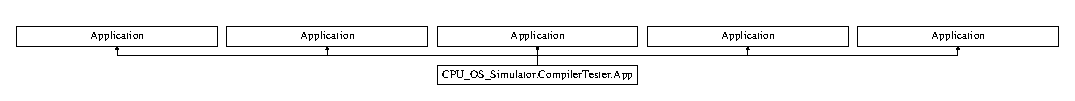
\includegraphics[height=2.000000cm]{class_c_p_u___o_s___simulator_1_1_compiler_tester_1_1_app}
\end{center}
\end{figure}


\subsection{Detailed Description}
Interaction logic for App.\+xaml 



Definition at line 8 of file App.\+xaml.\+cs.



The documentation for this class was generated from the following file\+:\begin{DoxyCompactItemize}
\item 
Compiler\+Tester/\hyperlink{_compiler_tester_2_app_8xaml_8cs}{App.\+xaml.\+cs}\end{DoxyCompactItemize}

\hypertarget{class_c_p_u___o_s___simulator_1_1_app}{}\section{C\+P\+U\+\_\+\+O\+S\+\_\+\+Simulator.\+App Class Reference}
\label{class_c_p_u___o_s___simulator_1_1_app}\index{C\+P\+U\+\_\+\+O\+S\+\_\+\+Simulator.\+App@{C\+P\+U\+\_\+\+O\+S\+\_\+\+Simulator.\+App}}


Interaction logic for App.\+xaml  


Inheritance diagram for C\+P\+U\+\_\+\+O\+S\+\_\+\+Simulator.\+App\+:\begin{figure}[H]
\begin{center}
\leavevmode
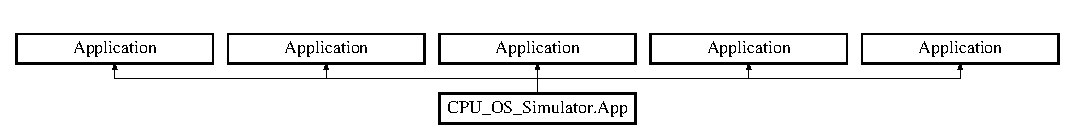
\includegraphics[height=2.000000cm]{class_c_p_u___o_s___simulator_1_1_app}
\end{center}
\end{figure}
\subsection*{Public Member Functions}
\begin{DoxyCompactItemize}
\item 
void \hyperlink{class_c_p_u___o_s___simulator_1_1_app_a15e2e0e02c8dbe7d5d3fba5d21f3e56f}{Initialize\+Component} ()
\begin{DoxyCompactList}\small\item\em Initialize\+Component \end{DoxyCompactList}\item 
void \hyperlink{class_c_p_u___o_s___simulator_1_1_app_a15e2e0e02c8dbe7d5d3fba5d21f3e56f}{Initialize\+Component} ()
\begin{DoxyCompactList}\small\item\em Initialize\+Component \end{DoxyCompactList}\end{DoxyCompactItemize}
\subsection*{Static Public Member Functions}
\begin{DoxyCompactItemize}
\item 
static void \hyperlink{class_c_p_u___o_s___simulator_1_1_app_a7bbb69f458b77923e336283b1653ce69}{Main} ()
\begin{DoxyCompactList}\small\item\em Application Entry Point. \end{DoxyCompactList}\item 
static void \hyperlink{class_c_p_u___o_s___simulator_1_1_app_a7bbb69f458b77923e336283b1653ce69}{Main} ()
\begin{DoxyCompactList}\small\item\em Application Entry Point. \end{DoxyCompactList}\end{DoxyCompactItemize}


\subsection{Detailed Description}
Interaction logic for App.\+xaml 

\hyperlink{class_c_p_u___o_s___simulator_1_1_app}{App} 

Definition at line 8 of file App.\+xaml.\+cs.



\subsection{Member Function Documentation}
\hypertarget{class_c_p_u___o_s___simulator_1_1_app_a15e2e0e02c8dbe7d5d3fba5d21f3e56f}{}\index{C\+P\+U\+\_\+\+O\+S\+\_\+\+Simulator\+::\+App@{C\+P\+U\+\_\+\+O\+S\+\_\+\+Simulator\+::\+App}!Initialize\+Component@{Initialize\+Component}}
\index{Initialize\+Component@{Initialize\+Component}!C\+P\+U\+\_\+\+O\+S\+\_\+\+Simulator\+::\+App@{C\+P\+U\+\_\+\+O\+S\+\_\+\+Simulator\+::\+App}}
\subsubsection[{Initialize\+Component()}]{\setlength{\rightskip}{0pt plus 5cm}void C\+P\+U\+\_\+\+O\+S\+\_\+\+Simulator.\+App.\+Initialize\+Component (
\begin{DoxyParamCaption}
{}
\end{DoxyParamCaption}
)}\label{class_c_p_u___o_s___simulator_1_1_app_a15e2e0e02c8dbe7d5d3fba5d21f3e56f}


Initialize\+Component 



Definition at line 48 of file App.\+g.\+cs.

\hypertarget{class_c_p_u___o_s___simulator_1_1_app_a15e2e0e02c8dbe7d5d3fba5d21f3e56f}{}\index{C\+P\+U\+\_\+\+O\+S\+\_\+\+Simulator\+::\+App@{C\+P\+U\+\_\+\+O\+S\+\_\+\+Simulator\+::\+App}!Initialize\+Component@{Initialize\+Component}}
\index{Initialize\+Component@{Initialize\+Component}!C\+P\+U\+\_\+\+O\+S\+\_\+\+Simulator\+::\+App@{C\+P\+U\+\_\+\+O\+S\+\_\+\+Simulator\+::\+App}}
\subsubsection[{Initialize\+Component()}]{\setlength{\rightskip}{0pt plus 5cm}void C\+P\+U\+\_\+\+O\+S\+\_\+\+Simulator.\+App.\+Initialize\+Component (
\begin{DoxyParamCaption}
{}
\end{DoxyParamCaption}
)}\label{class_c_p_u___o_s___simulator_1_1_app_a15e2e0e02c8dbe7d5d3fba5d21f3e56f}


Initialize\+Component 



Definition at line 48 of file App.\+g.\+i.\+cs.

\hypertarget{class_c_p_u___o_s___simulator_1_1_app_a7bbb69f458b77923e336283b1653ce69}{}\index{C\+P\+U\+\_\+\+O\+S\+\_\+\+Simulator\+::\+App@{C\+P\+U\+\_\+\+O\+S\+\_\+\+Simulator\+::\+App}!Main@{Main}}
\index{Main@{Main}!C\+P\+U\+\_\+\+O\+S\+\_\+\+Simulator\+::\+App@{C\+P\+U\+\_\+\+O\+S\+\_\+\+Simulator\+::\+App}}
\subsubsection[{Main()}]{\setlength{\rightskip}{0pt plus 5cm}static void C\+P\+U\+\_\+\+O\+S\+\_\+\+Simulator.\+App.\+Main (
\begin{DoxyParamCaption}
{}
\end{DoxyParamCaption}
)\hspace{0.3cm}{\ttfamily [static]}}\label{class_c_p_u___o_s___simulator_1_1_app_a7bbb69f458b77923e336283b1653ce69}


Application Entry Point. 



Definition at line 63 of file App.\+g.\+i.\+cs.

\hypertarget{class_c_p_u___o_s___simulator_1_1_app_a7bbb69f458b77923e336283b1653ce69}{}\index{C\+P\+U\+\_\+\+O\+S\+\_\+\+Simulator\+::\+App@{C\+P\+U\+\_\+\+O\+S\+\_\+\+Simulator\+::\+App}!Main@{Main}}
\index{Main@{Main}!C\+P\+U\+\_\+\+O\+S\+\_\+\+Simulator\+::\+App@{C\+P\+U\+\_\+\+O\+S\+\_\+\+Simulator\+::\+App}}
\subsubsection[{Main()}]{\setlength{\rightskip}{0pt plus 5cm}static void C\+P\+U\+\_\+\+O\+S\+\_\+\+Simulator.\+App.\+Main (
\begin{DoxyParamCaption}
{}
\end{DoxyParamCaption}
)\hspace{0.3cm}{\ttfamily [static]}}\label{class_c_p_u___o_s___simulator_1_1_app_a7bbb69f458b77923e336283b1653ce69}


Application Entry Point. 



Definition at line 63 of file App.\+g.\+cs.



The documentation for this class was generated from the following files\+:\begin{DoxyCompactItemize}
\item 
C\+P\+U-\/\+O\+S Simulator/\hyperlink{_app_8xaml_8cs}{App.\+xaml.\+cs}\item 
C\+P\+U-\/\+O\+S Simulator/obj/\+Debug/\hyperlink{_app_8g_8cs}{App.\+g.\+cs}\item 
C\+P\+U-\/\+O\+S Simulator/obj/\+Debug/\hyperlink{_app_8g_8i_8cs}{App.\+g.\+i.\+cs}\end{DoxyCompactItemize}

\hypertarget{class_c_p_u___o_s___simulator_1_1_compiler_1_1_frontend_1_1_syntax_tree_1_1_array_node}{}\section{C\+P\+U\+\_\+\+O\+S\+\_\+\+Simulator.\+Compiler.\+Frontend.\+Syntax\+Tree.\+Array\+Node Class Reference}
\label{class_c_p_u___o_s___simulator_1_1_compiler_1_1_frontend_1_1_syntax_tree_1_1_array_node}\index{C\+P\+U\+\_\+\+O\+S\+\_\+\+Simulator.\+Compiler.\+Frontend.\+Syntax\+Tree.\+Array\+Node@{C\+P\+U\+\_\+\+O\+S\+\_\+\+Simulator.\+Compiler.\+Frontend.\+Syntax\+Tree.\+Array\+Node}}
Inheritance diagram for C\+P\+U\+\_\+\+O\+S\+\_\+\+Simulator.\+Compiler.\+Frontend.\+Syntax\+Tree.\+Array\+Node\+:\begin{figure}[H]
\begin{center}
\leavevmode
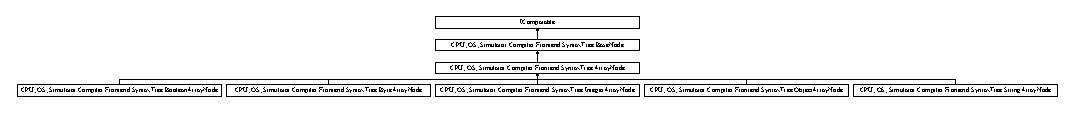
\includegraphics[height=1.069212cm]{class_c_p_u___o_s___simulator_1_1_compiler_1_1_frontend_1_1_syntax_tree_1_1_array_node}
\end{center}
\end{figure}
\subsection*{Public Member Functions}
\begin{DoxyCompactItemize}
\item 
abstract override void \hyperlink{class_c_p_u___o_s___simulator_1_1_compiler_1_1_frontend_1_1_syntax_tree_1_1_array_node_aed695b6f32d5c176204fc15854db32db}{Visit} ()
\begin{DoxyCompactList}\small\item\em This function is called when the node is being visited by the parser \end{DoxyCompactList}\item 
abstract override void \hyperlink{class_c_p_u___o_s___simulator_1_1_compiler_1_1_frontend_1_1_syntax_tree_1_1_array_node_afdb5d2808dbd83c28c85f35b6430edc4}{Evaluate} ()
\begin{DoxyCompactList}\small\item\em This Function is called when the node is being evaluated by the parser \end{DoxyCompactList}\item 
abstract int \hyperlink{class_c_p_u___o_s___simulator_1_1_compiler_1_1_frontend_1_1_syntax_tree_1_1_array_node_a75232f3076d95a562405ef2722bcafd5}{number\+Of\+Elements} ()
\end{DoxyCompactItemize}
\subsection*{Properties}
\begin{DoxyCompactItemize}
\item 
abstract override \hyperlink{class_c_p_u___o_s___simulator_1_1_compiler_1_1_frontend_1_1_syntax_tree_1_1_base_node}{Base\+Node} \hyperlink{class_c_p_u___o_s___simulator_1_1_compiler_1_1_frontend_1_1_syntax_tree_1_1_array_node_a422bdd9640f912faf3785fdd0b1d1c34}{Right}\hspace{0.3cm}{\ttfamily  \mbox{[}get, set\mbox{]}}
\item 
abstract override \hyperlink{class_c_p_u___o_s___simulator_1_1_compiler_1_1_frontend_1_1_syntax_tree_1_1_base_node}{Base\+Node} \hyperlink{class_c_p_u___o_s___simulator_1_1_compiler_1_1_frontend_1_1_syntax_tree_1_1_array_node_a432b69f0632ea4f0132e500712760bfe}{Left}\hspace{0.3cm}{\ttfamily  \mbox{[}get, set\mbox{]}}
\end{DoxyCompactItemize}
\subsection*{Additional Inherited Members}


\subsection{Detailed Description}


Definition at line 9 of file Array\+Node.\+cs.



\subsection{Member Function Documentation}
\hypertarget{class_c_p_u___o_s___simulator_1_1_compiler_1_1_frontend_1_1_syntax_tree_1_1_array_node_afdb5d2808dbd83c28c85f35b6430edc4}{}\index{C\+P\+U\+\_\+\+O\+S\+\_\+\+Simulator\+::\+Compiler\+::\+Frontend\+::\+Syntax\+Tree\+::\+Array\+Node@{C\+P\+U\+\_\+\+O\+S\+\_\+\+Simulator\+::\+Compiler\+::\+Frontend\+::\+Syntax\+Tree\+::\+Array\+Node}!Evaluate@{Evaluate}}
\index{Evaluate@{Evaluate}!C\+P\+U\+\_\+\+O\+S\+\_\+\+Simulator\+::\+Compiler\+::\+Frontend\+::\+Syntax\+Tree\+::\+Array\+Node@{C\+P\+U\+\_\+\+O\+S\+\_\+\+Simulator\+::\+Compiler\+::\+Frontend\+::\+Syntax\+Tree\+::\+Array\+Node}}
\subsubsection[{Evaluate()}]{\setlength{\rightskip}{0pt plus 5cm}abstract override void C\+P\+U\+\_\+\+O\+S\+\_\+\+Simulator.\+Compiler.\+Frontend.\+Syntax\+Tree.\+Array\+Node.\+Evaluate (
\begin{DoxyParamCaption}
{}
\end{DoxyParamCaption}
)\hspace{0.3cm}{\ttfamily [pure virtual]}}\label{class_c_p_u___o_s___simulator_1_1_compiler_1_1_frontend_1_1_syntax_tree_1_1_array_node_afdb5d2808dbd83c28c85f35b6430edc4}


This Function is called when the node is being evaluated by the parser 



Implements \hyperlink{class_c_p_u___o_s___simulator_1_1_compiler_1_1_frontend_1_1_syntax_tree_1_1_base_node_a6cfcf8a0795180bdb1c7f0735d39441b}{C\+P\+U\+\_\+\+O\+S\+\_\+\+Simulator.\+Compiler.\+Frontend.\+Syntax\+Tree.\+Base\+Node}.



Implemented in \hyperlink{class_c_p_u___o_s___simulator_1_1_compiler_1_1_frontend_1_1_syntax_tree_1_1_integer_array_node_a28619c1f8b99cea0b827ba5a71a00e35}{C\+P\+U\+\_\+\+O\+S\+\_\+\+Simulator.\+Compiler.\+Frontend.\+Syntax\+Tree.\+Integer\+Array\+Node}, \hyperlink{class_c_p_u___o_s___simulator_1_1_compiler_1_1_frontend_1_1_syntax_tree_1_1_boolean_array_node_a6de955407e0bce191f3f09a5cf6f4d50}{C\+P\+U\+\_\+\+O\+S\+\_\+\+Simulator.\+Compiler.\+Frontend.\+Syntax\+Tree.\+Boolean\+Array\+Node}, \hyperlink{class_c_p_u___o_s___simulator_1_1_compiler_1_1_frontend_1_1_syntax_tree_1_1_object_array_node_ad0c63367dd74b502a0e510b95e324405}{C\+P\+U\+\_\+\+O\+S\+\_\+\+Simulator.\+Compiler.\+Frontend.\+Syntax\+Tree.\+Object\+Array\+Node}, \hyperlink{class_c_p_u___o_s___simulator_1_1_compiler_1_1_frontend_1_1_syntax_tree_1_1_byte_array_node_ad34fd3396bf5e6e179d941d2076f28d9}{C\+P\+U\+\_\+\+O\+S\+\_\+\+Simulator.\+Compiler.\+Frontend.\+Syntax\+Tree.\+Byte\+Array\+Node}, and \hyperlink{class_c_p_u___o_s___simulator_1_1_compiler_1_1_frontend_1_1_syntax_tree_1_1_string_array_node_a559630365acec250f2eed840010535f8}{C\+P\+U\+\_\+\+O\+S\+\_\+\+Simulator.\+Compiler.\+Frontend.\+Syntax\+Tree.\+String\+Array\+Node}.

\hypertarget{class_c_p_u___o_s___simulator_1_1_compiler_1_1_frontend_1_1_syntax_tree_1_1_array_node_a75232f3076d95a562405ef2722bcafd5}{}\index{C\+P\+U\+\_\+\+O\+S\+\_\+\+Simulator\+::\+Compiler\+::\+Frontend\+::\+Syntax\+Tree\+::\+Array\+Node@{C\+P\+U\+\_\+\+O\+S\+\_\+\+Simulator\+::\+Compiler\+::\+Frontend\+::\+Syntax\+Tree\+::\+Array\+Node}!number\+Of\+Elements@{number\+Of\+Elements}}
\index{number\+Of\+Elements@{number\+Of\+Elements}!C\+P\+U\+\_\+\+O\+S\+\_\+\+Simulator\+::\+Compiler\+::\+Frontend\+::\+Syntax\+Tree\+::\+Array\+Node@{C\+P\+U\+\_\+\+O\+S\+\_\+\+Simulator\+::\+Compiler\+::\+Frontend\+::\+Syntax\+Tree\+::\+Array\+Node}}
\subsubsection[{number\+Of\+Elements()}]{\setlength{\rightskip}{0pt plus 5cm}abstract int C\+P\+U\+\_\+\+O\+S\+\_\+\+Simulator.\+Compiler.\+Frontend.\+Syntax\+Tree.\+Array\+Node.\+number\+Of\+Elements (
\begin{DoxyParamCaption}
{}
\end{DoxyParamCaption}
)\hspace{0.3cm}{\ttfamily [pure virtual]}}\label{class_c_p_u___o_s___simulator_1_1_compiler_1_1_frontend_1_1_syntax_tree_1_1_array_node_a75232f3076d95a562405ef2722bcafd5}


Implemented in \hyperlink{class_c_p_u___o_s___simulator_1_1_compiler_1_1_frontend_1_1_syntax_tree_1_1_integer_array_node_a6172b87f60f5fd82e055b6d13969297b}{C\+P\+U\+\_\+\+O\+S\+\_\+\+Simulator.\+Compiler.\+Frontend.\+Syntax\+Tree.\+Integer\+Array\+Node}, \hyperlink{class_c_p_u___o_s___simulator_1_1_compiler_1_1_frontend_1_1_syntax_tree_1_1_boolean_array_node_aaafab6f46bfdc5bd4a4209a7ddc927d6}{C\+P\+U\+\_\+\+O\+S\+\_\+\+Simulator.\+Compiler.\+Frontend.\+Syntax\+Tree.\+Boolean\+Array\+Node}, \hyperlink{class_c_p_u___o_s___simulator_1_1_compiler_1_1_frontend_1_1_syntax_tree_1_1_object_array_node_ae2b8cfd71ef1f35f3f74d700fc542fc1}{C\+P\+U\+\_\+\+O\+S\+\_\+\+Simulator.\+Compiler.\+Frontend.\+Syntax\+Tree.\+Object\+Array\+Node}, \hyperlink{class_c_p_u___o_s___simulator_1_1_compiler_1_1_frontend_1_1_syntax_tree_1_1_byte_array_node_a899a0a2406a3e09828de51918a13afba}{C\+P\+U\+\_\+\+O\+S\+\_\+\+Simulator.\+Compiler.\+Frontend.\+Syntax\+Tree.\+Byte\+Array\+Node}, and \hyperlink{class_c_p_u___o_s___simulator_1_1_compiler_1_1_frontend_1_1_syntax_tree_1_1_string_array_node_aff86779eee1fe0119c3b717f6d673f2c}{C\+P\+U\+\_\+\+O\+S\+\_\+\+Simulator.\+Compiler.\+Frontend.\+Syntax\+Tree.\+String\+Array\+Node}.

\hypertarget{class_c_p_u___o_s___simulator_1_1_compiler_1_1_frontend_1_1_syntax_tree_1_1_array_node_aed695b6f32d5c176204fc15854db32db}{}\index{C\+P\+U\+\_\+\+O\+S\+\_\+\+Simulator\+::\+Compiler\+::\+Frontend\+::\+Syntax\+Tree\+::\+Array\+Node@{C\+P\+U\+\_\+\+O\+S\+\_\+\+Simulator\+::\+Compiler\+::\+Frontend\+::\+Syntax\+Tree\+::\+Array\+Node}!Visit@{Visit}}
\index{Visit@{Visit}!C\+P\+U\+\_\+\+O\+S\+\_\+\+Simulator\+::\+Compiler\+::\+Frontend\+::\+Syntax\+Tree\+::\+Array\+Node@{C\+P\+U\+\_\+\+O\+S\+\_\+\+Simulator\+::\+Compiler\+::\+Frontend\+::\+Syntax\+Tree\+::\+Array\+Node}}
\subsubsection[{Visit()}]{\setlength{\rightskip}{0pt plus 5cm}abstract override void C\+P\+U\+\_\+\+O\+S\+\_\+\+Simulator.\+Compiler.\+Frontend.\+Syntax\+Tree.\+Array\+Node.\+Visit (
\begin{DoxyParamCaption}
{}
\end{DoxyParamCaption}
)\hspace{0.3cm}{\ttfamily [pure virtual]}}\label{class_c_p_u___o_s___simulator_1_1_compiler_1_1_frontend_1_1_syntax_tree_1_1_array_node_aed695b6f32d5c176204fc15854db32db}


This function is called when the node is being visited by the parser 



Implements \hyperlink{class_c_p_u___o_s___simulator_1_1_compiler_1_1_frontend_1_1_syntax_tree_1_1_base_node_a092377df64002c5e9c023a259e5e11d0}{C\+P\+U\+\_\+\+O\+S\+\_\+\+Simulator.\+Compiler.\+Frontend.\+Syntax\+Tree.\+Base\+Node}.



Implemented in \hyperlink{class_c_p_u___o_s___simulator_1_1_compiler_1_1_frontend_1_1_syntax_tree_1_1_integer_array_node_a7abbf1320b21da1362fc8d391907d33f}{C\+P\+U\+\_\+\+O\+S\+\_\+\+Simulator.\+Compiler.\+Frontend.\+Syntax\+Tree.\+Integer\+Array\+Node}, \hyperlink{class_c_p_u___o_s___simulator_1_1_compiler_1_1_frontend_1_1_syntax_tree_1_1_boolean_array_node_a192727033dc9533113312210f04a958a}{C\+P\+U\+\_\+\+O\+S\+\_\+\+Simulator.\+Compiler.\+Frontend.\+Syntax\+Tree.\+Boolean\+Array\+Node}, \hyperlink{class_c_p_u___o_s___simulator_1_1_compiler_1_1_frontend_1_1_syntax_tree_1_1_object_array_node_a1d792b3929152ecfa25dac2e8c6444cc}{C\+P\+U\+\_\+\+O\+S\+\_\+\+Simulator.\+Compiler.\+Frontend.\+Syntax\+Tree.\+Object\+Array\+Node}, \hyperlink{class_c_p_u___o_s___simulator_1_1_compiler_1_1_frontend_1_1_syntax_tree_1_1_byte_array_node_a1ed9d8d35aeb8537758718aa1bae1ae0}{C\+P\+U\+\_\+\+O\+S\+\_\+\+Simulator.\+Compiler.\+Frontend.\+Syntax\+Tree.\+Byte\+Array\+Node}, and \hyperlink{class_c_p_u___o_s___simulator_1_1_compiler_1_1_frontend_1_1_syntax_tree_1_1_string_array_node_ae8ce8f85a313e577506546a26c954e34}{C\+P\+U\+\_\+\+O\+S\+\_\+\+Simulator.\+Compiler.\+Frontend.\+Syntax\+Tree.\+String\+Array\+Node}.



\subsection{Property Documentation}
\hypertarget{class_c_p_u___o_s___simulator_1_1_compiler_1_1_frontend_1_1_syntax_tree_1_1_array_node_a432b69f0632ea4f0132e500712760bfe}{}\index{C\+P\+U\+\_\+\+O\+S\+\_\+\+Simulator\+::\+Compiler\+::\+Frontend\+::\+Syntax\+Tree\+::\+Array\+Node@{C\+P\+U\+\_\+\+O\+S\+\_\+\+Simulator\+::\+Compiler\+::\+Frontend\+::\+Syntax\+Tree\+::\+Array\+Node}!Left@{Left}}
\index{Left@{Left}!C\+P\+U\+\_\+\+O\+S\+\_\+\+Simulator\+::\+Compiler\+::\+Frontend\+::\+Syntax\+Tree\+::\+Array\+Node@{C\+P\+U\+\_\+\+O\+S\+\_\+\+Simulator\+::\+Compiler\+::\+Frontend\+::\+Syntax\+Tree\+::\+Array\+Node}}
\subsubsection[{Left}]{\setlength{\rightskip}{0pt plus 5cm}abstract override {\bf Base\+Node} C\+P\+U\+\_\+\+O\+S\+\_\+\+Simulator.\+Compiler.\+Frontend.\+Syntax\+Tree.\+Array\+Node.\+Left\hspace{0.3cm}{\ttfamily [get]}, {\ttfamily [set]}}\label{class_c_p_u___o_s___simulator_1_1_compiler_1_1_frontend_1_1_syntax_tree_1_1_array_node_a432b69f0632ea4f0132e500712760bfe}


Definition at line 13 of file Array\+Node.\+cs.

\hypertarget{class_c_p_u___o_s___simulator_1_1_compiler_1_1_frontend_1_1_syntax_tree_1_1_array_node_a422bdd9640f912faf3785fdd0b1d1c34}{}\index{C\+P\+U\+\_\+\+O\+S\+\_\+\+Simulator\+::\+Compiler\+::\+Frontend\+::\+Syntax\+Tree\+::\+Array\+Node@{C\+P\+U\+\_\+\+O\+S\+\_\+\+Simulator\+::\+Compiler\+::\+Frontend\+::\+Syntax\+Tree\+::\+Array\+Node}!Right@{Right}}
\index{Right@{Right}!C\+P\+U\+\_\+\+O\+S\+\_\+\+Simulator\+::\+Compiler\+::\+Frontend\+::\+Syntax\+Tree\+::\+Array\+Node@{C\+P\+U\+\_\+\+O\+S\+\_\+\+Simulator\+::\+Compiler\+::\+Frontend\+::\+Syntax\+Tree\+::\+Array\+Node}}
\subsubsection[{Right}]{\setlength{\rightskip}{0pt plus 5cm}abstract override {\bf Base\+Node} C\+P\+U\+\_\+\+O\+S\+\_\+\+Simulator.\+Compiler.\+Frontend.\+Syntax\+Tree.\+Array\+Node.\+Right\hspace{0.3cm}{\ttfamily [get]}, {\ttfamily [set]}}\label{class_c_p_u___o_s___simulator_1_1_compiler_1_1_frontend_1_1_syntax_tree_1_1_array_node_a422bdd9640f912faf3785fdd0b1d1c34}


Definition at line 11 of file Array\+Node.\+cs.



The documentation for this class was generated from the following file\+:\begin{DoxyCompactItemize}
\item 
Compiler/\+Frontend/\+Syntax\+Tree/\hyperlink{_array_node_8cs}{Array\+Node.\+cs}\end{DoxyCompactItemize}

\hypertarget{class_c_p_u___o_s___simulator_1_1_compiler_1_1_frontend_1_1_syntax_tree_1_1_a_s_t}{}\section{C\+P\+U\+\_\+\+O\+S\+\_\+\+Simulator.\+Compiler.\+Frontend.\+Syntax\+Tree.\+A\+S\+T Class Reference}
\label{class_c_p_u___o_s___simulator_1_1_compiler_1_1_frontend_1_1_syntax_tree_1_1_a_s_t}\index{C\+P\+U\+\_\+\+O\+S\+\_\+\+Simulator.\+Compiler.\+Frontend.\+Syntax\+Tree.\+A\+S\+T@{C\+P\+U\+\_\+\+O\+S\+\_\+\+Simulator.\+Compiler.\+Frontend.\+Syntax\+Tree.\+A\+S\+T}}
\subsection*{Classes}
\begin{DoxyCompactItemize}
\item 
class \hyperlink{class_c_p_u___o_s___simulator_1_1_compiler_1_1_frontend_1_1_syntax_tree_1_1_a_s_t_1_1_binary_tree_enumerator}{Binary\+Tree\+Enumerator}
\begin{DoxyCompactList}\small\item\em The \hyperlink{class_c_p_u___o_s___simulator_1_1_compiler_1_1_frontend_1_1_syntax_tree_1_1_a_s_t_1_1_binary_tree_enumerator}{Binary\+Tree\+Enumerator} implements the I\+Enumerator allowing foreach enumeration of the tree \end{DoxyCompactList}\end{DoxyCompactItemize}
\subsection*{Public Member Functions}
\begin{DoxyCompactItemize}
\item 
\hyperlink{class_c_p_u___o_s___simulator_1_1_compiler_1_1_frontend_1_1_syntax_tree_1_1_a_s_t_aadbd3af47353b1564454f2352b188875}{A\+S\+T} (Comparison$<$ \hyperlink{class_c_p_u___o_s___simulator_1_1_compiler_1_1_frontend_1_1_syntax_tree_1_1_base_node}{Base\+Node} $>$ the\+Compare\+Function)
\begin{DoxyCompactList}\small\item\em The \hyperlink{class_c_p_u___o_s___simulator_1_1_compiler_1_1_frontend_1_1_syntax_tree_1_1_a_s_t}{A\+S\+T} constructor requires that we pass a comparison function. We need one as generics can only be compared as equals, but not for order. The solution is to allow the caller to pass a suitable comparison function. We use the C\# Comparison delegate for this (found in System.\+Collections) \end{DoxyCompactList}\item 
void \hyperlink{class_c_p_u___o_s___simulator_1_1_compiler_1_1_frontend_1_1_syntax_tree_1_1_a_s_t_a73bb6e82554120e16b12f975ccfc44a5}{preorder\+Traversal} ()
\item 
void \hyperlink{class_c_p_u___o_s___simulator_1_1_compiler_1_1_frontend_1_1_syntax_tree_1_1_a_s_t_afc826af945c5461d38b0ca398ab3f14b}{inorder\+Traversal} ()
\item 
void \hyperlink{class_c_p_u___o_s___simulator_1_1_compiler_1_1_frontend_1_1_syntax_tree_1_1_a_s_t_a72dc35aaccad4aeee3373b8d2dbb23d1}{postorder\+Traversal} ()
\item 
void \hyperlink{class_c_p_u___o_s___simulator_1_1_compiler_1_1_frontend_1_1_syntax_tree_1_1_a_s_t_adc6fcfed38dfdeddcbe419523cdc0314}{Add} (\hyperlink{class_c_p_u___o_s___simulator_1_1_compiler_1_1_frontend_1_1_syntax_tree_1_1_base_node}{Base\+Node} Value)
\begin{DoxyCompactList}\small\item\em The add function uses non-\/recursive tree traversal to find the next available insertion point \end{DoxyCompactList}\item 
bool \hyperlink{class_c_p_u___o_s___simulator_1_1_compiler_1_1_frontend_1_1_syntax_tree_1_1_a_s_t_aa37a7925b23003f227b9311c6201a427}{Find} (\hyperlink{class_c_p_u___o_s___simulator_1_1_compiler_1_1_frontend_1_1_syntax_tree_1_1_base_node}{Base\+Node} Value)
\begin{DoxyCompactList}\small\item\em This routine walks through the tree to see if the value given can be found. \end{DoxyCompactList}\item 
I\+Enumerator$<$ \hyperlink{class_c_p_u___o_s___simulator_1_1_compiler_1_1_frontend_1_1_syntax_tree_1_1_base_node}{Base\+Node} $>$ \hyperlink{class_c_p_u___o_s___simulator_1_1_compiler_1_1_frontend_1_1_syntax_tree_1_1_a_s_t_aceaad03d78fc54155a4c18a13ac89e92}{Get\+Enumerator} ()
\begin{DoxyCompactList}\small\item\em Returns a list iterator of the elements in the tree implementing the I\+E\+Numerator interface. \end{DoxyCompactList}\end{DoxyCompactItemize}
\subsection*{Static Public Member Functions}
\begin{DoxyCompactItemize}
\item 
static int \hyperlink{class_c_p_u___o_s___simulator_1_1_compiler_1_1_frontend_1_1_syntax_tree_1_1_a_s_t_ae5a39e32b179110397b6e556d0a2b3d7}{Compare\+Function\+\_\+\+Int} (int left, int right)
\begin{DoxyCompactList}\small\item\em For integer comparisons we provide a demonstration function. \end{DoxyCompactList}\item 
static int \hyperlink{class_c_p_u___o_s___simulator_1_1_compiler_1_1_frontend_1_1_syntax_tree_1_1_a_s_t_ad66f655202794d09ce58ef9fcc690a34}{Compare\+Function\+\_\+\+String} (string left, string right)
\begin{DoxyCompactList}\small\item\em For string comparisons we provide a demonstration function \end{DoxyCompactList}\end{DoxyCompactItemize}
\subsection*{Private Member Functions}
\begin{DoxyCompactItemize}
\item 
\hyperlink{class_c_p_u___o_s___simulator_1_1_compiler_1_1_frontend_1_1_syntax_tree_1_1_base_node}{Base\+Node} \hyperlink{class_c_p_u___o_s___simulator_1_1_compiler_1_1_frontend_1_1_syntax_tree_1_1_a_s_t_ad6c751aec63a7123d0e472639a32ed5a}{Find\+Most\+Left} (\hyperlink{class_c_p_u___o_s___simulator_1_1_compiler_1_1_frontend_1_1_syntax_tree_1_1_base_node}{Base\+Node} start)
\begin{DoxyCompactList}\small\item\em Given a starting node, this routine will locate the left most node in the sub-\/tree If no further nodes are found, it returns the starting node \end{DoxyCompactList}\end{DoxyCompactItemize}
\subsection*{Private Attributes}
\begin{DoxyCompactItemize}
\item 
\hyperlink{class_c_p_u___o_s___simulator_1_1_compiler_1_1_frontend_1_1_syntax_tree_1_1_base_node}{Base\+Node} \hyperlink{class_c_p_u___o_s___simulator_1_1_compiler_1_1_frontend_1_1_syntax_tree_1_1_a_s_t_adad46444c7a366abd0fb32f51df95a95}{Root}
\begin{DoxyCompactList}\small\item\em The tree is build up out of \hyperlink{class_c_p_u___o_s___simulator_1_1_compiler_1_1_frontend_1_1_syntax_tree_1_1_base_node}{Base\+Node} instances \end{DoxyCompactList}\item 
Comparison$<$ \hyperlink{class_c_p_u___o_s___simulator_1_1_compiler_1_1_frontend_1_1_syntax_tree_1_1_base_node}{Base\+Node} $>$ \hyperlink{class_c_p_u___o_s___simulator_1_1_compiler_1_1_frontend_1_1_syntax_tree_1_1_a_s_t_ab70cc1242f97a9e07dd6aec88ec0b2f5}{Compare\+Function}
\end{DoxyCompactItemize}


\subsection{Detailed Description}


Definition at line 6 of file A\+S\+T.\+cs.



\subsection{Constructor \& Destructor Documentation}
\hypertarget{class_c_p_u___o_s___simulator_1_1_compiler_1_1_frontend_1_1_syntax_tree_1_1_a_s_t_aadbd3af47353b1564454f2352b188875}{}\index{C\+P\+U\+\_\+\+O\+S\+\_\+\+Simulator\+::\+Compiler\+::\+Frontend\+::\+Syntax\+Tree\+::\+A\+S\+T@{C\+P\+U\+\_\+\+O\+S\+\_\+\+Simulator\+::\+Compiler\+::\+Frontend\+::\+Syntax\+Tree\+::\+A\+S\+T}!A\+S\+T@{A\+S\+T}}
\index{A\+S\+T@{A\+S\+T}!C\+P\+U\+\_\+\+O\+S\+\_\+\+Simulator\+::\+Compiler\+::\+Frontend\+::\+Syntax\+Tree\+::\+A\+S\+T@{C\+P\+U\+\_\+\+O\+S\+\_\+\+Simulator\+::\+Compiler\+::\+Frontend\+::\+Syntax\+Tree\+::\+A\+S\+T}}
\subsubsection[{A\+S\+T(\+Comparison$<$ Base\+Node $>$ the\+Compare\+Function)}]{\setlength{\rightskip}{0pt plus 5cm}C\+P\+U\+\_\+\+O\+S\+\_\+\+Simulator.\+Compiler.\+Frontend.\+Syntax\+Tree.\+A\+S\+T.\+A\+S\+T (
\begin{DoxyParamCaption}
\item[{Comparison$<$ {\bf Base\+Node} $>$}]{the\+Compare\+Function}
\end{DoxyParamCaption}
)}\label{class_c_p_u___o_s___simulator_1_1_compiler_1_1_frontend_1_1_syntax_tree_1_1_a_s_t_aadbd3af47353b1564454f2352b188875}


The \hyperlink{class_c_p_u___o_s___simulator_1_1_compiler_1_1_frontend_1_1_syntax_tree_1_1_a_s_t}{A\+S\+T} constructor requires that we pass a comparison function. We need one as generics can only be compared as equals, but not for order. The solution is to allow the caller to pass a suitable comparison function. We use the C\# Comparison delegate for this (found in System.\+Collections) 


\begin{DoxyParams}{Parameters}
{\em the\+Compare\+Function} & Pass a delegate function of the type Comparison to the function\\
\hline
\end{DoxyParams}


Definition at line 23 of file A\+S\+T.\+cs.



\subsection{Member Function Documentation}
\hypertarget{class_c_p_u___o_s___simulator_1_1_compiler_1_1_frontend_1_1_syntax_tree_1_1_a_s_t_adc6fcfed38dfdeddcbe419523cdc0314}{}\index{C\+P\+U\+\_\+\+O\+S\+\_\+\+Simulator\+::\+Compiler\+::\+Frontend\+::\+Syntax\+Tree\+::\+A\+S\+T@{C\+P\+U\+\_\+\+O\+S\+\_\+\+Simulator\+::\+Compiler\+::\+Frontend\+::\+Syntax\+Tree\+::\+A\+S\+T}!Add@{Add}}
\index{Add@{Add}!C\+P\+U\+\_\+\+O\+S\+\_\+\+Simulator\+::\+Compiler\+::\+Frontend\+::\+Syntax\+Tree\+::\+A\+S\+T@{C\+P\+U\+\_\+\+O\+S\+\_\+\+Simulator\+::\+Compiler\+::\+Frontend\+::\+Syntax\+Tree\+::\+A\+S\+T}}
\subsubsection[{Add(\+Base\+Node Value)}]{\setlength{\rightskip}{0pt plus 5cm}void C\+P\+U\+\_\+\+O\+S\+\_\+\+Simulator.\+Compiler.\+Frontend.\+Syntax\+Tree.\+A\+S\+T.\+Add (
\begin{DoxyParamCaption}
\item[{{\bf Base\+Node}}]{Value}
\end{DoxyParamCaption}
)}\label{class_c_p_u___o_s___simulator_1_1_compiler_1_1_frontend_1_1_syntax_tree_1_1_a_s_t_adc6fcfed38dfdeddcbe419523cdc0314}


The add function uses non-\/recursive tree traversal to find the next available insertion point 


\begin{DoxyParams}{Parameters}
{\em Value} & The value to insert into tree.\\
\hline
\end{DoxyParams}


Definition at line 152 of file A\+S\+T.\+cs.

\hypertarget{class_c_p_u___o_s___simulator_1_1_compiler_1_1_frontend_1_1_syntax_tree_1_1_a_s_t_ae5a39e32b179110397b6e556d0a2b3d7}{}\index{C\+P\+U\+\_\+\+O\+S\+\_\+\+Simulator\+::\+Compiler\+::\+Frontend\+::\+Syntax\+Tree\+::\+A\+S\+T@{C\+P\+U\+\_\+\+O\+S\+\_\+\+Simulator\+::\+Compiler\+::\+Frontend\+::\+Syntax\+Tree\+::\+A\+S\+T}!Compare\+Function\+\_\+\+Int@{Compare\+Function\+\_\+\+Int}}
\index{Compare\+Function\+\_\+\+Int@{Compare\+Function\+\_\+\+Int}!C\+P\+U\+\_\+\+O\+S\+\_\+\+Simulator\+::\+Compiler\+::\+Frontend\+::\+Syntax\+Tree\+::\+A\+S\+T@{C\+P\+U\+\_\+\+O\+S\+\_\+\+Simulator\+::\+Compiler\+::\+Frontend\+::\+Syntax\+Tree\+::\+A\+S\+T}}
\subsubsection[{Compare\+Function\+\_\+\+Int(int left, int right)}]{\setlength{\rightskip}{0pt plus 5cm}static int C\+P\+U\+\_\+\+O\+S\+\_\+\+Simulator.\+Compiler.\+Frontend.\+Syntax\+Tree.\+A\+S\+T.\+Compare\+Function\+\_\+\+Int (
\begin{DoxyParamCaption}
\item[{int}]{left, }
\item[{int}]{right}
\end{DoxyParamCaption}
)\hspace{0.3cm}{\ttfamily [static]}}\label{class_c_p_u___o_s___simulator_1_1_compiler_1_1_frontend_1_1_syntax_tree_1_1_a_s_t_ae5a39e32b179110397b6e556d0a2b3d7}


For integer comparisons we provide a demonstration function. 


\begin{DoxyParams}{Parameters}
{\em left} & \\
\hline
{\em right} & \\
\hline
\end{DoxyParams}
\begin{DoxyReturn}{Returns}
$<$0 for left smaller than right, $>$0 if they are equal, +1 if right is larger than left
\end{DoxyReturn}


Definition at line 36 of file A\+S\+T.\+cs.

\hypertarget{class_c_p_u___o_s___simulator_1_1_compiler_1_1_frontend_1_1_syntax_tree_1_1_a_s_t_ad66f655202794d09ce58ef9fcc690a34}{}\index{C\+P\+U\+\_\+\+O\+S\+\_\+\+Simulator\+::\+Compiler\+::\+Frontend\+::\+Syntax\+Tree\+::\+A\+S\+T@{C\+P\+U\+\_\+\+O\+S\+\_\+\+Simulator\+::\+Compiler\+::\+Frontend\+::\+Syntax\+Tree\+::\+A\+S\+T}!Compare\+Function\+\_\+\+String@{Compare\+Function\+\_\+\+String}}
\index{Compare\+Function\+\_\+\+String@{Compare\+Function\+\_\+\+String}!C\+P\+U\+\_\+\+O\+S\+\_\+\+Simulator\+::\+Compiler\+::\+Frontend\+::\+Syntax\+Tree\+::\+A\+S\+T@{C\+P\+U\+\_\+\+O\+S\+\_\+\+Simulator\+::\+Compiler\+::\+Frontend\+::\+Syntax\+Tree\+::\+A\+S\+T}}
\subsubsection[{Compare\+Function\+\_\+\+String(string left, string right)}]{\setlength{\rightskip}{0pt plus 5cm}static int C\+P\+U\+\_\+\+O\+S\+\_\+\+Simulator.\+Compiler.\+Frontend.\+Syntax\+Tree.\+A\+S\+T.\+Compare\+Function\+\_\+\+String (
\begin{DoxyParamCaption}
\item[{string}]{left, }
\item[{string}]{right}
\end{DoxyParamCaption}
)\hspace{0.3cm}{\ttfamily [static]}}\label{class_c_p_u___o_s___simulator_1_1_compiler_1_1_frontend_1_1_syntax_tree_1_1_a_s_t_ad66f655202794d09ce58ef9fcc690a34}


For string comparisons we provide a demonstration function 


\begin{DoxyParams}{Parameters}
{\em left} & \\
\hline
{\em right} & \\
\hline
\end{DoxyParams}
\begin{DoxyReturn}{Returns}
-\/1 for left smaller than right, 0 if they are equal, +1 if right is larger than left
\end{DoxyReturn}


Definition at line 142 of file A\+S\+T.\+cs.

\hypertarget{class_c_p_u___o_s___simulator_1_1_compiler_1_1_frontend_1_1_syntax_tree_1_1_a_s_t_aa37a7925b23003f227b9311c6201a427}{}\index{C\+P\+U\+\_\+\+O\+S\+\_\+\+Simulator\+::\+Compiler\+::\+Frontend\+::\+Syntax\+Tree\+::\+A\+S\+T@{C\+P\+U\+\_\+\+O\+S\+\_\+\+Simulator\+::\+Compiler\+::\+Frontend\+::\+Syntax\+Tree\+::\+A\+S\+T}!Find@{Find}}
\index{Find@{Find}!C\+P\+U\+\_\+\+O\+S\+\_\+\+Simulator\+::\+Compiler\+::\+Frontend\+::\+Syntax\+Tree\+::\+A\+S\+T@{C\+P\+U\+\_\+\+O\+S\+\_\+\+Simulator\+::\+Compiler\+::\+Frontend\+::\+Syntax\+Tree\+::\+A\+S\+T}}
\subsubsection[{Find(\+Base\+Node Value)}]{\setlength{\rightskip}{0pt plus 5cm}bool C\+P\+U\+\_\+\+O\+S\+\_\+\+Simulator.\+Compiler.\+Frontend.\+Syntax\+Tree.\+A\+S\+T.\+Find (
\begin{DoxyParamCaption}
\item[{{\bf Base\+Node}}]{Value}
\end{DoxyParamCaption}
)}\label{class_c_p_u___o_s___simulator_1_1_compiler_1_1_frontend_1_1_syntax_tree_1_1_a_s_t_aa37a7925b23003f227b9311c6201a427}


This routine walks through the tree to see if the value given can be found. 


\begin{DoxyParams}{Parameters}
{\em Value} & The value to look for in the tree\\
\hline
\end{DoxyParams}
\begin{DoxyReturn}{Returns}
True if found, False if not found
\end{DoxyReturn}


Definition at line 210 of file A\+S\+T.\+cs.

\hypertarget{class_c_p_u___o_s___simulator_1_1_compiler_1_1_frontend_1_1_syntax_tree_1_1_a_s_t_ad6c751aec63a7123d0e472639a32ed5a}{}\index{C\+P\+U\+\_\+\+O\+S\+\_\+\+Simulator\+::\+Compiler\+::\+Frontend\+::\+Syntax\+Tree\+::\+A\+S\+T@{C\+P\+U\+\_\+\+O\+S\+\_\+\+Simulator\+::\+Compiler\+::\+Frontend\+::\+Syntax\+Tree\+::\+A\+S\+T}!Find\+Most\+Left@{Find\+Most\+Left}}
\index{Find\+Most\+Left@{Find\+Most\+Left}!C\+P\+U\+\_\+\+O\+S\+\_\+\+Simulator\+::\+Compiler\+::\+Frontend\+::\+Syntax\+Tree\+::\+A\+S\+T@{C\+P\+U\+\_\+\+O\+S\+\_\+\+Simulator\+::\+Compiler\+::\+Frontend\+::\+Syntax\+Tree\+::\+A\+S\+T}}
\subsubsection[{Find\+Most\+Left(\+Base\+Node start)}]{\setlength{\rightskip}{0pt plus 5cm}{\bf Base\+Node} C\+P\+U\+\_\+\+O\+S\+\_\+\+Simulator.\+Compiler.\+Frontend.\+Syntax\+Tree.\+A\+S\+T.\+Find\+Most\+Left (
\begin{DoxyParamCaption}
\item[{{\bf Base\+Node}}]{start}
\end{DoxyParamCaption}
)\hspace{0.3cm}{\ttfamily [private]}}\label{class_c_p_u___o_s___simulator_1_1_compiler_1_1_frontend_1_1_syntax_tree_1_1_a_s_t_ad6c751aec63a7123d0e472639a32ed5a}


Given a starting node, this routine will locate the left most node in the sub-\/tree If no further nodes are found, it returns the starting node 


\begin{DoxyParams}{Parameters}
{\em start} & The sub-\/tree starting point\\
\hline
\end{DoxyParams}
\begin{DoxyReturn}{Returns}

\end{DoxyReturn}


Definition at line 238 of file A\+S\+T.\+cs.

\hypertarget{class_c_p_u___o_s___simulator_1_1_compiler_1_1_frontend_1_1_syntax_tree_1_1_a_s_t_aceaad03d78fc54155a4c18a13ac89e92}{}\index{C\+P\+U\+\_\+\+O\+S\+\_\+\+Simulator\+::\+Compiler\+::\+Frontend\+::\+Syntax\+Tree\+::\+A\+S\+T@{C\+P\+U\+\_\+\+O\+S\+\_\+\+Simulator\+::\+Compiler\+::\+Frontend\+::\+Syntax\+Tree\+::\+A\+S\+T}!Get\+Enumerator@{Get\+Enumerator}}
\index{Get\+Enumerator@{Get\+Enumerator}!C\+P\+U\+\_\+\+O\+S\+\_\+\+Simulator\+::\+Compiler\+::\+Frontend\+::\+Syntax\+Tree\+::\+A\+S\+T@{C\+P\+U\+\_\+\+O\+S\+\_\+\+Simulator\+::\+Compiler\+::\+Frontend\+::\+Syntax\+Tree\+::\+A\+S\+T}}
\subsubsection[{Get\+Enumerator()}]{\setlength{\rightskip}{0pt plus 5cm}I\+Enumerator$<${\bf Base\+Node}$>$ C\+P\+U\+\_\+\+O\+S\+\_\+\+Simulator.\+Compiler.\+Frontend.\+Syntax\+Tree.\+A\+S\+T.\+Get\+Enumerator (
\begin{DoxyParamCaption}
{}
\end{DoxyParamCaption}
)}\label{class_c_p_u___o_s___simulator_1_1_compiler_1_1_frontend_1_1_syntax_tree_1_1_a_s_t_aceaad03d78fc54155a4c18a13ac89e92}


Returns a list iterator of the elements in the tree implementing the I\+E\+Numerator interface. 

\begin{DoxyReturn}{Returns}
I\+E\+Numerator
\end{DoxyReturn}


Definition at line 258 of file A\+S\+T.\+cs.

\hypertarget{class_c_p_u___o_s___simulator_1_1_compiler_1_1_frontend_1_1_syntax_tree_1_1_a_s_t_afc826af945c5461d38b0ca398ab3f14b}{}\index{C\+P\+U\+\_\+\+O\+S\+\_\+\+Simulator\+::\+Compiler\+::\+Frontend\+::\+Syntax\+Tree\+::\+A\+S\+T@{C\+P\+U\+\_\+\+O\+S\+\_\+\+Simulator\+::\+Compiler\+::\+Frontend\+::\+Syntax\+Tree\+::\+A\+S\+T}!inorder\+Traversal@{inorder\+Traversal}}
\index{inorder\+Traversal@{inorder\+Traversal}!C\+P\+U\+\_\+\+O\+S\+\_\+\+Simulator\+::\+Compiler\+::\+Frontend\+::\+Syntax\+Tree\+::\+A\+S\+T@{C\+P\+U\+\_\+\+O\+S\+\_\+\+Simulator\+::\+Compiler\+::\+Frontend\+::\+Syntax\+Tree\+::\+A\+S\+T}}
\subsubsection[{inorder\+Traversal()}]{\setlength{\rightskip}{0pt plus 5cm}void C\+P\+U\+\_\+\+O\+S\+\_\+\+Simulator.\+Compiler.\+Frontend.\+Syntax\+Tree.\+A\+S\+T.\+inorder\+Traversal (
\begin{DoxyParamCaption}
{}
\end{DoxyParamCaption}
)}\label{class_c_p_u___o_s___simulator_1_1_compiler_1_1_frontend_1_1_syntax_tree_1_1_a_s_t_afc826af945c5461d38b0ca398ab3f14b}


Definition at line 82 of file A\+S\+T.\+cs.

\hypertarget{class_c_p_u___o_s___simulator_1_1_compiler_1_1_frontend_1_1_syntax_tree_1_1_a_s_t_a72dc35aaccad4aeee3373b8d2dbb23d1}{}\index{C\+P\+U\+\_\+\+O\+S\+\_\+\+Simulator\+::\+Compiler\+::\+Frontend\+::\+Syntax\+Tree\+::\+A\+S\+T@{C\+P\+U\+\_\+\+O\+S\+\_\+\+Simulator\+::\+Compiler\+::\+Frontend\+::\+Syntax\+Tree\+::\+A\+S\+T}!postorder\+Traversal@{postorder\+Traversal}}
\index{postorder\+Traversal@{postorder\+Traversal}!C\+P\+U\+\_\+\+O\+S\+\_\+\+Simulator\+::\+Compiler\+::\+Frontend\+::\+Syntax\+Tree\+::\+A\+S\+T@{C\+P\+U\+\_\+\+O\+S\+\_\+\+Simulator\+::\+Compiler\+::\+Frontend\+::\+Syntax\+Tree\+::\+A\+S\+T}}
\subsubsection[{postorder\+Traversal()}]{\setlength{\rightskip}{0pt plus 5cm}void C\+P\+U\+\_\+\+O\+S\+\_\+\+Simulator.\+Compiler.\+Frontend.\+Syntax\+Tree.\+A\+S\+T.\+postorder\+Traversal (
\begin{DoxyParamCaption}
{}
\end{DoxyParamCaption}
)}\label{class_c_p_u___o_s___simulator_1_1_compiler_1_1_frontend_1_1_syntax_tree_1_1_a_s_t_a72dc35aaccad4aeee3373b8d2dbb23d1}


Definition at line 124 of file A\+S\+T.\+cs.

\hypertarget{class_c_p_u___o_s___simulator_1_1_compiler_1_1_frontend_1_1_syntax_tree_1_1_a_s_t_a73bb6e82554120e16b12f975ccfc44a5}{}\index{C\+P\+U\+\_\+\+O\+S\+\_\+\+Simulator\+::\+Compiler\+::\+Frontend\+::\+Syntax\+Tree\+::\+A\+S\+T@{C\+P\+U\+\_\+\+O\+S\+\_\+\+Simulator\+::\+Compiler\+::\+Frontend\+::\+Syntax\+Tree\+::\+A\+S\+T}!preorder\+Traversal@{preorder\+Traversal}}
\index{preorder\+Traversal@{preorder\+Traversal}!C\+P\+U\+\_\+\+O\+S\+\_\+\+Simulator\+::\+Compiler\+::\+Frontend\+::\+Syntax\+Tree\+::\+A\+S\+T@{C\+P\+U\+\_\+\+O\+S\+\_\+\+Simulator\+::\+Compiler\+::\+Frontend\+::\+Syntax\+Tree\+::\+A\+S\+T}}
\subsubsection[{preorder\+Traversal()}]{\setlength{\rightskip}{0pt plus 5cm}void C\+P\+U\+\_\+\+O\+S\+\_\+\+Simulator.\+Compiler.\+Frontend.\+Syntax\+Tree.\+A\+S\+T.\+preorder\+Traversal (
\begin{DoxyParamCaption}
{}
\end{DoxyParamCaption}
)}\label{class_c_p_u___o_s___simulator_1_1_compiler_1_1_frontend_1_1_syntax_tree_1_1_a_s_t_a73bb6e82554120e16b12f975ccfc44a5}


Definition at line 41 of file A\+S\+T.\+cs.



\subsection{Member Data Documentation}
\hypertarget{class_c_p_u___o_s___simulator_1_1_compiler_1_1_frontend_1_1_syntax_tree_1_1_a_s_t_ab70cc1242f97a9e07dd6aec88ec0b2f5}{}\index{C\+P\+U\+\_\+\+O\+S\+\_\+\+Simulator\+::\+Compiler\+::\+Frontend\+::\+Syntax\+Tree\+::\+A\+S\+T@{C\+P\+U\+\_\+\+O\+S\+\_\+\+Simulator\+::\+Compiler\+::\+Frontend\+::\+Syntax\+Tree\+::\+A\+S\+T}!Compare\+Function@{Compare\+Function}}
\index{Compare\+Function@{Compare\+Function}!C\+P\+U\+\_\+\+O\+S\+\_\+\+Simulator\+::\+Compiler\+::\+Frontend\+::\+Syntax\+Tree\+::\+A\+S\+T@{C\+P\+U\+\_\+\+O\+S\+\_\+\+Simulator\+::\+Compiler\+::\+Frontend\+::\+Syntax\+Tree\+::\+A\+S\+T}}
\subsubsection[{Compare\+Function}]{\setlength{\rightskip}{0pt plus 5cm}Comparison$<${\bf Base\+Node}$>$ C\+P\+U\+\_\+\+O\+S\+\_\+\+Simulator.\+Compiler.\+Frontend.\+Syntax\+Tree.\+A\+S\+T.\+Compare\+Function\hspace{0.3cm}{\ttfamily [private]}}\label{class_c_p_u___o_s___simulator_1_1_compiler_1_1_frontend_1_1_syntax_tree_1_1_a_s_t_ab70cc1242f97a9e07dd6aec88ec0b2f5}


Definition at line 13 of file A\+S\+T.\+cs.

\hypertarget{class_c_p_u___o_s___simulator_1_1_compiler_1_1_frontend_1_1_syntax_tree_1_1_a_s_t_adad46444c7a366abd0fb32f51df95a95}{}\index{C\+P\+U\+\_\+\+O\+S\+\_\+\+Simulator\+::\+Compiler\+::\+Frontend\+::\+Syntax\+Tree\+::\+A\+S\+T@{C\+P\+U\+\_\+\+O\+S\+\_\+\+Simulator\+::\+Compiler\+::\+Frontend\+::\+Syntax\+Tree\+::\+A\+S\+T}!Root@{Root}}
\index{Root@{Root}!C\+P\+U\+\_\+\+O\+S\+\_\+\+Simulator\+::\+Compiler\+::\+Frontend\+::\+Syntax\+Tree\+::\+A\+S\+T@{C\+P\+U\+\_\+\+O\+S\+\_\+\+Simulator\+::\+Compiler\+::\+Frontend\+::\+Syntax\+Tree\+::\+A\+S\+T}}
\subsubsection[{Root}]{\setlength{\rightskip}{0pt plus 5cm}{\bf Base\+Node} C\+P\+U\+\_\+\+O\+S\+\_\+\+Simulator.\+Compiler.\+Frontend.\+Syntax\+Tree.\+A\+S\+T.\+Root\hspace{0.3cm}{\ttfamily [private]}}\label{class_c_p_u___o_s___simulator_1_1_compiler_1_1_frontend_1_1_syntax_tree_1_1_a_s_t_adad46444c7a366abd0fb32f51df95a95}


The tree is build up out of \hyperlink{class_c_p_u___o_s___simulator_1_1_compiler_1_1_frontend_1_1_syntax_tree_1_1_base_node}{Base\+Node} instances 



Definition at line 11 of file A\+S\+T.\+cs.



The documentation for this class was generated from the following file\+:\begin{DoxyCompactItemize}
\item 
Compiler/\+Frontend/\+Syntax\+Tree/\hyperlink{_a_s_t_8cs}{A\+S\+T.\+cs}\end{DoxyCompactItemize}

\hypertarget{class_c_p_u___o_s___simulator_1_1_compiler_1_1_frontend_1_1_syntax_tree_1_1_base_node}{}\section{C\+P\+U\+\_\+\+O\+S\+\_\+\+Simulator.\+Compiler.\+Frontend.\+Syntax\+Tree.\+Base\+Node Class Reference}
\label{class_c_p_u___o_s___simulator_1_1_compiler_1_1_frontend_1_1_syntax_tree_1_1_base_node}\index{C\+P\+U\+\_\+\+O\+S\+\_\+\+Simulator.\+Compiler.\+Frontend.\+Syntax\+Tree.\+Base\+Node@{C\+P\+U\+\_\+\+O\+S\+\_\+\+Simulator.\+Compiler.\+Frontend.\+Syntax\+Tree.\+Base\+Node}}
Inheritance diagram for C\+P\+U\+\_\+\+O\+S\+\_\+\+Simulator.\+Compiler.\+Frontend.\+Syntax\+Tree.\+Base\+Node\+:\begin{figure}[H]
\begin{center}
\leavevmode
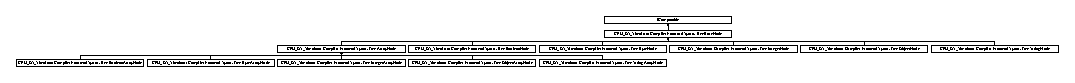
\includegraphics[height=0.668258cm]{class_c_p_u___o_s___simulator_1_1_compiler_1_1_frontend_1_1_syntax_tree_1_1_base_node}
\end{center}
\end{figure}
\subsection*{Public Member Functions}
\begin{DoxyCompactItemize}
\item 
abstract void \hyperlink{class_c_p_u___o_s___simulator_1_1_compiler_1_1_frontend_1_1_syntax_tree_1_1_base_node_a092377df64002c5e9c023a259e5e11d0}{Visit} ()
\begin{DoxyCompactList}\small\item\em This function is called when the node is being visited by the parser \end{DoxyCompactList}\item 
abstract void \hyperlink{class_c_p_u___o_s___simulator_1_1_compiler_1_1_frontend_1_1_syntax_tree_1_1_base_node_a6cfcf8a0795180bdb1c7f0735d39441b}{Evaluate} ()
\begin{DoxyCompactList}\small\item\em This Function is called when the node is being evaluated by the parser \end{DoxyCompactList}\item 
virtual int \hyperlink{class_c_p_u___o_s___simulator_1_1_compiler_1_1_frontend_1_1_syntax_tree_1_1_base_node_a56a5aff4b4b7da820c6b88854d2c0fc0}{Compare\+To} (object obj)
\begin{DoxyCompactList}\small\item\em Compares the current instance with another object of the same type and returns an integer that indicates whether the current instance precedes, follows, or occurs in the same position in the sort order as the other object. \end{DoxyCompactList}\end{DoxyCompactItemize}
\subsection*{Protected Attributes}
\begin{DoxyCompactItemize}
\item 
dynamic \hyperlink{class_c_p_u___o_s___simulator_1_1_compiler_1_1_frontend_1_1_syntax_tree_1_1_base_node_a3b706dde03ce7d04b16bacca02e433e3}{data}
\item 
\hyperlink{class_c_p_u___o_s___simulator_1_1_compiler_1_1_frontend_1_1_syntax_tree_1_1_base_node}{Base\+Node} \hyperlink{class_c_p_u___o_s___simulator_1_1_compiler_1_1_frontend_1_1_syntax_tree_1_1_base_node_a9f28fedc02d08b69870fa4b8ff0f478a}{right}
\item 
\hyperlink{class_c_p_u___o_s___simulator_1_1_compiler_1_1_frontend_1_1_syntax_tree_1_1_base_node}{Base\+Node} \hyperlink{class_c_p_u___o_s___simulator_1_1_compiler_1_1_frontend_1_1_syntax_tree_1_1_base_node_ad650fcb461aeed53a2d5638cf014b5de}{left}
\item 
\hyperlink{class_c_p_u___o_s___simulator_1_1_compiler_1_1_frontend_1_1_syntax_tree_1_1_base_node}{Base\+Node} \hyperlink{class_c_p_u___o_s___simulator_1_1_compiler_1_1_frontend_1_1_syntax_tree_1_1_base_node_a737abdeb18cd28630355a932832d8e40}{parent}
\end{DoxyCompactItemize}
\subsection*{Properties}
\begin{DoxyCompactItemize}
\item 
abstract \hyperlink{class_c_p_u___o_s___simulator_1_1_compiler_1_1_frontend_1_1_syntax_tree_1_1_base_node}{Base\+Node} \hyperlink{class_c_p_u___o_s___simulator_1_1_compiler_1_1_frontend_1_1_syntax_tree_1_1_base_node_a488735e2d5ee9a31a1ee3bdb6742c06d}{Right}\hspace{0.3cm}{\ttfamily  \mbox{[}get, set\mbox{]}}
\item 
abstract \hyperlink{class_c_p_u___o_s___simulator_1_1_compiler_1_1_frontend_1_1_syntax_tree_1_1_base_node}{Base\+Node} \hyperlink{class_c_p_u___o_s___simulator_1_1_compiler_1_1_frontend_1_1_syntax_tree_1_1_base_node_aff39b054b8bcc205583285c1dccfcbf3}{Left}\hspace{0.3cm}{\ttfamily  \mbox{[}get, set\mbox{]}}
\item 
dynamic \hyperlink{class_c_p_u___o_s___simulator_1_1_compiler_1_1_frontend_1_1_syntax_tree_1_1_base_node_ad7f198ee35d784abb122d510ec17c59a}{Data}\hspace{0.3cm}{\ttfamily  \mbox{[}get, set\mbox{]}}
\item 
abstract \hyperlink{class_c_p_u___o_s___simulator_1_1_compiler_1_1_frontend_1_1_syntax_tree_1_1_base_node}{Base\+Node} \hyperlink{class_c_p_u___o_s___simulator_1_1_compiler_1_1_frontend_1_1_syntax_tree_1_1_base_node_a218b40fedda0f7d47f1985f8396a0c48}{Parent}\hspace{0.3cm}{\ttfamily  \mbox{[}get, set\mbox{]}}
\end{DoxyCompactItemize}


\subsection{Detailed Description}


Definition at line 7 of file Base\+Node.\+cs.



\subsection{Member Function Documentation}
\hypertarget{class_c_p_u___o_s___simulator_1_1_compiler_1_1_frontend_1_1_syntax_tree_1_1_base_node_a56a5aff4b4b7da820c6b88854d2c0fc0}{}\index{C\+P\+U\+\_\+\+O\+S\+\_\+\+Simulator\+::\+Compiler\+::\+Frontend\+::\+Syntax\+Tree\+::\+Base\+Node@{C\+P\+U\+\_\+\+O\+S\+\_\+\+Simulator\+::\+Compiler\+::\+Frontend\+::\+Syntax\+Tree\+::\+Base\+Node}!Compare\+To@{Compare\+To}}
\index{Compare\+To@{Compare\+To}!C\+P\+U\+\_\+\+O\+S\+\_\+\+Simulator\+::\+Compiler\+::\+Frontend\+::\+Syntax\+Tree\+::\+Base\+Node@{C\+P\+U\+\_\+\+O\+S\+\_\+\+Simulator\+::\+Compiler\+::\+Frontend\+::\+Syntax\+Tree\+::\+Base\+Node}}
\subsubsection[{Compare\+To(object obj)}]{\setlength{\rightskip}{0pt plus 5cm}virtual int C\+P\+U\+\_\+\+O\+S\+\_\+\+Simulator.\+Compiler.\+Frontend.\+Syntax\+Tree.\+Base\+Node.\+Compare\+To (
\begin{DoxyParamCaption}
\item[{object}]{obj}
\end{DoxyParamCaption}
)\hspace{0.3cm}{\ttfamily [virtual]}}\label{class_c_p_u___o_s___simulator_1_1_compiler_1_1_frontend_1_1_syntax_tree_1_1_base_node_a56a5aff4b4b7da820c6b88854d2c0fc0}


Compares the current instance with another object of the same type and returns an integer that indicates whether the current instance precedes, follows, or occurs in the same position in the sort order as the other object. 

\begin{DoxyReturn}{Returns}
A value that indicates the relative order of the objects being compared. The return value has these meanings\+: Value Meaning Less than zero This instance precedes {\itshape obj}  in the sort order. Zero This instance occurs in the same position in the sort order as {\itshape obj} . Greater than zero This instance follows {\itshape obj}  in the sort order. 
\end{DoxyReturn}

\begin{DoxyParams}{Parameters}
{\em obj} & An object to compare with this instance. \\
\hline
\end{DoxyParams}

\begin{DoxyExceptions}{Exceptions}
{\em T\+:\+System.\+Argument\+Exception} & {\itshape obj}  is not the same type as this instance. \\
\hline
\end{DoxyExceptions}


Definition at line 42 of file Base\+Node.\+cs.

\hypertarget{class_c_p_u___o_s___simulator_1_1_compiler_1_1_frontend_1_1_syntax_tree_1_1_base_node_a6cfcf8a0795180bdb1c7f0735d39441b}{}\index{C\+P\+U\+\_\+\+O\+S\+\_\+\+Simulator\+::\+Compiler\+::\+Frontend\+::\+Syntax\+Tree\+::\+Base\+Node@{C\+P\+U\+\_\+\+O\+S\+\_\+\+Simulator\+::\+Compiler\+::\+Frontend\+::\+Syntax\+Tree\+::\+Base\+Node}!Evaluate@{Evaluate}}
\index{Evaluate@{Evaluate}!C\+P\+U\+\_\+\+O\+S\+\_\+\+Simulator\+::\+Compiler\+::\+Frontend\+::\+Syntax\+Tree\+::\+Base\+Node@{C\+P\+U\+\_\+\+O\+S\+\_\+\+Simulator\+::\+Compiler\+::\+Frontend\+::\+Syntax\+Tree\+::\+Base\+Node}}
\subsubsection[{Evaluate()}]{\setlength{\rightskip}{0pt plus 5cm}abstract void C\+P\+U\+\_\+\+O\+S\+\_\+\+Simulator.\+Compiler.\+Frontend.\+Syntax\+Tree.\+Base\+Node.\+Evaluate (
\begin{DoxyParamCaption}
{}
\end{DoxyParamCaption}
)\hspace{0.3cm}{\ttfamily [pure virtual]}}\label{class_c_p_u___o_s___simulator_1_1_compiler_1_1_frontend_1_1_syntax_tree_1_1_base_node_a6cfcf8a0795180bdb1c7f0735d39441b}


This Function is called when the node is being evaluated by the parser 



Implemented in \hyperlink{class_c_p_u___o_s___simulator_1_1_compiler_1_1_frontend_1_1_syntax_tree_1_1_integer_array_node_a28619c1f8b99cea0b827ba5a71a00e35}{C\+P\+U\+\_\+\+O\+S\+\_\+\+Simulator.\+Compiler.\+Frontend.\+Syntax\+Tree.\+Integer\+Array\+Node}, \hyperlink{class_c_p_u___o_s___simulator_1_1_compiler_1_1_frontend_1_1_syntax_tree_1_1_boolean_array_node_a6de955407e0bce191f3f09a5cf6f4d50}{C\+P\+U\+\_\+\+O\+S\+\_\+\+Simulator.\+Compiler.\+Frontend.\+Syntax\+Tree.\+Boolean\+Array\+Node}, \hyperlink{class_c_p_u___o_s___simulator_1_1_compiler_1_1_frontend_1_1_syntax_tree_1_1_boolean_node_a4a804a07050c45ca80feaaac3a050784}{C\+P\+U\+\_\+\+O\+S\+\_\+\+Simulator.\+Compiler.\+Frontend.\+Syntax\+Tree.\+Boolean\+Node}, \hyperlink{class_c_p_u___o_s___simulator_1_1_compiler_1_1_frontend_1_1_syntax_tree_1_1_byte_node_a0e9461945f15cb28abac866a81c8c5d3}{C\+P\+U\+\_\+\+O\+S\+\_\+\+Simulator.\+Compiler.\+Frontend.\+Syntax\+Tree.\+Byte\+Node}, \hyperlink{class_c_p_u___o_s___simulator_1_1_compiler_1_1_frontend_1_1_syntax_tree_1_1_integer_node_a3005d7165ec473ac488e792728a50d99}{C\+P\+U\+\_\+\+O\+S\+\_\+\+Simulator.\+Compiler.\+Frontend.\+Syntax\+Tree.\+Integer\+Node}, \hyperlink{class_c_p_u___o_s___simulator_1_1_compiler_1_1_frontend_1_1_syntax_tree_1_1_object_array_node_ad0c63367dd74b502a0e510b95e324405}{C\+P\+U\+\_\+\+O\+S\+\_\+\+Simulator.\+Compiler.\+Frontend.\+Syntax\+Tree.\+Object\+Array\+Node}, \hyperlink{class_c_p_u___o_s___simulator_1_1_compiler_1_1_frontend_1_1_syntax_tree_1_1_object_node_a52be0559ec5f7c7171d5b17ce9cbb385}{C\+P\+U\+\_\+\+O\+S\+\_\+\+Simulator.\+Compiler.\+Frontend.\+Syntax\+Tree.\+Object\+Node}, \hyperlink{class_c_p_u___o_s___simulator_1_1_compiler_1_1_frontend_1_1_syntax_tree_1_1_string_node_aa13c55d835188df6289e7cc1844199d3}{C\+P\+U\+\_\+\+O\+S\+\_\+\+Simulator.\+Compiler.\+Frontend.\+Syntax\+Tree.\+String\+Node}, \hyperlink{class_c_p_u___o_s___simulator_1_1_compiler_1_1_frontend_1_1_syntax_tree_1_1_byte_array_node_ad34fd3396bf5e6e179d941d2076f28d9}{C\+P\+U\+\_\+\+O\+S\+\_\+\+Simulator.\+Compiler.\+Frontend.\+Syntax\+Tree.\+Byte\+Array\+Node}, \hyperlink{class_c_p_u___o_s___simulator_1_1_compiler_1_1_frontend_1_1_syntax_tree_1_1_string_array_node_a559630365acec250f2eed840010535f8}{C\+P\+U\+\_\+\+O\+S\+\_\+\+Simulator.\+Compiler.\+Frontend.\+Syntax\+Tree.\+String\+Array\+Node}, and \hyperlink{class_c_p_u___o_s___simulator_1_1_compiler_1_1_frontend_1_1_syntax_tree_1_1_array_node_afdb5d2808dbd83c28c85f35b6430edc4}{C\+P\+U\+\_\+\+O\+S\+\_\+\+Simulator.\+Compiler.\+Frontend.\+Syntax\+Tree.\+Array\+Node}.

\hypertarget{class_c_p_u___o_s___simulator_1_1_compiler_1_1_frontend_1_1_syntax_tree_1_1_base_node_a092377df64002c5e9c023a259e5e11d0}{}\index{C\+P\+U\+\_\+\+O\+S\+\_\+\+Simulator\+::\+Compiler\+::\+Frontend\+::\+Syntax\+Tree\+::\+Base\+Node@{C\+P\+U\+\_\+\+O\+S\+\_\+\+Simulator\+::\+Compiler\+::\+Frontend\+::\+Syntax\+Tree\+::\+Base\+Node}!Visit@{Visit}}
\index{Visit@{Visit}!C\+P\+U\+\_\+\+O\+S\+\_\+\+Simulator\+::\+Compiler\+::\+Frontend\+::\+Syntax\+Tree\+::\+Base\+Node@{C\+P\+U\+\_\+\+O\+S\+\_\+\+Simulator\+::\+Compiler\+::\+Frontend\+::\+Syntax\+Tree\+::\+Base\+Node}}
\subsubsection[{Visit()}]{\setlength{\rightskip}{0pt plus 5cm}abstract void C\+P\+U\+\_\+\+O\+S\+\_\+\+Simulator.\+Compiler.\+Frontend.\+Syntax\+Tree.\+Base\+Node.\+Visit (
\begin{DoxyParamCaption}
{}
\end{DoxyParamCaption}
)\hspace{0.3cm}{\ttfamily [pure virtual]}}\label{class_c_p_u___o_s___simulator_1_1_compiler_1_1_frontend_1_1_syntax_tree_1_1_base_node_a092377df64002c5e9c023a259e5e11d0}


This function is called when the node is being visited by the parser 



Implemented in \hyperlink{class_c_p_u___o_s___simulator_1_1_compiler_1_1_frontend_1_1_syntax_tree_1_1_integer_array_node_a7abbf1320b21da1362fc8d391907d33f}{C\+P\+U\+\_\+\+O\+S\+\_\+\+Simulator.\+Compiler.\+Frontend.\+Syntax\+Tree.\+Integer\+Array\+Node}, \hyperlink{class_c_p_u___o_s___simulator_1_1_compiler_1_1_frontend_1_1_syntax_tree_1_1_boolean_array_node_a192727033dc9533113312210f04a958a}{C\+P\+U\+\_\+\+O\+S\+\_\+\+Simulator.\+Compiler.\+Frontend.\+Syntax\+Tree.\+Boolean\+Array\+Node}, \hyperlink{class_c_p_u___o_s___simulator_1_1_compiler_1_1_frontend_1_1_syntax_tree_1_1_boolean_node_a5cf13a08d798c5c1a225654e3f888866}{C\+P\+U\+\_\+\+O\+S\+\_\+\+Simulator.\+Compiler.\+Frontend.\+Syntax\+Tree.\+Boolean\+Node}, \hyperlink{class_c_p_u___o_s___simulator_1_1_compiler_1_1_frontend_1_1_syntax_tree_1_1_byte_node_af411e73f7153f6c67e09273198e9f1bb}{C\+P\+U\+\_\+\+O\+S\+\_\+\+Simulator.\+Compiler.\+Frontend.\+Syntax\+Tree.\+Byte\+Node}, \hyperlink{class_c_p_u___o_s___simulator_1_1_compiler_1_1_frontend_1_1_syntax_tree_1_1_integer_node_a5f788c73bf459d372850107098fda8c1}{C\+P\+U\+\_\+\+O\+S\+\_\+\+Simulator.\+Compiler.\+Frontend.\+Syntax\+Tree.\+Integer\+Node}, \hyperlink{class_c_p_u___o_s___simulator_1_1_compiler_1_1_frontend_1_1_syntax_tree_1_1_object_array_node_a1d792b3929152ecfa25dac2e8c6444cc}{C\+P\+U\+\_\+\+O\+S\+\_\+\+Simulator.\+Compiler.\+Frontend.\+Syntax\+Tree.\+Object\+Array\+Node}, \hyperlink{class_c_p_u___o_s___simulator_1_1_compiler_1_1_frontend_1_1_syntax_tree_1_1_object_node_a2c77bb89c3638cfb39c6fd1a40b63d71}{C\+P\+U\+\_\+\+O\+S\+\_\+\+Simulator.\+Compiler.\+Frontend.\+Syntax\+Tree.\+Object\+Node}, \hyperlink{class_c_p_u___o_s___simulator_1_1_compiler_1_1_frontend_1_1_syntax_tree_1_1_string_node_a08063171005bc1ee91e327b35cbfb7a1}{C\+P\+U\+\_\+\+O\+S\+\_\+\+Simulator.\+Compiler.\+Frontend.\+Syntax\+Tree.\+String\+Node}, \hyperlink{class_c_p_u___o_s___simulator_1_1_compiler_1_1_frontend_1_1_syntax_tree_1_1_byte_array_node_a1ed9d8d35aeb8537758718aa1bae1ae0}{C\+P\+U\+\_\+\+O\+S\+\_\+\+Simulator.\+Compiler.\+Frontend.\+Syntax\+Tree.\+Byte\+Array\+Node}, \hyperlink{class_c_p_u___o_s___simulator_1_1_compiler_1_1_frontend_1_1_syntax_tree_1_1_string_array_node_ae8ce8f85a313e577506546a26c954e34}{C\+P\+U\+\_\+\+O\+S\+\_\+\+Simulator.\+Compiler.\+Frontend.\+Syntax\+Tree.\+String\+Array\+Node}, and \hyperlink{class_c_p_u___o_s___simulator_1_1_compiler_1_1_frontend_1_1_syntax_tree_1_1_array_node_aed695b6f32d5c176204fc15854db32db}{C\+P\+U\+\_\+\+O\+S\+\_\+\+Simulator.\+Compiler.\+Frontend.\+Syntax\+Tree.\+Array\+Node}.



\subsection{Member Data Documentation}
\hypertarget{class_c_p_u___o_s___simulator_1_1_compiler_1_1_frontend_1_1_syntax_tree_1_1_base_node_a3b706dde03ce7d04b16bacca02e433e3}{}\index{C\+P\+U\+\_\+\+O\+S\+\_\+\+Simulator\+::\+Compiler\+::\+Frontend\+::\+Syntax\+Tree\+::\+Base\+Node@{C\+P\+U\+\_\+\+O\+S\+\_\+\+Simulator\+::\+Compiler\+::\+Frontend\+::\+Syntax\+Tree\+::\+Base\+Node}!data@{data}}
\index{data@{data}!C\+P\+U\+\_\+\+O\+S\+\_\+\+Simulator\+::\+Compiler\+::\+Frontend\+::\+Syntax\+Tree\+::\+Base\+Node@{C\+P\+U\+\_\+\+O\+S\+\_\+\+Simulator\+::\+Compiler\+::\+Frontend\+::\+Syntax\+Tree\+::\+Base\+Node}}
\subsubsection[{data}]{\setlength{\rightskip}{0pt plus 5cm}dynamic C\+P\+U\+\_\+\+O\+S\+\_\+\+Simulator.\+Compiler.\+Frontend.\+Syntax\+Tree.\+Base\+Node.\+data\hspace{0.3cm}{\ttfamily [protected]}}\label{class_c_p_u___o_s___simulator_1_1_compiler_1_1_frontend_1_1_syntax_tree_1_1_base_node_a3b706dde03ce7d04b16bacca02e433e3}


Definition at line 21 of file Base\+Node.\+cs.

\hypertarget{class_c_p_u___o_s___simulator_1_1_compiler_1_1_frontend_1_1_syntax_tree_1_1_base_node_ad650fcb461aeed53a2d5638cf014b5de}{}\index{C\+P\+U\+\_\+\+O\+S\+\_\+\+Simulator\+::\+Compiler\+::\+Frontend\+::\+Syntax\+Tree\+::\+Base\+Node@{C\+P\+U\+\_\+\+O\+S\+\_\+\+Simulator\+::\+Compiler\+::\+Frontend\+::\+Syntax\+Tree\+::\+Base\+Node}!left@{left}}
\index{left@{left}!C\+P\+U\+\_\+\+O\+S\+\_\+\+Simulator\+::\+Compiler\+::\+Frontend\+::\+Syntax\+Tree\+::\+Base\+Node@{C\+P\+U\+\_\+\+O\+S\+\_\+\+Simulator\+::\+Compiler\+::\+Frontend\+::\+Syntax\+Tree\+::\+Base\+Node}}
\subsubsection[{left}]{\setlength{\rightskip}{0pt plus 5cm}{\bf Base\+Node} C\+P\+U\+\_\+\+O\+S\+\_\+\+Simulator.\+Compiler.\+Frontend.\+Syntax\+Tree.\+Base\+Node.\+left\hspace{0.3cm}{\ttfamily [protected]}}\label{class_c_p_u___o_s___simulator_1_1_compiler_1_1_frontend_1_1_syntax_tree_1_1_base_node_ad650fcb461aeed53a2d5638cf014b5de}


Definition at line 23 of file Base\+Node.\+cs.

\hypertarget{class_c_p_u___o_s___simulator_1_1_compiler_1_1_frontend_1_1_syntax_tree_1_1_base_node_a737abdeb18cd28630355a932832d8e40}{}\index{C\+P\+U\+\_\+\+O\+S\+\_\+\+Simulator\+::\+Compiler\+::\+Frontend\+::\+Syntax\+Tree\+::\+Base\+Node@{C\+P\+U\+\_\+\+O\+S\+\_\+\+Simulator\+::\+Compiler\+::\+Frontend\+::\+Syntax\+Tree\+::\+Base\+Node}!parent@{parent}}
\index{parent@{parent}!C\+P\+U\+\_\+\+O\+S\+\_\+\+Simulator\+::\+Compiler\+::\+Frontend\+::\+Syntax\+Tree\+::\+Base\+Node@{C\+P\+U\+\_\+\+O\+S\+\_\+\+Simulator\+::\+Compiler\+::\+Frontend\+::\+Syntax\+Tree\+::\+Base\+Node}}
\subsubsection[{parent}]{\setlength{\rightskip}{0pt plus 5cm}{\bf Base\+Node} C\+P\+U\+\_\+\+O\+S\+\_\+\+Simulator.\+Compiler.\+Frontend.\+Syntax\+Tree.\+Base\+Node.\+parent\hspace{0.3cm}{\ttfamily [protected]}}\label{class_c_p_u___o_s___simulator_1_1_compiler_1_1_frontend_1_1_syntax_tree_1_1_base_node_a737abdeb18cd28630355a932832d8e40}


Definition at line 24 of file Base\+Node.\+cs.

\hypertarget{class_c_p_u___o_s___simulator_1_1_compiler_1_1_frontend_1_1_syntax_tree_1_1_base_node_a9f28fedc02d08b69870fa4b8ff0f478a}{}\index{C\+P\+U\+\_\+\+O\+S\+\_\+\+Simulator\+::\+Compiler\+::\+Frontend\+::\+Syntax\+Tree\+::\+Base\+Node@{C\+P\+U\+\_\+\+O\+S\+\_\+\+Simulator\+::\+Compiler\+::\+Frontend\+::\+Syntax\+Tree\+::\+Base\+Node}!right@{right}}
\index{right@{right}!C\+P\+U\+\_\+\+O\+S\+\_\+\+Simulator\+::\+Compiler\+::\+Frontend\+::\+Syntax\+Tree\+::\+Base\+Node@{C\+P\+U\+\_\+\+O\+S\+\_\+\+Simulator\+::\+Compiler\+::\+Frontend\+::\+Syntax\+Tree\+::\+Base\+Node}}
\subsubsection[{right}]{\setlength{\rightskip}{0pt plus 5cm}{\bf Base\+Node} C\+P\+U\+\_\+\+O\+S\+\_\+\+Simulator.\+Compiler.\+Frontend.\+Syntax\+Tree.\+Base\+Node.\+right\hspace{0.3cm}{\ttfamily [protected]}}\label{class_c_p_u___o_s___simulator_1_1_compiler_1_1_frontend_1_1_syntax_tree_1_1_base_node_a9f28fedc02d08b69870fa4b8ff0f478a}


Definition at line 22 of file Base\+Node.\+cs.



\subsection{Property Documentation}
\hypertarget{class_c_p_u___o_s___simulator_1_1_compiler_1_1_frontend_1_1_syntax_tree_1_1_base_node_ad7f198ee35d784abb122d510ec17c59a}{}\index{C\+P\+U\+\_\+\+O\+S\+\_\+\+Simulator\+::\+Compiler\+::\+Frontend\+::\+Syntax\+Tree\+::\+Base\+Node@{C\+P\+U\+\_\+\+O\+S\+\_\+\+Simulator\+::\+Compiler\+::\+Frontend\+::\+Syntax\+Tree\+::\+Base\+Node}!Data@{Data}}
\index{Data@{Data}!C\+P\+U\+\_\+\+O\+S\+\_\+\+Simulator\+::\+Compiler\+::\+Frontend\+::\+Syntax\+Tree\+::\+Base\+Node@{C\+P\+U\+\_\+\+O\+S\+\_\+\+Simulator\+::\+Compiler\+::\+Frontend\+::\+Syntax\+Tree\+::\+Base\+Node}}
\subsubsection[{Data}]{\setlength{\rightskip}{0pt plus 5cm}dynamic C\+P\+U\+\_\+\+O\+S\+\_\+\+Simulator.\+Compiler.\+Frontend.\+Syntax\+Tree.\+Base\+Node.\+Data\hspace{0.3cm}{\ttfamily [get]}, {\ttfamily [set]}}\label{class_c_p_u___o_s___simulator_1_1_compiler_1_1_frontend_1_1_syntax_tree_1_1_base_node_ad7f198ee35d784abb122d510ec17c59a}


Definition at line 14 of file Base\+Node.\+cs.

\hypertarget{class_c_p_u___o_s___simulator_1_1_compiler_1_1_frontend_1_1_syntax_tree_1_1_base_node_aff39b054b8bcc205583285c1dccfcbf3}{}\index{C\+P\+U\+\_\+\+O\+S\+\_\+\+Simulator\+::\+Compiler\+::\+Frontend\+::\+Syntax\+Tree\+::\+Base\+Node@{C\+P\+U\+\_\+\+O\+S\+\_\+\+Simulator\+::\+Compiler\+::\+Frontend\+::\+Syntax\+Tree\+::\+Base\+Node}!Left@{Left}}
\index{Left@{Left}!C\+P\+U\+\_\+\+O\+S\+\_\+\+Simulator\+::\+Compiler\+::\+Frontend\+::\+Syntax\+Tree\+::\+Base\+Node@{C\+P\+U\+\_\+\+O\+S\+\_\+\+Simulator\+::\+Compiler\+::\+Frontend\+::\+Syntax\+Tree\+::\+Base\+Node}}
\subsubsection[{Left}]{\setlength{\rightskip}{0pt plus 5cm}abstract {\bf Base\+Node} C\+P\+U\+\_\+\+O\+S\+\_\+\+Simulator.\+Compiler.\+Frontend.\+Syntax\+Tree.\+Base\+Node.\+Left\hspace{0.3cm}{\ttfamily [get]}, {\ttfamily [set]}}\label{class_c_p_u___o_s___simulator_1_1_compiler_1_1_frontend_1_1_syntax_tree_1_1_base_node_aff39b054b8bcc205583285c1dccfcbf3}


Definition at line 11 of file Base\+Node.\+cs.

\hypertarget{class_c_p_u___o_s___simulator_1_1_compiler_1_1_frontend_1_1_syntax_tree_1_1_base_node_a218b40fedda0f7d47f1985f8396a0c48}{}\index{C\+P\+U\+\_\+\+O\+S\+\_\+\+Simulator\+::\+Compiler\+::\+Frontend\+::\+Syntax\+Tree\+::\+Base\+Node@{C\+P\+U\+\_\+\+O\+S\+\_\+\+Simulator\+::\+Compiler\+::\+Frontend\+::\+Syntax\+Tree\+::\+Base\+Node}!Parent@{Parent}}
\index{Parent@{Parent}!C\+P\+U\+\_\+\+O\+S\+\_\+\+Simulator\+::\+Compiler\+::\+Frontend\+::\+Syntax\+Tree\+::\+Base\+Node@{C\+P\+U\+\_\+\+O\+S\+\_\+\+Simulator\+::\+Compiler\+::\+Frontend\+::\+Syntax\+Tree\+::\+Base\+Node}}
\subsubsection[{Parent}]{\setlength{\rightskip}{0pt plus 5cm}abstract {\bf Base\+Node} C\+P\+U\+\_\+\+O\+S\+\_\+\+Simulator.\+Compiler.\+Frontend.\+Syntax\+Tree.\+Base\+Node.\+Parent\hspace{0.3cm}{\ttfamily [get]}, {\ttfamily [set]}}\label{class_c_p_u___o_s___simulator_1_1_compiler_1_1_frontend_1_1_syntax_tree_1_1_base_node_a218b40fedda0f7d47f1985f8396a0c48}


Definition at line 19 of file Base\+Node.\+cs.

\hypertarget{class_c_p_u___o_s___simulator_1_1_compiler_1_1_frontend_1_1_syntax_tree_1_1_base_node_a488735e2d5ee9a31a1ee3bdb6742c06d}{}\index{C\+P\+U\+\_\+\+O\+S\+\_\+\+Simulator\+::\+Compiler\+::\+Frontend\+::\+Syntax\+Tree\+::\+Base\+Node@{C\+P\+U\+\_\+\+O\+S\+\_\+\+Simulator\+::\+Compiler\+::\+Frontend\+::\+Syntax\+Tree\+::\+Base\+Node}!Right@{Right}}
\index{Right@{Right}!C\+P\+U\+\_\+\+O\+S\+\_\+\+Simulator\+::\+Compiler\+::\+Frontend\+::\+Syntax\+Tree\+::\+Base\+Node@{C\+P\+U\+\_\+\+O\+S\+\_\+\+Simulator\+::\+Compiler\+::\+Frontend\+::\+Syntax\+Tree\+::\+Base\+Node}}
\subsubsection[{Right}]{\setlength{\rightskip}{0pt plus 5cm}abstract {\bf Base\+Node} C\+P\+U\+\_\+\+O\+S\+\_\+\+Simulator.\+Compiler.\+Frontend.\+Syntax\+Tree.\+Base\+Node.\+Right\hspace{0.3cm}{\ttfamily [get]}, {\ttfamily [set]}}\label{class_c_p_u___o_s___simulator_1_1_compiler_1_1_frontend_1_1_syntax_tree_1_1_base_node_a488735e2d5ee9a31a1ee3bdb6742c06d}


Definition at line 9 of file Base\+Node.\+cs.



The documentation for this class was generated from the following file\+:\begin{DoxyCompactItemize}
\item 
Compiler/\+Frontend/\+Syntax\+Tree/\hyperlink{_base_node_8cs}{Base\+Node.\+cs}\end{DoxyCompactItemize}

\hypertarget{class_c_p_u___o_s___simulator_1_1_compiler_1_1_frontend_1_1_syntax_tree_1_1_a_s_t_1_1_binary_tree_enumerator}{}\section{C\+P\+U\+\_\+\+O\+S\+\_\+\+Simulator.\+Compiler.\+Frontend.\+Syntax\+Tree.\+A\+S\+T.\+Binary\+Tree\+Enumerator Class Reference}
\label{class_c_p_u___o_s___simulator_1_1_compiler_1_1_frontend_1_1_syntax_tree_1_1_a_s_t_1_1_binary_tree_enumerator}\index{C\+P\+U\+\_\+\+O\+S\+\_\+\+Simulator.\+Compiler.\+Frontend.\+Syntax\+Tree.\+A\+S\+T.\+Binary\+Tree\+Enumerator@{C\+P\+U\+\_\+\+O\+S\+\_\+\+Simulator.\+Compiler.\+Frontend.\+Syntax\+Tree.\+A\+S\+T.\+Binary\+Tree\+Enumerator}}


The \hyperlink{class_c_p_u___o_s___simulator_1_1_compiler_1_1_frontend_1_1_syntax_tree_1_1_a_s_t_1_1_binary_tree_enumerator}{Binary\+Tree\+Enumerator} implements the I\+Enumerator allowing foreach enumeration of the tree  


Inheritance diagram for C\+P\+U\+\_\+\+O\+S\+\_\+\+Simulator.\+Compiler.\+Frontend.\+Syntax\+Tree.\+A\+S\+T.\+Binary\+Tree\+Enumerator\+:\begin{figure}[H]
\begin{center}
\leavevmode
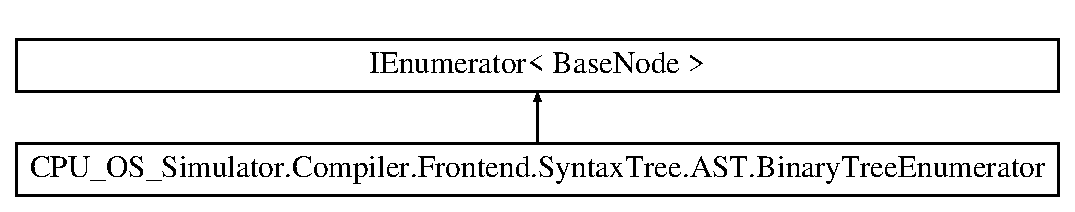
\includegraphics[height=2.000000cm]{class_c_p_u___o_s___simulator_1_1_compiler_1_1_frontend_1_1_syntax_tree_1_1_a_s_t_1_1_binary_tree_enumerator}
\end{center}
\end{figure}
\subsection*{Public Member Functions}
\begin{DoxyCompactItemize}
\item 
\hyperlink{class_c_p_u___o_s___simulator_1_1_compiler_1_1_frontend_1_1_syntax_tree_1_1_a_s_t_1_1_binary_tree_enumerator_a7daf21f731aae9e9d17d0e72b0161892}{Binary\+Tree\+Enumerator} (\hyperlink{class_c_p_u___o_s___simulator_1_1_compiler_1_1_frontend_1_1_syntax_tree_1_1_a_s_t}{A\+S\+T} tree)
\item 
bool \hyperlink{class_c_p_u___o_s___simulator_1_1_compiler_1_1_frontend_1_1_syntax_tree_1_1_a_s_t_1_1_binary_tree_enumerator_afac74da64083cc8fbb42d684df377fc8}{Move\+Next} ()
\begin{DoxyCompactList}\small\item\em The Move\+Next function traverses the tree in sorted order. \end{DoxyCompactList}\item 
void \hyperlink{class_c_p_u___o_s___simulator_1_1_compiler_1_1_frontend_1_1_syntax_tree_1_1_a_s_t_1_1_binary_tree_enumerator_a60782235f4812bb1d1abfbfe57322b68}{Dispose} ()
\item 
void \hyperlink{class_c_p_u___o_s___simulator_1_1_compiler_1_1_frontend_1_1_syntax_tree_1_1_a_s_t_1_1_binary_tree_enumerator_ae29889b8cee334c4306c6649b2359746}{Reset} ()
\end{DoxyCompactItemize}
\subsection*{Properties}
\begin{DoxyCompactItemize}
\item 
\hyperlink{class_c_p_u___o_s___simulator_1_1_compiler_1_1_frontend_1_1_syntax_tree_1_1_base_node}{Base\+Node} \hyperlink{class_c_p_u___o_s___simulator_1_1_compiler_1_1_frontend_1_1_syntax_tree_1_1_a_s_t_1_1_binary_tree_enumerator_a7dd14bca5195ebc3da5896da3bf31f6c}{Current}\hspace{0.3cm}{\ttfamily  \mbox{[}get\mbox{]}}
\item 
object System.\+Collections.\+I\+Enumerator. \hyperlink{class_c_p_u___o_s___simulator_1_1_compiler_1_1_frontend_1_1_syntax_tree_1_1_a_s_t_1_1_binary_tree_enumerator_a70bd3883026e363dea982edd307db207}{Current}\hspace{0.3cm}{\ttfamily  \mbox{[}get\mbox{]}}
\end{DoxyCompactItemize}
\subsection*{Private Attributes}
\begin{DoxyCompactItemize}
\item 
\hyperlink{class_c_p_u___o_s___simulator_1_1_compiler_1_1_frontend_1_1_syntax_tree_1_1_base_node}{Base\+Node} \hyperlink{class_c_p_u___o_s___simulator_1_1_compiler_1_1_frontend_1_1_syntax_tree_1_1_a_s_t_1_1_binary_tree_enumerator_a542e4e601c98368748ebed89c0182d6b}{current}
\item 
\hyperlink{class_c_p_u___o_s___simulator_1_1_compiler_1_1_frontend_1_1_syntax_tree_1_1_a_s_t}{A\+S\+T} \hyperlink{class_c_p_u___o_s___simulator_1_1_compiler_1_1_frontend_1_1_syntax_tree_1_1_a_s_t_1_1_binary_tree_enumerator_a9fcce56dd9d833ae0e8a44afb0850c61}{the\+Tree}
\end{DoxyCompactItemize}


\subsection{Detailed Description}
The \hyperlink{class_c_p_u___o_s___simulator_1_1_compiler_1_1_frontend_1_1_syntax_tree_1_1_a_s_t_1_1_binary_tree_enumerator}{Binary\+Tree\+Enumerator} implements the I\+Enumerator allowing foreach enumeration of the tree 



Definition at line 267 of file A\+S\+T.\+cs.



\subsection{Constructor \& Destructor Documentation}
\hypertarget{class_c_p_u___o_s___simulator_1_1_compiler_1_1_frontend_1_1_syntax_tree_1_1_a_s_t_1_1_binary_tree_enumerator_a7daf21f731aae9e9d17d0e72b0161892}{}\index{C\+P\+U\+\_\+\+O\+S\+\_\+\+Simulator\+::\+Compiler\+::\+Frontend\+::\+Syntax\+Tree\+::\+A\+S\+T\+::\+Binary\+Tree\+Enumerator@{C\+P\+U\+\_\+\+O\+S\+\_\+\+Simulator\+::\+Compiler\+::\+Frontend\+::\+Syntax\+Tree\+::\+A\+S\+T\+::\+Binary\+Tree\+Enumerator}!Binary\+Tree\+Enumerator@{Binary\+Tree\+Enumerator}}
\index{Binary\+Tree\+Enumerator@{Binary\+Tree\+Enumerator}!C\+P\+U\+\_\+\+O\+S\+\_\+\+Simulator\+::\+Compiler\+::\+Frontend\+::\+Syntax\+Tree\+::\+A\+S\+T\+::\+Binary\+Tree\+Enumerator@{C\+P\+U\+\_\+\+O\+S\+\_\+\+Simulator\+::\+Compiler\+::\+Frontend\+::\+Syntax\+Tree\+::\+A\+S\+T\+::\+Binary\+Tree\+Enumerator}}
\subsubsection[{Binary\+Tree\+Enumerator(\+A\+S\+T tree)}]{\setlength{\rightskip}{0pt plus 5cm}C\+P\+U\+\_\+\+O\+S\+\_\+\+Simulator.\+Compiler.\+Frontend.\+Syntax\+Tree.\+A\+S\+T.\+Binary\+Tree\+Enumerator.\+Binary\+Tree\+Enumerator (
\begin{DoxyParamCaption}
\item[{{\bf A\+S\+T}}]{tree}
\end{DoxyParamCaption}
)}\label{class_c_p_u___o_s___simulator_1_1_compiler_1_1_frontend_1_1_syntax_tree_1_1_a_s_t_1_1_binary_tree_enumerator_a7daf21f731aae9e9d17d0e72b0161892}


Definition at line 272 of file A\+S\+T.\+cs.



\subsection{Member Function Documentation}
\hypertarget{class_c_p_u___o_s___simulator_1_1_compiler_1_1_frontend_1_1_syntax_tree_1_1_a_s_t_1_1_binary_tree_enumerator_a60782235f4812bb1d1abfbfe57322b68}{}\index{C\+P\+U\+\_\+\+O\+S\+\_\+\+Simulator\+::\+Compiler\+::\+Frontend\+::\+Syntax\+Tree\+::\+A\+S\+T\+::\+Binary\+Tree\+Enumerator@{C\+P\+U\+\_\+\+O\+S\+\_\+\+Simulator\+::\+Compiler\+::\+Frontend\+::\+Syntax\+Tree\+::\+A\+S\+T\+::\+Binary\+Tree\+Enumerator}!Dispose@{Dispose}}
\index{Dispose@{Dispose}!C\+P\+U\+\_\+\+O\+S\+\_\+\+Simulator\+::\+Compiler\+::\+Frontend\+::\+Syntax\+Tree\+::\+A\+S\+T\+::\+Binary\+Tree\+Enumerator@{C\+P\+U\+\_\+\+O\+S\+\_\+\+Simulator\+::\+Compiler\+::\+Frontend\+::\+Syntax\+Tree\+::\+A\+S\+T\+::\+Binary\+Tree\+Enumerator}}
\subsubsection[{Dispose()}]{\setlength{\rightskip}{0pt plus 5cm}void C\+P\+U\+\_\+\+O\+S\+\_\+\+Simulator.\+Compiler.\+Frontend.\+Syntax\+Tree.\+A\+S\+T.\+Binary\+Tree\+Enumerator.\+Dispose (
\begin{DoxyParamCaption}
{}
\end{DoxyParamCaption}
)}\label{class_c_p_u___o_s___simulator_1_1_compiler_1_1_frontend_1_1_syntax_tree_1_1_a_s_t_1_1_binary_tree_enumerator_a60782235f4812bb1d1abfbfe57322b68}


Definition at line 335 of file A\+S\+T.\+cs.

\hypertarget{class_c_p_u___o_s___simulator_1_1_compiler_1_1_frontend_1_1_syntax_tree_1_1_a_s_t_1_1_binary_tree_enumerator_afac74da64083cc8fbb42d684df377fc8}{}\index{C\+P\+U\+\_\+\+O\+S\+\_\+\+Simulator\+::\+Compiler\+::\+Frontend\+::\+Syntax\+Tree\+::\+A\+S\+T\+::\+Binary\+Tree\+Enumerator@{C\+P\+U\+\_\+\+O\+S\+\_\+\+Simulator\+::\+Compiler\+::\+Frontend\+::\+Syntax\+Tree\+::\+A\+S\+T\+::\+Binary\+Tree\+Enumerator}!Move\+Next@{Move\+Next}}
\index{Move\+Next@{Move\+Next}!C\+P\+U\+\_\+\+O\+S\+\_\+\+Simulator\+::\+Compiler\+::\+Frontend\+::\+Syntax\+Tree\+::\+A\+S\+T\+::\+Binary\+Tree\+Enumerator@{C\+P\+U\+\_\+\+O\+S\+\_\+\+Simulator\+::\+Compiler\+::\+Frontend\+::\+Syntax\+Tree\+::\+A\+S\+T\+::\+Binary\+Tree\+Enumerator}}
\subsubsection[{Move\+Next()}]{\setlength{\rightskip}{0pt plus 5cm}bool C\+P\+U\+\_\+\+O\+S\+\_\+\+Simulator.\+Compiler.\+Frontend.\+Syntax\+Tree.\+A\+S\+T.\+Binary\+Tree\+Enumerator.\+Move\+Next (
\begin{DoxyParamCaption}
{}
\end{DoxyParamCaption}
)}\label{class_c_p_u___o_s___simulator_1_1_compiler_1_1_frontend_1_1_syntax_tree_1_1_a_s_t_1_1_binary_tree_enumerator_afac74da64083cc8fbb42d684df377fc8}


The Move\+Next function traverses the tree in sorted order. 

\begin{DoxyReturn}{Returns}
True if we found a valid entry, False if we have reached the end
\end{DoxyReturn}


Definition at line 284 of file A\+S\+T.\+cs.

\hypertarget{class_c_p_u___o_s___simulator_1_1_compiler_1_1_frontend_1_1_syntax_tree_1_1_a_s_t_1_1_binary_tree_enumerator_ae29889b8cee334c4306c6649b2359746}{}\index{C\+P\+U\+\_\+\+O\+S\+\_\+\+Simulator\+::\+Compiler\+::\+Frontend\+::\+Syntax\+Tree\+::\+A\+S\+T\+::\+Binary\+Tree\+Enumerator@{C\+P\+U\+\_\+\+O\+S\+\_\+\+Simulator\+::\+Compiler\+::\+Frontend\+::\+Syntax\+Tree\+::\+A\+S\+T\+::\+Binary\+Tree\+Enumerator}!Reset@{Reset}}
\index{Reset@{Reset}!C\+P\+U\+\_\+\+O\+S\+\_\+\+Simulator\+::\+Compiler\+::\+Frontend\+::\+Syntax\+Tree\+::\+A\+S\+T\+::\+Binary\+Tree\+Enumerator@{C\+P\+U\+\_\+\+O\+S\+\_\+\+Simulator\+::\+Compiler\+::\+Frontend\+::\+Syntax\+Tree\+::\+A\+S\+T\+::\+Binary\+Tree\+Enumerator}}
\subsubsection[{Reset()}]{\setlength{\rightskip}{0pt plus 5cm}void C\+P\+U\+\_\+\+O\+S\+\_\+\+Simulator.\+Compiler.\+Frontend.\+Syntax\+Tree.\+A\+S\+T.\+Binary\+Tree\+Enumerator.\+Reset (
\begin{DoxyParamCaption}
{}
\end{DoxyParamCaption}
)}\label{class_c_p_u___o_s___simulator_1_1_compiler_1_1_frontend_1_1_syntax_tree_1_1_a_s_t_1_1_binary_tree_enumerator_ae29889b8cee334c4306c6649b2359746}


Definition at line 339 of file A\+S\+T.\+cs.



\subsection{Member Data Documentation}
\hypertarget{class_c_p_u___o_s___simulator_1_1_compiler_1_1_frontend_1_1_syntax_tree_1_1_a_s_t_1_1_binary_tree_enumerator_a542e4e601c98368748ebed89c0182d6b}{}\index{C\+P\+U\+\_\+\+O\+S\+\_\+\+Simulator\+::\+Compiler\+::\+Frontend\+::\+Syntax\+Tree\+::\+A\+S\+T\+::\+Binary\+Tree\+Enumerator@{C\+P\+U\+\_\+\+O\+S\+\_\+\+Simulator\+::\+Compiler\+::\+Frontend\+::\+Syntax\+Tree\+::\+A\+S\+T\+::\+Binary\+Tree\+Enumerator}!current@{current}}
\index{current@{current}!C\+P\+U\+\_\+\+O\+S\+\_\+\+Simulator\+::\+Compiler\+::\+Frontend\+::\+Syntax\+Tree\+::\+A\+S\+T\+::\+Binary\+Tree\+Enumerator@{C\+P\+U\+\_\+\+O\+S\+\_\+\+Simulator\+::\+Compiler\+::\+Frontend\+::\+Syntax\+Tree\+::\+A\+S\+T\+::\+Binary\+Tree\+Enumerator}}
\subsubsection[{current}]{\setlength{\rightskip}{0pt plus 5cm}{\bf Base\+Node} C\+P\+U\+\_\+\+O\+S\+\_\+\+Simulator.\+Compiler.\+Frontend.\+Syntax\+Tree.\+A\+S\+T.\+Binary\+Tree\+Enumerator.\+current\hspace{0.3cm}{\ttfamily [private]}}\label{class_c_p_u___o_s___simulator_1_1_compiler_1_1_frontend_1_1_syntax_tree_1_1_a_s_t_1_1_binary_tree_enumerator_a542e4e601c98368748ebed89c0182d6b}


Definition at line 269 of file A\+S\+T.\+cs.

\hypertarget{class_c_p_u___o_s___simulator_1_1_compiler_1_1_frontend_1_1_syntax_tree_1_1_a_s_t_1_1_binary_tree_enumerator_a9fcce56dd9d833ae0e8a44afb0850c61}{}\index{C\+P\+U\+\_\+\+O\+S\+\_\+\+Simulator\+::\+Compiler\+::\+Frontend\+::\+Syntax\+Tree\+::\+A\+S\+T\+::\+Binary\+Tree\+Enumerator@{C\+P\+U\+\_\+\+O\+S\+\_\+\+Simulator\+::\+Compiler\+::\+Frontend\+::\+Syntax\+Tree\+::\+A\+S\+T\+::\+Binary\+Tree\+Enumerator}!the\+Tree@{the\+Tree}}
\index{the\+Tree@{the\+Tree}!C\+P\+U\+\_\+\+O\+S\+\_\+\+Simulator\+::\+Compiler\+::\+Frontend\+::\+Syntax\+Tree\+::\+A\+S\+T\+::\+Binary\+Tree\+Enumerator@{C\+P\+U\+\_\+\+O\+S\+\_\+\+Simulator\+::\+Compiler\+::\+Frontend\+::\+Syntax\+Tree\+::\+A\+S\+T\+::\+Binary\+Tree\+Enumerator}}
\subsubsection[{the\+Tree}]{\setlength{\rightskip}{0pt plus 5cm}{\bf A\+S\+T} C\+P\+U\+\_\+\+O\+S\+\_\+\+Simulator.\+Compiler.\+Frontend.\+Syntax\+Tree.\+A\+S\+T.\+Binary\+Tree\+Enumerator.\+the\+Tree\hspace{0.3cm}{\ttfamily [private]}}\label{class_c_p_u___o_s___simulator_1_1_compiler_1_1_frontend_1_1_syntax_tree_1_1_a_s_t_1_1_binary_tree_enumerator_a9fcce56dd9d833ae0e8a44afb0850c61}


Definition at line 270 of file A\+S\+T.\+cs.



\subsection{Property Documentation}
\hypertarget{class_c_p_u___o_s___simulator_1_1_compiler_1_1_frontend_1_1_syntax_tree_1_1_a_s_t_1_1_binary_tree_enumerator_a7dd14bca5195ebc3da5896da3bf31f6c}{}\index{C\+P\+U\+\_\+\+O\+S\+\_\+\+Simulator\+::\+Compiler\+::\+Frontend\+::\+Syntax\+Tree\+::\+A\+S\+T\+::\+Binary\+Tree\+Enumerator@{C\+P\+U\+\_\+\+O\+S\+\_\+\+Simulator\+::\+Compiler\+::\+Frontend\+::\+Syntax\+Tree\+::\+A\+S\+T\+::\+Binary\+Tree\+Enumerator}!Current@{Current}}
\index{Current@{Current}!C\+P\+U\+\_\+\+O\+S\+\_\+\+Simulator\+::\+Compiler\+::\+Frontend\+::\+Syntax\+Tree\+::\+A\+S\+T\+::\+Binary\+Tree\+Enumerator@{C\+P\+U\+\_\+\+O\+S\+\_\+\+Simulator\+::\+Compiler\+::\+Frontend\+::\+Syntax\+Tree\+::\+A\+S\+T\+::\+Binary\+Tree\+Enumerator}}
\subsubsection[{Current}]{\setlength{\rightskip}{0pt plus 5cm}{\bf Base\+Node} C\+P\+U\+\_\+\+O\+S\+\_\+\+Simulator.\+Compiler.\+Frontend.\+Syntax\+Tree.\+A\+S\+T.\+Binary\+Tree\+Enumerator.\+Current\hspace{0.3cm}{\ttfamily [get]}}\label{class_c_p_u___o_s___simulator_1_1_compiler_1_1_frontend_1_1_syntax_tree_1_1_a_s_t_1_1_binary_tree_enumerator_a7dd14bca5195ebc3da5896da3bf31f6c}


Definition at line 316 of file A\+S\+T.\+cs.

\hypertarget{class_c_p_u___o_s___simulator_1_1_compiler_1_1_frontend_1_1_syntax_tree_1_1_a_s_t_1_1_binary_tree_enumerator_a70bd3883026e363dea982edd307db207}{}\index{C\+P\+U\+\_\+\+O\+S\+\_\+\+Simulator\+::\+Compiler\+::\+Frontend\+::\+Syntax\+Tree\+::\+A\+S\+T\+::\+Binary\+Tree\+Enumerator@{C\+P\+U\+\_\+\+O\+S\+\_\+\+Simulator\+::\+Compiler\+::\+Frontend\+::\+Syntax\+Tree\+::\+A\+S\+T\+::\+Binary\+Tree\+Enumerator}!Current@{Current}}
\index{Current@{Current}!C\+P\+U\+\_\+\+O\+S\+\_\+\+Simulator\+::\+Compiler\+::\+Frontend\+::\+Syntax\+Tree\+::\+A\+S\+T\+::\+Binary\+Tree\+Enumerator@{C\+P\+U\+\_\+\+O\+S\+\_\+\+Simulator\+::\+Compiler\+::\+Frontend\+::\+Syntax\+Tree\+::\+A\+S\+T\+::\+Binary\+Tree\+Enumerator}}
\subsubsection[{Current}]{\setlength{\rightskip}{0pt plus 5cm}object System.\+Collections.\+I\+Enumerator. C\+P\+U\+\_\+\+O\+S\+\_\+\+Simulator.\+Compiler.\+Frontend.\+Syntax\+Tree.\+A\+S\+T.\+Binary\+Tree\+Enumerator.\+Current\hspace{0.3cm}{\ttfamily [get]}, {\ttfamily [private]}}\label{class_c_p_u___o_s___simulator_1_1_compiler_1_1_frontend_1_1_syntax_tree_1_1_a_s_t_1_1_binary_tree_enumerator_a70bd3883026e363dea982edd307db207}


Definition at line 326 of file A\+S\+T.\+cs.



The documentation for this class was generated from the following file\+:\begin{DoxyCompactItemize}
\item 
Compiler/\+Frontend/\+Syntax\+Tree/\hyperlink{_a_s_t_8cs}{A\+S\+T.\+cs}\end{DoxyCompactItemize}

\hypertarget{class_c_p_u___o_s___simulator_1_1_compiler_1_1_frontend_1_1_syntax_tree_1_1_boolean_array_node}{}\section{C\+P\+U\+\_\+\+O\+S\+\_\+\+Simulator.\+Compiler.\+Frontend.\+Syntax\+Tree.\+Boolean\+Array\+Node Class Reference}
\label{class_c_p_u___o_s___simulator_1_1_compiler_1_1_frontend_1_1_syntax_tree_1_1_boolean_array_node}\index{C\+P\+U\+\_\+\+O\+S\+\_\+\+Simulator.\+Compiler.\+Frontend.\+Syntax\+Tree.\+Boolean\+Array\+Node@{C\+P\+U\+\_\+\+O\+S\+\_\+\+Simulator.\+Compiler.\+Frontend.\+Syntax\+Tree.\+Boolean\+Array\+Node}}
Inheritance diagram for C\+P\+U\+\_\+\+O\+S\+\_\+\+Simulator.\+Compiler.\+Frontend.\+Syntax\+Tree.\+Boolean\+Array\+Node\+:\begin{figure}[H]
\begin{center}
\leavevmode
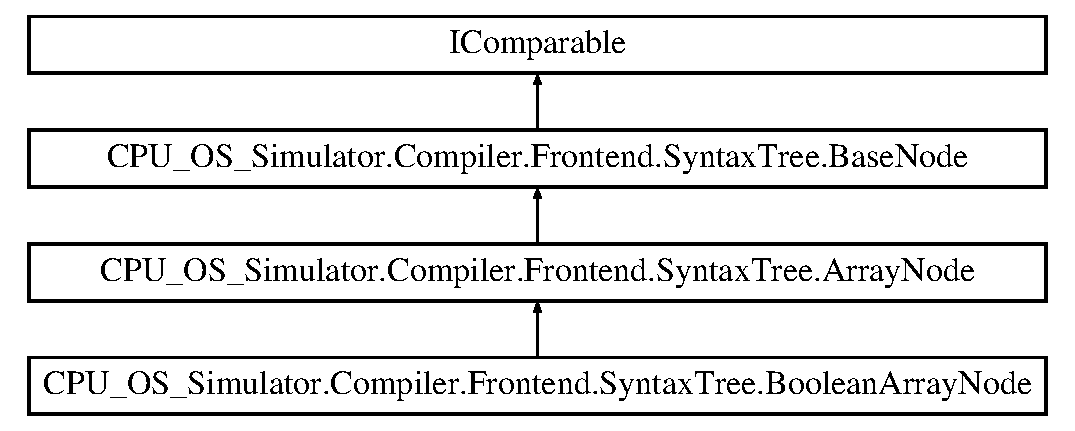
\includegraphics[height=4.000000cm]{class_c_p_u___o_s___simulator_1_1_compiler_1_1_frontend_1_1_syntax_tree_1_1_boolean_array_node}
\end{center}
\end{figure}
\subsection*{Public Member Functions}
\begin{DoxyCompactItemize}
\item 
override void \hyperlink{class_c_p_u___o_s___simulator_1_1_compiler_1_1_frontend_1_1_syntax_tree_1_1_boolean_array_node_a192727033dc9533113312210f04a958a}{Visit} ()
\begin{DoxyCompactList}\small\item\em This function is called when the node is being visited by the parser \end{DoxyCompactList}\item 
override void \hyperlink{class_c_p_u___o_s___simulator_1_1_compiler_1_1_frontend_1_1_syntax_tree_1_1_boolean_array_node_a6de955407e0bce191f3f09a5cf6f4d50}{Evaluate} ()
\begin{DoxyCompactList}\small\item\em This Function is called when the node is being evaluated by the parser \end{DoxyCompactList}\item 
override int \hyperlink{class_c_p_u___o_s___simulator_1_1_compiler_1_1_frontend_1_1_syntax_tree_1_1_boolean_array_node_aaafab6f46bfdc5bd4a4209a7ddc927d6}{number\+Of\+Elements} ()
\end{DoxyCompactItemize}
\subsection*{Properties}
\begin{DoxyCompactItemize}
\item 
override \hyperlink{class_c_p_u___o_s___simulator_1_1_compiler_1_1_frontend_1_1_syntax_tree_1_1_base_node}{Base\+Node} \hyperlink{class_c_p_u___o_s___simulator_1_1_compiler_1_1_frontend_1_1_syntax_tree_1_1_boolean_array_node_a08dd3d8ec1faec82cc25ac9827df2e21}{Right}\hspace{0.3cm}{\ttfamily  \mbox{[}get, set\mbox{]}}
\item 
override \hyperlink{class_c_p_u___o_s___simulator_1_1_compiler_1_1_frontend_1_1_syntax_tree_1_1_base_node}{Base\+Node} \hyperlink{class_c_p_u___o_s___simulator_1_1_compiler_1_1_frontend_1_1_syntax_tree_1_1_boolean_array_node_a45ac88a3af4897a028d4f79fedb27435}{Left}\hspace{0.3cm}{\ttfamily  \mbox{[}get, set\mbox{]}}
\item 
bool\mbox{[}$\,$\mbox{]} \hyperlink{class_c_p_u___o_s___simulator_1_1_compiler_1_1_frontend_1_1_syntax_tree_1_1_boolean_array_node_abf7b22a81cebed0feb14978fa170f789}{Data}\hspace{0.3cm}{\ttfamily  \mbox{[}get, set\mbox{]}}
\item 
override \hyperlink{class_c_p_u___o_s___simulator_1_1_compiler_1_1_frontend_1_1_syntax_tree_1_1_base_node}{Base\+Node} \hyperlink{class_c_p_u___o_s___simulator_1_1_compiler_1_1_frontend_1_1_syntax_tree_1_1_boolean_array_node_adf31302a3d370b96860bc834fa2aa368}{Parent}\hspace{0.3cm}{\ttfamily  \mbox{[}get, set\mbox{]}}
\end{DoxyCompactItemize}
\subsection*{Private Attributes}
\begin{DoxyCompactItemize}
\item 
new bool\mbox{[}$\,$\mbox{]} \hyperlink{class_c_p_u___o_s___simulator_1_1_compiler_1_1_frontend_1_1_syntax_tree_1_1_boolean_array_node_ab461a7537fbd37e3e102ae692edb0019}{data}
\item 
\hyperlink{class_c_p_u___o_s___simulator_1_1_compiler_1_1_frontend_1_1_syntax_tree_1_1_base_node}{Base\+Node} \hyperlink{class_c_p_u___o_s___simulator_1_1_compiler_1_1_frontend_1_1_syntax_tree_1_1_boolean_array_node_a2d7d3546fd6a98c4ef588bf9260b3f50}{parent}
\end{DoxyCompactItemize}
\subsection*{Additional Inherited Members}


\subsection{Detailed Description}


Definition at line 3 of file Boolean\+Array\+Node.\+cs.



\subsection{Member Function Documentation}
\hypertarget{class_c_p_u___o_s___simulator_1_1_compiler_1_1_frontend_1_1_syntax_tree_1_1_boolean_array_node_a6de955407e0bce191f3f09a5cf6f4d50}{}\index{C\+P\+U\+\_\+\+O\+S\+\_\+\+Simulator\+::\+Compiler\+::\+Frontend\+::\+Syntax\+Tree\+::\+Boolean\+Array\+Node@{C\+P\+U\+\_\+\+O\+S\+\_\+\+Simulator\+::\+Compiler\+::\+Frontend\+::\+Syntax\+Tree\+::\+Boolean\+Array\+Node}!Evaluate@{Evaluate}}
\index{Evaluate@{Evaluate}!C\+P\+U\+\_\+\+O\+S\+\_\+\+Simulator\+::\+Compiler\+::\+Frontend\+::\+Syntax\+Tree\+::\+Boolean\+Array\+Node@{C\+P\+U\+\_\+\+O\+S\+\_\+\+Simulator\+::\+Compiler\+::\+Frontend\+::\+Syntax\+Tree\+::\+Boolean\+Array\+Node}}
\subsubsection[{Evaluate()}]{\setlength{\rightskip}{0pt plus 5cm}override void C\+P\+U\+\_\+\+O\+S\+\_\+\+Simulator.\+Compiler.\+Frontend.\+Syntax\+Tree.\+Boolean\+Array\+Node.\+Evaluate (
\begin{DoxyParamCaption}
{}
\end{DoxyParamCaption}
)\hspace{0.3cm}{\ttfamily [virtual]}}\label{class_c_p_u___o_s___simulator_1_1_compiler_1_1_frontend_1_1_syntax_tree_1_1_boolean_array_node_a6de955407e0bce191f3f09a5cf6f4d50}


This Function is called when the node is being evaluated by the parser 



Implements \hyperlink{class_c_p_u___o_s___simulator_1_1_compiler_1_1_frontend_1_1_syntax_tree_1_1_array_node_afdb5d2808dbd83c28c85f35b6430edc4}{C\+P\+U\+\_\+\+O\+S\+\_\+\+Simulator.\+Compiler.\+Frontend.\+Syntax\+Tree.\+Array\+Node}.



Definition at line 42 of file Boolean\+Array\+Node.\+cs.

\hypertarget{class_c_p_u___o_s___simulator_1_1_compiler_1_1_frontend_1_1_syntax_tree_1_1_boolean_array_node_aaafab6f46bfdc5bd4a4209a7ddc927d6}{}\index{C\+P\+U\+\_\+\+O\+S\+\_\+\+Simulator\+::\+Compiler\+::\+Frontend\+::\+Syntax\+Tree\+::\+Boolean\+Array\+Node@{C\+P\+U\+\_\+\+O\+S\+\_\+\+Simulator\+::\+Compiler\+::\+Frontend\+::\+Syntax\+Tree\+::\+Boolean\+Array\+Node}!number\+Of\+Elements@{number\+Of\+Elements}}
\index{number\+Of\+Elements@{number\+Of\+Elements}!C\+P\+U\+\_\+\+O\+S\+\_\+\+Simulator\+::\+Compiler\+::\+Frontend\+::\+Syntax\+Tree\+::\+Boolean\+Array\+Node@{C\+P\+U\+\_\+\+O\+S\+\_\+\+Simulator\+::\+Compiler\+::\+Frontend\+::\+Syntax\+Tree\+::\+Boolean\+Array\+Node}}
\subsubsection[{number\+Of\+Elements()}]{\setlength{\rightskip}{0pt plus 5cm}override int C\+P\+U\+\_\+\+O\+S\+\_\+\+Simulator.\+Compiler.\+Frontend.\+Syntax\+Tree.\+Boolean\+Array\+Node.\+number\+Of\+Elements (
\begin{DoxyParamCaption}
{}
\end{DoxyParamCaption}
)\hspace{0.3cm}{\ttfamily [virtual]}}\label{class_c_p_u___o_s___simulator_1_1_compiler_1_1_frontend_1_1_syntax_tree_1_1_boolean_array_node_aaafab6f46bfdc5bd4a4209a7ddc927d6}


Implements \hyperlink{class_c_p_u___o_s___simulator_1_1_compiler_1_1_frontend_1_1_syntax_tree_1_1_array_node_a75232f3076d95a562405ef2722bcafd5}{C\+P\+U\+\_\+\+O\+S\+\_\+\+Simulator.\+Compiler.\+Frontend.\+Syntax\+Tree.\+Array\+Node}.



Definition at line 46 of file Boolean\+Array\+Node.\+cs.

\hypertarget{class_c_p_u___o_s___simulator_1_1_compiler_1_1_frontend_1_1_syntax_tree_1_1_boolean_array_node_a192727033dc9533113312210f04a958a}{}\index{C\+P\+U\+\_\+\+O\+S\+\_\+\+Simulator\+::\+Compiler\+::\+Frontend\+::\+Syntax\+Tree\+::\+Boolean\+Array\+Node@{C\+P\+U\+\_\+\+O\+S\+\_\+\+Simulator\+::\+Compiler\+::\+Frontend\+::\+Syntax\+Tree\+::\+Boolean\+Array\+Node}!Visit@{Visit}}
\index{Visit@{Visit}!C\+P\+U\+\_\+\+O\+S\+\_\+\+Simulator\+::\+Compiler\+::\+Frontend\+::\+Syntax\+Tree\+::\+Boolean\+Array\+Node@{C\+P\+U\+\_\+\+O\+S\+\_\+\+Simulator\+::\+Compiler\+::\+Frontend\+::\+Syntax\+Tree\+::\+Boolean\+Array\+Node}}
\subsubsection[{Visit()}]{\setlength{\rightskip}{0pt plus 5cm}override void C\+P\+U\+\_\+\+O\+S\+\_\+\+Simulator.\+Compiler.\+Frontend.\+Syntax\+Tree.\+Boolean\+Array\+Node.\+Visit (
\begin{DoxyParamCaption}
{}
\end{DoxyParamCaption}
)\hspace{0.3cm}{\ttfamily [virtual]}}\label{class_c_p_u___o_s___simulator_1_1_compiler_1_1_frontend_1_1_syntax_tree_1_1_boolean_array_node_a192727033dc9533113312210f04a958a}


This function is called when the node is being visited by the parser 



Implements \hyperlink{class_c_p_u___o_s___simulator_1_1_compiler_1_1_frontend_1_1_syntax_tree_1_1_array_node_aed695b6f32d5c176204fc15854db32db}{C\+P\+U\+\_\+\+O\+S\+\_\+\+Simulator.\+Compiler.\+Frontend.\+Syntax\+Tree.\+Array\+Node}.



Definition at line 35 of file Boolean\+Array\+Node.\+cs.



\subsection{Member Data Documentation}
\hypertarget{class_c_p_u___o_s___simulator_1_1_compiler_1_1_frontend_1_1_syntax_tree_1_1_boolean_array_node_ab461a7537fbd37e3e102ae692edb0019}{}\index{C\+P\+U\+\_\+\+O\+S\+\_\+\+Simulator\+::\+Compiler\+::\+Frontend\+::\+Syntax\+Tree\+::\+Boolean\+Array\+Node@{C\+P\+U\+\_\+\+O\+S\+\_\+\+Simulator\+::\+Compiler\+::\+Frontend\+::\+Syntax\+Tree\+::\+Boolean\+Array\+Node}!data@{data}}
\index{data@{data}!C\+P\+U\+\_\+\+O\+S\+\_\+\+Simulator\+::\+Compiler\+::\+Frontend\+::\+Syntax\+Tree\+::\+Boolean\+Array\+Node@{C\+P\+U\+\_\+\+O\+S\+\_\+\+Simulator\+::\+Compiler\+::\+Frontend\+::\+Syntax\+Tree\+::\+Boolean\+Array\+Node}}
\subsubsection[{data}]{\setlength{\rightskip}{0pt plus 5cm}new bool \mbox{[}$\,$\mbox{]} C\+P\+U\+\_\+\+O\+S\+\_\+\+Simulator.\+Compiler.\+Frontend.\+Syntax\+Tree.\+Boolean\+Array\+Node.\+data\hspace{0.3cm}{\ttfamily [private]}}\label{class_c_p_u___o_s___simulator_1_1_compiler_1_1_frontend_1_1_syntax_tree_1_1_boolean_array_node_ab461a7537fbd37e3e102ae692edb0019}


Definition at line 5 of file Boolean\+Array\+Node.\+cs.

\hypertarget{class_c_p_u___o_s___simulator_1_1_compiler_1_1_frontend_1_1_syntax_tree_1_1_boolean_array_node_a2d7d3546fd6a98c4ef588bf9260b3f50}{}\index{C\+P\+U\+\_\+\+O\+S\+\_\+\+Simulator\+::\+Compiler\+::\+Frontend\+::\+Syntax\+Tree\+::\+Boolean\+Array\+Node@{C\+P\+U\+\_\+\+O\+S\+\_\+\+Simulator\+::\+Compiler\+::\+Frontend\+::\+Syntax\+Tree\+::\+Boolean\+Array\+Node}!parent@{parent}}
\index{parent@{parent}!C\+P\+U\+\_\+\+O\+S\+\_\+\+Simulator\+::\+Compiler\+::\+Frontend\+::\+Syntax\+Tree\+::\+Boolean\+Array\+Node@{C\+P\+U\+\_\+\+O\+S\+\_\+\+Simulator\+::\+Compiler\+::\+Frontend\+::\+Syntax\+Tree\+::\+Boolean\+Array\+Node}}
\subsubsection[{parent}]{\setlength{\rightskip}{0pt plus 5cm}{\bf Base\+Node} C\+P\+U\+\_\+\+O\+S\+\_\+\+Simulator.\+Compiler.\+Frontend.\+Syntax\+Tree.\+Boolean\+Array\+Node.\+parent\hspace{0.3cm}{\ttfamily [private]}}\label{class_c_p_u___o_s___simulator_1_1_compiler_1_1_frontend_1_1_syntax_tree_1_1_boolean_array_node_a2d7d3546fd6a98c4ef588bf9260b3f50}


Definition at line 6 of file Boolean\+Array\+Node.\+cs.



\subsection{Property Documentation}
\hypertarget{class_c_p_u___o_s___simulator_1_1_compiler_1_1_frontend_1_1_syntax_tree_1_1_boolean_array_node_abf7b22a81cebed0feb14978fa170f789}{}\index{C\+P\+U\+\_\+\+O\+S\+\_\+\+Simulator\+::\+Compiler\+::\+Frontend\+::\+Syntax\+Tree\+::\+Boolean\+Array\+Node@{C\+P\+U\+\_\+\+O\+S\+\_\+\+Simulator\+::\+Compiler\+::\+Frontend\+::\+Syntax\+Tree\+::\+Boolean\+Array\+Node}!Data@{Data}}
\index{Data@{Data}!C\+P\+U\+\_\+\+O\+S\+\_\+\+Simulator\+::\+Compiler\+::\+Frontend\+::\+Syntax\+Tree\+::\+Boolean\+Array\+Node@{C\+P\+U\+\_\+\+O\+S\+\_\+\+Simulator\+::\+Compiler\+::\+Frontend\+::\+Syntax\+Tree\+::\+Boolean\+Array\+Node}}
\subsubsection[{Data}]{\setlength{\rightskip}{0pt plus 5cm}bool \mbox{[}$\,$\mbox{]} C\+P\+U\+\_\+\+O\+S\+\_\+\+Simulator.\+Compiler.\+Frontend.\+Syntax\+Tree.\+Boolean\+Array\+Node.\+Data\hspace{0.3cm}{\ttfamily [get]}, {\ttfamily [set]}}\label{class_c_p_u___o_s___simulator_1_1_compiler_1_1_frontend_1_1_syntax_tree_1_1_boolean_array_node_abf7b22a81cebed0feb14978fa170f789}


Definition at line 21 of file Boolean\+Array\+Node.\+cs.

\hypertarget{class_c_p_u___o_s___simulator_1_1_compiler_1_1_frontend_1_1_syntax_tree_1_1_boolean_array_node_a45ac88a3af4897a028d4f79fedb27435}{}\index{C\+P\+U\+\_\+\+O\+S\+\_\+\+Simulator\+::\+Compiler\+::\+Frontend\+::\+Syntax\+Tree\+::\+Boolean\+Array\+Node@{C\+P\+U\+\_\+\+O\+S\+\_\+\+Simulator\+::\+Compiler\+::\+Frontend\+::\+Syntax\+Tree\+::\+Boolean\+Array\+Node}!Left@{Left}}
\index{Left@{Left}!C\+P\+U\+\_\+\+O\+S\+\_\+\+Simulator\+::\+Compiler\+::\+Frontend\+::\+Syntax\+Tree\+::\+Boolean\+Array\+Node@{C\+P\+U\+\_\+\+O\+S\+\_\+\+Simulator\+::\+Compiler\+::\+Frontend\+::\+Syntax\+Tree\+::\+Boolean\+Array\+Node}}
\subsubsection[{Left}]{\setlength{\rightskip}{0pt plus 5cm}override {\bf Base\+Node} C\+P\+U\+\_\+\+O\+S\+\_\+\+Simulator.\+Compiler.\+Frontend.\+Syntax\+Tree.\+Boolean\+Array\+Node.\+Left\hspace{0.3cm}{\ttfamily [get]}, {\ttfamily [set]}}\label{class_c_p_u___o_s___simulator_1_1_compiler_1_1_frontend_1_1_syntax_tree_1_1_boolean_array_node_a45ac88a3af4897a028d4f79fedb27435}


Definition at line 15 of file Boolean\+Array\+Node.\+cs.

\hypertarget{class_c_p_u___o_s___simulator_1_1_compiler_1_1_frontend_1_1_syntax_tree_1_1_boolean_array_node_adf31302a3d370b96860bc834fa2aa368}{}\index{C\+P\+U\+\_\+\+O\+S\+\_\+\+Simulator\+::\+Compiler\+::\+Frontend\+::\+Syntax\+Tree\+::\+Boolean\+Array\+Node@{C\+P\+U\+\_\+\+O\+S\+\_\+\+Simulator\+::\+Compiler\+::\+Frontend\+::\+Syntax\+Tree\+::\+Boolean\+Array\+Node}!Parent@{Parent}}
\index{Parent@{Parent}!C\+P\+U\+\_\+\+O\+S\+\_\+\+Simulator\+::\+Compiler\+::\+Frontend\+::\+Syntax\+Tree\+::\+Boolean\+Array\+Node@{C\+P\+U\+\_\+\+O\+S\+\_\+\+Simulator\+::\+Compiler\+::\+Frontend\+::\+Syntax\+Tree\+::\+Boolean\+Array\+Node}}
\subsubsection[{Parent}]{\setlength{\rightskip}{0pt plus 5cm}override {\bf Base\+Node} C\+P\+U\+\_\+\+O\+S\+\_\+\+Simulator.\+Compiler.\+Frontend.\+Syntax\+Tree.\+Boolean\+Array\+Node.\+Parent\hspace{0.3cm}{\ttfamily [get]}, {\ttfamily [set]}}\label{class_c_p_u___o_s___simulator_1_1_compiler_1_1_frontend_1_1_syntax_tree_1_1_boolean_array_node_adf31302a3d370b96860bc834fa2aa368}


Definition at line 27 of file Boolean\+Array\+Node.\+cs.

\hypertarget{class_c_p_u___o_s___simulator_1_1_compiler_1_1_frontend_1_1_syntax_tree_1_1_boolean_array_node_a08dd3d8ec1faec82cc25ac9827df2e21}{}\index{C\+P\+U\+\_\+\+O\+S\+\_\+\+Simulator\+::\+Compiler\+::\+Frontend\+::\+Syntax\+Tree\+::\+Boolean\+Array\+Node@{C\+P\+U\+\_\+\+O\+S\+\_\+\+Simulator\+::\+Compiler\+::\+Frontend\+::\+Syntax\+Tree\+::\+Boolean\+Array\+Node}!Right@{Right}}
\index{Right@{Right}!C\+P\+U\+\_\+\+O\+S\+\_\+\+Simulator\+::\+Compiler\+::\+Frontend\+::\+Syntax\+Tree\+::\+Boolean\+Array\+Node@{C\+P\+U\+\_\+\+O\+S\+\_\+\+Simulator\+::\+Compiler\+::\+Frontend\+::\+Syntax\+Tree\+::\+Boolean\+Array\+Node}}
\subsubsection[{Right}]{\setlength{\rightskip}{0pt plus 5cm}override {\bf Base\+Node} C\+P\+U\+\_\+\+O\+S\+\_\+\+Simulator.\+Compiler.\+Frontend.\+Syntax\+Tree.\+Boolean\+Array\+Node.\+Right\hspace{0.3cm}{\ttfamily [get]}, {\ttfamily [set]}}\label{class_c_p_u___o_s___simulator_1_1_compiler_1_1_frontend_1_1_syntax_tree_1_1_boolean_array_node_a08dd3d8ec1faec82cc25ac9827df2e21}


Definition at line 9 of file Boolean\+Array\+Node.\+cs.



The documentation for this class was generated from the following file\+:\begin{DoxyCompactItemize}
\item 
Compiler/\+Frontend/\+Syntax\+Tree/\hyperlink{_boolean_array_node_8cs}{Boolean\+Array\+Node.\+cs}\end{DoxyCompactItemize}

\hypertarget{class_c_p_u___o_s___simulator_1_1_compiler_1_1_frontend_1_1_syntax_tree_1_1_boolean_node}{}\section{C\+P\+U\+\_\+\+O\+S\+\_\+\+Simulator.\+Compiler.\+Frontend.\+Syntax\+Tree.\+Boolean\+Node Class Reference}
\label{class_c_p_u___o_s___simulator_1_1_compiler_1_1_frontend_1_1_syntax_tree_1_1_boolean_node}\index{C\+P\+U\+\_\+\+O\+S\+\_\+\+Simulator.\+Compiler.\+Frontend.\+Syntax\+Tree.\+Boolean\+Node@{C\+P\+U\+\_\+\+O\+S\+\_\+\+Simulator.\+Compiler.\+Frontend.\+Syntax\+Tree.\+Boolean\+Node}}
Inheritance diagram for C\+P\+U\+\_\+\+O\+S\+\_\+\+Simulator.\+Compiler.\+Frontend.\+Syntax\+Tree.\+Boolean\+Node\+:\begin{figure}[H]
\begin{center}
\leavevmode
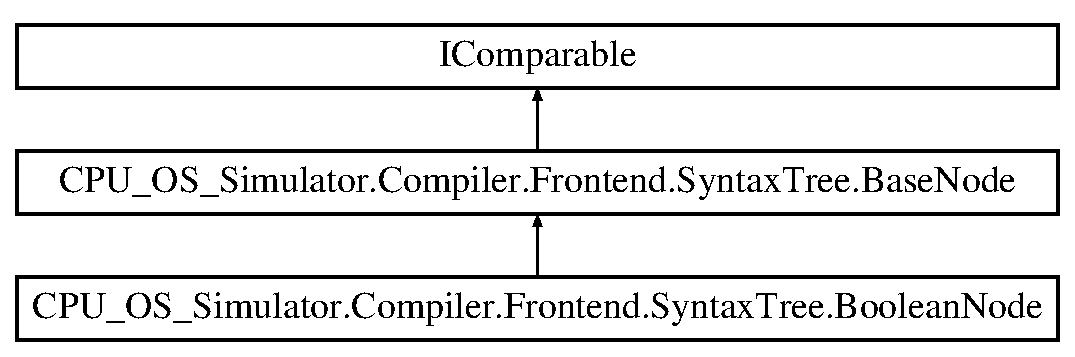
\includegraphics[height=3.000000cm]{class_c_p_u___o_s___simulator_1_1_compiler_1_1_frontend_1_1_syntax_tree_1_1_boolean_node}
\end{center}
\end{figure}
\subsection*{Public Member Functions}
\begin{DoxyCompactItemize}
\item 
override void \hyperlink{class_c_p_u___o_s___simulator_1_1_compiler_1_1_frontend_1_1_syntax_tree_1_1_boolean_node_a5cf13a08d798c5c1a225654e3f888866}{Visit} ()
\begin{DoxyCompactList}\small\item\em This function is called when the node is being visited by the parser \end{DoxyCompactList}\item 
override void \hyperlink{class_c_p_u___o_s___simulator_1_1_compiler_1_1_frontend_1_1_syntax_tree_1_1_boolean_node_a4a804a07050c45ca80feaaac3a050784}{Evaluate} ()
\begin{DoxyCompactList}\small\item\em This Function is called when the node is being evaluated by the parser \end{DoxyCompactList}\end{DoxyCompactItemize}
\subsection*{Properties}
\begin{DoxyCompactItemize}
\item 
override \hyperlink{class_c_p_u___o_s___simulator_1_1_compiler_1_1_frontend_1_1_syntax_tree_1_1_base_node}{Base\+Node} \hyperlink{class_c_p_u___o_s___simulator_1_1_compiler_1_1_frontend_1_1_syntax_tree_1_1_boolean_node_a3308cc287e781c949b529d6f1ad33254}{Right}\hspace{0.3cm}{\ttfamily  \mbox{[}get, set\mbox{]}}
\item 
override \hyperlink{class_c_p_u___o_s___simulator_1_1_compiler_1_1_frontend_1_1_syntax_tree_1_1_base_node}{Base\+Node} \hyperlink{class_c_p_u___o_s___simulator_1_1_compiler_1_1_frontend_1_1_syntax_tree_1_1_boolean_node_ac9bf4631f502393c3a0b11c82f445577}{Left}\hspace{0.3cm}{\ttfamily  \mbox{[}get, set\mbox{]}}
\item 
bool \hyperlink{class_c_p_u___o_s___simulator_1_1_compiler_1_1_frontend_1_1_syntax_tree_1_1_boolean_node_afadc08292a2dda4d7a1b536ccd8e241b}{Data}\hspace{0.3cm}{\ttfamily  \mbox{[}get, set\mbox{]}}
\item 
override \hyperlink{class_c_p_u___o_s___simulator_1_1_compiler_1_1_frontend_1_1_syntax_tree_1_1_base_node}{Base\+Node} \hyperlink{class_c_p_u___o_s___simulator_1_1_compiler_1_1_frontend_1_1_syntax_tree_1_1_boolean_node_ae4d9aaf39a383a5febd8b60400ad6cf5}{Parent}\hspace{0.3cm}{\ttfamily  \mbox{[}get, set\mbox{]}}
\end{DoxyCompactItemize}
\subsection*{Private Attributes}
\begin{DoxyCompactItemize}
\item 
new bool \hyperlink{class_c_p_u___o_s___simulator_1_1_compiler_1_1_frontend_1_1_syntax_tree_1_1_boolean_node_ac1b14b58e9c9b509a09cfd3e739b84dd}{data}
\item 
\hyperlink{class_c_p_u___o_s___simulator_1_1_compiler_1_1_frontend_1_1_syntax_tree_1_1_base_node}{Base\+Node} \hyperlink{class_c_p_u___o_s___simulator_1_1_compiler_1_1_frontend_1_1_syntax_tree_1_1_boolean_node_a6dfa76468d8e3cea03174bb24db0fca3}{parent}
\end{DoxyCompactItemize}
\subsection*{Additional Inherited Members}


\subsection{Detailed Description}


Definition at line 9 of file Boolean\+Node.\+cs.



\subsection{Member Function Documentation}
\hypertarget{class_c_p_u___o_s___simulator_1_1_compiler_1_1_frontend_1_1_syntax_tree_1_1_boolean_node_a4a804a07050c45ca80feaaac3a050784}{}\index{C\+P\+U\+\_\+\+O\+S\+\_\+\+Simulator\+::\+Compiler\+::\+Frontend\+::\+Syntax\+Tree\+::\+Boolean\+Node@{C\+P\+U\+\_\+\+O\+S\+\_\+\+Simulator\+::\+Compiler\+::\+Frontend\+::\+Syntax\+Tree\+::\+Boolean\+Node}!Evaluate@{Evaluate}}
\index{Evaluate@{Evaluate}!C\+P\+U\+\_\+\+O\+S\+\_\+\+Simulator\+::\+Compiler\+::\+Frontend\+::\+Syntax\+Tree\+::\+Boolean\+Node@{C\+P\+U\+\_\+\+O\+S\+\_\+\+Simulator\+::\+Compiler\+::\+Frontend\+::\+Syntax\+Tree\+::\+Boolean\+Node}}
\subsubsection[{Evaluate()}]{\setlength{\rightskip}{0pt plus 5cm}override void C\+P\+U\+\_\+\+O\+S\+\_\+\+Simulator.\+Compiler.\+Frontend.\+Syntax\+Tree.\+Boolean\+Node.\+Evaluate (
\begin{DoxyParamCaption}
{}
\end{DoxyParamCaption}
)\hspace{0.3cm}{\ttfamily [virtual]}}\label{class_c_p_u___o_s___simulator_1_1_compiler_1_1_frontend_1_1_syntax_tree_1_1_boolean_node_a4a804a07050c45ca80feaaac3a050784}


This Function is called when the node is being evaluated by the parser 



Implements \hyperlink{class_c_p_u___o_s___simulator_1_1_compiler_1_1_frontend_1_1_syntax_tree_1_1_base_node_a6cfcf8a0795180bdb1c7f0735d39441b}{C\+P\+U\+\_\+\+O\+S\+\_\+\+Simulator.\+Compiler.\+Frontend.\+Syntax\+Tree.\+Base\+Node}.



Definition at line 48 of file Boolean\+Node.\+cs.

\hypertarget{class_c_p_u___o_s___simulator_1_1_compiler_1_1_frontend_1_1_syntax_tree_1_1_boolean_node_a5cf13a08d798c5c1a225654e3f888866}{}\index{C\+P\+U\+\_\+\+O\+S\+\_\+\+Simulator\+::\+Compiler\+::\+Frontend\+::\+Syntax\+Tree\+::\+Boolean\+Node@{C\+P\+U\+\_\+\+O\+S\+\_\+\+Simulator\+::\+Compiler\+::\+Frontend\+::\+Syntax\+Tree\+::\+Boolean\+Node}!Visit@{Visit}}
\index{Visit@{Visit}!C\+P\+U\+\_\+\+O\+S\+\_\+\+Simulator\+::\+Compiler\+::\+Frontend\+::\+Syntax\+Tree\+::\+Boolean\+Node@{C\+P\+U\+\_\+\+O\+S\+\_\+\+Simulator\+::\+Compiler\+::\+Frontend\+::\+Syntax\+Tree\+::\+Boolean\+Node}}
\subsubsection[{Visit()}]{\setlength{\rightskip}{0pt plus 5cm}override void C\+P\+U\+\_\+\+O\+S\+\_\+\+Simulator.\+Compiler.\+Frontend.\+Syntax\+Tree.\+Boolean\+Node.\+Visit (
\begin{DoxyParamCaption}
{}
\end{DoxyParamCaption}
)\hspace{0.3cm}{\ttfamily [virtual]}}\label{class_c_p_u___o_s___simulator_1_1_compiler_1_1_frontend_1_1_syntax_tree_1_1_boolean_node_a5cf13a08d798c5c1a225654e3f888866}


This function is called when the node is being visited by the parser 



Implements \hyperlink{class_c_p_u___o_s___simulator_1_1_compiler_1_1_frontend_1_1_syntax_tree_1_1_base_node_a092377df64002c5e9c023a259e5e11d0}{C\+P\+U\+\_\+\+O\+S\+\_\+\+Simulator.\+Compiler.\+Frontend.\+Syntax\+Tree.\+Base\+Node}.



Definition at line 41 of file Boolean\+Node.\+cs.



\subsection{Member Data Documentation}
\hypertarget{class_c_p_u___o_s___simulator_1_1_compiler_1_1_frontend_1_1_syntax_tree_1_1_boolean_node_ac1b14b58e9c9b509a09cfd3e739b84dd}{}\index{C\+P\+U\+\_\+\+O\+S\+\_\+\+Simulator\+::\+Compiler\+::\+Frontend\+::\+Syntax\+Tree\+::\+Boolean\+Node@{C\+P\+U\+\_\+\+O\+S\+\_\+\+Simulator\+::\+Compiler\+::\+Frontend\+::\+Syntax\+Tree\+::\+Boolean\+Node}!data@{data}}
\index{data@{data}!C\+P\+U\+\_\+\+O\+S\+\_\+\+Simulator\+::\+Compiler\+::\+Frontend\+::\+Syntax\+Tree\+::\+Boolean\+Node@{C\+P\+U\+\_\+\+O\+S\+\_\+\+Simulator\+::\+Compiler\+::\+Frontend\+::\+Syntax\+Tree\+::\+Boolean\+Node}}
\subsubsection[{data}]{\setlength{\rightskip}{0pt plus 5cm}new bool C\+P\+U\+\_\+\+O\+S\+\_\+\+Simulator.\+Compiler.\+Frontend.\+Syntax\+Tree.\+Boolean\+Node.\+data\hspace{0.3cm}{\ttfamily [private]}}\label{class_c_p_u___o_s___simulator_1_1_compiler_1_1_frontend_1_1_syntax_tree_1_1_boolean_node_ac1b14b58e9c9b509a09cfd3e739b84dd}


Definition at line 11 of file Boolean\+Node.\+cs.

\hypertarget{class_c_p_u___o_s___simulator_1_1_compiler_1_1_frontend_1_1_syntax_tree_1_1_boolean_node_a6dfa76468d8e3cea03174bb24db0fca3}{}\index{C\+P\+U\+\_\+\+O\+S\+\_\+\+Simulator\+::\+Compiler\+::\+Frontend\+::\+Syntax\+Tree\+::\+Boolean\+Node@{C\+P\+U\+\_\+\+O\+S\+\_\+\+Simulator\+::\+Compiler\+::\+Frontend\+::\+Syntax\+Tree\+::\+Boolean\+Node}!parent@{parent}}
\index{parent@{parent}!C\+P\+U\+\_\+\+O\+S\+\_\+\+Simulator\+::\+Compiler\+::\+Frontend\+::\+Syntax\+Tree\+::\+Boolean\+Node@{C\+P\+U\+\_\+\+O\+S\+\_\+\+Simulator\+::\+Compiler\+::\+Frontend\+::\+Syntax\+Tree\+::\+Boolean\+Node}}
\subsubsection[{parent}]{\setlength{\rightskip}{0pt plus 5cm}{\bf Base\+Node} C\+P\+U\+\_\+\+O\+S\+\_\+\+Simulator.\+Compiler.\+Frontend.\+Syntax\+Tree.\+Boolean\+Node.\+parent\hspace{0.3cm}{\ttfamily [private]}}\label{class_c_p_u___o_s___simulator_1_1_compiler_1_1_frontend_1_1_syntax_tree_1_1_boolean_node_a6dfa76468d8e3cea03174bb24db0fca3}


Definition at line 12 of file Boolean\+Node.\+cs.



\subsection{Property Documentation}
\hypertarget{class_c_p_u___o_s___simulator_1_1_compiler_1_1_frontend_1_1_syntax_tree_1_1_boolean_node_afadc08292a2dda4d7a1b536ccd8e241b}{}\index{C\+P\+U\+\_\+\+O\+S\+\_\+\+Simulator\+::\+Compiler\+::\+Frontend\+::\+Syntax\+Tree\+::\+Boolean\+Node@{C\+P\+U\+\_\+\+O\+S\+\_\+\+Simulator\+::\+Compiler\+::\+Frontend\+::\+Syntax\+Tree\+::\+Boolean\+Node}!Data@{Data}}
\index{Data@{Data}!C\+P\+U\+\_\+\+O\+S\+\_\+\+Simulator\+::\+Compiler\+::\+Frontend\+::\+Syntax\+Tree\+::\+Boolean\+Node@{C\+P\+U\+\_\+\+O\+S\+\_\+\+Simulator\+::\+Compiler\+::\+Frontend\+::\+Syntax\+Tree\+::\+Boolean\+Node}}
\subsubsection[{Data}]{\setlength{\rightskip}{0pt plus 5cm}bool C\+P\+U\+\_\+\+O\+S\+\_\+\+Simulator.\+Compiler.\+Frontend.\+Syntax\+Tree.\+Boolean\+Node.\+Data\hspace{0.3cm}{\ttfamily [get]}, {\ttfamily [set]}}\label{class_c_p_u___o_s___simulator_1_1_compiler_1_1_frontend_1_1_syntax_tree_1_1_boolean_node_afadc08292a2dda4d7a1b536ccd8e241b}


Definition at line 27 of file Boolean\+Node.\+cs.

\hypertarget{class_c_p_u___o_s___simulator_1_1_compiler_1_1_frontend_1_1_syntax_tree_1_1_boolean_node_ac9bf4631f502393c3a0b11c82f445577}{}\index{C\+P\+U\+\_\+\+O\+S\+\_\+\+Simulator\+::\+Compiler\+::\+Frontend\+::\+Syntax\+Tree\+::\+Boolean\+Node@{C\+P\+U\+\_\+\+O\+S\+\_\+\+Simulator\+::\+Compiler\+::\+Frontend\+::\+Syntax\+Tree\+::\+Boolean\+Node}!Left@{Left}}
\index{Left@{Left}!C\+P\+U\+\_\+\+O\+S\+\_\+\+Simulator\+::\+Compiler\+::\+Frontend\+::\+Syntax\+Tree\+::\+Boolean\+Node@{C\+P\+U\+\_\+\+O\+S\+\_\+\+Simulator\+::\+Compiler\+::\+Frontend\+::\+Syntax\+Tree\+::\+Boolean\+Node}}
\subsubsection[{Left}]{\setlength{\rightskip}{0pt plus 5cm}override {\bf Base\+Node} C\+P\+U\+\_\+\+O\+S\+\_\+\+Simulator.\+Compiler.\+Frontend.\+Syntax\+Tree.\+Boolean\+Node.\+Left\hspace{0.3cm}{\ttfamily [get]}, {\ttfamily [set]}}\label{class_c_p_u___o_s___simulator_1_1_compiler_1_1_frontend_1_1_syntax_tree_1_1_boolean_node_ac9bf4631f502393c3a0b11c82f445577}


Definition at line 21 of file Boolean\+Node.\+cs.

\hypertarget{class_c_p_u___o_s___simulator_1_1_compiler_1_1_frontend_1_1_syntax_tree_1_1_boolean_node_ae4d9aaf39a383a5febd8b60400ad6cf5}{}\index{C\+P\+U\+\_\+\+O\+S\+\_\+\+Simulator\+::\+Compiler\+::\+Frontend\+::\+Syntax\+Tree\+::\+Boolean\+Node@{C\+P\+U\+\_\+\+O\+S\+\_\+\+Simulator\+::\+Compiler\+::\+Frontend\+::\+Syntax\+Tree\+::\+Boolean\+Node}!Parent@{Parent}}
\index{Parent@{Parent}!C\+P\+U\+\_\+\+O\+S\+\_\+\+Simulator\+::\+Compiler\+::\+Frontend\+::\+Syntax\+Tree\+::\+Boolean\+Node@{C\+P\+U\+\_\+\+O\+S\+\_\+\+Simulator\+::\+Compiler\+::\+Frontend\+::\+Syntax\+Tree\+::\+Boolean\+Node}}
\subsubsection[{Parent}]{\setlength{\rightskip}{0pt plus 5cm}override {\bf Base\+Node} C\+P\+U\+\_\+\+O\+S\+\_\+\+Simulator.\+Compiler.\+Frontend.\+Syntax\+Tree.\+Boolean\+Node.\+Parent\hspace{0.3cm}{\ttfamily [get]}, {\ttfamily [set]}}\label{class_c_p_u___o_s___simulator_1_1_compiler_1_1_frontend_1_1_syntax_tree_1_1_boolean_node_ae4d9aaf39a383a5febd8b60400ad6cf5}


Definition at line 33 of file Boolean\+Node.\+cs.

\hypertarget{class_c_p_u___o_s___simulator_1_1_compiler_1_1_frontend_1_1_syntax_tree_1_1_boolean_node_a3308cc287e781c949b529d6f1ad33254}{}\index{C\+P\+U\+\_\+\+O\+S\+\_\+\+Simulator\+::\+Compiler\+::\+Frontend\+::\+Syntax\+Tree\+::\+Boolean\+Node@{C\+P\+U\+\_\+\+O\+S\+\_\+\+Simulator\+::\+Compiler\+::\+Frontend\+::\+Syntax\+Tree\+::\+Boolean\+Node}!Right@{Right}}
\index{Right@{Right}!C\+P\+U\+\_\+\+O\+S\+\_\+\+Simulator\+::\+Compiler\+::\+Frontend\+::\+Syntax\+Tree\+::\+Boolean\+Node@{C\+P\+U\+\_\+\+O\+S\+\_\+\+Simulator\+::\+Compiler\+::\+Frontend\+::\+Syntax\+Tree\+::\+Boolean\+Node}}
\subsubsection[{Right}]{\setlength{\rightskip}{0pt plus 5cm}override {\bf Base\+Node} C\+P\+U\+\_\+\+O\+S\+\_\+\+Simulator.\+Compiler.\+Frontend.\+Syntax\+Tree.\+Boolean\+Node.\+Right\hspace{0.3cm}{\ttfamily [get]}, {\ttfamily [set]}}\label{class_c_p_u___o_s___simulator_1_1_compiler_1_1_frontend_1_1_syntax_tree_1_1_boolean_node_a3308cc287e781c949b529d6f1ad33254}


Definition at line 15 of file Boolean\+Node.\+cs.



The documentation for this class was generated from the following file\+:\begin{DoxyCompactItemize}
\item 
Compiler/\+Frontend/\+Syntax\+Tree/\hyperlink{_boolean_node_8cs}{Boolean\+Node.\+cs}\end{DoxyCompactItemize}

\hypertarget{class_c_p_u___o_s___simulator_1_1_compiler_1_1_frontend_1_1_syntax_tree_1_1_byte_array_node}{}\section{C\+P\+U\+\_\+\+O\+S\+\_\+\+Simulator.\+Compiler.\+Frontend.\+Syntax\+Tree.\+Byte\+Array\+Node Class Reference}
\label{class_c_p_u___o_s___simulator_1_1_compiler_1_1_frontend_1_1_syntax_tree_1_1_byte_array_node}\index{C\+P\+U\+\_\+\+O\+S\+\_\+\+Simulator.\+Compiler.\+Frontend.\+Syntax\+Tree.\+Byte\+Array\+Node@{C\+P\+U\+\_\+\+O\+S\+\_\+\+Simulator.\+Compiler.\+Frontend.\+Syntax\+Tree.\+Byte\+Array\+Node}}
Inheritance diagram for C\+P\+U\+\_\+\+O\+S\+\_\+\+Simulator.\+Compiler.\+Frontend.\+Syntax\+Tree.\+Byte\+Array\+Node\+:\begin{figure}[H]
\begin{center}
\leavevmode
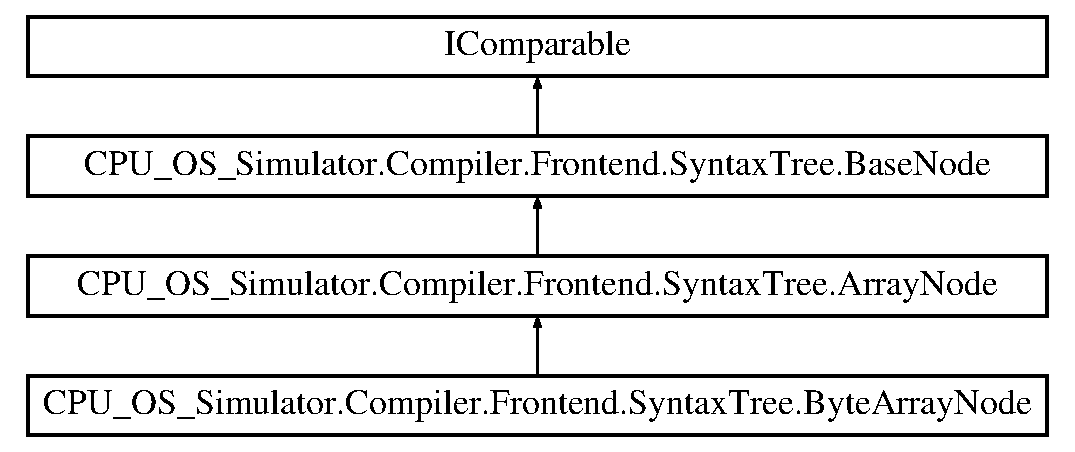
\includegraphics[height=4.000000cm]{class_c_p_u___o_s___simulator_1_1_compiler_1_1_frontend_1_1_syntax_tree_1_1_byte_array_node}
\end{center}
\end{figure}
\subsection*{Public Member Functions}
\begin{DoxyCompactItemize}
\item 
override void \hyperlink{class_c_p_u___o_s___simulator_1_1_compiler_1_1_frontend_1_1_syntax_tree_1_1_byte_array_node_a1ed9d8d35aeb8537758718aa1bae1ae0}{Visit} ()
\begin{DoxyCompactList}\small\item\em This function is called when the node is being visited by the parser \end{DoxyCompactList}\item 
override void \hyperlink{class_c_p_u___o_s___simulator_1_1_compiler_1_1_frontend_1_1_syntax_tree_1_1_byte_array_node_ad34fd3396bf5e6e179d941d2076f28d9}{Evaluate} ()
\begin{DoxyCompactList}\small\item\em This Function is called when the node is being evaluated by the parser \end{DoxyCompactList}\item 
override int \hyperlink{class_c_p_u___o_s___simulator_1_1_compiler_1_1_frontend_1_1_syntax_tree_1_1_byte_array_node_a899a0a2406a3e09828de51918a13afba}{number\+Of\+Elements} ()
\end{DoxyCompactItemize}
\subsection*{Public Attributes}
\begin{DoxyCompactItemize}
\item 
new byte\mbox{[}$\,$\mbox{]} \hyperlink{class_c_p_u___o_s___simulator_1_1_compiler_1_1_frontend_1_1_syntax_tree_1_1_byte_array_node_a583fbbf2ac627103a16bfc03214f4f13}{data}
\end{DoxyCompactItemize}
\subsection*{Properties}
\begin{DoxyCompactItemize}
\item 
override \hyperlink{class_c_p_u___o_s___simulator_1_1_compiler_1_1_frontend_1_1_syntax_tree_1_1_base_node}{Base\+Node} \hyperlink{class_c_p_u___o_s___simulator_1_1_compiler_1_1_frontend_1_1_syntax_tree_1_1_byte_array_node_a4e51f2ddd2a095fe9fa84cfb1fa2e6bc}{Right}\hspace{0.3cm}{\ttfamily  \mbox{[}get, set\mbox{]}}
\item 
override \hyperlink{class_c_p_u___o_s___simulator_1_1_compiler_1_1_frontend_1_1_syntax_tree_1_1_base_node}{Base\+Node} \hyperlink{class_c_p_u___o_s___simulator_1_1_compiler_1_1_frontend_1_1_syntax_tree_1_1_byte_array_node_a390bdce07039689aa1a66b612862b88d}{Left}\hspace{0.3cm}{\ttfamily  \mbox{[}get, set\mbox{]}}
\item 
override \hyperlink{class_c_p_u___o_s___simulator_1_1_compiler_1_1_frontend_1_1_syntax_tree_1_1_base_node}{Base\+Node} \hyperlink{class_c_p_u___o_s___simulator_1_1_compiler_1_1_frontend_1_1_syntax_tree_1_1_byte_array_node_a6b1a860628d31271a0985ac13f1b797b}{Parent}\hspace{0.3cm}{\ttfamily  \mbox{[}get, set\mbox{]}}
\end{DoxyCompactItemize}
\subsection*{Private Attributes}
\begin{DoxyCompactItemize}
\item 
\hyperlink{class_c_p_u___o_s___simulator_1_1_compiler_1_1_frontend_1_1_syntax_tree_1_1_base_node}{Base\+Node} \hyperlink{class_c_p_u___o_s___simulator_1_1_compiler_1_1_frontend_1_1_syntax_tree_1_1_byte_array_node_af549ef91dee29880025a56b3a63de54c}{parent}
\end{DoxyCompactItemize}
\subsection*{Additional Inherited Members}


\subsection{Detailed Description}


Definition at line 3 of file Byte\+Array\+Node.\+cs.



\subsection{Member Function Documentation}
\hypertarget{class_c_p_u___o_s___simulator_1_1_compiler_1_1_frontend_1_1_syntax_tree_1_1_byte_array_node_ad34fd3396bf5e6e179d941d2076f28d9}{}\index{C\+P\+U\+\_\+\+O\+S\+\_\+\+Simulator\+::\+Compiler\+::\+Frontend\+::\+Syntax\+Tree\+::\+Byte\+Array\+Node@{C\+P\+U\+\_\+\+O\+S\+\_\+\+Simulator\+::\+Compiler\+::\+Frontend\+::\+Syntax\+Tree\+::\+Byte\+Array\+Node}!Evaluate@{Evaluate}}
\index{Evaluate@{Evaluate}!C\+P\+U\+\_\+\+O\+S\+\_\+\+Simulator\+::\+Compiler\+::\+Frontend\+::\+Syntax\+Tree\+::\+Byte\+Array\+Node@{C\+P\+U\+\_\+\+O\+S\+\_\+\+Simulator\+::\+Compiler\+::\+Frontend\+::\+Syntax\+Tree\+::\+Byte\+Array\+Node}}
\subsubsection[{Evaluate()}]{\setlength{\rightskip}{0pt plus 5cm}override void C\+P\+U\+\_\+\+O\+S\+\_\+\+Simulator.\+Compiler.\+Frontend.\+Syntax\+Tree.\+Byte\+Array\+Node.\+Evaluate (
\begin{DoxyParamCaption}
{}
\end{DoxyParamCaption}
)\hspace{0.3cm}{\ttfamily [virtual]}}\label{class_c_p_u___o_s___simulator_1_1_compiler_1_1_frontend_1_1_syntax_tree_1_1_byte_array_node_ad34fd3396bf5e6e179d941d2076f28d9}


This Function is called when the node is being evaluated by the parser 



Implements \hyperlink{class_c_p_u___o_s___simulator_1_1_compiler_1_1_frontend_1_1_syntax_tree_1_1_array_node_afdb5d2808dbd83c28c85f35b6430edc4}{C\+P\+U\+\_\+\+O\+S\+\_\+\+Simulator.\+Compiler.\+Frontend.\+Syntax\+Tree.\+Array\+Node}.



Definition at line 36 of file Byte\+Array\+Node.\+cs.

\hypertarget{class_c_p_u___o_s___simulator_1_1_compiler_1_1_frontend_1_1_syntax_tree_1_1_byte_array_node_a899a0a2406a3e09828de51918a13afba}{}\index{C\+P\+U\+\_\+\+O\+S\+\_\+\+Simulator\+::\+Compiler\+::\+Frontend\+::\+Syntax\+Tree\+::\+Byte\+Array\+Node@{C\+P\+U\+\_\+\+O\+S\+\_\+\+Simulator\+::\+Compiler\+::\+Frontend\+::\+Syntax\+Tree\+::\+Byte\+Array\+Node}!number\+Of\+Elements@{number\+Of\+Elements}}
\index{number\+Of\+Elements@{number\+Of\+Elements}!C\+P\+U\+\_\+\+O\+S\+\_\+\+Simulator\+::\+Compiler\+::\+Frontend\+::\+Syntax\+Tree\+::\+Byte\+Array\+Node@{C\+P\+U\+\_\+\+O\+S\+\_\+\+Simulator\+::\+Compiler\+::\+Frontend\+::\+Syntax\+Tree\+::\+Byte\+Array\+Node}}
\subsubsection[{number\+Of\+Elements()}]{\setlength{\rightskip}{0pt plus 5cm}override int C\+P\+U\+\_\+\+O\+S\+\_\+\+Simulator.\+Compiler.\+Frontend.\+Syntax\+Tree.\+Byte\+Array\+Node.\+number\+Of\+Elements (
\begin{DoxyParamCaption}
{}
\end{DoxyParamCaption}
)\hspace{0.3cm}{\ttfamily [virtual]}}\label{class_c_p_u___o_s___simulator_1_1_compiler_1_1_frontend_1_1_syntax_tree_1_1_byte_array_node_a899a0a2406a3e09828de51918a13afba}


Implements \hyperlink{class_c_p_u___o_s___simulator_1_1_compiler_1_1_frontend_1_1_syntax_tree_1_1_array_node_a75232f3076d95a562405ef2722bcafd5}{C\+P\+U\+\_\+\+O\+S\+\_\+\+Simulator.\+Compiler.\+Frontend.\+Syntax\+Tree.\+Array\+Node}.



Definition at line 40 of file Byte\+Array\+Node.\+cs.

\hypertarget{class_c_p_u___o_s___simulator_1_1_compiler_1_1_frontend_1_1_syntax_tree_1_1_byte_array_node_a1ed9d8d35aeb8537758718aa1bae1ae0}{}\index{C\+P\+U\+\_\+\+O\+S\+\_\+\+Simulator\+::\+Compiler\+::\+Frontend\+::\+Syntax\+Tree\+::\+Byte\+Array\+Node@{C\+P\+U\+\_\+\+O\+S\+\_\+\+Simulator\+::\+Compiler\+::\+Frontend\+::\+Syntax\+Tree\+::\+Byte\+Array\+Node}!Visit@{Visit}}
\index{Visit@{Visit}!C\+P\+U\+\_\+\+O\+S\+\_\+\+Simulator\+::\+Compiler\+::\+Frontend\+::\+Syntax\+Tree\+::\+Byte\+Array\+Node@{C\+P\+U\+\_\+\+O\+S\+\_\+\+Simulator\+::\+Compiler\+::\+Frontend\+::\+Syntax\+Tree\+::\+Byte\+Array\+Node}}
\subsubsection[{Visit()}]{\setlength{\rightskip}{0pt plus 5cm}override void C\+P\+U\+\_\+\+O\+S\+\_\+\+Simulator.\+Compiler.\+Frontend.\+Syntax\+Tree.\+Byte\+Array\+Node.\+Visit (
\begin{DoxyParamCaption}
{}
\end{DoxyParamCaption}
)\hspace{0.3cm}{\ttfamily [virtual]}}\label{class_c_p_u___o_s___simulator_1_1_compiler_1_1_frontend_1_1_syntax_tree_1_1_byte_array_node_a1ed9d8d35aeb8537758718aa1bae1ae0}


This function is called when the node is being visited by the parser 



Implements \hyperlink{class_c_p_u___o_s___simulator_1_1_compiler_1_1_frontend_1_1_syntax_tree_1_1_array_node_aed695b6f32d5c176204fc15854db32db}{C\+P\+U\+\_\+\+O\+S\+\_\+\+Simulator.\+Compiler.\+Frontend.\+Syntax\+Tree.\+Array\+Node}.



Definition at line 29 of file Byte\+Array\+Node.\+cs.



\subsection{Member Data Documentation}
\hypertarget{class_c_p_u___o_s___simulator_1_1_compiler_1_1_frontend_1_1_syntax_tree_1_1_byte_array_node_a583fbbf2ac627103a16bfc03214f4f13}{}\index{C\+P\+U\+\_\+\+O\+S\+\_\+\+Simulator\+::\+Compiler\+::\+Frontend\+::\+Syntax\+Tree\+::\+Byte\+Array\+Node@{C\+P\+U\+\_\+\+O\+S\+\_\+\+Simulator\+::\+Compiler\+::\+Frontend\+::\+Syntax\+Tree\+::\+Byte\+Array\+Node}!data@{data}}
\index{data@{data}!C\+P\+U\+\_\+\+O\+S\+\_\+\+Simulator\+::\+Compiler\+::\+Frontend\+::\+Syntax\+Tree\+::\+Byte\+Array\+Node@{C\+P\+U\+\_\+\+O\+S\+\_\+\+Simulator\+::\+Compiler\+::\+Frontend\+::\+Syntax\+Tree\+::\+Byte\+Array\+Node}}
\subsubsection[{data}]{\setlength{\rightskip}{0pt plus 5cm}new byte \mbox{[}$\,$\mbox{]} C\+P\+U\+\_\+\+O\+S\+\_\+\+Simulator.\+Compiler.\+Frontend.\+Syntax\+Tree.\+Byte\+Array\+Node.\+data}\label{class_c_p_u___o_s___simulator_1_1_compiler_1_1_frontend_1_1_syntax_tree_1_1_byte_array_node_a583fbbf2ac627103a16bfc03214f4f13}


Definition at line 5 of file Byte\+Array\+Node.\+cs.

\hypertarget{class_c_p_u___o_s___simulator_1_1_compiler_1_1_frontend_1_1_syntax_tree_1_1_byte_array_node_af549ef91dee29880025a56b3a63de54c}{}\index{C\+P\+U\+\_\+\+O\+S\+\_\+\+Simulator\+::\+Compiler\+::\+Frontend\+::\+Syntax\+Tree\+::\+Byte\+Array\+Node@{C\+P\+U\+\_\+\+O\+S\+\_\+\+Simulator\+::\+Compiler\+::\+Frontend\+::\+Syntax\+Tree\+::\+Byte\+Array\+Node}!parent@{parent}}
\index{parent@{parent}!C\+P\+U\+\_\+\+O\+S\+\_\+\+Simulator\+::\+Compiler\+::\+Frontend\+::\+Syntax\+Tree\+::\+Byte\+Array\+Node@{C\+P\+U\+\_\+\+O\+S\+\_\+\+Simulator\+::\+Compiler\+::\+Frontend\+::\+Syntax\+Tree\+::\+Byte\+Array\+Node}}
\subsubsection[{parent}]{\setlength{\rightskip}{0pt plus 5cm}{\bf Base\+Node} C\+P\+U\+\_\+\+O\+S\+\_\+\+Simulator.\+Compiler.\+Frontend.\+Syntax\+Tree.\+Byte\+Array\+Node.\+parent\hspace{0.3cm}{\ttfamily [private]}}\label{class_c_p_u___o_s___simulator_1_1_compiler_1_1_frontend_1_1_syntax_tree_1_1_byte_array_node_af549ef91dee29880025a56b3a63de54c}


Definition at line 6 of file Byte\+Array\+Node.\+cs.



\subsection{Property Documentation}
\hypertarget{class_c_p_u___o_s___simulator_1_1_compiler_1_1_frontend_1_1_syntax_tree_1_1_byte_array_node_a390bdce07039689aa1a66b612862b88d}{}\index{C\+P\+U\+\_\+\+O\+S\+\_\+\+Simulator\+::\+Compiler\+::\+Frontend\+::\+Syntax\+Tree\+::\+Byte\+Array\+Node@{C\+P\+U\+\_\+\+O\+S\+\_\+\+Simulator\+::\+Compiler\+::\+Frontend\+::\+Syntax\+Tree\+::\+Byte\+Array\+Node}!Left@{Left}}
\index{Left@{Left}!C\+P\+U\+\_\+\+O\+S\+\_\+\+Simulator\+::\+Compiler\+::\+Frontend\+::\+Syntax\+Tree\+::\+Byte\+Array\+Node@{C\+P\+U\+\_\+\+O\+S\+\_\+\+Simulator\+::\+Compiler\+::\+Frontend\+::\+Syntax\+Tree\+::\+Byte\+Array\+Node}}
\subsubsection[{Left}]{\setlength{\rightskip}{0pt plus 5cm}override {\bf Base\+Node} C\+P\+U\+\_\+\+O\+S\+\_\+\+Simulator.\+Compiler.\+Frontend.\+Syntax\+Tree.\+Byte\+Array\+Node.\+Left\hspace{0.3cm}{\ttfamily [get]}, {\ttfamily [set]}}\label{class_c_p_u___o_s___simulator_1_1_compiler_1_1_frontend_1_1_syntax_tree_1_1_byte_array_node_a390bdce07039689aa1a66b612862b88d}


Definition at line 15 of file Byte\+Array\+Node.\+cs.

\hypertarget{class_c_p_u___o_s___simulator_1_1_compiler_1_1_frontend_1_1_syntax_tree_1_1_byte_array_node_a6b1a860628d31271a0985ac13f1b797b}{}\index{C\+P\+U\+\_\+\+O\+S\+\_\+\+Simulator\+::\+Compiler\+::\+Frontend\+::\+Syntax\+Tree\+::\+Byte\+Array\+Node@{C\+P\+U\+\_\+\+O\+S\+\_\+\+Simulator\+::\+Compiler\+::\+Frontend\+::\+Syntax\+Tree\+::\+Byte\+Array\+Node}!Parent@{Parent}}
\index{Parent@{Parent}!C\+P\+U\+\_\+\+O\+S\+\_\+\+Simulator\+::\+Compiler\+::\+Frontend\+::\+Syntax\+Tree\+::\+Byte\+Array\+Node@{C\+P\+U\+\_\+\+O\+S\+\_\+\+Simulator\+::\+Compiler\+::\+Frontend\+::\+Syntax\+Tree\+::\+Byte\+Array\+Node}}
\subsubsection[{Parent}]{\setlength{\rightskip}{0pt plus 5cm}override {\bf Base\+Node} C\+P\+U\+\_\+\+O\+S\+\_\+\+Simulator.\+Compiler.\+Frontend.\+Syntax\+Tree.\+Byte\+Array\+Node.\+Parent\hspace{0.3cm}{\ttfamily [get]}, {\ttfamily [set]}}\label{class_c_p_u___o_s___simulator_1_1_compiler_1_1_frontend_1_1_syntax_tree_1_1_byte_array_node_a6b1a860628d31271a0985ac13f1b797b}


Definition at line 21 of file Byte\+Array\+Node.\+cs.

\hypertarget{class_c_p_u___o_s___simulator_1_1_compiler_1_1_frontend_1_1_syntax_tree_1_1_byte_array_node_a4e51f2ddd2a095fe9fa84cfb1fa2e6bc}{}\index{C\+P\+U\+\_\+\+O\+S\+\_\+\+Simulator\+::\+Compiler\+::\+Frontend\+::\+Syntax\+Tree\+::\+Byte\+Array\+Node@{C\+P\+U\+\_\+\+O\+S\+\_\+\+Simulator\+::\+Compiler\+::\+Frontend\+::\+Syntax\+Tree\+::\+Byte\+Array\+Node}!Right@{Right}}
\index{Right@{Right}!C\+P\+U\+\_\+\+O\+S\+\_\+\+Simulator\+::\+Compiler\+::\+Frontend\+::\+Syntax\+Tree\+::\+Byte\+Array\+Node@{C\+P\+U\+\_\+\+O\+S\+\_\+\+Simulator\+::\+Compiler\+::\+Frontend\+::\+Syntax\+Tree\+::\+Byte\+Array\+Node}}
\subsubsection[{Right}]{\setlength{\rightskip}{0pt plus 5cm}override {\bf Base\+Node} C\+P\+U\+\_\+\+O\+S\+\_\+\+Simulator.\+Compiler.\+Frontend.\+Syntax\+Tree.\+Byte\+Array\+Node.\+Right\hspace{0.3cm}{\ttfamily [get]}, {\ttfamily [set]}}\label{class_c_p_u___o_s___simulator_1_1_compiler_1_1_frontend_1_1_syntax_tree_1_1_byte_array_node_a4e51f2ddd2a095fe9fa84cfb1fa2e6bc}


Definition at line 9 of file Byte\+Array\+Node.\+cs.



The documentation for this class was generated from the following file\+:\begin{DoxyCompactItemize}
\item 
Compiler/\+Frontend/\+Syntax\+Tree/\hyperlink{_byte_array_node_8cs}{Byte\+Array\+Node.\+cs}\end{DoxyCompactItemize}

\hypertarget{class_c_p_u___o_s___simulator_1_1_compiler_1_1_frontend_1_1_syntax_tree_1_1_byte_node}{}\section{C\+P\+U\+\_\+\+O\+S\+\_\+\+Simulator.\+Compiler.\+Frontend.\+Syntax\+Tree.\+Byte\+Node Class Reference}
\label{class_c_p_u___o_s___simulator_1_1_compiler_1_1_frontend_1_1_syntax_tree_1_1_byte_node}\index{C\+P\+U\+\_\+\+O\+S\+\_\+\+Simulator.\+Compiler.\+Frontend.\+Syntax\+Tree.\+Byte\+Node@{C\+P\+U\+\_\+\+O\+S\+\_\+\+Simulator.\+Compiler.\+Frontend.\+Syntax\+Tree.\+Byte\+Node}}
Inheritance diagram for C\+P\+U\+\_\+\+O\+S\+\_\+\+Simulator.\+Compiler.\+Frontend.\+Syntax\+Tree.\+Byte\+Node\+:\begin{figure}[H]
\begin{center}
\leavevmode
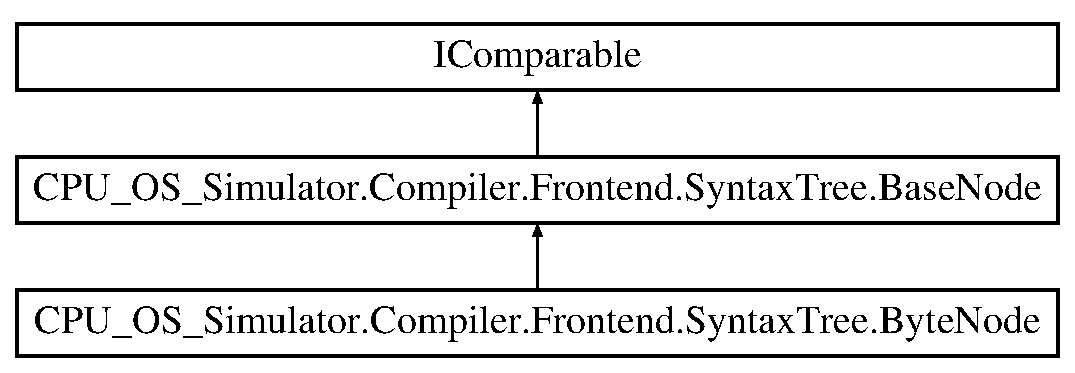
\includegraphics[height=3.000000cm]{class_c_p_u___o_s___simulator_1_1_compiler_1_1_frontend_1_1_syntax_tree_1_1_byte_node}
\end{center}
\end{figure}
\subsection*{Public Member Functions}
\begin{DoxyCompactItemize}
\item 
override void \hyperlink{class_c_p_u___o_s___simulator_1_1_compiler_1_1_frontend_1_1_syntax_tree_1_1_byte_node_af411e73f7153f6c67e09273198e9f1bb}{Visit} ()
\begin{DoxyCompactList}\small\item\em This function is called when the node is being visited by the parser \end{DoxyCompactList}\item 
override void \hyperlink{class_c_p_u___o_s___simulator_1_1_compiler_1_1_frontend_1_1_syntax_tree_1_1_byte_node_a0e9461945f15cb28abac866a81c8c5d3}{Evaluate} ()
\begin{DoxyCompactList}\small\item\em This Function is called when the node is being evaluated by the parser \end{DoxyCompactList}\end{DoxyCompactItemize}
\subsection*{Properties}
\begin{DoxyCompactItemize}
\item 
override \hyperlink{class_c_p_u___o_s___simulator_1_1_compiler_1_1_frontend_1_1_syntax_tree_1_1_base_node}{Base\+Node} \hyperlink{class_c_p_u___o_s___simulator_1_1_compiler_1_1_frontend_1_1_syntax_tree_1_1_byte_node_a16dbfc4538c6fad53cb95f118d260a5a}{Right}\hspace{0.3cm}{\ttfamily  \mbox{[}get, set\mbox{]}}
\item 
override \hyperlink{class_c_p_u___o_s___simulator_1_1_compiler_1_1_frontend_1_1_syntax_tree_1_1_base_node}{Base\+Node} \hyperlink{class_c_p_u___o_s___simulator_1_1_compiler_1_1_frontend_1_1_syntax_tree_1_1_byte_node_ae43202b000bd7f29f96aa8fcc527fcc9}{Left}\hspace{0.3cm}{\ttfamily  \mbox{[}get, set\mbox{]}}
\item 
byte \hyperlink{class_c_p_u___o_s___simulator_1_1_compiler_1_1_frontend_1_1_syntax_tree_1_1_byte_node_a960eba912e3dad89b7419898d30cc8f8}{Data}\hspace{0.3cm}{\ttfamily  \mbox{[}get, set\mbox{]}}
\item 
override \hyperlink{class_c_p_u___o_s___simulator_1_1_compiler_1_1_frontend_1_1_syntax_tree_1_1_base_node}{Base\+Node} \hyperlink{class_c_p_u___o_s___simulator_1_1_compiler_1_1_frontend_1_1_syntax_tree_1_1_byte_node_a0863b18cac100789e59a9e0898bf87d1}{Parent}\hspace{0.3cm}{\ttfamily  \mbox{[}get, set\mbox{]}}
\end{DoxyCompactItemize}
\subsection*{Private Attributes}
\begin{DoxyCompactItemize}
\item 
new byte \hyperlink{class_c_p_u___o_s___simulator_1_1_compiler_1_1_frontend_1_1_syntax_tree_1_1_byte_node_a6525600f7070b661cea67b11cf340b68}{data}
\item 
\hyperlink{class_c_p_u___o_s___simulator_1_1_compiler_1_1_frontend_1_1_syntax_tree_1_1_base_node}{Base\+Node} \hyperlink{class_c_p_u___o_s___simulator_1_1_compiler_1_1_frontend_1_1_syntax_tree_1_1_byte_node_afcaacda0eb81422004c2fe870ece1c31}{parent}
\end{DoxyCompactItemize}
\subsection*{Additional Inherited Members}


\subsection{Detailed Description}


Definition at line 3 of file Byte\+Node.\+cs.



\subsection{Member Function Documentation}
\hypertarget{class_c_p_u___o_s___simulator_1_1_compiler_1_1_frontend_1_1_syntax_tree_1_1_byte_node_a0e9461945f15cb28abac866a81c8c5d3}{}\index{C\+P\+U\+\_\+\+O\+S\+\_\+\+Simulator\+::\+Compiler\+::\+Frontend\+::\+Syntax\+Tree\+::\+Byte\+Node@{C\+P\+U\+\_\+\+O\+S\+\_\+\+Simulator\+::\+Compiler\+::\+Frontend\+::\+Syntax\+Tree\+::\+Byte\+Node}!Evaluate@{Evaluate}}
\index{Evaluate@{Evaluate}!C\+P\+U\+\_\+\+O\+S\+\_\+\+Simulator\+::\+Compiler\+::\+Frontend\+::\+Syntax\+Tree\+::\+Byte\+Node@{C\+P\+U\+\_\+\+O\+S\+\_\+\+Simulator\+::\+Compiler\+::\+Frontend\+::\+Syntax\+Tree\+::\+Byte\+Node}}
\subsubsection[{Evaluate()}]{\setlength{\rightskip}{0pt plus 5cm}override void C\+P\+U\+\_\+\+O\+S\+\_\+\+Simulator.\+Compiler.\+Frontend.\+Syntax\+Tree.\+Byte\+Node.\+Evaluate (
\begin{DoxyParamCaption}
{}
\end{DoxyParamCaption}
)\hspace{0.3cm}{\ttfamily [virtual]}}\label{class_c_p_u___o_s___simulator_1_1_compiler_1_1_frontend_1_1_syntax_tree_1_1_byte_node_a0e9461945f15cb28abac866a81c8c5d3}


This Function is called when the node is being evaluated by the parser 



Implements \hyperlink{class_c_p_u___o_s___simulator_1_1_compiler_1_1_frontend_1_1_syntax_tree_1_1_base_node_a6cfcf8a0795180bdb1c7f0735d39441b}{C\+P\+U\+\_\+\+O\+S\+\_\+\+Simulator.\+Compiler.\+Frontend.\+Syntax\+Tree.\+Base\+Node}.



Definition at line 42 of file Byte\+Node.\+cs.

\hypertarget{class_c_p_u___o_s___simulator_1_1_compiler_1_1_frontend_1_1_syntax_tree_1_1_byte_node_af411e73f7153f6c67e09273198e9f1bb}{}\index{C\+P\+U\+\_\+\+O\+S\+\_\+\+Simulator\+::\+Compiler\+::\+Frontend\+::\+Syntax\+Tree\+::\+Byte\+Node@{C\+P\+U\+\_\+\+O\+S\+\_\+\+Simulator\+::\+Compiler\+::\+Frontend\+::\+Syntax\+Tree\+::\+Byte\+Node}!Visit@{Visit}}
\index{Visit@{Visit}!C\+P\+U\+\_\+\+O\+S\+\_\+\+Simulator\+::\+Compiler\+::\+Frontend\+::\+Syntax\+Tree\+::\+Byte\+Node@{C\+P\+U\+\_\+\+O\+S\+\_\+\+Simulator\+::\+Compiler\+::\+Frontend\+::\+Syntax\+Tree\+::\+Byte\+Node}}
\subsubsection[{Visit()}]{\setlength{\rightskip}{0pt plus 5cm}override void C\+P\+U\+\_\+\+O\+S\+\_\+\+Simulator.\+Compiler.\+Frontend.\+Syntax\+Tree.\+Byte\+Node.\+Visit (
\begin{DoxyParamCaption}
{}
\end{DoxyParamCaption}
)\hspace{0.3cm}{\ttfamily [virtual]}}\label{class_c_p_u___o_s___simulator_1_1_compiler_1_1_frontend_1_1_syntax_tree_1_1_byte_node_af411e73f7153f6c67e09273198e9f1bb}


This function is called when the node is being visited by the parser 



Implements \hyperlink{class_c_p_u___o_s___simulator_1_1_compiler_1_1_frontend_1_1_syntax_tree_1_1_base_node_a092377df64002c5e9c023a259e5e11d0}{C\+P\+U\+\_\+\+O\+S\+\_\+\+Simulator.\+Compiler.\+Frontend.\+Syntax\+Tree.\+Base\+Node}.



Definition at line 35 of file Byte\+Node.\+cs.



\subsection{Member Data Documentation}
\hypertarget{class_c_p_u___o_s___simulator_1_1_compiler_1_1_frontend_1_1_syntax_tree_1_1_byte_node_a6525600f7070b661cea67b11cf340b68}{}\index{C\+P\+U\+\_\+\+O\+S\+\_\+\+Simulator\+::\+Compiler\+::\+Frontend\+::\+Syntax\+Tree\+::\+Byte\+Node@{C\+P\+U\+\_\+\+O\+S\+\_\+\+Simulator\+::\+Compiler\+::\+Frontend\+::\+Syntax\+Tree\+::\+Byte\+Node}!data@{data}}
\index{data@{data}!C\+P\+U\+\_\+\+O\+S\+\_\+\+Simulator\+::\+Compiler\+::\+Frontend\+::\+Syntax\+Tree\+::\+Byte\+Node@{C\+P\+U\+\_\+\+O\+S\+\_\+\+Simulator\+::\+Compiler\+::\+Frontend\+::\+Syntax\+Tree\+::\+Byte\+Node}}
\subsubsection[{data}]{\setlength{\rightskip}{0pt plus 5cm}new byte C\+P\+U\+\_\+\+O\+S\+\_\+\+Simulator.\+Compiler.\+Frontend.\+Syntax\+Tree.\+Byte\+Node.\+data\hspace{0.3cm}{\ttfamily [private]}}\label{class_c_p_u___o_s___simulator_1_1_compiler_1_1_frontend_1_1_syntax_tree_1_1_byte_node_a6525600f7070b661cea67b11cf340b68}


Definition at line 5 of file Byte\+Node.\+cs.

\hypertarget{class_c_p_u___o_s___simulator_1_1_compiler_1_1_frontend_1_1_syntax_tree_1_1_byte_node_afcaacda0eb81422004c2fe870ece1c31}{}\index{C\+P\+U\+\_\+\+O\+S\+\_\+\+Simulator\+::\+Compiler\+::\+Frontend\+::\+Syntax\+Tree\+::\+Byte\+Node@{C\+P\+U\+\_\+\+O\+S\+\_\+\+Simulator\+::\+Compiler\+::\+Frontend\+::\+Syntax\+Tree\+::\+Byte\+Node}!parent@{parent}}
\index{parent@{parent}!C\+P\+U\+\_\+\+O\+S\+\_\+\+Simulator\+::\+Compiler\+::\+Frontend\+::\+Syntax\+Tree\+::\+Byte\+Node@{C\+P\+U\+\_\+\+O\+S\+\_\+\+Simulator\+::\+Compiler\+::\+Frontend\+::\+Syntax\+Tree\+::\+Byte\+Node}}
\subsubsection[{parent}]{\setlength{\rightskip}{0pt plus 5cm}{\bf Base\+Node} C\+P\+U\+\_\+\+O\+S\+\_\+\+Simulator.\+Compiler.\+Frontend.\+Syntax\+Tree.\+Byte\+Node.\+parent\hspace{0.3cm}{\ttfamily [private]}}\label{class_c_p_u___o_s___simulator_1_1_compiler_1_1_frontend_1_1_syntax_tree_1_1_byte_node_afcaacda0eb81422004c2fe870ece1c31}


Definition at line 6 of file Byte\+Node.\+cs.



\subsection{Property Documentation}
\hypertarget{class_c_p_u___o_s___simulator_1_1_compiler_1_1_frontend_1_1_syntax_tree_1_1_byte_node_a960eba912e3dad89b7419898d30cc8f8}{}\index{C\+P\+U\+\_\+\+O\+S\+\_\+\+Simulator\+::\+Compiler\+::\+Frontend\+::\+Syntax\+Tree\+::\+Byte\+Node@{C\+P\+U\+\_\+\+O\+S\+\_\+\+Simulator\+::\+Compiler\+::\+Frontend\+::\+Syntax\+Tree\+::\+Byte\+Node}!Data@{Data}}
\index{Data@{Data}!C\+P\+U\+\_\+\+O\+S\+\_\+\+Simulator\+::\+Compiler\+::\+Frontend\+::\+Syntax\+Tree\+::\+Byte\+Node@{C\+P\+U\+\_\+\+O\+S\+\_\+\+Simulator\+::\+Compiler\+::\+Frontend\+::\+Syntax\+Tree\+::\+Byte\+Node}}
\subsubsection[{Data}]{\setlength{\rightskip}{0pt plus 5cm}byte C\+P\+U\+\_\+\+O\+S\+\_\+\+Simulator.\+Compiler.\+Frontend.\+Syntax\+Tree.\+Byte\+Node.\+Data\hspace{0.3cm}{\ttfamily [get]}, {\ttfamily [set]}}\label{class_c_p_u___o_s___simulator_1_1_compiler_1_1_frontend_1_1_syntax_tree_1_1_byte_node_a960eba912e3dad89b7419898d30cc8f8}


Definition at line 21 of file Byte\+Node.\+cs.

\hypertarget{class_c_p_u___o_s___simulator_1_1_compiler_1_1_frontend_1_1_syntax_tree_1_1_byte_node_ae43202b000bd7f29f96aa8fcc527fcc9}{}\index{C\+P\+U\+\_\+\+O\+S\+\_\+\+Simulator\+::\+Compiler\+::\+Frontend\+::\+Syntax\+Tree\+::\+Byte\+Node@{C\+P\+U\+\_\+\+O\+S\+\_\+\+Simulator\+::\+Compiler\+::\+Frontend\+::\+Syntax\+Tree\+::\+Byte\+Node}!Left@{Left}}
\index{Left@{Left}!C\+P\+U\+\_\+\+O\+S\+\_\+\+Simulator\+::\+Compiler\+::\+Frontend\+::\+Syntax\+Tree\+::\+Byte\+Node@{C\+P\+U\+\_\+\+O\+S\+\_\+\+Simulator\+::\+Compiler\+::\+Frontend\+::\+Syntax\+Tree\+::\+Byte\+Node}}
\subsubsection[{Left}]{\setlength{\rightskip}{0pt plus 5cm}override {\bf Base\+Node} C\+P\+U\+\_\+\+O\+S\+\_\+\+Simulator.\+Compiler.\+Frontend.\+Syntax\+Tree.\+Byte\+Node.\+Left\hspace{0.3cm}{\ttfamily [get]}, {\ttfamily [set]}}\label{class_c_p_u___o_s___simulator_1_1_compiler_1_1_frontend_1_1_syntax_tree_1_1_byte_node_ae43202b000bd7f29f96aa8fcc527fcc9}


Definition at line 15 of file Byte\+Node.\+cs.

\hypertarget{class_c_p_u___o_s___simulator_1_1_compiler_1_1_frontend_1_1_syntax_tree_1_1_byte_node_a0863b18cac100789e59a9e0898bf87d1}{}\index{C\+P\+U\+\_\+\+O\+S\+\_\+\+Simulator\+::\+Compiler\+::\+Frontend\+::\+Syntax\+Tree\+::\+Byte\+Node@{C\+P\+U\+\_\+\+O\+S\+\_\+\+Simulator\+::\+Compiler\+::\+Frontend\+::\+Syntax\+Tree\+::\+Byte\+Node}!Parent@{Parent}}
\index{Parent@{Parent}!C\+P\+U\+\_\+\+O\+S\+\_\+\+Simulator\+::\+Compiler\+::\+Frontend\+::\+Syntax\+Tree\+::\+Byte\+Node@{C\+P\+U\+\_\+\+O\+S\+\_\+\+Simulator\+::\+Compiler\+::\+Frontend\+::\+Syntax\+Tree\+::\+Byte\+Node}}
\subsubsection[{Parent}]{\setlength{\rightskip}{0pt plus 5cm}override {\bf Base\+Node} C\+P\+U\+\_\+\+O\+S\+\_\+\+Simulator.\+Compiler.\+Frontend.\+Syntax\+Tree.\+Byte\+Node.\+Parent\hspace{0.3cm}{\ttfamily [get]}, {\ttfamily [set]}}\label{class_c_p_u___o_s___simulator_1_1_compiler_1_1_frontend_1_1_syntax_tree_1_1_byte_node_a0863b18cac100789e59a9e0898bf87d1}


Definition at line 27 of file Byte\+Node.\+cs.

\hypertarget{class_c_p_u___o_s___simulator_1_1_compiler_1_1_frontend_1_1_syntax_tree_1_1_byte_node_a16dbfc4538c6fad53cb95f118d260a5a}{}\index{C\+P\+U\+\_\+\+O\+S\+\_\+\+Simulator\+::\+Compiler\+::\+Frontend\+::\+Syntax\+Tree\+::\+Byte\+Node@{C\+P\+U\+\_\+\+O\+S\+\_\+\+Simulator\+::\+Compiler\+::\+Frontend\+::\+Syntax\+Tree\+::\+Byte\+Node}!Right@{Right}}
\index{Right@{Right}!C\+P\+U\+\_\+\+O\+S\+\_\+\+Simulator\+::\+Compiler\+::\+Frontend\+::\+Syntax\+Tree\+::\+Byte\+Node@{C\+P\+U\+\_\+\+O\+S\+\_\+\+Simulator\+::\+Compiler\+::\+Frontend\+::\+Syntax\+Tree\+::\+Byte\+Node}}
\subsubsection[{Right}]{\setlength{\rightskip}{0pt plus 5cm}override {\bf Base\+Node} C\+P\+U\+\_\+\+O\+S\+\_\+\+Simulator.\+Compiler.\+Frontend.\+Syntax\+Tree.\+Byte\+Node.\+Right\hspace{0.3cm}{\ttfamily [get]}, {\ttfamily [set]}}\label{class_c_p_u___o_s___simulator_1_1_compiler_1_1_frontend_1_1_syntax_tree_1_1_byte_node_a16dbfc4538c6fad53cb95f118d260a5a}


Definition at line 9 of file Byte\+Node.\+cs.



The documentation for this class was generated from the following file\+:\begin{DoxyCompactItemize}
\item 
Compiler/\+Frontend/\+Syntax\+Tree/\hyperlink{_byte_node_8cs}{Byte\+Node.\+cs}\end{DoxyCompactItemize}

\hypertarget{class_c_p_u___o_s___simulator_1_1_colour_picker_window}{}\section{C\+P\+U\+\_\+\+O\+S\+\_\+\+Simulator.\+Colour\+Picker\+Window Class Reference}
\label{class_c_p_u___o_s___simulator_1_1_colour_picker_window}\index{C\+P\+U\+\_\+\+O\+S\+\_\+\+Simulator.\+Colour\+Picker\+Window@{C\+P\+U\+\_\+\+O\+S\+\_\+\+Simulator.\+Colour\+Picker\+Window}}


Interaction logic for Colour\+Picker\+Window.\+xaml  


Inheritance diagram for C\+P\+U\+\_\+\+O\+S\+\_\+\+Simulator.\+Colour\+Picker\+Window\+:\begin{figure}[H]
\begin{center}
\leavevmode
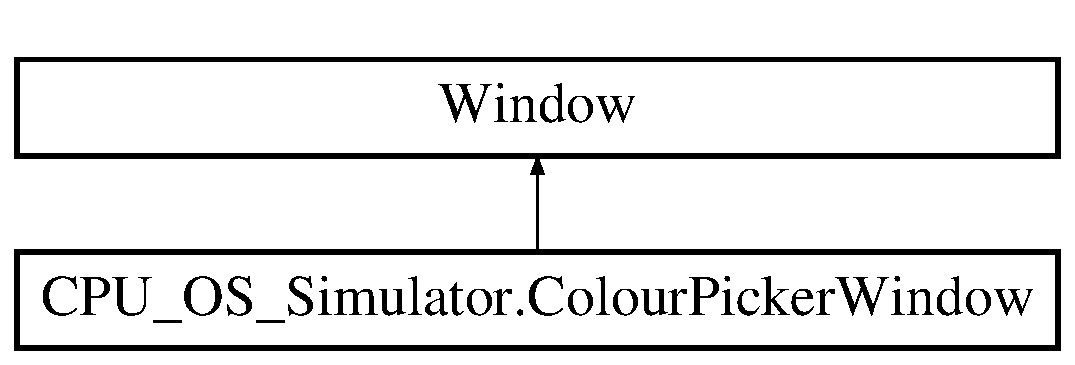
\includegraphics[height=0.892430cm]{class_c_p_u___o_s___simulator_1_1_colour_picker_window}
\end{center}
\end{figure}
\subsection*{Public Member Functions}
\begin{DoxyCompactItemize}
\item 
\hyperlink{class_c_p_u___o_s___simulator_1_1_colour_picker_window_afd196933703b7ee4bcac6cbfde73e65f}{Colour\+Picker\+Window} ()
\begin{DoxyCompactList}\small\item\em Constructor for Colour picker window \end{DoxyCompactList}\item 
\hyperlink{class_c_p_u___o_s___simulator_1_1_colour_picker_window_a6d0c7265a93ca643ad296a8664489508}{Colour\+Picker\+Window} (\hyperlink{class_c_p_u___o_s___simulator_1_1_console_window}{Console\+Window} \hyperlink{class_c_p_u___o_s___simulator_1_1_colour_picker_window_a0a40b478316b3e45a63c67347ff9fc63}{parent})
\begin{DoxyCompactList}\small\item\em Constructor for colour picker window that takes the window instance that is creating this window P\+L\+E\+A\+S\+E N\+O\+T\+E\+: This constructor should always be used so data can be passed back to the main window \end{DoxyCompactList}\item 
void \hyperlink{class_c_p_u___o_s___simulator_1_1_colour_picker_window_a83c3f68e51fd577446e25cfb2a8d05ed}{Initialize\+Component} ()
\begin{DoxyCompactList}\small\item\em Initialize\+Component \end{DoxyCompactList}\item 
void \hyperlink{class_c_p_u___o_s___simulator_1_1_colour_picker_window_a83c3f68e51fd577446e25cfb2a8d05ed}{Initialize\+Component} ()
\begin{DoxyCompactList}\small\item\em Initialize\+Component \end{DoxyCompactList}\end{DoxyCompactItemize}
\subsection*{Package Attributes}
\begin{DoxyCompactItemize}
\item 
\hyperlink{class_c_p_u___o_s___simulator_1_1_colour_picker_window}{C\+P\+U\+\_\+\+O\+S\+\_\+\+Simulator.\+Colour\+Picker\+Window} \hyperlink{class_c_p_u___o_s___simulator_1_1_colour_picker_window_ae1fb4e0b93aecac6fdff7fe54382e033}{Colour\+\_\+\+Picker\+\_\+\+Window}
\item 
System.\+Windows.\+Controls.\+Grid \hyperlink{class_c_p_u___o_s___simulator_1_1_colour_picker_window_ad3f58999085d75f00e86e4796aa87ed3}{root\+\_\+\+Grid}
\end{DoxyCompactItemize}
\subsection*{Properties}
\begin{DoxyCompactItemize}
\item 
\hyperlink{_console_window_8xaml_8cs_adf2800823d988ace598d734fdec29975}{Color} \hyperlink{class_c_p_u___o_s___simulator_1_1_colour_picker_window_a4e51070f2e58d178bf773acb4200e76e}{Selected\+Color}\hspace{0.3cm}{\ttfamily  \mbox{[}get, set\mbox{]}}
\begin{DoxyCompactList}\small\item\em Property for the selected colour \end{DoxyCompactList}\end{DoxyCompactItemize}
\subsection*{Private Member Functions}
\begin{DoxyCompactItemize}
\item 
void \hyperlink{class_c_p_u___o_s___simulator_1_1_colour_picker_window_aed4e40744fb046fb84cebd2c406b8a99}{Create\+Grid} ()
\begin{DoxyCompactList}\small\item\em This function creates the grid where the colour picker buttons are displayed \end{DoxyCompactList}\item 
void \hyperlink{class_c_p_u___o_s___simulator_1_1_colour_picker_window_a2969d055fb398db5c470dd91d89abffd}{Create\+Buttons} (ref Grid Dynamic\+Grid)
\begin{DoxyCompactList}\small\item\em This method populates the grid with colour picking buttons \end{DoxyCompactList}\item 
void System.\+Windows.\+Markup.\+I\+Component\+Connector. \hyperlink{class_c_p_u___o_s___simulator_1_1_colour_picker_window_a857b5ab5ebf06a29846e0595c3c442ad}{Connect} (int connection\+Id, object target)
\item 
void System.\+Windows.\+Markup.\+I\+Component\+Connector. \hyperlink{class_c_p_u___o_s___simulator_1_1_colour_picker_window_a857b5ab5ebf06a29846e0595c3c442ad}{Connect} (int connection\+Id, object target)
\end{DoxyCompactItemize}
\subsection*{Private Attributes}
\begin{DoxyCompactItemize}
\item 
\hyperlink{class_c_p_u___o_s___simulator_1_1_console_window}{Console\+Window} \hyperlink{class_c_p_u___o_s___simulator_1_1_colour_picker_window_a0a40b478316b3e45a63c67347ff9fc63}{parent}
\item 
\hyperlink{_console_window_8xaml_8cs_adf2800823d988ace598d734fdec29975}{Color} \hyperlink{class_c_p_u___o_s___simulator_1_1_colour_picker_window_a1c1653bebad209bd313da5a18ecea9bc}{selected\+Color}
\item 
const double \hyperlink{class_c_p_u___o_s___simulator_1_1_colour_picker_window_a82dedb596267fba0813f7d710d96e6af}{R\+O\+W\+\_\+\+S\+I\+Z\+E} = 25.\+0
\item 
bool \hyperlink{class_c_p_u___o_s___simulator_1_1_colour_picker_window_aeb35df31199f12fcf32b741db20a1546}{\+\_\+content\+Loaded}
\end{DoxyCompactItemize}


\subsection{Detailed Description}
Interaction logic for Colour\+Picker\+Window.\+xaml 

\hyperlink{class_c_p_u___o_s___simulator_1_1_colour_picker_window}{Colour\+Picker\+Window} 

Definition at line 12 of file Colour\+Picker\+Window.\+xaml.\+cs.



\subsection{Constructor \& Destructor Documentation}
\hypertarget{class_c_p_u___o_s___simulator_1_1_colour_picker_window_afd196933703b7ee4bcac6cbfde73e65f}{}\index{C\+P\+U\+\_\+\+O\+S\+\_\+\+Simulator\+::\+Colour\+Picker\+Window@{C\+P\+U\+\_\+\+O\+S\+\_\+\+Simulator\+::\+Colour\+Picker\+Window}!Colour\+Picker\+Window@{Colour\+Picker\+Window}}
\index{Colour\+Picker\+Window@{Colour\+Picker\+Window}!C\+P\+U\+\_\+\+O\+S\+\_\+\+Simulator\+::\+Colour\+Picker\+Window@{C\+P\+U\+\_\+\+O\+S\+\_\+\+Simulator\+::\+Colour\+Picker\+Window}}
\subsubsection[{Colour\+Picker\+Window()}]{\setlength{\rightskip}{0pt plus 5cm}C\+P\+U\+\_\+\+O\+S\+\_\+\+Simulator.\+Colour\+Picker\+Window.\+Colour\+Picker\+Window (
\begin{DoxyParamCaption}
{}
\end{DoxyParamCaption}
)}\label{class_c_p_u___o_s___simulator_1_1_colour_picker_window_afd196933703b7ee4bcac6cbfde73e65f}


Constructor for Colour picker window 



Definition at line 21 of file Colour\+Picker\+Window.\+xaml.\+cs.

\hypertarget{class_c_p_u___o_s___simulator_1_1_colour_picker_window_a6d0c7265a93ca643ad296a8664489508}{}\index{C\+P\+U\+\_\+\+O\+S\+\_\+\+Simulator\+::\+Colour\+Picker\+Window@{C\+P\+U\+\_\+\+O\+S\+\_\+\+Simulator\+::\+Colour\+Picker\+Window}!Colour\+Picker\+Window@{Colour\+Picker\+Window}}
\index{Colour\+Picker\+Window@{Colour\+Picker\+Window}!C\+P\+U\+\_\+\+O\+S\+\_\+\+Simulator\+::\+Colour\+Picker\+Window@{C\+P\+U\+\_\+\+O\+S\+\_\+\+Simulator\+::\+Colour\+Picker\+Window}}
\subsubsection[{Colour\+Picker\+Window(\+Console\+Window parent)}]{\setlength{\rightskip}{0pt plus 5cm}C\+P\+U\+\_\+\+O\+S\+\_\+\+Simulator.\+Colour\+Picker\+Window.\+Colour\+Picker\+Window (
\begin{DoxyParamCaption}
\item[{{\bf Console\+Window}}]{parent}
\end{DoxyParamCaption}
)}\label{class_c_p_u___o_s___simulator_1_1_colour_picker_window_a6d0c7265a93ca643ad296a8664489508}


Constructor for colour picker window that takes the window instance that is creating this window P\+L\+E\+A\+S\+E N\+O\+T\+E\+: This constructor should always be used so data can be passed back to the main window 


\begin{DoxyParams}{Parameters}
{\em parent} & The window that is creating this window \\
\hline
\end{DoxyParams}


Definition at line 31 of file Colour\+Picker\+Window.\+xaml.\+cs.



\subsection{Member Function Documentation}
\hypertarget{class_c_p_u___o_s___simulator_1_1_colour_picker_window_a857b5ab5ebf06a29846e0595c3c442ad}{}\index{C\+P\+U\+\_\+\+O\+S\+\_\+\+Simulator\+::\+Colour\+Picker\+Window@{C\+P\+U\+\_\+\+O\+S\+\_\+\+Simulator\+::\+Colour\+Picker\+Window}!Connect@{Connect}}
\index{Connect@{Connect}!C\+P\+U\+\_\+\+O\+S\+\_\+\+Simulator\+::\+Colour\+Picker\+Window@{C\+P\+U\+\_\+\+O\+S\+\_\+\+Simulator\+::\+Colour\+Picker\+Window}}
\subsubsection[{Connect(int connection\+Id, object target)}]{\setlength{\rightskip}{0pt plus 5cm}void System.\+Windows.\+Markup.\+I\+Component\+Connector. C\+P\+U\+\_\+\+O\+S\+\_\+\+Simulator.\+Colour\+Picker\+Window.\+Connect (
\begin{DoxyParamCaption}
\item[{int}]{connection\+Id, }
\item[{object}]{target}
\end{DoxyParamCaption}
)\hspace{0.3cm}{\ttfamily [private]}}\label{class_c_p_u___o_s___simulator_1_1_colour_picker_window_a857b5ab5ebf06a29846e0595c3c442ad}


Definition at line 86 of file Colour\+Picker\+Window.\+g.\+cs.

\hypertarget{class_c_p_u___o_s___simulator_1_1_colour_picker_window_a857b5ab5ebf06a29846e0595c3c442ad}{}\index{C\+P\+U\+\_\+\+O\+S\+\_\+\+Simulator\+::\+Colour\+Picker\+Window@{C\+P\+U\+\_\+\+O\+S\+\_\+\+Simulator\+::\+Colour\+Picker\+Window}!Connect@{Connect}}
\index{Connect@{Connect}!C\+P\+U\+\_\+\+O\+S\+\_\+\+Simulator\+::\+Colour\+Picker\+Window@{C\+P\+U\+\_\+\+O\+S\+\_\+\+Simulator\+::\+Colour\+Picker\+Window}}
\subsubsection[{Connect(int connection\+Id, object target)}]{\setlength{\rightskip}{0pt plus 5cm}void System.\+Windows.\+Markup.\+I\+Component\+Connector. C\+P\+U\+\_\+\+O\+S\+\_\+\+Simulator.\+Colour\+Picker\+Window.\+Connect (
\begin{DoxyParamCaption}
\item[{int}]{connection\+Id, }
\item[{object}]{target}
\end{DoxyParamCaption}
)\hspace{0.3cm}{\ttfamily [private]}}\label{class_c_p_u___o_s___simulator_1_1_colour_picker_window_a857b5ab5ebf06a29846e0595c3c442ad}


Definition at line 86 of file Colour\+Picker\+Window.\+g.\+i.\+cs.

\hypertarget{class_c_p_u___o_s___simulator_1_1_colour_picker_window_a2969d055fb398db5c470dd91d89abffd}{}\index{C\+P\+U\+\_\+\+O\+S\+\_\+\+Simulator\+::\+Colour\+Picker\+Window@{C\+P\+U\+\_\+\+O\+S\+\_\+\+Simulator\+::\+Colour\+Picker\+Window}!Create\+Buttons@{Create\+Buttons}}
\index{Create\+Buttons@{Create\+Buttons}!C\+P\+U\+\_\+\+O\+S\+\_\+\+Simulator\+::\+Colour\+Picker\+Window@{C\+P\+U\+\_\+\+O\+S\+\_\+\+Simulator\+::\+Colour\+Picker\+Window}}
\subsubsection[{Create\+Buttons(ref Grid Dynamic\+Grid)}]{\setlength{\rightskip}{0pt plus 5cm}void C\+P\+U\+\_\+\+O\+S\+\_\+\+Simulator.\+Colour\+Picker\+Window.\+Create\+Buttons (
\begin{DoxyParamCaption}
\item[{ref Grid}]{Dynamic\+Grid}
\end{DoxyParamCaption}
)\hspace{0.3cm}{\ttfamily [private]}}\label{class_c_p_u___o_s___simulator_1_1_colour_picker_window_a2969d055fb398db5c470dd91d89abffd}


This method populates the grid with colour picking buttons 


\begin{DoxyParams}{Parameters}
{\em Dynamic\+Grid} & a reference to the grid that the buttons should be displayed in\\
\hline
\end{DoxyParams}


Definition at line 77 of file Colour\+Picker\+Window.\+xaml.\+cs.

\hypertarget{class_c_p_u___o_s___simulator_1_1_colour_picker_window_aed4e40744fb046fb84cebd2c406b8a99}{}\index{C\+P\+U\+\_\+\+O\+S\+\_\+\+Simulator\+::\+Colour\+Picker\+Window@{C\+P\+U\+\_\+\+O\+S\+\_\+\+Simulator\+::\+Colour\+Picker\+Window}!Create\+Grid@{Create\+Grid}}
\index{Create\+Grid@{Create\+Grid}!C\+P\+U\+\_\+\+O\+S\+\_\+\+Simulator\+::\+Colour\+Picker\+Window@{C\+P\+U\+\_\+\+O\+S\+\_\+\+Simulator\+::\+Colour\+Picker\+Window}}
\subsubsection[{Create\+Grid()}]{\setlength{\rightskip}{0pt plus 5cm}void C\+P\+U\+\_\+\+O\+S\+\_\+\+Simulator.\+Colour\+Picker\+Window.\+Create\+Grid (
\begin{DoxyParamCaption}
{}
\end{DoxyParamCaption}
)\hspace{0.3cm}{\ttfamily [private]}}\label{class_c_p_u___o_s___simulator_1_1_colour_picker_window_aed4e40744fb046fb84cebd2c406b8a99}


This function creates the grid where the colour picker buttons are displayed 



Definition at line 40 of file Colour\+Picker\+Window.\+xaml.\+cs.

\hypertarget{class_c_p_u___o_s___simulator_1_1_colour_picker_window_a83c3f68e51fd577446e25cfb2a8d05ed}{}\index{C\+P\+U\+\_\+\+O\+S\+\_\+\+Simulator\+::\+Colour\+Picker\+Window@{C\+P\+U\+\_\+\+O\+S\+\_\+\+Simulator\+::\+Colour\+Picker\+Window}!Initialize\+Component@{Initialize\+Component}}
\index{Initialize\+Component@{Initialize\+Component}!C\+P\+U\+\_\+\+O\+S\+\_\+\+Simulator\+::\+Colour\+Picker\+Window@{C\+P\+U\+\_\+\+O\+S\+\_\+\+Simulator\+::\+Colour\+Picker\+Window}}
\subsubsection[{Initialize\+Component()}]{\setlength{\rightskip}{0pt plus 5cm}void C\+P\+U\+\_\+\+O\+S\+\_\+\+Simulator.\+Colour\+Picker\+Window.\+Initialize\+Component (
\begin{DoxyParamCaption}
{}
\end{DoxyParamCaption}
)}\label{class_c_p_u___o_s___simulator_1_1_colour_picker_window_a83c3f68e51fd577446e25cfb2a8d05ed}


Initialize\+Component 



Definition at line 66 of file Colour\+Picker\+Window.\+g.\+cs.

\hypertarget{class_c_p_u___o_s___simulator_1_1_colour_picker_window_a83c3f68e51fd577446e25cfb2a8d05ed}{}\index{C\+P\+U\+\_\+\+O\+S\+\_\+\+Simulator\+::\+Colour\+Picker\+Window@{C\+P\+U\+\_\+\+O\+S\+\_\+\+Simulator\+::\+Colour\+Picker\+Window}!Initialize\+Component@{Initialize\+Component}}
\index{Initialize\+Component@{Initialize\+Component}!C\+P\+U\+\_\+\+O\+S\+\_\+\+Simulator\+::\+Colour\+Picker\+Window@{C\+P\+U\+\_\+\+O\+S\+\_\+\+Simulator\+::\+Colour\+Picker\+Window}}
\subsubsection[{Initialize\+Component()}]{\setlength{\rightskip}{0pt plus 5cm}void C\+P\+U\+\_\+\+O\+S\+\_\+\+Simulator.\+Colour\+Picker\+Window.\+Initialize\+Component (
\begin{DoxyParamCaption}
{}
\end{DoxyParamCaption}
)}\label{class_c_p_u___o_s___simulator_1_1_colour_picker_window_a83c3f68e51fd577446e25cfb2a8d05ed}


Initialize\+Component 



Definition at line 66 of file Colour\+Picker\+Window.\+g.\+i.\+cs.



\subsection{Member Data Documentation}
\hypertarget{class_c_p_u___o_s___simulator_1_1_colour_picker_window_aeb35df31199f12fcf32b741db20a1546}{}\index{C\+P\+U\+\_\+\+O\+S\+\_\+\+Simulator\+::\+Colour\+Picker\+Window@{C\+P\+U\+\_\+\+O\+S\+\_\+\+Simulator\+::\+Colour\+Picker\+Window}!\+\_\+content\+Loaded@{\+\_\+content\+Loaded}}
\index{\+\_\+content\+Loaded@{\+\_\+content\+Loaded}!C\+P\+U\+\_\+\+O\+S\+\_\+\+Simulator\+::\+Colour\+Picker\+Window@{C\+P\+U\+\_\+\+O\+S\+\_\+\+Simulator\+::\+Colour\+Picker\+Window}}
\subsubsection[{\+\_\+content\+Loaded}]{\setlength{\rightskip}{0pt plus 5cm}bool C\+P\+U\+\_\+\+O\+S\+\_\+\+Simulator.\+Colour\+Picker\+Window.\+\_\+content\+Loaded\hspace{0.3cm}{\ttfamily [private]}}\label{class_c_p_u___o_s___simulator_1_1_colour_picker_window_aeb35df31199f12fcf32b741db20a1546}


Definition at line 59 of file Colour\+Picker\+Window.\+g.\+cs.

\hypertarget{class_c_p_u___o_s___simulator_1_1_colour_picker_window_ae1fb4e0b93aecac6fdff7fe54382e033}{}\index{C\+P\+U\+\_\+\+O\+S\+\_\+\+Simulator\+::\+Colour\+Picker\+Window@{C\+P\+U\+\_\+\+O\+S\+\_\+\+Simulator\+::\+Colour\+Picker\+Window}!Colour\+\_\+\+Picker\+\_\+\+Window@{Colour\+\_\+\+Picker\+\_\+\+Window}}
\index{Colour\+\_\+\+Picker\+\_\+\+Window@{Colour\+\_\+\+Picker\+\_\+\+Window}!C\+P\+U\+\_\+\+O\+S\+\_\+\+Simulator\+::\+Colour\+Picker\+Window@{C\+P\+U\+\_\+\+O\+S\+\_\+\+Simulator\+::\+Colour\+Picker\+Window}}
\subsubsection[{Colour\+\_\+\+Picker\+\_\+\+Window}]{\setlength{\rightskip}{0pt plus 5cm}C\+P\+U\+\_\+\+O\+S\+\_\+\+Simulator {\bf Colour\+Picker\+Window} C\+P\+U\+\_\+\+O\+S\+\_\+\+Simulator.\+Colour\+Picker\+Window.\+Colour\+\_\+\+Picker\+\_\+\+Window\hspace{0.3cm}{\ttfamily [package]}}\label{class_c_p_u___o_s___simulator_1_1_colour_picker_window_ae1fb4e0b93aecac6fdff7fe54382e033}


Definition at line 46 of file Colour\+Picker\+Window.\+g.\+cs.

\hypertarget{class_c_p_u___o_s___simulator_1_1_colour_picker_window_a0a40b478316b3e45a63c67347ff9fc63}{}\index{C\+P\+U\+\_\+\+O\+S\+\_\+\+Simulator\+::\+Colour\+Picker\+Window@{C\+P\+U\+\_\+\+O\+S\+\_\+\+Simulator\+::\+Colour\+Picker\+Window}!parent@{parent}}
\index{parent@{parent}!C\+P\+U\+\_\+\+O\+S\+\_\+\+Simulator\+::\+Colour\+Picker\+Window@{C\+P\+U\+\_\+\+O\+S\+\_\+\+Simulator\+::\+Colour\+Picker\+Window}}
\subsubsection[{parent}]{\setlength{\rightskip}{0pt plus 5cm}{\bf Console\+Window} C\+P\+U\+\_\+\+O\+S\+\_\+\+Simulator.\+Colour\+Picker\+Window.\+parent\hspace{0.3cm}{\ttfamily [private]}}\label{class_c_p_u___o_s___simulator_1_1_colour_picker_window_a0a40b478316b3e45a63c67347ff9fc63}


Definition at line 14 of file Colour\+Picker\+Window.\+xaml.\+cs.

\hypertarget{class_c_p_u___o_s___simulator_1_1_colour_picker_window_ad3f58999085d75f00e86e4796aa87ed3}{}\index{C\+P\+U\+\_\+\+O\+S\+\_\+\+Simulator\+::\+Colour\+Picker\+Window@{C\+P\+U\+\_\+\+O\+S\+\_\+\+Simulator\+::\+Colour\+Picker\+Window}!root\+\_\+\+Grid@{root\+\_\+\+Grid}}
\index{root\+\_\+\+Grid@{root\+\_\+\+Grid}!C\+P\+U\+\_\+\+O\+S\+\_\+\+Simulator\+::\+Colour\+Picker\+Window@{C\+P\+U\+\_\+\+O\+S\+\_\+\+Simulator\+::\+Colour\+Picker\+Window}}
\subsubsection[{root\+\_\+\+Grid}]{\setlength{\rightskip}{0pt plus 5cm}System Windows Controls Grid C\+P\+U\+\_\+\+O\+S\+\_\+\+Simulator.\+Colour\+Picker\+Window.\+root\+\_\+\+Grid\hspace{0.3cm}{\ttfamily [package]}}\label{class_c_p_u___o_s___simulator_1_1_colour_picker_window_ad3f58999085d75f00e86e4796aa87ed3}


Definition at line 54 of file Colour\+Picker\+Window.\+g.\+cs.

\hypertarget{class_c_p_u___o_s___simulator_1_1_colour_picker_window_a82dedb596267fba0813f7d710d96e6af}{}\index{C\+P\+U\+\_\+\+O\+S\+\_\+\+Simulator\+::\+Colour\+Picker\+Window@{C\+P\+U\+\_\+\+O\+S\+\_\+\+Simulator\+::\+Colour\+Picker\+Window}!R\+O\+W\+\_\+\+S\+I\+Z\+E@{R\+O\+W\+\_\+\+S\+I\+Z\+E}}
\index{R\+O\+W\+\_\+\+S\+I\+Z\+E@{R\+O\+W\+\_\+\+S\+I\+Z\+E}!C\+P\+U\+\_\+\+O\+S\+\_\+\+Simulator\+::\+Colour\+Picker\+Window@{C\+P\+U\+\_\+\+O\+S\+\_\+\+Simulator\+::\+Colour\+Picker\+Window}}
\subsubsection[{R\+O\+W\+\_\+\+S\+I\+Z\+E}]{\setlength{\rightskip}{0pt plus 5cm}const double C\+P\+U\+\_\+\+O\+S\+\_\+\+Simulator.\+Colour\+Picker\+Window.\+R\+O\+W\+\_\+\+S\+I\+Z\+E = 25.\+0\hspace{0.3cm}{\ttfamily [private]}}\label{class_c_p_u___o_s___simulator_1_1_colour_picker_window_a82dedb596267fba0813f7d710d96e6af}


Definition at line 16 of file Colour\+Picker\+Window.\+xaml.\+cs.

\hypertarget{class_c_p_u___o_s___simulator_1_1_colour_picker_window_a1c1653bebad209bd313da5a18ecea9bc}{}\index{C\+P\+U\+\_\+\+O\+S\+\_\+\+Simulator\+::\+Colour\+Picker\+Window@{C\+P\+U\+\_\+\+O\+S\+\_\+\+Simulator\+::\+Colour\+Picker\+Window}!selected\+Color@{selected\+Color}}
\index{selected\+Color@{selected\+Color}!C\+P\+U\+\_\+\+O\+S\+\_\+\+Simulator\+::\+Colour\+Picker\+Window@{C\+P\+U\+\_\+\+O\+S\+\_\+\+Simulator\+::\+Colour\+Picker\+Window}}
\subsubsection[{selected\+Color}]{\setlength{\rightskip}{0pt plus 5cm}{\bf Color} C\+P\+U\+\_\+\+O\+S\+\_\+\+Simulator.\+Colour\+Picker\+Window.\+selected\+Color\hspace{0.3cm}{\ttfamily [private]}}\label{class_c_p_u___o_s___simulator_1_1_colour_picker_window_a1c1653bebad209bd313da5a18ecea9bc}


Definition at line 15 of file Colour\+Picker\+Window.\+xaml.\+cs.



\subsection{Property Documentation}
\hypertarget{class_c_p_u___o_s___simulator_1_1_colour_picker_window_a4e51070f2e58d178bf773acb4200e76e}{}\index{C\+P\+U\+\_\+\+O\+S\+\_\+\+Simulator\+::\+Colour\+Picker\+Window@{C\+P\+U\+\_\+\+O\+S\+\_\+\+Simulator\+::\+Colour\+Picker\+Window}!Selected\+Color@{Selected\+Color}}
\index{Selected\+Color@{Selected\+Color}!C\+P\+U\+\_\+\+O\+S\+\_\+\+Simulator\+::\+Colour\+Picker\+Window@{C\+P\+U\+\_\+\+O\+S\+\_\+\+Simulator\+::\+Colour\+Picker\+Window}}
\subsubsection[{Selected\+Color}]{\setlength{\rightskip}{0pt plus 5cm}{\bf Color} C\+P\+U\+\_\+\+O\+S\+\_\+\+Simulator.\+Colour\+Picker\+Window.\+Selected\+Color\hspace{0.3cm}{\ttfamily [get]}, {\ttfamily [set]}}\label{class_c_p_u___o_s___simulator_1_1_colour_picker_window_a4e51070f2e58d178bf773acb4200e76e}


Property for the selected colour 



Definition at line 117 of file Colour\+Picker\+Window.\+xaml.\+cs.



The documentation for this class was generated from the following files\+:\begin{DoxyCompactItemize}
\item 
C\+P\+U-\/\+O\+S Simulator/\hyperlink{_colour_picker_window_8xaml_8cs}{Colour\+Picker\+Window.\+xaml.\+cs}\item 
C\+P\+U-\/\+O\+S Simulator/obj/\+Debug/\hyperlink{_colour_picker_window_8g_8cs}{Colour\+Picker\+Window.\+g.\+cs}\item 
C\+P\+U-\/\+O\+S Simulator/obj/\+Debug/\hyperlink{_colour_picker_window_8g_8i_8cs}{Colour\+Picker\+Window.\+g.\+i.\+cs}\end{DoxyCompactItemize}

\hypertarget{class_c_p_u___o_s___simulator_1_1_c_p_u_1_1_compiled_program}{}\section{C\+P\+U\+\_\+\+O\+S\+\_\+\+Simulator.\+C\+P\+U.\+Compiled\+Program Class Reference}
\label{class_c_p_u___o_s___simulator_1_1_c_p_u_1_1_compiled_program}\index{C\+P\+U\+\_\+\+O\+S\+\_\+\+Simulator.\+C\+P\+U.\+Compiled\+Program@{C\+P\+U\+\_\+\+O\+S\+\_\+\+Simulator.\+C\+P\+U.\+Compiled\+Program}}


This class represents a program after it has been compiled  


\subsection*{Public Member Functions}
\begin{DoxyCompactItemize}
\item 
\hyperlink{class_c_p_u___o_s___simulator_1_1_c_p_u_1_1_compiled_program_a2831900227a696c5e2cc71d08b4cb0a0}{Compiled\+Program} (List$<$ Byte $>$ \hyperlink{class_c_p_u___o_s___simulator_1_1_c_p_u_1_1_compiled_program_a2fff029de4cf0be48a4ef07daabf04e7}{bytes}, string \hyperlink{class_c_p_u___o_s___simulator_1_1_c_p_u_1_1_compiled_program_afa16131ff99534fd4fe9bc4aaa21ac02}{name}, int \hyperlink{class_c_p_u___o_s___simulator_1_1_c_p_u_1_1_compiled_program_ac3d1adb46ebd2132f53d3a1b880acc58}{size})
\begin{DoxyCompactList}\small\item\em Constructor for a compiled program \end{DoxyCompactList}\item 
bool \hyperlink{class_c_p_u___o_s___simulator_1_1_c_p_u_1_1_compiled_program_ac046a32b0bd513aa4c7337ac987500c4}{Loadin\+Memory} (int frame\+Number)
\begin{DoxyCompactList}\small\item\em This function loads a compiled program into memory \end{DoxyCompactList}\end{DoxyCompactItemize}
\subsection*{Private Member Functions}
\begin{DoxyCompactItemize}
\item 
dynamic \hyperlink{class_c_p_u___o_s___simulator_1_1_c_p_u_1_1_compiled_program_a7cc5523ba4a83ee2842b246c83721be4}{Get\+Main\+Window\+Instance} ()
\begin{DoxyCompactList}\small\item\em This function gets the main window instance from the window bridge \end{DoxyCompactList}\end{DoxyCompactItemize}
\subsection*{Private Attributes}
\begin{DoxyCompactItemize}
\item 
List$<$ byte $>$ \hyperlink{class_c_p_u___o_s___simulator_1_1_c_p_u_1_1_compiled_program_a2fff029de4cf0be48a4ef07daabf04e7}{bytes} = null
\item 
string \hyperlink{class_c_p_u___o_s___simulator_1_1_c_p_u_1_1_compiled_program_afa16131ff99534fd4fe9bc4aaa21ac02}{name} = String.\+Empty
\item 
int \hyperlink{class_c_p_u___o_s___simulator_1_1_c_p_u_1_1_compiled_program_ac3d1adb46ebd2132f53d3a1b880acc58}{size} = 0
\end{DoxyCompactItemize}


\subsection{Detailed Description}
This class represents a program after it has been compiled 



Definition at line 13 of file Compiled\+Program.\+cs.



\subsection{Constructor \& Destructor Documentation}
\hypertarget{class_c_p_u___o_s___simulator_1_1_c_p_u_1_1_compiled_program_a2831900227a696c5e2cc71d08b4cb0a0}{}\index{C\+P\+U\+\_\+\+O\+S\+\_\+\+Simulator\+::\+C\+P\+U\+::\+Compiled\+Program@{C\+P\+U\+\_\+\+O\+S\+\_\+\+Simulator\+::\+C\+P\+U\+::\+Compiled\+Program}!Compiled\+Program@{Compiled\+Program}}
\index{Compiled\+Program@{Compiled\+Program}!C\+P\+U\+\_\+\+O\+S\+\_\+\+Simulator\+::\+C\+P\+U\+::\+Compiled\+Program@{C\+P\+U\+\_\+\+O\+S\+\_\+\+Simulator\+::\+C\+P\+U\+::\+Compiled\+Program}}
\subsubsection[{Compiled\+Program(\+List$<$ Byte $>$ bytes, string name, int size)}]{\setlength{\rightskip}{0pt plus 5cm}C\+P\+U\+\_\+\+O\+S\+\_\+\+Simulator.\+C\+P\+U.\+Compiled\+Program.\+Compiled\+Program (
\begin{DoxyParamCaption}
\item[{List$<$ Byte $>$}]{bytes, }
\item[{string}]{name, }
\item[{int}]{size}
\end{DoxyParamCaption}
)}\label{class_c_p_u___o_s___simulator_1_1_c_p_u_1_1_compiled_program_a2831900227a696c5e2cc71d08b4cb0a0}


Constructor for a compiled program 


\begin{DoxyParams}{Parameters}
{\em bytes} & the bytes that make up the program \\
\hline
{\em name} & the name of the program \\
\hline
{\em size} & the size of the program\\
\hline
\end{DoxyParams}


Definition at line 25 of file Compiled\+Program.\+cs.



\subsection{Member Function Documentation}
\hypertarget{class_c_p_u___o_s___simulator_1_1_c_p_u_1_1_compiled_program_a7cc5523ba4a83ee2842b246c83721be4}{}\index{C\+P\+U\+\_\+\+O\+S\+\_\+\+Simulator\+::\+C\+P\+U\+::\+Compiled\+Program@{C\+P\+U\+\_\+\+O\+S\+\_\+\+Simulator\+::\+C\+P\+U\+::\+Compiled\+Program}!Get\+Main\+Window\+Instance@{Get\+Main\+Window\+Instance}}
\index{Get\+Main\+Window\+Instance@{Get\+Main\+Window\+Instance}!C\+P\+U\+\_\+\+O\+S\+\_\+\+Simulator\+::\+C\+P\+U\+::\+Compiled\+Program@{C\+P\+U\+\_\+\+O\+S\+\_\+\+Simulator\+::\+C\+P\+U\+::\+Compiled\+Program}}
\subsubsection[{Get\+Main\+Window\+Instance()}]{\setlength{\rightskip}{0pt plus 5cm}dynamic C\+P\+U\+\_\+\+O\+S\+\_\+\+Simulator.\+C\+P\+U.\+Compiled\+Program.\+Get\+Main\+Window\+Instance (
\begin{DoxyParamCaption}
{}
\end{DoxyParamCaption}
)\hspace{0.3cm}{\ttfamily [private]}}\label{class_c_p_u___o_s___simulator_1_1_c_p_u_1_1_compiled_program_a7cc5523ba4a83ee2842b246c83721be4}


This function gets the main window instance from the window bridge 

\begin{DoxyReturn}{Returns}
the active instance of main window 
\end{DoxyReturn}


Definition at line 66 of file Compiled\+Program.\+cs.

\hypertarget{class_c_p_u___o_s___simulator_1_1_c_p_u_1_1_compiled_program_ac046a32b0bd513aa4c7337ac987500c4}{}\index{C\+P\+U\+\_\+\+O\+S\+\_\+\+Simulator\+::\+C\+P\+U\+::\+Compiled\+Program@{C\+P\+U\+\_\+\+O\+S\+\_\+\+Simulator\+::\+C\+P\+U\+::\+Compiled\+Program}!Loadin\+Memory@{Loadin\+Memory}}
\index{Loadin\+Memory@{Loadin\+Memory}!C\+P\+U\+\_\+\+O\+S\+\_\+\+Simulator\+::\+C\+P\+U\+::\+Compiled\+Program@{C\+P\+U\+\_\+\+O\+S\+\_\+\+Simulator\+::\+C\+P\+U\+::\+Compiled\+Program}}
\subsubsection[{Loadin\+Memory(int frame\+Number)}]{\setlength{\rightskip}{0pt plus 5cm}bool C\+P\+U\+\_\+\+O\+S\+\_\+\+Simulator.\+C\+P\+U.\+Compiled\+Program.\+Loadin\+Memory (
\begin{DoxyParamCaption}
\item[{int}]{frame\+Number}
\end{DoxyParamCaption}
)}\label{class_c_p_u___o_s___simulator_1_1_c_p_u_1_1_compiled_program_ac046a32b0bd513aa4c7337ac987500c4}


This function loads a compiled program into memory 


\begin{DoxyParams}{Parameters}
{\em frame\+Number} & the frame number of the memory page to load the program into\\
\hline
\end{DoxyParams}
\begin{DoxyReturn}{Returns}

\end{DoxyReturn}


Definition at line 36 of file Compiled\+Program.\+cs.



\subsection{Member Data Documentation}
\hypertarget{class_c_p_u___o_s___simulator_1_1_c_p_u_1_1_compiled_program_a2fff029de4cf0be48a4ef07daabf04e7}{}\index{C\+P\+U\+\_\+\+O\+S\+\_\+\+Simulator\+::\+C\+P\+U\+::\+Compiled\+Program@{C\+P\+U\+\_\+\+O\+S\+\_\+\+Simulator\+::\+C\+P\+U\+::\+Compiled\+Program}!bytes@{bytes}}
\index{bytes@{bytes}!C\+P\+U\+\_\+\+O\+S\+\_\+\+Simulator\+::\+C\+P\+U\+::\+Compiled\+Program@{C\+P\+U\+\_\+\+O\+S\+\_\+\+Simulator\+::\+C\+P\+U\+::\+Compiled\+Program}}
\subsubsection[{bytes}]{\setlength{\rightskip}{0pt plus 5cm}List$<$byte$>$ C\+P\+U\+\_\+\+O\+S\+\_\+\+Simulator.\+C\+P\+U.\+Compiled\+Program.\+bytes = null\hspace{0.3cm}{\ttfamily [private]}}\label{class_c_p_u___o_s___simulator_1_1_c_p_u_1_1_compiled_program_a2fff029de4cf0be48a4ef07daabf04e7}


Definition at line 15 of file Compiled\+Program.\+cs.

\hypertarget{class_c_p_u___o_s___simulator_1_1_c_p_u_1_1_compiled_program_afa16131ff99534fd4fe9bc4aaa21ac02}{}\index{C\+P\+U\+\_\+\+O\+S\+\_\+\+Simulator\+::\+C\+P\+U\+::\+Compiled\+Program@{C\+P\+U\+\_\+\+O\+S\+\_\+\+Simulator\+::\+C\+P\+U\+::\+Compiled\+Program}!name@{name}}
\index{name@{name}!C\+P\+U\+\_\+\+O\+S\+\_\+\+Simulator\+::\+C\+P\+U\+::\+Compiled\+Program@{C\+P\+U\+\_\+\+O\+S\+\_\+\+Simulator\+::\+C\+P\+U\+::\+Compiled\+Program}}
\subsubsection[{name}]{\setlength{\rightskip}{0pt plus 5cm}string C\+P\+U\+\_\+\+O\+S\+\_\+\+Simulator.\+C\+P\+U.\+Compiled\+Program.\+name = String.\+Empty\hspace{0.3cm}{\ttfamily [private]}}\label{class_c_p_u___o_s___simulator_1_1_c_p_u_1_1_compiled_program_afa16131ff99534fd4fe9bc4aaa21ac02}


Definition at line 16 of file Compiled\+Program.\+cs.

\hypertarget{class_c_p_u___o_s___simulator_1_1_c_p_u_1_1_compiled_program_ac3d1adb46ebd2132f53d3a1b880acc58}{}\index{C\+P\+U\+\_\+\+O\+S\+\_\+\+Simulator\+::\+C\+P\+U\+::\+Compiled\+Program@{C\+P\+U\+\_\+\+O\+S\+\_\+\+Simulator\+::\+C\+P\+U\+::\+Compiled\+Program}!size@{size}}
\index{size@{size}!C\+P\+U\+\_\+\+O\+S\+\_\+\+Simulator\+::\+C\+P\+U\+::\+Compiled\+Program@{C\+P\+U\+\_\+\+O\+S\+\_\+\+Simulator\+::\+C\+P\+U\+::\+Compiled\+Program}}
\subsubsection[{size}]{\setlength{\rightskip}{0pt plus 5cm}int C\+P\+U\+\_\+\+O\+S\+\_\+\+Simulator.\+C\+P\+U.\+Compiled\+Program.\+size = 0\hspace{0.3cm}{\ttfamily [private]}}\label{class_c_p_u___o_s___simulator_1_1_c_p_u_1_1_compiled_program_ac3d1adb46ebd2132f53d3a1b880acc58}


Definition at line 17 of file Compiled\+Program.\+cs.



The documentation for this class was generated from the following file\+:\begin{DoxyCompactItemize}
\item 
C\+P\+U/\hyperlink{_compiled_program_8cs}{Compiled\+Program.\+cs}\end{DoxyCompactItemize}

\hypertarget{class_c_p_u___o_s___simulator_1_1_compiler_1_1_compiler_main}{}\section{C\+P\+U\+\_\+\+O\+S\+\_\+\+Simulator.\+Compiler.\+Compiler\+Main Class Reference}
\label{class_c_p_u___o_s___simulator_1_1_compiler_1_1_compiler_main}\index{C\+P\+U\+\_\+\+O\+S\+\_\+\+Simulator.\+Compiler.\+Compiler\+Main@{C\+P\+U\+\_\+\+O\+S\+\_\+\+Simulator.\+Compiler.\+Compiler\+Main}}


This class represents the front end of the compiler which is responsible for compiling programs  


\subsection*{Public Member Functions}
\begin{DoxyCompactItemize}
\item 
\hyperlink{class_c_p_u___o_s___simulator_1_1_compiler_1_1_compiler_main_a50d01f6e7db4b9facb3fdc84e8566fd7}{Compiler\+Main} (\hyperlink{class_c_p_u___o_s___simulator_1_1_compiler_1_1_source_file}{Source\+File} \hyperlink{class_c_p_u___o_s___simulator_1_1_compiler_1_1_compiler_main_ac6a47299c228ea71c732f35572fa666f}{file})
\begin{DoxyCompactList}\small\item\em Constructor for \hyperlink{namespace_c_p_u___o_s___simulator_1_1_compiler}{Compiler} front end when compiling source files \end{DoxyCompactList}\item 
\hyperlink{class_c_p_u___o_s___simulator_1_1_compiler_1_1_compiler_main_a7beede81b8461570391e1b0f8bc5f1ed}{Compiler\+Main} (List$<$ \hyperlink{class_c_p_u___o_s___simulator_1_1_c_p_u_1_1_instruction}{Instruction} $>$ \hyperlink{class_c_p_u___o_s___simulator_1_1_compiler_1_1_compiler_main_a0b0b37341f48e60f2ee769ea4ba760d2}{instructions}, string \hyperlink{class_c_p_u___o_s___simulator_1_1_compiler_1_1_compiler_main_a39370e54e39a32c7eb9dce2f9b49cefe}{name})
\begin{DoxyCompactList}\small\item\em Constructor for compiler front end when compiling instructions \end{DoxyCompactList}\item 
List$<$ List$<$ \hyperlink{class_c_p_u___o_s___simulator_1_1_compiler_1_1_backend_1_1_instruction_segment}{Instruction\+Segment} $>$ $>$ \hyperlink{class_c_p_u___o_s___simulator_1_1_compiler_1_1_compiler_main_af15e3239f4bc005fffd4e20e694a6593}{Compile\+From\+Source\+File} ()
\item 
List$<$ List$<$ \hyperlink{class_c_p_u___o_s___simulator_1_1_compiler_1_1_backend_1_1_instruction_segment}{Instruction\+Segment} $>$ $>$ \hyperlink{class_c_p_u___o_s___simulator_1_1_compiler_1_1_compiler_main_a9f4ff6dfc17da56e428d7a5d52eeda18}{Compile\+From\+Instructions} ()
\begin{DoxyCompactList}\small\item\em This function compiles a program from instructions \end{DoxyCompactList}\item 
List$<$ byte $>$ \hyperlink{class_c_p_u___o_s___simulator_1_1_compiler_1_1_compiler_main_aaaa9dbfb3784bd3f4f2f7c5c457a8d0e}{Compile\+To\+Bytes} (List$<$ List$<$ \hyperlink{class_c_p_u___o_s___simulator_1_1_compiler_1_1_backend_1_1_instruction_segment}{Instruction\+Segment} $>$$>$ segment\+Lists)
\begin{DoxyCompactList}\small\item\em This function compiles a list of lists of instruction segments to their byte values \end{DoxyCompactList}\end{DoxyCompactItemize}
\subsection*{Private Attributes}
\begin{DoxyCompactItemize}
\item 
\hyperlink{namespace_c_p_u___o_s___simulator_1_1_compiler_ada8d93b571fa15a0f2eac8c9647a89fe}{Enum\+Compiler\+Mode} \hyperlink{class_c_p_u___o_s___simulator_1_1_compiler_1_1_compiler_main_a064e52c2639d79cdec216d4ee7d384e9}{mode} = \hyperlink{namespace_c_p_u___o_s___simulator_1_1_compiler_ada8d93b571fa15a0f2eac8c9647a89fea696b031073e74bf2cb98e5ef201d4aa3}{Enum\+Compiler\+Mode.\+U\+N\+K\+N\+O\+W\+N}
\item 
\hyperlink{class_c_p_u___o_s___simulator_1_1_compiler_1_1_source_file}{Source\+File} \hyperlink{class_c_p_u___o_s___simulator_1_1_compiler_1_1_compiler_main_ac6a47299c228ea71c732f35572fa666f}{file}
\item 
List$<$ \hyperlink{class_c_p_u___o_s___simulator_1_1_c_p_u_1_1_instruction}{Instruction} $>$ \hyperlink{class_c_p_u___o_s___simulator_1_1_compiler_1_1_compiler_main_a0b0b37341f48e60f2ee769ea4ba760d2}{instructions}
\item 
string \hyperlink{class_c_p_u___o_s___simulator_1_1_compiler_1_1_compiler_main_a39370e54e39a32c7eb9dce2f9b49cefe}{name} = String.\+Empty
\end{DoxyCompactItemize}


\subsection{Detailed Description}
This class represents the front end of the compiler which is responsible for compiling programs 



Definition at line 13 of file Compiler\+Main.\+cs.



\subsection{Constructor \& Destructor Documentation}
\hypertarget{class_c_p_u___o_s___simulator_1_1_compiler_1_1_compiler_main_a50d01f6e7db4b9facb3fdc84e8566fd7}{}\index{C\+P\+U\+\_\+\+O\+S\+\_\+\+Simulator\+::\+Compiler\+::\+Compiler\+Main@{C\+P\+U\+\_\+\+O\+S\+\_\+\+Simulator\+::\+Compiler\+::\+Compiler\+Main}!Compiler\+Main@{Compiler\+Main}}
\index{Compiler\+Main@{Compiler\+Main}!C\+P\+U\+\_\+\+O\+S\+\_\+\+Simulator\+::\+Compiler\+::\+Compiler\+Main@{C\+P\+U\+\_\+\+O\+S\+\_\+\+Simulator\+::\+Compiler\+::\+Compiler\+Main}}
\subsubsection[{Compiler\+Main(\+Source\+File file)}]{\setlength{\rightskip}{0pt plus 5cm}C\+P\+U\+\_\+\+O\+S\+\_\+\+Simulator.\+Compiler.\+Compiler\+Main.\+Compiler\+Main (
\begin{DoxyParamCaption}
\item[{{\bf Source\+File}}]{file}
\end{DoxyParamCaption}
)}\label{class_c_p_u___o_s___simulator_1_1_compiler_1_1_compiler_main_a50d01f6e7db4b9facb3fdc84e8566fd7}


Constructor for \hyperlink{namespace_c_p_u___o_s___simulator_1_1_compiler}{Compiler} front end when compiling source files 


\begin{DoxyParams}{Parameters}
{\em file} & the source file to compile\\
\hline
\end{DoxyParams}


Definition at line 24 of file Compiler\+Main.\+cs.

\hypertarget{class_c_p_u___o_s___simulator_1_1_compiler_1_1_compiler_main_a7beede81b8461570391e1b0f8bc5f1ed}{}\index{C\+P\+U\+\_\+\+O\+S\+\_\+\+Simulator\+::\+Compiler\+::\+Compiler\+Main@{C\+P\+U\+\_\+\+O\+S\+\_\+\+Simulator\+::\+Compiler\+::\+Compiler\+Main}!Compiler\+Main@{Compiler\+Main}}
\index{Compiler\+Main@{Compiler\+Main}!C\+P\+U\+\_\+\+O\+S\+\_\+\+Simulator\+::\+Compiler\+::\+Compiler\+Main@{C\+P\+U\+\_\+\+O\+S\+\_\+\+Simulator\+::\+Compiler\+::\+Compiler\+Main}}
\subsubsection[{Compiler\+Main(\+List$<$ Instruction $>$ instructions, string name)}]{\setlength{\rightskip}{0pt plus 5cm}C\+P\+U\+\_\+\+O\+S\+\_\+\+Simulator.\+Compiler.\+Compiler\+Main.\+Compiler\+Main (
\begin{DoxyParamCaption}
\item[{List$<$ {\bf Instruction} $>$}]{instructions, }
\item[{string}]{name}
\end{DoxyParamCaption}
)}\label{class_c_p_u___o_s___simulator_1_1_compiler_1_1_compiler_main_a7beede81b8461570391e1b0f8bc5f1ed}


Constructor for compiler front end when compiling instructions 


\begin{DoxyParams}{Parameters}
{\em instructions} & the instructions to compile\\
\hline
{\em name} & the name of the program to compile\\
\hline
\end{DoxyParams}


Definition at line 35 of file Compiler\+Main.\+cs.



\subsection{Member Function Documentation}
\hypertarget{class_c_p_u___o_s___simulator_1_1_compiler_1_1_compiler_main_a9f4ff6dfc17da56e428d7a5d52eeda18}{}\index{C\+P\+U\+\_\+\+O\+S\+\_\+\+Simulator\+::\+Compiler\+::\+Compiler\+Main@{C\+P\+U\+\_\+\+O\+S\+\_\+\+Simulator\+::\+Compiler\+::\+Compiler\+Main}!Compile\+From\+Instructions@{Compile\+From\+Instructions}}
\index{Compile\+From\+Instructions@{Compile\+From\+Instructions}!C\+P\+U\+\_\+\+O\+S\+\_\+\+Simulator\+::\+Compiler\+::\+Compiler\+Main@{C\+P\+U\+\_\+\+O\+S\+\_\+\+Simulator\+::\+Compiler\+::\+Compiler\+Main}}
\subsubsection[{Compile\+From\+Instructions()}]{\setlength{\rightskip}{0pt plus 5cm}List$<$List$<${\bf Instruction\+Segment}$>$ $>$ C\+P\+U\+\_\+\+O\+S\+\_\+\+Simulator.\+Compiler.\+Compiler\+Main.\+Compile\+From\+Instructions (
\begin{DoxyParamCaption}
{}
\end{DoxyParamCaption}
)}\label{class_c_p_u___o_s___simulator_1_1_compiler_1_1_compiler_main_a9f4ff6dfc17da56e428d7a5d52eeda18}


This function compiles a program from instructions 

\begin{DoxyReturn}{Returns}
a list of lists of instruction segments that represent the original instructions
\end{DoxyReturn}


Definition at line 55 of file Compiler\+Main.\+cs.

\hypertarget{class_c_p_u___o_s___simulator_1_1_compiler_1_1_compiler_main_af15e3239f4bc005fffd4e20e694a6593}{}\index{C\+P\+U\+\_\+\+O\+S\+\_\+\+Simulator\+::\+Compiler\+::\+Compiler\+Main@{C\+P\+U\+\_\+\+O\+S\+\_\+\+Simulator\+::\+Compiler\+::\+Compiler\+Main}!Compile\+From\+Source\+File@{Compile\+From\+Source\+File}}
\index{Compile\+From\+Source\+File@{Compile\+From\+Source\+File}!C\+P\+U\+\_\+\+O\+S\+\_\+\+Simulator\+::\+Compiler\+::\+Compiler\+Main@{C\+P\+U\+\_\+\+O\+S\+\_\+\+Simulator\+::\+Compiler\+::\+Compiler\+Main}}
\subsubsection[{Compile\+From\+Source\+File()}]{\setlength{\rightskip}{0pt plus 5cm}List$<$List$<${\bf Instruction\+Segment}$>$ $>$ C\+P\+U\+\_\+\+O\+S\+\_\+\+Simulator.\+Compiler.\+Compiler\+Main.\+Compile\+From\+Source\+File (
\begin{DoxyParamCaption}
{}
\end{DoxyParamCaption}
)}\label{class_c_p_u___o_s___simulator_1_1_compiler_1_1_compiler_main_af15e3239f4bc005fffd4e20e694a6593}


Definition at line 43 of file Compiler\+Main.\+cs.

\hypertarget{class_c_p_u___o_s___simulator_1_1_compiler_1_1_compiler_main_aaaa9dbfb3784bd3f4f2f7c5c457a8d0e}{}\index{C\+P\+U\+\_\+\+O\+S\+\_\+\+Simulator\+::\+Compiler\+::\+Compiler\+Main@{C\+P\+U\+\_\+\+O\+S\+\_\+\+Simulator\+::\+Compiler\+::\+Compiler\+Main}!Compile\+To\+Bytes@{Compile\+To\+Bytes}}
\index{Compile\+To\+Bytes@{Compile\+To\+Bytes}!C\+P\+U\+\_\+\+O\+S\+\_\+\+Simulator\+::\+Compiler\+::\+Compiler\+Main@{C\+P\+U\+\_\+\+O\+S\+\_\+\+Simulator\+::\+Compiler\+::\+Compiler\+Main}}
\subsubsection[{Compile\+To\+Bytes(\+List$<$ List$<$ Instruction\+Segment $>$$>$ segment\+Lists)}]{\setlength{\rightskip}{0pt plus 5cm}List$<$byte$>$ C\+P\+U\+\_\+\+O\+S\+\_\+\+Simulator.\+Compiler.\+Compiler\+Main.\+Compile\+To\+Bytes (
\begin{DoxyParamCaption}
\item[{List$<$ List$<$ {\bf Instruction\+Segment} $>$$>$}]{segment\+Lists}
\end{DoxyParamCaption}
)}\label{class_c_p_u___o_s___simulator_1_1_compiler_1_1_compiler_main_aaaa9dbfb3784bd3f4f2f7c5c457a8d0e}


This function compiles a list of lists of instruction segments to their byte values 


\begin{DoxyParams}{Parameters}
{\em segment\+Lists} & a list of lists of instruction segments to be compiled\\
\hline
\end{DoxyParams}
\begin{DoxyReturn}{Returns}
a list of bytes that represent the instruction segments
\end{DoxyReturn}


Definition at line 111 of file Compiler\+Main.\+cs.



\subsection{Member Data Documentation}
\hypertarget{class_c_p_u___o_s___simulator_1_1_compiler_1_1_compiler_main_ac6a47299c228ea71c732f35572fa666f}{}\index{C\+P\+U\+\_\+\+O\+S\+\_\+\+Simulator\+::\+Compiler\+::\+Compiler\+Main@{C\+P\+U\+\_\+\+O\+S\+\_\+\+Simulator\+::\+Compiler\+::\+Compiler\+Main}!file@{file}}
\index{file@{file}!C\+P\+U\+\_\+\+O\+S\+\_\+\+Simulator\+::\+Compiler\+::\+Compiler\+Main@{C\+P\+U\+\_\+\+O\+S\+\_\+\+Simulator\+::\+Compiler\+::\+Compiler\+Main}}
\subsubsection[{file}]{\setlength{\rightskip}{0pt plus 5cm}{\bf Source\+File} C\+P\+U\+\_\+\+O\+S\+\_\+\+Simulator.\+Compiler.\+Compiler\+Main.\+file\hspace{0.3cm}{\ttfamily [private]}}\label{class_c_p_u___o_s___simulator_1_1_compiler_1_1_compiler_main_ac6a47299c228ea71c732f35572fa666f}


Definition at line 16 of file Compiler\+Main.\+cs.

\hypertarget{class_c_p_u___o_s___simulator_1_1_compiler_1_1_compiler_main_a0b0b37341f48e60f2ee769ea4ba760d2}{}\index{C\+P\+U\+\_\+\+O\+S\+\_\+\+Simulator\+::\+Compiler\+::\+Compiler\+Main@{C\+P\+U\+\_\+\+O\+S\+\_\+\+Simulator\+::\+Compiler\+::\+Compiler\+Main}!instructions@{instructions}}
\index{instructions@{instructions}!C\+P\+U\+\_\+\+O\+S\+\_\+\+Simulator\+::\+Compiler\+::\+Compiler\+Main@{C\+P\+U\+\_\+\+O\+S\+\_\+\+Simulator\+::\+Compiler\+::\+Compiler\+Main}}
\subsubsection[{instructions}]{\setlength{\rightskip}{0pt plus 5cm}List$<${\bf Instruction}$>$ C\+P\+U\+\_\+\+O\+S\+\_\+\+Simulator.\+Compiler.\+Compiler\+Main.\+instructions\hspace{0.3cm}{\ttfamily [private]}}\label{class_c_p_u___o_s___simulator_1_1_compiler_1_1_compiler_main_a0b0b37341f48e60f2ee769ea4ba760d2}


Definition at line 17 of file Compiler\+Main.\+cs.

\hypertarget{class_c_p_u___o_s___simulator_1_1_compiler_1_1_compiler_main_a064e52c2639d79cdec216d4ee7d384e9}{}\index{C\+P\+U\+\_\+\+O\+S\+\_\+\+Simulator\+::\+Compiler\+::\+Compiler\+Main@{C\+P\+U\+\_\+\+O\+S\+\_\+\+Simulator\+::\+Compiler\+::\+Compiler\+Main}!mode@{mode}}
\index{mode@{mode}!C\+P\+U\+\_\+\+O\+S\+\_\+\+Simulator\+::\+Compiler\+::\+Compiler\+Main@{C\+P\+U\+\_\+\+O\+S\+\_\+\+Simulator\+::\+Compiler\+::\+Compiler\+Main}}
\subsubsection[{mode}]{\setlength{\rightskip}{0pt plus 5cm}{\bf Enum\+Compiler\+Mode} C\+P\+U\+\_\+\+O\+S\+\_\+\+Simulator.\+Compiler.\+Compiler\+Main.\+mode = {\bf Enum\+Compiler\+Mode.\+U\+N\+K\+N\+O\+W\+N}\hspace{0.3cm}{\ttfamily [private]}}\label{class_c_p_u___o_s___simulator_1_1_compiler_1_1_compiler_main_a064e52c2639d79cdec216d4ee7d384e9}


Definition at line 15 of file Compiler\+Main.\+cs.

\hypertarget{class_c_p_u___o_s___simulator_1_1_compiler_1_1_compiler_main_a39370e54e39a32c7eb9dce2f9b49cefe}{}\index{C\+P\+U\+\_\+\+O\+S\+\_\+\+Simulator\+::\+Compiler\+::\+Compiler\+Main@{C\+P\+U\+\_\+\+O\+S\+\_\+\+Simulator\+::\+Compiler\+::\+Compiler\+Main}!name@{name}}
\index{name@{name}!C\+P\+U\+\_\+\+O\+S\+\_\+\+Simulator\+::\+Compiler\+::\+Compiler\+Main@{C\+P\+U\+\_\+\+O\+S\+\_\+\+Simulator\+::\+Compiler\+::\+Compiler\+Main}}
\subsubsection[{name}]{\setlength{\rightskip}{0pt plus 5cm}string C\+P\+U\+\_\+\+O\+S\+\_\+\+Simulator.\+Compiler.\+Compiler\+Main.\+name = String.\+Empty\hspace{0.3cm}{\ttfamily [private]}}\label{class_c_p_u___o_s___simulator_1_1_compiler_1_1_compiler_main_a39370e54e39a32c7eb9dce2f9b49cefe}


Definition at line 18 of file Compiler\+Main.\+cs.



The documentation for this class was generated from the following file\+:\begin{DoxyCompactItemize}
\item 
Compiler/\hyperlink{_compiler_main_8cs}{Compiler\+Main.\+cs}\end{DoxyCompactItemize}

\hypertarget{class_c_p_u___o_s___simulator_1_1_console_1_1_console_command}{}\section{C\+P\+U\+\_\+\+O\+S\+\_\+\+Simulator.\+Console.\+Console\+Command Class Reference}
\label{class_c_p_u___o_s___simulator_1_1_console_1_1_console_command}\index{C\+P\+U\+\_\+\+O\+S\+\_\+\+Simulator.\+Console.\+Console\+Command@{C\+P\+U\+\_\+\+O\+S\+\_\+\+Simulator.\+Console.\+Console\+Command}}


This class represents a console command  


\subsection*{Public Member Functions}
\begin{DoxyCompactItemize}
\item 
\hyperlink{class_c_p_u___o_s___simulator_1_1_console_1_1_console_command_a8e1109932fa1d320557dba1a919b490d}{Console\+Command} (string \hyperlink{class_c_p_u___o_s___simulator_1_1_console_1_1_console_command_a0ba819d58268ef4f9bab12089a9fd1a4}{name})
\begin{DoxyCompactList}\small\item\em constructor for console command that takes no parameters \end{DoxyCompactList}\item 
\hyperlink{class_c_p_u___o_s___simulator_1_1_console_1_1_console_command_abaf87cf5c18c25a75a90726749bf0c6c}{Console\+Command} (string \hyperlink{class_c_p_u___o_s___simulator_1_1_console_1_1_console_command_a0ba819d58268ef4f9bab12089a9fd1a4}{name}, string\mbox{[}$\,$\mbox{]} \hyperlink{class_c_p_u___o_s___simulator_1_1_console_1_1_console_command_a00586d96461c740fd20069c604424c22}{parameters})
\begin{DoxyCompactList}\small\item\em Constructor for console command that takes parameters \end{DoxyCompactList}\item 
string \hyperlink{class_c_p_u___o_s___simulator_1_1_console_1_1_console_command_a0b953140f2c048bf7a80646e27c11435}{Parse\+Command} ()
\begin{DoxyCompactList}\small\item\em parses this command into a string \end{DoxyCompactList}\item 
override string \hyperlink{class_c_p_u___o_s___simulator_1_1_console_1_1_console_command_a21c731f1740bca4acad2a1c2a7f3d765}{To\+String} ()
\begin{DoxyCompactList}\small\item\em Returns a string that represents the current object. \end{DoxyCompactList}\end{DoxyCompactItemize}
\subsection*{Properties}
\begin{DoxyCompactItemize}
\item 
Func$<$ string $>$ \hyperlink{class_c_p_u___o_s___simulator_1_1_console_1_1_console_command_a9b4fd5675ec062a721c2e5e78022117b}{Execute}\hspace{0.3cm}{\ttfamily  \mbox{[}get, set\mbox{]}}
\begin{DoxyCompactList}\small\item\em The function to execute when the command is being executed \end{DoxyCompactList}\end{DoxyCompactItemize}
\subsection*{Private Member Functions}
\begin{DoxyCompactItemize}
\item 
void \hyperlink{class_c_p_u___o_s___simulator_1_1_console_1_1_console_command_af8141f5684792a07c6581fb032155e56}{Bind\+Function} ()
\begin{DoxyCompactList}\small\item\em This function binds a function pointer to a command the function pointer bound here will be executed when the command it inputted into the console \end{DoxyCompactList}\item 
string \hyperlink{class_c_p_u___o_s___simulator_1_1_console_1_1_console_command_acd9c603dea4eebeb095c6e05fe97a91e}{Clear\+Command} (string \hyperlink{class_c_p_u___o_s___simulator_1_1_console_1_1_console_command_a0ba819d58268ef4f9bab12089a9fd1a4}{name}, string\mbox{[}$\,$\mbox{]} \hyperlink{class_c_p_u___o_s___simulator_1_1_console_1_1_console_command_a00586d96461c740fd20069c604424c22}{parameters})
\begin{DoxyCompactList}\small\item\em Function that handles the Clear Command \end{DoxyCompactList}\item 
string \hyperlink{class_c_p_u___o_s___simulator_1_1_console_1_1_console_command_adb3909a3be152976476805bdf3b7d291}{Unknown\+Command} (string \hyperlink{class_c_p_u___o_s___simulator_1_1_console_1_1_console_command_a0ba819d58268ef4f9bab12089a9fd1a4}{name}, string\mbox{[}$\,$\mbox{]} \hyperlink{class_c_p_u___o_s___simulator_1_1_console_1_1_console_command_a00586d96461c740fd20069c604424c22}{parameters})
\begin{DoxyCompactList}\small\item\em Function that handles when an unknown command is entered into the console \end{DoxyCompactList}\item 
string \hyperlink{class_c_p_u___o_s___simulator_1_1_console_1_1_console_command_a5767cc6343b192fe16e5e98aec2292e2}{Size\+Command} (string \hyperlink{class_c_p_u___o_s___simulator_1_1_console_1_1_console_command_a0ba819d58268ef4f9bab12089a9fd1a4}{name}, string\mbox{[}$\,$\mbox{]} \hyperlink{class_c_p_u___o_s___simulator_1_1_console_1_1_console_command_a00586d96461c740fd20069c604424c22}{parameters})
\begin{DoxyCompactList}\small\item\em Function that handles the size command \end{DoxyCompactList}\item 
string \hyperlink{class_c_p_u___o_s___simulator_1_1_console_1_1_console_command_a15069fc340cb27e5560c1dac008d1284}{Program\+Command} (string \hyperlink{class_c_p_u___o_s___simulator_1_1_console_1_1_console_command_a0ba819d58268ef4f9bab12089a9fd1a4}{name}, string\mbox{[}$\,$\mbox{]} \hyperlink{class_c_p_u___o_s___simulator_1_1_console_1_1_console_command_a00586d96461c740fd20069c604424c22}{parameters})
\begin{DoxyCompactList}\small\item\em Function that handles the program command \end{DoxyCompactList}\item 
string \hyperlink{class_c_p_u___o_s___simulator_1_1_console_1_1_console_command_a95e3a9c016db37795301ba7428b401ae}{Help\+Command} (string \hyperlink{class_c_p_u___o_s___simulator_1_1_console_1_1_console_command_a0ba819d58268ef4f9bab12089a9fd1a4}{name}, string\mbox{[}$\,$\mbox{]} \hyperlink{class_c_p_u___o_s___simulator_1_1_console_1_1_console_command_a00586d96461c740fd20069c604424c22}{parameters})
\item 
dynamic \hyperlink{class_c_p_u___o_s___simulator_1_1_console_1_1_console_command_a96ae53d2c2e970a6bb1479be0a66af72}{Get\+Main\+Window\+Instance} ()
\begin{DoxyCompactList}\small\item\em This function gets the main window instance from the window bridge \end{DoxyCompactList}\end{DoxyCompactItemize}
\subsection*{Private Attributes}
\begin{DoxyCompactItemize}
\item 
string \hyperlink{class_c_p_u___o_s___simulator_1_1_console_1_1_console_command_a0ba819d58268ef4f9bab12089a9fd1a4}{name} = String.\+Empty
\item 
string\mbox{[}$\,$\mbox{]} \hyperlink{class_c_p_u___o_s___simulator_1_1_console_1_1_console_command_a00586d96461c740fd20069c604424c22}{parameters}
\item 
\hyperlink{namespace_c_p_u___o_s___simulator_1_1_console_a5d9f2366d41d3eb074f056be426272d7}{Enum\+Console\+Commands} \hyperlink{class_c_p_u___o_s___simulator_1_1_console_1_1_console_command_a623b0c35b5b676fa1931c62dde508486}{E\+Command} = \hyperlink{namespace_c_p_u___o_s___simulator_1_1_console_a5d9f2366d41d3eb074f056be426272d7a696b031073e74bf2cb98e5ef201d4aa3}{Enum\+Console\+Commands.\+U\+N\+K\+N\+O\+W\+N}
\item 
Func$<$ string $>$ \hyperlink{class_c_p_u___o_s___simulator_1_1_console_1_1_console_command_a14965572ab7b76a453e1dd49d268b48a}{execute}
\end{DoxyCompactItemize}


\subsection{Detailed Description}
This class represents a console command 



Definition at line 16 of file Console\+Command.\+cs.



\subsection{Constructor \& Destructor Documentation}
\hypertarget{class_c_p_u___o_s___simulator_1_1_console_1_1_console_command_a8e1109932fa1d320557dba1a919b490d}{}\index{C\+P\+U\+\_\+\+O\+S\+\_\+\+Simulator\+::\+Console\+::\+Console\+Command@{C\+P\+U\+\_\+\+O\+S\+\_\+\+Simulator\+::\+Console\+::\+Console\+Command}!Console\+Command@{Console\+Command}}
\index{Console\+Command@{Console\+Command}!C\+P\+U\+\_\+\+O\+S\+\_\+\+Simulator\+::\+Console\+::\+Console\+Command@{C\+P\+U\+\_\+\+O\+S\+\_\+\+Simulator\+::\+Console\+::\+Console\+Command}}
\subsubsection[{Console\+Command(string name)}]{\setlength{\rightskip}{0pt plus 5cm}C\+P\+U\+\_\+\+O\+S\+\_\+\+Simulator.\+Console.\+Console\+Command.\+Console\+Command (
\begin{DoxyParamCaption}
\item[{string}]{name}
\end{DoxyParamCaption}
)}\label{class_c_p_u___o_s___simulator_1_1_console_1_1_console_command_a8e1109932fa1d320557dba1a919b490d}


constructor for console command that takes no parameters 


\begin{DoxyParams}{Parameters}
{\em name} & the name of the command\\
\hline
\end{DoxyParams}


Definition at line 27 of file Console\+Command.\+cs.

\hypertarget{class_c_p_u___o_s___simulator_1_1_console_1_1_console_command_abaf87cf5c18c25a75a90726749bf0c6c}{}\index{C\+P\+U\+\_\+\+O\+S\+\_\+\+Simulator\+::\+Console\+::\+Console\+Command@{C\+P\+U\+\_\+\+O\+S\+\_\+\+Simulator\+::\+Console\+::\+Console\+Command}!Console\+Command@{Console\+Command}}
\index{Console\+Command@{Console\+Command}!C\+P\+U\+\_\+\+O\+S\+\_\+\+Simulator\+::\+Console\+::\+Console\+Command@{C\+P\+U\+\_\+\+O\+S\+\_\+\+Simulator\+::\+Console\+::\+Console\+Command}}
\subsubsection[{Console\+Command(string name, string[] parameters)}]{\setlength{\rightskip}{0pt plus 5cm}C\+P\+U\+\_\+\+O\+S\+\_\+\+Simulator.\+Console.\+Console\+Command.\+Console\+Command (
\begin{DoxyParamCaption}
\item[{string}]{name, }
\item[{string\mbox{[}$\,$\mbox{]}}]{parameters}
\end{DoxyParamCaption}
)}\label{class_c_p_u___o_s___simulator_1_1_console_1_1_console_command_abaf87cf5c18c25a75a90726749bf0c6c}


Constructor for console command that takes parameters 


\begin{DoxyParams}{Parameters}
{\em name} & the name of the command\\
\hline
{\em parameters} & the parameters of the command\\
\hline
\end{DoxyParams}


Definition at line 38 of file Console\+Command.\+cs.



\subsection{Member Function Documentation}
\hypertarget{class_c_p_u___o_s___simulator_1_1_console_1_1_console_command_af8141f5684792a07c6581fb032155e56}{}\index{C\+P\+U\+\_\+\+O\+S\+\_\+\+Simulator\+::\+Console\+::\+Console\+Command@{C\+P\+U\+\_\+\+O\+S\+\_\+\+Simulator\+::\+Console\+::\+Console\+Command}!Bind\+Function@{Bind\+Function}}
\index{Bind\+Function@{Bind\+Function}!C\+P\+U\+\_\+\+O\+S\+\_\+\+Simulator\+::\+Console\+::\+Console\+Command@{C\+P\+U\+\_\+\+O\+S\+\_\+\+Simulator\+::\+Console\+::\+Console\+Command}}
\subsubsection[{Bind\+Function()}]{\setlength{\rightskip}{0pt plus 5cm}void C\+P\+U\+\_\+\+O\+S\+\_\+\+Simulator.\+Console.\+Console\+Command.\+Bind\+Function (
\begin{DoxyParamCaption}
{}
\end{DoxyParamCaption}
)\hspace{0.3cm}{\ttfamily [private]}}\label{class_c_p_u___o_s___simulator_1_1_console_1_1_console_command_af8141f5684792a07c6581fb032155e56}


This function binds a function pointer to a command the function pointer bound here will be executed when the command it inputted into the console 



Definition at line 57 of file Console\+Command.\+cs.

\hypertarget{class_c_p_u___o_s___simulator_1_1_console_1_1_console_command_acd9c603dea4eebeb095c6e05fe97a91e}{}\index{C\+P\+U\+\_\+\+O\+S\+\_\+\+Simulator\+::\+Console\+::\+Console\+Command@{C\+P\+U\+\_\+\+O\+S\+\_\+\+Simulator\+::\+Console\+::\+Console\+Command}!Clear\+Command@{Clear\+Command}}
\index{Clear\+Command@{Clear\+Command}!C\+P\+U\+\_\+\+O\+S\+\_\+\+Simulator\+::\+Console\+::\+Console\+Command@{C\+P\+U\+\_\+\+O\+S\+\_\+\+Simulator\+::\+Console\+::\+Console\+Command}}
\subsubsection[{Clear\+Command(string name, string[] parameters)}]{\setlength{\rightskip}{0pt plus 5cm}string C\+P\+U\+\_\+\+O\+S\+\_\+\+Simulator.\+Console.\+Console\+Command.\+Clear\+Command (
\begin{DoxyParamCaption}
\item[{string}]{name, }
\item[{string\mbox{[}$\,$\mbox{]}}]{parameters}
\end{DoxyParamCaption}
)\hspace{0.3cm}{\ttfamily [private]}}\label{class_c_p_u___o_s___simulator_1_1_console_1_1_console_command_acd9c603dea4eebeb095c6e05fe97a91e}


Function that handles the Clear Command 


\begin{DoxyParams}{Parameters}
{\em name} & the command that is being executed\\
\hline
{\em parameters} & any parameters for that command\\
\hline
\end{DoxyParams}
\begin{DoxyReturn}{Returns}
the result of the command
\end{DoxyReturn}


Definition at line 103 of file Console\+Command.\+cs.

\hypertarget{class_c_p_u___o_s___simulator_1_1_console_1_1_console_command_a96ae53d2c2e970a6bb1479be0a66af72}{}\index{C\+P\+U\+\_\+\+O\+S\+\_\+\+Simulator\+::\+Console\+::\+Console\+Command@{C\+P\+U\+\_\+\+O\+S\+\_\+\+Simulator\+::\+Console\+::\+Console\+Command}!Get\+Main\+Window\+Instance@{Get\+Main\+Window\+Instance}}
\index{Get\+Main\+Window\+Instance@{Get\+Main\+Window\+Instance}!C\+P\+U\+\_\+\+O\+S\+\_\+\+Simulator\+::\+Console\+::\+Console\+Command@{C\+P\+U\+\_\+\+O\+S\+\_\+\+Simulator\+::\+Console\+::\+Console\+Command}}
\subsubsection[{Get\+Main\+Window\+Instance()}]{\setlength{\rightskip}{0pt plus 5cm}dynamic C\+P\+U\+\_\+\+O\+S\+\_\+\+Simulator.\+Console.\+Console\+Command.\+Get\+Main\+Window\+Instance (
\begin{DoxyParamCaption}
{}
\end{DoxyParamCaption}
)\hspace{0.3cm}{\ttfamily [private]}}\label{class_c_p_u___o_s___simulator_1_1_console_1_1_console_command_a96ae53d2c2e970a6bb1479be0a66af72}


This function gets the main window instance from the window bridge 

\begin{DoxyReturn}{Returns}
the active instance of main window 
\end{DoxyReturn}


Definition at line 216 of file Console\+Command.\+cs.

\hypertarget{class_c_p_u___o_s___simulator_1_1_console_1_1_console_command_a95e3a9c016db37795301ba7428b401ae}{}\index{C\+P\+U\+\_\+\+O\+S\+\_\+\+Simulator\+::\+Console\+::\+Console\+Command@{C\+P\+U\+\_\+\+O\+S\+\_\+\+Simulator\+::\+Console\+::\+Console\+Command}!Help\+Command@{Help\+Command}}
\index{Help\+Command@{Help\+Command}!C\+P\+U\+\_\+\+O\+S\+\_\+\+Simulator\+::\+Console\+::\+Console\+Command@{C\+P\+U\+\_\+\+O\+S\+\_\+\+Simulator\+::\+Console\+::\+Console\+Command}}
\subsubsection[{Help\+Command(string name, string[] parameters)}]{\setlength{\rightskip}{0pt plus 5cm}string C\+P\+U\+\_\+\+O\+S\+\_\+\+Simulator.\+Console.\+Console\+Command.\+Help\+Command (
\begin{DoxyParamCaption}
\item[{string}]{name, }
\item[{string\mbox{[}$\,$\mbox{]}}]{parameters}
\end{DoxyParamCaption}
)\hspace{0.3cm}{\ttfamily [private]}}\label{class_c_p_u___o_s___simulator_1_1_console_1_1_console_command_a95e3a9c016db37795301ba7428b401ae}


Definition at line 173 of file Console\+Command.\+cs.

\hypertarget{class_c_p_u___o_s___simulator_1_1_console_1_1_console_command_a0b953140f2c048bf7a80646e27c11435}{}\index{C\+P\+U\+\_\+\+O\+S\+\_\+\+Simulator\+::\+Console\+::\+Console\+Command@{C\+P\+U\+\_\+\+O\+S\+\_\+\+Simulator\+::\+Console\+::\+Console\+Command}!Parse\+Command@{Parse\+Command}}
\index{Parse\+Command@{Parse\+Command}!C\+P\+U\+\_\+\+O\+S\+\_\+\+Simulator\+::\+Console\+::\+Console\+Command@{C\+P\+U\+\_\+\+O\+S\+\_\+\+Simulator\+::\+Console\+::\+Console\+Command}}
\subsubsection[{Parse\+Command()}]{\setlength{\rightskip}{0pt plus 5cm}string C\+P\+U\+\_\+\+O\+S\+\_\+\+Simulator.\+Console.\+Console\+Command.\+Parse\+Command (
\begin{DoxyParamCaption}
{}
\end{DoxyParamCaption}
)}\label{class_c_p_u___o_s___simulator_1_1_console_1_1_console_command_a0b953140f2c048bf7a80646e27c11435}


parses this command into a string 

\begin{DoxyReturn}{Returns}
the string representation of this command
\end{DoxyReturn}


Definition at line 188 of file Console\+Command.\+cs.

\hypertarget{class_c_p_u___o_s___simulator_1_1_console_1_1_console_command_a15069fc340cb27e5560c1dac008d1284}{}\index{C\+P\+U\+\_\+\+O\+S\+\_\+\+Simulator\+::\+Console\+::\+Console\+Command@{C\+P\+U\+\_\+\+O\+S\+\_\+\+Simulator\+::\+Console\+::\+Console\+Command}!Program\+Command@{Program\+Command}}
\index{Program\+Command@{Program\+Command}!C\+P\+U\+\_\+\+O\+S\+\_\+\+Simulator\+::\+Console\+::\+Console\+Command@{C\+P\+U\+\_\+\+O\+S\+\_\+\+Simulator\+::\+Console\+::\+Console\+Command}}
\subsubsection[{Program\+Command(string name, string[] parameters)}]{\setlength{\rightskip}{0pt plus 5cm}string C\+P\+U\+\_\+\+O\+S\+\_\+\+Simulator.\+Console.\+Console\+Command.\+Program\+Command (
\begin{DoxyParamCaption}
\item[{string}]{name, }
\item[{string\mbox{[}$\,$\mbox{]}}]{parameters}
\end{DoxyParamCaption}
)\hspace{0.3cm}{\ttfamily [private]}}\label{class_c_p_u___o_s___simulator_1_1_console_1_1_console_command_a15069fc340cb27e5560c1dac008d1284}


Function that handles the program command 


\begin{DoxyParams}{Parameters}
{\em name} & the command that is being executed\\
\hline
{\em parameters} & any parameters for that command\\
\hline
\end{DoxyParams}
\begin{DoxyReturn}{Returns}
the result of the command
\end{DoxyReturn}


Definition at line 161 of file Console\+Command.\+cs.

\hypertarget{class_c_p_u___o_s___simulator_1_1_console_1_1_console_command_a5767cc6343b192fe16e5e98aec2292e2}{}\index{C\+P\+U\+\_\+\+O\+S\+\_\+\+Simulator\+::\+Console\+::\+Console\+Command@{C\+P\+U\+\_\+\+O\+S\+\_\+\+Simulator\+::\+Console\+::\+Console\+Command}!Size\+Command@{Size\+Command}}
\index{Size\+Command@{Size\+Command}!C\+P\+U\+\_\+\+O\+S\+\_\+\+Simulator\+::\+Console\+::\+Console\+Command@{C\+P\+U\+\_\+\+O\+S\+\_\+\+Simulator\+::\+Console\+::\+Console\+Command}}
\subsubsection[{Size\+Command(string name, string[] parameters)}]{\setlength{\rightskip}{0pt plus 5cm}string C\+P\+U\+\_\+\+O\+S\+\_\+\+Simulator.\+Console.\+Console\+Command.\+Size\+Command (
\begin{DoxyParamCaption}
\item[{string}]{name, }
\item[{string\mbox{[}$\,$\mbox{]}}]{parameters}
\end{DoxyParamCaption}
)\hspace{0.3cm}{\ttfamily [private]}}\label{class_c_p_u___o_s___simulator_1_1_console_1_1_console_command_a5767cc6343b192fe16e5e98aec2292e2}


Function that handles the size command 


\begin{DoxyParams}{Parameters}
{\em name} & the command that is being executed\\
\hline
{\em parameters} & any parameters for that command\\
\hline
\end{DoxyParams}
\begin{DoxyReturn}{Returns}
the result of the command
\end{DoxyReturn}


Definition at line 124 of file Console\+Command.\+cs.

\hypertarget{class_c_p_u___o_s___simulator_1_1_console_1_1_console_command_a21c731f1740bca4acad2a1c2a7f3d765}{}\index{C\+P\+U\+\_\+\+O\+S\+\_\+\+Simulator\+::\+Console\+::\+Console\+Command@{C\+P\+U\+\_\+\+O\+S\+\_\+\+Simulator\+::\+Console\+::\+Console\+Command}!To\+String@{To\+String}}
\index{To\+String@{To\+String}!C\+P\+U\+\_\+\+O\+S\+\_\+\+Simulator\+::\+Console\+::\+Console\+Command@{C\+P\+U\+\_\+\+O\+S\+\_\+\+Simulator\+::\+Console\+::\+Console\+Command}}
\subsubsection[{To\+String()}]{\setlength{\rightskip}{0pt plus 5cm}override string C\+P\+U\+\_\+\+O\+S\+\_\+\+Simulator.\+Console.\+Console\+Command.\+To\+String (
\begin{DoxyParamCaption}
{}
\end{DoxyParamCaption}
)}\label{class_c_p_u___o_s___simulator_1_1_console_1_1_console_command_a21c731f1740bca4acad2a1c2a7f3d765}


Returns a string that represents the current object. 

\begin{DoxyReturn}{Returns}
A string that represents the current object. 
\end{DoxyReturn}


Definition at line 207 of file Console\+Command.\+cs.

\hypertarget{class_c_p_u___o_s___simulator_1_1_console_1_1_console_command_adb3909a3be152976476805bdf3b7d291}{}\index{C\+P\+U\+\_\+\+O\+S\+\_\+\+Simulator\+::\+Console\+::\+Console\+Command@{C\+P\+U\+\_\+\+O\+S\+\_\+\+Simulator\+::\+Console\+::\+Console\+Command}!Unknown\+Command@{Unknown\+Command}}
\index{Unknown\+Command@{Unknown\+Command}!C\+P\+U\+\_\+\+O\+S\+\_\+\+Simulator\+::\+Console\+::\+Console\+Command@{C\+P\+U\+\_\+\+O\+S\+\_\+\+Simulator\+::\+Console\+::\+Console\+Command}}
\subsubsection[{Unknown\+Command(string name, string[] parameters)}]{\setlength{\rightskip}{0pt plus 5cm}string C\+P\+U\+\_\+\+O\+S\+\_\+\+Simulator.\+Console.\+Console\+Command.\+Unknown\+Command (
\begin{DoxyParamCaption}
\item[{string}]{name, }
\item[{string\mbox{[}$\,$\mbox{]}}]{parameters}
\end{DoxyParamCaption}
)\hspace{0.3cm}{\ttfamily [private]}}\label{class_c_p_u___o_s___simulator_1_1_console_1_1_console_command_adb3909a3be152976476805bdf3b7d291}


Function that handles when an unknown command is entered into the console 


\begin{DoxyParams}{Parameters}
{\em name} & the command that is being executed\\
\hline
{\em parameters} & any parameters for that command\\
\hline
\end{DoxyParams}
\begin{DoxyReturn}{Returns}
the result of the command
\end{DoxyReturn}


Definition at line 113 of file Console\+Command.\+cs.



\subsection{Member Data Documentation}
\hypertarget{class_c_p_u___o_s___simulator_1_1_console_1_1_console_command_a623b0c35b5b676fa1931c62dde508486}{}\index{C\+P\+U\+\_\+\+O\+S\+\_\+\+Simulator\+::\+Console\+::\+Console\+Command@{C\+P\+U\+\_\+\+O\+S\+\_\+\+Simulator\+::\+Console\+::\+Console\+Command}!E\+Command@{E\+Command}}
\index{E\+Command@{E\+Command}!C\+P\+U\+\_\+\+O\+S\+\_\+\+Simulator\+::\+Console\+::\+Console\+Command@{C\+P\+U\+\_\+\+O\+S\+\_\+\+Simulator\+::\+Console\+::\+Console\+Command}}
\subsubsection[{E\+Command}]{\setlength{\rightskip}{0pt plus 5cm}{\bf Enum\+Console\+Commands} C\+P\+U\+\_\+\+O\+S\+\_\+\+Simulator.\+Console.\+Console\+Command.\+E\+Command = {\bf Enum\+Console\+Commands.\+U\+N\+K\+N\+O\+W\+N}\hspace{0.3cm}{\ttfamily [private]}}\label{class_c_p_u___o_s___simulator_1_1_console_1_1_console_command_a623b0c35b5b676fa1931c62dde508486}


Definition at line 20 of file Console\+Command.\+cs.

\hypertarget{class_c_p_u___o_s___simulator_1_1_console_1_1_console_command_a14965572ab7b76a453e1dd49d268b48a}{}\index{C\+P\+U\+\_\+\+O\+S\+\_\+\+Simulator\+::\+Console\+::\+Console\+Command@{C\+P\+U\+\_\+\+O\+S\+\_\+\+Simulator\+::\+Console\+::\+Console\+Command}!execute@{execute}}
\index{execute@{execute}!C\+P\+U\+\_\+\+O\+S\+\_\+\+Simulator\+::\+Console\+::\+Console\+Command@{C\+P\+U\+\_\+\+O\+S\+\_\+\+Simulator\+::\+Console\+::\+Console\+Command}}
\subsubsection[{execute}]{\setlength{\rightskip}{0pt plus 5cm}Func$<$string$>$ C\+P\+U\+\_\+\+O\+S\+\_\+\+Simulator.\+Console.\+Console\+Command.\+execute\hspace{0.3cm}{\ttfamily [private]}}\label{class_c_p_u___o_s___simulator_1_1_console_1_1_console_command_a14965572ab7b76a453e1dd49d268b48a}


Definition at line 21 of file Console\+Command.\+cs.

\hypertarget{class_c_p_u___o_s___simulator_1_1_console_1_1_console_command_a0ba819d58268ef4f9bab12089a9fd1a4}{}\index{C\+P\+U\+\_\+\+O\+S\+\_\+\+Simulator\+::\+Console\+::\+Console\+Command@{C\+P\+U\+\_\+\+O\+S\+\_\+\+Simulator\+::\+Console\+::\+Console\+Command}!name@{name}}
\index{name@{name}!C\+P\+U\+\_\+\+O\+S\+\_\+\+Simulator\+::\+Console\+::\+Console\+Command@{C\+P\+U\+\_\+\+O\+S\+\_\+\+Simulator\+::\+Console\+::\+Console\+Command}}
\subsubsection[{name}]{\setlength{\rightskip}{0pt plus 5cm}string C\+P\+U\+\_\+\+O\+S\+\_\+\+Simulator.\+Console.\+Console\+Command.\+name = String.\+Empty\hspace{0.3cm}{\ttfamily [private]}}\label{class_c_p_u___o_s___simulator_1_1_console_1_1_console_command_a0ba819d58268ef4f9bab12089a9fd1a4}


Definition at line 18 of file Console\+Command.\+cs.

\hypertarget{class_c_p_u___o_s___simulator_1_1_console_1_1_console_command_a00586d96461c740fd20069c604424c22}{}\index{C\+P\+U\+\_\+\+O\+S\+\_\+\+Simulator\+::\+Console\+::\+Console\+Command@{C\+P\+U\+\_\+\+O\+S\+\_\+\+Simulator\+::\+Console\+::\+Console\+Command}!parameters@{parameters}}
\index{parameters@{parameters}!C\+P\+U\+\_\+\+O\+S\+\_\+\+Simulator\+::\+Console\+::\+Console\+Command@{C\+P\+U\+\_\+\+O\+S\+\_\+\+Simulator\+::\+Console\+::\+Console\+Command}}
\subsubsection[{parameters}]{\setlength{\rightskip}{0pt plus 5cm}string \mbox{[}$\,$\mbox{]} C\+P\+U\+\_\+\+O\+S\+\_\+\+Simulator.\+Console.\+Console\+Command.\+parameters\hspace{0.3cm}{\ttfamily [private]}}\label{class_c_p_u___o_s___simulator_1_1_console_1_1_console_command_a00586d96461c740fd20069c604424c22}


Definition at line 19 of file Console\+Command.\+cs.



\subsection{Property Documentation}
\hypertarget{class_c_p_u___o_s___simulator_1_1_console_1_1_console_command_a9b4fd5675ec062a721c2e5e78022117b}{}\index{C\+P\+U\+\_\+\+O\+S\+\_\+\+Simulator\+::\+Console\+::\+Console\+Command@{C\+P\+U\+\_\+\+O\+S\+\_\+\+Simulator\+::\+Console\+::\+Console\+Command}!Execute@{Execute}}
\index{Execute@{Execute}!C\+P\+U\+\_\+\+O\+S\+\_\+\+Simulator\+::\+Console\+::\+Console\+Command@{C\+P\+U\+\_\+\+O\+S\+\_\+\+Simulator\+::\+Console\+::\+Console\+Command}}
\subsubsection[{Execute}]{\setlength{\rightskip}{0pt plus 5cm}Func$<$string$>$ C\+P\+U\+\_\+\+O\+S\+\_\+\+Simulator.\+Console.\+Console\+Command.\+Execute\hspace{0.3cm}{\ttfamily [get]}, {\ttfamily [set]}}\label{class_c_p_u___o_s___simulator_1_1_console_1_1_console_command_a9b4fd5675ec062a721c2e5e78022117b}


The function to execute when the command is being executed 



Definition at line 48 of file Console\+Command.\+cs.



The documentation for this class was generated from the following file\+:\begin{DoxyCompactItemize}
\item 
Console/\hyperlink{_console_command_8cs}{Console\+Command.\+cs}\end{DoxyCompactItemize}

\hypertarget{class_c_p_u___o_s___simulator_1_1_console_1_1_console_input}{}\section{C\+P\+U\+\_\+\+O\+S\+\_\+\+Simulator.\+Console.\+Console\+Input Class Reference}
\label{class_c_p_u___o_s___simulator_1_1_console_1_1_console_input}\index{C\+P\+U\+\_\+\+O\+S\+\_\+\+Simulator.\+Console.\+Console\+Input@{C\+P\+U\+\_\+\+O\+S\+\_\+\+Simulator.\+Console.\+Console\+Input}}


This class represents an input made through the console  


\subsection*{Public Member Functions}
\begin{DoxyCompactItemize}
\item 
\hyperlink{class_c_p_u___o_s___simulator_1_1_console_1_1_console_input_aa3a9e93b929544e9432b4c1604977a25}{Console\+Input} (string \hyperlink{class_c_p_u___o_s___simulator_1_1_console_1_1_console_input_a859295836e526e9b8b5e3da265caa177}{value})
\begin{DoxyCompactList}\small\item\em Constructor for a console input that is a string \end{DoxyCompactList}\item 
\hyperlink{class_c_p_u___o_s___simulator_1_1_console_1_1_console_input_a52dbab6c35b6c3067ae65f5a3d8d6ebb}{Console\+Input} (\hyperlink{class_c_p_u___o_s___simulator_1_1_console_1_1_console_command}{Console\+Command} \hyperlink{class_c_p_u___o_s___simulator_1_1_console_1_1_console_input_afb0447ccf1317612da0230afe6445d3e}{command})
\begin{DoxyCompactList}\small\item\em Constructor for a console input that is a valid console command \end{DoxyCompactList}\end{DoxyCompactItemize}
\subsection*{Properties}
\begin{DoxyCompactItemize}
\item 
string \hyperlink{class_c_p_u___o_s___simulator_1_1_console_1_1_console_input_a2ad81ef96300694cbfe63aa02d098bf2}{Value}\hspace{0.3cm}{\ttfamily  \mbox{[}get, set\mbox{]}}
\begin{DoxyCompactList}\small\item\em The string representation of the input \end{DoxyCompactList}\item 
bool \hyperlink{class_c_p_u___o_s___simulator_1_1_console_1_1_console_input_a41ebc5e7f419f80fe60ee45e54492d7e}{Is\+Command}\hspace{0.3cm}{\ttfamily  \mbox{[}get, set\mbox{]}}
\begin{DoxyCompactList}\small\item\em whether the input is a valid console command \end{DoxyCompactList}\item 
\hyperlink{class_c_p_u___o_s___simulator_1_1_console_1_1_console_command}{Console\+Command} \hyperlink{class_c_p_u___o_s___simulator_1_1_console_1_1_console_input_a86a4918cd4a894e9af4fd6a5eced98ea}{Command}\hspace{0.3cm}{\ttfamily  \mbox{[}get, set\mbox{]}}
\begin{DoxyCompactList}\small\item\em The Conaole\+Command object that represents this command \end{DoxyCompactList}\end{DoxyCompactItemize}
\subsection*{Private Attributes}
\begin{DoxyCompactItemize}
\item 
string \hyperlink{class_c_p_u___o_s___simulator_1_1_console_1_1_console_input_a859295836e526e9b8b5e3da265caa177}{value} = String.\+Empty
\item 
bool \hyperlink{class_c_p_u___o_s___simulator_1_1_console_1_1_console_input_a56609a7b8e3d6bda9e166198e3a176c0}{is\+Command}
\item 
\hyperlink{class_c_p_u___o_s___simulator_1_1_console_1_1_console_command}{Console\+Command} \hyperlink{class_c_p_u___o_s___simulator_1_1_console_1_1_console_input_afb0447ccf1317612da0230afe6445d3e}{command}
\end{DoxyCompactItemize}


\subsection{Detailed Description}
This class represents an input made through the console 



Definition at line 8 of file Console\+Input.\+cs.



\subsection{Constructor \& Destructor Documentation}
\hypertarget{class_c_p_u___o_s___simulator_1_1_console_1_1_console_input_aa3a9e93b929544e9432b4c1604977a25}{}\index{C\+P\+U\+\_\+\+O\+S\+\_\+\+Simulator\+::\+Console\+::\+Console\+Input@{C\+P\+U\+\_\+\+O\+S\+\_\+\+Simulator\+::\+Console\+::\+Console\+Input}!Console\+Input@{Console\+Input}}
\index{Console\+Input@{Console\+Input}!C\+P\+U\+\_\+\+O\+S\+\_\+\+Simulator\+::\+Console\+::\+Console\+Input@{C\+P\+U\+\_\+\+O\+S\+\_\+\+Simulator\+::\+Console\+::\+Console\+Input}}
\subsubsection[{Console\+Input(string value)}]{\setlength{\rightskip}{0pt plus 5cm}C\+P\+U\+\_\+\+O\+S\+\_\+\+Simulator.\+Console.\+Console\+Input.\+Console\+Input (
\begin{DoxyParamCaption}
\item[{string}]{value}
\end{DoxyParamCaption}
)}\label{class_c_p_u___o_s___simulator_1_1_console_1_1_console_input_aa3a9e93b929544e9432b4c1604977a25}


Constructor for a console input that is a string 


\begin{DoxyParams}{Parameters}
{\em value} & the inputted string\\
\hline
\end{DoxyParams}


Definition at line 18 of file Console\+Input.\+cs.

\hypertarget{class_c_p_u___o_s___simulator_1_1_console_1_1_console_input_a52dbab6c35b6c3067ae65f5a3d8d6ebb}{}\index{C\+P\+U\+\_\+\+O\+S\+\_\+\+Simulator\+::\+Console\+::\+Console\+Input@{C\+P\+U\+\_\+\+O\+S\+\_\+\+Simulator\+::\+Console\+::\+Console\+Input}!Console\+Input@{Console\+Input}}
\index{Console\+Input@{Console\+Input}!C\+P\+U\+\_\+\+O\+S\+\_\+\+Simulator\+::\+Console\+::\+Console\+Input@{C\+P\+U\+\_\+\+O\+S\+\_\+\+Simulator\+::\+Console\+::\+Console\+Input}}
\subsubsection[{Console\+Input(\+Console\+Command command)}]{\setlength{\rightskip}{0pt plus 5cm}C\+P\+U\+\_\+\+O\+S\+\_\+\+Simulator.\+Console.\+Console\+Input.\+Console\+Input (
\begin{DoxyParamCaption}
\item[{{\bf Console\+Command}}]{command}
\end{DoxyParamCaption}
)}\label{class_c_p_u___o_s___simulator_1_1_console_1_1_console_input_a52dbab6c35b6c3067ae65f5a3d8d6ebb}


Constructor for a console input that is a valid console command 


\begin{DoxyParams}{Parameters}
{\em command} & the inputted console command\\
\hline
\end{DoxyParams}


Definition at line 27 of file Console\+Input.\+cs.



\subsection{Member Data Documentation}
\hypertarget{class_c_p_u___o_s___simulator_1_1_console_1_1_console_input_afb0447ccf1317612da0230afe6445d3e}{}\index{C\+P\+U\+\_\+\+O\+S\+\_\+\+Simulator\+::\+Console\+::\+Console\+Input@{C\+P\+U\+\_\+\+O\+S\+\_\+\+Simulator\+::\+Console\+::\+Console\+Input}!command@{command}}
\index{command@{command}!C\+P\+U\+\_\+\+O\+S\+\_\+\+Simulator\+::\+Console\+::\+Console\+Input@{C\+P\+U\+\_\+\+O\+S\+\_\+\+Simulator\+::\+Console\+::\+Console\+Input}}
\subsubsection[{command}]{\setlength{\rightskip}{0pt plus 5cm}{\bf Console\+Command} C\+P\+U\+\_\+\+O\+S\+\_\+\+Simulator.\+Console.\+Console\+Input.\+command\hspace{0.3cm}{\ttfamily [private]}}\label{class_c_p_u___o_s___simulator_1_1_console_1_1_console_input_afb0447ccf1317612da0230afe6445d3e}


Definition at line 12 of file Console\+Input.\+cs.

\hypertarget{class_c_p_u___o_s___simulator_1_1_console_1_1_console_input_a56609a7b8e3d6bda9e166198e3a176c0}{}\index{C\+P\+U\+\_\+\+O\+S\+\_\+\+Simulator\+::\+Console\+::\+Console\+Input@{C\+P\+U\+\_\+\+O\+S\+\_\+\+Simulator\+::\+Console\+::\+Console\+Input}!is\+Command@{is\+Command}}
\index{is\+Command@{is\+Command}!C\+P\+U\+\_\+\+O\+S\+\_\+\+Simulator\+::\+Console\+::\+Console\+Input@{C\+P\+U\+\_\+\+O\+S\+\_\+\+Simulator\+::\+Console\+::\+Console\+Input}}
\subsubsection[{is\+Command}]{\setlength{\rightskip}{0pt plus 5cm}bool C\+P\+U\+\_\+\+O\+S\+\_\+\+Simulator.\+Console.\+Console\+Input.\+is\+Command\hspace{0.3cm}{\ttfamily [private]}}\label{class_c_p_u___o_s___simulator_1_1_console_1_1_console_input_a56609a7b8e3d6bda9e166198e3a176c0}


Definition at line 11 of file Console\+Input.\+cs.

\hypertarget{class_c_p_u___o_s___simulator_1_1_console_1_1_console_input_a859295836e526e9b8b5e3da265caa177}{}\index{C\+P\+U\+\_\+\+O\+S\+\_\+\+Simulator\+::\+Console\+::\+Console\+Input@{C\+P\+U\+\_\+\+O\+S\+\_\+\+Simulator\+::\+Console\+::\+Console\+Input}!value@{value}}
\index{value@{value}!C\+P\+U\+\_\+\+O\+S\+\_\+\+Simulator\+::\+Console\+::\+Console\+Input@{C\+P\+U\+\_\+\+O\+S\+\_\+\+Simulator\+::\+Console\+::\+Console\+Input}}
\subsubsection[{value}]{\setlength{\rightskip}{0pt plus 5cm}string C\+P\+U\+\_\+\+O\+S\+\_\+\+Simulator.\+Console.\+Console\+Input.\+value = String.\+Empty\hspace{0.3cm}{\ttfamily [private]}}\label{class_c_p_u___o_s___simulator_1_1_console_1_1_console_input_a859295836e526e9b8b5e3da265caa177}


Definition at line 10 of file Console\+Input.\+cs.



\subsection{Property Documentation}
\hypertarget{class_c_p_u___o_s___simulator_1_1_console_1_1_console_input_a86a4918cd4a894e9af4fd6a5eced98ea}{}\index{C\+P\+U\+\_\+\+O\+S\+\_\+\+Simulator\+::\+Console\+::\+Console\+Input@{C\+P\+U\+\_\+\+O\+S\+\_\+\+Simulator\+::\+Console\+::\+Console\+Input}!Command@{Command}}
\index{Command@{Command}!C\+P\+U\+\_\+\+O\+S\+\_\+\+Simulator\+::\+Console\+::\+Console\+Input@{C\+P\+U\+\_\+\+O\+S\+\_\+\+Simulator\+::\+Console\+::\+Console\+Input}}
\subsubsection[{Command}]{\setlength{\rightskip}{0pt plus 5cm}{\bf Console\+Command} C\+P\+U\+\_\+\+O\+S\+\_\+\+Simulator.\+Console.\+Console\+Input.\+Command\hspace{0.3cm}{\ttfamily [get]}, {\ttfamily [set]}}\label{class_c_p_u___o_s___simulator_1_1_console_1_1_console_input_a86a4918cd4a894e9af4fd6a5eced98ea}


The Conaole\+Command object that represents this command 



Definition at line 52 of file Console\+Input.\+cs.

\hypertarget{class_c_p_u___o_s___simulator_1_1_console_1_1_console_input_a41ebc5e7f419f80fe60ee45e54492d7e}{}\index{C\+P\+U\+\_\+\+O\+S\+\_\+\+Simulator\+::\+Console\+::\+Console\+Input@{C\+P\+U\+\_\+\+O\+S\+\_\+\+Simulator\+::\+Console\+::\+Console\+Input}!Is\+Command@{Is\+Command}}
\index{Is\+Command@{Is\+Command}!C\+P\+U\+\_\+\+O\+S\+\_\+\+Simulator\+::\+Console\+::\+Console\+Input@{C\+P\+U\+\_\+\+O\+S\+\_\+\+Simulator\+::\+Console\+::\+Console\+Input}}
\subsubsection[{Is\+Command}]{\setlength{\rightskip}{0pt plus 5cm}bool C\+P\+U\+\_\+\+O\+S\+\_\+\+Simulator.\+Console.\+Console\+Input.\+Is\+Command\hspace{0.3cm}{\ttfamily [get]}, {\ttfamily [set]}}\label{class_c_p_u___o_s___simulator_1_1_console_1_1_console_input_a41ebc5e7f419f80fe60ee45e54492d7e}


whether the input is a valid console command 



Definition at line 44 of file Console\+Input.\+cs.

\hypertarget{class_c_p_u___o_s___simulator_1_1_console_1_1_console_input_a2ad81ef96300694cbfe63aa02d098bf2}{}\index{C\+P\+U\+\_\+\+O\+S\+\_\+\+Simulator\+::\+Console\+::\+Console\+Input@{C\+P\+U\+\_\+\+O\+S\+\_\+\+Simulator\+::\+Console\+::\+Console\+Input}!Value@{Value}}
\index{Value@{Value}!C\+P\+U\+\_\+\+O\+S\+\_\+\+Simulator\+::\+Console\+::\+Console\+Input@{C\+P\+U\+\_\+\+O\+S\+\_\+\+Simulator\+::\+Console\+::\+Console\+Input}}
\subsubsection[{Value}]{\setlength{\rightskip}{0pt plus 5cm}string C\+P\+U\+\_\+\+O\+S\+\_\+\+Simulator.\+Console.\+Console\+Input.\+Value\hspace{0.3cm}{\ttfamily [get]}, {\ttfamily [set]}}\label{class_c_p_u___o_s___simulator_1_1_console_1_1_console_input_a2ad81ef96300694cbfe63aa02d098bf2}


The string representation of the input 



Definition at line 36 of file Console\+Input.\+cs.



The documentation for this class was generated from the following file\+:\begin{DoxyCompactItemize}
\item 
Console/\hyperlink{_console_input_8cs}{Console\+Input.\+cs}\end{DoxyCompactItemize}

\hypertarget{class_c_p_u___o_s___simulator_1_1_console_1_1_console_output}{}\section{C\+P\+U\+\_\+\+O\+S\+\_\+\+Simulator.\+Console.\+Console\+Output Class Reference}
\label{class_c_p_u___o_s___simulator_1_1_console_1_1_console_output}\index{C\+P\+U\+\_\+\+O\+S\+\_\+\+Simulator.\+Console.\+Console\+Output@{C\+P\+U\+\_\+\+O\+S\+\_\+\+Simulator.\+Console.\+Console\+Output}}


This class represents an output made through the console  


\subsection*{Public Member Functions}
\begin{DoxyCompactItemize}
\item 
\hyperlink{class_c_p_u___o_s___simulator_1_1_console_1_1_console_output_a8d641979b1d7dee40a2f4a4088f3779f}{Console\+Output} (string \hyperlink{class_c_p_u___o_s___simulator_1_1_console_1_1_console_output_a3bc577f947d51bc1b5c3880d5a7d5158}{value}, string \hyperlink{class_c_p_u___o_s___simulator_1_1_console_1_1_console_output_a3873d00cdb36068d1108fb012857504a}{source})
\begin{DoxyCompactList}\small\item\em Constructor for a console output that is a string \end{DoxyCompactList}\item 
\hyperlink{class_c_p_u___o_s___simulator_1_1_console_1_1_console_output_a26f0d6c6aa1f94d28171ee61c9ae4183}{Console\+Output} (\hyperlink{class_c_p_u___o_s___simulator_1_1_console_1_1_console_command}{Console\+Command} \hyperlink{class_c_p_u___o_s___simulator_1_1_console_1_1_console_output_aef6097d68fb3e2e83043c3857fdb8d56}{command}, string \hyperlink{class_c_p_u___o_s___simulator_1_1_console_1_1_console_output_a3873d00cdb36068d1108fb012857504a}{source})
\begin{DoxyCompactList}\small\item\em Constructor for a console output resulting from a command \end{DoxyCompactList}\end{DoxyCompactItemize}
\subsection*{Properties}
\begin{DoxyCompactItemize}
\item 
string \hyperlink{class_c_p_u___o_s___simulator_1_1_console_1_1_console_output_a1a5c833114630e4739546948e8622cbd}{Value}\hspace{0.3cm}{\ttfamily  \mbox{[}get, set\mbox{]}}
\begin{DoxyCompactList}\small\item\em The string representation of the output \end{DoxyCompactList}\item 
string \hyperlink{class_c_p_u___o_s___simulator_1_1_console_1_1_console_output_a9772128aaf7ca7854af11b63ae6e1579}{Source}\hspace{0.3cm}{\ttfamily  \mbox{[}get, set\mbox{]}}
\begin{DoxyCompactList}\small\item\em The source of the output \end{DoxyCompactList}\item 
bool \hyperlink{class_c_p_u___o_s___simulator_1_1_console_1_1_console_output_af544be1b6e93789edf3df9e0f573f9ba}{Is\+Command\+Output}\hspace{0.3cm}{\ttfamily  \mbox{[}get, set\mbox{]}}
\begin{DoxyCompactList}\small\item\em whether this output was created by a command \end{DoxyCompactList}\item 
\hyperlink{class_c_p_u___o_s___simulator_1_1_console_1_1_console_command}{Console\+Command} \hyperlink{class_c_p_u___o_s___simulator_1_1_console_1_1_console_output_a15b8bc11762105b9b984135cf892a0b5}{Command}\hspace{0.3cm}{\ttfamily  \mbox{[}get, set\mbox{]}}
\begin{DoxyCompactList}\small\item\em The command that created this output \end{DoxyCompactList}\end{DoxyCompactItemize}
\subsection*{Private Attributes}
\begin{DoxyCompactItemize}
\item 
string \hyperlink{class_c_p_u___o_s___simulator_1_1_console_1_1_console_output_a3bc577f947d51bc1b5c3880d5a7d5158}{value} = String.\+Empty
\item 
string \hyperlink{class_c_p_u___o_s___simulator_1_1_console_1_1_console_output_a3873d00cdb36068d1108fb012857504a}{source} = String.\+Empty
\item 
bool \hyperlink{class_c_p_u___o_s___simulator_1_1_console_1_1_console_output_a916cf1368a1974e808ce0f77e850bc98}{is\+Command\+Output} = false
\item 
\hyperlink{class_c_p_u___o_s___simulator_1_1_console_1_1_console_command}{Console\+Command} \hyperlink{class_c_p_u___o_s___simulator_1_1_console_1_1_console_output_aef6097d68fb3e2e83043c3857fdb8d56}{command} = null
\end{DoxyCompactItemize}


\subsection{Detailed Description}
This class represents an output made through the console 



Definition at line 13 of file Console\+Output.\+cs.



\subsection{Constructor \& Destructor Documentation}
\hypertarget{class_c_p_u___o_s___simulator_1_1_console_1_1_console_output_a8d641979b1d7dee40a2f4a4088f3779f}{}\index{C\+P\+U\+\_\+\+O\+S\+\_\+\+Simulator\+::\+Console\+::\+Console\+Output@{C\+P\+U\+\_\+\+O\+S\+\_\+\+Simulator\+::\+Console\+::\+Console\+Output}!Console\+Output@{Console\+Output}}
\index{Console\+Output@{Console\+Output}!C\+P\+U\+\_\+\+O\+S\+\_\+\+Simulator\+::\+Console\+::\+Console\+Output@{C\+P\+U\+\_\+\+O\+S\+\_\+\+Simulator\+::\+Console\+::\+Console\+Output}}
\subsubsection[{Console\+Output(string value, string source)}]{\setlength{\rightskip}{0pt plus 5cm}C\+P\+U\+\_\+\+O\+S\+\_\+\+Simulator.\+Console.\+Console\+Output.\+Console\+Output (
\begin{DoxyParamCaption}
\item[{string}]{value, }
\item[{string}]{source}
\end{DoxyParamCaption}
)}\label{class_c_p_u___o_s___simulator_1_1_console_1_1_console_output_a8d641979b1d7dee40a2f4a4088f3779f}


Constructor for a console output that is a string 


\begin{DoxyParams}{Parameters}
{\em value} & the value to be outputted \\
\hline
{\em source} & the source of the output\\
\hline
\end{DoxyParams}


Definition at line 25 of file Console\+Output.\+cs.

\hypertarget{class_c_p_u___o_s___simulator_1_1_console_1_1_console_output_a26f0d6c6aa1f94d28171ee61c9ae4183}{}\index{C\+P\+U\+\_\+\+O\+S\+\_\+\+Simulator\+::\+Console\+::\+Console\+Output@{C\+P\+U\+\_\+\+O\+S\+\_\+\+Simulator\+::\+Console\+::\+Console\+Output}!Console\+Output@{Console\+Output}}
\index{Console\+Output@{Console\+Output}!C\+P\+U\+\_\+\+O\+S\+\_\+\+Simulator\+::\+Console\+::\+Console\+Output@{C\+P\+U\+\_\+\+O\+S\+\_\+\+Simulator\+::\+Console\+::\+Console\+Output}}
\subsubsection[{Console\+Output(\+Console\+Command command, string source)}]{\setlength{\rightskip}{0pt plus 5cm}C\+P\+U\+\_\+\+O\+S\+\_\+\+Simulator.\+Console.\+Console\+Output.\+Console\+Output (
\begin{DoxyParamCaption}
\item[{{\bf Console\+Command}}]{command, }
\item[{string}]{source}
\end{DoxyParamCaption}
)}\label{class_c_p_u___o_s___simulator_1_1_console_1_1_console_output_a26f0d6c6aa1f94d28171ee61c9ae4183}


Constructor for a console output resulting from a command 


\begin{DoxyParams}{Parameters}
{\em command} & the command that produced the output\\
\hline
{\em source} & the source of the output\\
\hline
\end{DoxyParams}


Definition at line 36 of file Console\+Output.\+cs.



\subsection{Member Data Documentation}
\hypertarget{class_c_p_u___o_s___simulator_1_1_console_1_1_console_output_aef6097d68fb3e2e83043c3857fdb8d56}{}\index{C\+P\+U\+\_\+\+O\+S\+\_\+\+Simulator\+::\+Console\+::\+Console\+Output@{C\+P\+U\+\_\+\+O\+S\+\_\+\+Simulator\+::\+Console\+::\+Console\+Output}!command@{command}}
\index{command@{command}!C\+P\+U\+\_\+\+O\+S\+\_\+\+Simulator\+::\+Console\+::\+Console\+Output@{C\+P\+U\+\_\+\+O\+S\+\_\+\+Simulator\+::\+Console\+::\+Console\+Output}}
\subsubsection[{command}]{\setlength{\rightskip}{0pt plus 5cm}{\bf Console\+Command} C\+P\+U\+\_\+\+O\+S\+\_\+\+Simulator.\+Console.\+Console\+Output.\+command = null\hspace{0.3cm}{\ttfamily [private]}}\label{class_c_p_u___o_s___simulator_1_1_console_1_1_console_output_aef6097d68fb3e2e83043c3857fdb8d56}


Definition at line 18 of file Console\+Output.\+cs.

\hypertarget{class_c_p_u___o_s___simulator_1_1_console_1_1_console_output_a916cf1368a1974e808ce0f77e850bc98}{}\index{C\+P\+U\+\_\+\+O\+S\+\_\+\+Simulator\+::\+Console\+::\+Console\+Output@{C\+P\+U\+\_\+\+O\+S\+\_\+\+Simulator\+::\+Console\+::\+Console\+Output}!is\+Command\+Output@{is\+Command\+Output}}
\index{is\+Command\+Output@{is\+Command\+Output}!C\+P\+U\+\_\+\+O\+S\+\_\+\+Simulator\+::\+Console\+::\+Console\+Output@{C\+P\+U\+\_\+\+O\+S\+\_\+\+Simulator\+::\+Console\+::\+Console\+Output}}
\subsubsection[{is\+Command\+Output}]{\setlength{\rightskip}{0pt plus 5cm}bool C\+P\+U\+\_\+\+O\+S\+\_\+\+Simulator.\+Console.\+Console\+Output.\+is\+Command\+Output = false\hspace{0.3cm}{\ttfamily [private]}}\label{class_c_p_u___o_s___simulator_1_1_console_1_1_console_output_a916cf1368a1974e808ce0f77e850bc98}


Definition at line 17 of file Console\+Output.\+cs.

\hypertarget{class_c_p_u___o_s___simulator_1_1_console_1_1_console_output_a3873d00cdb36068d1108fb012857504a}{}\index{C\+P\+U\+\_\+\+O\+S\+\_\+\+Simulator\+::\+Console\+::\+Console\+Output@{C\+P\+U\+\_\+\+O\+S\+\_\+\+Simulator\+::\+Console\+::\+Console\+Output}!source@{source}}
\index{source@{source}!C\+P\+U\+\_\+\+O\+S\+\_\+\+Simulator\+::\+Console\+::\+Console\+Output@{C\+P\+U\+\_\+\+O\+S\+\_\+\+Simulator\+::\+Console\+::\+Console\+Output}}
\subsubsection[{source}]{\setlength{\rightskip}{0pt plus 5cm}string C\+P\+U\+\_\+\+O\+S\+\_\+\+Simulator.\+Console.\+Console\+Output.\+source = String.\+Empty\hspace{0.3cm}{\ttfamily [private]}}\label{class_c_p_u___o_s___simulator_1_1_console_1_1_console_output_a3873d00cdb36068d1108fb012857504a}


Definition at line 16 of file Console\+Output.\+cs.

\hypertarget{class_c_p_u___o_s___simulator_1_1_console_1_1_console_output_a3bc577f947d51bc1b5c3880d5a7d5158}{}\index{C\+P\+U\+\_\+\+O\+S\+\_\+\+Simulator\+::\+Console\+::\+Console\+Output@{C\+P\+U\+\_\+\+O\+S\+\_\+\+Simulator\+::\+Console\+::\+Console\+Output}!value@{value}}
\index{value@{value}!C\+P\+U\+\_\+\+O\+S\+\_\+\+Simulator\+::\+Console\+::\+Console\+Output@{C\+P\+U\+\_\+\+O\+S\+\_\+\+Simulator\+::\+Console\+::\+Console\+Output}}
\subsubsection[{value}]{\setlength{\rightskip}{0pt plus 5cm}string C\+P\+U\+\_\+\+O\+S\+\_\+\+Simulator.\+Console.\+Console\+Output.\+value = String.\+Empty\hspace{0.3cm}{\ttfamily [private]}}\label{class_c_p_u___o_s___simulator_1_1_console_1_1_console_output_a3bc577f947d51bc1b5c3880d5a7d5158}


Definition at line 15 of file Console\+Output.\+cs.



\subsection{Property Documentation}
\hypertarget{class_c_p_u___o_s___simulator_1_1_console_1_1_console_output_a15b8bc11762105b9b984135cf892a0b5}{}\index{C\+P\+U\+\_\+\+O\+S\+\_\+\+Simulator\+::\+Console\+::\+Console\+Output@{C\+P\+U\+\_\+\+O\+S\+\_\+\+Simulator\+::\+Console\+::\+Console\+Output}!Command@{Command}}
\index{Command@{Command}!C\+P\+U\+\_\+\+O\+S\+\_\+\+Simulator\+::\+Console\+::\+Console\+Output@{C\+P\+U\+\_\+\+O\+S\+\_\+\+Simulator\+::\+Console\+::\+Console\+Output}}
\subsubsection[{Command}]{\setlength{\rightskip}{0pt plus 5cm}{\bf Console\+Command} C\+P\+U\+\_\+\+O\+S\+\_\+\+Simulator.\+Console.\+Console\+Output.\+Command\hspace{0.3cm}{\ttfamily [get]}, {\ttfamily [set]}}\label{class_c_p_u___o_s___simulator_1_1_console_1_1_console_output_a15b8bc11762105b9b984135cf892a0b5}


The command that created this output 



Definition at line 70 of file Console\+Output.\+cs.

\hypertarget{class_c_p_u___o_s___simulator_1_1_console_1_1_console_output_af544be1b6e93789edf3df9e0f573f9ba}{}\index{C\+P\+U\+\_\+\+O\+S\+\_\+\+Simulator\+::\+Console\+::\+Console\+Output@{C\+P\+U\+\_\+\+O\+S\+\_\+\+Simulator\+::\+Console\+::\+Console\+Output}!Is\+Command\+Output@{Is\+Command\+Output}}
\index{Is\+Command\+Output@{Is\+Command\+Output}!C\+P\+U\+\_\+\+O\+S\+\_\+\+Simulator\+::\+Console\+::\+Console\+Output@{C\+P\+U\+\_\+\+O\+S\+\_\+\+Simulator\+::\+Console\+::\+Console\+Output}}
\subsubsection[{Is\+Command\+Output}]{\setlength{\rightskip}{0pt plus 5cm}bool C\+P\+U\+\_\+\+O\+S\+\_\+\+Simulator.\+Console.\+Console\+Output.\+Is\+Command\+Output\hspace{0.3cm}{\ttfamily [get]}, {\ttfamily [set]}}\label{class_c_p_u___o_s___simulator_1_1_console_1_1_console_output_af544be1b6e93789edf3df9e0f573f9ba}


whether this output was created by a command 



Definition at line 62 of file Console\+Output.\+cs.

\hypertarget{class_c_p_u___o_s___simulator_1_1_console_1_1_console_output_a9772128aaf7ca7854af11b63ae6e1579}{}\index{C\+P\+U\+\_\+\+O\+S\+\_\+\+Simulator\+::\+Console\+::\+Console\+Output@{C\+P\+U\+\_\+\+O\+S\+\_\+\+Simulator\+::\+Console\+::\+Console\+Output}!Source@{Source}}
\index{Source@{Source}!C\+P\+U\+\_\+\+O\+S\+\_\+\+Simulator\+::\+Console\+::\+Console\+Output@{C\+P\+U\+\_\+\+O\+S\+\_\+\+Simulator\+::\+Console\+::\+Console\+Output}}
\subsubsection[{Source}]{\setlength{\rightskip}{0pt plus 5cm}string C\+P\+U\+\_\+\+O\+S\+\_\+\+Simulator.\+Console.\+Console\+Output.\+Source\hspace{0.3cm}{\ttfamily [get]}, {\ttfamily [set]}}\label{class_c_p_u___o_s___simulator_1_1_console_1_1_console_output_a9772128aaf7ca7854af11b63ae6e1579}


The source of the output 



Definition at line 54 of file Console\+Output.\+cs.

\hypertarget{class_c_p_u___o_s___simulator_1_1_console_1_1_console_output_a1a5c833114630e4739546948e8622cbd}{}\index{C\+P\+U\+\_\+\+O\+S\+\_\+\+Simulator\+::\+Console\+::\+Console\+Output@{C\+P\+U\+\_\+\+O\+S\+\_\+\+Simulator\+::\+Console\+::\+Console\+Output}!Value@{Value}}
\index{Value@{Value}!C\+P\+U\+\_\+\+O\+S\+\_\+\+Simulator\+::\+Console\+::\+Console\+Output@{C\+P\+U\+\_\+\+O\+S\+\_\+\+Simulator\+::\+Console\+::\+Console\+Output}}
\subsubsection[{Value}]{\setlength{\rightskip}{0pt plus 5cm}string C\+P\+U\+\_\+\+O\+S\+\_\+\+Simulator.\+Console.\+Console\+Output.\+Value\hspace{0.3cm}{\ttfamily [get]}, {\ttfamily [set]}}\label{class_c_p_u___o_s___simulator_1_1_console_1_1_console_output_a1a5c833114630e4739546948e8622cbd}


The string representation of the output 



Definition at line 46 of file Console\+Output.\+cs.



The documentation for this class was generated from the following file\+:\begin{DoxyCompactItemize}
\item 
Console/\hyperlink{_console_output_8cs}{Console\+Output.\+cs}\end{DoxyCompactItemize}

\hypertarget{class_c_p_u___o_s___simulator_1_1_console_window}{}\section{C\+P\+U\+\_\+\+O\+S\+\_\+\+Simulator.\+Console\+Window Class Reference}
\label{class_c_p_u___o_s___simulator_1_1_console_window}\index{C\+P\+U\+\_\+\+O\+S\+\_\+\+Simulator.\+Console\+Window@{C\+P\+U\+\_\+\+O\+S\+\_\+\+Simulator.\+Console\+Window}}


Interaction logic for Console\+Window.\+xaml  


Inheritance diagram for C\+P\+U\+\_\+\+O\+S\+\_\+\+Simulator.\+Console\+Window\+:\begin{figure}[H]
\begin{center}
\leavevmode
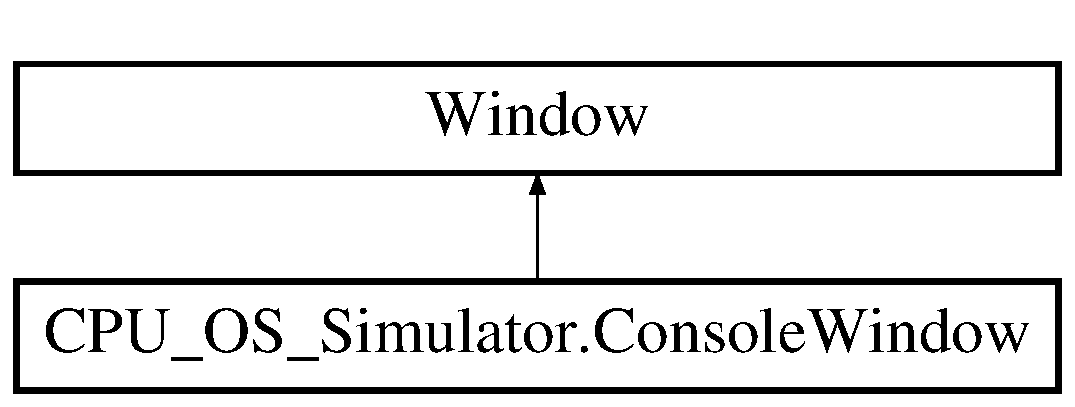
\includegraphics[height=1.004484cm]{class_c_p_u___o_s___simulator_1_1_console_window}
\end{center}
\end{figure}
\subsection*{Public Member Functions}
\begin{DoxyCompactItemize}
\item 
\hyperlink{class_c_p_u___o_s___simulator_1_1_console_window_abdd222b591f72c19297dc5805059ee7e}{Console\+Window} ()
\begin{DoxyCompactList}\small\item\em Default Constructor for console window \end{DoxyCompactList}\item 
\hyperlink{class_c_p_u___o_s___simulator_1_1_console_window_a4e79b8ceea62fb4bb44c63b7fdd7c6bb}{Console\+Window} (\hyperlink{class_c_p_u___o_s___simulator_1_1_main_window}{Main\+Window} \hyperlink{class_c_p_u___o_s___simulator_1_1_console_window_a1e38326bb40f4ed44c4964d94dc6f809}{parent})
\begin{DoxyCompactList}\small\item\em Constructor for console window that takes the window instance that is creating this window P\+L\+E\+A\+S\+E N\+O\+T\+E\+: This constructor should always be used so data can be passed back to the main window \end{DoxyCompactList}\item 
void \hyperlink{class_c_p_u___o_s___simulator_1_1_console_window_a5961ed9b274d16fab841f34bc178b52f}{Initialize\+Component} ()
\begin{DoxyCompactList}\small\item\em Initialize\+Component \end{DoxyCompactList}\item 
void \hyperlink{class_c_p_u___o_s___simulator_1_1_console_window_a5961ed9b274d16fab841f34bc178b52f}{Initialize\+Component} ()
\begin{DoxyCompactList}\small\item\em Initialize\+Component \end{DoxyCompactList}\end{DoxyCompactItemize}
\subsection*{Static Public Attributes}
\begin{DoxyCompactItemize}
\item 
static \hyperlink{class_c_p_u___o_s___simulator_1_1_console_window}{Console\+Window} \hyperlink{class_c_p_u___o_s___simulator_1_1_console_window_abee2fd1e118dd4f81dc2142bc033da4a}{current\+Instance}
\begin{DoxyCompactList}\small\item\em The current active instance of the console window \end{DoxyCompactList}\end{DoxyCompactItemize}
\subsection*{Package Attributes}
\begin{DoxyCompactItemize}
\item 
\hyperlink{class_c_p_u___o_s___simulator_1_1_console_window}{C\+P\+U\+\_\+\+O\+S\+\_\+\+Simulator.\+Console\+Window} \hyperlink{class_c_p_u___o_s___simulator_1_1_console_window_aac987ccfb7f82cf736d42355f96e886b}{Console\+Window1}
\item 
System.\+Windows.\+Controls.\+Grid \hyperlink{class_c_p_u___o_s___simulator_1_1_console_window_a28c9b155f3287ca00079175dc675eee4}{grid\+\_\+\+Main\+Grid}
\item 
System.\+Windows.\+Controls.\+Group\+Box \hyperlink{class_c_p_u___o_s___simulator_1_1_console_window_ad2d026ec9701c1b7c36dc5038927f1ab}{group\+Box}
\item 
System.\+Windows.\+Controls.\+Grid \hyperlink{class_c_p_u___o_s___simulator_1_1_console_window_afef6d481c8b608672b98da16721143b0}{grid\+\_\+\+Output\+Grid}
\item 
System.\+Windows.\+Controls.\+Text\+Box \hyperlink{class_c_p_u___o_s___simulator_1_1_console_window_ad1d4a0c5f573c7e89c8d6ed57d5097e0}{txt\+\_\+\+Console}
\item 
System.\+Windows.\+Controls.\+Group\+Box \hyperlink{class_c_p_u___o_s___simulator_1_1_console_window_aefc749577a14756234b1a73c0a4a6f50}{grp\+\_\+\+Colours}
\item 
System.\+Windows.\+Controls.\+Grid \hyperlink{class_c_p_u___o_s___simulator_1_1_console_window_a0d262972210c72305e20330f5dda9388}{grid\+\_\+\+Colours}
\item 
System.\+Windows.\+Controls.\+Radio\+Button \hyperlink{class_c_p_u___o_s___simulator_1_1_console_window_a1ce1d3ba71dbca9bee53bf6b9c474787}{rdb\+\_\+\+Screen\+Colour}
\item 
System.\+Windows.\+Controls.\+Radio\+Button \hyperlink{class_c_p_u___o_s___simulator_1_1_console_window_a6086d1a5ddaadd584ec129c7372359e2}{rdb\+\_\+\+Text\+Colour}
\item 
System.\+Windows.\+Controls.\+Button \hyperlink{class_c_p_u___o_s___simulator_1_1_console_window_a374a86e391068f8d05edb9649ce3d7f4}{btn\+\_\+\+Set\+Colour}
\end{DoxyCompactItemize}
\subsection*{Private Member Functions}
\begin{DoxyCompactItemize}
\item 
void \hyperlink{class_c_p_u___o_s___simulator_1_1_console_window_a0a66aa7f0e333cc919589a7ce4d584c0}{Parse\+Input} (string text)
\begin{DoxyCompactList}\small\item\em This function parses a line of input into a console command \end{DoxyCompactList}\item 
void \hyperlink{class_c_p_u___o_s___simulator_1_1_console_window_aabd331e8c3a83c87ccd2e09c3959408d}{txt\+\_\+\+Console\+\_\+\+Preview\+Key\+Down} (object sender, Key\+Event\+Args e)
\item 
void \hyperlink{class_c_p_u___o_s___simulator_1_1_console_window_a1de6be8bb7f4f581a9e4131a0408e632}{btn\+\_\+\+Set\+Colour\+\_\+\+Click} (object sender, Routed\+Event\+Args e)
\item 
void \hyperlink{class_c_p_u___o_s___simulator_1_1_console_window_a3d026ba3c0def2d09cc0dd1e92e4cd0d}{Console\+Window1\+\_\+\+Closing} (object sender, System.\+Component\+Model.\+Cancel\+Event\+Args e)
\item 
void \hyperlink{class_c_p_u___o_s___simulator_1_1_console_window_a8719d25b2617a32a78511d9e584d90a0}{Set\+Console\+Window\+Instance} ()
\begin{DoxyCompactList}\small\item\em This method sets the console window instance in the window bridge o it can be accessed by other modules \end{DoxyCompactList}\item 
void System.\+Windows.\+Markup.\+I\+Component\+Connector. \hyperlink{class_c_p_u___o_s___simulator_1_1_console_window_a8fc3e3f38ff00f6239dca33ff68de0d2}{Connect} (int connection\+Id, object target)
\item 
void System.\+Windows.\+Markup.\+I\+Component\+Connector. \hyperlink{class_c_p_u___o_s___simulator_1_1_console_window_a8fc3e3f38ff00f6239dca33ff68de0d2}{Connect} (int connection\+Id, object target)
\end{DoxyCompactItemize}
\subsection*{Private Attributes}
\begin{DoxyCompactItemize}
\item 
\hyperlink{class_c_p_u___o_s___simulator_1_1_main_window}{Main\+Window} \hyperlink{class_c_p_u___o_s___simulator_1_1_console_window_a1e38326bb40f4ed44c4964d94dc6f809}{parent} = null
\item 
bool \hyperlink{class_c_p_u___o_s___simulator_1_1_console_window_a4836f04e93faa3749609d7eba72e1712}{\+\_\+content\+Loaded}
\end{DoxyCompactItemize}


\subsection{Detailed Description}
Interaction logic for Console\+Window.\+xaml 

\hyperlink{class_c_p_u___o_s___simulator_1_1_console_window}{Console\+Window} 

Definition at line 23 of file Console\+Window.\+xaml.\+cs.



\subsection{Constructor \& Destructor Documentation}
\hypertarget{class_c_p_u___o_s___simulator_1_1_console_window_abdd222b591f72c19297dc5805059ee7e}{}\index{C\+P\+U\+\_\+\+O\+S\+\_\+\+Simulator\+::\+Console\+Window@{C\+P\+U\+\_\+\+O\+S\+\_\+\+Simulator\+::\+Console\+Window}!Console\+Window@{Console\+Window}}
\index{Console\+Window@{Console\+Window}!C\+P\+U\+\_\+\+O\+S\+\_\+\+Simulator\+::\+Console\+Window@{C\+P\+U\+\_\+\+O\+S\+\_\+\+Simulator\+::\+Console\+Window}}
\subsubsection[{Console\+Window()}]{\setlength{\rightskip}{0pt plus 5cm}C\+P\+U\+\_\+\+O\+S\+\_\+\+Simulator.\+Console\+Window.\+Console\+Window (
\begin{DoxyParamCaption}
{}
\end{DoxyParamCaption}
)}\label{class_c_p_u___o_s___simulator_1_1_console_window_abdd222b591f72c19297dc5805059ee7e}


Default Constructor for console window 



Definition at line 34 of file Console\+Window.\+xaml.\+cs.

\hypertarget{class_c_p_u___o_s___simulator_1_1_console_window_a4e79b8ceea62fb4bb44c63b7fdd7c6bb}{}\index{C\+P\+U\+\_\+\+O\+S\+\_\+\+Simulator\+::\+Console\+Window@{C\+P\+U\+\_\+\+O\+S\+\_\+\+Simulator\+::\+Console\+Window}!Console\+Window@{Console\+Window}}
\index{Console\+Window@{Console\+Window}!C\+P\+U\+\_\+\+O\+S\+\_\+\+Simulator\+::\+Console\+Window@{C\+P\+U\+\_\+\+O\+S\+\_\+\+Simulator\+::\+Console\+Window}}
\subsubsection[{Console\+Window(\+Main\+Window parent)}]{\setlength{\rightskip}{0pt plus 5cm}C\+P\+U\+\_\+\+O\+S\+\_\+\+Simulator.\+Console\+Window.\+Console\+Window (
\begin{DoxyParamCaption}
\item[{{\bf Main\+Window}}]{parent}
\end{DoxyParamCaption}
)}\label{class_c_p_u___o_s___simulator_1_1_console_window_a4e79b8ceea62fb4bb44c63b7fdd7c6bb}


Constructor for console window that takes the window instance that is creating this window P\+L\+E\+A\+S\+E N\+O\+T\+E\+: This constructor should always be used so data can be passed back to the main window 


\begin{DoxyParams}{Parameters}
{\em parent} & The window that is creating this window \\
\hline
\end{DoxyParams}


Definition at line 45 of file Console\+Window.\+xaml.\+cs.



\subsection{Member Function Documentation}
\hypertarget{class_c_p_u___o_s___simulator_1_1_console_window_a1de6be8bb7f4f581a9e4131a0408e632}{}\index{C\+P\+U\+\_\+\+O\+S\+\_\+\+Simulator\+::\+Console\+Window@{C\+P\+U\+\_\+\+O\+S\+\_\+\+Simulator\+::\+Console\+Window}!btn\+\_\+\+Set\+Colour\+\_\+\+Click@{btn\+\_\+\+Set\+Colour\+\_\+\+Click}}
\index{btn\+\_\+\+Set\+Colour\+\_\+\+Click@{btn\+\_\+\+Set\+Colour\+\_\+\+Click}!C\+P\+U\+\_\+\+O\+S\+\_\+\+Simulator\+::\+Console\+Window@{C\+P\+U\+\_\+\+O\+S\+\_\+\+Simulator\+::\+Console\+Window}}
\subsubsection[{btn\+\_\+\+Set\+Colour\+\_\+\+Click(object sender, Routed\+Event\+Args e)}]{\setlength{\rightskip}{0pt plus 5cm}void C\+P\+U\+\_\+\+O\+S\+\_\+\+Simulator.\+Console\+Window.\+btn\+\_\+\+Set\+Colour\+\_\+\+Click (
\begin{DoxyParamCaption}
\item[{object}]{sender, }
\item[{Routed\+Event\+Args}]{e}
\end{DoxyParamCaption}
)\hspace{0.3cm}{\ttfamily [private]}}\label{class_c_p_u___o_s___simulator_1_1_console_window_a1de6be8bb7f4f581a9e4131a0408e632}


Definition at line 102 of file Console\+Window.\+xaml.\+cs.

\hypertarget{class_c_p_u___o_s___simulator_1_1_console_window_a8fc3e3f38ff00f6239dca33ff68de0d2}{}\index{C\+P\+U\+\_\+\+O\+S\+\_\+\+Simulator\+::\+Console\+Window@{C\+P\+U\+\_\+\+O\+S\+\_\+\+Simulator\+::\+Console\+Window}!Connect@{Connect}}
\index{Connect@{Connect}!C\+P\+U\+\_\+\+O\+S\+\_\+\+Simulator\+::\+Console\+Window@{C\+P\+U\+\_\+\+O\+S\+\_\+\+Simulator\+::\+Console\+Window}}
\subsubsection[{Connect(int connection\+Id, object target)}]{\setlength{\rightskip}{0pt plus 5cm}void System.\+Windows.\+Markup.\+I\+Component\+Connector. C\+P\+U\+\_\+\+O\+S\+\_\+\+Simulator.\+Console\+Window.\+Connect (
\begin{DoxyParamCaption}
\item[{int}]{connection\+Id, }
\item[{object}]{target}
\end{DoxyParamCaption}
)\hspace{0.3cm}{\ttfamily [private]}}\label{class_c_p_u___o_s___simulator_1_1_console_window_a8fc3e3f38ff00f6239dca33ff68de0d2}


Definition at line 150 of file Console\+Window.\+g.\+i.\+cs.

\hypertarget{class_c_p_u___o_s___simulator_1_1_console_window_a8fc3e3f38ff00f6239dca33ff68de0d2}{}\index{C\+P\+U\+\_\+\+O\+S\+\_\+\+Simulator\+::\+Console\+Window@{C\+P\+U\+\_\+\+O\+S\+\_\+\+Simulator\+::\+Console\+Window}!Connect@{Connect}}
\index{Connect@{Connect}!C\+P\+U\+\_\+\+O\+S\+\_\+\+Simulator\+::\+Console\+Window@{C\+P\+U\+\_\+\+O\+S\+\_\+\+Simulator\+::\+Console\+Window}}
\subsubsection[{Connect(int connection\+Id, object target)}]{\setlength{\rightskip}{0pt plus 5cm}void System.\+Windows.\+Markup.\+I\+Component\+Connector. C\+P\+U\+\_\+\+O\+S\+\_\+\+Simulator.\+Console\+Window.\+Connect (
\begin{DoxyParamCaption}
\item[{int}]{connection\+Id, }
\item[{object}]{target}
\end{DoxyParamCaption}
)\hspace{0.3cm}{\ttfamily [private]}}\label{class_c_p_u___o_s___simulator_1_1_console_window_a8fc3e3f38ff00f6239dca33ff68de0d2}


Definition at line 150 of file Console\+Window.\+g.\+cs.

\hypertarget{class_c_p_u___o_s___simulator_1_1_console_window_a3d026ba3c0def2d09cc0dd1e92e4cd0d}{}\index{C\+P\+U\+\_\+\+O\+S\+\_\+\+Simulator\+::\+Console\+Window@{C\+P\+U\+\_\+\+O\+S\+\_\+\+Simulator\+::\+Console\+Window}!Console\+Window1\+\_\+\+Closing@{Console\+Window1\+\_\+\+Closing}}
\index{Console\+Window1\+\_\+\+Closing@{Console\+Window1\+\_\+\+Closing}!C\+P\+U\+\_\+\+O\+S\+\_\+\+Simulator\+::\+Console\+Window@{C\+P\+U\+\_\+\+O\+S\+\_\+\+Simulator\+::\+Console\+Window}}
\subsubsection[{Console\+Window1\+\_\+\+Closing(object sender, System.\+Component\+Model.\+Cancel\+Event\+Args e)}]{\setlength{\rightskip}{0pt plus 5cm}void C\+P\+U\+\_\+\+O\+S\+\_\+\+Simulator.\+Console\+Window.\+Console\+Window1\+\_\+\+Closing (
\begin{DoxyParamCaption}
\item[{object}]{sender, }
\item[{System.\+Component\+Model.\+Cancel\+Event\+Args}]{e}
\end{DoxyParamCaption}
)\hspace{0.3cm}{\ttfamily [private]}}\label{class_c_p_u___o_s___simulator_1_1_console_window_a3d026ba3c0def2d09cc0dd1e92e4cd0d}


Definition at line 108 of file Console\+Window.\+xaml.\+cs.

\hypertarget{class_c_p_u___o_s___simulator_1_1_console_window_a5961ed9b274d16fab841f34bc178b52f}{}\index{C\+P\+U\+\_\+\+O\+S\+\_\+\+Simulator\+::\+Console\+Window@{C\+P\+U\+\_\+\+O\+S\+\_\+\+Simulator\+::\+Console\+Window}!Initialize\+Component@{Initialize\+Component}}
\index{Initialize\+Component@{Initialize\+Component}!C\+P\+U\+\_\+\+O\+S\+\_\+\+Simulator\+::\+Console\+Window@{C\+P\+U\+\_\+\+O\+S\+\_\+\+Simulator\+::\+Console\+Window}}
\subsubsection[{Initialize\+Component()}]{\setlength{\rightskip}{0pt plus 5cm}void C\+P\+U\+\_\+\+O\+S\+\_\+\+Simulator.\+Console\+Window.\+Initialize\+Component (
\begin{DoxyParamCaption}
{}
\end{DoxyParamCaption}
)}\label{class_c_p_u___o_s___simulator_1_1_console_window_a5961ed9b274d16fab841f34bc178b52f}


Initialize\+Component 



Definition at line 130 of file Console\+Window.\+g.\+i.\+cs.

\hypertarget{class_c_p_u___o_s___simulator_1_1_console_window_a5961ed9b274d16fab841f34bc178b52f}{}\index{C\+P\+U\+\_\+\+O\+S\+\_\+\+Simulator\+::\+Console\+Window@{C\+P\+U\+\_\+\+O\+S\+\_\+\+Simulator\+::\+Console\+Window}!Initialize\+Component@{Initialize\+Component}}
\index{Initialize\+Component@{Initialize\+Component}!C\+P\+U\+\_\+\+O\+S\+\_\+\+Simulator\+::\+Console\+Window@{C\+P\+U\+\_\+\+O\+S\+\_\+\+Simulator\+::\+Console\+Window}}
\subsubsection[{Initialize\+Component()}]{\setlength{\rightskip}{0pt plus 5cm}void C\+P\+U\+\_\+\+O\+S\+\_\+\+Simulator.\+Console\+Window.\+Initialize\+Component (
\begin{DoxyParamCaption}
{}
\end{DoxyParamCaption}
)}\label{class_c_p_u___o_s___simulator_1_1_console_window_a5961ed9b274d16fab841f34bc178b52f}


Initialize\+Component 



Definition at line 130 of file Console\+Window.\+g.\+cs.

\hypertarget{class_c_p_u___o_s___simulator_1_1_console_window_a0a66aa7f0e333cc919589a7ce4d584c0}{}\index{C\+P\+U\+\_\+\+O\+S\+\_\+\+Simulator\+::\+Console\+Window@{C\+P\+U\+\_\+\+O\+S\+\_\+\+Simulator\+::\+Console\+Window}!Parse\+Input@{Parse\+Input}}
\index{Parse\+Input@{Parse\+Input}!C\+P\+U\+\_\+\+O\+S\+\_\+\+Simulator\+::\+Console\+Window@{C\+P\+U\+\_\+\+O\+S\+\_\+\+Simulator\+::\+Console\+Window}}
\subsubsection[{Parse\+Input(string text)}]{\setlength{\rightskip}{0pt plus 5cm}void C\+P\+U\+\_\+\+O\+S\+\_\+\+Simulator.\+Console\+Window.\+Parse\+Input (
\begin{DoxyParamCaption}
\item[{string}]{text}
\end{DoxyParamCaption}
)\hspace{0.3cm}{\ttfamily [private]}}\label{class_c_p_u___o_s___simulator_1_1_console_window_a0a66aa7f0e333cc919589a7ce4d584c0}


This function parses a line of input into a console command 


\begin{DoxyParams}{Parameters}
{\em text} & the line of input to parse\\
\hline
\end{DoxyParams}


Definition at line 56 of file Console\+Window.\+xaml.\+cs.

\hypertarget{class_c_p_u___o_s___simulator_1_1_console_window_a8719d25b2617a32a78511d9e584d90a0}{}\index{C\+P\+U\+\_\+\+O\+S\+\_\+\+Simulator\+::\+Console\+Window@{C\+P\+U\+\_\+\+O\+S\+\_\+\+Simulator\+::\+Console\+Window}!Set\+Console\+Window\+Instance@{Set\+Console\+Window\+Instance}}
\index{Set\+Console\+Window\+Instance@{Set\+Console\+Window\+Instance}!C\+P\+U\+\_\+\+O\+S\+\_\+\+Simulator\+::\+Console\+Window@{C\+P\+U\+\_\+\+O\+S\+\_\+\+Simulator\+::\+Console\+Window}}
\subsubsection[{Set\+Console\+Window\+Instance()}]{\setlength{\rightskip}{0pt plus 5cm}void C\+P\+U\+\_\+\+O\+S\+\_\+\+Simulator.\+Console\+Window.\+Set\+Console\+Window\+Instance (
\begin{DoxyParamCaption}
{}
\end{DoxyParamCaption}
)\hspace{0.3cm}{\ttfamily [private]}}\label{class_c_p_u___o_s___simulator_1_1_console_window_a8719d25b2617a32a78511d9e584d90a0}


This method sets the console window instance in the window bridge o it can be accessed by other modules 



Definition at line 116 of file Console\+Window.\+xaml.\+cs.

\hypertarget{class_c_p_u___o_s___simulator_1_1_console_window_aabd331e8c3a83c87ccd2e09c3959408d}{}\index{C\+P\+U\+\_\+\+O\+S\+\_\+\+Simulator\+::\+Console\+Window@{C\+P\+U\+\_\+\+O\+S\+\_\+\+Simulator\+::\+Console\+Window}!txt\+\_\+\+Console\+\_\+\+Preview\+Key\+Down@{txt\+\_\+\+Console\+\_\+\+Preview\+Key\+Down}}
\index{txt\+\_\+\+Console\+\_\+\+Preview\+Key\+Down@{txt\+\_\+\+Console\+\_\+\+Preview\+Key\+Down}!C\+P\+U\+\_\+\+O\+S\+\_\+\+Simulator\+::\+Console\+Window@{C\+P\+U\+\_\+\+O\+S\+\_\+\+Simulator\+::\+Console\+Window}}
\subsubsection[{txt\+\_\+\+Console\+\_\+\+Preview\+Key\+Down(object sender, Key\+Event\+Args e)}]{\setlength{\rightskip}{0pt plus 5cm}void C\+P\+U\+\_\+\+O\+S\+\_\+\+Simulator.\+Console\+Window.\+txt\+\_\+\+Console\+\_\+\+Preview\+Key\+Down (
\begin{DoxyParamCaption}
\item[{object}]{sender, }
\item[{Key\+Event\+Args}]{e}
\end{DoxyParamCaption}
)\hspace{0.3cm}{\ttfamily [private]}}\label{class_c_p_u___o_s___simulator_1_1_console_window_aabd331e8c3a83c87ccd2e09c3959408d}


Definition at line 88 of file Console\+Window.\+xaml.\+cs.



\subsection{Member Data Documentation}
\hypertarget{class_c_p_u___o_s___simulator_1_1_console_window_a4836f04e93faa3749609d7eba72e1712}{}\index{C\+P\+U\+\_\+\+O\+S\+\_\+\+Simulator\+::\+Console\+Window@{C\+P\+U\+\_\+\+O\+S\+\_\+\+Simulator\+::\+Console\+Window}!\+\_\+content\+Loaded@{\+\_\+content\+Loaded}}
\index{\+\_\+content\+Loaded@{\+\_\+content\+Loaded}!C\+P\+U\+\_\+\+O\+S\+\_\+\+Simulator\+::\+Console\+Window@{C\+P\+U\+\_\+\+O\+S\+\_\+\+Simulator\+::\+Console\+Window}}
\subsubsection[{\+\_\+content\+Loaded}]{\setlength{\rightskip}{0pt plus 5cm}bool C\+P\+U\+\_\+\+O\+S\+\_\+\+Simulator.\+Console\+Window.\+\_\+content\+Loaded\hspace{0.3cm}{\ttfamily [private]}}\label{class_c_p_u___o_s___simulator_1_1_console_window_a4836f04e93faa3749609d7eba72e1712}


Definition at line 123 of file Console\+Window.\+g.\+cs.

\hypertarget{class_c_p_u___o_s___simulator_1_1_console_window_a374a86e391068f8d05edb9649ce3d7f4}{}\index{C\+P\+U\+\_\+\+O\+S\+\_\+\+Simulator\+::\+Console\+Window@{C\+P\+U\+\_\+\+O\+S\+\_\+\+Simulator\+::\+Console\+Window}!btn\+\_\+\+Set\+Colour@{btn\+\_\+\+Set\+Colour}}
\index{btn\+\_\+\+Set\+Colour@{btn\+\_\+\+Set\+Colour}!C\+P\+U\+\_\+\+O\+S\+\_\+\+Simulator\+::\+Console\+Window@{C\+P\+U\+\_\+\+O\+S\+\_\+\+Simulator\+::\+Console\+Window}}
\subsubsection[{btn\+\_\+\+Set\+Colour}]{\setlength{\rightskip}{0pt plus 5cm}System Windows Controls Button C\+P\+U\+\_\+\+O\+S\+\_\+\+Simulator.\+Console\+Window.\+btn\+\_\+\+Set\+Colour\hspace{0.3cm}{\ttfamily [package]}}\label{class_c_p_u___o_s___simulator_1_1_console_window_a374a86e391068f8d05edb9649ce3d7f4}


Definition at line 118 of file Console\+Window.\+g.\+cs.

\hypertarget{class_c_p_u___o_s___simulator_1_1_console_window_aac987ccfb7f82cf736d42355f96e886b}{}\index{C\+P\+U\+\_\+\+O\+S\+\_\+\+Simulator\+::\+Console\+Window@{C\+P\+U\+\_\+\+O\+S\+\_\+\+Simulator\+::\+Console\+Window}!Console\+Window1@{Console\+Window1}}
\index{Console\+Window1@{Console\+Window1}!C\+P\+U\+\_\+\+O\+S\+\_\+\+Simulator\+::\+Console\+Window@{C\+P\+U\+\_\+\+O\+S\+\_\+\+Simulator\+::\+Console\+Window}}
\subsubsection[{Console\+Window1}]{\setlength{\rightskip}{0pt plus 5cm}C\+P\+U\+\_\+\+O\+S\+\_\+\+Simulator {\bf Console\+Window} C\+P\+U\+\_\+\+O\+S\+\_\+\+Simulator.\+Console\+Window.\+Console\+Window1\hspace{0.3cm}{\ttfamily [package]}}\label{class_c_p_u___o_s___simulator_1_1_console_window_aac987ccfb7f82cf736d42355f96e886b}


Definition at line 46 of file Console\+Window.\+g.\+cs.

\hypertarget{class_c_p_u___o_s___simulator_1_1_console_window_abee2fd1e118dd4f81dc2142bc033da4a}{}\index{C\+P\+U\+\_\+\+O\+S\+\_\+\+Simulator\+::\+Console\+Window@{C\+P\+U\+\_\+\+O\+S\+\_\+\+Simulator\+::\+Console\+Window}!current\+Instance@{current\+Instance}}
\index{current\+Instance@{current\+Instance}!C\+P\+U\+\_\+\+O\+S\+\_\+\+Simulator\+::\+Console\+Window@{C\+P\+U\+\_\+\+O\+S\+\_\+\+Simulator\+::\+Console\+Window}}
\subsubsection[{current\+Instance}]{\setlength{\rightskip}{0pt plus 5cm}{\bf Console\+Window} C\+P\+U\+\_\+\+O\+S\+\_\+\+Simulator.\+Console\+Window.\+current\+Instance\hspace{0.3cm}{\ttfamily [static]}}\label{class_c_p_u___o_s___simulator_1_1_console_window_abee2fd1e118dd4f81dc2142bc033da4a}


The current active instance of the console window 



Definition at line 29 of file Console\+Window.\+xaml.\+cs.

\hypertarget{class_c_p_u___o_s___simulator_1_1_console_window_a0d262972210c72305e20330f5dda9388}{}\index{C\+P\+U\+\_\+\+O\+S\+\_\+\+Simulator\+::\+Console\+Window@{C\+P\+U\+\_\+\+O\+S\+\_\+\+Simulator\+::\+Console\+Window}!grid\+\_\+\+Colours@{grid\+\_\+\+Colours}}
\index{grid\+\_\+\+Colours@{grid\+\_\+\+Colours}!C\+P\+U\+\_\+\+O\+S\+\_\+\+Simulator\+::\+Console\+Window@{C\+P\+U\+\_\+\+O\+S\+\_\+\+Simulator\+::\+Console\+Window}}
\subsubsection[{grid\+\_\+\+Colours}]{\setlength{\rightskip}{0pt plus 5cm}System Windows Controls Grid C\+P\+U\+\_\+\+O\+S\+\_\+\+Simulator.\+Console\+Window.\+grid\+\_\+\+Colours\hspace{0.3cm}{\ttfamily [package]}}\label{class_c_p_u___o_s___simulator_1_1_console_window_a0d262972210c72305e20330f5dda9388}


Definition at line 94 of file Console\+Window.\+g.\+cs.

\hypertarget{class_c_p_u___o_s___simulator_1_1_console_window_a28c9b155f3287ca00079175dc675eee4}{}\index{C\+P\+U\+\_\+\+O\+S\+\_\+\+Simulator\+::\+Console\+Window@{C\+P\+U\+\_\+\+O\+S\+\_\+\+Simulator\+::\+Console\+Window}!grid\+\_\+\+Main\+Grid@{grid\+\_\+\+Main\+Grid}}
\index{grid\+\_\+\+Main\+Grid@{grid\+\_\+\+Main\+Grid}!C\+P\+U\+\_\+\+O\+S\+\_\+\+Simulator\+::\+Console\+Window@{C\+P\+U\+\_\+\+O\+S\+\_\+\+Simulator\+::\+Console\+Window}}
\subsubsection[{grid\+\_\+\+Main\+Grid}]{\setlength{\rightskip}{0pt plus 5cm}System Windows Controls Grid C\+P\+U\+\_\+\+O\+S\+\_\+\+Simulator.\+Console\+Window.\+grid\+\_\+\+Main\+Grid\hspace{0.3cm}{\ttfamily [package]}}\label{class_c_p_u___o_s___simulator_1_1_console_window_a28c9b155f3287ca00079175dc675eee4}


Definition at line 54 of file Console\+Window.\+g.\+cs.

\hypertarget{class_c_p_u___o_s___simulator_1_1_console_window_afef6d481c8b608672b98da16721143b0}{}\index{C\+P\+U\+\_\+\+O\+S\+\_\+\+Simulator\+::\+Console\+Window@{C\+P\+U\+\_\+\+O\+S\+\_\+\+Simulator\+::\+Console\+Window}!grid\+\_\+\+Output\+Grid@{grid\+\_\+\+Output\+Grid}}
\index{grid\+\_\+\+Output\+Grid@{grid\+\_\+\+Output\+Grid}!C\+P\+U\+\_\+\+O\+S\+\_\+\+Simulator\+::\+Console\+Window@{C\+P\+U\+\_\+\+O\+S\+\_\+\+Simulator\+::\+Console\+Window}}
\subsubsection[{grid\+\_\+\+Output\+Grid}]{\setlength{\rightskip}{0pt plus 5cm}System Windows Controls Grid C\+P\+U\+\_\+\+O\+S\+\_\+\+Simulator.\+Console\+Window.\+grid\+\_\+\+Output\+Grid\hspace{0.3cm}{\ttfamily [package]}}\label{class_c_p_u___o_s___simulator_1_1_console_window_afef6d481c8b608672b98da16721143b0}


Definition at line 70 of file Console\+Window.\+g.\+cs.

\hypertarget{class_c_p_u___o_s___simulator_1_1_console_window_ad2d026ec9701c1b7c36dc5038927f1ab}{}\index{C\+P\+U\+\_\+\+O\+S\+\_\+\+Simulator\+::\+Console\+Window@{C\+P\+U\+\_\+\+O\+S\+\_\+\+Simulator\+::\+Console\+Window}!group\+Box@{group\+Box}}
\index{group\+Box@{group\+Box}!C\+P\+U\+\_\+\+O\+S\+\_\+\+Simulator\+::\+Console\+Window@{C\+P\+U\+\_\+\+O\+S\+\_\+\+Simulator\+::\+Console\+Window}}
\subsubsection[{group\+Box}]{\setlength{\rightskip}{0pt plus 5cm}System Windows Controls Group\+Box C\+P\+U\+\_\+\+O\+S\+\_\+\+Simulator.\+Console\+Window.\+group\+Box\hspace{0.3cm}{\ttfamily [package]}}\label{class_c_p_u___o_s___simulator_1_1_console_window_ad2d026ec9701c1b7c36dc5038927f1ab}


Definition at line 62 of file Console\+Window.\+g.\+cs.

\hypertarget{class_c_p_u___o_s___simulator_1_1_console_window_aefc749577a14756234b1a73c0a4a6f50}{}\index{C\+P\+U\+\_\+\+O\+S\+\_\+\+Simulator\+::\+Console\+Window@{C\+P\+U\+\_\+\+O\+S\+\_\+\+Simulator\+::\+Console\+Window}!grp\+\_\+\+Colours@{grp\+\_\+\+Colours}}
\index{grp\+\_\+\+Colours@{grp\+\_\+\+Colours}!C\+P\+U\+\_\+\+O\+S\+\_\+\+Simulator\+::\+Console\+Window@{C\+P\+U\+\_\+\+O\+S\+\_\+\+Simulator\+::\+Console\+Window}}
\subsubsection[{grp\+\_\+\+Colours}]{\setlength{\rightskip}{0pt plus 5cm}System Windows Controls Group\+Box C\+P\+U\+\_\+\+O\+S\+\_\+\+Simulator.\+Console\+Window.\+grp\+\_\+\+Colours\hspace{0.3cm}{\ttfamily [package]}}\label{class_c_p_u___o_s___simulator_1_1_console_window_aefc749577a14756234b1a73c0a4a6f50}


Definition at line 86 of file Console\+Window.\+g.\+cs.

\hypertarget{class_c_p_u___o_s___simulator_1_1_console_window_a1e38326bb40f4ed44c4964d94dc6f809}{}\index{C\+P\+U\+\_\+\+O\+S\+\_\+\+Simulator\+::\+Console\+Window@{C\+P\+U\+\_\+\+O\+S\+\_\+\+Simulator\+::\+Console\+Window}!parent@{parent}}
\index{parent@{parent}!C\+P\+U\+\_\+\+O\+S\+\_\+\+Simulator\+::\+Console\+Window@{C\+P\+U\+\_\+\+O\+S\+\_\+\+Simulator\+::\+Console\+Window}}
\subsubsection[{parent}]{\setlength{\rightskip}{0pt plus 5cm}{\bf Main\+Window} C\+P\+U\+\_\+\+O\+S\+\_\+\+Simulator.\+Console\+Window.\+parent = null\hspace{0.3cm}{\ttfamily [private]}}\label{class_c_p_u___o_s___simulator_1_1_console_window_a1e38326bb40f4ed44c4964d94dc6f809}


Definition at line 25 of file Console\+Window.\+xaml.\+cs.

\hypertarget{class_c_p_u___o_s___simulator_1_1_console_window_a1ce1d3ba71dbca9bee53bf6b9c474787}{}\index{C\+P\+U\+\_\+\+O\+S\+\_\+\+Simulator\+::\+Console\+Window@{C\+P\+U\+\_\+\+O\+S\+\_\+\+Simulator\+::\+Console\+Window}!rdb\+\_\+\+Screen\+Colour@{rdb\+\_\+\+Screen\+Colour}}
\index{rdb\+\_\+\+Screen\+Colour@{rdb\+\_\+\+Screen\+Colour}!C\+P\+U\+\_\+\+O\+S\+\_\+\+Simulator\+::\+Console\+Window@{C\+P\+U\+\_\+\+O\+S\+\_\+\+Simulator\+::\+Console\+Window}}
\subsubsection[{rdb\+\_\+\+Screen\+Colour}]{\setlength{\rightskip}{0pt plus 5cm}System Windows Controls Radio\+Button C\+P\+U\+\_\+\+O\+S\+\_\+\+Simulator.\+Console\+Window.\+rdb\+\_\+\+Screen\+Colour\hspace{0.3cm}{\ttfamily [package]}}\label{class_c_p_u___o_s___simulator_1_1_console_window_a1ce1d3ba71dbca9bee53bf6b9c474787}


Definition at line 102 of file Console\+Window.\+g.\+cs.

\hypertarget{class_c_p_u___o_s___simulator_1_1_console_window_a6086d1a5ddaadd584ec129c7372359e2}{}\index{C\+P\+U\+\_\+\+O\+S\+\_\+\+Simulator\+::\+Console\+Window@{C\+P\+U\+\_\+\+O\+S\+\_\+\+Simulator\+::\+Console\+Window}!rdb\+\_\+\+Text\+Colour@{rdb\+\_\+\+Text\+Colour}}
\index{rdb\+\_\+\+Text\+Colour@{rdb\+\_\+\+Text\+Colour}!C\+P\+U\+\_\+\+O\+S\+\_\+\+Simulator\+::\+Console\+Window@{C\+P\+U\+\_\+\+O\+S\+\_\+\+Simulator\+::\+Console\+Window}}
\subsubsection[{rdb\+\_\+\+Text\+Colour}]{\setlength{\rightskip}{0pt plus 5cm}System Windows Controls Radio\+Button C\+P\+U\+\_\+\+O\+S\+\_\+\+Simulator.\+Console\+Window.\+rdb\+\_\+\+Text\+Colour\hspace{0.3cm}{\ttfamily [package]}}\label{class_c_p_u___o_s___simulator_1_1_console_window_a6086d1a5ddaadd584ec129c7372359e2}


Definition at line 110 of file Console\+Window.\+g.\+cs.

\hypertarget{class_c_p_u___o_s___simulator_1_1_console_window_ad1d4a0c5f573c7e89c8d6ed57d5097e0}{}\index{C\+P\+U\+\_\+\+O\+S\+\_\+\+Simulator\+::\+Console\+Window@{C\+P\+U\+\_\+\+O\+S\+\_\+\+Simulator\+::\+Console\+Window}!txt\+\_\+\+Console@{txt\+\_\+\+Console}}
\index{txt\+\_\+\+Console@{txt\+\_\+\+Console}!C\+P\+U\+\_\+\+O\+S\+\_\+\+Simulator\+::\+Console\+Window@{C\+P\+U\+\_\+\+O\+S\+\_\+\+Simulator\+::\+Console\+Window}}
\subsubsection[{txt\+\_\+\+Console}]{\setlength{\rightskip}{0pt plus 5cm}System Windows Controls Text\+Box C\+P\+U\+\_\+\+O\+S\+\_\+\+Simulator.\+Console\+Window.\+txt\+\_\+\+Console\hspace{0.3cm}{\ttfamily [package]}}\label{class_c_p_u___o_s___simulator_1_1_console_window_ad1d4a0c5f573c7e89c8d6ed57d5097e0}


Definition at line 78 of file Console\+Window.\+g.\+cs.



The documentation for this class was generated from the following files\+:\begin{DoxyCompactItemize}
\item 
C\+P\+U-\/\+O\+S Simulator/\hyperlink{_console_window_8xaml_8cs}{Console\+Window.\+xaml.\+cs}\item 
C\+P\+U-\/\+O\+S Simulator/obj/\+Debug/\hyperlink{_console_window_8g_8cs}{Console\+Window.\+g.\+cs}\item 
C\+P\+U-\/\+O\+S Simulator/obj/\+Debug/\hyperlink{_console_window_8g_8i_8cs}{Console\+Window.\+g.\+i.\+cs}\end{DoxyCompactItemize}

\hypertarget{class_c_p_u___o_s___simulator_1_1_c_p_u_1_1_execution_unit}{}\section{C\+P\+U\+\_\+\+O\+S\+\_\+\+Simulator.\+C\+P\+U.\+Execution\+Unit Class Reference}
\label{class_c_p_u___o_s___simulator_1_1_c_p_u_1_1_execution_unit}\index{C\+P\+U\+\_\+\+O\+S\+\_\+\+Simulator.\+C\+P\+U.\+Execution\+Unit@{C\+P\+U\+\_\+\+O\+S\+\_\+\+Simulator.\+C\+P\+U.\+Execution\+Unit}}


This class represents the part of the \hyperlink{namespace_c_p_u___o_s___simulator_1_1_c_p_u}{C\+P\+U} which executes instructions  


\subsection*{Public Member Functions}
\begin{DoxyCompactItemize}
\item 
\hyperlink{class_c_p_u___o_s___simulator_1_1_c_p_u_1_1_execution_unit_aaa72bccee27d810d5bbfa9ed02215fa9}{Execution\+Unit} (\hyperlink{class_c_p_u___o_s___simulator_1_1_c_p_u_1_1_simulator_program}{Simulator\+Program} \hyperlink{class_c_p_u___o_s___simulator_1_1_c_p_u_1_1_execution_unit_a192670bee8ca089c38e9989350f658d6}{program}, int \hyperlink{class_c_p_u___o_s___simulator_1_1_c_p_u_1_1_execution_unit_a0deb0a3e0c9fa402598bbf18be6535cc}{clock\+Speed})
\begin{DoxyCompactList}\small\item\em Constructor for execution unit that starts executing from the beginning of the program \end{DoxyCompactList}\item 
\hyperlink{class_c_p_u___o_s___simulator_1_1_c_p_u_1_1_execution_unit_a0b69abfef40692e266fee90b2321797e}{Execution\+Unit} (\hyperlink{class_c_p_u___o_s___simulator_1_1_c_p_u_1_1_simulator_program}{Simulator\+Program} \hyperlink{class_c_p_u___o_s___simulator_1_1_c_p_u_1_1_execution_unit_a192670bee8ca089c38e9989350f658d6}{program}, int \hyperlink{class_c_p_u___o_s___simulator_1_1_c_p_u_1_1_execution_unit_a0deb0a3e0c9fa402598bbf18be6535cc}{clock\+Speed}, int \hyperlink{class_c_p_u___o_s___simulator_1_1_c_p_u_1_1_execution_unit_af6807cb5343acc2c40a08166c748f1f0}{current\+Index})
\begin{DoxyCompactList}\small\item\em Constructor for execution unit that starts executing from a specified location in the program \end{DoxyCompactList}\item 
void \hyperlink{class_c_p_u___o_s___simulator_1_1_c_p_u_1_1_execution_unit_ae0298423e5e7aad47e342e3960a361ac}{Execute\+Instruction} ()
\begin{DoxyCompactList}\small\item\em This function executes an instruction by calling its delegate function \end{DoxyCompactList}\end{DoxyCompactItemize}
\subsection*{Properties}
\begin{DoxyCompactItemize}
\item 
\hyperlink{class_c_p_u___o_s___simulator_1_1_c_p_u_1_1_simulator_program}{Simulator\+Program} \hyperlink{class_c_p_u___o_s___simulator_1_1_c_p_u_1_1_execution_unit_a5266ac137491de1efa6c4d707fcd162e}{Program}\hspace{0.3cm}{\ttfamily  \mbox{[}get, set\mbox{]}}
\item 
int \hyperlink{class_c_p_u___o_s___simulator_1_1_c_p_u_1_1_execution_unit_ac34a0c232ee8d1996d29f5d8614556ab}{Clock\+Speed}\hspace{0.3cm}{\ttfamily  \mbox{[}get, set\mbox{]}}
\item 
bool \hyperlink{class_c_p_u___o_s___simulator_1_1_c_p_u_1_1_execution_unit_a1b8748f1c6679263e5dc03fe382ad150}{Stop}\hspace{0.3cm}{\ttfamily  \mbox{[}get, set\mbox{]}}
\item 
bool \hyperlink{class_c_p_u___o_s___simulator_1_1_c_p_u_1_1_execution_unit_afc47977290c9bccf4f3b115613a67576}{Done}\hspace{0.3cm}{\ttfamily  \mbox{[}get, set\mbox{]}}
\item 
int \hyperlink{class_c_p_u___o_s___simulator_1_1_c_p_u_1_1_execution_unit_a14d2a23bdc679ed2758733f34f79db63}{Current\+Index}\hspace{0.3cm}{\ttfamily  \mbox{[}get, set\mbox{]}}
\item 
int \hyperlink{class_c_p_u___o_s___simulator_1_1_c_p_u_1_1_execution_unit_ac939e9a08b30b2cc3a9438d6c1cc5a61}{Logical\+Address}\hspace{0.3cm}{\ttfamily  \mbox{[}get, set\mbox{]}}
\item 
\hyperlink{class_c_p_u___o_s___simulator_1_1_c_p_u_1_1_instruction}{Instruction} \hyperlink{class_c_p_u___o_s___simulator_1_1_c_p_u_1_1_execution_unit_a285d7b487a3ac5eff07c640e438ceb11}{Current\+Instruction}\hspace{0.3cm}{\ttfamily  \mbox{[}get, set\mbox{]}}
\end{DoxyCompactItemize}
\subsection*{Private Attributes}
\begin{DoxyCompactItemize}
\item 
\hyperlink{class_c_p_u___o_s___simulator_1_1_c_p_u_1_1_simulator_program}{Simulator\+Program} \hyperlink{class_c_p_u___o_s___simulator_1_1_c_p_u_1_1_execution_unit_a192670bee8ca089c38e9989350f658d6}{program}
\begin{DoxyCompactList}\small\item\em The current program being executed \end{DoxyCompactList}\item 
int \hyperlink{class_c_p_u___o_s___simulator_1_1_c_p_u_1_1_execution_unit_a0deb0a3e0c9fa402598bbf18be6535cc}{clock\+Speed}
\begin{DoxyCompactList}\small\item\em The clock speed that the \hyperlink{namespace_c_p_u___o_s___simulator_1_1_c_p_u}{C\+P\+U} is running at \end{DoxyCompactList}\item 
int \hyperlink{class_c_p_u___o_s___simulator_1_1_c_p_u_1_1_execution_unit_af6807cb5343acc2c40a08166c748f1f0}{current\+Index}
\begin{DoxyCompactList}\small\item\em The index of the instruction currently being executed \end{DoxyCompactList}\item 
\hyperlink{class_c_p_u___o_s___simulator_1_1_c_p_u_1_1_instruction}{Instruction} \hyperlink{class_c_p_u___o_s___simulator_1_1_c_p_u_1_1_execution_unit_a12fc8d1fd19eab177941b9f98675eb7f}{current\+Instruction}
\begin{DoxyCompactList}\small\item\em The instruction currently being executed \end{DoxyCompactList}\item 
int \hyperlink{class_c_p_u___o_s___simulator_1_1_c_p_u_1_1_execution_unit_aa387f2bbbf0de1c75cbd1c79e27a630c}{logical\+Address}
\begin{DoxyCompactList}\small\item\em The Logical address of the instruction currently being executed \end{DoxyCompactList}\item 
bool \hyperlink{class_c_p_u___o_s___simulator_1_1_c_p_u_1_1_execution_unit_aad508435c1085ec880b75723260b0439}{stop}
\begin{DoxyCompactList}\small\item\em Whether the unit has received a stop signal from the main window \end{DoxyCompactList}\item 
bool \hyperlink{class_c_p_u___o_s___simulator_1_1_c_p_u_1_1_execution_unit_aa62cb66691fd4d782a4fa5c70843da6e}{done}
\begin{DoxyCompactList}\small\item\em Whether the unit has reached the end of the program \end{DoxyCompactList}\end{DoxyCompactItemize}


\subsection{Detailed Description}
This class represents the part of the \hyperlink{namespace_c_p_u___o_s___simulator_1_1_c_p_u}{C\+P\+U} which executes instructions 



Definition at line 10 of file Execution\+Unit.\+cs.



\subsection{Constructor \& Destructor Documentation}
\hypertarget{class_c_p_u___o_s___simulator_1_1_c_p_u_1_1_execution_unit_aaa72bccee27d810d5bbfa9ed02215fa9}{}\index{C\+P\+U\+\_\+\+O\+S\+\_\+\+Simulator\+::\+C\+P\+U\+::\+Execution\+Unit@{C\+P\+U\+\_\+\+O\+S\+\_\+\+Simulator\+::\+C\+P\+U\+::\+Execution\+Unit}!Execution\+Unit@{Execution\+Unit}}
\index{Execution\+Unit@{Execution\+Unit}!C\+P\+U\+\_\+\+O\+S\+\_\+\+Simulator\+::\+C\+P\+U\+::\+Execution\+Unit@{C\+P\+U\+\_\+\+O\+S\+\_\+\+Simulator\+::\+C\+P\+U\+::\+Execution\+Unit}}
\subsubsection[{Execution\+Unit(\+Simulator\+Program program, int clock\+Speed)}]{\setlength{\rightskip}{0pt plus 5cm}C\+P\+U\+\_\+\+O\+S\+\_\+\+Simulator.\+C\+P\+U.\+Execution\+Unit.\+Execution\+Unit (
\begin{DoxyParamCaption}
\item[{{\bf Simulator\+Program}}]{program, }
\item[{int}]{clock\+Speed}
\end{DoxyParamCaption}
)}\label{class_c_p_u___o_s___simulator_1_1_c_p_u_1_1_execution_unit_aaa72bccee27d810d5bbfa9ed02215fa9}


Constructor for execution unit that starts executing from the beginning of the program 


\begin{DoxyParams}{Parameters}
{\em program} & the program to execute \\
\hline
{\em clock\+Speed} & the clock speed of the \hyperlink{namespace_c_p_u___o_s___simulator_1_1_c_p_u}{C\+P\+U} \\
\hline
\end{DoxyParams}


Definition at line 58 of file Execution\+Unit.\+cs.

\hypertarget{class_c_p_u___o_s___simulator_1_1_c_p_u_1_1_execution_unit_a0b69abfef40692e266fee90b2321797e}{}\index{C\+P\+U\+\_\+\+O\+S\+\_\+\+Simulator\+::\+C\+P\+U\+::\+Execution\+Unit@{C\+P\+U\+\_\+\+O\+S\+\_\+\+Simulator\+::\+C\+P\+U\+::\+Execution\+Unit}!Execution\+Unit@{Execution\+Unit}}
\index{Execution\+Unit@{Execution\+Unit}!C\+P\+U\+\_\+\+O\+S\+\_\+\+Simulator\+::\+C\+P\+U\+::\+Execution\+Unit@{C\+P\+U\+\_\+\+O\+S\+\_\+\+Simulator\+::\+C\+P\+U\+::\+Execution\+Unit}}
\subsubsection[{Execution\+Unit(\+Simulator\+Program program, int clock\+Speed, int current\+Index)}]{\setlength{\rightskip}{0pt plus 5cm}C\+P\+U\+\_\+\+O\+S\+\_\+\+Simulator.\+C\+P\+U.\+Execution\+Unit.\+Execution\+Unit (
\begin{DoxyParamCaption}
\item[{{\bf Simulator\+Program}}]{program, }
\item[{int}]{clock\+Speed, }
\item[{int}]{current\+Index}
\end{DoxyParamCaption}
)}\label{class_c_p_u___o_s___simulator_1_1_c_p_u_1_1_execution_unit_a0b69abfef40692e266fee90b2321797e}


Constructor for execution unit that starts executing from a specified location in the program 


\begin{DoxyParams}{Parameters}
{\em program} & the program to execute \\
\hline
{\em current\+Index} & the index to start executing from\\
\hline
{\em clock\+Speed} & the clock speed of the \hyperlink{namespace_c_p_u___o_s___simulator_1_1_c_p_u}{C\+P\+U} \\
\hline
\end{DoxyParams}


Definition at line 75 of file Execution\+Unit.\+cs.



\subsection{Member Function Documentation}
\hypertarget{class_c_p_u___o_s___simulator_1_1_c_p_u_1_1_execution_unit_ae0298423e5e7aad47e342e3960a361ac}{}\index{C\+P\+U\+\_\+\+O\+S\+\_\+\+Simulator\+::\+C\+P\+U\+::\+Execution\+Unit@{C\+P\+U\+\_\+\+O\+S\+\_\+\+Simulator\+::\+C\+P\+U\+::\+Execution\+Unit}!Execute\+Instruction@{Execute\+Instruction}}
\index{Execute\+Instruction@{Execute\+Instruction}!C\+P\+U\+\_\+\+O\+S\+\_\+\+Simulator\+::\+C\+P\+U\+::\+Execution\+Unit@{C\+P\+U\+\_\+\+O\+S\+\_\+\+Simulator\+::\+C\+P\+U\+::\+Execution\+Unit}}
\subsubsection[{Execute\+Instruction()}]{\setlength{\rightskip}{0pt plus 5cm}void C\+P\+U\+\_\+\+O\+S\+\_\+\+Simulator.\+C\+P\+U.\+Execution\+Unit.\+Execute\+Instruction (
\begin{DoxyParamCaption}
{}
\end{DoxyParamCaption}
)}\label{class_c_p_u___o_s___simulator_1_1_c_p_u_1_1_execution_unit_ae0298423e5e7aad47e342e3960a361ac}


This function executes an instruction by calling its delegate function 



Definition at line 95 of file Execution\+Unit.\+cs.



\subsection{Member Data Documentation}
\hypertarget{class_c_p_u___o_s___simulator_1_1_c_p_u_1_1_execution_unit_a0deb0a3e0c9fa402598bbf18be6535cc}{}\index{C\+P\+U\+\_\+\+O\+S\+\_\+\+Simulator\+::\+C\+P\+U\+::\+Execution\+Unit@{C\+P\+U\+\_\+\+O\+S\+\_\+\+Simulator\+::\+C\+P\+U\+::\+Execution\+Unit}!clock\+Speed@{clock\+Speed}}
\index{clock\+Speed@{clock\+Speed}!C\+P\+U\+\_\+\+O\+S\+\_\+\+Simulator\+::\+C\+P\+U\+::\+Execution\+Unit@{C\+P\+U\+\_\+\+O\+S\+\_\+\+Simulator\+::\+C\+P\+U\+::\+Execution\+Unit}}
\subsubsection[{clock\+Speed}]{\setlength{\rightskip}{0pt plus 5cm}int C\+P\+U\+\_\+\+O\+S\+\_\+\+Simulator.\+C\+P\+U.\+Execution\+Unit.\+clock\+Speed\hspace{0.3cm}{\ttfamily [private]}}\label{class_c_p_u___o_s___simulator_1_1_c_p_u_1_1_execution_unit_a0deb0a3e0c9fa402598bbf18be6535cc}


The clock speed that the \hyperlink{namespace_c_p_u___o_s___simulator_1_1_c_p_u}{C\+P\+U} is running at 



Definition at line 22 of file Execution\+Unit.\+cs.

\hypertarget{class_c_p_u___o_s___simulator_1_1_c_p_u_1_1_execution_unit_af6807cb5343acc2c40a08166c748f1f0}{}\index{C\+P\+U\+\_\+\+O\+S\+\_\+\+Simulator\+::\+C\+P\+U\+::\+Execution\+Unit@{C\+P\+U\+\_\+\+O\+S\+\_\+\+Simulator\+::\+C\+P\+U\+::\+Execution\+Unit}!current\+Index@{current\+Index}}
\index{current\+Index@{current\+Index}!C\+P\+U\+\_\+\+O\+S\+\_\+\+Simulator\+::\+C\+P\+U\+::\+Execution\+Unit@{C\+P\+U\+\_\+\+O\+S\+\_\+\+Simulator\+::\+C\+P\+U\+::\+Execution\+Unit}}
\subsubsection[{current\+Index}]{\setlength{\rightskip}{0pt plus 5cm}int C\+P\+U\+\_\+\+O\+S\+\_\+\+Simulator.\+C\+P\+U.\+Execution\+Unit.\+current\+Index\hspace{0.3cm}{\ttfamily [private]}}\label{class_c_p_u___o_s___simulator_1_1_c_p_u_1_1_execution_unit_af6807cb5343acc2c40a08166c748f1f0}


The index of the instruction currently being executed 



Definition at line 27 of file Execution\+Unit.\+cs.

\hypertarget{class_c_p_u___o_s___simulator_1_1_c_p_u_1_1_execution_unit_a12fc8d1fd19eab177941b9f98675eb7f}{}\index{C\+P\+U\+\_\+\+O\+S\+\_\+\+Simulator\+::\+C\+P\+U\+::\+Execution\+Unit@{C\+P\+U\+\_\+\+O\+S\+\_\+\+Simulator\+::\+C\+P\+U\+::\+Execution\+Unit}!current\+Instruction@{current\+Instruction}}
\index{current\+Instruction@{current\+Instruction}!C\+P\+U\+\_\+\+O\+S\+\_\+\+Simulator\+::\+C\+P\+U\+::\+Execution\+Unit@{C\+P\+U\+\_\+\+O\+S\+\_\+\+Simulator\+::\+C\+P\+U\+::\+Execution\+Unit}}
\subsubsection[{current\+Instruction}]{\setlength{\rightskip}{0pt plus 5cm}{\bf Instruction} C\+P\+U\+\_\+\+O\+S\+\_\+\+Simulator.\+C\+P\+U.\+Execution\+Unit.\+current\+Instruction\hspace{0.3cm}{\ttfamily [private]}}\label{class_c_p_u___o_s___simulator_1_1_c_p_u_1_1_execution_unit_a12fc8d1fd19eab177941b9f98675eb7f}


The instruction currently being executed 



Definition at line 32 of file Execution\+Unit.\+cs.

\hypertarget{class_c_p_u___o_s___simulator_1_1_c_p_u_1_1_execution_unit_aa62cb66691fd4d782a4fa5c70843da6e}{}\index{C\+P\+U\+\_\+\+O\+S\+\_\+\+Simulator\+::\+C\+P\+U\+::\+Execution\+Unit@{C\+P\+U\+\_\+\+O\+S\+\_\+\+Simulator\+::\+C\+P\+U\+::\+Execution\+Unit}!done@{done}}
\index{done@{done}!C\+P\+U\+\_\+\+O\+S\+\_\+\+Simulator\+::\+C\+P\+U\+::\+Execution\+Unit@{C\+P\+U\+\_\+\+O\+S\+\_\+\+Simulator\+::\+C\+P\+U\+::\+Execution\+Unit}}
\subsubsection[{done}]{\setlength{\rightskip}{0pt plus 5cm}bool C\+P\+U\+\_\+\+O\+S\+\_\+\+Simulator.\+C\+P\+U.\+Execution\+Unit.\+done\hspace{0.3cm}{\ttfamily [private]}}\label{class_c_p_u___o_s___simulator_1_1_c_p_u_1_1_execution_unit_aa62cb66691fd4d782a4fa5c70843da6e}


Whether the unit has reached the end of the program 



Definition at line 47 of file Execution\+Unit.\+cs.

\hypertarget{class_c_p_u___o_s___simulator_1_1_c_p_u_1_1_execution_unit_aa387f2bbbf0de1c75cbd1c79e27a630c}{}\index{C\+P\+U\+\_\+\+O\+S\+\_\+\+Simulator\+::\+C\+P\+U\+::\+Execution\+Unit@{C\+P\+U\+\_\+\+O\+S\+\_\+\+Simulator\+::\+C\+P\+U\+::\+Execution\+Unit}!logical\+Address@{logical\+Address}}
\index{logical\+Address@{logical\+Address}!C\+P\+U\+\_\+\+O\+S\+\_\+\+Simulator\+::\+C\+P\+U\+::\+Execution\+Unit@{C\+P\+U\+\_\+\+O\+S\+\_\+\+Simulator\+::\+C\+P\+U\+::\+Execution\+Unit}}
\subsubsection[{logical\+Address}]{\setlength{\rightskip}{0pt plus 5cm}int C\+P\+U\+\_\+\+O\+S\+\_\+\+Simulator.\+C\+P\+U.\+Execution\+Unit.\+logical\+Address\hspace{0.3cm}{\ttfamily [private]}}\label{class_c_p_u___o_s___simulator_1_1_c_p_u_1_1_execution_unit_aa387f2bbbf0de1c75cbd1c79e27a630c}


The Logical address of the instruction currently being executed 



Definition at line 37 of file Execution\+Unit.\+cs.

\hypertarget{class_c_p_u___o_s___simulator_1_1_c_p_u_1_1_execution_unit_a192670bee8ca089c38e9989350f658d6}{}\index{C\+P\+U\+\_\+\+O\+S\+\_\+\+Simulator\+::\+C\+P\+U\+::\+Execution\+Unit@{C\+P\+U\+\_\+\+O\+S\+\_\+\+Simulator\+::\+C\+P\+U\+::\+Execution\+Unit}!program@{program}}
\index{program@{program}!C\+P\+U\+\_\+\+O\+S\+\_\+\+Simulator\+::\+C\+P\+U\+::\+Execution\+Unit@{C\+P\+U\+\_\+\+O\+S\+\_\+\+Simulator\+::\+C\+P\+U\+::\+Execution\+Unit}}
\subsubsection[{program}]{\setlength{\rightskip}{0pt plus 5cm}{\bf Simulator\+Program} C\+P\+U\+\_\+\+O\+S\+\_\+\+Simulator.\+C\+P\+U.\+Execution\+Unit.\+program\hspace{0.3cm}{\ttfamily [private]}}\label{class_c_p_u___o_s___simulator_1_1_c_p_u_1_1_execution_unit_a192670bee8ca089c38e9989350f658d6}


The current program being executed 



Definition at line 17 of file Execution\+Unit.\+cs.

\hypertarget{class_c_p_u___o_s___simulator_1_1_c_p_u_1_1_execution_unit_aad508435c1085ec880b75723260b0439}{}\index{C\+P\+U\+\_\+\+O\+S\+\_\+\+Simulator\+::\+C\+P\+U\+::\+Execution\+Unit@{C\+P\+U\+\_\+\+O\+S\+\_\+\+Simulator\+::\+C\+P\+U\+::\+Execution\+Unit}!stop@{stop}}
\index{stop@{stop}!C\+P\+U\+\_\+\+O\+S\+\_\+\+Simulator\+::\+C\+P\+U\+::\+Execution\+Unit@{C\+P\+U\+\_\+\+O\+S\+\_\+\+Simulator\+::\+C\+P\+U\+::\+Execution\+Unit}}
\subsubsection[{stop}]{\setlength{\rightskip}{0pt plus 5cm}bool C\+P\+U\+\_\+\+O\+S\+\_\+\+Simulator.\+C\+P\+U.\+Execution\+Unit.\+stop\hspace{0.3cm}{\ttfamily [private]}}\label{class_c_p_u___o_s___simulator_1_1_c_p_u_1_1_execution_unit_aad508435c1085ec880b75723260b0439}


Whether the unit has received a stop signal from the main window 



Definition at line 42 of file Execution\+Unit.\+cs.



\subsection{Property Documentation}
\hypertarget{class_c_p_u___o_s___simulator_1_1_c_p_u_1_1_execution_unit_ac34a0c232ee8d1996d29f5d8614556ab}{}\index{C\+P\+U\+\_\+\+O\+S\+\_\+\+Simulator\+::\+C\+P\+U\+::\+Execution\+Unit@{C\+P\+U\+\_\+\+O\+S\+\_\+\+Simulator\+::\+C\+P\+U\+::\+Execution\+Unit}!Clock\+Speed@{Clock\+Speed}}
\index{Clock\+Speed@{Clock\+Speed}!C\+P\+U\+\_\+\+O\+S\+\_\+\+Simulator\+::\+C\+P\+U\+::\+Execution\+Unit@{C\+P\+U\+\_\+\+O\+S\+\_\+\+Simulator\+::\+C\+P\+U\+::\+Execution\+Unit}}
\subsubsection[{Clock\+Speed}]{\setlength{\rightskip}{0pt plus 5cm}int C\+P\+U\+\_\+\+O\+S\+\_\+\+Simulator.\+C\+P\+U.\+Execution\+Unit.\+Clock\+Speed\hspace{0.3cm}{\ttfamily [get]}, {\ttfamily [set]}}\label{class_c_p_u___o_s___simulator_1_1_c_p_u_1_1_execution_unit_ac34a0c232ee8d1996d29f5d8614556ab}


Definition at line 137 of file Execution\+Unit.\+cs.

\hypertarget{class_c_p_u___o_s___simulator_1_1_c_p_u_1_1_execution_unit_a14d2a23bdc679ed2758733f34f79db63}{}\index{C\+P\+U\+\_\+\+O\+S\+\_\+\+Simulator\+::\+C\+P\+U\+::\+Execution\+Unit@{C\+P\+U\+\_\+\+O\+S\+\_\+\+Simulator\+::\+C\+P\+U\+::\+Execution\+Unit}!Current\+Index@{Current\+Index}}
\index{Current\+Index@{Current\+Index}!C\+P\+U\+\_\+\+O\+S\+\_\+\+Simulator\+::\+C\+P\+U\+::\+Execution\+Unit@{C\+P\+U\+\_\+\+O\+S\+\_\+\+Simulator\+::\+C\+P\+U\+::\+Execution\+Unit}}
\subsubsection[{Current\+Index}]{\setlength{\rightskip}{0pt plus 5cm}int C\+P\+U\+\_\+\+O\+S\+\_\+\+Simulator.\+C\+P\+U.\+Execution\+Unit.\+Current\+Index\hspace{0.3cm}{\ttfamily [get]}, {\ttfamily [set]}}\label{class_c_p_u___o_s___simulator_1_1_c_p_u_1_1_execution_unit_a14d2a23bdc679ed2758733f34f79db63}


Definition at line 176 of file Execution\+Unit.\+cs.

\hypertarget{class_c_p_u___o_s___simulator_1_1_c_p_u_1_1_execution_unit_a285d7b487a3ac5eff07c640e438ceb11}{}\index{C\+P\+U\+\_\+\+O\+S\+\_\+\+Simulator\+::\+C\+P\+U\+::\+Execution\+Unit@{C\+P\+U\+\_\+\+O\+S\+\_\+\+Simulator\+::\+C\+P\+U\+::\+Execution\+Unit}!Current\+Instruction@{Current\+Instruction}}
\index{Current\+Instruction@{Current\+Instruction}!C\+P\+U\+\_\+\+O\+S\+\_\+\+Simulator\+::\+C\+P\+U\+::\+Execution\+Unit@{C\+P\+U\+\_\+\+O\+S\+\_\+\+Simulator\+::\+C\+P\+U\+::\+Execution\+Unit}}
\subsubsection[{Current\+Instruction}]{\setlength{\rightskip}{0pt plus 5cm}{\bf Instruction} C\+P\+U\+\_\+\+O\+S\+\_\+\+Simulator.\+C\+P\+U.\+Execution\+Unit.\+Current\+Instruction\hspace{0.3cm}{\ttfamily [get]}, {\ttfamily [set]}}\label{class_c_p_u___o_s___simulator_1_1_c_p_u_1_1_execution_unit_a285d7b487a3ac5eff07c640e438ceb11}


Definition at line 202 of file Execution\+Unit.\+cs.

\hypertarget{class_c_p_u___o_s___simulator_1_1_c_p_u_1_1_execution_unit_afc47977290c9bccf4f3b115613a67576}{}\index{C\+P\+U\+\_\+\+O\+S\+\_\+\+Simulator\+::\+C\+P\+U\+::\+Execution\+Unit@{C\+P\+U\+\_\+\+O\+S\+\_\+\+Simulator\+::\+C\+P\+U\+::\+Execution\+Unit}!Done@{Done}}
\index{Done@{Done}!C\+P\+U\+\_\+\+O\+S\+\_\+\+Simulator\+::\+C\+P\+U\+::\+Execution\+Unit@{C\+P\+U\+\_\+\+O\+S\+\_\+\+Simulator\+::\+C\+P\+U\+::\+Execution\+Unit}}
\subsubsection[{Done}]{\setlength{\rightskip}{0pt plus 5cm}bool C\+P\+U\+\_\+\+O\+S\+\_\+\+Simulator.\+C\+P\+U.\+Execution\+Unit.\+Done\hspace{0.3cm}{\ttfamily [get]}, {\ttfamily [set]}}\label{class_c_p_u___o_s___simulator_1_1_c_p_u_1_1_execution_unit_afc47977290c9bccf4f3b115613a67576}


Definition at line 163 of file Execution\+Unit.\+cs.

\hypertarget{class_c_p_u___o_s___simulator_1_1_c_p_u_1_1_execution_unit_ac939e9a08b30b2cc3a9438d6c1cc5a61}{}\index{C\+P\+U\+\_\+\+O\+S\+\_\+\+Simulator\+::\+C\+P\+U\+::\+Execution\+Unit@{C\+P\+U\+\_\+\+O\+S\+\_\+\+Simulator\+::\+C\+P\+U\+::\+Execution\+Unit}!Logical\+Address@{Logical\+Address}}
\index{Logical\+Address@{Logical\+Address}!C\+P\+U\+\_\+\+O\+S\+\_\+\+Simulator\+::\+C\+P\+U\+::\+Execution\+Unit@{C\+P\+U\+\_\+\+O\+S\+\_\+\+Simulator\+::\+C\+P\+U\+::\+Execution\+Unit}}
\subsubsection[{Logical\+Address}]{\setlength{\rightskip}{0pt plus 5cm}int C\+P\+U\+\_\+\+O\+S\+\_\+\+Simulator.\+C\+P\+U.\+Execution\+Unit.\+Logical\+Address\hspace{0.3cm}{\ttfamily [get]}, {\ttfamily [set]}}\label{class_c_p_u___o_s___simulator_1_1_c_p_u_1_1_execution_unit_ac939e9a08b30b2cc3a9438d6c1cc5a61}


Definition at line 189 of file Execution\+Unit.\+cs.

\hypertarget{class_c_p_u___o_s___simulator_1_1_c_p_u_1_1_execution_unit_a5266ac137491de1efa6c4d707fcd162e}{}\index{C\+P\+U\+\_\+\+O\+S\+\_\+\+Simulator\+::\+C\+P\+U\+::\+Execution\+Unit@{C\+P\+U\+\_\+\+O\+S\+\_\+\+Simulator\+::\+C\+P\+U\+::\+Execution\+Unit}!Program@{Program}}
\index{Program@{Program}!C\+P\+U\+\_\+\+O\+S\+\_\+\+Simulator\+::\+C\+P\+U\+::\+Execution\+Unit@{C\+P\+U\+\_\+\+O\+S\+\_\+\+Simulator\+::\+C\+P\+U\+::\+Execution\+Unit}}
\subsubsection[{Program}]{\setlength{\rightskip}{0pt plus 5cm}{\bf Simulator\+Program} C\+P\+U\+\_\+\+O\+S\+\_\+\+Simulator.\+C\+P\+U.\+Execution\+Unit.\+Program\hspace{0.3cm}{\ttfamily [get]}, {\ttfamily [set]}}\label{class_c_p_u___o_s___simulator_1_1_c_p_u_1_1_execution_unit_a5266ac137491de1efa6c4d707fcd162e}


Definition at line 124 of file Execution\+Unit.\+cs.

\hypertarget{class_c_p_u___o_s___simulator_1_1_c_p_u_1_1_execution_unit_a1b8748f1c6679263e5dc03fe382ad150}{}\index{C\+P\+U\+\_\+\+O\+S\+\_\+\+Simulator\+::\+C\+P\+U\+::\+Execution\+Unit@{C\+P\+U\+\_\+\+O\+S\+\_\+\+Simulator\+::\+C\+P\+U\+::\+Execution\+Unit}!Stop@{Stop}}
\index{Stop@{Stop}!C\+P\+U\+\_\+\+O\+S\+\_\+\+Simulator\+::\+C\+P\+U\+::\+Execution\+Unit@{C\+P\+U\+\_\+\+O\+S\+\_\+\+Simulator\+::\+C\+P\+U\+::\+Execution\+Unit}}
\subsubsection[{Stop}]{\setlength{\rightskip}{0pt plus 5cm}bool C\+P\+U\+\_\+\+O\+S\+\_\+\+Simulator.\+C\+P\+U.\+Execution\+Unit.\+Stop\hspace{0.3cm}{\ttfamily [get]}, {\ttfamily [set]}}\label{class_c_p_u___o_s___simulator_1_1_c_p_u_1_1_execution_unit_a1b8748f1c6679263e5dc03fe382ad150}


Definition at line 150 of file Execution\+Unit.\+cs.



The documentation for this class was generated from the following file\+:\begin{DoxyCompactItemize}
\item 
C\+P\+U/\hyperlink{_execution_unit_8cs}{Execution\+Unit.\+cs}\end{DoxyCompactItemize}

\hypertarget{class_c_p_u_tests_1_1_execution_unit_tests}{}\section{C\+P\+U\+Tests.\+Execution\+Unit\+Tests Class Reference}
\label{class_c_p_u_tests_1_1_execution_unit_tests}\index{C\+P\+U\+Tests.\+Execution\+Unit\+Tests@{C\+P\+U\+Tests.\+Execution\+Unit\+Tests}}
\subsection*{Public Member Functions}
\begin{DoxyCompactItemize}
\item 
void \hyperlink{class_c_p_u_tests_1_1_execution_unit_tests_ad778721a48d99d7fead832eeff8ffc46}{Execution\+Unit\+Test} ()
\item 
void \hyperlink{class_c_p_u_tests_1_1_execution_unit_tests_ac6676b4cce7c1fbdcee2b8fd9dac854e}{Execution\+Unit\+Test1} ()
\item 
void \hyperlink{class_c_p_u_tests_1_1_execution_unit_tests_a390a999d603172db7a26350392335015}{Execute\+Instruction\+Test} ()
\end{DoxyCompactItemize}
\subsection*{Private Attributes}
\begin{DoxyCompactItemize}
\item 
\hyperlink{class_c_p_u___o_s___simulator_1_1_c_p_u_1_1_simulator_program}{Simulator\+Program} \hyperlink{class_c_p_u_tests_1_1_execution_unit_tests_ae1fcdd0e50525d444de369e0c9edcf14}{prog} = new \hyperlink{class_c_p_u___o_s___simulator_1_1_c_p_u_1_1_simulator_program}{Simulator\+Program}(\char`\"{}Execution Unit\+Test\char`\"{}, 0, 1)
\end{DoxyCompactItemize}


\subsection{Detailed Description}


Definition at line 7 of file Execution\+Unit\+Tests.\+cs.



\subsection{Member Function Documentation}
\hypertarget{class_c_p_u_tests_1_1_execution_unit_tests_a390a999d603172db7a26350392335015}{}\index{C\+P\+U\+Tests\+::\+Execution\+Unit\+Tests@{C\+P\+U\+Tests\+::\+Execution\+Unit\+Tests}!Execute\+Instruction\+Test@{Execute\+Instruction\+Test}}
\index{Execute\+Instruction\+Test@{Execute\+Instruction\+Test}!C\+P\+U\+Tests\+::\+Execution\+Unit\+Tests@{C\+P\+U\+Tests\+::\+Execution\+Unit\+Tests}}
\subsubsection[{Execute\+Instruction\+Test()}]{\setlength{\rightskip}{0pt plus 5cm}void C\+P\+U\+Tests.\+Execution\+Unit\+Tests.\+Execute\+Instruction\+Test (
\begin{DoxyParamCaption}
{}
\end{DoxyParamCaption}
)}\label{class_c_p_u_tests_1_1_execution_unit_tests_a390a999d603172db7a26350392335015}


Definition at line 27 of file Execution\+Unit\+Tests.\+cs.

\hypertarget{class_c_p_u_tests_1_1_execution_unit_tests_ad778721a48d99d7fead832eeff8ffc46}{}\index{C\+P\+U\+Tests\+::\+Execution\+Unit\+Tests@{C\+P\+U\+Tests\+::\+Execution\+Unit\+Tests}!Execution\+Unit\+Test@{Execution\+Unit\+Test}}
\index{Execution\+Unit\+Test@{Execution\+Unit\+Test}!C\+P\+U\+Tests\+::\+Execution\+Unit\+Tests@{C\+P\+U\+Tests\+::\+Execution\+Unit\+Tests}}
\subsubsection[{Execution\+Unit\+Test()}]{\setlength{\rightskip}{0pt plus 5cm}void C\+P\+U\+Tests.\+Execution\+Unit\+Tests.\+Execution\+Unit\+Test (
\begin{DoxyParamCaption}
{}
\end{DoxyParamCaption}
)}\label{class_c_p_u_tests_1_1_execution_unit_tests_ad778721a48d99d7fead832eeff8ffc46}


Definition at line 12 of file Execution\+Unit\+Tests.\+cs.

\hypertarget{class_c_p_u_tests_1_1_execution_unit_tests_ac6676b4cce7c1fbdcee2b8fd9dac854e}{}\index{C\+P\+U\+Tests\+::\+Execution\+Unit\+Tests@{C\+P\+U\+Tests\+::\+Execution\+Unit\+Tests}!Execution\+Unit\+Test1@{Execution\+Unit\+Test1}}
\index{Execution\+Unit\+Test1@{Execution\+Unit\+Test1}!C\+P\+U\+Tests\+::\+Execution\+Unit\+Tests@{C\+P\+U\+Tests\+::\+Execution\+Unit\+Tests}}
\subsubsection[{Execution\+Unit\+Test1()}]{\setlength{\rightskip}{0pt plus 5cm}void C\+P\+U\+Tests.\+Execution\+Unit\+Tests.\+Execution\+Unit\+Test1 (
\begin{DoxyParamCaption}
{}
\end{DoxyParamCaption}
)}\label{class_c_p_u_tests_1_1_execution_unit_tests_ac6676b4cce7c1fbdcee2b8fd9dac854e}


Definition at line 19 of file Execution\+Unit\+Tests.\+cs.



\subsection{Member Data Documentation}
\hypertarget{class_c_p_u_tests_1_1_execution_unit_tests_ae1fcdd0e50525d444de369e0c9edcf14}{}\index{C\+P\+U\+Tests\+::\+Execution\+Unit\+Tests@{C\+P\+U\+Tests\+::\+Execution\+Unit\+Tests}!prog@{prog}}
\index{prog@{prog}!C\+P\+U\+Tests\+::\+Execution\+Unit\+Tests@{C\+P\+U\+Tests\+::\+Execution\+Unit\+Tests}}
\subsubsection[{prog}]{\setlength{\rightskip}{0pt plus 5cm}{\bf Simulator\+Program} C\+P\+U\+Tests.\+Execution\+Unit\+Tests.\+prog = new {\bf Simulator\+Program}(\char`\"{}Execution Unit\+Test\char`\"{}, 0, 1)\hspace{0.3cm}{\ttfamily [private]}}\label{class_c_p_u_tests_1_1_execution_unit_tests_ae1fcdd0e50525d444de369e0c9edcf14}


Definition at line 9 of file Execution\+Unit\+Tests.\+cs.



The documentation for this class was generated from the following file\+:\begin{DoxyCompactItemize}
\item 
C\+P\+U\+Tests/\hyperlink{_execution_unit_tests_8cs}{Execution\+Unit\+Tests.\+cs}\end{DoxyCompactItemize}

\hypertarget{class_c_p_u___o_s___simulator_1_1_console_1_1_extentions}{}\section{C\+P\+U\+\_\+\+O\+S\+\_\+\+Simulator.\+Console.\+Extentions Class Reference}
\label{class_c_p_u___o_s___simulator_1_1_console_1_1_extentions}\index{C\+P\+U\+\_\+\+O\+S\+\_\+\+Simulator.\+Console.\+Extentions@{C\+P\+U\+\_\+\+O\+S\+\_\+\+Simulator.\+Console.\+Extentions}}


This class contains extension methods for getting attributes from enum items  


\subsection*{Static Public Member Functions}
\begin{DoxyCompactItemize}
\item 
static int \hyperlink{class_c_p_u___o_s___simulator_1_1_console_1_1_extentions_a3496e569943109589d523e9854148b6c}{Number\+Of\+Parameters\+Attr$<$ T $>$} (this T source)
\begin{DoxyCompactList}\small\item\em This function gets the description attribute from an enum item \end{DoxyCompactList}\end{DoxyCompactItemize}


\subsection{Detailed Description}
This class contains extension methods for getting attributes from enum items 



Definition at line 8 of file Extensions.\+cs.



\subsection{Member Function Documentation}
\hypertarget{class_c_p_u___o_s___simulator_1_1_console_1_1_extentions_a3496e569943109589d523e9854148b6c}{}\index{C\+P\+U\+\_\+\+O\+S\+\_\+\+Simulator\+::\+Console\+::\+Extentions@{C\+P\+U\+\_\+\+O\+S\+\_\+\+Simulator\+::\+Console\+::\+Extentions}!Number\+Of\+Parameters\+Attr$<$ T $>$@{Number\+Of\+Parameters\+Attr$<$ T $>$}}
\index{Number\+Of\+Parameters\+Attr$<$ T $>$@{Number\+Of\+Parameters\+Attr$<$ T $>$}!C\+P\+U\+\_\+\+O\+S\+\_\+\+Simulator\+::\+Console\+::\+Extentions@{C\+P\+U\+\_\+\+O\+S\+\_\+\+Simulator\+::\+Console\+::\+Extentions}}
\subsubsection[{Number\+Of\+Parameters\+Attr$<$ T $>$(this T source)}]{\setlength{\rightskip}{0pt plus 5cm}static int C\+P\+U\+\_\+\+O\+S\+\_\+\+Simulator.\+Console.\+Extentions.\+Number\+Of\+Parameters\+Attr$<$ T $>$ (
\begin{DoxyParamCaption}
\item[{this T}]{source}
\end{DoxyParamCaption}
)\hspace{0.3cm}{\ttfamily [static]}}\label{class_c_p_u___o_s___simulator_1_1_console_1_1_extentions_a3496e569943109589d523e9854148b6c}


This function gets the description attribute from an enum item 


\begin{DoxyTemplParams}{Template Parameters}
{\em T} & The enum type of the item\\
\hline
\end{DoxyTemplParams}

\begin{DoxyParams}{Parameters}
{\em source} & The enum item to get the description from\\
\hline
\end{DoxyParams}
\begin{DoxyReturn}{Returns}
The description attribute of the enum item 
\end{DoxyReturn}


Definition at line 16 of file Extensions.\+cs.



The documentation for this class was generated from the following file\+:\begin{DoxyCompactItemize}
\item 
Console/\hyperlink{_extensions_8cs}{Extensions.\+cs}\end{DoxyCompactItemize}

\hypertarget{class_c_p_u___o_s___simulator_1_1_c_p_u_1_1_extentions}{}\section{C\+P\+U\+\_\+\+O\+S\+\_\+\+Simulator.\+C\+P\+U.\+Extentions Class Reference}
\label{class_c_p_u___o_s___simulator_1_1_c_p_u_1_1_extentions}\index{C\+P\+U\+\_\+\+O\+S\+\_\+\+Simulator.\+C\+P\+U.\+Extentions@{C\+P\+U\+\_\+\+O\+S\+\_\+\+Simulator.\+C\+P\+U.\+Extentions}}


This class contains extention methods for getting attributes from enum items  


\subsection*{Static Public Member Functions}
\begin{DoxyCompactItemize}
\item 
static string \hyperlink{class_c_p_u___o_s___simulator_1_1_c_p_u_1_1_extentions_a57b9eeabb06f5b69160698e7106b2193}{Description\+Attr$<$ T $>$} (this T source)
\begin{DoxyCompactList}\small\item\em This function gets the description attribute from an enum item \end{DoxyCompactList}\item 
static int \hyperlink{class_c_p_u___o_s___simulator_1_1_c_p_u_1_1_extentions_a5391dde3088335a6e3754e1273f0ff40}{Number\+Of\+Operands\+Attr$<$ T $>$} (this T source)
\begin{DoxyCompactList}\small\item\em This function gets the Number\+Of\+Operands attribute from an enum item \end{DoxyCompactList}\end{DoxyCompactItemize}


\subsection{Detailed Description}
This class contains extention methods for getting attributes from enum items 



Definition at line 9 of file Extentions.\+cs.



\subsection{Member Function Documentation}
\hypertarget{class_c_p_u___o_s___simulator_1_1_c_p_u_1_1_extentions_a57b9eeabb06f5b69160698e7106b2193}{}\index{C\+P\+U\+\_\+\+O\+S\+\_\+\+Simulator\+::\+C\+P\+U\+::\+Extentions@{C\+P\+U\+\_\+\+O\+S\+\_\+\+Simulator\+::\+C\+P\+U\+::\+Extentions}!Description\+Attr$<$ T $>$@{Description\+Attr$<$ T $>$}}
\index{Description\+Attr$<$ T $>$@{Description\+Attr$<$ T $>$}!C\+P\+U\+\_\+\+O\+S\+\_\+\+Simulator\+::\+C\+P\+U\+::\+Extentions@{C\+P\+U\+\_\+\+O\+S\+\_\+\+Simulator\+::\+C\+P\+U\+::\+Extentions}}
\subsubsection[{Description\+Attr$<$ T $>$(this T source)}]{\setlength{\rightskip}{0pt plus 5cm}static string C\+P\+U\+\_\+\+O\+S\+\_\+\+Simulator.\+C\+P\+U.\+Extentions.\+Description\+Attr$<$ T $>$ (
\begin{DoxyParamCaption}
\item[{this T}]{source}
\end{DoxyParamCaption}
)\hspace{0.3cm}{\ttfamily [static]}}\label{class_c_p_u___o_s___simulator_1_1_c_p_u_1_1_extentions_a57b9eeabb06f5b69160698e7106b2193}


This function gets the description attribute from an enum item 


\begin{DoxyTemplParams}{Template Parameters}
{\em T} & The enum type of the item\\
\hline
\end{DoxyTemplParams}

\begin{DoxyParams}{Parameters}
{\em source} & The enum item to get the description from\\
\hline
\end{DoxyParams}
\begin{DoxyReturn}{Returns}
The description attribute of the enum item 
\end{DoxyReturn}


Definition at line 17 of file Extentions.\+cs.

\hypertarget{class_c_p_u___o_s___simulator_1_1_c_p_u_1_1_extentions_a5391dde3088335a6e3754e1273f0ff40}{}\index{C\+P\+U\+\_\+\+O\+S\+\_\+\+Simulator\+::\+C\+P\+U\+::\+Extentions@{C\+P\+U\+\_\+\+O\+S\+\_\+\+Simulator\+::\+C\+P\+U\+::\+Extentions}!Number\+Of\+Operands\+Attr$<$ T $>$@{Number\+Of\+Operands\+Attr$<$ T $>$}}
\index{Number\+Of\+Operands\+Attr$<$ T $>$@{Number\+Of\+Operands\+Attr$<$ T $>$}!C\+P\+U\+\_\+\+O\+S\+\_\+\+Simulator\+::\+C\+P\+U\+::\+Extentions@{C\+P\+U\+\_\+\+O\+S\+\_\+\+Simulator\+::\+C\+P\+U\+::\+Extentions}}
\subsubsection[{Number\+Of\+Operands\+Attr$<$ T $>$(this T source)}]{\setlength{\rightskip}{0pt plus 5cm}static int C\+P\+U\+\_\+\+O\+S\+\_\+\+Simulator.\+C\+P\+U.\+Extentions.\+Number\+Of\+Operands\+Attr$<$ T $>$ (
\begin{DoxyParamCaption}
\item[{this T}]{source}
\end{DoxyParamCaption}
)\hspace{0.3cm}{\ttfamily [static]}}\label{class_c_p_u___o_s___simulator_1_1_c_p_u_1_1_extentions_a5391dde3088335a6e3754e1273f0ff40}


This function gets the Number\+Of\+Operands attribute from an enum item 


\begin{DoxyTemplParams}{Template Parameters}
{\em T} & The enum type of the item\\
\hline
\end{DoxyTemplParams}

\begin{DoxyParams}{Parameters}
{\em source} & The enum item to get the number of operands from\\
\hline
\end{DoxyParams}
\begin{DoxyReturn}{Returns}
The Number\+Of\+Operands attribute of the enum item 
\end{DoxyReturn}


Definition at line 35 of file Extentions.\+cs.



The documentation for this class was generated from the following file\+:\begin{DoxyCompactItemize}
\item 
C\+P\+U/\hyperlink{_extentions_8cs}{Extentions.\+cs}\end{DoxyCompactItemize}

\hypertarget{class_c_p_u___o_s___simulator_1_1_compiler_1_1_extentions}{}\section{C\+P\+U\+\_\+\+O\+S\+\_\+\+Simulator.\+Compiler.\+Extentions Class Reference}
\label{class_c_p_u___o_s___simulator_1_1_compiler_1_1_extentions}\index{C\+P\+U\+\_\+\+O\+S\+\_\+\+Simulator.\+Compiler.\+Extentions@{C\+P\+U\+\_\+\+O\+S\+\_\+\+Simulator.\+Compiler.\+Extentions}}
\subsection*{Static Public Member Functions}
\begin{DoxyCompactItemize}
\item 
static I\+Enumerable$<$ string $>$ \hyperlink{class_c_p_u___o_s___simulator_1_1_compiler_1_1_extentions_aef24f4a7dbc51d56f6dbca8886b397a1}{Split\+And\+Keep} (this string s, char\mbox{[}$\,$\mbox{]} delims)
\end{DoxyCompactItemize}


\subsection{Detailed Description}


Definition at line 9 of file Extentions.\+cs.



\subsection{Member Function Documentation}
\hypertarget{class_c_p_u___o_s___simulator_1_1_compiler_1_1_extentions_aef24f4a7dbc51d56f6dbca8886b397a1}{}\index{C\+P\+U\+\_\+\+O\+S\+\_\+\+Simulator\+::\+Compiler\+::\+Extentions@{C\+P\+U\+\_\+\+O\+S\+\_\+\+Simulator\+::\+Compiler\+::\+Extentions}!Split\+And\+Keep@{Split\+And\+Keep}}
\index{Split\+And\+Keep@{Split\+And\+Keep}!C\+P\+U\+\_\+\+O\+S\+\_\+\+Simulator\+::\+Compiler\+::\+Extentions@{C\+P\+U\+\_\+\+O\+S\+\_\+\+Simulator\+::\+Compiler\+::\+Extentions}}
\subsubsection[{Split\+And\+Keep(this string s, char[] delims)}]{\setlength{\rightskip}{0pt plus 5cm}static I\+Enumerable$<$string$>$ C\+P\+U\+\_\+\+O\+S\+\_\+\+Simulator.\+Compiler.\+Extentions.\+Split\+And\+Keep (
\begin{DoxyParamCaption}
\item[{this string}]{s, }
\item[{char\mbox{[}$\,$\mbox{]}}]{delims}
\end{DoxyParamCaption}
)\hspace{0.3cm}{\ttfamily [static]}}\label{class_c_p_u___o_s___simulator_1_1_compiler_1_1_extentions_aef24f4a7dbc51d56f6dbca8886b397a1}


Definition at line 11 of file Extentions.\+cs.



The documentation for this class was generated from the following file\+:\begin{DoxyCompactItemize}
\item 
Compiler/\hyperlink{_compiler_2_extentions_8cs}{Extentions.\+cs}\end{DoxyCompactItemize}

\hypertarget{class_c_p_u___o_s___simulator_1_1_font_picker_window}{}\section{C\+P\+U\+\_\+\+O\+S\+\_\+\+Simulator.\+Font\+Picker\+Window Class Reference}
\label{class_c_p_u___o_s___simulator_1_1_font_picker_window}\index{C\+P\+U\+\_\+\+O\+S\+\_\+\+Simulator.\+Font\+Picker\+Window@{C\+P\+U\+\_\+\+O\+S\+\_\+\+Simulator.\+Font\+Picker\+Window}}


Interaction logic for Font\+Picker\+Window.\+xaml  


Inheritance diagram for C\+P\+U\+\_\+\+O\+S\+\_\+\+Simulator.\+Font\+Picker\+Window\+:\begin{figure}[H]
\begin{center}
\leavevmode
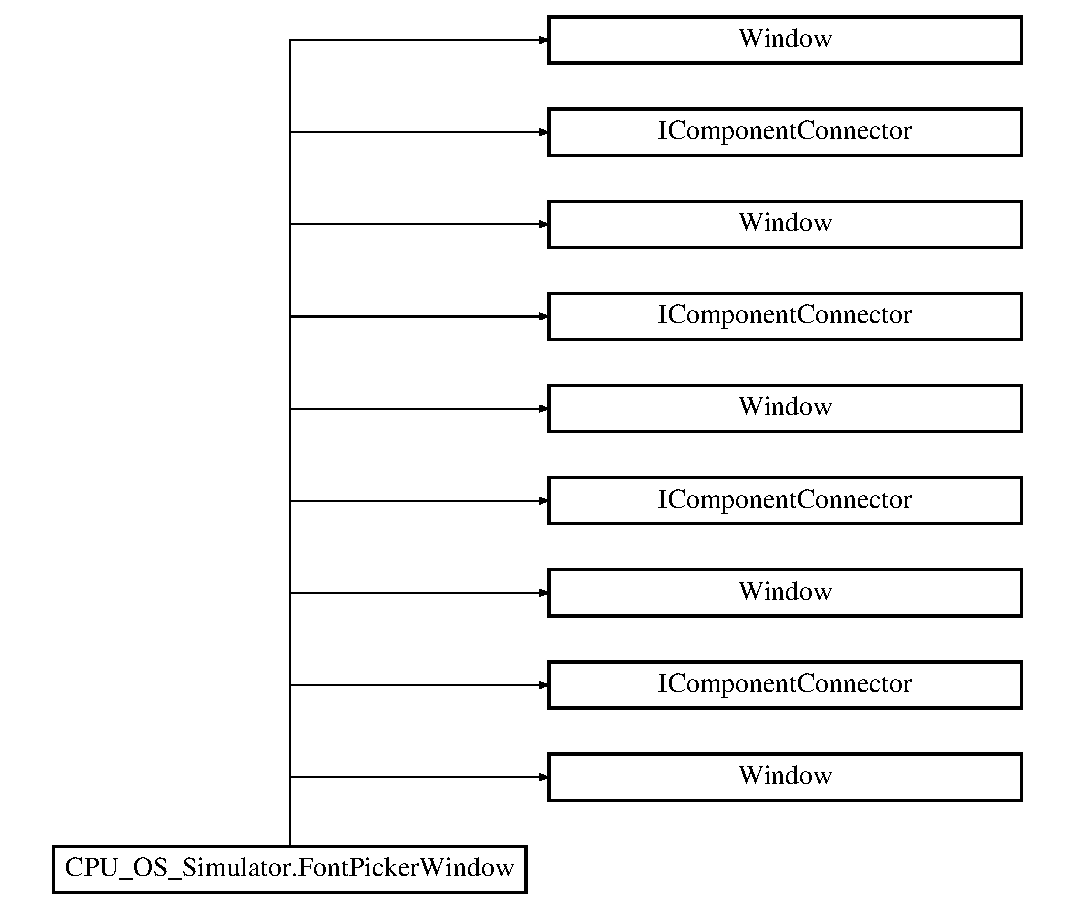
\includegraphics[height=0.941176cm]{class_c_p_u___o_s___simulator_1_1_font_picker_window}
\end{center}
\end{figure}
\subsection*{Public Member Functions}
\begin{DoxyCompactItemize}
\item 
\hyperlink{class_c_p_u___o_s___simulator_1_1_font_picker_window_ac395cdfa521446c47bfded624bbfdba6}{Font\+Picker\+Window} ()
\begin{DoxyCompactList}\small\item\em Default constructor for font picker window \end{DoxyCompactList}\item 
\hyperlink{class_c_p_u___o_s___simulator_1_1_font_picker_window_a8ff9dfbc882890c0b7b76468d51dd386}{Font\+Picker\+Window} (\hyperlink{class_c_p_u___o_s___simulator_1_1_console_window}{Console\+Window} \hyperlink{class_c_p_u___o_s___simulator_1_1_font_picker_window_a4e59cc593e060f3229adc8decfeb151c}{parent})
\begin{DoxyCompactList}\small\item\em Constructor for font picker window that takes the window instance that is creating this window P\+L\+E\+A\+S\+E N\+O\+T\+E\+: This constructor should always be used so data can be passed back to the parent window \end{DoxyCompactList}\item 
void \hyperlink{class_c_p_u___o_s___simulator_1_1_font_picker_window_aca751fede84bf642f74ddf1030cbf034}{Initialize\+Component} ()
\begin{DoxyCompactList}\small\item\em Initialize\+Component \end{DoxyCompactList}\item 
void \hyperlink{class_c_p_u___o_s___simulator_1_1_font_picker_window_aca751fede84bf642f74ddf1030cbf034}{Initialize\+Component} ()
\begin{DoxyCompactList}\small\item\em Initialize\+Component \end{DoxyCompactList}\end{DoxyCompactItemize}
\subsection*{Package Attributes}
\begin{DoxyCompactItemize}
\item 
\hyperlink{class_c_p_u___o_s___simulator_1_1_font_picker_window}{C\+P\+U\+\_\+\+O\+S\+\_\+\+Simulator.\+Font\+Picker\+Window} \hyperlink{class_c_p_u___o_s___simulator_1_1_font_picker_window_afb8444d85c5401e08689ca4ad477703a}{Font\+Picker\+Window1}
\item 
System.\+Windows.\+Controls.\+Grid \hyperlink{class_c_p_u___o_s___simulator_1_1_font_picker_window_a549891835e07203b79f3e81fb225c596}{Root\+\_\+\+Grid}
\item 
System.\+Windows.\+Controls.\+Label \hyperlink{class_c_p_u___o_s___simulator_1_1_font_picker_window_ada73b11773a6ec5fbddb19ee96bb131b}{label}
\item 
System.\+Windows.\+Controls.\+Label \hyperlink{class_c_p_u___o_s___simulator_1_1_font_picker_window_a25630ec7b1b5e76da6c7296d267067c9}{label\+\_\+\+Copy}
\item 
System.\+Windows.\+Controls.\+Label \hyperlink{class_c_p_u___o_s___simulator_1_1_font_picker_window_a8e7e6065c838bf76e919401eff15a2be}{label\+\_\+\+Copy1}
\item 
System.\+Windows.\+Controls.\+Button \hyperlink{class_c_p_u___o_s___simulator_1_1_font_picker_window_a7fda867379bdd5f59a54822628d80aca}{btn\+\_\+\+O\+K}
\item 
System.\+Windows.\+Controls.\+Button \hyperlink{class_c_p_u___o_s___simulator_1_1_font_picker_window_ad6c32f2add6a3395a8e798bdcdfbaa2c}{btn\+\_\+\+Cancel}
\item 
System.\+Windows.\+Controls.\+List\+Box \hyperlink{class_c_p_u___o_s___simulator_1_1_font_picker_window_a5ab20fca6d1149f954e66643491e3f0e}{lstbx\+\_\+\+Font}
\item 
System.\+Windows.\+Controls.\+List\+Box \hyperlink{class_c_p_u___o_s___simulator_1_1_font_picker_window_a8d7855c50915b0975ee314de961c00d5}{lstbx\+\_\+\+Size}
\item 
System.\+Windows.\+Controls.\+List\+Box \hyperlink{class_c_p_u___o_s___simulator_1_1_font_picker_window_adf923069128ca0ca766c810601319286}{lstbx\+\_\+\+Style}
\end{DoxyCompactItemize}
\subsection*{Private Member Functions}
\begin{DoxyCompactItemize}
\item 
void \hyperlink{class_c_p_u___o_s___simulator_1_1_font_picker_window_a0907f73fb52351e43b76af4137509f41}{Font\+Picker\+Window1\+\_\+\+Loaded} (object sender, Routed\+Event\+Args e)
\item 
void \hyperlink{class_c_p_u___o_s___simulator_1_1_font_picker_window_a79525d7a77c191f63187e5a8181bd197}{Populate\+Styles} ()
\begin{DoxyCompactList}\small\item\em This function populates the list of font styles \end{DoxyCompactList}\item 
void \hyperlink{class_c_p_u___o_s___simulator_1_1_font_picker_window_a4042c1d9dedbbd9abb956fc7b97c1564}{Populate\+Fonts} ()
\begin{DoxyCompactList}\small\item\em This function populates the list of fonts \end{DoxyCompactList}\item 
void \hyperlink{class_c_p_u___o_s___simulator_1_1_font_picker_window_a6d659d671c24e1beed969f2d36d669d8}{btn\+\_\+\+O\+K\+\_\+\+Click} (object sender, Routed\+Event\+Args e)
\item 
void \hyperlink{class_c_p_u___o_s___simulator_1_1_font_picker_window_a6e5279d2116523168362cb740eac5e55}{btn\+\_\+\+Cancel\+\_\+\+Click} (object sender, Routed\+Event\+Args e)
\item 
void System.\+Windows.\+Markup.\+I\+Component\+Connector. \hyperlink{class_c_p_u___o_s___simulator_1_1_font_picker_window_ac5f7c5cad6bf2d8dc79c7e59f5a125da}{Connect} (int connection\+Id, object target)
\item 
void System.\+Windows.\+Markup.\+I\+Component\+Connector. \hyperlink{class_c_p_u___o_s___simulator_1_1_font_picker_window_ac5f7c5cad6bf2d8dc79c7e59f5a125da}{Connect} (int connection\+Id, object target)
\end{DoxyCompactItemize}
\subsection*{Private Attributes}
\begin{DoxyCompactItemize}
\item 
\hyperlink{class_c_p_u___o_s___simulator_1_1_console_window}{Console\+Window} \hyperlink{class_c_p_u___o_s___simulator_1_1_font_picker_window_a4e59cc593e060f3229adc8decfeb151c}{parent}
\item 
bool \hyperlink{class_c_p_u___o_s___simulator_1_1_font_picker_window_aa37d57c41c80a6fa875193d68754f658}{\+\_\+content\+Loaded}
\end{DoxyCompactItemize}


\subsection{Detailed Description}
Interaction logic for Font\+Picker\+Window.\+xaml 

\hyperlink{class_c_p_u___o_s___simulator_1_1_font_picker_window}{Font\+Picker\+Window} 

Definition at line 12 of file Font\+Picker\+Window.\+xaml.\+cs.



\subsection{Constructor \& Destructor Documentation}
\hypertarget{class_c_p_u___o_s___simulator_1_1_font_picker_window_ac395cdfa521446c47bfded624bbfdba6}{}\index{C\+P\+U\+\_\+\+O\+S\+\_\+\+Simulator\+::\+Font\+Picker\+Window@{C\+P\+U\+\_\+\+O\+S\+\_\+\+Simulator\+::\+Font\+Picker\+Window}!Font\+Picker\+Window@{Font\+Picker\+Window}}
\index{Font\+Picker\+Window@{Font\+Picker\+Window}!C\+P\+U\+\_\+\+O\+S\+\_\+\+Simulator\+::\+Font\+Picker\+Window@{C\+P\+U\+\_\+\+O\+S\+\_\+\+Simulator\+::\+Font\+Picker\+Window}}
\subsubsection[{Font\+Picker\+Window()}]{\setlength{\rightskip}{0pt plus 5cm}C\+P\+U\+\_\+\+O\+S\+\_\+\+Simulator.\+Font\+Picker\+Window.\+Font\+Picker\+Window (
\begin{DoxyParamCaption}
{}
\end{DoxyParamCaption}
)}\label{class_c_p_u___o_s___simulator_1_1_font_picker_window_ac395cdfa521446c47bfded624bbfdba6}


Default constructor for font picker window 



Definition at line 18 of file Font\+Picker\+Window.\+xaml.\+cs.

\hypertarget{class_c_p_u___o_s___simulator_1_1_font_picker_window_a8ff9dfbc882890c0b7b76468d51dd386}{}\index{C\+P\+U\+\_\+\+O\+S\+\_\+\+Simulator\+::\+Font\+Picker\+Window@{C\+P\+U\+\_\+\+O\+S\+\_\+\+Simulator\+::\+Font\+Picker\+Window}!Font\+Picker\+Window@{Font\+Picker\+Window}}
\index{Font\+Picker\+Window@{Font\+Picker\+Window}!C\+P\+U\+\_\+\+O\+S\+\_\+\+Simulator\+::\+Font\+Picker\+Window@{C\+P\+U\+\_\+\+O\+S\+\_\+\+Simulator\+::\+Font\+Picker\+Window}}
\subsubsection[{Font\+Picker\+Window(\+Console\+Window parent)}]{\setlength{\rightskip}{0pt plus 5cm}C\+P\+U\+\_\+\+O\+S\+\_\+\+Simulator.\+Font\+Picker\+Window.\+Font\+Picker\+Window (
\begin{DoxyParamCaption}
\item[{{\bf Console\+Window}}]{parent}
\end{DoxyParamCaption}
)}\label{class_c_p_u___o_s___simulator_1_1_font_picker_window_a8ff9dfbc882890c0b7b76468d51dd386}


Constructor for font picker window that takes the window instance that is creating this window P\+L\+E\+A\+S\+E N\+O\+T\+E\+: This constructor should always be used so data can be passed back to the parent window 


\begin{DoxyParams}{Parameters}
{\em parent} & The window that is creating this window \\
\hline
\end{DoxyParams}


Definition at line 27 of file Font\+Picker\+Window.\+xaml.\+cs.



\subsection{Member Function Documentation}
\hypertarget{class_c_p_u___o_s___simulator_1_1_font_picker_window_a6e5279d2116523168362cb740eac5e55}{}\index{C\+P\+U\+\_\+\+O\+S\+\_\+\+Simulator\+::\+Font\+Picker\+Window@{C\+P\+U\+\_\+\+O\+S\+\_\+\+Simulator\+::\+Font\+Picker\+Window}!btn\+\_\+\+Cancel\+\_\+\+Click@{btn\+\_\+\+Cancel\+\_\+\+Click}}
\index{btn\+\_\+\+Cancel\+\_\+\+Click@{btn\+\_\+\+Cancel\+\_\+\+Click}!C\+P\+U\+\_\+\+O\+S\+\_\+\+Simulator\+::\+Font\+Picker\+Window@{C\+P\+U\+\_\+\+O\+S\+\_\+\+Simulator\+::\+Font\+Picker\+Window}}
\subsubsection[{btn\+\_\+\+Cancel\+\_\+\+Click(object sender, Routed\+Event\+Args e)}]{\setlength{\rightskip}{0pt plus 5cm}void C\+P\+U\+\_\+\+O\+S\+\_\+\+Simulator.\+Font\+Picker\+Window.\+btn\+\_\+\+Cancel\+\_\+\+Click (
\begin{DoxyParamCaption}
\item[{object}]{sender, }
\item[{Routed\+Event\+Args}]{e}
\end{DoxyParamCaption}
)\hspace{0.3cm}{\ttfamily [private]}}\label{class_c_p_u___o_s___simulator_1_1_font_picker_window_a6e5279d2116523168362cb740eac5e55}


Definition at line 101 of file Font\+Picker\+Window.\+xaml.\+cs.

\hypertarget{class_c_p_u___o_s___simulator_1_1_font_picker_window_a6d659d671c24e1beed969f2d36d669d8}{}\index{C\+P\+U\+\_\+\+O\+S\+\_\+\+Simulator\+::\+Font\+Picker\+Window@{C\+P\+U\+\_\+\+O\+S\+\_\+\+Simulator\+::\+Font\+Picker\+Window}!btn\+\_\+\+O\+K\+\_\+\+Click@{btn\+\_\+\+O\+K\+\_\+\+Click}}
\index{btn\+\_\+\+O\+K\+\_\+\+Click@{btn\+\_\+\+O\+K\+\_\+\+Click}!C\+P\+U\+\_\+\+O\+S\+\_\+\+Simulator\+::\+Font\+Picker\+Window@{C\+P\+U\+\_\+\+O\+S\+\_\+\+Simulator\+::\+Font\+Picker\+Window}}
\subsubsection[{btn\+\_\+\+O\+K\+\_\+\+Click(object sender, Routed\+Event\+Args e)}]{\setlength{\rightskip}{0pt plus 5cm}void C\+P\+U\+\_\+\+O\+S\+\_\+\+Simulator.\+Font\+Picker\+Window.\+btn\+\_\+\+O\+K\+\_\+\+Click (
\begin{DoxyParamCaption}
\item[{object}]{sender, }
\item[{Routed\+Event\+Args}]{e}
\end{DoxyParamCaption}
)\hspace{0.3cm}{\ttfamily [private]}}\label{class_c_p_u___o_s___simulator_1_1_font_picker_window_a6d659d671c24e1beed969f2d36d669d8}


Definition at line 67 of file Font\+Picker\+Window.\+xaml.\+cs.

\hypertarget{class_c_p_u___o_s___simulator_1_1_font_picker_window_ac5f7c5cad6bf2d8dc79c7e59f5a125da}{}\index{C\+P\+U\+\_\+\+O\+S\+\_\+\+Simulator\+::\+Font\+Picker\+Window@{C\+P\+U\+\_\+\+O\+S\+\_\+\+Simulator\+::\+Font\+Picker\+Window}!Connect@{Connect}}
\index{Connect@{Connect}!C\+P\+U\+\_\+\+O\+S\+\_\+\+Simulator\+::\+Font\+Picker\+Window@{C\+P\+U\+\_\+\+O\+S\+\_\+\+Simulator\+::\+Font\+Picker\+Window}}
\subsubsection[{Connect(int connection\+Id, object target)}]{\setlength{\rightskip}{0pt plus 5cm}void System.\+Windows.\+Markup.\+I\+Component\+Connector. C\+P\+U\+\_\+\+O\+S\+\_\+\+Simulator.\+Font\+Picker\+Window.\+Connect (
\begin{DoxyParamCaption}
\item[{int}]{connection\+Id, }
\item[{object}]{target}
\end{DoxyParamCaption}
)\hspace{0.3cm}{\ttfamily [private]}}\label{class_c_p_u___o_s___simulator_1_1_font_picker_window_ac5f7c5cad6bf2d8dc79c7e59f5a125da}


Definition at line 150 of file Font\+Picker\+Window.\+g.\+i.\+cs.

\hypertarget{class_c_p_u___o_s___simulator_1_1_font_picker_window_ac5f7c5cad6bf2d8dc79c7e59f5a125da}{}\index{C\+P\+U\+\_\+\+O\+S\+\_\+\+Simulator\+::\+Font\+Picker\+Window@{C\+P\+U\+\_\+\+O\+S\+\_\+\+Simulator\+::\+Font\+Picker\+Window}!Connect@{Connect}}
\index{Connect@{Connect}!C\+P\+U\+\_\+\+O\+S\+\_\+\+Simulator\+::\+Font\+Picker\+Window@{C\+P\+U\+\_\+\+O\+S\+\_\+\+Simulator\+::\+Font\+Picker\+Window}}
\subsubsection[{Connect(int connection\+Id, object target)}]{\setlength{\rightskip}{0pt plus 5cm}void System.\+Windows.\+Markup.\+I\+Component\+Connector. C\+P\+U\+\_\+\+O\+S\+\_\+\+Simulator.\+Font\+Picker\+Window.\+Connect (
\begin{DoxyParamCaption}
\item[{int}]{connection\+Id, }
\item[{object}]{target}
\end{DoxyParamCaption}
)\hspace{0.3cm}{\ttfamily [private]}}\label{class_c_p_u___o_s___simulator_1_1_font_picker_window_ac5f7c5cad6bf2d8dc79c7e59f5a125da}


Definition at line 150 of file Font\+Picker\+Window.\+g.\+cs.

\hypertarget{class_c_p_u___o_s___simulator_1_1_font_picker_window_a0907f73fb52351e43b76af4137509f41}{}\index{C\+P\+U\+\_\+\+O\+S\+\_\+\+Simulator\+::\+Font\+Picker\+Window@{C\+P\+U\+\_\+\+O\+S\+\_\+\+Simulator\+::\+Font\+Picker\+Window}!Font\+Picker\+Window1\+\_\+\+Loaded@{Font\+Picker\+Window1\+\_\+\+Loaded}}
\index{Font\+Picker\+Window1\+\_\+\+Loaded@{Font\+Picker\+Window1\+\_\+\+Loaded}!C\+P\+U\+\_\+\+O\+S\+\_\+\+Simulator\+::\+Font\+Picker\+Window@{C\+P\+U\+\_\+\+O\+S\+\_\+\+Simulator\+::\+Font\+Picker\+Window}}
\subsubsection[{Font\+Picker\+Window1\+\_\+\+Loaded(object sender, Routed\+Event\+Args e)}]{\setlength{\rightskip}{0pt plus 5cm}void C\+P\+U\+\_\+\+O\+S\+\_\+\+Simulator.\+Font\+Picker\+Window.\+Font\+Picker\+Window1\+\_\+\+Loaded (
\begin{DoxyParamCaption}
\item[{object}]{sender, }
\item[{Routed\+Event\+Args}]{e}
\end{DoxyParamCaption}
)\hspace{0.3cm}{\ttfamily [private]}}\label{class_c_p_u___o_s___simulator_1_1_font_picker_window_a0907f73fb52351e43b76af4137509f41}


Definition at line 33 of file Font\+Picker\+Window.\+xaml.\+cs.

\hypertarget{class_c_p_u___o_s___simulator_1_1_font_picker_window_aca751fede84bf642f74ddf1030cbf034}{}\index{C\+P\+U\+\_\+\+O\+S\+\_\+\+Simulator\+::\+Font\+Picker\+Window@{C\+P\+U\+\_\+\+O\+S\+\_\+\+Simulator\+::\+Font\+Picker\+Window}!Initialize\+Component@{Initialize\+Component}}
\index{Initialize\+Component@{Initialize\+Component}!C\+P\+U\+\_\+\+O\+S\+\_\+\+Simulator\+::\+Font\+Picker\+Window@{C\+P\+U\+\_\+\+O\+S\+\_\+\+Simulator\+::\+Font\+Picker\+Window}}
\subsubsection[{Initialize\+Component()}]{\setlength{\rightskip}{0pt plus 5cm}void C\+P\+U\+\_\+\+O\+S\+\_\+\+Simulator.\+Font\+Picker\+Window.\+Initialize\+Component (
\begin{DoxyParamCaption}
{}
\end{DoxyParamCaption}
)}\label{class_c_p_u___o_s___simulator_1_1_font_picker_window_aca751fede84bf642f74ddf1030cbf034}


Initialize\+Component 



Definition at line 130 of file Font\+Picker\+Window.\+g.\+i.\+cs.

\hypertarget{class_c_p_u___o_s___simulator_1_1_font_picker_window_aca751fede84bf642f74ddf1030cbf034}{}\index{C\+P\+U\+\_\+\+O\+S\+\_\+\+Simulator\+::\+Font\+Picker\+Window@{C\+P\+U\+\_\+\+O\+S\+\_\+\+Simulator\+::\+Font\+Picker\+Window}!Initialize\+Component@{Initialize\+Component}}
\index{Initialize\+Component@{Initialize\+Component}!C\+P\+U\+\_\+\+O\+S\+\_\+\+Simulator\+::\+Font\+Picker\+Window@{C\+P\+U\+\_\+\+O\+S\+\_\+\+Simulator\+::\+Font\+Picker\+Window}}
\subsubsection[{Initialize\+Component()}]{\setlength{\rightskip}{0pt plus 5cm}void C\+P\+U\+\_\+\+O\+S\+\_\+\+Simulator.\+Font\+Picker\+Window.\+Initialize\+Component (
\begin{DoxyParamCaption}
{}
\end{DoxyParamCaption}
)}\label{class_c_p_u___o_s___simulator_1_1_font_picker_window_aca751fede84bf642f74ddf1030cbf034}


Initialize\+Component 



Definition at line 130 of file Font\+Picker\+Window.\+g.\+cs.

\hypertarget{class_c_p_u___o_s___simulator_1_1_font_picker_window_a4042c1d9dedbbd9abb956fc7b97c1564}{}\index{C\+P\+U\+\_\+\+O\+S\+\_\+\+Simulator\+::\+Font\+Picker\+Window@{C\+P\+U\+\_\+\+O\+S\+\_\+\+Simulator\+::\+Font\+Picker\+Window}!Populate\+Fonts@{Populate\+Fonts}}
\index{Populate\+Fonts@{Populate\+Fonts}!C\+P\+U\+\_\+\+O\+S\+\_\+\+Simulator\+::\+Font\+Picker\+Window@{C\+P\+U\+\_\+\+O\+S\+\_\+\+Simulator\+::\+Font\+Picker\+Window}}
\subsubsection[{Populate\+Fonts()}]{\setlength{\rightskip}{0pt plus 5cm}void C\+P\+U\+\_\+\+O\+S\+\_\+\+Simulator.\+Font\+Picker\+Window.\+Populate\+Fonts (
\begin{DoxyParamCaption}
{}
\end{DoxyParamCaption}
)\hspace{0.3cm}{\ttfamily [private]}}\label{class_c_p_u___o_s___simulator_1_1_font_picker_window_a4042c1d9dedbbd9abb956fc7b97c1564}


This function populates the list of fonts 



Definition at line 56 of file Font\+Picker\+Window.\+xaml.\+cs.

\hypertarget{class_c_p_u___o_s___simulator_1_1_font_picker_window_a79525d7a77c191f63187e5a8181bd197}{}\index{C\+P\+U\+\_\+\+O\+S\+\_\+\+Simulator\+::\+Font\+Picker\+Window@{C\+P\+U\+\_\+\+O\+S\+\_\+\+Simulator\+::\+Font\+Picker\+Window}!Populate\+Styles@{Populate\+Styles}}
\index{Populate\+Styles@{Populate\+Styles}!C\+P\+U\+\_\+\+O\+S\+\_\+\+Simulator\+::\+Font\+Picker\+Window@{C\+P\+U\+\_\+\+O\+S\+\_\+\+Simulator\+::\+Font\+Picker\+Window}}
\subsubsection[{Populate\+Styles()}]{\setlength{\rightskip}{0pt plus 5cm}void C\+P\+U\+\_\+\+O\+S\+\_\+\+Simulator.\+Font\+Picker\+Window.\+Populate\+Styles (
\begin{DoxyParamCaption}
{}
\end{DoxyParamCaption}
)\hspace{0.3cm}{\ttfamily [private]}}\label{class_c_p_u___o_s___simulator_1_1_font_picker_window_a79525d7a77c191f63187e5a8181bd197}


This function populates the list of font styles 



Definition at line 43 of file Font\+Picker\+Window.\+xaml.\+cs.



\subsection{Member Data Documentation}
\hypertarget{class_c_p_u___o_s___simulator_1_1_font_picker_window_aa37d57c41c80a6fa875193d68754f658}{}\index{C\+P\+U\+\_\+\+O\+S\+\_\+\+Simulator\+::\+Font\+Picker\+Window@{C\+P\+U\+\_\+\+O\+S\+\_\+\+Simulator\+::\+Font\+Picker\+Window}!\+\_\+content\+Loaded@{\+\_\+content\+Loaded}}
\index{\+\_\+content\+Loaded@{\+\_\+content\+Loaded}!C\+P\+U\+\_\+\+O\+S\+\_\+\+Simulator\+::\+Font\+Picker\+Window@{C\+P\+U\+\_\+\+O\+S\+\_\+\+Simulator\+::\+Font\+Picker\+Window}}
\subsubsection[{\+\_\+content\+Loaded}]{\setlength{\rightskip}{0pt plus 5cm}bool C\+P\+U\+\_\+\+O\+S\+\_\+\+Simulator.\+Font\+Picker\+Window.\+\_\+content\+Loaded\hspace{0.3cm}{\ttfamily [private]}}\label{class_c_p_u___o_s___simulator_1_1_font_picker_window_aa37d57c41c80a6fa875193d68754f658}


Definition at line 123 of file Font\+Picker\+Window.\+g.\+cs.

\hypertarget{class_c_p_u___o_s___simulator_1_1_font_picker_window_ad6c32f2add6a3395a8e798bdcdfbaa2c}{}\index{C\+P\+U\+\_\+\+O\+S\+\_\+\+Simulator\+::\+Font\+Picker\+Window@{C\+P\+U\+\_\+\+O\+S\+\_\+\+Simulator\+::\+Font\+Picker\+Window}!btn\+\_\+\+Cancel@{btn\+\_\+\+Cancel}}
\index{btn\+\_\+\+Cancel@{btn\+\_\+\+Cancel}!C\+P\+U\+\_\+\+O\+S\+\_\+\+Simulator\+::\+Font\+Picker\+Window@{C\+P\+U\+\_\+\+O\+S\+\_\+\+Simulator\+::\+Font\+Picker\+Window}}
\subsubsection[{btn\+\_\+\+Cancel}]{\setlength{\rightskip}{0pt plus 5cm}System Windows Controls Button C\+P\+U\+\_\+\+O\+S\+\_\+\+Simulator.\+Font\+Picker\+Window.\+btn\+\_\+\+Cancel\hspace{0.3cm}{\ttfamily [package]}}\label{class_c_p_u___o_s___simulator_1_1_font_picker_window_ad6c32f2add6a3395a8e798bdcdfbaa2c}


Definition at line 94 of file Font\+Picker\+Window.\+g.\+cs.

\hypertarget{class_c_p_u___o_s___simulator_1_1_font_picker_window_a7fda867379bdd5f59a54822628d80aca}{}\index{C\+P\+U\+\_\+\+O\+S\+\_\+\+Simulator\+::\+Font\+Picker\+Window@{C\+P\+U\+\_\+\+O\+S\+\_\+\+Simulator\+::\+Font\+Picker\+Window}!btn\+\_\+\+O\+K@{btn\+\_\+\+O\+K}}
\index{btn\+\_\+\+O\+K@{btn\+\_\+\+O\+K}!C\+P\+U\+\_\+\+O\+S\+\_\+\+Simulator\+::\+Font\+Picker\+Window@{C\+P\+U\+\_\+\+O\+S\+\_\+\+Simulator\+::\+Font\+Picker\+Window}}
\subsubsection[{btn\+\_\+\+O\+K}]{\setlength{\rightskip}{0pt plus 5cm}System Windows Controls Button C\+P\+U\+\_\+\+O\+S\+\_\+\+Simulator.\+Font\+Picker\+Window.\+btn\+\_\+\+O\+K\hspace{0.3cm}{\ttfamily [package]}}\label{class_c_p_u___o_s___simulator_1_1_font_picker_window_a7fda867379bdd5f59a54822628d80aca}


Definition at line 86 of file Font\+Picker\+Window.\+g.\+cs.

\hypertarget{class_c_p_u___o_s___simulator_1_1_font_picker_window_afb8444d85c5401e08689ca4ad477703a}{}\index{C\+P\+U\+\_\+\+O\+S\+\_\+\+Simulator\+::\+Font\+Picker\+Window@{C\+P\+U\+\_\+\+O\+S\+\_\+\+Simulator\+::\+Font\+Picker\+Window}!Font\+Picker\+Window1@{Font\+Picker\+Window1}}
\index{Font\+Picker\+Window1@{Font\+Picker\+Window1}!C\+P\+U\+\_\+\+O\+S\+\_\+\+Simulator\+::\+Font\+Picker\+Window@{C\+P\+U\+\_\+\+O\+S\+\_\+\+Simulator\+::\+Font\+Picker\+Window}}
\subsubsection[{Font\+Picker\+Window1}]{\setlength{\rightskip}{0pt plus 5cm}C\+P\+U\+\_\+\+O\+S\+\_\+\+Simulator {\bf Font\+Picker\+Window} C\+P\+U\+\_\+\+O\+S\+\_\+\+Simulator.\+Font\+Picker\+Window.\+Font\+Picker\+Window1\hspace{0.3cm}{\ttfamily [package]}}\label{class_c_p_u___o_s___simulator_1_1_font_picker_window_afb8444d85c5401e08689ca4ad477703a}


Definition at line 46 of file Font\+Picker\+Window.\+g.\+cs.

\hypertarget{class_c_p_u___o_s___simulator_1_1_font_picker_window_ada73b11773a6ec5fbddb19ee96bb131b}{}\index{C\+P\+U\+\_\+\+O\+S\+\_\+\+Simulator\+::\+Font\+Picker\+Window@{C\+P\+U\+\_\+\+O\+S\+\_\+\+Simulator\+::\+Font\+Picker\+Window}!label@{label}}
\index{label@{label}!C\+P\+U\+\_\+\+O\+S\+\_\+\+Simulator\+::\+Font\+Picker\+Window@{C\+P\+U\+\_\+\+O\+S\+\_\+\+Simulator\+::\+Font\+Picker\+Window}}
\subsubsection[{label}]{\setlength{\rightskip}{0pt plus 5cm}System Windows Controls Label C\+P\+U\+\_\+\+O\+S\+\_\+\+Simulator.\+Font\+Picker\+Window.\+label\hspace{0.3cm}{\ttfamily [package]}}\label{class_c_p_u___o_s___simulator_1_1_font_picker_window_ada73b11773a6ec5fbddb19ee96bb131b}


Definition at line 62 of file Font\+Picker\+Window.\+g.\+cs.

\hypertarget{class_c_p_u___o_s___simulator_1_1_font_picker_window_a25630ec7b1b5e76da6c7296d267067c9}{}\index{C\+P\+U\+\_\+\+O\+S\+\_\+\+Simulator\+::\+Font\+Picker\+Window@{C\+P\+U\+\_\+\+O\+S\+\_\+\+Simulator\+::\+Font\+Picker\+Window}!label\+\_\+\+Copy@{label\+\_\+\+Copy}}
\index{label\+\_\+\+Copy@{label\+\_\+\+Copy}!C\+P\+U\+\_\+\+O\+S\+\_\+\+Simulator\+::\+Font\+Picker\+Window@{C\+P\+U\+\_\+\+O\+S\+\_\+\+Simulator\+::\+Font\+Picker\+Window}}
\subsubsection[{label\+\_\+\+Copy}]{\setlength{\rightskip}{0pt plus 5cm}System Windows Controls Label C\+P\+U\+\_\+\+O\+S\+\_\+\+Simulator.\+Font\+Picker\+Window.\+label\+\_\+\+Copy\hspace{0.3cm}{\ttfamily [package]}}\label{class_c_p_u___o_s___simulator_1_1_font_picker_window_a25630ec7b1b5e76da6c7296d267067c9}


Definition at line 70 of file Font\+Picker\+Window.\+g.\+cs.

\hypertarget{class_c_p_u___o_s___simulator_1_1_font_picker_window_a8e7e6065c838bf76e919401eff15a2be}{}\index{C\+P\+U\+\_\+\+O\+S\+\_\+\+Simulator\+::\+Font\+Picker\+Window@{C\+P\+U\+\_\+\+O\+S\+\_\+\+Simulator\+::\+Font\+Picker\+Window}!label\+\_\+\+Copy1@{label\+\_\+\+Copy1}}
\index{label\+\_\+\+Copy1@{label\+\_\+\+Copy1}!C\+P\+U\+\_\+\+O\+S\+\_\+\+Simulator\+::\+Font\+Picker\+Window@{C\+P\+U\+\_\+\+O\+S\+\_\+\+Simulator\+::\+Font\+Picker\+Window}}
\subsubsection[{label\+\_\+\+Copy1}]{\setlength{\rightskip}{0pt plus 5cm}System Windows Controls Label C\+P\+U\+\_\+\+O\+S\+\_\+\+Simulator.\+Font\+Picker\+Window.\+label\+\_\+\+Copy1\hspace{0.3cm}{\ttfamily [package]}}\label{class_c_p_u___o_s___simulator_1_1_font_picker_window_a8e7e6065c838bf76e919401eff15a2be}


Definition at line 78 of file Font\+Picker\+Window.\+g.\+cs.

\hypertarget{class_c_p_u___o_s___simulator_1_1_font_picker_window_a5ab20fca6d1149f954e66643491e3f0e}{}\index{C\+P\+U\+\_\+\+O\+S\+\_\+\+Simulator\+::\+Font\+Picker\+Window@{C\+P\+U\+\_\+\+O\+S\+\_\+\+Simulator\+::\+Font\+Picker\+Window}!lstbx\+\_\+\+Font@{lstbx\+\_\+\+Font}}
\index{lstbx\+\_\+\+Font@{lstbx\+\_\+\+Font}!C\+P\+U\+\_\+\+O\+S\+\_\+\+Simulator\+::\+Font\+Picker\+Window@{C\+P\+U\+\_\+\+O\+S\+\_\+\+Simulator\+::\+Font\+Picker\+Window}}
\subsubsection[{lstbx\+\_\+\+Font}]{\setlength{\rightskip}{0pt plus 5cm}System Windows Controls List\+Box C\+P\+U\+\_\+\+O\+S\+\_\+\+Simulator.\+Font\+Picker\+Window.\+lstbx\+\_\+\+Font\hspace{0.3cm}{\ttfamily [package]}}\label{class_c_p_u___o_s___simulator_1_1_font_picker_window_a5ab20fca6d1149f954e66643491e3f0e}


Definition at line 102 of file Font\+Picker\+Window.\+g.\+cs.

\hypertarget{class_c_p_u___o_s___simulator_1_1_font_picker_window_a8d7855c50915b0975ee314de961c00d5}{}\index{C\+P\+U\+\_\+\+O\+S\+\_\+\+Simulator\+::\+Font\+Picker\+Window@{C\+P\+U\+\_\+\+O\+S\+\_\+\+Simulator\+::\+Font\+Picker\+Window}!lstbx\+\_\+\+Size@{lstbx\+\_\+\+Size}}
\index{lstbx\+\_\+\+Size@{lstbx\+\_\+\+Size}!C\+P\+U\+\_\+\+O\+S\+\_\+\+Simulator\+::\+Font\+Picker\+Window@{C\+P\+U\+\_\+\+O\+S\+\_\+\+Simulator\+::\+Font\+Picker\+Window}}
\subsubsection[{lstbx\+\_\+\+Size}]{\setlength{\rightskip}{0pt plus 5cm}System Windows Controls List\+Box C\+P\+U\+\_\+\+O\+S\+\_\+\+Simulator.\+Font\+Picker\+Window.\+lstbx\+\_\+\+Size\hspace{0.3cm}{\ttfamily [package]}}\label{class_c_p_u___o_s___simulator_1_1_font_picker_window_a8d7855c50915b0975ee314de961c00d5}


Definition at line 110 of file Font\+Picker\+Window.\+g.\+cs.

\hypertarget{class_c_p_u___o_s___simulator_1_1_font_picker_window_adf923069128ca0ca766c810601319286}{}\index{C\+P\+U\+\_\+\+O\+S\+\_\+\+Simulator\+::\+Font\+Picker\+Window@{C\+P\+U\+\_\+\+O\+S\+\_\+\+Simulator\+::\+Font\+Picker\+Window}!lstbx\+\_\+\+Style@{lstbx\+\_\+\+Style}}
\index{lstbx\+\_\+\+Style@{lstbx\+\_\+\+Style}!C\+P\+U\+\_\+\+O\+S\+\_\+\+Simulator\+::\+Font\+Picker\+Window@{C\+P\+U\+\_\+\+O\+S\+\_\+\+Simulator\+::\+Font\+Picker\+Window}}
\subsubsection[{lstbx\+\_\+\+Style}]{\setlength{\rightskip}{0pt plus 5cm}System Windows Controls List\+Box C\+P\+U\+\_\+\+O\+S\+\_\+\+Simulator.\+Font\+Picker\+Window.\+lstbx\+\_\+\+Style\hspace{0.3cm}{\ttfamily [package]}}\label{class_c_p_u___o_s___simulator_1_1_font_picker_window_adf923069128ca0ca766c810601319286}


Definition at line 118 of file Font\+Picker\+Window.\+g.\+cs.

\hypertarget{class_c_p_u___o_s___simulator_1_1_font_picker_window_a4e59cc593e060f3229adc8decfeb151c}{}\index{C\+P\+U\+\_\+\+O\+S\+\_\+\+Simulator\+::\+Font\+Picker\+Window@{C\+P\+U\+\_\+\+O\+S\+\_\+\+Simulator\+::\+Font\+Picker\+Window}!parent@{parent}}
\index{parent@{parent}!C\+P\+U\+\_\+\+O\+S\+\_\+\+Simulator\+::\+Font\+Picker\+Window@{C\+P\+U\+\_\+\+O\+S\+\_\+\+Simulator\+::\+Font\+Picker\+Window}}
\subsubsection[{parent}]{\setlength{\rightskip}{0pt plus 5cm}{\bf Console\+Window} C\+P\+U\+\_\+\+O\+S\+\_\+\+Simulator.\+Font\+Picker\+Window.\+parent\hspace{0.3cm}{\ttfamily [private]}}\label{class_c_p_u___o_s___simulator_1_1_font_picker_window_a4e59cc593e060f3229adc8decfeb151c}


Definition at line 14 of file Font\+Picker\+Window.\+xaml.\+cs.

\hypertarget{class_c_p_u___o_s___simulator_1_1_font_picker_window_a549891835e07203b79f3e81fb225c596}{}\index{C\+P\+U\+\_\+\+O\+S\+\_\+\+Simulator\+::\+Font\+Picker\+Window@{C\+P\+U\+\_\+\+O\+S\+\_\+\+Simulator\+::\+Font\+Picker\+Window}!Root\+\_\+\+Grid@{Root\+\_\+\+Grid}}
\index{Root\+\_\+\+Grid@{Root\+\_\+\+Grid}!C\+P\+U\+\_\+\+O\+S\+\_\+\+Simulator\+::\+Font\+Picker\+Window@{C\+P\+U\+\_\+\+O\+S\+\_\+\+Simulator\+::\+Font\+Picker\+Window}}
\subsubsection[{Root\+\_\+\+Grid}]{\setlength{\rightskip}{0pt plus 5cm}System Windows Controls Grid C\+P\+U\+\_\+\+O\+S\+\_\+\+Simulator.\+Font\+Picker\+Window.\+Root\+\_\+\+Grid\hspace{0.3cm}{\ttfamily [package]}}\label{class_c_p_u___o_s___simulator_1_1_font_picker_window_a549891835e07203b79f3e81fb225c596}


Definition at line 54 of file Font\+Picker\+Window.\+g.\+cs.



The documentation for this class was generated from the following files\+:\begin{DoxyCompactItemize}
\item 
C\+P\+U-\/\+O\+S Simulator/\hyperlink{_font_picker_window_8xaml_8cs}{Font\+Picker\+Window.\+xaml.\+cs}\item 
C\+P\+U-\/\+O\+S Simulator/obj/\+Debug/\hyperlink{_font_picker_window_8g_8cs}{Font\+Picker\+Window.\+g.\+cs}\item 
C\+P\+U-\/\+O\+S Simulator/obj/\+Debug/\hyperlink{_font_picker_window_8g_8i_8cs}{Font\+Picker\+Window.\+g.\+i.\+cs}\end{DoxyCompactItemize}

\hypertarget{class_c_p_u___o_s___simulator_1_1_compiler_1_1_frontend_1_1_symbols_1_1_function}{}\section{C\+P\+U\+\_\+\+O\+S\+\_\+\+Simulator.\+Compiler.\+Frontend.\+Symbols.\+Function Class Reference}
\label{class_c_p_u___o_s___simulator_1_1_compiler_1_1_frontend_1_1_symbols_1_1_function}\index{C\+P\+U\+\_\+\+O\+S\+\_\+\+Simulator.\+Compiler.\+Frontend.\+Symbols.\+Function@{C\+P\+U\+\_\+\+O\+S\+\_\+\+Simulator.\+Compiler.\+Frontend.\+Symbols.\+Function}}
Inheritance diagram for C\+P\+U\+\_\+\+O\+S\+\_\+\+Simulator.\+Compiler.\+Frontend.\+Symbols.\+Function\+:\begin{figure}[H]
\begin{center}
\leavevmode
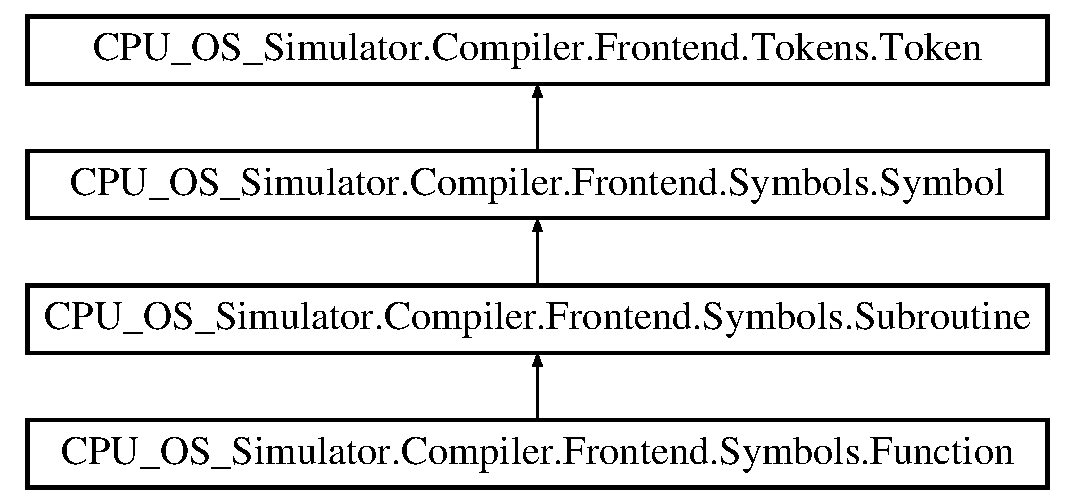
\includegraphics[height=4.000000cm]{class_c_p_u___o_s___simulator_1_1_compiler_1_1_frontend_1_1_symbols_1_1_function}
\end{center}
\end{figure}
\subsection*{Public Member Functions}
\begin{DoxyCompactItemize}
\item 
\hyperlink{class_c_p_u___o_s___simulator_1_1_compiler_1_1_frontend_1_1_symbols_1_1_function_aea1d4951a6a1d6dc5fc504506efb0c33}{Function} (string \hyperlink{class_c_p_u___o_s___simulator_1_1_compiler_1_1_frontend_1_1_symbols_1_1_symbol_a04abf6b34d531519f4f515f3a51e2089}{name}, \hyperlink{namespace_c_p_u___o_s___simulator_1_1_compiler_1_1_frontend_1_1_tokens_a7c0cc43763cc9d01c7d5af34d70b96ea}{Enum\+Types} \hyperlink{class_c_p_u___o_s___simulator_1_1_compiler_1_1_frontend_1_1_tokens_1_1_token_a7ec4dbbde477cd373f8135f0c843a346}{type}, string \hyperlink{class_c_p_u___o_s___simulator_1_1_compiler_1_1_frontend_1_1_symbols_1_1_symbol_a8c243f84c23afefc2b1c26180e187013}{value}, \hyperlink{class_c_p_u___o_s___simulator_1_1_compiler_1_1_frontend_1_1_symbols_1_1_scope}{Scope} scope)
\end{DoxyCompactItemize}
\subsection*{Additional Inherited Members}


\subsection{Detailed Description}


Definition at line 10 of file Function.\+cs.



\subsection{Constructor \& Destructor Documentation}
\hypertarget{class_c_p_u___o_s___simulator_1_1_compiler_1_1_frontend_1_1_symbols_1_1_function_aea1d4951a6a1d6dc5fc504506efb0c33}{}\index{C\+P\+U\+\_\+\+O\+S\+\_\+\+Simulator\+::\+Compiler\+::\+Frontend\+::\+Symbols\+::\+Function@{C\+P\+U\+\_\+\+O\+S\+\_\+\+Simulator\+::\+Compiler\+::\+Frontend\+::\+Symbols\+::\+Function}!Function@{Function}}
\index{Function@{Function}!C\+P\+U\+\_\+\+O\+S\+\_\+\+Simulator\+::\+Compiler\+::\+Frontend\+::\+Symbols\+::\+Function@{C\+P\+U\+\_\+\+O\+S\+\_\+\+Simulator\+::\+Compiler\+::\+Frontend\+::\+Symbols\+::\+Function}}
\subsubsection[{Function(string name, Enum\+Types type, string value, Scope scope)}]{\setlength{\rightskip}{0pt plus 5cm}C\+P\+U\+\_\+\+O\+S\+\_\+\+Simulator.\+Compiler.\+Frontend.\+Symbols.\+Function.\+Function (
\begin{DoxyParamCaption}
\item[{string}]{name, }
\item[{{\bf Enum\+Types}}]{type, }
\item[{string}]{value, }
\item[{{\bf Scope}}]{scope}
\end{DoxyParamCaption}
)}\label{class_c_p_u___o_s___simulator_1_1_compiler_1_1_frontend_1_1_symbols_1_1_function_aea1d4951a6a1d6dc5fc504506efb0c33}


Definition at line 12 of file Function.\+cs.



The documentation for this class was generated from the following file\+:\begin{DoxyCompactItemize}
\item 
Compiler/\+Frontend/\+Symbols/\hyperlink{_function_8cs}{Function.\+cs}\end{DoxyCompactItemize}

\hypertarget{class_c_p_u___o_s___simulator_1_1_compiler_1_1_frontend_1_1_tokens_1_1_generic_token}{}\section{C\+P\+U\+\_\+\+O\+S\+\_\+\+Simulator.\+Compiler.\+Frontend.\+Tokens.\+Generic\+Token Class Reference}
\label{class_c_p_u___o_s___simulator_1_1_compiler_1_1_frontend_1_1_tokens_1_1_generic_token}\index{C\+P\+U\+\_\+\+O\+S\+\_\+\+Simulator.\+Compiler.\+Frontend.\+Tokens.\+Generic\+Token@{C\+P\+U\+\_\+\+O\+S\+\_\+\+Simulator.\+Compiler.\+Frontend.\+Tokens.\+Generic\+Token}}
Inheritance diagram for C\+P\+U\+\_\+\+O\+S\+\_\+\+Simulator.\+Compiler.\+Frontend.\+Tokens.\+Generic\+Token\+:\begin{figure}[H]
\begin{center}
\leavevmode
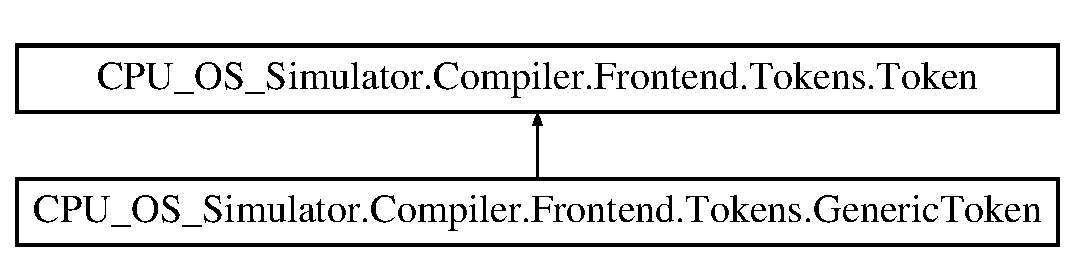
\includegraphics[height=2.000000cm]{class_c_p_u___o_s___simulator_1_1_compiler_1_1_frontend_1_1_tokens_1_1_generic_token}
\end{center}
\end{figure}
\subsection*{Public Member Functions}
\begin{DoxyCompactItemize}
\item 
\hyperlink{class_c_p_u___o_s___simulator_1_1_compiler_1_1_frontend_1_1_tokens_1_1_generic_token_a22ff9b77e796d56abfe9fe433526bfed}{Generic\+Token} (string \hyperlink{class_c_p_u___o_s___simulator_1_1_compiler_1_1_frontend_1_1_tokens_1_1_token_a5c05e12850ca18be8cbfdf7e2e263324}{value})
\item 
override Enum \hyperlink{class_c_p_u___o_s___simulator_1_1_compiler_1_1_frontend_1_1_tokens_1_1_generic_token_ae835f3a63c88a7e73df243c510cb0142}{Detect\+Type} ()
\item 
\hyperlink{namespace_c_p_u___o_s___simulator_1_1_compiler_1_1_frontend_1_1_tokens_a95401dcaadc07640b0e77238808e5aed}{Enum\+Token\+Type} \hyperlink{class_c_p_u___o_s___simulator_1_1_compiler_1_1_frontend_1_1_tokens_1_1_generic_token_a24e1310c91e1f75821a5a68ae1607732}{Get\+Token\+Type} ()
\end{DoxyCompactItemize}
\subsection*{Additional Inherited Members}


\subsection{Detailed Description}


Definition at line 5 of file Generic\+Token.\+cs.



\subsection{Constructor \& Destructor Documentation}
\hypertarget{class_c_p_u___o_s___simulator_1_1_compiler_1_1_frontend_1_1_tokens_1_1_generic_token_a22ff9b77e796d56abfe9fe433526bfed}{}\index{C\+P\+U\+\_\+\+O\+S\+\_\+\+Simulator\+::\+Compiler\+::\+Frontend\+::\+Tokens\+::\+Generic\+Token@{C\+P\+U\+\_\+\+O\+S\+\_\+\+Simulator\+::\+Compiler\+::\+Frontend\+::\+Tokens\+::\+Generic\+Token}!Generic\+Token@{Generic\+Token}}
\index{Generic\+Token@{Generic\+Token}!C\+P\+U\+\_\+\+O\+S\+\_\+\+Simulator\+::\+Compiler\+::\+Frontend\+::\+Tokens\+::\+Generic\+Token@{C\+P\+U\+\_\+\+O\+S\+\_\+\+Simulator\+::\+Compiler\+::\+Frontend\+::\+Tokens\+::\+Generic\+Token}}
\subsubsection[{Generic\+Token(string value)}]{\setlength{\rightskip}{0pt plus 5cm}C\+P\+U\+\_\+\+O\+S\+\_\+\+Simulator.\+Compiler.\+Frontend.\+Tokens.\+Generic\+Token.\+Generic\+Token (
\begin{DoxyParamCaption}
\item[{string}]{value}
\end{DoxyParamCaption}
)}\label{class_c_p_u___o_s___simulator_1_1_compiler_1_1_frontend_1_1_tokens_1_1_generic_token_a22ff9b77e796d56abfe9fe433526bfed}


Definition at line 7 of file Generic\+Token.\+cs.



\subsection{Member Function Documentation}
\hypertarget{class_c_p_u___o_s___simulator_1_1_compiler_1_1_frontend_1_1_tokens_1_1_generic_token_ae835f3a63c88a7e73df243c510cb0142}{}\index{C\+P\+U\+\_\+\+O\+S\+\_\+\+Simulator\+::\+Compiler\+::\+Frontend\+::\+Tokens\+::\+Generic\+Token@{C\+P\+U\+\_\+\+O\+S\+\_\+\+Simulator\+::\+Compiler\+::\+Frontend\+::\+Tokens\+::\+Generic\+Token}!Detect\+Type@{Detect\+Type}}
\index{Detect\+Type@{Detect\+Type}!C\+P\+U\+\_\+\+O\+S\+\_\+\+Simulator\+::\+Compiler\+::\+Frontend\+::\+Tokens\+::\+Generic\+Token@{C\+P\+U\+\_\+\+O\+S\+\_\+\+Simulator\+::\+Compiler\+::\+Frontend\+::\+Tokens\+::\+Generic\+Token}}
\subsubsection[{Detect\+Type()}]{\setlength{\rightskip}{0pt plus 5cm}override Enum C\+P\+U\+\_\+\+O\+S\+\_\+\+Simulator.\+Compiler.\+Frontend.\+Tokens.\+Generic\+Token.\+Detect\+Type (
\begin{DoxyParamCaption}
{}
\end{DoxyParamCaption}
)\hspace{0.3cm}{\ttfamily [virtual]}}\label{class_c_p_u___o_s___simulator_1_1_compiler_1_1_frontend_1_1_tokens_1_1_generic_token_ae835f3a63c88a7e73df243c510cb0142}


Implements \hyperlink{class_c_p_u___o_s___simulator_1_1_compiler_1_1_frontend_1_1_tokens_1_1_token_accfe8c46faedacd527ef619698c76310}{C\+P\+U\+\_\+\+O\+S\+\_\+\+Simulator.\+Compiler.\+Frontend.\+Tokens.\+Token}.



Definition at line 12 of file Generic\+Token.\+cs.

\hypertarget{class_c_p_u___o_s___simulator_1_1_compiler_1_1_frontend_1_1_tokens_1_1_generic_token_a24e1310c91e1f75821a5a68ae1607732}{}\index{C\+P\+U\+\_\+\+O\+S\+\_\+\+Simulator\+::\+Compiler\+::\+Frontend\+::\+Tokens\+::\+Generic\+Token@{C\+P\+U\+\_\+\+O\+S\+\_\+\+Simulator\+::\+Compiler\+::\+Frontend\+::\+Tokens\+::\+Generic\+Token}!Get\+Token\+Type@{Get\+Token\+Type}}
\index{Get\+Token\+Type@{Get\+Token\+Type}!C\+P\+U\+\_\+\+O\+S\+\_\+\+Simulator\+::\+Compiler\+::\+Frontend\+::\+Tokens\+::\+Generic\+Token@{C\+P\+U\+\_\+\+O\+S\+\_\+\+Simulator\+::\+Compiler\+::\+Frontend\+::\+Tokens\+::\+Generic\+Token}}
\subsubsection[{Get\+Token\+Type()}]{\setlength{\rightskip}{0pt plus 5cm}{\bf Enum\+Token\+Type} C\+P\+U\+\_\+\+O\+S\+\_\+\+Simulator.\+Compiler.\+Frontend.\+Tokens.\+Generic\+Token.\+Get\+Token\+Type (
\begin{DoxyParamCaption}
{}
\end{DoxyParamCaption}
)}\label{class_c_p_u___o_s___simulator_1_1_compiler_1_1_frontend_1_1_tokens_1_1_generic_token_a24e1310c91e1f75821a5a68ae1607732}


Definition at line 48 of file Generic\+Token.\+cs.



The documentation for this class was generated from the following file\+:\begin{DoxyCompactItemize}
\item 
Compiler/\+Frontend/\+Tokens/\hyperlink{_generic_token_8cs}{Generic\+Token.\+cs}\end{DoxyCompactItemize}

\hypertarget{interface_c_p_u___o_s___simulator_1_1_compiler_1_1_frontend_1_1_syntax_tree_1_1_i_a_s_t_accessor}{}\section{C\+P\+U\+\_\+\+O\+S\+\_\+\+Simulator.\+Compiler.\+Frontend.\+Syntax\+Tree.\+I\+A\+S\+T\+Accessor Interface Reference}
\label{interface_c_p_u___o_s___simulator_1_1_compiler_1_1_frontend_1_1_syntax_tree_1_1_i_a_s_t_accessor}\index{C\+P\+U\+\_\+\+O\+S\+\_\+\+Simulator.\+Compiler.\+Frontend.\+Syntax\+Tree.\+I\+A\+S\+T\+Accessor@{C\+P\+U\+\_\+\+O\+S\+\_\+\+Simulator.\+Compiler.\+Frontend.\+Syntax\+Tree.\+I\+A\+S\+T\+Accessor}}
\subsection*{Public Member Functions}
\begin{DoxyCompactItemize}
\item 
void \hyperlink{interface_c_p_u___o_s___simulator_1_1_compiler_1_1_frontend_1_1_syntax_tree_1_1_i_a_s_t_accessor_ab3bd2a643d314439015e1225f75a81c6}{Access} (\hyperlink{class_c_p_u___o_s___simulator_1_1_compiler_1_1_frontend_1_1_syntax_tree_1_1_string_node}{String\+Node} node)
\begin{DoxyCompactList}\small\item\em This method accesses a string node \end{DoxyCompactList}\item 
void \hyperlink{interface_c_p_u___o_s___simulator_1_1_compiler_1_1_frontend_1_1_syntax_tree_1_1_i_a_s_t_accessor_ade1d46967c4007eb5589ed3562e9e1e8}{Access} (\hyperlink{class_c_p_u___o_s___simulator_1_1_compiler_1_1_frontend_1_1_syntax_tree_1_1_integer_node}{Integer\+Node} node)
\begin{DoxyCompactList}\small\item\em This method accesses a integer node \end{DoxyCompactList}\item 
void \hyperlink{interface_c_p_u___o_s___simulator_1_1_compiler_1_1_frontend_1_1_syntax_tree_1_1_i_a_s_t_accessor_a31df77fdb5bb59081383e5698d4e89e1}{Access} (\hyperlink{class_c_p_u___o_s___simulator_1_1_compiler_1_1_frontend_1_1_syntax_tree_1_1_boolean_node}{Boolean\+Node} node)
\begin{DoxyCompactList}\small\item\em This method accesses a boolean node \end{DoxyCompactList}\item 
void \hyperlink{interface_c_p_u___o_s___simulator_1_1_compiler_1_1_frontend_1_1_syntax_tree_1_1_i_a_s_t_accessor_ae59d6c8c37ed358d6ca51ea0ca4e75c3}{Access} (\hyperlink{class_c_p_u___o_s___simulator_1_1_compiler_1_1_frontend_1_1_syntax_tree_1_1_byte_node}{Byte\+Node} node)
\begin{DoxyCompactList}\small\item\em This method accesses a byte node \end{DoxyCompactList}\item 
void \hyperlink{interface_c_p_u___o_s___simulator_1_1_compiler_1_1_frontend_1_1_syntax_tree_1_1_i_a_s_t_accessor_ac950358132e6aa46b62e87439e6f43b1}{Access} (\hyperlink{class_c_p_u___o_s___simulator_1_1_compiler_1_1_frontend_1_1_syntax_tree_1_1_object_node}{Object\+Node} node)
\begin{DoxyCompactList}\small\item\em This method accesses a object node \end{DoxyCompactList}\item 
void \hyperlink{interface_c_p_u___o_s___simulator_1_1_compiler_1_1_frontend_1_1_syntax_tree_1_1_i_a_s_t_accessor_a0ca21f44e36138824c71eb26638b02a5}{Access} (\hyperlink{class_c_p_u___o_s___simulator_1_1_compiler_1_1_frontend_1_1_syntax_tree_1_1_string_array_node}{String\+Array\+Node} node)
\begin{DoxyCompactList}\small\item\em This method accesses a string array node \end{DoxyCompactList}\item 
void \hyperlink{interface_c_p_u___o_s___simulator_1_1_compiler_1_1_frontend_1_1_syntax_tree_1_1_i_a_s_t_accessor_ae83a2de9c036fcebc74b7cc49b1190e3}{Access} (\hyperlink{class_c_p_u___o_s___simulator_1_1_compiler_1_1_frontend_1_1_syntax_tree_1_1_integer_array_node}{Integer\+Array\+Node} node)
\begin{DoxyCompactList}\small\item\em This method accesses a integer array node \end{DoxyCompactList}\item 
void \hyperlink{interface_c_p_u___o_s___simulator_1_1_compiler_1_1_frontend_1_1_syntax_tree_1_1_i_a_s_t_accessor_a1a2506bb66533db272d44b74572e6a0a}{Access} (\hyperlink{class_c_p_u___o_s___simulator_1_1_compiler_1_1_frontend_1_1_syntax_tree_1_1_boolean_array_node}{Boolean\+Array\+Node} node)
\begin{DoxyCompactList}\small\item\em This method accesses a boolean array node \end{DoxyCompactList}\item 
void \hyperlink{interface_c_p_u___o_s___simulator_1_1_compiler_1_1_frontend_1_1_syntax_tree_1_1_i_a_s_t_accessor_a55f774d25445b5952a3a0482dab4434f}{Access} (\hyperlink{class_c_p_u___o_s___simulator_1_1_compiler_1_1_frontend_1_1_syntax_tree_1_1_byte_array_node}{Byte\+Array\+Node} node)
\begin{DoxyCompactList}\small\item\em This method accesses a byte array node \end{DoxyCompactList}\item 
void \hyperlink{interface_c_p_u___o_s___simulator_1_1_compiler_1_1_frontend_1_1_syntax_tree_1_1_i_a_s_t_accessor_ac186ac1b1c8f0d6a817d87303e8dcb30}{Access} (\hyperlink{class_c_p_u___o_s___simulator_1_1_compiler_1_1_frontend_1_1_syntax_tree_1_1_object_array_node}{Object\+Array\+Node} node)
\begin{DoxyCompactList}\small\item\em This method accesses a object array node \end{DoxyCompactList}\end{DoxyCompactItemize}


\subsection{Detailed Description}


Definition at line 3 of file I\+A\+S\+T\+Accessor.\+cs.



\subsection{Member Function Documentation}
\hypertarget{interface_c_p_u___o_s___simulator_1_1_compiler_1_1_frontend_1_1_syntax_tree_1_1_i_a_s_t_accessor_ab3bd2a643d314439015e1225f75a81c6}{}\index{C\+P\+U\+\_\+\+O\+S\+\_\+\+Simulator\+::\+Compiler\+::\+Frontend\+::\+Syntax\+Tree\+::\+I\+A\+S\+T\+Accessor@{C\+P\+U\+\_\+\+O\+S\+\_\+\+Simulator\+::\+Compiler\+::\+Frontend\+::\+Syntax\+Tree\+::\+I\+A\+S\+T\+Accessor}!Access@{Access}}
\index{Access@{Access}!C\+P\+U\+\_\+\+O\+S\+\_\+\+Simulator\+::\+Compiler\+::\+Frontend\+::\+Syntax\+Tree\+::\+I\+A\+S\+T\+Accessor@{C\+P\+U\+\_\+\+O\+S\+\_\+\+Simulator\+::\+Compiler\+::\+Frontend\+::\+Syntax\+Tree\+::\+I\+A\+S\+T\+Accessor}}
\subsubsection[{Access(\+String\+Node node)}]{\setlength{\rightskip}{0pt plus 5cm}void C\+P\+U\+\_\+\+O\+S\+\_\+\+Simulator.\+Compiler.\+Frontend.\+Syntax\+Tree.\+I\+A\+S\+T\+Accessor.\+Access (
\begin{DoxyParamCaption}
\item[{{\bf String\+Node}}]{node}
\end{DoxyParamCaption}
)}\label{interface_c_p_u___o_s___simulator_1_1_compiler_1_1_frontend_1_1_syntax_tree_1_1_i_a_s_t_accessor_ab3bd2a643d314439015e1225f75a81c6}


This method accesses a string node 


\begin{DoxyParams}{Parameters}
{\em node} & the string node to access \\
\hline
\end{DoxyParams}
\hypertarget{interface_c_p_u___o_s___simulator_1_1_compiler_1_1_frontend_1_1_syntax_tree_1_1_i_a_s_t_accessor_ade1d46967c4007eb5589ed3562e9e1e8}{}\index{C\+P\+U\+\_\+\+O\+S\+\_\+\+Simulator\+::\+Compiler\+::\+Frontend\+::\+Syntax\+Tree\+::\+I\+A\+S\+T\+Accessor@{C\+P\+U\+\_\+\+O\+S\+\_\+\+Simulator\+::\+Compiler\+::\+Frontend\+::\+Syntax\+Tree\+::\+I\+A\+S\+T\+Accessor}!Access@{Access}}
\index{Access@{Access}!C\+P\+U\+\_\+\+O\+S\+\_\+\+Simulator\+::\+Compiler\+::\+Frontend\+::\+Syntax\+Tree\+::\+I\+A\+S\+T\+Accessor@{C\+P\+U\+\_\+\+O\+S\+\_\+\+Simulator\+::\+Compiler\+::\+Frontend\+::\+Syntax\+Tree\+::\+I\+A\+S\+T\+Accessor}}
\subsubsection[{Access(\+Integer\+Node node)}]{\setlength{\rightskip}{0pt plus 5cm}void C\+P\+U\+\_\+\+O\+S\+\_\+\+Simulator.\+Compiler.\+Frontend.\+Syntax\+Tree.\+I\+A\+S\+T\+Accessor.\+Access (
\begin{DoxyParamCaption}
\item[{{\bf Integer\+Node}}]{node}
\end{DoxyParamCaption}
)}\label{interface_c_p_u___o_s___simulator_1_1_compiler_1_1_frontend_1_1_syntax_tree_1_1_i_a_s_t_accessor_ade1d46967c4007eb5589ed3562e9e1e8}


This method accesses a integer node 


\begin{DoxyParams}{Parameters}
{\em node} & the integer node to access\\
\hline
\end{DoxyParams}
\hypertarget{interface_c_p_u___o_s___simulator_1_1_compiler_1_1_frontend_1_1_syntax_tree_1_1_i_a_s_t_accessor_a31df77fdb5bb59081383e5698d4e89e1}{}\index{C\+P\+U\+\_\+\+O\+S\+\_\+\+Simulator\+::\+Compiler\+::\+Frontend\+::\+Syntax\+Tree\+::\+I\+A\+S\+T\+Accessor@{C\+P\+U\+\_\+\+O\+S\+\_\+\+Simulator\+::\+Compiler\+::\+Frontend\+::\+Syntax\+Tree\+::\+I\+A\+S\+T\+Accessor}!Access@{Access}}
\index{Access@{Access}!C\+P\+U\+\_\+\+O\+S\+\_\+\+Simulator\+::\+Compiler\+::\+Frontend\+::\+Syntax\+Tree\+::\+I\+A\+S\+T\+Accessor@{C\+P\+U\+\_\+\+O\+S\+\_\+\+Simulator\+::\+Compiler\+::\+Frontend\+::\+Syntax\+Tree\+::\+I\+A\+S\+T\+Accessor}}
\subsubsection[{Access(\+Boolean\+Node node)}]{\setlength{\rightskip}{0pt plus 5cm}void C\+P\+U\+\_\+\+O\+S\+\_\+\+Simulator.\+Compiler.\+Frontend.\+Syntax\+Tree.\+I\+A\+S\+T\+Accessor.\+Access (
\begin{DoxyParamCaption}
\item[{{\bf Boolean\+Node}}]{node}
\end{DoxyParamCaption}
)}\label{interface_c_p_u___o_s___simulator_1_1_compiler_1_1_frontend_1_1_syntax_tree_1_1_i_a_s_t_accessor_a31df77fdb5bb59081383e5698d4e89e1}


This method accesses a boolean node 


\begin{DoxyParams}{Parameters}
{\em node} & the boolean node to access\\
\hline
\end{DoxyParams}
\hypertarget{interface_c_p_u___o_s___simulator_1_1_compiler_1_1_frontend_1_1_syntax_tree_1_1_i_a_s_t_accessor_ae59d6c8c37ed358d6ca51ea0ca4e75c3}{}\index{C\+P\+U\+\_\+\+O\+S\+\_\+\+Simulator\+::\+Compiler\+::\+Frontend\+::\+Syntax\+Tree\+::\+I\+A\+S\+T\+Accessor@{C\+P\+U\+\_\+\+O\+S\+\_\+\+Simulator\+::\+Compiler\+::\+Frontend\+::\+Syntax\+Tree\+::\+I\+A\+S\+T\+Accessor}!Access@{Access}}
\index{Access@{Access}!C\+P\+U\+\_\+\+O\+S\+\_\+\+Simulator\+::\+Compiler\+::\+Frontend\+::\+Syntax\+Tree\+::\+I\+A\+S\+T\+Accessor@{C\+P\+U\+\_\+\+O\+S\+\_\+\+Simulator\+::\+Compiler\+::\+Frontend\+::\+Syntax\+Tree\+::\+I\+A\+S\+T\+Accessor}}
\subsubsection[{Access(\+Byte\+Node node)}]{\setlength{\rightskip}{0pt plus 5cm}void C\+P\+U\+\_\+\+O\+S\+\_\+\+Simulator.\+Compiler.\+Frontend.\+Syntax\+Tree.\+I\+A\+S\+T\+Accessor.\+Access (
\begin{DoxyParamCaption}
\item[{{\bf Byte\+Node}}]{node}
\end{DoxyParamCaption}
)}\label{interface_c_p_u___o_s___simulator_1_1_compiler_1_1_frontend_1_1_syntax_tree_1_1_i_a_s_t_accessor_ae59d6c8c37ed358d6ca51ea0ca4e75c3}


This method accesses a byte node 


\begin{DoxyParams}{Parameters}
{\em node} & the byte node to access\\
\hline
\end{DoxyParams}
\hypertarget{interface_c_p_u___o_s___simulator_1_1_compiler_1_1_frontend_1_1_syntax_tree_1_1_i_a_s_t_accessor_ac950358132e6aa46b62e87439e6f43b1}{}\index{C\+P\+U\+\_\+\+O\+S\+\_\+\+Simulator\+::\+Compiler\+::\+Frontend\+::\+Syntax\+Tree\+::\+I\+A\+S\+T\+Accessor@{C\+P\+U\+\_\+\+O\+S\+\_\+\+Simulator\+::\+Compiler\+::\+Frontend\+::\+Syntax\+Tree\+::\+I\+A\+S\+T\+Accessor}!Access@{Access}}
\index{Access@{Access}!C\+P\+U\+\_\+\+O\+S\+\_\+\+Simulator\+::\+Compiler\+::\+Frontend\+::\+Syntax\+Tree\+::\+I\+A\+S\+T\+Accessor@{C\+P\+U\+\_\+\+O\+S\+\_\+\+Simulator\+::\+Compiler\+::\+Frontend\+::\+Syntax\+Tree\+::\+I\+A\+S\+T\+Accessor}}
\subsubsection[{Access(\+Object\+Node node)}]{\setlength{\rightskip}{0pt plus 5cm}void C\+P\+U\+\_\+\+O\+S\+\_\+\+Simulator.\+Compiler.\+Frontend.\+Syntax\+Tree.\+I\+A\+S\+T\+Accessor.\+Access (
\begin{DoxyParamCaption}
\item[{{\bf Object\+Node}}]{node}
\end{DoxyParamCaption}
)}\label{interface_c_p_u___o_s___simulator_1_1_compiler_1_1_frontend_1_1_syntax_tree_1_1_i_a_s_t_accessor_ac950358132e6aa46b62e87439e6f43b1}


This method accesses a object node 


\begin{DoxyParams}{Parameters}
{\em node} & the object node to access\\
\hline
\end{DoxyParams}
\hypertarget{interface_c_p_u___o_s___simulator_1_1_compiler_1_1_frontend_1_1_syntax_tree_1_1_i_a_s_t_accessor_a0ca21f44e36138824c71eb26638b02a5}{}\index{C\+P\+U\+\_\+\+O\+S\+\_\+\+Simulator\+::\+Compiler\+::\+Frontend\+::\+Syntax\+Tree\+::\+I\+A\+S\+T\+Accessor@{C\+P\+U\+\_\+\+O\+S\+\_\+\+Simulator\+::\+Compiler\+::\+Frontend\+::\+Syntax\+Tree\+::\+I\+A\+S\+T\+Accessor}!Access@{Access}}
\index{Access@{Access}!C\+P\+U\+\_\+\+O\+S\+\_\+\+Simulator\+::\+Compiler\+::\+Frontend\+::\+Syntax\+Tree\+::\+I\+A\+S\+T\+Accessor@{C\+P\+U\+\_\+\+O\+S\+\_\+\+Simulator\+::\+Compiler\+::\+Frontend\+::\+Syntax\+Tree\+::\+I\+A\+S\+T\+Accessor}}
\subsubsection[{Access(\+String\+Array\+Node node)}]{\setlength{\rightskip}{0pt plus 5cm}void C\+P\+U\+\_\+\+O\+S\+\_\+\+Simulator.\+Compiler.\+Frontend.\+Syntax\+Tree.\+I\+A\+S\+T\+Accessor.\+Access (
\begin{DoxyParamCaption}
\item[{{\bf String\+Array\+Node}}]{node}
\end{DoxyParamCaption}
)}\label{interface_c_p_u___o_s___simulator_1_1_compiler_1_1_frontend_1_1_syntax_tree_1_1_i_a_s_t_accessor_a0ca21f44e36138824c71eb26638b02a5}


This method accesses a string array node 


\begin{DoxyParams}{Parameters}
{\em node} & the string node to access\\
\hline
\end{DoxyParams}
\hypertarget{interface_c_p_u___o_s___simulator_1_1_compiler_1_1_frontend_1_1_syntax_tree_1_1_i_a_s_t_accessor_ae83a2de9c036fcebc74b7cc49b1190e3}{}\index{C\+P\+U\+\_\+\+O\+S\+\_\+\+Simulator\+::\+Compiler\+::\+Frontend\+::\+Syntax\+Tree\+::\+I\+A\+S\+T\+Accessor@{C\+P\+U\+\_\+\+O\+S\+\_\+\+Simulator\+::\+Compiler\+::\+Frontend\+::\+Syntax\+Tree\+::\+I\+A\+S\+T\+Accessor}!Access@{Access}}
\index{Access@{Access}!C\+P\+U\+\_\+\+O\+S\+\_\+\+Simulator\+::\+Compiler\+::\+Frontend\+::\+Syntax\+Tree\+::\+I\+A\+S\+T\+Accessor@{C\+P\+U\+\_\+\+O\+S\+\_\+\+Simulator\+::\+Compiler\+::\+Frontend\+::\+Syntax\+Tree\+::\+I\+A\+S\+T\+Accessor}}
\subsubsection[{Access(\+Integer\+Array\+Node node)}]{\setlength{\rightskip}{0pt plus 5cm}void C\+P\+U\+\_\+\+O\+S\+\_\+\+Simulator.\+Compiler.\+Frontend.\+Syntax\+Tree.\+I\+A\+S\+T\+Accessor.\+Access (
\begin{DoxyParamCaption}
\item[{{\bf Integer\+Array\+Node}}]{node}
\end{DoxyParamCaption}
)}\label{interface_c_p_u___o_s___simulator_1_1_compiler_1_1_frontend_1_1_syntax_tree_1_1_i_a_s_t_accessor_ae83a2de9c036fcebc74b7cc49b1190e3}


This method accesses a integer array node 


\begin{DoxyParams}{Parameters}
{\em node} & the integer array node to access\\
\hline
\end{DoxyParams}
\hypertarget{interface_c_p_u___o_s___simulator_1_1_compiler_1_1_frontend_1_1_syntax_tree_1_1_i_a_s_t_accessor_a1a2506bb66533db272d44b74572e6a0a}{}\index{C\+P\+U\+\_\+\+O\+S\+\_\+\+Simulator\+::\+Compiler\+::\+Frontend\+::\+Syntax\+Tree\+::\+I\+A\+S\+T\+Accessor@{C\+P\+U\+\_\+\+O\+S\+\_\+\+Simulator\+::\+Compiler\+::\+Frontend\+::\+Syntax\+Tree\+::\+I\+A\+S\+T\+Accessor}!Access@{Access}}
\index{Access@{Access}!C\+P\+U\+\_\+\+O\+S\+\_\+\+Simulator\+::\+Compiler\+::\+Frontend\+::\+Syntax\+Tree\+::\+I\+A\+S\+T\+Accessor@{C\+P\+U\+\_\+\+O\+S\+\_\+\+Simulator\+::\+Compiler\+::\+Frontend\+::\+Syntax\+Tree\+::\+I\+A\+S\+T\+Accessor}}
\subsubsection[{Access(\+Boolean\+Array\+Node node)}]{\setlength{\rightskip}{0pt plus 5cm}void C\+P\+U\+\_\+\+O\+S\+\_\+\+Simulator.\+Compiler.\+Frontend.\+Syntax\+Tree.\+I\+A\+S\+T\+Accessor.\+Access (
\begin{DoxyParamCaption}
\item[{{\bf Boolean\+Array\+Node}}]{node}
\end{DoxyParamCaption}
)}\label{interface_c_p_u___o_s___simulator_1_1_compiler_1_1_frontend_1_1_syntax_tree_1_1_i_a_s_t_accessor_a1a2506bb66533db272d44b74572e6a0a}


This method accesses a boolean array node 


\begin{DoxyParams}{Parameters}
{\em node} & the boolean array node to access\\
\hline
\end{DoxyParams}
\hypertarget{interface_c_p_u___o_s___simulator_1_1_compiler_1_1_frontend_1_1_syntax_tree_1_1_i_a_s_t_accessor_a55f774d25445b5952a3a0482dab4434f}{}\index{C\+P\+U\+\_\+\+O\+S\+\_\+\+Simulator\+::\+Compiler\+::\+Frontend\+::\+Syntax\+Tree\+::\+I\+A\+S\+T\+Accessor@{C\+P\+U\+\_\+\+O\+S\+\_\+\+Simulator\+::\+Compiler\+::\+Frontend\+::\+Syntax\+Tree\+::\+I\+A\+S\+T\+Accessor}!Access@{Access}}
\index{Access@{Access}!C\+P\+U\+\_\+\+O\+S\+\_\+\+Simulator\+::\+Compiler\+::\+Frontend\+::\+Syntax\+Tree\+::\+I\+A\+S\+T\+Accessor@{C\+P\+U\+\_\+\+O\+S\+\_\+\+Simulator\+::\+Compiler\+::\+Frontend\+::\+Syntax\+Tree\+::\+I\+A\+S\+T\+Accessor}}
\subsubsection[{Access(\+Byte\+Array\+Node node)}]{\setlength{\rightskip}{0pt plus 5cm}void C\+P\+U\+\_\+\+O\+S\+\_\+\+Simulator.\+Compiler.\+Frontend.\+Syntax\+Tree.\+I\+A\+S\+T\+Accessor.\+Access (
\begin{DoxyParamCaption}
\item[{{\bf Byte\+Array\+Node}}]{node}
\end{DoxyParamCaption}
)}\label{interface_c_p_u___o_s___simulator_1_1_compiler_1_1_frontend_1_1_syntax_tree_1_1_i_a_s_t_accessor_a55f774d25445b5952a3a0482dab4434f}


This method accesses a byte array node 


\begin{DoxyParams}{Parameters}
{\em node} & the byte array node to access\\
\hline
\end{DoxyParams}
\hypertarget{interface_c_p_u___o_s___simulator_1_1_compiler_1_1_frontend_1_1_syntax_tree_1_1_i_a_s_t_accessor_ac186ac1b1c8f0d6a817d87303e8dcb30}{}\index{C\+P\+U\+\_\+\+O\+S\+\_\+\+Simulator\+::\+Compiler\+::\+Frontend\+::\+Syntax\+Tree\+::\+I\+A\+S\+T\+Accessor@{C\+P\+U\+\_\+\+O\+S\+\_\+\+Simulator\+::\+Compiler\+::\+Frontend\+::\+Syntax\+Tree\+::\+I\+A\+S\+T\+Accessor}!Access@{Access}}
\index{Access@{Access}!C\+P\+U\+\_\+\+O\+S\+\_\+\+Simulator\+::\+Compiler\+::\+Frontend\+::\+Syntax\+Tree\+::\+I\+A\+S\+T\+Accessor@{C\+P\+U\+\_\+\+O\+S\+\_\+\+Simulator\+::\+Compiler\+::\+Frontend\+::\+Syntax\+Tree\+::\+I\+A\+S\+T\+Accessor}}
\subsubsection[{Access(\+Object\+Array\+Node node)}]{\setlength{\rightskip}{0pt plus 5cm}void C\+P\+U\+\_\+\+O\+S\+\_\+\+Simulator.\+Compiler.\+Frontend.\+Syntax\+Tree.\+I\+A\+S\+T\+Accessor.\+Access (
\begin{DoxyParamCaption}
\item[{{\bf Object\+Array\+Node}}]{node}
\end{DoxyParamCaption}
)}\label{interface_c_p_u___o_s___simulator_1_1_compiler_1_1_frontend_1_1_syntax_tree_1_1_i_a_s_t_accessor_ac186ac1b1c8f0d6a817d87303e8dcb30}


This method accesses a object array node 


\begin{DoxyParams}{Parameters}
{\em node} & the string array node to access\\
\hline
\end{DoxyParams}


The documentation for this interface was generated from the following file\+:\begin{DoxyCompactItemize}
\item 
Compiler/\+Frontend/\+Syntax\+Tree/\hyperlink{_i_a_s_t_accessor_8cs}{I\+A\+S\+T\+Accessor.\+cs}\end{DoxyCompactItemize}

\hypertarget{interface_c_p_u___o_s___simulator_1_1_compiler_1_1_frontend_1_1_syntax_tree_1_1_i_a_s_t_evaluator}{}\section{C\+P\+U\+\_\+\+O\+S\+\_\+\+Simulator.\+Compiler.\+Frontend.\+Syntax\+Tree.\+I\+A\+S\+T\+Evaluator Interface Reference}
\label{interface_c_p_u___o_s___simulator_1_1_compiler_1_1_frontend_1_1_syntax_tree_1_1_i_a_s_t_evaluator}\index{C\+P\+U\+\_\+\+O\+S\+\_\+\+Simulator.\+Compiler.\+Frontend.\+Syntax\+Tree.\+I\+A\+S\+T\+Evaluator@{C\+P\+U\+\_\+\+O\+S\+\_\+\+Simulator.\+Compiler.\+Frontend.\+Syntax\+Tree.\+I\+A\+S\+T\+Evaluator}}
\subsection*{Public Member Functions}
\begin{DoxyCompactItemize}
\item 
void \hyperlink{interface_c_p_u___o_s___simulator_1_1_compiler_1_1_frontend_1_1_syntax_tree_1_1_i_a_s_t_evaluator_a70da70b0ef15a6c065ad5744c1bfcf32}{Evaluate} (\hyperlink{class_c_p_u___o_s___simulator_1_1_compiler_1_1_frontend_1_1_syntax_tree_1_1_string_node}{String\+Node} node)
\begin{DoxyCompactList}\small\item\em This method Evaluates a string node \end{DoxyCompactList}\item 
void \hyperlink{interface_c_p_u___o_s___simulator_1_1_compiler_1_1_frontend_1_1_syntax_tree_1_1_i_a_s_t_evaluator_a43495cafeee8d2831f9d26b88b059348}{Evaluate} (\hyperlink{class_c_p_u___o_s___simulator_1_1_compiler_1_1_frontend_1_1_syntax_tree_1_1_integer_node}{Integer\+Node} node)
\begin{DoxyCompactList}\small\item\em This method Evaluates a integer node \end{DoxyCompactList}\item 
void \hyperlink{interface_c_p_u___o_s___simulator_1_1_compiler_1_1_frontend_1_1_syntax_tree_1_1_i_a_s_t_evaluator_a4b0649b94e80165da4e8fac21a11bc28}{Evaluate} (\hyperlink{class_c_p_u___o_s___simulator_1_1_compiler_1_1_frontend_1_1_syntax_tree_1_1_boolean_node}{Boolean\+Node} node)
\begin{DoxyCompactList}\small\item\em This method Evaluates a boolean node \end{DoxyCompactList}\item 
void \hyperlink{interface_c_p_u___o_s___simulator_1_1_compiler_1_1_frontend_1_1_syntax_tree_1_1_i_a_s_t_evaluator_aa9cc35163609222890e9c77dc18a12ac}{Evaluate} (\hyperlink{class_c_p_u___o_s___simulator_1_1_compiler_1_1_frontend_1_1_syntax_tree_1_1_byte_node}{Byte\+Node} node)
\begin{DoxyCompactList}\small\item\em This method Evaluates a byte node \end{DoxyCompactList}\item 
void \hyperlink{interface_c_p_u___o_s___simulator_1_1_compiler_1_1_frontend_1_1_syntax_tree_1_1_i_a_s_t_evaluator_a7e150ae0fad503818609f95b024231c5}{Evaluate} (\hyperlink{class_c_p_u___o_s___simulator_1_1_compiler_1_1_frontend_1_1_syntax_tree_1_1_object_node}{Object\+Node} node)
\begin{DoxyCompactList}\small\item\em This method Evaluates a object node \end{DoxyCompactList}\item 
void \hyperlink{interface_c_p_u___o_s___simulator_1_1_compiler_1_1_frontend_1_1_syntax_tree_1_1_i_a_s_t_evaluator_a780e7a1b7eaf9fbb59a3ce1a8a0a3849}{Evaluate} (\hyperlink{class_c_p_u___o_s___simulator_1_1_compiler_1_1_frontend_1_1_syntax_tree_1_1_string_array_node}{String\+Array\+Node} node)
\begin{DoxyCompactList}\small\item\em This method Evaluates a string array node \end{DoxyCompactList}\item 
void \hyperlink{interface_c_p_u___o_s___simulator_1_1_compiler_1_1_frontend_1_1_syntax_tree_1_1_i_a_s_t_evaluator_a62d279bf72003773d77221c4fe2a1e99}{Evaluate} (\hyperlink{class_c_p_u___o_s___simulator_1_1_compiler_1_1_frontend_1_1_syntax_tree_1_1_integer_array_node}{Integer\+Array\+Node} node)
\begin{DoxyCompactList}\small\item\em This method Evaluates a integer array node \end{DoxyCompactList}\item 
void \hyperlink{interface_c_p_u___o_s___simulator_1_1_compiler_1_1_frontend_1_1_syntax_tree_1_1_i_a_s_t_evaluator_a27648a48b3fedfdc2883987b433face5}{Evaluate} (\hyperlink{class_c_p_u___o_s___simulator_1_1_compiler_1_1_frontend_1_1_syntax_tree_1_1_boolean_array_node}{Boolean\+Array\+Node} node)
\begin{DoxyCompactList}\small\item\em This method Evaluates a boolean array node \end{DoxyCompactList}\item 
void \hyperlink{interface_c_p_u___o_s___simulator_1_1_compiler_1_1_frontend_1_1_syntax_tree_1_1_i_a_s_t_evaluator_a8927e98f729e8bc8b23444ddbb47b921}{Evaluate} (\hyperlink{class_c_p_u___o_s___simulator_1_1_compiler_1_1_frontend_1_1_syntax_tree_1_1_byte_array_node}{Byte\+Array\+Node} node)
\begin{DoxyCompactList}\small\item\em This method Evaluates a byte array node \end{DoxyCompactList}\item 
void \hyperlink{interface_c_p_u___o_s___simulator_1_1_compiler_1_1_frontend_1_1_syntax_tree_1_1_i_a_s_t_evaluator_aab15884bcde8b20f03eca6a8288ac740}{Evaluate} (\hyperlink{class_c_p_u___o_s___simulator_1_1_compiler_1_1_frontend_1_1_syntax_tree_1_1_object_array_node}{Object\+Array\+Node} node)
\begin{DoxyCompactList}\small\item\em This method Evaluates a object array node \end{DoxyCompactList}\end{DoxyCompactItemize}


\subsection{Detailed Description}


Definition at line 3 of file I\+A\+S\+T\+Evaluator.\+cs.



\subsection{Member Function Documentation}
\hypertarget{interface_c_p_u___o_s___simulator_1_1_compiler_1_1_frontend_1_1_syntax_tree_1_1_i_a_s_t_evaluator_a70da70b0ef15a6c065ad5744c1bfcf32}{}\index{C\+P\+U\+\_\+\+O\+S\+\_\+\+Simulator\+::\+Compiler\+::\+Frontend\+::\+Syntax\+Tree\+::\+I\+A\+S\+T\+Evaluator@{C\+P\+U\+\_\+\+O\+S\+\_\+\+Simulator\+::\+Compiler\+::\+Frontend\+::\+Syntax\+Tree\+::\+I\+A\+S\+T\+Evaluator}!Evaluate@{Evaluate}}
\index{Evaluate@{Evaluate}!C\+P\+U\+\_\+\+O\+S\+\_\+\+Simulator\+::\+Compiler\+::\+Frontend\+::\+Syntax\+Tree\+::\+I\+A\+S\+T\+Evaluator@{C\+P\+U\+\_\+\+O\+S\+\_\+\+Simulator\+::\+Compiler\+::\+Frontend\+::\+Syntax\+Tree\+::\+I\+A\+S\+T\+Evaluator}}
\subsubsection[{Evaluate(\+String\+Node node)}]{\setlength{\rightskip}{0pt plus 5cm}void C\+P\+U\+\_\+\+O\+S\+\_\+\+Simulator.\+Compiler.\+Frontend.\+Syntax\+Tree.\+I\+A\+S\+T\+Evaluator.\+Evaluate (
\begin{DoxyParamCaption}
\item[{{\bf String\+Node}}]{node}
\end{DoxyParamCaption}
)}\label{interface_c_p_u___o_s___simulator_1_1_compiler_1_1_frontend_1_1_syntax_tree_1_1_i_a_s_t_evaluator_a70da70b0ef15a6c065ad5744c1bfcf32}


This method Evaluates a string node 


\begin{DoxyParams}{Parameters}
{\em node} & the string node to Evaluate \\
\hline
\end{DoxyParams}
\hypertarget{interface_c_p_u___o_s___simulator_1_1_compiler_1_1_frontend_1_1_syntax_tree_1_1_i_a_s_t_evaluator_a43495cafeee8d2831f9d26b88b059348}{}\index{C\+P\+U\+\_\+\+O\+S\+\_\+\+Simulator\+::\+Compiler\+::\+Frontend\+::\+Syntax\+Tree\+::\+I\+A\+S\+T\+Evaluator@{C\+P\+U\+\_\+\+O\+S\+\_\+\+Simulator\+::\+Compiler\+::\+Frontend\+::\+Syntax\+Tree\+::\+I\+A\+S\+T\+Evaluator}!Evaluate@{Evaluate}}
\index{Evaluate@{Evaluate}!C\+P\+U\+\_\+\+O\+S\+\_\+\+Simulator\+::\+Compiler\+::\+Frontend\+::\+Syntax\+Tree\+::\+I\+A\+S\+T\+Evaluator@{C\+P\+U\+\_\+\+O\+S\+\_\+\+Simulator\+::\+Compiler\+::\+Frontend\+::\+Syntax\+Tree\+::\+I\+A\+S\+T\+Evaluator}}
\subsubsection[{Evaluate(\+Integer\+Node node)}]{\setlength{\rightskip}{0pt plus 5cm}void C\+P\+U\+\_\+\+O\+S\+\_\+\+Simulator.\+Compiler.\+Frontend.\+Syntax\+Tree.\+I\+A\+S\+T\+Evaluator.\+Evaluate (
\begin{DoxyParamCaption}
\item[{{\bf Integer\+Node}}]{node}
\end{DoxyParamCaption}
)}\label{interface_c_p_u___o_s___simulator_1_1_compiler_1_1_frontend_1_1_syntax_tree_1_1_i_a_s_t_evaluator_a43495cafeee8d2831f9d26b88b059348}


This method Evaluates a integer node 


\begin{DoxyParams}{Parameters}
{\em node} & the integer node to Evaluate\\
\hline
\end{DoxyParams}
\hypertarget{interface_c_p_u___o_s___simulator_1_1_compiler_1_1_frontend_1_1_syntax_tree_1_1_i_a_s_t_evaluator_a4b0649b94e80165da4e8fac21a11bc28}{}\index{C\+P\+U\+\_\+\+O\+S\+\_\+\+Simulator\+::\+Compiler\+::\+Frontend\+::\+Syntax\+Tree\+::\+I\+A\+S\+T\+Evaluator@{C\+P\+U\+\_\+\+O\+S\+\_\+\+Simulator\+::\+Compiler\+::\+Frontend\+::\+Syntax\+Tree\+::\+I\+A\+S\+T\+Evaluator}!Evaluate@{Evaluate}}
\index{Evaluate@{Evaluate}!C\+P\+U\+\_\+\+O\+S\+\_\+\+Simulator\+::\+Compiler\+::\+Frontend\+::\+Syntax\+Tree\+::\+I\+A\+S\+T\+Evaluator@{C\+P\+U\+\_\+\+O\+S\+\_\+\+Simulator\+::\+Compiler\+::\+Frontend\+::\+Syntax\+Tree\+::\+I\+A\+S\+T\+Evaluator}}
\subsubsection[{Evaluate(\+Boolean\+Node node)}]{\setlength{\rightskip}{0pt plus 5cm}void C\+P\+U\+\_\+\+O\+S\+\_\+\+Simulator.\+Compiler.\+Frontend.\+Syntax\+Tree.\+I\+A\+S\+T\+Evaluator.\+Evaluate (
\begin{DoxyParamCaption}
\item[{{\bf Boolean\+Node}}]{node}
\end{DoxyParamCaption}
)}\label{interface_c_p_u___o_s___simulator_1_1_compiler_1_1_frontend_1_1_syntax_tree_1_1_i_a_s_t_evaluator_a4b0649b94e80165da4e8fac21a11bc28}


This method Evaluates a boolean node 


\begin{DoxyParams}{Parameters}
{\em node} & the boolean node to Evaluate\\
\hline
\end{DoxyParams}
\hypertarget{interface_c_p_u___o_s___simulator_1_1_compiler_1_1_frontend_1_1_syntax_tree_1_1_i_a_s_t_evaluator_aa9cc35163609222890e9c77dc18a12ac}{}\index{C\+P\+U\+\_\+\+O\+S\+\_\+\+Simulator\+::\+Compiler\+::\+Frontend\+::\+Syntax\+Tree\+::\+I\+A\+S\+T\+Evaluator@{C\+P\+U\+\_\+\+O\+S\+\_\+\+Simulator\+::\+Compiler\+::\+Frontend\+::\+Syntax\+Tree\+::\+I\+A\+S\+T\+Evaluator}!Evaluate@{Evaluate}}
\index{Evaluate@{Evaluate}!C\+P\+U\+\_\+\+O\+S\+\_\+\+Simulator\+::\+Compiler\+::\+Frontend\+::\+Syntax\+Tree\+::\+I\+A\+S\+T\+Evaluator@{C\+P\+U\+\_\+\+O\+S\+\_\+\+Simulator\+::\+Compiler\+::\+Frontend\+::\+Syntax\+Tree\+::\+I\+A\+S\+T\+Evaluator}}
\subsubsection[{Evaluate(\+Byte\+Node node)}]{\setlength{\rightskip}{0pt plus 5cm}void C\+P\+U\+\_\+\+O\+S\+\_\+\+Simulator.\+Compiler.\+Frontend.\+Syntax\+Tree.\+I\+A\+S\+T\+Evaluator.\+Evaluate (
\begin{DoxyParamCaption}
\item[{{\bf Byte\+Node}}]{node}
\end{DoxyParamCaption}
)}\label{interface_c_p_u___o_s___simulator_1_1_compiler_1_1_frontend_1_1_syntax_tree_1_1_i_a_s_t_evaluator_aa9cc35163609222890e9c77dc18a12ac}


This method Evaluates a byte node 


\begin{DoxyParams}{Parameters}
{\em node} & the byte node to Evaluate\\
\hline
\end{DoxyParams}
\hypertarget{interface_c_p_u___o_s___simulator_1_1_compiler_1_1_frontend_1_1_syntax_tree_1_1_i_a_s_t_evaluator_a7e150ae0fad503818609f95b024231c5}{}\index{C\+P\+U\+\_\+\+O\+S\+\_\+\+Simulator\+::\+Compiler\+::\+Frontend\+::\+Syntax\+Tree\+::\+I\+A\+S\+T\+Evaluator@{C\+P\+U\+\_\+\+O\+S\+\_\+\+Simulator\+::\+Compiler\+::\+Frontend\+::\+Syntax\+Tree\+::\+I\+A\+S\+T\+Evaluator}!Evaluate@{Evaluate}}
\index{Evaluate@{Evaluate}!C\+P\+U\+\_\+\+O\+S\+\_\+\+Simulator\+::\+Compiler\+::\+Frontend\+::\+Syntax\+Tree\+::\+I\+A\+S\+T\+Evaluator@{C\+P\+U\+\_\+\+O\+S\+\_\+\+Simulator\+::\+Compiler\+::\+Frontend\+::\+Syntax\+Tree\+::\+I\+A\+S\+T\+Evaluator}}
\subsubsection[{Evaluate(\+Object\+Node node)}]{\setlength{\rightskip}{0pt plus 5cm}void C\+P\+U\+\_\+\+O\+S\+\_\+\+Simulator.\+Compiler.\+Frontend.\+Syntax\+Tree.\+I\+A\+S\+T\+Evaluator.\+Evaluate (
\begin{DoxyParamCaption}
\item[{{\bf Object\+Node}}]{node}
\end{DoxyParamCaption}
)}\label{interface_c_p_u___o_s___simulator_1_1_compiler_1_1_frontend_1_1_syntax_tree_1_1_i_a_s_t_evaluator_a7e150ae0fad503818609f95b024231c5}


This method Evaluates a object node 


\begin{DoxyParams}{Parameters}
{\em node} & the object node to Evaluate\\
\hline
\end{DoxyParams}
\hypertarget{interface_c_p_u___o_s___simulator_1_1_compiler_1_1_frontend_1_1_syntax_tree_1_1_i_a_s_t_evaluator_a780e7a1b7eaf9fbb59a3ce1a8a0a3849}{}\index{C\+P\+U\+\_\+\+O\+S\+\_\+\+Simulator\+::\+Compiler\+::\+Frontend\+::\+Syntax\+Tree\+::\+I\+A\+S\+T\+Evaluator@{C\+P\+U\+\_\+\+O\+S\+\_\+\+Simulator\+::\+Compiler\+::\+Frontend\+::\+Syntax\+Tree\+::\+I\+A\+S\+T\+Evaluator}!Evaluate@{Evaluate}}
\index{Evaluate@{Evaluate}!C\+P\+U\+\_\+\+O\+S\+\_\+\+Simulator\+::\+Compiler\+::\+Frontend\+::\+Syntax\+Tree\+::\+I\+A\+S\+T\+Evaluator@{C\+P\+U\+\_\+\+O\+S\+\_\+\+Simulator\+::\+Compiler\+::\+Frontend\+::\+Syntax\+Tree\+::\+I\+A\+S\+T\+Evaluator}}
\subsubsection[{Evaluate(\+String\+Array\+Node node)}]{\setlength{\rightskip}{0pt plus 5cm}void C\+P\+U\+\_\+\+O\+S\+\_\+\+Simulator.\+Compiler.\+Frontend.\+Syntax\+Tree.\+I\+A\+S\+T\+Evaluator.\+Evaluate (
\begin{DoxyParamCaption}
\item[{{\bf String\+Array\+Node}}]{node}
\end{DoxyParamCaption}
)}\label{interface_c_p_u___o_s___simulator_1_1_compiler_1_1_frontend_1_1_syntax_tree_1_1_i_a_s_t_evaluator_a780e7a1b7eaf9fbb59a3ce1a8a0a3849}


This method Evaluates a string array node 


\begin{DoxyParams}{Parameters}
{\em node} & the string node to Evaluate\\
\hline
\end{DoxyParams}
\hypertarget{interface_c_p_u___o_s___simulator_1_1_compiler_1_1_frontend_1_1_syntax_tree_1_1_i_a_s_t_evaluator_a62d279bf72003773d77221c4fe2a1e99}{}\index{C\+P\+U\+\_\+\+O\+S\+\_\+\+Simulator\+::\+Compiler\+::\+Frontend\+::\+Syntax\+Tree\+::\+I\+A\+S\+T\+Evaluator@{C\+P\+U\+\_\+\+O\+S\+\_\+\+Simulator\+::\+Compiler\+::\+Frontend\+::\+Syntax\+Tree\+::\+I\+A\+S\+T\+Evaluator}!Evaluate@{Evaluate}}
\index{Evaluate@{Evaluate}!C\+P\+U\+\_\+\+O\+S\+\_\+\+Simulator\+::\+Compiler\+::\+Frontend\+::\+Syntax\+Tree\+::\+I\+A\+S\+T\+Evaluator@{C\+P\+U\+\_\+\+O\+S\+\_\+\+Simulator\+::\+Compiler\+::\+Frontend\+::\+Syntax\+Tree\+::\+I\+A\+S\+T\+Evaluator}}
\subsubsection[{Evaluate(\+Integer\+Array\+Node node)}]{\setlength{\rightskip}{0pt plus 5cm}void C\+P\+U\+\_\+\+O\+S\+\_\+\+Simulator.\+Compiler.\+Frontend.\+Syntax\+Tree.\+I\+A\+S\+T\+Evaluator.\+Evaluate (
\begin{DoxyParamCaption}
\item[{{\bf Integer\+Array\+Node}}]{node}
\end{DoxyParamCaption}
)}\label{interface_c_p_u___o_s___simulator_1_1_compiler_1_1_frontend_1_1_syntax_tree_1_1_i_a_s_t_evaluator_a62d279bf72003773d77221c4fe2a1e99}


This method Evaluates a integer array node 


\begin{DoxyParams}{Parameters}
{\em node} & the integer array node to Evaluate\\
\hline
\end{DoxyParams}
\hypertarget{interface_c_p_u___o_s___simulator_1_1_compiler_1_1_frontend_1_1_syntax_tree_1_1_i_a_s_t_evaluator_a27648a48b3fedfdc2883987b433face5}{}\index{C\+P\+U\+\_\+\+O\+S\+\_\+\+Simulator\+::\+Compiler\+::\+Frontend\+::\+Syntax\+Tree\+::\+I\+A\+S\+T\+Evaluator@{C\+P\+U\+\_\+\+O\+S\+\_\+\+Simulator\+::\+Compiler\+::\+Frontend\+::\+Syntax\+Tree\+::\+I\+A\+S\+T\+Evaluator}!Evaluate@{Evaluate}}
\index{Evaluate@{Evaluate}!C\+P\+U\+\_\+\+O\+S\+\_\+\+Simulator\+::\+Compiler\+::\+Frontend\+::\+Syntax\+Tree\+::\+I\+A\+S\+T\+Evaluator@{C\+P\+U\+\_\+\+O\+S\+\_\+\+Simulator\+::\+Compiler\+::\+Frontend\+::\+Syntax\+Tree\+::\+I\+A\+S\+T\+Evaluator}}
\subsubsection[{Evaluate(\+Boolean\+Array\+Node node)}]{\setlength{\rightskip}{0pt plus 5cm}void C\+P\+U\+\_\+\+O\+S\+\_\+\+Simulator.\+Compiler.\+Frontend.\+Syntax\+Tree.\+I\+A\+S\+T\+Evaluator.\+Evaluate (
\begin{DoxyParamCaption}
\item[{{\bf Boolean\+Array\+Node}}]{node}
\end{DoxyParamCaption}
)}\label{interface_c_p_u___o_s___simulator_1_1_compiler_1_1_frontend_1_1_syntax_tree_1_1_i_a_s_t_evaluator_a27648a48b3fedfdc2883987b433face5}


This method Evaluates a boolean array node 


\begin{DoxyParams}{Parameters}
{\em node} & the boolean array node to Evaluate\\
\hline
\end{DoxyParams}
\hypertarget{interface_c_p_u___o_s___simulator_1_1_compiler_1_1_frontend_1_1_syntax_tree_1_1_i_a_s_t_evaluator_a8927e98f729e8bc8b23444ddbb47b921}{}\index{C\+P\+U\+\_\+\+O\+S\+\_\+\+Simulator\+::\+Compiler\+::\+Frontend\+::\+Syntax\+Tree\+::\+I\+A\+S\+T\+Evaluator@{C\+P\+U\+\_\+\+O\+S\+\_\+\+Simulator\+::\+Compiler\+::\+Frontend\+::\+Syntax\+Tree\+::\+I\+A\+S\+T\+Evaluator}!Evaluate@{Evaluate}}
\index{Evaluate@{Evaluate}!C\+P\+U\+\_\+\+O\+S\+\_\+\+Simulator\+::\+Compiler\+::\+Frontend\+::\+Syntax\+Tree\+::\+I\+A\+S\+T\+Evaluator@{C\+P\+U\+\_\+\+O\+S\+\_\+\+Simulator\+::\+Compiler\+::\+Frontend\+::\+Syntax\+Tree\+::\+I\+A\+S\+T\+Evaluator}}
\subsubsection[{Evaluate(\+Byte\+Array\+Node node)}]{\setlength{\rightskip}{0pt plus 5cm}void C\+P\+U\+\_\+\+O\+S\+\_\+\+Simulator.\+Compiler.\+Frontend.\+Syntax\+Tree.\+I\+A\+S\+T\+Evaluator.\+Evaluate (
\begin{DoxyParamCaption}
\item[{{\bf Byte\+Array\+Node}}]{node}
\end{DoxyParamCaption}
)}\label{interface_c_p_u___o_s___simulator_1_1_compiler_1_1_frontend_1_1_syntax_tree_1_1_i_a_s_t_evaluator_a8927e98f729e8bc8b23444ddbb47b921}


This method Evaluates a byte array node 


\begin{DoxyParams}{Parameters}
{\em node} & the byte array node to Evaluate\\
\hline
\end{DoxyParams}
\hypertarget{interface_c_p_u___o_s___simulator_1_1_compiler_1_1_frontend_1_1_syntax_tree_1_1_i_a_s_t_evaluator_aab15884bcde8b20f03eca6a8288ac740}{}\index{C\+P\+U\+\_\+\+O\+S\+\_\+\+Simulator\+::\+Compiler\+::\+Frontend\+::\+Syntax\+Tree\+::\+I\+A\+S\+T\+Evaluator@{C\+P\+U\+\_\+\+O\+S\+\_\+\+Simulator\+::\+Compiler\+::\+Frontend\+::\+Syntax\+Tree\+::\+I\+A\+S\+T\+Evaluator}!Evaluate@{Evaluate}}
\index{Evaluate@{Evaluate}!C\+P\+U\+\_\+\+O\+S\+\_\+\+Simulator\+::\+Compiler\+::\+Frontend\+::\+Syntax\+Tree\+::\+I\+A\+S\+T\+Evaluator@{C\+P\+U\+\_\+\+O\+S\+\_\+\+Simulator\+::\+Compiler\+::\+Frontend\+::\+Syntax\+Tree\+::\+I\+A\+S\+T\+Evaluator}}
\subsubsection[{Evaluate(\+Object\+Array\+Node node)}]{\setlength{\rightskip}{0pt plus 5cm}void C\+P\+U\+\_\+\+O\+S\+\_\+\+Simulator.\+Compiler.\+Frontend.\+Syntax\+Tree.\+I\+A\+S\+T\+Evaluator.\+Evaluate (
\begin{DoxyParamCaption}
\item[{{\bf Object\+Array\+Node}}]{node}
\end{DoxyParamCaption}
)}\label{interface_c_p_u___o_s___simulator_1_1_compiler_1_1_frontend_1_1_syntax_tree_1_1_i_a_s_t_evaluator_aab15884bcde8b20f03eca6a8288ac740}


This method Evaluates a object array node 


\begin{DoxyParams}{Parameters}
{\em node} & the string array node to Evaluate\\
\hline
\end{DoxyParams}


The documentation for this interface was generated from the following file\+:\begin{DoxyCompactItemize}
\item 
Compiler/\+Frontend/\+Syntax\+Tree/\hyperlink{_i_a_s_t_evaluator_8cs}{I\+A\+S\+T\+Evaluator.\+cs}\end{DoxyCompactItemize}

\hypertarget{interface_c_p_u___o_s___simulator_1_1_console_1_1_i_attribute}{}\section{C\+P\+U\+\_\+\+O\+S\+\_\+\+Simulator.\+Console.\+I\+Attribute$<$ T $>$ Interface Template Reference}
\label{interface_c_p_u___o_s___simulator_1_1_console_1_1_i_attribute}\index{C\+P\+U\+\_\+\+O\+S\+\_\+\+Simulator.\+Console.\+I\+Attribute$<$ T $>$@{C\+P\+U\+\_\+\+O\+S\+\_\+\+Simulator.\+Console.\+I\+Attribute$<$ T $>$}}


This interface represents a attribute with a single value  


\subsection*{Properties}
\begin{DoxyCompactItemize}
\item 
T \hyperlink{interface_c_p_u___o_s___simulator_1_1_console_1_1_i_attribute_ad23a11dc6f96a7ed120819db250e3f4a}{Value}\hspace{0.3cm}{\ttfamily  \mbox{[}get, set\mbox{]}}
\begin{DoxyCompactList}\small\item\em The value of the attribute \end{DoxyCompactList}\end{DoxyCompactItemize}


\subsection{Detailed Description}
This interface represents a attribute with a single value 


\begin{DoxyTemplParams}{Template Parameters}
{\em T} & \\
\hline
\end{DoxyTemplParams}
\begin{Desc}
\item[Type Constraints]\begin{description}
\item[{\em T} : {\em struct}]\end{description}
\end{Desc}


Definition at line 8 of file I\+Attribute.\+cs.



\subsection{Property Documentation}
\hypertarget{interface_c_p_u___o_s___simulator_1_1_console_1_1_i_attribute_ad23a11dc6f96a7ed120819db250e3f4a}{}\index{C\+P\+U\+\_\+\+O\+S\+\_\+\+Simulator\+::\+Console\+::\+I\+Attribute@{C\+P\+U\+\_\+\+O\+S\+\_\+\+Simulator\+::\+Console\+::\+I\+Attribute}!Value@{Value}}
\index{Value@{Value}!C\+P\+U\+\_\+\+O\+S\+\_\+\+Simulator\+::\+Console\+::\+I\+Attribute@{C\+P\+U\+\_\+\+O\+S\+\_\+\+Simulator\+::\+Console\+::\+I\+Attribute}}
\subsubsection[{Value}]{\setlength{\rightskip}{0pt plus 5cm}T {\bf C\+P\+U\+\_\+\+O\+S\+\_\+\+Simulator.\+Console.\+I\+Attribute}$<$ T $>$.Value\hspace{0.3cm}{\ttfamily [get]}, {\ttfamily [set]}}\label{interface_c_p_u___o_s___simulator_1_1_console_1_1_i_attribute_ad23a11dc6f96a7ed120819db250e3f4a}


The value of the attribute 



Definition at line 13 of file I\+Attribute.\+cs.



The documentation for this interface was generated from the following file\+:\begin{DoxyCompactItemize}
\item 
Console/\hyperlink{_console_2_i_attribute_8cs}{I\+Attribute.\+cs}\end{DoxyCompactItemize}

\hypertarget{interface_c_p_u___o_s___simulator_1_1_c_p_u_1_1_i_attribute}{}\section{C\+P\+U\+\_\+\+O\+S\+\_\+\+Simulator.\+C\+P\+U.\+I\+Attribute$<$ T $>$ Interface Template Reference}
\label{interface_c_p_u___o_s___simulator_1_1_c_p_u_1_1_i_attribute}\index{C\+P\+U\+\_\+\+O\+S\+\_\+\+Simulator.\+C\+P\+U.\+I\+Attribute$<$ T $>$@{C\+P\+U\+\_\+\+O\+S\+\_\+\+Simulator.\+C\+P\+U.\+I\+Attribute$<$ T $>$}}


This interface defines a basic attribute  


\subsection*{Properties}
\begin{DoxyCompactItemize}
\item 
T \hyperlink{interface_c_p_u___o_s___simulator_1_1_c_p_u_1_1_i_attribute_a7c1cc8ee7f3ce5334f7a4ace4a9db633}{Value}\hspace{0.3cm}{\ttfamily  \mbox{[}get\mbox{]}}
\end{DoxyCompactItemize}


\subsection{Detailed Description}
This interface defines a basic attribute 


\begin{DoxyTemplParams}{Template Parameters}
{\em T} & The type of the attribute \\
\hline
\end{DoxyTemplParams}


Definition at line 7 of file I\+Attribute.\+cs.



\subsection{Property Documentation}
\hypertarget{interface_c_p_u___o_s___simulator_1_1_c_p_u_1_1_i_attribute_a7c1cc8ee7f3ce5334f7a4ace4a9db633}{}\index{C\+P\+U\+\_\+\+O\+S\+\_\+\+Simulator\+::\+C\+P\+U\+::\+I\+Attribute@{C\+P\+U\+\_\+\+O\+S\+\_\+\+Simulator\+::\+C\+P\+U\+::\+I\+Attribute}!Value@{Value}}
\index{Value@{Value}!C\+P\+U\+\_\+\+O\+S\+\_\+\+Simulator\+::\+C\+P\+U\+::\+I\+Attribute@{C\+P\+U\+\_\+\+O\+S\+\_\+\+Simulator\+::\+C\+P\+U\+::\+I\+Attribute}}
\subsubsection[{Value}]{\setlength{\rightskip}{0pt plus 5cm}T {\bf C\+P\+U\+\_\+\+O\+S\+\_\+\+Simulator.\+C\+P\+U.\+I\+Attribute}$<$ T $>$.Value\hspace{0.3cm}{\ttfamily [get]}}\label{interface_c_p_u___o_s___simulator_1_1_c_p_u_1_1_i_attribute_a7c1cc8ee7f3ce5334f7a4ace4a9db633}


Definition at line 9 of file I\+Attribute.\+cs.



The documentation for this interface was generated from the following file\+:\begin{DoxyCompactItemize}
\item 
C\+P\+U/\hyperlink{_i_attribute_8cs}{I\+Attribute.\+cs}\end{DoxyCompactItemize}

\hypertarget{class_c_p_u___o_s___simulator_1_1_compiler_1_1_frontend_1_1_tokens_1_1_identifier}{}\section{C\+P\+U\+\_\+\+O\+S\+\_\+\+Simulator.\+Compiler.\+Frontend.\+Tokens.\+Identifier Class Reference}
\label{class_c_p_u___o_s___simulator_1_1_compiler_1_1_frontend_1_1_tokens_1_1_identifier}\index{C\+P\+U\+\_\+\+O\+S\+\_\+\+Simulator.\+Compiler.\+Frontend.\+Tokens.\+Identifier@{C\+P\+U\+\_\+\+O\+S\+\_\+\+Simulator.\+Compiler.\+Frontend.\+Tokens.\+Identifier}}
Inheritance diagram for C\+P\+U\+\_\+\+O\+S\+\_\+\+Simulator.\+Compiler.\+Frontend.\+Tokens.\+Identifier\+:\begin{figure}[H]
\begin{center}
\leavevmode
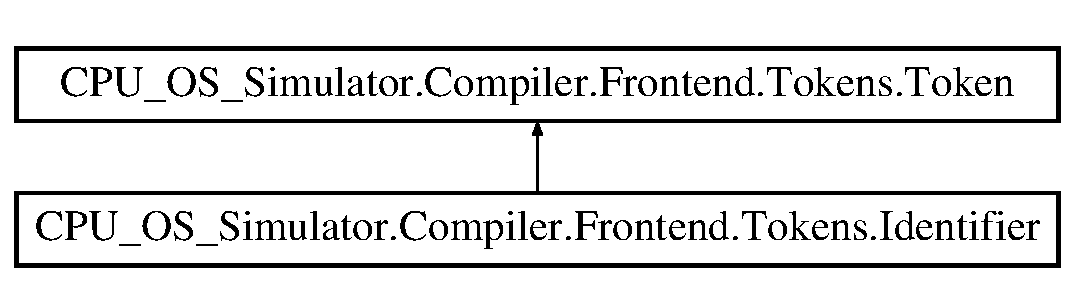
\includegraphics[height=2.000000cm]{class_c_p_u___o_s___simulator_1_1_compiler_1_1_frontend_1_1_tokens_1_1_identifier}
\end{center}
\end{figure}
\subsection*{Public Member Functions}
\begin{DoxyCompactItemize}
\item 
override Enum \hyperlink{class_c_p_u___o_s___simulator_1_1_compiler_1_1_frontend_1_1_tokens_1_1_identifier_aa5d0544de3699b5403b38e5978877fe1}{Detect\+Type} ()
\item 
virtual bool \hyperlink{class_c_p_u___o_s___simulator_1_1_compiler_1_1_frontend_1_1_tokens_1_1_identifier_a037942e3b86389700edc6f5aaff9ce5f}{Resolve\+Identifier} ()
\end{DoxyCompactItemize}
\subsection*{Additional Inherited Members}


\subsection{Detailed Description}


Definition at line 5 of file Identifier.\+cs.



\subsection{Member Function Documentation}
\hypertarget{class_c_p_u___o_s___simulator_1_1_compiler_1_1_frontend_1_1_tokens_1_1_identifier_aa5d0544de3699b5403b38e5978877fe1}{}\index{C\+P\+U\+\_\+\+O\+S\+\_\+\+Simulator\+::\+Compiler\+::\+Frontend\+::\+Tokens\+::\+Identifier@{C\+P\+U\+\_\+\+O\+S\+\_\+\+Simulator\+::\+Compiler\+::\+Frontend\+::\+Tokens\+::\+Identifier}!Detect\+Type@{Detect\+Type}}
\index{Detect\+Type@{Detect\+Type}!C\+P\+U\+\_\+\+O\+S\+\_\+\+Simulator\+::\+Compiler\+::\+Frontend\+::\+Tokens\+::\+Identifier@{C\+P\+U\+\_\+\+O\+S\+\_\+\+Simulator\+::\+Compiler\+::\+Frontend\+::\+Tokens\+::\+Identifier}}
\subsubsection[{Detect\+Type()}]{\setlength{\rightskip}{0pt plus 5cm}override Enum C\+P\+U\+\_\+\+O\+S\+\_\+\+Simulator.\+Compiler.\+Frontend.\+Tokens.\+Identifier.\+Detect\+Type (
\begin{DoxyParamCaption}
{}
\end{DoxyParamCaption}
)\hspace{0.3cm}{\ttfamily [virtual]}}\label{class_c_p_u___o_s___simulator_1_1_compiler_1_1_frontend_1_1_tokens_1_1_identifier_aa5d0544de3699b5403b38e5978877fe1}


Implements \hyperlink{class_c_p_u___o_s___simulator_1_1_compiler_1_1_frontend_1_1_tokens_1_1_token_accfe8c46faedacd527ef619698c76310}{C\+P\+U\+\_\+\+O\+S\+\_\+\+Simulator.\+Compiler.\+Frontend.\+Tokens.\+Token}.



Definition at line 7 of file Identifier.\+cs.

\hypertarget{class_c_p_u___o_s___simulator_1_1_compiler_1_1_frontend_1_1_tokens_1_1_identifier_a037942e3b86389700edc6f5aaff9ce5f}{}\index{C\+P\+U\+\_\+\+O\+S\+\_\+\+Simulator\+::\+Compiler\+::\+Frontend\+::\+Tokens\+::\+Identifier@{C\+P\+U\+\_\+\+O\+S\+\_\+\+Simulator\+::\+Compiler\+::\+Frontend\+::\+Tokens\+::\+Identifier}!Resolve\+Identifier@{Resolve\+Identifier}}
\index{Resolve\+Identifier@{Resolve\+Identifier}!C\+P\+U\+\_\+\+O\+S\+\_\+\+Simulator\+::\+Compiler\+::\+Frontend\+::\+Tokens\+::\+Identifier@{C\+P\+U\+\_\+\+O\+S\+\_\+\+Simulator\+::\+Compiler\+::\+Frontend\+::\+Tokens\+::\+Identifier}}
\subsubsection[{Resolve\+Identifier()}]{\setlength{\rightskip}{0pt plus 5cm}virtual bool C\+P\+U\+\_\+\+O\+S\+\_\+\+Simulator.\+Compiler.\+Frontend.\+Tokens.\+Identifier.\+Resolve\+Identifier (
\begin{DoxyParamCaption}
{}
\end{DoxyParamCaption}
)\hspace{0.3cm}{\ttfamily [virtual]}}\label{class_c_p_u___o_s___simulator_1_1_compiler_1_1_frontend_1_1_tokens_1_1_identifier_a037942e3b86389700edc6f5aaff9ce5f}


Definition at line 12 of file Identifier.\+cs.



The documentation for this class was generated from the following file\+:\begin{DoxyCompactItemize}
\item 
Compiler/\+Frontend/\+Tokens/\hyperlink{_identifier_8cs}{Identifier.\+cs}\end{DoxyCompactItemize}

\hypertarget{class_c_p_u___o_s___simulator_1_1_c_p_u_1_1_instruction}{}\section{C\+P\+U\+\_\+\+O\+S\+\_\+\+Simulator.\+C\+P\+U.\+Instruction Class Reference}
\label{class_c_p_u___o_s___simulator_1_1_c_p_u_1_1_instruction}\index{C\+P\+U\+\_\+\+O\+S\+\_\+\+Simulator.\+C\+P\+U.\+Instruction@{C\+P\+U\+\_\+\+O\+S\+\_\+\+Simulator.\+C\+P\+U.\+Instruction}}


This class represents an instruction witch can be executed by the virtual \hyperlink{namespace_c_p_u___o_s___simulator_1_1_c_p_u}{C\+P\+U}  


\subsection*{Public Member Functions}
\begin{DoxyCompactItemize}
\item 
\hyperlink{class_c_p_u___o_s___simulator_1_1_c_p_u_1_1_instruction_a2038c543e7b47a5997405f56cb8c7aa9}{Instruction} ()
\begin{DoxyCompactList}\small\item\em Default constructor for instruction used when deserialising an instruction N\+O\+T\+E Do not use in code \end{DoxyCompactList}\item 
\hyperlink{class_c_p_u___o_s___simulator_1_1_c_p_u_1_1_instruction_ac1fdbf424188acb7f10a1fa93e12a559}{Instruction} (int \hyperlink{class_c_p_u___o_s___simulator_1_1_c_p_u_1_1_instruction_aa8fa753bf6e1b6ffff7060ec90f930af}{opcode}, int \hyperlink{class_c_p_u___o_s___simulator_1_1_c_p_u_1_1_instruction_a8c533b0c08d8ac0a85b0e342f95cfeec}{size})
\begin{DoxyCompactList}\small\item\em Constructor for an instruction that takes no operands \end{DoxyCompactList}\item 
\hyperlink{class_c_p_u___o_s___simulator_1_1_c_p_u_1_1_instruction_a66a7be80a626d026918739af6f4b5d7a}{Instruction} (int \hyperlink{class_c_p_u___o_s___simulator_1_1_c_p_u_1_1_instruction_aa8fa753bf6e1b6ffff7060ec90f930af}{opcode}, \hyperlink{class_c_p_u___o_s___simulator_1_1_c_p_u_1_1_operand}{Operand} op1, bool \hyperlink{class_c_p_u___o_s___simulator_1_1_c_p_u_1_1_instruction_ad39c82c478ef1de45aae7cf7cf38575b}{op1mem}, int \hyperlink{class_c_p_u___o_s___simulator_1_1_c_p_u_1_1_instruction_a8c533b0c08d8ac0a85b0e342f95cfeec}{size})
\begin{DoxyCompactList}\small\item\em Constructor for an instruction that takes one operand \end{DoxyCompactList}\item 
\hyperlink{class_c_p_u___o_s___simulator_1_1_c_p_u_1_1_instruction_a53534336be838f76477f8b27bdb099b8}{Instruction} (int \hyperlink{class_c_p_u___o_s___simulator_1_1_c_p_u_1_1_instruction_aa8fa753bf6e1b6ffff7060ec90f930af}{opcode}, \hyperlink{class_c_p_u___o_s___simulator_1_1_c_p_u_1_1_operand}{Operand} op1, bool \hyperlink{class_c_p_u___o_s___simulator_1_1_c_p_u_1_1_instruction_ad39c82c478ef1de45aae7cf7cf38575b}{op1mem}, \hyperlink{class_c_p_u___o_s___simulator_1_1_c_p_u_1_1_operand}{Operand} op2, bool \hyperlink{class_c_p_u___o_s___simulator_1_1_c_p_u_1_1_instruction_ac414328ee54248a148c485a08a7eff44}{op2mem}, int \hyperlink{class_c_p_u___o_s___simulator_1_1_c_p_u_1_1_instruction_a8c533b0c08d8ac0a85b0e342f95cfeec}{size})
\begin{DoxyCompactList}\small\item\em Constructor for an instruction that takes two operands \end{DoxyCompactList}\item 
void \hyperlink{class_c_p_u___o_s___simulator_1_1_c_p_u_1_1_instruction_ab3bbd51fd889e3bbeb656ea717a7fe9c}{Bind\+Delegate} ()
\begin{DoxyCompactList}\small\item\em this function binds a delegate to an instruction. The delegate bound here will be called when the instruction is executed \end{DoxyCompactList}\item 
override string \hyperlink{class_c_p_u___o_s___simulator_1_1_c_p_u_1_1_instruction_a7d3a81ead6e3639f970901d8e898f02c}{To\+String} ()
\begin{DoxyCompactList}\small\item\em Returns a string that represents this instruction \end{DoxyCompactList}\end{DoxyCompactItemize}
\subsection*{Properties}
\begin{DoxyCompactItemize}
\item 
int \hyperlink{class_c_p_u___o_s___simulator_1_1_c_p_u_1_1_instruction_af56668feff9c8dab3c9335969a25e074}{Opcode}\hspace{0.3cm}{\ttfamily  \mbox{[}get, set\mbox{]}}
\begin{DoxyCompactList}\small\item\em The opcode for the instruction \end{DoxyCompactList}\item 
string \hyperlink{class_c_p_u___o_s___simulator_1_1_c_p_u_1_1_instruction_a7b7c3068cebbf81c64b67496b20c733a}{Category}\hspace{0.3cm}{\ttfamily  \mbox{[}get, set\mbox{]}}
\begin{DoxyCompactList}\small\item\em The category in which the instruction will be displayed within the interface \end{DoxyCompactList}\item 
\hyperlink{class_c_p_u___o_s___simulator_1_1_c_p_u_1_1_operand}{Operand} \hyperlink{class_c_p_u___o_s___simulator_1_1_c_p_u_1_1_instruction_a5eaf08ac611da1175f38f93defdee8d5}{Operand1}\hspace{0.3cm}{\ttfamily  \mbox{[}get, set\mbox{]}}
\begin{DoxyCompactList}\small\item\em The first operand for the instruction \end{DoxyCompactList}\item 
\hyperlink{class_c_p_u___o_s___simulator_1_1_c_p_u_1_1_operand}{Operand} \hyperlink{class_c_p_u___o_s___simulator_1_1_c_p_u_1_1_instruction_ab35e6667e7c2f42dd09965995e25ff2d}{Operand2}\hspace{0.3cm}{\ttfamily  \mbox{[}get, set\mbox{]}}
\begin{DoxyCompactList}\small\item\em The second operand for the instruction \end{DoxyCompactList}\item 
Func$<$ int $>$ \hyperlink{class_c_p_u___o_s___simulator_1_1_c_p_u_1_1_instruction_afc4c52737c07181195a29413cf09d2a5}{Execute}\hspace{0.3cm}{\ttfamily  \mbox{[}get, set\mbox{]}}
\begin{DoxyCompactList}\small\item\em The function that will be executed when the instruction is executed \end{DoxyCompactList}\item 
int \hyperlink{class_c_p_u___o_s___simulator_1_1_c_p_u_1_1_instruction_a8e0f7c63850af7cfd8a41c066c01838e}{Result}\hspace{0.3cm}{\ttfamily  \mbox{[}get, set\mbox{]}}
\begin{DoxyCompactList}\small\item\em The result of the instruction once executed e.\+g. the result of A\+D\+D 1,1 would be 2 \end{DoxyCompactList}\item 
int \hyperlink{class_c_p_u___o_s___simulator_1_1_c_p_u_1_1_instruction_a7c60418808e7bd6cb1964a227dcd9dac}{Size}\hspace{0.3cm}{\ttfamily  \mbox{[}get, set\mbox{]}}
\begin{DoxyCompactList}\small\item\em The size of the instruction within the program \end{DoxyCompactList}\item 
int \hyperlink{class_c_p_u___o_s___simulator_1_1_c_p_u_1_1_instruction_abfc23dbc9a978d2a1468b819f87a7614}{Logical\+Address}\hspace{0.3cm}{\ttfamily  \mbox{[}get, set\mbox{]}}
\begin{DoxyCompactList}\small\item\em The Logical address of this instruction within a program \end{DoxyCompactList}\item 
string \hyperlink{class_c_p_u___o_s___simulator_1_1_c_p_u_1_1_instruction_a2750b111d827f6e6a8fccd0e8520de89}{Instruction\+String}\hspace{0.3cm}{\ttfamily  \mbox{[}get, set\mbox{]}}
\begin{DoxyCompactList}\small\item\em The string representation of this instruction e.\+g. A\+D\+D R01,10 \end{DoxyCompactList}\item 
int \hyperlink{class_c_p_u___o_s___simulator_1_1_c_p_u_1_1_instruction_a97b20c8a0a7536bdddd8e791605a8bac}{Physical\+Address}\hspace{0.3cm}{\ttfamily  \mbox{[}get, set\mbox{]}}
\begin{DoxyCompactList}\small\item\em The physical address of this instruction within memory \end{DoxyCompactList}\item 
bool \hyperlink{class_c_p_u___o_s___simulator_1_1_c_p_u_1_1_instruction_ae5666173d24e27d25d16e1e1f0bb10a3}{Op1\+Mem}\hspace{0.3cm}{\ttfamily  \mbox{[}get, set\mbox{]}}
\begin{DoxyCompactList}\small\item\em Whether the first operand of this instruction is a memory address \end{DoxyCompactList}\item 
bool \hyperlink{class_c_p_u___o_s___simulator_1_1_c_p_u_1_1_instruction_ace33aaf155d1f6a727337811538665b6}{Op2\+Mem}\hspace{0.3cm}{\ttfamily  \mbox{[}get, set\mbox{]}}
\begin{DoxyCompactList}\small\item\em Whether the second operand of this instruction is a memory address \end{DoxyCompactList}\item 
\hyperlink{class_c_p_u___o_s___simulator_1_1_c_p_u_1_1_execution_unit}{Execution\+Unit} \hyperlink{class_c_p_u___o_s___simulator_1_1_c_p_u_1_1_instruction_a75e93b5a62558ece7da698068625bd8f}{Unit}\hspace{0.3cm}{\ttfamily  \mbox{[}get, set\mbox{]}}
\begin{DoxyCompactList}\small\item\em The execution unit that will be executing this instruction \end{DoxyCompactList}\end{DoxyCompactItemize}
\subsection*{Private Member Functions}
\begin{DoxyCompactItemize}
\item 
int \hyperlink{class_c_p_u___o_s___simulator_1_1_c_p_u_1_1_instruction_ae0e0e21063eeb9aa0dc0896e6e4c71dc}{Find\+Required\+Page} (int pagenumber)
\item 
void \hyperlink{class_c_p_u___o_s___simulator_1_1_c_p_u_1_1_instruction_a469a6252b1205ff79c93c2d75cafe0ce}{Store\+Byte} (int page\+Number, int page\+Offset, byte value)
\item 
byte \hyperlink{class_c_p_u___o_s___simulator_1_1_c_p_u_1_1_instruction_a494843084219f295941d08e8b0355050}{Load\+Byte} (int page\+Number, int page\+Offset)
\item 
int \hyperlink{class_c_p_u___o_s___simulator_1_1_c_p_u_1_1_instruction_af6548da603e7370f10de03e0da040a24}{M\+O\+V} (\hyperlink{class_c_p_u___o_s___simulator_1_1_c_p_u_1_1_operand}{Operand} lhs, \hyperlink{class_c_p_u___o_s___simulator_1_1_c_p_u_1_1_operand}{Operand} rhs)
\begin{DoxyCompactList}\small\item\em This function is called whenever a M\+O\+V instruction is executed \end{DoxyCompactList}\item 
int \hyperlink{class_c_p_u___o_s___simulator_1_1_c_p_u_1_1_instruction_a33723518d4e117877d2ecf5b861d2eb2}{M\+V\+S} (\hyperlink{class_c_p_u___o_s___simulator_1_1_c_p_u_1_1_operand}{Operand} lhs, \hyperlink{class_c_p_u___o_s___simulator_1_1_c_p_u_1_1_operand}{Operand} rhs)
\begin{DoxyCompactList}\small\item\em This function is called whenever a M\+V\+S instruction is executed \end{DoxyCompactList}\item 
int \hyperlink{class_c_p_u___o_s___simulator_1_1_c_p_u_1_1_instruction_a689065741dc51ddacf955b3781570546}{C\+V\+S} (\hyperlink{class_c_p_u___o_s___simulator_1_1_c_p_u_1_1_operand}{Operand} lhs, \hyperlink{class_c_p_u___o_s___simulator_1_1_c_p_u_1_1_operand}{Operand} rhs)
\begin{DoxyCompactList}\small\item\em This function is called whenever a C\+V\+S instruction is executed \end{DoxyCompactList}\item 
int \hyperlink{class_c_p_u___o_s___simulator_1_1_c_p_u_1_1_instruction_af73e92c10474c39863df39c1f826ff50}{C\+V\+I} (\hyperlink{class_c_p_u___o_s___simulator_1_1_c_p_u_1_1_operand}{Operand} lhs, \hyperlink{class_c_p_u___o_s___simulator_1_1_c_p_u_1_1_operand}{Operand} rhs)
\begin{DoxyCompactList}\small\item\em This function is called whenever a C\+V\+I instruction is executed \end{DoxyCompactList}\item 
int \hyperlink{class_c_p_u___o_s___simulator_1_1_c_p_u_1_1_instruction_ae09705d74d57f968b93ba1739832488f}{L\+D\+B} (\hyperlink{class_c_p_u___o_s___simulator_1_1_c_p_u_1_1_operand}{Operand} lhs, \hyperlink{class_c_p_u___o_s___simulator_1_1_c_p_u_1_1_operand}{Operand} rhs)
\begin{DoxyCompactList}\small\item\em This function is called whenever a L\+D\+B instruction is executed \end{DoxyCompactList}\item 
int \hyperlink{class_c_p_u___o_s___simulator_1_1_c_p_u_1_1_instruction_adc1b564050331c46094af907abb34acb}{L\+D\+W} (\hyperlink{class_c_p_u___o_s___simulator_1_1_c_p_u_1_1_operand}{Operand} lhs, \hyperlink{class_c_p_u___o_s___simulator_1_1_c_p_u_1_1_operand}{Operand} rhs)
\begin{DoxyCompactList}\small\item\em This function is called whenever a L\+D\+W instruction is executed \end{DoxyCompactList}\item 
int \hyperlink{class_c_p_u___o_s___simulator_1_1_c_p_u_1_1_instruction_abaa66d00b38349cd8033c8c1428a9ca3}{L\+N\+S} (\hyperlink{class_c_p_u___o_s___simulator_1_1_c_p_u_1_1_operand}{Operand} lhs, \hyperlink{class_c_p_u___o_s___simulator_1_1_c_p_u_1_1_operand}{Operand} rhs)
\begin{DoxyCompactList}\small\item\em This function is called whenever a L\+N\+S instruction is executed \end{DoxyCompactList}\item 
int \hyperlink{class_c_p_u___o_s___simulator_1_1_c_p_u_1_1_instruction_a41d94be59f02b4ff381bed811f0c4f2e}{L\+D\+B\+I} (\hyperlink{class_c_p_u___o_s___simulator_1_1_c_p_u_1_1_operand}{Operand} lhs, \hyperlink{class_c_p_u___o_s___simulator_1_1_c_p_u_1_1_operand}{Operand} rhs)
\begin{DoxyCompactList}\small\item\em This function is called whenever a L\+D\+B\+I instruction is executed \end{DoxyCompactList}\item 
int \hyperlink{class_c_p_u___o_s___simulator_1_1_c_p_u_1_1_instruction_a2a8c6cf1d6f14e9d219fabc5957cd586}{L\+D\+W\+I} (\hyperlink{class_c_p_u___o_s___simulator_1_1_c_p_u_1_1_operand}{Operand} lhs, \hyperlink{class_c_p_u___o_s___simulator_1_1_c_p_u_1_1_operand}{Operand} rhs)
\begin{DoxyCompactList}\small\item\em This function is called whenever a L\+D\+W\+I instruction is executed \end{DoxyCompactList}\item 
int \hyperlink{class_c_p_u___o_s___simulator_1_1_c_p_u_1_1_instruction_a78fbef41ec65046f35456e7cb161d037}{T\+A\+S} (\hyperlink{class_c_p_u___o_s___simulator_1_1_c_p_u_1_1_operand}{Operand} lhs, \hyperlink{class_c_p_u___o_s___simulator_1_1_c_p_u_1_1_operand}{Operand} rhs)
\begin{DoxyCompactList}\small\item\em This function is called whenever a T\+A\+S instruction is executed \end{DoxyCompactList}\item 
int \hyperlink{class_c_p_u___o_s___simulator_1_1_c_p_u_1_1_instruction_a26aa3d1a1f62f61acc3b37c7d57743f1}{S\+T\+B} (\hyperlink{class_c_p_u___o_s___simulator_1_1_c_p_u_1_1_operand}{Operand} lhs, \hyperlink{class_c_p_u___o_s___simulator_1_1_c_p_u_1_1_operand}{Operand} rhs)
\begin{DoxyCompactList}\small\item\em This function is called whenever a S\+T\+B instruction is executed \end{DoxyCompactList}\item 
int \hyperlink{class_c_p_u___o_s___simulator_1_1_c_p_u_1_1_instruction_aa1bc7540a41bcd8ab9273cfac88a5bf8}{S\+T\+W} (\hyperlink{class_c_p_u___o_s___simulator_1_1_c_p_u_1_1_operand}{Operand} lhs, \hyperlink{class_c_p_u___o_s___simulator_1_1_c_p_u_1_1_operand}{Operand} rhs)
\begin{DoxyCompactList}\small\item\em This function is called whenever a S\+T\+W instruction is executed \end{DoxyCompactList}\item 
int \hyperlink{class_c_p_u___o_s___simulator_1_1_c_p_u_1_1_instruction_a2724896fa80e3da440271b6dba5421a3}{S\+T\+B\+I} (\hyperlink{class_c_p_u___o_s___simulator_1_1_c_p_u_1_1_operand}{Operand} lhs, \hyperlink{class_c_p_u___o_s___simulator_1_1_c_p_u_1_1_operand}{Operand} rhs)
\begin{DoxyCompactList}\small\item\em This function is called whenever a S\+T\+B\+I instruction is executed \end{DoxyCompactList}\item 
int \hyperlink{class_c_p_u___o_s___simulator_1_1_c_p_u_1_1_instruction_aec8b426958aee888d46d9cbb565ed548}{S\+T\+W\+I} (\hyperlink{class_c_p_u___o_s___simulator_1_1_c_p_u_1_1_operand}{Operand} lhs, \hyperlink{class_c_p_u___o_s___simulator_1_1_c_p_u_1_1_operand}{Operand} rhs)
\begin{DoxyCompactList}\small\item\em This function is called whenever a S\+T\+W\+I instruction is executed \end{DoxyCompactList}\item 
int \hyperlink{class_c_p_u___o_s___simulator_1_1_c_p_u_1_1_instruction_a4a6711b8309af629c9460cdadc340444}{P\+U\+S\+H} (\hyperlink{class_c_p_u___o_s___simulator_1_1_c_p_u_1_1_operand}{Operand} lhs, \hyperlink{class_c_p_u___o_s___simulator_1_1_c_p_u_1_1_operand}{Operand} rhs)
\begin{DoxyCompactList}\small\item\em This function is called whenever a P\+U\+S\+H instruction is executed \end{DoxyCompactList}\item 
int \hyperlink{class_c_p_u___o_s___simulator_1_1_c_p_u_1_1_instruction_a16a47493684bb30a289d337188fb77b6}{P\+O\+P} (\hyperlink{class_c_p_u___o_s___simulator_1_1_c_p_u_1_1_operand}{Operand} lhs, \hyperlink{class_c_p_u___o_s___simulator_1_1_c_p_u_1_1_operand}{Operand} rhs)
\begin{DoxyCompactList}\small\item\em This function is called whenever a P\+O\+P instruction is executed \end{DoxyCompactList}\item 
int \hyperlink{class_c_p_u___o_s___simulator_1_1_c_p_u_1_1_instruction_ac86363232497de67ac268dd8942294a3}{S\+W\+P} (\hyperlink{class_c_p_u___o_s___simulator_1_1_c_p_u_1_1_operand}{Operand} lhs, \hyperlink{class_c_p_u___o_s___simulator_1_1_c_p_u_1_1_operand}{Operand} rhs)
\begin{DoxyCompactList}\small\item\em This function is called whenever a S\+W\+P instruction is executed \end{DoxyCompactList}\item 
int \hyperlink{class_c_p_u___o_s___simulator_1_1_c_p_u_1_1_instruction_a3c22b47d66b4c92120eba7b2d77eb92f}{L\+D\+D\+W} (\hyperlink{class_c_p_u___o_s___simulator_1_1_c_p_u_1_1_operand}{Operand} lhs, \hyperlink{class_c_p_u___o_s___simulator_1_1_c_p_u_1_1_operand}{Operand} rhs)
\begin{DoxyCompactList}\small\item\em This function is called whenever a L\+D\+D\+W instruction is executed \end{DoxyCompactList}\item 
int \hyperlink{class_c_p_u___o_s___simulator_1_1_c_p_u_1_1_instruction_a2f70d186e9e857881d9dfaf7c4e2cfa8}{L\+D\+D\+W\+I} (\hyperlink{class_c_p_u___o_s___simulator_1_1_c_p_u_1_1_operand}{Operand} lhs, \hyperlink{class_c_p_u___o_s___simulator_1_1_c_p_u_1_1_operand}{Operand} rhs)
\begin{DoxyCompactList}\small\item\em This function is called whenever a L\+D\+D\+W\+I instruction is executed \end{DoxyCompactList}\item 
int \hyperlink{class_c_p_u___o_s___simulator_1_1_c_p_u_1_1_instruction_ac1213c1f15be4bd4a28cdee4beb07df7}{S\+T\+D\+W} (\hyperlink{class_c_p_u___o_s___simulator_1_1_c_p_u_1_1_operand}{Operand} lhs, \hyperlink{class_c_p_u___o_s___simulator_1_1_c_p_u_1_1_operand}{Operand} rhs)
\begin{DoxyCompactList}\small\item\em This function is called whenever a S\+T\+D\+W instruction is executed \end{DoxyCompactList}\item 
int \hyperlink{class_c_p_u___o_s___simulator_1_1_c_p_u_1_1_instruction_a33e57864c33400a06aca3c059286a66c}{S\+T\+D\+W\+I} (\hyperlink{class_c_p_u___o_s___simulator_1_1_c_p_u_1_1_operand}{Operand} lhs, \hyperlink{class_c_p_u___o_s___simulator_1_1_c_p_u_1_1_operand}{Operand} rhs)
\begin{DoxyCompactList}\small\item\em This function is called whenever a S\+T\+D\+W\+I instruction is executed \end{DoxyCompactList}\item 
int \hyperlink{class_c_p_u___o_s___simulator_1_1_c_p_u_1_1_instruction_a4b5e469acee3a32016220af620b98650}{A\+N\+D} (\hyperlink{class_c_p_u___o_s___simulator_1_1_c_p_u_1_1_operand}{Operand} lhs, \hyperlink{class_c_p_u___o_s___simulator_1_1_c_p_u_1_1_operand}{Operand} rhs)
\begin{DoxyCompactList}\small\item\em This function is called whenever a A\+N\+D instruction is executed \end{DoxyCompactList}\item 
int \hyperlink{class_c_p_u___o_s___simulator_1_1_c_p_u_1_1_instruction_a32adcd85bab5adfeeb4effa90275dee5}{O\+R} (\hyperlink{class_c_p_u___o_s___simulator_1_1_c_p_u_1_1_operand}{Operand} lhs, \hyperlink{class_c_p_u___o_s___simulator_1_1_c_p_u_1_1_operand}{Operand} rhs)
\begin{DoxyCompactList}\small\item\em This function is called whenever a O\+R instruction is executed \end{DoxyCompactList}\item 
int \hyperlink{class_c_p_u___o_s___simulator_1_1_c_p_u_1_1_instruction_ab639a616b188c9816dd1775ebda837d4}{N\+O\+T} (\hyperlink{class_c_p_u___o_s___simulator_1_1_c_p_u_1_1_operand}{Operand} lhs, \hyperlink{class_c_p_u___o_s___simulator_1_1_c_p_u_1_1_operand}{Operand} rhs)
\begin{DoxyCompactList}\small\item\em This function is called whenever a N\+O\+T instruction is executed \end{DoxyCompactList}\item 
int \hyperlink{class_c_p_u___o_s___simulator_1_1_c_p_u_1_1_instruction_ad5e8679e646e772e6fb2d7655bad9f6f}{S\+H\+L} (\hyperlink{class_c_p_u___o_s___simulator_1_1_c_p_u_1_1_operand}{Operand} lhs, \hyperlink{class_c_p_u___o_s___simulator_1_1_c_p_u_1_1_operand}{Operand} rhs)
\begin{DoxyCompactList}\small\item\em This function is called whenever a S\+H\+L instruction is executed \end{DoxyCompactList}\item 
int \hyperlink{class_c_p_u___o_s___simulator_1_1_c_p_u_1_1_instruction_a5796880f8494dab4070d151f3e4b2301}{S\+H\+R} (\hyperlink{class_c_p_u___o_s___simulator_1_1_c_p_u_1_1_operand}{Operand} lhs, \hyperlink{class_c_p_u___o_s___simulator_1_1_c_p_u_1_1_operand}{Operand} rhs)
\item 
int \hyperlink{class_c_p_u___o_s___simulator_1_1_c_p_u_1_1_instruction_a0c627b3cf43f2bf9d196800fbc7dc476}{A\+D\+D} (\hyperlink{class_c_p_u___o_s___simulator_1_1_c_p_u_1_1_operand}{Operand} lhs, \hyperlink{class_c_p_u___o_s___simulator_1_1_c_p_u_1_1_operand}{Operand} rhs)
\begin{DoxyCompactList}\small\item\em This function is called whenever a A\+D\+D instruction is executed \end{DoxyCompactList}\item 
int \hyperlink{class_c_p_u___o_s___simulator_1_1_c_p_u_1_1_instruction_a24caa7b8d57d9fa4e839b45ce2b2816e}{S\+U\+B} (\hyperlink{class_c_p_u___o_s___simulator_1_1_c_p_u_1_1_operand}{Operand} lhs, \hyperlink{class_c_p_u___o_s___simulator_1_1_c_p_u_1_1_operand}{Operand} rhs)
\begin{DoxyCompactList}\small\item\em This function is called whenever a S\+U\+B instruction is executed \end{DoxyCompactList}\item 
int \hyperlink{class_c_p_u___o_s___simulator_1_1_c_p_u_1_1_instruction_a612e041210347726cc65bfa4401af561}{S\+U\+B\+U} (\hyperlink{class_c_p_u___o_s___simulator_1_1_c_p_u_1_1_operand}{Operand} lhs, \hyperlink{class_c_p_u___o_s___simulator_1_1_c_p_u_1_1_operand}{Operand} rhs)
\begin{DoxyCompactList}\small\item\em This function is called whenever a S\+U\+B\+U instruction is executed \end{DoxyCompactList}\item 
int \hyperlink{class_c_p_u___o_s___simulator_1_1_c_p_u_1_1_instruction_a46ba0e257c0a23f35b638cc774c016bd}{M\+U\+L} (\hyperlink{class_c_p_u___o_s___simulator_1_1_c_p_u_1_1_operand}{Operand} lhs, \hyperlink{class_c_p_u___o_s___simulator_1_1_c_p_u_1_1_operand}{Operand} rhs)
\begin{DoxyCompactList}\small\item\em This function is called whenever a M\+U\+L instruction is executed \end{DoxyCompactList}\item 
int \hyperlink{class_c_p_u___o_s___simulator_1_1_c_p_u_1_1_instruction_a45a29c12e7b55d4831705d13460df4a1}{D\+I\+V} (\hyperlink{class_c_p_u___o_s___simulator_1_1_c_p_u_1_1_operand}{Operand} lhs, \hyperlink{class_c_p_u___o_s___simulator_1_1_c_p_u_1_1_operand}{Operand} rhs)
\begin{DoxyCompactList}\small\item\em This function is called whenever a D\+I\+V instruction is executed \end{DoxyCompactList}\item 
int \hyperlink{class_c_p_u___o_s___simulator_1_1_c_p_u_1_1_instruction_a1fd4bf15c81941456405fd7a17ab2962}{I\+N\+C} (\hyperlink{class_c_p_u___o_s___simulator_1_1_c_p_u_1_1_operand}{Operand} lhs, \hyperlink{class_c_p_u___o_s___simulator_1_1_c_p_u_1_1_operand}{Operand} rhs)
\item 
int \hyperlink{class_c_p_u___o_s___simulator_1_1_c_p_u_1_1_instruction_a9cb36212a7cab42725d8a05f719e732f}{D\+E\+C} (\hyperlink{class_c_p_u___o_s___simulator_1_1_c_p_u_1_1_operand}{Operand} lhs, \hyperlink{class_c_p_u___o_s___simulator_1_1_c_p_u_1_1_operand}{Operand} rhs)
\begin{DoxyCompactList}\small\item\em This function is called whenever a D\+E\+C instruction is executed \end{DoxyCompactList}\item 
int \hyperlink{class_c_p_u___o_s___simulator_1_1_c_p_u_1_1_instruction_aa932e1a27222a151a6f9e60454a47e32}{J\+M\+P} (\hyperlink{class_c_p_u___o_s___simulator_1_1_c_p_u_1_1_operand}{Operand} lhs, \hyperlink{class_c_p_u___o_s___simulator_1_1_c_p_u_1_1_operand}{Operand} rhs)
\begin{DoxyCompactList}\small\item\em This function is called whenever a J\+M\+P instruction is executed \end{DoxyCompactList}\item 
int \hyperlink{class_c_p_u___o_s___simulator_1_1_c_p_u_1_1_instruction_a4b8c21ddee6ae28e5c7dcfe4ed83e5b0}{J\+E\+Q} (\hyperlink{class_c_p_u___o_s___simulator_1_1_c_p_u_1_1_operand}{Operand} lhs, \hyperlink{class_c_p_u___o_s___simulator_1_1_c_p_u_1_1_operand}{Operand} rhs)
\begin{DoxyCompactList}\small\item\em This function is called whenever a J\+E\+Q instruction is executed \end{DoxyCompactList}\item 
int \hyperlink{class_c_p_u___o_s___simulator_1_1_c_p_u_1_1_instruction_aacc7e6dcc303f8bad362559bcda3b4f8}{J\+N\+E} (\hyperlink{class_c_p_u___o_s___simulator_1_1_c_p_u_1_1_operand}{Operand} lhs, \hyperlink{class_c_p_u___o_s___simulator_1_1_c_p_u_1_1_operand}{Operand} rhs)
\begin{DoxyCompactList}\small\item\em This function is called whenever a J\+N\+E instruction is executed \end{DoxyCompactList}\item 
int \hyperlink{class_c_p_u___o_s___simulator_1_1_c_p_u_1_1_instruction_a40005a411c3cdaad9c59d93f11df0b34}{J\+G\+T} (\hyperlink{class_c_p_u___o_s___simulator_1_1_c_p_u_1_1_operand}{Operand} lhs, \hyperlink{class_c_p_u___o_s___simulator_1_1_c_p_u_1_1_operand}{Operand} rhs)
\begin{DoxyCompactList}\small\item\em This function is called whenever a J\+G\+T instruction is executed \end{DoxyCompactList}\item 
int \hyperlink{class_c_p_u___o_s___simulator_1_1_c_p_u_1_1_instruction_ab9afe42e5248b90dcb8c93bdc738480d}{J\+G\+E} (\hyperlink{class_c_p_u___o_s___simulator_1_1_c_p_u_1_1_operand}{Operand} lhs, \hyperlink{class_c_p_u___o_s___simulator_1_1_c_p_u_1_1_operand}{Operand} rhs)
\begin{DoxyCompactList}\small\item\em This function is called whenever a J\+G\+E instruction is executed \end{DoxyCompactList}\item 
int \hyperlink{class_c_p_u___o_s___simulator_1_1_c_p_u_1_1_instruction_a9604e15da40e3e59f6c50902b7abb288}{J\+L\+T} (\hyperlink{class_c_p_u___o_s___simulator_1_1_c_p_u_1_1_operand}{Operand} lhs, \hyperlink{class_c_p_u___o_s___simulator_1_1_c_p_u_1_1_operand}{Operand} rhs)
\begin{DoxyCompactList}\small\item\em This function is called whenever a J\+L\+T instruction is executed \end{DoxyCompactList}\item 
int \hyperlink{class_c_p_u___o_s___simulator_1_1_c_p_u_1_1_instruction_a690dc53588584331941ef12f3b106e58}{J\+L\+E} (\hyperlink{class_c_p_u___o_s___simulator_1_1_c_p_u_1_1_operand}{Operand} lhs, \hyperlink{class_c_p_u___o_s___simulator_1_1_c_p_u_1_1_operand}{Operand} rhs)
\begin{DoxyCompactList}\small\item\em This function is called whenever a J\+L\+E instruction is executed \end{DoxyCompactList}\item 
int \hyperlink{class_c_p_u___o_s___simulator_1_1_c_p_u_1_1_instruction_a8341a8a333961e2a3b05eb1f34eb081f}{J\+N\+Z} (\hyperlink{class_c_p_u___o_s___simulator_1_1_c_p_u_1_1_operand}{Operand} lhs, \hyperlink{class_c_p_u___o_s___simulator_1_1_c_p_u_1_1_operand}{Operand} rhs)
\begin{DoxyCompactList}\small\item\em This function is called whenever a J\+N\+Z instruction is executed \end{DoxyCompactList}\item 
int \hyperlink{class_c_p_u___o_s___simulator_1_1_c_p_u_1_1_instruction_a87b3f8c13535a2c595a9dafa4ba69435}{J\+Z\+R} (\hyperlink{class_c_p_u___o_s___simulator_1_1_c_p_u_1_1_operand}{Operand} lhs, \hyperlink{class_c_p_u___o_s___simulator_1_1_c_p_u_1_1_operand}{Operand} rhs)
\begin{DoxyCompactList}\small\item\em This function is called whenever a J\+Z\+R instruction is executed \end{DoxyCompactList}\item 
int \hyperlink{class_c_p_u___o_s___simulator_1_1_c_p_u_1_1_instruction_a4fd8579b9499063c8112f03b1b7f1652}{C\+A\+L\+L} (\hyperlink{class_c_p_u___o_s___simulator_1_1_c_p_u_1_1_operand}{Operand} lhs, \hyperlink{class_c_p_u___o_s___simulator_1_1_c_p_u_1_1_operand}{Operand} rhs)
\begin{DoxyCompactList}\small\item\em This function is called whenever a S\+T\+W\+I instruction is executed \end{DoxyCompactList}\item 
int \hyperlink{class_c_p_u___o_s___simulator_1_1_c_p_u_1_1_instruction_a5007bf4af18c98a8b2080c506c3d0b83}{L\+O\+O\+P} (\hyperlink{class_c_p_u___o_s___simulator_1_1_c_p_u_1_1_operand}{Operand} lhs, \hyperlink{class_c_p_u___o_s___simulator_1_1_c_p_u_1_1_operand}{Operand} rhs)
\begin{DoxyCompactList}\small\item\em This function is called whenever a L\+O\+O\+P instruction is executed \end{DoxyCompactList}\item 
int \hyperlink{class_c_p_u___o_s___simulator_1_1_c_p_u_1_1_instruction_a7520a3e1f2d725f93ba07885bcf0c18a}{J\+S\+E\+L} (\hyperlink{class_c_p_u___o_s___simulator_1_1_c_p_u_1_1_operand}{Operand} lhs, \hyperlink{class_c_p_u___o_s___simulator_1_1_c_p_u_1_1_operand}{Operand} rhs)
\begin{DoxyCompactList}\small\item\em This function is called whenever a J\+S\+E\+L instruction is executed \end{DoxyCompactList}\item 
int \hyperlink{class_c_p_u___o_s___simulator_1_1_c_p_u_1_1_instruction_a59b8221570663ee2e1441ff91ae5889c}{T\+A\+B\+E} (\hyperlink{class_c_p_u___o_s___simulator_1_1_c_p_u_1_1_operand}{Operand} lhs, \hyperlink{class_c_p_u___o_s___simulator_1_1_c_p_u_1_1_operand}{Operand} rhs)
\begin{DoxyCompactList}\small\item\em This function is called whenever a T\+A\+B\+E instruction is executed \end{DoxyCompactList}\item 
int \hyperlink{class_c_p_u___o_s___simulator_1_1_c_p_u_1_1_instruction_ad109930f205c2f7ac66e1316a10b3059}{T\+A\+B\+I} (\hyperlink{class_c_p_u___o_s___simulator_1_1_c_p_u_1_1_operand}{Operand} lhs, \hyperlink{class_c_p_u___o_s___simulator_1_1_c_p_u_1_1_operand}{Operand} rhs)
\begin{DoxyCompactList}\small\item\em This function is called whenever a T\+A\+B\+I instruction is executed \end{DoxyCompactList}\item 
int \hyperlink{class_c_p_u___o_s___simulator_1_1_c_p_u_1_1_instruction_aff22a323b65122eb9b73424f16b489c5}{M\+S\+F} (\hyperlink{class_c_p_u___o_s___simulator_1_1_c_p_u_1_1_operand}{Operand} lhs, \hyperlink{class_c_p_u___o_s___simulator_1_1_c_p_u_1_1_operand}{Operand} rhs)
\begin{DoxyCompactList}\small\item\em This function is called whenever a M\+S\+F instruction is executed \end{DoxyCompactList}\item 
int \hyperlink{class_c_p_u___o_s___simulator_1_1_c_p_u_1_1_instruction_a64f544c104bb6e898653522aeee5fe8a}{R\+E\+T} (\hyperlink{class_c_p_u___o_s___simulator_1_1_c_p_u_1_1_operand}{Operand} lhs, \hyperlink{class_c_p_u___o_s___simulator_1_1_c_p_u_1_1_operand}{Operand} rhs)
\begin{DoxyCompactList}\small\item\em This function is called whenever a R\+E\+T instruction is executed \end{DoxyCompactList}\item 
int \hyperlink{class_c_p_u___o_s___simulator_1_1_c_p_u_1_1_instruction_aeabe3a18108036ab1a6bef4868406c84}{I\+R\+E\+T} (\hyperlink{class_c_p_u___o_s___simulator_1_1_c_p_u_1_1_operand}{Operand} lhs, \hyperlink{class_c_p_u___o_s___simulator_1_1_c_p_u_1_1_operand}{Operand} rhs)
\begin{DoxyCompactList}\small\item\em This function is called whenever a I\+R\+E\+T instruction is executed \end{DoxyCompactList}\item 
int \hyperlink{class_c_p_u___o_s___simulator_1_1_c_p_u_1_1_instruction_a90bf1f586341fa978113368bcc5c85a2}{S\+W\+I} (\hyperlink{class_c_p_u___o_s___simulator_1_1_c_p_u_1_1_operand}{Operand} lhs, \hyperlink{class_c_p_u___o_s___simulator_1_1_c_p_u_1_1_operand}{Operand} rhs)
\begin{DoxyCompactList}\small\item\em This function is called whenever a S\+W\+I instruction is executed \end{DoxyCompactList}\item 
int \hyperlink{class_c_p_u___o_s___simulator_1_1_c_p_u_1_1_instruction_a0e2e9739a7e365f24fd690c0033bb416}{H\+L\+T} (\hyperlink{class_c_p_u___o_s___simulator_1_1_c_p_u_1_1_operand}{Operand} lhs, \hyperlink{class_c_p_u___o_s___simulator_1_1_c_p_u_1_1_operand}{Operand} rhs)
\begin{DoxyCompactList}\small\item\em This function is called whenever a H\+L\+T instruction is executed \end{DoxyCompactList}\item 
int \hyperlink{class_c_p_u___o_s___simulator_1_1_c_p_u_1_1_instruction_a680092159bb5618a07049546887f1073}{C\+M\+P} (\hyperlink{class_c_p_u___o_s___simulator_1_1_c_p_u_1_1_operand}{Operand} lhs, \hyperlink{class_c_p_u___o_s___simulator_1_1_c_p_u_1_1_operand}{Operand} rhs)
\begin{DoxyCompactList}\small\item\em This function is called whenever a C\+M\+P instruction is executed \end{DoxyCompactList}\item 
int \hyperlink{class_c_p_u___o_s___simulator_1_1_c_p_u_1_1_instruction_aeb0024d3aa33977e8f4d747fc8a30b35}{C\+P\+S} (\hyperlink{class_c_p_u___o_s___simulator_1_1_c_p_u_1_1_operand}{Operand} lhs, \hyperlink{class_c_p_u___o_s___simulator_1_1_c_p_u_1_1_operand}{Operand} rhs)
\begin{DoxyCompactList}\small\item\em This function is called whenever a C\+P\+S instruction is executed \end{DoxyCompactList}\item 
int \hyperlink{class_c_p_u___o_s___simulator_1_1_c_p_u_1_1_instruction_aa69b150e3eb3bd70c52c88ddd738b4f8}{I\+N} (\hyperlink{class_c_p_u___o_s___simulator_1_1_c_p_u_1_1_operand}{Operand} lhs, \hyperlink{class_c_p_u___o_s___simulator_1_1_c_p_u_1_1_operand}{Operand} rhs)
\begin{DoxyCompactList}\small\item\em This function is called whenever a I\+N instruction is executed \end{DoxyCompactList}\item 
int \hyperlink{class_c_p_u___o_s___simulator_1_1_c_p_u_1_1_instruction_a4929ee60524cd9eb8951e94bffb91f05}{O\+U\+T} (\hyperlink{class_c_p_u___o_s___simulator_1_1_c_p_u_1_1_operand}{Operand} lhs, \hyperlink{class_c_p_u___o_s___simulator_1_1_c_p_u_1_1_operand}{Operand} rhs)
\begin{DoxyCompactList}\small\item\em This function is called whenever a O\+U\+T instruction is executed \end{DoxyCompactList}\item 
int \hyperlink{class_c_p_u___o_s___simulator_1_1_c_p_u_1_1_instruction_a2c5354e60009fdd0081fb7e474073961}{N\+O\+P} (\hyperlink{class_c_p_u___o_s___simulator_1_1_c_p_u_1_1_operand}{Operand} lhs, \hyperlink{class_c_p_u___o_s___simulator_1_1_c_p_u_1_1_operand}{Operand} rhs)
\begin{DoxyCompactList}\small\item\em This function is called whenever a N\+O\+P instruction is executed \end{DoxyCompactList}\item 
dynamic \hyperlink{class_c_p_u___o_s___simulator_1_1_c_p_u_1_1_instruction_a6b21a943b331f1c15871302e1ba66882}{Get\+Main\+Window\+Instance} ()
\begin{DoxyCompactList}\small\item\em This function gets the main window instance from the window bridge \end{DoxyCompactList}\item 
\hyperlink{class_c_p_u___o_s___simulator_1_1_c_p_u_1_1_simulator_program}{Simulator\+Program} \hyperlink{class_c_p_u___o_s___simulator_1_1_c_p_u_1_1_instruction_a64441a8d85d6eef7e4c58794cfcdca3c}{Get\+Current\+Program} ()
\begin{DoxyCompactList}\small\item\em This Function gets the program to be executed by the \hyperlink{namespace_c_p_u___o_s___simulator_1_1_c_p_u}{C\+P\+U} from the main window \end{DoxyCompactList}\item 
\hyperlink{class_c_p_u___o_s___simulator_1_1_c_p_u_1_1_execution_unit}{Execution\+Unit} \hyperlink{class_c_p_u___o_s___simulator_1_1_c_p_u_1_1_instruction_a3a7fddcb23397c37639db3a7bab580f1}{Get\+Execution\+Unit} ()
\item 
dynamic \hyperlink{class_c_p_u___o_s___simulator_1_1_c_p_u_1_1_instruction_a037f3fea306b35463734b20254033c66}{Get\+O\+S\+Main\+Window\+Instance} ()
\begin{DoxyCompactList}\small\item\em This function gets the operating system main window instance from the window bridge \end{DoxyCompactList}\item 
dynamic \hyperlink{class_c_p_u___o_s___simulator_1_1_c_p_u_1_1_instruction_a91612f80419e5cb3614f1c0679ea7bf5}{Get\+Current\+Process\+Execution\+Unit} ()
\item 
List$<$ Window $>$ \hyperlink{class_c_p_u___o_s___simulator_1_1_c_p_u_1_1_instruction_a0db56b05531624fbe8d0075f4318cb50}{Get\+Active\+Window} (Type Window\+Type)
\begin{DoxyCompactList}\small\item\em This function returns all of the active window instances of a specific type \end{DoxyCompactList}\end{DoxyCompactItemize}
\subsection*{Private Attributes}
\begin{DoxyCompactItemize}
\item 
int \hyperlink{class_c_p_u___o_s___simulator_1_1_c_p_u_1_1_instruction_aa8fa753bf6e1b6ffff7060ec90f930af}{opcode}
\begin{DoxyCompactList}\small\item\em The opcode for the instruction \end{DoxyCompactList}\item 
string \hyperlink{class_c_p_u___o_s___simulator_1_1_c_p_u_1_1_instruction_ac572af7b3bda0a6b0918069c1f3b14b4}{category}
\begin{DoxyCompactList}\small\item\em The category in which the instruction will be displayed within the interface \end{DoxyCompactList}\item 
Func$<$ int $>$ \hyperlink{class_c_p_u___o_s___simulator_1_1_c_p_u_1_1_instruction_ae6c5e3409f33f49c745ab57ca9a885a9}{execute}
\begin{DoxyCompactList}\small\item\em The function that will be executed when the instruction is executed \end{DoxyCompactList}\item 
\hyperlink{class_c_p_u___o_s___simulator_1_1_c_p_u_1_1_operand}{Operand} \hyperlink{class_c_p_u___o_s___simulator_1_1_c_p_u_1_1_instruction_ab829270aeebc597814ded59f5265b452}{operand1}
\begin{DoxyCompactList}\small\item\em The first operand for the instruction \end{DoxyCompactList}\item 
\hyperlink{class_c_p_u___o_s___simulator_1_1_c_p_u_1_1_operand}{Operand} \hyperlink{class_c_p_u___o_s___simulator_1_1_c_p_u_1_1_instruction_a76e9ca211aca72f65c8ad9e11fbdad47}{operand2}
\begin{DoxyCompactList}\small\item\em The second operand for the instruction \end{DoxyCompactList}\item 
int \hyperlink{class_c_p_u___o_s___simulator_1_1_c_p_u_1_1_instruction_a6577ac8b9582e24ec928bd4b59093960}{logical\+Address}
\begin{DoxyCompactList}\small\item\em The Logical address of this instruction within a program \end{DoxyCompactList}\item 
int \hyperlink{class_c_p_u___o_s___simulator_1_1_c_p_u_1_1_instruction_a401c8f3740b63632e17db6f80b505a17}{physical\+Address}
\begin{DoxyCompactList}\small\item\em The physical address of this instruction within memory \end{DoxyCompactList}\item 
int \hyperlink{class_c_p_u___o_s___simulator_1_1_c_p_u_1_1_instruction_a8c533b0c08d8ac0a85b0e342f95cfeec}{size}
\begin{DoxyCompactList}\small\item\em The size of the instruction within the program \end{DoxyCompactList}\item 
int \hyperlink{class_c_p_u___o_s___simulator_1_1_c_p_u_1_1_instruction_a80637c7fae4090f9c73f468dbd6af7ee}{result}
\begin{DoxyCompactList}\small\item\em The result of the instruction once executed e.\+g. the result of A\+D\+D 1,1 would be 2 \end{DoxyCompactList}\item 
string \hyperlink{class_c_p_u___o_s___simulator_1_1_c_p_u_1_1_instruction_ab58373ca153de047b36c1036e07db7a8}{instruction\+String}
\begin{DoxyCompactList}\small\item\em The string representation of this instruction e.\+g. A\+D\+D R01,10 \end{DoxyCompactList}\item 
bool \hyperlink{class_c_p_u___o_s___simulator_1_1_c_p_u_1_1_instruction_ad39c82c478ef1de45aae7cf7cf38575b}{op1mem} = false
\begin{DoxyCompactList}\small\item\em Whether the first operand of the instruction is a memory address \end{DoxyCompactList}\item 
bool \hyperlink{class_c_p_u___o_s___simulator_1_1_c_p_u_1_1_instruction_ac414328ee54248a148c485a08a7eff44}{op2mem} = false
\begin{DoxyCompactList}\small\item\em Whether the second operand of the instruction is a memory address \end{DoxyCompactList}\item 
\hyperlink{class_c_p_u___o_s___simulator_1_1_c_p_u_1_1_execution_unit}{Execution\+Unit} \hyperlink{class_c_p_u___o_s___simulator_1_1_c_p_u_1_1_instruction_a0337c93fbfb5993eab37f1d052ca5f43}{unit}
\begin{DoxyCompactList}\small\item\em The execution unit that will be executing this instruction \end{DoxyCompactList}\end{DoxyCompactItemize}


\subsection{Detailed Description}
This class represents an instruction witch can be executed by the virtual \hyperlink{namespace_c_p_u___o_s___simulator_1_1_c_p_u}{C\+P\+U} 



Definition at line 17 of file Instruction.\+cs.



\subsection{Constructor \& Destructor Documentation}
\hypertarget{class_c_p_u___o_s___simulator_1_1_c_p_u_1_1_instruction_a2038c543e7b47a5997405f56cb8c7aa9}{}\index{C\+P\+U\+\_\+\+O\+S\+\_\+\+Simulator\+::\+C\+P\+U\+::\+Instruction@{C\+P\+U\+\_\+\+O\+S\+\_\+\+Simulator\+::\+C\+P\+U\+::\+Instruction}!Instruction@{Instruction}}
\index{Instruction@{Instruction}!C\+P\+U\+\_\+\+O\+S\+\_\+\+Simulator\+::\+C\+P\+U\+::\+Instruction@{C\+P\+U\+\_\+\+O\+S\+\_\+\+Simulator\+::\+C\+P\+U\+::\+Instruction}}
\subsubsection[{Instruction()}]{\setlength{\rightskip}{0pt plus 5cm}C\+P\+U\+\_\+\+O\+S\+\_\+\+Simulator.\+C\+P\+U.\+Instruction.\+Instruction (
\begin{DoxyParamCaption}
{}
\end{DoxyParamCaption}
)}\label{class_c_p_u___o_s___simulator_1_1_c_p_u_1_1_instruction_a2038c543e7b47a5997405f56cb8c7aa9}


Default constructor for instruction used when deserialising an instruction N\+O\+T\+E Do not use in code 



Definition at line 97 of file Instruction.\+cs.

\hypertarget{class_c_p_u___o_s___simulator_1_1_c_p_u_1_1_instruction_ac1fdbf424188acb7f10a1fa93e12a559}{}\index{C\+P\+U\+\_\+\+O\+S\+\_\+\+Simulator\+::\+C\+P\+U\+::\+Instruction@{C\+P\+U\+\_\+\+O\+S\+\_\+\+Simulator\+::\+C\+P\+U\+::\+Instruction}!Instruction@{Instruction}}
\index{Instruction@{Instruction}!C\+P\+U\+\_\+\+O\+S\+\_\+\+Simulator\+::\+C\+P\+U\+::\+Instruction@{C\+P\+U\+\_\+\+O\+S\+\_\+\+Simulator\+::\+C\+P\+U\+::\+Instruction}}
\subsubsection[{Instruction(int opcode, int size)}]{\setlength{\rightskip}{0pt plus 5cm}C\+P\+U\+\_\+\+O\+S\+\_\+\+Simulator.\+C\+P\+U.\+Instruction.\+Instruction (
\begin{DoxyParamCaption}
\item[{int}]{opcode, }
\item[{int}]{size}
\end{DoxyParamCaption}
)}\label{class_c_p_u___o_s___simulator_1_1_c_p_u_1_1_instruction_ac1fdbf424188acb7f10a1fa93e12a559}


Constructor for an instruction that takes no operands 


\begin{DoxyParams}{Parameters}
{\em opcode} & the opcode for the instruction\\
\hline
{\em size} & the size of the instruction \\
\hline
\end{DoxyParams}


Definition at line 106 of file Instruction.\+cs.

\hypertarget{class_c_p_u___o_s___simulator_1_1_c_p_u_1_1_instruction_a66a7be80a626d026918739af6f4b5d7a}{}\index{C\+P\+U\+\_\+\+O\+S\+\_\+\+Simulator\+::\+C\+P\+U\+::\+Instruction@{C\+P\+U\+\_\+\+O\+S\+\_\+\+Simulator\+::\+C\+P\+U\+::\+Instruction}!Instruction@{Instruction}}
\index{Instruction@{Instruction}!C\+P\+U\+\_\+\+O\+S\+\_\+\+Simulator\+::\+C\+P\+U\+::\+Instruction@{C\+P\+U\+\_\+\+O\+S\+\_\+\+Simulator\+::\+C\+P\+U\+::\+Instruction}}
\subsubsection[{Instruction(int opcode, Operand op1, bool op1mem, int size)}]{\setlength{\rightskip}{0pt plus 5cm}C\+P\+U\+\_\+\+O\+S\+\_\+\+Simulator.\+C\+P\+U.\+Instruction.\+Instruction (
\begin{DoxyParamCaption}
\item[{int}]{opcode, }
\item[{{\bf Operand}}]{op1, }
\item[{bool}]{op1mem, }
\item[{int}]{size}
\end{DoxyParamCaption}
)}\label{class_c_p_u___o_s___simulator_1_1_c_p_u_1_1_instruction_a66a7be80a626d026918739af6f4b5d7a}


Constructor for an instruction that takes one operand 


\begin{DoxyParams}{Parameters}
{\em opcode} & the opcode for the instruction\\
\hline
{\em op1} & the first operand of the instruction\\
\hline
{\em op1mem} & whether the first operand is a memory address\\
\hline
{\em size} & the size of the instruction \\
\hline
\end{DoxyParams}


Definition at line 125 of file Instruction.\+cs.

\hypertarget{class_c_p_u___o_s___simulator_1_1_c_p_u_1_1_instruction_a53534336be838f76477f8b27bdb099b8}{}\index{C\+P\+U\+\_\+\+O\+S\+\_\+\+Simulator\+::\+C\+P\+U\+::\+Instruction@{C\+P\+U\+\_\+\+O\+S\+\_\+\+Simulator\+::\+C\+P\+U\+::\+Instruction}!Instruction@{Instruction}}
\index{Instruction@{Instruction}!C\+P\+U\+\_\+\+O\+S\+\_\+\+Simulator\+::\+C\+P\+U\+::\+Instruction@{C\+P\+U\+\_\+\+O\+S\+\_\+\+Simulator\+::\+C\+P\+U\+::\+Instruction}}
\subsubsection[{Instruction(int opcode, Operand op1, bool op1mem, Operand op2, bool op2mem, int size)}]{\setlength{\rightskip}{0pt plus 5cm}C\+P\+U\+\_\+\+O\+S\+\_\+\+Simulator.\+C\+P\+U.\+Instruction.\+Instruction (
\begin{DoxyParamCaption}
\item[{int}]{opcode, }
\item[{{\bf Operand}}]{op1, }
\item[{bool}]{op1mem, }
\item[{{\bf Operand}}]{op2, }
\item[{bool}]{op2mem, }
\item[{int}]{size}
\end{DoxyParamCaption}
)}\label{class_c_p_u___o_s___simulator_1_1_c_p_u_1_1_instruction_a53534336be838f76477f8b27bdb099b8}


Constructor for an instruction that takes two operands 


\begin{DoxyParams}{Parameters}
{\em opcode} & the opcode for the instruction\\
\hline
{\em op1} & the first operand of the instruction\\
\hline
{\em op1mem} & whether the first operand is a memory address\\
\hline
{\em op2} & the second operand of the instruction\\
\hline
{\em op2mem} & whether the second operand is a memory address\\
\hline
{\em size} & the size of the instruction \\
\hline
\end{DoxyParams}


Definition at line 146 of file Instruction.\+cs.



\subsection{Member Function Documentation}
\hypertarget{class_c_p_u___o_s___simulator_1_1_c_p_u_1_1_instruction_a0c627b3cf43f2bf9d196800fbc7dc476}{}\index{C\+P\+U\+\_\+\+O\+S\+\_\+\+Simulator\+::\+C\+P\+U\+::\+Instruction@{C\+P\+U\+\_\+\+O\+S\+\_\+\+Simulator\+::\+C\+P\+U\+::\+Instruction}!A\+D\+D@{A\+D\+D}}
\index{A\+D\+D@{A\+D\+D}!C\+P\+U\+\_\+\+O\+S\+\_\+\+Simulator\+::\+C\+P\+U\+::\+Instruction@{C\+P\+U\+\_\+\+O\+S\+\_\+\+Simulator\+::\+C\+P\+U\+::\+Instruction}}
\subsubsection[{A\+D\+D(\+Operand lhs, Operand rhs)}]{\setlength{\rightskip}{0pt plus 5cm}int C\+P\+U\+\_\+\+O\+S\+\_\+\+Simulator.\+C\+P\+U.\+Instruction.\+A\+D\+D (
\begin{DoxyParamCaption}
\item[{{\bf Operand}}]{lhs, }
\item[{{\bf Operand}}]{rhs}
\end{DoxyParamCaption}
)\hspace{0.3cm}{\ttfamily [private]}}\label{class_c_p_u___o_s___simulator_1_1_c_p_u_1_1_instruction_a0c627b3cf43f2bf9d196800fbc7dc476}


This function is called whenever a A\+D\+D instruction is executed 


\begin{DoxyParams}{Parameters}
{\em lhs} & The left hand operand of the instruction \\
\hline
{\em rhs} & The right hand operand of the instruction \\
\hline
\end{DoxyParams}
\begin{DoxyReturn}{Returns}
the result of the instruction or int.\+M\+I\+N\+V\+A\+L\+U\+E if no result is returned 
\end{DoxyReturn}


Definition at line 2061 of file Instruction.\+cs.

\hypertarget{class_c_p_u___o_s___simulator_1_1_c_p_u_1_1_instruction_a4b5e469acee3a32016220af620b98650}{}\index{C\+P\+U\+\_\+\+O\+S\+\_\+\+Simulator\+::\+C\+P\+U\+::\+Instruction@{C\+P\+U\+\_\+\+O\+S\+\_\+\+Simulator\+::\+C\+P\+U\+::\+Instruction}!A\+N\+D@{A\+N\+D}}
\index{A\+N\+D@{A\+N\+D}!C\+P\+U\+\_\+\+O\+S\+\_\+\+Simulator\+::\+C\+P\+U\+::\+Instruction@{C\+P\+U\+\_\+\+O\+S\+\_\+\+Simulator\+::\+C\+P\+U\+::\+Instruction}}
\subsubsection[{A\+N\+D(\+Operand lhs, Operand rhs)}]{\setlength{\rightskip}{0pt plus 5cm}int C\+P\+U\+\_\+\+O\+S\+\_\+\+Simulator.\+C\+P\+U.\+Instruction.\+A\+N\+D (
\begin{DoxyParamCaption}
\item[{{\bf Operand}}]{lhs, }
\item[{{\bf Operand}}]{rhs}
\end{DoxyParamCaption}
)\hspace{0.3cm}{\ttfamily [private]}}\label{class_c_p_u___o_s___simulator_1_1_c_p_u_1_1_instruction_a4b5e469acee3a32016220af620b98650}


This function is called whenever a A\+N\+D instruction is executed 


\begin{DoxyParams}{Parameters}
{\em lhs} & The left hand operand of the instruction \\
\hline
{\em rhs} & The right hand operand of the instruction \\
\hline
\end{DoxyParams}
\begin{DoxyReturn}{Returns}
the result of the instruction or int.\+M\+I\+N\+V\+A\+L\+U\+E if no result is returned 
\end{DoxyReturn}


Definition at line 1391 of file Instruction.\+cs.

\hypertarget{class_c_p_u___o_s___simulator_1_1_c_p_u_1_1_instruction_ab3bbd51fd889e3bbeb656ea717a7fe9c}{}\index{C\+P\+U\+\_\+\+O\+S\+\_\+\+Simulator\+::\+C\+P\+U\+::\+Instruction@{C\+P\+U\+\_\+\+O\+S\+\_\+\+Simulator\+::\+C\+P\+U\+::\+Instruction}!Bind\+Delegate@{Bind\+Delegate}}
\index{Bind\+Delegate@{Bind\+Delegate}!C\+P\+U\+\_\+\+O\+S\+\_\+\+Simulator\+::\+C\+P\+U\+::\+Instruction@{C\+P\+U\+\_\+\+O\+S\+\_\+\+Simulator\+::\+C\+P\+U\+::\+Instruction}}
\subsubsection[{Bind\+Delegate()}]{\setlength{\rightskip}{0pt plus 5cm}void C\+P\+U\+\_\+\+O\+S\+\_\+\+Simulator.\+C\+P\+U.\+Instruction.\+Bind\+Delegate (
\begin{DoxyParamCaption}
{}
\end{DoxyParamCaption}
)}\label{class_c_p_u___o_s___simulator_1_1_c_p_u_1_1_instruction_ab3bbd51fd889e3bbeb656ea717a7fe9c}


this function binds a delegate to an instruction. The delegate bound here will be called when the instruction is executed 



Definition at line 348 of file Instruction.\+cs.

\hypertarget{class_c_p_u___o_s___simulator_1_1_c_p_u_1_1_instruction_a4fd8579b9499063c8112f03b1b7f1652}{}\index{C\+P\+U\+\_\+\+O\+S\+\_\+\+Simulator\+::\+C\+P\+U\+::\+Instruction@{C\+P\+U\+\_\+\+O\+S\+\_\+\+Simulator\+::\+C\+P\+U\+::\+Instruction}!C\+A\+L\+L@{C\+A\+L\+L}}
\index{C\+A\+L\+L@{C\+A\+L\+L}!C\+P\+U\+\_\+\+O\+S\+\_\+\+Simulator\+::\+C\+P\+U\+::\+Instruction@{C\+P\+U\+\_\+\+O\+S\+\_\+\+Simulator\+::\+C\+P\+U\+::\+Instruction}}
\subsubsection[{C\+A\+L\+L(\+Operand lhs, Operand rhs)}]{\setlength{\rightskip}{0pt plus 5cm}int C\+P\+U\+\_\+\+O\+S\+\_\+\+Simulator.\+C\+P\+U.\+Instruction.\+C\+A\+L\+L (
\begin{DoxyParamCaption}
\item[{{\bf Operand}}]{lhs, }
\item[{{\bf Operand}}]{rhs}
\end{DoxyParamCaption}
)\hspace{0.3cm}{\ttfamily [private]}}\label{class_c_p_u___o_s___simulator_1_1_c_p_u_1_1_instruction_a4fd8579b9499063c8112f03b1b7f1652}


This function is called whenever a S\+T\+W\+I instruction is executed 


\begin{DoxyParams}{Parameters}
{\em lhs} & The left hand operand of the instruction \\
\hline
{\em rhs} & The right hand operand of the instruction \\
\hline
\end{DoxyParams}
\begin{DoxyReturn}{Returns}
the result of the instruction or int.\+M\+I\+N\+V\+A\+L\+U\+E if no result is returned 
\end{DoxyReturn}


Definition at line 3230 of file Instruction.\+cs.

\hypertarget{class_c_p_u___o_s___simulator_1_1_c_p_u_1_1_instruction_a680092159bb5618a07049546887f1073}{}\index{C\+P\+U\+\_\+\+O\+S\+\_\+\+Simulator\+::\+C\+P\+U\+::\+Instruction@{C\+P\+U\+\_\+\+O\+S\+\_\+\+Simulator\+::\+C\+P\+U\+::\+Instruction}!C\+M\+P@{C\+M\+P}}
\index{C\+M\+P@{C\+M\+P}!C\+P\+U\+\_\+\+O\+S\+\_\+\+Simulator\+::\+C\+P\+U\+::\+Instruction@{C\+P\+U\+\_\+\+O\+S\+\_\+\+Simulator\+::\+C\+P\+U\+::\+Instruction}}
\subsubsection[{C\+M\+P(\+Operand lhs, Operand rhs)}]{\setlength{\rightskip}{0pt plus 5cm}int C\+P\+U\+\_\+\+O\+S\+\_\+\+Simulator.\+C\+P\+U.\+Instruction.\+C\+M\+P (
\begin{DoxyParamCaption}
\item[{{\bf Operand}}]{lhs, }
\item[{{\bf Operand}}]{rhs}
\end{DoxyParamCaption}
)\hspace{0.3cm}{\ttfamily [private]}}\label{class_c_p_u___o_s___simulator_1_1_c_p_u_1_1_instruction_a680092159bb5618a07049546887f1073}


This function is called whenever a C\+M\+P instruction is executed 


\begin{DoxyParams}{Parameters}
{\em lhs} & The left hand operand of the instruction \\
\hline
{\em rhs} & The right hand operand of the instruction \\
\hline
\end{DoxyParams}
\begin{DoxyReturn}{Returns}
the result of the instruction or int.\+M\+I\+N\+V\+A\+L\+U\+E if no result is returned 
\end{DoxyReturn}


Definition at line 3367 of file Instruction.\+cs.

\hypertarget{class_c_p_u___o_s___simulator_1_1_c_p_u_1_1_instruction_aeb0024d3aa33977e8f4d747fc8a30b35}{}\index{C\+P\+U\+\_\+\+O\+S\+\_\+\+Simulator\+::\+C\+P\+U\+::\+Instruction@{C\+P\+U\+\_\+\+O\+S\+\_\+\+Simulator\+::\+C\+P\+U\+::\+Instruction}!C\+P\+S@{C\+P\+S}}
\index{C\+P\+S@{C\+P\+S}!C\+P\+U\+\_\+\+O\+S\+\_\+\+Simulator\+::\+C\+P\+U\+::\+Instruction@{C\+P\+U\+\_\+\+O\+S\+\_\+\+Simulator\+::\+C\+P\+U\+::\+Instruction}}
\subsubsection[{C\+P\+S(\+Operand lhs, Operand rhs)}]{\setlength{\rightskip}{0pt plus 5cm}int C\+P\+U\+\_\+\+O\+S\+\_\+\+Simulator.\+C\+P\+U.\+Instruction.\+C\+P\+S (
\begin{DoxyParamCaption}
\item[{{\bf Operand}}]{lhs, }
\item[{{\bf Operand}}]{rhs}
\end{DoxyParamCaption}
)\hspace{0.3cm}{\ttfamily [private]}}\label{class_c_p_u___o_s___simulator_1_1_c_p_u_1_1_instruction_aeb0024d3aa33977e8f4d747fc8a30b35}


This function is called whenever a C\+P\+S instruction is executed 


\begin{DoxyParams}{Parameters}
{\em lhs} & The left hand operand of the instruction \\
\hline
{\em rhs} & The right hand operand of the instruction \\
\hline
\end{DoxyParams}
\begin{DoxyReturn}{Returns}
the result of the instruction or int.\+M\+I\+N\+V\+A\+L\+U\+E if no result is returned 
\end{DoxyReturn}


Definition at line 3503 of file Instruction.\+cs.

\hypertarget{class_c_p_u___o_s___simulator_1_1_c_p_u_1_1_instruction_af73e92c10474c39863df39c1f826ff50}{}\index{C\+P\+U\+\_\+\+O\+S\+\_\+\+Simulator\+::\+C\+P\+U\+::\+Instruction@{C\+P\+U\+\_\+\+O\+S\+\_\+\+Simulator\+::\+C\+P\+U\+::\+Instruction}!C\+V\+I@{C\+V\+I}}
\index{C\+V\+I@{C\+V\+I}!C\+P\+U\+\_\+\+O\+S\+\_\+\+Simulator\+::\+C\+P\+U\+::\+Instruction@{C\+P\+U\+\_\+\+O\+S\+\_\+\+Simulator\+::\+C\+P\+U\+::\+Instruction}}
\subsubsection[{C\+V\+I(\+Operand lhs, Operand rhs)}]{\setlength{\rightskip}{0pt plus 5cm}int C\+P\+U\+\_\+\+O\+S\+\_\+\+Simulator.\+C\+P\+U.\+Instruction.\+C\+V\+I (
\begin{DoxyParamCaption}
\item[{{\bf Operand}}]{lhs, }
\item[{{\bf Operand}}]{rhs}
\end{DoxyParamCaption}
)\hspace{0.3cm}{\ttfamily [private]}}\label{class_c_p_u___o_s___simulator_1_1_c_p_u_1_1_instruction_af73e92c10474c39863df39c1f826ff50}


This function is called whenever a C\+V\+I instruction is executed 


\begin{DoxyParams}{Parameters}
{\em lhs} & The left hand operand of the instruction \\
\hline
{\em rhs} & The right hand operand of the instruction \\
\hline
\end{DoxyParams}
\begin{DoxyReturn}{Returns}
the result of the instruction or int.\+M\+I\+N\+V\+A\+L\+U\+E if no result is returned 
\end{DoxyReturn}


Definition at line 885 of file Instruction.\+cs.

\hypertarget{class_c_p_u___o_s___simulator_1_1_c_p_u_1_1_instruction_a689065741dc51ddacf955b3781570546}{}\index{C\+P\+U\+\_\+\+O\+S\+\_\+\+Simulator\+::\+C\+P\+U\+::\+Instruction@{C\+P\+U\+\_\+\+O\+S\+\_\+\+Simulator\+::\+C\+P\+U\+::\+Instruction}!C\+V\+S@{C\+V\+S}}
\index{C\+V\+S@{C\+V\+S}!C\+P\+U\+\_\+\+O\+S\+\_\+\+Simulator\+::\+C\+P\+U\+::\+Instruction@{C\+P\+U\+\_\+\+O\+S\+\_\+\+Simulator\+::\+C\+P\+U\+::\+Instruction}}
\subsubsection[{C\+V\+S(\+Operand lhs, Operand rhs)}]{\setlength{\rightskip}{0pt plus 5cm}int C\+P\+U\+\_\+\+O\+S\+\_\+\+Simulator.\+C\+P\+U.\+Instruction.\+C\+V\+S (
\begin{DoxyParamCaption}
\item[{{\bf Operand}}]{lhs, }
\item[{{\bf Operand}}]{rhs}
\end{DoxyParamCaption}
)\hspace{0.3cm}{\ttfamily [private]}}\label{class_c_p_u___o_s___simulator_1_1_c_p_u_1_1_instruction_a689065741dc51ddacf955b3781570546}


This function is called whenever a C\+V\+S instruction is executed 


\begin{DoxyParams}{Parameters}
{\em lhs} & The left hand operand of the instruction \\
\hline
{\em rhs} & The right hand operand of the instruction \\
\hline
\end{DoxyParams}
\begin{DoxyReturn}{Returns}
the result of the instruction or int.\+M\+I\+N\+V\+A\+L\+U\+E if no result is returned 
\end{DoxyReturn}


Definition at line 873 of file Instruction.\+cs.

\hypertarget{class_c_p_u___o_s___simulator_1_1_c_p_u_1_1_instruction_a9cb36212a7cab42725d8a05f719e732f}{}\index{C\+P\+U\+\_\+\+O\+S\+\_\+\+Simulator\+::\+C\+P\+U\+::\+Instruction@{C\+P\+U\+\_\+\+O\+S\+\_\+\+Simulator\+::\+C\+P\+U\+::\+Instruction}!D\+E\+C@{D\+E\+C}}
\index{D\+E\+C@{D\+E\+C}!C\+P\+U\+\_\+\+O\+S\+\_\+\+Simulator\+::\+C\+P\+U\+::\+Instruction@{C\+P\+U\+\_\+\+O\+S\+\_\+\+Simulator\+::\+C\+P\+U\+::\+Instruction}}
\subsubsection[{D\+E\+C(\+Operand lhs, Operand rhs)}]{\setlength{\rightskip}{0pt plus 5cm}int C\+P\+U\+\_\+\+O\+S\+\_\+\+Simulator.\+C\+P\+U.\+Instruction.\+D\+E\+C (
\begin{DoxyParamCaption}
\item[{{\bf Operand}}]{lhs, }
\item[{{\bf Operand}}]{rhs}
\end{DoxyParamCaption}
)\hspace{0.3cm}{\ttfamily [private]}}\label{class_c_p_u___o_s___simulator_1_1_c_p_u_1_1_instruction_a9cb36212a7cab42725d8a05f719e732f}


This function is called whenever a D\+E\+C instruction is executed 


\begin{DoxyParams}{Parameters}
{\em lhs} & The left hand operand of the instruction \\
\hline
{\em rhs} & The right hand operand of the instruction \\
\hline
\end{DoxyParams}
\begin{DoxyReturn}{Returns}
the result of the instruction or int.\+M\+I\+N\+V\+A\+L\+U\+E if no result is returned 
\end{DoxyReturn}


Definition at line 2837 of file Instruction.\+cs.

\hypertarget{class_c_p_u___o_s___simulator_1_1_c_p_u_1_1_instruction_a45a29c12e7b55d4831705d13460df4a1}{}\index{C\+P\+U\+\_\+\+O\+S\+\_\+\+Simulator\+::\+C\+P\+U\+::\+Instruction@{C\+P\+U\+\_\+\+O\+S\+\_\+\+Simulator\+::\+C\+P\+U\+::\+Instruction}!D\+I\+V@{D\+I\+V}}
\index{D\+I\+V@{D\+I\+V}!C\+P\+U\+\_\+\+O\+S\+\_\+\+Simulator\+::\+C\+P\+U\+::\+Instruction@{C\+P\+U\+\_\+\+O\+S\+\_\+\+Simulator\+::\+C\+P\+U\+::\+Instruction}}
\subsubsection[{D\+I\+V(\+Operand lhs, Operand rhs)}]{\setlength{\rightskip}{0pt plus 5cm}int C\+P\+U\+\_\+\+O\+S\+\_\+\+Simulator.\+C\+P\+U.\+Instruction.\+D\+I\+V (
\begin{DoxyParamCaption}
\item[{{\bf Operand}}]{lhs, }
\item[{{\bf Operand}}]{rhs}
\end{DoxyParamCaption}
)\hspace{0.3cm}{\ttfamily [private]}}\label{class_c_p_u___o_s___simulator_1_1_c_p_u_1_1_instruction_a45a29c12e7b55d4831705d13460df4a1}


This function is called whenever a D\+I\+V instruction is executed 


\begin{DoxyParams}{Parameters}
{\em lhs} & The left hand operand of the instruction \\
\hline
{\em rhs} & The right hand operand of the instruction \\
\hline
\end{DoxyParams}
\begin{DoxyReturn}{Returns}
the result of the instruction or int.\+M\+I\+N\+V\+A\+L\+U\+E if no result is returned 
\end{DoxyReturn}


Definition at line 2593 of file Instruction.\+cs.

\hypertarget{class_c_p_u___o_s___simulator_1_1_c_p_u_1_1_instruction_ae0e0e21063eeb9aa0dc0896e6e4c71dc}{}\index{C\+P\+U\+\_\+\+O\+S\+\_\+\+Simulator\+::\+C\+P\+U\+::\+Instruction@{C\+P\+U\+\_\+\+O\+S\+\_\+\+Simulator\+::\+C\+P\+U\+::\+Instruction}!Find\+Required\+Page@{Find\+Required\+Page}}
\index{Find\+Required\+Page@{Find\+Required\+Page}!C\+P\+U\+\_\+\+O\+S\+\_\+\+Simulator\+::\+C\+P\+U\+::\+Instruction@{C\+P\+U\+\_\+\+O\+S\+\_\+\+Simulator\+::\+C\+P\+U\+::\+Instruction}}
\subsubsection[{Find\+Required\+Page(int pagenumber)}]{\setlength{\rightskip}{0pt plus 5cm}int C\+P\+U\+\_\+\+O\+S\+\_\+\+Simulator.\+C\+P\+U.\+Instruction.\+Find\+Required\+Page (
\begin{DoxyParamCaption}
\item[{int}]{pagenumber}
\end{DoxyParamCaption}
)\hspace{0.3cm}{\ttfamily [private]}}\label{class_c_p_u___o_s___simulator_1_1_c_p_u_1_1_instruction_ae0e0e21063eeb9aa0dc0896e6e4c71dc}


Definition at line 644 of file Instruction.\+cs.

\hypertarget{class_c_p_u___o_s___simulator_1_1_c_p_u_1_1_instruction_a0db56b05531624fbe8d0075f4318cb50}{}\index{C\+P\+U\+\_\+\+O\+S\+\_\+\+Simulator\+::\+C\+P\+U\+::\+Instruction@{C\+P\+U\+\_\+\+O\+S\+\_\+\+Simulator\+::\+C\+P\+U\+::\+Instruction}!Get\+Active\+Window@{Get\+Active\+Window}}
\index{Get\+Active\+Window@{Get\+Active\+Window}!C\+P\+U\+\_\+\+O\+S\+\_\+\+Simulator\+::\+C\+P\+U\+::\+Instruction@{C\+P\+U\+\_\+\+O\+S\+\_\+\+Simulator\+::\+C\+P\+U\+::\+Instruction}}
\subsubsection[{Get\+Active\+Window(\+Type Window\+Type)}]{\setlength{\rightskip}{0pt plus 5cm}List$<$Window$>$ C\+P\+U\+\_\+\+O\+S\+\_\+\+Simulator.\+C\+P\+U.\+Instruction.\+Get\+Active\+Window (
\begin{DoxyParamCaption}
\item[{Type}]{Window\+Type}
\end{DoxyParamCaption}
)\hspace{0.3cm}{\ttfamily [private]}}\label{class_c_p_u___o_s___simulator_1_1_c_p_u_1_1_instruction_a0db56b05531624fbe8d0075f4318cb50}


This function returns all of the active window instances of a specific type 


\begin{DoxyParams}{Parameters}
{\em Window\+Type} & the type of window to return\\
\hline
\end{DoxyParams}
\begin{DoxyReturn}{Returns}
a list containing all active window instances
\end{DoxyReturn}


Definition at line 3620 of file Instruction.\+cs.

\hypertarget{class_c_p_u___o_s___simulator_1_1_c_p_u_1_1_instruction_a91612f80419e5cb3614f1c0679ea7bf5}{}\index{C\+P\+U\+\_\+\+O\+S\+\_\+\+Simulator\+::\+C\+P\+U\+::\+Instruction@{C\+P\+U\+\_\+\+O\+S\+\_\+\+Simulator\+::\+C\+P\+U\+::\+Instruction}!Get\+Current\+Process\+Execution\+Unit@{Get\+Current\+Process\+Execution\+Unit}}
\index{Get\+Current\+Process\+Execution\+Unit@{Get\+Current\+Process\+Execution\+Unit}!C\+P\+U\+\_\+\+O\+S\+\_\+\+Simulator\+::\+C\+P\+U\+::\+Instruction@{C\+P\+U\+\_\+\+O\+S\+\_\+\+Simulator\+::\+C\+P\+U\+::\+Instruction}}
\subsubsection[{Get\+Current\+Process\+Execution\+Unit()}]{\setlength{\rightskip}{0pt plus 5cm}dynamic C\+P\+U\+\_\+\+O\+S\+\_\+\+Simulator.\+C\+P\+U.\+Instruction.\+Get\+Current\+Process\+Execution\+Unit (
\begin{DoxyParamCaption}
{}
\end{DoxyParamCaption}
)\hspace{0.3cm}{\ttfamily [private]}}\label{class_c_p_u___o_s___simulator_1_1_c_p_u_1_1_instruction_a91612f80419e5cb3614f1c0679ea7bf5}


Definition at line 3602 of file Instruction.\+cs.

\hypertarget{class_c_p_u___o_s___simulator_1_1_c_p_u_1_1_instruction_a64441a8d85d6eef7e4c58794cfcdca3c}{}\index{C\+P\+U\+\_\+\+O\+S\+\_\+\+Simulator\+::\+C\+P\+U\+::\+Instruction@{C\+P\+U\+\_\+\+O\+S\+\_\+\+Simulator\+::\+C\+P\+U\+::\+Instruction}!Get\+Current\+Program@{Get\+Current\+Program}}
\index{Get\+Current\+Program@{Get\+Current\+Program}!C\+P\+U\+\_\+\+O\+S\+\_\+\+Simulator\+::\+C\+P\+U\+::\+Instruction@{C\+P\+U\+\_\+\+O\+S\+\_\+\+Simulator\+::\+C\+P\+U\+::\+Instruction}}
\subsubsection[{Get\+Current\+Program()}]{\setlength{\rightskip}{0pt plus 5cm}{\bf Simulator\+Program} C\+P\+U\+\_\+\+O\+S\+\_\+\+Simulator.\+C\+P\+U.\+Instruction.\+Get\+Current\+Program (
\begin{DoxyParamCaption}
{}
\end{DoxyParamCaption}
)\hspace{0.3cm}{\ttfamily [private]}}\label{class_c_p_u___o_s___simulator_1_1_c_p_u_1_1_instruction_a64441a8d85d6eef7e4c58794cfcdca3c}


This Function gets the program to be executed by the \hyperlink{namespace_c_p_u___o_s___simulator_1_1_c_p_u}{C\+P\+U} from the main window 

\begin{DoxyReturn}{Returns}
the program to be executed by the \hyperlink{namespace_c_p_u___o_s___simulator_1_1_c_p_u}{C\+P\+U}
\end{DoxyReturn}


Definition at line 3573 of file Instruction.\+cs.

\hypertarget{class_c_p_u___o_s___simulator_1_1_c_p_u_1_1_instruction_a3a7fddcb23397c37639db3a7bab580f1}{}\index{C\+P\+U\+\_\+\+O\+S\+\_\+\+Simulator\+::\+C\+P\+U\+::\+Instruction@{C\+P\+U\+\_\+\+O\+S\+\_\+\+Simulator\+::\+C\+P\+U\+::\+Instruction}!Get\+Execution\+Unit@{Get\+Execution\+Unit}}
\index{Get\+Execution\+Unit@{Get\+Execution\+Unit}!C\+P\+U\+\_\+\+O\+S\+\_\+\+Simulator\+::\+C\+P\+U\+::\+Instruction@{C\+P\+U\+\_\+\+O\+S\+\_\+\+Simulator\+::\+C\+P\+U\+::\+Instruction}}
\subsubsection[{Get\+Execution\+Unit()}]{\setlength{\rightskip}{0pt plus 5cm}{\bf Execution\+Unit} C\+P\+U\+\_\+\+O\+S\+\_\+\+Simulator.\+C\+P\+U.\+Instruction.\+Get\+Execution\+Unit (
\begin{DoxyParamCaption}
{}
\end{DoxyParamCaption}
)\hspace{0.3cm}{\ttfamily [private]}}\label{class_c_p_u___o_s___simulator_1_1_c_p_u_1_1_instruction_a3a7fddcb23397c37639db3a7bab580f1}


Definition at line 3582 of file Instruction.\+cs.

\hypertarget{class_c_p_u___o_s___simulator_1_1_c_p_u_1_1_instruction_a6b21a943b331f1c15871302e1ba66882}{}\index{C\+P\+U\+\_\+\+O\+S\+\_\+\+Simulator\+::\+C\+P\+U\+::\+Instruction@{C\+P\+U\+\_\+\+O\+S\+\_\+\+Simulator\+::\+C\+P\+U\+::\+Instruction}!Get\+Main\+Window\+Instance@{Get\+Main\+Window\+Instance}}
\index{Get\+Main\+Window\+Instance@{Get\+Main\+Window\+Instance}!C\+P\+U\+\_\+\+O\+S\+\_\+\+Simulator\+::\+C\+P\+U\+::\+Instruction@{C\+P\+U\+\_\+\+O\+S\+\_\+\+Simulator\+::\+C\+P\+U\+::\+Instruction}}
\subsubsection[{Get\+Main\+Window\+Instance()}]{\setlength{\rightskip}{0pt plus 5cm}dynamic C\+P\+U\+\_\+\+O\+S\+\_\+\+Simulator.\+C\+P\+U.\+Instruction.\+Get\+Main\+Window\+Instance (
\begin{DoxyParamCaption}
{}
\end{DoxyParamCaption}
)\hspace{0.3cm}{\ttfamily [private]}}\label{class_c_p_u___o_s___simulator_1_1_c_p_u_1_1_instruction_a6b21a943b331f1c15871302e1ba66882}


This function gets the main window instance from the window bridge 

\begin{DoxyReturn}{Returns}
the active instance of main window 
\end{DoxyReturn}


Definition at line 3560 of file Instruction.\+cs.

\hypertarget{class_c_p_u___o_s___simulator_1_1_c_p_u_1_1_instruction_a037f3fea306b35463734b20254033c66}{}\index{C\+P\+U\+\_\+\+O\+S\+\_\+\+Simulator\+::\+C\+P\+U\+::\+Instruction@{C\+P\+U\+\_\+\+O\+S\+\_\+\+Simulator\+::\+C\+P\+U\+::\+Instruction}!Get\+O\+S\+Main\+Window\+Instance@{Get\+O\+S\+Main\+Window\+Instance}}
\index{Get\+O\+S\+Main\+Window\+Instance@{Get\+O\+S\+Main\+Window\+Instance}!C\+P\+U\+\_\+\+O\+S\+\_\+\+Simulator\+::\+C\+P\+U\+::\+Instruction@{C\+P\+U\+\_\+\+O\+S\+\_\+\+Simulator\+::\+C\+P\+U\+::\+Instruction}}
\subsubsection[{Get\+O\+S\+Main\+Window\+Instance()}]{\setlength{\rightskip}{0pt plus 5cm}dynamic C\+P\+U\+\_\+\+O\+S\+\_\+\+Simulator.\+C\+P\+U.\+Instruction.\+Get\+O\+S\+Main\+Window\+Instance (
\begin{DoxyParamCaption}
{}
\end{DoxyParamCaption}
)\hspace{0.3cm}{\ttfamily [private]}}\label{class_c_p_u___o_s___simulator_1_1_c_p_u_1_1_instruction_a037f3fea306b35463734b20254033c66}


This function gets the operating system main window instance from the window bridge 

\begin{DoxyReturn}{Returns}
the active instance of operating system main window 
\end{DoxyReturn}


Definition at line 3593 of file Instruction.\+cs.

\hypertarget{class_c_p_u___o_s___simulator_1_1_c_p_u_1_1_instruction_a0e2e9739a7e365f24fd690c0033bb416}{}\index{C\+P\+U\+\_\+\+O\+S\+\_\+\+Simulator\+::\+C\+P\+U\+::\+Instruction@{C\+P\+U\+\_\+\+O\+S\+\_\+\+Simulator\+::\+C\+P\+U\+::\+Instruction}!H\+L\+T@{H\+L\+T}}
\index{H\+L\+T@{H\+L\+T}!C\+P\+U\+\_\+\+O\+S\+\_\+\+Simulator\+::\+C\+P\+U\+::\+Instruction@{C\+P\+U\+\_\+\+O\+S\+\_\+\+Simulator\+::\+C\+P\+U\+::\+Instruction}}
\subsubsection[{H\+L\+T(\+Operand lhs, Operand rhs)}]{\setlength{\rightskip}{0pt plus 5cm}int C\+P\+U\+\_\+\+O\+S\+\_\+\+Simulator.\+C\+P\+U.\+Instruction.\+H\+L\+T (
\begin{DoxyParamCaption}
\item[{{\bf Operand}}]{lhs, }
\item[{{\bf Operand}}]{rhs}
\end{DoxyParamCaption}
)\hspace{0.3cm}{\ttfamily [private]}}\label{class_c_p_u___o_s___simulator_1_1_c_p_u_1_1_instruction_a0e2e9739a7e365f24fd690c0033bb416}


This function is called whenever a H\+L\+T instruction is executed 


\begin{DoxyParams}{Parameters}
{\em lhs} & The left hand operand of the instruction \\
\hline
{\em rhs} & The right hand operand of the instruction \\
\hline
\end{DoxyParams}
\begin{DoxyReturn}{Returns}
the result of the instruction or int.\+M\+I\+N\+V\+A\+L\+U\+E if no result is returned 
\end{DoxyReturn}


Definition at line 3332 of file Instruction.\+cs.

\hypertarget{class_c_p_u___o_s___simulator_1_1_c_p_u_1_1_instruction_aa69b150e3eb3bd70c52c88ddd738b4f8}{}\index{C\+P\+U\+\_\+\+O\+S\+\_\+\+Simulator\+::\+C\+P\+U\+::\+Instruction@{C\+P\+U\+\_\+\+O\+S\+\_\+\+Simulator\+::\+C\+P\+U\+::\+Instruction}!I\+N@{I\+N}}
\index{I\+N@{I\+N}!C\+P\+U\+\_\+\+O\+S\+\_\+\+Simulator\+::\+C\+P\+U\+::\+Instruction@{C\+P\+U\+\_\+\+O\+S\+\_\+\+Simulator\+::\+C\+P\+U\+::\+Instruction}}
\subsubsection[{I\+N(\+Operand lhs, Operand rhs)}]{\setlength{\rightskip}{0pt plus 5cm}int C\+P\+U\+\_\+\+O\+S\+\_\+\+Simulator.\+C\+P\+U.\+Instruction.\+I\+N (
\begin{DoxyParamCaption}
\item[{{\bf Operand}}]{lhs, }
\item[{{\bf Operand}}]{rhs}
\end{DoxyParamCaption}
)\hspace{0.3cm}{\ttfamily [private]}}\label{class_c_p_u___o_s___simulator_1_1_c_p_u_1_1_instruction_aa69b150e3eb3bd70c52c88ddd738b4f8}


This function is called whenever a I\+N instruction is executed 


\begin{DoxyParams}{Parameters}
{\em lhs} & The left hand operand of the instruction \\
\hline
{\em rhs} & The right hand operand of the instruction \\
\hline
\end{DoxyParams}
\begin{DoxyReturn}{Returns}
the result of the instruction or int.\+M\+I\+N\+V\+A\+L\+U\+E if no result is returned 
\end{DoxyReturn}


Definition at line 3518 of file Instruction.\+cs.

\hypertarget{class_c_p_u___o_s___simulator_1_1_c_p_u_1_1_instruction_a1fd4bf15c81941456405fd7a17ab2962}{}\index{C\+P\+U\+\_\+\+O\+S\+\_\+\+Simulator\+::\+C\+P\+U\+::\+Instruction@{C\+P\+U\+\_\+\+O\+S\+\_\+\+Simulator\+::\+C\+P\+U\+::\+Instruction}!I\+N\+C@{I\+N\+C}}
\index{I\+N\+C@{I\+N\+C}!C\+P\+U\+\_\+\+O\+S\+\_\+\+Simulator\+::\+C\+P\+U\+::\+Instruction@{C\+P\+U\+\_\+\+O\+S\+\_\+\+Simulator\+::\+C\+P\+U\+::\+Instruction}}
\subsubsection[{I\+N\+C(\+Operand lhs, Operand rhs)}]{\setlength{\rightskip}{0pt plus 5cm}int C\+P\+U\+\_\+\+O\+S\+\_\+\+Simulator.\+C\+P\+U.\+Instruction.\+I\+N\+C (
\begin{DoxyParamCaption}
\item[{{\bf Operand}}]{lhs, }
\item[{{\bf Operand}}]{rhs}
\end{DoxyParamCaption}
)\hspace{0.3cm}{\ttfamily [private]}}\label{class_c_p_u___o_s___simulator_1_1_c_p_u_1_1_instruction_a1fd4bf15c81941456405fd7a17ab2962}




This function is called whenever a I\+N\+C instruction is executed 


\begin{DoxyParams}{Parameters}
{\em lhs} & The left hand operand of the instruction \\
\hline
{\em rhs} & The right hand operand of the instruction \\
\hline
\end{DoxyParams}
\begin{DoxyReturn}{Returns}
the result of the instruction or int.\+M\+I\+N\+V\+A\+L\+U\+E if no result is returned 
\end{DoxyReturn}


Definition at line 2758 of file Instruction.\+cs.

\hypertarget{class_c_p_u___o_s___simulator_1_1_c_p_u_1_1_instruction_aeabe3a18108036ab1a6bef4868406c84}{}\index{C\+P\+U\+\_\+\+O\+S\+\_\+\+Simulator\+::\+C\+P\+U\+::\+Instruction@{C\+P\+U\+\_\+\+O\+S\+\_\+\+Simulator\+::\+C\+P\+U\+::\+Instruction}!I\+R\+E\+T@{I\+R\+E\+T}}
\index{I\+R\+E\+T@{I\+R\+E\+T}!C\+P\+U\+\_\+\+O\+S\+\_\+\+Simulator\+::\+C\+P\+U\+::\+Instruction@{C\+P\+U\+\_\+\+O\+S\+\_\+\+Simulator\+::\+C\+P\+U\+::\+Instruction}}
\subsubsection[{I\+R\+E\+T(\+Operand lhs, Operand rhs)}]{\setlength{\rightskip}{0pt plus 5cm}int C\+P\+U\+\_\+\+O\+S\+\_\+\+Simulator.\+C\+P\+U.\+Instruction.\+I\+R\+E\+T (
\begin{DoxyParamCaption}
\item[{{\bf Operand}}]{lhs, }
\item[{{\bf Operand}}]{rhs}
\end{DoxyParamCaption}
)\hspace{0.3cm}{\ttfamily [private]}}\label{class_c_p_u___o_s___simulator_1_1_c_p_u_1_1_instruction_aeabe3a18108036ab1a6bef4868406c84}


This function is called whenever a I\+R\+E\+T instruction is executed 


\begin{DoxyParams}{Parameters}
{\em lhs} & The left hand operand of the instruction \\
\hline
{\em rhs} & The right hand operand of the instruction \\
\hline
\end{DoxyParams}
\begin{DoxyReturn}{Returns}
the result of the instruction or int.\+M\+I\+N\+V\+A\+L\+U\+E if no result is returned 
\end{DoxyReturn}


Definition at line 3310 of file Instruction.\+cs.

\hypertarget{class_c_p_u___o_s___simulator_1_1_c_p_u_1_1_instruction_a4b8c21ddee6ae28e5c7dcfe4ed83e5b0}{}\index{C\+P\+U\+\_\+\+O\+S\+\_\+\+Simulator\+::\+C\+P\+U\+::\+Instruction@{C\+P\+U\+\_\+\+O\+S\+\_\+\+Simulator\+::\+C\+P\+U\+::\+Instruction}!J\+E\+Q@{J\+E\+Q}}
\index{J\+E\+Q@{J\+E\+Q}!C\+P\+U\+\_\+\+O\+S\+\_\+\+Simulator\+::\+C\+P\+U\+::\+Instruction@{C\+P\+U\+\_\+\+O\+S\+\_\+\+Simulator\+::\+C\+P\+U\+::\+Instruction}}
\subsubsection[{J\+E\+Q(\+Operand lhs, Operand rhs)}]{\setlength{\rightskip}{0pt plus 5cm}int C\+P\+U\+\_\+\+O\+S\+\_\+\+Simulator.\+C\+P\+U.\+Instruction.\+J\+E\+Q (
\begin{DoxyParamCaption}
\item[{{\bf Operand}}]{lhs, }
\item[{{\bf Operand}}]{rhs}
\end{DoxyParamCaption}
)\hspace{0.3cm}{\ttfamily [private]}}\label{class_c_p_u___o_s___simulator_1_1_c_p_u_1_1_instruction_a4b8c21ddee6ae28e5c7dcfe4ed83e5b0}


This function is called whenever a J\+E\+Q instruction is executed 


\begin{DoxyParams}{Parameters}
{\em lhs} & The left hand operand of the instruction \\
\hline
{\em rhs} & The right hand operand of the instruction \\
\hline
\end{DoxyParams}
\begin{DoxyReturn}{Returns}
the result of the instruction or int.\+M\+I\+N\+V\+A\+L\+U\+E if no result is returned 
\end{DoxyReturn}


Definition at line 2953 of file Instruction.\+cs.

\hypertarget{class_c_p_u___o_s___simulator_1_1_c_p_u_1_1_instruction_ab9afe42e5248b90dcb8c93bdc738480d}{}\index{C\+P\+U\+\_\+\+O\+S\+\_\+\+Simulator\+::\+C\+P\+U\+::\+Instruction@{C\+P\+U\+\_\+\+O\+S\+\_\+\+Simulator\+::\+C\+P\+U\+::\+Instruction}!J\+G\+E@{J\+G\+E}}
\index{J\+G\+E@{J\+G\+E}!C\+P\+U\+\_\+\+O\+S\+\_\+\+Simulator\+::\+C\+P\+U\+::\+Instruction@{C\+P\+U\+\_\+\+O\+S\+\_\+\+Simulator\+::\+C\+P\+U\+::\+Instruction}}
\subsubsection[{J\+G\+E(\+Operand lhs, Operand rhs)}]{\setlength{\rightskip}{0pt plus 5cm}int C\+P\+U\+\_\+\+O\+S\+\_\+\+Simulator.\+C\+P\+U.\+Instruction.\+J\+G\+E (
\begin{DoxyParamCaption}
\item[{{\bf Operand}}]{lhs, }
\item[{{\bf Operand}}]{rhs}
\end{DoxyParamCaption}
)\hspace{0.3cm}{\ttfamily [private]}}\label{class_c_p_u___o_s___simulator_1_1_c_p_u_1_1_instruction_ab9afe42e5248b90dcb8c93bdc738480d}


This function is called whenever a J\+G\+E instruction is executed 


\begin{DoxyParams}{Parameters}
{\em lhs} & The left hand operand of the instruction \\
\hline
{\em rhs} & The right hand operand of the instruction \\
\hline
\end{DoxyParams}
\begin{DoxyReturn}{Returns}
the result of the instruction or int.\+M\+I\+N\+V\+A\+L\+U\+E if no result is returned 
\end{DoxyReturn}


Definition at line 3049 of file Instruction.\+cs.

\hypertarget{class_c_p_u___o_s___simulator_1_1_c_p_u_1_1_instruction_a40005a411c3cdaad9c59d93f11df0b34}{}\index{C\+P\+U\+\_\+\+O\+S\+\_\+\+Simulator\+::\+C\+P\+U\+::\+Instruction@{C\+P\+U\+\_\+\+O\+S\+\_\+\+Simulator\+::\+C\+P\+U\+::\+Instruction}!J\+G\+T@{J\+G\+T}}
\index{J\+G\+T@{J\+G\+T}!C\+P\+U\+\_\+\+O\+S\+\_\+\+Simulator\+::\+C\+P\+U\+::\+Instruction@{C\+P\+U\+\_\+\+O\+S\+\_\+\+Simulator\+::\+C\+P\+U\+::\+Instruction}}
\subsubsection[{J\+G\+T(\+Operand lhs, Operand rhs)}]{\setlength{\rightskip}{0pt plus 5cm}int C\+P\+U\+\_\+\+O\+S\+\_\+\+Simulator.\+C\+P\+U.\+Instruction.\+J\+G\+T (
\begin{DoxyParamCaption}
\item[{{\bf Operand}}]{lhs, }
\item[{{\bf Operand}}]{rhs}
\end{DoxyParamCaption}
)\hspace{0.3cm}{\ttfamily [private]}}\label{class_c_p_u___o_s___simulator_1_1_c_p_u_1_1_instruction_a40005a411c3cdaad9c59d93f11df0b34}


This function is called whenever a J\+G\+T instruction is executed 


\begin{DoxyParams}{Parameters}
{\em lhs} & The left hand operand of the instruction \\
\hline
{\em rhs} & The right hand operand of the instruction \\
\hline
\end{DoxyParams}
\begin{DoxyReturn}{Returns}
the result of the instruction or int.\+M\+I\+N\+V\+A\+L\+U\+E if no result is returned 
\end{DoxyReturn}


Definition at line 3017 of file Instruction.\+cs.

\hypertarget{class_c_p_u___o_s___simulator_1_1_c_p_u_1_1_instruction_a690dc53588584331941ef12f3b106e58}{}\index{C\+P\+U\+\_\+\+O\+S\+\_\+\+Simulator\+::\+C\+P\+U\+::\+Instruction@{C\+P\+U\+\_\+\+O\+S\+\_\+\+Simulator\+::\+C\+P\+U\+::\+Instruction}!J\+L\+E@{J\+L\+E}}
\index{J\+L\+E@{J\+L\+E}!C\+P\+U\+\_\+\+O\+S\+\_\+\+Simulator\+::\+C\+P\+U\+::\+Instruction@{C\+P\+U\+\_\+\+O\+S\+\_\+\+Simulator\+::\+C\+P\+U\+::\+Instruction}}
\subsubsection[{J\+L\+E(\+Operand lhs, Operand rhs)}]{\setlength{\rightskip}{0pt plus 5cm}int C\+P\+U\+\_\+\+O\+S\+\_\+\+Simulator.\+C\+P\+U.\+Instruction.\+J\+L\+E (
\begin{DoxyParamCaption}
\item[{{\bf Operand}}]{lhs, }
\item[{{\bf Operand}}]{rhs}
\end{DoxyParamCaption}
)\hspace{0.3cm}{\ttfamily [private]}}\label{class_c_p_u___o_s___simulator_1_1_c_p_u_1_1_instruction_a690dc53588584331941ef12f3b106e58}


This function is called whenever a J\+L\+E instruction is executed 


\begin{DoxyParams}{Parameters}
{\em lhs} & The left hand operand of the instruction \\
\hline
{\em rhs} & The right hand operand of the instruction \\
\hline
\end{DoxyParams}
\begin{DoxyReturn}{Returns}
the result of the instruction or int.\+M\+I\+N\+V\+A\+L\+U\+E if no result is returned 
\end{DoxyReturn}


Definition at line 3134 of file Instruction.\+cs.

\hypertarget{class_c_p_u___o_s___simulator_1_1_c_p_u_1_1_instruction_a9604e15da40e3e59f6c50902b7abb288}{}\index{C\+P\+U\+\_\+\+O\+S\+\_\+\+Simulator\+::\+C\+P\+U\+::\+Instruction@{C\+P\+U\+\_\+\+O\+S\+\_\+\+Simulator\+::\+C\+P\+U\+::\+Instruction}!J\+L\+T@{J\+L\+T}}
\index{J\+L\+T@{J\+L\+T}!C\+P\+U\+\_\+\+O\+S\+\_\+\+Simulator\+::\+C\+P\+U\+::\+Instruction@{C\+P\+U\+\_\+\+O\+S\+\_\+\+Simulator\+::\+C\+P\+U\+::\+Instruction}}
\subsubsection[{J\+L\+T(\+Operand lhs, Operand rhs)}]{\setlength{\rightskip}{0pt plus 5cm}int C\+P\+U\+\_\+\+O\+S\+\_\+\+Simulator.\+C\+P\+U.\+Instruction.\+J\+L\+T (
\begin{DoxyParamCaption}
\item[{{\bf Operand}}]{lhs, }
\item[{{\bf Operand}}]{rhs}
\end{DoxyParamCaption}
)\hspace{0.3cm}{\ttfamily [private]}}\label{class_c_p_u___o_s___simulator_1_1_c_p_u_1_1_instruction_a9604e15da40e3e59f6c50902b7abb288}


This function is called whenever a J\+L\+T instruction is executed 


\begin{DoxyParams}{Parameters}
{\em lhs} & The left hand operand of the instruction \\
\hline
{\em rhs} & The right hand operand of the instruction \\
\hline
\end{DoxyParams}
\begin{DoxyReturn}{Returns}
the result of the instruction or int.\+M\+I\+N\+V\+A\+L\+U\+E if no result is returned 
\end{DoxyReturn}


Definition at line 3081 of file Instruction.\+cs.

\hypertarget{class_c_p_u___o_s___simulator_1_1_c_p_u_1_1_instruction_aa932e1a27222a151a6f9e60454a47e32}{}\index{C\+P\+U\+\_\+\+O\+S\+\_\+\+Simulator\+::\+C\+P\+U\+::\+Instruction@{C\+P\+U\+\_\+\+O\+S\+\_\+\+Simulator\+::\+C\+P\+U\+::\+Instruction}!J\+M\+P@{J\+M\+P}}
\index{J\+M\+P@{J\+M\+P}!C\+P\+U\+\_\+\+O\+S\+\_\+\+Simulator\+::\+C\+P\+U\+::\+Instruction@{C\+P\+U\+\_\+\+O\+S\+\_\+\+Simulator\+::\+C\+P\+U\+::\+Instruction}}
\subsubsection[{J\+M\+P(\+Operand lhs, Operand rhs)}]{\setlength{\rightskip}{0pt plus 5cm}int C\+P\+U\+\_\+\+O\+S\+\_\+\+Simulator.\+C\+P\+U.\+Instruction.\+J\+M\+P (
\begin{DoxyParamCaption}
\item[{{\bf Operand}}]{lhs, }
\item[{{\bf Operand}}]{rhs}
\end{DoxyParamCaption}
)\hspace{0.3cm}{\ttfamily [private]}}\label{class_c_p_u___o_s___simulator_1_1_c_p_u_1_1_instruction_aa932e1a27222a151a6f9e60454a47e32}


This function is called whenever a J\+M\+P instruction is executed 


\begin{DoxyParams}{Parameters}
{\em lhs} & The left hand operand of the instruction \\
\hline
{\em rhs} & The right hand operand of the instruction \\
\hline
\end{DoxyParams}
\begin{DoxyReturn}{Returns}
the result of the instruction or int.\+M\+I\+N\+V\+A\+L\+U\+E if no result is returned 
\end{DoxyReturn}


Definition at line 2919 of file Instruction.\+cs.

\hypertarget{class_c_p_u___o_s___simulator_1_1_c_p_u_1_1_instruction_aacc7e6dcc303f8bad362559bcda3b4f8}{}\index{C\+P\+U\+\_\+\+O\+S\+\_\+\+Simulator\+::\+C\+P\+U\+::\+Instruction@{C\+P\+U\+\_\+\+O\+S\+\_\+\+Simulator\+::\+C\+P\+U\+::\+Instruction}!J\+N\+E@{J\+N\+E}}
\index{J\+N\+E@{J\+N\+E}!C\+P\+U\+\_\+\+O\+S\+\_\+\+Simulator\+::\+C\+P\+U\+::\+Instruction@{C\+P\+U\+\_\+\+O\+S\+\_\+\+Simulator\+::\+C\+P\+U\+::\+Instruction}}
\subsubsection[{J\+N\+E(\+Operand lhs, Operand rhs)}]{\setlength{\rightskip}{0pt plus 5cm}int C\+P\+U\+\_\+\+O\+S\+\_\+\+Simulator.\+C\+P\+U.\+Instruction.\+J\+N\+E (
\begin{DoxyParamCaption}
\item[{{\bf Operand}}]{lhs, }
\item[{{\bf Operand}}]{rhs}
\end{DoxyParamCaption}
)\hspace{0.3cm}{\ttfamily [private]}}\label{class_c_p_u___o_s___simulator_1_1_c_p_u_1_1_instruction_aacc7e6dcc303f8bad362559bcda3b4f8}


This function is called whenever a J\+N\+E instruction is executed 


\begin{DoxyParams}{Parameters}
{\em lhs} & The left hand operand of the instruction \\
\hline
{\em rhs} & The right hand operand of the instruction \\
\hline
\end{DoxyParams}
\begin{DoxyReturn}{Returns}
the result of the instruction or int.\+M\+I\+N\+V\+A\+L\+U\+E if no result is returned 
\end{DoxyReturn}


Definition at line 2985 of file Instruction.\+cs.

\hypertarget{class_c_p_u___o_s___simulator_1_1_c_p_u_1_1_instruction_a8341a8a333961e2a3b05eb1f34eb081f}{}\index{C\+P\+U\+\_\+\+O\+S\+\_\+\+Simulator\+::\+C\+P\+U\+::\+Instruction@{C\+P\+U\+\_\+\+O\+S\+\_\+\+Simulator\+::\+C\+P\+U\+::\+Instruction}!J\+N\+Z@{J\+N\+Z}}
\index{J\+N\+Z@{J\+N\+Z}!C\+P\+U\+\_\+\+O\+S\+\_\+\+Simulator\+::\+C\+P\+U\+::\+Instruction@{C\+P\+U\+\_\+\+O\+S\+\_\+\+Simulator\+::\+C\+P\+U\+::\+Instruction}}
\subsubsection[{J\+N\+Z(\+Operand lhs, Operand rhs)}]{\setlength{\rightskip}{0pt plus 5cm}int C\+P\+U\+\_\+\+O\+S\+\_\+\+Simulator.\+C\+P\+U.\+Instruction.\+J\+N\+Z (
\begin{DoxyParamCaption}
\item[{{\bf Operand}}]{lhs, }
\item[{{\bf Operand}}]{rhs}
\end{DoxyParamCaption}
)\hspace{0.3cm}{\ttfamily [private]}}\label{class_c_p_u___o_s___simulator_1_1_c_p_u_1_1_instruction_a8341a8a333961e2a3b05eb1f34eb081f}


This function is called whenever a J\+N\+Z instruction is executed 


\begin{DoxyParams}{Parameters}
{\em lhs} & The left hand operand of the instruction \\
\hline
{\em rhs} & The right hand operand of the instruction \\
\hline
\end{DoxyParams}
\begin{DoxyReturn}{Returns}
the result of the instruction or int.\+M\+I\+N\+V\+A\+L\+U\+E if no result is returned 
\end{DoxyReturn}


Definition at line 3166 of file Instruction.\+cs.

\hypertarget{class_c_p_u___o_s___simulator_1_1_c_p_u_1_1_instruction_a7520a3e1f2d725f93ba07885bcf0c18a}{}\index{C\+P\+U\+\_\+\+O\+S\+\_\+\+Simulator\+::\+C\+P\+U\+::\+Instruction@{C\+P\+U\+\_\+\+O\+S\+\_\+\+Simulator\+::\+C\+P\+U\+::\+Instruction}!J\+S\+E\+L@{J\+S\+E\+L}}
\index{J\+S\+E\+L@{J\+S\+E\+L}!C\+P\+U\+\_\+\+O\+S\+\_\+\+Simulator\+::\+C\+P\+U\+::\+Instruction@{C\+P\+U\+\_\+\+O\+S\+\_\+\+Simulator\+::\+C\+P\+U\+::\+Instruction}}
\subsubsection[{J\+S\+E\+L(\+Operand lhs, Operand rhs)}]{\setlength{\rightskip}{0pt plus 5cm}int C\+P\+U\+\_\+\+O\+S\+\_\+\+Simulator.\+C\+P\+U.\+Instruction.\+J\+S\+E\+L (
\begin{DoxyParamCaption}
\item[{{\bf Operand}}]{lhs, }
\item[{{\bf Operand}}]{rhs}
\end{DoxyParamCaption}
)\hspace{0.3cm}{\ttfamily [private]}}\label{class_c_p_u___o_s___simulator_1_1_c_p_u_1_1_instruction_a7520a3e1f2d725f93ba07885bcf0c18a}


This function is called whenever a J\+S\+E\+L instruction is executed 


\begin{DoxyParams}{Parameters}
{\em lhs} & The left hand operand of the instruction \\
\hline
{\em rhs} & The right hand operand of the instruction \\
\hline
\end{DoxyParams}
\begin{DoxyReturn}{Returns}
the result of the instruction or int.\+M\+I\+N\+V\+A\+L\+U\+E if no result is returned 
\end{DoxyReturn}


Definition at line 3254 of file Instruction.\+cs.

\hypertarget{class_c_p_u___o_s___simulator_1_1_c_p_u_1_1_instruction_a87b3f8c13535a2c595a9dafa4ba69435}{}\index{C\+P\+U\+\_\+\+O\+S\+\_\+\+Simulator\+::\+C\+P\+U\+::\+Instruction@{C\+P\+U\+\_\+\+O\+S\+\_\+\+Simulator\+::\+C\+P\+U\+::\+Instruction}!J\+Z\+R@{J\+Z\+R}}
\index{J\+Z\+R@{J\+Z\+R}!C\+P\+U\+\_\+\+O\+S\+\_\+\+Simulator\+::\+C\+P\+U\+::\+Instruction@{C\+P\+U\+\_\+\+O\+S\+\_\+\+Simulator\+::\+C\+P\+U\+::\+Instruction}}
\subsubsection[{J\+Z\+R(\+Operand lhs, Operand rhs)}]{\setlength{\rightskip}{0pt plus 5cm}int C\+P\+U\+\_\+\+O\+S\+\_\+\+Simulator.\+C\+P\+U.\+Instruction.\+J\+Z\+R (
\begin{DoxyParamCaption}
\item[{{\bf Operand}}]{lhs, }
\item[{{\bf Operand}}]{rhs}
\end{DoxyParamCaption}
)\hspace{0.3cm}{\ttfamily [private]}}\label{class_c_p_u___o_s___simulator_1_1_c_p_u_1_1_instruction_a87b3f8c13535a2c595a9dafa4ba69435}


This function is called whenever a J\+Z\+R instruction is executed 


\begin{DoxyParams}{Parameters}
{\em lhs} & The left hand operand of the instruction \\
\hline
{\em rhs} & The right hand operand of the instruction \\
\hline
\end{DoxyParams}
\begin{DoxyReturn}{Returns}
the result of the instruction or int.\+M\+I\+N\+V\+A\+L\+U\+E if no result is returned 
\end{DoxyReturn}


Definition at line 3198 of file Instruction.\+cs.

\hypertarget{class_c_p_u___o_s___simulator_1_1_c_p_u_1_1_instruction_ae09705d74d57f968b93ba1739832488f}{}\index{C\+P\+U\+\_\+\+O\+S\+\_\+\+Simulator\+::\+C\+P\+U\+::\+Instruction@{C\+P\+U\+\_\+\+O\+S\+\_\+\+Simulator\+::\+C\+P\+U\+::\+Instruction}!L\+D\+B@{L\+D\+B}}
\index{L\+D\+B@{L\+D\+B}!C\+P\+U\+\_\+\+O\+S\+\_\+\+Simulator\+::\+C\+P\+U\+::\+Instruction@{C\+P\+U\+\_\+\+O\+S\+\_\+\+Simulator\+::\+C\+P\+U\+::\+Instruction}}
\subsubsection[{L\+D\+B(\+Operand lhs, Operand rhs)}]{\setlength{\rightskip}{0pt plus 5cm}int C\+P\+U\+\_\+\+O\+S\+\_\+\+Simulator.\+C\+P\+U.\+Instruction.\+L\+D\+B (
\begin{DoxyParamCaption}
\item[{{\bf Operand}}]{lhs, }
\item[{{\bf Operand}}]{rhs}
\end{DoxyParamCaption}
)\hspace{0.3cm}{\ttfamily [private]}}\label{class_c_p_u___o_s___simulator_1_1_c_p_u_1_1_instruction_ae09705d74d57f968b93ba1739832488f}


This function is called whenever a L\+D\+B instruction is executed 


\begin{DoxyParams}{Parameters}
{\em lhs} & The left hand operand of the instruction \\
\hline
{\em rhs} & The right hand operand of the instruction \\
\hline
\end{DoxyParams}
\begin{DoxyReturn}{Returns}
the result of the instruction or int.\+M\+I\+N\+V\+A\+L\+U\+E if no result is returned 
\end{DoxyReturn}


Definition at line 897 of file Instruction.\+cs.

\hypertarget{class_c_p_u___o_s___simulator_1_1_c_p_u_1_1_instruction_a41d94be59f02b4ff381bed811f0c4f2e}{}\index{C\+P\+U\+\_\+\+O\+S\+\_\+\+Simulator\+::\+C\+P\+U\+::\+Instruction@{C\+P\+U\+\_\+\+O\+S\+\_\+\+Simulator\+::\+C\+P\+U\+::\+Instruction}!L\+D\+B\+I@{L\+D\+B\+I}}
\index{L\+D\+B\+I@{L\+D\+B\+I}!C\+P\+U\+\_\+\+O\+S\+\_\+\+Simulator\+::\+C\+P\+U\+::\+Instruction@{C\+P\+U\+\_\+\+O\+S\+\_\+\+Simulator\+::\+C\+P\+U\+::\+Instruction}}
\subsubsection[{L\+D\+B\+I(\+Operand lhs, Operand rhs)}]{\setlength{\rightskip}{0pt plus 5cm}int C\+P\+U\+\_\+\+O\+S\+\_\+\+Simulator.\+C\+P\+U.\+Instruction.\+L\+D\+B\+I (
\begin{DoxyParamCaption}
\item[{{\bf Operand}}]{lhs, }
\item[{{\bf Operand}}]{rhs}
\end{DoxyParamCaption}
)\hspace{0.3cm}{\ttfamily [private]}}\label{class_c_p_u___o_s___simulator_1_1_c_p_u_1_1_instruction_a41d94be59f02b4ff381bed811f0c4f2e}


This function is called whenever a L\+D\+B\+I instruction is executed 


\begin{DoxyParams}{Parameters}
{\em lhs} & The left hand operand of the instruction \\
\hline
{\em rhs} & The right hand operand of the instruction \\
\hline
\end{DoxyParams}
\begin{DoxyReturn}{Returns}
the result of the instruction or int.\+M\+I\+N\+V\+A\+L\+U\+E if no result is returned 
\end{DoxyReturn}


Definition at line 933 of file Instruction.\+cs.

\hypertarget{class_c_p_u___o_s___simulator_1_1_c_p_u_1_1_instruction_a3c22b47d66b4c92120eba7b2d77eb92f}{}\index{C\+P\+U\+\_\+\+O\+S\+\_\+\+Simulator\+::\+C\+P\+U\+::\+Instruction@{C\+P\+U\+\_\+\+O\+S\+\_\+\+Simulator\+::\+C\+P\+U\+::\+Instruction}!L\+D\+D\+W@{L\+D\+D\+W}}
\index{L\+D\+D\+W@{L\+D\+D\+W}!C\+P\+U\+\_\+\+O\+S\+\_\+\+Simulator\+::\+C\+P\+U\+::\+Instruction@{C\+P\+U\+\_\+\+O\+S\+\_\+\+Simulator\+::\+C\+P\+U\+::\+Instruction}}
\subsubsection[{L\+D\+D\+W(\+Operand lhs, Operand rhs)}]{\setlength{\rightskip}{0pt plus 5cm}int C\+P\+U\+\_\+\+O\+S\+\_\+\+Simulator.\+C\+P\+U.\+Instruction.\+L\+D\+D\+W (
\begin{DoxyParamCaption}
\item[{{\bf Operand}}]{lhs, }
\item[{{\bf Operand}}]{rhs}
\end{DoxyParamCaption}
)\hspace{0.3cm}{\ttfamily [private]}}\label{class_c_p_u___o_s___simulator_1_1_c_p_u_1_1_instruction_a3c22b47d66b4c92120eba7b2d77eb92f}


This function is called whenever a L\+D\+D\+W instruction is executed 


\begin{DoxyParams}{Parameters}
{\em lhs} & The left hand operand of the instruction \\
\hline
{\em rhs} & The right hand operand of the instruction \\
\hline
\end{DoxyParams}
\begin{DoxyReturn}{Returns}
the result of the instruction or int.\+M\+I\+N\+V\+A\+L\+U\+E if no result is returned 
\end{DoxyReturn}


Definition at line 1258 of file Instruction.\+cs.

\hypertarget{class_c_p_u___o_s___simulator_1_1_c_p_u_1_1_instruction_a2f70d186e9e857881d9dfaf7c4e2cfa8}{}\index{C\+P\+U\+\_\+\+O\+S\+\_\+\+Simulator\+::\+C\+P\+U\+::\+Instruction@{C\+P\+U\+\_\+\+O\+S\+\_\+\+Simulator\+::\+C\+P\+U\+::\+Instruction}!L\+D\+D\+W\+I@{L\+D\+D\+W\+I}}
\index{L\+D\+D\+W\+I@{L\+D\+D\+W\+I}!C\+P\+U\+\_\+\+O\+S\+\_\+\+Simulator\+::\+C\+P\+U\+::\+Instruction@{C\+P\+U\+\_\+\+O\+S\+\_\+\+Simulator\+::\+C\+P\+U\+::\+Instruction}}
\subsubsection[{L\+D\+D\+W\+I(\+Operand lhs, Operand rhs)}]{\setlength{\rightskip}{0pt plus 5cm}int C\+P\+U\+\_\+\+O\+S\+\_\+\+Simulator.\+C\+P\+U.\+Instruction.\+L\+D\+D\+W\+I (
\begin{DoxyParamCaption}
\item[{{\bf Operand}}]{lhs, }
\item[{{\bf Operand}}]{rhs}
\end{DoxyParamCaption}
)\hspace{0.3cm}{\ttfamily [private]}}\label{class_c_p_u___o_s___simulator_1_1_c_p_u_1_1_instruction_a2f70d186e9e857881d9dfaf7c4e2cfa8}


This function is called whenever a L\+D\+D\+W\+I instruction is executed 


\begin{DoxyParams}{Parameters}
{\em lhs} & The left hand operand of the instruction \\
\hline
{\em rhs} & The right hand operand of the instruction \\
\hline
\end{DoxyParams}
\begin{DoxyReturn}{Returns}
the result of the instruction or int.\+M\+I\+N\+V\+A\+L\+U\+E if no result is returned 
\end{DoxyReturn}


Definition at line 1309 of file Instruction.\+cs.

\hypertarget{class_c_p_u___o_s___simulator_1_1_c_p_u_1_1_instruction_adc1b564050331c46094af907abb34acb}{}\index{C\+P\+U\+\_\+\+O\+S\+\_\+\+Simulator\+::\+C\+P\+U\+::\+Instruction@{C\+P\+U\+\_\+\+O\+S\+\_\+\+Simulator\+::\+C\+P\+U\+::\+Instruction}!L\+D\+W@{L\+D\+W}}
\index{L\+D\+W@{L\+D\+W}!C\+P\+U\+\_\+\+O\+S\+\_\+\+Simulator\+::\+C\+P\+U\+::\+Instruction@{C\+P\+U\+\_\+\+O\+S\+\_\+\+Simulator\+::\+C\+P\+U\+::\+Instruction}}
\subsubsection[{L\+D\+W(\+Operand lhs, Operand rhs)}]{\setlength{\rightskip}{0pt plus 5cm}int C\+P\+U\+\_\+\+O\+S\+\_\+\+Simulator.\+C\+P\+U.\+Instruction.\+L\+D\+W (
\begin{DoxyParamCaption}
\item[{{\bf Operand}}]{lhs, }
\item[{{\bf Operand}}]{rhs}
\end{DoxyParamCaption}
)\hspace{0.3cm}{\ttfamily [private]}}\label{class_c_p_u___o_s___simulator_1_1_c_p_u_1_1_instruction_adc1b564050331c46094af907abb34acb}


This function is called whenever a L\+D\+W instruction is executed 


\begin{DoxyParams}{Parameters}
{\em lhs} & The left hand operand of the instruction \\
\hline
{\em rhs} & The right hand operand of the instruction \\
\hline
\end{DoxyParams}
\begin{DoxyReturn}{Returns}
the result of the instruction or int.\+M\+I\+N\+V\+A\+L\+U\+E if no result is returned 
\end{DoxyReturn}


Definition at line 909 of file Instruction.\+cs.

\hypertarget{class_c_p_u___o_s___simulator_1_1_c_p_u_1_1_instruction_a2a8c6cf1d6f14e9d219fabc5957cd586}{}\index{C\+P\+U\+\_\+\+O\+S\+\_\+\+Simulator\+::\+C\+P\+U\+::\+Instruction@{C\+P\+U\+\_\+\+O\+S\+\_\+\+Simulator\+::\+C\+P\+U\+::\+Instruction}!L\+D\+W\+I@{L\+D\+W\+I}}
\index{L\+D\+W\+I@{L\+D\+W\+I}!C\+P\+U\+\_\+\+O\+S\+\_\+\+Simulator\+::\+C\+P\+U\+::\+Instruction@{C\+P\+U\+\_\+\+O\+S\+\_\+\+Simulator\+::\+C\+P\+U\+::\+Instruction}}
\subsubsection[{L\+D\+W\+I(\+Operand lhs, Operand rhs)}]{\setlength{\rightskip}{0pt plus 5cm}int C\+P\+U\+\_\+\+O\+S\+\_\+\+Simulator.\+C\+P\+U.\+Instruction.\+L\+D\+W\+I (
\begin{DoxyParamCaption}
\item[{{\bf Operand}}]{lhs, }
\item[{{\bf Operand}}]{rhs}
\end{DoxyParamCaption}
)\hspace{0.3cm}{\ttfamily [private]}}\label{class_c_p_u___o_s___simulator_1_1_c_p_u_1_1_instruction_a2a8c6cf1d6f14e9d219fabc5957cd586}


This function is called whenever a L\+D\+W\+I instruction is executed 


\begin{DoxyParams}{Parameters}
{\em lhs} & The left hand operand of the instruction \\
\hline
{\em rhs} & The right hand operand of the instruction \\
\hline
\end{DoxyParams}
\begin{DoxyReturn}{Returns}
the result of the instruction or int.\+M\+I\+N\+V\+A\+L\+U\+E if no result is returned 
\end{DoxyReturn}


Definition at line 945 of file Instruction.\+cs.

\hypertarget{class_c_p_u___o_s___simulator_1_1_c_p_u_1_1_instruction_abaa66d00b38349cd8033c8c1428a9ca3}{}\index{C\+P\+U\+\_\+\+O\+S\+\_\+\+Simulator\+::\+C\+P\+U\+::\+Instruction@{C\+P\+U\+\_\+\+O\+S\+\_\+\+Simulator\+::\+C\+P\+U\+::\+Instruction}!L\+N\+S@{L\+N\+S}}
\index{L\+N\+S@{L\+N\+S}!C\+P\+U\+\_\+\+O\+S\+\_\+\+Simulator\+::\+C\+P\+U\+::\+Instruction@{C\+P\+U\+\_\+\+O\+S\+\_\+\+Simulator\+::\+C\+P\+U\+::\+Instruction}}
\subsubsection[{L\+N\+S(\+Operand lhs, Operand rhs)}]{\setlength{\rightskip}{0pt plus 5cm}int C\+P\+U\+\_\+\+O\+S\+\_\+\+Simulator.\+C\+P\+U.\+Instruction.\+L\+N\+S (
\begin{DoxyParamCaption}
\item[{{\bf Operand}}]{lhs, }
\item[{{\bf Operand}}]{rhs}
\end{DoxyParamCaption}
)\hspace{0.3cm}{\ttfamily [private]}}\label{class_c_p_u___o_s___simulator_1_1_c_p_u_1_1_instruction_abaa66d00b38349cd8033c8c1428a9ca3}


This function is called whenever a L\+N\+S instruction is executed 


\begin{DoxyParams}{Parameters}
{\em lhs} & The left hand operand of the instruction \\
\hline
{\em rhs} & The right hand operand of the instruction \\
\hline
\end{DoxyParams}
\begin{DoxyReturn}{Returns}
the result of the instruction or int.\+M\+I\+N\+V\+A\+L\+U\+E if no result is returned 
\end{DoxyReturn}


Definition at line 921 of file Instruction.\+cs.

\hypertarget{class_c_p_u___o_s___simulator_1_1_c_p_u_1_1_instruction_a494843084219f295941d08e8b0355050}{}\index{C\+P\+U\+\_\+\+O\+S\+\_\+\+Simulator\+::\+C\+P\+U\+::\+Instruction@{C\+P\+U\+\_\+\+O\+S\+\_\+\+Simulator\+::\+C\+P\+U\+::\+Instruction}!Load\+Byte@{Load\+Byte}}
\index{Load\+Byte@{Load\+Byte}!C\+P\+U\+\_\+\+O\+S\+\_\+\+Simulator\+::\+C\+P\+U\+::\+Instruction@{C\+P\+U\+\_\+\+O\+S\+\_\+\+Simulator\+::\+C\+P\+U\+::\+Instruction}}
\subsubsection[{Load\+Byte(int page\+Number, int page\+Offset)}]{\setlength{\rightskip}{0pt plus 5cm}byte C\+P\+U\+\_\+\+O\+S\+\_\+\+Simulator.\+C\+P\+U.\+Instruction.\+Load\+Byte (
\begin{DoxyParamCaption}
\item[{int}]{page\+Number, }
\item[{int}]{page\+Offset}
\end{DoxyParamCaption}
)\hspace{0.3cm}{\ttfamily [private]}}\label{class_c_p_u___o_s___simulator_1_1_c_p_u_1_1_instruction_a494843084219f295941d08e8b0355050}


Definition at line 736 of file Instruction.\+cs.

\hypertarget{class_c_p_u___o_s___simulator_1_1_c_p_u_1_1_instruction_a5007bf4af18c98a8b2080c506c3d0b83}{}\index{C\+P\+U\+\_\+\+O\+S\+\_\+\+Simulator\+::\+C\+P\+U\+::\+Instruction@{C\+P\+U\+\_\+\+O\+S\+\_\+\+Simulator\+::\+C\+P\+U\+::\+Instruction}!L\+O\+O\+P@{L\+O\+O\+P}}
\index{L\+O\+O\+P@{L\+O\+O\+P}!C\+P\+U\+\_\+\+O\+S\+\_\+\+Simulator\+::\+C\+P\+U\+::\+Instruction@{C\+P\+U\+\_\+\+O\+S\+\_\+\+Simulator\+::\+C\+P\+U\+::\+Instruction}}
\subsubsection[{L\+O\+O\+P(\+Operand lhs, Operand rhs)}]{\setlength{\rightskip}{0pt plus 5cm}int C\+P\+U\+\_\+\+O\+S\+\_\+\+Simulator.\+C\+P\+U.\+Instruction.\+L\+O\+O\+P (
\begin{DoxyParamCaption}
\item[{{\bf Operand}}]{lhs, }
\item[{{\bf Operand}}]{rhs}
\end{DoxyParamCaption}
)\hspace{0.3cm}{\ttfamily [private]}}\label{class_c_p_u___o_s___simulator_1_1_c_p_u_1_1_instruction_a5007bf4af18c98a8b2080c506c3d0b83}


This function is called whenever a L\+O\+O\+P instruction is executed 


\begin{DoxyParams}{Parameters}
{\em lhs} & The left hand operand of the instruction \\
\hline
{\em rhs} & The right hand operand of the instruction \\
\hline
\end{DoxyParams}
\begin{DoxyReturn}{Returns}
the result of the instruction or int.\+M\+I\+N\+V\+A\+L\+U\+E if no result is returned 
\end{DoxyReturn}


Definition at line 3242 of file Instruction.\+cs.

\hypertarget{class_c_p_u___o_s___simulator_1_1_c_p_u_1_1_instruction_af6548da603e7370f10de03e0da040a24}{}\index{C\+P\+U\+\_\+\+O\+S\+\_\+\+Simulator\+::\+C\+P\+U\+::\+Instruction@{C\+P\+U\+\_\+\+O\+S\+\_\+\+Simulator\+::\+C\+P\+U\+::\+Instruction}!M\+O\+V@{M\+O\+V}}
\index{M\+O\+V@{M\+O\+V}!C\+P\+U\+\_\+\+O\+S\+\_\+\+Simulator\+::\+C\+P\+U\+::\+Instruction@{C\+P\+U\+\_\+\+O\+S\+\_\+\+Simulator\+::\+C\+P\+U\+::\+Instruction}}
\subsubsection[{M\+O\+V(\+Operand lhs, Operand rhs)}]{\setlength{\rightskip}{0pt plus 5cm}int C\+P\+U\+\_\+\+O\+S\+\_\+\+Simulator.\+C\+P\+U.\+Instruction.\+M\+O\+V (
\begin{DoxyParamCaption}
\item[{{\bf Operand}}]{lhs, }
\item[{{\bf Operand}}]{rhs}
\end{DoxyParamCaption}
)\hspace{0.3cm}{\ttfamily [private]}}\label{class_c_p_u___o_s___simulator_1_1_c_p_u_1_1_instruction_af6548da603e7370f10de03e0da040a24}


This function is called whenever a M\+O\+V instruction is executed 


\begin{DoxyParams}{Parameters}
{\em lhs} & The left hand operand of the instruction \\
\hline
{\em rhs} & The right hand operand of the instruction \\
\hline
\end{DoxyParams}
\begin{DoxyReturn}{Returns}
the result of the instruction or int.\+M\+I\+N\+V\+A\+L\+U\+E if no result is returned 
\end{DoxyReturn}


Definition at line 768 of file Instruction.\+cs.

\hypertarget{class_c_p_u___o_s___simulator_1_1_c_p_u_1_1_instruction_aff22a323b65122eb9b73424f16b489c5}{}\index{C\+P\+U\+\_\+\+O\+S\+\_\+\+Simulator\+::\+C\+P\+U\+::\+Instruction@{C\+P\+U\+\_\+\+O\+S\+\_\+\+Simulator\+::\+C\+P\+U\+::\+Instruction}!M\+S\+F@{M\+S\+F}}
\index{M\+S\+F@{M\+S\+F}!C\+P\+U\+\_\+\+O\+S\+\_\+\+Simulator\+::\+C\+P\+U\+::\+Instruction@{C\+P\+U\+\_\+\+O\+S\+\_\+\+Simulator\+::\+C\+P\+U\+::\+Instruction}}
\subsubsection[{M\+S\+F(\+Operand lhs, Operand rhs)}]{\setlength{\rightskip}{0pt plus 5cm}int C\+P\+U\+\_\+\+O\+S\+\_\+\+Simulator.\+C\+P\+U.\+Instruction.\+M\+S\+F (
\begin{DoxyParamCaption}
\item[{{\bf Operand}}]{lhs, }
\item[{{\bf Operand}}]{rhs}
\end{DoxyParamCaption}
)\hspace{0.3cm}{\ttfamily [private]}}\label{class_c_p_u___o_s___simulator_1_1_c_p_u_1_1_instruction_aff22a323b65122eb9b73424f16b489c5}


This function is called whenever a M\+S\+F instruction is executed 


\begin{DoxyParams}{Parameters}
{\em lhs} & The left hand operand of the instruction \\
\hline
{\em rhs} & The right hand operand of the instruction \\
\hline
\end{DoxyParams}
\begin{DoxyReturn}{Returns}
the result of the instruction or int.\+M\+I\+N\+V\+A\+L\+U\+E if no result is returned 
\end{DoxyReturn}


Definition at line 3288 of file Instruction.\+cs.

\hypertarget{class_c_p_u___o_s___simulator_1_1_c_p_u_1_1_instruction_a46ba0e257c0a23f35b638cc774c016bd}{}\index{C\+P\+U\+\_\+\+O\+S\+\_\+\+Simulator\+::\+C\+P\+U\+::\+Instruction@{C\+P\+U\+\_\+\+O\+S\+\_\+\+Simulator\+::\+C\+P\+U\+::\+Instruction}!M\+U\+L@{M\+U\+L}}
\index{M\+U\+L@{M\+U\+L}!C\+P\+U\+\_\+\+O\+S\+\_\+\+Simulator\+::\+C\+P\+U\+::\+Instruction@{C\+P\+U\+\_\+\+O\+S\+\_\+\+Simulator\+::\+C\+P\+U\+::\+Instruction}}
\subsubsection[{M\+U\+L(\+Operand lhs, Operand rhs)}]{\setlength{\rightskip}{0pt plus 5cm}int C\+P\+U\+\_\+\+O\+S\+\_\+\+Simulator.\+C\+P\+U.\+Instruction.\+M\+U\+L (
\begin{DoxyParamCaption}
\item[{{\bf Operand}}]{lhs, }
\item[{{\bf Operand}}]{rhs}
\end{DoxyParamCaption}
)\hspace{0.3cm}{\ttfamily [private]}}\label{class_c_p_u___o_s___simulator_1_1_c_p_u_1_1_instruction_a46ba0e257c0a23f35b638cc774c016bd}


This function is called whenever a M\+U\+L instruction is executed 


\begin{DoxyParams}{Parameters}
{\em lhs} & The left hand operand of the instruction \\
\hline
{\em rhs} & The right hand operand of the instruction \\
\hline
\end{DoxyParams}
\begin{DoxyReturn}{Returns}
the result of the instruction or int.\+M\+I\+N\+V\+A\+L\+U\+E if no result is returned 
\end{DoxyReturn}


Definition at line 2460 of file Instruction.\+cs.

\hypertarget{class_c_p_u___o_s___simulator_1_1_c_p_u_1_1_instruction_a33723518d4e117877d2ecf5b861d2eb2}{}\index{C\+P\+U\+\_\+\+O\+S\+\_\+\+Simulator\+::\+C\+P\+U\+::\+Instruction@{C\+P\+U\+\_\+\+O\+S\+\_\+\+Simulator\+::\+C\+P\+U\+::\+Instruction}!M\+V\+S@{M\+V\+S}}
\index{M\+V\+S@{M\+V\+S}!C\+P\+U\+\_\+\+O\+S\+\_\+\+Simulator\+::\+C\+P\+U\+::\+Instruction@{C\+P\+U\+\_\+\+O\+S\+\_\+\+Simulator\+::\+C\+P\+U\+::\+Instruction}}
\subsubsection[{M\+V\+S(\+Operand lhs, Operand rhs)}]{\setlength{\rightskip}{0pt plus 5cm}int C\+P\+U\+\_\+\+O\+S\+\_\+\+Simulator.\+C\+P\+U.\+Instruction.\+M\+V\+S (
\begin{DoxyParamCaption}
\item[{{\bf Operand}}]{lhs, }
\item[{{\bf Operand}}]{rhs}
\end{DoxyParamCaption}
)\hspace{0.3cm}{\ttfamily [private]}}\label{class_c_p_u___o_s___simulator_1_1_c_p_u_1_1_instruction_a33723518d4e117877d2ecf5b861d2eb2}


This function is called whenever a M\+V\+S instruction is executed 


\begin{DoxyParams}{Parameters}
{\em lhs} & The left hand operand of the instruction \\
\hline
{\em rhs} & The right hand operand of the instruction \\
\hline
\end{DoxyParams}
\begin{DoxyReturn}{Returns}
the result of the instruction or int.\+M\+I\+N\+V\+A\+L\+U\+E if no result is returned 
\end{DoxyReturn}


Definition at line 860 of file Instruction.\+cs.

\hypertarget{class_c_p_u___o_s___simulator_1_1_c_p_u_1_1_instruction_a2c5354e60009fdd0081fb7e474073961}{}\index{C\+P\+U\+\_\+\+O\+S\+\_\+\+Simulator\+::\+C\+P\+U\+::\+Instruction@{C\+P\+U\+\_\+\+O\+S\+\_\+\+Simulator\+::\+C\+P\+U\+::\+Instruction}!N\+O\+P@{N\+O\+P}}
\index{N\+O\+P@{N\+O\+P}!C\+P\+U\+\_\+\+O\+S\+\_\+\+Simulator\+::\+C\+P\+U\+::\+Instruction@{C\+P\+U\+\_\+\+O\+S\+\_\+\+Simulator\+::\+C\+P\+U\+::\+Instruction}}
\subsubsection[{N\+O\+P(\+Operand lhs, Operand rhs)}]{\setlength{\rightskip}{0pt plus 5cm}int C\+P\+U\+\_\+\+O\+S\+\_\+\+Simulator.\+C\+P\+U.\+Instruction.\+N\+O\+P (
\begin{DoxyParamCaption}
\item[{{\bf Operand}}]{lhs, }
\item[{{\bf Operand}}]{rhs}
\end{DoxyParamCaption}
)\hspace{0.3cm}{\ttfamily [private]}}\label{class_c_p_u___o_s___simulator_1_1_c_p_u_1_1_instruction_a2c5354e60009fdd0081fb7e474073961}


This function is called whenever a N\+O\+P instruction is executed 


\begin{DoxyParams}{Parameters}
{\em lhs} & The left hand operand of the instruction \\
\hline
{\em rhs} & The right hand operand of the instruction \\
\hline
\end{DoxyParams}
\begin{DoxyReturn}{Returns}
the result of the instruction or int.\+M\+I\+N\+V\+A\+L\+U\+E if no result is returned 
\end{DoxyReturn}


Definition at line 3544 of file Instruction.\+cs.

\hypertarget{class_c_p_u___o_s___simulator_1_1_c_p_u_1_1_instruction_ab639a616b188c9816dd1775ebda837d4}{}\index{C\+P\+U\+\_\+\+O\+S\+\_\+\+Simulator\+::\+C\+P\+U\+::\+Instruction@{C\+P\+U\+\_\+\+O\+S\+\_\+\+Simulator\+::\+C\+P\+U\+::\+Instruction}!N\+O\+T@{N\+O\+T}}
\index{N\+O\+T@{N\+O\+T}!C\+P\+U\+\_\+\+O\+S\+\_\+\+Simulator\+::\+C\+P\+U\+::\+Instruction@{C\+P\+U\+\_\+\+O\+S\+\_\+\+Simulator\+::\+C\+P\+U\+::\+Instruction}}
\subsubsection[{N\+O\+T(\+Operand lhs, Operand rhs)}]{\setlength{\rightskip}{0pt plus 5cm}int C\+P\+U\+\_\+\+O\+S\+\_\+\+Simulator.\+C\+P\+U.\+Instruction.\+N\+O\+T (
\begin{DoxyParamCaption}
\item[{{\bf Operand}}]{lhs, }
\item[{{\bf Operand}}]{rhs}
\end{DoxyParamCaption}
)\hspace{0.3cm}{\ttfamily [private]}}\label{class_c_p_u___o_s___simulator_1_1_c_p_u_1_1_instruction_ab639a616b188c9816dd1775ebda837d4}


This function is called whenever a N\+O\+T instruction is executed 


\begin{DoxyParams}{Parameters}
{\em lhs} & The left hand operand of the instruction \\
\hline
{\em rhs} & The right hand operand of the instruction \\
\hline
\end{DoxyParams}
\begin{DoxyReturn}{Returns}
the result of the instruction or int.\+M\+I\+N\+V\+A\+L\+U\+E if no result is returned 
\end{DoxyReturn}


Definition at line 1657 of file Instruction.\+cs.

\hypertarget{class_c_p_u___o_s___simulator_1_1_c_p_u_1_1_instruction_a32adcd85bab5adfeeb4effa90275dee5}{}\index{C\+P\+U\+\_\+\+O\+S\+\_\+\+Simulator\+::\+C\+P\+U\+::\+Instruction@{C\+P\+U\+\_\+\+O\+S\+\_\+\+Simulator\+::\+C\+P\+U\+::\+Instruction}!O\+R@{O\+R}}
\index{O\+R@{O\+R}!C\+P\+U\+\_\+\+O\+S\+\_\+\+Simulator\+::\+C\+P\+U\+::\+Instruction@{C\+P\+U\+\_\+\+O\+S\+\_\+\+Simulator\+::\+C\+P\+U\+::\+Instruction}}
\subsubsection[{O\+R(\+Operand lhs, Operand rhs)}]{\setlength{\rightskip}{0pt plus 5cm}int C\+P\+U\+\_\+\+O\+S\+\_\+\+Simulator.\+C\+P\+U.\+Instruction.\+O\+R (
\begin{DoxyParamCaption}
\item[{{\bf Operand}}]{lhs, }
\item[{{\bf Operand}}]{rhs}
\end{DoxyParamCaption}
)\hspace{0.3cm}{\ttfamily [private]}}\label{class_c_p_u___o_s___simulator_1_1_c_p_u_1_1_instruction_a32adcd85bab5adfeeb4effa90275dee5}


This function is called whenever a O\+R instruction is executed 


\begin{DoxyParams}{Parameters}
{\em lhs} & The left hand operand of the instruction \\
\hline
{\em rhs} & The right hand operand of the instruction \\
\hline
\end{DoxyParams}
\begin{DoxyReturn}{Returns}
the result of the instruction or int.\+M\+I\+N\+V\+A\+L\+U\+E if no result is returned 
\end{DoxyReturn}


Definition at line 1524 of file Instruction.\+cs.

\hypertarget{class_c_p_u___o_s___simulator_1_1_c_p_u_1_1_instruction_a4929ee60524cd9eb8951e94bffb91f05}{}\index{C\+P\+U\+\_\+\+O\+S\+\_\+\+Simulator\+::\+C\+P\+U\+::\+Instruction@{C\+P\+U\+\_\+\+O\+S\+\_\+\+Simulator\+::\+C\+P\+U\+::\+Instruction}!O\+U\+T@{O\+U\+T}}
\index{O\+U\+T@{O\+U\+T}!C\+P\+U\+\_\+\+O\+S\+\_\+\+Simulator\+::\+C\+P\+U\+::\+Instruction@{C\+P\+U\+\_\+\+O\+S\+\_\+\+Simulator\+::\+C\+P\+U\+::\+Instruction}}
\subsubsection[{O\+U\+T(\+Operand lhs, Operand rhs)}]{\setlength{\rightskip}{0pt plus 5cm}int C\+P\+U\+\_\+\+O\+S\+\_\+\+Simulator.\+C\+P\+U.\+Instruction.\+O\+U\+T (
\begin{DoxyParamCaption}
\item[{{\bf Operand}}]{lhs, }
\item[{{\bf Operand}}]{rhs}
\end{DoxyParamCaption}
)\hspace{0.3cm}{\ttfamily [private]}}\label{class_c_p_u___o_s___simulator_1_1_c_p_u_1_1_instruction_a4929ee60524cd9eb8951e94bffb91f05}


This function is called whenever a O\+U\+T instruction is executed 


\begin{DoxyParams}{Parameters}
{\em lhs} & The left hand operand of the instruction \\
\hline
{\em rhs} & The right hand operand of the instruction \\
\hline
\end{DoxyParams}
\begin{DoxyReturn}{Returns}
the result of the instruction or int.\+M\+I\+N\+V\+A\+L\+U\+E if no result is returned 
\end{DoxyReturn}


Definition at line 3530 of file Instruction.\+cs.

\hypertarget{class_c_p_u___o_s___simulator_1_1_c_p_u_1_1_instruction_a16a47493684bb30a289d337188fb77b6}{}\index{C\+P\+U\+\_\+\+O\+S\+\_\+\+Simulator\+::\+C\+P\+U\+::\+Instruction@{C\+P\+U\+\_\+\+O\+S\+\_\+\+Simulator\+::\+C\+P\+U\+::\+Instruction}!P\+O\+P@{P\+O\+P}}
\index{P\+O\+P@{P\+O\+P}!C\+P\+U\+\_\+\+O\+S\+\_\+\+Simulator\+::\+C\+P\+U\+::\+Instruction@{C\+P\+U\+\_\+\+O\+S\+\_\+\+Simulator\+::\+C\+P\+U\+::\+Instruction}}
\subsubsection[{P\+O\+P(\+Operand lhs, Operand rhs)}]{\setlength{\rightskip}{0pt plus 5cm}int C\+P\+U\+\_\+\+O\+S\+\_\+\+Simulator.\+C\+P\+U.\+Instruction.\+P\+O\+P (
\begin{DoxyParamCaption}
\item[{{\bf Operand}}]{lhs, }
\item[{{\bf Operand}}]{rhs}
\end{DoxyParamCaption}
)\hspace{0.3cm}{\ttfamily [private]}}\label{class_c_p_u___o_s___simulator_1_1_c_p_u_1_1_instruction_a16a47493684bb30a289d337188fb77b6}


This function is called whenever a P\+O\+P instruction is executed 


\begin{DoxyParams}{Parameters}
{\em lhs} & The left hand operand of the instruction \\
\hline
{\em rhs} & The right hand operand of the instruction \\
\hline
\end{DoxyParams}
\begin{DoxyReturn}{Returns}
the result of the instruction or int.\+M\+I\+N\+V\+A\+L\+U\+E if no result is returned 
\end{DoxyReturn}


Definition at line 1213 of file Instruction.\+cs.

\hypertarget{class_c_p_u___o_s___simulator_1_1_c_p_u_1_1_instruction_a4a6711b8309af629c9460cdadc340444}{}\index{C\+P\+U\+\_\+\+O\+S\+\_\+\+Simulator\+::\+C\+P\+U\+::\+Instruction@{C\+P\+U\+\_\+\+O\+S\+\_\+\+Simulator\+::\+C\+P\+U\+::\+Instruction}!P\+U\+S\+H@{P\+U\+S\+H}}
\index{P\+U\+S\+H@{P\+U\+S\+H}!C\+P\+U\+\_\+\+O\+S\+\_\+\+Simulator\+::\+C\+P\+U\+::\+Instruction@{C\+P\+U\+\_\+\+O\+S\+\_\+\+Simulator\+::\+C\+P\+U\+::\+Instruction}}
\subsubsection[{P\+U\+S\+H(\+Operand lhs, Operand rhs)}]{\setlength{\rightskip}{0pt plus 5cm}int C\+P\+U\+\_\+\+O\+S\+\_\+\+Simulator.\+C\+P\+U.\+Instruction.\+P\+U\+S\+H (
\begin{DoxyParamCaption}
\item[{{\bf Operand}}]{lhs, }
\item[{{\bf Operand}}]{rhs}
\end{DoxyParamCaption}
)\hspace{0.3cm}{\ttfamily [private]}}\label{class_c_p_u___o_s___simulator_1_1_c_p_u_1_1_instruction_a4a6711b8309af629c9460cdadc340444}


This function is called whenever a P\+U\+S\+H instruction is executed 


\begin{DoxyParams}{Parameters}
{\em lhs} & The left hand operand of the instruction \\
\hline
{\em rhs} & The right hand operand of the instruction \\
\hline
\end{DoxyParams}
\begin{DoxyReturn}{Returns}
the result of the instruction or int.\+M\+I\+N\+V\+A\+L\+U\+E if no result is returned 
\end{DoxyReturn}


Definition at line 1190 of file Instruction.\+cs.

\hypertarget{class_c_p_u___o_s___simulator_1_1_c_p_u_1_1_instruction_a64f544c104bb6e898653522aeee5fe8a}{}\index{C\+P\+U\+\_\+\+O\+S\+\_\+\+Simulator\+::\+C\+P\+U\+::\+Instruction@{C\+P\+U\+\_\+\+O\+S\+\_\+\+Simulator\+::\+C\+P\+U\+::\+Instruction}!R\+E\+T@{R\+E\+T}}
\index{R\+E\+T@{R\+E\+T}!C\+P\+U\+\_\+\+O\+S\+\_\+\+Simulator\+::\+C\+P\+U\+::\+Instruction@{C\+P\+U\+\_\+\+O\+S\+\_\+\+Simulator\+::\+C\+P\+U\+::\+Instruction}}
\subsubsection[{R\+E\+T(\+Operand lhs, Operand rhs)}]{\setlength{\rightskip}{0pt plus 5cm}int C\+P\+U\+\_\+\+O\+S\+\_\+\+Simulator.\+C\+P\+U.\+Instruction.\+R\+E\+T (
\begin{DoxyParamCaption}
\item[{{\bf Operand}}]{lhs, }
\item[{{\bf Operand}}]{rhs}
\end{DoxyParamCaption}
)\hspace{0.3cm}{\ttfamily [private]}}\label{class_c_p_u___o_s___simulator_1_1_c_p_u_1_1_instruction_a64f544c104bb6e898653522aeee5fe8a}


This function is called whenever a R\+E\+T instruction is executed 


\begin{DoxyParams}{Parameters}
{\em lhs} & The left hand operand of the instruction \\
\hline
{\em rhs} & The right hand operand of the instruction \\
\hline
\end{DoxyParams}
\begin{DoxyReturn}{Returns}
the result of the instruction or int.\+M\+I\+N\+V\+A\+L\+U\+E if no result is returned 
\end{DoxyReturn}


Definition at line 3299 of file Instruction.\+cs.

\hypertarget{class_c_p_u___o_s___simulator_1_1_c_p_u_1_1_instruction_ad5e8679e646e772e6fb2d7655bad9f6f}{}\index{C\+P\+U\+\_\+\+O\+S\+\_\+\+Simulator\+::\+C\+P\+U\+::\+Instruction@{C\+P\+U\+\_\+\+O\+S\+\_\+\+Simulator\+::\+C\+P\+U\+::\+Instruction}!S\+H\+L@{S\+H\+L}}
\index{S\+H\+L@{S\+H\+L}!C\+P\+U\+\_\+\+O\+S\+\_\+\+Simulator\+::\+C\+P\+U\+::\+Instruction@{C\+P\+U\+\_\+\+O\+S\+\_\+\+Simulator\+::\+C\+P\+U\+::\+Instruction}}
\subsubsection[{S\+H\+L(\+Operand lhs, Operand rhs)}]{\setlength{\rightskip}{0pt plus 5cm}int C\+P\+U\+\_\+\+O\+S\+\_\+\+Simulator.\+C\+P\+U.\+Instruction.\+S\+H\+L (
\begin{DoxyParamCaption}
\item[{{\bf Operand}}]{lhs, }
\item[{{\bf Operand}}]{rhs}
\end{DoxyParamCaption}
)\hspace{0.3cm}{\ttfamily [private]}}\label{class_c_p_u___o_s___simulator_1_1_c_p_u_1_1_instruction_ad5e8679e646e772e6fb2d7655bad9f6f}


This function is called whenever a S\+H\+L instruction is executed 


\begin{DoxyParams}{Parameters}
{\em lhs} & The left hand operand of the instruction \\
\hline
{\em rhs} & The right hand operand of the instruction \\
\hline
\end{DoxyParams}
\begin{DoxyReturn}{Returns}
the result of the instruction or int.\+M\+I\+N\+V\+A\+L\+U\+E if no result is returned 
\end{DoxyReturn}


Definition at line 1788 of file Instruction.\+cs.

\hypertarget{class_c_p_u___o_s___simulator_1_1_c_p_u_1_1_instruction_a5796880f8494dab4070d151f3e4b2301}{}\index{C\+P\+U\+\_\+\+O\+S\+\_\+\+Simulator\+::\+C\+P\+U\+::\+Instruction@{C\+P\+U\+\_\+\+O\+S\+\_\+\+Simulator\+::\+C\+P\+U\+::\+Instruction}!S\+H\+R@{S\+H\+R}}
\index{S\+H\+R@{S\+H\+R}!C\+P\+U\+\_\+\+O\+S\+\_\+\+Simulator\+::\+C\+P\+U\+::\+Instruction@{C\+P\+U\+\_\+\+O\+S\+\_\+\+Simulator\+::\+C\+P\+U\+::\+Instruction}}
\subsubsection[{S\+H\+R(\+Operand lhs, Operand rhs)}]{\setlength{\rightskip}{0pt plus 5cm}int C\+P\+U\+\_\+\+O\+S\+\_\+\+Simulator.\+C\+P\+U.\+Instruction.\+S\+H\+R (
\begin{DoxyParamCaption}
\item[{{\bf Operand}}]{lhs, }
\item[{{\bf Operand}}]{rhs}
\end{DoxyParamCaption}
)\hspace{0.3cm}{\ttfamily [private]}}\label{class_c_p_u___o_s___simulator_1_1_c_p_u_1_1_instruction_a5796880f8494dab4070d151f3e4b2301}




This function is called whenever a S\+H\+R instruction is executed 


\begin{DoxyParams}{Parameters}
{\em lhs} & The left hand operand of the instruction \\
\hline
{\em rhs} & The right hand operand of the instruction \\
\hline
\end{DoxyParams}
\begin{DoxyReturn}{Returns}
the result of the instruction or int.\+M\+I\+N\+V\+A\+L\+U\+E if no result is returned 
\end{DoxyReturn}


Definition at line 1924 of file Instruction.\+cs.

\hypertarget{class_c_p_u___o_s___simulator_1_1_c_p_u_1_1_instruction_a26aa3d1a1f62f61acc3b37c7d57743f1}{}\index{C\+P\+U\+\_\+\+O\+S\+\_\+\+Simulator\+::\+C\+P\+U\+::\+Instruction@{C\+P\+U\+\_\+\+O\+S\+\_\+\+Simulator\+::\+C\+P\+U\+::\+Instruction}!S\+T\+B@{S\+T\+B}}
\index{S\+T\+B@{S\+T\+B}!C\+P\+U\+\_\+\+O\+S\+\_\+\+Simulator\+::\+C\+P\+U\+::\+Instruction@{C\+P\+U\+\_\+\+O\+S\+\_\+\+Simulator\+::\+C\+P\+U\+::\+Instruction}}
\subsubsection[{S\+T\+B(\+Operand lhs, Operand rhs)}]{\setlength{\rightskip}{0pt plus 5cm}int C\+P\+U\+\_\+\+O\+S\+\_\+\+Simulator.\+C\+P\+U.\+Instruction.\+S\+T\+B (
\begin{DoxyParamCaption}
\item[{{\bf Operand}}]{lhs, }
\item[{{\bf Operand}}]{rhs}
\end{DoxyParamCaption}
)\hspace{0.3cm}{\ttfamily [private]}}\label{class_c_p_u___o_s___simulator_1_1_c_p_u_1_1_instruction_a26aa3d1a1f62f61acc3b37c7d57743f1}


This function is called whenever a S\+T\+B instruction is executed 


\begin{DoxyParams}{Parameters}
{\em lhs} & The left hand operand of the instruction \\
\hline
{\em rhs} & The right hand operand of the instruction \\
\hline
\end{DoxyParams}
\begin{DoxyReturn}{Returns}
the result of the instruction or int.\+M\+I\+N\+V\+A\+L\+U\+E if no result is returned 
\end{DoxyReturn}


Definition at line 969 of file Instruction.\+cs.

\hypertarget{class_c_p_u___o_s___simulator_1_1_c_p_u_1_1_instruction_a2724896fa80e3da440271b6dba5421a3}{}\index{C\+P\+U\+\_\+\+O\+S\+\_\+\+Simulator\+::\+C\+P\+U\+::\+Instruction@{C\+P\+U\+\_\+\+O\+S\+\_\+\+Simulator\+::\+C\+P\+U\+::\+Instruction}!S\+T\+B\+I@{S\+T\+B\+I}}
\index{S\+T\+B\+I@{S\+T\+B\+I}!C\+P\+U\+\_\+\+O\+S\+\_\+\+Simulator\+::\+C\+P\+U\+::\+Instruction@{C\+P\+U\+\_\+\+O\+S\+\_\+\+Simulator\+::\+C\+P\+U\+::\+Instruction}}
\subsubsection[{S\+T\+B\+I(\+Operand lhs, Operand rhs)}]{\setlength{\rightskip}{0pt plus 5cm}int C\+P\+U\+\_\+\+O\+S\+\_\+\+Simulator.\+C\+P\+U.\+Instruction.\+S\+T\+B\+I (
\begin{DoxyParamCaption}
\item[{{\bf Operand}}]{lhs, }
\item[{{\bf Operand}}]{rhs}
\end{DoxyParamCaption}
)\hspace{0.3cm}{\ttfamily [private]}}\label{class_c_p_u___o_s___simulator_1_1_c_p_u_1_1_instruction_a2724896fa80e3da440271b6dba5421a3}


This function is called whenever a S\+T\+B\+I instruction is executed 


\begin{DoxyParams}{Parameters}
{\em lhs} & The left hand operand of the instruction \\
\hline
{\em rhs} & The right hand operand of the instruction \\
\hline
\end{DoxyParams}
\begin{DoxyReturn}{Returns}
the result of the instruction or int.\+M\+I\+N\+V\+A\+L\+U\+E if no result is returned 
\end{DoxyReturn}


Definition at line 1166 of file Instruction.\+cs.

\hypertarget{class_c_p_u___o_s___simulator_1_1_c_p_u_1_1_instruction_ac1213c1f15be4bd4a28cdee4beb07df7}{}\index{C\+P\+U\+\_\+\+O\+S\+\_\+\+Simulator\+::\+C\+P\+U\+::\+Instruction@{C\+P\+U\+\_\+\+O\+S\+\_\+\+Simulator\+::\+C\+P\+U\+::\+Instruction}!S\+T\+D\+W@{S\+T\+D\+W}}
\index{S\+T\+D\+W@{S\+T\+D\+W}!C\+P\+U\+\_\+\+O\+S\+\_\+\+Simulator\+::\+C\+P\+U\+::\+Instruction@{C\+P\+U\+\_\+\+O\+S\+\_\+\+Simulator\+::\+C\+P\+U\+::\+Instruction}}
\subsubsection[{S\+T\+D\+W(\+Operand lhs, Operand rhs)}]{\setlength{\rightskip}{0pt plus 5cm}int C\+P\+U\+\_\+\+O\+S\+\_\+\+Simulator.\+C\+P\+U.\+Instruction.\+S\+T\+D\+W (
\begin{DoxyParamCaption}
\item[{{\bf Operand}}]{lhs, }
\item[{{\bf Operand}}]{rhs}
\end{DoxyParamCaption}
)\hspace{0.3cm}{\ttfamily [private]}}\label{class_c_p_u___o_s___simulator_1_1_c_p_u_1_1_instruction_ac1213c1f15be4bd4a28cdee4beb07df7}


This function is called whenever a S\+T\+D\+W instruction is executed 


\begin{DoxyParams}{Parameters}
{\em lhs} & The left hand operand of the instruction \\
\hline
{\em rhs} & The right hand operand of the instruction \\
\hline
\end{DoxyParams}
\begin{DoxyReturn}{Returns}
the result of the instruction or int.\+M\+I\+N\+V\+A\+L\+U\+E if no result is returned 
\end{DoxyReturn}


Definition at line 1321 of file Instruction.\+cs.

\hypertarget{class_c_p_u___o_s___simulator_1_1_c_p_u_1_1_instruction_a33e57864c33400a06aca3c059286a66c}{}\index{C\+P\+U\+\_\+\+O\+S\+\_\+\+Simulator\+::\+C\+P\+U\+::\+Instruction@{C\+P\+U\+\_\+\+O\+S\+\_\+\+Simulator\+::\+C\+P\+U\+::\+Instruction}!S\+T\+D\+W\+I@{S\+T\+D\+W\+I}}
\index{S\+T\+D\+W\+I@{S\+T\+D\+W\+I}!C\+P\+U\+\_\+\+O\+S\+\_\+\+Simulator\+::\+C\+P\+U\+::\+Instruction@{C\+P\+U\+\_\+\+O\+S\+\_\+\+Simulator\+::\+C\+P\+U\+::\+Instruction}}
\subsubsection[{S\+T\+D\+W\+I(\+Operand lhs, Operand rhs)}]{\setlength{\rightskip}{0pt plus 5cm}int C\+P\+U\+\_\+\+O\+S\+\_\+\+Simulator.\+C\+P\+U.\+Instruction.\+S\+T\+D\+W\+I (
\begin{DoxyParamCaption}
\item[{{\bf Operand}}]{lhs, }
\item[{{\bf Operand}}]{rhs}
\end{DoxyParamCaption}
)\hspace{0.3cm}{\ttfamily [private]}}\label{class_c_p_u___o_s___simulator_1_1_c_p_u_1_1_instruction_a33e57864c33400a06aca3c059286a66c}


This function is called whenever a S\+T\+D\+W\+I instruction is executed 


\begin{DoxyParams}{Parameters}
{\em lhs} & The left hand operand of the instruction \\
\hline
{\em rhs} & The right hand operand of the instruction \\
\hline
\end{DoxyParams}
\begin{DoxyReturn}{Returns}
the result of the instruction or int.\+M\+I\+N\+V\+A\+L\+U\+E if no result is returned 
\end{DoxyReturn}


Definition at line 1375 of file Instruction.\+cs.

\hypertarget{class_c_p_u___o_s___simulator_1_1_c_p_u_1_1_instruction_a469a6252b1205ff79c93c2d75cafe0ce}{}\index{C\+P\+U\+\_\+\+O\+S\+\_\+\+Simulator\+::\+C\+P\+U\+::\+Instruction@{C\+P\+U\+\_\+\+O\+S\+\_\+\+Simulator\+::\+C\+P\+U\+::\+Instruction}!Store\+Byte@{Store\+Byte}}
\index{Store\+Byte@{Store\+Byte}!C\+P\+U\+\_\+\+O\+S\+\_\+\+Simulator\+::\+C\+P\+U\+::\+Instruction@{C\+P\+U\+\_\+\+O\+S\+\_\+\+Simulator\+::\+C\+P\+U\+::\+Instruction}}
\subsubsection[{Store\+Byte(int page\+Number, int page\+Offset, byte value)}]{\setlength{\rightskip}{0pt plus 5cm}void C\+P\+U\+\_\+\+O\+S\+\_\+\+Simulator.\+C\+P\+U.\+Instruction.\+Store\+Byte (
\begin{DoxyParamCaption}
\item[{int}]{page\+Number, }
\item[{int}]{page\+Offset, }
\item[{byte}]{value}
\end{DoxyParamCaption}
)\hspace{0.3cm}{\ttfamily [private]}}\label{class_c_p_u___o_s___simulator_1_1_c_p_u_1_1_instruction_a469a6252b1205ff79c93c2d75cafe0ce}


Definition at line 716 of file Instruction.\+cs.

\hypertarget{class_c_p_u___o_s___simulator_1_1_c_p_u_1_1_instruction_aa1bc7540a41bcd8ab9273cfac88a5bf8}{}\index{C\+P\+U\+\_\+\+O\+S\+\_\+\+Simulator\+::\+C\+P\+U\+::\+Instruction@{C\+P\+U\+\_\+\+O\+S\+\_\+\+Simulator\+::\+C\+P\+U\+::\+Instruction}!S\+T\+W@{S\+T\+W}}
\index{S\+T\+W@{S\+T\+W}!C\+P\+U\+\_\+\+O\+S\+\_\+\+Simulator\+::\+C\+P\+U\+::\+Instruction@{C\+P\+U\+\_\+\+O\+S\+\_\+\+Simulator\+::\+C\+P\+U\+::\+Instruction}}
\subsubsection[{S\+T\+W(\+Operand lhs, Operand rhs)}]{\setlength{\rightskip}{0pt plus 5cm}int C\+P\+U\+\_\+\+O\+S\+\_\+\+Simulator.\+C\+P\+U.\+Instruction.\+S\+T\+W (
\begin{DoxyParamCaption}
\item[{{\bf Operand}}]{lhs, }
\item[{{\bf Operand}}]{rhs}
\end{DoxyParamCaption}
)\hspace{0.3cm}{\ttfamily [private]}}\label{class_c_p_u___o_s___simulator_1_1_c_p_u_1_1_instruction_aa1bc7540a41bcd8ab9273cfac88a5bf8}


This function is called whenever a S\+T\+W instruction is executed 


\begin{DoxyParams}{Parameters}
{\em lhs} & The left hand operand of the instruction \\
\hline
{\em rhs} & The right hand operand of the instruction \\
\hline
\end{DoxyParams}
\begin{DoxyReturn}{Returns}
the result of the instruction or int.\+M\+I\+N\+V\+A\+L\+U\+E if no result is returned 
\end{DoxyReturn}


Definition at line 1040 of file Instruction.\+cs.

\hypertarget{class_c_p_u___o_s___simulator_1_1_c_p_u_1_1_instruction_aec8b426958aee888d46d9cbb565ed548}{}\index{C\+P\+U\+\_\+\+O\+S\+\_\+\+Simulator\+::\+C\+P\+U\+::\+Instruction@{C\+P\+U\+\_\+\+O\+S\+\_\+\+Simulator\+::\+C\+P\+U\+::\+Instruction}!S\+T\+W\+I@{S\+T\+W\+I}}
\index{S\+T\+W\+I@{S\+T\+W\+I}!C\+P\+U\+\_\+\+O\+S\+\_\+\+Simulator\+::\+C\+P\+U\+::\+Instruction@{C\+P\+U\+\_\+\+O\+S\+\_\+\+Simulator\+::\+C\+P\+U\+::\+Instruction}}
\subsubsection[{S\+T\+W\+I(\+Operand lhs, Operand rhs)}]{\setlength{\rightskip}{0pt plus 5cm}int C\+P\+U\+\_\+\+O\+S\+\_\+\+Simulator.\+C\+P\+U.\+Instruction.\+S\+T\+W\+I (
\begin{DoxyParamCaption}
\item[{{\bf Operand}}]{lhs, }
\item[{{\bf Operand}}]{rhs}
\end{DoxyParamCaption}
)\hspace{0.3cm}{\ttfamily [private]}}\label{class_c_p_u___o_s___simulator_1_1_c_p_u_1_1_instruction_aec8b426958aee888d46d9cbb565ed548}


This function is called whenever a S\+T\+W\+I instruction is executed 


\begin{DoxyParams}{Parameters}
{\em lhs} & The left hand operand of the instruction \\
\hline
{\em rhs} & The right hand operand of the instruction \\
\hline
\end{DoxyParams}
\begin{DoxyReturn}{Returns}
the result of the instruction or int.\+M\+I\+N\+V\+A\+L\+U\+E if no result is returned 
\end{DoxyReturn}


Definition at line 1178 of file Instruction.\+cs.

\hypertarget{class_c_p_u___o_s___simulator_1_1_c_p_u_1_1_instruction_a24caa7b8d57d9fa4e839b45ce2b2816e}{}\index{C\+P\+U\+\_\+\+O\+S\+\_\+\+Simulator\+::\+C\+P\+U\+::\+Instruction@{C\+P\+U\+\_\+\+O\+S\+\_\+\+Simulator\+::\+C\+P\+U\+::\+Instruction}!S\+U\+B@{S\+U\+B}}
\index{S\+U\+B@{S\+U\+B}!C\+P\+U\+\_\+\+O\+S\+\_\+\+Simulator\+::\+C\+P\+U\+::\+Instruction@{C\+P\+U\+\_\+\+O\+S\+\_\+\+Simulator\+::\+C\+P\+U\+::\+Instruction}}
\subsubsection[{S\+U\+B(\+Operand lhs, Operand rhs)}]{\setlength{\rightskip}{0pt plus 5cm}int C\+P\+U\+\_\+\+O\+S\+\_\+\+Simulator.\+C\+P\+U.\+Instruction.\+S\+U\+B (
\begin{DoxyParamCaption}
\item[{{\bf Operand}}]{lhs, }
\item[{{\bf Operand}}]{rhs}
\end{DoxyParamCaption}
)\hspace{0.3cm}{\ttfamily [private]}}\label{class_c_p_u___o_s___simulator_1_1_c_p_u_1_1_instruction_a24caa7b8d57d9fa4e839b45ce2b2816e}


This function is called whenever a S\+U\+B instruction is executed 


\begin{DoxyParams}{Parameters}
{\em lhs} & The left hand operand of the instruction \\
\hline
{\em rhs} & The right hand operand of the instruction \\
\hline
\end{DoxyParams}
\begin{DoxyReturn}{Returns}
the result of the instruction or int.\+M\+I\+N\+V\+A\+L\+U\+E if no result is returned 
\end{DoxyReturn}


Definition at line 2194 of file Instruction.\+cs.

\hypertarget{class_c_p_u___o_s___simulator_1_1_c_p_u_1_1_instruction_a612e041210347726cc65bfa4401af561}{}\index{C\+P\+U\+\_\+\+O\+S\+\_\+\+Simulator\+::\+C\+P\+U\+::\+Instruction@{C\+P\+U\+\_\+\+O\+S\+\_\+\+Simulator\+::\+C\+P\+U\+::\+Instruction}!S\+U\+B\+U@{S\+U\+B\+U}}
\index{S\+U\+B\+U@{S\+U\+B\+U}!C\+P\+U\+\_\+\+O\+S\+\_\+\+Simulator\+::\+C\+P\+U\+::\+Instruction@{C\+P\+U\+\_\+\+O\+S\+\_\+\+Simulator\+::\+C\+P\+U\+::\+Instruction}}
\subsubsection[{S\+U\+B\+U(\+Operand lhs, Operand rhs)}]{\setlength{\rightskip}{0pt plus 5cm}int C\+P\+U\+\_\+\+O\+S\+\_\+\+Simulator.\+C\+P\+U.\+Instruction.\+S\+U\+B\+U (
\begin{DoxyParamCaption}
\item[{{\bf Operand}}]{lhs, }
\item[{{\bf Operand}}]{rhs}
\end{DoxyParamCaption}
)\hspace{0.3cm}{\ttfamily [private]}}\label{class_c_p_u___o_s___simulator_1_1_c_p_u_1_1_instruction_a612e041210347726cc65bfa4401af561}


This function is called whenever a S\+U\+B\+U instruction is executed 


\begin{DoxyParams}{Parameters}
{\em lhs} & The left hand operand of the instruction \\
\hline
{\em rhs} & The right hand operand of the instruction \\
\hline
\end{DoxyParams}
\begin{DoxyReturn}{Returns}
the result of the instruction or int.\+M\+I\+N\+V\+A\+L\+U\+E if no result is returned 
\end{DoxyReturn}


Definition at line 2327 of file Instruction.\+cs.

\hypertarget{class_c_p_u___o_s___simulator_1_1_c_p_u_1_1_instruction_a90bf1f586341fa978113368bcc5c85a2}{}\index{C\+P\+U\+\_\+\+O\+S\+\_\+\+Simulator\+::\+C\+P\+U\+::\+Instruction@{C\+P\+U\+\_\+\+O\+S\+\_\+\+Simulator\+::\+C\+P\+U\+::\+Instruction}!S\+W\+I@{S\+W\+I}}
\index{S\+W\+I@{S\+W\+I}!C\+P\+U\+\_\+\+O\+S\+\_\+\+Simulator\+::\+C\+P\+U\+::\+Instruction@{C\+P\+U\+\_\+\+O\+S\+\_\+\+Simulator\+::\+C\+P\+U\+::\+Instruction}}
\subsubsection[{S\+W\+I(\+Operand lhs, Operand rhs)}]{\setlength{\rightskip}{0pt plus 5cm}int C\+P\+U\+\_\+\+O\+S\+\_\+\+Simulator.\+C\+P\+U.\+Instruction.\+S\+W\+I (
\begin{DoxyParamCaption}
\item[{{\bf Operand}}]{lhs, }
\item[{{\bf Operand}}]{rhs}
\end{DoxyParamCaption}
)\hspace{0.3cm}{\ttfamily [private]}}\label{class_c_p_u___o_s___simulator_1_1_c_p_u_1_1_instruction_a90bf1f586341fa978113368bcc5c85a2}


This function is called whenever a S\+W\+I instruction is executed 


\begin{DoxyParams}{Parameters}
{\em lhs} & The left hand operand of the instruction \\
\hline
{\em rhs} & The right hand operand of the instruction \\
\hline
\end{DoxyParams}
\begin{DoxyReturn}{Returns}
the result of the instruction or int.\+M\+I\+N\+V\+A\+L\+U\+E if no result is returned 
\end{DoxyReturn}


Definition at line 3321 of file Instruction.\+cs.

\hypertarget{class_c_p_u___o_s___simulator_1_1_c_p_u_1_1_instruction_ac86363232497de67ac268dd8942294a3}{}\index{C\+P\+U\+\_\+\+O\+S\+\_\+\+Simulator\+::\+C\+P\+U\+::\+Instruction@{C\+P\+U\+\_\+\+O\+S\+\_\+\+Simulator\+::\+C\+P\+U\+::\+Instruction}!S\+W\+P@{S\+W\+P}}
\index{S\+W\+P@{S\+W\+P}!C\+P\+U\+\_\+\+O\+S\+\_\+\+Simulator\+::\+C\+P\+U\+::\+Instruction@{C\+P\+U\+\_\+\+O\+S\+\_\+\+Simulator\+::\+C\+P\+U\+::\+Instruction}}
\subsubsection[{S\+W\+P(\+Operand lhs, Operand rhs)}]{\setlength{\rightskip}{0pt plus 5cm}int C\+P\+U\+\_\+\+O\+S\+\_\+\+Simulator.\+C\+P\+U.\+Instruction.\+S\+W\+P (
\begin{DoxyParamCaption}
\item[{{\bf Operand}}]{lhs, }
\item[{{\bf Operand}}]{rhs}
\end{DoxyParamCaption}
)\hspace{0.3cm}{\ttfamily [private]}}\label{class_c_p_u___o_s___simulator_1_1_c_p_u_1_1_instruction_ac86363232497de67ac268dd8942294a3}


This function is called whenever a S\+W\+P instruction is executed 


\begin{DoxyParams}{Parameters}
{\em lhs} & The left hand operand of the instruction \\
\hline
{\em rhs} & The right hand operand of the instruction \\
\hline
\end{DoxyParams}
\begin{DoxyReturn}{Returns}
the result of the instruction or int.\+M\+I\+N\+V\+A\+L\+U\+E if no result is returned 
\end{DoxyReturn}


Definition at line 1235 of file Instruction.\+cs.

\hypertarget{class_c_p_u___o_s___simulator_1_1_c_p_u_1_1_instruction_a59b8221570663ee2e1441ff91ae5889c}{}\index{C\+P\+U\+\_\+\+O\+S\+\_\+\+Simulator\+::\+C\+P\+U\+::\+Instruction@{C\+P\+U\+\_\+\+O\+S\+\_\+\+Simulator\+::\+C\+P\+U\+::\+Instruction}!T\+A\+B\+E@{T\+A\+B\+E}}
\index{T\+A\+B\+E@{T\+A\+B\+E}!C\+P\+U\+\_\+\+O\+S\+\_\+\+Simulator\+::\+C\+P\+U\+::\+Instruction@{C\+P\+U\+\_\+\+O\+S\+\_\+\+Simulator\+::\+C\+P\+U\+::\+Instruction}}
\subsubsection[{T\+A\+B\+E(\+Operand lhs, Operand rhs)}]{\setlength{\rightskip}{0pt plus 5cm}int C\+P\+U\+\_\+\+O\+S\+\_\+\+Simulator.\+C\+P\+U.\+Instruction.\+T\+A\+B\+E (
\begin{DoxyParamCaption}
\item[{{\bf Operand}}]{lhs, }
\item[{{\bf Operand}}]{rhs}
\end{DoxyParamCaption}
)\hspace{0.3cm}{\ttfamily [private]}}\label{class_c_p_u___o_s___simulator_1_1_c_p_u_1_1_instruction_a59b8221570663ee2e1441ff91ae5889c}


This function is called whenever a T\+A\+B\+E instruction is executed 


\begin{DoxyParams}{Parameters}
{\em lhs} & The left hand operand of the instruction \\
\hline
{\em rhs} & The right hand operand of the instruction \\
\hline
\end{DoxyParams}
\begin{DoxyReturn}{Returns}
the result of the instruction or int.\+M\+I\+N\+V\+A\+L\+U\+E if no result is returned 
\end{DoxyReturn}


Definition at line 3265 of file Instruction.\+cs.

\hypertarget{class_c_p_u___o_s___simulator_1_1_c_p_u_1_1_instruction_ad109930f205c2f7ac66e1316a10b3059}{}\index{C\+P\+U\+\_\+\+O\+S\+\_\+\+Simulator\+::\+C\+P\+U\+::\+Instruction@{C\+P\+U\+\_\+\+O\+S\+\_\+\+Simulator\+::\+C\+P\+U\+::\+Instruction}!T\+A\+B\+I@{T\+A\+B\+I}}
\index{T\+A\+B\+I@{T\+A\+B\+I}!C\+P\+U\+\_\+\+O\+S\+\_\+\+Simulator\+::\+C\+P\+U\+::\+Instruction@{C\+P\+U\+\_\+\+O\+S\+\_\+\+Simulator\+::\+C\+P\+U\+::\+Instruction}}
\subsubsection[{T\+A\+B\+I(\+Operand lhs, Operand rhs)}]{\setlength{\rightskip}{0pt plus 5cm}int C\+P\+U\+\_\+\+O\+S\+\_\+\+Simulator.\+C\+P\+U.\+Instruction.\+T\+A\+B\+I (
\begin{DoxyParamCaption}
\item[{{\bf Operand}}]{lhs, }
\item[{{\bf Operand}}]{rhs}
\end{DoxyParamCaption}
)\hspace{0.3cm}{\ttfamily [private]}}\label{class_c_p_u___o_s___simulator_1_1_c_p_u_1_1_instruction_ad109930f205c2f7ac66e1316a10b3059}


This function is called whenever a T\+A\+B\+I instruction is executed 


\begin{DoxyParams}{Parameters}
{\em lhs} & The left hand operand of the instruction \\
\hline
{\em rhs} & The right hand operand of the instruction \\
\hline
\end{DoxyParams}
\begin{DoxyReturn}{Returns}
the result of the instruction or int.\+M\+I\+N\+V\+A\+L\+U\+E if no result is returned 
\end{DoxyReturn}


Definition at line 3277 of file Instruction.\+cs.

\hypertarget{class_c_p_u___o_s___simulator_1_1_c_p_u_1_1_instruction_a78fbef41ec65046f35456e7cb161d037}{}\index{C\+P\+U\+\_\+\+O\+S\+\_\+\+Simulator\+::\+C\+P\+U\+::\+Instruction@{C\+P\+U\+\_\+\+O\+S\+\_\+\+Simulator\+::\+C\+P\+U\+::\+Instruction}!T\+A\+S@{T\+A\+S}}
\index{T\+A\+S@{T\+A\+S}!C\+P\+U\+\_\+\+O\+S\+\_\+\+Simulator\+::\+C\+P\+U\+::\+Instruction@{C\+P\+U\+\_\+\+O\+S\+\_\+\+Simulator\+::\+C\+P\+U\+::\+Instruction}}
\subsubsection[{T\+A\+S(\+Operand lhs, Operand rhs)}]{\setlength{\rightskip}{0pt plus 5cm}int C\+P\+U\+\_\+\+O\+S\+\_\+\+Simulator.\+C\+P\+U.\+Instruction.\+T\+A\+S (
\begin{DoxyParamCaption}
\item[{{\bf Operand}}]{lhs, }
\item[{{\bf Operand}}]{rhs}
\end{DoxyParamCaption}
)\hspace{0.3cm}{\ttfamily [private]}}\label{class_c_p_u___o_s___simulator_1_1_c_p_u_1_1_instruction_a78fbef41ec65046f35456e7cb161d037}


This function is called whenever a T\+A\+S instruction is executed 


\begin{DoxyParams}{Parameters}
{\em lhs} & The left hand operand of the instruction \\
\hline
{\em rhs} & The right hand operand of the instruction \\
\hline
\end{DoxyParams}
\begin{DoxyReturn}{Returns}
the result of the instruction or int.\+M\+I\+N\+V\+A\+L\+U\+E if no result is returned 
\end{DoxyReturn}


Definition at line 957 of file Instruction.\+cs.

\hypertarget{class_c_p_u___o_s___simulator_1_1_c_p_u_1_1_instruction_a7d3a81ead6e3639f970901d8e898f02c}{}\index{C\+P\+U\+\_\+\+O\+S\+\_\+\+Simulator\+::\+C\+P\+U\+::\+Instruction@{C\+P\+U\+\_\+\+O\+S\+\_\+\+Simulator\+::\+C\+P\+U\+::\+Instruction}!To\+String@{To\+String}}
\index{To\+String@{To\+String}!C\+P\+U\+\_\+\+O\+S\+\_\+\+Simulator\+::\+C\+P\+U\+::\+Instruction@{C\+P\+U\+\_\+\+O\+S\+\_\+\+Simulator\+::\+C\+P\+U\+::\+Instruction}}
\subsubsection[{To\+String()}]{\setlength{\rightskip}{0pt plus 5cm}override string C\+P\+U\+\_\+\+O\+S\+\_\+\+Simulator.\+C\+P\+U.\+Instruction.\+To\+String (
\begin{DoxyParamCaption}
{}
\end{DoxyParamCaption}
)}\label{class_c_p_u___o_s___simulator_1_1_c_p_u_1_1_instruction_a7d3a81ead6e3639f970901d8e898f02c}


Returns a string that represents this instruction 

\begin{DoxyReturn}{Returns}
a string that represents this instruction
\end{DoxyReturn}


Definition at line 666 of file Instruction.\+cs.



\subsection{Member Data Documentation}
\hypertarget{class_c_p_u___o_s___simulator_1_1_c_p_u_1_1_instruction_ac572af7b3bda0a6b0918069c1f3b14b4}{}\index{C\+P\+U\+\_\+\+O\+S\+\_\+\+Simulator\+::\+C\+P\+U\+::\+Instruction@{C\+P\+U\+\_\+\+O\+S\+\_\+\+Simulator\+::\+C\+P\+U\+::\+Instruction}!category@{category}}
\index{category@{category}!C\+P\+U\+\_\+\+O\+S\+\_\+\+Simulator\+::\+C\+P\+U\+::\+Instruction@{C\+P\+U\+\_\+\+O\+S\+\_\+\+Simulator\+::\+C\+P\+U\+::\+Instruction}}
\subsubsection[{category}]{\setlength{\rightskip}{0pt plus 5cm}string C\+P\+U\+\_\+\+O\+S\+\_\+\+Simulator.\+C\+P\+U.\+Instruction.\+category\hspace{0.3cm}{\ttfamily [private]}}\label{class_c_p_u___o_s___simulator_1_1_c_p_u_1_1_instruction_ac572af7b3bda0a6b0918069c1f3b14b4}


The category in which the instruction will be displayed within the interface 



Definition at line 29 of file Instruction.\+cs.

\hypertarget{class_c_p_u___o_s___simulator_1_1_c_p_u_1_1_instruction_ae6c5e3409f33f49c745ab57ca9a885a9}{}\index{C\+P\+U\+\_\+\+O\+S\+\_\+\+Simulator\+::\+C\+P\+U\+::\+Instruction@{C\+P\+U\+\_\+\+O\+S\+\_\+\+Simulator\+::\+C\+P\+U\+::\+Instruction}!execute@{execute}}
\index{execute@{execute}!C\+P\+U\+\_\+\+O\+S\+\_\+\+Simulator\+::\+C\+P\+U\+::\+Instruction@{C\+P\+U\+\_\+\+O\+S\+\_\+\+Simulator\+::\+C\+P\+U\+::\+Instruction}}
\subsubsection[{execute}]{\setlength{\rightskip}{0pt plus 5cm}Func$<$int$>$ C\+P\+U\+\_\+\+O\+S\+\_\+\+Simulator.\+C\+P\+U.\+Instruction.\+execute\hspace{0.3cm}{\ttfamily [private]}}\label{class_c_p_u___o_s___simulator_1_1_c_p_u_1_1_instruction_ae6c5e3409f33f49c745ab57ca9a885a9}


The function that will be executed when the instruction is executed 



Definition at line 35 of file Instruction.\+cs.

\hypertarget{class_c_p_u___o_s___simulator_1_1_c_p_u_1_1_instruction_ab58373ca153de047b36c1036e07db7a8}{}\index{C\+P\+U\+\_\+\+O\+S\+\_\+\+Simulator\+::\+C\+P\+U\+::\+Instruction@{C\+P\+U\+\_\+\+O\+S\+\_\+\+Simulator\+::\+C\+P\+U\+::\+Instruction}!instruction\+String@{instruction\+String}}
\index{instruction\+String@{instruction\+String}!C\+P\+U\+\_\+\+O\+S\+\_\+\+Simulator\+::\+C\+P\+U\+::\+Instruction@{C\+P\+U\+\_\+\+O\+S\+\_\+\+Simulator\+::\+C\+P\+U\+::\+Instruction}}
\subsubsection[{instruction\+String}]{\setlength{\rightskip}{0pt plus 5cm}string C\+P\+U\+\_\+\+O\+S\+\_\+\+Simulator.\+C\+P\+U.\+Instruction.\+instruction\+String\hspace{0.3cm}{\ttfamily [private]}}\label{class_c_p_u___o_s___simulator_1_1_c_p_u_1_1_instruction_ab58373ca153de047b36c1036e07db7a8}


The string representation of this instruction e.\+g. A\+D\+D R01,10 



Definition at line 70 of file Instruction.\+cs.

\hypertarget{class_c_p_u___o_s___simulator_1_1_c_p_u_1_1_instruction_a6577ac8b9582e24ec928bd4b59093960}{}\index{C\+P\+U\+\_\+\+O\+S\+\_\+\+Simulator\+::\+C\+P\+U\+::\+Instruction@{C\+P\+U\+\_\+\+O\+S\+\_\+\+Simulator\+::\+C\+P\+U\+::\+Instruction}!logical\+Address@{logical\+Address}}
\index{logical\+Address@{logical\+Address}!C\+P\+U\+\_\+\+O\+S\+\_\+\+Simulator\+::\+C\+P\+U\+::\+Instruction@{C\+P\+U\+\_\+\+O\+S\+\_\+\+Simulator\+::\+C\+P\+U\+::\+Instruction}}
\subsubsection[{logical\+Address}]{\setlength{\rightskip}{0pt plus 5cm}int C\+P\+U\+\_\+\+O\+S\+\_\+\+Simulator.\+C\+P\+U.\+Instruction.\+logical\+Address\hspace{0.3cm}{\ttfamily [private]}}\label{class_c_p_u___o_s___simulator_1_1_c_p_u_1_1_instruction_a6577ac8b9582e24ec928bd4b59093960}


The Logical address of this instruction within a program 



Definition at line 50 of file Instruction.\+cs.

\hypertarget{class_c_p_u___o_s___simulator_1_1_c_p_u_1_1_instruction_ad39c82c478ef1de45aae7cf7cf38575b}{}\index{C\+P\+U\+\_\+\+O\+S\+\_\+\+Simulator\+::\+C\+P\+U\+::\+Instruction@{C\+P\+U\+\_\+\+O\+S\+\_\+\+Simulator\+::\+C\+P\+U\+::\+Instruction}!op1mem@{op1mem}}
\index{op1mem@{op1mem}!C\+P\+U\+\_\+\+O\+S\+\_\+\+Simulator\+::\+C\+P\+U\+::\+Instruction@{C\+P\+U\+\_\+\+O\+S\+\_\+\+Simulator\+::\+C\+P\+U\+::\+Instruction}}
\subsubsection[{op1mem}]{\setlength{\rightskip}{0pt plus 5cm}bool C\+P\+U\+\_\+\+O\+S\+\_\+\+Simulator.\+C\+P\+U.\+Instruction.\+op1mem = false\hspace{0.3cm}{\ttfamily [private]}}\label{class_c_p_u___o_s___simulator_1_1_c_p_u_1_1_instruction_ad39c82c478ef1de45aae7cf7cf38575b}


Whether the first operand of the instruction is a memory address 



Definition at line 75 of file Instruction.\+cs.

\hypertarget{class_c_p_u___o_s___simulator_1_1_c_p_u_1_1_instruction_ac414328ee54248a148c485a08a7eff44}{}\index{C\+P\+U\+\_\+\+O\+S\+\_\+\+Simulator\+::\+C\+P\+U\+::\+Instruction@{C\+P\+U\+\_\+\+O\+S\+\_\+\+Simulator\+::\+C\+P\+U\+::\+Instruction}!op2mem@{op2mem}}
\index{op2mem@{op2mem}!C\+P\+U\+\_\+\+O\+S\+\_\+\+Simulator\+::\+C\+P\+U\+::\+Instruction@{C\+P\+U\+\_\+\+O\+S\+\_\+\+Simulator\+::\+C\+P\+U\+::\+Instruction}}
\subsubsection[{op2mem}]{\setlength{\rightskip}{0pt plus 5cm}bool C\+P\+U\+\_\+\+O\+S\+\_\+\+Simulator.\+C\+P\+U.\+Instruction.\+op2mem = false\hspace{0.3cm}{\ttfamily [private]}}\label{class_c_p_u___o_s___simulator_1_1_c_p_u_1_1_instruction_ac414328ee54248a148c485a08a7eff44}


Whether the second operand of the instruction is a memory address 



Definition at line 80 of file Instruction.\+cs.

\hypertarget{class_c_p_u___o_s___simulator_1_1_c_p_u_1_1_instruction_aa8fa753bf6e1b6ffff7060ec90f930af}{}\index{C\+P\+U\+\_\+\+O\+S\+\_\+\+Simulator\+::\+C\+P\+U\+::\+Instruction@{C\+P\+U\+\_\+\+O\+S\+\_\+\+Simulator\+::\+C\+P\+U\+::\+Instruction}!opcode@{opcode}}
\index{opcode@{opcode}!C\+P\+U\+\_\+\+O\+S\+\_\+\+Simulator\+::\+C\+P\+U\+::\+Instruction@{C\+P\+U\+\_\+\+O\+S\+\_\+\+Simulator\+::\+C\+P\+U\+::\+Instruction}}
\subsubsection[{opcode}]{\setlength{\rightskip}{0pt plus 5cm}int C\+P\+U\+\_\+\+O\+S\+\_\+\+Simulator.\+C\+P\+U.\+Instruction.\+opcode\hspace{0.3cm}{\ttfamily [private]}}\label{class_c_p_u___o_s___simulator_1_1_c_p_u_1_1_instruction_aa8fa753bf6e1b6ffff7060ec90f930af}


The opcode for the instruction 



Definition at line 24 of file Instruction.\+cs.

\hypertarget{class_c_p_u___o_s___simulator_1_1_c_p_u_1_1_instruction_ab829270aeebc597814ded59f5265b452}{}\index{C\+P\+U\+\_\+\+O\+S\+\_\+\+Simulator\+::\+C\+P\+U\+::\+Instruction@{C\+P\+U\+\_\+\+O\+S\+\_\+\+Simulator\+::\+C\+P\+U\+::\+Instruction}!operand1@{operand1}}
\index{operand1@{operand1}!C\+P\+U\+\_\+\+O\+S\+\_\+\+Simulator\+::\+C\+P\+U\+::\+Instruction@{C\+P\+U\+\_\+\+O\+S\+\_\+\+Simulator\+::\+C\+P\+U\+::\+Instruction}}
\subsubsection[{operand1}]{\setlength{\rightskip}{0pt plus 5cm}{\bf Operand} C\+P\+U\+\_\+\+O\+S\+\_\+\+Simulator.\+C\+P\+U.\+Instruction.\+operand1\hspace{0.3cm}{\ttfamily [private]}}\label{class_c_p_u___o_s___simulator_1_1_c_p_u_1_1_instruction_ab829270aeebc597814ded59f5265b452}


The first operand for the instruction 



Definition at line 40 of file Instruction.\+cs.

\hypertarget{class_c_p_u___o_s___simulator_1_1_c_p_u_1_1_instruction_a76e9ca211aca72f65c8ad9e11fbdad47}{}\index{C\+P\+U\+\_\+\+O\+S\+\_\+\+Simulator\+::\+C\+P\+U\+::\+Instruction@{C\+P\+U\+\_\+\+O\+S\+\_\+\+Simulator\+::\+C\+P\+U\+::\+Instruction}!operand2@{operand2}}
\index{operand2@{operand2}!C\+P\+U\+\_\+\+O\+S\+\_\+\+Simulator\+::\+C\+P\+U\+::\+Instruction@{C\+P\+U\+\_\+\+O\+S\+\_\+\+Simulator\+::\+C\+P\+U\+::\+Instruction}}
\subsubsection[{operand2}]{\setlength{\rightskip}{0pt plus 5cm}{\bf Operand} C\+P\+U\+\_\+\+O\+S\+\_\+\+Simulator.\+C\+P\+U.\+Instruction.\+operand2\hspace{0.3cm}{\ttfamily [private]}}\label{class_c_p_u___o_s___simulator_1_1_c_p_u_1_1_instruction_a76e9ca211aca72f65c8ad9e11fbdad47}


The second operand for the instruction 



Definition at line 45 of file Instruction.\+cs.

\hypertarget{class_c_p_u___o_s___simulator_1_1_c_p_u_1_1_instruction_a401c8f3740b63632e17db6f80b505a17}{}\index{C\+P\+U\+\_\+\+O\+S\+\_\+\+Simulator\+::\+C\+P\+U\+::\+Instruction@{C\+P\+U\+\_\+\+O\+S\+\_\+\+Simulator\+::\+C\+P\+U\+::\+Instruction}!physical\+Address@{physical\+Address}}
\index{physical\+Address@{physical\+Address}!C\+P\+U\+\_\+\+O\+S\+\_\+\+Simulator\+::\+C\+P\+U\+::\+Instruction@{C\+P\+U\+\_\+\+O\+S\+\_\+\+Simulator\+::\+C\+P\+U\+::\+Instruction}}
\subsubsection[{physical\+Address}]{\setlength{\rightskip}{0pt plus 5cm}int C\+P\+U\+\_\+\+O\+S\+\_\+\+Simulator.\+C\+P\+U.\+Instruction.\+physical\+Address\hspace{0.3cm}{\ttfamily [private]}}\label{class_c_p_u___o_s___simulator_1_1_c_p_u_1_1_instruction_a401c8f3740b63632e17db6f80b505a17}


The physical address of this instruction within memory 



Definition at line 55 of file Instruction.\+cs.

\hypertarget{class_c_p_u___o_s___simulator_1_1_c_p_u_1_1_instruction_a80637c7fae4090f9c73f468dbd6af7ee}{}\index{C\+P\+U\+\_\+\+O\+S\+\_\+\+Simulator\+::\+C\+P\+U\+::\+Instruction@{C\+P\+U\+\_\+\+O\+S\+\_\+\+Simulator\+::\+C\+P\+U\+::\+Instruction}!result@{result}}
\index{result@{result}!C\+P\+U\+\_\+\+O\+S\+\_\+\+Simulator\+::\+C\+P\+U\+::\+Instruction@{C\+P\+U\+\_\+\+O\+S\+\_\+\+Simulator\+::\+C\+P\+U\+::\+Instruction}}
\subsubsection[{result}]{\setlength{\rightskip}{0pt plus 5cm}int C\+P\+U\+\_\+\+O\+S\+\_\+\+Simulator.\+C\+P\+U.\+Instruction.\+result\hspace{0.3cm}{\ttfamily [private]}}\label{class_c_p_u___o_s___simulator_1_1_c_p_u_1_1_instruction_a80637c7fae4090f9c73f468dbd6af7ee}


The result of the instruction once executed e.\+g. the result of A\+D\+D 1,1 would be 2 



Definition at line 65 of file Instruction.\+cs.

\hypertarget{class_c_p_u___o_s___simulator_1_1_c_p_u_1_1_instruction_a8c533b0c08d8ac0a85b0e342f95cfeec}{}\index{C\+P\+U\+\_\+\+O\+S\+\_\+\+Simulator\+::\+C\+P\+U\+::\+Instruction@{C\+P\+U\+\_\+\+O\+S\+\_\+\+Simulator\+::\+C\+P\+U\+::\+Instruction}!size@{size}}
\index{size@{size}!C\+P\+U\+\_\+\+O\+S\+\_\+\+Simulator\+::\+C\+P\+U\+::\+Instruction@{C\+P\+U\+\_\+\+O\+S\+\_\+\+Simulator\+::\+C\+P\+U\+::\+Instruction}}
\subsubsection[{size}]{\setlength{\rightskip}{0pt plus 5cm}int C\+P\+U\+\_\+\+O\+S\+\_\+\+Simulator.\+C\+P\+U.\+Instruction.\+size\hspace{0.3cm}{\ttfamily [private]}}\label{class_c_p_u___o_s___simulator_1_1_c_p_u_1_1_instruction_a8c533b0c08d8ac0a85b0e342f95cfeec}


The size of the instruction within the program 



Definition at line 60 of file Instruction.\+cs.

\hypertarget{class_c_p_u___o_s___simulator_1_1_c_p_u_1_1_instruction_a0337c93fbfb5993eab37f1d052ca5f43}{}\index{C\+P\+U\+\_\+\+O\+S\+\_\+\+Simulator\+::\+C\+P\+U\+::\+Instruction@{C\+P\+U\+\_\+\+O\+S\+\_\+\+Simulator\+::\+C\+P\+U\+::\+Instruction}!unit@{unit}}
\index{unit@{unit}!C\+P\+U\+\_\+\+O\+S\+\_\+\+Simulator\+::\+C\+P\+U\+::\+Instruction@{C\+P\+U\+\_\+\+O\+S\+\_\+\+Simulator\+::\+C\+P\+U\+::\+Instruction}}
\subsubsection[{unit}]{\setlength{\rightskip}{0pt plus 5cm}{\bf Execution\+Unit} C\+P\+U\+\_\+\+O\+S\+\_\+\+Simulator.\+C\+P\+U.\+Instruction.\+unit\hspace{0.3cm}{\ttfamily [private]}}\label{class_c_p_u___o_s___simulator_1_1_c_p_u_1_1_instruction_a0337c93fbfb5993eab37f1d052ca5f43}


The execution unit that will be executing this instruction 



Definition at line 87 of file Instruction.\+cs.



\subsection{Property Documentation}
\hypertarget{class_c_p_u___o_s___simulator_1_1_c_p_u_1_1_instruction_a7b7c3068cebbf81c64b67496b20c733a}{}\index{C\+P\+U\+\_\+\+O\+S\+\_\+\+Simulator\+::\+C\+P\+U\+::\+Instruction@{C\+P\+U\+\_\+\+O\+S\+\_\+\+Simulator\+::\+C\+P\+U\+::\+Instruction}!Category@{Category}}
\index{Category@{Category}!C\+P\+U\+\_\+\+O\+S\+\_\+\+Simulator\+::\+C\+P\+U\+::\+Instruction@{C\+P\+U\+\_\+\+O\+S\+\_\+\+Simulator\+::\+C\+P\+U\+::\+Instruction}}
\subsubsection[{Category}]{\setlength{\rightskip}{0pt plus 5cm}string C\+P\+U\+\_\+\+O\+S\+\_\+\+Simulator.\+C\+P\+U.\+Instruction.\+Category\hspace{0.3cm}{\ttfamily [get]}, {\ttfamily [set]}}\label{class_c_p_u___o_s___simulator_1_1_c_p_u_1_1_instruction_a7b7c3068cebbf81c64b67496b20c733a}


The category in which the instruction will be displayed within the interface 



Definition at line 181 of file Instruction.\+cs.

\hypertarget{class_c_p_u___o_s___simulator_1_1_c_p_u_1_1_instruction_afc4c52737c07181195a29413cf09d2a5}{}\index{C\+P\+U\+\_\+\+O\+S\+\_\+\+Simulator\+::\+C\+P\+U\+::\+Instruction@{C\+P\+U\+\_\+\+O\+S\+\_\+\+Simulator\+::\+C\+P\+U\+::\+Instruction}!Execute@{Execute}}
\index{Execute@{Execute}!C\+P\+U\+\_\+\+O\+S\+\_\+\+Simulator\+::\+C\+P\+U\+::\+Instruction@{C\+P\+U\+\_\+\+O\+S\+\_\+\+Simulator\+::\+C\+P\+U\+::\+Instruction}}
\subsubsection[{Execute}]{\setlength{\rightskip}{0pt plus 5cm}Func$<$int$>$ C\+P\+U\+\_\+\+O\+S\+\_\+\+Simulator.\+C\+P\+U.\+Instruction.\+Execute\hspace{0.3cm}{\ttfamily [get]}, {\ttfamily [set]}}\label{class_c_p_u___o_s___simulator_1_1_c_p_u_1_1_instruction_afc4c52737c07181195a29413cf09d2a5}


The function that will be executed when the instruction is executed 



Definition at line 227 of file Instruction.\+cs.

\hypertarget{class_c_p_u___o_s___simulator_1_1_c_p_u_1_1_instruction_a2750b111d827f6e6a8fccd0e8520de89}{}\index{C\+P\+U\+\_\+\+O\+S\+\_\+\+Simulator\+::\+C\+P\+U\+::\+Instruction@{C\+P\+U\+\_\+\+O\+S\+\_\+\+Simulator\+::\+C\+P\+U\+::\+Instruction}!Instruction\+String@{Instruction\+String}}
\index{Instruction\+String@{Instruction\+String}!C\+P\+U\+\_\+\+O\+S\+\_\+\+Simulator\+::\+C\+P\+U\+::\+Instruction@{C\+P\+U\+\_\+\+O\+S\+\_\+\+Simulator\+::\+C\+P\+U\+::\+Instruction}}
\subsubsection[{Instruction\+String}]{\setlength{\rightskip}{0pt plus 5cm}string C\+P\+U\+\_\+\+O\+S\+\_\+\+Simulator.\+C\+P\+U.\+Instruction.\+Instruction\+String\hspace{0.3cm}{\ttfamily [get]}, {\ttfamily [set]}}\label{class_c_p_u___o_s___simulator_1_1_c_p_u_1_1_instruction_a2750b111d827f6e6a8fccd0e8520de89}


The string representation of this instruction e.\+g. A\+D\+D R01,10 



Definition at line 287 of file Instruction.\+cs.

\hypertarget{class_c_p_u___o_s___simulator_1_1_c_p_u_1_1_instruction_abfc23dbc9a978d2a1468b819f87a7614}{}\index{C\+P\+U\+\_\+\+O\+S\+\_\+\+Simulator\+::\+C\+P\+U\+::\+Instruction@{C\+P\+U\+\_\+\+O\+S\+\_\+\+Simulator\+::\+C\+P\+U\+::\+Instruction}!Logical\+Address@{Logical\+Address}}
\index{Logical\+Address@{Logical\+Address}!C\+P\+U\+\_\+\+O\+S\+\_\+\+Simulator\+::\+C\+P\+U\+::\+Instruction@{C\+P\+U\+\_\+\+O\+S\+\_\+\+Simulator\+::\+C\+P\+U\+::\+Instruction}}
\subsubsection[{Logical\+Address}]{\setlength{\rightskip}{0pt plus 5cm}int C\+P\+U\+\_\+\+O\+S\+\_\+\+Simulator.\+C\+P\+U.\+Instruction.\+Logical\+Address\hspace{0.3cm}{\ttfamily [get]}, {\ttfamily [set]}}\label{class_c_p_u___o_s___simulator_1_1_c_p_u_1_1_instruction_abfc23dbc9a978d2a1468b819f87a7614}


The Logical address of this instruction within a program 



Definition at line 272 of file Instruction.\+cs.

\hypertarget{class_c_p_u___o_s___simulator_1_1_c_p_u_1_1_instruction_ae5666173d24e27d25d16e1e1f0bb10a3}{}\index{C\+P\+U\+\_\+\+O\+S\+\_\+\+Simulator\+::\+C\+P\+U\+::\+Instruction@{C\+P\+U\+\_\+\+O\+S\+\_\+\+Simulator\+::\+C\+P\+U\+::\+Instruction}!Op1\+Mem@{Op1\+Mem}}
\index{Op1\+Mem@{Op1\+Mem}!C\+P\+U\+\_\+\+O\+S\+\_\+\+Simulator\+::\+C\+P\+U\+::\+Instruction@{C\+P\+U\+\_\+\+O\+S\+\_\+\+Simulator\+::\+C\+P\+U\+::\+Instruction}}
\subsubsection[{Op1\+Mem}]{\setlength{\rightskip}{0pt plus 5cm}bool C\+P\+U\+\_\+\+O\+S\+\_\+\+Simulator.\+C\+P\+U.\+Instruction.\+Op1\+Mem\hspace{0.3cm}{\ttfamily [get]}, {\ttfamily [set]}}\label{class_c_p_u___o_s___simulator_1_1_c_p_u_1_1_instruction_ae5666173d24e27d25d16e1e1f0bb10a3}


Whether the first operand of this instruction is a memory address 



Definition at line 318 of file Instruction.\+cs.

\hypertarget{class_c_p_u___o_s___simulator_1_1_c_p_u_1_1_instruction_ace33aaf155d1f6a727337811538665b6}{}\index{C\+P\+U\+\_\+\+O\+S\+\_\+\+Simulator\+::\+C\+P\+U\+::\+Instruction@{C\+P\+U\+\_\+\+O\+S\+\_\+\+Simulator\+::\+C\+P\+U\+::\+Instruction}!Op2\+Mem@{Op2\+Mem}}
\index{Op2\+Mem@{Op2\+Mem}!C\+P\+U\+\_\+\+O\+S\+\_\+\+Simulator\+::\+C\+P\+U\+::\+Instruction@{C\+P\+U\+\_\+\+O\+S\+\_\+\+Simulator\+::\+C\+P\+U\+::\+Instruction}}
\subsubsection[{Op2\+Mem}]{\setlength{\rightskip}{0pt plus 5cm}bool C\+P\+U\+\_\+\+O\+S\+\_\+\+Simulator.\+C\+P\+U.\+Instruction.\+Op2\+Mem\hspace{0.3cm}{\ttfamily [get]}, {\ttfamily [set]}}\label{class_c_p_u___o_s___simulator_1_1_c_p_u_1_1_instruction_ace33aaf155d1f6a727337811538665b6}


Whether the second operand of this instruction is a memory address 



Definition at line 326 of file Instruction.\+cs.

\hypertarget{class_c_p_u___o_s___simulator_1_1_c_p_u_1_1_instruction_af56668feff9c8dab3c9335969a25e074}{}\index{C\+P\+U\+\_\+\+O\+S\+\_\+\+Simulator\+::\+C\+P\+U\+::\+Instruction@{C\+P\+U\+\_\+\+O\+S\+\_\+\+Simulator\+::\+C\+P\+U\+::\+Instruction}!Opcode@{Opcode}}
\index{Opcode@{Opcode}!C\+P\+U\+\_\+\+O\+S\+\_\+\+Simulator\+::\+C\+P\+U\+::\+Instruction@{C\+P\+U\+\_\+\+O\+S\+\_\+\+Simulator\+::\+C\+P\+U\+::\+Instruction}}
\subsubsection[{Opcode}]{\setlength{\rightskip}{0pt plus 5cm}int C\+P\+U\+\_\+\+O\+S\+\_\+\+Simulator.\+C\+P\+U.\+Instruction.\+Opcode\hspace{0.3cm}{\ttfamily [get]}, {\ttfamily [set]}}\label{class_c_p_u___o_s___simulator_1_1_c_p_u_1_1_instruction_af56668feff9c8dab3c9335969a25e074}


The opcode for the instruction 



Definition at line 166 of file Instruction.\+cs.

\hypertarget{class_c_p_u___o_s___simulator_1_1_c_p_u_1_1_instruction_a5eaf08ac611da1175f38f93defdee8d5}{}\index{C\+P\+U\+\_\+\+O\+S\+\_\+\+Simulator\+::\+C\+P\+U\+::\+Instruction@{C\+P\+U\+\_\+\+O\+S\+\_\+\+Simulator\+::\+C\+P\+U\+::\+Instruction}!Operand1@{Operand1}}
\index{Operand1@{Operand1}!C\+P\+U\+\_\+\+O\+S\+\_\+\+Simulator\+::\+C\+P\+U\+::\+Instruction@{C\+P\+U\+\_\+\+O\+S\+\_\+\+Simulator\+::\+C\+P\+U\+::\+Instruction}}
\subsubsection[{Operand1}]{\setlength{\rightskip}{0pt plus 5cm}{\bf Operand} C\+P\+U\+\_\+\+O\+S\+\_\+\+Simulator.\+C\+P\+U.\+Instruction.\+Operand1\hspace{0.3cm}{\ttfamily [get]}, {\ttfamily [set]}}\label{class_c_p_u___o_s___simulator_1_1_c_p_u_1_1_instruction_a5eaf08ac611da1175f38f93defdee8d5}


The first operand for the instruction 



Definition at line 196 of file Instruction.\+cs.

\hypertarget{class_c_p_u___o_s___simulator_1_1_c_p_u_1_1_instruction_ab35e6667e7c2f42dd09965995e25ff2d}{}\index{C\+P\+U\+\_\+\+O\+S\+\_\+\+Simulator\+::\+C\+P\+U\+::\+Instruction@{C\+P\+U\+\_\+\+O\+S\+\_\+\+Simulator\+::\+C\+P\+U\+::\+Instruction}!Operand2@{Operand2}}
\index{Operand2@{Operand2}!C\+P\+U\+\_\+\+O\+S\+\_\+\+Simulator\+::\+C\+P\+U\+::\+Instruction@{C\+P\+U\+\_\+\+O\+S\+\_\+\+Simulator\+::\+C\+P\+U\+::\+Instruction}}
\subsubsection[{Operand2}]{\setlength{\rightskip}{0pt plus 5cm}{\bf Operand} C\+P\+U\+\_\+\+O\+S\+\_\+\+Simulator.\+C\+P\+U.\+Instruction.\+Operand2\hspace{0.3cm}{\ttfamily [get]}, {\ttfamily [set]}}\label{class_c_p_u___o_s___simulator_1_1_c_p_u_1_1_instruction_ab35e6667e7c2f42dd09965995e25ff2d}


The second operand for the instruction 



Definition at line 211 of file Instruction.\+cs.

\hypertarget{class_c_p_u___o_s___simulator_1_1_c_p_u_1_1_instruction_a97b20c8a0a7536bdddd8e791605a8bac}{}\index{C\+P\+U\+\_\+\+O\+S\+\_\+\+Simulator\+::\+C\+P\+U\+::\+Instruction@{C\+P\+U\+\_\+\+O\+S\+\_\+\+Simulator\+::\+C\+P\+U\+::\+Instruction}!Physical\+Address@{Physical\+Address}}
\index{Physical\+Address@{Physical\+Address}!C\+P\+U\+\_\+\+O\+S\+\_\+\+Simulator\+::\+C\+P\+U\+::\+Instruction@{C\+P\+U\+\_\+\+O\+S\+\_\+\+Simulator\+::\+C\+P\+U\+::\+Instruction}}
\subsubsection[{Physical\+Address}]{\setlength{\rightskip}{0pt plus 5cm}int C\+P\+U\+\_\+\+O\+S\+\_\+\+Simulator.\+C\+P\+U.\+Instruction.\+Physical\+Address\hspace{0.3cm}{\ttfamily [get]}, {\ttfamily [set]}}\label{class_c_p_u___o_s___simulator_1_1_c_p_u_1_1_instruction_a97b20c8a0a7536bdddd8e791605a8bac}


The physical address of this instruction within memory 



Definition at line 302 of file Instruction.\+cs.

\hypertarget{class_c_p_u___o_s___simulator_1_1_c_p_u_1_1_instruction_a8e0f7c63850af7cfd8a41c066c01838e}{}\index{C\+P\+U\+\_\+\+O\+S\+\_\+\+Simulator\+::\+C\+P\+U\+::\+Instruction@{C\+P\+U\+\_\+\+O\+S\+\_\+\+Simulator\+::\+C\+P\+U\+::\+Instruction}!Result@{Result}}
\index{Result@{Result}!C\+P\+U\+\_\+\+O\+S\+\_\+\+Simulator\+::\+C\+P\+U\+::\+Instruction@{C\+P\+U\+\_\+\+O\+S\+\_\+\+Simulator\+::\+C\+P\+U\+::\+Instruction}}
\subsubsection[{Result}]{\setlength{\rightskip}{0pt plus 5cm}int C\+P\+U\+\_\+\+O\+S\+\_\+\+Simulator.\+C\+P\+U.\+Instruction.\+Result\hspace{0.3cm}{\ttfamily [get]}, {\ttfamily [set]}}\label{class_c_p_u___o_s___simulator_1_1_c_p_u_1_1_instruction_a8e0f7c63850af7cfd8a41c066c01838e}


The result of the instruction once executed e.\+g. the result of A\+D\+D 1,1 would be 2 



Definition at line 242 of file Instruction.\+cs.

\hypertarget{class_c_p_u___o_s___simulator_1_1_c_p_u_1_1_instruction_a7c60418808e7bd6cb1964a227dcd9dac}{}\index{C\+P\+U\+\_\+\+O\+S\+\_\+\+Simulator\+::\+C\+P\+U\+::\+Instruction@{C\+P\+U\+\_\+\+O\+S\+\_\+\+Simulator\+::\+C\+P\+U\+::\+Instruction}!Size@{Size}}
\index{Size@{Size}!C\+P\+U\+\_\+\+O\+S\+\_\+\+Simulator\+::\+C\+P\+U\+::\+Instruction@{C\+P\+U\+\_\+\+O\+S\+\_\+\+Simulator\+::\+C\+P\+U\+::\+Instruction}}
\subsubsection[{Size}]{\setlength{\rightskip}{0pt plus 5cm}int C\+P\+U\+\_\+\+O\+S\+\_\+\+Simulator.\+C\+P\+U.\+Instruction.\+Size\hspace{0.3cm}{\ttfamily [get]}, {\ttfamily [set]}}\label{class_c_p_u___o_s___simulator_1_1_c_p_u_1_1_instruction_a7c60418808e7bd6cb1964a227dcd9dac}


The size of the instruction within the program 



Definition at line 257 of file Instruction.\+cs.

\hypertarget{class_c_p_u___o_s___simulator_1_1_c_p_u_1_1_instruction_a75e93b5a62558ece7da698068625bd8f}{}\index{C\+P\+U\+\_\+\+O\+S\+\_\+\+Simulator\+::\+C\+P\+U\+::\+Instruction@{C\+P\+U\+\_\+\+O\+S\+\_\+\+Simulator\+::\+C\+P\+U\+::\+Instruction}!Unit@{Unit}}
\index{Unit@{Unit}!C\+P\+U\+\_\+\+O\+S\+\_\+\+Simulator\+::\+C\+P\+U\+::\+Instruction@{C\+P\+U\+\_\+\+O\+S\+\_\+\+Simulator\+::\+C\+P\+U\+::\+Instruction}}
\subsubsection[{Unit}]{\setlength{\rightskip}{0pt plus 5cm}{\bf Execution\+Unit} C\+P\+U\+\_\+\+O\+S\+\_\+\+Simulator.\+C\+P\+U.\+Instruction.\+Unit\hspace{0.3cm}{\ttfamily [get]}, {\ttfamily [set]}}\label{class_c_p_u___o_s___simulator_1_1_c_p_u_1_1_instruction_a75e93b5a62558ece7da698068625bd8f}


The execution unit that will be executing this instruction 



Definition at line 335 of file Instruction.\+cs.



The documentation for this class was generated from the following file\+:\begin{DoxyCompactItemize}
\item 
C\+P\+U/\hyperlink{_instruction_8cs}{Instruction.\+cs}\end{DoxyCompactItemize}

\hypertarget{class_c_p_u___o_s___simulator_1_1_compiler_1_1_backend_1_1_instruction_segment}{}\section{C\+P\+U\+\_\+\+O\+S\+\_\+\+Simulator.\+Compiler.\+Backend.\+Instruction\+Segment Class Reference}
\label{class_c_p_u___o_s___simulator_1_1_compiler_1_1_backend_1_1_instruction_segment}\index{C\+P\+U\+\_\+\+O\+S\+\_\+\+Simulator.\+Compiler.\+Backend.\+Instruction\+Segment@{C\+P\+U\+\_\+\+O\+S\+\_\+\+Simulator.\+Compiler.\+Backend.\+Instruction\+Segment}}


this class represents a segment of an instruction i.\+e the opcode or an operand  


\subsection*{Public Member Functions}
\begin{DoxyCompactItemize}
\item 
\hyperlink{class_c_p_u___o_s___simulator_1_1_compiler_1_1_backend_1_1_instruction_segment_a8d1fa20b38b78b5d0f6f9a0e3794eac8}{Instruction\+Segment} (int \hyperlink{class_c_p_u___o_s___simulator_1_1_compiler_1_1_backend_1_1_instruction_segment_abf6cb46dc29e0e14de6950a188bdd84b}{value}, int \hyperlink{class_c_p_u___o_s___simulator_1_1_compiler_1_1_backend_1_1_instruction_segment_a99b054d19849ee925c5adb8fb69104a7}{size}, \hyperlink{namespace_c_p_u___o_s___simulator_1_1_compiler_1_1_backend_a39bd0e4034345155514db8f136c9c639}{Enum\+Segment\+Type} \hyperlink{class_c_p_u___o_s___simulator_1_1_compiler_1_1_backend_1_1_instruction_segment_a7b25026da2449b2ef06fcef42056142c}{type})
\begin{DoxyCompactList}\small\item\em Constructor for an instruction segment that is a literal value \end{DoxyCompactList}\item 
\hyperlink{class_c_p_u___o_s___simulator_1_1_compiler_1_1_backend_1_1_instruction_segment_a80ce67c8ce7f50329614a64130cb29e3}{Instruction\+Segment} (int \hyperlink{class_c_p_u___o_s___simulator_1_1_compiler_1_1_backend_1_1_instruction_segment_abf6cb46dc29e0e14de6950a188bdd84b}{value}, int \hyperlink{class_c_p_u___o_s___simulator_1_1_compiler_1_1_backend_1_1_instruction_segment_a99b054d19849ee925c5adb8fb69104a7}{size}, \hyperlink{namespace_c_p_u___o_s___simulator_1_1_compiler_1_1_backend_a39bd0e4034345155514db8f136c9c639}{Enum\+Segment\+Type} \hyperlink{class_c_p_u___o_s___simulator_1_1_compiler_1_1_backend_1_1_instruction_segment_a7b25026da2449b2ef06fcef42056142c}{type}, string \hyperlink{class_c_p_u___o_s___simulator_1_1_compiler_1_1_backend_1_1_instruction_segment_a9ff6a08bc3c5d42ba19e7b6137ff723c}{name})
\begin{DoxyCompactList}\small\item\em Constructor for an instruction segment that is a register \end{DoxyCompactList}\item 
List$<$ byte $>$ \hyperlink{class_c_p_u___o_s___simulator_1_1_compiler_1_1_backend_1_1_instruction_segment_a78f744e1e96580aca388806da57b7bcc}{to\+Bytes} ()
\begin{DoxyCompactList}\small\item\em This function converts an instruction segment to bytes \end{DoxyCompactList}\end{DoxyCompactItemize}
\subsection*{Properties}
\begin{DoxyCompactItemize}
\item 
int \hyperlink{class_c_p_u___o_s___simulator_1_1_compiler_1_1_backend_1_1_instruction_segment_af22d3fe5ffbacd4b521a5638977feaa2}{Value}\hspace{0.3cm}{\ttfamily  \mbox{[}get, set\mbox{]}}
\begin{DoxyCompactList}\small\item\em Property to store the value of this segment \end{DoxyCompactList}\item 
int \hyperlink{class_c_p_u___o_s___simulator_1_1_compiler_1_1_backend_1_1_instruction_segment_a7790c585f15f68011143819aa3ccd9e5}{Size}\hspace{0.3cm}{\ttfamily  \mbox{[}get, set\mbox{]}}
\begin{DoxyCompactList}\small\item\em Property to store the size of the segment \end{DoxyCompactList}\end{DoxyCompactItemize}
\subsection*{Private Attributes}
\begin{DoxyCompactItemize}
\item 
int \hyperlink{class_c_p_u___o_s___simulator_1_1_compiler_1_1_backend_1_1_instruction_segment_abf6cb46dc29e0e14de6950a188bdd84b}{value}
\item 
int \hyperlink{class_c_p_u___o_s___simulator_1_1_compiler_1_1_backend_1_1_instruction_segment_a99b054d19849ee925c5adb8fb69104a7}{size}
\item 
string \hyperlink{class_c_p_u___o_s___simulator_1_1_compiler_1_1_backend_1_1_instruction_segment_a9ff6a08bc3c5d42ba19e7b6137ff723c}{name} = String.\+Empty
\item 
\hyperlink{namespace_c_p_u___o_s___simulator_1_1_compiler_1_1_backend_a39bd0e4034345155514db8f136c9c639}{Enum\+Segment\+Type} \hyperlink{class_c_p_u___o_s___simulator_1_1_compiler_1_1_backend_1_1_instruction_segment_a7b25026da2449b2ef06fcef42056142c}{type} = \hyperlink{namespace_c_p_u___o_s___simulator_1_1_compiler_1_1_backend_a366a7efa6fcfb05aa404e76da1cf3c5ea696b031073e74bf2cb98e5ef201d4aa3}{Enum\+Segment\+Type.\+U\+N\+K\+N\+O\+W\+N}
\end{DoxyCompactItemize}


\subsection{Detailed Description}
this class represents a segment of an instruction i.\+e the opcode or an operand 



Definition at line 11 of file Instruction\+Segment.\+cs.



\subsection{Constructor \& Destructor Documentation}
\hypertarget{class_c_p_u___o_s___simulator_1_1_compiler_1_1_backend_1_1_instruction_segment_a8d1fa20b38b78b5d0f6f9a0e3794eac8}{}\index{C\+P\+U\+\_\+\+O\+S\+\_\+\+Simulator\+::\+Compiler\+::\+Backend\+::\+Instruction\+Segment@{C\+P\+U\+\_\+\+O\+S\+\_\+\+Simulator\+::\+Compiler\+::\+Backend\+::\+Instruction\+Segment}!Instruction\+Segment@{Instruction\+Segment}}
\index{Instruction\+Segment@{Instruction\+Segment}!C\+P\+U\+\_\+\+O\+S\+\_\+\+Simulator\+::\+Compiler\+::\+Backend\+::\+Instruction\+Segment@{C\+P\+U\+\_\+\+O\+S\+\_\+\+Simulator\+::\+Compiler\+::\+Backend\+::\+Instruction\+Segment}}
\subsubsection[{Instruction\+Segment(int value, int size, Enum\+Segment\+Type type)}]{\setlength{\rightskip}{0pt plus 5cm}C\+P\+U\+\_\+\+O\+S\+\_\+\+Simulator.\+Compiler.\+Backend.\+Instruction\+Segment.\+Instruction\+Segment (
\begin{DoxyParamCaption}
\item[{int}]{value, }
\item[{int}]{size, }
\item[{{\bf Enum\+Segment\+Type}}]{type}
\end{DoxyParamCaption}
)}\label{class_c_p_u___o_s___simulator_1_1_compiler_1_1_backend_1_1_instruction_segment_a8d1fa20b38b78b5d0f6f9a0e3794eac8}


Constructor for an instruction segment that is a literal value 


\begin{DoxyParams}{Parameters}
{\em value} & the value\\
\hline
{\em size} & the size of the segment\\
\hline
{\em type} & the type of the segment\\
\hline
\end{DoxyParams}


Definition at line 24 of file Instruction\+Segment.\+cs.

\hypertarget{class_c_p_u___o_s___simulator_1_1_compiler_1_1_backend_1_1_instruction_segment_a80ce67c8ce7f50329614a64130cb29e3}{}\index{C\+P\+U\+\_\+\+O\+S\+\_\+\+Simulator\+::\+Compiler\+::\+Backend\+::\+Instruction\+Segment@{C\+P\+U\+\_\+\+O\+S\+\_\+\+Simulator\+::\+Compiler\+::\+Backend\+::\+Instruction\+Segment}!Instruction\+Segment@{Instruction\+Segment}}
\index{Instruction\+Segment@{Instruction\+Segment}!C\+P\+U\+\_\+\+O\+S\+\_\+\+Simulator\+::\+Compiler\+::\+Backend\+::\+Instruction\+Segment@{C\+P\+U\+\_\+\+O\+S\+\_\+\+Simulator\+::\+Compiler\+::\+Backend\+::\+Instruction\+Segment}}
\subsubsection[{Instruction\+Segment(int value, int size, Enum\+Segment\+Type type, string name)}]{\setlength{\rightskip}{0pt plus 5cm}C\+P\+U\+\_\+\+O\+S\+\_\+\+Simulator.\+Compiler.\+Backend.\+Instruction\+Segment.\+Instruction\+Segment (
\begin{DoxyParamCaption}
\item[{int}]{value, }
\item[{int}]{size, }
\item[{{\bf Enum\+Segment\+Type}}]{type, }
\item[{string}]{name}
\end{DoxyParamCaption}
)}\label{class_c_p_u___o_s___simulator_1_1_compiler_1_1_backend_1_1_instruction_segment_a80ce67c8ce7f50329614a64130cb29e3}


Constructor for an instruction segment that is a register 


\begin{DoxyParams}{Parameters}
{\em value} & the value\\
\hline
{\em size} & the size of the segment\\
\hline
{\em type} & the type of the segment\\
\hline
{\em name} & the name of the segment\\
\hline
\end{DoxyParams}


Definition at line 37 of file Instruction\+Segment.\+cs.



\subsection{Member Function Documentation}
\hypertarget{class_c_p_u___o_s___simulator_1_1_compiler_1_1_backend_1_1_instruction_segment_a78f744e1e96580aca388806da57b7bcc}{}\index{C\+P\+U\+\_\+\+O\+S\+\_\+\+Simulator\+::\+Compiler\+::\+Backend\+::\+Instruction\+Segment@{C\+P\+U\+\_\+\+O\+S\+\_\+\+Simulator\+::\+Compiler\+::\+Backend\+::\+Instruction\+Segment}!to\+Bytes@{to\+Bytes}}
\index{to\+Bytes@{to\+Bytes}!C\+P\+U\+\_\+\+O\+S\+\_\+\+Simulator\+::\+Compiler\+::\+Backend\+::\+Instruction\+Segment@{C\+P\+U\+\_\+\+O\+S\+\_\+\+Simulator\+::\+Compiler\+::\+Backend\+::\+Instruction\+Segment}}
\subsubsection[{to\+Bytes()}]{\setlength{\rightskip}{0pt plus 5cm}List$<$byte$>$ C\+P\+U\+\_\+\+O\+S\+\_\+\+Simulator.\+Compiler.\+Backend.\+Instruction\+Segment.\+to\+Bytes (
\begin{DoxyParamCaption}
{}
\end{DoxyParamCaption}
)}\label{class_c_p_u___o_s___simulator_1_1_compiler_1_1_backend_1_1_instruction_segment_a78f744e1e96580aca388806da57b7bcc}


This function converts an instruction segment to bytes 

\begin{DoxyReturn}{Returns}
the bytes that represent the instruction segment
\end{DoxyReturn}

\begin{DoxyExceptions}{Exceptions}
{\em Exception} & Thrown if the segment matches no known pattern\\
\hline
\end{DoxyExceptions}


Definition at line 65 of file Instruction\+Segment.\+cs.



\subsection{Member Data Documentation}
\hypertarget{class_c_p_u___o_s___simulator_1_1_compiler_1_1_backend_1_1_instruction_segment_a9ff6a08bc3c5d42ba19e7b6137ff723c}{}\index{C\+P\+U\+\_\+\+O\+S\+\_\+\+Simulator\+::\+Compiler\+::\+Backend\+::\+Instruction\+Segment@{C\+P\+U\+\_\+\+O\+S\+\_\+\+Simulator\+::\+Compiler\+::\+Backend\+::\+Instruction\+Segment}!name@{name}}
\index{name@{name}!C\+P\+U\+\_\+\+O\+S\+\_\+\+Simulator\+::\+Compiler\+::\+Backend\+::\+Instruction\+Segment@{C\+P\+U\+\_\+\+O\+S\+\_\+\+Simulator\+::\+Compiler\+::\+Backend\+::\+Instruction\+Segment}}
\subsubsection[{name}]{\setlength{\rightskip}{0pt plus 5cm}string C\+P\+U\+\_\+\+O\+S\+\_\+\+Simulator.\+Compiler.\+Backend.\+Instruction\+Segment.\+name = String.\+Empty\hspace{0.3cm}{\ttfamily [private]}}\label{class_c_p_u___o_s___simulator_1_1_compiler_1_1_backend_1_1_instruction_segment_a9ff6a08bc3c5d42ba19e7b6137ff723c}


Definition at line 15 of file Instruction\+Segment.\+cs.

\hypertarget{class_c_p_u___o_s___simulator_1_1_compiler_1_1_backend_1_1_instruction_segment_a99b054d19849ee925c5adb8fb69104a7}{}\index{C\+P\+U\+\_\+\+O\+S\+\_\+\+Simulator\+::\+Compiler\+::\+Backend\+::\+Instruction\+Segment@{C\+P\+U\+\_\+\+O\+S\+\_\+\+Simulator\+::\+Compiler\+::\+Backend\+::\+Instruction\+Segment}!size@{size}}
\index{size@{size}!C\+P\+U\+\_\+\+O\+S\+\_\+\+Simulator\+::\+Compiler\+::\+Backend\+::\+Instruction\+Segment@{C\+P\+U\+\_\+\+O\+S\+\_\+\+Simulator\+::\+Compiler\+::\+Backend\+::\+Instruction\+Segment}}
\subsubsection[{size}]{\setlength{\rightskip}{0pt plus 5cm}int C\+P\+U\+\_\+\+O\+S\+\_\+\+Simulator.\+Compiler.\+Backend.\+Instruction\+Segment.\+size\hspace{0.3cm}{\ttfamily [private]}}\label{class_c_p_u___o_s___simulator_1_1_compiler_1_1_backend_1_1_instruction_segment_a99b054d19849ee925c5adb8fb69104a7}


Definition at line 14 of file Instruction\+Segment.\+cs.

\hypertarget{class_c_p_u___o_s___simulator_1_1_compiler_1_1_backend_1_1_instruction_segment_a7b25026da2449b2ef06fcef42056142c}{}\index{C\+P\+U\+\_\+\+O\+S\+\_\+\+Simulator\+::\+Compiler\+::\+Backend\+::\+Instruction\+Segment@{C\+P\+U\+\_\+\+O\+S\+\_\+\+Simulator\+::\+Compiler\+::\+Backend\+::\+Instruction\+Segment}!type@{type}}
\index{type@{type}!C\+P\+U\+\_\+\+O\+S\+\_\+\+Simulator\+::\+Compiler\+::\+Backend\+::\+Instruction\+Segment@{C\+P\+U\+\_\+\+O\+S\+\_\+\+Simulator\+::\+Compiler\+::\+Backend\+::\+Instruction\+Segment}}
\subsubsection[{type}]{\setlength{\rightskip}{0pt plus 5cm}{\bf Enum\+Segment\+Type} C\+P\+U\+\_\+\+O\+S\+\_\+\+Simulator.\+Compiler.\+Backend.\+Instruction\+Segment.\+type = {\bf Enum\+Segment\+Type.\+U\+N\+K\+N\+O\+W\+N}\hspace{0.3cm}{\ttfamily [private]}}\label{class_c_p_u___o_s___simulator_1_1_compiler_1_1_backend_1_1_instruction_segment_a7b25026da2449b2ef06fcef42056142c}


Definition at line 16 of file Instruction\+Segment.\+cs.

\hypertarget{class_c_p_u___o_s___simulator_1_1_compiler_1_1_backend_1_1_instruction_segment_abf6cb46dc29e0e14de6950a188bdd84b}{}\index{C\+P\+U\+\_\+\+O\+S\+\_\+\+Simulator\+::\+Compiler\+::\+Backend\+::\+Instruction\+Segment@{C\+P\+U\+\_\+\+O\+S\+\_\+\+Simulator\+::\+Compiler\+::\+Backend\+::\+Instruction\+Segment}!value@{value}}
\index{value@{value}!C\+P\+U\+\_\+\+O\+S\+\_\+\+Simulator\+::\+Compiler\+::\+Backend\+::\+Instruction\+Segment@{C\+P\+U\+\_\+\+O\+S\+\_\+\+Simulator\+::\+Compiler\+::\+Backend\+::\+Instruction\+Segment}}
\subsubsection[{value}]{\setlength{\rightskip}{0pt plus 5cm}int C\+P\+U\+\_\+\+O\+S\+\_\+\+Simulator.\+Compiler.\+Backend.\+Instruction\+Segment.\+value\hspace{0.3cm}{\ttfamily [private]}}\label{class_c_p_u___o_s___simulator_1_1_compiler_1_1_backend_1_1_instruction_segment_abf6cb46dc29e0e14de6950a188bdd84b}


Definition at line 13 of file Instruction\+Segment.\+cs.



\subsection{Property Documentation}
\hypertarget{class_c_p_u___o_s___simulator_1_1_compiler_1_1_backend_1_1_instruction_segment_a7790c585f15f68011143819aa3ccd9e5}{}\index{C\+P\+U\+\_\+\+O\+S\+\_\+\+Simulator\+::\+Compiler\+::\+Backend\+::\+Instruction\+Segment@{C\+P\+U\+\_\+\+O\+S\+\_\+\+Simulator\+::\+Compiler\+::\+Backend\+::\+Instruction\+Segment}!Size@{Size}}
\index{Size@{Size}!C\+P\+U\+\_\+\+O\+S\+\_\+\+Simulator\+::\+Compiler\+::\+Backend\+::\+Instruction\+Segment@{C\+P\+U\+\_\+\+O\+S\+\_\+\+Simulator\+::\+Compiler\+::\+Backend\+::\+Instruction\+Segment}}
\subsubsection[{Size}]{\setlength{\rightskip}{0pt plus 5cm}int C\+P\+U\+\_\+\+O\+S\+\_\+\+Simulator.\+Compiler.\+Backend.\+Instruction\+Segment.\+Size\hspace{0.3cm}{\ttfamily [get]}, {\ttfamily [set]}}\label{class_c_p_u___o_s___simulator_1_1_compiler_1_1_backend_1_1_instruction_segment_a7790c585f15f68011143819aa3ccd9e5}


Property to store the size of the segment 



Definition at line 55 of file Instruction\+Segment.\+cs.

\hypertarget{class_c_p_u___o_s___simulator_1_1_compiler_1_1_backend_1_1_instruction_segment_af22d3fe5ffbacd4b521a5638977feaa2}{}\index{C\+P\+U\+\_\+\+O\+S\+\_\+\+Simulator\+::\+Compiler\+::\+Backend\+::\+Instruction\+Segment@{C\+P\+U\+\_\+\+O\+S\+\_\+\+Simulator\+::\+Compiler\+::\+Backend\+::\+Instruction\+Segment}!Value@{Value}}
\index{Value@{Value}!C\+P\+U\+\_\+\+O\+S\+\_\+\+Simulator\+::\+Compiler\+::\+Backend\+::\+Instruction\+Segment@{C\+P\+U\+\_\+\+O\+S\+\_\+\+Simulator\+::\+Compiler\+::\+Backend\+::\+Instruction\+Segment}}
\subsubsection[{Value}]{\setlength{\rightskip}{0pt plus 5cm}int C\+P\+U\+\_\+\+O\+S\+\_\+\+Simulator.\+Compiler.\+Backend.\+Instruction\+Segment.\+Value\hspace{0.3cm}{\ttfamily [get]}, {\ttfamily [set]}}\label{class_c_p_u___o_s___simulator_1_1_compiler_1_1_backend_1_1_instruction_segment_af22d3fe5ffbacd4b521a5638977feaa2}


Property to store the value of this segment 



Definition at line 46 of file Instruction\+Segment.\+cs.



The documentation for this class was generated from the following file\+:\begin{DoxyCompactItemize}
\item 
Compiler/\+Backend/\hyperlink{_instruction_segment_8cs}{Instruction\+Segment.\+cs}\end{DoxyCompactItemize}

\hypertarget{class_c_p_u___o_s___simulator_1_1_instructions_window}{}\section{C\+P\+U\+\_\+\+O\+S\+\_\+\+Simulator.\+Instructions\+Window Class Reference}
\label{class_c_p_u___o_s___simulator_1_1_instructions_window}\index{C\+P\+U\+\_\+\+O\+S\+\_\+\+Simulator.\+Instructions\+Window@{C\+P\+U\+\_\+\+O\+S\+\_\+\+Simulator.\+Instructions\+Window}}


Interaction logic for Instructions\+Window.\+xaml  


Inheritance diagram for C\+P\+U\+\_\+\+O\+S\+\_\+\+Simulator.\+Instructions\+Window\+:\begin{figure}[H]
\begin{center}
\leavevmode
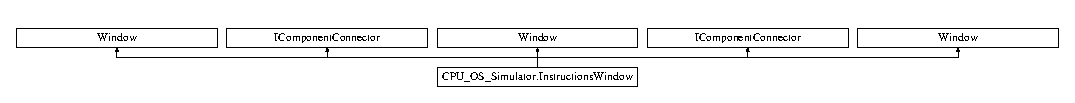
\includegraphics[height=0.929461cm]{class_c_p_u___o_s___simulator_1_1_instructions_window}
\end{center}
\end{figure}
\subsection*{Public Member Functions}
\begin{DoxyCompactItemize}
\item 
\hyperlink{class_c_p_u___o_s___simulator_1_1_instructions_window_aa482ef12f9c98458bedcc3c07d696879}{Instructions\+Window} ()
\begin{DoxyCompactList}\small\item\em Default Constructor for Instruction Window \end{DoxyCompactList}\item 
\hyperlink{class_c_p_u___o_s___simulator_1_1_instructions_window_a5ed238dc308dcc976400105a3973deb0}{Instructions\+Window} (\hyperlink{class_c_p_u___o_s___simulator_1_1_main_window}{Main\+Window} \hyperlink{class_c_p_u___o_s___simulator_1_1_instructions_window_a954c950c677c61a3b7ed7406b6dc7164}{owner})
\begin{DoxyCompactList}\small\item\em Constructor for instruction window that takes the window instance that is creating this window P\+L\+E\+A\+S\+E N\+O\+T\+E\+: This constructor should always be used so data can be passed back to the main window \end{DoxyCompactList}\item 
void \hyperlink{class_c_p_u___o_s___simulator_1_1_instructions_window_a8ad79899f3d5210d66fb5973b721895a}{Initialize\+Component} ()
\begin{DoxyCompactList}\small\item\em Initialize\+Component \end{DoxyCompactList}\item 
void \hyperlink{class_c_p_u___o_s___simulator_1_1_instructions_window_a8ad79899f3d5210d66fb5973b721895a}{Initialize\+Component} ()
\begin{DoxyCompactList}\small\item\em Initialize\+Component \end{DoxyCompactList}\end{DoxyCompactItemize}
\subsection*{Package Attributes}
\begin{DoxyCompactItemize}
\item 
\hyperlink{class_c_p_u___o_s___simulator_1_1_instructions_window}{C\+P\+U\+\_\+\+O\+S\+\_\+\+Simulator.\+Instructions\+Window} \hyperlink{class_c_p_u___o_s___simulator_1_1_instructions_window_ab7cd84f5ba064256327f6b1b1cdbc525}{Instructions\+Window1}
\item 
System.\+Windows.\+Controls.\+Grid \hyperlink{class_c_p_u___o_s___simulator_1_1_instructions_window_a83e86d19573c6c56db33e047354169a1}{grid\+\_\+\+Main}
\item 
System.\+Windows.\+Controls.\+Tab\+Control \hyperlink{class_c_p_u___o_s___simulator_1_1_instructions_window_a2e3784c64a40e14586270c1ebfe8bf3d}{Instruction\+Tabs}
\item 
System.\+Windows.\+Controls.\+Tab\+Item \hyperlink{class_c_p_u___o_s___simulator_1_1_instructions_window_a1076ccccc5b00e3f34ad487bc99b509b}{Data\+Transfer\+Tab}
\item 
System.\+Windows.\+Controls.\+Grid \hyperlink{class_c_p_u___o_s___simulator_1_1_instructions_window_a8e5436d90df63837c7f39586855bda1b}{Tab\+Grid}
\item 
System.\+Windows.\+Controls.\+Label \hyperlink{class_c_p_u___o_s___simulator_1_1_instructions_window_a71ce6968170dda46d83aefc71b63a96d}{label}
\item 
System.\+Windows.\+Controls.\+Grid \hyperlink{class_c_p_u___o_s___simulator_1_1_instructions_window_af568f7891b3381f9bec2f0d5b2d0d8c6}{Instruction\+List\+Grid}
\item 
System.\+Windows.\+Controls.\+List\+Box \hyperlink{class_c_p_u___o_s___simulator_1_1_instructions_window_a03052f893a09b459e840597cf98baffc}{lst\+\_\+\+Opcode\+List\+Data\+Transfer}
\item 
System.\+Windows.\+Controls.\+Grid \hyperlink{class_c_p_u___o_s___simulator_1_1_instructions_window_a6e37ff7da499bab3f5b0037d2b4c68cd}{Source\+Operand\+Grid}
\item 
System.\+Windows.\+Controls.\+Group\+Box \hyperlink{class_c_p_u___o_s___simulator_1_1_instructions_window_ace26d2d0e3de3715d755e91ab04a054a}{grp\+\_\+\+Source\+Operand}
\item 
System.\+Windows.\+Controls.\+Radio\+Button \hyperlink{class_c_p_u___o_s___simulator_1_1_instructions_window_a0798a7bfaace0c96650cf9df53fbf6fd}{rdb\+\_\+\+Source\+Value\+Data\+Transfer}
\item 
System.\+Windows.\+Controls.\+Text\+Box \hyperlink{class_c_p_u___o_s___simulator_1_1_instructions_window_a44cd8a2732d939d1746051f8b2093500}{txt\+Source\+Value\+Data\+Transfer}
\item 
System.\+Windows.\+Controls.\+Radio\+Button \hyperlink{class_c_p_u___o_s___simulator_1_1_instructions_window_a0d449427537f2c5baea2e2b7e669a9d7}{rdb\+\_\+\+Source\+Register\+Data\+Transfer}
\item 
System.\+Windows.\+Controls.\+Combo\+Box \hyperlink{class_c_p_u___o_s___simulator_1_1_instructions_window_ae2136d0a711f92a681278571fbe2868b}{cmb\+\_\+\+Source\+Register\+Data\+Transfer}
\item 
System.\+Windows.\+Controls.\+Grid \hyperlink{class_c_p_u___o_s___simulator_1_1_instructions_window_a46fbe457dccbe131387644a73cc19b19}{Source\+Operand\+Grid\+\_\+\+Copy}
\item 
System.\+Windows.\+Controls.\+Group\+Box \hyperlink{class_c_p_u___o_s___simulator_1_1_instructions_window_a836175caed2a6d02d8635bb6cc3f6cae}{grp\+\_\+\+Destination\+Operand}
\item 
System.\+Windows.\+Controls.\+Radio\+Button \hyperlink{class_c_p_u___o_s___simulator_1_1_instructions_window_a03ff2485a6554464a5c6c2b012dafd1a}{rdb\+\_\+\+Destination\+Value\+Data\+Transfer}
\item 
System.\+Windows.\+Controls.\+Text\+Box \hyperlink{class_c_p_u___o_s___simulator_1_1_instructions_window_a84f7cc6d64bd8050be7c729f469cd29c}{txt\+Destination\+Value\+Data\+Transfer}
\item 
System.\+Windows.\+Controls.\+Radio\+Button \hyperlink{class_c_p_u___o_s___simulator_1_1_instructions_window_a00e9e3013355f592d97a38b29e94899c}{rdb\+\_\+\+Destination\+Register\+Data\+Transfer}
\item 
System.\+Windows.\+Controls.\+Combo\+Box \hyperlink{class_c_p_u___o_s___simulator_1_1_instructions_window_a2cf44cbfe54b2d8f024d5c06067320a1}{cmb\+\_\+\+Destination\+Register\+Data\+Transfer}
\item 
System.\+Windows.\+Controls.\+Text\+Box \hyperlink{class_c_p_u___o_s___simulator_1_1_instructions_window_a58152c12c2022edc73b39c1f95ec7ba4}{txt\+Description\+Data\+Transfer}
\item 
System.\+Windows.\+Controls.\+Tab\+Item \hyperlink{class_c_p_u___o_s___simulator_1_1_instructions_window_a06c53026f495bcbdad82e84bbcb6611c}{Logical\+Tab}
\item 
System.\+Windows.\+Controls.\+Grid \hyperlink{class_c_p_u___o_s___simulator_1_1_instructions_window_a0f8731825bc5369e0328b2b9580e9b67}{Tab\+Grid\+\_\+\+Copy}
\item 
System.\+Windows.\+Controls.\+Label \hyperlink{class_c_p_u___o_s___simulator_1_1_instructions_window_a499640eb8a98693f1833dad30f5d8cb4}{label1}
\item 
System.\+Windows.\+Controls.\+Grid \hyperlink{class_c_p_u___o_s___simulator_1_1_instructions_window_a8f09b0005016c225169d7e9dd2724053}{Instruction\+List\+Grid1}
\item 
System.\+Windows.\+Controls.\+List\+Box \hyperlink{class_c_p_u___o_s___simulator_1_1_instructions_window_a61ee2cb0ba7197963b1138848778cd3c}{lst\+\_\+\+Opcode\+List\+Logical}
\item 
System.\+Windows.\+Controls.\+Grid \hyperlink{class_c_p_u___o_s___simulator_1_1_instructions_window_a3f9d1afc4455fa6b06c6fab3cdb6aeec}{Source\+Operand\+Grid1}
\item 
System.\+Windows.\+Controls.\+Group\+Box \hyperlink{class_c_p_u___o_s___simulator_1_1_instructions_window_a74e13776576d1a6ee5767e3fc8f6ec7f}{grp\+\_\+\+Source\+Operand1}
\item 
System.\+Windows.\+Controls.\+Radio\+Button \hyperlink{class_c_p_u___o_s___simulator_1_1_instructions_window_ad0e882b0d6d067460309ae6f1dda5d56}{rdb\+\_\+\+Source\+Value\+Logical}
\item 
System.\+Windows.\+Controls.\+Text\+Box \hyperlink{class_c_p_u___o_s___simulator_1_1_instructions_window_afac2309550dd6f1f1589dc7451e8f878}{txt\+Source\+Value\+Logical}
\item 
System.\+Windows.\+Controls.\+Radio\+Button \hyperlink{class_c_p_u___o_s___simulator_1_1_instructions_window_ab8c8622e8a96238fb88e455d60c51e78}{rdb\+\_\+\+Source\+Register\+Logical}
\item 
System.\+Windows.\+Controls.\+Combo\+Box \hyperlink{class_c_p_u___o_s___simulator_1_1_instructions_window_a46a9647a5a6e661afb789b1faa95a15a}{cmb\+\_\+\+Source\+Register\+Logical}
\item 
System.\+Windows.\+Controls.\+Grid \hyperlink{class_c_p_u___o_s___simulator_1_1_instructions_window_a685393ff28189e8c998e2a7dc6018b32}{Source\+Operand\+Grid\+\_\+\+Copy1}
\item 
System.\+Windows.\+Controls.\+Group\+Box \hyperlink{class_c_p_u___o_s___simulator_1_1_instructions_window_ab89f01ff39ce6f5ed461fcf5242be3a5}{grp\+\_\+\+Destination\+Operand1}
\item 
System.\+Windows.\+Controls.\+Radio\+Button \hyperlink{class_c_p_u___o_s___simulator_1_1_instructions_window_a73ba820a305842d3dea1ad79e6e87e6d}{rdb\+\_\+\+Destination\+Value\+Logical}
\item 
System.\+Windows.\+Controls.\+Text\+Box \hyperlink{class_c_p_u___o_s___simulator_1_1_instructions_window_af1a2860f125c3a8e25c73c1b04290438}{txt\+Destination\+Value\+Logical}
\item 
System.\+Windows.\+Controls.\+Radio\+Button \hyperlink{class_c_p_u___o_s___simulator_1_1_instructions_window_a3670f5971b586bd8977a78bcde185a35}{rdb\+\_\+\+Destination\+Register\+Logical}
\item 
System.\+Windows.\+Controls.\+Combo\+Box \hyperlink{class_c_p_u___o_s___simulator_1_1_instructions_window_aefcd87b5db00ac68e7d80ac5fddce8c5}{cmb\+\_\+\+Destination\+Register\+Logical}
\item 
System.\+Windows.\+Controls.\+Text\+Box \hyperlink{class_c_p_u___o_s___simulator_1_1_instructions_window_ae465810d61bb136b7934563cf85b3027}{txt\+Description\+Logical}
\item 
System.\+Windows.\+Controls.\+Tab\+Item \hyperlink{class_c_p_u___o_s___simulator_1_1_instructions_window_aabf61d7cbf8be85bb4ab0ef2d0614b46}{Arithmetic\+Tab}
\item 
System.\+Windows.\+Controls.\+Grid \hyperlink{class_c_p_u___o_s___simulator_1_1_instructions_window_a834965d0ae6a57edb71a818dca188a30}{Tab\+Grid\+\_\+\+Copy1}
\item 
System.\+Windows.\+Controls.\+Label \hyperlink{class_c_p_u___o_s___simulator_1_1_instructions_window_a237621e58e68c4a07cdf8803cc1614fd}{label2}
\item 
System.\+Windows.\+Controls.\+Grid \hyperlink{class_c_p_u___o_s___simulator_1_1_instructions_window_a33108da9779c5108fc5dd303a8d33454}{Instruction\+List\+Grid2}
\item 
System.\+Windows.\+Controls.\+List\+Box \hyperlink{class_c_p_u___o_s___simulator_1_1_instructions_window_a7445b276d3723f67ba564038940d44c5}{lst\+\_\+\+Opcode\+List\+Arithmetic}
\item 
System.\+Windows.\+Controls.\+Grid \hyperlink{class_c_p_u___o_s___simulator_1_1_instructions_window_a715ed01337540f316f39fe42c373c602}{Source\+Operand\+Grid2}
\item 
System.\+Windows.\+Controls.\+Group\+Box \hyperlink{class_c_p_u___o_s___simulator_1_1_instructions_window_ad37aae3614abd76749236a7739fbc18b}{grp\+\_\+\+Source\+Operand2}
\item 
System.\+Windows.\+Controls.\+Radio\+Button \hyperlink{class_c_p_u___o_s___simulator_1_1_instructions_window_a627e9cbe7e0cb2ce0f109f2345e19b73}{rdb\+\_\+\+Source\+Value\+Arithmetic}
\item 
System.\+Windows.\+Controls.\+Text\+Box \hyperlink{class_c_p_u___o_s___simulator_1_1_instructions_window_afc01788dc74f761b6cce800975394d2e}{txt\+Source\+Value\+Arithmetic}
\item 
System.\+Windows.\+Controls.\+Radio\+Button \hyperlink{class_c_p_u___o_s___simulator_1_1_instructions_window_ad571b65d5fe87bdb079c807dcac0680f}{rdb\+\_\+\+Source\+Register\+Arithmetic}
\item 
System.\+Windows.\+Controls.\+Combo\+Box \hyperlink{class_c_p_u___o_s___simulator_1_1_instructions_window_aad493dd174601ec265d5ad261f33d525}{cmb\+\_\+\+Source\+Register\+Arithmetic}
\item 
System.\+Windows.\+Controls.\+Grid \hyperlink{class_c_p_u___o_s___simulator_1_1_instructions_window_a6a57e0ae92b85cd619ef3d879ef0c628}{Source\+Operand\+Grid\+\_\+\+Copy2}
\item 
System.\+Windows.\+Controls.\+Group\+Box \hyperlink{class_c_p_u___o_s___simulator_1_1_instructions_window_adc32bbf0f47985507d606abb4862072f}{grp\+\_\+\+Destination\+Operand2}
\item 
System.\+Windows.\+Controls.\+Radio\+Button \hyperlink{class_c_p_u___o_s___simulator_1_1_instructions_window_a2e87a90d55ec015190b55bd06c273efc}{rdb\+\_\+\+Destination\+Value\+Arithmetic}
\item 
System.\+Windows.\+Controls.\+Text\+Box \hyperlink{class_c_p_u___o_s___simulator_1_1_instructions_window_adac073cb591b15be22d041695ff498e4}{txt\+Destination\+Value\+Arithmetic}
\item 
System.\+Windows.\+Controls.\+Radio\+Button \hyperlink{class_c_p_u___o_s___simulator_1_1_instructions_window_a40ebdc8941fbd7ae75ca6d14d1153569}{rdb\+\_\+\+Destination\+Register\+Arithmetic}
\item 
System.\+Windows.\+Controls.\+Combo\+Box \hyperlink{class_c_p_u___o_s___simulator_1_1_instructions_window_ad1fafd2bef9ad3f94fab585ea58fc38c}{cmb\+\_\+\+Destination\+Register\+Arithmetic}
\item 
System.\+Windows.\+Controls.\+Text\+Box \hyperlink{class_c_p_u___o_s___simulator_1_1_instructions_window_a31ef64d4c64f9791d6b4aad95cd4d95f}{txt\+Description\+Arithmetic}
\item 
System.\+Windows.\+Controls.\+Tab\+Item \hyperlink{class_c_p_u___o_s___simulator_1_1_instructions_window_a52cb165b57f01928c088b3052de70b5b}{Control\+Tranfer\+Tab}
\item 
System.\+Windows.\+Controls.\+Grid \hyperlink{class_c_p_u___o_s___simulator_1_1_instructions_window_ac4b83982bf62dc5c0484ac2729167ba4}{Tab\+Grid\+\_\+\+Copy2}
\item 
System.\+Windows.\+Controls.\+Label \hyperlink{class_c_p_u___o_s___simulator_1_1_instructions_window_a394b28c312ae1a83128da41990fc5d32}{label3}
\item 
System.\+Windows.\+Controls.\+Grid \hyperlink{class_c_p_u___o_s___simulator_1_1_instructions_window_a3cc76cf3ae5c4155d0e30727eb357d12}{Instruction\+List\+Grid3}
\item 
System.\+Windows.\+Controls.\+List\+Box \hyperlink{class_c_p_u___o_s___simulator_1_1_instructions_window_a111f1ddd903fe40e0c83efeca42bdf51}{lst\+\_\+\+Opcode\+List\+Control\+Transfer}
\item 
System.\+Windows.\+Controls.\+Grid \hyperlink{class_c_p_u___o_s___simulator_1_1_instructions_window_ab8409532df6419d7f7ce0c3450807906}{Source\+Operand\+Grid3}
\item 
System.\+Windows.\+Controls.\+Group\+Box \hyperlink{class_c_p_u___o_s___simulator_1_1_instructions_window_a59e5e9da77976ce8f2d8a43528b98f63}{grp\+\_\+\+Source\+Operand3}
\item 
System.\+Windows.\+Controls.\+Radio\+Button \hyperlink{class_c_p_u___o_s___simulator_1_1_instructions_window_a590a2e5af41ea5cf215da3ff7dd1b20b}{rdb\+\_\+\+Source\+Value\+Control\+Transfer}
\item 
System.\+Windows.\+Controls.\+Text\+Box \hyperlink{class_c_p_u___o_s___simulator_1_1_instructions_window_a602831ff353007879c08b22d373a2ba5}{txt\+Source\+Value\+Control\+Transfer}
\item 
System.\+Windows.\+Controls.\+Radio\+Button \hyperlink{class_c_p_u___o_s___simulator_1_1_instructions_window_a63fea6d97a26f4ed71753209dac85d24}{rdb\+\_\+\+Source\+Register\+Control\+Transfer}
\item 
System.\+Windows.\+Controls.\+Combo\+Box \hyperlink{class_c_p_u___o_s___simulator_1_1_instructions_window_a652354e464657693cf70a292b3389626}{cmb\+\_\+\+Source\+Register\+Control\+Transfer}
\item 
System.\+Windows.\+Controls.\+Grid \hyperlink{class_c_p_u___o_s___simulator_1_1_instructions_window_ac37123264ae139f4abc30841da21cd23}{Source\+Operand\+Grid\+\_\+\+Copy3}
\item 
System.\+Windows.\+Controls.\+Group\+Box \hyperlink{class_c_p_u___o_s___simulator_1_1_instructions_window_a175eb53a0a0f48be4d8717f1e5a5942e}{grp\+\_\+\+Destination\+Operand3}
\item 
System.\+Windows.\+Controls.\+Radio\+Button \hyperlink{class_c_p_u___o_s___simulator_1_1_instructions_window_afedaca6e4102fbae9f5db622be1b839d}{rdb\+\_\+\+Destination\+Value\+Control\+Transfer}
\item 
System.\+Windows.\+Controls.\+Text\+Box \hyperlink{class_c_p_u___o_s___simulator_1_1_instructions_window_a0049dce789d892e6620158859bcf7057}{txt\+Destination\+Value\+Control\+Transfer}
\item 
System.\+Windows.\+Controls.\+Radio\+Button \hyperlink{class_c_p_u___o_s___simulator_1_1_instructions_window_a4911636b6e093aa89155a0f5db4b3118}{rdb\+\_\+\+Destination\+Register\+Control\+Transfer}
\item 
System.\+Windows.\+Controls.\+Combo\+Box \hyperlink{class_c_p_u___o_s___simulator_1_1_instructions_window_a9017d3508e5dde75eafec25e94611c97}{cmb\+\_\+\+Destination\+Register\+Control\+Transfer}
\item 
System.\+Windows.\+Controls.\+Text\+Box \hyperlink{class_c_p_u___o_s___simulator_1_1_instructions_window_af8667a9cb444eb6aaa84349fe194b853}{txt\+Description\+Control\+Transfer}
\item 
System.\+Windows.\+Controls.\+Tab\+Item \hyperlink{class_c_p_u___o_s___simulator_1_1_instructions_window_ab807abcf9c3955ae2ff78e1d667820b2}{Comparison\+Tab}
\item 
System.\+Windows.\+Controls.\+Grid \hyperlink{class_c_p_u___o_s___simulator_1_1_instructions_window_a8a50487f6e6acca8a58ffe218e32abe2}{Tab\+Grid\+\_\+\+Copy3}
\item 
System.\+Windows.\+Controls.\+Label \hyperlink{class_c_p_u___o_s___simulator_1_1_instructions_window_a6d028c99fa713c891d86c07ef46f083b}{label4}
\item 
System.\+Windows.\+Controls.\+Grid \hyperlink{class_c_p_u___o_s___simulator_1_1_instructions_window_a9cdd58a2e38d3f0b047b6eb64b43ea03}{Instruction\+List\+Grid4}
\item 
System.\+Windows.\+Controls.\+List\+Box \hyperlink{class_c_p_u___o_s___simulator_1_1_instructions_window_ae47949fa5657e55f8acd8e5b9cd204c0}{lst\+\_\+\+Opcode\+List\+Comparison}
\item 
System.\+Windows.\+Controls.\+Grid \hyperlink{class_c_p_u___o_s___simulator_1_1_instructions_window_ac28180235c174caa7a2870120a9258bb}{Source\+Operand\+Grid4}
\item 
System.\+Windows.\+Controls.\+Group\+Box \hyperlink{class_c_p_u___o_s___simulator_1_1_instructions_window_a0efec3cdad460e3596a699716e0a24e9}{grp\+\_\+\+Source\+Operand4}
\item 
System.\+Windows.\+Controls.\+Radio\+Button \hyperlink{class_c_p_u___o_s___simulator_1_1_instructions_window_a6232aa7952b3d4ea71c55eb14267f188}{rdb\+\_\+\+Source\+Value\+Comparison}
\item 
System.\+Windows.\+Controls.\+Text\+Box \hyperlink{class_c_p_u___o_s___simulator_1_1_instructions_window_a8dd17881b7fd4e1923899b5bcae171fc}{txt\+Source\+Value\+Comparison}
\item 
System.\+Windows.\+Controls.\+Radio\+Button \hyperlink{class_c_p_u___o_s___simulator_1_1_instructions_window_afa2620b93d7d354b0632d7c290022545}{rdb\+\_\+\+Source\+Register\+Comparison}
\item 
System.\+Windows.\+Controls.\+Combo\+Box \hyperlink{class_c_p_u___o_s___simulator_1_1_instructions_window_af7acb32053b1cf27ee94bbf47efc9fbe}{cmb\+\_\+\+Source\+Register\+Comparison}
\item 
System.\+Windows.\+Controls.\+Grid \hyperlink{class_c_p_u___o_s___simulator_1_1_instructions_window_aa8c70305e3c77644ac312df74b0696b7}{Source\+Operand\+Grid\+\_\+\+Copy4}
\item 
System.\+Windows.\+Controls.\+Group\+Box \hyperlink{class_c_p_u___o_s___simulator_1_1_instructions_window_a68c2f892a54f7826baacf9c828431fa8}{grp\+\_\+\+Destination\+Operand4}
\item 
System.\+Windows.\+Controls.\+Radio\+Button \hyperlink{class_c_p_u___o_s___simulator_1_1_instructions_window_a200445a2378fddf69041aecbbcdf68fb}{rdb\+\_\+\+Destination\+Value\+Comparison}
\item 
System.\+Windows.\+Controls.\+Text\+Box \hyperlink{class_c_p_u___o_s___simulator_1_1_instructions_window_ab44686bd174144a0c1042579d6665547}{txt\+Destination\+Value\+Comparison}
\item 
System.\+Windows.\+Controls.\+Radio\+Button \hyperlink{class_c_p_u___o_s___simulator_1_1_instructions_window_af5369f91639cf92cbb6bd89118d6e373}{rdb\+\_\+\+Destination\+Register\+Comparison}
\item 
System.\+Windows.\+Controls.\+Combo\+Box \hyperlink{class_c_p_u___o_s___simulator_1_1_instructions_window_af209ebdcd0b9ae6c267388b382dac245}{cmb\+\_\+\+Destination\+Register\+Comparison}
\item 
System.\+Windows.\+Controls.\+Text\+Box \hyperlink{class_c_p_u___o_s___simulator_1_1_instructions_window_a1ac2050428b5ece7f1f6791771e9cef6}{txt\+Description\+Comparison}
\item 
System.\+Windows.\+Controls.\+Tab\+Item \hyperlink{class_c_p_u___o_s___simulator_1_1_instructions_window_aaf736178464d8313c866ab6efeae19c5}{I\+O\+Tab}
\item 
System.\+Windows.\+Controls.\+Grid \hyperlink{class_c_p_u___o_s___simulator_1_1_instructions_window_a33c64471b02aed8597462149051c2b51}{Tab\+Grid\+\_\+\+Copy4}
\item 
System.\+Windows.\+Controls.\+Label \hyperlink{class_c_p_u___o_s___simulator_1_1_instructions_window_acfbda3e1b251a166abc72a07d4cb5025}{label5}
\item 
System.\+Windows.\+Controls.\+Grid \hyperlink{class_c_p_u___o_s___simulator_1_1_instructions_window_a335e8ec02a78ffc483900745de96b602}{Instruction\+List\+Grid5}
\item 
System.\+Windows.\+Controls.\+List\+Box \hyperlink{class_c_p_u___o_s___simulator_1_1_instructions_window_aa8ccd453237503f0e15aff22975cea68}{lst\+\_\+\+Opcode\+List\+I\+O}
\item 
System.\+Windows.\+Controls.\+Grid \hyperlink{class_c_p_u___o_s___simulator_1_1_instructions_window_a3066f4664c81bacc6decdf84d08e74a9}{Source\+Operand\+Grid5}
\item 
System.\+Windows.\+Controls.\+Group\+Box \hyperlink{class_c_p_u___o_s___simulator_1_1_instructions_window_ab16ea5f8e2e761d0a7a0fe7054dfa3b5}{grp\+\_\+\+Source\+Operand5}
\item 
System.\+Windows.\+Controls.\+Radio\+Button \hyperlink{class_c_p_u___o_s___simulator_1_1_instructions_window_ad7bb114a6f948e79e55a44943ecf660a}{rdb\+\_\+\+Source\+Value\+I\+O}
\item 
System.\+Windows.\+Controls.\+Text\+Box \hyperlink{class_c_p_u___o_s___simulator_1_1_instructions_window_a14161b7bebd71e7545b59f77f6254a26}{txt\+Source\+Value\+I\+O}
\item 
System.\+Windows.\+Controls.\+Radio\+Button \hyperlink{class_c_p_u___o_s___simulator_1_1_instructions_window_a30064f400e25a6b155a34108a3fba816}{rdb\+\_\+\+Source\+Register\+I\+O}
\item 
System.\+Windows.\+Controls.\+Combo\+Box \hyperlink{class_c_p_u___o_s___simulator_1_1_instructions_window_a9f9d831a77d174675da89b1fe03602ad}{cmb\+\_\+\+Source\+Register\+I\+O}
\item 
System.\+Windows.\+Controls.\+Grid \hyperlink{class_c_p_u___o_s___simulator_1_1_instructions_window_a5a43b8933f014dffe28d3aa610518a94}{Source\+Operand\+Grid\+\_\+\+Copy5}
\item 
System.\+Windows.\+Controls.\+Group\+Box \hyperlink{class_c_p_u___o_s___simulator_1_1_instructions_window_aa99ecad0d35bc5e70a8924c9b3913106}{grp\+\_\+\+Destination\+Operand5}
\item 
System.\+Windows.\+Controls.\+Radio\+Button \hyperlink{class_c_p_u___o_s___simulator_1_1_instructions_window_a012739d419d605946f5dc0fd645db182}{rdb\+\_\+\+Destination\+Value\+I\+O}
\item 
System.\+Windows.\+Controls.\+Text\+Box \hyperlink{class_c_p_u___o_s___simulator_1_1_instructions_window_afd9084fd83f0c60a4fa1bba1cbcaf5af}{txt\+Destination\+Value\+I\+O}
\item 
System.\+Windows.\+Controls.\+Radio\+Button \hyperlink{class_c_p_u___o_s___simulator_1_1_instructions_window_a507ebe0998697ce8b2345fac2d9498a1}{rdb\+\_\+\+Destination\+Register\+I\+O}
\item 
System.\+Windows.\+Controls.\+Combo\+Box \hyperlink{class_c_p_u___o_s___simulator_1_1_instructions_window_a821452c6d5ab7be60996d3171a2d4cf1}{cmb\+\_\+\+Destination\+Register\+I\+O}
\item 
System.\+Windows.\+Controls.\+Text\+Box \hyperlink{class_c_p_u___o_s___simulator_1_1_instructions_window_a278020eeca6ae302ab5530cca856acde}{txt\+Description\+I\+O}
\item 
System.\+Windows.\+Controls.\+Tab\+Item \hyperlink{class_c_p_u___o_s___simulator_1_1_instructions_window_ab7e1bbdc8bb2830d39fb9a4339aa27f2}{Miscellaneous\+Tab}
\item 
System.\+Windows.\+Controls.\+Grid \hyperlink{class_c_p_u___o_s___simulator_1_1_instructions_window_a495a21e0e96f26f87d3e379ab286256b}{Tab\+Grid\+\_\+\+Copy5}
\item 
System.\+Windows.\+Controls.\+Label \hyperlink{class_c_p_u___o_s___simulator_1_1_instructions_window_a23cbea70a5e1ab92348a9569f362db07}{label6}
\item 
System.\+Windows.\+Controls.\+Grid \hyperlink{class_c_p_u___o_s___simulator_1_1_instructions_window_a6c86a044f242ee64f312f0105bac6d36}{Instruction\+List\+Grid6}
\item 
System.\+Windows.\+Controls.\+List\+Box \hyperlink{class_c_p_u___o_s___simulator_1_1_instructions_window_a3ac59be147d3323d2b485551b3a3640a}{lst\+\_\+\+Opcode\+List\+Miscellaneous}
\item 
System.\+Windows.\+Controls.\+Grid \hyperlink{class_c_p_u___o_s___simulator_1_1_instructions_window_a1036ae92003998bc7e7062a73358adec}{Source\+Operand\+Grid6}
\item 
System.\+Windows.\+Controls.\+Group\+Box \hyperlink{class_c_p_u___o_s___simulator_1_1_instructions_window_a46c1f50385d01108637e574343a99bfd}{grp\+\_\+\+Source\+Operand6}
\item 
System.\+Windows.\+Controls.\+Radio\+Button \hyperlink{class_c_p_u___o_s___simulator_1_1_instructions_window_ae6e33f7879251b63282f5d3eaa693507}{rdb\+\_\+\+Source\+Value\+Miscellaneous}
\item 
System.\+Windows.\+Controls.\+Text\+Box \hyperlink{class_c_p_u___o_s___simulator_1_1_instructions_window_a555d604d5869d89442a35900abc35914}{txt\+Source\+Value\+Miscellaneous}
\item 
System.\+Windows.\+Controls.\+Radio\+Button \hyperlink{class_c_p_u___o_s___simulator_1_1_instructions_window_ad2b0098ef721214b53b9e3241e611a84}{rdb\+\_\+\+Source\+Register\+Miscellaneous}
\item 
System.\+Windows.\+Controls.\+Combo\+Box \hyperlink{class_c_p_u___o_s___simulator_1_1_instructions_window_a98245ef6ca4796b7f59fe4b9937a388e}{cmb\+\_\+\+Source\+Register\+Miscellaneous}
\item 
System.\+Windows.\+Controls.\+Grid \hyperlink{class_c_p_u___o_s___simulator_1_1_instructions_window_a3dfdd68ad6b08fb1612fd43a420e5193}{Source\+Operand\+Grid\+\_\+\+Copy6}
\item 
System.\+Windows.\+Controls.\+Group\+Box \hyperlink{class_c_p_u___o_s___simulator_1_1_instructions_window_a8e457b3503625b5e837320ad9eb439c6}{grp\+\_\+\+Destination\+Operand6}
\item 
System.\+Windows.\+Controls.\+Radio\+Button \hyperlink{class_c_p_u___o_s___simulator_1_1_instructions_window_a567c8bba810d30e3c382e527e132a230}{rdb\+\_\+\+Destination\+Value\+Miscellaneous}
\item 
System.\+Windows.\+Controls.\+Text\+Box \hyperlink{class_c_p_u___o_s___simulator_1_1_instructions_window_a7fa1615bacb3264ac8ce61787a28d477}{txt\+Destination\+Value\+Miscellaneous}
\item 
System.\+Windows.\+Controls.\+Radio\+Button \hyperlink{class_c_p_u___o_s___simulator_1_1_instructions_window_adc4aa664244631ae1240a81d5c3b8ab5}{rdb\+\_\+\+Destination\+Register\+Miscellaneous}
\item 
System.\+Windows.\+Controls.\+Combo\+Box \hyperlink{class_c_p_u___o_s___simulator_1_1_instructions_window_ac4dab6ef32a46a295d6937b6bbda7813}{cmb\+\_\+\+Destination\+Register\+Miscellaneous}
\item 
System.\+Windows.\+Controls.\+Text\+Box \hyperlink{class_c_p_u___o_s___simulator_1_1_instructions_window_aaf938911ac6e23d7d637245cf40e6cbe}{txt\+Description\+Miscellaneous}
\item 
System.\+Windows.\+Controls.\+Button \hyperlink{class_c_p_u___o_s___simulator_1_1_instructions_window_a06305ca0735ae2d93a331fb33d2fe88f}{btn\+\_\+\+Close}
\end{DoxyCompactItemize}
\subsection*{Private Member Functions}
\begin{DoxyCompactItemize}
\item 
void \hyperlink{class_c_p_u___o_s___simulator_1_1_instructions_window_a52685f2ecc3d1cf7216716401d2621e0}{Populate\+Instructions} ()
\begin{DoxyCompactList}\small\item\em this function populates each of the instruction list boxes with the correct instructions \end{DoxyCompactList}\item 
void \hyperlink{class_c_p_u___o_s___simulator_1_1_instructions_window_a5fd3510dda95cf73b61af11ccacd81cd}{btn\+\_\+\+Close\+\_\+\+Click} (object sender, Routed\+Event\+Args e)
\begin{DoxyCompactList}\small\item\em This event handler is called when the close button is clicked \end{DoxyCompactList}\item 
void \hyperlink{class_c_p_u___o_s___simulator_1_1_instructions_window_a7d985ca63f2e27bc03a2198ec6879b49}{Window\+\_\+\+Loaded} (object sender, Routed\+Event\+Args e)
\begin{DoxyCompactList}\small\item\em This event handler is called when the window first loads \end{DoxyCompactList}\item 
void \hyperlink{class_c_p_u___o_s___simulator_1_1_instructions_window_a380aec4afa9900f7dd9ef964a5b86503}{lst\+\_\+\+Opcode\+List\+Data\+Transfer\+\_\+\+Selection\+Changed} (object sender, Selection\+Changed\+Event\+Args e)
\item 
void \hyperlink{class_c_p_u___o_s___simulator_1_1_instructions_window_a245baef3e788a01e6cf752f2c48f1843}{lst\+\_\+\+Opcode\+List\+Logical\+\_\+\+Selection\+Changed} (object sender, Selection\+Changed\+Event\+Args e)
\item 
void \hyperlink{class_c_p_u___o_s___simulator_1_1_instructions_window_ab4001352180ad08e3b335bf80c7dd9b8}{lst\+\_\+\+Opcode\+List\+Arithmetic\+\_\+\+Selection\+Changed} (object sender, Selection\+Changed\+Event\+Args e)
\item 
void \hyperlink{class_c_p_u___o_s___simulator_1_1_instructions_window_ac5b4dea0d3fe645b7f0bf9201cb0ad1c}{Instructions\+Window1\+\_\+\+Closing} (object sender, Cancel\+Event\+Args e)
\begin{DoxyCompactList}\small\item\em This event handler is called when the window is closing \end{DoxyCompactList}\item 
\hyperlink{class_c_p_u___o_s___simulator_1_1_c_p_u_1_1_register}{Register} \hyperlink{class_c_p_u___o_s___simulator_1_1_instructions_window_a2fbd163f2638a32f7cfbf831dc91582f}{Find\+Register} (string selected\+Item)
\begin{DoxyCompactList}\small\item\em Finds the register object for the selected register \end{DoxyCompactList}\item 
void \hyperlink{class_c_p_u___o_s___simulator_1_1_instructions_window_adce5e32de39213723ea06d279681b8ea}{rdb\+\_\+\+Source\+Value\+Data\+Transfer\+\_\+\+Checked} (object sender, Routed\+Event\+Args e)
\item 
void \hyperlink{class_c_p_u___o_s___simulator_1_1_instructions_window_aec7d6be51c8cd95dce4db01a5c66047e}{rdb\+\_\+\+Source\+Register\+Data\+Transfer\+\_\+\+Checked} (object sender, Routed\+Event\+Args e)
\item 
void \hyperlink{class_c_p_u___o_s___simulator_1_1_instructions_window_a8572bfa72449f43f800dd55961ad7837}{rdb\+\_\+\+Destination\+Value\+Data\+Transfer\+\_\+\+Checked} (object sender, Routed\+Event\+Args e)
\item 
void \hyperlink{class_c_p_u___o_s___simulator_1_1_instructions_window_a61a12a00e2f822ca948b2216b5dd85db}{rdb\+\_\+\+Destination\+Register\+Data\+Transfer\+\_\+\+Checked} (object sender, Routed\+Event\+Args e)
\item 
void System.\+Windows.\+Markup.\+I\+Component\+Connector. \hyperlink{class_c_p_u___o_s___simulator_1_1_instructions_window_a0efa7624a59a6abc64d0940ffaa100b0}{Connect} (int connection\+Id, object target)
\item 
void System.\+Windows.\+Markup.\+I\+Component\+Connector. \hyperlink{class_c_p_u___o_s___simulator_1_1_instructions_window_a0efa7624a59a6abc64d0940ffaa100b0}{Connect} (int connection\+Id, object target)
\end{DoxyCompactItemize}
\subsection*{Private Attributes}
\begin{DoxyCompactItemize}
\item 
List$<$ string $>$ \hyperlink{class_c_p_u___o_s___simulator_1_1_instructions_window_a678ab4df2b78758142472eeed8c5d7ba}{instruction\+Descriptions} = new List$<$string$>$()
\begin{DoxyCompactList}\small\item\em List to hold the descriptions of each instruction \end{DoxyCompactList}\item 
\hyperlink{class_c_p_u___o_s___simulator_1_1_main_window}{Main\+Window} \hyperlink{class_c_p_u___o_s___simulator_1_1_instructions_window_a954c950c677c61a3b7ed7406b6dc7164}{owner}
\begin{DoxyCompactList}\small\item\em The window that owns this window \end{DoxyCompactList}\item 
bool \hyperlink{class_c_p_u___o_s___simulator_1_1_instructions_window_a7755282dffea134038e9e58c931dc297}{\+\_\+content\+Loaded}
\end{DoxyCompactItemize}


\subsection{Detailed Description}
Interaction logic for Instructions\+Window.\+xaml 

\hyperlink{class_c_p_u___o_s___simulator_1_1_instructions_window}{Instructions\+Window} 

Definition at line 23 of file Instructions\+Window.\+xaml.\+cs.



\subsection{Constructor \& Destructor Documentation}
\hypertarget{class_c_p_u___o_s___simulator_1_1_instructions_window_aa482ef12f9c98458bedcc3c07d696879}{}\index{C\+P\+U\+\_\+\+O\+S\+\_\+\+Simulator\+::\+Instructions\+Window@{C\+P\+U\+\_\+\+O\+S\+\_\+\+Simulator\+::\+Instructions\+Window}!Instructions\+Window@{Instructions\+Window}}
\index{Instructions\+Window@{Instructions\+Window}!C\+P\+U\+\_\+\+O\+S\+\_\+\+Simulator\+::\+Instructions\+Window@{C\+P\+U\+\_\+\+O\+S\+\_\+\+Simulator\+::\+Instructions\+Window}}
\subsubsection[{Instructions\+Window()}]{\setlength{\rightskip}{0pt plus 5cm}C\+P\+U\+\_\+\+O\+S\+\_\+\+Simulator.\+Instructions\+Window.\+Instructions\+Window (
\begin{DoxyParamCaption}
{}
\end{DoxyParamCaption}
)}\label{class_c_p_u___o_s___simulator_1_1_instructions_window_aa482ef12f9c98458bedcc3c07d696879}


Default Constructor for Instruction Window 



Definition at line 36 of file Instructions\+Window.\+xaml.\+cs.

\hypertarget{class_c_p_u___o_s___simulator_1_1_instructions_window_a5ed238dc308dcc976400105a3973deb0}{}\index{C\+P\+U\+\_\+\+O\+S\+\_\+\+Simulator\+::\+Instructions\+Window@{C\+P\+U\+\_\+\+O\+S\+\_\+\+Simulator\+::\+Instructions\+Window}!Instructions\+Window@{Instructions\+Window}}
\index{Instructions\+Window@{Instructions\+Window}!C\+P\+U\+\_\+\+O\+S\+\_\+\+Simulator\+::\+Instructions\+Window@{C\+P\+U\+\_\+\+O\+S\+\_\+\+Simulator\+::\+Instructions\+Window}}
\subsubsection[{Instructions\+Window(\+Main\+Window owner)}]{\setlength{\rightskip}{0pt plus 5cm}C\+P\+U\+\_\+\+O\+S\+\_\+\+Simulator.\+Instructions\+Window.\+Instructions\+Window (
\begin{DoxyParamCaption}
\item[{{\bf Main\+Window}}]{owner}
\end{DoxyParamCaption}
)}\label{class_c_p_u___o_s___simulator_1_1_instructions_window_a5ed238dc308dcc976400105a3973deb0}


Constructor for instruction window that takes the window instance that is creating this window P\+L\+E\+A\+S\+E N\+O\+T\+E\+: This constructor should always be used so data can be passed back to the main window 


\begin{DoxyParams}{Parameters}
{\em owner} & The window that is creating this window \\
\hline
\end{DoxyParams}


Definition at line 45 of file Instructions\+Window.\+xaml.\+cs.



\subsection{Member Function Documentation}
\hypertarget{class_c_p_u___o_s___simulator_1_1_instructions_window_a5fd3510dda95cf73b61af11ccacd81cd}{}\index{C\+P\+U\+\_\+\+O\+S\+\_\+\+Simulator\+::\+Instructions\+Window@{C\+P\+U\+\_\+\+O\+S\+\_\+\+Simulator\+::\+Instructions\+Window}!btn\+\_\+\+Close\+\_\+\+Click@{btn\+\_\+\+Close\+\_\+\+Click}}
\index{btn\+\_\+\+Close\+\_\+\+Click@{btn\+\_\+\+Close\+\_\+\+Click}!C\+P\+U\+\_\+\+O\+S\+\_\+\+Simulator\+::\+Instructions\+Window@{C\+P\+U\+\_\+\+O\+S\+\_\+\+Simulator\+::\+Instructions\+Window}}
\subsubsection[{btn\+\_\+\+Close\+\_\+\+Click(object sender, Routed\+Event\+Args e)}]{\setlength{\rightskip}{0pt plus 5cm}void C\+P\+U\+\_\+\+O\+S\+\_\+\+Simulator.\+Instructions\+Window.\+btn\+\_\+\+Close\+\_\+\+Click (
\begin{DoxyParamCaption}
\item[{object}]{sender, }
\item[{Routed\+Event\+Args}]{e}
\end{DoxyParamCaption}
)\hspace{0.3cm}{\ttfamily [private]}}\label{class_c_p_u___o_s___simulator_1_1_instructions_window_a5fd3510dda95cf73b61af11ccacd81cd}


This event handler is called when the close button is clicked 


\begin{DoxyParams}{Parameters}
{\em sender} & the object that fired this event\\
\hline
{\em e} & the eventargs associated with this event\\
\hline
\end{DoxyParams}


Definition at line 96 of file Instructions\+Window.\+xaml.\+cs.

\hypertarget{class_c_p_u___o_s___simulator_1_1_instructions_window_a0efa7624a59a6abc64d0940ffaa100b0}{}\index{C\+P\+U\+\_\+\+O\+S\+\_\+\+Simulator\+::\+Instructions\+Window@{C\+P\+U\+\_\+\+O\+S\+\_\+\+Simulator\+::\+Instructions\+Window}!Connect@{Connect}}
\index{Connect@{Connect}!C\+P\+U\+\_\+\+O\+S\+\_\+\+Simulator\+::\+Instructions\+Window@{C\+P\+U\+\_\+\+O\+S\+\_\+\+Simulator\+::\+Instructions\+Window}}
\subsubsection[{Connect(int connection\+Id, object target)}]{\setlength{\rightskip}{0pt plus 5cm}void System.\+Windows.\+Markup.\+I\+Component\+Connector. C\+P\+U\+\_\+\+O\+S\+\_\+\+Simulator.\+Instructions\+Window.\+Connect (
\begin{DoxyParamCaption}
\item[{int}]{connection\+Id, }
\item[{object}]{target}
\end{DoxyParamCaption}
)\hspace{0.3cm}{\ttfamily [private]}}\label{class_c_p_u___o_s___simulator_1_1_instructions_window_a0efa7624a59a6abc64d0940ffaa100b0}


Definition at line 1110 of file Instructions\+Window.\+g.\+i.\+cs.

\hypertarget{class_c_p_u___o_s___simulator_1_1_instructions_window_a0efa7624a59a6abc64d0940ffaa100b0}{}\index{C\+P\+U\+\_\+\+O\+S\+\_\+\+Simulator\+::\+Instructions\+Window@{C\+P\+U\+\_\+\+O\+S\+\_\+\+Simulator\+::\+Instructions\+Window}!Connect@{Connect}}
\index{Connect@{Connect}!C\+P\+U\+\_\+\+O\+S\+\_\+\+Simulator\+::\+Instructions\+Window@{C\+P\+U\+\_\+\+O\+S\+\_\+\+Simulator\+::\+Instructions\+Window}}
\subsubsection[{Connect(int connection\+Id, object target)}]{\setlength{\rightskip}{0pt plus 5cm}void System.\+Windows.\+Markup.\+I\+Component\+Connector. C\+P\+U\+\_\+\+O\+S\+\_\+\+Simulator.\+Instructions\+Window.\+Connect (
\begin{DoxyParamCaption}
\item[{int}]{connection\+Id, }
\item[{object}]{target}
\end{DoxyParamCaption}
)\hspace{0.3cm}{\ttfamily [private]}}\label{class_c_p_u___o_s___simulator_1_1_instructions_window_a0efa7624a59a6abc64d0940ffaa100b0}


Definition at line 1110 of file Instructions\+Window.\+g.\+cs.

\hypertarget{class_c_p_u___o_s___simulator_1_1_instructions_window_a2fbd163f2638a32f7cfbf831dc91582f}{}\index{C\+P\+U\+\_\+\+O\+S\+\_\+\+Simulator\+::\+Instructions\+Window@{C\+P\+U\+\_\+\+O\+S\+\_\+\+Simulator\+::\+Instructions\+Window}!Find\+Register@{Find\+Register}}
\index{Find\+Register@{Find\+Register}!C\+P\+U\+\_\+\+O\+S\+\_\+\+Simulator\+::\+Instructions\+Window@{C\+P\+U\+\_\+\+O\+S\+\_\+\+Simulator\+::\+Instructions\+Window}}
\subsubsection[{Find\+Register(string selected\+Item)}]{\setlength{\rightskip}{0pt plus 5cm}{\bf Register} C\+P\+U\+\_\+\+O\+S\+\_\+\+Simulator.\+Instructions\+Window.\+Find\+Register (
\begin{DoxyParamCaption}
\item[{string}]{selected\+Item}
\end{DoxyParamCaption}
)\hspace{0.3cm}{\ttfamily [private]}}\label{class_c_p_u___o_s___simulator_1_1_instructions_window_a2fbd163f2638a32f7cfbf831dc91582f}


Finds the register object for the selected register 


\begin{DoxyParams}{Parameters}
{\em selected\+Item} & the selected register\\
\hline
\end{DoxyParams}
\begin{DoxyReturn}{Returns}
The register object of the selected register
\end{DoxyReturn}


Definition at line 176 of file Instructions\+Window.\+xaml.\+cs.

\hypertarget{class_c_p_u___o_s___simulator_1_1_instructions_window_a8ad79899f3d5210d66fb5973b721895a}{}\index{C\+P\+U\+\_\+\+O\+S\+\_\+\+Simulator\+::\+Instructions\+Window@{C\+P\+U\+\_\+\+O\+S\+\_\+\+Simulator\+::\+Instructions\+Window}!Initialize\+Component@{Initialize\+Component}}
\index{Initialize\+Component@{Initialize\+Component}!C\+P\+U\+\_\+\+O\+S\+\_\+\+Simulator\+::\+Instructions\+Window@{C\+P\+U\+\_\+\+O\+S\+\_\+\+Simulator\+::\+Instructions\+Window}}
\subsubsection[{Initialize\+Component()}]{\setlength{\rightskip}{0pt plus 5cm}void C\+P\+U\+\_\+\+O\+S\+\_\+\+Simulator.\+Instructions\+Window.\+Initialize\+Component (
\begin{DoxyParamCaption}
{}
\end{DoxyParamCaption}
)}\label{class_c_p_u___o_s___simulator_1_1_instructions_window_a8ad79899f3d5210d66fb5973b721895a}


Initialize\+Component 



Definition at line 1090 of file Instructions\+Window.\+g.\+i.\+cs.

\hypertarget{class_c_p_u___o_s___simulator_1_1_instructions_window_a8ad79899f3d5210d66fb5973b721895a}{}\index{C\+P\+U\+\_\+\+O\+S\+\_\+\+Simulator\+::\+Instructions\+Window@{C\+P\+U\+\_\+\+O\+S\+\_\+\+Simulator\+::\+Instructions\+Window}!Initialize\+Component@{Initialize\+Component}}
\index{Initialize\+Component@{Initialize\+Component}!C\+P\+U\+\_\+\+O\+S\+\_\+\+Simulator\+::\+Instructions\+Window@{C\+P\+U\+\_\+\+O\+S\+\_\+\+Simulator\+::\+Instructions\+Window}}
\subsubsection[{Initialize\+Component()}]{\setlength{\rightskip}{0pt plus 5cm}void C\+P\+U\+\_\+\+O\+S\+\_\+\+Simulator.\+Instructions\+Window.\+Initialize\+Component (
\begin{DoxyParamCaption}
{}
\end{DoxyParamCaption}
)}\label{class_c_p_u___o_s___simulator_1_1_instructions_window_a8ad79899f3d5210d66fb5973b721895a}


Initialize\+Component 



Definition at line 1090 of file Instructions\+Window.\+g.\+cs.

\hypertarget{class_c_p_u___o_s___simulator_1_1_instructions_window_ac5b4dea0d3fe645b7f0bf9201cb0ad1c}{}\index{C\+P\+U\+\_\+\+O\+S\+\_\+\+Simulator\+::\+Instructions\+Window@{C\+P\+U\+\_\+\+O\+S\+\_\+\+Simulator\+::\+Instructions\+Window}!Instructions\+Window1\+\_\+\+Closing@{Instructions\+Window1\+\_\+\+Closing}}
\index{Instructions\+Window1\+\_\+\+Closing@{Instructions\+Window1\+\_\+\+Closing}!C\+P\+U\+\_\+\+O\+S\+\_\+\+Simulator\+::\+Instructions\+Window@{C\+P\+U\+\_\+\+O\+S\+\_\+\+Simulator\+::\+Instructions\+Window}}
\subsubsection[{Instructions\+Window1\+\_\+\+Closing(object sender, Cancel\+Event\+Args e)}]{\setlength{\rightskip}{0pt plus 5cm}void C\+P\+U\+\_\+\+O\+S\+\_\+\+Simulator.\+Instructions\+Window.\+Instructions\+Window1\+\_\+\+Closing (
\begin{DoxyParamCaption}
\item[{object}]{sender, }
\item[{Cancel\+Event\+Args}]{e}
\end{DoxyParamCaption}
)\hspace{0.3cm}{\ttfamily [private]}}\label{class_c_p_u___o_s___simulator_1_1_instructions_window_ac5b4dea0d3fe645b7f0bf9201cb0ad1c}


This event handler is called when the window is closing 


\begin{DoxyParams}{Parameters}
{\em sender} & the object that fired this event\\
\hline
{\em e} & the eventargs associated with this event\\
\hline
\end{DoxyParams}


Definition at line 134 of file Instructions\+Window.\+xaml.\+cs.

\hypertarget{class_c_p_u___o_s___simulator_1_1_instructions_window_ab4001352180ad08e3b335bf80c7dd9b8}{}\index{C\+P\+U\+\_\+\+O\+S\+\_\+\+Simulator\+::\+Instructions\+Window@{C\+P\+U\+\_\+\+O\+S\+\_\+\+Simulator\+::\+Instructions\+Window}!lst\+\_\+\+Opcode\+List\+Arithmetic\+\_\+\+Selection\+Changed@{lst\+\_\+\+Opcode\+List\+Arithmetic\+\_\+\+Selection\+Changed}}
\index{lst\+\_\+\+Opcode\+List\+Arithmetic\+\_\+\+Selection\+Changed@{lst\+\_\+\+Opcode\+List\+Arithmetic\+\_\+\+Selection\+Changed}!C\+P\+U\+\_\+\+O\+S\+\_\+\+Simulator\+::\+Instructions\+Window@{C\+P\+U\+\_\+\+O\+S\+\_\+\+Simulator\+::\+Instructions\+Window}}
\subsubsection[{lst\+\_\+\+Opcode\+List\+Arithmetic\+\_\+\+Selection\+Changed(object sender, Selection\+Changed\+Event\+Args e)}]{\setlength{\rightskip}{0pt plus 5cm}void C\+P\+U\+\_\+\+O\+S\+\_\+\+Simulator.\+Instructions\+Window.\+lst\+\_\+\+Opcode\+List\+Arithmetic\+\_\+\+Selection\+Changed (
\begin{DoxyParamCaption}
\item[{object}]{sender, }
\item[{Selection\+Changed\+Event\+Args}]{e}
\end{DoxyParamCaption}
)\hspace{0.3cm}{\ttfamily [private]}}\label{class_c_p_u___o_s___simulator_1_1_instructions_window_ab4001352180ad08e3b335bf80c7dd9b8}


Definition at line 124 of file Instructions\+Window.\+xaml.\+cs.

\hypertarget{class_c_p_u___o_s___simulator_1_1_instructions_window_a380aec4afa9900f7dd9ef964a5b86503}{}\index{C\+P\+U\+\_\+\+O\+S\+\_\+\+Simulator\+::\+Instructions\+Window@{C\+P\+U\+\_\+\+O\+S\+\_\+\+Simulator\+::\+Instructions\+Window}!lst\+\_\+\+Opcode\+List\+Data\+Transfer\+\_\+\+Selection\+Changed@{lst\+\_\+\+Opcode\+List\+Data\+Transfer\+\_\+\+Selection\+Changed}}
\index{lst\+\_\+\+Opcode\+List\+Data\+Transfer\+\_\+\+Selection\+Changed@{lst\+\_\+\+Opcode\+List\+Data\+Transfer\+\_\+\+Selection\+Changed}!C\+P\+U\+\_\+\+O\+S\+\_\+\+Simulator\+::\+Instructions\+Window@{C\+P\+U\+\_\+\+O\+S\+\_\+\+Simulator\+::\+Instructions\+Window}}
\subsubsection[{lst\+\_\+\+Opcode\+List\+Data\+Transfer\+\_\+\+Selection\+Changed(object sender, Selection\+Changed\+Event\+Args e)}]{\setlength{\rightskip}{0pt plus 5cm}void C\+P\+U\+\_\+\+O\+S\+\_\+\+Simulator.\+Instructions\+Window.\+lst\+\_\+\+Opcode\+List\+Data\+Transfer\+\_\+\+Selection\+Changed (
\begin{DoxyParamCaption}
\item[{object}]{sender, }
\item[{Selection\+Changed\+Event\+Args}]{e}
\end{DoxyParamCaption}
)\hspace{0.3cm}{\ttfamily [private]}}\label{class_c_p_u___o_s___simulator_1_1_instructions_window_a380aec4afa9900f7dd9ef964a5b86503}


Definition at line 112 of file Instructions\+Window.\+xaml.\+cs.

\hypertarget{class_c_p_u___o_s___simulator_1_1_instructions_window_a245baef3e788a01e6cf752f2c48f1843}{}\index{C\+P\+U\+\_\+\+O\+S\+\_\+\+Simulator\+::\+Instructions\+Window@{C\+P\+U\+\_\+\+O\+S\+\_\+\+Simulator\+::\+Instructions\+Window}!lst\+\_\+\+Opcode\+List\+Logical\+\_\+\+Selection\+Changed@{lst\+\_\+\+Opcode\+List\+Logical\+\_\+\+Selection\+Changed}}
\index{lst\+\_\+\+Opcode\+List\+Logical\+\_\+\+Selection\+Changed@{lst\+\_\+\+Opcode\+List\+Logical\+\_\+\+Selection\+Changed}!C\+P\+U\+\_\+\+O\+S\+\_\+\+Simulator\+::\+Instructions\+Window@{C\+P\+U\+\_\+\+O\+S\+\_\+\+Simulator\+::\+Instructions\+Window}}
\subsubsection[{lst\+\_\+\+Opcode\+List\+Logical\+\_\+\+Selection\+Changed(object sender, Selection\+Changed\+Event\+Args e)}]{\setlength{\rightskip}{0pt plus 5cm}void C\+P\+U\+\_\+\+O\+S\+\_\+\+Simulator.\+Instructions\+Window.\+lst\+\_\+\+Opcode\+List\+Logical\+\_\+\+Selection\+Changed (
\begin{DoxyParamCaption}
\item[{object}]{sender, }
\item[{Selection\+Changed\+Event\+Args}]{e}
\end{DoxyParamCaption}
)\hspace{0.3cm}{\ttfamily [private]}}\label{class_c_p_u___o_s___simulator_1_1_instructions_window_a245baef3e788a01e6cf752f2c48f1843}


Definition at line 118 of file Instructions\+Window.\+xaml.\+cs.

\hypertarget{class_c_p_u___o_s___simulator_1_1_instructions_window_a52685f2ecc3d1cf7216716401d2621e0}{}\index{C\+P\+U\+\_\+\+O\+S\+\_\+\+Simulator\+::\+Instructions\+Window@{C\+P\+U\+\_\+\+O\+S\+\_\+\+Simulator\+::\+Instructions\+Window}!Populate\+Instructions@{Populate\+Instructions}}
\index{Populate\+Instructions@{Populate\+Instructions}!C\+P\+U\+\_\+\+O\+S\+\_\+\+Simulator\+::\+Instructions\+Window@{C\+P\+U\+\_\+\+O\+S\+\_\+\+Simulator\+::\+Instructions\+Window}}
\subsubsection[{Populate\+Instructions()}]{\setlength{\rightskip}{0pt plus 5cm}void C\+P\+U\+\_\+\+O\+S\+\_\+\+Simulator.\+Instructions\+Window.\+Populate\+Instructions (
\begin{DoxyParamCaption}
{}
\end{DoxyParamCaption}
)\hspace{0.3cm}{\ttfamily [private]}}\label{class_c_p_u___o_s___simulator_1_1_instructions_window_a52685f2ecc3d1cf7216716401d2621e0}


this function populates each of the instruction list boxes with the correct instructions 



Definition at line 54 of file Instructions\+Window.\+xaml.\+cs.

\hypertarget{class_c_p_u___o_s___simulator_1_1_instructions_window_a61a12a00e2f822ca948b2216b5dd85db}{}\index{C\+P\+U\+\_\+\+O\+S\+\_\+\+Simulator\+::\+Instructions\+Window@{C\+P\+U\+\_\+\+O\+S\+\_\+\+Simulator\+::\+Instructions\+Window}!rdb\+\_\+\+Destination\+Register\+Data\+Transfer\+\_\+\+Checked@{rdb\+\_\+\+Destination\+Register\+Data\+Transfer\+\_\+\+Checked}}
\index{rdb\+\_\+\+Destination\+Register\+Data\+Transfer\+\_\+\+Checked@{rdb\+\_\+\+Destination\+Register\+Data\+Transfer\+\_\+\+Checked}!C\+P\+U\+\_\+\+O\+S\+\_\+\+Simulator\+::\+Instructions\+Window@{C\+P\+U\+\_\+\+O\+S\+\_\+\+Simulator\+::\+Instructions\+Window}}
\subsubsection[{rdb\+\_\+\+Destination\+Register\+Data\+Transfer\+\_\+\+Checked(object sender, Routed\+Event\+Args e)}]{\setlength{\rightskip}{0pt plus 5cm}void C\+P\+U\+\_\+\+O\+S\+\_\+\+Simulator.\+Instructions\+Window.\+rdb\+\_\+\+Destination\+Register\+Data\+Transfer\+\_\+\+Checked (
\begin{DoxyParamCaption}
\item[{object}]{sender, }
\item[{Routed\+Event\+Args}]{e}
\end{DoxyParamCaption}
)\hspace{0.3cm}{\ttfamily [private]}}\label{class_c_p_u___o_s___simulator_1_1_instructions_window_a61a12a00e2f822ca948b2216b5dd85db}


Definition at line 217 of file Instructions\+Window.\+xaml.\+cs.

\hypertarget{class_c_p_u___o_s___simulator_1_1_instructions_window_a8572bfa72449f43f800dd55961ad7837}{}\index{C\+P\+U\+\_\+\+O\+S\+\_\+\+Simulator\+::\+Instructions\+Window@{C\+P\+U\+\_\+\+O\+S\+\_\+\+Simulator\+::\+Instructions\+Window}!rdb\+\_\+\+Destination\+Value\+Data\+Transfer\+\_\+\+Checked@{rdb\+\_\+\+Destination\+Value\+Data\+Transfer\+\_\+\+Checked}}
\index{rdb\+\_\+\+Destination\+Value\+Data\+Transfer\+\_\+\+Checked@{rdb\+\_\+\+Destination\+Value\+Data\+Transfer\+\_\+\+Checked}!C\+P\+U\+\_\+\+O\+S\+\_\+\+Simulator\+::\+Instructions\+Window@{C\+P\+U\+\_\+\+O\+S\+\_\+\+Simulator\+::\+Instructions\+Window}}
\subsubsection[{rdb\+\_\+\+Destination\+Value\+Data\+Transfer\+\_\+\+Checked(object sender, Routed\+Event\+Args e)}]{\setlength{\rightskip}{0pt plus 5cm}void C\+P\+U\+\_\+\+O\+S\+\_\+\+Simulator.\+Instructions\+Window.\+rdb\+\_\+\+Destination\+Value\+Data\+Transfer\+\_\+\+Checked (
\begin{DoxyParamCaption}
\item[{object}]{sender, }
\item[{Routed\+Event\+Args}]{e}
\end{DoxyParamCaption}
)\hspace{0.3cm}{\ttfamily [private]}}\label{class_c_p_u___o_s___simulator_1_1_instructions_window_a8572bfa72449f43f800dd55961ad7837}


Definition at line 210 of file Instructions\+Window.\+xaml.\+cs.

\hypertarget{class_c_p_u___o_s___simulator_1_1_instructions_window_aec7d6be51c8cd95dce4db01a5c66047e}{}\index{C\+P\+U\+\_\+\+O\+S\+\_\+\+Simulator\+::\+Instructions\+Window@{C\+P\+U\+\_\+\+O\+S\+\_\+\+Simulator\+::\+Instructions\+Window}!rdb\+\_\+\+Source\+Register\+Data\+Transfer\+\_\+\+Checked@{rdb\+\_\+\+Source\+Register\+Data\+Transfer\+\_\+\+Checked}}
\index{rdb\+\_\+\+Source\+Register\+Data\+Transfer\+\_\+\+Checked@{rdb\+\_\+\+Source\+Register\+Data\+Transfer\+\_\+\+Checked}!C\+P\+U\+\_\+\+O\+S\+\_\+\+Simulator\+::\+Instructions\+Window@{C\+P\+U\+\_\+\+O\+S\+\_\+\+Simulator\+::\+Instructions\+Window}}
\subsubsection[{rdb\+\_\+\+Source\+Register\+Data\+Transfer\+\_\+\+Checked(object sender, Routed\+Event\+Args e)}]{\setlength{\rightskip}{0pt plus 5cm}void C\+P\+U\+\_\+\+O\+S\+\_\+\+Simulator.\+Instructions\+Window.\+rdb\+\_\+\+Source\+Register\+Data\+Transfer\+\_\+\+Checked (
\begin{DoxyParamCaption}
\item[{object}]{sender, }
\item[{Routed\+Event\+Args}]{e}
\end{DoxyParamCaption}
)\hspace{0.3cm}{\ttfamily [private]}}\label{class_c_p_u___o_s___simulator_1_1_instructions_window_aec7d6be51c8cd95dce4db01a5c66047e}


Definition at line 202 of file Instructions\+Window.\+xaml.\+cs.

\hypertarget{class_c_p_u___o_s___simulator_1_1_instructions_window_adce5e32de39213723ea06d279681b8ea}{}\index{C\+P\+U\+\_\+\+O\+S\+\_\+\+Simulator\+::\+Instructions\+Window@{C\+P\+U\+\_\+\+O\+S\+\_\+\+Simulator\+::\+Instructions\+Window}!rdb\+\_\+\+Source\+Value\+Data\+Transfer\+\_\+\+Checked@{rdb\+\_\+\+Source\+Value\+Data\+Transfer\+\_\+\+Checked}}
\index{rdb\+\_\+\+Source\+Value\+Data\+Transfer\+\_\+\+Checked@{rdb\+\_\+\+Source\+Value\+Data\+Transfer\+\_\+\+Checked}!C\+P\+U\+\_\+\+O\+S\+\_\+\+Simulator\+::\+Instructions\+Window@{C\+P\+U\+\_\+\+O\+S\+\_\+\+Simulator\+::\+Instructions\+Window}}
\subsubsection[{rdb\+\_\+\+Source\+Value\+Data\+Transfer\+\_\+\+Checked(object sender, Routed\+Event\+Args e)}]{\setlength{\rightskip}{0pt plus 5cm}void C\+P\+U\+\_\+\+O\+S\+\_\+\+Simulator.\+Instructions\+Window.\+rdb\+\_\+\+Source\+Value\+Data\+Transfer\+\_\+\+Checked (
\begin{DoxyParamCaption}
\item[{object}]{sender, }
\item[{Routed\+Event\+Args}]{e}
\end{DoxyParamCaption}
)\hspace{0.3cm}{\ttfamily [private]}}\label{class_c_p_u___o_s___simulator_1_1_instructions_window_adce5e32de39213723ea06d279681b8ea}


Definition at line 195 of file Instructions\+Window.\+xaml.\+cs.

\hypertarget{class_c_p_u___o_s___simulator_1_1_instructions_window_a7d985ca63f2e27bc03a2198ec6879b49}{}\index{C\+P\+U\+\_\+\+O\+S\+\_\+\+Simulator\+::\+Instructions\+Window@{C\+P\+U\+\_\+\+O\+S\+\_\+\+Simulator\+::\+Instructions\+Window}!Window\+\_\+\+Loaded@{Window\+\_\+\+Loaded}}
\index{Window\+\_\+\+Loaded@{Window\+\_\+\+Loaded}!C\+P\+U\+\_\+\+O\+S\+\_\+\+Simulator\+::\+Instructions\+Window@{C\+P\+U\+\_\+\+O\+S\+\_\+\+Simulator\+::\+Instructions\+Window}}
\subsubsection[{Window\+\_\+\+Loaded(object sender, Routed\+Event\+Args e)}]{\setlength{\rightskip}{0pt plus 5cm}void C\+P\+U\+\_\+\+O\+S\+\_\+\+Simulator.\+Instructions\+Window.\+Window\+\_\+\+Loaded (
\begin{DoxyParamCaption}
\item[{object}]{sender, }
\item[{Routed\+Event\+Args}]{e}
\end{DoxyParamCaption}
)\hspace{0.3cm}{\ttfamily [private]}}\label{class_c_p_u___o_s___simulator_1_1_instructions_window_a7d985ca63f2e27bc03a2198ec6879b49}


This event handler is called when the window first loads 


\begin{DoxyParams}{Parameters}
{\em sender} & the object that fired this event\\
\hline
{\em e} & the eventargs associated with this event\\
\hline
\end{DoxyParams}


Definition at line 105 of file Instructions\+Window.\+xaml.\+cs.



\subsection{Member Data Documentation}
\hypertarget{class_c_p_u___o_s___simulator_1_1_instructions_window_a7755282dffea134038e9e58c931dc297}{}\index{C\+P\+U\+\_\+\+O\+S\+\_\+\+Simulator\+::\+Instructions\+Window@{C\+P\+U\+\_\+\+O\+S\+\_\+\+Simulator\+::\+Instructions\+Window}!\+\_\+content\+Loaded@{\+\_\+content\+Loaded}}
\index{\+\_\+content\+Loaded@{\+\_\+content\+Loaded}!C\+P\+U\+\_\+\+O\+S\+\_\+\+Simulator\+::\+Instructions\+Window@{C\+P\+U\+\_\+\+O\+S\+\_\+\+Simulator\+::\+Instructions\+Window}}
\subsubsection[{\+\_\+content\+Loaded}]{\setlength{\rightskip}{0pt plus 5cm}bool C\+P\+U\+\_\+\+O\+S\+\_\+\+Simulator.\+Instructions\+Window.\+\_\+content\+Loaded\hspace{0.3cm}{\ttfamily [private]}}\label{class_c_p_u___o_s___simulator_1_1_instructions_window_a7755282dffea134038e9e58c931dc297}


Definition at line 1083 of file Instructions\+Window.\+g.\+cs.

\hypertarget{class_c_p_u___o_s___simulator_1_1_instructions_window_aabf61d7cbf8be85bb4ab0ef2d0614b46}{}\index{C\+P\+U\+\_\+\+O\+S\+\_\+\+Simulator\+::\+Instructions\+Window@{C\+P\+U\+\_\+\+O\+S\+\_\+\+Simulator\+::\+Instructions\+Window}!Arithmetic\+Tab@{Arithmetic\+Tab}}
\index{Arithmetic\+Tab@{Arithmetic\+Tab}!C\+P\+U\+\_\+\+O\+S\+\_\+\+Simulator\+::\+Instructions\+Window@{C\+P\+U\+\_\+\+O\+S\+\_\+\+Simulator\+::\+Instructions\+Window}}
\subsubsection[{Arithmetic\+Tab}]{\setlength{\rightskip}{0pt plus 5cm}System Windows Controls Tab\+Item C\+P\+U\+\_\+\+O\+S\+\_\+\+Simulator.\+Instructions\+Window.\+Arithmetic\+Tab\hspace{0.3cm}{\ttfamily [package]}}\label{class_c_p_u___o_s___simulator_1_1_instructions_window_aabf61d7cbf8be85bb4ab0ef2d0614b46}


Definition at line 358 of file Instructions\+Window.\+g.\+cs.

\hypertarget{class_c_p_u___o_s___simulator_1_1_instructions_window_a06305ca0735ae2d93a331fb33d2fe88f}{}\index{C\+P\+U\+\_\+\+O\+S\+\_\+\+Simulator\+::\+Instructions\+Window@{C\+P\+U\+\_\+\+O\+S\+\_\+\+Simulator\+::\+Instructions\+Window}!btn\+\_\+\+Close@{btn\+\_\+\+Close}}
\index{btn\+\_\+\+Close@{btn\+\_\+\+Close}!C\+P\+U\+\_\+\+O\+S\+\_\+\+Simulator\+::\+Instructions\+Window@{C\+P\+U\+\_\+\+O\+S\+\_\+\+Simulator\+::\+Instructions\+Window}}
\subsubsection[{btn\+\_\+\+Close}]{\setlength{\rightskip}{0pt plus 5cm}System Windows Controls Button C\+P\+U\+\_\+\+O\+S\+\_\+\+Simulator.\+Instructions\+Window.\+btn\+\_\+\+Close\hspace{0.3cm}{\ttfamily [package]}}\label{class_c_p_u___o_s___simulator_1_1_instructions_window_a06305ca0735ae2d93a331fb33d2fe88f}


Definition at line 1078 of file Instructions\+Window.\+g.\+cs.

\hypertarget{class_c_p_u___o_s___simulator_1_1_instructions_window_ad1fafd2bef9ad3f94fab585ea58fc38c}{}\index{C\+P\+U\+\_\+\+O\+S\+\_\+\+Simulator\+::\+Instructions\+Window@{C\+P\+U\+\_\+\+O\+S\+\_\+\+Simulator\+::\+Instructions\+Window}!cmb\+\_\+\+Destination\+Register\+Arithmetic@{cmb\+\_\+\+Destination\+Register\+Arithmetic}}
\index{cmb\+\_\+\+Destination\+Register\+Arithmetic@{cmb\+\_\+\+Destination\+Register\+Arithmetic}!C\+P\+U\+\_\+\+O\+S\+\_\+\+Simulator\+::\+Instructions\+Window@{C\+P\+U\+\_\+\+O\+S\+\_\+\+Simulator\+::\+Instructions\+Window}}
\subsubsection[{cmb\+\_\+\+Destination\+Register\+Arithmetic}]{\setlength{\rightskip}{0pt plus 5cm}System Windows Controls Combo\+Box C\+P\+U\+\_\+\+O\+S\+\_\+\+Simulator.\+Instructions\+Window.\+cmb\+\_\+\+Destination\+Register\+Arithmetic\hspace{0.3cm}{\ttfamily [package]}}\label{class_c_p_u___o_s___simulator_1_1_instructions_window_ad1fafd2bef9ad3f94fab585ea58fc38c}


Definition at line 486 of file Instructions\+Window.\+g.\+cs.

\hypertarget{class_c_p_u___o_s___simulator_1_1_instructions_window_af209ebdcd0b9ae6c267388b382dac245}{}\index{C\+P\+U\+\_\+\+O\+S\+\_\+\+Simulator\+::\+Instructions\+Window@{C\+P\+U\+\_\+\+O\+S\+\_\+\+Simulator\+::\+Instructions\+Window}!cmb\+\_\+\+Destination\+Register\+Comparison@{cmb\+\_\+\+Destination\+Register\+Comparison}}
\index{cmb\+\_\+\+Destination\+Register\+Comparison@{cmb\+\_\+\+Destination\+Register\+Comparison}!C\+P\+U\+\_\+\+O\+S\+\_\+\+Simulator\+::\+Instructions\+Window@{C\+P\+U\+\_\+\+O\+S\+\_\+\+Simulator\+::\+Instructions\+Window}}
\subsubsection[{cmb\+\_\+\+Destination\+Register\+Comparison}]{\setlength{\rightskip}{0pt plus 5cm}System Windows Controls Combo\+Box C\+P\+U\+\_\+\+O\+S\+\_\+\+Simulator.\+Instructions\+Window.\+cmb\+\_\+\+Destination\+Register\+Comparison\hspace{0.3cm}{\ttfamily [package]}}\label{class_c_p_u___o_s___simulator_1_1_instructions_window_af209ebdcd0b9ae6c267388b382dac245}


Definition at line 774 of file Instructions\+Window.\+g.\+cs.

\hypertarget{class_c_p_u___o_s___simulator_1_1_instructions_window_a9017d3508e5dde75eafec25e94611c97}{}\index{C\+P\+U\+\_\+\+O\+S\+\_\+\+Simulator\+::\+Instructions\+Window@{C\+P\+U\+\_\+\+O\+S\+\_\+\+Simulator\+::\+Instructions\+Window}!cmb\+\_\+\+Destination\+Register\+Control\+Transfer@{cmb\+\_\+\+Destination\+Register\+Control\+Transfer}}
\index{cmb\+\_\+\+Destination\+Register\+Control\+Transfer@{cmb\+\_\+\+Destination\+Register\+Control\+Transfer}!C\+P\+U\+\_\+\+O\+S\+\_\+\+Simulator\+::\+Instructions\+Window@{C\+P\+U\+\_\+\+O\+S\+\_\+\+Simulator\+::\+Instructions\+Window}}
\subsubsection[{cmb\+\_\+\+Destination\+Register\+Control\+Transfer}]{\setlength{\rightskip}{0pt plus 5cm}System Windows Controls Combo\+Box C\+P\+U\+\_\+\+O\+S\+\_\+\+Simulator.\+Instructions\+Window.\+cmb\+\_\+\+Destination\+Register\+Control\+Transfer\hspace{0.3cm}{\ttfamily [package]}}\label{class_c_p_u___o_s___simulator_1_1_instructions_window_a9017d3508e5dde75eafec25e94611c97}


Definition at line 630 of file Instructions\+Window.\+g.\+cs.

\hypertarget{class_c_p_u___o_s___simulator_1_1_instructions_window_a2cf44cbfe54b2d8f024d5c06067320a1}{}\index{C\+P\+U\+\_\+\+O\+S\+\_\+\+Simulator\+::\+Instructions\+Window@{C\+P\+U\+\_\+\+O\+S\+\_\+\+Simulator\+::\+Instructions\+Window}!cmb\+\_\+\+Destination\+Register\+Data\+Transfer@{cmb\+\_\+\+Destination\+Register\+Data\+Transfer}}
\index{cmb\+\_\+\+Destination\+Register\+Data\+Transfer@{cmb\+\_\+\+Destination\+Register\+Data\+Transfer}!C\+P\+U\+\_\+\+O\+S\+\_\+\+Simulator\+::\+Instructions\+Window@{C\+P\+U\+\_\+\+O\+S\+\_\+\+Simulator\+::\+Instructions\+Window}}
\subsubsection[{cmb\+\_\+\+Destination\+Register\+Data\+Transfer}]{\setlength{\rightskip}{0pt plus 5cm}System Windows Controls Combo\+Box C\+P\+U\+\_\+\+O\+S\+\_\+\+Simulator.\+Instructions\+Window.\+cmb\+\_\+\+Destination\+Register\+Data\+Transfer\hspace{0.3cm}{\ttfamily [package]}}\label{class_c_p_u___o_s___simulator_1_1_instructions_window_a2cf44cbfe54b2d8f024d5c06067320a1}


Definition at line 198 of file Instructions\+Window.\+g.\+cs.

\hypertarget{class_c_p_u___o_s___simulator_1_1_instructions_window_a821452c6d5ab7be60996d3171a2d4cf1}{}\index{C\+P\+U\+\_\+\+O\+S\+\_\+\+Simulator\+::\+Instructions\+Window@{C\+P\+U\+\_\+\+O\+S\+\_\+\+Simulator\+::\+Instructions\+Window}!cmb\+\_\+\+Destination\+Register\+I\+O@{cmb\+\_\+\+Destination\+Register\+I\+O}}
\index{cmb\+\_\+\+Destination\+Register\+I\+O@{cmb\+\_\+\+Destination\+Register\+I\+O}!C\+P\+U\+\_\+\+O\+S\+\_\+\+Simulator\+::\+Instructions\+Window@{C\+P\+U\+\_\+\+O\+S\+\_\+\+Simulator\+::\+Instructions\+Window}}
\subsubsection[{cmb\+\_\+\+Destination\+Register\+I\+O}]{\setlength{\rightskip}{0pt plus 5cm}System Windows Controls Combo\+Box C\+P\+U\+\_\+\+O\+S\+\_\+\+Simulator.\+Instructions\+Window.\+cmb\+\_\+\+Destination\+Register\+I\+O\hspace{0.3cm}{\ttfamily [package]}}\label{class_c_p_u___o_s___simulator_1_1_instructions_window_a821452c6d5ab7be60996d3171a2d4cf1}


Definition at line 918 of file Instructions\+Window.\+g.\+cs.

\hypertarget{class_c_p_u___o_s___simulator_1_1_instructions_window_aefcd87b5db00ac68e7d80ac5fddce8c5}{}\index{C\+P\+U\+\_\+\+O\+S\+\_\+\+Simulator\+::\+Instructions\+Window@{C\+P\+U\+\_\+\+O\+S\+\_\+\+Simulator\+::\+Instructions\+Window}!cmb\+\_\+\+Destination\+Register\+Logical@{cmb\+\_\+\+Destination\+Register\+Logical}}
\index{cmb\+\_\+\+Destination\+Register\+Logical@{cmb\+\_\+\+Destination\+Register\+Logical}!C\+P\+U\+\_\+\+O\+S\+\_\+\+Simulator\+::\+Instructions\+Window@{C\+P\+U\+\_\+\+O\+S\+\_\+\+Simulator\+::\+Instructions\+Window}}
\subsubsection[{cmb\+\_\+\+Destination\+Register\+Logical}]{\setlength{\rightskip}{0pt plus 5cm}System Windows Controls Combo\+Box C\+P\+U\+\_\+\+O\+S\+\_\+\+Simulator.\+Instructions\+Window.\+cmb\+\_\+\+Destination\+Register\+Logical\hspace{0.3cm}{\ttfamily [package]}}\label{class_c_p_u___o_s___simulator_1_1_instructions_window_aefcd87b5db00ac68e7d80ac5fddce8c5}


Definition at line 342 of file Instructions\+Window.\+g.\+cs.

\hypertarget{class_c_p_u___o_s___simulator_1_1_instructions_window_ac4dab6ef32a46a295d6937b6bbda7813}{}\index{C\+P\+U\+\_\+\+O\+S\+\_\+\+Simulator\+::\+Instructions\+Window@{C\+P\+U\+\_\+\+O\+S\+\_\+\+Simulator\+::\+Instructions\+Window}!cmb\+\_\+\+Destination\+Register\+Miscellaneous@{cmb\+\_\+\+Destination\+Register\+Miscellaneous}}
\index{cmb\+\_\+\+Destination\+Register\+Miscellaneous@{cmb\+\_\+\+Destination\+Register\+Miscellaneous}!C\+P\+U\+\_\+\+O\+S\+\_\+\+Simulator\+::\+Instructions\+Window@{C\+P\+U\+\_\+\+O\+S\+\_\+\+Simulator\+::\+Instructions\+Window}}
\subsubsection[{cmb\+\_\+\+Destination\+Register\+Miscellaneous}]{\setlength{\rightskip}{0pt plus 5cm}System Windows Controls Combo\+Box C\+P\+U\+\_\+\+O\+S\+\_\+\+Simulator.\+Instructions\+Window.\+cmb\+\_\+\+Destination\+Register\+Miscellaneous\hspace{0.3cm}{\ttfamily [package]}}\label{class_c_p_u___o_s___simulator_1_1_instructions_window_ac4dab6ef32a46a295d6937b6bbda7813}


Definition at line 1062 of file Instructions\+Window.\+g.\+cs.

\hypertarget{class_c_p_u___o_s___simulator_1_1_instructions_window_aad493dd174601ec265d5ad261f33d525}{}\index{C\+P\+U\+\_\+\+O\+S\+\_\+\+Simulator\+::\+Instructions\+Window@{C\+P\+U\+\_\+\+O\+S\+\_\+\+Simulator\+::\+Instructions\+Window}!cmb\+\_\+\+Source\+Register\+Arithmetic@{cmb\+\_\+\+Source\+Register\+Arithmetic}}
\index{cmb\+\_\+\+Source\+Register\+Arithmetic@{cmb\+\_\+\+Source\+Register\+Arithmetic}!C\+P\+U\+\_\+\+O\+S\+\_\+\+Simulator\+::\+Instructions\+Window@{C\+P\+U\+\_\+\+O\+S\+\_\+\+Simulator\+::\+Instructions\+Window}}
\subsubsection[{cmb\+\_\+\+Source\+Register\+Arithmetic}]{\setlength{\rightskip}{0pt plus 5cm}System Windows Controls Combo\+Box C\+P\+U\+\_\+\+O\+S\+\_\+\+Simulator.\+Instructions\+Window.\+cmb\+\_\+\+Source\+Register\+Arithmetic\hspace{0.3cm}{\ttfamily [package]}}\label{class_c_p_u___o_s___simulator_1_1_instructions_window_aad493dd174601ec265d5ad261f33d525}


Definition at line 438 of file Instructions\+Window.\+g.\+cs.

\hypertarget{class_c_p_u___o_s___simulator_1_1_instructions_window_af7acb32053b1cf27ee94bbf47efc9fbe}{}\index{C\+P\+U\+\_\+\+O\+S\+\_\+\+Simulator\+::\+Instructions\+Window@{C\+P\+U\+\_\+\+O\+S\+\_\+\+Simulator\+::\+Instructions\+Window}!cmb\+\_\+\+Source\+Register\+Comparison@{cmb\+\_\+\+Source\+Register\+Comparison}}
\index{cmb\+\_\+\+Source\+Register\+Comparison@{cmb\+\_\+\+Source\+Register\+Comparison}!C\+P\+U\+\_\+\+O\+S\+\_\+\+Simulator\+::\+Instructions\+Window@{C\+P\+U\+\_\+\+O\+S\+\_\+\+Simulator\+::\+Instructions\+Window}}
\subsubsection[{cmb\+\_\+\+Source\+Register\+Comparison}]{\setlength{\rightskip}{0pt plus 5cm}System Windows Controls Combo\+Box C\+P\+U\+\_\+\+O\+S\+\_\+\+Simulator.\+Instructions\+Window.\+cmb\+\_\+\+Source\+Register\+Comparison\hspace{0.3cm}{\ttfamily [package]}}\label{class_c_p_u___o_s___simulator_1_1_instructions_window_af7acb32053b1cf27ee94bbf47efc9fbe}


Definition at line 726 of file Instructions\+Window.\+g.\+cs.

\hypertarget{class_c_p_u___o_s___simulator_1_1_instructions_window_a652354e464657693cf70a292b3389626}{}\index{C\+P\+U\+\_\+\+O\+S\+\_\+\+Simulator\+::\+Instructions\+Window@{C\+P\+U\+\_\+\+O\+S\+\_\+\+Simulator\+::\+Instructions\+Window}!cmb\+\_\+\+Source\+Register\+Control\+Transfer@{cmb\+\_\+\+Source\+Register\+Control\+Transfer}}
\index{cmb\+\_\+\+Source\+Register\+Control\+Transfer@{cmb\+\_\+\+Source\+Register\+Control\+Transfer}!C\+P\+U\+\_\+\+O\+S\+\_\+\+Simulator\+::\+Instructions\+Window@{C\+P\+U\+\_\+\+O\+S\+\_\+\+Simulator\+::\+Instructions\+Window}}
\subsubsection[{cmb\+\_\+\+Source\+Register\+Control\+Transfer}]{\setlength{\rightskip}{0pt plus 5cm}System Windows Controls Combo\+Box C\+P\+U\+\_\+\+O\+S\+\_\+\+Simulator.\+Instructions\+Window.\+cmb\+\_\+\+Source\+Register\+Control\+Transfer\hspace{0.3cm}{\ttfamily [package]}}\label{class_c_p_u___o_s___simulator_1_1_instructions_window_a652354e464657693cf70a292b3389626}


Definition at line 582 of file Instructions\+Window.\+g.\+cs.

\hypertarget{class_c_p_u___o_s___simulator_1_1_instructions_window_ae2136d0a711f92a681278571fbe2868b}{}\index{C\+P\+U\+\_\+\+O\+S\+\_\+\+Simulator\+::\+Instructions\+Window@{C\+P\+U\+\_\+\+O\+S\+\_\+\+Simulator\+::\+Instructions\+Window}!cmb\+\_\+\+Source\+Register\+Data\+Transfer@{cmb\+\_\+\+Source\+Register\+Data\+Transfer}}
\index{cmb\+\_\+\+Source\+Register\+Data\+Transfer@{cmb\+\_\+\+Source\+Register\+Data\+Transfer}!C\+P\+U\+\_\+\+O\+S\+\_\+\+Simulator\+::\+Instructions\+Window@{C\+P\+U\+\_\+\+O\+S\+\_\+\+Simulator\+::\+Instructions\+Window}}
\subsubsection[{cmb\+\_\+\+Source\+Register\+Data\+Transfer}]{\setlength{\rightskip}{0pt plus 5cm}System Windows Controls Combo\+Box C\+P\+U\+\_\+\+O\+S\+\_\+\+Simulator.\+Instructions\+Window.\+cmb\+\_\+\+Source\+Register\+Data\+Transfer\hspace{0.3cm}{\ttfamily [package]}}\label{class_c_p_u___o_s___simulator_1_1_instructions_window_ae2136d0a711f92a681278571fbe2868b}


Definition at line 150 of file Instructions\+Window.\+g.\+cs.

\hypertarget{class_c_p_u___o_s___simulator_1_1_instructions_window_a9f9d831a77d174675da89b1fe03602ad}{}\index{C\+P\+U\+\_\+\+O\+S\+\_\+\+Simulator\+::\+Instructions\+Window@{C\+P\+U\+\_\+\+O\+S\+\_\+\+Simulator\+::\+Instructions\+Window}!cmb\+\_\+\+Source\+Register\+I\+O@{cmb\+\_\+\+Source\+Register\+I\+O}}
\index{cmb\+\_\+\+Source\+Register\+I\+O@{cmb\+\_\+\+Source\+Register\+I\+O}!C\+P\+U\+\_\+\+O\+S\+\_\+\+Simulator\+::\+Instructions\+Window@{C\+P\+U\+\_\+\+O\+S\+\_\+\+Simulator\+::\+Instructions\+Window}}
\subsubsection[{cmb\+\_\+\+Source\+Register\+I\+O}]{\setlength{\rightskip}{0pt plus 5cm}System Windows Controls Combo\+Box C\+P\+U\+\_\+\+O\+S\+\_\+\+Simulator.\+Instructions\+Window.\+cmb\+\_\+\+Source\+Register\+I\+O\hspace{0.3cm}{\ttfamily [package]}}\label{class_c_p_u___o_s___simulator_1_1_instructions_window_a9f9d831a77d174675da89b1fe03602ad}


Definition at line 870 of file Instructions\+Window.\+g.\+cs.

\hypertarget{class_c_p_u___o_s___simulator_1_1_instructions_window_a46a9647a5a6e661afb789b1faa95a15a}{}\index{C\+P\+U\+\_\+\+O\+S\+\_\+\+Simulator\+::\+Instructions\+Window@{C\+P\+U\+\_\+\+O\+S\+\_\+\+Simulator\+::\+Instructions\+Window}!cmb\+\_\+\+Source\+Register\+Logical@{cmb\+\_\+\+Source\+Register\+Logical}}
\index{cmb\+\_\+\+Source\+Register\+Logical@{cmb\+\_\+\+Source\+Register\+Logical}!C\+P\+U\+\_\+\+O\+S\+\_\+\+Simulator\+::\+Instructions\+Window@{C\+P\+U\+\_\+\+O\+S\+\_\+\+Simulator\+::\+Instructions\+Window}}
\subsubsection[{cmb\+\_\+\+Source\+Register\+Logical}]{\setlength{\rightskip}{0pt plus 5cm}System Windows Controls Combo\+Box C\+P\+U\+\_\+\+O\+S\+\_\+\+Simulator.\+Instructions\+Window.\+cmb\+\_\+\+Source\+Register\+Logical\hspace{0.3cm}{\ttfamily [package]}}\label{class_c_p_u___o_s___simulator_1_1_instructions_window_a46a9647a5a6e661afb789b1faa95a15a}


Definition at line 294 of file Instructions\+Window.\+g.\+cs.

\hypertarget{class_c_p_u___o_s___simulator_1_1_instructions_window_a98245ef6ca4796b7f59fe4b9937a388e}{}\index{C\+P\+U\+\_\+\+O\+S\+\_\+\+Simulator\+::\+Instructions\+Window@{C\+P\+U\+\_\+\+O\+S\+\_\+\+Simulator\+::\+Instructions\+Window}!cmb\+\_\+\+Source\+Register\+Miscellaneous@{cmb\+\_\+\+Source\+Register\+Miscellaneous}}
\index{cmb\+\_\+\+Source\+Register\+Miscellaneous@{cmb\+\_\+\+Source\+Register\+Miscellaneous}!C\+P\+U\+\_\+\+O\+S\+\_\+\+Simulator\+::\+Instructions\+Window@{C\+P\+U\+\_\+\+O\+S\+\_\+\+Simulator\+::\+Instructions\+Window}}
\subsubsection[{cmb\+\_\+\+Source\+Register\+Miscellaneous}]{\setlength{\rightskip}{0pt plus 5cm}System Windows Controls Combo\+Box C\+P\+U\+\_\+\+O\+S\+\_\+\+Simulator.\+Instructions\+Window.\+cmb\+\_\+\+Source\+Register\+Miscellaneous\hspace{0.3cm}{\ttfamily [package]}}\label{class_c_p_u___o_s___simulator_1_1_instructions_window_a98245ef6ca4796b7f59fe4b9937a388e}


Definition at line 1014 of file Instructions\+Window.\+g.\+cs.

\hypertarget{class_c_p_u___o_s___simulator_1_1_instructions_window_ab807abcf9c3955ae2ff78e1d667820b2}{}\index{C\+P\+U\+\_\+\+O\+S\+\_\+\+Simulator\+::\+Instructions\+Window@{C\+P\+U\+\_\+\+O\+S\+\_\+\+Simulator\+::\+Instructions\+Window}!Comparison\+Tab@{Comparison\+Tab}}
\index{Comparison\+Tab@{Comparison\+Tab}!C\+P\+U\+\_\+\+O\+S\+\_\+\+Simulator\+::\+Instructions\+Window@{C\+P\+U\+\_\+\+O\+S\+\_\+\+Simulator\+::\+Instructions\+Window}}
\subsubsection[{Comparison\+Tab}]{\setlength{\rightskip}{0pt plus 5cm}System Windows Controls Tab\+Item C\+P\+U\+\_\+\+O\+S\+\_\+\+Simulator.\+Instructions\+Window.\+Comparison\+Tab\hspace{0.3cm}{\ttfamily [package]}}\label{class_c_p_u___o_s___simulator_1_1_instructions_window_ab807abcf9c3955ae2ff78e1d667820b2}


Definition at line 646 of file Instructions\+Window.\+g.\+cs.

\hypertarget{class_c_p_u___o_s___simulator_1_1_instructions_window_a52cb165b57f01928c088b3052de70b5b}{}\index{C\+P\+U\+\_\+\+O\+S\+\_\+\+Simulator\+::\+Instructions\+Window@{C\+P\+U\+\_\+\+O\+S\+\_\+\+Simulator\+::\+Instructions\+Window}!Control\+Tranfer\+Tab@{Control\+Tranfer\+Tab}}
\index{Control\+Tranfer\+Tab@{Control\+Tranfer\+Tab}!C\+P\+U\+\_\+\+O\+S\+\_\+\+Simulator\+::\+Instructions\+Window@{C\+P\+U\+\_\+\+O\+S\+\_\+\+Simulator\+::\+Instructions\+Window}}
\subsubsection[{Control\+Tranfer\+Tab}]{\setlength{\rightskip}{0pt plus 5cm}System Windows Controls Tab\+Item C\+P\+U\+\_\+\+O\+S\+\_\+\+Simulator.\+Instructions\+Window.\+Control\+Tranfer\+Tab\hspace{0.3cm}{\ttfamily [package]}}\label{class_c_p_u___o_s___simulator_1_1_instructions_window_a52cb165b57f01928c088b3052de70b5b}


Definition at line 502 of file Instructions\+Window.\+g.\+cs.

\hypertarget{class_c_p_u___o_s___simulator_1_1_instructions_window_a1076ccccc5b00e3f34ad487bc99b509b}{}\index{C\+P\+U\+\_\+\+O\+S\+\_\+\+Simulator\+::\+Instructions\+Window@{C\+P\+U\+\_\+\+O\+S\+\_\+\+Simulator\+::\+Instructions\+Window}!Data\+Transfer\+Tab@{Data\+Transfer\+Tab}}
\index{Data\+Transfer\+Tab@{Data\+Transfer\+Tab}!C\+P\+U\+\_\+\+O\+S\+\_\+\+Simulator\+::\+Instructions\+Window@{C\+P\+U\+\_\+\+O\+S\+\_\+\+Simulator\+::\+Instructions\+Window}}
\subsubsection[{Data\+Transfer\+Tab}]{\setlength{\rightskip}{0pt plus 5cm}System Windows Controls Tab\+Item C\+P\+U\+\_\+\+O\+S\+\_\+\+Simulator.\+Instructions\+Window.\+Data\+Transfer\+Tab\hspace{0.3cm}{\ttfamily [package]}}\label{class_c_p_u___o_s___simulator_1_1_instructions_window_a1076ccccc5b00e3f34ad487bc99b509b}


Definition at line 70 of file Instructions\+Window.\+g.\+cs.

\hypertarget{class_c_p_u___o_s___simulator_1_1_instructions_window_a83e86d19573c6c56db33e047354169a1}{}\index{C\+P\+U\+\_\+\+O\+S\+\_\+\+Simulator\+::\+Instructions\+Window@{C\+P\+U\+\_\+\+O\+S\+\_\+\+Simulator\+::\+Instructions\+Window}!grid\+\_\+\+Main@{grid\+\_\+\+Main}}
\index{grid\+\_\+\+Main@{grid\+\_\+\+Main}!C\+P\+U\+\_\+\+O\+S\+\_\+\+Simulator\+::\+Instructions\+Window@{C\+P\+U\+\_\+\+O\+S\+\_\+\+Simulator\+::\+Instructions\+Window}}
\subsubsection[{grid\+\_\+\+Main}]{\setlength{\rightskip}{0pt plus 5cm}System Windows Controls Grid C\+P\+U\+\_\+\+O\+S\+\_\+\+Simulator.\+Instructions\+Window.\+grid\+\_\+\+Main\hspace{0.3cm}{\ttfamily [package]}}\label{class_c_p_u___o_s___simulator_1_1_instructions_window_a83e86d19573c6c56db33e047354169a1}


Definition at line 54 of file Instructions\+Window.\+g.\+cs.

\hypertarget{class_c_p_u___o_s___simulator_1_1_instructions_window_a836175caed2a6d02d8635bb6cc3f6cae}{}\index{C\+P\+U\+\_\+\+O\+S\+\_\+\+Simulator\+::\+Instructions\+Window@{C\+P\+U\+\_\+\+O\+S\+\_\+\+Simulator\+::\+Instructions\+Window}!grp\+\_\+\+Destination\+Operand@{grp\+\_\+\+Destination\+Operand}}
\index{grp\+\_\+\+Destination\+Operand@{grp\+\_\+\+Destination\+Operand}!C\+P\+U\+\_\+\+O\+S\+\_\+\+Simulator\+::\+Instructions\+Window@{C\+P\+U\+\_\+\+O\+S\+\_\+\+Simulator\+::\+Instructions\+Window}}
\subsubsection[{grp\+\_\+\+Destination\+Operand}]{\setlength{\rightskip}{0pt plus 5cm}System Windows Controls Group\+Box C\+P\+U\+\_\+\+O\+S\+\_\+\+Simulator.\+Instructions\+Window.\+grp\+\_\+\+Destination\+Operand\hspace{0.3cm}{\ttfamily [package]}}\label{class_c_p_u___o_s___simulator_1_1_instructions_window_a836175caed2a6d02d8635bb6cc3f6cae}


Definition at line 166 of file Instructions\+Window.\+g.\+cs.

\hypertarget{class_c_p_u___o_s___simulator_1_1_instructions_window_ab89f01ff39ce6f5ed461fcf5242be3a5}{}\index{C\+P\+U\+\_\+\+O\+S\+\_\+\+Simulator\+::\+Instructions\+Window@{C\+P\+U\+\_\+\+O\+S\+\_\+\+Simulator\+::\+Instructions\+Window}!grp\+\_\+\+Destination\+Operand1@{grp\+\_\+\+Destination\+Operand1}}
\index{grp\+\_\+\+Destination\+Operand1@{grp\+\_\+\+Destination\+Operand1}!C\+P\+U\+\_\+\+O\+S\+\_\+\+Simulator\+::\+Instructions\+Window@{C\+P\+U\+\_\+\+O\+S\+\_\+\+Simulator\+::\+Instructions\+Window}}
\subsubsection[{grp\+\_\+\+Destination\+Operand1}]{\setlength{\rightskip}{0pt plus 5cm}System Windows Controls Group\+Box C\+P\+U\+\_\+\+O\+S\+\_\+\+Simulator.\+Instructions\+Window.\+grp\+\_\+\+Destination\+Operand1\hspace{0.3cm}{\ttfamily [package]}}\label{class_c_p_u___o_s___simulator_1_1_instructions_window_ab89f01ff39ce6f5ed461fcf5242be3a5}


Definition at line 310 of file Instructions\+Window.\+g.\+cs.

\hypertarget{class_c_p_u___o_s___simulator_1_1_instructions_window_adc32bbf0f47985507d606abb4862072f}{}\index{C\+P\+U\+\_\+\+O\+S\+\_\+\+Simulator\+::\+Instructions\+Window@{C\+P\+U\+\_\+\+O\+S\+\_\+\+Simulator\+::\+Instructions\+Window}!grp\+\_\+\+Destination\+Operand2@{grp\+\_\+\+Destination\+Operand2}}
\index{grp\+\_\+\+Destination\+Operand2@{grp\+\_\+\+Destination\+Operand2}!C\+P\+U\+\_\+\+O\+S\+\_\+\+Simulator\+::\+Instructions\+Window@{C\+P\+U\+\_\+\+O\+S\+\_\+\+Simulator\+::\+Instructions\+Window}}
\subsubsection[{grp\+\_\+\+Destination\+Operand2}]{\setlength{\rightskip}{0pt plus 5cm}System Windows Controls Group\+Box C\+P\+U\+\_\+\+O\+S\+\_\+\+Simulator.\+Instructions\+Window.\+grp\+\_\+\+Destination\+Operand2\hspace{0.3cm}{\ttfamily [package]}}\label{class_c_p_u___o_s___simulator_1_1_instructions_window_adc32bbf0f47985507d606abb4862072f}


Definition at line 454 of file Instructions\+Window.\+g.\+cs.

\hypertarget{class_c_p_u___o_s___simulator_1_1_instructions_window_a175eb53a0a0f48be4d8717f1e5a5942e}{}\index{C\+P\+U\+\_\+\+O\+S\+\_\+\+Simulator\+::\+Instructions\+Window@{C\+P\+U\+\_\+\+O\+S\+\_\+\+Simulator\+::\+Instructions\+Window}!grp\+\_\+\+Destination\+Operand3@{grp\+\_\+\+Destination\+Operand3}}
\index{grp\+\_\+\+Destination\+Operand3@{grp\+\_\+\+Destination\+Operand3}!C\+P\+U\+\_\+\+O\+S\+\_\+\+Simulator\+::\+Instructions\+Window@{C\+P\+U\+\_\+\+O\+S\+\_\+\+Simulator\+::\+Instructions\+Window}}
\subsubsection[{grp\+\_\+\+Destination\+Operand3}]{\setlength{\rightskip}{0pt plus 5cm}System Windows Controls Group\+Box C\+P\+U\+\_\+\+O\+S\+\_\+\+Simulator.\+Instructions\+Window.\+grp\+\_\+\+Destination\+Operand3\hspace{0.3cm}{\ttfamily [package]}}\label{class_c_p_u___o_s___simulator_1_1_instructions_window_a175eb53a0a0f48be4d8717f1e5a5942e}


Definition at line 598 of file Instructions\+Window.\+g.\+cs.

\hypertarget{class_c_p_u___o_s___simulator_1_1_instructions_window_a68c2f892a54f7826baacf9c828431fa8}{}\index{C\+P\+U\+\_\+\+O\+S\+\_\+\+Simulator\+::\+Instructions\+Window@{C\+P\+U\+\_\+\+O\+S\+\_\+\+Simulator\+::\+Instructions\+Window}!grp\+\_\+\+Destination\+Operand4@{grp\+\_\+\+Destination\+Operand4}}
\index{grp\+\_\+\+Destination\+Operand4@{grp\+\_\+\+Destination\+Operand4}!C\+P\+U\+\_\+\+O\+S\+\_\+\+Simulator\+::\+Instructions\+Window@{C\+P\+U\+\_\+\+O\+S\+\_\+\+Simulator\+::\+Instructions\+Window}}
\subsubsection[{grp\+\_\+\+Destination\+Operand4}]{\setlength{\rightskip}{0pt plus 5cm}System Windows Controls Group\+Box C\+P\+U\+\_\+\+O\+S\+\_\+\+Simulator.\+Instructions\+Window.\+grp\+\_\+\+Destination\+Operand4\hspace{0.3cm}{\ttfamily [package]}}\label{class_c_p_u___o_s___simulator_1_1_instructions_window_a68c2f892a54f7826baacf9c828431fa8}


Definition at line 742 of file Instructions\+Window.\+g.\+cs.

\hypertarget{class_c_p_u___o_s___simulator_1_1_instructions_window_aa99ecad0d35bc5e70a8924c9b3913106}{}\index{C\+P\+U\+\_\+\+O\+S\+\_\+\+Simulator\+::\+Instructions\+Window@{C\+P\+U\+\_\+\+O\+S\+\_\+\+Simulator\+::\+Instructions\+Window}!grp\+\_\+\+Destination\+Operand5@{grp\+\_\+\+Destination\+Operand5}}
\index{grp\+\_\+\+Destination\+Operand5@{grp\+\_\+\+Destination\+Operand5}!C\+P\+U\+\_\+\+O\+S\+\_\+\+Simulator\+::\+Instructions\+Window@{C\+P\+U\+\_\+\+O\+S\+\_\+\+Simulator\+::\+Instructions\+Window}}
\subsubsection[{grp\+\_\+\+Destination\+Operand5}]{\setlength{\rightskip}{0pt plus 5cm}System Windows Controls Group\+Box C\+P\+U\+\_\+\+O\+S\+\_\+\+Simulator.\+Instructions\+Window.\+grp\+\_\+\+Destination\+Operand5\hspace{0.3cm}{\ttfamily [package]}}\label{class_c_p_u___o_s___simulator_1_1_instructions_window_aa99ecad0d35bc5e70a8924c9b3913106}


Definition at line 886 of file Instructions\+Window.\+g.\+cs.

\hypertarget{class_c_p_u___o_s___simulator_1_1_instructions_window_a8e457b3503625b5e837320ad9eb439c6}{}\index{C\+P\+U\+\_\+\+O\+S\+\_\+\+Simulator\+::\+Instructions\+Window@{C\+P\+U\+\_\+\+O\+S\+\_\+\+Simulator\+::\+Instructions\+Window}!grp\+\_\+\+Destination\+Operand6@{grp\+\_\+\+Destination\+Operand6}}
\index{grp\+\_\+\+Destination\+Operand6@{grp\+\_\+\+Destination\+Operand6}!C\+P\+U\+\_\+\+O\+S\+\_\+\+Simulator\+::\+Instructions\+Window@{C\+P\+U\+\_\+\+O\+S\+\_\+\+Simulator\+::\+Instructions\+Window}}
\subsubsection[{grp\+\_\+\+Destination\+Operand6}]{\setlength{\rightskip}{0pt plus 5cm}System Windows Controls Group\+Box C\+P\+U\+\_\+\+O\+S\+\_\+\+Simulator.\+Instructions\+Window.\+grp\+\_\+\+Destination\+Operand6\hspace{0.3cm}{\ttfamily [package]}}\label{class_c_p_u___o_s___simulator_1_1_instructions_window_a8e457b3503625b5e837320ad9eb439c6}


Definition at line 1030 of file Instructions\+Window.\+g.\+cs.

\hypertarget{class_c_p_u___o_s___simulator_1_1_instructions_window_ace26d2d0e3de3715d755e91ab04a054a}{}\index{C\+P\+U\+\_\+\+O\+S\+\_\+\+Simulator\+::\+Instructions\+Window@{C\+P\+U\+\_\+\+O\+S\+\_\+\+Simulator\+::\+Instructions\+Window}!grp\+\_\+\+Source\+Operand@{grp\+\_\+\+Source\+Operand}}
\index{grp\+\_\+\+Source\+Operand@{grp\+\_\+\+Source\+Operand}!C\+P\+U\+\_\+\+O\+S\+\_\+\+Simulator\+::\+Instructions\+Window@{C\+P\+U\+\_\+\+O\+S\+\_\+\+Simulator\+::\+Instructions\+Window}}
\subsubsection[{grp\+\_\+\+Source\+Operand}]{\setlength{\rightskip}{0pt plus 5cm}System Windows Controls Group\+Box C\+P\+U\+\_\+\+O\+S\+\_\+\+Simulator.\+Instructions\+Window.\+grp\+\_\+\+Source\+Operand\hspace{0.3cm}{\ttfamily [package]}}\label{class_c_p_u___o_s___simulator_1_1_instructions_window_ace26d2d0e3de3715d755e91ab04a054a}


Definition at line 118 of file Instructions\+Window.\+g.\+cs.

\hypertarget{class_c_p_u___o_s___simulator_1_1_instructions_window_a74e13776576d1a6ee5767e3fc8f6ec7f}{}\index{C\+P\+U\+\_\+\+O\+S\+\_\+\+Simulator\+::\+Instructions\+Window@{C\+P\+U\+\_\+\+O\+S\+\_\+\+Simulator\+::\+Instructions\+Window}!grp\+\_\+\+Source\+Operand1@{grp\+\_\+\+Source\+Operand1}}
\index{grp\+\_\+\+Source\+Operand1@{grp\+\_\+\+Source\+Operand1}!C\+P\+U\+\_\+\+O\+S\+\_\+\+Simulator\+::\+Instructions\+Window@{C\+P\+U\+\_\+\+O\+S\+\_\+\+Simulator\+::\+Instructions\+Window}}
\subsubsection[{grp\+\_\+\+Source\+Operand1}]{\setlength{\rightskip}{0pt plus 5cm}System Windows Controls Group\+Box C\+P\+U\+\_\+\+O\+S\+\_\+\+Simulator.\+Instructions\+Window.\+grp\+\_\+\+Source\+Operand1\hspace{0.3cm}{\ttfamily [package]}}\label{class_c_p_u___o_s___simulator_1_1_instructions_window_a74e13776576d1a6ee5767e3fc8f6ec7f}


Definition at line 262 of file Instructions\+Window.\+g.\+cs.

\hypertarget{class_c_p_u___o_s___simulator_1_1_instructions_window_ad37aae3614abd76749236a7739fbc18b}{}\index{C\+P\+U\+\_\+\+O\+S\+\_\+\+Simulator\+::\+Instructions\+Window@{C\+P\+U\+\_\+\+O\+S\+\_\+\+Simulator\+::\+Instructions\+Window}!grp\+\_\+\+Source\+Operand2@{grp\+\_\+\+Source\+Operand2}}
\index{grp\+\_\+\+Source\+Operand2@{grp\+\_\+\+Source\+Operand2}!C\+P\+U\+\_\+\+O\+S\+\_\+\+Simulator\+::\+Instructions\+Window@{C\+P\+U\+\_\+\+O\+S\+\_\+\+Simulator\+::\+Instructions\+Window}}
\subsubsection[{grp\+\_\+\+Source\+Operand2}]{\setlength{\rightskip}{0pt plus 5cm}System Windows Controls Group\+Box C\+P\+U\+\_\+\+O\+S\+\_\+\+Simulator.\+Instructions\+Window.\+grp\+\_\+\+Source\+Operand2\hspace{0.3cm}{\ttfamily [package]}}\label{class_c_p_u___o_s___simulator_1_1_instructions_window_ad37aae3614abd76749236a7739fbc18b}


Definition at line 406 of file Instructions\+Window.\+g.\+cs.

\hypertarget{class_c_p_u___o_s___simulator_1_1_instructions_window_a59e5e9da77976ce8f2d8a43528b98f63}{}\index{C\+P\+U\+\_\+\+O\+S\+\_\+\+Simulator\+::\+Instructions\+Window@{C\+P\+U\+\_\+\+O\+S\+\_\+\+Simulator\+::\+Instructions\+Window}!grp\+\_\+\+Source\+Operand3@{grp\+\_\+\+Source\+Operand3}}
\index{grp\+\_\+\+Source\+Operand3@{grp\+\_\+\+Source\+Operand3}!C\+P\+U\+\_\+\+O\+S\+\_\+\+Simulator\+::\+Instructions\+Window@{C\+P\+U\+\_\+\+O\+S\+\_\+\+Simulator\+::\+Instructions\+Window}}
\subsubsection[{grp\+\_\+\+Source\+Operand3}]{\setlength{\rightskip}{0pt plus 5cm}System Windows Controls Group\+Box C\+P\+U\+\_\+\+O\+S\+\_\+\+Simulator.\+Instructions\+Window.\+grp\+\_\+\+Source\+Operand3\hspace{0.3cm}{\ttfamily [package]}}\label{class_c_p_u___o_s___simulator_1_1_instructions_window_a59e5e9da77976ce8f2d8a43528b98f63}


Definition at line 550 of file Instructions\+Window.\+g.\+cs.

\hypertarget{class_c_p_u___o_s___simulator_1_1_instructions_window_a0efec3cdad460e3596a699716e0a24e9}{}\index{C\+P\+U\+\_\+\+O\+S\+\_\+\+Simulator\+::\+Instructions\+Window@{C\+P\+U\+\_\+\+O\+S\+\_\+\+Simulator\+::\+Instructions\+Window}!grp\+\_\+\+Source\+Operand4@{grp\+\_\+\+Source\+Operand4}}
\index{grp\+\_\+\+Source\+Operand4@{grp\+\_\+\+Source\+Operand4}!C\+P\+U\+\_\+\+O\+S\+\_\+\+Simulator\+::\+Instructions\+Window@{C\+P\+U\+\_\+\+O\+S\+\_\+\+Simulator\+::\+Instructions\+Window}}
\subsubsection[{grp\+\_\+\+Source\+Operand4}]{\setlength{\rightskip}{0pt plus 5cm}System Windows Controls Group\+Box C\+P\+U\+\_\+\+O\+S\+\_\+\+Simulator.\+Instructions\+Window.\+grp\+\_\+\+Source\+Operand4\hspace{0.3cm}{\ttfamily [package]}}\label{class_c_p_u___o_s___simulator_1_1_instructions_window_a0efec3cdad460e3596a699716e0a24e9}


Definition at line 694 of file Instructions\+Window.\+g.\+cs.

\hypertarget{class_c_p_u___o_s___simulator_1_1_instructions_window_ab16ea5f8e2e761d0a7a0fe7054dfa3b5}{}\index{C\+P\+U\+\_\+\+O\+S\+\_\+\+Simulator\+::\+Instructions\+Window@{C\+P\+U\+\_\+\+O\+S\+\_\+\+Simulator\+::\+Instructions\+Window}!grp\+\_\+\+Source\+Operand5@{grp\+\_\+\+Source\+Operand5}}
\index{grp\+\_\+\+Source\+Operand5@{grp\+\_\+\+Source\+Operand5}!C\+P\+U\+\_\+\+O\+S\+\_\+\+Simulator\+::\+Instructions\+Window@{C\+P\+U\+\_\+\+O\+S\+\_\+\+Simulator\+::\+Instructions\+Window}}
\subsubsection[{grp\+\_\+\+Source\+Operand5}]{\setlength{\rightskip}{0pt plus 5cm}System Windows Controls Group\+Box C\+P\+U\+\_\+\+O\+S\+\_\+\+Simulator.\+Instructions\+Window.\+grp\+\_\+\+Source\+Operand5\hspace{0.3cm}{\ttfamily [package]}}\label{class_c_p_u___o_s___simulator_1_1_instructions_window_ab16ea5f8e2e761d0a7a0fe7054dfa3b5}


Definition at line 838 of file Instructions\+Window.\+g.\+cs.

\hypertarget{class_c_p_u___o_s___simulator_1_1_instructions_window_a46c1f50385d01108637e574343a99bfd}{}\index{C\+P\+U\+\_\+\+O\+S\+\_\+\+Simulator\+::\+Instructions\+Window@{C\+P\+U\+\_\+\+O\+S\+\_\+\+Simulator\+::\+Instructions\+Window}!grp\+\_\+\+Source\+Operand6@{grp\+\_\+\+Source\+Operand6}}
\index{grp\+\_\+\+Source\+Operand6@{grp\+\_\+\+Source\+Operand6}!C\+P\+U\+\_\+\+O\+S\+\_\+\+Simulator\+::\+Instructions\+Window@{C\+P\+U\+\_\+\+O\+S\+\_\+\+Simulator\+::\+Instructions\+Window}}
\subsubsection[{grp\+\_\+\+Source\+Operand6}]{\setlength{\rightskip}{0pt plus 5cm}System Windows Controls Group\+Box C\+P\+U\+\_\+\+O\+S\+\_\+\+Simulator.\+Instructions\+Window.\+grp\+\_\+\+Source\+Operand6\hspace{0.3cm}{\ttfamily [package]}}\label{class_c_p_u___o_s___simulator_1_1_instructions_window_a46c1f50385d01108637e574343a99bfd}


Definition at line 982 of file Instructions\+Window.\+g.\+cs.

\hypertarget{class_c_p_u___o_s___simulator_1_1_instructions_window_a678ab4df2b78758142472eeed8c5d7ba}{}\index{C\+P\+U\+\_\+\+O\+S\+\_\+\+Simulator\+::\+Instructions\+Window@{C\+P\+U\+\_\+\+O\+S\+\_\+\+Simulator\+::\+Instructions\+Window}!instruction\+Descriptions@{instruction\+Descriptions}}
\index{instruction\+Descriptions@{instruction\+Descriptions}!C\+P\+U\+\_\+\+O\+S\+\_\+\+Simulator\+::\+Instructions\+Window@{C\+P\+U\+\_\+\+O\+S\+\_\+\+Simulator\+::\+Instructions\+Window}}
\subsubsection[{instruction\+Descriptions}]{\setlength{\rightskip}{0pt plus 5cm}List$<$string$>$ C\+P\+U\+\_\+\+O\+S\+\_\+\+Simulator.\+Instructions\+Window.\+instruction\+Descriptions = new List$<$string$>$()\hspace{0.3cm}{\ttfamily [private]}}\label{class_c_p_u___o_s___simulator_1_1_instructions_window_a678ab4df2b78758142472eeed8c5d7ba}


List to hold the descriptions of each instruction 



Definition at line 28 of file Instructions\+Window.\+xaml.\+cs.

\hypertarget{class_c_p_u___o_s___simulator_1_1_instructions_window_af568f7891b3381f9bec2f0d5b2d0d8c6}{}\index{C\+P\+U\+\_\+\+O\+S\+\_\+\+Simulator\+::\+Instructions\+Window@{C\+P\+U\+\_\+\+O\+S\+\_\+\+Simulator\+::\+Instructions\+Window}!Instruction\+List\+Grid@{Instruction\+List\+Grid}}
\index{Instruction\+List\+Grid@{Instruction\+List\+Grid}!C\+P\+U\+\_\+\+O\+S\+\_\+\+Simulator\+::\+Instructions\+Window@{C\+P\+U\+\_\+\+O\+S\+\_\+\+Simulator\+::\+Instructions\+Window}}
\subsubsection[{Instruction\+List\+Grid}]{\setlength{\rightskip}{0pt plus 5cm}System Windows Controls Grid C\+P\+U\+\_\+\+O\+S\+\_\+\+Simulator.\+Instructions\+Window.\+Instruction\+List\+Grid\hspace{0.3cm}{\ttfamily [package]}}\label{class_c_p_u___o_s___simulator_1_1_instructions_window_af568f7891b3381f9bec2f0d5b2d0d8c6}


Definition at line 94 of file Instructions\+Window.\+g.\+cs.

\hypertarget{class_c_p_u___o_s___simulator_1_1_instructions_window_a8f09b0005016c225169d7e9dd2724053}{}\index{C\+P\+U\+\_\+\+O\+S\+\_\+\+Simulator\+::\+Instructions\+Window@{C\+P\+U\+\_\+\+O\+S\+\_\+\+Simulator\+::\+Instructions\+Window}!Instruction\+List\+Grid1@{Instruction\+List\+Grid1}}
\index{Instruction\+List\+Grid1@{Instruction\+List\+Grid1}!C\+P\+U\+\_\+\+O\+S\+\_\+\+Simulator\+::\+Instructions\+Window@{C\+P\+U\+\_\+\+O\+S\+\_\+\+Simulator\+::\+Instructions\+Window}}
\subsubsection[{Instruction\+List\+Grid1}]{\setlength{\rightskip}{0pt plus 5cm}System Windows Controls Grid C\+P\+U\+\_\+\+O\+S\+\_\+\+Simulator.\+Instructions\+Window.\+Instruction\+List\+Grid1\hspace{0.3cm}{\ttfamily [package]}}\label{class_c_p_u___o_s___simulator_1_1_instructions_window_a8f09b0005016c225169d7e9dd2724053}


Definition at line 238 of file Instructions\+Window.\+g.\+cs.

\hypertarget{class_c_p_u___o_s___simulator_1_1_instructions_window_a33108da9779c5108fc5dd303a8d33454}{}\index{C\+P\+U\+\_\+\+O\+S\+\_\+\+Simulator\+::\+Instructions\+Window@{C\+P\+U\+\_\+\+O\+S\+\_\+\+Simulator\+::\+Instructions\+Window}!Instruction\+List\+Grid2@{Instruction\+List\+Grid2}}
\index{Instruction\+List\+Grid2@{Instruction\+List\+Grid2}!C\+P\+U\+\_\+\+O\+S\+\_\+\+Simulator\+::\+Instructions\+Window@{C\+P\+U\+\_\+\+O\+S\+\_\+\+Simulator\+::\+Instructions\+Window}}
\subsubsection[{Instruction\+List\+Grid2}]{\setlength{\rightskip}{0pt plus 5cm}System Windows Controls Grid C\+P\+U\+\_\+\+O\+S\+\_\+\+Simulator.\+Instructions\+Window.\+Instruction\+List\+Grid2\hspace{0.3cm}{\ttfamily [package]}}\label{class_c_p_u___o_s___simulator_1_1_instructions_window_a33108da9779c5108fc5dd303a8d33454}


Definition at line 382 of file Instructions\+Window.\+g.\+cs.

\hypertarget{class_c_p_u___o_s___simulator_1_1_instructions_window_a3cc76cf3ae5c4155d0e30727eb357d12}{}\index{C\+P\+U\+\_\+\+O\+S\+\_\+\+Simulator\+::\+Instructions\+Window@{C\+P\+U\+\_\+\+O\+S\+\_\+\+Simulator\+::\+Instructions\+Window}!Instruction\+List\+Grid3@{Instruction\+List\+Grid3}}
\index{Instruction\+List\+Grid3@{Instruction\+List\+Grid3}!C\+P\+U\+\_\+\+O\+S\+\_\+\+Simulator\+::\+Instructions\+Window@{C\+P\+U\+\_\+\+O\+S\+\_\+\+Simulator\+::\+Instructions\+Window}}
\subsubsection[{Instruction\+List\+Grid3}]{\setlength{\rightskip}{0pt plus 5cm}System Windows Controls Grid C\+P\+U\+\_\+\+O\+S\+\_\+\+Simulator.\+Instructions\+Window.\+Instruction\+List\+Grid3\hspace{0.3cm}{\ttfamily [package]}}\label{class_c_p_u___o_s___simulator_1_1_instructions_window_a3cc76cf3ae5c4155d0e30727eb357d12}


Definition at line 526 of file Instructions\+Window.\+g.\+cs.

\hypertarget{class_c_p_u___o_s___simulator_1_1_instructions_window_a9cdd58a2e38d3f0b047b6eb64b43ea03}{}\index{C\+P\+U\+\_\+\+O\+S\+\_\+\+Simulator\+::\+Instructions\+Window@{C\+P\+U\+\_\+\+O\+S\+\_\+\+Simulator\+::\+Instructions\+Window}!Instruction\+List\+Grid4@{Instruction\+List\+Grid4}}
\index{Instruction\+List\+Grid4@{Instruction\+List\+Grid4}!C\+P\+U\+\_\+\+O\+S\+\_\+\+Simulator\+::\+Instructions\+Window@{C\+P\+U\+\_\+\+O\+S\+\_\+\+Simulator\+::\+Instructions\+Window}}
\subsubsection[{Instruction\+List\+Grid4}]{\setlength{\rightskip}{0pt plus 5cm}System Windows Controls Grid C\+P\+U\+\_\+\+O\+S\+\_\+\+Simulator.\+Instructions\+Window.\+Instruction\+List\+Grid4\hspace{0.3cm}{\ttfamily [package]}}\label{class_c_p_u___o_s___simulator_1_1_instructions_window_a9cdd58a2e38d3f0b047b6eb64b43ea03}


Definition at line 670 of file Instructions\+Window.\+g.\+cs.

\hypertarget{class_c_p_u___o_s___simulator_1_1_instructions_window_a335e8ec02a78ffc483900745de96b602}{}\index{C\+P\+U\+\_\+\+O\+S\+\_\+\+Simulator\+::\+Instructions\+Window@{C\+P\+U\+\_\+\+O\+S\+\_\+\+Simulator\+::\+Instructions\+Window}!Instruction\+List\+Grid5@{Instruction\+List\+Grid5}}
\index{Instruction\+List\+Grid5@{Instruction\+List\+Grid5}!C\+P\+U\+\_\+\+O\+S\+\_\+\+Simulator\+::\+Instructions\+Window@{C\+P\+U\+\_\+\+O\+S\+\_\+\+Simulator\+::\+Instructions\+Window}}
\subsubsection[{Instruction\+List\+Grid5}]{\setlength{\rightskip}{0pt plus 5cm}System Windows Controls Grid C\+P\+U\+\_\+\+O\+S\+\_\+\+Simulator.\+Instructions\+Window.\+Instruction\+List\+Grid5\hspace{0.3cm}{\ttfamily [package]}}\label{class_c_p_u___o_s___simulator_1_1_instructions_window_a335e8ec02a78ffc483900745de96b602}


Definition at line 814 of file Instructions\+Window.\+g.\+cs.

\hypertarget{class_c_p_u___o_s___simulator_1_1_instructions_window_a6c86a044f242ee64f312f0105bac6d36}{}\index{C\+P\+U\+\_\+\+O\+S\+\_\+\+Simulator\+::\+Instructions\+Window@{C\+P\+U\+\_\+\+O\+S\+\_\+\+Simulator\+::\+Instructions\+Window}!Instruction\+List\+Grid6@{Instruction\+List\+Grid6}}
\index{Instruction\+List\+Grid6@{Instruction\+List\+Grid6}!C\+P\+U\+\_\+\+O\+S\+\_\+\+Simulator\+::\+Instructions\+Window@{C\+P\+U\+\_\+\+O\+S\+\_\+\+Simulator\+::\+Instructions\+Window}}
\subsubsection[{Instruction\+List\+Grid6}]{\setlength{\rightskip}{0pt plus 5cm}System Windows Controls Grid C\+P\+U\+\_\+\+O\+S\+\_\+\+Simulator.\+Instructions\+Window.\+Instruction\+List\+Grid6\hspace{0.3cm}{\ttfamily [package]}}\label{class_c_p_u___o_s___simulator_1_1_instructions_window_a6c86a044f242ee64f312f0105bac6d36}


Definition at line 958 of file Instructions\+Window.\+g.\+cs.

\hypertarget{class_c_p_u___o_s___simulator_1_1_instructions_window_ab7cd84f5ba064256327f6b1b1cdbc525}{}\index{C\+P\+U\+\_\+\+O\+S\+\_\+\+Simulator\+::\+Instructions\+Window@{C\+P\+U\+\_\+\+O\+S\+\_\+\+Simulator\+::\+Instructions\+Window}!Instructions\+Window1@{Instructions\+Window1}}
\index{Instructions\+Window1@{Instructions\+Window1}!C\+P\+U\+\_\+\+O\+S\+\_\+\+Simulator\+::\+Instructions\+Window@{C\+P\+U\+\_\+\+O\+S\+\_\+\+Simulator\+::\+Instructions\+Window}}
\subsubsection[{Instructions\+Window1}]{\setlength{\rightskip}{0pt plus 5cm}C\+P\+U\+\_\+\+O\+S\+\_\+\+Simulator {\bf Instructions\+Window} C\+P\+U\+\_\+\+O\+S\+\_\+\+Simulator.\+Instructions\+Window.\+Instructions\+Window1\hspace{0.3cm}{\ttfamily [package]}}\label{class_c_p_u___o_s___simulator_1_1_instructions_window_ab7cd84f5ba064256327f6b1b1cdbc525}


Definition at line 46 of file Instructions\+Window.\+g.\+cs.

\hypertarget{class_c_p_u___o_s___simulator_1_1_instructions_window_a2e3784c64a40e14586270c1ebfe8bf3d}{}\index{C\+P\+U\+\_\+\+O\+S\+\_\+\+Simulator\+::\+Instructions\+Window@{C\+P\+U\+\_\+\+O\+S\+\_\+\+Simulator\+::\+Instructions\+Window}!Instruction\+Tabs@{Instruction\+Tabs}}
\index{Instruction\+Tabs@{Instruction\+Tabs}!C\+P\+U\+\_\+\+O\+S\+\_\+\+Simulator\+::\+Instructions\+Window@{C\+P\+U\+\_\+\+O\+S\+\_\+\+Simulator\+::\+Instructions\+Window}}
\subsubsection[{Instruction\+Tabs}]{\setlength{\rightskip}{0pt plus 5cm}System Windows Controls Tab\+Control C\+P\+U\+\_\+\+O\+S\+\_\+\+Simulator.\+Instructions\+Window.\+Instruction\+Tabs\hspace{0.3cm}{\ttfamily [package]}}\label{class_c_p_u___o_s___simulator_1_1_instructions_window_a2e3784c64a40e14586270c1ebfe8bf3d}


Definition at line 62 of file Instructions\+Window.\+g.\+cs.

\hypertarget{class_c_p_u___o_s___simulator_1_1_instructions_window_aaf736178464d8313c866ab6efeae19c5}{}\index{C\+P\+U\+\_\+\+O\+S\+\_\+\+Simulator\+::\+Instructions\+Window@{C\+P\+U\+\_\+\+O\+S\+\_\+\+Simulator\+::\+Instructions\+Window}!I\+O\+Tab@{I\+O\+Tab}}
\index{I\+O\+Tab@{I\+O\+Tab}!C\+P\+U\+\_\+\+O\+S\+\_\+\+Simulator\+::\+Instructions\+Window@{C\+P\+U\+\_\+\+O\+S\+\_\+\+Simulator\+::\+Instructions\+Window}}
\subsubsection[{I\+O\+Tab}]{\setlength{\rightskip}{0pt plus 5cm}System Windows Controls Tab\+Item C\+P\+U\+\_\+\+O\+S\+\_\+\+Simulator.\+Instructions\+Window.\+I\+O\+Tab\hspace{0.3cm}{\ttfamily [package]}}\label{class_c_p_u___o_s___simulator_1_1_instructions_window_aaf736178464d8313c866ab6efeae19c5}


Definition at line 790 of file Instructions\+Window.\+g.\+cs.

\hypertarget{class_c_p_u___o_s___simulator_1_1_instructions_window_a71ce6968170dda46d83aefc71b63a96d}{}\index{C\+P\+U\+\_\+\+O\+S\+\_\+\+Simulator\+::\+Instructions\+Window@{C\+P\+U\+\_\+\+O\+S\+\_\+\+Simulator\+::\+Instructions\+Window}!label@{label}}
\index{label@{label}!C\+P\+U\+\_\+\+O\+S\+\_\+\+Simulator\+::\+Instructions\+Window@{C\+P\+U\+\_\+\+O\+S\+\_\+\+Simulator\+::\+Instructions\+Window}}
\subsubsection[{label}]{\setlength{\rightskip}{0pt plus 5cm}System Windows Controls Label C\+P\+U\+\_\+\+O\+S\+\_\+\+Simulator.\+Instructions\+Window.\+label\hspace{0.3cm}{\ttfamily [package]}}\label{class_c_p_u___o_s___simulator_1_1_instructions_window_a71ce6968170dda46d83aefc71b63a96d}


Definition at line 86 of file Instructions\+Window.\+g.\+cs.

\hypertarget{class_c_p_u___o_s___simulator_1_1_instructions_window_a499640eb8a98693f1833dad30f5d8cb4}{}\index{C\+P\+U\+\_\+\+O\+S\+\_\+\+Simulator\+::\+Instructions\+Window@{C\+P\+U\+\_\+\+O\+S\+\_\+\+Simulator\+::\+Instructions\+Window}!label1@{label1}}
\index{label1@{label1}!C\+P\+U\+\_\+\+O\+S\+\_\+\+Simulator\+::\+Instructions\+Window@{C\+P\+U\+\_\+\+O\+S\+\_\+\+Simulator\+::\+Instructions\+Window}}
\subsubsection[{label1}]{\setlength{\rightskip}{0pt plus 5cm}System Windows Controls Label C\+P\+U\+\_\+\+O\+S\+\_\+\+Simulator.\+Instructions\+Window.\+label1\hspace{0.3cm}{\ttfamily [package]}}\label{class_c_p_u___o_s___simulator_1_1_instructions_window_a499640eb8a98693f1833dad30f5d8cb4}


Definition at line 230 of file Instructions\+Window.\+g.\+cs.

\hypertarget{class_c_p_u___o_s___simulator_1_1_instructions_window_a237621e58e68c4a07cdf8803cc1614fd}{}\index{C\+P\+U\+\_\+\+O\+S\+\_\+\+Simulator\+::\+Instructions\+Window@{C\+P\+U\+\_\+\+O\+S\+\_\+\+Simulator\+::\+Instructions\+Window}!label2@{label2}}
\index{label2@{label2}!C\+P\+U\+\_\+\+O\+S\+\_\+\+Simulator\+::\+Instructions\+Window@{C\+P\+U\+\_\+\+O\+S\+\_\+\+Simulator\+::\+Instructions\+Window}}
\subsubsection[{label2}]{\setlength{\rightskip}{0pt plus 5cm}System Windows Controls Label C\+P\+U\+\_\+\+O\+S\+\_\+\+Simulator.\+Instructions\+Window.\+label2\hspace{0.3cm}{\ttfamily [package]}}\label{class_c_p_u___o_s___simulator_1_1_instructions_window_a237621e58e68c4a07cdf8803cc1614fd}


Definition at line 374 of file Instructions\+Window.\+g.\+cs.

\hypertarget{class_c_p_u___o_s___simulator_1_1_instructions_window_a394b28c312ae1a83128da41990fc5d32}{}\index{C\+P\+U\+\_\+\+O\+S\+\_\+\+Simulator\+::\+Instructions\+Window@{C\+P\+U\+\_\+\+O\+S\+\_\+\+Simulator\+::\+Instructions\+Window}!label3@{label3}}
\index{label3@{label3}!C\+P\+U\+\_\+\+O\+S\+\_\+\+Simulator\+::\+Instructions\+Window@{C\+P\+U\+\_\+\+O\+S\+\_\+\+Simulator\+::\+Instructions\+Window}}
\subsubsection[{label3}]{\setlength{\rightskip}{0pt plus 5cm}System Windows Controls Label C\+P\+U\+\_\+\+O\+S\+\_\+\+Simulator.\+Instructions\+Window.\+label3\hspace{0.3cm}{\ttfamily [package]}}\label{class_c_p_u___o_s___simulator_1_1_instructions_window_a394b28c312ae1a83128da41990fc5d32}


Definition at line 518 of file Instructions\+Window.\+g.\+cs.

\hypertarget{class_c_p_u___o_s___simulator_1_1_instructions_window_a6d028c99fa713c891d86c07ef46f083b}{}\index{C\+P\+U\+\_\+\+O\+S\+\_\+\+Simulator\+::\+Instructions\+Window@{C\+P\+U\+\_\+\+O\+S\+\_\+\+Simulator\+::\+Instructions\+Window}!label4@{label4}}
\index{label4@{label4}!C\+P\+U\+\_\+\+O\+S\+\_\+\+Simulator\+::\+Instructions\+Window@{C\+P\+U\+\_\+\+O\+S\+\_\+\+Simulator\+::\+Instructions\+Window}}
\subsubsection[{label4}]{\setlength{\rightskip}{0pt plus 5cm}System Windows Controls Label C\+P\+U\+\_\+\+O\+S\+\_\+\+Simulator.\+Instructions\+Window.\+label4\hspace{0.3cm}{\ttfamily [package]}}\label{class_c_p_u___o_s___simulator_1_1_instructions_window_a6d028c99fa713c891d86c07ef46f083b}


Definition at line 662 of file Instructions\+Window.\+g.\+cs.

\hypertarget{class_c_p_u___o_s___simulator_1_1_instructions_window_acfbda3e1b251a166abc72a07d4cb5025}{}\index{C\+P\+U\+\_\+\+O\+S\+\_\+\+Simulator\+::\+Instructions\+Window@{C\+P\+U\+\_\+\+O\+S\+\_\+\+Simulator\+::\+Instructions\+Window}!label5@{label5}}
\index{label5@{label5}!C\+P\+U\+\_\+\+O\+S\+\_\+\+Simulator\+::\+Instructions\+Window@{C\+P\+U\+\_\+\+O\+S\+\_\+\+Simulator\+::\+Instructions\+Window}}
\subsubsection[{label5}]{\setlength{\rightskip}{0pt plus 5cm}System Windows Controls Label C\+P\+U\+\_\+\+O\+S\+\_\+\+Simulator.\+Instructions\+Window.\+label5\hspace{0.3cm}{\ttfamily [package]}}\label{class_c_p_u___o_s___simulator_1_1_instructions_window_acfbda3e1b251a166abc72a07d4cb5025}


Definition at line 806 of file Instructions\+Window.\+g.\+cs.

\hypertarget{class_c_p_u___o_s___simulator_1_1_instructions_window_a23cbea70a5e1ab92348a9569f362db07}{}\index{C\+P\+U\+\_\+\+O\+S\+\_\+\+Simulator\+::\+Instructions\+Window@{C\+P\+U\+\_\+\+O\+S\+\_\+\+Simulator\+::\+Instructions\+Window}!label6@{label6}}
\index{label6@{label6}!C\+P\+U\+\_\+\+O\+S\+\_\+\+Simulator\+::\+Instructions\+Window@{C\+P\+U\+\_\+\+O\+S\+\_\+\+Simulator\+::\+Instructions\+Window}}
\subsubsection[{label6}]{\setlength{\rightskip}{0pt plus 5cm}System Windows Controls Label C\+P\+U\+\_\+\+O\+S\+\_\+\+Simulator.\+Instructions\+Window.\+label6\hspace{0.3cm}{\ttfamily [package]}}\label{class_c_p_u___o_s___simulator_1_1_instructions_window_a23cbea70a5e1ab92348a9569f362db07}


Definition at line 950 of file Instructions\+Window.\+g.\+cs.

\hypertarget{class_c_p_u___o_s___simulator_1_1_instructions_window_a06c53026f495bcbdad82e84bbcb6611c}{}\index{C\+P\+U\+\_\+\+O\+S\+\_\+\+Simulator\+::\+Instructions\+Window@{C\+P\+U\+\_\+\+O\+S\+\_\+\+Simulator\+::\+Instructions\+Window}!Logical\+Tab@{Logical\+Tab}}
\index{Logical\+Tab@{Logical\+Tab}!C\+P\+U\+\_\+\+O\+S\+\_\+\+Simulator\+::\+Instructions\+Window@{C\+P\+U\+\_\+\+O\+S\+\_\+\+Simulator\+::\+Instructions\+Window}}
\subsubsection[{Logical\+Tab}]{\setlength{\rightskip}{0pt plus 5cm}System Windows Controls Tab\+Item C\+P\+U\+\_\+\+O\+S\+\_\+\+Simulator.\+Instructions\+Window.\+Logical\+Tab\hspace{0.3cm}{\ttfamily [package]}}\label{class_c_p_u___o_s___simulator_1_1_instructions_window_a06c53026f495bcbdad82e84bbcb6611c}


Definition at line 214 of file Instructions\+Window.\+g.\+cs.

\hypertarget{class_c_p_u___o_s___simulator_1_1_instructions_window_a7445b276d3723f67ba564038940d44c5}{}\index{C\+P\+U\+\_\+\+O\+S\+\_\+\+Simulator\+::\+Instructions\+Window@{C\+P\+U\+\_\+\+O\+S\+\_\+\+Simulator\+::\+Instructions\+Window}!lst\+\_\+\+Opcode\+List\+Arithmetic@{lst\+\_\+\+Opcode\+List\+Arithmetic}}
\index{lst\+\_\+\+Opcode\+List\+Arithmetic@{lst\+\_\+\+Opcode\+List\+Arithmetic}!C\+P\+U\+\_\+\+O\+S\+\_\+\+Simulator\+::\+Instructions\+Window@{C\+P\+U\+\_\+\+O\+S\+\_\+\+Simulator\+::\+Instructions\+Window}}
\subsubsection[{lst\+\_\+\+Opcode\+List\+Arithmetic}]{\setlength{\rightskip}{0pt plus 5cm}System Windows Controls List\+Box C\+P\+U\+\_\+\+O\+S\+\_\+\+Simulator.\+Instructions\+Window.\+lst\+\_\+\+Opcode\+List\+Arithmetic\hspace{0.3cm}{\ttfamily [package]}}\label{class_c_p_u___o_s___simulator_1_1_instructions_window_a7445b276d3723f67ba564038940d44c5}


Definition at line 390 of file Instructions\+Window.\+g.\+cs.

\hypertarget{class_c_p_u___o_s___simulator_1_1_instructions_window_ae47949fa5657e55f8acd8e5b9cd204c0}{}\index{C\+P\+U\+\_\+\+O\+S\+\_\+\+Simulator\+::\+Instructions\+Window@{C\+P\+U\+\_\+\+O\+S\+\_\+\+Simulator\+::\+Instructions\+Window}!lst\+\_\+\+Opcode\+List\+Comparison@{lst\+\_\+\+Opcode\+List\+Comparison}}
\index{lst\+\_\+\+Opcode\+List\+Comparison@{lst\+\_\+\+Opcode\+List\+Comparison}!C\+P\+U\+\_\+\+O\+S\+\_\+\+Simulator\+::\+Instructions\+Window@{C\+P\+U\+\_\+\+O\+S\+\_\+\+Simulator\+::\+Instructions\+Window}}
\subsubsection[{lst\+\_\+\+Opcode\+List\+Comparison}]{\setlength{\rightskip}{0pt plus 5cm}System Windows Controls List\+Box C\+P\+U\+\_\+\+O\+S\+\_\+\+Simulator.\+Instructions\+Window.\+lst\+\_\+\+Opcode\+List\+Comparison\hspace{0.3cm}{\ttfamily [package]}}\label{class_c_p_u___o_s___simulator_1_1_instructions_window_ae47949fa5657e55f8acd8e5b9cd204c0}


Definition at line 678 of file Instructions\+Window.\+g.\+cs.

\hypertarget{class_c_p_u___o_s___simulator_1_1_instructions_window_a111f1ddd903fe40e0c83efeca42bdf51}{}\index{C\+P\+U\+\_\+\+O\+S\+\_\+\+Simulator\+::\+Instructions\+Window@{C\+P\+U\+\_\+\+O\+S\+\_\+\+Simulator\+::\+Instructions\+Window}!lst\+\_\+\+Opcode\+List\+Control\+Transfer@{lst\+\_\+\+Opcode\+List\+Control\+Transfer}}
\index{lst\+\_\+\+Opcode\+List\+Control\+Transfer@{lst\+\_\+\+Opcode\+List\+Control\+Transfer}!C\+P\+U\+\_\+\+O\+S\+\_\+\+Simulator\+::\+Instructions\+Window@{C\+P\+U\+\_\+\+O\+S\+\_\+\+Simulator\+::\+Instructions\+Window}}
\subsubsection[{lst\+\_\+\+Opcode\+List\+Control\+Transfer}]{\setlength{\rightskip}{0pt plus 5cm}System Windows Controls List\+Box C\+P\+U\+\_\+\+O\+S\+\_\+\+Simulator.\+Instructions\+Window.\+lst\+\_\+\+Opcode\+List\+Control\+Transfer\hspace{0.3cm}{\ttfamily [package]}}\label{class_c_p_u___o_s___simulator_1_1_instructions_window_a111f1ddd903fe40e0c83efeca42bdf51}


Definition at line 534 of file Instructions\+Window.\+g.\+cs.

\hypertarget{class_c_p_u___o_s___simulator_1_1_instructions_window_a03052f893a09b459e840597cf98baffc}{}\index{C\+P\+U\+\_\+\+O\+S\+\_\+\+Simulator\+::\+Instructions\+Window@{C\+P\+U\+\_\+\+O\+S\+\_\+\+Simulator\+::\+Instructions\+Window}!lst\+\_\+\+Opcode\+List\+Data\+Transfer@{lst\+\_\+\+Opcode\+List\+Data\+Transfer}}
\index{lst\+\_\+\+Opcode\+List\+Data\+Transfer@{lst\+\_\+\+Opcode\+List\+Data\+Transfer}!C\+P\+U\+\_\+\+O\+S\+\_\+\+Simulator\+::\+Instructions\+Window@{C\+P\+U\+\_\+\+O\+S\+\_\+\+Simulator\+::\+Instructions\+Window}}
\subsubsection[{lst\+\_\+\+Opcode\+List\+Data\+Transfer}]{\setlength{\rightskip}{0pt plus 5cm}System Windows Controls List\+Box C\+P\+U\+\_\+\+O\+S\+\_\+\+Simulator.\+Instructions\+Window.\+lst\+\_\+\+Opcode\+List\+Data\+Transfer\hspace{0.3cm}{\ttfamily [package]}}\label{class_c_p_u___o_s___simulator_1_1_instructions_window_a03052f893a09b459e840597cf98baffc}


Definition at line 102 of file Instructions\+Window.\+g.\+cs.

\hypertarget{class_c_p_u___o_s___simulator_1_1_instructions_window_aa8ccd453237503f0e15aff22975cea68}{}\index{C\+P\+U\+\_\+\+O\+S\+\_\+\+Simulator\+::\+Instructions\+Window@{C\+P\+U\+\_\+\+O\+S\+\_\+\+Simulator\+::\+Instructions\+Window}!lst\+\_\+\+Opcode\+List\+I\+O@{lst\+\_\+\+Opcode\+List\+I\+O}}
\index{lst\+\_\+\+Opcode\+List\+I\+O@{lst\+\_\+\+Opcode\+List\+I\+O}!C\+P\+U\+\_\+\+O\+S\+\_\+\+Simulator\+::\+Instructions\+Window@{C\+P\+U\+\_\+\+O\+S\+\_\+\+Simulator\+::\+Instructions\+Window}}
\subsubsection[{lst\+\_\+\+Opcode\+List\+I\+O}]{\setlength{\rightskip}{0pt plus 5cm}System Windows Controls List\+Box C\+P\+U\+\_\+\+O\+S\+\_\+\+Simulator.\+Instructions\+Window.\+lst\+\_\+\+Opcode\+List\+I\+O\hspace{0.3cm}{\ttfamily [package]}}\label{class_c_p_u___o_s___simulator_1_1_instructions_window_aa8ccd453237503f0e15aff22975cea68}


Definition at line 822 of file Instructions\+Window.\+g.\+cs.

\hypertarget{class_c_p_u___o_s___simulator_1_1_instructions_window_a61ee2cb0ba7197963b1138848778cd3c}{}\index{C\+P\+U\+\_\+\+O\+S\+\_\+\+Simulator\+::\+Instructions\+Window@{C\+P\+U\+\_\+\+O\+S\+\_\+\+Simulator\+::\+Instructions\+Window}!lst\+\_\+\+Opcode\+List\+Logical@{lst\+\_\+\+Opcode\+List\+Logical}}
\index{lst\+\_\+\+Opcode\+List\+Logical@{lst\+\_\+\+Opcode\+List\+Logical}!C\+P\+U\+\_\+\+O\+S\+\_\+\+Simulator\+::\+Instructions\+Window@{C\+P\+U\+\_\+\+O\+S\+\_\+\+Simulator\+::\+Instructions\+Window}}
\subsubsection[{lst\+\_\+\+Opcode\+List\+Logical}]{\setlength{\rightskip}{0pt plus 5cm}System Windows Controls List\+Box C\+P\+U\+\_\+\+O\+S\+\_\+\+Simulator.\+Instructions\+Window.\+lst\+\_\+\+Opcode\+List\+Logical\hspace{0.3cm}{\ttfamily [package]}}\label{class_c_p_u___o_s___simulator_1_1_instructions_window_a61ee2cb0ba7197963b1138848778cd3c}


Definition at line 246 of file Instructions\+Window.\+g.\+cs.

\hypertarget{class_c_p_u___o_s___simulator_1_1_instructions_window_a3ac59be147d3323d2b485551b3a3640a}{}\index{C\+P\+U\+\_\+\+O\+S\+\_\+\+Simulator\+::\+Instructions\+Window@{C\+P\+U\+\_\+\+O\+S\+\_\+\+Simulator\+::\+Instructions\+Window}!lst\+\_\+\+Opcode\+List\+Miscellaneous@{lst\+\_\+\+Opcode\+List\+Miscellaneous}}
\index{lst\+\_\+\+Opcode\+List\+Miscellaneous@{lst\+\_\+\+Opcode\+List\+Miscellaneous}!C\+P\+U\+\_\+\+O\+S\+\_\+\+Simulator\+::\+Instructions\+Window@{C\+P\+U\+\_\+\+O\+S\+\_\+\+Simulator\+::\+Instructions\+Window}}
\subsubsection[{lst\+\_\+\+Opcode\+List\+Miscellaneous}]{\setlength{\rightskip}{0pt plus 5cm}System Windows Controls List\+Box C\+P\+U\+\_\+\+O\+S\+\_\+\+Simulator.\+Instructions\+Window.\+lst\+\_\+\+Opcode\+List\+Miscellaneous\hspace{0.3cm}{\ttfamily [package]}}\label{class_c_p_u___o_s___simulator_1_1_instructions_window_a3ac59be147d3323d2b485551b3a3640a}


Definition at line 966 of file Instructions\+Window.\+g.\+cs.

\hypertarget{class_c_p_u___o_s___simulator_1_1_instructions_window_ab7e1bbdc8bb2830d39fb9a4339aa27f2}{}\index{C\+P\+U\+\_\+\+O\+S\+\_\+\+Simulator\+::\+Instructions\+Window@{C\+P\+U\+\_\+\+O\+S\+\_\+\+Simulator\+::\+Instructions\+Window}!Miscellaneous\+Tab@{Miscellaneous\+Tab}}
\index{Miscellaneous\+Tab@{Miscellaneous\+Tab}!C\+P\+U\+\_\+\+O\+S\+\_\+\+Simulator\+::\+Instructions\+Window@{C\+P\+U\+\_\+\+O\+S\+\_\+\+Simulator\+::\+Instructions\+Window}}
\subsubsection[{Miscellaneous\+Tab}]{\setlength{\rightskip}{0pt plus 5cm}System Windows Controls Tab\+Item C\+P\+U\+\_\+\+O\+S\+\_\+\+Simulator.\+Instructions\+Window.\+Miscellaneous\+Tab\hspace{0.3cm}{\ttfamily [package]}}\label{class_c_p_u___o_s___simulator_1_1_instructions_window_ab7e1bbdc8bb2830d39fb9a4339aa27f2}


Definition at line 934 of file Instructions\+Window.\+g.\+cs.

\hypertarget{class_c_p_u___o_s___simulator_1_1_instructions_window_a954c950c677c61a3b7ed7406b6dc7164}{}\index{C\+P\+U\+\_\+\+O\+S\+\_\+\+Simulator\+::\+Instructions\+Window@{C\+P\+U\+\_\+\+O\+S\+\_\+\+Simulator\+::\+Instructions\+Window}!owner@{owner}}
\index{owner@{owner}!C\+P\+U\+\_\+\+O\+S\+\_\+\+Simulator\+::\+Instructions\+Window@{C\+P\+U\+\_\+\+O\+S\+\_\+\+Simulator\+::\+Instructions\+Window}}
\subsubsection[{owner}]{\setlength{\rightskip}{0pt plus 5cm}{\bf Main\+Window} C\+P\+U\+\_\+\+O\+S\+\_\+\+Simulator.\+Instructions\+Window.\+owner\hspace{0.3cm}{\ttfamily [private]}}\label{class_c_p_u___o_s___simulator_1_1_instructions_window_a954c950c677c61a3b7ed7406b6dc7164}


The window that owns this window 



Definition at line 32 of file Instructions\+Window.\+xaml.\+cs.

\hypertarget{class_c_p_u___o_s___simulator_1_1_instructions_window_a40ebdc8941fbd7ae75ca6d14d1153569}{}\index{C\+P\+U\+\_\+\+O\+S\+\_\+\+Simulator\+::\+Instructions\+Window@{C\+P\+U\+\_\+\+O\+S\+\_\+\+Simulator\+::\+Instructions\+Window}!rdb\+\_\+\+Destination\+Register\+Arithmetic@{rdb\+\_\+\+Destination\+Register\+Arithmetic}}
\index{rdb\+\_\+\+Destination\+Register\+Arithmetic@{rdb\+\_\+\+Destination\+Register\+Arithmetic}!C\+P\+U\+\_\+\+O\+S\+\_\+\+Simulator\+::\+Instructions\+Window@{C\+P\+U\+\_\+\+O\+S\+\_\+\+Simulator\+::\+Instructions\+Window}}
\subsubsection[{rdb\+\_\+\+Destination\+Register\+Arithmetic}]{\setlength{\rightskip}{0pt plus 5cm}System Windows Controls Radio\+Button C\+P\+U\+\_\+\+O\+S\+\_\+\+Simulator.\+Instructions\+Window.\+rdb\+\_\+\+Destination\+Register\+Arithmetic\hspace{0.3cm}{\ttfamily [package]}}\label{class_c_p_u___o_s___simulator_1_1_instructions_window_a40ebdc8941fbd7ae75ca6d14d1153569}


Definition at line 478 of file Instructions\+Window.\+g.\+cs.

\hypertarget{class_c_p_u___o_s___simulator_1_1_instructions_window_af5369f91639cf92cbb6bd89118d6e373}{}\index{C\+P\+U\+\_\+\+O\+S\+\_\+\+Simulator\+::\+Instructions\+Window@{C\+P\+U\+\_\+\+O\+S\+\_\+\+Simulator\+::\+Instructions\+Window}!rdb\+\_\+\+Destination\+Register\+Comparison@{rdb\+\_\+\+Destination\+Register\+Comparison}}
\index{rdb\+\_\+\+Destination\+Register\+Comparison@{rdb\+\_\+\+Destination\+Register\+Comparison}!C\+P\+U\+\_\+\+O\+S\+\_\+\+Simulator\+::\+Instructions\+Window@{C\+P\+U\+\_\+\+O\+S\+\_\+\+Simulator\+::\+Instructions\+Window}}
\subsubsection[{rdb\+\_\+\+Destination\+Register\+Comparison}]{\setlength{\rightskip}{0pt plus 5cm}System Windows Controls Radio\+Button C\+P\+U\+\_\+\+O\+S\+\_\+\+Simulator.\+Instructions\+Window.\+rdb\+\_\+\+Destination\+Register\+Comparison\hspace{0.3cm}{\ttfamily [package]}}\label{class_c_p_u___o_s___simulator_1_1_instructions_window_af5369f91639cf92cbb6bd89118d6e373}


Definition at line 766 of file Instructions\+Window.\+g.\+cs.

\hypertarget{class_c_p_u___o_s___simulator_1_1_instructions_window_a4911636b6e093aa89155a0f5db4b3118}{}\index{C\+P\+U\+\_\+\+O\+S\+\_\+\+Simulator\+::\+Instructions\+Window@{C\+P\+U\+\_\+\+O\+S\+\_\+\+Simulator\+::\+Instructions\+Window}!rdb\+\_\+\+Destination\+Register\+Control\+Transfer@{rdb\+\_\+\+Destination\+Register\+Control\+Transfer}}
\index{rdb\+\_\+\+Destination\+Register\+Control\+Transfer@{rdb\+\_\+\+Destination\+Register\+Control\+Transfer}!C\+P\+U\+\_\+\+O\+S\+\_\+\+Simulator\+::\+Instructions\+Window@{C\+P\+U\+\_\+\+O\+S\+\_\+\+Simulator\+::\+Instructions\+Window}}
\subsubsection[{rdb\+\_\+\+Destination\+Register\+Control\+Transfer}]{\setlength{\rightskip}{0pt plus 5cm}System Windows Controls Radio\+Button C\+P\+U\+\_\+\+O\+S\+\_\+\+Simulator.\+Instructions\+Window.\+rdb\+\_\+\+Destination\+Register\+Control\+Transfer\hspace{0.3cm}{\ttfamily [package]}}\label{class_c_p_u___o_s___simulator_1_1_instructions_window_a4911636b6e093aa89155a0f5db4b3118}


Definition at line 622 of file Instructions\+Window.\+g.\+cs.

\hypertarget{class_c_p_u___o_s___simulator_1_1_instructions_window_a00e9e3013355f592d97a38b29e94899c}{}\index{C\+P\+U\+\_\+\+O\+S\+\_\+\+Simulator\+::\+Instructions\+Window@{C\+P\+U\+\_\+\+O\+S\+\_\+\+Simulator\+::\+Instructions\+Window}!rdb\+\_\+\+Destination\+Register\+Data\+Transfer@{rdb\+\_\+\+Destination\+Register\+Data\+Transfer}}
\index{rdb\+\_\+\+Destination\+Register\+Data\+Transfer@{rdb\+\_\+\+Destination\+Register\+Data\+Transfer}!C\+P\+U\+\_\+\+O\+S\+\_\+\+Simulator\+::\+Instructions\+Window@{C\+P\+U\+\_\+\+O\+S\+\_\+\+Simulator\+::\+Instructions\+Window}}
\subsubsection[{rdb\+\_\+\+Destination\+Register\+Data\+Transfer}]{\setlength{\rightskip}{0pt plus 5cm}System Windows Controls Radio\+Button C\+P\+U\+\_\+\+O\+S\+\_\+\+Simulator.\+Instructions\+Window.\+rdb\+\_\+\+Destination\+Register\+Data\+Transfer\hspace{0.3cm}{\ttfamily [package]}}\label{class_c_p_u___o_s___simulator_1_1_instructions_window_a00e9e3013355f592d97a38b29e94899c}


Definition at line 190 of file Instructions\+Window.\+g.\+cs.

\hypertarget{class_c_p_u___o_s___simulator_1_1_instructions_window_a507ebe0998697ce8b2345fac2d9498a1}{}\index{C\+P\+U\+\_\+\+O\+S\+\_\+\+Simulator\+::\+Instructions\+Window@{C\+P\+U\+\_\+\+O\+S\+\_\+\+Simulator\+::\+Instructions\+Window}!rdb\+\_\+\+Destination\+Register\+I\+O@{rdb\+\_\+\+Destination\+Register\+I\+O}}
\index{rdb\+\_\+\+Destination\+Register\+I\+O@{rdb\+\_\+\+Destination\+Register\+I\+O}!C\+P\+U\+\_\+\+O\+S\+\_\+\+Simulator\+::\+Instructions\+Window@{C\+P\+U\+\_\+\+O\+S\+\_\+\+Simulator\+::\+Instructions\+Window}}
\subsubsection[{rdb\+\_\+\+Destination\+Register\+I\+O}]{\setlength{\rightskip}{0pt plus 5cm}System Windows Controls Radio\+Button C\+P\+U\+\_\+\+O\+S\+\_\+\+Simulator.\+Instructions\+Window.\+rdb\+\_\+\+Destination\+Register\+I\+O\hspace{0.3cm}{\ttfamily [package]}}\label{class_c_p_u___o_s___simulator_1_1_instructions_window_a507ebe0998697ce8b2345fac2d9498a1}


Definition at line 910 of file Instructions\+Window.\+g.\+cs.

\hypertarget{class_c_p_u___o_s___simulator_1_1_instructions_window_a3670f5971b586bd8977a78bcde185a35}{}\index{C\+P\+U\+\_\+\+O\+S\+\_\+\+Simulator\+::\+Instructions\+Window@{C\+P\+U\+\_\+\+O\+S\+\_\+\+Simulator\+::\+Instructions\+Window}!rdb\+\_\+\+Destination\+Register\+Logical@{rdb\+\_\+\+Destination\+Register\+Logical}}
\index{rdb\+\_\+\+Destination\+Register\+Logical@{rdb\+\_\+\+Destination\+Register\+Logical}!C\+P\+U\+\_\+\+O\+S\+\_\+\+Simulator\+::\+Instructions\+Window@{C\+P\+U\+\_\+\+O\+S\+\_\+\+Simulator\+::\+Instructions\+Window}}
\subsubsection[{rdb\+\_\+\+Destination\+Register\+Logical}]{\setlength{\rightskip}{0pt plus 5cm}System Windows Controls Radio\+Button C\+P\+U\+\_\+\+O\+S\+\_\+\+Simulator.\+Instructions\+Window.\+rdb\+\_\+\+Destination\+Register\+Logical\hspace{0.3cm}{\ttfamily [package]}}\label{class_c_p_u___o_s___simulator_1_1_instructions_window_a3670f5971b586bd8977a78bcde185a35}


Definition at line 334 of file Instructions\+Window.\+g.\+cs.

\hypertarget{class_c_p_u___o_s___simulator_1_1_instructions_window_adc4aa664244631ae1240a81d5c3b8ab5}{}\index{C\+P\+U\+\_\+\+O\+S\+\_\+\+Simulator\+::\+Instructions\+Window@{C\+P\+U\+\_\+\+O\+S\+\_\+\+Simulator\+::\+Instructions\+Window}!rdb\+\_\+\+Destination\+Register\+Miscellaneous@{rdb\+\_\+\+Destination\+Register\+Miscellaneous}}
\index{rdb\+\_\+\+Destination\+Register\+Miscellaneous@{rdb\+\_\+\+Destination\+Register\+Miscellaneous}!C\+P\+U\+\_\+\+O\+S\+\_\+\+Simulator\+::\+Instructions\+Window@{C\+P\+U\+\_\+\+O\+S\+\_\+\+Simulator\+::\+Instructions\+Window}}
\subsubsection[{rdb\+\_\+\+Destination\+Register\+Miscellaneous}]{\setlength{\rightskip}{0pt plus 5cm}System Windows Controls Radio\+Button C\+P\+U\+\_\+\+O\+S\+\_\+\+Simulator.\+Instructions\+Window.\+rdb\+\_\+\+Destination\+Register\+Miscellaneous\hspace{0.3cm}{\ttfamily [package]}}\label{class_c_p_u___o_s___simulator_1_1_instructions_window_adc4aa664244631ae1240a81d5c3b8ab5}


Definition at line 1054 of file Instructions\+Window.\+g.\+cs.

\hypertarget{class_c_p_u___o_s___simulator_1_1_instructions_window_a2e87a90d55ec015190b55bd06c273efc}{}\index{C\+P\+U\+\_\+\+O\+S\+\_\+\+Simulator\+::\+Instructions\+Window@{C\+P\+U\+\_\+\+O\+S\+\_\+\+Simulator\+::\+Instructions\+Window}!rdb\+\_\+\+Destination\+Value\+Arithmetic@{rdb\+\_\+\+Destination\+Value\+Arithmetic}}
\index{rdb\+\_\+\+Destination\+Value\+Arithmetic@{rdb\+\_\+\+Destination\+Value\+Arithmetic}!C\+P\+U\+\_\+\+O\+S\+\_\+\+Simulator\+::\+Instructions\+Window@{C\+P\+U\+\_\+\+O\+S\+\_\+\+Simulator\+::\+Instructions\+Window}}
\subsubsection[{rdb\+\_\+\+Destination\+Value\+Arithmetic}]{\setlength{\rightskip}{0pt plus 5cm}System Windows Controls Radio\+Button C\+P\+U\+\_\+\+O\+S\+\_\+\+Simulator.\+Instructions\+Window.\+rdb\+\_\+\+Destination\+Value\+Arithmetic\hspace{0.3cm}{\ttfamily [package]}}\label{class_c_p_u___o_s___simulator_1_1_instructions_window_a2e87a90d55ec015190b55bd06c273efc}


Definition at line 462 of file Instructions\+Window.\+g.\+cs.

\hypertarget{class_c_p_u___o_s___simulator_1_1_instructions_window_a200445a2378fddf69041aecbbcdf68fb}{}\index{C\+P\+U\+\_\+\+O\+S\+\_\+\+Simulator\+::\+Instructions\+Window@{C\+P\+U\+\_\+\+O\+S\+\_\+\+Simulator\+::\+Instructions\+Window}!rdb\+\_\+\+Destination\+Value\+Comparison@{rdb\+\_\+\+Destination\+Value\+Comparison}}
\index{rdb\+\_\+\+Destination\+Value\+Comparison@{rdb\+\_\+\+Destination\+Value\+Comparison}!C\+P\+U\+\_\+\+O\+S\+\_\+\+Simulator\+::\+Instructions\+Window@{C\+P\+U\+\_\+\+O\+S\+\_\+\+Simulator\+::\+Instructions\+Window}}
\subsubsection[{rdb\+\_\+\+Destination\+Value\+Comparison}]{\setlength{\rightskip}{0pt plus 5cm}System Windows Controls Radio\+Button C\+P\+U\+\_\+\+O\+S\+\_\+\+Simulator.\+Instructions\+Window.\+rdb\+\_\+\+Destination\+Value\+Comparison\hspace{0.3cm}{\ttfamily [package]}}\label{class_c_p_u___o_s___simulator_1_1_instructions_window_a200445a2378fddf69041aecbbcdf68fb}


Definition at line 750 of file Instructions\+Window.\+g.\+cs.

\hypertarget{class_c_p_u___o_s___simulator_1_1_instructions_window_afedaca6e4102fbae9f5db622be1b839d}{}\index{C\+P\+U\+\_\+\+O\+S\+\_\+\+Simulator\+::\+Instructions\+Window@{C\+P\+U\+\_\+\+O\+S\+\_\+\+Simulator\+::\+Instructions\+Window}!rdb\+\_\+\+Destination\+Value\+Control\+Transfer@{rdb\+\_\+\+Destination\+Value\+Control\+Transfer}}
\index{rdb\+\_\+\+Destination\+Value\+Control\+Transfer@{rdb\+\_\+\+Destination\+Value\+Control\+Transfer}!C\+P\+U\+\_\+\+O\+S\+\_\+\+Simulator\+::\+Instructions\+Window@{C\+P\+U\+\_\+\+O\+S\+\_\+\+Simulator\+::\+Instructions\+Window}}
\subsubsection[{rdb\+\_\+\+Destination\+Value\+Control\+Transfer}]{\setlength{\rightskip}{0pt plus 5cm}System Windows Controls Radio\+Button C\+P\+U\+\_\+\+O\+S\+\_\+\+Simulator.\+Instructions\+Window.\+rdb\+\_\+\+Destination\+Value\+Control\+Transfer\hspace{0.3cm}{\ttfamily [package]}}\label{class_c_p_u___o_s___simulator_1_1_instructions_window_afedaca6e4102fbae9f5db622be1b839d}


Definition at line 606 of file Instructions\+Window.\+g.\+cs.

\hypertarget{class_c_p_u___o_s___simulator_1_1_instructions_window_a03ff2485a6554464a5c6c2b012dafd1a}{}\index{C\+P\+U\+\_\+\+O\+S\+\_\+\+Simulator\+::\+Instructions\+Window@{C\+P\+U\+\_\+\+O\+S\+\_\+\+Simulator\+::\+Instructions\+Window}!rdb\+\_\+\+Destination\+Value\+Data\+Transfer@{rdb\+\_\+\+Destination\+Value\+Data\+Transfer}}
\index{rdb\+\_\+\+Destination\+Value\+Data\+Transfer@{rdb\+\_\+\+Destination\+Value\+Data\+Transfer}!C\+P\+U\+\_\+\+O\+S\+\_\+\+Simulator\+::\+Instructions\+Window@{C\+P\+U\+\_\+\+O\+S\+\_\+\+Simulator\+::\+Instructions\+Window}}
\subsubsection[{rdb\+\_\+\+Destination\+Value\+Data\+Transfer}]{\setlength{\rightskip}{0pt plus 5cm}System Windows Controls Radio\+Button C\+P\+U\+\_\+\+O\+S\+\_\+\+Simulator.\+Instructions\+Window.\+rdb\+\_\+\+Destination\+Value\+Data\+Transfer\hspace{0.3cm}{\ttfamily [package]}}\label{class_c_p_u___o_s___simulator_1_1_instructions_window_a03ff2485a6554464a5c6c2b012dafd1a}


Definition at line 174 of file Instructions\+Window.\+g.\+cs.

\hypertarget{class_c_p_u___o_s___simulator_1_1_instructions_window_a012739d419d605946f5dc0fd645db182}{}\index{C\+P\+U\+\_\+\+O\+S\+\_\+\+Simulator\+::\+Instructions\+Window@{C\+P\+U\+\_\+\+O\+S\+\_\+\+Simulator\+::\+Instructions\+Window}!rdb\+\_\+\+Destination\+Value\+I\+O@{rdb\+\_\+\+Destination\+Value\+I\+O}}
\index{rdb\+\_\+\+Destination\+Value\+I\+O@{rdb\+\_\+\+Destination\+Value\+I\+O}!C\+P\+U\+\_\+\+O\+S\+\_\+\+Simulator\+::\+Instructions\+Window@{C\+P\+U\+\_\+\+O\+S\+\_\+\+Simulator\+::\+Instructions\+Window}}
\subsubsection[{rdb\+\_\+\+Destination\+Value\+I\+O}]{\setlength{\rightskip}{0pt plus 5cm}System Windows Controls Radio\+Button C\+P\+U\+\_\+\+O\+S\+\_\+\+Simulator.\+Instructions\+Window.\+rdb\+\_\+\+Destination\+Value\+I\+O\hspace{0.3cm}{\ttfamily [package]}}\label{class_c_p_u___o_s___simulator_1_1_instructions_window_a012739d419d605946f5dc0fd645db182}


Definition at line 894 of file Instructions\+Window.\+g.\+cs.

\hypertarget{class_c_p_u___o_s___simulator_1_1_instructions_window_a73ba820a305842d3dea1ad79e6e87e6d}{}\index{C\+P\+U\+\_\+\+O\+S\+\_\+\+Simulator\+::\+Instructions\+Window@{C\+P\+U\+\_\+\+O\+S\+\_\+\+Simulator\+::\+Instructions\+Window}!rdb\+\_\+\+Destination\+Value\+Logical@{rdb\+\_\+\+Destination\+Value\+Logical}}
\index{rdb\+\_\+\+Destination\+Value\+Logical@{rdb\+\_\+\+Destination\+Value\+Logical}!C\+P\+U\+\_\+\+O\+S\+\_\+\+Simulator\+::\+Instructions\+Window@{C\+P\+U\+\_\+\+O\+S\+\_\+\+Simulator\+::\+Instructions\+Window}}
\subsubsection[{rdb\+\_\+\+Destination\+Value\+Logical}]{\setlength{\rightskip}{0pt plus 5cm}System Windows Controls Radio\+Button C\+P\+U\+\_\+\+O\+S\+\_\+\+Simulator.\+Instructions\+Window.\+rdb\+\_\+\+Destination\+Value\+Logical\hspace{0.3cm}{\ttfamily [package]}}\label{class_c_p_u___o_s___simulator_1_1_instructions_window_a73ba820a305842d3dea1ad79e6e87e6d}


Definition at line 318 of file Instructions\+Window.\+g.\+cs.

\hypertarget{class_c_p_u___o_s___simulator_1_1_instructions_window_a567c8bba810d30e3c382e527e132a230}{}\index{C\+P\+U\+\_\+\+O\+S\+\_\+\+Simulator\+::\+Instructions\+Window@{C\+P\+U\+\_\+\+O\+S\+\_\+\+Simulator\+::\+Instructions\+Window}!rdb\+\_\+\+Destination\+Value\+Miscellaneous@{rdb\+\_\+\+Destination\+Value\+Miscellaneous}}
\index{rdb\+\_\+\+Destination\+Value\+Miscellaneous@{rdb\+\_\+\+Destination\+Value\+Miscellaneous}!C\+P\+U\+\_\+\+O\+S\+\_\+\+Simulator\+::\+Instructions\+Window@{C\+P\+U\+\_\+\+O\+S\+\_\+\+Simulator\+::\+Instructions\+Window}}
\subsubsection[{rdb\+\_\+\+Destination\+Value\+Miscellaneous}]{\setlength{\rightskip}{0pt plus 5cm}System Windows Controls Radio\+Button C\+P\+U\+\_\+\+O\+S\+\_\+\+Simulator.\+Instructions\+Window.\+rdb\+\_\+\+Destination\+Value\+Miscellaneous\hspace{0.3cm}{\ttfamily [package]}}\label{class_c_p_u___o_s___simulator_1_1_instructions_window_a567c8bba810d30e3c382e527e132a230}


Definition at line 1038 of file Instructions\+Window.\+g.\+cs.

\hypertarget{class_c_p_u___o_s___simulator_1_1_instructions_window_ad571b65d5fe87bdb079c807dcac0680f}{}\index{C\+P\+U\+\_\+\+O\+S\+\_\+\+Simulator\+::\+Instructions\+Window@{C\+P\+U\+\_\+\+O\+S\+\_\+\+Simulator\+::\+Instructions\+Window}!rdb\+\_\+\+Source\+Register\+Arithmetic@{rdb\+\_\+\+Source\+Register\+Arithmetic}}
\index{rdb\+\_\+\+Source\+Register\+Arithmetic@{rdb\+\_\+\+Source\+Register\+Arithmetic}!C\+P\+U\+\_\+\+O\+S\+\_\+\+Simulator\+::\+Instructions\+Window@{C\+P\+U\+\_\+\+O\+S\+\_\+\+Simulator\+::\+Instructions\+Window}}
\subsubsection[{rdb\+\_\+\+Source\+Register\+Arithmetic}]{\setlength{\rightskip}{0pt plus 5cm}System Windows Controls Radio\+Button C\+P\+U\+\_\+\+O\+S\+\_\+\+Simulator.\+Instructions\+Window.\+rdb\+\_\+\+Source\+Register\+Arithmetic\hspace{0.3cm}{\ttfamily [package]}}\label{class_c_p_u___o_s___simulator_1_1_instructions_window_ad571b65d5fe87bdb079c807dcac0680f}


Definition at line 430 of file Instructions\+Window.\+g.\+cs.

\hypertarget{class_c_p_u___o_s___simulator_1_1_instructions_window_afa2620b93d7d354b0632d7c290022545}{}\index{C\+P\+U\+\_\+\+O\+S\+\_\+\+Simulator\+::\+Instructions\+Window@{C\+P\+U\+\_\+\+O\+S\+\_\+\+Simulator\+::\+Instructions\+Window}!rdb\+\_\+\+Source\+Register\+Comparison@{rdb\+\_\+\+Source\+Register\+Comparison}}
\index{rdb\+\_\+\+Source\+Register\+Comparison@{rdb\+\_\+\+Source\+Register\+Comparison}!C\+P\+U\+\_\+\+O\+S\+\_\+\+Simulator\+::\+Instructions\+Window@{C\+P\+U\+\_\+\+O\+S\+\_\+\+Simulator\+::\+Instructions\+Window}}
\subsubsection[{rdb\+\_\+\+Source\+Register\+Comparison}]{\setlength{\rightskip}{0pt plus 5cm}System Windows Controls Radio\+Button C\+P\+U\+\_\+\+O\+S\+\_\+\+Simulator.\+Instructions\+Window.\+rdb\+\_\+\+Source\+Register\+Comparison\hspace{0.3cm}{\ttfamily [package]}}\label{class_c_p_u___o_s___simulator_1_1_instructions_window_afa2620b93d7d354b0632d7c290022545}


Definition at line 718 of file Instructions\+Window.\+g.\+cs.

\hypertarget{class_c_p_u___o_s___simulator_1_1_instructions_window_a63fea6d97a26f4ed71753209dac85d24}{}\index{C\+P\+U\+\_\+\+O\+S\+\_\+\+Simulator\+::\+Instructions\+Window@{C\+P\+U\+\_\+\+O\+S\+\_\+\+Simulator\+::\+Instructions\+Window}!rdb\+\_\+\+Source\+Register\+Control\+Transfer@{rdb\+\_\+\+Source\+Register\+Control\+Transfer}}
\index{rdb\+\_\+\+Source\+Register\+Control\+Transfer@{rdb\+\_\+\+Source\+Register\+Control\+Transfer}!C\+P\+U\+\_\+\+O\+S\+\_\+\+Simulator\+::\+Instructions\+Window@{C\+P\+U\+\_\+\+O\+S\+\_\+\+Simulator\+::\+Instructions\+Window}}
\subsubsection[{rdb\+\_\+\+Source\+Register\+Control\+Transfer}]{\setlength{\rightskip}{0pt plus 5cm}System Windows Controls Radio\+Button C\+P\+U\+\_\+\+O\+S\+\_\+\+Simulator.\+Instructions\+Window.\+rdb\+\_\+\+Source\+Register\+Control\+Transfer\hspace{0.3cm}{\ttfamily [package]}}\label{class_c_p_u___o_s___simulator_1_1_instructions_window_a63fea6d97a26f4ed71753209dac85d24}


Definition at line 574 of file Instructions\+Window.\+g.\+cs.

\hypertarget{class_c_p_u___o_s___simulator_1_1_instructions_window_a0d449427537f2c5baea2e2b7e669a9d7}{}\index{C\+P\+U\+\_\+\+O\+S\+\_\+\+Simulator\+::\+Instructions\+Window@{C\+P\+U\+\_\+\+O\+S\+\_\+\+Simulator\+::\+Instructions\+Window}!rdb\+\_\+\+Source\+Register\+Data\+Transfer@{rdb\+\_\+\+Source\+Register\+Data\+Transfer}}
\index{rdb\+\_\+\+Source\+Register\+Data\+Transfer@{rdb\+\_\+\+Source\+Register\+Data\+Transfer}!C\+P\+U\+\_\+\+O\+S\+\_\+\+Simulator\+::\+Instructions\+Window@{C\+P\+U\+\_\+\+O\+S\+\_\+\+Simulator\+::\+Instructions\+Window}}
\subsubsection[{rdb\+\_\+\+Source\+Register\+Data\+Transfer}]{\setlength{\rightskip}{0pt plus 5cm}System Windows Controls Radio\+Button C\+P\+U\+\_\+\+O\+S\+\_\+\+Simulator.\+Instructions\+Window.\+rdb\+\_\+\+Source\+Register\+Data\+Transfer\hspace{0.3cm}{\ttfamily [package]}}\label{class_c_p_u___o_s___simulator_1_1_instructions_window_a0d449427537f2c5baea2e2b7e669a9d7}


Definition at line 142 of file Instructions\+Window.\+g.\+cs.

\hypertarget{class_c_p_u___o_s___simulator_1_1_instructions_window_a30064f400e25a6b155a34108a3fba816}{}\index{C\+P\+U\+\_\+\+O\+S\+\_\+\+Simulator\+::\+Instructions\+Window@{C\+P\+U\+\_\+\+O\+S\+\_\+\+Simulator\+::\+Instructions\+Window}!rdb\+\_\+\+Source\+Register\+I\+O@{rdb\+\_\+\+Source\+Register\+I\+O}}
\index{rdb\+\_\+\+Source\+Register\+I\+O@{rdb\+\_\+\+Source\+Register\+I\+O}!C\+P\+U\+\_\+\+O\+S\+\_\+\+Simulator\+::\+Instructions\+Window@{C\+P\+U\+\_\+\+O\+S\+\_\+\+Simulator\+::\+Instructions\+Window}}
\subsubsection[{rdb\+\_\+\+Source\+Register\+I\+O}]{\setlength{\rightskip}{0pt plus 5cm}System Windows Controls Radio\+Button C\+P\+U\+\_\+\+O\+S\+\_\+\+Simulator.\+Instructions\+Window.\+rdb\+\_\+\+Source\+Register\+I\+O\hspace{0.3cm}{\ttfamily [package]}}\label{class_c_p_u___o_s___simulator_1_1_instructions_window_a30064f400e25a6b155a34108a3fba816}


Definition at line 862 of file Instructions\+Window.\+g.\+cs.

\hypertarget{class_c_p_u___o_s___simulator_1_1_instructions_window_ab8c8622e8a96238fb88e455d60c51e78}{}\index{C\+P\+U\+\_\+\+O\+S\+\_\+\+Simulator\+::\+Instructions\+Window@{C\+P\+U\+\_\+\+O\+S\+\_\+\+Simulator\+::\+Instructions\+Window}!rdb\+\_\+\+Source\+Register\+Logical@{rdb\+\_\+\+Source\+Register\+Logical}}
\index{rdb\+\_\+\+Source\+Register\+Logical@{rdb\+\_\+\+Source\+Register\+Logical}!C\+P\+U\+\_\+\+O\+S\+\_\+\+Simulator\+::\+Instructions\+Window@{C\+P\+U\+\_\+\+O\+S\+\_\+\+Simulator\+::\+Instructions\+Window}}
\subsubsection[{rdb\+\_\+\+Source\+Register\+Logical}]{\setlength{\rightskip}{0pt plus 5cm}System Windows Controls Radio\+Button C\+P\+U\+\_\+\+O\+S\+\_\+\+Simulator.\+Instructions\+Window.\+rdb\+\_\+\+Source\+Register\+Logical\hspace{0.3cm}{\ttfamily [package]}}\label{class_c_p_u___o_s___simulator_1_1_instructions_window_ab8c8622e8a96238fb88e455d60c51e78}


Definition at line 286 of file Instructions\+Window.\+g.\+cs.

\hypertarget{class_c_p_u___o_s___simulator_1_1_instructions_window_ad2b0098ef721214b53b9e3241e611a84}{}\index{C\+P\+U\+\_\+\+O\+S\+\_\+\+Simulator\+::\+Instructions\+Window@{C\+P\+U\+\_\+\+O\+S\+\_\+\+Simulator\+::\+Instructions\+Window}!rdb\+\_\+\+Source\+Register\+Miscellaneous@{rdb\+\_\+\+Source\+Register\+Miscellaneous}}
\index{rdb\+\_\+\+Source\+Register\+Miscellaneous@{rdb\+\_\+\+Source\+Register\+Miscellaneous}!C\+P\+U\+\_\+\+O\+S\+\_\+\+Simulator\+::\+Instructions\+Window@{C\+P\+U\+\_\+\+O\+S\+\_\+\+Simulator\+::\+Instructions\+Window}}
\subsubsection[{rdb\+\_\+\+Source\+Register\+Miscellaneous}]{\setlength{\rightskip}{0pt plus 5cm}System Windows Controls Radio\+Button C\+P\+U\+\_\+\+O\+S\+\_\+\+Simulator.\+Instructions\+Window.\+rdb\+\_\+\+Source\+Register\+Miscellaneous\hspace{0.3cm}{\ttfamily [package]}}\label{class_c_p_u___o_s___simulator_1_1_instructions_window_ad2b0098ef721214b53b9e3241e611a84}


Definition at line 1006 of file Instructions\+Window.\+g.\+cs.

\hypertarget{class_c_p_u___o_s___simulator_1_1_instructions_window_a627e9cbe7e0cb2ce0f109f2345e19b73}{}\index{C\+P\+U\+\_\+\+O\+S\+\_\+\+Simulator\+::\+Instructions\+Window@{C\+P\+U\+\_\+\+O\+S\+\_\+\+Simulator\+::\+Instructions\+Window}!rdb\+\_\+\+Source\+Value\+Arithmetic@{rdb\+\_\+\+Source\+Value\+Arithmetic}}
\index{rdb\+\_\+\+Source\+Value\+Arithmetic@{rdb\+\_\+\+Source\+Value\+Arithmetic}!C\+P\+U\+\_\+\+O\+S\+\_\+\+Simulator\+::\+Instructions\+Window@{C\+P\+U\+\_\+\+O\+S\+\_\+\+Simulator\+::\+Instructions\+Window}}
\subsubsection[{rdb\+\_\+\+Source\+Value\+Arithmetic}]{\setlength{\rightskip}{0pt plus 5cm}System Windows Controls Radio\+Button C\+P\+U\+\_\+\+O\+S\+\_\+\+Simulator.\+Instructions\+Window.\+rdb\+\_\+\+Source\+Value\+Arithmetic\hspace{0.3cm}{\ttfamily [package]}}\label{class_c_p_u___o_s___simulator_1_1_instructions_window_a627e9cbe7e0cb2ce0f109f2345e19b73}


Definition at line 414 of file Instructions\+Window.\+g.\+cs.

\hypertarget{class_c_p_u___o_s___simulator_1_1_instructions_window_a6232aa7952b3d4ea71c55eb14267f188}{}\index{C\+P\+U\+\_\+\+O\+S\+\_\+\+Simulator\+::\+Instructions\+Window@{C\+P\+U\+\_\+\+O\+S\+\_\+\+Simulator\+::\+Instructions\+Window}!rdb\+\_\+\+Source\+Value\+Comparison@{rdb\+\_\+\+Source\+Value\+Comparison}}
\index{rdb\+\_\+\+Source\+Value\+Comparison@{rdb\+\_\+\+Source\+Value\+Comparison}!C\+P\+U\+\_\+\+O\+S\+\_\+\+Simulator\+::\+Instructions\+Window@{C\+P\+U\+\_\+\+O\+S\+\_\+\+Simulator\+::\+Instructions\+Window}}
\subsubsection[{rdb\+\_\+\+Source\+Value\+Comparison}]{\setlength{\rightskip}{0pt plus 5cm}System Windows Controls Radio\+Button C\+P\+U\+\_\+\+O\+S\+\_\+\+Simulator.\+Instructions\+Window.\+rdb\+\_\+\+Source\+Value\+Comparison\hspace{0.3cm}{\ttfamily [package]}}\label{class_c_p_u___o_s___simulator_1_1_instructions_window_a6232aa7952b3d4ea71c55eb14267f188}


Definition at line 702 of file Instructions\+Window.\+g.\+cs.

\hypertarget{class_c_p_u___o_s___simulator_1_1_instructions_window_a590a2e5af41ea5cf215da3ff7dd1b20b}{}\index{C\+P\+U\+\_\+\+O\+S\+\_\+\+Simulator\+::\+Instructions\+Window@{C\+P\+U\+\_\+\+O\+S\+\_\+\+Simulator\+::\+Instructions\+Window}!rdb\+\_\+\+Source\+Value\+Control\+Transfer@{rdb\+\_\+\+Source\+Value\+Control\+Transfer}}
\index{rdb\+\_\+\+Source\+Value\+Control\+Transfer@{rdb\+\_\+\+Source\+Value\+Control\+Transfer}!C\+P\+U\+\_\+\+O\+S\+\_\+\+Simulator\+::\+Instructions\+Window@{C\+P\+U\+\_\+\+O\+S\+\_\+\+Simulator\+::\+Instructions\+Window}}
\subsubsection[{rdb\+\_\+\+Source\+Value\+Control\+Transfer}]{\setlength{\rightskip}{0pt plus 5cm}System Windows Controls Radio\+Button C\+P\+U\+\_\+\+O\+S\+\_\+\+Simulator.\+Instructions\+Window.\+rdb\+\_\+\+Source\+Value\+Control\+Transfer\hspace{0.3cm}{\ttfamily [package]}}\label{class_c_p_u___o_s___simulator_1_1_instructions_window_a590a2e5af41ea5cf215da3ff7dd1b20b}


Definition at line 558 of file Instructions\+Window.\+g.\+cs.

\hypertarget{class_c_p_u___o_s___simulator_1_1_instructions_window_a0798a7bfaace0c96650cf9df53fbf6fd}{}\index{C\+P\+U\+\_\+\+O\+S\+\_\+\+Simulator\+::\+Instructions\+Window@{C\+P\+U\+\_\+\+O\+S\+\_\+\+Simulator\+::\+Instructions\+Window}!rdb\+\_\+\+Source\+Value\+Data\+Transfer@{rdb\+\_\+\+Source\+Value\+Data\+Transfer}}
\index{rdb\+\_\+\+Source\+Value\+Data\+Transfer@{rdb\+\_\+\+Source\+Value\+Data\+Transfer}!C\+P\+U\+\_\+\+O\+S\+\_\+\+Simulator\+::\+Instructions\+Window@{C\+P\+U\+\_\+\+O\+S\+\_\+\+Simulator\+::\+Instructions\+Window}}
\subsubsection[{rdb\+\_\+\+Source\+Value\+Data\+Transfer}]{\setlength{\rightskip}{0pt plus 5cm}System Windows Controls Radio\+Button C\+P\+U\+\_\+\+O\+S\+\_\+\+Simulator.\+Instructions\+Window.\+rdb\+\_\+\+Source\+Value\+Data\+Transfer\hspace{0.3cm}{\ttfamily [package]}}\label{class_c_p_u___o_s___simulator_1_1_instructions_window_a0798a7bfaace0c96650cf9df53fbf6fd}


Definition at line 126 of file Instructions\+Window.\+g.\+cs.

\hypertarget{class_c_p_u___o_s___simulator_1_1_instructions_window_ad7bb114a6f948e79e55a44943ecf660a}{}\index{C\+P\+U\+\_\+\+O\+S\+\_\+\+Simulator\+::\+Instructions\+Window@{C\+P\+U\+\_\+\+O\+S\+\_\+\+Simulator\+::\+Instructions\+Window}!rdb\+\_\+\+Source\+Value\+I\+O@{rdb\+\_\+\+Source\+Value\+I\+O}}
\index{rdb\+\_\+\+Source\+Value\+I\+O@{rdb\+\_\+\+Source\+Value\+I\+O}!C\+P\+U\+\_\+\+O\+S\+\_\+\+Simulator\+::\+Instructions\+Window@{C\+P\+U\+\_\+\+O\+S\+\_\+\+Simulator\+::\+Instructions\+Window}}
\subsubsection[{rdb\+\_\+\+Source\+Value\+I\+O}]{\setlength{\rightskip}{0pt plus 5cm}System Windows Controls Radio\+Button C\+P\+U\+\_\+\+O\+S\+\_\+\+Simulator.\+Instructions\+Window.\+rdb\+\_\+\+Source\+Value\+I\+O\hspace{0.3cm}{\ttfamily [package]}}\label{class_c_p_u___o_s___simulator_1_1_instructions_window_ad7bb114a6f948e79e55a44943ecf660a}


Definition at line 846 of file Instructions\+Window.\+g.\+cs.

\hypertarget{class_c_p_u___o_s___simulator_1_1_instructions_window_ad0e882b0d6d067460309ae6f1dda5d56}{}\index{C\+P\+U\+\_\+\+O\+S\+\_\+\+Simulator\+::\+Instructions\+Window@{C\+P\+U\+\_\+\+O\+S\+\_\+\+Simulator\+::\+Instructions\+Window}!rdb\+\_\+\+Source\+Value\+Logical@{rdb\+\_\+\+Source\+Value\+Logical}}
\index{rdb\+\_\+\+Source\+Value\+Logical@{rdb\+\_\+\+Source\+Value\+Logical}!C\+P\+U\+\_\+\+O\+S\+\_\+\+Simulator\+::\+Instructions\+Window@{C\+P\+U\+\_\+\+O\+S\+\_\+\+Simulator\+::\+Instructions\+Window}}
\subsubsection[{rdb\+\_\+\+Source\+Value\+Logical}]{\setlength{\rightskip}{0pt plus 5cm}System Windows Controls Radio\+Button C\+P\+U\+\_\+\+O\+S\+\_\+\+Simulator.\+Instructions\+Window.\+rdb\+\_\+\+Source\+Value\+Logical\hspace{0.3cm}{\ttfamily [package]}}\label{class_c_p_u___o_s___simulator_1_1_instructions_window_ad0e882b0d6d067460309ae6f1dda5d56}


Definition at line 270 of file Instructions\+Window.\+g.\+cs.

\hypertarget{class_c_p_u___o_s___simulator_1_1_instructions_window_ae6e33f7879251b63282f5d3eaa693507}{}\index{C\+P\+U\+\_\+\+O\+S\+\_\+\+Simulator\+::\+Instructions\+Window@{C\+P\+U\+\_\+\+O\+S\+\_\+\+Simulator\+::\+Instructions\+Window}!rdb\+\_\+\+Source\+Value\+Miscellaneous@{rdb\+\_\+\+Source\+Value\+Miscellaneous}}
\index{rdb\+\_\+\+Source\+Value\+Miscellaneous@{rdb\+\_\+\+Source\+Value\+Miscellaneous}!C\+P\+U\+\_\+\+O\+S\+\_\+\+Simulator\+::\+Instructions\+Window@{C\+P\+U\+\_\+\+O\+S\+\_\+\+Simulator\+::\+Instructions\+Window}}
\subsubsection[{rdb\+\_\+\+Source\+Value\+Miscellaneous}]{\setlength{\rightskip}{0pt plus 5cm}System Windows Controls Radio\+Button C\+P\+U\+\_\+\+O\+S\+\_\+\+Simulator.\+Instructions\+Window.\+rdb\+\_\+\+Source\+Value\+Miscellaneous\hspace{0.3cm}{\ttfamily [package]}}\label{class_c_p_u___o_s___simulator_1_1_instructions_window_ae6e33f7879251b63282f5d3eaa693507}


Definition at line 990 of file Instructions\+Window.\+g.\+cs.

\hypertarget{class_c_p_u___o_s___simulator_1_1_instructions_window_a6e37ff7da499bab3f5b0037d2b4c68cd}{}\index{C\+P\+U\+\_\+\+O\+S\+\_\+\+Simulator\+::\+Instructions\+Window@{C\+P\+U\+\_\+\+O\+S\+\_\+\+Simulator\+::\+Instructions\+Window}!Source\+Operand\+Grid@{Source\+Operand\+Grid}}
\index{Source\+Operand\+Grid@{Source\+Operand\+Grid}!C\+P\+U\+\_\+\+O\+S\+\_\+\+Simulator\+::\+Instructions\+Window@{C\+P\+U\+\_\+\+O\+S\+\_\+\+Simulator\+::\+Instructions\+Window}}
\subsubsection[{Source\+Operand\+Grid}]{\setlength{\rightskip}{0pt plus 5cm}System Windows Controls Grid C\+P\+U\+\_\+\+O\+S\+\_\+\+Simulator.\+Instructions\+Window.\+Source\+Operand\+Grid\hspace{0.3cm}{\ttfamily [package]}}\label{class_c_p_u___o_s___simulator_1_1_instructions_window_a6e37ff7da499bab3f5b0037d2b4c68cd}


Definition at line 110 of file Instructions\+Window.\+g.\+cs.

\hypertarget{class_c_p_u___o_s___simulator_1_1_instructions_window_a3f9d1afc4455fa6b06c6fab3cdb6aeec}{}\index{C\+P\+U\+\_\+\+O\+S\+\_\+\+Simulator\+::\+Instructions\+Window@{C\+P\+U\+\_\+\+O\+S\+\_\+\+Simulator\+::\+Instructions\+Window}!Source\+Operand\+Grid1@{Source\+Operand\+Grid1}}
\index{Source\+Operand\+Grid1@{Source\+Operand\+Grid1}!C\+P\+U\+\_\+\+O\+S\+\_\+\+Simulator\+::\+Instructions\+Window@{C\+P\+U\+\_\+\+O\+S\+\_\+\+Simulator\+::\+Instructions\+Window}}
\subsubsection[{Source\+Operand\+Grid1}]{\setlength{\rightskip}{0pt plus 5cm}System Windows Controls Grid C\+P\+U\+\_\+\+O\+S\+\_\+\+Simulator.\+Instructions\+Window.\+Source\+Operand\+Grid1\hspace{0.3cm}{\ttfamily [package]}}\label{class_c_p_u___o_s___simulator_1_1_instructions_window_a3f9d1afc4455fa6b06c6fab3cdb6aeec}


Definition at line 254 of file Instructions\+Window.\+g.\+cs.

\hypertarget{class_c_p_u___o_s___simulator_1_1_instructions_window_a715ed01337540f316f39fe42c373c602}{}\index{C\+P\+U\+\_\+\+O\+S\+\_\+\+Simulator\+::\+Instructions\+Window@{C\+P\+U\+\_\+\+O\+S\+\_\+\+Simulator\+::\+Instructions\+Window}!Source\+Operand\+Grid2@{Source\+Operand\+Grid2}}
\index{Source\+Operand\+Grid2@{Source\+Operand\+Grid2}!C\+P\+U\+\_\+\+O\+S\+\_\+\+Simulator\+::\+Instructions\+Window@{C\+P\+U\+\_\+\+O\+S\+\_\+\+Simulator\+::\+Instructions\+Window}}
\subsubsection[{Source\+Operand\+Grid2}]{\setlength{\rightskip}{0pt plus 5cm}System Windows Controls Grid C\+P\+U\+\_\+\+O\+S\+\_\+\+Simulator.\+Instructions\+Window.\+Source\+Operand\+Grid2\hspace{0.3cm}{\ttfamily [package]}}\label{class_c_p_u___o_s___simulator_1_1_instructions_window_a715ed01337540f316f39fe42c373c602}


Definition at line 398 of file Instructions\+Window.\+g.\+cs.

\hypertarget{class_c_p_u___o_s___simulator_1_1_instructions_window_ab8409532df6419d7f7ce0c3450807906}{}\index{C\+P\+U\+\_\+\+O\+S\+\_\+\+Simulator\+::\+Instructions\+Window@{C\+P\+U\+\_\+\+O\+S\+\_\+\+Simulator\+::\+Instructions\+Window}!Source\+Operand\+Grid3@{Source\+Operand\+Grid3}}
\index{Source\+Operand\+Grid3@{Source\+Operand\+Grid3}!C\+P\+U\+\_\+\+O\+S\+\_\+\+Simulator\+::\+Instructions\+Window@{C\+P\+U\+\_\+\+O\+S\+\_\+\+Simulator\+::\+Instructions\+Window}}
\subsubsection[{Source\+Operand\+Grid3}]{\setlength{\rightskip}{0pt plus 5cm}System Windows Controls Grid C\+P\+U\+\_\+\+O\+S\+\_\+\+Simulator.\+Instructions\+Window.\+Source\+Operand\+Grid3\hspace{0.3cm}{\ttfamily [package]}}\label{class_c_p_u___o_s___simulator_1_1_instructions_window_ab8409532df6419d7f7ce0c3450807906}


Definition at line 542 of file Instructions\+Window.\+g.\+cs.

\hypertarget{class_c_p_u___o_s___simulator_1_1_instructions_window_ac28180235c174caa7a2870120a9258bb}{}\index{C\+P\+U\+\_\+\+O\+S\+\_\+\+Simulator\+::\+Instructions\+Window@{C\+P\+U\+\_\+\+O\+S\+\_\+\+Simulator\+::\+Instructions\+Window}!Source\+Operand\+Grid4@{Source\+Operand\+Grid4}}
\index{Source\+Operand\+Grid4@{Source\+Operand\+Grid4}!C\+P\+U\+\_\+\+O\+S\+\_\+\+Simulator\+::\+Instructions\+Window@{C\+P\+U\+\_\+\+O\+S\+\_\+\+Simulator\+::\+Instructions\+Window}}
\subsubsection[{Source\+Operand\+Grid4}]{\setlength{\rightskip}{0pt plus 5cm}System Windows Controls Grid C\+P\+U\+\_\+\+O\+S\+\_\+\+Simulator.\+Instructions\+Window.\+Source\+Operand\+Grid4\hspace{0.3cm}{\ttfamily [package]}}\label{class_c_p_u___o_s___simulator_1_1_instructions_window_ac28180235c174caa7a2870120a9258bb}


Definition at line 686 of file Instructions\+Window.\+g.\+cs.

\hypertarget{class_c_p_u___o_s___simulator_1_1_instructions_window_a3066f4664c81bacc6decdf84d08e74a9}{}\index{C\+P\+U\+\_\+\+O\+S\+\_\+\+Simulator\+::\+Instructions\+Window@{C\+P\+U\+\_\+\+O\+S\+\_\+\+Simulator\+::\+Instructions\+Window}!Source\+Operand\+Grid5@{Source\+Operand\+Grid5}}
\index{Source\+Operand\+Grid5@{Source\+Operand\+Grid5}!C\+P\+U\+\_\+\+O\+S\+\_\+\+Simulator\+::\+Instructions\+Window@{C\+P\+U\+\_\+\+O\+S\+\_\+\+Simulator\+::\+Instructions\+Window}}
\subsubsection[{Source\+Operand\+Grid5}]{\setlength{\rightskip}{0pt plus 5cm}System Windows Controls Grid C\+P\+U\+\_\+\+O\+S\+\_\+\+Simulator.\+Instructions\+Window.\+Source\+Operand\+Grid5\hspace{0.3cm}{\ttfamily [package]}}\label{class_c_p_u___o_s___simulator_1_1_instructions_window_a3066f4664c81bacc6decdf84d08e74a9}


Definition at line 830 of file Instructions\+Window.\+g.\+cs.

\hypertarget{class_c_p_u___o_s___simulator_1_1_instructions_window_a1036ae92003998bc7e7062a73358adec}{}\index{C\+P\+U\+\_\+\+O\+S\+\_\+\+Simulator\+::\+Instructions\+Window@{C\+P\+U\+\_\+\+O\+S\+\_\+\+Simulator\+::\+Instructions\+Window}!Source\+Operand\+Grid6@{Source\+Operand\+Grid6}}
\index{Source\+Operand\+Grid6@{Source\+Operand\+Grid6}!C\+P\+U\+\_\+\+O\+S\+\_\+\+Simulator\+::\+Instructions\+Window@{C\+P\+U\+\_\+\+O\+S\+\_\+\+Simulator\+::\+Instructions\+Window}}
\subsubsection[{Source\+Operand\+Grid6}]{\setlength{\rightskip}{0pt plus 5cm}System Windows Controls Grid C\+P\+U\+\_\+\+O\+S\+\_\+\+Simulator.\+Instructions\+Window.\+Source\+Operand\+Grid6\hspace{0.3cm}{\ttfamily [package]}}\label{class_c_p_u___o_s___simulator_1_1_instructions_window_a1036ae92003998bc7e7062a73358adec}


Definition at line 974 of file Instructions\+Window.\+g.\+cs.

\hypertarget{class_c_p_u___o_s___simulator_1_1_instructions_window_a46fbe457dccbe131387644a73cc19b19}{}\index{C\+P\+U\+\_\+\+O\+S\+\_\+\+Simulator\+::\+Instructions\+Window@{C\+P\+U\+\_\+\+O\+S\+\_\+\+Simulator\+::\+Instructions\+Window}!Source\+Operand\+Grid\+\_\+\+Copy@{Source\+Operand\+Grid\+\_\+\+Copy}}
\index{Source\+Operand\+Grid\+\_\+\+Copy@{Source\+Operand\+Grid\+\_\+\+Copy}!C\+P\+U\+\_\+\+O\+S\+\_\+\+Simulator\+::\+Instructions\+Window@{C\+P\+U\+\_\+\+O\+S\+\_\+\+Simulator\+::\+Instructions\+Window}}
\subsubsection[{Source\+Operand\+Grid\+\_\+\+Copy}]{\setlength{\rightskip}{0pt plus 5cm}System Windows Controls Grid C\+P\+U\+\_\+\+O\+S\+\_\+\+Simulator.\+Instructions\+Window.\+Source\+Operand\+Grid\+\_\+\+Copy\hspace{0.3cm}{\ttfamily [package]}}\label{class_c_p_u___o_s___simulator_1_1_instructions_window_a46fbe457dccbe131387644a73cc19b19}


Definition at line 158 of file Instructions\+Window.\+g.\+cs.

\hypertarget{class_c_p_u___o_s___simulator_1_1_instructions_window_a685393ff28189e8c998e2a7dc6018b32}{}\index{C\+P\+U\+\_\+\+O\+S\+\_\+\+Simulator\+::\+Instructions\+Window@{C\+P\+U\+\_\+\+O\+S\+\_\+\+Simulator\+::\+Instructions\+Window}!Source\+Operand\+Grid\+\_\+\+Copy1@{Source\+Operand\+Grid\+\_\+\+Copy1}}
\index{Source\+Operand\+Grid\+\_\+\+Copy1@{Source\+Operand\+Grid\+\_\+\+Copy1}!C\+P\+U\+\_\+\+O\+S\+\_\+\+Simulator\+::\+Instructions\+Window@{C\+P\+U\+\_\+\+O\+S\+\_\+\+Simulator\+::\+Instructions\+Window}}
\subsubsection[{Source\+Operand\+Grid\+\_\+\+Copy1}]{\setlength{\rightskip}{0pt plus 5cm}System Windows Controls Grid C\+P\+U\+\_\+\+O\+S\+\_\+\+Simulator.\+Instructions\+Window.\+Source\+Operand\+Grid\+\_\+\+Copy1\hspace{0.3cm}{\ttfamily [package]}}\label{class_c_p_u___o_s___simulator_1_1_instructions_window_a685393ff28189e8c998e2a7dc6018b32}


Definition at line 302 of file Instructions\+Window.\+g.\+cs.

\hypertarget{class_c_p_u___o_s___simulator_1_1_instructions_window_a6a57e0ae92b85cd619ef3d879ef0c628}{}\index{C\+P\+U\+\_\+\+O\+S\+\_\+\+Simulator\+::\+Instructions\+Window@{C\+P\+U\+\_\+\+O\+S\+\_\+\+Simulator\+::\+Instructions\+Window}!Source\+Operand\+Grid\+\_\+\+Copy2@{Source\+Operand\+Grid\+\_\+\+Copy2}}
\index{Source\+Operand\+Grid\+\_\+\+Copy2@{Source\+Operand\+Grid\+\_\+\+Copy2}!C\+P\+U\+\_\+\+O\+S\+\_\+\+Simulator\+::\+Instructions\+Window@{C\+P\+U\+\_\+\+O\+S\+\_\+\+Simulator\+::\+Instructions\+Window}}
\subsubsection[{Source\+Operand\+Grid\+\_\+\+Copy2}]{\setlength{\rightskip}{0pt plus 5cm}System Windows Controls Grid C\+P\+U\+\_\+\+O\+S\+\_\+\+Simulator.\+Instructions\+Window.\+Source\+Operand\+Grid\+\_\+\+Copy2\hspace{0.3cm}{\ttfamily [package]}}\label{class_c_p_u___o_s___simulator_1_1_instructions_window_a6a57e0ae92b85cd619ef3d879ef0c628}


Definition at line 446 of file Instructions\+Window.\+g.\+cs.

\hypertarget{class_c_p_u___o_s___simulator_1_1_instructions_window_ac37123264ae139f4abc30841da21cd23}{}\index{C\+P\+U\+\_\+\+O\+S\+\_\+\+Simulator\+::\+Instructions\+Window@{C\+P\+U\+\_\+\+O\+S\+\_\+\+Simulator\+::\+Instructions\+Window}!Source\+Operand\+Grid\+\_\+\+Copy3@{Source\+Operand\+Grid\+\_\+\+Copy3}}
\index{Source\+Operand\+Grid\+\_\+\+Copy3@{Source\+Operand\+Grid\+\_\+\+Copy3}!C\+P\+U\+\_\+\+O\+S\+\_\+\+Simulator\+::\+Instructions\+Window@{C\+P\+U\+\_\+\+O\+S\+\_\+\+Simulator\+::\+Instructions\+Window}}
\subsubsection[{Source\+Operand\+Grid\+\_\+\+Copy3}]{\setlength{\rightskip}{0pt plus 5cm}System Windows Controls Grid C\+P\+U\+\_\+\+O\+S\+\_\+\+Simulator.\+Instructions\+Window.\+Source\+Operand\+Grid\+\_\+\+Copy3\hspace{0.3cm}{\ttfamily [package]}}\label{class_c_p_u___o_s___simulator_1_1_instructions_window_ac37123264ae139f4abc30841da21cd23}


Definition at line 590 of file Instructions\+Window.\+g.\+cs.

\hypertarget{class_c_p_u___o_s___simulator_1_1_instructions_window_aa8c70305e3c77644ac312df74b0696b7}{}\index{C\+P\+U\+\_\+\+O\+S\+\_\+\+Simulator\+::\+Instructions\+Window@{C\+P\+U\+\_\+\+O\+S\+\_\+\+Simulator\+::\+Instructions\+Window}!Source\+Operand\+Grid\+\_\+\+Copy4@{Source\+Operand\+Grid\+\_\+\+Copy4}}
\index{Source\+Operand\+Grid\+\_\+\+Copy4@{Source\+Operand\+Grid\+\_\+\+Copy4}!C\+P\+U\+\_\+\+O\+S\+\_\+\+Simulator\+::\+Instructions\+Window@{C\+P\+U\+\_\+\+O\+S\+\_\+\+Simulator\+::\+Instructions\+Window}}
\subsubsection[{Source\+Operand\+Grid\+\_\+\+Copy4}]{\setlength{\rightskip}{0pt plus 5cm}System Windows Controls Grid C\+P\+U\+\_\+\+O\+S\+\_\+\+Simulator.\+Instructions\+Window.\+Source\+Operand\+Grid\+\_\+\+Copy4\hspace{0.3cm}{\ttfamily [package]}}\label{class_c_p_u___o_s___simulator_1_1_instructions_window_aa8c70305e3c77644ac312df74b0696b7}


Definition at line 734 of file Instructions\+Window.\+g.\+cs.

\hypertarget{class_c_p_u___o_s___simulator_1_1_instructions_window_a5a43b8933f014dffe28d3aa610518a94}{}\index{C\+P\+U\+\_\+\+O\+S\+\_\+\+Simulator\+::\+Instructions\+Window@{C\+P\+U\+\_\+\+O\+S\+\_\+\+Simulator\+::\+Instructions\+Window}!Source\+Operand\+Grid\+\_\+\+Copy5@{Source\+Operand\+Grid\+\_\+\+Copy5}}
\index{Source\+Operand\+Grid\+\_\+\+Copy5@{Source\+Operand\+Grid\+\_\+\+Copy5}!C\+P\+U\+\_\+\+O\+S\+\_\+\+Simulator\+::\+Instructions\+Window@{C\+P\+U\+\_\+\+O\+S\+\_\+\+Simulator\+::\+Instructions\+Window}}
\subsubsection[{Source\+Operand\+Grid\+\_\+\+Copy5}]{\setlength{\rightskip}{0pt plus 5cm}System Windows Controls Grid C\+P\+U\+\_\+\+O\+S\+\_\+\+Simulator.\+Instructions\+Window.\+Source\+Operand\+Grid\+\_\+\+Copy5\hspace{0.3cm}{\ttfamily [package]}}\label{class_c_p_u___o_s___simulator_1_1_instructions_window_a5a43b8933f014dffe28d3aa610518a94}


Definition at line 878 of file Instructions\+Window.\+g.\+cs.

\hypertarget{class_c_p_u___o_s___simulator_1_1_instructions_window_a3dfdd68ad6b08fb1612fd43a420e5193}{}\index{C\+P\+U\+\_\+\+O\+S\+\_\+\+Simulator\+::\+Instructions\+Window@{C\+P\+U\+\_\+\+O\+S\+\_\+\+Simulator\+::\+Instructions\+Window}!Source\+Operand\+Grid\+\_\+\+Copy6@{Source\+Operand\+Grid\+\_\+\+Copy6}}
\index{Source\+Operand\+Grid\+\_\+\+Copy6@{Source\+Operand\+Grid\+\_\+\+Copy6}!C\+P\+U\+\_\+\+O\+S\+\_\+\+Simulator\+::\+Instructions\+Window@{C\+P\+U\+\_\+\+O\+S\+\_\+\+Simulator\+::\+Instructions\+Window}}
\subsubsection[{Source\+Operand\+Grid\+\_\+\+Copy6}]{\setlength{\rightskip}{0pt plus 5cm}System Windows Controls Grid C\+P\+U\+\_\+\+O\+S\+\_\+\+Simulator.\+Instructions\+Window.\+Source\+Operand\+Grid\+\_\+\+Copy6\hspace{0.3cm}{\ttfamily [package]}}\label{class_c_p_u___o_s___simulator_1_1_instructions_window_a3dfdd68ad6b08fb1612fd43a420e5193}


Definition at line 1022 of file Instructions\+Window.\+g.\+cs.

\hypertarget{class_c_p_u___o_s___simulator_1_1_instructions_window_a8e5436d90df63837c7f39586855bda1b}{}\index{C\+P\+U\+\_\+\+O\+S\+\_\+\+Simulator\+::\+Instructions\+Window@{C\+P\+U\+\_\+\+O\+S\+\_\+\+Simulator\+::\+Instructions\+Window}!Tab\+Grid@{Tab\+Grid}}
\index{Tab\+Grid@{Tab\+Grid}!C\+P\+U\+\_\+\+O\+S\+\_\+\+Simulator\+::\+Instructions\+Window@{C\+P\+U\+\_\+\+O\+S\+\_\+\+Simulator\+::\+Instructions\+Window}}
\subsubsection[{Tab\+Grid}]{\setlength{\rightskip}{0pt plus 5cm}System Windows Controls Grid C\+P\+U\+\_\+\+O\+S\+\_\+\+Simulator.\+Instructions\+Window.\+Tab\+Grid\hspace{0.3cm}{\ttfamily [package]}}\label{class_c_p_u___o_s___simulator_1_1_instructions_window_a8e5436d90df63837c7f39586855bda1b}


Definition at line 78 of file Instructions\+Window.\+g.\+cs.

\hypertarget{class_c_p_u___o_s___simulator_1_1_instructions_window_a0f8731825bc5369e0328b2b9580e9b67}{}\index{C\+P\+U\+\_\+\+O\+S\+\_\+\+Simulator\+::\+Instructions\+Window@{C\+P\+U\+\_\+\+O\+S\+\_\+\+Simulator\+::\+Instructions\+Window}!Tab\+Grid\+\_\+\+Copy@{Tab\+Grid\+\_\+\+Copy}}
\index{Tab\+Grid\+\_\+\+Copy@{Tab\+Grid\+\_\+\+Copy}!C\+P\+U\+\_\+\+O\+S\+\_\+\+Simulator\+::\+Instructions\+Window@{C\+P\+U\+\_\+\+O\+S\+\_\+\+Simulator\+::\+Instructions\+Window}}
\subsubsection[{Tab\+Grid\+\_\+\+Copy}]{\setlength{\rightskip}{0pt plus 5cm}System Windows Controls Grid C\+P\+U\+\_\+\+O\+S\+\_\+\+Simulator.\+Instructions\+Window.\+Tab\+Grid\+\_\+\+Copy\hspace{0.3cm}{\ttfamily [package]}}\label{class_c_p_u___o_s___simulator_1_1_instructions_window_a0f8731825bc5369e0328b2b9580e9b67}


Definition at line 222 of file Instructions\+Window.\+g.\+cs.

\hypertarget{class_c_p_u___o_s___simulator_1_1_instructions_window_a834965d0ae6a57edb71a818dca188a30}{}\index{C\+P\+U\+\_\+\+O\+S\+\_\+\+Simulator\+::\+Instructions\+Window@{C\+P\+U\+\_\+\+O\+S\+\_\+\+Simulator\+::\+Instructions\+Window}!Tab\+Grid\+\_\+\+Copy1@{Tab\+Grid\+\_\+\+Copy1}}
\index{Tab\+Grid\+\_\+\+Copy1@{Tab\+Grid\+\_\+\+Copy1}!C\+P\+U\+\_\+\+O\+S\+\_\+\+Simulator\+::\+Instructions\+Window@{C\+P\+U\+\_\+\+O\+S\+\_\+\+Simulator\+::\+Instructions\+Window}}
\subsubsection[{Tab\+Grid\+\_\+\+Copy1}]{\setlength{\rightskip}{0pt plus 5cm}System Windows Controls Grid C\+P\+U\+\_\+\+O\+S\+\_\+\+Simulator.\+Instructions\+Window.\+Tab\+Grid\+\_\+\+Copy1\hspace{0.3cm}{\ttfamily [package]}}\label{class_c_p_u___o_s___simulator_1_1_instructions_window_a834965d0ae6a57edb71a818dca188a30}


Definition at line 366 of file Instructions\+Window.\+g.\+cs.

\hypertarget{class_c_p_u___o_s___simulator_1_1_instructions_window_ac4b83982bf62dc5c0484ac2729167ba4}{}\index{C\+P\+U\+\_\+\+O\+S\+\_\+\+Simulator\+::\+Instructions\+Window@{C\+P\+U\+\_\+\+O\+S\+\_\+\+Simulator\+::\+Instructions\+Window}!Tab\+Grid\+\_\+\+Copy2@{Tab\+Grid\+\_\+\+Copy2}}
\index{Tab\+Grid\+\_\+\+Copy2@{Tab\+Grid\+\_\+\+Copy2}!C\+P\+U\+\_\+\+O\+S\+\_\+\+Simulator\+::\+Instructions\+Window@{C\+P\+U\+\_\+\+O\+S\+\_\+\+Simulator\+::\+Instructions\+Window}}
\subsubsection[{Tab\+Grid\+\_\+\+Copy2}]{\setlength{\rightskip}{0pt plus 5cm}System Windows Controls Grid C\+P\+U\+\_\+\+O\+S\+\_\+\+Simulator.\+Instructions\+Window.\+Tab\+Grid\+\_\+\+Copy2\hspace{0.3cm}{\ttfamily [package]}}\label{class_c_p_u___o_s___simulator_1_1_instructions_window_ac4b83982bf62dc5c0484ac2729167ba4}


Definition at line 510 of file Instructions\+Window.\+g.\+cs.

\hypertarget{class_c_p_u___o_s___simulator_1_1_instructions_window_a8a50487f6e6acca8a58ffe218e32abe2}{}\index{C\+P\+U\+\_\+\+O\+S\+\_\+\+Simulator\+::\+Instructions\+Window@{C\+P\+U\+\_\+\+O\+S\+\_\+\+Simulator\+::\+Instructions\+Window}!Tab\+Grid\+\_\+\+Copy3@{Tab\+Grid\+\_\+\+Copy3}}
\index{Tab\+Grid\+\_\+\+Copy3@{Tab\+Grid\+\_\+\+Copy3}!C\+P\+U\+\_\+\+O\+S\+\_\+\+Simulator\+::\+Instructions\+Window@{C\+P\+U\+\_\+\+O\+S\+\_\+\+Simulator\+::\+Instructions\+Window}}
\subsubsection[{Tab\+Grid\+\_\+\+Copy3}]{\setlength{\rightskip}{0pt plus 5cm}System Windows Controls Grid C\+P\+U\+\_\+\+O\+S\+\_\+\+Simulator.\+Instructions\+Window.\+Tab\+Grid\+\_\+\+Copy3\hspace{0.3cm}{\ttfamily [package]}}\label{class_c_p_u___o_s___simulator_1_1_instructions_window_a8a50487f6e6acca8a58ffe218e32abe2}


Definition at line 654 of file Instructions\+Window.\+g.\+cs.

\hypertarget{class_c_p_u___o_s___simulator_1_1_instructions_window_a33c64471b02aed8597462149051c2b51}{}\index{C\+P\+U\+\_\+\+O\+S\+\_\+\+Simulator\+::\+Instructions\+Window@{C\+P\+U\+\_\+\+O\+S\+\_\+\+Simulator\+::\+Instructions\+Window}!Tab\+Grid\+\_\+\+Copy4@{Tab\+Grid\+\_\+\+Copy4}}
\index{Tab\+Grid\+\_\+\+Copy4@{Tab\+Grid\+\_\+\+Copy4}!C\+P\+U\+\_\+\+O\+S\+\_\+\+Simulator\+::\+Instructions\+Window@{C\+P\+U\+\_\+\+O\+S\+\_\+\+Simulator\+::\+Instructions\+Window}}
\subsubsection[{Tab\+Grid\+\_\+\+Copy4}]{\setlength{\rightskip}{0pt plus 5cm}System Windows Controls Grid C\+P\+U\+\_\+\+O\+S\+\_\+\+Simulator.\+Instructions\+Window.\+Tab\+Grid\+\_\+\+Copy4\hspace{0.3cm}{\ttfamily [package]}}\label{class_c_p_u___o_s___simulator_1_1_instructions_window_a33c64471b02aed8597462149051c2b51}


Definition at line 798 of file Instructions\+Window.\+g.\+cs.

\hypertarget{class_c_p_u___o_s___simulator_1_1_instructions_window_a495a21e0e96f26f87d3e379ab286256b}{}\index{C\+P\+U\+\_\+\+O\+S\+\_\+\+Simulator\+::\+Instructions\+Window@{C\+P\+U\+\_\+\+O\+S\+\_\+\+Simulator\+::\+Instructions\+Window}!Tab\+Grid\+\_\+\+Copy5@{Tab\+Grid\+\_\+\+Copy5}}
\index{Tab\+Grid\+\_\+\+Copy5@{Tab\+Grid\+\_\+\+Copy5}!C\+P\+U\+\_\+\+O\+S\+\_\+\+Simulator\+::\+Instructions\+Window@{C\+P\+U\+\_\+\+O\+S\+\_\+\+Simulator\+::\+Instructions\+Window}}
\subsubsection[{Tab\+Grid\+\_\+\+Copy5}]{\setlength{\rightskip}{0pt plus 5cm}System Windows Controls Grid C\+P\+U\+\_\+\+O\+S\+\_\+\+Simulator.\+Instructions\+Window.\+Tab\+Grid\+\_\+\+Copy5\hspace{0.3cm}{\ttfamily [package]}}\label{class_c_p_u___o_s___simulator_1_1_instructions_window_a495a21e0e96f26f87d3e379ab286256b}


Definition at line 942 of file Instructions\+Window.\+g.\+cs.

\hypertarget{class_c_p_u___o_s___simulator_1_1_instructions_window_a31ef64d4c64f9791d6b4aad95cd4d95f}{}\index{C\+P\+U\+\_\+\+O\+S\+\_\+\+Simulator\+::\+Instructions\+Window@{C\+P\+U\+\_\+\+O\+S\+\_\+\+Simulator\+::\+Instructions\+Window}!txt\+Description\+Arithmetic@{txt\+Description\+Arithmetic}}
\index{txt\+Description\+Arithmetic@{txt\+Description\+Arithmetic}!C\+P\+U\+\_\+\+O\+S\+\_\+\+Simulator\+::\+Instructions\+Window@{C\+P\+U\+\_\+\+O\+S\+\_\+\+Simulator\+::\+Instructions\+Window}}
\subsubsection[{txt\+Description\+Arithmetic}]{\setlength{\rightskip}{0pt plus 5cm}System Windows Controls Text\+Box C\+P\+U\+\_\+\+O\+S\+\_\+\+Simulator.\+Instructions\+Window.\+txt\+Description\+Arithmetic\hspace{0.3cm}{\ttfamily [package]}}\label{class_c_p_u___o_s___simulator_1_1_instructions_window_a31ef64d4c64f9791d6b4aad95cd4d95f}


Definition at line 494 of file Instructions\+Window.\+g.\+cs.

\hypertarget{class_c_p_u___o_s___simulator_1_1_instructions_window_a1ac2050428b5ece7f1f6791771e9cef6}{}\index{C\+P\+U\+\_\+\+O\+S\+\_\+\+Simulator\+::\+Instructions\+Window@{C\+P\+U\+\_\+\+O\+S\+\_\+\+Simulator\+::\+Instructions\+Window}!txt\+Description\+Comparison@{txt\+Description\+Comparison}}
\index{txt\+Description\+Comparison@{txt\+Description\+Comparison}!C\+P\+U\+\_\+\+O\+S\+\_\+\+Simulator\+::\+Instructions\+Window@{C\+P\+U\+\_\+\+O\+S\+\_\+\+Simulator\+::\+Instructions\+Window}}
\subsubsection[{txt\+Description\+Comparison}]{\setlength{\rightskip}{0pt plus 5cm}System Windows Controls Text\+Box C\+P\+U\+\_\+\+O\+S\+\_\+\+Simulator.\+Instructions\+Window.\+txt\+Description\+Comparison\hspace{0.3cm}{\ttfamily [package]}}\label{class_c_p_u___o_s___simulator_1_1_instructions_window_a1ac2050428b5ece7f1f6791771e9cef6}


Definition at line 782 of file Instructions\+Window.\+g.\+cs.

\hypertarget{class_c_p_u___o_s___simulator_1_1_instructions_window_af8667a9cb444eb6aaa84349fe194b853}{}\index{C\+P\+U\+\_\+\+O\+S\+\_\+\+Simulator\+::\+Instructions\+Window@{C\+P\+U\+\_\+\+O\+S\+\_\+\+Simulator\+::\+Instructions\+Window}!txt\+Description\+Control\+Transfer@{txt\+Description\+Control\+Transfer}}
\index{txt\+Description\+Control\+Transfer@{txt\+Description\+Control\+Transfer}!C\+P\+U\+\_\+\+O\+S\+\_\+\+Simulator\+::\+Instructions\+Window@{C\+P\+U\+\_\+\+O\+S\+\_\+\+Simulator\+::\+Instructions\+Window}}
\subsubsection[{txt\+Description\+Control\+Transfer}]{\setlength{\rightskip}{0pt plus 5cm}System Windows Controls Text\+Box C\+P\+U\+\_\+\+O\+S\+\_\+\+Simulator.\+Instructions\+Window.\+txt\+Description\+Control\+Transfer\hspace{0.3cm}{\ttfamily [package]}}\label{class_c_p_u___o_s___simulator_1_1_instructions_window_af8667a9cb444eb6aaa84349fe194b853}


Definition at line 638 of file Instructions\+Window.\+g.\+cs.

\hypertarget{class_c_p_u___o_s___simulator_1_1_instructions_window_a58152c12c2022edc73b39c1f95ec7ba4}{}\index{C\+P\+U\+\_\+\+O\+S\+\_\+\+Simulator\+::\+Instructions\+Window@{C\+P\+U\+\_\+\+O\+S\+\_\+\+Simulator\+::\+Instructions\+Window}!txt\+Description\+Data\+Transfer@{txt\+Description\+Data\+Transfer}}
\index{txt\+Description\+Data\+Transfer@{txt\+Description\+Data\+Transfer}!C\+P\+U\+\_\+\+O\+S\+\_\+\+Simulator\+::\+Instructions\+Window@{C\+P\+U\+\_\+\+O\+S\+\_\+\+Simulator\+::\+Instructions\+Window}}
\subsubsection[{txt\+Description\+Data\+Transfer}]{\setlength{\rightskip}{0pt plus 5cm}System Windows Controls Text\+Box C\+P\+U\+\_\+\+O\+S\+\_\+\+Simulator.\+Instructions\+Window.\+txt\+Description\+Data\+Transfer\hspace{0.3cm}{\ttfamily [package]}}\label{class_c_p_u___o_s___simulator_1_1_instructions_window_a58152c12c2022edc73b39c1f95ec7ba4}


Definition at line 206 of file Instructions\+Window.\+g.\+cs.

\hypertarget{class_c_p_u___o_s___simulator_1_1_instructions_window_a278020eeca6ae302ab5530cca856acde}{}\index{C\+P\+U\+\_\+\+O\+S\+\_\+\+Simulator\+::\+Instructions\+Window@{C\+P\+U\+\_\+\+O\+S\+\_\+\+Simulator\+::\+Instructions\+Window}!txt\+Description\+I\+O@{txt\+Description\+I\+O}}
\index{txt\+Description\+I\+O@{txt\+Description\+I\+O}!C\+P\+U\+\_\+\+O\+S\+\_\+\+Simulator\+::\+Instructions\+Window@{C\+P\+U\+\_\+\+O\+S\+\_\+\+Simulator\+::\+Instructions\+Window}}
\subsubsection[{txt\+Description\+I\+O}]{\setlength{\rightskip}{0pt plus 5cm}System Windows Controls Text\+Box C\+P\+U\+\_\+\+O\+S\+\_\+\+Simulator.\+Instructions\+Window.\+txt\+Description\+I\+O\hspace{0.3cm}{\ttfamily [package]}}\label{class_c_p_u___o_s___simulator_1_1_instructions_window_a278020eeca6ae302ab5530cca856acde}


Definition at line 926 of file Instructions\+Window.\+g.\+cs.

\hypertarget{class_c_p_u___o_s___simulator_1_1_instructions_window_ae465810d61bb136b7934563cf85b3027}{}\index{C\+P\+U\+\_\+\+O\+S\+\_\+\+Simulator\+::\+Instructions\+Window@{C\+P\+U\+\_\+\+O\+S\+\_\+\+Simulator\+::\+Instructions\+Window}!txt\+Description\+Logical@{txt\+Description\+Logical}}
\index{txt\+Description\+Logical@{txt\+Description\+Logical}!C\+P\+U\+\_\+\+O\+S\+\_\+\+Simulator\+::\+Instructions\+Window@{C\+P\+U\+\_\+\+O\+S\+\_\+\+Simulator\+::\+Instructions\+Window}}
\subsubsection[{txt\+Description\+Logical}]{\setlength{\rightskip}{0pt plus 5cm}System Windows Controls Text\+Box C\+P\+U\+\_\+\+O\+S\+\_\+\+Simulator.\+Instructions\+Window.\+txt\+Description\+Logical\hspace{0.3cm}{\ttfamily [package]}}\label{class_c_p_u___o_s___simulator_1_1_instructions_window_ae465810d61bb136b7934563cf85b3027}


Definition at line 350 of file Instructions\+Window.\+g.\+cs.

\hypertarget{class_c_p_u___o_s___simulator_1_1_instructions_window_aaf938911ac6e23d7d637245cf40e6cbe}{}\index{C\+P\+U\+\_\+\+O\+S\+\_\+\+Simulator\+::\+Instructions\+Window@{C\+P\+U\+\_\+\+O\+S\+\_\+\+Simulator\+::\+Instructions\+Window}!txt\+Description\+Miscellaneous@{txt\+Description\+Miscellaneous}}
\index{txt\+Description\+Miscellaneous@{txt\+Description\+Miscellaneous}!C\+P\+U\+\_\+\+O\+S\+\_\+\+Simulator\+::\+Instructions\+Window@{C\+P\+U\+\_\+\+O\+S\+\_\+\+Simulator\+::\+Instructions\+Window}}
\subsubsection[{txt\+Description\+Miscellaneous}]{\setlength{\rightskip}{0pt plus 5cm}System Windows Controls Text\+Box C\+P\+U\+\_\+\+O\+S\+\_\+\+Simulator.\+Instructions\+Window.\+txt\+Description\+Miscellaneous\hspace{0.3cm}{\ttfamily [package]}}\label{class_c_p_u___o_s___simulator_1_1_instructions_window_aaf938911ac6e23d7d637245cf40e6cbe}


Definition at line 1070 of file Instructions\+Window.\+g.\+cs.

\hypertarget{class_c_p_u___o_s___simulator_1_1_instructions_window_adac073cb591b15be22d041695ff498e4}{}\index{C\+P\+U\+\_\+\+O\+S\+\_\+\+Simulator\+::\+Instructions\+Window@{C\+P\+U\+\_\+\+O\+S\+\_\+\+Simulator\+::\+Instructions\+Window}!txt\+Destination\+Value\+Arithmetic@{txt\+Destination\+Value\+Arithmetic}}
\index{txt\+Destination\+Value\+Arithmetic@{txt\+Destination\+Value\+Arithmetic}!C\+P\+U\+\_\+\+O\+S\+\_\+\+Simulator\+::\+Instructions\+Window@{C\+P\+U\+\_\+\+O\+S\+\_\+\+Simulator\+::\+Instructions\+Window}}
\subsubsection[{txt\+Destination\+Value\+Arithmetic}]{\setlength{\rightskip}{0pt plus 5cm}System Windows Controls Text\+Box C\+P\+U\+\_\+\+O\+S\+\_\+\+Simulator.\+Instructions\+Window.\+txt\+Destination\+Value\+Arithmetic\hspace{0.3cm}{\ttfamily [package]}}\label{class_c_p_u___o_s___simulator_1_1_instructions_window_adac073cb591b15be22d041695ff498e4}


Definition at line 470 of file Instructions\+Window.\+g.\+cs.

\hypertarget{class_c_p_u___o_s___simulator_1_1_instructions_window_ab44686bd174144a0c1042579d6665547}{}\index{C\+P\+U\+\_\+\+O\+S\+\_\+\+Simulator\+::\+Instructions\+Window@{C\+P\+U\+\_\+\+O\+S\+\_\+\+Simulator\+::\+Instructions\+Window}!txt\+Destination\+Value\+Comparison@{txt\+Destination\+Value\+Comparison}}
\index{txt\+Destination\+Value\+Comparison@{txt\+Destination\+Value\+Comparison}!C\+P\+U\+\_\+\+O\+S\+\_\+\+Simulator\+::\+Instructions\+Window@{C\+P\+U\+\_\+\+O\+S\+\_\+\+Simulator\+::\+Instructions\+Window}}
\subsubsection[{txt\+Destination\+Value\+Comparison}]{\setlength{\rightskip}{0pt plus 5cm}System Windows Controls Text\+Box C\+P\+U\+\_\+\+O\+S\+\_\+\+Simulator.\+Instructions\+Window.\+txt\+Destination\+Value\+Comparison\hspace{0.3cm}{\ttfamily [package]}}\label{class_c_p_u___o_s___simulator_1_1_instructions_window_ab44686bd174144a0c1042579d6665547}


Definition at line 758 of file Instructions\+Window.\+g.\+cs.

\hypertarget{class_c_p_u___o_s___simulator_1_1_instructions_window_a0049dce789d892e6620158859bcf7057}{}\index{C\+P\+U\+\_\+\+O\+S\+\_\+\+Simulator\+::\+Instructions\+Window@{C\+P\+U\+\_\+\+O\+S\+\_\+\+Simulator\+::\+Instructions\+Window}!txt\+Destination\+Value\+Control\+Transfer@{txt\+Destination\+Value\+Control\+Transfer}}
\index{txt\+Destination\+Value\+Control\+Transfer@{txt\+Destination\+Value\+Control\+Transfer}!C\+P\+U\+\_\+\+O\+S\+\_\+\+Simulator\+::\+Instructions\+Window@{C\+P\+U\+\_\+\+O\+S\+\_\+\+Simulator\+::\+Instructions\+Window}}
\subsubsection[{txt\+Destination\+Value\+Control\+Transfer}]{\setlength{\rightskip}{0pt plus 5cm}System Windows Controls Text\+Box C\+P\+U\+\_\+\+O\+S\+\_\+\+Simulator.\+Instructions\+Window.\+txt\+Destination\+Value\+Control\+Transfer\hspace{0.3cm}{\ttfamily [package]}}\label{class_c_p_u___o_s___simulator_1_1_instructions_window_a0049dce789d892e6620158859bcf7057}


Definition at line 614 of file Instructions\+Window.\+g.\+cs.

\hypertarget{class_c_p_u___o_s___simulator_1_1_instructions_window_a84f7cc6d64bd8050be7c729f469cd29c}{}\index{C\+P\+U\+\_\+\+O\+S\+\_\+\+Simulator\+::\+Instructions\+Window@{C\+P\+U\+\_\+\+O\+S\+\_\+\+Simulator\+::\+Instructions\+Window}!txt\+Destination\+Value\+Data\+Transfer@{txt\+Destination\+Value\+Data\+Transfer}}
\index{txt\+Destination\+Value\+Data\+Transfer@{txt\+Destination\+Value\+Data\+Transfer}!C\+P\+U\+\_\+\+O\+S\+\_\+\+Simulator\+::\+Instructions\+Window@{C\+P\+U\+\_\+\+O\+S\+\_\+\+Simulator\+::\+Instructions\+Window}}
\subsubsection[{txt\+Destination\+Value\+Data\+Transfer}]{\setlength{\rightskip}{0pt plus 5cm}System Windows Controls Text\+Box C\+P\+U\+\_\+\+O\+S\+\_\+\+Simulator.\+Instructions\+Window.\+txt\+Destination\+Value\+Data\+Transfer\hspace{0.3cm}{\ttfamily [package]}}\label{class_c_p_u___o_s___simulator_1_1_instructions_window_a84f7cc6d64bd8050be7c729f469cd29c}


Definition at line 182 of file Instructions\+Window.\+g.\+cs.

\hypertarget{class_c_p_u___o_s___simulator_1_1_instructions_window_afd9084fd83f0c60a4fa1bba1cbcaf5af}{}\index{C\+P\+U\+\_\+\+O\+S\+\_\+\+Simulator\+::\+Instructions\+Window@{C\+P\+U\+\_\+\+O\+S\+\_\+\+Simulator\+::\+Instructions\+Window}!txt\+Destination\+Value\+I\+O@{txt\+Destination\+Value\+I\+O}}
\index{txt\+Destination\+Value\+I\+O@{txt\+Destination\+Value\+I\+O}!C\+P\+U\+\_\+\+O\+S\+\_\+\+Simulator\+::\+Instructions\+Window@{C\+P\+U\+\_\+\+O\+S\+\_\+\+Simulator\+::\+Instructions\+Window}}
\subsubsection[{txt\+Destination\+Value\+I\+O}]{\setlength{\rightskip}{0pt plus 5cm}System Windows Controls Text\+Box C\+P\+U\+\_\+\+O\+S\+\_\+\+Simulator.\+Instructions\+Window.\+txt\+Destination\+Value\+I\+O\hspace{0.3cm}{\ttfamily [package]}}\label{class_c_p_u___o_s___simulator_1_1_instructions_window_afd9084fd83f0c60a4fa1bba1cbcaf5af}


Definition at line 902 of file Instructions\+Window.\+g.\+cs.

\hypertarget{class_c_p_u___o_s___simulator_1_1_instructions_window_af1a2860f125c3a8e25c73c1b04290438}{}\index{C\+P\+U\+\_\+\+O\+S\+\_\+\+Simulator\+::\+Instructions\+Window@{C\+P\+U\+\_\+\+O\+S\+\_\+\+Simulator\+::\+Instructions\+Window}!txt\+Destination\+Value\+Logical@{txt\+Destination\+Value\+Logical}}
\index{txt\+Destination\+Value\+Logical@{txt\+Destination\+Value\+Logical}!C\+P\+U\+\_\+\+O\+S\+\_\+\+Simulator\+::\+Instructions\+Window@{C\+P\+U\+\_\+\+O\+S\+\_\+\+Simulator\+::\+Instructions\+Window}}
\subsubsection[{txt\+Destination\+Value\+Logical}]{\setlength{\rightskip}{0pt plus 5cm}System Windows Controls Text\+Box C\+P\+U\+\_\+\+O\+S\+\_\+\+Simulator.\+Instructions\+Window.\+txt\+Destination\+Value\+Logical\hspace{0.3cm}{\ttfamily [package]}}\label{class_c_p_u___o_s___simulator_1_1_instructions_window_af1a2860f125c3a8e25c73c1b04290438}


Definition at line 326 of file Instructions\+Window.\+g.\+cs.

\hypertarget{class_c_p_u___o_s___simulator_1_1_instructions_window_a7fa1615bacb3264ac8ce61787a28d477}{}\index{C\+P\+U\+\_\+\+O\+S\+\_\+\+Simulator\+::\+Instructions\+Window@{C\+P\+U\+\_\+\+O\+S\+\_\+\+Simulator\+::\+Instructions\+Window}!txt\+Destination\+Value\+Miscellaneous@{txt\+Destination\+Value\+Miscellaneous}}
\index{txt\+Destination\+Value\+Miscellaneous@{txt\+Destination\+Value\+Miscellaneous}!C\+P\+U\+\_\+\+O\+S\+\_\+\+Simulator\+::\+Instructions\+Window@{C\+P\+U\+\_\+\+O\+S\+\_\+\+Simulator\+::\+Instructions\+Window}}
\subsubsection[{txt\+Destination\+Value\+Miscellaneous}]{\setlength{\rightskip}{0pt plus 5cm}System Windows Controls Text\+Box C\+P\+U\+\_\+\+O\+S\+\_\+\+Simulator.\+Instructions\+Window.\+txt\+Destination\+Value\+Miscellaneous\hspace{0.3cm}{\ttfamily [package]}}\label{class_c_p_u___o_s___simulator_1_1_instructions_window_a7fa1615bacb3264ac8ce61787a28d477}


Definition at line 1046 of file Instructions\+Window.\+g.\+cs.

\hypertarget{class_c_p_u___o_s___simulator_1_1_instructions_window_afc01788dc74f761b6cce800975394d2e}{}\index{C\+P\+U\+\_\+\+O\+S\+\_\+\+Simulator\+::\+Instructions\+Window@{C\+P\+U\+\_\+\+O\+S\+\_\+\+Simulator\+::\+Instructions\+Window}!txt\+Source\+Value\+Arithmetic@{txt\+Source\+Value\+Arithmetic}}
\index{txt\+Source\+Value\+Arithmetic@{txt\+Source\+Value\+Arithmetic}!C\+P\+U\+\_\+\+O\+S\+\_\+\+Simulator\+::\+Instructions\+Window@{C\+P\+U\+\_\+\+O\+S\+\_\+\+Simulator\+::\+Instructions\+Window}}
\subsubsection[{txt\+Source\+Value\+Arithmetic}]{\setlength{\rightskip}{0pt plus 5cm}System Windows Controls Text\+Box C\+P\+U\+\_\+\+O\+S\+\_\+\+Simulator.\+Instructions\+Window.\+txt\+Source\+Value\+Arithmetic\hspace{0.3cm}{\ttfamily [package]}}\label{class_c_p_u___o_s___simulator_1_1_instructions_window_afc01788dc74f761b6cce800975394d2e}


Definition at line 422 of file Instructions\+Window.\+g.\+cs.

\hypertarget{class_c_p_u___o_s___simulator_1_1_instructions_window_a8dd17881b7fd4e1923899b5bcae171fc}{}\index{C\+P\+U\+\_\+\+O\+S\+\_\+\+Simulator\+::\+Instructions\+Window@{C\+P\+U\+\_\+\+O\+S\+\_\+\+Simulator\+::\+Instructions\+Window}!txt\+Source\+Value\+Comparison@{txt\+Source\+Value\+Comparison}}
\index{txt\+Source\+Value\+Comparison@{txt\+Source\+Value\+Comparison}!C\+P\+U\+\_\+\+O\+S\+\_\+\+Simulator\+::\+Instructions\+Window@{C\+P\+U\+\_\+\+O\+S\+\_\+\+Simulator\+::\+Instructions\+Window}}
\subsubsection[{txt\+Source\+Value\+Comparison}]{\setlength{\rightskip}{0pt plus 5cm}System Windows Controls Text\+Box C\+P\+U\+\_\+\+O\+S\+\_\+\+Simulator.\+Instructions\+Window.\+txt\+Source\+Value\+Comparison\hspace{0.3cm}{\ttfamily [package]}}\label{class_c_p_u___o_s___simulator_1_1_instructions_window_a8dd17881b7fd4e1923899b5bcae171fc}


Definition at line 710 of file Instructions\+Window.\+g.\+cs.

\hypertarget{class_c_p_u___o_s___simulator_1_1_instructions_window_a602831ff353007879c08b22d373a2ba5}{}\index{C\+P\+U\+\_\+\+O\+S\+\_\+\+Simulator\+::\+Instructions\+Window@{C\+P\+U\+\_\+\+O\+S\+\_\+\+Simulator\+::\+Instructions\+Window}!txt\+Source\+Value\+Control\+Transfer@{txt\+Source\+Value\+Control\+Transfer}}
\index{txt\+Source\+Value\+Control\+Transfer@{txt\+Source\+Value\+Control\+Transfer}!C\+P\+U\+\_\+\+O\+S\+\_\+\+Simulator\+::\+Instructions\+Window@{C\+P\+U\+\_\+\+O\+S\+\_\+\+Simulator\+::\+Instructions\+Window}}
\subsubsection[{txt\+Source\+Value\+Control\+Transfer}]{\setlength{\rightskip}{0pt plus 5cm}System Windows Controls Text\+Box C\+P\+U\+\_\+\+O\+S\+\_\+\+Simulator.\+Instructions\+Window.\+txt\+Source\+Value\+Control\+Transfer\hspace{0.3cm}{\ttfamily [package]}}\label{class_c_p_u___o_s___simulator_1_1_instructions_window_a602831ff353007879c08b22d373a2ba5}


Definition at line 566 of file Instructions\+Window.\+g.\+cs.

\hypertarget{class_c_p_u___o_s___simulator_1_1_instructions_window_a44cd8a2732d939d1746051f8b2093500}{}\index{C\+P\+U\+\_\+\+O\+S\+\_\+\+Simulator\+::\+Instructions\+Window@{C\+P\+U\+\_\+\+O\+S\+\_\+\+Simulator\+::\+Instructions\+Window}!txt\+Source\+Value\+Data\+Transfer@{txt\+Source\+Value\+Data\+Transfer}}
\index{txt\+Source\+Value\+Data\+Transfer@{txt\+Source\+Value\+Data\+Transfer}!C\+P\+U\+\_\+\+O\+S\+\_\+\+Simulator\+::\+Instructions\+Window@{C\+P\+U\+\_\+\+O\+S\+\_\+\+Simulator\+::\+Instructions\+Window}}
\subsubsection[{txt\+Source\+Value\+Data\+Transfer}]{\setlength{\rightskip}{0pt plus 5cm}System Windows Controls Text\+Box C\+P\+U\+\_\+\+O\+S\+\_\+\+Simulator.\+Instructions\+Window.\+txt\+Source\+Value\+Data\+Transfer\hspace{0.3cm}{\ttfamily [package]}}\label{class_c_p_u___o_s___simulator_1_1_instructions_window_a44cd8a2732d939d1746051f8b2093500}


Definition at line 134 of file Instructions\+Window.\+g.\+cs.

\hypertarget{class_c_p_u___o_s___simulator_1_1_instructions_window_a14161b7bebd71e7545b59f77f6254a26}{}\index{C\+P\+U\+\_\+\+O\+S\+\_\+\+Simulator\+::\+Instructions\+Window@{C\+P\+U\+\_\+\+O\+S\+\_\+\+Simulator\+::\+Instructions\+Window}!txt\+Source\+Value\+I\+O@{txt\+Source\+Value\+I\+O}}
\index{txt\+Source\+Value\+I\+O@{txt\+Source\+Value\+I\+O}!C\+P\+U\+\_\+\+O\+S\+\_\+\+Simulator\+::\+Instructions\+Window@{C\+P\+U\+\_\+\+O\+S\+\_\+\+Simulator\+::\+Instructions\+Window}}
\subsubsection[{txt\+Source\+Value\+I\+O}]{\setlength{\rightskip}{0pt plus 5cm}System Windows Controls Text\+Box C\+P\+U\+\_\+\+O\+S\+\_\+\+Simulator.\+Instructions\+Window.\+txt\+Source\+Value\+I\+O\hspace{0.3cm}{\ttfamily [package]}}\label{class_c_p_u___o_s___simulator_1_1_instructions_window_a14161b7bebd71e7545b59f77f6254a26}


Definition at line 854 of file Instructions\+Window.\+g.\+cs.

\hypertarget{class_c_p_u___o_s___simulator_1_1_instructions_window_afac2309550dd6f1f1589dc7451e8f878}{}\index{C\+P\+U\+\_\+\+O\+S\+\_\+\+Simulator\+::\+Instructions\+Window@{C\+P\+U\+\_\+\+O\+S\+\_\+\+Simulator\+::\+Instructions\+Window}!txt\+Source\+Value\+Logical@{txt\+Source\+Value\+Logical}}
\index{txt\+Source\+Value\+Logical@{txt\+Source\+Value\+Logical}!C\+P\+U\+\_\+\+O\+S\+\_\+\+Simulator\+::\+Instructions\+Window@{C\+P\+U\+\_\+\+O\+S\+\_\+\+Simulator\+::\+Instructions\+Window}}
\subsubsection[{txt\+Source\+Value\+Logical}]{\setlength{\rightskip}{0pt plus 5cm}System Windows Controls Text\+Box C\+P\+U\+\_\+\+O\+S\+\_\+\+Simulator.\+Instructions\+Window.\+txt\+Source\+Value\+Logical\hspace{0.3cm}{\ttfamily [package]}}\label{class_c_p_u___o_s___simulator_1_1_instructions_window_afac2309550dd6f1f1589dc7451e8f878}


Definition at line 278 of file Instructions\+Window.\+g.\+cs.

\hypertarget{class_c_p_u___o_s___simulator_1_1_instructions_window_a555d604d5869d89442a35900abc35914}{}\index{C\+P\+U\+\_\+\+O\+S\+\_\+\+Simulator\+::\+Instructions\+Window@{C\+P\+U\+\_\+\+O\+S\+\_\+\+Simulator\+::\+Instructions\+Window}!txt\+Source\+Value\+Miscellaneous@{txt\+Source\+Value\+Miscellaneous}}
\index{txt\+Source\+Value\+Miscellaneous@{txt\+Source\+Value\+Miscellaneous}!C\+P\+U\+\_\+\+O\+S\+\_\+\+Simulator\+::\+Instructions\+Window@{C\+P\+U\+\_\+\+O\+S\+\_\+\+Simulator\+::\+Instructions\+Window}}
\subsubsection[{txt\+Source\+Value\+Miscellaneous}]{\setlength{\rightskip}{0pt plus 5cm}System Windows Controls Text\+Box C\+P\+U\+\_\+\+O\+S\+\_\+\+Simulator.\+Instructions\+Window.\+txt\+Source\+Value\+Miscellaneous\hspace{0.3cm}{\ttfamily [package]}}\label{class_c_p_u___o_s___simulator_1_1_instructions_window_a555d604d5869d89442a35900abc35914}


Definition at line 998 of file Instructions\+Window.\+g.\+cs.



The documentation for this class was generated from the following files\+:\begin{DoxyCompactItemize}
\item 
C\+P\+U-\/\+O\+S Simulator/\hyperlink{_instructions_window_8xaml_8cs}{Instructions\+Window.\+xaml.\+cs}\item 
C\+P\+U-\/\+O\+S Simulator/obj/\+Debug/\hyperlink{_instructions_window_8g_8cs}{Instructions\+Window.\+g.\+cs}\item 
C\+P\+U-\/\+O\+S Simulator/obj/\+Debug/\hyperlink{_instructions_window_8g_8i_8cs}{Instructions\+Window.\+g.\+i.\+cs}\end{DoxyCompactItemize}

\hypertarget{class_c_p_u___o_s___simulator_tests_1_1_instructions_window_tests}{}\section{C\+P\+U\+\_\+\+O\+S\+\_\+\+Simulator\+Tests.\+Instructions\+Window\+Tests Class Reference}
\label{class_c_p_u___o_s___simulator_tests_1_1_instructions_window_tests}\index{C\+P\+U\+\_\+\+O\+S\+\_\+\+Simulator\+Tests.\+Instructions\+Window\+Tests@{C\+P\+U\+\_\+\+O\+S\+\_\+\+Simulator\+Tests.\+Instructions\+Window\+Tests}}
\subsection*{Public Member Functions}
\begin{DoxyCompactItemize}
\item 
void \hyperlink{class_c_p_u___o_s___simulator_tests_1_1_instructions_window_tests_ae8eed54ffd9c36cf42565e3f59f0d75b}{Instructions\+Window\+Test} ()
\item 
void \hyperlink{class_c_p_u___o_s___simulator_tests_1_1_instructions_window_tests_a7c9bbfd4ea59118f37a41465c776d401}{Instructions\+Window\+Test1} ()
\item 
void \hyperlink{class_c_p_u___o_s___simulator_tests_1_1_instructions_window_tests_ade450016c96d299a5f76deb7414979c3}{Instructions\+Window\+Test2} ()
\end{DoxyCompactItemize}


\subsection{Detailed Description}


Definition at line 7 of file Instructions\+Window\+Tests.\+cs.



\subsection{Member Function Documentation}
\hypertarget{class_c_p_u___o_s___simulator_tests_1_1_instructions_window_tests_ae8eed54ffd9c36cf42565e3f59f0d75b}{}\index{C\+P\+U\+\_\+\+O\+S\+\_\+\+Simulator\+Tests\+::\+Instructions\+Window\+Tests@{C\+P\+U\+\_\+\+O\+S\+\_\+\+Simulator\+Tests\+::\+Instructions\+Window\+Tests}!Instructions\+Window\+Test@{Instructions\+Window\+Test}}
\index{Instructions\+Window\+Test@{Instructions\+Window\+Test}!C\+P\+U\+\_\+\+O\+S\+\_\+\+Simulator\+Tests\+::\+Instructions\+Window\+Tests@{C\+P\+U\+\_\+\+O\+S\+\_\+\+Simulator\+Tests\+::\+Instructions\+Window\+Tests}}
\subsubsection[{Instructions\+Window\+Test()}]{\setlength{\rightskip}{0pt plus 5cm}void C\+P\+U\+\_\+\+O\+S\+\_\+\+Simulator\+Tests.\+Instructions\+Window\+Tests.\+Instructions\+Window\+Test (
\begin{DoxyParamCaption}
{}
\end{DoxyParamCaption}
)}\label{class_c_p_u___o_s___simulator_tests_1_1_instructions_window_tests_ae8eed54ffd9c36cf42565e3f59f0d75b}


Definition at line 10 of file Instructions\+Window\+Tests.\+cs.

\hypertarget{class_c_p_u___o_s___simulator_tests_1_1_instructions_window_tests_a7c9bbfd4ea59118f37a41465c776d401}{}\index{C\+P\+U\+\_\+\+O\+S\+\_\+\+Simulator\+Tests\+::\+Instructions\+Window\+Tests@{C\+P\+U\+\_\+\+O\+S\+\_\+\+Simulator\+Tests\+::\+Instructions\+Window\+Tests}!Instructions\+Window\+Test1@{Instructions\+Window\+Test1}}
\index{Instructions\+Window\+Test1@{Instructions\+Window\+Test1}!C\+P\+U\+\_\+\+O\+S\+\_\+\+Simulator\+Tests\+::\+Instructions\+Window\+Tests@{C\+P\+U\+\_\+\+O\+S\+\_\+\+Simulator\+Tests\+::\+Instructions\+Window\+Tests}}
\subsubsection[{Instructions\+Window\+Test1()}]{\setlength{\rightskip}{0pt plus 5cm}void C\+P\+U\+\_\+\+O\+S\+\_\+\+Simulator\+Tests.\+Instructions\+Window\+Tests.\+Instructions\+Window\+Test1 (
\begin{DoxyParamCaption}
{}
\end{DoxyParamCaption}
)}\label{class_c_p_u___o_s___simulator_tests_1_1_instructions_window_tests_a7c9bbfd4ea59118f37a41465c776d401}


Definition at line 17 of file Instructions\+Window\+Tests.\+cs.

\hypertarget{class_c_p_u___o_s___simulator_tests_1_1_instructions_window_tests_ade450016c96d299a5f76deb7414979c3}{}\index{C\+P\+U\+\_\+\+O\+S\+\_\+\+Simulator\+Tests\+::\+Instructions\+Window\+Tests@{C\+P\+U\+\_\+\+O\+S\+\_\+\+Simulator\+Tests\+::\+Instructions\+Window\+Tests}!Instructions\+Window\+Test2@{Instructions\+Window\+Test2}}
\index{Instructions\+Window\+Test2@{Instructions\+Window\+Test2}!C\+P\+U\+\_\+\+O\+S\+\_\+\+Simulator\+Tests\+::\+Instructions\+Window\+Tests@{C\+P\+U\+\_\+\+O\+S\+\_\+\+Simulator\+Tests\+::\+Instructions\+Window\+Tests}}
\subsubsection[{Instructions\+Window\+Test2()}]{\setlength{\rightskip}{0pt plus 5cm}void C\+P\+U\+\_\+\+O\+S\+\_\+\+Simulator\+Tests.\+Instructions\+Window\+Tests.\+Instructions\+Window\+Test2 (
\begin{DoxyParamCaption}
{}
\end{DoxyParamCaption}
)}\label{class_c_p_u___o_s___simulator_tests_1_1_instructions_window_tests_ade450016c96d299a5f76deb7414979c3}


Definition at line 25 of file Instructions\+Window\+Tests.\+cs.



The documentation for this class was generated from the following file\+:\begin{DoxyCompactItemize}
\item 
C\+P\+U-\/\+O\+S Simulator\+Tests/\hyperlink{_instructions_window_tests_8cs}{Instructions\+Window\+Tests.\+cs}\end{DoxyCompactItemize}

\hypertarget{class_c_p_u_tests_1_1_instruction_tests}{}\section{C\+P\+U\+Tests.\+Instruction\+Tests Class Reference}
\label{class_c_p_u_tests_1_1_instruction_tests}\index{C\+P\+U\+Tests.\+Instruction\+Tests@{C\+P\+U\+Tests.\+Instruction\+Tests}}
\subsection*{Public Member Functions}
\begin{DoxyCompactItemize}
\item 
void \hyperlink{class_c_p_u_tests_1_1_instruction_tests_a972bef1cedd4cb40a3f20a4e346e306d}{Instruction\+Test} ()
\item 
void \hyperlink{class_c_p_u_tests_1_1_instruction_tests_a9faa5af0a1c7b7617d1232c72008807d}{Instruction\+Test1} ()
\item 
void \hyperlink{class_c_p_u_tests_1_1_instruction_tests_a206c3d11cea54954ccd2d5b60a3baf1d}{Instruction\+Test2} ()
\item 
void \hyperlink{class_c_p_u_tests_1_1_instruction_tests_af074dd305c81509c67c88efa9e51b8db}{Instruction\+Test3} ()
\item 
void \hyperlink{class_c_p_u_tests_1_1_instruction_tests_a42f60f06fd34a722c85ab8c6704e91ea}{Bind\+Delegate\+Test} ()
\item 
void \hyperlink{class_c_p_u_tests_1_1_instruction_tests_abb0ee97fb38a36b2f7494aa457a27df0}{To\+String\+Test} ()
\end{DoxyCompactItemize}


\subsection{Detailed Description}


Definition at line 7 of file Instruction\+Tests.\+cs.



\subsection{Member Function Documentation}
\hypertarget{class_c_p_u_tests_1_1_instruction_tests_a42f60f06fd34a722c85ab8c6704e91ea}{}\index{C\+P\+U\+Tests\+::\+Instruction\+Tests@{C\+P\+U\+Tests\+::\+Instruction\+Tests}!Bind\+Delegate\+Test@{Bind\+Delegate\+Test}}
\index{Bind\+Delegate\+Test@{Bind\+Delegate\+Test}!C\+P\+U\+Tests\+::\+Instruction\+Tests@{C\+P\+U\+Tests\+::\+Instruction\+Tests}}
\subsubsection[{Bind\+Delegate\+Test()}]{\setlength{\rightskip}{0pt plus 5cm}void C\+P\+U\+Tests.\+Instruction\+Tests.\+Bind\+Delegate\+Test (
\begin{DoxyParamCaption}
{}
\end{DoxyParamCaption}
)}\label{class_c_p_u_tests_1_1_instruction_tests_a42f60f06fd34a722c85ab8c6704e91ea}


Definition at line 38 of file Instruction\+Tests.\+cs.

\hypertarget{class_c_p_u_tests_1_1_instruction_tests_a972bef1cedd4cb40a3f20a4e346e306d}{}\index{C\+P\+U\+Tests\+::\+Instruction\+Tests@{C\+P\+U\+Tests\+::\+Instruction\+Tests}!Instruction\+Test@{Instruction\+Test}}
\index{Instruction\+Test@{Instruction\+Test}!C\+P\+U\+Tests\+::\+Instruction\+Tests@{C\+P\+U\+Tests\+::\+Instruction\+Tests}}
\subsubsection[{Instruction\+Test()}]{\setlength{\rightskip}{0pt plus 5cm}void C\+P\+U\+Tests.\+Instruction\+Tests.\+Instruction\+Test (
\begin{DoxyParamCaption}
{}
\end{DoxyParamCaption}
)}\label{class_c_p_u_tests_1_1_instruction_tests_a972bef1cedd4cb40a3f20a4e346e306d}


Definition at line 10 of file Instruction\+Tests.\+cs.

\hypertarget{class_c_p_u_tests_1_1_instruction_tests_a9faa5af0a1c7b7617d1232c72008807d}{}\index{C\+P\+U\+Tests\+::\+Instruction\+Tests@{C\+P\+U\+Tests\+::\+Instruction\+Tests}!Instruction\+Test1@{Instruction\+Test1}}
\index{Instruction\+Test1@{Instruction\+Test1}!C\+P\+U\+Tests\+::\+Instruction\+Tests@{C\+P\+U\+Tests\+::\+Instruction\+Tests}}
\subsubsection[{Instruction\+Test1()}]{\setlength{\rightskip}{0pt plus 5cm}void C\+P\+U\+Tests.\+Instruction\+Tests.\+Instruction\+Test1 (
\begin{DoxyParamCaption}
{}
\end{DoxyParamCaption}
)}\label{class_c_p_u_tests_1_1_instruction_tests_a9faa5af0a1c7b7617d1232c72008807d}


Definition at line 17 of file Instruction\+Tests.\+cs.

\hypertarget{class_c_p_u_tests_1_1_instruction_tests_a206c3d11cea54954ccd2d5b60a3baf1d}{}\index{C\+P\+U\+Tests\+::\+Instruction\+Tests@{C\+P\+U\+Tests\+::\+Instruction\+Tests}!Instruction\+Test2@{Instruction\+Test2}}
\index{Instruction\+Test2@{Instruction\+Test2}!C\+P\+U\+Tests\+::\+Instruction\+Tests@{C\+P\+U\+Tests\+::\+Instruction\+Tests}}
\subsubsection[{Instruction\+Test2()}]{\setlength{\rightskip}{0pt plus 5cm}void C\+P\+U\+Tests.\+Instruction\+Tests.\+Instruction\+Test2 (
\begin{DoxyParamCaption}
{}
\end{DoxyParamCaption}
)}\label{class_c_p_u_tests_1_1_instruction_tests_a206c3d11cea54954ccd2d5b60a3baf1d}


Definition at line 24 of file Instruction\+Tests.\+cs.

\hypertarget{class_c_p_u_tests_1_1_instruction_tests_af074dd305c81509c67c88efa9e51b8db}{}\index{C\+P\+U\+Tests\+::\+Instruction\+Tests@{C\+P\+U\+Tests\+::\+Instruction\+Tests}!Instruction\+Test3@{Instruction\+Test3}}
\index{Instruction\+Test3@{Instruction\+Test3}!C\+P\+U\+Tests\+::\+Instruction\+Tests@{C\+P\+U\+Tests\+::\+Instruction\+Tests}}
\subsubsection[{Instruction\+Test3()}]{\setlength{\rightskip}{0pt plus 5cm}void C\+P\+U\+Tests.\+Instruction\+Tests.\+Instruction\+Test3 (
\begin{DoxyParamCaption}
{}
\end{DoxyParamCaption}
)}\label{class_c_p_u_tests_1_1_instruction_tests_af074dd305c81509c67c88efa9e51b8db}


Definition at line 31 of file Instruction\+Tests.\+cs.

\hypertarget{class_c_p_u_tests_1_1_instruction_tests_abb0ee97fb38a36b2f7494aa457a27df0}{}\index{C\+P\+U\+Tests\+::\+Instruction\+Tests@{C\+P\+U\+Tests\+::\+Instruction\+Tests}!To\+String\+Test@{To\+String\+Test}}
\index{To\+String\+Test@{To\+String\+Test}!C\+P\+U\+Tests\+::\+Instruction\+Tests@{C\+P\+U\+Tests\+::\+Instruction\+Tests}}
\subsubsection[{To\+String\+Test()}]{\setlength{\rightskip}{0pt plus 5cm}void C\+P\+U\+Tests.\+Instruction\+Tests.\+To\+String\+Test (
\begin{DoxyParamCaption}
{}
\end{DoxyParamCaption}
)}\label{class_c_p_u_tests_1_1_instruction_tests_abb0ee97fb38a36b2f7494aa457a27df0}


Definition at line 46 of file Instruction\+Tests.\+cs.



The documentation for this class was generated from the following file\+:\begin{DoxyCompactItemize}
\item 
C\+P\+U\+Tests/\hyperlink{_instruction_tests_8cs}{Instruction\+Tests.\+cs}\end{DoxyCompactItemize}

\hypertarget{class_c_p_u___o_s___simulator_1_1_compiler_1_1_frontend_1_1_syntax_tree_1_1_integer_array_node}{}\section{C\+P\+U\+\_\+\+O\+S\+\_\+\+Simulator.\+Compiler.\+Frontend.\+Syntax\+Tree.\+Integer\+Array\+Node Class Reference}
\label{class_c_p_u___o_s___simulator_1_1_compiler_1_1_frontend_1_1_syntax_tree_1_1_integer_array_node}\index{C\+P\+U\+\_\+\+O\+S\+\_\+\+Simulator.\+Compiler.\+Frontend.\+Syntax\+Tree.\+Integer\+Array\+Node@{C\+P\+U\+\_\+\+O\+S\+\_\+\+Simulator.\+Compiler.\+Frontend.\+Syntax\+Tree.\+Integer\+Array\+Node}}
Inheritance diagram for C\+P\+U\+\_\+\+O\+S\+\_\+\+Simulator.\+Compiler.\+Frontend.\+Syntax\+Tree.\+Integer\+Array\+Node\+:\begin{figure}[H]
\begin{center}
\leavevmode
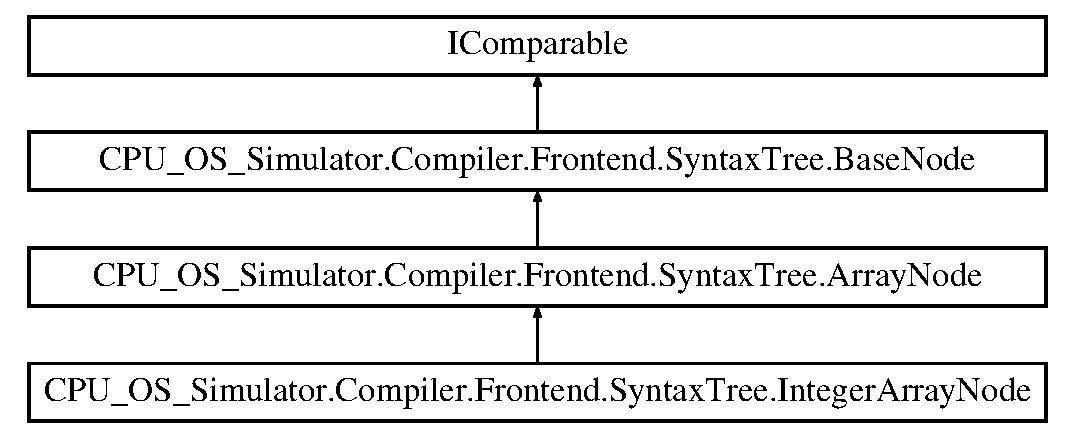
\includegraphics[height=4.000000cm]{class_c_p_u___o_s___simulator_1_1_compiler_1_1_frontend_1_1_syntax_tree_1_1_integer_array_node}
\end{center}
\end{figure}
\subsection*{Public Member Functions}
\begin{DoxyCompactItemize}
\item 
override void \hyperlink{class_c_p_u___o_s___simulator_1_1_compiler_1_1_frontend_1_1_syntax_tree_1_1_integer_array_node_a7abbf1320b21da1362fc8d391907d33f}{Visit} ()
\begin{DoxyCompactList}\small\item\em This function is called when the node is being visited by the parser \end{DoxyCompactList}\item 
override void \hyperlink{class_c_p_u___o_s___simulator_1_1_compiler_1_1_frontend_1_1_syntax_tree_1_1_integer_array_node_a28619c1f8b99cea0b827ba5a71a00e35}{Evaluate} ()
\begin{DoxyCompactList}\small\item\em This Function is called when the node is being evaluated by the parser \end{DoxyCompactList}\item 
override int \hyperlink{class_c_p_u___o_s___simulator_1_1_compiler_1_1_frontend_1_1_syntax_tree_1_1_integer_array_node_a6172b87f60f5fd82e055b6d13969297b}{number\+Of\+Elements} ()
\end{DoxyCompactItemize}
\subsection*{Properties}
\begin{DoxyCompactItemize}
\item 
override \hyperlink{class_c_p_u___o_s___simulator_1_1_compiler_1_1_frontend_1_1_syntax_tree_1_1_base_node}{Base\+Node} \hyperlink{class_c_p_u___o_s___simulator_1_1_compiler_1_1_frontend_1_1_syntax_tree_1_1_integer_array_node_ae5ab5cbf2964c94f7aa990d0d4eab6b5}{Right}\hspace{0.3cm}{\ttfamily  \mbox{[}get, set\mbox{]}}
\item 
override \hyperlink{class_c_p_u___o_s___simulator_1_1_compiler_1_1_frontend_1_1_syntax_tree_1_1_base_node}{Base\+Node} \hyperlink{class_c_p_u___o_s___simulator_1_1_compiler_1_1_frontend_1_1_syntax_tree_1_1_integer_array_node_ae7eec2773bf9de79145ef8c21dfddb13}{Left}\hspace{0.3cm}{\ttfamily  \mbox{[}get, set\mbox{]}}
\item 
int\mbox{[}$\,$\mbox{]} \hyperlink{class_c_p_u___o_s___simulator_1_1_compiler_1_1_frontend_1_1_syntax_tree_1_1_integer_array_node_a63c0fd71dd7fb053bfb0300bf6093f12}{Data}\hspace{0.3cm}{\ttfamily  \mbox{[}get, set\mbox{]}}
\item 
override \hyperlink{class_c_p_u___o_s___simulator_1_1_compiler_1_1_frontend_1_1_syntax_tree_1_1_base_node}{Base\+Node} \hyperlink{class_c_p_u___o_s___simulator_1_1_compiler_1_1_frontend_1_1_syntax_tree_1_1_integer_array_node_a7780d4322b90834048d1fb22c8e63786}{Parent}\hspace{0.3cm}{\ttfamily  \mbox{[}get, set\mbox{]}}
\end{DoxyCompactItemize}
\subsection*{Private Attributes}
\begin{DoxyCompactItemize}
\item 
new int\mbox{[}$\,$\mbox{]} \hyperlink{class_c_p_u___o_s___simulator_1_1_compiler_1_1_frontend_1_1_syntax_tree_1_1_integer_array_node_a0639cff7532da561e5c8e695b6f6ffd0}{data}
\item 
\hyperlink{class_c_p_u___o_s___simulator_1_1_compiler_1_1_frontend_1_1_syntax_tree_1_1_base_node}{Base\+Node} \hyperlink{class_c_p_u___o_s___simulator_1_1_compiler_1_1_frontend_1_1_syntax_tree_1_1_integer_array_node_a5f6e77308c89890ff12a91c4ff65add8}{parent}
\end{DoxyCompactItemize}
\subsection*{Additional Inherited Members}


\subsection{Detailed Description}


Definition at line 3 of file Integer\+Array\+Node.\+cs.



\subsection{Member Function Documentation}
\hypertarget{class_c_p_u___o_s___simulator_1_1_compiler_1_1_frontend_1_1_syntax_tree_1_1_integer_array_node_a28619c1f8b99cea0b827ba5a71a00e35}{}\index{C\+P\+U\+\_\+\+O\+S\+\_\+\+Simulator\+::\+Compiler\+::\+Frontend\+::\+Syntax\+Tree\+::\+Integer\+Array\+Node@{C\+P\+U\+\_\+\+O\+S\+\_\+\+Simulator\+::\+Compiler\+::\+Frontend\+::\+Syntax\+Tree\+::\+Integer\+Array\+Node}!Evaluate@{Evaluate}}
\index{Evaluate@{Evaluate}!C\+P\+U\+\_\+\+O\+S\+\_\+\+Simulator\+::\+Compiler\+::\+Frontend\+::\+Syntax\+Tree\+::\+Integer\+Array\+Node@{C\+P\+U\+\_\+\+O\+S\+\_\+\+Simulator\+::\+Compiler\+::\+Frontend\+::\+Syntax\+Tree\+::\+Integer\+Array\+Node}}
\subsubsection[{Evaluate()}]{\setlength{\rightskip}{0pt plus 5cm}override void C\+P\+U\+\_\+\+O\+S\+\_\+\+Simulator.\+Compiler.\+Frontend.\+Syntax\+Tree.\+Integer\+Array\+Node.\+Evaluate (
\begin{DoxyParamCaption}
{}
\end{DoxyParamCaption}
)\hspace{0.3cm}{\ttfamily [virtual]}}\label{class_c_p_u___o_s___simulator_1_1_compiler_1_1_frontend_1_1_syntax_tree_1_1_integer_array_node_a28619c1f8b99cea0b827ba5a71a00e35}


This Function is called when the node is being evaluated by the parser 



Implements \hyperlink{class_c_p_u___o_s___simulator_1_1_compiler_1_1_frontend_1_1_syntax_tree_1_1_array_node_afdb5d2808dbd83c28c85f35b6430edc4}{C\+P\+U\+\_\+\+O\+S\+\_\+\+Simulator.\+Compiler.\+Frontend.\+Syntax\+Tree.\+Array\+Node}.



Definition at line 43 of file Integer\+Array\+Node.\+cs.

\hypertarget{class_c_p_u___o_s___simulator_1_1_compiler_1_1_frontend_1_1_syntax_tree_1_1_integer_array_node_a6172b87f60f5fd82e055b6d13969297b}{}\index{C\+P\+U\+\_\+\+O\+S\+\_\+\+Simulator\+::\+Compiler\+::\+Frontend\+::\+Syntax\+Tree\+::\+Integer\+Array\+Node@{C\+P\+U\+\_\+\+O\+S\+\_\+\+Simulator\+::\+Compiler\+::\+Frontend\+::\+Syntax\+Tree\+::\+Integer\+Array\+Node}!number\+Of\+Elements@{number\+Of\+Elements}}
\index{number\+Of\+Elements@{number\+Of\+Elements}!C\+P\+U\+\_\+\+O\+S\+\_\+\+Simulator\+::\+Compiler\+::\+Frontend\+::\+Syntax\+Tree\+::\+Integer\+Array\+Node@{C\+P\+U\+\_\+\+O\+S\+\_\+\+Simulator\+::\+Compiler\+::\+Frontend\+::\+Syntax\+Tree\+::\+Integer\+Array\+Node}}
\subsubsection[{number\+Of\+Elements()}]{\setlength{\rightskip}{0pt plus 5cm}override int C\+P\+U\+\_\+\+O\+S\+\_\+\+Simulator.\+Compiler.\+Frontend.\+Syntax\+Tree.\+Integer\+Array\+Node.\+number\+Of\+Elements (
\begin{DoxyParamCaption}
{}
\end{DoxyParamCaption}
)\hspace{0.3cm}{\ttfamily [virtual]}}\label{class_c_p_u___o_s___simulator_1_1_compiler_1_1_frontend_1_1_syntax_tree_1_1_integer_array_node_a6172b87f60f5fd82e055b6d13969297b}


Implements \hyperlink{class_c_p_u___o_s___simulator_1_1_compiler_1_1_frontend_1_1_syntax_tree_1_1_array_node_a75232f3076d95a562405ef2722bcafd5}{C\+P\+U\+\_\+\+O\+S\+\_\+\+Simulator.\+Compiler.\+Frontend.\+Syntax\+Tree.\+Array\+Node}.



Definition at line 47 of file Integer\+Array\+Node.\+cs.

\hypertarget{class_c_p_u___o_s___simulator_1_1_compiler_1_1_frontend_1_1_syntax_tree_1_1_integer_array_node_a7abbf1320b21da1362fc8d391907d33f}{}\index{C\+P\+U\+\_\+\+O\+S\+\_\+\+Simulator\+::\+Compiler\+::\+Frontend\+::\+Syntax\+Tree\+::\+Integer\+Array\+Node@{C\+P\+U\+\_\+\+O\+S\+\_\+\+Simulator\+::\+Compiler\+::\+Frontend\+::\+Syntax\+Tree\+::\+Integer\+Array\+Node}!Visit@{Visit}}
\index{Visit@{Visit}!C\+P\+U\+\_\+\+O\+S\+\_\+\+Simulator\+::\+Compiler\+::\+Frontend\+::\+Syntax\+Tree\+::\+Integer\+Array\+Node@{C\+P\+U\+\_\+\+O\+S\+\_\+\+Simulator\+::\+Compiler\+::\+Frontend\+::\+Syntax\+Tree\+::\+Integer\+Array\+Node}}
\subsubsection[{Visit()}]{\setlength{\rightskip}{0pt plus 5cm}override void C\+P\+U\+\_\+\+O\+S\+\_\+\+Simulator.\+Compiler.\+Frontend.\+Syntax\+Tree.\+Integer\+Array\+Node.\+Visit (
\begin{DoxyParamCaption}
{}
\end{DoxyParamCaption}
)\hspace{0.3cm}{\ttfamily [virtual]}}\label{class_c_p_u___o_s___simulator_1_1_compiler_1_1_frontend_1_1_syntax_tree_1_1_integer_array_node_a7abbf1320b21da1362fc8d391907d33f}


This function is called when the node is being visited by the parser 



Implements \hyperlink{class_c_p_u___o_s___simulator_1_1_compiler_1_1_frontend_1_1_syntax_tree_1_1_array_node_aed695b6f32d5c176204fc15854db32db}{C\+P\+U\+\_\+\+O\+S\+\_\+\+Simulator.\+Compiler.\+Frontend.\+Syntax\+Tree.\+Array\+Node}.



Definition at line 36 of file Integer\+Array\+Node.\+cs.



\subsection{Member Data Documentation}
\hypertarget{class_c_p_u___o_s___simulator_1_1_compiler_1_1_frontend_1_1_syntax_tree_1_1_integer_array_node_a0639cff7532da561e5c8e695b6f6ffd0}{}\index{C\+P\+U\+\_\+\+O\+S\+\_\+\+Simulator\+::\+Compiler\+::\+Frontend\+::\+Syntax\+Tree\+::\+Integer\+Array\+Node@{C\+P\+U\+\_\+\+O\+S\+\_\+\+Simulator\+::\+Compiler\+::\+Frontend\+::\+Syntax\+Tree\+::\+Integer\+Array\+Node}!data@{data}}
\index{data@{data}!C\+P\+U\+\_\+\+O\+S\+\_\+\+Simulator\+::\+Compiler\+::\+Frontend\+::\+Syntax\+Tree\+::\+Integer\+Array\+Node@{C\+P\+U\+\_\+\+O\+S\+\_\+\+Simulator\+::\+Compiler\+::\+Frontend\+::\+Syntax\+Tree\+::\+Integer\+Array\+Node}}
\subsubsection[{data}]{\setlength{\rightskip}{0pt plus 5cm}new int \mbox{[}$\,$\mbox{]} C\+P\+U\+\_\+\+O\+S\+\_\+\+Simulator.\+Compiler.\+Frontend.\+Syntax\+Tree.\+Integer\+Array\+Node.\+data\hspace{0.3cm}{\ttfamily [private]}}\label{class_c_p_u___o_s___simulator_1_1_compiler_1_1_frontend_1_1_syntax_tree_1_1_integer_array_node_a0639cff7532da561e5c8e695b6f6ffd0}


Definition at line 5 of file Integer\+Array\+Node.\+cs.

\hypertarget{class_c_p_u___o_s___simulator_1_1_compiler_1_1_frontend_1_1_syntax_tree_1_1_integer_array_node_a5f6e77308c89890ff12a91c4ff65add8}{}\index{C\+P\+U\+\_\+\+O\+S\+\_\+\+Simulator\+::\+Compiler\+::\+Frontend\+::\+Syntax\+Tree\+::\+Integer\+Array\+Node@{C\+P\+U\+\_\+\+O\+S\+\_\+\+Simulator\+::\+Compiler\+::\+Frontend\+::\+Syntax\+Tree\+::\+Integer\+Array\+Node}!parent@{parent}}
\index{parent@{parent}!C\+P\+U\+\_\+\+O\+S\+\_\+\+Simulator\+::\+Compiler\+::\+Frontend\+::\+Syntax\+Tree\+::\+Integer\+Array\+Node@{C\+P\+U\+\_\+\+O\+S\+\_\+\+Simulator\+::\+Compiler\+::\+Frontend\+::\+Syntax\+Tree\+::\+Integer\+Array\+Node}}
\subsubsection[{parent}]{\setlength{\rightskip}{0pt plus 5cm}{\bf Base\+Node} C\+P\+U\+\_\+\+O\+S\+\_\+\+Simulator.\+Compiler.\+Frontend.\+Syntax\+Tree.\+Integer\+Array\+Node.\+parent\hspace{0.3cm}{\ttfamily [private]}}\label{class_c_p_u___o_s___simulator_1_1_compiler_1_1_frontend_1_1_syntax_tree_1_1_integer_array_node_a5f6e77308c89890ff12a91c4ff65add8}


Definition at line 6 of file Integer\+Array\+Node.\+cs.



\subsection{Property Documentation}
\hypertarget{class_c_p_u___o_s___simulator_1_1_compiler_1_1_frontend_1_1_syntax_tree_1_1_integer_array_node_a63c0fd71dd7fb053bfb0300bf6093f12}{}\index{C\+P\+U\+\_\+\+O\+S\+\_\+\+Simulator\+::\+Compiler\+::\+Frontend\+::\+Syntax\+Tree\+::\+Integer\+Array\+Node@{C\+P\+U\+\_\+\+O\+S\+\_\+\+Simulator\+::\+Compiler\+::\+Frontend\+::\+Syntax\+Tree\+::\+Integer\+Array\+Node}!Data@{Data}}
\index{Data@{Data}!C\+P\+U\+\_\+\+O\+S\+\_\+\+Simulator\+::\+Compiler\+::\+Frontend\+::\+Syntax\+Tree\+::\+Integer\+Array\+Node@{C\+P\+U\+\_\+\+O\+S\+\_\+\+Simulator\+::\+Compiler\+::\+Frontend\+::\+Syntax\+Tree\+::\+Integer\+Array\+Node}}
\subsubsection[{Data}]{\setlength{\rightskip}{0pt plus 5cm}int \mbox{[}$\,$\mbox{]} C\+P\+U\+\_\+\+O\+S\+\_\+\+Simulator.\+Compiler.\+Frontend.\+Syntax\+Tree.\+Integer\+Array\+Node.\+Data\hspace{0.3cm}{\ttfamily [get]}, {\ttfamily [set]}}\label{class_c_p_u___o_s___simulator_1_1_compiler_1_1_frontend_1_1_syntax_tree_1_1_integer_array_node_a63c0fd71dd7fb053bfb0300bf6093f12}


Definition at line 21 of file Integer\+Array\+Node.\+cs.

\hypertarget{class_c_p_u___o_s___simulator_1_1_compiler_1_1_frontend_1_1_syntax_tree_1_1_integer_array_node_ae7eec2773bf9de79145ef8c21dfddb13}{}\index{C\+P\+U\+\_\+\+O\+S\+\_\+\+Simulator\+::\+Compiler\+::\+Frontend\+::\+Syntax\+Tree\+::\+Integer\+Array\+Node@{C\+P\+U\+\_\+\+O\+S\+\_\+\+Simulator\+::\+Compiler\+::\+Frontend\+::\+Syntax\+Tree\+::\+Integer\+Array\+Node}!Left@{Left}}
\index{Left@{Left}!C\+P\+U\+\_\+\+O\+S\+\_\+\+Simulator\+::\+Compiler\+::\+Frontend\+::\+Syntax\+Tree\+::\+Integer\+Array\+Node@{C\+P\+U\+\_\+\+O\+S\+\_\+\+Simulator\+::\+Compiler\+::\+Frontend\+::\+Syntax\+Tree\+::\+Integer\+Array\+Node}}
\subsubsection[{Left}]{\setlength{\rightskip}{0pt plus 5cm}override {\bf Base\+Node} C\+P\+U\+\_\+\+O\+S\+\_\+\+Simulator.\+Compiler.\+Frontend.\+Syntax\+Tree.\+Integer\+Array\+Node.\+Left\hspace{0.3cm}{\ttfamily [get]}, {\ttfamily [set]}}\label{class_c_p_u___o_s___simulator_1_1_compiler_1_1_frontend_1_1_syntax_tree_1_1_integer_array_node_ae7eec2773bf9de79145ef8c21dfddb13}


Definition at line 15 of file Integer\+Array\+Node.\+cs.

\hypertarget{class_c_p_u___o_s___simulator_1_1_compiler_1_1_frontend_1_1_syntax_tree_1_1_integer_array_node_a7780d4322b90834048d1fb22c8e63786}{}\index{C\+P\+U\+\_\+\+O\+S\+\_\+\+Simulator\+::\+Compiler\+::\+Frontend\+::\+Syntax\+Tree\+::\+Integer\+Array\+Node@{C\+P\+U\+\_\+\+O\+S\+\_\+\+Simulator\+::\+Compiler\+::\+Frontend\+::\+Syntax\+Tree\+::\+Integer\+Array\+Node}!Parent@{Parent}}
\index{Parent@{Parent}!C\+P\+U\+\_\+\+O\+S\+\_\+\+Simulator\+::\+Compiler\+::\+Frontend\+::\+Syntax\+Tree\+::\+Integer\+Array\+Node@{C\+P\+U\+\_\+\+O\+S\+\_\+\+Simulator\+::\+Compiler\+::\+Frontend\+::\+Syntax\+Tree\+::\+Integer\+Array\+Node}}
\subsubsection[{Parent}]{\setlength{\rightskip}{0pt plus 5cm}override {\bf Base\+Node} C\+P\+U\+\_\+\+O\+S\+\_\+\+Simulator.\+Compiler.\+Frontend.\+Syntax\+Tree.\+Integer\+Array\+Node.\+Parent\hspace{0.3cm}{\ttfamily [get]}, {\ttfamily [set]}}\label{class_c_p_u___o_s___simulator_1_1_compiler_1_1_frontend_1_1_syntax_tree_1_1_integer_array_node_a7780d4322b90834048d1fb22c8e63786}


Definition at line 27 of file Integer\+Array\+Node.\+cs.

\hypertarget{class_c_p_u___o_s___simulator_1_1_compiler_1_1_frontend_1_1_syntax_tree_1_1_integer_array_node_ae5ab5cbf2964c94f7aa990d0d4eab6b5}{}\index{C\+P\+U\+\_\+\+O\+S\+\_\+\+Simulator\+::\+Compiler\+::\+Frontend\+::\+Syntax\+Tree\+::\+Integer\+Array\+Node@{C\+P\+U\+\_\+\+O\+S\+\_\+\+Simulator\+::\+Compiler\+::\+Frontend\+::\+Syntax\+Tree\+::\+Integer\+Array\+Node}!Right@{Right}}
\index{Right@{Right}!C\+P\+U\+\_\+\+O\+S\+\_\+\+Simulator\+::\+Compiler\+::\+Frontend\+::\+Syntax\+Tree\+::\+Integer\+Array\+Node@{C\+P\+U\+\_\+\+O\+S\+\_\+\+Simulator\+::\+Compiler\+::\+Frontend\+::\+Syntax\+Tree\+::\+Integer\+Array\+Node}}
\subsubsection[{Right}]{\setlength{\rightskip}{0pt plus 5cm}override {\bf Base\+Node} C\+P\+U\+\_\+\+O\+S\+\_\+\+Simulator.\+Compiler.\+Frontend.\+Syntax\+Tree.\+Integer\+Array\+Node.\+Right\hspace{0.3cm}{\ttfamily [get]}, {\ttfamily [set]}}\label{class_c_p_u___o_s___simulator_1_1_compiler_1_1_frontend_1_1_syntax_tree_1_1_integer_array_node_ae5ab5cbf2964c94f7aa990d0d4eab6b5}


Definition at line 9 of file Integer\+Array\+Node.\+cs.



The documentation for this class was generated from the following file\+:\begin{DoxyCompactItemize}
\item 
Compiler/\+Frontend/\+Syntax\+Tree/\hyperlink{_integer_array_node_8cs}{Integer\+Array\+Node.\+cs}\end{DoxyCompactItemize}

\hypertarget{class_c_p_u___o_s___simulator_1_1_compiler_1_1_frontend_1_1_syntax_tree_1_1_integer_node}{}\section{C\+P\+U\+\_\+\+O\+S\+\_\+\+Simulator.\+Compiler.\+Frontend.\+Syntax\+Tree.\+Integer\+Node Class Reference}
\label{class_c_p_u___o_s___simulator_1_1_compiler_1_1_frontend_1_1_syntax_tree_1_1_integer_node}\index{C\+P\+U\+\_\+\+O\+S\+\_\+\+Simulator.\+Compiler.\+Frontend.\+Syntax\+Tree.\+Integer\+Node@{C\+P\+U\+\_\+\+O\+S\+\_\+\+Simulator.\+Compiler.\+Frontend.\+Syntax\+Tree.\+Integer\+Node}}
Inheritance diagram for C\+P\+U\+\_\+\+O\+S\+\_\+\+Simulator.\+Compiler.\+Frontend.\+Syntax\+Tree.\+Integer\+Node\+:\begin{figure}[H]
\begin{center}
\leavevmode
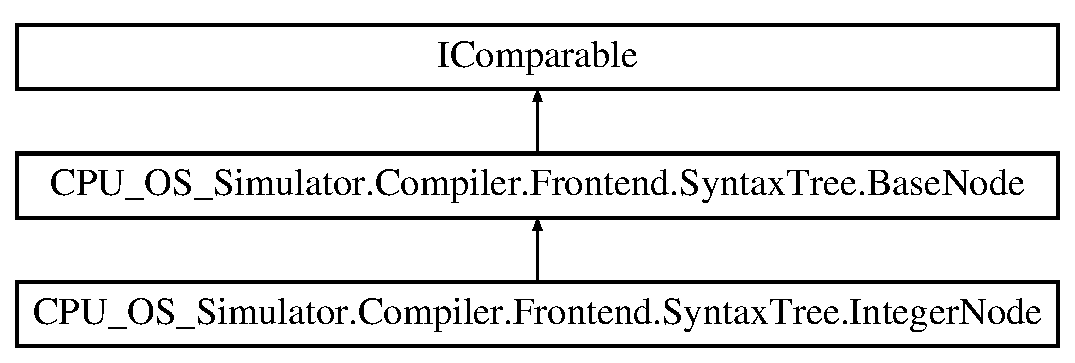
\includegraphics[height=3.000000cm]{class_c_p_u___o_s___simulator_1_1_compiler_1_1_frontend_1_1_syntax_tree_1_1_integer_node}
\end{center}
\end{figure}
\subsection*{Public Member Functions}
\begin{DoxyCompactItemize}
\item 
override void \hyperlink{class_c_p_u___o_s___simulator_1_1_compiler_1_1_frontend_1_1_syntax_tree_1_1_integer_node_a5f788c73bf459d372850107098fda8c1}{Visit} ()
\begin{DoxyCompactList}\small\item\em This function is called when the node is being visited by the parser \end{DoxyCompactList}\item 
override void \hyperlink{class_c_p_u___o_s___simulator_1_1_compiler_1_1_frontend_1_1_syntax_tree_1_1_integer_node_a3005d7165ec473ac488e792728a50d99}{Evaluate} ()
\begin{DoxyCompactList}\small\item\em This Function is called when the node is being evaluated by the parser \end{DoxyCompactList}\end{DoxyCompactItemize}
\subsection*{Properties}
\begin{DoxyCompactItemize}
\item 
override \hyperlink{class_c_p_u___o_s___simulator_1_1_compiler_1_1_frontend_1_1_syntax_tree_1_1_base_node}{Base\+Node} \hyperlink{class_c_p_u___o_s___simulator_1_1_compiler_1_1_frontend_1_1_syntax_tree_1_1_integer_node_a34f082eb9ebfa34ef854fdfef4ae4f65}{Right}\hspace{0.3cm}{\ttfamily  \mbox{[}get, set\mbox{]}}
\item 
override \hyperlink{class_c_p_u___o_s___simulator_1_1_compiler_1_1_frontend_1_1_syntax_tree_1_1_base_node}{Base\+Node} \hyperlink{class_c_p_u___o_s___simulator_1_1_compiler_1_1_frontend_1_1_syntax_tree_1_1_integer_node_a49b63ddefa5ac8505ced0be5d9f7e09d}{Left}\hspace{0.3cm}{\ttfamily  \mbox{[}get, set\mbox{]}}
\item 
int \hyperlink{class_c_p_u___o_s___simulator_1_1_compiler_1_1_frontend_1_1_syntax_tree_1_1_integer_node_aa6c8b3f7e01b8aefb784de1a42036071}{Data}\hspace{0.3cm}{\ttfamily  \mbox{[}get, set\mbox{]}}
\item 
override \hyperlink{class_c_p_u___o_s___simulator_1_1_compiler_1_1_frontend_1_1_syntax_tree_1_1_base_node}{Base\+Node} \hyperlink{class_c_p_u___o_s___simulator_1_1_compiler_1_1_frontend_1_1_syntax_tree_1_1_integer_node_a592ddb201c5e069e7a195e79c7feecce}{Parent}\hspace{0.3cm}{\ttfamily  \mbox{[}get, set\mbox{]}}
\end{DoxyCompactItemize}
\subsection*{Private Attributes}
\begin{DoxyCompactItemize}
\item 
new int \hyperlink{class_c_p_u___o_s___simulator_1_1_compiler_1_1_frontend_1_1_syntax_tree_1_1_integer_node_a53c501d27829e91cf3ba24b11ef79328}{data}
\item 
\hyperlink{class_c_p_u___o_s___simulator_1_1_compiler_1_1_frontend_1_1_syntax_tree_1_1_base_node}{Base\+Node} \hyperlink{class_c_p_u___o_s___simulator_1_1_compiler_1_1_frontend_1_1_syntax_tree_1_1_integer_node_a943280154af98ec87c3bd70a10d1dfab}{parent}
\end{DoxyCompactItemize}
\subsection*{Additional Inherited Members}


\subsection{Detailed Description}


Definition at line 9 of file Integer\+Node.\+cs.



\subsection{Member Function Documentation}
\hypertarget{class_c_p_u___o_s___simulator_1_1_compiler_1_1_frontend_1_1_syntax_tree_1_1_integer_node_a3005d7165ec473ac488e792728a50d99}{}\index{C\+P\+U\+\_\+\+O\+S\+\_\+\+Simulator\+::\+Compiler\+::\+Frontend\+::\+Syntax\+Tree\+::\+Integer\+Node@{C\+P\+U\+\_\+\+O\+S\+\_\+\+Simulator\+::\+Compiler\+::\+Frontend\+::\+Syntax\+Tree\+::\+Integer\+Node}!Evaluate@{Evaluate}}
\index{Evaluate@{Evaluate}!C\+P\+U\+\_\+\+O\+S\+\_\+\+Simulator\+::\+Compiler\+::\+Frontend\+::\+Syntax\+Tree\+::\+Integer\+Node@{C\+P\+U\+\_\+\+O\+S\+\_\+\+Simulator\+::\+Compiler\+::\+Frontend\+::\+Syntax\+Tree\+::\+Integer\+Node}}
\subsubsection[{Evaluate()}]{\setlength{\rightskip}{0pt plus 5cm}override void C\+P\+U\+\_\+\+O\+S\+\_\+\+Simulator.\+Compiler.\+Frontend.\+Syntax\+Tree.\+Integer\+Node.\+Evaluate (
\begin{DoxyParamCaption}
{}
\end{DoxyParamCaption}
)\hspace{0.3cm}{\ttfamily [virtual]}}\label{class_c_p_u___o_s___simulator_1_1_compiler_1_1_frontend_1_1_syntax_tree_1_1_integer_node_a3005d7165ec473ac488e792728a50d99}


This Function is called when the node is being evaluated by the parser 



Implements \hyperlink{class_c_p_u___o_s___simulator_1_1_compiler_1_1_frontend_1_1_syntax_tree_1_1_base_node_a6cfcf8a0795180bdb1c7f0735d39441b}{C\+P\+U\+\_\+\+O\+S\+\_\+\+Simulator.\+Compiler.\+Frontend.\+Syntax\+Tree.\+Base\+Node}.



Definition at line 48 of file Integer\+Node.\+cs.

\hypertarget{class_c_p_u___o_s___simulator_1_1_compiler_1_1_frontend_1_1_syntax_tree_1_1_integer_node_a5f788c73bf459d372850107098fda8c1}{}\index{C\+P\+U\+\_\+\+O\+S\+\_\+\+Simulator\+::\+Compiler\+::\+Frontend\+::\+Syntax\+Tree\+::\+Integer\+Node@{C\+P\+U\+\_\+\+O\+S\+\_\+\+Simulator\+::\+Compiler\+::\+Frontend\+::\+Syntax\+Tree\+::\+Integer\+Node}!Visit@{Visit}}
\index{Visit@{Visit}!C\+P\+U\+\_\+\+O\+S\+\_\+\+Simulator\+::\+Compiler\+::\+Frontend\+::\+Syntax\+Tree\+::\+Integer\+Node@{C\+P\+U\+\_\+\+O\+S\+\_\+\+Simulator\+::\+Compiler\+::\+Frontend\+::\+Syntax\+Tree\+::\+Integer\+Node}}
\subsubsection[{Visit()}]{\setlength{\rightskip}{0pt plus 5cm}override void C\+P\+U\+\_\+\+O\+S\+\_\+\+Simulator.\+Compiler.\+Frontend.\+Syntax\+Tree.\+Integer\+Node.\+Visit (
\begin{DoxyParamCaption}
{}
\end{DoxyParamCaption}
)\hspace{0.3cm}{\ttfamily [virtual]}}\label{class_c_p_u___o_s___simulator_1_1_compiler_1_1_frontend_1_1_syntax_tree_1_1_integer_node_a5f788c73bf459d372850107098fda8c1}


This function is called when the node is being visited by the parser 



Implements \hyperlink{class_c_p_u___o_s___simulator_1_1_compiler_1_1_frontend_1_1_syntax_tree_1_1_base_node_a092377df64002c5e9c023a259e5e11d0}{C\+P\+U\+\_\+\+O\+S\+\_\+\+Simulator.\+Compiler.\+Frontend.\+Syntax\+Tree.\+Base\+Node}.



Definition at line 41 of file Integer\+Node.\+cs.



\subsection{Member Data Documentation}
\hypertarget{class_c_p_u___o_s___simulator_1_1_compiler_1_1_frontend_1_1_syntax_tree_1_1_integer_node_a53c501d27829e91cf3ba24b11ef79328}{}\index{C\+P\+U\+\_\+\+O\+S\+\_\+\+Simulator\+::\+Compiler\+::\+Frontend\+::\+Syntax\+Tree\+::\+Integer\+Node@{C\+P\+U\+\_\+\+O\+S\+\_\+\+Simulator\+::\+Compiler\+::\+Frontend\+::\+Syntax\+Tree\+::\+Integer\+Node}!data@{data}}
\index{data@{data}!C\+P\+U\+\_\+\+O\+S\+\_\+\+Simulator\+::\+Compiler\+::\+Frontend\+::\+Syntax\+Tree\+::\+Integer\+Node@{C\+P\+U\+\_\+\+O\+S\+\_\+\+Simulator\+::\+Compiler\+::\+Frontend\+::\+Syntax\+Tree\+::\+Integer\+Node}}
\subsubsection[{data}]{\setlength{\rightskip}{0pt plus 5cm}new int C\+P\+U\+\_\+\+O\+S\+\_\+\+Simulator.\+Compiler.\+Frontend.\+Syntax\+Tree.\+Integer\+Node.\+data\hspace{0.3cm}{\ttfamily [private]}}\label{class_c_p_u___o_s___simulator_1_1_compiler_1_1_frontend_1_1_syntax_tree_1_1_integer_node_a53c501d27829e91cf3ba24b11ef79328}


Definition at line 11 of file Integer\+Node.\+cs.

\hypertarget{class_c_p_u___o_s___simulator_1_1_compiler_1_1_frontend_1_1_syntax_tree_1_1_integer_node_a943280154af98ec87c3bd70a10d1dfab}{}\index{C\+P\+U\+\_\+\+O\+S\+\_\+\+Simulator\+::\+Compiler\+::\+Frontend\+::\+Syntax\+Tree\+::\+Integer\+Node@{C\+P\+U\+\_\+\+O\+S\+\_\+\+Simulator\+::\+Compiler\+::\+Frontend\+::\+Syntax\+Tree\+::\+Integer\+Node}!parent@{parent}}
\index{parent@{parent}!C\+P\+U\+\_\+\+O\+S\+\_\+\+Simulator\+::\+Compiler\+::\+Frontend\+::\+Syntax\+Tree\+::\+Integer\+Node@{C\+P\+U\+\_\+\+O\+S\+\_\+\+Simulator\+::\+Compiler\+::\+Frontend\+::\+Syntax\+Tree\+::\+Integer\+Node}}
\subsubsection[{parent}]{\setlength{\rightskip}{0pt plus 5cm}{\bf Base\+Node} C\+P\+U\+\_\+\+O\+S\+\_\+\+Simulator.\+Compiler.\+Frontend.\+Syntax\+Tree.\+Integer\+Node.\+parent\hspace{0.3cm}{\ttfamily [private]}}\label{class_c_p_u___o_s___simulator_1_1_compiler_1_1_frontend_1_1_syntax_tree_1_1_integer_node_a943280154af98ec87c3bd70a10d1dfab}


Definition at line 12 of file Integer\+Node.\+cs.



\subsection{Property Documentation}
\hypertarget{class_c_p_u___o_s___simulator_1_1_compiler_1_1_frontend_1_1_syntax_tree_1_1_integer_node_aa6c8b3f7e01b8aefb784de1a42036071}{}\index{C\+P\+U\+\_\+\+O\+S\+\_\+\+Simulator\+::\+Compiler\+::\+Frontend\+::\+Syntax\+Tree\+::\+Integer\+Node@{C\+P\+U\+\_\+\+O\+S\+\_\+\+Simulator\+::\+Compiler\+::\+Frontend\+::\+Syntax\+Tree\+::\+Integer\+Node}!Data@{Data}}
\index{Data@{Data}!C\+P\+U\+\_\+\+O\+S\+\_\+\+Simulator\+::\+Compiler\+::\+Frontend\+::\+Syntax\+Tree\+::\+Integer\+Node@{C\+P\+U\+\_\+\+O\+S\+\_\+\+Simulator\+::\+Compiler\+::\+Frontend\+::\+Syntax\+Tree\+::\+Integer\+Node}}
\subsubsection[{Data}]{\setlength{\rightskip}{0pt plus 5cm}int C\+P\+U\+\_\+\+O\+S\+\_\+\+Simulator.\+Compiler.\+Frontend.\+Syntax\+Tree.\+Integer\+Node.\+Data\hspace{0.3cm}{\ttfamily [get]}, {\ttfamily [set]}}\label{class_c_p_u___o_s___simulator_1_1_compiler_1_1_frontend_1_1_syntax_tree_1_1_integer_node_aa6c8b3f7e01b8aefb784de1a42036071}


Definition at line 27 of file Integer\+Node.\+cs.

\hypertarget{class_c_p_u___o_s___simulator_1_1_compiler_1_1_frontend_1_1_syntax_tree_1_1_integer_node_a49b63ddefa5ac8505ced0be5d9f7e09d}{}\index{C\+P\+U\+\_\+\+O\+S\+\_\+\+Simulator\+::\+Compiler\+::\+Frontend\+::\+Syntax\+Tree\+::\+Integer\+Node@{C\+P\+U\+\_\+\+O\+S\+\_\+\+Simulator\+::\+Compiler\+::\+Frontend\+::\+Syntax\+Tree\+::\+Integer\+Node}!Left@{Left}}
\index{Left@{Left}!C\+P\+U\+\_\+\+O\+S\+\_\+\+Simulator\+::\+Compiler\+::\+Frontend\+::\+Syntax\+Tree\+::\+Integer\+Node@{C\+P\+U\+\_\+\+O\+S\+\_\+\+Simulator\+::\+Compiler\+::\+Frontend\+::\+Syntax\+Tree\+::\+Integer\+Node}}
\subsubsection[{Left}]{\setlength{\rightskip}{0pt plus 5cm}override {\bf Base\+Node} C\+P\+U\+\_\+\+O\+S\+\_\+\+Simulator.\+Compiler.\+Frontend.\+Syntax\+Tree.\+Integer\+Node.\+Left\hspace{0.3cm}{\ttfamily [get]}, {\ttfamily [set]}}\label{class_c_p_u___o_s___simulator_1_1_compiler_1_1_frontend_1_1_syntax_tree_1_1_integer_node_a49b63ddefa5ac8505ced0be5d9f7e09d}


Definition at line 21 of file Integer\+Node.\+cs.

\hypertarget{class_c_p_u___o_s___simulator_1_1_compiler_1_1_frontend_1_1_syntax_tree_1_1_integer_node_a592ddb201c5e069e7a195e79c7feecce}{}\index{C\+P\+U\+\_\+\+O\+S\+\_\+\+Simulator\+::\+Compiler\+::\+Frontend\+::\+Syntax\+Tree\+::\+Integer\+Node@{C\+P\+U\+\_\+\+O\+S\+\_\+\+Simulator\+::\+Compiler\+::\+Frontend\+::\+Syntax\+Tree\+::\+Integer\+Node}!Parent@{Parent}}
\index{Parent@{Parent}!C\+P\+U\+\_\+\+O\+S\+\_\+\+Simulator\+::\+Compiler\+::\+Frontend\+::\+Syntax\+Tree\+::\+Integer\+Node@{C\+P\+U\+\_\+\+O\+S\+\_\+\+Simulator\+::\+Compiler\+::\+Frontend\+::\+Syntax\+Tree\+::\+Integer\+Node}}
\subsubsection[{Parent}]{\setlength{\rightskip}{0pt plus 5cm}override {\bf Base\+Node} C\+P\+U\+\_\+\+O\+S\+\_\+\+Simulator.\+Compiler.\+Frontend.\+Syntax\+Tree.\+Integer\+Node.\+Parent\hspace{0.3cm}{\ttfamily [get]}, {\ttfamily [set]}}\label{class_c_p_u___o_s___simulator_1_1_compiler_1_1_frontend_1_1_syntax_tree_1_1_integer_node_a592ddb201c5e069e7a195e79c7feecce}


Definition at line 33 of file Integer\+Node.\+cs.

\hypertarget{class_c_p_u___o_s___simulator_1_1_compiler_1_1_frontend_1_1_syntax_tree_1_1_integer_node_a34f082eb9ebfa34ef854fdfef4ae4f65}{}\index{C\+P\+U\+\_\+\+O\+S\+\_\+\+Simulator\+::\+Compiler\+::\+Frontend\+::\+Syntax\+Tree\+::\+Integer\+Node@{C\+P\+U\+\_\+\+O\+S\+\_\+\+Simulator\+::\+Compiler\+::\+Frontend\+::\+Syntax\+Tree\+::\+Integer\+Node}!Right@{Right}}
\index{Right@{Right}!C\+P\+U\+\_\+\+O\+S\+\_\+\+Simulator\+::\+Compiler\+::\+Frontend\+::\+Syntax\+Tree\+::\+Integer\+Node@{C\+P\+U\+\_\+\+O\+S\+\_\+\+Simulator\+::\+Compiler\+::\+Frontend\+::\+Syntax\+Tree\+::\+Integer\+Node}}
\subsubsection[{Right}]{\setlength{\rightskip}{0pt plus 5cm}override {\bf Base\+Node} C\+P\+U\+\_\+\+O\+S\+\_\+\+Simulator.\+Compiler.\+Frontend.\+Syntax\+Tree.\+Integer\+Node.\+Right\hspace{0.3cm}{\ttfamily [get]}, {\ttfamily [set]}}\label{class_c_p_u___o_s___simulator_1_1_compiler_1_1_frontend_1_1_syntax_tree_1_1_integer_node_a34f082eb9ebfa34ef854fdfef4ae4f65}


Definition at line 15 of file Integer\+Node.\+cs.



The documentation for this class was generated from the following file\+:\begin{DoxyCompactItemize}
\item 
Compiler/\+Frontend/\+Syntax\+Tree/\hyperlink{_integer_node_8cs}{Integer\+Node.\+cs}\end{DoxyCompactItemize}

\hypertarget{interface_c_p_u___o_s___simulator_1_1_memory_1_1_i_swappable}{}\section{C\+P\+U\+\_\+\+O\+S\+\_\+\+Simulator.\+Memory.\+I\+Swappable Interface Reference}
\label{interface_c_p_u___o_s___simulator_1_1_memory_1_1_i_swappable}\index{C\+P\+U\+\_\+\+O\+S\+\_\+\+Simulator.\+Memory.\+I\+Swappable@{C\+P\+U\+\_\+\+O\+S\+\_\+\+Simulator.\+Memory.\+I\+Swappable}}
Inheritance diagram for C\+P\+U\+\_\+\+O\+S\+\_\+\+Simulator.\+Memory.\+I\+Swappable\+:\begin{figure}[H]
\begin{center}
\leavevmode
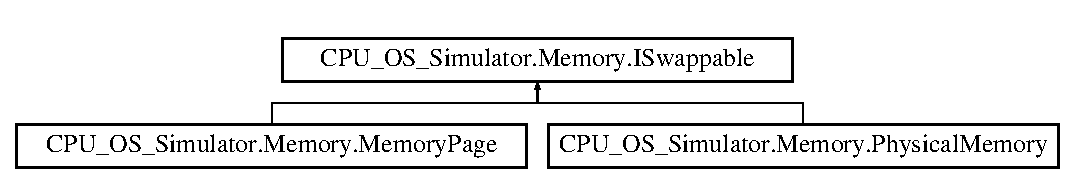
\includegraphics[height=2.000000cm]{interface_c_p_u___o_s___simulator_1_1_memory_1_1_i_swappable}
\end{center}
\end{figure}
\subsection*{Public Member Functions}
\begin{DoxyCompactItemize}
\item 
void \hyperlink{interface_c_p_u___o_s___simulator_1_1_memory_1_1_i_swappable_ae789e9deb0600d48b0dcbe4a4252220a}{Swap\+Out} (int Location\+To\+Swap, int Frame\+Number)
\item 
void \hyperlink{interface_c_p_u___o_s___simulator_1_1_memory_1_1_i_swappable_a38e30363486a3de53e6171da50b943af}{Swap\+In} (int Location\+To\+Swap, int Frame\+Number)
\end{DoxyCompactItemize}


\subsection{Detailed Description}


Definition at line 3 of file I\+Swappable.\+cs.



\subsection{Member Function Documentation}
\hypertarget{interface_c_p_u___o_s___simulator_1_1_memory_1_1_i_swappable_a38e30363486a3de53e6171da50b943af}{}\index{C\+P\+U\+\_\+\+O\+S\+\_\+\+Simulator\+::\+Memory\+::\+I\+Swappable@{C\+P\+U\+\_\+\+O\+S\+\_\+\+Simulator\+::\+Memory\+::\+I\+Swappable}!Swap\+In@{Swap\+In}}
\index{Swap\+In@{Swap\+In}!C\+P\+U\+\_\+\+O\+S\+\_\+\+Simulator\+::\+Memory\+::\+I\+Swappable@{C\+P\+U\+\_\+\+O\+S\+\_\+\+Simulator\+::\+Memory\+::\+I\+Swappable}}
\subsubsection[{Swap\+In(int Location\+To\+Swap, int Frame\+Number)}]{\setlength{\rightskip}{0pt plus 5cm}void C\+P\+U\+\_\+\+O\+S\+\_\+\+Simulator.\+Memory.\+I\+Swappable.\+Swap\+In (
\begin{DoxyParamCaption}
\item[{int}]{Location\+To\+Swap, }
\item[{int}]{Frame\+Number}
\end{DoxyParamCaption}
)}\label{interface_c_p_u___o_s___simulator_1_1_memory_1_1_i_swappable_a38e30363486a3de53e6171da50b943af}


Implemented in \hyperlink{class_c_p_u___o_s___simulator_1_1_memory_1_1_memory_page_a79e408c1be5efbaa6969ab66cc46930f}{C\+P\+U\+\_\+\+O\+S\+\_\+\+Simulator.\+Memory.\+Memory\+Page}, and \hyperlink{class_c_p_u___o_s___simulator_1_1_memory_1_1_physical_memory_ac12efe05d774b7e2ea38142835e0c131}{C\+P\+U\+\_\+\+O\+S\+\_\+\+Simulator.\+Memory.\+Physical\+Memory}.

\hypertarget{interface_c_p_u___o_s___simulator_1_1_memory_1_1_i_swappable_ae789e9deb0600d48b0dcbe4a4252220a}{}\index{C\+P\+U\+\_\+\+O\+S\+\_\+\+Simulator\+::\+Memory\+::\+I\+Swappable@{C\+P\+U\+\_\+\+O\+S\+\_\+\+Simulator\+::\+Memory\+::\+I\+Swappable}!Swap\+Out@{Swap\+Out}}
\index{Swap\+Out@{Swap\+Out}!C\+P\+U\+\_\+\+O\+S\+\_\+\+Simulator\+::\+Memory\+::\+I\+Swappable@{C\+P\+U\+\_\+\+O\+S\+\_\+\+Simulator\+::\+Memory\+::\+I\+Swappable}}
\subsubsection[{Swap\+Out(int Location\+To\+Swap, int Frame\+Number)}]{\setlength{\rightskip}{0pt plus 5cm}void C\+P\+U\+\_\+\+O\+S\+\_\+\+Simulator.\+Memory.\+I\+Swappable.\+Swap\+Out (
\begin{DoxyParamCaption}
\item[{int}]{Location\+To\+Swap, }
\item[{int}]{Frame\+Number}
\end{DoxyParamCaption}
)}\label{interface_c_p_u___o_s___simulator_1_1_memory_1_1_i_swappable_ae789e9deb0600d48b0dcbe4a4252220a}


Implemented in \hyperlink{class_c_p_u___o_s___simulator_1_1_memory_1_1_memory_page_a53d6deee146e06754ea770755b17ff14}{C\+P\+U\+\_\+\+O\+S\+\_\+\+Simulator.\+Memory.\+Memory\+Page}, and \hyperlink{class_c_p_u___o_s___simulator_1_1_memory_1_1_physical_memory_a60918e50d8bc9e1a07ac640153343f69}{C\+P\+U\+\_\+\+O\+S\+\_\+\+Simulator.\+Memory.\+Physical\+Memory}.



The documentation for this interface was generated from the following file\+:\begin{DoxyCompactItemize}
\item 
Memory/\hyperlink{_i_swappable_8cs}{I\+Swappable.\+cs}\end{DoxyCompactItemize}

\hypertarget{class_c_p_u___o_s___simulator_1_1_compiler_1_1_frontend_1_1_tokens_1_1_keyword}{}\section{C\+P\+U\+\_\+\+O\+S\+\_\+\+Simulator.\+Compiler.\+Frontend.\+Tokens.\+Keyword Class Reference}
\label{class_c_p_u___o_s___simulator_1_1_compiler_1_1_frontend_1_1_tokens_1_1_keyword}\index{C\+P\+U\+\_\+\+O\+S\+\_\+\+Simulator.\+Compiler.\+Frontend.\+Tokens.\+Keyword@{C\+P\+U\+\_\+\+O\+S\+\_\+\+Simulator.\+Compiler.\+Frontend.\+Tokens.\+Keyword}}
Inheritance diagram for C\+P\+U\+\_\+\+O\+S\+\_\+\+Simulator.\+Compiler.\+Frontend.\+Tokens.\+Keyword\+:\begin{figure}[H]
\begin{center}
\leavevmode
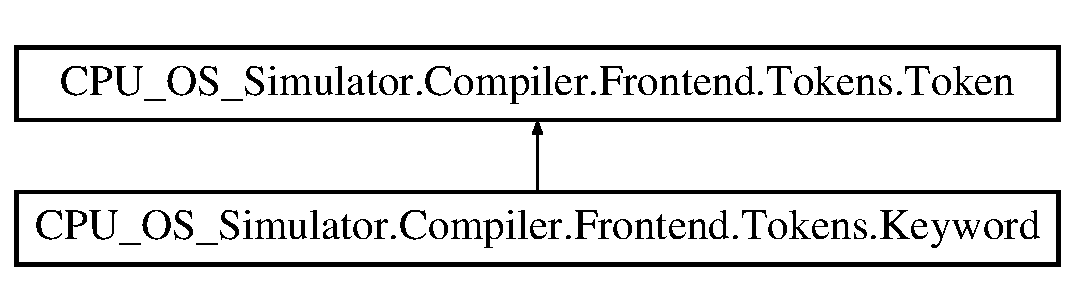
\includegraphics[height=2.000000cm]{class_c_p_u___o_s___simulator_1_1_compiler_1_1_frontend_1_1_tokens_1_1_keyword}
\end{center}
\end{figure}
\subsection*{Public Member Functions}
\begin{DoxyCompactItemize}
\item 
\hyperlink{class_c_p_u___o_s___simulator_1_1_compiler_1_1_frontend_1_1_tokens_1_1_keyword_ad01040755e095dc4f415ec2961cee3aa}{Keyword} (string \hyperlink{class_c_p_u___o_s___simulator_1_1_compiler_1_1_frontend_1_1_tokens_1_1_token_a5c05e12850ca18be8cbfdf7e2e263324}{value})
\item 
override Enum \hyperlink{class_c_p_u___o_s___simulator_1_1_compiler_1_1_frontend_1_1_tokens_1_1_keyword_aa1052d5b8b0fa6b1233fac902904e54a}{Detect\+Type} ()
\item 
\hyperlink{namespace_c_p_u___o_s___simulator_1_1_compiler_1_1_frontend_1_1_tokens_a86b87efebad08200cebe3075b5812b13}{Enum\+Keyword\+Type} \hyperlink{class_c_p_u___o_s___simulator_1_1_compiler_1_1_frontend_1_1_tokens_1_1_keyword_aa367b85e134043791bfc3f3f22e2399d}{Get\+Keyword\+Type} ()
\end{DoxyCompactItemize}
\subsection*{Additional Inherited Members}


\subsection{Detailed Description}


Definition at line 5 of file Keyword.\+cs.



\subsection{Constructor \& Destructor Documentation}
\hypertarget{class_c_p_u___o_s___simulator_1_1_compiler_1_1_frontend_1_1_tokens_1_1_keyword_ad01040755e095dc4f415ec2961cee3aa}{}\index{C\+P\+U\+\_\+\+O\+S\+\_\+\+Simulator\+::\+Compiler\+::\+Frontend\+::\+Tokens\+::\+Keyword@{C\+P\+U\+\_\+\+O\+S\+\_\+\+Simulator\+::\+Compiler\+::\+Frontend\+::\+Tokens\+::\+Keyword}!Keyword@{Keyword}}
\index{Keyword@{Keyword}!C\+P\+U\+\_\+\+O\+S\+\_\+\+Simulator\+::\+Compiler\+::\+Frontend\+::\+Tokens\+::\+Keyword@{C\+P\+U\+\_\+\+O\+S\+\_\+\+Simulator\+::\+Compiler\+::\+Frontend\+::\+Tokens\+::\+Keyword}}
\subsubsection[{Keyword(string value)}]{\setlength{\rightskip}{0pt plus 5cm}C\+P\+U\+\_\+\+O\+S\+\_\+\+Simulator.\+Compiler.\+Frontend.\+Tokens.\+Keyword.\+Keyword (
\begin{DoxyParamCaption}
\item[{string}]{value}
\end{DoxyParamCaption}
)}\label{class_c_p_u___o_s___simulator_1_1_compiler_1_1_frontend_1_1_tokens_1_1_keyword_ad01040755e095dc4f415ec2961cee3aa}


Definition at line 7 of file Keyword.\+cs.



\subsection{Member Function Documentation}
\hypertarget{class_c_p_u___o_s___simulator_1_1_compiler_1_1_frontend_1_1_tokens_1_1_keyword_aa1052d5b8b0fa6b1233fac902904e54a}{}\index{C\+P\+U\+\_\+\+O\+S\+\_\+\+Simulator\+::\+Compiler\+::\+Frontend\+::\+Tokens\+::\+Keyword@{C\+P\+U\+\_\+\+O\+S\+\_\+\+Simulator\+::\+Compiler\+::\+Frontend\+::\+Tokens\+::\+Keyword}!Detect\+Type@{Detect\+Type}}
\index{Detect\+Type@{Detect\+Type}!C\+P\+U\+\_\+\+O\+S\+\_\+\+Simulator\+::\+Compiler\+::\+Frontend\+::\+Tokens\+::\+Keyword@{C\+P\+U\+\_\+\+O\+S\+\_\+\+Simulator\+::\+Compiler\+::\+Frontend\+::\+Tokens\+::\+Keyword}}
\subsubsection[{Detect\+Type()}]{\setlength{\rightskip}{0pt plus 5cm}override Enum C\+P\+U\+\_\+\+O\+S\+\_\+\+Simulator.\+Compiler.\+Frontend.\+Tokens.\+Keyword.\+Detect\+Type (
\begin{DoxyParamCaption}
{}
\end{DoxyParamCaption}
)\hspace{0.3cm}{\ttfamily [virtual]}}\label{class_c_p_u___o_s___simulator_1_1_compiler_1_1_frontend_1_1_tokens_1_1_keyword_aa1052d5b8b0fa6b1233fac902904e54a}


Implements \hyperlink{class_c_p_u___o_s___simulator_1_1_compiler_1_1_frontend_1_1_tokens_1_1_token_accfe8c46faedacd527ef619698c76310}{C\+P\+U\+\_\+\+O\+S\+\_\+\+Simulator.\+Compiler.\+Frontend.\+Tokens.\+Token}.



Definition at line 11 of file Keyword.\+cs.

\hypertarget{class_c_p_u___o_s___simulator_1_1_compiler_1_1_frontend_1_1_tokens_1_1_keyword_aa367b85e134043791bfc3f3f22e2399d}{}\index{C\+P\+U\+\_\+\+O\+S\+\_\+\+Simulator\+::\+Compiler\+::\+Frontend\+::\+Tokens\+::\+Keyword@{C\+P\+U\+\_\+\+O\+S\+\_\+\+Simulator\+::\+Compiler\+::\+Frontend\+::\+Tokens\+::\+Keyword}!Get\+Keyword\+Type@{Get\+Keyword\+Type}}
\index{Get\+Keyword\+Type@{Get\+Keyword\+Type}!C\+P\+U\+\_\+\+O\+S\+\_\+\+Simulator\+::\+Compiler\+::\+Frontend\+::\+Tokens\+::\+Keyword@{C\+P\+U\+\_\+\+O\+S\+\_\+\+Simulator\+::\+Compiler\+::\+Frontend\+::\+Tokens\+::\+Keyword}}
\subsubsection[{Get\+Keyword\+Type()}]{\setlength{\rightskip}{0pt plus 5cm}{\bf Enum\+Keyword\+Type} C\+P\+U\+\_\+\+O\+S\+\_\+\+Simulator.\+Compiler.\+Frontend.\+Tokens.\+Keyword.\+Get\+Keyword\+Type (
\begin{DoxyParamCaption}
{}
\end{DoxyParamCaption}
)}\label{class_c_p_u___o_s___simulator_1_1_compiler_1_1_frontend_1_1_tokens_1_1_keyword_aa367b85e134043791bfc3f3f22e2399d}


Definition at line 92 of file Keyword.\+cs.



The documentation for this class was generated from the following file\+:\begin{DoxyCompactItemize}
\item 
Compiler/\+Frontend/\+Tokens/\hyperlink{_keyword_8cs}{Keyword.\+cs}\end{DoxyCompactItemize}

\hypertarget{class_c_p_u___o_s___simulator_1_1_compiler_1_1_frontend_1_1_lexer}{}\section{C\+P\+U\+\_\+\+O\+S\+\_\+\+Simulator.\+Compiler.\+Frontend.\+Lexer Class Reference}
\label{class_c_p_u___o_s___simulator_1_1_compiler_1_1_frontend_1_1_lexer}\index{C\+P\+U\+\_\+\+O\+S\+\_\+\+Simulator.\+Compiler.\+Frontend.\+Lexer@{C\+P\+U\+\_\+\+O\+S\+\_\+\+Simulator.\+Compiler.\+Frontend.\+Lexer}}


This class represents the lexer for the simulator programming language the lexer converts the source code into tokens for parsing to an Abstract Syntax Tree  


\subsection*{Public Member Functions}
\begin{DoxyCompactItemize}
\item 
\hyperlink{class_c_p_u___o_s___simulator_1_1_compiler_1_1_frontend_1_1_lexer_ad1b8ba022e0f486f963bf7f2104ef03d}{Lexer} (string \hyperlink{class_c_p_u___o_s___simulator_1_1_compiler_1_1_frontend_1_1_lexer_a735068e1008912edac69416bac78cef1}{source\+String})
\item 
bool \hyperlink{class_c_p_u___o_s___simulator_1_1_compiler_1_1_frontend_1_1_lexer_aa1d03860beb60dbb0c69ebbe70203def}{Start} ()
\begin{DoxyCompactList}\small\item\em This function is called to start the lexer \end{DoxyCompactList}\item 
void \hyperlink{class_c_p_u___o_s___simulator_1_1_compiler_1_1_frontend_1_1_lexer_a03760dde9cbc1aa09267e98d0788e544}{Define\+Variables} ()
\item 
void \hyperlink{class_c_p_u___o_s___simulator_1_1_compiler_1_1_frontend_1_1_lexer_ab611ae0862d84b5446643fd75577324e}{Define\+Subroutines} ()
\item 
void \hyperlink{class_c_p_u___o_s___simulator_1_1_compiler_1_1_frontend_1_1_lexer_a9fa262282fe000e66c4f97b899c39cdc}{Identify\+Unknown\+Tokens} ()
\item 
void \hyperlink{class_c_p_u___o_s___simulator_1_1_compiler_1_1_frontend_1_1_lexer_a6c12b898a982f63169687cca009d18e5}{Print\+Tokens} ()
\end{DoxyCompactItemize}
\subsection*{Properties}
\begin{DoxyCompactItemize}
\item 
bool \hyperlink{class_c_p_u___o_s___simulator_1_1_compiler_1_1_frontend_1_1_lexer_ab036c4c1dbff32b7a8a54d58f4c4195c}{Writing\+To\+Compiler\+Tester}\hspace{0.3cm}{\ttfamily  \mbox{[}get, set\mbox{]}}
\begin{DoxyCompactList}\small\item\em Property to hold whether we are writing the compiler tester app or not \end{DoxyCompactList}\item 
Text\+Box \hyperlink{class_c_p_u___o_s___simulator_1_1_compiler_1_1_frontend_1_1_lexer_adac6a4e1c23134a8c848bb35de4f39ff}{Output}\hspace{0.3cm}{\ttfamily  \mbox{[}get, set\mbox{]}}
\begin{DoxyCompactList}\small\item\em Property to hold the text box to display lexer output to \end{DoxyCompactList}\item 
string \hyperlink{class_c_p_u___o_s___simulator_1_1_compiler_1_1_frontend_1_1_lexer_a0e9d13cd92a7b359a8857e940f0af767}{Error}\hspace{0.3cm}{\ttfamily  \mbox{[}get, set\mbox{]}}
\begin{DoxyCompactList}\small\item\em Property for the string representation of the error that occurred while lexing \end{DoxyCompactList}\item 
Linked\+List$<$ \hyperlink{class_c_p_u___o_s___simulator_1_1_compiler_1_1_frontend_1_1_tokens_1_1_token}{Token} $>$ \hyperlink{class_c_p_u___o_s___simulator_1_1_compiler_1_1_frontend_1_1_lexer_a08611849f2bad0c53f5707d15dbdc840}{Tokens}\hspace{0.3cm}{\ttfamily  \mbox{[}get\mbox{]}}
\begin{DoxyCompactList}\small\item\em Property for the linked list of tokens produced by the lexer \end{DoxyCompactList}\item 
List$<$ Tuple$<$ string, \hyperlink{namespace_c_p_u___o_s___simulator_1_1_compiler_1_1_frontend_1_1_tokens_a7c0cc43763cc9d01c7d5af34d70b96ea}{Enum\+Types}, string $>$ $>$ \hyperlink{class_c_p_u___o_s___simulator_1_1_compiler_1_1_frontend_1_1_lexer_abb832df2e4dc0a135eca9e20aeafc25f}{Variables}\hspace{0.3cm}{\ttfamily  \mbox{[}get, set\mbox{]}}
\item 
List$<$ Tuple$<$ string, \hyperlink{namespace_c_p_u___o_s___simulator_1_1_compiler_1_1_frontend_1_1_tokens_a7c0cc43763cc9d01c7d5af34d70b96ea}{Enum\+Types}, string $>$ $>$ \hyperlink{class_c_p_u___o_s___simulator_1_1_compiler_1_1_frontend_1_1_lexer_aba6b80bb384466d01497af6a343f2eb4}{Subroutines}\hspace{0.3cm}{\ttfamily  \mbox{[}get, set\mbox{]}}
\item 
List$<$ Tuple$<$ string, \hyperlink{namespace_c_p_u___o_s___simulator_1_1_compiler_1_1_frontend_1_1_tokens_a7c0cc43763cc9d01c7d5af34d70b96ea}{Enum\+Types}, string $>$ $>$ \hyperlink{class_c_p_u___o_s___simulator_1_1_compiler_1_1_frontend_1_1_lexer_ac414167d172802ee774d998b1c20b2dd}{Functions}\hspace{0.3cm}{\ttfamily  \mbox{[}get, set\mbox{]}}
\end{DoxyCompactItemize}
\subsection*{Private Member Functions}
\begin{DoxyCompactItemize}
\item 
void \hyperlink{class_c_p_u___o_s___simulator_1_1_compiler_1_1_frontend_1_1_lexer_aa2cc4a7f138f9c6b8bda051eb08cd0e6}{Remove\+Whitespace} ()
\item 
void \hyperlink{class_c_p_u___o_s___simulator_1_1_compiler_1_1_frontend_1_1_lexer_a20ba99982182d2482f56f46d4d661a7d}{Define\+Functions} ()
\item 
string \hyperlink{class_c_p_u___o_s___simulator_1_1_compiler_1_1_frontend_1_1_lexer_a40799e3f75747b0e6e7bc7e3dc5a3856}{Get\+Variable\+Value} (Linked\+List\+Node$<$ \hyperlink{class_c_p_u___o_s___simulator_1_1_compiler_1_1_frontend_1_1_tokens_1_1_token}{Token} $>$ token)
\item 
\hyperlink{namespace_c_p_u___o_s___simulator_1_1_compiler_1_1_frontend_1_1_tokens_a7c0cc43763cc9d01c7d5af34d70b96ea}{Enum\+Types} \hyperlink{class_c_p_u___o_s___simulator_1_1_compiler_1_1_frontend_1_1_lexer_a51100f91cf5093df274114f32d210a91}{Get\+Variable\+Type} (Linked\+List\+Node$<$ \hyperlink{class_c_p_u___o_s___simulator_1_1_compiler_1_1_frontend_1_1_tokens_1_1_token}{Token} $>$ token)
\item 
string \hyperlink{class_c_p_u___o_s___simulator_1_1_compiler_1_1_frontend_1_1_lexer_a9654723fcd32311aefbfcfbc0888e4bc}{Get\+Variable\+Name} (Linked\+List\+Node$<$ \hyperlink{class_c_p_u___o_s___simulator_1_1_compiler_1_1_frontend_1_1_tokens_1_1_token}{Token} $>$ token)
\item 
void \hyperlink{class_c_p_u___o_s___simulator_1_1_compiler_1_1_frontend_1_1_lexer_a024d4fa0d9659b9ac9f7446baa7e99ba}{Print\+Warnings} ()
\begin{DoxyCompactList}\small\item\em This function print out any warnings produced while lexing \end{DoxyCompactList}\item 
List$<$ string $>$ \hyperlink{class_c_p_u___o_s___simulator_1_1_compiler_1_1_frontend_1_1_lexer_a3cb07219d31cbf42ce171abf1af266be}{Check\+For\+Warnings} ()
\begin{DoxyCompactList}\small\item\em This function checks the code for any warnings \end{DoxyCompactList}\item 
bool \hyperlink{class_c_p_u___o_s___simulator_1_1_compiler_1_1_frontend_1_1_lexer_a55107682df54c395363fa466bbd47be9}{Check\+For\+Errors} ()
\begin{DoxyCompactList}\small\item\em This function checks the code for errors \end{DoxyCompactList}\item 
void \hyperlink{class_c_p_u___o_s___simulator_1_1_compiler_1_1_frontend_1_1_lexer_a64e6ce60e37e5cf153dbbc8757fea55c}{Throw\+Error} (\hyperlink{namespace_c_p_u___o_s___simulator_1_1_compiler_1_1_frontend_a268b68f35fd94ce3549dd33a7e77d7e8}{Enum\+Error\+Codes} enum\+Error\+Codes, string expected\+Token)
\begin{DoxyCompactList}\small\item\em This function creates an error message to display in a message box to the user indicating what type of error occurred \end{DoxyCompactList}\item 
Linked\+List$<$ \hyperlink{class_c_p_u___o_s___simulator_1_1_compiler_1_1_frontend_1_1_tokens_1_1_token}{Token} $>$ \hyperlink{class_c_p_u___o_s___simulator_1_1_compiler_1_1_frontend_1_1_lexer_a9af12a452db042cfa2552078ca991160}{Generate\+Tokens} ()
\item 
void \hyperlink{class_c_p_u___o_s___simulator_1_1_compiler_1_1_frontend_1_1_lexer_aabdf7836b845bde22402027bdb1e949f}{Create\+Tokens\+File} (string filename)
\end{DoxyCompactItemize}
\subsection*{Private Attributes}
\begin{DoxyCompactItemize}
\item 
readonly string \hyperlink{class_c_p_u___o_s___simulator_1_1_compiler_1_1_frontend_1_1_lexer_a735068e1008912edac69416bac78cef1}{source\+String}
\item 
Linked\+List$<$ string $>$ \hyperlink{class_c_p_u___o_s___simulator_1_1_compiler_1_1_frontend_1_1_lexer_ab99dc45a5bf56bba028a55213c81924f}{token\+Strings}
\item 
Linked\+List\+Node$<$ string $>$ \hyperlink{class_c_p_u___o_s___simulator_1_1_compiler_1_1_frontend_1_1_lexer_a38fd448afcdd31a212407189d8fcda8f}{current\+Token\+String}
\item 
Linked\+List\+Node$<$ string $>$ \hyperlink{class_c_p_u___o_s___simulator_1_1_compiler_1_1_frontend_1_1_lexer_a6795b61d4a157858e6471adb636a16f0}{next\+Token\+String}
\item 
Linked\+List\+Node$<$ string $>$ \hyperlink{class_c_p_u___o_s___simulator_1_1_compiler_1_1_frontend_1_1_lexer_a4cc9eaf6480960311bba7a18ccd99087}{previous\+Token\+String}
\item 
Linked\+List$<$ \hyperlink{class_c_p_u___o_s___simulator_1_1_compiler_1_1_frontend_1_1_tokens_1_1_token}{Token} $>$ \hyperlink{class_c_p_u___o_s___simulator_1_1_compiler_1_1_frontend_1_1_lexer_abf6ec407cb3e44e9da83d68a1b13ed4c}{tokens}
\item 
Linked\+List\+Node$<$ \hyperlink{class_c_p_u___o_s___simulator_1_1_compiler_1_1_frontend_1_1_tokens_1_1_token}{Token} $>$ \hyperlink{class_c_p_u___o_s___simulator_1_1_compiler_1_1_frontend_1_1_lexer_a030e4639542601955e162bd9010d4ed6}{current\+Token}
\item 
Linked\+List\+Node$<$ \hyperlink{class_c_p_u___o_s___simulator_1_1_compiler_1_1_frontend_1_1_tokens_1_1_token}{Token} $>$ \hyperlink{class_c_p_u___o_s___simulator_1_1_compiler_1_1_frontend_1_1_lexer_a9bdd0bc4e775f8708a1efebd0e84bc7c}{next\+Token}
\item 
Linked\+List\+Node$<$ \hyperlink{class_c_p_u___o_s___simulator_1_1_compiler_1_1_frontend_1_1_tokens_1_1_token}{Token} $>$ \hyperlink{class_c_p_u___o_s___simulator_1_1_compiler_1_1_frontend_1_1_lexer_ad64622c6372adff6559435fbfce44a2a}{previous\+Token}
\item 
bool \hyperlink{class_c_p_u___o_s___simulator_1_1_compiler_1_1_frontend_1_1_lexer_a8a75fa6d30d6d3b2ab713a729d85b081}{writing\+To\+Compiler\+Tester}
\item 
string \hyperlink{class_c_p_u___o_s___simulator_1_1_compiler_1_1_frontend_1_1_lexer_a787862ffec1828f426fac010f543e31c}{error} = String.\+Empty
\item 
List$<$ string $>$ \hyperlink{class_c_p_u___o_s___simulator_1_1_compiler_1_1_frontend_1_1_lexer_ac240cede3460c43d89c4387c04f00377}{warning\+List}
\item 
bool \hyperlink{class_c_p_u___o_s___simulator_1_1_compiler_1_1_frontend_1_1_lexer_ad2b45c1eaf05bca9d992ed22a0331bae}{successful}
\item 
Text\+Box \hyperlink{class_c_p_u___o_s___simulator_1_1_compiler_1_1_frontend_1_1_lexer_ab2c4e18875ad66f9f4b1debf32e21d97}{output}
\item 
List$<$ Tuple$<$ string, \hyperlink{namespace_c_p_u___o_s___simulator_1_1_compiler_1_1_frontend_1_1_tokens_a7c0cc43763cc9d01c7d5af34d70b96ea}{Enum\+Types}, string $>$ $>$ \hyperlink{class_c_p_u___o_s___simulator_1_1_compiler_1_1_frontend_1_1_lexer_af7e42e63231b352e446b5be89623c74a}{variables}
\item 
List$<$ Tuple$<$ string, \hyperlink{namespace_c_p_u___o_s___simulator_1_1_compiler_1_1_frontend_1_1_tokens_a7c0cc43763cc9d01c7d5af34d70b96ea}{Enum\+Types}, string $>$ $>$ \hyperlink{class_c_p_u___o_s___simulator_1_1_compiler_1_1_frontend_1_1_lexer_a45c844ee9a1f5dedb94dcb4f19883d5a}{subroutines}
\item 
List$<$ Tuple$<$ string, \hyperlink{namespace_c_p_u___o_s___simulator_1_1_compiler_1_1_frontend_1_1_tokens_a7c0cc43763cc9d01c7d5af34d70b96ea}{Enum\+Types}, string $>$ $>$ \hyperlink{class_c_p_u___o_s___simulator_1_1_compiler_1_1_frontend_1_1_lexer_ab56c14f20b221345bcb9ef4bdd7d5c87}{functions}
\end{DoxyCompactItemize}


\subsection{Detailed Description}
This class represents the lexer for the simulator programming language the lexer converts the source code into tokens for parsing to an Abstract Syntax Tree 



Definition at line 14 of file Lexer.\+cs.



\subsection{Constructor \& Destructor Documentation}
\hypertarget{class_c_p_u___o_s___simulator_1_1_compiler_1_1_frontend_1_1_lexer_ad1b8ba022e0f486f963bf7f2104ef03d}{}\index{C\+P\+U\+\_\+\+O\+S\+\_\+\+Simulator\+::\+Compiler\+::\+Frontend\+::\+Lexer@{C\+P\+U\+\_\+\+O\+S\+\_\+\+Simulator\+::\+Compiler\+::\+Frontend\+::\+Lexer}!Lexer@{Lexer}}
\index{Lexer@{Lexer}!C\+P\+U\+\_\+\+O\+S\+\_\+\+Simulator\+::\+Compiler\+::\+Frontend\+::\+Lexer@{C\+P\+U\+\_\+\+O\+S\+\_\+\+Simulator\+::\+Compiler\+::\+Frontend\+::\+Lexer}}
\subsubsection[{Lexer(string source\+String)}]{\setlength{\rightskip}{0pt plus 5cm}C\+P\+U\+\_\+\+O\+S\+\_\+\+Simulator.\+Compiler.\+Frontend.\+Lexer.\+Lexer (
\begin{DoxyParamCaption}
\item[{string}]{source\+String}
\end{DoxyParamCaption}
)}\label{class_c_p_u___o_s___simulator_1_1_compiler_1_1_frontend_1_1_lexer_ad1b8ba022e0f486f963bf7f2104ef03d}


Definition at line 41 of file Lexer.\+cs.



\subsection{Member Function Documentation}
\hypertarget{class_c_p_u___o_s___simulator_1_1_compiler_1_1_frontend_1_1_lexer_a55107682df54c395363fa466bbd47be9}{}\index{C\+P\+U\+\_\+\+O\+S\+\_\+\+Simulator\+::\+Compiler\+::\+Frontend\+::\+Lexer@{C\+P\+U\+\_\+\+O\+S\+\_\+\+Simulator\+::\+Compiler\+::\+Frontend\+::\+Lexer}!Check\+For\+Errors@{Check\+For\+Errors}}
\index{Check\+For\+Errors@{Check\+For\+Errors}!C\+P\+U\+\_\+\+O\+S\+\_\+\+Simulator\+::\+Compiler\+::\+Frontend\+::\+Lexer@{C\+P\+U\+\_\+\+O\+S\+\_\+\+Simulator\+::\+Compiler\+::\+Frontend\+::\+Lexer}}
\subsubsection[{Check\+For\+Errors()}]{\setlength{\rightskip}{0pt plus 5cm}bool C\+P\+U\+\_\+\+O\+S\+\_\+\+Simulator.\+Compiler.\+Frontend.\+Lexer.\+Check\+For\+Errors (
\begin{DoxyParamCaption}
{}
\end{DoxyParamCaption}
)\hspace{0.3cm}{\ttfamily [private]}}\label{class_c_p_u___o_s___simulator_1_1_compiler_1_1_frontend_1_1_lexer_a55107682df54c395363fa466bbd47be9}


This function checks the code for errors 

\begin{DoxyReturn}{Returns}
false if errors occurred true if no errors occurred 
\end{DoxyReturn}


Definition at line 301 of file Lexer.\+cs.

\hypertarget{class_c_p_u___o_s___simulator_1_1_compiler_1_1_frontend_1_1_lexer_a3cb07219d31cbf42ce171abf1af266be}{}\index{C\+P\+U\+\_\+\+O\+S\+\_\+\+Simulator\+::\+Compiler\+::\+Frontend\+::\+Lexer@{C\+P\+U\+\_\+\+O\+S\+\_\+\+Simulator\+::\+Compiler\+::\+Frontend\+::\+Lexer}!Check\+For\+Warnings@{Check\+For\+Warnings}}
\index{Check\+For\+Warnings@{Check\+For\+Warnings}!C\+P\+U\+\_\+\+O\+S\+\_\+\+Simulator\+::\+Compiler\+::\+Frontend\+::\+Lexer@{C\+P\+U\+\_\+\+O\+S\+\_\+\+Simulator\+::\+Compiler\+::\+Frontend\+::\+Lexer}}
\subsubsection[{Check\+For\+Warnings()}]{\setlength{\rightskip}{0pt plus 5cm}List$<$string$>$ C\+P\+U\+\_\+\+O\+S\+\_\+\+Simulator.\+Compiler.\+Frontend.\+Lexer.\+Check\+For\+Warnings (
\begin{DoxyParamCaption}
{}
\end{DoxyParamCaption}
)\hspace{0.3cm}{\ttfamily [private]}}\label{class_c_p_u___o_s___simulator_1_1_compiler_1_1_frontend_1_1_lexer_a3cb07219d31cbf42ce171abf1af266be}


This function checks the code for any warnings 

\begin{DoxyReturn}{Returns}
a list of warnings or an empty list if there were no warnings
\end{DoxyReturn}


Definition at line 281 of file Lexer.\+cs.

\hypertarget{class_c_p_u___o_s___simulator_1_1_compiler_1_1_frontend_1_1_lexer_aabdf7836b845bde22402027bdb1e949f}{}\index{C\+P\+U\+\_\+\+O\+S\+\_\+\+Simulator\+::\+Compiler\+::\+Frontend\+::\+Lexer@{C\+P\+U\+\_\+\+O\+S\+\_\+\+Simulator\+::\+Compiler\+::\+Frontend\+::\+Lexer}!Create\+Tokens\+File@{Create\+Tokens\+File}}
\index{Create\+Tokens\+File@{Create\+Tokens\+File}!C\+P\+U\+\_\+\+O\+S\+\_\+\+Simulator\+::\+Compiler\+::\+Frontend\+::\+Lexer@{C\+P\+U\+\_\+\+O\+S\+\_\+\+Simulator\+::\+Compiler\+::\+Frontend\+::\+Lexer}}
\subsubsection[{Create\+Tokens\+File(string filename)}]{\setlength{\rightskip}{0pt plus 5cm}void C\+P\+U\+\_\+\+O\+S\+\_\+\+Simulator.\+Compiler.\+Frontend.\+Lexer.\+Create\+Tokens\+File (
\begin{DoxyParamCaption}
\item[{string}]{filename}
\end{DoxyParamCaption}
)\hspace{0.3cm}{\ttfamily [private]}}\label{class_c_p_u___o_s___simulator_1_1_compiler_1_1_frontend_1_1_lexer_aabdf7836b845bde22402027bdb1e949f}


Definition at line 513 of file Lexer.\+cs.

\hypertarget{class_c_p_u___o_s___simulator_1_1_compiler_1_1_frontend_1_1_lexer_a20ba99982182d2482f56f46d4d661a7d}{}\index{C\+P\+U\+\_\+\+O\+S\+\_\+\+Simulator\+::\+Compiler\+::\+Frontend\+::\+Lexer@{C\+P\+U\+\_\+\+O\+S\+\_\+\+Simulator\+::\+Compiler\+::\+Frontend\+::\+Lexer}!Define\+Functions@{Define\+Functions}}
\index{Define\+Functions@{Define\+Functions}!C\+P\+U\+\_\+\+O\+S\+\_\+\+Simulator\+::\+Compiler\+::\+Frontend\+::\+Lexer@{C\+P\+U\+\_\+\+O\+S\+\_\+\+Simulator\+::\+Compiler\+::\+Frontend\+::\+Lexer}}
\subsubsection[{Define\+Functions()}]{\setlength{\rightskip}{0pt plus 5cm}void C\+P\+U\+\_\+\+O\+S\+\_\+\+Simulator.\+Compiler.\+Frontend.\+Lexer.\+Define\+Functions (
\begin{DoxyParamCaption}
{}
\end{DoxyParamCaption}
)\hspace{0.3cm}{\ttfamily [private]}}\label{class_c_p_u___o_s___simulator_1_1_compiler_1_1_frontend_1_1_lexer_a20ba99982182d2482f56f46d4d661a7d}


Definition at line 156 of file Lexer.\+cs.

\hypertarget{class_c_p_u___o_s___simulator_1_1_compiler_1_1_frontend_1_1_lexer_ab611ae0862d84b5446643fd75577324e}{}\index{C\+P\+U\+\_\+\+O\+S\+\_\+\+Simulator\+::\+Compiler\+::\+Frontend\+::\+Lexer@{C\+P\+U\+\_\+\+O\+S\+\_\+\+Simulator\+::\+Compiler\+::\+Frontend\+::\+Lexer}!Define\+Subroutines@{Define\+Subroutines}}
\index{Define\+Subroutines@{Define\+Subroutines}!C\+P\+U\+\_\+\+O\+S\+\_\+\+Simulator\+::\+Compiler\+::\+Frontend\+::\+Lexer@{C\+P\+U\+\_\+\+O\+S\+\_\+\+Simulator\+::\+Compiler\+::\+Frontend\+::\+Lexer}}
\subsubsection[{Define\+Subroutines()}]{\setlength{\rightskip}{0pt plus 5cm}void C\+P\+U\+\_\+\+O\+S\+\_\+\+Simulator.\+Compiler.\+Frontend.\+Lexer.\+Define\+Subroutines (
\begin{DoxyParamCaption}
{}
\end{DoxyParamCaption}
)}\label{class_c_p_u___o_s___simulator_1_1_compiler_1_1_frontend_1_1_lexer_ab611ae0862d84b5446643fd75577324e}


Definition at line 209 of file Lexer.\+cs.

\hypertarget{class_c_p_u___o_s___simulator_1_1_compiler_1_1_frontend_1_1_lexer_a03760dde9cbc1aa09267e98d0788e544}{}\index{C\+P\+U\+\_\+\+O\+S\+\_\+\+Simulator\+::\+Compiler\+::\+Frontend\+::\+Lexer@{C\+P\+U\+\_\+\+O\+S\+\_\+\+Simulator\+::\+Compiler\+::\+Frontend\+::\+Lexer}!Define\+Variables@{Define\+Variables}}
\index{Define\+Variables@{Define\+Variables}!C\+P\+U\+\_\+\+O\+S\+\_\+\+Simulator\+::\+Compiler\+::\+Frontend\+::\+Lexer@{C\+P\+U\+\_\+\+O\+S\+\_\+\+Simulator\+::\+Compiler\+::\+Frontend\+::\+Lexer}}
\subsubsection[{Define\+Variables()}]{\setlength{\rightskip}{0pt plus 5cm}void C\+P\+U\+\_\+\+O\+S\+\_\+\+Simulator.\+Compiler.\+Frontend.\+Lexer.\+Define\+Variables (
\begin{DoxyParamCaption}
{}
\end{DoxyParamCaption}
)}\label{class_c_p_u___o_s___simulator_1_1_compiler_1_1_frontend_1_1_lexer_a03760dde9cbc1aa09267e98d0788e544}


Definition at line 181 of file Lexer.\+cs.

\hypertarget{class_c_p_u___o_s___simulator_1_1_compiler_1_1_frontend_1_1_lexer_a9af12a452db042cfa2552078ca991160}{}\index{C\+P\+U\+\_\+\+O\+S\+\_\+\+Simulator\+::\+Compiler\+::\+Frontend\+::\+Lexer@{C\+P\+U\+\_\+\+O\+S\+\_\+\+Simulator\+::\+Compiler\+::\+Frontend\+::\+Lexer}!Generate\+Tokens@{Generate\+Tokens}}
\index{Generate\+Tokens@{Generate\+Tokens}!C\+P\+U\+\_\+\+O\+S\+\_\+\+Simulator\+::\+Compiler\+::\+Frontend\+::\+Lexer@{C\+P\+U\+\_\+\+O\+S\+\_\+\+Simulator\+::\+Compiler\+::\+Frontend\+::\+Lexer}}
\subsubsection[{Generate\+Tokens()}]{\setlength{\rightskip}{0pt plus 5cm}Linked\+List$<${\bf Token}$>$ C\+P\+U\+\_\+\+O\+S\+\_\+\+Simulator.\+Compiler.\+Frontend.\+Lexer.\+Generate\+Tokens (
\begin{DoxyParamCaption}
{}
\end{DoxyParamCaption}
)\hspace{0.3cm}{\ttfamily [private]}}\label{class_c_p_u___o_s___simulator_1_1_compiler_1_1_frontend_1_1_lexer_a9af12a452db042cfa2552078ca991160}


Definition at line 365 of file Lexer.\+cs.

\hypertarget{class_c_p_u___o_s___simulator_1_1_compiler_1_1_frontend_1_1_lexer_a9654723fcd32311aefbfcfbc0888e4bc}{}\index{C\+P\+U\+\_\+\+O\+S\+\_\+\+Simulator\+::\+Compiler\+::\+Frontend\+::\+Lexer@{C\+P\+U\+\_\+\+O\+S\+\_\+\+Simulator\+::\+Compiler\+::\+Frontend\+::\+Lexer}!Get\+Variable\+Name@{Get\+Variable\+Name}}
\index{Get\+Variable\+Name@{Get\+Variable\+Name}!C\+P\+U\+\_\+\+O\+S\+\_\+\+Simulator\+::\+Compiler\+::\+Frontend\+::\+Lexer@{C\+P\+U\+\_\+\+O\+S\+\_\+\+Simulator\+::\+Compiler\+::\+Frontend\+::\+Lexer}}
\subsubsection[{Get\+Variable\+Name(\+Linked\+List\+Node$<$ Token $>$ token)}]{\setlength{\rightskip}{0pt plus 5cm}string C\+P\+U\+\_\+\+O\+S\+\_\+\+Simulator.\+Compiler.\+Frontend.\+Lexer.\+Get\+Variable\+Name (
\begin{DoxyParamCaption}
\item[{Linked\+List\+Node$<$ {\bf Token} $>$}]{token}
\end{DoxyParamCaption}
)\hspace{0.3cm}{\ttfamily [private]}}\label{class_c_p_u___o_s___simulator_1_1_compiler_1_1_frontend_1_1_lexer_a9654723fcd32311aefbfcfbc0888e4bc}


Definition at line 256 of file Lexer.\+cs.

\hypertarget{class_c_p_u___o_s___simulator_1_1_compiler_1_1_frontend_1_1_lexer_a51100f91cf5093df274114f32d210a91}{}\index{C\+P\+U\+\_\+\+O\+S\+\_\+\+Simulator\+::\+Compiler\+::\+Frontend\+::\+Lexer@{C\+P\+U\+\_\+\+O\+S\+\_\+\+Simulator\+::\+Compiler\+::\+Frontend\+::\+Lexer}!Get\+Variable\+Type@{Get\+Variable\+Type}}
\index{Get\+Variable\+Type@{Get\+Variable\+Type}!C\+P\+U\+\_\+\+O\+S\+\_\+\+Simulator\+::\+Compiler\+::\+Frontend\+::\+Lexer@{C\+P\+U\+\_\+\+O\+S\+\_\+\+Simulator\+::\+Compiler\+::\+Frontend\+::\+Lexer}}
\subsubsection[{Get\+Variable\+Type(\+Linked\+List\+Node$<$ Token $>$ token)}]{\setlength{\rightskip}{0pt plus 5cm}{\bf Enum\+Types} C\+P\+U\+\_\+\+O\+S\+\_\+\+Simulator.\+Compiler.\+Frontend.\+Lexer.\+Get\+Variable\+Type (
\begin{DoxyParamCaption}
\item[{Linked\+List\+Node$<$ {\bf Token} $>$}]{token}
\end{DoxyParamCaption}
)\hspace{0.3cm}{\ttfamily [private]}}\label{class_c_p_u___o_s___simulator_1_1_compiler_1_1_frontend_1_1_lexer_a51100f91cf5093df274114f32d210a91}


Definition at line 247 of file Lexer.\+cs.

\hypertarget{class_c_p_u___o_s___simulator_1_1_compiler_1_1_frontend_1_1_lexer_a40799e3f75747b0e6e7bc7e3dc5a3856}{}\index{C\+P\+U\+\_\+\+O\+S\+\_\+\+Simulator\+::\+Compiler\+::\+Frontend\+::\+Lexer@{C\+P\+U\+\_\+\+O\+S\+\_\+\+Simulator\+::\+Compiler\+::\+Frontend\+::\+Lexer}!Get\+Variable\+Value@{Get\+Variable\+Value}}
\index{Get\+Variable\+Value@{Get\+Variable\+Value}!C\+P\+U\+\_\+\+O\+S\+\_\+\+Simulator\+::\+Compiler\+::\+Frontend\+::\+Lexer@{C\+P\+U\+\_\+\+O\+S\+\_\+\+Simulator\+::\+Compiler\+::\+Frontend\+::\+Lexer}}
\subsubsection[{Get\+Variable\+Value(\+Linked\+List\+Node$<$ Token $>$ token)}]{\setlength{\rightskip}{0pt plus 5cm}string C\+P\+U\+\_\+\+O\+S\+\_\+\+Simulator.\+Compiler.\+Frontend.\+Lexer.\+Get\+Variable\+Value (
\begin{DoxyParamCaption}
\item[{Linked\+List\+Node$<$ {\bf Token} $>$}]{token}
\end{DoxyParamCaption}
)\hspace{0.3cm}{\ttfamily [private]}}\label{class_c_p_u___o_s___simulator_1_1_compiler_1_1_frontend_1_1_lexer_a40799e3f75747b0e6e7bc7e3dc5a3856}


Definition at line 235 of file Lexer.\+cs.

\hypertarget{class_c_p_u___o_s___simulator_1_1_compiler_1_1_frontend_1_1_lexer_a9fa262282fe000e66c4f97b899c39cdc}{}\index{C\+P\+U\+\_\+\+O\+S\+\_\+\+Simulator\+::\+Compiler\+::\+Frontend\+::\+Lexer@{C\+P\+U\+\_\+\+O\+S\+\_\+\+Simulator\+::\+Compiler\+::\+Frontend\+::\+Lexer}!Identify\+Unknown\+Tokens@{Identify\+Unknown\+Tokens}}
\index{Identify\+Unknown\+Tokens@{Identify\+Unknown\+Tokens}!C\+P\+U\+\_\+\+O\+S\+\_\+\+Simulator\+::\+Compiler\+::\+Frontend\+::\+Lexer@{C\+P\+U\+\_\+\+O\+S\+\_\+\+Simulator\+::\+Compiler\+::\+Frontend\+::\+Lexer}}
\subsubsection[{Identify\+Unknown\+Tokens()}]{\setlength{\rightskip}{0pt plus 5cm}void C\+P\+U\+\_\+\+O\+S\+\_\+\+Simulator.\+Compiler.\+Frontend.\+Lexer.\+Identify\+Unknown\+Tokens (
\begin{DoxyParamCaption}
{}
\end{DoxyParamCaption}
)}\label{class_c_p_u___o_s___simulator_1_1_compiler_1_1_frontend_1_1_lexer_a9fa262282fe000e66c4f97b899c39cdc}


Definition at line 446 of file Lexer.\+cs.

\hypertarget{class_c_p_u___o_s___simulator_1_1_compiler_1_1_frontend_1_1_lexer_a6c12b898a982f63169687cca009d18e5}{}\index{C\+P\+U\+\_\+\+O\+S\+\_\+\+Simulator\+::\+Compiler\+::\+Frontend\+::\+Lexer@{C\+P\+U\+\_\+\+O\+S\+\_\+\+Simulator\+::\+Compiler\+::\+Frontend\+::\+Lexer}!Print\+Tokens@{Print\+Tokens}}
\index{Print\+Tokens@{Print\+Tokens}!C\+P\+U\+\_\+\+O\+S\+\_\+\+Simulator\+::\+Compiler\+::\+Frontend\+::\+Lexer@{C\+P\+U\+\_\+\+O\+S\+\_\+\+Simulator\+::\+Compiler\+::\+Frontend\+::\+Lexer}}
\subsubsection[{Print\+Tokens()}]{\setlength{\rightskip}{0pt plus 5cm}void C\+P\+U\+\_\+\+O\+S\+\_\+\+Simulator.\+Compiler.\+Frontend.\+Lexer.\+Print\+Tokens (
\begin{DoxyParamCaption}
{}
\end{DoxyParamCaption}
)}\label{class_c_p_u___o_s___simulator_1_1_compiler_1_1_frontend_1_1_lexer_a6c12b898a982f63169687cca009d18e5}


Definition at line 473 of file Lexer.\+cs.

\hypertarget{class_c_p_u___o_s___simulator_1_1_compiler_1_1_frontend_1_1_lexer_a024d4fa0d9659b9ac9f7446baa7e99ba}{}\index{C\+P\+U\+\_\+\+O\+S\+\_\+\+Simulator\+::\+Compiler\+::\+Frontend\+::\+Lexer@{C\+P\+U\+\_\+\+O\+S\+\_\+\+Simulator\+::\+Compiler\+::\+Frontend\+::\+Lexer}!Print\+Warnings@{Print\+Warnings}}
\index{Print\+Warnings@{Print\+Warnings}!C\+P\+U\+\_\+\+O\+S\+\_\+\+Simulator\+::\+Compiler\+::\+Frontend\+::\+Lexer@{C\+P\+U\+\_\+\+O\+S\+\_\+\+Simulator\+::\+Compiler\+::\+Frontend\+::\+Lexer}}
\subsubsection[{Print\+Warnings()}]{\setlength{\rightskip}{0pt plus 5cm}void C\+P\+U\+\_\+\+O\+S\+\_\+\+Simulator.\+Compiler.\+Frontend.\+Lexer.\+Print\+Warnings (
\begin{DoxyParamCaption}
{}
\end{DoxyParamCaption}
)\hspace{0.3cm}{\ttfamily [private]}}\label{class_c_p_u___o_s___simulator_1_1_compiler_1_1_frontend_1_1_lexer_a024d4fa0d9659b9ac9f7446baa7e99ba}


This function print out any warnings produced while lexing 



Definition at line 264 of file Lexer.\+cs.

\hypertarget{class_c_p_u___o_s___simulator_1_1_compiler_1_1_frontend_1_1_lexer_aa2cc4a7f138f9c6b8bda051eb08cd0e6}{}\index{C\+P\+U\+\_\+\+O\+S\+\_\+\+Simulator\+::\+Compiler\+::\+Frontend\+::\+Lexer@{C\+P\+U\+\_\+\+O\+S\+\_\+\+Simulator\+::\+Compiler\+::\+Frontend\+::\+Lexer}!Remove\+Whitespace@{Remove\+Whitespace}}
\index{Remove\+Whitespace@{Remove\+Whitespace}!C\+P\+U\+\_\+\+O\+S\+\_\+\+Simulator\+::\+Compiler\+::\+Frontend\+::\+Lexer@{C\+P\+U\+\_\+\+O\+S\+\_\+\+Simulator\+::\+Compiler\+::\+Frontend\+::\+Lexer}}
\subsubsection[{Remove\+Whitespace()}]{\setlength{\rightskip}{0pt plus 5cm}void C\+P\+U\+\_\+\+O\+S\+\_\+\+Simulator.\+Compiler.\+Frontend.\+Lexer.\+Remove\+Whitespace (
\begin{DoxyParamCaption}
{}
\end{DoxyParamCaption}
)\hspace{0.3cm}{\ttfamily [private]}}\label{class_c_p_u___o_s___simulator_1_1_compiler_1_1_frontend_1_1_lexer_aa2cc4a7f138f9c6b8bda051eb08cd0e6}


Definition at line 127 of file Lexer.\+cs.

\hypertarget{class_c_p_u___o_s___simulator_1_1_compiler_1_1_frontend_1_1_lexer_aa1d03860beb60dbb0c69ebbe70203def}{}\index{C\+P\+U\+\_\+\+O\+S\+\_\+\+Simulator\+::\+Compiler\+::\+Frontend\+::\+Lexer@{C\+P\+U\+\_\+\+O\+S\+\_\+\+Simulator\+::\+Compiler\+::\+Frontend\+::\+Lexer}!Start@{Start}}
\index{Start@{Start}!C\+P\+U\+\_\+\+O\+S\+\_\+\+Simulator\+::\+Compiler\+::\+Frontend\+::\+Lexer@{C\+P\+U\+\_\+\+O\+S\+\_\+\+Simulator\+::\+Compiler\+::\+Frontend\+::\+Lexer}}
\subsubsection[{Start()}]{\setlength{\rightskip}{0pt plus 5cm}bool C\+P\+U\+\_\+\+O\+S\+\_\+\+Simulator.\+Compiler.\+Frontend.\+Lexer.\+Start (
\begin{DoxyParamCaption}
{}
\end{DoxyParamCaption}
)}\label{class_c_p_u___o_s___simulator_1_1_compiler_1_1_frontend_1_1_lexer_aa1d03860beb60dbb0c69ebbe70203def}


This function is called to start the lexer 

\begin{DoxyReturn}{Returns}
whether the lexer completed successfully 
\end{DoxyReturn}


Definition at line 106 of file Lexer.\+cs.

\hypertarget{class_c_p_u___o_s___simulator_1_1_compiler_1_1_frontend_1_1_lexer_a64e6ce60e37e5cf153dbbc8757fea55c}{}\index{C\+P\+U\+\_\+\+O\+S\+\_\+\+Simulator\+::\+Compiler\+::\+Frontend\+::\+Lexer@{C\+P\+U\+\_\+\+O\+S\+\_\+\+Simulator\+::\+Compiler\+::\+Frontend\+::\+Lexer}!Throw\+Error@{Throw\+Error}}
\index{Throw\+Error@{Throw\+Error}!C\+P\+U\+\_\+\+O\+S\+\_\+\+Simulator\+::\+Compiler\+::\+Frontend\+::\+Lexer@{C\+P\+U\+\_\+\+O\+S\+\_\+\+Simulator\+::\+Compiler\+::\+Frontend\+::\+Lexer}}
\subsubsection[{Throw\+Error(\+Enum\+Error\+Codes enum\+Error\+Codes, string expected\+Token)}]{\setlength{\rightskip}{0pt plus 5cm}void C\+P\+U\+\_\+\+O\+S\+\_\+\+Simulator.\+Compiler.\+Frontend.\+Lexer.\+Throw\+Error (
\begin{DoxyParamCaption}
\item[{{\bf Enum\+Error\+Codes}}]{enum\+Error\+Codes, }
\item[{string}]{expected\+Token}
\end{DoxyParamCaption}
)\hspace{0.3cm}{\ttfamily [private]}}\label{class_c_p_u___o_s___simulator_1_1_compiler_1_1_frontend_1_1_lexer_a64e6ce60e37e5cf153dbbc8757fea55c}


This function creates an error message to display in a message box to the user indicating what type of error occurred 


\begin{DoxyParams}{Parameters}
{\em enum\+Error\+Codes} & the error code that identifies the error\\
\hline
{\em expected\+Token} & the expected token\\
\hline
\end{DoxyParams}


Definition at line 360 of file Lexer.\+cs.



\subsection{Member Data Documentation}
\hypertarget{class_c_p_u___o_s___simulator_1_1_compiler_1_1_frontend_1_1_lexer_a030e4639542601955e162bd9010d4ed6}{}\index{C\+P\+U\+\_\+\+O\+S\+\_\+\+Simulator\+::\+Compiler\+::\+Frontend\+::\+Lexer@{C\+P\+U\+\_\+\+O\+S\+\_\+\+Simulator\+::\+Compiler\+::\+Frontend\+::\+Lexer}!current\+Token@{current\+Token}}
\index{current\+Token@{current\+Token}!C\+P\+U\+\_\+\+O\+S\+\_\+\+Simulator\+::\+Compiler\+::\+Frontend\+::\+Lexer@{C\+P\+U\+\_\+\+O\+S\+\_\+\+Simulator\+::\+Compiler\+::\+Frontend\+::\+Lexer}}
\subsubsection[{current\+Token}]{\setlength{\rightskip}{0pt plus 5cm}Linked\+List\+Node$<${\bf Token}$>$ C\+P\+U\+\_\+\+O\+S\+\_\+\+Simulator.\+Compiler.\+Frontend.\+Lexer.\+current\+Token\hspace{0.3cm}{\ttfamily [private]}}\label{class_c_p_u___o_s___simulator_1_1_compiler_1_1_frontend_1_1_lexer_a030e4639542601955e162bd9010d4ed6}


Definition at line 25 of file Lexer.\+cs.

\hypertarget{class_c_p_u___o_s___simulator_1_1_compiler_1_1_frontend_1_1_lexer_a38fd448afcdd31a212407189d8fcda8f}{}\index{C\+P\+U\+\_\+\+O\+S\+\_\+\+Simulator\+::\+Compiler\+::\+Frontend\+::\+Lexer@{C\+P\+U\+\_\+\+O\+S\+\_\+\+Simulator\+::\+Compiler\+::\+Frontend\+::\+Lexer}!current\+Token\+String@{current\+Token\+String}}
\index{current\+Token\+String@{current\+Token\+String}!C\+P\+U\+\_\+\+O\+S\+\_\+\+Simulator\+::\+Compiler\+::\+Frontend\+::\+Lexer@{C\+P\+U\+\_\+\+O\+S\+\_\+\+Simulator\+::\+Compiler\+::\+Frontend\+::\+Lexer}}
\subsubsection[{current\+Token\+String}]{\setlength{\rightskip}{0pt plus 5cm}Linked\+List\+Node$<$string$>$ C\+P\+U\+\_\+\+O\+S\+\_\+\+Simulator.\+Compiler.\+Frontend.\+Lexer.\+current\+Token\+String\hspace{0.3cm}{\ttfamily [private]}}\label{class_c_p_u___o_s___simulator_1_1_compiler_1_1_frontend_1_1_lexer_a38fd448afcdd31a212407189d8fcda8f}


Definition at line 20 of file Lexer.\+cs.

\hypertarget{class_c_p_u___o_s___simulator_1_1_compiler_1_1_frontend_1_1_lexer_a787862ffec1828f426fac010f543e31c}{}\index{C\+P\+U\+\_\+\+O\+S\+\_\+\+Simulator\+::\+Compiler\+::\+Frontend\+::\+Lexer@{C\+P\+U\+\_\+\+O\+S\+\_\+\+Simulator\+::\+Compiler\+::\+Frontend\+::\+Lexer}!error@{error}}
\index{error@{error}!C\+P\+U\+\_\+\+O\+S\+\_\+\+Simulator\+::\+Compiler\+::\+Frontend\+::\+Lexer@{C\+P\+U\+\_\+\+O\+S\+\_\+\+Simulator\+::\+Compiler\+::\+Frontend\+::\+Lexer}}
\subsubsection[{error}]{\setlength{\rightskip}{0pt plus 5cm}string C\+P\+U\+\_\+\+O\+S\+\_\+\+Simulator.\+Compiler.\+Frontend.\+Lexer.\+error = String.\+Empty\hspace{0.3cm}{\ttfamily [private]}}\label{class_c_p_u___o_s___simulator_1_1_compiler_1_1_frontend_1_1_lexer_a787862ffec1828f426fac010f543e31c}


Definition at line 30 of file Lexer.\+cs.

\hypertarget{class_c_p_u___o_s___simulator_1_1_compiler_1_1_frontend_1_1_lexer_ab56c14f20b221345bcb9ef4bdd7d5c87}{}\index{C\+P\+U\+\_\+\+O\+S\+\_\+\+Simulator\+::\+Compiler\+::\+Frontend\+::\+Lexer@{C\+P\+U\+\_\+\+O\+S\+\_\+\+Simulator\+::\+Compiler\+::\+Frontend\+::\+Lexer}!functions@{functions}}
\index{functions@{functions}!C\+P\+U\+\_\+\+O\+S\+\_\+\+Simulator\+::\+Compiler\+::\+Frontend\+::\+Lexer@{C\+P\+U\+\_\+\+O\+S\+\_\+\+Simulator\+::\+Compiler\+::\+Frontend\+::\+Lexer}}
\subsubsection[{functions}]{\setlength{\rightskip}{0pt plus 5cm}List$<$Tuple$<$string, {\bf Enum\+Types}, string$>$ $>$ C\+P\+U\+\_\+\+O\+S\+\_\+\+Simulator.\+Compiler.\+Frontend.\+Lexer.\+functions\hspace{0.3cm}{\ttfamily [private]}}\label{class_c_p_u___o_s___simulator_1_1_compiler_1_1_frontend_1_1_lexer_ab56c14f20b221345bcb9ef4bdd7d5c87}


Definition at line 36 of file Lexer.\+cs.

\hypertarget{class_c_p_u___o_s___simulator_1_1_compiler_1_1_frontend_1_1_lexer_a9bdd0bc4e775f8708a1efebd0e84bc7c}{}\index{C\+P\+U\+\_\+\+O\+S\+\_\+\+Simulator\+::\+Compiler\+::\+Frontend\+::\+Lexer@{C\+P\+U\+\_\+\+O\+S\+\_\+\+Simulator\+::\+Compiler\+::\+Frontend\+::\+Lexer}!next\+Token@{next\+Token}}
\index{next\+Token@{next\+Token}!C\+P\+U\+\_\+\+O\+S\+\_\+\+Simulator\+::\+Compiler\+::\+Frontend\+::\+Lexer@{C\+P\+U\+\_\+\+O\+S\+\_\+\+Simulator\+::\+Compiler\+::\+Frontend\+::\+Lexer}}
\subsubsection[{next\+Token}]{\setlength{\rightskip}{0pt plus 5cm}Linked\+List\+Node$<${\bf Token}$>$ C\+P\+U\+\_\+\+O\+S\+\_\+\+Simulator.\+Compiler.\+Frontend.\+Lexer.\+next\+Token\hspace{0.3cm}{\ttfamily [private]}}\label{class_c_p_u___o_s___simulator_1_1_compiler_1_1_frontend_1_1_lexer_a9bdd0bc4e775f8708a1efebd0e84bc7c}


Definition at line 26 of file Lexer.\+cs.

\hypertarget{class_c_p_u___o_s___simulator_1_1_compiler_1_1_frontend_1_1_lexer_a6795b61d4a157858e6471adb636a16f0}{}\index{C\+P\+U\+\_\+\+O\+S\+\_\+\+Simulator\+::\+Compiler\+::\+Frontend\+::\+Lexer@{C\+P\+U\+\_\+\+O\+S\+\_\+\+Simulator\+::\+Compiler\+::\+Frontend\+::\+Lexer}!next\+Token\+String@{next\+Token\+String}}
\index{next\+Token\+String@{next\+Token\+String}!C\+P\+U\+\_\+\+O\+S\+\_\+\+Simulator\+::\+Compiler\+::\+Frontend\+::\+Lexer@{C\+P\+U\+\_\+\+O\+S\+\_\+\+Simulator\+::\+Compiler\+::\+Frontend\+::\+Lexer}}
\subsubsection[{next\+Token\+String}]{\setlength{\rightskip}{0pt plus 5cm}Linked\+List\+Node$<$string$>$ C\+P\+U\+\_\+\+O\+S\+\_\+\+Simulator.\+Compiler.\+Frontend.\+Lexer.\+next\+Token\+String\hspace{0.3cm}{\ttfamily [private]}}\label{class_c_p_u___o_s___simulator_1_1_compiler_1_1_frontend_1_1_lexer_a6795b61d4a157858e6471adb636a16f0}


Definition at line 21 of file Lexer.\+cs.

\hypertarget{class_c_p_u___o_s___simulator_1_1_compiler_1_1_frontend_1_1_lexer_ab2c4e18875ad66f9f4b1debf32e21d97}{}\index{C\+P\+U\+\_\+\+O\+S\+\_\+\+Simulator\+::\+Compiler\+::\+Frontend\+::\+Lexer@{C\+P\+U\+\_\+\+O\+S\+\_\+\+Simulator\+::\+Compiler\+::\+Frontend\+::\+Lexer}!output@{output}}
\index{output@{output}!C\+P\+U\+\_\+\+O\+S\+\_\+\+Simulator\+::\+Compiler\+::\+Frontend\+::\+Lexer@{C\+P\+U\+\_\+\+O\+S\+\_\+\+Simulator\+::\+Compiler\+::\+Frontend\+::\+Lexer}}
\subsubsection[{output}]{\setlength{\rightskip}{0pt plus 5cm}Text\+Box C\+P\+U\+\_\+\+O\+S\+\_\+\+Simulator.\+Compiler.\+Frontend.\+Lexer.\+output\hspace{0.3cm}{\ttfamily [private]}}\label{class_c_p_u___o_s___simulator_1_1_compiler_1_1_frontend_1_1_lexer_ab2c4e18875ad66f9f4b1debf32e21d97}


Definition at line 33 of file Lexer.\+cs.

\hypertarget{class_c_p_u___o_s___simulator_1_1_compiler_1_1_frontend_1_1_lexer_ad64622c6372adff6559435fbfce44a2a}{}\index{C\+P\+U\+\_\+\+O\+S\+\_\+\+Simulator\+::\+Compiler\+::\+Frontend\+::\+Lexer@{C\+P\+U\+\_\+\+O\+S\+\_\+\+Simulator\+::\+Compiler\+::\+Frontend\+::\+Lexer}!previous\+Token@{previous\+Token}}
\index{previous\+Token@{previous\+Token}!C\+P\+U\+\_\+\+O\+S\+\_\+\+Simulator\+::\+Compiler\+::\+Frontend\+::\+Lexer@{C\+P\+U\+\_\+\+O\+S\+\_\+\+Simulator\+::\+Compiler\+::\+Frontend\+::\+Lexer}}
\subsubsection[{previous\+Token}]{\setlength{\rightskip}{0pt plus 5cm}Linked\+List\+Node$<${\bf Token}$>$ C\+P\+U\+\_\+\+O\+S\+\_\+\+Simulator.\+Compiler.\+Frontend.\+Lexer.\+previous\+Token\hspace{0.3cm}{\ttfamily [private]}}\label{class_c_p_u___o_s___simulator_1_1_compiler_1_1_frontend_1_1_lexer_ad64622c6372adff6559435fbfce44a2a}


Definition at line 27 of file Lexer.\+cs.

\hypertarget{class_c_p_u___o_s___simulator_1_1_compiler_1_1_frontend_1_1_lexer_a4cc9eaf6480960311bba7a18ccd99087}{}\index{C\+P\+U\+\_\+\+O\+S\+\_\+\+Simulator\+::\+Compiler\+::\+Frontend\+::\+Lexer@{C\+P\+U\+\_\+\+O\+S\+\_\+\+Simulator\+::\+Compiler\+::\+Frontend\+::\+Lexer}!previous\+Token\+String@{previous\+Token\+String}}
\index{previous\+Token\+String@{previous\+Token\+String}!C\+P\+U\+\_\+\+O\+S\+\_\+\+Simulator\+::\+Compiler\+::\+Frontend\+::\+Lexer@{C\+P\+U\+\_\+\+O\+S\+\_\+\+Simulator\+::\+Compiler\+::\+Frontend\+::\+Lexer}}
\subsubsection[{previous\+Token\+String}]{\setlength{\rightskip}{0pt plus 5cm}Linked\+List\+Node$<$string$>$ C\+P\+U\+\_\+\+O\+S\+\_\+\+Simulator.\+Compiler.\+Frontend.\+Lexer.\+previous\+Token\+String\hspace{0.3cm}{\ttfamily [private]}}\label{class_c_p_u___o_s___simulator_1_1_compiler_1_1_frontend_1_1_lexer_a4cc9eaf6480960311bba7a18ccd99087}


Definition at line 22 of file Lexer.\+cs.

\hypertarget{class_c_p_u___o_s___simulator_1_1_compiler_1_1_frontend_1_1_lexer_a735068e1008912edac69416bac78cef1}{}\index{C\+P\+U\+\_\+\+O\+S\+\_\+\+Simulator\+::\+Compiler\+::\+Frontend\+::\+Lexer@{C\+P\+U\+\_\+\+O\+S\+\_\+\+Simulator\+::\+Compiler\+::\+Frontend\+::\+Lexer}!source\+String@{source\+String}}
\index{source\+String@{source\+String}!C\+P\+U\+\_\+\+O\+S\+\_\+\+Simulator\+::\+Compiler\+::\+Frontend\+::\+Lexer@{C\+P\+U\+\_\+\+O\+S\+\_\+\+Simulator\+::\+Compiler\+::\+Frontend\+::\+Lexer}}
\subsubsection[{source\+String}]{\setlength{\rightskip}{0pt plus 5cm}readonly string C\+P\+U\+\_\+\+O\+S\+\_\+\+Simulator.\+Compiler.\+Frontend.\+Lexer.\+source\+String\hspace{0.3cm}{\ttfamily [private]}}\label{class_c_p_u___o_s___simulator_1_1_compiler_1_1_frontend_1_1_lexer_a735068e1008912edac69416bac78cef1}


Definition at line 17 of file Lexer.\+cs.

\hypertarget{class_c_p_u___o_s___simulator_1_1_compiler_1_1_frontend_1_1_lexer_a45c844ee9a1f5dedb94dcb4f19883d5a}{}\index{C\+P\+U\+\_\+\+O\+S\+\_\+\+Simulator\+::\+Compiler\+::\+Frontend\+::\+Lexer@{C\+P\+U\+\_\+\+O\+S\+\_\+\+Simulator\+::\+Compiler\+::\+Frontend\+::\+Lexer}!subroutines@{subroutines}}
\index{subroutines@{subroutines}!C\+P\+U\+\_\+\+O\+S\+\_\+\+Simulator\+::\+Compiler\+::\+Frontend\+::\+Lexer@{C\+P\+U\+\_\+\+O\+S\+\_\+\+Simulator\+::\+Compiler\+::\+Frontend\+::\+Lexer}}
\subsubsection[{subroutines}]{\setlength{\rightskip}{0pt plus 5cm}List$<$Tuple$<$string, {\bf Enum\+Types}, string$>$ $>$ C\+P\+U\+\_\+\+O\+S\+\_\+\+Simulator.\+Compiler.\+Frontend.\+Lexer.\+subroutines\hspace{0.3cm}{\ttfamily [private]}}\label{class_c_p_u___o_s___simulator_1_1_compiler_1_1_frontend_1_1_lexer_a45c844ee9a1f5dedb94dcb4f19883d5a}


Definition at line 35 of file Lexer.\+cs.

\hypertarget{class_c_p_u___o_s___simulator_1_1_compiler_1_1_frontend_1_1_lexer_ad2b45c1eaf05bca9d992ed22a0331bae}{}\index{C\+P\+U\+\_\+\+O\+S\+\_\+\+Simulator\+::\+Compiler\+::\+Frontend\+::\+Lexer@{C\+P\+U\+\_\+\+O\+S\+\_\+\+Simulator\+::\+Compiler\+::\+Frontend\+::\+Lexer}!successful@{successful}}
\index{successful@{successful}!C\+P\+U\+\_\+\+O\+S\+\_\+\+Simulator\+::\+Compiler\+::\+Frontend\+::\+Lexer@{C\+P\+U\+\_\+\+O\+S\+\_\+\+Simulator\+::\+Compiler\+::\+Frontend\+::\+Lexer}}
\subsubsection[{successful}]{\setlength{\rightskip}{0pt plus 5cm}bool C\+P\+U\+\_\+\+O\+S\+\_\+\+Simulator.\+Compiler.\+Frontend.\+Lexer.\+successful\hspace{0.3cm}{\ttfamily [private]}}\label{class_c_p_u___o_s___simulator_1_1_compiler_1_1_frontend_1_1_lexer_ad2b45c1eaf05bca9d992ed22a0331bae}


Definition at line 32 of file Lexer.\+cs.

\hypertarget{class_c_p_u___o_s___simulator_1_1_compiler_1_1_frontend_1_1_lexer_abf6ec407cb3e44e9da83d68a1b13ed4c}{}\index{C\+P\+U\+\_\+\+O\+S\+\_\+\+Simulator\+::\+Compiler\+::\+Frontend\+::\+Lexer@{C\+P\+U\+\_\+\+O\+S\+\_\+\+Simulator\+::\+Compiler\+::\+Frontend\+::\+Lexer}!tokens@{tokens}}
\index{tokens@{tokens}!C\+P\+U\+\_\+\+O\+S\+\_\+\+Simulator\+::\+Compiler\+::\+Frontend\+::\+Lexer@{C\+P\+U\+\_\+\+O\+S\+\_\+\+Simulator\+::\+Compiler\+::\+Frontend\+::\+Lexer}}
\subsubsection[{tokens}]{\setlength{\rightskip}{0pt plus 5cm}Linked\+List$<${\bf Token}$>$ C\+P\+U\+\_\+\+O\+S\+\_\+\+Simulator.\+Compiler.\+Frontend.\+Lexer.\+tokens\hspace{0.3cm}{\ttfamily [private]}}\label{class_c_p_u___o_s___simulator_1_1_compiler_1_1_frontend_1_1_lexer_abf6ec407cb3e44e9da83d68a1b13ed4c}


Definition at line 24 of file Lexer.\+cs.

\hypertarget{class_c_p_u___o_s___simulator_1_1_compiler_1_1_frontend_1_1_lexer_ab99dc45a5bf56bba028a55213c81924f}{}\index{C\+P\+U\+\_\+\+O\+S\+\_\+\+Simulator\+::\+Compiler\+::\+Frontend\+::\+Lexer@{C\+P\+U\+\_\+\+O\+S\+\_\+\+Simulator\+::\+Compiler\+::\+Frontend\+::\+Lexer}!token\+Strings@{token\+Strings}}
\index{token\+Strings@{token\+Strings}!C\+P\+U\+\_\+\+O\+S\+\_\+\+Simulator\+::\+Compiler\+::\+Frontend\+::\+Lexer@{C\+P\+U\+\_\+\+O\+S\+\_\+\+Simulator\+::\+Compiler\+::\+Frontend\+::\+Lexer}}
\subsubsection[{token\+Strings}]{\setlength{\rightskip}{0pt plus 5cm}Linked\+List$<$string$>$ C\+P\+U\+\_\+\+O\+S\+\_\+\+Simulator.\+Compiler.\+Frontend.\+Lexer.\+token\+Strings\hspace{0.3cm}{\ttfamily [private]}}\label{class_c_p_u___o_s___simulator_1_1_compiler_1_1_frontend_1_1_lexer_ab99dc45a5bf56bba028a55213c81924f}


Definition at line 19 of file Lexer.\+cs.

\hypertarget{class_c_p_u___o_s___simulator_1_1_compiler_1_1_frontend_1_1_lexer_af7e42e63231b352e446b5be89623c74a}{}\index{C\+P\+U\+\_\+\+O\+S\+\_\+\+Simulator\+::\+Compiler\+::\+Frontend\+::\+Lexer@{C\+P\+U\+\_\+\+O\+S\+\_\+\+Simulator\+::\+Compiler\+::\+Frontend\+::\+Lexer}!variables@{variables}}
\index{variables@{variables}!C\+P\+U\+\_\+\+O\+S\+\_\+\+Simulator\+::\+Compiler\+::\+Frontend\+::\+Lexer@{C\+P\+U\+\_\+\+O\+S\+\_\+\+Simulator\+::\+Compiler\+::\+Frontend\+::\+Lexer}}
\subsubsection[{variables}]{\setlength{\rightskip}{0pt plus 5cm}List$<$Tuple$<$string, {\bf Enum\+Types}, string$>$ $>$ C\+P\+U\+\_\+\+O\+S\+\_\+\+Simulator.\+Compiler.\+Frontend.\+Lexer.\+variables\hspace{0.3cm}{\ttfamily [private]}}\label{class_c_p_u___o_s___simulator_1_1_compiler_1_1_frontend_1_1_lexer_af7e42e63231b352e446b5be89623c74a}


Definition at line 34 of file Lexer.\+cs.

\hypertarget{class_c_p_u___o_s___simulator_1_1_compiler_1_1_frontend_1_1_lexer_ac240cede3460c43d89c4387c04f00377}{}\index{C\+P\+U\+\_\+\+O\+S\+\_\+\+Simulator\+::\+Compiler\+::\+Frontend\+::\+Lexer@{C\+P\+U\+\_\+\+O\+S\+\_\+\+Simulator\+::\+Compiler\+::\+Frontend\+::\+Lexer}!warning\+List@{warning\+List}}
\index{warning\+List@{warning\+List}!C\+P\+U\+\_\+\+O\+S\+\_\+\+Simulator\+::\+Compiler\+::\+Frontend\+::\+Lexer@{C\+P\+U\+\_\+\+O\+S\+\_\+\+Simulator\+::\+Compiler\+::\+Frontend\+::\+Lexer}}
\subsubsection[{warning\+List}]{\setlength{\rightskip}{0pt plus 5cm}List$<$string$>$ C\+P\+U\+\_\+\+O\+S\+\_\+\+Simulator.\+Compiler.\+Frontend.\+Lexer.\+warning\+List\hspace{0.3cm}{\ttfamily [private]}}\label{class_c_p_u___o_s___simulator_1_1_compiler_1_1_frontend_1_1_lexer_ac240cede3460c43d89c4387c04f00377}


Definition at line 31 of file Lexer.\+cs.

\hypertarget{class_c_p_u___o_s___simulator_1_1_compiler_1_1_frontend_1_1_lexer_a8a75fa6d30d6d3b2ab713a729d85b081}{}\index{C\+P\+U\+\_\+\+O\+S\+\_\+\+Simulator\+::\+Compiler\+::\+Frontend\+::\+Lexer@{C\+P\+U\+\_\+\+O\+S\+\_\+\+Simulator\+::\+Compiler\+::\+Frontend\+::\+Lexer}!writing\+To\+Compiler\+Tester@{writing\+To\+Compiler\+Tester}}
\index{writing\+To\+Compiler\+Tester@{writing\+To\+Compiler\+Tester}!C\+P\+U\+\_\+\+O\+S\+\_\+\+Simulator\+::\+Compiler\+::\+Frontend\+::\+Lexer@{C\+P\+U\+\_\+\+O\+S\+\_\+\+Simulator\+::\+Compiler\+::\+Frontend\+::\+Lexer}}
\subsubsection[{writing\+To\+Compiler\+Tester}]{\setlength{\rightskip}{0pt plus 5cm}bool C\+P\+U\+\_\+\+O\+S\+\_\+\+Simulator.\+Compiler.\+Frontend.\+Lexer.\+writing\+To\+Compiler\+Tester\hspace{0.3cm}{\ttfamily [private]}}\label{class_c_p_u___o_s___simulator_1_1_compiler_1_1_frontend_1_1_lexer_a8a75fa6d30d6d3b2ab713a729d85b081}


Definition at line 29 of file Lexer.\+cs.



\subsection{Property Documentation}
\hypertarget{class_c_p_u___o_s___simulator_1_1_compiler_1_1_frontend_1_1_lexer_a0e9d13cd92a7b359a8857e940f0af767}{}\index{C\+P\+U\+\_\+\+O\+S\+\_\+\+Simulator\+::\+Compiler\+::\+Frontend\+::\+Lexer@{C\+P\+U\+\_\+\+O\+S\+\_\+\+Simulator\+::\+Compiler\+::\+Frontend\+::\+Lexer}!Error@{Error}}
\index{Error@{Error}!C\+P\+U\+\_\+\+O\+S\+\_\+\+Simulator\+::\+Compiler\+::\+Frontend\+::\+Lexer@{C\+P\+U\+\_\+\+O\+S\+\_\+\+Simulator\+::\+Compiler\+::\+Frontend\+::\+Lexer}}
\subsubsection[{Error}]{\setlength{\rightskip}{0pt plus 5cm}string C\+P\+U\+\_\+\+O\+S\+\_\+\+Simulator.\+Compiler.\+Frontend.\+Lexer.\+Error\hspace{0.3cm}{\ttfamily [get]}, {\ttfamily [set]}}\label{class_c_p_u___o_s___simulator_1_1_compiler_1_1_frontend_1_1_lexer_a0e9d13cd92a7b359a8857e940f0af767}


Property for the string representation of the error that occurred while lexing 



Definition at line 68 of file Lexer.\+cs.

\hypertarget{class_c_p_u___o_s___simulator_1_1_compiler_1_1_frontend_1_1_lexer_ac414167d172802ee774d998b1c20b2dd}{}\index{C\+P\+U\+\_\+\+O\+S\+\_\+\+Simulator\+::\+Compiler\+::\+Frontend\+::\+Lexer@{C\+P\+U\+\_\+\+O\+S\+\_\+\+Simulator\+::\+Compiler\+::\+Frontend\+::\+Lexer}!Functions@{Functions}}
\index{Functions@{Functions}!C\+P\+U\+\_\+\+O\+S\+\_\+\+Simulator\+::\+Compiler\+::\+Frontend\+::\+Lexer@{C\+P\+U\+\_\+\+O\+S\+\_\+\+Simulator\+::\+Compiler\+::\+Frontend\+::\+Lexer}}
\subsubsection[{Functions}]{\setlength{\rightskip}{0pt plus 5cm}List$<$Tuple$<$string, {\bf Enum\+Types}, string$>$ $>$ C\+P\+U\+\_\+\+O\+S\+\_\+\+Simulator.\+Compiler.\+Frontend.\+Lexer.\+Functions\hspace{0.3cm}{\ttfamily [get]}, {\ttfamily [set]}}\label{class_c_p_u___o_s___simulator_1_1_compiler_1_1_frontend_1_1_lexer_ac414167d172802ee774d998b1c20b2dd}


Definition at line 93 of file Lexer.\+cs.

\hypertarget{class_c_p_u___o_s___simulator_1_1_compiler_1_1_frontend_1_1_lexer_adac6a4e1c23134a8c848bb35de4f39ff}{}\index{C\+P\+U\+\_\+\+O\+S\+\_\+\+Simulator\+::\+Compiler\+::\+Frontend\+::\+Lexer@{C\+P\+U\+\_\+\+O\+S\+\_\+\+Simulator\+::\+Compiler\+::\+Frontend\+::\+Lexer}!Output@{Output}}
\index{Output@{Output}!C\+P\+U\+\_\+\+O\+S\+\_\+\+Simulator\+::\+Compiler\+::\+Frontend\+::\+Lexer@{C\+P\+U\+\_\+\+O\+S\+\_\+\+Simulator\+::\+Compiler\+::\+Frontend\+::\+Lexer}}
\subsubsection[{Output}]{\setlength{\rightskip}{0pt plus 5cm}Text\+Box C\+P\+U\+\_\+\+O\+S\+\_\+\+Simulator.\+Compiler.\+Frontend.\+Lexer.\+Output\hspace{0.3cm}{\ttfamily [get]}, {\ttfamily [set]}}\label{class_c_p_u___o_s___simulator_1_1_compiler_1_1_frontend_1_1_lexer_adac6a4e1c23134a8c848bb35de4f39ff}


Property to hold the text box to display lexer output to 



Definition at line 60 of file Lexer.\+cs.

\hypertarget{class_c_p_u___o_s___simulator_1_1_compiler_1_1_frontend_1_1_lexer_aba6b80bb384466d01497af6a343f2eb4}{}\index{C\+P\+U\+\_\+\+O\+S\+\_\+\+Simulator\+::\+Compiler\+::\+Frontend\+::\+Lexer@{C\+P\+U\+\_\+\+O\+S\+\_\+\+Simulator\+::\+Compiler\+::\+Frontend\+::\+Lexer}!Subroutines@{Subroutines}}
\index{Subroutines@{Subroutines}!C\+P\+U\+\_\+\+O\+S\+\_\+\+Simulator\+::\+Compiler\+::\+Frontend\+::\+Lexer@{C\+P\+U\+\_\+\+O\+S\+\_\+\+Simulator\+::\+Compiler\+::\+Frontend\+::\+Lexer}}
\subsubsection[{Subroutines}]{\setlength{\rightskip}{0pt plus 5cm}List$<$Tuple$<$string, {\bf Enum\+Types}, string$>$ $>$ C\+P\+U\+\_\+\+O\+S\+\_\+\+Simulator.\+Compiler.\+Frontend.\+Lexer.\+Subroutines\hspace{0.3cm}{\ttfamily [get]}, {\ttfamily [set]}}\label{class_c_p_u___o_s___simulator_1_1_compiler_1_1_frontend_1_1_lexer_aba6b80bb384466d01497af6a343f2eb4}


Definition at line 87 of file Lexer.\+cs.

\hypertarget{class_c_p_u___o_s___simulator_1_1_compiler_1_1_frontend_1_1_lexer_a08611849f2bad0c53f5707d15dbdc840}{}\index{C\+P\+U\+\_\+\+O\+S\+\_\+\+Simulator\+::\+Compiler\+::\+Frontend\+::\+Lexer@{C\+P\+U\+\_\+\+O\+S\+\_\+\+Simulator\+::\+Compiler\+::\+Frontend\+::\+Lexer}!Tokens@{Tokens}}
\index{Tokens@{Tokens}!C\+P\+U\+\_\+\+O\+S\+\_\+\+Simulator\+::\+Compiler\+::\+Frontend\+::\+Lexer@{C\+P\+U\+\_\+\+O\+S\+\_\+\+Simulator\+::\+Compiler\+::\+Frontend\+::\+Lexer}}
\subsubsection[{Tokens}]{\setlength{\rightskip}{0pt plus 5cm}Linked\+List$<${\bf Token}$>$ C\+P\+U\+\_\+\+O\+S\+\_\+\+Simulator.\+Compiler.\+Frontend.\+Lexer.\+Tokens\hspace{0.3cm}{\ttfamily [get]}}\label{class_c_p_u___o_s___simulator_1_1_compiler_1_1_frontend_1_1_lexer_a08611849f2bad0c53f5707d15dbdc840}


Property for the linked list of tokens produced by the lexer 



Definition at line 76 of file Lexer.\+cs.

\hypertarget{class_c_p_u___o_s___simulator_1_1_compiler_1_1_frontend_1_1_lexer_abb832df2e4dc0a135eca9e20aeafc25f}{}\index{C\+P\+U\+\_\+\+O\+S\+\_\+\+Simulator\+::\+Compiler\+::\+Frontend\+::\+Lexer@{C\+P\+U\+\_\+\+O\+S\+\_\+\+Simulator\+::\+Compiler\+::\+Frontend\+::\+Lexer}!Variables@{Variables}}
\index{Variables@{Variables}!C\+P\+U\+\_\+\+O\+S\+\_\+\+Simulator\+::\+Compiler\+::\+Frontend\+::\+Lexer@{C\+P\+U\+\_\+\+O\+S\+\_\+\+Simulator\+::\+Compiler\+::\+Frontend\+::\+Lexer}}
\subsubsection[{Variables}]{\setlength{\rightskip}{0pt plus 5cm}List$<$Tuple$<$string, {\bf Enum\+Types}, string$>$ $>$ C\+P\+U\+\_\+\+O\+S\+\_\+\+Simulator.\+Compiler.\+Frontend.\+Lexer.\+Variables\hspace{0.3cm}{\ttfamily [get]}, {\ttfamily [set]}}\label{class_c_p_u___o_s___simulator_1_1_compiler_1_1_frontend_1_1_lexer_abb832df2e4dc0a135eca9e20aeafc25f}


Definition at line 81 of file Lexer.\+cs.

\hypertarget{class_c_p_u___o_s___simulator_1_1_compiler_1_1_frontend_1_1_lexer_ab036c4c1dbff32b7a8a54d58f4c4195c}{}\index{C\+P\+U\+\_\+\+O\+S\+\_\+\+Simulator\+::\+Compiler\+::\+Frontend\+::\+Lexer@{C\+P\+U\+\_\+\+O\+S\+\_\+\+Simulator\+::\+Compiler\+::\+Frontend\+::\+Lexer}!Writing\+To\+Compiler\+Tester@{Writing\+To\+Compiler\+Tester}}
\index{Writing\+To\+Compiler\+Tester@{Writing\+To\+Compiler\+Tester}!C\+P\+U\+\_\+\+O\+S\+\_\+\+Simulator\+::\+Compiler\+::\+Frontend\+::\+Lexer@{C\+P\+U\+\_\+\+O\+S\+\_\+\+Simulator\+::\+Compiler\+::\+Frontend\+::\+Lexer}}
\subsubsection[{Writing\+To\+Compiler\+Tester}]{\setlength{\rightskip}{0pt plus 5cm}bool C\+P\+U\+\_\+\+O\+S\+\_\+\+Simulator.\+Compiler.\+Frontend.\+Lexer.\+Writing\+To\+Compiler\+Tester\hspace{0.3cm}{\ttfamily [get]}, {\ttfamily [set]}}\label{class_c_p_u___o_s___simulator_1_1_compiler_1_1_frontend_1_1_lexer_ab036c4c1dbff32b7a8a54d58f4c4195c}


Property to hold whether we are writing the compiler tester app or not 



Definition at line 52 of file Lexer.\+cs.



The documentation for this class was generated from the following file\+:\begin{DoxyCompactItemize}
\item 
Compiler/\+Frontend/\hyperlink{_lexer_8cs}{Lexer.\+cs}\end{DoxyCompactItemize}

\hypertarget{class_c_p_u___o_s___simulator_1_1_compiler_1_1_frontend_1_1_tokens_1_1_literal}{}\section{C\+P\+U\+\_\+\+O\+S\+\_\+\+Simulator.\+Compiler.\+Frontend.\+Tokens.\+Literal Class Reference}
\label{class_c_p_u___o_s___simulator_1_1_compiler_1_1_frontend_1_1_tokens_1_1_literal}\index{C\+P\+U\+\_\+\+O\+S\+\_\+\+Simulator.\+Compiler.\+Frontend.\+Tokens.\+Literal@{C\+P\+U\+\_\+\+O\+S\+\_\+\+Simulator.\+Compiler.\+Frontend.\+Tokens.\+Literal}}
Inheritance diagram for C\+P\+U\+\_\+\+O\+S\+\_\+\+Simulator.\+Compiler.\+Frontend.\+Tokens.\+Literal\+:\begin{figure}[H]
\begin{center}
\leavevmode
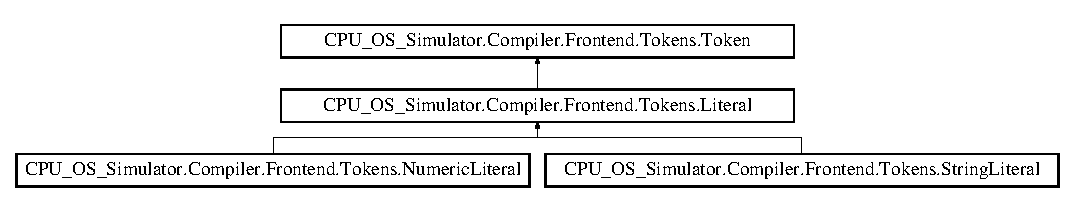
\includegraphics[height=2.282609cm]{class_c_p_u___o_s___simulator_1_1_compiler_1_1_frontend_1_1_tokens_1_1_literal}
\end{center}
\end{figure}
\subsection*{Public Member Functions}
\begin{DoxyCompactItemize}
\item 
abstract override Enum \hyperlink{class_c_p_u___o_s___simulator_1_1_compiler_1_1_frontend_1_1_tokens_1_1_literal_af449c5fee28fb2076933cdfc67857c23}{Detect\+Type} ()
\begin{DoxyCompactList}\small\item\em This function detects the type of literal \end{DoxyCompactList}\item 
abstract \hyperlink{namespace_c_p_u___o_s___simulator_1_1_compiler_1_1_frontend_1_1_tokens_a7c0cc43763cc9d01c7d5af34d70b96ea}{Enum\+Types} \hyperlink{class_c_p_u___o_s___simulator_1_1_compiler_1_1_frontend_1_1_tokens_1_1_literal_a34d05c00ded660daf66f91bd2543d186}{identfy\+Value\+Type} ()
\begin{DoxyCompactList}\small\item\em This function identifies the type of data stored in the literal \end{DoxyCompactList}\end{DoxyCompactItemize}
\subsection*{Protected Attributes}
\begin{DoxyCompactItemize}
\item 
char \hyperlink{class_c_p_u___o_s___simulator_1_1_compiler_1_1_frontend_1_1_tokens_1_1_literal_ae93e9ee8a14f8f8fed07f5e9a8232b5a}{start\+Char} = \textquotesingle{}\textbackslash{}0\textquotesingle{}
\begin{DoxyCompactList}\small\item\em the character that defines the start of the literal \end{DoxyCompactList}\item 
char \hyperlink{class_c_p_u___o_s___simulator_1_1_compiler_1_1_frontend_1_1_tokens_1_1_literal_ab07076b3a3eaae7e88f664904aaa341f}{end\+Char} = \textquotesingle{}\textbackslash{}0\textquotesingle{}
\begin{DoxyCompactList}\small\item\em the character that defines the end of the literal \end{DoxyCompactList}\end{DoxyCompactItemize}
\subsection*{Additional Inherited Members}


\subsection{Detailed Description}


Definition at line 5 of file Literal.\+cs.



\subsection{Member Function Documentation}
\hypertarget{class_c_p_u___o_s___simulator_1_1_compiler_1_1_frontend_1_1_tokens_1_1_literal_af449c5fee28fb2076933cdfc67857c23}{}\index{C\+P\+U\+\_\+\+O\+S\+\_\+\+Simulator\+::\+Compiler\+::\+Frontend\+::\+Tokens\+::\+Literal@{C\+P\+U\+\_\+\+O\+S\+\_\+\+Simulator\+::\+Compiler\+::\+Frontend\+::\+Tokens\+::\+Literal}!Detect\+Type@{Detect\+Type}}
\index{Detect\+Type@{Detect\+Type}!C\+P\+U\+\_\+\+O\+S\+\_\+\+Simulator\+::\+Compiler\+::\+Frontend\+::\+Tokens\+::\+Literal@{C\+P\+U\+\_\+\+O\+S\+\_\+\+Simulator\+::\+Compiler\+::\+Frontend\+::\+Tokens\+::\+Literal}}
\subsubsection[{Detect\+Type()}]{\setlength{\rightskip}{0pt plus 5cm}abstract override Enum C\+P\+U\+\_\+\+O\+S\+\_\+\+Simulator.\+Compiler.\+Frontend.\+Tokens.\+Literal.\+Detect\+Type (
\begin{DoxyParamCaption}
{}
\end{DoxyParamCaption}
)\hspace{0.3cm}{\ttfamily [pure virtual]}}\label{class_c_p_u___o_s___simulator_1_1_compiler_1_1_frontend_1_1_tokens_1_1_literal_af449c5fee28fb2076933cdfc67857c23}


This function detects the type of literal 

\begin{DoxyReturn}{Returns}
the type of literal
\end{DoxyReturn}


Implements \hyperlink{class_c_p_u___o_s___simulator_1_1_compiler_1_1_frontend_1_1_tokens_1_1_token_accfe8c46faedacd527ef619698c76310}{C\+P\+U\+\_\+\+O\+S\+\_\+\+Simulator.\+Compiler.\+Frontend.\+Tokens.\+Token}.



Implemented in \hyperlink{class_c_p_u___o_s___simulator_1_1_compiler_1_1_frontend_1_1_tokens_1_1_numeric_literal_a48f7635001171a738d1c53d065659933}{C\+P\+U\+\_\+\+O\+S\+\_\+\+Simulator.\+Compiler.\+Frontend.\+Tokens.\+Numeric\+Literal}, and \hyperlink{class_c_p_u___o_s___simulator_1_1_compiler_1_1_frontend_1_1_tokens_1_1_string_literal_a55fe99257eeaeb6d73db4ff188de3f57}{C\+P\+U\+\_\+\+O\+S\+\_\+\+Simulator.\+Compiler.\+Frontend.\+Tokens.\+String\+Literal}.

\hypertarget{class_c_p_u___o_s___simulator_1_1_compiler_1_1_frontend_1_1_tokens_1_1_literal_a34d05c00ded660daf66f91bd2543d186}{}\index{C\+P\+U\+\_\+\+O\+S\+\_\+\+Simulator\+::\+Compiler\+::\+Frontend\+::\+Tokens\+::\+Literal@{C\+P\+U\+\_\+\+O\+S\+\_\+\+Simulator\+::\+Compiler\+::\+Frontend\+::\+Tokens\+::\+Literal}!identfy\+Value\+Type@{identfy\+Value\+Type}}
\index{identfy\+Value\+Type@{identfy\+Value\+Type}!C\+P\+U\+\_\+\+O\+S\+\_\+\+Simulator\+::\+Compiler\+::\+Frontend\+::\+Tokens\+::\+Literal@{C\+P\+U\+\_\+\+O\+S\+\_\+\+Simulator\+::\+Compiler\+::\+Frontend\+::\+Tokens\+::\+Literal}}
\subsubsection[{identfy\+Value\+Type()}]{\setlength{\rightskip}{0pt plus 5cm}abstract {\bf Enum\+Types} C\+P\+U\+\_\+\+O\+S\+\_\+\+Simulator.\+Compiler.\+Frontend.\+Tokens.\+Literal.\+identfy\+Value\+Type (
\begin{DoxyParamCaption}
{}
\end{DoxyParamCaption}
)\hspace{0.3cm}{\ttfamily [pure virtual]}}\label{class_c_p_u___o_s___simulator_1_1_compiler_1_1_frontend_1_1_tokens_1_1_literal_a34d05c00ded660daf66f91bd2543d186}


This function identifies the type of data stored in the literal 

\begin{DoxyReturn}{Returns}
the type of value in the literal
\end{DoxyReturn}


Implemented in \hyperlink{class_c_p_u___o_s___simulator_1_1_compiler_1_1_frontend_1_1_tokens_1_1_numeric_literal_ac00d8a0002a5a291fba5713d385d11a6}{C\+P\+U\+\_\+\+O\+S\+\_\+\+Simulator.\+Compiler.\+Frontend.\+Tokens.\+Numeric\+Literal}, and \hyperlink{class_c_p_u___o_s___simulator_1_1_compiler_1_1_frontend_1_1_tokens_1_1_string_literal_ad4121c2eda9ab84f08bb0c51996c96cb}{C\+P\+U\+\_\+\+O\+S\+\_\+\+Simulator.\+Compiler.\+Frontend.\+Tokens.\+String\+Literal}.



\subsection{Member Data Documentation}
\hypertarget{class_c_p_u___o_s___simulator_1_1_compiler_1_1_frontend_1_1_tokens_1_1_literal_ab07076b3a3eaae7e88f664904aaa341f}{}\index{C\+P\+U\+\_\+\+O\+S\+\_\+\+Simulator\+::\+Compiler\+::\+Frontend\+::\+Tokens\+::\+Literal@{C\+P\+U\+\_\+\+O\+S\+\_\+\+Simulator\+::\+Compiler\+::\+Frontend\+::\+Tokens\+::\+Literal}!end\+Char@{end\+Char}}
\index{end\+Char@{end\+Char}!C\+P\+U\+\_\+\+O\+S\+\_\+\+Simulator\+::\+Compiler\+::\+Frontend\+::\+Tokens\+::\+Literal@{C\+P\+U\+\_\+\+O\+S\+\_\+\+Simulator\+::\+Compiler\+::\+Frontend\+::\+Tokens\+::\+Literal}}
\subsubsection[{end\+Char}]{\setlength{\rightskip}{0pt plus 5cm}char C\+P\+U\+\_\+\+O\+S\+\_\+\+Simulator.\+Compiler.\+Frontend.\+Tokens.\+Literal.\+end\+Char = \textquotesingle{}\textbackslash{}0\textquotesingle{}\hspace{0.3cm}{\ttfamily [protected]}}\label{class_c_p_u___o_s___simulator_1_1_compiler_1_1_frontend_1_1_tokens_1_1_literal_ab07076b3a3eaae7e88f664904aaa341f}


the character that defines the end of the literal 



Definition at line 14 of file Literal.\+cs.

\hypertarget{class_c_p_u___o_s___simulator_1_1_compiler_1_1_frontend_1_1_tokens_1_1_literal_ae93e9ee8a14f8f8fed07f5e9a8232b5a}{}\index{C\+P\+U\+\_\+\+O\+S\+\_\+\+Simulator\+::\+Compiler\+::\+Frontend\+::\+Tokens\+::\+Literal@{C\+P\+U\+\_\+\+O\+S\+\_\+\+Simulator\+::\+Compiler\+::\+Frontend\+::\+Tokens\+::\+Literal}!start\+Char@{start\+Char}}
\index{start\+Char@{start\+Char}!C\+P\+U\+\_\+\+O\+S\+\_\+\+Simulator\+::\+Compiler\+::\+Frontend\+::\+Tokens\+::\+Literal@{C\+P\+U\+\_\+\+O\+S\+\_\+\+Simulator\+::\+Compiler\+::\+Frontend\+::\+Tokens\+::\+Literal}}
\subsubsection[{start\+Char}]{\setlength{\rightskip}{0pt plus 5cm}char C\+P\+U\+\_\+\+O\+S\+\_\+\+Simulator.\+Compiler.\+Frontend.\+Tokens.\+Literal.\+start\+Char = \textquotesingle{}\textbackslash{}0\textquotesingle{}\hspace{0.3cm}{\ttfamily [protected]}}\label{class_c_p_u___o_s___simulator_1_1_compiler_1_1_frontend_1_1_tokens_1_1_literal_ae93e9ee8a14f8f8fed07f5e9a8232b5a}


the character that defines the start of the literal 



Definition at line 10 of file Literal.\+cs.



The documentation for this class was generated from the following file\+:\begin{DoxyCompactItemize}
\item 
Compiler/\+Frontend/\+Tokens/\hyperlink{_literal_8cs}{Literal.\+cs}\end{DoxyCompactItemize}

\hypertarget{class_c_p_u___o_s___simulator_1_1_main_window}{}\section{C\+P\+U\+\_\+\+O\+S\+\_\+\+Simulator.\+Main\+Window Class Reference}
\label{class_c_p_u___o_s___simulator_1_1_main_window}\index{C\+P\+U\+\_\+\+O\+S\+\_\+\+Simulator.\+Main\+Window@{C\+P\+U\+\_\+\+O\+S\+\_\+\+Simulator.\+Main\+Window}}


Interaction logic for Main\+Window.\+xaml  


Inheritance diagram for C\+P\+U\+\_\+\+O\+S\+\_\+\+Simulator.\+Main\+Window\+:\begin{figure}[H]
\begin{center}
\leavevmode
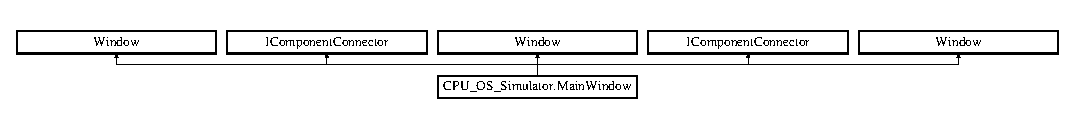
\includegraphics[height=11.000000cm]{class_c_p_u___o_s___simulator_1_1_main_window}
\end{center}
\end{figure}
\subsection*{Public Member Functions}
\begin{DoxyCompactItemize}
\item 
\hyperlink{class_c_p_u___o_s___simulator_1_1_main_window_a33462505a86657583c1560cbf02172bd}{Main\+Window} ()
\begin{DoxyCompactList}\small\item\em Constructor For the main window \end{DoxyCompactList}\item 
\hyperlink{class_c_p_u___o_s___simulator_1_1_c_p_u_1_1_instruction}{Instruction} \hyperlink{class_c_p_u___o_s___simulator_1_1_main_window_aeab49a3421f75049e47ed30b86bf8ad5}{Create\+Instruction} (\hyperlink{namespace_c_p_u___o_s___simulator_1_1_c_p_u_ac29c87bff87ad404c953b2581024043e}{Enum\+Opcodes} opcode, \hyperlink{class_c_p_u___o_s___simulator_1_1_c_p_u_1_1_operand}{Operand} op1, \hyperlink{class_c_p_u___o_s___simulator_1_1_c_p_u_1_1_operand}{Operand} op2, int Size)
\begin{DoxyCompactList}\small\item\em Creates an instruction with 2 operands \end{DoxyCompactList}\item 
\hyperlink{class_c_p_u___o_s___simulator_1_1_c_p_u_1_1_instruction}{Instruction} \hyperlink{class_c_p_u___o_s___simulator_1_1_main_window_a25a43c9a60f98f8196199d04420e48cf}{Create\+Instruction} (\hyperlink{namespace_c_p_u___o_s___simulator_1_1_c_p_u_ac29c87bff87ad404c953b2581024043e}{Enum\+Opcodes} opcode, \hyperlink{class_c_p_u___o_s___simulator_1_1_c_p_u_1_1_operand}{Operand} op1, int Size)
\begin{DoxyCompactList}\small\item\em Creates an instruction with 1 operand \end{DoxyCompactList}\item 
\hyperlink{class_c_p_u___o_s___simulator_1_1_c_p_u_1_1_instruction}{Instruction} \hyperlink{class_c_p_u___o_s___simulator_1_1_main_window_a608bc25c49d397aacde6cdd41d4314c3}{Create\+Instruction} (\hyperlink{namespace_c_p_u___o_s___simulator_1_1_c_p_u_ac29c87bff87ad404c953b2581024043e}{Enum\+Opcodes} opcode, int Size)
\begin{DoxyCompactList}\small\item\em Creates an instruction with no operands \end{DoxyCompactList}\item 
void \hyperlink{class_c_p_u___o_s___simulator_1_1_main_window_ae73f56ccee0f45b0df54438b3d397dd9}{Add\+Instruction} (\hyperlink{class_c_p_u___o_s___simulator_1_1_c_p_u_1_1_instruction}{Instruction} ins, int index)
\begin{DoxyCompactList}\small\item\em Adds an instruction to the currently loaded program \end{DoxyCompactList}\item 
void \hyperlink{class_c_p_u___o_s___simulator_1_1_main_window_a195e7715af146b207e5b973bd10c80c6}{Dispose} ()
\item 
void \hyperlink{class_c_p_u___o_s___simulator_1_1_main_window_a30724af44ae89c2172130c2dd36e145c}{Initialize\+Component} ()
\begin{DoxyCompactList}\small\item\em Initialize\+Component \end{DoxyCompactList}\item 
void \hyperlink{class_c_p_u___o_s___simulator_1_1_main_window_a30724af44ae89c2172130c2dd36e145c}{Initialize\+Component} ()
\begin{DoxyCompactList}\small\item\em Initialize\+Component \end{DoxyCompactList}\item 
void \hyperlink{class_c_p_u___o_s___simulator_1_1_main_window_a30724af44ae89c2172130c2dd36e145c}{Initialize\+Component} ()
\begin{DoxyCompactList}\small\item\em Initialize\+Component \end{DoxyCompactList}\item 
void \hyperlink{class_c_p_u___o_s___simulator_1_1_main_window_a30724af44ae89c2172130c2dd36e145c}{Initialize\+Component} ()
\begin{DoxyCompactList}\small\item\em Initialize\+Component \end{DoxyCompactList}\end{DoxyCompactItemize}
\subsection*{Public Attributes}
\begin{DoxyCompactItemize}
\item 
string \hyperlink{class_c_p_u___o_s___simulator_1_1_main_window_a91f063d9cf776004dc74e719ef942907}{current\+Program} = string.\+Empty
\end{DoxyCompactItemize}
\subsection*{Static Public Attributes}
\begin{DoxyCompactItemize}
\item 
static \hyperlink{class_c_p_u___o_s___simulator_1_1_main_window}{Main\+Window} \hyperlink{class_c_p_u___o_s___simulator_1_1_main_window_a1280266cc57403a91f08a8350dee05cc}{current\+Instance}
\end{DoxyCompactItemize}
\subsection*{Package Attributes}
\begin{DoxyCompactItemize}
\item 
\hyperlink{class_c_p_u___o_s___simulator_1_1_main_window}{C\+P\+U\+\_\+\+O\+S\+\_\+\+Simulator.\+Main\+Window} \hyperlink{class_c_p_u___o_s___simulator_1_1_main_window_adf996cda04d3cf426847b8fd8981ee66}{Main\+Window2}
\item 
System.\+Windows.\+Controls.\+Grid \hyperlink{class_c_p_u___o_s___simulator_1_1_main_window_a5c56d82a7b611446e81b7baa3229d76b}{Main\+Window\+Grid}
\item 
System.\+Windows.\+Controls.\+Grid \hyperlink{class_c_p_u___o_s___simulator_1_1_main_window_a2e6841673af413e8a8f8ba8aa0d7c80b}{Instructions\+Grid}
\item 
System.\+Windows.\+Controls.\+Group\+Box \hyperlink{class_c_p_u___o_s___simulator_1_1_main_window_aebc1256b654d001b7c4ce2bc08522667}{grp\+\_\+\+Instructions\+Box}
\item 
System.\+Windows.\+Controls.\+Grid \hyperlink{class_c_p_u___o_s___simulator_1_1_main_window_a94a99eeb7f5fcfcfbdc375937d5439e7}{Instructions\+Inner\+Grid}
\item 
System.\+Windows.\+Controls.\+List\+View \hyperlink{class_c_p_u___o_s___simulator_1_1_main_window_acdab094f589df9435fa8e3bfe04e61cb}{lst\+\_\+\+Instructions\+List}
\item 
System.\+Windows.\+Controls.\+Primitives.\+Scroll\+Bar \hyperlink{class_c_p_u___o_s___simulator_1_1_main_window_a014812a0e9cd159be05250d94d9a5a8b}{scroll\+Bar1}
\item 
System.\+Windows.\+Controls.\+Grid \hyperlink{class_c_p_u___o_s___simulator_1_1_main_window_ae4f2459995eb2f672c0fd3c2248b79fd}{Operations\+Grid}
\item 
System.\+Windows.\+Controls.\+Tab\+Control \hyperlink{class_c_p_u___o_s___simulator_1_1_main_window_a615ea960969aa9a61afdaef8cf039348}{Program\+Tab}
\item 
System.\+Windows.\+Controls.\+Group\+Box \hyperlink{class_c_p_u___o_s___simulator_1_1_main_window_a1e75e7af485b229372a6aafb84c2ffe0}{grp\+\_\+\+New\+Program}
\item 
System.\+Windows.\+Controls.\+Grid \hyperlink{class_c_p_u___o_s___simulator_1_1_main_window_a38bef5fa03edcca52fa7fc11068923bd}{grid\+\_\+\+New\+Program}
\item 
System.\+Windows.\+Controls.\+Label \hyperlink{class_c_p_u___o_s___simulator_1_1_main_window_ad60038602dcf5d954e420bee89c8494d}{label}
\item 
System.\+Windows.\+Controls.\+Text\+Box \hyperlink{class_c_p_u___o_s___simulator_1_1_main_window_a2c64b45db8c1d7a30c2f9155899cf918}{txt\+Program\+Name}
\item 
System.\+Windows.\+Controls.\+Label \hyperlink{class_c_p_u___o_s___simulator_1_1_main_window_a09b3ba374a620331bc447b32959260c2}{label1}
\item 
System.\+Windows.\+Controls.\+Text\+Box \hyperlink{class_c_p_u___o_s___simulator_1_1_main_window_aa6eeef1bfdd74aa90d6fea68987306ad}{txt\+Base\+Address}
\item 
System.\+Windows.\+Controls.\+Label \hyperlink{class_c_p_u___o_s___simulator_1_1_main_window_a88c7b6748a5e198c673a3c3c5178d3b8}{label2}
\item 
System.\+Windows.\+Controls.\+Combo\+Box \hyperlink{class_c_p_u___o_s___simulator_1_1_main_window_a8da421354f40baef03909c87c3407e3c}{cmb\+\_\+\+Pages}
\item 
System.\+Windows.\+Controls.\+Button \hyperlink{class_c_p_u___o_s___simulator_1_1_main_window_a4f0d9f8f3d56b76616367438d04b4fde}{btn\+\_\+\+Program\+Add}
\item 
System.\+Windows.\+Controls.\+Group\+Box \hyperlink{class_c_p_u___o_s___simulator_1_1_main_window_a2cafe5a8b54ae3e95a770abc594519a0}{grp\+\_\+\+Programs}
\item 
System.\+Windows.\+Controls.\+Grid \hyperlink{class_c_p_u___o_s___simulator_1_1_main_window_a7a4cb93db4cde3b227cbc3155af574d2}{grid\+\_\+\+Programs}
\item 
System.\+Windows.\+Controls.\+Button \hyperlink{class_c_p_u___o_s___simulator_1_1_main_window_a638eee3b21f6ac5d28a5c95c4dad3fc2}{btn\+\_\+\+Save}
\item 
System.\+Windows.\+Controls.\+Button \hyperlink{class_c_p_u___o_s___simulator_1_1_main_window_a29fbdb7afddedc9425472096337ee13b}{btn\+\_\+\+Load}
\item 
System.\+Windows.\+Controls.\+Button \hyperlink{class_c_p_u___o_s___simulator_1_1_main_window_ad56a38e017d6d47d2076b1ec33e3521d}{btn\+\_\+\+Copy\+To\+Clipboard}
\item 
System.\+Windows.\+Controls.\+Label \hyperlink{class_c_p_u___o_s___simulator_1_1_main_window_a9cbfc378965cf635e61c760e11dd5c8a}{lbl\+Program\+List}
\item 
System.\+Windows.\+Controls.\+Combo\+Box \hyperlink{class_c_p_u___o_s___simulator_1_1_main_window_a9871f5933923725d4386a7a7f3f8828f}{cmb\+\_\+\+Program\+List}
\item 
System.\+Windows.\+Controls.\+Label \hyperlink{class_c_p_u___o_s___simulator_1_1_main_window_ae3adff2ef98d792ce094dcc229c293a8}{lbl\+\_\+\+Base\+Address}
\item 
System.\+Windows.\+Controls.\+Text\+Box \hyperlink{class_c_p_u___o_s___simulator_1_1_main_window_ae6c0ce6078d081b2cb99518c68f1cd85}{txt\+Load\+Base\+Address}
\item 
System.\+Windows.\+Controls.\+Check\+Box \hyperlink{class_c_p_u___o_s___simulator_1_1_main_window_a8ade8cf3e5e2ec2374c984dac406b5e9}{chk\+\_\+\+Load\+Base\+Address}
\item 
System.\+Windows.\+Controls.\+Tab\+Item \hyperlink{class_c_p_u___o_s___simulator_1_1_main_window_a4fe9f6d97eb1f2c45b9e5a0363e61557}{Instruction\+Tab}
\item 
System.\+Windows.\+Controls.\+Grid \hyperlink{class_c_p_u___o_s___simulator_1_1_main_window_af09ff1f305e936227c4a975f4c788133}{grid\+\_\+\+Instructions}
\item 
System.\+Windows.\+Controls.\+Button \hyperlink{class_c_p_u___o_s___simulator_1_1_main_window_a50fb8fcd9e592c4987fac4bcb8762785}{btn\+\_\+\+Add\+New}
\item 
System.\+Windows.\+Controls.\+Button \hyperlink{class_c_p_u___o_s___simulator_1_1_main_window_a3c6c4760a8fd64f653fff0ad06374f13}{btn\+\_\+\+Show}
\item 
System.\+Windows.\+Controls.\+Button \hyperlink{class_c_p_u___o_s___simulator_1_1_main_window_ac30720a1b345a3d59312d2d68f742359}{btn\+\_\+\+Undo}
\item 
System.\+Windows.\+Controls.\+Button \hyperlink{class_c_p_u___o_s___simulator_1_1_main_window_a23c681375b103d2294ac79c51f1fb406}{btn\+\_\+\+Insert\+Above}
\item 
System.\+Windows.\+Controls.\+Button \hyperlink{class_c_p_u___o_s___simulator_1_1_main_window_ac6bfabebf21c92a905764305b789df46}{btn\+Move\+Down}
\item 
System.\+Windows.\+Controls.\+Button \hyperlink{class_c_p_u___o_s___simulator_1_1_main_window_ae07013ea273fb1e9f38fd1dd83144371}{btn\+\_\+\+Edit}
\item 
System.\+Windows.\+Controls.\+Button \hyperlink{class_c_p_u___o_s___simulator_1_1_main_window_a7c6c417d0bd3af11e77f86cf2cfb03fe}{btn\+\_\+\+Insert\+Below}
\item 
System.\+Windows.\+Controls.\+Button \hyperlink{class_c_p_u___o_s___simulator_1_1_main_window_aa85d9301fed773f44a352aad64a9d80d}{btn\+Move\+Up}
\item 
System.\+Windows.\+Controls.\+Button \hyperlink{class_c_p_u___o_s___simulator_1_1_main_window_a74623b1e8f8ab1b3b6835bda2e8a9256}{btn\+\_\+\+Delete}
\item 
System.\+Windows.\+Controls.\+Button \hyperlink{class_c_p_u___o_s___simulator_1_1_main_window_a55b2516a7b78d0e79deac7f1a79f3a92}{btn\+\_\+\+Copy}
\item 
System.\+Windows.\+Controls.\+Button \hyperlink{class_c_p_u___o_s___simulator_1_1_main_window_ae2ef9b73d0b5776415c7f3e91c1eaf21}{btn\+Paste\+Above}
\item 
System.\+Windows.\+Controls.\+Button \hyperlink{class_c_p_u___o_s___simulator_1_1_main_window_a1c24521ff648d75bf5991567e1a85b55}{btn\+\_\+\+Paste\+Below}
\item 
System.\+Windows.\+Controls.\+Tab\+Item \hyperlink{class_c_p_u___o_s___simulator_1_1_main_window_a47b1359d9e96abf2b0935eb3392405d4}{Optimize\+Tab}
\item 
System.\+Windows.\+Controls.\+Grid \hyperlink{class_c_p_u___o_s___simulator_1_1_main_window_adb8397cdbc794d18b0379ba7251d2278}{Program\+List\+Grid}
\item 
System.\+Windows.\+Controls.\+Group\+Box \hyperlink{class_c_p_u___o_s___simulator_1_1_main_window_a0ccd227c10c9a0878095ef10c0ff92b7}{grp\+\_\+\+Program\+List}
\item 
System.\+Windows.\+Controls.\+Grid \hyperlink{class_c_p_u___o_s___simulator_1_1_main_window_a4e287cef9f0becaebe0777af8de2d8c9}{Program\+List\+View\+Grid}
\item 
System.\+Windows.\+Controls.\+List\+View \hyperlink{class_c_p_u___o_s___simulator_1_1_main_window_ab33f21e0f19eab104e6f67f44d89daeb}{lst\+\_\+\+Program\+List}
\item 
System.\+Windows.\+Controls.\+Button \hyperlink{class_c_p_u___o_s___simulator_1_1_main_window_af2d1c3293ffaa1d203a9bdb8bf282eab}{btn\+\_\+\+Show\+Memory}
\item 
System.\+Windows.\+Controls.\+Grid \hyperlink{class_c_p_u___o_s___simulator_1_1_main_window_a37acb139db0aa54950350fdb47dfd452}{Register\+Grid}
\item 
System.\+Windows.\+Controls.\+Group\+Box \hyperlink{class_c_p_u___o_s___simulator_1_1_main_window_af858add509dfe2b90f0d356822f73737}{grp\+\_\+\+Registers}
\item 
System.\+Windows.\+Controls.\+Grid \hyperlink{class_c_p_u___o_s___simulator_1_1_main_window_a27d2d9e2ed92e2daa444ca8086a0861e}{Register\+Inner\+Grid}
\item 
System.\+Windows.\+Controls.\+List\+View \hyperlink{class_c_p_u___o_s___simulator_1_1_main_window_ae88013c536662328670f206a4cab99b1}{lst\+\_\+\+Registers}
\item 
System.\+Windows.\+Controls.\+Grid \hyperlink{class_c_p_u___o_s___simulator_1_1_main_window_a7ce98e44f9236ca31eb5bf3ed81c3372}{Special\+Registers\+Grid}
\item 
System.\+Windows.\+Controls.\+Group\+Box \hyperlink{class_c_p_u___o_s___simulator_1_1_main_window_a02e4a81d8689928cb1d459fd3c01bfdf}{grp\+\_\+\+Special\+Registers}
\item 
System.\+Windows.\+Controls.\+Grid \hyperlink{class_c_p_u___o_s___simulator_1_1_main_window_aeef1e97d3e7d589fdab51828260c7b5a}{Special\+Registers\+Inner\+Grid}
\item 
System.\+Windows.\+Controls.\+Label \hyperlink{class_c_p_u___o_s___simulator_1_1_main_window_a94cf4fbdaebb09776745893c2bce1126}{label3}
\item 
System.\+Windows.\+Controls.\+Text\+Box \hyperlink{class_c_p_u___o_s___simulator_1_1_main_window_a7100765f8e26fa4c97a76dd445942b97}{txt\+\_\+\+P\+C}
\item 
System.\+Windows.\+Controls.\+Label \hyperlink{class_c_p_u___o_s___simulator_1_1_main_window_a3473dc873d8c8d8f4bba6e83f5684299}{label4}
\item 
System.\+Windows.\+Controls.\+Text\+Box \hyperlink{class_c_p_u___o_s___simulator_1_1_main_window_a9135c01bacd48e517d7cf46f69ea87d2}{txt\+\_\+\+S\+R}
\item 
System.\+Windows.\+Controls.\+Label \hyperlink{class_c_p_u___o_s___simulator_1_1_main_window_a37b18e7542e985a8984375d0b1cf441e}{label5}
\item 
System.\+Windows.\+Controls.\+Text\+Box \hyperlink{class_c_p_u___o_s___simulator_1_1_main_window_ac2427655774b9ca2b4c368651d5cd9de}{txt\+\_\+\+S\+P}
\item 
System.\+Windows.\+Controls.\+Label \hyperlink{class_c_p_u___o_s___simulator_1_1_main_window_aadfe7782d7e25b730849222805a541f9}{label5\+\_\+\+Copy}
\item 
System.\+Windows.\+Controls.\+Text\+Box \hyperlink{class_c_p_u___o_s___simulator_1_1_main_window_a7a878022ed4cb948598d3685dc821a00}{txt\+\_\+\+B\+R}
\item 
System.\+Windows.\+Controls.\+Group\+Box \hyperlink{class_c_p_u___o_s___simulator_1_1_main_window_a9947d1946c8258ea1fb77d860baa7e0f}{grp\+\_\+\+Status\+Flags}
\item 
System.\+Windows.\+Controls.\+Grid \hyperlink{class_c_p_u___o_s___simulator_1_1_main_window_afdda5e5a39c6e3b99300284ea2640e7c}{Status\+Flags\+Grid}
\item 
System.\+Windows.\+Controls.\+Check\+Box \hyperlink{class_c_p_u___o_s___simulator_1_1_main_window_adfbc519740506214093673b8015ea67d}{chk\+\_\+\+O\+V}
\item 
System.\+Windows.\+Controls.\+Check\+Box \hyperlink{class_c_p_u___o_s___simulator_1_1_main_window_a70c1a75df218201391cf5e0615a600f1}{chk\+\_\+\+Z}
\item 
System.\+Windows.\+Controls.\+Check\+Box \hyperlink{class_c_p_u___o_s___simulator_1_1_main_window_ab8a23e33c5c71e359574de36ccf8d991}{chk\+\_\+\+N}
\item 
System.\+Windows.\+Controls.\+Group\+Box \hyperlink{class_c_p_u___o_s___simulator_1_1_main_window_a0e549bad0f6778b2ea3fffb6c2d1a2bb}{grp\+\_\+\+C\+P\+U\+Mode}
\item 
System.\+Windows.\+Controls.\+Grid \hyperlink{class_c_p_u___o_s___simulator_1_1_main_window_ab6afb45d3f05517e9df6af167752be77}{C\+P\+U\+Mode\+Grid}
\item 
System.\+Windows.\+Controls.\+Radio\+Button \hyperlink{class_c_p_u___o_s___simulator_1_1_main_window_ab9e8d52c337bc24a24d8282dfbf449c8}{rdb\+\_\+\+User}
\item 
System.\+Windows.\+Controls.\+Radio\+Button \hyperlink{class_c_p_u___o_s___simulator_1_1_main_window_a549c6be690b051f4ab15dce643dec656}{rdb\+\_\+\+Kernel}
\item 
System.\+Windows.\+Controls.\+Label \hyperlink{class_c_p_u___o_s___simulator_1_1_main_window_a8f210008776bb163b4c2c2b160aa52be}{label6}
\item 
System.\+Windows.\+Controls.\+Text\+Box \hyperlink{class_c_p_u___o_s___simulator_1_1_main_window_ac6e0cfcdd72688d7bffd100ce6d11a28}{txt\+\_\+\+I\+R}
\item 
System.\+Windows.\+Controls.\+Label \hyperlink{class_c_p_u___o_s___simulator_1_1_main_window_a18612502a8ab2d53d85434e426785022}{label6\+\_\+\+Copy}
\item 
System.\+Windows.\+Controls.\+Text\+Box \hyperlink{class_c_p_u___o_s___simulator_1_1_main_window_a87f8440246e9f6ace0aa4d69b5bba289}{txt\+\_\+\+M\+A\+R}
\item 
System.\+Windows.\+Controls.\+Label \hyperlink{class_c_p_u___o_s___simulator_1_1_main_window_a890bd54d36af19ec881b6a840d6ac8a9}{label6\+\_\+\+Copy1}
\item 
System.\+Windows.\+Controls.\+Text\+Box \hyperlink{class_c_p_u___o_s___simulator_1_1_main_window_a1aa53d1512aa84e476b3649dcda5ced0}{txt\+\_\+\+M\+D\+R}
\item 
System.\+Windows.\+Controls.\+Grid \hyperlink{class_c_p_u___o_s___simulator_1_1_main_window_a59373e8f8822e4efea670d9fb87a1b32}{Program\+Stack\+Grid}
\item 
System.\+Windows.\+Controls.\+Group\+Box \hyperlink{class_c_p_u___o_s___simulator_1_1_main_window_a10687b397ff3a0381a556096a14ed0b0}{grp\+\_\+\+Program\+Stack}
\item 
System.\+Windows.\+Controls.\+Grid \hyperlink{class_c_p_u___o_s___simulator_1_1_main_window_a8c373866c86f6be0e7ef487a5ccb8c3c}{Program\+Stack\+Inner\+Grid}
\item 
System.\+Windows.\+Controls.\+List\+View \hyperlink{class_c_p_u___o_s___simulator_1_1_main_window_a8453db331c7cc1e7c1e711a06b2ec30c}{lst\+\_\+\+Stack}
\item 
System.\+Windows.\+Controls.\+Grid \hyperlink{class_c_p_u___o_s___simulator_1_1_main_window_af6e1d9a71f9501c02b62e8319ba11b5a}{Control\+Unit\+Grid}
\item 
System.\+Windows.\+Controls.\+Tab\+Control \hyperlink{class_c_p_u___o_s___simulator_1_1_main_window_acc893fc507d9ea08cc4a923bdc23091d}{Control\+Tabs}
\item 
System.\+Windows.\+Controls.\+Grid \hyperlink{class_c_p_u___o_s___simulator_1_1_main_window_a0bb4b4233380c349ee3bef69813a684b}{Control\+Unit\+Inner\+Grid}
\item 
System.\+Windows.\+Controls.\+Button \hyperlink{class_c_p_u___o_s___simulator_1_1_main_window_acd572aa9d278af703febb634fc1c34a3}{btn\+\_\+\+Step}
\item 
System.\+Windows.\+Controls.\+Button \hyperlink{class_c_p_u___o_s___simulator_1_1_main_window_ab3286e931d7154605876654bbf092840}{btn\+\_\+\+Run}
\item 
System.\+Windows.\+Controls.\+Button \hyperlink{class_c_p_u___o_s___simulator_1_1_main_window_a1b6b541d9765ca230f537d1d6b6c83aa}{btn\+\_\+\+Stop}
\item 
System.\+Windows.\+Controls.\+Radio\+Button \hyperlink{class_c_p_u___o_s___simulator_1_1_main_window_acba6218f7f716645443533815c6bd7a3}{rdb\+\_\+\+By\+Instruction}
\item 
System.\+Windows.\+Controls.\+Radio\+Button \hyperlink{class_c_p_u___o_s___simulator_1_1_main_window_ab40dcb618f5398ab67213476fe1b86ca}{rdb\+\_\+\+By\+Single\+Tick}
\item 
System.\+Windows.\+Controls.\+Slider \hyperlink{class_c_p_u___o_s___simulator_1_1_main_window_a39cd3af9bb0f8a3ccd06fdd44c9ed6a3}{sld\+\_\+\+Clock\+Speed}
\item 
System.\+Windows.\+Controls.\+Label \hyperlink{class_c_p_u___o_s___simulator_1_1_main_window_a38ed6363fd03954967bda7a099f6b07e}{label7}
\item 
System.\+Windows.\+Controls.\+Label \hyperlink{class_c_p_u___o_s___simulator_1_1_main_window_a216fc6a1692d8a8f8b80b08348c1dcd4}{label8}
\item 
System.\+Windows.\+Controls.\+Button \hyperlink{class_c_p_u___o_s___simulator_1_1_main_window_ada16565fc869dea1d54013009f5892b4}{btn\+\_\+\+Reset\+Program}
\item 
System.\+Windows.\+Controls.\+Button \hyperlink{class_c_p_u___o_s___simulator_1_1_main_window_a967a1b3dbde7ecb1d8091e5eababcc58}{btn\+\_\+\+Show\+P\+C\+B}
\item 
System.\+Windows.\+Controls.\+Grid \hyperlink{class_c_p_u___o_s___simulator_1_1_main_window_a65cbc082cd4737ec0dd8837efa715510}{grid\+\_\+\+Advanced}
\item 
System.\+Windows.\+Controls.\+Tab\+Control \hyperlink{class_c_p_u___o_s___simulator_1_1_main_window_a409f822cf5503ff0a45e14fb0f86a2aa}{advanced\+\_\+\+Tabs}
\item 
System.\+Windows.\+Controls.\+Tab\+Item \hyperlink{class_c_p_u___o_s___simulator_1_1_main_window_aa0cf25219ff7ec68cccc82f780e5f817}{advanced\+\_\+\+Tab}
\item 
System.\+Windows.\+Controls.\+Grid \hyperlink{class_c_p_u___o_s___simulator_1_1_main_window_a50b3891532cc5bfd0cc44e657bf95374}{advanced\+\_\+\+Grid}
\item 
System.\+Windows.\+Controls.\+Button \hyperlink{class_c_p_u___o_s___simulator_1_1_main_window_a9c127982ee67a80b67a9184b3a6e83d3}{btn\+\_\+\+Console}
\end{DoxyCompactItemize}
\subsection*{Properties}
\begin{DoxyCompactItemize}
\item 
List$<$ \hyperlink{class_c_p_u___o_s___simulator_1_1_c_p_u_1_1_simulator_program}{Simulator\+Program} $>$ \hyperlink{class_c_p_u___o_s___simulator_1_1_main_window_a632c91cdd16a7498bbb8dfb3e5df252c}{Program\+List}\hspace{0.3cm}{\ttfamily  \mbox{[}get, set\mbox{]}}
\item 
\hyperlink{namespace_c_p_u___o_s___simulator_adc17a5a5e004084f05dc8e4d3f70e31f}{Enum\+Instruction\+Mode} \hyperlink{class_c_p_u___o_s___simulator_1_1_main_window_a65916937137002c26f9eb1c88cfff519}{Instruction\+Mode}\hspace{0.3cm}{\ttfamily  \mbox{[}get, set\mbox{]}}
\item 
\hyperlink{class_c_p_u___o_s___simulator_1_1_c_p_u_1_1_execution_unit}{Execution\+Unit} \hyperlink{class_c_p_u___o_s___simulator_1_1_main_window_a3d03550a73d7ab18ebd143a38dbf1431}{Active\+Unit}\hspace{0.3cm}{\ttfamily  \mbox{[}get, set\mbox{]}}
\item 
\hyperlink{class_c_p_u___o_s___simulator_1_1_memory_1_1_physical_memory}{Physical\+Memory} \hyperlink{class_c_p_u___o_s___simulator_1_1_main_window_abee63f1a7c5feecf97e7253a65806a5a}{Memory}\hspace{0.3cm}{\ttfamily  \mbox{[}get, set\mbox{]}}
\item 
\hyperlink{class_c_p_u___o_s___simulator_1_1_memory_1_1_swap_space}{Swap\+Space} \hyperlink{class_c_p_u___o_s___simulator_1_1_main_window_a114d0bf1ca63b0d9213537758535aecf}{Swap\+Space}\hspace{0.3cm}{\ttfamily  \mbox{[}get, set\mbox{]}}
\item 
Background\+Worker \hyperlink{class_c_p_u___o_s___simulator_1_1_main_window_aab5d6c95426ebe1e75b7c3bfc0488b84}{Execution\+Worker}\hspace{0.3cm}{\ttfamily  \mbox{[}get, set\mbox{]}}
\end{DoxyCompactItemize}
\subsection*{Private Member Functions}
\begin{DoxyCompactItemize}
\item 
static void \hyperlink{class_c_p_u___o_s___simulator_1_1_main_window_a0bbdb2d3b0e818f2d264770168521059}{S\+H\+Change\+Notify} (uint w\+Event\+Id, uint u\+Flags, Int\+Ptr dw\+Item1, Int\+Ptr dw\+Item2)
\item 
void \hyperlink{class_c_p_u___o_s___simulator_1_1_main_window_a06b2ba04e8c006037cae7b0e40b9c5a0}{Populate\+Registers} ()
\begin{DoxyCompactList}\small\item\em This function populates the register display in the main window \end{DoxyCompactList}\item 
void \hyperlink{class_c_p_u___o_s___simulator_1_1_main_window_a4fbca2d50698a847da4ab82c3f380680}{Update\+Registers} ()
\begin{DoxyCompactList}\small\item\em This function updates the register display in the main window whenever a register value is updated \end{DoxyCompactList}\item 
void \hyperlink{class_c_p_u___o_s___simulator_1_1_main_window_a798838ad3fae6117c8e624047a591931}{Update\+Special\+Registers} ()
\begin{DoxyCompactList}\small\item\em This function updates the values in the U\+I for the special registers \end{DoxyCompactList}\item 
void \hyperlink{class_c_p_u___o_s___simulator_1_1_main_window_a3b945b691332686989cd5b5107f7f98b}{Main\+Window2\+\_\+\+Loaded} (object sender, Routed\+Event\+Args e)
\item 
void \hyperlink{class_c_p_u___o_s___simulator_1_1_main_window_abe3e79941789134ce080390fcafc720e}{btn\+\_\+\+Program\+Add\+\_\+\+Click} (object sender, Routed\+Event\+Args e)
\begin{DoxyCompactList}\small\item\em Creates and adds a program to the program list \end{DoxyCompactList}\item 
\hyperlink{class_c_p_u___o_s___simulator_1_1_c_p_u_1_1_simulator_program}{Simulator\+Program} \hyperlink{class_c_p_u___o_s___simulator_1_1_main_window_a4cb75cfa224757b1dc708b60681ad803}{Create\+New\+Program} ()
\begin{DoxyCompactList}\small\item\em Creates a new program based on entered data \end{DoxyCompactList}\item 
\hyperlink{class_c_p_u___o_s___simulator_1_1_c_p_u_1_1_simulator_program}{Simulator\+Program} \hyperlink{class_c_p_u___o_s___simulator_1_1_main_window_aa735efa9bc97df2ceb545fdce5f351df}{Create\+New\+Program} (string program\+Name, int base\+Address, int pages)
\begin{DoxyCompactList}\small\item\em Creates a new program based on entered data \end{DoxyCompactList}\item 
void \hyperlink{class_c_p_u___o_s___simulator_1_1_main_window_afcb6e2b3719374f56fd8cb1c786bb219}{btn\+\_\+\+Show\+\_\+\+Click} (object sender, Routed\+Event\+Args e)
\begin{DoxyCompactList}\small\item\em Called when the show button is clicked \end{DoxyCompactList}\item 
void \hyperlink{class_c_p_u___o_s___simulator_1_1_main_window_a37c97ac2869b40063089f1af9cd86724}{btn\+\_\+\+Add\+New\+\_\+\+Click} (object sender, Routed\+Event\+Args e)
\begin{DoxyCompactList}\small\item\em Adds a new instruction to the program \end{DoxyCompactList}\item 
void \hyperlink{class_c_p_u___o_s___simulator_1_1_main_window_a8f710b1bee7b3c9360fb5652231b0502}{btn\+\_\+\+Insert\+Above\+\_\+\+Click} (object sender, Routed\+Event\+Args e)
\begin{DoxyCompactList}\small\item\em Adds a new instruction to the program above the selected instruction \end{DoxyCompactList}\item 
void \hyperlink{class_c_p_u___o_s___simulator_1_1_main_window_ac2307db4caedc82b5a6201077fb1c5b7}{btn\+\_\+\+Insert\+Below\+\_\+\+Click} (object sender, Routed\+Event\+Args e)
\begin{DoxyCompactList}\small\item\em Adds a new instruction to the program above below selected instruction \end{DoxyCompactList}\item 
void \hyperlink{class_c_p_u___o_s___simulator_1_1_main_window_a96ea1acde80b84701b58c1d4aaed2b9f}{btn\+\_\+\+Delete\+\_\+\+Click} (object sender, Routed\+Event\+Args e)
\begin{DoxyCompactList}\small\item\em Deletes the selected instruction from the program \end{DoxyCompactList}\item 
void \hyperlink{class_c_p_u___o_s___simulator_1_1_main_window_a622fd6a40ff66a4a87c3d31ccef4313c}{Main\+Window2\+\_\+\+Closing} (object sender, Cancel\+Event\+Args e)
\begin{DoxyCompactList}\small\item\em Called when the window is closing \end{DoxyCompactList}\item 
void \hyperlink{class_c_p_u___o_s___simulator_1_1_main_window_a5013d1984fc170246a5dc0d26c6fc493}{lst\+\_\+\+Instructions\+List\+\_\+\+Selection\+Changed} (object sender, Selection\+Changed\+Event\+Args e)
\item 
void \hyperlink{class_c_p_u___o_s___simulator_1_1_main_window_ab563b461cf3d62bd3c88eeb7921bfa75}{lst\+\_\+\+Program\+List\+\_\+\+Selection\+Changed} (object sender, Selection\+Changed\+Event\+Args e)
\item 
void \hyperlink{class_c_p_u___o_s___simulator_1_1_main_window_abd01bb7788b0c104045bcc93cf03c9d6}{Update\+Stack} ()
\begin{DoxyCompactList}\small\item\em This function updates the stack display in the main window whenever a value is pushed or popped from the stack \end{DoxyCompactList}\item 
void \hyperlink{class_c_p_u___o_s___simulator_1_1_main_window_a677bf9ebdb9fe30caa0f52f93e5390c9}{Update\+Intructions} ()
\begin{DoxyCompactList}\small\item\em Updates the list of instructions \end{DoxyCompactList}\item 
void \hyperlink{class_c_p_u___o_s___simulator_1_1_main_window_a13c54c19f906fc84076fe654f82f5398}{btn\+\_\+\+Load\+\_\+\+Click} (object sender, Routed\+Event\+Args e)
\item 
void \hyperlink{class_c_p_u___o_s___simulator_1_1_main_window_a3bbf0774868d6b5da4ff08d70e236fa6}{btn\+\_\+\+Save\+\_\+\+Click} (object sender, Routed\+Event\+Args e)
\item 
bool \hyperlink{class_c_p_u___o_s___simulator_1_1_main_window_a843bbe93c5c2225820d216cc1cb7d4e9}{Save\+Program} ()
\begin{DoxyCompactList}\small\item\em Saves the program list to a file \end{DoxyCompactList}\item 
bool \hyperlink{class_c_p_u___o_s___simulator_1_1_main_window_ad788d74c9d6582f3302912cbbba410b0}{Load\+Program} ()
\begin{DoxyCompactList}\small\item\em Loads a program list from a file \end{DoxyCompactList}\item 
void \hyperlink{class_c_p_u___o_s___simulator_1_1_main_window_a80985670e45349866a463b766f92e27b}{Serialize\+Object$<$ T $>$} (T serializable\+Object, string file\+Path)
\begin{DoxyCompactList}\small\item\em Serializes a program List. \end{DoxyCompactList}\item 
void \hyperlink{class_c_p_u___o_s___simulator_1_1_main_window_a44e09f35524cd53ddab77488989c5833}{De\+Serialize\+Object$<$ T $>$} (string file\+Name)
\begin{DoxyCompactList}\small\item\em De-\/serializes an .sas file into a program list \end{DoxyCompactList}\item 
void \hyperlink{class_c_p_u___o_s___simulator_1_1_main_window_afe4c815db0eb51ebc480374f5af09d0c}{Bind\+Instruction\+Delegates} (ref \hyperlink{class_c_p_u___o_s___simulator_1_1_c_p_u_1_1_simulator_program}{Simulator\+Program} prog)
\begin{DoxyCompactList}\small\item\em This function rebinds the delegate function to each instruction in a program after it is loaded from a file. \end{DoxyCompactList}\item 
void \hyperlink{class_c_p_u___o_s___simulator_1_1_main_window_ace253c0b4beef8898af97df25666df2f}{sld\+\_\+\+Clock\+Speed\+\_\+\+Value\+Changed} (object sender, Routed\+Property\+Changed\+Event\+Args$<$ double $>$ e)
\item 
void \hyperlink{class_c_p_u___o_s___simulator_1_1_main_window_a897049d123dd2ecf2820b02205ce1969}{btn\+\_\+\+Step\+\_\+\+Click} (object sender, Routed\+Event\+Args e)
\item 
void \hyperlink{class_c_p_u___o_s___simulator_1_1_main_window_a1f4dedca9ad81ea1c92637759515797f}{btn\+\_\+\+Run\+\_\+\+Click} (object sender, Routed\+Event\+Args e)
\item 
void \hyperlink{class_c_p_u___o_s___simulator_1_1_main_window_ad225bd7394d6ad45de9db58b562b91f7}{Create\+Background\+Worker} ()
\begin{DoxyCompactList}\small\item\em Creates a background worker for the execution thread to run on \end{DoxyCompactList}\item 
async void \hyperlink{class_c_p_u___o_s___simulator_1_1_main_window_a27c9bde14aab0b0a82f5e13e0a71c86c}{Update\+Interface} (object sender, Progress\+Changed\+Event\+Args e)
\begin{DoxyCompactList}\small\item\em Asynchronous method called after every instruction is executed to update required values and user interface asynchronously \end{DoxyCompactList}\item 
void \hyperlink{class_c_p_u___o_s___simulator_1_1_main_window_a83ba6352a96515569978030013c84b72}{Create\+Execution\+Thread} (object sender, Do\+Work\+Event\+Args e)
\item 
async Task$<$ int $>$ \hyperlink{class_c_p_u___o_s___simulator_1_1_main_window_adbb759abbf37061f785e82a9e7f7b3e1}{Update\+Interface} ()
\begin{DoxyCompactList}\small\item\em Asynchronous method called after every instruction is executed to update required values and user interface asynchronously \end{DoxyCompactList}\item 
async void \hyperlink{class_c_p_u___o_s___simulator_1_1_main_window_a03d4ec6b5990ad572db709f5305dd7ca}{Execute\+Program} (object program)
\begin{DoxyCompactList}\small\item\em Asynchronous method called to begin executing a program on the execution thread \end{DoxyCompactList}\item 
async Task$<$ int $>$ \hyperlink{class_c_p_u___o_s___simulator_1_1_main_window_a0712c91c3a03a4fabc2cdb2f4ed0a33b}{Call\+From\+Main\+Thread} (Func$<$ Task$<$ int $>$$>$ Function\+Pointer)
\begin{DoxyCompactList}\small\item\em Bridge function used to call functions on the main thread from within the background thread \end{DoxyCompactList}\item 
async Task$<$ string $>$ \hyperlink{class_c_p_u___o_s___simulator_1_1_main_window_ac30c6f157890cb452dc35ec851cc88ad}{Calculate\+Time} (long mills)
\begin{DoxyCompactList}\small\item\em This function calculates the time in seconds the last program took to execute \end{DoxyCompactList}\item 
void \hyperlink{class_c_p_u___o_s___simulator_1_1_main_window_acbdc92abd94c317f978cee0d28af9448}{btn\+\_\+\+Stop\+\_\+\+Click} (object sender, Routed\+Event\+Args e)
\item 
void \hyperlink{class_c_p_u___o_s___simulator_1_1_main_window_a524b638c053cd53f17e44fe225b9dd4f}{btn\+\_\+\+Reset\+Program\+\_\+\+Click} (object sender, Routed\+Event\+Args e)
\item 
void \hyperlink{class_c_p_u___o_s___simulator_1_1_main_window_a19b793a858804e5f7a5611603aeeaf79}{chk\+\_\+\+O\+V\+\_\+\+Checked} (object sender, Routed\+Event\+Args e)
\item 
void \hyperlink{class_c_p_u___o_s___simulator_1_1_main_window_a59f718f48699e2f35c0151057407c38c}{chk\+\_\+\+O\+V\+\_\+\+Unchecked} (object sender, Routed\+Event\+Args e)
\item 
void \hyperlink{class_c_p_u___o_s___simulator_1_1_main_window_ae6186ab1f27e668a1332b7cf72c70f19}{chk\+\_\+\+Z\+\_\+\+Checked} (object sender, Routed\+Event\+Args e)
\item 
void \hyperlink{class_c_p_u___o_s___simulator_1_1_main_window_a21d19250773a14a89aa8285dbe914c22}{chk\+\_\+\+Z\+\_\+\+Unchecked} (object sender, Routed\+Event\+Args e)
\item 
void \hyperlink{class_c_p_u___o_s___simulator_1_1_main_window_a0d0fff66a2f20f19e86f7d8d25aa8915}{chk\+\_\+\+N\+\_\+\+Checked} (object sender, Routed\+Event\+Args e)
\item 
void \hyperlink{class_c_p_u___o_s___simulator_1_1_main_window_afd6ed1a3f1774365c49977ca74daa906}{chk\+\_\+\+N\+\_\+\+Unchecked} (object sender, Routed\+Event\+Args e)
\item 
void \hyperlink{class_c_p_u___o_s___simulator_1_1_main_window_ae0466b84cb9b9aae5c60fe798585b5ed}{btn\+\_\+\+Show\+Memory\+\_\+\+Click} (object sender, Routed\+Event\+Args e)
\item 
void \hyperlink{class_c_p_u___o_s___simulator_1_1_main_window_a48b0283e10f83b8ab7b694ebd0410dd2}{btn\+\_\+\+Console\+\_\+\+Click} (object sender, Routed\+Event\+Args e)
\item 
void System.\+Windows.\+Markup.\+I\+Component\+Connector. \hyperlink{class_c_p_u___o_s___simulator_1_1_main_window_ae66177a5319cf24975b9dfab71bc830e}{Connect} (int connection\+Id, object target)
\item 
void System.\+Windows.\+Markup.\+I\+Component\+Connector. \hyperlink{class_c_p_u___o_s___simulator_1_1_main_window_ae66177a5319cf24975b9dfab71bc830e}{Connect} (int connection\+Id, object target)
\item 
void System.\+Windows.\+Markup.\+I\+Component\+Connector. \hyperlink{class_c_p_u___o_s___simulator_1_1_main_window_ae66177a5319cf24975b9dfab71bc830e}{Connect} (int connection\+Id, object target)
\item 
void System.\+Windows.\+Markup.\+I\+Component\+Connector. \hyperlink{class_c_p_u___o_s___simulator_1_1_main_window_ae66177a5319cf24975b9dfab71bc830e}{Connect} (int connection\+Id, object target)
\end{DoxyCompactItemize}
\subsection*{Static Private Member Functions}
\begin{DoxyCompactItemize}
\item 
static bool \hyperlink{class_c_p_u___o_s___simulator_1_1_main_window_ac84f58171f511e299566cb11c3a53e48}{Is\+Administrator} ()
\item 
static void \hyperlink{class_c_p_u___o_s___simulator_1_1_main_window_ac2d9309ba55c536660c9b98dff7e40b1}{Set\+Association} (string Extension, string Key\+Name, string Open\+With, string File\+Description)
\item 
static string \hyperlink{class_c_p_u___o_s___simulator_1_1_main_window_a4871bf311e6341a2339deff4ad6c2648}{Get\+Program\+Version} ()
\begin{DoxyCompactList}\small\item\em Gets the build number of the running program \end{DoxyCompactList}\end{DoxyCompactItemize}
\subsection*{Private Attributes}
\begin{DoxyCompactItemize}
\item 
List$<$ \hyperlink{class_c_p_u___o_s___simulator_1_1_c_p_u_1_1_simulator_program}{Simulator\+Program} $>$ \hyperlink{class_c_p_u___o_s___simulator_1_1_main_window_a48fa4dc074c098338a652dbd6a3434c7}{program\+List}
\item 
\hyperlink{namespace_c_p_u___o_s___simulator_adc17a5a5e004084f05dc8e4d3f70e31f}{Enum\+Instruction\+Mode} \hyperlink{class_c_p_u___o_s___simulator_1_1_main_window_adcf36837be53f52843bbeb354a16d15c}{instruction\+Mode}
\item 
\hyperlink{class_c_p_u___o_s___simulator_1_1_c_p_u_1_1_execution_unit}{Execution\+Unit} \hyperlink{class_c_p_u___o_s___simulator_1_1_main_window_af00ce05444d9636c688974f706ef397b}{active\+Unit}
\item 
Stopwatch \hyperlink{class_c_p_u___o_s___simulator_1_1_main_window_a880dc01f7c4f093b77ace064d93be1f3}{s}
\item 
Dispatcher \hyperlink{class_c_p_u___o_s___simulator_1_1_main_window_a5115439e688bb7ed25f5237b266e4f3f}{dispatcher} = Dispatcher.\+Current\+Dispatcher
\item 
Background\+Worker \hyperlink{class_c_p_u___o_s___simulator_1_1_main_window_a80e0a87480e4b7f4cfdb47739985b7c7}{execution\+Worker}
\item 
bool \hyperlink{class_c_p_u___o_s___simulator_1_1_main_window_afcd7446d65f9b9370ddf07499c2b8113}{saved} = false
\item 
\hyperlink{class_c_p_u___o_s___simulator_1_1_memory_1_1_page_table_entry}{Page\+Table\+Entry} \hyperlink{class_c_p_u___o_s___simulator_1_1_main_window_a14f6732faabdb632f3d29dbcbbb7059d}{current\+Page}
\item 
\hyperlink{class_c_p_u___o_s___simulator_1_1_memory_1_1_physical_memory}{Physical\+Memory} \hyperlink{class_c_p_u___o_s___simulator_1_1_main_window_a39a29cd60cb4ccbad0415a4e6d6414fa}{memory}
\item 
\hyperlink{class_c_p_u___o_s___simulator_1_1_memory_1_1_swap_space}{Swap\+Space} \hyperlink{class_c_p_u___o_s___simulator_1_1_main_window_ab9638abdc8d65670240a036bc02d813c}{swap\+Space}
\item 
bool \hyperlink{class_c_p_u___o_s___simulator_1_1_main_window_ae8269f86a68d5fdf06180686fc947cc6}{\+\_\+content\+Loaded}
\end{DoxyCompactItemize}


\subsection{Detailed Description}
Interaction logic for Main\+Window.\+xaml 

\hyperlink{class_c_p_u___o_s___simulator_1_1_main_window}{Main\+Window} 

Definition at line 27 of file Main\+Window.\+xaml.\+cs.



\subsection{Constructor \& Destructor Documentation}
\hypertarget{class_c_p_u___o_s___simulator_1_1_main_window_a33462505a86657583c1560cbf02172bd}{}\index{C\+P\+U\+\_\+\+O\+S\+\_\+\+Simulator\+::\+Main\+Window@{C\+P\+U\+\_\+\+O\+S\+\_\+\+Simulator\+::\+Main\+Window}!Main\+Window@{Main\+Window}}
\index{Main\+Window@{Main\+Window}!C\+P\+U\+\_\+\+O\+S\+\_\+\+Simulator\+::\+Main\+Window@{C\+P\+U\+\_\+\+O\+S\+\_\+\+Simulator\+::\+Main\+Window}}
\subsubsection[{Main\+Window()}]{\setlength{\rightskip}{0pt plus 5cm}C\+P\+U\+\_\+\+O\+S\+\_\+\+Simulator.\+Main\+Window.\+Main\+Window (
\begin{DoxyParamCaption}
{}
\end{DoxyParamCaption}
)}\label{class_c_p_u___o_s___simulator_1_1_main_window_a33462505a86657583c1560cbf02172bd}


Constructor For the main window 



Definition at line 113 of file Main\+Window.\+xaml.\+cs.



\subsection{Member Function Documentation}
\hypertarget{class_c_p_u___o_s___simulator_1_1_main_window_ae73f56ccee0f45b0df54438b3d397dd9}{}\index{C\+P\+U\+\_\+\+O\+S\+\_\+\+Simulator\+::\+Main\+Window@{C\+P\+U\+\_\+\+O\+S\+\_\+\+Simulator\+::\+Main\+Window}!Add\+Instruction@{Add\+Instruction}}
\index{Add\+Instruction@{Add\+Instruction}!C\+P\+U\+\_\+\+O\+S\+\_\+\+Simulator\+::\+Main\+Window@{C\+P\+U\+\_\+\+O\+S\+\_\+\+Simulator\+::\+Main\+Window}}
\subsubsection[{Add\+Instruction(\+Instruction ins, int index)}]{\setlength{\rightskip}{0pt plus 5cm}void C\+P\+U\+\_\+\+O\+S\+\_\+\+Simulator.\+Main\+Window.\+Add\+Instruction (
\begin{DoxyParamCaption}
\item[{{\bf Instruction}}]{ins, }
\item[{int}]{index}
\end{DoxyParamCaption}
)}\label{class_c_p_u___o_s___simulator_1_1_main_window_ae73f56ccee0f45b0df54438b3d397dd9}


Adds an instruction to the currently loaded program 


\begin{DoxyParams}{Parameters}
{\em ins} & the instruction to add\\
\hline
{\em index} & the index in the program to add the instruction\\
\hline
\end{DoxyParams}


Definition at line 495 of file Main\+Window.\+xaml.\+cs.

\hypertarget{class_c_p_u___o_s___simulator_1_1_main_window_afe4c815db0eb51ebc480374f5af09d0c}{}\index{C\+P\+U\+\_\+\+O\+S\+\_\+\+Simulator\+::\+Main\+Window@{C\+P\+U\+\_\+\+O\+S\+\_\+\+Simulator\+::\+Main\+Window}!Bind\+Instruction\+Delegates@{Bind\+Instruction\+Delegates}}
\index{Bind\+Instruction\+Delegates@{Bind\+Instruction\+Delegates}!C\+P\+U\+\_\+\+O\+S\+\_\+\+Simulator\+::\+Main\+Window@{C\+P\+U\+\_\+\+O\+S\+\_\+\+Simulator\+::\+Main\+Window}}
\subsubsection[{Bind\+Instruction\+Delegates(ref Simulator\+Program prog)}]{\setlength{\rightskip}{0pt plus 5cm}void C\+P\+U\+\_\+\+O\+S\+\_\+\+Simulator.\+Main\+Window.\+Bind\+Instruction\+Delegates (
\begin{DoxyParamCaption}
\item[{ref {\bf Simulator\+Program}}]{prog}
\end{DoxyParamCaption}
)\hspace{0.3cm}{\ttfamily [private]}}\label{class_c_p_u___o_s___simulator_1_1_main_window_afe4c815db0eb51ebc480374f5af09d0c}


This function rebinds the delegate function to each instruction in a program after it is loaded from a file. 


\begin{DoxyParams}{Parameters}
{\em prog} & the program to bind its instruction delegates \\
\hline
\end{DoxyParams}


Definition at line 764 of file Main\+Window.\+xaml.\+cs.

\hypertarget{class_c_p_u___o_s___simulator_1_1_main_window_a37c97ac2869b40063089f1af9cd86724}{}\index{C\+P\+U\+\_\+\+O\+S\+\_\+\+Simulator\+::\+Main\+Window@{C\+P\+U\+\_\+\+O\+S\+\_\+\+Simulator\+::\+Main\+Window}!btn\+\_\+\+Add\+New\+\_\+\+Click@{btn\+\_\+\+Add\+New\+\_\+\+Click}}
\index{btn\+\_\+\+Add\+New\+\_\+\+Click@{btn\+\_\+\+Add\+New\+\_\+\+Click}!C\+P\+U\+\_\+\+O\+S\+\_\+\+Simulator\+::\+Main\+Window@{C\+P\+U\+\_\+\+O\+S\+\_\+\+Simulator\+::\+Main\+Window}}
\subsubsection[{btn\+\_\+\+Add\+New\+\_\+\+Click(object sender, Routed\+Event\+Args e)}]{\setlength{\rightskip}{0pt plus 5cm}void C\+P\+U\+\_\+\+O\+S\+\_\+\+Simulator.\+Main\+Window.\+btn\+\_\+\+Add\+New\+\_\+\+Click (
\begin{DoxyParamCaption}
\item[{object}]{sender, }
\item[{Routed\+Event\+Args}]{e}
\end{DoxyParamCaption}
)\hspace{0.3cm}{\ttfamily [private]}}\label{class_c_p_u___o_s___simulator_1_1_main_window_a37c97ac2869b40063089f1af9cd86724}


Adds a new instruction to the program 


\begin{DoxyParams}{Parameters}
{\em sender} & \\
\hline
{\em e} & \\
\hline
\end{DoxyParams}


Definition at line 370 of file Main\+Window.\+xaml.\+cs.

\hypertarget{class_c_p_u___o_s___simulator_1_1_main_window_a48b0283e10f83b8ab7b694ebd0410dd2}{}\index{C\+P\+U\+\_\+\+O\+S\+\_\+\+Simulator\+::\+Main\+Window@{C\+P\+U\+\_\+\+O\+S\+\_\+\+Simulator\+::\+Main\+Window}!btn\+\_\+\+Console\+\_\+\+Click@{btn\+\_\+\+Console\+\_\+\+Click}}
\index{btn\+\_\+\+Console\+\_\+\+Click@{btn\+\_\+\+Console\+\_\+\+Click}!C\+P\+U\+\_\+\+O\+S\+\_\+\+Simulator\+::\+Main\+Window@{C\+P\+U\+\_\+\+O\+S\+\_\+\+Simulator\+::\+Main\+Window}}
\subsubsection[{btn\+\_\+\+Console\+\_\+\+Click(object sender, Routed\+Event\+Args e)}]{\setlength{\rightskip}{0pt plus 5cm}void C\+P\+U\+\_\+\+O\+S\+\_\+\+Simulator.\+Main\+Window.\+btn\+\_\+\+Console\+\_\+\+Click (
\begin{DoxyParamCaption}
\item[{object}]{sender, }
\item[{Routed\+Event\+Args}]{e}
\end{DoxyParamCaption}
)\hspace{0.3cm}{\ttfamily [private]}}\label{class_c_p_u___o_s___simulator_1_1_main_window_a48b0283e10f83b8ab7b694ebd0410dd2}


Definition at line 980 of file Main\+Window.\+xaml.\+cs.

\hypertarget{class_c_p_u___o_s___simulator_1_1_main_window_a96ea1acde80b84701b58c1d4aaed2b9f}{}\index{C\+P\+U\+\_\+\+O\+S\+\_\+\+Simulator\+::\+Main\+Window@{C\+P\+U\+\_\+\+O\+S\+\_\+\+Simulator\+::\+Main\+Window}!btn\+\_\+\+Delete\+\_\+\+Click@{btn\+\_\+\+Delete\+\_\+\+Click}}
\index{btn\+\_\+\+Delete\+\_\+\+Click@{btn\+\_\+\+Delete\+\_\+\+Click}!C\+P\+U\+\_\+\+O\+S\+\_\+\+Simulator\+::\+Main\+Window@{C\+P\+U\+\_\+\+O\+S\+\_\+\+Simulator\+::\+Main\+Window}}
\subsubsection[{btn\+\_\+\+Delete\+\_\+\+Click(object sender, Routed\+Event\+Args e)}]{\setlength{\rightskip}{0pt plus 5cm}void C\+P\+U\+\_\+\+O\+S\+\_\+\+Simulator.\+Main\+Window.\+btn\+\_\+\+Delete\+\_\+\+Click (
\begin{DoxyParamCaption}
\item[{object}]{sender, }
\item[{Routed\+Event\+Args}]{e}
\end{DoxyParamCaption}
)\hspace{0.3cm}{\ttfamily [private]}}\label{class_c_p_u___o_s___simulator_1_1_main_window_a96ea1acde80b84701b58c1d4aaed2b9f}


Deletes the selected instruction from the program 


\begin{DoxyParams}{Parameters}
{\em sender} & \\
\hline
{\em e} & \\
\hline
\end{DoxyParams}


Definition at line 406 of file Main\+Window.\+xaml.\+cs.

\hypertarget{class_c_p_u___o_s___simulator_1_1_main_window_a8f710b1bee7b3c9360fb5652231b0502}{}\index{C\+P\+U\+\_\+\+O\+S\+\_\+\+Simulator\+::\+Main\+Window@{C\+P\+U\+\_\+\+O\+S\+\_\+\+Simulator\+::\+Main\+Window}!btn\+\_\+\+Insert\+Above\+\_\+\+Click@{btn\+\_\+\+Insert\+Above\+\_\+\+Click}}
\index{btn\+\_\+\+Insert\+Above\+\_\+\+Click@{btn\+\_\+\+Insert\+Above\+\_\+\+Click}!C\+P\+U\+\_\+\+O\+S\+\_\+\+Simulator\+::\+Main\+Window@{C\+P\+U\+\_\+\+O\+S\+\_\+\+Simulator\+::\+Main\+Window}}
\subsubsection[{btn\+\_\+\+Insert\+Above\+\_\+\+Click(object sender, Routed\+Event\+Args e)}]{\setlength{\rightskip}{0pt plus 5cm}void C\+P\+U\+\_\+\+O\+S\+\_\+\+Simulator.\+Main\+Window.\+btn\+\_\+\+Insert\+Above\+\_\+\+Click (
\begin{DoxyParamCaption}
\item[{object}]{sender, }
\item[{Routed\+Event\+Args}]{e}
\end{DoxyParamCaption}
)\hspace{0.3cm}{\ttfamily [private]}}\label{class_c_p_u___o_s___simulator_1_1_main_window_a8f710b1bee7b3c9360fb5652231b0502}


Adds a new instruction to the program above the selected instruction 


\begin{DoxyParams}{Parameters}
{\em sender} & \\
\hline
{\em e} & \\
\hline
\end{DoxyParams}


Definition at line 382 of file Main\+Window.\+xaml.\+cs.

\hypertarget{class_c_p_u___o_s___simulator_1_1_main_window_ac2307db4caedc82b5a6201077fb1c5b7}{}\index{C\+P\+U\+\_\+\+O\+S\+\_\+\+Simulator\+::\+Main\+Window@{C\+P\+U\+\_\+\+O\+S\+\_\+\+Simulator\+::\+Main\+Window}!btn\+\_\+\+Insert\+Below\+\_\+\+Click@{btn\+\_\+\+Insert\+Below\+\_\+\+Click}}
\index{btn\+\_\+\+Insert\+Below\+\_\+\+Click@{btn\+\_\+\+Insert\+Below\+\_\+\+Click}!C\+P\+U\+\_\+\+O\+S\+\_\+\+Simulator\+::\+Main\+Window@{C\+P\+U\+\_\+\+O\+S\+\_\+\+Simulator\+::\+Main\+Window}}
\subsubsection[{btn\+\_\+\+Insert\+Below\+\_\+\+Click(object sender, Routed\+Event\+Args e)}]{\setlength{\rightskip}{0pt plus 5cm}void C\+P\+U\+\_\+\+O\+S\+\_\+\+Simulator.\+Main\+Window.\+btn\+\_\+\+Insert\+Below\+\_\+\+Click (
\begin{DoxyParamCaption}
\item[{object}]{sender, }
\item[{Routed\+Event\+Args}]{e}
\end{DoxyParamCaption}
)\hspace{0.3cm}{\ttfamily [private]}}\label{class_c_p_u___o_s___simulator_1_1_main_window_ac2307db4caedc82b5a6201077fb1c5b7}


Adds a new instruction to the program above below selected instruction 


\begin{DoxyParams}{Parameters}
{\em sender} & \\
\hline
{\em e} & \\
\hline
\end{DoxyParams}


Definition at line 394 of file Main\+Window.\+xaml.\+cs.

\hypertarget{class_c_p_u___o_s___simulator_1_1_main_window_a13c54c19f906fc84076fe654f82f5398}{}\index{C\+P\+U\+\_\+\+O\+S\+\_\+\+Simulator\+::\+Main\+Window@{C\+P\+U\+\_\+\+O\+S\+\_\+\+Simulator\+::\+Main\+Window}!btn\+\_\+\+Load\+\_\+\+Click@{btn\+\_\+\+Load\+\_\+\+Click}}
\index{btn\+\_\+\+Load\+\_\+\+Click@{btn\+\_\+\+Load\+\_\+\+Click}!C\+P\+U\+\_\+\+O\+S\+\_\+\+Simulator\+::\+Main\+Window@{C\+P\+U\+\_\+\+O\+S\+\_\+\+Simulator\+::\+Main\+Window}}
\subsubsection[{btn\+\_\+\+Load\+\_\+\+Click(object sender, Routed\+Event\+Args e)}]{\setlength{\rightskip}{0pt plus 5cm}void C\+P\+U\+\_\+\+O\+S\+\_\+\+Simulator.\+Main\+Window.\+btn\+\_\+\+Load\+\_\+\+Click (
\begin{DoxyParamCaption}
\item[{object}]{sender, }
\item[{Routed\+Event\+Args}]{e}
\end{DoxyParamCaption}
)\hspace{0.3cm}{\ttfamily [private]}}\label{class_c_p_u___o_s___simulator_1_1_main_window_a13c54c19f906fc84076fe654f82f5398}


Definition at line 639 of file Main\+Window.\+xaml.\+cs.

\hypertarget{class_c_p_u___o_s___simulator_1_1_main_window_abe3e79941789134ce080390fcafc720e}{}\index{C\+P\+U\+\_\+\+O\+S\+\_\+\+Simulator\+::\+Main\+Window@{C\+P\+U\+\_\+\+O\+S\+\_\+\+Simulator\+::\+Main\+Window}!btn\+\_\+\+Program\+Add\+\_\+\+Click@{btn\+\_\+\+Program\+Add\+\_\+\+Click}}
\index{btn\+\_\+\+Program\+Add\+\_\+\+Click@{btn\+\_\+\+Program\+Add\+\_\+\+Click}!C\+P\+U\+\_\+\+O\+S\+\_\+\+Simulator\+::\+Main\+Window@{C\+P\+U\+\_\+\+O\+S\+\_\+\+Simulator\+::\+Main\+Window}}
\subsubsection[{btn\+\_\+\+Program\+Add\+\_\+\+Click(object sender, Routed\+Event\+Args e)}]{\setlength{\rightskip}{0pt plus 5cm}void C\+P\+U\+\_\+\+O\+S\+\_\+\+Simulator.\+Main\+Window.\+btn\+\_\+\+Program\+Add\+\_\+\+Click (
\begin{DoxyParamCaption}
\item[{object}]{sender, }
\item[{Routed\+Event\+Args}]{e}
\end{DoxyParamCaption}
)\hspace{0.3cm}{\ttfamily [private]}}\label{class_c_p_u___o_s___simulator_1_1_main_window_abe3e79941789134ce080390fcafc720e}


Creates and adds a program to the program list 


\begin{DoxyParams}{Parameters}
{\em sender} & the clicked button \\
\hline
{\em e} & the event args\\
\hline
\end{DoxyParams}


Definition at line 310 of file Main\+Window.\+xaml.\+cs.

\hypertarget{class_c_p_u___o_s___simulator_1_1_main_window_a524b638c053cd53f17e44fe225b9dd4f}{}\index{C\+P\+U\+\_\+\+O\+S\+\_\+\+Simulator\+::\+Main\+Window@{C\+P\+U\+\_\+\+O\+S\+\_\+\+Simulator\+::\+Main\+Window}!btn\+\_\+\+Reset\+Program\+\_\+\+Click@{btn\+\_\+\+Reset\+Program\+\_\+\+Click}}
\index{btn\+\_\+\+Reset\+Program\+\_\+\+Click@{btn\+\_\+\+Reset\+Program\+\_\+\+Click}!C\+P\+U\+\_\+\+O\+S\+\_\+\+Simulator\+::\+Main\+Window@{C\+P\+U\+\_\+\+O\+S\+\_\+\+Simulator\+::\+Main\+Window}}
\subsubsection[{btn\+\_\+\+Reset\+Program\+\_\+\+Click(object sender, Routed\+Event\+Args e)}]{\setlength{\rightskip}{0pt plus 5cm}void C\+P\+U\+\_\+\+O\+S\+\_\+\+Simulator.\+Main\+Window.\+btn\+\_\+\+Reset\+Program\+\_\+\+Click (
\begin{DoxyParamCaption}
\item[{object}]{sender, }
\item[{Routed\+Event\+Args}]{e}
\end{DoxyParamCaption}
)\hspace{0.3cm}{\ttfamily [private]}}\label{class_c_p_u___o_s___simulator_1_1_main_window_a524b638c053cd53f17e44fe225b9dd4f}


Definition at line 913 of file Main\+Window.\+xaml.\+cs.

\hypertarget{class_c_p_u___o_s___simulator_1_1_main_window_a1f4dedca9ad81ea1c92637759515797f}{}\index{C\+P\+U\+\_\+\+O\+S\+\_\+\+Simulator\+::\+Main\+Window@{C\+P\+U\+\_\+\+O\+S\+\_\+\+Simulator\+::\+Main\+Window}!btn\+\_\+\+Run\+\_\+\+Click@{btn\+\_\+\+Run\+\_\+\+Click}}
\index{btn\+\_\+\+Run\+\_\+\+Click@{btn\+\_\+\+Run\+\_\+\+Click}!C\+P\+U\+\_\+\+O\+S\+\_\+\+Simulator\+::\+Main\+Window@{C\+P\+U\+\_\+\+O\+S\+\_\+\+Simulator\+::\+Main\+Window}}
\subsubsection[{btn\+\_\+\+Run\+\_\+\+Click(object sender, Routed\+Event\+Args e)}]{\setlength{\rightskip}{0pt plus 5cm}void C\+P\+U\+\_\+\+O\+S\+\_\+\+Simulator.\+Main\+Window.\+btn\+\_\+\+Run\+\_\+\+Click (
\begin{DoxyParamCaption}
\item[{object}]{sender, }
\item[{Routed\+Event\+Args}]{e}
\end{DoxyParamCaption}
)\hspace{0.3cm}{\ttfamily [private]}}\label{class_c_p_u___o_s___simulator_1_1_main_window_a1f4dedca9ad81ea1c92637759515797f}


Definition at line 795 of file Main\+Window.\+xaml.\+cs.

\hypertarget{class_c_p_u___o_s___simulator_1_1_main_window_a3bbf0774868d6b5da4ff08d70e236fa6}{}\index{C\+P\+U\+\_\+\+O\+S\+\_\+\+Simulator\+::\+Main\+Window@{C\+P\+U\+\_\+\+O\+S\+\_\+\+Simulator\+::\+Main\+Window}!btn\+\_\+\+Save\+\_\+\+Click@{btn\+\_\+\+Save\+\_\+\+Click}}
\index{btn\+\_\+\+Save\+\_\+\+Click@{btn\+\_\+\+Save\+\_\+\+Click}!C\+P\+U\+\_\+\+O\+S\+\_\+\+Simulator\+::\+Main\+Window@{C\+P\+U\+\_\+\+O\+S\+\_\+\+Simulator\+::\+Main\+Window}}
\subsubsection[{btn\+\_\+\+Save\+\_\+\+Click(object sender, Routed\+Event\+Args e)}]{\setlength{\rightskip}{0pt plus 5cm}void C\+P\+U\+\_\+\+O\+S\+\_\+\+Simulator.\+Main\+Window.\+btn\+\_\+\+Save\+\_\+\+Click (
\begin{DoxyParamCaption}
\item[{object}]{sender, }
\item[{Routed\+Event\+Args}]{e}
\end{DoxyParamCaption}
)\hspace{0.3cm}{\ttfamily [private]}}\label{class_c_p_u___o_s___simulator_1_1_main_window_a3bbf0774868d6b5da4ff08d70e236fa6}


Definition at line 649 of file Main\+Window.\+xaml.\+cs.

\hypertarget{class_c_p_u___o_s___simulator_1_1_main_window_afcb6e2b3719374f56fd8cb1c786bb219}{}\index{C\+P\+U\+\_\+\+O\+S\+\_\+\+Simulator\+::\+Main\+Window@{C\+P\+U\+\_\+\+O\+S\+\_\+\+Simulator\+::\+Main\+Window}!btn\+\_\+\+Show\+\_\+\+Click@{btn\+\_\+\+Show\+\_\+\+Click}}
\index{btn\+\_\+\+Show\+\_\+\+Click@{btn\+\_\+\+Show\+\_\+\+Click}!C\+P\+U\+\_\+\+O\+S\+\_\+\+Simulator\+::\+Main\+Window@{C\+P\+U\+\_\+\+O\+S\+\_\+\+Simulator\+::\+Main\+Window}}
\subsubsection[{btn\+\_\+\+Show\+\_\+\+Click(object sender, Routed\+Event\+Args e)}]{\setlength{\rightskip}{0pt plus 5cm}void C\+P\+U\+\_\+\+O\+S\+\_\+\+Simulator.\+Main\+Window.\+btn\+\_\+\+Show\+\_\+\+Click (
\begin{DoxyParamCaption}
\item[{object}]{sender, }
\item[{Routed\+Event\+Args}]{e}
\end{DoxyParamCaption}
)\hspace{0.3cm}{\ttfamily [private]}}\label{class_c_p_u___o_s___simulator_1_1_main_window_afcb6e2b3719374f56fd8cb1c786bb219}


Called when the show button is clicked 


\begin{DoxyParams}{Parameters}
{\em sender} & the object that initiated the event\\
\hline
{\em e} & the eventargs\\
\hline
\end{DoxyParams}


Definition at line 358 of file Main\+Window.\+xaml.\+cs.

\hypertarget{class_c_p_u___o_s___simulator_1_1_main_window_ae0466b84cb9b9aae5c60fe798585b5ed}{}\index{C\+P\+U\+\_\+\+O\+S\+\_\+\+Simulator\+::\+Main\+Window@{C\+P\+U\+\_\+\+O\+S\+\_\+\+Simulator\+::\+Main\+Window}!btn\+\_\+\+Show\+Memory\+\_\+\+Click@{btn\+\_\+\+Show\+Memory\+\_\+\+Click}}
\index{btn\+\_\+\+Show\+Memory\+\_\+\+Click@{btn\+\_\+\+Show\+Memory\+\_\+\+Click}!C\+P\+U\+\_\+\+O\+S\+\_\+\+Simulator\+::\+Main\+Window@{C\+P\+U\+\_\+\+O\+S\+\_\+\+Simulator\+::\+Main\+Window}}
\subsubsection[{btn\+\_\+\+Show\+Memory\+\_\+\+Click(object sender, Routed\+Event\+Args e)}]{\setlength{\rightskip}{0pt plus 5cm}void C\+P\+U\+\_\+\+O\+S\+\_\+\+Simulator.\+Main\+Window.\+btn\+\_\+\+Show\+Memory\+\_\+\+Click (
\begin{DoxyParamCaption}
\item[{object}]{sender, }
\item[{Routed\+Event\+Args}]{e}
\end{DoxyParamCaption}
)\hspace{0.3cm}{\ttfamily [private]}}\label{class_c_p_u___o_s___simulator_1_1_main_window_ae0466b84cb9b9aae5c60fe798585b5ed}


Definition at line 972 of file Main\+Window.\+xaml.\+cs.

\hypertarget{class_c_p_u___o_s___simulator_1_1_main_window_a897049d123dd2ecf2820b02205ce1969}{}\index{C\+P\+U\+\_\+\+O\+S\+\_\+\+Simulator\+::\+Main\+Window@{C\+P\+U\+\_\+\+O\+S\+\_\+\+Simulator\+::\+Main\+Window}!btn\+\_\+\+Step\+\_\+\+Click@{btn\+\_\+\+Step\+\_\+\+Click}}
\index{btn\+\_\+\+Step\+\_\+\+Click@{btn\+\_\+\+Step\+\_\+\+Click}!C\+P\+U\+\_\+\+O\+S\+\_\+\+Simulator\+::\+Main\+Window@{C\+P\+U\+\_\+\+O\+S\+\_\+\+Simulator\+::\+Main\+Window}}
\subsubsection[{btn\+\_\+\+Step\+\_\+\+Click(object sender, Routed\+Event\+Args e)}]{\setlength{\rightskip}{0pt plus 5cm}void C\+P\+U\+\_\+\+O\+S\+\_\+\+Simulator.\+Main\+Window.\+btn\+\_\+\+Step\+\_\+\+Click (
\begin{DoxyParamCaption}
\item[{object}]{sender, }
\item[{Routed\+Event\+Args}]{e}
\end{DoxyParamCaption}
)\hspace{0.3cm}{\ttfamily [private]}}\label{class_c_p_u___o_s___simulator_1_1_main_window_a897049d123dd2ecf2820b02205ce1969}


Definition at line 777 of file Main\+Window.\+xaml.\+cs.

\hypertarget{class_c_p_u___o_s___simulator_1_1_main_window_acbdc92abd94c317f978cee0d28af9448}{}\index{C\+P\+U\+\_\+\+O\+S\+\_\+\+Simulator\+::\+Main\+Window@{C\+P\+U\+\_\+\+O\+S\+\_\+\+Simulator\+::\+Main\+Window}!btn\+\_\+\+Stop\+\_\+\+Click@{btn\+\_\+\+Stop\+\_\+\+Click}}
\index{btn\+\_\+\+Stop\+\_\+\+Click@{btn\+\_\+\+Stop\+\_\+\+Click}!C\+P\+U\+\_\+\+O\+S\+\_\+\+Simulator\+::\+Main\+Window@{C\+P\+U\+\_\+\+O\+S\+\_\+\+Simulator\+::\+Main\+Window}}
\subsubsection[{btn\+\_\+\+Stop\+\_\+\+Click(object sender, Routed\+Event\+Args e)}]{\setlength{\rightskip}{0pt plus 5cm}void C\+P\+U\+\_\+\+O\+S\+\_\+\+Simulator.\+Main\+Window.\+btn\+\_\+\+Stop\+\_\+\+Click (
\begin{DoxyParamCaption}
\item[{object}]{sender, }
\item[{Routed\+Event\+Args}]{e}
\end{DoxyParamCaption}
)\hspace{0.3cm}{\ttfamily [private]}}\label{class_c_p_u___o_s___simulator_1_1_main_window_acbdc92abd94c317f978cee0d28af9448}


Definition at line 906 of file Main\+Window.\+xaml.\+cs.

\hypertarget{class_c_p_u___o_s___simulator_1_1_main_window_ac30c6f157890cb452dc35ec851cc88ad}{}\index{C\+P\+U\+\_\+\+O\+S\+\_\+\+Simulator\+::\+Main\+Window@{C\+P\+U\+\_\+\+O\+S\+\_\+\+Simulator\+::\+Main\+Window}!Calculate\+Time@{Calculate\+Time}}
\index{Calculate\+Time@{Calculate\+Time}!C\+P\+U\+\_\+\+O\+S\+\_\+\+Simulator\+::\+Main\+Window@{C\+P\+U\+\_\+\+O\+S\+\_\+\+Simulator\+::\+Main\+Window}}
\subsubsection[{Calculate\+Time(long mills)}]{\setlength{\rightskip}{0pt plus 5cm}async Task$<$string$>$ C\+P\+U\+\_\+\+O\+S\+\_\+\+Simulator.\+Main\+Window.\+Calculate\+Time (
\begin{DoxyParamCaption}
\item[{long}]{mills}
\end{DoxyParamCaption}
)\hspace{0.3cm}{\ttfamily [private]}}\label{class_c_p_u___o_s___simulator_1_1_main_window_ac30c6f157890cb452dc35ec851cc88ad}


This function calculates the time in seconds the last program took to execute 


\begin{DoxyParams}{Parameters}
{\em mills} & the number of milliseconds the last program took to execute\\
\hline
\end{DoxyParams}
\begin{DoxyReturn}{Returns}

\end{DoxyReturn}


Definition at line 897 of file Main\+Window.\+xaml.\+cs.

\hypertarget{class_c_p_u___o_s___simulator_1_1_main_window_a0712c91c3a03a4fabc2cdb2f4ed0a33b}{}\index{C\+P\+U\+\_\+\+O\+S\+\_\+\+Simulator\+::\+Main\+Window@{C\+P\+U\+\_\+\+O\+S\+\_\+\+Simulator\+::\+Main\+Window}!Call\+From\+Main\+Thread@{Call\+From\+Main\+Thread}}
\index{Call\+From\+Main\+Thread@{Call\+From\+Main\+Thread}!C\+P\+U\+\_\+\+O\+S\+\_\+\+Simulator\+::\+Main\+Window@{C\+P\+U\+\_\+\+O\+S\+\_\+\+Simulator\+::\+Main\+Window}}
\subsubsection[{Call\+From\+Main\+Thread(\+Func$<$ Task$<$ int $>$$>$ Function\+Pointer)}]{\setlength{\rightskip}{0pt plus 5cm}async Task$<$int$>$ C\+P\+U\+\_\+\+O\+S\+\_\+\+Simulator.\+Main\+Window.\+Call\+From\+Main\+Thread (
\begin{DoxyParamCaption}
\item[{Func$<$ Task$<$ int $>$$>$}]{Function\+Pointer}
\end{DoxyParamCaption}
)\hspace{0.3cm}{\ttfamily [private]}}\label{class_c_p_u___o_s___simulator_1_1_main_window_a0712c91c3a03a4fabc2cdb2f4ed0a33b}


Bridge function used to call functions on the main thread from within the background thread 


\begin{DoxyParams}{Parameters}
{\em Function\+Pointer} & The function to call \\
\hline
\end{DoxyParams}
\begin{DoxyReturn}{Returns}
A task to indicate to the main thread that the method has finished executing
\end{DoxyReturn}


Definition at line 885 of file Main\+Window.\+xaml.\+cs.

\hypertarget{class_c_p_u___o_s___simulator_1_1_main_window_a0d0fff66a2f20f19e86f7d8d25aa8915}{}\index{C\+P\+U\+\_\+\+O\+S\+\_\+\+Simulator\+::\+Main\+Window@{C\+P\+U\+\_\+\+O\+S\+\_\+\+Simulator\+::\+Main\+Window}!chk\+\_\+\+N\+\_\+\+Checked@{chk\+\_\+\+N\+\_\+\+Checked}}
\index{chk\+\_\+\+N\+\_\+\+Checked@{chk\+\_\+\+N\+\_\+\+Checked}!C\+P\+U\+\_\+\+O\+S\+\_\+\+Simulator\+::\+Main\+Window@{C\+P\+U\+\_\+\+O\+S\+\_\+\+Simulator\+::\+Main\+Window}}
\subsubsection[{chk\+\_\+\+N\+\_\+\+Checked(object sender, Routed\+Event\+Args e)}]{\setlength{\rightskip}{0pt plus 5cm}void C\+P\+U\+\_\+\+O\+S\+\_\+\+Simulator.\+Main\+Window.\+chk\+\_\+\+N\+\_\+\+Checked (
\begin{DoxyParamCaption}
\item[{object}]{sender, }
\item[{Routed\+Event\+Args}]{e}
\end{DoxyParamCaption}
)\hspace{0.3cm}{\ttfamily [private]}}\label{class_c_p_u___o_s___simulator_1_1_main_window_a0d0fff66a2f20f19e86f7d8d25aa8915}


Definition at line 952 of file Main\+Window.\+xaml.\+cs.

\hypertarget{class_c_p_u___o_s___simulator_1_1_main_window_afd6ed1a3f1774365c49977ca74daa906}{}\index{C\+P\+U\+\_\+\+O\+S\+\_\+\+Simulator\+::\+Main\+Window@{C\+P\+U\+\_\+\+O\+S\+\_\+\+Simulator\+::\+Main\+Window}!chk\+\_\+\+N\+\_\+\+Unchecked@{chk\+\_\+\+N\+\_\+\+Unchecked}}
\index{chk\+\_\+\+N\+\_\+\+Unchecked@{chk\+\_\+\+N\+\_\+\+Unchecked}!C\+P\+U\+\_\+\+O\+S\+\_\+\+Simulator\+::\+Main\+Window@{C\+P\+U\+\_\+\+O\+S\+\_\+\+Simulator\+::\+Main\+Window}}
\subsubsection[{chk\+\_\+\+N\+\_\+\+Unchecked(object sender, Routed\+Event\+Args e)}]{\setlength{\rightskip}{0pt plus 5cm}void C\+P\+U\+\_\+\+O\+S\+\_\+\+Simulator.\+Main\+Window.\+chk\+\_\+\+N\+\_\+\+Unchecked (
\begin{DoxyParamCaption}
\item[{object}]{sender, }
\item[{Routed\+Event\+Args}]{e}
\end{DoxyParamCaption}
)\hspace{0.3cm}{\ttfamily [private]}}\label{class_c_p_u___o_s___simulator_1_1_main_window_afd6ed1a3f1774365c49977ca74daa906}


Definition at line 959 of file Main\+Window.\+xaml.\+cs.

\hypertarget{class_c_p_u___o_s___simulator_1_1_main_window_a19b793a858804e5f7a5611603aeeaf79}{}\index{C\+P\+U\+\_\+\+O\+S\+\_\+\+Simulator\+::\+Main\+Window@{C\+P\+U\+\_\+\+O\+S\+\_\+\+Simulator\+::\+Main\+Window}!chk\+\_\+\+O\+V\+\_\+\+Checked@{chk\+\_\+\+O\+V\+\_\+\+Checked}}
\index{chk\+\_\+\+O\+V\+\_\+\+Checked@{chk\+\_\+\+O\+V\+\_\+\+Checked}!C\+P\+U\+\_\+\+O\+S\+\_\+\+Simulator\+::\+Main\+Window@{C\+P\+U\+\_\+\+O\+S\+\_\+\+Simulator\+::\+Main\+Window}}
\subsubsection[{chk\+\_\+\+O\+V\+\_\+\+Checked(object sender, Routed\+Event\+Args e)}]{\setlength{\rightskip}{0pt plus 5cm}void C\+P\+U\+\_\+\+O\+S\+\_\+\+Simulator.\+Main\+Window.\+chk\+\_\+\+O\+V\+\_\+\+Checked (
\begin{DoxyParamCaption}
\item[{object}]{sender, }
\item[{Routed\+Event\+Args}]{e}
\end{DoxyParamCaption}
)\hspace{0.3cm}{\ttfamily [private]}}\label{class_c_p_u___o_s___simulator_1_1_main_window_a19b793a858804e5f7a5611603aeeaf79}


Definition at line 924 of file Main\+Window.\+xaml.\+cs.

\hypertarget{class_c_p_u___o_s___simulator_1_1_main_window_a59f718f48699e2f35c0151057407c38c}{}\index{C\+P\+U\+\_\+\+O\+S\+\_\+\+Simulator\+::\+Main\+Window@{C\+P\+U\+\_\+\+O\+S\+\_\+\+Simulator\+::\+Main\+Window}!chk\+\_\+\+O\+V\+\_\+\+Unchecked@{chk\+\_\+\+O\+V\+\_\+\+Unchecked}}
\index{chk\+\_\+\+O\+V\+\_\+\+Unchecked@{chk\+\_\+\+O\+V\+\_\+\+Unchecked}!C\+P\+U\+\_\+\+O\+S\+\_\+\+Simulator\+::\+Main\+Window@{C\+P\+U\+\_\+\+O\+S\+\_\+\+Simulator\+::\+Main\+Window}}
\subsubsection[{chk\+\_\+\+O\+V\+\_\+\+Unchecked(object sender, Routed\+Event\+Args e)}]{\setlength{\rightskip}{0pt plus 5cm}void C\+P\+U\+\_\+\+O\+S\+\_\+\+Simulator.\+Main\+Window.\+chk\+\_\+\+O\+V\+\_\+\+Unchecked (
\begin{DoxyParamCaption}
\item[{object}]{sender, }
\item[{Routed\+Event\+Args}]{e}
\end{DoxyParamCaption}
)\hspace{0.3cm}{\ttfamily [private]}}\label{class_c_p_u___o_s___simulator_1_1_main_window_a59f718f48699e2f35c0151057407c38c}


Definition at line 931 of file Main\+Window.\+xaml.\+cs.

\hypertarget{class_c_p_u___o_s___simulator_1_1_main_window_ae6186ab1f27e668a1332b7cf72c70f19}{}\index{C\+P\+U\+\_\+\+O\+S\+\_\+\+Simulator\+::\+Main\+Window@{C\+P\+U\+\_\+\+O\+S\+\_\+\+Simulator\+::\+Main\+Window}!chk\+\_\+\+Z\+\_\+\+Checked@{chk\+\_\+\+Z\+\_\+\+Checked}}
\index{chk\+\_\+\+Z\+\_\+\+Checked@{chk\+\_\+\+Z\+\_\+\+Checked}!C\+P\+U\+\_\+\+O\+S\+\_\+\+Simulator\+::\+Main\+Window@{C\+P\+U\+\_\+\+O\+S\+\_\+\+Simulator\+::\+Main\+Window}}
\subsubsection[{chk\+\_\+\+Z\+\_\+\+Checked(object sender, Routed\+Event\+Args e)}]{\setlength{\rightskip}{0pt plus 5cm}void C\+P\+U\+\_\+\+O\+S\+\_\+\+Simulator.\+Main\+Window.\+chk\+\_\+\+Z\+\_\+\+Checked (
\begin{DoxyParamCaption}
\item[{object}]{sender, }
\item[{Routed\+Event\+Args}]{e}
\end{DoxyParamCaption}
)\hspace{0.3cm}{\ttfamily [private]}}\label{class_c_p_u___o_s___simulator_1_1_main_window_ae6186ab1f27e668a1332b7cf72c70f19}


Definition at line 938 of file Main\+Window.\+xaml.\+cs.

\hypertarget{class_c_p_u___o_s___simulator_1_1_main_window_a21d19250773a14a89aa8285dbe914c22}{}\index{C\+P\+U\+\_\+\+O\+S\+\_\+\+Simulator\+::\+Main\+Window@{C\+P\+U\+\_\+\+O\+S\+\_\+\+Simulator\+::\+Main\+Window}!chk\+\_\+\+Z\+\_\+\+Unchecked@{chk\+\_\+\+Z\+\_\+\+Unchecked}}
\index{chk\+\_\+\+Z\+\_\+\+Unchecked@{chk\+\_\+\+Z\+\_\+\+Unchecked}!C\+P\+U\+\_\+\+O\+S\+\_\+\+Simulator\+::\+Main\+Window@{C\+P\+U\+\_\+\+O\+S\+\_\+\+Simulator\+::\+Main\+Window}}
\subsubsection[{chk\+\_\+\+Z\+\_\+\+Unchecked(object sender, Routed\+Event\+Args e)}]{\setlength{\rightskip}{0pt plus 5cm}void C\+P\+U\+\_\+\+O\+S\+\_\+\+Simulator.\+Main\+Window.\+chk\+\_\+\+Z\+\_\+\+Unchecked (
\begin{DoxyParamCaption}
\item[{object}]{sender, }
\item[{Routed\+Event\+Args}]{e}
\end{DoxyParamCaption}
)\hspace{0.3cm}{\ttfamily [private]}}\label{class_c_p_u___o_s___simulator_1_1_main_window_a21d19250773a14a89aa8285dbe914c22}


Definition at line 945 of file Main\+Window.\+xaml.\+cs.

\hypertarget{class_c_p_u___o_s___simulator_1_1_main_window_ae66177a5319cf24975b9dfab71bc830e}{}\index{C\+P\+U\+\_\+\+O\+S\+\_\+\+Simulator\+::\+Main\+Window@{C\+P\+U\+\_\+\+O\+S\+\_\+\+Simulator\+::\+Main\+Window}!Connect@{Connect}}
\index{Connect@{Connect}!C\+P\+U\+\_\+\+O\+S\+\_\+\+Simulator\+::\+Main\+Window@{C\+P\+U\+\_\+\+O\+S\+\_\+\+Simulator\+::\+Main\+Window}}
\subsubsection[{Connect(int connection\+Id, object target)}]{\setlength{\rightskip}{0pt plus 5cm}void System.\+Windows.\+Markup.\+I\+Component\+Connector. C\+P\+U\+\_\+\+O\+S\+\_\+\+Simulator.\+Main\+Window.\+Connect (
\begin{DoxyParamCaption}
\item[{int}]{connection\+Id, }
\item[{object}]{target}
\end{DoxyParamCaption}
)\hspace{0.3cm}{\ttfamily [private]}}\label{class_c_p_u___o_s___simulator_1_1_main_window_ae66177a5319cf24975b9dfab71bc830e}


Definition at line 830 of file Main\+Window.\+g.\+cs.

\hypertarget{class_c_p_u___o_s___simulator_1_1_main_window_ae66177a5319cf24975b9dfab71bc830e}{}\index{C\+P\+U\+\_\+\+O\+S\+\_\+\+Simulator\+::\+Main\+Window@{C\+P\+U\+\_\+\+O\+S\+\_\+\+Simulator\+::\+Main\+Window}!Connect@{Connect}}
\index{Connect@{Connect}!C\+P\+U\+\_\+\+O\+S\+\_\+\+Simulator\+::\+Main\+Window@{C\+P\+U\+\_\+\+O\+S\+\_\+\+Simulator\+::\+Main\+Window}}
\subsubsection[{Connect(int connection\+Id, object target)}]{\setlength{\rightskip}{0pt plus 5cm}void System.\+Windows.\+Markup.\+I\+Component\+Connector. C\+P\+U\+\_\+\+O\+S\+\_\+\+Simulator.\+Main\+Window.\+Connect (
\begin{DoxyParamCaption}
\item[{int}]{connection\+Id, }
\item[{object}]{target}
\end{DoxyParamCaption}
)\hspace{0.3cm}{\ttfamily [private]}}\label{class_c_p_u___o_s___simulator_1_1_main_window_ae66177a5319cf24975b9dfab71bc830e}


Definition at line 830 of file Main\+Window.\+g.\+i.\+cs.

\hypertarget{class_c_p_u___o_s___simulator_1_1_main_window_ae66177a5319cf24975b9dfab71bc830e}{}\index{C\+P\+U\+\_\+\+O\+S\+\_\+\+Simulator\+::\+Main\+Window@{C\+P\+U\+\_\+\+O\+S\+\_\+\+Simulator\+::\+Main\+Window}!Connect@{Connect}}
\index{Connect@{Connect}!C\+P\+U\+\_\+\+O\+S\+\_\+\+Simulator\+::\+Main\+Window@{C\+P\+U\+\_\+\+O\+S\+\_\+\+Simulator\+::\+Main\+Window}}
\subsubsection[{Connect(int connection\+Id, object target)}]{\setlength{\rightskip}{0pt plus 5cm}void System.\+Windows.\+Markup.\+I\+Component\+Connector. C\+P\+U\+\_\+\+O\+S\+\_\+\+Simulator.\+Main\+Window.\+Connect (
\begin{DoxyParamCaption}
\item[{int}]{connection\+Id, }
\item[{object}]{target}
\end{DoxyParamCaption}
)\hspace{0.3cm}{\ttfamily [private]}}\label{class_c_p_u___o_s___simulator_1_1_main_window_ae66177a5319cf24975b9dfab71bc830e}


Definition at line 870 of file Main\+Window.\+g.\+cs.

\hypertarget{class_c_p_u___o_s___simulator_1_1_main_window_ae66177a5319cf24975b9dfab71bc830e}{}\index{C\+P\+U\+\_\+\+O\+S\+\_\+\+Simulator\+::\+Main\+Window@{C\+P\+U\+\_\+\+O\+S\+\_\+\+Simulator\+::\+Main\+Window}!Connect@{Connect}}
\index{Connect@{Connect}!C\+P\+U\+\_\+\+O\+S\+\_\+\+Simulator\+::\+Main\+Window@{C\+P\+U\+\_\+\+O\+S\+\_\+\+Simulator\+::\+Main\+Window}}
\subsubsection[{Connect(int connection\+Id, object target)}]{\setlength{\rightskip}{0pt plus 5cm}void System.\+Windows.\+Markup.\+I\+Component\+Connector. C\+P\+U\+\_\+\+O\+S\+\_\+\+Simulator.\+Main\+Window.\+Connect (
\begin{DoxyParamCaption}
\item[{int}]{connection\+Id, }
\item[{object}]{target}
\end{DoxyParamCaption}
)\hspace{0.3cm}{\ttfamily [private]}}\label{class_c_p_u___o_s___simulator_1_1_main_window_ae66177a5319cf24975b9dfab71bc830e}


Definition at line 870 of file Main\+Window.\+g.\+i.\+cs.

\hypertarget{class_c_p_u___o_s___simulator_1_1_main_window_ad225bd7394d6ad45de9db58b562b91f7}{}\index{C\+P\+U\+\_\+\+O\+S\+\_\+\+Simulator\+::\+Main\+Window@{C\+P\+U\+\_\+\+O\+S\+\_\+\+Simulator\+::\+Main\+Window}!Create\+Background\+Worker@{Create\+Background\+Worker}}
\index{Create\+Background\+Worker@{Create\+Background\+Worker}!C\+P\+U\+\_\+\+O\+S\+\_\+\+Simulator\+::\+Main\+Window@{C\+P\+U\+\_\+\+O\+S\+\_\+\+Simulator\+::\+Main\+Window}}
\subsubsection[{Create\+Background\+Worker()}]{\setlength{\rightskip}{0pt plus 5cm}void C\+P\+U\+\_\+\+O\+S\+\_\+\+Simulator.\+Main\+Window.\+Create\+Background\+Worker (
\begin{DoxyParamCaption}
{}
\end{DoxyParamCaption}
)\hspace{0.3cm}{\ttfamily [private]}}\label{class_c_p_u___o_s___simulator_1_1_main_window_ad225bd7394d6ad45de9db58b562b91f7}


Creates a background worker for the execution thread to run on 



Definition at line 811 of file Main\+Window.\+xaml.\+cs.

\hypertarget{class_c_p_u___o_s___simulator_1_1_main_window_a83ba6352a96515569978030013c84b72}{}\index{C\+P\+U\+\_\+\+O\+S\+\_\+\+Simulator\+::\+Main\+Window@{C\+P\+U\+\_\+\+O\+S\+\_\+\+Simulator\+::\+Main\+Window}!Create\+Execution\+Thread@{Create\+Execution\+Thread}}
\index{Create\+Execution\+Thread@{Create\+Execution\+Thread}!C\+P\+U\+\_\+\+O\+S\+\_\+\+Simulator\+::\+Main\+Window@{C\+P\+U\+\_\+\+O\+S\+\_\+\+Simulator\+::\+Main\+Window}}
\subsubsection[{Create\+Execution\+Thread(object sender, Do\+Work\+Event\+Args e)}]{\setlength{\rightskip}{0pt plus 5cm}void C\+P\+U\+\_\+\+O\+S\+\_\+\+Simulator.\+Main\+Window.\+Create\+Execution\+Thread (
\begin{DoxyParamCaption}
\item[{object}]{sender, }
\item[{Do\+Work\+Event\+Args}]{e}
\end{DoxyParamCaption}
)\hspace{0.3cm}{\ttfamily [private]}}\label{class_c_p_u___o_s___simulator_1_1_main_window_a83ba6352a96515569978030013c84b72}


Definition at line 838 of file Main\+Window.\+xaml.\+cs.

\hypertarget{class_c_p_u___o_s___simulator_1_1_main_window_aeab49a3421f75049e47ed30b86bf8ad5}{}\index{C\+P\+U\+\_\+\+O\+S\+\_\+\+Simulator\+::\+Main\+Window@{C\+P\+U\+\_\+\+O\+S\+\_\+\+Simulator\+::\+Main\+Window}!Create\+Instruction@{Create\+Instruction}}
\index{Create\+Instruction@{Create\+Instruction}!C\+P\+U\+\_\+\+O\+S\+\_\+\+Simulator\+::\+Main\+Window@{C\+P\+U\+\_\+\+O\+S\+\_\+\+Simulator\+::\+Main\+Window}}
\subsubsection[{Create\+Instruction(\+Enum\+Opcodes opcode, Operand op1, Operand op2, int Size)}]{\setlength{\rightskip}{0pt plus 5cm}{\bf Instruction} C\+P\+U\+\_\+\+O\+S\+\_\+\+Simulator.\+Main\+Window.\+Create\+Instruction (
\begin{DoxyParamCaption}
\item[{{\bf Enum\+Opcodes}}]{opcode, }
\item[{{\bf Operand}}]{op1, }
\item[{{\bf Operand}}]{op2, }
\item[{int}]{Size}
\end{DoxyParamCaption}
)}\label{class_c_p_u___o_s___simulator_1_1_main_window_aeab49a3421f75049e47ed30b86bf8ad5}


Creates an instruction with 2 operands 


\begin{DoxyParams}{Parameters}
{\em opcode} & the instruction opcode\\
\hline
{\em op1} & the first operand\\
\hline
{\em op2} & the second operand\\
\hline
{\em Size} & the size of the instruction\\
\hline
\end{DoxyParams}
\begin{DoxyReturn}{Returns}

\end{DoxyReturn}


Definition at line 464 of file Main\+Window.\+xaml.\+cs.

\hypertarget{class_c_p_u___o_s___simulator_1_1_main_window_a25a43c9a60f98f8196199d04420e48cf}{}\index{C\+P\+U\+\_\+\+O\+S\+\_\+\+Simulator\+::\+Main\+Window@{C\+P\+U\+\_\+\+O\+S\+\_\+\+Simulator\+::\+Main\+Window}!Create\+Instruction@{Create\+Instruction}}
\index{Create\+Instruction@{Create\+Instruction}!C\+P\+U\+\_\+\+O\+S\+\_\+\+Simulator\+::\+Main\+Window@{C\+P\+U\+\_\+\+O\+S\+\_\+\+Simulator\+::\+Main\+Window}}
\subsubsection[{Create\+Instruction(\+Enum\+Opcodes opcode, Operand op1, int Size)}]{\setlength{\rightskip}{0pt plus 5cm}{\bf Instruction} C\+P\+U\+\_\+\+O\+S\+\_\+\+Simulator.\+Main\+Window.\+Create\+Instruction (
\begin{DoxyParamCaption}
\item[{{\bf Enum\+Opcodes}}]{opcode, }
\item[{{\bf Operand}}]{op1, }
\item[{int}]{Size}
\end{DoxyParamCaption}
)}\label{class_c_p_u___o_s___simulator_1_1_main_window_a25a43c9a60f98f8196199d04420e48cf}


Creates an instruction with 1 operand 


\begin{DoxyParams}{Parameters}
{\em opcode} & the instruction opcode\\
\hline
{\em op1} & the first operand\\
\hline
{\em Size} & the size of the instruction\\
\hline
\end{DoxyParams}


Definition at line 475 of file Main\+Window.\+xaml.\+cs.

\hypertarget{class_c_p_u___o_s___simulator_1_1_main_window_a608bc25c49d397aacde6cdd41d4314c3}{}\index{C\+P\+U\+\_\+\+O\+S\+\_\+\+Simulator\+::\+Main\+Window@{C\+P\+U\+\_\+\+O\+S\+\_\+\+Simulator\+::\+Main\+Window}!Create\+Instruction@{Create\+Instruction}}
\index{Create\+Instruction@{Create\+Instruction}!C\+P\+U\+\_\+\+O\+S\+\_\+\+Simulator\+::\+Main\+Window@{C\+P\+U\+\_\+\+O\+S\+\_\+\+Simulator\+::\+Main\+Window}}
\subsubsection[{Create\+Instruction(\+Enum\+Opcodes opcode, int Size)}]{\setlength{\rightskip}{0pt plus 5cm}{\bf Instruction} C\+P\+U\+\_\+\+O\+S\+\_\+\+Simulator.\+Main\+Window.\+Create\+Instruction (
\begin{DoxyParamCaption}
\item[{{\bf Enum\+Opcodes}}]{opcode, }
\item[{int}]{Size}
\end{DoxyParamCaption}
)}\label{class_c_p_u___o_s___simulator_1_1_main_window_a608bc25c49d397aacde6cdd41d4314c3}


Creates an instruction with no operands 


\begin{DoxyParams}{Parameters}
{\em opcode} & the instruction opcode\\
\hline
{\em Size} & the size of the instruction\\
\hline
\end{DoxyParams}


Definition at line 485 of file Main\+Window.\+xaml.\+cs.

\hypertarget{class_c_p_u___o_s___simulator_1_1_main_window_a4cb75cfa224757b1dc708b60681ad803}{}\index{C\+P\+U\+\_\+\+O\+S\+\_\+\+Simulator\+::\+Main\+Window@{C\+P\+U\+\_\+\+O\+S\+\_\+\+Simulator\+::\+Main\+Window}!Create\+New\+Program@{Create\+New\+Program}}
\index{Create\+New\+Program@{Create\+New\+Program}!C\+P\+U\+\_\+\+O\+S\+\_\+\+Simulator\+::\+Main\+Window@{C\+P\+U\+\_\+\+O\+S\+\_\+\+Simulator\+::\+Main\+Window}}
\subsubsection[{Create\+New\+Program()}]{\setlength{\rightskip}{0pt plus 5cm}{\bf Simulator\+Program} C\+P\+U\+\_\+\+O\+S\+\_\+\+Simulator.\+Main\+Window.\+Create\+New\+Program (
\begin{DoxyParamCaption}
{}
\end{DoxyParamCaption}
)\hspace{0.3cm}{\ttfamily [private]}}\label{class_c_p_u___o_s___simulator_1_1_main_window_a4cb75cfa224757b1dc708b60681ad803}


Creates a new program based on entered data 

\begin{DoxyReturn}{Returns}
the created program
\end{DoxyReturn}


Definition at line 323 of file Main\+Window.\+xaml.\+cs.

\hypertarget{class_c_p_u___o_s___simulator_1_1_main_window_aa735efa9bc97df2ceb545fdce5f351df}{}\index{C\+P\+U\+\_\+\+O\+S\+\_\+\+Simulator\+::\+Main\+Window@{C\+P\+U\+\_\+\+O\+S\+\_\+\+Simulator\+::\+Main\+Window}!Create\+New\+Program@{Create\+New\+Program}}
\index{Create\+New\+Program@{Create\+New\+Program}!C\+P\+U\+\_\+\+O\+S\+\_\+\+Simulator\+::\+Main\+Window@{C\+P\+U\+\_\+\+O\+S\+\_\+\+Simulator\+::\+Main\+Window}}
\subsubsection[{Create\+New\+Program(string program\+Name, int base\+Address, int pages)}]{\setlength{\rightskip}{0pt plus 5cm}{\bf Simulator\+Program} C\+P\+U\+\_\+\+O\+S\+\_\+\+Simulator.\+Main\+Window.\+Create\+New\+Program (
\begin{DoxyParamCaption}
\item[{string}]{program\+Name, }
\item[{int}]{base\+Address, }
\item[{int}]{pages}
\end{DoxyParamCaption}
)\hspace{0.3cm}{\ttfamily [private]}}\label{class_c_p_u___o_s___simulator_1_1_main_window_aa735efa9bc97df2ceb545fdce5f351df}


Creates a new program based on entered data 

\begin{DoxyReturn}{Returns}
the created program
\end{DoxyReturn}


Definition at line 347 of file Main\+Window.\+xaml.\+cs.

\hypertarget{class_c_p_u___o_s___simulator_1_1_main_window_a44e09f35524cd53ddab77488989c5833}{}\index{C\+P\+U\+\_\+\+O\+S\+\_\+\+Simulator\+::\+Main\+Window@{C\+P\+U\+\_\+\+O\+S\+\_\+\+Simulator\+::\+Main\+Window}!De\+Serialize\+Object$<$ T $>$@{De\+Serialize\+Object$<$ T $>$}}
\index{De\+Serialize\+Object$<$ T $>$@{De\+Serialize\+Object$<$ T $>$}!C\+P\+U\+\_\+\+O\+S\+\_\+\+Simulator\+::\+Main\+Window@{C\+P\+U\+\_\+\+O\+S\+\_\+\+Simulator\+::\+Main\+Window}}
\subsubsection[{De\+Serialize\+Object$<$ T $>$(string file\+Name)}]{\setlength{\rightskip}{0pt plus 5cm}void C\+P\+U\+\_\+\+O\+S\+\_\+\+Simulator.\+Main\+Window.\+De\+Serialize\+Object$<$ T $>$ (
\begin{DoxyParamCaption}
\item[{string}]{file\+Name}
\end{DoxyParamCaption}
)\hspace{0.3cm}{\ttfamily [private]}}\label{class_c_p_u___o_s___simulator_1_1_main_window_a44e09f35524cd53ddab77488989c5833}


De-\/serializes an .sas file into a program list 


\begin{DoxyTemplParams}{Template Parameters}
{\em T} & The type to deserialise\\
\hline
\end{DoxyTemplParams}

\begin{DoxyParams}{Parameters}
{\em file\+Name} & the name of the file to load the objects from\\
\hline
\end{DoxyParams}


Definition at line 728 of file Main\+Window.\+xaml.\+cs.

\hypertarget{class_c_p_u___o_s___simulator_1_1_main_window_a195e7715af146b207e5b973bd10c80c6}{}\index{C\+P\+U\+\_\+\+O\+S\+\_\+\+Simulator\+::\+Main\+Window@{C\+P\+U\+\_\+\+O\+S\+\_\+\+Simulator\+::\+Main\+Window}!Dispose@{Dispose}}
\index{Dispose@{Dispose}!C\+P\+U\+\_\+\+O\+S\+\_\+\+Simulator\+::\+Main\+Window@{C\+P\+U\+\_\+\+O\+S\+\_\+\+Simulator\+::\+Main\+Window}}
\subsubsection[{Dispose()}]{\setlength{\rightskip}{0pt plus 5cm}void C\+P\+U\+\_\+\+O\+S\+\_\+\+Simulator.\+Main\+Window.\+Dispose (
\begin{DoxyParamCaption}
{}
\end{DoxyParamCaption}
)}\label{class_c_p_u___o_s___simulator_1_1_main_window_a195e7715af146b207e5b973bd10c80c6}


Definition at line 966 of file Main\+Window.\+xaml.\+cs.

\hypertarget{class_c_p_u___o_s___simulator_1_1_main_window_a03d4ec6b5990ad572db709f5305dd7ca}{}\index{C\+P\+U\+\_\+\+O\+S\+\_\+\+Simulator\+::\+Main\+Window@{C\+P\+U\+\_\+\+O\+S\+\_\+\+Simulator\+::\+Main\+Window}!Execute\+Program@{Execute\+Program}}
\index{Execute\+Program@{Execute\+Program}!C\+P\+U\+\_\+\+O\+S\+\_\+\+Simulator\+::\+Main\+Window@{C\+P\+U\+\_\+\+O\+S\+\_\+\+Simulator\+::\+Main\+Window}}
\subsubsection[{Execute\+Program(object program)}]{\setlength{\rightskip}{0pt plus 5cm}async void C\+P\+U\+\_\+\+O\+S\+\_\+\+Simulator.\+Main\+Window.\+Execute\+Program (
\begin{DoxyParamCaption}
\item[{object}]{program}
\end{DoxyParamCaption}
)\hspace{0.3cm}{\ttfamily [private]}}\label{class_c_p_u___o_s___simulator_1_1_main_window_a03d4ec6b5990ad572db709f5305dd7ca}


Asynchronous method called to begin executing a program on the execution thread 


\begin{DoxyParams}{Parameters}
{\em program} & The program object to execute\\
\hline
\end{DoxyParams}


Definition at line 867 of file Main\+Window.\+xaml.\+cs.

\hypertarget{class_c_p_u___o_s___simulator_1_1_main_window_a4871bf311e6341a2339deff4ad6c2648}{}\index{C\+P\+U\+\_\+\+O\+S\+\_\+\+Simulator\+::\+Main\+Window@{C\+P\+U\+\_\+\+O\+S\+\_\+\+Simulator\+::\+Main\+Window}!Get\+Program\+Version@{Get\+Program\+Version}}
\index{Get\+Program\+Version@{Get\+Program\+Version}!C\+P\+U\+\_\+\+O\+S\+\_\+\+Simulator\+::\+Main\+Window@{C\+P\+U\+\_\+\+O\+S\+\_\+\+Simulator\+::\+Main\+Window}}
\subsubsection[{Get\+Program\+Version()}]{\setlength{\rightskip}{0pt plus 5cm}static string C\+P\+U\+\_\+\+O\+S\+\_\+\+Simulator.\+Main\+Window.\+Get\+Program\+Version (
\begin{DoxyParamCaption}
{}
\end{DoxyParamCaption}
)\hspace{0.3cm}{\ttfamily [static]}, {\ttfamily [private]}}\label{class_c_p_u___o_s___simulator_1_1_main_window_a4871bf311e6341a2339deff4ad6c2648}


Gets the build number of the running program 

\begin{DoxyReturn}{Returns}
The build number of the running program
\end{DoxyReturn}


Definition at line 298 of file Main\+Window.\+xaml.\+cs.

\hypertarget{class_c_p_u___o_s___simulator_1_1_main_window_a30724af44ae89c2172130c2dd36e145c}{}\index{C\+P\+U\+\_\+\+O\+S\+\_\+\+Simulator\+::\+Main\+Window@{C\+P\+U\+\_\+\+O\+S\+\_\+\+Simulator\+::\+Main\+Window}!Initialize\+Component@{Initialize\+Component}}
\index{Initialize\+Component@{Initialize\+Component}!C\+P\+U\+\_\+\+O\+S\+\_\+\+Simulator\+::\+Main\+Window@{C\+P\+U\+\_\+\+O\+S\+\_\+\+Simulator\+::\+Main\+Window}}
\subsubsection[{Initialize\+Component()}]{\setlength{\rightskip}{0pt plus 5cm}void C\+P\+U\+\_\+\+O\+S\+\_\+\+Simulator.\+Main\+Window.\+Initialize\+Component (
\begin{DoxyParamCaption}
{}
\end{DoxyParamCaption}
)}\label{class_c_p_u___o_s___simulator_1_1_main_window_a30724af44ae89c2172130c2dd36e145c}


Initialize\+Component 



Definition at line 810 of file Main\+Window.\+g.\+i.\+cs.

\hypertarget{class_c_p_u___o_s___simulator_1_1_main_window_a30724af44ae89c2172130c2dd36e145c}{}\index{C\+P\+U\+\_\+\+O\+S\+\_\+\+Simulator\+::\+Main\+Window@{C\+P\+U\+\_\+\+O\+S\+\_\+\+Simulator\+::\+Main\+Window}!Initialize\+Component@{Initialize\+Component}}
\index{Initialize\+Component@{Initialize\+Component}!C\+P\+U\+\_\+\+O\+S\+\_\+\+Simulator\+::\+Main\+Window@{C\+P\+U\+\_\+\+O\+S\+\_\+\+Simulator\+::\+Main\+Window}}
\subsubsection[{Initialize\+Component()}]{\setlength{\rightskip}{0pt plus 5cm}void C\+P\+U\+\_\+\+O\+S\+\_\+\+Simulator.\+Main\+Window.\+Initialize\+Component (
\begin{DoxyParamCaption}
{}
\end{DoxyParamCaption}
)}\label{class_c_p_u___o_s___simulator_1_1_main_window_a30724af44ae89c2172130c2dd36e145c}


Initialize\+Component 



Definition at line 810 of file Main\+Window.\+g.\+cs.

\hypertarget{class_c_p_u___o_s___simulator_1_1_main_window_a30724af44ae89c2172130c2dd36e145c}{}\index{C\+P\+U\+\_\+\+O\+S\+\_\+\+Simulator\+::\+Main\+Window@{C\+P\+U\+\_\+\+O\+S\+\_\+\+Simulator\+::\+Main\+Window}!Initialize\+Component@{Initialize\+Component}}
\index{Initialize\+Component@{Initialize\+Component}!C\+P\+U\+\_\+\+O\+S\+\_\+\+Simulator\+::\+Main\+Window@{C\+P\+U\+\_\+\+O\+S\+\_\+\+Simulator\+::\+Main\+Window}}
\subsubsection[{Initialize\+Component()}]{\setlength{\rightskip}{0pt plus 5cm}void C\+P\+U\+\_\+\+O\+S\+\_\+\+Simulator.\+Main\+Window.\+Initialize\+Component (
\begin{DoxyParamCaption}
{}
\end{DoxyParamCaption}
)}\label{class_c_p_u___o_s___simulator_1_1_main_window_a30724af44ae89c2172130c2dd36e145c}


Initialize\+Component 



Definition at line 850 of file Main\+Window.\+g.\+cs.

\hypertarget{class_c_p_u___o_s___simulator_1_1_main_window_a30724af44ae89c2172130c2dd36e145c}{}\index{C\+P\+U\+\_\+\+O\+S\+\_\+\+Simulator\+::\+Main\+Window@{C\+P\+U\+\_\+\+O\+S\+\_\+\+Simulator\+::\+Main\+Window}!Initialize\+Component@{Initialize\+Component}}
\index{Initialize\+Component@{Initialize\+Component}!C\+P\+U\+\_\+\+O\+S\+\_\+\+Simulator\+::\+Main\+Window@{C\+P\+U\+\_\+\+O\+S\+\_\+\+Simulator\+::\+Main\+Window}}
\subsubsection[{Initialize\+Component()}]{\setlength{\rightskip}{0pt plus 5cm}void C\+P\+U\+\_\+\+O\+S\+\_\+\+Simulator.\+Main\+Window.\+Initialize\+Component (
\begin{DoxyParamCaption}
{}
\end{DoxyParamCaption}
)}\label{class_c_p_u___o_s___simulator_1_1_main_window_a30724af44ae89c2172130c2dd36e145c}


Initialize\+Component 



Definition at line 850 of file Main\+Window.\+g.\+i.\+cs.

\hypertarget{class_c_p_u___o_s___simulator_1_1_main_window_ac84f58171f511e299566cb11c3a53e48}{}\index{C\+P\+U\+\_\+\+O\+S\+\_\+\+Simulator\+::\+Main\+Window@{C\+P\+U\+\_\+\+O\+S\+\_\+\+Simulator\+::\+Main\+Window}!Is\+Administrator@{Is\+Administrator}}
\index{Is\+Administrator@{Is\+Administrator}!C\+P\+U\+\_\+\+O\+S\+\_\+\+Simulator\+::\+Main\+Window@{C\+P\+U\+\_\+\+O\+S\+\_\+\+Simulator\+::\+Main\+Window}}
\subsubsection[{Is\+Administrator()}]{\setlength{\rightskip}{0pt plus 5cm}static bool C\+P\+U\+\_\+\+O\+S\+\_\+\+Simulator.\+Main\+Window.\+Is\+Administrator (
\begin{DoxyParamCaption}
{}
\end{DoxyParamCaption}
)\hspace{0.3cm}{\ttfamily [static]}, {\ttfamily [private]}}\label{class_c_p_u___o_s___simulator_1_1_main_window_ac84f58171f511e299566cb11c3a53e48}


Definition at line 133 of file Main\+Window.\+xaml.\+cs.

\hypertarget{class_c_p_u___o_s___simulator_1_1_main_window_ad788d74c9d6582f3302912cbbba410b0}{}\index{C\+P\+U\+\_\+\+O\+S\+\_\+\+Simulator\+::\+Main\+Window@{C\+P\+U\+\_\+\+O\+S\+\_\+\+Simulator\+::\+Main\+Window}!Load\+Program@{Load\+Program}}
\index{Load\+Program@{Load\+Program}!C\+P\+U\+\_\+\+O\+S\+\_\+\+Simulator\+::\+Main\+Window@{C\+P\+U\+\_\+\+O\+S\+\_\+\+Simulator\+::\+Main\+Window}}
\subsubsection[{Load\+Program()}]{\setlength{\rightskip}{0pt plus 5cm}bool C\+P\+U\+\_\+\+O\+S\+\_\+\+Simulator.\+Main\+Window.\+Load\+Program (
\begin{DoxyParamCaption}
{}
\end{DoxyParamCaption}
)\hspace{0.3cm}{\ttfamily [private]}}\label{class_c_p_u___o_s___simulator_1_1_main_window_ad788d74c9d6582f3302912cbbba410b0}


Loads a program list from a file 

\begin{DoxyReturn}{Returns}
true if succeeded false if not
\end{DoxyReturn}


Definition at line 690 of file Main\+Window.\+xaml.\+cs.

\hypertarget{class_c_p_u___o_s___simulator_1_1_main_window_a5013d1984fc170246a5dc0d26c6fc493}{}\index{C\+P\+U\+\_\+\+O\+S\+\_\+\+Simulator\+::\+Main\+Window@{C\+P\+U\+\_\+\+O\+S\+\_\+\+Simulator\+::\+Main\+Window}!lst\+\_\+\+Instructions\+List\+\_\+\+Selection\+Changed@{lst\+\_\+\+Instructions\+List\+\_\+\+Selection\+Changed}}
\index{lst\+\_\+\+Instructions\+List\+\_\+\+Selection\+Changed@{lst\+\_\+\+Instructions\+List\+\_\+\+Selection\+Changed}!C\+P\+U\+\_\+\+O\+S\+\_\+\+Simulator\+::\+Main\+Window@{C\+P\+U\+\_\+\+O\+S\+\_\+\+Simulator\+::\+Main\+Window}}
\subsubsection[{lst\+\_\+\+Instructions\+List\+\_\+\+Selection\+Changed(object sender, Selection\+Changed\+Event\+Args e)}]{\setlength{\rightskip}{0pt plus 5cm}void C\+P\+U\+\_\+\+O\+S\+\_\+\+Simulator.\+Main\+Window.\+lst\+\_\+\+Instructions\+List\+\_\+\+Selection\+Changed (
\begin{DoxyParamCaption}
\item[{object}]{sender, }
\item[{Selection\+Changed\+Event\+Args}]{e}
\end{DoxyParamCaption}
)\hspace{0.3cm}{\ttfamily [private]}}\label{class_c_p_u___o_s___simulator_1_1_main_window_a5013d1984fc170246a5dc0d26c6fc493}


Definition at line 552 of file Main\+Window.\+xaml.\+cs.

\hypertarget{class_c_p_u___o_s___simulator_1_1_main_window_ab563b461cf3d62bd3c88eeb7921bfa75}{}\index{C\+P\+U\+\_\+\+O\+S\+\_\+\+Simulator\+::\+Main\+Window@{C\+P\+U\+\_\+\+O\+S\+\_\+\+Simulator\+::\+Main\+Window}!lst\+\_\+\+Program\+List\+\_\+\+Selection\+Changed@{lst\+\_\+\+Program\+List\+\_\+\+Selection\+Changed}}
\index{lst\+\_\+\+Program\+List\+\_\+\+Selection\+Changed@{lst\+\_\+\+Program\+List\+\_\+\+Selection\+Changed}!C\+P\+U\+\_\+\+O\+S\+\_\+\+Simulator\+::\+Main\+Window@{C\+P\+U\+\_\+\+O\+S\+\_\+\+Simulator\+::\+Main\+Window}}
\subsubsection[{lst\+\_\+\+Program\+List\+\_\+\+Selection\+Changed(object sender, Selection\+Changed\+Event\+Args e)}]{\setlength{\rightskip}{0pt plus 5cm}void C\+P\+U\+\_\+\+O\+S\+\_\+\+Simulator.\+Main\+Window.\+lst\+\_\+\+Program\+List\+\_\+\+Selection\+Changed (
\begin{DoxyParamCaption}
\item[{object}]{sender, }
\item[{Selection\+Changed\+Event\+Args}]{e}
\end{DoxyParamCaption}
)\hspace{0.3cm}{\ttfamily [private]}}\label{class_c_p_u___o_s___simulator_1_1_main_window_ab563b461cf3d62bd3c88eeb7921bfa75}


Definition at line 562 of file Main\+Window.\+xaml.\+cs.

\hypertarget{class_c_p_u___o_s___simulator_1_1_main_window_a622fd6a40ff66a4a87c3d31ccef4313c}{}\index{C\+P\+U\+\_\+\+O\+S\+\_\+\+Simulator\+::\+Main\+Window@{C\+P\+U\+\_\+\+O\+S\+\_\+\+Simulator\+::\+Main\+Window}!Main\+Window2\+\_\+\+Closing@{Main\+Window2\+\_\+\+Closing}}
\index{Main\+Window2\+\_\+\+Closing@{Main\+Window2\+\_\+\+Closing}!C\+P\+U\+\_\+\+O\+S\+\_\+\+Simulator\+::\+Main\+Window@{C\+P\+U\+\_\+\+O\+S\+\_\+\+Simulator\+::\+Main\+Window}}
\subsubsection[{Main\+Window2\+\_\+\+Closing(object sender, Cancel\+Event\+Args e)}]{\setlength{\rightskip}{0pt plus 5cm}void C\+P\+U\+\_\+\+O\+S\+\_\+\+Simulator.\+Main\+Window.\+Main\+Window2\+\_\+\+Closing (
\begin{DoxyParamCaption}
\item[{object}]{sender, }
\item[{Cancel\+Event\+Args}]{e}
\end{DoxyParamCaption}
)\hspace{0.3cm}{\ttfamily [private]}}\label{class_c_p_u___o_s___simulator_1_1_main_window_a622fd6a40ff66a4a87c3d31ccef4313c}


Called when the window is closing 


\begin{DoxyParams}{Parameters}
{\em sender} & the object that initiated the event\\
\hline
{\em e} & the eventargs\\
\hline
\end{DoxyParams}


Definition at line 420 of file Main\+Window.\+xaml.\+cs.

\hypertarget{class_c_p_u___o_s___simulator_1_1_main_window_a3b945b691332686989cd5b5107f7f98b}{}\index{C\+P\+U\+\_\+\+O\+S\+\_\+\+Simulator\+::\+Main\+Window@{C\+P\+U\+\_\+\+O\+S\+\_\+\+Simulator\+::\+Main\+Window}!Main\+Window2\+\_\+\+Loaded@{Main\+Window2\+\_\+\+Loaded}}
\index{Main\+Window2\+\_\+\+Loaded@{Main\+Window2\+\_\+\+Loaded}!C\+P\+U\+\_\+\+O\+S\+\_\+\+Simulator\+::\+Main\+Window@{C\+P\+U\+\_\+\+O\+S\+\_\+\+Simulator\+::\+Main\+Window}}
\subsubsection[{Main\+Window2\+\_\+\+Loaded(object sender, Routed\+Event\+Args e)}]{\setlength{\rightskip}{0pt plus 5cm}void C\+P\+U\+\_\+\+O\+S\+\_\+\+Simulator.\+Main\+Window.\+Main\+Window2\+\_\+\+Loaded (
\begin{DoxyParamCaption}
\item[{object}]{sender, }
\item[{Routed\+Event\+Args}]{e}
\end{DoxyParamCaption}
)\hspace{0.3cm}{\ttfamily [private]}}\label{class_c_p_u___o_s___simulator_1_1_main_window_a3b945b691332686989cd5b5107f7f98b}


Definition at line 216 of file Main\+Window.\+xaml.\+cs.

\hypertarget{class_c_p_u___o_s___simulator_1_1_main_window_a06b2ba04e8c006037cae7b0e40b9c5a0}{}\index{C\+P\+U\+\_\+\+O\+S\+\_\+\+Simulator\+::\+Main\+Window@{C\+P\+U\+\_\+\+O\+S\+\_\+\+Simulator\+::\+Main\+Window}!Populate\+Registers@{Populate\+Registers}}
\index{Populate\+Registers@{Populate\+Registers}!C\+P\+U\+\_\+\+O\+S\+\_\+\+Simulator\+::\+Main\+Window@{C\+P\+U\+\_\+\+O\+S\+\_\+\+Simulator\+::\+Main\+Window}}
\subsubsection[{Populate\+Registers()}]{\setlength{\rightskip}{0pt plus 5cm}void C\+P\+U\+\_\+\+O\+S\+\_\+\+Simulator.\+Main\+Window.\+Populate\+Registers (
\begin{DoxyParamCaption}
{}
\end{DoxyParamCaption}
)\hspace{0.3cm}{\ttfamily [private]}}\label{class_c_p_u___o_s___simulator_1_1_main_window_a06b2ba04e8c006037cae7b0e40b9c5a0}


This function populates the register display in the main window 



Definition at line 174 of file Main\+Window.\+xaml.\+cs.

\hypertarget{class_c_p_u___o_s___simulator_1_1_main_window_a843bbe93c5c2225820d216cc1cb7d4e9}{}\index{C\+P\+U\+\_\+\+O\+S\+\_\+\+Simulator\+::\+Main\+Window@{C\+P\+U\+\_\+\+O\+S\+\_\+\+Simulator\+::\+Main\+Window}!Save\+Program@{Save\+Program}}
\index{Save\+Program@{Save\+Program}!C\+P\+U\+\_\+\+O\+S\+\_\+\+Simulator\+::\+Main\+Window@{C\+P\+U\+\_\+\+O\+S\+\_\+\+Simulator\+::\+Main\+Window}}
\subsubsection[{Save\+Program()}]{\setlength{\rightskip}{0pt plus 5cm}bool C\+P\+U\+\_\+\+O\+S\+\_\+\+Simulator.\+Main\+Window.\+Save\+Program (
\begin{DoxyParamCaption}
{}
\end{DoxyParamCaption}
)\hspace{0.3cm}{\ttfamily [private]}}\label{class_c_p_u___o_s___simulator_1_1_main_window_a843bbe93c5c2225820d216cc1cb7d4e9}


Saves the program list to a file 

\begin{DoxyReturn}{Returns}
True if succeeded false if not
\end{DoxyReturn}


Definition at line 663 of file Main\+Window.\+xaml.\+cs.

\hypertarget{class_c_p_u___o_s___simulator_1_1_main_window_a80985670e45349866a463b766f92e27b}{}\index{C\+P\+U\+\_\+\+O\+S\+\_\+\+Simulator\+::\+Main\+Window@{C\+P\+U\+\_\+\+O\+S\+\_\+\+Simulator\+::\+Main\+Window}!Serialize\+Object$<$ T $>$@{Serialize\+Object$<$ T $>$}}
\index{Serialize\+Object$<$ T $>$@{Serialize\+Object$<$ T $>$}!C\+P\+U\+\_\+\+O\+S\+\_\+\+Simulator\+::\+Main\+Window@{C\+P\+U\+\_\+\+O\+S\+\_\+\+Simulator\+::\+Main\+Window}}
\subsubsection[{Serialize\+Object$<$ T $>$(\+T serializable\+Object, string file\+Path)}]{\setlength{\rightskip}{0pt plus 5cm}void C\+P\+U\+\_\+\+O\+S\+\_\+\+Simulator.\+Main\+Window.\+Serialize\+Object$<$ T $>$ (
\begin{DoxyParamCaption}
\item[{T}]{serializable\+Object, }
\item[{string}]{file\+Path}
\end{DoxyParamCaption}
)\hspace{0.3cm}{\ttfamily [private]}}\label{class_c_p_u___o_s___simulator_1_1_main_window_a80985670e45349866a463b766f92e27b}


Serializes a program List. 


\begin{DoxyTemplParams}{Template Parameters}
{\em T} & The type of program\\
\hline
\end{DoxyTemplParams}

\begin{DoxyParams}{Parameters}
{\em serializable\+Object} & the object to serialize\\
\hline
{\em file\+Path} & the file to save the objects to\\
\hline
\end{DoxyParams}


Definition at line 710 of file Main\+Window.\+xaml.\+cs.

\hypertarget{class_c_p_u___o_s___simulator_1_1_main_window_ac2d9309ba55c536660c9b98dff7e40b1}{}\index{C\+P\+U\+\_\+\+O\+S\+\_\+\+Simulator\+::\+Main\+Window@{C\+P\+U\+\_\+\+O\+S\+\_\+\+Simulator\+::\+Main\+Window}!Set\+Association@{Set\+Association}}
\index{Set\+Association@{Set\+Association}!C\+P\+U\+\_\+\+O\+S\+\_\+\+Simulator\+::\+Main\+Window@{C\+P\+U\+\_\+\+O\+S\+\_\+\+Simulator\+::\+Main\+Window}}
\subsubsection[{Set\+Association(string Extension, string Key\+Name, string Open\+With, string File\+Description)}]{\setlength{\rightskip}{0pt plus 5cm}static void C\+P\+U\+\_\+\+O\+S\+\_\+\+Simulator.\+Main\+Window.\+Set\+Association (
\begin{DoxyParamCaption}
\item[{string}]{Extension, }
\item[{string}]{Key\+Name, }
\item[{string}]{Open\+With, }
\item[{string}]{File\+Description}
\end{DoxyParamCaption}
)\hspace{0.3cm}{\ttfamily [static]}, {\ttfamily [private]}}\label{class_c_p_u___o_s___simulator_1_1_main_window_ac2d9309ba55c536660c9b98dff7e40b1}


Definition at line 143 of file Main\+Window.\+xaml.\+cs.

\hypertarget{class_c_p_u___o_s___simulator_1_1_main_window_a0bbdb2d3b0e818f2d264770168521059}{}\index{C\+P\+U\+\_\+\+O\+S\+\_\+\+Simulator\+::\+Main\+Window@{C\+P\+U\+\_\+\+O\+S\+\_\+\+Simulator\+::\+Main\+Window}!S\+H\+Change\+Notify@{S\+H\+Change\+Notify}}
\index{S\+H\+Change\+Notify@{S\+H\+Change\+Notify}!C\+P\+U\+\_\+\+O\+S\+\_\+\+Simulator\+::\+Main\+Window@{C\+P\+U\+\_\+\+O\+S\+\_\+\+Simulator\+::\+Main\+Window}}
\subsubsection[{S\+H\+Change\+Notify(uint w\+Event\+Id, uint u\+Flags, Int\+Ptr dw\+Item1, Int\+Ptr dw\+Item2)}]{\setlength{\rightskip}{0pt plus 5cm}static void C\+P\+U\+\_\+\+O\+S\+\_\+\+Simulator.\+Main\+Window.\+S\+H\+Change\+Notify (
\begin{DoxyParamCaption}
\item[{uint}]{w\+Event\+Id, }
\item[{uint}]{u\+Flags, }
\item[{Int\+Ptr}]{dw\+Item1, }
\item[{Int\+Ptr}]{dw\+Item2}
\end{DoxyParamCaption}
)\hspace{0.3cm}{\ttfamily [private]}}\label{class_c_p_u___o_s___simulator_1_1_main_window_a0bbdb2d3b0e818f2d264770168521059}
\hypertarget{class_c_p_u___o_s___simulator_1_1_main_window_ace253c0b4beef8898af97df25666df2f}{}\index{C\+P\+U\+\_\+\+O\+S\+\_\+\+Simulator\+::\+Main\+Window@{C\+P\+U\+\_\+\+O\+S\+\_\+\+Simulator\+::\+Main\+Window}!sld\+\_\+\+Clock\+Speed\+\_\+\+Value\+Changed@{sld\+\_\+\+Clock\+Speed\+\_\+\+Value\+Changed}}
\index{sld\+\_\+\+Clock\+Speed\+\_\+\+Value\+Changed@{sld\+\_\+\+Clock\+Speed\+\_\+\+Value\+Changed}!C\+P\+U\+\_\+\+O\+S\+\_\+\+Simulator\+::\+Main\+Window@{C\+P\+U\+\_\+\+O\+S\+\_\+\+Simulator\+::\+Main\+Window}}
\subsubsection[{sld\+\_\+\+Clock\+Speed\+\_\+\+Value\+Changed(object sender, Routed\+Property\+Changed\+Event\+Args$<$ double $>$ e)}]{\setlength{\rightskip}{0pt plus 5cm}void C\+P\+U\+\_\+\+O\+S\+\_\+\+Simulator.\+Main\+Window.\+sld\+\_\+\+Clock\+Speed\+\_\+\+Value\+Changed (
\begin{DoxyParamCaption}
\item[{object}]{sender, }
\item[{Routed\+Property\+Changed\+Event\+Args$<$ double $>$}]{e}
\end{DoxyParamCaption}
)\hspace{0.3cm}{\ttfamily [private]}}\label{class_c_p_u___o_s___simulator_1_1_main_window_ace253c0b4beef8898af97df25666df2f}


Definition at line 772 of file Main\+Window.\+xaml.\+cs.

\hypertarget{class_c_p_u___o_s___simulator_1_1_main_window_a27c9bde14aab0b0a82f5e13e0a71c86c}{}\index{C\+P\+U\+\_\+\+O\+S\+\_\+\+Simulator\+::\+Main\+Window@{C\+P\+U\+\_\+\+O\+S\+\_\+\+Simulator\+::\+Main\+Window}!Update\+Interface@{Update\+Interface}}
\index{Update\+Interface@{Update\+Interface}!C\+P\+U\+\_\+\+O\+S\+\_\+\+Simulator\+::\+Main\+Window@{C\+P\+U\+\_\+\+O\+S\+\_\+\+Simulator\+::\+Main\+Window}}
\subsubsection[{Update\+Interface(object sender, Progress\+Changed\+Event\+Args e)}]{\setlength{\rightskip}{0pt plus 5cm}async void C\+P\+U\+\_\+\+O\+S\+\_\+\+Simulator.\+Main\+Window.\+Update\+Interface (
\begin{DoxyParamCaption}
\item[{object}]{sender, }
\item[{Progress\+Changed\+Event\+Args}]{e}
\end{DoxyParamCaption}
)\hspace{0.3cm}{\ttfamily [private]}}\label{class_c_p_u___o_s___simulator_1_1_main_window_a27c9bde14aab0b0a82f5e13e0a71c86c}


Asynchronous method called after every instruction is executed to update required values and user interface asynchronously 


\begin{DoxyParams}{Parameters}
{\em sender} & the object that triggered this event\\
\hline
{\em args} & The parameters passed to this event $>$\\
\hline
\end{DoxyParams}


Definition at line 824 of file Main\+Window.\+xaml.\+cs.

\hypertarget{class_c_p_u___o_s___simulator_1_1_main_window_adbb759abbf37061f785e82a9e7f7b3e1}{}\index{C\+P\+U\+\_\+\+O\+S\+\_\+\+Simulator\+::\+Main\+Window@{C\+P\+U\+\_\+\+O\+S\+\_\+\+Simulator\+::\+Main\+Window}!Update\+Interface@{Update\+Interface}}
\index{Update\+Interface@{Update\+Interface}!C\+P\+U\+\_\+\+O\+S\+\_\+\+Simulator\+::\+Main\+Window@{C\+P\+U\+\_\+\+O\+S\+\_\+\+Simulator\+::\+Main\+Window}}
\subsubsection[{Update\+Interface()}]{\setlength{\rightskip}{0pt plus 5cm}async Task$<$int$>$ C\+P\+U\+\_\+\+O\+S\+\_\+\+Simulator.\+Main\+Window.\+Update\+Interface (
\begin{DoxyParamCaption}
{}
\end{DoxyParamCaption}
)\hspace{0.3cm}{\ttfamily [private]}}\label{class_c_p_u___o_s___simulator_1_1_main_window_adbb759abbf37061f785e82a9e7f7b3e1}


Asynchronous method called after every instruction is executed to update required values and user interface asynchronously 

\begin{DoxyReturn}{Returns}
A task to indicate to the main thread that the method has finished executing
\end{DoxyReturn}


Definition at line 848 of file Main\+Window.\+xaml.\+cs.

\hypertarget{class_c_p_u___o_s___simulator_1_1_main_window_a677bf9ebdb9fe30caa0f52f93e5390c9}{}\index{C\+P\+U\+\_\+\+O\+S\+\_\+\+Simulator\+::\+Main\+Window@{C\+P\+U\+\_\+\+O\+S\+\_\+\+Simulator\+::\+Main\+Window}!Update\+Intructions@{Update\+Intructions}}
\index{Update\+Intructions@{Update\+Intructions}!C\+P\+U\+\_\+\+O\+S\+\_\+\+Simulator\+::\+Main\+Window@{C\+P\+U\+\_\+\+O\+S\+\_\+\+Simulator\+::\+Main\+Window}}
\subsubsection[{Update\+Intructions()}]{\setlength{\rightskip}{0pt plus 5cm}void C\+P\+U\+\_\+\+O\+S\+\_\+\+Simulator.\+Main\+Window.\+Update\+Intructions (
\begin{DoxyParamCaption}
{}
\end{DoxyParamCaption}
)\hspace{0.3cm}{\ttfamily [private]}}\label{class_c_p_u___o_s___simulator_1_1_main_window_a677bf9ebdb9fe30caa0f52f93e5390c9}


Updates the list of instructions 



Definition at line 605 of file Main\+Window.\+xaml.\+cs.

\hypertarget{class_c_p_u___o_s___simulator_1_1_main_window_a4fbca2d50698a847da4ab82c3f380680}{}\index{C\+P\+U\+\_\+\+O\+S\+\_\+\+Simulator\+::\+Main\+Window@{C\+P\+U\+\_\+\+O\+S\+\_\+\+Simulator\+::\+Main\+Window}!Update\+Registers@{Update\+Registers}}
\index{Update\+Registers@{Update\+Registers}!C\+P\+U\+\_\+\+O\+S\+\_\+\+Simulator\+::\+Main\+Window@{C\+P\+U\+\_\+\+O\+S\+\_\+\+Simulator\+::\+Main\+Window}}
\subsubsection[{Update\+Registers()}]{\setlength{\rightskip}{0pt plus 5cm}void C\+P\+U\+\_\+\+O\+S\+\_\+\+Simulator.\+Main\+Window.\+Update\+Registers (
\begin{DoxyParamCaption}
{}
\end{DoxyParamCaption}
)\hspace{0.3cm}{\ttfamily [private]}}\label{class_c_p_u___o_s___simulator_1_1_main_window_a4fbca2d50698a847da4ab82c3f380680}


This function updates the register display in the main window whenever a register value is updated 



Definition at line 194 of file Main\+Window.\+xaml.\+cs.

\hypertarget{class_c_p_u___o_s___simulator_1_1_main_window_a798838ad3fae6117c8e624047a591931}{}\index{C\+P\+U\+\_\+\+O\+S\+\_\+\+Simulator\+::\+Main\+Window@{C\+P\+U\+\_\+\+O\+S\+\_\+\+Simulator\+::\+Main\+Window}!Update\+Special\+Registers@{Update\+Special\+Registers}}
\index{Update\+Special\+Registers@{Update\+Special\+Registers}!C\+P\+U\+\_\+\+O\+S\+\_\+\+Simulator\+::\+Main\+Window@{C\+P\+U\+\_\+\+O\+S\+\_\+\+Simulator\+::\+Main\+Window}}
\subsubsection[{Update\+Special\+Registers()}]{\setlength{\rightskip}{0pt plus 5cm}void C\+P\+U\+\_\+\+O\+S\+\_\+\+Simulator.\+Main\+Window.\+Update\+Special\+Registers (
\begin{DoxyParamCaption}
{}
\end{DoxyParamCaption}
)\hspace{0.3cm}{\ttfamily [private]}}\label{class_c_p_u___o_s___simulator_1_1_main_window_a798838ad3fae6117c8e624047a591931}


This function updates the values in the U\+I for the special registers 



Definition at line 205 of file Main\+Window.\+xaml.\+cs.

\hypertarget{class_c_p_u___o_s___simulator_1_1_main_window_abd01bb7788b0c104045bcc93cf03c9d6}{}\index{C\+P\+U\+\_\+\+O\+S\+\_\+\+Simulator\+::\+Main\+Window@{C\+P\+U\+\_\+\+O\+S\+\_\+\+Simulator\+::\+Main\+Window}!Update\+Stack@{Update\+Stack}}
\index{Update\+Stack@{Update\+Stack}!C\+P\+U\+\_\+\+O\+S\+\_\+\+Simulator\+::\+Main\+Window@{C\+P\+U\+\_\+\+O\+S\+\_\+\+Simulator\+::\+Main\+Window}}
\subsubsection[{Update\+Stack()}]{\setlength{\rightskip}{0pt plus 5cm}void C\+P\+U\+\_\+\+O\+S\+\_\+\+Simulator.\+Main\+Window.\+Update\+Stack (
\begin{DoxyParamCaption}
{}
\end{DoxyParamCaption}
)\hspace{0.3cm}{\ttfamily [private]}}\label{class_c_p_u___o_s___simulator_1_1_main_window_abd01bb7788b0c104045bcc93cf03c9d6}


This function updates the stack display in the main window whenever a value is pushed or popped from the stack 



Definition at line 571 of file Main\+Window.\+xaml.\+cs.



\subsection{Member Data Documentation}
\hypertarget{class_c_p_u___o_s___simulator_1_1_main_window_ae8269f86a68d5fdf06180686fc947cc6}{}\index{C\+P\+U\+\_\+\+O\+S\+\_\+\+Simulator\+::\+Main\+Window@{C\+P\+U\+\_\+\+O\+S\+\_\+\+Simulator\+::\+Main\+Window}!\+\_\+content\+Loaded@{\+\_\+content\+Loaded}}
\index{\+\_\+content\+Loaded@{\+\_\+content\+Loaded}!C\+P\+U\+\_\+\+O\+S\+\_\+\+Simulator\+::\+Main\+Window@{C\+P\+U\+\_\+\+O\+S\+\_\+\+Simulator\+::\+Main\+Window}}
\subsubsection[{\+\_\+content\+Loaded}]{\setlength{\rightskip}{0pt plus 5cm}bool C\+P\+U\+\_\+\+O\+S\+\_\+\+Simulator.\+Main\+Window.\+\_\+content\+Loaded\hspace{0.3cm}{\ttfamily [private]}}\label{class_c_p_u___o_s___simulator_1_1_main_window_ae8269f86a68d5fdf06180686fc947cc6}


Definition at line 843 of file Main\+Window.\+g.\+cs.

\hypertarget{class_c_p_u___o_s___simulator_1_1_main_window_af00ce05444d9636c688974f706ef397b}{}\index{C\+P\+U\+\_\+\+O\+S\+\_\+\+Simulator\+::\+Main\+Window@{C\+P\+U\+\_\+\+O\+S\+\_\+\+Simulator\+::\+Main\+Window}!active\+Unit@{active\+Unit}}
\index{active\+Unit@{active\+Unit}!C\+P\+U\+\_\+\+O\+S\+\_\+\+Simulator\+::\+Main\+Window@{C\+P\+U\+\_\+\+O\+S\+\_\+\+Simulator\+::\+Main\+Window}}
\subsubsection[{active\+Unit}]{\setlength{\rightskip}{0pt plus 5cm}{\bf Execution\+Unit} C\+P\+U\+\_\+\+O\+S\+\_\+\+Simulator.\+Main\+Window.\+active\+Unit\hspace{0.3cm}{\ttfamily [private]}}\label{class_c_p_u___o_s___simulator_1_1_main_window_af00ce05444d9636c688974f706ef397b}


Definition at line 35 of file Main\+Window.\+xaml.\+cs.

\hypertarget{class_c_p_u___o_s___simulator_1_1_main_window_a50b3891532cc5bfd0cc44e657bf95374}{}\index{C\+P\+U\+\_\+\+O\+S\+\_\+\+Simulator\+::\+Main\+Window@{C\+P\+U\+\_\+\+O\+S\+\_\+\+Simulator\+::\+Main\+Window}!advanced\+\_\+\+Grid@{advanced\+\_\+\+Grid}}
\index{advanced\+\_\+\+Grid@{advanced\+\_\+\+Grid}!C\+P\+U\+\_\+\+O\+S\+\_\+\+Simulator\+::\+Main\+Window@{C\+P\+U\+\_\+\+O\+S\+\_\+\+Simulator\+::\+Main\+Window}}
\subsubsection[{advanced\+\_\+\+Grid}]{\setlength{\rightskip}{0pt plus 5cm}System Windows Controls Grid C\+P\+U\+\_\+\+O\+S\+\_\+\+Simulator.\+Main\+Window.\+advanced\+\_\+\+Grid\hspace{0.3cm}{\ttfamily [package]}}\label{class_c_p_u___o_s___simulator_1_1_main_window_a50b3891532cc5bfd0cc44e657bf95374}


Definition at line 830 of file Main\+Window.\+g.\+cs.

\hypertarget{class_c_p_u___o_s___simulator_1_1_main_window_aa0cf25219ff7ec68cccc82f780e5f817}{}\index{C\+P\+U\+\_\+\+O\+S\+\_\+\+Simulator\+::\+Main\+Window@{C\+P\+U\+\_\+\+O\+S\+\_\+\+Simulator\+::\+Main\+Window}!advanced\+\_\+\+Tab@{advanced\+\_\+\+Tab}}
\index{advanced\+\_\+\+Tab@{advanced\+\_\+\+Tab}!C\+P\+U\+\_\+\+O\+S\+\_\+\+Simulator\+::\+Main\+Window@{C\+P\+U\+\_\+\+O\+S\+\_\+\+Simulator\+::\+Main\+Window}}
\subsubsection[{advanced\+\_\+\+Tab}]{\setlength{\rightskip}{0pt plus 5cm}System Windows Controls Tab\+Item C\+P\+U\+\_\+\+O\+S\+\_\+\+Simulator.\+Main\+Window.\+advanced\+\_\+\+Tab\hspace{0.3cm}{\ttfamily [package]}}\label{class_c_p_u___o_s___simulator_1_1_main_window_aa0cf25219ff7ec68cccc82f780e5f817}


Definition at line 822 of file Main\+Window.\+g.\+cs.

\hypertarget{class_c_p_u___o_s___simulator_1_1_main_window_a409f822cf5503ff0a45e14fb0f86a2aa}{}\index{C\+P\+U\+\_\+\+O\+S\+\_\+\+Simulator\+::\+Main\+Window@{C\+P\+U\+\_\+\+O\+S\+\_\+\+Simulator\+::\+Main\+Window}!advanced\+\_\+\+Tabs@{advanced\+\_\+\+Tabs}}
\index{advanced\+\_\+\+Tabs@{advanced\+\_\+\+Tabs}!C\+P\+U\+\_\+\+O\+S\+\_\+\+Simulator\+::\+Main\+Window@{C\+P\+U\+\_\+\+O\+S\+\_\+\+Simulator\+::\+Main\+Window}}
\subsubsection[{advanced\+\_\+\+Tabs}]{\setlength{\rightskip}{0pt plus 5cm}System Windows Controls Tab\+Control C\+P\+U\+\_\+\+O\+S\+\_\+\+Simulator.\+Main\+Window.\+advanced\+\_\+\+Tabs\hspace{0.3cm}{\ttfamily [package]}}\label{class_c_p_u___o_s___simulator_1_1_main_window_a409f822cf5503ff0a45e14fb0f86a2aa}


Definition at line 814 of file Main\+Window.\+g.\+cs.

\hypertarget{class_c_p_u___o_s___simulator_1_1_main_window_a50fb8fcd9e592c4987fac4bcb8762785}{}\index{C\+P\+U\+\_\+\+O\+S\+\_\+\+Simulator\+::\+Main\+Window@{C\+P\+U\+\_\+\+O\+S\+\_\+\+Simulator\+::\+Main\+Window}!btn\+\_\+\+Add\+New@{btn\+\_\+\+Add\+New}}
\index{btn\+\_\+\+Add\+New@{btn\+\_\+\+Add\+New}!C\+P\+U\+\_\+\+O\+S\+\_\+\+Simulator\+::\+Main\+Window@{C\+P\+U\+\_\+\+O\+S\+\_\+\+Simulator\+::\+Main\+Window}}
\subsubsection[{btn\+\_\+\+Add\+New}]{\setlength{\rightskip}{0pt plus 5cm}System Windows Controls Button C\+P\+U\+\_\+\+O\+S\+\_\+\+Simulator.\+Main\+Window.\+btn\+\_\+\+Add\+New\hspace{0.3cm}{\ttfamily [package]}}\label{class_c_p_u___o_s___simulator_1_1_main_window_a50fb8fcd9e592c4987fac4bcb8762785}


Definition at line 286 of file Main\+Window.\+g.\+cs.

\hypertarget{class_c_p_u___o_s___simulator_1_1_main_window_a9c127982ee67a80b67a9184b3a6e83d3}{}\index{C\+P\+U\+\_\+\+O\+S\+\_\+\+Simulator\+::\+Main\+Window@{C\+P\+U\+\_\+\+O\+S\+\_\+\+Simulator\+::\+Main\+Window}!btn\+\_\+\+Console@{btn\+\_\+\+Console}}
\index{btn\+\_\+\+Console@{btn\+\_\+\+Console}!C\+P\+U\+\_\+\+O\+S\+\_\+\+Simulator\+::\+Main\+Window@{C\+P\+U\+\_\+\+O\+S\+\_\+\+Simulator\+::\+Main\+Window}}
\subsubsection[{btn\+\_\+\+Console}]{\setlength{\rightskip}{0pt plus 5cm}System Windows Controls Button C\+P\+U\+\_\+\+O\+S\+\_\+\+Simulator.\+Main\+Window.\+btn\+\_\+\+Console\hspace{0.3cm}{\ttfamily [package]}}\label{class_c_p_u___o_s___simulator_1_1_main_window_a9c127982ee67a80b67a9184b3a6e83d3}


Definition at line 838 of file Main\+Window.\+g.\+cs.

\hypertarget{class_c_p_u___o_s___simulator_1_1_main_window_a55b2516a7b78d0e79deac7f1a79f3a92}{}\index{C\+P\+U\+\_\+\+O\+S\+\_\+\+Simulator\+::\+Main\+Window@{C\+P\+U\+\_\+\+O\+S\+\_\+\+Simulator\+::\+Main\+Window}!btn\+\_\+\+Copy@{btn\+\_\+\+Copy}}
\index{btn\+\_\+\+Copy@{btn\+\_\+\+Copy}!C\+P\+U\+\_\+\+O\+S\+\_\+\+Simulator\+::\+Main\+Window@{C\+P\+U\+\_\+\+O\+S\+\_\+\+Simulator\+::\+Main\+Window}}
\subsubsection[{btn\+\_\+\+Copy}]{\setlength{\rightskip}{0pt plus 5cm}System Windows Controls Button C\+P\+U\+\_\+\+O\+S\+\_\+\+Simulator.\+Main\+Window.\+btn\+\_\+\+Copy\hspace{0.3cm}{\ttfamily [package]}}\label{class_c_p_u___o_s___simulator_1_1_main_window_a55b2516a7b78d0e79deac7f1a79f3a92}


Definition at line 358 of file Main\+Window.\+g.\+cs.

\hypertarget{class_c_p_u___o_s___simulator_1_1_main_window_ad56a38e017d6d47d2076b1ec33e3521d}{}\index{C\+P\+U\+\_\+\+O\+S\+\_\+\+Simulator\+::\+Main\+Window@{C\+P\+U\+\_\+\+O\+S\+\_\+\+Simulator\+::\+Main\+Window}!btn\+\_\+\+Copy\+To\+Clipboard@{btn\+\_\+\+Copy\+To\+Clipboard}}
\index{btn\+\_\+\+Copy\+To\+Clipboard@{btn\+\_\+\+Copy\+To\+Clipboard}!C\+P\+U\+\_\+\+O\+S\+\_\+\+Simulator\+::\+Main\+Window@{C\+P\+U\+\_\+\+O\+S\+\_\+\+Simulator\+::\+Main\+Window}}
\subsubsection[{btn\+\_\+\+Copy\+To\+Clipboard}]{\setlength{\rightskip}{0pt plus 5cm}System Windows Controls Button C\+P\+U\+\_\+\+O\+S\+\_\+\+Simulator.\+Main\+Window.\+btn\+\_\+\+Copy\+To\+Clipboard\hspace{0.3cm}{\ttfamily [package]}}\label{class_c_p_u___o_s___simulator_1_1_main_window_ad56a38e017d6d47d2076b1ec33e3521d}


Definition at line 222 of file Main\+Window.\+g.\+cs.

\hypertarget{class_c_p_u___o_s___simulator_1_1_main_window_a74623b1e8f8ab1b3b6835bda2e8a9256}{}\index{C\+P\+U\+\_\+\+O\+S\+\_\+\+Simulator\+::\+Main\+Window@{C\+P\+U\+\_\+\+O\+S\+\_\+\+Simulator\+::\+Main\+Window}!btn\+\_\+\+Delete@{btn\+\_\+\+Delete}}
\index{btn\+\_\+\+Delete@{btn\+\_\+\+Delete}!C\+P\+U\+\_\+\+O\+S\+\_\+\+Simulator\+::\+Main\+Window@{C\+P\+U\+\_\+\+O\+S\+\_\+\+Simulator\+::\+Main\+Window}}
\subsubsection[{btn\+\_\+\+Delete}]{\setlength{\rightskip}{0pt plus 5cm}System Windows Controls Button C\+P\+U\+\_\+\+O\+S\+\_\+\+Simulator.\+Main\+Window.\+btn\+\_\+\+Delete\hspace{0.3cm}{\ttfamily [package]}}\label{class_c_p_u___o_s___simulator_1_1_main_window_a74623b1e8f8ab1b3b6835bda2e8a9256}


Definition at line 350 of file Main\+Window.\+g.\+cs.

\hypertarget{class_c_p_u___o_s___simulator_1_1_main_window_ae07013ea273fb1e9f38fd1dd83144371}{}\index{C\+P\+U\+\_\+\+O\+S\+\_\+\+Simulator\+::\+Main\+Window@{C\+P\+U\+\_\+\+O\+S\+\_\+\+Simulator\+::\+Main\+Window}!btn\+\_\+\+Edit@{btn\+\_\+\+Edit}}
\index{btn\+\_\+\+Edit@{btn\+\_\+\+Edit}!C\+P\+U\+\_\+\+O\+S\+\_\+\+Simulator\+::\+Main\+Window@{C\+P\+U\+\_\+\+O\+S\+\_\+\+Simulator\+::\+Main\+Window}}
\subsubsection[{btn\+\_\+\+Edit}]{\setlength{\rightskip}{0pt plus 5cm}System Windows Controls Button C\+P\+U\+\_\+\+O\+S\+\_\+\+Simulator.\+Main\+Window.\+btn\+\_\+\+Edit\hspace{0.3cm}{\ttfamily [package]}}\label{class_c_p_u___o_s___simulator_1_1_main_window_ae07013ea273fb1e9f38fd1dd83144371}


Definition at line 326 of file Main\+Window.\+g.\+cs.

\hypertarget{class_c_p_u___o_s___simulator_1_1_main_window_a23c681375b103d2294ac79c51f1fb406}{}\index{C\+P\+U\+\_\+\+O\+S\+\_\+\+Simulator\+::\+Main\+Window@{C\+P\+U\+\_\+\+O\+S\+\_\+\+Simulator\+::\+Main\+Window}!btn\+\_\+\+Insert\+Above@{btn\+\_\+\+Insert\+Above}}
\index{btn\+\_\+\+Insert\+Above@{btn\+\_\+\+Insert\+Above}!C\+P\+U\+\_\+\+O\+S\+\_\+\+Simulator\+::\+Main\+Window@{C\+P\+U\+\_\+\+O\+S\+\_\+\+Simulator\+::\+Main\+Window}}
\subsubsection[{btn\+\_\+\+Insert\+Above}]{\setlength{\rightskip}{0pt plus 5cm}System Windows Controls Button C\+P\+U\+\_\+\+O\+S\+\_\+\+Simulator.\+Main\+Window.\+btn\+\_\+\+Insert\+Above\hspace{0.3cm}{\ttfamily [package]}}\label{class_c_p_u___o_s___simulator_1_1_main_window_a23c681375b103d2294ac79c51f1fb406}


Definition at line 310 of file Main\+Window.\+g.\+cs.

\hypertarget{class_c_p_u___o_s___simulator_1_1_main_window_a7c6c417d0bd3af11e77f86cf2cfb03fe}{}\index{C\+P\+U\+\_\+\+O\+S\+\_\+\+Simulator\+::\+Main\+Window@{C\+P\+U\+\_\+\+O\+S\+\_\+\+Simulator\+::\+Main\+Window}!btn\+\_\+\+Insert\+Below@{btn\+\_\+\+Insert\+Below}}
\index{btn\+\_\+\+Insert\+Below@{btn\+\_\+\+Insert\+Below}!C\+P\+U\+\_\+\+O\+S\+\_\+\+Simulator\+::\+Main\+Window@{C\+P\+U\+\_\+\+O\+S\+\_\+\+Simulator\+::\+Main\+Window}}
\subsubsection[{btn\+\_\+\+Insert\+Below}]{\setlength{\rightskip}{0pt plus 5cm}System Windows Controls Button C\+P\+U\+\_\+\+O\+S\+\_\+\+Simulator.\+Main\+Window.\+btn\+\_\+\+Insert\+Below\hspace{0.3cm}{\ttfamily [package]}}\label{class_c_p_u___o_s___simulator_1_1_main_window_a7c6c417d0bd3af11e77f86cf2cfb03fe}


Definition at line 334 of file Main\+Window.\+g.\+cs.

\hypertarget{class_c_p_u___o_s___simulator_1_1_main_window_a29fbdb7afddedc9425472096337ee13b}{}\index{C\+P\+U\+\_\+\+O\+S\+\_\+\+Simulator\+::\+Main\+Window@{C\+P\+U\+\_\+\+O\+S\+\_\+\+Simulator\+::\+Main\+Window}!btn\+\_\+\+Load@{btn\+\_\+\+Load}}
\index{btn\+\_\+\+Load@{btn\+\_\+\+Load}!C\+P\+U\+\_\+\+O\+S\+\_\+\+Simulator\+::\+Main\+Window@{C\+P\+U\+\_\+\+O\+S\+\_\+\+Simulator\+::\+Main\+Window}}
\subsubsection[{btn\+\_\+\+Load}]{\setlength{\rightskip}{0pt plus 5cm}System Windows Controls Button C\+P\+U\+\_\+\+O\+S\+\_\+\+Simulator.\+Main\+Window.\+btn\+\_\+\+Load\hspace{0.3cm}{\ttfamily [package]}}\label{class_c_p_u___o_s___simulator_1_1_main_window_a29fbdb7afddedc9425472096337ee13b}


Definition at line 214 of file Main\+Window.\+g.\+cs.

\hypertarget{class_c_p_u___o_s___simulator_1_1_main_window_a1c24521ff648d75bf5991567e1a85b55}{}\index{C\+P\+U\+\_\+\+O\+S\+\_\+\+Simulator\+::\+Main\+Window@{C\+P\+U\+\_\+\+O\+S\+\_\+\+Simulator\+::\+Main\+Window}!btn\+\_\+\+Paste\+Below@{btn\+\_\+\+Paste\+Below}}
\index{btn\+\_\+\+Paste\+Below@{btn\+\_\+\+Paste\+Below}!C\+P\+U\+\_\+\+O\+S\+\_\+\+Simulator\+::\+Main\+Window@{C\+P\+U\+\_\+\+O\+S\+\_\+\+Simulator\+::\+Main\+Window}}
\subsubsection[{btn\+\_\+\+Paste\+Below}]{\setlength{\rightskip}{0pt plus 5cm}System Windows Controls Button C\+P\+U\+\_\+\+O\+S\+\_\+\+Simulator.\+Main\+Window.\+btn\+\_\+\+Paste\+Below\hspace{0.3cm}{\ttfamily [package]}}\label{class_c_p_u___o_s___simulator_1_1_main_window_a1c24521ff648d75bf5991567e1a85b55}


Definition at line 374 of file Main\+Window.\+g.\+cs.

\hypertarget{class_c_p_u___o_s___simulator_1_1_main_window_a4f0d9f8f3d56b76616367438d04b4fde}{}\index{C\+P\+U\+\_\+\+O\+S\+\_\+\+Simulator\+::\+Main\+Window@{C\+P\+U\+\_\+\+O\+S\+\_\+\+Simulator\+::\+Main\+Window}!btn\+\_\+\+Program\+Add@{btn\+\_\+\+Program\+Add}}
\index{btn\+\_\+\+Program\+Add@{btn\+\_\+\+Program\+Add}!C\+P\+U\+\_\+\+O\+S\+\_\+\+Simulator\+::\+Main\+Window@{C\+P\+U\+\_\+\+O\+S\+\_\+\+Simulator\+::\+Main\+Window}}
\subsubsection[{btn\+\_\+\+Program\+Add}]{\setlength{\rightskip}{0pt plus 5cm}System Windows Controls Button C\+P\+U\+\_\+\+O\+S\+\_\+\+Simulator.\+Main\+Window.\+btn\+\_\+\+Program\+Add\hspace{0.3cm}{\ttfamily [package]}}\label{class_c_p_u___o_s___simulator_1_1_main_window_a4f0d9f8f3d56b76616367438d04b4fde}


Definition at line 182 of file Main\+Window.\+g.\+cs.

\hypertarget{class_c_p_u___o_s___simulator_1_1_main_window_ada16565fc869dea1d54013009f5892b4}{}\index{C\+P\+U\+\_\+\+O\+S\+\_\+\+Simulator\+::\+Main\+Window@{C\+P\+U\+\_\+\+O\+S\+\_\+\+Simulator\+::\+Main\+Window}!btn\+\_\+\+Reset\+Program@{btn\+\_\+\+Reset\+Program}}
\index{btn\+\_\+\+Reset\+Program@{btn\+\_\+\+Reset\+Program}!C\+P\+U\+\_\+\+O\+S\+\_\+\+Simulator\+::\+Main\+Window@{C\+P\+U\+\_\+\+O\+S\+\_\+\+Simulator\+::\+Main\+Window}}
\subsubsection[{btn\+\_\+\+Reset\+Program}]{\setlength{\rightskip}{0pt plus 5cm}System Windows Controls Button C\+P\+U\+\_\+\+O\+S\+\_\+\+Simulator.\+Main\+Window.\+btn\+\_\+\+Reset\+Program\hspace{0.3cm}{\ttfamily [package]}}\label{class_c_p_u___o_s___simulator_1_1_main_window_ada16565fc869dea1d54013009f5892b4}


Definition at line 790 of file Main\+Window.\+g.\+cs.

\hypertarget{class_c_p_u___o_s___simulator_1_1_main_window_ab3286e931d7154605876654bbf092840}{}\index{C\+P\+U\+\_\+\+O\+S\+\_\+\+Simulator\+::\+Main\+Window@{C\+P\+U\+\_\+\+O\+S\+\_\+\+Simulator\+::\+Main\+Window}!btn\+\_\+\+Run@{btn\+\_\+\+Run}}
\index{btn\+\_\+\+Run@{btn\+\_\+\+Run}!C\+P\+U\+\_\+\+O\+S\+\_\+\+Simulator\+::\+Main\+Window@{C\+P\+U\+\_\+\+O\+S\+\_\+\+Simulator\+::\+Main\+Window}}
\subsubsection[{btn\+\_\+\+Run}]{\setlength{\rightskip}{0pt plus 5cm}System Windows Controls Button C\+P\+U\+\_\+\+O\+S\+\_\+\+Simulator.\+Main\+Window.\+btn\+\_\+\+Run\hspace{0.3cm}{\ttfamily [package]}}\label{class_c_p_u___o_s___simulator_1_1_main_window_ab3286e931d7154605876654bbf092840}


Definition at line 734 of file Main\+Window.\+g.\+cs.

\hypertarget{class_c_p_u___o_s___simulator_1_1_main_window_a638eee3b21f6ac5d28a5c95c4dad3fc2}{}\index{C\+P\+U\+\_\+\+O\+S\+\_\+\+Simulator\+::\+Main\+Window@{C\+P\+U\+\_\+\+O\+S\+\_\+\+Simulator\+::\+Main\+Window}!btn\+\_\+\+Save@{btn\+\_\+\+Save}}
\index{btn\+\_\+\+Save@{btn\+\_\+\+Save}!C\+P\+U\+\_\+\+O\+S\+\_\+\+Simulator\+::\+Main\+Window@{C\+P\+U\+\_\+\+O\+S\+\_\+\+Simulator\+::\+Main\+Window}}
\subsubsection[{btn\+\_\+\+Save}]{\setlength{\rightskip}{0pt plus 5cm}System Windows Controls Button C\+P\+U\+\_\+\+O\+S\+\_\+\+Simulator.\+Main\+Window.\+btn\+\_\+\+Save\hspace{0.3cm}{\ttfamily [package]}}\label{class_c_p_u___o_s___simulator_1_1_main_window_a638eee3b21f6ac5d28a5c95c4dad3fc2}


Definition at line 206 of file Main\+Window.\+g.\+cs.

\hypertarget{class_c_p_u___o_s___simulator_1_1_main_window_a3c6c4760a8fd64f653fff0ad06374f13}{}\index{C\+P\+U\+\_\+\+O\+S\+\_\+\+Simulator\+::\+Main\+Window@{C\+P\+U\+\_\+\+O\+S\+\_\+\+Simulator\+::\+Main\+Window}!btn\+\_\+\+Show@{btn\+\_\+\+Show}}
\index{btn\+\_\+\+Show@{btn\+\_\+\+Show}!C\+P\+U\+\_\+\+O\+S\+\_\+\+Simulator\+::\+Main\+Window@{C\+P\+U\+\_\+\+O\+S\+\_\+\+Simulator\+::\+Main\+Window}}
\subsubsection[{btn\+\_\+\+Show}]{\setlength{\rightskip}{0pt plus 5cm}System Windows Controls Button C\+P\+U\+\_\+\+O\+S\+\_\+\+Simulator.\+Main\+Window.\+btn\+\_\+\+Show\hspace{0.3cm}{\ttfamily [package]}}\label{class_c_p_u___o_s___simulator_1_1_main_window_a3c6c4760a8fd64f653fff0ad06374f13}


Definition at line 294 of file Main\+Window.\+g.\+cs.

\hypertarget{class_c_p_u___o_s___simulator_1_1_main_window_af2d1c3293ffaa1d203a9bdb8bf282eab}{}\index{C\+P\+U\+\_\+\+O\+S\+\_\+\+Simulator\+::\+Main\+Window@{C\+P\+U\+\_\+\+O\+S\+\_\+\+Simulator\+::\+Main\+Window}!btn\+\_\+\+Show\+Memory@{btn\+\_\+\+Show\+Memory}}
\index{btn\+\_\+\+Show\+Memory@{btn\+\_\+\+Show\+Memory}!C\+P\+U\+\_\+\+O\+S\+\_\+\+Simulator\+::\+Main\+Window@{C\+P\+U\+\_\+\+O\+S\+\_\+\+Simulator\+::\+Main\+Window}}
\subsubsection[{btn\+\_\+\+Show\+Memory}]{\setlength{\rightskip}{0pt plus 5cm}System Windows Controls Button C\+P\+U\+\_\+\+O\+S\+\_\+\+Simulator.\+Main\+Window.\+btn\+\_\+\+Show\+Memory\hspace{0.3cm}{\ttfamily [package]}}\label{class_c_p_u___o_s___simulator_1_1_main_window_af2d1c3293ffaa1d203a9bdb8bf282eab}


Definition at line 422 of file Main\+Window.\+g.\+cs.

\hypertarget{class_c_p_u___o_s___simulator_1_1_main_window_a967a1b3dbde7ecb1d8091e5eababcc58}{}\index{C\+P\+U\+\_\+\+O\+S\+\_\+\+Simulator\+::\+Main\+Window@{C\+P\+U\+\_\+\+O\+S\+\_\+\+Simulator\+::\+Main\+Window}!btn\+\_\+\+Show\+P\+C\+B@{btn\+\_\+\+Show\+P\+C\+B}}
\index{btn\+\_\+\+Show\+P\+C\+B@{btn\+\_\+\+Show\+P\+C\+B}!C\+P\+U\+\_\+\+O\+S\+\_\+\+Simulator\+::\+Main\+Window@{C\+P\+U\+\_\+\+O\+S\+\_\+\+Simulator\+::\+Main\+Window}}
\subsubsection[{btn\+\_\+\+Show\+P\+C\+B}]{\setlength{\rightskip}{0pt plus 5cm}System Windows Controls Button C\+P\+U\+\_\+\+O\+S\+\_\+\+Simulator.\+Main\+Window.\+btn\+\_\+\+Show\+P\+C\+B\hspace{0.3cm}{\ttfamily [package]}}\label{class_c_p_u___o_s___simulator_1_1_main_window_a967a1b3dbde7ecb1d8091e5eababcc58}


Definition at line 798 of file Main\+Window.\+g.\+cs.

\hypertarget{class_c_p_u___o_s___simulator_1_1_main_window_acd572aa9d278af703febb634fc1c34a3}{}\index{C\+P\+U\+\_\+\+O\+S\+\_\+\+Simulator\+::\+Main\+Window@{C\+P\+U\+\_\+\+O\+S\+\_\+\+Simulator\+::\+Main\+Window}!btn\+\_\+\+Step@{btn\+\_\+\+Step}}
\index{btn\+\_\+\+Step@{btn\+\_\+\+Step}!C\+P\+U\+\_\+\+O\+S\+\_\+\+Simulator\+::\+Main\+Window@{C\+P\+U\+\_\+\+O\+S\+\_\+\+Simulator\+::\+Main\+Window}}
\subsubsection[{btn\+\_\+\+Step}]{\setlength{\rightskip}{0pt plus 5cm}System Windows Controls Button C\+P\+U\+\_\+\+O\+S\+\_\+\+Simulator.\+Main\+Window.\+btn\+\_\+\+Step\hspace{0.3cm}{\ttfamily [package]}}\label{class_c_p_u___o_s___simulator_1_1_main_window_acd572aa9d278af703febb634fc1c34a3}


Definition at line 726 of file Main\+Window.\+g.\+cs.

\hypertarget{class_c_p_u___o_s___simulator_1_1_main_window_a1b6b541d9765ca230f537d1d6b6c83aa}{}\index{C\+P\+U\+\_\+\+O\+S\+\_\+\+Simulator\+::\+Main\+Window@{C\+P\+U\+\_\+\+O\+S\+\_\+\+Simulator\+::\+Main\+Window}!btn\+\_\+\+Stop@{btn\+\_\+\+Stop}}
\index{btn\+\_\+\+Stop@{btn\+\_\+\+Stop}!C\+P\+U\+\_\+\+O\+S\+\_\+\+Simulator\+::\+Main\+Window@{C\+P\+U\+\_\+\+O\+S\+\_\+\+Simulator\+::\+Main\+Window}}
\subsubsection[{btn\+\_\+\+Stop}]{\setlength{\rightskip}{0pt plus 5cm}System Windows Controls Button C\+P\+U\+\_\+\+O\+S\+\_\+\+Simulator.\+Main\+Window.\+btn\+\_\+\+Stop\hspace{0.3cm}{\ttfamily [package]}}\label{class_c_p_u___o_s___simulator_1_1_main_window_a1b6b541d9765ca230f537d1d6b6c83aa}


Definition at line 742 of file Main\+Window.\+g.\+cs.

\hypertarget{class_c_p_u___o_s___simulator_1_1_main_window_ac30720a1b345a3d59312d2d68f742359}{}\index{C\+P\+U\+\_\+\+O\+S\+\_\+\+Simulator\+::\+Main\+Window@{C\+P\+U\+\_\+\+O\+S\+\_\+\+Simulator\+::\+Main\+Window}!btn\+\_\+\+Undo@{btn\+\_\+\+Undo}}
\index{btn\+\_\+\+Undo@{btn\+\_\+\+Undo}!C\+P\+U\+\_\+\+O\+S\+\_\+\+Simulator\+::\+Main\+Window@{C\+P\+U\+\_\+\+O\+S\+\_\+\+Simulator\+::\+Main\+Window}}
\subsubsection[{btn\+\_\+\+Undo}]{\setlength{\rightskip}{0pt plus 5cm}System Windows Controls Button C\+P\+U\+\_\+\+O\+S\+\_\+\+Simulator.\+Main\+Window.\+btn\+\_\+\+Undo\hspace{0.3cm}{\ttfamily [package]}}\label{class_c_p_u___o_s___simulator_1_1_main_window_ac30720a1b345a3d59312d2d68f742359}


Definition at line 302 of file Main\+Window.\+g.\+cs.

\hypertarget{class_c_p_u___o_s___simulator_1_1_main_window_ac6bfabebf21c92a905764305b789df46}{}\index{C\+P\+U\+\_\+\+O\+S\+\_\+\+Simulator\+::\+Main\+Window@{C\+P\+U\+\_\+\+O\+S\+\_\+\+Simulator\+::\+Main\+Window}!btn\+Move\+Down@{btn\+Move\+Down}}
\index{btn\+Move\+Down@{btn\+Move\+Down}!C\+P\+U\+\_\+\+O\+S\+\_\+\+Simulator\+::\+Main\+Window@{C\+P\+U\+\_\+\+O\+S\+\_\+\+Simulator\+::\+Main\+Window}}
\subsubsection[{btn\+Move\+Down}]{\setlength{\rightskip}{0pt plus 5cm}System Windows Controls Button C\+P\+U\+\_\+\+O\+S\+\_\+\+Simulator.\+Main\+Window.\+btn\+Move\+Down\hspace{0.3cm}{\ttfamily [package]}}\label{class_c_p_u___o_s___simulator_1_1_main_window_ac6bfabebf21c92a905764305b789df46}


Definition at line 318 of file Main\+Window.\+g.\+cs.

\hypertarget{class_c_p_u___o_s___simulator_1_1_main_window_aa85d9301fed773f44a352aad64a9d80d}{}\index{C\+P\+U\+\_\+\+O\+S\+\_\+\+Simulator\+::\+Main\+Window@{C\+P\+U\+\_\+\+O\+S\+\_\+\+Simulator\+::\+Main\+Window}!btn\+Move\+Up@{btn\+Move\+Up}}
\index{btn\+Move\+Up@{btn\+Move\+Up}!C\+P\+U\+\_\+\+O\+S\+\_\+\+Simulator\+::\+Main\+Window@{C\+P\+U\+\_\+\+O\+S\+\_\+\+Simulator\+::\+Main\+Window}}
\subsubsection[{btn\+Move\+Up}]{\setlength{\rightskip}{0pt plus 5cm}System Windows Controls Button C\+P\+U\+\_\+\+O\+S\+\_\+\+Simulator.\+Main\+Window.\+btn\+Move\+Up\hspace{0.3cm}{\ttfamily [package]}}\label{class_c_p_u___o_s___simulator_1_1_main_window_aa85d9301fed773f44a352aad64a9d80d}


Definition at line 342 of file Main\+Window.\+g.\+cs.

\hypertarget{class_c_p_u___o_s___simulator_1_1_main_window_ae2ef9b73d0b5776415c7f3e91c1eaf21}{}\index{C\+P\+U\+\_\+\+O\+S\+\_\+\+Simulator\+::\+Main\+Window@{C\+P\+U\+\_\+\+O\+S\+\_\+\+Simulator\+::\+Main\+Window}!btn\+Paste\+Above@{btn\+Paste\+Above}}
\index{btn\+Paste\+Above@{btn\+Paste\+Above}!C\+P\+U\+\_\+\+O\+S\+\_\+\+Simulator\+::\+Main\+Window@{C\+P\+U\+\_\+\+O\+S\+\_\+\+Simulator\+::\+Main\+Window}}
\subsubsection[{btn\+Paste\+Above}]{\setlength{\rightskip}{0pt plus 5cm}System Windows Controls Button C\+P\+U\+\_\+\+O\+S\+\_\+\+Simulator.\+Main\+Window.\+btn\+Paste\+Above\hspace{0.3cm}{\ttfamily [package]}}\label{class_c_p_u___o_s___simulator_1_1_main_window_ae2ef9b73d0b5776415c7f3e91c1eaf21}


Definition at line 366 of file Main\+Window.\+g.\+cs.

\hypertarget{class_c_p_u___o_s___simulator_1_1_main_window_a8ade8cf3e5e2ec2374c984dac406b5e9}{}\index{C\+P\+U\+\_\+\+O\+S\+\_\+\+Simulator\+::\+Main\+Window@{C\+P\+U\+\_\+\+O\+S\+\_\+\+Simulator\+::\+Main\+Window}!chk\+\_\+\+Load\+Base\+Address@{chk\+\_\+\+Load\+Base\+Address}}
\index{chk\+\_\+\+Load\+Base\+Address@{chk\+\_\+\+Load\+Base\+Address}!C\+P\+U\+\_\+\+O\+S\+\_\+\+Simulator\+::\+Main\+Window@{C\+P\+U\+\_\+\+O\+S\+\_\+\+Simulator\+::\+Main\+Window}}
\subsubsection[{chk\+\_\+\+Load\+Base\+Address}]{\setlength{\rightskip}{0pt plus 5cm}System Windows Controls Check\+Box C\+P\+U\+\_\+\+O\+S\+\_\+\+Simulator.\+Main\+Window.\+chk\+\_\+\+Load\+Base\+Address\hspace{0.3cm}{\ttfamily [package]}}\label{class_c_p_u___o_s___simulator_1_1_main_window_a8ade8cf3e5e2ec2374c984dac406b5e9}


Definition at line 262 of file Main\+Window.\+g.\+cs.

\hypertarget{class_c_p_u___o_s___simulator_1_1_main_window_ab8a23e33c5c71e359574de36ccf8d991}{}\index{C\+P\+U\+\_\+\+O\+S\+\_\+\+Simulator\+::\+Main\+Window@{C\+P\+U\+\_\+\+O\+S\+\_\+\+Simulator\+::\+Main\+Window}!chk\+\_\+\+N@{chk\+\_\+\+N}}
\index{chk\+\_\+\+N@{chk\+\_\+\+N}!C\+P\+U\+\_\+\+O\+S\+\_\+\+Simulator\+::\+Main\+Window@{C\+P\+U\+\_\+\+O\+S\+\_\+\+Simulator\+::\+Main\+Window}}
\subsubsection[{chk\+\_\+\+N}]{\setlength{\rightskip}{0pt plus 5cm}System Windows Controls Check\+Box C\+P\+U\+\_\+\+O\+S\+\_\+\+Simulator.\+Main\+Window.\+chk\+\_\+\+N\hspace{0.3cm}{\ttfamily [package]}}\label{class_c_p_u___o_s___simulator_1_1_main_window_ab8a23e33c5c71e359574de36ccf8d991}


Definition at line 582 of file Main\+Window.\+g.\+cs.

\hypertarget{class_c_p_u___o_s___simulator_1_1_main_window_adfbc519740506214093673b8015ea67d}{}\index{C\+P\+U\+\_\+\+O\+S\+\_\+\+Simulator\+::\+Main\+Window@{C\+P\+U\+\_\+\+O\+S\+\_\+\+Simulator\+::\+Main\+Window}!chk\+\_\+\+O\+V@{chk\+\_\+\+O\+V}}
\index{chk\+\_\+\+O\+V@{chk\+\_\+\+O\+V}!C\+P\+U\+\_\+\+O\+S\+\_\+\+Simulator\+::\+Main\+Window@{C\+P\+U\+\_\+\+O\+S\+\_\+\+Simulator\+::\+Main\+Window}}
\subsubsection[{chk\+\_\+\+O\+V}]{\setlength{\rightskip}{0pt plus 5cm}System Windows Controls Check\+Box C\+P\+U\+\_\+\+O\+S\+\_\+\+Simulator.\+Main\+Window.\+chk\+\_\+\+O\+V\hspace{0.3cm}{\ttfamily [package]}}\label{class_c_p_u___o_s___simulator_1_1_main_window_adfbc519740506214093673b8015ea67d}


Definition at line 566 of file Main\+Window.\+g.\+cs.

\hypertarget{class_c_p_u___o_s___simulator_1_1_main_window_a70c1a75df218201391cf5e0615a600f1}{}\index{C\+P\+U\+\_\+\+O\+S\+\_\+\+Simulator\+::\+Main\+Window@{C\+P\+U\+\_\+\+O\+S\+\_\+\+Simulator\+::\+Main\+Window}!chk\+\_\+\+Z@{chk\+\_\+\+Z}}
\index{chk\+\_\+\+Z@{chk\+\_\+\+Z}!C\+P\+U\+\_\+\+O\+S\+\_\+\+Simulator\+::\+Main\+Window@{C\+P\+U\+\_\+\+O\+S\+\_\+\+Simulator\+::\+Main\+Window}}
\subsubsection[{chk\+\_\+\+Z}]{\setlength{\rightskip}{0pt plus 5cm}System Windows Controls Check\+Box C\+P\+U\+\_\+\+O\+S\+\_\+\+Simulator.\+Main\+Window.\+chk\+\_\+\+Z\hspace{0.3cm}{\ttfamily [package]}}\label{class_c_p_u___o_s___simulator_1_1_main_window_a70c1a75df218201391cf5e0615a600f1}


Definition at line 574 of file Main\+Window.\+g.\+cs.

\hypertarget{class_c_p_u___o_s___simulator_1_1_main_window_a8da421354f40baef03909c87c3407e3c}{}\index{C\+P\+U\+\_\+\+O\+S\+\_\+\+Simulator\+::\+Main\+Window@{C\+P\+U\+\_\+\+O\+S\+\_\+\+Simulator\+::\+Main\+Window}!cmb\+\_\+\+Pages@{cmb\+\_\+\+Pages}}
\index{cmb\+\_\+\+Pages@{cmb\+\_\+\+Pages}!C\+P\+U\+\_\+\+O\+S\+\_\+\+Simulator\+::\+Main\+Window@{C\+P\+U\+\_\+\+O\+S\+\_\+\+Simulator\+::\+Main\+Window}}
\subsubsection[{cmb\+\_\+\+Pages}]{\setlength{\rightskip}{0pt plus 5cm}System Windows Controls Combo\+Box C\+P\+U\+\_\+\+O\+S\+\_\+\+Simulator.\+Main\+Window.\+cmb\+\_\+\+Pages\hspace{0.3cm}{\ttfamily [package]}}\label{class_c_p_u___o_s___simulator_1_1_main_window_a8da421354f40baef03909c87c3407e3c}


Definition at line 174 of file Main\+Window.\+g.\+cs.

\hypertarget{class_c_p_u___o_s___simulator_1_1_main_window_a9871f5933923725d4386a7a7f3f8828f}{}\index{C\+P\+U\+\_\+\+O\+S\+\_\+\+Simulator\+::\+Main\+Window@{C\+P\+U\+\_\+\+O\+S\+\_\+\+Simulator\+::\+Main\+Window}!cmb\+\_\+\+Program\+List@{cmb\+\_\+\+Program\+List}}
\index{cmb\+\_\+\+Program\+List@{cmb\+\_\+\+Program\+List}!C\+P\+U\+\_\+\+O\+S\+\_\+\+Simulator\+::\+Main\+Window@{C\+P\+U\+\_\+\+O\+S\+\_\+\+Simulator\+::\+Main\+Window}}
\subsubsection[{cmb\+\_\+\+Program\+List}]{\setlength{\rightskip}{0pt plus 5cm}System Windows Controls Combo\+Box C\+P\+U\+\_\+\+O\+S\+\_\+\+Simulator.\+Main\+Window.\+cmb\+\_\+\+Program\+List\hspace{0.3cm}{\ttfamily [package]}}\label{class_c_p_u___o_s___simulator_1_1_main_window_a9871f5933923725d4386a7a7f3f8828f}


Definition at line 238 of file Main\+Window.\+g.\+cs.

\hypertarget{class_c_p_u___o_s___simulator_1_1_main_window_acc893fc507d9ea08cc4a923bdc23091d}{}\index{C\+P\+U\+\_\+\+O\+S\+\_\+\+Simulator\+::\+Main\+Window@{C\+P\+U\+\_\+\+O\+S\+\_\+\+Simulator\+::\+Main\+Window}!Control\+Tabs@{Control\+Tabs}}
\index{Control\+Tabs@{Control\+Tabs}!C\+P\+U\+\_\+\+O\+S\+\_\+\+Simulator\+::\+Main\+Window@{C\+P\+U\+\_\+\+O\+S\+\_\+\+Simulator\+::\+Main\+Window}}
\subsubsection[{Control\+Tabs}]{\setlength{\rightskip}{0pt plus 5cm}System Windows Controls Tab\+Control C\+P\+U\+\_\+\+O\+S\+\_\+\+Simulator.\+Main\+Window.\+Control\+Tabs\hspace{0.3cm}{\ttfamily [package]}}\label{class_c_p_u___o_s___simulator_1_1_main_window_acc893fc507d9ea08cc4a923bdc23091d}


Definition at line 710 of file Main\+Window.\+g.\+cs.

\hypertarget{class_c_p_u___o_s___simulator_1_1_main_window_af6e1d9a71f9501c02b62e8319ba11b5a}{}\index{C\+P\+U\+\_\+\+O\+S\+\_\+\+Simulator\+::\+Main\+Window@{C\+P\+U\+\_\+\+O\+S\+\_\+\+Simulator\+::\+Main\+Window}!Control\+Unit\+Grid@{Control\+Unit\+Grid}}
\index{Control\+Unit\+Grid@{Control\+Unit\+Grid}!C\+P\+U\+\_\+\+O\+S\+\_\+\+Simulator\+::\+Main\+Window@{C\+P\+U\+\_\+\+O\+S\+\_\+\+Simulator\+::\+Main\+Window}}
\subsubsection[{Control\+Unit\+Grid}]{\setlength{\rightskip}{0pt plus 5cm}System Windows Controls Grid C\+P\+U\+\_\+\+O\+S\+\_\+\+Simulator.\+Main\+Window.\+Control\+Unit\+Grid\hspace{0.3cm}{\ttfamily [package]}}\label{class_c_p_u___o_s___simulator_1_1_main_window_af6e1d9a71f9501c02b62e8319ba11b5a}


Definition at line 702 of file Main\+Window.\+g.\+cs.

\hypertarget{class_c_p_u___o_s___simulator_1_1_main_window_a0bb4b4233380c349ee3bef69813a684b}{}\index{C\+P\+U\+\_\+\+O\+S\+\_\+\+Simulator\+::\+Main\+Window@{C\+P\+U\+\_\+\+O\+S\+\_\+\+Simulator\+::\+Main\+Window}!Control\+Unit\+Inner\+Grid@{Control\+Unit\+Inner\+Grid}}
\index{Control\+Unit\+Inner\+Grid@{Control\+Unit\+Inner\+Grid}!C\+P\+U\+\_\+\+O\+S\+\_\+\+Simulator\+::\+Main\+Window@{C\+P\+U\+\_\+\+O\+S\+\_\+\+Simulator\+::\+Main\+Window}}
\subsubsection[{Control\+Unit\+Inner\+Grid}]{\setlength{\rightskip}{0pt plus 5cm}System Windows Controls Grid C\+P\+U\+\_\+\+O\+S\+\_\+\+Simulator.\+Main\+Window.\+Control\+Unit\+Inner\+Grid\hspace{0.3cm}{\ttfamily [package]}}\label{class_c_p_u___o_s___simulator_1_1_main_window_a0bb4b4233380c349ee3bef69813a684b}


Definition at line 718 of file Main\+Window.\+g.\+cs.

\hypertarget{class_c_p_u___o_s___simulator_1_1_main_window_ab6afb45d3f05517e9df6af167752be77}{}\index{C\+P\+U\+\_\+\+O\+S\+\_\+\+Simulator\+::\+Main\+Window@{C\+P\+U\+\_\+\+O\+S\+\_\+\+Simulator\+::\+Main\+Window}!C\+P\+U\+Mode\+Grid@{C\+P\+U\+Mode\+Grid}}
\index{C\+P\+U\+Mode\+Grid@{C\+P\+U\+Mode\+Grid}!C\+P\+U\+\_\+\+O\+S\+\_\+\+Simulator\+::\+Main\+Window@{C\+P\+U\+\_\+\+O\+S\+\_\+\+Simulator\+::\+Main\+Window}}
\subsubsection[{C\+P\+U\+Mode\+Grid}]{\setlength{\rightskip}{0pt plus 5cm}System Windows Controls Grid C\+P\+U\+\_\+\+O\+S\+\_\+\+Simulator.\+Main\+Window.\+C\+P\+U\+Mode\+Grid\hspace{0.3cm}{\ttfamily [package]}}\label{class_c_p_u___o_s___simulator_1_1_main_window_ab6afb45d3f05517e9df6af167752be77}


Definition at line 598 of file Main\+Window.\+g.\+cs.

\hypertarget{class_c_p_u___o_s___simulator_1_1_main_window_a1280266cc57403a91f08a8350dee05cc}{}\index{C\+P\+U\+\_\+\+O\+S\+\_\+\+Simulator\+::\+Main\+Window@{C\+P\+U\+\_\+\+O\+S\+\_\+\+Simulator\+::\+Main\+Window}!current\+Instance@{current\+Instance}}
\index{current\+Instance@{current\+Instance}!C\+P\+U\+\_\+\+O\+S\+\_\+\+Simulator\+::\+Main\+Window@{C\+P\+U\+\_\+\+O\+S\+\_\+\+Simulator\+::\+Main\+Window}}
\subsubsection[{current\+Instance}]{\setlength{\rightskip}{0pt plus 5cm}{\bf Main\+Window} C\+P\+U\+\_\+\+O\+S\+\_\+\+Simulator.\+Main\+Window.\+current\+Instance\hspace{0.3cm}{\ttfamily [static]}}\label{class_c_p_u___o_s___simulator_1_1_main_window_a1280266cc57403a91f08a8350dee05cc}


Definition at line 37 of file Main\+Window.\+xaml.\+cs.

\hypertarget{class_c_p_u___o_s___simulator_1_1_main_window_a14f6732faabdb632f3d29dbcbbb7059d}{}\index{C\+P\+U\+\_\+\+O\+S\+\_\+\+Simulator\+::\+Main\+Window@{C\+P\+U\+\_\+\+O\+S\+\_\+\+Simulator\+::\+Main\+Window}!current\+Page@{current\+Page}}
\index{current\+Page@{current\+Page}!C\+P\+U\+\_\+\+O\+S\+\_\+\+Simulator\+::\+Main\+Window@{C\+P\+U\+\_\+\+O\+S\+\_\+\+Simulator\+::\+Main\+Window}}
\subsubsection[{current\+Page}]{\setlength{\rightskip}{0pt plus 5cm}{\bf Page\+Table\+Entry} C\+P\+U\+\_\+\+O\+S\+\_\+\+Simulator.\+Main\+Window.\+current\+Page\hspace{0.3cm}{\ttfamily [private]}}\label{class_c_p_u___o_s___simulator_1_1_main_window_a14f6732faabdb632f3d29dbcbbb7059d}


Definition at line 41 of file Main\+Window.\+xaml.\+cs.

\hypertarget{class_c_p_u___o_s___simulator_1_1_main_window_a91f063d9cf776004dc74e719ef942907}{}\index{C\+P\+U\+\_\+\+O\+S\+\_\+\+Simulator\+::\+Main\+Window@{C\+P\+U\+\_\+\+O\+S\+\_\+\+Simulator\+::\+Main\+Window}!current\+Program@{current\+Program}}
\index{current\+Program@{current\+Program}!C\+P\+U\+\_\+\+O\+S\+\_\+\+Simulator\+::\+Main\+Window@{C\+P\+U\+\_\+\+O\+S\+\_\+\+Simulator\+::\+Main\+Window}}
\subsubsection[{current\+Program}]{\setlength{\rightskip}{0pt plus 5cm}string C\+P\+U\+\_\+\+O\+S\+\_\+\+Simulator.\+Main\+Window.\+current\+Program = string.\+Empty}\label{class_c_p_u___o_s___simulator_1_1_main_window_a91f063d9cf776004dc74e719ef942907}


Definition at line 34 of file Main\+Window.\+xaml.\+cs.

\hypertarget{class_c_p_u___o_s___simulator_1_1_main_window_a5115439e688bb7ed25f5237b266e4f3f}{}\index{C\+P\+U\+\_\+\+O\+S\+\_\+\+Simulator\+::\+Main\+Window@{C\+P\+U\+\_\+\+O\+S\+\_\+\+Simulator\+::\+Main\+Window}!dispatcher@{dispatcher}}
\index{dispatcher@{dispatcher}!C\+P\+U\+\_\+\+O\+S\+\_\+\+Simulator\+::\+Main\+Window@{C\+P\+U\+\_\+\+O\+S\+\_\+\+Simulator\+::\+Main\+Window}}
\subsubsection[{dispatcher}]{\setlength{\rightskip}{0pt plus 5cm}Dispatcher C\+P\+U\+\_\+\+O\+S\+\_\+\+Simulator.\+Main\+Window.\+dispatcher = Dispatcher.\+Current\+Dispatcher\hspace{0.3cm}{\ttfamily [private]}}\label{class_c_p_u___o_s___simulator_1_1_main_window_a5115439e688bb7ed25f5237b266e4f3f}


Definition at line 38 of file Main\+Window.\+xaml.\+cs.

\hypertarget{class_c_p_u___o_s___simulator_1_1_main_window_a80e0a87480e4b7f4cfdb47739985b7c7}{}\index{C\+P\+U\+\_\+\+O\+S\+\_\+\+Simulator\+::\+Main\+Window@{C\+P\+U\+\_\+\+O\+S\+\_\+\+Simulator\+::\+Main\+Window}!execution\+Worker@{execution\+Worker}}
\index{execution\+Worker@{execution\+Worker}!C\+P\+U\+\_\+\+O\+S\+\_\+\+Simulator\+::\+Main\+Window@{C\+P\+U\+\_\+\+O\+S\+\_\+\+Simulator\+::\+Main\+Window}}
\subsubsection[{execution\+Worker}]{\setlength{\rightskip}{0pt plus 5cm}Background\+Worker C\+P\+U\+\_\+\+O\+S\+\_\+\+Simulator.\+Main\+Window.\+execution\+Worker\hspace{0.3cm}{\ttfamily [private]}}\label{class_c_p_u___o_s___simulator_1_1_main_window_a80e0a87480e4b7f4cfdb47739985b7c7}


Definition at line 39 of file Main\+Window.\+xaml.\+cs.

\hypertarget{class_c_p_u___o_s___simulator_1_1_main_window_a65cbc082cd4737ec0dd8837efa715510}{}\index{C\+P\+U\+\_\+\+O\+S\+\_\+\+Simulator\+::\+Main\+Window@{C\+P\+U\+\_\+\+O\+S\+\_\+\+Simulator\+::\+Main\+Window}!grid\+\_\+\+Advanced@{grid\+\_\+\+Advanced}}
\index{grid\+\_\+\+Advanced@{grid\+\_\+\+Advanced}!C\+P\+U\+\_\+\+O\+S\+\_\+\+Simulator\+::\+Main\+Window@{C\+P\+U\+\_\+\+O\+S\+\_\+\+Simulator\+::\+Main\+Window}}
\subsubsection[{grid\+\_\+\+Advanced}]{\setlength{\rightskip}{0pt plus 5cm}System Windows Controls Grid C\+P\+U\+\_\+\+O\+S\+\_\+\+Simulator.\+Main\+Window.\+grid\+\_\+\+Advanced\hspace{0.3cm}{\ttfamily [package]}}\label{class_c_p_u___o_s___simulator_1_1_main_window_a65cbc082cd4737ec0dd8837efa715510}


Definition at line 806 of file Main\+Window.\+g.\+cs.

\hypertarget{class_c_p_u___o_s___simulator_1_1_main_window_af09ff1f305e936227c4a975f4c788133}{}\index{C\+P\+U\+\_\+\+O\+S\+\_\+\+Simulator\+::\+Main\+Window@{C\+P\+U\+\_\+\+O\+S\+\_\+\+Simulator\+::\+Main\+Window}!grid\+\_\+\+Instructions@{grid\+\_\+\+Instructions}}
\index{grid\+\_\+\+Instructions@{grid\+\_\+\+Instructions}!C\+P\+U\+\_\+\+O\+S\+\_\+\+Simulator\+::\+Main\+Window@{C\+P\+U\+\_\+\+O\+S\+\_\+\+Simulator\+::\+Main\+Window}}
\subsubsection[{grid\+\_\+\+Instructions}]{\setlength{\rightskip}{0pt plus 5cm}System Windows Controls Grid C\+P\+U\+\_\+\+O\+S\+\_\+\+Simulator.\+Main\+Window.\+grid\+\_\+\+Instructions\hspace{0.3cm}{\ttfamily [package]}}\label{class_c_p_u___o_s___simulator_1_1_main_window_af09ff1f305e936227c4a975f4c788133}


Definition at line 278 of file Main\+Window.\+g.\+cs.

\hypertarget{class_c_p_u___o_s___simulator_1_1_main_window_a38bef5fa03edcca52fa7fc11068923bd}{}\index{C\+P\+U\+\_\+\+O\+S\+\_\+\+Simulator\+::\+Main\+Window@{C\+P\+U\+\_\+\+O\+S\+\_\+\+Simulator\+::\+Main\+Window}!grid\+\_\+\+New\+Program@{grid\+\_\+\+New\+Program}}
\index{grid\+\_\+\+New\+Program@{grid\+\_\+\+New\+Program}!C\+P\+U\+\_\+\+O\+S\+\_\+\+Simulator\+::\+Main\+Window@{C\+P\+U\+\_\+\+O\+S\+\_\+\+Simulator\+::\+Main\+Window}}
\subsubsection[{grid\+\_\+\+New\+Program}]{\setlength{\rightskip}{0pt plus 5cm}System Windows Controls Grid C\+P\+U\+\_\+\+O\+S\+\_\+\+Simulator.\+Main\+Window.\+grid\+\_\+\+New\+Program\hspace{0.3cm}{\ttfamily [package]}}\label{class_c_p_u___o_s___simulator_1_1_main_window_a38bef5fa03edcca52fa7fc11068923bd}


Definition at line 126 of file Main\+Window.\+g.\+cs.

\hypertarget{class_c_p_u___o_s___simulator_1_1_main_window_a7a4cb93db4cde3b227cbc3155af574d2}{}\index{C\+P\+U\+\_\+\+O\+S\+\_\+\+Simulator\+::\+Main\+Window@{C\+P\+U\+\_\+\+O\+S\+\_\+\+Simulator\+::\+Main\+Window}!grid\+\_\+\+Programs@{grid\+\_\+\+Programs}}
\index{grid\+\_\+\+Programs@{grid\+\_\+\+Programs}!C\+P\+U\+\_\+\+O\+S\+\_\+\+Simulator\+::\+Main\+Window@{C\+P\+U\+\_\+\+O\+S\+\_\+\+Simulator\+::\+Main\+Window}}
\subsubsection[{grid\+\_\+\+Programs}]{\setlength{\rightskip}{0pt plus 5cm}System Windows Controls Grid C\+P\+U\+\_\+\+O\+S\+\_\+\+Simulator.\+Main\+Window.\+grid\+\_\+\+Programs\hspace{0.3cm}{\ttfamily [package]}}\label{class_c_p_u___o_s___simulator_1_1_main_window_a7a4cb93db4cde3b227cbc3155af574d2}


Definition at line 198 of file Main\+Window.\+g.\+cs.

\hypertarget{class_c_p_u___o_s___simulator_1_1_main_window_a0e549bad0f6778b2ea3fffb6c2d1a2bb}{}\index{C\+P\+U\+\_\+\+O\+S\+\_\+\+Simulator\+::\+Main\+Window@{C\+P\+U\+\_\+\+O\+S\+\_\+\+Simulator\+::\+Main\+Window}!grp\+\_\+\+C\+P\+U\+Mode@{grp\+\_\+\+C\+P\+U\+Mode}}
\index{grp\+\_\+\+C\+P\+U\+Mode@{grp\+\_\+\+C\+P\+U\+Mode}!C\+P\+U\+\_\+\+O\+S\+\_\+\+Simulator\+::\+Main\+Window@{C\+P\+U\+\_\+\+O\+S\+\_\+\+Simulator\+::\+Main\+Window}}
\subsubsection[{grp\+\_\+\+C\+P\+U\+Mode}]{\setlength{\rightskip}{0pt plus 5cm}System Windows Controls Group\+Box C\+P\+U\+\_\+\+O\+S\+\_\+\+Simulator.\+Main\+Window.\+grp\+\_\+\+C\+P\+U\+Mode\hspace{0.3cm}{\ttfamily [package]}}\label{class_c_p_u___o_s___simulator_1_1_main_window_a0e549bad0f6778b2ea3fffb6c2d1a2bb}


Definition at line 590 of file Main\+Window.\+g.\+cs.

\hypertarget{class_c_p_u___o_s___simulator_1_1_main_window_aebc1256b654d001b7c4ce2bc08522667}{}\index{C\+P\+U\+\_\+\+O\+S\+\_\+\+Simulator\+::\+Main\+Window@{C\+P\+U\+\_\+\+O\+S\+\_\+\+Simulator\+::\+Main\+Window}!grp\+\_\+\+Instructions\+Box@{grp\+\_\+\+Instructions\+Box}}
\index{grp\+\_\+\+Instructions\+Box@{grp\+\_\+\+Instructions\+Box}!C\+P\+U\+\_\+\+O\+S\+\_\+\+Simulator\+::\+Main\+Window@{C\+P\+U\+\_\+\+O\+S\+\_\+\+Simulator\+::\+Main\+Window}}
\subsubsection[{grp\+\_\+\+Instructions\+Box}]{\setlength{\rightskip}{0pt plus 5cm}System Windows Controls Group\+Box C\+P\+U\+\_\+\+O\+S\+\_\+\+Simulator.\+Main\+Window.\+grp\+\_\+\+Instructions\+Box\hspace{0.3cm}{\ttfamily [package]}}\label{class_c_p_u___o_s___simulator_1_1_main_window_aebc1256b654d001b7c4ce2bc08522667}


Definition at line 70 of file Main\+Window.\+g.\+cs.

\hypertarget{class_c_p_u___o_s___simulator_1_1_main_window_a1e75e7af485b229372a6aafb84c2ffe0}{}\index{C\+P\+U\+\_\+\+O\+S\+\_\+\+Simulator\+::\+Main\+Window@{C\+P\+U\+\_\+\+O\+S\+\_\+\+Simulator\+::\+Main\+Window}!grp\+\_\+\+New\+Program@{grp\+\_\+\+New\+Program}}
\index{grp\+\_\+\+New\+Program@{grp\+\_\+\+New\+Program}!C\+P\+U\+\_\+\+O\+S\+\_\+\+Simulator\+::\+Main\+Window@{C\+P\+U\+\_\+\+O\+S\+\_\+\+Simulator\+::\+Main\+Window}}
\subsubsection[{grp\+\_\+\+New\+Program}]{\setlength{\rightskip}{0pt plus 5cm}System Windows Controls Group\+Box C\+P\+U\+\_\+\+O\+S\+\_\+\+Simulator.\+Main\+Window.\+grp\+\_\+\+New\+Program\hspace{0.3cm}{\ttfamily [package]}}\label{class_c_p_u___o_s___simulator_1_1_main_window_a1e75e7af485b229372a6aafb84c2ffe0}


Definition at line 118 of file Main\+Window.\+g.\+cs.

\hypertarget{class_c_p_u___o_s___simulator_1_1_main_window_a0ccd227c10c9a0878095ef10c0ff92b7}{}\index{C\+P\+U\+\_\+\+O\+S\+\_\+\+Simulator\+::\+Main\+Window@{C\+P\+U\+\_\+\+O\+S\+\_\+\+Simulator\+::\+Main\+Window}!grp\+\_\+\+Program\+List@{grp\+\_\+\+Program\+List}}
\index{grp\+\_\+\+Program\+List@{grp\+\_\+\+Program\+List}!C\+P\+U\+\_\+\+O\+S\+\_\+\+Simulator\+::\+Main\+Window@{C\+P\+U\+\_\+\+O\+S\+\_\+\+Simulator\+::\+Main\+Window}}
\subsubsection[{grp\+\_\+\+Program\+List}]{\setlength{\rightskip}{0pt plus 5cm}System Windows Controls Group\+Box C\+P\+U\+\_\+\+O\+S\+\_\+\+Simulator.\+Main\+Window.\+grp\+\_\+\+Program\+List\hspace{0.3cm}{\ttfamily [package]}}\label{class_c_p_u___o_s___simulator_1_1_main_window_a0ccd227c10c9a0878095ef10c0ff92b7}


Definition at line 398 of file Main\+Window.\+g.\+cs.

\hypertarget{class_c_p_u___o_s___simulator_1_1_main_window_a2cafe5a8b54ae3e95a770abc594519a0}{}\index{C\+P\+U\+\_\+\+O\+S\+\_\+\+Simulator\+::\+Main\+Window@{C\+P\+U\+\_\+\+O\+S\+\_\+\+Simulator\+::\+Main\+Window}!grp\+\_\+\+Programs@{grp\+\_\+\+Programs}}
\index{grp\+\_\+\+Programs@{grp\+\_\+\+Programs}!C\+P\+U\+\_\+\+O\+S\+\_\+\+Simulator\+::\+Main\+Window@{C\+P\+U\+\_\+\+O\+S\+\_\+\+Simulator\+::\+Main\+Window}}
\subsubsection[{grp\+\_\+\+Programs}]{\setlength{\rightskip}{0pt plus 5cm}System Windows Controls Group\+Box C\+P\+U\+\_\+\+O\+S\+\_\+\+Simulator.\+Main\+Window.\+grp\+\_\+\+Programs\hspace{0.3cm}{\ttfamily [package]}}\label{class_c_p_u___o_s___simulator_1_1_main_window_a2cafe5a8b54ae3e95a770abc594519a0}


Definition at line 190 of file Main\+Window.\+g.\+cs.

\hypertarget{class_c_p_u___o_s___simulator_1_1_main_window_a10687b397ff3a0381a556096a14ed0b0}{}\index{C\+P\+U\+\_\+\+O\+S\+\_\+\+Simulator\+::\+Main\+Window@{C\+P\+U\+\_\+\+O\+S\+\_\+\+Simulator\+::\+Main\+Window}!grp\+\_\+\+Program\+Stack@{grp\+\_\+\+Program\+Stack}}
\index{grp\+\_\+\+Program\+Stack@{grp\+\_\+\+Program\+Stack}!C\+P\+U\+\_\+\+O\+S\+\_\+\+Simulator\+::\+Main\+Window@{C\+P\+U\+\_\+\+O\+S\+\_\+\+Simulator\+::\+Main\+Window}}
\subsubsection[{grp\+\_\+\+Program\+Stack}]{\setlength{\rightskip}{0pt plus 5cm}System Windows Controls Group\+Box C\+P\+U\+\_\+\+O\+S\+\_\+\+Simulator.\+Main\+Window.\+grp\+\_\+\+Program\+Stack\hspace{0.3cm}{\ttfamily [package]}}\label{class_c_p_u___o_s___simulator_1_1_main_window_a10687b397ff3a0381a556096a14ed0b0}


Definition at line 678 of file Main\+Window.\+g.\+cs.

\hypertarget{class_c_p_u___o_s___simulator_1_1_main_window_af858add509dfe2b90f0d356822f73737}{}\index{C\+P\+U\+\_\+\+O\+S\+\_\+\+Simulator\+::\+Main\+Window@{C\+P\+U\+\_\+\+O\+S\+\_\+\+Simulator\+::\+Main\+Window}!grp\+\_\+\+Registers@{grp\+\_\+\+Registers}}
\index{grp\+\_\+\+Registers@{grp\+\_\+\+Registers}!C\+P\+U\+\_\+\+O\+S\+\_\+\+Simulator\+::\+Main\+Window@{C\+P\+U\+\_\+\+O\+S\+\_\+\+Simulator\+::\+Main\+Window}}
\subsubsection[{grp\+\_\+\+Registers}]{\setlength{\rightskip}{0pt plus 5cm}System Windows Controls Group\+Box C\+P\+U\+\_\+\+O\+S\+\_\+\+Simulator.\+Main\+Window.\+grp\+\_\+\+Registers\hspace{0.3cm}{\ttfamily [package]}}\label{class_c_p_u___o_s___simulator_1_1_main_window_af858add509dfe2b90f0d356822f73737}


Definition at line 438 of file Main\+Window.\+g.\+cs.

\hypertarget{class_c_p_u___o_s___simulator_1_1_main_window_a02e4a81d8689928cb1d459fd3c01bfdf}{}\index{C\+P\+U\+\_\+\+O\+S\+\_\+\+Simulator\+::\+Main\+Window@{C\+P\+U\+\_\+\+O\+S\+\_\+\+Simulator\+::\+Main\+Window}!grp\+\_\+\+Special\+Registers@{grp\+\_\+\+Special\+Registers}}
\index{grp\+\_\+\+Special\+Registers@{grp\+\_\+\+Special\+Registers}!C\+P\+U\+\_\+\+O\+S\+\_\+\+Simulator\+::\+Main\+Window@{C\+P\+U\+\_\+\+O\+S\+\_\+\+Simulator\+::\+Main\+Window}}
\subsubsection[{grp\+\_\+\+Special\+Registers}]{\setlength{\rightskip}{0pt plus 5cm}System Windows Controls Group\+Box C\+P\+U\+\_\+\+O\+S\+\_\+\+Simulator.\+Main\+Window.\+grp\+\_\+\+Special\+Registers\hspace{0.3cm}{\ttfamily [package]}}\label{class_c_p_u___o_s___simulator_1_1_main_window_a02e4a81d8689928cb1d459fd3c01bfdf}


Definition at line 470 of file Main\+Window.\+g.\+cs.

\hypertarget{class_c_p_u___o_s___simulator_1_1_main_window_a9947d1946c8258ea1fb77d860baa7e0f}{}\index{C\+P\+U\+\_\+\+O\+S\+\_\+\+Simulator\+::\+Main\+Window@{C\+P\+U\+\_\+\+O\+S\+\_\+\+Simulator\+::\+Main\+Window}!grp\+\_\+\+Status\+Flags@{grp\+\_\+\+Status\+Flags}}
\index{grp\+\_\+\+Status\+Flags@{grp\+\_\+\+Status\+Flags}!C\+P\+U\+\_\+\+O\+S\+\_\+\+Simulator\+::\+Main\+Window@{C\+P\+U\+\_\+\+O\+S\+\_\+\+Simulator\+::\+Main\+Window}}
\subsubsection[{grp\+\_\+\+Status\+Flags}]{\setlength{\rightskip}{0pt plus 5cm}System Windows Controls Group\+Box C\+P\+U\+\_\+\+O\+S\+\_\+\+Simulator.\+Main\+Window.\+grp\+\_\+\+Status\+Flags\hspace{0.3cm}{\ttfamily [package]}}\label{class_c_p_u___o_s___simulator_1_1_main_window_a9947d1946c8258ea1fb77d860baa7e0f}


Definition at line 550 of file Main\+Window.\+g.\+cs.

\hypertarget{class_c_p_u___o_s___simulator_1_1_main_window_adcf36837be53f52843bbeb354a16d15c}{}\index{C\+P\+U\+\_\+\+O\+S\+\_\+\+Simulator\+::\+Main\+Window@{C\+P\+U\+\_\+\+O\+S\+\_\+\+Simulator\+::\+Main\+Window}!instruction\+Mode@{instruction\+Mode}}
\index{instruction\+Mode@{instruction\+Mode}!C\+P\+U\+\_\+\+O\+S\+\_\+\+Simulator\+::\+Main\+Window@{C\+P\+U\+\_\+\+O\+S\+\_\+\+Simulator\+::\+Main\+Window}}
\subsubsection[{instruction\+Mode}]{\setlength{\rightskip}{0pt plus 5cm}{\bf Enum\+Instruction\+Mode} C\+P\+U\+\_\+\+O\+S\+\_\+\+Simulator.\+Main\+Window.\+instruction\+Mode\hspace{0.3cm}{\ttfamily [private]}}\label{class_c_p_u___o_s___simulator_1_1_main_window_adcf36837be53f52843bbeb354a16d15c}


Definition at line 32 of file Main\+Window.\+xaml.\+cs.

\hypertarget{class_c_p_u___o_s___simulator_1_1_main_window_a2e6841673af413e8a8f8ba8aa0d7c80b}{}\index{C\+P\+U\+\_\+\+O\+S\+\_\+\+Simulator\+::\+Main\+Window@{C\+P\+U\+\_\+\+O\+S\+\_\+\+Simulator\+::\+Main\+Window}!Instructions\+Grid@{Instructions\+Grid}}
\index{Instructions\+Grid@{Instructions\+Grid}!C\+P\+U\+\_\+\+O\+S\+\_\+\+Simulator\+::\+Main\+Window@{C\+P\+U\+\_\+\+O\+S\+\_\+\+Simulator\+::\+Main\+Window}}
\subsubsection[{Instructions\+Grid}]{\setlength{\rightskip}{0pt plus 5cm}System Windows Controls Grid C\+P\+U\+\_\+\+O\+S\+\_\+\+Simulator.\+Main\+Window.\+Instructions\+Grid\hspace{0.3cm}{\ttfamily [package]}}\label{class_c_p_u___o_s___simulator_1_1_main_window_a2e6841673af413e8a8f8ba8aa0d7c80b}


Definition at line 62 of file Main\+Window.\+g.\+cs.

\hypertarget{class_c_p_u___o_s___simulator_1_1_main_window_a94a99eeb7f5fcfcfbdc375937d5439e7}{}\index{C\+P\+U\+\_\+\+O\+S\+\_\+\+Simulator\+::\+Main\+Window@{C\+P\+U\+\_\+\+O\+S\+\_\+\+Simulator\+::\+Main\+Window}!Instructions\+Inner\+Grid@{Instructions\+Inner\+Grid}}
\index{Instructions\+Inner\+Grid@{Instructions\+Inner\+Grid}!C\+P\+U\+\_\+\+O\+S\+\_\+\+Simulator\+::\+Main\+Window@{C\+P\+U\+\_\+\+O\+S\+\_\+\+Simulator\+::\+Main\+Window}}
\subsubsection[{Instructions\+Inner\+Grid}]{\setlength{\rightskip}{0pt plus 5cm}System Windows Controls Grid C\+P\+U\+\_\+\+O\+S\+\_\+\+Simulator.\+Main\+Window.\+Instructions\+Inner\+Grid\hspace{0.3cm}{\ttfamily [package]}}\label{class_c_p_u___o_s___simulator_1_1_main_window_a94a99eeb7f5fcfcfbdc375937d5439e7}


Definition at line 78 of file Main\+Window.\+g.\+cs.

\hypertarget{class_c_p_u___o_s___simulator_1_1_main_window_a4fe9f6d97eb1f2c45b9e5a0363e61557}{}\index{C\+P\+U\+\_\+\+O\+S\+\_\+\+Simulator\+::\+Main\+Window@{C\+P\+U\+\_\+\+O\+S\+\_\+\+Simulator\+::\+Main\+Window}!Instruction\+Tab@{Instruction\+Tab}}
\index{Instruction\+Tab@{Instruction\+Tab}!C\+P\+U\+\_\+\+O\+S\+\_\+\+Simulator\+::\+Main\+Window@{C\+P\+U\+\_\+\+O\+S\+\_\+\+Simulator\+::\+Main\+Window}}
\subsubsection[{Instruction\+Tab}]{\setlength{\rightskip}{0pt plus 5cm}System Windows Controls Tab\+Item C\+P\+U\+\_\+\+O\+S\+\_\+\+Simulator.\+Main\+Window.\+Instruction\+Tab\hspace{0.3cm}{\ttfamily [package]}}\label{class_c_p_u___o_s___simulator_1_1_main_window_a4fe9f6d97eb1f2c45b9e5a0363e61557}


Definition at line 270 of file Main\+Window.\+g.\+cs.

\hypertarget{class_c_p_u___o_s___simulator_1_1_main_window_ad60038602dcf5d954e420bee89c8494d}{}\index{C\+P\+U\+\_\+\+O\+S\+\_\+\+Simulator\+::\+Main\+Window@{C\+P\+U\+\_\+\+O\+S\+\_\+\+Simulator\+::\+Main\+Window}!label@{label}}
\index{label@{label}!C\+P\+U\+\_\+\+O\+S\+\_\+\+Simulator\+::\+Main\+Window@{C\+P\+U\+\_\+\+O\+S\+\_\+\+Simulator\+::\+Main\+Window}}
\subsubsection[{label}]{\setlength{\rightskip}{0pt plus 5cm}System Windows Controls Label C\+P\+U\+\_\+\+O\+S\+\_\+\+Simulator.\+Main\+Window.\+label\hspace{0.3cm}{\ttfamily [package]}}\label{class_c_p_u___o_s___simulator_1_1_main_window_ad60038602dcf5d954e420bee89c8494d}


Definition at line 134 of file Main\+Window.\+g.\+cs.

\hypertarget{class_c_p_u___o_s___simulator_1_1_main_window_a09b3ba374a620331bc447b32959260c2}{}\index{C\+P\+U\+\_\+\+O\+S\+\_\+\+Simulator\+::\+Main\+Window@{C\+P\+U\+\_\+\+O\+S\+\_\+\+Simulator\+::\+Main\+Window}!label1@{label1}}
\index{label1@{label1}!C\+P\+U\+\_\+\+O\+S\+\_\+\+Simulator\+::\+Main\+Window@{C\+P\+U\+\_\+\+O\+S\+\_\+\+Simulator\+::\+Main\+Window}}
\subsubsection[{label1}]{\setlength{\rightskip}{0pt plus 5cm}System Windows Controls Label C\+P\+U\+\_\+\+O\+S\+\_\+\+Simulator.\+Main\+Window.\+label1\hspace{0.3cm}{\ttfamily [package]}}\label{class_c_p_u___o_s___simulator_1_1_main_window_a09b3ba374a620331bc447b32959260c2}


Definition at line 150 of file Main\+Window.\+g.\+cs.

\hypertarget{class_c_p_u___o_s___simulator_1_1_main_window_a88c7b6748a5e198c673a3c3c5178d3b8}{}\index{C\+P\+U\+\_\+\+O\+S\+\_\+\+Simulator\+::\+Main\+Window@{C\+P\+U\+\_\+\+O\+S\+\_\+\+Simulator\+::\+Main\+Window}!label2@{label2}}
\index{label2@{label2}!C\+P\+U\+\_\+\+O\+S\+\_\+\+Simulator\+::\+Main\+Window@{C\+P\+U\+\_\+\+O\+S\+\_\+\+Simulator\+::\+Main\+Window}}
\subsubsection[{label2}]{\setlength{\rightskip}{0pt plus 5cm}System Windows Controls Label C\+P\+U\+\_\+\+O\+S\+\_\+\+Simulator.\+Main\+Window.\+label2\hspace{0.3cm}{\ttfamily [package]}}\label{class_c_p_u___o_s___simulator_1_1_main_window_a88c7b6748a5e198c673a3c3c5178d3b8}


Definition at line 166 of file Main\+Window.\+g.\+cs.

\hypertarget{class_c_p_u___o_s___simulator_1_1_main_window_a94cf4fbdaebb09776745893c2bce1126}{}\index{C\+P\+U\+\_\+\+O\+S\+\_\+\+Simulator\+::\+Main\+Window@{C\+P\+U\+\_\+\+O\+S\+\_\+\+Simulator\+::\+Main\+Window}!label3@{label3}}
\index{label3@{label3}!C\+P\+U\+\_\+\+O\+S\+\_\+\+Simulator\+::\+Main\+Window@{C\+P\+U\+\_\+\+O\+S\+\_\+\+Simulator\+::\+Main\+Window}}
\subsubsection[{label3}]{\setlength{\rightskip}{0pt plus 5cm}System Windows Controls Label C\+P\+U\+\_\+\+O\+S\+\_\+\+Simulator.\+Main\+Window.\+label3\hspace{0.3cm}{\ttfamily [package]}}\label{class_c_p_u___o_s___simulator_1_1_main_window_a94cf4fbdaebb09776745893c2bce1126}


Definition at line 486 of file Main\+Window.\+g.\+cs.

\hypertarget{class_c_p_u___o_s___simulator_1_1_main_window_a3473dc873d8c8d8f4bba6e83f5684299}{}\index{C\+P\+U\+\_\+\+O\+S\+\_\+\+Simulator\+::\+Main\+Window@{C\+P\+U\+\_\+\+O\+S\+\_\+\+Simulator\+::\+Main\+Window}!label4@{label4}}
\index{label4@{label4}!C\+P\+U\+\_\+\+O\+S\+\_\+\+Simulator\+::\+Main\+Window@{C\+P\+U\+\_\+\+O\+S\+\_\+\+Simulator\+::\+Main\+Window}}
\subsubsection[{label4}]{\setlength{\rightskip}{0pt plus 5cm}System Windows Controls Label C\+P\+U\+\_\+\+O\+S\+\_\+\+Simulator.\+Main\+Window.\+label4\hspace{0.3cm}{\ttfamily [package]}}\label{class_c_p_u___o_s___simulator_1_1_main_window_a3473dc873d8c8d8f4bba6e83f5684299}


Definition at line 502 of file Main\+Window.\+g.\+cs.

\hypertarget{class_c_p_u___o_s___simulator_1_1_main_window_a37b18e7542e985a8984375d0b1cf441e}{}\index{C\+P\+U\+\_\+\+O\+S\+\_\+\+Simulator\+::\+Main\+Window@{C\+P\+U\+\_\+\+O\+S\+\_\+\+Simulator\+::\+Main\+Window}!label5@{label5}}
\index{label5@{label5}!C\+P\+U\+\_\+\+O\+S\+\_\+\+Simulator\+::\+Main\+Window@{C\+P\+U\+\_\+\+O\+S\+\_\+\+Simulator\+::\+Main\+Window}}
\subsubsection[{label5}]{\setlength{\rightskip}{0pt plus 5cm}System Windows Controls Label C\+P\+U\+\_\+\+O\+S\+\_\+\+Simulator.\+Main\+Window.\+label5\hspace{0.3cm}{\ttfamily [package]}}\label{class_c_p_u___o_s___simulator_1_1_main_window_a37b18e7542e985a8984375d0b1cf441e}


Definition at line 518 of file Main\+Window.\+g.\+cs.

\hypertarget{class_c_p_u___o_s___simulator_1_1_main_window_aadfe7782d7e25b730849222805a541f9}{}\index{C\+P\+U\+\_\+\+O\+S\+\_\+\+Simulator\+::\+Main\+Window@{C\+P\+U\+\_\+\+O\+S\+\_\+\+Simulator\+::\+Main\+Window}!label5\+\_\+\+Copy@{label5\+\_\+\+Copy}}
\index{label5\+\_\+\+Copy@{label5\+\_\+\+Copy}!C\+P\+U\+\_\+\+O\+S\+\_\+\+Simulator\+::\+Main\+Window@{C\+P\+U\+\_\+\+O\+S\+\_\+\+Simulator\+::\+Main\+Window}}
\subsubsection[{label5\+\_\+\+Copy}]{\setlength{\rightskip}{0pt plus 5cm}System Windows Controls Label C\+P\+U\+\_\+\+O\+S\+\_\+\+Simulator.\+Main\+Window.\+label5\+\_\+\+Copy\hspace{0.3cm}{\ttfamily [package]}}\label{class_c_p_u___o_s___simulator_1_1_main_window_aadfe7782d7e25b730849222805a541f9}


Definition at line 534 of file Main\+Window.\+g.\+cs.

\hypertarget{class_c_p_u___o_s___simulator_1_1_main_window_a8f210008776bb163b4c2c2b160aa52be}{}\index{C\+P\+U\+\_\+\+O\+S\+\_\+\+Simulator\+::\+Main\+Window@{C\+P\+U\+\_\+\+O\+S\+\_\+\+Simulator\+::\+Main\+Window}!label6@{label6}}
\index{label6@{label6}!C\+P\+U\+\_\+\+O\+S\+\_\+\+Simulator\+::\+Main\+Window@{C\+P\+U\+\_\+\+O\+S\+\_\+\+Simulator\+::\+Main\+Window}}
\subsubsection[{label6}]{\setlength{\rightskip}{0pt plus 5cm}System Windows Controls Label C\+P\+U\+\_\+\+O\+S\+\_\+\+Simulator.\+Main\+Window.\+label6\hspace{0.3cm}{\ttfamily [package]}}\label{class_c_p_u___o_s___simulator_1_1_main_window_a8f210008776bb163b4c2c2b160aa52be}


Definition at line 622 of file Main\+Window.\+g.\+cs.

\hypertarget{class_c_p_u___o_s___simulator_1_1_main_window_a18612502a8ab2d53d85434e426785022}{}\index{C\+P\+U\+\_\+\+O\+S\+\_\+\+Simulator\+::\+Main\+Window@{C\+P\+U\+\_\+\+O\+S\+\_\+\+Simulator\+::\+Main\+Window}!label6\+\_\+\+Copy@{label6\+\_\+\+Copy}}
\index{label6\+\_\+\+Copy@{label6\+\_\+\+Copy}!C\+P\+U\+\_\+\+O\+S\+\_\+\+Simulator\+::\+Main\+Window@{C\+P\+U\+\_\+\+O\+S\+\_\+\+Simulator\+::\+Main\+Window}}
\subsubsection[{label6\+\_\+\+Copy}]{\setlength{\rightskip}{0pt plus 5cm}System Windows Controls Label C\+P\+U\+\_\+\+O\+S\+\_\+\+Simulator.\+Main\+Window.\+label6\+\_\+\+Copy\hspace{0.3cm}{\ttfamily [package]}}\label{class_c_p_u___o_s___simulator_1_1_main_window_a18612502a8ab2d53d85434e426785022}


Definition at line 638 of file Main\+Window.\+g.\+cs.

\hypertarget{class_c_p_u___o_s___simulator_1_1_main_window_a890bd54d36af19ec881b6a840d6ac8a9}{}\index{C\+P\+U\+\_\+\+O\+S\+\_\+\+Simulator\+::\+Main\+Window@{C\+P\+U\+\_\+\+O\+S\+\_\+\+Simulator\+::\+Main\+Window}!label6\+\_\+\+Copy1@{label6\+\_\+\+Copy1}}
\index{label6\+\_\+\+Copy1@{label6\+\_\+\+Copy1}!C\+P\+U\+\_\+\+O\+S\+\_\+\+Simulator\+::\+Main\+Window@{C\+P\+U\+\_\+\+O\+S\+\_\+\+Simulator\+::\+Main\+Window}}
\subsubsection[{label6\+\_\+\+Copy1}]{\setlength{\rightskip}{0pt plus 5cm}System Windows Controls Label C\+P\+U\+\_\+\+O\+S\+\_\+\+Simulator.\+Main\+Window.\+label6\+\_\+\+Copy1\hspace{0.3cm}{\ttfamily [package]}}\label{class_c_p_u___o_s___simulator_1_1_main_window_a890bd54d36af19ec881b6a840d6ac8a9}


Definition at line 654 of file Main\+Window.\+g.\+cs.

\hypertarget{class_c_p_u___o_s___simulator_1_1_main_window_a38ed6363fd03954967bda7a099f6b07e}{}\index{C\+P\+U\+\_\+\+O\+S\+\_\+\+Simulator\+::\+Main\+Window@{C\+P\+U\+\_\+\+O\+S\+\_\+\+Simulator\+::\+Main\+Window}!label7@{label7}}
\index{label7@{label7}!C\+P\+U\+\_\+\+O\+S\+\_\+\+Simulator\+::\+Main\+Window@{C\+P\+U\+\_\+\+O\+S\+\_\+\+Simulator\+::\+Main\+Window}}
\subsubsection[{label7}]{\setlength{\rightskip}{0pt plus 5cm}System Windows Controls Label C\+P\+U\+\_\+\+O\+S\+\_\+\+Simulator.\+Main\+Window.\+label7\hspace{0.3cm}{\ttfamily [package]}}\label{class_c_p_u___o_s___simulator_1_1_main_window_a38ed6363fd03954967bda7a099f6b07e}


Definition at line 774 of file Main\+Window.\+g.\+cs.

\hypertarget{class_c_p_u___o_s___simulator_1_1_main_window_a216fc6a1692d8a8f8b80b08348c1dcd4}{}\index{C\+P\+U\+\_\+\+O\+S\+\_\+\+Simulator\+::\+Main\+Window@{C\+P\+U\+\_\+\+O\+S\+\_\+\+Simulator\+::\+Main\+Window}!label8@{label8}}
\index{label8@{label8}!C\+P\+U\+\_\+\+O\+S\+\_\+\+Simulator\+::\+Main\+Window@{C\+P\+U\+\_\+\+O\+S\+\_\+\+Simulator\+::\+Main\+Window}}
\subsubsection[{label8}]{\setlength{\rightskip}{0pt plus 5cm}System Windows Controls Label C\+P\+U\+\_\+\+O\+S\+\_\+\+Simulator.\+Main\+Window.\+label8\hspace{0.3cm}{\ttfamily [package]}}\label{class_c_p_u___o_s___simulator_1_1_main_window_a216fc6a1692d8a8f8b80b08348c1dcd4}


Definition at line 782 of file Main\+Window.\+g.\+cs.

\hypertarget{class_c_p_u___o_s___simulator_1_1_main_window_ae3adff2ef98d792ce094dcc229c293a8}{}\index{C\+P\+U\+\_\+\+O\+S\+\_\+\+Simulator\+::\+Main\+Window@{C\+P\+U\+\_\+\+O\+S\+\_\+\+Simulator\+::\+Main\+Window}!lbl\+\_\+\+Base\+Address@{lbl\+\_\+\+Base\+Address}}
\index{lbl\+\_\+\+Base\+Address@{lbl\+\_\+\+Base\+Address}!C\+P\+U\+\_\+\+O\+S\+\_\+\+Simulator\+::\+Main\+Window@{C\+P\+U\+\_\+\+O\+S\+\_\+\+Simulator\+::\+Main\+Window}}
\subsubsection[{lbl\+\_\+\+Base\+Address}]{\setlength{\rightskip}{0pt plus 5cm}System Windows Controls Label C\+P\+U\+\_\+\+O\+S\+\_\+\+Simulator.\+Main\+Window.\+lbl\+\_\+\+Base\+Address\hspace{0.3cm}{\ttfamily [package]}}\label{class_c_p_u___o_s___simulator_1_1_main_window_ae3adff2ef98d792ce094dcc229c293a8}


Definition at line 246 of file Main\+Window.\+g.\+cs.

\hypertarget{class_c_p_u___o_s___simulator_1_1_main_window_a9cbfc378965cf635e61c760e11dd5c8a}{}\index{C\+P\+U\+\_\+\+O\+S\+\_\+\+Simulator\+::\+Main\+Window@{C\+P\+U\+\_\+\+O\+S\+\_\+\+Simulator\+::\+Main\+Window}!lbl\+Program\+List@{lbl\+Program\+List}}
\index{lbl\+Program\+List@{lbl\+Program\+List}!C\+P\+U\+\_\+\+O\+S\+\_\+\+Simulator\+::\+Main\+Window@{C\+P\+U\+\_\+\+O\+S\+\_\+\+Simulator\+::\+Main\+Window}}
\subsubsection[{lbl\+Program\+List}]{\setlength{\rightskip}{0pt plus 5cm}System Windows Controls Label C\+P\+U\+\_\+\+O\+S\+\_\+\+Simulator.\+Main\+Window.\+lbl\+Program\+List\hspace{0.3cm}{\ttfamily [package]}}\label{class_c_p_u___o_s___simulator_1_1_main_window_a9cbfc378965cf635e61c760e11dd5c8a}


Definition at line 230 of file Main\+Window.\+g.\+cs.

\hypertarget{class_c_p_u___o_s___simulator_1_1_main_window_acdab094f589df9435fa8e3bfe04e61cb}{}\index{C\+P\+U\+\_\+\+O\+S\+\_\+\+Simulator\+::\+Main\+Window@{C\+P\+U\+\_\+\+O\+S\+\_\+\+Simulator\+::\+Main\+Window}!lst\+\_\+\+Instructions\+List@{lst\+\_\+\+Instructions\+List}}
\index{lst\+\_\+\+Instructions\+List@{lst\+\_\+\+Instructions\+List}!C\+P\+U\+\_\+\+O\+S\+\_\+\+Simulator\+::\+Main\+Window@{C\+P\+U\+\_\+\+O\+S\+\_\+\+Simulator\+::\+Main\+Window}}
\subsubsection[{lst\+\_\+\+Instructions\+List}]{\setlength{\rightskip}{0pt plus 5cm}System Windows Controls List\+View C\+P\+U\+\_\+\+O\+S\+\_\+\+Simulator.\+Main\+Window.\+lst\+\_\+\+Instructions\+List\hspace{0.3cm}{\ttfamily [package]}}\label{class_c_p_u___o_s___simulator_1_1_main_window_acdab094f589df9435fa8e3bfe04e61cb}


Definition at line 86 of file Main\+Window.\+g.\+cs.

\hypertarget{class_c_p_u___o_s___simulator_1_1_main_window_ab33f21e0f19eab104e6f67f44d89daeb}{}\index{C\+P\+U\+\_\+\+O\+S\+\_\+\+Simulator\+::\+Main\+Window@{C\+P\+U\+\_\+\+O\+S\+\_\+\+Simulator\+::\+Main\+Window}!lst\+\_\+\+Program\+List@{lst\+\_\+\+Program\+List}}
\index{lst\+\_\+\+Program\+List@{lst\+\_\+\+Program\+List}!C\+P\+U\+\_\+\+O\+S\+\_\+\+Simulator\+::\+Main\+Window@{C\+P\+U\+\_\+\+O\+S\+\_\+\+Simulator\+::\+Main\+Window}}
\subsubsection[{lst\+\_\+\+Program\+List}]{\setlength{\rightskip}{0pt plus 5cm}System Windows Controls List\+View C\+P\+U\+\_\+\+O\+S\+\_\+\+Simulator.\+Main\+Window.\+lst\+\_\+\+Program\+List\hspace{0.3cm}{\ttfamily [package]}}\label{class_c_p_u___o_s___simulator_1_1_main_window_ab33f21e0f19eab104e6f67f44d89daeb}


Definition at line 414 of file Main\+Window.\+g.\+cs.

\hypertarget{class_c_p_u___o_s___simulator_1_1_main_window_ae88013c536662328670f206a4cab99b1}{}\index{C\+P\+U\+\_\+\+O\+S\+\_\+\+Simulator\+::\+Main\+Window@{C\+P\+U\+\_\+\+O\+S\+\_\+\+Simulator\+::\+Main\+Window}!lst\+\_\+\+Registers@{lst\+\_\+\+Registers}}
\index{lst\+\_\+\+Registers@{lst\+\_\+\+Registers}!C\+P\+U\+\_\+\+O\+S\+\_\+\+Simulator\+::\+Main\+Window@{C\+P\+U\+\_\+\+O\+S\+\_\+\+Simulator\+::\+Main\+Window}}
\subsubsection[{lst\+\_\+\+Registers}]{\setlength{\rightskip}{0pt plus 5cm}System Windows Controls List\+View C\+P\+U\+\_\+\+O\+S\+\_\+\+Simulator.\+Main\+Window.\+lst\+\_\+\+Registers\hspace{0.3cm}{\ttfamily [package]}}\label{class_c_p_u___o_s___simulator_1_1_main_window_ae88013c536662328670f206a4cab99b1}


Definition at line 454 of file Main\+Window.\+g.\+cs.

\hypertarget{class_c_p_u___o_s___simulator_1_1_main_window_a8453db331c7cc1e7c1e711a06b2ec30c}{}\index{C\+P\+U\+\_\+\+O\+S\+\_\+\+Simulator\+::\+Main\+Window@{C\+P\+U\+\_\+\+O\+S\+\_\+\+Simulator\+::\+Main\+Window}!lst\+\_\+\+Stack@{lst\+\_\+\+Stack}}
\index{lst\+\_\+\+Stack@{lst\+\_\+\+Stack}!C\+P\+U\+\_\+\+O\+S\+\_\+\+Simulator\+::\+Main\+Window@{C\+P\+U\+\_\+\+O\+S\+\_\+\+Simulator\+::\+Main\+Window}}
\subsubsection[{lst\+\_\+\+Stack}]{\setlength{\rightskip}{0pt plus 5cm}System Windows Controls List\+View C\+P\+U\+\_\+\+O\+S\+\_\+\+Simulator.\+Main\+Window.\+lst\+\_\+\+Stack\hspace{0.3cm}{\ttfamily [package]}}\label{class_c_p_u___o_s___simulator_1_1_main_window_a8453db331c7cc1e7c1e711a06b2ec30c}


Definition at line 694 of file Main\+Window.\+g.\+cs.

\hypertarget{class_c_p_u___o_s___simulator_1_1_main_window_adf996cda04d3cf426847b8fd8981ee66}{}\index{C\+P\+U\+\_\+\+O\+S\+\_\+\+Simulator\+::\+Main\+Window@{C\+P\+U\+\_\+\+O\+S\+\_\+\+Simulator\+::\+Main\+Window}!Main\+Window2@{Main\+Window2}}
\index{Main\+Window2@{Main\+Window2}!C\+P\+U\+\_\+\+O\+S\+\_\+\+Simulator\+::\+Main\+Window@{C\+P\+U\+\_\+\+O\+S\+\_\+\+Simulator\+::\+Main\+Window}}
\subsubsection[{Main\+Window2}]{\setlength{\rightskip}{0pt plus 5cm}C\+P\+U\+\_\+\+O\+S\+\_\+\+Simulator {\bf Main\+Window} C\+P\+U\+\_\+\+O\+S\+\_\+\+Simulator.\+Main\+Window.\+Main\+Window2\hspace{0.3cm}{\ttfamily [package]}}\label{class_c_p_u___o_s___simulator_1_1_main_window_adf996cda04d3cf426847b8fd8981ee66}


Definition at line 46 of file Main\+Window.\+g.\+cs.

\hypertarget{class_c_p_u___o_s___simulator_1_1_main_window_a5c56d82a7b611446e81b7baa3229d76b}{}\index{C\+P\+U\+\_\+\+O\+S\+\_\+\+Simulator\+::\+Main\+Window@{C\+P\+U\+\_\+\+O\+S\+\_\+\+Simulator\+::\+Main\+Window}!Main\+Window\+Grid@{Main\+Window\+Grid}}
\index{Main\+Window\+Grid@{Main\+Window\+Grid}!C\+P\+U\+\_\+\+O\+S\+\_\+\+Simulator\+::\+Main\+Window@{C\+P\+U\+\_\+\+O\+S\+\_\+\+Simulator\+::\+Main\+Window}}
\subsubsection[{Main\+Window\+Grid}]{\setlength{\rightskip}{0pt plus 5cm}System Windows Controls Grid C\+P\+U\+\_\+\+O\+S\+\_\+\+Simulator.\+Main\+Window.\+Main\+Window\+Grid\hspace{0.3cm}{\ttfamily [package]}}\label{class_c_p_u___o_s___simulator_1_1_main_window_a5c56d82a7b611446e81b7baa3229d76b}


Definition at line 54 of file Main\+Window.\+g.\+cs.

\hypertarget{class_c_p_u___o_s___simulator_1_1_main_window_a39a29cd60cb4ccbad0415a4e6d6414fa}{}\index{C\+P\+U\+\_\+\+O\+S\+\_\+\+Simulator\+::\+Main\+Window@{C\+P\+U\+\_\+\+O\+S\+\_\+\+Simulator\+::\+Main\+Window}!memory@{memory}}
\index{memory@{memory}!C\+P\+U\+\_\+\+O\+S\+\_\+\+Simulator\+::\+Main\+Window@{C\+P\+U\+\_\+\+O\+S\+\_\+\+Simulator\+::\+Main\+Window}}
\subsubsection[{memory}]{\setlength{\rightskip}{0pt plus 5cm}{\bf Physical\+Memory} C\+P\+U\+\_\+\+O\+S\+\_\+\+Simulator.\+Main\+Window.\+memory\hspace{0.3cm}{\ttfamily [private]}}\label{class_c_p_u___o_s___simulator_1_1_main_window_a39a29cd60cb4ccbad0415a4e6d6414fa}


Definition at line 42 of file Main\+Window.\+xaml.\+cs.

\hypertarget{class_c_p_u___o_s___simulator_1_1_main_window_ae4f2459995eb2f672c0fd3c2248b79fd}{}\index{C\+P\+U\+\_\+\+O\+S\+\_\+\+Simulator\+::\+Main\+Window@{C\+P\+U\+\_\+\+O\+S\+\_\+\+Simulator\+::\+Main\+Window}!Operations\+Grid@{Operations\+Grid}}
\index{Operations\+Grid@{Operations\+Grid}!C\+P\+U\+\_\+\+O\+S\+\_\+\+Simulator\+::\+Main\+Window@{C\+P\+U\+\_\+\+O\+S\+\_\+\+Simulator\+::\+Main\+Window}}
\subsubsection[{Operations\+Grid}]{\setlength{\rightskip}{0pt plus 5cm}System Windows Controls Grid C\+P\+U\+\_\+\+O\+S\+\_\+\+Simulator.\+Main\+Window.\+Operations\+Grid\hspace{0.3cm}{\ttfamily [package]}}\label{class_c_p_u___o_s___simulator_1_1_main_window_ae4f2459995eb2f672c0fd3c2248b79fd}


Definition at line 102 of file Main\+Window.\+g.\+cs.

\hypertarget{class_c_p_u___o_s___simulator_1_1_main_window_a47b1359d9e96abf2b0935eb3392405d4}{}\index{C\+P\+U\+\_\+\+O\+S\+\_\+\+Simulator\+::\+Main\+Window@{C\+P\+U\+\_\+\+O\+S\+\_\+\+Simulator\+::\+Main\+Window}!Optimize\+Tab@{Optimize\+Tab}}
\index{Optimize\+Tab@{Optimize\+Tab}!C\+P\+U\+\_\+\+O\+S\+\_\+\+Simulator\+::\+Main\+Window@{C\+P\+U\+\_\+\+O\+S\+\_\+\+Simulator\+::\+Main\+Window}}
\subsubsection[{Optimize\+Tab}]{\setlength{\rightskip}{0pt plus 5cm}System Windows Controls Tab\+Item C\+P\+U\+\_\+\+O\+S\+\_\+\+Simulator.\+Main\+Window.\+Optimize\+Tab\hspace{0.3cm}{\ttfamily [package]}}\label{class_c_p_u___o_s___simulator_1_1_main_window_a47b1359d9e96abf2b0935eb3392405d4}


Definition at line 382 of file Main\+Window.\+g.\+cs.

\hypertarget{class_c_p_u___o_s___simulator_1_1_main_window_a48fa4dc074c098338a652dbd6a3434c7}{}\index{C\+P\+U\+\_\+\+O\+S\+\_\+\+Simulator\+::\+Main\+Window@{C\+P\+U\+\_\+\+O\+S\+\_\+\+Simulator\+::\+Main\+Window}!program\+List@{program\+List}}
\index{program\+List@{program\+List}!C\+P\+U\+\_\+\+O\+S\+\_\+\+Simulator\+::\+Main\+Window@{C\+P\+U\+\_\+\+O\+S\+\_\+\+Simulator\+::\+Main\+Window}}
\subsubsection[{program\+List}]{\setlength{\rightskip}{0pt plus 5cm}List$<${\bf Simulator\+Program}$>$ C\+P\+U\+\_\+\+O\+S\+\_\+\+Simulator.\+Main\+Window.\+program\+List\hspace{0.3cm}{\ttfamily [private]}}\label{class_c_p_u___o_s___simulator_1_1_main_window_a48fa4dc074c098338a652dbd6a3434c7}


Definition at line 31 of file Main\+Window.\+xaml.\+cs.

\hypertarget{class_c_p_u___o_s___simulator_1_1_main_window_adb8397cdbc794d18b0379ba7251d2278}{}\index{C\+P\+U\+\_\+\+O\+S\+\_\+\+Simulator\+::\+Main\+Window@{C\+P\+U\+\_\+\+O\+S\+\_\+\+Simulator\+::\+Main\+Window}!Program\+List\+Grid@{Program\+List\+Grid}}
\index{Program\+List\+Grid@{Program\+List\+Grid}!C\+P\+U\+\_\+\+O\+S\+\_\+\+Simulator\+::\+Main\+Window@{C\+P\+U\+\_\+\+O\+S\+\_\+\+Simulator\+::\+Main\+Window}}
\subsubsection[{Program\+List\+Grid}]{\setlength{\rightskip}{0pt plus 5cm}System Windows Controls Grid C\+P\+U\+\_\+\+O\+S\+\_\+\+Simulator.\+Main\+Window.\+Program\+List\+Grid\hspace{0.3cm}{\ttfamily [package]}}\label{class_c_p_u___o_s___simulator_1_1_main_window_adb8397cdbc794d18b0379ba7251d2278}


Definition at line 390 of file Main\+Window.\+g.\+cs.

\hypertarget{class_c_p_u___o_s___simulator_1_1_main_window_a4e287cef9f0becaebe0777af8de2d8c9}{}\index{C\+P\+U\+\_\+\+O\+S\+\_\+\+Simulator\+::\+Main\+Window@{C\+P\+U\+\_\+\+O\+S\+\_\+\+Simulator\+::\+Main\+Window}!Program\+List\+View\+Grid@{Program\+List\+View\+Grid}}
\index{Program\+List\+View\+Grid@{Program\+List\+View\+Grid}!C\+P\+U\+\_\+\+O\+S\+\_\+\+Simulator\+::\+Main\+Window@{C\+P\+U\+\_\+\+O\+S\+\_\+\+Simulator\+::\+Main\+Window}}
\subsubsection[{Program\+List\+View\+Grid}]{\setlength{\rightskip}{0pt plus 5cm}System Windows Controls Grid C\+P\+U\+\_\+\+O\+S\+\_\+\+Simulator.\+Main\+Window.\+Program\+List\+View\+Grid\hspace{0.3cm}{\ttfamily [package]}}\label{class_c_p_u___o_s___simulator_1_1_main_window_a4e287cef9f0becaebe0777af8de2d8c9}


Definition at line 406 of file Main\+Window.\+g.\+cs.

\hypertarget{class_c_p_u___o_s___simulator_1_1_main_window_a59373e8f8822e4efea670d9fb87a1b32}{}\index{C\+P\+U\+\_\+\+O\+S\+\_\+\+Simulator\+::\+Main\+Window@{C\+P\+U\+\_\+\+O\+S\+\_\+\+Simulator\+::\+Main\+Window}!Program\+Stack\+Grid@{Program\+Stack\+Grid}}
\index{Program\+Stack\+Grid@{Program\+Stack\+Grid}!C\+P\+U\+\_\+\+O\+S\+\_\+\+Simulator\+::\+Main\+Window@{C\+P\+U\+\_\+\+O\+S\+\_\+\+Simulator\+::\+Main\+Window}}
\subsubsection[{Program\+Stack\+Grid}]{\setlength{\rightskip}{0pt plus 5cm}System Windows Controls Grid C\+P\+U\+\_\+\+O\+S\+\_\+\+Simulator.\+Main\+Window.\+Program\+Stack\+Grid\hspace{0.3cm}{\ttfamily [package]}}\label{class_c_p_u___o_s___simulator_1_1_main_window_a59373e8f8822e4efea670d9fb87a1b32}


Definition at line 670 of file Main\+Window.\+g.\+cs.

\hypertarget{class_c_p_u___o_s___simulator_1_1_main_window_a8c373866c86f6be0e7ef487a5ccb8c3c}{}\index{C\+P\+U\+\_\+\+O\+S\+\_\+\+Simulator\+::\+Main\+Window@{C\+P\+U\+\_\+\+O\+S\+\_\+\+Simulator\+::\+Main\+Window}!Program\+Stack\+Inner\+Grid@{Program\+Stack\+Inner\+Grid}}
\index{Program\+Stack\+Inner\+Grid@{Program\+Stack\+Inner\+Grid}!C\+P\+U\+\_\+\+O\+S\+\_\+\+Simulator\+::\+Main\+Window@{C\+P\+U\+\_\+\+O\+S\+\_\+\+Simulator\+::\+Main\+Window}}
\subsubsection[{Program\+Stack\+Inner\+Grid}]{\setlength{\rightskip}{0pt plus 5cm}System Windows Controls Grid C\+P\+U\+\_\+\+O\+S\+\_\+\+Simulator.\+Main\+Window.\+Program\+Stack\+Inner\+Grid\hspace{0.3cm}{\ttfamily [package]}}\label{class_c_p_u___o_s___simulator_1_1_main_window_a8c373866c86f6be0e7ef487a5ccb8c3c}


Definition at line 686 of file Main\+Window.\+g.\+cs.

\hypertarget{class_c_p_u___o_s___simulator_1_1_main_window_a615ea960969aa9a61afdaef8cf039348}{}\index{C\+P\+U\+\_\+\+O\+S\+\_\+\+Simulator\+::\+Main\+Window@{C\+P\+U\+\_\+\+O\+S\+\_\+\+Simulator\+::\+Main\+Window}!Program\+Tab@{Program\+Tab}}
\index{Program\+Tab@{Program\+Tab}!C\+P\+U\+\_\+\+O\+S\+\_\+\+Simulator\+::\+Main\+Window@{C\+P\+U\+\_\+\+O\+S\+\_\+\+Simulator\+::\+Main\+Window}}
\subsubsection[{Program\+Tab}]{\setlength{\rightskip}{0pt plus 5cm}System Windows Controls Tab\+Control C\+P\+U\+\_\+\+O\+S\+\_\+\+Simulator.\+Main\+Window.\+Program\+Tab\hspace{0.3cm}{\ttfamily [package]}}\label{class_c_p_u___o_s___simulator_1_1_main_window_a615ea960969aa9a61afdaef8cf039348}


Definition at line 110 of file Main\+Window.\+g.\+cs.

\hypertarget{class_c_p_u___o_s___simulator_1_1_main_window_acba6218f7f716645443533815c6bd7a3}{}\index{C\+P\+U\+\_\+\+O\+S\+\_\+\+Simulator\+::\+Main\+Window@{C\+P\+U\+\_\+\+O\+S\+\_\+\+Simulator\+::\+Main\+Window}!rdb\+\_\+\+By\+Instruction@{rdb\+\_\+\+By\+Instruction}}
\index{rdb\+\_\+\+By\+Instruction@{rdb\+\_\+\+By\+Instruction}!C\+P\+U\+\_\+\+O\+S\+\_\+\+Simulator\+::\+Main\+Window@{C\+P\+U\+\_\+\+O\+S\+\_\+\+Simulator\+::\+Main\+Window}}
\subsubsection[{rdb\+\_\+\+By\+Instruction}]{\setlength{\rightskip}{0pt plus 5cm}System Windows Controls Radio\+Button C\+P\+U\+\_\+\+O\+S\+\_\+\+Simulator.\+Main\+Window.\+rdb\+\_\+\+By\+Instruction\hspace{0.3cm}{\ttfamily [package]}}\label{class_c_p_u___o_s___simulator_1_1_main_window_acba6218f7f716645443533815c6bd7a3}


Definition at line 750 of file Main\+Window.\+g.\+cs.

\hypertarget{class_c_p_u___o_s___simulator_1_1_main_window_ab40dcb618f5398ab67213476fe1b86ca}{}\index{C\+P\+U\+\_\+\+O\+S\+\_\+\+Simulator\+::\+Main\+Window@{C\+P\+U\+\_\+\+O\+S\+\_\+\+Simulator\+::\+Main\+Window}!rdb\+\_\+\+By\+Single\+Tick@{rdb\+\_\+\+By\+Single\+Tick}}
\index{rdb\+\_\+\+By\+Single\+Tick@{rdb\+\_\+\+By\+Single\+Tick}!C\+P\+U\+\_\+\+O\+S\+\_\+\+Simulator\+::\+Main\+Window@{C\+P\+U\+\_\+\+O\+S\+\_\+\+Simulator\+::\+Main\+Window}}
\subsubsection[{rdb\+\_\+\+By\+Single\+Tick}]{\setlength{\rightskip}{0pt plus 5cm}System Windows Controls Radio\+Button C\+P\+U\+\_\+\+O\+S\+\_\+\+Simulator.\+Main\+Window.\+rdb\+\_\+\+By\+Single\+Tick\hspace{0.3cm}{\ttfamily [package]}}\label{class_c_p_u___o_s___simulator_1_1_main_window_ab40dcb618f5398ab67213476fe1b86ca}


Definition at line 758 of file Main\+Window.\+g.\+cs.

\hypertarget{class_c_p_u___o_s___simulator_1_1_main_window_a549c6be690b051f4ab15dce643dec656}{}\index{C\+P\+U\+\_\+\+O\+S\+\_\+\+Simulator\+::\+Main\+Window@{C\+P\+U\+\_\+\+O\+S\+\_\+\+Simulator\+::\+Main\+Window}!rdb\+\_\+\+Kernel@{rdb\+\_\+\+Kernel}}
\index{rdb\+\_\+\+Kernel@{rdb\+\_\+\+Kernel}!C\+P\+U\+\_\+\+O\+S\+\_\+\+Simulator\+::\+Main\+Window@{C\+P\+U\+\_\+\+O\+S\+\_\+\+Simulator\+::\+Main\+Window}}
\subsubsection[{rdb\+\_\+\+Kernel}]{\setlength{\rightskip}{0pt plus 5cm}System Windows Controls Radio\+Button C\+P\+U\+\_\+\+O\+S\+\_\+\+Simulator.\+Main\+Window.\+rdb\+\_\+\+Kernel\hspace{0.3cm}{\ttfamily [package]}}\label{class_c_p_u___o_s___simulator_1_1_main_window_a549c6be690b051f4ab15dce643dec656}


Definition at line 614 of file Main\+Window.\+g.\+cs.

\hypertarget{class_c_p_u___o_s___simulator_1_1_main_window_ab9e8d52c337bc24a24d8282dfbf449c8}{}\index{C\+P\+U\+\_\+\+O\+S\+\_\+\+Simulator\+::\+Main\+Window@{C\+P\+U\+\_\+\+O\+S\+\_\+\+Simulator\+::\+Main\+Window}!rdb\+\_\+\+User@{rdb\+\_\+\+User}}
\index{rdb\+\_\+\+User@{rdb\+\_\+\+User}!C\+P\+U\+\_\+\+O\+S\+\_\+\+Simulator\+::\+Main\+Window@{C\+P\+U\+\_\+\+O\+S\+\_\+\+Simulator\+::\+Main\+Window}}
\subsubsection[{rdb\+\_\+\+User}]{\setlength{\rightskip}{0pt plus 5cm}System Windows Controls Radio\+Button C\+P\+U\+\_\+\+O\+S\+\_\+\+Simulator.\+Main\+Window.\+rdb\+\_\+\+User\hspace{0.3cm}{\ttfamily [package]}}\label{class_c_p_u___o_s___simulator_1_1_main_window_ab9e8d52c337bc24a24d8282dfbf449c8}


Definition at line 606 of file Main\+Window.\+g.\+cs.

\hypertarget{class_c_p_u___o_s___simulator_1_1_main_window_a37acb139db0aa54950350fdb47dfd452}{}\index{C\+P\+U\+\_\+\+O\+S\+\_\+\+Simulator\+::\+Main\+Window@{C\+P\+U\+\_\+\+O\+S\+\_\+\+Simulator\+::\+Main\+Window}!Register\+Grid@{Register\+Grid}}
\index{Register\+Grid@{Register\+Grid}!C\+P\+U\+\_\+\+O\+S\+\_\+\+Simulator\+::\+Main\+Window@{C\+P\+U\+\_\+\+O\+S\+\_\+\+Simulator\+::\+Main\+Window}}
\subsubsection[{Register\+Grid}]{\setlength{\rightskip}{0pt plus 5cm}System Windows Controls Grid C\+P\+U\+\_\+\+O\+S\+\_\+\+Simulator.\+Main\+Window.\+Register\+Grid\hspace{0.3cm}{\ttfamily [package]}}\label{class_c_p_u___o_s___simulator_1_1_main_window_a37acb139db0aa54950350fdb47dfd452}


Definition at line 430 of file Main\+Window.\+g.\+cs.

\hypertarget{class_c_p_u___o_s___simulator_1_1_main_window_a27d2d9e2ed92e2daa444ca8086a0861e}{}\index{C\+P\+U\+\_\+\+O\+S\+\_\+\+Simulator\+::\+Main\+Window@{C\+P\+U\+\_\+\+O\+S\+\_\+\+Simulator\+::\+Main\+Window}!Register\+Inner\+Grid@{Register\+Inner\+Grid}}
\index{Register\+Inner\+Grid@{Register\+Inner\+Grid}!C\+P\+U\+\_\+\+O\+S\+\_\+\+Simulator\+::\+Main\+Window@{C\+P\+U\+\_\+\+O\+S\+\_\+\+Simulator\+::\+Main\+Window}}
\subsubsection[{Register\+Inner\+Grid}]{\setlength{\rightskip}{0pt plus 5cm}System Windows Controls Grid C\+P\+U\+\_\+\+O\+S\+\_\+\+Simulator.\+Main\+Window.\+Register\+Inner\+Grid\hspace{0.3cm}{\ttfamily [package]}}\label{class_c_p_u___o_s___simulator_1_1_main_window_a27d2d9e2ed92e2daa444ca8086a0861e}


Definition at line 446 of file Main\+Window.\+g.\+cs.

\hypertarget{class_c_p_u___o_s___simulator_1_1_main_window_a880dc01f7c4f093b77ace064d93be1f3}{}\index{C\+P\+U\+\_\+\+O\+S\+\_\+\+Simulator\+::\+Main\+Window@{C\+P\+U\+\_\+\+O\+S\+\_\+\+Simulator\+::\+Main\+Window}!s@{s}}
\index{s@{s}!C\+P\+U\+\_\+\+O\+S\+\_\+\+Simulator\+::\+Main\+Window@{C\+P\+U\+\_\+\+O\+S\+\_\+\+Simulator\+::\+Main\+Window}}
\subsubsection[{s}]{\setlength{\rightskip}{0pt plus 5cm}Stopwatch C\+P\+U\+\_\+\+O\+S\+\_\+\+Simulator.\+Main\+Window.\+s\hspace{0.3cm}{\ttfamily [private]}}\label{class_c_p_u___o_s___simulator_1_1_main_window_a880dc01f7c4f093b77ace064d93be1f3}


Definition at line 36 of file Main\+Window.\+xaml.\+cs.

\hypertarget{class_c_p_u___o_s___simulator_1_1_main_window_afcd7446d65f9b9370ddf07499c2b8113}{}\index{C\+P\+U\+\_\+\+O\+S\+\_\+\+Simulator\+::\+Main\+Window@{C\+P\+U\+\_\+\+O\+S\+\_\+\+Simulator\+::\+Main\+Window}!saved@{saved}}
\index{saved@{saved}!C\+P\+U\+\_\+\+O\+S\+\_\+\+Simulator\+::\+Main\+Window@{C\+P\+U\+\_\+\+O\+S\+\_\+\+Simulator\+::\+Main\+Window}}
\subsubsection[{saved}]{\setlength{\rightskip}{0pt plus 5cm}bool C\+P\+U\+\_\+\+O\+S\+\_\+\+Simulator.\+Main\+Window.\+saved = false\hspace{0.3cm}{\ttfamily [private]}}\label{class_c_p_u___o_s___simulator_1_1_main_window_afcd7446d65f9b9370ddf07499c2b8113}


Definition at line 40 of file Main\+Window.\+xaml.\+cs.

\hypertarget{class_c_p_u___o_s___simulator_1_1_main_window_a014812a0e9cd159be05250d94d9a5a8b}{}\index{C\+P\+U\+\_\+\+O\+S\+\_\+\+Simulator\+::\+Main\+Window@{C\+P\+U\+\_\+\+O\+S\+\_\+\+Simulator\+::\+Main\+Window}!scroll\+Bar1@{scroll\+Bar1}}
\index{scroll\+Bar1@{scroll\+Bar1}!C\+P\+U\+\_\+\+O\+S\+\_\+\+Simulator\+::\+Main\+Window@{C\+P\+U\+\_\+\+O\+S\+\_\+\+Simulator\+::\+Main\+Window}}
\subsubsection[{scroll\+Bar1}]{\setlength{\rightskip}{0pt plus 5cm}System Windows Controls Primitives Scroll\+Bar C\+P\+U\+\_\+\+O\+S\+\_\+\+Simulator.\+Main\+Window.\+scroll\+Bar1\hspace{0.3cm}{\ttfamily [package]}}\label{class_c_p_u___o_s___simulator_1_1_main_window_a014812a0e9cd159be05250d94d9a5a8b}


Definition at line 94 of file Main\+Window.\+g.\+cs.

\hypertarget{class_c_p_u___o_s___simulator_1_1_main_window_a39cd3af9bb0f8a3ccd06fdd44c9ed6a3}{}\index{C\+P\+U\+\_\+\+O\+S\+\_\+\+Simulator\+::\+Main\+Window@{C\+P\+U\+\_\+\+O\+S\+\_\+\+Simulator\+::\+Main\+Window}!sld\+\_\+\+Clock\+Speed@{sld\+\_\+\+Clock\+Speed}}
\index{sld\+\_\+\+Clock\+Speed@{sld\+\_\+\+Clock\+Speed}!C\+P\+U\+\_\+\+O\+S\+\_\+\+Simulator\+::\+Main\+Window@{C\+P\+U\+\_\+\+O\+S\+\_\+\+Simulator\+::\+Main\+Window}}
\subsubsection[{sld\+\_\+\+Clock\+Speed}]{\setlength{\rightskip}{0pt plus 5cm}System Windows Controls Slider C\+P\+U\+\_\+\+O\+S\+\_\+\+Simulator.\+Main\+Window.\+sld\+\_\+\+Clock\+Speed\hspace{0.3cm}{\ttfamily [package]}}\label{class_c_p_u___o_s___simulator_1_1_main_window_a39cd3af9bb0f8a3ccd06fdd44c9ed6a3}


Definition at line 766 of file Main\+Window.\+g.\+cs.

\hypertarget{class_c_p_u___o_s___simulator_1_1_main_window_a7ce98e44f9236ca31eb5bf3ed81c3372}{}\index{C\+P\+U\+\_\+\+O\+S\+\_\+\+Simulator\+::\+Main\+Window@{C\+P\+U\+\_\+\+O\+S\+\_\+\+Simulator\+::\+Main\+Window}!Special\+Registers\+Grid@{Special\+Registers\+Grid}}
\index{Special\+Registers\+Grid@{Special\+Registers\+Grid}!C\+P\+U\+\_\+\+O\+S\+\_\+\+Simulator\+::\+Main\+Window@{C\+P\+U\+\_\+\+O\+S\+\_\+\+Simulator\+::\+Main\+Window}}
\subsubsection[{Special\+Registers\+Grid}]{\setlength{\rightskip}{0pt plus 5cm}System Windows Controls Grid C\+P\+U\+\_\+\+O\+S\+\_\+\+Simulator.\+Main\+Window.\+Special\+Registers\+Grid\hspace{0.3cm}{\ttfamily [package]}}\label{class_c_p_u___o_s___simulator_1_1_main_window_a7ce98e44f9236ca31eb5bf3ed81c3372}


Definition at line 462 of file Main\+Window.\+g.\+cs.

\hypertarget{class_c_p_u___o_s___simulator_1_1_main_window_aeef1e97d3e7d589fdab51828260c7b5a}{}\index{C\+P\+U\+\_\+\+O\+S\+\_\+\+Simulator\+::\+Main\+Window@{C\+P\+U\+\_\+\+O\+S\+\_\+\+Simulator\+::\+Main\+Window}!Special\+Registers\+Inner\+Grid@{Special\+Registers\+Inner\+Grid}}
\index{Special\+Registers\+Inner\+Grid@{Special\+Registers\+Inner\+Grid}!C\+P\+U\+\_\+\+O\+S\+\_\+\+Simulator\+::\+Main\+Window@{C\+P\+U\+\_\+\+O\+S\+\_\+\+Simulator\+::\+Main\+Window}}
\subsubsection[{Special\+Registers\+Inner\+Grid}]{\setlength{\rightskip}{0pt plus 5cm}System Windows Controls Grid C\+P\+U\+\_\+\+O\+S\+\_\+\+Simulator.\+Main\+Window.\+Special\+Registers\+Inner\+Grid\hspace{0.3cm}{\ttfamily [package]}}\label{class_c_p_u___o_s___simulator_1_1_main_window_aeef1e97d3e7d589fdab51828260c7b5a}


Definition at line 478 of file Main\+Window.\+g.\+cs.

\hypertarget{class_c_p_u___o_s___simulator_1_1_main_window_afdda5e5a39c6e3b99300284ea2640e7c}{}\index{C\+P\+U\+\_\+\+O\+S\+\_\+\+Simulator\+::\+Main\+Window@{C\+P\+U\+\_\+\+O\+S\+\_\+\+Simulator\+::\+Main\+Window}!Status\+Flags\+Grid@{Status\+Flags\+Grid}}
\index{Status\+Flags\+Grid@{Status\+Flags\+Grid}!C\+P\+U\+\_\+\+O\+S\+\_\+\+Simulator\+::\+Main\+Window@{C\+P\+U\+\_\+\+O\+S\+\_\+\+Simulator\+::\+Main\+Window}}
\subsubsection[{Status\+Flags\+Grid}]{\setlength{\rightskip}{0pt plus 5cm}System Windows Controls Grid C\+P\+U\+\_\+\+O\+S\+\_\+\+Simulator.\+Main\+Window.\+Status\+Flags\+Grid\hspace{0.3cm}{\ttfamily [package]}}\label{class_c_p_u___o_s___simulator_1_1_main_window_afdda5e5a39c6e3b99300284ea2640e7c}


Definition at line 558 of file Main\+Window.\+g.\+cs.

\hypertarget{class_c_p_u___o_s___simulator_1_1_main_window_ab9638abdc8d65670240a036bc02d813c}{}\index{C\+P\+U\+\_\+\+O\+S\+\_\+\+Simulator\+::\+Main\+Window@{C\+P\+U\+\_\+\+O\+S\+\_\+\+Simulator\+::\+Main\+Window}!swap\+Space@{swap\+Space}}
\index{swap\+Space@{swap\+Space}!C\+P\+U\+\_\+\+O\+S\+\_\+\+Simulator\+::\+Main\+Window@{C\+P\+U\+\_\+\+O\+S\+\_\+\+Simulator\+::\+Main\+Window}}
\subsubsection[{swap\+Space}]{\setlength{\rightskip}{0pt plus 5cm}{\bf Swap\+Space} C\+P\+U\+\_\+\+O\+S\+\_\+\+Simulator.\+Main\+Window.\+swap\+Space\hspace{0.3cm}{\ttfamily [private]}}\label{class_c_p_u___o_s___simulator_1_1_main_window_ab9638abdc8d65670240a036bc02d813c}


Definition at line 43 of file Main\+Window.\+xaml.\+cs.

\hypertarget{class_c_p_u___o_s___simulator_1_1_main_window_a7a878022ed4cb948598d3685dc821a00}{}\index{C\+P\+U\+\_\+\+O\+S\+\_\+\+Simulator\+::\+Main\+Window@{C\+P\+U\+\_\+\+O\+S\+\_\+\+Simulator\+::\+Main\+Window}!txt\+\_\+\+B\+R@{txt\+\_\+\+B\+R}}
\index{txt\+\_\+\+B\+R@{txt\+\_\+\+B\+R}!C\+P\+U\+\_\+\+O\+S\+\_\+\+Simulator\+::\+Main\+Window@{C\+P\+U\+\_\+\+O\+S\+\_\+\+Simulator\+::\+Main\+Window}}
\subsubsection[{txt\+\_\+\+B\+R}]{\setlength{\rightskip}{0pt plus 5cm}System Windows Controls Text\+Box C\+P\+U\+\_\+\+O\+S\+\_\+\+Simulator.\+Main\+Window.\+txt\+\_\+\+B\+R\hspace{0.3cm}{\ttfamily [package]}}\label{class_c_p_u___o_s___simulator_1_1_main_window_a7a878022ed4cb948598d3685dc821a00}


Definition at line 542 of file Main\+Window.\+g.\+cs.

\hypertarget{class_c_p_u___o_s___simulator_1_1_main_window_ac6e0cfcdd72688d7bffd100ce6d11a28}{}\index{C\+P\+U\+\_\+\+O\+S\+\_\+\+Simulator\+::\+Main\+Window@{C\+P\+U\+\_\+\+O\+S\+\_\+\+Simulator\+::\+Main\+Window}!txt\+\_\+\+I\+R@{txt\+\_\+\+I\+R}}
\index{txt\+\_\+\+I\+R@{txt\+\_\+\+I\+R}!C\+P\+U\+\_\+\+O\+S\+\_\+\+Simulator\+::\+Main\+Window@{C\+P\+U\+\_\+\+O\+S\+\_\+\+Simulator\+::\+Main\+Window}}
\subsubsection[{txt\+\_\+\+I\+R}]{\setlength{\rightskip}{0pt plus 5cm}System Windows Controls Text\+Box C\+P\+U\+\_\+\+O\+S\+\_\+\+Simulator.\+Main\+Window.\+txt\+\_\+\+I\+R\hspace{0.3cm}{\ttfamily [package]}}\label{class_c_p_u___o_s___simulator_1_1_main_window_ac6e0cfcdd72688d7bffd100ce6d11a28}


Definition at line 630 of file Main\+Window.\+g.\+cs.

\hypertarget{class_c_p_u___o_s___simulator_1_1_main_window_a87f8440246e9f6ace0aa4d69b5bba289}{}\index{C\+P\+U\+\_\+\+O\+S\+\_\+\+Simulator\+::\+Main\+Window@{C\+P\+U\+\_\+\+O\+S\+\_\+\+Simulator\+::\+Main\+Window}!txt\+\_\+\+M\+A\+R@{txt\+\_\+\+M\+A\+R}}
\index{txt\+\_\+\+M\+A\+R@{txt\+\_\+\+M\+A\+R}!C\+P\+U\+\_\+\+O\+S\+\_\+\+Simulator\+::\+Main\+Window@{C\+P\+U\+\_\+\+O\+S\+\_\+\+Simulator\+::\+Main\+Window}}
\subsubsection[{txt\+\_\+\+M\+A\+R}]{\setlength{\rightskip}{0pt plus 5cm}System Windows Controls Text\+Box C\+P\+U\+\_\+\+O\+S\+\_\+\+Simulator.\+Main\+Window.\+txt\+\_\+\+M\+A\+R\hspace{0.3cm}{\ttfamily [package]}}\label{class_c_p_u___o_s___simulator_1_1_main_window_a87f8440246e9f6ace0aa4d69b5bba289}


Definition at line 646 of file Main\+Window.\+g.\+cs.

\hypertarget{class_c_p_u___o_s___simulator_1_1_main_window_a1aa53d1512aa84e476b3649dcda5ced0}{}\index{C\+P\+U\+\_\+\+O\+S\+\_\+\+Simulator\+::\+Main\+Window@{C\+P\+U\+\_\+\+O\+S\+\_\+\+Simulator\+::\+Main\+Window}!txt\+\_\+\+M\+D\+R@{txt\+\_\+\+M\+D\+R}}
\index{txt\+\_\+\+M\+D\+R@{txt\+\_\+\+M\+D\+R}!C\+P\+U\+\_\+\+O\+S\+\_\+\+Simulator\+::\+Main\+Window@{C\+P\+U\+\_\+\+O\+S\+\_\+\+Simulator\+::\+Main\+Window}}
\subsubsection[{txt\+\_\+\+M\+D\+R}]{\setlength{\rightskip}{0pt plus 5cm}System Windows Controls Text\+Box C\+P\+U\+\_\+\+O\+S\+\_\+\+Simulator.\+Main\+Window.\+txt\+\_\+\+M\+D\+R\hspace{0.3cm}{\ttfamily [package]}}\label{class_c_p_u___o_s___simulator_1_1_main_window_a1aa53d1512aa84e476b3649dcda5ced0}


Definition at line 662 of file Main\+Window.\+g.\+cs.

\hypertarget{class_c_p_u___o_s___simulator_1_1_main_window_a7100765f8e26fa4c97a76dd445942b97}{}\index{C\+P\+U\+\_\+\+O\+S\+\_\+\+Simulator\+::\+Main\+Window@{C\+P\+U\+\_\+\+O\+S\+\_\+\+Simulator\+::\+Main\+Window}!txt\+\_\+\+P\+C@{txt\+\_\+\+P\+C}}
\index{txt\+\_\+\+P\+C@{txt\+\_\+\+P\+C}!C\+P\+U\+\_\+\+O\+S\+\_\+\+Simulator\+::\+Main\+Window@{C\+P\+U\+\_\+\+O\+S\+\_\+\+Simulator\+::\+Main\+Window}}
\subsubsection[{txt\+\_\+\+P\+C}]{\setlength{\rightskip}{0pt plus 5cm}System Windows Controls Text\+Box C\+P\+U\+\_\+\+O\+S\+\_\+\+Simulator.\+Main\+Window.\+txt\+\_\+\+P\+C\hspace{0.3cm}{\ttfamily [package]}}\label{class_c_p_u___o_s___simulator_1_1_main_window_a7100765f8e26fa4c97a76dd445942b97}


Definition at line 494 of file Main\+Window.\+g.\+cs.

\hypertarget{class_c_p_u___o_s___simulator_1_1_main_window_ac2427655774b9ca2b4c368651d5cd9de}{}\index{C\+P\+U\+\_\+\+O\+S\+\_\+\+Simulator\+::\+Main\+Window@{C\+P\+U\+\_\+\+O\+S\+\_\+\+Simulator\+::\+Main\+Window}!txt\+\_\+\+S\+P@{txt\+\_\+\+S\+P}}
\index{txt\+\_\+\+S\+P@{txt\+\_\+\+S\+P}!C\+P\+U\+\_\+\+O\+S\+\_\+\+Simulator\+::\+Main\+Window@{C\+P\+U\+\_\+\+O\+S\+\_\+\+Simulator\+::\+Main\+Window}}
\subsubsection[{txt\+\_\+\+S\+P}]{\setlength{\rightskip}{0pt plus 5cm}System Windows Controls Text\+Box C\+P\+U\+\_\+\+O\+S\+\_\+\+Simulator.\+Main\+Window.\+txt\+\_\+\+S\+P\hspace{0.3cm}{\ttfamily [package]}}\label{class_c_p_u___o_s___simulator_1_1_main_window_ac2427655774b9ca2b4c368651d5cd9de}


Definition at line 526 of file Main\+Window.\+g.\+cs.

\hypertarget{class_c_p_u___o_s___simulator_1_1_main_window_a9135c01bacd48e517d7cf46f69ea87d2}{}\index{C\+P\+U\+\_\+\+O\+S\+\_\+\+Simulator\+::\+Main\+Window@{C\+P\+U\+\_\+\+O\+S\+\_\+\+Simulator\+::\+Main\+Window}!txt\+\_\+\+S\+R@{txt\+\_\+\+S\+R}}
\index{txt\+\_\+\+S\+R@{txt\+\_\+\+S\+R}!C\+P\+U\+\_\+\+O\+S\+\_\+\+Simulator\+::\+Main\+Window@{C\+P\+U\+\_\+\+O\+S\+\_\+\+Simulator\+::\+Main\+Window}}
\subsubsection[{txt\+\_\+\+S\+R}]{\setlength{\rightskip}{0pt plus 5cm}System Windows Controls Text\+Box C\+P\+U\+\_\+\+O\+S\+\_\+\+Simulator.\+Main\+Window.\+txt\+\_\+\+S\+R\hspace{0.3cm}{\ttfamily [package]}}\label{class_c_p_u___o_s___simulator_1_1_main_window_a9135c01bacd48e517d7cf46f69ea87d2}


Definition at line 510 of file Main\+Window.\+g.\+cs.

\hypertarget{class_c_p_u___o_s___simulator_1_1_main_window_aa6eeef1bfdd74aa90d6fea68987306ad}{}\index{C\+P\+U\+\_\+\+O\+S\+\_\+\+Simulator\+::\+Main\+Window@{C\+P\+U\+\_\+\+O\+S\+\_\+\+Simulator\+::\+Main\+Window}!txt\+Base\+Address@{txt\+Base\+Address}}
\index{txt\+Base\+Address@{txt\+Base\+Address}!C\+P\+U\+\_\+\+O\+S\+\_\+\+Simulator\+::\+Main\+Window@{C\+P\+U\+\_\+\+O\+S\+\_\+\+Simulator\+::\+Main\+Window}}
\subsubsection[{txt\+Base\+Address}]{\setlength{\rightskip}{0pt plus 5cm}System Windows Controls Text\+Box C\+P\+U\+\_\+\+O\+S\+\_\+\+Simulator.\+Main\+Window.\+txt\+Base\+Address\hspace{0.3cm}{\ttfamily [package]}}\label{class_c_p_u___o_s___simulator_1_1_main_window_aa6eeef1bfdd74aa90d6fea68987306ad}


Definition at line 158 of file Main\+Window.\+g.\+cs.

\hypertarget{class_c_p_u___o_s___simulator_1_1_main_window_ae6c0ce6078d081b2cb99518c68f1cd85}{}\index{C\+P\+U\+\_\+\+O\+S\+\_\+\+Simulator\+::\+Main\+Window@{C\+P\+U\+\_\+\+O\+S\+\_\+\+Simulator\+::\+Main\+Window}!txt\+Load\+Base\+Address@{txt\+Load\+Base\+Address}}
\index{txt\+Load\+Base\+Address@{txt\+Load\+Base\+Address}!C\+P\+U\+\_\+\+O\+S\+\_\+\+Simulator\+::\+Main\+Window@{C\+P\+U\+\_\+\+O\+S\+\_\+\+Simulator\+::\+Main\+Window}}
\subsubsection[{txt\+Load\+Base\+Address}]{\setlength{\rightskip}{0pt plus 5cm}System Windows Controls Text\+Box C\+P\+U\+\_\+\+O\+S\+\_\+\+Simulator.\+Main\+Window.\+txt\+Load\+Base\+Address\hspace{0.3cm}{\ttfamily [package]}}\label{class_c_p_u___o_s___simulator_1_1_main_window_ae6c0ce6078d081b2cb99518c68f1cd85}


Definition at line 254 of file Main\+Window.\+g.\+cs.

\hypertarget{class_c_p_u___o_s___simulator_1_1_main_window_a2c64b45db8c1d7a30c2f9155899cf918}{}\index{C\+P\+U\+\_\+\+O\+S\+\_\+\+Simulator\+::\+Main\+Window@{C\+P\+U\+\_\+\+O\+S\+\_\+\+Simulator\+::\+Main\+Window}!txt\+Program\+Name@{txt\+Program\+Name}}
\index{txt\+Program\+Name@{txt\+Program\+Name}!C\+P\+U\+\_\+\+O\+S\+\_\+\+Simulator\+::\+Main\+Window@{C\+P\+U\+\_\+\+O\+S\+\_\+\+Simulator\+::\+Main\+Window}}
\subsubsection[{txt\+Program\+Name}]{\setlength{\rightskip}{0pt plus 5cm}System Windows Controls Text\+Box C\+P\+U\+\_\+\+O\+S\+\_\+\+Simulator.\+Main\+Window.\+txt\+Program\+Name\hspace{0.3cm}{\ttfamily [package]}}\label{class_c_p_u___o_s___simulator_1_1_main_window_a2c64b45db8c1d7a30c2f9155899cf918}


Definition at line 142 of file Main\+Window.\+g.\+cs.



\subsection{Property Documentation}
\hypertarget{class_c_p_u___o_s___simulator_1_1_main_window_a3d03550a73d7ab18ebd143a38dbf1431}{}\index{C\+P\+U\+\_\+\+O\+S\+\_\+\+Simulator\+::\+Main\+Window@{C\+P\+U\+\_\+\+O\+S\+\_\+\+Simulator\+::\+Main\+Window}!Active\+Unit@{Active\+Unit}}
\index{Active\+Unit@{Active\+Unit}!C\+P\+U\+\_\+\+O\+S\+\_\+\+Simulator\+::\+Main\+Window@{C\+P\+U\+\_\+\+O\+S\+\_\+\+Simulator\+::\+Main\+Window}}
\subsubsection[{Active\+Unit}]{\setlength{\rightskip}{0pt plus 5cm}{\bf Execution\+Unit} C\+P\+U\+\_\+\+O\+S\+\_\+\+Simulator.\+Main\+Window.\+Active\+Unit\hspace{0.3cm}{\ttfamily [get]}, {\ttfamily [set]}}\label{class_c_p_u___o_s___simulator_1_1_main_window_a3d03550a73d7ab18ebd143a38dbf1431}


Definition at line 76 of file Main\+Window.\+xaml.\+cs.

\hypertarget{class_c_p_u___o_s___simulator_1_1_main_window_aab5d6c95426ebe1e75b7c3bfc0488b84}{}\index{C\+P\+U\+\_\+\+O\+S\+\_\+\+Simulator\+::\+Main\+Window@{C\+P\+U\+\_\+\+O\+S\+\_\+\+Simulator\+::\+Main\+Window}!Execution\+Worker@{Execution\+Worker}}
\index{Execution\+Worker@{Execution\+Worker}!C\+P\+U\+\_\+\+O\+S\+\_\+\+Simulator\+::\+Main\+Window@{C\+P\+U\+\_\+\+O\+S\+\_\+\+Simulator\+::\+Main\+Window}}
\subsubsection[{Execution\+Worker}]{\setlength{\rightskip}{0pt plus 5cm}Background\+Worker C\+P\+U\+\_\+\+O\+S\+\_\+\+Simulator.\+Main\+Window.\+Execution\+Worker\hspace{0.3cm}{\ttfamily [get]}, {\ttfamily [set]}}\label{class_c_p_u___o_s___simulator_1_1_main_window_aab5d6c95426ebe1e75b7c3bfc0488b84}


Definition at line 101 of file Main\+Window.\+xaml.\+cs.

\hypertarget{class_c_p_u___o_s___simulator_1_1_main_window_a65916937137002c26f9eb1c88cfff519}{}\index{C\+P\+U\+\_\+\+O\+S\+\_\+\+Simulator\+::\+Main\+Window@{C\+P\+U\+\_\+\+O\+S\+\_\+\+Simulator\+::\+Main\+Window}!Instruction\+Mode@{Instruction\+Mode}}
\index{Instruction\+Mode@{Instruction\+Mode}!C\+P\+U\+\_\+\+O\+S\+\_\+\+Simulator\+::\+Main\+Window@{C\+P\+U\+\_\+\+O\+S\+\_\+\+Simulator\+::\+Main\+Window}}
\subsubsection[{Instruction\+Mode}]{\setlength{\rightskip}{0pt plus 5cm}{\bf Enum\+Instruction\+Mode} C\+P\+U\+\_\+\+O\+S\+\_\+\+Simulator.\+Main\+Window.\+Instruction\+Mode\hspace{0.3cm}{\ttfamily [get]}, {\ttfamily [set]}}\label{class_c_p_u___o_s___simulator_1_1_main_window_a65916937137002c26f9eb1c88cfff519}


Definition at line 63 of file Main\+Window.\+xaml.\+cs.

\hypertarget{class_c_p_u___o_s___simulator_1_1_main_window_abee63f1a7c5feecf97e7253a65806a5a}{}\index{C\+P\+U\+\_\+\+O\+S\+\_\+\+Simulator\+::\+Main\+Window@{C\+P\+U\+\_\+\+O\+S\+\_\+\+Simulator\+::\+Main\+Window}!Memory@{Memory}}
\index{Memory@{Memory}!C\+P\+U\+\_\+\+O\+S\+\_\+\+Simulator\+::\+Main\+Window@{C\+P\+U\+\_\+\+O\+S\+\_\+\+Simulator\+::\+Main\+Window}}
\subsubsection[{Memory}]{\setlength{\rightskip}{0pt plus 5cm}{\bf Physical\+Memory} C\+P\+U\+\_\+\+O\+S\+\_\+\+Simulator.\+Main\+Window.\+Memory\hspace{0.3cm}{\ttfamily [get]}, {\ttfamily [set]}}\label{class_c_p_u___o_s___simulator_1_1_main_window_abee63f1a7c5feecf97e7253a65806a5a}


Definition at line 89 of file Main\+Window.\+xaml.\+cs.

\hypertarget{class_c_p_u___o_s___simulator_1_1_main_window_a632c91cdd16a7498bbb8dfb3e5df252c}{}\index{C\+P\+U\+\_\+\+O\+S\+\_\+\+Simulator\+::\+Main\+Window@{C\+P\+U\+\_\+\+O\+S\+\_\+\+Simulator\+::\+Main\+Window}!Program\+List@{Program\+List}}
\index{Program\+List@{Program\+List}!C\+P\+U\+\_\+\+O\+S\+\_\+\+Simulator\+::\+Main\+Window@{C\+P\+U\+\_\+\+O\+S\+\_\+\+Simulator\+::\+Main\+Window}}
\subsubsection[{Program\+List}]{\setlength{\rightskip}{0pt plus 5cm}List$<${\bf Simulator\+Program}$>$ C\+P\+U\+\_\+\+O\+S\+\_\+\+Simulator.\+Main\+Window.\+Program\+List\hspace{0.3cm}{\ttfamily [get]}, {\ttfamily [set]}}\label{class_c_p_u___o_s___simulator_1_1_main_window_a632c91cdd16a7498bbb8dfb3e5df252c}


Definition at line 50 of file Main\+Window.\+xaml.\+cs.

\hypertarget{class_c_p_u___o_s___simulator_1_1_main_window_a114d0bf1ca63b0d9213537758535aecf}{}\index{C\+P\+U\+\_\+\+O\+S\+\_\+\+Simulator\+::\+Main\+Window@{C\+P\+U\+\_\+\+O\+S\+\_\+\+Simulator\+::\+Main\+Window}!Swap\+Space@{Swap\+Space}}
\index{Swap\+Space@{Swap\+Space}!C\+P\+U\+\_\+\+O\+S\+\_\+\+Simulator\+::\+Main\+Window@{C\+P\+U\+\_\+\+O\+S\+\_\+\+Simulator\+::\+Main\+Window}}
\subsubsection[{Swap\+Space}]{\setlength{\rightskip}{0pt plus 5cm}{\bf Swap\+Space} C\+P\+U\+\_\+\+O\+S\+\_\+\+Simulator.\+Main\+Window.\+Swap\+Space\hspace{0.3cm}{\ttfamily [get]}, {\ttfamily [set]}}\label{class_c_p_u___o_s___simulator_1_1_main_window_a114d0bf1ca63b0d9213537758535aecf}


Definition at line 95 of file Main\+Window.\+xaml.\+cs.



The documentation for this class was generated from the following files\+:\begin{DoxyCompactItemize}
\item 
C\+P\+U-\/\+O\+S Simulator/\hyperlink{_main_window_8xaml_8cs}{Main\+Window.\+xaml.\+cs}\item 
C\+P\+U-\/\+O\+S Simulator/obj/\+Debug/\hyperlink{_debug_2_main_window_8g_8cs}{Main\+Window.\+g.\+cs}\item 
C\+P\+U-\/\+O\+S Simulator/obj/\+Debug/\hyperlink{_debug_2_main_window_8g_8i_8cs}{Main\+Window.\+g.\+i.\+cs}\end{DoxyCompactItemize}

\hypertarget{class_c_p_u___o_s___simulator_1_1_compiler_tester_1_1_main_window}{}\section{C\+P\+U\+\_\+\+O\+S\+\_\+\+Simulator.\+Compiler\+Tester.\+Main\+Window Class Reference}
\label{class_c_p_u___o_s___simulator_1_1_compiler_tester_1_1_main_window}\index{C\+P\+U\+\_\+\+O\+S\+\_\+\+Simulator.\+Compiler\+Tester.\+Main\+Window@{C\+P\+U\+\_\+\+O\+S\+\_\+\+Simulator.\+Compiler\+Tester.\+Main\+Window}}


Interaction logic for Main\+Window.\+xaml  


Inheritance diagram for C\+P\+U\+\_\+\+O\+S\+\_\+\+Simulator.\+Compiler\+Tester.\+Main\+Window\+:\begin{figure}[H]
\begin{center}
\leavevmode
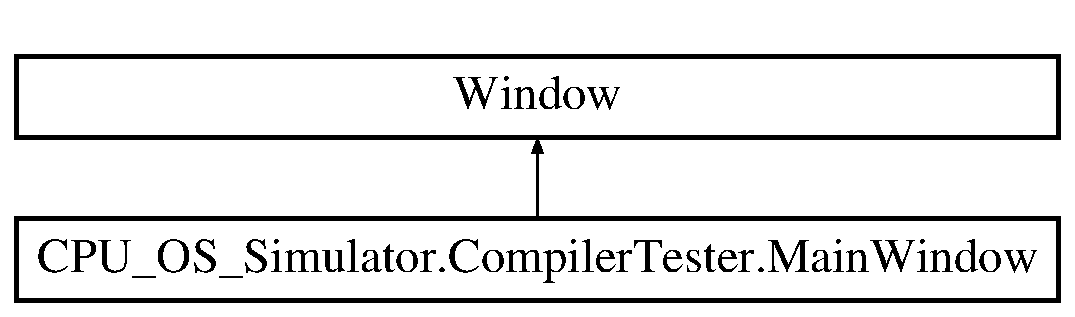
\includegraphics[height=9.523809cm]{class_c_p_u___o_s___simulator_1_1_compiler_tester_1_1_main_window}
\end{center}
\end{figure}
\subsection*{Public Member Functions}
\begin{DoxyCompactItemize}
\item 
\hyperlink{class_c_p_u___o_s___simulator_1_1_compiler_tester_1_1_main_window_a067de72c2192f57acab21aec73dd8074}{Main\+Window} ()
\item 
void \hyperlink{class_c_p_u___o_s___simulator_1_1_compiler_tester_1_1_main_window_a660feb0d1d06a39586989a4a9e5352ce}{Initialize\+Component} ()
\begin{DoxyCompactList}\small\item\em Initialize\+Component \end{DoxyCompactList}\item 
void \hyperlink{class_c_p_u___o_s___simulator_1_1_compiler_tester_1_1_main_window_a660feb0d1d06a39586989a4a9e5352ce}{Initialize\+Component} ()
\begin{DoxyCompactList}\small\item\em Initialize\+Component \end{DoxyCompactList}\item 
void \hyperlink{class_c_p_u___o_s___simulator_1_1_compiler_tester_1_1_main_window_a660feb0d1d06a39586989a4a9e5352ce}{Initialize\+Component} ()
\begin{DoxyCompactList}\small\item\em Initialize\+Component \end{DoxyCompactList}\item 
void \hyperlink{class_c_p_u___o_s___simulator_1_1_compiler_tester_1_1_main_window_a660feb0d1d06a39586989a4a9e5352ce}{Initialize\+Component} ()
\begin{DoxyCompactList}\small\item\em Initialize\+Component \end{DoxyCompactList}\end{DoxyCompactItemize}
\subsection*{Package Attributes}
\begin{DoxyCompactItemize}
\item 
\hyperlink{class_c_p_u___o_s___simulator_1_1_compiler_tester_1_1_main_window}{C\+P\+U\+\_\+\+O\+S\+\_\+\+Simulator.\+Compiler\+Tester.\+Main\+Window} \hyperlink{class_c_p_u___o_s___simulator_1_1_compiler_tester_1_1_main_window_ac7b3f59a72819d2df10d4fc5f917e7e5}{Compiler\+Tester\+Window}
\item 
System.\+Windows.\+Controls.\+Group\+Box \hyperlink{class_c_p_u___o_s___simulator_1_1_compiler_tester_1_1_main_window_a057e72ce888214ee30da5048c8bdae77}{grp\+\_\+\+Input}
\item 
System.\+Windows.\+Controls.\+Grid \hyperlink{class_c_p_u___o_s___simulator_1_1_compiler_tester_1_1_main_window_a69da11a837f2a6812b815fed3d443a3e}{grid\+\_\+\+Input}
\item 
System.\+Windows.\+Controls.\+Text\+Box \hyperlink{class_c_p_u___o_s___simulator_1_1_compiler_tester_1_1_main_window_a039f9d7d428bb5d6a3b84b701f323044}{txt\+\_\+\+Input}
\item 
System.\+Windows.\+Controls.\+Group\+Box \hyperlink{class_c_p_u___o_s___simulator_1_1_compiler_tester_1_1_main_window_a94d79540c93d5a8682b5d1a64c2efc48}{grp\+\_\+\+Output}
\item 
System.\+Windows.\+Controls.\+Grid \hyperlink{class_c_p_u___o_s___simulator_1_1_compiler_tester_1_1_main_window_a142fa92ed0a755688a31bfcbd3456e59}{grid\+\_\+\+Output}
\item 
System.\+Windows.\+Controls.\+Text\+Box \hyperlink{class_c_p_u___o_s___simulator_1_1_compiler_tester_1_1_main_window_ab6483573f0239b9af7fedfd28c2b486b}{txt\+\_\+\+Output}
\item 
System.\+Windows.\+Controls.\+Button \hyperlink{class_c_p_u___o_s___simulator_1_1_compiler_tester_1_1_main_window_a760f885c40550efba330788c8f67425a}{btn\+\_\+\+Compile}
\item 
System.\+Windows.\+Controls.\+Button \hyperlink{class_c_p_u___o_s___simulator_1_1_compiler_tester_1_1_main_window_a47e8c67fa7bd86197c528d7d0800911b}{btn\+\_\+\+Close}
\end{DoxyCompactItemize}
\subsection*{Private Member Functions}
\begin{DoxyCompactItemize}
\item 
void \hyperlink{class_c_p_u___o_s___simulator_1_1_compiler_tester_1_1_main_window_a8230f868ae44ef7a5099ac14607e330c}{btn\+\_\+\+Close\+\_\+\+Click} (object sender, Routed\+Event\+Args e)
\item 
void \hyperlink{class_c_p_u___o_s___simulator_1_1_compiler_tester_1_1_main_window_af755f7ae0752d06a31b1c30e51a05513}{btn\+\_\+\+Compile\+\_\+\+Click} (object sender, Routed\+Event\+Args e)
\item 
void \hyperlink{class_c_p_u___o_s___simulator_1_1_compiler_tester_1_1_main_window_a9c99afbfd4e46cc2d5f5c6fd499ff3b0}{Compiler\+Tester\+Window\+\_\+\+Loaded} (object sender, Routed\+Event\+Args e)
\item 
void System.\+Windows.\+Markup.\+I\+Component\+Connector. \hyperlink{class_c_p_u___o_s___simulator_1_1_compiler_tester_1_1_main_window_ab83b7c7097d501f2d4d2ce623d257c92}{Connect} (int connection\+Id, object target)
\item 
void System.\+Windows.\+Markup.\+I\+Component\+Connector. \hyperlink{class_c_p_u___o_s___simulator_1_1_compiler_tester_1_1_main_window_ab83b7c7097d501f2d4d2ce623d257c92}{Connect} (int connection\+Id, object target)
\item 
void System.\+Windows.\+Markup.\+I\+Component\+Connector. \hyperlink{class_c_p_u___o_s___simulator_1_1_compiler_tester_1_1_main_window_ab83b7c7097d501f2d4d2ce623d257c92}{Connect} (int connection\+Id, object target)
\item 
void System.\+Windows.\+Markup.\+I\+Component\+Connector. \hyperlink{class_c_p_u___o_s___simulator_1_1_compiler_tester_1_1_main_window_ab83b7c7097d501f2d4d2ce623d257c92}{Connect} (int connection\+Id, object target)
\end{DoxyCompactItemize}
\subsection*{Static Private Member Functions}
\begin{DoxyCompactItemize}
\item 
static string \hyperlink{class_c_p_u___o_s___simulator_1_1_compiler_tester_1_1_main_window_a3f7e54b6234457a6c71f6196511061da}{Get\+Program\+Version} ()
\begin{DoxyCompactList}\small\item\em Gets the build number of the running program \end{DoxyCompactList}\end{DoxyCompactItemize}
\subsection*{Private Attributes}
\begin{DoxyCompactItemize}
\item 
\hyperlink{class_c_p_u___o_s___simulator_1_1_compiler_1_1_frontend_1_1_symbols_1_1_symbol_table}{Symbol\+Table} \hyperlink{class_c_p_u___o_s___simulator_1_1_compiler_tester_1_1_main_window_a12ef52cc8436a259d0bb1c29858b100e}{symbol\+Table}
\item 
bool \hyperlink{class_c_p_u___o_s___simulator_1_1_compiler_tester_1_1_main_window_ab5592e604de397f2517ac3754544b6c1}{\+\_\+content\+Loaded}
\end{DoxyCompactItemize}


\subsection{Detailed Description}
Interaction logic for Main\+Window.\+xaml 

\hyperlink{class_c_p_u___o_s___simulator_1_1_compiler_tester_1_1_main_window}{Main\+Window} 

Definition at line 16 of file Main\+Window.\+xaml.\+cs.



\subsection{Constructor \& Destructor Documentation}
\hypertarget{class_c_p_u___o_s___simulator_1_1_compiler_tester_1_1_main_window_a067de72c2192f57acab21aec73dd8074}{}\index{C\+P\+U\+\_\+\+O\+S\+\_\+\+Simulator\+::\+Compiler\+Tester\+::\+Main\+Window@{C\+P\+U\+\_\+\+O\+S\+\_\+\+Simulator\+::\+Compiler\+Tester\+::\+Main\+Window}!Main\+Window@{Main\+Window}}
\index{Main\+Window@{Main\+Window}!C\+P\+U\+\_\+\+O\+S\+\_\+\+Simulator\+::\+Compiler\+Tester\+::\+Main\+Window@{C\+P\+U\+\_\+\+O\+S\+\_\+\+Simulator\+::\+Compiler\+Tester\+::\+Main\+Window}}
\subsubsection[{Main\+Window()}]{\setlength{\rightskip}{0pt plus 5cm}C\+P\+U\+\_\+\+O\+S\+\_\+\+Simulator.\+Compiler\+Tester.\+Main\+Window.\+Main\+Window (
\begin{DoxyParamCaption}
{}
\end{DoxyParamCaption}
)}\label{class_c_p_u___o_s___simulator_1_1_compiler_tester_1_1_main_window_a067de72c2192f57acab21aec73dd8074}


Definition at line 19 of file Main\+Window.\+xaml.\+cs.



\subsection{Member Function Documentation}
\hypertarget{class_c_p_u___o_s___simulator_1_1_compiler_tester_1_1_main_window_a8230f868ae44ef7a5099ac14607e330c}{}\index{C\+P\+U\+\_\+\+O\+S\+\_\+\+Simulator\+::\+Compiler\+Tester\+::\+Main\+Window@{C\+P\+U\+\_\+\+O\+S\+\_\+\+Simulator\+::\+Compiler\+Tester\+::\+Main\+Window}!btn\+\_\+\+Close\+\_\+\+Click@{btn\+\_\+\+Close\+\_\+\+Click}}
\index{btn\+\_\+\+Close\+\_\+\+Click@{btn\+\_\+\+Close\+\_\+\+Click}!C\+P\+U\+\_\+\+O\+S\+\_\+\+Simulator\+::\+Compiler\+Tester\+::\+Main\+Window@{C\+P\+U\+\_\+\+O\+S\+\_\+\+Simulator\+::\+Compiler\+Tester\+::\+Main\+Window}}
\subsubsection[{btn\+\_\+\+Close\+\_\+\+Click(object sender, Routed\+Event\+Args e)}]{\setlength{\rightskip}{0pt plus 5cm}void C\+P\+U\+\_\+\+O\+S\+\_\+\+Simulator.\+Compiler\+Tester.\+Main\+Window.\+btn\+\_\+\+Close\+\_\+\+Click (
\begin{DoxyParamCaption}
\item[{object}]{sender, }
\item[{Routed\+Event\+Args}]{e}
\end{DoxyParamCaption}
)\hspace{0.3cm}{\ttfamily [private]}}\label{class_c_p_u___o_s___simulator_1_1_compiler_tester_1_1_main_window_a8230f868ae44ef7a5099ac14607e330c}


Definition at line 24 of file Main\+Window.\+xaml.\+cs.

\hypertarget{class_c_p_u___o_s___simulator_1_1_compiler_tester_1_1_main_window_af755f7ae0752d06a31b1c30e51a05513}{}\index{C\+P\+U\+\_\+\+O\+S\+\_\+\+Simulator\+::\+Compiler\+Tester\+::\+Main\+Window@{C\+P\+U\+\_\+\+O\+S\+\_\+\+Simulator\+::\+Compiler\+Tester\+::\+Main\+Window}!btn\+\_\+\+Compile\+\_\+\+Click@{btn\+\_\+\+Compile\+\_\+\+Click}}
\index{btn\+\_\+\+Compile\+\_\+\+Click@{btn\+\_\+\+Compile\+\_\+\+Click}!C\+P\+U\+\_\+\+O\+S\+\_\+\+Simulator\+::\+Compiler\+Tester\+::\+Main\+Window@{C\+P\+U\+\_\+\+O\+S\+\_\+\+Simulator\+::\+Compiler\+Tester\+::\+Main\+Window}}
\subsubsection[{btn\+\_\+\+Compile\+\_\+\+Click(object sender, Routed\+Event\+Args e)}]{\setlength{\rightskip}{0pt plus 5cm}void C\+P\+U\+\_\+\+O\+S\+\_\+\+Simulator.\+Compiler\+Tester.\+Main\+Window.\+btn\+\_\+\+Compile\+\_\+\+Click (
\begin{DoxyParamCaption}
\item[{object}]{sender, }
\item[{Routed\+Event\+Args}]{e}
\end{DoxyParamCaption}
)\hspace{0.3cm}{\ttfamily [private]}}\label{class_c_p_u___o_s___simulator_1_1_compiler_tester_1_1_main_window_af755f7ae0752d06a31b1c30e51a05513}


Definition at line 29 of file Main\+Window.\+xaml.\+cs.

\hypertarget{class_c_p_u___o_s___simulator_1_1_compiler_tester_1_1_main_window_a9c99afbfd4e46cc2d5f5c6fd499ff3b0}{}\index{C\+P\+U\+\_\+\+O\+S\+\_\+\+Simulator\+::\+Compiler\+Tester\+::\+Main\+Window@{C\+P\+U\+\_\+\+O\+S\+\_\+\+Simulator\+::\+Compiler\+Tester\+::\+Main\+Window}!Compiler\+Tester\+Window\+\_\+\+Loaded@{Compiler\+Tester\+Window\+\_\+\+Loaded}}
\index{Compiler\+Tester\+Window\+\_\+\+Loaded@{Compiler\+Tester\+Window\+\_\+\+Loaded}!C\+P\+U\+\_\+\+O\+S\+\_\+\+Simulator\+::\+Compiler\+Tester\+::\+Main\+Window@{C\+P\+U\+\_\+\+O\+S\+\_\+\+Simulator\+::\+Compiler\+Tester\+::\+Main\+Window}}
\subsubsection[{Compiler\+Tester\+Window\+\_\+\+Loaded(object sender, Routed\+Event\+Args e)}]{\setlength{\rightskip}{0pt plus 5cm}void C\+P\+U\+\_\+\+O\+S\+\_\+\+Simulator.\+Compiler\+Tester.\+Main\+Window.\+Compiler\+Tester\+Window\+\_\+\+Loaded (
\begin{DoxyParamCaption}
\item[{object}]{sender, }
\item[{Routed\+Event\+Args}]{e}
\end{DoxyParamCaption}
)\hspace{0.3cm}{\ttfamily [private]}}\label{class_c_p_u___o_s___simulator_1_1_compiler_tester_1_1_main_window_a9c99afbfd4e46cc2d5f5c6fd499ff3b0}


Definition at line 67 of file Main\+Window.\+xaml.\+cs.

\hypertarget{class_c_p_u___o_s___simulator_1_1_compiler_tester_1_1_main_window_ab83b7c7097d501f2d4d2ce623d257c92}{}\index{C\+P\+U\+\_\+\+O\+S\+\_\+\+Simulator\+::\+Compiler\+Tester\+::\+Main\+Window@{C\+P\+U\+\_\+\+O\+S\+\_\+\+Simulator\+::\+Compiler\+Tester\+::\+Main\+Window}!Connect@{Connect}}
\index{Connect@{Connect}!C\+P\+U\+\_\+\+O\+S\+\_\+\+Simulator\+::\+Compiler\+Tester\+::\+Main\+Window@{C\+P\+U\+\_\+\+O\+S\+\_\+\+Simulator\+::\+Compiler\+Tester\+::\+Main\+Window}}
\subsubsection[{Connect(int connection\+Id, object target)}]{\setlength{\rightskip}{0pt plus 5cm}void System.\+Windows.\+Markup.\+I\+Component\+Connector. C\+P\+U\+\_\+\+O\+S\+\_\+\+Simulator.\+Compiler\+Tester.\+Main\+Window.\+Connect (
\begin{DoxyParamCaption}
\item[{int}]{connection\+Id, }
\item[{object}]{target}
\end{DoxyParamCaption}
)\hspace{0.3cm}{\ttfamily [private]}}\label{class_c_p_u___o_s___simulator_1_1_compiler_tester_1_1_main_window_ab83b7c7097d501f2d4d2ce623d257c92}


Definition at line 141 of file Main\+Window.\+g.\+i.\+cs.

\hypertarget{class_c_p_u___o_s___simulator_1_1_compiler_tester_1_1_main_window_ab83b7c7097d501f2d4d2ce623d257c92}{}\index{C\+P\+U\+\_\+\+O\+S\+\_\+\+Simulator\+::\+Compiler\+Tester\+::\+Main\+Window@{C\+P\+U\+\_\+\+O\+S\+\_\+\+Simulator\+::\+Compiler\+Tester\+::\+Main\+Window}!Connect@{Connect}}
\index{Connect@{Connect}!C\+P\+U\+\_\+\+O\+S\+\_\+\+Simulator\+::\+Compiler\+Tester\+::\+Main\+Window@{C\+P\+U\+\_\+\+O\+S\+\_\+\+Simulator\+::\+Compiler\+Tester\+::\+Main\+Window}}
\subsubsection[{Connect(int connection\+Id, object target)}]{\setlength{\rightskip}{0pt plus 5cm}void System.\+Windows.\+Markup.\+I\+Component\+Connector. C\+P\+U\+\_\+\+O\+S\+\_\+\+Simulator.\+Compiler\+Tester.\+Main\+Window.\+Connect (
\begin{DoxyParamCaption}
\item[{int}]{connection\+Id, }
\item[{object}]{target}
\end{DoxyParamCaption}
)\hspace{0.3cm}{\ttfamily [private]}}\label{class_c_p_u___o_s___simulator_1_1_compiler_tester_1_1_main_window_ab83b7c7097d501f2d4d2ce623d257c92}


Definition at line 141 of file Main\+Window.\+g.\+i.\+cs.

\hypertarget{class_c_p_u___o_s___simulator_1_1_compiler_tester_1_1_main_window_ab83b7c7097d501f2d4d2ce623d257c92}{}\index{C\+P\+U\+\_\+\+O\+S\+\_\+\+Simulator\+::\+Compiler\+Tester\+::\+Main\+Window@{C\+P\+U\+\_\+\+O\+S\+\_\+\+Simulator\+::\+Compiler\+Tester\+::\+Main\+Window}!Connect@{Connect}}
\index{Connect@{Connect}!C\+P\+U\+\_\+\+O\+S\+\_\+\+Simulator\+::\+Compiler\+Tester\+::\+Main\+Window@{C\+P\+U\+\_\+\+O\+S\+\_\+\+Simulator\+::\+Compiler\+Tester\+::\+Main\+Window}}
\subsubsection[{Connect(int connection\+Id, object target)}]{\setlength{\rightskip}{0pt plus 5cm}void System.\+Windows.\+Markup.\+I\+Component\+Connector. C\+P\+U\+\_\+\+O\+S\+\_\+\+Simulator.\+Compiler\+Tester.\+Main\+Window.\+Connect (
\begin{DoxyParamCaption}
\item[{int}]{connection\+Id, }
\item[{object}]{target}
\end{DoxyParamCaption}
)\hspace{0.3cm}{\ttfamily [private]}}\label{class_c_p_u___o_s___simulator_1_1_compiler_tester_1_1_main_window_ab83b7c7097d501f2d4d2ce623d257c92}


Definition at line 141 of file Main\+Window.\+g.\+cs.

\hypertarget{class_c_p_u___o_s___simulator_1_1_compiler_tester_1_1_main_window_ab83b7c7097d501f2d4d2ce623d257c92}{}\index{C\+P\+U\+\_\+\+O\+S\+\_\+\+Simulator\+::\+Compiler\+Tester\+::\+Main\+Window@{C\+P\+U\+\_\+\+O\+S\+\_\+\+Simulator\+::\+Compiler\+Tester\+::\+Main\+Window}!Connect@{Connect}}
\index{Connect@{Connect}!C\+P\+U\+\_\+\+O\+S\+\_\+\+Simulator\+::\+Compiler\+Tester\+::\+Main\+Window@{C\+P\+U\+\_\+\+O\+S\+\_\+\+Simulator\+::\+Compiler\+Tester\+::\+Main\+Window}}
\subsubsection[{Connect(int connection\+Id, object target)}]{\setlength{\rightskip}{0pt plus 5cm}void System.\+Windows.\+Markup.\+I\+Component\+Connector. C\+P\+U\+\_\+\+O\+S\+\_\+\+Simulator.\+Compiler\+Tester.\+Main\+Window.\+Connect (
\begin{DoxyParamCaption}
\item[{int}]{connection\+Id, }
\item[{object}]{target}
\end{DoxyParamCaption}
)\hspace{0.3cm}{\ttfamily [private]}}\label{class_c_p_u___o_s___simulator_1_1_compiler_tester_1_1_main_window_ab83b7c7097d501f2d4d2ce623d257c92}


Definition at line 141 of file Main\+Window.\+g.\+cs.

\hypertarget{class_c_p_u___o_s___simulator_1_1_compiler_tester_1_1_main_window_a3f7e54b6234457a6c71f6196511061da}{}\index{C\+P\+U\+\_\+\+O\+S\+\_\+\+Simulator\+::\+Compiler\+Tester\+::\+Main\+Window@{C\+P\+U\+\_\+\+O\+S\+\_\+\+Simulator\+::\+Compiler\+Tester\+::\+Main\+Window}!Get\+Program\+Version@{Get\+Program\+Version}}
\index{Get\+Program\+Version@{Get\+Program\+Version}!C\+P\+U\+\_\+\+O\+S\+\_\+\+Simulator\+::\+Compiler\+Tester\+::\+Main\+Window@{C\+P\+U\+\_\+\+O\+S\+\_\+\+Simulator\+::\+Compiler\+Tester\+::\+Main\+Window}}
\subsubsection[{Get\+Program\+Version()}]{\setlength{\rightskip}{0pt plus 5cm}static string C\+P\+U\+\_\+\+O\+S\+\_\+\+Simulator.\+Compiler\+Tester.\+Main\+Window.\+Get\+Program\+Version (
\begin{DoxyParamCaption}
{}
\end{DoxyParamCaption}
)\hspace{0.3cm}{\ttfamily [static]}, {\ttfamily [private]}}\label{class_c_p_u___o_s___simulator_1_1_compiler_tester_1_1_main_window_a3f7e54b6234457a6c71f6196511061da}


Gets the build number of the running program 

\begin{DoxyReturn}{Returns}
The build number of the running program
\end{DoxyReturn}


Definition at line 80 of file Main\+Window.\+xaml.\+cs.

\hypertarget{class_c_p_u___o_s___simulator_1_1_compiler_tester_1_1_main_window_a660feb0d1d06a39586989a4a9e5352ce}{}\index{C\+P\+U\+\_\+\+O\+S\+\_\+\+Simulator\+::\+Compiler\+Tester\+::\+Main\+Window@{C\+P\+U\+\_\+\+O\+S\+\_\+\+Simulator\+::\+Compiler\+Tester\+::\+Main\+Window}!Initialize\+Component@{Initialize\+Component}}
\index{Initialize\+Component@{Initialize\+Component}!C\+P\+U\+\_\+\+O\+S\+\_\+\+Simulator\+::\+Compiler\+Tester\+::\+Main\+Window@{C\+P\+U\+\_\+\+O\+S\+\_\+\+Simulator\+::\+Compiler\+Tester\+::\+Main\+Window}}
\subsubsection[{Initialize\+Component()}]{\setlength{\rightskip}{0pt plus 5cm}void C\+P\+U\+\_\+\+O\+S\+\_\+\+Simulator.\+Compiler\+Tester.\+Main\+Window.\+Initialize\+Component (
\begin{DoxyParamCaption}
{}
\end{DoxyParamCaption}
)}\label{class_c_p_u___o_s___simulator_1_1_compiler_tester_1_1_main_window_a660feb0d1d06a39586989a4a9e5352ce}


Initialize\+Component 



Definition at line 121 of file Main\+Window.\+g.\+cs.

\hypertarget{class_c_p_u___o_s___simulator_1_1_compiler_tester_1_1_main_window_a660feb0d1d06a39586989a4a9e5352ce}{}\index{C\+P\+U\+\_\+\+O\+S\+\_\+\+Simulator\+::\+Compiler\+Tester\+::\+Main\+Window@{C\+P\+U\+\_\+\+O\+S\+\_\+\+Simulator\+::\+Compiler\+Tester\+::\+Main\+Window}!Initialize\+Component@{Initialize\+Component}}
\index{Initialize\+Component@{Initialize\+Component}!C\+P\+U\+\_\+\+O\+S\+\_\+\+Simulator\+::\+Compiler\+Tester\+::\+Main\+Window@{C\+P\+U\+\_\+\+O\+S\+\_\+\+Simulator\+::\+Compiler\+Tester\+::\+Main\+Window}}
\subsubsection[{Initialize\+Component()}]{\setlength{\rightskip}{0pt plus 5cm}void C\+P\+U\+\_\+\+O\+S\+\_\+\+Simulator.\+Compiler\+Tester.\+Main\+Window.\+Initialize\+Component (
\begin{DoxyParamCaption}
{}
\end{DoxyParamCaption}
)}\label{class_c_p_u___o_s___simulator_1_1_compiler_tester_1_1_main_window_a660feb0d1d06a39586989a4a9e5352ce}


Initialize\+Component 



Definition at line 121 of file Main\+Window.\+g.\+cs.

\hypertarget{class_c_p_u___o_s___simulator_1_1_compiler_tester_1_1_main_window_a660feb0d1d06a39586989a4a9e5352ce}{}\index{C\+P\+U\+\_\+\+O\+S\+\_\+\+Simulator\+::\+Compiler\+Tester\+::\+Main\+Window@{C\+P\+U\+\_\+\+O\+S\+\_\+\+Simulator\+::\+Compiler\+Tester\+::\+Main\+Window}!Initialize\+Component@{Initialize\+Component}}
\index{Initialize\+Component@{Initialize\+Component}!C\+P\+U\+\_\+\+O\+S\+\_\+\+Simulator\+::\+Compiler\+Tester\+::\+Main\+Window@{C\+P\+U\+\_\+\+O\+S\+\_\+\+Simulator\+::\+Compiler\+Tester\+::\+Main\+Window}}
\subsubsection[{Initialize\+Component()}]{\setlength{\rightskip}{0pt plus 5cm}void C\+P\+U\+\_\+\+O\+S\+\_\+\+Simulator.\+Compiler\+Tester.\+Main\+Window.\+Initialize\+Component (
\begin{DoxyParamCaption}
{}
\end{DoxyParamCaption}
)}\label{class_c_p_u___o_s___simulator_1_1_compiler_tester_1_1_main_window_a660feb0d1d06a39586989a4a9e5352ce}


Initialize\+Component 



Definition at line 121 of file Main\+Window.\+g.\+i.\+cs.

\hypertarget{class_c_p_u___o_s___simulator_1_1_compiler_tester_1_1_main_window_a660feb0d1d06a39586989a4a9e5352ce}{}\index{C\+P\+U\+\_\+\+O\+S\+\_\+\+Simulator\+::\+Compiler\+Tester\+::\+Main\+Window@{C\+P\+U\+\_\+\+O\+S\+\_\+\+Simulator\+::\+Compiler\+Tester\+::\+Main\+Window}!Initialize\+Component@{Initialize\+Component}}
\index{Initialize\+Component@{Initialize\+Component}!C\+P\+U\+\_\+\+O\+S\+\_\+\+Simulator\+::\+Compiler\+Tester\+::\+Main\+Window@{C\+P\+U\+\_\+\+O\+S\+\_\+\+Simulator\+::\+Compiler\+Tester\+::\+Main\+Window}}
\subsubsection[{Initialize\+Component()}]{\setlength{\rightskip}{0pt plus 5cm}void C\+P\+U\+\_\+\+O\+S\+\_\+\+Simulator.\+Compiler\+Tester.\+Main\+Window.\+Initialize\+Component (
\begin{DoxyParamCaption}
{}
\end{DoxyParamCaption}
)}\label{class_c_p_u___o_s___simulator_1_1_compiler_tester_1_1_main_window_a660feb0d1d06a39586989a4a9e5352ce}


Initialize\+Component 



Definition at line 121 of file Main\+Window.\+g.\+i.\+cs.



\subsection{Member Data Documentation}
\hypertarget{class_c_p_u___o_s___simulator_1_1_compiler_tester_1_1_main_window_ab5592e604de397f2517ac3754544b6c1}{}\index{C\+P\+U\+\_\+\+O\+S\+\_\+\+Simulator\+::\+Compiler\+Tester\+::\+Main\+Window@{C\+P\+U\+\_\+\+O\+S\+\_\+\+Simulator\+::\+Compiler\+Tester\+::\+Main\+Window}!\+\_\+content\+Loaded@{\+\_\+content\+Loaded}}
\index{\+\_\+content\+Loaded@{\+\_\+content\+Loaded}!C\+P\+U\+\_\+\+O\+S\+\_\+\+Simulator\+::\+Compiler\+Tester\+::\+Main\+Window@{C\+P\+U\+\_\+\+O\+S\+\_\+\+Simulator\+::\+Compiler\+Tester\+::\+Main\+Window}}
\subsubsection[{\+\_\+content\+Loaded}]{\setlength{\rightskip}{0pt plus 5cm}bool C\+P\+U\+\_\+\+O\+S\+\_\+\+Simulator.\+Compiler\+Tester.\+Main\+Window.\+\_\+content\+Loaded\hspace{0.3cm}{\ttfamily [private]}}\label{class_c_p_u___o_s___simulator_1_1_compiler_tester_1_1_main_window_ab5592e604de397f2517ac3754544b6c1}


Definition at line 114 of file Main\+Window.\+g.\+cs.

\hypertarget{class_c_p_u___o_s___simulator_1_1_compiler_tester_1_1_main_window_a47e8c67fa7bd86197c528d7d0800911b}{}\index{C\+P\+U\+\_\+\+O\+S\+\_\+\+Simulator\+::\+Compiler\+Tester\+::\+Main\+Window@{C\+P\+U\+\_\+\+O\+S\+\_\+\+Simulator\+::\+Compiler\+Tester\+::\+Main\+Window}!btn\+\_\+\+Close@{btn\+\_\+\+Close}}
\index{btn\+\_\+\+Close@{btn\+\_\+\+Close}!C\+P\+U\+\_\+\+O\+S\+\_\+\+Simulator\+::\+Compiler\+Tester\+::\+Main\+Window@{C\+P\+U\+\_\+\+O\+S\+\_\+\+Simulator\+::\+Compiler\+Tester\+::\+Main\+Window}}
\subsubsection[{btn\+\_\+\+Close}]{\setlength{\rightskip}{0pt plus 5cm}System Windows Controls Button C\+P\+U\+\_\+\+O\+S\+\_\+\+Simulator.\+Compiler\+Tester.\+Main\+Window.\+btn\+\_\+\+Close\hspace{0.3cm}{\ttfamily [package]}}\label{class_c_p_u___o_s___simulator_1_1_compiler_tester_1_1_main_window_a47e8c67fa7bd86197c528d7d0800911b}


Definition at line 109 of file Main\+Window.\+g.\+cs.

\hypertarget{class_c_p_u___o_s___simulator_1_1_compiler_tester_1_1_main_window_a760f885c40550efba330788c8f67425a}{}\index{C\+P\+U\+\_\+\+O\+S\+\_\+\+Simulator\+::\+Compiler\+Tester\+::\+Main\+Window@{C\+P\+U\+\_\+\+O\+S\+\_\+\+Simulator\+::\+Compiler\+Tester\+::\+Main\+Window}!btn\+\_\+\+Compile@{btn\+\_\+\+Compile}}
\index{btn\+\_\+\+Compile@{btn\+\_\+\+Compile}!C\+P\+U\+\_\+\+O\+S\+\_\+\+Simulator\+::\+Compiler\+Tester\+::\+Main\+Window@{C\+P\+U\+\_\+\+O\+S\+\_\+\+Simulator\+::\+Compiler\+Tester\+::\+Main\+Window}}
\subsubsection[{btn\+\_\+\+Compile}]{\setlength{\rightskip}{0pt plus 5cm}System Windows Controls Button C\+P\+U\+\_\+\+O\+S\+\_\+\+Simulator.\+Compiler\+Tester.\+Main\+Window.\+btn\+\_\+\+Compile\hspace{0.3cm}{\ttfamily [package]}}\label{class_c_p_u___o_s___simulator_1_1_compiler_tester_1_1_main_window_a760f885c40550efba330788c8f67425a}


Definition at line 101 of file Main\+Window.\+g.\+cs.

\hypertarget{class_c_p_u___o_s___simulator_1_1_compiler_tester_1_1_main_window_ac7b3f59a72819d2df10d4fc5f917e7e5}{}\index{C\+P\+U\+\_\+\+O\+S\+\_\+\+Simulator\+::\+Compiler\+Tester\+::\+Main\+Window@{C\+P\+U\+\_\+\+O\+S\+\_\+\+Simulator\+::\+Compiler\+Tester\+::\+Main\+Window}!Compiler\+Tester\+Window@{Compiler\+Tester\+Window}}
\index{Compiler\+Tester\+Window@{Compiler\+Tester\+Window}!C\+P\+U\+\_\+\+O\+S\+\_\+\+Simulator\+::\+Compiler\+Tester\+::\+Main\+Window@{C\+P\+U\+\_\+\+O\+S\+\_\+\+Simulator\+::\+Compiler\+Tester\+::\+Main\+Window}}
\subsubsection[{Compiler\+Tester\+Window}]{\setlength{\rightskip}{0pt plus 5cm}C\+P\+U\+\_\+\+O\+S\+\_\+\+Simulator Compiler\+Tester {\bf Main\+Window} C\+P\+U\+\_\+\+O\+S\+\_\+\+Simulator.\+Compiler\+Tester.\+Main\+Window.\+Compiler\+Tester\+Window\hspace{0.3cm}{\ttfamily [package]}}\label{class_c_p_u___o_s___simulator_1_1_compiler_tester_1_1_main_window_ac7b3f59a72819d2df10d4fc5f917e7e5}


Definition at line 45 of file Main\+Window.\+g.\+cs.

\hypertarget{class_c_p_u___o_s___simulator_1_1_compiler_tester_1_1_main_window_a69da11a837f2a6812b815fed3d443a3e}{}\index{C\+P\+U\+\_\+\+O\+S\+\_\+\+Simulator\+::\+Compiler\+Tester\+::\+Main\+Window@{C\+P\+U\+\_\+\+O\+S\+\_\+\+Simulator\+::\+Compiler\+Tester\+::\+Main\+Window}!grid\+\_\+\+Input@{grid\+\_\+\+Input}}
\index{grid\+\_\+\+Input@{grid\+\_\+\+Input}!C\+P\+U\+\_\+\+O\+S\+\_\+\+Simulator\+::\+Compiler\+Tester\+::\+Main\+Window@{C\+P\+U\+\_\+\+O\+S\+\_\+\+Simulator\+::\+Compiler\+Tester\+::\+Main\+Window}}
\subsubsection[{grid\+\_\+\+Input}]{\setlength{\rightskip}{0pt plus 5cm}System Windows Controls Grid C\+P\+U\+\_\+\+O\+S\+\_\+\+Simulator.\+Compiler\+Tester.\+Main\+Window.\+grid\+\_\+\+Input\hspace{0.3cm}{\ttfamily [package]}}\label{class_c_p_u___o_s___simulator_1_1_compiler_tester_1_1_main_window_a69da11a837f2a6812b815fed3d443a3e}


Definition at line 61 of file Main\+Window.\+g.\+cs.

\hypertarget{class_c_p_u___o_s___simulator_1_1_compiler_tester_1_1_main_window_a142fa92ed0a755688a31bfcbd3456e59}{}\index{C\+P\+U\+\_\+\+O\+S\+\_\+\+Simulator\+::\+Compiler\+Tester\+::\+Main\+Window@{C\+P\+U\+\_\+\+O\+S\+\_\+\+Simulator\+::\+Compiler\+Tester\+::\+Main\+Window}!grid\+\_\+\+Output@{grid\+\_\+\+Output}}
\index{grid\+\_\+\+Output@{grid\+\_\+\+Output}!C\+P\+U\+\_\+\+O\+S\+\_\+\+Simulator\+::\+Compiler\+Tester\+::\+Main\+Window@{C\+P\+U\+\_\+\+O\+S\+\_\+\+Simulator\+::\+Compiler\+Tester\+::\+Main\+Window}}
\subsubsection[{grid\+\_\+\+Output}]{\setlength{\rightskip}{0pt plus 5cm}System Windows Controls Grid C\+P\+U\+\_\+\+O\+S\+\_\+\+Simulator.\+Compiler\+Tester.\+Main\+Window.\+grid\+\_\+\+Output\hspace{0.3cm}{\ttfamily [package]}}\label{class_c_p_u___o_s___simulator_1_1_compiler_tester_1_1_main_window_a142fa92ed0a755688a31bfcbd3456e59}


Definition at line 85 of file Main\+Window.\+g.\+cs.

\hypertarget{class_c_p_u___o_s___simulator_1_1_compiler_tester_1_1_main_window_a057e72ce888214ee30da5048c8bdae77}{}\index{C\+P\+U\+\_\+\+O\+S\+\_\+\+Simulator\+::\+Compiler\+Tester\+::\+Main\+Window@{C\+P\+U\+\_\+\+O\+S\+\_\+\+Simulator\+::\+Compiler\+Tester\+::\+Main\+Window}!grp\+\_\+\+Input@{grp\+\_\+\+Input}}
\index{grp\+\_\+\+Input@{grp\+\_\+\+Input}!C\+P\+U\+\_\+\+O\+S\+\_\+\+Simulator\+::\+Compiler\+Tester\+::\+Main\+Window@{C\+P\+U\+\_\+\+O\+S\+\_\+\+Simulator\+::\+Compiler\+Tester\+::\+Main\+Window}}
\subsubsection[{grp\+\_\+\+Input}]{\setlength{\rightskip}{0pt plus 5cm}System Windows Controls Group\+Box C\+P\+U\+\_\+\+O\+S\+\_\+\+Simulator.\+Compiler\+Tester.\+Main\+Window.\+grp\+\_\+\+Input\hspace{0.3cm}{\ttfamily [package]}}\label{class_c_p_u___o_s___simulator_1_1_compiler_tester_1_1_main_window_a057e72ce888214ee30da5048c8bdae77}


Definition at line 53 of file Main\+Window.\+g.\+cs.

\hypertarget{class_c_p_u___o_s___simulator_1_1_compiler_tester_1_1_main_window_a94d79540c93d5a8682b5d1a64c2efc48}{}\index{C\+P\+U\+\_\+\+O\+S\+\_\+\+Simulator\+::\+Compiler\+Tester\+::\+Main\+Window@{C\+P\+U\+\_\+\+O\+S\+\_\+\+Simulator\+::\+Compiler\+Tester\+::\+Main\+Window}!grp\+\_\+\+Output@{grp\+\_\+\+Output}}
\index{grp\+\_\+\+Output@{grp\+\_\+\+Output}!C\+P\+U\+\_\+\+O\+S\+\_\+\+Simulator\+::\+Compiler\+Tester\+::\+Main\+Window@{C\+P\+U\+\_\+\+O\+S\+\_\+\+Simulator\+::\+Compiler\+Tester\+::\+Main\+Window}}
\subsubsection[{grp\+\_\+\+Output}]{\setlength{\rightskip}{0pt plus 5cm}System Windows Controls Group\+Box C\+P\+U\+\_\+\+O\+S\+\_\+\+Simulator.\+Compiler\+Tester.\+Main\+Window.\+grp\+\_\+\+Output\hspace{0.3cm}{\ttfamily [package]}}\label{class_c_p_u___o_s___simulator_1_1_compiler_tester_1_1_main_window_a94d79540c93d5a8682b5d1a64c2efc48}


Definition at line 77 of file Main\+Window.\+g.\+cs.

\hypertarget{class_c_p_u___o_s___simulator_1_1_compiler_tester_1_1_main_window_a12ef52cc8436a259d0bb1c29858b100e}{}\index{C\+P\+U\+\_\+\+O\+S\+\_\+\+Simulator\+::\+Compiler\+Tester\+::\+Main\+Window@{C\+P\+U\+\_\+\+O\+S\+\_\+\+Simulator\+::\+Compiler\+Tester\+::\+Main\+Window}!symbol\+Table@{symbol\+Table}}
\index{symbol\+Table@{symbol\+Table}!C\+P\+U\+\_\+\+O\+S\+\_\+\+Simulator\+::\+Compiler\+Tester\+::\+Main\+Window@{C\+P\+U\+\_\+\+O\+S\+\_\+\+Simulator\+::\+Compiler\+Tester\+::\+Main\+Window}}
\subsubsection[{symbol\+Table}]{\setlength{\rightskip}{0pt plus 5cm}{\bf Symbol\+Table} C\+P\+U\+\_\+\+O\+S\+\_\+\+Simulator.\+Compiler\+Tester.\+Main\+Window.\+symbol\+Table\hspace{0.3cm}{\ttfamily [private]}}\label{class_c_p_u___o_s___simulator_1_1_compiler_tester_1_1_main_window_a12ef52cc8436a259d0bb1c29858b100e}


Definition at line 18 of file Main\+Window.\+xaml.\+cs.

\hypertarget{class_c_p_u___o_s___simulator_1_1_compiler_tester_1_1_main_window_a039f9d7d428bb5d6a3b84b701f323044}{}\index{C\+P\+U\+\_\+\+O\+S\+\_\+\+Simulator\+::\+Compiler\+Tester\+::\+Main\+Window@{C\+P\+U\+\_\+\+O\+S\+\_\+\+Simulator\+::\+Compiler\+Tester\+::\+Main\+Window}!txt\+\_\+\+Input@{txt\+\_\+\+Input}}
\index{txt\+\_\+\+Input@{txt\+\_\+\+Input}!C\+P\+U\+\_\+\+O\+S\+\_\+\+Simulator\+::\+Compiler\+Tester\+::\+Main\+Window@{C\+P\+U\+\_\+\+O\+S\+\_\+\+Simulator\+::\+Compiler\+Tester\+::\+Main\+Window}}
\subsubsection[{txt\+\_\+\+Input}]{\setlength{\rightskip}{0pt plus 5cm}System Windows Controls Text\+Box C\+P\+U\+\_\+\+O\+S\+\_\+\+Simulator.\+Compiler\+Tester.\+Main\+Window.\+txt\+\_\+\+Input\hspace{0.3cm}{\ttfamily [package]}}\label{class_c_p_u___o_s___simulator_1_1_compiler_tester_1_1_main_window_a039f9d7d428bb5d6a3b84b701f323044}


Definition at line 69 of file Main\+Window.\+g.\+cs.

\hypertarget{class_c_p_u___o_s___simulator_1_1_compiler_tester_1_1_main_window_ab6483573f0239b9af7fedfd28c2b486b}{}\index{C\+P\+U\+\_\+\+O\+S\+\_\+\+Simulator\+::\+Compiler\+Tester\+::\+Main\+Window@{C\+P\+U\+\_\+\+O\+S\+\_\+\+Simulator\+::\+Compiler\+Tester\+::\+Main\+Window}!txt\+\_\+\+Output@{txt\+\_\+\+Output}}
\index{txt\+\_\+\+Output@{txt\+\_\+\+Output}!C\+P\+U\+\_\+\+O\+S\+\_\+\+Simulator\+::\+Compiler\+Tester\+::\+Main\+Window@{C\+P\+U\+\_\+\+O\+S\+\_\+\+Simulator\+::\+Compiler\+Tester\+::\+Main\+Window}}
\subsubsection[{txt\+\_\+\+Output}]{\setlength{\rightskip}{0pt plus 5cm}System Windows Controls Text\+Box C\+P\+U\+\_\+\+O\+S\+\_\+\+Simulator.\+Compiler\+Tester.\+Main\+Window.\+txt\+\_\+\+Output\hspace{0.3cm}{\ttfamily [package]}}\label{class_c_p_u___o_s___simulator_1_1_compiler_tester_1_1_main_window_ab6483573f0239b9af7fedfd28c2b486b}


Definition at line 93 of file Main\+Window.\+g.\+cs.



The documentation for this class was generated from the following files\+:\begin{DoxyCompactItemize}
\item 
Compiler\+Tester/\hyperlink{_compiler_tester_2_main_window_8xaml_8cs}{Main\+Window.\+xaml.\+cs}\item 
Compiler\+Tester/obj/\+Debug/\hyperlink{_compiler_tester_2obj_2_debug_2_main_window_8g_8cs}{Main\+Window.\+g.\+cs}\item 
Compiler\+Tester/obj/\+Debug/\hyperlink{_compiler_tester_2obj_2_debug_2_main_window_8g_8i_8cs}{Main\+Window.\+g.\+i.\+cs}\end{DoxyCompactItemize}

\hypertarget{class_c_p_u___o_s___simulator_tests_1_1_main_window_tests}{}\section{C\+P\+U\+\_\+\+O\+S\+\_\+\+Simulator\+Tests.\+Main\+Window\+Tests Class Reference}
\label{class_c_p_u___o_s___simulator_tests_1_1_main_window_tests}\index{C\+P\+U\+\_\+\+O\+S\+\_\+\+Simulator\+Tests.\+Main\+Window\+Tests@{C\+P\+U\+\_\+\+O\+S\+\_\+\+Simulator\+Tests.\+Main\+Window\+Tests}}
\subsection*{Public Member Functions}
\begin{DoxyCompactItemize}
\item 
void \hyperlink{class_c_p_u___o_s___simulator_tests_1_1_main_window_tests_ad4836ea701495048fdf8978a26b7289d}{Main\+Window\+Test} ()
\item 
void \hyperlink{class_c_p_u___o_s___simulator_tests_1_1_main_window_tests_aa579aa65b970afe2da85dfa00b099d22}{Is\+Administrator\+Test} ()
\item 
void \hyperlink{class_c_p_u___o_s___simulator_tests_1_1_main_window_tests_af75c3a60c45bb18647e31a2d992f7a9e}{Set\+Association\+Test} ()
\item 
void \hyperlink{class_c_p_u___o_s___simulator_tests_1_1_main_window_tests_a16c4c8bfd9dbe4351928f4a2f299cee6}{Say\+Hello\+Test} ()
\item 
void \hyperlink{class_c_p_u___o_s___simulator_tests_1_1_main_window_tests_a29622aedce4ad01ba057932fe4575769}{Create\+Instruction\+Test} ()
\item 
void \hyperlink{class_c_p_u___o_s___simulator_tests_1_1_main_window_tests_a721b270327db5b78e6706b5e6f086fee}{Create\+Instruction\+Test1} ()
\item 
void \hyperlink{class_c_p_u___o_s___simulator_tests_1_1_main_window_tests_abf58c3ed4fe1465c2d798dd77130c0d9}{Create\+Instruction\+Test2} ()
\item 
void \hyperlink{class_c_p_u___o_s___simulator_tests_1_1_main_window_tests_a0db1c879896356433f7ae1049f817748}{Add\+Instruction\+Test} ()
\item 
void \hyperlink{class_c_p_u___o_s___simulator_tests_1_1_main_window_tests_a819015644c93bfefb8e240777d42911a}{Serialize\+Object\+Test} ()
\item 
void \hyperlink{class_c_p_u___o_s___simulator_tests_1_1_main_window_tests_a540e4db419a8cb65c5e0156a4dc5f6d1}{De\+Serialize\+Object\+Test} ()
\end{DoxyCompactItemize}


\subsection{Detailed Description}


Definition at line 8 of file Main\+Window\+Tests.\+cs.



\subsection{Member Function Documentation}
\hypertarget{class_c_p_u___o_s___simulator_tests_1_1_main_window_tests_a0db1c879896356433f7ae1049f817748}{}\index{C\+P\+U\+\_\+\+O\+S\+\_\+\+Simulator\+Tests\+::\+Main\+Window\+Tests@{C\+P\+U\+\_\+\+O\+S\+\_\+\+Simulator\+Tests\+::\+Main\+Window\+Tests}!Add\+Instruction\+Test@{Add\+Instruction\+Test}}
\index{Add\+Instruction\+Test@{Add\+Instruction\+Test}!C\+P\+U\+\_\+\+O\+S\+\_\+\+Simulator\+Tests\+::\+Main\+Window\+Tests@{C\+P\+U\+\_\+\+O\+S\+\_\+\+Simulator\+Tests\+::\+Main\+Window\+Tests}}
\subsubsection[{Add\+Instruction\+Test()}]{\setlength{\rightskip}{0pt plus 5cm}void C\+P\+U\+\_\+\+O\+S\+\_\+\+Simulator\+Tests.\+Main\+Window\+Tests.\+Add\+Instruction\+Test (
\begin{DoxyParamCaption}
{}
\end{DoxyParamCaption}
)}\label{class_c_p_u___o_s___simulator_tests_1_1_main_window_tests_a0db1c879896356433f7ae1049f817748}


Definition at line 57 of file Main\+Window\+Tests.\+cs.

\hypertarget{class_c_p_u___o_s___simulator_tests_1_1_main_window_tests_a29622aedce4ad01ba057932fe4575769}{}\index{C\+P\+U\+\_\+\+O\+S\+\_\+\+Simulator\+Tests\+::\+Main\+Window\+Tests@{C\+P\+U\+\_\+\+O\+S\+\_\+\+Simulator\+Tests\+::\+Main\+Window\+Tests}!Create\+Instruction\+Test@{Create\+Instruction\+Test}}
\index{Create\+Instruction\+Test@{Create\+Instruction\+Test}!C\+P\+U\+\_\+\+O\+S\+\_\+\+Simulator\+Tests\+::\+Main\+Window\+Tests@{C\+P\+U\+\_\+\+O\+S\+\_\+\+Simulator\+Tests\+::\+Main\+Window\+Tests}}
\subsubsection[{Create\+Instruction\+Test()}]{\setlength{\rightskip}{0pt plus 5cm}void C\+P\+U\+\_\+\+O\+S\+\_\+\+Simulator\+Tests.\+Main\+Window\+Tests.\+Create\+Instruction\+Test (
\begin{DoxyParamCaption}
{}
\end{DoxyParamCaption}
)}\label{class_c_p_u___o_s___simulator_tests_1_1_main_window_tests_a29622aedce4ad01ba057932fe4575769}


Definition at line 36 of file Main\+Window\+Tests.\+cs.

\hypertarget{class_c_p_u___o_s___simulator_tests_1_1_main_window_tests_a721b270327db5b78e6706b5e6f086fee}{}\index{C\+P\+U\+\_\+\+O\+S\+\_\+\+Simulator\+Tests\+::\+Main\+Window\+Tests@{C\+P\+U\+\_\+\+O\+S\+\_\+\+Simulator\+Tests\+::\+Main\+Window\+Tests}!Create\+Instruction\+Test1@{Create\+Instruction\+Test1}}
\index{Create\+Instruction\+Test1@{Create\+Instruction\+Test1}!C\+P\+U\+\_\+\+O\+S\+\_\+\+Simulator\+Tests\+::\+Main\+Window\+Tests@{C\+P\+U\+\_\+\+O\+S\+\_\+\+Simulator\+Tests\+::\+Main\+Window\+Tests}}
\subsubsection[{Create\+Instruction\+Test1()}]{\setlength{\rightskip}{0pt plus 5cm}void C\+P\+U\+\_\+\+O\+S\+\_\+\+Simulator\+Tests.\+Main\+Window\+Tests.\+Create\+Instruction\+Test1 (
\begin{DoxyParamCaption}
{}
\end{DoxyParamCaption}
)}\label{class_c_p_u___o_s___simulator_tests_1_1_main_window_tests_a721b270327db5b78e6706b5e6f086fee}


Definition at line 43 of file Main\+Window\+Tests.\+cs.

\hypertarget{class_c_p_u___o_s___simulator_tests_1_1_main_window_tests_abf58c3ed4fe1465c2d798dd77130c0d9}{}\index{C\+P\+U\+\_\+\+O\+S\+\_\+\+Simulator\+Tests\+::\+Main\+Window\+Tests@{C\+P\+U\+\_\+\+O\+S\+\_\+\+Simulator\+Tests\+::\+Main\+Window\+Tests}!Create\+Instruction\+Test2@{Create\+Instruction\+Test2}}
\index{Create\+Instruction\+Test2@{Create\+Instruction\+Test2}!C\+P\+U\+\_\+\+O\+S\+\_\+\+Simulator\+Tests\+::\+Main\+Window\+Tests@{C\+P\+U\+\_\+\+O\+S\+\_\+\+Simulator\+Tests\+::\+Main\+Window\+Tests}}
\subsubsection[{Create\+Instruction\+Test2()}]{\setlength{\rightskip}{0pt plus 5cm}void C\+P\+U\+\_\+\+O\+S\+\_\+\+Simulator\+Tests.\+Main\+Window\+Tests.\+Create\+Instruction\+Test2 (
\begin{DoxyParamCaption}
{}
\end{DoxyParamCaption}
)}\label{class_c_p_u___o_s___simulator_tests_1_1_main_window_tests_abf58c3ed4fe1465c2d798dd77130c0d9}


Definition at line 50 of file Main\+Window\+Tests.\+cs.

\hypertarget{class_c_p_u___o_s___simulator_tests_1_1_main_window_tests_a540e4db419a8cb65c5e0156a4dc5f6d1}{}\index{C\+P\+U\+\_\+\+O\+S\+\_\+\+Simulator\+Tests\+::\+Main\+Window\+Tests@{C\+P\+U\+\_\+\+O\+S\+\_\+\+Simulator\+Tests\+::\+Main\+Window\+Tests}!De\+Serialize\+Object\+Test@{De\+Serialize\+Object\+Test}}
\index{De\+Serialize\+Object\+Test@{De\+Serialize\+Object\+Test}!C\+P\+U\+\_\+\+O\+S\+\_\+\+Simulator\+Tests\+::\+Main\+Window\+Tests@{C\+P\+U\+\_\+\+O\+S\+\_\+\+Simulator\+Tests\+::\+Main\+Window\+Tests}}
\subsubsection[{De\+Serialize\+Object\+Test()}]{\setlength{\rightskip}{0pt plus 5cm}void C\+P\+U\+\_\+\+O\+S\+\_\+\+Simulator\+Tests.\+Main\+Window\+Tests.\+De\+Serialize\+Object\+Test (
\begin{DoxyParamCaption}
{}
\end{DoxyParamCaption}
)}\label{class_c_p_u___o_s___simulator_tests_1_1_main_window_tests_a540e4db419a8cb65c5e0156a4dc5f6d1}


Definition at line 72 of file Main\+Window\+Tests.\+cs.

\hypertarget{class_c_p_u___o_s___simulator_tests_1_1_main_window_tests_aa579aa65b970afe2da85dfa00b099d22}{}\index{C\+P\+U\+\_\+\+O\+S\+\_\+\+Simulator\+Tests\+::\+Main\+Window\+Tests@{C\+P\+U\+\_\+\+O\+S\+\_\+\+Simulator\+Tests\+::\+Main\+Window\+Tests}!Is\+Administrator\+Test@{Is\+Administrator\+Test}}
\index{Is\+Administrator\+Test@{Is\+Administrator\+Test}!C\+P\+U\+\_\+\+O\+S\+\_\+\+Simulator\+Tests\+::\+Main\+Window\+Tests@{C\+P\+U\+\_\+\+O\+S\+\_\+\+Simulator\+Tests\+::\+Main\+Window\+Tests}}
\subsubsection[{Is\+Administrator\+Test()}]{\setlength{\rightskip}{0pt plus 5cm}void C\+P\+U\+\_\+\+O\+S\+\_\+\+Simulator\+Tests.\+Main\+Window\+Tests.\+Is\+Administrator\+Test (
\begin{DoxyParamCaption}
{}
\end{DoxyParamCaption}
)}\label{class_c_p_u___o_s___simulator_tests_1_1_main_window_tests_aa579aa65b970afe2da85dfa00b099d22}


Definition at line 18 of file Main\+Window\+Tests.\+cs.

\hypertarget{class_c_p_u___o_s___simulator_tests_1_1_main_window_tests_ad4836ea701495048fdf8978a26b7289d}{}\index{C\+P\+U\+\_\+\+O\+S\+\_\+\+Simulator\+Tests\+::\+Main\+Window\+Tests@{C\+P\+U\+\_\+\+O\+S\+\_\+\+Simulator\+Tests\+::\+Main\+Window\+Tests}!Main\+Window\+Test@{Main\+Window\+Test}}
\index{Main\+Window\+Test@{Main\+Window\+Test}!C\+P\+U\+\_\+\+O\+S\+\_\+\+Simulator\+Tests\+::\+Main\+Window\+Tests@{C\+P\+U\+\_\+\+O\+S\+\_\+\+Simulator\+Tests\+::\+Main\+Window\+Tests}}
\subsubsection[{Main\+Window\+Test()}]{\setlength{\rightskip}{0pt plus 5cm}void C\+P\+U\+\_\+\+O\+S\+\_\+\+Simulator\+Tests.\+Main\+Window\+Tests.\+Main\+Window\+Test (
\begin{DoxyParamCaption}
{}
\end{DoxyParamCaption}
)}\label{class_c_p_u___o_s___simulator_tests_1_1_main_window_tests_ad4836ea701495048fdf8978a26b7289d}


Definition at line 11 of file Main\+Window\+Tests.\+cs.

\hypertarget{class_c_p_u___o_s___simulator_tests_1_1_main_window_tests_a16c4c8bfd9dbe4351928f4a2f299cee6}{}\index{C\+P\+U\+\_\+\+O\+S\+\_\+\+Simulator\+Tests\+::\+Main\+Window\+Tests@{C\+P\+U\+\_\+\+O\+S\+\_\+\+Simulator\+Tests\+::\+Main\+Window\+Tests}!Say\+Hello\+Test@{Say\+Hello\+Test}}
\index{Say\+Hello\+Test@{Say\+Hello\+Test}!C\+P\+U\+\_\+\+O\+S\+\_\+\+Simulator\+Tests\+::\+Main\+Window\+Tests@{C\+P\+U\+\_\+\+O\+S\+\_\+\+Simulator\+Tests\+::\+Main\+Window\+Tests}}
\subsubsection[{Say\+Hello\+Test()}]{\setlength{\rightskip}{0pt plus 5cm}void C\+P\+U\+\_\+\+O\+S\+\_\+\+Simulator\+Tests.\+Main\+Window\+Tests.\+Say\+Hello\+Test (
\begin{DoxyParamCaption}
{}
\end{DoxyParamCaption}
)}\label{class_c_p_u___o_s___simulator_tests_1_1_main_window_tests_a16c4c8bfd9dbe4351928f4a2f299cee6}


Definition at line 30 of file Main\+Window\+Tests.\+cs.

\hypertarget{class_c_p_u___o_s___simulator_tests_1_1_main_window_tests_a819015644c93bfefb8e240777d42911a}{}\index{C\+P\+U\+\_\+\+O\+S\+\_\+\+Simulator\+Tests\+::\+Main\+Window\+Tests@{C\+P\+U\+\_\+\+O\+S\+\_\+\+Simulator\+Tests\+::\+Main\+Window\+Tests}!Serialize\+Object\+Test@{Serialize\+Object\+Test}}
\index{Serialize\+Object\+Test@{Serialize\+Object\+Test}!C\+P\+U\+\_\+\+O\+S\+\_\+\+Simulator\+Tests\+::\+Main\+Window\+Tests@{C\+P\+U\+\_\+\+O\+S\+\_\+\+Simulator\+Tests\+::\+Main\+Window\+Tests}}
\subsubsection[{Serialize\+Object\+Test()}]{\setlength{\rightskip}{0pt plus 5cm}void C\+P\+U\+\_\+\+O\+S\+\_\+\+Simulator\+Tests.\+Main\+Window\+Tests.\+Serialize\+Object\+Test (
\begin{DoxyParamCaption}
{}
\end{DoxyParamCaption}
)}\label{class_c_p_u___o_s___simulator_tests_1_1_main_window_tests_a819015644c93bfefb8e240777d42911a}


Definition at line 66 of file Main\+Window\+Tests.\+cs.

\hypertarget{class_c_p_u___o_s___simulator_tests_1_1_main_window_tests_af75c3a60c45bb18647e31a2d992f7a9e}{}\index{C\+P\+U\+\_\+\+O\+S\+\_\+\+Simulator\+Tests\+::\+Main\+Window\+Tests@{C\+P\+U\+\_\+\+O\+S\+\_\+\+Simulator\+Tests\+::\+Main\+Window\+Tests}!Set\+Association\+Test@{Set\+Association\+Test}}
\index{Set\+Association\+Test@{Set\+Association\+Test}!C\+P\+U\+\_\+\+O\+S\+\_\+\+Simulator\+Tests\+::\+Main\+Window\+Tests@{C\+P\+U\+\_\+\+O\+S\+\_\+\+Simulator\+Tests\+::\+Main\+Window\+Tests}}
\subsubsection[{Set\+Association\+Test()}]{\setlength{\rightskip}{0pt plus 5cm}void C\+P\+U\+\_\+\+O\+S\+\_\+\+Simulator\+Tests.\+Main\+Window\+Tests.\+Set\+Association\+Test (
\begin{DoxyParamCaption}
{}
\end{DoxyParamCaption}
)}\label{class_c_p_u___o_s___simulator_tests_1_1_main_window_tests_af75c3a60c45bb18647e31a2d992f7a9e}


Definition at line 24 of file Main\+Window\+Tests.\+cs.



The documentation for this class was generated from the following file\+:\begin{DoxyCompactItemize}
\item 
C\+P\+U-\/\+O\+S Simulator\+Tests/\hyperlink{_main_window_tests_8cs}{Main\+Window\+Tests.\+cs}\end{DoxyCompactItemize}

\hypertarget{class_c_p_u___o_s___simulator_1_1_memory_1_1_memory_page}{}\section{C\+P\+U\+\_\+\+O\+S\+\_\+\+Simulator.\+Memory.\+Memory\+Page Class Reference}
\label{class_c_p_u___o_s___simulator_1_1_memory_1_1_memory_page}\index{C\+P\+U\+\_\+\+O\+S\+\_\+\+Simulator.\+Memory.\+Memory\+Page@{C\+P\+U\+\_\+\+O\+S\+\_\+\+Simulator.\+Memory.\+Memory\+Page}}


This class represents a page of data within memory  


Inheritance diagram for C\+P\+U\+\_\+\+O\+S\+\_\+\+Simulator.\+Memory.\+Memory\+Page\+:\begin{figure}[H]
\begin{center}
\leavevmode
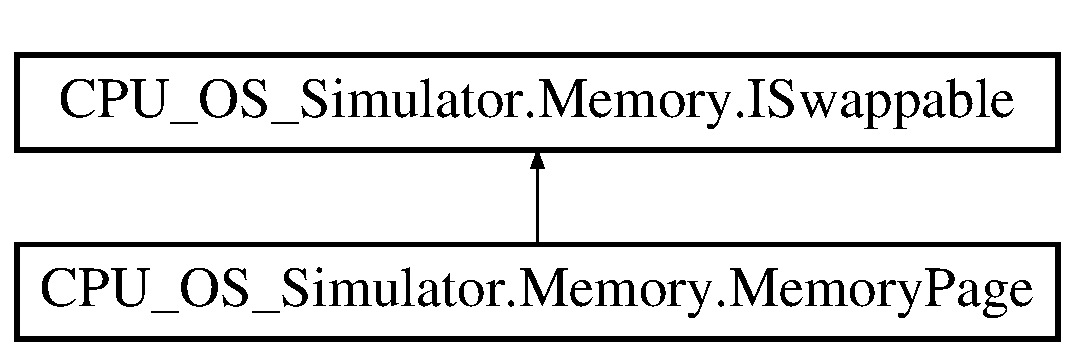
\includegraphics[height=2.000000cm]{class_c_p_u___o_s___simulator_1_1_memory_1_1_memory_page}
\end{center}
\end{figure}
\subsection*{Public Member Functions}
\begin{DoxyCompactItemize}
\item 
\hyperlink{class_c_p_u___o_s___simulator_1_1_memory_1_1_memory_page_a9b162033b9c9cc4dd28d683706fe6d2e}{Memory\+Page} (int \hyperlink{class_c_p_u___o_s___simulator_1_1_memory_1_1_memory_page_acf60a7bdefab6120fe080854b5f0b38b}{page\+Index}, int \hyperlink{class_c_p_u___o_s___simulator_1_1_memory_1_1_memory_page_a6fe2e28385db19a1968a41efe3df3f38}{start\+Offset})
\begin{DoxyCompactList}\small\item\em Constructor for memory page \end{DoxyCompactList}\item 
void \hyperlink{class_c_p_u___o_s___simulator_1_1_memory_1_1_memory_page_a53d6deee146e06754ea770755b17ff14}{Swap\+Out} (int Location\+To\+Swap, int Frame\+Number)
\begin{DoxyCompactList}\small\item\em This function swaps out this memory page \end{DoxyCompactList}\item 
void \hyperlink{class_c_p_u___o_s___simulator_1_1_memory_1_1_memory_page_a79e408c1be5efbaa6969ab66cc46930f}{Swap\+In} (int Location\+To\+Swap, int Frame\+Number)
\begin{DoxyCompactList}\small\item\em This function swaps in this memory page \end{DoxyCompactList}\item 
void \hyperlink{class_c_p_u___o_s___simulator_1_1_memory_1_1_memory_page_a0c43cf3b2640f17b8d732acbaaaead96}{Zero\+Memory} ()
\begin{DoxyCompactList}\small\item\em This function zeros out (clears) a memory page \end{DoxyCompactList}\end{DoxyCompactItemize}
\subsection*{Public Attributes}
\begin{DoxyCompactItemize}
\item 
const int \hyperlink{class_c_p_u___o_s___simulator_1_1_memory_1_1_memory_page_a502abee83030136a808d5b5f0c0fe7ec}{P\+A\+G\+E\+\_\+\+S\+I\+Z\+E} = 256
\begin{DoxyCompactList}\small\item\em The size of the memory pages to manage \end{DoxyCompactList}\end{DoxyCompactItemize}
\subsection*{Properties}
\begin{DoxyCompactItemize}
\item 
int \hyperlink{class_c_p_u___o_s___simulator_1_1_memory_1_1_memory_page_aec80700d036a447e7e6ec204513e3a59}{Page\+Index}\hspace{0.3cm}{\ttfamily  \mbox{[}get, set\mbox{]}}
\begin{DoxyCompactList}\small\item\em The index of the current page within its program \end{DoxyCompactList}\item 
int \hyperlink{class_c_p_u___o_s___simulator_1_1_memory_1_1_memory_page_ad700979e51dd3d05470c681588c6fa79}{Start\+Offset}\hspace{0.3cm}{\ttfamily  \mbox{[}get\mbox{]}}
\begin{DoxyCompactList}\small\item\em The start offset of this page \end{DoxyCompactList}\item 
int \hyperlink{class_c_p_u___o_s___simulator_1_1_memory_1_1_memory_page_abe850b4a088a820ecf598af1cd9a7deb}{End\+Offset}\hspace{0.3cm}{\ttfamily  \mbox{[}get\mbox{]}}
\begin{DoxyCompactList}\small\item\em the end offset of this page \end{DoxyCompactList}\item 
\hyperlink{class_c_p_u___o_s___simulator_1_1_memory_1_1_memory_segment}{Memory\+Segment}\mbox{[}$\,$\mbox{]} \hyperlink{class_c_p_u___o_s___simulator_1_1_memory_1_1_memory_page_a8bf84e82146f9ff35ffbcc32b93a9db0}{Data}\hspace{0.3cm}{\ttfamily  \mbox{[}get, set\mbox{]}}
\begin{DoxyCompactList}\small\item\em array of memory segments which collectively make up this page \end{DoxyCompactList}\item 
int \hyperlink{class_c_p_u___o_s___simulator_1_1_memory_1_1_memory_page_af31a2243a3e68ec635315929859fa358}{Start\+Offset\+Physical}\hspace{0.3cm}{\ttfamily  \mbox{[}get, set\mbox{]}}
\begin{DoxyCompactList}\small\item\em The physical address of the first byte in the page \end{DoxyCompactList}\end{DoxyCompactItemize}
\subsection*{Private Member Functions}
\begin{DoxyCompactItemize}
\item 
void \hyperlink{class_c_p_u___o_s___simulator_1_1_memory_1_1_memory_page_a4006da1460cb3bf17076dfbade9d0038}{Populate\+Data} ()
\begin{DoxyCompactList}\small\item\em Populates the data in this page with its initial value (0) \end{DoxyCompactList}\item 
dynamic \hyperlink{class_c_p_u___o_s___simulator_1_1_memory_1_1_memory_page_a84a305171941df5c3ae72b34ccec5485}{Get\+Main\+Window\+Instance} ()
\begin{DoxyCompactList}\small\item\em This function gets the main window instance from the window bridge \end{DoxyCompactList}\end{DoxyCompactItemize}
\subsection*{Private Attributes}
\begin{DoxyCompactItemize}
\item 
int \hyperlink{class_c_p_u___o_s___simulator_1_1_memory_1_1_memory_page_acf60a7bdefab6120fe080854b5f0b38b}{page\+Index}
\item 
int \hyperlink{class_c_p_u___o_s___simulator_1_1_memory_1_1_memory_page_a3cecfb0fe2f91def3db5711180442d44}{start\+Offset\+Physical}
\item 
readonly int \hyperlink{class_c_p_u___o_s___simulator_1_1_memory_1_1_memory_page_a6fe2e28385db19a1968a41efe3df3f38}{start\+Offset}
\item 
readonly int \hyperlink{class_c_p_u___o_s___simulator_1_1_memory_1_1_memory_page_ae2f8f419909326ce5449d37af9ff7c89}{end\+Offset}
\item 
\hyperlink{class_c_p_u___o_s___simulator_1_1_memory_1_1_memory_segment}{Memory\+Segment}\mbox{[}$\,$\mbox{]} \hyperlink{class_c_p_u___o_s___simulator_1_1_memory_1_1_memory_page_af9ab25101e7920de2344e0fa5ddfaa27}{data}
\end{DoxyCompactItemize}


\subsection{Detailed Description}
This class represents a page of data within memory 



Definition at line 10 of file Memory\+Page.\+cs.



\subsection{Constructor \& Destructor Documentation}
\hypertarget{class_c_p_u___o_s___simulator_1_1_memory_1_1_memory_page_a9b162033b9c9cc4dd28d683706fe6d2e}{}\index{C\+P\+U\+\_\+\+O\+S\+\_\+\+Simulator\+::\+Memory\+::\+Memory\+Page@{C\+P\+U\+\_\+\+O\+S\+\_\+\+Simulator\+::\+Memory\+::\+Memory\+Page}!Memory\+Page@{Memory\+Page}}
\index{Memory\+Page@{Memory\+Page}!C\+P\+U\+\_\+\+O\+S\+\_\+\+Simulator\+::\+Memory\+::\+Memory\+Page@{C\+P\+U\+\_\+\+O\+S\+\_\+\+Simulator\+::\+Memory\+::\+Memory\+Page}}
\subsubsection[{Memory\+Page(int page\+Index, int start\+Offset)}]{\setlength{\rightskip}{0pt plus 5cm}C\+P\+U\+\_\+\+O\+S\+\_\+\+Simulator.\+Memory.\+Memory\+Page.\+Memory\+Page (
\begin{DoxyParamCaption}
\item[{int}]{page\+Index, }
\item[{int}]{start\+Offset}
\end{DoxyParamCaption}
)}\label{class_c_p_u___o_s___simulator_1_1_memory_1_1_memory_page_a9b162033b9c9cc4dd28d683706fe6d2e}


Constructor for memory page 


\begin{DoxyParams}{Parameters}
{\em page\+Index} & the index of the page within the program\\
\hline
{\em start\+Offset} & \\
\hline
\end{DoxyParams}


Definition at line 93 of file Memory\+Page.\+cs.



\subsection{Member Function Documentation}
\hypertarget{class_c_p_u___o_s___simulator_1_1_memory_1_1_memory_page_a84a305171941df5c3ae72b34ccec5485}{}\index{C\+P\+U\+\_\+\+O\+S\+\_\+\+Simulator\+::\+Memory\+::\+Memory\+Page@{C\+P\+U\+\_\+\+O\+S\+\_\+\+Simulator\+::\+Memory\+::\+Memory\+Page}!Get\+Main\+Window\+Instance@{Get\+Main\+Window\+Instance}}
\index{Get\+Main\+Window\+Instance@{Get\+Main\+Window\+Instance}!C\+P\+U\+\_\+\+O\+S\+\_\+\+Simulator\+::\+Memory\+::\+Memory\+Page@{C\+P\+U\+\_\+\+O\+S\+\_\+\+Simulator\+::\+Memory\+::\+Memory\+Page}}
\subsubsection[{Get\+Main\+Window\+Instance()}]{\setlength{\rightskip}{0pt plus 5cm}dynamic C\+P\+U\+\_\+\+O\+S\+\_\+\+Simulator.\+Memory.\+Memory\+Page.\+Get\+Main\+Window\+Instance (
\begin{DoxyParamCaption}
{}
\end{DoxyParamCaption}
)\hspace{0.3cm}{\ttfamily [private]}}\label{class_c_p_u___o_s___simulator_1_1_memory_1_1_memory_page_a84a305171941df5c3ae72b34ccec5485}


This function gets the main window instance from the window bridge 

\begin{DoxyReturn}{Returns}
the active instance of main window 
\end{DoxyReturn}


Definition at line 170 of file Memory\+Page.\+cs.

\hypertarget{class_c_p_u___o_s___simulator_1_1_memory_1_1_memory_page_a4006da1460cb3bf17076dfbade9d0038}{}\index{C\+P\+U\+\_\+\+O\+S\+\_\+\+Simulator\+::\+Memory\+::\+Memory\+Page@{C\+P\+U\+\_\+\+O\+S\+\_\+\+Simulator\+::\+Memory\+::\+Memory\+Page}!Populate\+Data@{Populate\+Data}}
\index{Populate\+Data@{Populate\+Data}!C\+P\+U\+\_\+\+O\+S\+\_\+\+Simulator\+::\+Memory\+::\+Memory\+Page@{C\+P\+U\+\_\+\+O\+S\+\_\+\+Simulator\+::\+Memory\+::\+Memory\+Page}}
\subsubsection[{Populate\+Data()}]{\setlength{\rightskip}{0pt plus 5cm}void C\+P\+U\+\_\+\+O\+S\+\_\+\+Simulator.\+Memory.\+Memory\+Page.\+Populate\+Data (
\begin{DoxyParamCaption}
{}
\end{DoxyParamCaption}
)\hspace{0.3cm}{\ttfamily [private]}}\label{class_c_p_u___o_s___simulator_1_1_memory_1_1_memory_page_a4006da1460cb3bf17076dfbade9d0038}


Populates the data in this page with its initial value (0) 



Definition at line 106 of file Memory\+Page.\+cs.

\hypertarget{class_c_p_u___o_s___simulator_1_1_memory_1_1_memory_page_a79e408c1be5efbaa6969ab66cc46930f}{}\index{C\+P\+U\+\_\+\+O\+S\+\_\+\+Simulator\+::\+Memory\+::\+Memory\+Page@{C\+P\+U\+\_\+\+O\+S\+\_\+\+Simulator\+::\+Memory\+::\+Memory\+Page}!Swap\+In@{Swap\+In}}
\index{Swap\+In@{Swap\+In}!C\+P\+U\+\_\+\+O\+S\+\_\+\+Simulator\+::\+Memory\+::\+Memory\+Page@{C\+P\+U\+\_\+\+O\+S\+\_\+\+Simulator\+::\+Memory\+::\+Memory\+Page}}
\subsubsection[{Swap\+In(int Location\+To\+Swap, int Frame\+Number)}]{\setlength{\rightskip}{0pt plus 5cm}void C\+P\+U\+\_\+\+O\+S\+\_\+\+Simulator.\+Memory.\+Memory\+Page.\+Swap\+In (
\begin{DoxyParamCaption}
\item[{int}]{Location\+To\+Swap, }
\item[{int}]{Frame\+Number}
\end{DoxyParamCaption}
)}\label{class_c_p_u___o_s___simulator_1_1_memory_1_1_memory_page_a79e408c1be5efbaa6969ab66cc46930f}


This function swaps in this memory page 


\begin{DoxyParams}{Parameters}
{\em Location\+To\+Swap} & the physical address to swap this page in to\\
\hline
{\em Frame\+Number} & this pages frame number\\
\hline
\end{DoxyParams}


Implements \hyperlink{interface_c_p_u___o_s___simulator_1_1_memory_1_1_i_swappable_a38e30363486a3de53e6171da50b943af}{C\+P\+U\+\_\+\+O\+S\+\_\+\+Simulator.\+Memory.\+I\+Swappable}.



Definition at line 146 of file Memory\+Page.\+cs.

\hypertarget{class_c_p_u___o_s___simulator_1_1_memory_1_1_memory_page_a53d6deee146e06754ea770755b17ff14}{}\index{C\+P\+U\+\_\+\+O\+S\+\_\+\+Simulator\+::\+Memory\+::\+Memory\+Page@{C\+P\+U\+\_\+\+O\+S\+\_\+\+Simulator\+::\+Memory\+::\+Memory\+Page}!Swap\+Out@{Swap\+Out}}
\index{Swap\+Out@{Swap\+Out}!C\+P\+U\+\_\+\+O\+S\+\_\+\+Simulator\+::\+Memory\+::\+Memory\+Page@{C\+P\+U\+\_\+\+O\+S\+\_\+\+Simulator\+::\+Memory\+::\+Memory\+Page}}
\subsubsection[{Swap\+Out(int Location\+To\+Swap, int Frame\+Number)}]{\setlength{\rightskip}{0pt plus 5cm}void C\+P\+U\+\_\+\+O\+S\+\_\+\+Simulator.\+Memory.\+Memory\+Page.\+Swap\+Out (
\begin{DoxyParamCaption}
\item[{int}]{Location\+To\+Swap, }
\item[{int}]{Frame\+Number}
\end{DoxyParamCaption}
)}\label{class_c_p_u___o_s___simulator_1_1_memory_1_1_memory_page_a53d6deee146e06754ea770755b17ff14}


This function swaps out this memory page 


\begin{DoxyParams}{Parameters}
{\em Location\+To\+Swap} & the physical address to swap from\\
\hline
{\em Frame\+Number} & this page\textquotesingle{}s frame number\\
\hline
\end{DoxyParams}


Implements \hyperlink{interface_c_p_u___o_s___simulator_1_1_memory_1_1_i_swappable_ae789e9deb0600d48b0dcbe4a4252220a}{C\+P\+U\+\_\+\+O\+S\+\_\+\+Simulator.\+Memory.\+I\+Swappable}.



Definition at line 121 of file Memory\+Page.\+cs.

\hypertarget{class_c_p_u___o_s___simulator_1_1_memory_1_1_memory_page_a0c43cf3b2640f17b8d732acbaaaead96}{}\index{C\+P\+U\+\_\+\+O\+S\+\_\+\+Simulator\+::\+Memory\+::\+Memory\+Page@{C\+P\+U\+\_\+\+O\+S\+\_\+\+Simulator\+::\+Memory\+::\+Memory\+Page}!Zero\+Memory@{Zero\+Memory}}
\index{Zero\+Memory@{Zero\+Memory}!C\+P\+U\+\_\+\+O\+S\+\_\+\+Simulator\+::\+Memory\+::\+Memory\+Page@{C\+P\+U\+\_\+\+O\+S\+\_\+\+Simulator\+::\+Memory\+::\+Memory\+Page}}
\subsubsection[{Zero\+Memory()}]{\setlength{\rightskip}{0pt plus 5cm}void C\+P\+U\+\_\+\+O\+S\+\_\+\+Simulator.\+Memory.\+Memory\+Page.\+Zero\+Memory (
\begin{DoxyParamCaption}
{}
\end{DoxyParamCaption}
)}\label{class_c_p_u___o_s___simulator_1_1_memory_1_1_memory_page_a0c43cf3b2640f17b8d732acbaaaead96}


This function zeros out (clears) a memory page 



Definition at line 181 of file Memory\+Page.\+cs.



\subsection{Member Data Documentation}
\hypertarget{class_c_p_u___o_s___simulator_1_1_memory_1_1_memory_page_af9ab25101e7920de2344e0fa5ddfaa27}{}\index{C\+P\+U\+\_\+\+O\+S\+\_\+\+Simulator\+::\+Memory\+::\+Memory\+Page@{C\+P\+U\+\_\+\+O\+S\+\_\+\+Simulator\+::\+Memory\+::\+Memory\+Page}!data@{data}}
\index{data@{data}!C\+P\+U\+\_\+\+O\+S\+\_\+\+Simulator\+::\+Memory\+::\+Memory\+Page@{C\+P\+U\+\_\+\+O\+S\+\_\+\+Simulator\+::\+Memory\+::\+Memory\+Page}}
\subsubsection[{data}]{\setlength{\rightskip}{0pt plus 5cm}{\bf Memory\+Segment} \mbox{[}$\,$\mbox{]} C\+P\+U\+\_\+\+O\+S\+\_\+\+Simulator.\+Memory.\+Memory\+Page.\+data\hspace{0.3cm}{\ttfamily [private]}}\label{class_c_p_u___o_s___simulator_1_1_memory_1_1_memory_page_af9ab25101e7920de2344e0fa5ddfaa27}


Definition at line 20 of file Memory\+Page.\+cs.

\hypertarget{class_c_p_u___o_s___simulator_1_1_memory_1_1_memory_page_ae2f8f419909326ce5449d37af9ff7c89}{}\index{C\+P\+U\+\_\+\+O\+S\+\_\+\+Simulator\+::\+Memory\+::\+Memory\+Page@{C\+P\+U\+\_\+\+O\+S\+\_\+\+Simulator\+::\+Memory\+::\+Memory\+Page}!end\+Offset@{end\+Offset}}
\index{end\+Offset@{end\+Offset}!C\+P\+U\+\_\+\+O\+S\+\_\+\+Simulator\+::\+Memory\+::\+Memory\+Page@{C\+P\+U\+\_\+\+O\+S\+\_\+\+Simulator\+::\+Memory\+::\+Memory\+Page}}
\subsubsection[{end\+Offset}]{\setlength{\rightskip}{0pt plus 5cm}readonly int C\+P\+U\+\_\+\+O\+S\+\_\+\+Simulator.\+Memory.\+Memory\+Page.\+end\+Offset\hspace{0.3cm}{\ttfamily [private]}}\label{class_c_p_u___o_s___simulator_1_1_memory_1_1_memory_page_ae2f8f419909326ce5449d37af9ff7c89}


Definition at line 19 of file Memory\+Page.\+cs.

\hypertarget{class_c_p_u___o_s___simulator_1_1_memory_1_1_memory_page_a502abee83030136a808d5b5f0c0fe7ec}{}\index{C\+P\+U\+\_\+\+O\+S\+\_\+\+Simulator\+::\+Memory\+::\+Memory\+Page@{C\+P\+U\+\_\+\+O\+S\+\_\+\+Simulator\+::\+Memory\+::\+Memory\+Page}!P\+A\+G\+E\+\_\+\+S\+I\+Z\+E@{P\+A\+G\+E\+\_\+\+S\+I\+Z\+E}}
\index{P\+A\+G\+E\+\_\+\+S\+I\+Z\+E@{P\+A\+G\+E\+\_\+\+S\+I\+Z\+E}!C\+P\+U\+\_\+\+O\+S\+\_\+\+Simulator\+::\+Memory\+::\+Memory\+Page@{C\+P\+U\+\_\+\+O\+S\+\_\+\+Simulator\+::\+Memory\+::\+Memory\+Page}}
\subsubsection[{P\+A\+G\+E\+\_\+\+S\+I\+Z\+E}]{\setlength{\rightskip}{0pt plus 5cm}const int C\+P\+U\+\_\+\+O\+S\+\_\+\+Simulator.\+Memory.\+Memory\+Page.\+P\+A\+G\+E\+\_\+\+S\+I\+Z\+E = 256}\label{class_c_p_u___o_s___simulator_1_1_memory_1_1_memory_page_a502abee83030136a808d5b5f0c0fe7ec}


The size of the memory pages to manage 



Definition at line 18 of file Memory\+Page.\+cs.

\hypertarget{class_c_p_u___o_s___simulator_1_1_memory_1_1_memory_page_acf60a7bdefab6120fe080854b5f0b38b}{}\index{C\+P\+U\+\_\+\+O\+S\+\_\+\+Simulator\+::\+Memory\+::\+Memory\+Page@{C\+P\+U\+\_\+\+O\+S\+\_\+\+Simulator\+::\+Memory\+::\+Memory\+Page}!page\+Index@{page\+Index}}
\index{page\+Index@{page\+Index}!C\+P\+U\+\_\+\+O\+S\+\_\+\+Simulator\+::\+Memory\+::\+Memory\+Page@{C\+P\+U\+\_\+\+O\+S\+\_\+\+Simulator\+::\+Memory\+::\+Memory\+Page}}
\subsubsection[{page\+Index}]{\setlength{\rightskip}{0pt plus 5cm}int C\+P\+U\+\_\+\+O\+S\+\_\+\+Simulator.\+Memory.\+Memory\+Page.\+page\+Index\hspace{0.3cm}{\ttfamily [private]}}\label{class_c_p_u___o_s___simulator_1_1_memory_1_1_memory_page_acf60a7bdefab6120fe080854b5f0b38b}


Definition at line 12 of file Memory\+Page.\+cs.

\hypertarget{class_c_p_u___o_s___simulator_1_1_memory_1_1_memory_page_a6fe2e28385db19a1968a41efe3df3f38}{}\index{C\+P\+U\+\_\+\+O\+S\+\_\+\+Simulator\+::\+Memory\+::\+Memory\+Page@{C\+P\+U\+\_\+\+O\+S\+\_\+\+Simulator\+::\+Memory\+::\+Memory\+Page}!start\+Offset@{start\+Offset}}
\index{start\+Offset@{start\+Offset}!C\+P\+U\+\_\+\+O\+S\+\_\+\+Simulator\+::\+Memory\+::\+Memory\+Page@{C\+P\+U\+\_\+\+O\+S\+\_\+\+Simulator\+::\+Memory\+::\+Memory\+Page}}
\subsubsection[{start\+Offset}]{\setlength{\rightskip}{0pt plus 5cm}readonly int C\+P\+U\+\_\+\+O\+S\+\_\+\+Simulator.\+Memory.\+Memory\+Page.\+start\+Offset\hspace{0.3cm}{\ttfamily [private]}}\label{class_c_p_u___o_s___simulator_1_1_memory_1_1_memory_page_a6fe2e28385db19a1968a41efe3df3f38}


Definition at line 14 of file Memory\+Page.\+cs.

\hypertarget{class_c_p_u___o_s___simulator_1_1_memory_1_1_memory_page_a3cecfb0fe2f91def3db5711180442d44}{}\index{C\+P\+U\+\_\+\+O\+S\+\_\+\+Simulator\+::\+Memory\+::\+Memory\+Page@{C\+P\+U\+\_\+\+O\+S\+\_\+\+Simulator\+::\+Memory\+::\+Memory\+Page}!start\+Offset\+Physical@{start\+Offset\+Physical}}
\index{start\+Offset\+Physical@{start\+Offset\+Physical}!C\+P\+U\+\_\+\+O\+S\+\_\+\+Simulator\+::\+Memory\+::\+Memory\+Page@{C\+P\+U\+\_\+\+O\+S\+\_\+\+Simulator\+::\+Memory\+::\+Memory\+Page}}
\subsubsection[{start\+Offset\+Physical}]{\setlength{\rightskip}{0pt plus 5cm}int C\+P\+U\+\_\+\+O\+S\+\_\+\+Simulator.\+Memory.\+Memory\+Page.\+start\+Offset\+Physical\hspace{0.3cm}{\ttfamily [private]}}\label{class_c_p_u___o_s___simulator_1_1_memory_1_1_memory_page_a3cecfb0fe2f91def3db5711180442d44}


Definition at line 13 of file Memory\+Page.\+cs.



\subsection{Property Documentation}
\hypertarget{class_c_p_u___o_s___simulator_1_1_memory_1_1_memory_page_a8bf84e82146f9ff35ffbcc32b93a9db0}{}\index{C\+P\+U\+\_\+\+O\+S\+\_\+\+Simulator\+::\+Memory\+::\+Memory\+Page@{C\+P\+U\+\_\+\+O\+S\+\_\+\+Simulator\+::\+Memory\+::\+Memory\+Page}!Data@{Data}}
\index{Data@{Data}!C\+P\+U\+\_\+\+O\+S\+\_\+\+Simulator\+::\+Memory\+::\+Memory\+Page@{C\+P\+U\+\_\+\+O\+S\+\_\+\+Simulator\+::\+Memory\+::\+Memory\+Page}}
\subsubsection[{Data}]{\setlength{\rightskip}{0pt plus 5cm}{\bf Memory\+Segment} \mbox{[}$\,$\mbox{]} C\+P\+U\+\_\+\+O\+S\+\_\+\+Simulator.\+Memory.\+Memory\+Page.\+Data\hspace{0.3cm}{\ttfamily [get]}, {\ttfamily [set]}}\label{class_c_p_u___o_s___simulator_1_1_memory_1_1_memory_page_a8bf84e82146f9ff35ffbcc32b93a9db0}


array of memory segments which collectively make up this page 



Definition at line 60 of file Memory\+Page.\+cs.

\hypertarget{class_c_p_u___o_s___simulator_1_1_memory_1_1_memory_page_abe850b4a088a820ecf598af1cd9a7deb}{}\index{C\+P\+U\+\_\+\+O\+S\+\_\+\+Simulator\+::\+Memory\+::\+Memory\+Page@{C\+P\+U\+\_\+\+O\+S\+\_\+\+Simulator\+::\+Memory\+::\+Memory\+Page}!End\+Offset@{End\+Offset}}
\index{End\+Offset@{End\+Offset}!C\+P\+U\+\_\+\+O\+S\+\_\+\+Simulator\+::\+Memory\+::\+Memory\+Page@{C\+P\+U\+\_\+\+O\+S\+\_\+\+Simulator\+::\+Memory\+::\+Memory\+Page}}
\subsubsection[{End\+Offset}]{\setlength{\rightskip}{0pt plus 5cm}int C\+P\+U\+\_\+\+O\+S\+\_\+\+Simulator.\+Memory.\+Memory\+Page.\+End\+Offset\hspace{0.3cm}{\ttfamily [get]}}\label{class_c_p_u___o_s___simulator_1_1_memory_1_1_memory_page_abe850b4a088a820ecf598af1cd9a7deb}


the end offset of this page 



Definition at line 50 of file Memory\+Page.\+cs.

\hypertarget{class_c_p_u___o_s___simulator_1_1_memory_1_1_memory_page_aec80700d036a447e7e6ec204513e3a59}{}\index{C\+P\+U\+\_\+\+O\+S\+\_\+\+Simulator\+::\+Memory\+::\+Memory\+Page@{C\+P\+U\+\_\+\+O\+S\+\_\+\+Simulator\+::\+Memory\+::\+Memory\+Page}!Page\+Index@{Page\+Index}}
\index{Page\+Index@{Page\+Index}!C\+P\+U\+\_\+\+O\+S\+\_\+\+Simulator\+::\+Memory\+::\+Memory\+Page@{C\+P\+U\+\_\+\+O\+S\+\_\+\+Simulator\+::\+Memory\+::\+Memory\+Page}}
\subsubsection[{Page\+Index}]{\setlength{\rightskip}{0pt plus 5cm}int C\+P\+U\+\_\+\+O\+S\+\_\+\+Simulator.\+Memory.\+Memory\+Page.\+Page\+Index\hspace{0.3cm}{\ttfamily [get]}, {\ttfamily [set]}}\label{class_c_p_u___o_s___simulator_1_1_memory_1_1_memory_page_aec80700d036a447e7e6ec204513e3a59}


The index of the current page within its program 



Definition at line 25 of file Memory\+Page.\+cs.

\hypertarget{class_c_p_u___o_s___simulator_1_1_memory_1_1_memory_page_ad700979e51dd3d05470c681588c6fa79}{}\index{C\+P\+U\+\_\+\+O\+S\+\_\+\+Simulator\+::\+Memory\+::\+Memory\+Page@{C\+P\+U\+\_\+\+O\+S\+\_\+\+Simulator\+::\+Memory\+::\+Memory\+Page}!Start\+Offset@{Start\+Offset}}
\index{Start\+Offset@{Start\+Offset}!C\+P\+U\+\_\+\+O\+S\+\_\+\+Simulator\+::\+Memory\+::\+Memory\+Page@{C\+P\+U\+\_\+\+O\+S\+\_\+\+Simulator\+::\+Memory\+::\+Memory\+Page}}
\subsubsection[{Start\+Offset}]{\setlength{\rightskip}{0pt plus 5cm}int C\+P\+U\+\_\+\+O\+S\+\_\+\+Simulator.\+Memory.\+Memory\+Page.\+Start\+Offset\hspace{0.3cm}{\ttfamily [get]}}\label{class_c_p_u___o_s___simulator_1_1_memory_1_1_memory_page_ad700979e51dd3d05470c681588c6fa79}


The start offset of this page 



Definition at line 40 of file Memory\+Page.\+cs.

\hypertarget{class_c_p_u___o_s___simulator_1_1_memory_1_1_memory_page_af31a2243a3e68ec635315929859fa358}{}\index{C\+P\+U\+\_\+\+O\+S\+\_\+\+Simulator\+::\+Memory\+::\+Memory\+Page@{C\+P\+U\+\_\+\+O\+S\+\_\+\+Simulator\+::\+Memory\+::\+Memory\+Page}!Start\+Offset\+Physical@{Start\+Offset\+Physical}}
\index{Start\+Offset\+Physical@{Start\+Offset\+Physical}!C\+P\+U\+\_\+\+O\+S\+\_\+\+Simulator\+::\+Memory\+::\+Memory\+Page@{C\+P\+U\+\_\+\+O\+S\+\_\+\+Simulator\+::\+Memory\+::\+Memory\+Page}}
\subsubsection[{Start\+Offset\+Physical}]{\setlength{\rightskip}{0pt plus 5cm}int C\+P\+U\+\_\+\+O\+S\+\_\+\+Simulator.\+Memory.\+Memory\+Page.\+Start\+Offset\+Physical\hspace{0.3cm}{\ttfamily [get]}, {\ttfamily [set]}}\label{class_c_p_u___o_s___simulator_1_1_memory_1_1_memory_page_af31a2243a3e68ec635315929859fa358}


The physical address of the first byte in the page 



Definition at line 75 of file Memory\+Page.\+cs.



The documentation for this class was generated from the following file\+:\begin{DoxyCompactItemize}
\item 
Memory/\hyperlink{_memory_page_8cs}{Memory\+Page.\+cs}\end{DoxyCompactItemize}

\hypertarget{class_c_p_u___o_s___simulator_1_1_memory_1_1_tests_1_1_memory_page_tests}{}\section{C\+P\+U\+\_\+\+O\+S\+\_\+\+Simulator.\+Memory.\+Tests.\+Memory\+Page\+Tests Class Reference}
\label{class_c_p_u___o_s___simulator_1_1_memory_1_1_tests_1_1_memory_page_tests}\index{C\+P\+U\+\_\+\+O\+S\+\_\+\+Simulator.\+Memory.\+Tests.\+Memory\+Page\+Tests@{C\+P\+U\+\_\+\+O\+S\+\_\+\+Simulator.\+Memory.\+Tests.\+Memory\+Page\+Tests}}
\subsection*{Public Member Functions}
\begin{DoxyCompactItemize}
\item 
void \hyperlink{class_c_p_u___o_s___simulator_1_1_memory_1_1_tests_1_1_memory_page_tests_a5dd24d4a39172f2a347e7106c806fa89}{Memory\+Page\+Test} ()
\item 
void \hyperlink{class_c_p_u___o_s___simulator_1_1_memory_1_1_tests_1_1_memory_page_tests_ad05389a6c85964130902bd4f64e5d097}{Swap\+Out\+Test} ()
\item 
void \hyperlink{class_c_p_u___o_s___simulator_1_1_memory_1_1_tests_1_1_memory_page_tests_a67f2a05fc4c4c02991dd9d14348230cf}{Swap\+In\+Test} ()
\item 
void \hyperlink{class_c_p_u___o_s___simulator_1_1_memory_1_1_tests_1_1_memory_page_tests_aa7b9c0c2148fe416facbb7588d729566}{Zero\+Memory\+Test} ()
\end{DoxyCompactItemize}


\subsection{Detailed Description}


Definition at line 12 of file Memory\+Page\+Tests.\+cs.



\subsection{Member Function Documentation}
\hypertarget{class_c_p_u___o_s___simulator_1_1_memory_1_1_tests_1_1_memory_page_tests_a5dd24d4a39172f2a347e7106c806fa89}{}\index{C\+P\+U\+\_\+\+O\+S\+\_\+\+Simulator\+::\+Memory\+::\+Tests\+::\+Memory\+Page\+Tests@{C\+P\+U\+\_\+\+O\+S\+\_\+\+Simulator\+::\+Memory\+::\+Tests\+::\+Memory\+Page\+Tests}!Memory\+Page\+Test@{Memory\+Page\+Test}}
\index{Memory\+Page\+Test@{Memory\+Page\+Test}!C\+P\+U\+\_\+\+O\+S\+\_\+\+Simulator\+::\+Memory\+::\+Tests\+::\+Memory\+Page\+Tests@{C\+P\+U\+\_\+\+O\+S\+\_\+\+Simulator\+::\+Memory\+::\+Tests\+::\+Memory\+Page\+Tests}}
\subsubsection[{Memory\+Page\+Test()}]{\setlength{\rightskip}{0pt plus 5cm}void C\+P\+U\+\_\+\+O\+S\+\_\+\+Simulator.\+Memory.\+Tests.\+Memory\+Page\+Tests.\+Memory\+Page\+Test (
\begin{DoxyParamCaption}
{}
\end{DoxyParamCaption}
)}\label{class_c_p_u___o_s___simulator_1_1_memory_1_1_tests_1_1_memory_page_tests_a5dd24d4a39172f2a347e7106c806fa89}


Definition at line 15 of file Memory\+Page\+Tests.\+cs.

\hypertarget{class_c_p_u___o_s___simulator_1_1_memory_1_1_tests_1_1_memory_page_tests_a67f2a05fc4c4c02991dd9d14348230cf}{}\index{C\+P\+U\+\_\+\+O\+S\+\_\+\+Simulator\+::\+Memory\+::\+Tests\+::\+Memory\+Page\+Tests@{C\+P\+U\+\_\+\+O\+S\+\_\+\+Simulator\+::\+Memory\+::\+Tests\+::\+Memory\+Page\+Tests}!Swap\+In\+Test@{Swap\+In\+Test}}
\index{Swap\+In\+Test@{Swap\+In\+Test}!C\+P\+U\+\_\+\+O\+S\+\_\+\+Simulator\+::\+Memory\+::\+Tests\+::\+Memory\+Page\+Tests@{C\+P\+U\+\_\+\+O\+S\+\_\+\+Simulator\+::\+Memory\+::\+Tests\+::\+Memory\+Page\+Tests}}
\subsubsection[{Swap\+In\+Test()}]{\setlength{\rightskip}{0pt plus 5cm}void C\+P\+U\+\_\+\+O\+S\+\_\+\+Simulator.\+Memory.\+Tests.\+Memory\+Page\+Tests.\+Swap\+In\+Test (
\begin{DoxyParamCaption}
{}
\end{DoxyParamCaption}
)}\label{class_c_p_u___o_s___simulator_1_1_memory_1_1_tests_1_1_memory_page_tests_a67f2a05fc4c4c02991dd9d14348230cf}


Definition at line 33 of file Memory\+Page\+Tests.\+cs.

\hypertarget{class_c_p_u___o_s___simulator_1_1_memory_1_1_tests_1_1_memory_page_tests_ad05389a6c85964130902bd4f64e5d097}{}\index{C\+P\+U\+\_\+\+O\+S\+\_\+\+Simulator\+::\+Memory\+::\+Tests\+::\+Memory\+Page\+Tests@{C\+P\+U\+\_\+\+O\+S\+\_\+\+Simulator\+::\+Memory\+::\+Tests\+::\+Memory\+Page\+Tests}!Swap\+Out\+Test@{Swap\+Out\+Test}}
\index{Swap\+Out\+Test@{Swap\+Out\+Test}!C\+P\+U\+\_\+\+O\+S\+\_\+\+Simulator\+::\+Memory\+::\+Tests\+::\+Memory\+Page\+Tests@{C\+P\+U\+\_\+\+O\+S\+\_\+\+Simulator\+::\+Memory\+::\+Tests\+::\+Memory\+Page\+Tests}}
\subsubsection[{Swap\+Out\+Test()}]{\setlength{\rightskip}{0pt plus 5cm}void C\+P\+U\+\_\+\+O\+S\+\_\+\+Simulator.\+Memory.\+Tests.\+Memory\+Page\+Tests.\+Swap\+Out\+Test (
\begin{DoxyParamCaption}
{}
\end{DoxyParamCaption}
)}\label{class_c_p_u___o_s___simulator_1_1_memory_1_1_tests_1_1_memory_page_tests_ad05389a6c85964130902bd4f64e5d097}


Definition at line 22 of file Memory\+Page\+Tests.\+cs.

\hypertarget{class_c_p_u___o_s___simulator_1_1_memory_1_1_tests_1_1_memory_page_tests_aa7b9c0c2148fe416facbb7588d729566}{}\index{C\+P\+U\+\_\+\+O\+S\+\_\+\+Simulator\+::\+Memory\+::\+Tests\+::\+Memory\+Page\+Tests@{C\+P\+U\+\_\+\+O\+S\+\_\+\+Simulator\+::\+Memory\+::\+Tests\+::\+Memory\+Page\+Tests}!Zero\+Memory\+Test@{Zero\+Memory\+Test}}
\index{Zero\+Memory\+Test@{Zero\+Memory\+Test}!C\+P\+U\+\_\+\+O\+S\+\_\+\+Simulator\+::\+Memory\+::\+Tests\+::\+Memory\+Page\+Tests@{C\+P\+U\+\_\+\+O\+S\+\_\+\+Simulator\+::\+Memory\+::\+Tests\+::\+Memory\+Page\+Tests}}
\subsubsection[{Zero\+Memory\+Test()}]{\setlength{\rightskip}{0pt plus 5cm}void C\+P\+U\+\_\+\+O\+S\+\_\+\+Simulator.\+Memory.\+Tests.\+Memory\+Page\+Tests.\+Zero\+Memory\+Test (
\begin{DoxyParamCaption}
{}
\end{DoxyParamCaption}
)}\label{class_c_p_u___o_s___simulator_1_1_memory_1_1_tests_1_1_memory_page_tests_aa7b9c0c2148fe416facbb7588d729566}


Definition at line 45 of file Memory\+Page\+Tests.\+cs.



The documentation for this class was generated from the following file\+:\begin{DoxyCompactItemize}
\item 
Memory\+Tests/\hyperlink{_memory_page_tests_8cs}{Memory\+Page\+Tests.\+cs}\end{DoxyCompactItemize}

\hypertarget{class_c_p_u___o_s___simulator_1_1_memory_1_1_memory_segment}{}\section{C\+P\+U\+\_\+\+O\+S\+\_\+\+Simulator.\+Memory.\+Memory\+Segment Class Reference}
\label{class_c_p_u___o_s___simulator_1_1_memory_1_1_memory_segment}\index{C\+P\+U\+\_\+\+O\+S\+\_\+\+Simulator.\+Memory.\+Memory\+Segment@{C\+P\+U\+\_\+\+O\+S\+\_\+\+Simulator.\+Memory.\+Memory\+Segment}}


This class represents a 8 byte segment of a memory page  


\subsection*{Public Member Functions}
\begin{DoxyCompactItemize}
\item 
\hyperlink{class_c_p_u___o_s___simulator_1_1_memory_1_1_memory_segment_abd9c898ff9488aaee755f538a3197477}{Memory\+Segment} ()
\begin{DoxyCompactList}\small\item\em Default constructor for a memory segment \end{DoxyCompactList}\item 
\hyperlink{class_c_p_u___o_s___simulator_1_1_memory_1_1_memory_segment_a92848c6604c9d6a9d958783ad7cae24f}{Memory\+Segment} (int \hyperlink{class_c_p_u___o_s___simulator_1_1_memory_1_1_memory_segment_af6d25683cc2a80607238dda52b09d457}{physical\+Address})
\begin{DoxyCompactList}\small\item\em Constructor for a memory segment \end{DoxyCompactList}\item 
override string \hyperlink{class_c_p_u___o_s___simulator_1_1_memory_1_1_memory_segment_a1c94b824fe1fdfc4a0b817a031f3d51d}{To\+String} ()
\begin{DoxyCompactList}\small\item\em Returns the data string for this memory segment \end{DoxyCompactList}\item 
string \hyperlink{class_c_p_u___o_s___simulator_1_1_memory_1_1_memory_segment_a7ad206d46b52b795ba48018afe0174ed}{Build\+Data\+String} ()
\begin{DoxyCompactList}\small\item\em Builds the data string for this memory segment \end{DoxyCompactList}\item 
byte \hyperlink{class_c_p_u___o_s___simulator_1_1_memory_1_1_memory_segment_af3e1120c597c91c8f7aa7faf29d3eda0}{Get\+Byte} (int number)
\begin{DoxyCompactList}\small\item\em Gets a specified byte from this memory segment \end{DoxyCompactList}\item 
void \hyperlink{class_c_p_u___o_s___simulator_1_1_memory_1_1_memory_segment_ab445c7247c0ca2a7b52606b4d14e268a}{Set\+Byte} (int number, byte \hyperlink{_annotations_8cs_aa47dc10177d95db720062975cdba1f3a}{value})
\begin{DoxyCompactList}\small\item\em Sets the requested byte in this memory segment \end{DoxyCompactList}\end{DoxyCompactItemize}
\subsection*{Properties}
\begin{DoxyCompactItemize}
\item 
int \hyperlink{class_c_p_u___o_s___simulator_1_1_memory_1_1_memory_segment_a254cb3b68c5ea35ec44a4df264833bf4}{Logical\+Address}\hspace{0.3cm}{\ttfamily  \mbox{[}get, set\mbox{]}}
\begin{DoxyCompactList}\small\item\em The logical address of the first byte in the segment \end{DoxyCompactList}\item 
int \hyperlink{class_c_p_u___o_s___simulator_1_1_memory_1_1_memory_segment_aeb2f540146dfc353f5529bf846e62587}{Physical\+Address}\hspace{0.3cm}{\ttfamily  \mbox{[}get, set\mbox{]}}
\begin{DoxyCompactList}\small\item\em The physical address of the first byte in the segment \end{DoxyCompactList}\item 
byte \hyperlink{class_c_p_u___o_s___simulator_1_1_memory_1_1_memory_segment_af1355b8170ad0461d479785ff6e1420d}{Byte0}\hspace{0.3cm}{\ttfamily  \mbox{[}get, set\mbox{]}}
\begin{DoxyCompactList}\small\item\em The first byte in the segment \end{DoxyCompactList}\item 
byte \hyperlink{class_c_p_u___o_s___simulator_1_1_memory_1_1_memory_segment_aba977f51dac4aeaa069fc14f877c7367}{Byte1}\hspace{0.3cm}{\ttfamily  \mbox{[}get, set\mbox{]}}
\begin{DoxyCompactList}\small\item\em The second byte in the segment \end{DoxyCompactList}\item 
byte \hyperlink{class_c_p_u___o_s___simulator_1_1_memory_1_1_memory_segment_af33632597b874fbb501068a9285f5ad6}{Byte2}\hspace{0.3cm}{\ttfamily  \mbox{[}get, set\mbox{]}}
\begin{DoxyCompactList}\small\item\em The third byte in the segment \end{DoxyCompactList}\item 
byte \hyperlink{class_c_p_u___o_s___simulator_1_1_memory_1_1_memory_segment_aa8c335116132ff754331eadb12355247}{Byte3}\hspace{0.3cm}{\ttfamily  \mbox{[}get, set\mbox{]}}
\begin{DoxyCompactList}\small\item\em The forth byte in the segment \end{DoxyCompactList}\item 
byte \hyperlink{class_c_p_u___o_s___simulator_1_1_memory_1_1_memory_segment_acc659c001dde3c6f6b0875df933b5bec}{Byte4}\hspace{0.3cm}{\ttfamily  \mbox{[}get, set\mbox{]}}
\begin{DoxyCompactList}\small\item\em The fifth byte in the segment \end{DoxyCompactList}\item 
byte \hyperlink{class_c_p_u___o_s___simulator_1_1_memory_1_1_memory_segment_a8ef49453e406cd41eacc4e2ef16a8420}{Byte5}\hspace{0.3cm}{\ttfamily  \mbox{[}get, set\mbox{]}}
\begin{DoxyCompactList}\small\item\em The sixth byte in the segment \end{DoxyCompactList}\item 
byte \hyperlink{class_c_p_u___o_s___simulator_1_1_memory_1_1_memory_segment_ade6f265c081bbfd184e344cb8af45c0b}{Byte6}\hspace{0.3cm}{\ttfamily  \mbox{[}get, set\mbox{]}}
\begin{DoxyCompactList}\small\item\em The seventh byte in the segment \end{DoxyCompactList}\item 
byte \hyperlink{class_c_p_u___o_s___simulator_1_1_memory_1_1_memory_segment_a62699911957af71d57e7cb5cd21d5246}{Byte7}\hspace{0.3cm}{\ttfamily  \mbox{[}get, set\mbox{]}}
\begin{DoxyCompactList}\small\item\em The eighth byte in the segment \end{DoxyCompactList}\item 
string \hyperlink{class_c_p_u___o_s___simulator_1_1_memory_1_1_memory_segment_a5e2dec75bb2978188d1fb369e4f9e982}{Data\+String}\hspace{0.3cm}{\ttfamily  \mbox{[}get, set\mbox{]}}
\begin{DoxyCompactList}\small\item\em The string that represents the data in this segment \end{DoxyCompactList}\end{DoxyCompactItemize}
\subsection*{Private Attributes}
\begin{DoxyCompactItemize}
\item 
int \hyperlink{class_c_p_u___o_s___simulator_1_1_memory_1_1_memory_segment_aded927c02e3614943ebebb3eb6597284}{logical\+Address}
\item 
int \hyperlink{class_c_p_u___o_s___simulator_1_1_memory_1_1_memory_segment_af6d25683cc2a80607238dda52b09d457}{physical\+Address}
\item 
byte \hyperlink{class_c_p_u___o_s___simulator_1_1_memory_1_1_memory_segment_a97b8721f717e2fd03673d9dd96882ef8}{byte0}
\item 
byte \hyperlink{class_c_p_u___o_s___simulator_1_1_memory_1_1_memory_segment_aa64e7a88f9cdf5dbb5b0c846cc570a77}{byte1}
\item 
byte \hyperlink{class_c_p_u___o_s___simulator_1_1_memory_1_1_memory_segment_a4f6ad3b2d132bfc1c4bd16d8fcca8d56}{byte2}
\item 
byte \hyperlink{class_c_p_u___o_s___simulator_1_1_memory_1_1_memory_segment_a48874b9f9dede6546e365d3bc1e28926}{byte3}
\item 
byte \hyperlink{class_c_p_u___o_s___simulator_1_1_memory_1_1_memory_segment_a1979475ad1134e07235880ccbd6b82f7}{byte4}
\item 
byte \hyperlink{class_c_p_u___o_s___simulator_1_1_memory_1_1_memory_segment_a6d35dbdcd3428e9a1869fda265341123}{byte5}
\item 
byte \hyperlink{class_c_p_u___o_s___simulator_1_1_memory_1_1_memory_segment_a242f25c3861a3c0d1d51484203ea8603}{byte6}
\item 
byte \hyperlink{class_c_p_u___o_s___simulator_1_1_memory_1_1_memory_segment_af4a4ab7c802e0a5b5f3684c0cfac5f80}{byte7}
\item 
string \hyperlink{class_c_p_u___o_s___simulator_1_1_memory_1_1_memory_segment_a624f2466fc6b73498e222f43f329adbb}{data\+String}
\end{DoxyCompactItemize}


\subsection{Detailed Description}
This class represents a 8 byte segment of a memory page 



Definition at line 9 of file Memory\+Segment.\+cs.



\subsection{Constructor \& Destructor Documentation}
\hypertarget{class_c_p_u___o_s___simulator_1_1_memory_1_1_memory_segment_abd9c898ff9488aaee755f538a3197477}{}\index{C\+P\+U\+\_\+\+O\+S\+\_\+\+Simulator\+::\+Memory\+::\+Memory\+Segment@{C\+P\+U\+\_\+\+O\+S\+\_\+\+Simulator\+::\+Memory\+::\+Memory\+Segment}!Memory\+Segment@{Memory\+Segment}}
\index{Memory\+Segment@{Memory\+Segment}!C\+P\+U\+\_\+\+O\+S\+\_\+\+Simulator\+::\+Memory\+::\+Memory\+Segment@{C\+P\+U\+\_\+\+O\+S\+\_\+\+Simulator\+::\+Memory\+::\+Memory\+Segment}}
\subsubsection[{Memory\+Segment()}]{\setlength{\rightskip}{0pt plus 5cm}C\+P\+U\+\_\+\+O\+S\+\_\+\+Simulator.\+Memory.\+Memory\+Segment.\+Memory\+Segment (
\begin{DoxyParamCaption}
{}
\end{DoxyParamCaption}
)}\label{class_c_p_u___o_s___simulator_1_1_memory_1_1_memory_segment_abd9c898ff9488aaee755f538a3197477}


Default constructor for a memory segment 



Definition at line 208 of file Memory\+Segment.\+cs.

\hypertarget{class_c_p_u___o_s___simulator_1_1_memory_1_1_memory_segment_a92848c6604c9d6a9d958783ad7cae24f}{}\index{C\+P\+U\+\_\+\+O\+S\+\_\+\+Simulator\+::\+Memory\+::\+Memory\+Segment@{C\+P\+U\+\_\+\+O\+S\+\_\+\+Simulator\+::\+Memory\+::\+Memory\+Segment}!Memory\+Segment@{Memory\+Segment}}
\index{Memory\+Segment@{Memory\+Segment}!C\+P\+U\+\_\+\+O\+S\+\_\+\+Simulator\+::\+Memory\+::\+Memory\+Segment@{C\+P\+U\+\_\+\+O\+S\+\_\+\+Simulator\+::\+Memory\+::\+Memory\+Segment}}
\subsubsection[{Memory\+Segment(int physical\+Address)}]{\setlength{\rightskip}{0pt plus 5cm}C\+P\+U\+\_\+\+O\+S\+\_\+\+Simulator.\+Memory.\+Memory\+Segment.\+Memory\+Segment (
\begin{DoxyParamCaption}
\item[{int}]{physical\+Address}
\end{DoxyParamCaption}
)}\label{class_c_p_u___o_s___simulator_1_1_memory_1_1_memory_segment_a92848c6604c9d6a9d958783ad7cae24f}


Constructor for a memory segment 


\begin{DoxyParams}{Parameters}
{\em physical\+Address} & the physical address of a memory segment\\
\hline
\end{DoxyParams}


Definition at line 226 of file Memory\+Segment.\+cs.



\subsection{Member Function Documentation}
\hypertarget{class_c_p_u___o_s___simulator_1_1_memory_1_1_memory_segment_a7ad206d46b52b795ba48018afe0174ed}{}\index{C\+P\+U\+\_\+\+O\+S\+\_\+\+Simulator\+::\+Memory\+::\+Memory\+Segment@{C\+P\+U\+\_\+\+O\+S\+\_\+\+Simulator\+::\+Memory\+::\+Memory\+Segment}!Build\+Data\+String@{Build\+Data\+String}}
\index{Build\+Data\+String@{Build\+Data\+String}!C\+P\+U\+\_\+\+O\+S\+\_\+\+Simulator\+::\+Memory\+::\+Memory\+Segment@{C\+P\+U\+\_\+\+O\+S\+\_\+\+Simulator\+::\+Memory\+::\+Memory\+Segment}}
\subsubsection[{Build\+Data\+String()}]{\setlength{\rightskip}{0pt plus 5cm}string C\+P\+U\+\_\+\+O\+S\+\_\+\+Simulator.\+Memory.\+Memory\+Segment.\+Build\+Data\+String (
\begin{DoxyParamCaption}
{}
\end{DoxyParamCaption}
)}\label{class_c_p_u___o_s___simulator_1_1_memory_1_1_memory_segment_a7ad206d46b52b795ba48018afe0174ed}


Builds the data string for this memory segment 

\begin{DoxyReturn}{Returns}
the data string for this memory segment
\end{DoxyReturn}


Definition at line 246 of file Memory\+Segment.\+cs.

\hypertarget{class_c_p_u___o_s___simulator_1_1_memory_1_1_memory_segment_af3e1120c597c91c8f7aa7faf29d3eda0}{}\index{C\+P\+U\+\_\+\+O\+S\+\_\+\+Simulator\+::\+Memory\+::\+Memory\+Segment@{C\+P\+U\+\_\+\+O\+S\+\_\+\+Simulator\+::\+Memory\+::\+Memory\+Segment}!Get\+Byte@{Get\+Byte}}
\index{Get\+Byte@{Get\+Byte}!C\+P\+U\+\_\+\+O\+S\+\_\+\+Simulator\+::\+Memory\+::\+Memory\+Segment@{C\+P\+U\+\_\+\+O\+S\+\_\+\+Simulator\+::\+Memory\+::\+Memory\+Segment}}
\subsubsection[{Get\+Byte(int number)}]{\setlength{\rightskip}{0pt plus 5cm}byte C\+P\+U\+\_\+\+O\+S\+\_\+\+Simulator.\+Memory.\+Memory\+Segment.\+Get\+Byte (
\begin{DoxyParamCaption}
\item[{int}]{number}
\end{DoxyParamCaption}
)}\label{class_c_p_u___o_s___simulator_1_1_memory_1_1_memory_segment_af3e1120c597c91c8f7aa7faf29d3eda0}


Gets a specified byte from this memory segment 


\begin{DoxyParams}{Parameters}
{\em number} & the byte number to get\\
\hline
\end{DoxyParams}
\begin{DoxyReturn}{Returns}
the value stored within the requested byte
\end{DoxyReturn}

\begin{DoxyExceptions}{Exceptions}
{\em Invalid\+Operation\+Exception} & thrown if invalid byte number is passed\\
\hline
\end{DoxyExceptions}


Definition at line 265 of file Memory\+Segment.\+cs.

\hypertarget{class_c_p_u___o_s___simulator_1_1_memory_1_1_memory_segment_ab445c7247c0ca2a7b52606b4d14e268a}{}\index{C\+P\+U\+\_\+\+O\+S\+\_\+\+Simulator\+::\+Memory\+::\+Memory\+Segment@{C\+P\+U\+\_\+\+O\+S\+\_\+\+Simulator\+::\+Memory\+::\+Memory\+Segment}!Set\+Byte@{Set\+Byte}}
\index{Set\+Byte@{Set\+Byte}!C\+P\+U\+\_\+\+O\+S\+\_\+\+Simulator\+::\+Memory\+::\+Memory\+Segment@{C\+P\+U\+\_\+\+O\+S\+\_\+\+Simulator\+::\+Memory\+::\+Memory\+Segment}}
\subsubsection[{Set\+Byte(int number, byte value)}]{\setlength{\rightskip}{0pt plus 5cm}void C\+P\+U\+\_\+\+O\+S\+\_\+\+Simulator.\+Memory.\+Memory\+Segment.\+Set\+Byte (
\begin{DoxyParamCaption}
\item[{int}]{number, }
\item[{byte}]{value}
\end{DoxyParamCaption}
)}\label{class_c_p_u___o_s___simulator_1_1_memory_1_1_memory_segment_ab445c7247c0ca2a7b52606b4d14e268a}


Sets the requested byte in this memory segment 


\begin{DoxyParams}{Parameters}
{\em number} & the byte number to set\\
\hline
{\em value} & the value to set the byte to \\
\hline
\end{DoxyParams}

\begin{DoxyExceptions}{Exceptions}
{\em Invalid\+Operation\+Exception} & Thrown if an invalid byte number is passed\\
\hline
\end{DoxyExceptions}


Definition at line 314 of file Memory\+Segment.\+cs.

\hypertarget{class_c_p_u___o_s___simulator_1_1_memory_1_1_memory_segment_a1c94b824fe1fdfc4a0b817a031f3d51d}{}\index{C\+P\+U\+\_\+\+O\+S\+\_\+\+Simulator\+::\+Memory\+::\+Memory\+Segment@{C\+P\+U\+\_\+\+O\+S\+\_\+\+Simulator\+::\+Memory\+::\+Memory\+Segment}!To\+String@{To\+String}}
\index{To\+String@{To\+String}!C\+P\+U\+\_\+\+O\+S\+\_\+\+Simulator\+::\+Memory\+::\+Memory\+Segment@{C\+P\+U\+\_\+\+O\+S\+\_\+\+Simulator\+::\+Memory\+::\+Memory\+Segment}}
\subsubsection[{To\+String()}]{\setlength{\rightskip}{0pt plus 5cm}override string C\+P\+U\+\_\+\+O\+S\+\_\+\+Simulator.\+Memory.\+Memory\+Segment.\+To\+String (
\begin{DoxyParamCaption}
{}
\end{DoxyParamCaption}
)}\label{class_c_p_u___o_s___simulator_1_1_memory_1_1_memory_segment_a1c94b824fe1fdfc4a0b817a031f3d51d}


Returns the data string for this memory segment 

\begin{DoxyReturn}{Returns}
the data string for this memory segment
\end{DoxyReturn}


Definition at line 238 of file Memory\+Segment.\+cs.



\subsection{Member Data Documentation}
\hypertarget{class_c_p_u___o_s___simulator_1_1_memory_1_1_memory_segment_a97b8721f717e2fd03673d9dd96882ef8}{}\index{C\+P\+U\+\_\+\+O\+S\+\_\+\+Simulator\+::\+Memory\+::\+Memory\+Segment@{C\+P\+U\+\_\+\+O\+S\+\_\+\+Simulator\+::\+Memory\+::\+Memory\+Segment}!byte0@{byte0}}
\index{byte0@{byte0}!C\+P\+U\+\_\+\+O\+S\+\_\+\+Simulator\+::\+Memory\+::\+Memory\+Segment@{C\+P\+U\+\_\+\+O\+S\+\_\+\+Simulator\+::\+Memory\+::\+Memory\+Segment}}
\subsubsection[{byte0}]{\setlength{\rightskip}{0pt plus 5cm}byte C\+P\+U\+\_\+\+O\+S\+\_\+\+Simulator.\+Memory.\+Memory\+Segment.\+byte0\hspace{0.3cm}{\ttfamily [private]}}\label{class_c_p_u___o_s___simulator_1_1_memory_1_1_memory_segment_a97b8721f717e2fd03673d9dd96882ef8}


Definition at line 15 of file Memory\+Segment.\+cs.

\hypertarget{class_c_p_u___o_s___simulator_1_1_memory_1_1_memory_segment_aa64e7a88f9cdf5dbb5b0c846cc570a77}{}\index{C\+P\+U\+\_\+\+O\+S\+\_\+\+Simulator\+::\+Memory\+::\+Memory\+Segment@{C\+P\+U\+\_\+\+O\+S\+\_\+\+Simulator\+::\+Memory\+::\+Memory\+Segment}!byte1@{byte1}}
\index{byte1@{byte1}!C\+P\+U\+\_\+\+O\+S\+\_\+\+Simulator\+::\+Memory\+::\+Memory\+Segment@{C\+P\+U\+\_\+\+O\+S\+\_\+\+Simulator\+::\+Memory\+::\+Memory\+Segment}}
\subsubsection[{byte1}]{\setlength{\rightskip}{0pt plus 5cm}byte C\+P\+U\+\_\+\+O\+S\+\_\+\+Simulator.\+Memory.\+Memory\+Segment.\+byte1\hspace{0.3cm}{\ttfamily [private]}}\label{class_c_p_u___o_s___simulator_1_1_memory_1_1_memory_segment_aa64e7a88f9cdf5dbb5b0c846cc570a77}


Definition at line 16 of file Memory\+Segment.\+cs.

\hypertarget{class_c_p_u___o_s___simulator_1_1_memory_1_1_memory_segment_a4f6ad3b2d132bfc1c4bd16d8fcca8d56}{}\index{C\+P\+U\+\_\+\+O\+S\+\_\+\+Simulator\+::\+Memory\+::\+Memory\+Segment@{C\+P\+U\+\_\+\+O\+S\+\_\+\+Simulator\+::\+Memory\+::\+Memory\+Segment}!byte2@{byte2}}
\index{byte2@{byte2}!C\+P\+U\+\_\+\+O\+S\+\_\+\+Simulator\+::\+Memory\+::\+Memory\+Segment@{C\+P\+U\+\_\+\+O\+S\+\_\+\+Simulator\+::\+Memory\+::\+Memory\+Segment}}
\subsubsection[{byte2}]{\setlength{\rightskip}{0pt plus 5cm}byte C\+P\+U\+\_\+\+O\+S\+\_\+\+Simulator.\+Memory.\+Memory\+Segment.\+byte2\hspace{0.3cm}{\ttfamily [private]}}\label{class_c_p_u___o_s___simulator_1_1_memory_1_1_memory_segment_a4f6ad3b2d132bfc1c4bd16d8fcca8d56}


Definition at line 17 of file Memory\+Segment.\+cs.

\hypertarget{class_c_p_u___o_s___simulator_1_1_memory_1_1_memory_segment_a48874b9f9dede6546e365d3bc1e28926}{}\index{C\+P\+U\+\_\+\+O\+S\+\_\+\+Simulator\+::\+Memory\+::\+Memory\+Segment@{C\+P\+U\+\_\+\+O\+S\+\_\+\+Simulator\+::\+Memory\+::\+Memory\+Segment}!byte3@{byte3}}
\index{byte3@{byte3}!C\+P\+U\+\_\+\+O\+S\+\_\+\+Simulator\+::\+Memory\+::\+Memory\+Segment@{C\+P\+U\+\_\+\+O\+S\+\_\+\+Simulator\+::\+Memory\+::\+Memory\+Segment}}
\subsubsection[{byte3}]{\setlength{\rightskip}{0pt plus 5cm}byte C\+P\+U\+\_\+\+O\+S\+\_\+\+Simulator.\+Memory.\+Memory\+Segment.\+byte3\hspace{0.3cm}{\ttfamily [private]}}\label{class_c_p_u___o_s___simulator_1_1_memory_1_1_memory_segment_a48874b9f9dede6546e365d3bc1e28926}


Definition at line 18 of file Memory\+Segment.\+cs.

\hypertarget{class_c_p_u___o_s___simulator_1_1_memory_1_1_memory_segment_a1979475ad1134e07235880ccbd6b82f7}{}\index{C\+P\+U\+\_\+\+O\+S\+\_\+\+Simulator\+::\+Memory\+::\+Memory\+Segment@{C\+P\+U\+\_\+\+O\+S\+\_\+\+Simulator\+::\+Memory\+::\+Memory\+Segment}!byte4@{byte4}}
\index{byte4@{byte4}!C\+P\+U\+\_\+\+O\+S\+\_\+\+Simulator\+::\+Memory\+::\+Memory\+Segment@{C\+P\+U\+\_\+\+O\+S\+\_\+\+Simulator\+::\+Memory\+::\+Memory\+Segment}}
\subsubsection[{byte4}]{\setlength{\rightskip}{0pt plus 5cm}byte C\+P\+U\+\_\+\+O\+S\+\_\+\+Simulator.\+Memory.\+Memory\+Segment.\+byte4\hspace{0.3cm}{\ttfamily [private]}}\label{class_c_p_u___o_s___simulator_1_1_memory_1_1_memory_segment_a1979475ad1134e07235880ccbd6b82f7}


Definition at line 19 of file Memory\+Segment.\+cs.

\hypertarget{class_c_p_u___o_s___simulator_1_1_memory_1_1_memory_segment_a6d35dbdcd3428e9a1869fda265341123}{}\index{C\+P\+U\+\_\+\+O\+S\+\_\+\+Simulator\+::\+Memory\+::\+Memory\+Segment@{C\+P\+U\+\_\+\+O\+S\+\_\+\+Simulator\+::\+Memory\+::\+Memory\+Segment}!byte5@{byte5}}
\index{byte5@{byte5}!C\+P\+U\+\_\+\+O\+S\+\_\+\+Simulator\+::\+Memory\+::\+Memory\+Segment@{C\+P\+U\+\_\+\+O\+S\+\_\+\+Simulator\+::\+Memory\+::\+Memory\+Segment}}
\subsubsection[{byte5}]{\setlength{\rightskip}{0pt plus 5cm}byte C\+P\+U\+\_\+\+O\+S\+\_\+\+Simulator.\+Memory.\+Memory\+Segment.\+byte5\hspace{0.3cm}{\ttfamily [private]}}\label{class_c_p_u___o_s___simulator_1_1_memory_1_1_memory_segment_a6d35dbdcd3428e9a1869fda265341123}


Definition at line 20 of file Memory\+Segment.\+cs.

\hypertarget{class_c_p_u___o_s___simulator_1_1_memory_1_1_memory_segment_a242f25c3861a3c0d1d51484203ea8603}{}\index{C\+P\+U\+\_\+\+O\+S\+\_\+\+Simulator\+::\+Memory\+::\+Memory\+Segment@{C\+P\+U\+\_\+\+O\+S\+\_\+\+Simulator\+::\+Memory\+::\+Memory\+Segment}!byte6@{byte6}}
\index{byte6@{byte6}!C\+P\+U\+\_\+\+O\+S\+\_\+\+Simulator\+::\+Memory\+::\+Memory\+Segment@{C\+P\+U\+\_\+\+O\+S\+\_\+\+Simulator\+::\+Memory\+::\+Memory\+Segment}}
\subsubsection[{byte6}]{\setlength{\rightskip}{0pt plus 5cm}byte C\+P\+U\+\_\+\+O\+S\+\_\+\+Simulator.\+Memory.\+Memory\+Segment.\+byte6\hspace{0.3cm}{\ttfamily [private]}}\label{class_c_p_u___o_s___simulator_1_1_memory_1_1_memory_segment_a242f25c3861a3c0d1d51484203ea8603}


Definition at line 21 of file Memory\+Segment.\+cs.

\hypertarget{class_c_p_u___o_s___simulator_1_1_memory_1_1_memory_segment_af4a4ab7c802e0a5b5f3684c0cfac5f80}{}\index{C\+P\+U\+\_\+\+O\+S\+\_\+\+Simulator\+::\+Memory\+::\+Memory\+Segment@{C\+P\+U\+\_\+\+O\+S\+\_\+\+Simulator\+::\+Memory\+::\+Memory\+Segment}!byte7@{byte7}}
\index{byte7@{byte7}!C\+P\+U\+\_\+\+O\+S\+\_\+\+Simulator\+::\+Memory\+::\+Memory\+Segment@{C\+P\+U\+\_\+\+O\+S\+\_\+\+Simulator\+::\+Memory\+::\+Memory\+Segment}}
\subsubsection[{byte7}]{\setlength{\rightskip}{0pt plus 5cm}byte C\+P\+U\+\_\+\+O\+S\+\_\+\+Simulator.\+Memory.\+Memory\+Segment.\+byte7\hspace{0.3cm}{\ttfamily [private]}}\label{class_c_p_u___o_s___simulator_1_1_memory_1_1_memory_segment_af4a4ab7c802e0a5b5f3684c0cfac5f80}


Definition at line 22 of file Memory\+Segment.\+cs.

\hypertarget{class_c_p_u___o_s___simulator_1_1_memory_1_1_memory_segment_a624f2466fc6b73498e222f43f329adbb}{}\index{C\+P\+U\+\_\+\+O\+S\+\_\+\+Simulator\+::\+Memory\+::\+Memory\+Segment@{C\+P\+U\+\_\+\+O\+S\+\_\+\+Simulator\+::\+Memory\+::\+Memory\+Segment}!data\+String@{data\+String}}
\index{data\+String@{data\+String}!C\+P\+U\+\_\+\+O\+S\+\_\+\+Simulator\+::\+Memory\+::\+Memory\+Segment@{C\+P\+U\+\_\+\+O\+S\+\_\+\+Simulator\+::\+Memory\+::\+Memory\+Segment}}
\subsubsection[{data\+String}]{\setlength{\rightskip}{0pt plus 5cm}string C\+P\+U\+\_\+\+O\+S\+\_\+\+Simulator.\+Memory.\+Memory\+Segment.\+data\+String\hspace{0.3cm}{\ttfamily [private]}}\label{class_c_p_u___o_s___simulator_1_1_memory_1_1_memory_segment_a624f2466fc6b73498e222f43f329adbb}


Definition at line 23 of file Memory\+Segment.\+cs.

\hypertarget{class_c_p_u___o_s___simulator_1_1_memory_1_1_memory_segment_aded927c02e3614943ebebb3eb6597284}{}\index{C\+P\+U\+\_\+\+O\+S\+\_\+\+Simulator\+::\+Memory\+::\+Memory\+Segment@{C\+P\+U\+\_\+\+O\+S\+\_\+\+Simulator\+::\+Memory\+::\+Memory\+Segment}!logical\+Address@{logical\+Address}}
\index{logical\+Address@{logical\+Address}!C\+P\+U\+\_\+\+O\+S\+\_\+\+Simulator\+::\+Memory\+::\+Memory\+Segment@{C\+P\+U\+\_\+\+O\+S\+\_\+\+Simulator\+::\+Memory\+::\+Memory\+Segment}}
\subsubsection[{logical\+Address}]{\setlength{\rightskip}{0pt plus 5cm}int C\+P\+U\+\_\+\+O\+S\+\_\+\+Simulator.\+Memory.\+Memory\+Segment.\+logical\+Address\hspace{0.3cm}{\ttfamily [private]}}\label{class_c_p_u___o_s___simulator_1_1_memory_1_1_memory_segment_aded927c02e3614943ebebb3eb6597284}


Definition at line 13 of file Memory\+Segment.\+cs.

\hypertarget{class_c_p_u___o_s___simulator_1_1_memory_1_1_memory_segment_af6d25683cc2a80607238dda52b09d457}{}\index{C\+P\+U\+\_\+\+O\+S\+\_\+\+Simulator\+::\+Memory\+::\+Memory\+Segment@{C\+P\+U\+\_\+\+O\+S\+\_\+\+Simulator\+::\+Memory\+::\+Memory\+Segment}!physical\+Address@{physical\+Address}}
\index{physical\+Address@{physical\+Address}!C\+P\+U\+\_\+\+O\+S\+\_\+\+Simulator\+::\+Memory\+::\+Memory\+Segment@{C\+P\+U\+\_\+\+O\+S\+\_\+\+Simulator\+::\+Memory\+::\+Memory\+Segment}}
\subsubsection[{physical\+Address}]{\setlength{\rightskip}{0pt plus 5cm}int C\+P\+U\+\_\+\+O\+S\+\_\+\+Simulator.\+Memory.\+Memory\+Segment.\+physical\+Address\hspace{0.3cm}{\ttfamily [private]}}\label{class_c_p_u___o_s___simulator_1_1_memory_1_1_memory_segment_af6d25683cc2a80607238dda52b09d457}


Definition at line 14 of file Memory\+Segment.\+cs.



\subsection{Property Documentation}
\hypertarget{class_c_p_u___o_s___simulator_1_1_memory_1_1_memory_segment_af1355b8170ad0461d479785ff6e1420d}{}\index{C\+P\+U\+\_\+\+O\+S\+\_\+\+Simulator\+::\+Memory\+::\+Memory\+Segment@{C\+P\+U\+\_\+\+O\+S\+\_\+\+Simulator\+::\+Memory\+::\+Memory\+Segment}!Byte0@{Byte0}}
\index{Byte0@{Byte0}!C\+P\+U\+\_\+\+O\+S\+\_\+\+Simulator\+::\+Memory\+::\+Memory\+Segment@{C\+P\+U\+\_\+\+O\+S\+\_\+\+Simulator\+::\+Memory\+::\+Memory\+Segment}}
\subsubsection[{Byte0}]{\setlength{\rightskip}{0pt plus 5cm}byte C\+P\+U\+\_\+\+O\+S\+\_\+\+Simulator.\+Memory.\+Memory\+Segment.\+Byte0\hspace{0.3cm}{\ttfamily [get]}, {\ttfamily [set]}}\label{class_c_p_u___o_s___simulator_1_1_memory_1_1_memory_segment_af1355b8170ad0461d479785ff6e1420d}


The first byte in the segment 



Definition at line 62 of file Memory\+Segment.\+cs.

\hypertarget{class_c_p_u___o_s___simulator_1_1_memory_1_1_memory_segment_aba977f51dac4aeaa069fc14f877c7367}{}\index{C\+P\+U\+\_\+\+O\+S\+\_\+\+Simulator\+::\+Memory\+::\+Memory\+Segment@{C\+P\+U\+\_\+\+O\+S\+\_\+\+Simulator\+::\+Memory\+::\+Memory\+Segment}!Byte1@{Byte1}}
\index{Byte1@{Byte1}!C\+P\+U\+\_\+\+O\+S\+\_\+\+Simulator\+::\+Memory\+::\+Memory\+Segment@{C\+P\+U\+\_\+\+O\+S\+\_\+\+Simulator\+::\+Memory\+::\+Memory\+Segment}}
\subsubsection[{Byte1}]{\setlength{\rightskip}{0pt plus 5cm}byte C\+P\+U\+\_\+\+O\+S\+\_\+\+Simulator.\+Memory.\+Memory\+Segment.\+Byte1\hspace{0.3cm}{\ttfamily [get]}, {\ttfamily [set]}}\label{class_c_p_u___o_s___simulator_1_1_memory_1_1_memory_segment_aba977f51dac4aeaa069fc14f877c7367}


The second byte in the segment 



Definition at line 78 of file Memory\+Segment.\+cs.

\hypertarget{class_c_p_u___o_s___simulator_1_1_memory_1_1_memory_segment_af33632597b874fbb501068a9285f5ad6}{}\index{C\+P\+U\+\_\+\+O\+S\+\_\+\+Simulator\+::\+Memory\+::\+Memory\+Segment@{C\+P\+U\+\_\+\+O\+S\+\_\+\+Simulator\+::\+Memory\+::\+Memory\+Segment}!Byte2@{Byte2}}
\index{Byte2@{Byte2}!C\+P\+U\+\_\+\+O\+S\+\_\+\+Simulator\+::\+Memory\+::\+Memory\+Segment@{C\+P\+U\+\_\+\+O\+S\+\_\+\+Simulator\+::\+Memory\+::\+Memory\+Segment}}
\subsubsection[{Byte2}]{\setlength{\rightskip}{0pt plus 5cm}byte C\+P\+U\+\_\+\+O\+S\+\_\+\+Simulator.\+Memory.\+Memory\+Segment.\+Byte2\hspace{0.3cm}{\ttfamily [get]}, {\ttfamily [set]}}\label{class_c_p_u___o_s___simulator_1_1_memory_1_1_memory_segment_af33632597b874fbb501068a9285f5ad6}


The third byte in the segment 



Definition at line 94 of file Memory\+Segment.\+cs.

\hypertarget{class_c_p_u___o_s___simulator_1_1_memory_1_1_memory_segment_aa8c335116132ff754331eadb12355247}{}\index{C\+P\+U\+\_\+\+O\+S\+\_\+\+Simulator\+::\+Memory\+::\+Memory\+Segment@{C\+P\+U\+\_\+\+O\+S\+\_\+\+Simulator\+::\+Memory\+::\+Memory\+Segment}!Byte3@{Byte3}}
\index{Byte3@{Byte3}!C\+P\+U\+\_\+\+O\+S\+\_\+\+Simulator\+::\+Memory\+::\+Memory\+Segment@{C\+P\+U\+\_\+\+O\+S\+\_\+\+Simulator\+::\+Memory\+::\+Memory\+Segment}}
\subsubsection[{Byte3}]{\setlength{\rightskip}{0pt plus 5cm}byte C\+P\+U\+\_\+\+O\+S\+\_\+\+Simulator.\+Memory.\+Memory\+Segment.\+Byte3\hspace{0.3cm}{\ttfamily [get]}, {\ttfamily [set]}}\label{class_c_p_u___o_s___simulator_1_1_memory_1_1_memory_segment_aa8c335116132ff754331eadb12355247}


The forth byte in the segment 



Definition at line 110 of file Memory\+Segment.\+cs.

\hypertarget{class_c_p_u___o_s___simulator_1_1_memory_1_1_memory_segment_acc659c001dde3c6f6b0875df933b5bec}{}\index{C\+P\+U\+\_\+\+O\+S\+\_\+\+Simulator\+::\+Memory\+::\+Memory\+Segment@{C\+P\+U\+\_\+\+O\+S\+\_\+\+Simulator\+::\+Memory\+::\+Memory\+Segment}!Byte4@{Byte4}}
\index{Byte4@{Byte4}!C\+P\+U\+\_\+\+O\+S\+\_\+\+Simulator\+::\+Memory\+::\+Memory\+Segment@{C\+P\+U\+\_\+\+O\+S\+\_\+\+Simulator\+::\+Memory\+::\+Memory\+Segment}}
\subsubsection[{Byte4}]{\setlength{\rightskip}{0pt plus 5cm}byte C\+P\+U\+\_\+\+O\+S\+\_\+\+Simulator.\+Memory.\+Memory\+Segment.\+Byte4\hspace{0.3cm}{\ttfamily [get]}, {\ttfamily [set]}}\label{class_c_p_u___o_s___simulator_1_1_memory_1_1_memory_segment_acc659c001dde3c6f6b0875df933b5bec}


The fifth byte in the segment 



Definition at line 126 of file Memory\+Segment.\+cs.

\hypertarget{class_c_p_u___o_s___simulator_1_1_memory_1_1_memory_segment_a8ef49453e406cd41eacc4e2ef16a8420}{}\index{C\+P\+U\+\_\+\+O\+S\+\_\+\+Simulator\+::\+Memory\+::\+Memory\+Segment@{C\+P\+U\+\_\+\+O\+S\+\_\+\+Simulator\+::\+Memory\+::\+Memory\+Segment}!Byte5@{Byte5}}
\index{Byte5@{Byte5}!C\+P\+U\+\_\+\+O\+S\+\_\+\+Simulator\+::\+Memory\+::\+Memory\+Segment@{C\+P\+U\+\_\+\+O\+S\+\_\+\+Simulator\+::\+Memory\+::\+Memory\+Segment}}
\subsubsection[{Byte5}]{\setlength{\rightskip}{0pt plus 5cm}byte C\+P\+U\+\_\+\+O\+S\+\_\+\+Simulator.\+Memory.\+Memory\+Segment.\+Byte5\hspace{0.3cm}{\ttfamily [get]}, {\ttfamily [set]}}\label{class_c_p_u___o_s___simulator_1_1_memory_1_1_memory_segment_a8ef49453e406cd41eacc4e2ef16a8420}


The sixth byte in the segment 



Definition at line 142 of file Memory\+Segment.\+cs.

\hypertarget{class_c_p_u___o_s___simulator_1_1_memory_1_1_memory_segment_ade6f265c081bbfd184e344cb8af45c0b}{}\index{C\+P\+U\+\_\+\+O\+S\+\_\+\+Simulator\+::\+Memory\+::\+Memory\+Segment@{C\+P\+U\+\_\+\+O\+S\+\_\+\+Simulator\+::\+Memory\+::\+Memory\+Segment}!Byte6@{Byte6}}
\index{Byte6@{Byte6}!C\+P\+U\+\_\+\+O\+S\+\_\+\+Simulator\+::\+Memory\+::\+Memory\+Segment@{C\+P\+U\+\_\+\+O\+S\+\_\+\+Simulator\+::\+Memory\+::\+Memory\+Segment}}
\subsubsection[{Byte6}]{\setlength{\rightskip}{0pt plus 5cm}byte C\+P\+U\+\_\+\+O\+S\+\_\+\+Simulator.\+Memory.\+Memory\+Segment.\+Byte6\hspace{0.3cm}{\ttfamily [get]}, {\ttfamily [set]}}\label{class_c_p_u___o_s___simulator_1_1_memory_1_1_memory_segment_ade6f265c081bbfd184e344cb8af45c0b}


The seventh byte in the segment 



Definition at line 158 of file Memory\+Segment.\+cs.

\hypertarget{class_c_p_u___o_s___simulator_1_1_memory_1_1_memory_segment_a62699911957af71d57e7cb5cd21d5246}{}\index{C\+P\+U\+\_\+\+O\+S\+\_\+\+Simulator\+::\+Memory\+::\+Memory\+Segment@{C\+P\+U\+\_\+\+O\+S\+\_\+\+Simulator\+::\+Memory\+::\+Memory\+Segment}!Byte7@{Byte7}}
\index{Byte7@{Byte7}!C\+P\+U\+\_\+\+O\+S\+\_\+\+Simulator\+::\+Memory\+::\+Memory\+Segment@{C\+P\+U\+\_\+\+O\+S\+\_\+\+Simulator\+::\+Memory\+::\+Memory\+Segment}}
\subsubsection[{Byte7}]{\setlength{\rightskip}{0pt plus 5cm}byte C\+P\+U\+\_\+\+O\+S\+\_\+\+Simulator.\+Memory.\+Memory\+Segment.\+Byte7\hspace{0.3cm}{\ttfamily [get]}, {\ttfamily [set]}}\label{class_c_p_u___o_s___simulator_1_1_memory_1_1_memory_segment_a62699911957af71d57e7cb5cd21d5246}


The eighth byte in the segment 



Definition at line 174 of file Memory\+Segment.\+cs.

\hypertarget{class_c_p_u___o_s___simulator_1_1_memory_1_1_memory_segment_a5e2dec75bb2978188d1fb369e4f9e982}{}\index{C\+P\+U\+\_\+\+O\+S\+\_\+\+Simulator\+::\+Memory\+::\+Memory\+Segment@{C\+P\+U\+\_\+\+O\+S\+\_\+\+Simulator\+::\+Memory\+::\+Memory\+Segment}!Data\+String@{Data\+String}}
\index{Data\+String@{Data\+String}!C\+P\+U\+\_\+\+O\+S\+\_\+\+Simulator\+::\+Memory\+::\+Memory\+Segment@{C\+P\+U\+\_\+\+O\+S\+\_\+\+Simulator\+::\+Memory\+::\+Memory\+Segment}}
\subsubsection[{Data\+String}]{\setlength{\rightskip}{0pt plus 5cm}string C\+P\+U\+\_\+\+O\+S\+\_\+\+Simulator.\+Memory.\+Memory\+Segment.\+Data\+String\hspace{0.3cm}{\ttfamily [get]}, {\ttfamily [set]}}\label{class_c_p_u___o_s___simulator_1_1_memory_1_1_memory_segment_a5e2dec75bb2978188d1fb369e4f9e982}


The string that represents the data in this segment 



Definition at line 190 of file Memory\+Segment.\+cs.

\hypertarget{class_c_p_u___o_s___simulator_1_1_memory_1_1_memory_segment_a254cb3b68c5ea35ec44a4df264833bf4}{}\index{C\+P\+U\+\_\+\+O\+S\+\_\+\+Simulator\+::\+Memory\+::\+Memory\+Segment@{C\+P\+U\+\_\+\+O\+S\+\_\+\+Simulator\+::\+Memory\+::\+Memory\+Segment}!Logical\+Address@{Logical\+Address}}
\index{Logical\+Address@{Logical\+Address}!C\+P\+U\+\_\+\+O\+S\+\_\+\+Simulator\+::\+Memory\+::\+Memory\+Segment@{C\+P\+U\+\_\+\+O\+S\+\_\+\+Simulator\+::\+Memory\+::\+Memory\+Segment}}
\subsubsection[{Logical\+Address}]{\setlength{\rightskip}{0pt plus 5cm}int C\+P\+U\+\_\+\+O\+S\+\_\+\+Simulator.\+Memory.\+Memory\+Segment.\+Logical\+Address\hspace{0.3cm}{\ttfamily [get]}, {\ttfamily [set]}}\label{class_c_p_u___o_s___simulator_1_1_memory_1_1_memory_segment_a254cb3b68c5ea35ec44a4df264833bf4}


The logical address of the first byte in the segment 



Definition at line 32 of file Memory\+Segment.\+cs.

\hypertarget{class_c_p_u___o_s___simulator_1_1_memory_1_1_memory_segment_aeb2f540146dfc353f5529bf846e62587}{}\index{C\+P\+U\+\_\+\+O\+S\+\_\+\+Simulator\+::\+Memory\+::\+Memory\+Segment@{C\+P\+U\+\_\+\+O\+S\+\_\+\+Simulator\+::\+Memory\+::\+Memory\+Segment}!Physical\+Address@{Physical\+Address}}
\index{Physical\+Address@{Physical\+Address}!C\+P\+U\+\_\+\+O\+S\+\_\+\+Simulator\+::\+Memory\+::\+Memory\+Segment@{C\+P\+U\+\_\+\+O\+S\+\_\+\+Simulator\+::\+Memory\+::\+Memory\+Segment}}
\subsubsection[{Physical\+Address}]{\setlength{\rightskip}{0pt plus 5cm}int C\+P\+U\+\_\+\+O\+S\+\_\+\+Simulator.\+Memory.\+Memory\+Segment.\+Physical\+Address\hspace{0.3cm}{\ttfamily [get]}, {\ttfamily [set]}}\label{class_c_p_u___o_s___simulator_1_1_memory_1_1_memory_segment_aeb2f540146dfc353f5529bf846e62587}


The physical address of the first byte in the segment 



Definition at line 47 of file Memory\+Segment.\+cs.



The documentation for this class was generated from the following file\+:\begin{DoxyCompactItemize}
\item 
Memory/\hyperlink{_memory_segment_8cs}{Memory\+Segment.\+cs}\end{DoxyCompactItemize}

\hypertarget{class_c_p_u___o_s___simulator_1_1_memory_window}{}\section{C\+P\+U\+\_\+\+O\+S\+\_\+\+Simulator.\+Memory\+Window Class Reference}
\label{class_c_p_u___o_s___simulator_1_1_memory_window}\index{C\+P\+U\+\_\+\+O\+S\+\_\+\+Simulator.\+Memory\+Window@{C\+P\+U\+\_\+\+O\+S\+\_\+\+Simulator.\+Memory\+Window}}


Interaction logic for Memory\+Window.\+xaml  


Inheritance diagram for C\+P\+U\+\_\+\+O\+S\+\_\+\+Simulator.\+Memory\+Window\+:\begin{figure}[H]
\begin{center}
\leavevmode
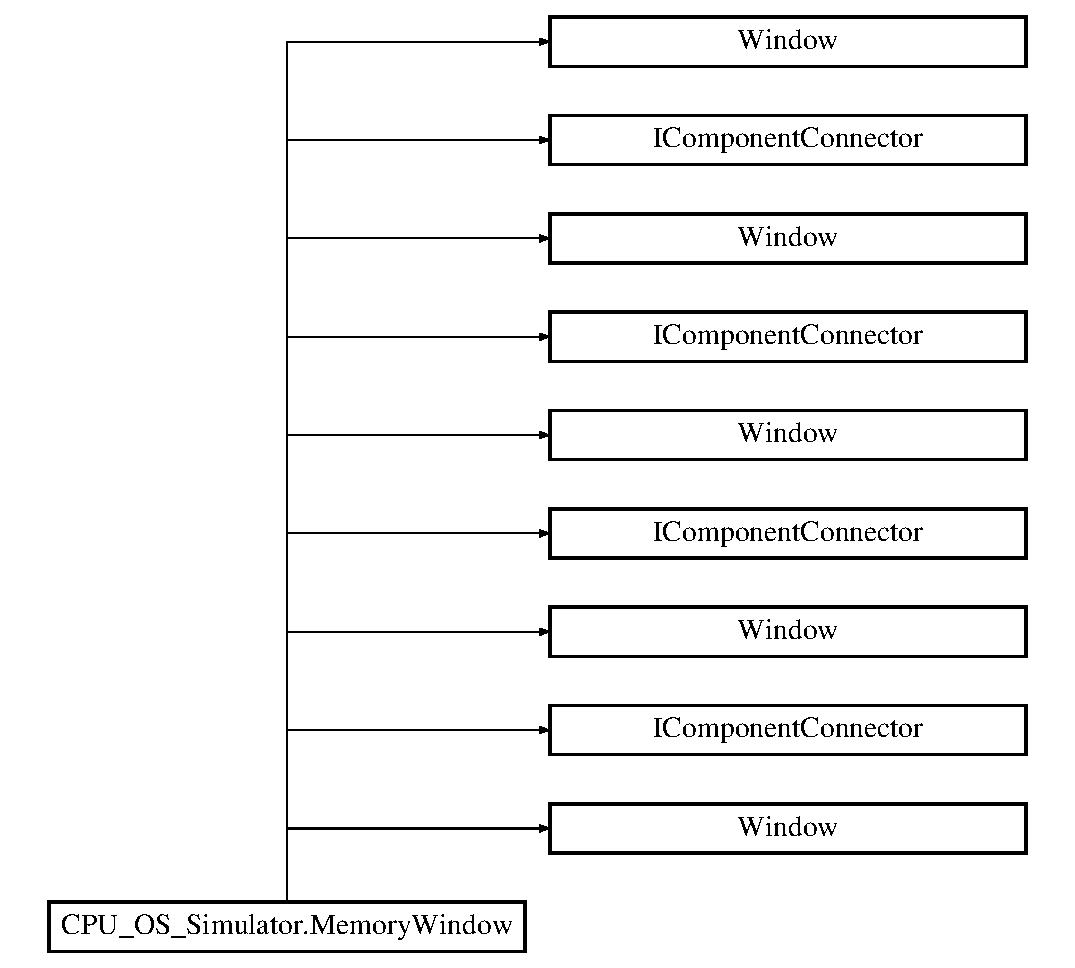
\includegraphics[height=1.004484cm]{class_c_p_u___o_s___simulator_1_1_memory_window}
\end{center}
\end{figure}
\subsection*{Public Member Functions}
\begin{DoxyCompactItemize}
\item 
\hyperlink{class_c_p_u___o_s___simulator_1_1_memory_window_a9c72b7aa51f734437bd5e4aa26a230a2}{Memory\+Window} ()
\begin{DoxyCompactList}\small\item\em Default constructor for memory window \end{DoxyCompactList}\item 
\hyperlink{class_c_p_u___o_s___simulator_1_1_memory_window_a7b4208dc517300279d4cf3cd8cac6243}{Memory\+Window} (\hyperlink{class_c_p_u___o_s___simulator_1_1_main_window}{Main\+Window} parent\+Window, \hyperlink{class_c_p_u___o_s___simulator_1_1_memory_1_1_memory_page}{Memory\+Page} \hyperlink{class_c_p_u___o_s___simulator_1_1_memory_window_ae1b974c8b976e19dde1a5491e3fe0e37}{current\+Page})
\begin{DoxyCompactList}\small\item\em Constructor for memory window that takes the window instance that is creating this window P\+L\+E\+A\+S\+E N\+O\+T\+E\+: This constructor should always be used so data can be passed back to the parent window \end{DoxyCompactList}\item 
\hyperlink{class_c_p_u___o_s___simulator_1_1_memory_window_a71b1dc152ecd45417fe8f4c5b2a6f5b6}{Memory\+Window} (\hyperlink{class_c_p_u___o_s___simulator_1_1_physical_memory_window}{Physical\+Memory\+Window} parent\+Window, \hyperlink{class_c_p_u___o_s___simulator_1_1_memory_1_1_memory_page}{Memory\+Page} \hyperlink{class_c_p_u___o_s___simulator_1_1_memory_window_ae1b974c8b976e19dde1a5491e3fe0e37}{current\+Page})
\item 
void \hyperlink{class_c_p_u___o_s___simulator_1_1_memory_window_a40473c2b8ba30a837cf2a122e0978dec}{Initialize\+Component} ()
\begin{DoxyCompactList}\small\item\em Initialize\+Component \end{DoxyCompactList}\item 
void \hyperlink{class_c_p_u___o_s___simulator_1_1_memory_window_a40473c2b8ba30a837cf2a122e0978dec}{Initialize\+Component} ()
\begin{DoxyCompactList}\small\item\em Initialize\+Component \end{DoxyCompactList}\end{DoxyCompactItemize}
\subsection*{Static Public Attributes}
\begin{DoxyCompactItemize}
\item 
static \hyperlink{class_c_p_u___o_s___simulator_1_1_memory_window}{Memory\+Window} \hyperlink{class_c_p_u___o_s___simulator_1_1_memory_window_a870b795e3b919a82888ad608ab24d61a}{current\+Instance}
\begin{DoxyCompactList}\small\item\em Variable to hold the current instance of the memory window \end{DoxyCompactList}\end{DoxyCompactItemize}
\subsection*{Package Attributes}
\begin{DoxyCompactItemize}
\item 
System.\+Windows.\+Controls.\+Grid \hyperlink{class_c_p_u___o_s___simulator_1_1_memory_window_ae2c7b1b6f5c337af62d18b0e2a4d098c}{Root\+Grid}
\item 
System.\+Windows.\+Controls.\+Group\+Box \hyperlink{class_c_p_u___o_s___simulator_1_1_memory_window_a283493c20704b70efe355621cd6e5aa4}{grp\+\_\+\+Data\+Memory}
\item 
System.\+Windows.\+Controls.\+Grid \hyperlink{class_c_p_u___o_s___simulator_1_1_memory_window_a93e699c04992f66b92f0d3b834f267d1}{Data\+Memory\+Grid}
\item 
System.\+Windows.\+Controls.\+List\+View \hyperlink{class_c_p_u___o_s___simulator_1_1_memory_window_a00f6d6a33f4c35800f2e316de335e4dd}{lst\+\_\+data}
\item 
System.\+Windows.\+Controls.\+Grid \hyperlink{class_c_p_u___o_s___simulator_1_1_memory_window_aed90d987403a12a322183d032544c507}{Initialise\+Data\+Grid}
\item 
System.\+Windows.\+Controls.\+Group\+Box \hyperlink{class_c_p_u___o_s___simulator_1_1_memory_window_a6cfa52c953fe5704090e7e9f4ac2c9d1}{grp\+\_\+\+Initialise\+Data}
\item 
System.\+Windows.\+Controls.\+Grid \hyperlink{class_c_p_u___o_s___simulator_1_1_memory_window_a2f298db1546fe63bca79b0a810304381}{Initialise\+Data\+Inner\+Grid}
\item 
System.\+Windows.\+Controls.\+Radio\+Button \hyperlink{class_c_p_u___o_s___simulator_1_1_memory_window_ae54a50c88d1e1479fceddd6d3a51a974}{rdb\+\_\+\+Integer}
\item 
System.\+Windows.\+Controls.\+Radio\+Button \hyperlink{class_c_p_u___o_s___simulator_1_1_memory_window_a728a4d572f38d0fe2063005d138d8c32}{rdb\+\_\+\+Boolean}
\item 
System.\+Windows.\+Controls.\+Radio\+Button \hyperlink{class_c_p_u___o_s___simulator_1_1_memory_window_a68b5f36b0514cacaa8e4eeb3415fcd5a}{rdb\+\_\+\+String}
\item 
System.\+Windows.\+Controls.\+Label \hyperlink{class_c_p_u___o_s___simulator_1_1_memory_window_ad5fa08b25fc582e9b2f7c305ed12a960}{label}
\item 
System.\+Windows.\+Controls.\+Label \hyperlink{class_c_p_u___o_s___simulator_1_1_memory_window_a663f25aef0cd9c3755f100b3507b5f84}{label\+\_\+\+Copy}
\item 
System.\+Windows.\+Controls.\+Label \hyperlink{class_c_p_u___o_s___simulator_1_1_memory_window_a0f501c04b3319ae43e681335e50eeba4}{label\+\_\+\+Copy1}
\item 
System.\+Windows.\+Controls.\+Text\+Box \hyperlink{class_c_p_u___o_s___simulator_1_1_memory_window_af1ad9478de6dac0b4476c51b42849ecf}{txt\+\_\+\+Integer\+Value}
\item 
System.\+Windows.\+Controls.\+Text\+Box \hyperlink{class_c_p_u___o_s___simulator_1_1_memory_window_aca8e57432af036b698d0eeaaa765c483}{txt\+\_\+\+String\+Value}
\item 
System.\+Windows.\+Controls.\+Combo\+Box \hyperlink{class_c_p_u___o_s___simulator_1_1_memory_window_a2a1da5df6a425ce20c7b639fa66c58f2}{cmb\+\_\+\+Boolean\+Value}
\item 
System.\+Windows.\+Controls.\+Label \hyperlink{class_c_p_u___o_s___simulator_1_1_memory_window_ae35c7d3110d7cf96493d6fa68274e858}{label1}
\item 
System.\+Windows.\+Controls.\+Text\+Box \hyperlink{class_c_p_u___o_s___simulator_1_1_memory_window_a3f766ac6c531af3b14248819947d9023}{txt\+\_\+\+Address\+Location}
\item 
System.\+Windows.\+Controls.\+Button \hyperlink{class_c_p_u___o_s___simulator_1_1_memory_window_a9274df08bf008c43b325e50d6db6067f}{btn\+\_\+\+Update}
\item 
System.\+Windows.\+Controls.\+Button \hyperlink{class_c_p_u___o_s___simulator_1_1_memory_window_aeeefcad9b4510fd7fd5899f3a2db4786}{btn\+\_\+\+Reset\+All}
\item 
System.\+Windows.\+Controls.\+Button \hyperlink{class_c_p_u___o_s___simulator_1_1_memory_window_a62372edf818561f1584160d41c2f67f7}{btn\+\_\+\+Show\+Page\+Table}
\end{DoxyCompactItemize}
\subsection*{Properties}
\begin{DoxyCompactItemize}
\item 
\hyperlink{class_c_p_u___o_s___simulator_1_1_main_window}{Main\+Window} \hyperlink{class_c_p_u___o_s___simulator_1_1_memory_window_aa5bd394d11d42930f9fa03388a2a3598}{Main\+Parent\+Window}\hspace{0.3cm}{\ttfamily  \mbox{[}get, set\mbox{]}}
\begin{DoxyCompactList}\small\item\em Property to hold the current instance of the memory window \end{DoxyCompactList}\item 
\hyperlink{class_c_p_u___o_s___simulator_1_1_physical_memory_window}{Physical\+Memory\+Window} \hyperlink{class_c_p_u___o_s___simulator_1_1_memory_window_a6d9cf74558fa17588eb524298f420d1c}{Physical\+Memory\+Parent\+Window}\hspace{0.3cm}{\ttfamily  \mbox{[}get, set\mbox{]}}
\end{DoxyCompactItemize}
\subsection*{Private Member Functions}
\begin{DoxyCompactItemize}
\item 
void \hyperlink{class_c_p_u___o_s___simulator_1_1_memory_window_a8811287064d6315e3a8c01531148ed81}{Populate\+Data\+View} ()
\begin{DoxyCompactList}\small\item\em This function populates the data view with the contents of the current memory\+Page \end{DoxyCompactList}\item 
void \hyperlink{class_c_p_u___o_s___simulator_1_1_memory_window_a91ec1c8081b85d3c07eaa31ee524f5d9}{btn\+\_\+\+Update\+\_\+\+Click} (object sender, Routed\+Event\+Args e)
\item 
void \hyperlink{class_c_p_u___o_s___simulator_1_1_memory_window_a3e850d7c5ba7c4db466ee671b3a632c6}{Swap\+In\+Page} (int page\+Number)
\item 
void \hyperlink{class_c_p_u___o_s___simulator_1_1_memory_window_ab0cb156466262b3d90f19acd422dc65b}{Update\+Data} ()
\item 
void \hyperlink{class_c_p_u___o_s___simulator_1_1_memory_window_ac77beff86f4dd6322bdcf2430892d2aa}{btn\+\_\+\+Reset\+\_\+\+All\+\_\+\+Click} (object sender, Routed\+Event\+Args e)
\item 
void \hyperlink{class_c_p_u___o_s___simulator_1_1_memory_window_a0540a495053120e2572a106dbbc391de}{btn\+\_\+\+Show\+Page\+Table\+\_\+\+Click} (object sender, Routed\+Event\+Args e)
\item 
void \hyperlink{class_c_p_u___o_s___simulator_1_1_memory_window_a0727fbff3ea42722692b224a621ecc4a}{Window\+\_\+\+Closing} (object sender, Cancel\+Event\+Args e)
\item 
void \hyperlink{class_c_p_u___o_s___simulator_1_1_memory_window_a5100fa341de6de08d11967198cd82208}{Set\+Memory\+Window\+Instance} ()
\begin{DoxyCompactList}\small\item\em This method sets the current instance of memory window in the window bridge so it can be accessed by other modules \end{DoxyCompactList}\item 
void System.\+Windows.\+Markup.\+I\+Component\+Connector. \hyperlink{class_c_p_u___o_s___simulator_1_1_memory_window_aba65e66795c99052ebed93162110e908}{Connect} (int connection\+Id, object target)
\item 
void System.\+Windows.\+Markup.\+I\+Component\+Connector. \hyperlink{class_c_p_u___o_s___simulator_1_1_memory_window_aba65e66795c99052ebed93162110e908}{Connect} (int connection\+Id, object target)
\end{DoxyCompactItemize}
\subsection*{Private Attributes}
\begin{DoxyCompactItemize}
\item 
\hyperlink{class_c_p_u___o_s___simulator_1_1_main_window}{Main\+Window} \hyperlink{class_c_p_u___o_s___simulator_1_1_memory_window_a16d50c8cc53076c200da3b3ffeeaedfb}{main\+Parent\+Window}
\item 
\hyperlink{class_c_p_u___o_s___simulator_1_1_physical_memory_window}{Physical\+Memory\+Window} \hyperlink{class_c_p_u___o_s___simulator_1_1_memory_window_a25eea03e3eff2d407158f1b00ae5a8ff}{physical\+Memory\+Parent\+Window}
\item 
\hyperlink{class_c_p_u___o_s___simulator_1_1_memory_1_1_memory_page}{Memory\+Page} \hyperlink{class_c_p_u___o_s___simulator_1_1_memory_window_ae1b974c8b976e19dde1a5491e3fe0e37}{current\+Page}
\item 
bool \hyperlink{class_c_p_u___o_s___simulator_1_1_memory_window_af20b67929b49d4289e1d81d141cbd950}{\+\_\+content\+Loaded}
\end{DoxyCompactItemize}


\subsection{Detailed Description}
Interaction logic for Memory\+Window.\+xaml 

\hyperlink{class_c_p_u___o_s___simulator_1_1_memory_window}{Memory\+Window} 

Definition at line 13 of file Memory\+Window.\+xaml.\+cs.



\subsection{Constructor \& Destructor Documentation}
\hypertarget{class_c_p_u___o_s___simulator_1_1_memory_window_a9c72b7aa51f734437bd5e4aa26a230a2}{}\index{C\+P\+U\+\_\+\+O\+S\+\_\+\+Simulator\+::\+Memory\+Window@{C\+P\+U\+\_\+\+O\+S\+\_\+\+Simulator\+::\+Memory\+Window}!Memory\+Window@{Memory\+Window}}
\index{Memory\+Window@{Memory\+Window}!C\+P\+U\+\_\+\+O\+S\+\_\+\+Simulator\+::\+Memory\+Window@{C\+P\+U\+\_\+\+O\+S\+\_\+\+Simulator\+::\+Memory\+Window}}
\subsubsection[{Memory\+Window()}]{\setlength{\rightskip}{0pt plus 5cm}C\+P\+U\+\_\+\+O\+S\+\_\+\+Simulator.\+Memory\+Window.\+Memory\+Window (
\begin{DoxyParamCaption}
{}
\end{DoxyParamCaption}
)}\label{class_c_p_u___o_s___simulator_1_1_memory_window_a9c72b7aa51f734437bd5e4aa26a230a2}


Default constructor for memory window 



Definition at line 25 of file Memory\+Window.\+xaml.\+cs.

\hypertarget{class_c_p_u___o_s___simulator_1_1_memory_window_a7b4208dc517300279d4cf3cd8cac6243}{}\index{C\+P\+U\+\_\+\+O\+S\+\_\+\+Simulator\+::\+Memory\+Window@{C\+P\+U\+\_\+\+O\+S\+\_\+\+Simulator\+::\+Memory\+Window}!Memory\+Window@{Memory\+Window}}
\index{Memory\+Window@{Memory\+Window}!C\+P\+U\+\_\+\+O\+S\+\_\+\+Simulator\+::\+Memory\+Window@{C\+P\+U\+\_\+\+O\+S\+\_\+\+Simulator\+::\+Memory\+Window}}
\subsubsection[{Memory\+Window(\+Main\+Window parent\+Window, Memory\+Page current\+Page)}]{\setlength{\rightskip}{0pt plus 5cm}C\+P\+U\+\_\+\+O\+S\+\_\+\+Simulator.\+Memory\+Window.\+Memory\+Window (
\begin{DoxyParamCaption}
\item[{{\bf Main\+Window}}]{parent\+Window, }
\item[{{\bf Memory\+Page}}]{current\+Page}
\end{DoxyParamCaption}
)}\label{class_c_p_u___o_s___simulator_1_1_memory_window_a7b4208dc517300279d4cf3cd8cac6243}


Constructor for memory window that takes the window instance that is creating this window P\+L\+E\+A\+S\+E N\+O\+T\+E\+: This constructor should always be used so data can be passed back to the parent window 


\begin{DoxyParams}{Parameters}
{\em parent\+Window} & The window that is creating this window \\
\hline
{\em current\+Page} & The memory page to be displayed in the window \\
\hline
\end{DoxyParams}


Definition at line 37 of file Memory\+Window.\+xaml.\+cs.

\hypertarget{class_c_p_u___o_s___simulator_1_1_memory_window_a71b1dc152ecd45417fe8f4c5b2a6f5b6}{}\index{C\+P\+U\+\_\+\+O\+S\+\_\+\+Simulator\+::\+Memory\+Window@{C\+P\+U\+\_\+\+O\+S\+\_\+\+Simulator\+::\+Memory\+Window}!Memory\+Window@{Memory\+Window}}
\index{Memory\+Window@{Memory\+Window}!C\+P\+U\+\_\+\+O\+S\+\_\+\+Simulator\+::\+Memory\+Window@{C\+P\+U\+\_\+\+O\+S\+\_\+\+Simulator\+::\+Memory\+Window}}
\subsubsection[{Memory\+Window(\+Physical\+Memory\+Window parent\+Window, Memory\+Page current\+Page)}]{\setlength{\rightskip}{0pt plus 5cm}C\+P\+U\+\_\+\+O\+S\+\_\+\+Simulator.\+Memory\+Window.\+Memory\+Window (
\begin{DoxyParamCaption}
\item[{{\bf Physical\+Memory\+Window}}]{parent\+Window, }
\item[{{\bf Memory\+Page}}]{current\+Page}
\end{DoxyParamCaption}
)}\label{class_c_p_u___o_s___simulator_1_1_memory_window_a71b1dc152ecd45417fe8f4c5b2a6f5b6}


Definition at line 46 of file Memory\+Window.\+xaml.\+cs.



\subsection{Member Function Documentation}
\hypertarget{class_c_p_u___o_s___simulator_1_1_memory_window_ac77beff86f4dd6322bdcf2430892d2aa}{}\index{C\+P\+U\+\_\+\+O\+S\+\_\+\+Simulator\+::\+Memory\+Window@{C\+P\+U\+\_\+\+O\+S\+\_\+\+Simulator\+::\+Memory\+Window}!btn\+\_\+\+Reset\+\_\+\+All\+\_\+\+Click@{btn\+\_\+\+Reset\+\_\+\+All\+\_\+\+Click}}
\index{btn\+\_\+\+Reset\+\_\+\+All\+\_\+\+Click@{btn\+\_\+\+Reset\+\_\+\+All\+\_\+\+Click}!C\+P\+U\+\_\+\+O\+S\+\_\+\+Simulator\+::\+Memory\+Window@{C\+P\+U\+\_\+\+O\+S\+\_\+\+Simulator\+::\+Memory\+Window}}
\subsubsection[{btn\+\_\+\+Reset\+\_\+\+All\+\_\+\+Click(object sender, Routed\+Event\+Args e)}]{\setlength{\rightskip}{0pt plus 5cm}void C\+P\+U\+\_\+\+O\+S\+\_\+\+Simulator.\+Memory\+Window.\+btn\+\_\+\+Reset\+\_\+\+All\+\_\+\+Click (
\begin{DoxyParamCaption}
\item[{object}]{sender, }
\item[{Routed\+Event\+Args}]{e}
\end{DoxyParamCaption}
)\hspace{0.3cm}{\ttfamily [private]}}\label{class_c_p_u___o_s___simulator_1_1_memory_window_ac77beff86f4dd6322bdcf2430892d2aa}


Definition at line 188 of file Memory\+Window.\+xaml.\+cs.

\hypertarget{class_c_p_u___o_s___simulator_1_1_memory_window_a0540a495053120e2572a106dbbc391de}{}\index{C\+P\+U\+\_\+\+O\+S\+\_\+\+Simulator\+::\+Memory\+Window@{C\+P\+U\+\_\+\+O\+S\+\_\+\+Simulator\+::\+Memory\+Window}!btn\+\_\+\+Show\+Page\+Table\+\_\+\+Click@{btn\+\_\+\+Show\+Page\+Table\+\_\+\+Click}}
\index{btn\+\_\+\+Show\+Page\+Table\+\_\+\+Click@{btn\+\_\+\+Show\+Page\+Table\+\_\+\+Click}!C\+P\+U\+\_\+\+O\+S\+\_\+\+Simulator\+::\+Memory\+Window@{C\+P\+U\+\_\+\+O\+S\+\_\+\+Simulator\+::\+Memory\+Window}}
\subsubsection[{btn\+\_\+\+Show\+Page\+Table\+\_\+\+Click(object sender, Routed\+Event\+Args e)}]{\setlength{\rightskip}{0pt plus 5cm}void C\+P\+U\+\_\+\+O\+S\+\_\+\+Simulator.\+Memory\+Window.\+btn\+\_\+\+Show\+Page\+Table\+\_\+\+Click (
\begin{DoxyParamCaption}
\item[{object}]{sender, }
\item[{Routed\+Event\+Args}]{e}
\end{DoxyParamCaption}
)\hspace{0.3cm}{\ttfamily [private]}}\label{class_c_p_u___o_s___simulator_1_1_memory_window_a0540a495053120e2572a106dbbc391de}


Definition at line 194 of file Memory\+Window.\+xaml.\+cs.

\hypertarget{class_c_p_u___o_s___simulator_1_1_memory_window_a91ec1c8081b85d3c07eaa31ee524f5d9}{}\index{C\+P\+U\+\_\+\+O\+S\+\_\+\+Simulator\+::\+Memory\+Window@{C\+P\+U\+\_\+\+O\+S\+\_\+\+Simulator\+::\+Memory\+Window}!btn\+\_\+\+Update\+\_\+\+Click@{btn\+\_\+\+Update\+\_\+\+Click}}
\index{btn\+\_\+\+Update\+\_\+\+Click@{btn\+\_\+\+Update\+\_\+\+Click}!C\+P\+U\+\_\+\+O\+S\+\_\+\+Simulator\+::\+Memory\+Window@{C\+P\+U\+\_\+\+O\+S\+\_\+\+Simulator\+::\+Memory\+Window}}
\subsubsection[{btn\+\_\+\+Update\+\_\+\+Click(object sender, Routed\+Event\+Args e)}]{\setlength{\rightskip}{0pt plus 5cm}void C\+P\+U\+\_\+\+O\+S\+\_\+\+Simulator.\+Memory\+Window.\+btn\+\_\+\+Update\+\_\+\+Click (
\begin{DoxyParamCaption}
\item[{object}]{sender, }
\item[{Routed\+Event\+Args}]{e}
\end{DoxyParamCaption}
)\hspace{0.3cm}{\ttfamily [private]}}\label{class_c_p_u___o_s___simulator_1_1_memory_window_a91ec1c8081b85d3c07eaa31ee524f5d9}


Definition at line 89 of file Memory\+Window.\+xaml.\+cs.

\hypertarget{class_c_p_u___o_s___simulator_1_1_memory_window_aba65e66795c99052ebed93162110e908}{}\index{C\+P\+U\+\_\+\+O\+S\+\_\+\+Simulator\+::\+Memory\+Window@{C\+P\+U\+\_\+\+O\+S\+\_\+\+Simulator\+::\+Memory\+Window}!Connect@{Connect}}
\index{Connect@{Connect}!C\+P\+U\+\_\+\+O\+S\+\_\+\+Simulator\+::\+Memory\+Window@{C\+P\+U\+\_\+\+O\+S\+\_\+\+Simulator\+::\+Memory\+Window}}
\subsubsection[{Connect(int connection\+Id, object target)}]{\setlength{\rightskip}{0pt plus 5cm}void System.\+Windows.\+Markup.\+I\+Component\+Connector. C\+P\+U\+\_\+\+O\+S\+\_\+\+Simulator.\+Memory\+Window.\+Connect (
\begin{DoxyParamCaption}
\item[{int}]{connection\+Id, }
\item[{object}]{target}
\end{DoxyParamCaption}
)\hspace{0.3cm}{\ttfamily [private]}}\label{class_c_p_u___o_s___simulator_1_1_memory_window_aba65e66795c99052ebed93162110e908}


Definition at line 238 of file Memory\+Window.\+g.\+cs.

\hypertarget{class_c_p_u___o_s___simulator_1_1_memory_window_aba65e66795c99052ebed93162110e908}{}\index{C\+P\+U\+\_\+\+O\+S\+\_\+\+Simulator\+::\+Memory\+Window@{C\+P\+U\+\_\+\+O\+S\+\_\+\+Simulator\+::\+Memory\+Window}!Connect@{Connect}}
\index{Connect@{Connect}!C\+P\+U\+\_\+\+O\+S\+\_\+\+Simulator\+::\+Memory\+Window@{C\+P\+U\+\_\+\+O\+S\+\_\+\+Simulator\+::\+Memory\+Window}}
\subsubsection[{Connect(int connection\+Id, object target)}]{\setlength{\rightskip}{0pt plus 5cm}void System.\+Windows.\+Markup.\+I\+Component\+Connector. C\+P\+U\+\_\+\+O\+S\+\_\+\+Simulator.\+Memory\+Window.\+Connect (
\begin{DoxyParamCaption}
\item[{int}]{connection\+Id, }
\item[{object}]{target}
\end{DoxyParamCaption}
)\hspace{0.3cm}{\ttfamily [private]}}\label{class_c_p_u___o_s___simulator_1_1_memory_window_aba65e66795c99052ebed93162110e908}


Definition at line 238 of file Memory\+Window.\+g.\+i.\+cs.

\hypertarget{class_c_p_u___o_s___simulator_1_1_memory_window_a40473c2b8ba30a837cf2a122e0978dec}{}\index{C\+P\+U\+\_\+\+O\+S\+\_\+\+Simulator\+::\+Memory\+Window@{C\+P\+U\+\_\+\+O\+S\+\_\+\+Simulator\+::\+Memory\+Window}!Initialize\+Component@{Initialize\+Component}}
\index{Initialize\+Component@{Initialize\+Component}!C\+P\+U\+\_\+\+O\+S\+\_\+\+Simulator\+::\+Memory\+Window@{C\+P\+U\+\_\+\+O\+S\+\_\+\+Simulator\+::\+Memory\+Window}}
\subsubsection[{Initialize\+Component()}]{\setlength{\rightskip}{0pt plus 5cm}void C\+P\+U\+\_\+\+O\+S\+\_\+\+Simulator.\+Memory\+Window.\+Initialize\+Component (
\begin{DoxyParamCaption}
{}
\end{DoxyParamCaption}
)}\label{class_c_p_u___o_s___simulator_1_1_memory_window_a40473c2b8ba30a837cf2a122e0978dec}


Initialize\+Component 



Definition at line 218 of file Memory\+Window.\+g.\+cs.

\hypertarget{class_c_p_u___o_s___simulator_1_1_memory_window_a40473c2b8ba30a837cf2a122e0978dec}{}\index{C\+P\+U\+\_\+\+O\+S\+\_\+\+Simulator\+::\+Memory\+Window@{C\+P\+U\+\_\+\+O\+S\+\_\+\+Simulator\+::\+Memory\+Window}!Initialize\+Component@{Initialize\+Component}}
\index{Initialize\+Component@{Initialize\+Component}!C\+P\+U\+\_\+\+O\+S\+\_\+\+Simulator\+::\+Memory\+Window@{C\+P\+U\+\_\+\+O\+S\+\_\+\+Simulator\+::\+Memory\+Window}}
\subsubsection[{Initialize\+Component()}]{\setlength{\rightskip}{0pt plus 5cm}void C\+P\+U\+\_\+\+O\+S\+\_\+\+Simulator.\+Memory\+Window.\+Initialize\+Component (
\begin{DoxyParamCaption}
{}
\end{DoxyParamCaption}
)}\label{class_c_p_u___o_s___simulator_1_1_memory_window_a40473c2b8ba30a837cf2a122e0978dec}


Initialize\+Component 



Definition at line 218 of file Memory\+Window.\+g.\+i.\+cs.

\hypertarget{class_c_p_u___o_s___simulator_1_1_memory_window_a8811287064d6315e3a8c01531148ed81}{}\index{C\+P\+U\+\_\+\+O\+S\+\_\+\+Simulator\+::\+Memory\+Window@{C\+P\+U\+\_\+\+O\+S\+\_\+\+Simulator\+::\+Memory\+Window}!Populate\+Data\+View@{Populate\+Data\+View}}
\index{Populate\+Data\+View@{Populate\+Data\+View}!C\+P\+U\+\_\+\+O\+S\+\_\+\+Simulator\+::\+Memory\+Window@{C\+P\+U\+\_\+\+O\+S\+\_\+\+Simulator\+::\+Memory\+Window}}
\subsubsection[{Populate\+Data\+View()}]{\setlength{\rightskip}{0pt plus 5cm}void C\+P\+U\+\_\+\+O\+S\+\_\+\+Simulator.\+Memory\+Window.\+Populate\+Data\+View (
\begin{DoxyParamCaption}
{}
\end{DoxyParamCaption}
)\hspace{0.3cm}{\ttfamily [private]}}\label{class_c_p_u___o_s___simulator_1_1_memory_window_a8811287064d6315e3a8c01531148ed81}


This function populates the data view with the contents of the current memory\+Page 



Definition at line 74 of file Memory\+Window.\+xaml.\+cs.

\hypertarget{class_c_p_u___o_s___simulator_1_1_memory_window_a5100fa341de6de08d11967198cd82208}{}\index{C\+P\+U\+\_\+\+O\+S\+\_\+\+Simulator\+::\+Memory\+Window@{C\+P\+U\+\_\+\+O\+S\+\_\+\+Simulator\+::\+Memory\+Window}!Set\+Memory\+Window\+Instance@{Set\+Memory\+Window\+Instance}}
\index{Set\+Memory\+Window\+Instance@{Set\+Memory\+Window\+Instance}!C\+P\+U\+\_\+\+O\+S\+\_\+\+Simulator\+::\+Memory\+Window@{C\+P\+U\+\_\+\+O\+S\+\_\+\+Simulator\+::\+Memory\+Window}}
\subsubsection[{Set\+Memory\+Window\+Instance()}]{\setlength{\rightskip}{0pt plus 5cm}void C\+P\+U\+\_\+\+O\+S\+\_\+\+Simulator.\+Memory\+Window.\+Set\+Memory\+Window\+Instance (
\begin{DoxyParamCaption}
{}
\end{DoxyParamCaption}
)\hspace{0.3cm}{\ttfamily [private]}}\label{class_c_p_u___o_s___simulator_1_1_memory_window_a5100fa341de6de08d11967198cd82208}


This method sets the current instance of memory window in the window bridge so it can be accessed by other modules 



Definition at line 209 of file Memory\+Window.\+xaml.\+cs.

\hypertarget{class_c_p_u___o_s___simulator_1_1_memory_window_a3e850d7c5ba7c4db466ee671b3a632c6}{}\index{C\+P\+U\+\_\+\+O\+S\+\_\+\+Simulator\+::\+Memory\+Window@{C\+P\+U\+\_\+\+O\+S\+\_\+\+Simulator\+::\+Memory\+Window}!Swap\+In\+Page@{Swap\+In\+Page}}
\index{Swap\+In\+Page@{Swap\+In\+Page}!C\+P\+U\+\_\+\+O\+S\+\_\+\+Simulator\+::\+Memory\+Window@{C\+P\+U\+\_\+\+O\+S\+\_\+\+Simulator\+::\+Memory\+Window}}
\subsubsection[{Swap\+In\+Page(int page\+Number)}]{\setlength{\rightskip}{0pt plus 5cm}void C\+P\+U\+\_\+\+O\+S\+\_\+\+Simulator.\+Memory\+Window.\+Swap\+In\+Page (
\begin{DoxyParamCaption}
\item[{int}]{page\+Number}
\end{DoxyParamCaption}
)\hspace{0.3cm}{\ttfamily [private]}}\label{class_c_p_u___o_s___simulator_1_1_memory_window_a3e850d7c5ba7c4db466ee671b3a632c6}


Definition at line 166 of file Memory\+Window.\+xaml.\+cs.

\hypertarget{class_c_p_u___o_s___simulator_1_1_memory_window_ab0cb156466262b3d90f19acd422dc65b}{}\index{C\+P\+U\+\_\+\+O\+S\+\_\+\+Simulator\+::\+Memory\+Window@{C\+P\+U\+\_\+\+O\+S\+\_\+\+Simulator\+::\+Memory\+Window}!Update\+Data@{Update\+Data}}
\index{Update\+Data@{Update\+Data}!C\+P\+U\+\_\+\+O\+S\+\_\+\+Simulator\+::\+Memory\+Window@{C\+P\+U\+\_\+\+O\+S\+\_\+\+Simulator\+::\+Memory\+Window}}
\subsubsection[{Update\+Data()}]{\setlength{\rightskip}{0pt plus 5cm}void C\+P\+U\+\_\+\+O\+S\+\_\+\+Simulator.\+Memory\+Window.\+Update\+Data (
\begin{DoxyParamCaption}
{}
\end{DoxyParamCaption}
)\hspace{0.3cm}{\ttfamily [private]}}\label{class_c_p_u___o_s___simulator_1_1_memory_window_ab0cb156466262b3d90f19acd422dc65b}


Definition at line 181 of file Memory\+Window.\+xaml.\+cs.

\hypertarget{class_c_p_u___o_s___simulator_1_1_memory_window_a0727fbff3ea42722692b224a621ecc4a}{}\index{C\+P\+U\+\_\+\+O\+S\+\_\+\+Simulator\+::\+Memory\+Window@{C\+P\+U\+\_\+\+O\+S\+\_\+\+Simulator\+::\+Memory\+Window}!Window\+\_\+\+Closing@{Window\+\_\+\+Closing}}
\index{Window\+\_\+\+Closing@{Window\+\_\+\+Closing}!C\+P\+U\+\_\+\+O\+S\+\_\+\+Simulator\+::\+Memory\+Window@{C\+P\+U\+\_\+\+O\+S\+\_\+\+Simulator\+::\+Memory\+Window}}
\subsubsection[{Window\+\_\+\+Closing(object sender, Cancel\+Event\+Args e)}]{\setlength{\rightskip}{0pt plus 5cm}void C\+P\+U\+\_\+\+O\+S\+\_\+\+Simulator.\+Memory\+Window.\+Window\+\_\+\+Closing (
\begin{DoxyParamCaption}
\item[{object}]{sender, }
\item[{Cancel\+Event\+Args}]{e}
\end{DoxyParamCaption}
)\hspace{0.3cm}{\ttfamily [private]}}\label{class_c_p_u___o_s___simulator_1_1_memory_window_a0727fbff3ea42722692b224a621ecc4a}


Definition at line 200 of file Memory\+Window.\+xaml.\+cs.



\subsection{Member Data Documentation}
\hypertarget{class_c_p_u___o_s___simulator_1_1_memory_window_af20b67929b49d4289e1d81d141cbd950}{}\index{C\+P\+U\+\_\+\+O\+S\+\_\+\+Simulator\+::\+Memory\+Window@{C\+P\+U\+\_\+\+O\+S\+\_\+\+Simulator\+::\+Memory\+Window}!\+\_\+content\+Loaded@{\+\_\+content\+Loaded}}
\index{\+\_\+content\+Loaded@{\+\_\+content\+Loaded}!C\+P\+U\+\_\+\+O\+S\+\_\+\+Simulator\+::\+Memory\+Window@{C\+P\+U\+\_\+\+O\+S\+\_\+\+Simulator\+::\+Memory\+Window}}
\subsubsection[{\+\_\+content\+Loaded}]{\setlength{\rightskip}{0pt plus 5cm}bool C\+P\+U\+\_\+\+O\+S\+\_\+\+Simulator.\+Memory\+Window.\+\_\+content\+Loaded\hspace{0.3cm}{\ttfamily [private]}}\label{class_c_p_u___o_s___simulator_1_1_memory_window_af20b67929b49d4289e1d81d141cbd950}


Definition at line 211 of file Memory\+Window.\+g.\+cs.

\hypertarget{class_c_p_u___o_s___simulator_1_1_memory_window_aeeefcad9b4510fd7fd5899f3a2db4786}{}\index{C\+P\+U\+\_\+\+O\+S\+\_\+\+Simulator\+::\+Memory\+Window@{C\+P\+U\+\_\+\+O\+S\+\_\+\+Simulator\+::\+Memory\+Window}!btn\+\_\+\+Reset\+All@{btn\+\_\+\+Reset\+All}}
\index{btn\+\_\+\+Reset\+All@{btn\+\_\+\+Reset\+All}!C\+P\+U\+\_\+\+O\+S\+\_\+\+Simulator\+::\+Memory\+Window@{C\+P\+U\+\_\+\+O\+S\+\_\+\+Simulator\+::\+Memory\+Window}}
\subsubsection[{btn\+\_\+\+Reset\+All}]{\setlength{\rightskip}{0pt plus 5cm}System Windows Controls Button C\+P\+U\+\_\+\+O\+S\+\_\+\+Simulator.\+Memory\+Window.\+btn\+\_\+\+Reset\+All\hspace{0.3cm}{\ttfamily [package]}}\label{class_c_p_u___o_s___simulator_1_1_memory_window_aeeefcad9b4510fd7fd5899f3a2db4786}


Definition at line 198 of file Memory\+Window.\+g.\+cs.

\hypertarget{class_c_p_u___o_s___simulator_1_1_memory_window_a62372edf818561f1584160d41c2f67f7}{}\index{C\+P\+U\+\_\+\+O\+S\+\_\+\+Simulator\+::\+Memory\+Window@{C\+P\+U\+\_\+\+O\+S\+\_\+\+Simulator\+::\+Memory\+Window}!btn\+\_\+\+Show\+Page\+Table@{btn\+\_\+\+Show\+Page\+Table}}
\index{btn\+\_\+\+Show\+Page\+Table@{btn\+\_\+\+Show\+Page\+Table}!C\+P\+U\+\_\+\+O\+S\+\_\+\+Simulator\+::\+Memory\+Window@{C\+P\+U\+\_\+\+O\+S\+\_\+\+Simulator\+::\+Memory\+Window}}
\subsubsection[{btn\+\_\+\+Show\+Page\+Table}]{\setlength{\rightskip}{0pt plus 5cm}System Windows Controls Button C\+P\+U\+\_\+\+O\+S\+\_\+\+Simulator.\+Memory\+Window.\+btn\+\_\+\+Show\+Page\+Table\hspace{0.3cm}{\ttfamily [package]}}\label{class_c_p_u___o_s___simulator_1_1_memory_window_a62372edf818561f1584160d41c2f67f7}


Definition at line 206 of file Memory\+Window.\+g.\+cs.

\hypertarget{class_c_p_u___o_s___simulator_1_1_memory_window_a9274df08bf008c43b325e50d6db6067f}{}\index{C\+P\+U\+\_\+\+O\+S\+\_\+\+Simulator\+::\+Memory\+Window@{C\+P\+U\+\_\+\+O\+S\+\_\+\+Simulator\+::\+Memory\+Window}!btn\+\_\+\+Update@{btn\+\_\+\+Update}}
\index{btn\+\_\+\+Update@{btn\+\_\+\+Update}!C\+P\+U\+\_\+\+O\+S\+\_\+\+Simulator\+::\+Memory\+Window@{C\+P\+U\+\_\+\+O\+S\+\_\+\+Simulator\+::\+Memory\+Window}}
\subsubsection[{btn\+\_\+\+Update}]{\setlength{\rightskip}{0pt plus 5cm}System Windows Controls Button C\+P\+U\+\_\+\+O\+S\+\_\+\+Simulator.\+Memory\+Window.\+btn\+\_\+\+Update\hspace{0.3cm}{\ttfamily [package]}}\label{class_c_p_u___o_s___simulator_1_1_memory_window_a9274df08bf008c43b325e50d6db6067f}


Definition at line 190 of file Memory\+Window.\+g.\+cs.

\hypertarget{class_c_p_u___o_s___simulator_1_1_memory_window_a2a1da5df6a425ce20c7b639fa66c58f2}{}\index{C\+P\+U\+\_\+\+O\+S\+\_\+\+Simulator\+::\+Memory\+Window@{C\+P\+U\+\_\+\+O\+S\+\_\+\+Simulator\+::\+Memory\+Window}!cmb\+\_\+\+Boolean\+Value@{cmb\+\_\+\+Boolean\+Value}}
\index{cmb\+\_\+\+Boolean\+Value@{cmb\+\_\+\+Boolean\+Value}!C\+P\+U\+\_\+\+O\+S\+\_\+\+Simulator\+::\+Memory\+Window@{C\+P\+U\+\_\+\+O\+S\+\_\+\+Simulator\+::\+Memory\+Window}}
\subsubsection[{cmb\+\_\+\+Boolean\+Value}]{\setlength{\rightskip}{0pt plus 5cm}System Windows Controls Combo\+Box C\+P\+U\+\_\+\+O\+S\+\_\+\+Simulator.\+Memory\+Window.\+cmb\+\_\+\+Boolean\+Value\hspace{0.3cm}{\ttfamily [package]}}\label{class_c_p_u___o_s___simulator_1_1_memory_window_a2a1da5df6a425ce20c7b639fa66c58f2}


Definition at line 166 of file Memory\+Window.\+g.\+cs.

\hypertarget{class_c_p_u___o_s___simulator_1_1_memory_window_a870b795e3b919a82888ad608ab24d61a}{}\index{C\+P\+U\+\_\+\+O\+S\+\_\+\+Simulator\+::\+Memory\+Window@{C\+P\+U\+\_\+\+O\+S\+\_\+\+Simulator\+::\+Memory\+Window}!current\+Instance@{current\+Instance}}
\index{current\+Instance@{current\+Instance}!C\+P\+U\+\_\+\+O\+S\+\_\+\+Simulator\+::\+Memory\+Window@{C\+P\+U\+\_\+\+O\+S\+\_\+\+Simulator\+::\+Memory\+Window}}
\subsubsection[{current\+Instance}]{\setlength{\rightskip}{0pt plus 5cm}{\bf Memory\+Window} C\+P\+U\+\_\+\+O\+S\+\_\+\+Simulator.\+Memory\+Window.\+current\+Instance\hspace{0.3cm}{\ttfamily [static]}}\label{class_c_p_u___o_s___simulator_1_1_memory_window_a870b795e3b919a82888ad608ab24d61a}


Variable to hold the current instance of the memory window 



Definition at line 21 of file Memory\+Window.\+xaml.\+cs.

\hypertarget{class_c_p_u___o_s___simulator_1_1_memory_window_ae1b974c8b976e19dde1a5491e3fe0e37}{}\index{C\+P\+U\+\_\+\+O\+S\+\_\+\+Simulator\+::\+Memory\+Window@{C\+P\+U\+\_\+\+O\+S\+\_\+\+Simulator\+::\+Memory\+Window}!current\+Page@{current\+Page}}
\index{current\+Page@{current\+Page}!C\+P\+U\+\_\+\+O\+S\+\_\+\+Simulator\+::\+Memory\+Window@{C\+P\+U\+\_\+\+O\+S\+\_\+\+Simulator\+::\+Memory\+Window}}
\subsubsection[{current\+Page}]{\setlength{\rightskip}{0pt plus 5cm}{\bf Memory\+Page} C\+P\+U\+\_\+\+O\+S\+\_\+\+Simulator.\+Memory\+Window.\+current\+Page\hspace{0.3cm}{\ttfamily [private]}}\label{class_c_p_u___o_s___simulator_1_1_memory_window_ae1b974c8b976e19dde1a5491e3fe0e37}


Definition at line 17 of file Memory\+Window.\+xaml.\+cs.

\hypertarget{class_c_p_u___o_s___simulator_1_1_memory_window_a93e699c04992f66b92f0d3b834f267d1}{}\index{C\+P\+U\+\_\+\+O\+S\+\_\+\+Simulator\+::\+Memory\+Window@{C\+P\+U\+\_\+\+O\+S\+\_\+\+Simulator\+::\+Memory\+Window}!Data\+Memory\+Grid@{Data\+Memory\+Grid}}
\index{Data\+Memory\+Grid@{Data\+Memory\+Grid}!C\+P\+U\+\_\+\+O\+S\+\_\+\+Simulator\+::\+Memory\+Window@{C\+P\+U\+\_\+\+O\+S\+\_\+\+Simulator\+::\+Memory\+Window}}
\subsubsection[{Data\+Memory\+Grid}]{\setlength{\rightskip}{0pt plus 5cm}System Windows Controls Grid C\+P\+U\+\_\+\+O\+S\+\_\+\+Simulator.\+Memory\+Window.\+Data\+Memory\+Grid\hspace{0.3cm}{\ttfamily [package]}}\label{class_c_p_u___o_s___simulator_1_1_memory_window_a93e699c04992f66b92f0d3b834f267d1}


Definition at line 62 of file Memory\+Window.\+g.\+cs.

\hypertarget{class_c_p_u___o_s___simulator_1_1_memory_window_a283493c20704b70efe355621cd6e5aa4}{}\index{C\+P\+U\+\_\+\+O\+S\+\_\+\+Simulator\+::\+Memory\+Window@{C\+P\+U\+\_\+\+O\+S\+\_\+\+Simulator\+::\+Memory\+Window}!grp\+\_\+\+Data\+Memory@{grp\+\_\+\+Data\+Memory}}
\index{grp\+\_\+\+Data\+Memory@{grp\+\_\+\+Data\+Memory}!C\+P\+U\+\_\+\+O\+S\+\_\+\+Simulator\+::\+Memory\+Window@{C\+P\+U\+\_\+\+O\+S\+\_\+\+Simulator\+::\+Memory\+Window}}
\subsubsection[{grp\+\_\+\+Data\+Memory}]{\setlength{\rightskip}{0pt plus 5cm}System Windows Controls Group\+Box C\+P\+U\+\_\+\+O\+S\+\_\+\+Simulator.\+Memory\+Window.\+grp\+\_\+\+Data\+Memory\hspace{0.3cm}{\ttfamily [package]}}\label{class_c_p_u___o_s___simulator_1_1_memory_window_a283493c20704b70efe355621cd6e5aa4}


Definition at line 54 of file Memory\+Window.\+g.\+cs.

\hypertarget{class_c_p_u___o_s___simulator_1_1_memory_window_a6cfa52c953fe5704090e7e9f4ac2c9d1}{}\index{C\+P\+U\+\_\+\+O\+S\+\_\+\+Simulator\+::\+Memory\+Window@{C\+P\+U\+\_\+\+O\+S\+\_\+\+Simulator\+::\+Memory\+Window}!grp\+\_\+\+Initialise\+Data@{grp\+\_\+\+Initialise\+Data}}
\index{grp\+\_\+\+Initialise\+Data@{grp\+\_\+\+Initialise\+Data}!C\+P\+U\+\_\+\+O\+S\+\_\+\+Simulator\+::\+Memory\+Window@{C\+P\+U\+\_\+\+O\+S\+\_\+\+Simulator\+::\+Memory\+Window}}
\subsubsection[{grp\+\_\+\+Initialise\+Data}]{\setlength{\rightskip}{0pt plus 5cm}System Windows Controls Group\+Box C\+P\+U\+\_\+\+O\+S\+\_\+\+Simulator.\+Memory\+Window.\+grp\+\_\+\+Initialise\+Data\hspace{0.3cm}{\ttfamily [package]}}\label{class_c_p_u___o_s___simulator_1_1_memory_window_a6cfa52c953fe5704090e7e9f4ac2c9d1}


Definition at line 86 of file Memory\+Window.\+g.\+cs.

\hypertarget{class_c_p_u___o_s___simulator_1_1_memory_window_aed90d987403a12a322183d032544c507}{}\index{C\+P\+U\+\_\+\+O\+S\+\_\+\+Simulator\+::\+Memory\+Window@{C\+P\+U\+\_\+\+O\+S\+\_\+\+Simulator\+::\+Memory\+Window}!Initialise\+Data\+Grid@{Initialise\+Data\+Grid}}
\index{Initialise\+Data\+Grid@{Initialise\+Data\+Grid}!C\+P\+U\+\_\+\+O\+S\+\_\+\+Simulator\+::\+Memory\+Window@{C\+P\+U\+\_\+\+O\+S\+\_\+\+Simulator\+::\+Memory\+Window}}
\subsubsection[{Initialise\+Data\+Grid}]{\setlength{\rightskip}{0pt plus 5cm}System Windows Controls Grid C\+P\+U\+\_\+\+O\+S\+\_\+\+Simulator.\+Memory\+Window.\+Initialise\+Data\+Grid\hspace{0.3cm}{\ttfamily [package]}}\label{class_c_p_u___o_s___simulator_1_1_memory_window_aed90d987403a12a322183d032544c507}


Definition at line 78 of file Memory\+Window.\+g.\+cs.

\hypertarget{class_c_p_u___o_s___simulator_1_1_memory_window_a2f298db1546fe63bca79b0a810304381}{}\index{C\+P\+U\+\_\+\+O\+S\+\_\+\+Simulator\+::\+Memory\+Window@{C\+P\+U\+\_\+\+O\+S\+\_\+\+Simulator\+::\+Memory\+Window}!Initialise\+Data\+Inner\+Grid@{Initialise\+Data\+Inner\+Grid}}
\index{Initialise\+Data\+Inner\+Grid@{Initialise\+Data\+Inner\+Grid}!C\+P\+U\+\_\+\+O\+S\+\_\+\+Simulator\+::\+Memory\+Window@{C\+P\+U\+\_\+\+O\+S\+\_\+\+Simulator\+::\+Memory\+Window}}
\subsubsection[{Initialise\+Data\+Inner\+Grid}]{\setlength{\rightskip}{0pt plus 5cm}System Windows Controls Grid C\+P\+U\+\_\+\+O\+S\+\_\+\+Simulator.\+Memory\+Window.\+Initialise\+Data\+Inner\+Grid\hspace{0.3cm}{\ttfamily [package]}}\label{class_c_p_u___o_s___simulator_1_1_memory_window_a2f298db1546fe63bca79b0a810304381}


Definition at line 94 of file Memory\+Window.\+g.\+cs.

\hypertarget{class_c_p_u___o_s___simulator_1_1_memory_window_ad5fa08b25fc582e9b2f7c305ed12a960}{}\index{C\+P\+U\+\_\+\+O\+S\+\_\+\+Simulator\+::\+Memory\+Window@{C\+P\+U\+\_\+\+O\+S\+\_\+\+Simulator\+::\+Memory\+Window}!label@{label}}
\index{label@{label}!C\+P\+U\+\_\+\+O\+S\+\_\+\+Simulator\+::\+Memory\+Window@{C\+P\+U\+\_\+\+O\+S\+\_\+\+Simulator\+::\+Memory\+Window}}
\subsubsection[{label}]{\setlength{\rightskip}{0pt plus 5cm}System Windows Controls Label C\+P\+U\+\_\+\+O\+S\+\_\+\+Simulator.\+Memory\+Window.\+label\hspace{0.3cm}{\ttfamily [package]}}\label{class_c_p_u___o_s___simulator_1_1_memory_window_ad5fa08b25fc582e9b2f7c305ed12a960}


Definition at line 126 of file Memory\+Window.\+g.\+cs.

\hypertarget{class_c_p_u___o_s___simulator_1_1_memory_window_ae35c7d3110d7cf96493d6fa68274e858}{}\index{C\+P\+U\+\_\+\+O\+S\+\_\+\+Simulator\+::\+Memory\+Window@{C\+P\+U\+\_\+\+O\+S\+\_\+\+Simulator\+::\+Memory\+Window}!label1@{label1}}
\index{label1@{label1}!C\+P\+U\+\_\+\+O\+S\+\_\+\+Simulator\+::\+Memory\+Window@{C\+P\+U\+\_\+\+O\+S\+\_\+\+Simulator\+::\+Memory\+Window}}
\subsubsection[{label1}]{\setlength{\rightskip}{0pt plus 5cm}System Windows Controls Label C\+P\+U\+\_\+\+O\+S\+\_\+\+Simulator.\+Memory\+Window.\+label1\hspace{0.3cm}{\ttfamily [package]}}\label{class_c_p_u___o_s___simulator_1_1_memory_window_ae35c7d3110d7cf96493d6fa68274e858}


Definition at line 174 of file Memory\+Window.\+g.\+cs.

\hypertarget{class_c_p_u___o_s___simulator_1_1_memory_window_a663f25aef0cd9c3755f100b3507b5f84}{}\index{C\+P\+U\+\_\+\+O\+S\+\_\+\+Simulator\+::\+Memory\+Window@{C\+P\+U\+\_\+\+O\+S\+\_\+\+Simulator\+::\+Memory\+Window}!label\+\_\+\+Copy@{label\+\_\+\+Copy}}
\index{label\+\_\+\+Copy@{label\+\_\+\+Copy}!C\+P\+U\+\_\+\+O\+S\+\_\+\+Simulator\+::\+Memory\+Window@{C\+P\+U\+\_\+\+O\+S\+\_\+\+Simulator\+::\+Memory\+Window}}
\subsubsection[{label\+\_\+\+Copy}]{\setlength{\rightskip}{0pt plus 5cm}System Windows Controls Label C\+P\+U\+\_\+\+O\+S\+\_\+\+Simulator.\+Memory\+Window.\+label\+\_\+\+Copy\hspace{0.3cm}{\ttfamily [package]}}\label{class_c_p_u___o_s___simulator_1_1_memory_window_a663f25aef0cd9c3755f100b3507b5f84}


Definition at line 134 of file Memory\+Window.\+g.\+cs.

\hypertarget{class_c_p_u___o_s___simulator_1_1_memory_window_a0f501c04b3319ae43e681335e50eeba4}{}\index{C\+P\+U\+\_\+\+O\+S\+\_\+\+Simulator\+::\+Memory\+Window@{C\+P\+U\+\_\+\+O\+S\+\_\+\+Simulator\+::\+Memory\+Window}!label\+\_\+\+Copy1@{label\+\_\+\+Copy1}}
\index{label\+\_\+\+Copy1@{label\+\_\+\+Copy1}!C\+P\+U\+\_\+\+O\+S\+\_\+\+Simulator\+::\+Memory\+Window@{C\+P\+U\+\_\+\+O\+S\+\_\+\+Simulator\+::\+Memory\+Window}}
\subsubsection[{label\+\_\+\+Copy1}]{\setlength{\rightskip}{0pt plus 5cm}System Windows Controls Label C\+P\+U\+\_\+\+O\+S\+\_\+\+Simulator.\+Memory\+Window.\+label\+\_\+\+Copy1\hspace{0.3cm}{\ttfamily [package]}}\label{class_c_p_u___o_s___simulator_1_1_memory_window_a0f501c04b3319ae43e681335e50eeba4}


Definition at line 142 of file Memory\+Window.\+g.\+cs.

\hypertarget{class_c_p_u___o_s___simulator_1_1_memory_window_a00f6d6a33f4c35800f2e316de335e4dd}{}\index{C\+P\+U\+\_\+\+O\+S\+\_\+\+Simulator\+::\+Memory\+Window@{C\+P\+U\+\_\+\+O\+S\+\_\+\+Simulator\+::\+Memory\+Window}!lst\+\_\+data@{lst\+\_\+data}}
\index{lst\+\_\+data@{lst\+\_\+data}!C\+P\+U\+\_\+\+O\+S\+\_\+\+Simulator\+::\+Memory\+Window@{C\+P\+U\+\_\+\+O\+S\+\_\+\+Simulator\+::\+Memory\+Window}}
\subsubsection[{lst\+\_\+data}]{\setlength{\rightskip}{0pt plus 5cm}System Windows Controls List\+View C\+P\+U\+\_\+\+O\+S\+\_\+\+Simulator.\+Memory\+Window.\+lst\+\_\+data\hspace{0.3cm}{\ttfamily [package]}}\label{class_c_p_u___o_s___simulator_1_1_memory_window_a00f6d6a33f4c35800f2e316de335e4dd}


Definition at line 70 of file Memory\+Window.\+g.\+cs.

\hypertarget{class_c_p_u___o_s___simulator_1_1_memory_window_a16d50c8cc53076c200da3b3ffeeaedfb}{}\index{C\+P\+U\+\_\+\+O\+S\+\_\+\+Simulator\+::\+Memory\+Window@{C\+P\+U\+\_\+\+O\+S\+\_\+\+Simulator\+::\+Memory\+Window}!main\+Parent\+Window@{main\+Parent\+Window}}
\index{main\+Parent\+Window@{main\+Parent\+Window}!C\+P\+U\+\_\+\+O\+S\+\_\+\+Simulator\+::\+Memory\+Window@{C\+P\+U\+\_\+\+O\+S\+\_\+\+Simulator\+::\+Memory\+Window}}
\subsubsection[{main\+Parent\+Window}]{\setlength{\rightskip}{0pt plus 5cm}{\bf Main\+Window} C\+P\+U\+\_\+\+O\+S\+\_\+\+Simulator.\+Memory\+Window.\+main\+Parent\+Window\hspace{0.3cm}{\ttfamily [private]}}\label{class_c_p_u___o_s___simulator_1_1_memory_window_a16d50c8cc53076c200da3b3ffeeaedfb}


Definition at line 15 of file Memory\+Window.\+xaml.\+cs.

\hypertarget{class_c_p_u___o_s___simulator_1_1_memory_window_a25eea03e3eff2d407158f1b00ae5a8ff}{}\index{C\+P\+U\+\_\+\+O\+S\+\_\+\+Simulator\+::\+Memory\+Window@{C\+P\+U\+\_\+\+O\+S\+\_\+\+Simulator\+::\+Memory\+Window}!physical\+Memory\+Parent\+Window@{physical\+Memory\+Parent\+Window}}
\index{physical\+Memory\+Parent\+Window@{physical\+Memory\+Parent\+Window}!C\+P\+U\+\_\+\+O\+S\+\_\+\+Simulator\+::\+Memory\+Window@{C\+P\+U\+\_\+\+O\+S\+\_\+\+Simulator\+::\+Memory\+Window}}
\subsubsection[{physical\+Memory\+Parent\+Window}]{\setlength{\rightskip}{0pt plus 5cm}{\bf Physical\+Memory\+Window} C\+P\+U\+\_\+\+O\+S\+\_\+\+Simulator.\+Memory\+Window.\+physical\+Memory\+Parent\+Window\hspace{0.3cm}{\ttfamily [private]}}\label{class_c_p_u___o_s___simulator_1_1_memory_window_a25eea03e3eff2d407158f1b00ae5a8ff}


Definition at line 16 of file Memory\+Window.\+xaml.\+cs.

\hypertarget{class_c_p_u___o_s___simulator_1_1_memory_window_a728a4d572f38d0fe2063005d138d8c32}{}\index{C\+P\+U\+\_\+\+O\+S\+\_\+\+Simulator\+::\+Memory\+Window@{C\+P\+U\+\_\+\+O\+S\+\_\+\+Simulator\+::\+Memory\+Window}!rdb\+\_\+\+Boolean@{rdb\+\_\+\+Boolean}}
\index{rdb\+\_\+\+Boolean@{rdb\+\_\+\+Boolean}!C\+P\+U\+\_\+\+O\+S\+\_\+\+Simulator\+::\+Memory\+Window@{C\+P\+U\+\_\+\+O\+S\+\_\+\+Simulator\+::\+Memory\+Window}}
\subsubsection[{rdb\+\_\+\+Boolean}]{\setlength{\rightskip}{0pt plus 5cm}System Windows Controls Radio\+Button C\+P\+U\+\_\+\+O\+S\+\_\+\+Simulator.\+Memory\+Window.\+rdb\+\_\+\+Boolean\hspace{0.3cm}{\ttfamily [package]}}\label{class_c_p_u___o_s___simulator_1_1_memory_window_a728a4d572f38d0fe2063005d138d8c32}


Definition at line 110 of file Memory\+Window.\+g.\+cs.

\hypertarget{class_c_p_u___o_s___simulator_1_1_memory_window_ae54a50c88d1e1479fceddd6d3a51a974}{}\index{C\+P\+U\+\_\+\+O\+S\+\_\+\+Simulator\+::\+Memory\+Window@{C\+P\+U\+\_\+\+O\+S\+\_\+\+Simulator\+::\+Memory\+Window}!rdb\+\_\+\+Integer@{rdb\+\_\+\+Integer}}
\index{rdb\+\_\+\+Integer@{rdb\+\_\+\+Integer}!C\+P\+U\+\_\+\+O\+S\+\_\+\+Simulator\+::\+Memory\+Window@{C\+P\+U\+\_\+\+O\+S\+\_\+\+Simulator\+::\+Memory\+Window}}
\subsubsection[{rdb\+\_\+\+Integer}]{\setlength{\rightskip}{0pt plus 5cm}System Windows Controls Radio\+Button C\+P\+U\+\_\+\+O\+S\+\_\+\+Simulator.\+Memory\+Window.\+rdb\+\_\+\+Integer\hspace{0.3cm}{\ttfamily [package]}}\label{class_c_p_u___o_s___simulator_1_1_memory_window_ae54a50c88d1e1479fceddd6d3a51a974}


Definition at line 102 of file Memory\+Window.\+g.\+cs.

\hypertarget{class_c_p_u___o_s___simulator_1_1_memory_window_a68b5f36b0514cacaa8e4eeb3415fcd5a}{}\index{C\+P\+U\+\_\+\+O\+S\+\_\+\+Simulator\+::\+Memory\+Window@{C\+P\+U\+\_\+\+O\+S\+\_\+\+Simulator\+::\+Memory\+Window}!rdb\+\_\+\+String@{rdb\+\_\+\+String}}
\index{rdb\+\_\+\+String@{rdb\+\_\+\+String}!C\+P\+U\+\_\+\+O\+S\+\_\+\+Simulator\+::\+Memory\+Window@{C\+P\+U\+\_\+\+O\+S\+\_\+\+Simulator\+::\+Memory\+Window}}
\subsubsection[{rdb\+\_\+\+String}]{\setlength{\rightskip}{0pt plus 5cm}System Windows Controls Radio\+Button C\+P\+U\+\_\+\+O\+S\+\_\+\+Simulator.\+Memory\+Window.\+rdb\+\_\+\+String\hspace{0.3cm}{\ttfamily [package]}}\label{class_c_p_u___o_s___simulator_1_1_memory_window_a68b5f36b0514cacaa8e4eeb3415fcd5a}


Definition at line 118 of file Memory\+Window.\+g.\+cs.

\hypertarget{class_c_p_u___o_s___simulator_1_1_memory_window_ae2c7b1b6f5c337af62d18b0e2a4d098c}{}\index{C\+P\+U\+\_\+\+O\+S\+\_\+\+Simulator\+::\+Memory\+Window@{C\+P\+U\+\_\+\+O\+S\+\_\+\+Simulator\+::\+Memory\+Window}!Root\+Grid@{Root\+Grid}}
\index{Root\+Grid@{Root\+Grid}!C\+P\+U\+\_\+\+O\+S\+\_\+\+Simulator\+::\+Memory\+Window@{C\+P\+U\+\_\+\+O\+S\+\_\+\+Simulator\+::\+Memory\+Window}}
\subsubsection[{Root\+Grid}]{\setlength{\rightskip}{0pt plus 5cm}System Windows Controls Grid C\+P\+U\+\_\+\+O\+S\+\_\+\+Simulator.\+Memory\+Window.\+Root\+Grid\hspace{0.3cm}{\ttfamily [package]}}\label{class_c_p_u___o_s___simulator_1_1_memory_window_ae2c7b1b6f5c337af62d18b0e2a4d098c}


Definition at line 46 of file Memory\+Window.\+g.\+cs.

\hypertarget{class_c_p_u___o_s___simulator_1_1_memory_window_a3f766ac6c531af3b14248819947d9023}{}\index{C\+P\+U\+\_\+\+O\+S\+\_\+\+Simulator\+::\+Memory\+Window@{C\+P\+U\+\_\+\+O\+S\+\_\+\+Simulator\+::\+Memory\+Window}!txt\+\_\+\+Address\+Location@{txt\+\_\+\+Address\+Location}}
\index{txt\+\_\+\+Address\+Location@{txt\+\_\+\+Address\+Location}!C\+P\+U\+\_\+\+O\+S\+\_\+\+Simulator\+::\+Memory\+Window@{C\+P\+U\+\_\+\+O\+S\+\_\+\+Simulator\+::\+Memory\+Window}}
\subsubsection[{txt\+\_\+\+Address\+Location}]{\setlength{\rightskip}{0pt plus 5cm}System Windows Controls Text\+Box C\+P\+U\+\_\+\+O\+S\+\_\+\+Simulator.\+Memory\+Window.\+txt\+\_\+\+Address\+Location\hspace{0.3cm}{\ttfamily [package]}}\label{class_c_p_u___o_s___simulator_1_1_memory_window_a3f766ac6c531af3b14248819947d9023}


Definition at line 182 of file Memory\+Window.\+g.\+cs.

\hypertarget{class_c_p_u___o_s___simulator_1_1_memory_window_af1ad9478de6dac0b4476c51b42849ecf}{}\index{C\+P\+U\+\_\+\+O\+S\+\_\+\+Simulator\+::\+Memory\+Window@{C\+P\+U\+\_\+\+O\+S\+\_\+\+Simulator\+::\+Memory\+Window}!txt\+\_\+\+Integer\+Value@{txt\+\_\+\+Integer\+Value}}
\index{txt\+\_\+\+Integer\+Value@{txt\+\_\+\+Integer\+Value}!C\+P\+U\+\_\+\+O\+S\+\_\+\+Simulator\+::\+Memory\+Window@{C\+P\+U\+\_\+\+O\+S\+\_\+\+Simulator\+::\+Memory\+Window}}
\subsubsection[{txt\+\_\+\+Integer\+Value}]{\setlength{\rightskip}{0pt plus 5cm}System Windows Controls Text\+Box C\+P\+U\+\_\+\+O\+S\+\_\+\+Simulator.\+Memory\+Window.\+txt\+\_\+\+Integer\+Value\hspace{0.3cm}{\ttfamily [package]}}\label{class_c_p_u___o_s___simulator_1_1_memory_window_af1ad9478de6dac0b4476c51b42849ecf}


Definition at line 150 of file Memory\+Window.\+g.\+cs.

\hypertarget{class_c_p_u___o_s___simulator_1_1_memory_window_aca8e57432af036b698d0eeaaa765c483}{}\index{C\+P\+U\+\_\+\+O\+S\+\_\+\+Simulator\+::\+Memory\+Window@{C\+P\+U\+\_\+\+O\+S\+\_\+\+Simulator\+::\+Memory\+Window}!txt\+\_\+\+String\+Value@{txt\+\_\+\+String\+Value}}
\index{txt\+\_\+\+String\+Value@{txt\+\_\+\+String\+Value}!C\+P\+U\+\_\+\+O\+S\+\_\+\+Simulator\+::\+Memory\+Window@{C\+P\+U\+\_\+\+O\+S\+\_\+\+Simulator\+::\+Memory\+Window}}
\subsubsection[{txt\+\_\+\+String\+Value}]{\setlength{\rightskip}{0pt plus 5cm}System Windows Controls Text\+Box C\+P\+U\+\_\+\+O\+S\+\_\+\+Simulator.\+Memory\+Window.\+txt\+\_\+\+String\+Value\hspace{0.3cm}{\ttfamily [package]}}\label{class_c_p_u___o_s___simulator_1_1_memory_window_aca8e57432af036b698d0eeaaa765c483}


Definition at line 158 of file Memory\+Window.\+g.\+cs.



\subsection{Property Documentation}
\hypertarget{class_c_p_u___o_s___simulator_1_1_memory_window_aa5bd394d11d42930f9fa03388a2a3598}{}\index{C\+P\+U\+\_\+\+O\+S\+\_\+\+Simulator\+::\+Memory\+Window@{C\+P\+U\+\_\+\+O\+S\+\_\+\+Simulator\+::\+Memory\+Window}!Main\+Parent\+Window@{Main\+Parent\+Window}}
\index{Main\+Parent\+Window@{Main\+Parent\+Window}!C\+P\+U\+\_\+\+O\+S\+\_\+\+Simulator\+::\+Memory\+Window@{C\+P\+U\+\_\+\+O\+S\+\_\+\+Simulator\+::\+Memory\+Window}}
\subsubsection[{Main\+Parent\+Window}]{\setlength{\rightskip}{0pt plus 5cm}{\bf Main\+Window} C\+P\+U\+\_\+\+O\+S\+\_\+\+Simulator.\+Memory\+Window.\+Main\+Parent\+Window\hspace{0.3cm}{\ttfamily [get]}, {\ttfamily [set]}}\label{class_c_p_u___o_s___simulator_1_1_memory_window_aa5bd394d11d42930f9fa03388a2a3598}


Property to hold the current instance of the memory window 



Definition at line 60 of file Memory\+Window.\+xaml.\+cs.

\hypertarget{class_c_p_u___o_s___simulator_1_1_memory_window_a6d9cf74558fa17588eb524298f420d1c}{}\index{C\+P\+U\+\_\+\+O\+S\+\_\+\+Simulator\+::\+Memory\+Window@{C\+P\+U\+\_\+\+O\+S\+\_\+\+Simulator\+::\+Memory\+Window}!Physical\+Memory\+Parent\+Window@{Physical\+Memory\+Parent\+Window}}
\index{Physical\+Memory\+Parent\+Window@{Physical\+Memory\+Parent\+Window}!C\+P\+U\+\_\+\+O\+S\+\_\+\+Simulator\+::\+Memory\+Window@{C\+P\+U\+\_\+\+O\+S\+\_\+\+Simulator\+::\+Memory\+Window}}
\subsubsection[{Physical\+Memory\+Parent\+Window}]{\setlength{\rightskip}{0pt plus 5cm}{\bf Physical\+Memory\+Window} C\+P\+U\+\_\+\+O\+S\+\_\+\+Simulator.\+Memory\+Window.\+Physical\+Memory\+Parent\+Window\hspace{0.3cm}{\ttfamily [get]}, {\ttfamily [set]}}\label{class_c_p_u___o_s___simulator_1_1_memory_window_a6d9cf74558fa17588eb524298f420d1c}


Definition at line 66 of file Memory\+Window.\+xaml.\+cs.



The documentation for this class was generated from the following files\+:\begin{DoxyCompactItemize}
\item 
C\+P\+U-\/\+O\+S Simulator/\hyperlink{_memory_window_8xaml_8cs}{Memory\+Window.\+xaml.\+cs}\item 
C\+P\+U-\/\+O\+S Simulator/obj/\+Debug/\hyperlink{_memory_window_8g_8cs}{Memory\+Window.\+g.\+cs}\item 
C\+P\+U-\/\+O\+S Simulator/obj/\+Debug/\hyperlink{_memory_window_8g_8i_8cs}{Memory\+Window.\+g.\+i.\+cs}\end{DoxyCompactItemize}

\hypertarget{class_c_p_u___o_s___simulator_1_1_c_p_u_1_1_number_of_operands_attribute}{}\section{C\+P\+U\+\_\+\+O\+S\+\_\+\+Simulator.\+C\+P\+U.\+Number\+Of\+Operands\+Attribute Class Reference}
\label{class_c_p_u___o_s___simulator_1_1_c_p_u_1_1_number_of_operands_attribute}\index{C\+P\+U\+\_\+\+O\+S\+\_\+\+Simulator.\+C\+P\+U.\+Number\+Of\+Operands\+Attribute@{C\+P\+U\+\_\+\+O\+S\+\_\+\+Simulator.\+C\+P\+U.\+Number\+Of\+Operands\+Attribute}}


This class represents the Number\+Of\+Operands attribute  


Inheritance diagram for C\+P\+U\+\_\+\+O\+S\+\_\+\+Simulator.\+C\+P\+U.\+Number\+Of\+Operands\+Attribute\+:\begin{figure}[H]
\begin{center}
\leavevmode
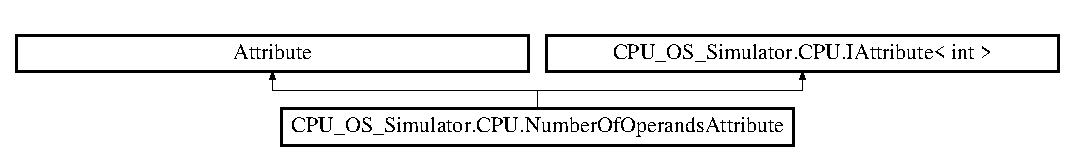
\includegraphics[height=1.733746cm]{class_c_p_u___o_s___simulator_1_1_c_p_u_1_1_number_of_operands_attribute}
\end{center}
\end{figure}
\subsection*{Public Member Functions}
\begin{DoxyCompactItemize}
\item 
\hyperlink{class_c_p_u___o_s___simulator_1_1_c_p_u_1_1_number_of_operands_attribute_a1976902af3b6dc92e16724d83937816e}{Number\+Of\+Operands\+Attribute} (int \hyperlink{class_c_p_u___o_s___simulator_1_1_c_p_u_1_1_number_of_operands_attribute_a23e7e9d6f0e3af1c7deddce153d13965}{value})
\begin{DoxyCompactList}\small\item\em Constructor for the Number\+O\+F\+Operands attribute \end{DoxyCompactList}\end{DoxyCompactItemize}
\subsection*{Properties}
\begin{DoxyCompactItemize}
\item 
int \hyperlink{class_c_p_u___o_s___simulator_1_1_c_p_u_1_1_number_of_operands_attribute_a00873634b211bcf2fd8b1425aa5143d6}{Value}\hspace{0.3cm}{\ttfamily  \mbox{[}get\mbox{]}}
\begin{DoxyCompactList}\small\item\em Property for the value of the attribute \end{DoxyCompactList}\end{DoxyCompactItemize}
\subsection*{Private Attributes}
\begin{DoxyCompactItemize}
\item 
readonly int \hyperlink{class_c_p_u___o_s___simulator_1_1_c_p_u_1_1_number_of_operands_attribute_a23e7e9d6f0e3af1c7deddce153d13965}{value}
\begin{DoxyCompactList}\small\item\em The value of the attribute \end{DoxyCompactList}\end{DoxyCompactItemize}


\subsection{Detailed Description}
This class represents the Number\+Of\+Operands attribute 



Definition at line 8 of file Number\+Of\+Operands\+Attribute.\+cs.



\subsection{Constructor \& Destructor Documentation}
\hypertarget{class_c_p_u___o_s___simulator_1_1_c_p_u_1_1_number_of_operands_attribute_a1976902af3b6dc92e16724d83937816e}{}\index{C\+P\+U\+\_\+\+O\+S\+\_\+\+Simulator\+::\+C\+P\+U\+::\+Number\+Of\+Operands\+Attribute@{C\+P\+U\+\_\+\+O\+S\+\_\+\+Simulator\+::\+C\+P\+U\+::\+Number\+Of\+Operands\+Attribute}!Number\+Of\+Operands\+Attribute@{Number\+Of\+Operands\+Attribute}}
\index{Number\+Of\+Operands\+Attribute@{Number\+Of\+Operands\+Attribute}!C\+P\+U\+\_\+\+O\+S\+\_\+\+Simulator\+::\+C\+P\+U\+::\+Number\+Of\+Operands\+Attribute@{C\+P\+U\+\_\+\+O\+S\+\_\+\+Simulator\+::\+C\+P\+U\+::\+Number\+Of\+Operands\+Attribute}}
\subsubsection[{Number\+Of\+Operands\+Attribute(int value)}]{\setlength{\rightskip}{0pt plus 5cm}C\+P\+U\+\_\+\+O\+S\+\_\+\+Simulator.\+C\+P\+U.\+Number\+Of\+Operands\+Attribute.\+Number\+Of\+Operands\+Attribute (
\begin{DoxyParamCaption}
\item[{int}]{value}
\end{DoxyParamCaption}
)}\label{class_c_p_u___o_s___simulator_1_1_c_p_u_1_1_number_of_operands_attribute_a1976902af3b6dc92e16724d83937816e}


Constructor for the Number\+O\+F\+Operands attribute 


\begin{DoxyParams}{Parameters}
{\em value} & the value to store in the attribute \\
\hline
\end{DoxyParams}


Definition at line 19 of file Number\+Of\+Operands\+Attribute.\+cs.



\subsection{Member Data Documentation}
\hypertarget{class_c_p_u___o_s___simulator_1_1_c_p_u_1_1_number_of_operands_attribute_a23e7e9d6f0e3af1c7deddce153d13965}{}\index{C\+P\+U\+\_\+\+O\+S\+\_\+\+Simulator\+::\+C\+P\+U\+::\+Number\+Of\+Operands\+Attribute@{C\+P\+U\+\_\+\+O\+S\+\_\+\+Simulator\+::\+C\+P\+U\+::\+Number\+Of\+Operands\+Attribute}!value@{value}}
\index{value@{value}!C\+P\+U\+\_\+\+O\+S\+\_\+\+Simulator\+::\+C\+P\+U\+::\+Number\+Of\+Operands\+Attribute@{C\+P\+U\+\_\+\+O\+S\+\_\+\+Simulator\+::\+C\+P\+U\+::\+Number\+Of\+Operands\+Attribute}}
\subsubsection[{value}]{\setlength{\rightskip}{0pt plus 5cm}readonly int C\+P\+U\+\_\+\+O\+S\+\_\+\+Simulator.\+C\+P\+U.\+Number\+Of\+Operands\+Attribute.\+value\hspace{0.3cm}{\ttfamily [private]}}\label{class_c_p_u___o_s___simulator_1_1_c_p_u_1_1_number_of_operands_attribute_a23e7e9d6f0e3af1c7deddce153d13965}


The value of the attribute 



Definition at line 13 of file Number\+Of\+Operands\+Attribute.\+cs.



\subsection{Property Documentation}
\hypertarget{class_c_p_u___o_s___simulator_1_1_c_p_u_1_1_number_of_operands_attribute_a00873634b211bcf2fd8b1425aa5143d6}{}\index{C\+P\+U\+\_\+\+O\+S\+\_\+\+Simulator\+::\+C\+P\+U\+::\+Number\+Of\+Operands\+Attribute@{C\+P\+U\+\_\+\+O\+S\+\_\+\+Simulator\+::\+C\+P\+U\+::\+Number\+Of\+Operands\+Attribute}!Value@{Value}}
\index{Value@{Value}!C\+P\+U\+\_\+\+O\+S\+\_\+\+Simulator\+::\+C\+P\+U\+::\+Number\+Of\+Operands\+Attribute@{C\+P\+U\+\_\+\+O\+S\+\_\+\+Simulator\+::\+C\+P\+U\+::\+Number\+Of\+Operands\+Attribute}}
\subsubsection[{Value}]{\setlength{\rightskip}{0pt plus 5cm}int C\+P\+U\+\_\+\+O\+S\+\_\+\+Simulator.\+C\+P\+U.\+Number\+Of\+Operands\+Attribute.\+Value\hspace{0.3cm}{\ttfamily [get]}}\label{class_c_p_u___o_s___simulator_1_1_c_p_u_1_1_number_of_operands_attribute_a00873634b211bcf2fd8b1425aa5143d6}


Property for the value of the attribute 



Definition at line 27 of file Number\+Of\+Operands\+Attribute.\+cs.



The documentation for this class was generated from the following file\+:\begin{DoxyCompactItemize}
\item 
C\+P\+U/\hyperlink{_number_of_operands_attribute_8cs}{Number\+Of\+Operands\+Attribute.\+cs}\end{DoxyCompactItemize}

\hypertarget{class_c_p_u___o_s___simulator_1_1_console_1_1_number_of_parameters_attribute}{}\section{C\+P\+U\+\_\+\+O\+S\+\_\+\+Simulator.\+Console.\+Number\+Of\+Parameters\+Attribute Class Reference}
\label{class_c_p_u___o_s___simulator_1_1_console_1_1_number_of_parameters_attribute}\index{C\+P\+U\+\_\+\+O\+S\+\_\+\+Simulator.\+Console.\+Number\+Of\+Parameters\+Attribute@{C\+P\+U\+\_\+\+O\+S\+\_\+\+Simulator.\+Console.\+Number\+Of\+Parameters\+Attribute}}


This class represents an attribute placed on console commands to indicate how many parameters they take  


Inheritance diagram for C\+P\+U\+\_\+\+O\+S\+\_\+\+Simulator.\+Console.\+Number\+Of\+Parameters\+Attribute\+:\begin{figure}[H]
\begin{center}
\leavevmode
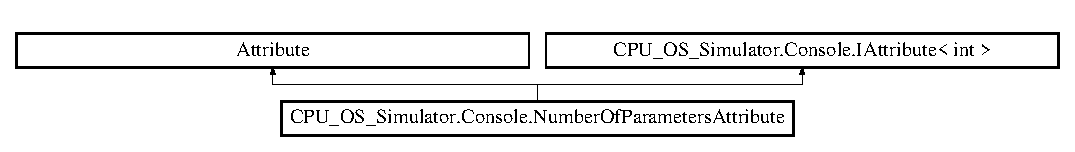
\includegraphics[height=1.590909cm]{class_c_p_u___o_s___simulator_1_1_console_1_1_number_of_parameters_attribute}
\end{center}
\end{figure}
\subsection*{Public Member Functions}
\begin{DoxyCompactItemize}
\item 
\hyperlink{class_c_p_u___o_s___simulator_1_1_console_1_1_number_of_parameters_attribute_a41059bf368ee101feb1a32c7468ebc2f}{Number\+Of\+Parameters\+Attribute} (int \hyperlink{class_c_p_u___o_s___simulator_1_1_console_1_1_number_of_parameters_attribute_a74f66203060602ef8135280692dc2064}{value})
\begin{DoxyCompactList}\small\item\em Constructor for \hyperlink{class_c_p_u___o_s___simulator_1_1_console_1_1_number_of_parameters_attribute}{Number\+Of\+Parameters\+Attribute} \end{DoxyCompactList}\end{DoxyCompactItemize}
\subsection*{Properties}
\begin{DoxyCompactItemize}
\item 
int \hyperlink{class_c_p_u___o_s___simulator_1_1_console_1_1_number_of_parameters_attribute_a7e083af44b45e3e68868d0d5d1991000}{Value}\hspace{0.3cm}{\ttfamily  \mbox{[}get, set\mbox{]}}
\begin{DoxyCompactList}\small\item\em Property to store the value of the attribute \end{DoxyCompactList}\end{DoxyCompactItemize}
\subsection*{Private Attributes}
\begin{DoxyCompactItemize}
\item 
int \hyperlink{class_c_p_u___o_s___simulator_1_1_console_1_1_number_of_parameters_attribute_a74f66203060602ef8135280692dc2064}{value}
\end{DoxyCompactItemize}


\subsection{Detailed Description}
This class represents an attribute placed on console commands to indicate how many parameters they take 



Definition at line 8 of file Number\+Of\+Parameters\+Attribute.\+cs.



\subsection{Constructor \& Destructor Documentation}
\hypertarget{class_c_p_u___o_s___simulator_1_1_console_1_1_number_of_parameters_attribute_a41059bf368ee101feb1a32c7468ebc2f}{}\index{C\+P\+U\+\_\+\+O\+S\+\_\+\+Simulator\+::\+Console\+::\+Number\+Of\+Parameters\+Attribute@{C\+P\+U\+\_\+\+O\+S\+\_\+\+Simulator\+::\+Console\+::\+Number\+Of\+Parameters\+Attribute}!Number\+Of\+Parameters\+Attribute@{Number\+Of\+Parameters\+Attribute}}
\index{Number\+Of\+Parameters\+Attribute@{Number\+Of\+Parameters\+Attribute}!C\+P\+U\+\_\+\+O\+S\+\_\+\+Simulator\+::\+Console\+::\+Number\+Of\+Parameters\+Attribute@{C\+P\+U\+\_\+\+O\+S\+\_\+\+Simulator\+::\+Console\+::\+Number\+Of\+Parameters\+Attribute}}
\subsubsection[{Number\+Of\+Parameters\+Attribute(int value)}]{\setlength{\rightskip}{0pt plus 5cm}C\+P\+U\+\_\+\+O\+S\+\_\+\+Simulator.\+Console.\+Number\+Of\+Parameters\+Attribute.\+Number\+Of\+Parameters\+Attribute (
\begin{DoxyParamCaption}
\item[{int}]{value}
\end{DoxyParamCaption}
)}\label{class_c_p_u___o_s___simulator_1_1_console_1_1_number_of_parameters_attribute_a41059bf368ee101feb1a32c7468ebc2f}


Constructor for \hyperlink{class_c_p_u___o_s___simulator_1_1_console_1_1_number_of_parameters_attribute}{Number\+Of\+Parameters\+Attribute} 


\begin{DoxyParams}{Parameters}
{\em value} & the value of the attribute\\
\hline
\end{DoxyParams}


Definition at line 15 of file Number\+Of\+Parameters\+Attribute.\+cs.



\subsection{Member Data Documentation}
\hypertarget{class_c_p_u___o_s___simulator_1_1_console_1_1_number_of_parameters_attribute_a74f66203060602ef8135280692dc2064}{}\index{C\+P\+U\+\_\+\+O\+S\+\_\+\+Simulator\+::\+Console\+::\+Number\+Of\+Parameters\+Attribute@{C\+P\+U\+\_\+\+O\+S\+\_\+\+Simulator\+::\+Console\+::\+Number\+Of\+Parameters\+Attribute}!value@{value}}
\index{value@{value}!C\+P\+U\+\_\+\+O\+S\+\_\+\+Simulator\+::\+Console\+::\+Number\+Of\+Parameters\+Attribute@{C\+P\+U\+\_\+\+O\+S\+\_\+\+Simulator\+::\+Console\+::\+Number\+Of\+Parameters\+Attribute}}
\subsubsection[{value}]{\setlength{\rightskip}{0pt plus 5cm}int C\+P\+U\+\_\+\+O\+S\+\_\+\+Simulator.\+Console.\+Number\+Of\+Parameters\+Attribute.\+value\hspace{0.3cm}{\ttfamily [private]}}\label{class_c_p_u___o_s___simulator_1_1_console_1_1_number_of_parameters_attribute_a74f66203060602ef8135280692dc2064}


Definition at line 10 of file Number\+Of\+Parameters\+Attribute.\+cs.



\subsection{Property Documentation}
\hypertarget{class_c_p_u___o_s___simulator_1_1_console_1_1_number_of_parameters_attribute_a7e083af44b45e3e68868d0d5d1991000}{}\index{C\+P\+U\+\_\+\+O\+S\+\_\+\+Simulator\+::\+Console\+::\+Number\+Of\+Parameters\+Attribute@{C\+P\+U\+\_\+\+O\+S\+\_\+\+Simulator\+::\+Console\+::\+Number\+Of\+Parameters\+Attribute}!Value@{Value}}
\index{Value@{Value}!C\+P\+U\+\_\+\+O\+S\+\_\+\+Simulator\+::\+Console\+::\+Number\+Of\+Parameters\+Attribute@{C\+P\+U\+\_\+\+O\+S\+\_\+\+Simulator\+::\+Console\+::\+Number\+Of\+Parameters\+Attribute}}
\subsubsection[{Value}]{\setlength{\rightskip}{0pt plus 5cm}int C\+P\+U\+\_\+\+O\+S\+\_\+\+Simulator.\+Console.\+Number\+Of\+Parameters\+Attribute.\+Value\hspace{0.3cm}{\ttfamily [get]}, {\ttfamily [set]}}\label{class_c_p_u___o_s___simulator_1_1_console_1_1_number_of_parameters_attribute_a7e083af44b45e3e68868d0d5d1991000}


Property to store the value of the attribute 



Definition at line 23 of file Number\+Of\+Parameters\+Attribute.\+cs.



The documentation for this class was generated from the following file\+:\begin{DoxyCompactItemize}
\item 
Console/\hyperlink{_number_of_parameters_attribute_8cs}{Number\+Of\+Parameters\+Attribute.\+cs}\end{DoxyCompactItemize}

\hypertarget{class_c_p_u___o_s___simulator_1_1_compiler_1_1_frontend_1_1_tokens_1_1_numeric_literal}{}\section{C\+P\+U\+\_\+\+O\+S\+\_\+\+Simulator.\+Compiler.\+Frontend.\+Tokens.\+Numeric\+Literal Class Reference}
\label{class_c_p_u___o_s___simulator_1_1_compiler_1_1_frontend_1_1_tokens_1_1_numeric_literal}\index{C\+P\+U\+\_\+\+O\+S\+\_\+\+Simulator.\+Compiler.\+Frontend.\+Tokens.\+Numeric\+Literal@{C\+P\+U\+\_\+\+O\+S\+\_\+\+Simulator.\+Compiler.\+Frontend.\+Tokens.\+Numeric\+Literal}}
Inheritance diagram for C\+P\+U\+\_\+\+O\+S\+\_\+\+Simulator.\+Compiler.\+Frontend.\+Tokens.\+Numeric\+Literal\+:\begin{figure}[H]
\begin{center}
\leavevmode
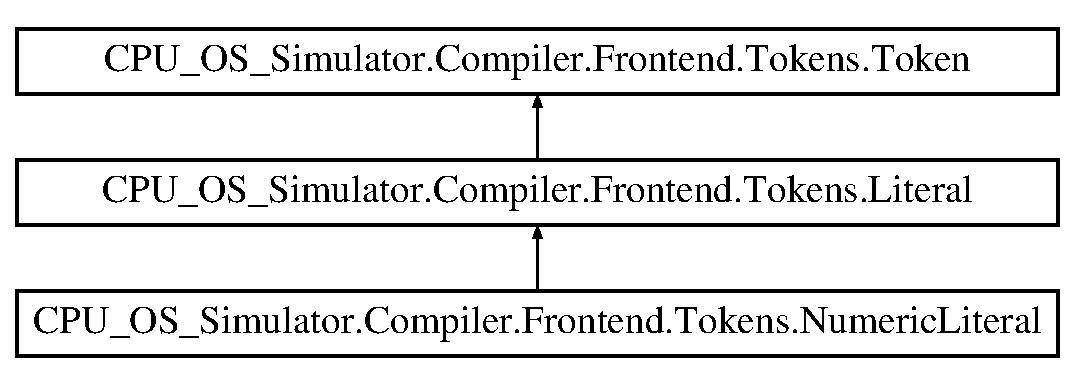
\includegraphics[height=3.000000cm]{class_c_p_u___o_s___simulator_1_1_compiler_1_1_frontend_1_1_tokens_1_1_numeric_literal}
\end{center}
\end{figure}
\subsection*{Public Member Functions}
\begin{DoxyCompactItemize}
\item 
\hyperlink{class_c_p_u___o_s___simulator_1_1_compiler_1_1_frontend_1_1_tokens_1_1_numeric_literal_a215f0217faf01222acfd4cf6a38a8e1b}{Numeric\+Literal} (string \hyperlink{class_c_p_u___o_s___simulator_1_1_compiler_1_1_frontend_1_1_tokens_1_1_token_a5c05e12850ca18be8cbfdf7e2e263324}{value})
\item 
override Enum \hyperlink{class_c_p_u___o_s___simulator_1_1_compiler_1_1_frontend_1_1_tokens_1_1_numeric_literal_a48f7635001171a738d1c53d065659933}{Detect\+Type} ()
\begin{DoxyCompactList}\small\item\em This function detects the type of literal \end{DoxyCompactList}\item 
override \hyperlink{namespace_c_p_u___o_s___simulator_1_1_compiler_1_1_frontend_1_1_tokens_a7c0cc43763cc9d01c7d5af34d70b96ea}{Enum\+Types} \hyperlink{class_c_p_u___o_s___simulator_1_1_compiler_1_1_frontend_1_1_tokens_1_1_numeric_literal_ac00d8a0002a5a291fba5713d385d11a6}{identfy\+Value\+Type} ()
\begin{DoxyCompactList}\small\item\em This function identifies the type of data stored in the literal \end{DoxyCompactList}\end{DoxyCompactItemize}
\subsection*{Additional Inherited Members}


\subsection{Detailed Description}


Definition at line 5 of file Numeric\+Literal.\+cs.



\subsection{Constructor \& Destructor Documentation}
\hypertarget{class_c_p_u___o_s___simulator_1_1_compiler_1_1_frontend_1_1_tokens_1_1_numeric_literal_a215f0217faf01222acfd4cf6a38a8e1b}{}\index{C\+P\+U\+\_\+\+O\+S\+\_\+\+Simulator\+::\+Compiler\+::\+Frontend\+::\+Tokens\+::\+Numeric\+Literal@{C\+P\+U\+\_\+\+O\+S\+\_\+\+Simulator\+::\+Compiler\+::\+Frontend\+::\+Tokens\+::\+Numeric\+Literal}!Numeric\+Literal@{Numeric\+Literal}}
\index{Numeric\+Literal@{Numeric\+Literal}!C\+P\+U\+\_\+\+O\+S\+\_\+\+Simulator\+::\+Compiler\+::\+Frontend\+::\+Tokens\+::\+Numeric\+Literal@{C\+P\+U\+\_\+\+O\+S\+\_\+\+Simulator\+::\+Compiler\+::\+Frontend\+::\+Tokens\+::\+Numeric\+Literal}}
\subsubsection[{Numeric\+Literal(string value)}]{\setlength{\rightskip}{0pt plus 5cm}C\+P\+U\+\_\+\+O\+S\+\_\+\+Simulator.\+Compiler.\+Frontend.\+Tokens.\+Numeric\+Literal.\+Numeric\+Literal (
\begin{DoxyParamCaption}
\item[{string}]{value}
\end{DoxyParamCaption}
)}\label{class_c_p_u___o_s___simulator_1_1_compiler_1_1_frontend_1_1_tokens_1_1_numeric_literal_a215f0217faf01222acfd4cf6a38a8e1b}


Definition at line 7 of file Numeric\+Literal.\+cs.



\subsection{Member Function Documentation}
\hypertarget{class_c_p_u___o_s___simulator_1_1_compiler_1_1_frontend_1_1_tokens_1_1_numeric_literal_a48f7635001171a738d1c53d065659933}{}\index{C\+P\+U\+\_\+\+O\+S\+\_\+\+Simulator\+::\+Compiler\+::\+Frontend\+::\+Tokens\+::\+Numeric\+Literal@{C\+P\+U\+\_\+\+O\+S\+\_\+\+Simulator\+::\+Compiler\+::\+Frontend\+::\+Tokens\+::\+Numeric\+Literal}!Detect\+Type@{Detect\+Type}}
\index{Detect\+Type@{Detect\+Type}!C\+P\+U\+\_\+\+O\+S\+\_\+\+Simulator\+::\+Compiler\+::\+Frontend\+::\+Tokens\+::\+Numeric\+Literal@{C\+P\+U\+\_\+\+O\+S\+\_\+\+Simulator\+::\+Compiler\+::\+Frontend\+::\+Tokens\+::\+Numeric\+Literal}}
\subsubsection[{Detect\+Type()}]{\setlength{\rightskip}{0pt plus 5cm}override Enum C\+P\+U\+\_\+\+O\+S\+\_\+\+Simulator.\+Compiler.\+Frontend.\+Tokens.\+Numeric\+Literal.\+Detect\+Type (
\begin{DoxyParamCaption}
{}
\end{DoxyParamCaption}
)\hspace{0.3cm}{\ttfamily [virtual]}}\label{class_c_p_u___o_s___simulator_1_1_compiler_1_1_frontend_1_1_tokens_1_1_numeric_literal_a48f7635001171a738d1c53d065659933}


This function detects the type of literal 

\begin{DoxyReturn}{Returns}
the type of literal
\end{DoxyReturn}


Implements \hyperlink{class_c_p_u___o_s___simulator_1_1_compiler_1_1_frontend_1_1_tokens_1_1_literal_af449c5fee28fb2076933cdfc67857c23}{C\+P\+U\+\_\+\+O\+S\+\_\+\+Simulator.\+Compiler.\+Frontend.\+Tokens.\+Literal}.



Definition at line 15 of file Numeric\+Literal.\+cs.

\hypertarget{class_c_p_u___o_s___simulator_1_1_compiler_1_1_frontend_1_1_tokens_1_1_numeric_literal_ac00d8a0002a5a291fba5713d385d11a6}{}\index{C\+P\+U\+\_\+\+O\+S\+\_\+\+Simulator\+::\+Compiler\+::\+Frontend\+::\+Tokens\+::\+Numeric\+Literal@{C\+P\+U\+\_\+\+O\+S\+\_\+\+Simulator\+::\+Compiler\+::\+Frontend\+::\+Tokens\+::\+Numeric\+Literal}!identfy\+Value\+Type@{identfy\+Value\+Type}}
\index{identfy\+Value\+Type@{identfy\+Value\+Type}!C\+P\+U\+\_\+\+O\+S\+\_\+\+Simulator\+::\+Compiler\+::\+Frontend\+::\+Tokens\+::\+Numeric\+Literal@{C\+P\+U\+\_\+\+O\+S\+\_\+\+Simulator\+::\+Compiler\+::\+Frontend\+::\+Tokens\+::\+Numeric\+Literal}}
\subsubsection[{identfy\+Value\+Type()}]{\setlength{\rightskip}{0pt plus 5cm}override {\bf Enum\+Types} C\+P\+U\+\_\+\+O\+S\+\_\+\+Simulator.\+Compiler.\+Frontend.\+Tokens.\+Numeric\+Literal.\+identfy\+Value\+Type (
\begin{DoxyParamCaption}
{}
\end{DoxyParamCaption}
)\hspace{0.3cm}{\ttfamily [virtual]}}\label{class_c_p_u___o_s___simulator_1_1_compiler_1_1_frontend_1_1_tokens_1_1_numeric_literal_ac00d8a0002a5a291fba5713d385d11a6}


This function identifies the type of data stored in the literal 

\begin{DoxyReturn}{Returns}
the type of value in the literal
\end{DoxyReturn}


Implements \hyperlink{class_c_p_u___o_s___simulator_1_1_compiler_1_1_frontend_1_1_tokens_1_1_literal_a34d05c00ded660daf66f91bd2543d186}{C\+P\+U\+\_\+\+O\+S\+\_\+\+Simulator.\+Compiler.\+Frontend.\+Tokens.\+Literal}.



Definition at line 24 of file Numeric\+Literal.\+cs.



The documentation for this class was generated from the following file\+:\begin{DoxyCompactItemize}
\item 
Compiler/\+Frontend/\+Tokens/\hyperlink{_numeric_literal_8cs}{Numeric\+Literal.\+cs}\end{DoxyCompactItemize}

\hypertarget{class_c_p_u___o_s___simulator_1_1_compiler_1_1_frontend_1_1_syntax_tree_1_1_object_array_node}{}\section{C\+P\+U\+\_\+\+O\+S\+\_\+\+Simulator.\+Compiler.\+Frontend.\+Syntax\+Tree.\+Object\+Array\+Node Class Reference}
\label{class_c_p_u___o_s___simulator_1_1_compiler_1_1_frontend_1_1_syntax_tree_1_1_object_array_node}\index{C\+P\+U\+\_\+\+O\+S\+\_\+\+Simulator.\+Compiler.\+Frontend.\+Syntax\+Tree.\+Object\+Array\+Node@{C\+P\+U\+\_\+\+O\+S\+\_\+\+Simulator.\+Compiler.\+Frontend.\+Syntax\+Tree.\+Object\+Array\+Node}}
Inheritance diagram for C\+P\+U\+\_\+\+O\+S\+\_\+\+Simulator.\+Compiler.\+Frontend.\+Syntax\+Tree.\+Object\+Array\+Node\+:\begin{figure}[H]
\begin{center}
\leavevmode
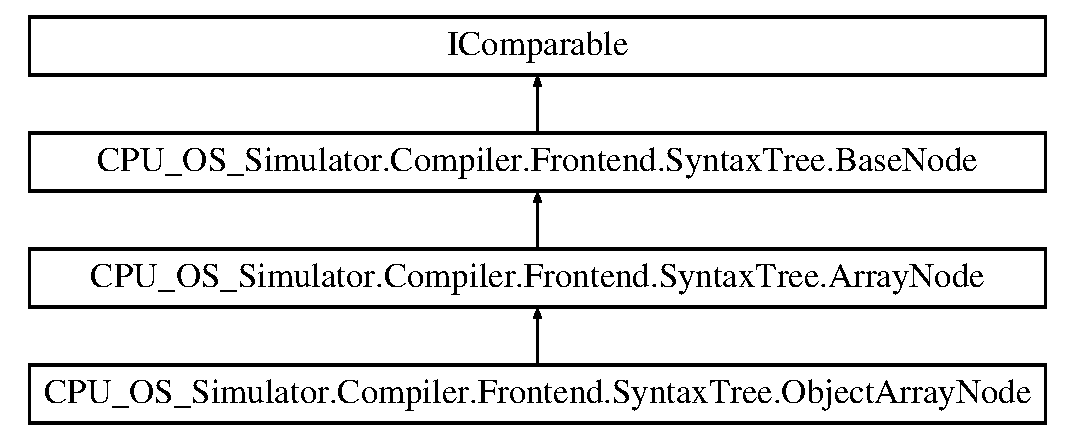
\includegraphics[height=4.000000cm]{class_c_p_u___o_s___simulator_1_1_compiler_1_1_frontend_1_1_syntax_tree_1_1_object_array_node}
\end{center}
\end{figure}
\subsection*{Public Member Functions}
\begin{DoxyCompactItemize}
\item 
override void \hyperlink{class_c_p_u___o_s___simulator_1_1_compiler_1_1_frontend_1_1_syntax_tree_1_1_object_array_node_a1d792b3929152ecfa25dac2e8c6444cc}{Visit} ()
\begin{DoxyCompactList}\small\item\em This function is called when the node is being visited by the parser \end{DoxyCompactList}\item 
override void \hyperlink{class_c_p_u___o_s___simulator_1_1_compiler_1_1_frontend_1_1_syntax_tree_1_1_object_array_node_ad0c63367dd74b502a0e510b95e324405}{Evaluate} ()
\begin{DoxyCompactList}\small\item\em This Function is called when the node is being evaluated by the parser \end{DoxyCompactList}\item 
override int \hyperlink{class_c_p_u___o_s___simulator_1_1_compiler_1_1_frontend_1_1_syntax_tree_1_1_object_array_node_ae2b8cfd71ef1f35f3f74d700fc542fc1}{number\+Of\+Elements} ()
\end{DoxyCompactItemize}
\subsection*{Properties}
\begin{DoxyCompactItemize}
\item 
override \hyperlink{class_c_p_u___o_s___simulator_1_1_compiler_1_1_frontend_1_1_syntax_tree_1_1_base_node}{Base\+Node} \hyperlink{class_c_p_u___o_s___simulator_1_1_compiler_1_1_frontend_1_1_syntax_tree_1_1_object_array_node_a2d9530e83ab4ec41ac69cf452ba2f481}{Right}\hspace{0.3cm}{\ttfamily  \mbox{[}get, set\mbox{]}}
\item 
override \hyperlink{class_c_p_u___o_s___simulator_1_1_compiler_1_1_frontend_1_1_syntax_tree_1_1_base_node}{Base\+Node} \hyperlink{class_c_p_u___o_s___simulator_1_1_compiler_1_1_frontend_1_1_syntax_tree_1_1_object_array_node_a2bc2e06dce266a618b199a8042130ad8}{Left}\hspace{0.3cm}{\ttfamily  \mbox{[}get, set\mbox{]}}
\item 
object\mbox{[}$\,$\mbox{]} \hyperlink{class_c_p_u___o_s___simulator_1_1_compiler_1_1_frontend_1_1_syntax_tree_1_1_object_array_node_ac55a614579d52347e88cd026aec8e7f6}{Data}\hspace{0.3cm}{\ttfamily  \mbox{[}get, set\mbox{]}}
\item 
override \hyperlink{class_c_p_u___o_s___simulator_1_1_compiler_1_1_frontend_1_1_syntax_tree_1_1_base_node}{Base\+Node} \hyperlink{class_c_p_u___o_s___simulator_1_1_compiler_1_1_frontend_1_1_syntax_tree_1_1_object_array_node_a084c1e95fcafd4b6fbba8f26c7f3912d}{Parent}\hspace{0.3cm}{\ttfamily  \mbox{[}get, set\mbox{]}}
\end{DoxyCompactItemize}
\subsection*{Private Attributes}
\begin{DoxyCompactItemize}
\item 
new object\mbox{[}$\,$\mbox{]} \hyperlink{class_c_p_u___o_s___simulator_1_1_compiler_1_1_frontend_1_1_syntax_tree_1_1_object_array_node_af1634225202fae16f595bdd5d0426669}{data}
\item 
\hyperlink{class_c_p_u___o_s___simulator_1_1_compiler_1_1_frontend_1_1_syntax_tree_1_1_base_node}{Base\+Node} \hyperlink{class_c_p_u___o_s___simulator_1_1_compiler_1_1_frontend_1_1_syntax_tree_1_1_object_array_node_a5738424abfdf383d5e8539b4f34879b8}{parent}
\end{DoxyCompactItemize}
\subsection*{Additional Inherited Members}


\subsection{Detailed Description}


Definition at line 3 of file Object\+Array\+Node.\+cs.



\subsection{Member Function Documentation}
\hypertarget{class_c_p_u___o_s___simulator_1_1_compiler_1_1_frontend_1_1_syntax_tree_1_1_object_array_node_ad0c63367dd74b502a0e510b95e324405}{}\index{C\+P\+U\+\_\+\+O\+S\+\_\+\+Simulator\+::\+Compiler\+::\+Frontend\+::\+Syntax\+Tree\+::\+Object\+Array\+Node@{C\+P\+U\+\_\+\+O\+S\+\_\+\+Simulator\+::\+Compiler\+::\+Frontend\+::\+Syntax\+Tree\+::\+Object\+Array\+Node}!Evaluate@{Evaluate}}
\index{Evaluate@{Evaluate}!C\+P\+U\+\_\+\+O\+S\+\_\+\+Simulator\+::\+Compiler\+::\+Frontend\+::\+Syntax\+Tree\+::\+Object\+Array\+Node@{C\+P\+U\+\_\+\+O\+S\+\_\+\+Simulator\+::\+Compiler\+::\+Frontend\+::\+Syntax\+Tree\+::\+Object\+Array\+Node}}
\subsubsection[{Evaluate()}]{\setlength{\rightskip}{0pt plus 5cm}override void C\+P\+U\+\_\+\+O\+S\+\_\+\+Simulator.\+Compiler.\+Frontend.\+Syntax\+Tree.\+Object\+Array\+Node.\+Evaluate (
\begin{DoxyParamCaption}
{}
\end{DoxyParamCaption}
)\hspace{0.3cm}{\ttfamily [virtual]}}\label{class_c_p_u___o_s___simulator_1_1_compiler_1_1_frontend_1_1_syntax_tree_1_1_object_array_node_ad0c63367dd74b502a0e510b95e324405}


This Function is called when the node is being evaluated by the parser 



Implements \hyperlink{class_c_p_u___o_s___simulator_1_1_compiler_1_1_frontend_1_1_syntax_tree_1_1_array_node_afdb5d2808dbd83c28c85f35b6430edc4}{C\+P\+U\+\_\+\+O\+S\+\_\+\+Simulator.\+Compiler.\+Frontend.\+Syntax\+Tree.\+Array\+Node}.



Definition at line 42 of file Object\+Array\+Node.\+cs.

\hypertarget{class_c_p_u___o_s___simulator_1_1_compiler_1_1_frontend_1_1_syntax_tree_1_1_object_array_node_ae2b8cfd71ef1f35f3f74d700fc542fc1}{}\index{C\+P\+U\+\_\+\+O\+S\+\_\+\+Simulator\+::\+Compiler\+::\+Frontend\+::\+Syntax\+Tree\+::\+Object\+Array\+Node@{C\+P\+U\+\_\+\+O\+S\+\_\+\+Simulator\+::\+Compiler\+::\+Frontend\+::\+Syntax\+Tree\+::\+Object\+Array\+Node}!number\+Of\+Elements@{number\+Of\+Elements}}
\index{number\+Of\+Elements@{number\+Of\+Elements}!C\+P\+U\+\_\+\+O\+S\+\_\+\+Simulator\+::\+Compiler\+::\+Frontend\+::\+Syntax\+Tree\+::\+Object\+Array\+Node@{C\+P\+U\+\_\+\+O\+S\+\_\+\+Simulator\+::\+Compiler\+::\+Frontend\+::\+Syntax\+Tree\+::\+Object\+Array\+Node}}
\subsubsection[{number\+Of\+Elements()}]{\setlength{\rightskip}{0pt plus 5cm}override int C\+P\+U\+\_\+\+O\+S\+\_\+\+Simulator.\+Compiler.\+Frontend.\+Syntax\+Tree.\+Object\+Array\+Node.\+number\+Of\+Elements (
\begin{DoxyParamCaption}
{}
\end{DoxyParamCaption}
)\hspace{0.3cm}{\ttfamily [virtual]}}\label{class_c_p_u___o_s___simulator_1_1_compiler_1_1_frontend_1_1_syntax_tree_1_1_object_array_node_ae2b8cfd71ef1f35f3f74d700fc542fc1}


Implements \hyperlink{class_c_p_u___o_s___simulator_1_1_compiler_1_1_frontend_1_1_syntax_tree_1_1_array_node_a75232f3076d95a562405ef2722bcafd5}{C\+P\+U\+\_\+\+O\+S\+\_\+\+Simulator.\+Compiler.\+Frontend.\+Syntax\+Tree.\+Array\+Node}.



Definition at line 46 of file Object\+Array\+Node.\+cs.

\hypertarget{class_c_p_u___o_s___simulator_1_1_compiler_1_1_frontend_1_1_syntax_tree_1_1_object_array_node_a1d792b3929152ecfa25dac2e8c6444cc}{}\index{C\+P\+U\+\_\+\+O\+S\+\_\+\+Simulator\+::\+Compiler\+::\+Frontend\+::\+Syntax\+Tree\+::\+Object\+Array\+Node@{C\+P\+U\+\_\+\+O\+S\+\_\+\+Simulator\+::\+Compiler\+::\+Frontend\+::\+Syntax\+Tree\+::\+Object\+Array\+Node}!Visit@{Visit}}
\index{Visit@{Visit}!C\+P\+U\+\_\+\+O\+S\+\_\+\+Simulator\+::\+Compiler\+::\+Frontend\+::\+Syntax\+Tree\+::\+Object\+Array\+Node@{C\+P\+U\+\_\+\+O\+S\+\_\+\+Simulator\+::\+Compiler\+::\+Frontend\+::\+Syntax\+Tree\+::\+Object\+Array\+Node}}
\subsubsection[{Visit()}]{\setlength{\rightskip}{0pt plus 5cm}override void C\+P\+U\+\_\+\+O\+S\+\_\+\+Simulator.\+Compiler.\+Frontend.\+Syntax\+Tree.\+Object\+Array\+Node.\+Visit (
\begin{DoxyParamCaption}
{}
\end{DoxyParamCaption}
)\hspace{0.3cm}{\ttfamily [virtual]}}\label{class_c_p_u___o_s___simulator_1_1_compiler_1_1_frontend_1_1_syntax_tree_1_1_object_array_node_a1d792b3929152ecfa25dac2e8c6444cc}


This function is called when the node is being visited by the parser 



Implements \hyperlink{class_c_p_u___o_s___simulator_1_1_compiler_1_1_frontend_1_1_syntax_tree_1_1_array_node_aed695b6f32d5c176204fc15854db32db}{C\+P\+U\+\_\+\+O\+S\+\_\+\+Simulator.\+Compiler.\+Frontend.\+Syntax\+Tree.\+Array\+Node}.



Definition at line 35 of file Object\+Array\+Node.\+cs.



\subsection{Member Data Documentation}
\hypertarget{class_c_p_u___o_s___simulator_1_1_compiler_1_1_frontend_1_1_syntax_tree_1_1_object_array_node_af1634225202fae16f595bdd5d0426669}{}\index{C\+P\+U\+\_\+\+O\+S\+\_\+\+Simulator\+::\+Compiler\+::\+Frontend\+::\+Syntax\+Tree\+::\+Object\+Array\+Node@{C\+P\+U\+\_\+\+O\+S\+\_\+\+Simulator\+::\+Compiler\+::\+Frontend\+::\+Syntax\+Tree\+::\+Object\+Array\+Node}!data@{data}}
\index{data@{data}!C\+P\+U\+\_\+\+O\+S\+\_\+\+Simulator\+::\+Compiler\+::\+Frontend\+::\+Syntax\+Tree\+::\+Object\+Array\+Node@{C\+P\+U\+\_\+\+O\+S\+\_\+\+Simulator\+::\+Compiler\+::\+Frontend\+::\+Syntax\+Tree\+::\+Object\+Array\+Node}}
\subsubsection[{data}]{\setlength{\rightskip}{0pt plus 5cm}new object \mbox{[}$\,$\mbox{]} C\+P\+U\+\_\+\+O\+S\+\_\+\+Simulator.\+Compiler.\+Frontend.\+Syntax\+Tree.\+Object\+Array\+Node.\+data\hspace{0.3cm}{\ttfamily [private]}}\label{class_c_p_u___o_s___simulator_1_1_compiler_1_1_frontend_1_1_syntax_tree_1_1_object_array_node_af1634225202fae16f595bdd5d0426669}


Definition at line 5 of file Object\+Array\+Node.\+cs.

\hypertarget{class_c_p_u___o_s___simulator_1_1_compiler_1_1_frontend_1_1_syntax_tree_1_1_object_array_node_a5738424abfdf383d5e8539b4f34879b8}{}\index{C\+P\+U\+\_\+\+O\+S\+\_\+\+Simulator\+::\+Compiler\+::\+Frontend\+::\+Syntax\+Tree\+::\+Object\+Array\+Node@{C\+P\+U\+\_\+\+O\+S\+\_\+\+Simulator\+::\+Compiler\+::\+Frontend\+::\+Syntax\+Tree\+::\+Object\+Array\+Node}!parent@{parent}}
\index{parent@{parent}!C\+P\+U\+\_\+\+O\+S\+\_\+\+Simulator\+::\+Compiler\+::\+Frontend\+::\+Syntax\+Tree\+::\+Object\+Array\+Node@{C\+P\+U\+\_\+\+O\+S\+\_\+\+Simulator\+::\+Compiler\+::\+Frontend\+::\+Syntax\+Tree\+::\+Object\+Array\+Node}}
\subsubsection[{parent}]{\setlength{\rightskip}{0pt plus 5cm}{\bf Base\+Node} C\+P\+U\+\_\+\+O\+S\+\_\+\+Simulator.\+Compiler.\+Frontend.\+Syntax\+Tree.\+Object\+Array\+Node.\+parent\hspace{0.3cm}{\ttfamily [private]}}\label{class_c_p_u___o_s___simulator_1_1_compiler_1_1_frontend_1_1_syntax_tree_1_1_object_array_node_a5738424abfdf383d5e8539b4f34879b8}


Definition at line 6 of file Object\+Array\+Node.\+cs.



\subsection{Property Documentation}
\hypertarget{class_c_p_u___o_s___simulator_1_1_compiler_1_1_frontend_1_1_syntax_tree_1_1_object_array_node_ac55a614579d52347e88cd026aec8e7f6}{}\index{C\+P\+U\+\_\+\+O\+S\+\_\+\+Simulator\+::\+Compiler\+::\+Frontend\+::\+Syntax\+Tree\+::\+Object\+Array\+Node@{C\+P\+U\+\_\+\+O\+S\+\_\+\+Simulator\+::\+Compiler\+::\+Frontend\+::\+Syntax\+Tree\+::\+Object\+Array\+Node}!Data@{Data}}
\index{Data@{Data}!C\+P\+U\+\_\+\+O\+S\+\_\+\+Simulator\+::\+Compiler\+::\+Frontend\+::\+Syntax\+Tree\+::\+Object\+Array\+Node@{C\+P\+U\+\_\+\+O\+S\+\_\+\+Simulator\+::\+Compiler\+::\+Frontend\+::\+Syntax\+Tree\+::\+Object\+Array\+Node}}
\subsubsection[{Data}]{\setlength{\rightskip}{0pt plus 5cm}object \mbox{[}$\,$\mbox{]} C\+P\+U\+\_\+\+O\+S\+\_\+\+Simulator.\+Compiler.\+Frontend.\+Syntax\+Tree.\+Object\+Array\+Node.\+Data\hspace{0.3cm}{\ttfamily [get]}, {\ttfamily [set]}}\label{class_c_p_u___o_s___simulator_1_1_compiler_1_1_frontend_1_1_syntax_tree_1_1_object_array_node_ac55a614579d52347e88cd026aec8e7f6}


Definition at line 21 of file Object\+Array\+Node.\+cs.

\hypertarget{class_c_p_u___o_s___simulator_1_1_compiler_1_1_frontend_1_1_syntax_tree_1_1_object_array_node_a2bc2e06dce266a618b199a8042130ad8}{}\index{C\+P\+U\+\_\+\+O\+S\+\_\+\+Simulator\+::\+Compiler\+::\+Frontend\+::\+Syntax\+Tree\+::\+Object\+Array\+Node@{C\+P\+U\+\_\+\+O\+S\+\_\+\+Simulator\+::\+Compiler\+::\+Frontend\+::\+Syntax\+Tree\+::\+Object\+Array\+Node}!Left@{Left}}
\index{Left@{Left}!C\+P\+U\+\_\+\+O\+S\+\_\+\+Simulator\+::\+Compiler\+::\+Frontend\+::\+Syntax\+Tree\+::\+Object\+Array\+Node@{C\+P\+U\+\_\+\+O\+S\+\_\+\+Simulator\+::\+Compiler\+::\+Frontend\+::\+Syntax\+Tree\+::\+Object\+Array\+Node}}
\subsubsection[{Left}]{\setlength{\rightskip}{0pt plus 5cm}override {\bf Base\+Node} C\+P\+U\+\_\+\+O\+S\+\_\+\+Simulator.\+Compiler.\+Frontend.\+Syntax\+Tree.\+Object\+Array\+Node.\+Left\hspace{0.3cm}{\ttfamily [get]}, {\ttfamily [set]}}\label{class_c_p_u___o_s___simulator_1_1_compiler_1_1_frontend_1_1_syntax_tree_1_1_object_array_node_a2bc2e06dce266a618b199a8042130ad8}


Definition at line 15 of file Object\+Array\+Node.\+cs.

\hypertarget{class_c_p_u___o_s___simulator_1_1_compiler_1_1_frontend_1_1_syntax_tree_1_1_object_array_node_a084c1e95fcafd4b6fbba8f26c7f3912d}{}\index{C\+P\+U\+\_\+\+O\+S\+\_\+\+Simulator\+::\+Compiler\+::\+Frontend\+::\+Syntax\+Tree\+::\+Object\+Array\+Node@{C\+P\+U\+\_\+\+O\+S\+\_\+\+Simulator\+::\+Compiler\+::\+Frontend\+::\+Syntax\+Tree\+::\+Object\+Array\+Node}!Parent@{Parent}}
\index{Parent@{Parent}!C\+P\+U\+\_\+\+O\+S\+\_\+\+Simulator\+::\+Compiler\+::\+Frontend\+::\+Syntax\+Tree\+::\+Object\+Array\+Node@{C\+P\+U\+\_\+\+O\+S\+\_\+\+Simulator\+::\+Compiler\+::\+Frontend\+::\+Syntax\+Tree\+::\+Object\+Array\+Node}}
\subsubsection[{Parent}]{\setlength{\rightskip}{0pt plus 5cm}override {\bf Base\+Node} C\+P\+U\+\_\+\+O\+S\+\_\+\+Simulator.\+Compiler.\+Frontend.\+Syntax\+Tree.\+Object\+Array\+Node.\+Parent\hspace{0.3cm}{\ttfamily [get]}, {\ttfamily [set]}}\label{class_c_p_u___o_s___simulator_1_1_compiler_1_1_frontend_1_1_syntax_tree_1_1_object_array_node_a084c1e95fcafd4b6fbba8f26c7f3912d}


Definition at line 27 of file Object\+Array\+Node.\+cs.

\hypertarget{class_c_p_u___o_s___simulator_1_1_compiler_1_1_frontend_1_1_syntax_tree_1_1_object_array_node_a2d9530e83ab4ec41ac69cf452ba2f481}{}\index{C\+P\+U\+\_\+\+O\+S\+\_\+\+Simulator\+::\+Compiler\+::\+Frontend\+::\+Syntax\+Tree\+::\+Object\+Array\+Node@{C\+P\+U\+\_\+\+O\+S\+\_\+\+Simulator\+::\+Compiler\+::\+Frontend\+::\+Syntax\+Tree\+::\+Object\+Array\+Node}!Right@{Right}}
\index{Right@{Right}!C\+P\+U\+\_\+\+O\+S\+\_\+\+Simulator\+::\+Compiler\+::\+Frontend\+::\+Syntax\+Tree\+::\+Object\+Array\+Node@{C\+P\+U\+\_\+\+O\+S\+\_\+\+Simulator\+::\+Compiler\+::\+Frontend\+::\+Syntax\+Tree\+::\+Object\+Array\+Node}}
\subsubsection[{Right}]{\setlength{\rightskip}{0pt plus 5cm}override {\bf Base\+Node} C\+P\+U\+\_\+\+O\+S\+\_\+\+Simulator.\+Compiler.\+Frontend.\+Syntax\+Tree.\+Object\+Array\+Node.\+Right\hspace{0.3cm}{\ttfamily [get]}, {\ttfamily [set]}}\label{class_c_p_u___o_s___simulator_1_1_compiler_1_1_frontend_1_1_syntax_tree_1_1_object_array_node_a2d9530e83ab4ec41ac69cf452ba2f481}


Definition at line 9 of file Object\+Array\+Node.\+cs.



The documentation for this class was generated from the following file\+:\begin{DoxyCompactItemize}
\item 
Compiler/\+Frontend/\+Syntax\+Tree/\hyperlink{_object_array_node_8cs}{Object\+Array\+Node.\+cs}\end{DoxyCompactItemize}

\hypertarget{class_c_p_u___o_s___simulator_1_1_compiler_1_1_frontend_1_1_syntax_tree_1_1_object_node}{}\section{C\+P\+U\+\_\+\+O\+S\+\_\+\+Simulator.\+Compiler.\+Frontend.\+Syntax\+Tree.\+Object\+Node Class Reference}
\label{class_c_p_u___o_s___simulator_1_1_compiler_1_1_frontend_1_1_syntax_tree_1_1_object_node}\index{C\+P\+U\+\_\+\+O\+S\+\_\+\+Simulator.\+Compiler.\+Frontend.\+Syntax\+Tree.\+Object\+Node@{C\+P\+U\+\_\+\+O\+S\+\_\+\+Simulator.\+Compiler.\+Frontend.\+Syntax\+Tree.\+Object\+Node}}
Inheritance diagram for C\+P\+U\+\_\+\+O\+S\+\_\+\+Simulator.\+Compiler.\+Frontend.\+Syntax\+Tree.\+Object\+Node\+:\begin{figure}[H]
\begin{center}
\leavevmode
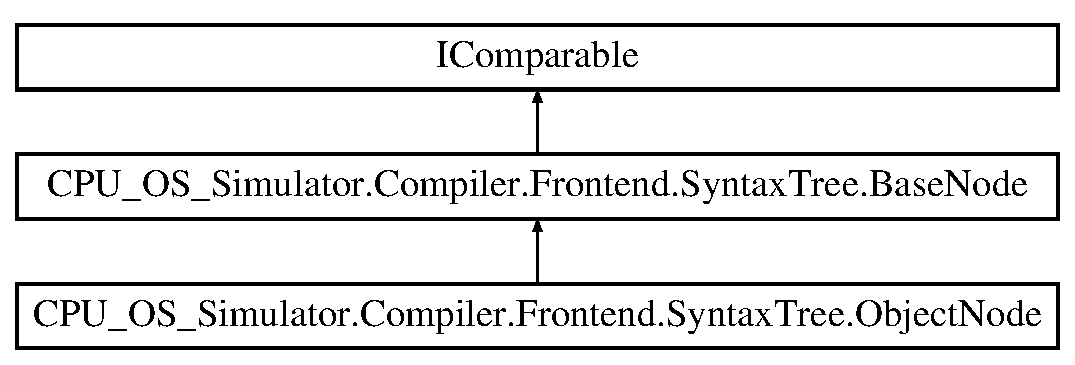
\includegraphics[height=3.000000cm]{class_c_p_u___o_s___simulator_1_1_compiler_1_1_frontend_1_1_syntax_tree_1_1_object_node}
\end{center}
\end{figure}
\subsection*{Public Member Functions}
\begin{DoxyCompactItemize}
\item 
override void \hyperlink{class_c_p_u___o_s___simulator_1_1_compiler_1_1_frontend_1_1_syntax_tree_1_1_object_node_a2c77bb89c3638cfb39c6fd1a40b63d71}{Visit} ()
\begin{DoxyCompactList}\small\item\em This function is called when the node is being visited by the parser \end{DoxyCompactList}\item 
override void \hyperlink{class_c_p_u___o_s___simulator_1_1_compiler_1_1_frontend_1_1_syntax_tree_1_1_object_node_a52be0559ec5f7c7171d5b17ce9cbb385}{Evaluate} ()
\begin{DoxyCompactList}\small\item\em This Function is called when the node is being evaluated by the parser \end{DoxyCompactList}\end{DoxyCompactItemize}
\subsection*{Properties}
\begin{DoxyCompactItemize}
\item 
override \hyperlink{class_c_p_u___o_s___simulator_1_1_compiler_1_1_frontend_1_1_syntax_tree_1_1_base_node}{Base\+Node} \hyperlink{class_c_p_u___o_s___simulator_1_1_compiler_1_1_frontend_1_1_syntax_tree_1_1_object_node_af150ad666f3f81bf9bf28acde2cc4b03}{Right}\hspace{0.3cm}{\ttfamily  \mbox{[}get, set\mbox{]}}
\item 
override \hyperlink{class_c_p_u___o_s___simulator_1_1_compiler_1_1_frontend_1_1_syntax_tree_1_1_base_node}{Base\+Node} \hyperlink{class_c_p_u___o_s___simulator_1_1_compiler_1_1_frontend_1_1_syntax_tree_1_1_object_node_a7a20bf72d63acfba02c741089f7299f2}{Left}\hspace{0.3cm}{\ttfamily  \mbox{[}get, set\mbox{]}}
\item 
object \hyperlink{class_c_p_u___o_s___simulator_1_1_compiler_1_1_frontend_1_1_syntax_tree_1_1_object_node_a686cc76f0ea20b7e2c139d87bfbf4af3}{Data}\hspace{0.3cm}{\ttfamily  \mbox{[}get, set\mbox{]}}
\item 
override \hyperlink{class_c_p_u___o_s___simulator_1_1_compiler_1_1_frontend_1_1_syntax_tree_1_1_base_node}{Base\+Node} \hyperlink{class_c_p_u___o_s___simulator_1_1_compiler_1_1_frontend_1_1_syntax_tree_1_1_object_node_a2e577044fc241b61f00843fdecfe5a3c}{Parent}\hspace{0.3cm}{\ttfamily  \mbox{[}get, set\mbox{]}}
\end{DoxyCompactItemize}
\subsection*{Private Attributes}
\begin{DoxyCompactItemize}
\item 
new object \hyperlink{class_c_p_u___o_s___simulator_1_1_compiler_1_1_frontend_1_1_syntax_tree_1_1_object_node_aa5b7d038958e37b2844917dc2eff3138}{data}
\item 
\hyperlink{class_c_p_u___o_s___simulator_1_1_compiler_1_1_frontend_1_1_syntax_tree_1_1_base_node}{Base\+Node} \hyperlink{class_c_p_u___o_s___simulator_1_1_compiler_1_1_frontend_1_1_syntax_tree_1_1_object_node_ae3e3c6c5352278b92070cf410554b10c}{parent}
\end{DoxyCompactItemize}
\subsection*{Additional Inherited Members}


\subsection{Detailed Description}


Definition at line 3 of file Object\+Node.\+cs.



\subsection{Member Function Documentation}
\hypertarget{class_c_p_u___o_s___simulator_1_1_compiler_1_1_frontend_1_1_syntax_tree_1_1_object_node_a52be0559ec5f7c7171d5b17ce9cbb385}{}\index{C\+P\+U\+\_\+\+O\+S\+\_\+\+Simulator\+::\+Compiler\+::\+Frontend\+::\+Syntax\+Tree\+::\+Object\+Node@{C\+P\+U\+\_\+\+O\+S\+\_\+\+Simulator\+::\+Compiler\+::\+Frontend\+::\+Syntax\+Tree\+::\+Object\+Node}!Evaluate@{Evaluate}}
\index{Evaluate@{Evaluate}!C\+P\+U\+\_\+\+O\+S\+\_\+\+Simulator\+::\+Compiler\+::\+Frontend\+::\+Syntax\+Tree\+::\+Object\+Node@{C\+P\+U\+\_\+\+O\+S\+\_\+\+Simulator\+::\+Compiler\+::\+Frontend\+::\+Syntax\+Tree\+::\+Object\+Node}}
\subsubsection[{Evaluate()}]{\setlength{\rightskip}{0pt plus 5cm}override void C\+P\+U\+\_\+\+O\+S\+\_\+\+Simulator.\+Compiler.\+Frontend.\+Syntax\+Tree.\+Object\+Node.\+Evaluate (
\begin{DoxyParamCaption}
{}
\end{DoxyParamCaption}
)\hspace{0.3cm}{\ttfamily [virtual]}}\label{class_c_p_u___o_s___simulator_1_1_compiler_1_1_frontend_1_1_syntax_tree_1_1_object_node_a52be0559ec5f7c7171d5b17ce9cbb385}


This Function is called when the node is being evaluated by the parser 



Implements \hyperlink{class_c_p_u___o_s___simulator_1_1_compiler_1_1_frontend_1_1_syntax_tree_1_1_base_node_a6cfcf8a0795180bdb1c7f0735d39441b}{C\+P\+U\+\_\+\+O\+S\+\_\+\+Simulator.\+Compiler.\+Frontend.\+Syntax\+Tree.\+Base\+Node}.



Definition at line 42 of file Object\+Node.\+cs.

\hypertarget{class_c_p_u___o_s___simulator_1_1_compiler_1_1_frontend_1_1_syntax_tree_1_1_object_node_a2c77bb89c3638cfb39c6fd1a40b63d71}{}\index{C\+P\+U\+\_\+\+O\+S\+\_\+\+Simulator\+::\+Compiler\+::\+Frontend\+::\+Syntax\+Tree\+::\+Object\+Node@{C\+P\+U\+\_\+\+O\+S\+\_\+\+Simulator\+::\+Compiler\+::\+Frontend\+::\+Syntax\+Tree\+::\+Object\+Node}!Visit@{Visit}}
\index{Visit@{Visit}!C\+P\+U\+\_\+\+O\+S\+\_\+\+Simulator\+::\+Compiler\+::\+Frontend\+::\+Syntax\+Tree\+::\+Object\+Node@{C\+P\+U\+\_\+\+O\+S\+\_\+\+Simulator\+::\+Compiler\+::\+Frontend\+::\+Syntax\+Tree\+::\+Object\+Node}}
\subsubsection[{Visit()}]{\setlength{\rightskip}{0pt plus 5cm}override void C\+P\+U\+\_\+\+O\+S\+\_\+\+Simulator.\+Compiler.\+Frontend.\+Syntax\+Tree.\+Object\+Node.\+Visit (
\begin{DoxyParamCaption}
{}
\end{DoxyParamCaption}
)\hspace{0.3cm}{\ttfamily [virtual]}}\label{class_c_p_u___o_s___simulator_1_1_compiler_1_1_frontend_1_1_syntax_tree_1_1_object_node_a2c77bb89c3638cfb39c6fd1a40b63d71}


This function is called when the node is being visited by the parser 



Implements \hyperlink{class_c_p_u___o_s___simulator_1_1_compiler_1_1_frontend_1_1_syntax_tree_1_1_base_node_a092377df64002c5e9c023a259e5e11d0}{C\+P\+U\+\_\+\+O\+S\+\_\+\+Simulator.\+Compiler.\+Frontend.\+Syntax\+Tree.\+Base\+Node}.



Definition at line 35 of file Object\+Node.\+cs.



\subsection{Member Data Documentation}
\hypertarget{class_c_p_u___o_s___simulator_1_1_compiler_1_1_frontend_1_1_syntax_tree_1_1_object_node_aa5b7d038958e37b2844917dc2eff3138}{}\index{C\+P\+U\+\_\+\+O\+S\+\_\+\+Simulator\+::\+Compiler\+::\+Frontend\+::\+Syntax\+Tree\+::\+Object\+Node@{C\+P\+U\+\_\+\+O\+S\+\_\+\+Simulator\+::\+Compiler\+::\+Frontend\+::\+Syntax\+Tree\+::\+Object\+Node}!data@{data}}
\index{data@{data}!C\+P\+U\+\_\+\+O\+S\+\_\+\+Simulator\+::\+Compiler\+::\+Frontend\+::\+Syntax\+Tree\+::\+Object\+Node@{C\+P\+U\+\_\+\+O\+S\+\_\+\+Simulator\+::\+Compiler\+::\+Frontend\+::\+Syntax\+Tree\+::\+Object\+Node}}
\subsubsection[{data}]{\setlength{\rightskip}{0pt plus 5cm}new object C\+P\+U\+\_\+\+O\+S\+\_\+\+Simulator.\+Compiler.\+Frontend.\+Syntax\+Tree.\+Object\+Node.\+data\hspace{0.3cm}{\ttfamily [private]}}\label{class_c_p_u___o_s___simulator_1_1_compiler_1_1_frontend_1_1_syntax_tree_1_1_object_node_aa5b7d038958e37b2844917dc2eff3138}


Definition at line 5 of file Object\+Node.\+cs.

\hypertarget{class_c_p_u___o_s___simulator_1_1_compiler_1_1_frontend_1_1_syntax_tree_1_1_object_node_ae3e3c6c5352278b92070cf410554b10c}{}\index{C\+P\+U\+\_\+\+O\+S\+\_\+\+Simulator\+::\+Compiler\+::\+Frontend\+::\+Syntax\+Tree\+::\+Object\+Node@{C\+P\+U\+\_\+\+O\+S\+\_\+\+Simulator\+::\+Compiler\+::\+Frontend\+::\+Syntax\+Tree\+::\+Object\+Node}!parent@{parent}}
\index{parent@{parent}!C\+P\+U\+\_\+\+O\+S\+\_\+\+Simulator\+::\+Compiler\+::\+Frontend\+::\+Syntax\+Tree\+::\+Object\+Node@{C\+P\+U\+\_\+\+O\+S\+\_\+\+Simulator\+::\+Compiler\+::\+Frontend\+::\+Syntax\+Tree\+::\+Object\+Node}}
\subsubsection[{parent}]{\setlength{\rightskip}{0pt plus 5cm}{\bf Base\+Node} C\+P\+U\+\_\+\+O\+S\+\_\+\+Simulator.\+Compiler.\+Frontend.\+Syntax\+Tree.\+Object\+Node.\+parent\hspace{0.3cm}{\ttfamily [private]}}\label{class_c_p_u___o_s___simulator_1_1_compiler_1_1_frontend_1_1_syntax_tree_1_1_object_node_ae3e3c6c5352278b92070cf410554b10c}


Definition at line 6 of file Object\+Node.\+cs.



\subsection{Property Documentation}
\hypertarget{class_c_p_u___o_s___simulator_1_1_compiler_1_1_frontend_1_1_syntax_tree_1_1_object_node_a686cc76f0ea20b7e2c139d87bfbf4af3}{}\index{C\+P\+U\+\_\+\+O\+S\+\_\+\+Simulator\+::\+Compiler\+::\+Frontend\+::\+Syntax\+Tree\+::\+Object\+Node@{C\+P\+U\+\_\+\+O\+S\+\_\+\+Simulator\+::\+Compiler\+::\+Frontend\+::\+Syntax\+Tree\+::\+Object\+Node}!Data@{Data}}
\index{Data@{Data}!C\+P\+U\+\_\+\+O\+S\+\_\+\+Simulator\+::\+Compiler\+::\+Frontend\+::\+Syntax\+Tree\+::\+Object\+Node@{C\+P\+U\+\_\+\+O\+S\+\_\+\+Simulator\+::\+Compiler\+::\+Frontend\+::\+Syntax\+Tree\+::\+Object\+Node}}
\subsubsection[{Data}]{\setlength{\rightskip}{0pt plus 5cm}object C\+P\+U\+\_\+\+O\+S\+\_\+\+Simulator.\+Compiler.\+Frontend.\+Syntax\+Tree.\+Object\+Node.\+Data\hspace{0.3cm}{\ttfamily [get]}, {\ttfamily [set]}}\label{class_c_p_u___o_s___simulator_1_1_compiler_1_1_frontend_1_1_syntax_tree_1_1_object_node_a686cc76f0ea20b7e2c139d87bfbf4af3}


Definition at line 21 of file Object\+Node.\+cs.

\hypertarget{class_c_p_u___o_s___simulator_1_1_compiler_1_1_frontend_1_1_syntax_tree_1_1_object_node_a7a20bf72d63acfba02c741089f7299f2}{}\index{C\+P\+U\+\_\+\+O\+S\+\_\+\+Simulator\+::\+Compiler\+::\+Frontend\+::\+Syntax\+Tree\+::\+Object\+Node@{C\+P\+U\+\_\+\+O\+S\+\_\+\+Simulator\+::\+Compiler\+::\+Frontend\+::\+Syntax\+Tree\+::\+Object\+Node}!Left@{Left}}
\index{Left@{Left}!C\+P\+U\+\_\+\+O\+S\+\_\+\+Simulator\+::\+Compiler\+::\+Frontend\+::\+Syntax\+Tree\+::\+Object\+Node@{C\+P\+U\+\_\+\+O\+S\+\_\+\+Simulator\+::\+Compiler\+::\+Frontend\+::\+Syntax\+Tree\+::\+Object\+Node}}
\subsubsection[{Left}]{\setlength{\rightskip}{0pt plus 5cm}override {\bf Base\+Node} C\+P\+U\+\_\+\+O\+S\+\_\+\+Simulator.\+Compiler.\+Frontend.\+Syntax\+Tree.\+Object\+Node.\+Left\hspace{0.3cm}{\ttfamily [get]}, {\ttfamily [set]}}\label{class_c_p_u___o_s___simulator_1_1_compiler_1_1_frontend_1_1_syntax_tree_1_1_object_node_a7a20bf72d63acfba02c741089f7299f2}


Definition at line 15 of file Object\+Node.\+cs.

\hypertarget{class_c_p_u___o_s___simulator_1_1_compiler_1_1_frontend_1_1_syntax_tree_1_1_object_node_a2e577044fc241b61f00843fdecfe5a3c}{}\index{C\+P\+U\+\_\+\+O\+S\+\_\+\+Simulator\+::\+Compiler\+::\+Frontend\+::\+Syntax\+Tree\+::\+Object\+Node@{C\+P\+U\+\_\+\+O\+S\+\_\+\+Simulator\+::\+Compiler\+::\+Frontend\+::\+Syntax\+Tree\+::\+Object\+Node}!Parent@{Parent}}
\index{Parent@{Parent}!C\+P\+U\+\_\+\+O\+S\+\_\+\+Simulator\+::\+Compiler\+::\+Frontend\+::\+Syntax\+Tree\+::\+Object\+Node@{C\+P\+U\+\_\+\+O\+S\+\_\+\+Simulator\+::\+Compiler\+::\+Frontend\+::\+Syntax\+Tree\+::\+Object\+Node}}
\subsubsection[{Parent}]{\setlength{\rightskip}{0pt plus 5cm}override {\bf Base\+Node} C\+P\+U\+\_\+\+O\+S\+\_\+\+Simulator.\+Compiler.\+Frontend.\+Syntax\+Tree.\+Object\+Node.\+Parent\hspace{0.3cm}{\ttfamily [get]}, {\ttfamily [set]}}\label{class_c_p_u___o_s___simulator_1_1_compiler_1_1_frontend_1_1_syntax_tree_1_1_object_node_a2e577044fc241b61f00843fdecfe5a3c}


Definition at line 27 of file Object\+Node.\+cs.

\hypertarget{class_c_p_u___o_s___simulator_1_1_compiler_1_1_frontend_1_1_syntax_tree_1_1_object_node_af150ad666f3f81bf9bf28acde2cc4b03}{}\index{C\+P\+U\+\_\+\+O\+S\+\_\+\+Simulator\+::\+Compiler\+::\+Frontend\+::\+Syntax\+Tree\+::\+Object\+Node@{C\+P\+U\+\_\+\+O\+S\+\_\+\+Simulator\+::\+Compiler\+::\+Frontend\+::\+Syntax\+Tree\+::\+Object\+Node}!Right@{Right}}
\index{Right@{Right}!C\+P\+U\+\_\+\+O\+S\+\_\+\+Simulator\+::\+Compiler\+::\+Frontend\+::\+Syntax\+Tree\+::\+Object\+Node@{C\+P\+U\+\_\+\+O\+S\+\_\+\+Simulator\+::\+Compiler\+::\+Frontend\+::\+Syntax\+Tree\+::\+Object\+Node}}
\subsubsection[{Right}]{\setlength{\rightskip}{0pt plus 5cm}override {\bf Base\+Node} C\+P\+U\+\_\+\+O\+S\+\_\+\+Simulator.\+Compiler.\+Frontend.\+Syntax\+Tree.\+Object\+Node.\+Right\hspace{0.3cm}{\ttfamily [get]}, {\ttfamily [set]}}\label{class_c_p_u___o_s___simulator_1_1_compiler_1_1_frontend_1_1_syntax_tree_1_1_object_node_af150ad666f3f81bf9bf28acde2cc4b03}


Definition at line 9 of file Object\+Node.\+cs.



The documentation for this class was generated from the following file\+:\begin{DoxyCompactItemize}
\item 
Compiler/\+Frontend/\+Syntax\+Tree/\hyperlink{_object_node_8cs}{Object\+Node.\+cs}\end{DoxyCompactItemize}

\hypertarget{class_c_p_u___o_s___simulator_1_1_c_p_u_1_1_operand}{}\section{C\+P\+U\+\_\+\+O\+S\+\_\+\+Simulator.\+C\+P\+U.\+Operand Class Reference}
\label{class_c_p_u___o_s___simulator_1_1_c_p_u_1_1_operand}\index{C\+P\+U\+\_\+\+O\+S\+\_\+\+Simulator.\+C\+P\+U.\+Operand@{C\+P\+U\+\_\+\+O\+S\+\_\+\+Simulator.\+C\+P\+U.\+Operand}}


This class represents an operand which can be passed to an instruction  


\subsection*{Public Member Functions}
\begin{DoxyCompactItemize}
\item 
\hyperlink{class_c_p_u___o_s___simulator_1_1_c_p_u_1_1_operand_a8f6d642c2e5741c17748379c34a3052c}{Operand} ()
\begin{DoxyCompactList}\small\item\em Default constructor for an operand used when deserialising an operand N\+O\+T\+E do not use in code \end{DoxyCompactList}\item 
\hyperlink{class_c_p_u___o_s___simulator_1_1_c_p_u_1_1_operand_a66ce3c1acaa5f53e1f3af5276968b6e2}{Operand} (Int32 \hyperlink{class_c_p_u___o_s___simulator_1_1_c_p_u_1_1_operand_ab418a225965ed7e8d07649b218a7edd4}{value}, \hyperlink{namespace_c_p_u___o_s___simulator_1_1_c_p_u_ad49cfe442b74115a326c03b7ae848f76}{Enum\+Operand\+Type} \hyperlink{class_c_p_u___o_s___simulator_1_1_c_p_u_1_1_operand_abc8f504a22e9a5c49d91b12f61cc5119}{type})
\begin{DoxyCompactList}\small\item\em Constructor for an operand which is an intermediate value \end{DoxyCompactList}\item 
\hyperlink{class_c_p_u___o_s___simulator_1_1_c_p_u_1_1_operand_ab1da49c3f7978edcfa8c9b95e5804f08}{Operand} (\hyperlink{class_c_p_u___o_s___simulator_1_1_c_p_u_1_1_register}{Register} reg, \hyperlink{namespace_c_p_u___o_s___simulator_1_1_c_p_u_ad49cfe442b74115a326c03b7ae848f76}{Enum\+Operand\+Type} \hyperlink{class_c_p_u___o_s___simulator_1_1_c_p_u_1_1_operand_abc8f504a22e9a5c49d91b12f61cc5119}{type})
\begin{DoxyCompactList}\small\item\em Constructor for an operand which is a register \end{DoxyCompactList}\end{DoxyCompactItemize}
\subsection*{Properties}
\begin{DoxyCompactItemize}
\item 
int \hyperlink{class_c_p_u___o_s___simulator_1_1_c_p_u_1_1_operand_ab109292eba2094db4d7f21cbdbd5bc9e}{Value}\hspace{0.3cm}{\ttfamily  \mbox{[}get, set\mbox{]}}
\item 
\hyperlink{namespace_c_p_u___o_s___simulator_1_1_c_p_u_ad49cfe442b74115a326c03b7ae848f76}{Enum\+Operand\+Type} \hyperlink{class_c_p_u___o_s___simulator_1_1_c_p_u_1_1_operand_a0b0deae57b760df3a083dc54535b0891}{Type}\hspace{0.3cm}{\ttfamily  \mbox{[}get, set\mbox{]}}
\item 
bool \hyperlink{class_c_p_u___o_s___simulator_1_1_c_p_u_1_1_operand_a662aacb6eb1aa9cf818181aea695e0c9}{Is\+Register}\hspace{0.3cm}{\ttfamily  \mbox{[}get, set\mbox{]}}
\item 
\hyperlink{class_c_p_u___o_s___simulator_1_1_c_p_u_1_1_register}{Register} \hyperlink{class_c_p_u___o_s___simulator_1_1_c_p_u_1_1_operand_a8f08360f0e27922fc0377f5d58a9e67f}{Register}\hspace{0.3cm}{\ttfamily  \mbox{[}get, set\mbox{]}}
\end{DoxyCompactItemize}
\subsection*{Private Attributes}
\begin{DoxyCompactItemize}
\item 
Int32 \hyperlink{class_c_p_u___o_s___simulator_1_1_c_p_u_1_1_operand_ab418a225965ed7e8d07649b218a7edd4}{value}
\item 
\hyperlink{namespace_c_p_u___o_s___simulator_1_1_c_p_u_ad49cfe442b74115a326c03b7ae848f76}{Enum\+Operand\+Type} \hyperlink{class_c_p_u___o_s___simulator_1_1_c_p_u_1_1_operand_abc8f504a22e9a5c49d91b12f61cc5119}{type}
\item 
bool \hyperlink{class_c_p_u___o_s___simulator_1_1_c_p_u_1_1_operand_a16cc03d0d4c600b864d9c189529a473d}{is\+Register}
\item 
\hyperlink{class_c_p_u___o_s___simulator_1_1_c_p_u_1_1_register}{Register} \hyperlink{class_c_p_u___o_s___simulator_1_1_c_p_u_1_1_operand_a55d446765a50844fcbbc56b757b1b679}{register}
\end{DoxyCompactItemize}


\subsection{Detailed Description}
This class represents an operand which can be passed to an instruction 



Definition at line 9 of file Operand.\+cs.



\subsection{Constructor \& Destructor Documentation}
\hypertarget{class_c_p_u___o_s___simulator_1_1_c_p_u_1_1_operand_a8f6d642c2e5741c17748379c34a3052c}{}\index{C\+P\+U\+\_\+\+O\+S\+\_\+\+Simulator\+::\+C\+P\+U\+::\+Operand@{C\+P\+U\+\_\+\+O\+S\+\_\+\+Simulator\+::\+C\+P\+U\+::\+Operand}!Operand@{Operand}}
\index{Operand@{Operand}!C\+P\+U\+\_\+\+O\+S\+\_\+\+Simulator\+::\+C\+P\+U\+::\+Operand@{C\+P\+U\+\_\+\+O\+S\+\_\+\+Simulator\+::\+C\+P\+U\+::\+Operand}}
\subsubsection[{Operand()}]{\setlength{\rightskip}{0pt plus 5cm}C\+P\+U\+\_\+\+O\+S\+\_\+\+Simulator.\+C\+P\+U.\+Operand.\+Operand (
\begin{DoxyParamCaption}
{}
\end{DoxyParamCaption}
)}\label{class_c_p_u___o_s___simulator_1_1_c_p_u_1_1_operand_a8f6d642c2e5741c17748379c34a3052c}


Default constructor for an operand used when deserialising an operand N\+O\+T\+E do not use in code 



Definition at line 26 of file Operand.\+cs.

\hypertarget{class_c_p_u___o_s___simulator_1_1_c_p_u_1_1_operand_a66ce3c1acaa5f53e1f3af5276968b6e2}{}\index{C\+P\+U\+\_\+\+O\+S\+\_\+\+Simulator\+::\+C\+P\+U\+::\+Operand@{C\+P\+U\+\_\+\+O\+S\+\_\+\+Simulator\+::\+C\+P\+U\+::\+Operand}!Operand@{Operand}}
\index{Operand@{Operand}!C\+P\+U\+\_\+\+O\+S\+\_\+\+Simulator\+::\+C\+P\+U\+::\+Operand@{C\+P\+U\+\_\+\+O\+S\+\_\+\+Simulator\+::\+C\+P\+U\+::\+Operand}}
\subsubsection[{Operand(\+Int32 value, Enum\+Operand\+Type type)}]{\setlength{\rightskip}{0pt plus 5cm}C\+P\+U\+\_\+\+O\+S\+\_\+\+Simulator.\+C\+P\+U.\+Operand.\+Operand (
\begin{DoxyParamCaption}
\item[{Int32}]{value, }
\item[{{\bf Enum\+Operand\+Type}}]{type}
\end{DoxyParamCaption}
)}\label{class_c_p_u___o_s___simulator_1_1_c_p_u_1_1_operand_a66ce3c1acaa5f53e1f3af5276968b6e2}


Constructor for an operand which is an intermediate value 


\begin{DoxyParams}{Parameters}
{\em value} & the value of the operand \\
\hline
{\em type} & the type of the operand i.\+e memory address or intermediate value\\
\hline
\end{DoxyParams}


Definition at line 35 of file Operand.\+cs.

\hypertarget{class_c_p_u___o_s___simulator_1_1_c_p_u_1_1_operand_ab1da49c3f7978edcfa8c9b95e5804f08}{}\index{C\+P\+U\+\_\+\+O\+S\+\_\+\+Simulator\+::\+C\+P\+U\+::\+Operand@{C\+P\+U\+\_\+\+O\+S\+\_\+\+Simulator\+::\+C\+P\+U\+::\+Operand}!Operand@{Operand}}
\index{Operand@{Operand}!C\+P\+U\+\_\+\+O\+S\+\_\+\+Simulator\+::\+C\+P\+U\+::\+Operand@{C\+P\+U\+\_\+\+O\+S\+\_\+\+Simulator\+::\+C\+P\+U\+::\+Operand}}
\subsubsection[{Operand(\+Register reg, Enum\+Operand\+Type type)}]{\setlength{\rightskip}{0pt plus 5cm}C\+P\+U\+\_\+\+O\+S\+\_\+\+Simulator.\+C\+P\+U.\+Operand.\+Operand (
\begin{DoxyParamCaption}
\item[{{\bf Register}}]{reg, }
\item[{{\bf Enum\+Operand\+Type}}]{type}
\end{DoxyParamCaption}
)}\label{class_c_p_u___o_s___simulator_1_1_c_p_u_1_1_operand_ab1da49c3f7978edcfa8c9b95e5804f08}


Constructor for an operand which is a register 


\begin{DoxyParams}{Parameters}
{\em reg} & the register to be passed as an operand\\
\hline
{\em type} & the type of the operand i.\+e memory address or intermediate value\\
\hline
\end{DoxyParams}


Definition at line 48 of file Operand.\+cs.



\subsection{Member Data Documentation}
\hypertarget{class_c_p_u___o_s___simulator_1_1_c_p_u_1_1_operand_a16cc03d0d4c600b864d9c189529a473d}{}\index{C\+P\+U\+\_\+\+O\+S\+\_\+\+Simulator\+::\+C\+P\+U\+::\+Operand@{C\+P\+U\+\_\+\+O\+S\+\_\+\+Simulator\+::\+C\+P\+U\+::\+Operand}!is\+Register@{is\+Register}}
\index{is\+Register@{is\+Register}!C\+P\+U\+\_\+\+O\+S\+\_\+\+Simulator\+::\+C\+P\+U\+::\+Operand@{C\+P\+U\+\_\+\+O\+S\+\_\+\+Simulator\+::\+C\+P\+U\+::\+Operand}}
\subsubsection[{is\+Register}]{\setlength{\rightskip}{0pt plus 5cm}bool C\+P\+U\+\_\+\+O\+S\+\_\+\+Simulator.\+C\+P\+U.\+Operand.\+is\+Register\hspace{0.3cm}{\ttfamily [private]}}\label{class_c_p_u___o_s___simulator_1_1_c_p_u_1_1_operand_a16cc03d0d4c600b864d9c189529a473d}


Definition at line 15 of file Operand.\+cs.

\hypertarget{class_c_p_u___o_s___simulator_1_1_c_p_u_1_1_operand_a55d446765a50844fcbbc56b757b1b679}{}\index{C\+P\+U\+\_\+\+O\+S\+\_\+\+Simulator\+::\+C\+P\+U\+::\+Operand@{C\+P\+U\+\_\+\+O\+S\+\_\+\+Simulator\+::\+C\+P\+U\+::\+Operand}!register@{register}}
\index{register@{register}!C\+P\+U\+\_\+\+O\+S\+\_\+\+Simulator\+::\+C\+P\+U\+::\+Operand@{C\+P\+U\+\_\+\+O\+S\+\_\+\+Simulator\+::\+C\+P\+U\+::\+Operand}}
\subsubsection[{register}]{\setlength{\rightskip}{0pt plus 5cm}{\bf Register} C\+P\+U\+\_\+\+O\+S\+\_\+\+Simulator.\+C\+P\+U.\+Operand.\+register\hspace{0.3cm}{\ttfamily [private]}}\label{class_c_p_u___o_s___simulator_1_1_c_p_u_1_1_operand_a55d446765a50844fcbbc56b757b1b679}


Definition at line 16 of file Operand.\+cs.

\hypertarget{class_c_p_u___o_s___simulator_1_1_c_p_u_1_1_operand_abc8f504a22e9a5c49d91b12f61cc5119}{}\index{C\+P\+U\+\_\+\+O\+S\+\_\+\+Simulator\+::\+C\+P\+U\+::\+Operand@{C\+P\+U\+\_\+\+O\+S\+\_\+\+Simulator\+::\+C\+P\+U\+::\+Operand}!type@{type}}
\index{type@{type}!C\+P\+U\+\_\+\+O\+S\+\_\+\+Simulator\+::\+C\+P\+U\+::\+Operand@{C\+P\+U\+\_\+\+O\+S\+\_\+\+Simulator\+::\+C\+P\+U\+::\+Operand}}
\subsubsection[{type}]{\setlength{\rightskip}{0pt plus 5cm}{\bf Enum\+Operand\+Type} C\+P\+U\+\_\+\+O\+S\+\_\+\+Simulator.\+C\+P\+U.\+Operand.\+type\hspace{0.3cm}{\ttfamily [private]}}\label{class_c_p_u___o_s___simulator_1_1_c_p_u_1_1_operand_abc8f504a22e9a5c49d91b12f61cc5119}


Definition at line 14 of file Operand.\+cs.

\hypertarget{class_c_p_u___o_s___simulator_1_1_c_p_u_1_1_operand_ab418a225965ed7e8d07649b218a7edd4}{}\index{C\+P\+U\+\_\+\+O\+S\+\_\+\+Simulator\+::\+C\+P\+U\+::\+Operand@{C\+P\+U\+\_\+\+O\+S\+\_\+\+Simulator\+::\+C\+P\+U\+::\+Operand}!value@{value}}
\index{value@{value}!C\+P\+U\+\_\+\+O\+S\+\_\+\+Simulator\+::\+C\+P\+U\+::\+Operand@{C\+P\+U\+\_\+\+O\+S\+\_\+\+Simulator\+::\+C\+P\+U\+::\+Operand}}
\subsubsection[{value}]{\setlength{\rightskip}{0pt plus 5cm}Int32 C\+P\+U\+\_\+\+O\+S\+\_\+\+Simulator.\+C\+P\+U.\+Operand.\+value\hspace{0.3cm}{\ttfamily [private]}}\label{class_c_p_u___o_s___simulator_1_1_c_p_u_1_1_operand_ab418a225965ed7e8d07649b218a7edd4}


Definition at line 13 of file Operand.\+cs.



\subsection{Property Documentation}
\hypertarget{class_c_p_u___o_s___simulator_1_1_c_p_u_1_1_operand_a662aacb6eb1aa9cf818181aea695e0c9}{}\index{C\+P\+U\+\_\+\+O\+S\+\_\+\+Simulator\+::\+C\+P\+U\+::\+Operand@{C\+P\+U\+\_\+\+O\+S\+\_\+\+Simulator\+::\+C\+P\+U\+::\+Operand}!Is\+Register@{Is\+Register}}
\index{Is\+Register@{Is\+Register}!C\+P\+U\+\_\+\+O\+S\+\_\+\+Simulator\+::\+C\+P\+U\+::\+Operand@{C\+P\+U\+\_\+\+O\+S\+\_\+\+Simulator\+::\+C\+P\+U\+::\+Operand}}
\subsubsection[{Is\+Register}]{\setlength{\rightskip}{0pt plus 5cm}bool C\+P\+U\+\_\+\+O\+S\+\_\+\+Simulator.\+C\+P\+U.\+Operand.\+Is\+Register\hspace{0.3cm}{\ttfamily [get]}, {\ttfamily [set]}}\label{class_c_p_u___o_s___simulator_1_1_c_p_u_1_1_operand_a662aacb6eb1aa9cf818181aea695e0c9}


Definition at line 87 of file Operand.\+cs.

\hypertarget{class_c_p_u___o_s___simulator_1_1_c_p_u_1_1_operand_a8f08360f0e27922fc0377f5d58a9e67f}{}\index{C\+P\+U\+\_\+\+O\+S\+\_\+\+Simulator\+::\+C\+P\+U\+::\+Operand@{C\+P\+U\+\_\+\+O\+S\+\_\+\+Simulator\+::\+C\+P\+U\+::\+Operand}!Register@{Register}}
\index{Register@{Register}!C\+P\+U\+\_\+\+O\+S\+\_\+\+Simulator\+::\+C\+P\+U\+::\+Operand@{C\+P\+U\+\_\+\+O\+S\+\_\+\+Simulator\+::\+C\+P\+U\+::\+Operand}}
\subsubsection[{Register}]{\setlength{\rightskip}{0pt plus 5cm}{\bf Register} C\+P\+U\+\_\+\+O\+S\+\_\+\+Simulator.\+C\+P\+U.\+Operand.\+Register\hspace{0.3cm}{\ttfamily [get]}, {\ttfamily [set]}}\label{class_c_p_u___o_s___simulator_1_1_c_p_u_1_1_operand_a8f08360f0e27922fc0377f5d58a9e67f}


Definition at line 100 of file Operand.\+cs.

\hypertarget{class_c_p_u___o_s___simulator_1_1_c_p_u_1_1_operand_a0b0deae57b760df3a083dc54535b0891}{}\index{C\+P\+U\+\_\+\+O\+S\+\_\+\+Simulator\+::\+C\+P\+U\+::\+Operand@{C\+P\+U\+\_\+\+O\+S\+\_\+\+Simulator\+::\+C\+P\+U\+::\+Operand}!Type@{Type}}
\index{Type@{Type}!C\+P\+U\+\_\+\+O\+S\+\_\+\+Simulator\+::\+C\+P\+U\+::\+Operand@{C\+P\+U\+\_\+\+O\+S\+\_\+\+Simulator\+::\+C\+P\+U\+::\+Operand}}
\subsubsection[{Type}]{\setlength{\rightskip}{0pt plus 5cm}{\bf Enum\+Operand\+Type} C\+P\+U\+\_\+\+O\+S\+\_\+\+Simulator.\+C\+P\+U.\+Operand.\+Type\hspace{0.3cm}{\ttfamily [get]}, {\ttfamily [set]}, {\ttfamily [package]}}\label{class_c_p_u___o_s___simulator_1_1_c_p_u_1_1_operand_a0b0deae57b760df3a083dc54535b0891}


Definition at line 74 of file Operand.\+cs.

\hypertarget{class_c_p_u___o_s___simulator_1_1_c_p_u_1_1_operand_ab109292eba2094db4d7f21cbdbd5bc9e}{}\index{C\+P\+U\+\_\+\+O\+S\+\_\+\+Simulator\+::\+C\+P\+U\+::\+Operand@{C\+P\+U\+\_\+\+O\+S\+\_\+\+Simulator\+::\+C\+P\+U\+::\+Operand}!Value@{Value}}
\index{Value@{Value}!C\+P\+U\+\_\+\+O\+S\+\_\+\+Simulator\+::\+C\+P\+U\+::\+Operand@{C\+P\+U\+\_\+\+O\+S\+\_\+\+Simulator\+::\+C\+P\+U\+::\+Operand}}
\subsubsection[{Value}]{\setlength{\rightskip}{0pt plus 5cm}int C\+P\+U\+\_\+\+O\+S\+\_\+\+Simulator.\+C\+P\+U.\+Operand.\+Value\hspace{0.3cm}{\ttfamily [get]}, {\ttfamily [set]}}\label{class_c_p_u___o_s___simulator_1_1_c_p_u_1_1_operand_ab109292eba2094db4d7f21cbdbd5bc9e}


Definition at line 61 of file Operand.\+cs.



The documentation for this class was generated from the following file\+:\begin{DoxyCompactItemize}
\item 
C\+P\+U/\hyperlink{_operand_8cs}{Operand.\+cs}\end{DoxyCompactItemize}

\hypertarget{class_c_p_u_tests_1_1_operand_tests}{}\section{C\+P\+U\+Tests.\+Operand\+Tests Class Reference}
\label{class_c_p_u_tests_1_1_operand_tests}\index{C\+P\+U\+Tests.\+Operand\+Tests@{C\+P\+U\+Tests.\+Operand\+Tests}}
\subsection*{Public Member Functions}
\begin{DoxyCompactItemize}
\item 
void \hyperlink{class_c_p_u_tests_1_1_operand_tests_ad391b25fc84ca5d30b59677a0b81f959}{Operand\+Test} ()
\item 
void \hyperlink{class_c_p_u_tests_1_1_operand_tests_ac0cb55c0546f046fbb2bec28a53bdf04}{Operand\+Test1} ()
\item 
void \hyperlink{class_c_p_u_tests_1_1_operand_tests_a78db06ef5e02ea45373db59627d23cb6}{Operand\+Test2} ()
\end{DoxyCompactItemize}


\subsection{Detailed Description}


Definition at line 7 of file Operand\+Tests.\+cs.



\subsection{Member Function Documentation}
\hypertarget{class_c_p_u_tests_1_1_operand_tests_ad391b25fc84ca5d30b59677a0b81f959}{}\index{C\+P\+U\+Tests\+::\+Operand\+Tests@{C\+P\+U\+Tests\+::\+Operand\+Tests}!Operand\+Test@{Operand\+Test}}
\index{Operand\+Test@{Operand\+Test}!C\+P\+U\+Tests\+::\+Operand\+Tests@{C\+P\+U\+Tests\+::\+Operand\+Tests}}
\subsubsection[{Operand\+Test()}]{\setlength{\rightskip}{0pt plus 5cm}void C\+P\+U\+Tests.\+Operand\+Tests.\+Operand\+Test (
\begin{DoxyParamCaption}
{}
\end{DoxyParamCaption}
)}\label{class_c_p_u_tests_1_1_operand_tests_ad391b25fc84ca5d30b59677a0b81f959}


Definition at line 10 of file Operand\+Tests.\+cs.

\hypertarget{class_c_p_u_tests_1_1_operand_tests_ac0cb55c0546f046fbb2bec28a53bdf04}{}\index{C\+P\+U\+Tests\+::\+Operand\+Tests@{C\+P\+U\+Tests\+::\+Operand\+Tests}!Operand\+Test1@{Operand\+Test1}}
\index{Operand\+Test1@{Operand\+Test1}!C\+P\+U\+Tests\+::\+Operand\+Tests@{C\+P\+U\+Tests\+::\+Operand\+Tests}}
\subsubsection[{Operand\+Test1()}]{\setlength{\rightskip}{0pt plus 5cm}void C\+P\+U\+Tests.\+Operand\+Tests.\+Operand\+Test1 (
\begin{DoxyParamCaption}
{}
\end{DoxyParamCaption}
)}\label{class_c_p_u_tests_1_1_operand_tests_ac0cb55c0546f046fbb2bec28a53bdf04}


Definition at line 17 of file Operand\+Tests.\+cs.

\hypertarget{class_c_p_u_tests_1_1_operand_tests_a78db06ef5e02ea45373db59627d23cb6}{}\index{C\+P\+U\+Tests\+::\+Operand\+Tests@{C\+P\+U\+Tests\+::\+Operand\+Tests}!Operand\+Test2@{Operand\+Test2}}
\index{Operand\+Test2@{Operand\+Test2}!C\+P\+U\+Tests\+::\+Operand\+Tests@{C\+P\+U\+Tests\+::\+Operand\+Tests}}
\subsubsection[{Operand\+Test2()}]{\setlength{\rightskip}{0pt plus 5cm}void C\+P\+U\+Tests.\+Operand\+Tests.\+Operand\+Test2 (
\begin{DoxyParamCaption}
{}
\end{DoxyParamCaption}
)}\label{class_c_p_u_tests_1_1_operand_tests_a78db06ef5e02ea45373db59627d23cb6}


Definition at line 24 of file Operand\+Tests.\+cs.



The documentation for this class was generated from the following file\+:\begin{DoxyCompactItemize}
\item 
C\+P\+U\+Tests/\hyperlink{_operand_tests_8cs}{Operand\+Tests.\+cs}\end{DoxyCompactItemize}

\hypertarget{class_c_p_u___o_s___simulator_1_1_operating_system_main_window}{}\section{C\+P\+U\+\_\+\+O\+S\+\_\+\+Simulator.\+Operating\+System\+Main\+Window Class Reference}
\label{class_c_p_u___o_s___simulator_1_1_operating_system_main_window}\index{C\+P\+U\+\_\+\+O\+S\+\_\+\+Simulator.\+Operating\+System\+Main\+Window@{C\+P\+U\+\_\+\+O\+S\+\_\+\+Simulator.\+Operating\+System\+Main\+Window}}


\hyperlink{class_c_p_u___o_s___simulator_1_1_operating_system_main_window}{Operating\+System\+Main\+Window}  


Inheritance diagram for C\+P\+U\+\_\+\+O\+S\+\_\+\+Simulator.\+Operating\+System\+Main\+Window\+:\begin{figure}[H]
\begin{center}
\leavevmode
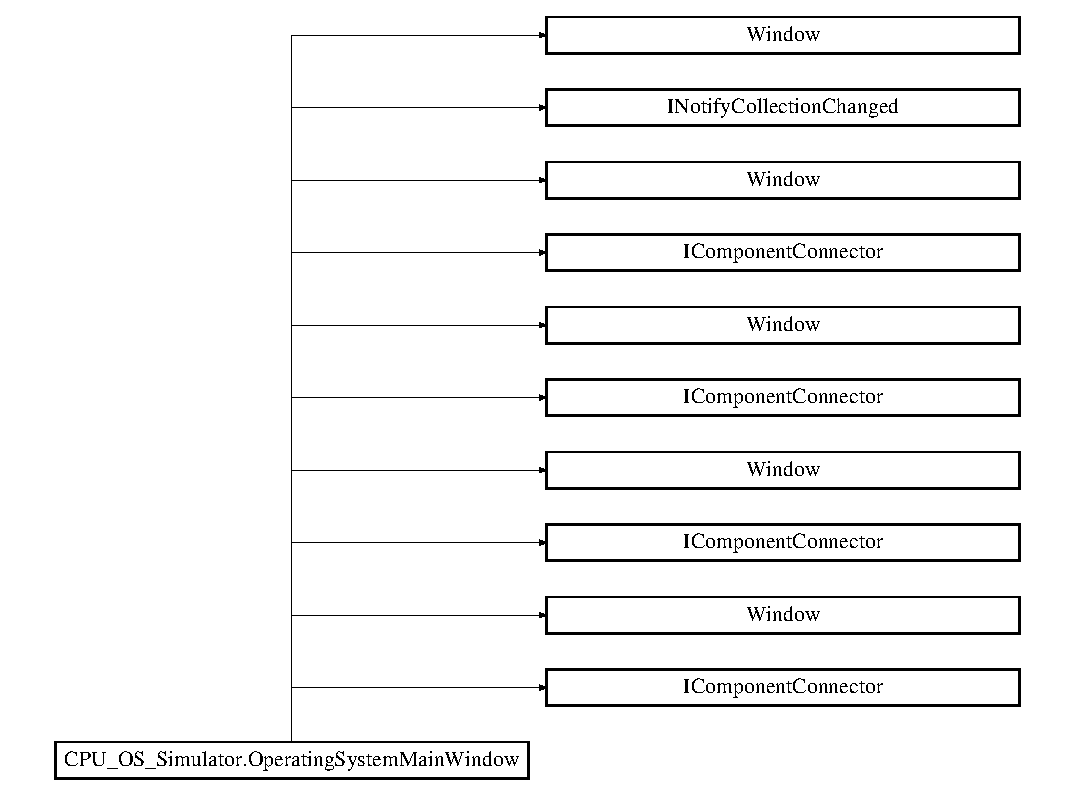
\includegraphics[height=10.232557cm]{class_c_p_u___o_s___simulator_1_1_operating_system_main_window}
\end{center}
\end{figure}
\subsection*{Public Member Functions}
\begin{DoxyCompactItemize}
\item 
void \hyperlink{class_c_p_u___o_s___simulator_1_1_operating_system_main_window_abf657079159db7bb54ea7089f5b7b5db}{Initialize\+Component} ()
\begin{DoxyCompactList}\small\item\em Initialize\+Component \end{DoxyCompactList}\item 
void \hyperlink{class_c_p_u___o_s___simulator_1_1_operating_system_main_window_abf657079159db7bb54ea7089f5b7b5db}{Initialize\+Component} ()
\begin{DoxyCompactList}\small\item\em Initialize\+Component \end{DoxyCompactList}\item 
void \hyperlink{class_c_p_u___o_s___simulator_1_1_operating_system_main_window_abf657079159db7bb54ea7089f5b7b5db}{Initialize\+Component} ()
\begin{DoxyCompactList}\small\item\em Initialize\+Component \end{DoxyCompactList}\item 
void \hyperlink{class_c_p_u___o_s___simulator_1_1_operating_system_main_window_abf657079159db7bb54ea7089f5b7b5db}{Initialize\+Component} ()
\begin{DoxyCompactList}\small\item\em Initialize\+Component \end{DoxyCompactList}\item 
\hyperlink{class_c_p_u___o_s___simulator_1_1_operating_system_main_window_a6ebb63e5bf2709cb0281434c651845dc}{Operating\+System\+Main\+Window} ()
\begin{DoxyCompactList}\small\item\em Default constructor for \hyperlink{class_c_p_u___o_s___simulator_1_1_operating_system_main_window}{Operating\+System\+Main\+Window} \end{DoxyCompactList}\item 
\hyperlink{class_c_p_u___o_s___simulator_1_1_operating_system_main_window_a2e4a26004957e2b1f1c4376f0a6656ab}{Operating\+System\+Main\+Window} (\hyperlink{class_c_p_u___o_s___simulator_1_1_main_window}{Main\+Window} \hyperlink{class_c_p_u___o_s___simulator_1_1_operating_system_main_window_a0219ba1583d00852bea36ac27c9d878d}{parent})
\begin{DoxyCompactList}\small\item\em Constructor for operating system window that takes the window instance that is creating this window P\+L\+E\+A\+S\+E N\+O\+T\+E\+: This constructor should always be used so data can be passed back to the parent window \end{DoxyCompactList}\end{DoxyCompactItemize}
\subsection*{Public Attributes}
\begin{DoxyCompactItemize}
\item 
System.\+Windows.\+Controls.\+List\+View \hyperlink{class_c_p_u___o_s___simulator_1_1_operating_system_main_window_a8710fe75e8464b39764d29184c2510fd}{lst\+\_\+\+Running\+Processes}
\begin{DoxyCompactList}\small\item\em lst\+\_\+\+Running\+Processes Name Field \end{DoxyCompactList}\item 
System.\+Windows.\+Controls.\+List\+View \hyperlink{class_c_p_u___o_s___simulator_1_1_operating_system_main_window_a70185c0d33e102e203d76b79ac5c77db}{lst\+\_\+\+Waiting\+Processes}
\begin{DoxyCompactList}\small\item\em lst\+\_\+\+Waiting\+Processes Name Field \end{DoxyCompactList}\item 
System.\+Windows.\+Controls.\+List\+View \hyperlink{class_c_p_u___o_s___simulator_1_1_operating_system_main_window_a00397da2e841d089d65441f5d4f19915}{lst\+\_\+\+Ready\+Processes}
\begin{DoxyCompactList}\small\item\em lst\+\_\+\+Ready\+Processes Name Field \end{DoxyCompactList}\item 
System.\+Windows.\+Controls.\+Slider \hyperlink{class_c_p_u___o_s___simulator_1_1_operating_system_main_window_a21bd388b7e1e821db2bfcee90530c3ae}{sld\+\_\+\+Clock\+Speed}
\begin{DoxyCompactList}\small\item\em sld\+\_\+\+Clock\+Speed Name Field \end{DoxyCompactList}\item 
System.\+Windows.\+Controls.\+Text\+Box \hyperlink{class_c_p_u___o_s___simulator_1_1_operating_system_main_window_a34784f7f4ffefd1dfa3e98c3bd03c260}{txt\+Process\+Name}
\begin{DoxyCompactList}\small\item\em txt\+Process\+Name Name Field \end{DoxyCompactList}\end{DoxyCompactItemize}
\subsection*{Static Public Attributes}
\begin{DoxyCompactItemize}
\item 
static \hyperlink{class_c_p_u___o_s___simulator_1_1_operating_system_main_window}{Operating\+System\+Main\+Window} \hyperlink{class_c_p_u___o_s___simulator_1_1_operating_system_main_window_ac659b34226b30276331daba60ec7d439}{current\+Instance}
\begin{DoxyCompactList}\small\item\em Variable to hold the current instance of this window so it can be accessed by other modules \end{DoxyCompactList}\end{DoxyCompactItemize}
\subsection*{Package Attributes}
\begin{DoxyCompactItemize}
\item 
\hyperlink{class_c_p_u___o_s___simulator_1_1_operating_system_main_window}{C\+P\+U\+\_\+\+O\+S\+\_\+\+Simulator.\+Operating\+System\+Main\+Window} \hyperlink{class_c_p_u___o_s___simulator_1_1_operating_system_main_window_ad42ee30cd6108b34ac88e9721db11b75}{Operating\+System\+Window}
\item 
System.\+Windows.\+Controls.\+Grid \hyperlink{class_c_p_u___o_s___simulator_1_1_operating_system_main_window_aaa4cd76a5ec5398ec2feacccbe5208b4}{Root\+\_\+\+Grid}
\item 
System.\+Windows.\+Controls.\+Group\+Box \hyperlink{class_c_p_u___o_s___simulator_1_1_operating_system_main_window_a07edb0a4de990e8120b24421e66f44ec}{grp\+\_\+\+Running\+Processes}
\item 
System.\+Windows.\+Controls.\+Grid \hyperlink{class_c_p_u___o_s___simulator_1_1_operating_system_main_window_a628b5d00213f20c361f776b85b3f7115}{grid\+\_\+\+Running\+Processes}
\item 
System.\+Windows.\+Controls.\+Button \hyperlink{class_c_p_u___o_s___simulator_1_1_operating_system_main_window_a3026145dbda6d838d6d542ff560c76af}{btn\+\_\+\+Wait}
\item 
System.\+Windows.\+Controls.\+Label \hyperlink{class_c_p_u___o_s___simulator_1_1_operating_system_main_window_a900faf1e6edab278754c736ccbf0f1df}{label}
\item 
System.\+Windows.\+Controls.\+Combo\+Box \hyperlink{class_c_p_u___o_s___simulator_1_1_operating_system_main_window_a4da0c086d71c3b794c9cd816aafeac88}{cmb\+\_\+\+Wait\+\_\+\+Period}
\item 
System.\+Windows.\+Controls.\+Label \hyperlink{class_c_p_u___o_s___simulator_1_1_operating_system_main_window_a4a8e9f811e590b3af2e2391740077937}{label1}
\item 
System.\+Windows.\+Controls.\+Button \hyperlink{class_c_p_u___o_s___simulator_1_1_operating_system_main_window_a241f1be0b04ce501c83e182629a6c694}{btn\+\_\+\+Queue}
\item 
System.\+Windows.\+Controls.\+Button \hyperlink{class_c_p_u___o_s___simulator_1_1_operating_system_main_window_a408a9f81462c276937e813344d29fc3c}{btn\+\_\+\+Kill\+\_\+\+Copy}
\item 
System.\+Windows.\+Controls.\+Check\+Box \hyperlink{class_c_p_u___o_s___simulator_1_1_operating_system_main_window_a3dea755536813ea2df09cfae7d946139}{chk\+\_\+\+Force\+Kill}
\item 
System.\+Windows.\+Controls.\+Check\+Box \hyperlink{class_c_p_u___o_s___simulator_1_1_operating_system_main_window_ad8b3845bf83d04c87c660d142f021e83}{chk\+\_\+\+Fault\+Kill}
\item 
System.\+Windows.\+Controls.\+Check\+Box \hyperlink{class_c_p_u___o_s___simulator_1_1_operating_system_main_window_a9a1e7eb960838b74491342087f1fd4e8}{chk\+\_\+\+Suspend\+\_\+\+On\+\_\+\+State\+\_\+\+Change\+\_\+\+Running}
\item 
System.\+Windows.\+Controls.\+Check\+Box \hyperlink{class_c_p_u___o_s___simulator_1_1_operating_system_main_window_ae9f7c2437568b2f8eccbab46595b4669}{chk\+\_\+\+Suspend\+\_\+\+On\+\_\+\+Pre\+\_\+emption}
\item 
System.\+Windows.\+Controls.\+Button \hyperlink{class_c_p_u___o_s___simulator_1_1_operating_system_main_window_a4cad08518f7e5daad6942ae5ff90d3e5}{btn\+\_\+\+Show\+\_\+\+Memory\+\_\+\+Running}
\item 
System.\+Windows.\+Controls.\+Button \hyperlink{class_c_p_u___o_s___simulator_1_1_operating_system_main_window_aa96b6795f5dbf776f1ea985e18671f2e}{btn\+\_\+\+Show\+\_\+\+P\+C\+B\+\_\+\+Running}
\item 
System.\+Windows.\+Controls.\+Group\+Box \hyperlink{class_c_p_u___o_s___simulator_1_1_operating_system_main_window_ae3e3b5c1c34bc0caa4f44e02e5cbd81c}{grp\+\_\+\+Waiting\+Processes}
\item 
System.\+Windows.\+Controls.\+Grid \hyperlink{class_c_p_u___o_s___simulator_1_1_operating_system_main_window_afdd9d749d58fde066217f035ac2c46c4}{grid\+\_\+\+Waiting\+Processes}
\item 
System.\+Windows.\+Controls.\+Button \hyperlink{class_c_p_u___o_s___simulator_1_1_operating_system_main_window_abbbabd3ef96781478b77ea937e312eb1}{btn\+\_\+\+Clear\+\_\+\+Waiting}
\item 
System.\+Windows.\+Controls.\+Button \hyperlink{class_c_p_u___o_s___simulator_1_1_operating_system_main_window_a802d545b8ca3b04953277e409aef535f}{btn\+\_\+\+Remove\+\_\+\+Waiting}
\item 
System.\+Windows.\+Controls.\+Button \hyperlink{class_c_p_u___o_s___simulator_1_1_operating_system_main_window_a1f1064712f5d86ad7c818f1eabef4b05}{btn\+\_\+\+Resume\+\_\+\+Waiting}
\item 
System.\+Windows.\+Controls.\+Check\+Box \hyperlink{class_c_p_u___o_s___simulator_1_1_operating_system_main_window_ad8c47a378229241506f1d7540f40e6cd}{chk\+\_\+\+Suspend\+\_\+\+On\+\_\+\+State\+\_\+\+Change\+\_\+\+Waiting}
\item 
System.\+Windows.\+Controls.\+Button \hyperlink{class_c_p_u___o_s___simulator_1_1_operating_system_main_window_a2d25b59e695eec3c02e389365dcffb9f}{btn\+\_\+\+Show\+\_\+\+Memory\+\_\+\+Waiting}
\item 
System.\+Windows.\+Controls.\+Button \hyperlink{class_c_p_u___o_s___simulator_1_1_operating_system_main_window_a371bab43b23ebad047bad80e0889ed61}{btn\+\_\+\+Show\+\_\+\+P\+C\+B\+\_\+\+Waiting}
\item 
System.\+Windows.\+Controls.\+Group\+Box \hyperlink{class_c_p_u___o_s___simulator_1_1_operating_system_main_window_ac76887fb899577a2695f5a16c32993c3}{grp\+\_\+\+Ready\+Processes}
\item 
System.\+Windows.\+Controls.\+Grid \hyperlink{class_c_p_u___o_s___simulator_1_1_operating_system_main_window_a4dc7b1233f61261fad09e145e63563a3}{grid\+\_\+\+Ready\+Processes}
\item 
System.\+Windows.\+Controls.\+Button \hyperlink{class_c_p_u___o_s___simulator_1_1_operating_system_main_window_a926540a5fc98f177282e425055964cb9}{btn\+\_\+\+Clear\+\_\+\+Ready}
\item 
System.\+Windows.\+Controls.\+Button \hyperlink{class_c_p_u___o_s___simulator_1_1_operating_system_main_window_a4ed06428179b1762e9ac112287e2fbc1}{btn\+\_\+\+Remove\+\_\+\+Ready}
\item 
System.\+Windows.\+Controls.\+Check\+Box \hyperlink{class_c_p_u___o_s___simulator_1_1_operating_system_main_window_ac08c18d09944dd2291917b62a7d1320e}{chk\+\_\+\+Suspend\+\_\+\+On\+\_\+\+State\+\_\+\+Change\+\_\+\+Ready}
\item 
System.\+Windows.\+Controls.\+Button \hyperlink{class_c_p_u___o_s___simulator_1_1_operating_system_main_window_a64732f37dba68b537b9e7d45d8bbf0a2}{btn\+\_\+\+Show\+\_\+\+Memory\+\_\+\+Ready}
\item 
System.\+Windows.\+Controls.\+Button \hyperlink{class_c_p_u___o_s___simulator_1_1_operating_system_main_window_a4f172867bc7041faad18ea477081ac2d}{btn\+\_\+\+Show\+\_\+\+P\+C\+B\+\_\+\+Ready}
\item 
System.\+Windows.\+Controls.\+Tab\+Control \hyperlink{class_c_p_u___o_s___simulator_1_1_operating_system_main_window_a2575de899df7277ae9c310931b8dbaa0}{Scheduler\+\_\+\+Tabs}
\item 
System.\+Windows.\+Controls.\+Tab\+Item \hyperlink{class_c_p_u___o_s___simulator_1_1_operating_system_main_window_a019542a100cb475965f111d94085a16a}{Policies\+\_\+\+Tab}
\item 
System.\+Windows.\+Controls.\+Grid \hyperlink{class_c_p_u___o_s___simulator_1_1_operating_system_main_window_a70a570b7188592c1066eccb3ff6b97f3}{grid\+\_\+\+Policies}
\item 
System.\+Windows.\+Controls.\+Radio\+Button \hyperlink{class_c_p_u___o_s___simulator_1_1_operating_system_main_window_a929f7f488fb80ae6459510ad3334fddb}{rdb\+\_\+\+First\+Come\+\_\+\+First\+Served}
\item 
System.\+Windows.\+Controls.\+Radio\+Button \hyperlink{class_c_p_u___o_s___simulator_1_1_operating_system_main_window_ae5bfde3cdd33e7fb8c973fc33ca58752}{rdb\+\_\+\+Shortest\+\_\+\+Job\+\_\+\+First}
\item 
System.\+Windows.\+Controls.\+Radio\+Button \hyperlink{class_c_p_u___o_s___simulator_1_1_operating_system_main_window_ad9756edfc9b0ce93336c779551675ba3}{rdb\+\_\+\+Lottery}
\item 
System.\+Windows.\+Controls.\+Radio\+Button \hyperlink{class_c_p_u___o_s___simulator_1_1_operating_system_main_window_af80c8b728e40265c61586b298e8640ef}{rdb\+\_\+\+Fair\+Share}
\item 
System.\+Windows.\+Controls.\+Radio\+Button \hyperlink{class_c_p_u___o_s___simulator_1_1_operating_system_main_window_a5be51435049a03c98c57e035eff181ec}{rdb\+\_\+\+Round\+\_\+\+Robin}
\item 
System.\+Windows.\+Controls.\+Check\+Box \hyperlink{class_c_p_u___o_s___simulator_1_1_operating_system_main_window_a8861f5f8ba68cf8eb0a07ef0528dccba}{chk\+\_\+\+Use\+\_\+\+Default\+\_\+\+Scheduler}
\item 
System.\+Windows.\+Controls.\+Group\+Box \hyperlink{class_c_p_u___o_s___simulator_1_1_operating_system_main_window_a1a5a0b0e438e5300a445ffe9ee3bf67d}{grp\+\_\+\+Round\+\_\+\+Robin\+\_\+\+Config}
\item 
System.\+Windows.\+Controls.\+Grid \hyperlink{class_c_p_u___o_s___simulator_1_1_operating_system_main_window_a626ad676e978db5c0d52825764e68ea5}{grid\+\_\+\+R\+R\+\_\+\+Config}
\item 
System.\+Windows.\+Controls.\+Group\+Box \hyperlink{class_c_p_u___o_s___simulator_1_1_operating_system_main_window_a09854a80dc1796d59c66a12415e64c8c}{grp\+\_\+\+Time\+\_\+\+Slice}
\item 
System.\+Windows.\+Controls.\+Combo\+Box \hyperlink{class_c_p_u___o_s___simulator_1_1_operating_system_main_window_a599d396665359bf3ff8c1a9a9e220229}{cmb\+\_\+\+R\+R\+Ticks}
\item 
System.\+Windows.\+Controls.\+Label \hyperlink{class_c_p_u___o_s___simulator_1_1_operating_system_main_window_a28c78c8e714c58223e338c29f89fda83}{label2}
\item 
System.\+Windows.\+Controls.\+Combo\+Box \hyperlink{class_c_p_u___o_s___simulator_1_1_operating_system_main_window_ab0c34dd43767c96aefdc333e3fb5b7d1}{cmb\+\_\+\+R\+R\+Seconds}
\item 
System.\+Windows.\+Controls.\+Label \hyperlink{class_c_p_u___o_s___simulator_1_1_operating_system_main_window_abf6d8f5cfb34c8d41580c330c6af3a51}{label2\+\_\+\+Copy}
\item 
System.\+Windows.\+Controls.\+Group\+Box \hyperlink{class_c_p_u___o_s___simulator_1_1_operating_system_main_window_a45f777ff3178acfefdffb311366ab786}{grp\+\_\+\+Priority}
\item 
System.\+Windows.\+Controls.\+Grid \hyperlink{class_c_p_u___o_s___simulator_1_1_operating_system_main_window_a0b2ac61c7430b46fa467986e7afd9448}{grid\+\_\+\+Priority}
\item 
System.\+Windows.\+Controls.\+Radio\+Button \hyperlink{class_c_p_u___o_s___simulator_1_1_operating_system_main_window_acc931be7e054344ea9d99b84ef5c2519}{rdb\+\_\+\+No\+\_\+\+Priority}
\item 
System.\+Windows.\+Controls.\+Radio\+Button \hyperlink{class_c_p_u___o_s___simulator_1_1_operating_system_main_window_a1bdd1425ce8e8dba8ea5906e787aa9b1}{rdb\+\_\+\+Preemptive}
\item 
System.\+Windows.\+Controls.\+Radio\+Button \hyperlink{class_c_p_u___o_s___simulator_1_1_operating_system_main_window_a3021441de903045cba2ff708184e0ac5}{rdb\+\_\+\+Non\+\_\+\+Preemptive}
\item 
System.\+Windows.\+Controls.\+Group\+Box \hyperlink{class_c_p_u___o_s___simulator_1_1_operating_system_main_window_a13fd6e707bf77777692f0fe004a0635b}{grp\+\_\+\+Dynamic}
\item 
System.\+Windows.\+Controls.\+Radio\+Button \hyperlink{class_c_p_u___o_s___simulator_1_1_operating_system_main_window_abb757a3b9a2d8f8c72f54ef2209446b6}{rdb\+\_\+\+Static}
\item 
System.\+Windows.\+Controls.\+Radio\+Button \hyperlink{class_c_p_u___o_s___simulator_1_1_operating_system_main_window_a9d7779e13ed1b78c4387933df4b40d24}{rdb\+\_\+\+Dynamic}
\item 
System.\+Windows.\+Controls.\+Radio\+Button \hyperlink{class_c_p_u___o_s___simulator_1_1_operating_system_main_window_ac47f5adda2930d87ec387e030d2e8870}{rdb\+\_\+\+R\+R\+\_\+\+Ticks}
\item 
System.\+Windows.\+Controls.\+Radio\+Button \hyperlink{class_c_p_u___o_s___simulator_1_1_operating_system_main_window_a97c4b8fbd9b9e86a44dc50b6dafd96f4}{rdb\+\_\+\+R\+R\+\_\+\+Seconds}
\item 
System.\+Windows.\+Controls.\+Tab\+Control \hyperlink{class_c_p_u___o_s___simulator_1_1_operating_system_main_window_aad49944b6a55d895806ca01be83440e7}{Control\+Tabs}
\item 
System.\+Windows.\+Controls.\+Tab\+Item \hyperlink{class_c_p_u___o_s___simulator_1_1_operating_system_main_window_a06541ab6c749adc4696fe5ec1f174fcf}{Control\+Tab}
\item 
System.\+Windows.\+Controls.\+Button \hyperlink{class_c_p_u___o_s___simulator_1_1_operating_system_main_window_aa7fab2cb43aa4eefed8e3bcba47a539b}{btn\+\_\+\+Step}
\item 
System.\+Windows.\+Controls.\+Button \hyperlink{class_c_p_u___o_s___simulator_1_1_operating_system_main_window_a811cecc7b1fa49c7f340be7377ff7f32}{btn\+\_\+\+Start}
\item 
System.\+Windows.\+Controls.\+Button \hyperlink{class_c_p_u___o_s___simulator_1_1_operating_system_main_window_abb2c3824f2ed103814e81c8a6bf5452e}{btn\+\_\+\+Suspend}
\item 
System.\+Windows.\+Controls.\+Label \hyperlink{class_c_p_u___o_s___simulator_1_1_operating_system_main_window_a731180865f00c29a9d6affd3ba2860c1}{label3}
\item 
System.\+Windows.\+Controls.\+Label \hyperlink{class_c_p_u___o_s___simulator_1_1_operating_system_main_window_ab76c53e23eb4219d850c3b7a85bf1dd7}{label3\+\_\+\+Copy}
\item 
System.\+Windows.\+Controls.\+Check\+Box \hyperlink{class_c_p_u___o_s___simulator_1_1_operating_system_main_window_a7d57ae7ba4ca24e126fabf4d124f7812}{chk\+\_\+\+Single\+\_\+\+C\+P\+U}
\item 
System.\+Windows.\+Controls.\+Check\+Box \hyperlink{class_c_p_u___o_s___simulator_1_1_operating_system_main_window_a5f027a391759480d1d00c76c2171c6b9}{chk\+\_\+\+C\+P\+U\+\_\+\+Affinity}
\item 
System.\+Windows.\+Controls.\+Check\+Box \hyperlink{class_c_p_u___o_s___simulator_1_1_operating_system_main_window_a61ea8b3bc04203f4a4caa33f21089d18}{chk\+\_\+\+No\+\_\+\+Processes}
\item 
System.\+Windows.\+Controls.\+Group\+Box \hyperlink{class_c_p_u___o_s___simulator_1_1_operating_system_main_window_a9dca0481c9d2ec99d42298352858be2b}{grp\+\_\+\+Program\+List}
\item 
System.\+Windows.\+Controls.\+Grid \hyperlink{class_c_p_u___o_s___simulator_1_1_operating_system_main_window_a22160eecd007b7aedf48db6c64eb2da6}{grid\+\_\+\+Program\+List}
\item 
System.\+Windows.\+Controls.\+List\+View \hyperlink{class_c_p_u___o_s___simulator_1_1_operating_system_main_window_a08c9b2131c204ca49f85c7dbc3c0bde2}{lst\+\_\+\+Programs}
\item 
System.\+Windows.\+Controls.\+Tab\+Control \hyperlink{class_c_p_u___o_s___simulator_1_1_operating_system_main_window_a6e2a1da42cb207d3a02c3bc1613be085}{Process\+Tabs}
\item 
System.\+Windows.\+Controls.\+Tab\+Item \hyperlink{class_c_p_u___o_s___simulator_1_1_operating_system_main_window_a01c2d1944c9470e56e5bbbcdff683f2b}{Process\+\_\+\+Tab}
\item 
System.\+Windows.\+Controls.\+Label \hyperlink{class_c_p_u___o_s___simulator_1_1_operating_system_main_window_a11f07634242ba2c38b23b293dcd3843e}{label4}
\item 
System.\+Windows.\+Controls.\+Label \hyperlink{class_c_p_u___o_s___simulator_1_1_operating_system_main_window_a2b7721f6cfb0a1eeb4a0aec34ef543c0}{label5}
\item 
System.\+Windows.\+Controls.\+Combo\+Box \hyperlink{class_c_p_u___o_s___simulator_1_1_operating_system_main_window_a52618598a5f66eb457af669a7ca849d9}{cmb\+\_\+\+Priority}
\item 
System.\+Windows.\+Controls.\+Label \hyperlink{class_c_p_u___o_s___simulator_1_1_operating_system_main_window_ad753667e4d67f79b83e59dc8be4df684}{label6}
\item 
System.\+Windows.\+Controls.\+Combo\+Box \hyperlink{class_c_p_u___o_s___simulator_1_1_operating_system_main_window_ab8bcdf83f7bfdecbdd3f8ba71cc92a5e}{cmb\+\_\+\+Pages}
\item 
System.\+Windows.\+Controls.\+Check\+Box \hyperlink{class_c_p_u___o_s___simulator_1_1_operating_system_main_window_aa13338d96952aafec3ecbc7f4fa6fcfc}{chk\+\_\+\+Display\+\_\+\+Profile}
\item 
System.\+Windows.\+Controls.\+Check\+Box \hyperlink{class_c_p_u___o_s___simulator_1_1_operating_system_main_window_a22ea0e1679c79b12e2637f93543c0bef}{chk\+\_\+\+Children\+\_\+\+Die}
\item 
System.\+Windows.\+Controls.\+Button \hyperlink{class_c_p_u___o_s___simulator_1_1_operating_system_main_window_a30b8c5bcaa36e85ba4b41f23c1bbfdde}{btn\+\_\+\+Create\+New\+Process}
\item 
System.\+Windows.\+Controls.\+Check\+Box \hyperlink{class_c_p_u___o_s___simulator_1_1_operating_system_main_window_a8af478cc94c72b0c843b4911f43aecdf}{chk\+\_\+\+Use\+\_\+\+Default\+\_\+\+Scheduler\+\_\+\+Process}
\item 
System.\+Windows.\+Controls.\+Label \hyperlink{class_c_p_u___o_s___simulator_1_1_operating_system_main_window_ae841fdcc76cc96944b0463f3c4c448a4}{label7}
\item 
System.\+Windows.\+Controls.\+Text\+Box \hyperlink{class_c_p_u___o_s___simulator_1_1_operating_system_main_window_acc33a47fbe7956196846504306f7489e}{txt\+\_\+\+Process\+Lifetime}
\item 
System.\+Windows.\+Controls.\+Radio\+Button \hyperlink{class_c_p_u___o_s___simulator_1_1_operating_system_main_window_ae338ba4b15d62c6d584aaa5814fa8506}{rdb\+\_\+\+Lifetime\+Ticks}
\item 
System.\+Windows.\+Controls.\+Radio\+Button \hyperlink{class_c_p_u___o_s___simulator_1_1_operating_system_main_window_a09745c9a76909a398d8a47295fda2b67}{rdb\+\_\+\+Lifetime\+Secs}
\item 
System.\+Windows.\+Controls.\+Check\+Box \hyperlink{class_c_p_u___o_s___simulator_1_1_operating_system_main_window_aa7e58acf30f50880e309615f92f0ef8e}{chk\+\_\+\+Delayed\+Process}
\item 
System.\+Windows.\+Controls.\+Label \hyperlink{class_c_p_u___o_s___simulator_1_1_operating_system_main_window_af57c4cce87917105945b6c5d1f6b812e}{label8}
\item 
System.\+Windows.\+Controls.\+Radio\+Button \hyperlink{class_c_p_u___o_s___simulator_1_1_operating_system_main_window_a7b70deef80df6719fc0b7b9c87c268d7}{rdb\+\_\+\+Delay\+Ticks}
\item 
System.\+Windows.\+Controls.\+Radio\+Button \hyperlink{class_c_p_u___o_s___simulator_1_1_operating_system_main_window_a7b4585b869d26fa4e7d419a064f4f73c}{rdb\+\_\+\+Delay\+Secs}
\item 
System.\+Windows.\+Controls.\+Combo\+Box \hyperlink{class_c_p_u___o_s___simulator_1_1_operating_system_main_window_ad4e310b5bbd70de23e9132fb57229c96}{cmb\+\_\+\+Arrival\+\_\+\+Delay}
\item 
System.\+Windows.\+Controls.\+Button \hyperlink{class_c_p_u___o_s___simulator_1_1_operating_system_main_window_ad0ca6083cb0afc42ce05182655540a45}{btn\+\_\+\+Close}
\item 
System.\+Windows.\+Controls.\+Button \hyperlink{class_c_p_u___o_s___simulator_1_1_operating_system_main_window_a9320f9ba12e9a1e460840eca6bda4e17}{btn\+\_\+\+Save\+State}
\end{DoxyCompactItemize}
\subsection*{Properties}
\begin{DoxyCompactItemize}
\item 
List$<$ \hyperlink{class_c_p_u___o_s___simulator_1_1_operating___system_1_1_simulator_process}{Simulator\+Process} $>$ \hyperlink{class_c_p_u___o_s___simulator_1_1_operating_system_main_window_aadbbb1f580d767211e180a95ec71b849}{Processes}\hspace{0.3cm}{\ttfamily  \mbox{[}get, set\mbox{]}}
\item 
\hyperlink{class_c_p_u___o_s___simulator_1_1_operating___system_1_1_o_s_core}{O\+S\+Core} \hyperlink{class_c_p_u___o_s___simulator_1_1_operating_system_main_window_ad714e0ed6e880516f8afc3f1531a2d14}{Os\+Core}\hspace{0.3cm}{\ttfamily  \mbox{[}get, set\mbox{]}}
\end{DoxyCompactItemize}
\subsection*{Events}
\begin{DoxyCompactItemize}
\item 
Notify\+Collection\+Changed\+Event\+Handler \hyperlink{class_c_p_u___o_s___simulator_1_1_operating_system_main_window_af8aeaf0c83021caf8f735ea7c051848c}{Collection\+Changed}
\end{DoxyCompactItemize}
\subsection*{Private Member Functions}
\begin{DoxyCompactItemize}
\item 
void System.\+Windows.\+Markup.\+I\+Component\+Connector. \hyperlink{class_c_p_u___o_s___simulator_1_1_operating_system_main_window_ad482fe0b46f681bb64b29500fa69b98b}{Connect} (int connection\+Id, object target)
\item 
void System.\+Windows.\+Markup.\+I\+Component\+Connector. \hyperlink{class_c_p_u___o_s___simulator_1_1_operating_system_main_window_ad482fe0b46f681bb64b29500fa69b98b}{Connect} (int connection\+Id, object target)
\item 
void System.\+Windows.\+Markup.\+I\+Component\+Connector. \hyperlink{class_c_p_u___o_s___simulator_1_1_operating_system_main_window_ad482fe0b46f681bb64b29500fa69b98b}{Connect} (int connection\+Id, object target)
\item 
void System.\+Windows.\+Markup.\+I\+Component\+Connector. \hyperlink{class_c_p_u___o_s___simulator_1_1_operating_system_main_window_ad482fe0b46f681bb64b29500fa69b98b}{Connect} (int connection\+Id, object target)
\item 
void \hyperlink{class_c_p_u___o_s___simulator_1_1_operating_system_main_window_aeda3cbb43fe602a4ba5325b0a8a9e2ee}{On\+Collection\+Changed} (object sender, Notify\+Collection\+Changed\+Event\+Args notify\+Collection\+Changed\+Event\+Args)
\item 
void \hyperlink{class_c_p_u___o_s___simulator_1_1_operating_system_main_window_a92ce496d30585ff30ac840fbeb7b8a16}{btn\+\_\+\+Close\+\_\+\+Click} (object sender, Routed\+Event\+Args e)
\begin{DoxyCompactList}\small\item\em This method is called when the close button is clicked \end{DoxyCompactList}\item 
void \hyperlink{class_c_p_u___o_s___simulator_1_1_operating_system_main_window_a0f58f20c1fe9dbc972fdf41ae871dea7}{Set\+O\+S\+Window\+Instance} ()
\begin{DoxyCompactList}\small\item\em This method sets the current instance of O\+S window in the window bridge so it can be accessed by other modules \end{DoxyCompactList}\item 
void \hyperlink{class_c_p_u___o_s___simulator_1_1_operating_system_main_window_a05b54ac7242f582757f99f3e7a6c48cf}{Operating\+System\+Window\+\_\+\+Loaded} (object sender, Routed\+Event\+Args e)
\item 
void \hyperlink{class_c_p_u___o_s___simulator_1_1_operating_system_main_window_a5e823b50dfab668d8e61d9d3ecea300c}{Operating\+System\+Window\+\_\+\+Closing} (object sender, System.\+Component\+Model.\+Cancel\+Event\+Args e)
\item 
void \hyperlink{class_c_p_u___o_s___simulator_1_1_operating_system_main_window_a49ee2facd64a57c8a3450ccd5582dfff}{btn\+\_\+\+Start\+\_\+\+Click} (object sender, Routed\+Event\+Args e)
\item 
void \hyperlink{class_c_p_u___o_s___simulator_1_1_operating_system_main_window_a61584b7f34a107e1c8c6cbbaff17641d}{Create\+Os\+Core} ()
\begin{DoxyCompactList}\small\item\em This function creates the Operating System core \end{DoxyCompactList}\item 
\hyperlink{struct_c_p_u___o_s___simulator_1_1_operating___system_1_1_o_s_flags}{O\+S\+Flags} \hyperlink{class_c_p_u___o_s___simulator_1_1_operating_system_main_window_aedcaa8273429f3867b3a2419981e4ca1}{Create\+Os\+Flags} ()
\begin{DoxyCompactList}\small\item\em This function creates the flags for creating the O\+S core based on selected U\+I options \end{DoxyCompactList}\item 
\hyperlink{struct_c_p_u___o_s___simulator_1_1_operating___system_1_1_scheduler_flags}{Scheduler\+Flags} \hyperlink{class_c_p_u___o_s___simulator_1_1_operating_system_main_window_affe29a16b5dcb4faa896fd12b87268f6}{Create\+Scheduler\+Flags} (\hyperlink{struct_c_p_u___o_s___simulator_1_1_operating___system_1_1_o_s_flags}{O\+S\+Flags} flags)
\begin{DoxyCompactList}\small\item\em This function creates scheduler flags \end{DoxyCompactList}\item 
async void \hyperlink{class_c_p_u___o_s___simulator_1_1_operating_system_main_window_a07752984a7eedac5dab517b7f57b9af2}{btn\+\_\+\+Create\+New\+Process\+\_\+\+Click} (object sender, Routed\+Event\+Args e)
\item 
async Task$<$ long $>$ \hyperlink{class_c_p_u___o_s___simulator_1_1_operating_system_main_window_a981c8ed38feb78ab874753c641d278d6}{Delay} (long delay\+Mills)
\item 
async void \hyperlink{class_c_p_u___o_s___simulator_1_1_operating_system_main_window_a531d8240782c578c6fc5984c703ddffb}{Update\+Interface} ()
\item 
\hyperlink{struct_c_p_u___o_s___simulator_1_1_operating___system_1_1_process_flags}{Process\+Flags} \hyperlink{class_c_p_u___o_s___simulator_1_1_operating_system_main_window_aa44b77efc3ae2c300ebb19e6854c3290}{Create\+Process\+Flags} ()
\begin{DoxyCompactList}\small\item\em This function creates the process flags \end{DoxyCompactList}\item 
\hyperlink{struct_c_p_u___o_s___simulator_1_1_operating___system_1_1_p_c_b_flags}{P\+C\+B\+Flags} \hyperlink{class_c_p_u___o_s___simulator_1_1_operating_system_main_window_a0994a475aa1e602964f610cce778b117}{Create\+P\+C\+B\+Flags} ()
\end{DoxyCompactItemize}
\subsection*{Private Attributes}
\begin{DoxyCompactItemize}
\item 
bool \hyperlink{class_c_p_u___o_s___simulator_1_1_operating_system_main_window_a824bac181aa4f034115dfac40c744738}{\+\_\+content\+Loaded}
\item 
\hyperlink{class_c_p_u___o_s___simulator_1_1_main_window}{Main\+Window} \hyperlink{class_c_p_u___o_s___simulator_1_1_operating_system_main_window_a0219ba1583d00852bea36ac27c9d878d}{parent}
\item 
List$<$ \hyperlink{class_c_p_u___o_s___simulator_1_1_c_p_u_1_1_simulator_program}{Simulator\+Program} $>$ \hyperlink{class_c_p_u___o_s___simulator_1_1_operating_system_main_window_a83bef5323931616842c44d3f8d477fd2}{program\+List}
\item 
\hyperlink{class_c_p_u___o_s___simulator_1_1_operating___system_1_1_o_s_core}{O\+S\+Core} \hyperlink{class_c_p_u___o_s___simulator_1_1_operating_system_main_window_af944b743b4780850089320d08d38b0ed}{os\+Core} = \hyperlink{_old_01_process_01_flags_8cs_afb8e110345c45e74478894341ab6b28e}{null}
\item 
string \hyperlink{class_c_p_u___o_s___simulator_1_1_operating_system_main_window_ad3dd5030de453dd97f236e7677ab6732}{missing\+Flag} = String.\+Empty
\item 
List$<$ \hyperlink{class_c_p_u___o_s___simulator_1_1_operating___system_1_1_simulator_process}{Simulator\+Process} $>$ \hyperlink{class_c_p_u___o_s___simulator_1_1_operating_system_main_window_ab6bcbc8c33ec438d2f005d4c978e1a44}{processes}
\item 
\hyperlink{struct_c_p_u___o_s___simulator_1_1_operating___system_1_1_o_s_flags}{O\+S\+Flags} \hyperlink{class_c_p_u___o_s___simulator_1_1_operating_system_main_window_a905f81a88e7878e936352f6da9ffcb93}{global\+Flags}
\item 
Dispatcher \hyperlink{class_c_p_u___o_s___simulator_1_1_operating_system_main_window_ac0f8e9dfcaba558927c53e11815fb0fb}{dispatcher} = Dispatcher.\+Current\+Dispatcher
\end{DoxyCompactItemize}


\subsection{Detailed Description}
\hyperlink{class_c_p_u___o_s___simulator_1_1_operating_system_main_window}{Operating\+System\+Main\+Window} 

Interaction logic for Operating\+System\+Main\+Window.\+xaml 

Definition at line 41 of file Operating\+System\+Main\+Window.\+g.\+cs.



\subsection{Constructor \& Destructor Documentation}
\hypertarget{class_c_p_u___o_s___simulator_1_1_operating_system_main_window_a6ebb63e5bf2709cb0281434c651845dc}{}\index{C\+P\+U\+\_\+\+O\+S\+\_\+\+Simulator\+::\+Operating\+System\+Main\+Window@{C\+P\+U\+\_\+\+O\+S\+\_\+\+Simulator\+::\+Operating\+System\+Main\+Window}!Operating\+System\+Main\+Window@{Operating\+System\+Main\+Window}}
\index{Operating\+System\+Main\+Window@{Operating\+System\+Main\+Window}!C\+P\+U\+\_\+\+O\+S\+\_\+\+Simulator\+::\+Operating\+System\+Main\+Window@{C\+P\+U\+\_\+\+O\+S\+\_\+\+Simulator\+::\+Operating\+System\+Main\+Window}}
\subsubsection[{Operating\+System\+Main\+Window()}]{\setlength{\rightskip}{0pt plus 5cm}C\+P\+U\+\_\+\+O\+S\+\_\+\+Simulator.\+Operating\+System\+Main\+Window.\+Operating\+System\+Main\+Window (
\begin{DoxyParamCaption}
{}
\end{DoxyParamCaption}
)}\label{class_c_p_u___o_s___simulator_1_1_operating_system_main_window_a6ebb63e5bf2709cb0281434c651845dc}


Default constructor for \hyperlink{class_c_p_u___o_s___simulator_1_1_operating_system_main_window}{Operating\+System\+Main\+Window} 



Definition at line 37 of file Operating\+System\+Main\+Window.\+xaml.\+cs.

\hypertarget{class_c_p_u___o_s___simulator_1_1_operating_system_main_window_a2e4a26004957e2b1f1c4376f0a6656ab}{}\index{C\+P\+U\+\_\+\+O\+S\+\_\+\+Simulator\+::\+Operating\+System\+Main\+Window@{C\+P\+U\+\_\+\+O\+S\+\_\+\+Simulator\+::\+Operating\+System\+Main\+Window}!Operating\+System\+Main\+Window@{Operating\+System\+Main\+Window}}
\index{Operating\+System\+Main\+Window@{Operating\+System\+Main\+Window}!C\+P\+U\+\_\+\+O\+S\+\_\+\+Simulator\+::\+Operating\+System\+Main\+Window@{C\+P\+U\+\_\+\+O\+S\+\_\+\+Simulator\+::\+Operating\+System\+Main\+Window}}
\subsubsection[{Operating\+System\+Main\+Window(\+Main\+Window parent)}]{\setlength{\rightskip}{0pt plus 5cm}C\+P\+U\+\_\+\+O\+S\+\_\+\+Simulator.\+Operating\+System\+Main\+Window.\+Operating\+System\+Main\+Window (
\begin{DoxyParamCaption}
\item[{{\bf Main\+Window}}]{parent}
\end{DoxyParamCaption}
)}\label{class_c_p_u___o_s___simulator_1_1_operating_system_main_window_a2e4a26004957e2b1f1c4376f0a6656ab}


Constructor for operating system window that takes the window instance that is creating this window P\+L\+E\+A\+S\+E N\+O\+T\+E\+: This constructor should always be used so data can be passed back to the parent window 


\begin{DoxyParams}{Parameters}
{\em parent} & The window that is creating this window \\
\hline
\end{DoxyParams}


Definition at line 50 of file Operating\+System\+Main\+Window.\+xaml.\+cs.



\subsection{Member Function Documentation}
\hypertarget{class_c_p_u___o_s___simulator_1_1_operating_system_main_window_a92ce496d30585ff30ac840fbeb7b8a16}{}\index{C\+P\+U\+\_\+\+O\+S\+\_\+\+Simulator\+::\+Operating\+System\+Main\+Window@{C\+P\+U\+\_\+\+O\+S\+\_\+\+Simulator\+::\+Operating\+System\+Main\+Window}!btn\+\_\+\+Close\+\_\+\+Click@{btn\+\_\+\+Close\+\_\+\+Click}}
\index{btn\+\_\+\+Close\+\_\+\+Click@{btn\+\_\+\+Close\+\_\+\+Click}!C\+P\+U\+\_\+\+O\+S\+\_\+\+Simulator\+::\+Operating\+System\+Main\+Window@{C\+P\+U\+\_\+\+O\+S\+\_\+\+Simulator\+::\+Operating\+System\+Main\+Window}}
\subsubsection[{btn\+\_\+\+Close\+\_\+\+Click(object sender, Routed\+Event\+Args e)}]{\setlength{\rightskip}{0pt plus 5cm}void C\+P\+U\+\_\+\+O\+S\+\_\+\+Simulator.\+Operating\+System\+Main\+Window.\+btn\+\_\+\+Close\+\_\+\+Click (
\begin{DoxyParamCaption}
\item[{object}]{sender, }
\item[{Routed\+Event\+Args}]{e}
\end{DoxyParamCaption}
)\hspace{0.3cm}{\ttfamily [private]}}\label{class_c_p_u___o_s___simulator_1_1_operating_system_main_window_a92ce496d30585ff30ac840fbeb7b8a16}


This method is called when the close button is clicked 


\begin{DoxyParams}{Parameters}
{\em sender} & the object that triggered this event\\
\hline
{\em e} & the event args for this event\\
\hline
\end{DoxyParams}


Definition at line 82 of file Operating\+System\+Main\+Window.\+xaml.\+cs.

\hypertarget{class_c_p_u___o_s___simulator_1_1_operating_system_main_window_a07752984a7eedac5dab517b7f57b9af2}{}\index{C\+P\+U\+\_\+\+O\+S\+\_\+\+Simulator\+::\+Operating\+System\+Main\+Window@{C\+P\+U\+\_\+\+O\+S\+\_\+\+Simulator\+::\+Operating\+System\+Main\+Window}!btn\+\_\+\+Create\+New\+Process\+\_\+\+Click@{btn\+\_\+\+Create\+New\+Process\+\_\+\+Click}}
\index{btn\+\_\+\+Create\+New\+Process\+\_\+\+Click@{btn\+\_\+\+Create\+New\+Process\+\_\+\+Click}!C\+P\+U\+\_\+\+O\+S\+\_\+\+Simulator\+::\+Operating\+System\+Main\+Window@{C\+P\+U\+\_\+\+O\+S\+\_\+\+Simulator\+::\+Operating\+System\+Main\+Window}}
\subsubsection[{btn\+\_\+\+Create\+New\+Process\+\_\+\+Click(object sender, Routed\+Event\+Args e)}]{\setlength{\rightskip}{0pt plus 5cm}async void C\+P\+U\+\_\+\+O\+S\+\_\+\+Simulator.\+Operating\+System\+Main\+Window.\+btn\+\_\+\+Create\+New\+Process\+\_\+\+Click (
\begin{DoxyParamCaption}
\item[{object}]{sender, }
\item[{Routed\+Event\+Args}]{e}
\end{DoxyParamCaption}
)\hspace{0.3cm}{\ttfamily [private]}}\label{class_c_p_u___o_s___simulator_1_1_operating_system_main_window_a07752984a7eedac5dab517b7f57b9af2}


Definition at line 332 of file Operating\+System\+Main\+Window.\+xaml.\+cs.

\hypertarget{class_c_p_u___o_s___simulator_1_1_operating_system_main_window_a49ee2facd64a57c8a3450ccd5582dfff}{}\index{C\+P\+U\+\_\+\+O\+S\+\_\+\+Simulator\+::\+Operating\+System\+Main\+Window@{C\+P\+U\+\_\+\+O\+S\+\_\+\+Simulator\+::\+Operating\+System\+Main\+Window}!btn\+\_\+\+Start\+\_\+\+Click@{btn\+\_\+\+Start\+\_\+\+Click}}
\index{btn\+\_\+\+Start\+\_\+\+Click@{btn\+\_\+\+Start\+\_\+\+Click}!C\+P\+U\+\_\+\+O\+S\+\_\+\+Simulator\+::\+Operating\+System\+Main\+Window@{C\+P\+U\+\_\+\+O\+S\+\_\+\+Simulator\+::\+Operating\+System\+Main\+Window}}
\subsubsection[{btn\+\_\+\+Start\+\_\+\+Click(object sender, Routed\+Event\+Args e)}]{\setlength{\rightskip}{0pt plus 5cm}void C\+P\+U\+\_\+\+O\+S\+\_\+\+Simulator.\+Operating\+System\+Main\+Window.\+btn\+\_\+\+Start\+\_\+\+Click (
\begin{DoxyParamCaption}
\item[{object}]{sender, }
\item[{Routed\+Event\+Args}]{e}
\end{DoxyParamCaption}
)\hspace{0.3cm}{\ttfamily [private]}}\label{class_c_p_u___o_s___simulator_1_1_operating_system_main_window_a49ee2facd64a57c8a3450ccd5582dfff}


Definition at line 113 of file Operating\+System\+Main\+Window.\+xaml.\+cs.

\hypertarget{class_c_p_u___o_s___simulator_1_1_operating_system_main_window_ad482fe0b46f681bb64b29500fa69b98b}{}\index{C\+P\+U\+\_\+\+O\+S\+\_\+\+Simulator\+::\+Operating\+System\+Main\+Window@{C\+P\+U\+\_\+\+O\+S\+\_\+\+Simulator\+::\+Operating\+System\+Main\+Window}!Connect@{Connect}}
\index{Connect@{Connect}!C\+P\+U\+\_\+\+O\+S\+\_\+\+Simulator\+::\+Operating\+System\+Main\+Window@{C\+P\+U\+\_\+\+O\+S\+\_\+\+Simulator\+::\+Operating\+System\+Main\+Window}}
\subsubsection[{Connect(int connection\+Id, object target)}]{\setlength{\rightskip}{0pt plus 5cm}void System.\+Windows.\+Markup.\+I\+Component\+Connector. C\+P\+U\+\_\+\+O\+S\+\_\+\+Simulator.\+Operating\+System\+Main\+Window.\+Connect (
\begin{DoxyParamCaption}
\item[{int}]{connection\+Id, }
\item[{object}]{target}
\end{DoxyParamCaption}
)\hspace{0.3cm}{\ttfamily [private]}}\label{class_c_p_u___o_s___simulator_1_1_operating_system_main_window_ad482fe0b46f681bb64b29500fa69b98b}


Definition at line 861 of file Operating\+System\+Main\+Window.\+g.\+cs.

\hypertarget{class_c_p_u___o_s___simulator_1_1_operating_system_main_window_ad482fe0b46f681bb64b29500fa69b98b}{}\index{C\+P\+U\+\_\+\+O\+S\+\_\+\+Simulator\+::\+Operating\+System\+Main\+Window@{C\+P\+U\+\_\+\+O\+S\+\_\+\+Simulator\+::\+Operating\+System\+Main\+Window}!Connect@{Connect}}
\index{Connect@{Connect}!C\+P\+U\+\_\+\+O\+S\+\_\+\+Simulator\+::\+Operating\+System\+Main\+Window@{C\+P\+U\+\_\+\+O\+S\+\_\+\+Simulator\+::\+Operating\+System\+Main\+Window}}
\subsubsection[{Connect(int connection\+Id, object target)}]{\setlength{\rightskip}{0pt plus 5cm}void System.\+Windows.\+Markup.\+I\+Component\+Connector. C\+P\+U\+\_\+\+O\+S\+\_\+\+Simulator.\+Operating\+System\+Main\+Window.\+Connect (
\begin{DoxyParamCaption}
\item[{int}]{connection\+Id, }
\item[{object}]{target}
\end{DoxyParamCaption}
)\hspace{0.3cm}{\ttfamily [private]}}\label{class_c_p_u___o_s___simulator_1_1_operating_system_main_window_ad482fe0b46f681bb64b29500fa69b98b}


Definition at line 861 of file Operating\+System\+Main\+Window.\+g.\+i.\+cs.

\hypertarget{class_c_p_u___o_s___simulator_1_1_operating_system_main_window_ad482fe0b46f681bb64b29500fa69b98b}{}\index{C\+P\+U\+\_\+\+O\+S\+\_\+\+Simulator\+::\+Operating\+System\+Main\+Window@{C\+P\+U\+\_\+\+O\+S\+\_\+\+Simulator\+::\+Operating\+System\+Main\+Window}!Connect@{Connect}}
\index{Connect@{Connect}!C\+P\+U\+\_\+\+O\+S\+\_\+\+Simulator\+::\+Operating\+System\+Main\+Window@{C\+P\+U\+\_\+\+O\+S\+\_\+\+Simulator\+::\+Operating\+System\+Main\+Window}}
\subsubsection[{Connect(int connection\+Id, object target)}]{\setlength{\rightskip}{0pt plus 5cm}void System.\+Windows.\+Markup.\+I\+Component\+Connector. C\+P\+U\+\_\+\+O\+S\+\_\+\+Simulator.\+Operating\+System\+Main\+Window.\+Connect (
\begin{DoxyParamCaption}
\item[{int}]{connection\+Id, }
\item[{object}]{target}
\end{DoxyParamCaption}
)\hspace{0.3cm}{\ttfamily [private]}}\label{class_c_p_u___o_s___simulator_1_1_operating_system_main_window_ad482fe0b46f681bb64b29500fa69b98b}


Definition at line 861 of file Operating\+System\+Main\+Window.\+g.\+i.\+cs.

\hypertarget{class_c_p_u___o_s___simulator_1_1_operating_system_main_window_ad482fe0b46f681bb64b29500fa69b98b}{}\index{C\+P\+U\+\_\+\+O\+S\+\_\+\+Simulator\+::\+Operating\+System\+Main\+Window@{C\+P\+U\+\_\+\+O\+S\+\_\+\+Simulator\+::\+Operating\+System\+Main\+Window}!Connect@{Connect}}
\index{Connect@{Connect}!C\+P\+U\+\_\+\+O\+S\+\_\+\+Simulator\+::\+Operating\+System\+Main\+Window@{C\+P\+U\+\_\+\+O\+S\+\_\+\+Simulator\+::\+Operating\+System\+Main\+Window}}
\subsubsection[{Connect(int connection\+Id, object target)}]{\setlength{\rightskip}{0pt plus 5cm}void System.\+Windows.\+Markup.\+I\+Component\+Connector. C\+P\+U\+\_\+\+O\+S\+\_\+\+Simulator.\+Operating\+System\+Main\+Window.\+Connect (
\begin{DoxyParamCaption}
\item[{int}]{connection\+Id, }
\item[{object}]{target}
\end{DoxyParamCaption}
)\hspace{0.3cm}{\ttfamily [private]}}\label{class_c_p_u___o_s___simulator_1_1_operating_system_main_window_ad482fe0b46f681bb64b29500fa69b98b}


Definition at line 861 of file Operating\+System\+Main\+Window.\+g.\+cs.

\hypertarget{class_c_p_u___o_s___simulator_1_1_operating_system_main_window_a61584b7f34a107e1c8c6cbbaff17641d}{}\index{C\+P\+U\+\_\+\+O\+S\+\_\+\+Simulator\+::\+Operating\+System\+Main\+Window@{C\+P\+U\+\_\+\+O\+S\+\_\+\+Simulator\+::\+Operating\+System\+Main\+Window}!Create\+Os\+Core@{Create\+Os\+Core}}
\index{Create\+Os\+Core@{Create\+Os\+Core}!C\+P\+U\+\_\+\+O\+S\+\_\+\+Simulator\+::\+Operating\+System\+Main\+Window@{C\+P\+U\+\_\+\+O\+S\+\_\+\+Simulator\+::\+Operating\+System\+Main\+Window}}
\subsubsection[{Create\+Os\+Core()}]{\setlength{\rightskip}{0pt plus 5cm}void C\+P\+U\+\_\+\+O\+S\+\_\+\+Simulator.\+Operating\+System\+Main\+Window.\+Create\+Os\+Core (
\begin{DoxyParamCaption}
{}
\end{DoxyParamCaption}
)\hspace{0.3cm}{\ttfamily [private]}}\label{class_c_p_u___o_s___simulator_1_1_operating_system_main_window_a61584b7f34a107e1c8c6cbbaff17641d}


This function creates the Operating System core 



Definition at line 129 of file Operating\+System\+Main\+Window.\+xaml.\+cs.

\hypertarget{class_c_p_u___o_s___simulator_1_1_operating_system_main_window_aedcaa8273429f3867b3a2419981e4ca1}{}\index{C\+P\+U\+\_\+\+O\+S\+\_\+\+Simulator\+::\+Operating\+System\+Main\+Window@{C\+P\+U\+\_\+\+O\+S\+\_\+\+Simulator\+::\+Operating\+System\+Main\+Window}!Create\+Os\+Flags@{Create\+Os\+Flags}}
\index{Create\+Os\+Flags@{Create\+Os\+Flags}!C\+P\+U\+\_\+\+O\+S\+\_\+\+Simulator\+::\+Operating\+System\+Main\+Window@{C\+P\+U\+\_\+\+O\+S\+\_\+\+Simulator\+::\+Operating\+System\+Main\+Window}}
\subsubsection[{Create\+Os\+Flags()}]{\setlength{\rightskip}{0pt plus 5cm}{\bf O\+S\+Flags} C\+P\+U\+\_\+\+O\+S\+\_\+\+Simulator.\+Operating\+System\+Main\+Window.\+Create\+Os\+Flags (
\begin{DoxyParamCaption}
{}
\end{DoxyParamCaption}
)\hspace{0.3cm}{\ttfamily [private]}}\label{class_c_p_u___o_s___simulator_1_1_operating_system_main_window_aedcaa8273429f3867b3a2419981e4ca1}


This function creates the flags for creating the O\+S core based on selected U\+I options 

\begin{DoxyReturn}{Returns}
the selected O\+S flags or null if an error occurred
\end{DoxyReturn}


Definition at line 145 of file Operating\+System\+Main\+Window.\+xaml.\+cs.

\hypertarget{class_c_p_u___o_s___simulator_1_1_operating_system_main_window_a0994a475aa1e602964f610cce778b117}{}\index{C\+P\+U\+\_\+\+O\+S\+\_\+\+Simulator\+::\+Operating\+System\+Main\+Window@{C\+P\+U\+\_\+\+O\+S\+\_\+\+Simulator\+::\+Operating\+System\+Main\+Window}!Create\+P\+C\+B\+Flags@{Create\+P\+C\+B\+Flags}}
\index{Create\+P\+C\+B\+Flags@{Create\+P\+C\+B\+Flags}!C\+P\+U\+\_\+\+O\+S\+\_\+\+Simulator\+::\+Operating\+System\+Main\+Window@{C\+P\+U\+\_\+\+O\+S\+\_\+\+Simulator\+::\+Operating\+System\+Main\+Window}}
\subsubsection[{Create\+P\+C\+B\+Flags()}]{\setlength{\rightskip}{0pt plus 5cm}{\bf P\+C\+B\+Flags} C\+P\+U\+\_\+\+O\+S\+\_\+\+Simulator.\+Operating\+System\+Main\+Window.\+Create\+P\+C\+B\+Flags (
\begin{DoxyParamCaption}
{}
\end{DoxyParamCaption}
)\hspace{0.3cm}{\ttfamily [private]}}\label{class_c_p_u___o_s___simulator_1_1_operating_system_main_window_a0994a475aa1e602964f610cce778b117}


Definition at line 620 of file Operating\+System\+Main\+Window.\+xaml.\+cs.

\hypertarget{class_c_p_u___o_s___simulator_1_1_operating_system_main_window_aa44b77efc3ae2c300ebb19e6854c3290}{}\index{C\+P\+U\+\_\+\+O\+S\+\_\+\+Simulator\+::\+Operating\+System\+Main\+Window@{C\+P\+U\+\_\+\+O\+S\+\_\+\+Simulator\+::\+Operating\+System\+Main\+Window}!Create\+Process\+Flags@{Create\+Process\+Flags}}
\index{Create\+Process\+Flags@{Create\+Process\+Flags}!C\+P\+U\+\_\+\+O\+S\+\_\+\+Simulator\+::\+Operating\+System\+Main\+Window@{C\+P\+U\+\_\+\+O\+S\+\_\+\+Simulator\+::\+Operating\+System\+Main\+Window}}
\subsubsection[{Create\+Process\+Flags()}]{\setlength{\rightskip}{0pt plus 5cm}{\bf Process\+Flags} C\+P\+U\+\_\+\+O\+S\+\_\+\+Simulator.\+Operating\+System\+Main\+Window.\+Create\+Process\+Flags (
\begin{DoxyParamCaption}
{}
\end{DoxyParamCaption}
)\hspace{0.3cm}{\ttfamily [private]}}\label{class_c_p_u___o_s___simulator_1_1_operating_system_main_window_aa44b77efc3ae2c300ebb19e6854c3290}


This function creates the process flags 

\begin{DoxyReturn}{Returns}
the created process flags ore null if an error occurred
\end{DoxyReturn}


Definition at line 427 of file Operating\+System\+Main\+Window.\+xaml.\+cs.

\hypertarget{class_c_p_u___o_s___simulator_1_1_operating_system_main_window_affe29a16b5dcb4faa896fd12b87268f6}{}\index{C\+P\+U\+\_\+\+O\+S\+\_\+\+Simulator\+::\+Operating\+System\+Main\+Window@{C\+P\+U\+\_\+\+O\+S\+\_\+\+Simulator\+::\+Operating\+System\+Main\+Window}!Create\+Scheduler\+Flags@{Create\+Scheduler\+Flags}}
\index{Create\+Scheduler\+Flags@{Create\+Scheduler\+Flags}!C\+P\+U\+\_\+\+O\+S\+\_\+\+Simulator\+::\+Operating\+System\+Main\+Window@{C\+P\+U\+\_\+\+O\+S\+\_\+\+Simulator\+::\+Operating\+System\+Main\+Window}}
\subsubsection[{Create\+Scheduler\+Flags(\+O\+S\+Flags flags)}]{\setlength{\rightskip}{0pt plus 5cm}{\bf Scheduler\+Flags} C\+P\+U\+\_\+\+O\+S\+\_\+\+Simulator.\+Operating\+System\+Main\+Window.\+Create\+Scheduler\+Flags (
\begin{DoxyParamCaption}
\item[{{\bf O\+S\+Flags}}]{flags}
\end{DoxyParamCaption}
)\hspace{0.3cm}{\ttfamily [private]}}\label{class_c_p_u___o_s___simulator_1_1_operating_system_main_window_affe29a16b5dcb4faa896fd12b87268f6}


This function creates scheduler flags 


\begin{DoxyParams}{Parameters}
{\em flags} & the O\+S flags to use to create the scheduler flags\\
\hline
\end{DoxyParams}
\begin{DoxyReturn}{Returns}
the created scheduler flags or null if an error occurred
\end{DoxyReturn}


Definition at line 314 of file Operating\+System\+Main\+Window.\+xaml.\+cs.

\hypertarget{class_c_p_u___o_s___simulator_1_1_operating_system_main_window_a981c8ed38feb78ab874753c641d278d6}{}\index{C\+P\+U\+\_\+\+O\+S\+\_\+\+Simulator\+::\+Operating\+System\+Main\+Window@{C\+P\+U\+\_\+\+O\+S\+\_\+\+Simulator\+::\+Operating\+System\+Main\+Window}!Delay@{Delay}}
\index{Delay@{Delay}!C\+P\+U\+\_\+\+O\+S\+\_\+\+Simulator\+::\+Operating\+System\+Main\+Window@{C\+P\+U\+\_\+\+O\+S\+\_\+\+Simulator\+::\+Operating\+System\+Main\+Window}}
\subsubsection[{Delay(long delay\+Mills)}]{\setlength{\rightskip}{0pt plus 5cm}async Task$<$long$>$ C\+P\+U\+\_\+\+O\+S\+\_\+\+Simulator.\+Operating\+System\+Main\+Window.\+Delay (
\begin{DoxyParamCaption}
\item[{long}]{delay\+Mills}
\end{DoxyParamCaption}
)\hspace{0.3cm}{\ttfamily [private]}}\label{class_c_p_u___o_s___simulator_1_1_operating_system_main_window_a981c8ed38feb78ab874753c641d278d6}


Definition at line 390 of file Operating\+System\+Main\+Window.\+xaml.\+cs.

\hypertarget{class_c_p_u___o_s___simulator_1_1_operating_system_main_window_abf657079159db7bb54ea7089f5b7b5db}{}\index{C\+P\+U\+\_\+\+O\+S\+\_\+\+Simulator\+::\+Operating\+System\+Main\+Window@{C\+P\+U\+\_\+\+O\+S\+\_\+\+Simulator\+::\+Operating\+System\+Main\+Window}!Initialize\+Component@{Initialize\+Component}}
\index{Initialize\+Component@{Initialize\+Component}!C\+P\+U\+\_\+\+O\+S\+\_\+\+Simulator\+::\+Operating\+System\+Main\+Window@{C\+P\+U\+\_\+\+O\+S\+\_\+\+Simulator\+::\+Operating\+System\+Main\+Window}}
\subsubsection[{Initialize\+Component()}]{\setlength{\rightskip}{0pt plus 5cm}void C\+P\+U\+\_\+\+O\+S\+\_\+\+Simulator.\+Operating\+System\+Main\+Window.\+Initialize\+Component (
\begin{DoxyParamCaption}
{}
\end{DoxyParamCaption}
)}\label{class_c_p_u___o_s___simulator_1_1_operating_system_main_window_abf657079159db7bb54ea7089f5b7b5db}


Initialize\+Component 



Definition at line 841 of file Operating\+System\+Main\+Window.\+g.\+cs.

\hypertarget{class_c_p_u___o_s___simulator_1_1_operating_system_main_window_abf657079159db7bb54ea7089f5b7b5db}{}\index{C\+P\+U\+\_\+\+O\+S\+\_\+\+Simulator\+::\+Operating\+System\+Main\+Window@{C\+P\+U\+\_\+\+O\+S\+\_\+\+Simulator\+::\+Operating\+System\+Main\+Window}!Initialize\+Component@{Initialize\+Component}}
\index{Initialize\+Component@{Initialize\+Component}!C\+P\+U\+\_\+\+O\+S\+\_\+\+Simulator\+::\+Operating\+System\+Main\+Window@{C\+P\+U\+\_\+\+O\+S\+\_\+\+Simulator\+::\+Operating\+System\+Main\+Window}}
\subsubsection[{Initialize\+Component()}]{\setlength{\rightskip}{0pt plus 5cm}void C\+P\+U\+\_\+\+O\+S\+\_\+\+Simulator.\+Operating\+System\+Main\+Window.\+Initialize\+Component (
\begin{DoxyParamCaption}
{}
\end{DoxyParamCaption}
)}\label{class_c_p_u___o_s___simulator_1_1_operating_system_main_window_abf657079159db7bb54ea7089f5b7b5db}


Initialize\+Component 



Definition at line 841 of file Operating\+System\+Main\+Window.\+g.\+cs.

\hypertarget{class_c_p_u___o_s___simulator_1_1_operating_system_main_window_abf657079159db7bb54ea7089f5b7b5db}{}\index{C\+P\+U\+\_\+\+O\+S\+\_\+\+Simulator\+::\+Operating\+System\+Main\+Window@{C\+P\+U\+\_\+\+O\+S\+\_\+\+Simulator\+::\+Operating\+System\+Main\+Window}!Initialize\+Component@{Initialize\+Component}}
\index{Initialize\+Component@{Initialize\+Component}!C\+P\+U\+\_\+\+O\+S\+\_\+\+Simulator\+::\+Operating\+System\+Main\+Window@{C\+P\+U\+\_\+\+O\+S\+\_\+\+Simulator\+::\+Operating\+System\+Main\+Window}}
\subsubsection[{Initialize\+Component()}]{\setlength{\rightskip}{0pt plus 5cm}void C\+P\+U\+\_\+\+O\+S\+\_\+\+Simulator.\+Operating\+System\+Main\+Window.\+Initialize\+Component (
\begin{DoxyParamCaption}
{}
\end{DoxyParamCaption}
)}\label{class_c_p_u___o_s___simulator_1_1_operating_system_main_window_abf657079159db7bb54ea7089f5b7b5db}


Initialize\+Component 



Definition at line 841 of file Operating\+System\+Main\+Window.\+g.\+i.\+cs.

\hypertarget{class_c_p_u___o_s___simulator_1_1_operating_system_main_window_abf657079159db7bb54ea7089f5b7b5db}{}\index{C\+P\+U\+\_\+\+O\+S\+\_\+\+Simulator\+::\+Operating\+System\+Main\+Window@{C\+P\+U\+\_\+\+O\+S\+\_\+\+Simulator\+::\+Operating\+System\+Main\+Window}!Initialize\+Component@{Initialize\+Component}}
\index{Initialize\+Component@{Initialize\+Component}!C\+P\+U\+\_\+\+O\+S\+\_\+\+Simulator\+::\+Operating\+System\+Main\+Window@{C\+P\+U\+\_\+\+O\+S\+\_\+\+Simulator\+::\+Operating\+System\+Main\+Window}}
\subsubsection[{Initialize\+Component()}]{\setlength{\rightskip}{0pt plus 5cm}void C\+P\+U\+\_\+\+O\+S\+\_\+\+Simulator.\+Operating\+System\+Main\+Window.\+Initialize\+Component (
\begin{DoxyParamCaption}
{}
\end{DoxyParamCaption}
)}\label{class_c_p_u___o_s___simulator_1_1_operating_system_main_window_abf657079159db7bb54ea7089f5b7b5db}


Initialize\+Component 



Definition at line 841 of file Operating\+System\+Main\+Window.\+g.\+i.\+cs.

\hypertarget{class_c_p_u___o_s___simulator_1_1_operating_system_main_window_aeda3cbb43fe602a4ba5325b0a8a9e2ee}{}\index{C\+P\+U\+\_\+\+O\+S\+\_\+\+Simulator\+::\+Operating\+System\+Main\+Window@{C\+P\+U\+\_\+\+O\+S\+\_\+\+Simulator\+::\+Operating\+System\+Main\+Window}!On\+Collection\+Changed@{On\+Collection\+Changed}}
\index{On\+Collection\+Changed@{On\+Collection\+Changed}!C\+P\+U\+\_\+\+O\+S\+\_\+\+Simulator\+::\+Operating\+System\+Main\+Window@{C\+P\+U\+\_\+\+O\+S\+\_\+\+Simulator\+::\+Operating\+System\+Main\+Window}}
\subsubsection[{On\+Collection\+Changed(object sender, Notify\+Collection\+Changed\+Event\+Args notify\+Collection\+Changed\+Event\+Args)}]{\setlength{\rightskip}{0pt plus 5cm}void C\+P\+U\+\_\+\+O\+S\+\_\+\+Simulator.\+Operating\+System\+Main\+Window.\+On\+Collection\+Changed (
\begin{DoxyParamCaption}
\item[{object}]{sender, }
\item[{Notify\+Collection\+Changed\+Event\+Args}]{notify\+Collection\+Changed\+Event\+Args}
\end{DoxyParamCaption}
)\hspace{0.3cm}{\ttfamily [private]}}\label{class_c_p_u___o_s___simulator_1_1_operating_system_main_window_aeda3cbb43fe602a4ba5325b0a8a9e2ee}


Definition at line 60 of file Operating\+System\+Main\+Window.\+xaml.\+cs.

\hypertarget{class_c_p_u___o_s___simulator_1_1_operating_system_main_window_a5e823b50dfab668d8e61d9d3ecea300c}{}\index{C\+P\+U\+\_\+\+O\+S\+\_\+\+Simulator\+::\+Operating\+System\+Main\+Window@{C\+P\+U\+\_\+\+O\+S\+\_\+\+Simulator\+::\+Operating\+System\+Main\+Window}!Operating\+System\+Window\+\_\+\+Closing@{Operating\+System\+Window\+\_\+\+Closing}}
\index{Operating\+System\+Window\+\_\+\+Closing@{Operating\+System\+Window\+\_\+\+Closing}!C\+P\+U\+\_\+\+O\+S\+\_\+\+Simulator\+::\+Operating\+System\+Main\+Window@{C\+P\+U\+\_\+\+O\+S\+\_\+\+Simulator\+::\+Operating\+System\+Main\+Window}}
\subsubsection[{Operating\+System\+Window\+\_\+\+Closing(object sender, System.\+Component\+Model.\+Cancel\+Event\+Args e)}]{\setlength{\rightskip}{0pt plus 5cm}void C\+P\+U\+\_\+\+O\+S\+\_\+\+Simulator.\+Operating\+System\+Main\+Window.\+Operating\+System\+Window\+\_\+\+Closing (
\begin{DoxyParamCaption}
\item[{object}]{sender, }
\item[{System.\+Component\+Model.\+Cancel\+Event\+Args}]{e}
\end{DoxyParamCaption}
)\hspace{0.3cm}{\ttfamily [private]}}\label{class_c_p_u___o_s___simulator_1_1_operating_system_main_window_a5e823b50dfab668d8e61d9d3ecea300c}


Definition at line 107 of file Operating\+System\+Main\+Window.\+xaml.\+cs.

\hypertarget{class_c_p_u___o_s___simulator_1_1_operating_system_main_window_a05b54ac7242f582757f99f3e7a6c48cf}{}\index{C\+P\+U\+\_\+\+O\+S\+\_\+\+Simulator\+::\+Operating\+System\+Main\+Window@{C\+P\+U\+\_\+\+O\+S\+\_\+\+Simulator\+::\+Operating\+System\+Main\+Window}!Operating\+System\+Window\+\_\+\+Loaded@{Operating\+System\+Window\+\_\+\+Loaded}}
\index{Operating\+System\+Window\+\_\+\+Loaded@{Operating\+System\+Window\+\_\+\+Loaded}!C\+P\+U\+\_\+\+O\+S\+\_\+\+Simulator\+::\+Operating\+System\+Main\+Window@{C\+P\+U\+\_\+\+O\+S\+\_\+\+Simulator\+::\+Operating\+System\+Main\+Window}}
\subsubsection[{Operating\+System\+Window\+\_\+\+Loaded(object sender, Routed\+Event\+Args e)}]{\setlength{\rightskip}{0pt plus 5cm}void C\+P\+U\+\_\+\+O\+S\+\_\+\+Simulator.\+Operating\+System\+Main\+Window.\+Operating\+System\+Window\+\_\+\+Loaded (
\begin{DoxyParamCaption}
\item[{object}]{sender, }
\item[{Routed\+Event\+Args}]{e}
\end{DoxyParamCaption}
)\hspace{0.3cm}{\ttfamily [private]}}\label{class_c_p_u___o_s___simulator_1_1_operating_system_main_window_a05b54ac7242f582757f99f3e7a6c48cf}


Definition at line 99 of file Operating\+System\+Main\+Window.\+xaml.\+cs.

\hypertarget{class_c_p_u___o_s___simulator_1_1_operating_system_main_window_a0f58f20c1fe9dbc972fdf41ae871dea7}{}\index{C\+P\+U\+\_\+\+O\+S\+\_\+\+Simulator\+::\+Operating\+System\+Main\+Window@{C\+P\+U\+\_\+\+O\+S\+\_\+\+Simulator\+::\+Operating\+System\+Main\+Window}!Set\+O\+S\+Window\+Instance@{Set\+O\+S\+Window\+Instance}}
\index{Set\+O\+S\+Window\+Instance@{Set\+O\+S\+Window\+Instance}!C\+P\+U\+\_\+\+O\+S\+\_\+\+Simulator\+::\+Operating\+System\+Main\+Window@{C\+P\+U\+\_\+\+O\+S\+\_\+\+Simulator\+::\+Operating\+System\+Main\+Window}}
\subsubsection[{Set\+O\+S\+Window\+Instance()}]{\setlength{\rightskip}{0pt plus 5cm}void C\+P\+U\+\_\+\+O\+S\+\_\+\+Simulator.\+Operating\+System\+Main\+Window.\+Set\+O\+S\+Window\+Instance (
\begin{DoxyParamCaption}
{}
\end{DoxyParamCaption}
)\hspace{0.3cm}{\ttfamily [private]}}\label{class_c_p_u___o_s___simulator_1_1_operating_system_main_window_a0f58f20c1fe9dbc972fdf41ae871dea7}


This method sets the current instance of O\+S window in the window bridge so it can be accessed by other modules 



Definition at line 91 of file Operating\+System\+Main\+Window.\+xaml.\+cs.

\hypertarget{class_c_p_u___o_s___simulator_1_1_operating_system_main_window_a531d8240782c578c6fc5984c703ddffb}{}\index{C\+P\+U\+\_\+\+O\+S\+\_\+\+Simulator\+::\+Operating\+System\+Main\+Window@{C\+P\+U\+\_\+\+O\+S\+\_\+\+Simulator\+::\+Operating\+System\+Main\+Window}!Update\+Interface@{Update\+Interface}}
\index{Update\+Interface@{Update\+Interface}!C\+P\+U\+\_\+\+O\+S\+\_\+\+Simulator\+::\+Operating\+System\+Main\+Window@{C\+P\+U\+\_\+\+O\+S\+\_\+\+Simulator\+::\+Operating\+System\+Main\+Window}}
\subsubsection[{Update\+Interface()}]{\setlength{\rightskip}{0pt plus 5cm}async void C\+P\+U\+\_\+\+O\+S\+\_\+\+Simulator.\+Operating\+System\+Main\+Window.\+Update\+Interface (
\begin{DoxyParamCaption}
{}
\end{DoxyParamCaption}
)\hspace{0.3cm}{\ttfamily [private]}}\label{class_c_p_u___o_s___simulator_1_1_operating_system_main_window_a531d8240782c578c6fc5984c703ddffb}


Definition at line 407 of file Operating\+System\+Main\+Window.\+xaml.\+cs.



\subsection{Member Data Documentation}
\hypertarget{class_c_p_u___o_s___simulator_1_1_operating_system_main_window_a824bac181aa4f034115dfac40c744738}{}\index{C\+P\+U\+\_\+\+O\+S\+\_\+\+Simulator\+::\+Operating\+System\+Main\+Window@{C\+P\+U\+\_\+\+O\+S\+\_\+\+Simulator\+::\+Operating\+System\+Main\+Window}!\+\_\+content\+Loaded@{\+\_\+content\+Loaded}}
\index{\+\_\+content\+Loaded@{\+\_\+content\+Loaded}!C\+P\+U\+\_\+\+O\+S\+\_\+\+Simulator\+::\+Operating\+System\+Main\+Window@{C\+P\+U\+\_\+\+O\+S\+\_\+\+Simulator\+::\+Operating\+System\+Main\+Window}}
\subsubsection[{\+\_\+content\+Loaded}]{\setlength{\rightskip}{0pt plus 5cm}bool C\+P\+U\+\_\+\+O\+S\+\_\+\+Simulator.\+Operating\+System\+Main\+Window.\+\_\+content\+Loaded\hspace{0.3cm}{\ttfamily [private]}}\label{class_c_p_u___o_s___simulator_1_1_operating_system_main_window_a824bac181aa4f034115dfac40c744738}


Definition at line 834 of file Operating\+System\+Main\+Window.\+g.\+cs.

\hypertarget{class_c_p_u___o_s___simulator_1_1_operating_system_main_window_a926540a5fc98f177282e425055964cb9}{}\index{C\+P\+U\+\_\+\+O\+S\+\_\+\+Simulator\+::\+Operating\+System\+Main\+Window@{C\+P\+U\+\_\+\+O\+S\+\_\+\+Simulator\+::\+Operating\+System\+Main\+Window}!btn\+\_\+\+Clear\+\_\+\+Ready@{btn\+\_\+\+Clear\+\_\+\+Ready}}
\index{btn\+\_\+\+Clear\+\_\+\+Ready@{btn\+\_\+\+Clear\+\_\+\+Ready}!C\+P\+U\+\_\+\+O\+S\+\_\+\+Simulator\+::\+Operating\+System\+Main\+Window@{C\+P\+U\+\_\+\+O\+S\+\_\+\+Simulator\+::\+Operating\+System\+Main\+Window}}
\subsubsection[{btn\+\_\+\+Clear\+\_\+\+Ready}]{\setlength{\rightskip}{0pt plus 5cm}System Windows Controls Button C\+P\+U\+\_\+\+O\+S\+\_\+\+Simulator.\+Operating\+System\+Main\+Window.\+btn\+\_\+\+Clear\+\_\+\+Ready\hspace{0.3cm}{\ttfamily [package]}}\label{class_c_p_u___o_s___simulator_1_1_operating_system_main_window_a926540a5fc98f177282e425055964cb9}


Definition at line 287 of file Operating\+System\+Main\+Window.\+g.\+cs.

\hypertarget{class_c_p_u___o_s___simulator_1_1_operating_system_main_window_abbbabd3ef96781478b77ea937e312eb1}{}\index{C\+P\+U\+\_\+\+O\+S\+\_\+\+Simulator\+::\+Operating\+System\+Main\+Window@{C\+P\+U\+\_\+\+O\+S\+\_\+\+Simulator\+::\+Operating\+System\+Main\+Window}!btn\+\_\+\+Clear\+\_\+\+Waiting@{btn\+\_\+\+Clear\+\_\+\+Waiting}}
\index{btn\+\_\+\+Clear\+\_\+\+Waiting@{btn\+\_\+\+Clear\+\_\+\+Waiting}!C\+P\+U\+\_\+\+O\+S\+\_\+\+Simulator\+::\+Operating\+System\+Main\+Window@{C\+P\+U\+\_\+\+O\+S\+\_\+\+Simulator\+::\+Operating\+System\+Main\+Window}}
\subsubsection[{btn\+\_\+\+Clear\+\_\+\+Waiting}]{\setlength{\rightskip}{0pt plus 5cm}System Windows Controls Button C\+P\+U\+\_\+\+O\+S\+\_\+\+Simulator.\+Operating\+System\+Main\+Window.\+btn\+\_\+\+Clear\+\_\+\+Waiting\hspace{0.3cm}{\ttfamily [package]}}\label{class_c_p_u___o_s___simulator_1_1_operating_system_main_window_abbbabd3ef96781478b77ea937e312eb1}


Definition at line 212 of file Operating\+System\+Main\+Window.\+g.\+cs.

\hypertarget{class_c_p_u___o_s___simulator_1_1_operating_system_main_window_ad0ca6083cb0afc42ce05182655540a45}{}\index{C\+P\+U\+\_\+\+O\+S\+\_\+\+Simulator\+::\+Operating\+System\+Main\+Window@{C\+P\+U\+\_\+\+O\+S\+\_\+\+Simulator\+::\+Operating\+System\+Main\+Window}!btn\+\_\+\+Close@{btn\+\_\+\+Close}}
\index{btn\+\_\+\+Close@{btn\+\_\+\+Close}!C\+P\+U\+\_\+\+O\+S\+\_\+\+Simulator\+::\+Operating\+System\+Main\+Window@{C\+P\+U\+\_\+\+O\+S\+\_\+\+Simulator\+::\+Operating\+System\+Main\+Window}}
\subsubsection[{btn\+\_\+\+Close}]{\setlength{\rightskip}{0pt plus 5cm}System Windows Controls Button C\+P\+U\+\_\+\+O\+S\+\_\+\+Simulator.\+Operating\+System\+Main\+Window.\+btn\+\_\+\+Close\hspace{0.3cm}{\ttfamily [package]}}\label{class_c_p_u___o_s___simulator_1_1_operating_system_main_window_ad0ca6083cb0afc42ce05182655540a45}


Definition at line 821 of file Operating\+System\+Main\+Window.\+g.\+cs.

\hypertarget{class_c_p_u___o_s___simulator_1_1_operating_system_main_window_a30b8c5bcaa36e85ba4b41f23c1bbfdde}{}\index{C\+P\+U\+\_\+\+O\+S\+\_\+\+Simulator\+::\+Operating\+System\+Main\+Window@{C\+P\+U\+\_\+\+O\+S\+\_\+\+Simulator\+::\+Operating\+System\+Main\+Window}!btn\+\_\+\+Create\+New\+Process@{btn\+\_\+\+Create\+New\+Process}}
\index{btn\+\_\+\+Create\+New\+Process@{btn\+\_\+\+Create\+New\+Process}!C\+P\+U\+\_\+\+O\+S\+\_\+\+Simulator\+::\+Operating\+System\+Main\+Window@{C\+P\+U\+\_\+\+O\+S\+\_\+\+Simulator\+::\+Operating\+System\+Main\+Window}}
\subsubsection[{btn\+\_\+\+Create\+New\+Process}]{\setlength{\rightskip}{0pt plus 5cm}System Windows Controls Button C\+P\+U\+\_\+\+O\+S\+\_\+\+Simulator.\+Operating\+System\+Main\+Window.\+btn\+\_\+\+Create\+New\+Process\hspace{0.3cm}{\ttfamily [package]}}\label{class_c_p_u___o_s___simulator_1_1_operating_system_main_window_a30b8c5bcaa36e85ba4b41f23c1bbfdde}


Definition at line 733 of file Operating\+System\+Main\+Window.\+g.\+cs.

\hypertarget{class_c_p_u___o_s___simulator_1_1_operating_system_main_window_a408a9f81462c276937e813344d29fc3c}{}\index{C\+P\+U\+\_\+\+O\+S\+\_\+\+Simulator\+::\+Operating\+System\+Main\+Window@{C\+P\+U\+\_\+\+O\+S\+\_\+\+Simulator\+::\+Operating\+System\+Main\+Window}!btn\+\_\+\+Kill\+\_\+\+Copy@{btn\+\_\+\+Kill\+\_\+\+Copy}}
\index{btn\+\_\+\+Kill\+\_\+\+Copy@{btn\+\_\+\+Kill\+\_\+\+Copy}!C\+P\+U\+\_\+\+O\+S\+\_\+\+Simulator\+::\+Operating\+System\+Main\+Window@{C\+P\+U\+\_\+\+O\+S\+\_\+\+Simulator\+::\+Operating\+System\+Main\+Window}}
\subsubsection[{btn\+\_\+\+Kill\+\_\+\+Copy}]{\setlength{\rightskip}{0pt plus 5cm}System Windows Controls Button C\+P\+U\+\_\+\+O\+S\+\_\+\+Simulator.\+Operating\+System\+Main\+Window.\+btn\+\_\+\+Kill\+\_\+\+Copy\hspace{0.3cm}{\ttfamily [package]}}\label{class_c_p_u___o_s___simulator_1_1_operating_system_main_window_a408a9f81462c276937e813344d29fc3c}


Definition at line 129 of file Operating\+System\+Main\+Window.\+g.\+cs.

\hypertarget{class_c_p_u___o_s___simulator_1_1_operating_system_main_window_a241f1be0b04ce501c83e182629a6c694}{}\index{C\+P\+U\+\_\+\+O\+S\+\_\+\+Simulator\+::\+Operating\+System\+Main\+Window@{C\+P\+U\+\_\+\+O\+S\+\_\+\+Simulator\+::\+Operating\+System\+Main\+Window}!btn\+\_\+\+Queue@{btn\+\_\+\+Queue}}
\index{btn\+\_\+\+Queue@{btn\+\_\+\+Queue}!C\+P\+U\+\_\+\+O\+S\+\_\+\+Simulator\+::\+Operating\+System\+Main\+Window@{C\+P\+U\+\_\+\+O\+S\+\_\+\+Simulator\+::\+Operating\+System\+Main\+Window}}
\subsubsection[{btn\+\_\+\+Queue}]{\setlength{\rightskip}{0pt plus 5cm}System Windows Controls Button C\+P\+U\+\_\+\+O\+S\+\_\+\+Simulator.\+Operating\+System\+Main\+Window.\+btn\+\_\+\+Queue\hspace{0.3cm}{\ttfamily [package]}}\label{class_c_p_u___o_s___simulator_1_1_operating_system_main_window_a241f1be0b04ce501c83e182629a6c694}


Definition at line 121 of file Operating\+System\+Main\+Window.\+g.\+cs.

\hypertarget{class_c_p_u___o_s___simulator_1_1_operating_system_main_window_a4ed06428179b1762e9ac112287e2fbc1}{}\index{C\+P\+U\+\_\+\+O\+S\+\_\+\+Simulator\+::\+Operating\+System\+Main\+Window@{C\+P\+U\+\_\+\+O\+S\+\_\+\+Simulator\+::\+Operating\+System\+Main\+Window}!btn\+\_\+\+Remove\+\_\+\+Ready@{btn\+\_\+\+Remove\+\_\+\+Ready}}
\index{btn\+\_\+\+Remove\+\_\+\+Ready@{btn\+\_\+\+Remove\+\_\+\+Ready}!C\+P\+U\+\_\+\+O\+S\+\_\+\+Simulator\+::\+Operating\+System\+Main\+Window@{C\+P\+U\+\_\+\+O\+S\+\_\+\+Simulator\+::\+Operating\+System\+Main\+Window}}
\subsubsection[{btn\+\_\+\+Remove\+\_\+\+Ready}]{\setlength{\rightskip}{0pt plus 5cm}System Windows Controls Button C\+P\+U\+\_\+\+O\+S\+\_\+\+Simulator.\+Operating\+System\+Main\+Window.\+btn\+\_\+\+Remove\+\_\+\+Ready\hspace{0.3cm}{\ttfamily [package]}}\label{class_c_p_u___o_s___simulator_1_1_operating_system_main_window_a4ed06428179b1762e9ac112287e2fbc1}


Definition at line 295 of file Operating\+System\+Main\+Window.\+g.\+cs.

\hypertarget{class_c_p_u___o_s___simulator_1_1_operating_system_main_window_a802d545b8ca3b04953277e409aef535f}{}\index{C\+P\+U\+\_\+\+O\+S\+\_\+\+Simulator\+::\+Operating\+System\+Main\+Window@{C\+P\+U\+\_\+\+O\+S\+\_\+\+Simulator\+::\+Operating\+System\+Main\+Window}!btn\+\_\+\+Remove\+\_\+\+Waiting@{btn\+\_\+\+Remove\+\_\+\+Waiting}}
\index{btn\+\_\+\+Remove\+\_\+\+Waiting@{btn\+\_\+\+Remove\+\_\+\+Waiting}!C\+P\+U\+\_\+\+O\+S\+\_\+\+Simulator\+::\+Operating\+System\+Main\+Window@{C\+P\+U\+\_\+\+O\+S\+\_\+\+Simulator\+::\+Operating\+System\+Main\+Window}}
\subsubsection[{btn\+\_\+\+Remove\+\_\+\+Waiting}]{\setlength{\rightskip}{0pt plus 5cm}System Windows Controls Button C\+P\+U\+\_\+\+O\+S\+\_\+\+Simulator.\+Operating\+System\+Main\+Window.\+btn\+\_\+\+Remove\+\_\+\+Waiting\hspace{0.3cm}{\ttfamily [package]}}\label{class_c_p_u___o_s___simulator_1_1_operating_system_main_window_a802d545b8ca3b04953277e409aef535f}


Definition at line 220 of file Operating\+System\+Main\+Window.\+g.\+cs.

\hypertarget{class_c_p_u___o_s___simulator_1_1_operating_system_main_window_a1f1064712f5d86ad7c818f1eabef4b05}{}\index{C\+P\+U\+\_\+\+O\+S\+\_\+\+Simulator\+::\+Operating\+System\+Main\+Window@{C\+P\+U\+\_\+\+O\+S\+\_\+\+Simulator\+::\+Operating\+System\+Main\+Window}!btn\+\_\+\+Resume\+\_\+\+Waiting@{btn\+\_\+\+Resume\+\_\+\+Waiting}}
\index{btn\+\_\+\+Resume\+\_\+\+Waiting@{btn\+\_\+\+Resume\+\_\+\+Waiting}!C\+P\+U\+\_\+\+O\+S\+\_\+\+Simulator\+::\+Operating\+System\+Main\+Window@{C\+P\+U\+\_\+\+O\+S\+\_\+\+Simulator\+::\+Operating\+System\+Main\+Window}}
\subsubsection[{btn\+\_\+\+Resume\+\_\+\+Waiting}]{\setlength{\rightskip}{0pt plus 5cm}System Windows Controls Button C\+P\+U\+\_\+\+O\+S\+\_\+\+Simulator.\+Operating\+System\+Main\+Window.\+btn\+\_\+\+Resume\+\_\+\+Waiting\hspace{0.3cm}{\ttfamily [package]}}\label{class_c_p_u___o_s___simulator_1_1_operating_system_main_window_a1f1064712f5d86ad7c818f1eabef4b05}


Definition at line 228 of file Operating\+System\+Main\+Window.\+g.\+cs.

\hypertarget{class_c_p_u___o_s___simulator_1_1_operating_system_main_window_a9320f9ba12e9a1e460840eca6bda4e17}{}\index{C\+P\+U\+\_\+\+O\+S\+\_\+\+Simulator\+::\+Operating\+System\+Main\+Window@{C\+P\+U\+\_\+\+O\+S\+\_\+\+Simulator\+::\+Operating\+System\+Main\+Window}!btn\+\_\+\+Save\+State@{btn\+\_\+\+Save\+State}}
\index{btn\+\_\+\+Save\+State@{btn\+\_\+\+Save\+State}!C\+P\+U\+\_\+\+O\+S\+\_\+\+Simulator\+::\+Operating\+System\+Main\+Window@{C\+P\+U\+\_\+\+O\+S\+\_\+\+Simulator\+::\+Operating\+System\+Main\+Window}}
\subsubsection[{btn\+\_\+\+Save\+State}]{\setlength{\rightskip}{0pt plus 5cm}System Windows Controls Button C\+P\+U\+\_\+\+O\+S\+\_\+\+Simulator.\+Operating\+System\+Main\+Window.\+btn\+\_\+\+Save\+State\hspace{0.3cm}{\ttfamily [package]}}\label{class_c_p_u___o_s___simulator_1_1_operating_system_main_window_a9320f9ba12e9a1e460840eca6bda4e17}


Definition at line 829 of file Operating\+System\+Main\+Window.\+g.\+cs.

\hypertarget{class_c_p_u___o_s___simulator_1_1_operating_system_main_window_a64732f37dba68b537b9e7d45d8bbf0a2}{}\index{C\+P\+U\+\_\+\+O\+S\+\_\+\+Simulator\+::\+Operating\+System\+Main\+Window@{C\+P\+U\+\_\+\+O\+S\+\_\+\+Simulator\+::\+Operating\+System\+Main\+Window}!btn\+\_\+\+Show\+\_\+\+Memory\+\_\+\+Ready@{btn\+\_\+\+Show\+\_\+\+Memory\+\_\+\+Ready}}
\index{btn\+\_\+\+Show\+\_\+\+Memory\+\_\+\+Ready@{btn\+\_\+\+Show\+\_\+\+Memory\+\_\+\+Ready}!C\+P\+U\+\_\+\+O\+S\+\_\+\+Simulator\+::\+Operating\+System\+Main\+Window@{C\+P\+U\+\_\+\+O\+S\+\_\+\+Simulator\+::\+Operating\+System\+Main\+Window}}
\subsubsection[{btn\+\_\+\+Show\+\_\+\+Memory\+\_\+\+Ready}]{\setlength{\rightskip}{0pt plus 5cm}System Windows Controls Button C\+P\+U\+\_\+\+O\+S\+\_\+\+Simulator.\+Operating\+System\+Main\+Window.\+btn\+\_\+\+Show\+\_\+\+Memory\+\_\+\+Ready\hspace{0.3cm}{\ttfamily [package]}}\label{class_c_p_u___o_s___simulator_1_1_operating_system_main_window_a64732f37dba68b537b9e7d45d8bbf0a2}


Definition at line 311 of file Operating\+System\+Main\+Window.\+g.\+cs.

\hypertarget{class_c_p_u___o_s___simulator_1_1_operating_system_main_window_a4cad08518f7e5daad6942ae5ff90d3e5}{}\index{C\+P\+U\+\_\+\+O\+S\+\_\+\+Simulator\+::\+Operating\+System\+Main\+Window@{C\+P\+U\+\_\+\+O\+S\+\_\+\+Simulator\+::\+Operating\+System\+Main\+Window}!btn\+\_\+\+Show\+\_\+\+Memory\+\_\+\+Running@{btn\+\_\+\+Show\+\_\+\+Memory\+\_\+\+Running}}
\index{btn\+\_\+\+Show\+\_\+\+Memory\+\_\+\+Running@{btn\+\_\+\+Show\+\_\+\+Memory\+\_\+\+Running}!C\+P\+U\+\_\+\+O\+S\+\_\+\+Simulator\+::\+Operating\+System\+Main\+Window@{C\+P\+U\+\_\+\+O\+S\+\_\+\+Simulator\+::\+Operating\+System\+Main\+Window}}
\subsubsection[{btn\+\_\+\+Show\+\_\+\+Memory\+\_\+\+Running}]{\setlength{\rightskip}{0pt plus 5cm}System Windows Controls Button C\+P\+U\+\_\+\+O\+S\+\_\+\+Simulator.\+Operating\+System\+Main\+Window.\+btn\+\_\+\+Show\+\_\+\+Memory\+\_\+\+Running\hspace{0.3cm}{\ttfamily [package]}}\label{class_c_p_u___o_s___simulator_1_1_operating_system_main_window_a4cad08518f7e5daad6942ae5ff90d3e5}


Definition at line 169 of file Operating\+System\+Main\+Window.\+g.\+cs.

\hypertarget{class_c_p_u___o_s___simulator_1_1_operating_system_main_window_a2d25b59e695eec3c02e389365dcffb9f}{}\index{C\+P\+U\+\_\+\+O\+S\+\_\+\+Simulator\+::\+Operating\+System\+Main\+Window@{C\+P\+U\+\_\+\+O\+S\+\_\+\+Simulator\+::\+Operating\+System\+Main\+Window}!btn\+\_\+\+Show\+\_\+\+Memory\+\_\+\+Waiting@{btn\+\_\+\+Show\+\_\+\+Memory\+\_\+\+Waiting}}
\index{btn\+\_\+\+Show\+\_\+\+Memory\+\_\+\+Waiting@{btn\+\_\+\+Show\+\_\+\+Memory\+\_\+\+Waiting}!C\+P\+U\+\_\+\+O\+S\+\_\+\+Simulator\+::\+Operating\+System\+Main\+Window@{C\+P\+U\+\_\+\+O\+S\+\_\+\+Simulator\+::\+Operating\+System\+Main\+Window}}
\subsubsection[{btn\+\_\+\+Show\+\_\+\+Memory\+\_\+\+Waiting}]{\setlength{\rightskip}{0pt plus 5cm}System Windows Controls Button C\+P\+U\+\_\+\+O\+S\+\_\+\+Simulator.\+Operating\+System\+Main\+Window.\+btn\+\_\+\+Show\+\_\+\+Memory\+\_\+\+Waiting\hspace{0.3cm}{\ttfamily [package]}}\label{class_c_p_u___o_s___simulator_1_1_operating_system_main_window_a2d25b59e695eec3c02e389365dcffb9f}


Definition at line 244 of file Operating\+System\+Main\+Window.\+g.\+cs.

\hypertarget{class_c_p_u___o_s___simulator_1_1_operating_system_main_window_a4f172867bc7041faad18ea477081ac2d}{}\index{C\+P\+U\+\_\+\+O\+S\+\_\+\+Simulator\+::\+Operating\+System\+Main\+Window@{C\+P\+U\+\_\+\+O\+S\+\_\+\+Simulator\+::\+Operating\+System\+Main\+Window}!btn\+\_\+\+Show\+\_\+\+P\+C\+B\+\_\+\+Ready@{btn\+\_\+\+Show\+\_\+\+P\+C\+B\+\_\+\+Ready}}
\index{btn\+\_\+\+Show\+\_\+\+P\+C\+B\+\_\+\+Ready@{btn\+\_\+\+Show\+\_\+\+P\+C\+B\+\_\+\+Ready}!C\+P\+U\+\_\+\+O\+S\+\_\+\+Simulator\+::\+Operating\+System\+Main\+Window@{C\+P\+U\+\_\+\+O\+S\+\_\+\+Simulator\+::\+Operating\+System\+Main\+Window}}
\subsubsection[{btn\+\_\+\+Show\+\_\+\+P\+C\+B\+\_\+\+Ready}]{\setlength{\rightskip}{0pt plus 5cm}System Windows Controls Button C\+P\+U\+\_\+\+O\+S\+\_\+\+Simulator.\+Operating\+System\+Main\+Window.\+btn\+\_\+\+Show\+\_\+\+P\+C\+B\+\_\+\+Ready\hspace{0.3cm}{\ttfamily [package]}}\label{class_c_p_u___o_s___simulator_1_1_operating_system_main_window_a4f172867bc7041faad18ea477081ac2d}


Definition at line 319 of file Operating\+System\+Main\+Window.\+g.\+cs.

\hypertarget{class_c_p_u___o_s___simulator_1_1_operating_system_main_window_aa96b6795f5dbf776f1ea985e18671f2e}{}\index{C\+P\+U\+\_\+\+O\+S\+\_\+\+Simulator\+::\+Operating\+System\+Main\+Window@{C\+P\+U\+\_\+\+O\+S\+\_\+\+Simulator\+::\+Operating\+System\+Main\+Window}!btn\+\_\+\+Show\+\_\+\+P\+C\+B\+\_\+\+Running@{btn\+\_\+\+Show\+\_\+\+P\+C\+B\+\_\+\+Running}}
\index{btn\+\_\+\+Show\+\_\+\+P\+C\+B\+\_\+\+Running@{btn\+\_\+\+Show\+\_\+\+P\+C\+B\+\_\+\+Running}!C\+P\+U\+\_\+\+O\+S\+\_\+\+Simulator\+::\+Operating\+System\+Main\+Window@{C\+P\+U\+\_\+\+O\+S\+\_\+\+Simulator\+::\+Operating\+System\+Main\+Window}}
\subsubsection[{btn\+\_\+\+Show\+\_\+\+P\+C\+B\+\_\+\+Running}]{\setlength{\rightskip}{0pt plus 5cm}System Windows Controls Button C\+P\+U\+\_\+\+O\+S\+\_\+\+Simulator.\+Operating\+System\+Main\+Window.\+btn\+\_\+\+Show\+\_\+\+P\+C\+B\+\_\+\+Running\hspace{0.3cm}{\ttfamily [package]}}\label{class_c_p_u___o_s___simulator_1_1_operating_system_main_window_aa96b6795f5dbf776f1ea985e18671f2e}


Definition at line 177 of file Operating\+System\+Main\+Window.\+g.\+cs.

\hypertarget{class_c_p_u___o_s___simulator_1_1_operating_system_main_window_a371bab43b23ebad047bad80e0889ed61}{}\index{C\+P\+U\+\_\+\+O\+S\+\_\+\+Simulator\+::\+Operating\+System\+Main\+Window@{C\+P\+U\+\_\+\+O\+S\+\_\+\+Simulator\+::\+Operating\+System\+Main\+Window}!btn\+\_\+\+Show\+\_\+\+P\+C\+B\+\_\+\+Waiting@{btn\+\_\+\+Show\+\_\+\+P\+C\+B\+\_\+\+Waiting}}
\index{btn\+\_\+\+Show\+\_\+\+P\+C\+B\+\_\+\+Waiting@{btn\+\_\+\+Show\+\_\+\+P\+C\+B\+\_\+\+Waiting}!C\+P\+U\+\_\+\+O\+S\+\_\+\+Simulator\+::\+Operating\+System\+Main\+Window@{C\+P\+U\+\_\+\+O\+S\+\_\+\+Simulator\+::\+Operating\+System\+Main\+Window}}
\subsubsection[{btn\+\_\+\+Show\+\_\+\+P\+C\+B\+\_\+\+Waiting}]{\setlength{\rightskip}{0pt plus 5cm}System Windows Controls Button C\+P\+U\+\_\+\+O\+S\+\_\+\+Simulator.\+Operating\+System\+Main\+Window.\+btn\+\_\+\+Show\+\_\+\+P\+C\+B\+\_\+\+Waiting\hspace{0.3cm}{\ttfamily [package]}}\label{class_c_p_u___o_s___simulator_1_1_operating_system_main_window_a371bab43b23ebad047bad80e0889ed61}


Definition at line 252 of file Operating\+System\+Main\+Window.\+g.\+cs.

\hypertarget{class_c_p_u___o_s___simulator_1_1_operating_system_main_window_a811cecc7b1fa49c7f340be7377ff7f32}{}\index{C\+P\+U\+\_\+\+O\+S\+\_\+\+Simulator\+::\+Operating\+System\+Main\+Window@{C\+P\+U\+\_\+\+O\+S\+\_\+\+Simulator\+::\+Operating\+System\+Main\+Window}!btn\+\_\+\+Start@{btn\+\_\+\+Start}}
\index{btn\+\_\+\+Start@{btn\+\_\+\+Start}!C\+P\+U\+\_\+\+O\+S\+\_\+\+Simulator\+::\+Operating\+System\+Main\+Window@{C\+P\+U\+\_\+\+O\+S\+\_\+\+Simulator\+::\+Operating\+System\+Main\+Window}}
\subsubsection[{btn\+\_\+\+Start}]{\setlength{\rightskip}{0pt plus 5cm}System Windows Controls Button C\+P\+U\+\_\+\+O\+S\+\_\+\+Simulator.\+Operating\+System\+Main\+Window.\+btn\+\_\+\+Start\hspace{0.3cm}{\ttfamily [package]}}\label{class_c_p_u___o_s___simulator_1_1_operating_system_main_window_a811cecc7b1fa49c7f340be7377ff7f32}


Definition at line 559 of file Operating\+System\+Main\+Window.\+g.\+cs.

\hypertarget{class_c_p_u___o_s___simulator_1_1_operating_system_main_window_aa7fab2cb43aa4eefed8e3bcba47a539b}{}\index{C\+P\+U\+\_\+\+O\+S\+\_\+\+Simulator\+::\+Operating\+System\+Main\+Window@{C\+P\+U\+\_\+\+O\+S\+\_\+\+Simulator\+::\+Operating\+System\+Main\+Window}!btn\+\_\+\+Step@{btn\+\_\+\+Step}}
\index{btn\+\_\+\+Step@{btn\+\_\+\+Step}!C\+P\+U\+\_\+\+O\+S\+\_\+\+Simulator\+::\+Operating\+System\+Main\+Window@{C\+P\+U\+\_\+\+O\+S\+\_\+\+Simulator\+::\+Operating\+System\+Main\+Window}}
\subsubsection[{btn\+\_\+\+Step}]{\setlength{\rightskip}{0pt plus 5cm}System Windows Controls Button C\+P\+U\+\_\+\+O\+S\+\_\+\+Simulator.\+Operating\+System\+Main\+Window.\+btn\+\_\+\+Step\hspace{0.3cm}{\ttfamily [package]}}\label{class_c_p_u___o_s___simulator_1_1_operating_system_main_window_aa7fab2cb43aa4eefed8e3bcba47a539b}


Definition at line 551 of file Operating\+System\+Main\+Window.\+g.\+cs.

\hypertarget{class_c_p_u___o_s___simulator_1_1_operating_system_main_window_abb2c3824f2ed103814e81c8a6bf5452e}{}\index{C\+P\+U\+\_\+\+O\+S\+\_\+\+Simulator\+::\+Operating\+System\+Main\+Window@{C\+P\+U\+\_\+\+O\+S\+\_\+\+Simulator\+::\+Operating\+System\+Main\+Window}!btn\+\_\+\+Suspend@{btn\+\_\+\+Suspend}}
\index{btn\+\_\+\+Suspend@{btn\+\_\+\+Suspend}!C\+P\+U\+\_\+\+O\+S\+\_\+\+Simulator\+::\+Operating\+System\+Main\+Window@{C\+P\+U\+\_\+\+O\+S\+\_\+\+Simulator\+::\+Operating\+System\+Main\+Window}}
\subsubsection[{btn\+\_\+\+Suspend}]{\setlength{\rightskip}{0pt plus 5cm}System Windows Controls Button C\+P\+U\+\_\+\+O\+S\+\_\+\+Simulator.\+Operating\+System\+Main\+Window.\+btn\+\_\+\+Suspend\hspace{0.3cm}{\ttfamily [package]}}\label{class_c_p_u___o_s___simulator_1_1_operating_system_main_window_abb2c3824f2ed103814e81c8a6bf5452e}


Definition at line 567 of file Operating\+System\+Main\+Window.\+g.\+cs.

\hypertarget{class_c_p_u___o_s___simulator_1_1_operating_system_main_window_a3026145dbda6d838d6d542ff560c76af}{}\index{C\+P\+U\+\_\+\+O\+S\+\_\+\+Simulator\+::\+Operating\+System\+Main\+Window@{C\+P\+U\+\_\+\+O\+S\+\_\+\+Simulator\+::\+Operating\+System\+Main\+Window}!btn\+\_\+\+Wait@{btn\+\_\+\+Wait}}
\index{btn\+\_\+\+Wait@{btn\+\_\+\+Wait}!C\+P\+U\+\_\+\+O\+S\+\_\+\+Simulator\+::\+Operating\+System\+Main\+Window@{C\+P\+U\+\_\+\+O\+S\+\_\+\+Simulator\+::\+Operating\+System\+Main\+Window}}
\subsubsection[{btn\+\_\+\+Wait}]{\setlength{\rightskip}{0pt plus 5cm}System Windows Controls Button C\+P\+U\+\_\+\+O\+S\+\_\+\+Simulator.\+Operating\+System\+Main\+Window.\+btn\+\_\+\+Wait\hspace{0.3cm}{\ttfamily [package]}}\label{class_c_p_u___o_s___simulator_1_1_operating_system_main_window_a3026145dbda6d838d6d542ff560c76af}


Definition at line 89 of file Operating\+System\+Main\+Window.\+g.\+cs.

\hypertarget{class_c_p_u___o_s___simulator_1_1_operating_system_main_window_a22ea0e1679c79b12e2637f93543c0bef}{}\index{C\+P\+U\+\_\+\+O\+S\+\_\+\+Simulator\+::\+Operating\+System\+Main\+Window@{C\+P\+U\+\_\+\+O\+S\+\_\+\+Simulator\+::\+Operating\+System\+Main\+Window}!chk\+\_\+\+Children\+\_\+\+Die@{chk\+\_\+\+Children\+\_\+\+Die}}
\index{chk\+\_\+\+Children\+\_\+\+Die@{chk\+\_\+\+Children\+\_\+\+Die}!C\+P\+U\+\_\+\+O\+S\+\_\+\+Simulator\+::\+Operating\+System\+Main\+Window@{C\+P\+U\+\_\+\+O\+S\+\_\+\+Simulator\+::\+Operating\+System\+Main\+Window}}
\subsubsection[{chk\+\_\+\+Children\+\_\+\+Die}]{\setlength{\rightskip}{0pt plus 5cm}System Windows Controls Check\+Box C\+P\+U\+\_\+\+O\+S\+\_\+\+Simulator.\+Operating\+System\+Main\+Window.\+chk\+\_\+\+Children\+\_\+\+Die\hspace{0.3cm}{\ttfamily [package]}}\label{class_c_p_u___o_s___simulator_1_1_operating_system_main_window_a22ea0e1679c79b12e2637f93543c0bef}


Definition at line 725 of file Operating\+System\+Main\+Window.\+g.\+cs.

\hypertarget{class_c_p_u___o_s___simulator_1_1_operating_system_main_window_a5f027a391759480d1d00c76c2171c6b9}{}\index{C\+P\+U\+\_\+\+O\+S\+\_\+\+Simulator\+::\+Operating\+System\+Main\+Window@{C\+P\+U\+\_\+\+O\+S\+\_\+\+Simulator\+::\+Operating\+System\+Main\+Window}!chk\+\_\+\+C\+P\+U\+\_\+\+Affinity@{chk\+\_\+\+C\+P\+U\+\_\+\+Affinity}}
\index{chk\+\_\+\+C\+P\+U\+\_\+\+Affinity@{chk\+\_\+\+C\+P\+U\+\_\+\+Affinity}!C\+P\+U\+\_\+\+O\+S\+\_\+\+Simulator\+::\+Operating\+System\+Main\+Window@{C\+P\+U\+\_\+\+O\+S\+\_\+\+Simulator\+::\+Operating\+System\+Main\+Window}}
\subsubsection[{chk\+\_\+\+C\+P\+U\+\_\+\+Affinity}]{\setlength{\rightskip}{0pt plus 5cm}System Windows Controls Check\+Box C\+P\+U\+\_\+\+O\+S\+\_\+\+Simulator.\+Operating\+System\+Main\+Window.\+chk\+\_\+\+C\+P\+U\+\_\+\+Affinity\hspace{0.3cm}{\ttfamily [package]}}\label{class_c_p_u___o_s___simulator_1_1_operating_system_main_window_a5f027a391759480d1d00c76c2171c6b9}


Definition at line 610 of file Operating\+System\+Main\+Window.\+g.\+cs.

\hypertarget{class_c_p_u___o_s___simulator_1_1_operating_system_main_window_aa7e58acf30f50880e309615f92f0ef8e}{}\index{C\+P\+U\+\_\+\+O\+S\+\_\+\+Simulator\+::\+Operating\+System\+Main\+Window@{C\+P\+U\+\_\+\+O\+S\+\_\+\+Simulator\+::\+Operating\+System\+Main\+Window}!chk\+\_\+\+Delayed\+Process@{chk\+\_\+\+Delayed\+Process}}
\index{chk\+\_\+\+Delayed\+Process@{chk\+\_\+\+Delayed\+Process}!C\+P\+U\+\_\+\+O\+S\+\_\+\+Simulator\+::\+Operating\+System\+Main\+Window@{C\+P\+U\+\_\+\+O\+S\+\_\+\+Simulator\+::\+Operating\+System\+Main\+Window}}
\subsubsection[{chk\+\_\+\+Delayed\+Process}]{\setlength{\rightskip}{0pt plus 5cm}System Windows Controls Check\+Box C\+P\+U\+\_\+\+O\+S\+\_\+\+Simulator.\+Operating\+System\+Main\+Window.\+chk\+\_\+\+Delayed\+Process\hspace{0.3cm}{\ttfamily [package]}}\label{class_c_p_u___o_s___simulator_1_1_operating_system_main_window_aa7e58acf30f50880e309615f92f0ef8e}


Definition at line 781 of file Operating\+System\+Main\+Window.\+g.\+cs.

\hypertarget{class_c_p_u___o_s___simulator_1_1_operating_system_main_window_aa13338d96952aafec3ecbc7f4fa6fcfc}{}\index{C\+P\+U\+\_\+\+O\+S\+\_\+\+Simulator\+::\+Operating\+System\+Main\+Window@{C\+P\+U\+\_\+\+O\+S\+\_\+\+Simulator\+::\+Operating\+System\+Main\+Window}!chk\+\_\+\+Display\+\_\+\+Profile@{chk\+\_\+\+Display\+\_\+\+Profile}}
\index{chk\+\_\+\+Display\+\_\+\+Profile@{chk\+\_\+\+Display\+\_\+\+Profile}!C\+P\+U\+\_\+\+O\+S\+\_\+\+Simulator\+::\+Operating\+System\+Main\+Window@{C\+P\+U\+\_\+\+O\+S\+\_\+\+Simulator\+::\+Operating\+System\+Main\+Window}}
\subsubsection[{chk\+\_\+\+Display\+\_\+\+Profile}]{\setlength{\rightskip}{0pt plus 5cm}System Windows Controls Check\+Box C\+P\+U\+\_\+\+O\+S\+\_\+\+Simulator.\+Operating\+System\+Main\+Window.\+chk\+\_\+\+Display\+\_\+\+Profile\hspace{0.3cm}{\ttfamily [package]}}\label{class_c_p_u___o_s___simulator_1_1_operating_system_main_window_aa13338d96952aafec3ecbc7f4fa6fcfc}


Definition at line 717 of file Operating\+System\+Main\+Window.\+g.\+cs.

\hypertarget{class_c_p_u___o_s___simulator_1_1_operating_system_main_window_ad8b3845bf83d04c87c660d142f021e83}{}\index{C\+P\+U\+\_\+\+O\+S\+\_\+\+Simulator\+::\+Operating\+System\+Main\+Window@{C\+P\+U\+\_\+\+O\+S\+\_\+\+Simulator\+::\+Operating\+System\+Main\+Window}!chk\+\_\+\+Fault\+Kill@{chk\+\_\+\+Fault\+Kill}}
\index{chk\+\_\+\+Fault\+Kill@{chk\+\_\+\+Fault\+Kill}!C\+P\+U\+\_\+\+O\+S\+\_\+\+Simulator\+::\+Operating\+System\+Main\+Window@{C\+P\+U\+\_\+\+O\+S\+\_\+\+Simulator\+::\+Operating\+System\+Main\+Window}}
\subsubsection[{chk\+\_\+\+Fault\+Kill}]{\setlength{\rightskip}{0pt plus 5cm}System Windows Controls Check\+Box C\+P\+U\+\_\+\+O\+S\+\_\+\+Simulator.\+Operating\+System\+Main\+Window.\+chk\+\_\+\+Fault\+Kill\hspace{0.3cm}{\ttfamily [package]}}\label{class_c_p_u___o_s___simulator_1_1_operating_system_main_window_ad8b3845bf83d04c87c660d142f021e83}


Definition at line 145 of file Operating\+System\+Main\+Window.\+g.\+cs.

\hypertarget{class_c_p_u___o_s___simulator_1_1_operating_system_main_window_a3dea755536813ea2df09cfae7d946139}{}\index{C\+P\+U\+\_\+\+O\+S\+\_\+\+Simulator\+::\+Operating\+System\+Main\+Window@{C\+P\+U\+\_\+\+O\+S\+\_\+\+Simulator\+::\+Operating\+System\+Main\+Window}!chk\+\_\+\+Force\+Kill@{chk\+\_\+\+Force\+Kill}}
\index{chk\+\_\+\+Force\+Kill@{chk\+\_\+\+Force\+Kill}!C\+P\+U\+\_\+\+O\+S\+\_\+\+Simulator\+::\+Operating\+System\+Main\+Window@{C\+P\+U\+\_\+\+O\+S\+\_\+\+Simulator\+::\+Operating\+System\+Main\+Window}}
\subsubsection[{chk\+\_\+\+Force\+Kill}]{\setlength{\rightskip}{0pt plus 5cm}System Windows Controls Check\+Box C\+P\+U\+\_\+\+O\+S\+\_\+\+Simulator.\+Operating\+System\+Main\+Window.\+chk\+\_\+\+Force\+Kill\hspace{0.3cm}{\ttfamily [package]}}\label{class_c_p_u___o_s___simulator_1_1_operating_system_main_window_a3dea755536813ea2df09cfae7d946139}


Definition at line 137 of file Operating\+System\+Main\+Window.\+g.\+cs.

\hypertarget{class_c_p_u___o_s___simulator_1_1_operating_system_main_window_a61ea8b3bc04203f4a4caa33f21089d18}{}\index{C\+P\+U\+\_\+\+O\+S\+\_\+\+Simulator\+::\+Operating\+System\+Main\+Window@{C\+P\+U\+\_\+\+O\+S\+\_\+\+Simulator\+::\+Operating\+System\+Main\+Window}!chk\+\_\+\+No\+\_\+\+Processes@{chk\+\_\+\+No\+\_\+\+Processes}}
\index{chk\+\_\+\+No\+\_\+\+Processes@{chk\+\_\+\+No\+\_\+\+Processes}!C\+P\+U\+\_\+\+O\+S\+\_\+\+Simulator\+::\+Operating\+System\+Main\+Window@{C\+P\+U\+\_\+\+O\+S\+\_\+\+Simulator\+::\+Operating\+System\+Main\+Window}}
\subsubsection[{chk\+\_\+\+No\+\_\+\+Processes}]{\setlength{\rightskip}{0pt plus 5cm}System Windows Controls Check\+Box C\+P\+U\+\_\+\+O\+S\+\_\+\+Simulator.\+Operating\+System\+Main\+Window.\+chk\+\_\+\+No\+\_\+\+Processes\hspace{0.3cm}{\ttfamily [package]}}\label{class_c_p_u___o_s___simulator_1_1_operating_system_main_window_a61ea8b3bc04203f4a4caa33f21089d18}


Definition at line 618 of file Operating\+System\+Main\+Window.\+g.\+cs.

\hypertarget{class_c_p_u___o_s___simulator_1_1_operating_system_main_window_a7d57ae7ba4ca24e126fabf4d124f7812}{}\index{C\+P\+U\+\_\+\+O\+S\+\_\+\+Simulator\+::\+Operating\+System\+Main\+Window@{C\+P\+U\+\_\+\+O\+S\+\_\+\+Simulator\+::\+Operating\+System\+Main\+Window}!chk\+\_\+\+Single\+\_\+\+C\+P\+U@{chk\+\_\+\+Single\+\_\+\+C\+P\+U}}
\index{chk\+\_\+\+Single\+\_\+\+C\+P\+U@{chk\+\_\+\+Single\+\_\+\+C\+P\+U}!C\+P\+U\+\_\+\+O\+S\+\_\+\+Simulator\+::\+Operating\+System\+Main\+Window@{C\+P\+U\+\_\+\+O\+S\+\_\+\+Simulator\+::\+Operating\+System\+Main\+Window}}
\subsubsection[{chk\+\_\+\+Single\+\_\+\+C\+P\+U}]{\setlength{\rightskip}{0pt plus 5cm}System Windows Controls Check\+Box C\+P\+U\+\_\+\+O\+S\+\_\+\+Simulator.\+Operating\+System\+Main\+Window.\+chk\+\_\+\+Single\+\_\+\+C\+P\+U\hspace{0.3cm}{\ttfamily [package]}}\label{class_c_p_u___o_s___simulator_1_1_operating_system_main_window_a7d57ae7ba4ca24e126fabf4d124f7812}


Definition at line 602 of file Operating\+System\+Main\+Window.\+g.\+cs.

\hypertarget{class_c_p_u___o_s___simulator_1_1_operating_system_main_window_ae9f7c2437568b2f8eccbab46595b4669}{}\index{C\+P\+U\+\_\+\+O\+S\+\_\+\+Simulator\+::\+Operating\+System\+Main\+Window@{C\+P\+U\+\_\+\+O\+S\+\_\+\+Simulator\+::\+Operating\+System\+Main\+Window}!chk\+\_\+\+Suspend\+\_\+\+On\+\_\+\+Pre\+\_\+emption@{chk\+\_\+\+Suspend\+\_\+\+On\+\_\+\+Pre\+\_\+emption}}
\index{chk\+\_\+\+Suspend\+\_\+\+On\+\_\+\+Pre\+\_\+emption@{chk\+\_\+\+Suspend\+\_\+\+On\+\_\+\+Pre\+\_\+emption}!C\+P\+U\+\_\+\+O\+S\+\_\+\+Simulator\+::\+Operating\+System\+Main\+Window@{C\+P\+U\+\_\+\+O\+S\+\_\+\+Simulator\+::\+Operating\+System\+Main\+Window}}
\subsubsection[{chk\+\_\+\+Suspend\+\_\+\+On\+\_\+\+Pre\+\_\+emption}]{\setlength{\rightskip}{0pt plus 5cm}System Windows Controls Check\+Box C\+P\+U\+\_\+\+O\+S\+\_\+\+Simulator.\+Operating\+System\+Main\+Window.\+chk\+\_\+\+Suspend\+\_\+\+On\+\_\+\+Pre\+\_\+emption\hspace{0.3cm}{\ttfamily [package]}}\label{class_c_p_u___o_s___simulator_1_1_operating_system_main_window_ae9f7c2437568b2f8eccbab46595b4669}


Definition at line 161 of file Operating\+System\+Main\+Window.\+g.\+cs.

\hypertarget{class_c_p_u___o_s___simulator_1_1_operating_system_main_window_ac08c18d09944dd2291917b62a7d1320e}{}\index{C\+P\+U\+\_\+\+O\+S\+\_\+\+Simulator\+::\+Operating\+System\+Main\+Window@{C\+P\+U\+\_\+\+O\+S\+\_\+\+Simulator\+::\+Operating\+System\+Main\+Window}!chk\+\_\+\+Suspend\+\_\+\+On\+\_\+\+State\+\_\+\+Change\+\_\+\+Ready@{chk\+\_\+\+Suspend\+\_\+\+On\+\_\+\+State\+\_\+\+Change\+\_\+\+Ready}}
\index{chk\+\_\+\+Suspend\+\_\+\+On\+\_\+\+State\+\_\+\+Change\+\_\+\+Ready@{chk\+\_\+\+Suspend\+\_\+\+On\+\_\+\+State\+\_\+\+Change\+\_\+\+Ready}!C\+P\+U\+\_\+\+O\+S\+\_\+\+Simulator\+::\+Operating\+System\+Main\+Window@{C\+P\+U\+\_\+\+O\+S\+\_\+\+Simulator\+::\+Operating\+System\+Main\+Window}}
\subsubsection[{chk\+\_\+\+Suspend\+\_\+\+On\+\_\+\+State\+\_\+\+Change\+\_\+\+Ready}]{\setlength{\rightskip}{0pt plus 5cm}System Windows Controls Check\+Box C\+P\+U\+\_\+\+O\+S\+\_\+\+Simulator.\+Operating\+System\+Main\+Window.\+chk\+\_\+\+Suspend\+\_\+\+On\+\_\+\+State\+\_\+\+Change\+\_\+\+Ready\hspace{0.3cm}{\ttfamily [package]}}\label{class_c_p_u___o_s___simulator_1_1_operating_system_main_window_ac08c18d09944dd2291917b62a7d1320e}


Definition at line 303 of file Operating\+System\+Main\+Window.\+g.\+cs.

\hypertarget{class_c_p_u___o_s___simulator_1_1_operating_system_main_window_a9a1e7eb960838b74491342087f1fd4e8}{}\index{C\+P\+U\+\_\+\+O\+S\+\_\+\+Simulator\+::\+Operating\+System\+Main\+Window@{C\+P\+U\+\_\+\+O\+S\+\_\+\+Simulator\+::\+Operating\+System\+Main\+Window}!chk\+\_\+\+Suspend\+\_\+\+On\+\_\+\+State\+\_\+\+Change\+\_\+\+Running@{chk\+\_\+\+Suspend\+\_\+\+On\+\_\+\+State\+\_\+\+Change\+\_\+\+Running}}
\index{chk\+\_\+\+Suspend\+\_\+\+On\+\_\+\+State\+\_\+\+Change\+\_\+\+Running@{chk\+\_\+\+Suspend\+\_\+\+On\+\_\+\+State\+\_\+\+Change\+\_\+\+Running}!C\+P\+U\+\_\+\+O\+S\+\_\+\+Simulator\+::\+Operating\+System\+Main\+Window@{C\+P\+U\+\_\+\+O\+S\+\_\+\+Simulator\+::\+Operating\+System\+Main\+Window}}
\subsubsection[{chk\+\_\+\+Suspend\+\_\+\+On\+\_\+\+State\+\_\+\+Change\+\_\+\+Running}]{\setlength{\rightskip}{0pt plus 5cm}System Windows Controls Check\+Box C\+P\+U\+\_\+\+O\+S\+\_\+\+Simulator.\+Operating\+System\+Main\+Window.\+chk\+\_\+\+Suspend\+\_\+\+On\+\_\+\+State\+\_\+\+Change\+\_\+\+Running\hspace{0.3cm}{\ttfamily [package]}}\label{class_c_p_u___o_s___simulator_1_1_operating_system_main_window_a9a1e7eb960838b74491342087f1fd4e8}


Definition at line 153 of file Operating\+System\+Main\+Window.\+g.\+cs.

\hypertarget{class_c_p_u___o_s___simulator_1_1_operating_system_main_window_ad8c47a378229241506f1d7540f40e6cd}{}\index{C\+P\+U\+\_\+\+O\+S\+\_\+\+Simulator\+::\+Operating\+System\+Main\+Window@{C\+P\+U\+\_\+\+O\+S\+\_\+\+Simulator\+::\+Operating\+System\+Main\+Window}!chk\+\_\+\+Suspend\+\_\+\+On\+\_\+\+State\+\_\+\+Change\+\_\+\+Waiting@{chk\+\_\+\+Suspend\+\_\+\+On\+\_\+\+State\+\_\+\+Change\+\_\+\+Waiting}}
\index{chk\+\_\+\+Suspend\+\_\+\+On\+\_\+\+State\+\_\+\+Change\+\_\+\+Waiting@{chk\+\_\+\+Suspend\+\_\+\+On\+\_\+\+State\+\_\+\+Change\+\_\+\+Waiting}!C\+P\+U\+\_\+\+O\+S\+\_\+\+Simulator\+::\+Operating\+System\+Main\+Window@{C\+P\+U\+\_\+\+O\+S\+\_\+\+Simulator\+::\+Operating\+System\+Main\+Window}}
\subsubsection[{chk\+\_\+\+Suspend\+\_\+\+On\+\_\+\+State\+\_\+\+Change\+\_\+\+Waiting}]{\setlength{\rightskip}{0pt plus 5cm}System Windows Controls Check\+Box C\+P\+U\+\_\+\+O\+S\+\_\+\+Simulator.\+Operating\+System\+Main\+Window.\+chk\+\_\+\+Suspend\+\_\+\+On\+\_\+\+State\+\_\+\+Change\+\_\+\+Waiting\hspace{0.3cm}{\ttfamily [package]}}\label{class_c_p_u___o_s___simulator_1_1_operating_system_main_window_ad8c47a378229241506f1d7540f40e6cd}


Definition at line 236 of file Operating\+System\+Main\+Window.\+g.\+cs.

\hypertarget{class_c_p_u___o_s___simulator_1_1_operating_system_main_window_a8861f5f8ba68cf8eb0a07ef0528dccba}{}\index{C\+P\+U\+\_\+\+O\+S\+\_\+\+Simulator\+::\+Operating\+System\+Main\+Window@{C\+P\+U\+\_\+\+O\+S\+\_\+\+Simulator\+::\+Operating\+System\+Main\+Window}!chk\+\_\+\+Use\+\_\+\+Default\+\_\+\+Scheduler@{chk\+\_\+\+Use\+\_\+\+Default\+\_\+\+Scheduler}}
\index{chk\+\_\+\+Use\+\_\+\+Default\+\_\+\+Scheduler@{chk\+\_\+\+Use\+\_\+\+Default\+\_\+\+Scheduler}!C\+P\+U\+\_\+\+O\+S\+\_\+\+Simulator\+::\+Operating\+System\+Main\+Window@{C\+P\+U\+\_\+\+O\+S\+\_\+\+Simulator\+::\+Operating\+System\+Main\+Window}}
\subsubsection[{chk\+\_\+\+Use\+\_\+\+Default\+\_\+\+Scheduler}]{\setlength{\rightskip}{0pt plus 5cm}System Windows Controls Check\+Box C\+P\+U\+\_\+\+O\+S\+\_\+\+Simulator.\+Operating\+System\+Main\+Window.\+chk\+\_\+\+Use\+\_\+\+Default\+\_\+\+Scheduler\hspace{0.3cm}{\ttfamily [package]}}\label{class_c_p_u___o_s___simulator_1_1_operating_system_main_window_a8861f5f8ba68cf8eb0a07ef0528dccba}


Definition at line 391 of file Operating\+System\+Main\+Window.\+g.\+cs.

\hypertarget{class_c_p_u___o_s___simulator_1_1_operating_system_main_window_a8af478cc94c72b0c843b4911f43aecdf}{}\index{C\+P\+U\+\_\+\+O\+S\+\_\+\+Simulator\+::\+Operating\+System\+Main\+Window@{C\+P\+U\+\_\+\+O\+S\+\_\+\+Simulator\+::\+Operating\+System\+Main\+Window}!chk\+\_\+\+Use\+\_\+\+Default\+\_\+\+Scheduler\+\_\+\+Process@{chk\+\_\+\+Use\+\_\+\+Default\+\_\+\+Scheduler\+\_\+\+Process}}
\index{chk\+\_\+\+Use\+\_\+\+Default\+\_\+\+Scheduler\+\_\+\+Process@{chk\+\_\+\+Use\+\_\+\+Default\+\_\+\+Scheduler\+\_\+\+Process}!C\+P\+U\+\_\+\+O\+S\+\_\+\+Simulator\+::\+Operating\+System\+Main\+Window@{C\+P\+U\+\_\+\+O\+S\+\_\+\+Simulator\+::\+Operating\+System\+Main\+Window}}
\subsubsection[{chk\+\_\+\+Use\+\_\+\+Default\+\_\+\+Scheduler\+\_\+\+Process}]{\setlength{\rightskip}{0pt plus 5cm}System Windows Controls Check\+Box C\+P\+U\+\_\+\+O\+S\+\_\+\+Simulator.\+Operating\+System\+Main\+Window.\+chk\+\_\+\+Use\+\_\+\+Default\+\_\+\+Scheduler\+\_\+\+Process\hspace{0.3cm}{\ttfamily [package]}}\label{class_c_p_u___o_s___simulator_1_1_operating_system_main_window_a8af478cc94c72b0c843b4911f43aecdf}


Definition at line 741 of file Operating\+System\+Main\+Window.\+g.\+cs.

\hypertarget{class_c_p_u___o_s___simulator_1_1_operating_system_main_window_ad4e310b5bbd70de23e9132fb57229c96}{}\index{C\+P\+U\+\_\+\+O\+S\+\_\+\+Simulator\+::\+Operating\+System\+Main\+Window@{C\+P\+U\+\_\+\+O\+S\+\_\+\+Simulator\+::\+Operating\+System\+Main\+Window}!cmb\+\_\+\+Arrival\+\_\+\+Delay@{cmb\+\_\+\+Arrival\+\_\+\+Delay}}
\index{cmb\+\_\+\+Arrival\+\_\+\+Delay@{cmb\+\_\+\+Arrival\+\_\+\+Delay}!C\+P\+U\+\_\+\+O\+S\+\_\+\+Simulator\+::\+Operating\+System\+Main\+Window@{C\+P\+U\+\_\+\+O\+S\+\_\+\+Simulator\+::\+Operating\+System\+Main\+Window}}
\subsubsection[{cmb\+\_\+\+Arrival\+\_\+\+Delay}]{\setlength{\rightskip}{0pt plus 5cm}System Windows Controls Combo\+Box C\+P\+U\+\_\+\+O\+S\+\_\+\+Simulator.\+Operating\+System\+Main\+Window.\+cmb\+\_\+\+Arrival\+\_\+\+Delay\hspace{0.3cm}{\ttfamily [package]}}\label{class_c_p_u___o_s___simulator_1_1_operating_system_main_window_ad4e310b5bbd70de23e9132fb57229c96}


Definition at line 813 of file Operating\+System\+Main\+Window.\+g.\+cs.

\hypertarget{class_c_p_u___o_s___simulator_1_1_operating_system_main_window_ab8bcdf83f7bfdecbdd3f8ba71cc92a5e}{}\index{C\+P\+U\+\_\+\+O\+S\+\_\+\+Simulator\+::\+Operating\+System\+Main\+Window@{C\+P\+U\+\_\+\+O\+S\+\_\+\+Simulator\+::\+Operating\+System\+Main\+Window}!cmb\+\_\+\+Pages@{cmb\+\_\+\+Pages}}
\index{cmb\+\_\+\+Pages@{cmb\+\_\+\+Pages}!C\+P\+U\+\_\+\+O\+S\+\_\+\+Simulator\+::\+Operating\+System\+Main\+Window@{C\+P\+U\+\_\+\+O\+S\+\_\+\+Simulator\+::\+Operating\+System\+Main\+Window}}
\subsubsection[{cmb\+\_\+\+Pages}]{\setlength{\rightskip}{0pt plus 5cm}System Windows Controls Combo\+Box C\+P\+U\+\_\+\+O\+S\+\_\+\+Simulator.\+Operating\+System\+Main\+Window.\+cmb\+\_\+\+Pages\hspace{0.3cm}{\ttfamily [package]}}\label{class_c_p_u___o_s___simulator_1_1_operating_system_main_window_ab8bcdf83f7bfdecbdd3f8ba71cc92a5e}


Definition at line 709 of file Operating\+System\+Main\+Window.\+g.\+cs.

\hypertarget{class_c_p_u___o_s___simulator_1_1_operating_system_main_window_a52618598a5f66eb457af669a7ca849d9}{}\index{C\+P\+U\+\_\+\+O\+S\+\_\+\+Simulator\+::\+Operating\+System\+Main\+Window@{C\+P\+U\+\_\+\+O\+S\+\_\+\+Simulator\+::\+Operating\+System\+Main\+Window}!cmb\+\_\+\+Priority@{cmb\+\_\+\+Priority}}
\index{cmb\+\_\+\+Priority@{cmb\+\_\+\+Priority}!C\+P\+U\+\_\+\+O\+S\+\_\+\+Simulator\+::\+Operating\+System\+Main\+Window@{C\+P\+U\+\_\+\+O\+S\+\_\+\+Simulator\+::\+Operating\+System\+Main\+Window}}
\subsubsection[{cmb\+\_\+\+Priority}]{\setlength{\rightskip}{0pt plus 5cm}System Windows Controls Combo\+Box C\+P\+U\+\_\+\+O\+S\+\_\+\+Simulator.\+Operating\+System\+Main\+Window.\+cmb\+\_\+\+Priority\hspace{0.3cm}{\ttfamily [package]}}\label{class_c_p_u___o_s___simulator_1_1_operating_system_main_window_a52618598a5f66eb457af669a7ca849d9}


Definition at line 693 of file Operating\+System\+Main\+Window.\+g.\+cs.

\hypertarget{class_c_p_u___o_s___simulator_1_1_operating_system_main_window_ab0c34dd43767c96aefdc333e3fb5b7d1}{}\index{C\+P\+U\+\_\+\+O\+S\+\_\+\+Simulator\+::\+Operating\+System\+Main\+Window@{C\+P\+U\+\_\+\+O\+S\+\_\+\+Simulator\+::\+Operating\+System\+Main\+Window}!cmb\+\_\+\+R\+R\+Seconds@{cmb\+\_\+\+R\+R\+Seconds}}
\index{cmb\+\_\+\+R\+R\+Seconds@{cmb\+\_\+\+R\+R\+Seconds}!C\+P\+U\+\_\+\+O\+S\+\_\+\+Simulator\+::\+Operating\+System\+Main\+Window@{C\+P\+U\+\_\+\+O\+S\+\_\+\+Simulator\+::\+Operating\+System\+Main\+Window}}
\subsubsection[{cmb\+\_\+\+R\+R\+Seconds}]{\setlength{\rightskip}{0pt plus 5cm}System Windows Controls Combo\+Box C\+P\+U\+\_\+\+O\+S\+\_\+\+Simulator.\+Operating\+System\+Main\+Window.\+cmb\+\_\+\+R\+R\+Seconds\hspace{0.3cm}{\ttfamily [package]}}\label{class_c_p_u___o_s___simulator_1_1_operating_system_main_window_ab0c34dd43767c96aefdc333e3fb5b7d1}


Definition at line 439 of file Operating\+System\+Main\+Window.\+g.\+cs.

\hypertarget{class_c_p_u___o_s___simulator_1_1_operating_system_main_window_a599d396665359bf3ff8c1a9a9e220229}{}\index{C\+P\+U\+\_\+\+O\+S\+\_\+\+Simulator\+::\+Operating\+System\+Main\+Window@{C\+P\+U\+\_\+\+O\+S\+\_\+\+Simulator\+::\+Operating\+System\+Main\+Window}!cmb\+\_\+\+R\+R\+Ticks@{cmb\+\_\+\+R\+R\+Ticks}}
\index{cmb\+\_\+\+R\+R\+Ticks@{cmb\+\_\+\+R\+R\+Ticks}!C\+P\+U\+\_\+\+O\+S\+\_\+\+Simulator\+::\+Operating\+System\+Main\+Window@{C\+P\+U\+\_\+\+O\+S\+\_\+\+Simulator\+::\+Operating\+System\+Main\+Window}}
\subsubsection[{cmb\+\_\+\+R\+R\+Ticks}]{\setlength{\rightskip}{0pt plus 5cm}System Windows Controls Combo\+Box C\+P\+U\+\_\+\+O\+S\+\_\+\+Simulator.\+Operating\+System\+Main\+Window.\+cmb\+\_\+\+R\+R\+Ticks\hspace{0.3cm}{\ttfamily [package]}}\label{class_c_p_u___o_s___simulator_1_1_operating_system_main_window_a599d396665359bf3ff8c1a9a9e220229}


Definition at line 423 of file Operating\+System\+Main\+Window.\+g.\+cs.

\hypertarget{class_c_p_u___o_s___simulator_1_1_operating_system_main_window_a4da0c086d71c3b794c9cd816aafeac88}{}\index{C\+P\+U\+\_\+\+O\+S\+\_\+\+Simulator\+::\+Operating\+System\+Main\+Window@{C\+P\+U\+\_\+\+O\+S\+\_\+\+Simulator\+::\+Operating\+System\+Main\+Window}!cmb\+\_\+\+Wait\+\_\+\+Period@{cmb\+\_\+\+Wait\+\_\+\+Period}}
\index{cmb\+\_\+\+Wait\+\_\+\+Period@{cmb\+\_\+\+Wait\+\_\+\+Period}!C\+P\+U\+\_\+\+O\+S\+\_\+\+Simulator\+::\+Operating\+System\+Main\+Window@{C\+P\+U\+\_\+\+O\+S\+\_\+\+Simulator\+::\+Operating\+System\+Main\+Window}}
\subsubsection[{cmb\+\_\+\+Wait\+\_\+\+Period}]{\setlength{\rightskip}{0pt plus 5cm}System Windows Controls Combo\+Box C\+P\+U\+\_\+\+O\+S\+\_\+\+Simulator.\+Operating\+System\+Main\+Window.\+cmb\+\_\+\+Wait\+\_\+\+Period\hspace{0.3cm}{\ttfamily [package]}}\label{class_c_p_u___o_s___simulator_1_1_operating_system_main_window_a4da0c086d71c3b794c9cd816aafeac88}


Definition at line 105 of file Operating\+System\+Main\+Window.\+g.\+cs.

\hypertarget{class_c_p_u___o_s___simulator_1_1_operating_system_main_window_a06541ab6c749adc4696fe5ec1f174fcf}{}\index{C\+P\+U\+\_\+\+O\+S\+\_\+\+Simulator\+::\+Operating\+System\+Main\+Window@{C\+P\+U\+\_\+\+O\+S\+\_\+\+Simulator\+::\+Operating\+System\+Main\+Window}!Control\+Tab@{Control\+Tab}}
\index{Control\+Tab@{Control\+Tab}!C\+P\+U\+\_\+\+O\+S\+\_\+\+Simulator\+::\+Operating\+System\+Main\+Window@{C\+P\+U\+\_\+\+O\+S\+\_\+\+Simulator\+::\+Operating\+System\+Main\+Window}}
\subsubsection[{Control\+Tab}]{\setlength{\rightskip}{0pt plus 5cm}System Windows Controls Tab\+Item C\+P\+U\+\_\+\+O\+S\+\_\+\+Simulator.\+Operating\+System\+Main\+Window.\+Control\+Tab\hspace{0.3cm}{\ttfamily [package]}}\label{class_c_p_u___o_s___simulator_1_1_operating_system_main_window_a06541ab6c749adc4696fe5ec1f174fcf}


Definition at line 543 of file Operating\+System\+Main\+Window.\+g.\+cs.

\hypertarget{class_c_p_u___o_s___simulator_1_1_operating_system_main_window_aad49944b6a55d895806ca01be83440e7}{}\index{C\+P\+U\+\_\+\+O\+S\+\_\+\+Simulator\+::\+Operating\+System\+Main\+Window@{C\+P\+U\+\_\+\+O\+S\+\_\+\+Simulator\+::\+Operating\+System\+Main\+Window}!Control\+Tabs@{Control\+Tabs}}
\index{Control\+Tabs@{Control\+Tabs}!C\+P\+U\+\_\+\+O\+S\+\_\+\+Simulator\+::\+Operating\+System\+Main\+Window@{C\+P\+U\+\_\+\+O\+S\+\_\+\+Simulator\+::\+Operating\+System\+Main\+Window}}
\subsubsection[{Control\+Tabs}]{\setlength{\rightskip}{0pt plus 5cm}System Windows Controls Tab\+Control C\+P\+U\+\_\+\+O\+S\+\_\+\+Simulator.\+Operating\+System\+Main\+Window.\+Control\+Tabs\hspace{0.3cm}{\ttfamily [package]}}\label{class_c_p_u___o_s___simulator_1_1_operating_system_main_window_aad49944b6a55d895806ca01be83440e7}


Definition at line 535 of file Operating\+System\+Main\+Window.\+g.\+cs.

\hypertarget{class_c_p_u___o_s___simulator_1_1_operating_system_main_window_ac659b34226b30276331daba60ec7d439}{}\index{C\+P\+U\+\_\+\+O\+S\+\_\+\+Simulator\+::\+Operating\+System\+Main\+Window@{C\+P\+U\+\_\+\+O\+S\+\_\+\+Simulator\+::\+Operating\+System\+Main\+Window}!current\+Instance@{current\+Instance}}
\index{current\+Instance@{current\+Instance}!C\+P\+U\+\_\+\+O\+S\+\_\+\+Simulator\+::\+Operating\+System\+Main\+Window@{C\+P\+U\+\_\+\+O\+S\+\_\+\+Simulator\+::\+Operating\+System\+Main\+Window}}
\subsubsection[{current\+Instance}]{\setlength{\rightskip}{0pt plus 5cm}{\bf Operating\+System\+Main\+Window} C\+P\+U\+\_\+\+O\+S\+\_\+\+Simulator.\+Operating\+System\+Main\+Window.\+current\+Instance\hspace{0.3cm}{\ttfamily [static]}}\label{class_c_p_u___o_s___simulator_1_1_operating_system_main_window_ac659b34226b30276331daba60ec7d439}


Variable to hold the current instance of this window so it can be accessed by other modules 



Definition at line 30 of file Operating\+System\+Main\+Window.\+xaml.\+cs.

\hypertarget{class_c_p_u___o_s___simulator_1_1_operating_system_main_window_ac0f8e9dfcaba558927c53e11815fb0fb}{}\index{C\+P\+U\+\_\+\+O\+S\+\_\+\+Simulator\+::\+Operating\+System\+Main\+Window@{C\+P\+U\+\_\+\+O\+S\+\_\+\+Simulator\+::\+Operating\+System\+Main\+Window}!dispatcher@{dispatcher}}
\index{dispatcher@{dispatcher}!C\+P\+U\+\_\+\+O\+S\+\_\+\+Simulator\+::\+Operating\+System\+Main\+Window@{C\+P\+U\+\_\+\+O\+S\+\_\+\+Simulator\+::\+Operating\+System\+Main\+Window}}
\subsubsection[{dispatcher}]{\setlength{\rightskip}{0pt plus 5cm}Dispatcher C\+P\+U\+\_\+\+O\+S\+\_\+\+Simulator.\+Operating\+System\+Main\+Window.\+dispatcher = Dispatcher.\+Current\+Dispatcher\hspace{0.3cm}{\ttfamily [private]}}\label{class_c_p_u___o_s___simulator_1_1_operating_system_main_window_ac0f8e9dfcaba558927c53e11815fb0fb}


Definition at line 26 of file Operating\+System\+Main\+Window.\+xaml.\+cs.

\hypertarget{class_c_p_u___o_s___simulator_1_1_operating_system_main_window_a905f81a88e7878e936352f6da9ffcb93}{}\index{C\+P\+U\+\_\+\+O\+S\+\_\+\+Simulator\+::\+Operating\+System\+Main\+Window@{C\+P\+U\+\_\+\+O\+S\+\_\+\+Simulator\+::\+Operating\+System\+Main\+Window}!global\+Flags@{global\+Flags}}
\index{global\+Flags@{global\+Flags}!C\+P\+U\+\_\+\+O\+S\+\_\+\+Simulator\+::\+Operating\+System\+Main\+Window@{C\+P\+U\+\_\+\+O\+S\+\_\+\+Simulator\+::\+Operating\+System\+Main\+Window}}
\subsubsection[{global\+Flags}]{\setlength{\rightskip}{0pt plus 5cm}{\bf O\+S\+Flags} C\+P\+U\+\_\+\+O\+S\+\_\+\+Simulator.\+Operating\+System\+Main\+Window.\+global\+Flags\hspace{0.3cm}{\ttfamily [private]}}\label{class_c_p_u___o_s___simulator_1_1_operating_system_main_window_a905f81a88e7878e936352f6da9ffcb93}


Definition at line 25 of file Operating\+System\+Main\+Window.\+xaml.\+cs.

\hypertarget{class_c_p_u___o_s___simulator_1_1_operating_system_main_window_a70a570b7188592c1066eccb3ff6b97f3}{}\index{C\+P\+U\+\_\+\+O\+S\+\_\+\+Simulator\+::\+Operating\+System\+Main\+Window@{C\+P\+U\+\_\+\+O\+S\+\_\+\+Simulator\+::\+Operating\+System\+Main\+Window}!grid\+\_\+\+Policies@{grid\+\_\+\+Policies}}
\index{grid\+\_\+\+Policies@{grid\+\_\+\+Policies}!C\+P\+U\+\_\+\+O\+S\+\_\+\+Simulator\+::\+Operating\+System\+Main\+Window@{C\+P\+U\+\_\+\+O\+S\+\_\+\+Simulator\+::\+Operating\+System\+Main\+Window}}
\subsubsection[{grid\+\_\+\+Policies}]{\setlength{\rightskip}{0pt plus 5cm}System Windows Controls Grid C\+P\+U\+\_\+\+O\+S\+\_\+\+Simulator.\+Operating\+System\+Main\+Window.\+grid\+\_\+\+Policies\hspace{0.3cm}{\ttfamily [package]}}\label{class_c_p_u___o_s___simulator_1_1_operating_system_main_window_a70a570b7188592c1066eccb3ff6b97f3}


Definition at line 343 of file Operating\+System\+Main\+Window.\+g.\+cs.

\hypertarget{class_c_p_u___o_s___simulator_1_1_operating_system_main_window_a0b2ac61c7430b46fa467986e7afd9448}{}\index{C\+P\+U\+\_\+\+O\+S\+\_\+\+Simulator\+::\+Operating\+System\+Main\+Window@{C\+P\+U\+\_\+\+O\+S\+\_\+\+Simulator\+::\+Operating\+System\+Main\+Window}!grid\+\_\+\+Priority@{grid\+\_\+\+Priority}}
\index{grid\+\_\+\+Priority@{grid\+\_\+\+Priority}!C\+P\+U\+\_\+\+O\+S\+\_\+\+Simulator\+::\+Operating\+System\+Main\+Window@{C\+P\+U\+\_\+\+O\+S\+\_\+\+Simulator\+::\+Operating\+System\+Main\+Window}}
\subsubsection[{grid\+\_\+\+Priority}]{\setlength{\rightskip}{0pt plus 5cm}System Windows Controls Grid C\+P\+U\+\_\+\+O\+S\+\_\+\+Simulator.\+Operating\+System\+Main\+Window.\+grid\+\_\+\+Priority\hspace{0.3cm}{\ttfamily [package]}}\label{class_c_p_u___o_s___simulator_1_1_operating_system_main_window_a0b2ac61c7430b46fa467986e7afd9448}


Definition at line 463 of file Operating\+System\+Main\+Window.\+g.\+cs.

\hypertarget{class_c_p_u___o_s___simulator_1_1_operating_system_main_window_a22160eecd007b7aedf48db6c64eb2da6}{}\index{C\+P\+U\+\_\+\+O\+S\+\_\+\+Simulator\+::\+Operating\+System\+Main\+Window@{C\+P\+U\+\_\+\+O\+S\+\_\+\+Simulator\+::\+Operating\+System\+Main\+Window}!grid\+\_\+\+Program\+List@{grid\+\_\+\+Program\+List}}
\index{grid\+\_\+\+Program\+List@{grid\+\_\+\+Program\+List}!C\+P\+U\+\_\+\+O\+S\+\_\+\+Simulator\+::\+Operating\+System\+Main\+Window@{C\+P\+U\+\_\+\+O\+S\+\_\+\+Simulator\+::\+Operating\+System\+Main\+Window}}
\subsubsection[{grid\+\_\+\+Program\+List}]{\setlength{\rightskip}{0pt plus 5cm}System Windows Controls Grid C\+P\+U\+\_\+\+O\+S\+\_\+\+Simulator.\+Operating\+System\+Main\+Window.\+grid\+\_\+\+Program\+List\hspace{0.3cm}{\ttfamily [package]}}\label{class_c_p_u___o_s___simulator_1_1_operating_system_main_window_a22160eecd007b7aedf48db6c64eb2da6}


Definition at line 634 of file Operating\+System\+Main\+Window.\+g.\+cs.

\hypertarget{class_c_p_u___o_s___simulator_1_1_operating_system_main_window_a4dc7b1233f61261fad09e145e63563a3}{}\index{C\+P\+U\+\_\+\+O\+S\+\_\+\+Simulator\+::\+Operating\+System\+Main\+Window@{C\+P\+U\+\_\+\+O\+S\+\_\+\+Simulator\+::\+Operating\+System\+Main\+Window}!grid\+\_\+\+Ready\+Processes@{grid\+\_\+\+Ready\+Processes}}
\index{grid\+\_\+\+Ready\+Processes@{grid\+\_\+\+Ready\+Processes}!C\+P\+U\+\_\+\+O\+S\+\_\+\+Simulator\+::\+Operating\+System\+Main\+Window@{C\+P\+U\+\_\+\+O\+S\+\_\+\+Simulator\+::\+Operating\+System\+Main\+Window}}
\subsubsection[{grid\+\_\+\+Ready\+Processes}]{\setlength{\rightskip}{0pt plus 5cm}System Windows Controls Grid C\+P\+U\+\_\+\+O\+S\+\_\+\+Simulator.\+Operating\+System\+Main\+Window.\+grid\+\_\+\+Ready\+Processes\hspace{0.3cm}{\ttfamily [package]}}\label{class_c_p_u___o_s___simulator_1_1_operating_system_main_window_a4dc7b1233f61261fad09e145e63563a3}


Definition at line 268 of file Operating\+System\+Main\+Window.\+g.\+cs.

\hypertarget{class_c_p_u___o_s___simulator_1_1_operating_system_main_window_a626ad676e978db5c0d52825764e68ea5}{}\index{C\+P\+U\+\_\+\+O\+S\+\_\+\+Simulator\+::\+Operating\+System\+Main\+Window@{C\+P\+U\+\_\+\+O\+S\+\_\+\+Simulator\+::\+Operating\+System\+Main\+Window}!grid\+\_\+\+R\+R\+\_\+\+Config@{grid\+\_\+\+R\+R\+\_\+\+Config}}
\index{grid\+\_\+\+R\+R\+\_\+\+Config@{grid\+\_\+\+R\+R\+\_\+\+Config}!C\+P\+U\+\_\+\+O\+S\+\_\+\+Simulator\+::\+Operating\+System\+Main\+Window@{C\+P\+U\+\_\+\+O\+S\+\_\+\+Simulator\+::\+Operating\+System\+Main\+Window}}
\subsubsection[{grid\+\_\+\+R\+R\+\_\+\+Config}]{\setlength{\rightskip}{0pt plus 5cm}System Windows Controls Grid C\+P\+U\+\_\+\+O\+S\+\_\+\+Simulator.\+Operating\+System\+Main\+Window.\+grid\+\_\+\+R\+R\+\_\+\+Config\hspace{0.3cm}{\ttfamily [package]}}\label{class_c_p_u___o_s___simulator_1_1_operating_system_main_window_a626ad676e978db5c0d52825764e68ea5}


Definition at line 407 of file Operating\+System\+Main\+Window.\+g.\+cs.

\hypertarget{class_c_p_u___o_s___simulator_1_1_operating_system_main_window_a628b5d00213f20c361f776b85b3f7115}{}\index{C\+P\+U\+\_\+\+O\+S\+\_\+\+Simulator\+::\+Operating\+System\+Main\+Window@{C\+P\+U\+\_\+\+O\+S\+\_\+\+Simulator\+::\+Operating\+System\+Main\+Window}!grid\+\_\+\+Running\+Processes@{grid\+\_\+\+Running\+Processes}}
\index{grid\+\_\+\+Running\+Processes@{grid\+\_\+\+Running\+Processes}!C\+P\+U\+\_\+\+O\+S\+\_\+\+Simulator\+::\+Operating\+System\+Main\+Window@{C\+P\+U\+\_\+\+O\+S\+\_\+\+Simulator\+::\+Operating\+System\+Main\+Window}}
\subsubsection[{grid\+\_\+\+Running\+Processes}]{\setlength{\rightskip}{0pt plus 5cm}System Windows Controls Grid C\+P\+U\+\_\+\+O\+S\+\_\+\+Simulator.\+Operating\+System\+Main\+Window.\+grid\+\_\+\+Running\+Processes\hspace{0.3cm}{\ttfamily [package]}}\label{class_c_p_u___o_s___simulator_1_1_operating_system_main_window_a628b5d00213f20c361f776b85b3f7115}


Definition at line 70 of file Operating\+System\+Main\+Window.\+g.\+cs.

\hypertarget{class_c_p_u___o_s___simulator_1_1_operating_system_main_window_afdd9d749d58fde066217f035ac2c46c4}{}\index{C\+P\+U\+\_\+\+O\+S\+\_\+\+Simulator\+::\+Operating\+System\+Main\+Window@{C\+P\+U\+\_\+\+O\+S\+\_\+\+Simulator\+::\+Operating\+System\+Main\+Window}!grid\+\_\+\+Waiting\+Processes@{grid\+\_\+\+Waiting\+Processes}}
\index{grid\+\_\+\+Waiting\+Processes@{grid\+\_\+\+Waiting\+Processes}!C\+P\+U\+\_\+\+O\+S\+\_\+\+Simulator\+::\+Operating\+System\+Main\+Window@{C\+P\+U\+\_\+\+O\+S\+\_\+\+Simulator\+::\+Operating\+System\+Main\+Window}}
\subsubsection[{grid\+\_\+\+Waiting\+Processes}]{\setlength{\rightskip}{0pt plus 5cm}System Windows Controls Grid C\+P\+U\+\_\+\+O\+S\+\_\+\+Simulator.\+Operating\+System\+Main\+Window.\+grid\+\_\+\+Waiting\+Processes\hspace{0.3cm}{\ttfamily [package]}}\label{class_c_p_u___o_s___simulator_1_1_operating_system_main_window_afdd9d749d58fde066217f035ac2c46c4}


Definition at line 193 of file Operating\+System\+Main\+Window.\+g.\+cs.

\hypertarget{class_c_p_u___o_s___simulator_1_1_operating_system_main_window_a13fd6e707bf77777692f0fe004a0635b}{}\index{C\+P\+U\+\_\+\+O\+S\+\_\+\+Simulator\+::\+Operating\+System\+Main\+Window@{C\+P\+U\+\_\+\+O\+S\+\_\+\+Simulator\+::\+Operating\+System\+Main\+Window}!grp\+\_\+\+Dynamic@{grp\+\_\+\+Dynamic}}
\index{grp\+\_\+\+Dynamic@{grp\+\_\+\+Dynamic}!C\+P\+U\+\_\+\+O\+S\+\_\+\+Simulator\+::\+Operating\+System\+Main\+Window@{C\+P\+U\+\_\+\+O\+S\+\_\+\+Simulator\+::\+Operating\+System\+Main\+Window}}
\subsubsection[{grp\+\_\+\+Dynamic}]{\setlength{\rightskip}{0pt plus 5cm}System Windows Controls Group\+Box C\+P\+U\+\_\+\+O\+S\+\_\+\+Simulator.\+Operating\+System\+Main\+Window.\+grp\+\_\+\+Dynamic\hspace{0.3cm}{\ttfamily [package]}}\label{class_c_p_u___o_s___simulator_1_1_operating_system_main_window_a13fd6e707bf77777692f0fe004a0635b}


Definition at line 495 of file Operating\+System\+Main\+Window.\+g.\+cs.

\hypertarget{class_c_p_u___o_s___simulator_1_1_operating_system_main_window_a45f777ff3178acfefdffb311366ab786}{}\index{C\+P\+U\+\_\+\+O\+S\+\_\+\+Simulator\+::\+Operating\+System\+Main\+Window@{C\+P\+U\+\_\+\+O\+S\+\_\+\+Simulator\+::\+Operating\+System\+Main\+Window}!grp\+\_\+\+Priority@{grp\+\_\+\+Priority}}
\index{grp\+\_\+\+Priority@{grp\+\_\+\+Priority}!C\+P\+U\+\_\+\+O\+S\+\_\+\+Simulator\+::\+Operating\+System\+Main\+Window@{C\+P\+U\+\_\+\+O\+S\+\_\+\+Simulator\+::\+Operating\+System\+Main\+Window}}
\subsubsection[{grp\+\_\+\+Priority}]{\setlength{\rightskip}{0pt plus 5cm}System Windows Controls Group\+Box C\+P\+U\+\_\+\+O\+S\+\_\+\+Simulator.\+Operating\+System\+Main\+Window.\+grp\+\_\+\+Priority\hspace{0.3cm}{\ttfamily [package]}}\label{class_c_p_u___o_s___simulator_1_1_operating_system_main_window_a45f777ff3178acfefdffb311366ab786}


Definition at line 455 of file Operating\+System\+Main\+Window.\+g.\+cs.

\hypertarget{class_c_p_u___o_s___simulator_1_1_operating_system_main_window_a9dca0481c9d2ec99d42298352858be2b}{}\index{C\+P\+U\+\_\+\+O\+S\+\_\+\+Simulator\+::\+Operating\+System\+Main\+Window@{C\+P\+U\+\_\+\+O\+S\+\_\+\+Simulator\+::\+Operating\+System\+Main\+Window}!grp\+\_\+\+Program\+List@{grp\+\_\+\+Program\+List}}
\index{grp\+\_\+\+Program\+List@{grp\+\_\+\+Program\+List}!C\+P\+U\+\_\+\+O\+S\+\_\+\+Simulator\+::\+Operating\+System\+Main\+Window@{C\+P\+U\+\_\+\+O\+S\+\_\+\+Simulator\+::\+Operating\+System\+Main\+Window}}
\subsubsection[{grp\+\_\+\+Program\+List}]{\setlength{\rightskip}{0pt plus 5cm}System Windows Controls Group\+Box C\+P\+U\+\_\+\+O\+S\+\_\+\+Simulator.\+Operating\+System\+Main\+Window.\+grp\+\_\+\+Program\+List\hspace{0.3cm}{\ttfamily [package]}}\label{class_c_p_u___o_s___simulator_1_1_operating_system_main_window_a9dca0481c9d2ec99d42298352858be2b}


Definition at line 626 of file Operating\+System\+Main\+Window.\+g.\+cs.

\hypertarget{class_c_p_u___o_s___simulator_1_1_operating_system_main_window_ac76887fb899577a2695f5a16c32993c3}{}\index{C\+P\+U\+\_\+\+O\+S\+\_\+\+Simulator\+::\+Operating\+System\+Main\+Window@{C\+P\+U\+\_\+\+O\+S\+\_\+\+Simulator\+::\+Operating\+System\+Main\+Window}!grp\+\_\+\+Ready\+Processes@{grp\+\_\+\+Ready\+Processes}}
\index{grp\+\_\+\+Ready\+Processes@{grp\+\_\+\+Ready\+Processes}!C\+P\+U\+\_\+\+O\+S\+\_\+\+Simulator\+::\+Operating\+System\+Main\+Window@{C\+P\+U\+\_\+\+O\+S\+\_\+\+Simulator\+::\+Operating\+System\+Main\+Window}}
\subsubsection[{grp\+\_\+\+Ready\+Processes}]{\setlength{\rightskip}{0pt plus 5cm}System Windows Controls Group\+Box C\+P\+U\+\_\+\+O\+S\+\_\+\+Simulator.\+Operating\+System\+Main\+Window.\+grp\+\_\+\+Ready\+Processes\hspace{0.3cm}{\ttfamily [package]}}\label{class_c_p_u___o_s___simulator_1_1_operating_system_main_window_ac76887fb899577a2695f5a16c32993c3}


Definition at line 260 of file Operating\+System\+Main\+Window.\+g.\+cs.

\hypertarget{class_c_p_u___o_s___simulator_1_1_operating_system_main_window_a1a5a0b0e438e5300a445ffe9ee3bf67d}{}\index{C\+P\+U\+\_\+\+O\+S\+\_\+\+Simulator\+::\+Operating\+System\+Main\+Window@{C\+P\+U\+\_\+\+O\+S\+\_\+\+Simulator\+::\+Operating\+System\+Main\+Window}!grp\+\_\+\+Round\+\_\+\+Robin\+\_\+\+Config@{grp\+\_\+\+Round\+\_\+\+Robin\+\_\+\+Config}}
\index{grp\+\_\+\+Round\+\_\+\+Robin\+\_\+\+Config@{grp\+\_\+\+Round\+\_\+\+Robin\+\_\+\+Config}!C\+P\+U\+\_\+\+O\+S\+\_\+\+Simulator\+::\+Operating\+System\+Main\+Window@{C\+P\+U\+\_\+\+O\+S\+\_\+\+Simulator\+::\+Operating\+System\+Main\+Window}}
\subsubsection[{grp\+\_\+\+Round\+\_\+\+Robin\+\_\+\+Config}]{\setlength{\rightskip}{0pt plus 5cm}System Windows Controls Group\+Box C\+P\+U\+\_\+\+O\+S\+\_\+\+Simulator.\+Operating\+System\+Main\+Window.\+grp\+\_\+\+Round\+\_\+\+Robin\+\_\+\+Config\hspace{0.3cm}{\ttfamily [package]}}\label{class_c_p_u___o_s___simulator_1_1_operating_system_main_window_a1a5a0b0e438e5300a445ffe9ee3bf67d}


Definition at line 399 of file Operating\+System\+Main\+Window.\+g.\+cs.

\hypertarget{class_c_p_u___o_s___simulator_1_1_operating_system_main_window_a07edb0a4de990e8120b24421e66f44ec}{}\index{C\+P\+U\+\_\+\+O\+S\+\_\+\+Simulator\+::\+Operating\+System\+Main\+Window@{C\+P\+U\+\_\+\+O\+S\+\_\+\+Simulator\+::\+Operating\+System\+Main\+Window}!grp\+\_\+\+Running\+Processes@{grp\+\_\+\+Running\+Processes}}
\index{grp\+\_\+\+Running\+Processes@{grp\+\_\+\+Running\+Processes}!C\+P\+U\+\_\+\+O\+S\+\_\+\+Simulator\+::\+Operating\+System\+Main\+Window@{C\+P\+U\+\_\+\+O\+S\+\_\+\+Simulator\+::\+Operating\+System\+Main\+Window}}
\subsubsection[{grp\+\_\+\+Running\+Processes}]{\setlength{\rightskip}{0pt plus 5cm}System Windows Controls Group\+Box C\+P\+U\+\_\+\+O\+S\+\_\+\+Simulator.\+Operating\+System\+Main\+Window.\+grp\+\_\+\+Running\+Processes\hspace{0.3cm}{\ttfamily [package]}}\label{class_c_p_u___o_s___simulator_1_1_operating_system_main_window_a07edb0a4de990e8120b24421e66f44ec}


Definition at line 62 of file Operating\+System\+Main\+Window.\+g.\+cs.

\hypertarget{class_c_p_u___o_s___simulator_1_1_operating_system_main_window_a09854a80dc1796d59c66a12415e64c8c}{}\index{C\+P\+U\+\_\+\+O\+S\+\_\+\+Simulator\+::\+Operating\+System\+Main\+Window@{C\+P\+U\+\_\+\+O\+S\+\_\+\+Simulator\+::\+Operating\+System\+Main\+Window}!grp\+\_\+\+Time\+\_\+\+Slice@{grp\+\_\+\+Time\+\_\+\+Slice}}
\index{grp\+\_\+\+Time\+\_\+\+Slice@{grp\+\_\+\+Time\+\_\+\+Slice}!C\+P\+U\+\_\+\+O\+S\+\_\+\+Simulator\+::\+Operating\+System\+Main\+Window@{C\+P\+U\+\_\+\+O\+S\+\_\+\+Simulator\+::\+Operating\+System\+Main\+Window}}
\subsubsection[{grp\+\_\+\+Time\+\_\+\+Slice}]{\setlength{\rightskip}{0pt plus 5cm}System Windows Controls Group\+Box C\+P\+U\+\_\+\+O\+S\+\_\+\+Simulator.\+Operating\+System\+Main\+Window.\+grp\+\_\+\+Time\+\_\+\+Slice\hspace{0.3cm}{\ttfamily [package]}}\label{class_c_p_u___o_s___simulator_1_1_operating_system_main_window_a09854a80dc1796d59c66a12415e64c8c}


Definition at line 415 of file Operating\+System\+Main\+Window.\+g.\+cs.

\hypertarget{class_c_p_u___o_s___simulator_1_1_operating_system_main_window_ae3e3b5c1c34bc0caa4f44e02e5cbd81c}{}\index{C\+P\+U\+\_\+\+O\+S\+\_\+\+Simulator\+::\+Operating\+System\+Main\+Window@{C\+P\+U\+\_\+\+O\+S\+\_\+\+Simulator\+::\+Operating\+System\+Main\+Window}!grp\+\_\+\+Waiting\+Processes@{grp\+\_\+\+Waiting\+Processes}}
\index{grp\+\_\+\+Waiting\+Processes@{grp\+\_\+\+Waiting\+Processes}!C\+P\+U\+\_\+\+O\+S\+\_\+\+Simulator\+::\+Operating\+System\+Main\+Window@{C\+P\+U\+\_\+\+O\+S\+\_\+\+Simulator\+::\+Operating\+System\+Main\+Window}}
\subsubsection[{grp\+\_\+\+Waiting\+Processes}]{\setlength{\rightskip}{0pt plus 5cm}System Windows Controls Group\+Box C\+P\+U\+\_\+\+O\+S\+\_\+\+Simulator.\+Operating\+System\+Main\+Window.\+grp\+\_\+\+Waiting\+Processes\hspace{0.3cm}{\ttfamily [package]}}\label{class_c_p_u___o_s___simulator_1_1_operating_system_main_window_ae3e3b5c1c34bc0caa4f44e02e5cbd81c}


Definition at line 185 of file Operating\+System\+Main\+Window.\+g.\+cs.

\hypertarget{class_c_p_u___o_s___simulator_1_1_operating_system_main_window_a900faf1e6edab278754c736ccbf0f1df}{}\index{C\+P\+U\+\_\+\+O\+S\+\_\+\+Simulator\+::\+Operating\+System\+Main\+Window@{C\+P\+U\+\_\+\+O\+S\+\_\+\+Simulator\+::\+Operating\+System\+Main\+Window}!label@{label}}
\index{label@{label}!C\+P\+U\+\_\+\+O\+S\+\_\+\+Simulator\+::\+Operating\+System\+Main\+Window@{C\+P\+U\+\_\+\+O\+S\+\_\+\+Simulator\+::\+Operating\+System\+Main\+Window}}
\subsubsection[{label}]{\setlength{\rightskip}{0pt plus 5cm}System Windows Controls Label C\+P\+U\+\_\+\+O\+S\+\_\+\+Simulator.\+Operating\+System\+Main\+Window.\+label\hspace{0.3cm}{\ttfamily [package]}}\label{class_c_p_u___o_s___simulator_1_1_operating_system_main_window_a900faf1e6edab278754c736ccbf0f1df}


Definition at line 97 of file Operating\+System\+Main\+Window.\+g.\+cs.

\hypertarget{class_c_p_u___o_s___simulator_1_1_operating_system_main_window_a4a8e9f811e590b3af2e2391740077937}{}\index{C\+P\+U\+\_\+\+O\+S\+\_\+\+Simulator\+::\+Operating\+System\+Main\+Window@{C\+P\+U\+\_\+\+O\+S\+\_\+\+Simulator\+::\+Operating\+System\+Main\+Window}!label1@{label1}}
\index{label1@{label1}!C\+P\+U\+\_\+\+O\+S\+\_\+\+Simulator\+::\+Operating\+System\+Main\+Window@{C\+P\+U\+\_\+\+O\+S\+\_\+\+Simulator\+::\+Operating\+System\+Main\+Window}}
\subsubsection[{label1}]{\setlength{\rightskip}{0pt plus 5cm}System Windows Controls Label C\+P\+U\+\_\+\+O\+S\+\_\+\+Simulator.\+Operating\+System\+Main\+Window.\+label1\hspace{0.3cm}{\ttfamily [package]}}\label{class_c_p_u___o_s___simulator_1_1_operating_system_main_window_a4a8e9f811e590b3af2e2391740077937}


Definition at line 113 of file Operating\+System\+Main\+Window.\+g.\+cs.

\hypertarget{class_c_p_u___o_s___simulator_1_1_operating_system_main_window_a28c78c8e714c58223e338c29f89fda83}{}\index{C\+P\+U\+\_\+\+O\+S\+\_\+\+Simulator\+::\+Operating\+System\+Main\+Window@{C\+P\+U\+\_\+\+O\+S\+\_\+\+Simulator\+::\+Operating\+System\+Main\+Window}!label2@{label2}}
\index{label2@{label2}!C\+P\+U\+\_\+\+O\+S\+\_\+\+Simulator\+::\+Operating\+System\+Main\+Window@{C\+P\+U\+\_\+\+O\+S\+\_\+\+Simulator\+::\+Operating\+System\+Main\+Window}}
\subsubsection[{label2}]{\setlength{\rightskip}{0pt plus 5cm}System Windows Controls Label C\+P\+U\+\_\+\+O\+S\+\_\+\+Simulator.\+Operating\+System\+Main\+Window.\+label2\hspace{0.3cm}{\ttfamily [package]}}\label{class_c_p_u___o_s___simulator_1_1_operating_system_main_window_a28c78c8e714c58223e338c29f89fda83}


Definition at line 431 of file Operating\+System\+Main\+Window.\+g.\+cs.

\hypertarget{class_c_p_u___o_s___simulator_1_1_operating_system_main_window_abf6d8f5cfb34c8d41580c330c6af3a51}{}\index{C\+P\+U\+\_\+\+O\+S\+\_\+\+Simulator\+::\+Operating\+System\+Main\+Window@{C\+P\+U\+\_\+\+O\+S\+\_\+\+Simulator\+::\+Operating\+System\+Main\+Window}!label2\+\_\+\+Copy@{label2\+\_\+\+Copy}}
\index{label2\+\_\+\+Copy@{label2\+\_\+\+Copy}!C\+P\+U\+\_\+\+O\+S\+\_\+\+Simulator\+::\+Operating\+System\+Main\+Window@{C\+P\+U\+\_\+\+O\+S\+\_\+\+Simulator\+::\+Operating\+System\+Main\+Window}}
\subsubsection[{label2\+\_\+\+Copy}]{\setlength{\rightskip}{0pt plus 5cm}System Windows Controls Label C\+P\+U\+\_\+\+O\+S\+\_\+\+Simulator.\+Operating\+System\+Main\+Window.\+label2\+\_\+\+Copy\hspace{0.3cm}{\ttfamily [package]}}\label{class_c_p_u___o_s___simulator_1_1_operating_system_main_window_abf6d8f5cfb34c8d41580c330c6af3a51}


Definition at line 447 of file Operating\+System\+Main\+Window.\+g.\+cs.

\hypertarget{class_c_p_u___o_s___simulator_1_1_operating_system_main_window_a731180865f00c29a9d6affd3ba2860c1}{}\index{C\+P\+U\+\_\+\+O\+S\+\_\+\+Simulator\+::\+Operating\+System\+Main\+Window@{C\+P\+U\+\_\+\+O\+S\+\_\+\+Simulator\+::\+Operating\+System\+Main\+Window}!label3@{label3}}
\index{label3@{label3}!C\+P\+U\+\_\+\+O\+S\+\_\+\+Simulator\+::\+Operating\+System\+Main\+Window@{C\+P\+U\+\_\+\+O\+S\+\_\+\+Simulator\+::\+Operating\+System\+Main\+Window}}
\subsubsection[{label3}]{\setlength{\rightskip}{0pt plus 5cm}System Windows Controls Label C\+P\+U\+\_\+\+O\+S\+\_\+\+Simulator.\+Operating\+System\+Main\+Window.\+label3\hspace{0.3cm}{\ttfamily [package]}}\label{class_c_p_u___o_s___simulator_1_1_operating_system_main_window_a731180865f00c29a9d6affd3ba2860c1}


Definition at line 586 of file Operating\+System\+Main\+Window.\+g.\+cs.

\hypertarget{class_c_p_u___o_s___simulator_1_1_operating_system_main_window_ab76c53e23eb4219d850c3b7a85bf1dd7}{}\index{C\+P\+U\+\_\+\+O\+S\+\_\+\+Simulator\+::\+Operating\+System\+Main\+Window@{C\+P\+U\+\_\+\+O\+S\+\_\+\+Simulator\+::\+Operating\+System\+Main\+Window}!label3\+\_\+\+Copy@{label3\+\_\+\+Copy}}
\index{label3\+\_\+\+Copy@{label3\+\_\+\+Copy}!C\+P\+U\+\_\+\+O\+S\+\_\+\+Simulator\+::\+Operating\+System\+Main\+Window@{C\+P\+U\+\_\+\+O\+S\+\_\+\+Simulator\+::\+Operating\+System\+Main\+Window}}
\subsubsection[{label3\+\_\+\+Copy}]{\setlength{\rightskip}{0pt plus 5cm}System Windows Controls Label C\+P\+U\+\_\+\+O\+S\+\_\+\+Simulator.\+Operating\+System\+Main\+Window.\+label3\+\_\+\+Copy\hspace{0.3cm}{\ttfamily [package]}}\label{class_c_p_u___o_s___simulator_1_1_operating_system_main_window_ab76c53e23eb4219d850c3b7a85bf1dd7}


Definition at line 594 of file Operating\+System\+Main\+Window.\+g.\+cs.

\hypertarget{class_c_p_u___o_s___simulator_1_1_operating_system_main_window_a11f07634242ba2c38b23b293dcd3843e}{}\index{C\+P\+U\+\_\+\+O\+S\+\_\+\+Simulator\+::\+Operating\+System\+Main\+Window@{C\+P\+U\+\_\+\+O\+S\+\_\+\+Simulator\+::\+Operating\+System\+Main\+Window}!label4@{label4}}
\index{label4@{label4}!C\+P\+U\+\_\+\+O\+S\+\_\+\+Simulator\+::\+Operating\+System\+Main\+Window@{C\+P\+U\+\_\+\+O\+S\+\_\+\+Simulator\+::\+Operating\+System\+Main\+Window}}
\subsubsection[{label4}]{\setlength{\rightskip}{0pt plus 5cm}System Windows Controls Label C\+P\+U\+\_\+\+O\+S\+\_\+\+Simulator.\+Operating\+System\+Main\+Window.\+label4\hspace{0.3cm}{\ttfamily [package]}}\label{class_c_p_u___o_s___simulator_1_1_operating_system_main_window_a11f07634242ba2c38b23b293dcd3843e}


Definition at line 666 of file Operating\+System\+Main\+Window.\+g.\+cs.

\hypertarget{class_c_p_u___o_s___simulator_1_1_operating_system_main_window_a2b7721f6cfb0a1eeb4a0aec34ef543c0}{}\index{C\+P\+U\+\_\+\+O\+S\+\_\+\+Simulator\+::\+Operating\+System\+Main\+Window@{C\+P\+U\+\_\+\+O\+S\+\_\+\+Simulator\+::\+Operating\+System\+Main\+Window}!label5@{label5}}
\index{label5@{label5}!C\+P\+U\+\_\+\+O\+S\+\_\+\+Simulator\+::\+Operating\+System\+Main\+Window@{C\+P\+U\+\_\+\+O\+S\+\_\+\+Simulator\+::\+Operating\+System\+Main\+Window}}
\subsubsection[{label5}]{\setlength{\rightskip}{0pt plus 5cm}System Windows Controls Label C\+P\+U\+\_\+\+O\+S\+\_\+\+Simulator.\+Operating\+System\+Main\+Window.\+label5\hspace{0.3cm}{\ttfamily [package]}}\label{class_c_p_u___o_s___simulator_1_1_operating_system_main_window_a2b7721f6cfb0a1eeb4a0aec34ef543c0}


Definition at line 685 of file Operating\+System\+Main\+Window.\+g.\+cs.

\hypertarget{class_c_p_u___o_s___simulator_1_1_operating_system_main_window_ad753667e4d67f79b83e59dc8be4df684}{}\index{C\+P\+U\+\_\+\+O\+S\+\_\+\+Simulator\+::\+Operating\+System\+Main\+Window@{C\+P\+U\+\_\+\+O\+S\+\_\+\+Simulator\+::\+Operating\+System\+Main\+Window}!label6@{label6}}
\index{label6@{label6}!C\+P\+U\+\_\+\+O\+S\+\_\+\+Simulator\+::\+Operating\+System\+Main\+Window@{C\+P\+U\+\_\+\+O\+S\+\_\+\+Simulator\+::\+Operating\+System\+Main\+Window}}
\subsubsection[{label6}]{\setlength{\rightskip}{0pt plus 5cm}System Windows Controls Label C\+P\+U\+\_\+\+O\+S\+\_\+\+Simulator.\+Operating\+System\+Main\+Window.\+label6\hspace{0.3cm}{\ttfamily [package]}}\label{class_c_p_u___o_s___simulator_1_1_operating_system_main_window_ad753667e4d67f79b83e59dc8be4df684}


Definition at line 701 of file Operating\+System\+Main\+Window.\+g.\+cs.

\hypertarget{class_c_p_u___o_s___simulator_1_1_operating_system_main_window_ae841fdcc76cc96944b0463f3c4c448a4}{}\index{C\+P\+U\+\_\+\+O\+S\+\_\+\+Simulator\+::\+Operating\+System\+Main\+Window@{C\+P\+U\+\_\+\+O\+S\+\_\+\+Simulator\+::\+Operating\+System\+Main\+Window}!label7@{label7}}
\index{label7@{label7}!C\+P\+U\+\_\+\+O\+S\+\_\+\+Simulator\+::\+Operating\+System\+Main\+Window@{C\+P\+U\+\_\+\+O\+S\+\_\+\+Simulator\+::\+Operating\+System\+Main\+Window}}
\subsubsection[{label7}]{\setlength{\rightskip}{0pt plus 5cm}System Windows Controls Label C\+P\+U\+\_\+\+O\+S\+\_\+\+Simulator.\+Operating\+System\+Main\+Window.\+label7\hspace{0.3cm}{\ttfamily [package]}}\label{class_c_p_u___o_s___simulator_1_1_operating_system_main_window_ae841fdcc76cc96944b0463f3c4c448a4}


Definition at line 749 of file Operating\+System\+Main\+Window.\+g.\+cs.

\hypertarget{class_c_p_u___o_s___simulator_1_1_operating_system_main_window_af57c4cce87917105945b6c5d1f6b812e}{}\index{C\+P\+U\+\_\+\+O\+S\+\_\+\+Simulator\+::\+Operating\+System\+Main\+Window@{C\+P\+U\+\_\+\+O\+S\+\_\+\+Simulator\+::\+Operating\+System\+Main\+Window}!label8@{label8}}
\index{label8@{label8}!C\+P\+U\+\_\+\+O\+S\+\_\+\+Simulator\+::\+Operating\+System\+Main\+Window@{C\+P\+U\+\_\+\+O\+S\+\_\+\+Simulator\+::\+Operating\+System\+Main\+Window}}
\subsubsection[{label8}]{\setlength{\rightskip}{0pt plus 5cm}System Windows Controls Label C\+P\+U\+\_\+\+O\+S\+\_\+\+Simulator.\+Operating\+System\+Main\+Window.\+label8\hspace{0.3cm}{\ttfamily [package]}}\label{class_c_p_u___o_s___simulator_1_1_operating_system_main_window_af57c4cce87917105945b6c5d1f6b812e}


Definition at line 789 of file Operating\+System\+Main\+Window.\+g.\+cs.

\hypertarget{class_c_p_u___o_s___simulator_1_1_operating_system_main_window_a08c9b2131c204ca49f85c7dbc3c0bde2}{}\index{C\+P\+U\+\_\+\+O\+S\+\_\+\+Simulator\+::\+Operating\+System\+Main\+Window@{C\+P\+U\+\_\+\+O\+S\+\_\+\+Simulator\+::\+Operating\+System\+Main\+Window}!lst\+\_\+\+Programs@{lst\+\_\+\+Programs}}
\index{lst\+\_\+\+Programs@{lst\+\_\+\+Programs}!C\+P\+U\+\_\+\+O\+S\+\_\+\+Simulator\+::\+Operating\+System\+Main\+Window@{C\+P\+U\+\_\+\+O\+S\+\_\+\+Simulator\+::\+Operating\+System\+Main\+Window}}
\subsubsection[{lst\+\_\+\+Programs}]{\setlength{\rightskip}{0pt plus 5cm}System Windows Controls List\+View C\+P\+U\+\_\+\+O\+S\+\_\+\+Simulator.\+Operating\+System\+Main\+Window.\+lst\+\_\+\+Programs\hspace{0.3cm}{\ttfamily [package]}}\label{class_c_p_u___o_s___simulator_1_1_operating_system_main_window_a08c9b2131c204ca49f85c7dbc3c0bde2}


Definition at line 642 of file Operating\+System\+Main\+Window.\+g.\+cs.

\hypertarget{class_c_p_u___o_s___simulator_1_1_operating_system_main_window_a00397da2e841d089d65441f5d4f19915}{}\index{C\+P\+U\+\_\+\+O\+S\+\_\+\+Simulator\+::\+Operating\+System\+Main\+Window@{C\+P\+U\+\_\+\+O\+S\+\_\+\+Simulator\+::\+Operating\+System\+Main\+Window}!lst\+\_\+\+Ready\+Processes@{lst\+\_\+\+Ready\+Processes}}
\index{lst\+\_\+\+Ready\+Processes@{lst\+\_\+\+Ready\+Processes}!C\+P\+U\+\_\+\+O\+S\+\_\+\+Simulator\+::\+Operating\+System\+Main\+Window@{C\+P\+U\+\_\+\+O\+S\+\_\+\+Simulator\+::\+Operating\+System\+Main\+Window}}
\subsubsection[{lst\+\_\+\+Ready\+Processes}]{\setlength{\rightskip}{0pt plus 5cm}System Windows Controls List\+View C\+P\+U\+\_\+\+O\+S\+\_\+\+Simulator.\+Operating\+System\+Main\+Window.\+lst\+\_\+\+Ready\+Processes}\label{class_c_p_u___o_s___simulator_1_1_operating_system_main_window_a00397da2e841d089d65441f5d4f19915}


lst\+\_\+\+Ready\+Processes Name Field 



Definition at line 279 of file Operating\+System\+Main\+Window.\+g.\+cs.

\hypertarget{class_c_p_u___o_s___simulator_1_1_operating_system_main_window_a8710fe75e8464b39764d29184c2510fd}{}\index{C\+P\+U\+\_\+\+O\+S\+\_\+\+Simulator\+::\+Operating\+System\+Main\+Window@{C\+P\+U\+\_\+\+O\+S\+\_\+\+Simulator\+::\+Operating\+System\+Main\+Window}!lst\+\_\+\+Running\+Processes@{lst\+\_\+\+Running\+Processes}}
\index{lst\+\_\+\+Running\+Processes@{lst\+\_\+\+Running\+Processes}!C\+P\+U\+\_\+\+O\+S\+\_\+\+Simulator\+::\+Operating\+System\+Main\+Window@{C\+P\+U\+\_\+\+O\+S\+\_\+\+Simulator\+::\+Operating\+System\+Main\+Window}}
\subsubsection[{lst\+\_\+\+Running\+Processes}]{\setlength{\rightskip}{0pt plus 5cm}System Windows Controls List\+View C\+P\+U\+\_\+\+O\+S\+\_\+\+Simulator.\+Operating\+System\+Main\+Window.\+lst\+\_\+\+Running\+Processes}\label{class_c_p_u___o_s___simulator_1_1_operating_system_main_window_a8710fe75e8464b39764d29184c2510fd}


lst\+\_\+\+Running\+Processes Name Field 



Definition at line 81 of file Operating\+System\+Main\+Window.\+g.\+cs.

\hypertarget{class_c_p_u___o_s___simulator_1_1_operating_system_main_window_a70185c0d33e102e203d76b79ac5c77db}{}\index{C\+P\+U\+\_\+\+O\+S\+\_\+\+Simulator\+::\+Operating\+System\+Main\+Window@{C\+P\+U\+\_\+\+O\+S\+\_\+\+Simulator\+::\+Operating\+System\+Main\+Window}!lst\+\_\+\+Waiting\+Processes@{lst\+\_\+\+Waiting\+Processes}}
\index{lst\+\_\+\+Waiting\+Processes@{lst\+\_\+\+Waiting\+Processes}!C\+P\+U\+\_\+\+O\+S\+\_\+\+Simulator\+::\+Operating\+System\+Main\+Window@{C\+P\+U\+\_\+\+O\+S\+\_\+\+Simulator\+::\+Operating\+System\+Main\+Window}}
\subsubsection[{lst\+\_\+\+Waiting\+Processes}]{\setlength{\rightskip}{0pt plus 5cm}System Windows Controls List\+View C\+P\+U\+\_\+\+O\+S\+\_\+\+Simulator.\+Operating\+System\+Main\+Window.\+lst\+\_\+\+Waiting\+Processes}\label{class_c_p_u___o_s___simulator_1_1_operating_system_main_window_a70185c0d33e102e203d76b79ac5c77db}


lst\+\_\+\+Waiting\+Processes Name Field 



Definition at line 204 of file Operating\+System\+Main\+Window.\+g.\+cs.

\hypertarget{class_c_p_u___o_s___simulator_1_1_operating_system_main_window_ad3dd5030de453dd97f236e7677ab6732}{}\index{C\+P\+U\+\_\+\+O\+S\+\_\+\+Simulator\+::\+Operating\+System\+Main\+Window@{C\+P\+U\+\_\+\+O\+S\+\_\+\+Simulator\+::\+Operating\+System\+Main\+Window}!missing\+Flag@{missing\+Flag}}
\index{missing\+Flag@{missing\+Flag}!C\+P\+U\+\_\+\+O\+S\+\_\+\+Simulator\+::\+Operating\+System\+Main\+Window@{C\+P\+U\+\_\+\+O\+S\+\_\+\+Simulator\+::\+Operating\+System\+Main\+Window}}
\subsubsection[{missing\+Flag}]{\setlength{\rightskip}{0pt plus 5cm}string C\+P\+U\+\_\+\+O\+S\+\_\+\+Simulator.\+Operating\+System\+Main\+Window.\+missing\+Flag = String.\+Empty\hspace{0.3cm}{\ttfamily [private]}}\label{class_c_p_u___o_s___simulator_1_1_operating_system_main_window_ad3dd5030de453dd97f236e7677ab6732}


Definition at line 23 of file Operating\+System\+Main\+Window.\+xaml.\+cs.

\hypertarget{class_c_p_u___o_s___simulator_1_1_operating_system_main_window_ad42ee30cd6108b34ac88e9721db11b75}{}\index{C\+P\+U\+\_\+\+O\+S\+\_\+\+Simulator\+::\+Operating\+System\+Main\+Window@{C\+P\+U\+\_\+\+O\+S\+\_\+\+Simulator\+::\+Operating\+System\+Main\+Window}!Operating\+System\+Window@{Operating\+System\+Window}}
\index{Operating\+System\+Window@{Operating\+System\+Window}!C\+P\+U\+\_\+\+O\+S\+\_\+\+Simulator\+::\+Operating\+System\+Main\+Window@{C\+P\+U\+\_\+\+O\+S\+\_\+\+Simulator\+::\+Operating\+System\+Main\+Window}}
\subsubsection[{Operating\+System\+Window}]{\setlength{\rightskip}{0pt plus 5cm}C\+P\+U\+\_\+\+O\+S\+\_\+\+Simulator {\bf Operating\+System\+Main\+Window} C\+P\+U\+\_\+\+O\+S\+\_\+\+Simulator.\+Operating\+System\+Main\+Window.\+Operating\+System\+Window\hspace{0.3cm}{\ttfamily [package]}}\label{class_c_p_u___o_s___simulator_1_1_operating_system_main_window_ad42ee30cd6108b34ac88e9721db11b75}


Definition at line 46 of file Operating\+System\+Main\+Window.\+g.\+cs.

\hypertarget{class_c_p_u___o_s___simulator_1_1_operating_system_main_window_af944b743b4780850089320d08d38b0ed}{}\index{C\+P\+U\+\_\+\+O\+S\+\_\+\+Simulator\+::\+Operating\+System\+Main\+Window@{C\+P\+U\+\_\+\+O\+S\+\_\+\+Simulator\+::\+Operating\+System\+Main\+Window}!os\+Core@{os\+Core}}
\index{os\+Core@{os\+Core}!C\+P\+U\+\_\+\+O\+S\+\_\+\+Simulator\+::\+Operating\+System\+Main\+Window@{C\+P\+U\+\_\+\+O\+S\+\_\+\+Simulator\+::\+Operating\+System\+Main\+Window}}
\subsubsection[{os\+Core}]{\setlength{\rightskip}{0pt plus 5cm}{\bf O\+S\+Core} C\+P\+U\+\_\+\+O\+S\+\_\+\+Simulator.\+Operating\+System\+Main\+Window.\+os\+Core = {\bf null}\hspace{0.3cm}{\ttfamily [private]}}\label{class_c_p_u___o_s___simulator_1_1_operating_system_main_window_af944b743b4780850089320d08d38b0ed}


Definition at line 22 of file Operating\+System\+Main\+Window.\+xaml.\+cs.

\hypertarget{class_c_p_u___o_s___simulator_1_1_operating_system_main_window_a0219ba1583d00852bea36ac27c9d878d}{}\index{C\+P\+U\+\_\+\+O\+S\+\_\+\+Simulator\+::\+Operating\+System\+Main\+Window@{C\+P\+U\+\_\+\+O\+S\+\_\+\+Simulator\+::\+Operating\+System\+Main\+Window}!parent@{parent}}
\index{parent@{parent}!C\+P\+U\+\_\+\+O\+S\+\_\+\+Simulator\+::\+Operating\+System\+Main\+Window@{C\+P\+U\+\_\+\+O\+S\+\_\+\+Simulator\+::\+Operating\+System\+Main\+Window}}
\subsubsection[{parent}]{\setlength{\rightskip}{0pt plus 5cm}{\bf Main\+Window} C\+P\+U\+\_\+\+O\+S\+\_\+\+Simulator.\+Operating\+System\+Main\+Window.\+parent\hspace{0.3cm}{\ttfamily [private]}}\label{class_c_p_u___o_s___simulator_1_1_operating_system_main_window_a0219ba1583d00852bea36ac27c9d878d}


Definition at line 20 of file Operating\+System\+Main\+Window.\+xaml.\+cs.

\hypertarget{class_c_p_u___o_s___simulator_1_1_operating_system_main_window_a019542a100cb475965f111d94085a16a}{}\index{C\+P\+U\+\_\+\+O\+S\+\_\+\+Simulator\+::\+Operating\+System\+Main\+Window@{C\+P\+U\+\_\+\+O\+S\+\_\+\+Simulator\+::\+Operating\+System\+Main\+Window}!Policies\+\_\+\+Tab@{Policies\+\_\+\+Tab}}
\index{Policies\+\_\+\+Tab@{Policies\+\_\+\+Tab}!C\+P\+U\+\_\+\+O\+S\+\_\+\+Simulator\+::\+Operating\+System\+Main\+Window@{C\+P\+U\+\_\+\+O\+S\+\_\+\+Simulator\+::\+Operating\+System\+Main\+Window}}
\subsubsection[{Policies\+\_\+\+Tab}]{\setlength{\rightskip}{0pt plus 5cm}System Windows Controls Tab\+Item C\+P\+U\+\_\+\+O\+S\+\_\+\+Simulator.\+Operating\+System\+Main\+Window.\+Policies\+\_\+\+Tab\hspace{0.3cm}{\ttfamily [package]}}\label{class_c_p_u___o_s___simulator_1_1_operating_system_main_window_a019542a100cb475965f111d94085a16a}


Definition at line 335 of file Operating\+System\+Main\+Window.\+g.\+cs.

\hypertarget{class_c_p_u___o_s___simulator_1_1_operating_system_main_window_a01c2d1944c9470e56e5bbbcdff683f2b}{}\index{C\+P\+U\+\_\+\+O\+S\+\_\+\+Simulator\+::\+Operating\+System\+Main\+Window@{C\+P\+U\+\_\+\+O\+S\+\_\+\+Simulator\+::\+Operating\+System\+Main\+Window}!Process\+\_\+\+Tab@{Process\+\_\+\+Tab}}
\index{Process\+\_\+\+Tab@{Process\+\_\+\+Tab}!C\+P\+U\+\_\+\+O\+S\+\_\+\+Simulator\+::\+Operating\+System\+Main\+Window@{C\+P\+U\+\_\+\+O\+S\+\_\+\+Simulator\+::\+Operating\+System\+Main\+Window}}
\subsubsection[{Process\+\_\+\+Tab}]{\setlength{\rightskip}{0pt plus 5cm}System Windows Controls Tab\+Item C\+P\+U\+\_\+\+O\+S\+\_\+\+Simulator.\+Operating\+System\+Main\+Window.\+Process\+\_\+\+Tab\hspace{0.3cm}{\ttfamily [package]}}\label{class_c_p_u___o_s___simulator_1_1_operating_system_main_window_a01c2d1944c9470e56e5bbbcdff683f2b}


Definition at line 658 of file Operating\+System\+Main\+Window.\+g.\+cs.

\hypertarget{class_c_p_u___o_s___simulator_1_1_operating_system_main_window_ab6bcbc8c33ec438d2f005d4c978e1a44}{}\index{C\+P\+U\+\_\+\+O\+S\+\_\+\+Simulator\+::\+Operating\+System\+Main\+Window@{C\+P\+U\+\_\+\+O\+S\+\_\+\+Simulator\+::\+Operating\+System\+Main\+Window}!processes@{processes}}
\index{processes@{processes}!C\+P\+U\+\_\+\+O\+S\+\_\+\+Simulator\+::\+Operating\+System\+Main\+Window@{C\+P\+U\+\_\+\+O\+S\+\_\+\+Simulator\+::\+Operating\+System\+Main\+Window}}
\subsubsection[{processes}]{\setlength{\rightskip}{0pt plus 5cm}List$<${\bf Simulator\+Process}$>$ C\+P\+U\+\_\+\+O\+S\+\_\+\+Simulator.\+Operating\+System\+Main\+Window.\+processes\hspace{0.3cm}{\ttfamily [private]}}\label{class_c_p_u___o_s___simulator_1_1_operating_system_main_window_ab6bcbc8c33ec438d2f005d4c978e1a44}


Definition at line 24 of file Operating\+System\+Main\+Window.\+xaml.\+cs.

\hypertarget{class_c_p_u___o_s___simulator_1_1_operating_system_main_window_a6e2a1da42cb207d3a02c3bc1613be085}{}\index{C\+P\+U\+\_\+\+O\+S\+\_\+\+Simulator\+::\+Operating\+System\+Main\+Window@{C\+P\+U\+\_\+\+O\+S\+\_\+\+Simulator\+::\+Operating\+System\+Main\+Window}!Process\+Tabs@{Process\+Tabs}}
\index{Process\+Tabs@{Process\+Tabs}!C\+P\+U\+\_\+\+O\+S\+\_\+\+Simulator\+::\+Operating\+System\+Main\+Window@{C\+P\+U\+\_\+\+O\+S\+\_\+\+Simulator\+::\+Operating\+System\+Main\+Window}}
\subsubsection[{Process\+Tabs}]{\setlength{\rightskip}{0pt plus 5cm}System Windows Controls Tab\+Control C\+P\+U\+\_\+\+O\+S\+\_\+\+Simulator.\+Operating\+System\+Main\+Window.\+Process\+Tabs\hspace{0.3cm}{\ttfamily [package]}}\label{class_c_p_u___o_s___simulator_1_1_operating_system_main_window_a6e2a1da42cb207d3a02c3bc1613be085}


Definition at line 650 of file Operating\+System\+Main\+Window.\+g.\+cs.

\hypertarget{class_c_p_u___o_s___simulator_1_1_operating_system_main_window_a83bef5323931616842c44d3f8d477fd2}{}\index{C\+P\+U\+\_\+\+O\+S\+\_\+\+Simulator\+::\+Operating\+System\+Main\+Window@{C\+P\+U\+\_\+\+O\+S\+\_\+\+Simulator\+::\+Operating\+System\+Main\+Window}!program\+List@{program\+List}}
\index{program\+List@{program\+List}!C\+P\+U\+\_\+\+O\+S\+\_\+\+Simulator\+::\+Operating\+System\+Main\+Window@{C\+P\+U\+\_\+\+O\+S\+\_\+\+Simulator\+::\+Operating\+System\+Main\+Window}}
\subsubsection[{program\+List}]{\setlength{\rightskip}{0pt plus 5cm}List$<${\bf Simulator\+Program}$>$ C\+P\+U\+\_\+\+O\+S\+\_\+\+Simulator.\+Operating\+System\+Main\+Window.\+program\+List\hspace{0.3cm}{\ttfamily [private]}}\label{class_c_p_u___o_s___simulator_1_1_operating_system_main_window_a83bef5323931616842c44d3f8d477fd2}


Definition at line 21 of file Operating\+System\+Main\+Window.\+xaml.\+cs.

\hypertarget{class_c_p_u___o_s___simulator_1_1_operating_system_main_window_a7b4585b869d26fa4e7d419a064f4f73c}{}\index{C\+P\+U\+\_\+\+O\+S\+\_\+\+Simulator\+::\+Operating\+System\+Main\+Window@{C\+P\+U\+\_\+\+O\+S\+\_\+\+Simulator\+::\+Operating\+System\+Main\+Window}!rdb\+\_\+\+Delay\+Secs@{rdb\+\_\+\+Delay\+Secs}}
\index{rdb\+\_\+\+Delay\+Secs@{rdb\+\_\+\+Delay\+Secs}!C\+P\+U\+\_\+\+O\+S\+\_\+\+Simulator\+::\+Operating\+System\+Main\+Window@{C\+P\+U\+\_\+\+O\+S\+\_\+\+Simulator\+::\+Operating\+System\+Main\+Window}}
\subsubsection[{rdb\+\_\+\+Delay\+Secs}]{\setlength{\rightskip}{0pt plus 5cm}System Windows Controls Radio\+Button C\+P\+U\+\_\+\+O\+S\+\_\+\+Simulator.\+Operating\+System\+Main\+Window.\+rdb\+\_\+\+Delay\+Secs\hspace{0.3cm}{\ttfamily [package]}}\label{class_c_p_u___o_s___simulator_1_1_operating_system_main_window_a7b4585b869d26fa4e7d419a064f4f73c}


Definition at line 805 of file Operating\+System\+Main\+Window.\+g.\+cs.

\hypertarget{class_c_p_u___o_s___simulator_1_1_operating_system_main_window_a7b70deef80df6719fc0b7b9c87c268d7}{}\index{C\+P\+U\+\_\+\+O\+S\+\_\+\+Simulator\+::\+Operating\+System\+Main\+Window@{C\+P\+U\+\_\+\+O\+S\+\_\+\+Simulator\+::\+Operating\+System\+Main\+Window}!rdb\+\_\+\+Delay\+Ticks@{rdb\+\_\+\+Delay\+Ticks}}
\index{rdb\+\_\+\+Delay\+Ticks@{rdb\+\_\+\+Delay\+Ticks}!C\+P\+U\+\_\+\+O\+S\+\_\+\+Simulator\+::\+Operating\+System\+Main\+Window@{C\+P\+U\+\_\+\+O\+S\+\_\+\+Simulator\+::\+Operating\+System\+Main\+Window}}
\subsubsection[{rdb\+\_\+\+Delay\+Ticks}]{\setlength{\rightskip}{0pt plus 5cm}System Windows Controls Radio\+Button C\+P\+U\+\_\+\+O\+S\+\_\+\+Simulator.\+Operating\+System\+Main\+Window.\+rdb\+\_\+\+Delay\+Ticks\hspace{0.3cm}{\ttfamily [package]}}\label{class_c_p_u___o_s___simulator_1_1_operating_system_main_window_a7b70deef80df6719fc0b7b9c87c268d7}


Definition at line 797 of file Operating\+System\+Main\+Window.\+g.\+cs.

\hypertarget{class_c_p_u___o_s___simulator_1_1_operating_system_main_window_a9d7779e13ed1b78c4387933df4b40d24}{}\index{C\+P\+U\+\_\+\+O\+S\+\_\+\+Simulator\+::\+Operating\+System\+Main\+Window@{C\+P\+U\+\_\+\+O\+S\+\_\+\+Simulator\+::\+Operating\+System\+Main\+Window}!rdb\+\_\+\+Dynamic@{rdb\+\_\+\+Dynamic}}
\index{rdb\+\_\+\+Dynamic@{rdb\+\_\+\+Dynamic}!C\+P\+U\+\_\+\+O\+S\+\_\+\+Simulator\+::\+Operating\+System\+Main\+Window@{C\+P\+U\+\_\+\+O\+S\+\_\+\+Simulator\+::\+Operating\+System\+Main\+Window}}
\subsubsection[{rdb\+\_\+\+Dynamic}]{\setlength{\rightskip}{0pt plus 5cm}System Windows Controls Radio\+Button C\+P\+U\+\_\+\+O\+S\+\_\+\+Simulator.\+Operating\+System\+Main\+Window.\+rdb\+\_\+\+Dynamic\hspace{0.3cm}{\ttfamily [package]}}\label{class_c_p_u___o_s___simulator_1_1_operating_system_main_window_a9d7779e13ed1b78c4387933df4b40d24}


Definition at line 511 of file Operating\+System\+Main\+Window.\+g.\+cs.

\hypertarget{class_c_p_u___o_s___simulator_1_1_operating_system_main_window_af80c8b728e40265c61586b298e8640ef}{}\index{C\+P\+U\+\_\+\+O\+S\+\_\+\+Simulator\+::\+Operating\+System\+Main\+Window@{C\+P\+U\+\_\+\+O\+S\+\_\+\+Simulator\+::\+Operating\+System\+Main\+Window}!rdb\+\_\+\+Fair\+Share@{rdb\+\_\+\+Fair\+Share}}
\index{rdb\+\_\+\+Fair\+Share@{rdb\+\_\+\+Fair\+Share}!C\+P\+U\+\_\+\+O\+S\+\_\+\+Simulator\+::\+Operating\+System\+Main\+Window@{C\+P\+U\+\_\+\+O\+S\+\_\+\+Simulator\+::\+Operating\+System\+Main\+Window}}
\subsubsection[{rdb\+\_\+\+Fair\+Share}]{\setlength{\rightskip}{0pt plus 5cm}System Windows Controls Radio\+Button C\+P\+U\+\_\+\+O\+S\+\_\+\+Simulator.\+Operating\+System\+Main\+Window.\+rdb\+\_\+\+Fair\+Share\hspace{0.3cm}{\ttfamily [package]}}\label{class_c_p_u___o_s___simulator_1_1_operating_system_main_window_af80c8b728e40265c61586b298e8640ef}


Definition at line 375 of file Operating\+System\+Main\+Window.\+g.\+cs.

\hypertarget{class_c_p_u___o_s___simulator_1_1_operating_system_main_window_a929f7f488fb80ae6459510ad3334fddb}{}\index{C\+P\+U\+\_\+\+O\+S\+\_\+\+Simulator\+::\+Operating\+System\+Main\+Window@{C\+P\+U\+\_\+\+O\+S\+\_\+\+Simulator\+::\+Operating\+System\+Main\+Window}!rdb\+\_\+\+First\+Come\+\_\+\+First\+Served@{rdb\+\_\+\+First\+Come\+\_\+\+First\+Served}}
\index{rdb\+\_\+\+First\+Come\+\_\+\+First\+Served@{rdb\+\_\+\+First\+Come\+\_\+\+First\+Served}!C\+P\+U\+\_\+\+O\+S\+\_\+\+Simulator\+::\+Operating\+System\+Main\+Window@{C\+P\+U\+\_\+\+O\+S\+\_\+\+Simulator\+::\+Operating\+System\+Main\+Window}}
\subsubsection[{rdb\+\_\+\+First\+Come\+\_\+\+First\+Served}]{\setlength{\rightskip}{0pt plus 5cm}System Windows Controls Radio\+Button C\+P\+U\+\_\+\+O\+S\+\_\+\+Simulator.\+Operating\+System\+Main\+Window.\+rdb\+\_\+\+First\+Come\+\_\+\+First\+Served\hspace{0.3cm}{\ttfamily [package]}}\label{class_c_p_u___o_s___simulator_1_1_operating_system_main_window_a929f7f488fb80ae6459510ad3334fddb}


Definition at line 351 of file Operating\+System\+Main\+Window.\+g.\+cs.

\hypertarget{class_c_p_u___o_s___simulator_1_1_operating_system_main_window_a09745c9a76909a398d8a47295fda2b67}{}\index{C\+P\+U\+\_\+\+O\+S\+\_\+\+Simulator\+::\+Operating\+System\+Main\+Window@{C\+P\+U\+\_\+\+O\+S\+\_\+\+Simulator\+::\+Operating\+System\+Main\+Window}!rdb\+\_\+\+Lifetime\+Secs@{rdb\+\_\+\+Lifetime\+Secs}}
\index{rdb\+\_\+\+Lifetime\+Secs@{rdb\+\_\+\+Lifetime\+Secs}!C\+P\+U\+\_\+\+O\+S\+\_\+\+Simulator\+::\+Operating\+System\+Main\+Window@{C\+P\+U\+\_\+\+O\+S\+\_\+\+Simulator\+::\+Operating\+System\+Main\+Window}}
\subsubsection[{rdb\+\_\+\+Lifetime\+Secs}]{\setlength{\rightskip}{0pt plus 5cm}System Windows Controls Radio\+Button C\+P\+U\+\_\+\+O\+S\+\_\+\+Simulator.\+Operating\+System\+Main\+Window.\+rdb\+\_\+\+Lifetime\+Secs\hspace{0.3cm}{\ttfamily [package]}}\label{class_c_p_u___o_s___simulator_1_1_operating_system_main_window_a09745c9a76909a398d8a47295fda2b67}


Definition at line 773 of file Operating\+System\+Main\+Window.\+g.\+cs.

\hypertarget{class_c_p_u___o_s___simulator_1_1_operating_system_main_window_ae338ba4b15d62c6d584aaa5814fa8506}{}\index{C\+P\+U\+\_\+\+O\+S\+\_\+\+Simulator\+::\+Operating\+System\+Main\+Window@{C\+P\+U\+\_\+\+O\+S\+\_\+\+Simulator\+::\+Operating\+System\+Main\+Window}!rdb\+\_\+\+Lifetime\+Ticks@{rdb\+\_\+\+Lifetime\+Ticks}}
\index{rdb\+\_\+\+Lifetime\+Ticks@{rdb\+\_\+\+Lifetime\+Ticks}!C\+P\+U\+\_\+\+O\+S\+\_\+\+Simulator\+::\+Operating\+System\+Main\+Window@{C\+P\+U\+\_\+\+O\+S\+\_\+\+Simulator\+::\+Operating\+System\+Main\+Window}}
\subsubsection[{rdb\+\_\+\+Lifetime\+Ticks}]{\setlength{\rightskip}{0pt plus 5cm}System Windows Controls Radio\+Button C\+P\+U\+\_\+\+O\+S\+\_\+\+Simulator.\+Operating\+System\+Main\+Window.\+rdb\+\_\+\+Lifetime\+Ticks\hspace{0.3cm}{\ttfamily [package]}}\label{class_c_p_u___o_s___simulator_1_1_operating_system_main_window_ae338ba4b15d62c6d584aaa5814fa8506}


Definition at line 765 of file Operating\+System\+Main\+Window.\+g.\+cs.

\hypertarget{class_c_p_u___o_s___simulator_1_1_operating_system_main_window_ad9756edfc9b0ce93336c779551675ba3}{}\index{C\+P\+U\+\_\+\+O\+S\+\_\+\+Simulator\+::\+Operating\+System\+Main\+Window@{C\+P\+U\+\_\+\+O\+S\+\_\+\+Simulator\+::\+Operating\+System\+Main\+Window}!rdb\+\_\+\+Lottery@{rdb\+\_\+\+Lottery}}
\index{rdb\+\_\+\+Lottery@{rdb\+\_\+\+Lottery}!C\+P\+U\+\_\+\+O\+S\+\_\+\+Simulator\+::\+Operating\+System\+Main\+Window@{C\+P\+U\+\_\+\+O\+S\+\_\+\+Simulator\+::\+Operating\+System\+Main\+Window}}
\subsubsection[{rdb\+\_\+\+Lottery}]{\setlength{\rightskip}{0pt plus 5cm}System Windows Controls Radio\+Button C\+P\+U\+\_\+\+O\+S\+\_\+\+Simulator.\+Operating\+System\+Main\+Window.\+rdb\+\_\+\+Lottery\hspace{0.3cm}{\ttfamily [package]}}\label{class_c_p_u___o_s___simulator_1_1_operating_system_main_window_ad9756edfc9b0ce93336c779551675ba3}


Definition at line 367 of file Operating\+System\+Main\+Window.\+g.\+cs.

\hypertarget{class_c_p_u___o_s___simulator_1_1_operating_system_main_window_acc931be7e054344ea9d99b84ef5c2519}{}\index{C\+P\+U\+\_\+\+O\+S\+\_\+\+Simulator\+::\+Operating\+System\+Main\+Window@{C\+P\+U\+\_\+\+O\+S\+\_\+\+Simulator\+::\+Operating\+System\+Main\+Window}!rdb\+\_\+\+No\+\_\+\+Priority@{rdb\+\_\+\+No\+\_\+\+Priority}}
\index{rdb\+\_\+\+No\+\_\+\+Priority@{rdb\+\_\+\+No\+\_\+\+Priority}!C\+P\+U\+\_\+\+O\+S\+\_\+\+Simulator\+::\+Operating\+System\+Main\+Window@{C\+P\+U\+\_\+\+O\+S\+\_\+\+Simulator\+::\+Operating\+System\+Main\+Window}}
\subsubsection[{rdb\+\_\+\+No\+\_\+\+Priority}]{\setlength{\rightskip}{0pt plus 5cm}System Windows Controls Radio\+Button C\+P\+U\+\_\+\+O\+S\+\_\+\+Simulator.\+Operating\+System\+Main\+Window.\+rdb\+\_\+\+No\+\_\+\+Priority\hspace{0.3cm}{\ttfamily [package]}}\label{class_c_p_u___o_s___simulator_1_1_operating_system_main_window_acc931be7e054344ea9d99b84ef5c2519}


Definition at line 471 of file Operating\+System\+Main\+Window.\+g.\+cs.

\hypertarget{class_c_p_u___o_s___simulator_1_1_operating_system_main_window_a3021441de903045cba2ff708184e0ac5}{}\index{C\+P\+U\+\_\+\+O\+S\+\_\+\+Simulator\+::\+Operating\+System\+Main\+Window@{C\+P\+U\+\_\+\+O\+S\+\_\+\+Simulator\+::\+Operating\+System\+Main\+Window}!rdb\+\_\+\+Non\+\_\+\+Preemptive@{rdb\+\_\+\+Non\+\_\+\+Preemptive}}
\index{rdb\+\_\+\+Non\+\_\+\+Preemptive@{rdb\+\_\+\+Non\+\_\+\+Preemptive}!C\+P\+U\+\_\+\+O\+S\+\_\+\+Simulator\+::\+Operating\+System\+Main\+Window@{C\+P\+U\+\_\+\+O\+S\+\_\+\+Simulator\+::\+Operating\+System\+Main\+Window}}
\subsubsection[{rdb\+\_\+\+Non\+\_\+\+Preemptive}]{\setlength{\rightskip}{0pt plus 5cm}System Windows Controls Radio\+Button C\+P\+U\+\_\+\+O\+S\+\_\+\+Simulator.\+Operating\+System\+Main\+Window.\+rdb\+\_\+\+Non\+\_\+\+Preemptive\hspace{0.3cm}{\ttfamily [package]}}\label{class_c_p_u___o_s___simulator_1_1_operating_system_main_window_a3021441de903045cba2ff708184e0ac5}


Definition at line 487 of file Operating\+System\+Main\+Window.\+g.\+cs.

\hypertarget{class_c_p_u___o_s___simulator_1_1_operating_system_main_window_a1bdd1425ce8e8dba8ea5906e787aa9b1}{}\index{C\+P\+U\+\_\+\+O\+S\+\_\+\+Simulator\+::\+Operating\+System\+Main\+Window@{C\+P\+U\+\_\+\+O\+S\+\_\+\+Simulator\+::\+Operating\+System\+Main\+Window}!rdb\+\_\+\+Preemptive@{rdb\+\_\+\+Preemptive}}
\index{rdb\+\_\+\+Preemptive@{rdb\+\_\+\+Preemptive}!C\+P\+U\+\_\+\+O\+S\+\_\+\+Simulator\+::\+Operating\+System\+Main\+Window@{C\+P\+U\+\_\+\+O\+S\+\_\+\+Simulator\+::\+Operating\+System\+Main\+Window}}
\subsubsection[{rdb\+\_\+\+Preemptive}]{\setlength{\rightskip}{0pt plus 5cm}System Windows Controls Radio\+Button C\+P\+U\+\_\+\+O\+S\+\_\+\+Simulator.\+Operating\+System\+Main\+Window.\+rdb\+\_\+\+Preemptive\hspace{0.3cm}{\ttfamily [package]}}\label{class_c_p_u___o_s___simulator_1_1_operating_system_main_window_a1bdd1425ce8e8dba8ea5906e787aa9b1}


Definition at line 479 of file Operating\+System\+Main\+Window.\+g.\+cs.

\hypertarget{class_c_p_u___o_s___simulator_1_1_operating_system_main_window_a5be51435049a03c98c57e035eff181ec}{}\index{C\+P\+U\+\_\+\+O\+S\+\_\+\+Simulator\+::\+Operating\+System\+Main\+Window@{C\+P\+U\+\_\+\+O\+S\+\_\+\+Simulator\+::\+Operating\+System\+Main\+Window}!rdb\+\_\+\+Round\+\_\+\+Robin@{rdb\+\_\+\+Round\+\_\+\+Robin}}
\index{rdb\+\_\+\+Round\+\_\+\+Robin@{rdb\+\_\+\+Round\+\_\+\+Robin}!C\+P\+U\+\_\+\+O\+S\+\_\+\+Simulator\+::\+Operating\+System\+Main\+Window@{C\+P\+U\+\_\+\+O\+S\+\_\+\+Simulator\+::\+Operating\+System\+Main\+Window}}
\subsubsection[{rdb\+\_\+\+Round\+\_\+\+Robin}]{\setlength{\rightskip}{0pt plus 5cm}System Windows Controls Radio\+Button C\+P\+U\+\_\+\+O\+S\+\_\+\+Simulator.\+Operating\+System\+Main\+Window.\+rdb\+\_\+\+Round\+\_\+\+Robin\hspace{0.3cm}{\ttfamily [package]}}\label{class_c_p_u___o_s___simulator_1_1_operating_system_main_window_a5be51435049a03c98c57e035eff181ec}


Definition at line 383 of file Operating\+System\+Main\+Window.\+g.\+cs.

\hypertarget{class_c_p_u___o_s___simulator_1_1_operating_system_main_window_a97c4b8fbd9b9e86a44dc50b6dafd96f4}{}\index{C\+P\+U\+\_\+\+O\+S\+\_\+\+Simulator\+::\+Operating\+System\+Main\+Window@{C\+P\+U\+\_\+\+O\+S\+\_\+\+Simulator\+::\+Operating\+System\+Main\+Window}!rdb\+\_\+\+R\+R\+\_\+\+Seconds@{rdb\+\_\+\+R\+R\+\_\+\+Seconds}}
\index{rdb\+\_\+\+R\+R\+\_\+\+Seconds@{rdb\+\_\+\+R\+R\+\_\+\+Seconds}!C\+P\+U\+\_\+\+O\+S\+\_\+\+Simulator\+::\+Operating\+System\+Main\+Window@{C\+P\+U\+\_\+\+O\+S\+\_\+\+Simulator\+::\+Operating\+System\+Main\+Window}}
\subsubsection[{rdb\+\_\+\+R\+R\+\_\+\+Seconds}]{\setlength{\rightskip}{0pt plus 5cm}System Windows Controls Radio\+Button C\+P\+U\+\_\+\+O\+S\+\_\+\+Simulator.\+Operating\+System\+Main\+Window.\+rdb\+\_\+\+R\+R\+\_\+\+Seconds\hspace{0.3cm}{\ttfamily [package]}}\label{class_c_p_u___o_s___simulator_1_1_operating_system_main_window_a97c4b8fbd9b9e86a44dc50b6dafd96f4}


Definition at line 527 of file Operating\+System\+Main\+Window.\+g.\+cs.

\hypertarget{class_c_p_u___o_s___simulator_1_1_operating_system_main_window_ac47f5adda2930d87ec387e030d2e8870}{}\index{C\+P\+U\+\_\+\+O\+S\+\_\+\+Simulator\+::\+Operating\+System\+Main\+Window@{C\+P\+U\+\_\+\+O\+S\+\_\+\+Simulator\+::\+Operating\+System\+Main\+Window}!rdb\+\_\+\+R\+R\+\_\+\+Ticks@{rdb\+\_\+\+R\+R\+\_\+\+Ticks}}
\index{rdb\+\_\+\+R\+R\+\_\+\+Ticks@{rdb\+\_\+\+R\+R\+\_\+\+Ticks}!C\+P\+U\+\_\+\+O\+S\+\_\+\+Simulator\+::\+Operating\+System\+Main\+Window@{C\+P\+U\+\_\+\+O\+S\+\_\+\+Simulator\+::\+Operating\+System\+Main\+Window}}
\subsubsection[{rdb\+\_\+\+R\+R\+\_\+\+Ticks}]{\setlength{\rightskip}{0pt plus 5cm}System Windows Controls Radio\+Button C\+P\+U\+\_\+\+O\+S\+\_\+\+Simulator.\+Operating\+System\+Main\+Window.\+rdb\+\_\+\+R\+R\+\_\+\+Ticks\hspace{0.3cm}{\ttfamily [package]}}\label{class_c_p_u___o_s___simulator_1_1_operating_system_main_window_ac47f5adda2930d87ec387e030d2e8870}


Definition at line 519 of file Operating\+System\+Main\+Window.\+g.\+cs.

\hypertarget{class_c_p_u___o_s___simulator_1_1_operating_system_main_window_ae5bfde3cdd33e7fb8c973fc33ca58752}{}\index{C\+P\+U\+\_\+\+O\+S\+\_\+\+Simulator\+::\+Operating\+System\+Main\+Window@{C\+P\+U\+\_\+\+O\+S\+\_\+\+Simulator\+::\+Operating\+System\+Main\+Window}!rdb\+\_\+\+Shortest\+\_\+\+Job\+\_\+\+First@{rdb\+\_\+\+Shortest\+\_\+\+Job\+\_\+\+First}}
\index{rdb\+\_\+\+Shortest\+\_\+\+Job\+\_\+\+First@{rdb\+\_\+\+Shortest\+\_\+\+Job\+\_\+\+First}!C\+P\+U\+\_\+\+O\+S\+\_\+\+Simulator\+::\+Operating\+System\+Main\+Window@{C\+P\+U\+\_\+\+O\+S\+\_\+\+Simulator\+::\+Operating\+System\+Main\+Window}}
\subsubsection[{rdb\+\_\+\+Shortest\+\_\+\+Job\+\_\+\+First}]{\setlength{\rightskip}{0pt plus 5cm}System Windows Controls Radio\+Button C\+P\+U\+\_\+\+O\+S\+\_\+\+Simulator.\+Operating\+System\+Main\+Window.\+rdb\+\_\+\+Shortest\+\_\+\+Job\+\_\+\+First\hspace{0.3cm}{\ttfamily [package]}}\label{class_c_p_u___o_s___simulator_1_1_operating_system_main_window_ae5bfde3cdd33e7fb8c973fc33ca58752}


Definition at line 359 of file Operating\+System\+Main\+Window.\+g.\+cs.

\hypertarget{class_c_p_u___o_s___simulator_1_1_operating_system_main_window_abb757a3b9a2d8f8c72f54ef2209446b6}{}\index{C\+P\+U\+\_\+\+O\+S\+\_\+\+Simulator\+::\+Operating\+System\+Main\+Window@{C\+P\+U\+\_\+\+O\+S\+\_\+\+Simulator\+::\+Operating\+System\+Main\+Window}!rdb\+\_\+\+Static@{rdb\+\_\+\+Static}}
\index{rdb\+\_\+\+Static@{rdb\+\_\+\+Static}!C\+P\+U\+\_\+\+O\+S\+\_\+\+Simulator\+::\+Operating\+System\+Main\+Window@{C\+P\+U\+\_\+\+O\+S\+\_\+\+Simulator\+::\+Operating\+System\+Main\+Window}}
\subsubsection[{rdb\+\_\+\+Static}]{\setlength{\rightskip}{0pt plus 5cm}System Windows Controls Radio\+Button C\+P\+U\+\_\+\+O\+S\+\_\+\+Simulator.\+Operating\+System\+Main\+Window.\+rdb\+\_\+\+Static\hspace{0.3cm}{\ttfamily [package]}}\label{class_c_p_u___o_s___simulator_1_1_operating_system_main_window_abb757a3b9a2d8f8c72f54ef2209446b6}


Definition at line 503 of file Operating\+System\+Main\+Window.\+g.\+cs.

\hypertarget{class_c_p_u___o_s___simulator_1_1_operating_system_main_window_aaa4cd76a5ec5398ec2feacccbe5208b4}{}\index{C\+P\+U\+\_\+\+O\+S\+\_\+\+Simulator\+::\+Operating\+System\+Main\+Window@{C\+P\+U\+\_\+\+O\+S\+\_\+\+Simulator\+::\+Operating\+System\+Main\+Window}!Root\+\_\+\+Grid@{Root\+\_\+\+Grid}}
\index{Root\+\_\+\+Grid@{Root\+\_\+\+Grid}!C\+P\+U\+\_\+\+O\+S\+\_\+\+Simulator\+::\+Operating\+System\+Main\+Window@{C\+P\+U\+\_\+\+O\+S\+\_\+\+Simulator\+::\+Operating\+System\+Main\+Window}}
\subsubsection[{Root\+\_\+\+Grid}]{\setlength{\rightskip}{0pt plus 5cm}System Windows Controls Grid C\+P\+U\+\_\+\+O\+S\+\_\+\+Simulator.\+Operating\+System\+Main\+Window.\+Root\+\_\+\+Grid\hspace{0.3cm}{\ttfamily [package]}}\label{class_c_p_u___o_s___simulator_1_1_operating_system_main_window_aaa4cd76a5ec5398ec2feacccbe5208b4}


Definition at line 54 of file Operating\+System\+Main\+Window.\+g.\+cs.

\hypertarget{class_c_p_u___o_s___simulator_1_1_operating_system_main_window_a2575de899df7277ae9c310931b8dbaa0}{}\index{C\+P\+U\+\_\+\+O\+S\+\_\+\+Simulator\+::\+Operating\+System\+Main\+Window@{C\+P\+U\+\_\+\+O\+S\+\_\+\+Simulator\+::\+Operating\+System\+Main\+Window}!Scheduler\+\_\+\+Tabs@{Scheduler\+\_\+\+Tabs}}
\index{Scheduler\+\_\+\+Tabs@{Scheduler\+\_\+\+Tabs}!C\+P\+U\+\_\+\+O\+S\+\_\+\+Simulator\+::\+Operating\+System\+Main\+Window@{C\+P\+U\+\_\+\+O\+S\+\_\+\+Simulator\+::\+Operating\+System\+Main\+Window}}
\subsubsection[{Scheduler\+\_\+\+Tabs}]{\setlength{\rightskip}{0pt plus 5cm}System Windows Controls Tab\+Control C\+P\+U\+\_\+\+O\+S\+\_\+\+Simulator.\+Operating\+System\+Main\+Window.\+Scheduler\+\_\+\+Tabs\hspace{0.3cm}{\ttfamily [package]}}\label{class_c_p_u___o_s___simulator_1_1_operating_system_main_window_a2575de899df7277ae9c310931b8dbaa0}


Definition at line 327 of file Operating\+System\+Main\+Window.\+g.\+cs.

\hypertarget{class_c_p_u___o_s___simulator_1_1_operating_system_main_window_a21bd388b7e1e821db2bfcee90530c3ae}{}\index{C\+P\+U\+\_\+\+O\+S\+\_\+\+Simulator\+::\+Operating\+System\+Main\+Window@{C\+P\+U\+\_\+\+O\+S\+\_\+\+Simulator\+::\+Operating\+System\+Main\+Window}!sld\+\_\+\+Clock\+Speed@{sld\+\_\+\+Clock\+Speed}}
\index{sld\+\_\+\+Clock\+Speed@{sld\+\_\+\+Clock\+Speed}!C\+P\+U\+\_\+\+O\+S\+\_\+\+Simulator\+::\+Operating\+System\+Main\+Window@{C\+P\+U\+\_\+\+O\+S\+\_\+\+Simulator\+::\+Operating\+System\+Main\+Window}}
\subsubsection[{sld\+\_\+\+Clock\+Speed}]{\setlength{\rightskip}{0pt plus 5cm}System Windows Controls Slider C\+P\+U\+\_\+\+O\+S\+\_\+\+Simulator.\+Operating\+System\+Main\+Window.\+sld\+\_\+\+Clock\+Speed}\label{class_c_p_u___o_s___simulator_1_1_operating_system_main_window_a21bd388b7e1e821db2bfcee90530c3ae}


sld\+\_\+\+Clock\+Speed Name Field 



Definition at line 578 of file Operating\+System\+Main\+Window.\+g.\+cs.

\hypertarget{class_c_p_u___o_s___simulator_1_1_operating_system_main_window_acc33a47fbe7956196846504306f7489e}{}\index{C\+P\+U\+\_\+\+O\+S\+\_\+\+Simulator\+::\+Operating\+System\+Main\+Window@{C\+P\+U\+\_\+\+O\+S\+\_\+\+Simulator\+::\+Operating\+System\+Main\+Window}!txt\+\_\+\+Process\+Lifetime@{txt\+\_\+\+Process\+Lifetime}}
\index{txt\+\_\+\+Process\+Lifetime@{txt\+\_\+\+Process\+Lifetime}!C\+P\+U\+\_\+\+O\+S\+\_\+\+Simulator\+::\+Operating\+System\+Main\+Window@{C\+P\+U\+\_\+\+O\+S\+\_\+\+Simulator\+::\+Operating\+System\+Main\+Window}}
\subsubsection[{txt\+\_\+\+Process\+Lifetime}]{\setlength{\rightskip}{0pt plus 5cm}System Windows Controls Text\+Box C\+P\+U\+\_\+\+O\+S\+\_\+\+Simulator.\+Operating\+System\+Main\+Window.\+txt\+\_\+\+Process\+Lifetime\hspace{0.3cm}{\ttfamily [package]}}\label{class_c_p_u___o_s___simulator_1_1_operating_system_main_window_acc33a47fbe7956196846504306f7489e}


Definition at line 757 of file Operating\+System\+Main\+Window.\+g.\+cs.

\hypertarget{class_c_p_u___o_s___simulator_1_1_operating_system_main_window_a34784f7f4ffefd1dfa3e98c3bd03c260}{}\index{C\+P\+U\+\_\+\+O\+S\+\_\+\+Simulator\+::\+Operating\+System\+Main\+Window@{C\+P\+U\+\_\+\+O\+S\+\_\+\+Simulator\+::\+Operating\+System\+Main\+Window}!txt\+Process\+Name@{txt\+Process\+Name}}
\index{txt\+Process\+Name@{txt\+Process\+Name}!C\+P\+U\+\_\+\+O\+S\+\_\+\+Simulator\+::\+Operating\+System\+Main\+Window@{C\+P\+U\+\_\+\+O\+S\+\_\+\+Simulator\+::\+Operating\+System\+Main\+Window}}
\subsubsection[{txt\+Process\+Name}]{\setlength{\rightskip}{0pt plus 5cm}System Windows Controls Text\+Box C\+P\+U\+\_\+\+O\+S\+\_\+\+Simulator.\+Operating\+System\+Main\+Window.\+txt\+Process\+Name}\label{class_c_p_u___o_s___simulator_1_1_operating_system_main_window_a34784f7f4ffefd1dfa3e98c3bd03c260}


txt\+Process\+Name Name Field 



Definition at line 677 of file Operating\+System\+Main\+Window.\+g.\+cs.



\subsection{Property Documentation}
\hypertarget{class_c_p_u___o_s___simulator_1_1_operating_system_main_window_ad714e0ed6e880516f8afc3f1531a2d14}{}\index{C\+P\+U\+\_\+\+O\+S\+\_\+\+Simulator\+::\+Operating\+System\+Main\+Window@{C\+P\+U\+\_\+\+O\+S\+\_\+\+Simulator\+::\+Operating\+System\+Main\+Window}!Os\+Core@{Os\+Core}}
\index{Os\+Core@{Os\+Core}!C\+P\+U\+\_\+\+O\+S\+\_\+\+Simulator\+::\+Operating\+System\+Main\+Window@{C\+P\+U\+\_\+\+O\+S\+\_\+\+Simulator\+::\+Operating\+System\+Main\+Window}}
\subsubsection[{Os\+Core}]{\setlength{\rightskip}{0pt plus 5cm}{\bf O\+S\+Core} C\+P\+U\+\_\+\+O\+S\+\_\+\+Simulator.\+Operating\+System\+Main\+Window.\+Os\+Core\hspace{0.3cm}{\ttfamily [get]}, {\ttfamily [set]}}\label{class_c_p_u___o_s___simulator_1_1_operating_system_main_window_ad714e0ed6e880516f8afc3f1531a2d14}


Definition at line 73 of file Operating\+System\+Main\+Window.\+xaml.\+cs.

\hypertarget{class_c_p_u___o_s___simulator_1_1_operating_system_main_window_aadbbb1f580d767211e180a95ec71b849}{}\index{C\+P\+U\+\_\+\+O\+S\+\_\+\+Simulator\+::\+Operating\+System\+Main\+Window@{C\+P\+U\+\_\+\+O\+S\+\_\+\+Simulator\+::\+Operating\+System\+Main\+Window}!Processes@{Processes}}
\index{Processes@{Processes}!C\+P\+U\+\_\+\+O\+S\+\_\+\+Simulator\+::\+Operating\+System\+Main\+Window@{C\+P\+U\+\_\+\+O\+S\+\_\+\+Simulator\+::\+Operating\+System\+Main\+Window}}
\subsubsection[{Processes}]{\setlength{\rightskip}{0pt plus 5cm}List$<${\bf Simulator\+Process}$>$ C\+P\+U\+\_\+\+O\+S\+\_\+\+Simulator.\+Operating\+System\+Main\+Window.\+Processes\hspace{0.3cm}{\ttfamily [get]}, {\ttfamily [set]}}\label{class_c_p_u___o_s___simulator_1_1_operating_system_main_window_aadbbb1f580d767211e180a95ec71b849}


Definition at line 67 of file Operating\+System\+Main\+Window.\+xaml.\+cs.



\subsection{Event Documentation}
\hypertarget{class_c_p_u___o_s___simulator_1_1_operating_system_main_window_af8aeaf0c83021caf8f735ea7c051848c}{}\index{C\+P\+U\+\_\+\+O\+S\+\_\+\+Simulator\+::\+Operating\+System\+Main\+Window@{C\+P\+U\+\_\+\+O\+S\+\_\+\+Simulator\+::\+Operating\+System\+Main\+Window}!Collection\+Changed@{Collection\+Changed}}
\index{Collection\+Changed@{Collection\+Changed}!C\+P\+U\+\_\+\+O\+S\+\_\+\+Simulator\+::\+Operating\+System\+Main\+Window@{C\+P\+U\+\_\+\+O\+S\+\_\+\+Simulator\+::\+Operating\+System\+Main\+Window}}
\subsubsection[{Collection\+Changed}]{\setlength{\rightskip}{0pt plus 5cm}Notify\+Collection\+Changed\+Event\+Handler C\+P\+U\+\_\+\+O\+S\+\_\+\+Simulator.\+Operating\+System\+Main\+Window.\+Collection\+Changed}\label{class_c_p_u___o_s___simulator_1_1_operating_system_main_window_af8aeaf0c83021caf8f735ea7c051848c}


Definition at line 32 of file Operating\+System\+Main\+Window.\+xaml.\+cs.



The documentation for this class was generated from the following files\+:\begin{DoxyCompactItemize}
\item 
C\+P\+U-\/\+O\+S Simulator/obj/\+Debug/\hyperlink{_debug_2_operating_system_main_window_8g_8cs}{Operating\+System\+Main\+Window.\+g.\+cs}\item 
C\+P\+U-\/\+O\+S Simulator/obj/\+Debug/\hyperlink{_debug_2_operating_system_main_window_8g_8i_8cs}{Operating\+System\+Main\+Window.\+g.\+i.\+cs}\item 
C\+P\+U-\/\+O\+S Simulator/\hyperlink{_operating_system_main_window_8xaml_8cs}{Operating\+System\+Main\+Window.\+xaml.\+cs}\end{DoxyCompactItemize}

\hypertarget{class_c_p_u___o_s___simulator_1_1_compiler_1_1_frontend_1_1_tokens_1_1_operator}{}\section{C\+P\+U\+\_\+\+O\+S\+\_\+\+Simulator.\+Compiler.\+Frontend.\+Tokens.\+Operator Class Reference}
\label{class_c_p_u___o_s___simulator_1_1_compiler_1_1_frontend_1_1_tokens_1_1_operator}\index{C\+P\+U\+\_\+\+O\+S\+\_\+\+Simulator.\+Compiler.\+Frontend.\+Tokens.\+Operator@{C\+P\+U\+\_\+\+O\+S\+\_\+\+Simulator.\+Compiler.\+Frontend.\+Tokens.\+Operator}}
Inheritance diagram for C\+P\+U\+\_\+\+O\+S\+\_\+\+Simulator.\+Compiler.\+Frontend.\+Tokens.\+Operator\+:\begin{figure}[H]
\begin{center}
\leavevmode
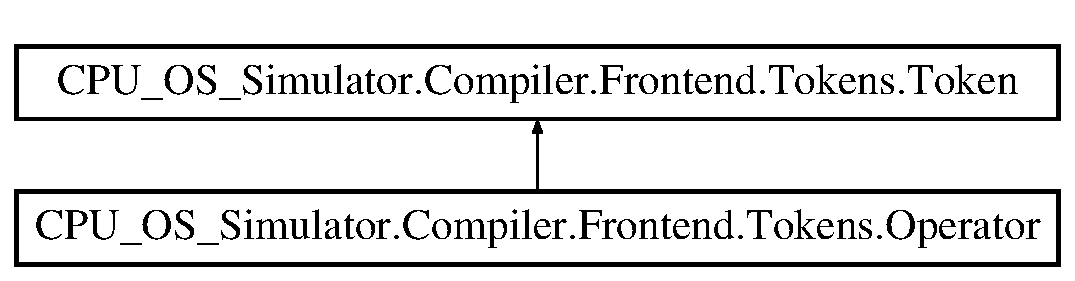
\includegraphics[height=2.000000cm]{class_c_p_u___o_s___simulator_1_1_compiler_1_1_frontend_1_1_tokens_1_1_operator}
\end{center}
\end{figure}
\subsection*{Public Member Functions}
\begin{DoxyCompactItemize}
\item 
\hyperlink{class_c_p_u___o_s___simulator_1_1_compiler_1_1_frontend_1_1_tokens_1_1_operator_a9f1b37d1fd2bf09a3eba578b23adaa81}{Operator} (string \hyperlink{class_c_p_u___o_s___simulator_1_1_compiler_1_1_frontend_1_1_tokens_1_1_token_a5c05e12850ca18be8cbfdf7e2e263324}{value})
\item 
override Enum \hyperlink{class_c_p_u___o_s___simulator_1_1_compiler_1_1_frontend_1_1_tokens_1_1_operator_a3bd6c8981e452c8abe4c4f019d78fb9b}{Detect\+Type} ()
\item 
\hyperlink{namespace_c_p_u___o_s___simulator_1_1_compiler_1_1_frontend_1_1_tokens_ac7cabb2de0258fea24dd75768143da51}{Enum\+Operator\+Type} \hyperlink{class_c_p_u___o_s___simulator_1_1_compiler_1_1_frontend_1_1_tokens_1_1_operator_af77d824a89faa9c99f9c5aaa273ce504}{Get\+Operator\+Type} ()
\end{DoxyCompactItemize}
\subsection*{Private Attributes}
\begin{DoxyCompactItemize}
\item 
int \hyperlink{class_c_p_u___o_s___simulator_1_1_compiler_1_1_frontend_1_1_tokens_1_1_operator_a96e3a4c37284e7912243d510fd958caa}{operand\+Count}
\end{DoxyCompactItemize}
\subsection*{Additional Inherited Members}


\subsection{Detailed Description}


Definition at line 5 of file Operator.\+cs.



\subsection{Constructor \& Destructor Documentation}
\hypertarget{class_c_p_u___o_s___simulator_1_1_compiler_1_1_frontend_1_1_tokens_1_1_operator_a9f1b37d1fd2bf09a3eba578b23adaa81}{}\index{C\+P\+U\+\_\+\+O\+S\+\_\+\+Simulator\+::\+Compiler\+::\+Frontend\+::\+Tokens\+::\+Operator@{C\+P\+U\+\_\+\+O\+S\+\_\+\+Simulator\+::\+Compiler\+::\+Frontend\+::\+Tokens\+::\+Operator}!Operator@{Operator}}
\index{Operator@{Operator}!C\+P\+U\+\_\+\+O\+S\+\_\+\+Simulator\+::\+Compiler\+::\+Frontend\+::\+Tokens\+::\+Operator@{C\+P\+U\+\_\+\+O\+S\+\_\+\+Simulator\+::\+Compiler\+::\+Frontend\+::\+Tokens\+::\+Operator}}
\subsubsection[{Operator(string value)}]{\setlength{\rightskip}{0pt plus 5cm}C\+P\+U\+\_\+\+O\+S\+\_\+\+Simulator.\+Compiler.\+Frontend.\+Tokens.\+Operator.\+Operator (
\begin{DoxyParamCaption}
\item[{string}]{value}
\end{DoxyParamCaption}
)}\label{class_c_p_u___o_s___simulator_1_1_compiler_1_1_frontend_1_1_tokens_1_1_operator_a9f1b37d1fd2bf09a3eba578b23adaa81}


Definition at line 9 of file Operator.\+cs.



\subsection{Member Function Documentation}
\hypertarget{class_c_p_u___o_s___simulator_1_1_compiler_1_1_frontend_1_1_tokens_1_1_operator_a3bd6c8981e452c8abe4c4f019d78fb9b}{}\index{C\+P\+U\+\_\+\+O\+S\+\_\+\+Simulator\+::\+Compiler\+::\+Frontend\+::\+Tokens\+::\+Operator@{C\+P\+U\+\_\+\+O\+S\+\_\+\+Simulator\+::\+Compiler\+::\+Frontend\+::\+Tokens\+::\+Operator}!Detect\+Type@{Detect\+Type}}
\index{Detect\+Type@{Detect\+Type}!C\+P\+U\+\_\+\+O\+S\+\_\+\+Simulator\+::\+Compiler\+::\+Frontend\+::\+Tokens\+::\+Operator@{C\+P\+U\+\_\+\+O\+S\+\_\+\+Simulator\+::\+Compiler\+::\+Frontend\+::\+Tokens\+::\+Operator}}
\subsubsection[{Detect\+Type()}]{\setlength{\rightskip}{0pt plus 5cm}override Enum C\+P\+U\+\_\+\+O\+S\+\_\+\+Simulator.\+Compiler.\+Frontend.\+Tokens.\+Operator.\+Detect\+Type (
\begin{DoxyParamCaption}
{}
\end{DoxyParamCaption}
)\hspace{0.3cm}{\ttfamily [virtual]}}\label{class_c_p_u___o_s___simulator_1_1_compiler_1_1_frontend_1_1_tokens_1_1_operator_a3bd6c8981e452c8abe4c4f019d78fb9b}


Implements \hyperlink{class_c_p_u___o_s___simulator_1_1_compiler_1_1_frontend_1_1_tokens_1_1_token_accfe8c46faedacd527ef619698c76310}{C\+P\+U\+\_\+\+O\+S\+\_\+\+Simulator.\+Compiler.\+Frontend.\+Tokens.\+Token}.



Definition at line 13 of file Operator.\+cs.

\hypertarget{class_c_p_u___o_s___simulator_1_1_compiler_1_1_frontend_1_1_tokens_1_1_operator_af77d824a89faa9c99f9c5aaa273ce504}{}\index{C\+P\+U\+\_\+\+O\+S\+\_\+\+Simulator\+::\+Compiler\+::\+Frontend\+::\+Tokens\+::\+Operator@{C\+P\+U\+\_\+\+O\+S\+\_\+\+Simulator\+::\+Compiler\+::\+Frontend\+::\+Tokens\+::\+Operator}!Get\+Operator\+Type@{Get\+Operator\+Type}}
\index{Get\+Operator\+Type@{Get\+Operator\+Type}!C\+P\+U\+\_\+\+O\+S\+\_\+\+Simulator\+::\+Compiler\+::\+Frontend\+::\+Tokens\+::\+Operator@{C\+P\+U\+\_\+\+O\+S\+\_\+\+Simulator\+::\+Compiler\+::\+Frontend\+::\+Tokens\+::\+Operator}}
\subsubsection[{Get\+Operator\+Type()}]{\setlength{\rightskip}{0pt plus 5cm}{\bf Enum\+Operator\+Type} C\+P\+U\+\_\+\+O\+S\+\_\+\+Simulator.\+Compiler.\+Frontend.\+Tokens.\+Operator.\+Get\+Operator\+Type (
\begin{DoxyParamCaption}
{}
\end{DoxyParamCaption}
)}\label{class_c_p_u___o_s___simulator_1_1_compiler_1_1_frontend_1_1_tokens_1_1_operator_af77d824a89faa9c99f9c5aaa273ce504}


Definition at line 46 of file Operator.\+cs.



\subsection{Member Data Documentation}
\hypertarget{class_c_p_u___o_s___simulator_1_1_compiler_1_1_frontend_1_1_tokens_1_1_operator_a96e3a4c37284e7912243d510fd958caa}{}\index{C\+P\+U\+\_\+\+O\+S\+\_\+\+Simulator\+::\+Compiler\+::\+Frontend\+::\+Tokens\+::\+Operator@{C\+P\+U\+\_\+\+O\+S\+\_\+\+Simulator\+::\+Compiler\+::\+Frontend\+::\+Tokens\+::\+Operator}!operand\+Count@{operand\+Count}}
\index{operand\+Count@{operand\+Count}!C\+P\+U\+\_\+\+O\+S\+\_\+\+Simulator\+::\+Compiler\+::\+Frontend\+::\+Tokens\+::\+Operator@{C\+P\+U\+\_\+\+O\+S\+\_\+\+Simulator\+::\+Compiler\+::\+Frontend\+::\+Tokens\+::\+Operator}}
\subsubsection[{operand\+Count}]{\setlength{\rightskip}{0pt plus 5cm}int C\+P\+U\+\_\+\+O\+S\+\_\+\+Simulator.\+Compiler.\+Frontend.\+Tokens.\+Operator.\+operand\+Count\hspace{0.3cm}{\ttfamily [private]}}\label{class_c_p_u___o_s___simulator_1_1_compiler_1_1_frontend_1_1_tokens_1_1_operator_a96e3a4c37284e7912243d510fd958caa}


Definition at line 7 of file Operator.\+cs.



The documentation for this class was generated from the following file\+:\begin{DoxyCompactItemize}
\item 
Compiler/\+Frontend/\+Tokens/\hyperlink{_operator_8cs}{Operator.\+cs}\end{DoxyCompactItemize}

\hypertarget{class_c_p_u___o_s___simulator_1_1_operating___system_1_1_o_s_core}{}\section{C\+P\+U\+\_\+\+O\+S\+\_\+\+Simulator.\+Operating\+\_\+\+System.\+O\+S\+Core Class Reference}
\label{class_c_p_u___o_s___simulator_1_1_operating___system_1_1_o_s_core}\index{C\+P\+U\+\_\+\+O\+S\+\_\+\+Simulator.\+Operating\+\_\+\+System.\+O\+S\+Core@{C\+P\+U\+\_\+\+O\+S\+\_\+\+Simulator.\+Operating\+\_\+\+System.\+O\+S\+Core}}


This class represents the core of the operating system  


Inheritance diagram for C\+P\+U\+\_\+\+O\+S\+\_\+\+Simulator.\+Operating\+\_\+\+System.\+O\+S\+Core\+:\begin{figure}[H]
\begin{center}
\leavevmode
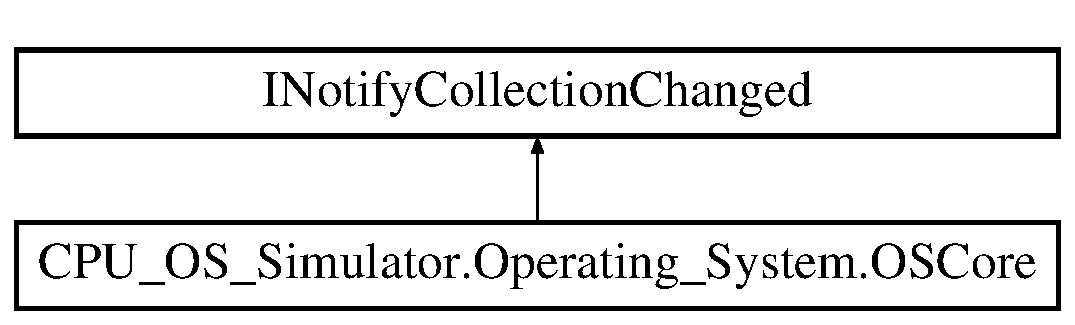
\includegraphics[height=2.000000cm]{class_c_p_u___o_s___simulator_1_1_operating___system_1_1_o_s_core}
\end{center}
\end{figure}
\subsection*{Public Member Functions}
\begin{DoxyCompactItemize}
\item 
\hyperlink{class_c_p_u___o_s___simulator_1_1_operating___system_1_1_o_s_core_a3845ed83851b87e64d6918a2a495e45e}{O\+S\+Core} ()
\begin{DoxyCompactList}\small\item\em Default Constructor for the O\+S Core \end{DoxyCompactList}\item 
\hyperlink{class_c_p_u___o_s___simulator_1_1_operating___system_1_1_o_s_core_a65c809ada2e4d0d5f6269e6a9009db0d}{O\+S\+Core} (\hyperlink{struct_c_p_u___o_s___simulator_1_1_operating___system_1_1_o_s_flags}{O\+S\+Flags} flags)
\begin{DoxyCompactList}\small\item\em Constructor for O\+S Core that takes flags which control O\+S behaviour \end{DoxyCompactList}\item 
bool \hyperlink{class_c_p_u___o_s___simulator_1_1_operating___system_1_1_o_s_core_adb8186aefcc47d02daa0856e5c9c42b7}{Start} ()
\begin{DoxyCompactList}\small\item\em This function is called to start the operating system \end{DoxyCompactList}\item 
\hyperlink{class_c_p_u___o_s___simulator_1_1_operating___system_1_1_simulator_process}{Simulator\+Process} \hyperlink{class_c_p_u___o_s___simulator_1_1_operating___system_1_1_o_s_core_afee9dd12629e415c420fc7c197f784c4}{Create\+Process} (\hyperlink{struct_c_p_u___o_s___simulator_1_1_operating___system_1_1_process_flags}{Process\+Flags} flags)
\begin{DoxyCompactList}\small\item\em This function creates a simulator process \end{DoxyCompactList}\end{DoxyCompactItemize}
\subsection*{Properties}
\begin{DoxyCompactItemize}
\item 
double \hyperlink{class_c_p_u___o_s___simulator_1_1_operating___system_1_1_o_s_core_af72424eea15d262a41f9390e8f3bce97}{Rr\+\_\+\+Time\+\_\+\+Slice}\hspace{0.3cm}{\ttfamily  \mbox{[}get, set\mbox{]}}
\begin{DoxyCompactList}\small\item\em Property for the length of the round robin time slice being used by this scheduler \end{DoxyCompactList}\item 
\hyperlink{namespace_c_p_u___o_s___simulator_1_1_operating___system_a0553d0bc2513aec52caa769acf994d5c}{Enum\+Time\+Unit} \hyperlink{class_c_p_u___o_s___simulator_1_1_operating___system_1_1_o_s_core_a8f8e6705ddbf4a04900b343e65bd71d2}{Rr\+\_\+\+Time\+\_\+\+Slice\+\_\+\+Unit}\hspace{0.3cm}{\ttfamily  \mbox{[}get, set\mbox{]}}
\begin{DoxyCompactList}\small\item\em Property for the unit of time used for time slices i.\+e ticks or seconds \end{DoxyCompactList}\item 
\hyperlink{namespace_c_p_u___o_s___simulator_1_1_operating___system_a3a9286a473bd079e9c65908c0378fa00}{Enum\+Priority\+Policy} \hyperlink{class_c_p_u___o_s___simulator_1_1_operating___system_1_1_o_s_core_a71b8f167c84a1cb1feba77cd2cb5420d}{Priority\+Policy}\hspace{0.3cm}{\ttfamily  \mbox{[}get, set\mbox{]}}
\begin{DoxyCompactList}\small\item\em Property for the Round Robin priority policy being used by this scheduler \end{DoxyCompactList}\item 
\hyperlink{namespace_c_p_u___o_s___simulator_1_1_operating___system_a4c7effb8b6725df52018a3a14cede96e}{Enum\+Round\+Robin\+Type} \hyperlink{class_c_p_u___o_s___simulator_1_1_operating___system_1_1_o_s_core_a49d248bc5438438d42482a9e962c417c}{Round\+Robin\+Type}\hspace{0.3cm}{\ttfamily  \mbox{[}get, set\mbox{]}}
\begin{DoxyCompactList}\small\item\em Property for the type of round robin being used by the scheduler \end{DoxyCompactList}\item 
bool \hyperlink{class_c_p_u___o_s___simulator_1_1_operating___system_1_1_o_s_core_a1fd8b54b31fa415f09f2b9bc407802dd}{Use\+Default\+Scheduler}\hspace{0.3cm}{\ttfamily  \mbox{[}get, set\mbox{]}}
\begin{DoxyCompactList}\small\item\em Property for whether we are using the default scheduler \end{DoxyCompactList}\item 
int \hyperlink{class_c_p_u___o_s___simulator_1_1_operating___system_1_1_o_s_core_a1ea93a6cc37dbae4bc607d09fd6e75db}{Cpu\+Clock\+Speed}\hspace{0.3cm}{\ttfamily  \mbox{[}get, set\mbox{]}}
\begin{DoxyCompactList}\small\item\em Property for the clock speed of the \hyperlink{namespace_c_p_u___o_s___simulator_1_1_c_p_u}{C\+P\+U} \end{DoxyCompactList}\item 
bool \hyperlink{class_c_p_u___o_s___simulator_1_1_operating___system_1_1_o_s_core_a58135ead5821cb968f25c20417dd460a}{Suspend\+On\+State\+Change\+\_\+\+Ready}\hspace{0.3cm}{\ttfamily  \mbox{[}get, set\mbox{]}}
\begin{DoxyCompactList}\small\item\em Property for whether the process should suspend when it enters the ready state \end{DoxyCompactList}\item 
bool \hyperlink{class_c_p_u___o_s___simulator_1_1_operating___system_1_1_o_s_core_aaea8e895847f690b5a4104bf4326f3ab}{Suspend\+On\+Pre\+Emption}\hspace{0.3cm}{\ttfamily  \mbox{[}get, set\mbox{]}}
\begin{DoxyCompactList}\small\item\em Property for whether the process should suspend when it is pre-\/empted by another process \end{DoxyCompactList}\item 
bool \hyperlink{class_c_p_u___o_s___simulator_1_1_operating___system_1_1_o_s_core_a8dfe787e5954a595f63012f9a2d00d64}{Suspend\+On\+State\+Change\+\_\+\+Running}\hspace{0.3cm}{\ttfamily  \mbox{[}get, set\mbox{]}}
\begin{DoxyCompactList}\small\item\em Property for whether the process should suspend when it enters the running state \end{DoxyCompactList}\item 
bool \hyperlink{class_c_p_u___o_s___simulator_1_1_operating___system_1_1_o_s_core_a431f6636a3265ebd4c87f973b49a5195}{Suspend\+On\+State\+Change\+\_\+\+Waiting}\hspace{0.3cm}{\ttfamily  \mbox{[}get, set\mbox{]}}
\begin{DoxyCompactList}\small\item\em Property for whether the process should suspend when it enters the waiting state \end{DoxyCompactList}\item 
\hyperlink{namespace_c_p_u___o_s___simulator_1_1_operating___system_a03a98a403abc737c106a8f92db5bffc1}{Enum\+O\+S\+State} \hyperlink{class_c_p_u___o_s___simulator_1_1_operating___system_1_1_o_s_core_ac620c813df8b2c9ea386cff20d3fee84}{Os\+State}\hspace{0.3cm}{\ttfamily  \mbox{[}get, set\mbox{]}}
\begin{DoxyCompactList}\small\item\em Property for the current state of the O\+S \end{DoxyCompactList}\item 
\hyperlink{namespace_c_p_u___o_s___simulator_1_1_operating___system_ad0cdaacf9652394d23fa29109640fe08}{Enum\+Scheduling\+Policies} \hyperlink{class_c_p_u___o_s___simulator_1_1_operating___system_1_1_o_s_core_a265614d635fd57e6275b2bfc13d7a597}{Scheduling\+Policy}\hspace{0.3cm}{\ttfamily  \mbox{[}get, set\mbox{]}}
\begin{DoxyCompactList}\small\item\em Property for the scheduling policy currently being used by this scheduler \end{DoxyCompactList}\item 
bool \hyperlink{class_c_p_u___o_s___simulator_1_1_operating___system_1_1_o_s_core_ac965e1317dc5c6b6ae93c410098dd913}{Using\+Single\+Cpu}\hspace{0.3cm}{\ttfamily  \mbox{[}get, set\mbox{]}}
\begin{DoxyCompactList}\small\item\em Property for whether the scheduler is running on a single \hyperlink{namespace_c_p_u___o_s___simulator_1_1_c_p_u}{C\+P\+U} \end{DoxyCompactList}\item 
bool \hyperlink{class_c_p_u___o_s___simulator_1_1_operating___system_1_1_o_s_core_a5086a047ca75af087039e9d45ea0a6cf}{Allow\+Cpu\+Affinity}\hspace{0.3cm}{\ttfamily  \mbox{[}get, set\mbox{]}}
\begin{DoxyCompactList}\small\item\em Property for whether \hyperlink{namespace_c_p_u___o_s___simulator_1_1_c_p_u}{C\+P\+U} affinity is allowed on this scheduler \end{DoxyCompactList}\item 
bool \hyperlink{class_c_p_u___o_s___simulator_1_1_operating___system_1_1_o_s_core_a1f01594c8f33961b5dc5ffffaf7644ce}{Running\+With\+No\+Processes}\hspace{0.3cm}{\ttfamily  \mbox{[}get, set\mbox{]}}
\begin{DoxyCompactList}\small\item\em Property for whether the scheduler is running with no processes \end{DoxyCompactList}\item 
\hyperlink{namespace_c_p_u___o_s___simulator_1_1_operating___system_aea0b669d1bbf5690ae34ac2f8bef9470}{Enum\+Error\+Codes} \hyperlink{class_c_p_u___o_s___simulator_1_1_operating___system_1_1_o_s_core_a77a647e293c14574919b144cb2e8998f}{Error\+Code}\hspace{0.3cm}{\ttfamily  \mbox{[}get, set\mbox{]}}
\begin{DoxyCompactList}\small\item\em Property for an error code that describes any error that occurred \end{DoxyCompactList}\item 
\hyperlink{class_c_p_u___o_s___simulator_1_1_operating___system_1_1_scheduler}{Scheduler} \hyperlink{class_c_p_u___o_s___simulator_1_1_operating___system_1_1_o_s_core_aa97bbf90ba03bd17c02f889189108455}{Scheduler}\hspace{0.3cm}{\ttfamily  \mbox{[}get, set\mbox{]}}
\begin{DoxyCompactList}\small\item\em Property for the current scheduler \end{DoxyCompactList}\end{DoxyCompactItemize}
\subsection*{Events}
\begin{DoxyCompactItemize}
\item 
Notify\+Collection\+Changed\+Event\+Handler \hyperlink{class_c_p_u___o_s___simulator_1_1_operating___system_1_1_o_s_core_abcbb2efff8a4078fae3edb9b31f62198}{Collection\+Changed}
\end{DoxyCompactItemize}
\subsection*{Private Member Functions}
\begin{DoxyCompactItemize}
\item 
void \hyperlink{class_c_p_u___o_s___simulator_1_1_operating___system_1_1_o_s_core_abc6fc1ed70b080ea9079d548c86e88ec}{On\+Collection\+Changed} (object sender, Notify\+Collection\+Changed\+Event\+Args notify\+Collection\+Changed\+Event\+Args)
\item 
void \hyperlink{class_c_p_u___o_s___simulator_1_1_operating___system_1_1_o_s_core_a0697465a14d3f6111160c2c5a0d4082b}{Set\+Clock\+Speed} ()
\item 
\hyperlink{struct_c_p_u___o_s___simulator_1_1_operating___system_1_1_scheduler_flags}{Scheduler\+Flags} \hyperlink{class_c_p_u___o_s___simulator_1_1_operating___system_1_1_o_s_core_a0370de0efae69664c16b258846a64908}{Create\+Scheduler\+Flags} ()
\begin{DoxyCompactList}\small\item\em this method creates flags for the operating system scheduler based on selected U\+I options \end{DoxyCompactList}\item 
dynamic \hyperlink{class_c_p_u___o_s___simulator_1_1_operating___system_1_1_o_s_core_a6aa060134c64a17e248da359846f394b}{Get\+Main\+Window\+Instance} ()
\begin{DoxyCompactList}\small\item\em This function gets the main window instance from the window bridge \end{DoxyCompactList}\item 
dynamic \hyperlink{class_c_p_u___o_s___simulator_1_1_operating___system_1_1_o_s_core_a8943c071c2bb36810e560ef0e735f108}{Get\+O\+S\+Window\+Instance} ()
\begin{DoxyCompactList}\small\item\em This function gets the main window instance from the window bridge \end{DoxyCompactList}\end{DoxyCompactItemize}
\subsection*{Private Attributes}
\begin{DoxyCompactItemize}
\item 
\hyperlink{namespace_c_p_u___o_s___simulator_1_1_operating___system_ad0cdaacf9652394d23fa29109640fe08}{Enum\+Scheduling\+Policies} \hyperlink{class_c_p_u___o_s___simulator_1_1_operating___system_1_1_o_s_core_a379d53a0d661ac56f75c2676bed68b06}{scheduling\+Policy} = \hyperlink{namespace_c_p_u___o_s___simulator_1_1_operating___system_aea0b669d1bbf5690ae34ac2f8bef9470a696b031073e74bf2cb98e5ef201d4aa3}{Enum\+Scheduling\+Policies.\+U\+N\+K\+N\+O\+W\+N}
\item 
double \hyperlink{class_c_p_u___o_s___simulator_1_1_operating___system_1_1_o_s_core_a34a8be2fd9187764366ca5a7b48d764e}{R\+R\+\_\+\+Time\+\_\+\+Slice}
\item 
\hyperlink{namespace_c_p_u___o_s___simulator_1_1_operating___system_a0553d0bc2513aec52caa769acf994d5c}{Enum\+Time\+Unit} \hyperlink{class_c_p_u___o_s___simulator_1_1_operating___system_1_1_o_s_core_ac0f4c6d450108d3b51e9fc7f9dc930ce}{R\+R\+\_\+\+Time\+\_\+\+Slice\+\_\+\+Unit} = \hyperlink{namespace_c_p_u___o_s___simulator_1_1_operating___system_aea0b669d1bbf5690ae34ac2f8bef9470a696b031073e74bf2cb98e5ef201d4aa3}{Enum\+Time\+Unit.\+U\+N\+K\+N\+O\+W\+N}
\item 
\hyperlink{namespace_c_p_u___o_s___simulator_1_1_operating___system_a3a9286a473bd079e9c65908c0378fa00}{Enum\+Priority\+Policy} \hyperlink{class_c_p_u___o_s___simulator_1_1_operating___system_1_1_o_s_core_a866fa4ff3b8aadb3eb57188f6a87e148}{priority\+Policy} = \hyperlink{namespace_c_p_u___o_s___simulator_1_1_operating___system_aea0b669d1bbf5690ae34ac2f8bef9470a696b031073e74bf2cb98e5ef201d4aa3}{Enum\+Priority\+Policy.\+U\+N\+K\+N\+O\+W\+N}
\item 
\hyperlink{namespace_c_p_u___o_s___simulator_1_1_operating___system_a4c7effb8b6725df52018a3a14cede96e}{Enum\+Round\+Robin\+Type} \hyperlink{class_c_p_u___o_s___simulator_1_1_operating___system_1_1_o_s_core_a4a891b4c9ed3aa97c389bccab0b2687d}{round\+Robin\+Type} = \hyperlink{namespace_c_p_u___o_s___simulator_1_1_operating___system_aea0b669d1bbf5690ae34ac2f8bef9470a696b031073e74bf2cb98e5ef201d4aa3}{Enum\+Round\+Robin\+Type.\+U\+N\+K\+N\+O\+W\+N}
\item 
bool \hyperlink{class_c_p_u___o_s___simulator_1_1_operating___system_1_1_o_s_core_a9e4390ec19f02a66b2c8ba829fad0e49}{use\+Default\+Scheduler}
\item 
bool \hyperlink{class_c_p_u___o_s___simulator_1_1_operating___system_1_1_o_s_core_ac9667b36d2359ddf024ded0a57ba20be}{use\+Single\+C\+P\+U}
\item 
bool \hyperlink{class_c_p_u___o_s___simulator_1_1_operating___system_1_1_o_s_core_ad3fc35d621bf2c2afc8b2a66fc38d2c0}{allow\+C\+P\+U\+Affinity}
\item 
bool \hyperlink{class_c_p_u___o_s___simulator_1_1_operating___system_1_1_o_s_core_ac0526b86d9657a372e44664acf103438}{run\+With\+No\+Processes}
\item 
int \hyperlink{class_c_p_u___o_s___simulator_1_1_operating___system_1_1_o_s_core_a99f66d92928cea0a61e21ea427f16ab2}{C\+P\+U\+Clock\+Speed}
\item 
bool \hyperlink{class_c_p_u___o_s___simulator_1_1_operating___system_1_1_o_s_core_a2ee0e6e84ca8fd9b7d3daf279d038640}{suspend\+On\+State\+Change\+\_\+\+Ready}
\item 
bool \hyperlink{class_c_p_u___o_s___simulator_1_1_operating___system_1_1_o_s_core_a99875cff5880ff8dce2c77758389491b}{suspend\+On\+Pre\+Emption}
\item 
bool \hyperlink{class_c_p_u___o_s___simulator_1_1_operating___system_1_1_o_s_core_af35a9cd41325505df4cc3894c4b297b4}{suspend\+On\+State\+Change\+\_\+\+Running}
\item 
bool \hyperlink{class_c_p_u___o_s___simulator_1_1_operating___system_1_1_o_s_core_aebfddcf30c39c36876e07017fef6605f}{suspend\+On\+State\+Change\+\_\+\+Waiting}
\item 
bool \hyperlink{class_c_p_u___o_s___simulator_1_1_operating___system_1_1_o_s_core_aaa9fd56285fb7a3d8718f81e8df847ac}{force\+Kill}
\item 
bool \hyperlink{class_c_p_u___o_s___simulator_1_1_operating___system_1_1_o_s_core_a94ab635fc88b9a85556a55c8f2c49b89}{fault\+Kill}
\item 
\hyperlink{namespace_c_p_u___o_s___simulator_1_1_operating___system_a03a98a403abc737c106a8f92db5bffc1}{Enum\+O\+S\+State} \hyperlink{class_c_p_u___o_s___simulator_1_1_operating___system_1_1_o_s_core_ad428ed8c6f24743d016c9ba44ca129a5}{os\+State} = \hyperlink{namespace_c_p_u___o_s___simulator_1_1_operating___system_aea0b669d1bbf5690ae34ac2f8bef9470a696b031073e74bf2cb98e5ef201d4aa3}{Enum\+O\+S\+State.\+U\+N\+K\+N\+O\+W\+N}
\item 
\hyperlink{namespace_c_p_u___o_s___simulator_1_1_operating___system_aea0b669d1bbf5690ae34ac2f8bef9470}{Enum\+Error\+Codes} \hyperlink{class_c_p_u___o_s___simulator_1_1_operating___system_1_1_o_s_core_a321ac6d45675953550f32e23068e194f}{error\+Code} = \hyperlink{namespace_c_p_u___o_s___simulator_1_1_operating___system_aea0b669d1bbf5690ae34ac2f8bef9470a696b031073e74bf2cb98e5ef201d4aa3}{Enum\+Error\+Codes.\+U\+N\+K\+N\+O\+W\+N}
\item 
\hyperlink{class_c_p_u___o_s___simulator_1_1_operating___system_1_1_scheduler}{Scheduler} \hyperlink{class_c_p_u___o_s___simulator_1_1_operating___system_1_1_o_s_core_a2ef4c455b9babbd12d3e70fb4d82567e}{scheduler}
\item 
Queue$<$ \hyperlink{class_c_p_u___o_s___simulator_1_1_operating___system_1_1_simulator_process}{Simulator\+Process} $>$ \hyperlink{class_c_p_u___o_s___simulator_1_1_operating___system_1_1_o_s_core_a5e76bf14a368f77713eaab94b4e4a118}{ready\+Queue}
\item 
Queue$<$ \hyperlink{class_c_p_u___o_s___simulator_1_1_operating___system_1_1_simulator_process}{Simulator\+Process} $>$ \hyperlink{class_c_p_u___o_s___simulator_1_1_operating___system_1_1_o_s_core_a66baab674b5f03a5d31378af85f73fb7}{waiting\+Queue}
\end{DoxyCompactItemize}


\subsection{Detailed Description}
This class represents the core of the operating system 



Definition at line 13 of file O\+S\+Core.\+cs.



\subsection{Constructor \& Destructor Documentation}
\hypertarget{class_c_p_u___o_s___simulator_1_1_operating___system_1_1_o_s_core_a3845ed83851b87e64d6918a2a495e45e}{}\index{C\+P\+U\+\_\+\+O\+S\+\_\+\+Simulator\+::\+Operating\+\_\+\+System\+::\+O\+S\+Core@{C\+P\+U\+\_\+\+O\+S\+\_\+\+Simulator\+::\+Operating\+\_\+\+System\+::\+O\+S\+Core}!O\+S\+Core@{O\+S\+Core}}
\index{O\+S\+Core@{O\+S\+Core}!C\+P\+U\+\_\+\+O\+S\+\_\+\+Simulator\+::\+Operating\+\_\+\+System\+::\+O\+S\+Core@{C\+P\+U\+\_\+\+O\+S\+\_\+\+Simulator\+::\+Operating\+\_\+\+System\+::\+O\+S\+Core}}
\subsubsection[{O\+S\+Core()}]{\setlength{\rightskip}{0pt plus 5cm}C\+P\+U\+\_\+\+O\+S\+\_\+\+Simulator.\+Operating\+\_\+\+System.\+O\+S\+Core.\+O\+S\+Core (
\begin{DoxyParamCaption}
{}
\end{DoxyParamCaption}
)}\label{class_c_p_u___o_s___simulator_1_1_operating___system_1_1_o_s_core_a3845ed83851b87e64d6918a2a495e45e}


Default Constructor for the O\+S Core 



Definition at line 41 of file O\+S\+Core.\+cs.

\hypertarget{class_c_p_u___o_s___simulator_1_1_operating___system_1_1_o_s_core_a65c809ada2e4d0d5f6269e6a9009db0d}{}\index{C\+P\+U\+\_\+\+O\+S\+\_\+\+Simulator\+::\+Operating\+\_\+\+System\+::\+O\+S\+Core@{C\+P\+U\+\_\+\+O\+S\+\_\+\+Simulator\+::\+Operating\+\_\+\+System\+::\+O\+S\+Core}!O\+S\+Core@{O\+S\+Core}}
\index{O\+S\+Core@{O\+S\+Core}!C\+P\+U\+\_\+\+O\+S\+\_\+\+Simulator\+::\+Operating\+\_\+\+System\+::\+O\+S\+Core@{C\+P\+U\+\_\+\+O\+S\+\_\+\+Simulator\+::\+Operating\+\_\+\+System\+::\+O\+S\+Core}}
\subsubsection[{O\+S\+Core(\+O\+S\+Flags flags)}]{\setlength{\rightskip}{0pt plus 5cm}C\+P\+U\+\_\+\+O\+S\+\_\+\+Simulator.\+Operating\+\_\+\+System.\+O\+S\+Core.\+O\+S\+Core (
\begin{DoxyParamCaption}
\item[{{\bf O\+S\+Flags}}]{flags}
\end{DoxyParamCaption}
)}\label{class_c_p_u___o_s___simulator_1_1_operating___system_1_1_o_s_core_a65c809ada2e4d0d5f6269e6a9009db0d}


Constructor for O\+S Core that takes flags which control O\+S behaviour 


\begin{DoxyParams}{Parameters}
{\em flags} & the flags to be passed to this operating system\\
\hline
\end{DoxyParams}


Definition at line 49 of file O\+S\+Core.\+cs.



\subsection{Member Function Documentation}
\hypertarget{class_c_p_u___o_s___simulator_1_1_operating___system_1_1_o_s_core_afee9dd12629e415c420fc7c197f784c4}{}\index{C\+P\+U\+\_\+\+O\+S\+\_\+\+Simulator\+::\+Operating\+\_\+\+System\+::\+O\+S\+Core@{C\+P\+U\+\_\+\+O\+S\+\_\+\+Simulator\+::\+Operating\+\_\+\+System\+::\+O\+S\+Core}!Create\+Process@{Create\+Process}}
\index{Create\+Process@{Create\+Process}!C\+P\+U\+\_\+\+O\+S\+\_\+\+Simulator\+::\+Operating\+\_\+\+System\+::\+O\+S\+Core@{C\+P\+U\+\_\+\+O\+S\+\_\+\+Simulator\+::\+Operating\+\_\+\+System\+::\+O\+S\+Core}}
\subsubsection[{Create\+Process(\+Process\+Flags flags)}]{\setlength{\rightskip}{0pt plus 5cm}{\bf Simulator\+Process} C\+P\+U\+\_\+\+O\+S\+\_\+\+Simulator.\+Operating\+\_\+\+System.\+O\+S\+Core.\+Create\+Process (
\begin{DoxyParamCaption}
\item[{{\bf Process\+Flags}}]{flags}
\end{DoxyParamCaption}
)}\label{class_c_p_u___o_s___simulator_1_1_operating___system_1_1_o_s_core_afee9dd12629e415c420fc7c197f784c4}


This function creates a simulator process 


\begin{DoxyParams}{Parameters}
{\em flags} & the flags to use to create the simulator process\\
\hline
\end{DoxyParams}
\begin{DoxyReturn}{Returns}
the created simulator process
\end{DoxyReturn}


Definition at line 120 of file O\+S\+Core.\+cs.

\hypertarget{class_c_p_u___o_s___simulator_1_1_operating___system_1_1_o_s_core_a0370de0efae69664c16b258846a64908}{}\index{C\+P\+U\+\_\+\+O\+S\+\_\+\+Simulator\+::\+Operating\+\_\+\+System\+::\+O\+S\+Core@{C\+P\+U\+\_\+\+O\+S\+\_\+\+Simulator\+::\+Operating\+\_\+\+System\+::\+O\+S\+Core}!Create\+Scheduler\+Flags@{Create\+Scheduler\+Flags}}
\index{Create\+Scheduler\+Flags@{Create\+Scheduler\+Flags}!C\+P\+U\+\_\+\+O\+S\+\_\+\+Simulator\+::\+Operating\+\_\+\+System\+::\+O\+S\+Core@{C\+P\+U\+\_\+\+O\+S\+\_\+\+Simulator\+::\+Operating\+\_\+\+System\+::\+O\+S\+Core}}
\subsubsection[{Create\+Scheduler\+Flags()}]{\setlength{\rightskip}{0pt plus 5cm}{\bf Scheduler\+Flags} C\+P\+U\+\_\+\+O\+S\+\_\+\+Simulator.\+Operating\+\_\+\+System.\+O\+S\+Core.\+Create\+Scheduler\+Flags (
\begin{DoxyParamCaption}
{}
\end{DoxyParamCaption}
)\hspace{0.3cm}{\ttfamily [private]}}\label{class_c_p_u___o_s___simulator_1_1_operating___system_1_1_o_s_core_a0370de0efae69664c16b258846a64908}


this method creates flags for the operating system scheduler based on selected U\+I options 

\begin{DoxyReturn}{Returns}
a struct containing the selected options or null if an error occurred
\end{DoxyReturn}


Definition at line 129 of file O\+S\+Core.\+cs.

\hypertarget{class_c_p_u___o_s___simulator_1_1_operating___system_1_1_o_s_core_a6aa060134c64a17e248da359846f394b}{}\index{C\+P\+U\+\_\+\+O\+S\+\_\+\+Simulator\+::\+Operating\+\_\+\+System\+::\+O\+S\+Core@{C\+P\+U\+\_\+\+O\+S\+\_\+\+Simulator\+::\+Operating\+\_\+\+System\+::\+O\+S\+Core}!Get\+Main\+Window\+Instance@{Get\+Main\+Window\+Instance}}
\index{Get\+Main\+Window\+Instance@{Get\+Main\+Window\+Instance}!C\+P\+U\+\_\+\+O\+S\+\_\+\+Simulator\+::\+Operating\+\_\+\+System\+::\+O\+S\+Core@{C\+P\+U\+\_\+\+O\+S\+\_\+\+Simulator\+::\+Operating\+\_\+\+System\+::\+O\+S\+Core}}
\subsubsection[{Get\+Main\+Window\+Instance()}]{\setlength{\rightskip}{0pt plus 5cm}dynamic C\+P\+U\+\_\+\+O\+S\+\_\+\+Simulator.\+Operating\+\_\+\+System.\+O\+S\+Core.\+Get\+Main\+Window\+Instance (
\begin{DoxyParamCaption}
{}
\end{DoxyParamCaption}
)\hspace{0.3cm}{\ttfamily [private]}}\label{class_c_p_u___o_s___simulator_1_1_operating___system_1_1_o_s_core_a6aa060134c64a17e248da359846f394b}


This function gets the main window instance from the window bridge 

\begin{DoxyReturn}{Returns}
the active instance of main window 
\end{DoxyReturn}


Definition at line 168 of file O\+S\+Core.\+cs.

\hypertarget{class_c_p_u___o_s___simulator_1_1_operating___system_1_1_o_s_core_a8943c071c2bb36810e560ef0e735f108}{}\index{C\+P\+U\+\_\+\+O\+S\+\_\+\+Simulator\+::\+Operating\+\_\+\+System\+::\+O\+S\+Core@{C\+P\+U\+\_\+\+O\+S\+\_\+\+Simulator\+::\+Operating\+\_\+\+System\+::\+O\+S\+Core}!Get\+O\+S\+Window\+Instance@{Get\+O\+S\+Window\+Instance}}
\index{Get\+O\+S\+Window\+Instance@{Get\+O\+S\+Window\+Instance}!C\+P\+U\+\_\+\+O\+S\+\_\+\+Simulator\+::\+Operating\+\_\+\+System\+::\+O\+S\+Core@{C\+P\+U\+\_\+\+O\+S\+\_\+\+Simulator\+::\+Operating\+\_\+\+System\+::\+O\+S\+Core}}
\subsubsection[{Get\+O\+S\+Window\+Instance()}]{\setlength{\rightskip}{0pt plus 5cm}dynamic C\+P\+U\+\_\+\+O\+S\+\_\+\+Simulator.\+Operating\+\_\+\+System.\+O\+S\+Core.\+Get\+O\+S\+Window\+Instance (
\begin{DoxyParamCaption}
{}
\end{DoxyParamCaption}
)\hspace{0.3cm}{\ttfamily [private]}}\label{class_c_p_u___o_s___simulator_1_1_operating___system_1_1_o_s_core_a8943c071c2bb36810e560ef0e735f108}


This function gets the main window instance from the window bridge 

\begin{DoxyReturn}{Returns}
the active instance of main window 
\end{DoxyReturn}


Definition at line 181 of file O\+S\+Core.\+cs.

\hypertarget{class_c_p_u___o_s___simulator_1_1_operating___system_1_1_o_s_core_abc6fc1ed70b080ea9079d548c86e88ec}{}\index{C\+P\+U\+\_\+\+O\+S\+\_\+\+Simulator\+::\+Operating\+\_\+\+System\+::\+O\+S\+Core@{C\+P\+U\+\_\+\+O\+S\+\_\+\+Simulator\+::\+Operating\+\_\+\+System\+::\+O\+S\+Core}!On\+Collection\+Changed@{On\+Collection\+Changed}}
\index{On\+Collection\+Changed@{On\+Collection\+Changed}!C\+P\+U\+\_\+\+O\+S\+\_\+\+Simulator\+::\+Operating\+\_\+\+System\+::\+O\+S\+Core@{C\+P\+U\+\_\+\+O\+S\+\_\+\+Simulator\+::\+Operating\+\_\+\+System\+::\+O\+S\+Core}}
\subsubsection[{On\+Collection\+Changed(object sender, Notify\+Collection\+Changed\+Event\+Args notify\+Collection\+Changed\+Event\+Args)}]{\setlength{\rightskip}{0pt plus 5cm}void C\+P\+U\+\_\+\+O\+S\+\_\+\+Simulator.\+Operating\+\_\+\+System.\+O\+S\+Core.\+On\+Collection\+Changed (
\begin{DoxyParamCaption}
\item[{object}]{sender, }
\item[{Notify\+Collection\+Changed\+Event\+Args}]{notify\+Collection\+Changed\+Event\+Args}
\end{DoxyParamCaption}
)\hspace{0.3cm}{\ttfamily [private]}}\label{class_c_p_u___o_s___simulator_1_1_operating___system_1_1_o_s_core_abc6fc1ed70b080ea9079d548c86e88ec}


Definition at line 75 of file O\+S\+Core.\+cs.

\hypertarget{class_c_p_u___o_s___simulator_1_1_operating___system_1_1_o_s_core_a0697465a14d3f6111160c2c5a0d4082b}{}\index{C\+P\+U\+\_\+\+O\+S\+\_\+\+Simulator\+::\+Operating\+\_\+\+System\+::\+O\+S\+Core@{C\+P\+U\+\_\+\+O\+S\+\_\+\+Simulator\+::\+Operating\+\_\+\+System\+::\+O\+S\+Core}!Set\+Clock\+Speed@{Set\+Clock\+Speed}}
\index{Set\+Clock\+Speed@{Set\+Clock\+Speed}!C\+P\+U\+\_\+\+O\+S\+\_\+\+Simulator\+::\+Operating\+\_\+\+System\+::\+O\+S\+Core@{C\+P\+U\+\_\+\+O\+S\+\_\+\+Simulator\+::\+Operating\+\_\+\+System\+::\+O\+S\+Core}}
\subsubsection[{Set\+Clock\+Speed()}]{\setlength{\rightskip}{0pt plus 5cm}void C\+P\+U\+\_\+\+O\+S\+\_\+\+Simulator.\+Operating\+\_\+\+System.\+O\+S\+Core.\+Set\+Clock\+Speed (
\begin{DoxyParamCaption}
{}
\end{DoxyParamCaption}
)\hspace{0.3cm}{\ttfamily [private]}}\label{class_c_p_u___o_s___simulator_1_1_operating___system_1_1_o_s_core_a0697465a14d3f6111160c2c5a0d4082b}


Definition at line 106 of file O\+S\+Core.\+cs.

\hypertarget{class_c_p_u___o_s___simulator_1_1_operating___system_1_1_o_s_core_adb8186aefcc47d02daa0856e5c9c42b7}{}\index{C\+P\+U\+\_\+\+O\+S\+\_\+\+Simulator\+::\+Operating\+\_\+\+System\+::\+O\+S\+Core@{C\+P\+U\+\_\+\+O\+S\+\_\+\+Simulator\+::\+Operating\+\_\+\+System\+::\+O\+S\+Core}!Start@{Start}}
\index{Start@{Start}!C\+P\+U\+\_\+\+O\+S\+\_\+\+Simulator\+::\+Operating\+\_\+\+System\+::\+O\+S\+Core@{C\+P\+U\+\_\+\+O\+S\+\_\+\+Simulator\+::\+Operating\+\_\+\+System\+::\+O\+S\+Core}}
\subsubsection[{Start()}]{\setlength{\rightskip}{0pt plus 5cm}bool C\+P\+U\+\_\+\+O\+S\+\_\+\+Simulator.\+Operating\+\_\+\+System.\+O\+S\+Core.\+Start (
\begin{DoxyParamCaption}
{}
\end{DoxyParamCaption}
)}\label{class_c_p_u___o_s___simulator_1_1_operating___system_1_1_o_s_core_adb8186aefcc47d02daa0856e5c9c42b7}


This function is called to start the operating system 

\begin{DoxyReturn}{Returns}
whether any errors occurred during execution
\end{DoxyReturn}


Definition at line 84 of file O\+S\+Core.\+cs.



\subsection{Member Data Documentation}
\hypertarget{class_c_p_u___o_s___simulator_1_1_operating___system_1_1_o_s_core_ad3fc35d621bf2c2afc8b2a66fc38d2c0}{}\index{C\+P\+U\+\_\+\+O\+S\+\_\+\+Simulator\+::\+Operating\+\_\+\+System\+::\+O\+S\+Core@{C\+P\+U\+\_\+\+O\+S\+\_\+\+Simulator\+::\+Operating\+\_\+\+System\+::\+O\+S\+Core}!allow\+C\+P\+U\+Affinity@{allow\+C\+P\+U\+Affinity}}
\index{allow\+C\+P\+U\+Affinity@{allow\+C\+P\+U\+Affinity}!C\+P\+U\+\_\+\+O\+S\+\_\+\+Simulator\+::\+Operating\+\_\+\+System\+::\+O\+S\+Core@{C\+P\+U\+\_\+\+O\+S\+\_\+\+Simulator\+::\+Operating\+\_\+\+System\+::\+O\+S\+Core}}
\subsubsection[{allow\+C\+P\+U\+Affinity}]{\setlength{\rightskip}{0pt plus 5cm}bool C\+P\+U\+\_\+\+O\+S\+\_\+\+Simulator.\+Operating\+\_\+\+System.\+O\+S\+Core.\+allow\+C\+P\+U\+Affinity\hspace{0.3cm}{\ttfamily [private]}}\label{class_c_p_u___o_s___simulator_1_1_operating___system_1_1_o_s_core_ad3fc35d621bf2c2afc8b2a66fc38d2c0}


Definition at line 22 of file O\+S\+Core.\+cs.

\hypertarget{class_c_p_u___o_s___simulator_1_1_operating___system_1_1_o_s_core_a99f66d92928cea0a61e21ea427f16ab2}{}\index{C\+P\+U\+\_\+\+O\+S\+\_\+\+Simulator\+::\+Operating\+\_\+\+System\+::\+O\+S\+Core@{C\+P\+U\+\_\+\+O\+S\+\_\+\+Simulator\+::\+Operating\+\_\+\+System\+::\+O\+S\+Core}!C\+P\+U\+Clock\+Speed@{C\+P\+U\+Clock\+Speed}}
\index{C\+P\+U\+Clock\+Speed@{C\+P\+U\+Clock\+Speed}!C\+P\+U\+\_\+\+O\+S\+\_\+\+Simulator\+::\+Operating\+\_\+\+System\+::\+O\+S\+Core@{C\+P\+U\+\_\+\+O\+S\+\_\+\+Simulator\+::\+Operating\+\_\+\+System\+::\+O\+S\+Core}}
\subsubsection[{C\+P\+U\+Clock\+Speed}]{\setlength{\rightskip}{0pt plus 5cm}int C\+P\+U\+\_\+\+O\+S\+\_\+\+Simulator.\+Operating\+\_\+\+System.\+O\+S\+Core.\+C\+P\+U\+Clock\+Speed\hspace{0.3cm}{\ttfamily [private]}}\label{class_c_p_u___o_s___simulator_1_1_operating___system_1_1_o_s_core_a99f66d92928cea0a61e21ea427f16ab2}


Definition at line 24 of file O\+S\+Core.\+cs.

\hypertarget{class_c_p_u___o_s___simulator_1_1_operating___system_1_1_o_s_core_a321ac6d45675953550f32e23068e194f}{}\index{C\+P\+U\+\_\+\+O\+S\+\_\+\+Simulator\+::\+Operating\+\_\+\+System\+::\+O\+S\+Core@{C\+P\+U\+\_\+\+O\+S\+\_\+\+Simulator\+::\+Operating\+\_\+\+System\+::\+O\+S\+Core}!error\+Code@{error\+Code}}
\index{error\+Code@{error\+Code}!C\+P\+U\+\_\+\+O\+S\+\_\+\+Simulator\+::\+Operating\+\_\+\+System\+::\+O\+S\+Core@{C\+P\+U\+\_\+\+O\+S\+\_\+\+Simulator\+::\+Operating\+\_\+\+System\+::\+O\+S\+Core}}
\subsubsection[{error\+Code}]{\setlength{\rightskip}{0pt plus 5cm}{\bf Enum\+Error\+Codes} C\+P\+U\+\_\+\+O\+S\+\_\+\+Simulator.\+Operating\+\_\+\+System.\+O\+S\+Core.\+error\+Code = {\bf Enum\+Error\+Codes.\+U\+N\+K\+N\+O\+W\+N}\hspace{0.3cm}{\ttfamily [private]}}\label{class_c_p_u___o_s___simulator_1_1_operating___system_1_1_o_s_core_a321ac6d45675953550f32e23068e194f}


Definition at line 32 of file O\+S\+Core.\+cs.

\hypertarget{class_c_p_u___o_s___simulator_1_1_operating___system_1_1_o_s_core_a94ab635fc88b9a85556a55c8f2c49b89}{}\index{C\+P\+U\+\_\+\+O\+S\+\_\+\+Simulator\+::\+Operating\+\_\+\+System\+::\+O\+S\+Core@{C\+P\+U\+\_\+\+O\+S\+\_\+\+Simulator\+::\+Operating\+\_\+\+System\+::\+O\+S\+Core}!fault\+Kill@{fault\+Kill}}
\index{fault\+Kill@{fault\+Kill}!C\+P\+U\+\_\+\+O\+S\+\_\+\+Simulator\+::\+Operating\+\_\+\+System\+::\+O\+S\+Core@{C\+P\+U\+\_\+\+O\+S\+\_\+\+Simulator\+::\+Operating\+\_\+\+System\+::\+O\+S\+Core}}
\subsubsection[{fault\+Kill}]{\setlength{\rightskip}{0pt plus 5cm}bool C\+P\+U\+\_\+\+O\+S\+\_\+\+Simulator.\+Operating\+\_\+\+System.\+O\+S\+Core.\+fault\+Kill\hspace{0.3cm}{\ttfamily [private]}}\label{class_c_p_u___o_s___simulator_1_1_operating___system_1_1_o_s_core_a94ab635fc88b9a85556a55c8f2c49b89}


Definition at line 30 of file O\+S\+Core.\+cs.

\hypertarget{class_c_p_u___o_s___simulator_1_1_operating___system_1_1_o_s_core_aaa9fd56285fb7a3d8718f81e8df847ac}{}\index{C\+P\+U\+\_\+\+O\+S\+\_\+\+Simulator\+::\+Operating\+\_\+\+System\+::\+O\+S\+Core@{C\+P\+U\+\_\+\+O\+S\+\_\+\+Simulator\+::\+Operating\+\_\+\+System\+::\+O\+S\+Core}!force\+Kill@{force\+Kill}}
\index{force\+Kill@{force\+Kill}!C\+P\+U\+\_\+\+O\+S\+\_\+\+Simulator\+::\+Operating\+\_\+\+System\+::\+O\+S\+Core@{C\+P\+U\+\_\+\+O\+S\+\_\+\+Simulator\+::\+Operating\+\_\+\+System\+::\+O\+S\+Core}}
\subsubsection[{force\+Kill}]{\setlength{\rightskip}{0pt plus 5cm}bool C\+P\+U\+\_\+\+O\+S\+\_\+\+Simulator.\+Operating\+\_\+\+System.\+O\+S\+Core.\+force\+Kill\hspace{0.3cm}{\ttfamily [private]}}\label{class_c_p_u___o_s___simulator_1_1_operating___system_1_1_o_s_core_aaa9fd56285fb7a3d8718f81e8df847ac}


Definition at line 29 of file O\+S\+Core.\+cs.

\hypertarget{class_c_p_u___o_s___simulator_1_1_operating___system_1_1_o_s_core_ad428ed8c6f24743d016c9ba44ca129a5}{}\index{C\+P\+U\+\_\+\+O\+S\+\_\+\+Simulator\+::\+Operating\+\_\+\+System\+::\+O\+S\+Core@{C\+P\+U\+\_\+\+O\+S\+\_\+\+Simulator\+::\+Operating\+\_\+\+System\+::\+O\+S\+Core}!os\+State@{os\+State}}
\index{os\+State@{os\+State}!C\+P\+U\+\_\+\+O\+S\+\_\+\+Simulator\+::\+Operating\+\_\+\+System\+::\+O\+S\+Core@{C\+P\+U\+\_\+\+O\+S\+\_\+\+Simulator\+::\+Operating\+\_\+\+System\+::\+O\+S\+Core}}
\subsubsection[{os\+State}]{\setlength{\rightskip}{0pt plus 5cm}{\bf Enum\+O\+S\+State} C\+P\+U\+\_\+\+O\+S\+\_\+\+Simulator.\+Operating\+\_\+\+System.\+O\+S\+Core.\+os\+State = {\bf Enum\+O\+S\+State.\+U\+N\+K\+N\+O\+W\+N}\hspace{0.3cm}{\ttfamily [private]}}\label{class_c_p_u___o_s___simulator_1_1_operating___system_1_1_o_s_core_ad428ed8c6f24743d016c9ba44ca129a5}


Definition at line 31 of file O\+S\+Core.\+cs.

\hypertarget{class_c_p_u___o_s___simulator_1_1_operating___system_1_1_o_s_core_a866fa4ff3b8aadb3eb57188f6a87e148}{}\index{C\+P\+U\+\_\+\+O\+S\+\_\+\+Simulator\+::\+Operating\+\_\+\+System\+::\+O\+S\+Core@{C\+P\+U\+\_\+\+O\+S\+\_\+\+Simulator\+::\+Operating\+\_\+\+System\+::\+O\+S\+Core}!priority\+Policy@{priority\+Policy}}
\index{priority\+Policy@{priority\+Policy}!C\+P\+U\+\_\+\+O\+S\+\_\+\+Simulator\+::\+Operating\+\_\+\+System\+::\+O\+S\+Core@{C\+P\+U\+\_\+\+O\+S\+\_\+\+Simulator\+::\+Operating\+\_\+\+System\+::\+O\+S\+Core}}
\subsubsection[{priority\+Policy}]{\setlength{\rightskip}{0pt plus 5cm}{\bf Enum\+Priority\+Policy} C\+P\+U\+\_\+\+O\+S\+\_\+\+Simulator.\+Operating\+\_\+\+System.\+O\+S\+Core.\+priority\+Policy = {\bf Enum\+Priority\+Policy.\+U\+N\+K\+N\+O\+W\+N}\hspace{0.3cm}{\ttfamily [private]}}\label{class_c_p_u___o_s___simulator_1_1_operating___system_1_1_o_s_core_a866fa4ff3b8aadb3eb57188f6a87e148}


Definition at line 18 of file O\+S\+Core.\+cs.

\hypertarget{class_c_p_u___o_s___simulator_1_1_operating___system_1_1_o_s_core_a5e76bf14a368f77713eaab94b4e4a118}{}\index{C\+P\+U\+\_\+\+O\+S\+\_\+\+Simulator\+::\+Operating\+\_\+\+System\+::\+O\+S\+Core@{C\+P\+U\+\_\+\+O\+S\+\_\+\+Simulator\+::\+Operating\+\_\+\+System\+::\+O\+S\+Core}!ready\+Queue@{ready\+Queue}}
\index{ready\+Queue@{ready\+Queue}!C\+P\+U\+\_\+\+O\+S\+\_\+\+Simulator\+::\+Operating\+\_\+\+System\+::\+O\+S\+Core@{C\+P\+U\+\_\+\+O\+S\+\_\+\+Simulator\+::\+Operating\+\_\+\+System\+::\+O\+S\+Core}}
\subsubsection[{ready\+Queue}]{\setlength{\rightskip}{0pt plus 5cm}Queue$<${\bf Simulator\+Process}$>$ C\+P\+U\+\_\+\+O\+S\+\_\+\+Simulator.\+Operating\+\_\+\+System.\+O\+S\+Core.\+ready\+Queue\hspace{0.3cm}{\ttfamily [private]}}\label{class_c_p_u___o_s___simulator_1_1_operating___system_1_1_o_s_core_a5e76bf14a368f77713eaab94b4e4a118}


Definition at line 34 of file O\+S\+Core.\+cs.

\hypertarget{class_c_p_u___o_s___simulator_1_1_operating___system_1_1_o_s_core_a4a891b4c9ed3aa97c389bccab0b2687d}{}\index{C\+P\+U\+\_\+\+O\+S\+\_\+\+Simulator\+::\+Operating\+\_\+\+System\+::\+O\+S\+Core@{C\+P\+U\+\_\+\+O\+S\+\_\+\+Simulator\+::\+Operating\+\_\+\+System\+::\+O\+S\+Core}!round\+Robin\+Type@{round\+Robin\+Type}}
\index{round\+Robin\+Type@{round\+Robin\+Type}!C\+P\+U\+\_\+\+O\+S\+\_\+\+Simulator\+::\+Operating\+\_\+\+System\+::\+O\+S\+Core@{C\+P\+U\+\_\+\+O\+S\+\_\+\+Simulator\+::\+Operating\+\_\+\+System\+::\+O\+S\+Core}}
\subsubsection[{round\+Robin\+Type}]{\setlength{\rightskip}{0pt plus 5cm}{\bf Enum\+Round\+Robin\+Type} C\+P\+U\+\_\+\+O\+S\+\_\+\+Simulator.\+Operating\+\_\+\+System.\+O\+S\+Core.\+round\+Robin\+Type = {\bf Enum\+Round\+Robin\+Type.\+U\+N\+K\+N\+O\+W\+N}\hspace{0.3cm}{\ttfamily [private]}}\label{class_c_p_u___o_s___simulator_1_1_operating___system_1_1_o_s_core_a4a891b4c9ed3aa97c389bccab0b2687d}


Definition at line 19 of file O\+S\+Core.\+cs.

\hypertarget{class_c_p_u___o_s___simulator_1_1_operating___system_1_1_o_s_core_a34a8be2fd9187764366ca5a7b48d764e}{}\index{C\+P\+U\+\_\+\+O\+S\+\_\+\+Simulator\+::\+Operating\+\_\+\+System\+::\+O\+S\+Core@{C\+P\+U\+\_\+\+O\+S\+\_\+\+Simulator\+::\+Operating\+\_\+\+System\+::\+O\+S\+Core}!R\+R\+\_\+\+Time\+\_\+\+Slice@{R\+R\+\_\+\+Time\+\_\+\+Slice}}
\index{R\+R\+\_\+\+Time\+\_\+\+Slice@{R\+R\+\_\+\+Time\+\_\+\+Slice}!C\+P\+U\+\_\+\+O\+S\+\_\+\+Simulator\+::\+Operating\+\_\+\+System\+::\+O\+S\+Core@{C\+P\+U\+\_\+\+O\+S\+\_\+\+Simulator\+::\+Operating\+\_\+\+System\+::\+O\+S\+Core}}
\subsubsection[{R\+R\+\_\+\+Time\+\_\+\+Slice}]{\setlength{\rightskip}{0pt plus 5cm}double C\+P\+U\+\_\+\+O\+S\+\_\+\+Simulator.\+Operating\+\_\+\+System.\+O\+S\+Core.\+R\+R\+\_\+\+Time\+\_\+\+Slice\hspace{0.3cm}{\ttfamily [private]}}\label{class_c_p_u___o_s___simulator_1_1_operating___system_1_1_o_s_core_a34a8be2fd9187764366ca5a7b48d764e}


Definition at line 16 of file O\+S\+Core.\+cs.

\hypertarget{class_c_p_u___o_s___simulator_1_1_operating___system_1_1_o_s_core_ac0f4c6d450108d3b51e9fc7f9dc930ce}{}\index{C\+P\+U\+\_\+\+O\+S\+\_\+\+Simulator\+::\+Operating\+\_\+\+System\+::\+O\+S\+Core@{C\+P\+U\+\_\+\+O\+S\+\_\+\+Simulator\+::\+Operating\+\_\+\+System\+::\+O\+S\+Core}!R\+R\+\_\+\+Time\+\_\+\+Slice\+\_\+\+Unit@{R\+R\+\_\+\+Time\+\_\+\+Slice\+\_\+\+Unit}}
\index{R\+R\+\_\+\+Time\+\_\+\+Slice\+\_\+\+Unit@{R\+R\+\_\+\+Time\+\_\+\+Slice\+\_\+\+Unit}!C\+P\+U\+\_\+\+O\+S\+\_\+\+Simulator\+::\+Operating\+\_\+\+System\+::\+O\+S\+Core@{C\+P\+U\+\_\+\+O\+S\+\_\+\+Simulator\+::\+Operating\+\_\+\+System\+::\+O\+S\+Core}}
\subsubsection[{R\+R\+\_\+\+Time\+\_\+\+Slice\+\_\+\+Unit}]{\setlength{\rightskip}{0pt plus 5cm}{\bf Enum\+Time\+Unit} C\+P\+U\+\_\+\+O\+S\+\_\+\+Simulator.\+Operating\+\_\+\+System.\+O\+S\+Core.\+R\+R\+\_\+\+Time\+\_\+\+Slice\+\_\+\+Unit = {\bf Enum\+Time\+Unit.\+U\+N\+K\+N\+O\+W\+N}\hspace{0.3cm}{\ttfamily [private]}}\label{class_c_p_u___o_s___simulator_1_1_operating___system_1_1_o_s_core_ac0f4c6d450108d3b51e9fc7f9dc930ce}


Definition at line 17 of file O\+S\+Core.\+cs.

\hypertarget{class_c_p_u___o_s___simulator_1_1_operating___system_1_1_o_s_core_ac0526b86d9657a372e44664acf103438}{}\index{C\+P\+U\+\_\+\+O\+S\+\_\+\+Simulator\+::\+Operating\+\_\+\+System\+::\+O\+S\+Core@{C\+P\+U\+\_\+\+O\+S\+\_\+\+Simulator\+::\+Operating\+\_\+\+System\+::\+O\+S\+Core}!run\+With\+No\+Processes@{run\+With\+No\+Processes}}
\index{run\+With\+No\+Processes@{run\+With\+No\+Processes}!C\+P\+U\+\_\+\+O\+S\+\_\+\+Simulator\+::\+Operating\+\_\+\+System\+::\+O\+S\+Core@{C\+P\+U\+\_\+\+O\+S\+\_\+\+Simulator\+::\+Operating\+\_\+\+System\+::\+O\+S\+Core}}
\subsubsection[{run\+With\+No\+Processes}]{\setlength{\rightskip}{0pt plus 5cm}bool C\+P\+U\+\_\+\+O\+S\+\_\+\+Simulator.\+Operating\+\_\+\+System.\+O\+S\+Core.\+run\+With\+No\+Processes\hspace{0.3cm}{\ttfamily [private]}}\label{class_c_p_u___o_s___simulator_1_1_operating___system_1_1_o_s_core_ac0526b86d9657a372e44664acf103438}


Definition at line 23 of file O\+S\+Core.\+cs.

\hypertarget{class_c_p_u___o_s___simulator_1_1_operating___system_1_1_o_s_core_a2ef4c455b9babbd12d3e70fb4d82567e}{}\index{C\+P\+U\+\_\+\+O\+S\+\_\+\+Simulator\+::\+Operating\+\_\+\+System\+::\+O\+S\+Core@{C\+P\+U\+\_\+\+O\+S\+\_\+\+Simulator\+::\+Operating\+\_\+\+System\+::\+O\+S\+Core}!scheduler@{scheduler}}
\index{scheduler@{scheduler}!C\+P\+U\+\_\+\+O\+S\+\_\+\+Simulator\+::\+Operating\+\_\+\+System\+::\+O\+S\+Core@{C\+P\+U\+\_\+\+O\+S\+\_\+\+Simulator\+::\+Operating\+\_\+\+System\+::\+O\+S\+Core}}
\subsubsection[{scheduler}]{\setlength{\rightskip}{0pt plus 5cm}{\bf Scheduler} C\+P\+U\+\_\+\+O\+S\+\_\+\+Simulator.\+Operating\+\_\+\+System.\+O\+S\+Core.\+scheduler\hspace{0.3cm}{\ttfamily [private]}}\label{class_c_p_u___o_s___simulator_1_1_operating___system_1_1_o_s_core_a2ef4c455b9babbd12d3e70fb4d82567e}


Definition at line 33 of file O\+S\+Core.\+cs.

\hypertarget{class_c_p_u___o_s___simulator_1_1_operating___system_1_1_o_s_core_a379d53a0d661ac56f75c2676bed68b06}{}\index{C\+P\+U\+\_\+\+O\+S\+\_\+\+Simulator\+::\+Operating\+\_\+\+System\+::\+O\+S\+Core@{C\+P\+U\+\_\+\+O\+S\+\_\+\+Simulator\+::\+Operating\+\_\+\+System\+::\+O\+S\+Core}!scheduling\+Policy@{scheduling\+Policy}}
\index{scheduling\+Policy@{scheduling\+Policy}!C\+P\+U\+\_\+\+O\+S\+\_\+\+Simulator\+::\+Operating\+\_\+\+System\+::\+O\+S\+Core@{C\+P\+U\+\_\+\+O\+S\+\_\+\+Simulator\+::\+Operating\+\_\+\+System\+::\+O\+S\+Core}}
\subsubsection[{scheduling\+Policy}]{\setlength{\rightskip}{0pt plus 5cm}{\bf Enum\+Scheduling\+Policies} C\+P\+U\+\_\+\+O\+S\+\_\+\+Simulator.\+Operating\+\_\+\+System.\+O\+S\+Core.\+scheduling\+Policy = {\bf Enum\+Scheduling\+Policies.\+U\+N\+K\+N\+O\+W\+N}\hspace{0.3cm}{\ttfamily [private]}}\label{class_c_p_u___o_s___simulator_1_1_operating___system_1_1_o_s_core_a379d53a0d661ac56f75c2676bed68b06}


Definition at line 15 of file O\+S\+Core.\+cs.

\hypertarget{class_c_p_u___o_s___simulator_1_1_operating___system_1_1_o_s_core_a99875cff5880ff8dce2c77758389491b}{}\index{C\+P\+U\+\_\+\+O\+S\+\_\+\+Simulator\+::\+Operating\+\_\+\+System\+::\+O\+S\+Core@{C\+P\+U\+\_\+\+O\+S\+\_\+\+Simulator\+::\+Operating\+\_\+\+System\+::\+O\+S\+Core}!suspend\+On\+Pre\+Emption@{suspend\+On\+Pre\+Emption}}
\index{suspend\+On\+Pre\+Emption@{suspend\+On\+Pre\+Emption}!C\+P\+U\+\_\+\+O\+S\+\_\+\+Simulator\+::\+Operating\+\_\+\+System\+::\+O\+S\+Core@{C\+P\+U\+\_\+\+O\+S\+\_\+\+Simulator\+::\+Operating\+\_\+\+System\+::\+O\+S\+Core}}
\subsubsection[{suspend\+On\+Pre\+Emption}]{\setlength{\rightskip}{0pt plus 5cm}bool C\+P\+U\+\_\+\+O\+S\+\_\+\+Simulator.\+Operating\+\_\+\+System.\+O\+S\+Core.\+suspend\+On\+Pre\+Emption\hspace{0.3cm}{\ttfamily [private]}}\label{class_c_p_u___o_s___simulator_1_1_operating___system_1_1_o_s_core_a99875cff5880ff8dce2c77758389491b}


Definition at line 26 of file O\+S\+Core.\+cs.

\hypertarget{class_c_p_u___o_s___simulator_1_1_operating___system_1_1_o_s_core_a2ee0e6e84ca8fd9b7d3daf279d038640}{}\index{C\+P\+U\+\_\+\+O\+S\+\_\+\+Simulator\+::\+Operating\+\_\+\+System\+::\+O\+S\+Core@{C\+P\+U\+\_\+\+O\+S\+\_\+\+Simulator\+::\+Operating\+\_\+\+System\+::\+O\+S\+Core}!suspend\+On\+State\+Change\+\_\+\+Ready@{suspend\+On\+State\+Change\+\_\+\+Ready}}
\index{suspend\+On\+State\+Change\+\_\+\+Ready@{suspend\+On\+State\+Change\+\_\+\+Ready}!C\+P\+U\+\_\+\+O\+S\+\_\+\+Simulator\+::\+Operating\+\_\+\+System\+::\+O\+S\+Core@{C\+P\+U\+\_\+\+O\+S\+\_\+\+Simulator\+::\+Operating\+\_\+\+System\+::\+O\+S\+Core}}
\subsubsection[{suspend\+On\+State\+Change\+\_\+\+Ready}]{\setlength{\rightskip}{0pt plus 5cm}bool C\+P\+U\+\_\+\+O\+S\+\_\+\+Simulator.\+Operating\+\_\+\+System.\+O\+S\+Core.\+suspend\+On\+State\+Change\+\_\+\+Ready\hspace{0.3cm}{\ttfamily [private]}}\label{class_c_p_u___o_s___simulator_1_1_operating___system_1_1_o_s_core_a2ee0e6e84ca8fd9b7d3daf279d038640}


Definition at line 25 of file O\+S\+Core.\+cs.

\hypertarget{class_c_p_u___o_s___simulator_1_1_operating___system_1_1_o_s_core_af35a9cd41325505df4cc3894c4b297b4}{}\index{C\+P\+U\+\_\+\+O\+S\+\_\+\+Simulator\+::\+Operating\+\_\+\+System\+::\+O\+S\+Core@{C\+P\+U\+\_\+\+O\+S\+\_\+\+Simulator\+::\+Operating\+\_\+\+System\+::\+O\+S\+Core}!suspend\+On\+State\+Change\+\_\+\+Running@{suspend\+On\+State\+Change\+\_\+\+Running}}
\index{suspend\+On\+State\+Change\+\_\+\+Running@{suspend\+On\+State\+Change\+\_\+\+Running}!C\+P\+U\+\_\+\+O\+S\+\_\+\+Simulator\+::\+Operating\+\_\+\+System\+::\+O\+S\+Core@{C\+P\+U\+\_\+\+O\+S\+\_\+\+Simulator\+::\+Operating\+\_\+\+System\+::\+O\+S\+Core}}
\subsubsection[{suspend\+On\+State\+Change\+\_\+\+Running}]{\setlength{\rightskip}{0pt plus 5cm}bool C\+P\+U\+\_\+\+O\+S\+\_\+\+Simulator.\+Operating\+\_\+\+System.\+O\+S\+Core.\+suspend\+On\+State\+Change\+\_\+\+Running\hspace{0.3cm}{\ttfamily [private]}}\label{class_c_p_u___o_s___simulator_1_1_operating___system_1_1_o_s_core_af35a9cd41325505df4cc3894c4b297b4}


Definition at line 27 of file O\+S\+Core.\+cs.

\hypertarget{class_c_p_u___o_s___simulator_1_1_operating___system_1_1_o_s_core_aebfddcf30c39c36876e07017fef6605f}{}\index{C\+P\+U\+\_\+\+O\+S\+\_\+\+Simulator\+::\+Operating\+\_\+\+System\+::\+O\+S\+Core@{C\+P\+U\+\_\+\+O\+S\+\_\+\+Simulator\+::\+Operating\+\_\+\+System\+::\+O\+S\+Core}!suspend\+On\+State\+Change\+\_\+\+Waiting@{suspend\+On\+State\+Change\+\_\+\+Waiting}}
\index{suspend\+On\+State\+Change\+\_\+\+Waiting@{suspend\+On\+State\+Change\+\_\+\+Waiting}!C\+P\+U\+\_\+\+O\+S\+\_\+\+Simulator\+::\+Operating\+\_\+\+System\+::\+O\+S\+Core@{C\+P\+U\+\_\+\+O\+S\+\_\+\+Simulator\+::\+Operating\+\_\+\+System\+::\+O\+S\+Core}}
\subsubsection[{suspend\+On\+State\+Change\+\_\+\+Waiting}]{\setlength{\rightskip}{0pt plus 5cm}bool C\+P\+U\+\_\+\+O\+S\+\_\+\+Simulator.\+Operating\+\_\+\+System.\+O\+S\+Core.\+suspend\+On\+State\+Change\+\_\+\+Waiting\hspace{0.3cm}{\ttfamily [private]}}\label{class_c_p_u___o_s___simulator_1_1_operating___system_1_1_o_s_core_aebfddcf30c39c36876e07017fef6605f}


Definition at line 28 of file O\+S\+Core.\+cs.

\hypertarget{class_c_p_u___o_s___simulator_1_1_operating___system_1_1_o_s_core_a9e4390ec19f02a66b2c8ba829fad0e49}{}\index{C\+P\+U\+\_\+\+O\+S\+\_\+\+Simulator\+::\+Operating\+\_\+\+System\+::\+O\+S\+Core@{C\+P\+U\+\_\+\+O\+S\+\_\+\+Simulator\+::\+Operating\+\_\+\+System\+::\+O\+S\+Core}!use\+Default\+Scheduler@{use\+Default\+Scheduler}}
\index{use\+Default\+Scheduler@{use\+Default\+Scheduler}!C\+P\+U\+\_\+\+O\+S\+\_\+\+Simulator\+::\+Operating\+\_\+\+System\+::\+O\+S\+Core@{C\+P\+U\+\_\+\+O\+S\+\_\+\+Simulator\+::\+Operating\+\_\+\+System\+::\+O\+S\+Core}}
\subsubsection[{use\+Default\+Scheduler}]{\setlength{\rightskip}{0pt plus 5cm}bool C\+P\+U\+\_\+\+O\+S\+\_\+\+Simulator.\+Operating\+\_\+\+System.\+O\+S\+Core.\+use\+Default\+Scheduler\hspace{0.3cm}{\ttfamily [private]}}\label{class_c_p_u___o_s___simulator_1_1_operating___system_1_1_o_s_core_a9e4390ec19f02a66b2c8ba829fad0e49}


Definition at line 20 of file O\+S\+Core.\+cs.

\hypertarget{class_c_p_u___o_s___simulator_1_1_operating___system_1_1_o_s_core_ac9667b36d2359ddf024ded0a57ba20be}{}\index{C\+P\+U\+\_\+\+O\+S\+\_\+\+Simulator\+::\+Operating\+\_\+\+System\+::\+O\+S\+Core@{C\+P\+U\+\_\+\+O\+S\+\_\+\+Simulator\+::\+Operating\+\_\+\+System\+::\+O\+S\+Core}!use\+Single\+C\+P\+U@{use\+Single\+C\+P\+U}}
\index{use\+Single\+C\+P\+U@{use\+Single\+C\+P\+U}!C\+P\+U\+\_\+\+O\+S\+\_\+\+Simulator\+::\+Operating\+\_\+\+System\+::\+O\+S\+Core@{C\+P\+U\+\_\+\+O\+S\+\_\+\+Simulator\+::\+Operating\+\_\+\+System\+::\+O\+S\+Core}}
\subsubsection[{use\+Single\+C\+P\+U}]{\setlength{\rightskip}{0pt plus 5cm}bool C\+P\+U\+\_\+\+O\+S\+\_\+\+Simulator.\+Operating\+\_\+\+System.\+O\+S\+Core.\+use\+Single\+C\+P\+U\hspace{0.3cm}{\ttfamily [private]}}\label{class_c_p_u___o_s___simulator_1_1_operating___system_1_1_o_s_core_ac9667b36d2359ddf024ded0a57ba20be}


Definition at line 21 of file O\+S\+Core.\+cs.

\hypertarget{class_c_p_u___o_s___simulator_1_1_operating___system_1_1_o_s_core_a66baab674b5f03a5d31378af85f73fb7}{}\index{C\+P\+U\+\_\+\+O\+S\+\_\+\+Simulator\+::\+Operating\+\_\+\+System\+::\+O\+S\+Core@{C\+P\+U\+\_\+\+O\+S\+\_\+\+Simulator\+::\+Operating\+\_\+\+System\+::\+O\+S\+Core}!waiting\+Queue@{waiting\+Queue}}
\index{waiting\+Queue@{waiting\+Queue}!C\+P\+U\+\_\+\+O\+S\+\_\+\+Simulator\+::\+Operating\+\_\+\+System\+::\+O\+S\+Core@{C\+P\+U\+\_\+\+O\+S\+\_\+\+Simulator\+::\+Operating\+\_\+\+System\+::\+O\+S\+Core}}
\subsubsection[{waiting\+Queue}]{\setlength{\rightskip}{0pt plus 5cm}Queue$<${\bf Simulator\+Process}$>$ C\+P\+U\+\_\+\+O\+S\+\_\+\+Simulator.\+Operating\+\_\+\+System.\+O\+S\+Core.\+waiting\+Queue\hspace{0.3cm}{\ttfamily [private]}}\label{class_c_p_u___o_s___simulator_1_1_operating___system_1_1_o_s_core_a66baab674b5f03a5d31378af85f73fb7}


Definition at line 35 of file O\+S\+Core.\+cs.



\subsection{Property Documentation}
\hypertarget{class_c_p_u___o_s___simulator_1_1_operating___system_1_1_o_s_core_a5086a047ca75af087039e9d45ea0a6cf}{}\index{C\+P\+U\+\_\+\+O\+S\+\_\+\+Simulator\+::\+Operating\+\_\+\+System\+::\+O\+S\+Core@{C\+P\+U\+\_\+\+O\+S\+\_\+\+Simulator\+::\+Operating\+\_\+\+System\+::\+O\+S\+Core}!Allow\+Cpu\+Affinity@{Allow\+Cpu\+Affinity}}
\index{Allow\+Cpu\+Affinity@{Allow\+Cpu\+Affinity}!C\+P\+U\+\_\+\+O\+S\+\_\+\+Simulator\+::\+Operating\+\_\+\+System\+::\+O\+S\+Core@{C\+P\+U\+\_\+\+O\+S\+\_\+\+Simulator\+::\+Operating\+\_\+\+System\+::\+O\+S\+Core}}
\subsubsection[{Allow\+Cpu\+Affinity}]{\setlength{\rightskip}{0pt plus 5cm}bool C\+P\+U\+\_\+\+O\+S\+\_\+\+Simulator.\+Operating\+\_\+\+System.\+O\+S\+Core.\+Allow\+Cpu\+Affinity\hspace{0.3cm}{\ttfamily [get]}, {\ttfamily [set]}}\label{class_c_p_u___o_s___simulator_1_1_operating___system_1_1_o_s_core_a5086a047ca75af087039e9d45ea0a6cf}


Property for whether \hyperlink{namespace_c_p_u___o_s___simulator_1_1_c_p_u}{C\+P\+U} affinity is allowed on this scheduler 



Definition at line 299 of file O\+S\+Core.\+cs.

\hypertarget{class_c_p_u___o_s___simulator_1_1_operating___system_1_1_o_s_core_a1ea93a6cc37dbae4bc607d09fd6e75db}{}\index{C\+P\+U\+\_\+\+O\+S\+\_\+\+Simulator\+::\+Operating\+\_\+\+System\+::\+O\+S\+Core@{C\+P\+U\+\_\+\+O\+S\+\_\+\+Simulator\+::\+Operating\+\_\+\+System\+::\+O\+S\+Core}!Cpu\+Clock\+Speed@{Cpu\+Clock\+Speed}}
\index{Cpu\+Clock\+Speed@{Cpu\+Clock\+Speed}!C\+P\+U\+\_\+\+O\+S\+\_\+\+Simulator\+::\+Operating\+\_\+\+System\+::\+O\+S\+Core@{C\+P\+U\+\_\+\+O\+S\+\_\+\+Simulator\+::\+Operating\+\_\+\+System\+::\+O\+S\+Core}}
\subsubsection[{Cpu\+Clock\+Speed}]{\setlength{\rightskip}{0pt plus 5cm}int C\+P\+U\+\_\+\+O\+S\+\_\+\+Simulator.\+Operating\+\_\+\+System.\+O\+S\+Core.\+Cpu\+Clock\+Speed\hspace{0.3cm}{\ttfamily [get]}, {\ttfamily [set]}}\label{class_c_p_u___o_s___simulator_1_1_operating___system_1_1_o_s_core_a1ea93a6cc37dbae4bc607d09fd6e75db}


Property for the clock speed of the \hyperlink{namespace_c_p_u___o_s___simulator_1_1_c_p_u}{C\+P\+U} 



Definition at line 235 of file O\+S\+Core.\+cs.

\hypertarget{class_c_p_u___o_s___simulator_1_1_operating___system_1_1_o_s_core_a77a647e293c14574919b144cb2e8998f}{}\index{C\+P\+U\+\_\+\+O\+S\+\_\+\+Simulator\+::\+Operating\+\_\+\+System\+::\+O\+S\+Core@{C\+P\+U\+\_\+\+O\+S\+\_\+\+Simulator\+::\+Operating\+\_\+\+System\+::\+O\+S\+Core}!Error\+Code@{Error\+Code}}
\index{Error\+Code@{Error\+Code}!C\+P\+U\+\_\+\+O\+S\+\_\+\+Simulator\+::\+Operating\+\_\+\+System\+::\+O\+S\+Core@{C\+P\+U\+\_\+\+O\+S\+\_\+\+Simulator\+::\+Operating\+\_\+\+System\+::\+O\+S\+Core}}
\subsubsection[{Error\+Code}]{\setlength{\rightskip}{0pt plus 5cm}{\bf Enum\+Error\+Codes} C\+P\+U\+\_\+\+O\+S\+\_\+\+Simulator.\+Operating\+\_\+\+System.\+O\+S\+Core.\+Error\+Code\hspace{0.3cm}{\ttfamily [get]}, {\ttfamily [set]}}\label{class_c_p_u___o_s___simulator_1_1_operating___system_1_1_o_s_core_a77a647e293c14574919b144cb2e8998f}


Property for an error code that describes any error that occurred 



Definition at line 315 of file O\+S\+Core.\+cs.

\hypertarget{class_c_p_u___o_s___simulator_1_1_operating___system_1_1_o_s_core_ac620c813df8b2c9ea386cff20d3fee84}{}\index{C\+P\+U\+\_\+\+O\+S\+\_\+\+Simulator\+::\+Operating\+\_\+\+System\+::\+O\+S\+Core@{C\+P\+U\+\_\+\+O\+S\+\_\+\+Simulator\+::\+Operating\+\_\+\+System\+::\+O\+S\+Core}!Os\+State@{Os\+State}}
\index{Os\+State@{Os\+State}!C\+P\+U\+\_\+\+O\+S\+\_\+\+Simulator\+::\+Operating\+\_\+\+System\+::\+O\+S\+Core@{C\+P\+U\+\_\+\+O\+S\+\_\+\+Simulator\+::\+Operating\+\_\+\+System\+::\+O\+S\+Core}}
\subsubsection[{Os\+State}]{\setlength{\rightskip}{0pt plus 5cm}{\bf Enum\+O\+S\+State} C\+P\+U\+\_\+\+O\+S\+\_\+\+Simulator.\+Operating\+\_\+\+System.\+O\+S\+Core.\+Os\+State\hspace{0.3cm}{\ttfamily [get]}, {\ttfamily [set]}}\label{class_c_p_u___o_s___simulator_1_1_operating___system_1_1_o_s_core_ac620c813df8b2c9ea386cff20d3fee84}


Property for the current state of the O\+S 



Definition at line 275 of file O\+S\+Core.\+cs.

\hypertarget{class_c_p_u___o_s___simulator_1_1_operating___system_1_1_o_s_core_a71b8f167c84a1cb1feba77cd2cb5420d}{}\index{C\+P\+U\+\_\+\+O\+S\+\_\+\+Simulator\+::\+Operating\+\_\+\+System\+::\+O\+S\+Core@{C\+P\+U\+\_\+\+O\+S\+\_\+\+Simulator\+::\+Operating\+\_\+\+System\+::\+O\+S\+Core}!Priority\+Policy@{Priority\+Policy}}
\index{Priority\+Policy@{Priority\+Policy}!C\+P\+U\+\_\+\+O\+S\+\_\+\+Simulator\+::\+Operating\+\_\+\+System\+::\+O\+S\+Core@{C\+P\+U\+\_\+\+O\+S\+\_\+\+Simulator\+::\+Operating\+\_\+\+System\+::\+O\+S\+Core}}
\subsubsection[{Priority\+Policy}]{\setlength{\rightskip}{0pt plus 5cm}{\bf Enum\+Priority\+Policy} C\+P\+U\+\_\+\+O\+S\+\_\+\+Simulator.\+Operating\+\_\+\+System.\+O\+S\+Core.\+Priority\+Policy\hspace{0.3cm}{\ttfamily [get]}, {\ttfamily [set]}}\label{class_c_p_u___o_s___simulator_1_1_operating___system_1_1_o_s_core_a71b8f167c84a1cb1feba77cd2cb5420d}


Property for the Round Robin priority policy being used by this scheduler 



Definition at line 211 of file O\+S\+Core.\+cs.

\hypertarget{class_c_p_u___o_s___simulator_1_1_operating___system_1_1_o_s_core_a49d248bc5438438d42482a9e962c417c}{}\index{C\+P\+U\+\_\+\+O\+S\+\_\+\+Simulator\+::\+Operating\+\_\+\+System\+::\+O\+S\+Core@{C\+P\+U\+\_\+\+O\+S\+\_\+\+Simulator\+::\+Operating\+\_\+\+System\+::\+O\+S\+Core}!Round\+Robin\+Type@{Round\+Robin\+Type}}
\index{Round\+Robin\+Type@{Round\+Robin\+Type}!C\+P\+U\+\_\+\+O\+S\+\_\+\+Simulator\+::\+Operating\+\_\+\+System\+::\+O\+S\+Core@{C\+P\+U\+\_\+\+O\+S\+\_\+\+Simulator\+::\+Operating\+\_\+\+System\+::\+O\+S\+Core}}
\subsubsection[{Round\+Robin\+Type}]{\setlength{\rightskip}{0pt plus 5cm}{\bf Enum\+Round\+Robin\+Type} C\+P\+U\+\_\+\+O\+S\+\_\+\+Simulator.\+Operating\+\_\+\+System.\+O\+S\+Core.\+Round\+Robin\+Type\hspace{0.3cm}{\ttfamily [get]}, {\ttfamily [set]}}\label{class_c_p_u___o_s___simulator_1_1_operating___system_1_1_o_s_core_a49d248bc5438438d42482a9e962c417c}


Property for the type of round robin being used by the scheduler 



Definition at line 219 of file O\+S\+Core.\+cs.

\hypertarget{class_c_p_u___o_s___simulator_1_1_operating___system_1_1_o_s_core_af72424eea15d262a41f9390e8f3bce97}{}\index{C\+P\+U\+\_\+\+O\+S\+\_\+\+Simulator\+::\+Operating\+\_\+\+System\+::\+O\+S\+Core@{C\+P\+U\+\_\+\+O\+S\+\_\+\+Simulator\+::\+Operating\+\_\+\+System\+::\+O\+S\+Core}!Rr\+\_\+\+Time\+\_\+\+Slice@{Rr\+\_\+\+Time\+\_\+\+Slice}}
\index{Rr\+\_\+\+Time\+\_\+\+Slice@{Rr\+\_\+\+Time\+\_\+\+Slice}!C\+P\+U\+\_\+\+O\+S\+\_\+\+Simulator\+::\+Operating\+\_\+\+System\+::\+O\+S\+Core@{C\+P\+U\+\_\+\+O\+S\+\_\+\+Simulator\+::\+Operating\+\_\+\+System\+::\+O\+S\+Core}}
\subsubsection[{Rr\+\_\+\+Time\+\_\+\+Slice}]{\setlength{\rightskip}{0pt plus 5cm}double C\+P\+U\+\_\+\+O\+S\+\_\+\+Simulator.\+Operating\+\_\+\+System.\+O\+S\+Core.\+Rr\+\_\+\+Time\+\_\+\+Slice\hspace{0.3cm}{\ttfamily [get]}, {\ttfamily [set]}}\label{class_c_p_u___o_s___simulator_1_1_operating___system_1_1_o_s_core_af72424eea15d262a41f9390e8f3bce97}


Property for the length of the round robin time slice being used by this scheduler 



Definition at line 194 of file O\+S\+Core.\+cs.

\hypertarget{class_c_p_u___o_s___simulator_1_1_operating___system_1_1_o_s_core_a8f8e6705ddbf4a04900b343e65bd71d2}{}\index{C\+P\+U\+\_\+\+O\+S\+\_\+\+Simulator\+::\+Operating\+\_\+\+System\+::\+O\+S\+Core@{C\+P\+U\+\_\+\+O\+S\+\_\+\+Simulator\+::\+Operating\+\_\+\+System\+::\+O\+S\+Core}!Rr\+\_\+\+Time\+\_\+\+Slice\+\_\+\+Unit@{Rr\+\_\+\+Time\+\_\+\+Slice\+\_\+\+Unit}}
\index{Rr\+\_\+\+Time\+\_\+\+Slice\+\_\+\+Unit@{Rr\+\_\+\+Time\+\_\+\+Slice\+\_\+\+Unit}!C\+P\+U\+\_\+\+O\+S\+\_\+\+Simulator\+::\+Operating\+\_\+\+System\+::\+O\+S\+Core@{C\+P\+U\+\_\+\+O\+S\+\_\+\+Simulator\+::\+Operating\+\_\+\+System\+::\+O\+S\+Core}}
\subsubsection[{Rr\+\_\+\+Time\+\_\+\+Slice\+\_\+\+Unit}]{\setlength{\rightskip}{0pt plus 5cm}{\bf Enum\+Time\+Unit} C\+P\+U\+\_\+\+O\+S\+\_\+\+Simulator.\+Operating\+\_\+\+System.\+O\+S\+Core.\+Rr\+\_\+\+Time\+\_\+\+Slice\+\_\+\+Unit\hspace{0.3cm}{\ttfamily [get]}, {\ttfamily [set]}}\label{class_c_p_u___o_s___simulator_1_1_operating___system_1_1_o_s_core_a8f8e6705ddbf4a04900b343e65bd71d2}


Property for the unit of time used for time slices i.\+e ticks or seconds 



Definition at line 203 of file O\+S\+Core.\+cs.

\hypertarget{class_c_p_u___o_s___simulator_1_1_operating___system_1_1_o_s_core_a1f01594c8f33961b5dc5ffffaf7644ce}{}\index{C\+P\+U\+\_\+\+O\+S\+\_\+\+Simulator\+::\+Operating\+\_\+\+System\+::\+O\+S\+Core@{C\+P\+U\+\_\+\+O\+S\+\_\+\+Simulator\+::\+Operating\+\_\+\+System\+::\+O\+S\+Core}!Running\+With\+No\+Processes@{Running\+With\+No\+Processes}}
\index{Running\+With\+No\+Processes@{Running\+With\+No\+Processes}!C\+P\+U\+\_\+\+O\+S\+\_\+\+Simulator\+::\+Operating\+\_\+\+System\+::\+O\+S\+Core@{C\+P\+U\+\_\+\+O\+S\+\_\+\+Simulator\+::\+Operating\+\_\+\+System\+::\+O\+S\+Core}}
\subsubsection[{Running\+With\+No\+Processes}]{\setlength{\rightskip}{0pt plus 5cm}bool C\+P\+U\+\_\+\+O\+S\+\_\+\+Simulator.\+Operating\+\_\+\+System.\+O\+S\+Core.\+Running\+With\+No\+Processes\hspace{0.3cm}{\ttfamily [get]}, {\ttfamily [set]}}\label{class_c_p_u___o_s___simulator_1_1_operating___system_1_1_o_s_core_a1f01594c8f33961b5dc5ffffaf7644ce}


Property for whether the scheduler is running with no processes 



Definition at line 307 of file O\+S\+Core.\+cs.

\hypertarget{class_c_p_u___o_s___simulator_1_1_operating___system_1_1_o_s_core_aa97bbf90ba03bd17c02f889189108455}{}\index{C\+P\+U\+\_\+\+O\+S\+\_\+\+Simulator\+::\+Operating\+\_\+\+System\+::\+O\+S\+Core@{C\+P\+U\+\_\+\+O\+S\+\_\+\+Simulator\+::\+Operating\+\_\+\+System\+::\+O\+S\+Core}!Scheduler@{Scheduler}}
\index{Scheduler@{Scheduler}!C\+P\+U\+\_\+\+O\+S\+\_\+\+Simulator\+::\+Operating\+\_\+\+System\+::\+O\+S\+Core@{C\+P\+U\+\_\+\+O\+S\+\_\+\+Simulator\+::\+Operating\+\_\+\+System\+::\+O\+S\+Core}}
\subsubsection[{Scheduler}]{\setlength{\rightskip}{0pt plus 5cm}{\bf Scheduler} C\+P\+U\+\_\+\+O\+S\+\_\+\+Simulator.\+Operating\+\_\+\+System.\+O\+S\+Core.\+Scheduler\hspace{0.3cm}{\ttfamily [get]}, {\ttfamily [set]}}\label{class_c_p_u___o_s___simulator_1_1_operating___system_1_1_o_s_core_aa97bbf90ba03bd17c02f889189108455}


Property for the current scheduler 



Definition at line 323 of file O\+S\+Core.\+cs.

\hypertarget{class_c_p_u___o_s___simulator_1_1_operating___system_1_1_o_s_core_a265614d635fd57e6275b2bfc13d7a597}{}\index{C\+P\+U\+\_\+\+O\+S\+\_\+\+Simulator\+::\+Operating\+\_\+\+System\+::\+O\+S\+Core@{C\+P\+U\+\_\+\+O\+S\+\_\+\+Simulator\+::\+Operating\+\_\+\+System\+::\+O\+S\+Core}!Scheduling\+Policy@{Scheduling\+Policy}}
\index{Scheduling\+Policy@{Scheduling\+Policy}!C\+P\+U\+\_\+\+O\+S\+\_\+\+Simulator\+::\+Operating\+\_\+\+System\+::\+O\+S\+Core@{C\+P\+U\+\_\+\+O\+S\+\_\+\+Simulator\+::\+Operating\+\_\+\+System\+::\+O\+S\+Core}}
\subsubsection[{Scheduling\+Policy}]{\setlength{\rightskip}{0pt plus 5cm}{\bf Enum\+Scheduling\+Policies} C\+P\+U\+\_\+\+O\+S\+\_\+\+Simulator.\+Operating\+\_\+\+System.\+O\+S\+Core.\+Scheduling\+Policy\hspace{0.3cm}{\ttfamily [get]}, {\ttfamily [set]}}\label{class_c_p_u___o_s___simulator_1_1_operating___system_1_1_o_s_core_a265614d635fd57e6275b2bfc13d7a597}


Property for the scheduling policy currently being used by this scheduler 



Definition at line 283 of file O\+S\+Core.\+cs.

\hypertarget{class_c_p_u___o_s___simulator_1_1_operating___system_1_1_o_s_core_aaea8e895847f690b5a4104bf4326f3ab}{}\index{C\+P\+U\+\_\+\+O\+S\+\_\+\+Simulator\+::\+Operating\+\_\+\+System\+::\+O\+S\+Core@{C\+P\+U\+\_\+\+O\+S\+\_\+\+Simulator\+::\+Operating\+\_\+\+System\+::\+O\+S\+Core}!Suspend\+On\+Pre\+Emption@{Suspend\+On\+Pre\+Emption}}
\index{Suspend\+On\+Pre\+Emption@{Suspend\+On\+Pre\+Emption}!C\+P\+U\+\_\+\+O\+S\+\_\+\+Simulator\+::\+Operating\+\_\+\+System\+::\+O\+S\+Core@{C\+P\+U\+\_\+\+O\+S\+\_\+\+Simulator\+::\+Operating\+\_\+\+System\+::\+O\+S\+Core}}
\subsubsection[{Suspend\+On\+Pre\+Emption}]{\setlength{\rightskip}{0pt plus 5cm}bool C\+P\+U\+\_\+\+O\+S\+\_\+\+Simulator.\+Operating\+\_\+\+System.\+O\+S\+Core.\+Suspend\+On\+Pre\+Emption\hspace{0.3cm}{\ttfamily [get]}, {\ttfamily [set]}}\label{class_c_p_u___o_s___simulator_1_1_operating___system_1_1_o_s_core_aaea8e895847f690b5a4104bf4326f3ab}


Property for whether the process should suspend when it is pre-\/empted by another process 



Definition at line 251 of file O\+S\+Core.\+cs.

\hypertarget{class_c_p_u___o_s___simulator_1_1_operating___system_1_1_o_s_core_a58135ead5821cb968f25c20417dd460a}{}\index{C\+P\+U\+\_\+\+O\+S\+\_\+\+Simulator\+::\+Operating\+\_\+\+System\+::\+O\+S\+Core@{C\+P\+U\+\_\+\+O\+S\+\_\+\+Simulator\+::\+Operating\+\_\+\+System\+::\+O\+S\+Core}!Suspend\+On\+State\+Change\+\_\+\+Ready@{Suspend\+On\+State\+Change\+\_\+\+Ready}}
\index{Suspend\+On\+State\+Change\+\_\+\+Ready@{Suspend\+On\+State\+Change\+\_\+\+Ready}!C\+P\+U\+\_\+\+O\+S\+\_\+\+Simulator\+::\+Operating\+\_\+\+System\+::\+O\+S\+Core@{C\+P\+U\+\_\+\+O\+S\+\_\+\+Simulator\+::\+Operating\+\_\+\+System\+::\+O\+S\+Core}}
\subsubsection[{Suspend\+On\+State\+Change\+\_\+\+Ready}]{\setlength{\rightskip}{0pt plus 5cm}bool C\+P\+U\+\_\+\+O\+S\+\_\+\+Simulator.\+Operating\+\_\+\+System.\+O\+S\+Core.\+Suspend\+On\+State\+Change\+\_\+\+Ready\hspace{0.3cm}{\ttfamily [get]}, {\ttfamily [set]}}\label{class_c_p_u___o_s___simulator_1_1_operating___system_1_1_o_s_core_a58135ead5821cb968f25c20417dd460a}


Property for whether the process should suspend when it enters the ready state 



Definition at line 243 of file O\+S\+Core.\+cs.

\hypertarget{class_c_p_u___o_s___simulator_1_1_operating___system_1_1_o_s_core_a8dfe787e5954a595f63012f9a2d00d64}{}\index{C\+P\+U\+\_\+\+O\+S\+\_\+\+Simulator\+::\+Operating\+\_\+\+System\+::\+O\+S\+Core@{C\+P\+U\+\_\+\+O\+S\+\_\+\+Simulator\+::\+Operating\+\_\+\+System\+::\+O\+S\+Core}!Suspend\+On\+State\+Change\+\_\+\+Running@{Suspend\+On\+State\+Change\+\_\+\+Running}}
\index{Suspend\+On\+State\+Change\+\_\+\+Running@{Suspend\+On\+State\+Change\+\_\+\+Running}!C\+P\+U\+\_\+\+O\+S\+\_\+\+Simulator\+::\+Operating\+\_\+\+System\+::\+O\+S\+Core@{C\+P\+U\+\_\+\+O\+S\+\_\+\+Simulator\+::\+Operating\+\_\+\+System\+::\+O\+S\+Core}}
\subsubsection[{Suspend\+On\+State\+Change\+\_\+\+Running}]{\setlength{\rightskip}{0pt plus 5cm}bool C\+P\+U\+\_\+\+O\+S\+\_\+\+Simulator.\+Operating\+\_\+\+System.\+O\+S\+Core.\+Suspend\+On\+State\+Change\+\_\+\+Running\hspace{0.3cm}{\ttfamily [get]}, {\ttfamily [set]}}\label{class_c_p_u___o_s___simulator_1_1_operating___system_1_1_o_s_core_a8dfe787e5954a595f63012f9a2d00d64}


Property for whether the process should suspend when it enters the running state 



Definition at line 259 of file O\+S\+Core.\+cs.

\hypertarget{class_c_p_u___o_s___simulator_1_1_operating___system_1_1_o_s_core_a431f6636a3265ebd4c87f973b49a5195}{}\index{C\+P\+U\+\_\+\+O\+S\+\_\+\+Simulator\+::\+Operating\+\_\+\+System\+::\+O\+S\+Core@{C\+P\+U\+\_\+\+O\+S\+\_\+\+Simulator\+::\+Operating\+\_\+\+System\+::\+O\+S\+Core}!Suspend\+On\+State\+Change\+\_\+\+Waiting@{Suspend\+On\+State\+Change\+\_\+\+Waiting}}
\index{Suspend\+On\+State\+Change\+\_\+\+Waiting@{Suspend\+On\+State\+Change\+\_\+\+Waiting}!C\+P\+U\+\_\+\+O\+S\+\_\+\+Simulator\+::\+Operating\+\_\+\+System\+::\+O\+S\+Core@{C\+P\+U\+\_\+\+O\+S\+\_\+\+Simulator\+::\+Operating\+\_\+\+System\+::\+O\+S\+Core}}
\subsubsection[{Suspend\+On\+State\+Change\+\_\+\+Waiting}]{\setlength{\rightskip}{0pt plus 5cm}bool C\+P\+U\+\_\+\+O\+S\+\_\+\+Simulator.\+Operating\+\_\+\+System.\+O\+S\+Core.\+Suspend\+On\+State\+Change\+\_\+\+Waiting\hspace{0.3cm}{\ttfamily [get]}, {\ttfamily [set]}}\label{class_c_p_u___o_s___simulator_1_1_operating___system_1_1_o_s_core_a431f6636a3265ebd4c87f973b49a5195}


Property for whether the process should suspend when it enters the waiting state 



Definition at line 267 of file O\+S\+Core.\+cs.

\hypertarget{class_c_p_u___o_s___simulator_1_1_operating___system_1_1_o_s_core_a1fd8b54b31fa415f09f2b9bc407802dd}{}\index{C\+P\+U\+\_\+\+O\+S\+\_\+\+Simulator\+::\+Operating\+\_\+\+System\+::\+O\+S\+Core@{C\+P\+U\+\_\+\+O\+S\+\_\+\+Simulator\+::\+Operating\+\_\+\+System\+::\+O\+S\+Core}!Use\+Default\+Scheduler@{Use\+Default\+Scheduler}}
\index{Use\+Default\+Scheduler@{Use\+Default\+Scheduler}!C\+P\+U\+\_\+\+O\+S\+\_\+\+Simulator\+::\+Operating\+\_\+\+System\+::\+O\+S\+Core@{C\+P\+U\+\_\+\+O\+S\+\_\+\+Simulator\+::\+Operating\+\_\+\+System\+::\+O\+S\+Core}}
\subsubsection[{Use\+Default\+Scheduler}]{\setlength{\rightskip}{0pt plus 5cm}bool C\+P\+U\+\_\+\+O\+S\+\_\+\+Simulator.\+Operating\+\_\+\+System.\+O\+S\+Core.\+Use\+Default\+Scheduler\hspace{0.3cm}{\ttfamily [get]}, {\ttfamily [set]}}\label{class_c_p_u___o_s___simulator_1_1_operating___system_1_1_o_s_core_a1fd8b54b31fa415f09f2b9bc407802dd}


Property for whether we are using the default scheduler 



Definition at line 227 of file O\+S\+Core.\+cs.

\hypertarget{class_c_p_u___o_s___simulator_1_1_operating___system_1_1_o_s_core_ac965e1317dc5c6b6ae93c410098dd913}{}\index{C\+P\+U\+\_\+\+O\+S\+\_\+\+Simulator\+::\+Operating\+\_\+\+System\+::\+O\+S\+Core@{C\+P\+U\+\_\+\+O\+S\+\_\+\+Simulator\+::\+Operating\+\_\+\+System\+::\+O\+S\+Core}!Using\+Single\+Cpu@{Using\+Single\+Cpu}}
\index{Using\+Single\+Cpu@{Using\+Single\+Cpu}!C\+P\+U\+\_\+\+O\+S\+\_\+\+Simulator\+::\+Operating\+\_\+\+System\+::\+O\+S\+Core@{C\+P\+U\+\_\+\+O\+S\+\_\+\+Simulator\+::\+Operating\+\_\+\+System\+::\+O\+S\+Core}}
\subsubsection[{Using\+Single\+Cpu}]{\setlength{\rightskip}{0pt plus 5cm}bool C\+P\+U\+\_\+\+O\+S\+\_\+\+Simulator.\+Operating\+\_\+\+System.\+O\+S\+Core.\+Using\+Single\+Cpu\hspace{0.3cm}{\ttfamily [get]}, {\ttfamily [set]}}\label{class_c_p_u___o_s___simulator_1_1_operating___system_1_1_o_s_core_ac965e1317dc5c6b6ae93c410098dd913}


Property for whether the scheduler is running on a single \hyperlink{namespace_c_p_u___o_s___simulator_1_1_c_p_u}{C\+P\+U} 



Definition at line 291 of file O\+S\+Core.\+cs.



\subsection{Event Documentation}
\hypertarget{class_c_p_u___o_s___simulator_1_1_operating___system_1_1_o_s_core_abcbb2efff8a4078fae3edb9b31f62198}{}\index{C\+P\+U\+\_\+\+O\+S\+\_\+\+Simulator\+::\+Operating\+\_\+\+System\+::\+O\+S\+Core@{C\+P\+U\+\_\+\+O\+S\+\_\+\+Simulator\+::\+Operating\+\_\+\+System\+::\+O\+S\+Core}!Collection\+Changed@{Collection\+Changed}}
\index{Collection\+Changed@{Collection\+Changed}!C\+P\+U\+\_\+\+O\+S\+\_\+\+Simulator\+::\+Operating\+\_\+\+System\+::\+O\+S\+Core@{C\+P\+U\+\_\+\+O\+S\+\_\+\+Simulator\+::\+Operating\+\_\+\+System\+::\+O\+S\+Core}}
\subsubsection[{Collection\+Changed}]{\setlength{\rightskip}{0pt plus 5cm}Notify\+Collection\+Changed\+Event\+Handler C\+P\+U\+\_\+\+O\+S\+\_\+\+Simulator.\+Operating\+\_\+\+System.\+O\+S\+Core.\+Collection\+Changed}\label{class_c_p_u___o_s___simulator_1_1_operating___system_1_1_o_s_core_abcbb2efff8a4078fae3edb9b31f62198}


Definition at line 37 of file O\+S\+Core.\+cs.



The documentation for this class was generated from the following file\+:\begin{DoxyCompactItemize}
\item 
Operating System/\hyperlink{_o_s_core_8cs}{O\+S\+Core.\+cs}\end{DoxyCompactItemize}

\hypertarget{struct_c_p_u___o_s___simulator_1_1_operating___system_1_1_o_s_flags}{}\section{C\+P\+U\+\_\+\+O\+S\+\_\+\+Simulator.\+Operating\+\_\+\+System.\+O\+S\+Flags Struct Reference}
\label{struct_c_p_u___o_s___simulator_1_1_operating___system_1_1_o_s_flags}\index{C\+P\+U\+\_\+\+O\+S\+\_\+\+Simulator.\+Operating\+\_\+\+System.\+O\+S\+Flags@{C\+P\+U\+\_\+\+O\+S\+\_\+\+Simulator.\+Operating\+\_\+\+System.\+O\+S\+Flags}}


This struct represents the flags passed to the operating system  


\subsection*{Public Attributes}
\begin{DoxyCompactItemize}
\item 
\hyperlink{namespace_c_p_u___o_s___simulator_1_1_operating___system_ad0cdaacf9652394d23fa29109640fe08}{Enum\+Scheduling\+Policies} \hyperlink{struct_c_p_u___o_s___simulator_1_1_operating___system_1_1_o_s_flags_aad6f9d714b67cfab02eea0ae9acabc04}{scheduling\+Policy}
\item 
double \hyperlink{struct_c_p_u___o_s___simulator_1_1_operating___system_1_1_o_s_flags_a09dda098b4aeab3999d494d2b55d9ffd}{R\+R\+\_\+\+Time\+\_\+\+Slice}
\item 
\hyperlink{namespace_c_p_u___o_s___simulator_1_1_operating___system_a0553d0bc2513aec52caa769acf994d5c}{Enum\+Time\+Unit} \hyperlink{struct_c_p_u___o_s___simulator_1_1_operating___system_1_1_o_s_flags_a96998b787c35b22e8ec38d2bb4668001}{R\+R\+\_\+\+Time\+\_\+\+Slice\+\_\+\+Unit}
\item 
\hyperlink{namespace_c_p_u___o_s___simulator_1_1_operating___system_a3a9286a473bd079e9c65908c0378fa00}{Enum\+Priority\+Policy} \hyperlink{struct_c_p_u___o_s___simulator_1_1_operating___system_1_1_o_s_flags_a66a5d4d63f6a7726d65a7f7479df112a}{priority\+Policy}
\item 
\hyperlink{namespace_c_p_u___o_s___simulator_1_1_operating___system_a4c7effb8b6725df52018a3a14cede96e}{Enum\+Round\+Robin\+Type} \hyperlink{struct_c_p_u___o_s___simulator_1_1_operating___system_1_1_o_s_flags_a13e9aec1eaa0f7323ee68b1b006b5601}{round\+Robin\+Type}
\item 
bool \hyperlink{struct_c_p_u___o_s___simulator_1_1_operating___system_1_1_o_s_flags_a2ed45efd842faf68205cecfe73aaf11d}{use\+Default\+Scheduler}
\item 
bool \hyperlink{struct_c_p_u___o_s___simulator_1_1_operating___system_1_1_o_s_flags_a49e0bc2c9ec783c9fb0678ace83352cf}{use\+Single\+C\+P\+U}
\item 
bool \hyperlink{struct_c_p_u___o_s___simulator_1_1_operating___system_1_1_o_s_flags_ac1d1812ad9ef56ccadacb19831d2e92d}{allow\+C\+P\+U\+Affinity}
\item 
bool \hyperlink{struct_c_p_u___o_s___simulator_1_1_operating___system_1_1_o_s_flags_a95065a05a534116b2d039393f38abffc}{run\+With\+Noprocesses}
\item 
int \hyperlink{struct_c_p_u___o_s___simulator_1_1_operating___system_1_1_o_s_flags_a51541aa57e2e3114e111faff27a5d4cd}{C\+P\+U\+Clock\+Speed}
\item 
bool \hyperlink{struct_c_p_u___o_s___simulator_1_1_operating___system_1_1_o_s_flags_af5d6d129b4a04deb745ccb2195cf37b8}{suspend\+On\+State\+Change\+\_\+\+Ready}
\item 
bool \hyperlink{struct_c_p_u___o_s___simulator_1_1_operating___system_1_1_o_s_flags_a78836e63be936381215978ac392e1e60}{suspend\+On\+Pre\+Emption}
\item 
bool \hyperlink{struct_c_p_u___o_s___simulator_1_1_operating___system_1_1_o_s_flags_a828cad0b61448732b96162511e18352f}{suspend\+On\+State\+Change\+\_\+\+Running}
\item 
bool \hyperlink{struct_c_p_u___o_s___simulator_1_1_operating___system_1_1_o_s_flags_ac3439768b6e151e974a26a35ab0452a2}{suspend\+On\+State\+Change\+\_\+\+Waiting}
\item 
bool \hyperlink{struct_c_p_u___o_s___simulator_1_1_operating___system_1_1_o_s_flags_a36b9fca448bc8bc9d3fa51063b9efce5}{force\+Kill}
\item 
bool \hyperlink{struct_c_p_u___o_s___simulator_1_1_operating___system_1_1_o_s_flags_ab6e0543edd30b393255293bccf19c9d1}{fault\+Kill}
\item 
\hyperlink{namespace_c_p_u___o_s___simulator_1_1_operating___system_a03a98a403abc737c106a8f92db5bffc1}{Enum\+O\+S\+State} \hyperlink{struct_c_p_u___o_s___simulator_1_1_operating___system_1_1_o_s_flags_a7337260d7d298a9a195322b2bddb2102}{os\+State}
\item 
\hyperlink{class_c_p_u___o_s___simulator_1_1_operating___system_1_1_scheduler}{Scheduler} \hyperlink{struct_c_p_u___o_s___simulator_1_1_operating___system_1_1_o_s_flags_a4f93341c66d459dc18aaaad2df38b71d}{scheduler}
\item 
\hyperlink{class_c_p_u___o_s___simulator_1_1_c_p_u_1_1_interrupts_1_1_interrupt_handles}{Interrupt\+Handles} \hyperlink{struct_c_p_u___o_s___simulator_1_1_operating___system_1_1_o_s_flags_aaa66a35403429c68aacd46a14825f8c5}{interrupt\+Handles}
\end{DoxyCompactItemize}


\subsection{Detailed Description}
This struct represents the flags passed to the operating system 



Definition at line 9 of file O\+S\+Flags.\+cs.



\subsection{Member Data Documentation}
\hypertarget{struct_c_p_u___o_s___simulator_1_1_operating___system_1_1_o_s_flags_ac1d1812ad9ef56ccadacb19831d2e92d}{}\index{C\+P\+U\+\_\+\+O\+S\+\_\+\+Simulator\+::\+Operating\+\_\+\+System\+::\+O\+S\+Flags@{C\+P\+U\+\_\+\+O\+S\+\_\+\+Simulator\+::\+Operating\+\_\+\+System\+::\+O\+S\+Flags}!allow\+C\+P\+U\+Affinity@{allow\+C\+P\+U\+Affinity}}
\index{allow\+C\+P\+U\+Affinity@{allow\+C\+P\+U\+Affinity}!C\+P\+U\+\_\+\+O\+S\+\_\+\+Simulator\+::\+Operating\+\_\+\+System\+::\+O\+S\+Flags@{C\+P\+U\+\_\+\+O\+S\+\_\+\+Simulator\+::\+Operating\+\_\+\+System\+::\+O\+S\+Flags}}
\subsubsection[{allow\+C\+P\+U\+Affinity}]{\setlength{\rightskip}{0pt plus 5cm}bool C\+P\+U\+\_\+\+O\+S\+\_\+\+Simulator.\+Operating\+\_\+\+System.\+O\+S\+Flags.\+allow\+C\+P\+U\+Affinity}\label{struct_c_p_u___o_s___simulator_1_1_operating___system_1_1_o_s_flags_ac1d1812ad9ef56ccadacb19831d2e92d}


Definition at line 19 of file O\+S\+Flags.\+cs.

\hypertarget{struct_c_p_u___o_s___simulator_1_1_operating___system_1_1_o_s_flags_a51541aa57e2e3114e111faff27a5d4cd}{}\index{C\+P\+U\+\_\+\+O\+S\+\_\+\+Simulator\+::\+Operating\+\_\+\+System\+::\+O\+S\+Flags@{C\+P\+U\+\_\+\+O\+S\+\_\+\+Simulator\+::\+Operating\+\_\+\+System\+::\+O\+S\+Flags}!C\+P\+U\+Clock\+Speed@{C\+P\+U\+Clock\+Speed}}
\index{C\+P\+U\+Clock\+Speed@{C\+P\+U\+Clock\+Speed}!C\+P\+U\+\_\+\+O\+S\+\_\+\+Simulator\+::\+Operating\+\_\+\+System\+::\+O\+S\+Flags@{C\+P\+U\+\_\+\+O\+S\+\_\+\+Simulator\+::\+Operating\+\_\+\+System\+::\+O\+S\+Flags}}
\subsubsection[{C\+P\+U\+Clock\+Speed}]{\setlength{\rightskip}{0pt plus 5cm}int C\+P\+U\+\_\+\+O\+S\+\_\+\+Simulator.\+Operating\+\_\+\+System.\+O\+S\+Flags.\+C\+P\+U\+Clock\+Speed}\label{struct_c_p_u___o_s___simulator_1_1_operating___system_1_1_o_s_flags_a51541aa57e2e3114e111faff27a5d4cd}


Definition at line 21 of file O\+S\+Flags.\+cs.

\hypertarget{struct_c_p_u___o_s___simulator_1_1_operating___system_1_1_o_s_flags_ab6e0543edd30b393255293bccf19c9d1}{}\index{C\+P\+U\+\_\+\+O\+S\+\_\+\+Simulator\+::\+Operating\+\_\+\+System\+::\+O\+S\+Flags@{C\+P\+U\+\_\+\+O\+S\+\_\+\+Simulator\+::\+Operating\+\_\+\+System\+::\+O\+S\+Flags}!fault\+Kill@{fault\+Kill}}
\index{fault\+Kill@{fault\+Kill}!C\+P\+U\+\_\+\+O\+S\+\_\+\+Simulator\+::\+Operating\+\_\+\+System\+::\+O\+S\+Flags@{C\+P\+U\+\_\+\+O\+S\+\_\+\+Simulator\+::\+Operating\+\_\+\+System\+::\+O\+S\+Flags}}
\subsubsection[{fault\+Kill}]{\setlength{\rightskip}{0pt plus 5cm}bool C\+P\+U\+\_\+\+O\+S\+\_\+\+Simulator.\+Operating\+\_\+\+System.\+O\+S\+Flags.\+fault\+Kill}\label{struct_c_p_u___o_s___simulator_1_1_operating___system_1_1_o_s_flags_ab6e0543edd30b393255293bccf19c9d1}


Definition at line 27 of file O\+S\+Flags.\+cs.

\hypertarget{struct_c_p_u___o_s___simulator_1_1_operating___system_1_1_o_s_flags_a36b9fca448bc8bc9d3fa51063b9efce5}{}\index{C\+P\+U\+\_\+\+O\+S\+\_\+\+Simulator\+::\+Operating\+\_\+\+System\+::\+O\+S\+Flags@{C\+P\+U\+\_\+\+O\+S\+\_\+\+Simulator\+::\+Operating\+\_\+\+System\+::\+O\+S\+Flags}!force\+Kill@{force\+Kill}}
\index{force\+Kill@{force\+Kill}!C\+P\+U\+\_\+\+O\+S\+\_\+\+Simulator\+::\+Operating\+\_\+\+System\+::\+O\+S\+Flags@{C\+P\+U\+\_\+\+O\+S\+\_\+\+Simulator\+::\+Operating\+\_\+\+System\+::\+O\+S\+Flags}}
\subsubsection[{force\+Kill}]{\setlength{\rightskip}{0pt plus 5cm}bool C\+P\+U\+\_\+\+O\+S\+\_\+\+Simulator.\+Operating\+\_\+\+System.\+O\+S\+Flags.\+force\+Kill}\label{struct_c_p_u___o_s___simulator_1_1_operating___system_1_1_o_s_flags_a36b9fca448bc8bc9d3fa51063b9efce5}


Definition at line 26 of file O\+S\+Flags.\+cs.

\hypertarget{struct_c_p_u___o_s___simulator_1_1_operating___system_1_1_o_s_flags_aaa66a35403429c68aacd46a14825f8c5}{}\index{C\+P\+U\+\_\+\+O\+S\+\_\+\+Simulator\+::\+Operating\+\_\+\+System\+::\+O\+S\+Flags@{C\+P\+U\+\_\+\+O\+S\+\_\+\+Simulator\+::\+Operating\+\_\+\+System\+::\+O\+S\+Flags}!interrupt\+Handles@{interrupt\+Handles}}
\index{interrupt\+Handles@{interrupt\+Handles}!C\+P\+U\+\_\+\+O\+S\+\_\+\+Simulator\+::\+Operating\+\_\+\+System\+::\+O\+S\+Flags@{C\+P\+U\+\_\+\+O\+S\+\_\+\+Simulator\+::\+Operating\+\_\+\+System\+::\+O\+S\+Flags}}
\subsubsection[{interrupt\+Handles}]{\setlength{\rightskip}{0pt plus 5cm}{\bf Interrupt\+Handles} C\+P\+U\+\_\+\+O\+S\+\_\+\+Simulator.\+Operating\+\_\+\+System.\+O\+S\+Flags.\+interrupt\+Handles}\label{struct_c_p_u___o_s___simulator_1_1_operating___system_1_1_o_s_flags_aaa66a35403429c68aacd46a14825f8c5}


Definition at line 30 of file O\+S\+Flags.\+cs.

\hypertarget{struct_c_p_u___o_s___simulator_1_1_operating___system_1_1_o_s_flags_a7337260d7d298a9a195322b2bddb2102}{}\index{C\+P\+U\+\_\+\+O\+S\+\_\+\+Simulator\+::\+Operating\+\_\+\+System\+::\+O\+S\+Flags@{C\+P\+U\+\_\+\+O\+S\+\_\+\+Simulator\+::\+Operating\+\_\+\+System\+::\+O\+S\+Flags}!os\+State@{os\+State}}
\index{os\+State@{os\+State}!C\+P\+U\+\_\+\+O\+S\+\_\+\+Simulator\+::\+Operating\+\_\+\+System\+::\+O\+S\+Flags@{C\+P\+U\+\_\+\+O\+S\+\_\+\+Simulator\+::\+Operating\+\_\+\+System\+::\+O\+S\+Flags}}
\subsubsection[{os\+State}]{\setlength{\rightskip}{0pt plus 5cm}{\bf Enum\+O\+S\+State} C\+P\+U\+\_\+\+O\+S\+\_\+\+Simulator.\+Operating\+\_\+\+System.\+O\+S\+Flags.\+os\+State}\label{struct_c_p_u___o_s___simulator_1_1_operating___system_1_1_o_s_flags_a7337260d7d298a9a195322b2bddb2102}


Definition at line 28 of file O\+S\+Flags.\+cs.

\hypertarget{struct_c_p_u___o_s___simulator_1_1_operating___system_1_1_o_s_flags_a66a5d4d63f6a7726d65a7f7479df112a}{}\index{C\+P\+U\+\_\+\+O\+S\+\_\+\+Simulator\+::\+Operating\+\_\+\+System\+::\+O\+S\+Flags@{C\+P\+U\+\_\+\+O\+S\+\_\+\+Simulator\+::\+Operating\+\_\+\+System\+::\+O\+S\+Flags}!priority\+Policy@{priority\+Policy}}
\index{priority\+Policy@{priority\+Policy}!C\+P\+U\+\_\+\+O\+S\+\_\+\+Simulator\+::\+Operating\+\_\+\+System\+::\+O\+S\+Flags@{C\+P\+U\+\_\+\+O\+S\+\_\+\+Simulator\+::\+Operating\+\_\+\+System\+::\+O\+S\+Flags}}
\subsubsection[{priority\+Policy}]{\setlength{\rightskip}{0pt plus 5cm}{\bf Enum\+Priority\+Policy} C\+P\+U\+\_\+\+O\+S\+\_\+\+Simulator.\+Operating\+\_\+\+System.\+O\+S\+Flags.\+priority\+Policy}\label{struct_c_p_u___o_s___simulator_1_1_operating___system_1_1_o_s_flags_a66a5d4d63f6a7726d65a7f7479df112a}


Definition at line 15 of file O\+S\+Flags.\+cs.

\hypertarget{struct_c_p_u___o_s___simulator_1_1_operating___system_1_1_o_s_flags_a13e9aec1eaa0f7323ee68b1b006b5601}{}\index{C\+P\+U\+\_\+\+O\+S\+\_\+\+Simulator\+::\+Operating\+\_\+\+System\+::\+O\+S\+Flags@{C\+P\+U\+\_\+\+O\+S\+\_\+\+Simulator\+::\+Operating\+\_\+\+System\+::\+O\+S\+Flags}!round\+Robin\+Type@{round\+Robin\+Type}}
\index{round\+Robin\+Type@{round\+Robin\+Type}!C\+P\+U\+\_\+\+O\+S\+\_\+\+Simulator\+::\+Operating\+\_\+\+System\+::\+O\+S\+Flags@{C\+P\+U\+\_\+\+O\+S\+\_\+\+Simulator\+::\+Operating\+\_\+\+System\+::\+O\+S\+Flags}}
\subsubsection[{round\+Robin\+Type}]{\setlength{\rightskip}{0pt plus 5cm}{\bf Enum\+Round\+Robin\+Type} C\+P\+U\+\_\+\+O\+S\+\_\+\+Simulator.\+Operating\+\_\+\+System.\+O\+S\+Flags.\+round\+Robin\+Type}\label{struct_c_p_u___o_s___simulator_1_1_operating___system_1_1_o_s_flags_a13e9aec1eaa0f7323ee68b1b006b5601}


Definition at line 16 of file O\+S\+Flags.\+cs.

\hypertarget{struct_c_p_u___o_s___simulator_1_1_operating___system_1_1_o_s_flags_a09dda098b4aeab3999d494d2b55d9ffd}{}\index{C\+P\+U\+\_\+\+O\+S\+\_\+\+Simulator\+::\+Operating\+\_\+\+System\+::\+O\+S\+Flags@{C\+P\+U\+\_\+\+O\+S\+\_\+\+Simulator\+::\+Operating\+\_\+\+System\+::\+O\+S\+Flags}!R\+R\+\_\+\+Time\+\_\+\+Slice@{R\+R\+\_\+\+Time\+\_\+\+Slice}}
\index{R\+R\+\_\+\+Time\+\_\+\+Slice@{R\+R\+\_\+\+Time\+\_\+\+Slice}!C\+P\+U\+\_\+\+O\+S\+\_\+\+Simulator\+::\+Operating\+\_\+\+System\+::\+O\+S\+Flags@{C\+P\+U\+\_\+\+O\+S\+\_\+\+Simulator\+::\+Operating\+\_\+\+System\+::\+O\+S\+Flags}}
\subsubsection[{R\+R\+\_\+\+Time\+\_\+\+Slice}]{\setlength{\rightskip}{0pt plus 5cm}double C\+P\+U\+\_\+\+O\+S\+\_\+\+Simulator.\+Operating\+\_\+\+System.\+O\+S\+Flags.\+R\+R\+\_\+\+Time\+\_\+\+Slice}\label{struct_c_p_u___o_s___simulator_1_1_operating___system_1_1_o_s_flags_a09dda098b4aeab3999d494d2b55d9ffd}


Definition at line 13 of file O\+S\+Flags.\+cs.

\hypertarget{struct_c_p_u___o_s___simulator_1_1_operating___system_1_1_o_s_flags_a96998b787c35b22e8ec38d2bb4668001}{}\index{C\+P\+U\+\_\+\+O\+S\+\_\+\+Simulator\+::\+Operating\+\_\+\+System\+::\+O\+S\+Flags@{C\+P\+U\+\_\+\+O\+S\+\_\+\+Simulator\+::\+Operating\+\_\+\+System\+::\+O\+S\+Flags}!R\+R\+\_\+\+Time\+\_\+\+Slice\+\_\+\+Unit@{R\+R\+\_\+\+Time\+\_\+\+Slice\+\_\+\+Unit}}
\index{R\+R\+\_\+\+Time\+\_\+\+Slice\+\_\+\+Unit@{R\+R\+\_\+\+Time\+\_\+\+Slice\+\_\+\+Unit}!C\+P\+U\+\_\+\+O\+S\+\_\+\+Simulator\+::\+Operating\+\_\+\+System\+::\+O\+S\+Flags@{C\+P\+U\+\_\+\+O\+S\+\_\+\+Simulator\+::\+Operating\+\_\+\+System\+::\+O\+S\+Flags}}
\subsubsection[{R\+R\+\_\+\+Time\+\_\+\+Slice\+\_\+\+Unit}]{\setlength{\rightskip}{0pt plus 5cm}{\bf Enum\+Time\+Unit} C\+P\+U\+\_\+\+O\+S\+\_\+\+Simulator.\+Operating\+\_\+\+System.\+O\+S\+Flags.\+R\+R\+\_\+\+Time\+\_\+\+Slice\+\_\+\+Unit}\label{struct_c_p_u___o_s___simulator_1_1_operating___system_1_1_o_s_flags_a96998b787c35b22e8ec38d2bb4668001}


Definition at line 14 of file O\+S\+Flags.\+cs.

\hypertarget{struct_c_p_u___o_s___simulator_1_1_operating___system_1_1_o_s_flags_a95065a05a534116b2d039393f38abffc}{}\index{C\+P\+U\+\_\+\+O\+S\+\_\+\+Simulator\+::\+Operating\+\_\+\+System\+::\+O\+S\+Flags@{C\+P\+U\+\_\+\+O\+S\+\_\+\+Simulator\+::\+Operating\+\_\+\+System\+::\+O\+S\+Flags}!run\+With\+Noprocesses@{run\+With\+Noprocesses}}
\index{run\+With\+Noprocesses@{run\+With\+Noprocesses}!C\+P\+U\+\_\+\+O\+S\+\_\+\+Simulator\+::\+Operating\+\_\+\+System\+::\+O\+S\+Flags@{C\+P\+U\+\_\+\+O\+S\+\_\+\+Simulator\+::\+Operating\+\_\+\+System\+::\+O\+S\+Flags}}
\subsubsection[{run\+With\+Noprocesses}]{\setlength{\rightskip}{0pt plus 5cm}bool C\+P\+U\+\_\+\+O\+S\+\_\+\+Simulator.\+Operating\+\_\+\+System.\+O\+S\+Flags.\+run\+With\+Noprocesses}\label{struct_c_p_u___o_s___simulator_1_1_operating___system_1_1_o_s_flags_a95065a05a534116b2d039393f38abffc}


Definition at line 20 of file O\+S\+Flags.\+cs.

\hypertarget{struct_c_p_u___o_s___simulator_1_1_operating___system_1_1_o_s_flags_a4f93341c66d459dc18aaaad2df38b71d}{}\index{C\+P\+U\+\_\+\+O\+S\+\_\+\+Simulator\+::\+Operating\+\_\+\+System\+::\+O\+S\+Flags@{C\+P\+U\+\_\+\+O\+S\+\_\+\+Simulator\+::\+Operating\+\_\+\+System\+::\+O\+S\+Flags}!scheduler@{scheduler}}
\index{scheduler@{scheduler}!C\+P\+U\+\_\+\+O\+S\+\_\+\+Simulator\+::\+Operating\+\_\+\+System\+::\+O\+S\+Flags@{C\+P\+U\+\_\+\+O\+S\+\_\+\+Simulator\+::\+Operating\+\_\+\+System\+::\+O\+S\+Flags}}
\subsubsection[{scheduler}]{\setlength{\rightskip}{0pt plus 5cm}{\bf Scheduler} C\+P\+U\+\_\+\+O\+S\+\_\+\+Simulator.\+Operating\+\_\+\+System.\+O\+S\+Flags.\+scheduler}\label{struct_c_p_u___o_s___simulator_1_1_operating___system_1_1_o_s_flags_a4f93341c66d459dc18aaaad2df38b71d}


Definition at line 29 of file O\+S\+Flags.\+cs.

\hypertarget{struct_c_p_u___o_s___simulator_1_1_operating___system_1_1_o_s_flags_aad6f9d714b67cfab02eea0ae9acabc04}{}\index{C\+P\+U\+\_\+\+O\+S\+\_\+\+Simulator\+::\+Operating\+\_\+\+System\+::\+O\+S\+Flags@{C\+P\+U\+\_\+\+O\+S\+\_\+\+Simulator\+::\+Operating\+\_\+\+System\+::\+O\+S\+Flags}!scheduling\+Policy@{scheduling\+Policy}}
\index{scheduling\+Policy@{scheduling\+Policy}!C\+P\+U\+\_\+\+O\+S\+\_\+\+Simulator\+::\+Operating\+\_\+\+System\+::\+O\+S\+Flags@{C\+P\+U\+\_\+\+O\+S\+\_\+\+Simulator\+::\+Operating\+\_\+\+System\+::\+O\+S\+Flags}}
\subsubsection[{scheduling\+Policy}]{\setlength{\rightskip}{0pt plus 5cm}{\bf Enum\+Scheduling\+Policies} C\+P\+U\+\_\+\+O\+S\+\_\+\+Simulator.\+Operating\+\_\+\+System.\+O\+S\+Flags.\+scheduling\+Policy}\label{struct_c_p_u___o_s___simulator_1_1_operating___system_1_1_o_s_flags_aad6f9d714b67cfab02eea0ae9acabc04}


Definition at line 12 of file O\+S\+Flags.\+cs.

\hypertarget{struct_c_p_u___o_s___simulator_1_1_operating___system_1_1_o_s_flags_a78836e63be936381215978ac392e1e60}{}\index{C\+P\+U\+\_\+\+O\+S\+\_\+\+Simulator\+::\+Operating\+\_\+\+System\+::\+O\+S\+Flags@{C\+P\+U\+\_\+\+O\+S\+\_\+\+Simulator\+::\+Operating\+\_\+\+System\+::\+O\+S\+Flags}!suspend\+On\+Pre\+Emption@{suspend\+On\+Pre\+Emption}}
\index{suspend\+On\+Pre\+Emption@{suspend\+On\+Pre\+Emption}!C\+P\+U\+\_\+\+O\+S\+\_\+\+Simulator\+::\+Operating\+\_\+\+System\+::\+O\+S\+Flags@{C\+P\+U\+\_\+\+O\+S\+\_\+\+Simulator\+::\+Operating\+\_\+\+System\+::\+O\+S\+Flags}}
\subsubsection[{suspend\+On\+Pre\+Emption}]{\setlength{\rightskip}{0pt plus 5cm}bool C\+P\+U\+\_\+\+O\+S\+\_\+\+Simulator.\+Operating\+\_\+\+System.\+O\+S\+Flags.\+suspend\+On\+Pre\+Emption}\label{struct_c_p_u___o_s___simulator_1_1_operating___system_1_1_o_s_flags_a78836e63be936381215978ac392e1e60}


Definition at line 23 of file O\+S\+Flags.\+cs.

\hypertarget{struct_c_p_u___o_s___simulator_1_1_operating___system_1_1_o_s_flags_af5d6d129b4a04deb745ccb2195cf37b8}{}\index{C\+P\+U\+\_\+\+O\+S\+\_\+\+Simulator\+::\+Operating\+\_\+\+System\+::\+O\+S\+Flags@{C\+P\+U\+\_\+\+O\+S\+\_\+\+Simulator\+::\+Operating\+\_\+\+System\+::\+O\+S\+Flags}!suspend\+On\+State\+Change\+\_\+\+Ready@{suspend\+On\+State\+Change\+\_\+\+Ready}}
\index{suspend\+On\+State\+Change\+\_\+\+Ready@{suspend\+On\+State\+Change\+\_\+\+Ready}!C\+P\+U\+\_\+\+O\+S\+\_\+\+Simulator\+::\+Operating\+\_\+\+System\+::\+O\+S\+Flags@{C\+P\+U\+\_\+\+O\+S\+\_\+\+Simulator\+::\+Operating\+\_\+\+System\+::\+O\+S\+Flags}}
\subsubsection[{suspend\+On\+State\+Change\+\_\+\+Ready}]{\setlength{\rightskip}{0pt plus 5cm}bool C\+P\+U\+\_\+\+O\+S\+\_\+\+Simulator.\+Operating\+\_\+\+System.\+O\+S\+Flags.\+suspend\+On\+State\+Change\+\_\+\+Ready}\label{struct_c_p_u___o_s___simulator_1_1_operating___system_1_1_o_s_flags_af5d6d129b4a04deb745ccb2195cf37b8}


Definition at line 22 of file O\+S\+Flags.\+cs.

\hypertarget{struct_c_p_u___o_s___simulator_1_1_operating___system_1_1_o_s_flags_a828cad0b61448732b96162511e18352f}{}\index{C\+P\+U\+\_\+\+O\+S\+\_\+\+Simulator\+::\+Operating\+\_\+\+System\+::\+O\+S\+Flags@{C\+P\+U\+\_\+\+O\+S\+\_\+\+Simulator\+::\+Operating\+\_\+\+System\+::\+O\+S\+Flags}!suspend\+On\+State\+Change\+\_\+\+Running@{suspend\+On\+State\+Change\+\_\+\+Running}}
\index{suspend\+On\+State\+Change\+\_\+\+Running@{suspend\+On\+State\+Change\+\_\+\+Running}!C\+P\+U\+\_\+\+O\+S\+\_\+\+Simulator\+::\+Operating\+\_\+\+System\+::\+O\+S\+Flags@{C\+P\+U\+\_\+\+O\+S\+\_\+\+Simulator\+::\+Operating\+\_\+\+System\+::\+O\+S\+Flags}}
\subsubsection[{suspend\+On\+State\+Change\+\_\+\+Running}]{\setlength{\rightskip}{0pt plus 5cm}bool C\+P\+U\+\_\+\+O\+S\+\_\+\+Simulator.\+Operating\+\_\+\+System.\+O\+S\+Flags.\+suspend\+On\+State\+Change\+\_\+\+Running}\label{struct_c_p_u___o_s___simulator_1_1_operating___system_1_1_o_s_flags_a828cad0b61448732b96162511e18352f}


Definition at line 24 of file O\+S\+Flags.\+cs.

\hypertarget{struct_c_p_u___o_s___simulator_1_1_operating___system_1_1_o_s_flags_ac3439768b6e151e974a26a35ab0452a2}{}\index{C\+P\+U\+\_\+\+O\+S\+\_\+\+Simulator\+::\+Operating\+\_\+\+System\+::\+O\+S\+Flags@{C\+P\+U\+\_\+\+O\+S\+\_\+\+Simulator\+::\+Operating\+\_\+\+System\+::\+O\+S\+Flags}!suspend\+On\+State\+Change\+\_\+\+Waiting@{suspend\+On\+State\+Change\+\_\+\+Waiting}}
\index{suspend\+On\+State\+Change\+\_\+\+Waiting@{suspend\+On\+State\+Change\+\_\+\+Waiting}!C\+P\+U\+\_\+\+O\+S\+\_\+\+Simulator\+::\+Operating\+\_\+\+System\+::\+O\+S\+Flags@{C\+P\+U\+\_\+\+O\+S\+\_\+\+Simulator\+::\+Operating\+\_\+\+System\+::\+O\+S\+Flags}}
\subsubsection[{suspend\+On\+State\+Change\+\_\+\+Waiting}]{\setlength{\rightskip}{0pt plus 5cm}bool C\+P\+U\+\_\+\+O\+S\+\_\+\+Simulator.\+Operating\+\_\+\+System.\+O\+S\+Flags.\+suspend\+On\+State\+Change\+\_\+\+Waiting}\label{struct_c_p_u___o_s___simulator_1_1_operating___system_1_1_o_s_flags_ac3439768b6e151e974a26a35ab0452a2}


Definition at line 25 of file O\+S\+Flags.\+cs.

\hypertarget{struct_c_p_u___o_s___simulator_1_1_operating___system_1_1_o_s_flags_a2ed45efd842faf68205cecfe73aaf11d}{}\index{C\+P\+U\+\_\+\+O\+S\+\_\+\+Simulator\+::\+Operating\+\_\+\+System\+::\+O\+S\+Flags@{C\+P\+U\+\_\+\+O\+S\+\_\+\+Simulator\+::\+Operating\+\_\+\+System\+::\+O\+S\+Flags}!use\+Default\+Scheduler@{use\+Default\+Scheduler}}
\index{use\+Default\+Scheduler@{use\+Default\+Scheduler}!C\+P\+U\+\_\+\+O\+S\+\_\+\+Simulator\+::\+Operating\+\_\+\+System\+::\+O\+S\+Flags@{C\+P\+U\+\_\+\+O\+S\+\_\+\+Simulator\+::\+Operating\+\_\+\+System\+::\+O\+S\+Flags}}
\subsubsection[{use\+Default\+Scheduler}]{\setlength{\rightskip}{0pt plus 5cm}bool C\+P\+U\+\_\+\+O\+S\+\_\+\+Simulator.\+Operating\+\_\+\+System.\+O\+S\+Flags.\+use\+Default\+Scheduler}\label{struct_c_p_u___o_s___simulator_1_1_operating___system_1_1_o_s_flags_a2ed45efd842faf68205cecfe73aaf11d}


Definition at line 17 of file O\+S\+Flags.\+cs.

\hypertarget{struct_c_p_u___o_s___simulator_1_1_operating___system_1_1_o_s_flags_a49e0bc2c9ec783c9fb0678ace83352cf}{}\index{C\+P\+U\+\_\+\+O\+S\+\_\+\+Simulator\+::\+Operating\+\_\+\+System\+::\+O\+S\+Flags@{C\+P\+U\+\_\+\+O\+S\+\_\+\+Simulator\+::\+Operating\+\_\+\+System\+::\+O\+S\+Flags}!use\+Single\+C\+P\+U@{use\+Single\+C\+P\+U}}
\index{use\+Single\+C\+P\+U@{use\+Single\+C\+P\+U}!C\+P\+U\+\_\+\+O\+S\+\_\+\+Simulator\+::\+Operating\+\_\+\+System\+::\+O\+S\+Flags@{C\+P\+U\+\_\+\+O\+S\+\_\+\+Simulator\+::\+Operating\+\_\+\+System\+::\+O\+S\+Flags}}
\subsubsection[{use\+Single\+C\+P\+U}]{\setlength{\rightskip}{0pt plus 5cm}bool C\+P\+U\+\_\+\+O\+S\+\_\+\+Simulator.\+Operating\+\_\+\+System.\+O\+S\+Flags.\+use\+Single\+C\+P\+U}\label{struct_c_p_u___o_s___simulator_1_1_operating___system_1_1_o_s_flags_a49e0bc2c9ec783c9fb0678ace83352cf}


Definition at line 18 of file O\+S\+Flags.\+cs.



The documentation for this struct was generated from the following file\+:\begin{DoxyCompactItemize}
\item 
Operating System/\hyperlink{_o_s_flags_8cs}{O\+S\+Flags.\+cs}\end{DoxyCompactItemize}

\hypertarget{class_c_p_u___o_s___simulator_1_1_memory_1_1_page_table}{}\section{C\+P\+U\+\_\+\+O\+S\+\_\+\+Simulator.\+Memory.\+Page\+Table Class Reference}
\label{class_c_p_u___o_s___simulator_1_1_memory_1_1_page_table}\index{C\+P\+U\+\_\+\+O\+S\+\_\+\+Simulator.\+Memory.\+Page\+Table@{C\+P\+U\+\_\+\+O\+S\+\_\+\+Simulator.\+Memory.\+Page\+Table}}


This class represents a page table where information about the loctions of memory pages are kept  


\subsection*{Public Member Functions}
\begin{DoxyCompactItemize}
\item 
\hyperlink{class_c_p_u___o_s___simulator_1_1_memory_1_1_page_table_a82e8026d70d5bd7cd7376d8af809952a}{Page\+Table} (int number)
\begin{DoxyCompactList}\small\item\em Constructor for a page table with no entries \end{DoxyCompactList}\item 
\hyperlink{class_c_p_u___o_s___simulator_1_1_memory_1_1_page_table_a29c9c3d340af4ab70e642399027301e5}{Page\+Table} (int number, List$<$ \hyperlink{class_c_p_u___o_s___simulator_1_1_memory_1_1_page_table_entry}{Page\+Table\+Entry} $>$ \hyperlink{class_c_p_u___o_s___simulator_1_1_memory_1_1_page_table_afaec11faaccf2f772fa8d5c52cfcf9ad}{entries})
\begin{DoxyCompactList}\small\item\em Constructor for a page table with entries \end{DoxyCompactList}\end{DoxyCompactItemize}
\subsection*{Properties}
\begin{DoxyCompactItemize}
\item 
int \hyperlink{class_c_p_u___o_s___simulator_1_1_memory_1_1_page_table_a7a30b834bfe4da78dcaa6276b4572c93}{Table\+Number}\hspace{0.3cm}{\ttfamily  \mbox{[}get, set\mbox{]}}
\begin{DoxyCompactList}\small\item\em Property for the table number \end{DoxyCompactList}\item 
List$<$ \hyperlink{class_c_p_u___o_s___simulator_1_1_memory_1_1_page_table_entry}{Page\+Table\+Entry} $>$ \hyperlink{class_c_p_u___o_s___simulator_1_1_memory_1_1_page_table_a39686465a9c618e73a0a2d8f316ffa2c}{Entries}\hspace{0.3cm}{\ttfamily  \mbox{[}get, set\mbox{]}}
\begin{DoxyCompactList}\small\item\em Property for the table entries \end{DoxyCompactList}\end{DoxyCompactItemize}
\subsection*{Private Attributes}
\begin{DoxyCompactItemize}
\item 
int \hyperlink{class_c_p_u___o_s___simulator_1_1_memory_1_1_page_table_aef0b423d8ee9ee97104aba03cef1a584}{table\+Number}
\item 
List$<$ \hyperlink{class_c_p_u___o_s___simulator_1_1_memory_1_1_page_table_entry}{Page\+Table\+Entry} $>$ \hyperlink{class_c_p_u___o_s___simulator_1_1_memory_1_1_page_table_afaec11faaccf2f772fa8d5c52cfcf9ad}{entries}
\end{DoxyCompactItemize}


\subsection{Detailed Description}
This class represents a page table where information about the loctions of memory pages are kept 



Definition at line 13 of file Page\+Table.\+cs.



\subsection{Constructor \& Destructor Documentation}
\hypertarget{class_c_p_u___o_s___simulator_1_1_memory_1_1_page_table_a82e8026d70d5bd7cd7376d8af809952a}{}\index{C\+P\+U\+\_\+\+O\+S\+\_\+\+Simulator\+::\+Memory\+::\+Page\+Table@{C\+P\+U\+\_\+\+O\+S\+\_\+\+Simulator\+::\+Memory\+::\+Page\+Table}!Page\+Table@{Page\+Table}}
\index{Page\+Table@{Page\+Table}!C\+P\+U\+\_\+\+O\+S\+\_\+\+Simulator\+::\+Memory\+::\+Page\+Table@{C\+P\+U\+\_\+\+O\+S\+\_\+\+Simulator\+::\+Memory\+::\+Page\+Table}}
\subsubsection[{Page\+Table(int number)}]{\setlength{\rightskip}{0pt plus 5cm}C\+P\+U\+\_\+\+O\+S\+\_\+\+Simulator.\+Memory.\+Page\+Table.\+Page\+Table (
\begin{DoxyParamCaption}
\item[{int}]{number}
\end{DoxyParamCaption}
)}\label{class_c_p_u___o_s___simulator_1_1_memory_1_1_page_table_a82e8026d70d5bd7cd7376d8af809952a}


Constructor for a page table with no entries 


\begin{DoxyParams}{Parameters}
{\em number} & the number of the page table\\
\hline
\end{DoxyParams}


Definition at line 21 of file Page\+Table.\+cs.

\hypertarget{class_c_p_u___o_s___simulator_1_1_memory_1_1_page_table_a29c9c3d340af4ab70e642399027301e5}{}\index{C\+P\+U\+\_\+\+O\+S\+\_\+\+Simulator\+::\+Memory\+::\+Page\+Table@{C\+P\+U\+\_\+\+O\+S\+\_\+\+Simulator\+::\+Memory\+::\+Page\+Table}!Page\+Table@{Page\+Table}}
\index{Page\+Table@{Page\+Table}!C\+P\+U\+\_\+\+O\+S\+\_\+\+Simulator\+::\+Memory\+::\+Page\+Table@{C\+P\+U\+\_\+\+O\+S\+\_\+\+Simulator\+::\+Memory\+::\+Page\+Table}}
\subsubsection[{Page\+Table(int number, List$<$ Page\+Table\+Entry $>$ entries)}]{\setlength{\rightskip}{0pt plus 5cm}C\+P\+U\+\_\+\+O\+S\+\_\+\+Simulator.\+Memory.\+Page\+Table.\+Page\+Table (
\begin{DoxyParamCaption}
\item[{int}]{number, }
\item[{List$<$ {\bf Page\+Table\+Entry} $>$}]{entries}
\end{DoxyParamCaption}
)}\label{class_c_p_u___o_s___simulator_1_1_memory_1_1_page_table_a29c9c3d340af4ab70e642399027301e5}


Constructor for a page table with entries 


\begin{DoxyParams}{Parameters}
{\em number} & the number of the page table\\
\hline
{\em entries} & the entries to place in the table\\
\hline
\end{DoxyParams}


Definition at line 31 of file Page\+Table.\+cs.



\subsection{Member Data Documentation}
\hypertarget{class_c_p_u___o_s___simulator_1_1_memory_1_1_page_table_afaec11faaccf2f772fa8d5c52cfcf9ad}{}\index{C\+P\+U\+\_\+\+O\+S\+\_\+\+Simulator\+::\+Memory\+::\+Page\+Table@{C\+P\+U\+\_\+\+O\+S\+\_\+\+Simulator\+::\+Memory\+::\+Page\+Table}!entries@{entries}}
\index{entries@{entries}!C\+P\+U\+\_\+\+O\+S\+\_\+\+Simulator\+::\+Memory\+::\+Page\+Table@{C\+P\+U\+\_\+\+O\+S\+\_\+\+Simulator\+::\+Memory\+::\+Page\+Table}}
\subsubsection[{entries}]{\setlength{\rightskip}{0pt plus 5cm}List$<${\bf Page\+Table\+Entry}$>$ C\+P\+U\+\_\+\+O\+S\+\_\+\+Simulator.\+Memory.\+Page\+Table.\+entries\hspace{0.3cm}{\ttfamily [private]}}\label{class_c_p_u___o_s___simulator_1_1_memory_1_1_page_table_afaec11faaccf2f772fa8d5c52cfcf9ad}


Definition at line 16 of file Page\+Table.\+cs.

\hypertarget{class_c_p_u___o_s___simulator_1_1_memory_1_1_page_table_aef0b423d8ee9ee97104aba03cef1a584}{}\index{C\+P\+U\+\_\+\+O\+S\+\_\+\+Simulator\+::\+Memory\+::\+Page\+Table@{C\+P\+U\+\_\+\+O\+S\+\_\+\+Simulator\+::\+Memory\+::\+Page\+Table}!table\+Number@{table\+Number}}
\index{table\+Number@{table\+Number}!C\+P\+U\+\_\+\+O\+S\+\_\+\+Simulator\+::\+Memory\+::\+Page\+Table@{C\+P\+U\+\_\+\+O\+S\+\_\+\+Simulator\+::\+Memory\+::\+Page\+Table}}
\subsubsection[{table\+Number}]{\setlength{\rightskip}{0pt plus 5cm}int C\+P\+U\+\_\+\+O\+S\+\_\+\+Simulator.\+Memory.\+Page\+Table.\+table\+Number\hspace{0.3cm}{\ttfamily [private]}}\label{class_c_p_u___o_s___simulator_1_1_memory_1_1_page_table_aef0b423d8ee9ee97104aba03cef1a584}


Definition at line 15 of file Page\+Table.\+cs.



\subsection{Property Documentation}
\hypertarget{class_c_p_u___o_s___simulator_1_1_memory_1_1_page_table_a39686465a9c618e73a0a2d8f316ffa2c}{}\index{C\+P\+U\+\_\+\+O\+S\+\_\+\+Simulator\+::\+Memory\+::\+Page\+Table@{C\+P\+U\+\_\+\+O\+S\+\_\+\+Simulator\+::\+Memory\+::\+Page\+Table}!Entries@{Entries}}
\index{Entries@{Entries}!C\+P\+U\+\_\+\+O\+S\+\_\+\+Simulator\+::\+Memory\+::\+Page\+Table@{C\+P\+U\+\_\+\+O\+S\+\_\+\+Simulator\+::\+Memory\+::\+Page\+Table}}
\subsubsection[{Entries}]{\setlength{\rightskip}{0pt plus 5cm}List$<${\bf Page\+Table\+Entry}$>$ C\+P\+U\+\_\+\+O\+S\+\_\+\+Simulator.\+Memory.\+Page\+Table.\+Entries\hspace{0.3cm}{\ttfamily [get]}, {\ttfamily [set]}}\label{class_c_p_u___o_s___simulator_1_1_memory_1_1_page_table_a39686465a9c618e73a0a2d8f316ffa2c}


Property for the table entries 



Definition at line 48 of file Page\+Table.\+cs.

\hypertarget{class_c_p_u___o_s___simulator_1_1_memory_1_1_page_table_a7a30b834bfe4da78dcaa6276b4572c93}{}\index{C\+P\+U\+\_\+\+O\+S\+\_\+\+Simulator\+::\+Memory\+::\+Page\+Table@{C\+P\+U\+\_\+\+O\+S\+\_\+\+Simulator\+::\+Memory\+::\+Page\+Table}!Table\+Number@{Table\+Number}}
\index{Table\+Number@{Table\+Number}!C\+P\+U\+\_\+\+O\+S\+\_\+\+Simulator\+::\+Memory\+::\+Page\+Table@{C\+P\+U\+\_\+\+O\+S\+\_\+\+Simulator\+::\+Memory\+::\+Page\+Table}}
\subsubsection[{Table\+Number}]{\setlength{\rightskip}{0pt plus 5cm}int C\+P\+U\+\_\+\+O\+S\+\_\+\+Simulator.\+Memory.\+Page\+Table.\+Table\+Number\hspace{0.3cm}{\ttfamily [get]}, {\ttfamily [set]}}\label{class_c_p_u___o_s___simulator_1_1_memory_1_1_page_table_a7a30b834bfe4da78dcaa6276b4572c93}


Property for the table number 



Definition at line 40 of file Page\+Table.\+cs.



The documentation for this class was generated from the following file\+:\begin{DoxyCompactItemize}
\item 
Memory/\hyperlink{_page_table_8cs}{Page\+Table.\+cs}\end{DoxyCompactItemize}

\hypertarget{class_c_p_u___o_s___simulator_1_1_memory_1_1_page_table_entry}{}\section{C\+P\+U\+\_\+\+O\+S\+\_\+\+Simulator.\+Memory.\+Page\+Table\+Entry Class Reference}
\label{class_c_p_u___o_s___simulator_1_1_memory_1_1_page_table_entry}\index{C\+P\+U\+\_\+\+O\+S\+\_\+\+Simulator.\+Memory.\+Page\+Table\+Entry@{C\+P\+U\+\_\+\+O\+S\+\_\+\+Simulator.\+Memory.\+Page\+Table\+Entry}}


This class represents an entry within a page table  


\subsection*{Public Member Functions}
\begin{DoxyCompactItemize}
\item 
\hyperlink{class_c_p_u___o_s___simulator_1_1_memory_1_1_page_table_entry_a5c70feafd00522bc15c8b5461ae22622}{Page\+Table\+Entry} (int \hyperlink{class_c_p_u___o_s___simulator_1_1_memory_1_1_page_table_entry_ab3e63e9a522928053429134a5da1be6f}{frame\+Number}, int \hyperlink{class_c_p_u___o_s___simulator_1_1_memory_1_1_page_table_entry_a8450b36db4a744e50336172e5d4b46b2}{logical\+Address}, int \hyperlink{class_c_p_u___o_s___simulator_1_1_memory_1_1_page_table_entry_a71d2929d34816c5f6a52a66e08ef879c}{physical\+Address}, bool \hyperlink{class_c_p_u___o_s___simulator_1_1_memory_1_1_page_table_entry_ab31d6265aff999ff7a94481f1efc45b5}{swapped\+Out}, \hyperlink{class_c_p_u___o_s___simulator_1_1_memory_1_1_memory_page}{Memory\+Page} \hyperlink{class_c_p_u___o_s___simulator_1_1_memory_1_1_page_table_entry_a6b89a8e8d1cbbd3b52a7af37ba8669a7}{page})
\begin{DoxyCompactList}\small\item\em Constructor for a page table entry \end{DoxyCompactList}\end{DoxyCompactItemize}
\subsection*{Properties}
\begin{DoxyCompactItemize}
\item 
int \hyperlink{class_c_p_u___o_s___simulator_1_1_memory_1_1_page_table_entry_a4c1fb37bb101546867d77a4f781ba51d}{Frame\+Number}\hspace{0.3cm}{\ttfamily  \mbox{[}get, set\mbox{]}}
\begin{DoxyCompactList}\small\item\em Property for the frame number \end{DoxyCompactList}\item 
int \hyperlink{class_c_p_u___o_s___simulator_1_1_memory_1_1_page_table_entry_a22a89428526ff3d2c8247a14eba38242}{Logical\+Address}\hspace{0.3cm}{\ttfamily  \mbox{[}get, set\mbox{]}}
\begin{DoxyCompactList}\small\item\em property for the logical address \end{DoxyCompactList}\item 
int \hyperlink{class_c_p_u___o_s___simulator_1_1_memory_1_1_page_table_entry_ab52b7572557f81a63006101b4b348f8f}{Physical\+Address}\hspace{0.3cm}{\ttfamily  \mbox{[}get, set\mbox{]}}
\begin{DoxyCompactList}\small\item\em Property for the physical address \end{DoxyCompactList}\item 
bool \hyperlink{class_c_p_u___o_s___simulator_1_1_memory_1_1_page_table_entry_a334eb63f388b19d1cf6907970f29e204}{Swapped\+Out}\hspace{0.3cm}{\ttfamily  \mbox{[}get, set\mbox{]}}
\begin{DoxyCompactList}\small\item\em Property for whether this page is swapped out \end{DoxyCompactList}\item 
\hyperlink{class_c_p_u___o_s___simulator_1_1_memory_1_1_memory_page}{Memory\+Page} \hyperlink{class_c_p_u___o_s___simulator_1_1_memory_1_1_page_table_entry_aa592969e0204f85ad96a9ab76ca7f50d}{Page}\hspace{0.3cm}{\ttfamily  \mbox{[}get, set\mbox{]}}
\begin{DoxyCompactList}\small\item\em Property for the page associated with this entry \end{DoxyCompactList}\item 
int \hyperlink{class_c_p_u___o_s___simulator_1_1_memory_1_1_page_table_entry_a2a8e194e6452298fe5b0a0c6405bf57b}{Faults}\hspace{0.3cm}{\ttfamily  \mbox{[}get, set\mbox{]}}
\begin{DoxyCompactList}\small\item\em Property for how many faults have occurred with this entry. i.\+e. how many times it has been swapped in/out \end{DoxyCompactList}\end{DoxyCompactItemize}
\subsection*{Private Attributes}
\begin{DoxyCompactItemize}
\item 
int \hyperlink{class_c_p_u___o_s___simulator_1_1_memory_1_1_page_table_entry_ab3e63e9a522928053429134a5da1be6f}{frame\+Number}
\item 
int \hyperlink{class_c_p_u___o_s___simulator_1_1_memory_1_1_page_table_entry_a8450b36db4a744e50336172e5d4b46b2}{logical\+Address}
\item 
int \hyperlink{class_c_p_u___o_s___simulator_1_1_memory_1_1_page_table_entry_a71d2929d34816c5f6a52a66e08ef879c}{physical\+Address}
\item 
bool \hyperlink{class_c_p_u___o_s___simulator_1_1_memory_1_1_page_table_entry_ab31d6265aff999ff7a94481f1efc45b5}{swapped\+Out}
\item 
int \hyperlink{class_c_p_u___o_s___simulator_1_1_memory_1_1_page_table_entry_a7aefba3f2cb43ba3d9cb37e659d90d44}{faults}
\item 
\hyperlink{class_c_p_u___o_s___simulator_1_1_memory_1_1_memory_page}{Memory\+Page} \hyperlink{class_c_p_u___o_s___simulator_1_1_memory_1_1_page_table_entry_a6b89a8e8d1cbbd3b52a7af37ba8669a7}{page}
\end{DoxyCompactItemize}


\subsection{Detailed Description}
This class represents an entry within a page table 



Definition at line 12 of file Page\+Table\+Entry.\+cs.



\subsection{Constructor \& Destructor Documentation}
\hypertarget{class_c_p_u___o_s___simulator_1_1_memory_1_1_page_table_entry_a5c70feafd00522bc15c8b5461ae22622}{}\index{C\+P\+U\+\_\+\+O\+S\+\_\+\+Simulator\+::\+Memory\+::\+Page\+Table\+Entry@{C\+P\+U\+\_\+\+O\+S\+\_\+\+Simulator\+::\+Memory\+::\+Page\+Table\+Entry}!Page\+Table\+Entry@{Page\+Table\+Entry}}
\index{Page\+Table\+Entry@{Page\+Table\+Entry}!C\+P\+U\+\_\+\+O\+S\+\_\+\+Simulator\+::\+Memory\+::\+Page\+Table\+Entry@{C\+P\+U\+\_\+\+O\+S\+\_\+\+Simulator\+::\+Memory\+::\+Page\+Table\+Entry}}
\subsubsection[{Page\+Table\+Entry(int frame\+Number, int logical\+Address, int physical\+Address, bool swapped\+Out, Memory\+Page page)}]{\setlength{\rightskip}{0pt plus 5cm}C\+P\+U\+\_\+\+O\+S\+\_\+\+Simulator.\+Memory.\+Page\+Table\+Entry.\+Page\+Table\+Entry (
\begin{DoxyParamCaption}
\item[{int}]{frame\+Number, }
\item[{int}]{logical\+Address, }
\item[{int}]{physical\+Address, }
\item[{bool}]{swapped\+Out, }
\item[{{\bf Memory\+Page}}]{page}
\end{DoxyParamCaption}
)}\label{class_c_p_u___o_s___simulator_1_1_memory_1_1_page_table_entry_a5c70feafd00522bc15c8b5461ae22622}


Constructor for a page table entry 


\begin{DoxyParams}{Parameters}
{\em frame\+Number} & the frame number of this entry\\
\hline
{\em logical\+Address} & the logical address of this entry\\
\hline
{\em physical\+Address} & the physical address of this entry\\
\hline
{\em swapped\+Out} & whether this page is swapped out\\
\hline
{\em page} & the memory page associated with this entry\\
\hline
\end{DoxyParams}


Definition at line 29 of file Page\+Table\+Entry.\+cs.



\subsection{Member Data Documentation}
\hypertarget{class_c_p_u___o_s___simulator_1_1_memory_1_1_page_table_entry_a7aefba3f2cb43ba3d9cb37e659d90d44}{}\index{C\+P\+U\+\_\+\+O\+S\+\_\+\+Simulator\+::\+Memory\+::\+Page\+Table\+Entry@{C\+P\+U\+\_\+\+O\+S\+\_\+\+Simulator\+::\+Memory\+::\+Page\+Table\+Entry}!faults@{faults}}
\index{faults@{faults}!C\+P\+U\+\_\+\+O\+S\+\_\+\+Simulator\+::\+Memory\+::\+Page\+Table\+Entry@{C\+P\+U\+\_\+\+O\+S\+\_\+\+Simulator\+::\+Memory\+::\+Page\+Table\+Entry}}
\subsubsection[{faults}]{\setlength{\rightskip}{0pt plus 5cm}int C\+P\+U\+\_\+\+O\+S\+\_\+\+Simulator.\+Memory.\+Page\+Table\+Entry.\+faults\hspace{0.3cm}{\ttfamily [private]}}\label{class_c_p_u___o_s___simulator_1_1_memory_1_1_page_table_entry_a7aefba3f2cb43ba3d9cb37e659d90d44}


Definition at line 18 of file Page\+Table\+Entry.\+cs.

\hypertarget{class_c_p_u___o_s___simulator_1_1_memory_1_1_page_table_entry_ab3e63e9a522928053429134a5da1be6f}{}\index{C\+P\+U\+\_\+\+O\+S\+\_\+\+Simulator\+::\+Memory\+::\+Page\+Table\+Entry@{C\+P\+U\+\_\+\+O\+S\+\_\+\+Simulator\+::\+Memory\+::\+Page\+Table\+Entry}!frame\+Number@{frame\+Number}}
\index{frame\+Number@{frame\+Number}!C\+P\+U\+\_\+\+O\+S\+\_\+\+Simulator\+::\+Memory\+::\+Page\+Table\+Entry@{C\+P\+U\+\_\+\+O\+S\+\_\+\+Simulator\+::\+Memory\+::\+Page\+Table\+Entry}}
\subsubsection[{frame\+Number}]{\setlength{\rightskip}{0pt plus 5cm}int C\+P\+U\+\_\+\+O\+S\+\_\+\+Simulator.\+Memory.\+Page\+Table\+Entry.\+frame\+Number\hspace{0.3cm}{\ttfamily [private]}}\label{class_c_p_u___o_s___simulator_1_1_memory_1_1_page_table_entry_ab3e63e9a522928053429134a5da1be6f}


Definition at line 14 of file Page\+Table\+Entry.\+cs.

\hypertarget{class_c_p_u___o_s___simulator_1_1_memory_1_1_page_table_entry_a8450b36db4a744e50336172e5d4b46b2}{}\index{C\+P\+U\+\_\+\+O\+S\+\_\+\+Simulator\+::\+Memory\+::\+Page\+Table\+Entry@{C\+P\+U\+\_\+\+O\+S\+\_\+\+Simulator\+::\+Memory\+::\+Page\+Table\+Entry}!logical\+Address@{logical\+Address}}
\index{logical\+Address@{logical\+Address}!C\+P\+U\+\_\+\+O\+S\+\_\+\+Simulator\+::\+Memory\+::\+Page\+Table\+Entry@{C\+P\+U\+\_\+\+O\+S\+\_\+\+Simulator\+::\+Memory\+::\+Page\+Table\+Entry}}
\subsubsection[{logical\+Address}]{\setlength{\rightskip}{0pt plus 5cm}int C\+P\+U\+\_\+\+O\+S\+\_\+\+Simulator.\+Memory.\+Page\+Table\+Entry.\+logical\+Address\hspace{0.3cm}{\ttfamily [private]}}\label{class_c_p_u___o_s___simulator_1_1_memory_1_1_page_table_entry_a8450b36db4a744e50336172e5d4b46b2}


Definition at line 15 of file Page\+Table\+Entry.\+cs.

\hypertarget{class_c_p_u___o_s___simulator_1_1_memory_1_1_page_table_entry_a6b89a8e8d1cbbd3b52a7af37ba8669a7}{}\index{C\+P\+U\+\_\+\+O\+S\+\_\+\+Simulator\+::\+Memory\+::\+Page\+Table\+Entry@{C\+P\+U\+\_\+\+O\+S\+\_\+\+Simulator\+::\+Memory\+::\+Page\+Table\+Entry}!page@{page}}
\index{page@{page}!C\+P\+U\+\_\+\+O\+S\+\_\+\+Simulator\+::\+Memory\+::\+Page\+Table\+Entry@{C\+P\+U\+\_\+\+O\+S\+\_\+\+Simulator\+::\+Memory\+::\+Page\+Table\+Entry}}
\subsubsection[{page}]{\setlength{\rightskip}{0pt plus 5cm}{\bf Memory\+Page} C\+P\+U\+\_\+\+O\+S\+\_\+\+Simulator.\+Memory.\+Page\+Table\+Entry.\+page\hspace{0.3cm}{\ttfamily [private]}}\label{class_c_p_u___o_s___simulator_1_1_memory_1_1_page_table_entry_a6b89a8e8d1cbbd3b52a7af37ba8669a7}


Definition at line 19 of file Page\+Table\+Entry.\+cs.

\hypertarget{class_c_p_u___o_s___simulator_1_1_memory_1_1_page_table_entry_a71d2929d34816c5f6a52a66e08ef879c}{}\index{C\+P\+U\+\_\+\+O\+S\+\_\+\+Simulator\+::\+Memory\+::\+Page\+Table\+Entry@{C\+P\+U\+\_\+\+O\+S\+\_\+\+Simulator\+::\+Memory\+::\+Page\+Table\+Entry}!physical\+Address@{physical\+Address}}
\index{physical\+Address@{physical\+Address}!C\+P\+U\+\_\+\+O\+S\+\_\+\+Simulator\+::\+Memory\+::\+Page\+Table\+Entry@{C\+P\+U\+\_\+\+O\+S\+\_\+\+Simulator\+::\+Memory\+::\+Page\+Table\+Entry}}
\subsubsection[{physical\+Address}]{\setlength{\rightskip}{0pt plus 5cm}int C\+P\+U\+\_\+\+O\+S\+\_\+\+Simulator.\+Memory.\+Page\+Table\+Entry.\+physical\+Address\hspace{0.3cm}{\ttfamily [private]}}\label{class_c_p_u___o_s___simulator_1_1_memory_1_1_page_table_entry_a71d2929d34816c5f6a52a66e08ef879c}


Definition at line 16 of file Page\+Table\+Entry.\+cs.

\hypertarget{class_c_p_u___o_s___simulator_1_1_memory_1_1_page_table_entry_ab31d6265aff999ff7a94481f1efc45b5}{}\index{C\+P\+U\+\_\+\+O\+S\+\_\+\+Simulator\+::\+Memory\+::\+Page\+Table\+Entry@{C\+P\+U\+\_\+\+O\+S\+\_\+\+Simulator\+::\+Memory\+::\+Page\+Table\+Entry}!swapped\+Out@{swapped\+Out}}
\index{swapped\+Out@{swapped\+Out}!C\+P\+U\+\_\+\+O\+S\+\_\+\+Simulator\+::\+Memory\+::\+Page\+Table\+Entry@{C\+P\+U\+\_\+\+O\+S\+\_\+\+Simulator\+::\+Memory\+::\+Page\+Table\+Entry}}
\subsubsection[{swapped\+Out}]{\setlength{\rightskip}{0pt plus 5cm}bool C\+P\+U\+\_\+\+O\+S\+\_\+\+Simulator.\+Memory.\+Page\+Table\+Entry.\+swapped\+Out\hspace{0.3cm}{\ttfamily [private]}}\label{class_c_p_u___o_s___simulator_1_1_memory_1_1_page_table_entry_ab31d6265aff999ff7a94481f1efc45b5}


Definition at line 17 of file Page\+Table\+Entry.\+cs.



\subsection{Property Documentation}
\hypertarget{class_c_p_u___o_s___simulator_1_1_memory_1_1_page_table_entry_a2a8e194e6452298fe5b0a0c6405bf57b}{}\index{C\+P\+U\+\_\+\+O\+S\+\_\+\+Simulator\+::\+Memory\+::\+Page\+Table\+Entry@{C\+P\+U\+\_\+\+O\+S\+\_\+\+Simulator\+::\+Memory\+::\+Page\+Table\+Entry}!Faults@{Faults}}
\index{Faults@{Faults}!C\+P\+U\+\_\+\+O\+S\+\_\+\+Simulator\+::\+Memory\+::\+Page\+Table\+Entry@{C\+P\+U\+\_\+\+O\+S\+\_\+\+Simulator\+::\+Memory\+::\+Page\+Table\+Entry}}
\subsubsection[{Faults}]{\setlength{\rightskip}{0pt plus 5cm}int C\+P\+U\+\_\+\+O\+S\+\_\+\+Simulator.\+Memory.\+Page\+Table\+Entry.\+Faults\hspace{0.3cm}{\ttfamily [get]}, {\ttfamily [set]}}\label{class_c_p_u___o_s___simulator_1_1_memory_1_1_page_table_entry_a2a8e194e6452298fe5b0a0c6405bf57b}


Property for how many faults have occurred with this entry. i.\+e. how many times it has been swapped in/out 



Definition at line 83 of file Page\+Table\+Entry.\+cs.

\hypertarget{class_c_p_u___o_s___simulator_1_1_memory_1_1_page_table_entry_a4c1fb37bb101546867d77a4f781ba51d}{}\index{C\+P\+U\+\_\+\+O\+S\+\_\+\+Simulator\+::\+Memory\+::\+Page\+Table\+Entry@{C\+P\+U\+\_\+\+O\+S\+\_\+\+Simulator\+::\+Memory\+::\+Page\+Table\+Entry}!Frame\+Number@{Frame\+Number}}
\index{Frame\+Number@{Frame\+Number}!C\+P\+U\+\_\+\+O\+S\+\_\+\+Simulator\+::\+Memory\+::\+Page\+Table\+Entry@{C\+P\+U\+\_\+\+O\+S\+\_\+\+Simulator\+::\+Memory\+::\+Page\+Table\+Entry}}
\subsubsection[{Frame\+Number}]{\setlength{\rightskip}{0pt plus 5cm}int C\+P\+U\+\_\+\+O\+S\+\_\+\+Simulator.\+Memory.\+Page\+Table\+Entry.\+Frame\+Number\hspace{0.3cm}{\ttfamily [get]}, {\ttfamily [set]}}\label{class_c_p_u___o_s___simulator_1_1_memory_1_1_page_table_entry_a4c1fb37bb101546867d77a4f781ba51d}


Property for the frame number 



Definition at line 42 of file Page\+Table\+Entry.\+cs.

\hypertarget{class_c_p_u___o_s___simulator_1_1_memory_1_1_page_table_entry_a22a89428526ff3d2c8247a14eba38242}{}\index{C\+P\+U\+\_\+\+O\+S\+\_\+\+Simulator\+::\+Memory\+::\+Page\+Table\+Entry@{C\+P\+U\+\_\+\+O\+S\+\_\+\+Simulator\+::\+Memory\+::\+Page\+Table\+Entry}!Logical\+Address@{Logical\+Address}}
\index{Logical\+Address@{Logical\+Address}!C\+P\+U\+\_\+\+O\+S\+\_\+\+Simulator\+::\+Memory\+::\+Page\+Table\+Entry@{C\+P\+U\+\_\+\+O\+S\+\_\+\+Simulator\+::\+Memory\+::\+Page\+Table\+Entry}}
\subsubsection[{Logical\+Address}]{\setlength{\rightskip}{0pt plus 5cm}int C\+P\+U\+\_\+\+O\+S\+\_\+\+Simulator.\+Memory.\+Page\+Table\+Entry.\+Logical\+Address\hspace{0.3cm}{\ttfamily [get]}, {\ttfamily [set]}}\label{class_c_p_u___o_s___simulator_1_1_memory_1_1_page_table_entry_a22a89428526ff3d2c8247a14eba38242}


property for the logical address 



Definition at line 50 of file Page\+Table\+Entry.\+cs.

\hypertarget{class_c_p_u___o_s___simulator_1_1_memory_1_1_page_table_entry_aa592969e0204f85ad96a9ab76ca7f50d}{}\index{C\+P\+U\+\_\+\+O\+S\+\_\+\+Simulator\+::\+Memory\+::\+Page\+Table\+Entry@{C\+P\+U\+\_\+\+O\+S\+\_\+\+Simulator\+::\+Memory\+::\+Page\+Table\+Entry}!Page@{Page}}
\index{Page@{Page}!C\+P\+U\+\_\+\+O\+S\+\_\+\+Simulator\+::\+Memory\+::\+Page\+Table\+Entry@{C\+P\+U\+\_\+\+O\+S\+\_\+\+Simulator\+::\+Memory\+::\+Page\+Table\+Entry}}
\subsubsection[{Page}]{\setlength{\rightskip}{0pt plus 5cm}{\bf Memory\+Page} C\+P\+U\+\_\+\+O\+S\+\_\+\+Simulator.\+Memory.\+Page\+Table\+Entry.\+Page\hspace{0.3cm}{\ttfamily [get]}, {\ttfamily [set]}}\label{class_c_p_u___o_s___simulator_1_1_memory_1_1_page_table_entry_aa592969e0204f85ad96a9ab76ca7f50d}


Property for the page associated with this entry 



Definition at line 74 of file Page\+Table\+Entry.\+cs.

\hypertarget{class_c_p_u___o_s___simulator_1_1_memory_1_1_page_table_entry_ab52b7572557f81a63006101b4b348f8f}{}\index{C\+P\+U\+\_\+\+O\+S\+\_\+\+Simulator\+::\+Memory\+::\+Page\+Table\+Entry@{C\+P\+U\+\_\+\+O\+S\+\_\+\+Simulator\+::\+Memory\+::\+Page\+Table\+Entry}!Physical\+Address@{Physical\+Address}}
\index{Physical\+Address@{Physical\+Address}!C\+P\+U\+\_\+\+O\+S\+\_\+\+Simulator\+::\+Memory\+::\+Page\+Table\+Entry@{C\+P\+U\+\_\+\+O\+S\+\_\+\+Simulator\+::\+Memory\+::\+Page\+Table\+Entry}}
\subsubsection[{Physical\+Address}]{\setlength{\rightskip}{0pt plus 5cm}int C\+P\+U\+\_\+\+O\+S\+\_\+\+Simulator.\+Memory.\+Page\+Table\+Entry.\+Physical\+Address\hspace{0.3cm}{\ttfamily [get]}, {\ttfamily [set]}}\label{class_c_p_u___o_s___simulator_1_1_memory_1_1_page_table_entry_ab52b7572557f81a63006101b4b348f8f}


Property for the physical address 



Definition at line 58 of file Page\+Table\+Entry.\+cs.

\hypertarget{class_c_p_u___o_s___simulator_1_1_memory_1_1_page_table_entry_a334eb63f388b19d1cf6907970f29e204}{}\index{C\+P\+U\+\_\+\+O\+S\+\_\+\+Simulator\+::\+Memory\+::\+Page\+Table\+Entry@{C\+P\+U\+\_\+\+O\+S\+\_\+\+Simulator\+::\+Memory\+::\+Page\+Table\+Entry}!Swapped\+Out@{Swapped\+Out}}
\index{Swapped\+Out@{Swapped\+Out}!C\+P\+U\+\_\+\+O\+S\+\_\+\+Simulator\+::\+Memory\+::\+Page\+Table\+Entry@{C\+P\+U\+\_\+\+O\+S\+\_\+\+Simulator\+::\+Memory\+::\+Page\+Table\+Entry}}
\subsubsection[{Swapped\+Out}]{\setlength{\rightskip}{0pt plus 5cm}bool C\+P\+U\+\_\+\+O\+S\+\_\+\+Simulator.\+Memory.\+Page\+Table\+Entry.\+Swapped\+Out\hspace{0.3cm}{\ttfamily [get]}, {\ttfamily [set]}}\label{class_c_p_u___o_s___simulator_1_1_memory_1_1_page_table_entry_a334eb63f388b19d1cf6907970f29e204}


Property for whether this page is swapped out 



Definition at line 66 of file Page\+Table\+Entry.\+cs.



The documentation for this class was generated from the following file\+:\begin{DoxyCompactItemize}
\item 
Memory/\hyperlink{_page_table_entry_8cs}{Page\+Table\+Entry.\+cs}\end{DoxyCompactItemize}

\hypertarget{class_c_p_u___o_s___simulator_1_1_page_table_window}{}\section{C\+P\+U\+\_\+\+O\+S\+\_\+\+Simulator.\+Page\+Table\+Window Class Reference}
\label{class_c_p_u___o_s___simulator_1_1_page_table_window}\index{C\+P\+U\+\_\+\+O\+S\+\_\+\+Simulator.\+Page\+Table\+Window@{C\+P\+U\+\_\+\+O\+S\+\_\+\+Simulator.\+Page\+Table\+Window}}


\hyperlink{class_c_p_u___o_s___simulator_1_1_page_table_window}{Page\+Table\+Window}  


Inheritance diagram for C\+P\+U\+\_\+\+O\+S\+\_\+\+Simulator.\+Page\+Table\+Window\+:\begin{figure}[H]
\begin{center}
\leavevmode
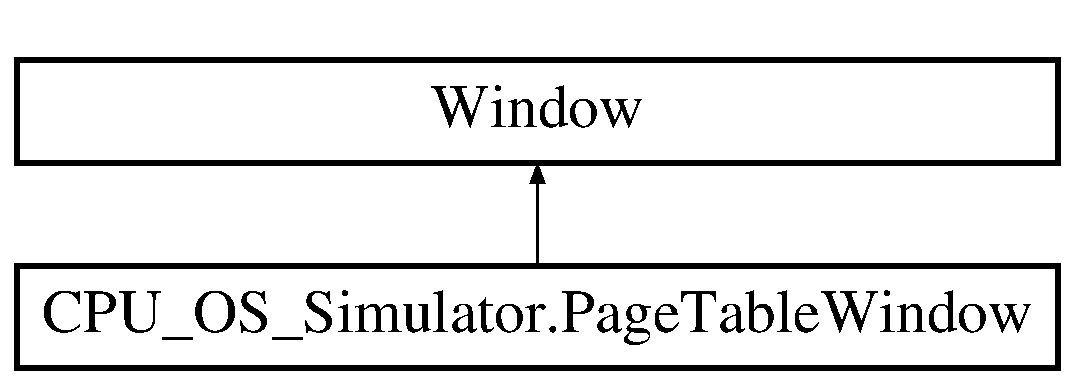
\includegraphics[height=0.945148cm]{class_c_p_u___o_s___simulator_1_1_page_table_window}
\end{center}
\end{figure}
\subsection*{Public Member Functions}
\begin{DoxyCompactItemize}
\item 
void \hyperlink{class_c_p_u___o_s___simulator_1_1_page_table_window_aac86b3b08e7e32708ac357042af6cbb2}{Initialize\+Component} ()
\begin{DoxyCompactList}\small\item\em Initialize\+Component \end{DoxyCompactList}\item 
void \hyperlink{class_c_p_u___o_s___simulator_1_1_page_table_window_aac86b3b08e7e32708ac357042af6cbb2}{Initialize\+Component} ()
\begin{DoxyCompactList}\small\item\em Initialize\+Component \end{DoxyCompactList}\item 
\hyperlink{class_c_p_u___o_s___simulator_1_1_page_table_window_a7d71ad4194ceafa3573e5f65e8dbe90a}{Page\+Table\+Window} (\hyperlink{class_c_p_u___o_s___simulator_1_1_memory_window}{Memory\+Window} \hyperlink{class_c_p_u___o_s___simulator_1_1_page_table_window_a1903e0b83820829549f74207cd209337}{parent})
\begin{DoxyCompactList}\small\item\em Constructor for page table window that takes the window instance that is creating this window P\+L\+E\+A\+S\+E N\+O\+T\+E\+: This constructor should always be used so data can be passed back to the parent window \end{DoxyCompactList}\end{DoxyCompactItemize}
\subsection*{Package Attributes}
\begin{DoxyCompactItemize}
\item 
\hyperlink{class_c_p_u___o_s___simulator_1_1_page_table_window}{C\+P\+U\+\_\+\+O\+S\+\_\+\+Simulator.\+Page\+Table\+Window} \hyperlink{class_c_p_u___o_s___simulator_1_1_page_table_window_ac72a468cc382de9caf8ccac13b35d755}{Page\+Table\+Window1}
\item 
System.\+Windows.\+Controls.\+Grid \hyperlink{class_c_p_u___o_s___simulator_1_1_page_table_window_a980885f948a6f104858d19fdf45811b1}{grid\+\_\+\+Main\+Grid}
\item 
System.\+Windows.\+Controls.\+List\+View \hyperlink{class_c_p_u___o_s___simulator_1_1_page_table_window_ae057c5b521dd61e965fb1cd7643db659}{lst\+\_\+\+Pages}
\item 
System.\+Windows.\+Controls.\+Check\+Box \hyperlink{class_c_p_u___o_s___simulator_1_1_page_table_window_ab0e68128fbf4eb0e840d0d6179517e0f}{chk\+\_\+\+Stay\+\_\+\+On\+\_\+\+Top}
\item 
System.\+Windows.\+Controls.\+Button \hyperlink{class_c_p_u___o_s___simulator_1_1_page_table_window_ae8b5191737208bc156dea5312230c716}{btn\+\_\+\+Swap\+\_\+\+Out}
\item 
System.\+Windows.\+Controls.\+Button \hyperlink{class_c_p_u___o_s___simulator_1_1_page_table_window_ab50f72dcb40e44d6eadb0128c67eace6}{btn\+\_\+\+Close}
\end{DoxyCompactItemize}
\subsection*{Private Member Functions}
\begin{DoxyCompactItemize}
\item 
void System.\+Windows.\+Markup.\+I\+Component\+Connector. \hyperlink{class_c_p_u___o_s___simulator_1_1_page_table_window_a5843f37edba076f17d15fe9f9f20d930}{Connect} (int connection\+Id, object target)
\item 
void System.\+Windows.\+Markup.\+I\+Component\+Connector. \hyperlink{class_c_p_u___o_s___simulator_1_1_page_table_window_a5843f37edba076f17d15fe9f9f20d930}{Connect} (int connection\+Id, object target)
\item 
\hyperlink{class_c_p_u___o_s___simulator_1_1_page_table_window_a9ddde0b8d78abd882007a4d919e5a082}{Page\+Table\+Window} ()
\begin{DoxyCompactList}\small\item\em Default Constructor for page table window \end{DoxyCompactList}\item 
void \hyperlink{class_c_p_u___o_s___simulator_1_1_page_table_window_a32fcbb5d7acdefedbf7b81194f046f40}{Page\+Table\+Window1\+\_\+\+Loaded} (object sender, Routed\+Event\+Args e)
\item 
void \hyperlink{class_c_p_u___o_s___simulator_1_1_page_table_window_a4fca878351d58351729a016149ab037e}{chk\+\_\+\+Stay\+\_\+\+On\+\_\+\+Top\+\_\+\+Checked} (object sender, Routed\+Event\+Args e)
\item 
void \hyperlink{class_c_p_u___o_s___simulator_1_1_page_table_window_a7d678a6670baff37546ea625ae36a63c}{chk\+\_\+\+Stay\+\_\+\+On\+\_\+\+Top\+\_\+\+Unchecked} (object sender, Routed\+Event\+Args e)
\item 
void \hyperlink{class_c_p_u___o_s___simulator_1_1_page_table_window_ae072e4c12e228104c4e3b201c1c9d812}{btn\+\_\+\+Close\+\_\+\+Click} (object sender, Routed\+Event\+Args e)
\item 
void \hyperlink{class_c_p_u___o_s___simulator_1_1_page_table_window_a0a18aa563b2185c73dac319969a24c43}{btn\+\_\+\+Swap\+\_\+\+Out\+\_\+\+Click} (object sender, Routed\+Event\+Args e)
\item 
void \hyperlink{class_c_p_u___o_s___simulator_1_1_page_table_window_aea28126046f84b8a2cced2d22f21804d}{Update\+Entries} ()
\begin{DoxyCompactList}\small\item\em This function updates the page table entries shown in the user interface \end{DoxyCompactList}\item 
void \hyperlink{class_c_p_u___o_s___simulator_1_1_page_table_window_ab6e40cd99ff3eedb1719774c9a123650}{lst\+\_\+\+Pages\+\_\+\+Selection\+Changed} (object sender, Selection\+Changed\+Event\+Args e)
\end{DoxyCompactItemize}
\subsection*{Private Attributes}
\begin{DoxyCompactItemize}
\item 
bool \hyperlink{class_c_p_u___o_s___simulator_1_1_page_table_window_a9c12d3a4ba2ab4b676cb502ca8caa6fe}{\+\_\+content\+Loaded}
\item 
\hyperlink{class_c_p_u___o_s___simulator_1_1_memory_window}{Memory\+Window} \hyperlink{class_c_p_u___o_s___simulator_1_1_page_table_window_a1903e0b83820829549f74207cd209337}{parent}
\end{DoxyCompactItemize}


\subsection{Detailed Description}
\hyperlink{class_c_p_u___o_s___simulator_1_1_page_table_window}{Page\+Table\+Window} 

Interaction logic for Page\+Table\+Window.\+xaml 

Definition at line 41 of file Page\+Table\+Window.\+g.\+cs.



\subsection{Constructor \& Destructor Documentation}
\hypertarget{class_c_p_u___o_s___simulator_1_1_page_table_window_a9ddde0b8d78abd882007a4d919e5a082}{}\index{C\+P\+U\+\_\+\+O\+S\+\_\+\+Simulator\+::\+Page\+Table\+Window@{C\+P\+U\+\_\+\+O\+S\+\_\+\+Simulator\+::\+Page\+Table\+Window}!Page\+Table\+Window@{Page\+Table\+Window}}
\index{Page\+Table\+Window@{Page\+Table\+Window}!C\+P\+U\+\_\+\+O\+S\+\_\+\+Simulator\+::\+Page\+Table\+Window@{C\+P\+U\+\_\+\+O\+S\+\_\+\+Simulator\+::\+Page\+Table\+Window}}
\subsubsection[{Page\+Table\+Window()}]{\setlength{\rightskip}{0pt plus 5cm}C\+P\+U\+\_\+\+O\+S\+\_\+\+Simulator.\+Page\+Table\+Window.\+Page\+Table\+Window (
\begin{DoxyParamCaption}
{}
\end{DoxyParamCaption}
)\hspace{0.3cm}{\ttfamily [private]}}\label{class_c_p_u___o_s___simulator_1_1_page_table_window_a9ddde0b8d78abd882007a4d919e5a082}


Default Constructor for page table window 



Definition at line 18 of file Page\+Table\+Window.\+xaml.\+cs.

\hypertarget{class_c_p_u___o_s___simulator_1_1_page_table_window_a7d71ad4194ceafa3573e5f65e8dbe90a}{}\index{C\+P\+U\+\_\+\+O\+S\+\_\+\+Simulator\+::\+Page\+Table\+Window@{C\+P\+U\+\_\+\+O\+S\+\_\+\+Simulator\+::\+Page\+Table\+Window}!Page\+Table\+Window@{Page\+Table\+Window}}
\index{Page\+Table\+Window@{Page\+Table\+Window}!C\+P\+U\+\_\+\+O\+S\+\_\+\+Simulator\+::\+Page\+Table\+Window@{C\+P\+U\+\_\+\+O\+S\+\_\+\+Simulator\+::\+Page\+Table\+Window}}
\subsubsection[{Page\+Table\+Window(\+Memory\+Window parent)}]{\setlength{\rightskip}{0pt plus 5cm}C\+P\+U\+\_\+\+O\+S\+\_\+\+Simulator.\+Page\+Table\+Window.\+Page\+Table\+Window (
\begin{DoxyParamCaption}
\item[{{\bf Memory\+Window}}]{parent}
\end{DoxyParamCaption}
)}\label{class_c_p_u___o_s___simulator_1_1_page_table_window_a7d71ad4194ceafa3573e5f65e8dbe90a}


Constructor for page table window that takes the window instance that is creating this window P\+L\+E\+A\+S\+E N\+O\+T\+E\+: This constructor should always be used so data can be passed back to the parent window 


\begin{DoxyParams}{Parameters}
{\em parent} & The window that is creating this window \\
\hline
\end{DoxyParams}


Definition at line 27 of file Page\+Table\+Window.\+xaml.\+cs.



\subsection{Member Function Documentation}
\hypertarget{class_c_p_u___o_s___simulator_1_1_page_table_window_ae072e4c12e228104c4e3b201c1c9d812}{}\index{C\+P\+U\+\_\+\+O\+S\+\_\+\+Simulator\+::\+Page\+Table\+Window@{C\+P\+U\+\_\+\+O\+S\+\_\+\+Simulator\+::\+Page\+Table\+Window}!btn\+\_\+\+Close\+\_\+\+Click@{btn\+\_\+\+Close\+\_\+\+Click}}
\index{btn\+\_\+\+Close\+\_\+\+Click@{btn\+\_\+\+Close\+\_\+\+Click}!C\+P\+U\+\_\+\+O\+S\+\_\+\+Simulator\+::\+Page\+Table\+Window@{C\+P\+U\+\_\+\+O\+S\+\_\+\+Simulator\+::\+Page\+Table\+Window}}
\subsubsection[{btn\+\_\+\+Close\+\_\+\+Click(object sender, Routed\+Event\+Args e)}]{\setlength{\rightskip}{0pt plus 5cm}void C\+P\+U\+\_\+\+O\+S\+\_\+\+Simulator.\+Page\+Table\+Window.\+btn\+\_\+\+Close\+\_\+\+Click (
\begin{DoxyParamCaption}
\item[{object}]{sender, }
\item[{Routed\+Event\+Args}]{e}
\end{DoxyParamCaption}
)\hspace{0.3cm}{\ttfamily [private]}}\label{class_c_p_u___o_s___simulator_1_1_page_table_window_ae072e4c12e228104c4e3b201c1c9d812}


Definition at line 51 of file Page\+Table\+Window.\+xaml.\+cs.

\hypertarget{class_c_p_u___o_s___simulator_1_1_page_table_window_a0a18aa563b2185c73dac319969a24c43}{}\index{C\+P\+U\+\_\+\+O\+S\+\_\+\+Simulator\+::\+Page\+Table\+Window@{C\+P\+U\+\_\+\+O\+S\+\_\+\+Simulator\+::\+Page\+Table\+Window}!btn\+\_\+\+Swap\+\_\+\+Out\+\_\+\+Click@{btn\+\_\+\+Swap\+\_\+\+Out\+\_\+\+Click}}
\index{btn\+\_\+\+Swap\+\_\+\+Out\+\_\+\+Click@{btn\+\_\+\+Swap\+\_\+\+Out\+\_\+\+Click}!C\+P\+U\+\_\+\+O\+S\+\_\+\+Simulator\+::\+Page\+Table\+Window@{C\+P\+U\+\_\+\+O\+S\+\_\+\+Simulator\+::\+Page\+Table\+Window}}
\subsubsection[{btn\+\_\+\+Swap\+\_\+\+Out\+\_\+\+Click(object sender, Routed\+Event\+Args e)}]{\setlength{\rightskip}{0pt plus 5cm}void C\+P\+U\+\_\+\+O\+S\+\_\+\+Simulator.\+Page\+Table\+Window.\+btn\+\_\+\+Swap\+\_\+\+Out\+\_\+\+Click (
\begin{DoxyParamCaption}
\item[{object}]{sender, }
\item[{Routed\+Event\+Args}]{e}
\end{DoxyParamCaption}
)\hspace{0.3cm}{\ttfamily [private]}}\label{class_c_p_u___o_s___simulator_1_1_page_table_window_a0a18aa563b2185c73dac319969a24c43}


Definition at line 56 of file Page\+Table\+Window.\+xaml.\+cs.

\hypertarget{class_c_p_u___o_s___simulator_1_1_page_table_window_a4fca878351d58351729a016149ab037e}{}\index{C\+P\+U\+\_\+\+O\+S\+\_\+\+Simulator\+::\+Page\+Table\+Window@{C\+P\+U\+\_\+\+O\+S\+\_\+\+Simulator\+::\+Page\+Table\+Window}!chk\+\_\+\+Stay\+\_\+\+On\+\_\+\+Top\+\_\+\+Checked@{chk\+\_\+\+Stay\+\_\+\+On\+\_\+\+Top\+\_\+\+Checked}}
\index{chk\+\_\+\+Stay\+\_\+\+On\+\_\+\+Top\+\_\+\+Checked@{chk\+\_\+\+Stay\+\_\+\+On\+\_\+\+Top\+\_\+\+Checked}!C\+P\+U\+\_\+\+O\+S\+\_\+\+Simulator\+::\+Page\+Table\+Window@{C\+P\+U\+\_\+\+O\+S\+\_\+\+Simulator\+::\+Page\+Table\+Window}}
\subsubsection[{chk\+\_\+\+Stay\+\_\+\+On\+\_\+\+Top\+\_\+\+Checked(object sender, Routed\+Event\+Args e)}]{\setlength{\rightskip}{0pt plus 5cm}void C\+P\+U\+\_\+\+O\+S\+\_\+\+Simulator.\+Page\+Table\+Window.\+chk\+\_\+\+Stay\+\_\+\+On\+\_\+\+Top\+\_\+\+Checked (
\begin{DoxyParamCaption}
\item[{object}]{sender, }
\item[{Routed\+Event\+Args}]{e}
\end{DoxyParamCaption}
)\hspace{0.3cm}{\ttfamily [private]}}\label{class_c_p_u___o_s___simulator_1_1_page_table_window_a4fca878351d58351729a016149ab037e}


Definition at line 41 of file Page\+Table\+Window.\+xaml.\+cs.

\hypertarget{class_c_p_u___o_s___simulator_1_1_page_table_window_a7d678a6670baff37546ea625ae36a63c}{}\index{C\+P\+U\+\_\+\+O\+S\+\_\+\+Simulator\+::\+Page\+Table\+Window@{C\+P\+U\+\_\+\+O\+S\+\_\+\+Simulator\+::\+Page\+Table\+Window}!chk\+\_\+\+Stay\+\_\+\+On\+\_\+\+Top\+\_\+\+Unchecked@{chk\+\_\+\+Stay\+\_\+\+On\+\_\+\+Top\+\_\+\+Unchecked}}
\index{chk\+\_\+\+Stay\+\_\+\+On\+\_\+\+Top\+\_\+\+Unchecked@{chk\+\_\+\+Stay\+\_\+\+On\+\_\+\+Top\+\_\+\+Unchecked}!C\+P\+U\+\_\+\+O\+S\+\_\+\+Simulator\+::\+Page\+Table\+Window@{C\+P\+U\+\_\+\+O\+S\+\_\+\+Simulator\+::\+Page\+Table\+Window}}
\subsubsection[{chk\+\_\+\+Stay\+\_\+\+On\+\_\+\+Top\+\_\+\+Unchecked(object sender, Routed\+Event\+Args e)}]{\setlength{\rightskip}{0pt plus 5cm}void C\+P\+U\+\_\+\+O\+S\+\_\+\+Simulator.\+Page\+Table\+Window.\+chk\+\_\+\+Stay\+\_\+\+On\+\_\+\+Top\+\_\+\+Unchecked (
\begin{DoxyParamCaption}
\item[{object}]{sender, }
\item[{Routed\+Event\+Args}]{e}
\end{DoxyParamCaption}
)\hspace{0.3cm}{\ttfamily [private]}}\label{class_c_p_u___o_s___simulator_1_1_page_table_window_a7d678a6670baff37546ea625ae36a63c}


Definition at line 46 of file Page\+Table\+Window.\+xaml.\+cs.

\hypertarget{class_c_p_u___o_s___simulator_1_1_page_table_window_a5843f37edba076f17d15fe9f9f20d930}{}\index{C\+P\+U\+\_\+\+O\+S\+\_\+\+Simulator\+::\+Page\+Table\+Window@{C\+P\+U\+\_\+\+O\+S\+\_\+\+Simulator\+::\+Page\+Table\+Window}!Connect@{Connect}}
\index{Connect@{Connect}!C\+P\+U\+\_\+\+O\+S\+\_\+\+Simulator\+::\+Page\+Table\+Window@{C\+P\+U\+\_\+\+O\+S\+\_\+\+Simulator\+::\+Page\+Table\+Window}}
\subsubsection[{Connect(int connection\+Id, object target)}]{\setlength{\rightskip}{0pt plus 5cm}void System.\+Windows.\+Markup.\+I\+Component\+Connector. C\+P\+U\+\_\+\+O\+S\+\_\+\+Simulator.\+Page\+Table\+Window.\+Connect (
\begin{DoxyParamCaption}
\item[{int}]{connection\+Id, }
\item[{object}]{target}
\end{DoxyParamCaption}
)\hspace{0.3cm}{\ttfamily [private]}}\label{class_c_p_u___o_s___simulator_1_1_page_table_window_a5843f37edba076f17d15fe9f9f20d930}


Definition at line 118 of file Page\+Table\+Window.\+g.\+i.\+cs.

\hypertarget{class_c_p_u___o_s___simulator_1_1_page_table_window_a5843f37edba076f17d15fe9f9f20d930}{}\index{C\+P\+U\+\_\+\+O\+S\+\_\+\+Simulator\+::\+Page\+Table\+Window@{C\+P\+U\+\_\+\+O\+S\+\_\+\+Simulator\+::\+Page\+Table\+Window}!Connect@{Connect}}
\index{Connect@{Connect}!C\+P\+U\+\_\+\+O\+S\+\_\+\+Simulator\+::\+Page\+Table\+Window@{C\+P\+U\+\_\+\+O\+S\+\_\+\+Simulator\+::\+Page\+Table\+Window}}
\subsubsection[{Connect(int connection\+Id, object target)}]{\setlength{\rightskip}{0pt plus 5cm}void System.\+Windows.\+Markup.\+I\+Component\+Connector. C\+P\+U\+\_\+\+O\+S\+\_\+\+Simulator.\+Page\+Table\+Window.\+Connect (
\begin{DoxyParamCaption}
\item[{int}]{connection\+Id, }
\item[{object}]{target}
\end{DoxyParamCaption}
)\hspace{0.3cm}{\ttfamily [private]}}\label{class_c_p_u___o_s___simulator_1_1_page_table_window_a5843f37edba076f17d15fe9f9f20d930}


Definition at line 118 of file Page\+Table\+Window.\+g.\+cs.

\hypertarget{class_c_p_u___o_s___simulator_1_1_page_table_window_aac86b3b08e7e32708ac357042af6cbb2}{}\index{C\+P\+U\+\_\+\+O\+S\+\_\+\+Simulator\+::\+Page\+Table\+Window@{C\+P\+U\+\_\+\+O\+S\+\_\+\+Simulator\+::\+Page\+Table\+Window}!Initialize\+Component@{Initialize\+Component}}
\index{Initialize\+Component@{Initialize\+Component}!C\+P\+U\+\_\+\+O\+S\+\_\+\+Simulator\+::\+Page\+Table\+Window@{C\+P\+U\+\_\+\+O\+S\+\_\+\+Simulator\+::\+Page\+Table\+Window}}
\subsubsection[{Initialize\+Component()}]{\setlength{\rightskip}{0pt plus 5cm}void C\+P\+U\+\_\+\+O\+S\+\_\+\+Simulator.\+Page\+Table\+Window.\+Initialize\+Component (
\begin{DoxyParamCaption}
{}
\end{DoxyParamCaption}
)}\label{class_c_p_u___o_s___simulator_1_1_page_table_window_aac86b3b08e7e32708ac357042af6cbb2}


Initialize\+Component 



Definition at line 98 of file Page\+Table\+Window.\+g.\+cs.

\hypertarget{class_c_p_u___o_s___simulator_1_1_page_table_window_aac86b3b08e7e32708ac357042af6cbb2}{}\index{C\+P\+U\+\_\+\+O\+S\+\_\+\+Simulator\+::\+Page\+Table\+Window@{C\+P\+U\+\_\+\+O\+S\+\_\+\+Simulator\+::\+Page\+Table\+Window}!Initialize\+Component@{Initialize\+Component}}
\index{Initialize\+Component@{Initialize\+Component}!C\+P\+U\+\_\+\+O\+S\+\_\+\+Simulator\+::\+Page\+Table\+Window@{C\+P\+U\+\_\+\+O\+S\+\_\+\+Simulator\+::\+Page\+Table\+Window}}
\subsubsection[{Initialize\+Component()}]{\setlength{\rightskip}{0pt plus 5cm}void C\+P\+U\+\_\+\+O\+S\+\_\+\+Simulator.\+Page\+Table\+Window.\+Initialize\+Component (
\begin{DoxyParamCaption}
{}
\end{DoxyParamCaption}
)}\label{class_c_p_u___o_s___simulator_1_1_page_table_window_aac86b3b08e7e32708ac357042af6cbb2}


Initialize\+Component 



Definition at line 98 of file Page\+Table\+Window.\+g.\+i.\+cs.

\hypertarget{class_c_p_u___o_s___simulator_1_1_page_table_window_ab6e40cd99ff3eedb1719774c9a123650}{}\index{C\+P\+U\+\_\+\+O\+S\+\_\+\+Simulator\+::\+Page\+Table\+Window@{C\+P\+U\+\_\+\+O\+S\+\_\+\+Simulator\+::\+Page\+Table\+Window}!lst\+\_\+\+Pages\+\_\+\+Selection\+Changed@{lst\+\_\+\+Pages\+\_\+\+Selection\+Changed}}
\index{lst\+\_\+\+Pages\+\_\+\+Selection\+Changed@{lst\+\_\+\+Pages\+\_\+\+Selection\+Changed}!C\+P\+U\+\_\+\+O\+S\+\_\+\+Simulator\+::\+Page\+Table\+Window@{C\+P\+U\+\_\+\+O\+S\+\_\+\+Simulator\+::\+Page\+Table\+Window}}
\subsubsection[{lst\+\_\+\+Pages\+\_\+\+Selection\+Changed(object sender, Selection\+Changed\+Event\+Args e)}]{\setlength{\rightskip}{0pt plus 5cm}void C\+P\+U\+\_\+\+O\+S\+\_\+\+Simulator.\+Page\+Table\+Window.\+lst\+\_\+\+Pages\+\_\+\+Selection\+Changed (
\begin{DoxyParamCaption}
\item[{object}]{sender, }
\item[{Selection\+Changed\+Event\+Args}]{e}
\end{DoxyParamCaption}
)\hspace{0.3cm}{\ttfamily [private]}}\label{class_c_p_u___o_s___simulator_1_1_page_table_window_ab6e40cd99ff3eedb1719774c9a123650}


Definition at line 85 of file Page\+Table\+Window.\+xaml.\+cs.

\hypertarget{class_c_p_u___o_s___simulator_1_1_page_table_window_a32fcbb5d7acdefedbf7b81194f046f40}{}\index{C\+P\+U\+\_\+\+O\+S\+\_\+\+Simulator\+::\+Page\+Table\+Window@{C\+P\+U\+\_\+\+O\+S\+\_\+\+Simulator\+::\+Page\+Table\+Window}!Page\+Table\+Window1\+\_\+\+Loaded@{Page\+Table\+Window1\+\_\+\+Loaded}}
\index{Page\+Table\+Window1\+\_\+\+Loaded@{Page\+Table\+Window1\+\_\+\+Loaded}!C\+P\+U\+\_\+\+O\+S\+\_\+\+Simulator\+::\+Page\+Table\+Window@{C\+P\+U\+\_\+\+O\+S\+\_\+\+Simulator\+::\+Page\+Table\+Window}}
\subsubsection[{Page\+Table\+Window1\+\_\+\+Loaded(object sender, Routed\+Event\+Args e)}]{\setlength{\rightskip}{0pt plus 5cm}void C\+P\+U\+\_\+\+O\+S\+\_\+\+Simulator.\+Page\+Table\+Window.\+Page\+Table\+Window1\+\_\+\+Loaded (
\begin{DoxyParamCaption}
\item[{object}]{sender, }
\item[{Routed\+Event\+Args}]{e}
\end{DoxyParamCaption}
)\hspace{0.3cm}{\ttfamily [private]}}\label{class_c_p_u___o_s___simulator_1_1_page_table_window_a32fcbb5d7acdefedbf7b81194f046f40}


Definition at line 33 of file Page\+Table\+Window.\+xaml.\+cs.

\hypertarget{class_c_p_u___o_s___simulator_1_1_page_table_window_aea28126046f84b8a2cced2d22f21804d}{}\index{C\+P\+U\+\_\+\+O\+S\+\_\+\+Simulator\+::\+Page\+Table\+Window@{C\+P\+U\+\_\+\+O\+S\+\_\+\+Simulator\+::\+Page\+Table\+Window}!Update\+Entries@{Update\+Entries}}
\index{Update\+Entries@{Update\+Entries}!C\+P\+U\+\_\+\+O\+S\+\_\+\+Simulator\+::\+Page\+Table\+Window@{C\+P\+U\+\_\+\+O\+S\+\_\+\+Simulator\+::\+Page\+Table\+Window}}
\subsubsection[{Update\+Entries()}]{\setlength{\rightskip}{0pt plus 5cm}void C\+P\+U\+\_\+\+O\+S\+\_\+\+Simulator.\+Page\+Table\+Window.\+Update\+Entries (
\begin{DoxyParamCaption}
{}
\end{DoxyParamCaption}
)\hspace{0.3cm}{\ttfamily [private]}}\label{class_c_p_u___o_s___simulator_1_1_page_table_window_aea28126046f84b8a2cced2d22f21804d}


This function updates the page table entries shown in the user interface 



Definition at line 78 of file Page\+Table\+Window.\+xaml.\+cs.



\subsection{Member Data Documentation}
\hypertarget{class_c_p_u___o_s___simulator_1_1_page_table_window_a9c12d3a4ba2ab4b676cb502ca8caa6fe}{}\index{C\+P\+U\+\_\+\+O\+S\+\_\+\+Simulator\+::\+Page\+Table\+Window@{C\+P\+U\+\_\+\+O\+S\+\_\+\+Simulator\+::\+Page\+Table\+Window}!\+\_\+content\+Loaded@{\+\_\+content\+Loaded}}
\index{\+\_\+content\+Loaded@{\+\_\+content\+Loaded}!C\+P\+U\+\_\+\+O\+S\+\_\+\+Simulator\+::\+Page\+Table\+Window@{C\+P\+U\+\_\+\+O\+S\+\_\+\+Simulator\+::\+Page\+Table\+Window}}
\subsubsection[{\+\_\+content\+Loaded}]{\setlength{\rightskip}{0pt plus 5cm}bool C\+P\+U\+\_\+\+O\+S\+\_\+\+Simulator.\+Page\+Table\+Window.\+\_\+content\+Loaded\hspace{0.3cm}{\ttfamily [private]}}\label{class_c_p_u___o_s___simulator_1_1_page_table_window_a9c12d3a4ba2ab4b676cb502ca8caa6fe}


Definition at line 91 of file Page\+Table\+Window.\+g.\+cs.

\hypertarget{class_c_p_u___o_s___simulator_1_1_page_table_window_ab50f72dcb40e44d6eadb0128c67eace6}{}\index{C\+P\+U\+\_\+\+O\+S\+\_\+\+Simulator\+::\+Page\+Table\+Window@{C\+P\+U\+\_\+\+O\+S\+\_\+\+Simulator\+::\+Page\+Table\+Window}!btn\+\_\+\+Close@{btn\+\_\+\+Close}}
\index{btn\+\_\+\+Close@{btn\+\_\+\+Close}!C\+P\+U\+\_\+\+O\+S\+\_\+\+Simulator\+::\+Page\+Table\+Window@{C\+P\+U\+\_\+\+O\+S\+\_\+\+Simulator\+::\+Page\+Table\+Window}}
\subsubsection[{btn\+\_\+\+Close}]{\setlength{\rightskip}{0pt plus 5cm}System Windows Controls Button C\+P\+U\+\_\+\+O\+S\+\_\+\+Simulator.\+Page\+Table\+Window.\+btn\+\_\+\+Close\hspace{0.3cm}{\ttfamily [package]}}\label{class_c_p_u___o_s___simulator_1_1_page_table_window_ab50f72dcb40e44d6eadb0128c67eace6}


Definition at line 86 of file Page\+Table\+Window.\+g.\+cs.

\hypertarget{class_c_p_u___o_s___simulator_1_1_page_table_window_ae8b5191737208bc156dea5312230c716}{}\index{C\+P\+U\+\_\+\+O\+S\+\_\+\+Simulator\+::\+Page\+Table\+Window@{C\+P\+U\+\_\+\+O\+S\+\_\+\+Simulator\+::\+Page\+Table\+Window}!btn\+\_\+\+Swap\+\_\+\+Out@{btn\+\_\+\+Swap\+\_\+\+Out}}
\index{btn\+\_\+\+Swap\+\_\+\+Out@{btn\+\_\+\+Swap\+\_\+\+Out}!C\+P\+U\+\_\+\+O\+S\+\_\+\+Simulator\+::\+Page\+Table\+Window@{C\+P\+U\+\_\+\+O\+S\+\_\+\+Simulator\+::\+Page\+Table\+Window}}
\subsubsection[{btn\+\_\+\+Swap\+\_\+\+Out}]{\setlength{\rightskip}{0pt plus 5cm}System Windows Controls Button C\+P\+U\+\_\+\+O\+S\+\_\+\+Simulator.\+Page\+Table\+Window.\+btn\+\_\+\+Swap\+\_\+\+Out\hspace{0.3cm}{\ttfamily [package]}}\label{class_c_p_u___o_s___simulator_1_1_page_table_window_ae8b5191737208bc156dea5312230c716}


Definition at line 78 of file Page\+Table\+Window.\+g.\+cs.

\hypertarget{class_c_p_u___o_s___simulator_1_1_page_table_window_ab0e68128fbf4eb0e840d0d6179517e0f}{}\index{C\+P\+U\+\_\+\+O\+S\+\_\+\+Simulator\+::\+Page\+Table\+Window@{C\+P\+U\+\_\+\+O\+S\+\_\+\+Simulator\+::\+Page\+Table\+Window}!chk\+\_\+\+Stay\+\_\+\+On\+\_\+\+Top@{chk\+\_\+\+Stay\+\_\+\+On\+\_\+\+Top}}
\index{chk\+\_\+\+Stay\+\_\+\+On\+\_\+\+Top@{chk\+\_\+\+Stay\+\_\+\+On\+\_\+\+Top}!C\+P\+U\+\_\+\+O\+S\+\_\+\+Simulator\+::\+Page\+Table\+Window@{C\+P\+U\+\_\+\+O\+S\+\_\+\+Simulator\+::\+Page\+Table\+Window}}
\subsubsection[{chk\+\_\+\+Stay\+\_\+\+On\+\_\+\+Top}]{\setlength{\rightskip}{0pt plus 5cm}System Windows Controls Check\+Box C\+P\+U\+\_\+\+O\+S\+\_\+\+Simulator.\+Page\+Table\+Window.\+chk\+\_\+\+Stay\+\_\+\+On\+\_\+\+Top\hspace{0.3cm}{\ttfamily [package]}}\label{class_c_p_u___o_s___simulator_1_1_page_table_window_ab0e68128fbf4eb0e840d0d6179517e0f}


Definition at line 70 of file Page\+Table\+Window.\+g.\+cs.

\hypertarget{class_c_p_u___o_s___simulator_1_1_page_table_window_a980885f948a6f104858d19fdf45811b1}{}\index{C\+P\+U\+\_\+\+O\+S\+\_\+\+Simulator\+::\+Page\+Table\+Window@{C\+P\+U\+\_\+\+O\+S\+\_\+\+Simulator\+::\+Page\+Table\+Window}!grid\+\_\+\+Main\+Grid@{grid\+\_\+\+Main\+Grid}}
\index{grid\+\_\+\+Main\+Grid@{grid\+\_\+\+Main\+Grid}!C\+P\+U\+\_\+\+O\+S\+\_\+\+Simulator\+::\+Page\+Table\+Window@{C\+P\+U\+\_\+\+O\+S\+\_\+\+Simulator\+::\+Page\+Table\+Window}}
\subsubsection[{grid\+\_\+\+Main\+Grid}]{\setlength{\rightskip}{0pt plus 5cm}System Windows Controls Grid C\+P\+U\+\_\+\+O\+S\+\_\+\+Simulator.\+Page\+Table\+Window.\+grid\+\_\+\+Main\+Grid\hspace{0.3cm}{\ttfamily [package]}}\label{class_c_p_u___o_s___simulator_1_1_page_table_window_a980885f948a6f104858d19fdf45811b1}


Definition at line 54 of file Page\+Table\+Window.\+g.\+cs.

\hypertarget{class_c_p_u___o_s___simulator_1_1_page_table_window_ae057c5b521dd61e965fb1cd7643db659}{}\index{C\+P\+U\+\_\+\+O\+S\+\_\+\+Simulator\+::\+Page\+Table\+Window@{C\+P\+U\+\_\+\+O\+S\+\_\+\+Simulator\+::\+Page\+Table\+Window}!lst\+\_\+\+Pages@{lst\+\_\+\+Pages}}
\index{lst\+\_\+\+Pages@{lst\+\_\+\+Pages}!C\+P\+U\+\_\+\+O\+S\+\_\+\+Simulator\+::\+Page\+Table\+Window@{C\+P\+U\+\_\+\+O\+S\+\_\+\+Simulator\+::\+Page\+Table\+Window}}
\subsubsection[{lst\+\_\+\+Pages}]{\setlength{\rightskip}{0pt plus 5cm}System Windows Controls List\+View C\+P\+U\+\_\+\+O\+S\+\_\+\+Simulator.\+Page\+Table\+Window.\+lst\+\_\+\+Pages\hspace{0.3cm}{\ttfamily [package]}}\label{class_c_p_u___o_s___simulator_1_1_page_table_window_ae057c5b521dd61e965fb1cd7643db659}


Definition at line 62 of file Page\+Table\+Window.\+g.\+cs.

\hypertarget{class_c_p_u___o_s___simulator_1_1_page_table_window_ac72a468cc382de9caf8ccac13b35d755}{}\index{C\+P\+U\+\_\+\+O\+S\+\_\+\+Simulator\+::\+Page\+Table\+Window@{C\+P\+U\+\_\+\+O\+S\+\_\+\+Simulator\+::\+Page\+Table\+Window}!Page\+Table\+Window1@{Page\+Table\+Window1}}
\index{Page\+Table\+Window1@{Page\+Table\+Window1}!C\+P\+U\+\_\+\+O\+S\+\_\+\+Simulator\+::\+Page\+Table\+Window@{C\+P\+U\+\_\+\+O\+S\+\_\+\+Simulator\+::\+Page\+Table\+Window}}
\subsubsection[{Page\+Table\+Window1}]{\setlength{\rightskip}{0pt plus 5cm}C\+P\+U\+\_\+\+O\+S\+\_\+\+Simulator {\bf Page\+Table\+Window} C\+P\+U\+\_\+\+O\+S\+\_\+\+Simulator.\+Page\+Table\+Window.\+Page\+Table\+Window1\hspace{0.3cm}{\ttfamily [package]}}\label{class_c_p_u___o_s___simulator_1_1_page_table_window_ac72a468cc382de9caf8ccac13b35d755}


Definition at line 46 of file Page\+Table\+Window.\+g.\+cs.

\hypertarget{class_c_p_u___o_s___simulator_1_1_page_table_window_a1903e0b83820829549f74207cd209337}{}\index{C\+P\+U\+\_\+\+O\+S\+\_\+\+Simulator\+::\+Page\+Table\+Window@{C\+P\+U\+\_\+\+O\+S\+\_\+\+Simulator\+::\+Page\+Table\+Window}!parent@{parent}}
\index{parent@{parent}!C\+P\+U\+\_\+\+O\+S\+\_\+\+Simulator\+::\+Page\+Table\+Window@{C\+P\+U\+\_\+\+O\+S\+\_\+\+Simulator\+::\+Page\+Table\+Window}}
\subsubsection[{parent}]{\setlength{\rightskip}{0pt plus 5cm}{\bf Memory\+Window} C\+P\+U\+\_\+\+O\+S\+\_\+\+Simulator.\+Page\+Table\+Window.\+parent\hspace{0.3cm}{\ttfamily [private]}}\label{class_c_p_u___o_s___simulator_1_1_page_table_window_a1903e0b83820829549f74207cd209337}


Definition at line 13 of file Page\+Table\+Window.\+xaml.\+cs.



The documentation for this class was generated from the following files\+:\begin{DoxyCompactItemize}
\item 
C\+P\+U-\/\+O\+S Simulator/obj/\+Debug/\hyperlink{_page_table_window_8g_8cs}{Page\+Table\+Window.\+g.\+cs}\item 
C\+P\+U-\/\+O\+S Simulator/obj/\+Debug/\hyperlink{_page_table_window_8g_8i_8cs}{Page\+Table\+Window.\+g.\+i.\+cs}\item 
C\+P\+U-\/\+O\+S Simulator/\hyperlink{_page_table_window_8xaml_8cs}{Page\+Table\+Window.\+xaml.\+cs}\end{DoxyCompactItemize}

\hypertarget{class_c_p_u___o_s___simulator_1_1_compiler_1_1_frontend_1_1_parser}{}\section{C\+P\+U\+\_\+\+O\+S\+\_\+\+Simulator.\+Compiler.\+Frontend.\+Parser Class Reference}
\label{class_c_p_u___o_s___simulator_1_1_compiler_1_1_frontend_1_1_parser}\index{C\+P\+U\+\_\+\+O\+S\+\_\+\+Simulator.\+Compiler.\+Frontend.\+Parser@{C\+P\+U\+\_\+\+O\+S\+\_\+\+Simulator.\+Compiler.\+Frontend.\+Parser}}
\subsection*{Public Member Functions}
\begin{DoxyCompactItemize}
\item 
\hyperlink{class_c_p_u___o_s___simulator_1_1_compiler_1_1_frontend_1_1_parser_af0f1bfe1db9feba2284d5d7fc0a93d37}{Parser} (Linked\+List$<$ \hyperlink{class_c_p_u___o_s___simulator_1_1_compiler_1_1_frontend_1_1_tokens_1_1_token}{Token} $>$ \hyperlink{class_c_p_u___o_s___simulator_1_1_compiler_1_1_frontend_1_1_parser_a52ee7fdbe0d3af8e710c37ee6a149dc7}{tokens})
\end{DoxyCompactItemize}
\subsection*{Private Attributes}
\begin{DoxyCompactItemize}
\item 
Linked\+List$<$ \hyperlink{class_c_p_u___o_s___simulator_1_1_compiler_1_1_frontend_1_1_tokens_1_1_token}{Token} $>$ \hyperlink{class_c_p_u___o_s___simulator_1_1_compiler_1_1_frontend_1_1_parser_a52ee7fdbe0d3af8e710c37ee6a149dc7}{tokens}
\item 
\hyperlink{class_c_p_u___o_s___simulator_1_1_compiler_1_1_frontend_1_1_syntax_tree_1_1_a_s_t}{A\+S\+T} \hyperlink{class_c_p_u___o_s___simulator_1_1_compiler_1_1_frontend_1_1_parser_a05eafea853ea95d722ae4161e184f11a}{ast}
\end{DoxyCompactItemize}


\subsection{Detailed Description}


Definition at line 8 of file Parser.\+cs.



\subsection{Constructor \& Destructor Documentation}
\hypertarget{class_c_p_u___o_s___simulator_1_1_compiler_1_1_frontend_1_1_parser_af0f1bfe1db9feba2284d5d7fc0a93d37}{}\index{C\+P\+U\+\_\+\+O\+S\+\_\+\+Simulator\+::\+Compiler\+::\+Frontend\+::\+Parser@{C\+P\+U\+\_\+\+O\+S\+\_\+\+Simulator\+::\+Compiler\+::\+Frontend\+::\+Parser}!Parser@{Parser}}
\index{Parser@{Parser}!C\+P\+U\+\_\+\+O\+S\+\_\+\+Simulator\+::\+Compiler\+::\+Frontend\+::\+Parser@{C\+P\+U\+\_\+\+O\+S\+\_\+\+Simulator\+::\+Compiler\+::\+Frontend\+::\+Parser}}
\subsubsection[{Parser(\+Linked\+List$<$ Token $>$ tokens)}]{\setlength{\rightskip}{0pt plus 5cm}C\+P\+U\+\_\+\+O\+S\+\_\+\+Simulator.\+Compiler.\+Frontend.\+Parser.\+Parser (
\begin{DoxyParamCaption}
\item[{Linked\+List$<$ {\bf Token} $>$}]{tokens}
\end{DoxyParamCaption}
)}\label{class_c_p_u___o_s___simulator_1_1_compiler_1_1_frontend_1_1_parser_af0f1bfe1db9feba2284d5d7fc0a93d37}


Definition at line 12 of file Parser.\+cs.



\subsection{Member Data Documentation}
\hypertarget{class_c_p_u___o_s___simulator_1_1_compiler_1_1_frontend_1_1_parser_a05eafea853ea95d722ae4161e184f11a}{}\index{C\+P\+U\+\_\+\+O\+S\+\_\+\+Simulator\+::\+Compiler\+::\+Frontend\+::\+Parser@{C\+P\+U\+\_\+\+O\+S\+\_\+\+Simulator\+::\+Compiler\+::\+Frontend\+::\+Parser}!ast@{ast}}
\index{ast@{ast}!C\+P\+U\+\_\+\+O\+S\+\_\+\+Simulator\+::\+Compiler\+::\+Frontend\+::\+Parser@{C\+P\+U\+\_\+\+O\+S\+\_\+\+Simulator\+::\+Compiler\+::\+Frontend\+::\+Parser}}
\subsubsection[{ast}]{\setlength{\rightskip}{0pt plus 5cm}{\bf A\+S\+T} C\+P\+U\+\_\+\+O\+S\+\_\+\+Simulator.\+Compiler.\+Frontend.\+Parser.\+ast\hspace{0.3cm}{\ttfamily [private]}}\label{class_c_p_u___o_s___simulator_1_1_compiler_1_1_frontend_1_1_parser_a05eafea853ea95d722ae4161e184f11a}


Definition at line 11 of file Parser.\+cs.

\hypertarget{class_c_p_u___o_s___simulator_1_1_compiler_1_1_frontend_1_1_parser_a52ee7fdbe0d3af8e710c37ee6a149dc7}{}\index{C\+P\+U\+\_\+\+O\+S\+\_\+\+Simulator\+::\+Compiler\+::\+Frontend\+::\+Parser@{C\+P\+U\+\_\+\+O\+S\+\_\+\+Simulator\+::\+Compiler\+::\+Frontend\+::\+Parser}!tokens@{tokens}}
\index{tokens@{tokens}!C\+P\+U\+\_\+\+O\+S\+\_\+\+Simulator\+::\+Compiler\+::\+Frontend\+::\+Parser@{C\+P\+U\+\_\+\+O\+S\+\_\+\+Simulator\+::\+Compiler\+::\+Frontend\+::\+Parser}}
\subsubsection[{tokens}]{\setlength{\rightskip}{0pt plus 5cm}Linked\+List$<${\bf Token}$>$ C\+P\+U\+\_\+\+O\+S\+\_\+\+Simulator.\+Compiler.\+Frontend.\+Parser.\+tokens\hspace{0.3cm}{\ttfamily [private]}}\label{class_c_p_u___o_s___simulator_1_1_compiler_1_1_frontend_1_1_parser_a52ee7fdbe0d3af8e710c37ee6a149dc7}


Definition at line 10 of file Parser.\+cs.



The documentation for this class was generated from the following file\+:\begin{DoxyCompactItemize}
\item 
Compiler/\+Frontend/\hyperlink{_parser_8cs}{Parser.\+cs}\end{DoxyCompactItemize}

\hypertarget{struct_c_p_u___o_s___simulator_1_1_operating___system_1_1_p_c_b_flags}{}\section{C\+P\+U\+\_\+\+O\+S\+\_\+\+Simulator.\+Operating\+\_\+\+System.\+P\+C\+B\+Flags Struct Reference}
\label{struct_c_p_u___o_s___simulator_1_1_operating___system_1_1_p_c_b_flags}\index{C\+P\+U\+\_\+\+O\+S\+\_\+\+Simulator.\+Operating\+\_\+\+System.\+P\+C\+B\+Flags@{C\+P\+U\+\_\+\+O\+S\+\_\+\+Simulator.\+Operating\+\_\+\+System.\+P\+C\+B\+Flags}}
\subsection*{Public Attributes}
\begin{DoxyCompactItemize}
\item 
int \hyperlink{struct_c_p_u___o_s___simulator_1_1_operating___system_1_1_p_c_b_flags_a15deeacce9002beb7f23aee161337daa}{C\+P\+U\+I\+D}
\item 
int \hyperlink{struct_c_p_u___o_s___simulator_1_1_operating___system_1_1_p_c_b_flags_ac8d5b519b8ac16523a5ec55ab8817f46}{O\+S\+I\+D}
\item 
int \hyperlink{struct_c_p_u___o_s___simulator_1_1_operating___system_1_1_p_c_b_flags_a648ddc7bcd96828ab1cf7489f5398b9d}{process\+I\+D}
\item 
string \hyperlink{struct_c_p_u___o_s___simulator_1_1_operating___system_1_1_p_c_b_flags_a49d8713f36371532f71d671779a16bef}{process\+Name}
\item 
\hyperlink{namespace_c_p_u___o_s___simulator_1_1_operating___system_a836ee2204e78fcb3a7dd6c3c942b1a24}{Enum\+Process\+State} \hyperlink{struct_c_p_u___o_s___simulator_1_1_operating___system_1_1_p_c_b_flags_af76336097aeb72498846b6457034ae5d}{process\+State}
\item 
string \hyperlink{struct_c_p_u___o_s___simulator_1_1_operating___system_1_1_p_c_b_flags_a27fe0cc9b4e732eda70d5574556cd2e0}{program\+Name}
\item 
int \hyperlink{struct_c_p_u___o_s___simulator_1_1_operating___system_1_1_p_c_b_flags_a11469ad59c9f9f3e36c95f8ae64f9c73}{base\+Address}
\item 
int \hyperlink{struct_c_p_u___o_s___simulator_1_1_operating___system_1_1_p_c_b_flags_a774bd0d595863252698e5dfc36015c50}{start\+Address}
\item 
int \hyperlink{struct_c_p_u___o_s___simulator_1_1_operating___system_1_1_p_c_b_flags_a1292a1914e95ca0fce7d55c604eab09b}{process\+Priority}
\item 
int \hyperlink{struct_c_p_u___o_s___simulator_1_1_operating___system_1_1_p_c_b_flags_a4248a993bf5be874fcd2843269bb9058}{proceess\+Memory}
\item 
double \hyperlink{struct_c_p_u___o_s___simulator_1_1_operating___system_1_1_p_c_b_flags_a1c7b8ae576214d5e26c37727b15b8833}{avg\+Burst\+Time}
\item 
double \hyperlink{struct_c_p_u___o_s___simulator_1_1_operating___system_1_1_p_c_b_flags_ae6d30d555620b4fe5a92baea4ad933d1}{avg\+Waiting\+Time}
\item 
bool \hyperlink{struct_c_p_u___o_s___simulator_1_1_operating___system_1_1_p_c_b_flags_ad9a23e852aa137ab0289efebb5645b19}{resource\+Starved}
\item 
List$<$ \hyperlink{class_c_p_u___o_s___simulator_1_1_operating___system_1_1_system_resource}{System\+Resource} $>$ \hyperlink{struct_c_p_u___o_s___simulator_1_1_operating___system_1_1_p_c_b_flags_a204cecda661767e690738e40b127a8f0}{allocated\+Resources}
\item 
List$<$ \hyperlink{class_c_p_u___o_s___simulator_1_1_operating___system_1_1_system_resource}{System\+Resource} $>$ \hyperlink{struct_c_p_u___o_s___simulator_1_1_operating___system_1_1_p_c_b_flags_a74e802e68397e53df4bd3206888fac9f}{requested\+Resources}
\end{DoxyCompactItemize}


\subsection{Detailed Description}


Definition at line 5 of file P\+C\+B\+Flags.\+cs.



\subsection{Member Data Documentation}
\hypertarget{struct_c_p_u___o_s___simulator_1_1_operating___system_1_1_p_c_b_flags_a204cecda661767e690738e40b127a8f0}{}\index{C\+P\+U\+\_\+\+O\+S\+\_\+\+Simulator\+::\+Operating\+\_\+\+System\+::\+P\+C\+B\+Flags@{C\+P\+U\+\_\+\+O\+S\+\_\+\+Simulator\+::\+Operating\+\_\+\+System\+::\+P\+C\+B\+Flags}!allocated\+Resources@{allocated\+Resources}}
\index{allocated\+Resources@{allocated\+Resources}!C\+P\+U\+\_\+\+O\+S\+\_\+\+Simulator\+::\+Operating\+\_\+\+System\+::\+P\+C\+B\+Flags@{C\+P\+U\+\_\+\+O\+S\+\_\+\+Simulator\+::\+Operating\+\_\+\+System\+::\+P\+C\+B\+Flags}}
\subsubsection[{allocated\+Resources}]{\setlength{\rightskip}{0pt plus 5cm}List$<${\bf System\+Resource}$>$ C\+P\+U\+\_\+\+O\+S\+\_\+\+Simulator.\+Operating\+\_\+\+System.\+P\+C\+B\+Flags.\+allocated\+Resources}\label{struct_c_p_u___o_s___simulator_1_1_operating___system_1_1_p_c_b_flags_a204cecda661767e690738e40b127a8f0}


Definition at line 22 of file P\+C\+B\+Flags.\+cs.

\hypertarget{struct_c_p_u___o_s___simulator_1_1_operating___system_1_1_p_c_b_flags_a1c7b8ae576214d5e26c37727b15b8833}{}\index{C\+P\+U\+\_\+\+O\+S\+\_\+\+Simulator\+::\+Operating\+\_\+\+System\+::\+P\+C\+B\+Flags@{C\+P\+U\+\_\+\+O\+S\+\_\+\+Simulator\+::\+Operating\+\_\+\+System\+::\+P\+C\+B\+Flags}!avg\+Burst\+Time@{avg\+Burst\+Time}}
\index{avg\+Burst\+Time@{avg\+Burst\+Time}!C\+P\+U\+\_\+\+O\+S\+\_\+\+Simulator\+::\+Operating\+\_\+\+System\+::\+P\+C\+B\+Flags@{C\+P\+U\+\_\+\+O\+S\+\_\+\+Simulator\+::\+Operating\+\_\+\+System\+::\+P\+C\+B\+Flags}}
\subsubsection[{avg\+Burst\+Time}]{\setlength{\rightskip}{0pt plus 5cm}double C\+P\+U\+\_\+\+O\+S\+\_\+\+Simulator.\+Operating\+\_\+\+System.\+P\+C\+B\+Flags.\+avg\+Burst\+Time}\label{struct_c_p_u___o_s___simulator_1_1_operating___system_1_1_p_c_b_flags_a1c7b8ae576214d5e26c37727b15b8833}


Definition at line 18 of file P\+C\+B\+Flags.\+cs.

\hypertarget{struct_c_p_u___o_s___simulator_1_1_operating___system_1_1_p_c_b_flags_ae6d30d555620b4fe5a92baea4ad933d1}{}\index{C\+P\+U\+\_\+\+O\+S\+\_\+\+Simulator\+::\+Operating\+\_\+\+System\+::\+P\+C\+B\+Flags@{C\+P\+U\+\_\+\+O\+S\+\_\+\+Simulator\+::\+Operating\+\_\+\+System\+::\+P\+C\+B\+Flags}!avg\+Waiting\+Time@{avg\+Waiting\+Time}}
\index{avg\+Waiting\+Time@{avg\+Waiting\+Time}!C\+P\+U\+\_\+\+O\+S\+\_\+\+Simulator\+::\+Operating\+\_\+\+System\+::\+P\+C\+B\+Flags@{C\+P\+U\+\_\+\+O\+S\+\_\+\+Simulator\+::\+Operating\+\_\+\+System\+::\+P\+C\+B\+Flags}}
\subsubsection[{avg\+Waiting\+Time}]{\setlength{\rightskip}{0pt plus 5cm}double C\+P\+U\+\_\+\+O\+S\+\_\+\+Simulator.\+Operating\+\_\+\+System.\+P\+C\+B\+Flags.\+avg\+Waiting\+Time}\label{struct_c_p_u___o_s___simulator_1_1_operating___system_1_1_p_c_b_flags_ae6d30d555620b4fe5a92baea4ad933d1}


Definition at line 19 of file P\+C\+B\+Flags.\+cs.

\hypertarget{struct_c_p_u___o_s___simulator_1_1_operating___system_1_1_p_c_b_flags_a11469ad59c9f9f3e36c95f8ae64f9c73}{}\index{C\+P\+U\+\_\+\+O\+S\+\_\+\+Simulator\+::\+Operating\+\_\+\+System\+::\+P\+C\+B\+Flags@{C\+P\+U\+\_\+\+O\+S\+\_\+\+Simulator\+::\+Operating\+\_\+\+System\+::\+P\+C\+B\+Flags}!base\+Address@{base\+Address}}
\index{base\+Address@{base\+Address}!C\+P\+U\+\_\+\+O\+S\+\_\+\+Simulator\+::\+Operating\+\_\+\+System\+::\+P\+C\+B\+Flags@{C\+P\+U\+\_\+\+O\+S\+\_\+\+Simulator\+::\+Operating\+\_\+\+System\+::\+P\+C\+B\+Flags}}
\subsubsection[{base\+Address}]{\setlength{\rightskip}{0pt plus 5cm}int C\+P\+U\+\_\+\+O\+S\+\_\+\+Simulator.\+Operating\+\_\+\+System.\+P\+C\+B\+Flags.\+base\+Address}\label{struct_c_p_u___o_s___simulator_1_1_operating___system_1_1_p_c_b_flags_a11469ad59c9f9f3e36c95f8ae64f9c73}


Definition at line 14 of file P\+C\+B\+Flags.\+cs.

\hypertarget{struct_c_p_u___o_s___simulator_1_1_operating___system_1_1_p_c_b_flags_a15deeacce9002beb7f23aee161337daa}{}\index{C\+P\+U\+\_\+\+O\+S\+\_\+\+Simulator\+::\+Operating\+\_\+\+System\+::\+P\+C\+B\+Flags@{C\+P\+U\+\_\+\+O\+S\+\_\+\+Simulator\+::\+Operating\+\_\+\+System\+::\+P\+C\+B\+Flags}!C\+P\+U\+I\+D@{C\+P\+U\+I\+D}}
\index{C\+P\+U\+I\+D@{C\+P\+U\+I\+D}!C\+P\+U\+\_\+\+O\+S\+\_\+\+Simulator\+::\+Operating\+\_\+\+System\+::\+P\+C\+B\+Flags@{C\+P\+U\+\_\+\+O\+S\+\_\+\+Simulator\+::\+Operating\+\_\+\+System\+::\+P\+C\+B\+Flags}}
\subsubsection[{C\+P\+U\+I\+D}]{\setlength{\rightskip}{0pt plus 5cm}int C\+P\+U\+\_\+\+O\+S\+\_\+\+Simulator.\+Operating\+\_\+\+System.\+P\+C\+B\+Flags.\+C\+P\+U\+I\+D}\label{struct_c_p_u___o_s___simulator_1_1_operating___system_1_1_p_c_b_flags_a15deeacce9002beb7f23aee161337daa}


Definition at line 7 of file P\+C\+B\+Flags.\+cs.

\hypertarget{struct_c_p_u___o_s___simulator_1_1_operating___system_1_1_p_c_b_flags_ac8d5b519b8ac16523a5ec55ab8817f46}{}\index{C\+P\+U\+\_\+\+O\+S\+\_\+\+Simulator\+::\+Operating\+\_\+\+System\+::\+P\+C\+B\+Flags@{C\+P\+U\+\_\+\+O\+S\+\_\+\+Simulator\+::\+Operating\+\_\+\+System\+::\+P\+C\+B\+Flags}!O\+S\+I\+D@{O\+S\+I\+D}}
\index{O\+S\+I\+D@{O\+S\+I\+D}!C\+P\+U\+\_\+\+O\+S\+\_\+\+Simulator\+::\+Operating\+\_\+\+System\+::\+P\+C\+B\+Flags@{C\+P\+U\+\_\+\+O\+S\+\_\+\+Simulator\+::\+Operating\+\_\+\+System\+::\+P\+C\+B\+Flags}}
\subsubsection[{O\+S\+I\+D}]{\setlength{\rightskip}{0pt plus 5cm}int C\+P\+U\+\_\+\+O\+S\+\_\+\+Simulator.\+Operating\+\_\+\+System.\+P\+C\+B\+Flags.\+O\+S\+I\+D}\label{struct_c_p_u___o_s___simulator_1_1_operating___system_1_1_p_c_b_flags_ac8d5b519b8ac16523a5ec55ab8817f46}


Definition at line 8 of file P\+C\+B\+Flags.\+cs.

\hypertarget{struct_c_p_u___o_s___simulator_1_1_operating___system_1_1_p_c_b_flags_a4248a993bf5be874fcd2843269bb9058}{}\index{C\+P\+U\+\_\+\+O\+S\+\_\+\+Simulator\+::\+Operating\+\_\+\+System\+::\+P\+C\+B\+Flags@{C\+P\+U\+\_\+\+O\+S\+\_\+\+Simulator\+::\+Operating\+\_\+\+System\+::\+P\+C\+B\+Flags}!proceess\+Memory@{proceess\+Memory}}
\index{proceess\+Memory@{proceess\+Memory}!C\+P\+U\+\_\+\+O\+S\+\_\+\+Simulator\+::\+Operating\+\_\+\+System\+::\+P\+C\+B\+Flags@{C\+P\+U\+\_\+\+O\+S\+\_\+\+Simulator\+::\+Operating\+\_\+\+System\+::\+P\+C\+B\+Flags}}
\subsubsection[{proceess\+Memory}]{\setlength{\rightskip}{0pt plus 5cm}int C\+P\+U\+\_\+\+O\+S\+\_\+\+Simulator.\+Operating\+\_\+\+System.\+P\+C\+B\+Flags.\+proceess\+Memory}\label{struct_c_p_u___o_s___simulator_1_1_operating___system_1_1_p_c_b_flags_a4248a993bf5be874fcd2843269bb9058}


Definition at line 17 of file P\+C\+B\+Flags.\+cs.

\hypertarget{struct_c_p_u___o_s___simulator_1_1_operating___system_1_1_p_c_b_flags_a648ddc7bcd96828ab1cf7489f5398b9d}{}\index{C\+P\+U\+\_\+\+O\+S\+\_\+\+Simulator\+::\+Operating\+\_\+\+System\+::\+P\+C\+B\+Flags@{C\+P\+U\+\_\+\+O\+S\+\_\+\+Simulator\+::\+Operating\+\_\+\+System\+::\+P\+C\+B\+Flags}!process\+I\+D@{process\+I\+D}}
\index{process\+I\+D@{process\+I\+D}!C\+P\+U\+\_\+\+O\+S\+\_\+\+Simulator\+::\+Operating\+\_\+\+System\+::\+P\+C\+B\+Flags@{C\+P\+U\+\_\+\+O\+S\+\_\+\+Simulator\+::\+Operating\+\_\+\+System\+::\+P\+C\+B\+Flags}}
\subsubsection[{process\+I\+D}]{\setlength{\rightskip}{0pt plus 5cm}int C\+P\+U\+\_\+\+O\+S\+\_\+\+Simulator.\+Operating\+\_\+\+System.\+P\+C\+B\+Flags.\+process\+I\+D}\label{struct_c_p_u___o_s___simulator_1_1_operating___system_1_1_p_c_b_flags_a648ddc7bcd96828ab1cf7489f5398b9d}


Definition at line 9 of file P\+C\+B\+Flags.\+cs.

\hypertarget{struct_c_p_u___o_s___simulator_1_1_operating___system_1_1_p_c_b_flags_a49d8713f36371532f71d671779a16bef}{}\index{C\+P\+U\+\_\+\+O\+S\+\_\+\+Simulator\+::\+Operating\+\_\+\+System\+::\+P\+C\+B\+Flags@{C\+P\+U\+\_\+\+O\+S\+\_\+\+Simulator\+::\+Operating\+\_\+\+System\+::\+P\+C\+B\+Flags}!process\+Name@{process\+Name}}
\index{process\+Name@{process\+Name}!C\+P\+U\+\_\+\+O\+S\+\_\+\+Simulator\+::\+Operating\+\_\+\+System\+::\+P\+C\+B\+Flags@{C\+P\+U\+\_\+\+O\+S\+\_\+\+Simulator\+::\+Operating\+\_\+\+System\+::\+P\+C\+B\+Flags}}
\subsubsection[{process\+Name}]{\setlength{\rightskip}{0pt plus 5cm}string C\+P\+U\+\_\+\+O\+S\+\_\+\+Simulator.\+Operating\+\_\+\+System.\+P\+C\+B\+Flags.\+process\+Name}\label{struct_c_p_u___o_s___simulator_1_1_operating___system_1_1_p_c_b_flags_a49d8713f36371532f71d671779a16bef}


Definition at line 10 of file P\+C\+B\+Flags.\+cs.

\hypertarget{struct_c_p_u___o_s___simulator_1_1_operating___system_1_1_p_c_b_flags_a1292a1914e95ca0fce7d55c604eab09b}{}\index{C\+P\+U\+\_\+\+O\+S\+\_\+\+Simulator\+::\+Operating\+\_\+\+System\+::\+P\+C\+B\+Flags@{C\+P\+U\+\_\+\+O\+S\+\_\+\+Simulator\+::\+Operating\+\_\+\+System\+::\+P\+C\+B\+Flags}!process\+Priority@{process\+Priority}}
\index{process\+Priority@{process\+Priority}!C\+P\+U\+\_\+\+O\+S\+\_\+\+Simulator\+::\+Operating\+\_\+\+System\+::\+P\+C\+B\+Flags@{C\+P\+U\+\_\+\+O\+S\+\_\+\+Simulator\+::\+Operating\+\_\+\+System\+::\+P\+C\+B\+Flags}}
\subsubsection[{process\+Priority}]{\setlength{\rightskip}{0pt plus 5cm}int C\+P\+U\+\_\+\+O\+S\+\_\+\+Simulator.\+Operating\+\_\+\+System.\+P\+C\+B\+Flags.\+process\+Priority}\label{struct_c_p_u___o_s___simulator_1_1_operating___system_1_1_p_c_b_flags_a1292a1914e95ca0fce7d55c604eab09b}


Definition at line 16 of file P\+C\+B\+Flags.\+cs.

\hypertarget{struct_c_p_u___o_s___simulator_1_1_operating___system_1_1_p_c_b_flags_af76336097aeb72498846b6457034ae5d}{}\index{C\+P\+U\+\_\+\+O\+S\+\_\+\+Simulator\+::\+Operating\+\_\+\+System\+::\+P\+C\+B\+Flags@{C\+P\+U\+\_\+\+O\+S\+\_\+\+Simulator\+::\+Operating\+\_\+\+System\+::\+P\+C\+B\+Flags}!process\+State@{process\+State}}
\index{process\+State@{process\+State}!C\+P\+U\+\_\+\+O\+S\+\_\+\+Simulator\+::\+Operating\+\_\+\+System\+::\+P\+C\+B\+Flags@{C\+P\+U\+\_\+\+O\+S\+\_\+\+Simulator\+::\+Operating\+\_\+\+System\+::\+P\+C\+B\+Flags}}
\subsubsection[{process\+State}]{\setlength{\rightskip}{0pt plus 5cm}{\bf Enum\+Process\+State} C\+P\+U\+\_\+\+O\+S\+\_\+\+Simulator.\+Operating\+\_\+\+System.\+P\+C\+B\+Flags.\+process\+State}\label{struct_c_p_u___o_s___simulator_1_1_operating___system_1_1_p_c_b_flags_af76336097aeb72498846b6457034ae5d}


Definition at line 11 of file P\+C\+B\+Flags.\+cs.

\hypertarget{struct_c_p_u___o_s___simulator_1_1_operating___system_1_1_p_c_b_flags_a27fe0cc9b4e732eda70d5574556cd2e0}{}\index{C\+P\+U\+\_\+\+O\+S\+\_\+\+Simulator\+::\+Operating\+\_\+\+System\+::\+P\+C\+B\+Flags@{C\+P\+U\+\_\+\+O\+S\+\_\+\+Simulator\+::\+Operating\+\_\+\+System\+::\+P\+C\+B\+Flags}!program\+Name@{program\+Name}}
\index{program\+Name@{program\+Name}!C\+P\+U\+\_\+\+O\+S\+\_\+\+Simulator\+::\+Operating\+\_\+\+System\+::\+P\+C\+B\+Flags@{C\+P\+U\+\_\+\+O\+S\+\_\+\+Simulator\+::\+Operating\+\_\+\+System\+::\+P\+C\+B\+Flags}}
\subsubsection[{program\+Name}]{\setlength{\rightskip}{0pt plus 5cm}string C\+P\+U\+\_\+\+O\+S\+\_\+\+Simulator.\+Operating\+\_\+\+System.\+P\+C\+B\+Flags.\+program\+Name}\label{struct_c_p_u___o_s___simulator_1_1_operating___system_1_1_p_c_b_flags_a27fe0cc9b4e732eda70d5574556cd2e0}


Definition at line 13 of file P\+C\+B\+Flags.\+cs.

\hypertarget{struct_c_p_u___o_s___simulator_1_1_operating___system_1_1_p_c_b_flags_a74e802e68397e53df4bd3206888fac9f}{}\index{C\+P\+U\+\_\+\+O\+S\+\_\+\+Simulator\+::\+Operating\+\_\+\+System\+::\+P\+C\+B\+Flags@{C\+P\+U\+\_\+\+O\+S\+\_\+\+Simulator\+::\+Operating\+\_\+\+System\+::\+P\+C\+B\+Flags}!requested\+Resources@{requested\+Resources}}
\index{requested\+Resources@{requested\+Resources}!C\+P\+U\+\_\+\+O\+S\+\_\+\+Simulator\+::\+Operating\+\_\+\+System\+::\+P\+C\+B\+Flags@{C\+P\+U\+\_\+\+O\+S\+\_\+\+Simulator\+::\+Operating\+\_\+\+System\+::\+P\+C\+B\+Flags}}
\subsubsection[{requested\+Resources}]{\setlength{\rightskip}{0pt plus 5cm}List$<${\bf System\+Resource}$>$ C\+P\+U\+\_\+\+O\+S\+\_\+\+Simulator.\+Operating\+\_\+\+System.\+P\+C\+B\+Flags.\+requested\+Resources}\label{struct_c_p_u___o_s___simulator_1_1_operating___system_1_1_p_c_b_flags_a74e802e68397e53df4bd3206888fac9f}


Definition at line 23 of file P\+C\+B\+Flags.\+cs.

\hypertarget{struct_c_p_u___o_s___simulator_1_1_operating___system_1_1_p_c_b_flags_ad9a23e852aa137ab0289efebb5645b19}{}\index{C\+P\+U\+\_\+\+O\+S\+\_\+\+Simulator\+::\+Operating\+\_\+\+System\+::\+P\+C\+B\+Flags@{C\+P\+U\+\_\+\+O\+S\+\_\+\+Simulator\+::\+Operating\+\_\+\+System\+::\+P\+C\+B\+Flags}!resource\+Starved@{resource\+Starved}}
\index{resource\+Starved@{resource\+Starved}!C\+P\+U\+\_\+\+O\+S\+\_\+\+Simulator\+::\+Operating\+\_\+\+System\+::\+P\+C\+B\+Flags@{C\+P\+U\+\_\+\+O\+S\+\_\+\+Simulator\+::\+Operating\+\_\+\+System\+::\+P\+C\+B\+Flags}}
\subsubsection[{resource\+Starved}]{\setlength{\rightskip}{0pt plus 5cm}bool C\+P\+U\+\_\+\+O\+S\+\_\+\+Simulator.\+Operating\+\_\+\+System.\+P\+C\+B\+Flags.\+resource\+Starved}\label{struct_c_p_u___o_s___simulator_1_1_operating___system_1_1_p_c_b_flags_ad9a23e852aa137ab0289efebb5645b19}


Definition at line 21 of file P\+C\+B\+Flags.\+cs.

\hypertarget{struct_c_p_u___o_s___simulator_1_1_operating___system_1_1_p_c_b_flags_a774bd0d595863252698e5dfc36015c50}{}\index{C\+P\+U\+\_\+\+O\+S\+\_\+\+Simulator\+::\+Operating\+\_\+\+System\+::\+P\+C\+B\+Flags@{C\+P\+U\+\_\+\+O\+S\+\_\+\+Simulator\+::\+Operating\+\_\+\+System\+::\+P\+C\+B\+Flags}!start\+Address@{start\+Address}}
\index{start\+Address@{start\+Address}!C\+P\+U\+\_\+\+O\+S\+\_\+\+Simulator\+::\+Operating\+\_\+\+System\+::\+P\+C\+B\+Flags@{C\+P\+U\+\_\+\+O\+S\+\_\+\+Simulator\+::\+Operating\+\_\+\+System\+::\+P\+C\+B\+Flags}}
\subsubsection[{start\+Address}]{\setlength{\rightskip}{0pt plus 5cm}int C\+P\+U\+\_\+\+O\+S\+\_\+\+Simulator.\+Operating\+\_\+\+System.\+P\+C\+B\+Flags.\+start\+Address}\label{struct_c_p_u___o_s___simulator_1_1_operating___system_1_1_p_c_b_flags_a774bd0d595863252698e5dfc36015c50}


Definition at line 15 of file P\+C\+B\+Flags.\+cs.



The documentation for this struct was generated from the following file\+:\begin{DoxyCompactItemize}
\item 
Operating System/\hyperlink{_p_c_b_flags_8cs}{P\+C\+B\+Flags.\+cs}\end{DoxyCompactItemize}

\hypertarget{class_c_p_u___o_s___simulator_1_1_memory_1_1_physical_memory}{}\section{C\+P\+U\+\_\+\+O\+S\+\_\+\+Simulator.\+Memory.\+Physical\+Memory Class Reference}
\label{class_c_p_u___o_s___simulator_1_1_memory_1_1_physical_memory}\index{C\+P\+U\+\_\+\+O\+S\+\_\+\+Simulator.\+Memory.\+Physical\+Memory@{C\+P\+U\+\_\+\+O\+S\+\_\+\+Simulator.\+Memory.\+Physical\+Memory}}


This class represents physical memory (R\+A\+M)  


Inheritance diagram for C\+P\+U\+\_\+\+O\+S\+\_\+\+Simulator.\+Memory.\+Physical\+Memory\+:\begin{figure}[H]
\begin{center}
\leavevmode
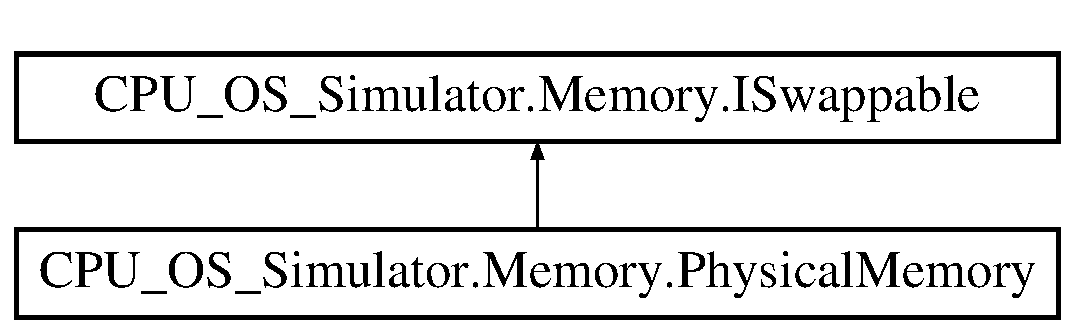
\includegraphics[height=2.000000cm]{class_c_p_u___o_s___simulator_1_1_memory_1_1_physical_memory}
\end{center}
\end{figure}
\subsection*{Public Member Functions}
\begin{DoxyCompactItemize}
\item 
\hyperlink{class_c_p_u___o_s___simulator_1_1_memory_1_1_physical_memory_ab870660d7d17f3e34b71c75ee89d9935}{Physical\+Memory} (int \hyperlink{class_c_p_u___o_s___simulator_1_1_memory_1_1_physical_memory_aefbb5641a06c37aa17bb523d8c90dc60}{capacity})
\begin{DoxyCompactList}\small\item\em Constructor for physical memory \end{DoxyCompactList}\item 
bool \hyperlink{class_c_p_u___o_s___simulator_1_1_memory_1_1_physical_memory_a10cd5c3c1c36f246acfbe96fecbf81cc}{is\+Full} ()
\begin{DoxyCompactList}\small\item\em Returns whether memory is currently full \end{DoxyCompactList}\item 
\hyperlink{class_c_p_u___o_s___simulator_1_1_memory_1_1_memory_page}{Memory\+Page} \hyperlink{class_c_p_u___o_s___simulator_1_1_memory_1_1_physical_memory_aae1eddd302bb1494c2501e8127ff02bc}{Add\+Page} (\hyperlink{class_c_p_u___o_s___simulator_1_1_memory_1_1_memory_page}{Memory\+Page} page, int index)
\begin{DoxyCompactList}\small\item\em This function adds a page into memory \end{DoxyCompactList}\item 
void \hyperlink{class_c_p_u___o_s___simulator_1_1_memory_1_1_physical_memory_a60918e50d8bc9e1a07ac640153343f69}{Swap\+Out} (int Location\+To\+Swap, int Frame\+Number)
\begin{DoxyCompactList}\small\item\em This function swaps out this memory page \end{DoxyCompactList}\item 
void \hyperlink{class_c_p_u___o_s___simulator_1_1_memory_1_1_physical_memory_ac12efe05d774b7e2ea38142835e0c131}{Swap\+In} (int Location\+To\+Swap, int Frame\+Number)
\begin{DoxyCompactList}\small\item\em This function swaps in this memory page \end{DoxyCompactList}\item 
\hyperlink{class_c_p_u___o_s___simulator_1_1_memory_1_1_memory_page}{Memory\+Page} \hyperlink{class_c_p_u___o_s___simulator_1_1_memory_1_1_physical_memory_a525c8a54ebd978b870884dc30f5800ff}{Request\+Memory\+Page} (int frame\+Number)
\begin{DoxyCompactList}\small\item\em Requests a memory page to be swapped into memory \end{DoxyCompactList}\end{DoxyCompactItemize}
\subsection*{Properties}
\begin{DoxyCompactItemize}
\item 
int \hyperlink{class_c_p_u___o_s___simulator_1_1_memory_1_1_physical_memory_af04d50462367295af1c8b4f9f1a75730}{Capacity}\hspace{0.3cm}{\ttfamily  \mbox{[}get, set\mbox{]}}
\begin{DoxyCompactList}\small\item\em Property for the capacity of memory \end{DoxyCompactList}\item 
List$<$ \hyperlink{class_c_p_u___o_s___simulator_1_1_memory_1_1_memory_page}{Memory\+Page} $>$ \hyperlink{class_c_p_u___o_s___simulator_1_1_memory_1_1_physical_memory_ad099afa411ad366a734457fd824fea06}{Pages}\hspace{0.3cm}{\ttfamily  \mbox{[}get, set\mbox{]}}
\begin{DoxyCompactList}\small\item\em Property for the list of pages currently in memory \end{DoxyCompactList}\item 
\hyperlink{class_c_p_u___o_s___simulator_1_1_memory_1_1_page_table}{Page\+Table} \hyperlink{class_c_p_u___o_s___simulator_1_1_memory_1_1_physical_memory_aaa669f8a92820bf792dd2ccb553254c9}{Table}\hspace{0.3cm}{\ttfamily  \mbox{[}get, set\mbox{]}}
\begin{DoxyCompactList}\small\item\em Property for the page table \end{DoxyCompactList}\item 
\hyperlink{class_c_p_u___o_s___simulator_1_1_memory_1_1_swap_space}{Swap\+Space} \hyperlink{class_c_p_u___o_s___simulator_1_1_memory_1_1_physical_memory_a5d0fceb09f51edcfb4f483b5e8a9508a}{Space}\hspace{0.3cm}{\ttfamily  \mbox{[}get, set\mbox{]}}
\begin{DoxyCompactList}\small\item\em Property for the swap space where swapped out memory pages are held \end{DoxyCompactList}\end{DoxyCompactItemize}
\subsection*{Private Member Functions}
\begin{DoxyCompactItemize}
\item 
dynamic \hyperlink{class_c_p_u___o_s___simulator_1_1_memory_1_1_physical_memory_a78a9b68e70b5f44ac1d38fc653b51724}{Get\+Main\+Window\+Instance} ()
\begin{DoxyCompactList}\small\item\em This function gets the main window instance from the window bridge \end{DoxyCompactList}\item 
int \hyperlink{class_c_p_u___o_s___simulator_1_1_memory_1_1_physical_memory_aa37a178a2a3114c4377b9458ae47bbbc}{Get\+Index\+Memory} (int frame\+Number)
\item 
int \hyperlink{class_c_p_u___o_s___simulator_1_1_memory_1_1_physical_memory_a8497f98d7f88ca1ba466c911e0086c81}{Get\+Index\+Swap} (int frame\+Number)
\end{DoxyCompactItemize}
\subsection*{Private Attributes}
\begin{DoxyCompactItemize}
\item 
int \hyperlink{class_c_p_u___o_s___simulator_1_1_memory_1_1_physical_memory_aefbb5641a06c37aa17bb523d8c90dc60}{capacity}
\item 
List$<$ \hyperlink{class_c_p_u___o_s___simulator_1_1_memory_1_1_memory_page}{Memory\+Page} $>$ \hyperlink{class_c_p_u___o_s___simulator_1_1_memory_1_1_physical_memory_aaf32bdc314ba84ea7e120fb28e3a3e67}{pages}
\item 
\hyperlink{class_c_p_u___o_s___simulator_1_1_memory_1_1_page_table}{Page\+Table} \hyperlink{class_c_p_u___o_s___simulator_1_1_memory_1_1_physical_memory_a7812a37c95af296758ed7814a95a3ea3}{page\+Table}
\item 
\hyperlink{class_c_p_u___o_s___simulator_1_1_memory_1_1_swap_space}{Swap\+Space} \hyperlink{class_c_p_u___o_s___simulator_1_1_memory_1_1_physical_memory_a0dedf020af5760e7c9875e4bcc9f5990}{swap\+Space}
\end{DoxyCompactItemize}


\subsection{Detailed Description}
This class represents physical memory (R\+A\+M) 



Definition at line 13 of file Physical\+Memory.\+cs.



\subsection{Constructor \& Destructor Documentation}
\hypertarget{class_c_p_u___o_s___simulator_1_1_memory_1_1_physical_memory_ab870660d7d17f3e34b71c75ee89d9935}{}\index{C\+P\+U\+\_\+\+O\+S\+\_\+\+Simulator\+::\+Memory\+::\+Physical\+Memory@{C\+P\+U\+\_\+\+O\+S\+\_\+\+Simulator\+::\+Memory\+::\+Physical\+Memory}!Physical\+Memory@{Physical\+Memory}}
\index{Physical\+Memory@{Physical\+Memory}!C\+P\+U\+\_\+\+O\+S\+\_\+\+Simulator\+::\+Memory\+::\+Physical\+Memory@{C\+P\+U\+\_\+\+O\+S\+\_\+\+Simulator\+::\+Memory\+::\+Physical\+Memory}}
\subsubsection[{Physical\+Memory(int capacity)}]{\setlength{\rightskip}{0pt plus 5cm}C\+P\+U\+\_\+\+O\+S\+\_\+\+Simulator.\+Memory.\+Physical\+Memory.\+Physical\+Memory (
\begin{DoxyParamCaption}
\item[{int}]{capacity}
\end{DoxyParamCaption}
)}\label{class_c_p_u___o_s___simulator_1_1_memory_1_1_physical_memory_ab870660d7d17f3e34b71c75ee89d9935}


Constructor for physical memory 


\begin{DoxyParams}{Parameters}
{\em capacity} & capacity of physical memory in pages\\
\hline
\end{DoxyParams}


Definition at line 24 of file Physical\+Memory.\+cs.



\subsection{Member Function Documentation}
\hypertarget{class_c_p_u___o_s___simulator_1_1_memory_1_1_physical_memory_aae1eddd302bb1494c2501e8127ff02bc}{}\index{C\+P\+U\+\_\+\+O\+S\+\_\+\+Simulator\+::\+Memory\+::\+Physical\+Memory@{C\+P\+U\+\_\+\+O\+S\+\_\+\+Simulator\+::\+Memory\+::\+Physical\+Memory}!Add\+Page@{Add\+Page}}
\index{Add\+Page@{Add\+Page}!C\+P\+U\+\_\+\+O\+S\+\_\+\+Simulator\+::\+Memory\+::\+Physical\+Memory@{C\+P\+U\+\_\+\+O\+S\+\_\+\+Simulator\+::\+Memory\+::\+Physical\+Memory}}
\subsubsection[{Add\+Page(\+Memory\+Page page, int index)}]{\setlength{\rightskip}{0pt plus 5cm}{\bf Memory\+Page} C\+P\+U\+\_\+\+O\+S\+\_\+\+Simulator.\+Memory.\+Physical\+Memory.\+Add\+Page (
\begin{DoxyParamCaption}
\item[{{\bf Memory\+Page}}]{page, }
\item[{int}]{index}
\end{DoxyParamCaption}
)}\label{class_c_p_u___o_s___simulator_1_1_memory_1_1_physical_memory_aae1eddd302bb1494c2501e8127ff02bc}


This function adds a page into memory 


\begin{DoxyParams}{Parameters}
{\em page} & the page to add to memory \\
\hline
{\em index} & the index to add the page to memory\\
\hline
\end{DoxyParams}
\begin{DoxyReturn}{Returns}
a reference to the page that has been added to memory
\end{DoxyReturn}


Definition at line 45 of file Physical\+Memory.\+cs.

\hypertarget{class_c_p_u___o_s___simulator_1_1_memory_1_1_physical_memory_aa37a178a2a3114c4377b9458ae47bbbc}{}\index{C\+P\+U\+\_\+\+O\+S\+\_\+\+Simulator\+::\+Memory\+::\+Physical\+Memory@{C\+P\+U\+\_\+\+O\+S\+\_\+\+Simulator\+::\+Memory\+::\+Physical\+Memory}!Get\+Index\+Memory@{Get\+Index\+Memory}}
\index{Get\+Index\+Memory@{Get\+Index\+Memory}!C\+P\+U\+\_\+\+O\+S\+\_\+\+Simulator\+::\+Memory\+::\+Physical\+Memory@{C\+P\+U\+\_\+\+O\+S\+\_\+\+Simulator\+::\+Memory\+::\+Physical\+Memory}}
\subsubsection[{Get\+Index\+Memory(int frame\+Number)}]{\setlength{\rightskip}{0pt plus 5cm}int C\+P\+U\+\_\+\+O\+S\+\_\+\+Simulator.\+Memory.\+Physical\+Memory.\+Get\+Index\+Memory (
\begin{DoxyParamCaption}
\item[{int}]{frame\+Number}
\end{DoxyParamCaption}
)\hspace{0.3cm}{\ttfamily [private]}}\label{class_c_p_u___o_s___simulator_1_1_memory_1_1_physical_memory_aa37a178a2a3114c4377b9458ae47bbbc}


Definition at line 192 of file Physical\+Memory.\+cs.

\hypertarget{class_c_p_u___o_s___simulator_1_1_memory_1_1_physical_memory_a8497f98d7f88ca1ba466c911e0086c81}{}\index{C\+P\+U\+\_\+\+O\+S\+\_\+\+Simulator\+::\+Memory\+::\+Physical\+Memory@{C\+P\+U\+\_\+\+O\+S\+\_\+\+Simulator\+::\+Memory\+::\+Physical\+Memory}!Get\+Index\+Swap@{Get\+Index\+Swap}}
\index{Get\+Index\+Swap@{Get\+Index\+Swap}!C\+P\+U\+\_\+\+O\+S\+\_\+\+Simulator\+::\+Memory\+::\+Physical\+Memory@{C\+P\+U\+\_\+\+O\+S\+\_\+\+Simulator\+::\+Memory\+::\+Physical\+Memory}}
\subsubsection[{Get\+Index\+Swap(int frame\+Number)}]{\setlength{\rightskip}{0pt plus 5cm}int C\+P\+U\+\_\+\+O\+S\+\_\+\+Simulator.\+Memory.\+Physical\+Memory.\+Get\+Index\+Swap (
\begin{DoxyParamCaption}
\item[{int}]{frame\+Number}
\end{DoxyParamCaption}
)\hspace{0.3cm}{\ttfamily [private]}}\label{class_c_p_u___o_s___simulator_1_1_memory_1_1_physical_memory_a8497f98d7f88ca1ba466c911e0086c81}


Definition at line 200 of file Physical\+Memory.\+cs.

\hypertarget{class_c_p_u___o_s___simulator_1_1_memory_1_1_physical_memory_a78a9b68e70b5f44ac1d38fc653b51724}{}\index{C\+P\+U\+\_\+\+O\+S\+\_\+\+Simulator\+::\+Memory\+::\+Physical\+Memory@{C\+P\+U\+\_\+\+O\+S\+\_\+\+Simulator\+::\+Memory\+::\+Physical\+Memory}!Get\+Main\+Window\+Instance@{Get\+Main\+Window\+Instance}}
\index{Get\+Main\+Window\+Instance@{Get\+Main\+Window\+Instance}!C\+P\+U\+\_\+\+O\+S\+\_\+\+Simulator\+::\+Memory\+::\+Physical\+Memory@{C\+P\+U\+\_\+\+O\+S\+\_\+\+Simulator\+::\+Memory\+::\+Physical\+Memory}}
\subsubsection[{Get\+Main\+Window\+Instance()}]{\setlength{\rightskip}{0pt plus 5cm}dynamic C\+P\+U\+\_\+\+O\+S\+\_\+\+Simulator.\+Memory.\+Physical\+Memory.\+Get\+Main\+Window\+Instance (
\begin{DoxyParamCaption}
{}
\end{DoxyParamCaption}
)\hspace{0.3cm}{\ttfamily [private]}}\label{class_c_p_u___o_s___simulator_1_1_memory_1_1_physical_memory_a78a9b68e70b5f44ac1d38fc653b51724}


This function gets the main window instance from the window bridge 

\begin{DoxyReturn}{Returns}
the active instance of main window 
\end{DoxyReturn}


Definition at line 158 of file Physical\+Memory.\+cs.

\hypertarget{class_c_p_u___o_s___simulator_1_1_memory_1_1_physical_memory_a10cd5c3c1c36f246acfbe96fecbf81cc}{}\index{C\+P\+U\+\_\+\+O\+S\+\_\+\+Simulator\+::\+Memory\+::\+Physical\+Memory@{C\+P\+U\+\_\+\+O\+S\+\_\+\+Simulator\+::\+Memory\+::\+Physical\+Memory}!is\+Full@{is\+Full}}
\index{is\+Full@{is\+Full}!C\+P\+U\+\_\+\+O\+S\+\_\+\+Simulator\+::\+Memory\+::\+Physical\+Memory@{C\+P\+U\+\_\+\+O\+S\+\_\+\+Simulator\+::\+Memory\+::\+Physical\+Memory}}
\subsubsection[{is\+Full()}]{\setlength{\rightskip}{0pt plus 5cm}bool C\+P\+U\+\_\+\+O\+S\+\_\+\+Simulator.\+Memory.\+Physical\+Memory.\+is\+Full (
\begin{DoxyParamCaption}
{}
\end{DoxyParamCaption}
)}\label{class_c_p_u___o_s___simulator_1_1_memory_1_1_physical_memory_a10cd5c3c1c36f246acfbe96fecbf81cc}


Returns whether memory is currently full 

\begin{DoxyReturn}{Returns}
whether memory is currently full
\end{DoxyReturn}


Definition at line 35 of file Physical\+Memory.\+cs.

\hypertarget{class_c_p_u___o_s___simulator_1_1_memory_1_1_physical_memory_a525c8a54ebd978b870884dc30f5800ff}{}\index{C\+P\+U\+\_\+\+O\+S\+\_\+\+Simulator\+::\+Memory\+::\+Physical\+Memory@{C\+P\+U\+\_\+\+O\+S\+\_\+\+Simulator\+::\+Memory\+::\+Physical\+Memory}!Request\+Memory\+Page@{Request\+Memory\+Page}}
\index{Request\+Memory\+Page@{Request\+Memory\+Page}!C\+P\+U\+\_\+\+O\+S\+\_\+\+Simulator\+::\+Memory\+::\+Physical\+Memory@{C\+P\+U\+\_\+\+O\+S\+\_\+\+Simulator\+::\+Memory\+::\+Physical\+Memory}}
\subsubsection[{Request\+Memory\+Page(int frame\+Number)}]{\setlength{\rightskip}{0pt plus 5cm}{\bf Memory\+Page} C\+P\+U\+\_\+\+O\+S\+\_\+\+Simulator.\+Memory.\+Physical\+Memory.\+Request\+Memory\+Page (
\begin{DoxyParamCaption}
\item[{int}]{frame\+Number}
\end{DoxyParamCaption}
)}\label{class_c_p_u___o_s___simulator_1_1_memory_1_1_physical_memory_a525c8a54ebd978b870884dc30f5800ff}


Requests a memory page to be swapped into memory 


\begin{DoxyParams}{Parameters}
{\em frame\+Number} & the frame number of the requested memory page\\
\hline
\end{DoxyParams}
\begin{DoxyReturn}{Returns}
the requested memory page
\end{DoxyReturn}


Definition at line 171 of file Physical\+Memory.\+cs.

\hypertarget{class_c_p_u___o_s___simulator_1_1_memory_1_1_physical_memory_ac12efe05d774b7e2ea38142835e0c131}{}\index{C\+P\+U\+\_\+\+O\+S\+\_\+\+Simulator\+::\+Memory\+::\+Physical\+Memory@{C\+P\+U\+\_\+\+O\+S\+\_\+\+Simulator\+::\+Memory\+::\+Physical\+Memory}!Swap\+In@{Swap\+In}}
\index{Swap\+In@{Swap\+In}!C\+P\+U\+\_\+\+O\+S\+\_\+\+Simulator\+::\+Memory\+::\+Physical\+Memory@{C\+P\+U\+\_\+\+O\+S\+\_\+\+Simulator\+::\+Memory\+::\+Physical\+Memory}}
\subsubsection[{Swap\+In(int Location\+To\+Swap, int Frame\+Number)}]{\setlength{\rightskip}{0pt plus 5cm}void C\+P\+U\+\_\+\+O\+S\+\_\+\+Simulator.\+Memory.\+Physical\+Memory.\+Swap\+In (
\begin{DoxyParamCaption}
\item[{int}]{Location\+To\+Swap, }
\item[{int}]{Frame\+Number}
\end{DoxyParamCaption}
)}\label{class_c_p_u___o_s___simulator_1_1_memory_1_1_physical_memory_ac12efe05d774b7e2ea38142835e0c131}


This function swaps in this memory page 


\begin{DoxyParams}{Parameters}
{\em Location\+To\+Swap} & the physical address to swap this page in to\\
\hline
{\em Frame\+Number} & this pages frame number\\
\hline
\end{DoxyParams}


Implements \hyperlink{interface_c_p_u___o_s___simulator_1_1_memory_1_1_i_swappable_a38e30363486a3de53e6171da50b943af}{C\+P\+U\+\_\+\+O\+S\+\_\+\+Simulator.\+Memory.\+I\+Swappable}.



Definition at line 134 of file Physical\+Memory.\+cs.

\hypertarget{class_c_p_u___o_s___simulator_1_1_memory_1_1_physical_memory_a60918e50d8bc9e1a07ac640153343f69}{}\index{C\+P\+U\+\_\+\+O\+S\+\_\+\+Simulator\+::\+Memory\+::\+Physical\+Memory@{C\+P\+U\+\_\+\+O\+S\+\_\+\+Simulator\+::\+Memory\+::\+Physical\+Memory}!Swap\+Out@{Swap\+Out}}
\index{Swap\+Out@{Swap\+Out}!C\+P\+U\+\_\+\+O\+S\+\_\+\+Simulator\+::\+Memory\+::\+Physical\+Memory@{C\+P\+U\+\_\+\+O\+S\+\_\+\+Simulator\+::\+Memory\+::\+Physical\+Memory}}
\subsubsection[{Swap\+Out(int Location\+To\+Swap, int Frame\+Number)}]{\setlength{\rightskip}{0pt plus 5cm}void C\+P\+U\+\_\+\+O\+S\+\_\+\+Simulator.\+Memory.\+Physical\+Memory.\+Swap\+Out (
\begin{DoxyParamCaption}
\item[{int}]{Location\+To\+Swap, }
\item[{int}]{Frame\+Number}
\end{DoxyParamCaption}
)}\label{class_c_p_u___o_s___simulator_1_1_memory_1_1_physical_memory_a60918e50d8bc9e1a07ac640153343f69}


This function swaps out this memory page 


\begin{DoxyParams}{Parameters}
{\em Location\+To\+Swap} & the physical address to swap from\\
\hline
{\em Frame\+Number} & this page\textquotesingle{}s frame number\\
\hline
\end{DoxyParams}


Implements \hyperlink{interface_c_p_u___o_s___simulator_1_1_memory_1_1_i_swappable_ae789e9deb0600d48b0dcbe4a4252220a}{C\+P\+U\+\_\+\+O\+S\+\_\+\+Simulator.\+Memory.\+I\+Swappable}.



Definition at line 108 of file Physical\+Memory.\+cs.



\subsection{Member Data Documentation}
\hypertarget{class_c_p_u___o_s___simulator_1_1_memory_1_1_physical_memory_aefbb5641a06c37aa17bb523d8c90dc60}{}\index{C\+P\+U\+\_\+\+O\+S\+\_\+\+Simulator\+::\+Memory\+::\+Physical\+Memory@{C\+P\+U\+\_\+\+O\+S\+\_\+\+Simulator\+::\+Memory\+::\+Physical\+Memory}!capacity@{capacity}}
\index{capacity@{capacity}!C\+P\+U\+\_\+\+O\+S\+\_\+\+Simulator\+::\+Memory\+::\+Physical\+Memory@{C\+P\+U\+\_\+\+O\+S\+\_\+\+Simulator\+::\+Memory\+::\+Physical\+Memory}}
\subsubsection[{capacity}]{\setlength{\rightskip}{0pt plus 5cm}int C\+P\+U\+\_\+\+O\+S\+\_\+\+Simulator.\+Memory.\+Physical\+Memory.\+capacity\hspace{0.3cm}{\ttfamily [private]}}\label{class_c_p_u___o_s___simulator_1_1_memory_1_1_physical_memory_aefbb5641a06c37aa17bb523d8c90dc60}


Definition at line 15 of file Physical\+Memory.\+cs.

\hypertarget{class_c_p_u___o_s___simulator_1_1_memory_1_1_physical_memory_aaf32bdc314ba84ea7e120fb28e3a3e67}{}\index{C\+P\+U\+\_\+\+O\+S\+\_\+\+Simulator\+::\+Memory\+::\+Physical\+Memory@{C\+P\+U\+\_\+\+O\+S\+\_\+\+Simulator\+::\+Memory\+::\+Physical\+Memory}!pages@{pages}}
\index{pages@{pages}!C\+P\+U\+\_\+\+O\+S\+\_\+\+Simulator\+::\+Memory\+::\+Physical\+Memory@{C\+P\+U\+\_\+\+O\+S\+\_\+\+Simulator\+::\+Memory\+::\+Physical\+Memory}}
\subsubsection[{pages}]{\setlength{\rightskip}{0pt plus 5cm}List$<${\bf Memory\+Page}$>$ C\+P\+U\+\_\+\+O\+S\+\_\+\+Simulator.\+Memory.\+Physical\+Memory.\+pages\hspace{0.3cm}{\ttfamily [private]}}\label{class_c_p_u___o_s___simulator_1_1_memory_1_1_physical_memory_aaf32bdc314ba84ea7e120fb28e3a3e67}


Definition at line 16 of file Physical\+Memory.\+cs.

\hypertarget{class_c_p_u___o_s___simulator_1_1_memory_1_1_physical_memory_a7812a37c95af296758ed7814a95a3ea3}{}\index{C\+P\+U\+\_\+\+O\+S\+\_\+\+Simulator\+::\+Memory\+::\+Physical\+Memory@{C\+P\+U\+\_\+\+O\+S\+\_\+\+Simulator\+::\+Memory\+::\+Physical\+Memory}!page\+Table@{page\+Table}}
\index{page\+Table@{page\+Table}!C\+P\+U\+\_\+\+O\+S\+\_\+\+Simulator\+::\+Memory\+::\+Physical\+Memory@{C\+P\+U\+\_\+\+O\+S\+\_\+\+Simulator\+::\+Memory\+::\+Physical\+Memory}}
\subsubsection[{page\+Table}]{\setlength{\rightskip}{0pt plus 5cm}{\bf Page\+Table} C\+P\+U\+\_\+\+O\+S\+\_\+\+Simulator.\+Memory.\+Physical\+Memory.\+page\+Table\hspace{0.3cm}{\ttfamily [private]}}\label{class_c_p_u___o_s___simulator_1_1_memory_1_1_physical_memory_a7812a37c95af296758ed7814a95a3ea3}


Definition at line 17 of file Physical\+Memory.\+cs.

\hypertarget{class_c_p_u___o_s___simulator_1_1_memory_1_1_physical_memory_a0dedf020af5760e7c9875e4bcc9f5990}{}\index{C\+P\+U\+\_\+\+O\+S\+\_\+\+Simulator\+::\+Memory\+::\+Physical\+Memory@{C\+P\+U\+\_\+\+O\+S\+\_\+\+Simulator\+::\+Memory\+::\+Physical\+Memory}!swap\+Space@{swap\+Space}}
\index{swap\+Space@{swap\+Space}!C\+P\+U\+\_\+\+O\+S\+\_\+\+Simulator\+::\+Memory\+::\+Physical\+Memory@{C\+P\+U\+\_\+\+O\+S\+\_\+\+Simulator\+::\+Memory\+::\+Physical\+Memory}}
\subsubsection[{swap\+Space}]{\setlength{\rightskip}{0pt plus 5cm}{\bf Swap\+Space} C\+P\+U\+\_\+\+O\+S\+\_\+\+Simulator.\+Memory.\+Physical\+Memory.\+swap\+Space\hspace{0.3cm}{\ttfamily [private]}}\label{class_c_p_u___o_s___simulator_1_1_memory_1_1_physical_memory_a0dedf020af5760e7c9875e4bcc9f5990}


Definition at line 18 of file Physical\+Memory.\+cs.



\subsection{Property Documentation}
\hypertarget{class_c_p_u___o_s___simulator_1_1_memory_1_1_physical_memory_af04d50462367295af1c8b4f9f1a75730}{}\index{C\+P\+U\+\_\+\+O\+S\+\_\+\+Simulator\+::\+Memory\+::\+Physical\+Memory@{C\+P\+U\+\_\+\+O\+S\+\_\+\+Simulator\+::\+Memory\+::\+Physical\+Memory}!Capacity@{Capacity}}
\index{Capacity@{Capacity}!C\+P\+U\+\_\+\+O\+S\+\_\+\+Simulator\+::\+Memory\+::\+Physical\+Memory@{C\+P\+U\+\_\+\+O\+S\+\_\+\+Simulator\+::\+Memory\+::\+Physical\+Memory}}
\subsubsection[{Capacity}]{\setlength{\rightskip}{0pt plus 5cm}int C\+P\+U\+\_\+\+O\+S\+\_\+\+Simulator.\+Memory.\+Physical\+Memory.\+Capacity\hspace{0.3cm}{\ttfamily [get]}, {\ttfamily [set]}}\label{class_c_p_u___o_s___simulator_1_1_memory_1_1_physical_memory_af04d50462367295af1c8b4f9f1a75730}


Property for the capacity of memory 



Definition at line 75 of file Physical\+Memory.\+cs.

\hypertarget{class_c_p_u___o_s___simulator_1_1_memory_1_1_physical_memory_ad099afa411ad366a734457fd824fea06}{}\index{C\+P\+U\+\_\+\+O\+S\+\_\+\+Simulator\+::\+Memory\+::\+Physical\+Memory@{C\+P\+U\+\_\+\+O\+S\+\_\+\+Simulator\+::\+Memory\+::\+Physical\+Memory}!Pages@{Pages}}
\index{Pages@{Pages}!C\+P\+U\+\_\+\+O\+S\+\_\+\+Simulator\+::\+Memory\+::\+Physical\+Memory@{C\+P\+U\+\_\+\+O\+S\+\_\+\+Simulator\+::\+Memory\+::\+Physical\+Memory}}
\subsubsection[{Pages}]{\setlength{\rightskip}{0pt plus 5cm}List$<${\bf Memory\+Page}$>$ C\+P\+U\+\_\+\+O\+S\+\_\+\+Simulator.\+Memory.\+Physical\+Memory.\+Pages\hspace{0.3cm}{\ttfamily [get]}, {\ttfamily [set]}}\label{class_c_p_u___o_s___simulator_1_1_memory_1_1_physical_memory_ad099afa411ad366a734457fd824fea06}


Property for the list of pages currently in memory 



Definition at line 83 of file Physical\+Memory.\+cs.

\hypertarget{class_c_p_u___o_s___simulator_1_1_memory_1_1_physical_memory_a5d0fceb09f51edcfb4f483b5e8a9508a}{}\index{C\+P\+U\+\_\+\+O\+S\+\_\+\+Simulator\+::\+Memory\+::\+Physical\+Memory@{C\+P\+U\+\_\+\+O\+S\+\_\+\+Simulator\+::\+Memory\+::\+Physical\+Memory}!Space@{Space}}
\index{Space@{Space}!C\+P\+U\+\_\+\+O\+S\+\_\+\+Simulator\+::\+Memory\+::\+Physical\+Memory@{C\+P\+U\+\_\+\+O\+S\+\_\+\+Simulator\+::\+Memory\+::\+Physical\+Memory}}
\subsubsection[{Space}]{\setlength{\rightskip}{0pt plus 5cm}{\bf Swap\+Space} C\+P\+U\+\_\+\+O\+S\+\_\+\+Simulator.\+Memory.\+Physical\+Memory.\+Space\hspace{0.3cm}{\ttfamily [get]}, {\ttfamily [set]}}\label{class_c_p_u___o_s___simulator_1_1_memory_1_1_physical_memory_a5d0fceb09f51edcfb4f483b5e8a9508a}


Property for the swap space where swapped out memory pages are held 



Definition at line 99 of file Physical\+Memory.\+cs.

\hypertarget{class_c_p_u___o_s___simulator_1_1_memory_1_1_physical_memory_aaa669f8a92820bf792dd2ccb553254c9}{}\index{C\+P\+U\+\_\+\+O\+S\+\_\+\+Simulator\+::\+Memory\+::\+Physical\+Memory@{C\+P\+U\+\_\+\+O\+S\+\_\+\+Simulator\+::\+Memory\+::\+Physical\+Memory}!Table@{Table}}
\index{Table@{Table}!C\+P\+U\+\_\+\+O\+S\+\_\+\+Simulator\+::\+Memory\+::\+Physical\+Memory@{C\+P\+U\+\_\+\+O\+S\+\_\+\+Simulator\+::\+Memory\+::\+Physical\+Memory}}
\subsubsection[{Table}]{\setlength{\rightskip}{0pt plus 5cm}{\bf Page\+Table} C\+P\+U\+\_\+\+O\+S\+\_\+\+Simulator.\+Memory.\+Physical\+Memory.\+Table\hspace{0.3cm}{\ttfamily [get]}, {\ttfamily [set]}}\label{class_c_p_u___o_s___simulator_1_1_memory_1_1_physical_memory_aaa669f8a92820bf792dd2ccb553254c9}


Property for the page table 



Definition at line 91 of file Physical\+Memory.\+cs.



The documentation for this class was generated from the following file\+:\begin{DoxyCompactItemize}
\item 
Memory/\hyperlink{_physical_memory_8cs}{Physical\+Memory.\+cs}\end{DoxyCompactItemize}

\hypertarget{class_c_p_u___o_s___simulator_1_1_console_1_1_printable_document}{}\section{C\+P\+U\+\_\+\+O\+S\+\_\+\+Simulator.\+Console.\+Printable\+Document Class Reference}
\label{class_c_p_u___o_s___simulator_1_1_console_1_1_printable_document}\index{C\+P\+U\+\_\+\+O\+S\+\_\+\+Simulator.\+Console.\+Printable\+Document@{C\+P\+U\+\_\+\+O\+S\+\_\+\+Simulator.\+Console.\+Printable\+Document}}
Inheritance diagram for C\+P\+U\+\_\+\+O\+S\+\_\+\+Simulator.\+Console.\+Printable\+Document\+:\begin{figure}[H]
\begin{center}
\leavevmode
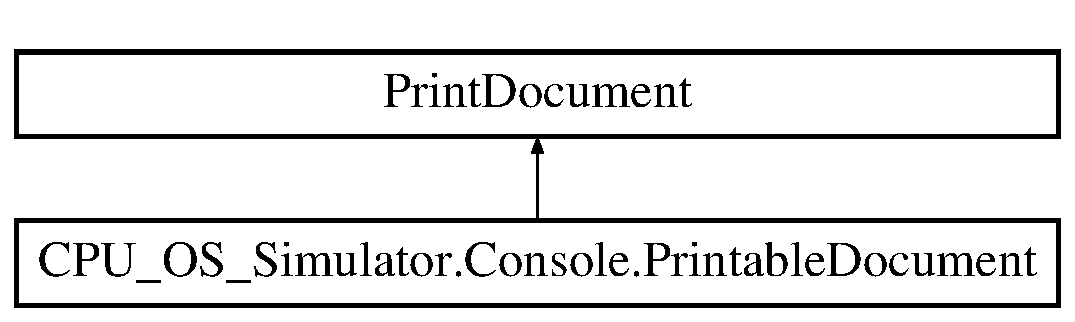
\includegraphics[height=2.000000cm]{class_c_p_u___o_s___simulator_1_1_console_1_1_printable_document}
\end{center}
\end{figure}
\subsection*{Protected Member Functions}
\begin{DoxyCompactItemize}
\item 
override void \hyperlink{class_c_p_u___o_s___simulator_1_1_console_1_1_printable_document_a63d8f6a5ee9648e418dbc93859d2c746}{On\+Begin\+Print} (Print\+Event\+Args e)
\begin{DoxyCompactList}\small\item\em Raises the E\+:\+System.\+Drawing.\+Printing.\+Print\+Document.\+Begin\+Print event. It is called after the M\+:\+System.\+Drawing.\+Printing.\+Print\+Document.\+Print method is called and before the first page of the document prints. \end{DoxyCompactList}\item 
override void \hyperlink{class_c_p_u___o_s___simulator_1_1_console_1_1_printable_document_a3e2f3a86ac5c236c3c36a04910fb6ab1}{On\+End\+Print} (Print\+Event\+Args e)
\begin{DoxyCompactList}\small\item\em Raises the E\+:\+System.\+Drawing.\+Printing.\+Print\+Document.\+End\+Print event. It is called when the last page of the document has printed. \end{DoxyCompactList}\end{DoxyCompactItemize}
\subsection*{Private Member Functions}
\begin{DoxyCompactItemize}
\item 
dynamic \hyperlink{class_c_p_u___o_s___simulator_1_1_console_1_1_printable_document_a4cdd46c3d0e8b4e4ea490675b5c7748e}{Get\+Console\+Window\+Instance} ()
\begin{DoxyCompactList}\small\item\em This function gets the \hyperlink{namespace_c_p_u___o_s___simulator_1_1_console}{Console} window instance from the window bridge \end{DoxyCompactList}\end{DoxyCompactItemize}


\subsection{Detailed Description}


Definition at line 7 of file Printable\+Document.\+cs.



\subsection{Member Function Documentation}
\hypertarget{class_c_p_u___o_s___simulator_1_1_console_1_1_printable_document_a4cdd46c3d0e8b4e4ea490675b5c7748e}{}\index{C\+P\+U\+\_\+\+O\+S\+\_\+\+Simulator\+::\+Console\+::\+Printable\+Document@{C\+P\+U\+\_\+\+O\+S\+\_\+\+Simulator\+::\+Console\+::\+Printable\+Document}!Get\+Console\+Window\+Instance@{Get\+Console\+Window\+Instance}}
\index{Get\+Console\+Window\+Instance@{Get\+Console\+Window\+Instance}!C\+P\+U\+\_\+\+O\+S\+\_\+\+Simulator\+::\+Console\+::\+Printable\+Document@{C\+P\+U\+\_\+\+O\+S\+\_\+\+Simulator\+::\+Console\+::\+Printable\+Document}}
\subsubsection[{Get\+Console\+Window\+Instance()}]{\setlength{\rightskip}{0pt plus 5cm}dynamic C\+P\+U\+\_\+\+O\+S\+\_\+\+Simulator.\+Console.\+Printable\+Document.\+Get\+Console\+Window\+Instance (
\begin{DoxyParamCaption}
{}
\end{DoxyParamCaption}
)\hspace{0.3cm}{\ttfamily [private]}}\label{class_c_p_u___o_s___simulator_1_1_console_1_1_printable_document_a4cdd46c3d0e8b4e4ea490675b5c7748e}


This function gets the \hyperlink{namespace_c_p_u___o_s___simulator_1_1_console}{Console} window instance from the window bridge 

\begin{DoxyReturn}{Returns}
the active instance of main window 
\end{DoxyReturn}


Definition at line 36 of file Printable\+Document.\+cs.

\hypertarget{class_c_p_u___o_s___simulator_1_1_console_1_1_printable_document_a63d8f6a5ee9648e418dbc93859d2c746}{}\index{C\+P\+U\+\_\+\+O\+S\+\_\+\+Simulator\+::\+Console\+::\+Printable\+Document@{C\+P\+U\+\_\+\+O\+S\+\_\+\+Simulator\+::\+Console\+::\+Printable\+Document}!On\+Begin\+Print@{On\+Begin\+Print}}
\index{On\+Begin\+Print@{On\+Begin\+Print}!C\+P\+U\+\_\+\+O\+S\+\_\+\+Simulator\+::\+Console\+::\+Printable\+Document@{C\+P\+U\+\_\+\+O\+S\+\_\+\+Simulator\+::\+Console\+::\+Printable\+Document}}
\subsubsection[{On\+Begin\+Print(\+Print\+Event\+Args e)}]{\setlength{\rightskip}{0pt plus 5cm}override void C\+P\+U\+\_\+\+O\+S\+\_\+\+Simulator.\+Console.\+Printable\+Document.\+On\+Begin\+Print (
\begin{DoxyParamCaption}
\item[{Print\+Event\+Args}]{e}
\end{DoxyParamCaption}
)\hspace{0.3cm}{\ttfamily [protected]}}\label{class_c_p_u___o_s___simulator_1_1_console_1_1_printable_document_a63d8f6a5ee9648e418dbc93859d2c746}


Raises the E\+:\+System.\+Drawing.\+Printing.\+Print\+Document.\+Begin\+Print event. It is called after the M\+:\+System.\+Drawing.\+Printing.\+Print\+Document.\+Print method is called and before the first page of the document prints. 


\begin{DoxyParams}{Parameters}
{\em e} & A T\+:\+System.\+Drawing.\+Printing.\+Print\+Event\+Args that contains the event data. \\
\hline
\end{DoxyParams}


Definition at line 13 of file Printable\+Document.\+cs.

\hypertarget{class_c_p_u___o_s___simulator_1_1_console_1_1_printable_document_a3e2f3a86ac5c236c3c36a04910fb6ab1}{}\index{C\+P\+U\+\_\+\+O\+S\+\_\+\+Simulator\+::\+Console\+::\+Printable\+Document@{C\+P\+U\+\_\+\+O\+S\+\_\+\+Simulator\+::\+Console\+::\+Printable\+Document}!On\+End\+Print@{On\+End\+Print}}
\index{On\+End\+Print@{On\+End\+Print}!C\+P\+U\+\_\+\+O\+S\+\_\+\+Simulator\+::\+Console\+::\+Printable\+Document@{C\+P\+U\+\_\+\+O\+S\+\_\+\+Simulator\+::\+Console\+::\+Printable\+Document}}
\subsubsection[{On\+End\+Print(\+Print\+Event\+Args e)}]{\setlength{\rightskip}{0pt plus 5cm}override void C\+P\+U\+\_\+\+O\+S\+\_\+\+Simulator.\+Console.\+Printable\+Document.\+On\+End\+Print (
\begin{DoxyParamCaption}
\item[{Print\+Event\+Args}]{e}
\end{DoxyParamCaption}
)\hspace{0.3cm}{\ttfamily [protected]}}\label{class_c_p_u___o_s___simulator_1_1_console_1_1_printable_document_a3e2f3a86ac5c236c3c36a04910fb6ab1}


Raises the E\+:\+System.\+Drawing.\+Printing.\+Print\+Document.\+End\+Print event. It is called when the last page of the document has printed. 


\begin{DoxyParams}{Parameters}
{\em e} & A T\+:\+System.\+Drawing.\+Printing.\+Print\+Event\+Args that contains the event data. \\
\hline
\end{DoxyParams}


Definition at line 25 of file Printable\+Document.\+cs.



The documentation for this class was generated from the following file\+:\begin{DoxyCompactItemize}
\item 
Console/\hyperlink{_printable_document_8cs}{Printable\+Document.\+cs}\end{DoxyCompactItemize}

\hypertarget{class_c_p_u___o_s___simulator_1_1_operating___system_1_1_process_control_block}{}\section{C\+P\+U\+\_\+\+O\+S\+\_\+\+Simulator.\+Operating\+\_\+\+System.\+Process\+Control\+Block Class Reference}
\label{class_c_p_u___o_s___simulator_1_1_operating___system_1_1_process_control_block}\index{C\+P\+U\+\_\+\+O\+S\+\_\+\+Simulator.\+Operating\+\_\+\+System.\+Process\+Control\+Block@{C\+P\+U\+\_\+\+O\+S\+\_\+\+Simulator.\+Operating\+\_\+\+System.\+Process\+Control\+Block}}
\subsection*{Public Member Functions}
\begin{DoxyCompactItemize}
\item 
\hyperlink{class_c_p_u___o_s___simulator_1_1_operating___system_1_1_process_control_block_a8af7f052d1a03e35f7298407df2055e7}{Process\+Control\+Block} ()
\begin{DoxyCompactList}\small\item\em Default Constructor for process control block used when deserialising a process control block N\+O\+T\+E\+: D\+O N\+O\+T U\+S\+E I\+N C\+O\+D\+E\+: \end{DoxyCompactList}\item 
\hyperlink{class_c_p_u___o_s___simulator_1_1_operating___system_1_1_process_control_block_a95c13984ceebe2b73b0cd48b82361179}{Process\+Control\+Block} (\hyperlink{struct_c_p_u___o_s___simulator_1_1_operating___system_1_1_p_c_b_flags}{P\+C\+B\+Flags} flags)
\begin{DoxyCompactList}\small\item\em Constructor for process control block with construction flags \end{DoxyCompactList}\item 
override string \hyperlink{class_c_p_u___o_s___simulator_1_1_operating___system_1_1_process_control_block_ac1559146d5dd5b86333a16fb2256f256}{To\+String} ()
\begin{DoxyCompactList}\small\item\em Returns a string that represents the current object. \end{DoxyCompactList}\end{DoxyCompactItemize}
\subsection*{Properties}
\begin{DoxyCompactItemize}
\item 
int \hyperlink{class_c_p_u___o_s___simulator_1_1_operating___system_1_1_process_control_block_a45dd5ef24fa73b58f4a335168fd50663}{Cpuid}\hspace{0.3cm}{\ttfamily  \mbox{[}get, set\mbox{]}}
\item 
int \hyperlink{class_c_p_u___o_s___simulator_1_1_operating___system_1_1_process_control_block_a4543f27a0bafc028e2a76e7ff301d48f}{Osid}\hspace{0.3cm}{\ttfamily  \mbox{[}get, set\mbox{]}}
\item 
int \hyperlink{class_c_p_u___o_s___simulator_1_1_operating___system_1_1_process_control_block_a65da99ff450282dcbc4d43288237f0e9}{Process\+Id}\hspace{0.3cm}{\ttfamily  \mbox{[}get, set\mbox{]}}
\item 
string \hyperlink{class_c_p_u___o_s___simulator_1_1_operating___system_1_1_process_control_block_a597839d1ff7c6d3e36b2fac398849596}{Process\+Name}\hspace{0.3cm}{\ttfamily  \mbox{[}get, set\mbox{]}}
\item 
\hyperlink{namespace_c_p_u___o_s___simulator_1_1_operating___system_a836ee2204e78fcb3a7dd6c3c942b1a24}{Enum\+Process\+State} \hyperlink{class_c_p_u___o_s___simulator_1_1_operating___system_1_1_process_control_block_a6e34b4a9ef3311b94ae9843917fcd720}{Process\+State}\hspace{0.3cm}{\ttfamily  \mbox{[}get, set\mbox{]}}
\item 
string \hyperlink{class_c_p_u___o_s___simulator_1_1_operating___system_1_1_process_control_block_a4b07155953b708406e49511447093a1f}{Program\+Name}\hspace{0.3cm}{\ttfamily  \mbox{[}get, set\mbox{]}}
\item 
int \hyperlink{class_c_p_u___o_s___simulator_1_1_operating___system_1_1_process_control_block_a20803d3e907266a7b7920e01e5574a99}{Base\+Address}\hspace{0.3cm}{\ttfamily  \mbox{[}get, set\mbox{]}}
\item 
int \hyperlink{class_c_p_u___o_s___simulator_1_1_operating___system_1_1_process_control_block_a0db4bf8588b286ebe82f80e3e00e2132}{Start\+Address}\hspace{0.3cm}{\ttfamily  \mbox{[}get, set\mbox{]}}
\item 
int \hyperlink{class_c_p_u___o_s___simulator_1_1_operating___system_1_1_process_control_block_af0629b300d7f2ac582512e881c49f2ea}{Process\+Priority}\hspace{0.3cm}{\ttfamily  \mbox{[}get, set\mbox{]}}
\item 
int \hyperlink{class_c_p_u___o_s___simulator_1_1_operating___system_1_1_process_control_block_a7a73f2ca49a669fc3d2693ee6d0b8aff}{Proceess\+Memory}\hspace{0.3cm}{\ttfamily  \mbox{[}get, set\mbox{]}}
\item 
double \hyperlink{class_c_p_u___o_s___simulator_1_1_operating___system_1_1_process_control_block_a9420c2a711010a174586bb897c580e3f}{Avg\+Burst\+Time}\hspace{0.3cm}{\ttfamily  \mbox{[}get, set\mbox{]}}
\item 
double \hyperlink{class_c_p_u___o_s___simulator_1_1_operating___system_1_1_process_control_block_ae03a95dce0f261ea4504a3f83b8950d4}{Avg\+Waiting\+Time}\hspace{0.3cm}{\ttfamily  \mbox{[}get, set\mbox{]}}
\item 
bool \hyperlink{class_c_p_u___o_s___simulator_1_1_operating___system_1_1_process_control_block_a7fcc2cbbf3ea5f2611f83c742ef1003d}{Resource\+Starved}\hspace{0.3cm}{\ttfamily  \mbox{[}get, set\mbox{]}}
\item 
List$<$ \hyperlink{class_c_p_u___o_s___simulator_1_1_operating___system_1_1_simulator_resource}{Simulator\+Resource} $>$ \hyperlink{class_c_p_u___o_s___simulator_1_1_operating___system_1_1_process_control_block_a05ff68677c2ea2b4784226838b035fc3}{Allocated\+Resources}\hspace{0.3cm}{\ttfamily  \mbox{[}get, set\mbox{]}}
\item 
List$<$ \hyperlink{class_c_p_u___o_s___simulator_1_1_operating___system_1_1_simulator_resource}{Simulator\+Resource} $>$ \hyperlink{class_c_p_u___o_s___simulator_1_1_operating___system_1_1_process_control_block_ae0e0ef096393f21ca4f10f333f4f4003}{Requested\+Resources}\hspace{0.3cm}{\ttfamily  \mbox{[}get, set\mbox{]}}
\item 
\hyperlink{class_c_p_u___o_s___simulator_1_1_c_p_u_1_1_register}{Register}\mbox{[}$\,$\mbox{]} \hyperlink{class_c_p_u___o_s___simulator_1_1_operating___system_1_1_process_control_block_abab92b09a34fb79823064fca79ed32ae}{Registers}\hspace{0.3cm}{\ttfamily  \mbox{[}get, set\mbox{]}}
\item 
\hyperlink{class_c_p_u___o_s___simulator_1_1_c_p_u_1_1_special_register}{Special\+Register}\mbox{[}$\,$\mbox{]} \hyperlink{class_c_p_u___o_s___simulator_1_1_operating___system_1_1_process_control_block_af9716c755f2e5957ea4f4a7af4a7a190}{Special\+Registers}\hspace{0.3cm}{\ttfamily  \mbox{[}get, set\mbox{]}}
\item 
int \hyperlink{class_c_p_u___o_s___simulator_1_1_operating___system_1_1_process_control_block_ae285b06f82507297a0f006ff3bece008}{Lifetime\+Mills}\hspace{0.3cm}{\ttfamily  \mbox{[}get, set\mbox{]}}
\end{DoxyCompactItemize}
\subsection*{Private Attributes}
\begin{DoxyCompactItemize}
\item 
int \hyperlink{class_c_p_u___o_s___simulator_1_1_operating___system_1_1_process_control_block_abb9341cb0d47b6acb52a4f219d69b600}{C\+P\+U\+I\+D}
\item 
int \hyperlink{class_c_p_u___o_s___simulator_1_1_operating___system_1_1_process_control_block_a417b892bfe8ec7f9d5a64eb413b2a333}{O\+S\+I\+D}
\item 
int \hyperlink{class_c_p_u___o_s___simulator_1_1_operating___system_1_1_process_control_block_a238d1021130eef6ea4031679338e4719}{process\+I\+D}
\item 
string \hyperlink{class_c_p_u___o_s___simulator_1_1_operating___system_1_1_process_control_block_af5ec02be59157c998f2e708bc8b27b59}{process\+Name}
\item 
\hyperlink{namespace_c_p_u___o_s___simulator_1_1_operating___system_a836ee2204e78fcb3a7dd6c3c942b1a24}{Enum\+Process\+State} \hyperlink{class_c_p_u___o_s___simulator_1_1_operating___system_1_1_process_control_block_a8aaf7c8cbb6b9ed7b4bb4194aa85cf92}{process\+State} = \hyperlink{namespace_c_p_u___o_s___simulator_1_1_operating___system_aea0b669d1bbf5690ae34ac2f8bef9470a696b031073e74bf2cb98e5ef201d4aa3}{Enum\+Process\+State.\+U\+N\+K\+N\+O\+W\+N}
\item 
string \hyperlink{class_c_p_u___o_s___simulator_1_1_operating___system_1_1_process_control_block_a0b041598cd53af2daee0f2a78cc1a012}{program\+Name}
\item 
int \hyperlink{class_c_p_u___o_s___simulator_1_1_operating___system_1_1_process_control_block_aa539c0c08de4523f8d6e9b21fe4165e6}{base\+Address}
\item 
int \hyperlink{class_c_p_u___o_s___simulator_1_1_operating___system_1_1_process_control_block_a4898c5e44f50c89467d3fe35486face7}{start\+Address}
\item 
int \hyperlink{class_c_p_u___o_s___simulator_1_1_operating___system_1_1_process_control_block_af07e4fc7da3435e5513b842fc177b677}{process\+Priority}
\item 
int \hyperlink{class_c_p_u___o_s___simulator_1_1_operating___system_1_1_process_control_block_afb21210abfe66fa59efd3fbc7cd6d556}{proceess\+Memory}
\item 
double \hyperlink{class_c_p_u___o_s___simulator_1_1_operating___system_1_1_process_control_block_afec04aefe69def148099512dc2024ded}{avg\+Burst\+Time}
\item 
double \hyperlink{class_c_p_u___o_s___simulator_1_1_operating___system_1_1_process_control_block_ab2aadabc87960312728806d747db342c}{avg\+Waiting\+Time}
\item 
bool \hyperlink{class_c_p_u___o_s___simulator_1_1_operating___system_1_1_process_control_block_a78ae58aafcca78f88f6c4a979186d45e}{resource\+Starved}
\item 
List$<$ \hyperlink{class_c_p_u___o_s___simulator_1_1_operating___system_1_1_simulator_resource}{Simulator\+Resource} $>$ \hyperlink{class_c_p_u___o_s___simulator_1_1_operating___system_1_1_process_control_block_ab485d0caecc696b77ad5affbd5bba1cd}{allocated\+Resources}
\item 
List$<$ \hyperlink{class_c_p_u___o_s___simulator_1_1_operating___system_1_1_simulator_resource}{Simulator\+Resource} $>$ \hyperlink{class_c_p_u___o_s___simulator_1_1_operating___system_1_1_process_control_block_a579ef3ff031915bcd7ed857547be7311}{requested\+Resources}
\item 
\hyperlink{class_c_p_u___o_s___simulator_1_1_c_p_u_1_1_register}{Register}\mbox{[}$\,$\mbox{]} \hyperlink{class_c_p_u___o_s___simulator_1_1_operating___system_1_1_process_control_block_abf1ea0cffc667a8119d25d8a9c283483}{registers}
\item 
\hyperlink{class_c_p_u___o_s___simulator_1_1_c_p_u_1_1_special_register}{Special\+Register}\mbox{[}$\,$\mbox{]} \hyperlink{class_c_p_u___o_s___simulator_1_1_operating___system_1_1_process_control_block_a1e39a81f5ee1a47350ee3a77cf331646}{special\+Registers}
\item 
int \hyperlink{class_c_p_u___o_s___simulator_1_1_operating___system_1_1_process_control_block_a31259298bf00ca63f7a9f879f0e67c45}{lifetime\+Mills}
\end{DoxyCompactItemize}


\subsection{Detailed Description}


Definition at line 9 of file Process\+Control\+Block.\+cs.



\subsection{Constructor \& Destructor Documentation}
\hypertarget{class_c_p_u___o_s___simulator_1_1_operating___system_1_1_process_control_block_a8af7f052d1a03e35f7298407df2055e7}{}\index{C\+P\+U\+\_\+\+O\+S\+\_\+\+Simulator\+::\+Operating\+\_\+\+System\+::\+Process\+Control\+Block@{C\+P\+U\+\_\+\+O\+S\+\_\+\+Simulator\+::\+Operating\+\_\+\+System\+::\+Process\+Control\+Block}!Process\+Control\+Block@{Process\+Control\+Block}}
\index{Process\+Control\+Block@{Process\+Control\+Block}!C\+P\+U\+\_\+\+O\+S\+\_\+\+Simulator\+::\+Operating\+\_\+\+System\+::\+Process\+Control\+Block@{C\+P\+U\+\_\+\+O\+S\+\_\+\+Simulator\+::\+Operating\+\_\+\+System\+::\+Process\+Control\+Block}}
\subsubsection[{Process\+Control\+Block()}]{\setlength{\rightskip}{0pt plus 5cm}C\+P\+U\+\_\+\+O\+S\+\_\+\+Simulator.\+Operating\+\_\+\+System.\+Process\+Control\+Block.\+Process\+Control\+Block (
\begin{DoxyParamCaption}
{}
\end{DoxyParamCaption}
)}\label{class_c_p_u___o_s___simulator_1_1_operating___system_1_1_process_control_block_a8af7f052d1a03e35f7298407df2055e7}


Default Constructor for process control block used when deserialising a process control block N\+O\+T\+E\+: D\+O N\+O\+T U\+S\+E I\+N C\+O\+D\+E\+: 



Definition at line 38 of file Process\+Control\+Block.\+cs.

\hypertarget{class_c_p_u___o_s___simulator_1_1_operating___system_1_1_process_control_block_a95c13984ceebe2b73b0cd48b82361179}{}\index{C\+P\+U\+\_\+\+O\+S\+\_\+\+Simulator\+::\+Operating\+\_\+\+System\+::\+Process\+Control\+Block@{C\+P\+U\+\_\+\+O\+S\+\_\+\+Simulator\+::\+Operating\+\_\+\+System\+::\+Process\+Control\+Block}!Process\+Control\+Block@{Process\+Control\+Block}}
\index{Process\+Control\+Block@{Process\+Control\+Block}!C\+P\+U\+\_\+\+O\+S\+\_\+\+Simulator\+::\+Operating\+\_\+\+System\+::\+Process\+Control\+Block@{C\+P\+U\+\_\+\+O\+S\+\_\+\+Simulator\+::\+Operating\+\_\+\+System\+::\+Process\+Control\+Block}}
\subsubsection[{Process\+Control\+Block(\+P\+C\+B\+Flags flags)}]{\setlength{\rightskip}{0pt plus 5cm}C\+P\+U\+\_\+\+O\+S\+\_\+\+Simulator.\+Operating\+\_\+\+System.\+Process\+Control\+Block.\+Process\+Control\+Block (
\begin{DoxyParamCaption}
\item[{{\bf P\+C\+B\+Flags}}]{flags}
\end{DoxyParamCaption}
)}\label{class_c_p_u___o_s___simulator_1_1_operating___system_1_1_process_control_block_a95c13984ceebe2b73b0cd48b82361179}


Constructor for process control block with construction flags 


\begin{DoxyParams}{Parameters}
{\em flags} & flags to use to construct this P\+C\+B\\
\hline
\end{DoxyParams}


Definition at line 46 of file Process\+Control\+Block.\+cs.



\subsection{Member Function Documentation}
\hypertarget{class_c_p_u___o_s___simulator_1_1_operating___system_1_1_process_control_block_ac1559146d5dd5b86333a16fb2256f256}{}\index{C\+P\+U\+\_\+\+O\+S\+\_\+\+Simulator\+::\+Operating\+\_\+\+System\+::\+Process\+Control\+Block@{C\+P\+U\+\_\+\+O\+S\+\_\+\+Simulator\+::\+Operating\+\_\+\+System\+::\+Process\+Control\+Block}!To\+String@{To\+String}}
\index{To\+String@{To\+String}!C\+P\+U\+\_\+\+O\+S\+\_\+\+Simulator\+::\+Operating\+\_\+\+System\+::\+Process\+Control\+Block@{C\+P\+U\+\_\+\+O\+S\+\_\+\+Simulator\+::\+Operating\+\_\+\+System\+::\+Process\+Control\+Block}}
\subsubsection[{To\+String()}]{\setlength{\rightskip}{0pt plus 5cm}override string C\+P\+U\+\_\+\+O\+S\+\_\+\+Simulator.\+Operating\+\_\+\+System.\+Process\+Control\+Block.\+To\+String (
\begin{DoxyParamCaption}
{}
\end{DoxyParamCaption}
)}\label{class_c_p_u___o_s___simulator_1_1_operating___system_1_1_process_control_block_ac1559146d5dd5b86333a16fb2256f256}


Returns a string that represents the current object. 

\begin{DoxyReturn}{Returns}
A string that represents the current object. 
\end{DoxyReturn}


Definition at line 87 of file Process\+Control\+Block.\+cs.



\subsection{Member Data Documentation}
\hypertarget{class_c_p_u___o_s___simulator_1_1_operating___system_1_1_process_control_block_ab485d0caecc696b77ad5affbd5bba1cd}{}\index{C\+P\+U\+\_\+\+O\+S\+\_\+\+Simulator\+::\+Operating\+\_\+\+System\+::\+Process\+Control\+Block@{C\+P\+U\+\_\+\+O\+S\+\_\+\+Simulator\+::\+Operating\+\_\+\+System\+::\+Process\+Control\+Block}!allocated\+Resources@{allocated\+Resources}}
\index{allocated\+Resources@{allocated\+Resources}!C\+P\+U\+\_\+\+O\+S\+\_\+\+Simulator\+::\+Operating\+\_\+\+System\+::\+Process\+Control\+Block@{C\+P\+U\+\_\+\+O\+S\+\_\+\+Simulator\+::\+Operating\+\_\+\+System\+::\+Process\+Control\+Block}}
\subsubsection[{allocated\+Resources}]{\setlength{\rightskip}{0pt plus 5cm}List$<${\bf Simulator\+Resource}$>$ C\+P\+U\+\_\+\+O\+S\+\_\+\+Simulator.\+Operating\+\_\+\+System.\+Process\+Control\+Block.\+allocated\+Resources\hspace{0.3cm}{\ttfamily [private]}}\label{class_c_p_u___o_s___simulator_1_1_operating___system_1_1_process_control_block_ab485d0caecc696b77ad5affbd5bba1cd}


Definition at line 26 of file Process\+Control\+Block.\+cs.

\hypertarget{class_c_p_u___o_s___simulator_1_1_operating___system_1_1_process_control_block_afec04aefe69def148099512dc2024ded}{}\index{C\+P\+U\+\_\+\+O\+S\+\_\+\+Simulator\+::\+Operating\+\_\+\+System\+::\+Process\+Control\+Block@{C\+P\+U\+\_\+\+O\+S\+\_\+\+Simulator\+::\+Operating\+\_\+\+System\+::\+Process\+Control\+Block}!avg\+Burst\+Time@{avg\+Burst\+Time}}
\index{avg\+Burst\+Time@{avg\+Burst\+Time}!C\+P\+U\+\_\+\+O\+S\+\_\+\+Simulator\+::\+Operating\+\_\+\+System\+::\+Process\+Control\+Block@{C\+P\+U\+\_\+\+O\+S\+\_\+\+Simulator\+::\+Operating\+\_\+\+System\+::\+Process\+Control\+Block}}
\subsubsection[{avg\+Burst\+Time}]{\setlength{\rightskip}{0pt plus 5cm}double C\+P\+U\+\_\+\+O\+S\+\_\+\+Simulator.\+Operating\+\_\+\+System.\+Process\+Control\+Block.\+avg\+Burst\+Time\hspace{0.3cm}{\ttfamily [private]}}\label{class_c_p_u___o_s___simulator_1_1_operating___system_1_1_process_control_block_afec04aefe69def148099512dc2024ded}


Definition at line 22 of file Process\+Control\+Block.\+cs.

\hypertarget{class_c_p_u___o_s___simulator_1_1_operating___system_1_1_process_control_block_ab2aadabc87960312728806d747db342c}{}\index{C\+P\+U\+\_\+\+O\+S\+\_\+\+Simulator\+::\+Operating\+\_\+\+System\+::\+Process\+Control\+Block@{C\+P\+U\+\_\+\+O\+S\+\_\+\+Simulator\+::\+Operating\+\_\+\+System\+::\+Process\+Control\+Block}!avg\+Waiting\+Time@{avg\+Waiting\+Time}}
\index{avg\+Waiting\+Time@{avg\+Waiting\+Time}!C\+P\+U\+\_\+\+O\+S\+\_\+\+Simulator\+::\+Operating\+\_\+\+System\+::\+Process\+Control\+Block@{C\+P\+U\+\_\+\+O\+S\+\_\+\+Simulator\+::\+Operating\+\_\+\+System\+::\+Process\+Control\+Block}}
\subsubsection[{avg\+Waiting\+Time}]{\setlength{\rightskip}{0pt plus 5cm}double C\+P\+U\+\_\+\+O\+S\+\_\+\+Simulator.\+Operating\+\_\+\+System.\+Process\+Control\+Block.\+avg\+Waiting\+Time\hspace{0.3cm}{\ttfamily [private]}}\label{class_c_p_u___o_s___simulator_1_1_operating___system_1_1_process_control_block_ab2aadabc87960312728806d747db342c}


Definition at line 23 of file Process\+Control\+Block.\+cs.

\hypertarget{class_c_p_u___o_s___simulator_1_1_operating___system_1_1_process_control_block_aa539c0c08de4523f8d6e9b21fe4165e6}{}\index{C\+P\+U\+\_\+\+O\+S\+\_\+\+Simulator\+::\+Operating\+\_\+\+System\+::\+Process\+Control\+Block@{C\+P\+U\+\_\+\+O\+S\+\_\+\+Simulator\+::\+Operating\+\_\+\+System\+::\+Process\+Control\+Block}!base\+Address@{base\+Address}}
\index{base\+Address@{base\+Address}!C\+P\+U\+\_\+\+O\+S\+\_\+\+Simulator\+::\+Operating\+\_\+\+System\+::\+Process\+Control\+Block@{C\+P\+U\+\_\+\+O\+S\+\_\+\+Simulator\+::\+Operating\+\_\+\+System\+::\+Process\+Control\+Block}}
\subsubsection[{base\+Address}]{\setlength{\rightskip}{0pt plus 5cm}int C\+P\+U\+\_\+\+O\+S\+\_\+\+Simulator.\+Operating\+\_\+\+System.\+Process\+Control\+Block.\+base\+Address\hspace{0.3cm}{\ttfamily [private]}}\label{class_c_p_u___o_s___simulator_1_1_operating___system_1_1_process_control_block_aa539c0c08de4523f8d6e9b21fe4165e6}


Definition at line 18 of file Process\+Control\+Block.\+cs.

\hypertarget{class_c_p_u___o_s___simulator_1_1_operating___system_1_1_process_control_block_abb9341cb0d47b6acb52a4f219d69b600}{}\index{C\+P\+U\+\_\+\+O\+S\+\_\+\+Simulator\+::\+Operating\+\_\+\+System\+::\+Process\+Control\+Block@{C\+P\+U\+\_\+\+O\+S\+\_\+\+Simulator\+::\+Operating\+\_\+\+System\+::\+Process\+Control\+Block}!C\+P\+U\+I\+D@{C\+P\+U\+I\+D}}
\index{C\+P\+U\+I\+D@{C\+P\+U\+I\+D}!C\+P\+U\+\_\+\+O\+S\+\_\+\+Simulator\+::\+Operating\+\_\+\+System\+::\+Process\+Control\+Block@{C\+P\+U\+\_\+\+O\+S\+\_\+\+Simulator\+::\+Operating\+\_\+\+System\+::\+Process\+Control\+Block}}
\subsubsection[{C\+P\+U\+I\+D}]{\setlength{\rightskip}{0pt plus 5cm}int C\+P\+U\+\_\+\+O\+S\+\_\+\+Simulator.\+Operating\+\_\+\+System.\+Process\+Control\+Block.\+C\+P\+U\+I\+D\hspace{0.3cm}{\ttfamily [private]}}\label{class_c_p_u___o_s___simulator_1_1_operating___system_1_1_process_control_block_abb9341cb0d47b6acb52a4f219d69b600}


Definition at line 11 of file Process\+Control\+Block.\+cs.

\hypertarget{class_c_p_u___o_s___simulator_1_1_operating___system_1_1_process_control_block_a31259298bf00ca63f7a9f879f0e67c45}{}\index{C\+P\+U\+\_\+\+O\+S\+\_\+\+Simulator\+::\+Operating\+\_\+\+System\+::\+Process\+Control\+Block@{C\+P\+U\+\_\+\+O\+S\+\_\+\+Simulator\+::\+Operating\+\_\+\+System\+::\+Process\+Control\+Block}!lifetime\+Mills@{lifetime\+Mills}}
\index{lifetime\+Mills@{lifetime\+Mills}!C\+P\+U\+\_\+\+O\+S\+\_\+\+Simulator\+::\+Operating\+\_\+\+System\+::\+Process\+Control\+Block@{C\+P\+U\+\_\+\+O\+S\+\_\+\+Simulator\+::\+Operating\+\_\+\+System\+::\+Process\+Control\+Block}}
\subsubsection[{lifetime\+Mills}]{\setlength{\rightskip}{0pt plus 5cm}int C\+P\+U\+\_\+\+O\+S\+\_\+\+Simulator.\+Operating\+\_\+\+System.\+Process\+Control\+Block.\+lifetime\+Mills\hspace{0.3cm}{\ttfamily [private]}}\label{class_c_p_u___o_s___simulator_1_1_operating___system_1_1_process_control_block_a31259298bf00ca63f7a9f879f0e67c45}


Definition at line 31 of file Process\+Control\+Block.\+cs.

\hypertarget{class_c_p_u___o_s___simulator_1_1_operating___system_1_1_process_control_block_a417b892bfe8ec7f9d5a64eb413b2a333}{}\index{C\+P\+U\+\_\+\+O\+S\+\_\+\+Simulator\+::\+Operating\+\_\+\+System\+::\+Process\+Control\+Block@{C\+P\+U\+\_\+\+O\+S\+\_\+\+Simulator\+::\+Operating\+\_\+\+System\+::\+Process\+Control\+Block}!O\+S\+I\+D@{O\+S\+I\+D}}
\index{O\+S\+I\+D@{O\+S\+I\+D}!C\+P\+U\+\_\+\+O\+S\+\_\+\+Simulator\+::\+Operating\+\_\+\+System\+::\+Process\+Control\+Block@{C\+P\+U\+\_\+\+O\+S\+\_\+\+Simulator\+::\+Operating\+\_\+\+System\+::\+Process\+Control\+Block}}
\subsubsection[{O\+S\+I\+D}]{\setlength{\rightskip}{0pt plus 5cm}int C\+P\+U\+\_\+\+O\+S\+\_\+\+Simulator.\+Operating\+\_\+\+System.\+Process\+Control\+Block.\+O\+S\+I\+D\hspace{0.3cm}{\ttfamily [private]}}\label{class_c_p_u___o_s___simulator_1_1_operating___system_1_1_process_control_block_a417b892bfe8ec7f9d5a64eb413b2a333}


Definition at line 12 of file Process\+Control\+Block.\+cs.

\hypertarget{class_c_p_u___o_s___simulator_1_1_operating___system_1_1_process_control_block_afb21210abfe66fa59efd3fbc7cd6d556}{}\index{C\+P\+U\+\_\+\+O\+S\+\_\+\+Simulator\+::\+Operating\+\_\+\+System\+::\+Process\+Control\+Block@{C\+P\+U\+\_\+\+O\+S\+\_\+\+Simulator\+::\+Operating\+\_\+\+System\+::\+Process\+Control\+Block}!proceess\+Memory@{proceess\+Memory}}
\index{proceess\+Memory@{proceess\+Memory}!C\+P\+U\+\_\+\+O\+S\+\_\+\+Simulator\+::\+Operating\+\_\+\+System\+::\+Process\+Control\+Block@{C\+P\+U\+\_\+\+O\+S\+\_\+\+Simulator\+::\+Operating\+\_\+\+System\+::\+Process\+Control\+Block}}
\subsubsection[{proceess\+Memory}]{\setlength{\rightskip}{0pt plus 5cm}int C\+P\+U\+\_\+\+O\+S\+\_\+\+Simulator.\+Operating\+\_\+\+System.\+Process\+Control\+Block.\+proceess\+Memory\hspace{0.3cm}{\ttfamily [private]}}\label{class_c_p_u___o_s___simulator_1_1_operating___system_1_1_process_control_block_afb21210abfe66fa59efd3fbc7cd6d556}


Definition at line 21 of file Process\+Control\+Block.\+cs.

\hypertarget{class_c_p_u___o_s___simulator_1_1_operating___system_1_1_process_control_block_a238d1021130eef6ea4031679338e4719}{}\index{C\+P\+U\+\_\+\+O\+S\+\_\+\+Simulator\+::\+Operating\+\_\+\+System\+::\+Process\+Control\+Block@{C\+P\+U\+\_\+\+O\+S\+\_\+\+Simulator\+::\+Operating\+\_\+\+System\+::\+Process\+Control\+Block}!process\+I\+D@{process\+I\+D}}
\index{process\+I\+D@{process\+I\+D}!C\+P\+U\+\_\+\+O\+S\+\_\+\+Simulator\+::\+Operating\+\_\+\+System\+::\+Process\+Control\+Block@{C\+P\+U\+\_\+\+O\+S\+\_\+\+Simulator\+::\+Operating\+\_\+\+System\+::\+Process\+Control\+Block}}
\subsubsection[{process\+I\+D}]{\setlength{\rightskip}{0pt plus 5cm}int C\+P\+U\+\_\+\+O\+S\+\_\+\+Simulator.\+Operating\+\_\+\+System.\+Process\+Control\+Block.\+process\+I\+D\hspace{0.3cm}{\ttfamily [private]}}\label{class_c_p_u___o_s___simulator_1_1_operating___system_1_1_process_control_block_a238d1021130eef6ea4031679338e4719}


Definition at line 13 of file Process\+Control\+Block.\+cs.

\hypertarget{class_c_p_u___o_s___simulator_1_1_operating___system_1_1_process_control_block_af5ec02be59157c998f2e708bc8b27b59}{}\index{C\+P\+U\+\_\+\+O\+S\+\_\+\+Simulator\+::\+Operating\+\_\+\+System\+::\+Process\+Control\+Block@{C\+P\+U\+\_\+\+O\+S\+\_\+\+Simulator\+::\+Operating\+\_\+\+System\+::\+Process\+Control\+Block}!process\+Name@{process\+Name}}
\index{process\+Name@{process\+Name}!C\+P\+U\+\_\+\+O\+S\+\_\+\+Simulator\+::\+Operating\+\_\+\+System\+::\+Process\+Control\+Block@{C\+P\+U\+\_\+\+O\+S\+\_\+\+Simulator\+::\+Operating\+\_\+\+System\+::\+Process\+Control\+Block}}
\subsubsection[{process\+Name}]{\setlength{\rightskip}{0pt plus 5cm}string C\+P\+U\+\_\+\+O\+S\+\_\+\+Simulator.\+Operating\+\_\+\+System.\+Process\+Control\+Block.\+process\+Name\hspace{0.3cm}{\ttfamily [private]}}\label{class_c_p_u___o_s___simulator_1_1_operating___system_1_1_process_control_block_af5ec02be59157c998f2e708bc8b27b59}


Definition at line 14 of file Process\+Control\+Block.\+cs.

\hypertarget{class_c_p_u___o_s___simulator_1_1_operating___system_1_1_process_control_block_af07e4fc7da3435e5513b842fc177b677}{}\index{C\+P\+U\+\_\+\+O\+S\+\_\+\+Simulator\+::\+Operating\+\_\+\+System\+::\+Process\+Control\+Block@{C\+P\+U\+\_\+\+O\+S\+\_\+\+Simulator\+::\+Operating\+\_\+\+System\+::\+Process\+Control\+Block}!process\+Priority@{process\+Priority}}
\index{process\+Priority@{process\+Priority}!C\+P\+U\+\_\+\+O\+S\+\_\+\+Simulator\+::\+Operating\+\_\+\+System\+::\+Process\+Control\+Block@{C\+P\+U\+\_\+\+O\+S\+\_\+\+Simulator\+::\+Operating\+\_\+\+System\+::\+Process\+Control\+Block}}
\subsubsection[{process\+Priority}]{\setlength{\rightskip}{0pt plus 5cm}int C\+P\+U\+\_\+\+O\+S\+\_\+\+Simulator.\+Operating\+\_\+\+System.\+Process\+Control\+Block.\+process\+Priority\hspace{0.3cm}{\ttfamily [private]}}\label{class_c_p_u___o_s___simulator_1_1_operating___system_1_1_process_control_block_af07e4fc7da3435e5513b842fc177b677}


Definition at line 20 of file Process\+Control\+Block.\+cs.

\hypertarget{class_c_p_u___o_s___simulator_1_1_operating___system_1_1_process_control_block_a8aaf7c8cbb6b9ed7b4bb4194aa85cf92}{}\index{C\+P\+U\+\_\+\+O\+S\+\_\+\+Simulator\+::\+Operating\+\_\+\+System\+::\+Process\+Control\+Block@{C\+P\+U\+\_\+\+O\+S\+\_\+\+Simulator\+::\+Operating\+\_\+\+System\+::\+Process\+Control\+Block}!process\+State@{process\+State}}
\index{process\+State@{process\+State}!C\+P\+U\+\_\+\+O\+S\+\_\+\+Simulator\+::\+Operating\+\_\+\+System\+::\+Process\+Control\+Block@{C\+P\+U\+\_\+\+O\+S\+\_\+\+Simulator\+::\+Operating\+\_\+\+System\+::\+Process\+Control\+Block}}
\subsubsection[{process\+State}]{\setlength{\rightskip}{0pt plus 5cm}{\bf Enum\+Process\+State} C\+P\+U\+\_\+\+O\+S\+\_\+\+Simulator.\+Operating\+\_\+\+System.\+Process\+Control\+Block.\+process\+State = {\bf Enum\+Process\+State.\+U\+N\+K\+N\+O\+W\+N}\hspace{0.3cm}{\ttfamily [private]}}\label{class_c_p_u___o_s___simulator_1_1_operating___system_1_1_process_control_block_a8aaf7c8cbb6b9ed7b4bb4194aa85cf92}


Definition at line 15 of file Process\+Control\+Block.\+cs.

\hypertarget{class_c_p_u___o_s___simulator_1_1_operating___system_1_1_process_control_block_a0b041598cd53af2daee0f2a78cc1a012}{}\index{C\+P\+U\+\_\+\+O\+S\+\_\+\+Simulator\+::\+Operating\+\_\+\+System\+::\+Process\+Control\+Block@{C\+P\+U\+\_\+\+O\+S\+\_\+\+Simulator\+::\+Operating\+\_\+\+System\+::\+Process\+Control\+Block}!program\+Name@{program\+Name}}
\index{program\+Name@{program\+Name}!C\+P\+U\+\_\+\+O\+S\+\_\+\+Simulator\+::\+Operating\+\_\+\+System\+::\+Process\+Control\+Block@{C\+P\+U\+\_\+\+O\+S\+\_\+\+Simulator\+::\+Operating\+\_\+\+System\+::\+Process\+Control\+Block}}
\subsubsection[{program\+Name}]{\setlength{\rightskip}{0pt plus 5cm}string C\+P\+U\+\_\+\+O\+S\+\_\+\+Simulator.\+Operating\+\_\+\+System.\+Process\+Control\+Block.\+program\+Name\hspace{0.3cm}{\ttfamily [private]}}\label{class_c_p_u___o_s___simulator_1_1_operating___system_1_1_process_control_block_a0b041598cd53af2daee0f2a78cc1a012}


Definition at line 17 of file Process\+Control\+Block.\+cs.

\hypertarget{class_c_p_u___o_s___simulator_1_1_operating___system_1_1_process_control_block_abf1ea0cffc667a8119d25d8a9c283483}{}\index{C\+P\+U\+\_\+\+O\+S\+\_\+\+Simulator\+::\+Operating\+\_\+\+System\+::\+Process\+Control\+Block@{C\+P\+U\+\_\+\+O\+S\+\_\+\+Simulator\+::\+Operating\+\_\+\+System\+::\+Process\+Control\+Block}!registers@{registers}}
\index{registers@{registers}!C\+P\+U\+\_\+\+O\+S\+\_\+\+Simulator\+::\+Operating\+\_\+\+System\+::\+Process\+Control\+Block@{C\+P\+U\+\_\+\+O\+S\+\_\+\+Simulator\+::\+Operating\+\_\+\+System\+::\+Process\+Control\+Block}}
\subsubsection[{registers}]{\setlength{\rightskip}{0pt plus 5cm}{\bf Register} \mbox{[}$\,$\mbox{]} C\+P\+U\+\_\+\+O\+S\+\_\+\+Simulator.\+Operating\+\_\+\+System.\+Process\+Control\+Block.\+registers\hspace{0.3cm}{\ttfamily [private]}}\label{class_c_p_u___o_s___simulator_1_1_operating___system_1_1_process_control_block_abf1ea0cffc667a8119d25d8a9c283483}


Definition at line 28 of file Process\+Control\+Block.\+cs.

\hypertarget{class_c_p_u___o_s___simulator_1_1_operating___system_1_1_process_control_block_a579ef3ff031915bcd7ed857547be7311}{}\index{C\+P\+U\+\_\+\+O\+S\+\_\+\+Simulator\+::\+Operating\+\_\+\+System\+::\+Process\+Control\+Block@{C\+P\+U\+\_\+\+O\+S\+\_\+\+Simulator\+::\+Operating\+\_\+\+System\+::\+Process\+Control\+Block}!requested\+Resources@{requested\+Resources}}
\index{requested\+Resources@{requested\+Resources}!C\+P\+U\+\_\+\+O\+S\+\_\+\+Simulator\+::\+Operating\+\_\+\+System\+::\+Process\+Control\+Block@{C\+P\+U\+\_\+\+O\+S\+\_\+\+Simulator\+::\+Operating\+\_\+\+System\+::\+Process\+Control\+Block}}
\subsubsection[{requested\+Resources}]{\setlength{\rightskip}{0pt plus 5cm}List$<${\bf Simulator\+Resource}$>$ C\+P\+U\+\_\+\+O\+S\+\_\+\+Simulator.\+Operating\+\_\+\+System.\+Process\+Control\+Block.\+requested\+Resources\hspace{0.3cm}{\ttfamily [private]}}\label{class_c_p_u___o_s___simulator_1_1_operating___system_1_1_process_control_block_a579ef3ff031915bcd7ed857547be7311}


Definition at line 27 of file Process\+Control\+Block.\+cs.

\hypertarget{class_c_p_u___o_s___simulator_1_1_operating___system_1_1_process_control_block_a78ae58aafcca78f88f6c4a979186d45e}{}\index{C\+P\+U\+\_\+\+O\+S\+\_\+\+Simulator\+::\+Operating\+\_\+\+System\+::\+Process\+Control\+Block@{C\+P\+U\+\_\+\+O\+S\+\_\+\+Simulator\+::\+Operating\+\_\+\+System\+::\+Process\+Control\+Block}!resource\+Starved@{resource\+Starved}}
\index{resource\+Starved@{resource\+Starved}!C\+P\+U\+\_\+\+O\+S\+\_\+\+Simulator\+::\+Operating\+\_\+\+System\+::\+Process\+Control\+Block@{C\+P\+U\+\_\+\+O\+S\+\_\+\+Simulator\+::\+Operating\+\_\+\+System\+::\+Process\+Control\+Block}}
\subsubsection[{resource\+Starved}]{\setlength{\rightskip}{0pt plus 5cm}bool C\+P\+U\+\_\+\+O\+S\+\_\+\+Simulator.\+Operating\+\_\+\+System.\+Process\+Control\+Block.\+resource\+Starved\hspace{0.3cm}{\ttfamily [private]}}\label{class_c_p_u___o_s___simulator_1_1_operating___system_1_1_process_control_block_a78ae58aafcca78f88f6c4a979186d45e}


Definition at line 25 of file Process\+Control\+Block.\+cs.

\hypertarget{class_c_p_u___o_s___simulator_1_1_operating___system_1_1_process_control_block_a1e39a81f5ee1a47350ee3a77cf331646}{}\index{C\+P\+U\+\_\+\+O\+S\+\_\+\+Simulator\+::\+Operating\+\_\+\+System\+::\+Process\+Control\+Block@{C\+P\+U\+\_\+\+O\+S\+\_\+\+Simulator\+::\+Operating\+\_\+\+System\+::\+Process\+Control\+Block}!special\+Registers@{special\+Registers}}
\index{special\+Registers@{special\+Registers}!C\+P\+U\+\_\+\+O\+S\+\_\+\+Simulator\+::\+Operating\+\_\+\+System\+::\+Process\+Control\+Block@{C\+P\+U\+\_\+\+O\+S\+\_\+\+Simulator\+::\+Operating\+\_\+\+System\+::\+Process\+Control\+Block}}
\subsubsection[{special\+Registers}]{\setlength{\rightskip}{0pt plus 5cm}{\bf Special\+Register} \mbox{[}$\,$\mbox{]} C\+P\+U\+\_\+\+O\+S\+\_\+\+Simulator.\+Operating\+\_\+\+System.\+Process\+Control\+Block.\+special\+Registers\hspace{0.3cm}{\ttfamily [private]}}\label{class_c_p_u___o_s___simulator_1_1_operating___system_1_1_process_control_block_a1e39a81f5ee1a47350ee3a77cf331646}


Definition at line 29 of file Process\+Control\+Block.\+cs.

\hypertarget{class_c_p_u___o_s___simulator_1_1_operating___system_1_1_process_control_block_a4898c5e44f50c89467d3fe35486face7}{}\index{C\+P\+U\+\_\+\+O\+S\+\_\+\+Simulator\+::\+Operating\+\_\+\+System\+::\+Process\+Control\+Block@{C\+P\+U\+\_\+\+O\+S\+\_\+\+Simulator\+::\+Operating\+\_\+\+System\+::\+Process\+Control\+Block}!start\+Address@{start\+Address}}
\index{start\+Address@{start\+Address}!C\+P\+U\+\_\+\+O\+S\+\_\+\+Simulator\+::\+Operating\+\_\+\+System\+::\+Process\+Control\+Block@{C\+P\+U\+\_\+\+O\+S\+\_\+\+Simulator\+::\+Operating\+\_\+\+System\+::\+Process\+Control\+Block}}
\subsubsection[{start\+Address}]{\setlength{\rightskip}{0pt plus 5cm}int C\+P\+U\+\_\+\+O\+S\+\_\+\+Simulator.\+Operating\+\_\+\+System.\+Process\+Control\+Block.\+start\+Address\hspace{0.3cm}{\ttfamily [private]}}\label{class_c_p_u___o_s___simulator_1_1_operating___system_1_1_process_control_block_a4898c5e44f50c89467d3fe35486face7}


Definition at line 19 of file Process\+Control\+Block.\+cs.



\subsection{Property Documentation}
\hypertarget{class_c_p_u___o_s___simulator_1_1_operating___system_1_1_process_control_block_a05ff68677c2ea2b4784226838b035fc3}{}\index{C\+P\+U\+\_\+\+O\+S\+\_\+\+Simulator\+::\+Operating\+\_\+\+System\+::\+Process\+Control\+Block@{C\+P\+U\+\_\+\+O\+S\+\_\+\+Simulator\+::\+Operating\+\_\+\+System\+::\+Process\+Control\+Block}!Allocated\+Resources@{Allocated\+Resources}}
\index{Allocated\+Resources@{Allocated\+Resources}!C\+P\+U\+\_\+\+O\+S\+\_\+\+Simulator\+::\+Operating\+\_\+\+System\+::\+Process\+Control\+Block@{C\+P\+U\+\_\+\+O\+S\+\_\+\+Simulator\+::\+Operating\+\_\+\+System\+::\+Process\+Control\+Block}}
\subsubsection[{Allocated\+Resources}]{\setlength{\rightskip}{0pt plus 5cm}List$<${\bf Simulator\+Resource}$>$ C\+P\+U\+\_\+\+O\+S\+\_\+\+Simulator.\+Operating\+\_\+\+System.\+Process\+Control\+Block.\+Allocated\+Resources\hspace{0.3cm}{\ttfamily [get]}, {\ttfamily [set]}}\label{class_c_p_u___o_s___simulator_1_1_operating___system_1_1_process_control_block_a05ff68677c2ea2b4784226838b035fc3}


Definition at line 194 of file Process\+Control\+Block.\+cs.

\hypertarget{class_c_p_u___o_s___simulator_1_1_operating___system_1_1_process_control_block_a9420c2a711010a174586bb897c580e3f}{}\index{C\+P\+U\+\_\+\+O\+S\+\_\+\+Simulator\+::\+Operating\+\_\+\+System\+::\+Process\+Control\+Block@{C\+P\+U\+\_\+\+O\+S\+\_\+\+Simulator\+::\+Operating\+\_\+\+System\+::\+Process\+Control\+Block}!Avg\+Burst\+Time@{Avg\+Burst\+Time}}
\index{Avg\+Burst\+Time@{Avg\+Burst\+Time}!C\+P\+U\+\_\+\+O\+S\+\_\+\+Simulator\+::\+Operating\+\_\+\+System\+::\+Process\+Control\+Block@{C\+P\+U\+\_\+\+O\+S\+\_\+\+Simulator\+::\+Operating\+\_\+\+System\+::\+Process\+Control\+Block}}
\subsubsection[{Avg\+Burst\+Time}]{\setlength{\rightskip}{0pt plus 5cm}double C\+P\+U\+\_\+\+O\+S\+\_\+\+Simulator.\+Operating\+\_\+\+System.\+Process\+Control\+Block.\+Avg\+Burst\+Time\hspace{0.3cm}{\ttfamily [get]}, {\ttfamily [set]}}\label{class_c_p_u___o_s___simulator_1_1_operating___system_1_1_process_control_block_a9420c2a711010a174586bb897c580e3f}


Definition at line 176 of file Process\+Control\+Block.\+cs.

\hypertarget{class_c_p_u___o_s___simulator_1_1_operating___system_1_1_process_control_block_ae03a95dce0f261ea4504a3f83b8950d4}{}\index{C\+P\+U\+\_\+\+O\+S\+\_\+\+Simulator\+::\+Operating\+\_\+\+System\+::\+Process\+Control\+Block@{C\+P\+U\+\_\+\+O\+S\+\_\+\+Simulator\+::\+Operating\+\_\+\+System\+::\+Process\+Control\+Block}!Avg\+Waiting\+Time@{Avg\+Waiting\+Time}}
\index{Avg\+Waiting\+Time@{Avg\+Waiting\+Time}!C\+P\+U\+\_\+\+O\+S\+\_\+\+Simulator\+::\+Operating\+\_\+\+System\+::\+Process\+Control\+Block@{C\+P\+U\+\_\+\+O\+S\+\_\+\+Simulator\+::\+Operating\+\_\+\+System\+::\+Process\+Control\+Block}}
\subsubsection[{Avg\+Waiting\+Time}]{\setlength{\rightskip}{0pt plus 5cm}double C\+P\+U\+\_\+\+O\+S\+\_\+\+Simulator.\+Operating\+\_\+\+System.\+Process\+Control\+Block.\+Avg\+Waiting\+Time\hspace{0.3cm}{\ttfamily [get]}, {\ttfamily [set]}}\label{class_c_p_u___o_s___simulator_1_1_operating___system_1_1_process_control_block_ae03a95dce0f261ea4504a3f83b8950d4}


Definition at line 182 of file Process\+Control\+Block.\+cs.

\hypertarget{class_c_p_u___o_s___simulator_1_1_operating___system_1_1_process_control_block_a20803d3e907266a7b7920e01e5574a99}{}\index{C\+P\+U\+\_\+\+O\+S\+\_\+\+Simulator\+::\+Operating\+\_\+\+System\+::\+Process\+Control\+Block@{C\+P\+U\+\_\+\+O\+S\+\_\+\+Simulator\+::\+Operating\+\_\+\+System\+::\+Process\+Control\+Block}!Base\+Address@{Base\+Address}}
\index{Base\+Address@{Base\+Address}!C\+P\+U\+\_\+\+O\+S\+\_\+\+Simulator\+::\+Operating\+\_\+\+System\+::\+Process\+Control\+Block@{C\+P\+U\+\_\+\+O\+S\+\_\+\+Simulator\+::\+Operating\+\_\+\+System\+::\+Process\+Control\+Block}}
\subsubsection[{Base\+Address}]{\setlength{\rightskip}{0pt plus 5cm}int C\+P\+U\+\_\+\+O\+S\+\_\+\+Simulator.\+Operating\+\_\+\+System.\+Process\+Control\+Block.\+Base\+Address\hspace{0.3cm}{\ttfamily [get]}, {\ttfamily [set]}}\label{class_c_p_u___o_s___simulator_1_1_operating___system_1_1_process_control_block_a20803d3e907266a7b7920e01e5574a99}


Definition at line 152 of file Process\+Control\+Block.\+cs.

\hypertarget{class_c_p_u___o_s___simulator_1_1_operating___system_1_1_process_control_block_a45dd5ef24fa73b58f4a335168fd50663}{}\index{C\+P\+U\+\_\+\+O\+S\+\_\+\+Simulator\+::\+Operating\+\_\+\+System\+::\+Process\+Control\+Block@{C\+P\+U\+\_\+\+O\+S\+\_\+\+Simulator\+::\+Operating\+\_\+\+System\+::\+Process\+Control\+Block}!Cpuid@{Cpuid}}
\index{Cpuid@{Cpuid}!C\+P\+U\+\_\+\+O\+S\+\_\+\+Simulator\+::\+Operating\+\_\+\+System\+::\+Process\+Control\+Block@{C\+P\+U\+\_\+\+O\+S\+\_\+\+Simulator\+::\+Operating\+\_\+\+System\+::\+Process\+Control\+Block}}
\subsubsection[{Cpuid}]{\setlength{\rightskip}{0pt plus 5cm}int C\+P\+U\+\_\+\+O\+S\+\_\+\+Simulator.\+Operating\+\_\+\+System.\+Process\+Control\+Block.\+Cpuid\hspace{0.3cm}{\ttfamily [get]}, {\ttfamily [set]}}\label{class_c_p_u___o_s___simulator_1_1_operating___system_1_1_process_control_block_a45dd5ef24fa73b58f4a335168fd50663}


Definition at line 116 of file Process\+Control\+Block.\+cs.

\hypertarget{class_c_p_u___o_s___simulator_1_1_operating___system_1_1_process_control_block_ae285b06f82507297a0f006ff3bece008}{}\index{C\+P\+U\+\_\+\+O\+S\+\_\+\+Simulator\+::\+Operating\+\_\+\+System\+::\+Process\+Control\+Block@{C\+P\+U\+\_\+\+O\+S\+\_\+\+Simulator\+::\+Operating\+\_\+\+System\+::\+Process\+Control\+Block}!Lifetime\+Mills@{Lifetime\+Mills}}
\index{Lifetime\+Mills@{Lifetime\+Mills}!C\+P\+U\+\_\+\+O\+S\+\_\+\+Simulator\+::\+Operating\+\_\+\+System\+::\+Process\+Control\+Block@{C\+P\+U\+\_\+\+O\+S\+\_\+\+Simulator\+::\+Operating\+\_\+\+System\+::\+Process\+Control\+Block}}
\subsubsection[{Lifetime\+Mills}]{\setlength{\rightskip}{0pt plus 5cm}int C\+P\+U\+\_\+\+O\+S\+\_\+\+Simulator.\+Operating\+\_\+\+System.\+Process\+Control\+Block.\+Lifetime\+Mills\hspace{0.3cm}{\ttfamily [get]}, {\ttfamily [set]}}\label{class_c_p_u___o_s___simulator_1_1_operating___system_1_1_process_control_block_ae285b06f82507297a0f006ff3bece008}


Definition at line 218 of file Process\+Control\+Block.\+cs.

\hypertarget{class_c_p_u___o_s___simulator_1_1_operating___system_1_1_process_control_block_a4543f27a0bafc028e2a76e7ff301d48f}{}\index{C\+P\+U\+\_\+\+O\+S\+\_\+\+Simulator\+::\+Operating\+\_\+\+System\+::\+Process\+Control\+Block@{C\+P\+U\+\_\+\+O\+S\+\_\+\+Simulator\+::\+Operating\+\_\+\+System\+::\+Process\+Control\+Block}!Osid@{Osid}}
\index{Osid@{Osid}!C\+P\+U\+\_\+\+O\+S\+\_\+\+Simulator\+::\+Operating\+\_\+\+System\+::\+Process\+Control\+Block@{C\+P\+U\+\_\+\+O\+S\+\_\+\+Simulator\+::\+Operating\+\_\+\+System\+::\+Process\+Control\+Block}}
\subsubsection[{Osid}]{\setlength{\rightskip}{0pt plus 5cm}int C\+P\+U\+\_\+\+O\+S\+\_\+\+Simulator.\+Operating\+\_\+\+System.\+Process\+Control\+Block.\+Osid\hspace{0.3cm}{\ttfamily [get]}, {\ttfamily [set]}}\label{class_c_p_u___o_s___simulator_1_1_operating___system_1_1_process_control_block_a4543f27a0bafc028e2a76e7ff301d48f}


Definition at line 122 of file Process\+Control\+Block.\+cs.

\hypertarget{class_c_p_u___o_s___simulator_1_1_operating___system_1_1_process_control_block_a7a73f2ca49a669fc3d2693ee6d0b8aff}{}\index{C\+P\+U\+\_\+\+O\+S\+\_\+\+Simulator\+::\+Operating\+\_\+\+System\+::\+Process\+Control\+Block@{C\+P\+U\+\_\+\+O\+S\+\_\+\+Simulator\+::\+Operating\+\_\+\+System\+::\+Process\+Control\+Block}!Proceess\+Memory@{Proceess\+Memory}}
\index{Proceess\+Memory@{Proceess\+Memory}!C\+P\+U\+\_\+\+O\+S\+\_\+\+Simulator\+::\+Operating\+\_\+\+System\+::\+Process\+Control\+Block@{C\+P\+U\+\_\+\+O\+S\+\_\+\+Simulator\+::\+Operating\+\_\+\+System\+::\+Process\+Control\+Block}}
\subsubsection[{Proceess\+Memory}]{\setlength{\rightskip}{0pt plus 5cm}int C\+P\+U\+\_\+\+O\+S\+\_\+\+Simulator.\+Operating\+\_\+\+System.\+Process\+Control\+Block.\+Proceess\+Memory\hspace{0.3cm}{\ttfamily [get]}, {\ttfamily [set]}}\label{class_c_p_u___o_s___simulator_1_1_operating___system_1_1_process_control_block_a7a73f2ca49a669fc3d2693ee6d0b8aff}


Definition at line 170 of file Process\+Control\+Block.\+cs.

\hypertarget{class_c_p_u___o_s___simulator_1_1_operating___system_1_1_process_control_block_a65da99ff450282dcbc4d43288237f0e9}{}\index{C\+P\+U\+\_\+\+O\+S\+\_\+\+Simulator\+::\+Operating\+\_\+\+System\+::\+Process\+Control\+Block@{C\+P\+U\+\_\+\+O\+S\+\_\+\+Simulator\+::\+Operating\+\_\+\+System\+::\+Process\+Control\+Block}!Process\+Id@{Process\+Id}}
\index{Process\+Id@{Process\+Id}!C\+P\+U\+\_\+\+O\+S\+\_\+\+Simulator\+::\+Operating\+\_\+\+System\+::\+Process\+Control\+Block@{C\+P\+U\+\_\+\+O\+S\+\_\+\+Simulator\+::\+Operating\+\_\+\+System\+::\+Process\+Control\+Block}}
\subsubsection[{Process\+Id}]{\setlength{\rightskip}{0pt plus 5cm}int C\+P\+U\+\_\+\+O\+S\+\_\+\+Simulator.\+Operating\+\_\+\+System.\+Process\+Control\+Block.\+Process\+Id\hspace{0.3cm}{\ttfamily [get]}, {\ttfamily [set]}}\label{class_c_p_u___o_s___simulator_1_1_operating___system_1_1_process_control_block_a65da99ff450282dcbc4d43288237f0e9}


Definition at line 128 of file Process\+Control\+Block.\+cs.

\hypertarget{class_c_p_u___o_s___simulator_1_1_operating___system_1_1_process_control_block_a597839d1ff7c6d3e36b2fac398849596}{}\index{C\+P\+U\+\_\+\+O\+S\+\_\+\+Simulator\+::\+Operating\+\_\+\+System\+::\+Process\+Control\+Block@{C\+P\+U\+\_\+\+O\+S\+\_\+\+Simulator\+::\+Operating\+\_\+\+System\+::\+Process\+Control\+Block}!Process\+Name@{Process\+Name}}
\index{Process\+Name@{Process\+Name}!C\+P\+U\+\_\+\+O\+S\+\_\+\+Simulator\+::\+Operating\+\_\+\+System\+::\+Process\+Control\+Block@{C\+P\+U\+\_\+\+O\+S\+\_\+\+Simulator\+::\+Operating\+\_\+\+System\+::\+Process\+Control\+Block}}
\subsubsection[{Process\+Name}]{\setlength{\rightskip}{0pt plus 5cm}string C\+P\+U\+\_\+\+O\+S\+\_\+\+Simulator.\+Operating\+\_\+\+System.\+Process\+Control\+Block.\+Process\+Name\hspace{0.3cm}{\ttfamily [get]}, {\ttfamily [set]}}\label{class_c_p_u___o_s___simulator_1_1_operating___system_1_1_process_control_block_a597839d1ff7c6d3e36b2fac398849596}


Definition at line 134 of file Process\+Control\+Block.\+cs.

\hypertarget{class_c_p_u___o_s___simulator_1_1_operating___system_1_1_process_control_block_af0629b300d7f2ac582512e881c49f2ea}{}\index{C\+P\+U\+\_\+\+O\+S\+\_\+\+Simulator\+::\+Operating\+\_\+\+System\+::\+Process\+Control\+Block@{C\+P\+U\+\_\+\+O\+S\+\_\+\+Simulator\+::\+Operating\+\_\+\+System\+::\+Process\+Control\+Block}!Process\+Priority@{Process\+Priority}}
\index{Process\+Priority@{Process\+Priority}!C\+P\+U\+\_\+\+O\+S\+\_\+\+Simulator\+::\+Operating\+\_\+\+System\+::\+Process\+Control\+Block@{C\+P\+U\+\_\+\+O\+S\+\_\+\+Simulator\+::\+Operating\+\_\+\+System\+::\+Process\+Control\+Block}}
\subsubsection[{Process\+Priority}]{\setlength{\rightskip}{0pt plus 5cm}int C\+P\+U\+\_\+\+O\+S\+\_\+\+Simulator.\+Operating\+\_\+\+System.\+Process\+Control\+Block.\+Process\+Priority\hspace{0.3cm}{\ttfamily [get]}, {\ttfamily [set]}}\label{class_c_p_u___o_s___simulator_1_1_operating___system_1_1_process_control_block_af0629b300d7f2ac582512e881c49f2ea}


Definition at line 164 of file Process\+Control\+Block.\+cs.

\hypertarget{class_c_p_u___o_s___simulator_1_1_operating___system_1_1_process_control_block_a6e34b4a9ef3311b94ae9843917fcd720}{}\index{C\+P\+U\+\_\+\+O\+S\+\_\+\+Simulator\+::\+Operating\+\_\+\+System\+::\+Process\+Control\+Block@{C\+P\+U\+\_\+\+O\+S\+\_\+\+Simulator\+::\+Operating\+\_\+\+System\+::\+Process\+Control\+Block}!Process\+State@{Process\+State}}
\index{Process\+State@{Process\+State}!C\+P\+U\+\_\+\+O\+S\+\_\+\+Simulator\+::\+Operating\+\_\+\+System\+::\+Process\+Control\+Block@{C\+P\+U\+\_\+\+O\+S\+\_\+\+Simulator\+::\+Operating\+\_\+\+System\+::\+Process\+Control\+Block}}
\subsubsection[{Process\+State}]{\setlength{\rightskip}{0pt plus 5cm}{\bf Enum\+Process\+State} C\+P\+U\+\_\+\+O\+S\+\_\+\+Simulator.\+Operating\+\_\+\+System.\+Process\+Control\+Block.\+Process\+State\hspace{0.3cm}{\ttfamily [get]}, {\ttfamily [set]}}\label{class_c_p_u___o_s___simulator_1_1_operating___system_1_1_process_control_block_a6e34b4a9ef3311b94ae9843917fcd720}


Definition at line 140 of file Process\+Control\+Block.\+cs.

\hypertarget{class_c_p_u___o_s___simulator_1_1_operating___system_1_1_process_control_block_a4b07155953b708406e49511447093a1f}{}\index{C\+P\+U\+\_\+\+O\+S\+\_\+\+Simulator\+::\+Operating\+\_\+\+System\+::\+Process\+Control\+Block@{C\+P\+U\+\_\+\+O\+S\+\_\+\+Simulator\+::\+Operating\+\_\+\+System\+::\+Process\+Control\+Block}!Program\+Name@{Program\+Name}}
\index{Program\+Name@{Program\+Name}!C\+P\+U\+\_\+\+O\+S\+\_\+\+Simulator\+::\+Operating\+\_\+\+System\+::\+Process\+Control\+Block@{C\+P\+U\+\_\+\+O\+S\+\_\+\+Simulator\+::\+Operating\+\_\+\+System\+::\+Process\+Control\+Block}}
\subsubsection[{Program\+Name}]{\setlength{\rightskip}{0pt plus 5cm}string C\+P\+U\+\_\+\+O\+S\+\_\+\+Simulator.\+Operating\+\_\+\+System.\+Process\+Control\+Block.\+Program\+Name\hspace{0.3cm}{\ttfamily [get]}, {\ttfamily [set]}}\label{class_c_p_u___o_s___simulator_1_1_operating___system_1_1_process_control_block_a4b07155953b708406e49511447093a1f}


Definition at line 146 of file Process\+Control\+Block.\+cs.

\hypertarget{class_c_p_u___o_s___simulator_1_1_operating___system_1_1_process_control_block_abab92b09a34fb79823064fca79ed32ae}{}\index{C\+P\+U\+\_\+\+O\+S\+\_\+\+Simulator\+::\+Operating\+\_\+\+System\+::\+Process\+Control\+Block@{C\+P\+U\+\_\+\+O\+S\+\_\+\+Simulator\+::\+Operating\+\_\+\+System\+::\+Process\+Control\+Block}!Registers@{Registers}}
\index{Registers@{Registers}!C\+P\+U\+\_\+\+O\+S\+\_\+\+Simulator\+::\+Operating\+\_\+\+System\+::\+Process\+Control\+Block@{C\+P\+U\+\_\+\+O\+S\+\_\+\+Simulator\+::\+Operating\+\_\+\+System\+::\+Process\+Control\+Block}}
\subsubsection[{Registers}]{\setlength{\rightskip}{0pt plus 5cm}{\bf Register} \mbox{[}$\,$\mbox{]} C\+P\+U\+\_\+\+O\+S\+\_\+\+Simulator.\+Operating\+\_\+\+System.\+Process\+Control\+Block.\+Registers\hspace{0.3cm}{\ttfamily [get]}, {\ttfamily [set]}}\label{class_c_p_u___o_s___simulator_1_1_operating___system_1_1_process_control_block_abab92b09a34fb79823064fca79ed32ae}


Definition at line 206 of file Process\+Control\+Block.\+cs.

\hypertarget{class_c_p_u___o_s___simulator_1_1_operating___system_1_1_process_control_block_ae0e0ef096393f21ca4f10f333f4f4003}{}\index{C\+P\+U\+\_\+\+O\+S\+\_\+\+Simulator\+::\+Operating\+\_\+\+System\+::\+Process\+Control\+Block@{C\+P\+U\+\_\+\+O\+S\+\_\+\+Simulator\+::\+Operating\+\_\+\+System\+::\+Process\+Control\+Block}!Requested\+Resources@{Requested\+Resources}}
\index{Requested\+Resources@{Requested\+Resources}!C\+P\+U\+\_\+\+O\+S\+\_\+\+Simulator\+::\+Operating\+\_\+\+System\+::\+Process\+Control\+Block@{C\+P\+U\+\_\+\+O\+S\+\_\+\+Simulator\+::\+Operating\+\_\+\+System\+::\+Process\+Control\+Block}}
\subsubsection[{Requested\+Resources}]{\setlength{\rightskip}{0pt plus 5cm}List$<${\bf Simulator\+Resource}$>$ C\+P\+U\+\_\+\+O\+S\+\_\+\+Simulator.\+Operating\+\_\+\+System.\+Process\+Control\+Block.\+Requested\+Resources\hspace{0.3cm}{\ttfamily [get]}, {\ttfamily [set]}}\label{class_c_p_u___o_s___simulator_1_1_operating___system_1_1_process_control_block_ae0e0ef096393f21ca4f10f333f4f4003}


Definition at line 200 of file Process\+Control\+Block.\+cs.

\hypertarget{class_c_p_u___o_s___simulator_1_1_operating___system_1_1_process_control_block_a7fcc2cbbf3ea5f2611f83c742ef1003d}{}\index{C\+P\+U\+\_\+\+O\+S\+\_\+\+Simulator\+::\+Operating\+\_\+\+System\+::\+Process\+Control\+Block@{C\+P\+U\+\_\+\+O\+S\+\_\+\+Simulator\+::\+Operating\+\_\+\+System\+::\+Process\+Control\+Block}!Resource\+Starved@{Resource\+Starved}}
\index{Resource\+Starved@{Resource\+Starved}!C\+P\+U\+\_\+\+O\+S\+\_\+\+Simulator\+::\+Operating\+\_\+\+System\+::\+Process\+Control\+Block@{C\+P\+U\+\_\+\+O\+S\+\_\+\+Simulator\+::\+Operating\+\_\+\+System\+::\+Process\+Control\+Block}}
\subsubsection[{Resource\+Starved}]{\setlength{\rightskip}{0pt plus 5cm}bool C\+P\+U\+\_\+\+O\+S\+\_\+\+Simulator.\+Operating\+\_\+\+System.\+Process\+Control\+Block.\+Resource\+Starved\hspace{0.3cm}{\ttfamily [get]}, {\ttfamily [set]}}\label{class_c_p_u___o_s___simulator_1_1_operating___system_1_1_process_control_block_a7fcc2cbbf3ea5f2611f83c742ef1003d}


Definition at line 188 of file Process\+Control\+Block.\+cs.

\hypertarget{class_c_p_u___o_s___simulator_1_1_operating___system_1_1_process_control_block_af9716c755f2e5957ea4f4a7af4a7a190}{}\index{C\+P\+U\+\_\+\+O\+S\+\_\+\+Simulator\+::\+Operating\+\_\+\+System\+::\+Process\+Control\+Block@{C\+P\+U\+\_\+\+O\+S\+\_\+\+Simulator\+::\+Operating\+\_\+\+System\+::\+Process\+Control\+Block}!Special\+Registers@{Special\+Registers}}
\index{Special\+Registers@{Special\+Registers}!C\+P\+U\+\_\+\+O\+S\+\_\+\+Simulator\+::\+Operating\+\_\+\+System\+::\+Process\+Control\+Block@{C\+P\+U\+\_\+\+O\+S\+\_\+\+Simulator\+::\+Operating\+\_\+\+System\+::\+Process\+Control\+Block}}
\subsubsection[{Special\+Registers}]{\setlength{\rightskip}{0pt plus 5cm}{\bf Special\+Register} \mbox{[}$\,$\mbox{]} C\+P\+U\+\_\+\+O\+S\+\_\+\+Simulator.\+Operating\+\_\+\+System.\+Process\+Control\+Block.\+Special\+Registers\hspace{0.3cm}{\ttfamily [get]}, {\ttfamily [set]}}\label{class_c_p_u___o_s___simulator_1_1_operating___system_1_1_process_control_block_af9716c755f2e5957ea4f4a7af4a7a190}


Definition at line 212 of file Process\+Control\+Block.\+cs.

\hypertarget{class_c_p_u___o_s___simulator_1_1_operating___system_1_1_process_control_block_a0db4bf8588b286ebe82f80e3e00e2132}{}\index{C\+P\+U\+\_\+\+O\+S\+\_\+\+Simulator\+::\+Operating\+\_\+\+System\+::\+Process\+Control\+Block@{C\+P\+U\+\_\+\+O\+S\+\_\+\+Simulator\+::\+Operating\+\_\+\+System\+::\+Process\+Control\+Block}!Start\+Address@{Start\+Address}}
\index{Start\+Address@{Start\+Address}!C\+P\+U\+\_\+\+O\+S\+\_\+\+Simulator\+::\+Operating\+\_\+\+System\+::\+Process\+Control\+Block@{C\+P\+U\+\_\+\+O\+S\+\_\+\+Simulator\+::\+Operating\+\_\+\+System\+::\+Process\+Control\+Block}}
\subsubsection[{Start\+Address}]{\setlength{\rightskip}{0pt plus 5cm}int C\+P\+U\+\_\+\+O\+S\+\_\+\+Simulator.\+Operating\+\_\+\+System.\+Process\+Control\+Block.\+Start\+Address\hspace{0.3cm}{\ttfamily [get]}, {\ttfamily [set]}}\label{class_c_p_u___o_s___simulator_1_1_operating___system_1_1_process_control_block_a0db4bf8588b286ebe82f80e3e00e2132}


Definition at line 158 of file Process\+Control\+Block.\+cs.



The documentation for this class was generated from the following file\+:\begin{DoxyCompactItemize}
\item 
Operating System/\hyperlink{_process_control_block_8cs}{Process\+Control\+Block.\+cs}\end{DoxyCompactItemize}

\hypertarget{class_c_p_u___o_s___simulator_1_1_process_control_block_window}{}\section{C\+P\+U\+\_\+\+O\+S\+\_\+\+Simulator.\+Process\+Control\+Block\+Window Class Reference}
\label{class_c_p_u___o_s___simulator_1_1_process_control_block_window}\index{C\+P\+U\+\_\+\+O\+S\+\_\+\+Simulator.\+Process\+Control\+Block\+Window@{C\+P\+U\+\_\+\+O\+S\+\_\+\+Simulator.\+Process\+Control\+Block\+Window}}


\hyperlink{class_c_p_u___o_s___simulator_1_1_process_control_block_window}{Process\+Control\+Block\+Window}  


Inheritance diagram for C\+P\+U\+\_\+\+O\+S\+\_\+\+Simulator.\+Process\+Control\+Block\+Window\+:\begin{figure}[H]
\begin{center}
\leavevmode
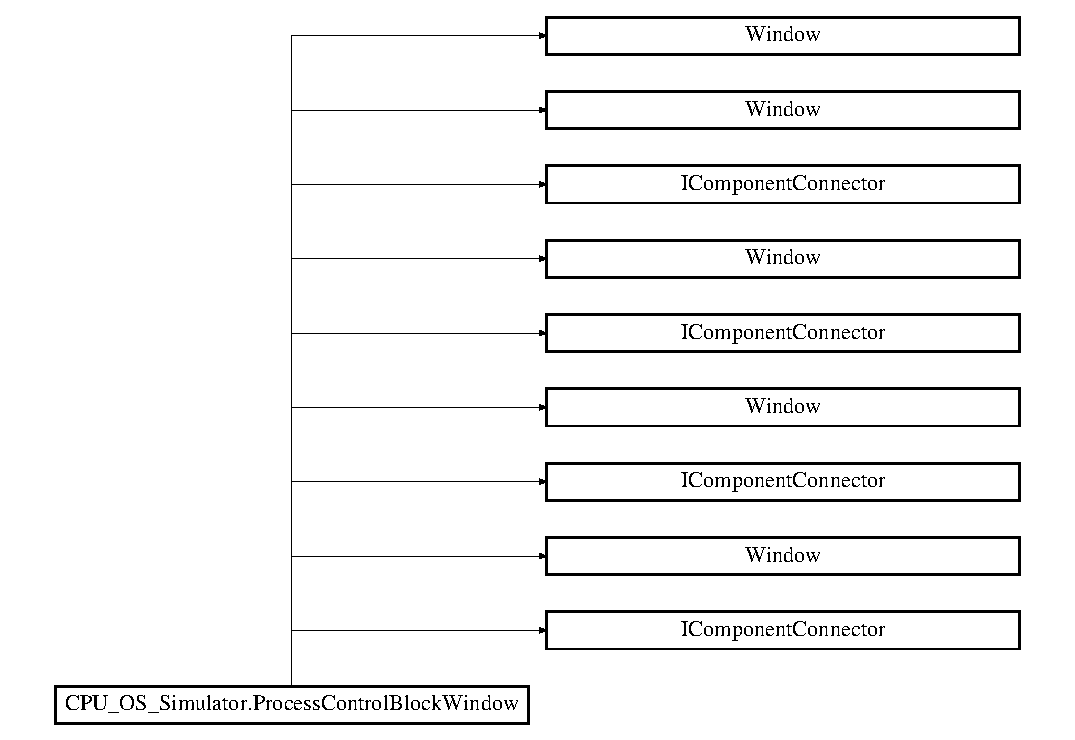
\includegraphics[height=0.759322cm]{class_c_p_u___o_s___simulator_1_1_process_control_block_window}
\end{center}
\end{figure}
\subsection*{Public Member Functions}
\begin{DoxyCompactItemize}
\item 
void \hyperlink{class_c_p_u___o_s___simulator_1_1_process_control_block_window_aac333572f064893264da84b178e76404}{Initialize\+Component} ()
\begin{DoxyCompactList}\small\item\em Initialize\+Component \end{DoxyCompactList}\item 
void \hyperlink{class_c_p_u___o_s___simulator_1_1_process_control_block_window_aac333572f064893264da84b178e76404}{Initialize\+Component} ()
\begin{DoxyCompactList}\small\item\em Initialize\+Component \end{DoxyCompactList}\item 
\hyperlink{class_c_p_u___o_s___simulator_1_1_process_control_block_window_afd4e9b7961d1f1c66aa037dba54d39a8}{Process\+Control\+Block\+Window} ()
\begin{DoxyCompactList}\small\item\em Default Constructor for process control block window \end{DoxyCompactList}\item 
\hyperlink{class_c_p_u___o_s___simulator_1_1_process_control_block_window_a4aed66a46265336cfe0cc5293c4e1164}{Process\+Control\+Block\+Window} (\hyperlink{class_c_p_u___o_s___simulator_1_1_main_window}{Main\+Window} \hyperlink{class_c_p_u___o_s___simulator_1_1_process_control_block_window_a928d5159874200e6ca0fad00913d65e5}{main\+\_\+\+Parent}, Linked\+List\+Node$<$ \hyperlink{class_c_p_u___o_s___simulator_1_1_operating___system_1_1_process_control_block}{Process\+Control\+Block} $>$ \hyperlink{class_c_p_u___o_s___simulator_1_1_process_control_block_window_a6019633d26586b0df1c4c2d6f008f6c9}{current\+Control\+Block})
\begin{DoxyCompactList}\small\item\em Constructor for process control block window when constructing from \hyperlink{class_c_p_u___o_s___simulator_1_1_main_window}{Main\+Window} \end{DoxyCompactList}\item 
\hyperlink{class_c_p_u___o_s___simulator_1_1_process_control_block_window_a79535cb1f910910d3cd9d896b7dd9fbc}{Process\+Control\+Block\+Window} (\hyperlink{class_c_p_u___o_s___simulator_1_1_operating_system_main_window}{Operating\+System\+Main\+Window} \hyperlink{class_c_p_u___o_s___simulator_1_1_process_control_block_window_acc4b72c5370a2bcda85b16e0801ce3d9}{os\+\_\+\+Parent}, Linked\+List\+Node$<$ \hyperlink{class_c_p_u___o_s___simulator_1_1_operating___system_1_1_process_control_block}{Process\+Control\+Block} $>$ \hyperlink{class_c_p_u___o_s___simulator_1_1_process_control_block_window_a6019633d26586b0df1c4c2d6f008f6c9}{current\+Control\+Block})
\begin{DoxyCompactList}\small\item\em Constructor for process control block window when constructing from \hyperlink{class_c_p_u___o_s___simulator_1_1_operating_system_main_window}{Operating\+System\+Main\+Window} \end{DoxyCompactList}\item 
\hyperlink{class_c_p_u___o_s___simulator_1_1_process_control_block_window_ac58527201e0de5a8dab1d90a45a18b20}{Process\+Control\+Block\+Window} (\hyperlink{class_c_p_u___o_s___simulator_1_1_process_list_window}{Process\+List\+Window} \hyperlink{class_c_p_u___o_s___simulator_1_1_process_control_block_window_a63c162f28cabcf42add4094087a10e68}{proc\+List\+\_\+\+Parent}, Linked\+List\+Node$<$ \hyperlink{class_c_p_u___o_s___simulator_1_1_operating___system_1_1_process_control_block}{Process\+Control\+Block} $>$ \hyperlink{class_c_p_u___o_s___simulator_1_1_process_control_block_window_a6019633d26586b0df1c4c2d6f008f6c9}{current\+Control\+Block})
\begin{DoxyCompactList}\small\item\em Constructor for process control block window when constructing from \hyperlink{class_c_p_u___o_s___simulator_1_1_process_list_window}{Process\+List\+Window} \end{DoxyCompactList}\end{DoxyCompactItemize}
\subsection*{Static Public Attributes}
\begin{DoxyCompactItemize}
\item 
static \hyperlink{class_c_p_u___o_s___simulator_1_1_process_control_block_window}{Process\+Control\+Block\+Window} \hyperlink{class_c_p_u___o_s___simulator_1_1_process_control_block_window_a88bea947f074426da083add43be70d48}{current\+Instance}
\begin{DoxyCompactList}\small\item\em This variable holds the current active instance of this window \end{DoxyCompactList}\end{DoxyCompactItemize}
\subsection*{Package Attributes}
\begin{DoxyCompactItemize}
\item 
\hyperlink{class_c_p_u___o_s___simulator_1_1_process_control_block_window}{C\+P\+U\+\_\+\+O\+S\+\_\+\+Simulator.\+Process\+Control\+Block\+Window} \hyperlink{class_c_p_u___o_s___simulator_1_1_process_control_block_window_a0f63765fb81d298b85ac605be61d06ca}{Process\+Control\+Block\+Window1}
\item 
System.\+Windows.\+Controls.\+Grid \hyperlink{class_c_p_u___o_s___simulator_1_1_process_control_block_window_a415616dfc791b692ef6f5736fd6aeae4}{Root\+Grid}
\item 
System.\+Windows.\+Controls.\+Text\+Block \hyperlink{class_c_p_u___o_s___simulator_1_1_process_control_block_window_af88f289c3eba55631106b52e491fa137}{txt\+\_\+\+P\+C\+B\+\_\+\+Info}
\item 
System.\+Windows.\+Controls.\+Button \hyperlink{class_c_p_u___o_s___simulator_1_1_process_control_block_window_a5cdb1a1e4c4351ab1c153309cd15969e}{btn\+\_\+\+Next\+P\+C\+B}
\item 
System.\+Windows.\+Controls.\+Button \hyperlink{class_c_p_u___o_s___simulator_1_1_process_control_block_window_af25ab71dad636514e08f3e8839b04727}{btn\+\_\+\+Previous\+\_\+\+P\+C\+B}
\item 
System.\+Windows.\+Controls.\+Button \hyperlink{class_c_p_u___o_s___simulator_1_1_process_control_block_window_abbfd6b98c1cf8a76437639b1b43859e3}{btn\+\_\+\+Close}
\end{DoxyCompactItemize}
\subsection*{Private Member Functions}
\begin{DoxyCompactItemize}
\item 
void System.\+Windows.\+Markup.\+I\+Component\+Connector. \hyperlink{class_c_p_u___o_s___simulator_1_1_process_control_block_window_aacad273b08eb9ad7e92c47eb5493008b}{Connect} (int connection\+Id, object target)
\item 
void System.\+Windows.\+Markup.\+I\+Component\+Connector. \hyperlink{class_c_p_u___o_s___simulator_1_1_process_control_block_window_aacad273b08eb9ad7e92c47eb5493008b}{Connect} (int connection\+Id, object target)
\item 
void \hyperlink{class_c_p_u___o_s___simulator_1_1_process_control_block_window_a18ccb30540f400cf07a224304c882c32}{Process\+Control\+Block\+Window1\+\_\+\+Loaded} (object sender, Routed\+Event\+Args e)
\item 
void \hyperlink{class_c_p_u___o_s___simulator_1_1_process_control_block_window_a9bb10e14d5a7e732ce6e5e5e0f66b678}{Update\+Text} ()
\begin{DoxyCompactList}\small\item\em This function updates the text block with information from the current P\+C\+B \end{DoxyCompactList}\item 
void \hyperlink{class_c_p_u___o_s___simulator_1_1_process_control_block_window_aa2c224432467974c6cf46c83a01735fa}{Set\+P\+C\+B\+Window\+Instance} ()
\begin{DoxyCompactList}\small\item\em This method sets the current instance of P\+C\+B window in the window bridge so it can be accessed by other modules \end{DoxyCompactList}\item 
void \hyperlink{class_c_p_u___o_s___simulator_1_1_process_control_block_window_a3b65012264c411aa3524bfb9b1e6bfe5}{btn\+\_\+\+Close\+\_\+\+Click} (object sender, Routed\+Event\+Args e)
\item 
void \hyperlink{class_c_p_u___o_s___simulator_1_1_process_control_block_window_a071ef7272a71ad3a0004c70bbcc4ad0a}{btn\+\_\+\+Previous\+\_\+\+P\+C\+B\+\_\+\+Click} (object sender, Routed\+Event\+Args e)
\item 
void \hyperlink{class_c_p_u___o_s___simulator_1_1_process_control_block_window_a752d089879e7d6aa80faef5ffc5f68cd}{btn\+\_\+\+Next\+P\+C\+B\+\_\+\+Click} (object sender, Routed\+Event\+Args e)
\item 
void \hyperlink{class_c_p_u___o_s___simulator_1_1_process_control_block_window_aa3a9ed3c96ca8fac5e6cbee7daa49a73}{Process\+Control\+Block\+Window1\+\_\+\+Closing} (object sender, System.\+Component\+Model.\+Cancel\+Event\+Args e)
\end{DoxyCompactItemize}
\subsection*{Private Attributes}
\begin{DoxyCompactItemize}
\item 
bool \hyperlink{class_c_p_u___o_s___simulator_1_1_process_control_block_window_aaac6850cf52e098a288515276eee98e0}{\+\_\+content\+Loaded}
\item 
\hyperlink{class_c_p_u___o_s___simulator_1_1_main_window}{Main\+Window} \hyperlink{class_c_p_u___o_s___simulator_1_1_process_control_block_window_a928d5159874200e6ca0fad00913d65e5}{main\+\_\+\+Parent}
\item 
\hyperlink{class_c_p_u___o_s___simulator_1_1_operating_system_main_window}{Operating\+System\+Main\+Window} \hyperlink{class_c_p_u___o_s___simulator_1_1_process_control_block_window_acc4b72c5370a2bcda85b16e0801ce3d9}{os\+\_\+\+Parent}
\item 
\hyperlink{class_c_p_u___o_s___simulator_1_1_process_list_window}{Process\+List\+Window} \hyperlink{class_c_p_u___o_s___simulator_1_1_process_control_block_window_a63c162f28cabcf42add4094087a10e68}{proc\+List\+\_\+\+Parent}
\item 
Linked\+List\+Node$<$ \hyperlink{class_c_p_u___o_s___simulator_1_1_operating___system_1_1_process_control_block}{Process\+Control\+Block} $>$ \hyperlink{class_c_p_u___o_s___simulator_1_1_process_control_block_window_a6019633d26586b0df1c4c2d6f008f6c9}{current\+Control\+Block}
\item 
Linked\+List$<$ \hyperlink{class_c_p_u___o_s___simulator_1_1_operating___system_1_1_process_control_block}{Process\+Control\+Block} $>$ \hyperlink{class_c_p_u___o_s___simulator_1_1_process_control_block_window_a1cc81320d60155abc2d1fd7370aeeb9a}{current\+Control\+Blocks}
\end{DoxyCompactItemize}


\subsection{Detailed Description}
\hyperlink{class_c_p_u___o_s___simulator_1_1_process_control_block_window}{Process\+Control\+Block\+Window} 

Interaction logic for Process\+Control\+Block\+Window.\+xaml 

Definition at line 41 of file Process\+Control\+Block\+Window.\+g.\+cs.



\subsection{Constructor \& Destructor Documentation}
\hypertarget{class_c_p_u___o_s___simulator_1_1_process_control_block_window_afd4e9b7961d1f1c66aa037dba54d39a8}{}\index{C\+P\+U\+\_\+\+O\+S\+\_\+\+Simulator\+::\+Process\+Control\+Block\+Window@{C\+P\+U\+\_\+\+O\+S\+\_\+\+Simulator\+::\+Process\+Control\+Block\+Window}!Process\+Control\+Block\+Window@{Process\+Control\+Block\+Window}}
\index{Process\+Control\+Block\+Window@{Process\+Control\+Block\+Window}!C\+P\+U\+\_\+\+O\+S\+\_\+\+Simulator\+::\+Process\+Control\+Block\+Window@{C\+P\+U\+\_\+\+O\+S\+\_\+\+Simulator\+::\+Process\+Control\+Block\+Window}}
\subsubsection[{Process\+Control\+Block\+Window()}]{\setlength{\rightskip}{0pt plus 5cm}C\+P\+U\+\_\+\+O\+S\+\_\+\+Simulator.\+Process\+Control\+Block\+Window.\+Process\+Control\+Block\+Window (
\begin{DoxyParamCaption}
{}
\end{DoxyParamCaption}
)}\label{class_c_p_u___o_s___simulator_1_1_process_control_block_window_afd4e9b7961d1f1c66aa037dba54d39a8}


Default Constructor for process control block window 



Definition at line 28 of file Process\+Control\+Block\+Window.\+xaml.\+cs.

\hypertarget{class_c_p_u___o_s___simulator_1_1_process_control_block_window_a4aed66a46265336cfe0cc5293c4e1164}{}\index{C\+P\+U\+\_\+\+O\+S\+\_\+\+Simulator\+::\+Process\+Control\+Block\+Window@{C\+P\+U\+\_\+\+O\+S\+\_\+\+Simulator\+::\+Process\+Control\+Block\+Window}!Process\+Control\+Block\+Window@{Process\+Control\+Block\+Window}}
\index{Process\+Control\+Block\+Window@{Process\+Control\+Block\+Window}!C\+P\+U\+\_\+\+O\+S\+\_\+\+Simulator\+::\+Process\+Control\+Block\+Window@{C\+P\+U\+\_\+\+O\+S\+\_\+\+Simulator\+::\+Process\+Control\+Block\+Window}}
\subsubsection[{Process\+Control\+Block\+Window(\+Main\+Window main\+\_\+\+Parent, Linked\+List\+Node$<$ Process\+Control\+Block $>$ current\+Control\+Block)}]{\setlength{\rightskip}{0pt plus 5cm}C\+P\+U\+\_\+\+O\+S\+\_\+\+Simulator.\+Process\+Control\+Block\+Window.\+Process\+Control\+Block\+Window (
\begin{DoxyParamCaption}
\item[{{\bf Main\+Window}}]{main\+\_\+\+Parent, }
\item[{Linked\+List\+Node$<$ {\bf Process\+Control\+Block} $>$}]{current\+Control\+Block}
\end{DoxyParamCaption}
)}\label{class_c_p_u___o_s___simulator_1_1_process_control_block_window_a4aed66a46265336cfe0cc5293c4e1164}


Constructor for process control block window when constructing from \hyperlink{class_c_p_u___o_s___simulator_1_1_main_window}{Main\+Window} 


\begin{DoxyParams}{Parameters}
{\em main\+\_\+\+Parent} & the window that is creating this window\\
\hline
{\em current\+Control\+Block} & the control block to be loaded\\
\hline
\end{DoxyParams}


Definition at line 39 of file Process\+Control\+Block\+Window.\+xaml.\+cs.

\hypertarget{class_c_p_u___o_s___simulator_1_1_process_control_block_window_a79535cb1f910910d3cd9d896b7dd9fbc}{}\index{C\+P\+U\+\_\+\+O\+S\+\_\+\+Simulator\+::\+Process\+Control\+Block\+Window@{C\+P\+U\+\_\+\+O\+S\+\_\+\+Simulator\+::\+Process\+Control\+Block\+Window}!Process\+Control\+Block\+Window@{Process\+Control\+Block\+Window}}
\index{Process\+Control\+Block\+Window@{Process\+Control\+Block\+Window}!C\+P\+U\+\_\+\+O\+S\+\_\+\+Simulator\+::\+Process\+Control\+Block\+Window@{C\+P\+U\+\_\+\+O\+S\+\_\+\+Simulator\+::\+Process\+Control\+Block\+Window}}
\subsubsection[{Process\+Control\+Block\+Window(\+Operating\+System\+Main\+Window os\+\_\+\+Parent, Linked\+List\+Node$<$ Process\+Control\+Block $>$ current\+Control\+Block)}]{\setlength{\rightskip}{0pt plus 5cm}C\+P\+U\+\_\+\+O\+S\+\_\+\+Simulator.\+Process\+Control\+Block\+Window.\+Process\+Control\+Block\+Window (
\begin{DoxyParamCaption}
\item[{{\bf Operating\+System\+Main\+Window}}]{os\+\_\+\+Parent, }
\item[{Linked\+List\+Node$<$ {\bf Process\+Control\+Block} $>$}]{current\+Control\+Block}
\end{DoxyParamCaption}
)}\label{class_c_p_u___o_s___simulator_1_1_process_control_block_window_a79535cb1f910910d3cd9d896b7dd9fbc}


Constructor for process control block window when constructing from \hyperlink{class_c_p_u___o_s___simulator_1_1_operating_system_main_window}{Operating\+System\+Main\+Window} 


\begin{DoxyParams}{Parameters}
{\em os\+\_\+\+Parent} & the window that is creating this window\\
\hline
{\em current\+Control\+Block} & the control block to be loaded\\
\hline
\end{DoxyParams}


Definition at line 59 of file Process\+Control\+Block\+Window.\+xaml.\+cs.

\hypertarget{class_c_p_u___o_s___simulator_1_1_process_control_block_window_ac58527201e0de5a8dab1d90a45a18b20}{}\index{C\+P\+U\+\_\+\+O\+S\+\_\+\+Simulator\+::\+Process\+Control\+Block\+Window@{C\+P\+U\+\_\+\+O\+S\+\_\+\+Simulator\+::\+Process\+Control\+Block\+Window}!Process\+Control\+Block\+Window@{Process\+Control\+Block\+Window}}
\index{Process\+Control\+Block\+Window@{Process\+Control\+Block\+Window}!C\+P\+U\+\_\+\+O\+S\+\_\+\+Simulator\+::\+Process\+Control\+Block\+Window@{C\+P\+U\+\_\+\+O\+S\+\_\+\+Simulator\+::\+Process\+Control\+Block\+Window}}
\subsubsection[{Process\+Control\+Block\+Window(\+Process\+List\+Window proc\+List\+\_\+\+Parent, Linked\+List\+Node$<$ Process\+Control\+Block $>$ current\+Control\+Block)}]{\setlength{\rightskip}{0pt plus 5cm}C\+P\+U\+\_\+\+O\+S\+\_\+\+Simulator.\+Process\+Control\+Block\+Window.\+Process\+Control\+Block\+Window (
\begin{DoxyParamCaption}
\item[{{\bf Process\+List\+Window}}]{proc\+List\+\_\+\+Parent, }
\item[{Linked\+List\+Node$<$ {\bf Process\+Control\+Block} $>$}]{current\+Control\+Block}
\end{DoxyParamCaption}
)}\label{class_c_p_u___o_s___simulator_1_1_process_control_block_window_ac58527201e0de5a8dab1d90a45a18b20}


Constructor for process control block window when constructing from \hyperlink{class_c_p_u___o_s___simulator_1_1_process_list_window}{Process\+List\+Window} 


\begin{DoxyParams}{Parameters}
{\em proc\+List\+\_\+\+Parent} & the window that is creating this window\\
\hline
{\em current\+Control\+Block} & the control block to be loaded\\
\hline
\end{DoxyParams}


Definition at line 79 of file Process\+Control\+Block\+Window.\+xaml.\+cs.



\subsection{Member Function Documentation}
\hypertarget{class_c_p_u___o_s___simulator_1_1_process_control_block_window_a3b65012264c411aa3524bfb9b1e6bfe5}{}\index{C\+P\+U\+\_\+\+O\+S\+\_\+\+Simulator\+::\+Process\+Control\+Block\+Window@{C\+P\+U\+\_\+\+O\+S\+\_\+\+Simulator\+::\+Process\+Control\+Block\+Window}!btn\+\_\+\+Close\+\_\+\+Click@{btn\+\_\+\+Close\+\_\+\+Click}}
\index{btn\+\_\+\+Close\+\_\+\+Click@{btn\+\_\+\+Close\+\_\+\+Click}!C\+P\+U\+\_\+\+O\+S\+\_\+\+Simulator\+::\+Process\+Control\+Block\+Window@{C\+P\+U\+\_\+\+O\+S\+\_\+\+Simulator\+::\+Process\+Control\+Block\+Window}}
\subsubsection[{btn\+\_\+\+Close\+\_\+\+Click(object sender, Routed\+Event\+Args e)}]{\setlength{\rightskip}{0pt plus 5cm}void C\+P\+U\+\_\+\+O\+S\+\_\+\+Simulator.\+Process\+Control\+Block\+Window.\+btn\+\_\+\+Close\+\_\+\+Click (
\begin{DoxyParamCaption}
\item[{object}]{sender, }
\item[{Routed\+Event\+Args}]{e}
\end{DoxyParamCaption}
)\hspace{0.3cm}{\ttfamily [private]}}\label{class_c_p_u___o_s___simulator_1_1_process_control_block_window_a3b65012264c411aa3524bfb9b1e6bfe5}


Definition at line 133 of file Process\+Control\+Block\+Window.\+xaml.\+cs.

\hypertarget{class_c_p_u___o_s___simulator_1_1_process_control_block_window_a752d089879e7d6aa80faef5ffc5f68cd}{}\index{C\+P\+U\+\_\+\+O\+S\+\_\+\+Simulator\+::\+Process\+Control\+Block\+Window@{C\+P\+U\+\_\+\+O\+S\+\_\+\+Simulator\+::\+Process\+Control\+Block\+Window}!btn\+\_\+\+Next\+P\+C\+B\+\_\+\+Click@{btn\+\_\+\+Next\+P\+C\+B\+\_\+\+Click}}
\index{btn\+\_\+\+Next\+P\+C\+B\+\_\+\+Click@{btn\+\_\+\+Next\+P\+C\+B\+\_\+\+Click}!C\+P\+U\+\_\+\+O\+S\+\_\+\+Simulator\+::\+Process\+Control\+Block\+Window@{C\+P\+U\+\_\+\+O\+S\+\_\+\+Simulator\+::\+Process\+Control\+Block\+Window}}
\subsubsection[{btn\+\_\+\+Next\+P\+C\+B\+\_\+\+Click(object sender, Routed\+Event\+Args e)}]{\setlength{\rightskip}{0pt plus 5cm}void C\+P\+U\+\_\+\+O\+S\+\_\+\+Simulator.\+Process\+Control\+Block\+Window.\+btn\+\_\+\+Next\+P\+C\+B\+\_\+\+Click (
\begin{DoxyParamCaption}
\item[{object}]{sender, }
\item[{Routed\+Event\+Args}]{e}
\end{DoxyParamCaption}
)\hspace{0.3cm}{\ttfamily [private]}}\label{class_c_p_u___o_s___simulator_1_1_process_control_block_window_a752d089879e7d6aa80faef5ffc5f68cd}


Definition at line 147 of file Process\+Control\+Block\+Window.\+xaml.\+cs.

\hypertarget{class_c_p_u___o_s___simulator_1_1_process_control_block_window_a071ef7272a71ad3a0004c70bbcc4ad0a}{}\index{C\+P\+U\+\_\+\+O\+S\+\_\+\+Simulator\+::\+Process\+Control\+Block\+Window@{C\+P\+U\+\_\+\+O\+S\+\_\+\+Simulator\+::\+Process\+Control\+Block\+Window}!btn\+\_\+\+Previous\+\_\+\+P\+C\+B\+\_\+\+Click@{btn\+\_\+\+Previous\+\_\+\+P\+C\+B\+\_\+\+Click}}
\index{btn\+\_\+\+Previous\+\_\+\+P\+C\+B\+\_\+\+Click@{btn\+\_\+\+Previous\+\_\+\+P\+C\+B\+\_\+\+Click}!C\+P\+U\+\_\+\+O\+S\+\_\+\+Simulator\+::\+Process\+Control\+Block\+Window@{C\+P\+U\+\_\+\+O\+S\+\_\+\+Simulator\+::\+Process\+Control\+Block\+Window}}
\subsubsection[{btn\+\_\+\+Previous\+\_\+\+P\+C\+B\+\_\+\+Click(object sender, Routed\+Event\+Args e)}]{\setlength{\rightskip}{0pt plus 5cm}void C\+P\+U\+\_\+\+O\+S\+\_\+\+Simulator.\+Process\+Control\+Block\+Window.\+btn\+\_\+\+Previous\+\_\+\+P\+C\+B\+\_\+\+Click (
\begin{DoxyParamCaption}
\item[{object}]{sender, }
\item[{Routed\+Event\+Args}]{e}
\end{DoxyParamCaption}
)\hspace{0.3cm}{\ttfamily [private]}}\label{class_c_p_u___o_s___simulator_1_1_process_control_block_window_a071ef7272a71ad3a0004c70bbcc4ad0a}


Definition at line 138 of file Process\+Control\+Block\+Window.\+xaml.\+cs.

\hypertarget{class_c_p_u___o_s___simulator_1_1_process_control_block_window_aacad273b08eb9ad7e92c47eb5493008b}{}\index{C\+P\+U\+\_\+\+O\+S\+\_\+\+Simulator\+::\+Process\+Control\+Block\+Window@{C\+P\+U\+\_\+\+O\+S\+\_\+\+Simulator\+::\+Process\+Control\+Block\+Window}!Connect@{Connect}}
\index{Connect@{Connect}!C\+P\+U\+\_\+\+O\+S\+\_\+\+Simulator\+::\+Process\+Control\+Block\+Window@{C\+P\+U\+\_\+\+O\+S\+\_\+\+Simulator\+::\+Process\+Control\+Block\+Window}}
\subsubsection[{Connect(int connection\+Id, object target)}]{\setlength{\rightskip}{0pt plus 5cm}void System.\+Windows.\+Markup.\+I\+Component\+Connector. C\+P\+U\+\_\+\+O\+S\+\_\+\+Simulator.\+Process\+Control\+Block\+Window.\+Connect (
\begin{DoxyParamCaption}
\item[{int}]{connection\+Id, }
\item[{object}]{target}
\end{DoxyParamCaption}
)\hspace{0.3cm}{\ttfamily [private]}}\label{class_c_p_u___o_s___simulator_1_1_process_control_block_window_aacad273b08eb9ad7e92c47eb5493008b}


Definition at line 118 of file Process\+Control\+Block\+Window.\+g.\+cs.

\hypertarget{class_c_p_u___o_s___simulator_1_1_process_control_block_window_aacad273b08eb9ad7e92c47eb5493008b}{}\index{C\+P\+U\+\_\+\+O\+S\+\_\+\+Simulator\+::\+Process\+Control\+Block\+Window@{C\+P\+U\+\_\+\+O\+S\+\_\+\+Simulator\+::\+Process\+Control\+Block\+Window}!Connect@{Connect}}
\index{Connect@{Connect}!C\+P\+U\+\_\+\+O\+S\+\_\+\+Simulator\+::\+Process\+Control\+Block\+Window@{C\+P\+U\+\_\+\+O\+S\+\_\+\+Simulator\+::\+Process\+Control\+Block\+Window}}
\subsubsection[{Connect(int connection\+Id, object target)}]{\setlength{\rightskip}{0pt plus 5cm}void System.\+Windows.\+Markup.\+I\+Component\+Connector. C\+P\+U\+\_\+\+O\+S\+\_\+\+Simulator.\+Process\+Control\+Block\+Window.\+Connect (
\begin{DoxyParamCaption}
\item[{int}]{connection\+Id, }
\item[{object}]{target}
\end{DoxyParamCaption}
)\hspace{0.3cm}{\ttfamily [private]}}\label{class_c_p_u___o_s___simulator_1_1_process_control_block_window_aacad273b08eb9ad7e92c47eb5493008b}


Definition at line 118 of file Process\+Control\+Block\+Window.\+g.\+i.\+cs.

\hypertarget{class_c_p_u___o_s___simulator_1_1_process_control_block_window_aac333572f064893264da84b178e76404}{}\index{C\+P\+U\+\_\+\+O\+S\+\_\+\+Simulator\+::\+Process\+Control\+Block\+Window@{C\+P\+U\+\_\+\+O\+S\+\_\+\+Simulator\+::\+Process\+Control\+Block\+Window}!Initialize\+Component@{Initialize\+Component}}
\index{Initialize\+Component@{Initialize\+Component}!C\+P\+U\+\_\+\+O\+S\+\_\+\+Simulator\+::\+Process\+Control\+Block\+Window@{C\+P\+U\+\_\+\+O\+S\+\_\+\+Simulator\+::\+Process\+Control\+Block\+Window}}
\subsubsection[{Initialize\+Component()}]{\setlength{\rightskip}{0pt plus 5cm}void C\+P\+U\+\_\+\+O\+S\+\_\+\+Simulator.\+Process\+Control\+Block\+Window.\+Initialize\+Component (
\begin{DoxyParamCaption}
{}
\end{DoxyParamCaption}
)}\label{class_c_p_u___o_s___simulator_1_1_process_control_block_window_aac333572f064893264da84b178e76404}


Initialize\+Component 



Definition at line 98 of file Process\+Control\+Block\+Window.\+g.\+cs.

\hypertarget{class_c_p_u___o_s___simulator_1_1_process_control_block_window_aac333572f064893264da84b178e76404}{}\index{C\+P\+U\+\_\+\+O\+S\+\_\+\+Simulator\+::\+Process\+Control\+Block\+Window@{C\+P\+U\+\_\+\+O\+S\+\_\+\+Simulator\+::\+Process\+Control\+Block\+Window}!Initialize\+Component@{Initialize\+Component}}
\index{Initialize\+Component@{Initialize\+Component}!C\+P\+U\+\_\+\+O\+S\+\_\+\+Simulator\+::\+Process\+Control\+Block\+Window@{C\+P\+U\+\_\+\+O\+S\+\_\+\+Simulator\+::\+Process\+Control\+Block\+Window}}
\subsubsection[{Initialize\+Component()}]{\setlength{\rightskip}{0pt plus 5cm}void C\+P\+U\+\_\+\+O\+S\+\_\+\+Simulator.\+Process\+Control\+Block\+Window.\+Initialize\+Component (
\begin{DoxyParamCaption}
{}
\end{DoxyParamCaption}
)}\label{class_c_p_u___o_s___simulator_1_1_process_control_block_window_aac333572f064893264da84b178e76404}


Initialize\+Component 



Definition at line 98 of file Process\+Control\+Block\+Window.\+g.\+i.\+cs.

\hypertarget{class_c_p_u___o_s___simulator_1_1_process_control_block_window_aa3a9ed3c96ca8fac5e6cbee7daa49a73}{}\index{C\+P\+U\+\_\+\+O\+S\+\_\+\+Simulator\+::\+Process\+Control\+Block\+Window@{C\+P\+U\+\_\+\+O\+S\+\_\+\+Simulator\+::\+Process\+Control\+Block\+Window}!Process\+Control\+Block\+Window1\+\_\+\+Closing@{Process\+Control\+Block\+Window1\+\_\+\+Closing}}
\index{Process\+Control\+Block\+Window1\+\_\+\+Closing@{Process\+Control\+Block\+Window1\+\_\+\+Closing}!C\+P\+U\+\_\+\+O\+S\+\_\+\+Simulator\+::\+Process\+Control\+Block\+Window@{C\+P\+U\+\_\+\+O\+S\+\_\+\+Simulator\+::\+Process\+Control\+Block\+Window}}
\subsubsection[{Process\+Control\+Block\+Window1\+\_\+\+Closing(object sender, System.\+Component\+Model.\+Cancel\+Event\+Args e)}]{\setlength{\rightskip}{0pt plus 5cm}void C\+P\+U\+\_\+\+O\+S\+\_\+\+Simulator.\+Process\+Control\+Block\+Window.\+Process\+Control\+Block\+Window1\+\_\+\+Closing (
\begin{DoxyParamCaption}
\item[{object}]{sender, }
\item[{System.\+Component\+Model.\+Cancel\+Event\+Args}]{e}
\end{DoxyParamCaption}
)\hspace{0.3cm}{\ttfamily [private]}}\label{class_c_p_u___o_s___simulator_1_1_process_control_block_window_aa3a9ed3c96ca8fac5e6cbee7daa49a73}


Definition at line 156 of file Process\+Control\+Block\+Window.\+xaml.\+cs.

\hypertarget{class_c_p_u___o_s___simulator_1_1_process_control_block_window_a18ccb30540f400cf07a224304c882c32}{}\index{C\+P\+U\+\_\+\+O\+S\+\_\+\+Simulator\+::\+Process\+Control\+Block\+Window@{C\+P\+U\+\_\+\+O\+S\+\_\+\+Simulator\+::\+Process\+Control\+Block\+Window}!Process\+Control\+Block\+Window1\+\_\+\+Loaded@{Process\+Control\+Block\+Window1\+\_\+\+Loaded}}
\index{Process\+Control\+Block\+Window1\+\_\+\+Loaded@{Process\+Control\+Block\+Window1\+\_\+\+Loaded}!C\+P\+U\+\_\+\+O\+S\+\_\+\+Simulator\+::\+Process\+Control\+Block\+Window@{C\+P\+U\+\_\+\+O\+S\+\_\+\+Simulator\+::\+Process\+Control\+Block\+Window}}
\subsubsection[{Process\+Control\+Block\+Window1\+\_\+\+Loaded(object sender, Routed\+Event\+Args e)}]{\setlength{\rightskip}{0pt plus 5cm}void C\+P\+U\+\_\+\+O\+S\+\_\+\+Simulator.\+Process\+Control\+Block\+Window.\+Process\+Control\+Block\+Window1\+\_\+\+Loaded (
\begin{DoxyParamCaption}
\item[{object}]{sender, }
\item[{Routed\+Event\+Args}]{e}
\end{DoxyParamCaption}
)\hspace{0.3cm}{\ttfamily [private]}}\label{class_c_p_u___o_s___simulator_1_1_process_control_block_window_a18ccb30540f400cf07a224304c882c32}


Definition at line 96 of file Process\+Control\+Block\+Window.\+xaml.\+cs.

\hypertarget{class_c_p_u___o_s___simulator_1_1_process_control_block_window_aa2c224432467974c6cf46c83a01735fa}{}\index{C\+P\+U\+\_\+\+O\+S\+\_\+\+Simulator\+::\+Process\+Control\+Block\+Window@{C\+P\+U\+\_\+\+O\+S\+\_\+\+Simulator\+::\+Process\+Control\+Block\+Window}!Set\+P\+C\+B\+Window\+Instance@{Set\+P\+C\+B\+Window\+Instance}}
\index{Set\+P\+C\+B\+Window\+Instance@{Set\+P\+C\+B\+Window\+Instance}!C\+P\+U\+\_\+\+O\+S\+\_\+\+Simulator\+::\+Process\+Control\+Block\+Window@{C\+P\+U\+\_\+\+O\+S\+\_\+\+Simulator\+::\+Process\+Control\+Block\+Window}}
\subsubsection[{Set\+P\+C\+B\+Window\+Instance()}]{\setlength{\rightskip}{0pt plus 5cm}void C\+P\+U\+\_\+\+O\+S\+\_\+\+Simulator.\+Process\+Control\+Block\+Window.\+Set\+P\+C\+B\+Window\+Instance (
\begin{DoxyParamCaption}
{}
\end{DoxyParamCaption}
)\hspace{0.3cm}{\ttfamily [private]}}\label{class_c_p_u___o_s___simulator_1_1_process_control_block_window_aa2c224432467974c6cf46c83a01735fa}


This method sets the current instance of P\+C\+B window in the window bridge so it can be accessed by other modules 



Definition at line 125 of file Process\+Control\+Block\+Window.\+xaml.\+cs.

\hypertarget{class_c_p_u___o_s___simulator_1_1_process_control_block_window_a9bb10e14d5a7e732ce6e5e5e0f66b678}{}\index{C\+P\+U\+\_\+\+O\+S\+\_\+\+Simulator\+::\+Process\+Control\+Block\+Window@{C\+P\+U\+\_\+\+O\+S\+\_\+\+Simulator\+::\+Process\+Control\+Block\+Window}!Update\+Text@{Update\+Text}}
\index{Update\+Text@{Update\+Text}!C\+P\+U\+\_\+\+O\+S\+\_\+\+Simulator\+::\+Process\+Control\+Block\+Window@{C\+P\+U\+\_\+\+O\+S\+\_\+\+Simulator\+::\+Process\+Control\+Block\+Window}}
\subsubsection[{Update\+Text()}]{\setlength{\rightskip}{0pt plus 5cm}void C\+P\+U\+\_\+\+O\+S\+\_\+\+Simulator.\+Process\+Control\+Block\+Window.\+Update\+Text (
\begin{DoxyParamCaption}
{}
\end{DoxyParamCaption}
)\hspace{0.3cm}{\ttfamily [private]}}\label{class_c_p_u___o_s___simulator_1_1_process_control_block_window_a9bb10e14d5a7e732ce6e5e5e0f66b678}


This function updates the text block with information from the current P\+C\+B 



Definition at line 109 of file Process\+Control\+Block\+Window.\+xaml.\+cs.



\subsection{Member Data Documentation}
\hypertarget{class_c_p_u___o_s___simulator_1_1_process_control_block_window_aaac6850cf52e098a288515276eee98e0}{}\index{C\+P\+U\+\_\+\+O\+S\+\_\+\+Simulator\+::\+Process\+Control\+Block\+Window@{C\+P\+U\+\_\+\+O\+S\+\_\+\+Simulator\+::\+Process\+Control\+Block\+Window}!\+\_\+content\+Loaded@{\+\_\+content\+Loaded}}
\index{\+\_\+content\+Loaded@{\+\_\+content\+Loaded}!C\+P\+U\+\_\+\+O\+S\+\_\+\+Simulator\+::\+Process\+Control\+Block\+Window@{C\+P\+U\+\_\+\+O\+S\+\_\+\+Simulator\+::\+Process\+Control\+Block\+Window}}
\subsubsection[{\+\_\+content\+Loaded}]{\setlength{\rightskip}{0pt plus 5cm}bool C\+P\+U\+\_\+\+O\+S\+\_\+\+Simulator.\+Process\+Control\+Block\+Window.\+\_\+content\+Loaded\hspace{0.3cm}{\ttfamily [private]}}\label{class_c_p_u___o_s___simulator_1_1_process_control_block_window_aaac6850cf52e098a288515276eee98e0}


Definition at line 91 of file Process\+Control\+Block\+Window.\+g.\+cs.

\hypertarget{class_c_p_u___o_s___simulator_1_1_process_control_block_window_abbfd6b98c1cf8a76437639b1b43859e3}{}\index{C\+P\+U\+\_\+\+O\+S\+\_\+\+Simulator\+::\+Process\+Control\+Block\+Window@{C\+P\+U\+\_\+\+O\+S\+\_\+\+Simulator\+::\+Process\+Control\+Block\+Window}!btn\+\_\+\+Close@{btn\+\_\+\+Close}}
\index{btn\+\_\+\+Close@{btn\+\_\+\+Close}!C\+P\+U\+\_\+\+O\+S\+\_\+\+Simulator\+::\+Process\+Control\+Block\+Window@{C\+P\+U\+\_\+\+O\+S\+\_\+\+Simulator\+::\+Process\+Control\+Block\+Window}}
\subsubsection[{btn\+\_\+\+Close}]{\setlength{\rightskip}{0pt plus 5cm}System Windows Controls Button C\+P\+U\+\_\+\+O\+S\+\_\+\+Simulator.\+Process\+Control\+Block\+Window.\+btn\+\_\+\+Close\hspace{0.3cm}{\ttfamily [package]}}\label{class_c_p_u___o_s___simulator_1_1_process_control_block_window_abbfd6b98c1cf8a76437639b1b43859e3}


Definition at line 86 of file Process\+Control\+Block\+Window.\+g.\+cs.

\hypertarget{class_c_p_u___o_s___simulator_1_1_process_control_block_window_a5cdb1a1e4c4351ab1c153309cd15969e}{}\index{C\+P\+U\+\_\+\+O\+S\+\_\+\+Simulator\+::\+Process\+Control\+Block\+Window@{C\+P\+U\+\_\+\+O\+S\+\_\+\+Simulator\+::\+Process\+Control\+Block\+Window}!btn\+\_\+\+Next\+P\+C\+B@{btn\+\_\+\+Next\+P\+C\+B}}
\index{btn\+\_\+\+Next\+P\+C\+B@{btn\+\_\+\+Next\+P\+C\+B}!C\+P\+U\+\_\+\+O\+S\+\_\+\+Simulator\+::\+Process\+Control\+Block\+Window@{C\+P\+U\+\_\+\+O\+S\+\_\+\+Simulator\+::\+Process\+Control\+Block\+Window}}
\subsubsection[{btn\+\_\+\+Next\+P\+C\+B}]{\setlength{\rightskip}{0pt plus 5cm}System Windows Controls Button C\+P\+U\+\_\+\+O\+S\+\_\+\+Simulator.\+Process\+Control\+Block\+Window.\+btn\+\_\+\+Next\+P\+C\+B\hspace{0.3cm}{\ttfamily [package]}}\label{class_c_p_u___o_s___simulator_1_1_process_control_block_window_a5cdb1a1e4c4351ab1c153309cd15969e}


Definition at line 70 of file Process\+Control\+Block\+Window.\+g.\+cs.

\hypertarget{class_c_p_u___o_s___simulator_1_1_process_control_block_window_af25ab71dad636514e08f3e8839b04727}{}\index{C\+P\+U\+\_\+\+O\+S\+\_\+\+Simulator\+::\+Process\+Control\+Block\+Window@{C\+P\+U\+\_\+\+O\+S\+\_\+\+Simulator\+::\+Process\+Control\+Block\+Window}!btn\+\_\+\+Previous\+\_\+\+P\+C\+B@{btn\+\_\+\+Previous\+\_\+\+P\+C\+B}}
\index{btn\+\_\+\+Previous\+\_\+\+P\+C\+B@{btn\+\_\+\+Previous\+\_\+\+P\+C\+B}!C\+P\+U\+\_\+\+O\+S\+\_\+\+Simulator\+::\+Process\+Control\+Block\+Window@{C\+P\+U\+\_\+\+O\+S\+\_\+\+Simulator\+::\+Process\+Control\+Block\+Window}}
\subsubsection[{btn\+\_\+\+Previous\+\_\+\+P\+C\+B}]{\setlength{\rightskip}{0pt plus 5cm}System Windows Controls Button C\+P\+U\+\_\+\+O\+S\+\_\+\+Simulator.\+Process\+Control\+Block\+Window.\+btn\+\_\+\+Previous\+\_\+\+P\+C\+B\hspace{0.3cm}{\ttfamily [package]}}\label{class_c_p_u___o_s___simulator_1_1_process_control_block_window_af25ab71dad636514e08f3e8839b04727}


Definition at line 78 of file Process\+Control\+Block\+Window.\+g.\+cs.

\hypertarget{class_c_p_u___o_s___simulator_1_1_process_control_block_window_a6019633d26586b0df1c4c2d6f008f6c9}{}\index{C\+P\+U\+\_\+\+O\+S\+\_\+\+Simulator\+::\+Process\+Control\+Block\+Window@{C\+P\+U\+\_\+\+O\+S\+\_\+\+Simulator\+::\+Process\+Control\+Block\+Window}!current\+Control\+Block@{current\+Control\+Block}}
\index{current\+Control\+Block@{current\+Control\+Block}!C\+P\+U\+\_\+\+O\+S\+\_\+\+Simulator\+::\+Process\+Control\+Block\+Window@{C\+P\+U\+\_\+\+O\+S\+\_\+\+Simulator\+::\+Process\+Control\+Block\+Window}}
\subsubsection[{current\+Control\+Block}]{\setlength{\rightskip}{0pt plus 5cm}Linked\+List\+Node$<${\bf Process\+Control\+Block}$>$ C\+P\+U\+\_\+\+O\+S\+\_\+\+Simulator.\+Process\+Control\+Block\+Window.\+current\+Control\+Block\hspace{0.3cm}{\ttfamily [private]}}\label{class_c_p_u___o_s___simulator_1_1_process_control_block_window_a6019633d26586b0df1c4c2d6f008f6c9}


Definition at line 18 of file Process\+Control\+Block\+Window.\+xaml.\+cs.

\hypertarget{class_c_p_u___o_s___simulator_1_1_process_control_block_window_a1cc81320d60155abc2d1fd7370aeeb9a}{}\index{C\+P\+U\+\_\+\+O\+S\+\_\+\+Simulator\+::\+Process\+Control\+Block\+Window@{C\+P\+U\+\_\+\+O\+S\+\_\+\+Simulator\+::\+Process\+Control\+Block\+Window}!current\+Control\+Blocks@{current\+Control\+Blocks}}
\index{current\+Control\+Blocks@{current\+Control\+Blocks}!C\+P\+U\+\_\+\+O\+S\+\_\+\+Simulator\+::\+Process\+Control\+Block\+Window@{C\+P\+U\+\_\+\+O\+S\+\_\+\+Simulator\+::\+Process\+Control\+Block\+Window}}
\subsubsection[{current\+Control\+Blocks}]{\setlength{\rightskip}{0pt plus 5cm}Linked\+List$<${\bf Process\+Control\+Block}$>$ C\+P\+U\+\_\+\+O\+S\+\_\+\+Simulator.\+Process\+Control\+Block\+Window.\+current\+Control\+Blocks\hspace{0.3cm}{\ttfamily [private]}}\label{class_c_p_u___o_s___simulator_1_1_process_control_block_window_a1cc81320d60155abc2d1fd7370aeeb9a}


Definition at line 19 of file Process\+Control\+Block\+Window.\+xaml.\+cs.

\hypertarget{class_c_p_u___o_s___simulator_1_1_process_control_block_window_a88bea947f074426da083add43be70d48}{}\index{C\+P\+U\+\_\+\+O\+S\+\_\+\+Simulator\+::\+Process\+Control\+Block\+Window@{C\+P\+U\+\_\+\+O\+S\+\_\+\+Simulator\+::\+Process\+Control\+Block\+Window}!current\+Instance@{current\+Instance}}
\index{current\+Instance@{current\+Instance}!C\+P\+U\+\_\+\+O\+S\+\_\+\+Simulator\+::\+Process\+Control\+Block\+Window@{C\+P\+U\+\_\+\+O\+S\+\_\+\+Simulator\+::\+Process\+Control\+Block\+Window}}
\subsubsection[{current\+Instance}]{\setlength{\rightskip}{0pt plus 5cm}{\bf Process\+Control\+Block\+Window} C\+P\+U\+\_\+\+O\+S\+\_\+\+Simulator.\+Process\+Control\+Block\+Window.\+current\+Instance\hspace{0.3cm}{\ttfamily [static]}}\label{class_c_p_u___o_s___simulator_1_1_process_control_block_window_a88bea947f074426da083add43be70d48}


This variable holds the current active instance of this window 



Definition at line 23 of file Process\+Control\+Block\+Window.\+xaml.\+cs.

\hypertarget{class_c_p_u___o_s___simulator_1_1_process_control_block_window_a928d5159874200e6ca0fad00913d65e5}{}\index{C\+P\+U\+\_\+\+O\+S\+\_\+\+Simulator\+::\+Process\+Control\+Block\+Window@{C\+P\+U\+\_\+\+O\+S\+\_\+\+Simulator\+::\+Process\+Control\+Block\+Window}!main\+\_\+\+Parent@{main\+\_\+\+Parent}}
\index{main\+\_\+\+Parent@{main\+\_\+\+Parent}!C\+P\+U\+\_\+\+O\+S\+\_\+\+Simulator\+::\+Process\+Control\+Block\+Window@{C\+P\+U\+\_\+\+O\+S\+\_\+\+Simulator\+::\+Process\+Control\+Block\+Window}}
\subsubsection[{main\+\_\+\+Parent}]{\setlength{\rightskip}{0pt plus 5cm}{\bf Main\+Window} C\+P\+U\+\_\+\+O\+S\+\_\+\+Simulator.\+Process\+Control\+Block\+Window.\+main\+\_\+\+Parent\hspace{0.3cm}{\ttfamily [private]}}\label{class_c_p_u___o_s___simulator_1_1_process_control_block_window_a928d5159874200e6ca0fad00913d65e5}


Definition at line 15 of file Process\+Control\+Block\+Window.\+xaml.\+cs.

\hypertarget{class_c_p_u___o_s___simulator_1_1_process_control_block_window_acc4b72c5370a2bcda85b16e0801ce3d9}{}\index{C\+P\+U\+\_\+\+O\+S\+\_\+\+Simulator\+::\+Process\+Control\+Block\+Window@{C\+P\+U\+\_\+\+O\+S\+\_\+\+Simulator\+::\+Process\+Control\+Block\+Window}!os\+\_\+\+Parent@{os\+\_\+\+Parent}}
\index{os\+\_\+\+Parent@{os\+\_\+\+Parent}!C\+P\+U\+\_\+\+O\+S\+\_\+\+Simulator\+::\+Process\+Control\+Block\+Window@{C\+P\+U\+\_\+\+O\+S\+\_\+\+Simulator\+::\+Process\+Control\+Block\+Window}}
\subsubsection[{os\+\_\+\+Parent}]{\setlength{\rightskip}{0pt plus 5cm}{\bf Operating\+System\+Main\+Window} C\+P\+U\+\_\+\+O\+S\+\_\+\+Simulator.\+Process\+Control\+Block\+Window.\+os\+\_\+\+Parent\hspace{0.3cm}{\ttfamily [private]}}\label{class_c_p_u___o_s___simulator_1_1_process_control_block_window_acc4b72c5370a2bcda85b16e0801ce3d9}


Definition at line 16 of file Process\+Control\+Block\+Window.\+xaml.\+cs.

\hypertarget{class_c_p_u___o_s___simulator_1_1_process_control_block_window_a0f63765fb81d298b85ac605be61d06ca}{}\index{C\+P\+U\+\_\+\+O\+S\+\_\+\+Simulator\+::\+Process\+Control\+Block\+Window@{C\+P\+U\+\_\+\+O\+S\+\_\+\+Simulator\+::\+Process\+Control\+Block\+Window}!Process\+Control\+Block\+Window1@{Process\+Control\+Block\+Window1}}
\index{Process\+Control\+Block\+Window1@{Process\+Control\+Block\+Window1}!C\+P\+U\+\_\+\+O\+S\+\_\+\+Simulator\+::\+Process\+Control\+Block\+Window@{C\+P\+U\+\_\+\+O\+S\+\_\+\+Simulator\+::\+Process\+Control\+Block\+Window}}
\subsubsection[{Process\+Control\+Block\+Window1}]{\setlength{\rightskip}{0pt plus 5cm}C\+P\+U\+\_\+\+O\+S\+\_\+\+Simulator {\bf Process\+Control\+Block\+Window} C\+P\+U\+\_\+\+O\+S\+\_\+\+Simulator.\+Process\+Control\+Block\+Window.\+Process\+Control\+Block\+Window1\hspace{0.3cm}{\ttfamily [package]}}\label{class_c_p_u___o_s___simulator_1_1_process_control_block_window_a0f63765fb81d298b85ac605be61d06ca}


Definition at line 46 of file Process\+Control\+Block\+Window.\+g.\+cs.

\hypertarget{class_c_p_u___o_s___simulator_1_1_process_control_block_window_a63c162f28cabcf42add4094087a10e68}{}\index{C\+P\+U\+\_\+\+O\+S\+\_\+\+Simulator\+::\+Process\+Control\+Block\+Window@{C\+P\+U\+\_\+\+O\+S\+\_\+\+Simulator\+::\+Process\+Control\+Block\+Window}!proc\+List\+\_\+\+Parent@{proc\+List\+\_\+\+Parent}}
\index{proc\+List\+\_\+\+Parent@{proc\+List\+\_\+\+Parent}!C\+P\+U\+\_\+\+O\+S\+\_\+\+Simulator\+::\+Process\+Control\+Block\+Window@{C\+P\+U\+\_\+\+O\+S\+\_\+\+Simulator\+::\+Process\+Control\+Block\+Window}}
\subsubsection[{proc\+List\+\_\+\+Parent}]{\setlength{\rightskip}{0pt plus 5cm}{\bf Process\+List\+Window} C\+P\+U\+\_\+\+O\+S\+\_\+\+Simulator.\+Process\+Control\+Block\+Window.\+proc\+List\+\_\+\+Parent\hspace{0.3cm}{\ttfamily [private]}}\label{class_c_p_u___o_s___simulator_1_1_process_control_block_window_a63c162f28cabcf42add4094087a10e68}


Definition at line 17 of file Process\+Control\+Block\+Window.\+xaml.\+cs.

\hypertarget{class_c_p_u___o_s___simulator_1_1_process_control_block_window_a415616dfc791b692ef6f5736fd6aeae4}{}\index{C\+P\+U\+\_\+\+O\+S\+\_\+\+Simulator\+::\+Process\+Control\+Block\+Window@{C\+P\+U\+\_\+\+O\+S\+\_\+\+Simulator\+::\+Process\+Control\+Block\+Window}!Root\+Grid@{Root\+Grid}}
\index{Root\+Grid@{Root\+Grid}!C\+P\+U\+\_\+\+O\+S\+\_\+\+Simulator\+::\+Process\+Control\+Block\+Window@{C\+P\+U\+\_\+\+O\+S\+\_\+\+Simulator\+::\+Process\+Control\+Block\+Window}}
\subsubsection[{Root\+Grid}]{\setlength{\rightskip}{0pt plus 5cm}System Windows Controls Grid C\+P\+U\+\_\+\+O\+S\+\_\+\+Simulator.\+Process\+Control\+Block\+Window.\+Root\+Grid\hspace{0.3cm}{\ttfamily [package]}}\label{class_c_p_u___o_s___simulator_1_1_process_control_block_window_a415616dfc791b692ef6f5736fd6aeae4}


Definition at line 54 of file Process\+Control\+Block\+Window.\+g.\+cs.

\hypertarget{class_c_p_u___o_s___simulator_1_1_process_control_block_window_af88f289c3eba55631106b52e491fa137}{}\index{C\+P\+U\+\_\+\+O\+S\+\_\+\+Simulator\+::\+Process\+Control\+Block\+Window@{C\+P\+U\+\_\+\+O\+S\+\_\+\+Simulator\+::\+Process\+Control\+Block\+Window}!txt\+\_\+\+P\+C\+B\+\_\+\+Info@{txt\+\_\+\+P\+C\+B\+\_\+\+Info}}
\index{txt\+\_\+\+P\+C\+B\+\_\+\+Info@{txt\+\_\+\+P\+C\+B\+\_\+\+Info}!C\+P\+U\+\_\+\+O\+S\+\_\+\+Simulator\+::\+Process\+Control\+Block\+Window@{C\+P\+U\+\_\+\+O\+S\+\_\+\+Simulator\+::\+Process\+Control\+Block\+Window}}
\subsubsection[{txt\+\_\+\+P\+C\+B\+\_\+\+Info}]{\setlength{\rightskip}{0pt plus 5cm}System Windows Controls Text\+Block C\+P\+U\+\_\+\+O\+S\+\_\+\+Simulator.\+Process\+Control\+Block\+Window.\+txt\+\_\+\+P\+C\+B\+\_\+\+Info\hspace{0.3cm}{\ttfamily [package]}}\label{class_c_p_u___o_s___simulator_1_1_process_control_block_window_af88f289c3eba55631106b52e491fa137}


Definition at line 62 of file Process\+Control\+Block\+Window.\+g.\+cs.



The documentation for this class was generated from the following files\+:\begin{DoxyCompactItemize}
\item 
C\+P\+U-\/\+O\+S Simulator/obj/\+Debug/\hyperlink{_process_control_block_window_8g_8cs}{Process\+Control\+Block\+Window.\+g.\+cs}\item 
C\+P\+U-\/\+O\+S Simulator/obj/\+Debug/\hyperlink{_process_control_block_window_8g_8i_8cs}{Process\+Control\+Block\+Window.\+g.\+i.\+cs}\item 
C\+P\+U-\/\+O\+S Simulator/\hyperlink{_process_control_block_window_8xaml_8cs}{Process\+Control\+Block\+Window.\+xaml.\+cs}\end{DoxyCompactItemize}

\hypertarget{class_c_p_u___o_s___simulator_1_1_operating___system_1_1_process_execution_unit}{}\section{C\+P\+U\+\_\+\+O\+S\+\_\+\+Simulator.\+Operating\+\_\+\+System.\+Process\+Execution\+Unit Class Reference}
\label{class_c_p_u___o_s___simulator_1_1_operating___system_1_1_process_execution_unit}\index{C\+P\+U\+\_\+\+O\+S\+\_\+\+Simulator.\+Operating\+\_\+\+System.\+Process\+Execution\+Unit@{C\+P\+U\+\_\+\+O\+S\+\_\+\+Simulator.\+Operating\+\_\+\+System.\+Process\+Execution\+Unit}}
Inheritance diagram for C\+P\+U\+\_\+\+O\+S\+\_\+\+Simulator.\+Operating\+\_\+\+System.\+Process\+Execution\+Unit\+:\begin{figure}[H]
\begin{center}
\leavevmode
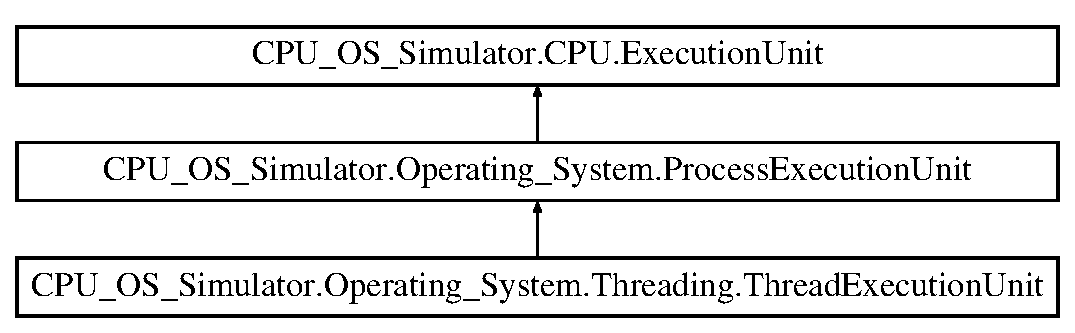
\includegraphics[height=3.000000cm]{class_c_p_u___o_s___simulator_1_1_operating___system_1_1_process_execution_unit}
\end{center}
\end{figure}
\subsection*{Public Member Functions}
\begin{DoxyCompactItemize}
\item 
\hyperlink{class_c_p_u___o_s___simulator_1_1_operating___system_1_1_process_execution_unit_a071cfa1acfabcb2518376f67985e813f}{Process\+Execution\+Unit} ()
\begin{DoxyCompactList}\small\item\em Empty constructor used when deserialising process execution units N\+O\+T\+E D\+O N\+O\+T U\+S\+E I\+N C\+O\+D\+E \end{DoxyCompactList}\item 
\hyperlink{class_c_p_u___o_s___simulator_1_1_operating___system_1_1_process_execution_unit_a96760cbf88e3fb42a51253b6e961c609}{Process\+Execution\+Unit} (\hyperlink{class_c_p_u___o_s___simulator_1_1_operating___system_1_1_simulator_process}{Simulator\+Process} \hyperlink{class_c_p_u___o_s___simulator_1_1_c_p_u_1_1_execution_unit_a192670bee8ca089c38e9989350f658d6}{program}, int \hyperlink{class_c_p_u___o_s___simulator_1_1_c_p_u_1_1_execution_unit_a0deb0a3e0c9fa402598bbf18be6535cc}{clock\+Speed})
\begin{DoxyCompactList}\small\item\em Constructor for execution unit that starts executing from the beginning of the process \end{DoxyCompactList}\item 
\hyperlink{class_c_p_u___o_s___simulator_1_1_operating___system_1_1_process_execution_unit_a89783c451bba101568a4a9b0fe09df81}{Process\+Execution\+Unit} (\hyperlink{class_c_p_u___o_s___simulator_1_1_operating___system_1_1_simulator_process}{Simulator\+Process} \hyperlink{class_c_p_u___o_s___simulator_1_1_c_p_u_1_1_execution_unit_a192670bee8ca089c38e9989350f658d6}{program}, int \hyperlink{class_c_p_u___o_s___simulator_1_1_c_p_u_1_1_execution_unit_a0deb0a3e0c9fa402598bbf18be6535cc}{clock\+Speed}, int \hyperlink{class_c_p_u___o_s___simulator_1_1_c_p_u_1_1_execution_unit_af6807cb5343acc2c40a08166c748f1f0}{current\+Index})
\begin{DoxyCompactList}\small\item\em Constructor for execution unit that starts executing from a specified location in the process \end{DoxyCompactList}\item 
void \hyperlink{class_c_p_u___o_s___simulator_1_1_operating___system_1_1_process_execution_unit_a5685d8f35ca37a904236d8e96f3aabb1}{Terminate} ()
\end{DoxyCompactItemize}
\subsection*{Protected Attributes}
\begin{DoxyCompactItemize}
\item 
bool \hyperlink{class_c_p_u___o_s___simulator_1_1_operating___system_1_1_process_execution_unit_ad48af599eaa4929c947241f3d8bd754e}{timed\+Out} = false
\end{DoxyCompactItemize}
\subsection*{Properties}
\begin{DoxyCompactItemize}
\item 
\hyperlink{class_c_p_u___o_s___simulator_1_1_operating___system_1_1_process_control_block}{Process\+Control\+Block} \hyperlink{class_c_p_u___o_s___simulator_1_1_operating___system_1_1_process_execution_unit_a50dccf62e2bc43d1ad30f6488d3ffa58}{Process\+Control\+Block}\hspace{0.3cm}{\ttfamily  \mbox{[}get, set\mbox{]}}
\item 
\hyperlink{class_c_p_u___o_s___simulator_1_1_c_p_u_1_1_simulator_program}{Simulator\+Program} \hyperlink{class_c_p_u___o_s___simulator_1_1_operating___system_1_1_process_execution_unit_a4a065d00dc99f2874bbfacbec4ff2b8c}{Program}\hspace{0.3cm}{\ttfamily  \mbox{[}get, set\mbox{]}}
\item 
\hyperlink{class_c_p_u___o_s___simulator_1_1_operating___system_1_1_simulator_process}{Simulator\+Process} \hyperlink{class_c_p_u___o_s___simulator_1_1_operating___system_1_1_process_execution_unit_a869fb898b0a61e168220757d921e5bfc}{Process}\hspace{0.3cm}{\ttfamily  \mbox{[}get, set\mbox{]}}
\item 
bool \hyperlink{class_c_p_u___o_s___simulator_1_1_operating___system_1_1_process_execution_unit_aa507b44c8134ffd0e9fbe702e1bf9e32}{Timed\+Out}\hspace{0.3cm}{\ttfamily  \mbox{[}get, set\mbox{]}}
\end{DoxyCompactItemize}
\subsection*{Private Attributes}
\begin{DoxyCompactItemize}
\item 
\hyperlink{class_c_p_u___o_s___simulator_1_1_operating___system_1_1_process_control_block}{Process\+Control\+Block} \hyperlink{class_c_p_u___o_s___simulator_1_1_operating___system_1_1_process_execution_unit_ae2624c872da8f348b1a9fcba8d6734cf}{process\+Control\+Block}
\item 
\hyperlink{class_c_p_u___o_s___simulator_1_1_operating___system_1_1_simulator_process}{Simulator\+Process} \hyperlink{class_c_p_u___o_s___simulator_1_1_operating___system_1_1_process_execution_unit_a0a8944c15b618210fe91444a755991ca}{process}
\end{DoxyCompactItemize}


\subsection{Detailed Description}


Definition at line 7 of file Process\+Execution\+Unit.\+cs.



\subsection{Constructor \& Destructor Documentation}
\hypertarget{class_c_p_u___o_s___simulator_1_1_operating___system_1_1_process_execution_unit_a071cfa1acfabcb2518376f67985e813f}{}\index{C\+P\+U\+\_\+\+O\+S\+\_\+\+Simulator\+::\+Operating\+\_\+\+System\+::\+Process\+Execution\+Unit@{C\+P\+U\+\_\+\+O\+S\+\_\+\+Simulator\+::\+Operating\+\_\+\+System\+::\+Process\+Execution\+Unit}!Process\+Execution\+Unit@{Process\+Execution\+Unit}}
\index{Process\+Execution\+Unit@{Process\+Execution\+Unit}!C\+P\+U\+\_\+\+O\+S\+\_\+\+Simulator\+::\+Operating\+\_\+\+System\+::\+Process\+Execution\+Unit@{C\+P\+U\+\_\+\+O\+S\+\_\+\+Simulator\+::\+Operating\+\_\+\+System\+::\+Process\+Execution\+Unit}}
\subsubsection[{Process\+Execution\+Unit()}]{\setlength{\rightskip}{0pt plus 5cm}C\+P\+U\+\_\+\+O\+S\+\_\+\+Simulator.\+Operating\+\_\+\+System.\+Process\+Execution\+Unit.\+Process\+Execution\+Unit (
\begin{DoxyParamCaption}
{}
\end{DoxyParamCaption}
)}\label{class_c_p_u___o_s___simulator_1_1_operating___system_1_1_process_execution_unit_a071cfa1acfabcb2518376f67985e813f}


Empty constructor used when deserialising process execution units N\+O\+T\+E D\+O N\+O\+T U\+S\+E I\+N C\+O\+D\+E 



Definition at line 18 of file Process\+Execution\+Unit.\+cs.

\hypertarget{class_c_p_u___o_s___simulator_1_1_operating___system_1_1_process_execution_unit_a96760cbf88e3fb42a51253b6e961c609}{}\index{C\+P\+U\+\_\+\+O\+S\+\_\+\+Simulator\+::\+Operating\+\_\+\+System\+::\+Process\+Execution\+Unit@{C\+P\+U\+\_\+\+O\+S\+\_\+\+Simulator\+::\+Operating\+\_\+\+System\+::\+Process\+Execution\+Unit}!Process\+Execution\+Unit@{Process\+Execution\+Unit}}
\index{Process\+Execution\+Unit@{Process\+Execution\+Unit}!C\+P\+U\+\_\+\+O\+S\+\_\+\+Simulator\+::\+Operating\+\_\+\+System\+::\+Process\+Execution\+Unit@{C\+P\+U\+\_\+\+O\+S\+\_\+\+Simulator\+::\+Operating\+\_\+\+System\+::\+Process\+Execution\+Unit}}
\subsubsection[{Process\+Execution\+Unit(\+Simulator\+Process program, int clock\+Speed)}]{\setlength{\rightskip}{0pt plus 5cm}C\+P\+U\+\_\+\+O\+S\+\_\+\+Simulator.\+Operating\+\_\+\+System.\+Process\+Execution\+Unit.\+Process\+Execution\+Unit (
\begin{DoxyParamCaption}
\item[{{\bf Simulator\+Process}}]{program, }
\item[{int}]{clock\+Speed}
\end{DoxyParamCaption}
)}\label{class_c_p_u___o_s___simulator_1_1_operating___system_1_1_process_execution_unit_a96760cbf88e3fb42a51253b6e961c609}


Constructor for execution unit that starts executing from the beginning of the process 


\begin{DoxyParams}{Parameters}
{\em program} & the process to execute \\
\hline
{\em clock\+Speed} & the clock speed of the \hyperlink{namespace_c_p_u___o_s___simulator_1_1_c_p_u}{C\+P\+U} \\
\hline
\end{DoxyParams}


Definition at line 28 of file Process\+Execution\+Unit.\+cs.

\hypertarget{class_c_p_u___o_s___simulator_1_1_operating___system_1_1_process_execution_unit_a89783c451bba101568a4a9b0fe09df81}{}\index{C\+P\+U\+\_\+\+O\+S\+\_\+\+Simulator\+::\+Operating\+\_\+\+System\+::\+Process\+Execution\+Unit@{C\+P\+U\+\_\+\+O\+S\+\_\+\+Simulator\+::\+Operating\+\_\+\+System\+::\+Process\+Execution\+Unit}!Process\+Execution\+Unit@{Process\+Execution\+Unit}}
\index{Process\+Execution\+Unit@{Process\+Execution\+Unit}!C\+P\+U\+\_\+\+O\+S\+\_\+\+Simulator\+::\+Operating\+\_\+\+System\+::\+Process\+Execution\+Unit@{C\+P\+U\+\_\+\+O\+S\+\_\+\+Simulator\+::\+Operating\+\_\+\+System\+::\+Process\+Execution\+Unit}}
\subsubsection[{Process\+Execution\+Unit(\+Simulator\+Process program, int clock\+Speed, int current\+Index)}]{\setlength{\rightskip}{0pt plus 5cm}C\+P\+U\+\_\+\+O\+S\+\_\+\+Simulator.\+Operating\+\_\+\+System.\+Process\+Execution\+Unit.\+Process\+Execution\+Unit (
\begin{DoxyParamCaption}
\item[{{\bf Simulator\+Process}}]{program, }
\item[{int}]{clock\+Speed, }
\item[{int}]{current\+Index}
\end{DoxyParamCaption}
)}\label{class_c_p_u___o_s___simulator_1_1_operating___system_1_1_process_execution_unit_a89783c451bba101568a4a9b0fe09df81}


Constructor for execution unit that starts executing from a specified location in the process 


\begin{DoxyParams}{Parameters}
{\em program} & the process to execute \\
\hline
{\em current\+Index} & the index to start executing from\\
\hline
{\em clock\+Speed} & the clock speed of the \hyperlink{namespace_c_p_u___o_s___simulator_1_1_c_p_u}{C\+P\+U} \\
\hline
\end{DoxyParams}


Definition at line 41 of file Process\+Execution\+Unit.\+cs.



\subsection{Member Function Documentation}
\hypertarget{class_c_p_u___o_s___simulator_1_1_operating___system_1_1_process_execution_unit_a5685d8f35ca37a904236d8e96f3aabb1}{}\index{C\+P\+U\+\_\+\+O\+S\+\_\+\+Simulator\+::\+Operating\+\_\+\+System\+::\+Process\+Execution\+Unit@{C\+P\+U\+\_\+\+O\+S\+\_\+\+Simulator\+::\+Operating\+\_\+\+System\+::\+Process\+Execution\+Unit}!Terminate@{Terminate}}
\index{Terminate@{Terminate}!C\+P\+U\+\_\+\+O\+S\+\_\+\+Simulator\+::\+Operating\+\_\+\+System\+::\+Process\+Execution\+Unit@{C\+P\+U\+\_\+\+O\+S\+\_\+\+Simulator\+::\+Operating\+\_\+\+System\+::\+Process\+Execution\+Unit}}
\subsubsection[{Terminate()}]{\setlength{\rightskip}{0pt plus 5cm}void C\+P\+U\+\_\+\+O\+S\+\_\+\+Simulator.\+Operating\+\_\+\+System.\+Process\+Execution\+Unit.\+Terminate (
\begin{DoxyParamCaption}
{}
\end{DoxyParamCaption}
)}\label{class_c_p_u___o_s___simulator_1_1_operating___system_1_1_process_execution_unit_a5685d8f35ca37a904236d8e96f3aabb1}


Definition at line 74 of file Process\+Execution\+Unit.\+cs.



\subsection{Member Data Documentation}
\hypertarget{class_c_p_u___o_s___simulator_1_1_operating___system_1_1_process_execution_unit_a0a8944c15b618210fe91444a755991ca}{}\index{C\+P\+U\+\_\+\+O\+S\+\_\+\+Simulator\+::\+Operating\+\_\+\+System\+::\+Process\+Execution\+Unit@{C\+P\+U\+\_\+\+O\+S\+\_\+\+Simulator\+::\+Operating\+\_\+\+System\+::\+Process\+Execution\+Unit}!process@{process}}
\index{process@{process}!C\+P\+U\+\_\+\+O\+S\+\_\+\+Simulator\+::\+Operating\+\_\+\+System\+::\+Process\+Execution\+Unit@{C\+P\+U\+\_\+\+O\+S\+\_\+\+Simulator\+::\+Operating\+\_\+\+System\+::\+Process\+Execution\+Unit}}
\subsubsection[{process}]{\setlength{\rightskip}{0pt plus 5cm}{\bf Simulator\+Process} C\+P\+U\+\_\+\+O\+S\+\_\+\+Simulator.\+Operating\+\_\+\+System.\+Process\+Execution\+Unit.\+process\hspace{0.3cm}{\ttfamily [private]}}\label{class_c_p_u___o_s___simulator_1_1_operating___system_1_1_process_execution_unit_a0a8944c15b618210fe91444a755991ca}


Definition at line 11 of file Process\+Execution\+Unit.\+cs.

\hypertarget{class_c_p_u___o_s___simulator_1_1_operating___system_1_1_process_execution_unit_ae2624c872da8f348b1a9fcba8d6734cf}{}\index{C\+P\+U\+\_\+\+O\+S\+\_\+\+Simulator\+::\+Operating\+\_\+\+System\+::\+Process\+Execution\+Unit@{C\+P\+U\+\_\+\+O\+S\+\_\+\+Simulator\+::\+Operating\+\_\+\+System\+::\+Process\+Execution\+Unit}!process\+Control\+Block@{process\+Control\+Block}}
\index{process\+Control\+Block@{process\+Control\+Block}!C\+P\+U\+\_\+\+O\+S\+\_\+\+Simulator\+::\+Operating\+\_\+\+System\+::\+Process\+Execution\+Unit@{C\+P\+U\+\_\+\+O\+S\+\_\+\+Simulator\+::\+Operating\+\_\+\+System\+::\+Process\+Execution\+Unit}}
\subsubsection[{process\+Control\+Block}]{\setlength{\rightskip}{0pt plus 5cm}{\bf Process\+Control\+Block} C\+P\+U\+\_\+\+O\+S\+\_\+\+Simulator.\+Operating\+\_\+\+System.\+Process\+Execution\+Unit.\+process\+Control\+Block\hspace{0.3cm}{\ttfamily [private]}}\label{class_c_p_u___o_s___simulator_1_1_operating___system_1_1_process_execution_unit_ae2624c872da8f348b1a9fcba8d6734cf}


Definition at line 9 of file Process\+Execution\+Unit.\+cs.

\hypertarget{class_c_p_u___o_s___simulator_1_1_operating___system_1_1_process_execution_unit_ad48af599eaa4929c947241f3d8bd754e}{}\index{C\+P\+U\+\_\+\+O\+S\+\_\+\+Simulator\+::\+Operating\+\_\+\+System\+::\+Process\+Execution\+Unit@{C\+P\+U\+\_\+\+O\+S\+\_\+\+Simulator\+::\+Operating\+\_\+\+System\+::\+Process\+Execution\+Unit}!timed\+Out@{timed\+Out}}
\index{timed\+Out@{timed\+Out}!C\+P\+U\+\_\+\+O\+S\+\_\+\+Simulator\+::\+Operating\+\_\+\+System\+::\+Process\+Execution\+Unit@{C\+P\+U\+\_\+\+O\+S\+\_\+\+Simulator\+::\+Operating\+\_\+\+System\+::\+Process\+Execution\+Unit}}
\subsubsection[{timed\+Out}]{\setlength{\rightskip}{0pt plus 5cm}bool C\+P\+U\+\_\+\+O\+S\+\_\+\+Simulator.\+Operating\+\_\+\+System.\+Process\+Execution\+Unit.\+timed\+Out = false\hspace{0.3cm}{\ttfamily [protected]}}\label{class_c_p_u___o_s___simulator_1_1_operating___system_1_1_process_execution_unit_ad48af599eaa4929c947241f3d8bd754e}


Definition at line 12 of file Process\+Execution\+Unit.\+cs.



\subsection{Property Documentation}
\hypertarget{class_c_p_u___o_s___simulator_1_1_operating___system_1_1_process_execution_unit_a869fb898b0a61e168220757d921e5bfc}{}\index{C\+P\+U\+\_\+\+O\+S\+\_\+\+Simulator\+::\+Operating\+\_\+\+System\+::\+Process\+Execution\+Unit@{C\+P\+U\+\_\+\+O\+S\+\_\+\+Simulator\+::\+Operating\+\_\+\+System\+::\+Process\+Execution\+Unit}!Process@{Process}}
\index{Process@{Process}!C\+P\+U\+\_\+\+O\+S\+\_\+\+Simulator\+::\+Operating\+\_\+\+System\+::\+Process\+Execution\+Unit@{C\+P\+U\+\_\+\+O\+S\+\_\+\+Simulator\+::\+Operating\+\_\+\+System\+::\+Process\+Execution\+Unit}}
\subsubsection[{Process}]{\setlength{\rightskip}{0pt plus 5cm}{\bf Simulator\+Process} C\+P\+U\+\_\+\+O\+S\+\_\+\+Simulator.\+Operating\+\_\+\+System.\+Process\+Execution\+Unit.\+Process\hspace{0.3cm}{\ttfamily [get]}, {\ttfamily [set]}}\label{class_c_p_u___o_s___simulator_1_1_operating___system_1_1_process_execution_unit_a869fb898b0a61e168220757d921e5bfc}


Definition at line 62 of file Process\+Execution\+Unit.\+cs.

\hypertarget{class_c_p_u___o_s___simulator_1_1_operating___system_1_1_process_execution_unit_a50dccf62e2bc43d1ad30f6488d3ffa58}{}\index{C\+P\+U\+\_\+\+O\+S\+\_\+\+Simulator\+::\+Operating\+\_\+\+System\+::\+Process\+Execution\+Unit@{C\+P\+U\+\_\+\+O\+S\+\_\+\+Simulator\+::\+Operating\+\_\+\+System\+::\+Process\+Execution\+Unit}!Process\+Control\+Block@{Process\+Control\+Block}}
\index{Process\+Control\+Block@{Process\+Control\+Block}!C\+P\+U\+\_\+\+O\+S\+\_\+\+Simulator\+::\+Operating\+\_\+\+System\+::\+Process\+Execution\+Unit@{C\+P\+U\+\_\+\+O\+S\+\_\+\+Simulator\+::\+Operating\+\_\+\+System\+::\+Process\+Execution\+Unit}}
\subsubsection[{Process\+Control\+Block}]{\setlength{\rightskip}{0pt plus 5cm}{\bf Process\+Control\+Block} C\+P\+U\+\_\+\+O\+S\+\_\+\+Simulator.\+Operating\+\_\+\+System.\+Process\+Execution\+Unit.\+Process\+Control\+Block\hspace{0.3cm}{\ttfamily [get]}, {\ttfamily [set]}}\label{class_c_p_u___o_s___simulator_1_1_operating___system_1_1_process_execution_unit_a50dccf62e2bc43d1ad30f6488d3ffa58}


Definition at line 50 of file Process\+Execution\+Unit.\+cs.

\hypertarget{class_c_p_u___o_s___simulator_1_1_operating___system_1_1_process_execution_unit_a4a065d00dc99f2874bbfacbec4ff2b8c}{}\index{C\+P\+U\+\_\+\+O\+S\+\_\+\+Simulator\+::\+Operating\+\_\+\+System\+::\+Process\+Execution\+Unit@{C\+P\+U\+\_\+\+O\+S\+\_\+\+Simulator\+::\+Operating\+\_\+\+System\+::\+Process\+Execution\+Unit}!Program@{Program}}
\index{Program@{Program}!C\+P\+U\+\_\+\+O\+S\+\_\+\+Simulator\+::\+Operating\+\_\+\+System\+::\+Process\+Execution\+Unit@{C\+P\+U\+\_\+\+O\+S\+\_\+\+Simulator\+::\+Operating\+\_\+\+System\+::\+Process\+Execution\+Unit}}
\subsubsection[{Program}]{\setlength{\rightskip}{0pt plus 5cm}{\bf Simulator\+Program} C\+P\+U\+\_\+\+O\+S\+\_\+\+Simulator.\+Operating\+\_\+\+System.\+Process\+Execution\+Unit.\+Program\hspace{0.3cm}{\ttfamily [get]}, {\ttfamily [set]}}\label{class_c_p_u___o_s___simulator_1_1_operating___system_1_1_process_execution_unit_a4a065d00dc99f2874bbfacbec4ff2b8c}


Definition at line 56 of file Process\+Execution\+Unit.\+cs.

\hypertarget{class_c_p_u___o_s___simulator_1_1_operating___system_1_1_process_execution_unit_aa507b44c8134ffd0e9fbe702e1bf9e32}{}\index{C\+P\+U\+\_\+\+O\+S\+\_\+\+Simulator\+::\+Operating\+\_\+\+System\+::\+Process\+Execution\+Unit@{C\+P\+U\+\_\+\+O\+S\+\_\+\+Simulator\+::\+Operating\+\_\+\+System\+::\+Process\+Execution\+Unit}!Timed\+Out@{Timed\+Out}}
\index{Timed\+Out@{Timed\+Out}!C\+P\+U\+\_\+\+O\+S\+\_\+\+Simulator\+::\+Operating\+\_\+\+System\+::\+Process\+Execution\+Unit@{C\+P\+U\+\_\+\+O\+S\+\_\+\+Simulator\+::\+Operating\+\_\+\+System\+::\+Process\+Execution\+Unit}}
\subsubsection[{Timed\+Out}]{\setlength{\rightskip}{0pt plus 5cm}bool C\+P\+U\+\_\+\+O\+S\+\_\+\+Simulator.\+Operating\+\_\+\+System.\+Process\+Execution\+Unit.\+Timed\+Out\hspace{0.3cm}{\ttfamily [get]}, {\ttfamily [set]}}\label{class_c_p_u___o_s___simulator_1_1_operating___system_1_1_process_execution_unit_aa507b44c8134ffd0e9fbe702e1bf9e32}


Definition at line 68 of file Process\+Execution\+Unit.\+cs.



The documentation for this class was generated from the following file\+:\begin{DoxyCompactItemize}
\item 
Operating System/\hyperlink{_process_execution_unit_8cs}{Process\+Execution\+Unit.\+cs}\end{DoxyCompactItemize}

\hypertarget{struct_c_p_u___o_s___simulator_1_1_operating___system_1_1_process_flags}{}\section{C\+P\+U\+\_\+\+O\+S\+\_\+\+Simulator.\+Operating\+\_\+\+System.\+Process\+Flags Struct Reference}
\label{struct_c_p_u___o_s___simulator_1_1_operating___system_1_1_process_flags}\index{C\+P\+U\+\_\+\+O\+S\+\_\+\+Simulator.\+Operating\+\_\+\+System.\+Process\+Flags@{C\+P\+U\+\_\+\+O\+S\+\_\+\+Simulator.\+Operating\+\_\+\+System.\+Process\+Flags}}


this struct represents the flags passed to a process  


\subsection*{Public Attributes}
\begin{DoxyCompactItemize}
\item 
\hyperlink{class_c_p_u___o_s___simulator_1_1_c_p_u_1_1_simulator_program}{Simulator\+Program} \hyperlink{struct_c_p_u___o_s___simulator_1_1_operating___system_1_1_process_flags_addf9316ebaddcec9f466b0317d15d45c}{program}
\item 
string \hyperlink{struct_c_p_u___o_s___simulator_1_1_operating___system_1_1_process_flags_af219a7a8b99d0c94b5847797dabb39f6}{program\+Name}
\item 
string \hyperlink{struct_c_p_u___o_s___simulator_1_1_operating___system_1_1_process_flags_a2823e57851d2940c47cd06afd0487360}{process\+Name}
\item 
int \hyperlink{struct_c_p_u___o_s___simulator_1_1_operating___system_1_1_process_flags_a0a14c1f617bd3cd4d2b28b5f13cf83d5}{process\+Priority}
\item 
int \hyperlink{struct_c_p_u___o_s___simulator_1_1_operating___system_1_1_process_flags_a2ed1133d00c4d6d39f9e5cd70febbacb}{process\+Memory}
\item 
int \hyperlink{struct_c_p_u___o_s___simulator_1_1_operating___system_1_1_process_flags_a45de0517d0705f5c9ff1322e969cae20}{process\+Lifetime}
\item 
\hyperlink{namespace_c_p_u___o_s___simulator_1_1_operating___system_a0553d0bc2513aec52caa769acf994d5c}{Enum\+Time\+Unit} \hyperlink{struct_c_p_u___o_s___simulator_1_1_operating___system_1_1_process_flags_af7b24dbd3fd07741d54984f6261694f6}{process\+Lifetime\+Time\+Unit}
\item 
int \hyperlink{struct_c_p_u___o_s___simulator_1_1_operating___system_1_1_process_flags_a5a0ef784d6cef8d5d42ab43b69972f5b}{process\+I\+D}
\item 
int \hyperlink{struct_c_p_u___o_s___simulator_1_1_operating___system_1_1_process_flags_a204157ba5a9571934344bef2378f88bf}{C\+P\+Uid}
\item 
int \hyperlink{struct_c_p_u___o_s___simulator_1_1_operating___system_1_1_process_flags_ac0e98ee86de3c22c7a022e3dcd69935f}{burst\+Time}
\item 
bool \hyperlink{struct_c_p_u___o_s___simulator_1_1_operating___system_1_1_process_flags_a8290519886f3517f690f3acba8330440}{display\+Profile}
\item 
bool \hyperlink{struct_c_p_u___o_s___simulator_1_1_operating___system_1_1_process_flags_a8ef3875fcd47a5f1fa37b61a2979b813}{parent\+Dies\+Children\+Die}
\item 
bool \hyperlink{struct_c_p_u___o_s___simulator_1_1_operating___system_1_1_process_flags_a927e8e998250ab57385146cf8dd487b8}{default\+Scheduler}
\item 
bool \hyperlink{struct_c_p_u___o_s___simulator_1_1_operating___system_1_1_process_flags_ac6a4a5a7465da7e567a655cae4dd1aa4}{delayed\+Process}
\item 
int \hyperlink{struct_c_p_u___o_s___simulator_1_1_operating___system_1_1_process_flags_a9b9ff1ea252f64035813f0f478d705ae}{delayed\+Process\+Time}
\item 
\hyperlink{namespace_c_p_u___o_s___simulator_1_1_operating___system_a0553d0bc2513aec52caa769acf994d5c}{Enum\+Time\+Unit} \hyperlink{struct_c_p_u___o_s___simulator_1_1_operating___system_1_1_process_flags_a0e5e535ff000e1b630180443c2295776}{delay\+Time\+Unit}
\item 
\hyperlink{class_c_p_u___o_s___simulator_1_1_operating___system_1_1_simulator_process}{Simulator\+Process} \hyperlink{struct_c_p_u___o_s___simulator_1_1_operating___system_1_1_process_flags_a6b32c9b5ed4914dede86c2a1306c897e}{parent\+Process}
\item 
int \hyperlink{struct_c_p_u___o_s___simulator_1_1_operating___system_1_1_process_flags_a115209ffd287aaba9aa6b1bf9ba7a968}{parent\+Process\+I\+D}
\item 
List$<$ \hyperlink{class_c_p_u___o_s___simulator_1_1_operating___system_1_1_simulator_process}{Simulator\+Process} $>$ \hyperlink{struct_c_p_u___o_s___simulator_1_1_operating___system_1_1_process_flags_aae4b90a688d3ac4e6d3faea6cb275242}{child\+Processes}
\item 
bool \hyperlink{struct_c_p_u___o_s___simulator_1_1_operating___system_1_1_process_flags_aa57e25afb816fa9a0e11c43920640992}{process\+Swapped}
\item 
\hyperlink{namespace_c_p_u___o_s___simulator_1_1_operating___system_a836ee2204e78fcb3a7dd6c3c942b1a24}{Enum\+Process\+State} \hyperlink{struct_c_p_u___o_s___simulator_1_1_operating___system_1_1_process_flags_ac5d7a47d263eb80357b0a7900858bd98}{process\+State}
\item 
\hyperlink{namespace_c_p_u___o_s___simulator_1_1_operating___system_a836ee2204e78fcb3a7dd6c3c942b1a24}{Enum\+Process\+State} \hyperlink{struct_c_p_u___o_s___simulator_1_1_operating___system_1_1_process_flags_a89cd3299d16c593e82819dfeb40749a1}{previous\+State}
\item 
bool \hyperlink{struct_c_p_u___o_s___simulator_1_1_operating___system_1_1_process_flags_abc77938558baa106a799492596c9178b}{resource\+Starved}
\item 
List$<$ \hyperlink{class_c_p_u___o_s___simulator_1_1_operating___system_1_1_simulator_resource}{Simulator\+Resource} $>$ \hyperlink{struct_c_p_u___o_s___simulator_1_1_operating___system_1_1_process_flags_aeeb2a90f98ea93e6ee4c9d092fb0573d}{allocated\+Resources}
\item 
List$<$ \hyperlink{class_c_p_u___o_s___simulator_1_1_operating___system_1_1_simulator_resource}{Simulator\+Resource} $>$ \hyperlink{struct_c_p_u___o_s___simulator_1_1_operating___system_1_1_process_flags_afa8f450b4825d1c204817af22729c05b}{requested\+Resources}
\item 
bool \hyperlink{struct_c_p_u___o_s___simulator_1_1_operating___system_1_1_process_flags_a5986a802a1f22f726209aba6d52f7e9c}{terminated}
\item 
\hyperlink{class_c_p_u___o_s___simulator_1_1_operating___system_1_1_process_control_block}{Process\+Control\+Block} \hyperlink{struct_c_p_u___o_s___simulator_1_1_operating___system_1_1_process_flags_adca49f9a3ee1f5e380a7547b0b8b73d6}{process\+Control\+Block}
\item 
int \hyperlink{struct_c_p_u___o_s___simulator_1_1_operating___system_1_1_process_flags_a819f86c160d64c6f4cbba56418cb688e}{O\+Sid}
\item 
int \hyperlink{struct_c_p_u___o_s___simulator_1_1_operating___system_1_1_process_flags_a28dbea54b61ff7f12d5dc8c3c40f632d}{clock\+Speed}
\item 
\hyperlink{class_c_p_u___o_s___simulator_1_1_operating___system_1_1_process_execution_unit}{Process\+Execution\+Unit} \hyperlink{struct_c_p_u___o_s___simulator_1_1_operating___system_1_1_process_flags_a6168635b7297d4ede7af0b1fce2e3db6}{unit}
\item 
List$<$ \hyperlink{class_c_p_u___o_s___simulator_1_1_operating___system_1_1_lottery_ticket}{Lottery\+Ticket} $>$ \hyperlink{struct_c_p_u___o_s___simulator_1_1_operating___system_1_1_process_flags_aa4893622ce512bb83c4970dc899d8452}{lottery\+Tickets}
\item 
bool \hyperlink{struct_c_p_u___o_s___simulator_1_1_operating___system_1_1_process_flags_a74079b8eb14af8005ed9c76f92bbf4db}{owns\+Semaphore}
\item 
bool \hyperlink{struct_c_p_u___o_s___simulator_1_1_operating___system_1_1_process_flags_af004c9597bef484bbb8eb43538818e58}{waiting\+For\+Semaphore}
\end{DoxyCompactItemize}


\subsection{Detailed Description}
this struct represents the flags passed to a process 



Definition at line 10 of file Process\+Flags.\+cs.



\subsection{Member Data Documentation}
\hypertarget{struct_c_p_u___o_s___simulator_1_1_operating___system_1_1_process_flags_aeeb2a90f98ea93e6ee4c9d092fb0573d}{}\index{C\+P\+U\+\_\+\+O\+S\+\_\+\+Simulator\+::\+Operating\+\_\+\+System\+::\+Process\+Flags@{C\+P\+U\+\_\+\+O\+S\+\_\+\+Simulator\+::\+Operating\+\_\+\+System\+::\+Process\+Flags}!allocated\+Resources@{allocated\+Resources}}
\index{allocated\+Resources@{allocated\+Resources}!C\+P\+U\+\_\+\+O\+S\+\_\+\+Simulator\+::\+Operating\+\_\+\+System\+::\+Process\+Flags@{C\+P\+U\+\_\+\+O\+S\+\_\+\+Simulator\+::\+Operating\+\_\+\+System\+::\+Process\+Flags}}
\subsubsection[{allocated\+Resources}]{\setlength{\rightskip}{0pt plus 5cm}List$<${\bf Simulator\+Resource}$>$ C\+P\+U\+\_\+\+O\+S\+\_\+\+Simulator.\+Operating\+\_\+\+System.\+Process\+Flags.\+allocated\+Resources}\label{struct_c_p_u___o_s___simulator_1_1_operating___system_1_1_process_flags_aeeb2a90f98ea93e6ee4c9d092fb0573d}


Definition at line 35 of file Process\+Flags.\+cs.

\hypertarget{struct_c_p_u___o_s___simulator_1_1_operating___system_1_1_process_flags_ac0e98ee86de3c22c7a022e3dcd69935f}{}\index{C\+P\+U\+\_\+\+O\+S\+\_\+\+Simulator\+::\+Operating\+\_\+\+System\+::\+Process\+Flags@{C\+P\+U\+\_\+\+O\+S\+\_\+\+Simulator\+::\+Operating\+\_\+\+System\+::\+Process\+Flags}!burst\+Time@{burst\+Time}}
\index{burst\+Time@{burst\+Time}!C\+P\+U\+\_\+\+O\+S\+\_\+\+Simulator\+::\+Operating\+\_\+\+System\+::\+Process\+Flags@{C\+P\+U\+\_\+\+O\+S\+\_\+\+Simulator\+::\+Operating\+\_\+\+System\+::\+Process\+Flags}}
\subsubsection[{burst\+Time}]{\setlength{\rightskip}{0pt plus 5cm}int C\+P\+U\+\_\+\+O\+S\+\_\+\+Simulator.\+Operating\+\_\+\+System.\+Process\+Flags.\+burst\+Time}\label{struct_c_p_u___o_s___simulator_1_1_operating___system_1_1_process_flags_ac0e98ee86de3c22c7a022e3dcd69935f}


Definition at line 21 of file Process\+Flags.\+cs.

\hypertarget{struct_c_p_u___o_s___simulator_1_1_operating___system_1_1_process_flags_aae4b90a688d3ac4e6d3faea6cb275242}{}\index{C\+P\+U\+\_\+\+O\+S\+\_\+\+Simulator\+::\+Operating\+\_\+\+System\+::\+Process\+Flags@{C\+P\+U\+\_\+\+O\+S\+\_\+\+Simulator\+::\+Operating\+\_\+\+System\+::\+Process\+Flags}!child\+Processes@{child\+Processes}}
\index{child\+Processes@{child\+Processes}!C\+P\+U\+\_\+\+O\+S\+\_\+\+Simulator\+::\+Operating\+\_\+\+System\+::\+Process\+Flags@{C\+P\+U\+\_\+\+O\+S\+\_\+\+Simulator\+::\+Operating\+\_\+\+System\+::\+Process\+Flags}}
\subsubsection[{child\+Processes}]{\setlength{\rightskip}{0pt plus 5cm}List$<${\bf Simulator\+Process}$>$ C\+P\+U\+\_\+\+O\+S\+\_\+\+Simulator.\+Operating\+\_\+\+System.\+Process\+Flags.\+child\+Processes}\label{struct_c_p_u___o_s___simulator_1_1_operating___system_1_1_process_flags_aae4b90a688d3ac4e6d3faea6cb275242}


Definition at line 30 of file Process\+Flags.\+cs.

\hypertarget{struct_c_p_u___o_s___simulator_1_1_operating___system_1_1_process_flags_a28dbea54b61ff7f12d5dc8c3c40f632d}{}\index{C\+P\+U\+\_\+\+O\+S\+\_\+\+Simulator\+::\+Operating\+\_\+\+System\+::\+Process\+Flags@{C\+P\+U\+\_\+\+O\+S\+\_\+\+Simulator\+::\+Operating\+\_\+\+System\+::\+Process\+Flags}!clock\+Speed@{clock\+Speed}}
\index{clock\+Speed@{clock\+Speed}!C\+P\+U\+\_\+\+O\+S\+\_\+\+Simulator\+::\+Operating\+\_\+\+System\+::\+Process\+Flags@{C\+P\+U\+\_\+\+O\+S\+\_\+\+Simulator\+::\+Operating\+\_\+\+System\+::\+Process\+Flags}}
\subsubsection[{clock\+Speed}]{\setlength{\rightskip}{0pt plus 5cm}int C\+P\+U\+\_\+\+O\+S\+\_\+\+Simulator.\+Operating\+\_\+\+System.\+Process\+Flags.\+clock\+Speed}\label{struct_c_p_u___o_s___simulator_1_1_operating___system_1_1_process_flags_a28dbea54b61ff7f12d5dc8c3c40f632d}


Definition at line 40 of file Process\+Flags.\+cs.

\hypertarget{struct_c_p_u___o_s___simulator_1_1_operating___system_1_1_process_flags_a204157ba5a9571934344bef2378f88bf}{}\index{C\+P\+U\+\_\+\+O\+S\+\_\+\+Simulator\+::\+Operating\+\_\+\+System\+::\+Process\+Flags@{C\+P\+U\+\_\+\+O\+S\+\_\+\+Simulator\+::\+Operating\+\_\+\+System\+::\+Process\+Flags}!C\+P\+Uid@{C\+P\+Uid}}
\index{C\+P\+Uid@{C\+P\+Uid}!C\+P\+U\+\_\+\+O\+S\+\_\+\+Simulator\+::\+Operating\+\_\+\+System\+::\+Process\+Flags@{C\+P\+U\+\_\+\+O\+S\+\_\+\+Simulator\+::\+Operating\+\_\+\+System\+::\+Process\+Flags}}
\subsubsection[{C\+P\+Uid}]{\setlength{\rightskip}{0pt plus 5cm}int C\+P\+U\+\_\+\+O\+S\+\_\+\+Simulator.\+Operating\+\_\+\+System.\+Process\+Flags.\+C\+P\+Uid}\label{struct_c_p_u___o_s___simulator_1_1_operating___system_1_1_process_flags_a204157ba5a9571934344bef2378f88bf}


Definition at line 20 of file Process\+Flags.\+cs.

\hypertarget{struct_c_p_u___o_s___simulator_1_1_operating___system_1_1_process_flags_a927e8e998250ab57385146cf8dd487b8}{}\index{C\+P\+U\+\_\+\+O\+S\+\_\+\+Simulator\+::\+Operating\+\_\+\+System\+::\+Process\+Flags@{C\+P\+U\+\_\+\+O\+S\+\_\+\+Simulator\+::\+Operating\+\_\+\+System\+::\+Process\+Flags}!default\+Scheduler@{default\+Scheduler}}
\index{default\+Scheduler@{default\+Scheduler}!C\+P\+U\+\_\+\+O\+S\+\_\+\+Simulator\+::\+Operating\+\_\+\+System\+::\+Process\+Flags@{C\+P\+U\+\_\+\+O\+S\+\_\+\+Simulator\+::\+Operating\+\_\+\+System\+::\+Process\+Flags}}
\subsubsection[{default\+Scheduler}]{\setlength{\rightskip}{0pt plus 5cm}bool C\+P\+U\+\_\+\+O\+S\+\_\+\+Simulator.\+Operating\+\_\+\+System.\+Process\+Flags.\+default\+Scheduler}\label{struct_c_p_u___o_s___simulator_1_1_operating___system_1_1_process_flags_a927e8e998250ab57385146cf8dd487b8}


Definition at line 24 of file Process\+Flags.\+cs.

\hypertarget{struct_c_p_u___o_s___simulator_1_1_operating___system_1_1_process_flags_ac6a4a5a7465da7e567a655cae4dd1aa4}{}\index{C\+P\+U\+\_\+\+O\+S\+\_\+\+Simulator\+::\+Operating\+\_\+\+System\+::\+Process\+Flags@{C\+P\+U\+\_\+\+O\+S\+\_\+\+Simulator\+::\+Operating\+\_\+\+System\+::\+Process\+Flags}!delayed\+Process@{delayed\+Process}}
\index{delayed\+Process@{delayed\+Process}!C\+P\+U\+\_\+\+O\+S\+\_\+\+Simulator\+::\+Operating\+\_\+\+System\+::\+Process\+Flags@{C\+P\+U\+\_\+\+O\+S\+\_\+\+Simulator\+::\+Operating\+\_\+\+System\+::\+Process\+Flags}}
\subsubsection[{delayed\+Process}]{\setlength{\rightskip}{0pt plus 5cm}bool C\+P\+U\+\_\+\+O\+S\+\_\+\+Simulator.\+Operating\+\_\+\+System.\+Process\+Flags.\+delayed\+Process}\label{struct_c_p_u___o_s___simulator_1_1_operating___system_1_1_process_flags_ac6a4a5a7465da7e567a655cae4dd1aa4}


Definition at line 25 of file Process\+Flags.\+cs.

\hypertarget{struct_c_p_u___o_s___simulator_1_1_operating___system_1_1_process_flags_a9b9ff1ea252f64035813f0f478d705ae}{}\index{C\+P\+U\+\_\+\+O\+S\+\_\+\+Simulator\+::\+Operating\+\_\+\+System\+::\+Process\+Flags@{C\+P\+U\+\_\+\+O\+S\+\_\+\+Simulator\+::\+Operating\+\_\+\+System\+::\+Process\+Flags}!delayed\+Process\+Time@{delayed\+Process\+Time}}
\index{delayed\+Process\+Time@{delayed\+Process\+Time}!C\+P\+U\+\_\+\+O\+S\+\_\+\+Simulator\+::\+Operating\+\_\+\+System\+::\+Process\+Flags@{C\+P\+U\+\_\+\+O\+S\+\_\+\+Simulator\+::\+Operating\+\_\+\+System\+::\+Process\+Flags}}
\subsubsection[{delayed\+Process\+Time}]{\setlength{\rightskip}{0pt plus 5cm}int C\+P\+U\+\_\+\+O\+S\+\_\+\+Simulator.\+Operating\+\_\+\+System.\+Process\+Flags.\+delayed\+Process\+Time}\label{struct_c_p_u___o_s___simulator_1_1_operating___system_1_1_process_flags_a9b9ff1ea252f64035813f0f478d705ae}


Definition at line 26 of file Process\+Flags.\+cs.

\hypertarget{struct_c_p_u___o_s___simulator_1_1_operating___system_1_1_process_flags_a0e5e535ff000e1b630180443c2295776}{}\index{C\+P\+U\+\_\+\+O\+S\+\_\+\+Simulator\+::\+Operating\+\_\+\+System\+::\+Process\+Flags@{C\+P\+U\+\_\+\+O\+S\+\_\+\+Simulator\+::\+Operating\+\_\+\+System\+::\+Process\+Flags}!delay\+Time\+Unit@{delay\+Time\+Unit}}
\index{delay\+Time\+Unit@{delay\+Time\+Unit}!C\+P\+U\+\_\+\+O\+S\+\_\+\+Simulator\+::\+Operating\+\_\+\+System\+::\+Process\+Flags@{C\+P\+U\+\_\+\+O\+S\+\_\+\+Simulator\+::\+Operating\+\_\+\+System\+::\+Process\+Flags}}
\subsubsection[{delay\+Time\+Unit}]{\setlength{\rightskip}{0pt plus 5cm}{\bf Enum\+Time\+Unit} C\+P\+U\+\_\+\+O\+S\+\_\+\+Simulator.\+Operating\+\_\+\+System.\+Process\+Flags.\+delay\+Time\+Unit}\label{struct_c_p_u___o_s___simulator_1_1_operating___system_1_1_process_flags_a0e5e535ff000e1b630180443c2295776}


Definition at line 27 of file Process\+Flags.\+cs.

\hypertarget{struct_c_p_u___o_s___simulator_1_1_operating___system_1_1_process_flags_a8290519886f3517f690f3acba8330440}{}\index{C\+P\+U\+\_\+\+O\+S\+\_\+\+Simulator\+::\+Operating\+\_\+\+System\+::\+Process\+Flags@{C\+P\+U\+\_\+\+O\+S\+\_\+\+Simulator\+::\+Operating\+\_\+\+System\+::\+Process\+Flags}!display\+Profile@{display\+Profile}}
\index{display\+Profile@{display\+Profile}!C\+P\+U\+\_\+\+O\+S\+\_\+\+Simulator\+::\+Operating\+\_\+\+System\+::\+Process\+Flags@{C\+P\+U\+\_\+\+O\+S\+\_\+\+Simulator\+::\+Operating\+\_\+\+System\+::\+Process\+Flags}}
\subsubsection[{display\+Profile}]{\setlength{\rightskip}{0pt plus 5cm}bool C\+P\+U\+\_\+\+O\+S\+\_\+\+Simulator.\+Operating\+\_\+\+System.\+Process\+Flags.\+display\+Profile}\label{struct_c_p_u___o_s___simulator_1_1_operating___system_1_1_process_flags_a8290519886f3517f690f3acba8330440}


Definition at line 22 of file Process\+Flags.\+cs.

\hypertarget{struct_c_p_u___o_s___simulator_1_1_operating___system_1_1_process_flags_aa4893622ce512bb83c4970dc899d8452}{}\index{C\+P\+U\+\_\+\+O\+S\+\_\+\+Simulator\+::\+Operating\+\_\+\+System\+::\+Process\+Flags@{C\+P\+U\+\_\+\+O\+S\+\_\+\+Simulator\+::\+Operating\+\_\+\+System\+::\+Process\+Flags}!lottery\+Tickets@{lottery\+Tickets}}
\index{lottery\+Tickets@{lottery\+Tickets}!C\+P\+U\+\_\+\+O\+S\+\_\+\+Simulator\+::\+Operating\+\_\+\+System\+::\+Process\+Flags@{C\+P\+U\+\_\+\+O\+S\+\_\+\+Simulator\+::\+Operating\+\_\+\+System\+::\+Process\+Flags}}
\subsubsection[{lottery\+Tickets}]{\setlength{\rightskip}{0pt plus 5cm}List$<${\bf Lottery\+Ticket}$>$ C\+P\+U\+\_\+\+O\+S\+\_\+\+Simulator.\+Operating\+\_\+\+System.\+Process\+Flags.\+lottery\+Tickets}\label{struct_c_p_u___o_s___simulator_1_1_operating___system_1_1_process_flags_aa4893622ce512bb83c4970dc899d8452}


Definition at line 42 of file Process\+Flags.\+cs.

\hypertarget{struct_c_p_u___o_s___simulator_1_1_operating___system_1_1_process_flags_a819f86c160d64c6f4cbba56418cb688e}{}\index{C\+P\+U\+\_\+\+O\+S\+\_\+\+Simulator\+::\+Operating\+\_\+\+System\+::\+Process\+Flags@{C\+P\+U\+\_\+\+O\+S\+\_\+\+Simulator\+::\+Operating\+\_\+\+System\+::\+Process\+Flags}!O\+Sid@{O\+Sid}}
\index{O\+Sid@{O\+Sid}!C\+P\+U\+\_\+\+O\+S\+\_\+\+Simulator\+::\+Operating\+\_\+\+System\+::\+Process\+Flags@{C\+P\+U\+\_\+\+O\+S\+\_\+\+Simulator\+::\+Operating\+\_\+\+System\+::\+Process\+Flags}}
\subsubsection[{O\+Sid}]{\setlength{\rightskip}{0pt plus 5cm}int C\+P\+U\+\_\+\+O\+S\+\_\+\+Simulator.\+Operating\+\_\+\+System.\+Process\+Flags.\+O\+Sid}\label{struct_c_p_u___o_s___simulator_1_1_operating___system_1_1_process_flags_a819f86c160d64c6f4cbba56418cb688e}


Definition at line 39 of file Process\+Flags.\+cs.

\hypertarget{struct_c_p_u___o_s___simulator_1_1_operating___system_1_1_process_flags_a74079b8eb14af8005ed9c76f92bbf4db}{}\index{C\+P\+U\+\_\+\+O\+S\+\_\+\+Simulator\+::\+Operating\+\_\+\+System\+::\+Process\+Flags@{C\+P\+U\+\_\+\+O\+S\+\_\+\+Simulator\+::\+Operating\+\_\+\+System\+::\+Process\+Flags}!owns\+Semaphore@{owns\+Semaphore}}
\index{owns\+Semaphore@{owns\+Semaphore}!C\+P\+U\+\_\+\+O\+S\+\_\+\+Simulator\+::\+Operating\+\_\+\+System\+::\+Process\+Flags@{C\+P\+U\+\_\+\+O\+S\+\_\+\+Simulator\+::\+Operating\+\_\+\+System\+::\+Process\+Flags}}
\subsubsection[{owns\+Semaphore}]{\setlength{\rightskip}{0pt plus 5cm}bool C\+P\+U\+\_\+\+O\+S\+\_\+\+Simulator.\+Operating\+\_\+\+System.\+Process\+Flags.\+owns\+Semaphore}\label{struct_c_p_u___o_s___simulator_1_1_operating___system_1_1_process_flags_a74079b8eb14af8005ed9c76f92bbf4db}


Definition at line 43 of file Process\+Flags.\+cs.

\hypertarget{struct_c_p_u___o_s___simulator_1_1_operating___system_1_1_process_flags_a8ef3875fcd47a5f1fa37b61a2979b813}{}\index{C\+P\+U\+\_\+\+O\+S\+\_\+\+Simulator\+::\+Operating\+\_\+\+System\+::\+Process\+Flags@{C\+P\+U\+\_\+\+O\+S\+\_\+\+Simulator\+::\+Operating\+\_\+\+System\+::\+Process\+Flags}!parent\+Dies\+Children\+Die@{parent\+Dies\+Children\+Die}}
\index{parent\+Dies\+Children\+Die@{parent\+Dies\+Children\+Die}!C\+P\+U\+\_\+\+O\+S\+\_\+\+Simulator\+::\+Operating\+\_\+\+System\+::\+Process\+Flags@{C\+P\+U\+\_\+\+O\+S\+\_\+\+Simulator\+::\+Operating\+\_\+\+System\+::\+Process\+Flags}}
\subsubsection[{parent\+Dies\+Children\+Die}]{\setlength{\rightskip}{0pt plus 5cm}bool C\+P\+U\+\_\+\+O\+S\+\_\+\+Simulator.\+Operating\+\_\+\+System.\+Process\+Flags.\+parent\+Dies\+Children\+Die}\label{struct_c_p_u___o_s___simulator_1_1_operating___system_1_1_process_flags_a8ef3875fcd47a5f1fa37b61a2979b813}


Definition at line 23 of file Process\+Flags.\+cs.

\hypertarget{struct_c_p_u___o_s___simulator_1_1_operating___system_1_1_process_flags_a6b32c9b5ed4914dede86c2a1306c897e}{}\index{C\+P\+U\+\_\+\+O\+S\+\_\+\+Simulator\+::\+Operating\+\_\+\+System\+::\+Process\+Flags@{C\+P\+U\+\_\+\+O\+S\+\_\+\+Simulator\+::\+Operating\+\_\+\+System\+::\+Process\+Flags}!parent\+Process@{parent\+Process}}
\index{parent\+Process@{parent\+Process}!C\+P\+U\+\_\+\+O\+S\+\_\+\+Simulator\+::\+Operating\+\_\+\+System\+::\+Process\+Flags@{C\+P\+U\+\_\+\+O\+S\+\_\+\+Simulator\+::\+Operating\+\_\+\+System\+::\+Process\+Flags}}
\subsubsection[{parent\+Process}]{\setlength{\rightskip}{0pt plus 5cm}{\bf Simulator\+Process} C\+P\+U\+\_\+\+O\+S\+\_\+\+Simulator.\+Operating\+\_\+\+System.\+Process\+Flags.\+parent\+Process}\label{struct_c_p_u___o_s___simulator_1_1_operating___system_1_1_process_flags_a6b32c9b5ed4914dede86c2a1306c897e}


Definition at line 28 of file Process\+Flags.\+cs.

\hypertarget{struct_c_p_u___o_s___simulator_1_1_operating___system_1_1_process_flags_a115209ffd287aaba9aa6b1bf9ba7a968}{}\index{C\+P\+U\+\_\+\+O\+S\+\_\+\+Simulator\+::\+Operating\+\_\+\+System\+::\+Process\+Flags@{C\+P\+U\+\_\+\+O\+S\+\_\+\+Simulator\+::\+Operating\+\_\+\+System\+::\+Process\+Flags}!parent\+Process\+I\+D@{parent\+Process\+I\+D}}
\index{parent\+Process\+I\+D@{parent\+Process\+I\+D}!C\+P\+U\+\_\+\+O\+S\+\_\+\+Simulator\+::\+Operating\+\_\+\+System\+::\+Process\+Flags@{C\+P\+U\+\_\+\+O\+S\+\_\+\+Simulator\+::\+Operating\+\_\+\+System\+::\+Process\+Flags}}
\subsubsection[{parent\+Process\+I\+D}]{\setlength{\rightskip}{0pt plus 5cm}int C\+P\+U\+\_\+\+O\+S\+\_\+\+Simulator.\+Operating\+\_\+\+System.\+Process\+Flags.\+parent\+Process\+I\+D}\label{struct_c_p_u___o_s___simulator_1_1_operating___system_1_1_process_flags_a115209ffd287aaba9aa6b1bf9ba7a968}


Definition at line 29 of file Process\+Flags.\+cs.

\hypertarget{struct_c_p_u___o_s___simulator_1_1_operating___system_1_1_process_flags_a89cd3299d16c593e82819dfeb40749a1}{}\index{C\+P\+U\+\_\+\+O\+S\+\_\+\+Simulator\+::\+Operating\+\_\+\+System\+::\+Process\+Flags@{C\+P\+U\+\_\+\+O\+S\+\_\+\+Simulator\+::\+Operating\+\_\+\+System\+::\+Process\+Flags}!previous\+State@{previous\+State}}
\index{previous\+State@{previous\+State}!C\+P\+U\+\_\+\+O\+S\+\_\+\+Simulator\+::\+Operating\+\_\+\+System\+::\+Process\+Flags@{C\+P\+U\+\_\+\+O\+S\+\_\+\+Simulator\+::\+Operating\+\_\+\+System\+::\+Process\+Flags}}
\subsubsection[{previous\+State}]{\setlength{\rightskip}{0pt plus 5cm}{\bf Enum\+Process\+State} C\+P\+U\+\_\+\+O\+S\+\_\+\+Simulator.\+Operating\+\_\+\+System.\+Process\+Flags.\+previous\+State}\label{struct_c_p_u___o_s___simulator_1_1_operating___system_1_1_process_flags_a89cd3299d16c593e82819dfeb40749a1}


Definition at line 33 of file Process\+Flags.\+cs.

\hypertarget{struct_c_p_u___o_s___simulator_1_1_operating___system_1_1_process_flags_adca49f9a3ee1f5e380a7547b0b8b73d6}{}\index{C\+P\+U\+\_\+\+O\+S\+\_\+\+Simulator\+::\+Operating\+\_\+\+System\+::\+Process\+Flags@{C\+P\+U\+\_\+\+O\+S\+\_\+\+Simulator\+::\+Operating\+\_\+\+System\+::\+Process\+Flags}!process\+Control\+Block@{process\+Control\+Block}}
\index{process\+Control\+Block@{process\+Control\+Block}!C\+P\+U\+\_\+\+O\+S\+\_\+\+Simulator\+::\+Operating\+\_\+\+System\+::\+Process\+Flags@{C\+P\+U\+\_\+\+O\+S\+\_\+\+Simulator\+::\+Operating\+\_\+\+System\+::\+Process\+Flags}}
\subsubsection[{process\+Control\+Block}]{\setlength{\rightskip}{0pt plus 5cm}{\bf Process\+Control\+Block} C\+P\+U\+\_\+\+O\+S\+\_\+\+Simulator.\+Operating\+\_\+\+System.\+Process\+Flags.\+process\+Control\+Block}\label{struct_c_p_u___o_s___simulator_1_1_operating___system_1_1_process_flags_adca49f9a3ee1f5e380a7547b0b8b73d6}


Definition at line 38 of file Process\+Flags.\+cs.

\hypertarget{struct_c_p_u___o_s___simulator_1_1_operating___system_1_1_process_flags_a5a0ef784d6cef8d5d42ab43b69972f5b}{}\index{C\+P\+U\+\_\+\+O\+S\+\_\+\+Simulator\+::\+Operating\+\_\+\+System\+::\+Process\+Flags@{C\+P\+U\+\_\+\+O\+S\+\_\+\+Simulator\+::\+Operating\+\_\+\+System\+::\+Process\+Flags}!process\+I\+D@{process\+I\+D}}
\index{process\+I\+D@{process\+I\+D}!C\+P\+U\+\_\+\+O\+S\+\_\+\+Simulator\+::\+Operating\+\_\+\+System\+::\+Process\+Flags@{C\+P\+U\+\_\+\+O\+S\+\_\+\+Simulator\+::\+Operating\+\_\+\+System\+::\+Process\+Flags}}
\subsubsection[{process\+I\+D}]{\setlength{\rightskip}{0pt plus 5cm}int C\+P\+U\+\_\+\+O\+S\+\_\+\+Simulator.\+Operating\+\_\+\+System.\+Process\+Flags.\+process\+I\+D}\label{struct_c_p_u___o_s___simulator_1_1_operating___system_1_1_process_flags_a5a0ef784d6cef8d5d42ab43b69972f5b}


Definition at line 19 of file Process\+Flags.\+cs.

\hypertarget{struct_c_p_u___o_s___simulator_1_1_operating___system_1_1_process_flags_a45de0517d0705f5c9ff1322e969cae20}{}\index{C\+P\+U\+\_\+\+O\+S\+\_\+\+Simulator\+::\+Operating\+\_\+\+System\+::\+Process\+Flags@{C\+P\+U\+\_\+\+O\+S\+\_\+\+Simulator\+::\+Operating\+\_\+\+System\+::\+Process\+Flags}!process\+Lifetime@{process\+Lifetime}}
\index{process\+Lifetime@{process\+Lifetime}!C\+P\+U\+\_\+\+O\+S\+\_\+\+Simulator\+::\+Operating\+\_\+\+System\+::\+Process\+Flags@{C\+P\+U\+\_\+\+O\+S\+\_\+\+Simulator\+::\+Operating\+\_\+\+System\+::\+Process\+Flags}}
\subsubsection[{process\+Lifetime}]{\setlength{\rightskip}{0pt plus 5cm}int C\+P\+U\+\_\+\+O\+S\+\_\+\+Simulator.\+Operating\+\_\+\+System.\+Process\+Flags.\+process\+Lifetime}\label{struct_c_p_u___o_s___simulator_1_1_operating___system_1_1_process_flags_a45de0517d0705f5c9ff1322e969cae20}


Definition at line 17 of file Process\+Flags.\+cs.

\hypertarget{struct_c_p_u___o_s___simulator_1_1_operating___system_1_1_process_flags_af7b24dbd3fd07741d54984f6261694f6}{}\index{C\+P\+U\+\_\+\+O\+S\+\_\+\+Simulator\+::\+Operating\+\_\+\+System\+::\+Process\+Flags@{C\+P\+U\+\_\+\+O\+S\+\_\+\+Simulator\+::\+Operating\+\_\+\+System\+::\+Process\+Flags}!process\+Lifetime\+Time\+Unit@{process\+Lifetime\+Time\+Unit}}
\index{process\+Lifetime\+Time\+Unit@{process\+Lifetime\+Time\+Unit}!C\+P\+U\+\_\+\+O\+S\+\_\+\+Simulator\+::\+Operating\+\_\+\+System\+::\+Process\+Flags@{C\+P\+U\+\_\+\+O\+S\+\_\+\+Simulator\+::\+Operating\+\_\+\+System\+::\+Process\+Flags}}
\subsubsection[{process\+Lifetime\+Time\+Unit}]{\setlength{\rightskip}{0pt plus 5cm}{\bf Enum\+Time\+Unit} C\+P\+U\+\_\+\+O\+S\+\_\+\+Simulator.\+Operating\+\_\+\+System.\+Process\+Flags.\+process\+Lifetime\+Time\+Unit}\label{struct_c_p_u___o_s___simulator_1_1_operating___system_1_1_process_flags_af7b24dbd3fd07741d54984f6261694f6}


Definition at line 18 of file Process\+Flags.\+cs.

\hypertarget{struct_c_p_u___o_s___simulator_1_1_operating___system_1_1_process_flags_a2ed1133d00c4d6d39f9e5cd70febbacb}{}\index{C\+P\+U\+\_\+\+O\+S\+\_\+\+Simulator\+::\+Operating\+\_\+\+System\+::\+Process\+Flags@{C\+P\+U\+\_\+\+O\+S\+\_\+\+Simulator\+::\+Operating\+\_\+\+System\+::\+Process\+Flags}!process\+Memory@{process\+Memory}}
\index{process\+Memory@{process\+Memory}!C\+P\+U\+\_\+\+O\+S\+\_\+\+Simulator\+::\+Operating\+\_\+\+System\+::\+Process\+Flags@{C\+P\+U\+\_\+\+O\+S\+\_\+\+Simulator\+::\+Operating\+\_\+\+System\+::\+Process\+Flags}}
\subsubsection[{process\+Memory}]{\setlength{\rightskip}{0pt plus 5cm}int C\+P\+U\+\_\+\+O\+S\+\_\+\+Simulator.\+Operating\+\_\+\+System.\+Process\+Flags.\+process\+Memory}\label{struct_c_p_u___o_s___simulator_1_1_operating___system_1_1_process_flags_a2ed1133d00c4d6d39f9e5cd70febbacb}


Definition at line 16 of file Process\+Flags.\+cs.

\hypertarget{struct_c_p_u___o_s___simulator_1_1_operating___system_1_1_process_flags_a2823e57851d2940c47cd06afd0487360}{}\index{C\+P\+U\+\_\+\+O\+S\+\_\+\+Simulator\+::\+Operating\+\_\+\+System\+::\+Process\+Flags@{C\+P\+U\+\_\+\+O\+S\+\_\+\+Simulator\+::\+Operating\+\_\+\+System\+::\+Process\+Flags}!process\+Name@{process\+Name}}
\index{process\+Name@{process\+Name}!C\+P\+U\+\_\+\+O\+S\+\_\+\+Simulator\+::\+Operating\+\_\+\+System\+::\+Process\+Flags@{C\+P\+U\+\_\+\+O\+S\+\_\+\+Simulator\+::\+Operating\+\_\+\+System\+::\+Process\+Flags}}
\subsubsection[{process\+Name}]{\setlength{\rightskip}{0pt plus 5cm}string C\+P\+U\+\_\+\+O\+S\+\_\+\+Simulator.\+Operating\+\_\+\+System.\+Process\+Flags.\+process\+Name}\label{struct_c_p_u___o_s___simulator_1_1_operating___system_1_1_process_flags_a2823e57851d2940c47cd06afd0487360}


Definition at line 14 of file Process\+Flags.\+cs.

\hypertarget{struct_c_p_u___o_s___simulator_1_1_operating___system_1_1_process_flags_a0a14c1f617bd3cd4d2b28b5f13cf83d5}{}\index{C\+P\+U\+\_\+\+O\+S\+\_\+\+Simulator\+::\+Operating\+\_\+\+System\+::\+Process\+Flags@{C\+P\+U\+\_\+\+O\+S\+\_\+\+Simulator\+::\+Operating\+\_\+\+System\+::\+Process\+Flags}!process\+Priority@{process\+Priority}}
\index{process\+Priority@{process\+Priority}!C\+P\+U\+\_\+\+O\+S\+\_\+\+Simulator\+::\+Operating\+\_\+\+System\+::\+Process\+Flags@{C\+P\+U\+\_\+\+O\+S\+\_\+\+Simulator\+::\+Operating\+\_\+\+System\+::\+Process\+Flags}}
\subsubsection[{process\+Priority}]{\setlength{\rightskip}{0pt plus 5cm}int C\+P\+U\+\_\+\+O\+S\+\_\+\+Simulator.\+Operating\+\_\+\+System.\+Process\+Flags.\+process\+Priority}\label{struct_c_p_u___o_s___simulator_1_1_operating___system_1_1_process_flags_a0a14c1f617bd3cd4d2b28b5f13cf83d5}


Definition at line 15 of file Process\+Flags.\+cs.

\hypertarget{struct_c_p_u___o_s___simulator_1_1_operating___system_1_1_process_flags_ac5d7a47d263eb80357b0a7900858bd98}{}\index{C\+P\+U\+\_\+\+O\+S\+\_\+\+Simulator\+::\+Operating\+\_\+\+System\+::\+Process\+Flags@{C\+P\+U\+\_\+\+O\+S\+\_\+\+Simulator\+::\+Operating\+\_\+\+System\+::\+Process\+Flags}!process\+State@{process\+State}}
\index{process\+State@{process\+State}!C\+P\+U\+\_\+\+O\+S\+\_\+\+Simulator\+::\+Operating\+\_\+\+System\+::\+Process\+Flags@{C\+P\+U\+\_\+\+O\+S\+\_\+\+Simulator\+::\+Operating\+\_\+\+System\+::\+Process\+Flags}}
\subsubsection[{process\+State}]{\setlength{\rightskip}{0pt plus 5cm}{\bf Enum\+Process\+State} C\+P\+U\+\_\+\+O\+S\+\_\+\+Simulator.\+Operating\+\_\+\+System.\+Process\+Flags.\+process\+State}\label{struct_c_p_u___o_s___simulator_1_1_operating___system_1_1_process_flags_ac5d7a47d263eb80357b0a7900858bd98}


Definition at line 32 of file Process\+Flags.\+cs.

\hypertarget{struct_c_p_u___o_s___simulator_1_1_operating___system_1_1_process_flags_aa57e25afb816fa9a0e11c43920640992}{}\index{C\+P\+U\+\_\+\+O\+S\+\_\+\+Simulator\+::\+Operating\+\_\+\+System\+::\+Process\+Flags@{C\+P\+U\+\_\+\+O\+S\+\_\+\+Simulator\+::\+Operating\+\_\+\+System\+::\+Process\+Flags}!process\+Swapped@{process\+Swapped}}
\index{process\+Swapped@{process\+Swapped}!C\+P\+U\+\_\+\+O\+S\+\_\+\+Simulator\+::\+Operating\+\_\+\+System\+::\+Process\+Flags@{C\+P\+U\+\_\+\+O\+S\+\_\+\+Simulator\+::\+Operating\+\_\+\+System\+::\+Process\+Flags}}
\subsubsection[{process\+Swapped}]{\setlength{\rightskip}{0pt plus 5cm}bool C\+P\+U\+\_\+\+O\+S\+\_\+\+Simulator.\+Operating\+\_\+\+System.\+Process\+Flags.\+process\+Swapped}\label{struct_c_p_u___o_s___simulator_1_1_operating___system_1_1_process_flags_aa57e25afb816fa9a0e11c43920640992}


Definition at line 31 of file Process\+Flags.\+cs.

\hypertarget{struct_c_p_u___o_s___simulator_1_1_operating___system_1_1_process_flags_addf9316ebaddcec9f466b0317d15d45c}{}\index{C\+P\+U\+\_\+\+O\+S\+\_\+\+Simulator\+::\+Operating\+\_\+\+System\+::\+Process\+Flags@{C\+P\+U\+\_\+\+O\+S\+\_\+\+Simulator\+::\+Operating\+\_\+\+System\+::\+Process\+Flags}!program@{program}}
\index{program@{program}!C\+P\+U\+\_\+\+O\+S\+\_\+\+Simulator\+::\+Operating\+\_\+\+System\+::\+Process\+Flags@{C\+P\+U\+\_\+\+O\+S\+\_\+\+Simulator\+::\+Operating\+\_\+\+System\+::\+Process\+Flags}}
\subsubsection[{program}]{\setlength{\rightskip}{0pt plus 5cm}{\bf Simulator\+Program} C\+P\+U\+\_\+\+O\+S\+\_\+\+Simulator.\+Operating\+\_\+\+System.\+Process\+Flags.\+program}\label{struct_c_p_u___o_s___simulator_1_1_operating___system_1_1_process_flags_addf9316ebaddcec9f466b0317d15d45c}


Definition at line 12 of file Process\+Flags.\+cs.

\hypertarget{struct_c_p_u___o_s___simulator_1_1_operating___system_1_1_process_flags_af219a7a8b99d0c94b5847797dabb39f6}{}\index{C\+P\+U\+\_\+\+O\+S\+\_\+\+Simulator\+::\+Operating\+\_\+\+System\+::\+Process\+Flags@{C\+P\+U\+\_\+\+O\+S\+\_\+\+Simulator\+::\+Operating\+\_\+\+System\+::\+Process\+Flags}!program\+Name@{program\+Name}}
\index{program\+Name@{program\+Name}!C\+P\+U\+\_\+\+O\+S\+\_\+\+Simulator\+::\+Operating\+\_\+\+System\+::\+Process\+Flags@{C\+P\+U\+\_\+\+O\+S\+\_\+\+Simulator\+::\+Operating\+\_\+\+System\+::\+Process\+Flags}}
\subsubsection[{program\+Name}]{\setlength{\rightskip}{0pt plus 5cm}string C\+P\+U\+\_\+\+O\+S\+\_\+\+Simulator.\+Operating\+\_\+\+System.\+Process\+Flags.\+program\+Name}\label{struct_c_p_u___o_s___simulator_1_1_operating___system_1_1_process_flags_af219a7a8b99d0c94b5847797dabb39f6}


Definition at line 13 of file Process\+Flags.\+cs.

\hypertarget{struct_c_p_u___o_s___simulator_1_1_operating___system_1_1_process_flags_afa8f450b4825d1c204817af22729c05b}{}\index{C\+P\+U\+\_\+\+O\+S\+\_\+\+Simulator\+::\+Operating\+\_\+\+System\+::\+Process\+Flags@{C\+P\+U\+\_\+\+O\+S\+\_\+\+Simulator\+::\+Operating\+\_\+\+System\+::\+Process\+Flags}!requested\+Resources@{requested\+Resources}}
\index{requested\+Resources@{requested\+Resources}!C\+P\+U\+\_\+\+O\+S\+\_\+\+Simulator\+::\+Operating\+\_\+\+System\+::\+Process\+Flags@{C\+P\+U\+\_\+\+O\+S\+\_\+\+Simulator\+::\+Operating\+\_\+\+System\+::\+Process\+Flags}}
\subsubsection[{requested\+Resources}]{\setlength{\rightskip}{0pt plus 5cm}List$<${\bf Simulator\+Resource}$>$ C\+P\+U\+\_\+\+O\+S\+\_\+\+Simulator.\+Operating\+\_\+\+System.\+Process\+Flags.\+requested\+Resources}\label{struct_c_p_u___o_s___simulator_1_1_operating___system_1_1_process_flags_afa8f450b4825d1c204817af22729c05b}


Definition at line 36 of file Process\+Flags.\+cs.

\hypertarget{struct_c_p_u___o_s___simulator_1_1_operating___system_1_1_process_flags_abc77938558baa106a799492596c9178b}{}\index{C\+P\+U\+\_\+\+O\+S\+\_\+\+Simulator\+::\+Operating\+\_\+\+System\+::\+Process\+Flags@{C\+P\+U\+\_\+\+O\+S\+\_\+\+Simulator\+::\+Operating\+\_\+\+System\+::\+Process\+Flags}!resource\+Starved@{resource\+Starved}}
\index{resource\+Starved@{resource\+Starved}!C\+P\+U\+\_\+\+O\+S\+\_\+\+Simulator\+::\+Operating\+\_\+\+System\+::\+Process\+Flags@{C\+P\+U\+\_\+\+O\+S\+\_\+\+Simulator\+::\+Operating\+\_\+\+System\+::\+Process\+Flags}}
\subsubsection[{resource\+Starved}]{\setlength{\rightskip}{0pt plus 5cm}bool C\+P\+U\+\_\+\+O\+S\+\_\+\+Simulator.\+Operating\+\_\+\+System.\+Process\+Flags.\+resource\+Starved}\label{struct_c_p_u___o_s___simulator_1_1_operating___system_1_1_process_flags_abc77938558baa106a799492596c9178b}


Definition at line 34 of file Process\+Flags.\+cs.

\hypertarget{struct_c_p_u___o_s___simulator_1_1_operating___system_1_1_process_flags_a5986a802a1f22f726209aba6d52f7e9c}{}\index{C\+P\+U\+\_\+\+O\+S\+\_\+\+Simulator\+::\+Operating\+\_\+\+System\+::\+Process\+Flags@{C\+P\+U\+\_\+\+O\+S\+\_\+\+Simulator\+::\+Operating\+\_\+\+System\+::\+Process\+Flags}!terminated@{terminated}}
\index{terminated@{terminated}!C\+P\+U\+\_\+\+O\+S\+\_\+\+Simulator\+::\+Operating\+\_\+\+System\+::\+Process\+Flags@{C\+P\+U\+\_\+\+O\+S\+\_\+\+Simulator\+::\+Operating\+\_\+\+System\+::\+Process\+Flags}}
\subsubsection[{terminated}]{\setlength{\rightskip}{0pt plus 5cm}bool C\+P\+U\+\_\+\+O\+S\+\_\+\+Simulator.\+Operating\+\_\+\+System.\+Process\+Flags.\+terminated}\label{struct_c_p_u___o_s___simulator_1_1_operating___system_1_1_process_flags_a5986a802a1f22f726209aba6d52f7e9c}


Definition at line 37 of file Process\+Flags.\+cs.

\hypertarget{struct_c_p_u___o_s___simulator_1_1_operating___system_1_1_process_flags_a6168635b7297d4ede7af0b1fce2e3db6}{}\index{C\+P\+U\+\_\+\+O\+S\+\_\+\+Simulator\+::\+Operating\+\_\+\+System\+::\+Process\+Flags@{C\+P\+U\+\_\+\+O\+S\+\_\+\+Simulator\+::\+Operating\+\_\+\+System\+::\+Process\+Flags}!unit@{unit}}
\index{unit@{unit}!C\+P\+U\+\_\+\+O\+S\+\_\+\+Simulator\+::\+Operating\+\_\+\+System\+::\+Process\+Flags@{C\+P\+U\+\_\+\+O\+S\+\_\+\+Simulator\+::\+Operating\+\_\+\+System\+::\+Process\+Flags}}
\subsubsection[{unit}]{\setlength{\rightskip}{0pt plus 5cm}{\bf Process\+Execution\+Unit} C\+P\+U\+\_\+\+O\+S\+\_\+\+Simulator.\+Operating\+\_\+\+System.\+Process\+Flags.\+unit}\label{struct_c_p_u___o_s___simulator_1_1_operating___system_1_1_process_flags_a6168635b7297d4ede7af0b1fce2e3db6}


Definition at line 41 of file Process\+Flags.\+cs.

\hypertarget{struct_c_p_u___o_s___simulator_1_1_operating___system_1_1_process_flags_af004c9597bef484bbb8eb43538818e58}{}\index{C\+P\+U\+\_\+\+O\+S\+\_\+\+Simulator\+::\+Operating\+\_\+\+System\+::\+Process\+Flags@{C\+P\+U\+\_\+\+O\+S\+\_\+\+Simulator\+::\+Operating\+\_\+\+System\+::\+Process\+Flags}!waiting\+For\+Semaphore@{waiting\+For\+Semaphore}}
\index{waiting\+For\+Semaphore@{waiting\+For\+Semaphore}!C\+P\+U\+\_\+\+O\+S\+\_\+\+Simulator\+::\+Operating\+\_\+\+System\+::\+Process\+Flags@{C\+P\+U\+\_\+\+O\+S\+\_\+\+Simulator\+::\+Operating\+\_\+\+System\+::\+Process\+Flags}}
\subsubsection[{waiting\+For\+Semaphore}]{\setlength{\rightskip}{0pt plus 5cm}bool C\+P\+U\+\_\+\+O\+S\+\_\+\+Simulator.\+Operating\+\_\+\+System.\+Process\+Flags.\+waiting\+For\+Semaphore}\label{struct_c_p_u___o_s___simulator_1_1_operating___system_1_1_process_flags_af004c9597bef484bbb8eb43538818e58}


Definition at line 44 of file Process\+Flags.\+cs.



The documentation for this struct was generated from the following file\+:\begin{DoxyCompactItemize}
\item 
Operating System/\hyperlink{_process_flags_8cs}{Process\+Flags.\+cs}\end{DoxyCompactItemize}

\hypertarget{class_c_p_u___o_s___simulator_1_1_c_p_u_1_1_program_stack}{}\section{C\+P\+U\+\_\+\+O\+S\+\_\+\+Simulator.\+C\+P\+U.\+Program\+Stack Class Reference}
\label{class_c_p_u___o_s___simulator_1_1_c_p_u_1_1_program_stack}\index{C\+P\+U\+\_\+\+O\+S\+\_\+\+Simulator.\+C\+P\+U.\+Program\+Stack@{C\+P\+U\+\_\+\+O\+S\+\_\+\+Simulator.\+C\+P\+U.\+Program\+Stack}}


This class represents a Last in first out (L\+I\+F\+O) stack data structure for use with simulator programs  


\subsection*{Public Member Functions}
\begin{DoxyCompactItemize}
\item 
\hyperlink{class_c_p_u___o_s___simulator_1_1_c_p_u_1_1_program_stack_a2a30dfbb7df3408de94c883c44aff090}{Program\+Stack} ()
\begin{DoxyCompactList}\small\item\em Constructor for program stack objects \end{DoxyCompactList}\item 
void \hyperlink{class_c_p_u___o_s___simulator_1_1_c_p_u_1_1_program_stack_ae52c8a15274b2e86e02572ba13cad60c}{push\+Item} (\hyperlink{class_c_p_u___o_s___simulator_1_1_c_p_u_1_1_stack_item}{Stack\+Item} item)
\begin{DoxyCompactList}\small\item\em this function pushes an item onto the stack \end{DoxyCompactList}\item 
int \hyperlink{class_c_p_u___o_s___simulator_1_1_c_p_u_1_1_program_stack_a32a272fedcd1d8ac5673b3ef90689519}{pop\+Item} ()
\begin{DoxyCompactList}\small\item\em This item pops a value off the top of the stack \end{DoxyCompactList}\end{DoxyCompactItemize}
\subsection*{Properties}
\begin{DoxyCompactItemize}
\item 
List$<$ \hyperlink{class_c_p_u___o_s___simulator_1_1_c_p_u_1_1_stack_item}{Stack\+Item} $>$ \hyperlink{class_c_p_u___o_s___simulator_1_1_c_p_u_1_1_program_stack_a13eb0a485bbcdba8a38bbf80e78692c7}{Stack\+Items}\hspace{0.3cm}{\ttfamily  \mbox{[}get, set\mbox{]}}
\begin{DoxyCompactList}\small\item\em Property for the list of items that are currently on the stack \end{DoxyCompactList}\item 
int \hyperlink{class_c_p_u___o_s___simulator_1_1_c_p_u_1_1_program_stack_a5ed770e83658cfcde6e451c27342dca3}{Max\+Stack\+Size}\hspace{0.3cm}{\ttfamily  \mbox{[}get\mbox{]}}
\begin{DoxyCompactList}\small\item\em Property for the maximum stack size \end{DoxyCompactList}\item 
int \hyperlink{class_c_p_u___o_s___simulator_1_1_c_p_u_1_1_program_stack_ac9cedcbfdf26ffa757042280f21da367}{Stack\+Size}\hspace{0.3cm}{\ttfamily  \mbox{[}get, set\mbox{]}}
\begin{DoxyCompactList}\small\item\em Property for the current stack size \end{DoxyCompactList}\end{DoxyCompactItemize}
\subsection*{Private Member Functions}
\begin{DoxyCompactItemize}
\item 
void \hyperlink{class_c_p_u___o_s___simulator_1_1_c_p_u_1_1_program_stack_a64ba20aa2a49863d1197a9aeb31b4a13}{Set\+Annotations} ()
\begin{DoxyCompactList}\small\item\em This function sets an annotation to a stack item B\+O\+S if the item is at the bottom of the stack T\+O\+S if the item is at the top of the stack or an empty string if it in the middle of the stack \end{DoxyCompactList}\item 
dynamic \hyperlink{class_c_p_u___o_s___simulator_1_1_c_p_u_1_1_program_stack_a5e86416fb4e4bdff3605a40f521ea211}{Get\+Main\+Window\+Instance} ()
\begin{DoxyCompactList}\small\item\em This function gets the main window instance from the window bridge \end{DoxyCompactList}\end{DoxyCompactItemize}
\subsection*{Private Attributes}
\begin{DoxyCompactItemize}
\item 
List$<$ \hyperlink{class_c_p_u___o_s___simulator_1_1_c_p_u_1_1_stack_item}{Stack\+Item} $>$ \hyperlink{class_c_p_u___o_s___simulator_1_1_c_p_u_1_1_program_stack_ada087487ee69e4e38e2f2591bdc28f37}{stack\+Items} = new List$<$\hyperlink{class_c_p_u___o_s___simulator_1_1_c_p_u_1_1_stack_item}{Stack\+Item}$>$()
\begin{DoxyCompactList}\small\item\em The items held within the stack \end{DoxyCompactList}\item 
readonly int \hyperlink{class_c_p_u___o_s___simulator_1_1_c_p_u_1_1_program_stack_a2e475bb3c8ce48b8b0a86e31b2cb972e}{max\+Stack\+Size} = 1024
\begin{DoxyCompactList}\small\item\em The maximum size of the stack before it overflows \end{DoxyCompactList}\item 
int \hyperlink{class_c_p_u___o_s___simulator_1_1_c_p_u_1_1_program_stack_ab0667a30e4d6e10c3ffddfdfbc084102}{stack\+Size}
\begin{DoxyCompactList}\small\item\em the current size of the stack \end{DoxyCompactList}\end{DoxyCompactItemize}


\subsection{Detailed Description}
This class represents a Last in first out (L\+I\+F\+O) stack data structure for use with simulator programs 



Definition at line 12 of file Program\+Stack.\+cs.



\subsection{Constructor \& Destructor Documentation}
\hypertarget{class_c_p_u___o_s___simulator_1_1_c_p_u_1_1_program_stack_a2a30dfbb7df3408de94c883c44aff090}{}\index{C\+P\+U\+\_\+\+O\+S\+\_\+\+Simulator\+::\+C\+P\+U\+::\+Program\+Stack@{C\+P\+U\+\_\+\+O\+S\+\_\+\+Simulator\+::\+C\+P\+U\+::\+Program\+Stack}!Program\+Stack@{Program\+Stack}}
\index{Program\+Stack@{Program\+Stack}!C\+P\+U\+\_\+\+O\+S\+\_\+\+Simulator\+::\+C\+P\+U\+::\+Program\+Stack@{C\+P\+U\+\_\+\+O\+S\+\_\+\+Simulator\+::\+C\+P\+U\+::\+Program\+Stack}}
\subsubsection[{Program\+Stack()}]{\setlength{\rightskip}{0pt plus 5cm}C\+P\+U\+\_\+\+O\+S\+\_\+\+Simulator.\+C\+P\+U.\+Program\+Stack.\+Program\+Stack (
\begin{DoxyParamCaption}
{}
\end{DoxyParamCaption}
)}\label{class_c_p_u___o_s___simulator_1_1_c_p_u_1_1_program_stack_a2a30dfbb7df3408de94c883c44aff090}


Constructor for program stack objects 



Definition at line 38 of file Program\+Stack.\+cs.



\subsection{Member Function Documentation}
\hypertarget{class_c_p_u___o_s___simulator_1_1_c_p_u_1_1_program_stack_a5e86416fb4e4bdff3605a40f521ea211}{}\index{C\+P\+U\+\_\+\+O\+S\+\_\+\+Simulator\+::\+C\+P\+U\+::\+Program\+Stack@{C\+P\+U\+\_\+\+O\+S\+\_\+\+Simulator\+::\+C\+P\+U\+::\+Program\+Stack}!Get\+Main\+Window\+Instance@{Get\+Main\+Window\+Instance}}
\index{Get\+Main\+Window\+Instance@{Get\+Main\+Window\+Instance}!C\+P\+U\+\_\+\+O\+S\+\_\+\+Simulator\+::\+C\+P\+U\+::\+Program\+Stack@{C\+P\+U\+\_\+\+O\+S\+\_\+\+Simulator\+::\+C\+P\+U\+::\+Program\+Stack}}
\subsubsection[{Get\+Main\+Window\+Instance()}]{\setlength{\rightskip}{0pt plus 5cm}dynamic C\+P\+U\+\_\+\+O\+S\+\_\+\+Simulator.\+C\+P\+U.\+Program\+Stack.\+Get\+Main\+Window\+Instance (
\begin{DoxyParamCaption}
{}
\end{DoxyParamCaption}
)\hspace{0.3cm}{\ttfamily [private]}}\label{class_c_p_u___o_s___simulator_1_1_c_p_u_1_1_program_stack_a5e86416fb4e4bdff3605a40f521ea211}


This function gets the main window instance from the window bridge 

\begin{DoxyReturn}{Returns}
the active instance of main window 
\end{DoxyReturn}


Definition at line 118 of file Program\+Stack.\+cs.

\hypertarget{class_c_p_u___o_s___simulator_1_1_c_p_u_1_1_program_stack_a32a272fedcd1d8ac5673b3ef90689519}{}\index{C\+P\+U\+\_\+\+O\+S\+\_\+\+Simulator\+::\+C\+P\+U\+::\+Program\+Stack@{C\+P\+U\+\_\+\+O\+S\+\_\+\+Simulator\+::\+C\+P\+U\+::\+Program\+Stack}!pop\+Item@{pop\+Item}}
\index{pop\+Item@{pop\+Item}!C\+P\+U\+\_\+\+O\+S\+\_\+\+Simulator\+::\+C\+P\+U\+::\+Program\+Stack@{C\+P\+U\+\_\+\+O\+S\+\_\+\+Simulator\+::\+C\+P\+U\+::\+Program\+Stack}}
\subsubsection[{pop\+Item()}]{\setlength{\rightskip}{0pt plus 5cm}int C\+P\+U\+\_\+\+O\+S\+\_\+\+Simulator.\+C\+P\+U.\+Program\+Stack.\+pop\+Item (
\begin{DoxyParamCaption}
{}
\end{DoxyParamCaption}
)}\label{class_c_p_u___o_s___simulator_1_1_c_p_u_1_1_program_stack_a32a272fedcd1d8ac5673b3ef90689519}


This item pops a value off the top of the stack 

\begin{DoxyReturn}{Returns}
the value that was popped off the stack
\end{DoxyReturn}


Definition at line 99 of file Program\+Stack.\+cs.

\hypertarget{class_c_p_u___o_s___simulator_1_1_c_p_u_1_1_program_stack_ae52c8a15274b2e86e02572ba13cad60c}{}\index{C\+P\+U\+\_\+\+O\+S\+\_\+\+Simulator\+::\+C\+P\+U\+::\+Program\+Stack@{C\+P\+U\+\_\+\+O\+S\+\_\+\+Simulator\+::\+C\+P\+U\+::\+Program\+Stack}!push\+Item@{push\+Item}}
\index{push\+Item@{push\+Item}!C\+P\+U\+\_\+\+O\+S\+\_\+\+Simulator\+::\+C\+P\+U\+::\+Program\+Stack@{C\+P\+U\+\_\+\+O\+S\+\_\+\+Simulator\+::\+C\+P\+U\+::\+Program\+Stack}}
\subsubsection[{push\+Item(\+Stack\+Item item)}]{\setlength{\rightskip}{0pt plus 5cm}void C\+P\+U\+\_\+\+O\+S\+\_\+\+Simulator.\+C\+P\+U.\+Program\+Stack.\+push\+Item (
\begin{DoxyParamCaption}
\item[{{\bf Stack\+Item}}]{item}
\end{DoxyParamCaption}
)}\label{class_c_p_u___o_s___simulator_1_1_c_p_u_1_1_program_stack_ae52c8a15274b2e86e02572ba13cad60c}


this function pushes an item onto the stack 


\begin{DoxyParams}{Parameters}
{\em item} & the item to be pushed onto the stack\\
\hline
\end{DoxyParams}


Definition at line 51 of file Program\+Stack.\+cs.

\hypertarget{class_c_p_u___o_s___simulator_1_1_c_p_u_1_1_program_stack_a64ba20aa2a49863d1197a9aeb31b4a13}{}\index{C\+P\+U\+\_\+\+O\+S\+\_\+\+Simulator\+::\+C\+P\+U\+::\+Program\+Stack@{C\+P\+U\+\_\+\+O\+S\+\_\+\+Simulator\+::\+C\+P\+U\+::\+Program\+Stack}!Set\+Annotations@{Set\+Annotations}}
\index{Set\+Annotations@{Set\+Annotations}!C\+P\+U\+\_\+\+O\+S\+\_\+\+Simulator\+::\+C\+P\+U\+::\+Program\+Stack@{C\+P\+U\+\_\+\+O\+S\+\_\+\+Simulator\+::\+C\+P\+U\+::\+Program\+Stack}}
\subsubsection[{Set\+Annotations()}]{\setlength{\rightskip}{0pt plus 5cm}void C\+P\+U\+\_\+\+O\+S\+\_\+\+Simulator.\+C\+P\+U.\+Program\+Stack.\+Set\+Annotations (
\begin{DoxyParamCaption}
{}
\end{DoxyParamCaption}
)\hspace{0.3cm}{\ttfamily [private]}}\label{class_c_p_u___o_s___simulator_1_1_c_p_u_1_1_program_stack_a64ba20aa2a49863d1197a9aeb31b4a13}


This function sets an annotation to a stack item B\+O\+S if the item is at the bottom of the stack T\+O\+S if the item is at the top of the stack or an empty string if it in the middle of the stack 



Definition at line 72 of file Program\+Stack.\+cs.



\subsection{Member Data Documentation}
\hypertarget{class_c_p_u___o_s___simulator_1_1_c_p_u_1_1_program_stack_a2e475bb3c8ce48b8b0a86e31b2cb972e}{}\index{C\+P\+U\+\_\+\+O\+S\+\_\+\+Simulator\+::\+C\+P\+U\+::\+Program\+Stack@{C\+P\+U\+\_\+\+O\+S\+\_\+\+Simulator\+::\+C\+P\+U\+::\+Program\+Stack}!max\+Stack\+Size@{max\+Stack\+Size}}
\index{max\+Stack\+Size@{max\+Stack\+Size}!C\+P\+U\+\_\+\+O\+S\+\_\+\+Simulator\+::\+C\+P\+U\+::\+Program\+Stack@{C\+P\+U\+\_\+\+O\+S\+\_\+\+Simulator\+::\+C\+P\+U\+::\+Program\+Stack}}
\subsubsection[{max\+Stack\+Size}]{\setlength{\rightskip}{0pt plus 5cm}readonly int C\+P\+U\+\_\+\+O\+S\+\_\+\+Simulator.\+C\+P\+U.\+Program\+Stack.\+max\+Stack\+Size = 1024\hspace{0.3cm}{\ttfamily [private]}}\label{class_c_p_u___o_s___simulator_1_1_c_p_u_1_1_program_stack_a2e475bb3c8ce48b8b0a86e31b2cb972e}


The maximum size of the stack before it overflows 



Definition at line 24 of file Program\+Stack.\+cs.

\hypertarget{class_c_p_u___o_s___simulator_1_1_c_p_u_1_1_program_stack_ada087487ee69e4e38e2f2591bdc28f37}{}\index{C\+P\+U\+\_\+\+O\+S\+\_\+\+Simulator\+::\+C\+P\+U\+::\+Program\+Stack@{C\+P\+U\+\_\+\+O\+S\+\_\+\+Simulator\+::\+C\+P\+U\+::\+Program\+Stack}!stack\+Items@{stack\+Items}}
\index{stack\+Items@{stack\+Items}!C\+P\+U\+\_\+\+O\+S\+\_\+\+Simulator\+::\+C\+P\+U\+::\+Program\+Stack@{C\+P\+U\+\_\+\+O\+S\+\_\+\+Simulator\+::\+C\+P\+U\+::\+Program\+Stack}}
\subsubsection[{stack\+Items}]{\setlength{\rightskip}{0pt plus 5cm}List$<${\bf Stack\+Item}$>$ C\+P\+U\+\_\+\+O\+S\+\_\+\+Simulator.\+C\+P\+U.\+Program\+Stack.\+stack\+Items = new List$<${\bf Stack\+Item}$>$()\hspace{0.3cm}{\ttfamily [private]}}\label{class_c_p_u___o_s___simulator_1_1_c_p_u_1_1_program_stack_ada087487ee69e4e38e2f2591bdc28f37}


The items held within the stack 



Definition at line 19 of file Program\+Stack.\+cs.

\hypertarget{class_c_p_u___o_s___simulator_1_1_c_p_u_1_1_program_stack_ab0667a30e4d6e10c3ffddfdfbc084102}{}\index{C\+P\+U\+\_\+\+O\+S\+\_\+\+Simulator\+::\+C\+P\+U\+::\+Program\+Stack@{C\+P\+U\+\_\+\+O\+S\+\_\+\+Simulator\+::\+C\+P\+U\+::\+Program\+Stack}!stack\+Size@{stack\+Size}}
\index{stack\+Size@{stack\+Size}!C\+P\+U\+\_\+\+O\+S\+\_\+\+Simulator\+::\+C\+P\+U\+::\+Program\+Stack@{C\+P\+U\+\_\+\+O\+S\+\_\+\+Simulator\+::\+C\+P\+U\+::\+Program\+Stack}}
\subsubsection[{stack\+Size}]{\setlength{\rightskip}{0pt plus 5cm}int C\+P\+U\+\_\+\+O\+S\+\_\+\+Simulator.\+C\+P\+U.\+Program\+Stack.\+stack\+Size\hspace{0.3cm}{\ttfamily [private]}}\label{class_c_p_u___o_s___simulator_1_1_c_p_u_1_1_program_stack_ab0667a30e4d6e10c3ffddfdfbc084102}


the current size of the stack 



Definition at line 29 of file Program\+Stack.\+cs.



\subsection{Property Documentation}
\hypertarget{class_c_p_u___o_s___simulator_1_1_c_p_u_1_1_program_stack_a5ed770e83658cfcde6e451c27342dca3}{}\index{C\+P\+U\+\_\+\+O\+S\+\_\+\+Simulator\+::\+C\+P\+U\+::\+Program\+Stack@{C\+P\+U\+\_\+\+O\+S\+\_\+\+Simulator\+::\+C\+P\+U\+::\+Program\+Stack}!Max\+Stack\+Size@{Max\+Stack\+Size}}
\index{Max\+Stack\+Size@{Max\+Stack\+Size}!C\+P\+U\+\_\+\+O\+S\+\_\+\+Simulator\+::\+C\+P\+U\+::\+Program\+Stack@{C\+P\+U\+\_\+\+O\+S\+\_\+\+Simulator\+::\+C\+P\+U\+::\+Program\+Stack}}
\subsubsection[{Max\+Stack\+Size}]{\setlength{\rightskip}{0pt plus 5cm}int C\+P\+U\+\_\+\+O\+S\+\_\+\+Simulator.\+C\+P\+U.\+Program\+Stack.\+Max\+Stack\+Size\hspace{0.3cm}{\ttfamily [get]}}\label{class_c_p_u___o_s___simulator_1_1_c_p_u_1_1_program_stack_a5ed770e83658cfcde6e451c27342dca3}


Property for the maximum stack size 



Definition at line 150 of file Program\+Stack.\+cs.

\hypertarget{class_c_p_u___o_s___simulator_1_1_c_p_u_1_1_program_stack_a13eb0a485bbcdba8a38bbf80e78692c7}{}\index{C\+P\+U\+\_\+\+O\+S\+\_\+\+Simulator\+::\+C\+P\+U\+::\+Program\+Stack@{C\+P\+U\+\_\+\+O\+S\+\_\+\+Simulator\+::\+C\+P\+U\+::\+Program\+Stack}!Stack\+Items@{Stack\+Items}}
\index{Stack\+Items@{Stack\+Items}!C\+P\+U\+\_\+\+O\+S\+\_\+\+Simulator\+::\+C\+P\+U\+::\+Program\+Stack@{C\+P\+U\+\_\+\+O\+S\+\_\+\+Simulator\+::\+C\+P\+U\+::\+Program\+Stack}}
\subsubsection[{Stack\+Items}]{\setlength{\rightskip}{0pt plus 5cm}List$<${\bf Stack\+Item}$>$ C\+P\+U\+\_\+\+O\+S\+\_\+\+Simulator.\+C\+P\+U.\+Program\+Stack.\+Stack\+Items\hspace{0.3cm}{\ttfamily [get]}, {\ttfamily [set]}}\label{class_c_p_u___o_s___simulator_1_1_c_p_u_1_1_program_stack_a13eb0a485bbcdba8a38bbf80e78692c7}


Property for the list of items that are currently on the stack 



Definition at line 134 of file Program\+Stack.\+cs.

\hypertarget{class_c_p_u___o_s___simulator_1_1_c_p_u_1_1_program_stack_ac9cedcbfdf26ffa757042280f21da367}{}\index{C\+P\+U\+\_\+\+O\+S\+\_\+\+Simulator\+::\+C\+P\+U\+::\+Program\+Stack@{C\+P\+U\+\_\+\+O\+S\+\_\+\+Simulator\+::\+C\+P\+U\+::\+Program\+Stack}!Stack\+Size@{Stack\+Size}}
\index{Stack\+Size@{Stack\+Size}!C\+P\+U\+\_\+\+O\+S\+\_\+\+Simulator\+::\+C\+P\+U\+::\+Program\+Stack@{C\+P\+U\+\_\+\+O\+S\+\_\+\+Simulator\+::\+C\+P\+U\+::\+Program\+Stack}}
\subsubsection[{Stack\+Size}]{\setlength{\rightskip}{0pt plus 5cm}int C\+P\+U\+\_\+\+O\+S\+\_\+\+Simulator.\+C\+P\+U.\+Program\+Stack.\+Stack\+Size\hspace{0.3cm}{\ttfamily [get]}, {\ttfamily [set]}}\label{class_c_p_u___o_s___simulator_1_1_c_p_u_1_1_program_stack_ac9cedcbfdf26ffa757042280f21da367}


Property for the current stack size 



Definition at line 160 of file Program\+Stack.\+cs.



The documentation for this class was generated from the following file\+:\begin{DoxyCompactItemize}
\item 
C\+P\+U/\hyperlink{_program_stack_8cs}{Program\+Stack.\+cs}\end{DoxyCompactItemize}

\hypertarget{class_c_p_u_tests_1_1_program_stack_tests}{}\section{C\+P\+U\+Tests.\+Program\+Stack\+Tests Class Reference}
\label{class_c_p_u_tests_1_1_program_stack_tests}\index{C\+P\+U\+Tests.\+Program\+Stack\+Tests@{C\+P\+U\+Tests.\+Program\+Stack\+Tests}}
\subsection*{Public Member Functions}
\begin{DoxyCompactItemize}
\item 
void \hyperlink{class_c_p_u_tests_1_1_program_stack_tests_a768289cd744b9ae27b4ec29d508f806f}{Program\+Stack\+Test} ()
\item 
void \hyperlink{class_c_p_u_tests_1_1_program_stack_tests_ac9a53f116e031cfdcb13a237000fe243}{push\+Item\+Test} ()
\item 
void \hyperlink{class_c_p_u_tests_1_1_program_stack_tests_ae5e56cf64b93e121aba01eb10b4be034}{pop\+Item\+Test} ()
\end{DoxyCompactItemize}


\subsection{Detailed Description}


Definition at line 7 of file Program\+Stack\+Tests.\+cs.



\subsection{Member Function Documentation}
\hypertarget{class_c_p_u_tests_1_1_program_stack_tests_ae5e56cf64b93e121aba01eb10b4be034}{}\index{C\+P\+U\+Tests\+::\+Program\+Stack\+Tests@{C\+P\+U\+Tests\+::\+Program\+Stack\+Tests}!pop\+Item\+Test@{pop\+Item\+Test}}
\index{pop\+Item\+Test@{pop\+Item\+Test}!C\+P\+U\+Tests\+::\+Program\+Stack\+Tests@{C\+P\+U\+Tests\+::\+Program\+Stack\+Tests}}
\subsubsection[{pop\+Item\+Test()}]{\setlength{\rightskip}{0pt plus 5cm}void C\+P\+U\+Tests.\+Program\+Stack\+Tests.\+pop\+Item\+Test (
\begin{DoxyParamCaption}
{}
\end{DoxyParamCaption}
)}\label{class_c_p_u_tests_1_1_program_stack_tests_ae5e56cf64b93e121aba01eb10b4be034}


Definition at line 25 of file Program\+Stack\+Tests.\+cs.

\hypertarget{class_c_p_u_tests_1_1_program_stack_tests_a768289cd744b9ae27b4ec29d508f806f}{}\index{C\+P\+U\+Tests\+::\+Program\+Stack\+Tests@{C\+P\+U\+Tests\+::\+Program\+Stack\+Tests}!Program\+Stack\+Test@{Program\+Stack\+Test}}
\index{Program\+Stack\+Test@{Program\+Stack\+Test}!C\+P\+U\+Tests\+::\+Program\+Stack\+Tests@{C\+P\+U\+Tests\+::\+Program\+Stack\+Tests}}
\subsubsection[{Program\+Stack\+Test()}]{\setlength{\rightskip}{0pt plus 5cm}void C\+P\+U\+Tests.\+Program\+Stack\+Tests.\+Program\+Stack\+Test (
\begin{DoxyParamCaption}
{}
\end{DoxyParamCaption}
)}\label{class_c_p_u_tests_1_1_program_stack_tests_a768289cd744b9ae27b4ec29d508f806f}


Definition at line 10 of file Program\+Stack\+Tests.\+cs.

\hypertarget{class_c_p_u_tests_1_1_program_stack_tests_ac9a53f116e031cfdcb13a237000fe243}{}\index{C\+P\+U\+Tests\+::\+Program\+Stack\+Tests@{C\+P\+U\+Tests\+::\+Program\+Stack\+Tests}!push\+Item\+Test@{push\+Item\+Test}}
\index{push\+Item\+Test@{push\+Item\+Test}!C\+P\+U\+Tests\+::\+Program\+Stack\+Tests@{C\+P\+U\+Tests\+::\+Program\+Stack\+Tests}}
\subsubsection[{push\+Item\+Test()}]{\setlength{\rightskip}{0pt plus 5cm}void C\+P\+U\+Tests.\+Program\+Stack\+Tests.\+push\+Item\+Test (
\begin{DoxyParamCaption}
{}
\end{DoxyParamCaption}
)}\label{class_c_p_u_tests_1_1_program_stack_tests_ac9a53f116e031cfdcb13a237000fe243}


Definition at line 17 of file Program\+Stack\+Tests.\+cs.



The documentation for this class was generated from the following file\+:\begin{DoxyCompactItemize}
\item 
C\+P\+U\+Tests/\hyperlink{_program_stack_tests_8cs}{Program\+Stack\+Tests.\+cs}\end{DoxyCompactItemize}

\hypertarget{class_c_p_u___o_s___simulator_1_1_c_p_u_1_1_register}{}\section{C\+P\+U\+\_\+\+O\+S\+\_\+\+Simulator.\+C\+P\+U.\+Register Class Reference}
\label{class_c_p_u___o_s___simulator_1_1_c_p_u_1_1_register}\index{C\+P\+U\+\_\+\+O\+S\+\_\+\+Simulator.\+C\+P\+U.\+Register@{C\+P\+U\+\_\+\+O\+S\+\_\+\+Simulator.\+C\+P\+U.\+Register}}


This class represents a \hyperlink{namespace_c_p_u___o_s___simulator_1_1_c_p_u}{C\+P\+U} register  


\subsection*{Public Member Functions}
\begin{DoxyCompactItemize}
\item 
\hyperlink{class_c_p_u___o_s___simulator_1_1_c_p_u_1_1_register_a1ee1fb682bf9349209b31a50aff2de45}{Register} ()
\begin{DoxyCompactList}\small\item\em Default constructor for a register used when deserialising a register N\+O\+T\+E\+: Do not use in code! \end{DoxyCompactList}\item 
void \hyperlink{class_c_p_u___o_s___simulator_1_1_c_p_u_1_1_register_a29b6a87aa7d0bb7fc118b021fc559482}{set\+Register\+Value} (int \hyperlink{class_c_p_u___o_s___simulator_1_1_c_p_u_1_1_register_af2a05af808a3e2fa5fb086844cab1c2d}{value}, \hyperlink{namespace_c_p_u___o_s___simulator_1_1_c_p_u_ad49cfe442b74115a326c03b7ae848f76}{Enum\+Operand\+Type} \hyperlink{class_c_p_u___o_s___simulator_1_1_c_p_u_1_1_register_acb2f0f96db7cdee5c175562a5f050d83}{type})
\begin{DoxyCompactList}\small\item\em Sets the value in a register \end{DoxyCompactList}\end{DoxyCompactItemize}
\subsection*{Static Public Member Functions}
\begin{DoxyCompactItemize}
\item 
static \hyperlink{class_c_p_u___o_s___simulator_1_1_c_p_u_1_1_register}{Register} \hyperlink{class_c_p_u___o_s___simulator_1_1_c_p_u_1_1_register_a2048bfb660e7792cbaae83370a3b2606}{Find\+Register} (string \hyperlink{class_c_p_u___o_s___simulator_1_1_c_p_u_1_1_register_a1d9405f19dc212f0ff3d3307469451db}{name})
\begin{DoxyCompactList}\small\item\em This function finds a register by its name \end{DoxyCompactList}\end{DoxyCompactItemize}
\subsection*{Static Public Attributes}
\begin{DoxyCompactItemize}
\item 
static \hyperlink{class_c_p_u___o_s___simulator_1_1_c_p_u_1_1_register}{Register} \hyperlink{class_c_p_u___o_s___simulator_1_1_c_p_u_1_1_register_a14dd660fd5c709aa90298e0716d8b88a}{R00} = new \hyperlink{class_c_p_u___o_s___simulator_1_1_c_p_u_1_1_register}{Register}(\char`\"{}R00\char`\"{})
\item 
static \hyperlink{class_c_p_u___o_s___simulator_1_1_c_p_u_1_1_register}{Register} \hyperlink{class_c_p_u___o_s___simulator_1_1_c_p_u_1_1_register_a8e2da18c4d80597ebe22c0cdd23d5211}{R01} = new \hyperlink{class_c_p_u___o_s___simulator_1_1_c_p_u_1_1_register}{Register}(\char`\"{}R01\char`\"{})
\item 
static \hyperlink{class_c_p_u___o_s___simulator_1_1_c_p_u_1_1_register}{Register} \hyperlink{class_c_p_u___o_s___simulator_1_1_c_p_u_1_1_register_a80b13ce612c017c483a1a4edfecd6d99}{R02} = new \hyperlink{class_c_p_u___o_s___simulator_1_1_c_p_u_1_1_register}{Register}(\char`\"{}R02\char`\"{})
\item 
static \hyperlink{class_c_p_u___o_s___simulator_1_1_c_p_u_1_1_register}{Register} \hyperlink{class_c_p_u___o_s___simulator_1_1_c_p_u_1_1_register_a442530be904ccb54d0224eb441bccb27}{R03} = new \hyperlink{class_c_p_u___o_s___simulator_1_1_c_p_u_1_1_register}{Register}(\char`\"{}R03\char`\"{})
\item 
static \hyperlink{class_c_p_u___o_s___simulator_1_1_c_p_u_1_1_register}{Register} \hyperlink{class_c_p_u___o_s___simulator_1_1_c_p_u_1_1_register_aa86ab37f2ba652b534b8a6d4d338603e}{R04} = new \hyperlink{class_c_p_u___o_s___simulator_1_1_c_p_u_1_1_register}{Register}(\char`\"{}R04\char`\"{})
\item 
static \hyperlink{class_c_p_u___o_s___simulator_1_1_c_p_u_1_1_register}{Register} \hyperlink{class_c_p_u___o_s___simulator_1_1_c_p_u_1_1_register_a68c78defdae216e7110a284464e1ec64}{R05} = new \hyperlink{class_c_p_u___o_s___simulator_1_1_c_p_u_1_1_register}{Register}(\char`\"{}R05\char`\"{})
\item 
static \hyperlink{class_c_p_u___o_s___simulator_1_1_c_p_u_1_1_register}{Register} \hyperlink{class_c_p_u___o_s___simulator_1_1_c_p_u_1_1_register_a643141b987101b5bc93f99d04faecca8}{R06} = new \hyperlink{class_c_p_u___o_s___simulator_1_1_c_p_u_1_1_register}{Register}(\char`\"{}R06\char`\"{})
\item 
static \hyperlink{class_c_p_u___o_s___simulator_1_1_c_p_u_1_1_register}{Register} \hyperlink{class_c_p_u___o_s___simulator_1_1_c_p_u_1_1_register_a2224ffa8d2250d999afcddf739b5762b}{R07} = new \hyperlink{class_c_p_u___o_s___simulator_1_1_c_p_u_1_1_register}{Register}(\char`\"{}R07\char`\"{})
\item 
static \hyperlink{class_c_p_u___o_s___simulator_1_1_c_p_u_1_1_register}{Register} \hyperlink{class_c_p_u___o_s___simulator_1_1_c_p_u_1_1_register_a782cd395e24947e6bb509cbf61d090e2}{R08} = new \hyperlink{class_c_p_u___o_s___simulator_1_1_c_p_u_1_1_register}{Register}(\char`\"{}R08\char`\"{})
\item 
static \hyperlink{class_c_p_u___o_s___simulator_1_1_c_p_u_1_1_register}{Register} \hyperlink{class_c_p_u___o_s___simulator_1_1_c_p_u_1_1_register_a6d88d738c0794179adbe47a73359b769}{R09} = new \hyperlink{class_c_p_u___o_s___simulator_1_1_c_p_u_1_1_register}{Register}(\char`\"{}R09\char`\"{})
\item 
static \hyperlink{class_c_p_u___o_s___simulator_1_1_c_p_u_1_1_register}{Register} \hyperlink{class_c_p_u___o_s___simulator_1_1_c_p_u_1_1_register_aafde355f621c35a2994b26ac1ad8c61b}{R10} = new \hyperlink{class_c_p_u___o_s___simulator_1_1_c_p_u_1_1_register}{Register}(\char`\"{}R10\char`\"{})
\item 
static \hyperlink{class_c_p_u___o_s___simulator_1_1_c_p_u_1_1_register}{Register} \hyperlink{class_c_p_u___o_s___simulator_1_1_c_p_u_1_1_register_a4f593c7d99a4e42966dea3749c07b79d}{R11} = new \hyperlink{class_c_p_u___o_s___simulator_1_1_c_p_u_1_1_register}{Register}(\char`\"{}R11\char`\"{})
\item 
static \hyperlink{class_c_p_u___o_s___simulator_1_1_c_p_u_1_1_register}{Register} \hyperlink{class_c_p_u___o_s___simulator_1_1_c_p_u_1_1_register_abb2b38dad72e0b3e97fcf7e09a0bf1f9}{R12} = new \hyperlink{class_c_p_u___o_s___simulator_1_1_c_p_u_1_1_register}{Register}(\char`\"{}R12\char`\"{})
\item 
static \hyperlink{class_c_p_u___o_s___simulator_1_1_c_p_u_1_1_register}{Register} \hyperlink{class_c_p_u___o_s___simulator_1_1_c_p_u_1_1_register_adb4ed15863b50ae94a10416d9fc35a34}{R13} = new \hyperlink{class_c_p_u___o_s___simulator_1_1_c_p_u_1_1_register}{Register}(\char`\"{}R13\char`\"{})
\item 
static \hyperlink{class_c_p_u___o_s___simulator_1_1_c_p_u_1_1_register}{Register} \hyperlink{class_c_p_u___o_s___simulator_1_1_c_p_u_1_1_register_ad2c93dc9788349569aac3a5ba60f7581}{R14} = new \hyperlink{class_c_p_u___o_s___simulator_1_1_c_p_u_1_1_register}{Register}(\char`\"{}R14\char`\"{})
\item 
static \hyperlink{class_c_p_u___o_s___simulator_1_1_c_p_u_1_1_register}{Register} \hyperlink{class_c_p_u___o_s___simulator_1_1_c_p_u_1_1_register_a643aa109f6aea2e44a92aca9cd62b2df}{R15} = new \hyperlink{class_c_p_u___o_s___simulator_1_1_c_p_u_1_1_register}{Register}(\char`\"{}R15\char`\"{})
\item 
static \hyperlink{class_c_p_u___o_s___simulator_1_1_c_p_u_1_1_register}{Register} \hyperlink{class_c_p_u___o_s___simulator_1_1_c_p_u_1_1_register_ac008605898ab29a4ecd071f25f9e2d50}{R16} = new \hyperlink{class_c_p_u___o_s___simulator_1_1_c_p_u_1_1_register}{Register}(\char`\"{}R16\char`\"{})
\item 
static \hyperlink{class_c_p_u___o_s___simulator_1_1_c_p_u_1_1_register}{Register} \hyperlink{class_c_p_u___o_s___simulator_1_1_c_p_u_1_1_register_add014a0021f9e8115728d7b95a398bda}{R17} = new \hyperlink{class_c_p_u___o_s___simulator_1_1_c_p_u_1_1_register}{Register}(\char`\"{}R17\char`\"{})
\item 
static \hyperlink{class_c_p_u___o_s___simulator_1_1_c_p_u_1_1_register}{Register} \hyperlink{class_c_p_u___o_s___simulator_1_1_c_p_u_1_1_register_aac05b1dce0cbfda874ca7c1783485095}{R18} = new \hyperlink{class_c_p_u___o_s___simulator_1_1_c_p_u_1_1_register}{Register}(\char`\"{}R18\char`\"{})
\item 
static \hyperlink{class_c_p_u___o_s___simulator_1_1_c_p_u_1_1_register}{Register} \hyperlink{class_c_p_u___o_s___simulator_1_1_c_p_u_1_1_register_a1d5394eb0e63d28e96decccbdbc2ec2c}{R19} = new \hyperlink{class_c_p_u___o_s___simulator_1_1_c_p_u_1_1_register}{Register}(\char`\"{}R19\char`\"{})
\item 
static \hyperlink{class_c_p_u___o_s___simulator_1_1_c_p_u_1_1_register}{Register} \hyperlink{class_c_p_u___o_s___simulator_1_1_c_p_u_1_1_register_a6fe52ef881281bbfdc42aa7f4cc68f4d}{R20} = new \hyperlink{class_c_p_u___o_s___simulator_1_1_c_p_u_1_1_register}{Register}(\char`\"{}R20\char`\"{})
\end{DoxyCompactItemize}
\subsection*{Protected Member Functions}
\begin{DoxyCompactItemize}
\item 
\hyperlink{class_c_p_u___o_s___simulator_1_1_c_p_u_1_1_register_a17e76aef3bd00389ac1473b4edda8855}{Register} (string \hyperlink{class_c_p_u___o_s___simulator_1_1_c_p_u_1_1_register_a1d9405f19dc212f0ff3d3307469451db}{name})
\begin{DoxyCompactList}\small\item\em Protected constructor for a register this is the primary constructor for a register. \end{DoxyCompactList}\end{DoxyCompactItemize}
\subsection*{Properties}
\begin{DoxyCompactItemize}
\item 
string \hyperlink{class_c_p_u___o_s___simulator_1_1_c_p_u_1_1_register_a75621754d2c4c740c52b6c21a8151dc4}{Name}\hspace{0.3cm}{\ttfamily  \mbox{[}get, set\mbox{]}}
\begin{DoxyCompactList}\small\item\em Property for the name of the register \end{DoxyCompactList}\item 
int \hyperlink{class_c_p_u___o_s___simulator_1_1_c_p_u_1_1_register_a1cabe4ad65d4dc6267be9f34d682e181}{Value}\hspace{0.3cm}{\ttfamily  \mbox{[}get, set\mbox{]}}
\begin{DoxyCompactList}\small\item\em Property of the value stored within the register \end{DoxyCompactList}\item 
\hyperlink{namespace_c_p_u___o_s___simulator_1_1_c_p_u_ad49cfe442b74115a326c03b7ae848f76}{Enum\+Operand\+Type} \hyperlink{class_c_p_u___o_s___simulator_1_1_c_p_u_1_1_register_ac9df7ddedb74ab974a57a334b42e0381}{Type}\hspace{0.3cm}{\ttfamily  \mbox{[}get, set\mbox{]}}
\begin{DoxyCompactList}\small\item\em Property for the type of data in the register i.\+e. Value or \hyperlink{namespace_c_p_u___o_s___simulator_1_1_memory}{Memory} Address \end{DoxyCompactList}\end{DoxyCompactItemize}
\subsection*{Private Attributes}
\begin{DoxyCompactItemize}
\item 
string \hyperlink{class_c_p_u___o_s___simulator_1_1_c_p_u_1_1_register_a1d9405f19dc212f0ff3d3307469451db}{name}
\item 
int \hyperlink{class_c_p_u___o_s___simulator_1_1_c_p_u_1_1_register_af2a05af808a3e2fa5fb086844cab1c2d}{value}
\item 
\hyperlink{namespace_c_p_u___o_s___simulator_1_1_c_p_u_ad49cfe442b74115a326c03b7ae848f76}{Enum\+Operand\+Type} \hyperlink{class_c_p_u___o_s___simulator_1_1_c_p_u_1_1_register_acb2f0f96db7cdee5c175562a5f050d83}{type}
\end{DoxyCompactItemize}


\subsection{Detailed Description}
This class represents a \hyperlink{namespace_c_p_u___o_s___simulator_1_1_c_p_u}{C\+P\+U} register 



Definition at line 8 of file Register.\+cs.



\subsection{Constructor \& Destructor Documentation}
\hypertarget{class_c_p_u___o_s___simulator_1_1_c_p_u_1_1_register_a1ee1fb682bf9349209b31a50aff2de45}{}\index{C\+P\+U\+\_\+\+O\+S\+\_\+\+Simulator\+::\+C\+P\+U\+::\+Register@{C\+P\+U\+\_\+\+O\+S\+\_\+\+Simulator\+::\+C\+P\+U\+::\+Register}!Register@{Register}}
\index{Register@{Register}!C\+P\+U\+\_\+\+O\+S\+\_\+\+Simulator\+::\+C\+P\+U\+::\+Register@{C\+P\+U\+\_\+\+O\+S\+\_\+\+Simulator\+::\+C\+P\+U\+::\+Register}}
\subsubsection[{Register()}]{\setlength{\rightskip}{0pt plus 5cm}C\+P\+U\+\_\+\+O\+S\+\_\+\+Simulator.\+C\+P\+U.\+Register.\+Register (
\begin{DoxyParamCaption}
{}
\end{DoxyParamCaption}
)}\label{class_c_p_u___o_s___simulator_1_1_c_p_u_1_1_register_a1ee1fb682bf9349209b31a50aff2de45}


Default constructor for a register used when deserialising a register N\+O\+T\+E\+: Do not use in code! 



Definition at line 40 of file Register.\+cs.

\hypertarget{class_c_p_u___o_s___simulator_1_1_c_p_u_1_1_register_a17e76aef3bd00389ac1473b4edda8855}{}\index{C\+P\+U\+\_\+\+O\+S\+\_\+\+Simulator\+::\+C\+P\+U\+::\+Register@{C\+P\+U\+\_\+\+O\+S\+\_\+\+Simulator\+::\+C\+P\+U\+::\+Register}!Register@{Register}}
\index{Register@{Register}!C\+P\+U\+\_\+\+O\+S\+\_\+\+Simulator\+::\+C\+P\+U\+::\+Register@{C\+P\+U\+\_\+\+O\+S\+\_\+\+Simulator\+::\+C\+P\+U\+::\+Register}}
\subsubsection[{Register(string name)}]{\setlength{\rightskip}{0pt plus 5cm}C\+P\+U\+\_\+\+O\+S\+\_\+\+Simulator.\+C\+P\+U.\+Register.\+Register (
\begin{DoxyParamCaption}
\item[{string}]{name}
\end{DoxyParamCaption}
)\hspace{0.3cm}{\ttfamily [protected]}}\label{class_c_p_u___o_s___simulator_1_1_c_p_u_1_1_register_a17e76aef3bd00389ac1473b4edda8855}


Protected constructor for a register this is the primary constructor for a register. 


\begin{DoxyParams}{Parameters}
{\em name} & the name of the register\\
\hline
\end{DoxyParams}


Definition at line 49 of file Register.\+cs.



\subsection{Member Function Documentation}
\hypertarget{class_c_p_u___o_s___simulator_1_1_c_p_u_1_1_register_a2048bfb660e7792cbaae83370a3b2606}{}\index{C\+P\+U\+\_\+\+O\+S\+\_\+\+Simulator\+::\+C\+P\+U\+::\+Register@{C\+P\+U\+\_\+\+O\+S\+\_\+\+Simulator\+::\+C\+P\+U\+::\+Register}!Find\+Register@{Find\+Register}}
\index{Find\+Register@{Find\+Register}!C\+P\+U\+\_\+\+O\+S\+\_\+\+Simulator\+::\+C\+P\+U\+::\+Register@{C\+P\+U\+\_\+\+O\+S\+\_\+\+Simulator\+::\+C\+P\+U\+::\+Register}}
\subsubsection[{Find\+Register(string name)}]{\setlength{\rightskip}{0pt plus 5cm}static {\bf Register} C\+P\+U\+\_\+\+O\+S\+\_\+\+Simulator.\+C\+P\+U.\+Register.\+Find\+Register (
\begin{DoxyParamCaption}
\item[{string}]{name}
\end{DoxyParamCaption}
)\hspace{0.3cm}{\ttfamily [static]}}\label{class_c_p_u___o_s___simulator_1_1_c_p_u_1_1_register_a2048bfb660e7792cbaae83370a3b2606}


This function finds a register by its name 


\begin{DoxyParams}{Parameters}
{\em name} & the name of the register to find\\
\hline
\end{DoxyParams}
\begin{DoxyReturn}{Returns}
the requested register
\end{DoxyReturn}


Definition at line 117 of file Register.\+cs.

\hypertarget{class_c_p_u___o_s___simulator_1_1_c_p_u_1_1_register_a29b6a87aa7d0bb7fc118b021fc559482}{}\index{C\+P\+U\+\_\+\+O\+S\+\_\+\+Simulator\+::\+C\+P\+U\+::\+Register@{C\+P\+U\+\_\+\+O\+S\+\_\+\+Simulator\+::\+C\+P\+U\+::\+Register}!set\+Register\+Value@{set\+Register\+Value}}
\index{set\+Register\+Value@{set\+Register\+Value}!C\+P\+U\+\_\+\+O\+S\+\_\+\+Simulator\+::\+C\+P\+U\+::\+Register@{C\+P\+U\+\_\+\+O\+S\+\_\+\+Simulator\+::\+C\+P\+U\+::\+Register}}
\subsubsection[{set\+Register\+Value(int value, Enum\+Operand\+Type type)}]{\setlength{\rightskip}{0pt plus 5cm}void C\+P\+U\+\_\+\+O\+S\+\_\+\+Simulator.\+C\+P\+U.\+Register.\+set\+Register\+Value (
\begin{DoxyParamCaption}
\item[{int}]{value, }
\item[{{\bf Enum\+Operand\+Type}}]{type}
\end{DoxyParamCaption}
)}\label{class_c_p_u___o_s___simulator_1_1_c_p_u_1_1_register_a29b6a87aa7d0bb7fc118b021fc559482}


Sets the value in a register 


\begin{DoxyParams}{Parameters}
{\em value} & the value to store in the register\\
\hline
{\em type} & the type of data memory or value\\
\hline
\end{DoxyParams}


Definition at line 107 of file Register.\+cs.



\subsection{Member Data Documentation}
\hypertarget{class_c_p_u___o_s___simulator_1_1_c_p_u_1_1_register_a1d9405f19dc212f0ff3d3307469451db}{}\index{C\+P\+U\+\_\+\+O\+S\+\_\+\+Simulator\+::\+C\+P\+U\+::\+Register@{C\+P\+U\+\_\+\+O\+S\+\_\+\+Simulator\+::\+C\+P\+U\+::\+Register}!name@{name}}
\index{name@{name}!C\+P\+U\+\_\+\+O\+S\+\_\+\+Simulator\+::\+C\+P\+U\+::\+Register@{C\+P\+U\+\_\+\+O\+S\+\_\+\+Simulator\+::\+C\+P\+U\+::\+Register}}
\subsubsection[{name}]{\setlength{\rightskip}{0pt plus 5cm}string C\+P\+U\+\_\+\+O\+S\+\_\+\+Simulator.\+C\+P\+U.\+Register.\+name\hspace{0.3cm}{\ttfamily [private]}}\label{class_c_p_u___o_s___simulator_1_1_c_p_u_1_1_register_a1d9405f19dc212f0ff3d3307469451db}


Definition at line 10 of file Register.\+cs.

\hypertarget{class_c_p_u___o_s___simulator_1_1_c_p_u_1_1_register_a14dd660fd5c709aa90298e0716d8b88a}{}\index{C\+P\+U\+\_\+\+O\+S\+\_\+\+Simulator\+::\+C\+P\+U\+::\+Register@{C\+P\+U\+\_\+\+O\+S\+\_\+\+Simulator\+::\+C\+P\+U\+::\+Register}!R00@{R00}}
\index{R00@{R00}!C\+P\+U\+\_\+\+O\+S\+\_\+\+Simulator\+::\+C\+P\+U\+::\+Register@{C\+P\+U\+\_\+\+O\+S\+\_\+\+Simulator\+::\+C\+P\+U\+::\+Register}}
\subsubsection[{R00}]{\setlength{\rightskip}{0pt plus 5cm}{\bf Register} C\+P\+U\+\_\+\+O\+S\+\_\+\+Simulator.\+C\+P\+U.\+Register.\+R00 = new {\bf Register}(\char`\"{}R00\char`\"{})\hspace{0.3cm}{\ttfamily [static]}}\label{class_c_p_u___o_s___simulator_1_1_c_p_u_1_1_register_a14dd660fd5c709aa90298e0716d8b88a}


Definition at line 14 of file Register.\+cs.

\hypertarget{class_c_p_u___o_s___simulator_1_1_c_p_u_1_1_register_a8e2da18c4d80597ebe22c0cdd23d5211}{}\index{C\+P\+U\+\_\+\+O\+S\+\_\+\+Simulator\+::\+C\+P\+U\+::\+Register@{C\+P\+U\+\_\+\+O\+S\+\_\+\+Simulator\+::\+C\+P\+U\+::\+Register}!R01@{R01}}
\index{R01@{R01}!C\+P\+U\+\_\+\+O\+S\+\_\+\+Simulator\+::\+C\+P\+U\+::\+Register@{C\+P\+U\+\_\+\+O\+S\+\_\+\+Simulator\+::\+C\+P\+U\+::\+Register}}
\subsubsection[{R01}]{\setlength{\rightskip}{0pt plus 5cm}{\bf Register} C\+P\+U\+\_\+\+O\+S\+\_\+\+Simulator.\+C\+P\+U.\+Register.\+R01 = new {\bf Register}(\char`\"{}R01\char`\"{})\hspace{0.3cm}{\ttfamily [static]}}\label{class_c_p_u___o_s___simulator_1_1_c_p_u_1_1_register_a8e2da18c4d80597ebe22c0cdd23d5211}


Definition at line 15 of file Register.\+cs.

\hypertarget{class_c_p_u___o_s___simulator_1_1_c_p_u_1_1_register_a80b13ce612c017c483a1a4edfecd6d99}{}\index{C\+P\+U\+\_\+\+O\+S\+\_\+\+Simulator\+::\+C\+P\+U\+::\+Register@{C\+P\+U\+\_\+\+O\+S\+\_\+\+Simulator\+::\+C\+P\+U\+::\+Register}!R02@{R02}}
\index{R02@{R02}!C\+P\+U\+\_\+\+O\+S\+\_\+\+Simulator\+::\+C\+P\+U\+::\+Register@{C\+P\+U\+\_\+\+O\+S\+\_\+\+Simulator\+::\+C\+P\+U\+::\+Register}}
\subsubsection[{R02}]{\setlength{\rightskip}{0pt plus 5cm}{\bf Register} C\+P\+U\+\_\+\+O\+S\+\_\+\+Simulator.\+C\+P\+U.\+Register.\+R02 = new {\bf Register}(\char`\"{}R02\char`\"{})\hspace{0.3cm}{\ttfamily [static]}}\label{class_c_p_u___o_s___simulator_1_1_c_p_u_1_1_register_a80b13ce612c017c483a1a4edfecd6d99}


Definition at line 16 of file Register.\+cs.

\hypertarget{class_c_p_u___o_s___simulator_1_1_c_p_u_1_1_register_a442530be904ccb54d0224eb441bccb27}{}\index{C\+P\+U\+\_\+\+O\+S\+\_\+\+Simulator\+::\+C\+P\+U\+::\+Register@{C\+P\+U\+\_\+\+O\+S\+\_\+\+Simulator\+::\+C\+P\+U\+::\+Register}!R03@{R03}}
\index{R03@{R03}!C\+P\+U\+\_\+\+O\+S\+\_\+\+Simulator\+::\+C\+P\+U\+::\+Register@{C\+P\+U\+\_\+\+O\+S\+\_\+\+Simulator\+::\+C\+P\+U\+::\+Register}}
\subsubsection[{R03}]{\setlength{\rightskip}{0pt plus 5cm}{\bf Register} C\+P\+U\+\_\+\+O\+S\+\_\+\+Simulator.\+C\+P\+U.\+Register.\+R03 = new {\bf Register}(\char`\"{}R03\char`\"{})\hspace{0.3cm}{\ttfamily [static]}}\label{class_c_p_u___o_s___simulator_1_1_c_p_u_1_1_register_a442530be904ccb54d0224eb441bccb27}


Definition at line 17 of file Register.\+cs.

\hypertarget{class_c_p_u___o_s___simulator_1_1_c_p_u_1_1_register_aa86ab37f2ba652b534b8a6d4d338603e}{}\index{C\+P\+U\+\_\+\+O\+S\+\_\+\+Simulator\+::\+C\+P\+U\+::\+Register@{C\+P\+U\+\_\+\+O\+S\+\_\+\+Simulator\+::\+C\+P\+U\+::\+Register}!R04@{R04}}
\index{R04@{R04}!C\+P\+U\+\_\+\+O\+S\+\_\+\+Simulator\+::\+C\+P\+U\+::\+Register@{C\+P\+U\+\_\+\+O\+S\+\_\+\+Simulator\+::\+C\+P\+U\+::\+Register}}
\subsubsection[{R04}]{\setlength{\rightskip}{0pt plus 5cm}{\bf Register} C\+P\+U\+\_\+\+O\+S\+\_\+\+Simulator.\+C\+P\+U.\+Register.\+R04 = new {\bf Register}(\char`\"{}R04\char`\"{})\hspace{0.3cm}{\ttfamily [static]}}\label{class_c_p_u___o_s___simulator_1_1_c_p_u_1_1_register_aa86ab37f2ba652b534b8a6d4d338603e}


Definition at line 18 of file Register.\+cs.

\hypertarget{class_c_p_u___o_s___simulator_1_1_c_p_u_1_1_register_a68c78defdae216e7110a284464e1ec64}{}\index{C\+P\+U\+\_\+\+O\+S\+\_\+\+Simulator\+::\+C\+P\+U\+::\+Register@{C\+P\+U\+\_\+\+O\+S\+\_\+\+Simulator\+::\+C\+P\+U\+::\+Register}!R05@{R05}}
\index{R05@{R05}!C\+P\+U\+\_\+\+O\+S\+\_\+\+Simulator\+::\+C\+P\+U\+::\+Register@{C\+P\+U\+\_\+\+O\+S\+\_\+\+Simulator\+::\+C\+P\+U\+::\+Register}}
\subsubsection[{R05}]{\setlength{\rightskip}{0pt plus 5cm}{\bf Register} C\+P\+U\+\_\+\+O\+S\+\_\+\+Simulator.\+C\+P\+U.\+Register.\+R05 = new {\bf Register}(\char`\"{}R05\char`\"{})\hspace{0.3cm}{\ttfamily [static]}}\label{class_c_p_u___o_s___simulator_1_1_c_p_u_1_1_register_a68c78defdae216e7110a284464e1ec64}


Definition at line 19 of file Register.\+cs.

\hypertarget{class_c_p_u___o_s___simulator_1_1_c_p_u_1_1_register_a643141b987101b5bc93f99d04faecca8}{}\index{C\+P\+U\+\_\+\+O\+S\+\_\+\+Simulator\+::\+C\+P\+U\+::\+Register@{C\+P\+U\+\_\+\+O\+S\+\_\+\+Simulator\+::\+C\+P\+U\+::\+Register}!R06@{R06}}
\index{R06@{R06}!C\+P\+U\+\_\+\+O\+S\+\_\+\+Simulator\+::\+C\+P\+U\+::\+Register@{C\+P\+U\+\_\+\+O\+S\+\_\+\+Simulator\+::\+C\+P\+U\+::\+Register}}
\subsubsection[{R06}]{\setlength{\rightskip}{0pt plus 5cm}{\bf Register} C\+P\+U\+\_\+\+O\+S\+\_\+\+Simulator.\+C\+P\+U.\+Register.\+R06 = new {\bf Register}(\char`\"{}R06\char`\"{})\hspace{0.3cm}{\ttfamily [static]}}\label{class_c_p_u___o_s___simulator_1_1_c_p_u_1_1_register_a643141b987101b5bc93f99d04faecca8}


Definition at line 20 of file Register.\+cs.

\hypertarget{class_c_p_u___o_s___simulator_1_1_c_p_u_1_1_register_a2224ffa8d2250d999afcddf739b5762b}{}\index{C\+P\+U\+\_\+\+O\+S\+\_\+\+Simulator\+::\+C\+P\+U\+::\+Register@{C\+P\+U\+\_\+\+O\+S\+\_\+\+Simulator\+::\+C\+P\+U\+::\+Register}!R07@{R07}}
\index{R07@{R07}!C\+P\+U\+\_\+\+O\+S\+\_\+\+Simulator\+::\+C\+P\+U\+::\+Register@{C\+P\+U\+\_\+\+O\+S\+\_\+\+Simulator\+::\+C\+P\+U\+::\+Register}}
\subsubsection[{R07}]{\setlength{\rightskip}{0pt plus 5cm}{\bf Register} C\+P\+U\+\_\+\+O\+S\+\_\+\+Simulator.\+C\+P\+U.\+Register.\+R07 = new {\bf Register}(\char`\"{}R07\char`\"{})\hspace{0.3cm}{\ttfamily [static]}}\label{class_c_p_u___o_s___simulator_1_1_c_p_u_1_1_register_a2224ffa8d2250d999afcddf739b5762b}


Definition at line 21 of file Register.\+cs.

\hypertarget{class_c_p_u___o_s___simulator_1_1_c_p_u_1_1_register_a782cd395e24947e6bb509cbf61d090e2}{}\index{C\+P\+U\+\_\+\+O\+S\+\_\+\+Simulator\+::\+C\+P\+U\+::\+Register@{C\+P\+U\+\_\+\+O\+S\+\_\+\+Simulator\+::\+C\+P\+U\+::\+Register}!R08@{R08}}
\index{R08@{R08}!C\+P\+U\+\_\+\+O\+S\+\_\+\+Simulator\+::\+C\+P\+U\+::\+Register@{C\+P\+U\+\_\+\+O\+S\+\_\+\+Simulator\+::\+C\+P\+U\+::\+Register}}
\subsubsection[{R08}]{\setlength{\rightskip}{0pt plus 5cm}{\bf Register} C\+P\+U\+\_\+\+O\+S\+\_\+\+Simulator.\+C\+P\+U.\+Register.\+R08 = new {\bf Register}(\char`\"{}R08\char`\"{})\hspace{0.3cm}{\ttfamily [static]}}\label{class_c_p_u___o_s___simulator_1_1_c_p_u_1_1_register_a782cd395e24947e6bb509cbf61d090e2}


Definition at line 22 of file Register.\+cs.

\hypertarget{class_c_p_u___o_s___simulator_1_1_c_p_u_1_1_register_a6d88d738c0794179adbe47a73359b769}{}\index{C\+P\+U\+\_\+\+O\+S\+\_\+\+Simulator\+::\+C\+P\+U\+::\+Register@{C\+P\+U\+\_\+\+O\+S\+\_\+\+Simulator\+::\+C\+P\+U\+::\+Register}!R09@{R09}}
\index{R09@{R09}!C\+P\+U\+\_\+\+O\+S\+\_\+\+Simulator\+::\+C\+P\+U\+::\+Register@{C\+P\+U\+\_\+\+O\+S\+\_\+\+Simulator\+::\+C\+P\+U\+::\+Register}}
\subsubsection[{R09}]{\setlength{\rightskip}{0pt plus 5cm}{\bf Register} C\+P\+U\+\_\+\+O\+S\+\_\+\+Simulator.\+C\+P\+U.\+Register.\+R09 = new {\bf Register}(\char`\"{}R09\char`\"{})\hspace{0.3cm}{\ttfamily [static]}}\label{class_c_p_u___o_s___simulator_1_1_c_p_u_1_1_register_a6d88d738c0794179adbe47a73359b769}


Definition at line 23 of file Register.\+cs.

\hypertarget{class_c_p_u___o_s___simulator_1_1_c_p_u_1_1_register_aafde355f621c35a2994b26ac1ad8c61b}{}\index{C\+P\+U\+\_\+\+O\+S\+\_\+\+Simulator\+::\+C\+P\+U\+::\+Register@{C\+P\+U\+\_\+\+O\+S\+\_\+\+Simulator\+::\+C\+P\+U\+::\+Register}!R10@{R10}}
\index{R10@{R10}!C\+P\+U\+\_\+\+O\+S\+\_\+\+Simulator\+::\+C\+P\+U\+::\+Register@{C\+P\+U\+\_\+\+O\+S\+\_\+\+Simulator\+::\+C\+P\+U\+::\+Register}}
\subsubsection[{R10}]{\setlength{\rightskip}{0pt plus 5cm}{\bf Register} C\+P\+U\+\_\+\+O\+S\+\_\+\+Simulator.\+C\+P\+U.\+Register.\+R10 = new {\bf Register}(\char`\"{}R10\char`\"{})\hspace{0.3cm}{\ttfamily [static]}}\label{class_c_p_u___o_s___simulator_1_1_c_p_u_1_1_register_aafde355f621c35a2994b26ac1ad8c61b}


Definition at line 24 of file Register.\+cs.

\hypertarget{class_c_p_u___o_s___simulator_1_1_c_p_u_1_1_register_a4f593c7d99a4e42966dea3749c07b79d}{}\index{C\+P\+U\+\_\+\+O\+S\+\_\+\+Simulator\+::\+C\+P\+U\+::\+Register@{C\+P\+U\+\_\+\+O\+S\+\_\+\+Simulator\+::\+C\+P\+U\+::\+Register}!R11@{R11}}
\index{R11@{R11}!C\+P\+U\+\_\+\+O\+S\+\_\+\+Simulator\+::\+C\+P\+U\+::\+Register@{C\+P\+U\+\_\+\+O\+S\+\_\+\+Simulator\+::\+C\+P\+U\+::\+Register}}
\subsubsection[{R11}]{\setlength{\rightskip}{0pt plus 5cm}{\bf Register} C\+P\+U\+\_\+\+O\+S\+\_\+\+Simulator.\+C\+P\+U.\+Register.\+R11 = new {\bf Register}(\char`\"{}R11\char`\"{})\hspace{0.3cm}{\ttfamily [static]}}\label{class_c_p_u___o_s___simulator_1_1_c_p_u_1_1_register_a4f593c7d99a4e42966dea3749c07b79d}


Definition at line 25 of file Register.\+cs.

\hypertarget{class_c_p_u___o_s___simulator_1_1_c_p_u_1_1_register_abb2b38dad72e0b3e97fcf7e09a0bf1f9}{}\index{C\+P\+U\+\_\+\+O\+S\+\_\+\+Simulator\+::\+C\+P\+U\+::\+Register@{C\+P\+U\+\_\+\+O\+S\+\_\+\+Simulator\+::\+C\+P\+U\+::\+Register}!R12@{R12}}
\index{R12@{R12}!C\+P\+U\+\_\+\+O\+S\+\_\+\+Simulator\+::\+C\+P\+U\+::\+Register@{C\+P\+U\+\_\+\+O\+S\+\_\+\+Simulator\+::\+C\+P\+U\+::\+Register}}
\subsubsection[{R12}]{\setlength{\rightskip}{0pt plus 5cm}{\bf Register} C\+P\+U\+\_\+\+O\+S\+\_\+\+Simulator.\+C\+P\+U.\+Register.\+R12 = new {\bf Register}(\char`\"{}R12\char`\"{})\hspace{0.3cm}{\ttfamily [static]}}\label{class_c_p_u___o_s___simulator_1_1_c_p_u_1_1_register_abb2b38dad72e0b3e97fcf7e09a0bf1f9}


Definition at line 26 of file Register.\+cs.

\hypertarget{class_c_p_u___o_s___simulator_1_1_c_p_u_1_1_register_adb4ed15863b50ae94a10416d9fc35a34}{}\index{C\+P\+U\+\_\+\+O\+S\+\_\+\+Simulator\+::\+C\+P\+U\+::\+Register@{C\+P\+U\+\_\+\+O\+S\+\_\+\+Simulator\+::\+C\+P\+U\+::\+Register}!R13@{R13}}
\index{R13@{R13}!C\+P\+U\+\_\+\+O\+S\+\_\+\+Simulator\+::\+C\+P\+U\+::\+Register@{C\+P\+U\+\_\+\+O\+S\+\_\+\+Simulator\+::\+C\+P\+U\+::\+Register}}
\subsubsection[{R13}]{\setlength{\rightskip}{0pt plus 5cm}{\bf Register} C\+P\+U\+\_\+\+O\+S\+\_\+\+Simulator.\+C\+P\+U.\+Register.\+R13 = new {\bf Register}(\char`\"{}R13\char`\"{})\hspace{0.3cm}{\ttfamily [static]}}\label{class_c_p_u___o_s___simulator_1_1_c_p_u_1_1_register_adb4ed15863b50ae94a10416d9fc35a34}


Definition at line 27 of file Register.\+cs.

\hypertarget{class_c_p_u___o_s___simulator_1_1_c_p_u_1_1_register_ad2c93dc9788349569aac3a5ba60f7581}{}\index{C\+P\+U\+\_\+\+O\+S\+\_\+\+Simulator\+::\+C\+P\+U\+::\+Register@{C\+P\+U\+\_\+\+O\+S\+\_\+\+Simulator\+::\+C\+P\+U\+::\+Register}!R14@{R14}}
\index{R14@{R14}!C\+P\+U\+\_\+\+O\+S\+\_\+\+Simulator\+::\+C\+P\+U\+::\+Register@{C\+P\+U\+\_\+\+O\+S\+\_\+\+Simulator\+::\+C\+P\+U\+::\+Register}}
\subsubsection[{R14}]{\setlength{\rightskip}{0pt plus 5cm}{\bf Register} C\+P\+U\+\_\+\+O\+S\+\_\+\+Simulator.\+C\+P\+U.\+Register.\+R14 = new {\bf Register}(\char`\"{}R14\char`\"{})\hspace{0.3cm}{\ttfamily [static]}}\label{class_c_p_u___o_s___simulator_1_1_c_p_u_1_1_register_ad2c93dc9788349569aac3a5ba60f7581}


Definition at line 28 of file Register.\+cs.

\hypertarget{class_c_p_u___o_s___simulator_1_1_c_p_u_1_1_register_a643aa109f6aea2e44a92aca9cd62b2df}{}\index{C\+P\+U\+\_\+\+O\+S\+\_\+\+Simulator\+::\+C\+P\+U\+::\+Register@{C\+P\+U\+\_\+\+O\+S\+\_\+\+Simulator\+::\+C\+P\+U\+::\+Register}!R15@{R15}}
\index{R15@{R15}!C\+P\+U\+\_\+\+O\+S\+\_\+\+Simulator\+::\+C\+P\+U\+::\+Register@{C\+P\+U\+\_\+\+O\+S\+\_\+\+Simulator\+::\+C\+P\+U\+::\+Register}}
\subsubsection[{R15}]{\setlength{\rightskip}{0pt plus 5cm}{\bf Register} C\+P\+U\+\_\+\+O\+S\+\_\+\+Simulator.\+C\+P\+U.\+Register.\+R15 = new {\bf Register}(\char`\"{}R15\char`\"{})\hspace{0.3cm}{\ttfamily [static]}}\label{class_c_p_u___o_s___simulator_1_1_c_p_u_1_1_register_a643aa109f6aea2e44a92aca9cd62b2df}


Definition at line 29 of file Register.\+cs.

\hypertarget{class_c_p_u___o_s___simulator_1_1_c_p_u_1_1_register_ac008605898ab29a4ecd071f25f9e2d50}{}\index{C\+P\+U\+\_\+\+O\+S\+\_\+\+Simulator\+::\+C\+P\+U\+::\+Register@{C\+P\+U\+\_\+\+O\+S\+\_\+\+Simulator\+::\+C\+P\+U\+::\+Register}!R16@{R16}}
\index{R16@{R16}!C\+P\+U\+\_\+\+O\+S\+\_\+\+Simulator\+::\+C\+P\+U\+::\+Register@{C\+P\+U\+\_\+\+O\+S\+\_\+\+Simulator\+::\+C\+P\+U\+::\+Register}}
\subsubsection[{R16}]{\setlength{\rightskip}{0pt plus 5cm}{\bf Register} C\+P\+U\+\_\+\+O\+S\+\_\+\+Simulator.\+C\+P\+U.\+Register.\+R16 = new {\bf Register}(\char`\"{}R16\char`\"{})\hspace{0.3cm}{\ttfamily [static]}}\label{class_c_p_u___o_s___simulator_1_1_c_p_u_1_1_register_ac008605898ab29a4ecd071f25f9e2d50}


Definition at line 30 of file Register.\+cs.

\hypertarget{class_c_p_u___o_s___simulator_1_1_c_p_u_1_1_register_add014a0021f9e8115728d7b95a398bda}{}\index{C\+P\+U\+\_\+\+O\+S\+\_\+\+Simulator\+::\+C\+P\+U\+::\+Register@{C\+P\+U\+\_\+\+O\+S\+\_\+\+Simulator\+::\+C\+P\+U\+::\+Register}!R17@{R17}}
\index{R17@{R17}!C\+P\+U\+\_\+\+O\+S\+\_\+\+Simulator\+::\+C\+P\+U\+::\+Register@{C\+P\+U\+\_\+\+O\+S\+\_\+\+Simulator\+::\+C\+P\+U\+::\+Register}}
\subsubsection[{R17}]{\setlength{\rightskip}{0pt plus 5cm}{\bf Register} C\+P\+U\+\_\+\+O\+S\+\_\+\+Simulator.\+C\+P\+U.\+Register.\+R17 = new {\bf Register}(\char`\"{}R17\char`\"{})\hspace{0.3cm}{\ttfamily [static]}}\label{class_c_p_u___o_s___simulator_1_1_c_p_u_1_1_register_add014a0021f9e8115728d7b95a398bda}


Definition at line 31 of file Register.\+cs.

\hypertarget{class_c_p_u___o_s___simulator_1_1_c_p_u_1_1_register_aac05b1dce0cbfda874ca7c1783485095}{}\index{C\+P\+U\+\_\+\+O\+S\+\_\+\+Simulator\+::\+C\+P\+U\+::\+Register@{C\+P\+U\+\_\+\+O\+S\+\_\+\+Simulator\+::\+C\+P\+U\+::\+Register}!R18@{R18}}
\index{R18@{R18}!C\+P\+U\+\_\+\+O\+S\+\_\+\+Simulator\+::\+C\+P\+U\+::\+Register@{C\+P\+U\+\_\+\+O\+S\+\_\+\+Simulator\+::\+C\+P\+U\+::\+Register}}
\subsubsection[{R18}]{\setlength{\rightskip}{0pt plus 5cm}{\bf Register} C\+P\+U\+\_\+\+O\+S\+\_\+\+Simulator.\+C\+P\+U.\+Register.\+R18 = new {\bf Register}(\char`\"{}R18\char`\"{})\hspace{0.3cm}{\ttfamily [static]}}\label{class_c_p_u___o_s___simulator_1_1_c_p_u_1_1_register_aac05b1dce0cbfda874ca7c1783485095}


Definition at line 32 of file Register.\+cs.

\hypertarget{class_c_p_u___o_s___simulator_1_1_c_p_u_1_1_register_a1d5394eb0e63d28e96decccbdbc2ec2c}{}\index{C\+P\+U\+\_\+\+O\+S\+\_\+\+Simulator\+::\+C\+P\+U\+::\+Register@{C\+P\+U\+\_\+\+O\+S\+\_\+\+Simulator\+::\+C\+P\+U\+::\+Register}!R19@{R19}}
\index{R19@{R19}!C\+P\+U\+\_\+\+O\+S\+\_\+\+Simulator\+::\+C\+P\+U\+::\+Register@{C\+P\+U\+\_\+\+O\+S\+\_\+\+Simulator\+::\+C\+P\+U\+::\+Register}}
\subsubsection[{R19}]{\setlength{\rightskip}{0pt plus 5cm}{\bf Register} C\+P\+U\+\_\+\+O\+S\+\_\+\+Simulator.\+C\+P\+U.\+Register.\+R19 = new {\bf Register}(\char`\"{}R19\char`\"{})\hspace{0.3cm}{\ttfamily [static]}}\label{class_c_p_u___o_s___simulator_1_1_c_p_u_1_1_register_a1d5394eb0e63d28e96decccbdbc2ec2c}


Definition at line 33 of file Register.\+cs.

\hypertarget{class_c_p_u___o_s___simulator_1_1_c_p_u_1_1_register_a6fe52ef881281bbfdc42aa7f4cc68f4d}{}\index{C\+P\+U\+\_\+\+O\+S\+\_\+\+Simulator\+::\+C\+P\+U\+::\+Register@{C\+P\+U\+\_\+\+O\+S\+\_\+\+Simulator\+::\+C\+P\+U\+::\+Register}!R20@{R20}}
\index{R20@{R20}!C\+P\+U\+\_\+\+O\+S\+\_\+\+Simulator\+::\+C\+P\+U\+::\+Register@{C\+P\+U\+\_\+\+O\+S\+\_\+\+Simulator\+::\+C\+P\+U\+::\+Register}}
\subsubsection[{R20}]{\setlength{\rightskip}{0pt plus 5cm}{\bf Register} C\+P\+U\+\_\+\+O\+S\+\_\+\+Simulator.\+C\+P\+U.\+Register.\+R20 = new {\bf Register}(\char`\"{}R20\char`\"{})\hspace{0.3cm}{\ttfamily [static]}}\label{class_c_p_u___o_s___simulator_1_1_c_p_u_1_1_register_a6fe52ef881281bbfdc42aa7f4cc68f4d}


Definition at line 34 of file Register.\+cs.

\hypertarget{class_c_p_u___o_s___simulator_1_1_c_p_u_1_1_register_acb2f0f96db7cdee5c175562a5f050d83}{}\index{C\+P\+U\+\_\+\+O\+S\+\_\+\+Simulator\+::\+C\+P\+U\+::\+Register@{C\+P\+U\+\_\+\+O\+S\+\_\+\+Simulator\+::\+C\+P\+U\+::\+Register}!type@{type}}
\index{type@{type}!C\+P\+U\+\_\+\+O\+S\+\_\+\+Simulator\+::\+C\+P\+U\+::\+Register@{C\+P\+U\+\_\+\+O\+S\+\_\+\+Simulator\+::\+C\+P\+U\+::\+Register}}
\subsubsection[{type}]{\setlength{\rightskip}{0pt plus 5cm}{\bf Enum\+Operand\+Type} C\+P\+U\+\_\+\+O\+S\+\_\+\+Simulator.\+C\+P\+U.\+Register.\+type\hspace{0.3cm}{\ttfamily [private]}}\label{class_c_p_u___o_s___simulator_1_1_c_p_u_1_1_register_acb2f0f96db7cdee5c175562a5f050d83}


Definition at line 12 of file Register.\+cs.

\hypertarget{class_c_p_u___o_s___simulator_1_1_c_p_u_1_1_register_af2a05af808a3e2fa5fb086844cab1c2d}{}\index{C\+P\+U\+\_\+\+O\+S\+\_\+\+Simulator\+::\+C\+P\+U\+::\+Register@{C\+P\+U\+\_\+\+O\+S\+\_\+\+Simulator\+::\+C\+P\+U\+::\+Register}!value@{value}}
\index{value@{value}!C\+P\+U\+\_\+\+O\+S\+\_\+\+Simulator\+::\+C\+P\+U\+::\+Register@{C\+P\+U\+\_\+\+O\+S\+\_\+\+Simulator\+::\+C\+P\+U\+::\+Register}}
\subsubsection[{value}]{\setlength{\rightskip}{0pt plus 5cm}int C\+P\+U\+\_\+\+O\+S\+\_\+\+Simulator.\+C\+P\+U.\+Register.\+value\hspace{0.3cm}{\ttfamily [private]}}\label{class_c_p_u___o_s___simulator_1_1_c_p_u_1_1_register_af2a05af808a3e2fa5fb086844cab1c2d}


Definition at line 11 of file Register.\+cs.



\subsection{Property Documentation}
\hypertarget{class_c_p_u___o_s___simulator_1_1_c_p_u_1_1_register_a75621754d2c4c740c52b6c21a8151dc4}{}\index{C\+P\+U\+\_\+\+O\+S\+\_\+\+Simulator\+::\+C\+P\+U\+::\+Register@{C\+P\+U\+\_\+\+O\+S\+\_\+\+Simulator\+::\+C\+P\+U\+::\+Register}!Name@{Name}}
\index{Name@{Name}!C\+P\+U\+\_\+\+O\+S\+\_\+\+Simulator\+::\+C\+P\+U\+::\+Register@{C\+P\+U\+\_\+\+O\+S\+\_\+\+Simulator\+::\+C\+P\+U\+::\+Register}}
\subsubsection[{Name}]{\setlength{\rightskip}{0pt plus 5cm}string C\+P\+U\+\_\+\+O\+S\+\_\+\+Simulator.\+C\+P\+U.\+Register.\+Name\hspace{0.3cm}{\ttfamily [get]}, {\ttfamily [set]}}\label{class_c_p_u___o_s___simulator_1_1_c_p_u_1_1_register_a75621754d2c4c740c52b6c21a8151dc4}


Property for the name of the register 



Definition at line 59 of file Register.\+cs.

\hypertarget{class_c_p_u___o_s___simulator_1_1_c_p_u_1_1_register_ac9df7ddedb74ab974a57a334b42e0381}{}\index{C\+P\+U\+\_\+\+O\+S\+\_\+\+Simulator\+::\+C\+P\+U\+::\+Register@{C\+P\+U\+\_\+\+O\+S\+\_\+\+Simulator\+::\+C\+P\+U\+::\+Register}!Type@{Type}}
\index{Type@{Type}!C\+P\+U\+\_\+\+O\+S\+\_\+\+Simulator\+::\+C\+P\+U\+::\+Register@{C\+P\+U\+\_\+\+O\+S\+\_\+\+Simulator\+::\+C\+P\+U\+::\+Register}}
\subsubsection[{Type}]{\setlength{\rightskip}{0pt plus 5cm}{\bf Enum\+Operand\+Type} C\+P\+U\+\_\+\+O\+S\+\_\+\+Simulator.\+C\+P\+U.\+Register.\+Type\hspace{0.3cm}{\ttfamily [get]}, {\ttfamily [set]}}\label{class_c_p_u___o_s___simulator_1_1_c_p_u_1_1_register_ac9df7ddedb74ab974a57a334b42e0381}


Property for the type of data in the register i.\+e. Value or \hyperlink{namespace_c_p_u___o_s___simulator_1_1_memory}{Memory} Address 



Definition at line 90 of file Register.\+cs.

\hypertarget{class_c_p_u___o_s___simulator_1_1_c_p_u_1_1_register_a1cabe4ad65d4dc6267be9f34d682e181}{}\index{C\+P\+U\+\_\+\+O\+S\+\_\+\+Simulator\+::\+C\+P\+U\+::\+Register@{C\+P\+U\+\_\+\+O\+S\+\_\+\+Simulator\+::\+C\+P\+U\+::\+Register}!Value@{Value}}
\index{Value@{Value}!C\+P\+U\+\_\+\+O\+S\+\_\+\+Simulator\+::\+C\+P\+U\+::\+Register@{C\+P\+U\+\_\+\+O\+S\+\_\+\+Simulator\+::\+C\+P\+U\+::\+Register}}
\subsubsection[{Value}]{\setlength{\rightskip}{0pt plus 5cm}int C\+P\+U\+\_\+\+O\+S\+\_\+\+Simulator.\+C\+P\+U.\+Register.\+Value\hspace{0.3cm}{\ttfamily [get]}, {\ttfamily [set]}}\label{class_c_p_u___o_s___simulator_1_1_c_p_u_1_1_register_a1cabe4ad65d4dc6267be9f34d682e181}


Property of the value stored within the register 



Definition at line 74 of file Register.\+cs.



The documentation for this class was generated from the following file\+:\begin{DoxyCompactItemize}
\item 
C\+P\+U/\hyperlink{_register_8cs}{Register.\+cs}\end{DoxyCompactItemize}

\hypertarget{class_c_p_u_tests_1_1_register_tests}{}\section{C\+P\+U\+Tests.\+Register\+Tests Class Reference}
\label{class_c_p_u_tests_1_1_register_tests}\index{C\+P\+U\+Tests.\+Register\+Tests@{C\+P\+U\+Tests.\+Register\+Tests}}
\subsection*{Public Member Functions}
\begin{DoxyCompactItemize}
\item 
void \hyperlink{class_c_p_u_tests_1_1_register_tests_ae8701ea491ad391fe770caf265d2eca0}{Register\+Test} ()
\item 
void \hyperlink{class_c_p_u_tests_1_1_register_tests_aac67e0128d6682fef3afd7485174252b}{set\+Register\+Value\+Test} ()
\item 
void \hyperlink{class_c_p_u_tests_1_1_register_tests_a34b760c9cee6c3d97d7f3360e513051a}{Find\+Register\+Test} ()
\end{DoxyCompactItemize}


\subsection{Detailed Description}


Definition at line 7 of file Register\+Tests.\+cs.



\subsection{Member Function Documentation}
\hypertarget{class_c_p_u_tests_1_1_register_tests_a34b760c9cee6c3d97d7f3360e513051a}{}\index{C\+P\+U\+Tests\+::\+Register\+Tests@{C\+P\+U\+Tests\+::\+Register\+Tests}!Find\+Register\+Test@{Find\+Register\+Test}}
\index{Find\+Register\+Test@{Find\+Register\+Test}!C\+P\+U\+Tests\+::\+Register\+Tests@{C\+P\+U\+Tests\+::\+Register\+Tests}}
\subsubsection[{Find\+Register\+Test()}]{\setlength{\rightskip}{0pt plus 5cm}void C\+P\+U\+Tests.\+Register\+Tests.\+Find\+Register\+Test (
\begin{DoxyParamCaption}
{}
\end{DoxyParamCaption}
)}\label{class_c_p_u_tests_1_1_register_tests_a34b760c9cee6c3d97d7f3360e513051a}


Definition at line 25 of file Register\+Tests.\+cs.

\hypertarget{class_c_p_u_tests_1_1_register_tests_ae8701ea491ad391fe770caf265d2eca0}{}\index{C\+P\+U\+Tests\+::\+Register\+Tests@{C\+P\+U\+Tests\+::\+Register\+Tests}!Register\+Test@{Register\+Test}}
\index{Register\+Test@{Register\+Test}!C\+P\+U\+Tests\+::\+Register\+Tests@{C\+P\+U\+Tests\+::\+Register\+Tests}}
\subsubsection[{Register\+Test()}]{\setlength{\rightskip}{0pt plus 5cm}void C\+P\+U\+Tests.\+Register\+Tests.\+Register\+Test (
\begin{DoxyParamCaption}
{}
\end{DoxyParamCaption}
)}\label{class_c_p_u_tests_1_1_register_tests_ae8701ea491ad391fe770caf265d2eca0}


Definition at line 10 of file Register\+Tests.\+cs.

\hypertarget{class_c_p_u_tests_1_1_register_tests_aac67e0128d6682fef3afd7485174252b}{}\index{C\+P\+U\+Tests\+::\+Register\+Tests@{C\+P\+U\+Tests\+::\+Register\+Tests}!set\+Register\+Value\+Test@{set\+Register\+Value\+Test}}
\index{set\+Register\+Value\+Test@{set\+Register\+Value\+Test}!C\+P\+U\+Tests\+::\+Register\+Tests@{C\+P\+U\+Tests\+::\+Register\+Tests}}
\subsubsection[{set\+Register\+Value\+Test()}]{\setlength{\rightskip}{0pt plus 5cm}void C\+P\+U\+Tests.\+Register\+Tests.\+set\+Register\+Value\+Test (
\begin{DoxyParamCaption}
{}
\end{DoxyParamCaption}
)}\label{class_c_p_u_tests_1_1_register_tests_aac67e0128d6682fef3afd7485174252b}


Definition at line 17 of file Register\+Tests.\+cs.



The documentation for this class was generated from the following file\+:\begin{DoxyCompactItemize}
\item 
C\+P\+U\+Tests/\hyperlink{_register_tests_8cs}{Register\+Tests.\+cs}\end{DoxyCompactItemize}

\hypertarget{class_c_p_u___o_s___simulator_1_1_properties_1_1_resources}{}\section{C\+P\+U\+\_\+\+O\+S\+\_\+\+Simulator.\+Properties.\+Resources Class Reference}
\label{class_c_p_u___o_s___simulator_1_1_properties_1_1_resources}\index{C\+P\+U\+\_\+\+O\+S\+\_\+\+Simulator.\+Properties.\+Resources@{C\+P\+U\+\_\+\+O\+S\+\_\+\+Simulator.\+Properties.\+Resources}}


A strongly-\/typed resource class, for looking up localized strings, etc.  


\subsection*{Package Functions}
\begin{DoxyCompactItemize}
\item 
\hyperlink{class_c_p_u___o_s___simulator_1_1_properties_1_1_resources_ae830a892b90306383137816b2194f777}{Resources} ()
\end{DoxyCompactItemize}
\subsection*{Properties}
\begin{DoxyCompactItemize}
\item 
static global\+::\+System.\+Resources.\+Resource\+Manager \hyperlink{class_c_p_u___o_s___simulator_1_1_properties_1_1_resources_a59a57fa23c17b7afe97c18c6cb3c30cc}{Resource\+Manager}\hspace{0.3cm}{\ttfamily  \mbox{[}get\mbox{]}}
\begin{DoxyCompactList}\small\item\em Returns the cached Resource\+Manager instance used by this class. \end{DoxyCompactList}\item 
static global\+::\+System.\+Globalization.\+Culture\+Info \hyperlink{class_c_p_u___o_s___simulator_1_1_properties_1_1_resources_afb07c44f770e3a53a2df87db2ebd9af3}{Culture}\hspace{0.3cm}{\ttfamily  \mbox{[}get, set\mbox{]}}
\begin{DoxyCompactList}\small\item\em Overrides the current thread\textquotesingle{}s Current\+U\+I\+Culture property for all resource lookups using this strongly typed resource class. \end{DoxyCompactList}\end{DoxyCompactItemize}
\subsection*{Static Private Attributes}
\begin{DoxyCompactItemize}
\item 
static global\+::\+System.\+Resources.\+Resource\+Manager \hyperlink{class_c_p_u___o_s___simulator_1_1_properties_1_1_resources_abc80953d3d68ed223e07e8efabc17b79}{resource\+Man}
\item 
static global\+::\+System.\+Globalization.\+Culture\+Info \hyperlink{class_c_p_u___o_s___simulator_1_1_properties_1_1_resources_a08c56eb92abfbde7a18635199c6f28cf}{resource\+Culture}
\end{DoxyCompactItemize}


\subsection{Detailed Description}
A strongly-\/typed resource class, for looking up localized strings, etc. 



Definition at line 25 of file Resources.\+Designer.\+cs.



\subsection{Constructor \& Destructor Documentation}
\hypertarget{class_c_p_u___o_s___simulator_1_1_properties_1_1_resources_ae830a892b90306383137816b2194f777}{}\index{C\+P\+U\+\_\+\+O\+S\+\_\+\+Simulator\+::\+Properties\+::\+Resources@{C\+P\+U\+\_\+\+O\+S\+\_\+\+Simulator\+::\+Properties\+::\+Resources}!Resources@{Resources}}
\index{Resources@{Resources}!C\+P\+U\+\_\+\+O\+S\+\_\+\+Simulator\+::\+Properties\+::\+Resources@{C\+P\+U\+\_\+\+O\+S\+\_\+\+Simulator\+::\+Properties\+::\+Resources}}
\subsubsection[{Resources()}]{\setlength{\rightskip}{0pt plus 5cm}C\+P\+U\+\_\+\+O\+S\+\_\+\+Simulator.\+Properties.\+Resources.\+Resources (
\begin{DoxyParamCaption}
{}
\end{DoxyParamCaption}
)\hspace{0.3cm}{\ttfamily [package]}}\label{class_c_p_u___o_s___simulator_1_1_properties_1_1_resources_ae830a892b90306383137816b2194f777}


Definition at line 32 of file Resources.\+Designer.\+cs.



\subsection{Member Data Documentation}
\hypertarget{class_c_p_u___o_s___simulator_1_1_properties_1_1_resources_a08c56eb92abfbde7a18635199c6f28cf}{}\index{C\+P\+U\+\_\+\+O\+S\+\_\+\+Simulator\+::\+Properties\+::\+Resources@{C\+P\+U\+\_\+\+O\+S\+\_\+\+Simulator\+::\+Properties\+::\+Resources}!resource\+Culture@{resource\+Culture}}
\index{resource\+Culture@{resource\+Culture}!C\+P\+U\+\_\+\+O\+S\+\_\+\+Simulator\+::\+Properties\+::\+Resources@{C\+P\+U\+\_\+\+O\+S\+\_\+\+Simulator\+::\+Properties\+::\+Resources}}
\subsubsection[{resource\+Culture}]{\setlength{\rightskip}{0pt plus 5cm}global.\+System.\+Globalization.\+Culture\+Info C\+P\+U\+\_\+\+O\+S\+\_\+\+Simulator.\+Properties.\+Resources.\+resource\+Culture\hspace{0.3cm}{\ttfamily [static]}, {\ttfamily [private]}}\label{class_c_p_u___o_s___simulator_1_1_properties_1_1_resources_a08c56eb92abfbde7a18635199c6f28cf}


Definition at line 29 of file Resources.\+Designer.\+cs.

\hypertarget{class_c_p_u___o_s___simulator_1_1_properties_1_1_resources_abc80953d3d68ed223e07e8efabc17b79}{}\index{C\+P\+U\+\_\+\+O\+S\+\_\+\+Simulator\+::\+Properties\+::\+Resources@{C\+P\+U\+\_\+\+O\+S\+\_\+\+Simulator\+::\+Properties\+::\+Resources}!resource\+Man@{resource\+Man}}
\index{resource\+Man@{resource\+Man}!C\+P\+U\+\_\+\+O\+S\+\_\+\+Simulator\+::\+Properties\+::\+Resources@{C\+P\+U\+\_\+\+O\+S\+\_\+\+Simulator\+::\+Properties\+::\+Resources}}
\subsubsection[{resource\+Man}]{\setlength{\rightskip}{0pt plus 5cm}global.\+System.\+Resources.\+Resource\+Manager C\+P\+U\+\_\+\+O\+S\+\_\+\+Simulator.\+Properties.\+Resources.\+resource\+Man\hspace{0.3cm}{\ttfamily [static]}, {\ttfamily [private]}}\label{class_c_p_u___o_s___simulator_1_1_properties_1_1_resources_abc80953d3d68ed223e07e8efabc17b79}


Definition at line 27 of file Resources.\+Designer.\+cs.



\subsection{Property Documentation}
\hypertarget{class_c_p_u___o_s___simulator_1_1_properties_1_1_resources_afb07c44f770e3a53a2df87db2ebd9af3}{}\index{C\+P\+U\+\_\+\+O\+S\+\_\+\+Simulator\+::\+Properties\+::\+Resources@{C\+P\+U\+\_\+\+O\+S\+\_\+\+Simulator\+::\+Properties\+::\+Resources}!Culture@{Culture}}
\index{Culture@{Culture}!C\+P\+U\+\_\+\+O\+S\+\_\+\+Simulator\+::\+Properties\+::\+Resources@{C\+P\+U\+\_\+\+O\+S\+\_\+\+Simulator\+::\+Properties\+::\+Resources}}
\subsubsection[{Culture}]{\setlength{\rightskip}{0pt plus 5cm}global.\+System.\+Globalization.\+Culture\+Info C\+P\+U\+\_\+\+O\+S\+\_\+\+Simulator.\+Properties.\+Resources.\+Culture\hspace{0.3cm}{\ttfamily [static]}, {\ttfamily [get]}, {\ttfamily [set]}, {\ttfamily [package]}}\label{class_c_p_u___o_s___simulator_1_1_properties_1_1_resources_afb07c44f770e3a53a2df87db2ebd9af3}


Overrides the current thread\textquotesingle{}s Current\+U\+I\+Culture property for all resource lookups using this strongly typed resource class. 



Definition at line 54 of file Resources.\+Designer.\+cs.

\hypertarget{class_c_p_u___o_s___simulator_1_1_properties_1_1_resources_a59a57fa23c17b7afe97c18c6cb3c30cc}{}\index{C\+P\+U\+\_\+\+O\+S\+\_\+\+Simulator\+::\+Properties\+::\+Resources@{C\+P\+U\+\_\+\+O\+S\+\_\+\+Simulator\+::\+Properties\+::\+Resources}!Resource\+Manager@{Resource\+Manager}}
\index{Resource\+Manager@{Resource\+Manager}!C\+P\+U\+\_\+\+O\+S\+\_\+\+Simulator\+::\+Properties\+::\+Resources@{C\+P\+U\+\_\+\+O\+S\+\_\+\+Simulator\+::\+Properties\+::\+Resources}}
\subsubsection[{Resource\+Manager}]{\setlength{\rightskip}{0pt plus 5cm}global.\+System.\+Resources.\+Resource\+Manager C\+P\+U\+\_\+\+O\+S\+\_\+\+Simulator.\+Properties.\+Resources.\+Resource\+Manager\hspace{0.3cm}{\ttfamily [static]}, {\ttfamily [get]}, {\ttfamily [package]}}\label{class_c_p_u___o_s___simulator_1_1_properties_1_1_resources_a59a57fa23c17b7afe97c18c6cb3c30cc}


Returns the cached Resource\+Manager instance used by this class. 



Definition at line 39 of file Resources.\+Designer.\+cs.



The documentation for this class was generated from the following file\+:\begin{DoxyCompactItemize}
\item 
C\+P\+U-\/\+O\+S Simulator/\+Properties/\hyperlink{_resources_8_designer_8cs}{Resources.\+Designer.\+cs}\end{DoxyCompactItemize}

\hypertarget{class_c_p_u___o_s___simulator_1_1_compiler_tester_1_1_properties_1_1_resources}{}\section{C\+P\+U\+\_\+\+O\+S\+\_\+\+Simulator.\+Compiler\+Tester.\+Properties.\+Resources Class Reference}
\label{class_c_p_u___o_s___simulator_1_1_compiler_tester_1_1_properties_1_1_resources}\index{C\+P\+U\+\_\+\+O\+S\+\_\+\+Simulator.\+Compiler\+Tester.\+Properties.\+Resources@{C\+P\+U\+\_\+\+O\+S\+\_\+\+Simulator.\+Compiler\+Tester.\+Properties.\+Resources}}


A strongly-\/typed resource class, for looking up localized strings, etc.  


\subsection*{Package Functions}
\begin{DoxyCompactItemize}
\item 
\hyperlink{class_c_p_u___o_s___simulator_1_1_compiler_tester_1_1_properties_1_1_resources_aff6e0c64a695ca491292a12612d9676f}{Resources} ()
\end{DoxyCompactItemize}
\subsection*{Properties}
\begin{DoxyCompactItemize}
\item 
static global\+::\+System.\+Resources.\+Resource\+Manager \hyperlink{class_c_p_u___o_s___simulator_1_1_compiler_tester_1_1_properties_1_1_resources_acded12adee371e9156c9eb76d6517b54}{Resource\+Manager}\hspace{0.3cm}{\ttfamily  \mbox{[}get\mbox{]}}
\begin{DoxyCompactList}\small\item\em Returns the cached Resource\+Manager instance used by this class. \end{DoxyCompactList}\item 
static global\+::\+System.\+Globalization.\+Culture\+Info \hyperlink{class_c_p_u___o_s___simulator_1_1_compiler_tester_1_1_properties_1_1_resources_a807802b7b284da0be79ea3aa4402dca8}{Culture}\hspace{0.3cm}{\ttfamily  \mbox{[}get, set\mbox{]}}
\begin{DoxyCompactList}\small\item\em Overrides the current thread\textquotesingle{}s Current\+U\+I\+Culture property for all resource lookups using this strongly typed resource class. \end{DoxyCompactList}\end{DoxyCompactItemize}
\subsection*{Static Private Attributes}
\begin{DoxyCompactItemize}
\item 
static global\+::\+System.\+Resources.\+Resource\+Manager \hyperlink{class_c_p_u___o_s___simulator_1_1_compiler_tester_1_1_properties_1_1_resources_a5c130118d2bef0ee71bc2dad678eb19f}{resource\+Man}
\item 
static global\+::\+System.\+Globalization.\+Culture\+Info \hyperlink{class_c_p_u___o_s___simulator_1_1_compiler_tester_1_1_properties_1_1_resources_a77a203c26c6014225f0979c7c2bc0383}{resource\+Culture}
\end{DoxyCompactItemize}


\subsection{Detailed Description}
A strongly-\/typed resource class, for looking up localized strings, etc. 



Definition at line 25 of file Resources.\+Designer.\+cs.



\subsection{Constructor \& Destructor Documentation}
\hypertarget{class_c_p_u___o_s___simulator_1_1_compiler_tester_1_1_properties_1_1_resources_aff6e0c64a695ca491292a12612d9676f}{}\index{C\+P\+U\+\_\+\+O\+S\+\_\+\+Simulator\+::\+Compiler\+Tester\+::\+Properties\+::\+Resources@{C\+P\+U\+\_\+\+O\+S\+\_\+\+Simulator\+::\+Compiler\+Tester\+::\+Properties\+::\+Resources}!Resources@{Resources}}
\index{Resources@{Resources}!C\+P\+U\+\_\+\+O\+S\+\_\+\+Simulator\+::\+Compiler\+Tester\+::\+Properties\+::\+Resources@{C\+P\+U\+\_\+\+O\+S\+\_\+\+Simulator\+::\+Compiler\+Tester\+::\+Properties\+::\+Resources}}
\subsubsection[{Resources()}]{\setlength{\rightskip}{0pt plus 5cm}C\+P\+U\+\_\+\+O\+S\+\_\+\+Simulator.\+Compiler\+Tester.\+Properties.\+Resources.\+Resources (
\begin{DoxyParamCaption}
{}
\end{DoxyParamCaption}
)\hspace{0.3cm}{\ttfamily [package]}}\label{class_c_p_u___o_s___simulator_1_1_compiler_tester_1_1_properties_1_1_resources_aff6e0c64a695ca491292a12612d9676f}


Definition at line 32 of file Resources.\+Designer.\+cs.



\subsection{Member Data Documentation}
\hypertarget{class_c_p_u___o_s___simulator_1_1_compiler_tester_1_1_properties_1_1_resources_a77a203c26c6014225f0979c7c2bc0383}{}\index{C\+P\+U\+\_\+\+O\+S\+\_\+\+Simulator\+::\+Compiler\+Tester\+::\+Properties\+::\+Resources@{C\+P\+U\+\_\+\+O\+S\+\_\+\+Simulator\+::\+Compiler\+Tester\+::\+Properties\+::\+Resources}!resource\+Culture@{resource\+Culture}}
\index{resource\+Culture@{resource\+Culture}!C\+P\+U\+\_\+\+O\+S\+\_\+\+Simulator\+::\+Compiler\+Tester\+::\+Properties\+::\+Resources@{C\+P\+U\+\_\+\+O\+S\+\_\+\+Simulator\+::\+Compiler\+Tester\+::\+Properties\+::\+Resources}}
\subsubsection[{resource\+Culture}]{\setlength{\rightskip}{0pt plus 5cm}global.\+System.\+Globalization.\+Culture\+Info C\+P\+U\+\_\+\+O\+S\+\_\+\+Simulator.\+Compiler\+Tester.\+Properties.\+Resources.\+resource\+Culture\hspace{0.3cm}{\ttfamily [static]}, {\ttfamily [private]}}\label{class_c_p_u___o_s___simulator_1_1_compiler_tester_1_1_properties_1_1_resources_a77a203c26c6014225f0979c7c2bc0383}


Definition at line 29 of file Resources.\+Designer.\+cs.

\hypertarget{class_c_p_u___o_s___simulator_1_1_compiler_tester_1_1_properties_1_1_resources_a5c130118d2bef0ee71bc2dad678eb19f}{}\index{C\+P\+U\+\_\+\+O\+S\+\_\+\+Simulator\+::\+Compiler\+Tester\+::\+Properties\+::\+Resources@{C\+P\+U\+\_\+\+O\+S\+\_\+\+Simulator\+::\+Compiler\+Tester\+::\+Properties\+::\+Resources}!resource\+Man@{resource\+Man}}
\index{resource\+Man@{resource\+Man}!C\+P\+U\+\_\+\+O\+S\+\_\+\+Simulator\+::\+Compiler\+Tester\+::\+Properties\+::\+Resources@{C\+P\+U\+\_\+\+O\+S\+\_\+\+Simulator\+::\+Compiler\+Tester\+::\+Properties\+::\+Resources}}
\subsubsection[{resource\+Man}]{\setlength{\rightskip}{0pt plus 5cm}global.\+System.\+Resources.\+Resource\+Manager C\+P\+U\+\_\+\+O\+S\+\_\+\+Simulator.\+Compiler\+Tester.\+Properties.\+Resources.\+resource\+Man\hspace{0.3cm}{\ttfamily [static]}, {\ttfamily [private]}}\label{class_c_p_u___o_s___simulator_1_1_compiler_tester_1_1_properties_1_1_resources_a5c130118d2bef0ee71bc2dad678eb19f}


Definition at line 27 of file Resources.\+Designer.\+cs.



\subsection{Property Documentation}
\hypertarget{class_c_p_u___o_s___simulator_1_1_compiler_tester_1_1_properties_1_1_resources_a807802b7b284da0be79ea3aa4402dca8}{}\index{C\+P\+U\+\_\+\+O\+S\+\_\+\+Simulator\+::\+Compiler\+Tester\+::\+Properties\+::\+Resources@{C\+P\+U\+\_\+\+O\+S\+\_\+\+Simulator\+::\+Compiler\+Tester\+::\+Properties\+::\+Resources}!Culture@{Culture}}
\index{Culture@{Culture}!C\+P\+U\+\_\+\+O\+S\+\_\+\+Simulator\+::\+Compiler\+Tester\+::\+Properties\+::\+Resources@{C\+P\+U\+\_\+\+O\+S\+\_\+\+Simulator\+::\+Compiler\+Tester\+::\+Properties\+::\+Resources}}
\subsubsection[{Culture}]{\setlength{\rightskip}{0pt plus 5cm}global.\+System.\+Globalization.\+Culture\+Info C\+P\+U\+\_\+\+O\+S\+\_\+\+Simulator.\+Compiler\+Tester.\+Properties.\+Resources.\+Culture\hspace{0.3cm}{\ttfamily [static]}, {\ttfamily [get]}, {\ttfamily [set]}, {\ttfamily [package]}}\label{class_c_p_u___o_s___simulator_1_1_compiler_tester_1_1_properties_1_1_resources_a807802b7b284da0be79ea3aa4402dca8}


Overrides the current thread\textquotesingle{}s Current\+U\+I\+Culture property for all resource lookups using this strongly typed resource class. 



Definition at line 54 of file Resources.\+Designer.\+cs.

\hypertarget{class_c_p_u___o_s___simulator_1_1_compiler_tester_1_1_properties_1_1_resources_acded12adee371e9156c9eb76d6517b54}{}\index{C\+P\+U\+\_\+\+O\+S\+\_\+\+Simulator\+::\+Compiler\+Tester\+::\+Properties\+::\+Resources@{C\+P\+U\+\_\+\+O\+S\+\_\+\+Simulator\+::\+Compiler\+Tester\+::\+Properties\+::\+Resources}!Resource\+Manager@{Resource\+Manager}}
\index{Resource\+Manager@{Resource\+Manager}!C\+P\+U\+\_\+\+O\+S\+\_\+\+Simulator\+::\+Compiler\+Tester\+::\+Properties\+::\+Resources@{C\+P\+U\+\_\+\+O\+S\+\_\+\+Simulator\+::\+Compiler\+Tester\+::\+Properties\+::\+Resources}}
\subsubsection[{Resource\+Manager}]{\setlength{\rightskip}{0pt plus 5cm}global.\+System.\+Resources.\+Resource\+Manager C\+P\+U\+\_\+\+O\+S\+\_\+\+Simulator.\+Compiler\+Tester.\+Properties.\+Resources.\+Resource\+Manager\hspace{0.3cm}{\ttfamily [static]}, {\ttfamily [get]}, {\ttfamily [package]}}\label{class_c_p_u___o_s___simulator_1_1_compiler_tester_1_1_properties_1_1_resources_acded12adee371e9156c9eb76d6517b54}


Returns the cached Resource\+Manager instance used by this class. 



Definition at line 39 of file Resources.\+Designer.\+cs.



The documentation for this class was generated from the following file\+:\begin{DoxyCompactItemize}
\item 
Compiler\+Tester/\+Properties/\hyperlink{_compiler_tester_2_properties_2_resources_8_designer_8cs}{Resources.\+Designer.\+cs}\end{DoxyCompactItemize}

\hypertarget{class_c_p_u___o_s___simulator_1_1_operating___system_1_1_scheduler}{}\section{C\+P\+U\+\_\+\+O\+S\+\_\+\+Simulator.\+Operating\+\_\+\+System.\+Scheduler Class Reference}
\label{class_c_p_u___o_s___simulator_1_1_operating___system_1_1_scheduler}\index{C\+P\+U\+\_\+\+O\+S\+\_\+\+Simulator.\+Operating\+\_\+\+System.\+Scheduler@{C\+P\+U\+\_\+\+O\+S\+\_\+\+Simulator.\+Operating\+\_\+\+System.\+Scheduler}}


This class represents the process scheduler / manager for the virtual operating system  


\subsection*{Public Member Functions}
\begin{DoxyCompactItemize}
\item 
\hyperlink{class_c_p_u___o_s___simulator_1_1_operating___system_1_1_scheduler_a5911adf7a88d4bc66f0de915bb925461}{Scheduler} ()
\begin{DoxyCompactList}\small\item\em Default Constructor for scheduler used when deserialising the scheduler N\+O\+T\+E\+: D\+O N\+O\+T U\+S\+E I\+N C\+O\+D\+E \end{DoxyCompactList}\item 
\hyperlink{class_c_p_u___o_s___simulator_1_1_operating___system_1_1_scheduler_a686c31e6925c34fa366b0dfee0881950}{Scheduler} (\hyperlink{struct_c_p_u___o_s___simulator_1_1_operating___system_1_1_scheduler_flags}{Scheduler\+Flags} flags)
\begin{DoxyCompactList}\small\item\em Constructor for process \hyperlink{class_c_p_u___o_s___simulator_1_1_operating___system_1_1_scheduler}{Scheduler} \end{DoxyCompactList}\item 
bool \hyperlink{class_c_p_u___o_s___simulator_1_1_operating___system_1_1_scheduler_a0c5d3add7cf99eeb8c58c0a009ba6741}{Start} ()
\end{DoxyCompactItemize}
\subsection*{Properties}
\begin{DoxyCompactItemize}
\item 
Queue$<$ \hyperlink{class_c_p_u___o_s___simulator_1_1_operating___system_1_1_simulator_process}{Simulator\+Process} $>$ \hyperlink{class_c_p_u___o_s___simulator_1_1_operating___system_1_1_scheduler_a7f0cc5668527496de0028013dae3be0c}{Ready\+Queue}\hspace{0.3cm}{\ttfamily  \mbox{[}get, set\mbox{]}}
\begin{DoxyCompactList}\small\item\em Property for the queue of processes that are ready to be executed \end{DoxyCompactList}\item 
Queue$<$ \hyperlink{class_c_p_u___o_s___simulator_1_1_operating___system_1_1_simulator_process}{Simulator\+Process} $>$ \hyperlink{class_c_p_u___o_s___simulator_1_1_operating___system_1_1_scheduler_aac41827d1eff5710d0a9b5ea664dd99f}{Waiting\+Queue}\hspace{0.3cm}{\ttfamily  \mbox{[}get, set\mbox{]}}
\begin{DoxyCompactList}\small\item\em Property for the queue of processes that are waiting to be serviced by the operating system \end{DoxyCompactList}\item 
\hyperlink{class_c_p_u___o_s___simulator_1_1_operating___system_1_1_simulator_process}{Simulator\+Process} \hyperlink{class_c_p_u___o_s___simulator_1_1_operating___system_1_1_scheduler_a6de759cc7e75011ef51456dd95104a95}{Running\+Process}\hspace{0.3cm}{\ttfamily  \mbox{[}get, set\mbox{]}}
\begin{DoxyCompactList}\small\item\em Property for the currently running process \end{DoxyCompactList}\item 
\hyperlink{namespace_c_p_u___o_s___simulator_1_1_operating___system_ad0cdaacf9652394d23fa29109640fe08}{Enum\+Scheduling\+Policies} \hyperlink{class_c_p_u___o_s___simulator_1_1_operating___system_1_1_scheduler_afbf291846705747709c32eb79f1106b4}{Scheduling\+Policy}\hspace{0.3cm}{\ttfamily  \mbox{[}get, set\mbox{]}}
\begin{DoxyCompactList}\small\item\em Property for the scheduling policy currently being used by this scheduler \end{DoxyCompactList}\item 
double \hyperlink{class_c_p_u___o_s___simulator_1_1_operating___system_1_1_scheduler_ab21e8ffe8d0f06388cc2310d3dbb3b48}{Rr\+\_\+\+Time\+Slice}\hspace{0.3cm}{\ttfamily  \mbox{[}get, set\mbox{]}}
\begin{DoxyCompactList}\small\item\em Property for the length of the round robin time slice being used by this scheduler \end{DoxyCompactList}\item 
\hyperlink{namespace_c_p_u___o_s___simulator_1_1_operating___system_a0553d0bc2513aec52caa769acf994d5c}{Enum\+Time\+Unit} \hyperlink{class_c_p_u___o_s___simulator_1_1_operating___system_1_1_scheduler_aaf31b58cc7c6e632c0ce7ca34612e1ba}{Time\+Slice\+Unit}\hspace{0.3cm}{\ttfamily  \mbox{[}get, set\mbox{]}}
\begin{DoxyCompactList}\small\item\em Property for the unit of time used for time slices i.\+e ticks or seconds \end{DoxyCompactList}\item 
bool \hyperlink{class_c_p_u___o_s___simulator_1_1_operating___system_1_1_scheduler_acef6087d200a91657055a533ac0e3474}{Default\+Scheduler}\hspace{0.3cm}{\ttfamily  \mbox{[}get, set\mbox{]}}
\begin{DoxyCompactList}\small\item\em Property for whether we are using the default scheduler \end{DoxyCompactList}\item 
\hyperlink{namespace_c_p_u___o_s___simulator_1_1_operating___system_a3a9286a473bd079e9c65908c0378fa00}{Enum\+Priority\+Policy} \hyperlink{class_c_p_u___o_s___simulator_1_1_operating___system_1_1_scheduler_aadb6b79c667cfd6baef113c44fb98f9e}{Rr\+\_\+\+Priority\+\_\+\+Policy}\hspace{0.3cm}{\ttfamily  \mbox{[}get, set\mbox{]}}
\begin{DoxyCompactList}\small\item\em Property for the Round Robin priority policy being used by this scheduler \end{DoxyCompactList}\item 
\hyperlink{namespace_c_p_u___o_s___simulator_1_1_operating___system_a4c7effb8b6725df52018a3a14cede96e}{Enum\+Round\+Robin\+Type} \hyperlink{class_c_p_u___o_s___simulator_1_1_operating___system_1_1_scheduler_acc7c4b6c0383e4cf1a65251335f44e6d}{Rr\+\_\+\+Type}\hspace{0.3cm}{\ttfamily  \mbox{[}get, set\mbox{]}}
\begin{DoxyCompactList}\small\item\em Property for the type of round robin being used by the scheduler \end{DoxyCompactList}\item 
bool \hyperlink{class_c_p_u___o_s___simulator_1_1_operating___system_1_1_scheduler_a3637999160bc25da430731042f42dd81}{Using\+Single\+Cpu}\hspace{0.3cm}{\ttfamily  \mbox{[}get, set\mbox{]}}
\begin{DoxyCompactList}\small\item\em Property for whether the scheduler is running on a single \hyperlink{namespace_c_p_u___o_s___simulator_1_1_c_p_u}{C\+P\+U} \end{DoxyCompactList}\item 
bool \hyperlink{class_c_p_u___o_s___simulator_1_1_operating___system_1_1_scheduler_a904a19345a3ceffa809aac3e0ad06321}{Allow\+Cpu\+Affinity}\hspace{0.3cm}{\ttfamily  \mbox{[}get, set\mbox{]}}
\begin{DoxyCompactList}\small\item\em Property for whether \hyperlink{namespace_c_p_u___o_s___simulator_1_1_c_p_u}{C\+P\+U} affinity is allowed on this scheduler \end{DoxyCompactList}\item 
bool \hyperlink{class_c_p_u___o_s___simulator_1_1_operating___system_1_1_scheduler_a17ad8e2a5da8823a25da6fa4190f532d}{Running\+With\+No\+Processes}\hspace{0.3cm}{\ttfamily  \mbox{[}get, set\mbox{]}}
\begin{DoxyCompactList}\small\item\em Property for whether the scheduler is running with no processes \end{DoxyCompactList}\end{DoxyCompactItemize}
\subsection*{Private Member Functions}
\begin{DoxyCompactItemize}
\item 
void \hyperlink{class_c_p_u___o_s___simulator_1_1_operating___system_1_1_scheduler_a5de68bce87efcb0d511d7e5a9bd4fe1f}{Create\+Background\+Worker} ()
\item 
void \hyperlink{class_c_p_u___o_s___simulator_1_1_operating___system_1_1_scheduler_a6b7d6ca2dc12aa2290263cc94aab7779}{Create\+Execution\+Thread} (object sender, Do\+Work\+Event\+Args e)
\item 
async Task$<$ int $>$ \hyperlink{class_c_p_u___o_s___simulator_1_1_operating___system_1_1_scheduler_a6b162741d7ccadc56da0e5a1b545efda}{Call\+From\+Main\+Thread} (Func$<$ Task$<$ int $>$$>$ Function\+Pointer)
\begin{DoxyCompactList}\small\item\em Bridge function used to call functions on the main thread from within the background thread \end{DoxyCompactList}\item 
async void \hyperlink{class_c_p_u___o_s___simulator_1_1_operating___system_1_1_scheduler_ac34fa53a93283545f0049794306e30a1}{Update\+Interface} (object sender, Progress\+Changed\+Event\+Args e)
\begin{DoxyCompactList}\small\item\em Asynchronous function called after every instruction is executed to update required values and user interface asynchronously \end{DoxyCompactList}\item 
async Task$<$ int $>$ \hyperlink{class_c_p_u___o_s___simulator_1_1_operating___system_1_1_scheduler_aa412769133cc4c67741cba7dd2381061}{Update\+Interface} ()
\begin{DoxyCompactList}\small\item\em Asynchronous function called after every instruction is executed to update required values and user interface asynchronously \end{DoxyCompactList}\item 
async void \hyperlink{class_c_p_u___o_s___simulator_1_1_operating___system_1_1_scheduler_a8981966e2ec66bf9684b0a7af88b45d4}{Run\+Scheduler} ()
\item 
\hyperlink{struct_c_p_u___o_s___simulator_1_1_operating___system_1_1_p_c_b_flags}{P\+C\+B\+Flags} \hyperlink{class_c_p_u___o_s___simulator_1_1_operating___system_1_1_scheduler_ad2cbb7bbe41e0eae42a68c3c691a4283}{Create\+P\+C\+B\+Flags} (ref \hyperlink{class_c_p_u___o_s___simulator_1_1_operating___system_1_1_simulator_process}{Simulator\+Process} current\+Process)
\item 
dynamic \hyperlink{class_c_p_u___o_s___simulator_1_1_operating___system_1_1_scheduler_abc2f3e3b3fe3881744a269575675d108}{Get\+O\+S\+Window} ()
\end{DoxyCompactItemize}
\subsection*{Private Attributes}
\begin{DoxyCompactItemize}
\item 
Queue$<$ \hyperlink{class_c_p_u___o_s___simulator_1_1_operating___system_1_1_simulator_process}{Simulator\+Process} $>$ \hyperlink{class_c_p_u___o_s___simulator_1_1_operating___system_1_1_scheduler_a6583fdeac6a6c0cc5be94ae0f280eaf2}{ready\+Queue}
\item 
Queue$<$ \hyperlink{class_c_p_u___o_s___simulator_1_1_operating___system_1_1_simulator_process}{Simulator\+Process} $>$ \hyperlink{class_c_p_u___o_s___simulator_1_1_operating___system_1_1_scheduler_abc9ae70e3bbda89777732cafa895bbdf}{waiting\+Queue}
\item 
\hyperlink{class_c_p_u___o_s___simulator_1_1_operating___system_1_1_simulator_process}{Simulator\+Process} \hyperlink{class_c_p_u___o_s___simulator_1_1_operating___system_1_1_scheduler_a550642f62d310086e58eda71acfdd085}{running\+Process}
\item 
\hyperlink{namespace_c_p_u___o_s___simulator_1_1_operating___system_ad0cdaacf9652394d23fa29109640fe08}{Enum\+Scheduling\+Policies} \hyperlink{class_c_p_u___o_s___simulator_1_1_operating___system_1_1_scheduler_a5a0194d8bb0127f6a8c010241d9ccb42}{scheduling\+Policy} = \hyperlink{namespace_c_p_u___o_s___simulator_1_1_operating___system_aea0b669d1bbf5690ae34ac2f8bef9470a696b031073e74bf2cb98e5ef201d4aa3}{Enum\+Scheduling\+Policies.\+U\+N\+K\+N\+O\+W\+N}
\item 
double \hyperlink{class_c_p_u___o_s___simulator_1_1_operating___system_1_1_scheduler_adb134e5a535b1051503d0ee7d3f733f1}{R\+R\+\_\+\+Time\+Slice}
\item 
\hyperlink{namespace_c_p_u___o_s___simulator_1_1_operating___system_a0553d0bc2513aec52caa769acf994d5c}{Enum\+Time\+Unit} \hyperlink{class_c_p_u___o_s___simulator_1_1_operating___system_1_1_scheduler_a0622698ea0dc65d42250dae5787846fd}{time\+Slice\+Unit} = \hyperlink{namespace_c_p_u___o_s___simulator_1_1_operating___system_aea0b669d1bbf5690ae34ac2f8bef9470a696b031073e74bf2cb98e5ef201d4aa3}{Enum\+Time\+Unit.\+U\+N\+K\+N\+O\+W\+N}
\item 
bool \hyperlink{class_c_p_u___o_s___simulator_1_1_operating___system_1_1_scheduler_afe8019eea4f52f2bd30c40c0ae576eac}{default\+Scheduler}
\item 
\hyperlink{namespace_c_p_u___o_s___simulator_1_1_operating___system_a3a9286a473bd079e9c65908c0378fa00}{Enum\+Priority\+Policy} \hyperlink{class_c_p_u___o_s___simulator_1_1_operating___system_1_1_scheduler_a9eba9301a8f7983c1b8d55c479ce4760}{R\+R\+\_\+\+Priority\+\_\+\+Policy} = \hyperlink{namespace_c_p_u___o_s___simulator_1_1_operating___system_aea0b669d1bbf5690ae34ac2f8bef9470a696b031073e74bf2cb98e5ef201d4aa3}{Enum\+Priority\+Policy.\+U\+N\+K\+N\+O\+W\+N}
\item 
\hyperlink{namespace_c_p_u___o_s___simulator_1_1_operating___system_a4c7effb8b6725df52018a3a14cede96e}{Enum\+Round\+Robin\+Type} \hyperlink{class_c_p_u___o_s___simulator_1_1_operating___system_1_1_scheduler_afa5f282549e500f0444d12048bdc31c9}{R\+R\+\_\+\+Type} = \hyperlink{namespace_c_p_u___o_s___simulator_1_1_operating___system_aea0b669d1bbf5690ae34ac2f8bef9470a696b031073e74bf2cb98e5ef201d4aa3}{Enum\+Round\+Robin\+Type.\+U\+N\+K\+N\+O\+W\+N}
\item 
bool \hyperlink{class_c_p_u___o_s___simulator_1_1_operating___system_1_1_scheduler_acd5c163fd74bd9e7ad4cbeb7f55c0338}{using\+Single\+C\+P\+U}
\item 
bool \hyperlink{class_c_p_u___o_s___simulator_1_1_operating___system_1_1_scheduler_a732d4b0d95cad3e280f9b69dd4f9f7c4}{allow\+C\+P\+U\+Affinity}
\item 
bool \hyperlink{class_c_p_u___o_s___simulator_1_1_operating___system_1_1_scheduler_af3276e8686d9efa7f8da6e48257922e3}{running\+With\+No\+Processes}
\item 
int \hyperlink{class_c_p_u___o_s___simulator_1_1_operating___system_1_1_scheduler_ae1829f5340f76cad2150c9e1f9ab3c69}{cpu\+Clock\+Speed}
\item 
Background\+Worker \hyperlink{class_c_p_u___o_s___simulator_1_1_operating___system_1_1_scheduler_a8b68cea278d24fcc12c6721210fe8dcb}{execution\+Worker}
\item 
Dispatcher \hyperlink{class_c_p_u___o_s___simulator_1_1_operating___system_1_1_scheduler_ab29898ad206dbc3a62234321cefe73ee}{dispatcher} = Dispatcher.\+Current\+Dispatcher
\end{DoxyCompactItemize}


\subsection{Detailed Description}
This class represents the process scheduler / manager for the virtual operating system 



Definition at line 18 of file Scheduler.\+cs.



\subsection{Constructor \& Destructor Documentation}
\hypertarget{class_c_p_u___o_s___simulator_1_1_operating___system_1_1_scheduler_a5911adf7a88d4bc66f0de915bb925461}{}\index{C\+P\+U\+\_\+\+O\+S\+\_\+\+Simulator\+::\+Operating\+\_\+\+System\+::\+Scheduler@{C\+P\+U\+\_\+\+O\+S\+\_\+\+Simulator\+::\+Operating\+\_\+\+System\+::\+Scheduler}!Scheduler@{Scheduler}}
\index{Scheduler@{Scheduler}!C\+P\+U\+\_\+\+O\+S\+\_\+\+Simulator\+::\+Operating\+\_\+\+System\+::\+Scheduler@{C\+P\+U\+\_\+\+O\+S\+\_\+\+Simulator\+::\+Operating\+\_\+\+System\+::\+Scheduler}}
\subsubsection[{Scheduler()}]{\setlength{\rightskip}{0pt plus 5cm}C\+P\+U\+\_\+\+O\+S\+\_\+\+Simulator.\+Operating\+\_\+\+System.\+Scheduler.\+Scheduler (
\begin{DoxyParamCaption}
{}
\end{DoxyParamCaption}
)}\label{class_c_p_u___o_s___simulator_1_1_operating___system_1_1_scheduler_a5911adf7a88d4bc66f0de915bb925461}


Default Constructor for scheduler used when deserialising the scheduler N\+O\+T\+E\+: D\+O N\+O\+T U\+S\+E I\+N C\+O\+D\+E 



Definition at line 40 of file Scheduler.\+cs.

\hypertarget{class_c_p_u___o_s___simulator_1_1_operating___system_1_1_scheduler_a686c31e6925c34fa366b0dfee0881950}{}\index{C\+P\+U\+\_\+\+O\+S\+\_\+\+Simulator\+::\+Operating\+\_\+\+System\+::\+Scheduler@{C\+P\+U\+\_\+\+O\+S\+\_\+\+Simulator\+::\+Operating\+\_\+\+System\+::\+Scheduler}!Scheduler@{Scheduler}}
\index{Scheduler@{Scheduler}!C\+P\+U\+\_\+\+O\+S\+\_\+\+Simulator\+::\+Operating\+\_\+\+System\+::\+Scheduler@{C\+P\+U\+\_\+\+O\+S\+\_\+\+Simulator\+::\+Operating\+\_\+\+System\+::\+Scheduler}}
\subsubsection[{Scheduler(\+Scheduler\+Flags flags)}]{\setlength{\rightskip}{0pt plus 5cm}C\+P\+U\+\_\+\+O\+S\+\_\+\+Simulator.\+Operating\+\_\+\+System.\+Scheduler.\+Scheduler (
\begin{DoxyParamCaption}
\item[{{\bf Scheduler\+Flags}}]{flags}
\end{DoxyParamCaption}
)}\label{class_c_p_u___o_s___simulator_1_1_operating___system_1_1_scheduler_a686c31e6925c34fa366b0dfee0881950}


Constructor for process \hyperlink{class_c_p_u___o_s___simulator_1_1_operating___system_1_1_scheduler}{Scheduler} 


\begin{DoxyParams}{Parameters}
{\em flags} & the flags to use to create this scheduler\\
\hline
\end{DoxyParams}


Definition at line 48 of file Scheduler.\+cs.



\subsection{Member Function Documentation}
\hypertarget{class_c_p_u___o_s___simulator_1_1_operating___system_1_1_scheduler_a6b162741d7ccadc56da0e5a1b545efda}{}\index{C\+P\+U\+\_\+\+O\+S\+\_\+\+Simulator\+::\+Operating\+\_\+\+System\+::\+Scheduler@{C\+P\+U\+\_\+\+O\+S\+\_\+\+Simulator\+::\+Operating\+\_\+\+System\+::\+Scheduler}!Call\+From\+Main\+Thread@{Call\+From\+Main\+Thread}}
\index{Call\+From\+Main\+Thread@{Call\+From\+Main\+Thread}!C\+P\+U\+\_\+\+O\+S\+\_\+\+Simulator\+::\+Operating\+\_\+\+System\+::\+Scheduler@{C\+P\+U\+\_\+\+O\+S\+\_\+\+Simulator\+::\+Operating\+\_\+\+System\+::\+Scheduler}}
\subsubsection[{Call\+From\+Main\+Thread(\+Func$<$ Task$<$ int $>$$>$ Function\+Pointer)}]{\setlength{\rightskip}{0pt plus 5cm}async Task$<$int$>$ C\+P\+U\+\_\+\+O\+S\+\_\+\+Simulator.\+Operating\+\_\+\+System.\+Scheduler.\+Call\+From\+Main\+Thread (
\begin{DoxyParamCaption}
\item[{Func$<$ Task$<$ int $>$$>$}]{Function\+Pointer}
\end{DoxyParamCaption}
)\hspace{0.3cm}{\ttfamily [private]}}\label{class_c_p_u___o_s___simulator_1_1_operating___system_1_1_scheduler_a6b162741d7ccadc56da0e5a1b545efda}


Bridge function used to call functions on the main thread from within the background thread 


\begin{DoxyParams}{Parameters}
{\em Function\+Pointer} & The function to call \\
\hline
\end{DoxyParams}
\begin{DoxyReturn}{Returns}
A task to indicate to the main thread that the function has finished executing
\end{DoxyReturn}


Definition at line 86 of file Scheduler.\+cs.

\hypertarget{class_c_p_u___o_s___simulator_1_1_operating___system_1_1_scheduler_a5de68bce87efcb0d511d7e5a9bd4fe1f}{}\index{C\+P\+U\+\_\+\+O\+S\+\_\+\+Simulator\+::\+Operating\+\_\+\+System\+::\+Scheduler@{C\+P\+U\+\_\+\+O\+S\+\_\+\+Simulator\+::\+Operating\+\_\+\+System\+::\+Scheduler}!Create\+Background\+Worker@{Create\+Background\+Worker}}
\index{Create\+Background\+Worker@{Create\+Background\+Worker}!C\+P\+U\+\_\+\+O\+S\+\_\+\+Simulator\+::\+Operating\+\_\+\+System\+::\+Scheduler@{C\+P\+U\+\_\+\+O\+S\+\_\+\+Simulator\+::\+Operating\+\_\+\+System\+::\+Scheduler}}
\subsubsection[{Create\+Background\+Worker()}]{\setlength{\rightskip}{0pt plus 5cm}void C\+P\+U\+\_\+\+O\+S\+\_\+\+Simulator.\+Operating\+\_\+\+System.\+Scheduler.\+Create\+Background\+Worker (
\begin{DoxyParamCaption}
{}
\end{DoxyParamCaption}
)\hspace{0.3cm}{\ttfamily [private]}}\label{class_c_p_u___o_s___simulator_1_1_operating___system_1_1_scheduler_a5de68bce87efcb0d511d7e5a9bd4fe1f}


Definition at line 66 of file Scheduler.\+cs.

\hypertarget{class_c_p_u___o_s___simulator_1_1_operating___system_1_1_scheduler_a6b7d6ca2dc12aa2290263cc94aab7779}{}\index{C\+P\+U\+\_\+\+O\+S\+\_\+\+Simulator\+::\+Operating\+\_\+\+System\+::\+Scheduler@{C\+P\+U\+\_\+\+O\+S\+\_\+\+Simulator\+::\+Operating\+\_\+\+System\+::\+Scheduler}!Create\+Execution\+Thread@{Create\+Execution\+Thread}}
\index{Create\+Execution\+Thread@{Create\+Execution\+Thread}!C\+P\+U\+\_\+\+O\+S\+\_\+\+Simulator\+::\+Operating\+\_\+\+System\+::\+Scheduler@{C\+P\+U\+\_\+\+O\+S\+\_\+\+Simulator\+::\+Operating\+\_\+\+System\+::\+Scheduler}}
\subsubsection[{Create\+Execution\+Thread(object sender, Do\+Work\+Event\+Args e)}]{\setlength{\rightskip}{0pt plus 5cm}void C\+P\+U\+\_\+\+O\+S\+\_\+\+Simulator.\+Operating\+\_\+\+System.\+Scheduler.\+Create\+Execution\+Thread (
\begin{DoxyParamCaption}
\item[{object}]{sender, }
\item[{Do\+Work\+Event\+Args}]{e}
\end{DoxyParamCaption}
)\hspace{0.3cm}{\ttfamily [private]}}\label{class_c_p_u___o_s___simulator_1_1_operating___system_1_1_scheduler_a6b7d6ca2dc12aa2290263cc94aab7779}


Definition at line 75 of file Scheduler.\+cs.

\hypertarget{class_c_p_u___o_s___simulator_1_1_operating___system_1_1_scheduler_ad2cbb7bbe41e0eae42a68c3c691a4283}{}\index{C\+P\+U\+\_\+\+O\+S\+\_\+\+Simulator\+::\+Operating\+\_\+\+System\+::\+Scheduler@{C\+P\+U\+\_\+\+O\+S\+\_\+\+Simulator\+::\+Operating\+\_\+\+System\+::\+Scheduler}!Create\+P\+C\+B\+Flags@{Create\+P\+C\+B\+Flags}}
\index{Create\+P\+C\+B\+Flags@{Create\+P\+C\+B\+Flags}!C\+P\+U\+\_\+\+O\+S\+\_\+\+Simulator\+::\+Operating\+\_\+\+System\+::\+Scheduler@{C\+P\+U\+\_\+\+O\+S\+\_\+\+Simulator\+::\+Operating\+\_\+\+System\+::\+Scheduler}}
\subsubsection[{Create\+P\+C\+B\+Flags(ref Simulator\+Process current\+Process)}]{\setlength{\rightskip}{0pt plus 5cm}{\bf P\+C\+B\+Flags} C\+P\+U\+\_\+\+O\+S\+\_\+\+Simulator.\+Operating\+\_\+\+System.\+Scheduler.\+Create\+P\+C\+B\+Flags (
\begin{DoxyParamCaption}
\item[{ref {\bf Simulator\+Process}}]{current\+Process}
\end{DoxyParamCaption}
)\hspace{0.3cm}{\ttfamily [private]}}\label{class_c_p_u___o_s___simulator_1_1_operating___system_1_1_scheduler_ad2cbb7bbe41e0eae42a68c3c691a4283}


Definition at line 184 of file Scheduler.\+cs.

\hypertarget{class_c_p_u___o_s___simulator_1_1_operating___system_1_1_scheduler_abc2f3e3b3fe3881744a269575675d108}{}\index{C\+P\+U\+\_\+\+O\+S\+\_\+\+Simulator\+::\+Operating\+\_\+\+System\+::\+Scheduler@{C\+P\+U\+\_\+\+O\+S\+\_\+\+Simulator\+::\+Operating\+\_\+\+System\+::\+Scheduler}!Get\+O\+S\+Window@{Get\+O\+S\+Window}}
\index{Get\+O\+S\+Window@{Get\+O\+S\+Window}!C\+P\+U\+\_\+\+O\+S\+\_\+\+Simulator\+::\+Operating\+\_\+\+System\+::\+Scheduler@{C\+P\+U\+\_\+\+O\+S\+\_\+\+Simulator\+::\+Operating\+\_\+\+System\+::\+Scheduler}}
\subsubsection[{Get\+O\+S\+Window()}]{\setlength{\rightskip}{0pt plus 5cm}dynamic C\+P\+U\+\_\+\+O\+S\+\_\+\+Simulator.\+Operating\+\_\+\+System.\+Scheduler.\+Get\+O\+S\+Window (
\begin{DoxyParamCaption}
{}
\end{DoxyParamCaption}
)\hspace{0.3cm}{\ttfamily [private]}}\label{class_c_p_u___o_s___simulator_1_1_operating___system_1_1_scheduler_abc2f3e3b3fe3881744a269575675d108}


Definition at line 207 of file Scheduler.\+cs.

\hypertarget{class_c_p_u___o_s___simulator_1_1_operating___system_1_1_scheduler_a8981966e2ec66bf9684b0a7af88b45d4}{}\index{C\+P\+U\+\_\+\+O\+S\+\_\+\+Simulator\+::\+Operating\+\_\+\+System\+::\+Scheduler@{C\+P\+U\+\_\+\+O\+S\+\_\+\+Simulator\+::\+Operating\+\_\+\+System\+::\+Scheduler}!Run\+Scheduler@{Run\+Scheduler}}
\index{Run\+Scheduler@{Run\+Scheduler}!C\+P\+U\+\_\+\+O\+S\+\_\+\+Simulator\+::\+Operating\+\_\+\+System\+::\+Scheduler@{C\+P\+U\+\_\+\+O\+S\+\_\+\+Simulator\+::\+Operating\+\_\+\+System\+::\+Scheduler}}
\subsubsection[{Run\+Scheduler()}]{\setlength{\rightskip}{0pt plus 5cm}async void C\+P\+U\+\_\+\+O\+S\+\_\+\+Simulator.\+Operating\+\_\+\+System.\+Scheduler.\+Run\+Scheduler (
\begin{DoxyParamCaption}
{}
\end{DoxyParamCaption}
)\hspace{0.3cm}{\ttfamily [private]}}\label{class_c_p_u___o_s___simulator_1_1_operating___system_1_1_scheduler_a8981966e2ec66bf9684b0a7af88b45d4}


Definition at line 144 of file Scheduler.\+cs.

\hypertarget{class_c_p_u___o_s___simulator_1_1_operating___system_1_1_scheduler_a0c5d3add7cf99eeb8c58c0a009ba6741}{}\index{C\+P\+U\+\_\+\+O\+S\+\_\+\+Simulator\+::\+Operating\+\_\+\+System\+::\+Scheduler@{C\+P\+U\+\_\+\+O\+S\+\_\+\+Simulator\+::\+Operating\+\_\+\+System\+::\+Scheduler}!Start@{Start}}
\index{Start@{Start}!C\+P\+U\+\_\+\+O\+S\+\_\+\+Simulator\+::\+Operating\+\_\+\+System\+::\+Scheduler@{C\+P\+U\+\_\+\+O\+S\+\_\+\+Simulator\+::\+Operating\+\_\+\+System\+::\+Scheduler}}
\subsubsection[{Start()}]{\setlength{\rightskip}{0pt plus 5cm}bool C\+P\+U\+\_\+\+O\+S\+\_\+\+Simulator.\+Operating\+\_\+\+System.\+Scheduler.\+Start (
\begin{DoxyParamCaption}
{}
\end{DoxyParamCaption}
)}\label{class_c_p_u___o_s___simulator_1_1_operating___system_1_1_scheduler_a0c5d3add7cf99eeb8c58c0a009ba6741}


Definition at line 92 of file Scheduler.\+cs.

\hypertarget{class_c_p_u___o_s___simulator_1_1_operating___system_1_1_scheduler_ac34fa53a93283545f0049794306e30a1}{}\index{C\+P\+U\+\_\+\+O\+S\+\_\+\+Simulator\+::\+Operating\+\_\+\+System\+::\+Scheduler@{C\+P\+U\+\_\+\+O\+S\+\_\+\+Simulator\+::\+Operating\+\_\+\+System\+::\+Scheduler}!Update\+Interface@{Update\+Interface}}
\index{Update\+Interface@{Update\+Interface}!C\+P\+U\+\_\+\+O\+S\+\_\+\+Simulator\+::\+Operating\+\_\+\+System\+::\+Scheduler@{C\+P\+U\+\_\+\+O\+S\+\_\+\+Simulator\+::\+Operating\+\_\+\+System\+::\+Scheduler}}
\subsubsection[{Update\+Interface(object sender, Progress\+Changed\+Event\+Args e)}]{\setlength{\rightskip}{0pt plus 5cm}async void C\+P\+U\+\_\+\+O\+S\+\_\+\+Simulator.\+Operating\+\_\+\+System.\+Scheduler.\+Update\+Interface (
\begin{DoxyParamCaption}
\item[{object}]{sender, }
\item[{Progress\+Changed\+Event\+Args}]{e}
\end{DoxyParamCaption}
)\hspace{0.3cm}{\ttfamily [private]}}\label{class_c_p_u___o_s___simulator_1_1_operating___system_1_1_scheduler_ac34fa53a93283545f0049794306e30a1}


Asynchronous function called after every instruction is executed to update required values and user interface asynchronously 


\begin{DoxyParams}{Parameters}
{\em sender} & the object that triggered this event\\
\hline
{\em e} & The parameters passed to this event $>$\\
\hline
\end{DoxyParams}


Definition at line 107 of file Scheduler.\+cs.

\hypertarget{class_c_p_u___o_s___simulator_1_1_operating___system_1_1_scheduler_aa412769133cc4c67741cba7dd2381061}{}\index{C\+P\+U\+\_\+\+O\+S\+\_\+\+Simulator\+::\+Operating\+\_\+\+System\+::\+Scheduler@{C\+P\+U\+\_\+\+O\+S\+\_\+\+Simulator\+::\+Operating\+\_\+\+System\+::\+Scheduler}!Update\+Interface@{Update\+Interface}}
\index{Update\+Interface@{Update\+Interface}!C\+P\+U\+\_\+\+O\+S\+\_\+\+Simulator\+::\+Operating\+\_\+\+System\+::\+Scheduler@{C\+P\+U\+\_\+\+O\+S\+\_\+\+Simulator\+::\+Operating\+\_\+\+System\+::\+Scheduler}}
\subsubsection[{Update\+Interface()}]{\setlength{\rightskip}{0pt plus 5cm}async Task$<$int$>$ C\+P\+U\+\_\+\+O\+S\+\_\+\+Simulator.\+Operating\+\_\+\+System.\+Scheduler.\+Update\+Interface (
\begin{DoxyParamCaption}
{}
\end{DoxyParamCaption}
)\hspace{0.3cm}{\ttfamily [private]}}\label{class_c_p_u___o_s___simulator_1_1_operating___system_1_1_scheduler_aa412769133cc4c67741cba7dd2381061}


Asynchronous function called after every instruction is executed to update required values and user interface asynchronously 

\begin{DoxyReturn}{Returns}
A task to indicate to the main thread that the function has finished executing
\end{DoxyReturn}


Definition at line 127 of file Scheduler.\+cs.



\subsection{Member Data Documentation}
\hypertarget{class_c_p_u___o_s___simulator_1_1_operating___system_1_1_scheduler_a732d4b0d95cad3e280f9b69dd4f9f7c4}{}\index{C\+P\+U\+\_\+\+O\+S\+\_\+\+Simulator\+::\+Operating\+\_\+\+System\+::\+Scheduler@{C\+P\+U\+\_\+\+O\+S\+\_\+\+Simulator\+::\+Operating\+\_\+\+System\+::\+Scheduler}!allow\+C\+P\+U\+Affinity@{allow\+C\+P\+U\+Affinity}}
\index{allow\+C\+P\+U\+Affinity@{allow\+C\+P\+U\+Affinity}!C\+P\+U\+\_\+\+O\+S\+\_\+\+Simulator\+::\+Operating\+\_\+\+System\+::\+Scheduler@{C\+P\+U\+\_\+\+O\+S\+\_\+\+Simulator\+::\+Operating\+\_\+\+System\+::\+Scheduler}}
\subsubsection[{allow\+C\+P\+U\+Affinity}]{\setlength{\rightskip}{0pt plus 5cm}bool C\+P\+U\+\_\+\+O\+S\+\_\+\+Simulator.\+Operating\+\_\+\+System.\+Scheduler.\+allow\+C\+P\+U\+Affinity\hspace{0.3cm}{\ttfamily [private]}}\label{class_c_p_u___o_s___simulator_1_1_operating___system_1_1_scheduler_a732d4b0d95cad3e280f9b69dd4f9f7c4}


Definition at line 30 of file Scheduler.\+cs.

\hypertarget{class_c_p_u___o_s___simulator_1_1_operating___system_1_1_scheduler_ae1829f5340f76cad2150c9e1f9ab3c69}{}\index{C\+P\+U\+\_\+\+O\+S\+\_\+\+Simulator\+::\+Operating\+\_\+\+System\+::\+Scheduler@{C\+P\+U\+\_\+\+O\+S\+\_\+\+Simulator\+::\+Operating\+\_\+\+System\+::\+Scheduler}!cpu\+Clock\+Speed@{cpu\+Clock\+Speed}}
\index{cpu\+Clock\+Speed@{cpu\+Clock\+Speed}!C\+P\+U\+\_\+\+O\+S\+\_\+\+Simulator\+::\+Operating\+\_\+\+System\+::\+Scheduler@{C\+P\+U\+\_\+\+O\+S\+\_\+\+Simulator\+::\+Operating\+\_\+\+System\+::\+Scheduler}}
\subsubsection[{cpu\+Clock\+Speed}]{\setlength{\rightskip}{0pt plus 5cm}int C\+P\+U\+\_\+\+O\+S\+\_\+\+Simulator.\+Operating\+\_\+\+System.\+Scheduler.\+cpu\+Clock\+Speed\hspace{0.3cm}{\ttfamily [private]}}\label{class_c_p_u___o_s___simulator_1_1_operating___system_1_1_scheduler_ae1829f5340f76cad2150c9e1f9ab3c69}


Definition at line 32 of file Scheduler.\+cs.

\hypertarget{class_c_p_u___o_s___simulator_1_1_operating___system_1_1_scheduler_afe8019eea4f52f2bd30c40c0ae576eac}{}\index{C\+P\+U\+\_\+\+O\+S\+\_\+\+Simulator\+::\+Operating\+\_\+\+System\+::\+Scheduler@{C\+P\+U\+\_\+\+O\+S\+\_\+\+Simulator\+::\+Operating\+\_\+\+System\+::\+Scheduler}!default\+Scheduler@{default\+Scheduler}}
\index{default\+Scheduler@{default\+Scheduler}!C\+P\+U\+\_\+\+O\+S\+\_\+\+Simulator\+::\+Operating\+\_\+\+System\+::\+Scheduler@{C\+P\+U\+\_\+\+O\+S\+\_\+\+Simulator\+::\+Operating\+\_\+\+System\+::\+Scheduler}}
\subsubsection[{default\+Scheduler}]{\setlength{\rightskip}{0pt plus 5cm}bool C\+P\+U\+\_\+\+O\+S\+\_\+\+Simulator.\+Operating\+\_\+\+System.\+Scheduler.\+default\+Scheduler\hspace{0.3cm}{\ttfamily [private]}}\label{class_c_p_u___o_s___simulator_1_1_operating___system_1_1_scheduler_afe8019eea4f52f2bd30c40c0ae576eac}


Definition at line 26 of file Scheduler.\+cs.

\hypertarget{class_c_p_u___o_s___simulator_1_1_operating___system_1_1_scheduler_ab29898ad206dbc3a62234321cefe73ee}{}\index{C\+P\+U\+\_\+\+O\+S\+\_\+\+Simulator\+::\+Operating\+\_\+\+System\+::\+Scheduler@{C\+P\+U\+\_\+\+O\+S\+\_\+\+Simulator\+::\+Operating\+\_\+\+System\+::\+Scheduler}!dispatcher@{dispatcher}}
\index{dispatcher@{dispatcher}!C\+P\+U\+\_\+\+O\+S\+\_\+\+Simulator\+::\+Operating\+\_\+\+System\+::\+Scheduler@{C\+P\+U\+\_\+\+O\+S\+\_\+\+Simulator\+::\+Operating\+\_\+\+System\+::\+Scheduler}}
\subsubsection[{dispatcher}]{\setlength{\rightskip}{0pt plus 5cm}Dispatcher C\+P\+U\+\_\+\+O\+S\+\_\+\+Simulator.\+Operating\+\_\+\+System.\+Scheduler.\+dispatcher = Dispatcher.\+Current\+Dispatcher\hspace{0.3cm}{\ttfamily [private]}}\label{class_c_p_u___o_s___simulator_1_1_operating___system_1_1_scheduler_ab29898ad206dbc3a62234321cefe73ee}


Definition at line 34 of file Scheduler.\+cs.

\hypertarget{class_c_p_u___o_s___simulator_1_1_operating___system_1_1_scheduler_a8b68cea278d24fcc12c6721210fe8dcb}{}\index{C\+P\+U\+\_\+\+O\+S\+\_\+\+Simulator\+::\+Operating\+\_\+\+System\+::\+Scheduler@{C\+P\+U\+\_\+\+O\+S\+\_\+\+Simulator\+::\+Operating\+\_\+\+System\+::\+Scheduler}!execution\+Worker@{execution\+Worker}}
\index{execution\+Worker@{execution\+Worker}!C\+P\+U\+\_\+\+O\+S\+\_\+\+Simulator\+::\+Operating\+\_\+\+System\+::\+Scheduler@{C\+P\+U\+\_\+\+O\+S\+\_\+\+Simulator\+::\+Operating\+\_\+\+System\+::\+Scheduler}}
\subsubsection[{execution\+Worker}]{\setlength{\rightskip}{0pt plus 5cm}Background\+Worker C\+P\+U\+\_\+\+O\+S\+\_\+\+Simulator.\+Operating\+\_\+\+System.\+Scheduler.\+execution\+Worker\hspace{0.3cm}{\ttfamily [private]}}\label{class_c_p_u___o_s___simulator_1_1_operating___system_1_1_scheduler_a8b68cea278d24fcc12c6721210fe8dcb}


Definition at line 33 of file Scheduler.\+cs.

\hypertarget{class_c_p_u___o_s___simulator_1_1_operating___system_1_1_scheduler_a6583fdeac6a6c0cc5be94ae0f280eaf2}{}\index{C\+P\+U\+\_\+\+O\+S\+\_\+\+Simulator\+::\+Operating\+\_\+\+System\+::\+Scheduler@{C\+P\+U\+\_\+\+O\+S\+\_\+\+Simulator\+::\+Operating\+\_\+\+System\+::\+Scheduler}!ready\+Queue@{ready\+Queue}}
\index{ready\+Queue@{ready\+Queue}!C\+P\+U\+\_\+\+O\+S\+\_\+\+Simulator\+::\+Operating\+\_\+\+System\+::\+Scheduler@{C\+P\+U\+\_\+\+O\+S\+\_\+\+Simulator\+::\+Operating\+\_\+\+System\+::\+Scheduler}}
\subsubsection[{ready\+Queue}]{\setlength{\rightskip}{0pt plus 5cm}Queue$<${\bf Simulator\+Process}$>$ C\+P\+U\+\_\+\+O\+S\+\_\+\+Simulator.\+Operating\+\_\+\+System.\+Scheduler.\+ready\+Queue\hspace{0.3cm}{\ttfamily [private]}}\label{class_c_p_u___o_s___simulator_1_1_operating___system_1_1_scheduler_a6583fdeac6a6c0cc5be94ae0f280eaf2}


Definition at line 20 of file Scheduler.\+cs.

\hypertarget{class_c_p_u___o_s___simulator_1_1_operating___system_1_1_scheduler_a9eba9301a8f7983c1b8d55c479ce4760}{}\index{C\+P\+U\+\_\+\+O\+S\+\_\+\+Simulator\+::\+Operating\+\_\+\+System\+::\+Scheduler@{C\+P\+U\+\_\+\+O\+S\+\_\+\+Simulator\+::\+Operating\+\_\+\+System\+::\+Scheduler}!R\+R\+\_\+\+Priority\+\_\+\+Policy@{R\+R\+\_\+\+Priority\+\_\+\+Policy}}
\index{R\+R\+\_\+\+Priority\+\_\+\+Policy@{R\+R\+\_\+\+Priority\+\_\+\+Policy}!C\+P\+U\+\_\+\+O\+S\+\_\+\+Simulator\+::\+Operating\+\_\+\+System\+::\+Scheduler@{C\+P\+U\+\_\+\+O\+S\+\_\+\+Simulator\+::\+Operating\+\_\+\+System\+::\+Scheduler}}
\subsubsection[{R\+R\+\_\+\+Priority\+\_\+\+Policy}]{\setlength{\rightskip}{0pt plus 5cm}{\bf Enum\+Priority\+Policy} C\+P\+U\+\_\+\+O\+S\+\_\+\+Simulator.\+Operating\+\_\+\+System.\+Scheduler.\+R\+R\+\_\+\+Priority\+\_\+\+Policy = {\bf Enum\+Priority\+Policy.\+U\+N\+K\+N\+O\+W\+N}\hspace{0.3cm}{\ttfamily [private]}}\label{class_c_p_u___o_s___simulator_1_1_operating___system_1_1_scheduler_a9eba9301a8f7983c1b8d55c479ce4760}


Definition at line 27 of file Scheduler.\+cs.

\hypertarget{class_c_p_u___o_s___simulator_1_1_operating___system_1_1_scheduler_adb134e5a535b1051503d0ee7d3f733f1}{}\index{C\+P\+U\+\_\+\+O\+S\+\_\+\+Simulator\+::\+Operating\+\_\+\+System\+::\+Scheduler@{C\+P\+U\+\_\+\+O\+S\+\_\+\+Simulator\+::\+Operating\+\_\+\+System\+::\+Scheduler}!R\+R\+\_\+\+Time\+Slice@{R\+R\+\_\+\+Time\+Slice}}
\index{R\+R\+\_\+\+Time\+Slice@{R\+R\+\_\+\+Time\+Slice}!C\+P\+U\+\_\+\+O\+S\+\_\+\+Simulator\+::\+Operating\+\_\+\+System\+::\+Scheduler@{C\+P\+U\+\_\+\+O\+S\+\_\+\+Simulator\+::\+Operating\+\_\+\+System\+::\+Scheduler}}
\subsubsection[{R\+R\+\_\+\+Time\+Slice}]{\setlength{\rightskip}{0pt plus 5cm}double C\+P\+U\+\_\+\+O\+S\+\_\+\+Simulator.\+Operating\+\_\+\+System.\+Scheduler.\+R\+R\+\_\+\+Time\+Slice\hspace{0.3cm}{\ttfamily [private]}}\label{class_c_p_u___o_s___simulator_1_1_operating___system_1_1_scheduler_adb134e5a535b1051503d0ee7d3f733f1}


Definition at line 24 of file Scheduler.\+cs.

\hypertarget{class_c_p_u___o_s___simulator_1_1_operating___system_1_1_scheduler_afa5f282549e500f0444d12048bdc31c9}{}\index{C\+P\+U\+\_\+\+O\+S\+\_\+\+Simulator\+::\+Operating\+\_\+\+System\+::\+Scheduler@{C\+P\+U\+\_\+\+O\+S\+\_\+\+Simulator\+::\+Operating\+\_\+\+System\+::\+Scheduler}!R\+R\+\_\+\+Type@{R\+R\+\_\+\+Type}}
\index{R\+R\+\_\+\+Type@{R\+R\+\_\+\+Type}!C\+P\+U\+\_\+\+O\+S\+\_\+\+Simulator\+::\+Operating\+\_\+\+System\+::\+Scheduler@{C\+P\+U\+\_\+\+O\+S\+\_\+\+Simulator\+::\+Operating\+\_\+\+System\+::\+Scheduler}}
\subsubsection[{R\+R\+\_\+\+Type}]{\setlength{\rightskip}{0pt plus 5cm}{\bf Enum\+Round\+Robin\+Type} C\+P\+U\+\_\+\+O\+S\+\_\+\+Simulator.\+Operating\+\_\+\+System.\+Scheduler.\+R\+R\+\_\+\+Type = {\bf Enum\+Round\+Robin\+Type.\+U\+N\+K\+N\+O\+W\+N}\hspace{0.3cm}{\ttfamily [private]}}\label{class_c_p_u___o_s___simulator_1_1_operating___system_1_1_scheduler_afa5f282549e500f0444d12048bdc31c9}


Definition at line 28 of file Scheduler.\+cs.

\hypertarget{class_c_p_u___o_s___simulator_1_1_operating___system_1_1_scheduler_a550642f62d310086e58eda71acfdd085}{}\index{C\+P\+U\+\_\+\+O\+S\+\_\+\+Simulator\+::\+Operating\+\_\+\+System\+::\+Scheduler@{C\+P\+U\+\_\+\+O\+S\+\_\+\+Simulator\+::\+Operating\+\_\+\+System\+::\+Scheduler}!running\+Process@{running\+Process}}
\index{running\+Process@{running\+Process}!C\+P\+U\+\_\+\+O\+S\+\_\+\+Simulator\+::\+Operating\+\_\+\+System\+::\+Scheduler@{C\+P\+U\+\_\+\+O\+S\+\_\+\+Simulator\+::\+Operating\+\_\+\+System\+::\+Scheduler}}
\subsubsection[{running\+Process}]{\setlength{\rightskip}{0pt plus 5cm}{\bf Simulator\+Process} C\+P\+U\+\_\+\+O\+S\+\_\+\+Simulator.\+Operating\+\_\+\+System.\+Scheduler.\+running\+Process\hspace{0.3cm}{\ttfamily [private]}}\label{class_c_p_u___o_s___simulator_1_1_operating___system_1_1_scheduler_a550642f62d310086e58eda71acfdd085}


Definition at line 22 of file Scheduler.\+cs.

\hypertarget{class_c_p_u___o_s___simulator_1_1_operating___system_1_1_scheduler_af3276e8686d9efa7f8da6e48257922e3}{}\index{C\+P\+U\+\_\+\+O\+S\+\_\+\+Simulator\+::\+Operating\+\_\+\+System\+::\+Scheduler@{C\+P\+U\+\_\+\+O\+S\+\_\+\+Simulator\+::\+Operating\+\_\+\+System\+::\+Scheduler}!running\+With\+No\+Processes@{running\+With\+No\+Processes}}
\index{running\+With\+No\+Processes@{running\+With\+No\+Processes}!C\+P\+U\+\_\+\+O\+S\+\_\+\+Simulator\+::\+Operating\+\_\+\+System\+::\+Scheduler@{C\+P\+U\+\_\+\+O\+S\+\_\+\+Simulator\+::\+Operating\+\_\+\+System\+::\+Scheduler}}
\subsubsection[{running\+With\+No\+Processes}]{\setlength{\rightskip}{0pt plus 5cm}bool C\+P\+U\+\_\+\+O\+S\+\_\+\+Simulator.\+Operating\+\_\+\+System.\+Scheduler.\+running\+With\+No\+Processes\hspace{0.3cm}{\ttfamily [private]}}\label{class_c_p_u___o_s___simulator_1_1_operating___system_1_1_scheduler_af3276e8686d9efa7f8da6e48257922e3}


Definition at line 31 of file Scheduler.\+cs.

\hypertarget{class_c_p_u___o_s___simulator_1_1_operating___system_1_1_scheduler_a5a0194d8bb0127f6a8c010241d9ccb42}{}\index{C\+P\+U\+\_\+\+O\+S\+\_\+\+Simulator\+::\+Operating\+\_\+\+System\+::\+Scheduler@{C\+P\+U\+\_\+\+O\+S\+\_\+\+Simulator\+::\+Operating\+\_\+\+System\+::\+Scheduler}!scheduling\+Policy@{scheduling\+Policy}}
\index{scheduling\+Policy@{scheduling\+Policy}!C\+P\+U\+\_\+\+O\+S\+\_\+\+Simulator\+::\+Operating\+\_\+\+System\+::\+Scheduler@{C\+P\+U\+\_\+\+O\+S\+\_\+\+Simulator\+::\+Operating\+\_\+\+System\+::\+Scheduler}}
\subsubsection[{scheduling\+Policy}]{\setlength{\rightskip}{0pt plus 5cm}{\bf Enum\+Scheduling\+Policies} C\+P\+U\+\_\+\+O\+S\+\_\+\+Simulator.\+Operating\+\_\+\+System.\+Scheduler.\+scheduling\+Policy = {\bf Enum\+Scheduling\+Policies.\+U\+N\+K\+N\+O\+W\+N}\hspace{0.3cm}{\ttfamily [private]}}\label{class_c_p_u___o_s___simulator_1_1_operating___system_1_1_scheduler_a5a0194d8bb0127f6a8c010241d9ccb42}


Definition at line 23 of file Scheduler.\+cs.

\hypertarget{class_c_p_u___o_s___simulator_1_1_operating___system_1_1_scheduler_a0622698ea0dc65d42250dae5787846fd}{}\index{C\+P\+U\+\_\+\+O\+S\+\_\+\+Simulator\+::\+Operating\+\_\+\+System\+::\+Scheduler@{C\+P\+U\+\_\+\+O\+S\+\_\+\+Simulator\+::\+Operating\+\_\+\+System\+::\+Scheduler}!time\+Slice\+Unit@{time\+Slice\+Unit}}
\index{time\+Slice\+Unit@{time\+Slice\+Unit}!C\+P\+U\+\_\+\+O\+S\+\_\+\+Simulator\+::\+Operating\+\_\+\+System\+::\+Scheduler@{C\+P\+U\+\_\+\+O\+S\+\_\+\+Simulator\+::\+Operating\+\_\+\+System\+::\+Scheduler}}
\subsubsection[{time\+Slice\+Unit}]{\setlength{\rightskip}{0pt plus 5cm}{\bf Enum\+Time\+Unit} C\+P\+U\+\_\+\+O\+S\+\_\+\+Simulator.\+Operating\+\_\+\+System.\+Scheduler.\+time\+Slice\+Unit = {\bf Enum\+Time\+Unit.\+U\+N\+K\+N\+O\+W\+N}\hspace{0.3cm}{\ttfamily [private]}}\label{class_c_p_u___o_s___simulator_1_1_operating___system_1_1_scheduler_a0622698ea0dc65d42250dae5787846fd}


Definition at line 25 of file Scheduler.\+cs.

\hypertarget{class_c_p_u___o_s___simulator_1_1_operating___system_1_1_scheduler_acd5c163fd74bd9e7ad4cbeb7f55c0338}{}\index{C\+P\+U\+\_\+\+O\+S\+\_\+\+Simulator\+::\+Operating\+\_\+\+System\+::\+Scheduler@{C\+P\+U\+\_\+\+O\+S\+\_\+\+Simulator\+::\+Operating\+\_\+\+System\+::\+Scheduler}!using\+Single\+C\+P\+U@{using\+Single\+C\+P\+U}}
\index{using\+Single\+C\+P\+U@{using\+Single\+C\+P\+U}!C\+P\+U\+\_\+\+O\+S\+\_\+\+Simulator\+::\+Operating\+\_\+\+System\+::\+Scheduler@{C\+P\+U\+\_\+\+O\+S\+\_\+\+Simulator\+::\+Operating\+\_\+\+System\+::\+Scheduler}}
\subsubsection[{using\+Single\+C\+P\+U}]{\setlength{\rightskip}{0pt plus 5cm}bool C\+P\+U\+\_\+\+O\+S\+\_\+\+Simulator.\+Operating\+\_\+\+System.\+Scheduler.\+using\+Single\+C\+P\+U\hspace{0.3cm}{\ttfamily [private]}}\label{class_c_p_u___o_s___simulator_1_1_operating___system_1_1_scheduler_acd5c163fd74bd9e7ad4cbeb7f55c0338}


Definition at line 29 of file Scheduler.\+cs.

\hypertarget{class_c_p_u___o_s___simulator_1_1_operating___system_1_1_scheduler_abc9ae70e3bbda89777732cafa895bbdf}{}\index{C\+P\+U\+\_\+\+O\+S\+\_\+\+Simulator\+::\+Operating\+\_\+\+System\+::\+Scheduler@{C\+P\+U\+\_\+\+O\+S\+\_\+\+Simulator\+::\+Operating\+\_\+\+System\+::\+Scheduler}!waiting\+Queue@{waiting\+Queue}}
\index{waiting\+Queue@{waiting\+Queue}!C\+P\+U\+\_\+\+O\+S\+\_\+\+Simulator\+::\+Operating\+\_\+\+System\+::\+Scheduler@{C\+P\+U\+\_\+\+O\+S\+\_\+\+Simulator\+::\+Operating\+\_\+\+System\+::\+Scheduler}}
\subsubsection[{waiting\+Queue}]{\setlength{\rightskip}{0pt plus 5cm}Queue$<${\bf Simulator\+Process}$>$ C\+P\+U\+\_\+\+O\+S\+\_\+\+Simulator.\+Operating\+\_\+\+System.\+Scheduler.\+waiting\+Queue\hspace{0.3cm}{\ttfamily [private]}}\label{class_c_p_u___o_s___simulator_1_1_operating___system_1_1_scheduler_abc9ae70e3bbda89777732cafa895bbdf}


Definition at line 21 of file Scheduler.\+cs.



\subsection{Property Documentation}
\hypertarget{class_c_p_u___o_s___simulator_1_1_operating___system_1_1_scheduler_a904a19345a3ceffa809aac3e0ad06321}{}\index{C\+P\+U\+\_\+\+O\+S\+\_\+\+Simulator\+::\+Operating\+\_\+\+System\+::\+Scheduler@{C\+P\+U\+\_\+\+O\+S\+\_\+\+Simulator\+::\+Operating\+\_\+\+System\+::\+Scheduler}!Allow\+Cpu\+Affinity@{Allow\+Cpu\+Affinity}}
\index{Allow\+Cpu\+Affinity@{Allow\+Cpu\+Affinity}!C\+P\+U\+\_\+\+O\+S\+\_\+\+Simulator\+::\+Operating\+\_\+\+System\+::\+Scheduler@{C\+P\+U\+\_\+\+O\+S\+\_\+\+Simulator\+::\+Operating\+\_\+\+System\+::\+Scheduler}}
\subsubsection[{Allow\+Cpu\+Affinity}]{\setlength{\rightskip}{0pt plus 5cm}bool C\+P\+U\+\_\+\+O\+S\+\_\+\+Simulator.\+Operating\+\_\+\+System.\+Scheduler.\+Allow\+Cpu\+Affinity\hspace{0.3cm}{\ttfamily [get]}, {\ttfamily [set]}}\label{class_c_p_u___o_s___simulator_1_1_operating___system_1_1_scheduler_a904a19345a3ceffa809aac3e0ad06321}


Property for whether \hyperlink{namespace_c_p_u___o_s___simulator_1_1_c_p_u}{C\+P\+U} affinity is allowed on this scheduler 



Definition at line 301 of file Scheduler.\+cs.

\hypertarget{class_c_p_u___o_s___simulator_1_1_operating___system_1_1_scheduler_acef6087d200a91657055a533ac0e3474}{}\index{C\+P\+U\+\_\+\+O\+S\+\_\+\+Simulator\+::\+Operating\+\_\+\+System\+::\+Scheduler@{C\+P\+U\+\_\+\+O\+S\+\_\+\+Simulator\+::\+Operating\+\_\+\+System\+::\+Scheduler}!Default\+Scheduler@{Default\+Scheduler}}
\index{Default\+Scheduler@{Default\+Scheduler}!C\+P\+U\+\_\+\+O\+S\+\_\+\+Simulator\+::\+Operating\+\_\+\+System\+::\+Scheduler@{C\+P\+U\+\_\+\+O\+S\+\_\+\+Simulator\+::\+Operating\+\_\+\+System\+::\+Scheduler}}
\subsubsection[{Default\+Scheduler}]{\setlength{\rightskip}{0pt plus 5cm}bool C\+P\+U\+\_\+\+O\+S\+\_\+\+Simulator.\+Operating\+\_\+\+System.\+Scheduler.\+Default\+Scheduler\hspace{0.3cm}{\ttfamily [get]}, {\ttfamily [set]}}\label{class_c_p_u___o_s___simulator_1_1_operating___system_1_1_scheduler_acef6087d200a91657055a533ac0e3474}


Property for whether we are using the default scheduler 



Definition at line 269 of file Scheduler.\+cs.

\hypertarget{class_c_p_u___o_s___simulator_1_1_operating___system_1_1_scheduler_a7f0cc5668527496de0028013dae3be0c}{}\index{C\+P\+U\+\_\+\+O\+S\+\_\+\+Simulator\+::\+Operating\+\_\+\+System\+::\+Scheduler@{C\+P\+U\+\_\+\+O\+S\+\_\+\+Simulator\+::\+Operating\+\_\+\+System\+::\+Scheduler}!Ready\+Queue@{Ready\+Queue}}
\index{Ready\+Queue@{Ready\+Queue}!C\+P\+U\+\_\+\+O\+S\+\_\+\+Simulator\+::\+Operating\+\_\+\+System\+::\+Scheduler@{C\+P\+U\+\_\+\+O\+S\+\_\+\+Simulator\+::\+Operating\+\_\+\+System\+::\+Scheduler}}
\subsubsection[{Ready\+Queue}]{\setlength{\rightskip}{0pt plus 5cm}Queue$<${\bf Simulator\+Process}$>$ C\+P\+U\+\_\+\+O\+S\+\_\+\+Simulator.\+Operating\+\_\+\+System.\+Scheduler.\+Ready\+Queue\hspace{0.3cm}{\ttfamily [get]}, {\ttfamily [set]}}\label{class_c_p_u___o_s___simulator_1_1_operating___system_1_1_scheduler_a7f0cc5668527496de0028013dae3be0c}


Property for the queue of processes that are ready to be executed 



Definition at line 220 of file Scheduler.\+cs.

\hypertarget{class_c_p_u___o_s___simulator_1_1_operating___system_1_1_scheduler_aadb6b79c667cfd6baef113c44fb98f9e}{}\index{C\+P\+U\+\_\+\+O\+S\+\_\+\+Simulator\+::\+Operating\+\_\+\+System\+::\+Scheduler@{C\+P\+U\+\_\+\+O\+S\+\_\+\+Simulator\+::\+Operating\+\_\+\+System\+::\+Scheduler}!Rr\+\_\+\+Priority\+\_\+\+Policy@{Rr\+\_\+\+Priority\+\_\+\+Policy}}
\index{Rr\+\_\+\+Priority\+\_\+\+Policy@{Rr\+\_\+\+Priority\+\_\+\+Policy}!C\+P\+U\+\_\+\+O\+S\+\_\+\+Simulator\+::\+Operating\+\_\+\+System\+::\+Scheduler@{C\+P\+U\+\_\+\+O\+S\+\_\+\+Simulator\+::\+Operating\+\_\+\+System\+::\+Scheduler}}
\subsubsection[{Rr\+\_\+\+Priority\+\_\+\+Policy}]{\setlength{\rightskip}{0pt plus 5cm}{\bf Enum\+Priority\+Policy} C\+P\+U\+\_\+\+O\+S\+\_\+\+Simulator.\+Operating\+\_\+\+System.\+Scheduler.\+Rr\+\_\+\+Priority\+\_\+\+Policy\hspace{0.3cm}{\ttfamily [get]}, {\ttfamily [set]}}\label{class_c_p_u___o_s___simulator_1_1_operating___system_1_1_scheduler_aadb6b79c667cfd6baef113c44fb98f9e}


Property for the Round Robin priority policy being used by this scheduler 



Definition at line 277 of file Scheduler.\+cs.

\hypertarget{class_c_p_u___o_s___simulator_1_1_operating___system_1_1_scheduler_ab21e8ffe8d0f06388cc2310d3dbb3b48}{}\index{C\+P\+U\+\_\+\+O\+S\+\_\+\+Simulator\+::\+Operating\+\_\+\+System\+::\+Scheduler@{C\+P\+U\+\_\+\+O\+S\+\_\+\+Simulator\+::\+Operating\+\_\+\+System\+::\+Scheduler}!Rr\+\_\+\+Time\+Slice@{Rr\+\_\+\+Time\+Slice}}
\index{Rr\+\_\+\+Time\+Slice@{Rr\+\_\+\+Time\+Slice}!C\+P\+U\+\_\+\+O\+S\+\_\+\+Simulator\+::\+Operating\+\_\+\+System\+::\+Scheduler@{C\+P\+U\+\_\+\+O\+S\+\_\+\+Simulator\+::\+Operating\+\_\+\+System\+::\+Scheduler}}
\subsubsection[{Rr\+\_\+\+Time\+Slice}]{\setlength{\rightskip}{0pt plus 5cm}double C\+P\+U\+\_\+\+O\+S\+\_\+\+Simulator.\+Operating\+\_\+\+System.\+Scheduler.\+Rr\+\_\+\+Time\+Slice\hspace{0.3cm}{\ttfamily [get]}, {\ttfamily [set]}}\label{class_c_p_u___o_s___simulator_1_1_operating___system_1_1_scheduler_ab21e8ffe8d0f06388cc2310d3dbb3b48}


Property for the length of the round robin time slice being used by this scheduler 



Definition at line 252 of file Scheduler.\+cs.

\hypertarget{class_c_p_u___o_s___simulator_1_1_operating___system_1_1_scheduler_acc7c4b6c0383e4cf1a65251335f44e6d}{}\index{C\+P\+U\+\_\+\+O\+S\+\_\+\+Simulator\+::\+Operating\+\_\+\+System\+::\+Scheduler@{C\+P\+U\+\_\+\+O\+S\+\_\+\+Simulator\+::\+Operating\+\_\+\+System\+::\+Scheduler}!Rr\+\_\+\+Type@{Rr\+\_\+\+Type}}
\index{Rr\+\_\+\+Type@{Rr\+\_\+\+Type}!C\+P\+U\+\_\+\+O\+S\+\_\+\+Simulator\+::\+Operating\+\_\+\+System\+::\+Scheduler@{C\+P\+U\+\_\+\+O\+S\+\_\+\+Simulator\+::\+Operating\+\_\+\+System\+::\+Scheduler}}
\subsubsection[{Rr\+\_\+\+Type}]{\setlength{\rightskip}{0pt plus 5cm}{\bf Enum\+Round\+Robin\+Type} C\+P\+U\+\_\+\+O\+S\+\_\+\+Simulator.\+Operating\+\_\+\+System.\+Scheduler.\+Rr\+\_\+\+Type\hspace{0.3cm}{\ttfamily [get]}, {\ttfamily [set]}}\label{class_c_p_u___o_s___simulator_1_1_operating___system_1_1_scheduler_acc7c4b6c0383e4cf1a65251335f44e6d}


Property for the type of round robin being used by the scheduler 



Definition at line 285 of file Scheduler.\+cs.

\hypertarget{class_c_p_u___o_s___simulator_1_1_operating___system_1_1_scheduler_a6de759cc7e75011ef51456dd95104a95}{}\index{C\+P\+U\+\_\+\+O\+S\+\_\+\+Simulator\+::\+Operating\+\_\+\+System\+::\+Scheduler@{C\+P\+U\+\_\+\+O\+S\+\_\+\+Simulator\+::\+Operating\+\_\+\+System\+::\+Scheduler}!Running\+Process@{Running\+Process}}
\index{Running\+Process@{Running\+Process}!C\+P\+U\+\_\+\+O\+S\+\_\+\+Simulator\+::\+Operating\+\_\+\+System\+::\+Scheduler@{C\+P\+U\+\_\+\+O\+S\+\_\+\+Simulator\+::\+Operating\+\_\+\+System\+::\+Scheduler}}
\subsubsection[{Running\+Process}]{\setlength{\rightskip}{0pt plus 5cm}{\bf Simulator\+Process} C\+P\+U\+\_\+\+O\+S\+\_\+\+Simulator.\+Operating\+\_\+\+System.\+Scheduler.\+Running\+Process\hspace{0.3cm}{\ttfamily [get]}, {\ttfamily [set]}}\label{class_c_p_u___o_s___simulator_1_1_operating___system_1_1_scheduler_a6de759cc7e75011ef51456dd95104a95}


Property for the currently running process 



Definition at line 236 of file Scheduler.\+cs.

\hypertarget{class_c_p_u___o_s___simulator_1_1_operating___system_1_1_scheduler_a17ad8e2a5da8823a25da6fa4190f532d}{}\index{C\+P\+U\+\_\+\+O\+S\+\_\+\+Simulator\+::\+Operating\+\_\+\+System\+::\+Scheduler@{C\+P\+U\+\_\+\+O\+S\+\_\+\+Simulator\+::\+Operating\+\_\+\+System\+::\+Scheduler}!Running\+With\+No\+Processes@{Running\+With\+No\+Processes}}
\index{Running\+With\+No\+Processes@{Running\+With\+No\+Processes}!C\+P\+U\+\_\+\+O\+S\+\_\+\+Simulator\+::\+Operating\+\_\+\+System\+::\+Scheduler@{C\+P\+U\+\_\+\+O\+S\+\_\+\+Simulator\+::\+Operating\+\_\+\+System\+::\+Scheduler}}
\subsubsection[{Running\+With\+No\+Processes}]{\setlength{\rightskip}{0pt plus 5cm}bool C\+P\+U\+\_\+\+O\+S\+\_\+\+Simulator.\+Operating\+\_\+\+System.\+Scheduler.\+Running\+With\+No\+Processes\hspace{0.3cm}{\ttfamily [get]}, {\ttfamily [set]}}\label{class_c_p_u___o_s___simulator_1_1_operating___system_1_1_scheduler_a17ad8e2a5da8823a25da6fa4190f532d}


Property for whether the scheduler is running with no processes 



Definition at line 309 of file Scheduler.\+cs.

\hypertarget{class_c_p_u___o_s___simulator_1_1_operating___system_1_1_scheduler_afbf291846705747709c32eb79f1106b4}{}\index{C\+P\+U\+\_\+\+O\+S\+\_\+\+Simulator\+::\+Operating\+\_\+\+System\+::\+Scheduler@{C\+P\+U\+\_\+\+O\+S\+\_\+\+Simulator\+::\+Operating\+\_\+\+System\+::\+Scheduler}!Scheduling\+Policy@{Scheduling\+Policy}}
\index{Scheduling\+Policy@{Scheduling\+Policy}!C\+P\+U\+\_\+\+O\+S\+\_\+\+Simulator\+::\+Operating\+\_\+\+System\+::\+Scheduler@{C\+P\+U\+\_\+\+O\+S\+\_\+\+Simulator\+::\+Operating\+\_\+\+System\+::\+Scheduler}}
\subsubsection[{Scheduling\+Policy}]{\setlength{\rightskip}{0pt plus 5cm}{\bf Enum\+Scheduling\+Policies} C\+P\+U\+\_\+\+O\+S\+\_\+\+Simulator.\+Operating\+\_\+\+System.\+Scheduler.\+Scheduling\+Policy\hspace{0.3cm}{\ttfamily [get]}, {\ttfamily [set]}}\label{class_c_p_u___o_s___simulator_1_1_operating___system_1_1_scheduler_afbf291846705747709c32eb79f1106b4}


Property for the scheduling policy currently being used by this scheduler 



Definition at line 244 of file Scheduler.\+cs.

\hypertarget{class_c_p_u___o_s___simulator_1_1_operating___system_1_1_scheduler_aaf31b58cc7c6e632c0ce7ca34612e1ba}{}\index{C\+P\+U\+\_\+\+O\+S\+\_\+\+Simulator\+::\+Operating\+\_\+\+System\+::\+Scheduler@{C\+P\+U\+\_\+\+O\+S\+\_\+\+Simulator\+::\+Operating\+\_\+\+System\+::\+Scheduler}!Time\+Slice\+Unit@{Time\+Slice\+Unit}}
\index{Time\+Slice\+Unit@{Time\+Slice\+Unit}!C\+P\+U\+\_\+\+O\+S\+\_\+\+Simulator\+::\+Operating\+\_\+\+System\+::\+Scheduler@{C\+P\+U\+\_\+\+O\+S\+\_\+\+Simulator\+::\+Operating\+\_\+\+System\+::\+Scheduler}}
\subsubsection[{Time\+Slice\+Unit}]{\setlength{\rightskip}{0pt plus 5cm}{\bf Enum\+Time\+Unit} C\+P\+U\+\_\+\+O\+S\+\_\+\+Simulator.\+Operating\+\_\+\+System.\+Scheduler.\+Time\+Slice\+Unit\hspace{0.3cm}{\ttfamily [get]}, {\ttfamily [set]}}\label{class_c_p_u___o_s___simulator_1_1_operating___system_1_1_scheduler_aaf31b58cc7c6e632c0ce7ca34612e1ba}


Property for the unit of time used for time slices i.\+e ticks or seconds 



Definition at line 261 of file Scheduler.\+cs.

\hypertarget{class_c_p_u___o_s___simulator_1_1_operating___system_1_1_scheduler_a3637999160bc25da430731042f42dd81}{}\index{C\+P\+U\+\_\+\+O\+S\+\_\+\+Simulator\+::\+Operating\+\_\+\+System\+::\+Scheduler@{C\+P\+U\+\_\+\+O\+S\+\_\+\+Simulator\+::\+Operating\+\_\+\+System\+::\+Scheduler}!Using\+Single\+Cpu@{Using\+Single\+Cpu}}
\index{Using\+Single\+Cpu@{Using\+Single\+Cpu}!C\+P\+U\+\_\+\+O\+S\+\_\+\+Simulator\+::\+Operating\+\_\+\+System\+::\+Scheduler@{C\+P\+U\+\_\+\+O\+S\+\_\+\+Simulator\+::\+Operating\+\_\+\+System\+::\+Scheduler}}
\subsubsection[{Using\+Single\+Cpu}]{\setlength{\rightskip}{0pt plus 5cm}bool C\+P\+U\+\_\+\+O\+S\+\_\+\+Simulator.\+Operating\+\_\+\+System.\+Scheduler.\+Using\+Single\+Cpu\hspace{0.3cm}{\ttfamily [get]}, {\ttfamily [set]}}\label{class_c_p_u___o_s___simulator_1_1_operating___system_1_1_scheduler_a3637999160bc25da430731042f42dd81}


Property for whether the scheduler is running on a single \hyperlink{namespace_c_p_u___o_s___simulator_1_1_c_p_u}{C\+P\+U} 



Definition at line 293 of file Scheduler.\+cs.

\hypertarget{class_c_p_u___o_s___simulator_1_1_operating___system_1_1_scheduler_aac41827d1eff5710d0a9b5ea664dd99f}{}\index{C\+P\+U\+\_\+\+O\+S\+\_\+\+Simulator\+::\+Operating\+\_\+\+System\+::\+Scheduler@{C\+P\+U\+\_\+\+O\+S\+\_\+\+Simulator\+::\+Operating\+\_\+\+System\+::\+Scheduler}!Waiting\+Queue@{Waiting\+Queue}}
\index{Waiting\+Queue@{Waiting\+Queue}!C\+P\+U\+\_\+\+O\+S\+\_\+\+Simulator\+::\+Operating\+\_\+\+System\+::\+Scheduler@{C\+P\+U\+\_\+\+O\+S\+\_\+\+Simulator\+::\+Operating\+\_\+\+System\+::\+Scheduler}}
\subsubsection[{Waiting\+Queue}]{\setlength{\rightskip}{0pt plus 5cm}Queue$<${\bf Simulator\+Process}$>$ C\+P\+U\+\_\+\+O\+S\+\_\+\+Simulator.\+Operating\+\_\+\+System.\+Scheduler.\+Waiting\+Queue\hspace{0.3cm}{\ttfamily [get]}, {\ttfamily [set]}}\label{class_c_p_u___o_s___simulator_1_1_operating___system_1_1_scheduler_aac41827d1eff5710d0a9b5ea664dd99f}


Property for the queue of processes that are waiting to be serviced by the operating system 



Definition at line 228 of file Scheduler.\+cs.



The documentation for this class was generated from the following file\+:\begin{DoxyCompactItemize}
\item 
Operating System/\hyperlink{_scheduler_8cs}{Scheduler.\+cs}\end{DoxyCompactItemize}

\hypertarget{struct_c_p_u___o_s___simulator_1_1_operating___system_1_1_scheduler_flags}{}\section{C\+P\+U\+\_\+\+O\+S\+\_\+\+Simulator.\+Operating\+\_\+\+System.\+Scheduler\+Flags Struct Reference}
\label{struct_c_p_u___o_s___simulator_1_1_operating___system_1_1_scheduler_flags}\index{C\+P\+U\+\_\+\+O\+S\+\_\+\+Simulator.\+Operating\+\_\+\+System.\+Scheduler\+Flags@{C\+P\+U\+\_\+\+O\+S\+\_\+\+Simulator.\+Operating\+\_\+\+System.\+Scheduler\+Flags}}


This struct represents the flags passed to the scheduler  


\subsection*{Public Attributes}
\begin{DoxyCompactItemize}
\item 
Queue$<$ \hyperlink{class_c_p_u___o_s___simulator_1_1_operating___system_1_1_simulator_process}{Simulator\+Process} $>$ \hyperlink{struct_c_p_u___o_s___simulator_1_1_operating___system_1_1_scheduler_flags_a6345abea6614091648d1529683ec02f4}{ready\+Queue}
\item 
Queue$<$ \hyperlink{class_c_p_u___o_s___simulator_1_1_operating___system_1_1_simulator_process}{Simulator\+Process} $>$ \hyperlink{struct_c_p_u___o_s___simulator_1_1_operating___system_1_1_scheduler_flags_acd01af6379302599c522a0331a6276fc}{waiting\+Queue}
\item 
\hyperlink{class_c_p_u___o_s___simulator_1_1_operating___system_1_1_simulator_process}{Simulator\+Process} \hyperlink{struct_c_p_u___o_s___simulator_1_1_operating___system_1_1_scheduler_flags_ae9f786664af89c40055e27c97683ff08}{running\+Process}
\item 
\hyperlink{namespace_c_p_u___o_s___simulator_1_1_operating___system_ad0cdaacf9652394d23fa29109640fe08}{Enum\+Scheduling\+Policies} \hyperlink{struct_c_p_u___o_s___simulator_1_1_operating___system_1_1_scheduler_flags_a2461410563876df6082b78db986c6bf1}{scheduling\+Policies}
\item 
double \hyperlink{struct_c_p_u___o_s___simulator_1_1_operating___system_1_1_scheduler_flags_a4a2747b82ac75696e646bf03b0b3c8f6}{R\+R\+\_\+\+Time\+Slice}
\item 
\hyperlink{namespace_c_p_u___o_s___simulator_1_1_operating___system_a0553d0bc2513aec52caa769acf994d5c}{Enum\+Time\+Unit} \hyperlink{struct_c_p_u___o_s___simulator_1_1_operating___system_1_1_scheduler_flags_af668afafedff1a596fff642d2fcd38b7}{Time\+Slice\+Unit}
\item 
bool \hyperlink{struct_c_p_u___o_s___simulator_1_1_operating___system_1_1_scheduler_flags_a3ccbd91b280afcd060460a7668d75d0f}{default\+Scheduler}
\item 
\hyperlink{namespace_c_p_u___o_s___simulator_1_1_operating___system_a3a9286a473bd079e9c65908c0378fa00}{Enum\+Priority\+Policy} \hyperlink{struct_c_p_u___o_s___simulator_1_1_operating___system_1_1_scheduler_flags_a293340444e5a9fdb921a9f1dbcef3428}{R\+R\+\_\+\+Priority\+\_\+\+Policy}
\item 
\hyperlink{namespace_c_p_u___o_s___simulator_1_1_operating___system_a4c7effb8b6725df52018a3a14cede96e}{Enum\+Round\+Robin\+Type} \hyperlink{struct_c_p_u___o_s___simulator_1_1_operating___system_1_1_scheduler_flags_a1a51e099cadde91c3344ceaf55bbaf7b}{R\+R\+\_\+\+Type}
\item 
bool \hyperlink{struct_c_p_u___o_s___simulator_1_1_operating___system_1_1_scheduler_flags_a7b42d8ef49035b7d450032a1e4060fb6}{using\+Single\+C\+P\+U}
\item 
bool \hyperlink{struct_c_p_u___o_s___simulator_1_1_operating___system_1_1_scheduler_flags_ad2d1f81a34e9cce1553bfdf8e8a719ea}{allow\+C\+P\+U\+Affinity}
\item 
bool \hyperlink{struct_c_p_u___o_s___simulator_1_1_operating___system_1_1_scheduler_flags_a1a46dce1e8818f1dae579c00eed21ad1}{running\+With\+No\+Processes}
\item 
int \hyperlink{struct_c_p_u___o_s___simulator_1_1_operating___system_1_1_scheduler_flags_a3ce064f3abe5ac1762f0e7bbfab2eee5}{cpu\+Clock\+Speed}
\item 
List$<$ \hyperlink{class_c_p_u___o_s___simulator_1_1_operating___system_1_1_lottery_ticket}{Lottery\+Ticket} $>$ \hyperlink{struct_c_p_u___o_s___simulator_1_1_operating___system_1_1_scheduler_flags_afb4de8c16fd93a7e44acddfa4c2484f2}{issued\+Lottery\+Tickets}
\item 
List$<$ \hyperlink{class_c_p_u___o_s___simulator_1_1_operating___system_1_1_lottery_ticket}{Lottery\+Ticket} $>$ \hyperlink{struct_c_p_u___o_s___simulator_1_1_operating___system_1_1_scheduler_flags_a215ea3393e8df669cbe8c2133ba768c8}{drawn\+Lottery\+Tickets}
\item 
\hyperlink{class_c_p_u___o_s___simulator_1_1_operating___system_1_1_o_s_core}{O\+S\+Core} \hyperlink{struct_c_p_u___o_s___simulator_1_1_operating___system_1_1_scheduler_flags_a8640b28c0b54ac561e0b6b3882763471}{core}
\end{DoxyCompactItemize}


\subsection{Detailed Description}
This struct represents the flags passed to the scheduler 



Definition at line 9 of file Scheduler\+Flags.\+cs.



\subsection{Member Data Documentation}
\hypertarget{struct_c_p_u___o_s___simulator_1_1_operating___system_1_1_scheduler_flags_ad2d1f81a34e9cce1553bfdf8e8a719ea}{}\index{C\+P\+U\+\_\+\+O\+S\+\_\+\+Simulator\+::\+Operating\+\_\+\+System\+::\+Scheduler\+Flags@{C\+P\+U\+\_\+\+O\+S\+\_\+\+Simulator\+::\+Operating\+\_\+\+System\+::\+Scheduler\+Flags}!allow\+C\+P\+U\+Affinity@{allow\+C\+P\+U\+Affinity}}
\index{allow\+C\+P\+U\+Affinity@{allow\+C\+P\+U\+Affinity}!C\+P\+U\+\_\+\+O\+S\+\_\+\+Simulator\+::\+Operating\+\_\+\+System\+::\+Scheduler\+Flags@{C\+P\+U\+\_\+\+O\+S\+\_\+\+Simulator\+::\+Operating\+\_\+\+System\+::\+Scheduler\+Flags}}
\subsubsection[{allow\+C\+P\+U\+Affinity}]{\setlength{\rightskip}{0pt plus 5cm}bool C\+P\+U\+\_\+\+O\+S\+\_\+\+Simulator.\+Operating\+\_\+\+System.\+Scheduler\+Flags.\+allow\+C\+P\+U\+Affinity}\label{struct_c_p_u___o_s___simulator_1_1_operating___system_1_1_scheduler_flags_ad2d1f81a34e9cce1553bfdf8e8a719ea}


Definition at line 21 of file Scheduler\+Flags.\+cs.

\hypertarget{struct_c_p_u___o_s___simulator_1_1_operating___system_1_1_scheduler_flags_a8640b28c0b54ac561e0b6b3882763471}{}\index{C\+P\+U\+\_\+\+O\+S\+\_\+\+Simulator\+::\+Operating\+\_\+\+System\+::\+Scheduler\+Flags@{C\+P\+U\+\_\+\+O\+S\+\_\+\+Simulator\+::\+Operating\+\_\+\+System\+::\+Scheduler\+Flags}!core@{core}}
\index{core@{core}!C\+P\+U\+\_\+\+O\+S\+\_\+\+Simulator\+::\+Operating\+\_\+\+System\+::\+Scheduler\+Flags@{C\+P\+U\+\_\+\+O\+S\+\_\+\+Simulator\+::\+Operating\+\_\+\+System\+::\+Scheduler\+Flags}}
\subsubsection[{core}]{\setlength{\rightskip}{0pt plus 5cm}{\bf O\+S\+Core} C\+P\+U\+\_\+\+O\+S\+\_\+\+Simulator.\+Operating\+\_\+\+System.\+Scheduler\+Flags.\+core}\label{struct_c_p_u___o_s___simulator_1_1_operating___system_1_1_scheduler_flags_a8640b28c0b54ac561e0b6b3882763471}


Definition at line 26 of file Scheduler\+Flags.\+cs.

\hypertarget{struct_c_p_u___o_s___simulator_1_1_operating___system_1_1_scheduler_flags_a3ce064f3abe5ac1762f0e7bbfab2eee5}{}\index{C\+P\+U\+\_\+\+O\+S\+\_\+\+Simulator\+::\+Operating\+\_\+\+System\+::\+Scheduler\+Flags@{C\+P\+U\+\_\+\+O\+S\+\_\+\+Simulator\+::\+Operating\+\_\+\+System\+::\+Scheduler\+Flags}!cpu\+Clock\+Speed@{cpu\+Clock\+Speed}}
\index{cpu\+Clock\+Speed@{cpu\+Clock\+Speed}!C\+P\+U\+\_\+\+O\+S\+\_\+\+Simulator\+::\+Operating\+\_\+\+System\+::\+Scheduler\+Flags@{C\+P\+U\+\_\+\+O\+S\+\_\+\+Simulator\+::\+Operating\+\_\+\+System\+::\+Scheduler\+Flags}}
\subsubsection[{cpu\+Clock\+Speed}]{\setlength{\rightskip}{0pt plus 5cm}int C\+P\+U\+\_\+\+O\+S\+\_\+\+Simulator.\+Operating\+\_\+\+System.\+Scheduler\+Flags.\+cpu\+Clock\+Speed}\label{struct_c_p_u___o_s___simulator_1_1_operating___system_1_1_scheduler_flags_a3ce064f3abe5ac1762f0e7bbfab2eee5}


Definition at line 23 of file Scheduler\+Flags.\+cs.

\hypertarget{struct_c_p_u___o_s___simulator_1_1_operating___system_1_1_scheduler_flags_a3ccbd91b280afcd060460a7668d75d0f}{}\index{C\+P\+U\+\_\+\+O\+S\+\_\+\+Simulator\+::\+Operating\+\_\+\+System\+::\+Scheduler\+Flags@{C\+P\+U\+\_\+\+O\+S\+\_\+\+Simulator\+::\+Operating\+\_\+\+System\+::\+Scheduler\+Flags}!default\+Scheduler@{default\+Scheduler}}
\index{default\+Scheduler@{default\+Scheduler}!C\+P\+U\+\_\+\+O\+S\+\_\+\+Simulator\+::\+Operating\+\_\+\+System\+::\+Scheduler\+Flags@{C\+P\+U\+\_\+\+O\+S\+\_\+\+Simulator\+::\+Operating\+\_\+\+System\+::\+Scheduler\+Flags}}
\subsubsection[{default\+Scheduler}]{\setlength{\rightskip}{0pt plus 5cm}bool C\+P\+U\+\_\+\+O\+S\+\_\+\+Simulator.\+Operating\+\_\+\+System.\+Scheduler\+Flags.\+default\+Scheduler}\label{struct_c_p_u___o_s___simulator_1_1_operating___system_1_1_scheduler_flags_a3ccbd91b280afcd060460a7668d75d0f}


Definition at line 17 of file Scheduler\+Flags.\+cs.

\hypertarget{struct_c_p_u___o_s___simulator_1_1_operating___system_1_1_scheduler_flags_a215ea3393e8df669cbe8c2133ba768c8}{}\index{C\+P\+U\+\_\+\+O\+S\+\_\+\+Simulator\+::\+Operating\+\_\+\+System\+::\+Scheduler\+Flags@{C\+P\+U\+\_\+\+O\+S\+\_\+\+Simulator\+::\+Operating\+\_\+\+System\+::\+Scheduler\+Flags}!drawn\+Lottery\+Tickets@{drawn\+Lottery\+Tickets}}
\index{drawn\+Lottery\+Tickets@{drawn\+Lottery\+Tickets}!C\+P\+U\+\_\+\+O\+S\+\_\+\+Simulator\+::\+Operating\+\_\+\+System\+::\+Scheduler\+Flags@{C\+P\+U\+\_\+\+O\+S\+\_\+\+Simulator\+::\+Operating\+\_\+\+System\+::\+Scheduler\+Flags}}
\subsubsection[{drawn\+Lottery\+Tickets}]{\setlength{\rightskip}{0pt plus 5cm}List$<${\bf Lottery\+Ticket}$>$ C\+P\+U\+\_\+\+O\+S\+\_\+\+Simulator.\+Operating\+\_\+\+System.\+Scheduler\+Flags.\+drawn\+Lottery\+Tickets}\label{struct_c_p_u___o_s___simulator_1_1_operating___system_1_1_scheduler_flags_a215ea3393e8df669cbe8c2133ba768c8}


Definition at line 25 of file Scheduler\+Flags.\+cs.

\hypertarget{struct_c_p_u___o_s___simulator_1_1_operating___system_1_1_scheduler_flags_afb4de8c16fd93a7e44acddfa4c2484f2}{}\index{C\+P\+U\+\_\+\+O\+S\+\_\+\+Simulator\+::\+Operating\+\_\+\+System\+::\+Scheduler\+Flags@{C\+P\+U\+\_\+\+O\+S\+\_\+\+Simulator\+::\+Operating\+\_\+\+System\+::\+Scheduler\+Flags}!issued\+Lottery\+Tickets@{issued\+Lottery\+Tickets}}
\index{issued\+Lottery\+Tickets@{issued\+Lottery\+Tickets}!C\+P\+U\+\_\+\+O\+S\+\_\+\+Simulator\+::\+Operating\+\_\+\+System\+::\+Scheduler\+Flags@{C\+P\+U\+\_\+\+O\+S\+\_\+\+Simulator\+::\+Operating\+\_\+\+System\+::\+Scheduler\+Flags}}
\subsubsection[{issued\+Lottery\+Tickets}]{\setlength{\rightskip}{0pt plus 5cm}List$<${\bf Lottery\+Ticket}$>$ C\+P\+U\+\_\+\+O\+S\+\_\+\+Simulator.\+Operating\+\_\+\+System.\+Scheduler\+Flags.\+issued\+Lottery\+Tickets}\label{struct_c_p_u___o_s___simulator_1_1_operating___system_1_1_scheduler_flags_afb4de8c16fd93a7e44acddfa4c2484f2}


Definition at line 24 of file Scheduler\+Flags.\+cs.

\hypertarget{struct_c_p_u___o_s___simulator_1_1_operating___system_1_1_scheduler_flags_a6345abea6614091648d1529683ec02f4}{}\index{C\+P\+U\+\_\+\+O\+S\+\_\+\+Simulator\+::\+Operating\+\_\+\+System\+::\+Scheduler\+Flags@{C\+P\+U\+\_\+\+O\+S\+\_\+\+Simulator\+::\+Operating\+\_\+\+System\+::\+Scheduler\+Flags}!ready\+Queue@{ready\+Queue}}
\index{ready\+Queue@{ready\+Queue}!C\+P\+U\+\_\+\+O\+S\+\_\+\+Simulator\+::\+Operating\+\_\+\+System\+::\+Scheduler\+Flags@{C\+P\+U\+\_\+\+O\+S\+\_\+\+Simulator\+::\+Operating\+\_\+\+System\+::\+Scheduler\+Flags}}
\subsubsection[{ready\+Queue}]{\setlength{\rightskip}{0pt plus 5cm}Queue$<${\bf Simulator\+Process}$>$ C\+P\+U\+\_\+\+O\+S\+\_\+\+Simulator.\+Operating\+\_\+\+System.\+Scheduler\+Flags.\+ready\+Queue}\label{struct_c_p_u___o_s___simulator_1_1_operating___system_1_1_scheduler_flags_a6345abea6614091648d1529683ec02f4}


Definition at line 11 of file Scheduler\+Flags.\+cs.

\hypertarget{struct_c_p_u___o_s___simulator_1_1_operating___system_1_1_scheduler_flags_a293340444e5a9fdb921a9f1dbcef3428}{}\index{C\+P\+U\+\_\+\+O\+S\+\_\+\+Simulator\+::\+Operating\+\_\+\+System\+::\+Scheduler\+Flags@{C\+P\+U\+\_\+\+O\+S\+\_\+\+Simulator\+::\+Operating\+\_\+\+System\+::\+Scheduler\+Flags}!R\+R\+\_\+\+Priority\+\_\+\+Policy@{R\+R\+\_\+\+Priority\+\_\+\+Policy}}
\index{R\+R\+\_\+\+Priority\+\_\+\+Policy@{R\+R\+\_\+\+Priority\+\_\+\+Policy}!C\+P\+U\+\_\+\+O\+S\+\_\+\+Simulator\+::\+Operating\+\_\+\+System\+::\+Scheduler\+Flags@{C\+P\+U\+\_\+\+O\+S\+\_\+\+Simulator\+::\+Operating\+\_\+\+System\+::\+Scheduler\+Flags}}
\subsubsection[{R\+R\+\_\+\+Priority\+\_\+\+Policy}]{\setlength{\rightskip}{0pt plus 5cm}{\bf Enum\+Priority\+Policy} C\+P\+U\+\_\+\+O\+S\+\_\+\+Simulator.\+Operating\+\_\+\+System.\+Scheduler\+Flags.\+R\+R\+\_\+\+Priority\+\_\+\+Policy}\label{struct_c_p_u___o_s___simulator_1_1_operating___system_1_1_scheduler_flags_a293340444e5a9fdb921a9f1dbcef3428}


Definition at line 18 of file Scheduler\+Flags.\+cs.

\hypertarget{struct_c_p_u___o_s___simulator_1_1_operating___system_1_1_scheduler_flags_a4a2747b82ac75696e646bf03b0b3c8f6}{}\index{C\+P\+U\+\_\+\+O\+S\+\_\+\+Simulator\+::\+Operating\+\_\+\+System\+::\+Scheduler\+Flags@{C\+P\+U\+\_\+\+O\+S\+\_\+\+Simulator\+::\+Operating\+\_\+\+System\+::\+Scheduler\+Flags}!R\+R\+\_\+\+Time\+Slice@{R\+R\+\_\+\+Time\+Slice}}
\index{R\+R\+\_\+\+Time\+Slice@{R\+R\+\_\+\+Time\+Slice}!C\+P\+U\+\_\+\+O\+S\+\_\+\+Simulator\+::\+Operating\+\_\+\+System\+::\+Scheduler\+Flags@{C\+P\+U\+\_\+\+O\+S\+\_\+\+Simulator\+::\+Operating\+\_\+\+System\+::\+Scheduler\+Flags}}
\subsubsection[{R\+R\+\_\+\+Time\+Slice}]{\setlength{\rightskip}{0pt plus 5cm}double C\+P\+U\+\_\+\+O\+S\+\_\+\+Simulator.\+Operating\+\_\+\+System.\+Scheduler\+Flags.\+R\+R\+\_\+\+Time\+Slice}\label{struct_c_p_u___o_s___simulator_1_1_operating___system_1_1_scheduler_flags_a4a2747b82ac75696e646bf03b0b3c8f6}


Definition at line 15 of file Scheduler\+Flags.\+cs.

\hypertarget{struct_c_p_u___o_s___simulator_1_1_operating___system_1_1_scheduler_flags_a1a51e099cadde91c3344ceaf55bbaf7b}{}\index{C\+P\+U\+\_\+\+O\+S\+\_\+\+Simulator\+::\+Operating\+\_\+\+System\+::\+Scheduler\+Flags@{C\+P\+U\+\_\+\+O\+S\+\_\+\+Simulator\+::\+Operating\+\_\+\+System\+::\+Scheduler\+Flags}!R\+R\+\_\+\+Type@{R\+R\+\_\+\+Type}}
\index{R\+R\+\_\+\+Type@{R\+R\+\_\+\+Type}!C\+P\+U\+\_\+\+O\+S\+\_\+\+Simulator\+::\+Operating\+\_\+\+System\+::\+Scheduler\+Flags@{C\+P\+U\+\_\+\+O\+S\+\_\+\+Simulator\+::\+Operating\+\_\+\+System\+::\+Scheduler\+Flags}}
\subsubsection[{R\+R\+\_\+\+Type}]{\setlength{\rightskip}{0pt plus 5cm}{\bf Enum\+Round\+Robin\+Type} C\+P\+U\+\_\+\+O\+S\+\_\+\+Simulator.\+Operating\+\_\+\+System.\+Scheduler\+Flags.\+R\+R\+\_\+\+Type}\label{struct_c_p_u___o_s___simulator_1_1_operating___system_1_1_scheduler_flags_a1a51e099cadde91c3344ceaf55bbaf7b}


Definition at line 19 of file Scheduler\+Flags.\+cs.

\hypertarget{struct_c_p_u___o_s___simulator_1_1_operating___system_1_1_scheduler_flags_ae9f786664af89c40055e27c97683ff08}{}\index{C\+P\+U\+\_\+\+O\+S\+\_\+\+Simulator\+::\+Operating\+\_\+\+System\+::\+Scheduler\+Flags@{C\+P\+U\+\_\+\+O\+S\+\_\+\+Simulator\+::\+Operating\+\_\+\+System\+::\+Scheduler\+Flags}!running\+Process@{running\+Process}}
\index{running\+Process@{running\+Process}!C\+P\+U\+\_\+\+O\+S\+\_\+\+Simulator\+::\+Operating\+\_\+\+System\+::\+Scheduler\+Flags@{C\+P\+U\+\_\+\+O\+S\+\_\+\+Simulator\+::\+Operating\+\_\+\+System\+::\+Scheduler\+Flags}}
\subsubsection[{running\+Process}]{\setlength{\rightskip}{0pt plus 5cm}{\bf Simulator\+Process} C\+P\+U\+\_\+\+O\+S\+\_\+\+Simulator.\+Operating\+\_\+\+System.\+Scheduler\+Flags.\+running\+Process}\label{struct_c_p_u___o_s___simulator_1_1_operating___system_1_1_scheduler_flags_ae9f786664af89c40055e27c97683ff08}


Definition at line 13 of file Scheduler\+Flags.\+cs.

\hypertarget{struct_c_p_u___o_s___simulator_1_1_operating___system_1_1_scheduler_flags_a1a46dce1e8818f1dae579c00eed21ad1}{}\index{C\+P\+U\+\_\+\+O\+S\+\_\+\+Simulator\+::\+Operating\+\_\+\+System\+::\+Scheduler\+Flags@{C\+P\+U\+\_\+\+O\+S\+\_\+\+Simulator\+::\+Operating\+\_\+\+System\+::\+Scheduler\+Flags}!running\+With\+No\+Processes@{running\+With\+No\+Processes}}
\index{running\+With\+No\+Processes@{running\+With\+No\+Processes}!C\+P\+U\+\_\+\+O\+S\+\_\+\+Simulator\+::\+Operating\+\_\+\+System\+::\+Scheduler\+Flags@{C\+P\+U\+\_\+\+O\+S\+\_\+\+Simulator\+::\+Operating\+\_\+\+System\+::\+Scheduler\+Flags}}
\subsubsection[{running\+With\+No\+Processes}]{\setlength{\rightskip}{0pt plus 5cm}bool C\+P\+U\+\_\+\+O\+S\+\_\+\+Simulator.\+Operating\+\_\+\+System.\+Scheduler\+Flags.\+running\+With\+No\+Processes}\label{struct_c_p_u___o_s___simulator_1_1_operating___system_1_1_scheduler_flags_a1a46dce1e8818f1dae579c00eed21ad1}


Definition at line 22 of file Scheduler\+Flags.\+cs.

\hypertarget{struct_c_p_u___o_s___simulator_1_1_operating___system_1_1_scheduler_flags_a2461410563876df6082b78db986c6bf1}{}\index{C\+P\+U\+\_\+\+O\+S\+\_\+\+Simulator\+::\+Operating\+\_\+\+System\+::\+Scheduler\+Flags@{C\+P\+U\+\_\+\+O\+S\+\_\+\+Simulator\+::\+Operating\+\_\+\+System\+::\+Scheduler\+Flags}!scheduling\+Policies@{scheduling\+Policies}}
\index{scheduling\+Policies@{scheduling\+Policies}!C\+P\+U\+\_\+\+O\+S\+\_\+\+Simulator\+::\+Operating\+\_\+\+System\+::\+Scheduler\+Flags@{C\+P\+U\+\_\+\+O\+S\+\_\+\+Simulator\+::\+Operating\+\_\+\+System\+::\+Scheduler\+Flags}}
\subsubsection[{scheduling\+Policies}]{\setlength{\rightskip}{0pt plus 5cm}{\bf Enum\+Scheduling\+Policies} C\+P\+U\+\_\+\+O\+S\+\_\+\+Simulator.\+Operating\+\_\+\+System.\+Scheduler\+Flags.\+scheduling\+Policies}\label{struct_c_p_u___o_s___simulator_1_1_operating___system_1_1_scheduler_flags_a2461410563876df6082b78db986c6bf1}


Definition at line 14 of file Scheduler\+Flags.\+cs.

\hypertarget{struct_c_p_u___o_s___simulator_1_1_operating___system_1_1_scheduler_flags_af668afafedff1a596fff642d2fcd38b7}{}\index{C\+P\+U\+\_\+\+O\+S\+\_\+\+Simulator\+::\+Operating\+\_\+\+System\+::\+Scheduler\+Flags@{C\+P\+U\+\_\+\+O\+S\+\_\+\+Simulator\+::\+Operating\+\_\+\+System\+::\+Scheduler\+Flags}!Time\+Slice\+Unit@{Time\+Slice\+Unit}}
\index{Time\+Slice\+Unit@{Time\+Slice\+Unit}!C\+P\+U\+\_\+\+O\+S\+\_\+\+Simulator\+::\+Operating\+\_\+\+System\+::\+Scheduler\+Flags@{C\+P\+U\+\_\+\+O\+S\+\_\+\+Simulator\+::\+Operating\+\_\+\+System\+::\+Scheduler\+Flags}}
\subsubsection[{Time\+Slice\+Unit}]{\setlength{\rightskip}{0pt plus 5cm}{\bf Enum\+Time\+Unit} C\+P\+U\+\_\+\+O\+S\+\_\+\+Simulator.\+Operating\+\_\+\+System.\+Scheduler\+Flags.\+Time\+Slice\+Unit}\label{struct_c_p_u___o_s___simulator_1_1_operating___system_1_1_scheduler_flags_af668afafedff1a596fff642d2fcd38b7}


Definition at line 16 of file Scheduler\+Flags.\+cs.

\hypertarget{struct_c_p_u___o_s___simulator_1_1_operating___system_1_1_scheduler_flags_a7b42d8ef49035b7d450032a1e4060fb6}{}\index{C\+P\+U\+\_\+\+O\+S\+\_\+\+Simulator\+::\+Operating\+\_\+\+System\+::\+Scheduler\+Flags@{C\+P\+U\+\_\+\+O\+S\+\_\+\+Simulator\+::\+Operating\+\_\+\+System\+::\+Scheduler\+Flags}!using\+Single\+C\+P\+U@{using\+Single\+C\+P\+U}}
\index{using\+Single\+C\+P\+U@{using\+Single\+C\+P\+U}!C\+P\+U\+\_\+\+O\+S\+\_\+\+Simulator\+::\+Operating\+\_\+\+System\+::\+Scheduler\+Flags@{C\+P\+U\+\_\+\+O\+S\+\_\+\+Simulator\+::\+Operating\+\_\+\+System\+::\+Scheduler\+Flags}}
\subsubsection[{using\+Single\+C\+P\+U}]{\setlength{\rightskip}{0pt plus 5cm}bool C\+P\+U\+\_\+\+O\+S\+\_\+\+Simulator.\+Operating\+\_\+\+System.\+Scheduler\+Flags.\+using\+Single\+C\+P\+U}\label{struct_c_p_u___o_s___simulator_1_1_operating___system_1_1_scheduler_flags_a7b42d8ef49035b7d450032a1e4060fb6}


Definition at line 20 of file Scheduler\+Flags.\+cs.

\hypertarget{struct_c_p_u___o_s___simulator_1_1_operating___system_1_1_scheduler_flags_acd01af6379302599c522a0331a6276fc}{}\index{C\+P\+U\+\_\+\+O\+S\+\_\+\+Simulator\+::\+Operating\+\_\+\+System\+::\+Scheduler\+Flags@{C\+P\+U\+\_\+\+O\+S\+\_\+\+Simulator\+::\+Operating\+\_\+\+System\+::\+Scheduler\+Flags}!waiting\+Queue@{waiting\+Queue}}
\index{waiting\+Queue@{waiting\+Queue}!C\+P\+U\+\_\+\+O\+S\+\_\+\+Simulator\+::\+Operating\+\_\+\+System\+::\+Scheduler\+Flags@{C\+P\+U\+\_\+\+O\+S\+\_\+\+Simulator\+::\+Operating\+\_\+\+System\+::\+Scheduler\+Flags}}
\subsubsection[{waiting\+Queue}]{\setlength{\rightskip}{0pt plus 5cm}Queue$<${\bf Simulator\+Process}$>$ C\+P\+U\+\_\+\+O\+S\+\_\+\+Simulator.\+Operating\+\_\+\+System.\+Scheduler\+Flags.\+waiting\+Queue}\label{struct_c_p_u___o_s___simulator_1_1_operating___system_1_1_scheduler_flags_acd01af6379302599c522a0331a6276fc}


Definition at line 12 of file Scheduler\+Flags.\+cs.



The documentation for this struct was generated from the following file\+:\begin{DoxyCompactItemize}
\item 
Operating System/\hyperlink{_scheduler_flags_8cs}{Scheduler\+Flags.\+cs}\end{DoxyCompactItemize}

\hypertarget{class_c_p_u___o_s___simulator_1_1_compiler_1_1_frontend_1_1_symbols_1_1_scope}{}\section{C\+P\+U\+\_\+\+O\+S\+\_\+\+Simulator.\+Compiler.\+Frontend.\+Symbols.\+Scope Class Reference}
\label{class_c_p_u___o_s___simulator_1_1_compiler_1_1_frontend_1_1_symbols_1_1_scope}\index{C\+P\+U\+\_\+\+O\+S\+\_\+\+Simulator.\+Compiler.\+Frontend.\+Symbols.\+Scope@{C\+P\+U\+\_\+\+O\+S\+\_\+\+Simulator.\+Compiler.\+Frontend.\+Symbols.\+Scope}}
\subsection*{Public Member Functions}
\begin{DoxyCompactItemize}
\item 
\hyperlink{class_c_p_u___o_s___simulator_1_1_compiler_1_1_frontend_1_1_symbols_1_1_scope_ae8383693c3a694b25bd36c6223c1759c}{Scope} (\hyperlink{class_c_p_u___o_s___simulator_1_1_compiler_1_1_frontend_1_1_symbols_1_1_scope}{Scope} \hyperlink{class_c_p_u___o_s___simulator_1_1_compiler_1_1_frontend_1_1_symbols_1_1_scope_a537054d49f16d026d1200a3e54a0274e}{parent\+Scope}, string \hyperlink{class_c_p_u___o_s___simulator_1_1_compiler_1_1_frontend_1_1_symbols_1_1_scope_aae43a88c5f7b9933735cf177cbf413e0}{name})
\end{DoxyCompactItemize}
\subsection*{Static Public Attributes}
\begin{DoxyCompactItemize}
\item 
static readonly \hyperlink{class_c_p_u___o_s___simulator_1_1_compiler_1_1_frontend_1_1_symbols_1_1_scope}{Scope} \hyperlink{class_c_p_u___o_s___simulator_1_1_compiler_1_1_frontend_1_1_symbols_1_1_scope_a6083ac11708968b2d7cfc0720cf62648}{G\+L\+O\+B\+A\+L\+\_\+\+S\+C\+O\+P\+E} = new \hyperlink{class_c_p_u___o_s___simulator_1_1_compiler_1_1_frontend_1_1_symbols_1_1_scope}{Scope}(null,\char`\"{}Global \hyperlink{class_c_p_u___o_s___simulator_1_1_compiler_1_1_frontend_1_1_symbols_1_1_scope}{Scope}\char`\"{})
\end{DoxyCompactItemize}
\subsection*{Properties}
\begin{DoxyCompactItemize}
\item 
\hyperlink{class_c_p_u___o_s___simulator_1_1_compiler_1_1_frontend_1_1_symbols_1_1_scope}{Scope} \hyperlink{class_c_p_u___o_s___simulator_1_1_compiler_1_1_frontend_1_1_symbols_1_1_scope_abac9b9beb5da3ae1395d91d223889809}{Parent\+Scope}\hspace{0.3cm}{\ttfamily  \mbox{[}get, set\mbox{]}}
\item 
string \hyperlink{class_c_p_u___o_s___simulator_1_1_compiler_1_1_frontend_1_1_symbols_1_1_scope_a6f4db261e3efb4e1313c6c25c84f6b42}{Name}\hspace{0.3cm}{\ttfamily  \mbox{[}get, set\mbox{]}}
\end{DoxyCompactItemize}
\subsection*{Private Attributes}
\begin{DoxyCompactItemize}
\item 
\hyperlink{class_c_p_u___o_s___simulator_1_1_compiler_1_1_frontend_1_1_symbols_1_1_scope}{Scope} \hyperlink{class_c_p_u___o_s___simulator_1_1_compiler_1_1_frontend_1_1_symbols_1_1_scope_a537054d49f16d026d1200a3e54a0274e}{parent\+Scope}
\item 
string \hyperlink{class_c_p_u___o_s___simulator_1_1_compiler_1_1_frontend_1_1_symbols_1_1_scope_aae43a88c5f7b9933735cf177cbf413e0}{name}
\end{DoxyCompactItemize}


\subsection{Detailed Description}


Definition at line 4 of file Scope.\+cs.



\subsection{Constructor \& Destructor Documentation}
\hypertarget{class_c_p_u___o_s___simulator_1_1_compiler_1_1_frontend_1_1_symbols_1_1_scope_ae8383693c3a694b25bd36c6223c1759c}{}\index{C\+P\+U\+\_\+\+O\+S\+\_\+\+Simulator\+::\+Compiler\+::\+Frontend\+::\+Symbols\+::\+Scope@{C\+P\+U\+\_\+\+O\+S\+\_\+\+Simulator\+::\+Compiler\+::\+Frontend\+::\+Symbols\+::\+Scope}!Scope@{Scope}}
\index{Scope@{Scope}!C\+P\+U\+\_\+\+O\+S\+\_\+\+Simulator\+::\+Compiler\+::\+Frontend\+::\+Symbols\+::\+Scope@{C\+P\+U\+\_\+\+O\+S\+\_\+\+Simulator\+::\+Compiler\+::\+Frontend\+::\+Symbols\+::\+Scope}}
\subsubsection[{Scope(\+Scope parent\+Scope, string name)}]{\setlength{\rightskip}{0pt plus 5cm}C\+P\+U\+\_\+\+O\+S\+\_\+\+Simulator.\+Compiler.\+Frontend.\+Symbols.\+Scope.\+Scope (
\begin{DoxyParamCaption}
\item[{{\bf Scope}}]{parent\+Scope, }
\item[{string}]{name}
\end{DoxyParamCaption}
)}\label{class_c_p_u___o_s___simulator_1_1_compiler_1_1_frontend_1_1_symbols_1_1_scope_ae8383693c3a694b25bd36c6223c1759c}


Definition at line 11 of file Scope.\+cs.



\subsection{Member Data Documentation}
\hypertarget{class_c_p_u___o_s___simulator_1_1_compiler_1_1_frontend_1_1_symbols_1_1_scope_a6083ac11708968b2d7cfc0720cf62648}{}\index{C\+P\+U\+\_\+\+O\+S\+\_\+\+Simulator\+::\+Compiler\+::\+Frontend\+::\+Symbols\+::\+Scope@{C\+P\+U\+\_\+\+O\+S\+\_\+\+Simulator\+::\+Compiler\+::\+Frontend\+::\+Symbols\+::\+Scope}!G\+L\+O\+B\+A\+L\+\_\+\+S\+C\+O\+P\+E@{G\+L\+O\+B\+A\+L\+\_\+\+S\+C\+O\+P\+E}}
\index{G\+L\+O\+B\+A\+L\+\_\+\+S\+C\+O\+P\+E@{G\+L\+O\+B\+A\+L\+\_\+\+S\+C\+O\+P\+E}!C\+P\+U\+\_\+\+O\+S\+\_\+\+Simulator\+::\+Compiler\+::\+Frontend\+::\+Symbols\+::\+Scope@{C\+P\+U\+\_\+\+O\+S\+\_\+\+Simulator\+::\+Compiler\+::\+Frontend\+::\+Symbols\+::\+Scope}}
\subsubsection[{G\+L\+O\+B\+A\+L\+\_\+\+S\+C\+O\+P\+E}]{\setlength{\rightskip}{0pt plus 5cm}readonly {\bf Scope} C\+P\+U\+\_\+\+O\+S\+\_\+\+Simulator.\+Compiler.\+Frontend.\+Symbols.\+Scope.\+G\+L\+O\+B\+A\+L\+\_\+\+S\+C\+O\+P\+E = new {\bf Scope}(null,\char`\"{}Global {\bf Scope}\char`\"{})\hspace{0.3cm}{\ttfamily [static]}}\label{class_c_p_u___o_s___simulator_1_1_compiler_1_1_frontend_1_1_symbols_1_1_scope_a6083ac11708968b2d7cfc0720cf62648}


Definition at line 6 of file Scope.\+cs.

\hypertarget{class_c_p_u___o_s___simulator_1_1_compiler_1_1_frontend_1_1_symbols_1_1_scope_aae43a88c5f7b9933735cf177cbf413e0}{}\index{C\+P\+U\+\_\+\+O\+S\+\_\+\+Simulator\+::\+Compiler\+::\+Frontend\+::\+Symbols\+::\+Scope@{C\+P\+U\+\_\+\+O\+S\+\_\+\+Simulator\+::\+Compiler\+::\+Frontend\+::\+Symbols\+::\+Scope}!name@{name}}
\index{name@{name}!C\+P\+U\+\_\+\+O\+S\+\_\+\+Simulator\+::\+Compiler\+::\+Frontend\+::\+Symbols\+::\+Scope@{C\+P\+U\+\_\+\+O\+S\+\_\+\+Simulator\+::\+Compiler\+::\+Frontend\+::\+Symbols\+::\+Scope}}
\subsubsection[{name}]{\setlength{\rightskip}{0pt plus 5cm}string C\+P\+U\+\_\+\+O\+S\+\_\+\+Simulator.\+Compiler.\+Frontend.\+Symbols.\+Scope.\+name\hspace{0.3cm}{\ttfamily [private]}}\label{class_c_p_u___o_s___simulator_1_1_compiler_1_1_frontend_1_1_symbols_1_1_scope_aae43a88c5f7b9933735cf177cbf413e0}


Definition at line 9 of file Scope.\+cs.

\hypertarget{class_c_p_u___o_s___simulator_1_1_compiler_1_1_frontend_1_1_symbols_1_1_scope_a537054d49f16d026d1200a3e54a0274e}{}\index{C\+P\+U\+\_\+\+O\+S\+\_\+\+Simulator\+::\+Compiler\+::\+Frontend\+::\+Symbols\+::\+Scope@{C\+P\+U\+\_\+\+O\+S\+\_\+\+Simulator\+::\+Compiler\+::\+Frontend\+::\+Symbols\+::\+Scope}!parent\+Scope@{parent\+Scope}}
\index{parent\+Scope@{parent\+Scope}!C\+P\+U\+\_\+\+O\+S\+\_\+\+Simulator\+::\+Compiler\+::\+Frontend\+::\+Symbols\+::\+Scope@{C\+P\+U\+\_\+\+O\+S\+\_\+\+Simulator\+::\+Compiler\+::\+Frontend\+::\+Symbols\+::\+Scope}}
\subsubsection[{parent\+Scope}]{\setlength{\rightskip}{0pt plus 5cm}{\bf Scope} C\+P\+U\+\_\+\+O\+S\+\_\+\+Simulator.\+Compiler.\+Frontend.\+Symbols.\+Scope.\+parent\+Scope\hspace{0.3cm}{\ttfamily [private]}}\label{class_c_p_u___o_s___simulator_1_1_compiler_1_1_frontend_1_1_symbols_1_1_scope_a537054d49f16d026d1200a3e54a0274e}


Definition at line 8 of file Scope.\+cs.



\subsection{Property Documentation}
\hypertarget{class_c_p_u___o_s___simulator_1_1_compiler_1_1_frontend_1_1_symbols_1_1_scope_a6f4db261e3efb4e1313c6c25c84f6b42}{}\index{C\+P\+U\+\_\+\+O\+S\+\_\+\+Simulator\+::\+Compiler\+::\+Frontend\+::\+Symbols\+::\+Scope@{C\+P\+U\+\_\+\+O\+S\+\_\+\+Simulator\+::\+Compiler\+::\+Frontend\+::\+Symbols\+::\+Scope}!Name@{Name}}
\index{Name@{Name}!C\+P\+U\+\_\+\+O\+S\+\_\+\+Simulator\+::\+Compiler\+::\+Frontend\+::\+Symbols\+::\+Scope@{C\+P\+U\+\_\+\+O\+S\+\_\+\+Simulator\+::\+Compiler\+::\+Frontend\+::\+Symbols\+::\+Scope}}
\subsubsection[{Name}]{\setlength{\rightskip}{0pt plus 5cm}string C\+P\+U\+\_\+\+O\+S\+\_\+\+Simulator.\+Compiler.\+Frontend.\+Symbols.\+Scope.\+Name\hspace{0.3cm}{\ttfamily [get]}, {\ttfamily [set]}}\label{class_c_p_u___o_s___simulator_1_1_compiler_1_1_frontend_1_1_symbols_1_1_scope_a6f4db261e3efb4e1313c6c25c84f6b42}


Definition at line 24 of file Scope.\+cs.

\hypertarget{class_c_p_u___o_s___simulator_1_1_compiler_1_1_frontend_1_1_symbols_1_1_scope_abac9b9beb5da3ae1395d91d223889809}{}\index{C\+P\+U\+\_\+\+O\+S\+\_\+\+Simulator\+::\+Compiler\+::\+Frontend\+::\+Symbols\+::\+Scope@{C\+P\+U\+\_\+\+O\+S\+\_\+\+Simulator\+::\+Compiler\+::\+Frontend\+::\+Symbols\+::\+Scope}!Parent\+Scope@{Parent\+Scope}}
\index{Parent\+Scope@{Parent\+Scope}!C\+P\+U\+\_\+\+O\+S\+\_\+\+Simulator\+::\+Compiler\+::\+Frontend\+::\+Symbols\+::\+Scope@{C\+P\+U\+\_\+\+O\+S\+\_\+\+Simulator\+::\+Compiler\+::\+Frontend\+::\+Symbols\+::\+Scope}}
\subsubsection[{Parent\+Scope}]{\setlength{\rightskip}{0pt plus 5cm}{\bf Scope} C\+P\+U\+\_\+\+O\+S\+\_\+\+Simulator.\+Compiler.\+Frontend.\+Symbols.\+Scope.\+Parent\+Scope\hspace{0.3cm}{\ttfamily [get]}, {\ttfamily [set]}}\label{class_c_p_u___o_s___simulator_1_1_compiler_1_1_frontend_1_1_symbols_1_1_scope_abac9b9beb5da3ae1395d91d223889809}


Definition at line 18 of file Scope.\+cs.



The documentation for this class was generated from the following file\+:\begin{DoxyCompactItemize}
\item 
Compiler/\+Frontend/\+Symbols/\hyperlink{_scope_8cs}{Scope.\+cs}\end{DoxyCompactItemize}

\hypertarget{class_c_p_u___o_s___simulator_1_1_compiler_tester_1_1_properties_1_1_settings}{}\section{C\+P\+U\+\_\+\+O\+S\+\_\+\+Simulator.\+Compiler\+Tester.\+Properties.\+Settings Class Reference}
\label{class_c_p_u___o_s___simulator_1_1_compiler_tester_1_1_properties_1_1_settings}\index{C\+P\+U\+\_\+\+O\+S\+\_\+\+Simulator.\+Compiler\+Tester.\+Properties.\+Settings@{C\+P\+U\+\_\+\+O\+S\+\_\+\+Simulator.\+Compiler\+Tester.\+Properties.\+Settings}}
Inheritance diagram for C\+P\+U\+\_\+\+O\+S\+\_\+\+Simulator.\+Compiler\+Tester.\+Properties.\+Settings\+:\begin{figure}[H]
\begin{center}
\leavevmode
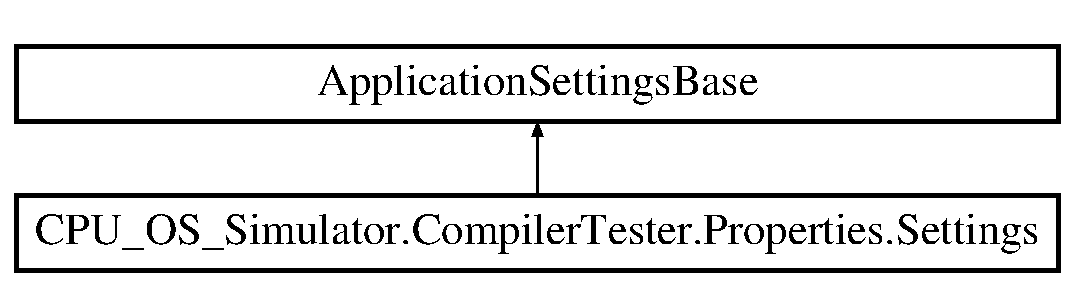
\includegraphics[height=2.000000cm]{class_c_p_u___o_s___simulator_1_1_compiler_tester_1_1_properties_1_1_settings}
\end{center}
\end{figure}
\subsection*{Properties}
\begin{DoxyCompactItemize}
\item 
static \hyperlink{class_c_p_u___o_s___simulator_1_1_compiler_tester_1_1_properties_1_1_settings}{Settings} \hyperlink{class_c_p_u___o_s___simulator_1_1_compiler_tester_1_1_properties_1_1_settings_aee2389b8aff33117b4fe3a30d9440b3c}{Default}\hspace{0.3cm}{\ttfamily  \mbox{[}get\mbox{]}}
\end{DoxyCompactItemize}
\subsection*{Static Private Attributes}
\begin{DoxyCompactItemize}
\item 
static \hyperlink{class_c_p_u___o_s___simulator_1_1_compiler_tester_1_1_properties_1_1_settings}{Settings} \hyperlink{class_c_p_u___o_s___simulator_1_1_compiler_tester_1_1_properties_1_1_settings_ace8d8c1dcebb413495929aa337d5ddd5}{default\+Instance} = ((\hyperlink{class_c_p_u___o_s___simulator_1_1_compiler_tester_1_1_properties_1_1_settings}{Settings})(global\+::\+System.\+Configuration.\+Application\+Settings\+Base.\+Synchronized(new \hyperlink{class_c_p_u___o_s___simulator_1_1_compiler_tester_1_1_properties_1_1_settings}{Settings}())))
\end{DoxyCompactItemize}


\subsection{Detailed Description}


Definition at line 16 of file Settings.\+Designer.\+cs.



\subsection{Member Data Documentation}
\hypertarget{class_c_p_u___o_s___simulator_1_1_compiler_tester_1_1_properties_1_1_settings_ace8d8c1dcebb413495929aa337d5ddd5}{}\index{C\+P\+U\+\_\+\+O\+S\+\_\+\+Simulator\+::\+Compiler\+Tester\+::\+Properties\+::\+Settings@{C\+P\+U\+\_\+\+O\+S\+\_\+\+Simulator\+::\+Compiler\+Tester\+::\+Properties\+::\+Settings}!default\+Instance@{default\+Instance}}
\index{default\+Instance@{default\+Instance}!C\+P\+U\+\_\+\+O\+S\+\_\+\+Simulator\+::\+Compiler\+Tester\+::\+Properties\+::\+Settings@{C\+P\+U\+\_\+\+O\+S\+\_\+\+Simulator\+::\+Compiler\+Tester\+::\+Properties\+::\+Settings}}
\subsubsection[{default\+Instance}]{\setlength{\rightskip}{0pt plus 5cm}{\bf Settings} C\+P\+U\+\_\+\+O\+S\+\_\+\+Simulator.\+Compiler\+Tester.\+Properties.\+Settings.\+default\+Instance = (({\bf Settings})(global\+::\+System.\+Configuration.\+Application\+Settings\+Base.\+Synchronized(new {\bf Settings}())))\hspace{0.3cm}{\ttfamily [static]}, {\ttfamily [private]}}\label{class_c_p_u___o_s___simulator_1_1_compiler_tester_1_1_properties_1_1_settings_ace8d8c1dcebb413495929aa337d5ddd5}


Definition at line 18 of file Settings.\+Designer.\+cs.



\subsection{Property Documentation}
\hypertarget{class_c_p_u___o_s___simulator_1_1_compiler_tester_1_1_properties_1_1_settings_aee2389b8aff33117b4fe3a30d9440b3c}{}\index{C\+P\+U\+\_\+\+O\+S\+\_\+\+Simulator\+::\+Compiler\+Tester\+::\+Properties\+::\+Settings@{C\+P\+U\+\_\+\+O\+S\+\_\+\+Simulator\+::\+Compiler\+Tester\+::\+Properties\+::\+Settings}!Default@{Default}}
\index{Default@{Default}!C\+P\+U\+\_\+\+O\+S\+\_\+\+Simulator\+::\+Compiler\+Tester\+::\+Properties\+::\+Settings@{C\+P\+U\+\_\+\+O\+S\+\_\+\+Simulator\+::\+Compiler\+Tester\+::\+Properties\+::\+Settings}}
\subsubsection[{Default}]{\setlength{\rightskip}{0pt plus 5cm}{\bf Settings} C\+P\+U\+\_\+\+O\+S\+\_\+\+Simulator.\+Compiler\+Tester.\+Properties.\+Settings.\+Default\hspace{0.3cm}{\ttfamily [static]}, {\ttfamily [get]}}\label{class_c_p_u___o_s___simulator_1_1_compiler_tester_1_1_properties_1_1_settings_aee2389b8aff33117b4fe3a30d9440b3c}


Definition at line 20 of file Settings.\+Designer.\+cs.



The documentation for this class was generated from the following file\+:\begin{DoxyCompactItemize}
\item 
Compiler\+Tester/\+Properties/\hyperlink{_compiler_tester_2_properties_2_settings_8_designer_8cs}{Settings.\+Designer.\+cs}\end{DoxyCompactItemize}

\hypertarget{class_c_p_u___o_s___simulator_1_1_properties_1_1_settings}{}\section{C\+P\+U\+\_\+\+O\+S\+\_\+\+Simulator.\+Properties.\+Settings Class Reference}
\label{class_c_p_u___o_s___simulator_1_1_properties_1_1_settings}\index{C\+P\+U\+\_\+\+O\+S\+\_\+\+Simulator.\+Properties.\+Settings@{C\+P\+U\+\_\+\+O\+S\+\_\+\+Simulator.\+Properties.\+Settings}}
Inheritance diagram for C\+P\+U\+\_\+\+O\+S\+\_\+\+Simulator.\+Properties.\+Settings\+:\begin{figure}[H]
\begin{center}
\leavevmode
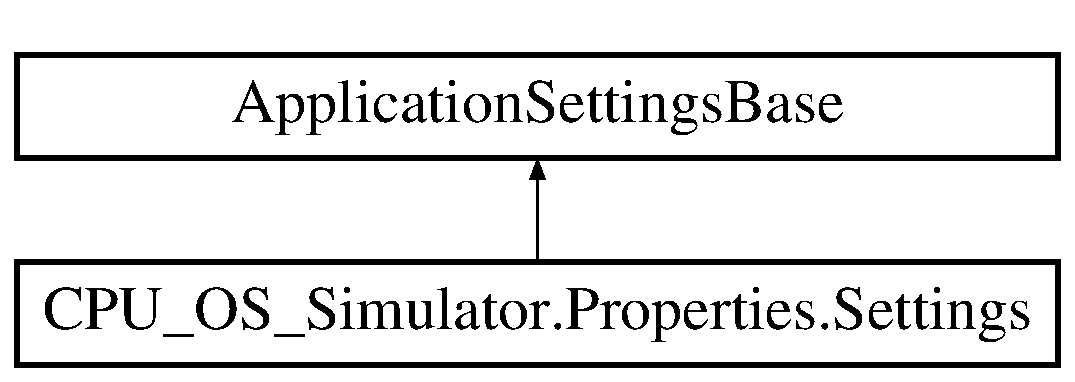
\includegraphics[height=2.000000cm]{class_c_p_u___o_s___simulator_1_1_properties_1_1_settings}
\end{center}
\end{figure}
\subsection*{Properties}
\begin{DoxyCompactItemize}
\item 
static \hyperlink{class_c_p_u___o_s___simulator_1_1_properties_1_1_settings}{Settings} \hyperlink{class_c_p_u___o_s___simulator_1_1_properties_1_1_settings_a423993327c18a4dfede5f73981018fca}{Default}\hspace{0.3cm}{\ttfamily  \mbox{[}get\mbox{]}}
\end{DoxyCompactItemize}
\subsection*{Static Private Attributes}
\begin{DoxyCompactItemize}
\item 
static \hyperlink{class_c_p_u___o_s___simulator_1_1_properties_1_1_settings}{Settings} \hyperlink{class_c_p_u___o_s___simulator_1_1_properties_1_1_settings_a9016562ea46f792bf8dc8d3e79dd36ae}{default\+Instance} = ((\hyperlink{class_c_p_u___o_s___simulator_1_1_properties_1_1_settings}{Settings})(Synchronized(new \hyperlink{class_c_p_u___o_s___simulator_1_1_properties_1_1_settings}{Settings}())))
\end{DoxyCompactItemize}


\subsection{Detailed Description}


Definition at line 20 of file Settings.\+Designer.\+cs.



\subsection{Member Data Documentation}
\hypertarget{class_c_p_u___o_s___simulator_1_1_properties_1_1_settings_a9016562ea46f792bf8dc8d3e79dd36ae}{}\index{C\+P\+U\+\_\+\+O\+S\+\_\+\+Simulator\+::\+Properties\+::\+Settings@{C\+P\+U\+\_\+\+O\+S\+\_\+\+Simulator\+::\+Properties\+::\+Settings}!default\+Instance@{default\+Instance}}
\index{default\+Instance@{default\+Instance}!C\+P\+U\+\_\+\+O\+S\+\_\+\+Simulator\+::\+Properties\+::\+Settings@{C\+P\+U\+\_\+\+O\+S\+\_\+\+Simulator\+::\+Properties\+::\+Settings}}
\subsubsection[{default\+Instance}]{\setlength{\rightskip}{0pt plus 5cm}{\bf Settings} C\+P\+U\+\_\+\+O\+S\+\_\+\+Simulator.\+Properties.\+Settings.\+default\+Instance = (({\bf Settings})(Synchronized(new {\bf Settings}())))\hspace{0.3cm}{\ttfamily [static]}, {\ttfamily [private]}}\label{class_c_p_u___o_s___simulator_1_1_properties_1_1_settings_a9016562ea46f792bf8dc8d3e79dd36ae}


Definition at line 22 of file Settings.\+Designer.\+cs.



\subsection{Property Documentation}
\hypertarget{class_c_p_u___o_s___simulator_1_1_properties_1_1_settings_a423993327c18a4dfede5f73981018fca}{}\index{C\+P\+U\+\_\+\+O\+S\+\_\+\+Simulator\+::\+Properties\+::\+Settings@{C\+P\+U\+\_\+\+O\+S\+\_\+\+Simulator\+::\+Properties\+::\+Settings}!Default@{Default}}
\index{Default@{Default}!C\+P\+U\+\_\+\+O\+S\+\_\+\+Simulator\+::\+Properties\+::\+Settings@{C\+P\+U\+\_\+\+O\+S\+\_\+\+Simulator\+::\+Properties\+::\+Settings}}
\subsubsection[{Default}]{\setlength{\rightskip}{0pt plus 5cm}{\bf Settings} C\+P\+U\+\_\+\+O\+S\+\_\+\+Simulator.\+Properties.\+Settings.\+Default\hspace{0.3cm}{\ttfamily [static]}, {\ttfamily [get]}}\label{class_c_p_u___o_s___simulator_1_1_properties_1_1_settings_a423993327c18a4dfede5f73981018fca}


Definition at line 24 of file Settings.\+Designer.\+cs.



The documentation for this class was generated from the following file\+:\begin{DoxyCompactItemize}
\item 
C\+P\+U-\/\+O\+S Simulator/\+Properties/\hyperlink{_c_p_u-_o_s_01_simulator_2_properties_2_settings_8_designer_8cs}{Settings.\+Designer.\+cs}\end{DoxyCompactItemize}

\hypertarget{class_c_p_u___o_s___simulator_1_1_operating___system_1_1_simulator_process}{}\section{C\+P\+U\+\_\+\+O\+S\+\_\+\+Simulator.\+Operating\+\_\+\+System.\+Simulator\+Process Class Reference}
\label{class_c_p_u___o_s___simulator_1_1_operating___system_1_1_simulator_process}\index{C\+P\+U\+\_\+\+O\+S\+\_\+\+Simulator.\+Operating\+\_\+\+System.\+Simulator\+Process@{C\+P\+U\+\_\+\+O\+S\+\_\+\+Simulator.\+Operating\+\_\+\+System.\+Simulator\+Process}}


This class represents a process that can be run on the virtual operating system  


Inheritance diagram for C\+P\+U\+\_\+\+O\+S\+\_\+\+Simulator.\+Operating\+\_\+\+System.\+Simulator\+Process\+:\begin{figure}[H]
\begin{center}
\leavevmode
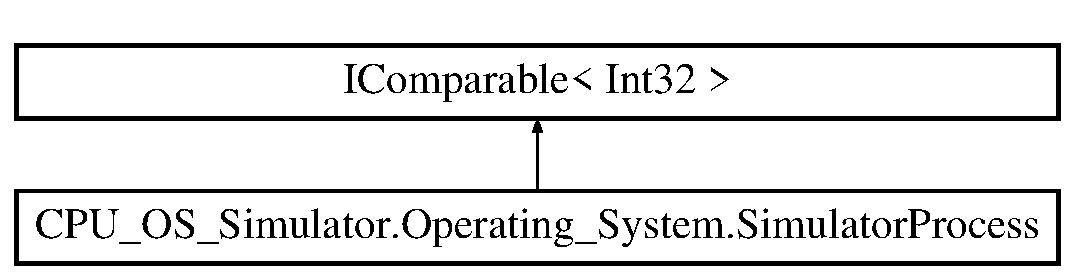
\includegraphics[height=2.000000cm]{class_c_p_u___o_s___simulator_1_1_operating___system_1_1_simulator_process}
\end{center}
\end{figure}
\subsection*{Public Member Functions}
\begin{DoxyCompactItemize}
\item 
\hyperlink{class_c_p_u___o_s___simulator_1_1_operating___system_1_1_simulator_process_a6d9429aba3440d2bde6e8733eeee232f}{Simulator\+Process} ()
\begin{DoxyCompactList}\small\item\em Default Constructor for a process used when deserialising processes N\+O\+T\+E\+: D\+O N\+O\+T U\+S\+E I\+N C\+O\+D\+E \end{DoxyCompactList}\item 
\hyperlink{class_c_p_u___o_s___simulator_1_1_operating___system_1_1_simulator_process_a30b212f64f058e2f2c06936f8f63a492}{Simulator\+Process} (\hyperlink{struct_c_p_u___o_s___simulator_1_1_operating___system_1_1_process_flags}{Process\+Flags} flags)
\begin{DoxyCompactList}\small\item\em Constructor for a process \end{DoxyCompactList}\item 
int \hyperlink{class_c_p_u___o_s___simulator_1_1_operating___system_1_1_simulator_process_a49923ce9c64c06e2cf9720d845246603}{Compare\+To} (int other)
\begin{DoxyCompactList}\small\item\em Compares the current object with another object of the same type. \end{DoxyCompactList}\item 
bool \hyperlink{class_c_p_u___o_s___simulator_1_1_operating___system_1_1_simulator_process_a742a1d9b4aeb3eabc4325ffa6254af23}{is\+Resource\+Starved} ()
\item 
void \hyperlink{class_c_p_u___o_s___simulator_1_1_operating___system_1_1_simulator_process_a5dca50120b8fdbb688040531091e9ac0}{Terminate} ()
\end{DoxyCompactItemize}
\subsection*{Properties}
\begin{DoxyCompactItemize}
\item 
\hyperlink{class_c_p_u___o_s___simulator_1_1_c_p_u_1_1_simulator_program}{Simulator\+Program} \hyperlink{class_c_p_u___o_s___simulator_1_1_operating___system_1_1_simulator_process_a594fe15fec1c942ccfbcfa9c345624ee}{Program}\hspace{0.3cm}{\ttfamily  \mbox{[}get, set\mbox{]}}
\begin{DoxyCompactList}\small\item\em Property for the program that this process represents \end{DoxyCompactList}\item 
\hyperlink{class_c_p_u___o_s___simulator_1_1_operating___system_1_1_simulator_process}{Simulator\+Process} \hyperlink{class_c_p_u___o_s___simulator_1_1_operating___system_1_1_simulator_process_a4af765ee1a2e9390c9de86fd842a8458}{Parent\+Process}\hspace{0.3cm}{\ttfamily  \mbox{[}get, set\mbox{]}}
\begin{DoxyCompactList}\small\item\em Property for this process\textquotesingle{}s parent \end{DoxyCompactList}\item 
List$<$ \hyperlink{class_c_p_u___o_s___simulator_1_1_operating___system_1_1_simulator_process}{Simulator\+Process} $>$ \hyperlink{class_c_p_u___o_s___simulator_1_1_operating___system_1_1_simulator_process_a2bcf12b1ea3ce8c369f53eccf1368277}{Child\+Processes}\hspace{0.3cm}{\ttfamily  \mbox{[}get, set\mbox{]}}
\begin{DoxyCompactList}\small\item\em Property for a list of this process\textquotesingle{}s child processes \end{DoxyCompactList}\item 
string \hyperlink{class_c_p_u___o_s___simulator_1_1_operating___system_1_1_simulator_process_adbe9e17fd9415e4417646309fefbf44b}{Program\+Name}\hspace{0.3cm}{\ttfamily  \mbox{[}get, set\mbox{]}}
\begin{DoxyCompactList}\small\item\em Property for the name of the program that makes up this process \end{DoxyCompactList}\item 
string \hyperlink{class_c_p_u___o_s___simulator_1_1_operating___system_1_1_simulator_process_a8dfd5005352af61610e945094c5369b8}{Process\+Name}\hspace{0.3cm}{\ttfamily  \mbox{[}get, set\mbox{]}}
\begin{DoxyCompactList}\small\item\em Property for the name of this process \end{DoxyCompactList}\item 
int \hyperlink{class_c_p_u___o_s___simulator_1_1_operating___system_1_1_simulator_process_a5f5199c59eeb6696cdff475a3d752b8a}{Process\+Priority}\hspace{0.3cm}{\ttfamily  \mbox{[}get, set\mbox{]}}
\item 
int \hyperlink{class_c_p_u___o_s___simulator_1_1_operating___system_1_1_simulator_process_a2a82c535caf78396aef37d4ba7815408}{Process\+Memory}\hspace{0.3cm}{\ttfamily  \mbox{[}get, set\mbox{]}}
\begin{DoxyCompactList}\small\item\em Property for the amount of memory pages this program has \end{DoxyCompactList}\item 
int \hyperlink{class_c_p_u___o_s___simulator_1_1_operating___system_1_1_simulator_process_a00d2560b1c6641c316da38e262851723}{Process\+I\+D}\hspace{0.3cm}{\ttfamily  \mbox{[}get, set\mbox{]}}
\begin{DoxyCompactList}\small\item\em Property for the unique I\+D of this process \end{DoxyCompactList}\item 
int \hyperlink{class_c_p_u___o_s___simulator_1_1_operating___system_1_1_simulator_process_a2cf3da33b863fc09451e13302e9ae20f}{Parent\+Process\+I\+D}\hspace{0.3cm}{\ttfamily  \mbox{[}get, set\mbox{]}}
\begin{DoxyCompactList}\small\item\em Property for the unique I\+D of the parent process \end{DoxyCompactList}\item 
int \hyperlink{class_c_p_u___o_s___simulator_1_1_operating___system_1_1_simulator_process_afa82367303a9ea2effba290493847605}{Process\+Lifetime}\hspace{0.3cm}{\ttfamily  \mbox{[}get, set\mbox{]}}
\begin{DoxyCompactList}\small\item\em Property For the lifetime of this process \end{DoxyCompactList}\item 
int \hyperlink{class_c_p_u___o_s___simulator_1_1_operating___system_1_1_simulator_process_a5a340d3421e4251b758752de009b7758}{Burst\+Time}\hspace{0.3cm}{\ttfamily  \mbox{[}get, set\mbox{]}}
\begin{DoxyCompactList}\small\item\em Property for the burst time of this process \end{DoxyCompactList}\item 
bool \hyperlink{class_c_p_u___o_s___simulator_1_1_operating___system_1_1_simulator_process_a7886e0890797887fcdd65b6eac62cfc0}{Process\+Swapped}\hspace{0.3cm}{\ttfamily  \mbox{[}get, set\mbox{]}}
\begin{DoxyCompactList}\small\item\em Property for whether this process is swapped out \end{DoxyCompactList}\item 
\hyperlink{namespace_c_p_u___o_s___simulator_1_1_operating___system_a836ee2204e78fcb3a7dd6c3c942b1a24}{Enum\+Process\+State} \hyperlink{class_c_p_u___o_s___simulator_1_1_operating___system_1_1_simulator_process_a388763de47e217fd742858413c5b169f}{Process\+State}\hspace{0.3cm}{\ttfamily  \mbox{[}get, set\mbox{]}}
\begin{DoxyCompactList}\small\item\em Property for the state of this process \end{DoxyCompactList}\item 
int \hyperlink{class_c_p_u___o_s___simulator_1_1_operating___system_1_1_simulator_process_a456868adfff49f66200bb95a7b64a182}{C\+P\+U\+I\+D}\hspace{0.3cm}{\ttfamily  \mbox{[}get, set\mbox{]}}
\item 
bool \hyperlink{class_c_p_u___o_s___simulator_1_1_operating___system_1_1_simulator_process_a6475f63c13feaefb3a5fbfc349ad4f2f}{Resource\+Starved}\hspace{0.3cm}{\ttfamily  \mbox{[}get, set\mbox{]}}
\item 
List$<$ \hyperlink{class_c_p_u___o_s___simulator_1_1_operating___system_1_1_system_resource}{System\+Resource} $>$ \hyperlink{class_c_p_u___o_s___simulator_1_1_operating___system_1_1_simulator_process_aec7c34074384aa76d0687edd65389c95}{Allocated\+Resources}\hspace{0.3cm}{\ttfamily  \mbox{[}get, set\mbox{]}}
\item 
List$<$ \hyperlink{class_c_p_u___o_s___simulator_1_1_operating___system_1_1_system_resource}{System\+Resource} $>$ \hyperlink{class_c_p_u___o_s___simulator_1_1_operating___system_1_1_simulator_process_aa21683a94c1356359917ee67e46bd0fb}{Requested\+Resources}\hspace{0.3cm}{\ttfamily  \mbox{[}get, set\mbox{]}}
\item 
bool \hyperlink{class_c_p_u___o_s___simulator_1_1_operating___system_1_1_simulator_process_a46466d1ba03a308d1aede92e004f8926}{Terminated}\hspace{0.3cm}{\ttfamily  \mbox{[}get, set\mbox{]}}
\item 
\hyperlink{class_c_p_u___o_s___simulator_1_1_operating___system_1_1_process_control_block}{Process\+Control\+Block} \hyperlink{class_c_p_u___o_s___simulator_1_1_operating___system_1_1_simulator_process_a8a79e297abe32002ecbb10e5913155db}{Control\+Block}\hspace{0.3cm}{\ttfamily  \mbox{[}get, set\mbox{]}}
\item 
int \hyperlink{class_c_p_u___o_s___simulator_1_1_operating___system_1_1_simulator_process_aefef06d69f7e70aef73743d2ad3241ee}{O\+S\+I\+D}\hspace{0.3cm}{\ttfamily  \mbox{[}get, set\mbox{]}}
\item 
int \hyperlink{class_c_p_u___o_s___simulator_1_1_operating___system_1_1_simulator_process_acbfe6e6b4d06ecfe4ff6952ceed8994c}{Clock\+Speed}\hspace{0.3cm}{\ttfamily  \mbox{[}get, set\mbox{]}}
\item 
\hyperlink{class_c_p_u___o_s___simulator_1_1_operating___system_1_1_process_execution_unit}{Process\+Execution\+Unit} \hyperlink{class_c_p_u___o_s___simulator_1_1_operating___system_1_1_simulator_process_ab00659160e7658c9d07136a1785c6d64}{Unit}\hspace{0.3cm}{\ttfamily  \mbox{[}get, set\mbox{]}}
\item 
\hyperlink{namespace_c_p_u___o_s___simulator_1_1_operating___system_a0553d0bc2513aec52caa769acf994d5c}{Enum\+Time\+Unit} \hyperlink{class_c_p_u___o_s___simulator_1_1_operating___system_1_1_simulator_process_a66fb700018e537846373d2d37542a02e}{Process\+Lifetime\+Time\+Unit}\hspace{0.3cm}{\ttfamily  \mbox{[}get, set\mbox{]}}
\end{DoxyCompactItemize}
\subsection*{Private Attributes}
\begin{DoxyCompactItemize}
\item 
\hyperlink{class_c_p_u___o_s___simulator_1_1_c_p_u_1_1_simulator_program}{Simulator\+Program} \hyperlink{class_c_p_u___o_s___simulator_1_1_operating___system_1_1_simulator_process_aed4dc26a67cf9f15930f22941484219a}{program}
\item 
string \hyperlink{class_c_p_u___o_s___simulator_1_1_operating___system_1_1_simulator_process_aacd55b65bf86395ae3c1a446d580030e}{program\+Name}
\item 
string \hyperlink{class_c_p_u___o_s___simulator_1_1_operating___system_1_1_simulator_process_a6d29b67977f07ebb1b6336b96960752b}{process\+Name}
\item 
int \hyperlink{class_c_p_u___o_s___simulator_1_1_operating___system_1_1_simulator_process_a122acf698432625719c9ddd0152aab0d}{process\+Priority}
\item 
int \hyperlink{class_c_p_u___o_s___simulator_1_1_operating___system_1_1_simulator_process_af574b021e490c03ed55332ee0ed4c067}{process\+Memory}
\item 
int \hyperlink{class_c_p_u___o_s___simulator_1_1_operating___system_1_1_simulator_process_aa70f97b2b63f49ded3d505d104a1f3d9}{process\+Lifetime}
\item 
\hyperlink{namespace_c_p_u___o_s___simulator_1_1_operating___system_a0553d0bc2513aec52caa769acf994d5c}{Enum\+Time\+Unit} \hyperlink{class_c_p_u___o_s___simulator_1_1_operating___system_1_1_simulator_process_a53aad888e888ff8f9a3999047f14d362}{process\+Lifetime\+Time\+Unit}
\item 
int \hyperlink{class_c_p_u___o_s___simulator_1_1_operating___system_1_1_simulator_process_a1dc38ec3dc556cacd6de21a0ecd5e440}{process\+I\+D}
\item 
int \hyperlink{class_c_p_u___o_s___simulator_1_1_operating___system_1_1_simulator_process_af7c5460498b8fc188df0d4c12b62c15b}{parent\+Process\+I\+D}
\item 
int \hyperlink{class_c_p_u___o_s___simulator_1_1_operating___system_1_1_simulator_process_ae26fd9d2bdc4dc5012260c39f289d4de}{C\+P\+Uid}
\item 
int \hyperlink{class_c_p_u___o_s___simulator_1_1_operating___system_1_1_simulator_process_a1b124e6b0a70221c4739a78d81c89aaf}{O\+Sid}
\item 
int \hyperlink{class_c_p_u___o_s___simulator_1_1_operating___system_1_1_simulator_process_aaa8160807178efd2cb70364dc48a8c70}{burst\+Time}
\item 
bool \hyperlink{class_c_p_u___o_s___simulator_1_1_operating___system_1_1_simulator_process_a7074283e2d023d83df86651f98da7003}{display\+Profile}
\item 
bool \hyperlink{class_c_p_u___o_s___simulator_1_1_operating___system_1_1_simulator_process_a4be3ead7d12ef8390cc2f0a3a0164efa}{parent\+Dies\+Children\+Die}
\item 
bool \hyperlink{class_c_p_u___o_s___simulator_1_1_operating___system_1_1_simulator_process_ab52228f4f5902049430dc58c0c7408c3}{default\+Scheduler}
\item 
bool \hyperlink{class_c_p_u___o_s___simulator_1_1_operating___system_1_1_simulator_process_a1f62a5a6071d0525b8dea84e9205a591}{delayed\+Process}
\item 
int \hyperlink{class_c_p_u___o_s___simulator_1_1_operating___system_1_1_simulator_process_a17a480e988d10e48af5478b5ebe0794d}{delayed\+Process\+Time}
\item 
\hyperlink{namespace_c_p_u___o_s___simulator_1_1_operating___system_a0553d0bc2513aec52caa769acf994d5c}{Enum\+Time\+Unit} \hyperlink{class_c_p_u___o_s___simulator_1_1_operating___system_1_1_simulator_process_aa2ff3f17dc017fb3ad5285e85661ab47}{delay\+Time\+Unit}
\item 
\hyperlink{class_c_p_u___o_s___simulator_1_1_operating___system_1_1_simulator_process}{Simulator\+Process} \hyperlink{class_c_p_u___o_s___simulator_1_1_operating___system_1_1_simulator_process_afd143112dcfa59dbc1cab80f65cf685f}{parent\+Process}
\item 
List$<$ \hyperlink{class_c_p_u___o_s___simulator_1_1_operating___system_1_1_simulator_process}{Simulator\+Process} $>$ \hyperlink{class_c_p_u___o_s___simulator_1_1_operating___system_1_1_simulator_process_a72edfc38a41a74a935147ea8039ea49c}{child\+Processes}
\item 
bool \hyperlink{class_c_p_u___o_s___simulator_1_1_operating___system_1_1_simulator_process_a18f7668d8580b17e1d55bfa124a923cd}{process\+Swapped}
\item 
\hyperlink{namespace_c_p_u___o_s___simulator_1_1_operating___system_a836ee2204e78fcb3a7dd6c3c942b1a24}{Enum\+Process\+State} \hyperlink{class_c_p_u___o_s___simulator_1_1_operating___system_1_1_simulator_process_accb86eff4dc42481372e3d57afbcdad0}{process\+State}
\item 
bool \hyperlink{class_c_p_u___o_s___simulator_1_1_operating___system_1_1_simulator_process_af4d819f0ae416b254b00d1926568b564}{resource\+Starved}
\item 
List$<$ \hyperlink{class_c_p_u___o_s___simulator_1_1_operating___system_1_1_system_resource}{System\+Resource} $>$ \hyperlink{class_c_p_u___o_s___simulator_1_1_operating___system_1_1_simulator_process_af493fe44d2e40001e847ce762f1fac67}{allocated\+Resources}
\item 
List$<$ \hyperlink{class_c_p_u___o_s___simulator_1_1_operating___system_1_1_system_resource}{System\+Resource} $>$ \hyperlink{class_c_p_u___o_s___simulator_1_1_operating___system_1_1_simulator_process_a93e3c24d4342373d6f0192dce851d269}{requested\+Resources}
\item 
bool \hyperlink{class_c_p_u___o_s___simulator_1_1_operating___system_1_1_simulator_process_a692f144a0d21c56d067063d7c0207af1}{terminated}
\item 
\hyperlink{class_c_p_u___o_s___simulator_1_1_operating___system_1_1_process_control_block}{Process\+Control\+Block} \hyperlink{class_c_p_u___o_s___simulator_1_1_operating___system_1_1_simulator_process_a4b3401c13eab41dc43abd449e8961f18}{process\+Control\+Block}
\item 
int \hyperlink{class_c_p_u___o_s___simulator_1_1_operating___system_1_1_simulator_process_acb5b4680ab904693eb4b519c9f5e5e6e}{clock\+Speed}
\item 
\hyperlink{class_c_p_u___o_s___simulator_1_1_operating___system_1_1_process_execution_unit}{Process\+Execution\+Unit} \hyperlink{class_c_p_u___o_s___simulator_1_1_operating___system_1_1_simulator_process_a8e6c1d85ab2ff692572774c7590e5916}{unit}
\end{DoxyCompactItemize}


\subsection{Detailed Description}
This class represents a process that can be run on the virtual operating system 



Definition at line 11 of file Simulator\+Process.\+cs.



\subsection{Constructor \& Destructor Documentation}
\hypertarget{class_c_p_u___o_s___simulator_1_1_operating___system_1_1_simulator_process_a6d9429aba3440d2bde6e8733eeee232f}{}\index{C\+P\+U\+\_\+\+O\+S\+\_\+\+Simulator\+::\+Operating\+\_\+\+System\+::\+Simulator\+Process@{C\+P\+U\+\_\+\+O\+S\+\_\+\+Simulator\+::\+Operating\+\_\+\+System\+::\+Simulator\+Process}!Simulator\+Process@{Simulator\+Process}}
\index{Simulator\+Process@{Simulator\+Process}!C\+P\+U\+\_\+\+O\+S\+\_\+\+Simulator\+::\+Operating\+\_\+\+System\+::\+Simulator\+Process@{C\+P\+U\+\_\+\+O\+S\+\_\+\+Simulator\+::\+Operating\+\_\+\+System\+::\+Simulator\+Process}}
\subsubsection[{Simulator\+Process()}]{\setlength{\rightskip}{0pt plus 5cm}C\+P\+U\+\_\+\+O\+S\+\_\+\+Simulator.\+Operating\+\_\+\+System.\+Simulator\+Process.\+Simulator\+Process (
\begin{DoxyParamCaption}
{}
\end{DoxyParamCaption}
)}\label{class_c_p_u___o_s___simulator_1_1_operating___system_1_1_simulator_process_a6d9429aba3440d2bde6e8733eeee232f}


Default Constructor for a process used when deserialising processes N\+O\+T\+E\+: D\+O N\+O\+T U\+S\+E I\+N C\+O\+D\+E 



Definition at line 47 of file Simulator\+Process.\+cs.

\hypertarget{class_c_p_u___o_s___simulator_1_1_operating___system_1_1_simulator_process_a30b212f64f058e2f2c06936f8f63a492}{}\index{C\+P\+U\+\_\+\+O\+S\+\_\+\+Simulator\+::\+Operating\+\_\+\+System\+::\+Simulator\+Process@{C\+P\+U\+\_\+\+O\+S\+\_\+\+Simulator\+::\+Operating\+\_\+\+System\+::\+Simulator\+Process}!Simulator\+Process@{Simulator\+Process}}
\index{Simulator\+Process@{Simulator\+Process}!C\+P\+U\+\_\+\+O\+S\+\_\+\+Simulator\+::\+Operating\+\_\+\+System\+::\+Simulator\+Process@{C\+P\+U\+\_\+\+O\+S\+\_\+\+Simulator\+::\+Operating\+\_\+\+System\+::\+Simulator\+Process}}
\subsubsection[{Simulator\+Process(\+Process\+Flags flags)}]{\setlength{\rightskip}{0pt plus 5cm}C\+P\+U\+\_\+\+O\+S\+\_\+\+Simulator.\+Operating\+\_\+\+System.\+Simulator\+Process.\+Simulator\+Process (
\begin{DoxyParamCaption}
\item[{{\bf Process\+Flags}}]{flags}
\end{DoxyParamCaption}
)}\label{class_c_p_u___o_s___simulator_1_1_operating___system_1_1_simulator_process_a30b212f64f058e2f2c06936f8f63a492}


Constructor for a process 


\begin{DoxyParams}{Parameters}
{\em flags} & the flags to create this process with\\
\hline
\end{DoxyParams}


Definition at line 55 of file Simulator\+Process.\+cs.



\subsection{Member Function Documentation}
\hypertarget{class_c_p_u___o_s___simulator_1_1_operating___system_1_1_simulator_process_a49923ce9c64c06e2cf9720d845246603}{}\index{C\+P\+U\+\_\+\+O\+S\+\_\+\+Simulator\+::\+Operating\+\_\+\+System\+::\+Simulator\+Process@{C\+P\+U\+\_\+\+O\+S\+\_\+\+Simulator\+::\+Operating\+\_\+\+System\+::\+Simulator\+Process}!Compare\+To@{Compare\+To}}
\index{Compare\+To@{Compare\+To}!C\+P\+U\+\_\+\+O\+S\+\_\+\+Simulator\+::\+Operating\+\_\+\+System\+::\+Simulator\+Process@{C\+P\+U\+\_\+\+O\+S\+\_\+\+Simulator\+::\+Operating\+\_\+\+System\+::\+Simulator\+Process}}
\subsubsection[{Compare\+To(int other)}]{\setlength{\rightskip}{0pt plus 5cm}int C\+P\+U\+\_\+\+O\+S\+\_\+\+Simulator.\+Operating\+\_\+\+System.\+Simulator\+Process.\+Compare\+To (
\begin{DoxyParamCaption}
\item[{int}]{other}
\end{DoxyParamCaption}
)}\label{class_c_p_u___o_s___simulator_1_1_operating___system_1_1_simulator_process_a49923ce9c64c06e2cf9720d845246603}


Compares the current object with another object of the same type. 

\begin{DoxyReturn}{Returns}
A value that indicates the relative order of the objects being compared. The return value has the following meanings\+: Value Meaning Less than zero This object is less than the {\itshape other}  parameter.\+Zero This object is equal to {\itshape other} . Greater than zero This object is greater than {\itshape other} . 
\end{DoxyReturn}

\begin{DoxyParams}{Parameters}
{\em other} & An object to compare with this object.\\
\hline
\end{DoxyParams}


Definition at line 267 of file Simulator\+Process.\+cs.

\hypertarget{class_c_p_u___o_s___simulator_1_1_operating___system_1_1_simulator_process_a742a1d9b4aeb3eabc4325ffa6254af23}{}\index{C\+P\+U\+\_\+\+O\+S\+\_\+\+Simulator\+::\+Operating\+\_\+\+System\+::\+Simulator\+Process@{C\+P\+U\+\_\+\+O\+S\+\_\+\+Simulator\+::\+Operating\+\_\+\+System\+::\+Simulator\+Process}!is\+Resource\+Starved@{is\+Resource\+Starved}}
\index{is\+Resource\+Starved@{is\+Resource\+Starved}!C\+P\+U\+\_\+\+O\+S\+\_\+\+Simulator\+::\+Operating\+\_\+\+System\+::\+Simulator\+Process@{C\+P\+U\+\_\+\+O\+S\+\_\+\+Simulator\+::\+Operating\+\_\+\+System\+::\+Simulator\+Process}}
\subsubsection[{is\+Resource\+Starved()}]{\setlength{\rightskip}{0pt plus 5cm}bool C\+P\+U\+\_\+\+O\+S\+\_\+\+Simulator.\+Operating\+\_\+\+System.\+Simulator\+Process.\+is\+Resource\+Starved (
\begin{DoxyParamCaption}
{}
\end{DoxyParamCaption}
)}\label{class_c_p_u___o_s___simulator_1_1_operating___system_1_1_simulator_process_a742a1d9b4aeb3eabc4325ffa6254af23}


Definition at line 284 of file Simulator\+Process.\+cs.

\hypertarget{class_c_p_u___o_s___simulator_1_1_operating___system_1_1_simulator_process_a5dca50120b8fdbb688040531091e9ac0}{}\index{C\+P\+U\+\_\+\+O\+S\+\_\+\+Simulator\+::\+Operating\+\_\+\+System\+::\+Simulator\+Process@{C\+P\+U\+\_\+\+O\+S\+\_\+\+Simulator\+::\+Operating\+\_\+\+System\+::\+Simulator\+Process}!Terminate@{Terminate}}
\index{Terminate@{Terminate}!C\+P\+U\+\_\+\+O\+S\+\_\+\+Simulator\+::\+Operating\+\_\+\+System\+::\+Simulator\+Process@{C\+P\+U\+\_\+\+O\+S\+\_\+\+Simulator\+::\+Operating\+\_\+\+System\+::\+Simulator\+Process}}
\subsubsection[{Terminate()}]{\setlength{\rightskip}{0pt plus 5cm}void C\+P\+U\+\_\+\+O\+S\+\_\+\+Simulator.\+Operating\+\_\+\+System.\+Simulator\+Process.\+Terminate (
\begin{DoxyParamCaption}
{}
\end{DoxyParamCaption}
)}\label{class_c_p_u___o_s___simulator_1_1_operating___system_1_1_simulator_process_a5dca50120b8fdbb688040531091e9ac0}


Definition at line 294 of file Simulator\+Process.\+cs.



\subsection{Member Data Documentation}
\hypertarget{class_c_p_u___o_s___simulator_1_1_operating___system_1_1_simulator_process_af493fe44d2e40001e847ce762f1fac67}{}\index{C\+P\+U\+\_\+\+O\+S\+\_\+\+Simulator\+::\+Operating\+\_\+\+System\+::\+Simulator\+Process@{C\+P\+U\+\_\+\+O\+S\+\_\+\+Simulator\+::\+Operating\+\_\+\+System\+::\+Simulator\+Process}!allocated\+Resources@{allocated\+Resources}}
\index{allocated\+Resources@{allocated\+Resources}!C\+P\+U\+\_\+\+O\+S\+\_\+\+Simulator\+::\+Operating\+\_\+\+System\+::\+Simulator\+Process@{C\+P\+U\+\_\+\+O\+S\+\_\+\+Simulator\+::\+Operating\+\_\+\+System\+::\+Simulator\+Process}}
\subsubsection[{allocated\+Resources}]{\setlength{\rightskip}{0pt plus 5cm}List$<${\bf System\+Resource}$>$ C\+P\+U\+\_\+\+O\+S\+\_\+\+Simulator.\+Operating\+\_\+\+System.\+Simulator\+Process.\+allocated\+Resources\hspace{0.3cm}{\ttfamily [private]}}\label{class_c_p_u___o_s___simulator_1_1_operating___system_1_1_simulator_process_af493fe44d2e40001e847ce762f1fac67}


Definition at line 36 of file Simulator\+Process.\+cs.

\hypertarget{class_c_p_u___o_s___simulator_1_1_operating___system_1_1_simulator_process_aaa8160807178efd2cb70364dc48a8c70}{}\index{C\+P\+U\+\_\+\+O\+S\+\_\+\+Simulator\+::\+Operating\+\_\+\+System\+::\+Simulator\+Process@{C\+P\+U\+\_\+\+O\+S\+\_\+\+Simulator\+::\+Operating\+\_\+\+System\+::\+Simulator\+Process}!burst\+Time@{burst\+Time}}
\index{burst\+Time@{burst\+Time}!C\+P\+U\+\_\+\+O\+S\+\_\+\+Simulator\+::\+Operating\+\_\+\+System\+::\+Simulator\+Process@{C\+P\+U\+\_\+\+O\+S\+\_\+\+Simulator\+::\+Operating\+\_\+\+System\+::\+Simulator\+Process}}
\subsubsection[{burst\+Time}]{\setlength{\rightskip}{0pt plus 5cm}int C\+P\+U\+\_\+\+O\+S\+\_\+\+Simulator.\+Operating\+\_\+\+System.\+Simulator\+Process.\+burst\+Time\hspace{0.3cm}{\ttfamily [private]}}\label{class_c_p_u___o_s___simulator_1_1_operating___system_1_1_simulator_process_aaa8160807178efd2cb70364dc48a8c70}


Definition at line 24 of file Simulator\+Process.\+cs.

\hypertarget{class_c_p_u___o_s___simulator_1_1_operating___system_1_1_simulator_process_a72edfc38a41a74a935147ea8039ea49c}{}\index{C\+P\+U\+\_\+\+O\+S\+\_\+\+Simulator\+::\+Operating\+\_\+\+System\+::\+Simulator\+Process@{C\+P\+U\+\_\+\+O\+S\+\_\+\+Simulator\+::\+Operating\+\_\+\+System\+::\+Simulator\+Process}!child\+Processes@{child\+Processes}}
\index{child\+Processes@{child\+Processes}!C\+P\+U\+\_\+\+O\+S\+\_\+\+Simulator\+::\+Operating\+\_\+\+System\+::\+Simulator\+Process@{C\+P\+U\+\_\+\+O\+S\+\_\+\+Simulator\+::\+Operating\+\_\+\+System\+::\+Simulator\+Process}}
\subsubsection[{child\+Processes}]{\setlength{\rightskip}{0pt plus 5cm}List$<${\bf Simulator\+Process}$>$ C\+P\+U\+\_\+\+O\+S\+\_\+\+Simulator.\+Operating\+\_\+\+System.\+Simulator\+Process.\+child\+Processes\hspace{0.3cm}{\ttfamily [private]}}\label{class_c_p_u___o_s___simulator_1_1_operating___system_1_1_simulator_process_a72edfc38a41a74a935147ea8039ea49c}


Definition at line 32 of file Simulator\+Process.\+cs.

\hypertarget{class_c_p_u___o_s___simulator_1_1_operating___system_1_1_simulator_process_acb5b4680ab904693eb4b519c9f5e5e6e}{}\index{C\+P\+U\+\_\+\+O\+S\+\_\+\+Simulator\+::\+Operating\+\_\+\+System\+::\+Simulator\+Process@{C\+P\+U\+\_\+\+O\+S\+\_\+\+Simulator\+::\+Operating\+\_\+\+System\+::\+Simulator\+Process}!clock\+Speed@{clock\+Speed}}
\index{clock\+Speed@{clock\+Speed}!C\+P\+U\+\_\+\+O\+S\+\_\+\+Simulator\+::\+Operating\+\_\+\+System\+::\+Simulator\+Process@{C\+P\+U\+\_\+\+O\+S\+\_\+\+Simulator\+::\+Operating\+\_\+\+System\+::\+Simulator\+Process}}
\subsubsection[{clock\+Speed}]{\setlength{\rightskip}{0pt plus 5cm}int C\+P\+U\+\_\+\+O\+S\+\_\+\+Simulator.\+Operating\+\_\+\+System.\+Simulator\+Process.\+clock\+Speed\hspace{0.3cm}{\ttfamily [private]}}\label{class_c_p_u___o_s___simulator_1_1_operating___system_1_1_simulator_process_acb5b4680ab904693eb4b519c9f5e5e6e}


Definition at line 40 of file Simulator\+Process.\+cs.

\hypertarget{class_c_p_u___o_s___simulator_1_1_operating___system_1_1_simulator_process_ae26fd9d2bdc4dc5012260c39f289d4de}{}\index{C\+P\+U\+\_\+\+O\+S\+\_\+\+Simulator\+::\+Operating\+\_\+\+System\+::\+Simulator\+Process@{C\+P\+U\+\_\+\+O\+S\+\_\+\+Simulator\+::\+Operating\+\_\+\+System\+::\+Simulator\+Process}!C\+P\+Uid@{C\+P\+Uid}}
\index{C\+P\+Uid@{C\+P\+Uid}!C\+P\+U\+\_\+\+O\+S\+\_\+\+Simulator\+::\+Operating\+\_\+\+System\+::\+Simulator\+Process@{C\+P\+U\+\_\+\+O\+S\+\_\+\+Simulator\+::\+Operating\+\_\+\+System\+::\+Simulator\+Process}}
\subsubsection[{C\+P\+Uid}]{\setlength{\rightskip}{0pt plus 5cm}int C\+P\+U\+\_\+\+O\+S\+\_\+\+Simulator.\+Operating\+\_\+\+System.\+Simulator\+Process.\+C\+P\+Uid\hspace{0.3cm}{\ttfamily [private]}}\label{class_c_p_u___o_s___simulator_1_1_operating___system_1_1_simulator_process_ae26fd9d2bdc4dc5012260c39f289d4de}


Definition at line 22 of file Simulator\+Process.\+cs.

\hypertarget{class_c_p_u___o_s___simulator_1_1_operating___system_1_1_simulator_process_ab52228f4f5902049430dc58c0c7408c3}{}\index{C\+P\+U\+\_\+\+O\+S\+\_\+\+Simulator\+::\+Operating\+\_\+\+System\+::\+Simulator\+Process@{C\+P\+U\+\_\+\+O\+S\+\_\+\+Simulator\+::\+Operating\+\_\+\+System\+::\+Simulator\+Process}!default\+Scheduler@{default\+Scheduler}}
\index{default\+Scheduler@{default\+Scheduler}!C\+P\+U\+\_\+\+O\+S\+\_\+\+Simulator\+::\+Operating\+\_\+\+System\+::\+Simulator\+Process@{C\+P\+U\+\_\+\+O\+S\+\_\+\+Simulator\+::\+Operating\+\_\+\+System\+::\+Simulator\+Process}}
\subsubsection[{default\+Scheduler}]{\setlength{\rightskip}{0pt plus 5cm}bool C\+P\+U\+\_\+\+O\+S\+\_\+\+Simulator.\+Operating\+\_\+\+System.\+Simulator\+Process.\+default\+Scheduler\hspace{0.3cm}{\ttfamily [private]}}\label{class_c_p_u___o_s___simulator_1_1_operating___system_1_1_simulator_process_ab52228f4f5902049430dc58c0c7408c3}


Definition at line 27 of file Simulator\+Process.\+cs.

\hypertarget{class_c_p_u___o_s___simulator_1_1_operating___system_1_1_simulator_process_a1f62a5a6071d0525b8dea84e9205a591}{}\index{C\+P\+U\+\_\+\+O\+S\+\_\+\+Simulator\+::\+Operating\+\_\+\+System\+::\+Simulator\+Process@{C\+P\+U\+\_\+\+O\+S\+\_\+\+Simulator\+::\+Operating\+\_\+\+System\+::\+Simulator\+Process}!delayed\+Process@{delayed\+Process}}
\index{delayed\+Process@{delayed\+Process}!C\+P\+U\+\_\+\+O\+S\+\_\+\+Simulator\+::\+Operating\+\_\+\+System\+::\+Simulator\+Process@{C\+P\+U\+\_\+\+O\+S\+\_\+\+Simulator\+::\+Operating\+\_\+\+System\+::\+Simulator\+Process}}
\subsubsection[{delayed\+Process}]{\setlength{\rightskip}{0pt plus 5cm}bool C\+P\+U\+\_\+\+O\+S\+\_\+\+Simulator.\+Operating\+\_\+\+System.\+Simulator\+Process.\+delayed\+Process\hspace{0.3cm}{\ttfamily [private]}}\label{class_c_p_u___o_s___simulator_1_1_operating___system_1_1_simulator_process_a1f62a5a6071d0525b8dea84e9205a591}


Definition at line 28 of file Simulator\+Process.\+cs.

\hypertarget{class_c_p_u___o_s___simulator_1_1_operating___system_1_1_simulator_process_a17a480e988d10e48af5478b5ebe0794d}{}\index{C\+P\+U\+\_\+\+O\+S\+\_\+\+Simulator\+::\+Operating\+\_\+\+System\+::\+Simulator\+Process@{C\+P\+U\+\_\+\+O\+S\+\_\+\+Simulator\+::\+Operating\+\_\+\+System\+::\+Simulator\+Process}!delayed\+Process\+Time@{delayed\+Process\+Time}}
\index{delayed\+Process\+Time@{delayed\+Process\+Time}!C\+P\+U\+\_\+\+O\+S\+\_\+\+Simulator\+::\+Operating\+\_\+\+System\+::\+Simulator\+Process@{C\+P\+U\+\_\+\+O\+S\+\_\+\+Simulator\+::\+Operating\+\_\+\+System\+::\+Simulator\+Process}}
\subsubsection[{delayed\+Process\+Time}]{\setlength{\rightskip}{0pt plus 5cm}int C\+P\+U\+\_\+\+O\+S\+\_\+\+Simulator.\+Operating\+\_\+\+System.\+Simulator\+Process.\+delayed\+Process\+Time\hspace{0.3cm}{\ttfamily [private]}}\label{class_c_p_u___o_s___simulator_1_1_operating___system_1_1_simulator_process_a17a480e988d10e48af5478b5ebe0794d}


Definition at line 29 of file Simulator\+Process.\+cs.

\hypertarget{class_c_p_u___o_s___simulator_1_1_operating___system_1_1_simulator_process_aa2ff3f17dc017fb3ad5285e85661ab47}{}\index{C\+P\+U\+\_\+\+O\+S\+\_\+\+Simulator\+::\+Operating\+\_\+\+System\+::\+Simulator\+Process@{C\+P\+U\+\_\+\+O\+S\+\_\+\+Simulator\+::\+Operating\+\_\+\+System\+::\+Simulator\+Process}!delay\+Time\+Unit@{delay\+Time\+Unit}}
\index{delay\+Time\+Unit@{delay\+Time\+Unit}!C\+P\+U\+\_\+\+O\+S\+\_\+\+Simulator\+::\+Operating\+\_\+\+System\+::\+Simulator\+Process@{C\+P\+U\+\_\+\+O\+S\+\_\+\+Simulator\+::\+Operating\+\_\+\+System\+::\+Simulator\+Process}}
\subsubsection[{delay\+Time\+Unit}]{\setlength{\rightskip}{0pt plus 5cm}{\bf Enum\+Time\+Unit} C\+P\+U\+\_\+\+O\+S\+\_\+\+Simulator.\+Operating\+\_\+\+System.\+Simulator\+Process.\+delay\+Time\+Unit\hspace{0.3cm}{\ttfamily [private]}}\label{class_c_p_u___o_s___simulator_1_1_operating___system_1_1_simulator_process_aa2ff3f17dc017fb3ad5285e85661ab47}


Definition at line 30 of file Simulator\+Process.\+cs.

\hypertarget{class_c_p_u___o_s___simulator_1_1_operating___system_1_1_simulator_process_a7074283e2d023d83df86651f98da7003}{}\index{C\+P\+U\+\_\+\+O\+S\+\_\+\+Simulator\+::\+Operating\+\_\+\+System\+::\+Simulator\+Process@{C\+P\+U\+\_\+\+O\+S\+\_\+\+Simulator\+::\+Operating\+\_\+\+System\+::\+Simulator\+Process}!display\+Profile@{display\+Profile}}
\index{display\+Profile@{display\+Profile}!C\+P\+U\+\_\+\+O\+S\+\_\+\+Simulator\+::\+Operating\+\_\+\+System\+::\+Simulator\+Process@{C\+P\+U\+\_\+\+O\+S\+\_\+\+Simulator\+::\+Operating\+\_\+\+System\+::\+Simulator\+Process}}
\subsubsection[{display\+Profile}]{\setlength{\rightskip}{0pt plus 5cm}bool C\+P\+U\+\_\+\+O\+S\+\_\+\+Simulator.\+Operating\+\_\+\+System.\+Simulator\+Process.\+display\+Profile\hspace{0.3cm}{\ttfamily [private]}}\label{class_c_p_u___o_s___simulator_1_1_operating___system_1_1_simulator_process_a7074283e2d023d83df86651f98da7003}


Definition at line 25 of file Simulator\+Process.\+cs.

\hypertarget{class_c_p_u___o_s___simulator_1_1_operating___system_1_1_simulator_process_a1b124e6b0a70221c4739a78d81c89aaf}{}\index{C\+P\+U\+\_\+\+O\+S\+\_\+\+Simulator\+::\+Operating\+\_\+\+System\+::\+Simulator\+Process@{C\+P\+U\+\_\+\+O\+S\+\_\+\+Simulator\+::\+Operating\+\_\+\+System\+::\+Simulator\+Process}!O\+Sid@{O\+Sid}}
\index{O\+Sid@{O\+Sid}!C\+P\+U\+\_\+\+O\+S\+\_\+\+Simulator\+::\+Operating\+\_\+\+System\+::\+Simulator\+Process@{C\+P\+U\+\_\+\+O\+S\+\_\+\+Simulator\+::\+Operating\+\_\+\+System\+::\+Simulator\+Process}}
\subsubsection[{O\+Sid}]{\setlength{\rightskip}{0pt plus 5cm}int C\+P\+U\+\_\+\+O\+S\+\_\+\+Simulator.\+Operating\+\_\+\+System.\+Simulator\+Process.\+O\+Sid\hspace{0.3cm}{\ttfamily [private]}}\label{class_c_p_u___o_s___simulator_1_1_operating___system_1_1_simulator_process_a1b124e6b0a70221c4739a78d81c89aaf}


Definition at line 23 of file Simulator\+Process.\+cs.

\hypertarget{class_c_p_u___o_s___simulator_1_1_operating___system_1_1_simulator_process_a4be3ead7d12ef8390cc2f0a3a0164efa}{}\index{C\+P\+U\+\_\+\+O\+S\+\_\+\+Simulator\+::\+Operating\+\_\+\+System\+::\+Simulator\+Process@{C\+P\+U\+\_\+\+O\+S\+\_\+\+Simulator\+::\+Operating\+\_\+\+System\+::\+Simulator\+Process}!parent\+Dies\+Children\+Die@{parent\+Dies\+Children\+Die}}
\index{parent\+Dies\+Children\+Die@{parent\+Dies\+Children\+Die}!C\+P\+U\+\_\+\+O\+S\+\_\+\+Simulator\+::\+Operating\+\_\+\+System\+::\+Simulator\+Process@{C\+P\+U\+\_\+\+O\+S\+\_\+\+Simulator\+::\+Operating\+\_\+\+System\+::\+Simulator\+Process}}
\subsubsection[{parent\+Dies\+Children\+Die}]{\setlength{\rightskip}{0pt plus 5cm}bool C\+P\+U\+\_\+\+O\+S\+\_\+\+Simulator.\+Operating\+\_\+\+System.\+Simulator\+Process.\+parent\+Dies\+Children\+Die\hspace{0.3cm}{\ttfamily [private]}}\label{class_c_p_u___o_s___simulator_1_1_operating___system_1_1_simulator_process_a4be3ead7d12ef8390cc2f0a3a0164efa}


Definition at line 26 of file Simulator\+Process.\+cs.

\hypertarget{class_c_p_u___o_s___simulator_1_1_operating___system_1_1_simulator_process_afd143112dcfa59dbc1cab80f65cf685f}{}\index{C\+P\+U\+\_\+\+O\+S\+\_\+\+Simulator\+::\+Operating\+\_\+\+System\+::\+Simulator\+Process@{C\+P\+U\+\_\+\+O\+S\+\_\+\+Simulator\+::\+Operating\+\_\+\+System\+::\+Simulator\+Process}!parent\+Process@{parent\+Process}}
\index{parent\+Process@{parent\+Process}!C\+P\+U\+\_\+\+O\+S\+\_\+\+Simulator\+::\+Operating\+\_\+\+System\+::\+Simulator\+Process@{C\+P\+U\+\_\+\+O\+S\+\_\+\+Simulator\+::\+Operating\+\_\+\+System\+::\+Simulator\+Process}}
\subsubsection[{parent\+Process}]{\setlength{\rightskip}{0pt plus 5cm}{\bf Simulator\+Process} C\+P\+U\+\_\+\+O\+S\+\_\+\+Simulator.\+Operating\+\_\+\+System.\+Simulator\+Process.\+parent\+Process\hspace{0.3cm}{\ttfamily [private]}}\label{class_c_p_u___o_s___simulator_1_1_operating___system_1_1_simulator_process_afd143112dcfa59dbc1cab80f65cf685f}


Definition at line 31 of file Simulator\+Process.\+cs.

\hypertarget{class_c_p_u___o_s___simulator_1_1_operating___system_1_1_simulator_process_af7c5460498b8fc188df0d4c12b62c15b}{}\index{C\+P\+U\+\_\+\+O\+S\+\_\+\+Simulator\+::\+Operating\+\_\+\+System\+::\+Simulator\+Process@{C\+P\+U\+\_\+\+O\+S\+\_\+\+Simulator\+::\+Operating\+\_\+\+System\+::\+Simulator\+Process}!parent\+Process\+I\+D@{parent\+Process\+I\+D}}
\index{parent\+Process\+I\+D@{parent\+Process\+I\+D}!C\+P\+U\+\_\+\+O\+S\+\_\+\+Simulator\+::\+Operating\+\_\+\+System\+::\+Simulator\+Process@{C\+P\+U\+\_\+\+O\+S\+\_\+\+Simulator\+::\+Operating\+\_\+\+System\+::\+Simulator\+Process}}
\subsubsection[{parent\+Process\+I\+D}]{\setlength{\rightskip}{0pt plus 5cm}int C\+P\+U\+\_\+\+O\+S\+\_\+\+Simulator.\+Operating\+\_\+\+System.\+Simulator\+Process.\+parent\+Process\+I\+D\hspace{0.3cm}{\ttfamily [private]}}\label{class_c_p_u___o_s___simulator_1_1_operating___system_1_1_simulator_process_af7c5460498b8fc188df0d4c12b62c15b}


Definition at line 21 of file Simulator\+Process.\+cs.

\hypertarget{class_c_p_u___o_s___simulator_1_1_operating___system_1_1_simulator_process_a4b3401c13eab41dc43abd449e8961f18}{}\index{C\+P\+U\+\_\+\+O\+S\+\_\+\+Simulator\+::\+Operating\+\_\+\+System\+::\+Simulator\+Process@{C\+P\+U\+\_\+\+O\+S\+\_\+\+Simulator\+::\+Operating\+\_\+\+System\+::\+Simulator\+Process}!process\+Control\+Block@{process\+Control\+Block}}
\index{process\+Control\+Block@{process\+Control\+Block}!C\+P\+U\+\_\+\+O\+S\+\_\+\+Simulator\+::\+Operating\+\_\+\+System\+::\+Simulator\+Process@{C\+P\+U\+\_\+\+O\+S\+\_\+\+Simulator\+::\+Operating\+\_\+\+System\+::\+Simulator\+Process}}
\subsubsection[{process\+Control\+Block}]{\setlength{\rightskip}{0pt plus 5cm}{\bf Process\+Control\+Block} C\+P\+U\+\_\+\+O\+S\+\_\+\+Simulator.\+Operating\+\_\+\+System.\+Simulator\+Process.\+process\+Control\+Block\hspace{0.3cm}{\ttfamily [private]}}\label{class_c_p_u___o_s___simulator_1_1_operating___system_1_1_simulator_process_a4b3401c13eab41dc43abd449e8961f18}


Definition at line 39 of file Simulator\+Process.\+cs.

\hypertarget{class_c_p_u___o_s___simulator_1_1_operating___system_1_1_simulator_process_a1dc38ec3dc556cacd6de21a0ecd5e440}{}\index{C\+P\+U\+\_\+\+O\+S\+\_\+\+Simulator\+::\+Operating\+\_\+\+System\+::\+Simulator\+Process@{C\+P\+U\+\_\+\+O\+S\+\_\+\+Simulator\+::\+Operating\+\_\+\+System\+::\+Simulator\+Process}!process\+I\+D@{process\+I\+D}}
\index{process\+I\+D@{process\+I\+D}!C\+P\+U\+\_\+\+O\+S\+\_\+\+Simulator\+::\+Operating\+\_\+\+System\+::\+Simulator\+Process@{C\+P\+U\+\_\+\+O\+S\+\_\+\+Simulator\+::\+Operating\+\_\+\+System\+::\+Simulator\+Process}}
\subsubsection[{process\+I\+D}]{\setlength{\rightskip}{0pt plus 5cm}int C\+P\+U\+\_\+\+O\+S\+\_\+\+Simulator.\+Operating\+\_\+\+System.\+Simulator\+Process.\+process\+I\+D\hspace{0.3cm}{\ttfamily [private]}}\label{class_c_p_u___o_s___simulator_1_1_operating___system_1_1_simulator_process_a1dc38ec3dc556cacd6de21a0ecd5e440}


Definition at line 20 of file Simulator\+Process.\+cs.

\hypertarget{class_c_p_u___o_s___simulator_1_1_operating___system_1_1_simulator_process_aa70f97b2b63f49ded3d505d104a1f3d9}{}\index{C\+P\+U\+\_\+\+O\+S\+\_\+\+Simulator\+::\+Operating\+\_\+\+System\+::\+Simulator\+Process@{C\+P\+U\+\_\+\+O\+S\+\_\+\+Simulator\+::\+Operating\+\_\+\+System\+::\+Simulator\+Process}!process\+Lifetime@{process\+Lifetime}}
\index{process\+Lifetime@{process\+Lifetime}!C\+P\+U\+\_\+\+O\+S\+\_\+\+Simulator\+::\+Operating\+\_\+\+System\+::\+Simulator\+Process@{C\+P\+U\+\_\+\+O\+S\+\_\+\+Simulator\+::\+Operating\+\_\+\+System\+::\+Simulator\+Process}}
\subsubsection[{process\+Lifetime}]{\setlength{\rightskip}{0pt plus 5cm}int C\+P\+U\+\_\+\+O\+S\+\_\+\+Simulator.\+Operating\+\_\+\+System.\+Simulator\+Process.\+process\+Lifetime\hspace{0.3cm}{\ttfamily [private]}}\label{class_c_p_u___o_s___simulator_1_1_operating___system_1_1_simulator_process_aa70f97b2b63f49ded3d505d104a1f3d9}


Definition at line 18 of file Simulator\+Process.\+cs.

\hypertarget{class_c_p_u___o_s___simulator_1_1_operating___system_1_1_simulator_process_a53aad888e888ff8f9a3999047f14d362}{}\index{C\+P\+U\+\_\+\+O\+S\+\_\+\+Simulator\+::\+Operating\+\_\+\+System\+::\+Simulator\+Process@{C\+P\+U\+\_\+\+O\+S\+\_\+\+Simulator\+::\+Operating\+\_\+\+System\+::\+Simulator\+Process}!process\+Lifetime\+Time\+Unit@{process\+Lifetime\+Time\+Unit}}
\index{process\+Lifetime\+Time\+Unit@{process\+Lifetime\+Time\+Unit}!C\+P\+U\+\_\+\+O\+S\+\_\+\+Simulator\+::\+Operating\+\_\+\+System\+::\+Simulator\+Process@{C\+P\+U\+\_\+\+O\+S\+\_\+\+Simulator\+::\+Operating\+\_\+\+System\+::\+Simulator\+Process}}
\subsubsection[{process\+Lifetime\+Time\+Unit}]{\setlength{\rightskip}{0pt plus 5cm}{\bf Enum\+Time\+Unit} C\+P\+U\+\_\+\+O\+S\+\_\+\+Simulator.\+Operating\+\_\+\+System.\+Simulator\+Process.\+process\+Lifetime\+Time\+Unit\hspace{0.3cm}{\ttfamily [private]}}\label{class_c_p_u___o_s___simulator_1_1_operating___system_1_1_simulator_process_a53aad888e888ff8f9a3999047f14d362}


Definition at line 19 of file Simulator\+Process.\+cs.

\hypertarget{class_c_p_u___o_s___simulator_1_1_operating___system_1_1_simulator_process_af574b021e490c03ed55332ee0ed4c067}{}\index{C\+P\+U\+\_\+\+O\+S\+\_\+\+Simulator\+::\+Operating\+\_\+\+System\+::\+Simulator\+Process@{C\+P\+U\+\_\+\+O\+S\+\_\+\+Simulator\+::\+Operating\+\_\+\+System\+::\+Simulator\+Process}!process\+Memory@{process\+Memory}}
\index{process\+Memory@{process\+Memory}!C\+P\+U\+\_\+\+O\+S\+\_\+\+Simulator\+::\+Operating\+\_\+\+System\+::\+Simulator\+Process@{C\+P\+U\+\_\+\+O\+S\+\_\+\+Simulator\+::\+Operating\+\_\+\+System\+::\+Simulator\+Process}}
\subsubsection[{process\+Memory}]{\setlength{\rightskip}{0pt plus 5cm}int C\+P\+U\+\_\+\+O\+S\+\_\+\+Simulator.\+Operating\+\_\+\+System.\+Simulator\+Process.\+process\+Memory\hspace{0.3cm}{\ttfamily [private]}}\label{class_c_p_u___o_s___simulator_1_1_operating___system_1_1_simulator_process_af574b021e490c03ed55332ee0ed4c067}


Definition at line 17 of file Simulator\+Process.\+cs.

\hypertarget{class_c_p_u___o_s___simulator_1_1_operating___system_1_1_simulator_process_a6d29b67977f07ebb1b6336b96960752b}{}\index{C\+P\+U\+\_\+\+O\+S\+\_\+\+Simulator\+::\+Operating\+\_\+\+System\+::\+Simulator\+Process@{C\+P\+U\+\_\+\+O\+S\+\_\+\+Simulator\+::\+Operating\+\_\+\+System\+::\+Simulator\+Process}!process\+Name@{process\+Name}}
\index{process\+Name@{process\+Name}!C\+P\+U\+\_\+\+O\+S\+\_\+\+Simulator\+::\+Operating\+\_\+\+System\+::\+Simulator\+Process@{C\+P\+U\+\_\+\+O\+S\+\_\+\+Simulator\+::\+Operating\+\_\+\+System\+::\+Simulator\+Process}}
\subsubsection[{process\+Name}]{\setlength{\rightskip}{0pt plus 5cm}string C\+P\+U\+\_\+\+O\+S\+\_\+\+Simulator.\+Operating\+\_\+\+System.\+Simulator\+Process.\+process\+Name\hspace{0.3cm}{\ttfamily [private]}}\label{class_c_p_u___o_s___simulator_1_1_operating___system_1_1_simulator_process_a6d29b67977f07ebb1b6336b96960752b}


Definition at line 15 of file Simulator\+Process.\+cs.

\hypertarget{class_c_p_u___o_s___simulator_1_1_operating___system_1_1_simulator_process_a122acf698432625719c9ddd0152aab0d}{}\index{C\+P\+U\+\_\+\+O\+S\+\_\+\+Simulator\+::\+Operating\+\_\+\+System\+::\+Simulator\+Process@{C\+P\+U\+\_\+\+O\+S\+\_\+\+Simulator\+::\+Operating\+\_\+\+System\+::\+Simulator\+Process}!process\+Priority@{process\+Priority}}
\index{process\+Priority@{process\+Priority}!C\+P\+U\+\_\+\+O\+S\+\_\+\+Simulator\+::\+Operating\+\_\+\+System\+::\+Simulator\+Process@{C\+P\+U\+\_\+\+O\+S\+\_\+\+Simulator\+::\+Operating\+\_\+\+System\+::\+Simulator\+Process}}
\subsubsection[{process\+Priority}]{\setlength{\rightskip}{0pt plus 5cm}int C\+P\+U\+\_\+\+O\+S\+\_\+\+Simulator.\+Operating\+\_\+\+System.\+Simulator\+Process.\+process\+Priority\hspace{0.3cm}{\ttfamily [private]}}\label{class_c_p_u___o_s___simulator_1_1_operating___system_1_1_simulator_process_a122acf698432625719c9ddd0152aab0d}


Definition at line 16 of file Simulator\+Process.\+cs.

\hypertarget{class_c_p_u___o_s___simulator_1_1_operating___system_1_1_simulator_process_accb86eff4dc42481372e3d57afbcdad0}{}\index{C\+P\+U\+\_\+\+O\+S\+\_\+\+Simulator\+::\+Operating\+\_\+\+System\+::\+Simulator\+Process@{C\+P\+U\+\_\+\+O\+S\+\_\+\+Simulator\+::\+Operating\+\_\+\+System\+::\+Simulator\+Process}!process\+State@{process\+State}}
\index{process\+State@{process\+State}!C\+P\+U\+\_\+\+O\+S\+\_\+\+Simulator\+::\+Operating\+\_\+\+System\+::\+Simulator\+Process@{C\+P\+U\+\_\+\+O\+S\+\_\+\+Simulator\+::\+Operating\+\_\+\+System\+::\+Simulator\+Process}}
\subsubsection[{process\+State}]{\setlength{\rightskip}{0pt plus 5cm}{\bf Enum\+Process\+State} C\+P\+U\+\_\+\+O\+S\+\_\+\+Simulator.\+Operating\+\_\+\+System.\+Simulator\+Process.\+process\+State\hspace{0.3cm}{\ttfamily [private]}}\label{class_c_p_u___o_s___simulator_1_1_operating___system_1_1_simulator_process_accb86eff4dc42481372e3d57afbcdad0}


Definition at line 34 of file Simulator\+Process.\+cs.

\hypertarget{class_c_p_u___o_s___simulator_1_1_operating___system_1_1_simulator_process_a18f7668d8580b17e1d55bfa124a923cd}{}\index{C\+P\+U\+\_\+\+O\+S\+\_\+\+Simulator\+::\+Operating\+\_\+\+System\+::\+Simulator\+Process@{C\+P\+U\+\_\+\+O\+S\+\_\+\+Simulator\+::\+Operating\+\_\+\+System\+::\+Simulator\+Process}!process\+Swapped@{process\+Swapped}}
\index{process\+Swapped@{process\+Swapped}!C\+P\+U\+\_\+\+O\+S\+\_\+\+Simulator\+::\+Operating\+\_\+\+System\+::\+Simulator\+Process@{C\+P\+U\+\_\+\+O\+S\+\_\+\+Simulator\+::\+Operating\+\_\+\+System\+::\+Simulator\+Process}}
\subsubsection[{process\+Swapped}]{\setlength{\rightskip}{0pt plus 5cm}bool C\+P\+U\+\_\+\+O\+S\+\_\+\+Simulator.\+Operating\+\_\+\+System.\+Simulator\+Process.\+process\+Swapped\hspace{0.3cm}{\ttfamily [private]}}\label{class_c_p_u___o_s___simulator_1_1_operating___system_1_1_simulator_process_a18f7668d8580b17e1d55bfa124a923cd}


Definition at line 33 of file Simulator\+Process.\+cs.

\hypertarget{class_c_p_u___o_s___simulator_1_1_operating___system_1_1_simulator_process_aed4dc26a67cf9f15930f22941484219a}{}\index{C\+P\+U\+\_\+\+O\+S\+\_\+\+Simulator\+::\+Operating\+\_\+\+System\+::\+Simulator\+Process@{C\+P\+U\+\_\+\+O\+S\+\_\+\+Simulator\+::\+Operating\+\_\+\+System\+::\+Simulator\+Process}!program@{program}}
\index{program@{program}!C\+P\+U\+\_\+\+O\+S\+\_\+\+Simulator\+::\+Operating\+\_\+\+System\+::\+Simulator\+Process@{C\+P\+U\+\_\+\+O\+S\+\_\+\+Simulator\+::\+Operating\+\_\+\+System\+::\+Simulator\+Process}}
\subsubsection[{program}]{\setlength{\rightskip}{0pt plus 5cm}{\bf Simulator\+Program} C\+P\+U\+\_\+\+O\+S\+\_\+\+Simulator.\+Operating\+\_\+\+System.\+Simulator\+Process.\+program\hspace{0.3cm}{\ttfamily [private]}}\label{class_c_p_u___o_s___simulator_1_1_operating___system_1_1_simulator_process_aed4dc26a67cf9f15930f22941484219a}


Definition at line 13 of file Simulator\+Process.\+cs.

\hypertarget{class_c_p_u___o_s___simulator_1_1_operating___system_1_1_simulator_process_aacd55b65bf86395ae3c1a446d580030e}{}\index{C\+P\+U\+\_\+\+O\+S\+\_\+\+Simulator\+::\+Operating\+\_\+\+System\+::\+Simulator\+Process@{C\+P\+U\+\_\+\+O\+S\+\_\+\+Simulator\+::\+Operating\+\_\+\+System\+::\+Simulator\+Process}!program\+Name@{program\+Name}}
\index{program\+Name@{program\+Name}!C\+P\+U\+\_\+\+O\+S\+\_\+\+Simulator\+::\+Operating\+\_\+\+System\+::\+Simulator\+Process@{C\+P\+U\+\_\+\+O\+S\+\_\+\+Simulator\+::\+Operating\+\_\+\+System\+::\+Simulator\+Process}}
\subsubsection[{program\+Name}]{\setlength{\rightskip}{0pt plus 5cm}string C\+P\+U\+\_\+\+O\+S\+\_\+\+Simulator.\+Operating\+\_\+\+System.\+Simulator\+Process.\+program\+Name\hspace{0.3cm}{\ttfamily [private]}}\label{class_c_p_u___o_s___simulator_1_1_operating___system_1_1_simulator_process_aacd55b65bf86395ae3c1a446d580030e}


Definition at line 14 of file Simulator\+Process.\+cs.

\hypertarget{class_c_p_u___o_s___simulator_1_1_operating___system_1_1_simulator_process_a93e3c24d4342373d6f0192dce851d269}{}\index{C\+P\+U\+\_\+\+O\+S\+\_\+\+Simulator\+::\+Operating\+\_\+\+System\+::\+Simulator\+Process@{C\+P\+U\+\_\+\+O\+S\+\_\+\+Simulator\+::\+Operating\+\_\+\+System\+::\+Simulator\+Process}!requested\+Resources@{requested\+Resources}}
\index{requested\+Resources@{requested\+Resources}!C\+P\+U\+\_\+\+O\+S\+\_\+\+Simulator\+::\+Operating\+\_\+\+System\+::\+Simulator\+Process@{C\+P\+U\+\_\+\+O\+S\+\_\+\+Simulator\+::\+Operating\+\_\+\+System\+::\+Simulator\+Process}}
\subsubsection[{requested\+Resources}]{\setlength{\rightskip}{0pt plus 5cm}List$<${\bf System\+Resource}$>$ C\+P\+U\+\_\+\+O\+S\+\_\+\+Simulator.\+Operating\+\_\+\+System.\+Simulator\+Process.\+requested\+Resources\hspace{0.3cm}{\ttfamily [private]}}\label{class_c_p_u___o_s___simulator_1_1_operating___system_1_1_simulator_process_a93e3c24d4342373d6f0192dce851d269}


Definition at line 37 of file Simulator\+Process.\+cs.

\hypertarget{class_c_p_u___o_s___simulator_1_1_operating___system_1_1_simulator_process_af4d819f0ae416b254b00d1926568b564}{}\index{C\+P\+U\+\_\+\+O\+S\+\_\+\+Simulator\+::\+Operating\+\_\+\+System\+::\+Simulator\+Process@{C\+P\+U\+\_\+\+O\+S\+\_\+\+Simulator\+::\+Operating\+\_\+\+System\+::\+Simulator\+Process}!resource\+Starved@{resource\+Starved}}
\index{resource\+Starved@{resource\+Starved}!C\+P\+U\+\_\+\+O\+S\+\_\+\+Simulator\+::\+Operating\+\_\+\+System\+::\+Simulator\+Process@{C\+P\+U\+\_\+\+O\+S\+\_\+\+Simulator\+::\+Operating\+\_\+\+System\+::\+Simulator\+Process}}
\subsubsection[{resource\+Starved}]{\setlength{\rightskip}{0pt plus 5cm}bool C\+P\+U\+\_\+\+O\+S\+\_\+\+Simulator.\+Operating\+\_\+\+System.\+Simulator\+Process.\+resource\+Starved\hspace{0.3cm}{\ttfamily [private]}}\label{class_c_p_u___o_s___simulator_1_1_operating___system_1_1_simulator_process_af4d819f0ae416b254b00d1926568b564}


Definition at line 35 of file Simulator\+Process.\+cs.

\hypertarget{class_c_p_u___o_s___simulator_1_1_operating___system_1_1_simulator_process_a692f144a0d21c56d067063d7c0207af1}{}\index{C\+P\+U\+\_\+\+O\+S\+\_\+\+Simulator\+::\+Operating\+\_\+\+System\+::\+Simulator\+Process@{C\+P\+U\+\_\+\+O\+S\+\_\+\+Simulator\+::\+Operating\+\_\+\+System\+::\+Simulator\+Process}!terminated@{terminated}}
\index{terminated@{terminated}!C\+P\+U\+\_\+\+O\+S\+\_\+\+Simulator\+::\+Operating\+\_\+\+System\+::\+Simulator\+Process@{C\+P\+U\+\_\+\+O\+S\+\_\+\+Simulator\+::\+Operating\+\_\+\+System\+::\+Simulator\+Process}}
\subsubsection[{terminated}]{\setlength{\rightskip}{0pt plus 5cm}bool C\+P\+U\+\_\+\+O\+S\+\_\+\+Simulator.\+Operating\+\_\+\+System.\+Simulator\+Process.\+terminated\hspace{0.3cm}{\ttfamily [private]}}\label{class_c_p_u___o_s___simulator_1_1_operating___system_1_1_simulator_process_a692f144a0d21c56d067063d7c0207af1}


Definition at line 38 of file Simulator\+Process.\+cs.

\hypertarget{class_c_p_u___o_s___simulator_1_1_operating___system_1_1_simulator_process_a8e6c1d85ab2ff692572774c7590e5916}{}\index{C\+P\+U\+\_\+\+O\+S\+\_\+\+Simulator\+::\+Operating\+\_\+\+System\+::\+Simulator\+Process@{C\+P\+U\+\_\+\+O\+S\+\_\+\+Simulator\+::\+Operating\+\_\+\+System\+::\+Simulator\+Process}!unit@{unit}}
\index{unit@{unit}!C\+P\+U\+\_\+\+O\+S\+\_\+\+Simulator\+::\+Operating\+\_\+\+System\+::\+Simulator\+Process@{C\+P\+U\+\_\+\+O\+S\+\_\+\+Simulator\+::\+Operating\+\_\+\+System\+::\+Simulator\+Process}}
\subsubsection[{unit}]{\setlength{\rightskip}{0pt plus 5cm}{\bf Process\+Execution\+Unit} C\+P\+U\+\_\+\+O\+S\+\_\+\+Simulator.\+Operating\+\_\+\+System.\+Simulator\+Process.\+unit\hspace{0.3cm}{\ttfamily [private]}}\label{class_c_p_u___o_s___simulator_1_1_operating___system_1_1_simulator_process_a8e6c1d85ab2ff692572774c7590e5916}


Definition at line 41 of file Simulator\+Process.\+cs.



\subsection{Property Documentation}
\hypertarget{class_c_p_u___o_s___simulator_1_1_operating___system_1_1_simulator_process_aec7c34074384aa76d0687edd65389c95}{}\index{C\+P\+U\+\_\+\+O\+S\+\_\+\+Simulator\+::\+Operating\+\_\+\+System\+::\+Simulator\+Process@{C\+P\+U\+\_\+\+O\+S\+\_\+\+Simulator\+::\+Operating\+\_\+\+System\+::\+Simulator\+Process}!Allocated\+Resources@{Allocated\+Resources}}
\index{Allocated\+Resources@{Allocated\+Resources}!C\+P\+U\+\_\+\+O\+S\+\_\+\+Simulator\+::\+Operating\+\_\+\+System\+::\+Simulator\+Process@{C\+P\+U\+\_\+\+O\+S\+\_\+\+Simulator\+::\+Operating\+\_\+\+System\+::\+Simulator\+Process}}
\subsubsection[{Allocated\+Resources}]{\setlength{\rightskip}{0pt plus 5cm}List$<${\bf System\+Resource}$>$ C\+P\+U\+\_\+\+O\+S\+\_\+\+Simulator.\+Operating\+\_\+\+System.\+Simulator\+Process.\+Allocated\+Resources\hspace{0.3cm}{\ttfamily [get]}, {\ttfamily [set]}}\label{class_c_p_u___o_s___simulator_1_1_operating___system_1_1_simulator_process_aec7c34074384aa76d0687edd65389c95}


Definition at line 213 of file Simulator\+Process.\+cs.

\hypertarget{class_c_p_u___o_s___simulator_1_1_operating___system_1_1_simulator_process_a5a340d3421e4251b758752de009b7758}{}\index{C\+P\+U\+\_\+\+O\+S\+\_\+\+Simulator\+::\+Operating\+\_\+\+System\+::\+Simulator\+Process@{C\+P\+U\+\_\+\+O\+S\+\_\+\+Simulator\+::\+Operating\+\_\+\+System\+::\+Simulator\+Process}!Burst\+Time@{Burst\+Time}}
\index{Burst\+Time@{Burst\+Time}!C\+P\+U\+\_\+\+O\+S\+\_\+\+Simulator\+::\+Operating\+\_\+\+System\+::\+Simulator\+Process@{C\+P\+U\+\_\+\+O\+S\+\_\+\+Simulator\+::\+Operating\+\_\+\+System\+::\+Simulator\+Process}}
\subsubsection[{Burst\+Time}]{\setlength{\rightskip}{0pt plus 5cm}int C\+P\+U\+\_\+\+O\+S\+\_\+\+Simulator.\+Operating\+\_\+\+System.\+Simulator\+Process.\+Burst\+Time\hspace{0.3cm}{\ttfamily [get]}, {\ttfamily [set]}}\label{class_c_p_u___o_s___simulator_1_1_operating___system_1_1_simulator_process_a5a340d3421e4251b758752de009b7758}


Property for the burst time of this process 



Definition at line 172 of file Simulator\+Process.\+cs.

\hypertarget{class_c_p_u___o_s___simulator_1_1_operating___system_1_1_simulator_process_a2bcf12b1ea3ce8c369f53eccf1368277}{}\index{C\+P\+U\+\_\+\+O\+S\+\_\+\+Simulator\+::\+Operating\+\_\+\+System\+::\+Simulator\+Process@{C\+P\+U\+\_\+\+O\+S\+\_\+\+Simulator\+::\+Operating\+\_\+\+System\+::\+Simulator\+Process}!Child\+Processes@{Child\+Processes}}
\index{Child\+Processes@{Child\+Processes}!C\+P\+U\+\_\+\+O\+S\+\_\+\+Simulator\+::\+Operating\+\_\+\+System\+::\+Simulator\+Process@{C\+P\+U\+\_\+\+O\+S\+\_\+\+Simulator\+::\+Operating\+\_\+\+System\+::\+Simulator\+Process}}
\subsubsection[{Child\+Processes}]{\setlength{\rightskip}{0pt plus 5cm}List$<${\bf Simulator\+Process}$>$ C\+P\+U\+\_\+\+O\+S\+\_\+\+Simulator.\+Operating\+\_\+\+System.\+Simulator\+Process.\+Child\+Processes\hspace{0.3cm}{\ttfamily [get]}, {\ttfamily [set]}}\label{class_c_p_u___o_s___simulator_1_1_operating___system_1_1_simulator_process_a2bcf12b1ea3ce8c369f53eccf1368277}


Property for a list of this process\textquotesingle{}s child processes 



Definition at line 108 of file Simulator\+Process.\+cs.

\hypertarget{class_c_p_u___o_s___simulator_1_1_operating___system_1_1_simulator_process_acbfe6e6b4d06ecfe4ff6952ceed8994c}{}\index{C\+P\+U\+\_\+\+O\+S\+\_\+\+Simulator\+::\+Operating\+\_\+\+System\+::\+Simulator\+Process@{C\+P\+U\+\_\+\+O\+S\+\_\+\+Simulator\+::\+Operating\+\_\+\+System\+::\+Simulator\+Process}!Clock\+Speed@{Clock\+Speed}}
\index{Clock\+Speed@{Clock\+Speed}!C\+P\+U\+\_\+\+O\+S\+\_\+\+Simulator\+::\+Operating\+\_\+\+System\+::\+Simulator\+Process@{C\+P\+U\+\_\+\+O\+S\+\_\+\+Simulator\+::\+Operating\+\_\+\+System\+::\+Simulator\+Process}}
\subsubsection[{Clock\+Speed}]{\setlength{\rightskip}{0pt plus 5cm}int C\+P\+U\+\_\+\+O\+S\+\_\+\+Simulator.\+Operating\+\_\+\+System.\+Simulator\+Process.\+Clock\+Speed\hspace{0.3cm}{\ttfamily [get]}, {\ttfamily [set]}}\label{class_c_p_u___o_s___simulator_1_1_operating___system_1_1_simulator_process_acbfe6e6b4d06ecfe4ff6952ceed8994c}


Definition at line 243 of file Simulator\+Process.\+cs.

\hypertarget{class_c_p_u___o_s___simulator_1_1_operating___system_1_1_simulator_process_a8a79e297abe32002ecbb10e5913155db}{}\index{C\+P\+U\+\_\+\+O\+S\+\_\+\+Simulator\+::\+Operating\+\_\+\+System\+::\+Simulator\+Process@{C\+P\+U\+\_\+\+O\+S\+\_\+\+Simulator\+::\+Operating\+\_\+\+System\+::\+Simulator\+Process}!Control\+Block@{Control\+Block}}
\index{Control\+Block@{Control\+Block}!C\+P\+U\+\_\+\+O\+S\+\_\+\+Simulator\+::\+Operating\+\_\+\+System\+::\+Simulator\+Process@{C\+P\+U\+\_\+\+O\+S\+\_\+\+Simulator\+::\+Operating\+\_\+\+System\+::\+Simulator\+Process}}
\subsubsection[{Control\+Block}]{\setlength{\rightskip}{0pt plus 5cm}{\bf Process\+Control\+Block} C\+P\+U\+\_\+\+O\+S\+\_\+\+Simulator.\+Operating\+\_\+\+System.\+Simulator\+Process.\+Control\+Block\hspace{0.3cm}{\ttfamily [get]}, {\ttfamily [set]}}\label{class_c_p_u___o_s___simulator_1_1_operating___system_1_1_simulator_process_a8a79e297abe32002ecbb10e5913155db}


Definition at line 231 of file Simulator\+Process.\+cs.

\hypertarget{class_c_p_u___o_s___simulator_1_1_operating___system_1_1_simulator_process_a456868adfff49f66200bb95a7b64a182}{}\index{C\+P\+U\+\_\+\+O\+S\+\_\+\+Simulator\+::\+Operating\+\_\+\+System\+::\+Simulator\+Process@{C\+P\+U\+\_\+\+O\+S\+\_\+\+Simulator\+::\+Operating\+\_\+\+System\+::\+Simulator\+Process}!C\+P\+U\+I\+D@{C\+P\+U\+I\+D}}
\index{C\+P\+U\+I\+D@{C\+P\+U\+I\+D}!C\+P\+U\+\_\+\+O\+S\+\_\+\+Simulator\+::\+Operating\+\_\+\+System\+::\+Simulator\+Process@{C\+P\+U\+\_\+\+O\+S\+\_\+\+Simulator\+::\+Operating\+\_\+\+System\+::\+Simulator\+Process}}
\subsubsection[{C\+P\+U\+I\+D}]{\setlength{\rightskip}{0pt plus 5cm}int C\+P\+U\+\_\+\+O\+S\+\_\+\+Simulator.\+Operating\+\_\+\+System.\+Simulator\+Process.\+C\+P\+U\+I\+D\hspace{0.3cm}{\ttfamily [get]}, {\ttfamily [set]}}\label{class_c_p_u___o_s___simulator_1_1_operating___system_1_1_simulator_process_a456868adfff49f66200bb95a7b64a182}


Definition at line 194 of file Simulator\+Process.\+cs.

\hypertarget{class_c_p_u___o_s___simulator_1_1_operating___system_1_1_simulator_process_aefef06d69f7e70aef73743d2ad3241ee}{}\index{C\+P\+U\+\_\+\+O\+S\+\_\+\+Simulator\+::\+Operating\+\_\+\+System\+::\+Simulator\+Process@{C\+P\+U\+\_\+\+O\+S\+\_\+\+Simulator\+::\+Operating\+\_\+\+System\+::\+Simulator\+Process}!O\+S\+I\+D@{O\+S\+I\+D}}
\index{O\+S\+I\+D@{O\+S\+I\+D}!C\+P\+U\+\_\+\+O\+S\+\_\+\+Simulator\+::\+Operating\+\_\+\+System\+::\+Simulator\+Process@{C\+P\+U\+\_\+\+O\+S\+\_\+\+Simulator\+::\+Operating\+\_\+\+System\+::\+Simulator\+Process}}
\subsubsection[{O\+S\+I\+D}]{\setlength{\rightskip}{0pt plus 5cm}int C\+P\+U\+\_\+\+O\+S\+\_\+\+Simulator.\+Operating\+\_\+\+System.\+Simulator\+Process.\+O\+S\+I\+D\hspace{0.3cm}{\ttfamily [get]}, {\ttfamily [set]}}\label{class_c_p_u___o_s___simulator_1_1_operating___system_1_1_simulator_process_aefef06d69f7e70aef73743d2ad3241ee}


Definition at line 237 of file Simulator\+Process.\+cs.

\hypertarget{class_c_p_u___o_s___simulator_1_1_operating___system_1_1_simulator_process_a4af765ee1a2e9390c9de86fd842a8458}{}\index{C\+P\+U\+\_\+\+O\+S\+\_\+\+Simulator\+::\+Operating\+\_\+\+System\+::\+Simulator\+Process@{C\+P\+U\+\_\+\+O\+S\+\_\+\+Simulator\+::\+Operating\+\_\+\+System\+::\+Simulator\+Process}!Parent\+Process@{Parent\+Process}}
\index{Parent\+Process@{Parent\+Process}!C\+P\+U\+\_\+\+O\+S\+\_\+\+Simulator\+::\+Operating\+\_\+\+System\+::\+Simulator\+Process@{C\+P\+U\+\_\+\+O\+S\+\_\+\+Simulator\+::\+Operating\+\_\+\+System\+::\+Simulator\+Process}}
\subsubsection[{Parent\+Process}]{\setlength{\rightskip}{0pt plus 5cm}{\bf Simulator\+Process} C\+P\+U\+\_\+\+O\+S\+\_\+\+Simulator.\+Operating\+\_\+\+System.\+Simulator\+Process.\+Parent\+Process\hspace{0.3cm}{\ttfamily [get]}, {\ttfamily [set]}}\label{class_c_p_u___o_s___simulator_1_1_operating___system_1_1_simulator_process_a4af765ee1a2e9390c9de86fd842a8458}


Property for this process\textquotesingle{}s parent 



Definition at line 100 of file Simulator\+Process.\+cs.

\hypertarget{class_c_p_u___o_s___simulator_1_1_operating___system_1_1_simulator_process_a2cf3da33b863fc09451e13302e9ae20f}{}\index{C\+P\+U\+\_\+\+O\+S\+\_\+\+Simulator\+::\+Operating\+\_\+\+System\+::\+Simulator\+Process@{C\+P\+U\+\_\+\+O\+S\+\_\+\+Simulator\+::\+Operating\+\_\+\+System\+::\+Simulator\+Process}!Parent\+Process\+I\+D@{Parent\+Process\+I\+D}}
\index{Parent\+Process\+I\+D@{Parent\+Process\+I\+D}!C\+P\+U\+\_\+\+O\+S\+\_\+\+Simulator\+::\+Operating\+\_\+\+System\+::\+Simulator\+Process@{C\+P\+U\+\_\+\+O\+S\+\_\+\+Simulator\+::\+Operating\+\_\+\+System\+::\+Simulator\+Process}}
\subsubsection[{Parent\+Process\+I\+D}]{\setlength{\rightskip}{0pt plus 5cm}int C\+P\+U\+\_\+\+O\+S\+\_\+\+Simulator.\+Operating\+\_\+\+System.\+Simulator\+Process.\+Parent\+Process\+I\+D\hspace{0.3cm}{\ttfamily [get]}, {\ttfamily [set]}}\label{class_c_p_u___o_s___simulator_1_1_operating___system_1_1_simulator_process_a2cf3da33b863fc09451e13302e9ae20f}


Property for the unique I\+D of the parent process 



Definition at line 156 of file Simulator\+Process.\+cs.

\hypertarget{class_c_p_u___o_s___simulator_1_1_operating___system_1_1_simulator_process_a00d2560b1c6641c316da38e262851723}{}\index{C\+P\+U\+\_\+\+O\+S\+\_\+\+Simulator\+::\+Operating\+\_\+\+System\+::\+Simulator\+Process@{C\+P\+U\+\_\+\+O\+S\+\_\+\+Simulator\+::\+Operating\+\_\+\+System\+::\+Simulator\+Process}!Process\+I\+D@{Process\+I\+D}}
\index{Process\+I\+D@{Process\+I\+D}!C\+P\+U\+\_\+\+O\+S\+\_\+\+Simulator\+::\+Operating\+\_\+\+System\+::\+Simulator\+Process@{C\+P\+U\+\_\+\+O\+S\+\_\+\+Simulator\+::\+Operating\+\_\+\+System\+::\+Simulator\+Process}}
\subsubsection[{Process\+I\+D}]{\setlength{\rightskip}{0pt plus 5cm}int C\+P\+U\+\_\+\+O\+S\+\_\+\+Simulator.\+Operating\+\_\+\+System.\+Simulator\+Process.\+Process\+I\+D\hspace{0.3cm}{\ttfamily [get]}, {\ttfamily [set]}}\label{class_c_p_u___o_s___simulator_1_1_operating___system_1_1_simulator_process_a00d2560b1c6641c316da38e262851723}


Property for the unique I\+D of this process 



Definition at line 148 of file Simulator\+Process.\+cs.

\hypertarget{class_c_p_u___o_s___simulator_1_1_operating___system_1_1_simulator_process_afa82367303a9ea2effba290493847605}{}\index{C\+P\+U\+\_\+\+O\+S\+\_\+\+Simulator\+::\+Operating\+\_\+\+System\+::\+Simulator\+Process@{C\+P\+U\+\_\+\+O\+S\+\_\+\+Simulator\+::\+Operating\+\_\+\+System\+::\+Simulator\+Process}!Process\+Lifetime@{Process\+Lifetime}}
\index{Process\+Lifetime@{Process\+Lifetime}!C\+P\+U\+\_\+\+O\+S\+\_\+\+Simulator\+::\+Operating\+\_\+\+System\+::\+Simulator\+Process@{C\+P\+U\+\_\+\+O\+S\+\_\+\+Simulator\+::\+Operating\+\_\+\+System\+::\+Simulator\+Process}}
\subsubsection[{Process\+Lifetime}]{\setlength{\rightskip}{0pt plus 5cm}int C\+P\+U\+\_\+\+O\+S\+\_\+\+Simulator.\+Operating\+\_\+\+System.\+Simulator\+Process.\+Process\+Lifetime\hspace{0.3cm}{\ttfamily [get]}, {\ttfamily [set]}}\label{class_c_p_u___o_s___simulator_1_1_operating___system_1_1_simulator_process_afa82367303a9ea2effba290493847605}


Property For the lifetime of this process 



Definition at line 164 of file Simulator\+Process.\+cs.

\hypertarget{class_c_p_u___o_s___simulator_1_1_operating___system_1_1_simulator_process_a66fb700018e537846373d2d37542a02e}{}\index{C\+P\+U\+\_\+\+O\+S\+\_\+\+Simulator\+::\+Operating\+\_\+\+System\+::\+Simulator\+Process@{C\+P\+U\+\_\+\+O\+S\+\_\+\+Simulator\+::\+Operating\+\_\+\+System\+::\+Simulator\+Process}!Process\+Lifetime\+Time\+Unit@{Process\+Lifetime\+Time\+Unit}}
\index{Process\+Lifetime\+Time\+Unit@{Process\+Lifetime\+Time\+Unit}!C\+P\+U\+\_\+\+O\+S\+\_\+\+Simulator\+::\+Operating\+\_\+\+System\+::\+Simulator\+Process@{C\+P\+U\+\_\+\+O\+S\+\_\+\+Simulator\+::\+Operating\+\_\+\+System\+::\+Simulator\+Process}}
\subsubsection[{Process\+Lifetime\+Time\+Unit}]{\setlength{\rightskip}{0pt plus 5cm}{\bf Enum\+Time\+Unit} C\+P\+U\+\_\+\+O\+S\+\_\+\+Simulator.\+Operating\+\_\+\+System.\+Simulator\+Process.\+Process\+Lifetime\+Time\+Unit\hspace{0.3cm}{\ttfamily [get]}, {\ttfamily [set]}}\label{class_c_p_u___o_s___simulator_1_1_operating___system_1_1_simulator_process_a66fb700018e537846373d2d37542a02e}


Definition at line 255 of file Simulator\+Process.\+cs.

\hypertarget{class_c_p_u___o_s___simulator_1_1_operating___system_1_1_simulator_process_a2a82c535caf78396aef37d4ba7815408}{}\index{C\+P\+U\+\_\+\+O\+S\+\_\+\+Simulator\+::\+Operating\+\_\+\+System\+::\+Simulator\+Process@{C\+P\+U\+\_\+\+O\+S\+\_\+\+Simulator\+::\+Operating\+\_\+\+System\+::\+Simulator\+Process}!Process\+Memory@{Process\+Memory}}
\index{Process\+Memory@{Process\+Memory}!C\+P\+U\+\_\+\+O\+S\+\_\+\+Simulator\+::\+Operating\+\_\+\+System\+::\+Simulator\+Process@{C\+P\+U\+\_\+\+O\+S\+\_\+\+Simulator\+::\+Operating\+\_\+\+System\+::\+Simulator\+Process}}
\subsubsection[{Process\+Memory}]{\setlength{\rightskip}{0pt plus 5cm}int C\+P\+U\+\_\+\+O\+S\+\_\+\+Simulator.\+Operating\+\_\+\+System.\+Simulator\+Process.\+Process\+Memory\hspace{0.3cm}{\ttfamily [get]}, {\ttfamily [set]}}\label{class_c_p_u___o_s___simulator_1_1_operating___system_1_1_simulator_process_a2a82c535caf78396aef37d4ba7815408}


Property for the amount of memory pages this program has 



Definition at line 140 of file Simulator\+Process.\+cs.

\hypertarget{class_c_p_u___o_s___simulator_1_1_operating___system_1_1_simulator_process_a8dfd5005352af61610e945094c5369b8}{}\index{C\+P\+U\+\_\+\+O\+S\+\_\+\+Simulator\+::\+Operating\+\_\+\+System\+::\+Simulator\+Process@{C\+P\+U\+\_\+\+O\+S\+\_\+\+Simulator\+::\+Operating\+\_\+\+System\+::\+Simulator\+Process}!Process\+Name@{Process\+Name}}
\index{Process\+Name@{Process\+Name}!C\+P\+U\+\_\+\+O\+S\+\_\+\+Simulator\+::\+Operating\+\_\+\+System\+::\+Simulator\+Process@{C\+P\+U\+\_\+\+O\+S\+\_\+\+Simulator\+::\+Operating\+\_\+\+System\+::\+Simulator\+Process}}
\subsubsection[{Process\+Name}]{\setlength{\rightskip}{0pt plus 5cm}string C\+P\+U\+\_\+\+O\+S\+\_\+\+Simulator.\+Operating\+\_\+\+System.\+Simulator\+Process.\+Process\+Name\hspace{0.3cm}{\ttfamily [get]}, {\ttfamily [set]}}\label{class_c_p_u___o_s___simulator_1_1_operating___system_1_1_simulator_process_a8dfd5005352af61610e945094c5369b8}


Property for the name of this process 



Definition at line 124 of file Simulator\+Process.\+cs.

\hypertarget{class_c_p_u___o_s___simulator_1_1_operating___system_1_1_simulator_process_a5f5199c59eeb6696cdff475a3d752b8a}{}\index{C\+P\+U\+\_\+\+O\+S\+\_\+\+Simulator\+::\+Operating\+\_\+\+System\+::\+Simulator\+Process@{C\+P\+U\+\_\+\+O\+S\+\_\+\+Simulator\+::\+Operating\+\_\+\+System\+::\+Simulator\+Process}!Process\+Priority@{Process\+Priority}}
\index{Process\+Priority@{Process\+Priority}!C\+P\+U\+\_\+\+O\+S\+\_\+\+Simulator\+::\+Operating\+\_\+\+System\+::\+Simulator\+Process@{C\+P\+U\+\_\+\+O\+S\+\_\+\+Simulator\+::\+Operating\+\_\+\+System\+::\+Simulator\+Process}}
\subsubsection[{Process\+Priority}]{\setlength{\rightskip}{0pt plus 5cm}int C\+P\+U\+\_\+\+O\+S\+\_\+\+Simulator.\+Operating\+\_\+\+System.\+Simulator\+Process.\+Process\+Priority\hspace{0.3cm}{\ttfamily [get]}, {\ttfamily [set]}}\label{class_c_p_u___o_s___simulator_1_1_operating___system_1_1_simulator_process_a5f5199c59eeb6696cdff475a3d752b8a}




Property for the priority of this process 

Definition at line 132 of file Simulator\+Process.\+cs.

\hypertarget{class_c_p_u___o_s___simulator_1_1_operating___system_1_1_simulator_process_a388763de47e217fd742858413c5b169f}{}\index{C\+P\+U\+\_\+\+O\+S\+\_\+\+Simulator\+::\+Operating\+\_\+\+System\+::\+Simulator\+Process@{C\+P\+U\+\_\+\+O\+S\+\_\+\+Simulator\+::\+Operating\+\_\+\+System\+::\+Simulator\+Process}!Process\+State@{Process\+State}}
\index{Process\+State@{Process\+State}!C\+P\+U\+\_\+\+O\+S\+\_\+\+Simulator\+::\+Operating\+\_\+\+System\+::\+Simulator\+Process@{C\+P\+U\+\_\+\+O\+S\+\_\+\+Simulator\+::\+Operating\+\_\+\+System\+::\+Simulator\+Process}}
\subsubsection[{Process\+State}]{\setlength{\rightskip}{0pt plus 5cm}{\bf Enum\+Process\+State} C\+P\+U\+\_\+\+O\+S\+\_\+\+Simulator.\+Operating\+\_\+\+System.\+Simulator\+Process.\+Process\+State\hspace{0.3cm}{\ttfamily [get]}, {\ttfamily [set]}}\label{class_c_p_u___o_s___simulator_1_1_operating___system_1_1_simulator_process_a388763de47e217fd742858413c5b169f}


Property for the state of this process 



Definition at line 188 of file Simulator\+Process.\+cs.

\hypertarget{class_c_p_u___o_s___simulator_1_1_operating___system_1_1_simulator_process_a7886e0890797887fcdd65b6eac62cfc0}{}\index{C\+P\+U\+\_\+\+O\+S\+\_\+\+Simulator\+::\+Operating\+\_\+\+System\+::\+Simulator\+Process@{C\+P\+U\+\_\+\+O\+S\+\_\+\+Simulator\+::\+Operating\+\_\+\+System\+::\+Simulator\+Process}!Process\+Swapped@{Process\+Swapped}}
\index{Process\+Swapped@{Process\+Swapped}!C\+P\+U\+\_\+\+O\+S\+\_\+\+Simulator\+::\+Operating\+\_\+\+System\+::\+Simulator\+Process@{C\+P\+U\+\_\+\+O\+S\+\_\+\+Simulator\+::\+Operating\+\_\+\+System\+::\+Simulator\+Process}}
\subsubsection[{Process\+Swapped}]{\setlength{\rightskip}{0pt plus 5cm}bool C\+P\+U\+\_\+\+O\+S\+\_\+\+Simulator.\+Operating\+\_\+\+System.\+Simulator\+Process.\+Process\+Swapped\hspace{0.3cm}{\ttfamily [get]}, {\ttfamily [set]}}\label{class_c_p_u___o_s___simulator_1_1_operating___system_1_1_simulator_process_a7886e0890797887fcdd65b6eac62cfc0}


Property for whether this process is swapped out 



Definition at line 180 of file Simulator\+Process.\+cs.

\hypertarget{class_c_p_u___o_s___simulator_1_1_operating___system_1_1_simulator_process_a594fe15fec1c942ccfbcfa9c345624ee}{}\index{C\+P\+U\+\_\+\+O\+S\+\_\+\+Simulator\+::\+Operating\+\_\+\+System\+::\+Simulator\+Process@{C\+P\+U\+\_\+\+O\+S\+\_\+\+Simulator\+::\+Operating\+\_\+\+System\+::\+Simulator\+Process}!Program@{Program}}
\index{Program@{Program}!C\+P\+U\+\_\+\+O\+S\+\_\+\+Simulator\+::\+Operating\+\_\+\+System\+::\+Simulator\+Process@{C\+P\+U\+\_\+\+O\+S\+\_\+\+Simulator\+::\+Operating\+\_\+\+System\+::\+Simulator\+Process}}
\subsubsection[{Program}]{\setlength{\rightskip}{0pt plus 5cm}{\bf Simulator\+Program} C\+P\+U\+\_\+\+O\+S\+\_\+\+Simulator.\+Operating\+\_\+\+System.\+Simulator\+Process.\+Program\hspace{0.3cm}{\ttfamily [get]}, {\ttfamily [set]}}\label{class_c_p_u___o_s___simulator_1_1_operating___system_1_1_simulator_process_a594fe15fec1c942ccfbcfa9c345624ee}


Property for the program that this process represents 



Definition at line 92 of file Simulator\+Process.\+cs.

\hypertarget{class_c_p_u___o_s___simulator_1_1_operating___system_1_1_simulator_process_adbe9e17fd9415e4417646309fefbf44b}{}\index{C\+P\+U\+\_\+\+O\+S\+\_\+\+Simulator\+::\+Operating\+\_\+\+System\+::\+Simulator\+Process@{C\+P\+U\+\_\+\+O\+S\+\_\+\+Simulator\+::\+Operating\+\_\+\+System\+::\+Simulator\+Process}!Program\+Name@{Program\+Name}}
\index{Program\+Name@{Program\+Name}!C\+P\+U\+\_\+\+O\+S\+\_\+\+Simulator\+::\+Operating\+\_\+\+System\+::\+Simulator\+Process@{C\+P\+U\+\_\+\+O\+S\+\_\+\+Simulator\+::\+Operating\+\_\+\+System\+::\+Simulator\+Process}}
\subsubsection[{Program\+Name}]{\setlength{\rightskip}{0pt plus 5cm}string C\+P\+U\+\_\+\+O\+S\+\_\+\+Simulator.\+Operating\+\_\+\+System.\+Simulator\+Process.\+Program\+Name\hspace{0.3cm}{\ttfamily [get]}, {\ttfamily [set]}}\label{class_c_p_u___o_s___simulator_1_1_operating___system_1_1_simulator_process_adbe9e17fd9415e4417646309fefbf44b}


Property for the name of the program that makes up this process 



Definition at line 116 of file Simulator\+Process.\+cs.

\hypertarget{class_c_p_u___o_s___simulator_1_1_operating___system_1_1_simulator_process_aa21683a94c1356359917ee67e46bd0fb}{}\index{C\+P\+U\+\_\+\+O\+S\+\_\+\+Simulator\+::\+Operating\+\_\+\+System\+::\+Simulator\+Process@{C\+P\+U\+\_\+\+O\+S\+\_\+\+Simulator\+::\+Operating\+\_\+\+System\+::\+Simulator\+Process}!Requested\+Resources@{Requested\+Resources}}
\index{Requested\+Resources@{Requested\+Resources}!C\+P\+U\+\_\+\+O\+S\+\_\+\+Simulator\+::\+Operating\+\_\+\+System\+::\+Simulator\+Process@{C\+P\+U\+\_\+\+O\+S\+\_\+\+Simulator\+::\+Operating\+\_\+\+System\+::\+Simulator\+Process}}
\subsubsection[{Requested\+Resources}]{\setlength{\rightskip}{0pt plus 5cm}List$<${\bf System\+Resource}$>$ C\+P\+U\+\_\+\+O\+S\+\_\+\+Simulator.\+Operating\+\_\+\+System.\+Simulator\+Process.\+Requested\+Resources\hspace{0.3cm}{\ttfamily [get]}, {\ttfamily [set]}}\label{class_c_p_u___o_s___simulator_1_1_operating___system_1_1_simulator_process_aa21683a94c1356359917ee67e46bd0fb}


Definition at line 219 of file Simulator\+Process.\+cs.

\hypertarget{class_c_p_u___o_s___simulator_1_1_operating___system_1_1_simulator_process_a6475f63c13feaefb3a5fbfc349ad4f2f}{}\index{C\+P\+U\+\_\+\+O\+S\+\_\+\+Simulator\+::\+Operating\+\_\+\+System\+::\+Simulator\+Process@{C\+P\+U\+\_\+\+O\+S\+\_\+\+Simulator\+::\+Operating\+\_\+\+System\+::\+Simulator\+Process}!Resource\+Starved@{Resource\+Starved}}
\index{Resource\+Starved@{Resource\+Starved}!C\+P\+U\+\_\+\+O\+S\+\_\+\+Simulator\+::\+Operating\+\_\+\+System\+::\+Simulator\+Process@{C\+P\+U\+\_\+\+O\+S\+\_\+\+Simulator\+::\+Operating\+\_\+\+System\+::\+Simulator\+Process}}
\subsubsection[{Resource\+Starved}]{\setlength{\rightskip}{0pt plus 5cm}bool C\+P\+U\+\_\+\+O\+S\+\_\+\+Simulator.\+Operating\+\_\+\+System.\+Simulator\+Process.\+Resource\+Starved\hspace{0.3cm}{\ttfamily [get]}, {\ttfamily [set]}}\label{class_c_p_u___o_s___simulator_1_1_operating___system_1_1_simulator_process_a6475f63c13feaefb3a5fbfc349ad4f2f}


Definition at line 200 of file Simulator\+Process.\+cs.

\hypertarget{class_c_p_u___o_s___simulator_1_1_operating___system_1_1_simulator_process_a46466d1ba03a308d1aede92e004f8926}{}\index{C\+P\+U\+\_\+\+O\+S\+\_\+\+Simulator\+::\+Operating\+\_\+\+System\+::\+Simulator\+Process@{C\+P\+U\+\_\+\+O\+S\+\_\+\+Simulator\+::\+Operating\+\_\+\+System\+::\+Simulator\+Process}!Terminated@{Terminated}}
\index{Terminated@{Terminated}!C\+P\+U\+\_\+\+O\+S\+\_\+\+Simulator\+::\+Operating\+\_\+\+System\+::\+Simulator\+Process@{C\+P\+U\+\_\+\+O\+S\+\_\+\+Simulator\+::\+Operating\+\_\+\+System\+::\+Simulator\+Process}}
\subsubsection[{Terminated}]{\setlength{\rightskip}{0pt plus 5cm}bool C\+P\+U\+\_\+\+O\+S\+\_\+\+Simulator.\+Operating\+\_\+\+System.\+Simulator\+Process.\+Terminated\hspace{0.3cm}{\ttfamily [get]}, {\ttfamily [set]}}\label{class_c_p_u___o_s___simulator_1_1_operating___system_1_1_simulator_process_a46466d1ba03a308d1aede92e004f8926}


Definition at line 225 of file Simulator\+Process.\+cs.

\hypertarget{class_c_p_u___o_s___simulator_1_1_operating___system_1_1_simulator_process_ab00659160e7658c9d07136a1785c6d64}{}\index{C\+P\+U\+\_\+\+O\+S\+\_\+\+Simulator\+::\+Operating\+\_\+\+System\+::\+Simulator\+Process@{C\+P\+U\+\_\+\+O\+S\+\_\+\+Simulator\+::\+Operating\+\_\+\+System\+::\+Simulator\+Process}!Unit@{Unit}}
\index{Unit@{Unit}!C\+P\+U\+\_\+\+O\+S\+\_\+\+Simulator\+::\+Operating\+\_\+\+System\+::\+Simulator\+Process@{C\+P\+U\+\_\+\+O\+S\+\_\+\+Simulator\+::\+Operating\+\_\+\+System\+::\+Simulator\+Process}}
\subsubsection[{Unit}]{\setlength{\rightskip}{0pt plus 5cm}{\bf Process\+Execution\+Unit} C\+P\+U\+\_\+\+O\+S\+\_\+\+Simulator.\+Operating\+\_\+\+System.\+Simulator\+Process.\+Unit\hspace{0.3cm}{\ttfamily [get]}, {\ttfamily [set]}}\label{class_c_p_u___o_s___simulator_1_1_operating___system_1_1_simulator_process_ab00659160e7658c9d07136a1785c6d64}


Definition at line 249 of file Simulator\+Process.\+cs.



The documentation for this class was generated from the following file\+:\begin{DoxyCompactItemize}
\item 
Operating System/\hyperlink{_simulator_process_8cs}{Simulator\+Process.\+cs}\end{DoxyCompactItemize}

\hypertarget{class_c_p_u___o_s___simulator_1_1_c_p_u_1_1_simulator_program}{}\section{C\+P\+U\+\_\+\+O\+S\+\_\+\+Simulator.\+C\+P\+U.\+Simulator\+Program Class Reference}
\label{class_c_p_u___o_s___simulator_1_1_c_p_u_1_1_simulator_program}\index{C\+P\+U\+\_\+\+O\+S\+\_\+\+Simulator.\+C\+P\+U.\+Simulator\+Program@{C\+P\+U\+\_\+\+O\+S\+\_\+\+Simulator.\+C\+P\+U.\+Simulator\+Program}}


This class represents a program that can be run within the simulator  


\subsection*{Public Member Functions}
\begin{DoxyCompactItemize}
\item 
\hyperlink{class_c_p_u___o_s___simulator_1_1_c_p_u_1_1_simulator_program_a92873858cd0a0d7e506f5718788a9e5e}{Simulator\+Program} ()
\item 
\hyperlink{class_c_p_u___o_s___simulator_1_1_c_p_u_1_1_simulator_program_af30bc76187c64b374a48d6d7f9e94d54}{Simulator\+Program} (string \hyperlink{class_c_p_u___o_s___simulator_1_1_c_p_u_1_1_simulator_program_ad4797b5d81ceb01cd4207a97b7af36c5}{name}, Int32 \hyperlink{class_c_p_u___o_s___simulator_1_1_c_p_u_1_1_simulator_program_aaea4fb02fb8d22806ce58b957f9b573d}{base\+Address}, Int32 \hyperlink{class_c_p_u___o_s___simulator_1_1_c_p_u_1_1_simulator_program_ac4d19d17c7ee206ad6343884f3390054}{pages})
\begin{DoxyCompactList}\small\item\em Constructor for simulator program \end{DoxyCompactList}\item 
void \hyperlink{class_c_p_u___o_s___simulator_1_1_c_p_u_1_1_simulator_program_a6b6df3400e406b1dc6de3787f1a8fc61}{Add\+Instruction} (ref \hyperlink{class_c_p_u___o_s___simulator_1_1_c_p_u_1_1_instruction}{Instruction} ins)
\item 
void \hyperlink{class_c_p_u___o_s___simulator_1_1_c_p_u_1_1_simulator_program_a1142bf081f4173d0276504db3d232968}{Add\+Instruction} (ref \hyperlink{class_c_p_u___o_s___simulator_1_1_c_p_u_1_1_instruction}{Instruction} ins, int index)
\end{DoxyCompactItemize}
\subsection*{Properties}
\begin{DoxyCompactItemize}
\item 
string \hyperlink{class_c_p_u___o_s___simulator_1_1_c_p_u_1_1_simulator_program_a29b077a3403773010be9efe912d11b92}{Name}\hspace{0.3cm}{\ttfamily  \mbox{[}get, set\mbox{]}}
\begin{DoxyCompactList}\small\item\em Property for the name of the program \end{DoxyCompactList}\item 
int \hyperlink{class_c_p_u___o_s___simulator_1_1_c_p_u_1_1_simulator_program_ad07bee447d47fb07243a4484b5740c21}{Base\+Address}\hspace{0.3cm}{\ttfamily  \mbox{[}get, set\mbox{]}}
\begin{DoxyCompactList}\small\item\em Property for the base address of the program \end{DoxyCompactList}\item 
int \hyperlink{class_c_p_u___o_s___simulator_1_1_c_p_u_1_1_simulator_program_aa33b4428956a097dd710948ee51bb5f3}{Pages}\hspace{0.3cm}{\ttfamily  \mbox{[}get, set\mbox{]}}
\begin{DoxyCompactList}\small\item\em Property for the number of memory pages in the program \end{DoxyCompactList}\item 
List$<$ \hyperlink{class_c_p_u___o_s___simulator_1_1_c_p_u_1_1_instruction}{Instruction} $>$ \hyperlink{class_c_p_u___o_s___simulator_1_1_c_p_u_1_1_simulator_program_ae64c462081a1806d5f194c271dbb2686}{Instructions}\hspace{0.3cm}{\ttfamily  \mbox{[}get, set\mbox{]}}
\begin{DoxyCompactList}\small\item\em Property for the linked list of instructions that make up the program \end{DoxyCompactList}\item 
int \hyperlink{class_c_p_u___o_s___simulator_1_1_c_p_u_1_1_simulator_program_aeeb09200864db79b4a41f35cda644b87}{Start\+Address}\hspace{0.3cm}{\ttfamily  \mbox{[}get, set\mbox{]}}
\item 
List$<$ \hyperlink{class_c_p_u___o_s___simulator_1_1_memory_1_1_memory_page}{Memory\+Page} $>$ \hyperlink{class_c_p_u___o_s___simulator_1_1_c_p_u_1_1_simulator_program_ac3f520f751426a1e09f350096f0d2341}{Memory}\hspace{0.3cm}{\ttfamily  \mbox{[}get, set\mbox{]}}
\item 
\hyperlink{class_c_p_u___o_s___simulator_1_1_c_p_u_1_1_program_stack}{Program\+Stack} \hyperlink{class_c_p_u___o_s___simulator_1_1_c_p_u_1_1_simulator_program_ac6065e57e8d108a0aefd27840f3bf01c}{Stack}\hspace{0.3cm}{\ttfamily  \mbox{[}get, set\mbox{]}}
\end{DoxyCompactItemize}
\subsection*{Private Member Functions}
\begin{DoxyCompactItemize}
\item 
void \hyperlink{class_c_p_u___o_s___simulator_1_1_c_p_u_1_1_simulator_program_a4f7e933d4f3ca318d68471d465c6b31c}{Update\+Addresses} ()
\item 
int \hyperlink{class_c_p_u___o_s___simulator_1_1_c_p_u_1_1_simulator_program_a6ab84d4093d03fc387e4288dfc566388}{Calculate\+Address} (\hyperlink{class_c_p_u___o_s___simulator_1_1_c_p_u_1_1_instruction}{Instruction} instruction, int index)
\end{DoxyCompactItemize}
\subsection*{Private Attributes}
\begin{DoxyCompactItemize}
\item 
string \hyperlink{class_c_p_u___o_s___simulator_1_1_c_p_u_1_1_simulator_program_ad4797b5d81ceb01cd4207a97b7af36c5}{name}
\item 
Int32 \hyperlink{class_c_p_u___o_s___simulator_1_1_c_p_u_1_1_simulator_program_aaea4fb02fb8d22806ce58b957f9b573d}{base\+Address}
\item 
Int32 \hyperlink{class_c_p_u___o_s___simulator_1_1_c_p_u_1_1_simulator_program_a7b2581eff41da814292bf29936ab5318}{start\+Address}
\item 
Int32 \hyperlink{class_c_p_u___o_s___simulator_1_1_c_p_u_1_1_simulator_program_ac4d19d17c7ee206ad6343884f3390054}{pages}
\item 
\hyperlink{class_c_p_u___o_s___simulator_1_1_c_p_u_1_1_execution_unit}{Execution\+Unit} \hyperlink{class_c_p_u___o_s___simulator_1_1_c_p_u_1_1_simulator_program_a10e4c29c3ed9b84c0fb8aee7613cabf9}{unit}
\item 
List$<$ \hyperlink{class_c_p_u___o_s___simulator_1_1_c_p_u_1_1_instruction}{Instruction} $>$ \hyperlink{class_c_p_u___o_s___simulator_1_1_c_p_u_1_1_simulator_program_a30b501e0b2d012212077059be49857cf}{instructions}
\item 
List$<$ \hyperlink{class_c_p_u___o_s___simulator_1_1_memory_1_1_memory_page}{Memory\+Page} $>$ \hyperlink{class_c_p_u___o_s___simulator_1_1_c_p_u_1_1_simulator_program_a402e53ae5daf1b6be0d5b7b705091c9c}{memory}
\item 
\hyperlink{class_c_p_u___o_s___simulator_1_1_c_p_u_1_1_program_stack}{Program\+Stack} \hyperlink{class_c_p_u___o_s___simulator_1_1_c_p_u_1_1_simulator_program_a85f44af349486db4b141b3946bf21a64}{stack}
\end{DoxyCompactItemize}


\subsection{Detailed Description}
This class represents a program that can be run within the simulator 



Definition at line 12 of file Simulator\+Program.\+cs.



\subsection{Constructor \& Destructor Documentation}
\hypertarget{class_c_p_u___o_s___simulator_1_1_c_p_u_1_1_simulator_program_a92873858cd0a0d7e506f5718788a9e5e}{}\index{C\+P\+U\+\_\+\+O\+S\+\_\+\+Simulator\+::\+C\+P\+U\+::\+Simulator\+Program@{C\+P\+U\+\_\+\+O\+S\+\_\+\+Simulator\+::\+C\+P\+U\+::\+Simulator\+Program}!Simulator\+Program@{Simulator\+Program}}
\index{Simulator\+Program@{Simulator\+Program}!C\+P\+U\+\_\+\+O\+S\+\_\+\+Simulator\+::\+C\+P\+U\+::\+Simulator\+Program@{C\+P\+U\+\_\+\+O\+S\+\_\+\+Simulator\+::\+C\+P\+U\+::\+Simulator\+Program}}
\subsubsection[{Simulator\+Program()}]{\setlength{\rightskip}{0pt plus 5cm}C\+P\+U\+\_\+\+O\+S\+\_\+\+Simulator.\+C\+P\+U.\+Simulator\+Program.\+Simulator\+Program (
\begin{DoxyParamCaption}
{}
\end{DoxyParamCaption}
)}\label{class_c_p_u___o_s___simulator_1_1_c_p_u_1_1_simulator_program_a92873858cd0a0d7e506f5718788a9e5e}


Definition at line 33 of file Simulator\+Program.\+cs.

\hypertarget{class_c_p_u___o_s___simulator_1_1_c_p_u_1_1_simulator_program_af30bc76187c64b374a48d6d7f9e94d54}{}\index{C\+P\+U\+\_\+\+O\+S\+\_\+\+Simulator\+::\+C\+P\+U\+::\+Simulator\+Program@{C\+P\+U\+\_\+\+O\+S\+\_\+\+Simulator\+::\+C\+P\+U\+::\+Simulator\+Program}!Simulator\+Program@{Simulator\+Program}}
\index{Simulator\+Program@{Simulator\+Program}!C\+P\+U\+\_\+\+O\+S\+\_\+\+Simulator\+::\+C\+P\+U\+::\+Simulator\+Program@{C\+P\+U\+\_\+\+O\+S\+\_\+\+Simulator\+::\+C\+P\+U\+::\+Simulator\+Program}}
\subsubsection[{Simulator\+Program(string name, Int32 base\+Address, Int32 pages)}]{\setlength{\rightskip}{0pt plus 5cm}C\+P\+U\+\_\+\+O\+S\+\_\+\+Simulator.\+C\+P\+U.\+Simulator\+Program.\+Simulator\+Program (
\begin{DoxyParamCaption}
\item[{string}]{name, }
\item[{Int32}]{base\+Address, }
\item[{Int32}]{pages}
\end{DoxyParamCaption}
)}\label{class_c_p_u___o_s___simulator_1_1_c_p_u_1_1_simulator_program_af30bc76187c64b374a48d6d7f9e94d54}


Constructor for simulator program 


\begin{DoxyParams}{Parameters}
{\em name} & The name of the program\\
\hline
{\em base\+Address} & the base address of the program\\
\hline
{\em pages} & the number of memory pages in the program\\
\hline
\end{DoxyParams}


Definition at line 43 of file Simulator\+Program.\+cs.



\subsection{Member Function Documentation}
\hypertarget{class_c_p_u___o_s___simulator_1_1_c_p_u_1_1_simulator_program_a6b6df3400e406b1dc6de3787f1a8fc61}{}\index{C\+P\+U\+\_\+\+O\+S\+\_\+\+Simulator\+::\+C\+P\+U\+::\+Simulator\+Program@{C\+P\+U\+\_\+\+O\+S\+\_\+\+Simulator\+::\+C\+P\+U\+::\+Simulator\+Program}!Add\+Instruction@{Add\+Instruction}}
\index{Add\+Instruction@{Add\+Instruction}!C\+P\+U\+\_\+\+O\+S\+\_\+\+Simulator\+::\+C\+P\+U\+::\+Simulator\+Program@{C\+P\+U\+\_\+\+O\+S\+\_\+\+Simulator\+::\+C\+P\+U\+::\+Simulator\+Program}}
\subsubsection[{Add\+Instruction(ref Instruction ins)}]{\setlength{\rightskip}{0pt plus 5cm}void C\+P\+U\+\_\+\+O\+S\+\_\+\+Simulator.\+C\+P\+U.\+Simulator\+Program.\+Add\+Instruction (
\begin{DoxyParamCaption}
\item[{ref {\bf Instruction}}]{ins}
\end{DoxyParamCaption}
)}\label{class_c_p_u___o_s___simulator_1_1_c_p_u_1_1_simulator_program_a6b6df3400e406b1dc6de3787f1a8fc61}


Definition at line 168 of file Simulator\+Program.\+cs.

\hypertarget{class_c_p_u___o_s___simulator_1_1_c_p_u_1_1_simulator_program_a1142bf081f4173d0276504db3d232968}{}\index{C\+P\+U\+\_\+\+O\+S\+\_\+\+Simulator\+::\+C\+P\+U\+::\+Simulator\+Program@{C\+P\+U\+\_\+\+O\+S\+\_\+\+Simulator\+::\+C\+P\+U\+::\+Simulator\+Program}!Add\+Instruction@{Add\+Instruction}}
\index{Add\+Instruction@{Add\+Instruction}!C\+P\+U\+\_\+\+O\+S\+\_\+\+Simulator\+::\+C\+P\+U\+::\+Simulator\+Program@{C\+P\+U\+\_\+\+O\+S\+\_\+\+Simulator\+::\+C\+P\+U\+::\+Simulator\+Program}}
\subsubsection[{Add\+Instruction(ref Instruction ins, int index)}]{\setlength{\rightskip}{0pt plus 5cm}void C\+P\+U\+\_\+\+O\+S\+\_\+\+Simulator.\+C\+P\+U.\+Simulator\+Program.\+Add\+Instruction (
\begin{DoxyParamCaption}
\item[{ref {\bf Instruction}}]{ins, }
\item[{int}]{index}
\end{DoxyParamCaption}
)}\label{class_c_p_u___o_s___simulator_1_1_c_p_u_1_1_simulator_program_a1142bf081f4173d0276504db3d232968}


Definition at line 176 of file Simulator\+Program.\+cs.

\hypertarget{class_c_p_u___o_s___simulator_1_1_c_p_u_1_1_simulator_program_a6ab84d4093d03fc387e4288dfc566388}{}\index{C\+P\+U\+\_\+\+O\+S\+\_\+\+Simulator\+::\+C\+P\+U\+::\+Simulator\+Program@{C\+P\+U\+\_\+\+O\+S\+\_\+\+Simulator\+::\+C\+P\+U\+::\+Simulator\+Program}!Calculate\+Address@{Calculate\+Address}}
\index{Calculate\+Address@{Calculate\+Address}!C\+P\+U\+\_\+\+O\+S\+\_\+\+Simulator\+::\+C\+P\+U\+::\+Simulator\+Program@{C\+P\+U\+\_\+\+O\+S\+\_\+\+Simulator\+::\+C\+P\+U\+::\+Simulator\+Program}}
\subsubsection[{Calculate\+Address(\+Instruction instruction, int index)}]{\setlength{\rightskip}{0pt plus 5cm}int C\+P\+U\+\_\+\+O\+S\+\_\+\+Simulator.\+C\+P\+U.\+Simulator\+Program.\+Calculate\+Address (
\begin{DoxyParamCaption}
\item[{{\bf Instruction}}]{instruction, }
\item[{int}]{index}
\end{DoxyParamCaption}
)\hspace{0.3cm}{\ttfamily [private]}}\label{class_c_p_u___o_s___simulator_1_1_c_p_u_1_1_simulator_program_a6ab84d4093d03fc387e4288dfc566388}


Definition at line 196 of file Simulator\+Program.\+cs.

\hypertarget{class_c_p_u___o_s___simulator_1_1_c_p_u_1_1_simulator_program_a4f7e933d4f3ca318d68471d465c6b31c}{}\index{C\+P\+U\+\_\+\+O\+S\+\_\+\+Simulator\+::\+C\+P\+U\+::\+Simulator\+Program@{C\+P\+U\+\_\+\+O\+S\+\_\+\+Simulator\+::\+C\+P\+U\+::\+Simulator\+Program}!Update\+Addresses@{Update\+Addresses}}
\index{Update\+Addresses@{Update\+Addresses}!C\+P\+U\+\_\+\+O\+S\+\_\+\+Simulator\+::\+C\+P\+U\+::\+Simulator\+Program@{C\+P\+U\+\_\+\+O\+S\+\_\+\+Simulator\+::\+C\+P\+U\+::\+Simulator\+Program}}
\subsubsection[{Update\+Addresses()}]{\setlength{\rightskip}{0pt plus 5cm}void C\+P\+U\+\_\+\+O\+S\+\_\+\+Simulator.\+C\+P\+U.\+Simulator\+Program.\+Update\+Addresses (
\begin{DoxyParamCaption}
{}
\end{DoxyParamCaption}
)\hspace{0.3cm}{\ttfamily [private]}}\label{class_c_p_u___o_s___simulator_1_1_c_p_u_1_1_simulator_program_a4f7e933d4f3ca318d68471d465c6b31c}


Definition at line 184 of file Simulator\+Program.\+cs.



\subsection{Member Data Documentation}
\hypertarget{class_c_p_u___o_s___simulator_1_1_c_p_u_1_1_simulator_program_aaea4fb02fb8d22806ce58b957f9b573d}{}\index{C\+P\+U\+\_\+\+O\+S\+\_\+\+Simulator\+::\+C\+P\+U\+::\+Simulator\+Program@{C\+P\+U\+\_\+\+O\+S\+\_\+\+Simulator\+::\+C\+P\+U\+::\+Simulator\+Program}!base\+Address@{base\+Address}}
\index{base\+Address@{base\+Address}!C\+P\+U\+\_\+\+O\+S\+\_\+\+Simulator\+::\+C\+P\+U\+::\+Simulator\+Program@{C\+P\+U\+\_\+\+O\+S\+\_\+\+Simulator\+::\+C\+P\+U\+::\+Simulator\+Program}}
\subsubsection[{base\+Address}]{\setlength{\rightskip}{0pt plus 5cm}Int32 C\+P\+U\+\_\+\+O\+S\+\_\+\+Simulator.\+C\+P\+U.\+Simulator\+Program.\+base\+Address\hspace{0.3cm}{\ttfamily [private]}}\label{class_c_p_u___o_s___simulator_1_1_c_p_u_1_1_simulator_program_aaea4fb02fb8d22806ce58b957f9b573d}


Definition at line 17 of file Simulator\+Program.\+cs.

\hypertarget{class_c_p_u___o_s___simulator_1_1_c_p_u_1_1_simulator_program_a30b501e0b2d012212077059be49857cf}{}\index{C\+P\+U\+\_\+\+O\+S\+\_\+\+Simulator\+::\+C\+P\+U\+::\+Simulator\+Program@{C\+P\+U\+\_\+\+O\+S\+\_\+\+Simulator\+::\+C\+P\+U\+::\+Simulator\+Program}!instructions@{instructions}}
\index{instructions@{instructions}!C\+P\+U\+\_\+\+O\+S\+\_\+\+Simulator\+::\+C\+P\+U\+::\+Simulator\+Program@{C\+P\+U\+\_\+\+O\+S\+\_\+\+Simulator\+::\+C\+P\+U\+::\+Simulator\+Program}}
\subsubsection[{instructions}]{\setlength{\rightskip}{0pt plus 5cm}List$<${\bf Instruction}$>$ C\+P\+U\+\_\+\+O\+S\+\_\+\+Simulator.\+C\+P\+U.\+Simulator\+Program.\+instructions\hspace{0.3cm}{\ttfamily [private]}}\label{class_c_p_u___o_s___simulator_1_1_c_p_u_1_1_simulator_program_a30b501e0b2d012212077059be49857cf}


Definition at line 21 of file Simulator\+Program.\+cs.

\hypertarget{class_c_p_u___o_s___simulator_1_1_c_p_u_1_1_simulator_program_a402e53ae5daf1b6be0d5b7b705091c9c}{}\index{C\+P\+U\+\_\+\+O\+S\+\_\+\+Simulator\+::\+C\+P\+U\+::\+Simulator\+Program@{C\+P\+U\+\_\+\+O\+S\+\_\+\+Simulator\+::\+C\+P\+U\+::\+Simulator\+Program}!memory@{memory}}
\index{memory@{memory}!C\+P\+U\+\_\+\+O\+S\+\_\+\+Simulator\+::\+C\+P\+U\+::\+Simulator\+Program@{C\+P\+U\+\_\+\+O\+S\+\_\+\+Simulator\+::\+C\+P\+U\+::\+Simulator\+Program}}
\subsubsection[{memory}]{\setlength{\rightskip}{0pt plus 5cm}List$<${\bf Memory\+Page}$>$ C\+P\+U\+\_\+\+O\+S\+\_\+\+Simulator.\+C\+P\+U.\+Simulator\+Program.\+memory\hspace{0.3cm}{\ttfamily [private]}}\label{class_c_p_u___o_s___simulator_1_1_c_p_u_1_1_simulator_program_a402e53ae5daf1b6be0d5b7b705091c9c}


Definition at line 24 of file Simulator\+Program.\+cs.

\hypertarget{class_c_p_u___o_s___simulator_1_1_c_p_u_1_1_simulator_program_ad4797b5d81ceb01cd4207a97b7af36c5}{}\index{C\+P\+U\+\_\+\+O\+S\+\_\+\+Simulator\+::\+C\+P\+U\+::\+Simulator\+Program@{C\+P\+U\+\_\+\+O\+S\+\_\+\+Simulator\+::\+C\+P\+U\+::\+Simulator\+Program}!name@{name}}
\index{name@{name}!C\+P\+U\+\_\+\+O\+S\+\_\+\+Simulator\+::\+C\+P\+U\+::\+Simulator\+Program@{C\+P\+U\+\_\+\+O\+S\+\_\+\+Simulator\+::\+C\+P\+U\+::\+Simulator\+Program}}
\subsubsection[{name}]{\setlength{\rightskip}{0pt plus 5cm}string C\+P\+U\+\_\+\+O\+S\+\_\+\+Simulator.\+C\+P\+U.\+Simulator\+Program.\+name\hspace{0.3cm}{\ttfamily [private]}}\label{class_c_p_u___o_s___simulator_1_1_c_p_u_1_1_simulator_program_ad4797b5d81ceb01cd4207a97b7af36c5}


Definition at line 16 of file Simulator\+Program.\+cs.

\hypertarget{class_c_p_u___o_s___simulator_1_1_c_p_u_1_1_simulator_program_ac4d19d17c7ee206ad6343884f3390054}{}\index{C\+P\+U\+\_\+\+O\+S\+\_\+\+Simulator\+::\+C\+P\+U\+::\+Simulator\+Program@{C\+P\+U\+\_\+\+O\+S\+\_\+\+Simulator\+::\+C\+P\+U\+::\+Simulator\+Program}!pages@{pages}}
\index{pages@{pages}!C\+P\+U\+\_\+\+O\+S\+\_\+\+Simulator\+::\+C\+P\+U\+::\+Simulator\+Program@{C\+P\+U\+\_\+\+O\+S\+\_\+\+Simulator\+::\+C\+P\+U\+::\+Simulator\+Program}}
\subsubsection[{pages}]{\setlength{\rightskip}{0pt plus 5cm}Int32 C\+P\+U\+\_\+\+O\+S\+\_\+\+Simulator.\+C\+P\+U.\+Simulator\+Program.\+pages\hspace{0.3cm}{\ttfamily [private]}}\label{class_c_p_u___o_s___simulator_1_1_c_p_u_1_1_simulator_program_ac4d19d17c7ee206ad6343884f3390054}


Definition at line 19 of file Simulator\+Program.\+cs.

\hypertarget{class_c_p_u___o_s___simulator_1_1_c_p_u_1_1_simulator_program_a85f44af349486db4b141b3946bf21a64}{}\index{C\+P\+U\+\_\+\+O\+S\+\_\+\+Simulator\+::\+C\+P\+U\+::\+Simulator\+Program@{C\+P\+U\+\_\+\+O\+S\+\_\+\+Simulator\+::\+C\+P\+U\+::\+Simulator\+Program}!stack@{stack}}
\index{stack@{stack}!C\+P\+U\+\_\+\+O\+S\+\_\+\+Simulator\+::\+C\+P\+U\+::\+Simulator\+Program@{C\+P\+U\+\_\+\+O\+S\+\_\+\+Simulator\+::\+C\+P\+U\+::\+Simulator\+Program}}
\subsubsection[{stack}]{\setlength{\rightskip}{0pt plus 5cm}{\bf Program\+Stack} C\+P\+U\+\_\+\+O\+S\+\_\+\+Simulator.\+C\+P\+U.\+Simulator\+Program.\+stack\hspace{0.3cm}{\ttfamily [private]}}\label{class_c_p_u___o_s___simulator_1_1_c_p_u_1_1_simulator_program_a85f44af349486db4b141b3946bf21a64}


Definition at line 27 of file Simulator\+Program.\+cs.

\hypertarget{class_c_p_u___o_s___simulator_1_1_c_p_u_1_1_simulator_program_a7b2581eff41da814292bf29936ab5318}{}\index{C\+P\+U\+\_\+\+O\+S\+\_\+\+Simulator\+::\+C\+P\+U\+::\+Simulator\+Program@{C\+P\+U\+\_\+\+O\+S\+\_\+\+Simulator\+::\+C\+P\+U\+::\+Simulator\+Program}!start\+Address@{start\+Address}}
\index{start\+Address@{start\+Address}!C\+P\+U\+\_\+\+O\+S\+\_\+\+Simulator\+::\+C\+P\+U\+::\+Simulator\+Program@{C\+P\+U\+\_\+\+O\+S\+\_\+\+Simulator\+::\+C\+P\+U\+::\+Simulator\+Program}}
\subsubsection[{start\+Address}]{\setlength{\rightskip}{0pt plus 5cm}Int32 C\+P\+U\+\_\+\+O\+S\+\_\+\+Simulator.\+C\+P\+U.\+Simulator\+Program.\+start\+Address\hspace{0.3cm}{\ttfamily [private]}}\label{class_c_p_u___o_s___simulator_1_1_c_p_u_1_1_simulator_program_a7b2581eff41da814292bf29936ab5318}


Definition at line 18 of file Simulator\+Program.\+cs.

\hypertarget{class_c_p_u___o_s___simulator_1_1_c_p_u_1_1_simulator_program_a10e4c29c3ed9b84c0fb8aee7613cabf9}{}\index{C\+P\+U\+\_\+\+O\+S\+\_\+\+Simulator\+::\+C\+P\+U\+::\+Simulator\+Program@{C\+P\+U\+\_\+\+O\+S\+\_\+\+Simulator\+::\+C\+P\+U\+::\+Simulator\+Program}!unit@{unit}}
\index{unit@{unit}!C\+P\+U\+\_\+\+O\+S\+\_\+\+Simulator\+::\+C\+P\+U\+::\+Simulator\+Program@{C\+P\+U\+\_\+\+O\+S\+\_\+\+Simulator\+::\+C\+P\+U\+::\+Simulator\+Program}}
\subsubsection[{unit}]{\setlength{\rightskip}{0pt plus 5cm}{\bf Execution\+Unit} C\+P\+U\+\_\+\+O\+S\+\_\+\+Simulator.\+C\+P\+U.\+Simulator\+Program.\+unit\hspace{0.3cm}{\ttfamily [private]}}\label{class_c_p_u___o_s___simulator_1_1_c_p_u_1_1_simulator_program_a10e4c29c3ed9b84c0fb8aee7613cabf9}


Definition at line 20 of file Simulator\+Program.\+cs.



\subsection{Property Documentation}
\hypertarget{class_c_p_u___o_s___simulator_1_1_c_p_u_1_1_simulator_program_ad07bee447d47fb07243a4484b5740c21}{}\index{C\+P\+U\+\_\+\+O\+S\+\_\+\+Simulator\+::\+C\+P\+U\+::\+Simulator\+Program@{C\+P\+U\+\_\+\+O\+S\+\_\+\+Simulator\+::\+C\+P\+U\+::\+Simulator\+Program}!Base\+Address@{Base\+Address}}
\index{Base\+Address@{Base\+Address}!C\+P\+U\+\_\+\+O\+S\+\_\+\+Simulator\+::\+C\+P\+U\+::\+Simulator\+Program@{C\+P\+U\+\_\+\+O\+S\+\_\+\+Simulator\+::\+C\+P\+U\+::\+Simulator\+Program}}
\subsubsection[{Base\+Address}]{\setlength{\rightskip}{0pt plus 5cm}int C\+P\+U\+\_\+\+O\+S\+\_\+\+Simulator.\+C\+P\+U.\+Simulator\+Program.\+Base\+Address\hspace{0.3cm}{\ttfamily [get]}, {\ttfamily [set]}}\label{class_c_p_u___o_s___simulator_1_1_c_p_u_1_1_simulator_program_ad07bee447d47fb07243a4484b5740c21}


Property for the base address of the program 



Definition at line 79 of file Simulator\+Program.\+cs.

\hypertarget{class_c_p_u___o_s___simulator_1_1_c_p_u_1_1_simulator_program_ae64c462081a1806d5f194c271dbb2686}{}\index{C\+P\+U\+\_\+\+O\+S\+\_\+\+Simulator\+::\+C\+P\+U\+::\+Simulator\+Program@{C\+P\+U\+\_\+\+O\+S\+\_\+\+Simulator\+::\+C\+P\+U\+::\+Simulator\+Program}!Instructions@{Instructions}}
\index{Instructions@{Instructions}!C\+P\+U\+\_\+\+O\+S\+\_\+\+Simulator\+::\+C\+P\+U\+::\+Simulator\+Program@{C\+P\+U\+\_\+\+O\+S\+\_\+\+Simulator\+::\+C\+P\+U\+::\+Simulator\+Program}}
\subsubsection[{Instructions}]{\setlength{\rightskip}{0pt plus 5cm}List$<${\bf Instruction}$>$ C\+P\+U\+\_\+\+O\+S\+\_\+\+Simulator.\+C\+P\+U.\+Simulator\+Program.\+Instructions\hspace{0.3cm}{\ttfamily [get]}, {\ttfamily [set]}}\label{class_c_p_u___o_s___simulator_1_1_c_p_u_1_1_simulator_program_ae64c462081a1806d5f194c271dbb2686}


Property for the linked list of instructions that make up the program 



Definition at line 111 of file Simulator\+Program.\+cs.

\hypertarget{class_c_p_u___o_s___simulator_1_1_c_p_u_1_1_simulator_program_ac3f520f751426a1e09f350096f0d2341}{}\index{C\+P\+U\+\_\+\+O\+S\+\_\+\+Simulator\+::\+C\+P\+U\+::\+Simulator\+Program@{C\+P\+U\+\_\+\+O\+S\+\_\+\+Simulator\+::\+C\+P\+U\+::\+Simulator\+Program}!Memory@{Memory}}
\index{Memory@{Memory}!C\+P\+U\+\_\+\+O\+S\+\_\+\+Simulator\+::\+C\+P\+U\+::\+Simulator\+Program@{C\+P\+U\+\_\+\+O\+S\+\_\+\+Simulator\+::\+C\+P\+U\+::\+Simulator\+Program}}
\subsubsection[{Memory}]{\setlength{\rightskip}{0pt plus 5cm}List$<${\bf Memory\+Page}$>$ C\+P\+U\+\_\+\+O\+S\+\_\+\+Simulator.\+C\+P\+U.\+Simulator\+Program.\+Memory\hspace{0.3cm}{\ttfamily [get]}, {\ttfamily [set]}}\label{class_c_p_u___o_s___simulator_1_1_c_p_u_1_1_simulator_program_ac3f520f751426a1e09f350096f0d2341}


Definition at line 138 of file Simulator\+Program.\+cs.

\hypertarget{class_c_p_u___o_s___simulator_1_1_c_p_u_1_1_simulator_program_a29b077a3403773010be9efe912d11b92}{}\index{C\+P\+U\+\_\+\+O\+S\+\_\+\+Simulator\+::\+C\+P\+U\+::\+Simulator\+Program@{C\+P\+U\+\_\+\+O\+S\+\_\+\+Simulator\+::\+C\+P\+U\+::\+Simulator\+Program}!Name@{Name}}
\index{Name@{Name}!C\+P\+U\+\_\+\+O\+S\+\_\+\+Simulator\+::\+C\+P\+U\+::\+Simulator\+Program@{C\+P\+U\+\_\+\+O\+S\+\_\+\+Simulator\+::\+C\+P\+U\+::\+Simulator\+Program}}
\subsubsection[{Name}]{\setlength{\rightskip}{0pt plus 5cm}string C\+P\+U\+\_\+\+O\+S\+\_\+\+Simulator.\+C\+P\+U.\+Simulator\+Program.\+Name\hspace{0.3cm}{\ttfamily [get]}, {\ttfamily [set]}}\label{class_c_p_u___o_s___simulator_1_1_c_p_u_1_1_simulator_program_a29b077a3403773010be9efe912d11b92}


Property for the name of the program 



Definition at line 63 of file Simulator\+Program.\+cs.

\hypertarget{class_c_p_u___o_s___simulator_1_1_c_p_u_1_1_simulator_program_aa33b4428956a097dd710948ee51bb5f3}{}\index{C\+P\+U\+\_\+\+O\+S\+\_\+\+Simulator\+::\+C\+P\+U\+::\+Simulator\+Program@{C\+P\+U\+\_\+\+O\+S\+\_\+\+Simulator\+::\+C\+P\+U\+::\+Simulator\+Program}!Pages@{Pages}}
\index{Pages@{Pages}!C\+P\+U\+\_\+\+O\+S\+\_\+\+Simulator\+::\+C\+P\+U\+::\+Simulator\+Program@{C\+P\+U\+\_\+\+O\+S\+\_\+\+Simulator\+::\+C\+P\+U\+::\+Simulator\+Program}}
\subsubsection[{Pages}]{\setlength{\rightskip}{0pt plus 5cm}int C\+P\+U\+\_\+\+O\+S\+\_\+\+Simulator.\+C\+P\+U.\+Simulator\+Program.\+Pages\hspace{0.3cm}{\ttfamily [get]}, {\ttfamily [set]}}\label{class_c_p_u___o_s___simulator_1_1_c_p_u_1_1_simulator_program_aa33b4428956a097dd710948ee51bb5f3}


Property for the number of memory pages in the program 



Definition at line 95 of file Simulator\+Program.\+cs.

\hypertarget{class_c_p_u___o_s___simulator_1_1_c_p_u_1_1_simulator_program_ac6065e57e8d108a0aefd27840f3bf01c}{}\index{C\+P\+U\+\_\+\+O\+S\+\_\+\+Simulator\+::\+C\+P\+U\+::\+Simulator\+Program@{C\+P\+U\+\_\+\+O\+S\+\_\+\+Simulator\+::\+C\+P\+U\+::\+Simulator\+Program}!Stack@{Stack}}
\index{Stack@{Stack}!C\+P\+U\+\_\+\+O\+S\+\_\+\+Simulator\+::\+C\+P\+U\+::\+Simulator\+Program@{C\+P\+U\+\_\+\+O\+S\+\_\+\+Simulator\+::\+C\+P\+U\+::\+Simulator\+Program}}
\subsubsection[{Stack}]{\setlength{\rightskip}{0pt plus 5cm}{\bf Program\+Stack} C\+P\+U\+\_\+\+O\+S\+\_\+\+Simulator.\+C\+P\+U.\+Simulator\+Program.\+Stack\hspace{0.3cm}{\ttfamily [get]}, {\ttfamily [set]}}\label{class_c_p_u___o_s___simulator_1_1_c_p_u_1_1_simulator_program_ac6065e57e8d108a0aefd27840f3bf01c}


Definition at line 152 of file Simulator\+Program.\+cs.

\hypertarget{class_c_p_u___o_s___simulator_1_1_c_p_u_1_1_simulator_program_aeeb09200864db79b4a41f35cda644b87}{}\index{C\+P\+U\+\_\+\+O\+S\+\_\+\+Simulator\+::\+C\+P\+U\+::\+Simulator\+Program@{C\+P\+U\+\_\+\+O\+S\+\_\+\+Simulator\+::\+C\+P\+U\+::\+Simulator\+Program}!Start\+Address@{Start\+Address}}
\index{Start\+Address@{Start\+Address}!C\+P\+U\+\_\+\+O\+S\+\_\+\+Simulator\+::\+C\+P\+U\+::\+Simulator\+Program@{C\+P\+U\+\_\+\+O\+S\+\_\+\+Simulator\+::\+C\+P\+U\+::\+Simulator\+Program}}
\subsubsection[{Start\+Address}]{\setlength{\rightskip}{0pt plus 5cm}int C\+P\+U\+\_\+\+O\+S\+\_\+\+Simulator.\+C\+P\+U.\+Simulator\+Program.\+Start\+Address\hspace{0.3cm}{\ttfamily [get]}, {\ttfamily [set]}}\label{class_c_p_u___o_s___simulator_1_1_c_p_u_1_1_simulator_program_aeeb09200864db79b4a41f35cda644b87}


Definition at line 124 of file Simulator\+Program.\+cs.



The documentation for this class was generated from the following file\+:\begin{DoxyCompactItemize}
\item 
C\+P\+U/\hyperlink{_simulator_program_8cs}{Simulator\+Program.\+cs}\end{DoxyCompactItemize}

\hypertarget{class_c_p_u_tests_1_1_simulator_program_tests}{}\section{C\+P\+U\+Tests.\+Simulator\+Program\+Tests Class Reference}
\label{class_c_p_u_tests_1_1_simulator_program_tests}\index{C\+P\+U\+Tests.\+Simulator\+Program\+Tests@{C\+P\+U\+Tests.\+Simulator\+Program\+Tests}}
\subsection*{Public Member Functions}
\begin{DoxyCompactItemize}
\item 
void \hyperlink{class_c_p_u_tests_1_1_simulator_program_tests_a39f75ca090096699a4fe7fa5f2c17064}{Simulator\+Program\+Test} ()
\item 
void \hyperlink{class_c_p_u_tests_1_1_simulator_program_tests_a269c7043cbb1535664900412700019e1}{Simulator\+Program\+Test1} ()
\item 
void \hyperlink{class_c_p_u_tests_1_1_simulator_program_tests_a85d87a4e54b93797d2bcafcd58e34c3a}{Add\+Instruction\+Test} ()
\item 
void \hyperlink{class_c_p_u_tests_1_1_simulator_program_tests_a3f106fd15e2b335ce4bd08a75d541a34}{Add\+Instruction\+Test1} ()
\item 
void \hyperlink{class_c_p_u_tests_1_1_simulator_program_tests_aee1abd66255828b7f2fb5c3951c45b2b}{Update\+Addresses\+Test} ()
\end{DoxyCompactItemize}


\subsection{Detailed Description}


Definition at line 8 of file Simulator\+Program\+Tests.\+cs.



\subsection{Member Function Documentation}
\hypertarget{class_c_p_u_tests_1_1_simulator_program_tests_a85d87a4e54b93797d2bcafcd58e34c3a}{}\index{C\+P\+U\+Tests\+::\+Simulator\+Program\+Tests@{C\+P\+U\+Tests\+::\+Simulator\+Program\+Tests}!Add\+Instruction\+Test@{Add\+Instruction\+Test}}
\index{Add\+Instruction\+Test@{Add\+Instruction\+Test}!C\+P\+U\+Tests\+::\+Simulator\+Program\+Tests@{C\+P\+U\+Tests\+::\+Simulator\+Program\+Tests}}
\subsubsection[{Add\+Instruction\+Test()}]{\setlength{\rightskip}{0pt plus 5cm}void C\+P\+U\+Tests.\+Simulator\+Program\+Tests.\+Add\+Instruction\+Test (
\begin{DoxyParamCaption}
{}
\end{DoxyParamCaption}
)}\label{class_c_p_u_tests_1_1_simulator_program_tests_a85d87a4e54b93797d2bcafcd58e34c3a}


Definition at line 25 of file Simulator\+Program\+Tests.\+cs.

\hypertarget{class_c_p_u_tests_1_1_simulator_program_tests_a3f106fd15e2b335ce4bd08a75d541a34}{}\index{C\+P\+U\+Tests\+::\+Simulator\+Program\+Tests@{C\+P\+U\+Tests\+::\+Simulator\+Program\+Tests}!Add\+Instruction\+Test1@{Add\+Instruction\+Test1}}
\index{Add\+Instruction\+Test1@{Add\+Instruction\+Test1}!C\+P\+U\+Tests\+::\+Simulator\+Program\+Tests@{C\+P\+U\+Tests\+::\+Simulator\+Program\+Tests}}
\subsubsection[{Add\+Instruction\+Test1()}]{\setlength{\rightskip}{0pt plus 5cm}void C\+P\+U\+Tests.\+Simulator\+Program\+Tests.\+Add\+Instruction\+Test1 (
\begin{DoxyParamCaption}
{}
\end{DoxyParamCaption}
)}\label{class_c_p_u_tests_1_1_simulator_program_tests_a3f106fd15e2b335ce4bd08a75d541a34}


Definition at line 34 of file Simulator\+Program\+Tests.\+cs.

\hypertarget{class_c_p_u_tests_1_1_simulator_program_tests_a39f75ca090096699a4fe7fa5f2c17064}{}\index{C\+P\+U\+Tests\+::\+Simulator\+Program\+Tests@{C\+P\+U\+Tests\+::\+Simulator\+Program\+Tests}!Simulator\+Program\+Test@{Simulator\+Program\+Test}}
\index{Simulator\+Program\+Test@{Simulator\+Program\+Test}!C\+P\+U\+Tests\+::\+Simulator\+Program\+Tests@{C\+P\+U\+Tests\+::\+Simulator\+Program\+Tests}}
\subsubsection[{Simulator\+Program\+Test()}]{\setlength{\rightskip}{0pt plus 5cm}void C\+P\+U\+Tests.\+Simulator\+Program\+Tests.\+Simulator\+Program\+Test (
\begin{DoxyParamCaption}
{}
\end{DoxyParamCaption}
)}\label{class_c_p_u_tests_1_1_simulator_program_tests_a39f75ca090096699a4fe7fa5f2c17064}


Definition at line 11 of file Simulator\+Program\+Tests.\+cs.

\hypertarget{class_c_p_u_tests_1_1_simulator_program_tests_a269c7043cbb1535664900412700019e1}{}\index{C\+P\+U\+Tests\+::\+Simulator\+Program\+Tests@{C\+P\+U\+Tests\+::\+Simulator\+Program\+Tests}!Simulator\+Program\+Test1@{Simulator\+Program\+Test1}}
\index{Simulator\+Program\+Test1@{Simulator\+Program\+Test1}!C\+P\+U\+Tests\+::\+Simulator\+Program\+Tests@{C\+P\+U\+Tests\+::\+Simulator\+Program\+Tests}}
\subsubsection[{Simulator\+Program\+Test1()}]{\setlength{\rightskip}{0pt plus 5cm}void C\+P\+U\+Tests.\+Simulator\+Program\+Tests.\+Simulator\+Program\+Test1 (
\begin{DoxyParamCaption}
{}
\end{DoxyParamCaption}
)}\label{class_c_p_u_tests_1_1_simulator_program_tests_a269c7043cbb1535664900412700019e1}


Definition at line 18 of file Simulator\+Program\+Tests.\+cs.

\hypertarget{class_c_p_u_tests_1_1_simulator_program_tests_aee1abd66255828b7f2fb5c3951c45b2b}{}\index{C\+P\+U\+Tests\+::\+Simulator\+Program\+Tests@{C\+P\+U\+Tests\+::\+Simulator\+Program\+Tests}!Update\+Addresses\+Test@{Update\+Addresses\+Test}}
\index{Update\+Addresses\+Test@{Update\+Addresses\+Test}!C\+P\+U\+Tests\+::\+Simulator\+Program\+Tests@{C\+P\+U\+Tests\+::\+Simulator\+Program\+Tests}}
\subsubsection[{Update\+Addresses\+Test()}]{\setlength{\rightskip}{0pt plus 5cm}void C\+P\+U\+Tests.\+Simulator\+Program\+Tests.\+Update\+Addresses\+Test (
\begin{DoxyParamCaption}
{}
\end{DoxyParamCaption}
)}\label{class_c_p_u_tests_1_1_simulator_program_tests_aee1abd66255828b7f2fb5c3951c45b2b}


Definition at line 45 of file Simulator\+Program\+Tests.\+cs.



The documentation for this class was generated from the following file\+:\begin{DoxyCompactItemize}
\item 
C\+P\+U\+Tests/\hyperlink{_simulator_program_tests_8cs}{Simulator\+Program\+Tests.\+cs}\end{DoxyCompactItemize}

\hypertarget{class_c_p_u___o_s___simulator_1_1_compiler_1_1_source_file}{}\section{C\+P\+U\+\_\+\+O\+S\+\_\+\+Simulator.\+Compiler.\+Source\+File Class Reference}
\label{class_c_p_u___o_s___simulator_1_1_compiler_1_1_source_file}\index{C\+P\+U\+\_\+\+O\+S\+\_\+\+Simulator.\+Compiler.\+Source\+File@{C\+P\+U\+\_\+\+O\+S\+\_\+\+Simulator.\+Compiler.\+Source\+File}}


\subsection{Detailed Description}


Definition at line 3 of file Source\+File.\+cs.



The documentation for this class was generated from the following file\+:\begin{DoxyCompactItemize}
\item 
Compiler/\hyperlink{_source_file_8cs}{Source\+File.\+cs}\end{DoxyCompactItemize}

\hypertarget{class_c_p_u___o_s___simulator_1_1_c_p_u_1_1_special_register}{}\section{C\+P\+U\+\_\+\+O\+S\+\_\+\+Simulator.\+C\+P\+U.\+Special\+Register Class Reference}
\label{class_c_p_u___o_s___simulator_1_1_c_p_u_1_1_special_register}\index{C\+P\+U\+\_\+\+O\+S\+\_\+\+Simulator.\+C\+P\+U.\+Special\+Register@{C\+P\+U\+\_\+\+O\+S\+\_\+\+Simulator.\+C\+P\+U.\+Special\+Register}}


This class represents a special register i.\+e a non general purpose register  


Inheritance diagram for C\+P\+U\+\_\+\+O\+S\+\_\+\+Simulator.\+C\+P\+U.\+Special\+Register\+:\begin{figure}[H]
\begin{center}
\leavevmode
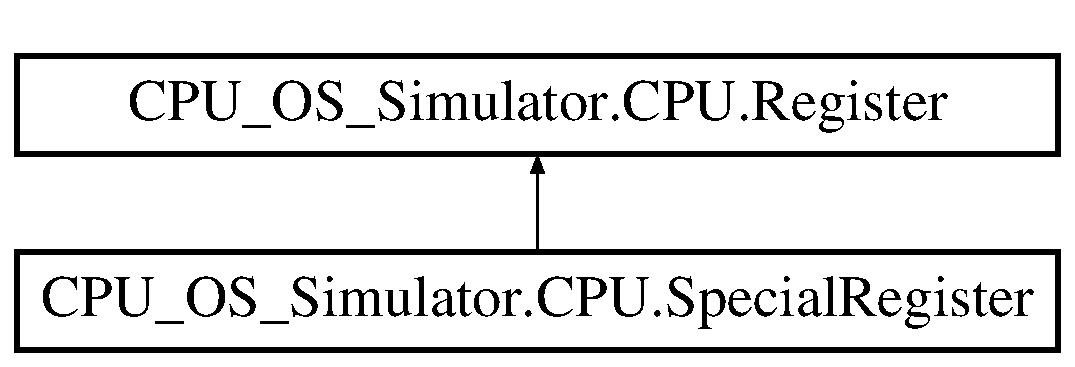
\includegraphics[height=2.000000cm]{class_c_p_u___o_s___simulator_1_1_c_p_u_1_1_special_register}
\end{center}
\end{figure}
\subsection*{Public Member Functions}
\begin{DoxyCompactItemize}
\item 
\hyperlink{class_c_p_u___o_s___simulator_1_1_c_p_u_1_1_special_register_a697f3e6f938ad7ab0ceee0555fe2c312}{Special\+Register} ()
\item 
void \hyperlink{class_c_p_u___o_s___simulator_1_1_c_p_u_1_1_special_register_ab76c9ab94069230fdf14821495ac9e9c}{set\+Register\+Value} (int \hyperlink{class_c_p_u___o_s___simulator_1_1_c_p_u_1_1_special_register_a040dbed0c42c3a45ccb7b01d181dd829}{value}, \hyperlink{namespace_c_p_u___o_s___simulator_1_1_c_p_u_ad49cfe442b74115a326c03b7ae848f76}{Enum\+Operand\+Type} \hyperlink{class_c_p_u___o_s___simulator_1_1_c_p_u_1_1_special_register_aae2bca6c1354013cca156bd19c30640d}{type})
\begin{DoxyCompactList}\small\item\em Sets the value in a special register \end{DoxyCompactList}\item 
void \hyperlink{class_c_p_u___o_s___simulator_1_1_c_p_u_1_1_special_register_a6c2605883e6349c10e92f5453c2ad9ea}{set\+Register\+Value} (string \hyperlink{class_c_p_u___o_s___simulator_1_1_c_p_u_1_1_special_register_a040dbed0c42c3a45ccb7b01d181dd829}{value}, \hyperlink{namespace_c_p_u___o_s___simulator_1_1_c_p_u_ad49cfe442b74115a326c03b7ae848f76}{Enum\+Operand\+Type} \hyperlink{class_c_p_u___o_s___simulator_1_1_c_p_u_1_1_special_register_aae2bca6c1354013cca156bd19c30640d}{type})
\begin{DoxyCompactList}\small\item\em Sets the string value in a special register \end{DoxyCompactList}\end{DoxyCompactItemize}
\subsection*{Static Public Member Functions}
\begin{DoxyCompactItemize}
\item 
static \hyperlink{class_c_p_u___o_s___simulator_1_1_c_p_u_1_1_special_register}{Special\+Register} \hyperlink{class_c_p_u___o_s___simulator_1_1_c_p_u_1_1_special_register_aa8c2e88c7311076eb6fd42ecb5d64e38}{Find\+Special\+Register} (string \hyperlink{class_c_p_u___o_s___simulator_1_1_c_p_u_1_1_special_register_ac521aef66f5fe6a88486e70f5ade8326}{name})
\end{DoxyCompactItemize}
\subsection*{Static Public Attributes}
\begin{DoxyCompactItemize}
\item 
static \hyperlink{class_c_p_u___o_s___simulator_1_1_c_p_u_1_1_special_register}{Special\+Register} \hyperlink{class_c_p_u___o_s___simulator_1_1_c_p_u_1_1_special_register_afc3205003157a5f135752e6a4f8ffb8a}{P\+C} = new \hyperlink{class_c_p_u___o_s___simulator_1_1_c_p_u_1_1_special_register}{Special\+Register}(\char`\"{}P\+C\char`\"{})
\begin{DoxyCompactList}\small\item\em The Program Counter register \end{DoxyCompactList}\item 
static \hyperlink{class_c_p_u___o_s___simulator_1_1_c_p_u_1_1_special_register}{Special\+Register} \hyperlink{class_c_p_u___o_s___simulator_1_1_c_p_u_1_1_special_register_a556243e1c3c891e685bf884771c1575c}{S\+R} = new \hyperlink{class_c_p_u___o_s___simulator_1_1_c_p_u_1_1_special_register}{Special\+Register}(\char`\"{}S\+R\char`\"{})
\begin{DoxyCompactList}\small\item\em The Stack \hyperlink{class_c_p_u___o_s___simulator_1_1_c_p_u_1_1_register}{Register} \end{DoxyCompactList}\item 
static \hyperlink{class_c_p_u___o_s___simulator_1_1_c_p_u_1_1_special_register}{Special\+Register} \hyperlink{class_c_p_u___o_s___simulator_1_1_c_p_u_1_1_special_register_ae1699c7972763e73e3f1cfe467cc82e9}{S\+P} = new \hyperlink{class_c_p_u___o_s___simulator_1_1_c_p_u_1_1_special_register}{Special\+Register}(\char`\"{}S\+P\char`\"{})
\begin{DoxyCompactList}\small\item\em The Stack Pointer \hyperlink{class_c_p_u___o_s___simulator_1_1_c_p_u_1_1_register}{Register} \end{DoxyCompactList}\item 
static \hyperlink{class_c_p_u___o_s___simulator_1_1_c_p_u_1_1_special_register}{Special\+Register} \hyperlink{class_c_p_u___o_s___simulator_1_1_c_p_u_1_1_special_register_a08c44f677cc5e830000382725ce8ab9f}{B\+R} = new \hyperlink{class_c_p_u___o_s___simulator_1_1_c_p_u_1_1_special_register}{Special\+Register}(\char`\"{}B\+R\char`\"{})
\item 
static \hyperlink{class_c_p_u___o_s___simulator_1_1_c_p_u_1_1_special_register}{Special\+Register} \hyperlink{class_c_p_u___o_s___simulator_1_1_c_p_u_1_1_special_register_a96fde61578e06f00ab7b19a4b05b9885}{I\+R} = new \hyperlink{class_c_p_u___o_s___simulator_1_1_c_p_u_1_1_special_register}{Special\+Register}(\char`\"{}I\+R\char`\"{})
\begin{DoxyCompactList}\small\item\em The \hyperlink{class_c_p_u___o_s___simulator_1_1_c_p_u_1_1_instruction}{Instruction} \hyperlink{class_c_p_u___o_s___simulator_1_1_c_p_u_1_1_register}{Register} \end{DoxyCompactList}\item 
static \hyperlink{class_c_p_u___o_s___simulator_1_1_c_p_u_1_1_special_register}{Special\+Register} \hyperlink{class_c_p_u___o_s___simulator_1_1_c_p_u_1_1_special_register_aabf7c761e1f8a9994b7c0b131c53924d}{M\+D\+R} = new \hyperlink{class_c_p_u___o_s___simulator_1_1_c_p_u_1_1_special_register}{Special\+Register}(\char`\"{}M\+D\+R\char`\"{})
\begin{DoxyCompactList}\small\item\em The \hyperlink{namespace_c_p_u___o_s___simulator_1_1_memory}{Memory} Data \hyperlink{class_c_p_u___o_s___simulator_1_1_c_p_u_1_1_register}{Register} \end{DoxyCompactList}\item 
static \hyperlink{class_c_p_u___o_s___simulator_1_1_c_p_u_1_1_special_register}{Special\+Register} \hyperlink{class_c_p_u___o_s___simulator_1_1_c_p_u_1_1_special_register_a2ae89cee8b74f9985f43ee4e6f994bad}{M\+A\+R} = new \hyperlink{class_c_p_u___o_s___simulator_1_1_c_p_u_1_1_special_register}{Special\+Register}(\char`\"{}M\+A\+R\char`\"{})
\begin{DoxyCompactList}\small\item\em The \hyperlink{namespace_c_p_u___o_s___simulator_1_1_memory}{Memory} Logical\+Address \hyperlink{class_c_p_u___o_s___simulator_1_1_c_p_u_1_1_register}{Register} \end{DoxyCompactList}\end{DoxyCompactItemize}
\subsection*{Protected Member Functions}
\begin{DoxyCompactItemize}
\item 
\hyperlink{class_c_p_u___o_s___simulator_1_1_c_p_u_1_1_special_register_a0328b3388027aa409a68191685753f4a}{Special\+Register} (string \hyperlink{class_c_p_u___o_s___simulator_1_1_c_p_u_1_1_special_register_ac521aef66f5fe6a88486e70f5ade8326}{name})
\begin{DoxyCompactList}\small\item\em Primary constructor for a special register \end{DoxyCompactList}\end{DoxyCompactItemize}
\subsection*{Properties}
\begin{DoxyCompactItemize}
\item 
string \hyperlink{class_c_p_u___o_s___simulator_1_1_c_p_u_1_1_special_register_ad8ad1efaf680db5471184a74f911b558}{Name}\hspace{0.3cm}{\ttfamily  \mbox{[}get, set\mbox{]}}
\begin{DoxyCompactList}\small\item\em Property for the name of the special register \end{DoxyCompactList}\item 
int \hyperlink{class_c_p_u___o_s___simulator_1_1_c_p_u_1_1_special_register_aeff33618d376eeaef1e62d6833074bd4}{Value}\hspace{0.3cm}{\ttfamily  \mbox{[}get, set\mbox{]}}
\begin{DoxyCompactList}\small\item\em Property for the value stored in the special register \end{DoxyCompactList}\item 
\hyperlink{namespace_c_p_u___o_s___simulator_1_1_c_p_u_ad49cfe442b74115a326c03b7ae848f76}{Enum\+Operand\+Type} \hyperlink{class_c_p_u___o_s___simulator_1_1_c_p_u_1_1_special_register_afd9e45080d792861e577dde31cdb6d3e}{Type}\hspace{0.3cm}{\ttfamily  \mbox{[}get, set\mbox{]}}
\begin{DoxyCompactList}\small\item\em Property for the type of data in the special register i.\+e. Value or \hyperlink{namespace_c_p_u___o_s___simulator_1_1_memory}{Memory} Address \end{DoxyCompactList}\item 
string \hyperlink{class_c_p_u___o_s___simulator_1_1_c_p_u_1_1_special_register_a60a2bcd516cedf8bb485c2e36bbc3235}{Value\+String}\hspace{0.3cm}{\ttfamily  \mbox{[}get, set\mbox{]}}
\begin{DoxyCompactList}\small\item\em Property for the value stored in the special register \end{DoxyCompactList}\end{DoxyCompactItemize}
\subsection*{Static Private Member Functions}
\begin{DoxyCompactItemize}
\item 
static dynamic \hyperlink{class_c_p_u___o_s___simulator_1_1_c_p_u_1_1_special_register_a0ed54c8fcd7674bcb87fef3eda712af2}{Get\+Main\+Window\+Instance} ()
\begin{DoxyCompactList}\small\item\em This function gets the main window instance from the window bridge \end{DoxyCompactList}\end{DoxyCompactItemize}
\subsection*{Private Attributes}
\begin{DoxyCompactItemize}
\item 
string \hyperlink{class_c_p_u___o_s___simulator_1_1_c_p_u_1_1_special_register_ac521aef66f5fe6a88486e70f5ade8326}{name}
\begin{DoxyCompactList}\small\item\em The name of the Special \hyperlink{class_c_p_u___o_s___simulator_1_1_c_p_u_1_1_register}{Register} \end{DoxyCompactList}\item 
int \hyperlink{class_c_p_u___o_s___simulator_1_1_c_p_u_1_1_special_register_a040dbed0c42c3a45ccb7b01d181dd829}{value}
\begin{DoxyCompactList}\small\item\em The integer value of the special register \end{DoxyCompactList}\item 
string \hyperlink{class_c_p_u___o_s___simulator_1_1_c_p_u_1_1_special_register_a540a55b17a53591312e76689d051abac}{value\+String}
\item 
\hyperlink{namespace_c_p_u___o_s___simulator_1_1_c_p_u_ad49cfe442b74115a326c03b7ae848f76}{Enum\+Operand\+Type} \hyperlink{class_c_p_u___o_s___simulator_1_1_c_p_u_1_1_special_register_aae2bca6c1354013cca156bd19c30640d}{type}
\end{DoxyCompactItemize}


\subsection{Detailed Description}
This class represents a special register i.\+e a non general purpose register 



Definition at line 10 of file Special\+Register.\+cs.



\subsection{Constructor \& Destructor Documentation}
\hypertarget{class_c_p_u___o_s___simulator_1_1_c_p_u_1_1_special_register_a697f3e6f938ad7ab0ceee0555fe2c312}{}\index{C\+P\+U\+\_\+\+O\+S\+\_\+\+Simulator\+::\+C\+P\+U\+::\+Special\+Register@{C\+P\+U\+\_\+\+O\+S\+\_\+\+Simulator\+::\+C\+P\+U\+::\+Special\+Register}!Special\+Register@{Special\+Register}}
\index{Special\+Register@{Special\+Register}!C\+P\+U\+\_\+\+O\+S\+\_\+\+Simulator\+::\+C\+P\+U\+::\+Special\+Register@{C\+P\+U\+\_\+\+O\+S\+\_\+\+Simulator\+::\+C\+P\+U\+::\+Special\+Register}}
\subsubsection[{Special\+Register()}]{\setlength{\rightskip}{0pt plus 5cm}C\+P\+U\+\_\+\+O\+S\+\_\+\+Simulator.\+C\+P\+U.\+Special\+Register.\+Special\+Register (
\begin{DoxyParamCaption}
{}
\end{DoxyParamCaption}
)}\label{class_c_p_u___o_s___simulator_1_1_c_p_u_1_1_special_register_a697f3e6f938ad7ab0ceee0555fe2c312}




Default constructor for Special \hyperlink{class_c_p_u___o_s___simulator_1_1_c_p_u_1_1_register}{Register} used when deserialising a special register. 

N\+O\+T\+E Do Not use in code 

Definition at line 75 of file Special\+Register.\+cs.

\hypertarget{class_c_p_u___o_s___simulator_1_1_c_p_u_1_1_special_register_a0328b3388027aa409a68191685753f4a}{}\index{C\+P\+U\+\_\+\+O\+S\+\_\+\+Simulator\+::\+C\+P\+U\+::\+Special\+Register@{C\+P\+U\+\_\+\+O\+S\+\_\+\+Simulator\+::\+C\+P\+U\+::\+Special\+Register}!Special\+Register@{Special\+Register}}
\index{Special\+Register@{Special\+Register}!C\+P\+U\+\_\+\+O\+S\+\_\+\+Simulator\+::\+C\+P\+U\+::\+Special\+Register@{C\+P\+U\+\_\+\+O\+S\+\_\+\+Simulator\+::\+C\+P\+U\+::\+Special\+Register}}
\subsubsection[{Special\+Register(string name)}]{\setlength{\rightskip}{0pt plus 5cm}C\+P\+U\+\_\+\+O\+S\+\_\+\+Simulator.\+C\+P\+U.\+Special\+Register.\+Special\+Register (
\begin{DoxyParamCaption}
\item[{string}]{name}
\end{DoxyParamCaption}
)\hspace{0.3cm}{\ttfamily [protected]}}\label{class_c_p_u___o_s___simulator_1_1_c_p_u_1_1_special_register_a0328b3388027aa409a68191685753f4a}


Primary constructor for a special register 


\begin{DoxyParams}{Parameters}
{\em name} & The name of the register\\
\hline
\end{DoxyParams}


Definition at line 83 of file Special\+Register.\+cs.



\subsection{Member Function Documentation}
\hypertarget{class_c_p_u___o_s___simulator_1_1_c_p_u_1_1_special_register_aa8c2e88c7311076eb6fd42ecb5d64e38}{}\index{C\+P\+U\+\_\+\+O\+S\+\_\+\+Simulator\+::\+C\+P\+U\+::\+Special\+Register@{C\+P\+U\+\_\+\+O\+S\+\_\+\+Simulator\+::\+C\+P\+U\+::\+Special\+Register}!Find\+Special\+Register@{Find\+Special\+Register}}
\index{Find\+Special\+Register@{Find\+Special\+Register}!C\+P\+U\+\_\+\+O\+S\+\_\+\+Simulator\+::\+C\+P\+U\+::\+Special\+Register@{C\+P\+U\+\_\+\+O\+S\+\_\+\+Simulator\+::\+C\+P\+U\+::\+Special\+Register}}
\subsubsection[{Find\+Special\+Register(string name)}]{\setlength{\rightskip}{0pt plus 5cm}static {\bf Special\+Register} C\+P\+U\+\_\+\+O\+S\+\_\+\+Simulator.\+C\+P\+U.\+Special\+Register.\+Find\+Special\+Register (
\begin{DoxyParamCaption}
\item[{string}]{name}
\end{DoxyParamCaption}
)\hspace{0.3cm}{\ttfamily [static]}}\label{class_c_p_u___o_s___simulator_1_1_c_p_u_1_1_special_register_aa8c2e88c7311076eb6fd42ecb5d64e38}





\begin{DoxyParams}{Parameters}
{\em name} & \\
\hline
\end{DoxyParams}
\begin{DoxyReturn}{Returns}

\end{DoxyReturn}


Definition at line 100 of file Special\+Register.\+cs.

\hypertarget{class_c_p_u___o_s___simulator_1_1_c_p_u_1_1_special_register_a0ed54c8fcd7674bcb87fef3eda712af2}{}\index{C\+P\+U\+\_\+\+O\+S\+\_\+\+Simulator\+::\+C\+P\+U\+::\+Special\+Register@{C\+P\+U\+\_\+\+O\+S\+\_\+\+Simulator\+::\+C\+P\+U\+::\+Special\+Register}!Get\+Main\+Window\+Instance@{Get\+Main\+Window\+Instance}}
\index{Get\+Main\+Window\+Instance@{Get\+Main\+Window\+Instance}!C\+P\+U\+\_\+\+O\+S\+\_\+\+Simulator\+::\+C\+P\+U\+::\+Special\+Register@{C\+P\+U\+\_\+\+O\+S\+\_\+\+Simulator\+::\+C\+P\+U\+::\+Special\+Register}}
\subsubsection[{Get\+Main\+Window\+Instance()}]{\setlength{\rightskip}{0pt plus 5cm}static dynamic C\+P\+U\+\_\+\+O\+S\+\_\+\+Simulator.\+C\+P\+U.\+Special\+Register.\+Get\+Main\+Window\+Instance (
\begin{DoxyParamCaption}
{}
\end{DoxyParamCaption}
)\hspace{0.3cm}{\ttfamily [static]}, {\ttfamily [private]}}\label{class_c_p_u___o_s___simulator_1_1_c_p_u_1_1_special_register_a0ed54c8fcd7674bcb87fef3eda712af2}


This function gets the main window instance from the window bridge 

\begin{DoxyReturn}{Returns}
the active instance of main window 
\end{DoxyReturn}


Definition at line 165 of file Special\+Register.\+cs.

\hypertarget{class_c_p_u___o_s___simulator_1_1_c_p_u_1_1_special_register_ab76c9ab94069230fdf14821495ac9e9c}{}\index{C\+P\+U\+\_\+\+O\+S\+\_\+\+Simulator\+::\+C\+P\+U\+::\+Special\+Register@{C\+P\+U\+\_\+\+O\+S\+\_\+\+Simulator\+::\+C\+P\+U\+::\+Special\+Register}!set\+Register\+Value@{set\+Register\+Value}}
\index{set\+Register\+Value@{set\+Register\+Value}!C\+P\+U\+\_\+\+O\+S\+\_\+\+Simulator\+::\+C\+P\+U\+::\+Special\+Register@{C\+P\+U\+\_\+\+O\+S\+\_\+\+Simulator\+::\+C\+P\+U\+::\+Special\+Register}}
\subsubsection[{set\+Register\+Value(int value, Enum\+Operand\+Type type)}]{\setlength{\rightskip}{0pt plus 5cm}void C\+P\+U\+\_\+\+O\+S\+\_\+\+Simulator.\+C\+P\+U.\+Special\+Register.\+set\+Register\+Value (
\begin{DoxyParamCaption}
\item[{int}]{value, }
\item[{{\bf Enum\+Operand\+Type}}]{type}
\end{DoxyParamCaption}
)}\label{class_c_p_u___o_s___simulator_1_1_c_p_u_1_1_special_register_ab76c9ab94069230fdf14821495ac9e9c}


Sets the value in a special register 


\begin{DoxyParams}{Parameters}
{\em value} & the value to store in the register\\
\hline
{\em type} & the type of data memory or value\\
\hline
\end{DoxyParams}


Definition at line 144 of file Special\+Register.\+cs.

\hypertarget{class_c_p_u___o_s___simulator_1_1_c_p_u_1_1_special_register_a6c2605883e6349c10e92f5453c2ad9ea}{}\index{C\+P\+U\+\_\+\+O\+S\+\_\+\+Simulator\+::\+C\+P\+U\+::\+Special\+Register@{C\+P\+U\+\_\+\+O\+S\+\_\+\+Simulator\+::\+C\+P\+U\+::\+Special\+Register}!set\+Register\+Value@{set\+Register\+Value}}
\index{set\+Register\+Value@{set\+Register\+Value}!C\+P\+U\+\_\+\+O\+S\+\_\+\+Simulator\+::\+C\+P\+U\+::\+Special\+Register@{C\+P\+U\+\_\+\+O\+S\+\_\+\+Simulator\+::\+C\+P\+U\+::\+Special\+Register}}
\subsubsection[{set\+Register\+Value(string value, Enum\+Operand\+Type type)}]{\setlength{\rightskip}{0pt plus 5cm}void C\+P\+U\+\_\+\+O\+S\+\_\+\+Simulator.\+C\+P\+U.\+Special\+Register.\+set\+Register\+Value (
\begin{DoxyParamCaption}
\item[{string}]{value, }
\item[{{\bf Enum\+Operand\+Type}}]{type}
\end{DoxyParamCaption}
)}\label{class_c_p_u___o_s___simulator_1_1_c_p_u_1_1_special_register_a6c2605883e6349c10e92f5453c2ad9ea}


Sets the string value in a special register 


\begin{DoxyParams}{Parameters}
{\em value} & the value to store in the register\\
\hline
{\em type} & the type of data memory or value\\
\hline
\end{DoxyParams}


Definition at line 155 of file Special\+Register.\+cs.



\subsection{Member Data Documentation}
\hypertarget{class_c_p_u___o_s___simulator_1_1_c_p_u_1_1_special_register_a08c44f677cc5e830000382725ce8ab9f}{}\index{C\+P\+U\+\_\+\+O\+S\+\_\+\+Simulator\+::\+C\+P\+U\+::\+Special\+Register@{C\+P\+U\+\_\+\+O\+S\+\_\+\+Simulator\+::\+C\+P\+U\+::\+Special\+Register}!B\+R@{B\+R}}
\index{B\+R@{B\+R}!C\+P\+U\+\_\+\+O\+S\+\_\+\+Simulator\+::\+C\+P\+U\+::\+Special\+Register@{C\+P\+U\+\_\+\+O\+S\+\_\+\+Simulator\+::\+C\+P\+U\+::\+Special\+Register}}
\subsubsection[{B\+R}]{\setlength{\rightskip}{0pt plus 5cm}{\bf Special\+Register} C\+P\+U\+\_\+\+O\+S\+\_\+\+Simulator.\+C\+P\+U.\+Special\+Register.\+B\+R = new {\bf Special\+Register}(\char`\"{}B\+R\char`\"{})\hspace{0.3cm}{\ttfamily [static]}}\label{class_c_p_u___o_s___simulator_1_1_c_p_u_1_1_special_register_a08c44f677cc5e830000382725ce8ab9f}






Definition at line 53 of file Special\+Register.\+cs.

\hypertarget{class_c_p_u___o_s___simulator_1_1_c_p_u_1_1_special_register_a96fde61578e06f00ab7b19a4b05b9885}{}\index{C\+P\+U\+\_\+\+O\+S\+\_\+\+Simulator\+::\+C\+P\+U\+::\+Special\+Register@{C\+P\+U\+\_\+\+O\+S\+\_\+\+Simulator\+::\+C\+P\+U\+::\+Special\+Register}!I\+R@{I\+R}}
\index{I\+R@{I\+R}!C\+P\+U\+\_\+\+O\+S\+\_\+\+Simulator\+::\+C\+P\+U\+::\+Special\+Register@{C\+P\+U\+\_\+\+O\+S\+\_\+\+Simulator\+::\+C\+P\+U\+::\+Special\+Register}}
\subsubsection[{I\+R}]{\setlength{\rightskip}{0pt plus 5cm}{\bf Special\+Register} C\+P\+U\+\_\+\+O\+S\+\_\+\+Simulator.\+C\+P\+U.\+Special\+Register.\+I\+R = new {\bf Special\+Register}(\char`\"{}I\+R\char`\"{})\hspace{0.3cm}{\ttfamily [static]}}\label{class_c_p_u___o_s___simulator_1_1_c_p_u_1_1_special_register_a96fde61578e06f00ab7b19a4b05b9885}


The \hyperlink{class_c_p_u___o_s___simulator_1_1_c_p_u_1_1_instruction}{Instruction} \hyperlink{class_c_p_u___o_s___simulator_1_1_c_p_u_1_1_register}{Register} 



Definition at line 58 of file Special\+Register.\+cs.

\hypertarget{class_c_p_u___o_s___simulator_1_1_c_p_u_1_1_special_register_a2ae89cee8b74f9985f43ee4e6f994bad}{}\index{C\+P\+U\+\_\+\+O\+S\+\_\+\+Simulator\+::\+C\+P\+U\+::\+Special\+Register@{C\+P\+U\+\_\+\+O\+S\+\_\+\+Simulator\+::\+C\+P\+U\+::\+Special\+Register}!M\+A\+R@{M\+A\+R}}
\index{M\+A\+R@{M\+A\+R}!C\+P\+U\+\_\+\+O\+S\+\_\+\+Simulator\+::\+C\+P\+U\+::\+Special\+Register@{C\+P\+U\+\_\+\+O\+S\+\_\+\+Simulator\+::\+C\+P\+U\+::\+Special\+Register}}
\subsubsection[{M\+A\+R}]{\setlength{\rightskip}{0pt plus 5cm}{\bf Special\+Register} C\+P\+U\+\_\+\+O\+S\+\_\+\+Simulator.\+C\+P\+U.\+Special\+Register.\+M\+A\+R = new {\bf Special\+Register}(\char`\"{}M\+A\+R\char`\"{})\hspace{0.3cm}{\ttfamily [static]}}\label{class_c_p_u___o_s___simulator_1_1_c_p_u_1_1_special_register_a2ae89cee8b74f9985f43ee4e6f994bad}


The \hyperlink{namespace_c_p_u___o_s___simulator_1_1_memory}{Memory} Logical\+Address \hyperlink{class_c_p_u___o_s___simulator_1_1_c_p_u_1_1_register}{Register} 



Definition at line 68 of file Special\+Register.\+cs.

\hypertarget{class_c_p_u___o_s___simulator_1_1_c_p_u_1_1_special_register_aabf7c761e1f8a9994b7c0b131c53924d}{}\index{C\+P\+U\+\_\+\+O\+S\+\_\+\+Simulator\+::\+C\+P\+U\+::\+Special\+Register@{C\+P\+U\+\_\+\+O\+S\+\_\+\+Simulator\+::\+C\+P\+U\+::\+Special\+Register}!M\+D\+R@{M\+D\+R}}
\index{M\+D\+R@{M\+D\+R}!C\+P\+U\+\_\+\+O\+S\+\_\+\+Simulator\+::\+C\+P\+U\+::\+Special\+Register@{C\+P\+U\+\_\+\+O\+S\+\_\+\+Simulator\+::\+C\+P\+U\+::\+Special\+Register}}
\subsubsection[{M\+D\+R}]{\setlength{\rightskip}{0pt plus 5cm}{\bf Special\+Register} C\+P\+U\+\_\+\+O\+S\+\_\+\+Simulator.\+C\+P\+U.\+Special\+Register.\+M\+D\+R = new {\bf Special\+Register}(\char`\"{}M\+D\+R\char`\"{})\hspace{0.3cm}{\ttfamily [static]}}\label{class_c_p_u___o_s___simulator_1_1_c_p_u_1_1_special_register_aabf7c761e1f8a9994b7c0b131c53924d}


The \hyperlink{namespace_c_p_u___o_s___simulator_1_1_memory}{Memory} Data \hyperlink{class_c_p_u___o_s___simulator_1_1_c_p_u_1_1_register}{Register} 



Definition at line 63 of file Special\+Register.\+cs.

\hypertarget{class_c_p_u___o_s___simulator_1_1_c_p_u_1_1_special_register_ac521aef66f5fe6a88486e70f5ade8326}{}\index{C\+P\+U\+\_\+\+O\+S\+\_\+\+Simulator\+::\+C\+P\+U\+::\+Special\+Register@{C\+P\+U\+\_\+\+O\+S\+\_\+\+Simulator\+::\+C\+P\+U\+::\+Special\+Register}!name@{name}}
\index{name@{name}!C\+P\+U\+\_\+\+O\+S\+\_\+\+Simulator\+::\+C\+P\+U\+::\+Special\+Register@{C\+P\+U\+\_\+\+O\+S\+\_\+\+Simulator\+::\+C\+P\+U\+::\+Special\+Register}}
\subsubsection[{name}]{\setlength{\rightskip}{0pt plus 5cm}string C\+P\+U\+\_\+\+O\+S\+\_\+\+Simulator.\+C\+P\+U.\+Special\+Register.\+name\hspace{0.3cm}{\ttfamily [private]}}\label{class_c_p_u___o_s___simulator_1_1_c_p_u_1_1_special_register_ac521aef66f5fe6a88486e70f5ade8326}


The name of the Special \hyperlink{class_c_p_u___o_s___simulator_1_1_c_p_u_1_1_register}{Register} 



Definition at line 15 of file Special\+Register.\+cs.

\hypertarget{class_c_p_u___o_s___simulator_1_1_c_p_u_1_1_special_register_afc3205003157a5f135752e6a4f8ffb8a}{}\index{C\+P\+U\+\_\+\+O\+S\+\_\+\+Simulator\+::\+C\+P\+U\+::\+Special\+Register@{C\+P\+U\+\_\+\+O\+S\+\_\+\+Simulator\+::\+C\+P\+U\+::\+Special\+Register}!P\+C@{P\+C}}
\index{P\+C@{P\+C}!C\+P\+U\+\_\+\+O\+S\+\_\+\+Simulator\+::\+C\+P\+U\+::\+Special\+Register@{C\+P\+U\+\_\+\+O\+S\+\_\+\+Simulator\+::\+C\+P\+U\+::\+Special\+Register}}
\subsubsection[{P\+C}]{\setlength{\rightskip}{0pt plus 5cm}{\bf Special\+Register} C\+P\+U\+\_\+\+O\+S\+\_\+\+Simulator.\+C\+P\+U.\+Special\+Register.\+P\+C = new {\bf Special\+Register}(\char`\"{}P\+C\char`\"{})\hspace{0.3cm}{\ttfamily [static]}}\label{class_c_p_u___o_s___simulator_1_1_c_p_u_1_1_special_register_afc3205003157a5f135752e6a4f8ffb8a}


The Program Counter register 



Definition at line 38 of file Special\+Register.\+cs.

\hypertarget{class_c_p_u___o_s___simulator_1_1_c_p_u_1_1_special_register_ae1699c7972763e73e3f1cfe467cc82e9}{}\index{C\+P\+U\+\_\+\+O\+S\+\_\+\+Simulator\+::\+C\+P\+U\+::\+Special\+Register@{C\+P\+U\+\_\+\+O\+S\+\_\+\+Simulator\+::\+C\+P\+U\+::\+Special\+Register}!S\+P@{S\+P}}
\index{S\+P@{S\+P}!C\+P\+U\+\_\+\+O\+S\+\_\+\+Simulator\+::\+C\+P\+U\+::\+Special\+Register@{C\+P\+U\+\_\+\+O\+S\+\_\+\+Simulator\+::\+C\+P\+U\+::\+Special\+Register}}
\subsubsection[{S\+P}]{\setlength{\rightskip}{0pt plus 5cm}{\bf Special\+Register} C\+P\+U\+\_\+\+O\+S\+\_\+\+Simulator.\+C\+P\+U.\+Special\+Register.\+S\+P = new {\bf Special\+Register}(\char`\"{}S\+P\char`\"{})\hspace{0.3cm}{\ttfamily [static]}}\label{class_c_p_u___o_s___simulator_1_1_c_p_u_1_1_special_register_ae1699c7972763e73e3f1cfe467cc82e9}


The Stack Pointer \hyperlink{class_c_p_u___o_s___simulator_1_1_c_p_u_1_1_register}{Register} 



Definition at line 48 of file Special\+Register.\+cs.

\hypertarget{class_c_p_u___o_s___simulator_1_1_c_p_u_1_1_special_register_a556243e1c3c891e685bf884771c1575c}{}\index{C\+P\+U\+\_\+\+O\+S\+\_\+\+Simulator\+::\+C\+P\+U\+::\+Special\+Register@{C\+P\+U\+\_\+\+O\+S\+\_\+\+Simulator\+::\+C\+P\+U\+::\+Special\+Register}!S\+R@{S\+R}}
\index{S\+R@{S\+R}!C\+P\+U\+\_\+\+O\+S\+\_\+\+Simulator\+::\+C\+P\+U\+::\+Special\+Register@{C\+P\+U\+\_\+\+O\+S\+\_\+\+Simulator\+::\+C\+P\+U\+::\+Special\+Register}}
\subsubsection[{S\+R}]{\setlength{\rightskip}{0pt plus 5cm}{\bf Special\+Register} C\+P\+U\+\_\+\+O\+S\+\_\+\+Simulator.\+C\+P\+U.\+Special\+Register.\+S\+R = new {\bf Special\+Register}(\char`\"{}S\+R\char`\"{})\hspace{0.3cm}{\ttfamily [static]}}\label{class_c_p_u___o_s___simulator_1_1_c_p_u_1_1_special_register_a556243e1c3c891e685bf884771c1575c}


The Stack \hyperlink{class_c_p_u___o_s___simulator_1_1_c_p_u_1_1_register}{Register} 



Definition at line 43 of file Special\+Register.\+cs.

\hypertarget{class_c_p_u___o_s___simulator_1_1_c_p_u_1_1_special_register_aae2bca6c1354013cca156bd19c30640d}{}\index{C\+P\+U\+\_\+\+O\+S\+\_\+\+Simulator\+::\+C\+P\+U\+::\+Special\+Register@{C\+P\+U\+\_\+\+O\+S\+\_\+\+Simulator\+::\+C\+P\+U\+::\+Special\+Register}!type@{type}}
\index{type@{type}!C\+P\+U\+\_\+\+O\+S\+\_\+\+Simulator\+::\+C\+P\+U\+::\+Special\+Register@{C\+P\+U\+\_\+\+O\+S\+\_\+\+Simulator\+::\+C\+P\+U\+::\+Special\+Register}}
\subsubsection[{type}]{\setlength{\rightskip}{0pt plus 5cm}{\bf Enum\+Operand\+Type} C\+P\+U\+\_\+\+O\+S\+\_\+\+Simulator.\+C\+P\+U.\+Special\+Register.\+type\hspace{0.3cm}{\ttfamily [private]}}\label{class_c_p_u___o_s___simulator_1_1_c_p_u_1_1_special_register_aae2bca6c1354013cca156bd19c30640d}




The type of value stored in the register 

i.\+e intermediate value or memory address 

Definition at line 33 of file Special\+Register.\+cs.

\hypertarget{class_c_p_u___o_s___simulator_1_1_c_p_u_1_1_special_register_a040dbed0c42c3a45ccb7b01d181dd829}{}\index{C\+P\+U\+\_\+\+O\+S\+\_\+\+Simulator\+::\+C\+P\+U\+::\+Special\+Register@{C\+P\+U\+\_\+\+O\+S\+\_\+\+Simulator\+::\+C\+P\+U\+::\+Special\+Register}!value@{value}}
\index{value@{value}!C\+P\+U\+\_\+\+O\+S\+\_\+\+Simulator\+::\+C\+P\+U\+::\+Special\+Register@{C\+P\+U\+\_\+\+O\+S\+\_\+\+Simulator\+::\+C\+P\+U\+::\+Special\+Register}}
\subsubsection[{value}]{\setlength{\rightskip}{0pt plus 5cm}int C\+P\+U\+\_\+\+O\+S\+\_\+\+Simulator.\+C\+P\+U.\+Special\+Register.\+value\hspace{0.3cm}{\ttfamily [private]}}\label{class_c_p_u___o_s___simulator_1_1_c_p_u_1_1_special_register_a040dbed0c42c3a45ccb7b01d181dd829}


The integer value of the special register 



Definition at line 20 of file Special\+Register.\+cs.

\hypertarget{class_c_p_u___o_s___simulator_1_1_c_p_u_1_1_special_register_a540a55b17a53591312e76689d051abac}{}\index{C\+P\+U\+\_\+\+O\+S\+\_\+\+Simulator\+::\+C\+P\+U\+::\+Special\+Register@{C\+P\+U\+\_\+\+O\+S\+\_\+\+Simulator\+::\+C\+P\+U\+::\+Special\+Register}!value\+String@{value\+String}}
\index{value\+String@{value\+String}!C\+P\+U\+\_\+\+O\+S\+\_\+\+Simulator\+::\+C\+P\+U\+::\+Special\+Register@{C\+P\+U\+\_\+\+O\+S\+\_\+\+Simulator\+::\+C\+P\+U\+::\+Special\+Register}}
\subsubsection[{value\+String}]{\setlength{\rightskip}{0pt plus 5cm}string C\+P\+U\+\_\+\+O\+S\+\_\+\+Simulator.\+C\+P\+U.\+Special\+Register.\+value\+String\hspace{0.3cm}{\ttfamily [private]}}\label{class_c_p_u___o_s___simulator_1_1_c_p_u_1_1_special_register_a540a55b17a53591312e76689d051abac}




The string value of the register used 

for the instruction register (I\+R) 

and the memory data register (M\+D\+R) 

Definition at line 27 of file Special\+Register.\+cs.



\subsection{Property Documentation}
\hypertarget{class_c_p_u___o_s___simulator_1_1_c_p_u_1_1_special_register_ad8ad1efaf680db5471184a74f911b558}{}\index{C\+P\+U\+\_\+\+O\+S\+\_\+\+Simulator\+::\+C\+P\+U\+::\+Special\+Register@{C\+P\+U\+\_\+\+O\+S\+\_\+\+Simulator\+::\+C\+P\+U\+::\+Special\+Register}!Name@{Name}}
\index{Name@{Name}!C\+P\+U\+\_\+\+O\+S\+\_\+\+Simulator\+::\+C\+P\+U\+::\+Special\+Register@{C\+P\+U\+\_\+\+O\+S\+\_\+\+Simulator\+::\+C\+P\+U\+::\+Special\+Register}}
\subsubsection[{Name}]{\setlength{\rightskip}{0pt plus 5cm}string C\+P\+U\+\_\+\+O\+S\+\_\+\+Simulator.\+C\+P\+U.\+Special\+Register.\+Name\hspace{0.3cm}{\ttfamily [get]}, {\ttfamily [set]}}\label{class_c_p_u___o_s___simulator_1_1_c_p_u_1_1_special_register_ad8ad1efaf680db5471184a74f911b558}


Property for the name of the special register 



Definition at line 177 of file Special\+Register.\+cs.

\hypertarget{class_c_p_u___o_s___simulator_1_1_c_p_u_1_1_special_register_afd9e45080d792861e577dde31cdb6d3e}{}\index{C\+P\+U\+\_\+\+O\+S\+\_\+\+Simulator\+::\+C\+P\+U\+::\+Special\+Register@{C\+P\+U\+\_\+\+O\+S\+\_\+\+Simulator\+::\+C\+P\+U\+::\+Special\+Register}!Type@{Type}}
\index{Type@{Type}!C\+P\+U\+\_\+\+O\+S\+\_\+\+Simulator\+::\+C\+P\+U\+::\+Special\+Register@{C\+P\+U\+\_\+\+O\+S\+\_\+\+Simulator\+::\+C\+P\+U\+::\+Special\+Register}}
\subsubsection[{Type}]{\setlength{\rightskip}{0pt plus 5cm}{\bf Enum\+Operand\+Type} C\+P\+U\+\_\+\+O\+S\+\_\+\+Simulator.\+C\+P\+U.\+Special\+Register.\+Type\hspace{0.3cm}{\ttfamily [get]}, {\ttfamily [set]}}\label{class_c_p_u___o_s___simulator_1_1_c_p_u_1_1_special_register_afd9e45080d792861e577dde31cdb6d3e}


Property for the type of data in the special register i.\+e. Value or \hyperlink{namespace_c_p_u___o_s___simulator_1_1_memory}{Memory} Address 



Definition at line 208 of file Special\+Register.\+cs.

\hypertarget{class_c_p_u___o_s___simulator_1_1_c_p_u_1_1_special_register_aeff33618d376eeaef1e62d6833074bd4}{}\index{C\+P\+U\+\_\+\+O\+S\+\_\+\+Simulator\+::\+C\+P\+U\+::\+Special\+Register@{C\+P\+U\+\_\+\+O\+S\+\_\+\+Simulator\+::\+C\+P\+U\+::\+Special\+Register}!Value@{Value}}
\index{Value@{Value}!C\+P\+U\+\_\+\+O\+S\+\_\+\+Simulator\+::\+C\+P\+U\+::\+Special\+Register@{C\+P\+U\+\_\+\+O\+S\+\_\+\+Simulator\+::\+C\+P\+U\+::\+Special\+Register}}
\subsubsection[{Value}]{\setlength{\rightskip}{0pt plus 5cm}int C\+P\+U\+\_\+\+O\+S\+\_\+\+Simulator.\+C\+P\+U.\+Special\+Register.\+Value\hspace{0.3cm}{\ttfamily [get]}, {\ttfamily [set]}}\label{class_c_p_u___o_s___simulator_1_1_c_p_u_1_1_special_register_aeff33618d376eeaef1e62d6833074bd4}


Property for the value stored in the special register 



Definition at line 192 of file Special\+Register.\+cs.

\hypertarget{class_c_p_u___o_s___simulator_1_1_c_p_u_1_1_special_register_a60a2bcd516cedf8bb485c2e36bbc3235}{}\index{C\+P\+U\+\_\+\+O\+S\+\_\+\+Simulator\+::\+C\+P\+U\+::\+Special\+Register@{C\+P\+U\+\_\+\+O\+S\+\_\+\+Simulator\+::\+C\+P\+U\+::\+Special\+Register}!Value\+String@{Value\+String}}
\index{Value\+String@{Value\+String}!C\+P\+U\+\_\+\+O\+S\+\_\+\+Simulator\+::\+C\+P\+U\+::\+Special\+Register@{C\+P\+U\+\_\+\+O\+S\+\_\+\+Simulator\+::\+C\+P\+U\+::\+Special\+Register}}
\subsubsection[{Value\+String}]{\setlength{\rightskip}{0pt plus 5cm}string C\+P\+U\+\_\+\+O\+S\+\_\+\+Simulator.\+C\+P\+U.\+Special\+Register.\+Value\+String\hspace{0.3cm}{\ttfamily [get]}, {\ttfamily [set]}}\label{class_c_p_u___o_s___simulator_1_1_c_p_u_1_1_special_register_a60a2bcd516cedf8bb485c2e36bbc3235}


Property for the value stored in the special register 



Definition at line 223 of file Special\+Register.\+cs.



The documentation for this class was generated from the following file\+:\begin{DoxyCompactItemize}
\item 
C\+P\+U/\hyperlink{_special_register_8cs}{Special\+Register.\+cs}\end{DoxyCompactItemize}

\hypertarget{class_c_p_u_tests_1_1_special_register_tests}{}\section{C\+P\+U\+Tests.\+Special\+Register\+Tests Class Reference}
\label{class_c_p_u_tests_1_1_special_register_tests}\index{C\+P\+U\+Tests.\+Special\+Register\+Tests@{C\+P\+U\+Tests.\+Special\+Register\+Tests}}
\subsection*{Public Member Functions}
\begin{DoxyCompactItemize}
\item 
void \hyperlink{class_c_p_u_tests_1_1_special_register_tests_a83f82bfe80ba2f6b81c5165bbed5fbab}{Special\+Register\+Test} ()
\item 
void \hyperlink{class_c_p_u_tests_1_1_special_register_tests_ad889ae5d75f6216d7a1918beb9f16e88}{Find\+Special\+Register\+Test} ()
\item 
void \hyperlink{class_c_p_u_tests_1_1_special_register_tests_a419a5c917fa82fab7a14772a9a2daa6b}{set\+Register\+Value\+Test} ()
\item 
void \hyperlink{class_c_p_u_tests_1_1_special_register_tests_a2e335daa0a2c6eefc41e141630050679}{set\+Register\+Value\+Test1} ()
\end{DoxyCompactItemize}


\subsection{Detailed Description}


Definition at line 7 of file Special\+Register\+Tests.\+cs.



\subsection{Member Function Documentation}
\hypertarget{class_c_p_u_tests_1_1_special_register_tests_ad889ae5d75f6216d7a1918beb9f16e88}{}\index{C\+P\+U\+Tests\+::\+Special\+Register\+Tests@{C\+P\+U\+Tests\+::\+Special\+Register\+Tests}!Find\+Special\+Register\+Test@{Find\+Special\+Register\+Test}}
\index{Find\+Special\+Register\+Test@{Find\+Special\+Register\+Test}!C\+P\+U\+Tests\+::\+Special\+Register\+Tests@{C\+P\+U\+Tests\+::\+Special\+Register\+Tests}}
\subsubsection[{Find\+Special\+Register\+Test()}]{\setlength{\rightskip}{0pt plus 5cm}void C\+P\+U\+Tests.\+Special\+Register\+Tests.\+Find\+Special\+Register\+Test (
\begin{DoxyParamCaption}
{}
\end{DoxyParamCaption}
)}\label{class_c_p_u_tests_1_1_special_register_tests_ad889ae5d75f6216d7a1918beb9f16e88}


Definition at line 17 of file Special\+Register\+Tests.\+cs.

\hypertarget{class_c_p_u_tests_1_1_special_register_tests_a419a5c917fa82fab7a14772a9a2daa6b}{}\index{C\+P\+U\+Tests\+::\+Special\+Register\+Tests@{C\+P\+U\+Tests\+::\+Special\+Register\+Tests}!set\+Register\+Value\+Test@{set\+Register\+Value\+Test}}
\index{set\+Register\+Value\+Test@{set\+Register\+Value\+Test}!C\+P\+U\+Tests\+::\+Special\+Register\+Tests@{C\+P\+U\+Tests\+::\+Special\+Register\+Tests}}
\subsubsection[{set\+Register\+Value\+Test()}]{\setlength{\rightskip}{0pt plus 5cm}void C\+P\+U\+Tests.\+Special\+Register\+Tests.\+set\+Register\+Value\+Test (
\begin{DoxyParamCaption}
{}
\end{DoxyParamCaption}
)}\label{class_c_p_u_tests_1_1_special_register_tests_a419a5c917fa82fab7a14772a9a2daa6b}


Definition at line 25 of file Special\+Register\+Tests.\+cs.

\hypertarget{class_c_p_u_tests_1_1_special_register_tests_a2e335daa0a2c6eefc41e141630050679}{}\index{C\+P\+U\+Tests\+::\+Special\+Register\+Tests@{C\+P\+U\+Tests\+::\+Special\+Register\+Tests}!set\+Register\+Value\+Test1@{set\+Register\+Value\+Test1}}
\index{set\+Register\+Value\+Test1@{set\+Register\+Value\+Test1}!C\+P\+U\+Tests\+::\+Special\+Register\+Tests@{C\+P\+U\+Tests\+::\+Special\+Register\+Tests}}
\subsubsection[{set\+Register\+Value\+Test1()}]{\setlength{\rightskip}{0pt plus 5cm}void C\+P\+U\+Tests.\+Special\+Register\+Tests.\+set\+Register\+Value\+Test1 (
\begin{DoxyParamCaption}
{}
\end{DoxyParamCaption}
)}\label{class_c_p_u_tests_1_1_special_register_tests_a2e335daa0a2c6eefc41e141630050679}


Definition at line 33 of file Special\+Register\+Tests.\+cs.

\hypertarget{class_c_p_u_tests_1_1_special_register_tests_a83f82bfe80ba2f6b81c5165bbed5fbab}{}\index{C\+P\+U\+Tests\+::\+Special\+Register\+Tests@{C\+P\+U\+Tests\+::\+Special\+Register\+Tests}!Special\+Register\+Test@{Special\+Register\+Test}}
\index{Special\+Register\+Test@{Special\+Register\+Test}!C\+P\+U\+Tests\+::\+Special\+Register\+Tests@{C\+P\+U\+Tests\+::\+Special\+Register\+Tests}}
\subsubsection[{Special\+Register\+Test()}]{\setlength{\rightskip}{0pt plus 5cm}void C\+P\+U\+Tests.\+Special\+Register\+Tests.\+Special\+Register\+Test (
\begin{DoxyParamCaption}
{}
\end{DoxyParamCaption}
)}\label{class_c_p_u_tests_1_1_special_register_tests_a83f82bfe80ba2f6b81c5165bbed5fbab}


Definition at line 10 of file Special\+Register\+Tests.\+cs.



The documentation for this class was generated from the following file\+:\begin{DoxyCompactItemize}
\item 
C\+P\+U\+Tests/\hyperlink{_special_register_tests_8cs}{Special\+Register\+Tests.\+cs}\end{DoxyCompactItemize}

\hypertarget{class_c_p_u___o_s___simulator_1_1_c_p_u_1_1_stack_item}{}\section{C\+P\+U\+\_\+\+O\+S\+\_\+\+Simulator.\+C\+P\+U.\+Stack\+Item Class Reference}
\label{class_c_p_u___o_s___simulator_1_1_c_p_u_1_1_stack_item}\index{C\+P\+U\+\_\+\+O\+S\+\_\+\+Simulator.\+C\+P\+U.\+Stack\+Item@{C\+P\+U\+\_\+\+O\+S\+\_\+\+Simulator.\+C\+P\+U.\+Stack\+Item}}


This class represents an item that is stored on the stack  


\subsection*{Public Member Functions}
\begin{DoxyCompactItemize}
\item 
\hyperlink{class_c_p_u___o_s___simulator_1_1_c_p_u_1_1_stack_item_a0a2381f0b16e0b6665239c0a032701ee}{Stack\+Item} (int \hyperlink{class_c_p_u___o_s___simulator_1_1_c_p_u_1_1_stack_item_a114a8ae5aae9b8c45e2e0c36ce856cd2}{value}, bool \hyperlink{class_c_p_u___o_s___simulator_1_1_c_p_u_1_1_stack_item_a39244e0760a2eb2465d24954d178bd1c}{marked}=false)
\begin{DoxyCompactList}\small\item\em Constructor for stack item \end{DoxyCompactList}\end{DoxyCompactItemize}
\subsection*{Properties}
\begin{DoxyCompactItemize}
\item 
string \hyperlink{class_c_p_u___o_s___simulator_1_1_c_p_u_1_1_stack_item_a13f182fa7a19bcb7d78aadbd4cc04c98}{Annotation}\hspace{0.3cm}{\ttfamily  \mbox{[}get, set\mbox{]}}
\begin{DoxyCompactList}\small\item\em Property to store the annotation associated with this stack item. i.\+e. \char`\"{}\+T\+O\+S\char`\"{} if the item is at the top of the stack. And \char`\"{}\+B\+O\+S\char`\"{} if the item is at the bottom of the stack. \end{DoxyCompactList}\item 
int \hyperlink{class_c_p_u___o_s___simulator_1_1_c_p_u_1_1_stack_item_ac8e518e9111640d56d59efbff2fa3161}{Value}\hspace{0.3cm}{\ttfamily  \mbox{[}get, set\mbox{]}}
\begin{DoxyCompactList}\small\item\em Property to store the value within this stack item \end{DoxyCompactList}\item 
int \hyperlink{class_c_p_u___o_s___simulator_1_1_c_p_u_1_1_stack_item_aa2e46f703d2a81a32d38f12df3718909}{Position}\hspace{0.3cm}{\ttfamily  \mbox{[}get, set\mbox{]}}
\begin{DoxyCompactList}\small\item\em Property to store the position of this item within the stack \end{DoxyCompactList}\item 
int \hyperlink{class_c_p_u___o_s___simulator_1_1_c_p_u_1_1_stack_item_a44f4c5bd346e25e81c54b01012768bc5}{Address}\hspace{0.3cm}{\ttfamily  \mbox{[}get, set\mbox{]}}
\begin{DoxyCompactList}\small\item\em Property to store the address of this stack item within memory \end{DoxyCompactList}\item 
bool \hyperlink{class_c_p_u___o_s___simulator_1_1_c_p_u_1_1_stack_item_a90b379e1fcadd02d4ca5a473f197dd7b}{Marked}\hspace{0.3cm}{\ttfamily  \mbox{[}get, set\mbox{]}}
\end{DoxyCompactItemize}
\subsection*{Private Attributes}
\begin{DoxyCompactItemize}
\item 
string \hyperlink{class_c_p_u___o_s___simulator_1_1_c_p_u_1_1_stack_item_ae73bf2077598fcf2849a0fb1024b2d77}{annotation}
\item 
int \hyperlink{class_c_p_u___o_s___simulator_1_1_c_p_u_1_1_stack_item_a114a8ae5aae9b8c45e2e0c36ce856cd2}{value}
\item 
int \hyperlink{class_c_p_u___o_s___simulator_1_1_c_p_u_1_1_stack_item_abc7ce976cd8474fc072eb155c4f155ac}{position}
\item 
int \hyperlink{class_c_p_u___o_s___simulator_1_1_c_p_u_1_1_stack_item_aa3d343371c939e5279496e374ba7da1c}{address}
\item 
bool \hyperlink{class_c_p_u___o_s___simulator_1_1_c_p_u_1_1_stack_item_a39244e0760a2eb2465d24954d178bd1c}{marked}
\end{DoxyCompactItemize}


\subsection{Detailed Description}
This class represents an item that is stored on the stack 



Definition at line 6 of file Stack\+Item.\+cs.



\subsection{Constructor \& Destructor Documentation}
\hypertarget{class_c_p_u___o_s___simulator_1_1_c_p_u_1_1_stack_item_a0a2381f0b16e0b6665239c0a032701ee}{}\index{C\+P\+U\+\_\+\+O\+S\+\_\+\+Simulator\+::\+C\+P\+U\+::\+Stack\+Item@{C\+P\+U\+\_\+\+O\+S\+\_\+\+Simulator\+::\+C\+P\+U\+::\+Stack\+Item}!Stack\+Item@{Stack\+Item}}
\index{Stack\+Item@{Stack\+Item}!C\+P\+U\+\_\+\+O\+S\+\_\+\+Simulator\+::\+C\+P\+U\+::\+Stack\+Item@{C\+P\+U\+\_\+\+O\+S\+\_\+\+Simulator\+::\+C\+P\+U\+::\+Stack\+Item}}
\subsubsection[{Stack\+Item(int value, bool marked=false)}]{\setlength{\rightskip}{0pt plus 5cm}C\+P\+U\+\_\+\+O\+S\+\_\+\+Simulator.\+C\+P\+U.\+Stack\+Item.\+Stack\+Item (
\begin{DoxyParamCaption}
\item[{int}]{value, }
\item[{bool}]{marked = {\ttfamily false}}
\end{DoxyParamCaption}
)}\label{class_c_p_u___o_s___simulator_1_1_c_p_u_1_1_stack_item_a0a2381f0b16e0b6665239c0a032701ee}


Constructor for stack item 


\begin{DoxyParams}{Parameters}
{\em value} & the value to store on the stack\\
\hline
\end{DoxyParams}


Definition at line 18 of file Stack\+Item.\+cs.



\subsection{Member Data Documentation}
\hypertarget{class_c_p_u___o_s___simulator_1_1_c_p_u_1_1_stack_item_aa3d343371c939e5279496e374ba7da1c}{}\index{C\+P\+U\+\_\+\+O\+S\+\_\+\+Simulator\+::\+C\+P\+U\+::\+Stack\+Item@{C\+P\+U\+\_\+\+O\+S\+\_\+\+Simulator\+::\+C\+P\+U\+::\+Stack\+Item}!address@{address}}
\index{address@{address}!C\+P\+U\+\_\+\+O\+S\+\_\+\+Simulator\+::\+C\+P\+U\+::\+Stack\+Item@{C\+P\+U\+\_\+\+O\+S\+\_\+\+Simulator\+::\+C\+P\+U\+::\+Stack\+Item}}
\subsubsection[{address}]{\setlength{\rightskip}{0pt plus 5cm}int C\+P\+U\+\_\+\+O\+S\+\_\+\+Simulator.\+C\+P\+U.\+Stack\+Item.\+address\hspace{0.3cm}{\ttfamily [private]}}\label{class_c_p_u___o_s___simulator_1_1_c_p_u_1_1_stack_item_aa3d343371c939e5279496e374ba7da1c}


Definition at line 11 of file Stack\+Item.\+cs.

\hypertarget{class_c_p_u___o_s___simulator_1_1_c_p_u_1_1_stack_item_ae73bf2077598fcf2849a0fb1024b2d77}{}\index{C\+P\+U\+\_\+\+O\+S\+\_\+\+Simulator\+::\+C\+P\+U\+::\+Stack\+Item@{C\+P\+U\+\_\+\+O\+S\+\_\+\+Simulator\+::\+C\+P\+U\+::\+Stack\+Item}!annotation@{annotation}}
\index{annotation@{annotation}!C\+P\+U\+\_\+\+O\+S\+\_\+\+Simulator\+::\+C\+P\+U\+::\+Stack\+Item@{C\+P\+U\+\_\+\+O\+S\+\_\+\+Simulator\+::\+C\+P\+U\+::\+Stack\+Item}}
\subsubsection[{annotation}]{\setlength{\rightskip}{0pt plus 5cm}string C\+P\+U\+\_\+\+O\+S\+\_\+\+Simulator.\+C\+P\+U.\+Stack\+Item.\+annotation\hspace{0.3cm}{\ttfamily [private]}}\label{class_c_p_u___o_s___simulator_1_1_c_p_u_1_1_stack_item_ae73bf2077598fcf2849a0fb1024b2d77}


Definition at line 8 of file Stack\+Item.\+cs.

\hypertarget{class_c_p_u___o_s___simulator_1_1_c_p_u_1_1_stack_item_a39244e0760a2eb2465d24954d178bd1c}{}\index{C\+P\+U\+\_\+\+O\+S\+\_\+\+Simulator\+::\+C\+P\+U\+::\+Stack\+Item@{C\+P\+U\+\_\+\+O\+S\+\_\+\+Simulator\+::\+C\+P\+U\+::\+Stack\+Item}!marked@{marked}}
\index{marked@{marked}!C\+P\+U\+\_\+\+O\+S\+\_\+\+Simulator\+::\+C\+P\+U\+::\+Stack\+Item@{C\+P\+U\+\_\+\+O\+S\+\_\+\+Simulator\+::\+C\+P\+U\+::\+Stack\+Item}}
\subsubsection[{marked}]{\setlength{\rightskip}{0pt plus 5cm}bool C\+P\+U\+\_\+\+O\+S\+\_\+\+Simulator.\+C\+P\+U.\+Stack\+Item.\+marked\hspace{0.3cm}{\ttfamily [private]}}\label{class_c_p_u___o_s___simulator_1_1_c_p_u_1_1_stack_item_a39244e0760a2eb2465d24954d178bd1c}


Definition at line 12 of file Stack\+Item.\+cs.

\hypertarget{class_c_p_u___o_s___simulator_1_1_c_p_u_1_1_stack_item_abc7ce976cd8474fc072eb155c4f155ac}{}\index{C\+P\+U\+\_\+\+O\+S\+\_\+\+Simulator\+::\+C\+P\+U\+::\+Stack\+Item@{C\+P\+U\+\_\+\+O\+S\+\_\+\+Simulator\+::\+C\+P\+U\+::\+Stack\+Item}!position@{position}}
\index{position@{position}!C\+P\+U\+\_\+\+O\+S\+\_\+\+Simulator\+::\+C\+P\+U\+::\+Stack\+Item@{C\+P\+U\+\_\+\+O\+S\+\_\+\+Simulator\+::\+C\+P\+U\+::\+Stack\+Item}}
\subsubsection[{position}]{\setlength{\rightskip}{0pt plus 5cm}int C\+P\+U\+\_\+\+O\+S\+\_\+\+Simulator.\+C\+P\+U.\+Stack\+Item.\+position\hspace{0.3cm}{\ttfamily [private]}}\label{class_c_p_u___o_s___simulator_1_1_c_p_u_1_1_stack_item_abc7ce976cd8474fc072eb155c4f155ac}


Definition at line 10 of file Stack\+Item.\+cs.

\hypertarget{class_c_p_u___o_s___simulator_1_1_c_p_u_1_1_stack_item_a114a8ae5aae9b8c45e2e0c36ce856cd2}{}\index{C\+P\+U\+\_\+\+O\+S\+\_\+\+Simulator\+::\+C\+P\+U\+::\+Stack\+Item@{C\+P\+U\+\_\+\+O\+S\+\_\+\+Simulator\+::\+C\+P\+U\+::\+Stack\+Item}!value@{value}}
\index{value@{value}!C\+P\+U\+\_\+\+O\+S\+\_\+\+Simulator\+::\+C\+P\+U\+::\+Stack\+Item@{C\+P\+U\+\_\+\+O\+S\+\_\+\+Simulator\+::\+C\+P\+U\+::\+Stack\+Item}}
\subsubsection[{value}]{\setlength{\rightskip}{0pt plus 5cm}int C\+P\+U\+\_\+\+O\+S\+\_\+\+Simulator.\+C\+P\+U.\+Stack\+Item.\+value\hspace{0.3cm}{\ttfamily [private]}}\label{class_c_p_u___o_s___simulator_1_1_c_p_u_1_1_stack_item_a114a8ae5aae9b8c45e2e0c36ce856cd2}


Definition at line 9 of file Stack\+Item.\+cs.



\subsection{Property Documentation}
\hypertarget{class_c_p_u___o_s___simulator_1_1_c_p_u_1_1_stack_item_a44f4c5bd346e25e81c54b01012768bc5}{}\index{C\+P\+U\+\_\+\+O\+S\+\_\+\+Simulator\+::\+C\+P\+U\+::\+Stack\+Item@{C\+P\+U\+\_\+\+O\+S\+\_\+\+Simulator\+::\+C\+P\+U\+::\+Stack\+Item}!Address@{Address}}
\index{Address@{Address}!C\+P\+U\+\_\+\+O\+S\+\_\+\+Simulator\+::\+C\+P\+U\+::\+Stack\+Item@{C\+P\+U\+\_\+\+O\+S\+\_\+\+Simulator\+::\+C\+P\+U\+::\+Stack\+Item}}
\subsubsection[{Address}]{\setlength{\rightskip}{0pt plus 5cm}int C\+P\+U\+\_\+\+O\+S\+\_\+\+Simulator.\+C\+P\+U.\+Stack\+Item.\+Address\hspace{0.3cm}{\ttfamily [get]}, {\ttfamily [set]}}\label{class_c_p_u___o_s___simulator_1_1_c_p_u_1_1_stack_item_a44f4c5bd346e25e81c54b01012768bc5}


Property to store the address of this stack item within memory 



Definition at line 74 of file Stack\+Item.\+cs.

\hypertarget{class_c_p_u___o_s___simulator_1_1_c_p_u_1_1_stack_item_a13f182fa7a19bcb7d78aadbd4cc04c98}{}\index{C\+P\+U\+\_\+\+O\+S\+\_\+\+Simulator\+::\+C\+P\+U\+::\+Stack\+Item@{C\+P\+U\+\_\+\+O\+S\+\_\+\+Simulator\+::\+C\+P\+U\+::\+Stack\+Item}!Annotation@{Annotation}}
\index{Annotation@{Annotation}!C\+P\+U\+\_\+\+O\+S\+\_\+\+Simulator\+::\+C\+P\+U\+::\+Stack\+Item@{C\+P\+U\+\_\+\+O\+S\+\_\+\+Simulator\+::\+C\+P\+U\+::\+Stack\+Item}}
\subsubsection[{Annotation}]{\setlength{\rightskip}{0pt plus 5cm}string C\+P\+U\+\_\+\+O\+S\+\_\+\+Simulator.\+C\+P\+U.\+Stack\+Item.\+Annotation\hspace{0.3cm}{\ttfamily [get]}, {\ttfamily [set]}}\label{class_c_p_u___o_s___simulator_1_1_c_p_u_1_1_stack_item_a13f182fa7a19bcb7d78aadbd4cc04c98}


Property to store the annotation associated with this stack item. i.\+e. \char`\"{}\+T\+O\+S\char`\"{} if the item is at the top of the stack. And \char`\"{}\+B\+O\+S\char`\"{} if the item is at the bottom of the stack. 



Definition at line 29 of file Stack\+Item.\+cs.

\hypertarget{class_c_p_u___o_s___simulator_1_1_c_p_u_1_1_stack_item_a90b379e1fcadd02d4ca5a473f197dd7b}{}\index{C\+P\+U\+\_\+\+O\+S\+\_\+\+Simulator\+::\+C\+P\+U\+::\+Stack\+Item@{C\+P\+U\+\_\+\+O\+S\+\_\+\+Simulator\+::\+C\+P\+U\+::\+Stack\+Item}!Marked@{Marked}}
\index{Marked@{Marked}!C\+P\+U\+\_\+\+O\+S\+\_\+\+Simulator\+::\+C\+P\+U\+::\+Stack\+Item@{C\+P\+U\+\_\+\+O\+S\+\_\+\+Simulator\+::\+C\+P\+U\+::\+Stack\+Item}}
\subsubsection[{Marked}]{\setlength{\rightskip}{0pt plus 5cm}bool C\+P\+U\+\_\+\+O\+S\+\_\+\+Simulator.\+C\+P\+U.\+Stack\+Item.\+Marked\hspace{0.3cm}{\ttfamily [get]}, {\ttfamily [set]}}\label{class_c_p_u___o_s___simulator_1_1_c_p_u_1_1_stack_item_a90b379e1fcadd02d4ca5a473f197dd7b}


Definition at line 87 of file Stack\+Item.\+cs.

\hypertarget{class_c_p_u___o_s___simulator_1_1_c_p_u_1_1_stack_item_aa2e46f703d2a81a32d38f12df3718909}{}\index{C\+P\+U\+\_\+\+O\+S\+\_\+\+Simulator\+::\+C\+P\+U\+::\+Stack\+Item@{C\+P\+U\+\_\+\+O\+S\+\_\+\+Simulator\+::\+C\+P\+U\+::\+Stack\+Item}!Position@{Position}}
\index{Position@{Position}!C\+P\+U\+\_\+\+O\+S\+\_\+\+Simulator\+::\+C\+P\+U\+::\+Stack\+Item@{C\+P\+U\+\_\+\+O\+S\+\_\+\+Simulator\+::\+C\+P\+U\+::\+Stack\+Item}}
\subsubsection[{Position}]{\setlength{\rightskip}{0pt plus 5cm}int C\+P\+U\+\_\+\+O\+S\+\_\+\+Simulator.\+C\+P\+U.\+Stack\+Item.\+Position\hspace{0.3cm}{\ttfamily [get]}, {\ttfamily [set]}}\label{class_c_p_u___o_s___simulator_1_1_c_p_u_1_1_stack_item_aa2e46f703d2a81a32d38f12df3718909}


Property to store the position of this item within the stack 



Definition at line 59 of file Stack\+Item.\+cs.

\hypertarget{class_c_p_u___o_s___simulator_1_1_c_p_u_1_1_stack_item_ac8e518e9111640d56d59efbff2fa3161}{}\index{C\+P\+U\+\_\+\+O\+S\+\_\+\+Simulator\+::\+C\+P\+U\+::\+Stack\+Item@{C\+P\+U\+\_\+\+O\+S\+\_\+\+Simulator\+::\+C\+P\+U\+::\+Stack\+Item}!Value@{Value}}
\index{Value@{Value}!C\+P\+U\+\_\+\+O\+S\+\_\+\+Simulator\+::\+C\+P\+U\+::\+Stack\+Item@{C\+P\+U\+\_\+\+O\+S\+\_\+\+Simulator\+::\+C\+P\+U\+::\+Stack\+Item}}
\subsubsection[{Value}]{\setlength{\rightskip}{0pt plus 5cm}int C\+P\+U\+\_\+\+O\+S\+\_\+\+Simulator.\+C\+P\+U.\+Stack\+Item.\+Value\hspace{0.3cm}{\ttfamily [get]}, {\ttfamily [set]}}\label{class_c_p_u___o_s___simulator_1_1_c_p_u_1_1_stack_item_ac8e518e9111640d56d59efbff2fa3161}


Property to store the value within this stack item 



Definition at line 44 of file Stack\+Item.\+cs.



The documentation for this class was generated from the following file\+:\begin{DoxyCompactItemize}
\item 
C\+P\+U/\hyperlink{_stack_item_8cs}{Stack\+Item.\+cs}\end{DoxyCompactItemize}

\hypertarget{class_c_p_u_tests_1_1_stack_item_tests}{}\section{C\+P\+U\+Tests.\+Stack\+Item\+Tests Class Reference}
\label{class_c_p_u_tests_1_1_stack_item_tests}\index{C\+P\+U\+Tests.\+Stack\+Item\+Tests@{C\+P\+U\+Tests.\+Stack\+Item\+Tests}}
\subsection*{Public Member Functions}
\begin{DoxyCompactItemize}
\item 
void \hyperlink{class_c_p_u_tests_1_1_stack_item_tests_a9a40b741802b262da41bd0860e61a5a1}{Stack\+Item\+Test} ()
\end{DoxyCompactItemize}


\subsection{Detailed Description}


Definition at line 7 of file Stack\+Item\+Tests.\+cs.



\subsection{Member Function Documentation}
\hypertarget{class_c_p_u_tests_1_1_stack_item_tests_a9a40b741802b262da41bd0860e61a5a1}{}\index{C\+P\+U\+Tests\+::\+Stack\+Item\+Tests@{C\+P\+U\+Tests\+::\+Stack\+Item\+Tests}!Stack\+Item\+Test@{Stack\+Item\+Test}}
\index{Stack\+Item\+Test@{Stack\+Item\+Test}!C\+P\+U\+Tests\+::\+Stack\+Item\+Tests@{C\+P\+U\+Tests\+::\+Stack\+Item\+Tests}}
\subsubsection[{Stack\+Item\+Test()}]{\setlength{\rightskip}{0pt plus 5cm}void C\+P\+U\+Tests.\+Stack\+Item\+Tests.\+Stack\+Item\+Test (
\begin{DoxyParamCaption}
{}
\end{DoxyParamCaption}
)}\label{class_c_p_u_tests_1_1_stack_item_tests_a9a40b741802b262da41bd0860e61a5a1}


Definition at line 10 of file Stack\+Item\+Tests.\+cs.



The documentation for this class was generated from the following file\+:\begin{DoxyCompactItemize}
\item 
C\+P\+U\+Tests/\hyperlink{_stack_item_tests_8cs}{Stack\+Item\+Tests.\+cs}\end{DoxyCompactItemize}

\hypertarget{class_c_p_u___o_s___simulator_1_1_c_p_u_1_1_status_flags}{}\section{C\+P\+U\+\_\+\+O\+S\+\_\+\+Simulator.\+C\+P\+U.\+Status\+Flags Class Reference}
\label{class_c_p_u___o_s___simulator_1_1_c_p_u_1_1_status_flags}\index{C\+P\+U\+\_\+\+O\+S\+\_\+\+Simulator.\+C\+P\+U.\+Status\+Flags@{C\+P\+U\+\_\+\+O\+S\+\_\+\+Simulator.\+C\+P\+U.\+Status\+Flags}}
\subsection*{Public Member Functions}
\begin{DoxyCompactItemize}
\item 
void \hyperlink{class_c_p_u___o_s___simulator_1_1_c_p_u_1_1_status_flags_a435d878793ab321ac1f2aae372c2e43e}{Toggle\+Flag} (\hyperlink{class_c_p_u___o_s___simulator_1_1_c_p_u_1_1_status_flags}{Status\+Flags} flag)
\end{DoxyCompactItemize}
\subsection*{Static Public Attributes}
\begin{DoxyCompactItemize}
\item 
static \hyperlink{class_c_p_u___o_s___simulator_1_1_c_p_u_1_1_status_flags}{Status\+Flags} \hyperlink{class_c_p_u___o_s___simulator_1_1_c_p_u_1_1_status_flags_ad4725b32f8d1718df7e6a1b6b4a21170}{O\+V} = new \hyperlink{class_c_p_u___o_s___simulator_1_1_c_p_u_1_1_status_flags}{Status\+Flags}(false, 4)
\item 
static \hyperlink{class_c_p_u___o_s___simulator_1_1_c_p_u_1_1_status_flags}{Status\+Flags} \hyperlink{class_c_p_u___o_s___simulator_1_1_c_p_u_1_1_status_flags_aa38943c12054a3f613161ecde5580f27}{Z} = new \hyperlink{class_c_p_u___o_s___simulator_1_1_c_p_u_1_1_status_flags}{Status\+Flags}(false, 1)
\item 
static \hyperlink{class_c_p_u___o_s___simulator_1_1_c_p_u_1_1_status_flags}{Status\+Flags} \hyperlink{class_c_p_u___o_s___simulator_1_1_c_p_u_1_1_status_flags_a48a766c8a99690112570b884b09e9b10}{N} = new \hyperlink{class_c_p_u___o_s___simulator_1_1_c_p_u_1_1_status_flags}{Status\+Flags}(false, 2)
\end{DoxyCompactItemize}
\subsection*{Protected Member Functions}
\begin{DoxyCompactItemize}
\item 
\hyperlink{class_c_p_u___o_s___simulator_1_1_c_p_u_1_1_status_flags_ab99e9cd2522d43a7dfd3224ff9ae0d79}{Status\+Flags} (bool set, int \hyperlink{class_c_p_u___o_s___simulator_1_1_c_p_u_1_1_status_flags_a289edb09fa9bef509188db5619be8dee}{value})
\end{DoxyCompactItemize}
\subsection*{Properties}
\begin{DoxyCompactItemize}
\item 
bool \hyperlink{class_c_p_u___o_s___simulator_1_1_c_p_u_1_1_status_flags_a96ee01f7bcf0a1d0810c75705e462b43}{Is\+Set}\hspace{0.3cm}{\ttfamily  \mbox{[}get, set\mbox{]}}
\item 
int \hyperlink{class_c_p_u___o_s___simulator_1_1_c_p_u_1_1_status_flags_a2978a3bc6493134bb9546c879e625fc2}{Value}\hspace{0.3cm}{\ttfamily  \mbox{[}get, set\mbox{]}}
\end{DoxyCompactItemize}
\subsection*{Private Attributes}
\begin{DoxyCompactItemize}
\item 
bool \hyperlink{class_c_p_u___o_s___simulator_1_1_c_p_u_1_1_status_flags_a09019f0ab60c6be65f427e84bc488d6b}{is\+Set}
\item 
int \hyperlink{class_c_p_u___o_s___simulator_1_1_c_p_u_1_1_status_flags_a289edb09fa9bef509188db5619be8dee}{value}
\end{DoxyCompactItemize}


\subsection{Detailed Description}


Definition at line 3 of file Status\+Flags.\+cs.



\subsection{Constructor \& Destructor Documentation}
\hypertarget{class_c_p_u___o_s___simulator_1_1_c_p_u_1_1_status_flags_ab99e9cd2522d43a7dfd3224ff9ae0d79}{}\index{C\+P\+U\+\_\+\+O\+S\+\_\+\+Simulator\+::\+C\+P\+U\+::\+Status\+Flags@{C\+P\+U\+\_\+\+O\+S\+\_\+\+Simulator\+::\+C\+P\+U\+::\+Status\+Flags}!Status\+Flags@{Status\+Flags}}
\index{Status\+Flags@{Status\+Flags}!C\+P\+U\+\_\+\+O\+S\+\_\+\+Simulator\+::\+C\+P\+U\+::\+Status\+Flags@{C\+P\+U\+\_\+\+O\+S\+\_\+\+Simulator\+::\+C\+P\+U\+::\+Status\+Flags}}
\subsubsection[{Status\+Flags(bool set, int value)}]{\setlength{\rightskip}{0pt plus 5cm}C\+P\+U\+\_\+\+O\+S\+\_\+\+Simulator.\+C\+P\+U.\+Status\+Flags.\+Status\+Flags (
\begin{DoxyParamCaption}
\item[{bool}]{set, }
\item[{int}]{value}
\end{DoxyParamCaption}
)\hspace{0.3cm}{\ttfamily [protected]}}\label{class_c_p_u___o_s___simulator_1_1_c_p_u_1_1_status_flags_ab99e9cd2522d43a7dfd3224ff9ae0d79}


Definition at line 12 of file Status\+Flags.\+cs.



\subsection{Member Function Documentation}
\hypertarget{class_c_p_u___o_s___simulator_1_1_c_p_u_1_1_status_flags_a435d878793ab321ac1f2aae372c2e43e}{}\index{C\+P\+U\+\_\+\+O\+S\+\_\+\+Simulator\+::\+C\+P\+U\+::\+Status\+Flags@{C\+P\+U\+\_\+\+O\+S\+\_\+\+Simulator\+::\+C\+P\+U\+::\+Status\+Flags}!Toggle\+Flag@{Toggle\+Flag}}
\index{Toggle\+Flag@{Toggle\+Flag}!C\+P\+U\+\_\+\+O\+S\+\_\+\+Simulator\+::\+C\+P\+U\+::\+Status\+Flags@{C\+P\+U\+\_\+\+O\+S\+\_\+\+Simulator\+::\+C\+P\+U\+::\+Status\+Flags}}
\subsubsection[{Toggle\+Flag(\+Status\+Flags flag)}]{\setlength{\rightskip}{0pt plus 5cm}void C\+P\+U\+\_\+\+O\+S\+\_\+\+Simulator.\+C\+P\+U.\+Status\+Flags.\+Toggle\+Flag (
\begin{DoxyParamCaption}
\item[{{\bf Status\+Flags}}]{flag}
\end{DoxyParamCaption}
)}\label{class_c_p_u___o_s___simulator_1_1_c_p_u_1_1_status_flags_a435d878793ab321ac1f2aae372c2e43e}


Definition at line 18 of file Status\+Flags.\+cs.



\subsection{Member Data Documentation}
\hypertarget{class_c_p_u___o_s___simulator_1_1_c_p_u_1_1_status_flags_a09019f0ab60c6be65f427e84bc488d6b}{}\index{C\+P\+U\+\_\+\+O\+S\+\_\+\+Simulator\+::\+C\+P\+U\+::\+Status\+Flags@{C\+P\+U\+\_\+\+O\+S\+\_\+\+Simulator\+::\+C\+P\+U\+::\+Status\+Flags}!is\+Set@{is\+Set}}
\index{is\+Set@{is\+Set}!C\+P\+U\+\_\+\+O\+S\+\_\+\+Simulator\+::\+C\+P\+U\+::\+Status\+Flags@{C\+P\+U\+\_\+\+O\+S\+\_\+\+Simulator\+::\+C\+P\+U\+::\+Status\+Flags}}
\subsubsection[{is\+Set}]{\setlength{\rightskip}{0pt plus 5cm}bool C\+P\+U\+\_\+\+O\+S\+\_\+\+Simulator.\+C\+P\+U.\+Status\+Flags.\+is\+Set\hspace{0.3cm}{\ttfamily [private]}}\label{class_c_p_u___o_s___simulator_1_1_c_p_u_1_1_status_flags_a09019f0ab60c6be65f427e84bc488d6b}


Definition at line 9 of file Status\+Flags.\+cs.

\hypertarget{class_c_p_u___o_s___simulator_1_1_c_p_u_1_1_status_flags_a48a766c8a99690112570b884b09e9b10}{}\index{C\+P\+U\+\_\+\+O\+S\+\_\+\+Simulator\+::\+C\+P\+U\+::\+Status\+Flags@{C\+P\+U\+\_\+\+O\+S\+\_\+\+Simulator\+::\+C\+P\+U\+::\+Status\+Flags}!N@{N}}
\index{N@{N}!C\+P\+U\+\_\+\+O\+S\+\_\+\+Simulator\+::\+C\+P\+U\+::\+Status\+Flags@{C\+P\+U\+\_\+\+O\+S\+\_\+\+Simulator\+::\+C\+P\+U\+::\+Status\+Flags}}
\subsubsection[{N}]{\setlength{\rightskip}{0pt plus 5cm}{\bf Status\+Flags} C\+P\+U\+\_\+\+O\+S\+\_\+\+Simulator.\+C\+P\+U.\+Status\+Flags.\+N = new {\bf Status\+Flags}(false, 2)\hspace{0.3cm}{\ttfamily [static]}}\label{class_c_p_u___o_s___simulator_1_1_c_p_u_1_1_status_flags_a48a766c8a99690112570b884b09e9b10}


Definition at line 7 of file Status\+Flags.\+cs.

\hypertarget{class_c_p_u___o_s___simulator_1_1_c_p_u_1_1_status_flags_ad4725b32f8d1718df7e6a1b6b4a21170}{}\index{C\+P\+U\+\_\+\+O\+S\+\_\+\+Simulator\+::\+C\+P\+U\+::\+Status\+Flags@{C\+P\+U\+\_\+\+O\+S\+\_\+\+Simulator\+::\+C\+P\+U\+::\+Status\+Flags}!O\+V@{O\+V}}
\index{O\+V@{O\+V}!C\+P\+U\+\_\+\+O\+S\+\_\+\+Simulator\+::\+C\+P\+U\+::\+Status\+Flags@{C\+P\+U\+\_\+\+O\+S\+\_\+\+Simulator\+::\+C\+P\+U\+::\+Status\+Flags}}
\subsubsection[{O\+V}]{\setlength{\rightskip}{0pt plus 5cm}{\bf Status\+Flags} C\+P\+U\+\_\+\+O\+S\+\_\+\+Simulator.\+C\+P\+U.\+Status\+Flags.\+O\+V = new {\bf Status\+Flags}(false, 4)\hspace{0.3cm}{\ttfamily [static]}}\label{class_c_p_u___o_s___simulator_1_1_c_p_u_1_1_status_flags_ad4725b32f8d1718df7e6a1b6b4a21170}


Definition at line 5 of file Status\+Flags.\+cs.

\hypertarget{class_c_p_u___o_s___simulator_1_1_c_p_u_1_1_status_flags_a289edb09fa9bef509188db5619be8dee}{}\index{C\+P\+U\+\_\+\+O\+S\+\_\+\+Simulator\+::\+C\+P\+U\+::\+Status\+Flags@{C\+P\+U\+\_\+\+O\+S\+\_\+\+Simulator\+::\+C\+P\+U\+::\+Status\+Flags}!value@{value}}
\index{value@{value}!C\+P\+U\+\_\+\+O\+S\+\_\+\+Simulator\+::\+C\+P\+U\+::\+Status\+Flags@{C\+P\+U\+\_\+\+O\+S\+\_\+\+Simulator\+::\+C\+P\+U\+::\+Status\+Flags}}
\subsubsection[{value}]{\setlength{\rightskip}{0pt plus 5cm}int C\+P\+U\+\_\+\+O\+S\+\_\+\+Simulator.\+C\+P\+U.\+Status\+Flags.\+value\hspace{0.3cm}{\ttfamily [private]}}\label{class_c_p_u___o_s___simulator_1_1_c_p_u_1_1_status_flags_a289edb09fa9bef509188db5619be8dee}


Definition at line 10 of file Status\+Flags.\+cs.

\hypertarget{class_c_p_u___o_s___simulator_1_1_c_p_u_1_1_status_flags_aa38943c12054a3f613161ecde5580f27}{}\index{C\+P\+U\+\_\+\+O\+S\+\_\+\+Simulator\+::\+C\+P\+U\+::\+Status\+Flags@{C\+P\+U\+\_\+\+O\+S\+\_\+\+Simulator\+::\+C\+P\+U\+::\+Status\+Flags}!Z@{Z}}
\index{Z@{Z}!C\+P\+U\+\_\+\+O\+S\+\_\+\+Simulator\+::\+C\+P\+U\+::\+Status\+Flags@{C\+P\+U\+\_\+\+O\+S\+\_\+\+Simulator\+::\+C\+P\+U\+::\+Status\+Flags}}
\subsubsection[{Z}]{\setlength{\rightskip}{0pt plus 5cm}{\bf Status\+Flags} C\+P\+U\+\_\+\+O\+S\+\_\+\+Simulator.\+C\+P\+U.\+Status\+Flags.\+Z = new {\bf Status\+Flags}(false, 1)\hspace{0.3cm}{\ttfamily [static]}}\label{class_c_p_u___o_s___simulator_1_1_c_p_u_1_1_status_flags_aa38943c12054a3f613161ecde5580f27}


Definition at line 6 of file Status\+Flags.\+cs.



\subsection{Property Documentation}
\hypertarget{class_c_p_u___o_s___simulator_1_1_c_p_u_1_1_status_flags_a96ee01f7bcf0a1d0810c75705e462b43}{}\index{C\+P\+U\+\_\+\+O\+S\+\_\+\+Simulator\+::\+C\+P\+U\+::\+Status\+Flags@{C\+P\+U\+\_\+\+O\+S\+\_\+\+Simulator\+::\+C\+P\+U\+::\+Status\+Flags}!Is\+Set@{Is\+Set}}
\index{Is\+Set@{Is\+Set}!C\+P\+U\+\_\+\+O\+S\+\_\+\+Simulator\+::\+C\+P\+U\+::\+Status\+Flags@{C\+P\+U\+\_\+\+O\+S\+\_\+\+Simulator\+::\+C\+P\+U\+::\+Status\+Flags}}
\subsubsection[{Is\+Set}]{\setlength{\rightskip}{0pt plus 5cm}bool C\+P\+U\+\_\+\+O\+S\+\_\+\+Simulator.\+C\+P\+U.\+Status\+Flags.\+Is\+Set\hspace{0.3cm}{\ttfamily [get]}, {\ttfamily [set]}}\label{class_c_p_u___o_s___simulator_1_1_c_p_u_1_1_status_flags_a96ee01f7bcf0a1d0810c75705e462b43}


Definition at line 24 of file Status\+Flags.\+cs.

\hypertarget{class_c_p_u___o_s___simulator_1_1_c_p_u_1_1_status_flags_a2978a3bc6493134bb9546c879e625fc2}{}\index{C\+P\+U\+\_\+\+O\+S\+\_\+\+Simulator\+::\+C\+P\+U\+::\+Status\+Flags@{C\+P\+U\+\_\+\+O\+S\+\_\+\+Simulator\+::\+C\+P\+U\+::\+Status\+Flags}!Value@{Value}}
\index{Value@{Value}!C\+P\+U\+\_\+\+O\+S\+\_\+\+Simulator\+::\+C\+P\+U\+::\+Status\+Flags@{C\+P\+U\+\_\+\+O\+S\+\_\+\+Simulator\+::\+C\+P\+U\+::\+Status\+Flags}}
\subsubsection[{Value}]{\setlength{\rightskip}{0pt plus 5cm}int C\+P\+U\+\_\+\+O\+S\+\_\+\+Simulator.\+C\+P\+U.\+Status\+Flags.\+Value\hspace{0.3cm}{\ttfamily [get]}, {\ttfamily [set]}}\label{class_c_p_u___o_s___simulator_1_1_c_p_u_1_1_status_flags_a2978a3bc6493134bb9546c879e625fc2}


Definition at line 37 of file Status\+Flags.\+cs.



The documentation for this class was generated from the following file\+:\begin{DoxyCompactItemize}
\item 
C\+P\+U/\hyperlink{_status_flags_8cs}{Status\+Flags.\+cs}\end{DoxyCompactItemize}

\hypertarget{class_c_p_u_tests_1_1_status_flags_tests}{}\section{C\+P\+U\+Tests.\+Status\+Flags\+Tests Class Reference}
\label{class_c_p_u_tests_1_1_status_flags_tests}\index{C\+P\+U\+Tests.\+Status\+Flags\+Tests@{C\+P\+U\+Tests.\+Status\+Flags\+Tests}}
\subsection*{Public Member Functions}
\begin{DoxyCompactItemize}
\item 
void \hyperlink{class_c_p_u_tests_1_1_status_flags_tests_ac9f7a3caada03875af4907834deaea33}{Toggle\+Flag\+Test} ()
\end{DoxyCompactItemize}


\subsection{Detailed Description}


Definition at line 7 of file Status\+Flags\+Tests.\+cs.



\subsection{Member Function Documentation}
\hypertarget{class_c_p_u_tests_1_1_status_flags_tests_ac9f7a3caada03875af4907834deaea33}{}\index{C\+P\+U\+Tests\+::\+Status\+Flags\+Tests@{C\+P\+U\+Tests\+::\+Status\+Flags\+Tests}!Toggle\+Flag\+Test@{Toggle\+Flag\+Test}}
\index{Toggle\+Flag\+Test@{Toggle\+Flag\+Test}!C\+P\+U\+Tests\+::\+Status\+Flags\+Tests@{C\+P\+U\+Tests\+::\+Status\+Flags\+Tests}}
\subsubsection[{Toggle\+Flag\+Test()}]{\setlength{\rightskip}{0pt plus 5cm}void C\+P\+U\+Tests.\+Status\+Flags\+Tests.\+Toggle\+Flag\+Test (
\begin{DoxyParamCaption}
{}
\end{DoxyParamCaption}
)}\label{class_c_p_u_tests_1_1_status_flags_tests_ac9f7a3caada03875af4907834deaea33}


Definition at line 10 of file Status\+Flags\+Tests.\+cs.



The documentation for this class was generated from the following file\+:\begin{DoxyCompactItemize}
\item 
C\+P\+U\+Tests/\hyperlink{_status_flags_tests_8cs}{Status\+Flags\+Tests.\+cs}\end{DoxyCompactItemize}

\hypertarget{class_c_p_u___o_s___simulator_1_1_compiler_1_1_frontend_1_1_syntax_tree_1_1_string_array_node}{}\section{C\+P\+U\+\_\+\+O\+S\+\_\+\+Simulator.\+Compiler.\+Frontend.\+Syntax\+Tree.\+String\+Array\+Node Class Reference}
\label{class_c_p_u___o_s___simulator_1_1_compiler_1_1_frontend_1_1_syntax_tree_1_1_string_array_node}\index{C\+P\+U\+\_\+\+O\+S\+\_\+\+Simulator.\+Compiler.\+Frontend.\+Syntax\+Tree.\+String\+Array\+Node@{C\+P\+U\+\_\+\+O\+S\+\_\+\+Simulator.\+Compiler.\+Frontend.\+Syntax\+Tree.\+String\+Array\+Node}}
Inheritance diagram for C\+P\+U\+\_\+\+O\+S\+\_\+\+Simulator.\+Compiler.\+Frontend.\+Syntax\+Tree.\+String\+Array\+Node\+:\begin{figure}[H]
\begin{center}
\leavevmode
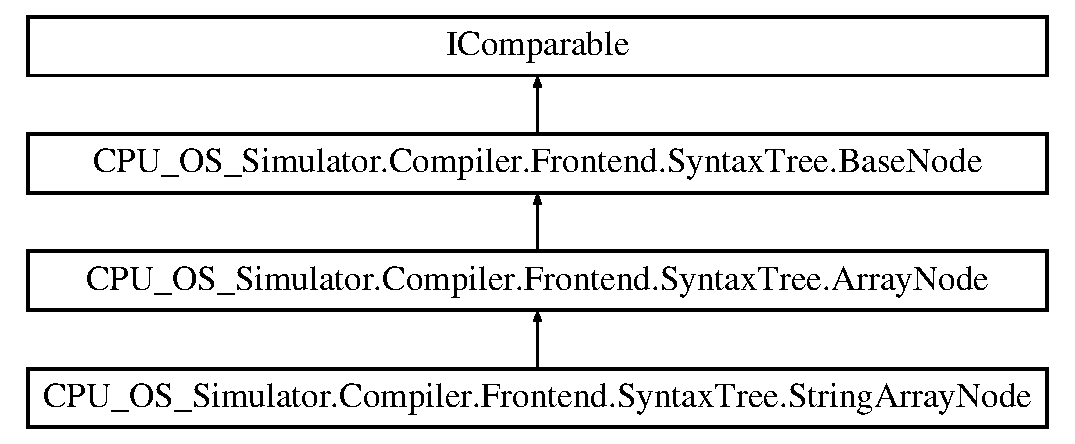
\includegraphics[height=4.000000cm]{class_c_p_u___o_s___simulator_1_1_compiler_1_1_frontend_1_1_syntax_tree_1_1_string_array_node}
\end{center}
\end{figure}
\subsection*{Public Member Functions}
\begin{DoxyCompactItemize}
\item 
override void \hyperlink{class_c_p_u___o_s___simulator_1_1_compiler_1_1_frontend_1_1_syntax_tree_1_1_string_array_node_ae8ce8f85a313e577506546a26c954e34}{Visit} ()
\begin{DoxyCompactList}\small\item\em This function is called when the node is being visited by the parser \end{DoxyCompactList}\item 
override void \hyperlink{class_c_p_u___o_s___simulator_1_1_compiler_1_1_frontend_1_1_syntax_tree_1_1_string_array_node_a559630365acec250f2eed840010535f8}{Evaluate} ()
\begin{DoxyCompactList}\small\item\em This Function is called when the node is being evaluated by the parser \end{DoxyCompactList}\item 
override int \hyperlink{class_c_p_u___o_s___simulator_1_1_compiler_1_1_frontend_1_1_syntax_tree_1_1_string_array_node_aff86779eee1fe0119c3b717f6d673f2c}{number\+Of\+Elements} ()
\end{DoxyCompactItemize}
\subsection*{Properties}
\begin{DoxyCompactItemize}
\item 
override \hyperlink{class_c_p_u___o_s___simulator_1_1_compiler_1_1_frontend_1_1_syntax_tree_1_1_base_node}{Base\+Node} \hyperlink{class_c_p_u___o_s___simulator_1_1_compiler_1_1_frontend_1_1_syntax_tree_1_1_string_array_node_a736bb824c3e207f918237e1fdde209e7}{Right}\hspace{0.3cm}{\ttfamily  \mbox{[}get, set\mbox{]}}
\item 
override \hyperlink{class_c_p_u___o_s___simulator_1_1_compiler_1_1_frontend_1_1_syntax_tree_1_1_base_node}{Base\+Node} \hyperlink{class_c_p_u___o_s___simulator_1_1_compiler_1_1_frontend_1_1_syntax_tree_1_1_string_array_node_ab1fe0f32903bdd2b0980341665cbea63}{Left}\hspace{0.3cm}{\ttfamily  \mbox{[}get, set\mbox{]}}
\item 
string\mbox{[}$\,$\mbox{]} \hyperlink{class_c_p_u___o_s___simulator_1_1_compiler_1_1_frontend_1_1_syntax_tree_1_1_string_array_node_a1cf09c3567fe4fa869a34fbaa302e0e9}{Data}\hspace{0.3cm}{\ttfamily  \mbox{[}get, set\mbox{]}}
\item 
override \hyperlink{class_c_p_u___o_s___simulator_1_1_compiler_1_1_frontend_1_1_syntax_tree_1_1_base_node}{Base\+Node} \hyperlink{class_c_p_u___o_s___simulator_1_1_compiler_1_1_frontend_1_1_syntax_tree_1_1_string_array_node_a57b4d674b9257b7304559bd8f6e796f4}{Parent}\hspace{0.3cm}{\ttfamily  \mbox{[}get, set\mbox{]}}
\end{DoxyCompactItemize}
\subsection*{Private Attributes}
\begin{DoxyCompactItemize}
\item 
string\mbox{[}$\,$\mbox{]} \hyperlink{class_c_p_u___o_s___simulator_1_1_compiler_1_1_frontend_1_1_syntax_tree_1_1_string_array_node_a57893a3c331b998350c0bb8d5f220b79}{data}
\item 
\hyperlink{class_c_p_u___o_s___simulator_1_1_compiler_1_1_frontend_1_1_syntax_tree_1_1_base_node}{Base\+Node} \hyperlink{class_c_p_u___o_s___simulator_1_1_compiler_1_1_frontend_1_1_syntax_tree_1_1_string_array_node_ad651c9685e3085bdcc0e6d7759239146}{parent}
\end{DoxyCompactItemize}
\subsection*{Additional Inherited Members}


\subsection{Detailed Description}


Definition at line 3 of file String\+Array\+Node.\+cs.



\subsection{Member Function Documentation}
\hypertarget{class_c_p_u___o_s___simulator_1_1_compiler_1_1_frontend_1_1_syntax_tree_1_1_string_array_node_a559630365acec250f2eed840010535f8}{}\index{C\+P\+U\+\_\+\+O\+S\+\_\+\+Simulator\+::\+Compiler\+::\+Frontend\+::\+Syntax\+Tree\+::\+String\+Array\+Node@{C\+P\+U\+\_\+\+O\+S\+\_\+\+Simulator\+::\+Compiler\+::\+Frontend\+::\+Syntax\+Tree\+::\+String\+Array\+Node}!Evaluate@{Evaluate}}
\index{Evaluate@{Evaluate}!C\+P\+U\+\_\+\+O\+S\+\_\+\+Simulator\+::\+Compiler\+::\+Frontend\+::\+Syntax\+Tree\+::\+String\+Array\+Node@{C\+P\+U\+\_\+\+O\+S\+\_\+\+Simulator\+::\+Compiler\+::\+Frontend\+::\+Syntax\+Tree\+::\+String\+Array\+Node}}
\subsubsection[{Evaluate()}]{\setlength{\rightskip}{0pt plus 5cm}override void C\+P\+U\+\_\+\+O\+S\+\_\+\+Simulator.\+Compiler.\+Frontend.\+Syntax\+Tree.\+String\+Array\+Node.\+Evaluate (
\begin{DoxyParamCaption}
{}
\end{DoxyParamCaption}
)\hspace{0.3cm}{\ttfamily [virtual]}}\label{class_c_p_u___o_s___simulator_1_1_compiler_1_1_frontend_1_1_syntax_tree_1_1_string_array_node_a559630365acec250f2eed840010535f8}


This Function is called when the node is being evaluated by the parser 



Implements \hyperlink{class_c_p_u___o_s___simulator_1_1_compiler_1_1_frontend_1_1_syntax_tree_1_1_array_node_afdb5d2808dbd83c28c85f35b6430edc4}{C\+P\+U\+\_\+\+O\+S\+\_\+\+Simulator.\+Compiler.\+Frontend.\+Syntax\+Tree.\+Array\+Node}.



Definition at line 42 of file String\+Array\+Node.\+cs.

\hypertarget{class_c_p_u___o_s___simulator_1_1_compiler_1_1_frontend_1_1_syntax_tree_1_1_string_array_node_aff86779eee1fe0119c3b717f6d673f2c}{}\index{C\+P\+U\+\_\+\+O\+S\+\_\+\+Simulator\+::\+Compiler\+::\+Frontend\+::\+Syntax\+Tree\+::\+String\+Array\+Node@{C\+P\+U\+\_\+\+O\+S\+\_\+\+Simulator\+::\+Compiler\+::\+Frontend\+::\+Syntax\+Tree\+::\+String\+Array\+Node}!number\+Of\+Elements@{number\+Of\+Elements}}
\index{number\+Of\+Elements@{number\+Of\+Elements}!C\+P\+U\+\_\+\+O\+S\+\_\+\+Simulator\+::\+Compiler\+::\+Frontend\+::\+Syntax\+Tree\+::\+String\+Array\+Node@{C\+P\+U\+\_\+\+O\+S\+\_\+\+Simulator\+::\+Compiler\+::\+Frontend\+::\+Syntax\+Tree\+::\+String\+Array\+Node}}
\subsubsection[{number\+Of\+Elements()}]{\setlength{\rightskip}{0pt plus 5cm}override int C\+P\+U\+\_\+\+O\+S\+\_\+\+Simulator.\+Compiler.\+Frontend.\+Syntax\+Tree.\+String\+Array\+Node.\+number\+Of\+Elements (
\begin{DoxyParamCaption}
{}
\end{DoxyParamCaption}
)\hspace{0.3cm}{\ttfamily [virtual]}}\label{class_c_p_u___o_s___simulator_1_1_compiler_1_1_frontend_1_1_syntax_tree_1_1_string_array_node_aff86779eee1fe0119c3b717f6d673f2c}


Implements \hyperlink{class_c_p_u___o_s___simulator_1_1_compiler_1_1_frontend_1_1_syntax_tree_1_1_array_node_a75232f3076d95a562405ef2722bcafd5}{C\+P\+U\+\_\+\+O\+S\+\_\+\+Simulator.\+Compiler.\+Frontend.\+Syntax\+Tree.\+Array\+Node}.



Definition at line 46 of file String\+Array\+Node.\+cs.

\hypertarget{class_c_p_u___o_s___simulator_1_1_compiler_1_1_frontend_1_1_syntax_tree_1_1_string_array_node_ae8ce8f85a313e577506546a26c954e34}{}\index{C\+P\+U\+\_\+\+O\+S\+\_\+\+Simulator\+::\+Compiler\+::\+Frontend\+::\+Syntax\+Tree\+::\+String\+Array\+Node@{C\+P\+U\+\_\+\+O\+S\+\_\+\+Simulator\+::\+Compiler\+::\+Frontend\+::\+Syntax\+Tree\+::\+String\+Array\+Node}!Visit@{Visit}}
\index{Visit@{Visit}!C\+P\+U\+\_\+\+O\+S\+\_\+\+Simulator\+::\+Compiler\+::\+Frontend\+::\+Syntax\+Tree\+::\+String\+Array\+Node@{C\+P\+U\+\_\+\+O\+S\+\_\+\+Simulator\+::\+Compiler\+::\+Frontend\+::\+Syntax\+Tree\+::\+String\+Array\+Node}}
\subsubsection[{Visit()}]{\setlength{\rightskip}{0pt plus 5cm}override void C\+P\+U\+\_\+\+O\+S\+\_\+\+Simulator.\+Compiler.\+Frontend.\+Syntax\+Tree.\+String\+Array\+Node.\+Visit (
\begin{DoxyParamCaption}
{}
\end{DoxyParamCaption}
)\hspace{0.3cm}{\ttfamily [virtual]}}\label{class_c_p_u___o_s___simulator_1_1_compiler_1_1_frontend_1_1_syntax_tree_1_1_string_array_node_ae8ce8f85a313e577506546a26c954e34}


This function is called when the node is being visited by the parser 



Implements \hyperlink{class_c_p_u___o_s___simulator_1_1_compiler_1_1_frontend_1_1_syntax_tree_1_1_array_node_aed695b6f32d5c176204fc15854db32db}{C\+P\+U\+\_\+\+O\+S\+\_\+\+Simulator.\+Compiler.\+Frontend.\+Syntax\+Tree.\+Array\+Node}.



Definition at line 35 of file String\+Array\+Node.\+cs.



\subsection{Member Data Documentation}
\hypertarget{class_c_p_u___o_s___simulator_1_1_compiler_1_1_frontend_1_1_syntax_tree_1_1_string_array_node_a57893a3c331b998350c0bb8d5f220b79}{}\index{C\+P\+U\+\_\+\+O\+S\+\_\+\+Simulator\+::\+Compiler\+::\+Frontend\+::\+Syntax\+Tree\+::\+String\+Array\+Node@{C\+P\+U\+\_\+\+O\+S\+\_\+\+Simulator\+::\+Compiler\+::\+Frontend\+::\+Syntax\+Tree\+::\+String\+Array\+Node}!data@{data}}
\index{data@{data}!C\+P\+U\+\_\+\+O\+S\+\_\+\+Simulator\+::\+Compiler\+::\+Frontend\+::\+Syntax\+Tree\+::\+String\+Array\+Node@{C\+P\+U\+\_\+\+O\+S\+\_\+\+Simulator\+::\+Compiler\+::\+Frontend\+::\+Syntax\+Tree\+::\+String\+Array\+Node}}
\subsubsection[{data}]{\setlength{\rightskip}{0pt plus 5cm}string \mbox{[}$\,$\mbox{]} C\+P\+U\+\_\+\+O\+S\+\_\+\+Simulator.\+Compiler.\+Frontend.\+Syntax\+Tree.\+String\+Array\+Node.\+data\hspace{0.3cm}{\ttfamily [private]}}\label{class_c_p_u___o_s___simulator_1_1_compiler_1_1_frontend_1_1_syntax_tree_1_1_string_array_node_a57893a3c331b998350c0bb8d5f220b79}


Definition at line 5 of file String\+Array\+Node.\+cs.

\hypertarget{class_c_p_u___o_s___simulator_1_1_compiler_1_1_frontend_1_1_syntax_tree_1_1_string_array_node_ad651c9685e3085bdcc0e6d7759239146}{}\index{C\+P\+U\+\_\+\+O\+S\+\_\+\+Simulator\+::\+Compiler\+::\+Frontend\+::\+Syntax\+Tree\+::\+String\+Array\+Node@{C\+P\+U\+\_\+\+O\+S\+\_\+\+Simulator\+::\+Compiler\+::\+Frontend\+::\+Syntax\+Tree\+::\+String\+Array\+Node}!parent@{parent}}
\index{parent@{parent}!C\+P\+U\+\_\+\+O\+S\+\_\+\+Simulator\+::\+Compiler\+::\+Frontend\+::\+Syntax\+Tree\+::\+String\+Array\+Node@{C\+P\+U\+\_\+\+O\+S\+\_\+\+Simulator\+::\+Compiler\+::\+Frontend\+::\+Syntax\+Tree\+::\+String\+Array\+Node}}
\subsubsection[{parent}]{\setlength{\rightskip}{0pt plus 5cm}{\bf Base\+Node} C\+P\+U\+\_\+\+O\+S\+\_\+\+Simulator.\+Compiler.\+Frontend.\+Syntax\+Tree.\+String\+Array\+Node.\+parent\hspace{0.3cm}{\ttfamily [private]}}\label{class_c_p_u___o_s___simulator_1_1_compiler_1_1_frontend_1_1_syntax_tree_1_1_string_array_node_ad651c9685e3085bdcc0e6d7759239146}


Definition at line 6 of file String\+Array\+Node.\+cs.



\subsection{Property Documentation}
\hypertarget{class_c_p_u___o_s___simulator_1_1_compiler_1_1_frontend_1_1_syntax_tree_1_1_string_array_node_a1cf09c3567fe4fa869a34fbaa302e0e9}{}\index{C\+P\+U\+\_\+\+O\+S\+\_\+\+Simulator\+::\+Compiler\+::\+Frontend\+::\+Syntax\+Tree\+::\+String\+Array\+Node@{C\+P\+U\+\_\+\+O\+S\+\_\+\+Simulator\+::\+Compiler\+::\+Frontend\+::\+Syntax\+Tree\+::\+String\+Array\+Node}!Data@{Data}}
\index{Data@{Data}!C\+P\+U\+\_\+\+O\+S\+\_\+\+Simulator\+::\+Compiler\+::\+Frontend\+::\+Syntax\+Tree\+::\+String\+Array\+Node@{C\+P\+U\+\_\+\+O\+S\+\_\+\+Simulator\+::\+Compiler\+::\+Frontend\+::\+Syntax\+Tree\+::\+String\+Array\+Node}}
\subsubsection[{Data}]{\setlength{\rightskip}{0pt plus 5cm}string \mbox{[}$\,$\mbox{]} C\+P\+U\+\_\+\+O\+S\+\_\+\+Simulator.\+Compiler.\+Frontend.\+Syntax\+Tree.\+String\+Array\+Node.\+Data\hspace{0.3cm}{\ttfamily [get]}, {\ttfamily [set]}}\label{class_c_p_u___o_s___simulator_1_1_compiler_1_1_frontend_1_1_syntax_tree_1_1_string_array_node_a1cf09c3567fe4fa869a34fbaa302e0e9}


Definition at line 21 of file String\+Array\+Node.\+cs.

\hypertarget{class_c_p_u___o_s___simulator_1_1_compiler_1_1_frontend_1_1_syntax_tree_1_1_string_array_node_ab1fe0f32903bdd2b0980341665cbea63}{}\index{C\+P\+U\+\_\+\+O\+S\+\_\+\+Simulator\+::\+Compiler\+::\+Frontend\+::\+Syntax\+Tree\+::\+String\+Array\+Node@{C\+P\+U\+\_\+\+O\+S\+\_\+\+Simulator\+::\+Compiler\+::\+Frontend\+::\+Syntax\+Tree\+::\+String\+Array\+Node}!Left@{Left}}
\index{Left@{Left}!C\+P\+U\+\_\+\+O\+S\+\_\+\+Simulator\+::\+Compiler\+::\+Frontend\+::\+Syntax\+Tree\+::\+String\+Array\+Node@{C\+P\+U\+\_\+\+O\+S\+\_\+\+Simulator\+::\+Compiler\+::\+Frontend\+::\+Syntax\+Tree\+::\+String\+Array\+Node}}
\subsubsection[{Left}]{\setlength{\rightskip}{0pt plus 5cm}override {\bf Base\+Node} C\+P\+U\+\_\+\+O\+S\+\_\+\+Simulator.\+Compiler.\+Frontend.\+Syntax\+Tree.\+String\+Array\+Node.\+Left\hspace{0.3cm}{\ttfamily [get]}, {\ttfamily [set]}}\label{class_c_p_u___o_s___simulator_1_1_compiler_1_1_frontend_1_1_syntax_tree_1_1_string_array_node_ab1fe0f32903bdd2b0980341665cbea63}


Definition at line 15 of file String\+Array\+Node.\+cs.

\hypertarget{class_c_p_u___o_s___simulator_1_1_compiler_1_1_frontend_1_1_syntax_tree_1_1_string_array_node_a57b4d674b9257b7304559bd8f6e796f4}{}\index{C\+P\+U\+\_\+\+O\+S\+\_\+\+Simulator\+::\+Compiler\+::\+Frontend\+::\+Syntax\+Tree\+::\+String\+Array\+Node@{C\+P\+U\+\_\+\+O\+S\+\_\+\+Simulator\+::\+Compiler\+::\+Frontend\+::\+Syntax\+Tree\+::\+String\+Array\+Node}!Parent@{Parent}}
\index{Parent@{Parent}!C\+P\+U\+\_\+\+O\+S\+\_\+\+Simulator\+::\+Compiler\+::\+Frontend\+::\+Syntax\+Tree\+::\+String\+Array\+Node@{C\+P\+U\+\_\+\+O\+S\+\_\+\+Simulator\+::\+Compiler\+::\+Frontend\+::\+Syntax\+Tree\+::\+String\+Array\+Node}}
\subsubsection[{Parent}]{\setlength{\rightskip}{0pt plus 5cm}override {\bf Base\+Node} C\+P\+U\+\_\+\+O\+S\+\_\+\+Simulator.\+Compiler.\+Frontend.\+Syntax\+Tree.\+String\+Array\+Node.\+Parent\hspace{0.3cm}{\ttfamily [get]}, {\ttfamily [set]}}\label{class_c_p_u___o_s___simulator_1_1_compiler_1_1_frontend_1_1_syntax_tree_1_1_string_array_node_a57b4d674b9257b7304559bd8f6e796f4}


Definition at line 27 of file String\+Array\+Node.\+cs.

\hypertarget{class_c_p_u___o_s___simulator_1_1_compiler_1_1_frontend_1_1_syntax_tree_1_1_string_array_node_a736bb824c3e207f918237e1fdde209e7}{}\index{C\+P\+U\+\_\+\+O\+S\+\_\+\+Simulator\+::\+Compiler\+::\+Frontend\+::\+Syntax\+Tree\+::\+String\+Array\+Node@{C\+P\+U\+\_\+\+O\+S\+\_\+\+Simulator\+::\+Compiler\+::\+Frontend\+::\+Syntax\+Tree\+::\+String\+Array\+Node}!Right@{Right}}
\index{Right@{Right}!C\+P\+U\+\_\+\+O\+S\+\_\+\+Simulator\+::\+Compiler\+::\+Frontend\+::\+Syntax\+Tree\+::\+String\+Array\+Node@{C\+P\+U\+\_\+\+O\+S\+\_\+\+Simulator\+::\+Compiler\+::\+Frontend\+::\+Syntax\+Tree\+::\+String\+Array\+Node}}
\subsubsection[{Right}]{\setlength{\rightskip}{0pt plus 5cm}override {\bf Base\+Node} C\+P\+U\+\_\+\+O\+S\+\_\+\+Simulator.\+Compiler.\+Frontend.\+Syntax\+Tree.\+String\+Array\+Node.\+Right\hspace{0.3cm}{\ttfamily [get]}, {\ttfamily [set]}}\label{class_c_p_u___o_s___simulator_1_1_compiler_1_1_frontend_1_1_syntax_tree_1_1_string_array_node_a736bb824c3e207f918237e1fdde209e7}


Definition at line 9 of file String\+Array\+Node.\+cs.



The documentation for this class was generated from the following file\+:\begin{DoxyCompactItemize}
\item 
Compiler/\+Frontend/\+Syntax\+Tree/\hyperlink{_string_array_node_8cs}{String\+Array\+Node.\+cs}\end{DoxyCompactItemize}

\hypertarget{class_c_p_u___o_s___simulator_1_1_compiler_1_1_frontend_1_1_tokens_1_1_string_literal}{}\section{C\+P\+U\+\_\+\+O\+S\+\_\+\+Simulator.\+Compiler.\+Frontend.\+Tokens.\+String\+Literal Class Reference}
\label{class_c_p_u___o_s___simulator_1_1_compiler_1_1_frontend_1_1_tokens_1_1_string_literal}\index{C\+P\+U\+\_\+\+O\+S\+\_\+\+Simulator.\+Compiler.\+Frontend.\+Tokens.\+String\+Literal@{C\+P\+U\+\_\+\+O\+S\+\_\+\+Simulator.\+Compiler.\+Frontend.\+Tokens.\+String\+Literal}}
Inheritance diagram for C\+P\+U\+\_\+\+O\+S\+\_\+\+Simulator.\+Compiler.\+Frontend.\+Tokens.\+String\+Literal\+:\begin{figure}[H]
\begin{center}
\leavevmode
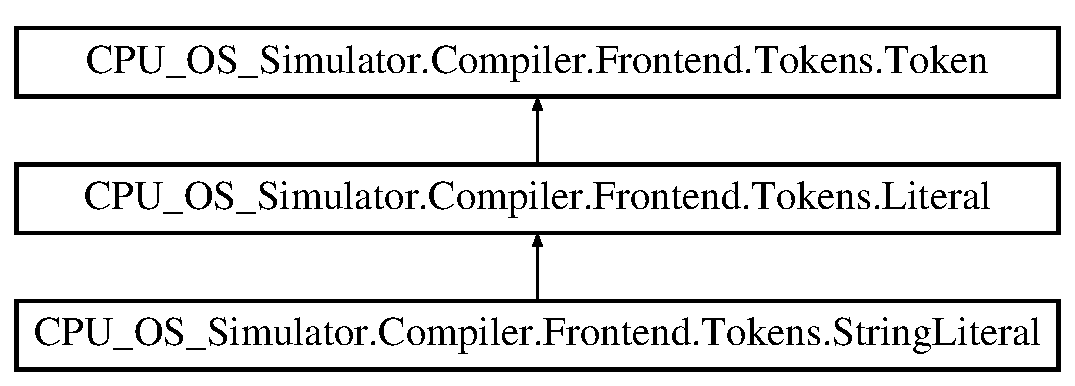
\includegraphics[height=3.000000cm]{class_c_p_u___o_s___simulator_1_1_compiler_1_1_frontend_1_1_tokens_1_1_string_literal}
\end{center}
\end{figure}
\subsection*{Public Member Functions}
\begin{DoxyCompactItemize}
\item 
\hyperlink{class_c_p_u___o_s___simulator_1_1_compiler_1_1_frontend_1_1_tokens_1_1_string_literal_a78bb388b6ac5a9cc067f39358162373c}{String\+Literal} (string \hyperlink{class_c_p_u___o_s___simulator_1_1_compiler_1_1_frontend_1_1_tokens_1_1_token_a5c05e12850ca18be8cbfdf7e2e263324}{value})
\item 
override Enum \hyperlink{class_c_p_u___o_s___simulator_1_1_compiler_1_1_frontend_1_1_tokens_1_1_string_literal_a55fe99257eeaeb6d73db4ff188de3f57}{Detect\+Type} ()
\begin{DoxyCompactList}\small\item\em This function detects the type of literal \end{DoxyCompactList}\item 
override \hyperlink{namespace_c_p_u___o_s___simulator_1_1_compiler_1_1_frontend_1_1_tokens_a7c0cc43763cc9d01c7d5af34d70b96ea}{Enum\+Types} \hyperlink{class_c_p_u___o_s___simulator_1_1_compiler_1_1_frontend_1_1_tokens_1_1_string_literal_ad4121c2eda9ab84f08bb0c51996c96cb}{identfy\+Value\+Type} ()
\begin{DoxyCompactList}\small\item\em This function identifies the type of data stored in the literal \end{DoxyCompactList}\end{DoxyCompactItemize}
\subsection*{Additional Inherited Members}


\subsection{Detailed Description}


Definition at line 5 of file String\+Literal.\+cs.



\subsection{Constructor \& Destructor Documentation}
\hypertarget{class_c_p_u___o_s___simulator_1_1_compiler_1_1_frontend_1_1_tokens_1_1_string_literal_a78bb388b6ac5a9cc067f39358162373c}{}\index{C\+P\+U\+\_\+\+O\+S\+\_\+\+Simulator\+::\+Compiler\+::\+Frontend\+::\+Tokens\+::\+String\+Literal@{C\+P\+U\+\_\+\+O\+S\+\_\+\+Simulator\+::\+Compiler\+::\+Frontend\+::\+Tokens\+::\+String\+Literal}!String\+Literal@{String\+Literal}}
\index{String\+Literal@{String\+Literal}!C\+P\+U\+\_\+\+O\+S\+\_\+\+Simulator\+::\+Compiler\+::\+Frontend\+::\+Tokens\+::\+String\+Literal@{C\+P\+U\+\_\+\+O\+S\+\_\+\+Simulator\+::\+Compiler\+::\+Frontend\+::\+Tokens\+::\+String\+Literal}}
\subsubsection[{String\+Literal(string value)}]{\setlength{\rightskip}{0pt plus 5cm}C\+P\+U\+\_\+\+O\+S\+\_\+\+Simulator.\+Compiler.\+Frontend.\+Tokens.\+String\+Literal.\+String\+Literal (
\begin{DoxyParamCaption}
\item[{string}]{value}
\end{DoxyParamCaption}
)}\label{class_c_p_u___o_s___simulator_1_1_compiler_1_1_frontend_1_1_tokens_1_1_string_literal_a78bb388b6ac5a9cc067f39358162373c}


Definition at line 7 of file String\+Literal.\+cs.



\subsection{Member Function Documentation}
\hypertarget{class_c_p_u___o_s___simulator_1_1_compiler_1_1_frontend_1_1_tokens_1_1_string_literal_a55fe99257eeaeb6d73db4ff188de3f57}{}\index{C\+P\+U\+\_\+\+O\+S\+\_\+\+Simulator\+::\+Compiler\+::\+Frontend\+::\+Tokens\+::\+String\+Literal@{C\+P\+U\+\_\+\+O\+S\+\_\+\+Simulator\+::\+Compiler\+::\+Frontend\+::\+Tokens\+::\+String\+Literal}!Detect\+Type@{Detect\+Type}}
\index{Detect\+Type@{Detect\+Type}!C\+P\+U\+\_\+\+O\+S\+\_\+\+Simulator\+::\+Compiler\+::\+Frontend\+::\+Tokens\+::\+String\+Literal@{C\+P\+U\+\_\+\+O\+S\+\_\+\+Simulator\+::\+Compiler\+::\+Frontend\+::\+Tokens\+::\+String\+Literal}}
\subsubsection[{Detect\+Type()}]{\setlength{\rightskip}{0pt plus 5cm}override Enum C\+P\+U\+\_\+\+O\+S\+\_\+\+Simulator.\+Compiler.\+Frontend.\+Tokens.\+String\+Literal.\+Detect\+Type (
\begin{DoxyParamCaption}
{}
\end{DoxyParamCaption}
)\hspace{0.3cm}{\ttfamily [virtual]}}\label{class_c_p_u___o_s___simulator_1_1_compiler_1_1_frontend_1_1_tokens_1_1_string_literal_a55fe99257eeaeb6d73db4ff188de3f57}


This function detects the type of literal 

\begin{DoxyReturn}{Returns}
the type of literal
\end{DoxyReturn}


Implements \hyperlink{class_c_p_u___o_s___simulator_1_1_compiler_1_1_frontend_1_1_tokens_1_1_literal_af449c5fee28fb2076933cdfc67857c23}{C\+P\+U\+\_\+\+O\+S\+\_\+\+Simulator.\+Compiler.\+Frontend.\+Tokens.\+Literal}.



Definition at line 16 of file String\+Literal.\+cs.

\hypertarget{class_c_p_u___o_s___simulator_1_1_compiler_1_1_frontend_1_1_tokens_1_1_string_literal_ad4121c2eda9ab84f08bb0c51996c96cb}{}\index{C\+P\+U\+\_\+\+O\+S\+\_\+\+Simulator\+::\+Compiler\+::\+Frontend\+::\+Tokens\+::\+String\+Literal@{C\+P\+U\+\_\+\+O\+S\+\_\+\+Simulator\+::\+Compiler\+::\+Frontend\+::\+Tokens\+::\+String\+Literal}!identfy\+Value\+Type@{identfy\+Value\+Type}}
\index{identfy\+Value\+Type@{identfy\+Value\+Type}!C\+P\+U\+\_\+\+O\+S\+\_\+\+Simulator\+::\+Compiler\+::\+Frontend\+::\+Tokens\+::\+String\+Literal@{C\+P\+U\+\_\+\+O\+S\+\_\+\+Simulator\+::\+Compiler\+::\+Frontend\+::\+Tokens\+::\+String\+Literal}}
\subsubsection[{identfy\+Value\+Type()}]{\setlength{\rightskip}{0pt plus 5cm}override {\bf Enum\+Types} C\+P\+U\+\_\+\+O\+S\+\_\+\+Simulator.\+Compiler.\+Frontend.\+Tokens.\+String\+Literal.\+identfy\+Value\+Type (
\begin{DoxyParamCaption}
{}
\end{DoxyParamCaption}
)\hspace{0.3cm}{\ttfamily [virtual]}}\label{class_c_p_u___o_s___simulator_1_1_compiler_1_1_frontend_1_1_tokens_1_1_string_literal_ad4121c2eda9ab84f08bb0c51996c96cb}


This function identifies the type of data stored in the literal 

\begin{DoxyReturn}{Returns}
the type of value in the literal
\end{DoxyReturn}


Implements \hyperlink{class_c_p_u___o_s___simulator_1_1_compiler_1_1_frontend_1_1_tokens_1_1_literal_a34d05c00ded660daf66f91bd2543d186}{C\+P\+U\+\_\+\+O\+S\+\_\+\+Simulator.\+Compiler.\+Frontend.\+Tokens.\+Literal}.



Definition at line 25 of file String\+Literal.\+cs.



The documentation for this class was generated from the following file\+:\begin{DoxyCompactItemize}
\item 
Compiler/\+Frontend/\+Tokens/\hyperlink{_string_literal_8cs}{String\+Literal.\+cs}\end{DoxyCompactItemize}

\hypertarget{class_c_p_u___o_s___simulator_1_1_compiler_1_1_frontend_1_1_syntax_tree_1_1_string_node}{}\section{C\+P\+U\+\_\+\+O\+S\+\_\+\+Simulator.\+Compiler.\+Frontend.\+Syntax\+Tree.\+String\+Node Class Reference}
\label{class_c_p_u___o_s___simulator_1_1_compiler_1_1_frontend_1_1_syntax_tree_1_1_string_node}\index{C\+P\+U\+\_\+\+O\+S\+\_\+\+Simulator.\+Compiler.\+Frontend.\+Syntax\+Tree.\+String\+Node@{C\+P\+U\+\_\+\+O\+S\+\_\+\+Simulator.\+Compiler.\+Frontend.\+Syntax\+Tree.\+String\+Node}}
Inheritance diagram for C\+P\+U\+\_\+\+O\+S\+\_\+\+Simulator.\+Compiler.\+Frontend.\+Syntax\+Tree.\+String\+Node\+:\begin{figure}[H]
\begin{center}
\leavevmode
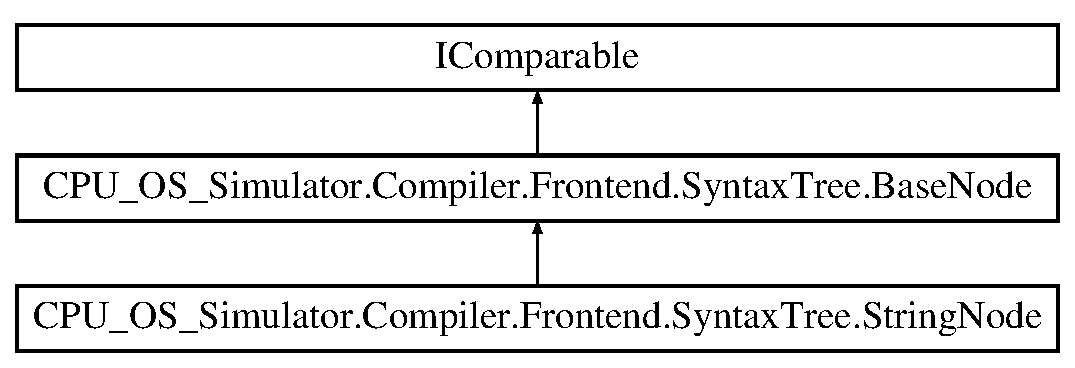
\includegraphics[height=3.000000cm]{class_c_p_u___o_s___simulator_1_1_compiler_1_1_frontend_1_1_syntax_tree_1_1_string_node}
\end{center}
\end{figure}
\subsection*{Public Member Functions}
\begin{DoxyCompactItemize}
\item 
override void \hyperlink{class_c_p_u___o_s___simulator_1_1_compiler_1_1_frontend_1_1_syntax_tree_1_1_string_node_a08063171005bc1ee91e327b35cbfb7a1}{Visit} ()
\begin{DoxyCompactList}\small\item\em This function is called when the node is being visited by the parser \end{DoxyCompactList}\item 
override void \hyperlink{class_c_p_u___o_s___simulator_1_1_compiler_1_1_frontend_1_1_syntax_tree_1_1_string_node_aa13c55d835188df6289e7cc1844199d3}{Evaluate} ()
\begin{DoxyCompactList}\small\item\em This Function is called when the node is being evaluated by the parser \end{DoxyCompactList}\end{DoxyCompactItemize}
\subsection*{Properties}
\begin{DoxyCompactItemize}
\item 
override \hyperlink{class_c_p_u___o_s___simulator_1_1_compiler_1_1_frontend_1_1_syntax_tree_1_1_base_node}{Base\+Node} \hyperlink{class_c_p_u___o_s___simulator_1_1_compiler_1_1_frontend_1_1_syntax_tree_1_1_string_node_af0e815dbcde3e885702fb1222ef3a759}{Right}\hspace{0.3cm}{\ttfamily  \mbox{[}get, set\mbox{]}}
\item 
override \hyperlink{class_c_p_u___o_s___simulator_1_1_compiler_1_1_frontend_1_1_syntax_tree_1_1_base_node}{Base\+Node} \hyperlink{class_c_p_u___o_s___simulator_1_1_compiler_1_1_frontend_1_1_syntax_tree_1_1_string_node_aad74a0bb5e5a855d520de3223b6748b2}{Left}\hspace{0.3cm}{\ttfamily  \mbox{[}get, set\mbox{]}}
\item 
string \hyperlink{class_c_p_u___o_s___simulator_1_1_compiler_1_1_frontend_1_1_syntax_tree_1_1_string_node_a409841a2c8cdb16e19e500187d5c4567}{Data}\hspace{0.3cm}{\ttfamily  \mbox{[}get, set\mbox{]}}
\item 
override \hyperlink{class_c_p_u___o_s___simulator_1_1_compiler_1_1_frontend_1_1_syntax_tree_1_1_base_node}{Base\+Node} \hyperlink{class_c_p_u___o_s___simulator_1_1_compiler_1_1_frontend_1_1_syntax_tree_1_1_string_node_a262b5a0b218a8b98f0e54c0aa24b908a}{Parent}\hspace{0.3cm}{\ttfamily  \mbox{[}get, set\mbox{]}}
\end{DoxyCompactItemize}
\subsection*{Private Attributes}
\begin{DoxyCompactItemize}
\item 
new string \hyperlink{class_c_p_u___o_s___simulator_1_1_compiler_1_1_frontend_1_1_syntax_tree_1_1_string_node_afd48d77cc3c1d2e2a07701f49ec994c7}{data}
\item 
\hyperlink{class_c_p_u___o_s___simulator_1_1_compiler_1_1_frontend_1_1_syntax_tree_1_1_base_node}{Base\+Node} \hyperlink{class_c_p_u___o_s___simulator_1_1_compiler_1_1_frontend_1_1_syntax_tree_1_1_string_node_a1a479b5330024edfa9711ddc19f58ded}{parent}
\end{DoxyCompactItemize}
\subsection*{Additional Inherited Members}


\subsection{Detailed Description}


Definition at line 3 of file String\+Node.\+cs.



\subsection{Member Function Documentation}
\hypertarget{class_c_p_u___o_s___simulator_1_1_compiler_1_1_frontend_1_1_syntax_tree_1_1_string_node_aa13c55d835188df6289e7cc1844199d3}{}\index{C\+P\+U\+\_\+\+O\+S\+\_\+\+Simulator\+::\+Compiler\+::\+Frontend\+::\+Syntax\+Tree\+::\+String\+Node@{C\+P\+U\+\_\+\+O\+S\+\_\+\+Simulator\+::\+Compiler\+::\+Frontend\+::\+Syntax\+Tree\+::\+String\+Node}!Evaluate@{Evaluate}}
\index{Evaluate@{Evaluate}!C\+P\+U\+\_\+\+O\+S\+\_\+\+Simulator\+::\+Compiler\+::\+Frontend\+::\+Syntax\+Tree\+::\+String\+Node@{C\+P\+U\+\_\+\+O\+S\+\_\+\+Simulator\+::\+Compiler\+::\+Frontend\+::\+Syntax\+Tree\+::\+String\+Node}}
\subsubsection[{Evaluate()}]{\setlength{\rightskip}{0pt plus 5cm}override void C\+P\+U\+\_\+\+O\+S\+\_\+\+Simulator.\+Compiler.\+Frontend.\+Syntax\+Tree.\+String\+Node.\+Evaluate (
\begin{DoxyParamCaption}
{}
\end{DoxyParamCaption}
)\hspace{0.3cm}{\ttfamily [virtual]}}\label{class_c_p_u___o_s___simulator_1_1_compiler_1_1_frontend_1_1_syntax_tree_1_1_string_node_aa13c55d835188df6289e7cc1844199d3}


This Function is called when the node is being evaluated by the parser 



Implements \hyperlink{class_c_p_u___o_s___simulator_1_1_compiler_1_1_frontend_1_1_syntax_tree_1_1_base_node_a6cfcf8a0795180bdb1c7f0735d39441b}{C\+P\+U\+\_\+\+O\+S\+\_\+\+Simulator.\+Compiler.\+Frontend.\+Syntax\+Tree.\+Base\+Node}.



Definition at line 42 of file String\+Node.\+cs.

\hypertarget{class_c_p_u___o_s___simulator_1_1_compiler_1_1_frontend_1_1_syntax_tree_1_1_string_node_a08063171005bc1ee91e327b35cbfb7a1}{}\index{C\+P\+U\+\_\+\+O\+S\+\_\+\+Simulator\+::\+Compiler\+::\+Frontend\+::\+Syntax\+Tree\+::\+String\+Node@{C\+P\+U\+\_\+\+O\+S\+\_\+\+Simulator\+::\+Compiler\+::\+Frontend\+::\+Syntax\+Tree\+::\+String\+Node}!Visit@{Visit}}
\index{Visit@{Visit}!C\+P\+U\+\_\+\+O\+S\+\_\+\+Simulator\+::\+Compiler\+::\+Frontend\+::\+Syntax\+Tree\+::\+String\+Node@{C\+P\+U\+\_\+\+O\+S\+\_\+\+Simulator\+::\+Compiler\+::\+Frontend\+::\+Syntax\+Tree\+::\+String\+Node}}
\subsubsection[{Visit()}]{\setlength{\rightskip}{0pt plus 5cm}override void C\+P\+U\+\_\+\+O\+S\+\_\+\+Simulator.\+Compiler.\+Frontend.\+Syntax\+Tree.\+String\+Node.\+Visit (
\begin{DoxyParamCaption}
{}
\end{DoxyParamCaption}
)\hspace{0.3cm}{\ttfamily [virtual]}}\label{class_c_p_u___o_s___simulator_1_1_compiler_1_1_frontend_1_1_syntax_tree_1_1_string_node_a08063171005bc1ee91e327b35cbfb7a1}


This function is called when the node is being visited by the parser 



Implements \hyperlink{class_c_p_u___o_s___simulator_1_1_compiler_1_1_frontend_1_1_syntax_tree_1_1_base_node_a092377df64002c5e9c023a259e5e11d0}{C\+P\+U\+\_\+\+O\+S\+\_\+\+Simulator.\+Compiler.\+Frontend.\+Syntax\+Tree.\+Base\+Node}.



Definition at line 35 of file String\+Node.\+cs.



\subsection{Member Data Documentation}
\hypertarget{class_c_p_u___o_s___simulator_1_1_compiler_1_1_frontend_1_1_syntax_tree_1_1_string_node_afd48d77cc3c1d2e2a07701f49ec994c7}{}\index{C\+P\+U\+\_\+\+O\+S\+\_\+\+Simulator\+::\+Compiler\+::\+Frontend\+::\+Syntax\+Tree\+::\+String\+Node@{C\+P\+U\+\_\+\+O\+S\+\_\+\+Simulator\+::\+Compiler\+::\+Frontend\+::\+Syntax\+Tree\+::\+String\+Node}!data@{data}}
\index{data@{data}!C\+P\+U\+\_\+\+O\+S\+\_\+\+Simulator\+::\+Compiler\+::\+Frontend\+::\+Syntax\+Tree\+::\+String\+Node@{C\+P\+U\+\_\+\+O\+S\+\_\+\+Simulator\+::\+Compiler\+::\+Frontend\+::\+Syntax\+Tree\+::\+String\+Node}}
\subsubsection[{data}]{\setlength{\rightskip}{0pt plus 5cm}new string C\+P\+U\+\_\+\+O\+S\+\_\+\+Simulator.\+Compiler.\+Frontend.\+Syntax\+Tree.\+String\+Node.\+data\hspace{0.3cm}{\ttfamily [private]}}\label{class_c_p_u___o_s___simulator_1_1_compiler_1_1_frontend_1_1_syntax_tree_1_1_string_node_afd48d77cc3c1d2e2a07701f49ec994c7}


Definition at line 5 of file String\+Node.\+cs.

\hypertarget{class_c_p_u___o_s___simulator_1_1_compiler_1_1_frontend_1_1_syntax_tree_1_1_string_node_a1a479b5330024edfa9711ddc19f58ded}{}\index{C\+P\+U\+\_\+\+O\+S\+\_\+\+Simulator\+::\+Compiler\+::\+Frontend\+::\+Syntax\+Tree\+::\+String\+Node@{C\+P\+U\+\_\+\+O\+S\+\_\+\+Simulator\+::\+Compiler\+::\+Frontend\+::\+Syntax\+Tree\+::\+String\+Node}!parent@{parent}}
\index{parent@{parent}!C\+P\+U\+\_\+\+O\+S\+\_\+\+Simulator\+::\+Compiler\+::\+Frontend\+::\+Syntax\+Tree\+::\+String\+Node@{C\+P\+U\+\_\+\+O\+S\+\_\+\+Simulator\+::\+Compiler\+::\+Frontend\+::\+Syntax\+Tree\+::\+String\+Node}}
\subsubsection[{parent}]{\setlength{\rightskip}{0pt plus 5cm}{\bf Base\+Node} C\+P\+U\+\_\+\+O\+S\+\_\+\+Simulator.\+Compiler.\+Frontend.\+Syntax\+Tree.\+String\+Node.\+parent\hspace{0.3cm}{\ttfamily [private]}}\label{class_c_p_u___o_s___simulator_1_1_compiler_1_1_frontend_1_1_syntax_tree_1_1_string_node_a1a479b5330024edfa9711ddc19f58ded}


Definition at line 6 of file String\+Node.\+cs.



\subsection{Property Documentation}
\hypertarget{class_c_p_u___o_s___simulator_1_1_compiler_1_1_frontend_1_1_syntax_tree_1_1_string_node_a409841a2c8cdb16e19e500187d5c4567}{}\index{C\+P\+U\+\_\+\+O\+S\+\_\+\+Simulator\+::\+Compiler\+::\+Frontend\+::\+Syntax\+Tree\+::\+String\+Node@{C\+P\+U\+\_\+\+O\+S\+\_\+\+Simulator\+::\+Compiler\+::\+Frontend\+::\+Syntax\+Tree\+::\+String\+Node}!Data@{Data}}
\index{Data@{Data}!C\+P\+U\+\_\+\+O\+S\+\_\+\+Simulator\+::\+Compiler\+::\+Frontend\+::\+Syntax\+Tree\+::\+String\+Node@{C\+P\+U\+\_\+\+O\+S\+\_\+\+Simulator\+::\+Compiler\+::\+Frontend\+::\+Syntax\+Tree\+::\+String\+Node}}
\subsubsection[{Data}]{\setlength{\rightskip}{0pt plus 5cm}string C\+P\+U\+\_\+\+O\+S\+\_\+\+Simulator.\+Compiler.\+Frontend.\+Syntax\+Tree.\+String\+Node.\+Data\hspace{0.3cm}{\ttfamily [get]}, {\ttfamily [set]}}\label{class_c_p_u___o_s___simulator_1_1_compiler_1_1_frontend_1_1_syntax_tree_1_1_string_node_a409841a2c8cdb16e19e500187d5c4567}


Definition at line 21 of file String\+Node.\+cs.

\hypertarget{class_c_p_u___o_s___simulator_1_1_compiler_1_1_frontend_1_1_syntax_tree_1_1_string_node_aad74a0bb5e5a855d520de3223b6748b2}{}\index{C\+P\+U\+\_\+\+O\+S\+\_\+\+Simulator\+::\+Compiler\+::\+Frontend\+::\+Syntax\+Tree\+::\+String\+Node@{C\+P\+U\+\_\+\+O\+S\+\_\+\+Simulator\+::\+Compiler\+::\+Frontend\+::\+Syntax\+Tree\+::\+String\+Node}!Left@{Left}}
\index{Left@{Left}!C\+P\+U\+\_\+\+O\+S\+\_\+\+Simulator\+::\+Compiler\+::\+Frontend\+::\+Syntax\+Tree\+::\+String\+Node@{C\+P\+U\+\_\+\+O\+S\+\_\+\+Simulator\+::\+Compiler\+::\+Frontend\+::\+Syntax\+Tree\+::\+String\+Node}}
\subsubsection[{Left}]{\setlength{\rightskip}{0pt plus 5cm}override {\bf Base\+Node} C\+P\+U\+\_\+\+O\+S\+\_\+\+Simulator.\+Compiler.\+Frontend.\+Syntax\+Tree.\+String\+Node.\+Left\hspace{0.3cm}{\ttfamily [get]}, {\ttfamily [set]}}\label{class_c_p_u___o_s___simulator_1_1_compiler_1_1_frontend_1_1_syntax_tree_1_1_string_node_aad74a0bb5e5a855d520de3223b6748b2}


Definition at line 15 of file String\+Node.\+cs.

\hypertarget{class_c_p_u___o_s___simulator_1_1_compiler_1_1_frontend_1_1_syntax_tree_1_1_string_node_a262b5a0b218a8b98f0e54c0aa24b908a}{}\index{C\+P\+U\+\_\+\+O\+S\+\_\+\+Simulator\+::\+Compiler\+::\+Frontend\+::\+Syntax\+Tree\+::\+String\+Node@{C\+P\+U\+\_\+\+O\+S\+\_\+\+Simulator\+::\+Compiler\+::\+Frontend\+::\+Syntax\+Tree\+::\+String\+Node}!Parent@{Parent}}
\index{Parent@{Parent}!C\+P\+U\+\_\+\+O\+S\+\_\+\+Simulator\+::\+Compiler\+::\+Frontend\+::\+Syntax\+Tree\+::\+String\+Node@{C\+P\+U\+\_\+\+O\+S\+\_\+\+Simulator\+::\+Compiler\+::\+Frontend\+::\+Syntax\+Tree\+::\+String\+Node}}
\subsubsection[{Parent}]{\setlength{\rightskip}{0pt plus 5cm}override {\bf Base\+Node} C\+P\+U\+\_\+\+O\+S\+\_\+\+Simulator.\+Compiler.\+Frontend.\+Syntax\+Tree.\+String\+Node.\+Parent\hspace{0.3cm}{\ttfamily [get]}, {\ttfamily [set]}}\label{class_c_p_u___o_s___simulator_1_1_compiler_1_1_frontend_1_1_syntax_tree_1_1_string_node_a262b5a0b218a8b98f0e54c0aa24b908a}


Definition at line 27 of file String\+Node.\+cs.

\hypertarget{class_c_p_u___o_s___simulator_1_1_compiler_1_1_frontend_1_1_syntax_tree_1_1_string_node_af0e815dbcde3e885702fb1222ef3a759}{}\index{C\+P\+U\+\_\+\+O\+S\+\_\+\+Simulator\+::\+Compiler\+::\+Frontend\+::\+Syntax\+Tree\+::\+String\+Node@{C\+P\+U\+\_\+\+O\+S\+\_\+\+Simulator\+::\+Compiler\+::\+Frontend\+::\+Syntax\+Tree\+::\+String\+Node}!Right@{Right}}
\index{Right@{Right}!C\+P\+U\+\_\+\+O\+S\+\_\+\+Simulator\+::\+Compiler\+::\+Frontend\+::\+Syntax\+Tree\+::\+String\+Node@{C\+P\+U\+\_\+\+O\+S\+\_\+\+Simulator\+::\+Compiler\+::\+Frontend\+::\+Syntax\+Tree\+::\+String\+Node}}
\subsubsection[{Right}]{\setlength{\rightskip}{0pt plus 5cm}override {\bf Base\+Node} C\+P\+U\+\_\+\+O\+S\+\_\+\+Simulator.\+Compiler.\+Frontend.\+Syntax\+Tree.\+String\+Node.\+Right\hspace{0.3cm}{\ttfamily [get]}, {\ttfamily [set]}}\label{class_c_p_u___o_s___simulator_1_1_compiler_1_1_frontend_1_1_syntax_tree_1_1_string_node_af0e815dbcde3e885702fb1222ef3a759}


Definition at line 9 of file String\+Node.\+cs.



The documentation for this class was generated from the following file\+:\begin{DoxyCompactItemize}
\item 
Compiler/\+Frontend/\+Syntax\+Tree/\hyperlink{_string_node_8cs}{String\+Node.\+cs}\end{DoxyCompactItemize}

\hypertarget{class_c_p_u___o_s___simulator_1_1_compiler_1_1_frontend_1_1_symbols_1_1_subroutine}{}\section{C\+P\+U\+\_\+\+O\+S\+\_\+\+Simulator.\+Compiler.\+Frontend.\+Symbols.\+Subroutine Class Reference}
\label{class_c_p_u___o_s___simulator_1_1_compiler_1_1_frontend_1_1_symbols_1_1_subroutine}\index{C\+P\+U\+\_\+\+O\+S\+\_\+\+Simulator.\+Compiler.\+Frontend.\+Symbols.\+Subroutine@{C\+P\+U\+\_\+\+O\+S\+\_\+\+Simulator.\+Compiler.\+Frontend.\+Symbols.\+Subroutine}}
Inheritance diagram for C\+P\+U\+\_\+\+O\+S\+\_\+\+Simulator.\+Compiler.\+Frontend.\+Symbols.\+Subroutine\+:\begin{figure}[H]
\begin{center}
\leavevmode
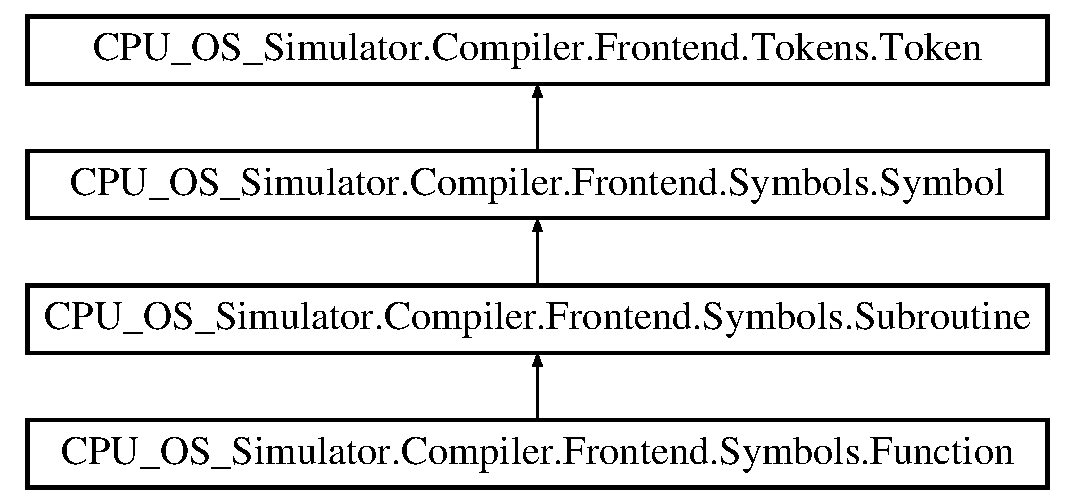
\includegraphics[height=4.000000cm]{class_c_p_u___o_s___simulator_1_1_compiler_1_1_frontend_1_1_symbols_1_1_subroutine}
\end{center}
\end{figure}
\subsection*{Public Member Functions}
\begin{DoxyCompactItemize}
\item 
\hyperlink{class_c_p_u___o_s___simulator_1_1_compiler_1_1_frontend_1_1_symbols_1_1_subroutine_a33c0b9b5e5c0e2b30974db4bbd03222f}{Subroutine} (string \hyperlink{class_c_p_u___o_s___simulator_1_1_compiler_1_1_frontend_1_1_symbols_1_1_symbol_a04abf6b34d531519f4f515f3a51e2089}{name}, \hyperlink{namespace_c_p_u___o_s___simulator_1_1_compiler_1_1_frontend_1_1_tokens_a7c0cc43763cc9d01c7d5af34d70b96ea}{Enum\+Types} \hyperlink{class_c_p_u___o_s___simulator_1_1_compiler_1_1_frontend_1_1_tokens_1_1_token_a7ec4dbbde477cd373f8135f0c843a346}{type}, string \hyperlink{class_c_p_u___o_s___simulator_1_1_compiler_1_1_frontend_1_1_symbols_1_1_symbol_a8c243f84c23afefc2b1c26180e187013}{value}, \hyperlink{class_c_p_u___o_s___simulator_1_1_compiler_1_1_frontend_1_1_symbols_1_1_scope}{Scope} scope)
\end{DoxyCompactItemize}
\subsection*{Additional Inherited Members}


\subsection{Detailed Description}


Definition at line 5 of file Subroutine.\+cs.



\subsection{Constructor \& Destructor Documentation}
\hypertarget{class_c_p_u___o_s___simulator_1_1_compiler_1_1_frontend_1_1_symbols_1_1_subroutine_a33c0b9b5e5c0e2b30974db4bbd03222f}{}\index{C\+P\+U\+\_\+\+O\+S\+\_\+\+Simulator\+::\+Compiler\+::\+Frontend\+::\+Symbols\+::\+Subroutine@{C\+P\+U\+\_\+\+O\+S\+\_\+\+Simulator\+::\+Compiler\+::\+Frontend\+::\+Symbols\+::\+Subroutine}!Subroutine@{Subroutine}}
\index{Subroutine@{Subroutine}!C\+P\+U\+\_\+\+O\+S\+\_\+\+Simulator\+::\+Compiler\+::\+Frontend\+::\+Symbols\+::\+Subroutine@{C\+P\+U\+\_\+\+O\+S\+\_\+\+Simulator\+::\+Compiler\+::\+Frontend\+::\+Symbols\+::\+Subroutine}}
\subsubsection[{Subroutine(string name, Enum\+Types type, string value, Scope scope)}]{\setlength{\rightskip}{0pt plus 5cm}C\+P\+U\+\_\+\+O\+S\+\_\+\+Simulator.\+Compiler.\+Frontend.\+Symbols.\+Subroutine.\+Subroutine (
\begin{DoxyParamCaption}
\item[{string}]{name, }
\item[{{\bf Enum\+Types}}]{type, }
\item[{string}]{value, }
\item[{{\bf Scope}}]{scope}
\end{DoxyParamCaption}
)}\label{class_c_p_u___o_s___simulator_1_1_compiler_1_1_frontend_1_1_symbols_1_1_subroutine_a33c0b9b5e5c0e2b30974db4bbd03222f}


Definition at line 7 of file Subroutine.\+cs.



The documentation for this class was generated from the following file\+:\begin{DoxyCompactItemize}
\item 
Compiler/\+Frontend/\+Symbols/\hyperlink{_subroutine_8cs}{Subroutine.\+cs}\end{DoxyCompactItemize}

\hypertarget{class_c_p_u___o_s___simulator_1_1_memory_1_1_swap_space}{}\section{C\+P\+U\+\_\+\+O\+S\+\_\+\+Simulator.\+Memory.\+Swap\+Space Class Reference}
\label{class_c_p_u___o_s___simulator_1_1_memory_1_1_swap_space}\index{C\+P\+U\+\_\+\+O\+S\+\_\+\+Simulator.\+Memory.\+Swap\+Space@{C\+P\+U\+\_\+\+O\+S\+\_\+\+Simulator.\+Memory.\+Swap\+Space}}


This class represents swap space where swapped outmemory pages are moved to  


\subsection*{Public Member Functions}
\begin{DoxyCompactItemize}
\item 
\hyperlink{class_c_p_u___o_s___simulator_1_1_memory_1_1_swap_space_ad4394dbf2d5a0c95bbabc94948ed37e5}{Swap\+Space} ()
\begin{DoxyCompactList}\small\item\em Constructor for Swap Space \end{DoxyCompactList}\end{DoxyCompactItemize}
\subsection*{Properties}
\begin{DoxyCompactItemize}
\item 
List$<$ \hyperlink{class_c_p_u___o_s___simulator_1_1_memory_1_1_memory_page}{Memory\+Page} $>$ \hyperlink{class_c_p_u___o_s___simulator_1_1_memory_1_1_swap_space_a83c049a398bcff3c29f809b02ed3f782}{Swapped\+Memory\+Pages}\hspace{0.3cm}{\ttfamily  \mbox{[}get, set\mbox{]}}
\begin{DoxyCompactList}\small\item\em Property for the list of swapped out memory pages \end{DoxyCompactList}\end{DoxyCompactItemize}
\subsection*{Private Attributes}
\begin{DoxyCompactItemize}
\item 
List$<$ \hyperlink{class_c_p_u___o_s___simulator_1_1_memory_1_1_memory_page}{Memory\+Page} $>$ \hyperlink{class_c_p_u___o_s___simulator_1_1_memory_1_1_swap_space_ad991c315222ab7bf7fafd562d6fe8014}{swapped\+Memory\+Pages}
\end{DoxyCompactItemize}


\subsection{Detailed Description}
This class represents swap space where swapped outmemory pages are moved to 



Definition at line 12 of file Swap\+Space.\+cs.



\subsection{Constructor \& Destructor Documentation}
\hypertarget{class_c_p_u___o_s___simulator_1_1_memory_1_1_swap_space_ad4394dbf2d5a0c95bbabc94948ed37e5}{}\index{C\+P\+U\+\_\+\+O\+S\+\_\+\+Simulator\+::\+Memory\+::\+Swap\+Space@{C\+P\+U\+\_\+\+O\+S\+\_\+\+Simulator\+::\+Memory\+::\+Swap\+Space}!Swap\+Space@{Swap\+Space}}
\index{Swap\+Space@{Swap\+Space}!C\+P\+U\+\_\+\+O\+S\+\_\+\+Simulator\+::\+Memory\+::\+Swap\+Space@{C\+P\+U\+\_\+\+O\+S\+\_\+\+Simulator\+::\+Memory\+::\+Swap\+Space}}
\subsubsection[{Swap\+Space()}]{\setlength{\rightskip}{0pt plus 5cm}C\+P\+U\+\_\+\+O\+S\+\_\+\+Simulator.\+Memory.\+Swap\+Space.\+Swap\+Space (
\begin{DoxyParamCaption}
{}
\end{DoxyParamCaption}
)}\label{class_c_p_u___o_s___simulator_1_1_memory_1_1_swap_space_ad4394dbf2d5a0c95bbabc94948ed37e5}


Constructor for Swap Space 



Definition at line 19 of file Swap\+Space.\+cs.



\subsection{Member Data Documentation}
\hypertarget{class_c_p_u___o_s___simulator_1_1_memory_1_1_swap_space_ad991c315222ab7bf7fafd562d6fe8014}{}\index{C\+P\+U\+\_\+\+O\+S\+\_\+\+Simulator\+::\+Memory\+::\+Swap\+Space@{C\+P\+U\+\_\+\+O\+S\+\_\+\+Simulator\+::\+Memory\+::\+Swap\+Space}!swapped\+Memory\+Pages@{swapped\+Memory\+Pages}}
\index{swapped\+Memory\+Pages@{swapped\+Memory\+Pages}!C\+P\+U\+\_\+\+O\+S\+\_\+\+Simulator\+::\+Memory\+::\+Swap\+Space@{C\+P\+U\+\_\+\+O\+S\+\_\+\+Simulator\+::\+Memory\+::\+Swap\+Space}}
\subsubsection[{swapped\+Memory\+Pages}]{\setlength{\rightskip}{0pt plus 5cm}List$<${\bf Memory\+Page}$>$ C\+P\+U\+\_\+\+O\+S\+\_\+\+Simulator.\+Memory.\+Swap\+Space.\+swapped\+Memory\+Pages\hspace{0.3cm}{\ttfamily [private]}}\label{class_c_p_u___o_s___simulator_1_1_memory_1_1_swap_space_ad991c315222ab7bf7fafd562d6fe8014}


Definition at line 14 of file Swap\+Space.\+cs.



\subsection{Property Documentation}
\hypertarget{class_c_p_u___o_s___simulator_1_1_memory_1_1_swap_space_a83c049a398bcff3c29f809b02ed3f782}{}\index{C\+P\+U\+\_\+\+O\+S\+\_\+\+Simulator\+::\+Memory\+::\+Swap\+Space@{C\+P\+U\+\_\+\+O\+S\+\_\+\+Simulator\+::\+Memory\+::\+Swap\+Space}!Swapped\+Memory\+Pages@{Swapped\+Memory\+Pages}}
\index{Swapped\+Memory\+Pages@{Swapped\+Memory\+Pages}!C\+P\+U\+\_\+\+O\+S\+\_\+\+Simulator\+::\+Memory\+::\+Swap\+Space@{C\+P\+U\+\_\+\+O\+S\+\_\+\+Simulator\+::\+Memory\+::\+Swap\+Space}}
\subsubsection[{Swapped\+Memory\+Pages}]{\setlength{\rightskip}{0pt plus 5cm}List$<${\bf Memory\+Page}$>$ C\+P\+U\+\_\+\+O\+S\+\_\+\+Simulator.\+Memory.\+Swap\+Space.\+Swapped\+Memory\+Pages\hspace{0.3cm}{\ttfamily [get]}, {\ttfamily [set]}}\label{class_c_p_u___o_s___simulator_1_1_memory_1_1_swap_space_a83c049a398bcff3c29f809b02ed3f782}


Property for the list of swapped out memory pages 



Definition at line 28 of file Swap\+Space.\+cs.



The documentation for this class was generated from the following file\+:\begin{DoxyCompactItemize}
\item 
Memory/\hyperlink{_swap_space_8cs}{Swap\+Space.\+cs}\end{DoxyCompactItemize}

\hypertarget{class_c_p_u___o_s___simulator_1_1_compiler_1_1_frontend_1_1_symbols_1_1_symbol}{}\section{C\+P\+U\+\_\+\+O\+S\+\_\+\+Simulator.\+Compiler.\+Frontend.\+Symbols.\+Symbol Class Reference}
\label{class_c_p_u___o_s___simulator_1_1_compiler_1_1_frontend_1_1_symbols_1_1_symbol}\index{C\+P\+U\+\_\+\+O\+S\+\_\+\+Simulator.\+Compiler.\+Frontend.\+Symbols.\+Symbol@{C\+P\+U\+\_\+\+O\+S\+\_\+\+Simulator.\+Compiler.\+Frontend.\+Symbols.\+Symbol}}
Inheritance diagram for C\+P\+U\+\_\+\+O\+S\+\_\+\+Simulator.\+Compiler.\+Frontend.\+Symbols.\+Symbol\+:\begin{figure}[H]
\begin{center}
\leavevmode
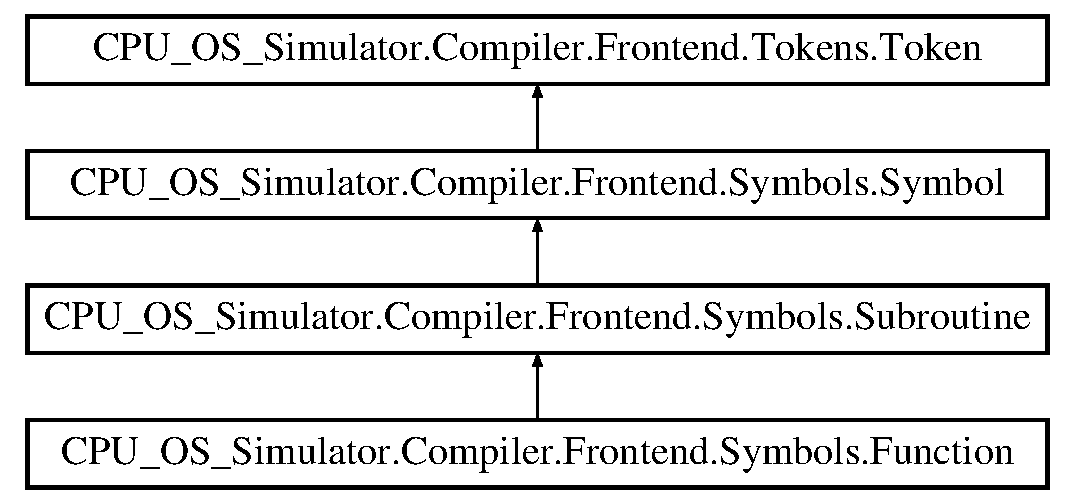
\includegraphics[height=4.000000cm]{class_c_p_u___o_s___simulator_1_1_compiler_1_1_frontend_1_1_symbols_1_1_symbol}
\end{center}
\end{figure}
\subsection*{Public Member Functions}
\begin{DoxyCompactItemize}
\item 
\hyperlink{class_c_p_u___o_s___simulator_1_1_compiler_1_1_frontend_1_1_symbols_1_1_symbol_ab5a7816e54de7e605bc76784d1107129}{Symbol} (string \hyperlink{class_c_p_u___o_s___simulator_1_1_compiler_1_1_frontend_1_1_symbols_1_1_symbol_a04abf6b34d531519f4f515f3a51e2089}{name}, \hyperlink{namespace_c_p_u___o_s___simulator_1_1_compiler_1_1_frontend_1_1_tokens_a7c0cc43763cc9d01c7d5af34d70b96ea}{Enum\+Types} \hyperlink{class_c_p_u___o_s___simulator_1_1_compiler_1_1_frontend_1_1_tokens_1_1_token_a7ec4dbbde477cd373f8135f0c843a346}{type}, string \hyperlink{class_c_p_u___o_s___simulator_1_1_compiler_1_1_frontend_1_1_symbols_1_1_symbol_a8c243f84c23afefc2b1c26180e187013}{value}, \hyperlink{class_c_p_u___o_s___simulator_1_1_compiler_1_1_frontend_1_1_symbols_1_1_scope}{Scope} scope, bool is\+Sub, bool is\+Fun)
\item 
override Enum \hyperlink{class_c_p_u___o_s___simulator_1_1_compiler_1_1_frontend_1_1_symbols_1_1_symbol_a1aef3417bc03adb5bcc15cfcdedb834e}{Detect\+Type} ()
\item 
override string \hyperlink{class_c_p_u___o_s___simulator_1_1_compiler_1_1_frontend_1_1_symbols_1_1_symbol_a1f87c771259b30006f0473b37d874847}{To\+String} ()
\begin{DoxyCompactList}\small\item\em Returns a string that represents the current object. \end{DoxyCompactList}\end{DoxyCompactItemize}
\subsection*{Protected Member Functions}
\begin{DoxyCompactItemize}
\item 
\hyperlink{class_c_p_u___o_s___simulator_1_1_compiler_1_1_frontend_1_1_symbols_1_1_symbol_ab2d0f42e478b6f15bd25669fc9a0d12f}{Symbol} ()
\end{DoxyCompactItemize}
\subsection*{Protected Attributes}
\begin{DoxyCompactItemize}
\item 
string \hyperlink{class_c_p_u___o_s___simulator_1_1_compiler_1_1_frontend_1_1_symbols_1_1_symbol_a04abf6b34d531519f4f515f3a51e2089}{name} = String.\+Empty
\item 
readonly \hyperlink{namespace_c_p_u___o_s___simulator_1_1_compiler_1_1_frontend_1_1_tokens_a7c0cc43763cc9d01c7d5af34d70b96ea}{Enum\+Types} \hyperlink{class_c_p_u___o_s___simulator_1_1_compiler_1_1_frontend_1_1_symbols_1_1_symbol_acc203e014b77911748322530d94e15e6}{symbol\+Type} = \hyperlink{namespace_c_p_u___o_s___simulator_1_1_compiler_1_1_frontend_a268b68f35fd94ce3549dd33a7e77d7e8a696b031073e74bf2cb98e5ef201d4aa3}{Enum\+Types.\+U\+N\+K\+N\+O\+W\+N}
\item 
new string \hyperlink{class_c_p_u___o_s___simulator_1_1_compiler_1_1_frontend_1_1_symbols_1_1_symbol_a8c243f84c23afefc2b1c26180e187013}{value}
\item 
bool \hyperlink{class_c_p_u___o_s___simulator_1_1_compiler_1_1_frontend_1_1_symbols_1_1_symbol_aab1b4c85076aaa90f5f7c805315db9a3}{issub} = false
\item 
bool \hyperlink{class_c_p_u___o_s___simulator_1_1_compiler_1_1_frontend_1_1_symbols_1_1_symbol_af134735e9120e587a167e421c7395d17}{isfun} = false
\item 
\hyperlink{class_c_p_u___o_s___simulator_1_1_compiler_1_1_frontend_1_1_symbols_1_1_scope}{Scope} \hyperlink{class_c_p_u___o_s___simulator_1_1_compiler_1_1_frontend_1_1_symbols_1_1_symbol_a419df98411144a57ed69fc67b3998294}{symbol\+Scope}
\end{DoxyCompactItemize}
\subsection*{Properties}
\begin{DoxyCompactItemize}
\item 
bool \hyperlink{class_c_p_u___o_s___simulator_1_1_compiler_1_1_frontend_1_1_symbols_1_1_symbol_a23ecebb867e96bd9e6c5a07ad7776903}{Is\+Sub}\hspace{0.3cm}{\ttfamily  \mbox{[}get\mbox{]}}
\item 
bool \hyperlink{class_c_p_u___o_s___simulator_1_1_compiler_1_1_frontend_1_1_symbols_1_1_symbol_a21f3b82dfe8cb700636c128d9e435161}{Is\+Fun}\hspace{0.3cm}{\ttfamily  \mbox{[}get\mbox{]}}
\item 
string \hyperlink{class_c_p_u___o_s___simulator_1_1_compiler_1_1_frontend_1_1_symbols_1_1_symbol_a2b91f23039d826f890bf806bd43b10cb}{Symbol\+Value}\hspace{0.3cm}{\ttfamily  \mbox{[}get, set\mbox{]}}
\item 
string \hyperlink{class_c_p_u___o_s___simulator_1_1_compiler_1_1_frontend_1_1_symbols_1_1_symbol_a869e163bccaf173b44fc04bb0488ead0}{Symbol\+Name}\hspace{0.3cm}{\ttfamily  \mbox{[}get\mbox{]}}
\item 
\hyperlink{namespace_c_p_u___o_s___simulator_1_1_compiler_1_1_frontend_1_1_tokens_a7c0cc43763cc9d01c7d5af34d70b96ea}{Enum\+Types} \hyperlink{class_c_p_u___o_s___simulator_1_1_compiler_1_1_frontend_1_1_symbols_1_1_symbol_a8324487c804b0bcb8910ef82033f749d}{Symbol\+Type}\hspace{0.3cm}{\ttfamily  \mbox{[}get\mbox{]}}
\item 
\hyperlink{class_c_p_u___o_s___simulator_1_1_compiler_1_1_frontend_1_1_symbols_1_1_scope}{Scope} \hyperlink{class_c_p_u___o_s___simulator_1_1_compiler_1_1_frontend_1_1_symbols_1_1_symbol_acba5080166e9021bf92e829785118a9c}{Symbol\+Scope}\hspace{0.3cm}{\ttfamily  \mbox{[}get, set\mbox{]}}
\end{DoxyCompactItemize}


\subsection{Detailed Description}


Definition at line 6 of file Symbol.\+cs.



\subsection{Constructor \& Destructor Documentation}
\hypertarget{class_c_p_u___o_s___simulator_1_1_compiler_1_1_frontend_1_1_symbols_1_1_symbol_ab2d0f42e478b6f15bd25669fc9a0d12f}{}\index{C\+P\+U\+\_\+\+O\+S\+\_\+\+Simulator\+::\+Compiler\+::\+Frontend\+::\+Symbols\+::\+Symbol@{C\+P\+U\+\_\+\+O\+S\+\_\+\+Simulator\+::\+Compiler\+::\+Frontend\+::\+Symbols\+::\+Symbol}!Symbol@{Symbol}}
\index{Symbol@{Symbol}!C\+P\+U\+\_\+\+O\+S\+\_\+\+Simulator\+::\+Compiler\+::\+Frontend\+::\+Symbols\+::\+Symbol@{C\+P\+U\+\_\+\+O\+S\+\_\+\+Simulator\+::\+Compiler\+::\+Frontend\+::\+Symbols\+::\+Symbol}}
\subsubsection[{Symbol()}]{\setlength{\rightskip}{0pt plus 5cm}C\+P\+U\+\_\+\+O\+S\+\_\+\+Simulator.\+Compiler.\+Frontend.\+Symbols.\+Symbol.\+Symbol (
\begin{DoxyParamCaption}
{}
\end{DoxyParamCaption}
)\hspace{0.3cm}{\ttfamily [protected]}}\label{class_c_p_u___o_s___simulator_1_1_compiler_1_1_frontend_1_1_symbols_1_1_symbol_ab2d0f42e478b6f15bd25669fc9a0d12f}


Definition at line 48 of file Symbol.\+cs.

\hypertarget{class_c_p_u___o_s___simulator_1_1_compiler_1_1_frontend_1_1_symbols_1_1_symbol_ab5a7816e54de7e605bc76784d1107129}{}\index{C\+P\+U\+\_\+\+O\+S\+\_\+\+Simulator\+::\+Compiler\+::\+Frontend\+::\+Symbols\+::\+Symbol@{C\+P\+U\+\_\+\+O\+S\+\_\+\+Simulator\+::\+Compiler\+::\+Frontend\+::\+Symbols\+::\+Symbol}!Symbol@{Symbol}}
\index{Symbol@{Symbol}!C\+P\+U\+\_\+\+O\+S\+\_\+\+Simulator\+::\+Compiler\+::\+Frontend\+::\+Symbols\+::\+Symbol@{C\+P\+U\+\_\+\+O\+S\+\_\+\+Simulator\+::\+Compiler\+::\+Frontend\+::\+Symbols\+::\+Symbol}}
\subsubsection[{Symbol(string name, Enum\+Types type, string value, Scope scope, bool is\+Sub, bool is\+Fun)}]{\setlength{\rightskip}{0pt plus 5cm}C\+P\+U\+\_\+\+O\+S\+\_\+\+Simulator.\+Compiler.\+Frontend.\+Symbols.\+Symbol.\+Symbol (
\begin{DoxyParamCaption}
\item[{string}]{name, }
\item[{{\bf Enum\+Types}}]{type, }
\item[{string}]{value, }
\item[{{\bf Scope}}]{scope, }
\item[{bool}]{is\+Sub, }
\item[{bool}]{is\+Fun}
\end{DoxyParamCaption}
)}\label{class_c_p_u___o_s___simulator_1_1_compiler_1_1_frontend_1_1_symbols_1_1_symbol_ab5a7816e54de7e605bc76784d1107129}


Definition at line 53 of file Symbol.\+cs.



\subsection{Member Function Documentation}
\hypertarget{class_c_p_u___o_s___simulator_1_1_compiler_1_1_frontend_1_1_symbols_1_1_symbol_a1aef3417bc03adb5bcc15cfcdedb834e}{}\index{C\+P\+U\+\_\+\+O\+S\+\_\+\+Simulator\+::\+Compiler\+::\+Frontend\+::\+Symbols\+::\+Symbol@{C\+P\+U\+\_\+\+O\+S\+\_\+\+Simulator\+::\+Compiler\+::\+Frontend\+::\+Symbols\+::\+Symbol}!Detect\+Type@{Detect\+Type}}
\index{Detect\+Type@{Detect\+Type}!C\+P\+U\+\_\+\+O\+S\+\_\+\+Simulator\+::\+Compiler\+::\+Frontend\+::\+Symbols\+::\+Symbol@{C\+P\+U\+\_\+\+O\+S\+\_\+\+Simulator\+::\+Compiler\+::\+Frontend\+::\+Symbols\+::\+Symbol}}
\subsubsection[{Detect\+Type()}]{\setlength{\rightskip}{0pt plus 5cm}override Enum C\+P\+U\+\_\+\+O\+S\+\_\+\+Simulator.\+Compiler.\+Frontend.\+Symbols.\+Symbol.\+Detect\+Type (
\begin{DoxyParamCaption}
{}
\end{DoxyParamCaption}
)\hspace{0.3cm}{\ttfamily [virtual]}}\label{class_c_p_u___o_s___simulator_1_1_compiler_1_1_frontend_1_1_symbols_1_1_symbol_a1aef3417bc03adb5bcc15cfcdedb834e}


Implements \hyperlink{class_c_p_u___o_s___simulator_1_1_compiler_1_1_frontend_1_1_tokens_1_1_token_accfe8c46faedacd527ef619698c76310}{C\+P\+U\+\_\+\+O\+S\+\_\+\+Simulator.\+Compiler.\+Frontend.\+Tokens.\+Token}.



Definition at line 63 of file Symbol.\+cs.

\hypertarget{class_c_p_u___o_s___simulator_1_1_compiler_1_1_frontend_1_1_symbols_1_1_symbol_a1f87c771259b30006f0473b37d874847}{}\index{C\+P\+U\+\_\+\+O\+S\+\_\+\+Simulator\+::\+Compiler\+::\+Frontend\+::\+Symbols\+::\+Symbol@{C\+P\+U\+\_\+\+O\+S\+\_\+\+Simulator\+::\+Compiler\+::\+Frontend\+::\+Symbols\+::\+Symbol}!To\+String@{To\+String}}
\index{To\+String@{To\+String}!C\+P\+U\+\_\+\+O\+S\+\_\+\+Simulator\+::\+Compiler\+::\+Frontend\+::\+Symbols\+::\+Symbol@{C\+P\+U\+\_\+\+O\+S\+\_\+\+Simulator\+::\+Compiler\+::\+Frontend\+::\+Symbols\+::\+Symbol}}
\subsubsection[{To\+String()}]{\setlength{\rightskip}{0pt plus 5cm}override string C\+P\+U\+\_\+\+O\+S\+\_\+\+Simulator.\+Compiler.\+Frontend.\+Symbols.\+Symbol.\+To\+String (
\begin{DoxyParamCaption}
{}
\end{DoxyParamCaption}
)}\label{class_c_p_u___o_s___simulator_1_1_compiler_1_1_frontend_1_1_symbols_1_1_symbol_a1f87c771259b30006f0473b37d874847}


Returns a string that represents the current object. 

\begin{DoxyReturn}{Returns}
A string that represents the current object. 
\end{DoxyReturn}


Definition at line 74 of file Symbol.\+cs.



\subsection{Member Data Documentation}
\hypertarget{class_c_p_u___o_s___simulator_1_1_compiler_1_1_frontend_1_1_symbols_1_1_symbol_af134735e9120e587a167e421c7395d17}{}\index{C\+P\+U\+\_\+\+O\+S\+\_\+\+Simulator\+::\+Compiler\+::\+Frontend\+::\+Symbols\+::\+Symbol@{C\+P\+U\+\_\+\+O\+S\+\_\+\+Simulator\+::\+Compiler\+::\+Frontend\+::\+Symbols\+::\+Symbol}!isfun@{isfun}}
\index{isfun@{isfun}!C\+P\+U\+\_\+\+O\+S\+\_\+\+Simulator\+::\+Compiler\+::\+Frontend\+::\+Symbols\+::\+Symbol@{C\+P\+U\+\_\+\+O\+S\+\_\+\+Simulator\+::\+Compiler\+::\+Frontend\+::\+Symbols\+::\+Symbol}}
\subsubsection[{isfun}]{\setlength{\rightskip}{0pt plus 5cm}bool C\+P\+U\+\_\+\+O\+S\+\_\+\+Simulator.\+Compiler.\+Frontend.\+Symbols.\+Symbol.\+isfun = false\hspace{0.3cm}{\ttfamily [protected]}}\label{class_c_p_u___o_s___simulator_1_1_compiler_1_1_frontend_1_1_symbols_1_1_symbol_af134735e9120e587a167e421c7395d17}


Definition at line 12 of file Symbol.\+cs.

\hypertarget{class_c_p_u___o_s___simulator_1_1_compiler_1_1_frontend_1_1_symbols_1_1_symbol_aab1b4c85076aaa90f5f7c805315db9a3}{}\index{C\+P\+U\+\_\+\+O\+S\+\_\+\+Simulator\+::\+Compiler\+::\+Frontend\+::\+Symbols\+::\+Symbol@{C\+P\+U\+\_\+\+O\+S\+\_\+\+Simulator\+::\+Compiler\+::\+Frontend\+::\+Symbols\+::\+Symbol}!issub@{issub}}
\index{issub@{issub}!C\+P\+U\+\_\+\+O\+S\+\_\+\+Simulator\+::\+Compiler\+::\+Frontend\+::\+Symbols\+::\+Symbol@{C\+P\+U\+\_\+\+O\+S\+\_\+\+Simulator\+::\+Compiler\+::\+Frontend\+::\+Symbols\+::\+Symbol}}
\subsubsection[{issub}]{\setlength{\rightskip}{0pt plus 5cm}bool C\+P\+U\+\_\+\+O\+S\+\_\+\+Simulator.\+Compiler.\+Frontend.\+Symbols.\+Symbol.\+issub = false\hspace{0.3cm}{\ttfamily [protected]}}\label{class_c_p_u___o_s___simulator_1_1_compiler_1_1_frontend_1_1_symbols_1_1_symbol_aab1b4c85076aaa90f5f7c805315db9a3}


Definition at line 11 of file Symbol.\+cs.

\hypertarget{class_c_p_u___o_s___simulator_1_1_compiler_1_1_frontend_1_1_symbols_1_1_symbol_a04abf6b34d531519f4f515f3a51e2089}{}\index{C\+P\+U\+\_\+\+O\+S\+\_\+\+Simulator\+::\+Compiler\+::\+Frontend\+::\+Symbols\+::\+Symbol@{C\+P\+U\+\_\+\+O\+S\+\_\+\+Simulator\+::\+Compiler\+::\+Frontend\+::\+Symbols\+::\+Symbol}!name@{name}}
\index{name@{name}!C\+P\+U\+\_\+\+O\+S\+\_\+\+Simulator\+::\+Compiler\+::\+Frontend\+::\+Symbols\+::\+Symbol@{C\+P\+U\+\_\+\+O\+S\+\_\+\+Simulator\+::\+Compiler\+::\+Frontend\+::\+Symbols\+::\+Symbol}}
\subsubsection[{name}]{\setlength{\rightskip}{0pt plus 5cm}string C\+P\+U\+\_\+\+O\+S\+\_\+\+Simulator.\+Compiler.\+Frontend.\+Symbols.\+Symbol.\+name = String.\+Empty\hspace{0.3cm}{\ttfamily [protected]}}\label{class_c_p_u___o_s___simulator_1_1_compiler_1_1_frontend_1_1_symbols_1_1_symbol_a04abf6b34d531519f4f515f3a51e2089}


Definition at line 8 of file Symbol.\+cs.

\hypertarget{class_c_p_u___o_s___simulator_1_1_compiler_1_1_frontend_1_1_symbols_1_1_symbol_a419df98411144a57ed69fc67b3998294}{}\index{C\+P\+U\+\_\+\+O\+S\+\_\+\+Simulator\+::\+Compiler\+::\+Frontend\+::\+Symbols\+::\+Symbol@{C\+P\+U\+\_\+\+O\+S\+\_\+\+Simulator\+::\+Compiler\+::\+Frontend\+::\+Symbols\+::\+Symbol}!symbol\+Scope@{symbol\+Scope}}
\index{symbol\+Scope@{symbol\+Scope}!C\+P\+U\+\_\+\+O\+S\+\_\+\+Simulator\+::\+Compiler\+::\+Frontend\+::\+Symbols\+::\+Symbol@{C\+P\+U\+\_\+\+O\+S\+\_\+\+Simulator\+::\+Compiler\+::\+Frontend\+::\+Symbols\+::\+Symbol}}
\subsubsection[{symbol\+Scope}]{\setlength{\rightskip}{0pt plus 5cm}{\bf Scope} C\+P\+U\+\_\+\+O\+S\+\_\+\+Simulator.\+Compiler.\+Frontend.\+Symbols.\+Symbol.\+symbol\+Scope\hspace{0.3cm}{\ttfamily [protected]}}\label{class_c_p_u___o_s___simulator_1_1_compiler_1_1_frontend_1_1_symbols_1_1_symbol_a419df98411144a57ed69fc67b3998294}


Definition at line 13 of file Symbol.\+cs.

\hypertarget{class_c_p_u___o_s___simulator_1_1_compiler_1_1_frontend_1_1_symbols_1_1_symbol_acc203e014b77911748322530d94e15e6}{}\index{C\+P\+U\+\_\+\+O\+S\+\_\+\+Simulator\+::\+Compiler\+::\+Frontend\+::\+Symbols\+::\+Symbol@{C\+P\+U\+\_\+\+O\+S\+\_\+\+Simulator\+::\+Compiler\+::\+Frontend\+::\+Symbols\+::\+Symbol}!symbol\+Type@{symbol\+Type}}
\index{symbol\+Type@{symbol\+Type}!C\+P\+U\+\_\+\+O\+S\+\_\+\+Simulator\+::\+Compiler\+::\+Frontend\+::\+Symbols\+::\+Symbol@{C\+P\+U\+\_\+\+O\+S\+\_\+\+Simulator\+::\+Compiler\+::\+Frontend\+::\+Symbols\+::\+Symbol}}
\subsubsection[{symbol\+Type}]{\setlength{\rightskip}{0pt plus 5cm}readonly {\bf Enum\+Types} C\+P\+U\+\_\+\+O\+S\+\_\+\+Simulator.\+Compiler.\+Frontend.\+Symbols.\+Symbol.\+symbol\+Type = {\bf Enum\+Types.\+U\+N\+K\+N\+O\+W\+N}\hspace{0.3cm}{\ttfamily [protected]}}\label{class_c_p_u___o_s___simulator_1_1_compiler_1_1_frontend_1_1_symbols_1_1_symbol_acc203e014b77911748322530d94e15e6}


Definition at line 9 of file Symbol.\+cs.

\hypertarget{class_c_p_u___o_s___simulator_1_1_compiler_1_1_frontend_1_1_symbols_1_1_symbol_a8c243f84c23afefc2b1c26180e187013}{}\index{C\+P\+U\+\_\+\+O\+S\+\_\+\+Simulator\+::\+Compiler\+::\+Frontend\+::\+Symbols\+::\+Symbol@{C\+P\+U\+\_\+\+O\+S\+\_\+\+Simulator\+::\+Compiler\+::\+Frontend\+::\+Symbols\+::\+Symbol}!value@{value}}
\index{value@{value}!C\+P\+U\+\_\+\+O\+S\+\_\+\+Simulator\+::\+Compiler\+::\+Frontend\+::\+Symbols\+::\+Symbol@{C\+P\+U\+\_\+\+O\+S\+\_\+\+Simulator\+::\+Compiler\+::\+Frontend\+::\+Symbols\+::\+Symbol}}
\subsubsection[{value}]{\setlength{\rightskip}{0pt plus 5cm}new string C\+P\+U\+\_\+\+O\+S\+\_\+\+Simulator.\+Compiler.\+Frontend.\+Symbols.\+Symbol.\+value\hspace{0.3cm}{\ttfamily [protected]}}\label{class_c_p_u___o_s___simulator_1_1_compiler_1_1_frontend_1_1_symbols_1_1_symbol_a8c243f84c23afefc2b1c26180e187013}


Definition at line 10 of file Symbol.\+cs.



\subsection{Property Documentation}
\hypertarget{class_c_p_u___o_s___simulator_1_1_compiler_1_1_frontend_1_1_symbols_1_1_symbol_a21f3b82dfe8cb700636c128d9e435161}{}\index{C\+P\+U\+\_\+\+O\+S\+\_\+\+Simulator\+::\+Compiler\+::\+Frontend\+::\+Symbols\+::\+Symbol@{C\+P\+U\+\_\+\+O\+S\+\_\+\+Simulator\+::\+Compiler\+::\+Frontend\+::\+Symbols\+::\+Symbol}!Is\+Fun@{Is\+Fun}}
\index{Is\+Fun@{Is\+Fun}!C\+P\+U\+\_\+\+O\+S\+\_\+\+Simulator\+::\+Compiler\+::\+Frontend\+::\+Symbols\+::\+Symbol@{C\+P\+U\+\_\+\+O\+S\+\_\+\+Simulator\+::\+Compiler\+::\+Frontend\+::\+Symbols\+::\+Symbol}}
\subsubsection[{Is\+Fun}]{\setlength{\rightskip}{0pt plus 5cm}bool C\+P\+U\+\_\+\+O\+S\+\_\+\+Simulator.\+Compiler.\+Frontend.\+Symbols.\+Symbol.\+Is\+Fun\hspace{0.3cm}{\ttfamily [get]}}\label{class_c_p_u___o_s___simulator_1_1_compiler_1_1_frontend_1_1_symbols_1_1_symbol_a21f3b82dfe8cb700636c128d9e435161}


Definition at line 21 of file Symbol.\+cs.

\hypertarget{class_c_p_u___o_s___simulator_1_1_compiler_1_1_frontend_1_1_symbols_1_1_symbol_a23ecebb867e96bd9e6c5a07ad7776903}{}\index{C\+P\+U\+\_\+\+O\+S\+\_\+\+Simulator\+::\+Compiler\+::\+Frontend\+::\+Symbols\+::\+Symbol@{C\+P\+U\+\_\+\+O\+S\+\_\+\+Simulator\+::\+Compiler\+::\+Frontend\+::\+Symbols\+::\+Symbol}!Is\+Sub@{Is\+Sub}}
\index{Is\+Sub@{Is\+Sub}!C\+P\+U\+\_\+\+O\+S\+\_\+\+Simulator\+::\+Compiler\+::\+Frontend\+::\+Symbols\+::\+Symbol@{C\+P\+U\+\_\+\+O\+S\+\_\+\+Simulator\+::\+Compiler\+::\+Frontend\+::\+Symbols\+::\+Symbol}}
\subsubsection[{Is\+Sub}]{\setlength{\rightskip}{0pt plus 5cm}bool C\+P\+U\+\_\+\+O\+S\+\_\+\+Simulator.\+Compiler.\+Frontend.\+Symbols.\+Symbol.\+Is\+Sub\hspace{0.3cm}{\ttfamily [get]}}\label{class_c_p_u___o_s___simulator_1_1_compiler_1_1_frontend_1_1_symbols_1_1_symbol_a23ecebb867e96bd9e6c5a07ad7776903}


Definition at line 16 of file Symbol.\+cs.

\hypertarget{class_c_p_u___o_s___simulator_1_1_compiler_1_1_frontend_1_1_symbols_1_1_symbol_a869e163bccaf173b44fc04bb0488ead0}{}\index{C\+P\+U\+\_\+\+O\+S\+\_\+\+Simulator\+::\+Compiler\+::\+Frontend\+::\+Symbols\+::\+Symbol@{C\+P\+U\+\_\+\+O\+S\+\_\+\+Simulator\+::\+Compiler\+::\+Frontend\+::\+Symbols\+::\+Symbol}!Symbol\+Name@{Symbol\+Name}}
\index{Symbol\+Name@{Symbol\+Name}!C\+P\+U\+\_\+\+O\+S\+\_\+\+Simulator\+::\+Compiler\+::\+Frontend\+::\+Symbols\+::\+Symbol@{C\+P\+U\+\_\+\+O\+S\+\_\+\+Simulator\+::\+Compiler\+::\+Frontend\+::\+Symbols\+::\+Symbol}}
\subsubsection[{Symbol\+Name}]{\setlength{\rightskip}{0pt plus 5cm}string C\+P\+U\+\_\+\+O\+S\+\_\+\+Simulator.\+Compiler.\+Frontend.\+Symbols.\+Symbol.\+Symbol\+Name\hspace{0.3cm}{\ttfamily [get]}}\label{class_c_p_u___o_s___simulator_1_1_compiler_1_1_frontend_1_1_symbols_1_1_symbol_a869e163bccaf173b44fc04bb0488ead0}


Definition at line 32 of file Symbol.\+cs.

\hypertarget{class_c_p_u___o_s___simulator_1_1_compiler_1_1_frontend_1_1_symbols_1_1_symbol_acba5080166e9021bf92e829785118a9c}{}\index{C\+P\+U\+\_\+\+O\+S\+\_\+\+Simulator\+::\+Compiler\+::\+Frontend\+::\+Symbols\+::\+Symbol@{C\+P\+U\+\_\+\+O\+S\+\_\+\+Simulator\+::\+Compiler\+::\+Frontend\+::\+Symbols\+::\+Symbol}!Symbol\+Scope@{Symbol\+Scope}}
\index{Symbol\+Scope@{Symbol\+Scope}!C\+P\+U\+\_\+\+O\+S\+\_\+\+Simulator\+::\+Compiler\+::\+Frontend\+::\+Symbols\+::\+Symbol@{C\+P\+U\+\_\+\+O\+S\+\_\+\+Simulator\+::\+Compiler\+::\+Frontend\+::\+Symbols\+::\+Symbol}}
\subsubsection[{Symbol\+Scope}]{\setlength{\rightskip}{0pt plus 5cm}{\bf Scope} C\+P\+U\+\_\+\+O\+S\+\_\+\+Simulator.\+Compiler.\+Frontend.\+Symbols.\+Symbol.\+Symbol\+Scope\hspace{0.3cm}{\ttfamily [get]}, {\ttfamily [set]}}\label{class_c_p_u___o_s___simulator_1_1_compiler_1_1_frontend_1_1_symbols_1_1_symbol_acba5080166e9021bf92e829785118a9c}


Definition at line 43 of file Symbol.\+cs.

\hypertarget{class_c_p_u___o_s___simulator_1_1_compiler_1_1_frontend_1_1_symbols_1_1_symbol_a8324487c804b0bcb8910ef82033f749d}{}\index{C\+P\+U\+\_\+\+O\+S\+\_\+\+Simulator\+::\+Compiler\+::\+Frontend\+::\+Symbols\+::\+Symbol@{C\+P\+U\+\_\+\+O\+S\+\_\+\+Simulator\+::\+Compiler\+::\+Frontend\+::\+Symbols\+::\+Symbol}!Symbol\+Type@{Symbol\+Type}}
\index{Symbol\+Type@{Symbol\+Type}!C\+P\+U\+\_\+\+O\+S\+\_\+\+Simulator\+::\+Compiler\+::\+Frontend\+::\+Symbols\+::\+Symbol@{C\+P\+U\+\_\+\+O\+S\+\_\+\+Simulator\+::\+Compiler\+::\+Frontend\+::\+Symbols\+::\+Symbol}}
\subsubsection[{Symbol\+Type}]{\setlength{\rightskip}{0pt plus 5cm}{\bf Enum\+Types} C\+P\+U\+\_\+\+O\+S\+\_\+\+Simulator.\+Compiler.\+Frontend.\+Symbols.\+Symbol.\+Symbol\+Type\hspace{0.3cm}{\ttfamily [get]}}\label{class_c_p_u___o_s___simulator_1_1_compiler_1_1_frontend_1_1_symbols_1_1_symbol_a8324487c804b0bcb8910ef82033f749d}


Definition at line 38 of file Symbol.\+cs.

\hypertarget{class_c_p_u___o_s___simulator_1_1_compiler_1_1_frontend_1_1_symbols_1_1_symbol_a2b91f23039d826f890bf806bd43b10cb}{}\index{C\+P\+U\+\_\+\+O\+S\+\_\+\+Simulator\+::\+Compiler\+::\+Frontend\+::\+Symbols\+::\+Symbol@{C\+P\+U\+\_\+\+O\+S\+\_\+\+Simulator\+::\+Compiler\+::\+Frontend\+::\+Symbols\+::\+Symbol}!Symbol\+Value@{Symbol\+Value}}
\index{Symbol\+Value@{Symbol\+Value}!C\+P\+U\+\_\+\+O\+S\+\_\+\+Simulator\+::\+Compiler\+::\+Frontend\+::\+Symbols\+::\+Symbol@{C\+P\+U\+\_\+\+O\+S\+\_\+\+Simulator\+::\+Compiler\+::\+Frontend\+::\+Symbols\+::\+Symbol}}
\subsubsection[{Symbol\+Value}]{\setlength{\rightskip}{0pt plus 5cm}string C\+P\+U\+\_\+\+O\+S\+\_\+\+Simulator.\+Compiler.\+Frontend.\+Symbols.\+Symbol.\+Symbol\+Value\hspace{0.3cm}{\ttfamily [get]}, {\ttfamily [set]}}\label{class_c_p_u___o_s___simulator_1_1_compiler_1_1_frontend_1_1_symbols_1_1_symbol_a2b91f23039d826f890bf806bd43b10cb}


Definition at line 26 of file Symbol.\+cs.



The documentation for this class was generated from the following file\+:\begin{DoxyCompactItemize}
\item 
Compiler/\+Frontend/\+Symbols/\hyperlink{_symbol_8cs}{Symbol.\+cs}\end{DoxyCompactItemize}

\hypertarget{class_c_p_u___o_s___simulator_1_1_compiler_1_1_frontend_1_1_symbols_1_1_symbol_table}{}\section{C\+P\+U\+\_\+\+O\+S\+\_\+\+Simulator.\+Compiler.\+Frontend.\+Symbols.\+Symbol\+Table Class Reference}
\label{class_c_p_u___o_s___simulator_1_1_compiler_1_1_frontend_1_1_symbols_1_1_symbol_table}\index{C\+P\+U\+\_\+\+O\+S\+\_\+\+Simulator.\+Compiler.\+Frontend.\+Symbols.\+Symbol\+Table@{C\+P\+U\+\_\+\+O\+S\+\_\+\+Simulator.\+Compiler.\+Frontend.\+Symbols.\+Symbol\+Table}}
\subsection*{Public Member Functions}
\begin{DoxyCompactItemize}
\item 
\hyperlink{class_c_p_u___o_s___simulator_1_1_compiler_1_1_frontend_1_1_symbols_1_1_symbol_table_a3198555072680916b69483d09f8a23ca}{Symbol\+Table} (Text\+Box \hyperlink{class_c_p_u___o_s___simulator_1_1_compiler_1_1_frontend_1_1_symbols_1_1_symbol_table_a296a865c0445d3282c0b211853df56db}{output})
\item 
Linked\+List\+Node$<$ \hyperlink{class_c_p_u___o_s___simulator_1_1_compiler_1_1_frontend_1_1_symbols_1_1_symbol}{Symbol} $>$ \hyperlink{class_c_p_u___o_s___simulator_1_1_compiler_1_1_frontend_1_1_symbols_1_1_symbol_table_adf107a69c02c4997630d70bee032559f}{Find\+Symbol} (string name)
\item 
Linked\+List\+Node$<$ \hyperlink{class_c_p_u___o_s___simulator_1_1_compiler_1_1_frontend_1_1_symbols_1_1_symbol}{Symbol} $>$ \hyperlink{class_c_p_u___o_s___simulator_1_1_compiler_1_1_frontend_1_1_symbols_1_1_symbol_table_aa073e0a3a954f8c80a908253154db9ac}{Find\+Symbol} (\hyperlink{namespace_c_p_u___o_s___simulator_1_1_compiler_1_1_frontend_1_1_tokens_a7c0cc43763cc9d01c7d5af34d70b96ea}{Enum\+Types} type)
\item 
Linked\+List\+Node$<$ \hyperlink{class_c_p_u___o_s___simulator_1_1_compiler_1_1_frontend_1_1_symbols_1_1_symbol}{Symbol} $>$ \hyperlink{class_c_p_u___o_s___simulator_1_1_compiler_1_1_frontend_1_1_symbols_1_1_symbol_table_a3e7532efc1e1af447b411f991d96a68b}{Add\+Symbol} (Linked\+List\+Node$<$ \hyperlink{class_c_p_u___o_s___simulator_1_1_compiler_1_1_frontend_1_1_symbols_1_1_symbol}{Symbol} $>$ symbol)
\item 
void \hyperlink{class_c_p_u___o_s___simulator_1_1_compiler_1_1_frontend_1_1_symbols_1_1_symbol_table_a96a4764b3c4e15413c7cca27b0e7d500}{Print\+Symbols} ()
\item 
bool \hyperlink{class_c_p_u___o_s___simulator_1_1_compiler_1_1_frontend_1_1_symbols_1_1_symbol_table_a58dfc6b7e3d6306436a4aa53aebfa085}{is\+Identifier\+Declared\+In\+Scope} (\hyperlink{class_c_p_u___o_s___simulator_1_1_compiler_1_1_frontend_1_1_symbols_1_1_symbol}{Symbol} identifier, \hyperlink{class_c_p_u___o_s___simulator_1_1_compiler_1_1_frontend_1_1_symbols_1_1_scope}{Scope} scope)
\end{DoxyCompactItemize}
\subsection*{Private Attributes}
\begin{DoxyCompactItemize}
\item 
Linked\+List$<$ \hyperlink{class_c_p_u___o_s___simulator_1_1_compiler_1_1_frontend_1_1_symbols_1_1_symbol}{Symbol} $>$ \hyperlink{class_c_p_u___o_s___simulator_1_1_compiler_1_1_frontend_1_1_symbols_1_1_symbol_table_a3a69b239234ec68d9225217c4a4b1eb7}{symbols}
\item 
Linked\+List\+Node$<$ \hyperlink{class_c_p_u___o_s___simulator_1_1_compiler_1_1_frontend_1_1_symbols_1_1_symbol}{Symbol} $>$ \hyperlink{class_c_p_u___o_s___simulator_1_1_compiler_1_1_frontend_1_1_symbols_1_1_symbol_table_a2fc3932216a6a0a499d47bc29a2b03c3}{current\+Symbol}
\item 
Linked\+List\+Node$<$ \hyperlink{class_c_p_u___o_s___simulator_1_1_compiler_1_1_frontend_1_1_symbols_1_1_symbol}{Symbol} $>$ \hyperlink{class_c_p_u___o_s___simulator_1_1_compiler_1_1_frontend_1_1_symbols_1_1_symbol_table_aae0b08c3eb5d6ada83e944352bc77ebb}{next\+Symbol}
\item 
Linked\+List\+Node$<$ \hyperlink{class_c_p_u___o_s___simulator_1_1_compiler_1_1_frontend_1_1_symbols_1_1_symbol}{Symbol} $>$ \hyperlink{class_c_p_u___o_s___simulator_1_1_compiler_1_1_frontend_1_1_symbols_1_1_symbol_table_a40b980c535cb45d6946762cb21112fb2}{previous\+Symbol}
\item 
Text\+Box \hyperlink{class_c_p_u___o_s___simulator_1_1_compiler_1_1_frontend_1_1_symbols_1_1_symbol_table_a296a865c0445d3282c0b211853df56db}{output}
\end{DoxyCompactItemize}


\subsection{Detailed Description}


Definition at line 8 of file Symbol\+Table.\+cs.



\subsection{Constructor \& Destructor Documentation}
\hypertarget{class_c_p_u___o_s___simulator_1_1_compiler_1_1_frontend_1_1_symbols_1_1_symbol_table_a3198555072680916b69483d09f8a23ca}{}\index{C\+P\+U\+\_\+\+O\+S\+\_\+\+Simulator\+::\+Compiler\+::\+Frontend\+::\+Symbols\+::\+Symbol\+Table@{C\+P\+U\+\_\+\+O\+S\+\_\+\+Simulator\+::\+Compiler\+::\+Frontend\+::\+Symbols\+::\+Symbol\+Table}!Symbol\+Table@{Symbol\+Table}}
\index{Symbol\+Table@{Symbol\+Table}!C\+P\+U\+\_\+\+O\+S\+\_\+\+Simulator\+::\+Compiler\+::\+Frontend\+::\+Symbols\+::\+Symbol\+Table@{C\+P\+U\+\_\+\+O\+S\+\_\+\+Simulator\+::\+Compiler\+::\+Frontend\+::\+Symbols\+::\+Symbol\+Table}}
\subsubsection[{Symbol\+Table(\+Text\+Box output)}]{\setlength{\rightskip}{0pt plus 5cm}C\+P\+U\+\_\+\+O\+S\+\_\+\+Simulator.\+Compiler.\+Frontend.\+Symbols.\+Symbol\+Table.\+Symbol\+Table (
\begin{DoxyParamCaption}
\item[{Text\+Box}]{output}
\end{DoxyParamCaption}
)}\label{class_c_p_u___o_s___simulator_1_1_compiler_1_1_frontend_1_1_symbols_1_1_symbol_table_a3198555072680916b69483d09f8a23ca}


Definition at line 16 of file Symbol\+Table.\+cs.



\subsection{Member Function Documentation}
\hypertarget{class_c_p_u___o_s___simulator_1_1_compiler_1_1_frontend_1_1_symbols_1_1_symbol_table_a3e7532efc1e1af447b411f991d96a68b}{}\index{C\+P\+U\+\_\+\+O\+S\+\_\+\+Simulator\+::\+Compiler\+::\+Frontend\+::\+Symbols\+::\+Symbol\+Table@{C\+P\+U\+\_\+\+O\+S\+\_\+\+Simulator\+::\+Compiler\+::\+Frontend\+::\+Symbols\+::\+Symbol\+Table}!Add\+Symbol@{Add\+Symbol}}
\index{Add\+Symbol@{Add\+Symbol}!C\+P\+U\+\_\+\+O\+S\+\_\+\+Simulator\+::\+Compiler\+::\+Frontend\+::\+Symbols\+::\+Symbol\+Table@{C\+P\+U\+\_\+\+O\+S\+\_\+\+Simulator\+::\+Compiler\+::\+Frontend\+::\+Symbols\+::\+Symbol\+Table}}
\subsubsection[{Add\+Symbol(\+Linked\+List\+Node$<$ Symbol $>$ symbol)}]{\setlength{\rightskip}{0pt plus 5cm}Linked\+List\+Node$<${\bf Symbol}$>$ C\+P\+U\+\_\+\+O\+S\+\_\+\+Simulator.\+Compiler.\+Frontend.\+Symbols.\+Symbol\+Table.\+Add\+Symbol (
\begin{DoxyParamCaption}
\item[{Linked\+List\+Node$<$ {\bf Symbol} $>$}]{symbol}
\end{DoxyParamCaption}
)}\label{class_c_p_u___o_s___simulator_1_1_compiler_1_1_frontend_1_1_symbols_1_1_symbol_table_a3e7532efc1e1af447b411f991d96a68b}


Definition at line 52 of file Symbol\+Table.\+cs.

\hypertarget{class_c_p_u___o_s___simulator_1_1_compiler_1_1_frontend_1_1_symbols_1_1_symbol_table_adf107a69c02c4997630d70bee032559f}{}\index{C\+P\+U\+\_\+\+O\+S\+\_\+\+Simulator\+::\+Compiler\+::\+Frontend\+::\+Symbols\+::\+Symbol\+Table@{C\+P\+U\+\_\+\+O\+S\+\_\+\+Simulator\+::\+Compiler\+::\+Frontend\+::\+Symbols\+::\+Symbol\+Table}!Find\+Symbol@{Find\+Symbol}}
\index{Find\+Symbol@{Find\+Symbol}!C\+P\+U\+\_\+\+O\+S\+\_\+\+Simulator\+::\+Compiler\+::\+Frontend\+::\+Symbols\+::\+Symbol\+Table@{C\+P\+U\+\_\+\+O\+S\+\_\+\+Simulator\+::\+Compiler\+::\+Frontend\+::\+Symbols\+::\+Symbol\+Table}}
\subsubsection[{Find\+Symbol(string name)}]{\setlength{\rightskip}{0pt plus 5cm}Linked\+List\+Node$<${\bf Symbol}$>$ C\+P\+U\+\_\+\+O\+S\+\_\+\+Simulator.\+Compiler.\+Frontend.\+Symbols.\+Symbol\+Table.\+Find\+Symbol (
\begin{DoxyParamCaption}
\item[{string}]{name}
\end{DoxyParamCaption}
)}\label{class_c_p_u___o_s___simulator_1_1_compiler_1_1_frontend_1_1_symbols_1_1_symbol_table_adf107a69c02c4997630d70bee032559f}


Definition at line 22 of file Symbol\+Table.\+cs.

\hypertarget{class_c_p_u___o_s___simulator_1_1_compiler_1_1_frontend_1_1_symbols_1_1_symbol_table_aa073e0a3a954f8c80a908253154db9ac}{}\index{C\+P\+U\+\_\+\+O\+S\+\_\+\+Simulator\+::\+Compiler\+::\+Frontend\+::\+Symbols\+::\+Symbol\+Table@{C\+P\+U\+\_\+\+O\+S\+\_\+\+Simulator\+::\+Compiler\+::\+Frontend\+::\+Symbols\+::\+Symbol\+Table}!Find\+Symbol@{Find\+Symbol}}
\index{Find\+Symbol@{Find\+Symbol}!C\+P\+U\+\_\+\+O\+S\+\_\+\+Simulator\+::\+Compiler\+::\+Frontend\+::\+Symbols\+::\+Symbol\+Table@{C\+P\+U\+\_\+\+O\+S\+\_\+\+Simulator\+::\+Compiler\+::\+Frontend\+::\+Symbols\+::\+Symbol\+Table}}
\subsubsection[{Find\+Symbol(\+Enum\+Types type)}]{\setlength{\rightskip}{0pt plus 5cm}Linked\+List\+Node$<${\bf Symbol}$>$ C\+P\+U\+\_\+\+O\+S\+\_\+\+Simulator.\+Compiler.\+Frontend.\+Symbols.\+Symbol\+Table.\+Find\+Symbol (
\begin{DoxyParamCaption}
\item[{{\bf Enum\+Types}}]{type}
\end{DoxyParamCaption}
)}\label{class_c_p_u___o_s___simulator_1_1_compiler_1_1_frontend_1_1_symbols_1_1_symbol_table_aa073e0a3a954f8c80a908253154db9ac}


Definition at line 37 of file Symbol\+Table.\+cs.

\hypertarget{class_c_p_u___o_s___simulator_1_1_compiler_1_1_frontend_1_1_symbols_1_1_symbol_table_a58dfc6b7e3d6306436a4aa53aebfa085}{}\index{C\+P\+U\+\_\+\+O\+S\+\_\+\+Simulator\+::\+Compiler\+::\+Frontend\+::\+Symbols\+::\+Symbol\+Table@{C\+P\+U\+\_\+\+O\+S\+\_\+\+Simulator\+::\+Compiler\+::\+Frontend\+::\+Symbols\+::\+Symbol\+Table}!is\+Identifier\+Declared\+In\+Scope@{is\+Identifier\+Declared\+In\+Scope}}
\index{is\+Identifier\+Declared\+In\+Scope@{is\+Identifier\+Declared\+In\+Scope}!C\+P\+U\+\_\+\+O\+S\+\_\+\+Simulator\+::\+Compiler\+::\+Frontend\+::\+Symbols\+::\+Symbol\+Table@{C\+P\+U\+\_\+\+O\+S\+\_\+\+Simulator\+::\+Compiler\+::\+Frontend\+::\+Symbols\+::\+Symbol\+Table}}
\subsubsection[{is\+Identifier\+Declared\+In\+Scope(\+Symbol identifier, Scope scope)}]{\setlength{\rightskip}{0pt plus 5cm}bool C\+P\+U\+\_\+\+O\+S\+\_\+\+Simulator.\+Compiler.\+Frontend.\+Symbols.\+Symbol\+Table.\+is\+Identifier\+Declared\+In\+Scope (
\begin{DoxyParamCaption}
\item[{{\bf Symbol}}]{identifier, }
\item[{{\bf Scope}}]{scope}
\end{DoxyParamCaption}
)}\label{class_c_p_u___o_s___simulator_1_1_compiler_1_1_frontend_1_1_symbols_1_1_symbol_table_a58dfc6b7e3d6306436a4aa53aebfa085}


Definition at line 81 of file Symbol\+Table.\+cs.

\hypertarget{class_c_p_u___o_s___simulator_1_1_compiler_1_1_frontend_1_1_symbols_1_1_symbol_table_a96a4764b3c4e15413c7cca27b0e7d500}{}\index{C\+P\+U\+\_\+\+O\+S\+\_\+\+Simulator\+::\+Compiler\+::\+Frontend\+::\+Symbols\+::\+Symbol\+Table@{C\+P\+U\+\_\+\+O\+S\+\_\+\+Simulator\+::\+Compiler\+::\+Frontend\+::\+Symbols\+::\+Symbol\+Table}!Print\+Symbols@{Print\+Symbols}}
\index{Print\+Symbols@{Print\+Symbols}!C\+P\+U\+\_\+\+O\+S\+\_\+\+Simulator\+::\+Compiler\+::\+Frontend\+::\+Symbols\+::\+Symbol\+Table@{C\+P\+U\+\_\+\+O\+S\+\_\+\+Simulator\+::\+Compiler\+::\+Frontend\+::\+Symbols\+::\+Symbol\+Table}}
\subsubsection[{Print\+Symbols()}]{\setlength{\rightskip}{0pt plus 5cm}void C\+P\+U\+\_\+\+O\+S\+\_\+\+Simulator.\+Compiler.\+Frontend.\+Symbols.\+Symbol\+Table.\+Print\+Symbols (
\begin{DoxyParamCaption}
{}
\end{DoxyParamCaption}
)}\label{class_c_p_u___o_s___simulator_1_1_compiler_1_1_frontend_1_1_symbols_1_1_symbol_table_a96a4764b3c4e15413c7cca27b0e7d500}


Definition at line 58 of file Symbol\+Table.\+cs.



\subsection{Member Data Documentation}
\hypertarget{class_c_p_u___o_s___simulator_1_1_compiler_1_1_frontend_1_1_symbols_1_1_symbol_table_a2fc3932216a6a0a499d47bc29a2b03c3}{}\index{C\+P\+U\+\_\+\+O\+S\+\_\+\+Simulator\+::\+Compiler\+::\+Frontend\+::\+Symbols\+::\+Symbol\+Table@{C\+P\+U\+\_\+\+O\+S\+\_\+\+Simulator\+::\+Compiler\+::\+Frontend\+::\+Symbols\+::\+Symbol\+Table}!current\+Symbol@{current\+Symbol}}
\index{current\+Symbol@{current\+Symbol}!C\+P\+U\+\_\+\+O\+S\+\_\+\+Simulator\+::\+Compiler\+::\+Frontend\+::\+Symbols\+::\+Symbol\+Table@{C\+P\+U\+\_\+\+O\+S\+\_\+\+Simulator\+::\+Compiler\+::\+Frontend\+::\+Symbols\+::\+Symbol\+Table}}
\subsubsection[{current\+Symbol}]{\setlength{\rightskip}{0pt plus 5cm}Linked\+List\+Node$<${\bf Symbol}$>$ C\+P\+U\+\_\+\+O\+S\+\_\+\+Simulator.\+Compiler.\+Frontend.\+Symbols.\+Symbol\+Table.\+current\+Symbol\hspace{0.3cm}{\ttfamily [private]}}\label{class_c_p_u___o_s___simulator_1_1_compiler_1_1_frontend_1_1_symbols_1_1_symbol_table_a2fc3932216a6a0a499d47bc29a2b03c3}


Definition at line 11 of file Symbol\+Table.\+cs.

\hypertarget{class_c_p_u___o_s___simulator_1_1_compiler_1_1_frontend_1_1_symbols_1_1_symbol_table_aae0b08c3eb5d6ada83e944352bc77ebb}{}\index{C\+P\+U\+\_\+\+O\+S\+\_\+\+Simulator\+::\+Compiler\+::\+Frontend\+::\+Symbols\+::\+Symbol\+Table@{C\+P\+U\+\_\+\+O\+S\+\_\+\+Simulator\+::\+Compiler\+::\+Frontend\+::\+Symbols\+::\+Symbol\+Table}!next\+Symbol@{next\+Symbol}}
\index{next\+Symbol@{next\+Symbol}!C\+P\+U\+\_\+\+O\+S\+\_\+\+Simulator\+::\+Compiler\+::\+Frontend\+::\+Symbols\+::\+Symbol\+Table@{C\+P\+U\+\_\+\+O\+S\+\_\+\+Simulator\+::\+Compiler\+::\+Frontend\+::\+Symbols\+::\+Symbol\+Table}}
\subsubsection[{next\+Symbol}]{\setlength{\rightskip}{0pt plus 5cm}Linked\+List\+Node$<${\bf Symbol}$>$ C\+P\+U\+\_\+\+O\+S\+\_\+\+Simulator.\+Compiler.\+Frontend.\+Symbols.\+Symbol\+Table.\+next\+Symbol\hspace{0.3cm}{\ttfamily [private]}}\label{class_c_p_u___o_s___simulator_1_1_compiler_1_1_frontend_1_1_symbols_1_1_symbol_table_aae0b08c3eb5d6ada83e944352bc77ebb}


Definition at line 12 of file Symbol\+Table.\+cs.

\hypertarget{class_c_p_u___o_s___simulator_1_1_compiler_1_1_frontend_1_1_symbols_1_1_symbol_table_a296a865c0445d3282c0b211853df56db}{}\index{C\+P\+U\+\_\+\+O\+S\+\_\+\+Simulator\+::\+Compiler\+::\+Frontend\+::\+Symbols\+::\+Symbol\+Table@{C\+P\+U\+\_\+\+O\+S\+\_\+\+Simulator\+::\+Compiler\+::\+Frontend\+::\+Symbols\+::\+Symbol\+Table}!output@{output}}
\index{output@{output}!C\+P\+U\+\_\+\+O\+S\+\_\+\+Simulator\+::\+Compiler\+::\+Frontend\+::\+Symbols\+::\+Symbol\+Table@{C\+P\+U\+\_\+\+O\+S\+\_\+\+Simulator\+::\+Compiler\+::\+Frontend\+::\+Symbols\+::\+Symbol\+Table}}
\subsubsection[{output}]{\setlength{\rightskip}{0pt plus 5cm}Text\+Box C\+P\+U\+\_\+\+O\+S\+\_\+\+Simulator.\+Compiler.\+Frontend.\+Symbols.\+Symbol\+Table.\+output\hspace{0.3cm}{\ttfamily [private]}}\label{class_c_p_u___o_s___simulator_1_1_compiler_1_1_frontend_1_1_symbols_1_1_symbol_table_a296a865c0445d3282c0b211853df56db}


Definition at line 14 of file Symbol\+Table.\+cs.

\hypertarget{class_c_p_u___o_s___simulator_1_1_compiler_1_1_frontend_1_1_symbols_1_1_symbol_table_a40b980c535cb45d6946762cb21112fb2}{}\index{C\+P\+U\+\_\+\+O\+S\+\_\+\+Simulator\+::\+Compiler\+::\+Frontend\+::\+Symbols\+::\+Symbol\+Table@{C\+P\+U\+\_\+\+O\+S\+\_\+\+Simulator\+::\+Compiler\+::\+Frontend\+::\+Symbols\+::\+Symbol\+Table}!previous\+Symbol@{previous\+Symbol}}
\index{previous\+Symbol@{previous\+Symbol}!C\+P\+U\+\_\+\+O\+S\+\_\+\+Simulator\+::\+Compiler\+::\+Frontend\+::\+Symbols\+::\+Symbol\+Table@{C\+P\+U\+\_\+\+O\+S\+\_\+\+Simulator\+::\+Compiler\+::\+Frontend\+::\+Symbols\+::\+Symbol\+Table}}
\subsubsection[{previous\+Symbol}]{\setlength{\rightskip}{0pt plus 5cm}Linked\+List\+Node$<${\bf Symbol}$>$ C\+P\+U\+\_\+\+O\+S\+\_\+\+Simulator.\+Compiler.\+Frontend.\+Symbols.\+Symbol\+Table.\+previous\+Symbol\hspace{0.3cm}{\ttfamily [private]}}\label{class_c_p_u___o_s___simulator_1_1_compiler_1_1_frontend_1_1_symbols_1_1_symbol_table_a40b980c535cb45d6946762cb21112fb2}


Definition at line 13 of file Symbol\+Table.\+cs.

\hypertarget{class_c_p_u___o_s___simulator_1_1_compiler_1_1_frontend_1_1_symbols_1_1_symbol_table_a3a69b239234ec68d9225217c4a4b1eb7}{}\index{C\+P\+U\+\_\+\+O\+S\+\_\+\+Simulator\+::\+Compiler\+::\+Frontend\+::\+Symbols\+::\+Symbol\+Table@{C\+P\+U\+\_\+\+O\+S\+\_\+\+Simulator\+::\+Compiler\+::\+Frontend\+::\+Symbols\+::\+Symbol\+Table}!symbols@{symbols}}
\index{symbols@{symbols}!C\+P\+U\+\_\+\+O\+S\+\_\+\+Simulator\+::\+Compiler\+::\+Frontend\+::\+Symbols\+::\+Symbol\+Table@{C\+P\+U\+\_\+\+O\+S\+\_\+\+Simulator\+::\+Compiler\+::\+Frontend\+::\+Symbols\+::\+Symbol\+Table}}
\subsubsection[{symbols}]{\setlength{\rightskip}{0pt plus 5cm}Linked\+List$<${\bf Symbol}$>$ C\+P\+U\+\_\+\+O\+S\+\_\+\+Simulator.\+Compiler.\+Frontend.\+Symbols.\+Symbol\+Table.\+symbols\hspace{0.3cm}{\ttfamily [private]}}\label{class_c_p_u___o_s___simulator_1_1_compiler_1_1_frontend_1_1_symbols_1_1_symbol_table_a3a69b239234ec68d9225217c4a4b1eb7}


Definition at line 10 of file Symbol\+Table.\+cs.



The documentation for this class was generated from the following file\+:\begin{DoxyCompactItemize}
\item 
Compiler/\+Frontend/\+Symbols/\hyperlink{_symbol_table_8cs}{Symbol\+Table.\+cs}\end{DoxyCompactItemize}

\hypertarget{class_c_p_u___o_s___simulator_1_1_operating___system_1_1_system_resource}{}\section{C\+P\+U\+\_\+\+O\+S\+\_\+\+Simulator.\+Operating\+\_\+\+System.\+System\+Resource Class Reference}
\label{class_c_p_u___o_s___simulator_1_1_operating___system_1_1_system_resource}\index{C\+P\+U\+\_\+\+O\+S\+\_\+\+Simulator.\+Operating\+\_\+\+System.\+System\+Resource@{C\+P\+U\+\_\+\+O\+S\+\_\+\+Simulator.\+Operating\+\_\+\+System.\+System\+Resource}}
\subsection*{Properties}
\begin{DoxyCompactItemize}
\item 
string \hyperlink{class_c_p_u___o_s___simulator_1_1_operating___system_1_1_system_resource_a8960fd4248d2a386e02166ab5deb107f}{Resource\+Name}\hspace{0.3cm}{\ttfamily  \mbox{[}get\mbox{]}}
\item 
\hyperlink{class_c_p_u___o_s___simulator_1_1_operating___system_1_1_simulator_process}{Simulator\+Process} \hyperlink{class_c_p_u___o_s___simulator_1_1_operating___system_1_1_system_resource_aeb8029700d1acf805ec2be0a5d4acb41}{Resource\+Owner}\hspace{0.3cm}{\ttfamily  \mbox{[}get\mbox{]}}
\end{DoxyCompactItemize}
\subsection*{Private Attributes}
\begin{DoxyCompactItemize}
\item 
string \hyperlink{class_c_p_u___o_s___simulator_1_1_operating___system_1_1_system_resource_a2583b450f5ea341fbae70e7ffebd240c}{resource\+Name} = String.\+Empty
\item 
\hyperlink{class_c_p_u___o_s___simulator_1_1_operating___system_1_1_simulator_process}{Simulator\+Process} \hyperlink{class_c_p_u___o_s___simulator_1_1_operating___system_1_1_system_resource_a970294d8115e61387b93ef4cc70a7de1}{resource\+Owner}
\end{DoxyCompactItemize}


\subsection{Detailed Description}


Definition at line 5 of file System\+Resource.\+cs.



\subsection{Member Data Documentation}
\hypertarget{class_c_p_u___o_s___simulator_1_1_operating___system_1_1_system_resource_a2583b450f5ea341fbae70e7ffebd240c}{}\index{C\+P\+U\+\_\+\+O\+S\+\_\+\+Simulator\+::\+Operating\+\_\+\+System\+::\+System\+Resource@{C\+P\+U\+\_\+\+O\+S\+\_\+\+Simulator\+::\+Operating\+\_\+\+System\+::\+System\+Resource}!resource\+Name@{resource\+Name}}
\index{resource\+Name@{resource\+Name}!C\+P\+U\+\_\+\+O\+S\+\_\+\+Simulator\+::\+Operating\+\_\+\+System\+::\+System\+Resource@{C\+P\+U\+\_\+\+O\+S\+\_\+\+Simulator\+::\+Operating\+\_\+\+System\+::\+System\+Resource}}
\subsubsection[{resource\+Name}]{\setlength{\rightskip}{0pt plus 5cm}string C\+P\+U\+\_\+\+O\+S\+\_\+\+Simulator.\+Operating\+\_\+\+System.\+System\+Resource.\+resource\+Name = String.\+Empty\hspace{0.3cm}{\ttfamily [private]}}\label{class_c_p_u___o_s___simulator_1_1_operating___system_1_1_system_resource_a2583b450f5ea341fbae70e7ffebd240c}


Definition at line 7 of file System\+Resource.\+cs.

\hypertarget{class_c_p_u___o_s___simulator_1_1_operating___system_1_1_system_resource_a970294d8115e61387b93ef4cc70a7de1}{}\index{C\+P\+U\+\_\+\+O\+S\+\_\+\+Simulator\+::\+Operating\+\_\+\+System\+::\+System\+Resource@{C\+P\+U\+\_\+\+O\+S\+\_\+\+Simulator\+::\+Operating\+\_\+\+System\+::\+System\+Resource}!resource\+Owner@{resource\+Owner}}
\index{resource\+Owner@{resource\+Owner}!C\+P\+U\+\_\+\+O\+S\+\_\+\+Simulator\+::\+Operating\+\_\+\+System\+::\+System\+Resource@{C\+P\+U\+\_\+\+O\+S\+\_\+\+Simulator\+::\+Operating\+\_\+\+System\+::\+System\+Resource}}
\subsubsection[{resource\+Owner}]{\setlength{\rightskip}{0pt plus 5cm}{\bf Simulator\+Process} C\+P\+U\+\_\+\+O\+S\+\_\+\+Simulator.\+Operating\+\_\+\+System.\+System\+Resource.\+resource\+Owner\hspace{0.3cm}{\ttfamily [private]}}\label{class_c_p_u___o_s___simulator_1_1_operating___system_1_1_system_resource_a970294d8115e61387b93ef4cc70a7de1}


Definition at line 8 of file System\+Resource.\+cs.



\subsection{Property Documentation}
\hypertarget{class_c_p_u___o_s___simulator_1_1_operating___system_1_1_system_resource_a8960fd4248d2a386e02166ab5deb107f}{}\index{C\+P\+U\+\_\+\+O\+S\+\_\+\+Simulator\+::\+Operating\+\_\+\+System\+::\+System\+Resource@{C\+P\+U\+\_\+\+O\+S\+\_\+\+Simulator\+::\+Operating\+\_\+\+System\+::\+System\+Resource}!Resource\+Name@{Resource\+Name}}
\index{Resource\+Name@{Resource\+Name}!C\+P\+U\+\_\+\+O\+S\+\_\+\+Simulator\+::\+Operating\+\_\+\+System\+::\+System\+Resource@{C\+P\+U\+\_\+\+O\+S\+\_\+\+Simulator\+::\+Operating\+\_\+\+System\+::\+System\+Resource}}
\subsubsection[{Resource\+Name}]{\setlength{\rightskip}{0pt plus 5cm}string C\+P\+U\+\_\+\+O\+S\+\_\+\+Simulator.\+Operating\+\_\+\+System.\+System\+Resource.\+Resource\+Name\hspace{0.3cm}{\ttfamily [get]}}\label{class_c_p_u___o_s___simulator_1_1_operating___system_1_1_system_resource_a8960fd4248d2a386e02166ab5deb107f}


Definition at line 11 of file System\+Resource.\+cs.

\hypertarget{class_c_p_u___o_s___simulator_1_1_operating___system_1_1_system_resource_aeb8029700d1acf805ec2be0a5d4acb41}{}\index{C\+P\+U\+\_\+\+O\+S\+\_\+\+Simulator\+::\+Operating\+\_\+\+System\+::\+System\+Resource@{C\+P\+U\+\_\+\+O\+S\+\_\+\+Simulator\+::\+Operating\+\_\+\+System\+::\+System\+Resource}!Resource\+Owner@{Resource\+Owner}}
\index{Resource\+Owner@{Resource\+Owner}!C\+P\+U\+\_\+\+O\+S\+\_\+\+Simulator\+::\+Operating\+\_\+\+System\+::\+System\+Resource@{C\+P\+U\+\_\+\+O\+S\+\_\+\+Simulator\+::\+Operating\+\_\+\+System\+::\+System\+Resource}}
\subsubsection[{Resource\+Owner}]{\setlength{\rightskip}{0pt plus 5cm}{\bf Simulator\+Process} C\+P\+U\+\_\+\+O\+S\+\_\+\+Simulator.\+Operating\+\_\+\+System.\+System\+Resource.\+Resource\+Owner\hspace{0.3cm}{\ttfamily [get]}}\label{class_c_p_u___o_s___simulator_1_1_operating___system_1_1_system_resource_aeb8029700d1acf805ec2be0a5d4acb41}


Definition at line 16 of file System\+Resource.\+cs.



The documentation for this class was generated from the following file\+:\begin{DoxyCompactItemize}
\item 
Operating System/\hyperlink{_system_resource_8cs}{System\+Resource.\+cs}\end{DoxyCompactItemize}

\hypertarget{class_c_p_u___o_s___simulator_1_1_compiler_1_1_frontend_1_1_tokens_1_1_token}{}\section{C\+P\+U\+\_\+\+O\+S\+\_\+\+Simulator.\+Compiler.\+Frontend.\+Tokens.\+Token Class Reference}
\label{class_c_p_u___o_s___simulator_1_1_compiler_1_1_frontend_1_1_tokens_1_1_token}\index{C\+P\+U\+\_\+\+O\+S\+\_\+\+Simulator.\+Compiler.\+Frontend.\+Tokens.\+Token@{C\+P\+U\+\_\+\+O\+S\+\_\+\+Simulator.\+Compiler.\+Frontend.\+Tokens.\+Token}}
Inheritance diagram for C\+P\+U\+\_\+\+O\+S\+\_\+\+Simulator.\+Compiler.\+Frontend.\+Tokens.\+Token\+:\begin{figure}[H]
\begin{center}
\leavevmode
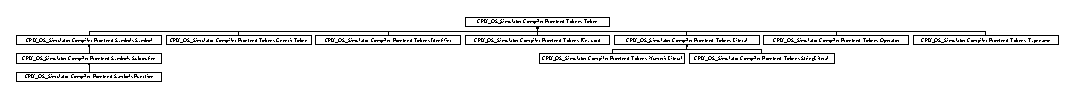
\includegraphics[height=0.869565cm]{class_c_p_u___o_s___simulator_1_1_compiler_1_1_frontend_1_1_tokens_1_1_token}
\end{center}
\end{figure}
\subsection*{Public Member Functions}
\begin{DoxyCompactItemize}
\item 
abstract Enum \hyperlink{class_c_p_u___o_s___simulator_1_1_compiler_1_1_frontend_1_1_tokens_1_1_token_accfe8c46faedacd527ef619698c76310}{Detect\+Type} ()
\item 
bool \hyperlink{class_c_p_u___o_s___simulator_1_1_compiler_1_1_frontend_1_1_tokens_1_1_token_a0a2a90e3f61a2b9cdb8fab576ba03af9}{is\+Operator} ()
\item 
bool \hyperlink{class_c_p_u___o_s___simulator_1_1_compiler_1_1_frontend_1_1_tokens_1_1_token_a8d59fb0bd2432fe5f0bb5a3eb4e15a5d}{is\+Keyword} ()
\item 
bool \hyperlink{class_c_p_u___o_s___simulator_1_1_compiler_1_1_frontend_1_1_tokens_1_1_token_a2119b17e85e5b7ee78909209701620d0}{is\+Type} ()
\item 
override string \hyperlink{class_c_p_u___o_s___simulator_1_1_compiler_1_1_frontend_1_1_tokens_1_1_token_ab1d893f228078256e8dc885d8680443b}{To\+String} ()
\begin{DoxyCompactList}\small\item\em Returns a string that represents the current object. \end{DoxyCompactList}\end{DoxyCompactItemize}
\subsection*{Protected Attributes}
\begin{DoxyCompactItemize}
\item 
Enum \hyperlink{class_c_p_u___o_s___simulator_1_1_compiler_1_1_frontend_1_1_tokens_1_1_token_a7ec4dbbde477cd373f8135f0c843a346}{type} = \hyperlink{namespace_c_p_u___o_s___simulator_1_1_compiler_1_1_frontend_1_1_tokens_a86b87efebad08200cebe3075b5812b13a696b031073e74bf2cb98e5ef201d4aa3}{Enum\+Operator\+Type.\+U\+N\+K\+N\+O\+W\+N}
\item 
string \hyperlink{class_c_p_u___o_s___simulator_1_1_compiler_1_1_frontend_1_1_tokens_1_1_token_a5c05e12850ca18be8cbfdf7e2e263324}{value}
\end{DoxyCompactItemize}
\subsection*{Properties}
\begin{DoxyCompactItemize}
\item 
bool \hyperlink{class_c_p_u___o_s___simulator_1_1_compiler_1_1_frontend_1_1_tokens_1_1_token_a8da0567c03fd25e1494ddbe098f95405}{Isoperator}\hspace{0.3cm}{\ttfamily  \mbox{[}get\mbox{]}}
\item 
bool \hyperlink{class_c_p_u___o_s___simulator_1_1_compiler_1_1_frontend_1_1_tokens_1_1_token_a584165252fdb4f576e49466e2de55502}{Iskeyword}\hspace{0.3cm}{\ttfamily  \mbox{[}get\mbox{]}}
\item 
bool \hyperlink{class_c_p_u___o_s___simulator_1_1_compiler_1_1_frontend_1_1_tokens_1_1_token_a61b9eeb8f47e957789390a188f65a08b}{Istype}\hspace{0.3cm}{\ttfamily  \mbox{[}get\mbox{]}}
\item 
Enum \hyperlink{class_c_p_u___o_s___simulator_1_1_compiler_1_1_frontend_1_1_tokens_1_1_token_a1735d21dd74ca2022d60b7ca45be3040}{Type}\hspace{0.3cm}{\ttfamily  \mbox{[}get, set\mbox{]}}
\item 
string \hyperlink{class_c_p_u___o_s___simulator_1_1_compiler_1_1_frontend_1_1_tokens_1_1_token_ac2869f45f5d24226d03406c3f9da0505}{Value}\hspace{0.3cm}{\ttfamily  \mbox{[}get, set\mbox{]}}
\end{DoxyCompactItemize}
\subsection*{Private Attributes}
\begin{DoxyCompactItemize}
\item 
bool \hyperlink{class_c_p_u___o_s___simulator_1_1_compiler_1_1_frontend_1_1_tokens_1_1_token_a4de08fda7aa63cfac40f564c49bcdcb8}{isoperator}
\item 
bool \hyperlink{class_c_p_u___o_s___simulator_1_1_compiler_1_1_frontend_1_1_tokens_1_1_token_ad5eccd50e40196f3b70df38420357e4b}{iskeyword}
\item 
bool \hyperlink{class_c_p_u___o_s___simulator_1_1_compiler_1_1_frontend_1_1_tokens_1_1_token_a3d8b092bc7201b819ada49cb10ea01b0}{istype}
\end{DoxyCompactItemize}


\subsection{Detailed Description}


Definition at line 5 of file Token.\+cs.



\subsection{Member Function Documentation}
\hypertarget{class_c_p_u___o_s___simulator_1_1_compiler_1_1_frontend_1_1_tokens_1_1_token_accfe8c46faedacd527ef619698c76310}{}\index{C\+P\+U\+\_\+\+O\+S\+\_\+\+Simulator\+::\+Compiler\+::\+Frontend\+::\+Tokens\+::\+Token@{C\+P\+U\+\_\+\+O\+S\+\_\+\+Simulator\+::\+Compiler\+::\+Frontend\+::\+Tokens\+::\+Token}!Detect\+Type@{Detect\+Type}}
\index{Detect\+Type@{Detect\+Type}!C\+P\+U\+\_\+\+O\+S\+\_\+\+Simulator\+::\+Compiler\+::\+Frontend\+::\+Tokens\+::\+Token@{C\+P\+U\+\_\+\+O\+S\+\_\+\+Simulator\+::\+Compiler\+::\+Frontend\+::\+Tokens\+::\+Token}}
\subsubsection[{Detect\+Type()}]{\setlength{\rightskip}{0pt plus 5cm}abstract Enum C\+P\+U\+\_\+\+O\+S\+\_\+\+Simulator.\+Compiler.\+Frontend.\+Tokens.\+Token.\+Detect\+Type (
\begin{DoxyParamCaption}
{}
\end{DoxyParamCaption}
)\hspace{0.3cm}{\ttfamily [pure virtual]}}\label{class_c_p_u___o_s___simulator_1_1_compiler_1_1_frontend_1_1_tokens_1_1_token_accfe8c46faedacd527ef619698c76310}


Implemented in \hyperlink{class_c_p_u___o_s___simulator_1_1_compiler_1_1_frontend_1_1_symbols_1_1_symbol_a1aef3417bc03adb5bcc15cfcdedb834e}{C\+P\+U\+\_\+\+O\+S\+\_\+\+Simulator.\+Compiler.\+Frontend.\+Symbols.\+Symbol}, \hyperlink{class_c_p_u___o_s___simulator_1_1_compiler_1_1_frontend_1_1_tokens_1_1_literal_af449c5fee28fb2076933cdfc67857c23}{C\+P\+U\+\_\+\+O\+S\+\_\+\+Simulator.\+Compiler.\+Frontend.\+Tokens.\+Literal}, \hyperlink{class_c_p_u___o_s___simulator_1_1_compiler_1_1_frontend_1_1_tokens_1_1_numeric_literal_a48f7635001171a738d1c53d065659933}{C\+P\+U\+\_\+\+O\+S\+\_\+\+Simulator.\+Compiler.\+Frontend.\+Tokens.\+Numeric\+Literal}, \hyperlink{class_c_p_u___o_s___simulator_1_1_compiler_1_1_frontend_1_1_tokens_1_1_string_literal_a55fe99257eeaeb6d73db4ff188de3f57}{C\+P\+U\+\_\+\+O\+S\+\_\+\+Simulator.\+Compiler.\+Frontend.\+Tokens.\+String\+Literal}, \hyperlink{class_c_p_u___o_s___simulator_1_1_compiler_1_1_frontend_1_1_tokens_1_1_operator_a3bd6c8981e452c8abe4c4f019d78fb9b}{C\+P\+U\+\_\+\+O\+S\+\_\+\+Simulator.\+Compiler.\+Frontend.\+Tokens.\+Operator}, \hyperlink{class_c_p_u___o_s___simulator_1_1_compiler_1_1_frontend_1_1_tokens_1_1_generic_token_ae835f3a63c88a7e73df243c510cb0142}{C\+P\+U\+\_\+\+O\+S\+\_\+\+Simulator.\+Compiler.\+Frontend.\+Tokens.\+Generic\+Token}, \hyperlink{class_c_p_u___o_s___simulator_1_1_compiler_1_1_frontend_1_1_tokens_1_1_keyword_aa1052d5b8b0fa6b1233fac902904e54a}{C\+P\+U\+\_\+\+O\+S\+\_\+\+Simulator.\+Compiler.\+Frontend.\+Tokens.\+Keyword}, \hyperlink{class_c_p_u___o_s___simulator_1_1_compiler_1_1_frontend_1_1_tokens_1_1_typename_ac03153af0baa70a7943edc9a36c6f555}{C\+P\+U\+\_\+\+O\+S\+\_\+\+Simulator.\+Compiler.\+Frontend.\+Tokens.\+Typename}, and \hyperlink{class_c_p_u___o_s___simulator_1_1_compiler_1_1_frontend_1_1_tokens_1_1_identifier_aa5d0544de3699b5403b38e5978877fe1}{C\+P\+U\+\_\+\+O\+S\+\_\+\+Simulator.\+Compiler.\+Frontend.\+Tokens.\+Identifier}.

\hypertarget{class_c_p_u___o_s___simulator_1_1_compiler_1_1_frontend_1_1_tokens_1_1_token_a8d59fb0bd2432fe5f0bb5a3eb4e15a5d}{}\index{C\+P\+U\+\_\+\+O\+S\+\_\+\+Simulator\+::\+Compiler\+::\+Frontend\+::\+Tokens\+::\+Token@{C\+P\+U\+\_\+\+O\+S\+\_\+\+Simulator\+::\+Compiler\+::\+Frontend\+::\+Tokens\+::\+Token}!is\+Keyword@{is\+Keyword}}
\index{is\+Keyword@{is\+Keyword}!C\+P\+U\+\_\+\+O\+S\+\_\+\+Simulator\+::\+Compiler\+::\+Frontend\+::\+Tokens\+::\+Token@{C\+P\+U\+\_\+\+O\+S\+\_\+\+Simulator\+::\+Compiler\+::\+Frontend\+::\+Tokens\+::\+Token}}
\subsubsection[{is\+Keyword()}]{\setlength{\rightskip}{0pt plus 5cm}bool C\+P\+U\+\_\+\+O\+S\+\_\+\+Simulator.\+Compiler.\+Frontend.\+Tokens.\+Token.\+is\+Keyword (
\begin{DoxyParamCaption}
{}
\end{DoxyParamCaption}
)}\label{class_c_p_u___o_s___simulator_1_1_compiler_1_1_frontend_1_1_tokens_1_1_token_a8d59fb0bd2432fe5f0bb5a3eb4e15a5d}


Definition at line 49 of file Token.\+cs.

\hypertarget{class_c_p_u___o_s___simulator_1_1_compiler_1_1_frontend_1_1_tokens_1_1_token_a0a2a90e3f61a2b9cdb8fab576ba03af9}{}\index{C\+P\+U\+\_\+\+O\+S\+\_\+\+Simulator\+::\+Compiler\+::\+Frontend\+::\+Tokens\+::\+Token@{C\+P\+U\+\_\+\+O\+S\+\_\+\+Simulator\+::\+Compiler\+::\+Frontend\+::\+Tokens\+::\+Token}!is\+Operator@{is\+Operator}}
\index{is\+Operator@{is\+Operator}!C\+P\+U\+\_\+\+O\+S\+\_\+\+Simulator\+::\+Compiler\+::\+Frontend\+::\+Tokens\+::\+Token@{C\+P\+U\+\_\+\+O\+S\+\_\+\+Simulator\+::\+Compiler\+::\+Frontend\+::\+Tokens\+::\+Token}}
\subsubsection[{is\+Operator()}]{\setlength{\rightskip}{0pt plus 5cm}bool C\+P\+U\+\_\+\+O\+S\+\_\+\+Simulator.\+Compiler.\+Frontend.\+Tokens.\+Token.\+is\+Operator (
\begin{DoxyParamCaption}
{}
\end{DoxyParamCaption}
)}\label{class_c_p_u___o_s___simulator_1_1_compiler_1_1_frontend_1_1_tokens_1_1_token_a0a2a90e3f61a2b9cdb8fab576ba03af9}


Definition at line 42 of file Token.\+cs.

\hypertarget{class_c_p_u___o_s___simulator_1_1_compiler_1_1_frontend_1_1_tokens_1_1_token_a2119b17e85e5b7ee78909209701620d0}{}\index{C\+P\+U\+\_\+\+O\+S\+\_\+\+Simulator\+::\+Compiler\+::\+Frontend\+::\+Tokens\+::\+Token@{C\+P\+U\+\_\+\+O\+S\+\_\+\+Simulator\+::\+Compiler\+::\+Frontend\+::\+Tokens\+::\+Token}!is\+Type@{is\+Type}}
\index{is\+Type@{is\+Type}!C\+P\+U\+\_\+\+O\+S\+\_\+\+Simulator\+::\+Compiler\+::\+Frontend\+::\+Tokens\+::\+Token@{C\+P\+U\+\_\+\+O\+S\+\_\+\+Simulator\+::\+Compiler\+::\+Frontend\+::\+Tokens\+::\+Token}}
\subsubsection[{is\+Type()}]{\setlength{\rightskip}{0pt plus 5cm}bool C\+P\+U\+\_\+\+O\+S\+\_\+\+Simulator.\+Compiler.\+Frontend.\+Tokens.\+Token.\+is\+Type (
\begin{DoxyParamCaption}
{}
\end{DoxyParamCaption}
)}\label{class_c_p_u___o_s___simulator_1_1_compiler_1_1_frontend_1_1_tokens_1_1_token_a2119b17e85e5b7ee78909209701620d0}


Definition at line 56 of file Token.\+cs.

\hypertarget{class_c_p_u___o_s___simulator_1_1_compiler_1_1_frontend_1_1_tokens_1_1_token_ab1d893f228078256e8dc885d8680443b}{}\index{C\+P\+U\+\_\+\+O\+S\+\_\+\+Simulator\+::\+Compiler\+::\+Frontend\+::\+Tokens\+::\+Token@{C\+P\+U\+\_\+\+O\+S\+\_\+\+Simulator\+::\+Compiler\+::\+Frontend\+::\+Tokens\+::\+Token}!To\+String@{To\+String}}
\index{To\+String@{To\+String}!C\+P\+U\+\_\+\+O\+S\+\_\+\+Simulator\+::\+Compiler\+::\+Frontend\+::\+Tokens\+::\+Token@{C\+P\+U\+\_\+\+O\+S\+\_\+\+Simulator\+::\+Compiler\+::\+Frontend\+::\+Tokens\+::\+Token}}
\subsubsection[{To\+String()}]{\setlength{\rightskip}{0pt plus 5cm}override string C\+P\+U\+\_\+\+O\+S\+\_\+\+Simulator.\+Compiler.\+Frontend.\+Tokens.\+Token.\+To\+String (
\begin{DoxyParamCaption}
{}
\end{DoxyParamCaption}
)}\label{class_c_p_u___o_s___simulator_1_1_compiler_1_1_frontend_1_1_tokens_1_1_token_ab1d893f228078256e8dc885d8680443b}


Returns a string that represents the current object. 

\begin{DoxyReturn}{Returns}
A string that represents the current object. 
\end{DoxyReturn}


Definition at line 69 of file Token.\+cs.



\subsection{Member Data Documentation}
\hypertarget{class_c_p_u___o_s___simulator_1_1_compiler_1_1_frontend_1_1_tokens_1_1_token_ad5eccd50e40196f3b70df38420357e4b}{}\index{C\+P\+U\+\_\+\+O\+S\+\_\+\+Simulator\+::\+Compiler\+::\+Frontend\+::\+Tokens\+::\+Token@{C\+P\+U\+\_\+\+O\+S\+\_\+\+Simulator\+::\+Compiler\+::\+Frontend\+::\+Tokens\+::\+Token}!iskeyword@{iskeyword}}
\index{iskeyword@{iskeyword}!C\+P\+U\+\_\+\+O\+S\+\_\+\+Simulator\+::\+Compiler\+::\+Frontend\+::\+Tokens\+::\+Token@{C\+P\+U\+\_\+\+O\+S\+\_\+\+Simulator\+::\+Compiler\+::\+Frontend\+::\+Tokens\+::\+Token}}
\subsubsection[{iskeyword}]{\setlength{\rightskip}{0pt plus 5cm}bool C\+P\+U\+\_\+\+O\+S\+\_\+\+Simulator.\+Compiler.\+Frontend.\+Tokens.\+Token.\+iskeyword\hspace{0.3cm}{\ttfamily [private]}}\label{class_c_p_u___o_s___simulator_1_1_compiler_1_1_frontend_1_1_tokens_1_1_token_ad5eccd50e40196f3b70df38420357e4b}


Definition at line 10 of file Token.\+cs.

\hypertarget{class_c_p_u___o_s___simulator_1_1_compiler_1_1_frontend_1_1_tokens_1_1_token_a4de08fda7aa63cfac40f564c49bcdcb8}{}\index{C\+P\+U\+\_\+\+O\+S\+\_\+\+Simulator\+::\+Compiler\+::\+Frontend\+::\+Tokens\+::\+Token@{C\+P\+U\+\_\+\+O\+S\+\_\+\+Simulator\+::\+Compiler\+::\+Frontend\+::\+Tokens\+::\+Token}!isoperator@{isoperator}}
\index{isoperator@{isoperator}!C\+P\+U\+\_\+\+O\+S\+\_\+\+Simulator\+::\+Compiler\+::\+Frontend\+::\+Tokens\+::\+Token@{C\+P\+U\+\_\+\+O\+S\+\_\+\+Simulator\+::\+Compiler\+::\+Frontend\+::\+Tokens\+::\+Token}}
\subsubsection[{isoperator}]{\setlength{\rightskip}{0pt plus 5cm}bool C\+P\+U\+\_\+\+O\+S\+\_\+\+Simulator.\+Compiler.\+Frontend.\+Tokens.\+Token.\+isoperator\hspace{0.3cm}{\ttfamily [private]}}\label{class_c_p_u___o_s___simulator_1_1_compiler_1_1_frontend_1_1_tokens_1_1_token_a4de08fda7aa63cfac40f564c49bcdcb8}


Definition at line 9 of file Token.\+cs.

\hypertarget{class_c_p_u___o_s___simulator_1_1_compiler_1_1_frontend_1_1_tokens_1_1_token_a3d8b092bc7201b819ada49cb10ea01b0}{}\index{C\+P\+U\+\_\+\+O\+S\+\_\+\+Simulator\+::\+Compiler\+::\+Frontend\+::\+Tokens\+::\+Token@{C\+P\+U\+\_\+\+O\+S\+\_\+\+Simulator\+::\+Compiler\+::\+Frontend\+::\+Tokens\+::\+Token}!istype@{istype}}
\index{istype@{istype}!C\+P\+U\+\_\+\+O\+S\+\_\+\+Simulator\+::\+Compiler\+::\+Frontend\+::\+Tokens\+::\+Token@{C\+P\+U\+\_\+\+O\+S\+\_\+\+Simulator\+::\+Compiler\+::\+Frontend\+::\+Tokens\+::\+Token}}
\subsubsection[{istype}]{\setlength{\rightskip}{0pt plus 5cm}bool C\+P\+U\+\_\+\+O\+S\+\_\+\+Simulator.\+Compiler.\+Frontend.\+Tokens.\+Token.\+istype\hspace{0.3cm}{\ttfamily [private]}}\label{class_c_p_u___o_s___simulator_1_1_compiler_1_1_frontend_1_1_tokens_1_1_token_a3d8b092bc7201b819ada49cb10ea01b0}


Definition at line 11 of file Token.\+cs.

\hypertarget{class_c_p_u___o_s___simulator_1_1_compiler_1_1_frontend_1_1_tokens_1_1_token_a7ec4dbbde477cd373f8135f0c843a346}{}\index{C\+P\+U\+\_\+\+O\+S\+\_\+\+Simulator\+::\+Compiler\+::\+Frontend\+::\+Tokens\+::\+Token@{C\+P\+U\+\_\+\+O\+S\+\_\+\+Simulator\+::\+Compiler\+::\+Frontend\+::\+Tokens\+::\+Token}!type@{type}}
\index{type@{type}!C\+P\+U\+\_\+\+O\+S\+\_\+\+Simulator\+::\+Compiler\+::\+Frontend\+::\+Tokens\+::\+Token@{C\+P\+U\+\_\+\+O\+S\+\_\+\+Simulator\+::\+Compiler\+::\+Frontend\+::\+Tokens\+::\+Token}}
\subsubsection[{type}]{\setlength{\rightskip}{0pt plus 5cm}Enum C\+P\+U\+\_\+\+O\+S\+\_\+\+Simulator.\+Compiler.\+Frontend.\+Tokens.\+Token.\+type = {\bf Enum\+Operator\+Type.\+U\+N\+K\+N\+O\+W\+N}\hspace{0.3cm}{\ttfamily [protected]}}\label{class_c_p_u___o_s___simulator_1_1_compiler_1_1_frontend_1_1_tokens_1_1_token_a7ec4dbbde477cd373f8135f0c843a346}


Definition at line 7 of file Token.\+cs.

\hypertarget{class_c_p_u___o_s___simulator_1_1_compiler_1_1_frontend_1_1_tokens_1_1_token_a5c05e12850ca18be8cbfdf7e2e263324}{}\index{C\+P\+U\+\_\+\+O\+S\+\_\+\+Simulator\+::\+Compiler\+::\+Frontend\+::\+Tokens\+::\+Token@{C\+P\+U\+\_\+\+O\+S\+\_\+\+Simulator\+::\+Compiler\+::\+Frontend\+::\+Tokens\+::\+Token}!value@{value}}
\index{value@{value}!C\+P\+U\+\_\+\+O\+S\+\_\+\+Simulator\+::\+Compiler\+::\+Frontend\+::\+Tokens\+::\+Token@{C\+P\+U\+\_\+\+O\+S\+\_\+\+Simulator\+::\+Compiler\+::\+Frontend\+::\+Tokens\+::\+Token}}
\subsubsection[{value}]{\setlength{\rightskip}{0pt plus 5cm}string C\+P\+U\+\_\+\+O\+S\+\_\+\+Simulator.\+Compiler.\+Frontend.\+Tokens.\+Token.\+value\hspace{0.3cm}{\ttfamily [protected]}}\label{class_c_p_u___o_s___simulator_1_1_compiler_1_1_frontend_1_1_tokens_1_1_token_a5c05e12850ca18be8cbfdf7e2e263324}


Definition at line 8 of file Token.\+cs.



\subsection{Property Documentation}
\hypertarget{class_c_p_u___o_s___simulator_1_1_compiler_1_1_frontend_1_1_tokens_1_1_token_a584165252fdb4f576e49466e2de55502}{}\index{C\+P\+U\+\_\+\+O\+S\+\_\+\+Simulator\+::\+Compiler\+::\+Frontend\+::\+Tokens\+::\+Token@{C\+P\+U\+\_\+\+O\+S\+\_\+\+Simulator\+::\+Compiler\+::\+Frontend\+::\+Tokens\+::\+Token}!Iskeyword@{Iskeyword}}
\index{Iskeyword@{Iskeyword}!C\+P\+U\+\_\+\+O\+S\+\_\+\+Simulator\+::\+Compiler\+::\+Frontend\+::\+Tokens\+::\+Token@{C\+P\+U\+\_\+\+O\+S\+\_\+\+Simulator\+::\+Compiler\+::\+Frontend\+::\+Tokens\+::\+Token}}
\subsubsection[{Iskeyword}]{\setlength{\rightskip}{0pt plus 5cm}bool C\+P\+U\+\_\+\+O\+S\+\_\+\+Simulator.\+Compiler.\+Frontend.\+Tokens.\+Token.\+Iskeyword\hspace{0.3cm}{\ttfamily [get]}}\label{class_c_p_u___o_s___simulator_1_1_compiler_1_1_frontend_1_1_tokens_1_1_token_a584165252fdb4f576e49466e2de55502}


Definition at line 19 of file Token.\+cs.

\hypertarget{class_c_p_u___o_s___simulator_1_1_compiler_1_1_frontend_1_1_tokens_1_1_token_a8da0567c03fd25e1494ddbe098f95405}{}\index{C\+P\+U\+\_\+\+O\+S\+\_\+\+Simulator\+::\+Compiler\+::\+Frontend\+::\+Tokens\+::\+Token@{C\+P\+U\+\_\+\+O\+S\+\_\+\+Simulator\+::\+Compiler\+::\+Frontend\+::\+Tokens\+::\+Token}!Isoperator@{Isoperator}}
\index{Isoperator@{Isoperator}!C\+P\+U\+\_\+\+O\+S\+\_\+\+Simulator\+::\+Compiler\+::\+Frontend\+::\+Tokens\+::\+Token@{C\+P\+U\+\_\+\+O\+S\+\_\+\+Simulator\+::\+Compiler\+::\+Frontend\+::\+Tokens\+::\+Token}}
\subsubsection[{Isoperator}]{\setlength{\rightskip}{0pt plus 5cm}bool C\+P\+U\+\_\+\+O\+S\+\_\+\+Simulator.\+Compiler.\+Frontend.\+Tokens.\+Token.\+Isoperator\hspace{0.3cm}{\ttfamily [get]}}\label{class_c_p_u___o_s___simulator_1_1_compiler_1_1_frontend_1_1_tokens_1_1_token_a8da0567c03fd25e1494ddbe098f95405}


Definition at line 14 of file Token.\+cs.

\hypertarget{class_c_p_u___o_s___simulator_1_1_compiler_1_1_frontend_1_1_tokens_1_1_token_a61b9eeb8f47e957789390a188f65a08b}{}\index{C\+P\+U\+\_\+\+O\+S\+\_\+\+Simulator\+::\+Compiler\+::\+Frontend\+::\+Tokens\+::\+Token@{C\+P\+U\+\_\+\+O\+S\+\_\+\+Simulator\+::\+Compiler\+::\+Frontend\+::\+Tokens\+::\+Token}!Istype@{Istype}}
\index{Istype@{Istype}!C\+P\+U\+\_\+\+O\+S\+\_\+\+Simulator\+::\+Compiler\+::\+Frontend\+::\+Tokens\+::\+Token@{C\+P\+U\+\_\+\+O\+S\+\_\+\+Simulator\+::\+Compiler\+::\+Frontend\+::\+Tokens\+::\+Token}}
\subsubsection[{Istype}]{\setlength{\rightskip}{0pt plus 5cm}bool C\+P\+U\+\_\+\+O\+S\+\_\+\+Simulator.\+Compiler.\+Frontend.\+Tokens.\+Token.\+Istype\hspace{0.3cm}{\ttfamily [get]}}\label{class_c_p_u___o_s___simulator_1_1_compiler_1_1_frontend_1_1_tokens_1_1_token_a61b9eeb8f47e957789390a188f65a08b}


Definition at line 24 of file Token.\+cs.

\hypertarget{class_c_p_u___o_s___simulator_1_1_compiler_1_1_frontend_1_1_tokens_1_1_token_a1735d21dd74ca2022d60b7ca45be3040}{}\index{C\+P\+U\+\_\+\+O\+S\+\_\+\+Simulator\+::\+Compiler\+::\+Frontend\+::\+Tokens\+::\+Token@{C\+P\+U\+\_\+\+O\+S\+\_\+\+Simulator\+::\+Compiler\+::\+Frontend\+::\+Tokens\+::\+Token}!Type@{Type}}
\index{Type@{Type}!C\+P\+U\+\_\+\+O\+S\+\_\+\+Simulator\+::\+Compiler\+::\+Frontend\+::\+Tokens\+::\+Token@{C\+P\+U\+\_\+\+O\+S\+\_\+\+Simulator\+::\+Compiler\+::\+Frontend\+::\+Tokens\+::\+Token}}
\subsubsection[{Type}]{\setlength{\rightskip}{0pt plus 5cm}Enum C\+P\+U\+\_\+\+O\+S\+\_\+\+Simulator.\+Compiler.\+Frontend.\+Tokens.\+Token.\+Type\hspace{0.3cm}{\ttfamily [get]}, {\ttfamily [set]}}\label{class_c_p_u___o_s___simulator_1_1_compiler_1_1_frontend_1_1_tokens_1_1_token_a1735d21dd74ca2022d60b7ca45be3040}


Definition at line 29 of file Token.\+cs.

\hypertarget{class_c_p_u___o_s___simulator_1_1_compiler_1_1_frontend_1_1_tokens_1_1_token_ac2869f45f5d24226d03406c3f9da0505}{}\index{C\+P\+U\+\_\+\+O\+S\+\_\+\+Simulator\+::\+Compiler\+::\+Frontend\+::\+Tokens\+::\+Token@{C\+P\+U\+\_\+\+O\+S\+\_\+\+Simulator\+::\+Compiler\+::\+Frontend\+::\+Tokens\+::\+Token}!Value@{Value}}
\index{Value@{Value}!C\+P\+U\+\_\+\+O\+S\+\_\+\+Simulator\+::\+Compiler\+::\+Frontend\+::\+Tokens\+::\+Token@{C\+P\+U\+\_\+\+O\+S\+\_\+\+Simulator\+::\+Compiler\+::\+Frontend\+::\+Tokens\+::\+Token}}
\subsubsection[{Value}]{\setlength{\rightskip}{0pt plus 5cm}string C\+P\+U\+\_\+\+O\+S\+\_\+\+Simulator.\+Compiler.\+Frontend.\+Tokens.\+Token.\+Value\hspace{0.3cm}{\ttfamily [get]}, {\ttfamily [set]}}\label{class_c_p_u___o_s___simulator_1_1_compiler_1_1_frontend_1_1_tokens_1_1_token_ac2869f45f5d24226d03406c3f9da0505}


Definition at line 35 of file Token.\+cs.



The documentation for this class was generated from the following file\+:\begin{DoxyCompactItemize}
\item 
Compiler/\+Frontend/\+Tokens/\hyperlink{_token_8cs}{Token.\+cs}\end{DoxyCompactItemize}

\hypertarget{class_c_p_u___o_s___simulator_1_1_compiler_1_1_frontend_1_1_tokens_1_1_typename}{}\section{C\+P\+U\+\_\+\+O\+S\+\_\+\+Simulator.\+Compiler.\+Frontend.\+Tokens.\+Typename Class Reference}
\label{class_c_p_u___o_s___simulator_1_1_compiler_1_1_frontend_1_1_tokens_1_1_typename}\index{C\+P\+U\+\_\+\+O\+S\+\_\+\+Simulator.\+Compiler.\+Frontend.\+Tokens.\+Typename@{C\+P\+U\+\_\+\+O\+S\+\_\+\+Simulator.\+Compiler.\+Frontend.\+Tokens.\+Typename}}
Inheritance diagram for C\+P\+U\+\_\+\+O\+S\+\_\+\+Simulator.\+Compiler.\+Frontend.\+Tokens.\+Typename\+:\begin{figure}[H]
\begin{center}
\leavevmode
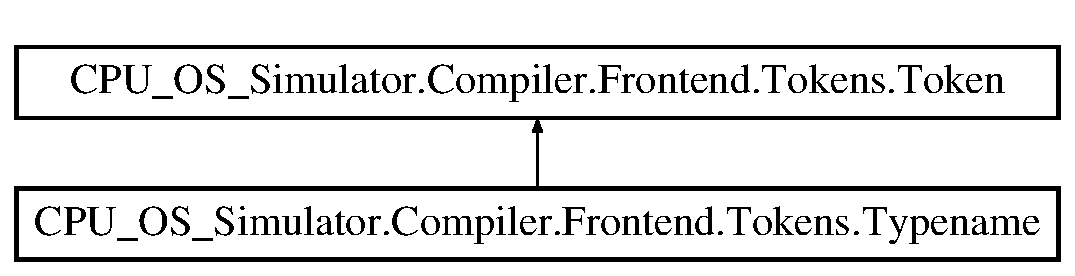
\includegraphics[height=2.000000cm]{class_c_p_u___o_s___simulator_1_1_compiler_1_1_frontend_1_1_tokens_1_1_typename}
\end{center}
\end{figure}
\subsection*{Public Member Functions}
\begin{DoxyCompactItemize}
\item 
\hyperlink{class_c_p_u___o_s___simulator_1_1_compiler_1_1_frontend_1_1_tokens_1_1_typename_a88c1ae87fd0ed6772577303ae2776c6b}{Typename} (string \hyperlink{class_c_p_u___o_s___simulator_1_1_compiler_1_1_frontend_1_1_tokens_1_1_token_a5c05e12850ca18be8cbfdf7e2e263324}{value})
\item 
override Enum \hyperlink{class_c_p_u___o_s___simulator_1_1_compiler_1_1_frontend_1_1_tokens_1_1_typename_ac03153af0baa70a7943edc9a36c6f555}{Detect\+Type} ()
\item 
\hyperlink{namespace_c_p_u___o_s___simulator_1_1_compiler_1_1_frontend_1_1_tokens_a7c0cc43763cc9d01c7d5af34d70b96ea}{Enum\+Types} \hyperlink{class_c_p_u___o_s___simulator_1_1_compiler_1_1_frontend_1_1_tokens_1_1_typename_aefe888a2588f1e2f903851366e1ab7b4}{Get\+Typename} ()
\end{DoxyCompactItemize}
\subsection*{Additional Inherited Members}


\subsection{Detailed Description}


Definition at line 5 of file Typename.\+cs.



\subsection{Constructor \& Destructor Documentation}
\hypertarget{class_c_p_u___o_s___simulator_1_1_compiler_1_1_frontend_1_1_tokens_1_1_typename_a88c1ae87fd0ed6772577303ae2776c6b}{}\index{C\+P\+U\+\_\+\+O\+S\+\_\+\+Simulator\+::\+Compiler\+::\+Frontend\+::\+Tokens\+::\+Typename@{C\+P\+U\+\_\+\+O\+S\+\_\+\+Simulator\+::\+Compiler\+::\+Frontend\+::\+Tokens\+::\+Typename}!Typename@{Typename}}
\index{Typename@{Typename}!C\+P\+U\+\_\+\+O\+S\+\_\+\+Simulator\+::\+Compiler\+::\+Frontend\+::\+Tokens\+::\+Typename@{C\+P\+U\+\_\+\+O\+S\+\_\+\+Simulator\+::\+Compiler\+::\+Frontend\+::\+Tokens\+::\+Typename}}
\subsubsection[{Typename(string value)}]{\setlength{\rightskip}{0pt plus 5cm}C\+P\+U\+\_\+\+O\+S\+\_\+\+Simulator.\+Compiler.\+Frontend.\+Tokens.\+Typename.\+Typename (
\begin{DoxyParamCaption}
\item[{string}]{value}
\end{DoxyParamCaption}
)}\label{class_c_p_u___o_s___simulator_1_1_compiler_1_1_frontend_1_1_tokens_1_1_typename_a88c1ae87fd0ed6772577303ae2776c6b}


Definition at line 7 of file Typename.\+cs.



\subsection{Member Function Documentation}
\hypertarget{class_c_p_u___o_s___simulator_1_1_compiler_1_1_frontend_1_1_tokens_1_1_typename_ac03153af0baa70a7943edc9a36c6f555}{}\index{C\+P\+U\+\_\+\+O\+S\+\_\+\+Simulator\+::\+Compiler\+::\+Frontend\+::\+Tokens\+::\+Typename@{C\+P\+U\+\_\+\+O\+S\+\_\+\+Simulator\+::\+Compiler\+::\+Frontend\+::\+Tokens\+::\+Typename}!Detect\+Type@{Detect\+Type}}
\index{Detect\+Type@{Detect\+Type}!C\+P\+U\+\_\+\+O\+S\+\_\+\+Simulator\+::\+Compiler\+::\+Frontend\+::\+Tokens\+::\+Typename@{C\+P\+U\+\_\+\+O\+S\+\_\+\+Simulator\+::\+Compiler\+::\+Frontend\+::\+Tokens\+::\+Typename}}
\subsubsection[{Detect\+Type()}]{\setlength{\rightskip}{0pt plus 5cm}override Enum C\+P\+U\+\_\+\+O\+S\+\_\+\+Simulator.\+Compiler.\+Frontend.\+Tokens.\+Typename.\+Detect\+Type (
\begin{DoxyParamCaption}
{}
\end{DoxyParamCaption}
)\hspace{0.3cm}{\ttfamily [virtual]}}\label{class_c_p_u___o_s___simulator_1_1_compiler_1_1_frontend_1_1_tokens_1_1_typename_ac03153af0baa70a7943edc9a36c6f555}


Implements \hyperlink{class_c_p_u___o_s___simulator_1_1_compiler_1_1_frontend_1_1_tokens_1_1_token_accfe8c46faedacd527ef619698c76310}{C\+P\+U\+\_\+\+O\+S\+\_\+\+Simulator.\+Compiler.\+Frontend.\+Tokens.\+Token}.



Definition at line 11 of file Typename.\+cs.

\hypertarget{class_c_p_u___o_s___simulator_1_1_compiler_1_1_frontend_1_1_tokens_1_1_typename_aefe888a2588f1e2f903851366e1ab7b4}{}\index{C\+P\+U\+\_\+\+O\+S\+\_\+\+Simulator\+::\+Compiler\+::\+Frontend\+::\+Tokens\+::\+Typename@{C\+P\+U\+\_\+\+O\+S\+\_\+\+Simulator\+::\+Compiler\+::\+Frontend\+::\+Tokens\+::\+Typename}!Get\+Typename@{Get\+Typename}}
\index{Get\+Typename@{Get\+Typename}!C\+P\+U\+\_\+\+O\+S\+\_\+\+Simulator\+::\+Compiler\+::\+Frontend\+::\+Tokens\+::\+Typename@{C\+P\+U\+\_\+\+O\+S\+\_\+\+Simulator\+::\+Compiler\+::\+Frontend\+::\+Tokens\+::\+Typename}}
\subsubsection[{Get\+Typename()}]{\setlength{\rightskip}{0pt plus 5cm}{\bf Enum\+Types} C\+P\+U\+\_\+\+O\+S\+\_\+\+Simulator.\+Compiler.\+Frontend.\+Tokens.\+Typename.\+Get\+Typename (
\begin{DoxyParamCaption}
{}
\end{DoxyParamCaption}
)}\label{class_c_p_u___o_s___simulator_1_1_compiler_1_1_frontend_1_1_tokens_1_1_typename_aefe888a2588f1e2f903851366e1ab7b4}


Definition at line 33 of file Typename.\+cs.



The documentation for this class was generated from the following file\+:\begin{DoxyCompactItemize}
\item 
Compiler/\+Frontend/\+Tokens/\hyperlink{_typename_8cs}{Typename.\+cs}\end{DoxyCompactItemize}

\hypertarget{class_c_p_u___o_s___simulator_1_1_window_bridge_1_1_window_instances}{}\section{C\+P\+U\+\_\+\+O\+S\+\_\+\+Simulator.\+Window\+Bridge.\+Window\+Instances Class Reference}
\label{class_c_p_u___o_s___simulator_1_1_window_bridge_1_1_window_instances}\index{C\+P\+U\+\_\+\+O\+S\+\_\+\+Simulator.\+Window\+Bridge.\+Window\+Instances@{C\+P\+U\+\_\+\+O\+S\+\_\+\+Simulator.\+Window\+Bridge.\+Window\+Instances}}


This class represents all of the active window instances  


\subsection*{Static Public Attributes}
\begin{DoxyCompactItemize}
\item 
static \hyperlink{class_c_p_u___o_s___simulator_1_1_main_window}{Main\+Window} \hyperlink{class_c_p_u___o_s___simulator_1_1_window_bridge_1_1_window_instances_a130a2c32e8ccfd51a42ecb363fbb42cc}{Main\+Window\+Instance} = \hyperlink{class_c_p_u___o_s___simulator_1_1_main_window_a1280266cc57403a91f08a8350dee05cc}{Main\+Window.\+current\+Instance}
\begin{DoxyCompactList}\small\item\em This variable represents the active main window instance \end{DoxyCompactList}\item 
static \hyperlink{class_c_p_u___o_s___simulator_1_1_memory_window}{Memory\+Window} \hyperlink{class_c_p_u___o_s___simulator_1_1_window_bridge_1_1_window_instances_a401fd485bde830472a1a960a25ec1464}{Memory\+Window\+Instance} = \hyperlink{class_c_p_u___o_s___simulator_1_1_memory_window_a870b795e3b919a82888ad608ab24d61a}{Memory\+Window.\+current\+Instance}
\begin{DoxyCompactList}\small\item\em This variable represents the active memory window instance \end{DoxyCompactList}\item 
static \hyperlink{class_c_p_u___o_s___simulator_1_1_console_window}{Console\+Window} \hyperlink{class_c_p_u___o_s___simulator_1_1_window_bridge_1_1_window_instances_a90b746b2373f150cab75e4dee0f91c45}{Console\+Window\+Instance} = \hyperlink{class_c_p_u___o_s___simulator_1_1_console_window_abee2fd1e118dd4f81dc2142bc033da4a}{Console\+Window.\+current\+Instance}
\begin{DoxyCompactList}\small\item\em This variable represents the active console window instance \end{DoxyCompactList}\item 
static \hyperlink{class_c_p_u___o_s___simulator_1_1_operating_system_main_window}{Operating\+System\+Main\+Window} \hyperlink{class_c_p_u___o_s___simulator_1_1_window_bridge_1_1_window_instances_a151a9fa30e40800129d05845501f7b64}{Operating\+System\+Main\+Window\+Instance}
\begin{DoxyCompactList}\small\item\em This variable represents the active operating system main window instance \end{DoxyCompactList}\end{DoxyCompactItemize}


\subsection{Detailed Description}
This class represents all of the active window instances 



Definition at line 6 of file Window\+Instances.\+cs.



\subsection{Member Data Documentation}
\hypertarget{class_c_p_u___o_s___simulator_1_1_window_bridge_1_1_window_instances_a90b746b2373f150cab75e4dee0f91c45}{}\index{C\+P\+U\+\_\+\+O\+S\+\_\+\+Simulator\+::\+Window\+Bridge\+::\+Window\+Instances@{C\+P\+U\+\_\+\+O\+S\+\_\+\+Simulator\+::\+Window\+Bridge\+::\+Window\+Instances}!Console\+Window\+Instance@{Console\+Window\+Instance}}
\index{Console\+Window\+Instance@{Console\+Window\+Instance}!C\+P\+U\+\_\+\+O\+S\+\_\+\+Simulator\+::\+Window\+Bridge\+::\+Window\+Instances@{C\+P\+U\+\_\+\+O\+S\+\_\+\+Simulator\+::\+Window\+Bridge\+::\+Window\+Instances}}
\subsubsection[{Console\+Window\+Instance}]{\setlength{\rightskip}{0pt plus 5cm}{\bf Console\+Window} C\+P\+U\+\_\+\+O\+S\+\_\+\+Simulator.\+Window\+Bridge.\+Window\+Instances.\+Console\+Window\+Instance = {\bf Console\+Window.\+current\+Instance}\hspace{0.3cm}{\ttfamily [static]}}\label{class_c_p_u___o_s___simulator_1_1_window_bridge_1_1_window_instances_a90b746b2373f150cab75e4dee0f91c45}


This variable represents the active console window instance 



Definition at line 19 of file Window\+Instances.\+cs.

\hypertarget{class_c_p_u___o_s___simulator_1_1_window_bridge_1_1_window_instances_a130a2c32e8ccfd51a42ecb363fbb42cc}{}\index{C\+P\+U\+\_\+\+O\+S\+\_\+\+Simulator\+::\+Window\+Bridge\+::\+Window\+Instances@{C\+P\+U\+\_\+\+O\+S\+\_\+\+Simulator\+::\+Window\+Bridge\+::\+Window\+Instances}!Main\+Window\+Instance@{Main\+Window\+Instance}}
\index{Main\+Window\+Instance@{Main\+Window\+Instance}!C\+P\+U\+\_\+\+O\+S\+\_\+\+Simulator\+::\+Window\+Bridge\+::\+Window\+Instances@{C\+P\+U\+\_\+\+O\+S\+\_\+\+Simulator\+::\+Window\+Bridge\+::\+Window\+Instances}}
\subsubsection[{Main\+Window\+Instance}]{\setlength{\rightskip}{0pt plus 5cm}{\bf Main\+Window} C\+P\+U\+\_\+\+O\+S\+\_\+\+Simulator.\+Window\+Bridge.\+Window\+Instances.\+Main\+Window\+Instance = {\bf Main\+Window.\+current\+Instance}\hspace{0.3cm}{\ttfamily [static]}}\label{class_c_p_u___o_s___simulator_1_1_window_bridge_1_1_window_instances_a130a2c32e8ccfd51a42ecb363fbb42cc}


This variable represents the active main window instance 



Definition at line 11 of file Window\+Instances.\+cs.

\hypertarget{class_c_p_u___o_s___simulator_1_1_window_bridge_1_1_window_instances_a401fd485bde830472a1a960a25ec1464}{}\index{C\+P\+U\+\_\+\+O\+S\+\_\+\+Simulator\+::\+Window\+Bridge\+::\+Window\+Instances@{C\+P\+U\+\_\+\+O\+S\+\_\+\+Simulator\+::\+Window\+Bridge\+::\+Window\+Instances}!Memory\+Window\+Instance@{Memory\+Window\+Instance}}
\index{Memory\+Window\+Instance@{Memory\+Window\+Instance}!C\+P\+U\+\_\+\+O\+S\+\_\+\+Simulator\+::\+Window\+Bridge\+::\+Window\+Instances@{C\+P\+U\+\_\+\+O\+S\+\_\+\+Simulator\+::\+Window\+Bridge\+::\+Window\+Instances}}
\subsubsection[{Memory\+Window\+Instance}]{\setlength{\rightskip}{0pt plus 5cm}{\bf Memory\+Window} C\+P\+U\+\_\+\+O\+S\+\_\+\+Simulator.\+Window\+Bridge.\+Window\+Instances.\+Memory\+Window\+Instance = {\bf Memory\+Window.\+current\+Instance}\hspace{0.3cm}{\ttfamily [static]}}\label{class_c_p_u___o_s___simulator_1_1_window_bridge_1_1_window_instances_a401fd485bde830472a1a960a25ec1464}


This variable represents the active memory window instance 



Definition at line 15 of file Window\+Instances.\+cs.

\hypertarget{class_c_p_u___o_s___simulator_1_1_window_bridge_1_1_window_instances_a151a9fa30e40800129d05845501f7b64}{}\index{C\+P\+U\+\_\+\+O\+S\+\_\+\+Simulator\+::\+Window\+Bridge\+::\+Window\+Instances@{C\+P\+U\+\_\+\+O\+S\+\_\+\+Simulator\+::\+Window\+Bridge\+::\+Window\+Instances}!Operating\+System\+Main\+Window\+Instance@{Operating\+System\+Main\+Window\+Instance}}
\index{Operating\+System\+Main\+Window\+Instance@{Operating\+System\+Main\+Window\+Instance}!C\+P\+U\+\_\+\+O\+S\+\_\+\+Simulator\+::\+Window\+Bridge\+::\+Window\+Instances@{C\+P\+U\+\_\+\+O\+S\+\_\+\+Simulator\+::\+Window\+Bridge\+::\+Window\+Instances}}
\subsubsection[{Operating\+System\+Main\+Window\+Instance}]{\setlength{\rightskip}{0pt plus 5cm}{\bf Operating\+System\+Main\+Window} C\+P\+U\+\_\+\+O\+S\+\_\+\+Simulator.\+Window\+Bridge.\+Window\+Instances.\+Operating\+System\+Main\+Window\+Instance\hspace{0.3cm}{\ttfamily [static]}}\label{class_c_p_u___o_s___simulator_1_1_window_bridge_1_1_window_instances_a151a9fa30e40800129d05845501f7b64}
{\bfseries Initial value\+:}
\begin{DoxyCode}
=
            OperatingSystemMainWindow.currentInstance
\end{DoxyCode}


This variable represents the active operating system main window instance 



Definition at line 23 of file Window\+Instances.\+cs.



The documentation for this class was generated from the following file\+:\begin{DoxyCompactItemize}
\item 
Window\+Bridge/\hyperlink{_window_instances_8cs}{Window\+Instances.\+cs}\end{DoxyCompactItemize}

\chapter{File Documentation}
\hypertarget{_enum_instruction_segment_sizes_8cs}{}\section{Compiler/\+Enum\+Instruction\+Segment\+Sizes.cs File Reference}
\label{_enum_instruction_segment_sizes_8cs}\index{Compiler/\+Enum\+Instruction\+Segment\+Sizes.\+cs@{Compiler/\+Enum\+Instruction\+Segment\+Sizes.\+cs}}
\subsection*{Namespaces}
\begin{DoxyCompactItemize}
\item 
namespace \hyperlink{namespace_c_p_u___o_s___simulator_1_1_compiler}{C\+P\+U\+\_\+\+O\+S\+\_\+\+Simulator.\+Compiler}
\end{DoxyCompactItemize}
\subsection*{Enumerations}
\begin{DoxyCompactItemize}
\item 
enum \hyperlink{namespace_c_p_u___o_s___simulator_1_1_compiler_ab24a50fa4ad8696ea835641857ef3108}{C\+P\+U\+\_\+\+O\+S\+\_\+\+Simulator.\+Compiler.\+Enum\+Instruction\+Segment\+Sizes} \{ \hyperlink{namespace_c_p_u___o_s___simulator_1_1_compiler_ab24a50fa4ad8696ea835641857ef3108a696b031073e74bf2cb98e5ef201d4aa3}{C\+P\+U\+\_\+\+O\+S\+\_\+\+Simulator.\+Compiler.\+Enum\+Instruction\+Segment\+Sizes.\+U\+N\+K\+N\+O\+W\+N} = -\/1, 
\hyperlink{namespace_c_p_u___o_s___simulator_1_1_compiler_ab24a50fa4ad8696ea835641857ef3108a11bdee9fdefbd8d33a25257557bddbef}{C\+P\+U\+\_\+\+O\+S\+\_\+\+Simulator.\+Compiler.\+Enum\+Instruction\+Segment\+Sizes.\+O\+P\+C\+O\+D\+E} = 1, 
\hyperlink{namespace_c_p_u___o_s___simulator_1_1_compiler_ab24a50fa4ad8696ea835641857ef3108a11f3de9b2b548c31805cf34d512ee177}{C\+P\+U\+\_\+\+O\+S\+\_\+\+Simulator.\+Compiler.\+Enum\+Instruction\+Segment\+Sizes.\+O\+P\+E\+R\+A\+N\+D} = 5
 \}\begin{DoxyCompactList}\small\item\em This enum represents the sizes of all the instruction segments \end{DoxyCompactList}
\end{DoxyCompactItemize}

\hypertarget{_enum_segment_type_8cs}{}\section{Compiler/\+Backend/\+Enum\+Segment\+Type.cs File Reference}
\label{_enum_segment_type_8cs}\index{Compiler/\+Backend/\+Enum\+Segment\+Type.\+cs@{Compiler/\+Backend/\+Enum\+Segment\+Type.\+cs}}
\subsection*{Namespaces}
\begin{DoxyCompactItemize}
\item 
namespace \hyperlink{namespace_c_p_u___o_s___simulator_1_1_compiler_1_1_backend}{C\+P\+U\+\_\+\+O\+S\+\_\+\+Simulator.\+Compiler.\+Backend}
\end{DoxyCompactItemize}
\subsection*{Enumerations}
\begin{DoxyCompactItemize}
\item 
enum \hyperlink{namespace_c_p_u___o_s___simulator_1_1_compiler_1_1_backend_a39bd0e4034345155514db8f136c9c639}{C\+P\+U\+\_\+\+O\+S\+\_\+\+Simulator.\+Compiler.\+Backend.\+Enum\+Segment\+Type} \{ \hyperlink{namespace_c_p_u___o_s___simulator_1_1_compiler_1_1_backend_a39bd0e4034345155514db8f136c9c639a696b031073e74bf2cb98e5ef201d4aa3}{C\+P\+U\+\_\+\+O\+S\+\_\+\+Simulator.\+Compiler.\+Backend.\+Enum\+Segment\+Type.\+U\+N\+K\+N\+O\+W\+N} = -\/1, 
\hyperlink{namespace_c_p_u___o_s___simulator_1_1_compiler_1_1_backend_a39bd0e4034345155514db8f136c9c639ad17455cfcb88a53f1603fb817e09c2d6}{C\+P\+U\+\_\+\+O\+S\+\_\+\+Simulator.\+Compiler.\+Backend.\+Enum\+Segment\+Type.\+R\+E\+G\+I\+S\+T\+E\+R} = 0, 
\hyperlink{namespace_c_p_u___o_s___simulator_1_1_compiler_1_1_backend_a39bd0e4034345155514db8f136c9c639aecc2e9c313faddb07e7da223c1dc5c3f}{C\+P\+U\+\_\+\+O\+S\+\_\+\+Simulator.\+Compiler.\+Backend.\+Enum\+Segment\+Type.\+V\+A\+L\+U\+E} = 1
 \}\begin{DoxyCompactList}\small\item\em This enum represents the sizes of different instruction segments \end{DoxyCompactList}
\end{DoxyCompactItemize}

\hypertarget{_instruction_segment_8cs}{}\section{Compiler/\+Instruction\+Segment.cs File Reference}
\label{_instruction_segment_8cs}\index{Compiler/\+Instruction\+Segment.\+cs@{Compiler/\+Instruction\+Segment.\+cs}}
\subsection*{Classes}
\begin{DoxyCompactItemize}
\item 
class \hyperlink{class_c_p_u___o_s___simulator_1_1_compiler_1_1_instruction_segment}{C\+P\+U\+\_\+\+O\+S\+\_\+\+Simulator.\+Compiler.\+Instruction\+Segment}
\begin{DoxyCompactList}\small\item\em this class represents a segment of an instruction i.\+e the opcode or an operand \end{DoxyCompactList}\end{DoxyCompactItemize}
\subsection*{Namespaces}
\begin{DoxyCompactItemize}
\item 
namespace \hyperlink{namespace_c_p_u___o_s___simulator_1_1_compiler}{C\+P\+U\+\_\+\+O\+S\+\_\+\+Simulator.\+Compiler}
\end{DoxyCompactItemize}

\hypertarget{_compiler_main_8cs}{}\section{Compiler/\+Compiler\+Main.cs File Reference}
\label{_compiler_main_8cs}\index{Compiler/\+Compiler\+Main.\+cs@{Compiler/\+Compiler\+Main.\+cs}}
\subsection*{Classes}
\begin{DoxyCompactItemize}
\item 
class \hyperlink{class_c_p_u___o_s___simulator_1_1_compiler_1_1_compiler_main}{C\+P\+U\+\_\+\+O\+S\+\_\+\+Simulator.\+Compiler.\+Compiler\+Main}
\begin{DoxyCompactList}\small\item\em This class represents the front end of the compiler which is responsible for compiling programs \end{DoxyCompactList}\end{DoxyCompactItemize}
\subsection*{Namespaces}
\begin{DoxyCompactItemize}
\item 
namespace \hyperlink{namespace_c_p_u___o_s___simulator_1_1_compiler}{C\+P\+U\+\_\+\+O\+S\+\_\+\+Simulator.\+Compiler}
\end{DoxyCompactItemize}

\hypertarget{_enum_compiler_mode_8cs}{}\section{Compiler/\+Enum\+Compiler\+Mode.cs File Reference}
\label{_enum_compiler_mode_8cs}\index{Compiler/\+Enum\+Compiler\+Mode.\+cs@{Compiler/\+Enum\+Compiler\+Mode.\+cs}}
\subsection*{Namespaces}
\begin{DoxyCompactItemize}
\item 
namespace \hyperlink{namespace_c_p_u___o_s___simulator_1_1_compiler}{C\+P\+U\+\_\+\+O\+S\+\_\+\+Simulator.\+Compiler}
\end{DoxyCompactItemize}
\subsection*{Enumerations}
\begin{DoxyCompactItemize}
\item 
enum \hyperlink{namespace_c_p_u___o_s___simulator_1_1_compiler_ada8d93b571fa15a0f2eac8c9647a89fe}{C\+P\+U\+\_\+\+O\+S\+\_\+\+Simulator.\+Compiler.\+Enum\+Compiler\+Mode} \{ \hyperlink{namespace_c_p_u___o_s___simulator_1_1_compiler_ada8d93b571fa15a0f2eac8c9647a89fea696b031073e74bf2cb98e5ef201d4aa3}{C\+P\+U\+\_\+\+O\+S\+\_\+\+Simulator.\+Compiler.\+Enum\+Compiler\+Mode.\+U\+N\+K\+N\+O\+W\+N} = -\/1, 
\hyperlink{namespace_c_p_u___o_s___simulator_1_1_compiler_ada8d93b571fa15a0f2eac8c9647a89feac31dd0847839ccae1447bac2f474a003}{C\+P\+U\+\_\+\+O\+S\+\_\+\+Simulator.\+Compiler.\+Enum\+Compiler\+Mode.\+S\+O\+U\+R\+C\+E\+\_\+\+C\+O\+D\+E} = 0, 
\hyperlink{namespace_c_p_u___o_s___simulator_1_1_compiler_ada8d93b571fa15a0f2eac8c9647a89fea94a4525d62a2828c7aa1f8dc47a0ffb5}{C\+P\+U\+\_\+\+O\+S\+\_\+\+Simulator.\+Compiler.\+Enum\+Compiler\+Mode.\+I\+N\+S\+T\+R\+U\+C\+T\+I\+O\+N\+S} = 1
 \}\begin{DoxyCompactList}\small\item\em This enum represents the different modes that the compiler can run in \end{DoxyCompactList}
\end{DoxyCompactItemize}

\hypertarget{_compiler_2_extentions_8cs}{}\section{Compiler/\+Extentions.cs File Reference}
\label{_compiler_2_extentions_8cs}\index{Compiler/\+Extentions.\+cs@{Compiler/\+Extentions.\+cs}}
\subsection*{Classes}
\begin{DoxyCompactItemize}
\item 
class \hyperlink{class_c_p_u___o_s___simulator_1_1_compiler_1_1_extentions}{C\+P\+U\+\_\+\+O\+S\+\_\+\+Simulator.\+Compiler.\+Extentions}
\begin{DoxyCompactList}\small\item\em This class contains extension methods used by the compiler module \end{DoxyCompactList}\end{DoxyCompactItemize}
\subsection*{Namespaces}
\begin{DoxyCompactItemize}
\item 
namespace \hyperlink{namespace_c_p_u___o_s___simulator_1_1_compiler}{C\+P\+U\+\_\+\+O\+S\+\_\+\+Simulator.\+Compiler}
\end{DoxyCompactItemize}

\hypertarget{_c_p_u_2_extentions_8cs}{}\section{C\+P\+U/\+Extentions.cs File Reference}
\label{_c_p_u_2_extentions_8cs}\index{C\+P\+U/\+Extentions.\+cs@{C\+P\+U/\+Extentions.\+cs}}
\subsection*{Classes}
\begin{DoxyCompactItemize}
\item 
class \hyperlink{class_c_p_u___o_s___simulator_1_1_c_p_u_1_1_extentions}{C\+P\+U\+\_\+\+O\+S\+\_\+\+Simulator.\+C\+P\+U.\+Extentions}
\begin{DoxyCompactList}\small\item\em This class contains extension methods for getting attributes from enum items \end{DoxyCompactList}\end{DoxyCompactItemize}
\subsection*{Namespaces}
\begin{DoxyCompactItemize}
\item 
namespace \hyperlink{namespace_c_p_u___o_s___simulator_1_1_c_p_u}{C\+P\+U\+\_\+\+O\+S\+\_\+\+Simulator.\+C\+P\+U}
\end{DoxyCompactItemize}

\hypertarget{_compiler_2_frontend_2_enum_error_codes_8cs}{}\section{Compiler/\+Frontend/\+Enum\+Error\+Codes.cs File Reference}
\label{_compiler_2_frontend_2_enum_error_codes_8cs}\index{Compiler/\+Frontend/\+Enum\+Error\+Codes.\+cs@{Compiler/\+Frontend/\+Enum\+Error\+Codes.\+cs}}
\subsection*{Namespaces}
\begin{DoxyCompactItemize}
\item 
namespace \hyperlink{namespace_c_p_u___o_s___simulator_1_1_compiler_1_1_frontend}{C\+P\+U\+\_\+\+O\+S\+\_\+\+Simulator.\+Compiler.\+Frontend}
\end{DoxyCompactItemize}
\subsection*{Enumerations}
\begin{DoxyCompactItemize}
\item 
enum \hyperlink{namespace_c_p_u___o_s___simulator_1_1_compiler_1_1_frontend_a268b68f35fd94ce3549dd33a7e77d7e8}{C\+P\+U\+\_\+\+O\+S\+\_\+\+Simulator.\+Compiler.\+Frontend.\+Enum\+Error\+Codes} \{ \\*
\hyperlink{namespace_c_p_u___o_s___simulator_1_1_compiler_1_1_frontend_a268b68f35fd94ce3549dd33a7e77d7e8a696b031073e74bf2cb98e5ef201d4aa3}{C\+P\+U\+\_\+\+O\+S\+\_\+\+Simulator.\+Compiler.\+Frontend.\+Enum\+Error\+Codes.\+U\+N\+K\+N\+O\+W\+N} = 0, 
\hyperlink{namespace_c_p_u___o_s___simulator_1_1_compiler_1_1_frontend_a268b68f35fd94ce3549dd33a7e77d7e8a756ec3dd26d1a73363eb3e68b6e820df}{C\+P\+U\+\_\+\+O\+S\+\_\+\+Simulator.\+Compiler.\+Frontend.\+Enum\+Error\+Codes.\+S\+Y\+N\+T\+A\+X\+\_\+\+E\+R\+R\+O\+R} = 1, 
\hyperlink{namespace_c_p_u___o_s___simulator_1_1_compiler_1_1_frontend_a268b68f35fd94ce3549dd33a7e77d7e8aaa07d36fd7f47f0418447b6bfca4439a}{C\+P\+U\+\_\+\+O\+S\+\_\+\+Simulator.\+Compiler.\+Frontend.\+Enum\+Error\+Codes.\+E\+X\+P\+E\+C\+T\+E\+D\+\_\+\+A\+N\+\_\+\+I\+D\+E\+N\+T\+I\+F\+I\+E\+R} = 2, 
\hyperlink{namespace_c_p_u___o_s___simulator_1_1_compiler_1_1_frontend_a268b68f35fd94ce3549dd33a7e77d7e8acb3bfc44b4be4778a01045556f0a56b7}{C\+P\+U\+\_\+\+O\+S\+\_\+\+Simulator.\+Compiler.\+Frontend.\+Enum\+Error\+Codes.\+E\+X\+P\+E\+C\+T\+E\+D\+\_\+\+A\+\_\+\+K\+E\+Y\+W\+O\+R\+D} = 3, 
\\*
\hyperlink{namespace_c_p_u___o_s___simulator_1_1_compiler_1_1_frontend_a268b68f35fd94ce3549dd33a7e77d7e8af7359c8ef850f987f8f8198411bfedbb}{C\+P\+U\+\_\+\+O\+S\+\_\+\+Simulator.\+Compiler.\+Frontend.\+Enum\+Error\+Codes.\+E\+X\+P\+E\+C\+T\+E\+D\+\_\+\+A\+N\+\_\+\+O\+P\+E\+R\+A\+T\+O\+R} = 4, 
\hyperlink{namespace_c_p_u___o_s___simulator_1_1_compiler_1_1_frontend_a268b68f35fd94ce3549dd33a7e77d7e8a6d94d7d4db3edea858fce83c2f41aa9f}{C\+P\+U\+\_\+\+O\+S\+\_\+\+Simulator.\+Compiler.\+Frontend.\+Enum\+Error\+Codes.\+E\+X\+P\+E\+C\+T\+E\+D\+\_\+\+A\+\_\+\+T\+Y\+P\+E\+N\+A\+M\+E} = 5
 \}
\end{DoxyCompactItemize}

\hypertarget{_operating_01_system_2_enum_error_codes_8cs}{}\section{Operating System/\+Enum\+Error\+Codes.cs File Reference}
\label{_operating_01_system_2_enum_error_codes_8cs}\index{Operating System/\+Enum\+Error\+Codes.\+cs@{Operating System/\+Enum\+Error\+Codes.\+cs}}
\subsection*{Namespaces}
\begin{DoxyCompactItemize}
\item 
namespace \hyperlink{namespace_c_p_u___o_s___simulator_1_1_operating___system}{C\+P\+U\+\_\+\+O\+S\+\_\+\+Simulator.\+Operating\+\_\+\+System}
\end{DoxyCompactItemize}
\subsection*{Enumerations}
\begin{DoxyCompactItemize}
\item 
enum \hyperlink{namespace_c_p_u___o_s___simulator_1_1_operating___system_aea0b669d1bbf5690ae34ac2f8bef9470}{C\+P\+U\+\_\+\+O\+S\+\_\+\+Simulator.\+Operating\+\_\+\+System.\+Enum\+Error\+Codes} \{ \\*
\hyperlink{namespace_c_p_u___o_s___simulator_1_1_operating___system_aea0b669d1bbf5690ae34ac2f8bef9470a696b031073e74bf2cb98e5ef201d4aa3}{C\+P\+U\+\_\+\+O\+S\+\_\+\+Simulator.\+Operating\+\_\+\+System.\+Enum\+Error\+Codes.\+U\+N\+K\+N\+O\+W\+N} = -\/1, 
\hyperlink{namespace_c_p_u___o_s___simulator_1_1_operating___system_aea0b669d1bbf5690ae34ac2f8bef9470ad306b6fdee05fe87455110ddf6501e6c}{C\+P\+U\+\_\+\+O\+S\+\_\+\+Simulator.\+Operating\+\_\+\+System.\+Enum\+Error\+Codes.\+N\+O\+\_\+\+E\+R\+R\+O\+R} = 0, 
\hyperlink{namespace_c_p_u___o_s___simulator_1_1_operating___system_aea0b669d1bbf5690ae34ac2f8bef9470a1bc8f3c5a89b2c7abbfc54ef21586aea}{C\+P\+U\+\_\+\+O\+S\+\_\+\+Simulator.\+Operating\+\_\+\+System.\+Enum\+Error\+Codes.\+N\+O\+\_\+\+P\+R\+O\+C\+E\+S\+S\+E\+S} =1, 
\hyperlink{namespace_c_p_u___o_s___simulator_1_1_operating___system_aea0b669d1bbf5690ae34ac2f8bef9470a8f35b656de87c54e18710fc94d73a614}{C\+P\+U\+\_\+\+O\+S\+\_\+\+Simulator.\+Operating\+\_\+\+System.\+Enum\+Error\+Codes.\+D\+E\+A\+D\+L\+O\+C\+K} = 2, 
\\*
\hyperlink{namespace_c_p_u___o_s___simulator_1_1_operating___system_aea0b669d1bbf5690ae34ac2f8bef9470ac56ddb8056b120c9d5fee05981f219c6}{C\+P\+U\+\_\+\+O\+S\+\_\+\+Simulator.\+Operating\+\_\+\+System.\+Enum\+Error\+Codes.\+O\+U\+T\+\_\+\+O\+F\+\_\+\+M\+E\+M\+O\+R\+Y} = 3
 \}
\end{DoxyCompactItemize}

\hypertarget{_lexer_8cs}{}\section{Compiler/\+Frontend/\+Lexer.cs File Reference}
\label{_lexer_8cs}\index{Compiler/\+Frontend/\+Lexer.\+cs@{Compiler/\+Frontend/\+Lexer.\+cs}}
\subsection*{Classes}
\begin{DoxyCompactItemize}
\item 
class \hyperlink{class_c_p_u___o_s___simulator_1_1_compiler_1_1_frontend_1_1_lexer}{C\+P\+U\+\_\+\+O\+S\+\_\+\+Simulator.\+Compiler.\+Frontend.\+Lexer}
\begin{DoxyCompactList}\small\item\em This class represents the lexer for the simulator programming language the lexer converts the source code into tokens for parsing to an Abstract Syntax Tree \end{DoxyCompactList}\end{DoxyCompactItemize}
\subsection*{Namespaces}
\begin{DoxyCompactItemize}
\item 
namespace \hyperlink{namespace_c_p_u___o_s___simulator_1_1_compiler_1_1_frontend}{C\+P\+U\+\_\+\+O\+S\+\_\+\+Simulator.\+Compiler.\+Frontend}
\end{DoxyCompactItemize}

\hypertarget{_parser_8cs}{}\section{Compiler/\+Frontend/\+Parser.cs File Reference}
\label{_parser_8cs}\index{Compiler/\+Frontend/\+Parser.\+cs@{Compiler/\+Frontend/\+Parser.\+cs}}
\subsection*{Classes}
\begin{DoxyCompactItemize}
\item 
class \hyperlink{class_c_p_u___o_s___simulator_1_1_compiler_1_1_frontend_1_1_parser}{C\+P\+U\+\_\+\+O\+S\+\_\+\+Simulator.\+Compiler.\+Frontend.\+Parser}
\end{DoxyCompactItemize}
\subsection*{Namespaces}
\begin{DoxyCompactItemize}
\item 
namespace \hyperlink{namespace_c_p_u___o_s___simulator_1_1_compiler_1_1_frontend}{C\+P\+U\+\_\+\+O\+S\+\_\+\+Simulator.\+Compiler.\+Frontend}
\end{DoxyCompactItemize}

\hypertarget{_function_8cs}{}\section{Compiler/\+Frontend/\+Symbols/\+Function.cs File Reference}
\label{_function_8cs}\index{Compiler/\+Frontend/\+Symbols/\+Function.\+cs@{Compiler/\+Frontend/\+Symbols/\+Function.\+cs}}
\subsection*{Classes}
\begin{DoxyCompactItemize}
\item 
class \hyperlink{class_c_p_u___o_s___simulator_1_1_compiler_1_1_frontend_1_1_symbols_1_1_function}{C\+P\+U\+\_\+\+O\+S\+\_\+\+Simulator.\+Compiler.\+Frontend.\+Symbols.\+Function}
\end{DoxyCompactItemize}
\subsection*{Namespaces}
\begin{DoxyCompactItemize}
\item 
namespace \hyperlink{namespace_c_p_u___o_s___simulator_1_1_compiler_1_1_frontend_1_1_symbols}{C\+P\+U\+\_\+\+O\+S\+\_\+\+Simulator.\+Compiler.\+Frontend.\+Symbols}
\end{DoxyCompactItemize}

\hypertarget{_scope_8cs}{}\section{Compiler/\+Frontend/\+Symbols/\+Scope.cs File Reference}
\label{_scope_8cs}\index{Compiler/\+Frontend/\+Symbols/\+Scope.\+cs@{Compiler/\+Frontend/\+Symbols/\+Scope.\+cs}}
\subsection*{Classes}
\begin{DoxyCompactItemize}
\item 
class \hyperlink{class_c_p_u___o_s___simulator_1_1_compiler_1_1_frontend_1_1_symbols_1_1_scope}{C\+P\+U\+\_\+\+O\+S\+\_\+\+Simulator.\+Compiler.\+Frontend.\+Symbols.\+Scope}
\end{DoxyCompactItemize}
\subsection*{Namespaces}
\begin{DoxyCompactItemize}
\item 
namespace \hyperlink{namespace_c_p_u___o_s___simulator_1_1_compiler_1_1_frontend_1_1_symbols}{C\+P\+U\+\_\+\+O\+S\+\_\+\+Simulator.\+Compiler.\+Frontend.\+Symbols}
\end{DoxyCompactItemize}

\hypertarget{_subroutine_8cs}{}\section{Compiler/\+Frontend/\+Symbols/\+Subroutine.cs File Reference}
\label{_subroutine_8cs}\index{Compiler/\+Frontend/\+Symbols/\+Subroutine.\+cs@{Compiler/\+Frontend/\+Symbols/\+Subroutine.\+cs}}
\subsection*{Classes}
\begin{DoxyCompactItemize}
\item 
class \hyperlink{class_c_p_u___o_s___simulator_1_1_compiler_1_1_frontend_1_1_symbols_1_1_subroutine}{C\+P\+U\+\_\+\+O\+S\+\_\+\+Simulator.\+Compiler.\+Frontend.\+Symbols.\+Subroutine}
\end{DoxyCompactItemize}
\subsection*{Namespaces}
\begin{DoxyCompactItemize}
\item 
namespace \hyperlink{namespace_c_p_u___o_s___simulator_1_1_compiler_1_1_frontend_1_1_symbols}{C\+P\+U\+\_\+\+O\+S\+\_\+\+Simulator.\+Compiler.\+Frontend.\+Symbols}
\end{DoxyCompactItemize}

\hypertarget{_symbol_8cs}{}\section{Compiler/\+Frontend/\+Symbols/\+Symbol.cs File Reference}
\label{_symbol_8cs}\index{Compiler/\+Frontend/\+Symbols/\+Symbol.\+cs@{Compiler/\+Frontend/\+Symbols/\+Symbol.\+cs}}
\subsection*{Classes}
\begin{DoxyCompactItemize}
\item 
class \hyperlink{class_c_p_u___o_s___simulator_1_1_compiler_1_1_frontend_1_1_symbols_1_1_symbol}{C\+P\+U\+\_\+\+O\+S\+\_\+\+Simulator.\+Compiler.\+Frontend.\+Symbols.\+Symbol}
\end{DoxyCompactItemize}
\subsection*{Namespaces}
\begin{DoxyCompactItemize}
\item 
namespace \hyperlink{namespace_c_p_u___o_s___simulator_1_1_compiler_1_1_frontend_1_1_symbols}{C\+P\+U\+\_\+\+O\+S\+\_\+\+Simulator.\+Compiler.\+Frontend.\+Symbols}
\end{DoxyCompactItemize}

\hypertarget{_symbol_table_8cs}{}\section{Compiler/\+Frontend/\+Symbols/\+Symbol\+Table.cs File Reference}
\label{_symbol_table_8cs}\index{Compiler/\+Frontend/\+Symbols/\+Symbol\+Table.\+cs@{Compiler/\+Frontend/\+Symbols/\+Symbol\+Table.\+cs}}
\subsection*{Classes}
\begin{DoxyCompactItemize}
\item 
class \hyperlink{class_c_p_u___o_s___simulator_1_1_compiler_1_1_frontend_1_1_symbols_1_1_symbol_table}{C\+P\+U\+\_\+\+O\+S\+\_\+\+Simulator.\+Compiler.\+Frontend.\+Symbols.\+Symbol\+Table}
\end{DoxyCompactItemize}
\subsection*{Namespaces}
\begin{DoxyCompactItemize}
\item 
namespace \hyperlink{namespace_c_p_u___o_s___simulator_1_1_compiler_1_1_frontend_1_1_symbols}{C\+P\+U\+\_\+\+O\+S\+\_\+\+Simulator.\+Compiler.\+Frontend.\+Symbols}
\end{DoxyCompactItemize}

\hypertarget{_array_node_8cs}{}\section{Compiler/\+Frontend/\+Syntax\+Tree/\+Array\+Node.cs File Reference}
\label{_array_node_8cs}\index{Compiler/\+Frontend/\+Syntax\+Tree/\+Array\+Node.\+cs@{Compiler/\+Frontend/\+Syntax\+Tree/\+Array\+Node.\+cs}}
\subsection*{Classes}
\begin{DoxyCompactItemize}
\item 
class \hyperlink{class_c_p_u___o_s___simulator_1_1_compiler_1_1_frontend_1_1_syntax_tree_1_1_array_node}{C\+P\+U\+\_\+\+O\+S\+\_\+\+Simulator.\+Compiler.\+Frontend.\+Syntax\+Tree.\+Array\+Node}
\end{DoxyCompactItemize}
\subsection*{Namespaces}
\begin{DoxyCompactItemize}
\item 
namespace \hyperlink{namespace_c_p_u___o_s___simulator_1_1_compiler_1_1_frontend_1_1_syntax_tree}{C\+P\+U\+\_\+\+O\+S\+\_\+\+Simulator.\+Compiler.\+Frontend.\+Syntax\+Tree}
\end{DoxyCompactItemize}

\hypertarget{_a_s_t_8cs}{}\section{Compiler/\+Frontend/\+Syntax\+Tree/\+A\+S\+T.cs File Reference}
\label{_a_s_t_8cs}\index{Compiler/\+Frontend/\+Syntax\+Tree/\+A\+S\+T.\+cs@{Compiler/\+Frontend/\+Syntax\+Tree/\+A\+S\+T.\+cs}}
\subsection*{Classes}
\begin{DoxyCompactItemize}
\item 
class \hyperlink{class_c_p_u___o_s___simulator_1_1_compiler_1_1_frontend_1_1_syntax_tree_1_1_a_s_t}{C\+P\+U\+\_\+\+O\+S\+\_\+\+Simulator.\+Compiler.\+Frontend.\+Syntax\+Tree.\+A\+S\+T}
\item 
class \hyperlink{class_c_p_u___o_s___simulator_1_1_compiler_1_1_frontend_1_1_syntax_tree_1_1_a_s_t_1_1_binary_tree_enumerator}{C\+P\+U\+\_\+\+O\+S\+\_\+\+Simulator.\+Compiler.\+Frontend.\+Syntax\+Tree.\+A\+S\+T.\+Binary\+Tree\+Enumerator}
\begin{DoxyCompactList}\small\item\em The \hyperlink{class_c_p_u___o_s___simulator_1_1_compiler_1_1_frontend_1_1_syntax_tree_1_1_a_s_t_1_1_binary_tree_enumerator}{Binary\+Tree\+Enumerator} implements the I\+Enumerator allowing foreach enumeration of the tree \end{DoxyCompactList}\end{DoxyCompactItemize}
\subsection*{Namespaces}
\begin{DoxyCompactItemize}
\item 
namespace \hyperlink{namespace_c_p_u___o_s___simulator_1_1_compiler_1_1_frontend_1_1_syntax_tree}{C\+P\+U\+\_\+\+O\+S\+\_\+\+Simulator.\+Compiler.\+Frontend.\+Syntax\+Tree}
\end{DoxyCompactItemize}

\hypertarget{_base_node_8cs}{}\section{Compiler/\+Frontend/\+Syntax\+Tree/\+Base\+Node.cs File Reference}
\label{_base_node_8cs}\index{Compiler/\+Frontend/\+Syntax\+Tree/\+Base\+Node.\+cs@{Compiler/\+Frontend/\+Syntax\+Tree/\+Base\+Node.\+cs}}
\subsection*{Classes}
\begin{DoxyCompactItemize}
\item 
class \hyperlink{class_c_p_u___o_s___simulator_1_1_compiler_1_1_frontend_1_1_syntax_tree_1_1_base_node}{C\+P\+U\+\_\+\+O\+S\+\_\+\+Simulator.\+Compiler.\+Frontend.\+Syntax\+Tree.\+Base\+Node}
\end{DoxyCompactItemize}
\subsection*{Namespaces}
\begin{DoxyCompactItemize}
\item 
namespace \hyperlink{namespace_c_p_u___o_s___simulator_1_1_compiler_1_1_frontend_1_1_syntax_tree}{C\+P\+U\+\_\+\+O\+S\+\_\+\+Simulator.\+Compiler.\+Frontend.\+Syntax\+Tree}
\end{DoxyCompactItemize}

\hypertarget{_boolean_array_node_8cs}{}\section{Compiler/\+Frontend/\+Syntax\+Tree/\+Boolean\+Array\+Node.cs File Reference}
\label{_boolean_array_node_8cs}\index{Compiler/\+Frontend/\+Syntax\+Tree/\+Boolean\+Array\+Node.\+cs@{Compiler/\+Frontend/\+Syntax\+Tree/\+Boolean\+Array\+Node.\+cs}}
\subsection*{Classes}
\begin{DoxyCompactItemize}
\item 
class \hyperlink{class_c_p_u___o_s___simulator_1_1_compiler_1_1_frontend_1_1_syntax_tree_1_1_boolean_array_node}{C\+P\+U\+\_\+\+O\+S\+\_\+\+Simulator.\+Compiler.\+Frontend.\+Syntax\+Tree.\+Boolean\+Array\+Node}
\end{DoxyCompactItemize}
\subsection*{Namespaces}
\begin{DoxyCompactItemize}
\item 
namespace \hyperlink{namespace_c_p_u___o_s___simulator_1_1_compiler_1_1_frontend_1_1_syntax_tree}{C\+P\+U\+\_\+\+O\+S\+\_\+\+Simulator.\+Compiler.\+Frontend.\+Syntax\+Tree}
\end{DoxyCompactItemize}

\hypertarget{_boolean_node_8cs}{}\section{Compiler/\+Frontend/\+Syntax\+Tree/\+Boolean\+Node.cs File Reference}
\label{_boolean_node_8cs}\index{Compiler/\+Frontend/\+Syntax\+Tree/\+Boolean\+Node.\+cs@{Compiler/\+Frontend/\+Syntax\+Tree/\+Boolean\+Node.\+cs}}
\subsection*{Classes}
\begin{DoxyCompactItemize}
\item 
class \hyperlink{class_c_p_u___o_s___simulator_1_1_compiler_1_1_frontend_1_1_syntax_tree_1_1_boolean_node}{C\+P\+U\+\_\+\+O\+S\+\_\+\+Simulator.\+Compiler.\+Frontend.\+Syntax\+Tree.\+Boolean\+Node}
\end{DoxyCompactItemize}
\subsection*{Namespaces}
\begin{DoxyCompactItemize}
\item 
namespace \hyperlink{namespace_c_p_u___o_s___simulator_1_1_compiler_1_1_frontend_1_1_syntax_tree}{C\+P\+U\+\_\+\+O\+S\+\_\+\+Simulator.\+Compiler.\+Frontend.\+Syntax\+Tree}
\end{DoxyCompactItemize}

\hypertarget{_byte_array_node_8cs}{}\section{Compiler/\+Frontend/\+Syntax\+Tree/\+Byte\+Array\+Node.cs File Reference}
\label{_byte_array_node_8cs}\index{Compiler/\+Frontend/\+Syntax\+Tree/\+Byte\+Array\+Node.\+cs@{Compiler/\+Frontend/\+Syntax\+Tree/\+Byte\+Array\+Node.\+cs}}
\subsection*{Classes}
\begin{DoxyCompactItemize}
\item 
class \hyperlink{class_c_p_u___o_s___simulator_1_1_compiler_1_1_frontend_1_1_syntax_tree_1_1_byte_array_node}{C\+P\+U\+\_\+\+O\+S\+\_\+\+Simulator.\+Compiler.\+Frontend.\+Syntax\+Tree.\+Byte\+Array\+Node}
\end{DoxyCompactItemize}
\subsection*{Namespaces}
\begin{DoxyCompactItemize}
\item 
namespace \hyperlink{namespace_c_p_u___o_s___simulator_1_1_compiler_1_1_frontend_1_1_syntax_tree}{C\+P\+U\+\_\+\+O\+S\+\_\+\+Simulator.\+Compiler.\+Frontend.\+Syntax\+Tree}
\end{DoxyCompactItemize}

\hypertarget{_byte_node_8cs}{}\section{Compiler/\+Frontend/\+Syntax\+Tree/\+Byte\+Node.cs File Reference}
\label{_byte_node_8cs}\index{Compiler/\+Frontend/\+Syntax\+Tree/\+Byte\+Node.\+cs@{Compiler/\+Frontend/\+Syntax\+Tree/\+Byte\+Node.\+cs}}
\subsection*{Classes}
\begin{DoxyCompactItemize}
\item 
class \hyperlink{class_c_p_u___o_s___simulator_1_1_compiler_1_1_frontend_1_1_syntax_tree_1_1_byte_node}{C\+P\+U\+\_\+\+O\+S\+\_\+\+Simulator.\+Compiler.\+Frontend.\+Syntax\+Tree.\+Byte\+Node}
\end{DoxyCompactItemize}
\subsection*{Namespaces}
\begin{DoxyCompactItemize}
\item 
namespace \hyperlink{namespace_c_p_u___o_s___simulator_1_1_compiler_1_1_frontend_1_1_syntax_tree}{C\+P\+U\+\_\+\+O\+S\+\_\+\+Simulator.\+Compiler.\+Frontend.\+Syntax\+Tree}
\end{DoxyCompactItemize}

\hypertarget{_i_a_s_t_accessor_8cs}{}\section{Compiler/\+Frontend/\+Syntax\+Tree/\+I\+A\+S\+T\+Accessor.cs File Reference}
\label{_i_a_s_t_accessor_8cs}\index{Compiler/\+Frontend/\+Syntax\+Tree/\+I\+A\+S\+T\+Accessor.\+cs@{Compiler/\+Frontend/\+Syntax\+Tree/\+I\+A\+S\+T\+Accessor.\+cs}}
\subsection*{Classes}
\begin{DoxyCompactItemize}
\item 
interface \hyperlink{interface_c_p_u___o_s___simulator_1_1_compiler_1_1_frontend_1_1_syntax_tree_1_1_i_a_s_t_accessor}{C\+P\+U\+\_\+\+O\+S\+\_\+\+Simulator.\+Compiler.\+Frontend.\+Syntax\+Tree.\+I\+A\+S\+T\+Accessor}
\end{DoxyCompactItemize}
\subsection*{Namespaces}
\begin{DoxyCompactItemize}
\item 
namespace \hyperlink{namespace_c_p_u___o_s___simulator_1_1_compiler_1_1_frontend_1_1_syntax_tree}{C\+P\+U\+\_\+\+O\+S\+\_\+\+Simulator.\+Compiler.\+Frontend.\+Syntax\+Tree}
\end{DoxyCompactItemize}

\hypertarget{_i_a_s_t_evaluator_8cs}{}\section{Compiler/\+Frontend/\+Syntax\+Tree/\+I\+A\+S\+T\+Evaluator.cs File Reference}
\label{_i_a_s_t_evaluator_8cs}\index{Compiler/\+Frontend/\+Syntax\+Tree/\+I\+A\+S\+T\+Evaluator.\+cs@{Compiler/\+Frontend/\+Syntax\+Tree/\+I\+A\+S\+T\+Evaluator.\+cs}}
\subsection*{Classes}
\begin{DoxyCompactItemize}
\item 
interface \hyperlink{interface_c_p_u___o_s___simulator_1_1_compiler_1_1_frontend_1_1_syntax_tree_1_1_i_a_s_t_evaluator}{C\+P\+U\+\_\+\+O\+S\+\_\+\+Simulator.\+Compiler.\+Frontend.\+Syntax\+Tree.\+I\+A\+S\+T\+Evaluator}
\end{DoxyCompactItemize}
\subsection*{Namespaces}
\begin{DoxyCompactItemize}
\item 
namespace \hyperlink{namespace_c_p_u___o_s___simulator_1_1_compiler_1_1_frontend_1_1_syntax_tree}{C\+P\+U\+\_\+\+O\+S\+\_\+\+Simulator.\+Compiler.\+Frontend.\+Syntax\+Tree}
\end{DoxyCompactItemize}

\hypertarget{_integer_array_node_8cs}{}\section{Compiler/\+Frontend/\+Syntax\+Tree/\+Integer\+Array\+Node.cs File Reference}
\label{_integer_array_node_8cs}\index{Compiler/\+Frontend/\+Syntax\+Tree/\+Integer\+Array\+Node.\+cs@{Compiler/\+Frontend/\+Syntax\+Tree/\+Integer\+Array\+Node.\+cs}}
\subsection*{Classes}
\begin{DoxyCompactItemize}
\item 
class \hyperlink{class_c_p_u___o_s___simulator_1_1_compiler_1_1_frontend_1_1_syntax_tree_1_1_integer_array_node}{C\+P\+U\+\_\+\+O\+S\+\_\+\+Simulator.\+Compiler.\+Frontend.\+Syntax\+Tree.\+Integer\+Array\+Node}
\end{DoxyCompactItemize}
\subsection*{Namespaces}
\begin{DoxyCompactItemize}
\item 
namespace \hyperlink{namespace_c_p_u___o_s___simulator_1_1_compiler_1_1_frontend_1_1_syntax_tree}{C\+P\+U\+\_\+\+O\+S\+\_\+\+Simulator.\+Compiler.\+Frontend.\+Syntax\+Tree}
\end{DoxyCompactItemize}

\hypertarget{_integer_node_8cs}{}\section{Compiler/\+Frontend/\+Syntax\+Tree/\+Integer\+Node.cs File Reference}
\label{_integer_node_8cs}\index{Compiler/\+Frontend/\+Syntax\+Tree/\+Integer\+Node.\+cs@{Compiler/\+Frontend/\+Syntax\+Tree/\+Integer\+Node.\+cs}}
\subsection*{Classes}
\begin{DoxyCompactItemize}
\item 
class \hyperlink{class_c_p_u___o_s___simulator_1_1_compiler_1_1_frontend_1_1_syntax_tree_1_1_integer_node}{C\+P\+U\+\_\+\+O\+S\+\_\+\+Simulator.\+Compiler.\+Frontend.\+Syntax\+Tree.\+Integer\+Node}
\end{DoxyCompactItemize}
\subsection*{Namespaces}
\begin{DoxyCompactItemize}
\item 
namespace \hyperlink{namespace_c_p_u___o_s___simulator_1_1_compiler_1_1_frontend_1_1_syntax_tree}{C\+P\+U\+\_\+\+O\+S\+\_\+\+Simulator.\+Compiler.\+Frontend.\+Syntax\+Tree}
\end{DoxyCompactItemize}

\hypertarget{_object_array_node_8cs}{}\section{Compiler/\+Frontend/\+Syntax\+Tree/\+Object\+Array\+Node.cs File Reference}
\label{_object_array_node_8cs}\index{Compiler/\+Frontend/\+Syntax\+Tree/\+Object\+Array\+Node.\+cs@{Compiler/\+Frontend/\+Syntax\+Tree/\+Object\+Array\+Node.\+cs}}
\subsection*{Classes}
\begin{DoxyCompactItemize}
\item 
class \hyperlink{class_c_p_u___o_s___simulator_1_1_compiler_1_1_frontend_1_1_syntax_tree_1_1_object_array_node}{C\+P\+U\+\_\+\+O\+S\+\_\+\+Simulator.\+Compiler.\+Frontend.\+Syntax\+Tree.\+Object\+Array\+Node}
\end{DoxyCompactItemize}
\subsection*{Namespaces}
\begin{DoxyCompactItemize}
\item 
namespace \hyperlink{namespace_c_p_u___o_s___simulator_1_1_compiler_1_1_frontend_1_1_syntax_tree}{C\+P\+U\+\_\+\+O\+S\+\_\+\+Simulator.\+Compiler.\+Frontend.\+Syntax\+Tree}
\end{DoxyCompactItemize}

\hypertarget{_object_node_8cs}{}\section{Compiler/\+Frontend/\+Syntax\+Tree/\+Object\+Node.cs File Reference}
\label{_object_node_8cs}\index{Compiler/\+Frontend/\+Syntax\+Tree/\+Object\+Node.\+cs@{Compiler/\+Frontend/\+Syntax\+Tree/\+Object\+Node.\+cs}}
\subsection*{Classes}
\begin{DoxyCompactItemize}
\item 
class \hyperlink{class_c_p_u___o_s___simulator_1_1_compiler_1_1_frontend_1_1_syntax_tree_1_1_object_node}{C\+P\+U\+\_\+\+O\+S\+\_\+\+Simulator.\+Compiler.\+Frontend.\+Syntax\+Tree.\+Object\+Node}
\end{DoxyCompactItemize}
\subsection*{Namespaces}
\begin{DoxyCompactItemize}
\item 
namespace \hyperlink{namespace_c_p_u___o_s___simulator_1_1_compiler_1_1_frontend_1_1_syntax_tree}{C\+P\+U\+\_\+\+O\+S\+\_\+\+Simulator.\+Compiler.\+Frontend.\+Syntax\+Tree}
\end{DoxyCompactItemize}

\hypertarget{_string_array_node_8cs}{}\section{Compiler/\+Frontend/\+Syntax\+Tree/\+String\+Array\+Node.cs File Reference}
\label{_string_array_node_8cs}\index{Compiler/\+Frontend/\+Syntax\+Tree/\+String\+Array\+Node.\+cs@{Compiler/\+Frontend/\+Syntax\+Tree/\+String\+Array\+Node.\+cs}}
\subsection*{Classes}
\begin{DoxyCompactItemize}
\item 
class \hyperlink{class_c_p_u___o_s___simulator_1_1_compiler_1_1_frontend_1_1_syntax_tree_1_1_string_array_node}{C\+P\+U\+\_\+\+O\+S\+\_\+\+Simulator.\+Compiler.\+Frontend.\+Syntax\+Tree.\+String\+Array\+Node}
\end{DoxyCompactItemize}
\subsection*{Namespaces}
\begin{DoxyCompactItemize}
\item 
namespace \hyperlink{namespace_c_p_u___o_s___simulator_1_1_compiler_1_1_frontend_1_1_syntax_tree}{C\+P\+U\+\_\+\+O\+S\+\_\+\+Simulator.\+Compiler.\+Frontend.\+Syntax\+Tree}
\end{DoxyCompactItemize}

\hypertarget{_string_node_8cs}{}\section{Compiler/\+Frontend/\+Syntax\+Tree/\+String\+Node.cs File Reference}
\label{_string_node_8cs}\index{Compiler/\+Frontend/\+Syntax\+Tree/\+String\+Node.\+cs@{Compiler/\+Frontend/\+Syntax\+Tree/\+String\+Node.\+cs}}
\subsection*{Classes}
\begin{DoxyCompactItemize}
\item 
class \hyperlink{class_c_p_u___o_s___simulator_1_1_compiler_1_1_frontend_1_1_syntax_tree_1_1_string_node}{C\+P\+U\+\_\+\+O\+S\+\_\+\+Simulator.\+Compiler.\+Frontend.\+Syntax\+Tree.\+String\+Node}
\end{DoxyCompactItemize}
\subsection*{Namespaces}
\begin{DoxyCompactItemize}
\item 
namespace \hyperlink{namespace_c_p_u___o_s___simulator_1_1_compiler_1_1_frontend_1_1_syntax_tree}{C\+P\+U\+\_\+\+O\+S\+\_\+\+Simulator.\+Compiler.\+Frontend.\+Syntax\+Tree}
\end{DoxyCompactItemize}

\hypertarget{_enum_keyword_type_8cs}{}\section{Compiler/\+Frontend/\+Tokens/\+Enum\+Keyword\+Type.cs File Reference}
\label{_enum_keyword_type_8cs}\index{Compiler/\+Frontend/\+Tokens/\+Enum\+Keyword\+Type.\+cs@{Compiler/\+Frontend/\+Tokens/\+Enum\+Keyword\+Type.\+cs}}
\subsection*{Namespaces}
\begin{DoxyCompactItemize}
\item 
namespace \hyperlink{namespace_c_p_u___o_s___simulator_1_1_compiler_1_1_frontend_1_1_tokens}{C\+P\+U\+\_\+\+O\+S\+\_\+\+Simulator.\+Compiler.\+Frontend.\+Tokens}
\end{DoxyCompactItemize}
\subsection*{Enumerations}
\begin{DoxyCompactItemize}
\item 
enum \hyperlink{namespace_c_p_u___o_s___simulator_1_1_compiler_1_1_frontend_1_1_tokens_a86b87efebad08200cebe3075b5812b13}{C\+P\+U\+\_\+\+O\+S\+\_\+\+Simulator.\+Compiler.\+Frontend.\+Tokens.\+Enum\+Keyword\+Type} \{ \\*
\hyperlink{namespace_c_p_u___o_s___simulator_1_1_compiler_1_1_frontend_1_1_tokens_a86b87efebad08200cebe3075b5812b13a696b031073e74bf2cb98e5ef201d4aa3}{C\+P\+U\+\_\+\+O\+S\+\_\+\+Simulator.\+Compiler.\+Frontend.\+Tokens.\+Enum\+Keyword\+Type.\+U\+N\+K\+N\+O\+W\+N} = -\/1, 
\hyperlink{namespace_c_p_u___o_s___simulator_1_1_compiler_1_1_frontend_1_1_tokens_a86b87efebad08200cebe3075b5812b13ac9c31422636176fa93724df8b6e3ef31}{C\+P\+U\+\_\+\+O\+S\+\_\+\+Simulator.\+Compiler.\+Frontend.\+Tokens.\+Enum\+Keyword\+Type.\+P\+R\+O\+G\+R\+A\+M} =0, 
\hyperlink{namespace_c_p_u___o_s___simulator_1_1_compiler_1_1_frontend_1_1_tokens_a86b87efebad08200cebe3075b5812b13ab1a326c06d88bf042f73d70f50197905}{C\+P\+U\+\_\+\+O\+S\+\_\+\+Simulator.\+Compiler.\+Frontend.\+Tokens.\+Enum\+Keyword\+Type.\+E\+N\+D} = 2, 
\hyperlink{namespace_c_p_u___o_s___simulator_1_1_compiler_1_1_frontend_1_1_tokens_a86b87efebad08200cebe3075b5812b13ac0ca84371abbc18f52fd48e32195cd15}{C\+P\+U\+\_\+\+O\+S\+\_\+\+Simulator.\+Compiler.\+Frontend.\+Tokens.\+Enum\+Keyword\+Type.\+W\+H\+I\+L\+E} = 3, 
\\*
\hyperlink{namespace_c_p_u___o_s___simulator_1_1_compiler_1_1_frontend_1_1_tokens_a86b87efebad08200cebe3075b5812b13a914755a9ceadca7ce8c947ca1b7a8688}{C\+P\+U\+\_\+\+O\+S\+\_\+\+Simulator.\+Compiler.\+Frontend.\+Tokens.\+Enum\+Keyword\+Type.\+W\+E\+N\+D} = 4, 
\hyperlink{namespace_c_p_u___o_s___simulator_1_1_compiler_1_1_frontend_1_1_tokens_a86b87efebad08200cebe3075b5812b13a7885ad399f9cab93cb42befbe402c588}{C\+P\+U\+\_\+\+O\+S\+\_\+\+Simulator.\+Compiler.\+Frontend.\+Tokens.\+Enum\+Keyword\+Type.\+F\+O\+R} = 5, 
\hyperlink{namespace_c_p_u___o_s___simulator_1_1_compiler_1_1_frontend_1_1_tokens_a86b87efebad08200cebe3075b5812b13a47559fb833ff58321570e5e877b467f6}{C\+P\+U\+\_\+\+O\+S\+\_\+\+Simulator.\+Compiler.\+Frontend.\+Tokens.\+Enum\+Keyword\+Type.\+N\+E\+X\+T} = 6, 
\hyperlink{namespace_c_p_u___o_s___simulator_1_1_compiler_1_1_frontend_1_1_tokens_a86b87efebad08200cebe3075b5812b13ade6ee2b5d856295add4d5e3631fbfb93}{C\+P\+U\+\_\+\+O\+S\+\_\+\+Simulator.\+Compiler.\+Frontend.\+Tokens.\+Enum\+Keyword\+Type.\+I\+F} = 7, 
\\*
\hyperlink{namespace_c_p_u___o_s___simulator_1_1_compiler_1_1_frontend_1_1_tokens_a86b87efebad08200cebe3075b5812b13a410812521844b30ddf4b9178f4c2a67c}{C\+P\+U\+\_\+\+O\+S\+\_\+\+Simulator.\+Compiler.\+Frontend.\+Tokens.\+Enum\+Keyword\+Type.\+E\+N\+D\+\_\+\+I\+F} = 8, 
\hyperlink{namespace_c_p_u___o_s___simulator_1_1_compiler_1_1_frontend_1_1_tokens_a86b87efebad08200cebe3075b5812b13a63225f19fccb18e7c709f1fa11bc738e}{C\+P\+U\+\_\+\+O\+S\+\_\+\+Simulator.\+Compiler.\+Frontend.\+Tokens.\+Enum\+Keyword\+Type.\+S\+E\+L\+E\+C\+T} = 9, 
\hyperlink{namespace_c_p_u___o_s___simulator_1_1_compiler_1_1_frontend_1_1_tokens_a86b87efebad08200cebe3075b5812b13abea5438a9521adc1b23a9117024bbb43}{C\+P\+U\+\_\+\+O\+S\+\_\+\+Simulator.\+Compiler.\+Frontend.\+Tokens.\+Enum\+Keyword\+Type.\+C\+A\+S\+E} = 10, 
\hyperlink{namespace_c_p_u___o_s___simulator_1_1_compiler_1_1_frontend_1_1_tokens_a86b87efebad08200cebe3075b5812b13a5b39c8b553c821e7cddc6da64b5bd2ee}{C\+P\+U\+\_\+\+O\+S\+\_\+\+Simulator.\+Compiler.\+Frontend.\+Tokens.\+Enum\+Keyword\+Type.\+D\+E\+F\+A\+U\+L\+T} =11, 
\\*
\hyperlink{namespace_c_p_u___o_s___simulator_1_1_compiler_1_1_frontend_1_1_tokens_a86b87efebad08200cebe3075b5812b13a57f8b9e1bf05e9058d703c68ac2d53b0}{C\+P\+U\+\_\+\+O\+S\+\_\+\+Simulator.\+Compiler.\+Frontend.\+Tokens.\+Enum\+Keyword\+Type.\+T\+H\+R\+E\+A\+D} =12, 
\hyperlink{namespace_c_p_u___o_s___simulator_1_1_compiler_1_1_frontend_1_1_tokens_a86b87efebad08200cebe3075b5812b13afb902bc4807c307b9309f2b528b96f2b}{C\+P\+U\+\_\+\+O\+S\+\_\+\+Simulator.\+Compiler.\+Frontend.\+Tokens.\+Enum\+Keyword\+Type.\+R\+E\+T} = 13, 
\hyperlink{namespace_c_p_u___o_s___simulator_1_1_compiler_1_1_frontend_1_1_tokens_a86b87efebad08200cebe3075b5812b13aca3547acb9162b49fb4a6594ed9b3030}{C\+P\+U\+\_\+\+O\+S\+\_\+\+Simulator.\+Compiler.\+Frontend.\+Tokens.\+Enum\+Keyword\+Type.\+C\+A\+L\+L} = 14, 
\hyperlink{namespace_c_p_u___o_s___simulator_1_1_compiler_1_1_frontend_1_1_tokens_a86b87efebad08200cebe3075b5812b13a4b8bb3c94a9676b5f34ace4d7102e5b9}{C\+P\+U\+\_\+\+O\+S\+\_\+\+Simulator.\+Compiler.\+Frontend.\+Tokens.\+Enum\+Keyword\+Type.\+G\+O\+T\+O} = 15, 
\\*
\hyperlink{namespace_c_p_u___o_s___simulator_1_1_compiler_1_1_frontend_1_1_tokens_a86b87efebad08200cebe3075b5812b13a331b3100a485d8cacff1d3df8e9b0c13}{C\+P\+U\+\_\+\+O\+S\+\_\+\+Simulator.\+Compiler.\+Frontend.\+Tokens.\+Enum\+Keyword\+Type.\+E\+N\+T\+E\+R} = 16, 
\hyperlink{namespace_c_p_u___o_s___simulator_1_1_compiler_1_1_frontend_1_1_tokens_a86b87efebad08200cebe3075b5812b13ae0f9ef6d3025baf33497bafcca7ff781}{C\+P\+U\+\_\+\+O\+S\+\_\+\+Simulator.\+Compiler.\+Frontend.\+Tokens.\+Enum\+Keyword\+Type.\+L\+E\+A\+V\+E} = 17, 
\hyperlink{namespace_c_p_u___o_s___simulator_1_1_compiler_1_1_frontend_1_1_tokens_a86b87efebad08200cebe3075b5812b13aab7721fa46663cff62f1365c716e882f}{C\+P\+U\+\_\+\+O\+S\+\_\+\+Simulator.\+Compiler.\+Frontend.\+Tokens.\+Enum\+Keyword\+Type.\+S\+Y\+N\+C\+H\+R\+O\+N\+I\+S\+E} = 18, 
\hyperlink{namespace_c_p_u___o_s___simulator_1_1_compiler_1_1_frontend_1_1_tokens_a86b87efebad08200cebe3075b5812b13a2f453cfe638e57e27bb0c9512436111e}{C\+P\+U\+\_\+\+O\+S\+\_\+\+Simulator.\+Compiler.\+Frontend.\+Tokens.\+Enum\+Keyword\+Type.\+C\+O\+N\+T\+I\+N\+U\+E} = 19, 
\\*
\hyperlink{namespace_c_p_u___o_s___simulator_1_1_compiler_1_1_frontend_1_1_tokens_a86b87efebad08200cebe3075b5812b13a14d6a3e0201f58bfe7c01e775973e80e}{C\+P\+U\+\_\+\+O\+S\+\_\+\+Simulator.\+Compiler.\+Frontend.\+Tokens.\+Enum\+Keyword\+Type.\+B\+R\+E\+A\+K} = 20, 
\hyperlink{namespace_c_p_u___o_s___simulator_1_1_compiler_1_1_frontend_1_1_tokens_a86b87efebad08200cebe3075b5812b13ac0d83f0b82a6b30de8811e69e6d95c61}{C\+P\+U\+\_\+\+O\+S\+\_\+\+Simulator.\+Compiler.\+Frontend.\+Tokens.\+Enum\+Keyword\+Type.\+T\+R\+U\+E} = 21, 
\hyperlink{namespace_c_p_u___o_s___simulator_1_1_compiler_1_1_frontend_1_1_tokens_a86b87efebad08200cebe3075b5812b13a946003f97ccc52d5d3b54ac0ec31bbfc}{C\+P\+U\+\_\+\+O\+S\+\_\+\+Simulator.\+Compiler.\+Frontend.\+Tokens.\+Enum\+Keyword\+Type.\+F\+A\+L\+S\+E} = 22, 
\hyperlink{namespace_c_p_u___o_s___simulator_1_1_compiler_1_1_frontend_1_1_tokens_a86b87efebad08200cebe3075b5812b13a4f49da9035f276c0947466eb7c42249a}{C\+P\+U\+\_\+\+O\+S\+\_\+\+Simulator.\+Compiler.\+Frontend.\+Tokens.\+Enum\+Keyword\+Type.\+R\+E\+S\+O\+U\+R\+C\+E} = 23, 
\\*
\hyperlink{namespace_c_p_u___o_s___simulator_1_1_compiler_1_1_frontend_1_1_tokens_a86b87efebad08200cebe3075b5812b13a907ec71a28d71811a0e37f08b15c2109}{C\+P\+U\+\_\+\+O\+S\+\_\+\+Simulator.\+Compiler.\+Frontend.\+Tokens.\+Enum\+Keyword\+Type.\+T\+H\+E\+N} = 24, 
\hyperlink{namespace_c_p_u___o_s___simulator_1_1_compiler_1_1_frontend_1_1_tokens_a86b87efebad08200cebe3075b5812b13a778537b0acce06229cb78d5f72c907ab}{C\+P\+U\+\_\+\+O\+S\+\_\+\+Simulator.\+Compiler.\+Frontend.\+Tokens.\+Enum\+Keyword\+Type.\+E\+L\+S\+E} = 25, 
\hyperlink{namespace_c_p_u___o_s___simulator_1_1_compiler_1_1_frontend_1_1_tokens_a86b87efebad08200cebe3075b5812b13a193b48cebf9fc815df10866293bb01c8}{C\+P\+U\+\_\+\+O\+S\+\_\+\+Simulator.\+Compiler.\+Frontend.\+Tokens.\+Enum\+Keyword\+Type.\+E\+L\+S\+E\+\_\+\+I\+F} = 26, 
\hyperlink{namespace_c_p_u___o_s___simulator_1_1_compiler_1_1_frontend_1_1_tokens_a86b87efebad08200cebe3075b5812b13a241dd841abade20fcb27b8a9f494e1eb}{C\+P\+U\+\_\+\+O\+S\+\_\+\+Simulator.\+Compiler.\+Frontend.\+Tokens.\+Enum\+Keyword\+Type.\+S\+U\+B} = 27, 
\\*
\hyperlink{namespace_c_p_u___o_s___simulator_1_1_compiler_1_1_frontend_1_1_tokens_a86b87efebad08200cebe3075b5812b13aa69020db0ccbd083e3df17a9227c8813}{C\+P\+U\+\_\+\+O\+S\+\_\+\+Simulator.\+Compiler.\+Frontend.\+Tokens.\+Enum\+Keyword\+Type.\+F\+U\+N} = 28, 
\hyperlink{namespace_c_p_u___o_s___simulator_1_1_compiler_1_1_frontend_1_1_tokens_a86b87efebad08200cebe3075b5812b13ac23fa9996925b610710d93e28c59a3e2}{C\+P\+U\+\_\+\+O\+S\+\_\+\+Simulator.\+Compiler.\+Frontend.\+Tokens.\+Enum\+Keyword\+Type.\+D\+O} = 29, 
\hyperlink{namespace_c_p_u___o_s___simulator_1_1_compiler_1_1_frontend_1_1_tokens_a86b87efebad08200cebe3075b5812b13a9159b3578e4e1eb31ffdf90acd6f6e40}{C\+P\+U\+\_\+\+O\+S\+\_\+\+Simulator.\+Compiler.\+Frontend.\+Tokens.\+Enum\+Keyword\+Type.\+L\+O\+O\+P} = 30, 
\hyperlink{namespace_c_p_u___o_s___simulator_1_1_compiler_1_1_frontend_1_1_tokens_a86b87efebad08200cebe3075b5812b13a3466fab4975481651940ed328aa990e4}{C\+P\+U\+\_\+\+O\+S\+\_\+\+Simulator.\+Compiler.\+Frontend.\+Tokens.\+Enum\+Keyword\+Type.\+R\+E\+A\+D} = 31, 
\\*
\hyperlink{namespace_c_p_u___o_s___simulator_1_1_compiler_1_1_frontend_1_1_tokens_a86b87efebad08200cebe3075b5812b13ad4b9e47f65b6e79b010582f15785867e}{C\+P\+U\+\_\+\+O\+S\+\_\+\+Simulator.\+Compiler.\+Frontend.\+Tokens.\+Enum\+Keyword\+Type.\+W\+R\+I\+T\+E} = 32, 
\hyperlink{namespace_c_p_u___o_s___simulator_1_1_compiler_1_1_frontend_1_1_tokens_a86b87efebad08200cebe3075b5812b13ad6f4440b8633f973d33c78928bdac2e1}{C\+P\+U\+\_\+\+O\+S\+\_\+\+Simulator.\+Compiler.\+Frontend.\+Tokens.\+Enum\+Keyword\+Type.\+V\+A\+R} = 33, 
\hyperlink{namespace_c_p_u___o_s___simulator_1_1_compiler_1_1_frontend_1_1_tokens_a86b87efebad08200cebe3075b5812b13a8d41ea95421ecc29e790d3f89a4c32ea}{C\+P\+U\+\_\+\+O\+S\+\_\+\+Simulator.\+Compiler.\+Frontend.\+Tokens.\+Enum\+Keyword\+Type.\+E\+N\+D\+\_\+\+S\+E\+L\+E\+C\+T} = 34, 
\hyperlink{namespace_c_p_u___o_s___simulator_1_1_compiler_1_1_frontend_1_1_tokens_a86b87efebad08200cebe3075b5812b13a2a13ed33e61a76fb46f7ba941ed374a8}{C\+P\+U\+\_\+\+O\+S\+\_\+\+Simulator.\+Compiler.\+Frontend.\+Tokens.\+Enum\+Keyword\+Type.\+E\+N\+D\+\_\+\+S\+U\+B} = 35, 
\\*
\hyperlink{namespace_c_p_u___o_s___simulator_1_1_compiler_1_1_frontend_1_1_tokens_a86b87efebad08200cebe3075b5812b13aa2c29192484301fa800100e16e494acf}{C\+P\+U\+\_\+\+O\+S\+\_\+\+Simulator.\+Compiler.\+Frontend.\+Tokens.\+Enum\+Keyword\+Type.\+A\+S} = 36
 \}
\end{DoxyCompactItemize}

\hypertarget{_enum_operator_type_8cs}{}\section{Compiler/\+Frontend/\+Tokens/\+Enum\+Operator\+Type.cs File Reference}
\label{_enum_operator_type_8cs}\index{Compiler/\+Frontend/\+Tokens/\+Enum\+Operator\+Type.\+cs@{Compiler/\+Frontend/\+Tokens/\+Enum\+Operator\+Type.\+cs}}
\subsection*{Namespaces}
\begin{DoxyCompactItemize}
\item 
namespace \hyperlink{namespace_c_p_u___o_s___simulator_1_1_compiler_1_1_frontend_1_1_tokens}{C\+P\+U\+\_\+\+O\+S\+\_\+\+Simulator.\+Compiler.\+Frontend.\+Tokens}
\end{DoxyCompactItemize}
\subsection*{Enumerations}
\begin{DoxyCompactItemize}
\item 
enum \hyperlink{namespace_c_p_u___o_s___simulator_1_1_compiler_1_1_frontend_1_1_tokens_ac7cabb2de0258fea24dd75768143da51}{C\+P\+U\+\_\+\+O\+S\+\_\+\+Simulator.\+Compiler.\+Frontend.\+Tokens.\+Enum\+Operator\+Type} \{ \\*
\hyperlink{namespace_c_p_u___o_s___simulator_1_1_compiler_1_1_frontend_1_1_tokens_ac7cabb2de0258fea24dd75768143da51a696b031073e74bf2cb98e5ef201d4aa3}{C\+P\+U\+\_\+\+O\+S\+\_\+\+Simulator.\+Compiler.\+Frontend.\+Tokens.\+Enum\+Operator\+Type.\+U\+N\+K\+N\+O\+W\+N} = -\/1, 
\hyperlink{namespace_c_p_u___o_s___simulator_1_1_compiler_1_1_frontend_1_1_tokens_ac7cabb2de0258fea24dd75768143da51a883acd43c77567e1c3baced84ccf6ed7}{C\+P\+U\+\_\+\+O\+S\+\_\+\+Simulator.\+Compiler.\+Frontend.\+Tokens.\+Enum\+Operator\+Type.\+P\+L\+U\+S} = 1, 
\hyperlink{namespace_c_p_u___o_s___simulator_1_1_compiler_1_1_frontend_1_1_tokens_ac7cabb2de0258fea24dd75768143da51affc0d9b54a1fe677c4c9e6b050e67c81}{C\+P\+U\+\_\+\+O\+S\+\_\+\+Simulator.\+Compiler.\+Frontend.\+Tokens.\+Enum\+Operator\+Type.\+M\+I\+N\+U\+S} =2, 
\hyperlink{namespace_c_p_u___o_s___simulator_1_1_compiler_1_1_frontend_1_1_tokens_ac7cabb2de0258fea24dd75768143da51a791ff9f35e0ac7dbbf3a564c6ef98c83}{C\+P\+U\+\_\+\+O\+S\+\_\+\+Simulator.\+Compiler.\+Frontend.\+Tokens.\+Enum\+Operator\+Type.\+A\+S\+S\+I\+G\+N\+M\+E\+N\+T} =3, 
\\*
\hyperlink{namespace_c_p_u___o_s___simulator_1_1_compiler_1_1_frontend_1_1_tokens_ac7cabb2de0258fea24dd75768143da51a080aaf8d817ada96fca7096b7b55bd30}{C\+P\+U\+\_\+\+O\+S\+\_\+\+Simulator.\+Compiler.\+Frontend.\+Tokens.\+Enum\+Operator\+Type.\+M\+U\+L\+T\+I\+P\+L\+Y} = 4, 
\hyperlink{namespace_c_p_u___o_s___simulator_1_1_compiler_1_1_frontend_1_1_tokens_ac7cabb2de0258fea24dd75768143da51a210c66d794cec40488f3f8f634d6c33b}{C\+P\+U\+\_\+\+O\+S\+\_\+\+Simulator.\+Compiler.\+Frontend.\+Tokens.\+Enum\+Operator\+Type.\+D\+I\+V\+I\+D\+E} = 5, 
\hyperlink{namespace_c_p_u___o_s___simulator_1_1_compiler_1_1_frontend_1_1_tokens_ac7cabb2de0258fea24dd75768143da51a928ab45d616dde447dbbbd0270db87ad}{C\+P\+U\+\_\+\+O\+S\+\_\+\+Simulator.\+Compiler.\+Frontend.\+Tokens.\+Enum\+Operator\+Type.\+M\+O\+D\+U\+L\+O} = 6, 
\hyperlink{namespace_c_p_u___o_s___simulator_1_1_compiler_1_1_frontend_1_1_tokens_ac7cabb2de0258fea24dd75768143da51a22d77b4f36283fa15f20867ad3f2a30e}{C\+P\+U\+\_\+\+O\+S\+\_\+\+Simulator.\+Compiler.\+Frontend.\+Tokens.\+Enum\+Operator\+Type.\+E\+Q\+U\+A\+L\+I\+T\+Y} = 7, 
\\*
\hyperlink{namespace_c_p_u___o_s___simulator_1_1_compiler_1_1_frontend_1_1_tokens_ac7cabb2de0258fea24dd75768143da51a1d00e7dce692e8dc3f6877f035e3a616}{C\+P\+U\+\_\+\+O\+S\+\_\+\+Simulator.\+Compiler.\+Frontend.\+Tokens.\+Enum\+Operator\+Type.\+O\+R} = 8, 
\hyperlink{namespace_c_p_u___o_s___simulator_1_1_compiler_1_1_frontend_1_1_tokens_ac7cabb2de0258fea24dd75768143da51a10df3d67626099df882920ba6552f16d}{C\+P\+U\+\_\+\+O\+S\+\_\+\+Simulator.\+Compiler.\+Frontend.\+Tokens.\+Enum\+Operator\+Type.\+N\+O\+T} = 9, 
\hyperlink{namespace_c_p_u___o_s___simulator_1_1_compiler_1_1_frontend_1_1_tokens_ac7cabb2de0258fea24dd75768143da51a558ffc8f5770d8e4f95f51d822685532}{C\+P\+U\+\_\+\+O\+S\+\_\+\+Simulator.\+Compiler.\+Frontend.\+Tokens.\+Enum\+Operator\+Type.\+A\+N\+D} = 10, 
\hyperlink{namespace_c_p_u___o_s___simulator_1_1_compiler_1_1_frontend_1_1_tokens_ac7cabb2de0258fea24dd75768143da51a97675eb3f268048604dc5155511a2a4d}{C\+P\+U\+\_\+\+O\+S\+\_\+\+Simulator.\+Compiler.\+Frontend.\+Tokens.\+Enum\+Operator\+Type.\+X\+O\+R} = 11, 
\\*
\hyperlink{namespace_c_p_u___o_s___simulator_1_1_compiler_1_1_frontend_1_1_tokens_ac7cabb2de0258fea24dd75768143da51a4ea2d378cdec20f59330f113297bc1ce}{C\+P\+U\+\_\+\+O\+S\+\_\+\+Simulator.\+Compiler.\+Frontend.\+Tokens.\+Enum\+Operator\+Type.\+N\+O\+T\+\_\+\+E\+Q\+U\+A\+L} = 12
 \}
\end{DoxyCompactItemize}

\hypertarget{_enum_token_type_8cs}{}\section{Compiler/\+Frontend/\+Tokens/\+Enum\+Token\+Type.cs File Reference}
\label{_enum_token_type_8cs}\index{Compiler/\+Frontend/\+Tokens/\+Enum\+Token\+Type.\+cs@{Compiler/\+Frontend/\+Tokens/\+Enum\+Token\+Type.\+cs}}
\subsection*{Namespaces}
\begin{DoxyCompactItemize}
\item 
namespace \hyperlink{namespace_c_p_u___o_s___simulator_1_1_compiler_1_1_frontend_1_1_tokens}{C\+P\+U\+\_\+\+O\+S\+\_\+\+Simulator.\+Compiler.\+Frontend.\+Tokens}
\end{DoxyCompactItemize}
\subsection*{Enumerations}
\begin{DoxyCompactItemize}
\item 
enum \hyperlink{namespace_c_p_u___o_s___simulator_1_1_compiler_1_1_frontend_1_1_tokens_a95401dcaadc07640b0e77238808e5aed}{C\+P\+U\+\_\+\+O\+S\+\_\+\+Simulator.\+Compiler.\+Frontend.\+Tokens.\+Enum\+Token\+Type} \{ \\*
\hyperlink{namespace_c_p_u___o_s___simulator_1_1_compiler_1_1_frontend_1_1_tokens_a95401dcaadc07640b0e77238808e5aedaa8270026dbcc5fce941407a27bbefc42}{C\+P\+U\+\_\+\+O\+S\+\_\+\+Simulator.\+Compiler.\+Frontend.\+Tokens.\+Enum\+Token\+Type.\+U\+N\+K\+N\+O\+W\+N\+N} = -\/1, 
\hyperlink{namespace_c_p_u___o_s___simulator_1_1_compiler_1_1_frontend_1_1_tokens_a95401dcaadc07640b0e77238808e5aeda948495146facadfe8859789036313d79}{C\+P\+U\+\_\+\+O\+S\+\_\+\+Simulator.\+Compiler.\+Frontend.\+Tokens.\+Enum\+Token\+Type.\+T\+Y\+P\+E} = 0, 
\hyperlink{namespace_c_p_u___o_s___simulator_1_1_compiler_1_1_frontend_1_1_tokens_a95401dcaadc07640b0e77238808e5aeda780bc0722dd01d4a8d9869f060734be6}{C\+P\+U\+\_\+\+O\+S\+\_\+\+Simulator.\+Compiler.\+Frontend.\+Tokens.\+Enum\+Token\+Type.\+K\+E\+Y\+W\+O\+R\+D} = 1, 
\hyperlink{namespace_c_p_u___o_s___simulator_1_1_compiler_1_1_frontend_1_1_tokens_a95401dcaadc07640b0e77238808e5aeda986496ca5b23669b8661171566a167c3}{C\+P\+U\+\_\+\+O\+S\+\_\+\+Simulator.\+Compiler.\+Frontend.\+Tokens.\+Enum\+Token\+Type.\+O\+P\+E\+R\+A\+T\+O\+R} = 2, 
\\*
\hyperlink{namespace_c_p_u___o_s___simulator_1_1_compiler_1_1_frontend_1_1_tokens_a95401dcaadc07640b0e77238808e5aeda34f55eca38e0605a84f169ff61a2a396}{C\+P\+U\+\_\+\+O\+S\+\_\+\+Simulator.\+Compiler.\+Frontend.\+Tokens.\+Enum\+Token\+Type.\+N\+U\+M\+B\+E\+R} = 3, 
\hyperlink{namespace_c_p_u___o_s___simulator_1_1_compiler_1_1_frontend_1_1_tokens_a95401dcaadc07640b0e77238808e5aeda6fcc416051346daca31c571646af127a}{C\+P\+U\+\_\+\+O\+S\+\_\+\+Simulator.\+Compiler.\+Frontend.\+Tokens.\+Enum\+Token\+Type.\+I\+D\+E\+N\+T\+I\+F\+I\+E\+R} = 4, 
\hyperlink{namespace_c_p_u___o_s___simulator_1_1_compiler_1_1_frontend_1_1_tokens_a95401dcaadc07640b0e77238808e5aedad0a9d57073651f1b3b8d6d792131160c}{C\+P\+U\+\_\+\+O\+S\+\_\+\+Simulator.\+Compiler.\+Frontend.\+Tokens.\+Enum\+Token\+Type.\+O\+P\+E\+N\+I\+N\+G\+\_\+\+B\+R\+A\+C\+E} = 5, 
\hyperlink{namespace_c_p_u___o_s___simulator_1_1_compiler_1_1_frontend_1_1_tokens_a95401dcaadc07640b0e77238808e5aedaa08c8e97b5f85b2004c80926611c19a2}{C\+P\+U\+\_\+\+O\+S\+\_\+\+Simulator.\+Compiler.\+Frontend.\+Tokens.\+Enum\+Token\+Type.\+C\+L\+O\+S\+I\+N\+G\+\_\+\+B\+R\+A\+C\+E} = 6, 
\\*
\hyperlink{namespace_c_p_u___o_s___simulator_1_1_compiler_1_1_frontend_1_1_tokens_a95401dcaadc07640b0e77238808e5aedabd1b0fb2325cbb3b6796b2079ba3e7b9}{C\+P\+U\+\_\+\+O\+S\+\_\+\+Simulator.\+Compiler.\+Frontend.\+Tokens.\+Enum\+Token\+Type.\+O\+P\+E\+N\+I\+N\+G\+\_\+\+C\+U\+R\+L\+Y\+\_\+\+B\+R\+A\+C\+E} = 7, 
\hyperlink{namespace_c_p_u___o_s___simulator_1_1_compiler_1_1_frontend_1_1_tokens_a95401dcaadc07640b0e77238808e5aeda7048d2f126e76401ab506b5314ef0a12}{C\+P\+U\+\_\+\+O\+S\+\_\+\+Simulator.\+Compiler.\+Frontend.\+Tokens.\+Enum\+Token\+Type.\+C\+L\+O\+S\+I\+N\+G\+\_\+\+C\+U\+R\+L\+Y\+\_\+\+B\+R\+A\+C\+E} = 8, 
\hyperlink{namespace_c_p_u___o_s___simulator_1_1_compiler_1_1_frontend_1_1_tokens_a95401dcaadc07640b0e77238808e5aedaf2cd320b55767434dd48d81b165ea956}{C\+P\+U\+\_\+\+O\+S\+\_\+\+Simulator.\+Compiler.\+Frontend.\+Tokens.\+Enum\+Token\+Type.\+C\+O\+M\+M\+E\+N\+T} = 9, 
\hyperlink{namespace_c_p_u___o_s___simulator_1_1_compiler_1_1_frontend_1_1_tokens_a95401dcaadc07640b0e77238808e5aeda2f2c2fcd7430065623e7506f03fe38bc}{C\+P\+U\+\_\+\+O\+S\+\_\+\+Simulator.\+Compiler.\+Frontend.\+Tokens.\+Enum\+Token\+Type.\+N\+E\+W\+\_\+\+L\+I\+N\+E} = 10, 
\\*
\hyperlink{namespace_c_p_u___o_s___simulator_1_1_compiler_1_1_frontend_1_1_tokens_a95401dcaadc07640b0e77238808e5aeda4d9b3e9fc12849d060371eb65154c751}{C\+P\+U\+\_\+\+O\+S\+\_\+\+Simulator.\+Compiler.\+Frontend.\+Tokens.\+Enum\+Token\+Type.\+C\+O\+M\+M\+A} = 11, 
\hyperlink{namespace_c_p_u___o_s___simulator_1_1_compiler_1_1_frontend_1_1_tokens_a95401dcaadc07640b0e77238808e5aeda40679521b5da0954b705341a2859f782}{C\+P\+U\+\_\+\+O\+S\+\_\+\+Simulator.\+Compiler.\+Frontend.\+Tokens.\+Enum\+Token\+Type.\+D\+O\+T} = 12, 
\hyperlink{namespace_c_p_u___o_s___simulator_1_1_compiler_1_1_frontend_1_1_tokens_a95401dcaadc07640b0e77238808e5aeda581953f6b20ad7f993b64b1dc632032e}{C\+P\+U\+\_\+\+O\+S\+\_\+\+Simulator.\+Compiler.\+Frontend.\+Tokens.\+Enum\+Token\+Type.\+E\+N\+D\+\_\+\+O\+F\+\_\+\+F\+I\+L\+E} = 13, 
\hyperlink{namespace_c_p_u___o_s___simulator_1_1_compiler_1_1_frontend_1_1_tokens_a95401dcaadc07640b0e77238808e5aedaf684bf05fa3e81528c84d1d281d839f1}{C\+P\+U\+\_\+\+O\+S\+\_\+\+Simulator.\+Compiler.\+Frontend.\+Tokens.\+Enum\+Token\+Type.\+T\+A\+B} = 14, 
\\*
\hyperlink{namespace_c_p_u___o_s___simulator_1_1_compiler_1_1_frontend_1_1_tokens_a95401dcaadc07640b0e77238808e5aeda63b588d5559f64f89a416e656880b949}{C\+P\+U\+\_\+\+O\+S\+\_\+\+Simulator.\+Compiler.\+Frontend.\+Tokens.\+Enum\+Token\+Type.\+S\+T\+R\+I\+N\+G} = 15, 
\hyperlink{namespace_c_p_u___o_s___simulator_1_1_compiler_1_1_frontend_1_1_tokens_a95401dcaadc07640b0e77238808e5aeda7c2af8c21977d7d66a69006680f09804}{C\+P\+U\+\_\+\+O\+S\+\_\+\+Simulator.\+Compiler.\+Frontend.\+Tokens.\+Enum\+Token\+Type.\+N\+U\+M\+E\+R\+I\+C\+\_\+\+L\+I\+T\+E\+R\+A\+L} = 16, 
\hyperlink{namespace_c_p_u___o_s___simulator_1_1_compiler_1_1_frontend_1_1_tokens_a95401dcaadc07640b0e77238808e5aeda544c390254a29bd232dfb1ff2bcf7c12}{C\+P\+U\+\_\+\+O\+S\+\_\+\+Simulator.\+Compiler.\+Frontend.\+Tokens.\+Enum\+Token\+Type.\+S\+T\+R\+I\+N\+G\+\_\+\+L\+I\+T\+E\+R\+A\+L} = 17
 \}
\end{DoxyCompactItemize}

\hypertarget{_enum_types_8cs}{}\section{Compiler/\+Frontend/\+Tokens/\+Enum\+Types.cs File Reference}
\label{_enum_types_8cs}\index{Compiler/\+Frontend/\+Tokens/\+Enum\+Types.\+cs@{Compiler/\+Frontend/\+Tokens/\+Enum\+Types.\+cs}}
\subsection*{Namespaces}
\begin{DoxyCompactItemize}
\item 
namespace \hyperlink{namespace_c_p_u___o_s___simulator_1_1_compiler_1_1_frontend_1_1_tokens}{C\+P\+U\+\_\+\+O\+S\+\_\+\+Simulator.\+Compiler.\+Frontend.\+Tokens}
\end{DoxyCompactItemize}
\subsection*{Enumerations}
\begin{DoxyCompactItemize}
\item 
enum \hyperlink{namespace_c_p_u___o_s___simulator_1_1_compiler_1_1_frontend_1_1_tokens_a7c0cc43763cc9d01c7d5af34d70b96ea}{C\+P\+U\+\_\+\+O\+S\+\_\+\+Simulator.\+Compiler.\+Frontend.\+Tokens.\+Enum\+Types} \{ \\*
\hyperlink{namespace_c_p_u___o_s___simulator_1_1_compiler_1_1_frontend_1_1_tokens_a7c0cc43763cc9d01c7d5af34d70b96eaa696b031073e74bf2cb98e5ef201d4aa3}{C\+P\+U\+\_\+\+O\+S\+\_\+\+Simulator.\+Compiler.\+Frontend.\+Tokens.\+Enum\+Types.\+U\+N\+K\+N\+O\+W\+N} = -\/1, 
\hyperlink{namespace_c_p_u___o_s___simulator_1_1_compiler_1_1_frontend_1_1_tokens_a7c0cc43763cc9d01c7d5af34d70b96eaa5d5cd46919fa987731fb2edefe0f2a0c}{C\+P\+U\+\_\+\+O\+S\+\_\+\+Simulator.\+Compiler.\+Frontend.\+Tokens.\+Enum\+Types.\+I\+N\+T\+E\+G\+E\+R} = 0, 
\hyperlink{namespace_c_p_u___o_s___simulator_1_1_compiler_1_1_frontend_1_1_tokens_a7c0cc43763cc9d01c7d5af34d70b96eaac48d5da12d702e73d6966069f2687376}{C\+P\+U\+\_\+\+O\+S\+\_\+\+Simulator.\+Compiler.\+Frontend.\+Tokens.\+Enum\+Types.\+B\+O\+O\+L\+E\+A\+N} = 1, 
\hyperlink{namespace_c_p_u___o_s___simulator_1_1_compiler_1_1_frontend_1_1_tokens_a7c0cc43763cc9d01c7d5af34d70b96eaae409eb2ba6eb6801f52763ae370c350e}{C\+P\+U\+\_\+\+O\+S\+\_\+\+Simulator.\+Compiler.\+Frontend.\+Tokens.\+Enum\+Types.\+B\+Y\+T\+E} = 2, 
\\*
\hyperlink{namespace_c_p_u___o_s___simulator_1_1_compiler_1_1_frontend_1_1_tokens_a7c0cc43763cc9d01c7d5af34d70b96eaa8eee8e217391199668cbac89472ace53}{C\+P\+U\+\_\+\+O\+S\+\_\+\+Simulator.\+Compiler.\+Frontend.\+Tokens.\+Enum\+Types.\+O\+B\+J\+E\+C\+T} = 3, 
\hyperlink{namespace_c_p_u___o_s___simulator_1_1_compiler_1_1_frontend_1_1_tokens_a7c0cc43763cc9d01c7d5af34d70b96eaa63b588d5559f64f89a416e656880b949}{C\+P\+U\+\_\+\+O\+S\+\_\+\+Simulator.\+Compiler.\+Frontend.\+Tokens.\+Enum\+Types.\+S\+T\+R\+I\+N\+G} = 4, 
\hyperlink{namespace_c_p_u___o_s___simulator_1_1_compiler_1_1_frontend_1_1_tokens_a7c0cc43763cc9d01c7d5af34d70b96eaacb4fb1757fb37c43cded35d3eb857c43}{C\+P\+U\+\_\+\+O\+S\+\_\+\+Simulator.\+Compiler.\+Frontend.\+Tokens.\+Enum\+Types.\+A\+R\+R\+A\+Y} = 5, 
\hyperlink{namespace_c_p_u___o_s___simulator_1_1_compiler_1_1_frontend_1_1_tokens_a7c0cc43763cc9d01c7d5af34d70b96eaa6d0c9fc747131795e6e5d0c5119f12cb}{C\+P\+U\+\_\+\+O\+S\+\_\+\+Simulator.\+Compiler.\+Frontend.\+Tokens.\+Enum\+Types.\+V\+O\+I\+D} = 6
 \}\begin{DoxyCompactList}\small\item\em This enum defines the built in types in the simulator programming language \end{DoxyCompactList}
\end{DoxyCompactItemize}

\hypertarget{_generic_token_8cs}{}\section{Compiler/\+Frontend/\+Tokens/\+Generic\+Token.cs File Reference}
\label{_generic_token_8cs}\index{Compiler/\+Frontend/\+Tokens/\+Generic\+Token.\+cs@{Compiler/\+Frontend/\+Tokens/\+Generic\+Token.\+cs}}
\subsection*{Classes}
\begin{DoxyCompactItemize}
\item 
class \hyperlink{class_c_p_u___o_s___simulator_1_1_compiler_1_1_frontend_1_1_tokens_1_1_generic_token}{C\+P\+U\+\_\+\+O\+S\+\_\+\+Simulator.\+Compiler.\+Frontend.\+Tokens.\+Generic\+Token}
\end{DoxyCompactItemize}
\subsection*{Namespaces}
\begin{DoxyCompactItemize}
\item 
namespace \hyperlink{namespace_c_p_u___o_s___simulator_1_1_compiler_1_1_frontend_1_1_tokens}{C\+P\+U\+\_\+\+O\+S\+\_\+\+Simulator.\+Compiler.\+Frontend.\+Tokens}
\end{DoxyCompactItemize}

\hypertarget{_identifier_8cs}{}\section{Compiler/\+Frontend/\+Tokens/\+Identifier.cs File Reference}
\label{_identifier_8cs}\index{Compiler/\+Frontend/\+Tokens/\+Identifier.\+cs@{Compiler/\+Frontend/\+Tokens/\+Identifier.\+cs}}
\subsection*{Classes}
\begin{DoxyCompactItemize}
\item 
class \hyperlink{class_c_p_u___o_s___simulator_1_1_compiler_1_1_frontend_1_1_tokens_1_1_identifier}{C\+P\+U\+\_\+\+O\+S\+\_\+\+Simulator.\+Compiler.\+Frontend.\+Tokens.\+Identifier}
\end{DoxyCompactItemize}
\subsection*{Namespaces}
\begin{DoxyCompactItemize}
\item 
namespace \hyperlink{namespace_c_p_u___o_s___simulator_1_1_compiler_1_1_frontend_1_1_tokens}{C\+P\+U\+\_\+\+O\+S\+\_\+\+Simulator.\+Compiler.\+Frontend.\+Tokens}
\end{DoxyCompactItemize}

\hypertarget{_keyword_8cs}{}\section{Compiler/\+Frontend/\+Tokens/\+Keyword.cs File Reference}
\label{_keyword_8cs}\index{Compiler/\+Frontend/\+Tokens/\+Keyword.\+cs@{Compiler/\+Frontend/\+Tokens/\+Keyword.\+cs}}
\subsection*{Classes}
\begin{DoxyCompactItemize}
\item 
class \hyperlink{class_c_p_u___o_s___simulator_1_1_compiler_1_1_frontend_1_1_tokens_1_1_keyword}{C\+P\+U\+\_\+\+O\+S\+\_\+\+Simulator.\+Compiler.\+Frontend.\+Tokens.\+Keyword}
\end{DoxyCompactItemize}
\subsection*{Namespaces}
\begin{DoxyCompactItemize}
\item 
namespace \hyperlink{namespace_c_p_u___o_s___simulator_1_1_compiler_1_1_frontend_1_1_tokens}{C\+P\+U\+\_\+\+O\+S\+\_\+\+Simulator.\+Compiler.\+Frontend.\+Tokens}
\end{DoxyCompactItemize}

\hypertarget{_literal_8cs}{}\section{Compiler/\+Frontend/\+Tokens/\+Literal.cs File Reference}
\label{_literal_8cs}\index{Compiler/\+Frontend/\+Tokens/\+Literal.\+cs@{Compiler/\+Frontend/\+Tokens/\+Literal.\+cs}}
\subsection*{Classes}
\begin{DoxyCompactItemize}
\item 
class \hyperlink{class_c_p_u___o_s___simulator_1_1_compiler_1_1_frontend_1_1_tokens_1_1_literal}{C\+P\+U\+\_\+\+O\+S\+\_\+\+Simulator.\+Compiler.\+Frontend.\+Tokens.\+Literal}
\end{DoxyCompactItemize}
\subsection*{Namespaces}
\begin{DoxyCompactItemize}
\item 
namespace \hyperlink{namespace_c_p_u___o_s___simulator_1_1_compiler_1_1_frontend_1_1_tokens}{C\+P\+U\+\_\+\+O\+S\+\_\+\+Simulator.\+Compiler.\+Frontend.\+Tokens}
\end{DoxyCompactItemize}

\hypertarget{_numeric_literal_8cs}{}\section{Compiler/\+Frontend/\+Tokens/\+Numeric\+Literal.cs File Reference}
\label{_numeric_literal_8cs}\index{Compiler/\+Frontend/\+Tokens/\+Numeric\+Literal.\+cs@{Compiler/\+Frontend/\+Tokens/\+Numeric\+Literal.\+cs}}
\subsection*{Classes}
\begin{DoxyCompactItemize}
\item 
class \hyperlink{class_c_p_u___o_s___simulator_1_1_compiler_1_1_frontend_1_1_tokens_1_1_numeric_literal}{C\+P\+U\+\_\+\+O\+S\+\_\+\+Simulator.\+Compiler.\+Frontend.\+Tokens.\+Numeric\+Literal}
\end{DoxyCompactItemize}
\subsection*{Namespaces}
\begin{DoxyCompactItemize}
\item 
namespace \hyperlink{namespace_c_p_u___o_s___simulator_1_1_compiler_1_1_frontend_1_1_tokens}{C\+P\+U\+\_\+\+O\+S\+\_\+\+Simulator.\+Compiler.\+Frontend.\+Tokens}
\end{DoxyCompactItemize}

\hypertarget{_operator_8cs}{}\section{Compiler/\+Frontend/\+Tokens/\+Operator.cs File Reference}
\label{_operator_8cs}\index{Compiler/\+Frontend/\+Tokens/\+Operator.\+cs@{Compiler/\+Frontend/\+Tokens/\+Operator.\+cs}}
\subsection*{Classes}
\begin{DoxyCompactItemize}
\item 
class \hyperlink{class_c_p_u___o_s___simulator_1_1_compiler_1_1_frontend_1_1_tokens_1_1_operator}{C\+P\+U\+\_\+\+O\+S\+\_\+\+Simulator.\+Compiler.\+Frontend.\+Tokens.\+Operator}
\end{DoxyCompactItemize}
\subsection*{Namespaces}
\begin{DoxyCompactItemize}
\item 
namespace \hyperlink{namespace_c_p_u___o_s___simulator_1_1_compiler_1_1_frontend_1_1_tokens}{C\+P\+U\+\_\+\+O\+S\+\_\+\+Simulator.\+Compiler.\+Frontend.\+Tokens}
\end{DoxyCompactItemize}

\hypertarget{_string_literal_8cs}{}\section{Compiler/\+Frontend/\+Tokens/\+String\+Literal.cs File Reference}
\label{_string_literal_8cs}\index{Compiler/\+Frontend/\+Tokens/\+String\+Literal.\+cs@{Compiler/\+Frontend/\+Tokens/\+String\+Literal.\+cs}}
\subsection*{Classes}
\begin{DoxyCompactItemize}
\item 
class \hyperlink{class_c_p_u___o_s___simulator_1_1_compiler_1_1_frontend_1_1_tokens_1_1_string_literal}{C\+P\+U\+\_\+\+O\+S\+\_\+\+Simulator.\+Compiler.\+Frontend.\+Tokens.\+String\+Literal}
\end{DoxyCompactItemize}
\subsection*{Namespaces}
\begin{DoxyCompactItemize}
\item 
namespace \hyperlink{namespace_c_p_u___o_s___simulator_1_1_compiler_1_1_frontend_1_1_tokens}{C\+P\+U\+\_\+\+O\+S\+\_\+\+Simulator.\+Compiler.\+Frontend.\+Tokens}
\end{DoxyCompactItemize}

\hypertarget{_token_8cs}{}\section{Compiler/\+Frontend/\+Tokens/\+Token.cs File Reference}
\label{_token_8cs}\index{Compiler/\+Frontend/\+Tokens/\+Token.\+cs@{Compiler/\+Frontend/\+Tokens/\+Token.\+cs}}
\subsection*{Classes}
\begin{DoxyCompactItemize}
\item 
class \hyperlink{class_c_p_u___o_s___simulator_1_1_compiler_1_1_frontend_1_1_tokens_1_1_token}{C\+P\+U\+\_\+\+O\+S\+\_\+\+Simulator.\+Compiler.\+Frontend.\+Tokens.\+Token}
\end{DoxyCompactItemize}
\subsection*{Namespaces}
\begin{DoxyCompactItemize}
\item 
namespace \hyperlink{namespace_c_p_u___o_s___simulator_1_1_compiler_1_1_frontend_1_1_tokens}{C\+P\+U\+\_\+\+O\+S\+\_\+\+Simulator.\+Compiler.\+Frontend.\+Tokens}
\end{DoxyCompactItemize}

\hypertarget{_typename_8cs}{}\section{Compiler/\+Frontend/\+Tokens/\+Typename.cs File Reference}
\label{_typename_8cs}\index{Compiler/\+Frontend/\+Tokens/\+Typename.\+cs@{Compiler/\+Frontend/\+Tokens/\+Typename.\+cs}}
\subsection*{Classes}
\begin{DoxyCompactItemize}
\item 
class \hyperlink{class_c_p_u___o_s___simulator_1_1_compiler_1_1_frontend_1_1_tokens_1_1_typename}{C\+P\+U\+\_\+\+O\+S\+\_\+\+Simulator.\+Compiler.\+Frontend.\+Tokens.\+Typename}
\end{DoxyCompactItemize}
\subsection*{Namespaces}
\begin{DoxyCompactItemize}
\item 
namespace \hyperlink{namespace_c_p_u___o_s___simulator_1_1_compiler_1_1_frontend_1_1_tokens}{C\+P\+U\+\_\+\+O\+S\+\_\+\+Simulator.\+Compiler.\+Frontend.\+Tokens}
\end{DoxyCompactItemize}

\hypertarget{_compiler_2_properties_2_assembly_info_8cs}{}\section{Compiler/\+Properties/\+Assembly\+Info.cs File Reference}
\label{_compiler_2_properties_2_assembly_info_8cs}\index{Compiler/\+Properties/\+Assembly\+Info.\+cs@{Compiler/\+Properties/\+Assembly\+Info.\+cs}}

\hypertarget{_compiler_tester_2_properties_2_assembly_info_8cs}{}\section{Compiler\+Tester/\+Properties/\+Assembly\+Info.cs File Reference}
\label{_compiler_tester_2_properties_2_assembly_info_8cs}\index{Compiler\+Tester/\+Properties/\+Assembly\+Info.\+cs@{Compiler\+Tester/\+Properties/\+Assembly\+Info.\+cs}}

\hypertarget{_console_2_properties_2_assembly_info_8cs}{}\section{Console/\+Properties/\+Assembly\+Info.cs File Reference}
\label{_console_2_properties_2_assembly_info_8cs}\index{Console/\+Properties/\+Assembly\+Info.\+cs@{Console/\+Properties/\+Assembly\+Info.\+cs}}

\hypertarget{_c_p_u_2_properties_2_assembly_info_8cs}{}\section{C\+P\+U/\+Properties/\+Assembly\+Info.cs File Reference}
\label{_c_p_u_2_properties_2_assembly_info_8cs}\index{C\+P\+U/\+Properties/\+Assembly\+Info.\+cs@{C\+P\+U/\+Properties/\+Assembly\+Info.\+cs}}

\hypertarget{_c_p_u-_o_s_01_simulator_2_properties_2_assembly_info_8cs}{}\section{C\+P\+U-\/\+O\+S Simulator/\+Properties/\+Assembly\+Info.cs File Reference}
\label{_c_p_u-_o_s_01_simulator_2_properties_2_assembly_info_8cs}\index{C\+P\+U-\/\+O\+S Simulator/\+Properties/\+Assembly\+Info.\+cs@{C\+P\+U-\/\+O\+S Simulator/\+Properties/\+Assembly\+Info.\+cs}}

\hypertarget{_c_p_u-_o_s_01_simulator_tests_2_properties_2_assembly_info_8cs}{}\section{C\+P\+U-\/\+O\+S Simulator\+Tests/\+Properties/\+Assembly\+Info.cs File Reference}
\label{_c_p_u-_o_s_01_simulator_tests_2_properties_2_assembly_info_8cs}\index{C\+P\+U-\/\+O\+S Simulator\+Tests/\+Properties/\+Assembly\+Info.\+cs@{C\+P\+U-\/\+O\+S Simulator\+Tests/\+Properties/\+Assembly\+Info.\+cs}}

\hypertarget{_c_p_u_tests_2_properties_2_assembly_info_8cs}{}\section{C\+P\+U\+Tests/\+Properties/\+Assembly\+Info.cs File Reference}
\label{_c_p_u_tests_2_properties_2_assembly_info_8cs}\index{C\+P\+U\+Tests/\+Properties/\+Assembly\+Info.\+cs@{C\+P\+U\+Tests/\+Properties/\+Assembly\+Info.\+cs}}

\hypertarget{_memory_2_properties_2_assembly_info_8cs}{}\section{Memory/\+Properties/\+Assembly\+Info.cs File Reference}
\label{_memory_2_properties_2_assembly_info_8cs}\index{Memory/\+Properties/\+Assembly\+Info.\+cs@{Memory/\+Properties/\+Assembly\+Info.\+cs}}

\hypertarget{_memory_tests_2_properties_2_assembly_info_8cs}{}\section{Memory\+Tests/\+Properties/\+Assembly\+Info.cs File Reference}
\label{_memory_tests_2_properties_2_assembly_info_8cs}\index{Memory\+Tests/\+Properties/\+Assembly\+Info.\+cs@{Memory\+Tests/\+Properties/\+Assembly\+Info.\+cs}}

\hypertarget{_operating_01_system_2_properties_2_assembly_info_8cs}{}\section{Operating System/\+Properties/\+Assembly\+Info.cs File Reference}
\label{_operating_01_system_2_properties_2_assembly_info_8cs}\index{Operating System/\+Properties/\+Assembly\+Info.\+cs@{Operating System/\+Properties/\+Assembly\+Info.\+cs}}

\hypertarget{_window_bridge_2_properties_2_assembly_info_8cs}{}\section{Window\+Bridge/\+Properties/\+Assembly\+Info.cs File Reference}
\label{_window_bridge_2_properties_2_assembly_info_8cs}\index{Window\+Bridge/\+Properties/\+Assembly\+Info.\+cs@{Window\+Bridge/\+Properties/\+Assembly\+Info.\+cs}}

\hypertarget{_source_file_8cs}{}\section{Compiler/\+Source\+File.cs File Reference}
\label{_source_file_8cs}\index{Compiler/\+Source\+File.\+cs@{Compiler/\+Source\+File.\+cs}}
\subsection*{Classes}
\begin{DoxyCompactItemize}
\item 
class \hyperlink{class_c_p_u___o_s___simulator_1_1_compiler_1_1_source_file}{C\+P\+U\+\_\+\+O\+S\+\_\+\+Simulator.\+Compiler.\+Source\+File}
\begin{DoxyCompactList}\small\item\em This class represents a program source file to be compiled by the compiler \end{DoxyCompactList}\end{DoxyCompactItemize}
\subsection*{Namespaces}
\begin{DoxyCompactItemize}
\item 
namespace \hyperlink{namespace_c_p_u___o_s___simulator_1_1_compiler}{C\+P\+U\+\_\+\+O\+S\+\_\+\+Simulator.\+Compiler}
\end{DoxyCompactItemize}

\hypertarget{_compiler_tester_2_app_8xaml_8cs}{}\section{Compiler\+Tester/\+App.xaml.\+cs File Reference}
\label{_compiler_tester_2_app_8xaml_8cs}\index{Compiler\+Tester/\+App.\+xaml.\+cs@{Compiler\+Tester/\+App.\+xaml.\+cs}}
\subsection*{Classes}
\begin{DoxyCompactItemize}
\item 
class \hyperlink{class_c_p_u___o_s___simulator_1_1_compiler_tester_1_1_app}{C\+P\+U\+\_\+\+O\+S\+\_\+\+Simulator.\+Compiler\+Tester.\+App}
\begin{DoxyCompactList}\small\item\em Interaction logic for App.\+xaml \end{DoxyCompactList}\end{DoxyCompactItemize}
\subsection*{Namespaces}
\begin{DoxyCompactItemize}
\item 
namespace \hyperlink{namespace_c_p_u___o_s___simulator_1_1_compiler_tester}{C\+P\+U\+\_\+\+O\+S\+\_\+\+Simulator.\+Compiler\+Tester}
\end{DoxyCompactItemize}

\hypertarget{_c_p_u-_o_s_01_simulator_2_app_8xaml_8cs}{}\section{C\+P\+U-\/\+O\+S Simulator/\+App.xaml.\+cs File Reference}
\label{_c_p_u-_o_s_01_simulator_2_app_8xaml_8cs}\index{C\+P\+U-\/\+O\+S Simulator/\+App.\+xaml.\+cs@{C\+P\+U-\/\+O\+S Simulator/\+App.\+xaml.\+cs}}
\subsection*{Classes}
\begin{DoxyCompactItemize}
\item 
class \hyperlink{class_c_p_u___o_s___simulator_1_1_app}{C\+P\+U\+\_\+\+O\+S\+\_\+\+Simulator.\+App}
\begin{DoxyCompactList}\small\item\em Interaction logic for App.\+xaml \end{DoxyCompactList}\end{DoxyCompactItemize}
\subsection*{Namespaces}
\begin{DoxyCompactItemize}
\item 
namespace \hyperlink{namespace_c_p_u___o_s___simulator}{C\+P\+U\+\_\+\+O\+S\+\_\+\+Simulator}
\end{DoxyCompactItemize}

\hypertarget{_compiler_tester_2_main_window_8xaml_8cs}{}\section{Compiler\+Tester/\+Main\+Window.xaml.\+cs File Reference}
\label{_compiler_tester_2_main_window_8xaml_8cs}\index{Compiler\+Tester/\+Main\+Window.\+xaml.\+cs@{Compiler\+Tester/\+Main\+Window.\+xaml.\+cs}}
\subsection*{Classes}
\begin{DoxyCompactItemize}
\item 
class \hyperlink{class_c_p_u___o_s___simulator_1_1_compiler_tester_1_1_main_window}{C\+P\+U\+\_\+\+O\+S\+\_\+\+Simulator.\+Compiler\+Tester.\+Main\+Window}
\begin{DoxyCompactList}\small\item\em Interaction logic for Main\+Window.\+xaml \end{DoxyCompactList}\end{DoxyCompactItemize}
\subsection*{Namespaces}
\begin{DoxyCompactItemize}
\item 
namespace \hyperlink{namespace_c_p_u___o_s___simulator_1_1_compiler_tester}{C\+P\+U\+\_\+\+O\+S\+\_\+\+Simulator.\+Compiler\+Tester}
\end{DoxyCompactItemize}

\hypertarget{_c_p_u-_o_s_01_simulator_2_main_window_8xaml_8cs}{}\section{C\+P\+U-\/\+O\+S Simulator/\+Main\+Window.xaml.\+cs File Reference}
\label{_c_p_u-_o_s_01_simulator_2_main_window_8xaml_8cs}\index{C\+P\+U-\/\+O\+S Simulator/\+Main\+Window.\+xaml.\+cs@{C\+P\+U-\/\+O\+S Simulator/\+Main\+Window.\+xaml.\+cs}}
\subsection*{Classes}
\begin{DoxyCompactItemize}
\item 
class \hyperlink{class_c_p_u___o_s___simulator_1_1_main_window}{C\+P\+U\+\_\+\+O\+S\+\_\+\+Simulator.\+Main\+Window}
\begin{DoxyCompactList}\small\item\em Interaction logic for Main\+Window.\+xaml \end{DoxyCompactList}\end{DoxyCompactItemize}
\subsection*{Namespaces}
\begin{DoxyCompactItemize}
\item 
namespace \hyperlink{namespace_c_p_u___o_s___simulator}{C\+P\+U\+\_\+\+O\+S\+\_\+\+Simulator}
\end{DoxyCompactItemize}

\hypertarget{_compiler_tester_2_properties_2_resources_8_designer_8cs}{}\section{Compiler\+Tester/\+Properties/\+Resources.Designer.\+cs File Reference}
\label{_compiler_tester_2_properties_2_resources_8_designer_8cs}\index{Compiler\+Tester/\+Properties/\+Resources.\+Designer.\+cs@{Compiler\+Tester/\+Properties/\+Resources.\+Designer.\+cs}}
\subsection*{Classes}
\begin{DoxyCompactItemize}
\item 
class \hyperlink{class_c_p_u___o_s___simulator_1_1_compiler_tester_1_1_properties_1_1_resources}{C\+P\+U\+\_\+\+O\+S\+\_\+\+Simulator.\+Compiler\+Tester.\+Properties.\+Resources}
\begin{DoxyCompactList}\small\item\em A strongly-\/typed resource class, for looking up localized strings, etc. \end{DoxyCompactList}\end{DoxyCompactItemize}
\subsection*{Namespaces}
\begin{DoxyCompactItemize}
\item 
namespace \hyperlink{namespace_c_p_u___o_s___simulator_1_1_compiler_tester_1_1_properties}{C\+P\+U\+\_\+\+O\+S\+\_\+\+Simulator.\+Compiler\+Tester.\+Properties}
\end{DoxyCompactItemize}

\hypertarget{_c_p_u-_o_s_01_simulator_2_properties_2_resources_8_designer_8cs}{}\section{C\+P\+U-\/\+O\+S Simulator/\+Properties/\+Resources.Designer.\+cs File Reference}
\label{_c_p_u-_o_s_01_simulator_2_properties_2_resources_8_designer_8cs}\index{C\+P\+U-\/\+O\+S Simulator/\+Properties/\+Resources.\+Designer.\+cs@{C\+P\+U-\/\+O\+S Simulator/\+Properties/\+Resources.\+Designer.\+cs}}
\subsection*{Classes}
\begin{DoxyCompactItemize}
\item 
class \hyperlink{class_c_p_u___o_s___simulator_1_1_properties_1_1_resources}{C\+P\+U\+\_\+\+O\+S\+\_\+\+Simulator.\+Properties.\+Resources}
\begin{DoxyCompactList}\small\item\em A strongly-\/typed resource class, for looking up localized strings, etc. \end{DoxyCompactList}\end{DoxyCompactItemize}
\subsection*{Namespaces}
\begin{DoxyCompactItemize}
\item 
namespace \hyperlink{namespace_c_p_u___o_s___simulator_1_1_properties}{C\+P\+U\+\_\+\+O\+S\+\_\+\+Simulator.\+Properties}
\end{DoxyCompactItemize}

\hypertarget{_compiler_tester_2_properties_2_settings_8_designer_8cs}{}\section{Compiler\+Tester/\+Properties/\+Settings.Designer.\+cs File Reference}
\label{_compiler_tester_2_properties_2_settings_8_designer_8cs}\index{Compiler\+Tester/\+Properties/\+Settings.\+Designer.\+cs@{Compiler\+Tester/\+Properties/\+Settings.\+Designer.\+cs}}
\subsection*{Classes}
\begin{DoxyCompactItemize}
\item 
class \hyperlink{class_c_p_u___o_s___simulator_1_1_compiler_tester_1_1_properties_1_1_settings}{C\+P\+U\+\_\+\+O\+S\+\_\+\+Simulator.\+Compiler\+Tester.\+Properties.\+Settings}
\end{DoxyCompactItemize}
\subsection*{Namespaces}
\begin{DoxyCompactItemize}
\item 
namespace \hyperlink{namespace_c_p_u___o_s___simulator_1_1_compiler_tester_1_1_properties}{C\+P\+U\+\_\+\+O\+S\+\_\+\+Simulator.\+Compiler\+Tester.\+Properties}
\end{DoxyCompactItemize}

\hypertarget{_c_p_u-_o_s_01_simulator_2_properties_2_settings_8_designer_8cs}{}\section{C\+P\+U-\/\+O\+S Simulator/\+Properties/\+Settings.Designer.\+cs File Reference}
\label{_c_p_u-_o_s_01_simulator_2_properties_2_settings_8_designer_8cs}\index{C\+P\+U-\/\+O\+S Simulator/\+Properties/\+Settings.\+Designer.\+cs@{C\+P\+U-\/\+O\+S Simulator/\+Properties/\+Settings.\+Designer.\+cs}}
\subsection*{Classes}
\begin{DoxyCompactItemize}
\item 
class \hyperlink{class_c_p_u___o_s___simulator_1_1_properties_1_1_settings}{C\+P\+U\+\_\+\+O\+S\+\_\+\+Simulator.\+Properties.\+Settings}
\end{DoxyCompactItemize}
\subsection*{Namespaces}
\begin{DoxyCompactItemize}
\item 
namespace \hyperlink{namespace_c_p_u___o_s___simulator_1_1_properties}{C\+P\+U\+\_\+\+O\+S\+\_\+\+Simulator.\+Properties}
\end{DoxyCompactItemize}

\hypertarget{_console_command_8cs}{}\section{Console/\+Console\+Command.cs File Reference}
\label{_console_command_8cs}\index{Console/\+Console\+Command.\+cs@{Console/\+Console\+Command.\+cs}}
\subsection*{Classes}
\begin{DoxyCompactItemize}
\item 
class \hyperlink{class_c_p_u___o_s___simulator_1_1_console_1_1_console_command}{C\+P\+U\+\_\+\+O\+S\+\_\+\+Simulator.\+Console.\+Console\+Command}
\begin{DoxyCompactList}\small\item\em This class represents a console command \end{DoxyCompactList}\end{DoxyCompactItemize}
\subsection*{Namespaces}
\begin{DoxyCompactItemize}
\item 
namespace \hyperlink{namespace_c_p_u___o_s___simulator_1_1_console}{C\+P\+U\+\_\+\+O\+S\+\_\+\+Simulator.\+Console}
\end{DoxyCompactItemize}

\hypertarget{_console_input_8cs}{}\section{Console/\+Console\+Input.cs File Reference}
\label{_console_input_8cs}\index{Console/\+Console\+Input.\+cs@{Console/\+Console\+Input.\+cs}}
\subsection*{Classes}
\begin{DoxyCompactItemize}
\item 
class \hyperlink{class_c_p_u___o_s___simulator_1_1_console_1_1_console_input}{C\+P\+U\+\_\+\+O\+S\+\_\+\+Simulator.\+Console.\+Console\+Input}
\begin{DoxyCompactList}\small\item\em This class represents an input made through the console \end{DoxyCompactList}\end{DoxyCompactItemize}
\subsection*{Namespaces}
\begin{DoxyCompactItemize}
\item 
namespace \hyperlink{namespace_c_p_u___o_s___simulator_1_1_console}{C\+P\+U\+\_\+\+O\+S\+\_\+\+Simulator.\+Console}
\end{DoxyCompactItemize}

\hypertarget{_console_output_8cs}{}\section{Console/\+Console\+Output.cs File Reference}
\label{_console_output_8cs}\index{Console/\+Console\+Output.\+cs@{Console/\+Console\+Output.\+cs}}
\subsection*{Classes}
\begin{DoxyCompactItemize}
\item 
class \hyperlink{class_c_p_u___o_s___simulator_1_1_console_1_1_console_output}{C\+P\+U\+\_\+\+O\+S\+\_\+\+Simulator.\+Console.\+Console\+Output}
\begin{DoxyCompactList}\small\item\em This class represents an output made through the console \end{DoxyCompactList}\end{DoxyCompactItemize}
\subsection*{Namespaces}
\begin{DoxyCompactItemize}
\item 
namespace \hyperlink{namespace_c_p_u___o_s___simulator_1_1_console}{C\+P\+U\+\_\+\+O\+S\+\_\+\+Simulator.\+Console}
\end{DoxyCompactItemize}

\hypertarget{_enum_console_commands_8cs}{}\section{Console/\+Enum\+Console\+Commands.cs File Reference}
\label{_enum_console_commands_8cs}\index{Console/\+Enum\+Console\+Commands.\+cs@{Console/\+Enum\+Console\+Commands.\+cs}}
\subsection*{Namespaces}
\begin{DoxyCompactItemize}
\item 
namespace \hyperlink{namespace_c_p_u___o_s___simulator_1_1_console}{C\+P\+U\+\_\+\+O\+S\+\_\+\+Simulator.\+Console}
\end{DoxyCompactItemize}
\subsection*{Enumerations}
\begin{DoxyCompactItemize}
\item 
enum \hyperlink{namespace_c_p_u___o_s___simulator_1_1_console_a5d9f2366d41d3eb074f056be426272d7}{C\+P\+U\+\_\+\+O\+S\+\_\+\+Simulator.\+Console.\+Enum\+Console\+Commands} \{ \\*
\hyperlink{namespace_c_p_u___o_s___simulator_1_1_console_a5d9f2366d41d3eb074f056be426272d7a696b031073e74bf2cb98e5ef201d4aa3}{C\+P\+U\+\_\+\+O\+S\+\_\+\+Simulator.\+Console.\+Enum\+Console\+Commands.\+U\+N\+K\+N\+O\+W\+N} = -\/1, 
\hyperlink{namespace_c_p_u___o_s___simulator_1_1_console_a5d9f2366d41d3eb074f056be426272d7a4fc963e213bba362778f5c175eb4d5ff}{C\+P\+U\+\_\+\+O\+S\+\_\+\+Simulator.\+Console.\+Enum\+Console\+Commands.\+H\+E\+L\+P} = 0, 
\hyperlink{namespace_c_p_u___o_s___simulator_1_1_console_a5d9f2366d41d3eb074f056be426272d7ac9c31422636176fa93724df8b6e3ef31}{C\+P\+U\+\_\+\+O\+S\+\_\+\+Simulator.\+Console.\+Enum\+Console\+Commands.\+P\+R\+O\+G\+R\+A\+M} = 1, 
\hyperlink{namespace_c_p_u___o_s___simulator_1_1_console_a5d9f2366d41d3eb074f056be426272d7a62e5cef85d46f1a5a2144d9fd463b79e}{C\+P\+U\+\_\+\+O\+S\+\_\+\+Simulator.\+Console.\+Enum\+Console\+Commands.\+S\+I\+Z\+E} = 2, 
\\*
\hyperlink{namespace_c_p_u___o_s___simulator_1_1_console_a5d9f2366d41d3eb074f056be426272d7a813461e0c58e7ad59a2fd83ca2237fec}{C\+P\+U\+\_\+\+O\+S\+\_\+\+Simulator.\+Console.\+Enum\+Console\+Commands.\+C\+L\+E\+A\+R} = 3
 \}
\end{DoxyCompactItemize}

\hypertarget{_extensions_8cs}{}\section{Console/\+Extensions.cs File Reference}
\label{_extensions_8cs}\index{Console/\+Extensions.\+cs@{Console/\+Extensions.\+cs}}
\subsection*{Classes}
\begin{DoxyCompactItemize}
\item 
class \hyperlink{class_c_p_u___o_s___simulator_1_1_console_1_1_extentions}{C\+P\+U\+\_\+\+O\+S\+\_\+\+Simulator.\+Console.\+Extentions}
\begin{DoxyCompactList}\small\item\em This class contains extension methods for getting attributes from enum items \end{DoxyCompactList}\end{DoxyCompactItemize}
\subsection*{Namespaces}
\begin{DoxyCompactItemize}
\item 
namespace \hyperlink{namespace_c_p_u___o_s___simulator_1_1_console}{C\+P\+U\+\_\+\+O\+S\+\_\+\+Simulator.\+Console}
\end{DoxyCompactItemize}

\hypertarget{_console_2_i_attribute_8cs}{}\section{Console/\+I\+Attribute.cs File Reference}
\label{_console_2_i_attribute_8cs}\index{Console/\+I\+Attribute.\+cs@{Console/\+I\+Attribute.\+cs}}
\subsection*{Classes}
\begin{DoxyCompactItemize}
\item 
interface \hyperlink{interface_c_p_u___o_s___simulator_1_1_console_1_1_i_attribute}{C\+P\+U\+\_\+\+O\+S\+\_\+\+Simulator.\+Console.\+I\+Attribute$<$ T $>$}
\begin{DoxyCompactList}\small\item\em This interface represents a attribute with a single value \end{DoxyCompactList}\end{DoxyCompactItemize}
\subsection*{Namespaces}
\begin{DoxyCompactItemize}
\item 
namespace \hyperlink{namespace_c_p_u___o_s___simulator_1_1_console}{C\+P\+U\+\_\+\+O\+S\+\_\+\+Simulator.\+Console}
\end{DoxyCompactItemize}

\hypertarget{_c_p_u_2_i_attribute_8cs}{}\section{C\+P\+U/\+I\+Attribute.cs File Reference}
\label{_c_p_u_2_i_attribute_8cs}\index{C\+P\+U/\+I\+Attribute.\+cs@{C\+P\+U/\+I\+Attribute.\+cs}}
\subsection*{Classes}
\begin{DoxyCompactItemize}
\item 
interface \hyperlink{interface_c_p_u___o_s___simulator_1_1_c_p_u_1_1_i_attribute}{C\+P\+U\+\_\+\+O\+S\+\_\+\+Simulator.\+C\+P\+U.\+I\+Attribute$<$ T $>$}
\begin{DoxyCompactList}\small\item\em This interface defines a basic attribute \end{DoxyCompactList}\end{DoxyCompactItemize}
\subsection*{Namespaces}
\begin{DoxyCompactItemize}
\item 
namespace \hyperlink{namespace_c_p_u___o_s___simulator_1_1_c_p_u}{C\+P\+U\+\_\+\+O\+S\+\_\+\+Simulator.\+C\+P\+U}
\end{DoxyCompactItemize}

\hypertarget{_number_of_parameters_attribute_8cs}{}\section{Console/\+Number\+Of\+Parameters\+Attribute.cs File Reference}
\label{_number_of_parameters_attribute_8cs}\index{Console/\+Number\+Of\+Parameters\+Attribute.\+cs@{Console/\+Number\+Of\+Parameters\+Attribute.\+cs}}
\subsection*{Classes}
\begin{DoxyCompactItemize}
\item 
class \hyperlink{class_c_p_u___o_s___simulator_1_1_console_1_1_number_of_parameters_attribute}{C\+P\+U\+\_\+\+O\+S\+\_\+\+Simulator.\+Console.\+Number\+Of\+Parameters\+Attribute}
\begin{DoxyCompactList}\small\item\em This class represents an attribute placed on console commands to indicate how many parameters they take \end{DoxyCompactList}\end{DoxyCompactItemize}
\subsection*{Namespaces}
\begin{DoxyCompactItemize}
\item 
namespace \hyperlink{namespace_c_p_u___o_s___simulator_1_1_console}{C\+P\+U\+\_\+\+O\+S\+\_\+\+Simulator.\+Console}
\end{DoxyCompactItemize}

\hypertarget{_printable_document_8cs}{}\section{Console/\+Printable\+Document.cs File Reference}
\label{_printable_document_8cs}\index{Console/\+Printable\+Document.\+cs@{Console/\+Printable\+Document.\+cs}}
\subsection*{Classes}
\begin{DoxyCompactItemize}
\item 
class \hyperlink{class_c_p_u___o_s___simulator_1_1_console_1_1_printable_document}{C\+P\+U\+\_\+\+O\+S\+\_\+\+Simulator.\+Console.\+Printable\+Document}
\end{DoxyCompactItemize}
\subsection*{Namespaces}
\begin{DoxyCompactItemize}
\item 
namespace \hyperlink{namespace_c_p_u___o_s___simulator_1_1_console}{C\+P\+U\+\_\+\+O\+S\+\_\+\+Simulator.\+Console}
\end{DoxyCompactItemize}

\hypertarget{_colour_picker_window_8xaml_8cs}{}\section{C\+P\+U-\/\+O\+S Simulator/\+Colour\+Picker\+Window.xaml.\+cs File Reference}
\label{_colour_picker_window_8xaml_8cs}\index{C\+P\+U-\/\+O\+S Simulator/\+Colour\+Picker\+Window.\+xaml.\+cs@{C\+P\+U-\/\+O\+S Simulator/\+Colour\+Picker\+Window.\+xaml.\+cs}}
\subsection*{Classes}
\begin{DoxyCompactItemize}
\item 
class \hyperlink{class_c_p_u___o_s___simulator_1_1_colour_picker_window}{C\+P\+U\+\_\+\+O\+S\+\_\+\+Simulator.\+Colour\+Picker\+Window}
\begin{DoxyCompactList}\small\item\em Interaction logic for Colour\+Picker\+Window.\+xaml \end{DoxyCompactList}\end{DoxyCompactItemize}
\subsection*{Namespaces}
\begin{DoxyCompactItemize}
\item 
namespace \hyperlink{namespace_c_p_u___o_s___simulator}{C\+P\+U\+\_\+\+O\+S\+\_\+\+Simulator}
\end{DoxyCompactItemize}

\hypertarget{_console_window_8xaml_8cs}{}\section{C\+P\+U-\/\+O\+S Simulator/\+Console\+Window.xaml.\+cs File Reference}
\label{_console_window_8xaml_8cs}\index{C\+P\+U-\/\+O\+S Simulator/\+Console\+Window.\+xaml.\+cs@{C\+P\+U-\/\+O\+S Simulator/\+Console\+Window.\+xaml.\+cs}}
\subsection*{Classes}
\begin{DoxyCompactItemize}
\item 
class \hyperlink{class_c_p_u___o_s___simulator_1_1_console_window}{C\+P\+U\+\_\+\+O\+S\+\_\+\+Simulator.\+Console\+Window}
\begin{DoxyCompactList}\small\item\em Interaction logic for Console\+Window.\+xaml \end{DoxyCompactList}\end{DoxyCompactItemize}
\subsection*{Namespaces}
\begin{DoxyCompactItemize}
\item 
namespace \hyperlink{namespace_c_p_u___o_s___simulator}{C\+P\+U\+\_\+\+O\+S\+\_\+\+Simulator}
\end{DoxyCompactItemize}
\subsection*{Typedefs}
\begin{DoxyCompactItemize}
\item 
using \hyperlink{_console_window_8xaml_8cs_adf2800823d988ace598d734fdec29975}{Color} = System.\+Windows.\+Media.\+Color
\item 
using \hyperlink{_console_window_8xaml_8cs_a86245114296efdf093a7936677cda303}{Font\+Style} = System.\+Drawing.\+Font\+Style
\end{DoxyCompactItemize}


\subsection{Typedef Documentation}
\hypertarget{_console_window_8xaml_8cs_adf2800823d988ace598d734fdec29975}{}\index{Console\+Window.\+xaml.\+cs@{Console\+Window.\+xaml.\+cs}!Color@{Color}}
\index{Color@{Color}!Console\+Window.\+xaml.\+cs@{Console\+Window.\+xaml.\+cs}}
\subsubsection[{Color}]{\setlength{\rightskip}{0pt plus 5cm}using {\bf Color} =  System.\+Windows.\+Media.\+Color}\label{_console_window_8xaml_8cs_adf2800823d988ace598d734fdec29975}


Definition at line 12 of file Console\+Window.\+xaml.\+cs.

\hypertarget{_console_window_8xaml_8cs_a86245114296efdf093a7936677cda303}{}\index{Console\+Window.\+xaml.\+cs@{Console\+Window.\+xaml.\+cs}!Font\+Style@{Font\+Style}}
\index{Font\+Style@{Font\+Style}!Console\+Window.\+xaml.\+cs@{Console\+Window.\+xaml.\+cs}}
\subsubsection[{Font\+Style}]{\setlength{\rightskip}{0pt plus 5cm}using {\bf Font\+Style} =  System.\+Drawing.\+Font\+Style}\label{_console_window_8xaml_8cs_a86245114296efdf093a7936677cda303}


Definition at line 13 of file Console\+Window.\+xaml.\+cs.


\hypertarget{_enum_instruction_mode_8cs}{}\section{C\+P\+U-\/\+O\+S Simulator/\+Enum\+Instruction\+Mode.cs File Reference}
\label{_enum_instruction_mode_8cs}\index{C\+P\+U-\/\+O\+S Simulator/\+Enum\+Instruction\+Mode.\+cs@{C\+P\+U-\/\+O\+S Simulator/\+Enum\+Instruction\+Mode.\+cs}}
\subsection*{Namespaces}
\begin{DoxyCompactItemize}
\item 
namespace \hyperlink{namespace_c_p_u___o_s___simulator}{C\+P\+U\+\_\+\+O\+S\+\_\+\+Simulator}
\end{DoxyCompactItemize}
\subsection*{Enumerations}
\begin{DoxyCompactItemize}
\item 
enum \hyperlink{namespace_c_p_u___o_s___simulator_adc17a5a5e004084f05dc8e4d3f70e31f}{C\+P\+U\+\_\+\+O\+S\+\_\+\+Simulator.\+Enum\+Instruction\+Mode} \{ \hyperlink{namespace_c_p_u___o_s___simulator_adc17a5a5e004084f05dc8e4d3f70e31fac34fbad9a5e2a1d0c8f7cf8d226808b9}{C\+P\+U\+\_\+\+O\+S\+\_\+\+Simulator.\+Enum\+Instruction\+Mode.\+S\+H\+O\+W} = 0, 
\hyperlink{namespace_c_p_u___o_s___simulator_adc17a5a5e004084f05dc8e4d3f70e31faee3564492739daa789b12c0b8a2e6a25}{C\+P\+U\+\_\+\+O\+S\+\_\+\+Simulator.\+Enum\+Instruction\+Mode.\+A\+D\+D\+\_\+\+N\+E\+W} = 1, 
\hyperlink{namespace_c_p_u___o_s___simulator_adc17a5a5e004084f05dc8e4d3f70e31fa956b44f941eb5917f3cfcf0ba56db19b}{C\+P\+U\+\_\+\+O\+S\+\_\+\+Simulator.\+Enum\+Instruction\+Mode.\+I\+N\+S\+E\+R\+T\+\_\+\+A\+B\+O\+V\+E} = 2, 
\hyperlink{namespace_c_p_u___o_s___simulator_adc17a5a5e004084f05dc8e4d3f70e31fa0310160f3dc4ecec481c20ca1cf88be3}{C\+P\+U\+\_\+\+O\+S\+\_\+\+Simulator.\+Enum\+Instruction\+Mode.\+I\+N\+S\+E\+R\+T\+\_\+\+B\+E\+L\+O\+W} = 3
 \}\begin{DoxyCompactList}\small\item\em This enum represents the possible modes for adding instructions to a program \end{DoxyCompactList}
\end{DoxyCompactItemize}

\hypertarget{_font_picker_window_8xaml_8cs}{}\section{C\+P\+U-\/\+O\+S Simulator/\+Font\+Picker\+Window.xaml.\+cs File Reference}
\label{_font_picker_window_8xaml_8cs}\index{C\+P\+U-\/\+O\+S Simulator/\+Font\+Picker\+Window.\+xaml.\+cs@{C\+P\+U-\/\+O\+S Simulator/\+Font\+Picker\+Window.\+xaml.\+cs}}
\subsection*{Classes}
\begin{DoxyCompactItemize}
\item 
class \hyperlink{class_c_p_u___o_s___simulator_1_1_font_picker_window}{C\+P\+U\+\_\+\+O\+S\+\_\+\+Simulator.\+Font\+Picker\+Window}
\begin{DoxyCompactList}\small\item\em Interaction logic for Font\+Picker\+Window.\+xaml \end{DoxyCompactList}\end{DoxyCompactItemize}
\subsection*{Namespaces}
\begin{DoxyCompactItemize}
\item 
namespace \hyperlink{namespace_c_p_u___o_s___simulator}{C\+P\+U\+\_\+\+O\+S\+\_\+\+Simulator}
\end{DoxyCompactItemize}
\subsection*{Typedefs}
\begin{DoxyCompactItemize}
\item 
using \hyperlink{_font_picker_window_8xaml_8cs_a7d78ced17467f221163578dc8f60549f}{Font\+Styles} = \hyperlink{_console_window_8xaml_8cs_a86245114296efdf093a7936677cda303}{System.\+Drawing.\+Font\+Style}
\end{DoxyCompactItemize}


\subsection{Typedef Documentation}
\hypertarget{_font_picker_window_8xaml_8cs_a7d78ced17467f221163578dc8f60549f}{}\index{Font\+Picker\+Window.\+xaml.\+cs@{Font\+Picker\+Window.\+xaml.\+cs}!Font\+Styles@{Font\+Styles}}
\index{Font\+Styles@{Font\+Styles}!Font\+Picker\+Window.\+xaml.\+cs@{Font\+Picker\+Window.\+xaml.\+cs}}
\subsubsection[{Font\+Styles}]{\setlength{\rightskip}{0pt plus 5cm}using {\bf Font\+Styles} =  {\bf System.\+Drawing.\+Font\+Style}}\label{_font_picker_window_8xaml_8cs_a7d78ced17467f221163578dc8f60549f}


Definition at line 5 of file Font\+Picker\+Window.\+xaml.\+cs.


\hypertarget{_instructions_window_8xaml_8cs}{}\section{C\+P\+U-\/\+O\+S Simulator/\+Instructions\+Window.xaml.\+cs File Reference}
\label{_instructions_window_8xaml_8cs}\index{C\+P\+U-\/\+O\+S Simulator/\+Instructions\+Window.\+xaml.\+cs@{C\+P\+U-\/\+O\+S Simulator/\+Instructions\+Window.\+xaml.\+cs}}
\subsection*{Classes}
\begin{DoxyCompactItemize}
\item 
class \hyperlink{class_c_p_u___o_s___simulator_1_1_instructions_window}{C\+P\+U\+\_\+\+O\+S\+\_\+\+Simulator.\+Instructions\+Window}
\begin{DoxyCompactList}\small\item\em Interaction logic for Instructions\+Window.\+xaml \end{DoxyCompactList}\end{DoxyCompactItemize}
\subsection*{Namespaces}
\begin{DoxyCompactItemize}
\item 
namespace \hyperlink{namespace_c_p_u___o_s___simulator}{C\+P\+U\+\_\+\+O\+S\+\_\+\+Simulator}
\end{DoxyCompactItemize}

\hypertarget{_memory_window_8xaml_8cs}{}\section{C\+P\+U-\/\+O\+S Simulator/\+Memory\+Window.xaml.\+cs File Reference}
\label{_memory_window_8xaml_8cs}\index{C\+P\+U-\/\+O\+S Simulator/\+Memory\+Window.\+xaml.\+cs@{C\+P\+U-\/\+O\+S Simulator/\+Memory\+Window.\+xaml.\+cs}}
\subsection*{Classes}
\begin{DoxyCompactItemize}
\item 
class \hyperlink{class_c_p_u___o_s___simulator_1_1_memory_window}{C\+P\+U\+\_\+\+O\+S\+\_\+\+Simulator.\+Memory\+Window}
\begin{DoxyCompactList}\small\item\em Interaction logic for Memory\+Window.\+xaml \end{DoxyCompactList}\end{DoxyCompactItemize}
\subsection*{Namespaces}
\begin{DoxyCompactItemize}
\item 
namespace \hyperlink{namespace_c_p_u___o_s___simulator}{C\+P\+U\+\_\+\+O\+S\+\_\+\+Simulator}
\end{DoxyCompactItemize}

\hypertarget{_operating_system_main_window_8xaml_8cs}{}\section{C\+P\+U-\/\+O\+S Simulator/\+Operating\+System\+Main\+Window.xaml.\+cs File Reference}
\label{_operating_system_main_window_8xaml_8cs}\index{C\+P\+U-\/\+O\+S Simulator/\+Operating\+System\+Main\+Window.\+xaml.\+cs@{C\+P\+U-\/\+O\+S Simulator/\+Operating\+System\+Main\+Window.\+xaml.\+cs}}
\subsection*{Classes}
\begin{DoxyCompactItemize}
\item 
class \hyperlink{class_c_p_u___o_s___simulator_1_1_operating_system_main_window}{C\+P\+U\+\_\+\+O\+S\+\_\+\+Simulator.\+Operating\+System\+Main\+Window}
\begin{DoxyCompactList}\small\item\em Interaction logic for Operating\+System\+Main\+Window.\+xaml \end{DoxyCompactList}\end{DoxyCompactItemize}
\subsection*{Namespaces}
\begin{DoxyCompactItemize}
\item 
namespace \hyperlink{namespace_c_p_u___o_s___simulator}{C\+P\+U\+\_\+\+O\+S\+\_\+\+Simulator}
\end{DoxyCompactItemize}

\hypertarget{_page_table_window_8xaml_8cs}{}\section{C\+P\+U-\/\+O\+S Simulator/\+Page\+Table\+Window.xaml.\+cs File Reference}
\label{_page_table_window_8xaml_8cs}\index{C\+P\+U-\/\+O\+S Simulator/\+Page\+Table\+Window.\+xaml.\+cs@{C\+P\+U-\/\+O\+S Simulator/\+Page\+Table\+Window.\+xaml.\+cs}}
\subsection*{Classes}
\begin{DoxyCompactItemize}
\item 
class \hyperlink{class_c_p_u___o_s___simulator_1_1_page_table_window}{C\+P\+U\+\_\+\+O\+S\+\_\+\+Simulator.\+Page\+Table\+Window}
\begin{DoxyCompactList}\small\item\em Interaction logic for Page\+Table\+Window.\+xaml \end{DoxyCompactList}\end{DoxyCompactItemize}
\subsection*{Namespaces}
\begin{DoxyCompactItemize}
\item 
namespace \hyperlink{namespace_c_p_u___o_s___simulator}{C\+P\+U\+\_\+\+O\+S\+\_\+\+Simulator}
\end{DoxyCompactItemize}

\hypertarget{_process_control_block_window_8xaml_8cs}{}\section{C\+P\+U-\/\+O\+S Simulator/\+Process\+Control\+Block\+Window.xaml.\+cs File Reference}
\label{_process_control_block_window_8xaml_8cs}\index{C\+P\+U-\/\+O\+S Simulator/\+Process\+Control\+Block\+Window.\+xaml.\+cs@{C\+P\+U-\/\+O\+S Simulator/\+Process\+Control\+Block\+Window.\+xaml.\+cs}}
\subsection*{Classes}
\begin{DoxyCompactItemize}
\item 
class \hyperlink{class_c_p_u___o_s___simulator_1_1_process_control_block_window}{C\+P\+U\+\_\+\+O\+S\+\_\+\+Simulator.\+Process\+Control\+Block\+Window}
\begin{DoxyCompactList}\small\item\em Interaction logic for Process\+Control\+Block\+Window.\+xaml \end{DoxyCompactList}\end{DoxyCompactItemize}
\subsection*{Namespaces}
\begin{DoxyCompactItemize}
\item 
namespace \hyperlink{namespace_c_p_u___o_s___simulator}{C\+P\+U\+\_\+\+O\+S\+\_\+\+Simulator}
\end{DoxyCompactItemize}

\hypertarget{_instructions_window_tests_8cs}{}\section{C\+P\+U-\/\+O\+S Simulator\+Tests/\+Instructions\+Window\+Tests.cs File Reference}
\label{_instructions_window_tests_8cs}\index{C\+P\+U-\/\+O\+S Simulator\+Tests/\+Instructions\+Window\+Tests.\+cs@{C\+P\+U-\/\+O\+S Simulator\+Tests/\+Instructions\+Window\+Tests.\+cs}}
\subsection*{Classes}
\begin{DoxyCompactItemize}
\item 
class \hyperlink{class_c_p_u___o_s___simulator_1_1_tests_1_1_instructions_window_tests}{C\+P\+U\+\_\+\+O\+S\+\_\+\+Simulator.\+Tests.\+Instructions\+Window\+Tests}
\end{DoxyCompactItemize}
\subsection*{Namespaces}
\begin{DoxyCompactItemize}
\item 
namespace \hyperlink{namespace_c_p_u___o_s___simulator_1_1_tests}{C\+P\+U\+\_\+\+O\+S\+\_\+\+Simulator.\+Tests}
\end{DoxyCompactItemize}

\hypertarget{_main_window_tests_8cs}{}\section{C\+P\+U-\/\+O\+S Simulator\+Tests/\+Main\+Window\+Tests.cs File Reference}
\label{_main_window_tests_8cs}\index{C\+P\+U-\/\+O\+S Simulator\+Tests/\+Main\+Window\+Tests.\+cs@{C\+P\+U-\/\+O\+S Simulator\+Tests/\+Main\+Window\+Tests.\+cs}}
\subsection*{Classes}
\begin{DoxyCompactItemize}
\item 
class \hyperlink{class_c_p_u___o_s___simulator_tests_1_1_main_window_tests}{C\+P\+U\+\_\+\+O\+S\+\_\+\+Simulator\+Tests.\+Main\+Window\+Tests}
\end{DoxyCompactItemize}
\subsection*{Namespaces}
\begin{DoxyCompactItemize}
\item 
namespace \hyperlink{namespace_c_p_u___o_s___simulator_tests}{C\+P\+U\+\_\+\+O\+S\+\_\+\+Simulator\+Tests}
\end{DoxyCompactItemize}

\hypertarget{_compiled_program_8cs}{}\section{C\+P\+U/\+Compiled\+Program.cs File Reference}
\label{_compiled_program_8cs}\index{C\+P\+U/\+Compiled\+Program.\+cs@{C\+P\+U/\+Compiled\+Program.\+cs}}
\subsection*{Classes}
\begin{DoxyCompactItemize}
\item 
class \hyperlink{class_c_p_u___o_s___simulator_1_1_c_p_u_1_1_compiled_program}{C\+P\+U\+\_\+\+O\+S\+\_\+\+Simulator.\+C\+P\+U.\+Compiled\+Program}
\begin{DoxyCompactList}\small\item\em This class represents a program after it has been compiled \end{DoxyCompactList}\end{DoxyCompactItemize}
\subsection*{Namespaces}
\begin{DoxyCompactItemize}
\item 
namespace \hyperlink{namespace_c_p_u___o_s___simulator_1_1_c_p_u}{C\+P\+U\+\_\+\+O\+S\+\_\+\+Simulator.\+C\+P\+U}
\end{DoxyCompactItemize}

\hypertarget{_enum_instruction_size_8cs}{}\section{C\+P\+U/\+Enum\+Instruction\+Size.cs File Reference}
\label{_enum_instruction_size_8cs}\index{C\+P\+U/\+Enum\+Instruction\+Size.\+cs@{C\+P\+U/\+Enum\+Instruction\+Size.\+cs}}
\subsection*{Namespaces}
\begin{DoxyCompactItemize}
\item 
namespace \hyperlink{namespace_c_p_u___o_s___simulator_1_1_c_p_u}{C\+P\+U\+\_\+\+O\+S\+\_\+\+Simulator.\+C\+P\+U}
\end{DoxyCompactItemize}
\subsection*{Enumerations}
\begin{DoxyCompactItemize}
\item 
enum \hyperlink{namespace_c_p_u___o_s___simulator_1_1_c_p_u_af322082b9b46482202165fb547c052a7}{C\+P\+U\+\_\+\+O\+S\+\_\+\+Simulator.\+C\+P\+U.\+Enum\+Instruction\+Size} \{ \hyperlink{namespace_c_p_u___o_s___simulator_1_1_c_p_u_af322082b9b46482202165fb547c052a7a17b32100aef1fc19670be7fd58bc85df}{C\+P\+U\+\_\+\+O\+S\+\_\+\+Simulator.\+C\+P\+U.\+Enum\+Instruction\+Size.\+M\+O\+V} = 4, 
\hyperlink{namespace_c_p_u___o_s___simulator_1_1_c_p_u_af322082b9b46482202165fb547c052a7aefdb39a4c7286afcecf0e8a7435fce6a}{C\+P\+U\+\_\+\+O\+S\+\_\+\+Simulator.\+C\+P\+U.\+Enum\+Instruction\+Size.\+P\+O\+P} = 4
 \}\begin{DoxyCompactList}\small\item\em This enum holds the sizes for all instruction types \end{DoxyCompactList}
\end{DoxyCompactItemize}

\hypertarget{_enum_opcodes_8cs}{}\section{C\+P\+U/\+Enum\+Opcodes.cs File Reference}
\label{_enum_opcodes_8cs}\index{C\+P\+U/\+Enum\+Opcodes.\+cs@{C\+P\+U/\+Enum\+Opcodes.\+cs}}
\subsection*{Namespaces}
\begin{DoxyCompactItemize}
\item 
namespace \hyperlink{namespace_c_p_u___o_s___simulator_1_1_c_p_u}{C\+P\+U\+\_\+\+O\+S\+\_\+\+Simulator.\+C\+P\+U}
\end{DoxyCompactItemize}
\subsection*{Enumerations}
\begin{DoxyCompactItemize}
\item 
enum \hyperlink{namespace_c_p_u___o_s___simulator_1_1_c_p_u_ac29c87bff87ad404c953b2581024043e}{C\+P\+U\+\_\+\+O\+S\+\_\+\+Simulator.\+C\+P\+U.\+Enum\+Opcodes} \{ \\*
\hyperlink{namespace_c_p_u___o_s___simulator_1_1_c_p_u_ac29c87bff87ad404c953b2581024043ea17b32100aef1fc19670be7fd58bc85df}{C\+P\+U\+\_\+\+O\+S\+\_\+\+Simulator.\+C\+P\+U.\+Enum\+Opcodes.\+M\+O\+V} = 0, 
\hyperlink{namespace_c_p_u___o_s___simulator_1_1_c_p_u_ac29c87bff87ad404c953b2581024043ea69ad7d37a807081169292099cdec3d83}{C\+P\+U\+\_\+\+O\+S\+\_\+\+Simulator.\+C\+P\+U.\+Enum\+Opcodes.\+M\+V\+S} = 1, 
\hyperlink{namespace_c_p_u___o_s___simulator_1_1_c_p_u_ac29c87bff87ad404c953b2581024043ea51332b8fec73c1f1aeb5259d61fabb3a}{C\+P\+U\+\_\+\+O\+S\+\_\+\+Simulator.\+C\+P\+U.\+Enum\+Opcodes.\+C\+V\+S} = 2, 
\hyperlink{namespace_c_p_u___o_s___simulator_1_1_c_p_u_ac29c87bff87ad404c953b2581024043ead66368fbbeff252bb773b5b0837371b6}{C\+P\+U\+\_\+\+O\+S\+\_\+\+Simulator.\+C\+P\+U.\+Enum\+Opcodes.\+C\+V\+I} = 3, 
\\*
\hyperlink{namespace_c_p_u___o_s___simulator_1_1_c_p_u_ac29c87bff87ad404c953b2581024043ea9630d206d80399f359e9ba03ce049143}{C\+P\+U\+\_\+\+O\+S\+\_\+\+Simulator.\+C\+P\+U.\+Enum\+Opcodes.\+L\+D\+B} = 4, 
\hyperlink{namespace_c_p_u___o_s___simulator_1_1_c_p_u_ac29c87bff87ad404c953b2581024043eac3403948896175c390e1c6cf55d56e00}{C\+P\+U\+\_\+\+O\+S\+\_\+\+Simulator.\+C\+P\+U.\+Enum\+Opcodes.\+L\+D\+W} = 5, 
\hyperlink{namespace_c_p_u___o_s___simulator_1_1_c_p_u_ac29c87bff87ad404c953b2581024043ea9bb0ce14967fbf9a41706e3c2b39f2c0}{C\+P\+U\+\_\+\+O\+S\+\_\+\+Simulator.\+C\+P\+U.\+Enum\+Opcodes.\+L\+D\+D\+W} = 53, 
\hyperlink{namespace_c_p_u___o_s___simulator_1_1_c_p_u_ac29c87bff87ad404c953b2581024043eaa44cb7d46990322950d0f4b7369de7fa}{C\+P\+U\+\_\+\+O\+S\+\_\+\+Simulator.\+C\+P\+U.\+Enum\+Opcodes.\+L\+N\+S} = 6, 
\\*
\hyperlink{namespace_c_p_u___o_s___simulator_1_1_c_p_u_ac29c87bff87ad404c953b2581024043ea8d7bae8c9bed76910d021d8afe706299}{C\+P\+U\+\_\+\+O\+S\+\_\+\+Simulator.\+C\+P\+U.\+Enum\+Opcodes.\+L\+D\+B\+I} = 7, 
\hyperlink{namespace_c_p_u___o_s___simulator_1_1_c_p_u_ac29c87bff87ad404c953b2581024043ea57875effeaa72131469525bd0dc194b4}{C\+P\+U\+\_\+\+O\+S\+\_\+\+Simulator.\+C\+P\+U.\+Enum\+Opcodes.\+L\+D\+W\+I} = 8, 
\hyperlink{namespace_c_p_u___o_s___simulator_1_1_c_p_u_ac29c87bff87ad404c953b2581024043eab1e4a769e53197c275ecbee772562e22}{C\+P\+U\+\_\+\+O\+S\+\_\+\+Simulator.\+C\+P\+U.\+Enum\+Opcodes.\+L\+D\+D\+W\+I} = 54, 
\hyperlink{namespace_c_p_u___o_s___simulator_1_1_c_p_u_ac29c87bff87ad404c953b2581024043eaf4e1b83458954d7218793cee79be80b0}{C\+P\+U\+\_\+\+O\+S\+\_\+\+Simulator.\+C\+P\+U.\+Enum\+Opcodes.\+T\+A\+S} = 9, 
\\*
\hyperlink{namespace_c_p_u___o_s___simulator_1_1_c_p_u_ac29c87bff87ad404c953b2581024043eaecd472e37d2e3d8542fd5e9ff63e3450}{C\+P\+U\+\_\+\+O\+S\+\_\+\+Simulator.\+C\+P\+U.\+Enum\+Opcodes.\+S\+T\+B} = 10, 
\hyperlink{namespace_c_p_u___o_s___simulator_1_1_c_p_u_ac29c87bff87ad404c953b2581024043eac88e338a7ffbd66e4c473d249baeb2fb}{C\+P\+U\+\_\+\+O\+S\+\_\+\+Simulator.\+C\+P\+U.\+Enum\+Opcodes.\+S\+T\+W} = 11, 
\hyperlink{namespace_c_p_u___o_s___simulator_1_1_c_p_u_ac29c87bff87ad404c953b2581024043ea90bb1b99a5dbc86aab466dbefe7459be}{C\+P\+U\+\_\+\+O\+S\+\_\+\+Simulator.\+C\+P\+U.\+Enum\+Opcodes.\+S\+T\+D\+W} = 55, 
\hyperlink{namespace_c_p_u___o_s___simulator_1_1_c_p_u_ac29c87bff87ad404c953b2581024043ea26fd3ec72d54c38bca35ee4b53933ebf}{C\+P\+U\+\_\+\+O\+S\+\_\+\+Simulator.\+C\+P\+U.\+Enum\+Opcodes.\+S\+T\+B\+I} = 12, 
\\*
\hyperlink{namespace_c_p_u___o_s___simulator_1_1_c_p_u_ac29c87bff87ad404c953b2581024043eab6753631f66bd7c76f62acbf9c594b12}{C\+P\+U\+\_\+\+O\+S\+\_\+\+Simulator.\+C\+P\+U.\+Enum\+Opcodes.\+S\+T\+W\+I} = 13, 
\hyperlink{namespace_c_p_u___o_s___simulator_1_1_c_p_u_ac29c87bff87ad404c953b2581024043eaec0fab93d91444edc15daef2da66f3b5}{C\+P\+U\+\_\+\+O\+S\+\_\+\+Simulator.\+C\+P\+U.\+Enum\+Opcodes.\+S\+T\+D\+W\+I} = 56, 
\hyperlink{namespace_c_p_u___o_s___simulator_1_1_c_p_u_ac29c87bff87ad404c953b2581024043ea73dabe4437725eedc05a1824a2c31550}{C\+P\+U\+\_\+\+O\+S\+\_\+\+Simulator.\+C\+P\+U.\+Enum\+Opcodes.\+P\+U\+S\+H} = 14, 
\hyperlink{namespace_c_p_u___o_s___simulator_1_1_c_p_u_ac29c87bff87ad404c953b2581024043eaefdb39a4c7286afcecf0e8a7435fce6a}{C\+P\+U\+\_\+\+O\+S\+\_\+\+Simulator.\+C\+P\+U.\+Enum\+Opcodes.\+P\+O\+P} = 15, 
\\*
\hyperlink{namespace_c_p_u___o_s___simulator_1_1_c_p_u_ac29c87bff87ad404c953b2581024043eabf25a2c5bd5a104d12787b840b79f43d}{C\+P\+U\+\_\+\+O\+S\+\_\+\+Simulator.\+C\+P\+U.\+Enum\+Opcodes.\+S\+W\+P} = 16, 
\hyperlink{namespace_c_p_u___o_s___simulator_1_1_c_p_u_ac29c87bff87ad404c953b2581024043ea558ffc8f5770d8e4f95f51d822685532}{C\+P\+U\+\_\+\+O\+S\+\_\+\+Simulator.\+C\+P\+U.\+Enum\+Opcodes.\+A\+N\+D} = 17, 
\hyperlink{namespace_c_p_u___o_s___simulator_1_1_c_p_u_ac29c87bff87ad404c953b2581024043ea1d00e7dce692e8dc3f6877f035e3a616}{C\+P\+U\+\_\+\+O\+S\+\_\+\+Simulator.\+C\+P\+U.\+Enum\+Opcodes.\+O\+R} = 18, 
\hyperlink{namespace_c_p_u___o_s___simulator_1_1_c_p_u_ac29c87bff87ad404c953b2581024043ea10df3d67626099df882920ba6552f16d}{C\+P\+U\+\_\+\+O\+S\+\_\+\+Simulator.\+C\+P\+U.\+Enum\+Opcodes.\+N\+O\+T} = 19, 
\\*
\hyperlink{namespace_c_p_u___o_s___simulator_1_1_c_p_u_ac29c87bff87ad404c953b2581024043eabb0b9165d75b1fd27d0a869b036baa3c}{C\+P\+U\+\_\+\+O\+S\+\_\+\+Simulator.\+C\+P\+U.\+Enum\+Opcodes.\+S\+H\+L} = 20, 
\hyperlink{namespace_c_p_u___o_s___simulator_1_1_c_p_u_ac29c87bff87ad404c953b2581024043ea10ab606ab9efe239a011d327d9301edd}{C\+P\+U\+\_\+\+O\+S\+\_\+\+Simulator.\+C\+P\+U.\+Enum\+Opcodes.\+S\+H\+R} = 21, 
\hyperlink{namespace_c_p_u___o_s___simulator_1_1_c_p_u_ac29c87bff87ad404c953b2581024043ea9eeb52badb613229884838847294b90d}{C\+P\+U\+\_\+\+O\+S\+\_\+\+Simulator.\+C\+P\+U.\+Enum\+Opcodes.\+A\+D\+D} = 22, 
\hyperlink{namespace_c_p_u___o_s___simulator_1_1_c_p_u_ac29c87bff87ad404c953b2581024043ea241dd841abade20fcb27b8a9f494e1eb}{C\+P\+U\+\_\+\+O\+S\+\_\+\+Simulator.\+C\+P\+U.\+Enum\+Opcodes.\+S\+U\+B} = 23, 
\\*
\hyperlink{namespace_c_p_u___o_s___simulator_1_1_c_p_u_ac29c87bff87ad404c953b2581024043ea4ded5761413a41aadfb61dca88326749}{C\+P\+U\+\_\+\+O\+S\+\_\+\+Simulator.\+C\+P\+U.\+Enum\+Opcodes.\+S\+U\+B\+U} = 24, 
\hyperlink{namespace_c_p_u___o_s___simulator_1_1_c_p_u_ac29c87bff87ad404c953b2581024043ea2cdf52a55876063ec93b7d18bc741f6c}{C\+P\+U\+\_\+\+O\+S\+\_\+\+Simulator.\+C\+P\+U.\+Enum\+Opcodes.\+M\+U\+L} = 25, 
\hyperlink{namespace_c_p_u___o_s___simulator_1_1_c_p_u_ac29c87bff87ad404c953b2581024043ea29bbf66f7f8529ec47e394fb5a36c646}{C\+P\+U\+\_\+\+O\+S\+\_\+\+Simulator.\+C\+P\+U.\+Enum\+Opcodes.\+D\+I\+V} = 26, 
\hyperlink{namespace_c_p_u___o_s___simulator_1_1_c_p_u_ac29c87bff87ad404c953b2581024043ea38924f2227ebf15f4bdc6dca5c5eca91}{C\+P\+U\+\_\+\+O\+S\+\_\+\+Simulator.\+C\+P\+U.\+Enum\+Opcodes.\+I\+N\+C} = 27, 
\\*
\hyperlink{namespace_c_p_u___o_s___simulator_1_1_c_p_u_ac29c87bff87ad404c953b2581024043ea38344a4d87bb35ec197f26fad338b6ab}{C\+P\+U\+\_\+\+O\+S\+\_\+\+Simulator.\+C\+P\+U.\+Enum\+Opcodes.\+D\+E\+C} = 28, 
\hyperlink{namespace_c_p_u___o_s___simulator_1_1_c_p_u_ac29c87bff87ad404c953b2581024043ea152b9af76a9e7dd95d9da277b69fdd95}{C\+P\+U\+\_\+\+O\+S\+\_\+\+Simulator.\+C\+P\+U.\+Enum\+Opcodes.\+J\+M\+P} = 29, 
\hyperlink{namespace_c_p_u___o_s___simulator_1_1_c_p_u_ac29c87bff87ad404c953b2581024043ea7fbc618690eca0f0cab03a6e275f6a87}{C\+P\+U\+\_\+\+O\+S\+\_\+\+Simulator.\+C\+P\+U.\+Enum\+Opcodes.\+J\+E\+Q} = 30, 
\hyperlink{namespace_c_p_u___o_s___simulator_1_1_c_p_u_ac29c87bff87ad404c953b2581024043ead339c7f89820d6b83f759ad9d1f95ead}{C\+P\+U\+\_\+\+O\+S\+\_\+\+Simulator.\+C\+P\+U.\+Enum\+Opcodes.\+J\+N\+E} = 31, 
\\*
\hyperlink{namespace_c_p_u___o_s___simulator_1_1_c_p_u_ac29c87bff87ad404c953b2581024043ea559a65066c0f19772ecf1ce3fa1f91dd}{C\+P\+U\+\_\+\+O\+S\+\_\+\+Simulator.\+C\+P\+U.\+Enum\+Opcodes.\+J\+G\+T} = 32, 
\hyperlink{namespace_c_p_u___o_s___simulator_1_1_c_p_u_ac29c87bff87ad404c953b2581024043eaa28dafa80de5e3b89bb0d9a44993c42f}{C\+P\+U\+\_\+\+O\+S\+\_\+\+Simulator.\+C\+P\+U.\+Enum\+Opcodes.\+J\+G\+E} = 33, 
\hyperlink{namespace_c_p_u___o_s___simulator_1_1_c_p_u_ac29c87bff87ad404c953b2581024043ea238d5a03c33c874f4ddaabfdc74a4b4e}{C\+P\+U\+\_\+\+O\+S\+\_\+\+Simulator.\+C\+P\+U.\+Enum\+Opcodes.\+J\+L\+T} = 34, 
\hyperlink{namespace_c_p_u___o_s___simulator_1_1_c_p_u_ac29c87bff87ad404c953b2581024043ea7f684bd682a2fa65c32bf83662374807}{C\+P\+U\+\_\+\+O\+S\+\_\+\+Simulator.\+C\+P\+U.\+Enum\+Opcodes.\+J\+L\+E} = 35, 
\\*
\hyperlink{namespace_c_p_u___o_s___simulator_1_1_c_p_u_ac29c87bff87ad404c953b2581024043ea97a63ac12c7c5761e30b9ec4ee31e993}{C\+P\+U\+\_\+\+O\+S\+\_\+\+Simulator.\+C\+P\+U.\+Enum\+Opcodes.\+J\+N\+Z} = 36, 
\hyperlink{namespace_c_p_u___o_s___simulator_1_1_c_p_u_ac29c87bff87ad404c953b2581024043eabab77d6cc9a6dc975d7402c095748ea8}{C\+P\+U\+\_\+\+O\+S\+\_\+\+Simulator.\+C\+P\+U.\+Enum\+Opcodes.\+J\+Z\+R} = 37, 
\hyperlink{namespace_c_p_u___o_s___simulator_1_1_c_p_u_ac29c87bff87ad404c953b2581024043eaca3547acb9162b49fb4a6594ed9b3030}{C\+P\+U\+\_\+\+O\+S\+\_\+\+Simulator.\+C\+P\+U.\+Enum\+Opcodes.\+C\+A\+L\+L} = 38, 
\hyperlink{namespace_c_p_u___o_s___simulator_1_1_c_p_u_ac29c87bff87ad404c953b2581024043ea9159b3578e4e1eb31ffdf90acd6f6e40}{C\+P\+U\+\_\+\+O\+S\+\_\+\+Simulator.\+C\+P\+U.\+Enum\+Opcodes.\+L\+O\+O\+P} = 39, 
\\*
\hyperlink{namespace_c_p_u___o_s___simulator_1_1_c_p_u_ac29c87bff87ad404c953b2581024043eafc0826ecccbac715760b6eb27f60ec38}{C\+P\+U\+\_\+\+O\+S\+\_\+\+Simulator.\+C\+P\+U.\+Enum\+Opcodes.\+J\+S\+E\+L} = 40, 
\hyperlink{namespace_c_p_u___o_s___simulator_1_1_c_p_u_ac29c87bff87ad404c953b2581024043eae907c6c4314f4cf9154544d7bfa12f23}{C\+P\+U\+\_\+\+O\+S\+\_\+\+Simulator.\+C\+P\+U.\+Enum\+Opcodes.\+T\+A\+B\+E} = 41, 
\hyperlink{namespace_c_p_u___o_s___simulator_1_1_c_p_u_ac29c87bff87ad404c953b2581024043ea33b019d9c1543d3e98c584238707663c}{C\+P\+U\+\_\+\+O\+S\+\_\+\+Simulator.\+C\+P\+U.\+Enum\+Opcodes.\+T\+A\+B\+I} = 42, 
\hyperlink{namespace_c_p_u___o_s___simulator_1_1_c_p_u_ac29c87bff87ad404c953b2581024043ea4ad5a86f50b778a2050c51335e97d234}{C\+P\+U\+\_\+\+O\+S\+\_\+\+Simulator.\+C\+P\+U.\+Enum\+Opcodes.\+M\+S\+F} = 43, 
\\*
\hyperlink{namespace_c_p_u___o_s___simulator_1_1_c_p_u_ac29c87bff87ad404c953b2581024043eafb902bc4807c307b9309f2b528b96f2b}{C\+P\+U\+\_\+\+O\+S\+\_\+\+Simulator.\+C\+P\+U.\+Enum\+Opcodes.\+R\+E\+T} = 44, 
\hyperlink{namespace_c_p_u___o_s___simulator_1_1_c_p_u_ac29c87bff87ad404c953b2581024043ea21a2b29642a44b6b13f86a5dd2b13f42}{C\+P\+U\+\_\+\+O\+S\+\_\+\+Simulator.\+C\+P\+U.\+Enum\+Opcodes.\+I\+R\+E\+T} = 45, 
\hyperlink{namespace_c_p_u___o_s___simulator_1_1_c_p_u_ac29c87bff87ad404c953b2581024043ea9088dd63dc503fab6949a52da00f0190}{C\+P\+U\+\_\+\+O\+S\+\_\+\+Simulator.\+C\+P\+U.\+Enum\+Opcodes.\+S\+W\+I} = 46, 
\hyperlink{namespace_c_p_u___o_s___simulator_1_1_c_p_u_ac29c87bff87ad404c953b2581024043ea29fb9b237d6afacd8d086a8739433cd0}{C\+P\+U\+\_\+\+O\+S\+\_\+\+Simulator.\+C\+P\+U.\+Enum\+Opcodes.\+H\+L\+T} = 47, 
\\*
\hyperlink{namespace_c_p_u___o_s___simulator_1_1_c_p_u_ac29c87bff87ad404c953b2581024043ea5cbc764daeacd3be7f410f42511c1edb}{C\+P\+U\+\_\+\+O\+S\+\_\+\+Simulator.\+C\+P\+U.\+Enum\+Opcodes.\+C\+M\+P} = 48, 
\hyperlink{namespace_c_p_u___o_s___simulator_1_1_c_p_u_ac29c87bff87ad404c953b2581024043eaad26b36ed4daec9b20ee600e0876f367}{C\+P\+U\+\_\+\+O\+S\+\_\+\+Simulator.\+C\+P\+U.\+Enum\+Opcodes.\+C\+P\+S} = 49, 
\hyperlink{namespace_c_p_u___o_s___simulator_1_1_c_p_u_ac29c87bff87ad404c953b2581024043eac86ee0d9d7ed3e7b4fdbf486fa6c0ebb}{C\+P\+U\+\_\+\+O\+S\+\_\+\+Simulator.\+C\+P\+U.\+Enum\+Opcodes.\+I\+N} = 50, 
\hyperlink{namespace_c_p_u___o_s___simulator_1_1_c_p_u_ac29c87bff87ad404c953b2581024043eaef373774188a51f80463f37b6bd9e83a}{C\+P\+U\+\_\+\+O\+S\+\_\+\+Simulator.\+C\+P\+U.\+Enum\+Opcodes.\+O\+U\+T} = 51, 
\\*
\hyperlink{namespace_c_p_u___o_s___simulator_1_1_c_p_u_ac29c87bff87ad404c953b2581024043ea1a004f5abe2b334db21328be1ea6b593}{C\+P\+U\+\_\+\+O\+S\+\_\+\+Simulator.\+C\+P\+U.\+Enum\+Opcodes.\+N\+O\+P} = 52
 \}\begin{DoxyCompactList}\small\item\em This enum holds the opcodes for each instruction type \end{DoxyCompactList}
\end{DoxyCompactItemize}

\hypertarget{_enum_operand_type_8cs}{}\section{C\+P\+U/\+Enum\+Operand\+Type.cs File Reference}
\label{_enum_operand_type_8cs}\index{C\+P\+U/\+Enum\+Operand\+Type.\+cs@{C\+P\+U/\+Enum\+Operand\+Type.\+cs}}
\subsection*{Namespaces}
\begin{DoxyCompactItemize}
\item 
namespace \hyperlink{namespace_c_p_u___o_s___simulator_1_1_c_p_u}{C\+P\+U\+\_\+\+O\+S\+\_\+\+Simulator.\+C\+P\+U}
\end{DoxyCompactItemize}
\subsection*{Enumerations}
\begin{DoxyCompactItemize}
\item 
enum \hyperlink{namespace_c_p_u___o_s___simulator_1_1_c_p_u_ad49cfe442b74115a326c03b7ae848f76}{C\+P\+U\+\_\+\+O\+S\+\_\+\+Simulator.\+C\+P\+U.\+Enum\+Operand\+Type} \{ \hyperlink{namespace_c_p_u___o_s___simulator_1_1_c_p_u_ad49cfe442b74115a326c03b7ae848f76aecc2e9c313faddb07e7da223c1dc5c3f}{C\+P\+U\+\_\+\+O\+S\+\_\+\+Simulator.\+C\+P\+U.\+Enum\+Operand\+Type.\+V\+A\+L\+U\+E} = 0, 
\hyperlink{namespace_c_p_u___o_s___simulator_1_1_c_p_u_ad49cfe442b74115a326c03b7ae848f76a2664f03ac6b8bb9eee4287720e407db3}{C\+P\+U\+\_\+\+O\+S\+\_\+\+Simulator.\+C\+P\+U.\+Enum\+Operand\+Type.\+A\+D\+D\+R\+E\+S\+S} = 1
 \}\begin{DoxyCompactList}\small\item\em This enum holds the different operand types \end{DoxyCompactList}
\end{DoxyCompactItemize}

\hypertarget{_execution_unit_8cs}{}\section{C\+P\+U/\+Execution\+Unit.cs File Reference}
\label{_execution_unit_8cs}\index{C\+P\+U/\+Execution\+Unit.\+cs@{C\+P\+U/\+Execution\+Unit.\+cs}}
\subsection*{Classes}
\begin{DoxyCompactItemize}
\item 
class \hyperlink{class_c_p_u___o_s___simulator_1_1_c_p_u_1_1_execution_unit}{C\+P\+U\+\_\+\+O\+S\+\_\+\+Simulator.\+C\+P\+U.\+Execution\+Unit}
\begin{DoxyCompactList}\small\item\em This class represents the part of the \hyperlink{namespace_c_p_u___o_s___simulator_1_1_c_p_u}{C\+P\+U} which executes instructions \end{DoxyCompactList}\end{DoxyCompactItemize}
\subsection*{Namespaces}
\begin{DoxyCompactItemize}
\item 
namespace \hyperlink{namespace_c_p_u___o_s___simulator_1_1_c_p_u}{C\+P\+U\+\_\+\+O\+S\+\_\+\+Simulator.\+C\+P\+U}
\end{DoxyCompactItemize}

\hypertarget{_instruction_8cs}{}\section{C\+P\+U/\+Instruction.cs File Reference}
\label{_instruction_8cs}\index{C\+P\+U/\+Instruction.\+cs@{C\+P\+U/\+Instruction.\+cs}}
\subsection*{Classes}
\begin{DoxyCompactItemize}
\item 
class \hyperlink{class_c_p_u___o_s___simulator_1_1_c_p_u_1_1_instruction}{C\+P\+U\+\_\+\+O\+S\+\_\+\+Simulator.\+C\+P\+U.\+Instruction}
\begin{DoxyCompactList}\small\item\em This class represents an instruction witch can be executed by the virtual \hyperlink{namespace_c_p_u___o_s___simulator_1_1_c_p_u}{C\+P\+U} \end{DoxyCompactList}\end{DoxyCompactItemize}
\subsection*{Namespaces}
\begin{DoxyCompactItemize}
\item 
namespace \hyperlink{namespace_c_p_u___o_s___simulator_1_1_c_p_u}{C\+P\+U\+\_\+\+O\+S\+\_\+\+Simulator.\+C\+P\+U}
\end{DoxyCompactItemize}

\hypertarget{_number_of_operands_attribute_8cs}{}\section{C\+P\+U/\+Number\+Of\+Operands\+Attribute.cs File Reference}
\label{_number_of_operands_attribute_8cs}\index{C\+P\+U/\+Number\+Of\+Operands\+Attribute.\+cs@{C\+P\+U/\+Number\+Of\+Operands\+Attribute.\+cs}}
\subsection*{Classes}
\begin{DoxyCompactItemize}
\item 
class \hyperlink{class_c_p_u___o_s___simulator_1_1_c_p_u_1_1_number_of_operands_attribute}{C\+P\+U\+\_\+\+O\+S\+\_\+\+Simulator.\+C\+P\+U.\+Number\+Of\+Operands\+Attribute}
\begin{DoxyCompactList}\small\item\em This class represents the Number\+Of\+Operands attribute \end{DoxyCompactList}\end{DoxyCompactItemize}
\subsection*{Namespaces}
\begin{DoxyCompactItemize}
\item 
namespace \hyperlink{namespace_c_p_u___o_s___simulator_1_1_c_p_u}{C\+P\+U\+\_\+\+O\+S\+\_\+\+Simulator.\+C\+P\+U}
\end{DoxyCompactItemize}

\hypertarget{_operand_8cs}{}\section{C\+P\+U/\+Operand.cs File Reference}
\label{_operand_8cs}\index{C\+P\+U/\+Operand.\+cs@{C\+P\+U/\+Operand.\+cs}}
\subsection*{Classes}
\begin{DoxyCompactItemize}
\item 
class \hyperlink{class_c_p_u___o_s___simulator_1_1_c_p_u_1_1_operand}{C\+P\+U\+\_\+\+O\+S\+\_\+\+Simulator.\+C\+P\+U.\+Operand}
\begin{DoxyCompactList}\small\item\em This class represents an operand which can be passed to an instruction \end{DoxyCompactList}\end{DoxyCompactItemize}
\subsection*{Namespaces}
\begin{DoxyCompactItemize}
\item 
namespace \hyperlink{namespace_c_p_u___o_s___simulator_1_1_c_p_u}{C\+P\+U\+\_\+\+O\+S\+\_\+\+Simulator.\+C\+P\+U}
\end{DoxyCompactItemize}

\hypertarget{_program_stack_8cs}{}\section{C\+P\+U/\+Program\+Stack.cs File Reference}
\label{_program_stack_8cs}\index{C\+P\+U/\+Program\+Stack.\+cs@{C\+P\+U/\+Program\+Stack.\+cs}}
\subsection*{Classes}
\begin{DoxyCompactItemize}
\item 
class \hyperlink{class_c_p_u___o_s___simulator_1_1_c_p_u_1_1_program_stack}{C\+P\+U\+\_\+\+O\+S\+\_\+\+Simulator.\+C\+P\+U.\+Program\+Stack}
\begin{DoxyCompactList}\small\item\em This class represents a Last in first out (L\+I\+F\+O) stack data structuee for use with simulator programs \end{DoxyCompactList}\end{DoxyCompactItemize}
\subsection*{Namespaces}
\begin{DoxyCompactItemize}
\item 
namespace \hyperlink{namespace_c_p_u___o_s___simulator_1_1_c_p_u}{C\+P\+U\+\_\+\+O\+S\+\_\+\+Simulator.\+C\+P\+U}
\end{DoxyCompactItemize}

\hypertarget{_register_8cs}{}\section{C\+P\+U/\+Register.cs File Reference}
\label{_register_8cs}\index{C\+P\+U/\+Register.\+cs@{C\+P\+U/\+Register.\+cs}}
\subsection*{Classes}
\begin{DoxyCompactItemize}
\item 
class \hyperlink{class_c_p_u___o_s___simulator_1_1_c_p_u_1_1_register}{C\+P\+U\+\_\+\+O\+S\+\_\+\+Simulator.\+C\+P\+U.\+Register}
\begin{DoxyCompactList}\small\item\em This class represents a \hyperlink{namespace_c_p_u___o_s___simulator_1_1_c_p_u}{C\+P\+U} register \end{DoxyCompactList}\end{DoxyCompactItemize}
\subsection*{Namespaces}
\begin{DoxyCompactItemize}
\item 
namespace \hyperlink{namespace_c_p_u___o_s___simulator_1_1_c_p_u}{C\+P\+U\+\_\+\+O\+S\+\_\+\+Simulator.\+C\+P\+U}
\end{DoxyCompactItemize}

\hypertarget{_simulator_program_8cs}{}\section{C\+P\+U-\/\+O\+S Simulator/\+Simulator\+Program.cs File Reference}
\label{_simulator_program_8cs}\index{C\+P\+U-\/\+O\+S Simulator/\+Simulator\+Program.\+cs@{C\+P\+U-\/\+O\+S Simulator/\+Simulator\+Program.\+cs}}
\subsection*{Classes}
\begin{DoxyCompactItemize}
\item 
class \hyperlink{class_c_p_u___o_s___simulator_1_1_simulator_program}{C\+P\+U\+\_\+\+O\+S\+\_\+\+Simulator.\+Simulator\+Program}
\begin{DoxyCompactList}\small\item\em This class represents a program that can be run within the simulator \end{DoxyCompactList}\end{DoxyCompactItemize}
\subsection*{Namespaces}
\begin{DoxyCompactItemize}
\item 
namespace \hyperlink{namespace_c_p_u___o_s___simulator}{C\+P\+U\+\_\+\+O\+S\+\_\+\+Simulator}
\end{DoxyCompactItemize}

\hypertarget{_special_register_8cs}{}\section{C\+P\+U/\+Special\+Register.cs File Reference}
\label{_special_register_8cs}\index{C\+P\+U/\+Special\+Register.\+cs@{C\+P\+U/\+Special\+Register.\+cs}}
\subsection*{Classes}
\begin{DoxyCompactItemize}
\item 
class \hyperlink{class_c_p_u___o_s___simulator_1_1_c_p_u_1_1_special_register}{C\+P\+U\+\_\+\+O\+S\+\_\+\+Simulator.\+C\+P\+U.\+Special\+Register}
\begin{DoxyCompactList}\small\item\em This class represents a special register i.\+e a non general purpose register \end{DoxyCompactList}\end{DoxyCompactItemize}
\subsection*{Namespaces}
\begin{DoxyCompactItemize}
\item 
namespace \hyperlink{namespace_c_p_u___o_s___simulator_1_1_c_p_u}{C\+P\+U\+\_\+\+O\+S\+\_\+\+Simulator.\+C\+P\+U}
\end{DoxyCompactItemize}

\hypertarget{_stack_item_8cs}{}\section{C\+P\+U/\+Stack\+Item.cs File Reference}
\label{_stack_item_8cs}\index{C\+P\+U/\+Stack\+Item.\+cs@{C\+P\+U/\+Stack\+Item.\+cs}}
\subsection*{Classes}
\begin{DoxyCompactItemize}
\item 
class \hyperlink{class_c_p_u___o_s___simulator_1_1_c_p_u_1_1_stack_item}{C\+P\+U\+\_\+\+O\+S\+\_\+\+Simulator.\+C\+P\+U.\+Stack\+Item}
\end{DoxyCompactItemize}
\subsection*{Namespaces}
\begin{DoxyCompactItemize}
\item 
namespace \hyperlink{namespace_c_p_u___o_s___simulator_1_1_c_p_u}{C\+P\+U\+\_\+\+O\+S\+\_\+\+Simulator.\+C\+P\+U}
\end{DoxyCompactItemize}

\hypertarget{_status_flags_8cs}{}\section{C\+P\+U/\+Status\+Flags.cs File Reference}
\label{_status_flags_8cs}\index{C\+P\+U/\+Status\+Flags.\+cs@{C\+P\+U/\+Status\+Flags.\+cs}}
\subsection*{Classes}
\begin{DoxyCompactItemize}
\item 
class \hyperlink{class_c_p_u___o_s___simulator_1_1_c_p_u_1_1_status_flags}{C\+P\+U\+\_\+\+O\+S\+\_\+\+Simulator.\+C\+P\+U.\+Status\+Flags}
\end{DoxyCompactItemize}
\subsection*{Namespaces}
\begin{DoxyCompactItemize}
\item 
namespace \hyperlink{namespace_c_p_u___o_s___simulator_1_1_c_p_u}{C\+P\+U\+\_\+\+O\+S\+\_\+\+Simulator.\+C\+P\+U}
\end{DoxyCompactItemize}

\hypertarget{_execution_unit_tests_8cs}{}\section{C\+P\+U\+Tests/\+Execution\+Unit\+Tests.cs File Reference}
\label{_execution_unit_tests_8cs}\index{C\+P\+U\+Tests/\+Execution\+Unit\+Tests.\+cs@{C\+P\+U\+Tests/\+Execution\+Unit\+Tests.\+cs}}
\subsection*{Classes}
\begin{DoxyCompactItemize}
\item 
class \hyperlink{class_c_p_u___o_s___simulator_1_1_c_p_u_1_1_tests_1_1_execution_unit_tests}{C\+P\+U\+\_\+\+O\+S\+\_\+\+Simulator.\+C\+P\+U.\+Tests.\+Execution\+Unit\+Tests}
\end{DoxyCompactItemize}
\subsection*{Namespaces}
\begin{DoxyCompactItemize}
\item 
namespace \hyperlink{namespace_c_p_u___o_s___simulator_1_1_c_p_u_1_1_tests}{C\+P\+U\+\_\+\+O\+S\+\_\+\+Simulator.\+C\+P\+U.\+Tests}
\end{DoxyCompactItemize}

\hypertarget{_instruction_tests_8cs}{}\section{C\+P\+U\+Tests/\+Instruction\+Tests.cs File Reference}
\label{_instruction_tests_8cs}\index{C\+P\+U\+Tests/\+Instruction\+Tests.\+cs@{C\+P\+U\+Tests/\+Instruction\+Tests.\+cs}}
\subsection*{Classes}
\begin{DoxyCompactItemize}
\item 
class \hyperlink{class_c_p_u_tests_1_1_instruction_tests}{C\+P\+U\+Tests.\+Instruction\+Tests}
\end{DoxyCompactItemize}
\subsection*{Namespaces}
\begin{DoxyCompactItemize}
\item 
namespace \hyperlink{namespace_c_p_u_tests}{C\+P\+U\+Tests}
\end{DoxyCompactItemize}

\hypertarget{_operand_tests_8cs}{}\section{C\+P\+U\+Tests/\+Operand\+Tests.cs File Reference}
\label{_operand_tests_8cs}\index{C\+P\+U\+Tests/\+Operand\+Tests.\+cs@{C\+P\+U\+Tests/\+Operand\+Tests.\+cs}}
\subsection*{Classes}
\begin{DoxyCompactItemize}
\item 
class \hyperlink{class_c_p_u___o_s___simulator_1_1_c_p_u_1_1_tests_1_1_operand_tests}{C\+P\+U\+\_\+\+O\+S\+\_\+\+Simulator.\+C\+P\+U.\+Tests.\+Operand\+Tests}
\end{DoxyCompactItemize}
\subsection*{Namespaces}
\begin{DoxyCompactItemize}
\item 
namespace \hyperlink{namespace_c_p_u___o_s___simulator_1_1_c_p_u_1_1_tests}{C\+P\+U\+\_\+\+O\+S\+\_\+\+Simulator.\+C\+P\+U.\+Tests}
\end{DoxyCompactItemize}

\hypertarget{_program_stack_tests_8cs}{}\section{C\+P\+U\+Tests/\+Program\+Stack\+Tests.cs File Reference}
\label{_program_stack_tests_8cs}\index{C\+P\+U\+Tests/\+Program\+Stack\+Tests.\+cs@{C\+P\+U\+Tests/\+Program\+Stack\+Tests.\+cs}}
\subsection*{Classes}
\begin{DoxyCompactItemize}
\item 
class \hyperlink{class_c_p_u___o_s___simulator_1_1_c_p_u_1_1_tests_1_1_program_stack_tests}{C\+P\+U\+\_\+\+O\+S\+\_\+\+Simulator.\+C\+P\+U.\+Tests.\+Program\+Stack\+Tests}
\end{DoxyCompactItemize}
\subsection*{Namespaces}
\begin{DoxyCompactItemize}
\item 
namespace \hyperlink{namespace_c_p_u___o_s___simulator_1_1_c_p_u_1_1_tests}{C\+P\+U\+\_\+\+O\+S\+\_\+\+Simulator.\+C\+P\+U.\+Tests}
\end{DoxyCompactItemize}

\hypertarget{_register_tests_8cs}{}\section{C\+P\+U\+Tests/\+Register\+Tests.cs File Reference}
\label{_register_tests_8cs}\index{C\+P\+U\+Tests/\+Register\+Tests.\+cs@{C\+P\+U\+Tests/\+Register\+Tests.\+cs}}
\subsection*{Classes}
\begin{DoxyCompactItemize}
\item 
class \hyperlink{class_c_p_u___o_s___simulator_1_1_c_p_u_1_1_tests_1_1_register_tests}{C\+P\+U\+\_\+\+O\+S\+\_\+\+Simulator.\+C\+P\+U.\+Tests.\+Register\+Tests}
\end{DoxyCompactItemize}
\subsection*{Namespaces}
\begin{DoxyCompactItemize}
\item 
namespace \hyperlink{namespace_c_p_u___o_s___simulator_1_1_c_p_u_1_1_tests}{C\+P\+U\+\_\+\+O\+S\+\_\+\+Simulator.\+C\+P\+U.\+Tests}
\end{DoxyCompactItemize}

\hypertarget{_simulator_program_tests_8cs}{}\section{C\+P\+U\+Tests/\+Simulator\+Program\+Tests.cs File Reference}
\label{_simulator_program_tests_8cs}\index{C\+P\+U\+Tests/\+Simulator\+Program\+Tests.\+cs@{C\+P\+U\+Tests/\+Simulator\+Program\+Tests.\+cs}}
\subsection*{Classes}
\begin{DoxyCompactItemize}
\item 
class \hyperlink{class_c_p_u_tests_1_1_simulator_program_tests}{C\+P\+U\+Tests.\+Simulator\+Program\+Tests}
\end{DoxyCompactItemize}
\subsection*{Namespaces}
\begin{DoxyCompactItemize}
\item 
namespace \hyperlink{namespace_c_p_u_tests}{C\+P\+U\+Tests}
\end{DoxyCompactItemize}

\hypertarget{_special_register_tests_8cs}{}\section{C\+P\+U\+Tests/\+Special\+Register\+Tests.cs File Reference}
\label{_special_register_tests_8cs}\index{C\+P\+U\+Tests/\+Special\+Register\+Tests.\+cs@{C\+P\+U\+Tests/\+Special\+Register\+Tests.\+cs}}
\subsection*{Classes}
\begin{DoxyCompactItemize}
\item 
class \hyperlink{class_c_p_u_tests_1_1_special_register_tests}{C\+P\+U\+Tests.\+Special\+Register\+Tests}
\end{DoxyCompactItemize}
\subsection*{Namespaces}
\begin{DoxyCompactItemize}
\item 
namespace \hyperlink{namespace_c_p_u_tests}{C\+P\+U\+Tests}
\end{DoxyCompactItemize}

\hypertarget{_stack_item_tests_8cs}{}\section{C\+P\+U\+Tests/\+Stack\+Item\+Tests.cs File Reference}
\label{_stack_item_tests_8cs}\index{C\+P\+U\+Tests/\+Stack\+Item\+Tests.\+cs@{C\+P\+U\+Tests/\+Stack\+Item\+Tests.\+cs}}
\subsection*{Classes}
\begin{DoxyCompactItemize}
\item 
class \hyperlink{class_c_p_u___o_s___simulator_1_1_c_p_u_1_1_tests_1_1_stack_item_tests}{C\+P\+U\+\_\+\+O\+S\+\_\+\+Simulator.\+C\+P\+U.\+Tests.\+Stack\+Item\+Tests}
\end{DoxyCompactItemize}
\subsection*{Namespaces}
\begin{DoxyCompactItemize}
\item 
namespace \hyperlink{namespace_c_p_u___o_s___simulator_1_1_c_p_u_1_1_tests}{C\+P\+U\+\_\+\+O\+S\+\_\+\+Simulator.\+C\+P\+U.\+Tests}
\end{DoxyCompactItemize}

\hypertarget{_status_flags_tests_8cs}{}\section{C\+P\+U\+Tests/\+Status\+Flags\+Tests.cs File Reference}
\label{_status_flags_tests_8cs}\index{C\+P\+U\+Tests/\+Status\+Flags\+Tests.\+cs@{C\+P\+U\+Tests/\+Status\+Flags\+Tests.\+cs}}
\subsection*{Classes}
\begin{DoxyCompactItemize}
\item 
class \hyperlink{class_c_p_u___o_s___simulator_1_1_c_p_u_1_1_tests_1_1_status_flags_tests}{C\+P\+U\+\_\+\+O\+S\+\_\+\+Simulator.\+C\+P\+U.\+Tests.\+Status\+Flags\+Tests}
\end{DoxyCompactItemize}
\subsection*{Namespaces}
\begin{DoxyCompactItemize}
\item 
namespace \hyperlink{namespace_c_p_u___o_s___simulator_1_1_c_p_u_1_1_tests}{C\+P\+U\+\_\+\+O\+S\+\_\+\+Simulator.\+C\+P\+U.\+Tests}
\end{DoxyCompactItemize}

\hypertarget{_enum_page_type_8cs}{}\section{Memory/\+Enum\+Page\+Type.cs File Reference}
\label{_enum_page_type_8cs}\index{Memory/\+Enum\+Page\+Type.\+cs@{Memory/\+Enum\+Page\+Type.\+cs}}
\subsection*{Namespaces}
\begin{DoxyCompactItemize}
\item 
namespace \hyperlink{namespace_c_p_u___o_s___simulator_1_1_memory}{C\+P\+U\+\_\+\+O\+S\+\_\+\+Simulator.\+Memory}
\end{DoxyCompactItemize}
\subsection*{Enumerations}
\begin{DoxyCompactItemize}
\item 
enum \hyperlink{namespace_c_p_u___o_s___simulator_1_1_memory_ab520cb14a9b6f052e02444d0397049aa}{C\+P\+U\+\_\+\+O\+S\+\_\+\+Simulator.\+Memory.\+Enum\+Page\+Type} \{ \hyperlink{namespace_c_p_u___o_s___simulator_1_1_memory_ab520cb14a9b6f052e02444d0397049aaa696b031073e74bf2cb98e5ef201d4aa3}{C\+P\+U\+\_\+\+O\+S\+\_\+\+Simulator.\+Memory.\+Enum\+Page\+Type.\+U\+N\+K\+N\+O\+W\+N} = -\/1, 
\hyperlink{namespace_c_p_u___o_s___simulator_1_1_memory_ab520cb14a9b6f052e02444d0397049aaa08054846bbc9933fd0395f8be516a9f9}{C\+P\+U\+\_\+\+O\+S\+\_\+\+Simulator.\+Memory.\+Enum\+Page\+Type.\+C\+O\+D\+E} = 0, 
\hyperlink{namespace_c_p_u___o_s___simulator_1_1_memory_ab520cb14a9b6f052e02444d0397049aaae44f9e348e41cb272efa87387728571b}{C\+P\+U\+\_\+\+O\+S\+\_\+\+Simulator.\+Memory.\+Enum\+Page\+Type.\+D\+A\+T\+A} = 1
 \}\begin{DoxyCompactList}\small\item\em This enum represents the different types of memory pages \end{DoxyCompactList}
\end{DoxyCompactItemize}

\hypertarget{_i_swappable_8cs}{}\section{Memory/\+I\+Swappable.cs File Reference}
\label{_i_swappable_8cs}\index{Memory/\+I\+Swappable.\+cs@{Memory/\+I\+Swappable.\+cs}}
\subsection*{Classes}
\begin{DoxyCompactItemize}
\item 
interface \hyperlink{interface_c_p_u___o_s___simulator_1_1_memory_1_1_i_swappable}{C\+P\+U\+\_\+\+O\+S\+\_\+\+Simulator.\+Memory.\+I\+Swappable}
\end{DoxyCompactItemize}
\subsection*{Namespaces}
\begin{DoxyCompactItemize}
\item 
namespace \hyperlink{namespace_c_p_u___o_s___simulator_1_1_memory}{C\+P\+U\+\_\+\+O\+S\+\_\+\+Simulator.\+Memory}
\end{DoxyCompactItemize}

\hypertarget{_memory_page_8cs}{}\section{Memory/\+Memory\+Page.cs File Reference}
\label{_memory_page_8cs}\index{Memory/\+Memory\+Page.\+cs@{Memory/\+Memory\+Page.\+cs}}
\subsection*{Classes}
\begin{DoxyCompactItemize}
\item 
class \hyperlink{class_c_p_u___o_s___simulator_1_1_memory_1_1_memory_page}{C\+P\+U\+\_\+\+O\+S\+\_\+\+Simulator.\+Memory.\+Memory\+Page}
\begin{DoxyCompactList}\small\item\em This class represents a page of data within memory \end{DoxyCompactList}\end{DoxyCompactItemize}
\subsection*{Namespaces}
\begin{DoxyCompactItemize}
\item 
namespace \hyperlink{namespace_c_p_u___o_s___simulator_1_1_memory}{C\+P\+U\+\_\+\+O\+S\+\_\+\+Simulator.\+Memory}
\end{DoxyCompactItemize}

\hypertarget{_memory_segment_8cs}{}\section{Memory/\+Memory\+Segment.cs File Reference}
\label{_memory_segment_8cs}\index{Memory/\+Memory\+Segment.\+cs@{Memory/\+Memory\+Segment.\+cs}}
\subsection*{Classes}
\begin{DoxyCompactItemize}
\item 
class \hyperlink{class_c_p_u___o_s___simulator_1_1_memory_1_1_memory_segment}{C\+P\+U\+\_\+\+O\+S\+\_\+\+Simulator.\+Memory.\+Memory\+Segment}
\begin{DoxyCompactList}\small\item\em This class represents a 8 byte segment of a memory page \end{DoxyCompactList}\end{DoxyCompactItemize}
\subsection*{Namespaces}
\begin{DoxyCompactItemize}
\item 
namespace \hyperlink{namespace_c_p_u___o_s___simulator_1_1_memory}{C\+P\+U\+\_\+\+O\+S\+\_\+\+Simulator.\+Memory}
\end{DoxyCompactItemize}

\hypertarget{_page_table_8cs}{}\section{Memory/\+Page\+Table.cs File Reference}
\label{_page_table_8cs}\index{Memory/\+Page\+Table.\+cs@{Memory/\+Page\+Table.\+cs}}
\subsection*{Classes}
\begin{DoxyCompactItemize}
\item 
class \hyperlink{class_c_p_u___o_s___simulator_1_1_memory_1_1_page_table}{C\+P\+U\+\_\+\+O\+S\+\_\+\+Simulator.\+Memory.\+Page\+Table}
\begin{DoxyCompactList}\small\item\em This class represents a page table where information about the locations of memory pages are kept \end{DoxyCompactList}\end{DoxyCompactItemize}
\subsection*{Namespaces}
\begin{DoxyCompactItemize}
\item 
namespace \hyperlink{namespace_c_p_u___o_s___simulator_1_1_memory}{C\+P\+U\+\_\+\+O\+S\+\_\+\+Simulator.\+Memory}
\end{DoxyCompactItemize}

\hypertarget{_page_table_entry_8cs}{}\section{Memory/\+Page\+Table\+Entry.cs File Reference}
\label{_page_table_entry_8cs}\index{Memory/\+Page\+Table\+Entry.\+cs@{Memory/\+Page\+Table\+Entry.\+cs}}
\subsection*{Classes}
\begin{DoxyCompactItemize}
\item 
class \hyperlink{class_c_p_u___o_s___simulator_1_1_memory_1_1_page_table_entry}{C\+P\+U\+\_\+\+O\+S\+\_\+\+Simulator.\+Memory.\+Page\+Table\+Entry}
\begin{DoxyCompactList}\small\item\em This class represents an entry within a page table \end{DoxyCompactList}\end{DoxyCompactItemize}
\subsection*{Namespaces}
\begin{DoxyCompactItemize}
\item 
namespace \hyperlink{namespace_c_p_u___o_s___simulator_1_1_memory}{C\+P\+U\+\_\+\+O\+S\+\_\+\+Simulator.\+Memory}
\end{DoxyCompactItemize}

\hypertarget{_physical_memory_8cs}{}\section{Memory/\+Physical\+Memory.cs File Reference}
\label{_physical_memory_8cs}\index{Memory/\+Physical\+Memory.\+cs@{Memory/\+Physical\+Memory.\+cs}}
\subsection*{Classes}
\begin{DoxyCompactItemize}
\item 
class \hyperlink{class_c_p_u___o_s___simulator_1_1_memory_1_1_physical_memory}{C\+P\+U\+\_\+\+O\+S\+\_\+\+Simulator.\+Memory.\+Physical\+Memory}
\begin{DoxyCompactList}\small\item\em This class represents physical memory (R\+A\+M) \end{DoxyCompactList}\end{DoxyCompactItemize}
\subsection*{Namespaces}
\begin{DoxyCompactItemize}
\item 
namespace \hyperlink{namespace_c_p_u___o_s___simulator_1_1_memory}{C\+P\+U\+\_\+\+O\+S\+\_\+\+Simulator.\+Memory}
\end{DoxyCompactItemize}

\hypertarget{_swap_space_8cs}{}\section{Memory/\+Swap\+Space.cs File Reference}
\label{_swap_space_8cs}\index{Memory/\+Swap\+Space.\+cs@{Memory/\+Swap\+Space.\+cs}}
\subsection*{Classes}
\begin{DoxyCompactItemize}
\item 
class \hyperlink{class_c_p_u___o_s___simulator_1_1_memory_1_1_swap_space}{C\+P\+U\+\_\+\+O\+S\+\_\+\+Simulator.\+Memory.\+Swap\+Space}
\begin{DoxyCompactList}\small\item\em This class represents swap space where swapped out memory pages are moved to \end{DoxyCompactList}\end{DoxyCompactItemize}
\subsection*{Namespaces}
\begin{DoxyCompactItemize}
\item 
namespace \hyperlink{namespace_c_p_u___o_s___simulator_1_1_memory}{C\+P\+U\+\_\+\+O\+S\+\_\+\+Simulator.\+Memory}
\end{DoxyCompactItemize}

\hypertarget{_memory_page_tests_8cs}{}\section{Memory\+Tests/\+Memory\+Page\+Tests.cs File Reference}
\label{_memory_page_tests_8cs}\index{Memory\+Tests/\+Memory\+Page\+Tests.\+cs@{Memory\+Tests/\+Memory\+Page\+Tests.\+cs}}
\subsection*{Classes}
\begin{DoxyCompactItemize}
\item 
class \hyperlink{class_c_p_u___o_s___simulator_1_1_memory_1_1_tests_1_1_memory_page_tests}{C\+P\+U\+\_\+\+O\+S\+\_\+\+Simulator.\+Memory.\+Tests.\+Memory\+Page\+Tests}
\end{DoxyCompactItemize}
\subsection*{Namespaces}
\begin{DoxyCompactItemize}
\item 
namespace \hyperlink{namespace_c_p_u___o_s___simulator_1_1_memory_1_1_tests}{C\+P\+U\+\_\+\+O\+S\+\_\+\+Simulator.\+Memory.\+Tests}
\end{DoxyCompactItemize}

\hypertarget{_enum_o_s_state_8cs}{}\section{Operating System/\+Enum\+O\+S\+State.cs File Reference}
\label{_enum_o_s_state_8cs}\index{Operating System/\+Enum\+O\+S\+State.\+cs@{Operating System/\+Enum\+O\+S\+State.\+cs}}
\subsection*{Namespaces}
\begin{DoxyCompactItemize}
\item 
namespace \hyperlink{namespace_c_p_u___o_s___simulator_1_1_operating___system}{C\+P\+U\+\_\+\+O\+S\+\_\+\+Simulator.\+Operating\+\_\+\+System}
\end{DoxyCompactItemize}
\subsection*{Enumerations}
\begin{DoxyCompactItemize}
\item 
enum \hyperlink{namespace_c_p_u___o_s___simulator_1_1_operating___system_a03a98a403abc737c106a8f92db5bffc1}{C\+P\+U\+\_\+\+O\+S\+\_\+\+Simulator.\+Operating\+\_\+\+System.\+Enum\+O\+S\+State} \{ \\*
\hyperlink{namespace_c_p_u___o_s___simulator_1_1_operating___system_a03a98a403abc737c106a8f92db5bffc1a696b031073e74bf2cb98e5ef201d4aa3}{C\+P\+U\+\_\+\+O\+S\+\_\+\+Simulator.\+Operating\+\_\+\+System.\+Enum\+O\+S\+State.\+U\+N\+K\+N\+O\+W\+N} = -\/1, 
\hyperlink{namespace_c_p_u___o_s___simulator_1_1_operating___system_a03a98a403abc737c106a8f92db5bffc1a0cb707127aebaa0023eb38363993843a}{C\+P\+U\+\_\+\+O\+S\+\_\+\+Simulator.\+Operating\+\_\+\+System.\+Enum\+O\+S\+State.\+S\+U\+S\+P\+E\+N\+D\+E\+D} = 0, 
\hyperlink{namespace_c_p_u___o_s___simulator_1_1_operating___system_a03a98a403abc737c106a8f92db5bffc1a43491564ebcfd38568918efbd6e840fd}{C\+P\+U\+\_\+\+O\+S\+\_\+\+Simulator.\+Operating\+\_\+\+System.\+Enum\+O\+S\+State.\+R\+U\+N\+N\+I\+N\+G} = 1, 
\hyperlink{namespace_c_p_u___o_s___simulator_1_1_operating___system_a03a98a403abc737c106a8f92db5bffc1a09d4d696b4e935115b9313e3c412509a}{C\+P\+U\+\_\+\+O\+S\+\_\+\+Simulator.\+Operating\+\_\+\+System.\+Enum\+O\+S\+State.\+S\+T\+O\+P\+P\+E\+D} = 2, 
\\*
\hyperlink{namespace_c_p_u___o_s___simulator_1_1_operating___system_a03a98a403abc737c106a8f92db5bffc1a0550134156d1220fe47b905f3da1080f}{C\+P\+U\+\_\+\+O\+S\+\_\+\+Simulator.\+Operating\+\_\+\+System.\+Enum\+O\+S\+State.\+D\+E\+A\+D\+L\+O\+C\+K\+E\+D} = 3
 \}\begin{DoxyCompactList}\small\item\em This enum represents the possible states that the operating system can be in \end{DoxyCompactList}
\end{DoxyCompactItemize}

\hypertarget{_enum_priority_policy_8cs}{}\section{Operating System/\+Enum\+Priority\+Policy.cs File Reference}
\label{_enum_priority_policy_8cs}\index{Operating System/\+Enum\+Priority\+Policy.\+cs@{Operating System/\+Enum\+Priority\+Policy.\+cs}}
\subsection*{Namespaces}
\begin{DoxyCompactItemize}
\item 
namespace \hyperlink{namespace_c_p_u___o_s___simulator_1_1_operating___system}{C\+P\+U\+\_\+\+O\+S\+\_\+\+Simulator.\+Operating\+\_\+\+System}
\end{DoxyCompactItemize}
\subsection*{Enumerations}
\begin{DoxyCompactItemize}
\item 
enum \hyperlink{namespace_c_p_u___o_s___simulator_1_1_operating___system_a3a9286a473bd079e9c65908c0378fa00}{C\+P\+U\+\_\+\+O\+S\+\_\+\+Simulator.\+Operating\+\_\+\+System.\+Enum\+Priority\+Policy} \{ \hyperlink{namespace_c_p_u___o_s___simulator_1_1_operating___system_a3a9286a473bd079e9c65908c0378fa00a696b031073e74bf2cb98e5ef201d4aa3}{C\+P\+U\+\_\+\+O\+S\+\_\+\+Simulator.\+Operating\+\_\+\+System.\+Enum\+Priority\+Policy.\+U\+N\+K\+N\+O\+W\+N} = -\/1, 
\hyperlink{namespace_c_p_u___o_s___simulator_1_1_operating___system_a3a9286a473bd079e9c65908c0378fa00a9f68f1d26dd059f9a73e5f66a83bef80}{C\+P\+U\+\_\+\+O\+S\+\_\+\+Simulator.\+Operating\+\_\+\+System.\+Enum\+Priority\+Policy.\+N\+O\+\_\+\+P\+R\+I\+O\+R\+I\+T\+Y} = 0, 
\hyperlink{namespace_c_p_u___o_s___simulator_1_1_operating___system_a3a9286a473bd079e9c65908c0378fa00a991a81df1486f1b97a90776f3026ff96}{C\+P\+U\+\_\+\+O\+S\+\_\+\+Simulator.\+Operating\+\_\+\+System.\+Enum\+Priority\+Policy.\+N\+O\+N\+\_\+\+P\+R\+E\+\_\+\+E\+M\+P\+T\+I\+V\+E} = 1, 
\hyperlink{namespace_c_p_u___o_s___simulator_1_1_operating___system_a3a9286a473bd079e9c65908c0378fa00a952140b26aa6080871aab2eb7a96feb0}{C\+P\+U\+\_\+\+O\+S\+\_\+\+Simulator.\+Operating\+\_\+\+System.\+Enum\+Priority\+Policy.\+P\+R\+E\+\_\+\+E\+M\+P\+T\+I\+V\+E} = 2
 \}\begin{DoxyCompactList}\small\item\em This enum represents the priority policies that can be used \end{DoxyCompactList}
\end{DoxyCompactItemize}

\hypertarget{_enum_process_state_8cs}{}\section{Operating System/\+Enum\+Process\+State.cs File Reference}
\label{_enum_process_state_8cs}\index{Operating System/\+Enum\+Process\+State.\+cs@{Operating System/\+Enum\+Process\+State.\+cs}}
\subsection*{Namespaces}
\begin{DoxyCompactItemize}
\item 
namespace \hyperlink{namespace_c_p_u___o_s___simulator_1_1_operating___system}{C\+P\+U\+\_\+\+O\+S\+\_\+\+Simulator.\+Operating\+\_\+\+System}
\end{DoxyCompactItemize}
\subsection*{Enumerations}
\begin{DoxyCompactItemize}
\item 
enum \hyperlink{namespace_c_p_u___o_s___simulator_1_1_operating___system_a836ee2204e78fcb3a7dd6c3c942b1a24}{C\+P\+U\+\_\+\+O\+S\+\_\+\+Simulator.\+Operating\+\_\+\+System.\+Enum\+Process\+State} \{ \hyperlink{namespace_c_p_u___o_s___simulator_1_1_operating___system_a836ee2204e78fcb3a7dd6c3c942b1a24a696b031073e74bf2cb98e5ef201d4aa3}{C\+P\+U\+\_\+\+O\+S\+\_\+\+Simulator.\+Operating\+\_\+\+System.\+Enum\+Process\+State.\+U\+N\+K\+N\+O\+W\+N} = -\/1, 
\hyperlink{namespace_c_p_u___o_s___simulator_1_1_operating___system_a836ee2204e78fcb3a7dd6c3c942b1a24a43491564ebcfd38568918efbd6e840fd}{C\+P\+U\+\_\+\+O\+S\+\_\+\+Simulator.\+Operating\+\_\+\+System.\+Enum\+Process\+State.\+R\+U\+N\+N\+I\+N\+G} = 0, 
\hyperlink{namespace_c_p_u___o_s___simulator_1_1_operating___system_a836ee2204e78fcb3a7dd6c3c942b1a24a2baa69eafc7204f3bd8648eba580c489}{C\+P\+U\+\_\+\+O\+S\+\_\+\+Simulator.\+Operating\+\_\+\+System.\+Enum\+Process\+State.\+R\+E\+A\+D\+Y} = 1, 
\hyperlink{namespace_c_p_u___o_s___simulator_1_1_operating___system_a836ee2204e78fcb3a7dd6c3c942b1a24a1869d56535e8b1449a6da54ff5e11f50}{C\+P\+U\+\_\+\+O\+S\+\_\+\+Simulator.\+Operating\+\_\+\+System.\+Enum\+Process\+State.\+W\+A\+I\+T\+I\+N\+G} = 2
 \}\begin{DoxyCompactList}\small\item\em This enum represents the possible states that a process can be in \end{DoxyCompactList}
\end{DoxyCompactItemize}

\hypertarget{_enum_round_robin_type_8cs}{}\section{Operating System/\+Enum\+Round\+Robin\+Type.cs File Reference}
\label{_enum_round_robin_type_8cs}\index{Operating System/\+Enum\+Round\+Robin\+Type.\+cs@{Operating System/\+Enum\+Round\+Robin\+Type.\+cs}}
\subsection*{Namespaces}
\begin{DoxyCompactItemize}
\item 
namespace \hyperlink{namespace_c_p_u___o_s___simulator_1_1_operating___system}{C\+P\+U\+\_\+\+O\+S\+\_\+\+Simulator.\+Operating\+\_\+\+System}
\end{DoxyCompactItemize}
\subsection*{Enumerations}
\begin{DoxyCompactItemize}
\item 
enum \hyperlink{namespace_c_p_u___o_s___simulator_1_1_operating___system_a4c7effb8b6725df52018a3a14cede96e}{C\+P\+U\+\_\+\+O\+S\+\_\+\+Simulator.\+Operating\+\_\+\+System.\+Enum\+Round\+Robin\+Type} \{ \hyperlink{namespace_c_p_u___o_s___simulator_1_1_operating___system_a4c7effb8b6725df52018a3a14cede96ea696b031073e74bf2cb98e5ef201d4aa3}{C\+P\+U\+\_\+\+O\+S\+\_\+\+Simulator.\+Operating\+\_\+\+System.\+Enum\+Round\+Robin\+Type.\+U\+N\+K\+N\+O\+W\+N} = -\/1, 
\hyperlink{namespace_c_p_u___o_s___simulator_1_1_operating___system_a4c7effb8b6725df52018a3a14cede96eafe6f99ef1ec99efbdc19a9786cf1facc}{C\+P\+U\+\_\+\+O\+S\+\_\+\+Simulator.\+Operating\+\_\+\+System.\+Enum\+Round\+Robin\+Type.\+S\+T\+A\+T\+I\+C} = 0, 
\hyperlink{namespace_c_p_u___o_s___simulator_1_1_operating___system_a4c7effb8b6725df52018a3a14cede96ea0fcc90da4811c877ba9f9c12f7d60bc9}{C\+P\+U\+\_\+\+O\+S\+\_\+\+Simulator.\+Operating\+\_\+\+System.\+Enum\+Round\+Robin\+Type.\+D\+Y\+N\+A\+M\+I\+C} = 1
 \}\begin{DoxyCompactList}\small\item\em this enum represents the type of round robin being used i.\+e Static or dynamic \end{DoxyCompactList}
\end{DoxyCompactItemize}

\hypertarget{_enum_scheduling_policies_8cs}{}\section{Operating System/\+Enum\+Scheduling\+Policies.cs File Reference}
\label{_enum_scheduling_policies_8cs}\index{Operating System/\+Enum\+Scheduling\+Policies.\+cs@{Operating System/\+Enum\+Scheduling\+Policies.\+cs}}
\subsection*{Namespaces}
\begin{DoxyCompactItemize}
\item 
namespace \hyperlink{namespace_c_p_u___o_s___simulator_1_1_operating___system}{C\+P\+U\+\_\+\+O\+S\+\_\+\+Simulator.\+Operating\+\_\+\+System}
\end{DoxyCompactItemize}
\subsection*{Enumerations}
\begin{DoxyCompactItemize}
\item 
enum \hyperlink{namespace_c_p_u___o_s___simulator_1_1_operating___system_ad0cdaacf9652394d23fa29109640fe08}{C\+P\+U\+\_\+\+O\+S\+\_\+\+Simulator.\+Operating\+\_\+\+System.\+Enum\+Scheduling\+Policies} \{ \\*
\hyperlink{namespace_c_p_u___o_s___simulator_1_1_operating___system_ad0cdaacf9652394d23fa29109640fe08a696b031073e74bf2cb98e5ef201d4aa3}{C\+P\+U\+\_\+\+O\+S\+\_\+\+Simulator.\+Operating\+\_\+\+System.\+Enum\+Scheduling\+Policies.\+U\+N\+K\+N\+O\+W\+N} = -\/1, 
\hyperlink{namespace_c_p_u___o_s___simulator_1_1_operating___system_ad0cdaacf9652394d23fa29109640fe08ae39fb551e5657a3c31eff06f11508d59}{C\+P\+U\+\_\+\+O\+S\+\_\+\+Simulator.\+Operating\+\_\+\+System.\+Enum\+Scheduling\+Policies.\+F\+I\+R\+S\+T\+\_\+\+C\+O\+M\+E\+\_\+\+F\+I\+R\+S\+T\+\_\+\+S\+E\+R\+V\+E\+D} = 0, 
\hyperlink{namespace_c_p_u___o_s___simulator_1_1_operating___system_ad0cdaacf9652394d23fa29109640fe08aa5ffbf66adc3cfaa95173a6278f573dc}{C\+P\+U\+\_\+\+O\+S\+\_\+\+Simulator.\+Operating\+\_\+\+System.\+Enum\+Scheduling\+Policies.\+S\+H\+O\+R\+T\+E\+S\+T\+\_\+\+J\+O\+B\+\_\+\+F\+I\+R\+S\+T} = 1, 
\hyperlink{namespace_c_p_u___o_s___simulator_1_1_operating___system_ad0cdaacf9652394d23fa29109640fe08a1ebd8dbf8c34e255f5cbf28f35860b71}{C\+P\+U\+\_\+\+O\+S\+\_\+\+Simulator.\+Operating\+\_\+\+System.\+Enum\+Scheduling\+Policies.\+R\+O\+U\+N\+D\+\_\+\+R\+O\+B\+I\+N} = 2, 
\\*
\hyperlink{namespace_c_p_u___o_s___simulator_1_1_operating___system_ad0cdaacf9652394d23fa29109640fe08aa4d25b80a5834b7f9ff2a2153f3b5985}{C\+P\+U\+\_\+\+O\+S\+\_\+\+Simulator.\+Operating\+\_\+\+System.\+Enum\+Scheduling\+Policies.\+L\+O\+T\+T\+E\+R\+Y\+\_\+\+S\+C\+H\+E\+D\+U\+L\+I\+N\+G} = 3, 
\hyperlink{namespace_c_p_u___o_s___simulator_1_1_operating___system_ad0cdaacf9652394d23fa29109640fe08abce82cf69e3b635b2e6aaacec9cb17dd}{C\+P\+U\+\_\+\+O\+S\+\_\+\+Simulator.\+Operating\+\_\+\+System.\+Enum\+Scheduling\+Policies.\+F\+A\+I\+R\+\_\+\+S\+H\+A\+R\+E\+\_\+\+S\+C\+E\+D\+U\+L\+I\+N\+G} = 4
 \}\begin{DoxyCompactList}\small\item\em This process represents the scheduling policies that can be used by the process scheduler \end{DoxyCompactList}
\end{DoxyCompactItemize}

\hypertarget{_enum_time_unit_8cs}{}\section{Operating System/\+Enum\+Time\+Unit.cs File Reference}
\label{_enum_time_unit_8cs}\index{Operating System/\+Enum\+Time\+Unit.\+cs@{Operating System/\+Enum\+Time\+Unit.\+cs}}
\subsection*{Namespaces}
\begin{DoxyCompactItemize}
\item 
namespace \hyperlink{namespace_c_p_u___o_s___simulator_1_1_operating___system}{C\+P\+U\+\_\+\+O\+S\+\_\+\+Simulator.\+Operating\+\_\+\+System}
\end{DoxyCompactItemize}
\subsection*{Enumerations}
\begin{DoxyCompactItemize}
\item 
enum \hyperlink{namespace_c_p_u___o_s___simulator_1_1_operating___system_a0553d0bc2513aec52caa769acf994d5c}{C\+P\+U\+\_\+\+O\+S\+\_\+\+Simulator.\+Operating\+\_\+\+System.\+Enum\+Time\+Unit} \{ \hyperlink{namespace_c_p_u___o_s___simulator_1_1_operating___system_a0553d0bc2513aec52caa769acf994d5ca696b031073e74bf2cb98e5ef201d4aa3}{C\+P\+U\+\_\+\+O\+S\+\_\+\+Simulator.\+Operating\+\_\+\+System.\+Enum\+Time\+Unit.\+U\+N\+K\+N\+O\+W\+N} = -\/1, 
\hyperlink{namespace_c_p_u___o_s___simulator_1_1_operating___system_a0553d0bc2513aec52caa769acf994d5caecf45696420c3fbb68822dafc3378261}{C\+P\+U\+\_\+\+O\+S\+\_\+\+Simulator.\+Operating\+\_\+\+System.\+Enum\+Time\+Unit.\+T\+I\+C\+K\+S} = 0, 
\hyperlink{namespace_c_p_u___o_s___simulator_1_1_operating___system_a0553d0bc2513aec52caa769acf994d5caa9126caa6ef3db9cf3c35ac627ad22b5}{C\+P\+U\+\_\+\+O\+S\+\_\+\+Simulator.\+Operating\+\_\+\+System.\+Enum\+Time\+Unit.\+S\+E\+C\+O\+N\+D\+S} = 1
 \}\begin{DoxyCompactList}\small\item\em this class represents the time unit currently being used i.\+e Ticks or Seconds \end{DoxyCompactList}
\end{DoxyCompactItemize}

\hypertarget{_old_01_process_01_flags_8cs}{}\section{Operating System/\+Old Process Flags.\+cs File Reference}
\label{_old_01_process_01_flags_8cs}\index{Operating System/\+Old Process Flags.\+cs@{Operating System/\+Old Process Flags.\+cs}}
\subsection*{Functions}
\begin{DoxyCompactItemize}
\item 
\hyperlink{_old_01_process_01_flags_8cs_a17ae8512ee4ea40144b0f1371d831efe}{if} (chk\+\_\+\+Use\+\_\+\+Default\+\_\+\+Scheduler\+\_\+\+Process.\+Is\+Checked!=\hyperlink{_old_01_process_01_flags_8cs_afb8e110345c45e74478894341ab6b28e}{null} \&\&chk\+\_\+\+Use\+\_\+\+Default\+\_\+\+Scheduler\+\_\+\+Process.\+Is\+Checked.\+Value)
\item 
\hyperlink{_old_01_process_01_flags_8cs_a5e6e88d554120640ff68af6b6b2dd186}{if} (chk\+\_\+\+Delayed\+Process.\+Is\+Checked!=\hyperlink{_old_01_process_01_flags_8cs_afb8e110345c45e74478894341ab6b28e}{null} \&\&chk\+\_\+\+Delayed\+Process.\+Is\+Checked.\+Value)
\item 
\hyperlink{_old_01_process_01_flags_8cs_af6026b90f143b2a580e0b4aac2debbc6}{if} (chk\+\_\+\+Display\+\_\+\+Profile.\+Is\+Checked!=\hyperlink{_old_01_process_01_flags_8cs_afb8e110345c45e74478894341ab6b28e}{null} \&\&chk\+\_\+\+Display\+\_\+\+Profile.\+Is\+Checked.\+Value)
\item 
\hyperlink{_old_01_process_01_flags_8cs_a63aacffb33d689813fba104cea94ba5b}{if} (chk\+\_\+\+Children\+\_\+\+Die.\+Is\+Checked!=\hyperlink{_old_01_process_01_flags_8cs_afb8e110345c45e74478894341ab6b28e}{null} \&\&chk\+\_\+\+Children\+\_\+\+Die.\+Is\+Checked.\+Value)
\item 
\hyperlink{_old_01_process_01_flags_8cs_acd1b6f98f35be2e85990cf355c6c940d}{if} (Int32.\+Parse(txt\+\_\+\+Process\+Lifetime.\+Text)==0)
\item 
\hyperlink{_old_01_process_01_flags_8cs_ae58d6520d29cbd734482974012310d17}{if} (rdb\+\_\+\+Lifetime\+Secs.\+Is\+Checked!=\hyperlink{_old_01_process_01_flags_8cs_afb8e110345c45e74478894341ab6b28e}{null} \&\&rdb\+\_\+\+Lifetime\+Secs.\+Is\+Checked.\+Value)
\item 
\hyperlink{_old_01_process_01_flags_8cs_a0544c3fe466e421738dae463968b70ba}{else} \hyperlink{_old_01_process_01_flags_8cs_ae2c783b31bd1f73cdb8f56d4198cd1e2}{if} (rdb\+\_\+\+Lifetime\+Ticks.\+Is\+Checked!=\hyperlink{_old_01_process_01_flags_8cs_afb8e110345c45e74478894341ab6b28e}{null} \&\&rdb\+\_\+\+Lifetime\+Ticks.\+Is\+Checked.\+Value)
\end{DoxyCompactItemize}
\subsection*{Variables}
\begin{DoxyCompactItemize}
\item 
temp. \hyperlink{_old_01_process_01_flags_8cs_a2ae0a723ecde3913c0e149e4635cd5ca}{burst\+Time} = 0
\item 
temp. \hyperlink{_old_01_process_01_flags_8cs_ab0445f647d25cb8ba41476955545b942}{child\+Processes} = new List$<$Simulator\+Process$>$()
\item 
\hyperlink{_old_01_process_01_flags_8cs_a0544c3fe466e421738dae463968b70ba}{else}
\item 
temp. \hyperlink{_old_01_process_01_flags_8cs_af36cee55351f23d0c703049941d19616}{parent\+Process} = \hyperlink{_old_01_process_01_flags_8cs_afb8e110345c45e74478894341ab6b28e}{null}
\item 
return \hyperlink{_old_01_process_01_flags_8cs_afb8e110345c45e74478894341ab6b28e}{null}
\item 
temp. \hyperlink{_old_01_process_01_flags_8cs_a13bbc8049f7ae1717a31866bcecd660c}{process\+Memory} = (int) cmb\+\_\+\+Pages.\+Selected\+Value
\item 
temp. \hyperlink{_old_01_process_01_flags_8cs_a058579d30b147ce1d1cf6844349d69ba}{process\+Name} = txt\+Process\+Name.\+Text
\item 
temp. \hyperlink{_old_01_process_01_flags_8cs_abb68098084d828f004028cbca8f865fe}{process\+Priority} = (int) cmb\+\_\+\+Priority.\+Selected\+Value
\item 
temp. \hyperlink{_old_01_process_01_flags_8cs_ae913aa7e7ca6226c88d2202942cbb4cb}{process\+State} = Enum\+Process\+State.\+R\+E\+A\+D\+Y
\item 
temp. \hyperlink{_old_01_process_01_flags_8cs_a75b1713044c4a609cea7b5f88b947f2a}{process\+Swapped} = false
\item 
temp. \hyperlink{_old_01_process_01_flags_8cs_a4930e0b29f3b16deb558c6f805157a1a}{process\+I\+D} = processes.\+Count
\item 
return \hyperlink{_old_01_process_01_flags_8cs_a2459f803487577fc25282a280595d2ce}{temp}
\end{DoxyCompactItemize}


\subsection{Function Documentation}
\hypertarget{_old_01_process_01_flags_8cs_a17ae8512ee4ea40144b0f1371d831efe}{}\index{Old Process Flags.\+cs@{Old Process Flags.\+cs}!if@{if}}
\index{if@{if}!Old Process Flags.\+cs@{Old Process Flags.\+cs}}
\subsubsection[{if(chk\+\_\+\+Use\+\_\+\+Default\+\_\+\+Scheduler\+\_\+\+Process.\+Is\+Checked"!=null \&\&chk\+\_\+\+Use\+\_\+\+Default\+\_\+\+Scheduler\+\_\+\+Process.\+Is\+Checked.\+Value)}]{\setlength{\rightskip}{0pt plus 5cm}if (
\begin{DoxyParamCaption}
\item[{chk\+\_\+\+Use\+\_\+\+Default\+\_\+\+Scheduler\+\_\+\+Process.\+Is\+Checked!}]{ = {\ttfamily {\bf null}~\&\&~chk\+\_\+Use\+\_\+Default\+\_\+Scheduler\+\_\+Process.IsChecked.Value}}
\end{DoxyParamCaption}
)}\label{_old_01_process_01_flags_8cs_a17ae8512ee4ea40144b0f1371d831efe}


Definition at line 3 of file Old Process Flags.\+cs.

\hypertarget{_old_01_process_01_flags_8cs_a5e6e88d554120640ff68af6b6b2dd186}{}\index{Old Process Flags.\+cs@{Old Process Flags.\+cs}!if@{if}}
\index{if@{if}!Old Process Flags.\+cs@{Old Process Flags.\+cs}}
\subsubsection[{if(chk\+\_\+\+Delayed\+Process.\+Is\+Checked"!=null \&\&chk\+\_\+\+Delayed\+Process.\+Is\+Checked.\+Value)}]{\setlength{\rightskip}{0pt plus 5cm}if (
\begin{DoxyParamCaption}
\item[{chk\+\_\+\+Delayed\+Process.\+Is\+Checked!}]{ = {\ttfamily {\bf null}~\&\&~chk\+\_\+DelayedProcess.IsChecked.Value}}
\end{DoxyParamCaption}
)}\label{_old_01_process_01_flags_8cs_a5e6e88d554120640ff68af6b6b2dd186}


Definition at line 12 of file Old Process Flags.\+cs.

\hypertarget{_old_01_process_01_flags_8cs_af6026b90f143b2a580e0b4aac2debbc6}{}\index{Old Process Flags.\+cs@{Old Process Flags.\+cs}!if@{if}}
\index{if@{if}!Old Process Flags.\+cs@{Old Process Flags.\+cs}}
\subsubsection[{if(chk\+\_\+\+Display\+\_\+\+Profile.\+Is\+Checked"!=null \&\&chk\+\_\+\+Display\+\_\+\+Profile.\+Is\+Checked.\+Value)}]{\setlength{\rightskip}{0pt plus 5cm}if (
\begin{DoxyParamCaption}
\item[{chk\+\_\+\+Display\+\_\+\+Profile.\+Is\+Checked!}]{ = {\ttfamily {\bf null}~\&\&~chk\+\_\+Display\+\_\+Profile.IsChecked.Value}}
\end{DoxyParamCaption}
)}\label{_old_01_process_01_flags_8cs_af6026b90f143b2a580e0b4aac2debbc6}


Definition at line 30 of file Old Process Flags.\+cs.

\hypertarget{_old_01_process_01_flags_8cs_a63aacffb33d689813fba104cea94ba5b}{}\index{Old Process Flags.\+cs@{Old Process Flags.\+cs}!if@{if}}
\index{if@{if}!Old Process Flags.\+cs@{Old Process Flags.\+cs}}
\subsubsection[{if(chk\+\_\+\+Children\+\_\+\+Die.\+Is\+Checked"!=null \&\&chk\+\_\+\+Children\+\_\+\+Die.\+Is\+Checked.\+Value)}]{\setlength{\rightskip}{0pt plus 5cm}if (
\begin{DoxyParamCaption}
\item[{chk\+\_\+\+Children\+\_\+\+Die.\+Is\+Checked!}]{ = {\ttfamily {\bf null}~\&\&~chk\+\_\+Children\+\_\+Die.IsChecked.Value}}
\end{DoxyParamCaption}
)}\label{_old_01_process_01_flags_8cs_a63aacffb33d689813fba104cea94ba5b}


Definition at line 38 of file Old Process Flags.\+cs.

\hypertarget{_old_01_process_01_flags_8cs_acd1b6f98f35be2e85990cf355c6c940d}{}\index{Old Process Flags.\+cs@{Old Process Flags.\+cs}!if@{if}}
\index{if@{if}!Old Process Flags.\+cs@{Old Process Flags.\+cs}}
\subsubsection[{if(\+Int32.\+Parse(txt\+\_\+\+Process\+Lifetime.\+Text)==0)}]{\setlength{\rightskip}{0pt plus 5cm}if (
\begin{DoxyParamCaption}
\item[{Int32.}]{Parsetxt\+\_\+\+Process\+Lifetime.\+Text = {\ttfamily =~0}}
\end{DoxyParamCaption}
)}\label{_old_01_process_01_flags_8cs_acd1b6f98f35be2e85990cf355c6c940d}


Definition at line 47 of file Old Process Flags.\+cs.

\hypertarget{_old_01_process_01_flags_8cs_ae58d6520d29cbd734482974012310d17}{}\index{Old Process Flags.\+cs@{Old Process Flags.\+cs}!if@{if}}
\index{if@{if}!Old Process Flags.\+cs@{Old Process Flags.\+cs}}
\subsubsection[{if(rdb\+\_\+\+Lifetime\+Secs.\+Is\+Checked"!=null \&\&rdb\+\_\+\+Lifetime\+Secs.\+Is\+Checked.\+Value)}]{\setlength{\rightskip}{0pt plus 5cm}if (
\begin{DoxyParamCaption}
\item[{rdb\+\_\+\+Lifetime\+Secs.\+Is\+Checked!}]{ = {\ttfamily {\bf null}~\&\&~rdb\+\_\+LifetimeSecs.IsChecked.Value}}
\end{DoxyParamCaption}
)}\label{_old_01_process_01_flags_8cs_ae58d6520d29cbd734482974012310d17}


Definition at line 55 of file Old Process Flags.\+cs.

\hypertarget{_old_01_process_01_flags_8cs_ae2c783b31bd1f73cdb8f56d4198cd1e2}{}\index{Old Process Flags.\+cs@{Old Process Flags.\+cs}!if@{if}}
\index{if@{if}!Old Process Flags.\+cs@{Old Process Flags.\+cs}}
\subsubsection[{if(rdb\+\_\+\+Lifetime\+Ticks.\+Is\+Checked"!=null \&\&rdb\+\_\+\+Lifetime\+Ticks.\+Is\+Checked.\+Value)}]{\setlength{\rightskip}{0pt plus 5cm}{\bf else} if (
\begin{DoxyParamCaption}
\item[{rdb\+\_\+\+Lifetime\+Ticks.\+Is\+Checked!}]{ = {\ttfamily {\bf null}~\&\&~rdb\+\_\+LifetimeTicks.IsChecked.Value}}
\end{DoxyParamCaption}
)}\label{_old_01_process_01_flags_8cs_ae2c783b31bd1f73cdb8f56d4198cd1e2}


Definition at line 59 of file Old Process Flags.\+cs.



\subsection{Variable Documentation}
\hypertarget{_old_01_process_01_flags_8cs_a2ae0a723ecde3913c0e149e4635cd5ca}{}\index{Old Process Flags.\+cs@{Old Process Flags.\+cs}!burst\+Time@{burst\+Time}}
\index{burst\+Time@{burst\+Time}!Old Process Flags.\+cs@{Old Process Flags.\+cs}}
\subsubsection[{burst\+Time}]{\setlength{\rightskip}{0pt plus 5cm}temp. burst\+Time = 0}\label{_old_01_process_01_flags_8cs_a2ae0a723ecde3913c0e149e4635cd5ca}


Definition at line 1 of file Old Process Flags.\+cs.

\hypertarget{_old_01_process_01_flags_8cs_ab0445f647d25cb8ba41476955545b942}{}\index{Old Process Flags.\+cs@{Old Process Flags.\+cs}!child\+Processes@{child\+Processes}}
\index{child\+Processes@{child\+Processes}!Old Process Flags.\+cs@{Old Process Flags.\+cs}}
\subsubsection[{child\+Processes}]{\setlength{\rightskip}{0pt plus 5cm}temp. child\+Processes = new List$<$Simulator\+Process$>$()}\label{_old_01_process_01_flags_8cs_ab0445f647d25cb8ba41476955545b942}


Definition at line 2 of file Old Process Flags.\+cs.

\hypertarget{_old_01_process_01_flags_8cs_a0544c3fe466e421738dae463968b70ba}{}\index{Old Process Flags.\+cs@{Old Process Flags.\+cs}!else@{else}}
\index{else@{else}!Old Process Flags.\+cs@{Old Process Flags.\+cs}}
\subsubsection[{else}]{\setlength{\rightskip}{0pt plus 5cm}else}\label{_old_01_process_01_flags_8cs_a0544c3fe466e421738dae463968b70ba}
{\bfseries Initial value\+:}
\begin{DoxyCode}
\{
                \hyperlink{_old_01_process_01_flags_8cs_a2459f803487577fc25282a280595d2ce}{temp}.defaultScheduler = \textcolor{keyword}{false}
\end{DoxyCode}


Definition at line 9 of file Old Process Flags.\+cs.

\hypertarget{_old_01_process_01_flags_8cs_afb8e110345c45e74478894341ab6b28e}{}\index{Old Process Flags.\+cs@{Old Process Flags.\+cs}!null@{null}}
\index{null@{null}!Old Process Flags.\+cs@{Old Process Flags.\+cs}}
\subsubsection[{null}]{\setlength{\rightskip}{0pt plus 5cm}return null}\label{_old_01_process_01_flags_8cs_afb8e110345c45e74478894341ab6b28e}


Definition at line 66 of file Old Process Flags.\+cs.

\hypertarget{_old_01_process_01_flags_8cs_af36cee55351f23d0c703049941d19616}{}\index{Old Process Flags.\+cs@{Old Process Flags.\+cs}!parent\+Process@{parent\+Process}}
\index{parent\+Process@{parent\+Process}!Old Process Flags.\+cs@{Old Process Flags.\+cs}}
\subsubsection[{parent\+Process}]{\setlength{\rightskip}{0pt plus 5cm}temp. parent\+Process = {\bf null}}\label{_old_01_process_01_flags_8cs_af36cee55351f23d0c703049941d19616}


Definition at line 46 of file Old Process Flags.\+cs.

\hypertarget{_old_01_process_01_flags_8cs_a4930e0b29f3b16deb558c6f805157a1a}{}\index{Old Process Flags.\+cs@{Old Process Flags.\+cs}!process\+I\+D@{process\+I\+D}}
\index{process\+I\+D@{process\+I\+D}!Old Process Flags.\+cs@{Old Process Flags.\+cs}}
\subsubsection[{process\+I\+D}]{\setlength{\rightskip}{0pt plus 5cm}temp. process\+I\+D = processes.\+Count}\label{_old_01_process_01_flags_8cs_a4930e0b29f3b16deb558c6f805157a1a}


Definition at line 74 of file Old Process Flags.\+cs.

\hypertarget{_old_01_process_01_flags_8cs_a13bbc8049f7ae1717a31866bcecd660c}{}\index{Old Process Flags.\+cs@{Old Process Flags.\+cs}!process\+Memory@{process\+Memory}}
\index{process\+Memory@{process\+Memory}!Old Process Flags.\+cs@{Old Process Flags.\+cs}}
\subsubsection[{process\+Memory}]{\setlength{\rightskip}{0pt plus 5cm}temp. process\+Memory = (int) cmb\+\_\+\+Pages.\+Selected\+Value}\label{_old_01_process_01_flags_8cs_a13bbc8049f7ae1717a31866bcecd660c}


Definition at line 69 of file Old Process Flags.\+cs.

\hypertarget{_old_01_process_01_flags_8cs_a058579d30b147ce1d1cf6844349d69ba}{}\index{Old Process Flags.\+cs@{Old Process Flags.\+cs}!process\+Name@{process\+Name}}
\index{process\+Name@{process\+Name}!Old Process Flags.\+cs@{Old Process Flags.\+cs}}
\subsubsection[{process\+Name}]{\setlength{\rightskip}{0pt plus 5cm}temp. process\+Name = txt\+Process\+Name.\+Text}\label{_old_01_process_01_flags_8cs_a058579d30b147ce1d1cf6844349d69ba}


Definition at line 70 of file Old Process Flags.\+cs.

\hypertarget{_old_01_process_01_flags_8cs_abb68098084d828f004028cbca8f865fe}{}\index{Old Process Flags.\+cs@{Old Process Flags.\+cs}!process\+Priority@{process\+Priority}}
\index{process\+Priority@{process\+Priority}!Old Process Flags.\+cs@{Old Process Flags.\+cs}}
\subsubsection[{process\+Priority}]{\setlength{\rightskip}{0pt plus 5cm}temp. process\+Priority = (int) cmb\+\_\+\+Priority.\+Selected\+Value}\label{_old_01_process_01_flags_8cs_abb68098084d828f004028cbca8f865fe}


Definition at line 71 of file Old Process Flags.\+cs.

\hypertarget{_old_01_process_01_flags_8cs_ae913aa7e7ca6226c88d2202942cbb4cb}{}\index{Old Process Flags.\+cs@{Old Process Flags.\+cs}!process\+State@{process\+State}}
\index{process\+State@{process\+State}!Old Process Flags.\+cs@{Old Process Flags.\+cs}}
\subsubsection[{process\+State}]{\setlength{\rightskip}{0pt plus 5cm}temp. process\+State = Enum\+Process\+State.\+R\+E\+A\+D\+Y}\label{_old_01_process_01_flags_8cs_ae913aa7e7ca6226c88d2202942cbb4cb}


Definition at line 72 of file Old Process Flags.\+cs.

\hypertarget{_old_01_process_01_flags_8cs_a75b1713044c4a609cea7b5f88b947f2a}{}\index{Old Process Flags.\+cs@{Old Process Flags.\+cs}!process\+Swapped@{process\+Swapped}}
\index{process\+Swapped@{process\+Swapped}!Old Process Flags.\+cs@{Old Process Flags.\+cs}}
\subsubsection[{process\+Swapped}]{\setlength{\rightskip}{0pt plus 5cm}temp. process\+Swapped = false}\label{_old_01_process_01_flags_8cs_a75b1713044c4a609cea7b5f88b947f2a}


Definition at line 73 of file Old Process Flags.\+cs.

\hypertarget{_old_01_process_01_flags_8cs_a2459f803487577fc25282a280595d2ce}{}\index{Old Process Flags.\+cs@{Old Process Flags.\+cs}!temp@{temp}}
\index{temp@{temp}!Old Process Flags.\+cs@{Old Process Flags.\+cs}}
\subsubsection[{temp}]{\setlength{\rightskip}{0pt plus 5cm}return temp}\label{_old_01_process_01_flags_8cs_a2459f803487577fc25282a280595d2ce}


Definition at line 84 of file Old Process Flags.\+cs.


\hypertarget{_o_s_core_8cs}{}\section{Operating System/\+O\+S\+Core.cs File Reference}
\label{_o_s_core_8cs}\index{Operating System/\+O\+S\+Core.\+cs@{Operating System/\+O\+S\+Core.\+cs}}
\subsection*{Classes}
\begin{DoxyCompactItemize}
\item 
class \hyperlink{class_c_p_u___o_s___simulator_1_1_operating___system_1_1_o_s_core}{C\+P\+U\+\_\+\+O\+S\+\_\+\+Simulator.\+Operating\+\_\+\+System.\+O\+S\+Core}
\begin{DoxyCompactList}\small\item\em This class represents the core of the operating system \end{DoxyCompactList}\end{DoxyCompactItemize}
\subsection*{Namespaces}
\begin{DoxyCompactItemize}
\item 
namespace \hyperlink{namespace_c_p_u___o_s___simulator_1_1_operating___system}{C\+P\+U\+\_\+\+O\+S\+\_\+\+Simulator.\+Operating\+\_\+\+System}
\end{DoxyCompactItemize}

\hypertarget{_o_s_flags_8cs}{}\section{Operating System/\+O\+S\+Flags.cs File Reference}
\label{_o_s_flags_8cs}\index{Operating System/\+O\+S\+Flags.\+cs@{Operating System/\+O\+S\+Flags.\+cs}}
\subsection*{Classes}
\begin{DoxyCompactItemize}
\item 
struct \hyperlink{struct_c_p_u___o_s___simulator_1_1_operating___system_1_1_o_s_flags}{C\+P\+U\+\_\+\+O\+S\+\_\+\+Simulator.\+Operating\+\_\+\+System.\+O\+S\+Flags}
\begin{DoxyCompactList}\small\item\em This struct represents the flags passed to the operating system \end{DoxyCompactList}\end{DoxyCompactItemize}
\subsection*{Namespaces}
\begin{DoxyCompactItemize}
\item 
namespace \hyperlink{namespace_c_p_u___o_s___simulator_1_1_operating___system}{C\+P\+U\+\_\+\+O\+S\+\_\+\+Simulator.\+Operating\+\_\+\+System}
\end{DoxyCompactItemize}

\hypertarget{_p_c_b_flags_8cs}{}\section{Operating System/\+P\+C\+B\+Flags.cs File Reference}
\label{_p_c_b_flags_8cs}\index{Operating System/\+P\+C\+B\+Flags.\+cs@{Operating System/\+P\+C\+B\+Flags.\+cs}}
\subsection*{Classes}
\begin{DoxyCompactItemize}
\item 
struct \hyperlink{struct_c_p_u___o_s___simulator_1_1_operating___system_1_1_p_c_b_flags}{C\+P\+U\+\_\+\+O\+S\+\_\+\+Simulator.\+Operating\+\_\+\+System.\+P\+C\+B\+Flags}
\end{DoxyCompactItemize}
\subsection*{Namespaces}
\begin{DoxyCompactItemize}
\item 
namespace \hyperlink{namespace_c_p_u___o_s___simulator_1_1_operating___system}{C\+P\+U\+\_\+\+O\+S\+\_\+\+Simulator.\+Operating\+\_\+\+System}
\end{DoxyCompactItemize}

\hypertarget{_process_control_block_8cs}{}\section{Operating System/\+Process\+Control\+Block.cs File Reference}
\label{_process_control_block_8cs}\index{Operating System/\+Process\+Control\+Block.\+cs@{Operating System/\+Process\+Control\+Block.\+cs}}
\subsection*{Classes}
\begin{DoxyCompactItemize}
\item 
class \hyperlink{class_c_p_u___o_s___simulator_1_1_operating___system_1_1_process_control_block}{C\+P\+U\+\_\+\+O\+S\+\_\+\+Simulator.\+Operating\+\_\+\+System.\+Process\+Control\+Block}
\end{DoxyCompactItemize}
\subsection*{Namespaces}
\begin{DoxyCompactItemize}
\item 
namespace \hyperlink{namespace_c_p_u___o_s___simulator_1_1_operating___system}{C\+P\+U\+\_\+\+O\+S\+\_\+\+Simulator.\+Operating\+\_\+\+System}
\end{DoxyCompactItemize}

\hypertarget{_process_execution_unit_8cs}{}\section{Operating System/\+Process\+Execution\+Unit.cs File Reference}
\label{_process_execution_unit_8cs}\index{Operating System/\+Process\+Execution\+Unit.\+cs@{Operating System/\+Process\+Execution\+Unit.\+cs}}
\subsection*{Classes}
\begin{DoxyCompactItemize}
\item 
class \hyperlink{class_c_p_u___o_s___simulator_1_1_operating___system_1_1_process_execution_unit}{C\+P\+U\+\_\+\+O\+S\+\_\+\+Simulator.\+Operating\+\_\+\+System.\+Process\+Execution\+Unit}
\end{DoxyCompactItemize}
\subsection*{Namespaces}
\begin{DoxyCompactItemize}
\item 
namespace \hyperlink{namespace_c_p_u___o_s___simulator_1_1_operating___system}{C\+P\+U\+\_\+\+O\+S\+\_\+\+Simulator.\+Operating\+\_\+\+System}
\end{DoxyCompactItemize}

\hypertarget{_process_flags_8cs}{}\section{Operating System/\+Process\+Flags.cs File Reference}
\label{_process_flags_8cs}\index{Operating System/\+Process\+Flags.\+cs@{Operating System/\+Process\+Flags.\+cs}}
\subsection*{Classes}
\begin{DoxyCompactItemize}
\item 
struct \hyperlink{struct_c_p_u___o_s___simulator_1_1_operating___system_1_1_process_flags}{C\+P\+U\+\_\+\+O\+S\+\_\+\+Simulator.\+Operating\+\_\+\+System.\+Process\+Flags}
\begin{DoxyCompactList}\small\item\em this struct represents the flags passed to a process \end{DoxyCompactList}\end{DoxyCompactItemize}
\subsection*{Namespaces}
\begin{DoxyCompactItemize}
\item 
namespace \hyperlink{namespace_c_p_u___o_s___simulator_1_1_operating___system}{C\+P\+U\+\_\+\+O\+S\+\_\+\+Simulator.\+Operating\+\_\+\+System}
\end{DoxyCompactItemize}

\hypertarget{_scheduler_8cs}{}\section{Operating System/\+Scheduler.cs File Reference}
\label{_scheduler_8cs}\index{Operating System/\+Scheduler.\+cs@{Operating System/\+Scheduler.\+cs}}
\subsection*{Classes}
\begin{DoxyCompactItemize}
\item 
class \hyperlink{class_c_p_u___o_s___simulator_1_1_operating___system_1_1_scheduler}{C\+P\+U\+\_\+\+O\+S\+\_\+\+Simulator.\+Operating\+\_\+\+System.\+Scheduler}
\begin{DoxyCompactList}\small\item\em This class represents the process scheduler / manager for the virtual operating system \end{DoxyCompactList}\end{DoxyCompactItemize}
\subsection*{Namespaces}
\begin{DoxyCompactItemize}
\item 
namespace \hyperlink{namespace_c_p_u___o_s___simulator_1_1_operating___system}{C\+P\+U\+\_\+\+O\+S\+\_\+\+Simulator.\+Operating\+\_\+\+System}
\end{DoxyCompactItemize}

\hypertarget{_scheduler_flags_8cs}{}\section{Operating System/\+Scheduler\+Flags.cs File Reference}
\label{_scheduler_flags_8cs}\index{Operating System/\+Scheduler\+Flags.\+cs@{Operating System/\+Scheduler\+Flags.\+cs}}
\subsection*{Classes}
\begin{DoxyCompactItemize}
\item 
struct \hyperlink{struct_c_p_u___o_s___simulator_1_1_operating___system_1_1_scheduler_flags}{C\+P\+U\+\_\+\+O\+S\+\_\+\+Simulator.\+Operating\+\_\+\+System.\+Scheduler\+Flags}
\begin{DoxyCompactList}\small\item\em This struct represents the flags passed to the scheduler \end{DoxyCompactList}\end{DoxyCompactItemize}
\subsection*{Namespaces}
\begin{DoxyCompactItemize}
\item 
namespace \hyperlink{namespace_c_p_u___o_s___simulator_1_1_operating___system}{C\+P\+U\+\_\+\+O\+S\+\_\+\+Simulator.\+Operating\+\_\+\+System}
\end{DoxyCompactItemize}

\hypertarget{_simulator_process_8cs}{}\section{Operating System/\+Simulator\+Process.cs File Reference}
\label{_simulator_process_8cs}\index{Operating System/\+Simulator\+Process.\+cs@{Operating System/\+Simulator\+Process.\+cs}}
\subsection*{Classes}
\begin{DoxyCompactItemize}
\item 
class \hyperlink{class_c_p_u___o_s___simulator_1_1_operating___system_1_1_simulator_process}{C\+P\+U\+\_\+\+O\+S\+\_\+\+Simulator.\+Operating\+\_\+\+System.\+Simulator\+Process}
\begin{DoxyCompactList}\small\item\em This class represents a process that can be run on the virtual operating system \end{DoxyCompactList}\end{DoxyCompactItemize}
\subsection*{Namespaces}
\begin{DoxyCompactItemize}
\item 
namespace \hyperlink{namespace_c_p_u___o_s___simulator_1_1_operating___system}{C\+P\+U\+\_\+\+O\+S\+\_\+\+Simulator.\+Operating\+\_\+\+System}
\end{DoxyCompactItemize}

\hypertarget{_system_resource_8cs}{}\section{Operating System/\+System\+Resource.cs File Reference}
\label{_system_resource_8cs}\index{Operating System/\+System\+Resource.\+cs@{Operating System/\+System\+Resource.\+cs}}
\subsection*{Classes}
\begin{DoxyCompactItemize}
\item 
class \hyperlink{class_c_p_u___o_s___simulator_1_1_operating___system_1_1_system_resource}{C\+P\+U\+\_\+\+O\+S\+\_\+\+Simulator.\+Operating\+\_\+\+System.\+System\+Resource}
\end{DoxyCompactItemize}
\subsection*{Namespaces}
\begin{DoxyCompactItemize}
\item 
namespace \hyperlink{namespace_c_p_u___o_s___simulator_1_1_operating___system}{C\+P\+U\+\_\+\+O\+S\+\_\+\+Simulator.\+Operating\+\_\+\+System}
\end{DoxyCompactItemize}

\hypertarget{_window_instances_8cs}{}\section{Window\+Bridge/\+Window\+Instances.cs File Reference}
\label{_window_instances_8cs}\index{Window\+Bridge/\+Window\+Instances.\+cs@{Window\+Bridge/\+Window\+Instances.\+cs}}
\subsection*{Classes}
\begin{DoxyCompactItemize}
\item 
class \hyperlink{class_c_p_u___o_s___simulator_1_1_window_bridge_1_1_window_instances}{C\+P\+U\+\_\+\+O\+S\+\_\+\+Simulator.\+Window\+Bridge.\+Window\+Instances}
\end{DoxyCompactItemize}
\subsection*{Namespaces}
\begin{DoxyCompactItemize}
\item 
namespace \hyperlink{namespace_c_p_u___o_s___simulator_1_1_window_bridge}{C\+P\+U\+\_\+\+O\+S\+\_\+\+Simulator.\+Window\+Bridge}
\end{DoxyCompactItemize}

%--- End generated contents ---

% Index
\backmatter
\newpage
\phantomsection
\clearemptydoublepage
\addcontentsline{toc}{chapter}{Index}
\printindex

\end{document}
